\documentclass{book}
\usepackage[a4paper,top=2.5cm,bottom=2.5cm,left=2.5cm,right=2.5cm]{geometry}
\usepackage{makeidx}
\usepackage{natbib}
\usepackage{graphicx}
\usepackage{multicol}
\usepackage{float}
\usepackage{listings}
\usepackage{color}
\usepackage{ifthen}
\usepackage[table]{xcolor}
\usepackage{textcomp}
\usepackage{alltt}
\usepackage{ifpdf}
\ifpdf
\usepackage[pdftex,
            pagebackref=true,
            colorlinks=true,
            linkcolor=blue,
            unicode
           ]{hyperref}
\else
\usepackage[ps2pdf,
            pagebackref=true,
            colorlinks=true,
            linkcolor=blue,
            unicode
           ]{hyperref}
\usepackage{pspicture}
\fi
\usepackage[utf8]{inputenc}
\usepackage{polski}
\usepackage[T1]{fontenc}

\usepackage{mathptmx}
\usepackage[scaled=.90]{helvet}
\usepackage{courier}
\usepackage{sectsty}
\usepackage{amssymb}
\usepackage[titles]{tocloft}
\usepackage{doxygen}
\lstset{language=C++,inputencoding=utf8,basicstyle=\footnotesize,breaklines=true,breakatwhitespace=true,tabsize=8,numbers=left }
\makeindex
\setcounter{tocdepth}{3}
\renewcommand{\footrulewidth}{0.4pt}
\renewcommand{\familydefault}{\sfdefault}
\hfuzz=15pt
\setlength{\emergencystretch}{15pt}
\hbadness=750
\tolerance=750
\begin{document}
\hypersetup{pageanchor=false,citecolor=blue}
\begin{titlepage}
\vspace*{7cm}
\begin{center}
{\Large d\-Deflect \\[1ex]\large 1.\-0 }\\
\vspace*{1cm}
{\large Wygenerowano przez Doxygen 1.8.1.2}\\
\vspace*{0.5cm}
{\small Śr, 7 sty 2015 04:01:48}\\
\end{center}
\end{titlepage}
\clearemptydoublepage
\pagenumbering{roman}
\tableofcontents
\clearemptydoublepage
\pagenumbering{arabic}
\hypersetup{pageanchor=true,citecolor=blue}
\chapter{Indeks przestrzeni nazw}
\section{Lista przestrzeni nazw}
Tutaj znajdują się wszystkie przestrzenie nazw wraz z ich krótkimi opisami\-:\begin{DoxyCompactList}
\item\contentsline{section}{\hyperlink{namespacegen__desc}{gen\-\_\-desc} }{\pageref{namespacegen__desc}}{}
\end{DoxyCompactList}

\chapter{Indeks klas}
\section{Hierarchia klas}
Ta lista dziedziczenia posortowana jest z grubsza, choć nie całkowicie, alfabetycznie\-:\begin{DoxyCompactList}
\item \contentsline{section}{E\-L\-F\-:\-:\-\_\-best\-\_\-segment}{\pageref{struct_e_l_f_1_1__best__segment}}{}
\item \contentsline{section}{\-\_\-\-I\-M\-A\-G\-E\-\_\-\-B\-A\-S\-E\-\_\-\-R\-E\-L\-O\-C\-A\-T\-I\-O\-N}{\pageref{struct___i_m_a_g_e___b_a_s_e___r_e_l_o_c_a_t_i_o_n}}{}
\item \contentsline{section}{\-\_\-\-I\-M\-A\-G\-E\-\_\-\-D\-A\-T\-A\-\_\-\-D\-I\-R\-E\-C\-T\-O\-R\-Y}{\pageref{struct___i_m_a_g_e___d_a_t_a___d_i_r_e_c_t_o_r_y}}{}
\item \contentsline{section}{\-\_\-\-I\-M\-A\-G\-E\-\_\-\-D\-O\-S\-\_\-\-H\-E\-A\-D\-E\-R}{\pageref{struct___i_m_a_g_e___d_o_s___h_e_a_d_e_r}}{}
\item \contentsline{section}{\-\_\-\-I\-M\-A\-G\-E\-\_\-\-F\-I\-L\-E\-\_\-\-H\-E\-A\-D\-E\-R}{\pageref{struct___i_m_a_g_e___f_i_l_e___h_e_a_d_e_r}}{}
\item \contentsline{section}{\-\_\-\-I\-M\-A\-G\-E\-\_\-\-N\-T\-\_\-\-H\-E\-A\-D\-E\-R\-S}{\pageref{struct___i_m_a_g_e___n_t___h_e_a_d_e_r_s}}{}
\item \contentsline{section}{\-\_\-\-I\-M\-A\-G\-E\-\_\-\-N\-T\-\_\-\-H\-E\-A\-D\-E\-R\-S64}{\pageref{struct___i_m_a_g_e___n_t___h_e_a_d_e_r_s64}}{}
\item \contentsline{section}{\-\_\-\-I\-M\-A\-G\-E\-\_\-\-O\-P\-T\-I\-O\-N\-A\-L\-\_\-\-H\-E\-A\-D\-E\-R}{\pageref{struct___i_m_a_g_e___o_p_t_i_o_n_a_l___h_e_a_d_e_r}}{}
\item \contentsline{section}{\-\_\-\-I\-M\-A\-G\-E\-\_\-\-O\-P\-T\-I\-O\-N\-A\-L\-\_\-\-H\-E\-A\-D\-E\-R64}{\pageref{struct___i_m_a_g_e___o_p_t_i_o_n_a_l___h_e_a_d_e_r64}}{}
\item \contentsline{section}{\-\_\-\-I\-M\-A\-G\-E\-\_\-\-S\-E\-C\-T\-I\-O\-N\-\_\-\-H\-E\-A\-D\-E\-R}{\pageref{struct___i_m_a_g_e___s_e_c_t_i_o_n___h_e_a_d_e_r}}{}
\item \contentsline{section}{\-\_\-\-I\-M\-A\-G\-E\-\_\-\-T\-L\-S\-\_\-\-D\-I\-R\-E\-C\-T\-O\-R\-Y32}{\pageref{struct___i_m_a_g_e___t_l_s___d_i_r_e_c_t_o_r_y32}}{}
\item \contentsline{section}{\-\_\-\-I\-M\-A\-G\-E\-\_\-\-T\-L\-S\-\_\-\-D\-I\-R\-E\-C\-T\-O\-R\-Y64}{\pageref{struct___i_m_a_g_e___t_l_s___d_i_r_e_c_t_o_r_y64}}{}
\item \contentsline{section}{E\-L\-F\-:\-:\-\_\-section\-\_\-info}{\pageref{struct_e_l_f_1_1__section__info}}{}
\item \contentsline{section}{Asm\-Code\-Generator}{\pageref{class_asm_code_generator}}{}
\item \contentsline{section}{Binary\-Code$<$ Register $>$}{\pageref{class_binary_code}}{}
\item \contentsline{section}{Binary\-File}{\pageref{class_binary_file}}{}
\begin{DoxyCompactList}
\item \contentsline{section}{E\-L\-F}{\pageref{class_e_l_f}}{}
\item \contentsline{section}{P\-E\-File}{\pageref{class_p_e_file}}{}
\end{DoxyCompactList}
\item \contentsline{section}{Code\-Defines$<$ Register $>$}{\pageref{class_code_defines}}{}
\item \contentsline{section}{D\-Adding\-Methods}{\pageref{class_d_adding_methods}}{}
\begin{DoxyCompactList}
\item \contentsline{section}{E\-L\-F\-Adding\-Methods}{\pageref{class_e_l_f_adding_methods}}{}
\item \contentsline{section}{P\-E\-Adding\-Methods}{\pageref{class_p_e_adding_methods}}{}
\end{DoxyCompactList}
\item \contentsline{section}{D\-Json\-Parser}{\pageref{class_d_json_parser}}{}
\item \contentsline{section}{D\-Source\-Code\-Parser}{\pageref{class_d_source_code_parser}}{}
\item \contentsline{section}{Elf32\-\_\-auxv\-\_\-t}{\pageref{struct_elf32__auxv__t}}{}
\item \contentsline{section}{Elf32\-\_\-\-Dyn}{\pageref{struct_elf32___dyn}}{}
\item \contentsline{section}{Elf32\-\_\-\-Ehdr}{\pageref{struct_elf32___ehdr}}{}
\item \contentsline{section}{Elf32\-\_\-gptab}{\pageref{union_elf32__gptab}}{}
\item \contentsline{section}{Elf32\-\_\-\-Lib}{\pageref{struct_elf32___lib}}{}
\item \contentsline{section}{Elf32\-\_\-\-Move}{\pageref{struct_elf32___move}}{}
\item \contentsline{section}{Elf32\-\_\-\-Nhdr}{\pageref{struct_elf32___nhdr}}{}
\item \contentsline{section}{Elf32\-\_\-\-Phdr}{\pageref{struct_elf32___phdr}}{}
\item \contentsline{section}{Elf32\-\_\-\-Reg\-Info}{\pageref{struct_elf32___reg_info}}{}
\item \contentsline{section}{Elf32\-\_\-\-Rel}{\pageref{struct_elf32___rel}}{}
\item \contentsline{section}{Elf32\-\_\-\-Rela}{\pageref{struct_elf32___rela}}{}
\item \contentsline{section}{Elf32\-\_\-\-Shdr}{\pageref{struct_elf32___shdr}}{}
\item \contentsline{section}{Elf32\-\_\-\-Sym}{\pageref{struct_elf32___sym}}{}
\item \contentsline{section}{Elf32\-\_\-\-Syminfo}{\pageref{struct_elf32___syminfo}}{}
\item \contentsline{section}{Elf32\-\_\-\-Verdaux}{\pageref{struct_elf32___verdaux}}{}
\item \contentsline{section}{Elf32\-\_\-\-Verdef}{\pageref{struct_elf32___verdef}}{}
\item \contentsline{section}{Elf32\-\_\-\-Vernaux}{\pageref{struct_elf32___vernaux}}{}
\item \contentsline{section}{Elf32\-\_\-\-Verneed}{\pageref{struct_elf32___verneed}}{}
\item \contentsline{section}{Elf64\-\_\-auxv\-\_\-t}{\pageref{struct_elf64__auxv__t}}{}
\item \contentsline{section}{Elf64\-\_\-\-Dyn}{\pageref{struct_elf64___dyn}}{}
\item \contentsline{section}{Elf64\-\_\-\-Ehdr}{\pageref{struct_elf64___ehdr}}{}
\item \contentsline{section}{Elf64\-\_\-\-Lib}{\pageref{struct_elf64___lib}}{}
\item \contentsline{section}{Elf64\-\_\-\-Move}{\pageref{struct_elf64___move}}{}
\item \contentsline{section}{Elf64\-\_\-\-Nhdr}{\pageref{struct_elf64___nhdr}}{}
\item \contentsline{section}{Elf64\-\_\-\-Phdr}{\pageref{struct_elf64___phdr}}{}
\item \contentsline{section}{Elf64\-\_\-\-Rel}{\pageref{struct_elf64___rel}}{}
\item \contentsline{section}{Elf64\-\_\-\-Rela}{\pageref{struct_elf64___rela}}{}
\item \contentsline{section}{Elf64\-\_\-\-Shdr}{\pageref{struct_elf64___shdr}}{}
\item \contentsline{section}{Elf64\-\_\-\-Sym}{\pageref{struct_elf64___sym}}{}
\item \contentsline{section}{Elf64\-\_\-\-Syminfo}{\pageref{struct_elf64___syminfo}}{}
\item \contentsline{section}{Elf64\-\_\-\-Verdaux}{\pageref{struct_elf64___verdaux}}{}
\item \contentsline{section}{Elf64\-\_\-\-Verdef}{\pageref{struct_elf64___verdef}}{}
\item \contentsline{section}{Elf64\-\_\-\-Vernaux}{\pageref{struct_elf64___vernaux}}{}
\item \contentsline{section}{Elf64\-\_\-\-Verneed}{\pageref{struct_elf64___verneed}}{}
\item \contentsline{section}{Elf\-\_\-\-Options}{\pageref{struct_elf___options}}{}
\item \contentsline{section}{Elf\-\_\-\-Options\-\_\-\-Hw}{\pageref{struct_elf___options___hw}}{}
\item \contentsline{section}{D\-Adding\-Methods\-:\-:Inject\-Description$<$ Registers\-Type $>$}{\pageref{class_d_adding_methods_1_1_inject_description}}{}
\item Q\-Object\begin{DoxyCompactList}
\item \contentsline{section}{Application\-Manager}{\pageref{class_application_manager}}{}
\item \contentsline{section}{Method}{\pageref{class_method}}{}
\item \contentsline{section}{Method\-List}{\pageref{class_method_list}}{}
\item \contentsline{section}{Proc\-Out}{\pageref{class_proc_out}}{}
\end{DoxyCompactList}
\item \contentsline{section}{P\-E\-File\-:\-:Relocation\-Table}{\pageref{struct_p_e_file_1_1_relocation_table}}{}
\item \contentsline{section}{P\-E\-File\-:\-:Relocation\-Table\-:\-:Type\-Offset}{\pageref{struct_p_e_file_1_1_relocation_table_1_1_type_offset}}{}
\item \contentsline{section}{D\-Adding\-Methods\-:\-:Wrapper$<$ Registers\-Type $>$}{\pageref{class_d_adding_methods_1_1_wrapper}}{}
\begin{DoxyCompactList}
\item \contentsline{section}{D\-Adding\-Methods\-:\-:O\-E\-P\-Wrapper$<$ Registers\-Type $>$}{\pageref{class_d_adding_methods_1_1_o_e_p_wrapper}}{}
\item \contentsline{section}{D\-Adding\-Methods\-:\-:Thread\-Wrapper$<$ Registers\-Type $>$}{\pageref{class_d_adding_methods_1_1_thread_wrapper}}{}
\item \contentsline{section}{D\-Adding\-Methods\-:\-:Trampoline\-Wrapper$<$ Registers\-Type $>$}{\pageref{class_d_adding_methods_1_1_trampoline_wrapper}}{}
\end{DoxyCompactList}
\item \contentsline{section}{D\-Adding\-Methods\-:\-:Wrapper$<$ Registers\-\_\-x86 $>$}{\pageref{class_d_adding_methods_1_1_wrapper}}{}
\end{DoxyCompactList}

\chapter{Indeks klas}
\section{Lista klas}
Tutaj znajdują się klasy, struktury, unie i interfejsy wraz z ich krótkimi opisami\-:\begin{DoxyCompactList}
\item\contentsline{section}{\hyperlink{struct_e_l_f_1_1__best__segment}{E\-L\-F\-::\-\_\-best\-\_\-segment} }{\pageref{struct_e_l_f_1_1__best__segment}}{}
\item\contentsline{section}{\hyperlink{struct___i_m_a_g_e___b_a_s_e___r_e_l_o_c_a_t_i_o_n}{\-\_\-\-I\-M\-A\-G\-E\-\_\-\-B\-A\-S\-E\-\_\-\-R\-E\-L\-O\-C\-A\-T\-I\-O\-N} }{\pageref{struct___i_m_a_g_e___b_a_s_e___r_e_l_o_c_a_t_i_o_n}}{}
\item\contentsline{section}{\hyperlink{struct___i_m_a_g_e___d_a_t_a___d_i_r_e_c_t_o_r_y}{\-\_\-\-I\-M\-A\-G\-E\-\_\-\-D\-A\-T\-A\-\_\-\-D\-I\-R\-E\-C\-T\-O\-R\-Y} }{\pageref{struct___i_m_a_g_e___d_a_t_a___d_i_r_e_c_t_o_r_y}}{}
\item\contentsline{section}{\hyperlink{struct___i_m_a_g_e___d_o_s___h_e_a_d_e_r}{\-\_\-\-I\-M\-A\-G\-E\-\_\-\-D\-O\-S\-\_\-\-H\-E\-A\-D\-E\-R} }{\pageref{struct___i_m_a_g_e___d_o_s___h_e_a_d_e_r}}{}
\item\contentsline{section}{\hyperlink{struct___i_m_a_g_e___f_i_l_e___h_e_a_d_e_r}{\-\_\-\-I\-M\-A\-G\-E\-\_\-\-F\-I\-L\-E\-\_\-\-H\-E\-A\-D\-E\-R} }{\pageref{struct___i_m_a_g_e___f_i_l_e___h_e_a_d_e_r}}{}
\item\contentsline{section}{\hyperlink{struct___i_m_a_g_e___n_t___h_e_a_d_e_r_s}{\-\_\-\-I\-M\-A\-G\-E\-\_\-\-N\-T\-\_\-\-H\-E\-A\-D\-E\-R\-S} }{\pageref{struct___i_m_a_g_e___n_t___h_e_a_d_e_r_s}}{}
\item\contentsline{section}{\hyperlink{struct___i_m_a_g_e___n_t___h_e_a_d_e_r_s64}{\-\_\-\-I\-M\-A\-G\-E\-\_\-\-N\-T\-\_\-\-H\-E\-A\-D\-E\-R\-S64} }{\pageref{struct___i_m_a_g_e___n_t___h_e_a_d_e_r_s64}}{}
\item\contentsline{section}{\hyperlink{struct___i_m_a_g_e___o_p_t_i_o_n_a_l___h_e_a_d_e_r}{\-\_\-\-I\-M\-A\-G\-E\-\_\-\-O\-P\-T\-I\-O\-N\-A\-L\-\_\-\-H\-E\-A\-D\-E\-R} }{\pageref{struct___i_m_a_g_e___o_p_t_i_o_n_a_l___h_e_a_d_e_r}}{}
\item\contentsline{section}{\hyperlink{struct___i_m_a_g_e___o_p_t_i_o_n_a_l___h_e_a_d_e_r64}{\-\_\-\-I\-M\-A\-G\-E\-\_\-\-O\-P\-T\-I\-O\-N\-A\-L\-\_\-\-H\-E\-A\-D\-E\-R64} }{\pageref{struct___i_m_a_g_e___o_p_t_i_o_n_a_l___h_e_a_d_e_r64}}{}
\item\contentsline{section}{\hyperlink{struct___i_m_a_g_e___s_e_c_t_i_o_n___h_e_a_d_e_r}{\-\_\-\-I\-M\-A\-G\-E\-\_\-\-S\-E\-C\-T\-I\-O\-N\-\_\-\-H\-E\-A\-D\-E\-R} }{\pageref{struct___i_m_a_g_e___s_e_c_t_i_o_n___h_e_a_d_e_r}}{}
\item\contentsline{section}{\hyperlink{struct___i_m_a_g_e___t_l_s___d_i_r_e_c_t_o_r_y32}{\-\_\-\-I\-M\-A\-G\-E\-\_\-\-T\-L\-S\-\_\-\-D\-I\-R\-E\-C\-T\-O\-R\-Y32} }{\pageref{struct___i_m_a_g_e___t_l_s___d_i_r_e_c_t_o_r_y32}}{}
\item\contentsline{section}{\hyperlink{struct___i_m_a_g_e___t_l_s___d_i_r_e_c_t_o_r_y64}{\-\_\-\-I\-M\-A\-G\-E\-\_\-\-T\-L\-S\-\_\-\-D\-I\-R\-E\-C\-T\-O\-R\-Y64} }{\pageref{struct___i_m_a_g_e___t_l_s___d_i_r_e_c_t_o_r_y64}}{}
\item\contentsline{section}{\hyperlink{struct_e_l_f_1_1__section__info}{E\-L\-F\-::\-\_\-section\-\_\-info} }{\pageref{struct_e_l_f_1_1__section__info}}{}
\item\contentsline{section}{\hyperlink{class_application_manager}{Application\-Manager} }{\pageref{class_application_manager}}{}
\item\contentsline{section}{\hyperlink{class_asm_code_generator}{Asm\-Code\-Generator} }{\pageref{class_asm_code_generator}}{}
\item\contentsline{section}{\hyperlink{class_binary_code}{Binary\-Code$<$ Register $>$} \\*Klasa przechowująca kod binarny i offsety relokacji adresów }{\pageref{class_binary_code}}{}
\item\contentsline{section}{\hyperlink{class_binary_file}{Binary\-File} }{\pageref{class_binary_file}}{}
\item\contentsline{section}{\hyperlink{class_code_defines}{Code\-Defines$<$ Register $>$} \\*Klasa definiująca sposób generowania kodu }{\pageref{class_code_defines}}{}
\item\contentsline{section}{\hyperlink{class_d_adding_methods}{D\-Adding\-Methods} }{\pageref{class_d_adding_methods}}{}
\item\contentsline{section}{\hyperlink{class_d_json_parser}{D\-Json\-Parser} }{\pageref{class_d_json_parser}}{}
\item\contentsline{section}{\hyperlink{class_d_source_code_parser}{D\-Source\-Code\-Parser} }{\pageref{class_d_source_code_parser}}{}
\item\contentsline{section}{\hyperlink{class_e_l_f}{E\-L\-F} }{\pageref{class_e_l_f}}{}
\item\contentsline{section}{\hyperlink{struct_elf32__auxv__t}{Elf32\-\_\-auxv\-\_\-t} }{\pageref{struct_elf32__auxv__t}}{}
\item\contentsline{section}{\hyperlink{struct_elf32___dyn}{Elf32\-\_\-\-Dyn} }{\pageref{struct_elf32___dyn}}{}
\item\contentsline{section}{\hyperlink{struct_elf32___ehdr}{Elf32\-\_\-\-Ehdr} }{\pageref{struct_elf32___ehdr}}{}
\item\contentsline{section}{\hyperlink{union_elf32__gptab}{Elf32\-\_\-gptab} }{\pageref{union_elf32__gptab}}{}
\item\contentsline{section}{\hyperlink{struct_elf32___lib}{Elf32\-\_\-\-Lib} }{\pageref{struct_elf32___lib}}{}
\item\contentsline{section}{\hyperlink{struct_elf32___move}{Elf32\-\_\-\-Move} }{\pageref{struct_elf32___move}}{}
\item\contentsline{section}{\hyperlink{struct_elf32___nhdr}{Elf32\-\_\-\-Nhdr} }{\pageref{struct_elf32___nhdr}}{}
\item\contentsline{section}{\hyperlink{struct_elf32___phdr}{Elf32\-\_\-\-Phdr} }{\pageref{struct_elf32___phdr}}{}
\item\contentsline{section}{\hyperlink{struct_elf32___reg_info}{Elf32\-\_\-\-Reg\-Info} }{\pageref{struct_elf32___reg_info}}{}
\item\contentsline{section}{\hyperlink{struct_elf32___rel}{Elf32\-\_\-\-Rel} }{\pageref{struct_elf32___rel}}{}
\item\contentsline{section}{\hyperlink{struct_elf32___rela}{Elf32\-\_\-\-Rela} }{\pageref{struct_elf32___rela}}{}
\item\contentsline{section}{\hyperlink{struct_elf32___shdr}{Elf32\-\_\-\-Shdr} }{\pageref{struct_elf32___shdr}}{}
\item\contentsline{section}{\hyperlink{struct_elf32___sym}{Elf32\-\_\-\-Sym} }{\pageref{struct_elf32___sym}}{}
\item\contentsline{section}{\hyperlink{struct_elf32___syminfo}{Elf32\-\_\-\-Syminfo} }{\pageref{struct_elf32___syminfo}}{}
\item\contentsline{section}{\hyperlink{struct_elf32___verdaux}{Elf32\-\_\-\-Verdaux} }{\pageref{struct_elf32___verdaux}}{}
\item\contentsline{section}{\hyperlink{struct_elf32___verdef}{Elf32\-\_\-\-Verdef} }{\pageref{struct_elf32___verdef}}{}
\item\contentsline{section}{\hyperlink{struct_elf32___vernaux}{Elf32\-\_\-\-Vernaux} }{\pageref{struct_elf32___vernaux}}{}
\item\contentsline{section}{\hyperlink{struct_elf32___verneed}{Elf32\-\_\-\-Verneed} }{\pageref{struct_elf32___verneed}}{}
\item\contentsline{section}{\hyperlink{struct_elf64__auxv__t}{Elf64\-\_\-auxv\-\_\-t} }{\pageref{struct_elf64__auxv__t}}{}
\item\contentsline{section}{\hyperlink{struct_elf64___dyn}{Elf64\-\_\-\-Dyn} }{\pageref{struct_elf64___dyn}}{}
\item\contentsline{section}{\hyperlink{struct_elf64___ehdr}{Elf64\-\_\-\-Ehdr} }{\pageref{struct_elf64___ehdr}}{}
\item\contentsline{section}{\hyperlink{struct_elf64___lib}{Elf64\-\_\-\-Lib} }{\pageref{struct_elf64___lib}}{}
\item\contentsline{section}{\hyperlink{struct_elf64___move}{Elf64\-\_\-\-Move} }{\pageref{struct_elf64___move}}{}
\item\contentsline{section}{\hyperlink{struct_elf64___nhdr}{Elf64\-\_\-\-Nhdr} }{\pageref{struct_elf64___nhdr}}{}
\item\contentsline{section}{\hyperlink{struct_elf64___phdr}{Elf64\-\_\-\-Phdr} }{\pageref{struct_elf64___phdr}}{}
\item\contentsline{section}{\hyperlink{struct_elf64___rel}{Elf64\-\_\-\-Rel} }{\pageref{struct_elf64___rel}}{}
\item\contentsline{section}{\hyperlink{struct_elf64___rela}{Elf64\-\_\-\-Rela} }{\pageref{struct_elf64___rela}}{}
\item\contentsline{section}{\hyperlink{struct_elf64___shdr}{Elf64\-\_\-\-Shdr} }{\pageref{struct_elf64___shdr}}{}
\item\contentsline{section}{\hyperlink{struct_elf64___sym}{Elf64\-\_\-\-Sym} }{\pageref{struct_elf64___sym}}{}
\item\contentsline{section}{\hyperlink{struct_elf64___syminfo}{Elf64\-\_\-\-Syminfo} }{\pageref{struct_elf64___syminfo}}{}
\item\contentsline{section}{\hyperlink{struct_elf64___verdaux}{Elf64\-\_\-\-Verdaux} }{\pageref{struct_elf64___verdaux}}{}
\item\contentsline{section}{\hyperlink{struct_elf64___verdef}{Elf64\-\_\-\-Verdef} }{\pageref{struct_elf64___verdef}}{}
\item\contentsline{section}{\hyperlink{struct_elf64___vernaux}{Elf64\-\_\-\-Vernaux} }{\pageref{struct_elf64___vernaux}}{}
\item\contentsline{section}{\hyperlink{struct_elf64___verneed}{Elf64\-\_\-\-Verneed} }{\pageref{struct_elf64___verneed}}{}
\item\contentsline{section}{\hyperlink{struct_elf___options}{Elf\-\_\-\-Options} }{\pageref{struct_elf___options}}{}
\item\contentsline{section}{\hyperlink{struct_elf___options___hw}{Elf\-\_\-\-Options\-\_\-\-Hw} }{\pageref{struct_elf___options___hw}}{}
\item\contentsline{section}{\hyperlink{class_e_l_f_adding_methods}{E\-L\-F\-Adding\-Methods} }{\pageref{class_e_l_f_adding_methods}}{}
\item\contentsline{section}{\hyperlink{class_d_adding_methods_1_1_inject_description}{D\-Adding\-Methods\-::\-Inject\-Description$<$ Registers\-Type $>$} \\*Klasa opisująca metodę wstrzykiwania kodu }{\pageref{class_d_adding_methods_1_1_inject_description}}{}
\item\contentsline{section}{\hyperlink{class_method}{Method} }{\pageref{class_method}}{}
\item\contentsline{section}{\hyperlink{class_method_list}{Method\-List} }{\pageref{class_method_list}}{}
\item\contentsline{section}{\hyperlink{class_d_adding_methods_1_1_o_e_p_wrapper}{D\-Adding\-Methods\-::\-O\-E\-P\-Wrapper$<$ Registers\-Type $>$} \\*Klasa reprezentująca opakowanie dla tworzenia nowego punktu wejściowego }{\pageref{class_d_adding_methods_1_1_o_e_p_wrapper}}{}
\item\contentsline{section}{\hyperlink{class_p_e_adding_methods}{P\-E\-Adding\-Methods} \\*Klasa odpowiedzialna za dodawanie metod zabezpieczających do plików P\-E }{\pageref{class_p_e_adding_methods}}{}
\item\contentsline{section}{\hyperlink{class_p_e_file}{P\-E\-File} \\*Klasa odpowiedzialna za parsowanie plików P\-E }{\pageref{class_p_e_file}}{}
\item\contentsline{section}{\hyperlink{class_proc_out}{Proc\-Out} }{\pageref{class_proc_out}}{}
\item\contentsline{section}{\hyperlink{struct_p_e_file_1_1_relocation_table}{P\-E\-File\-::\-Relocation\-Table} \\*Struktura odpowiedzialna za przechowywanie wpisu w tablicy relokacji }{\pageref{struct_p_e_file_1_1_relocation_table}}{}
\item\contentsline{section}{\hyperlink{class_d_adding_methods_1_1_thread_wrapper}{D\-Adding\-Methods\-::\-Thread\-Wrapper$<$ Registers\-Type $>$} \\*Klasa reprezentująca opakowanie dla tworzenia nowego wątku }{\pageref{class_d_adding_methods_1_1_thread_wrapper}}{}
\item\contentsline{section}{\hyperlink{class_d_adding_methods_1_1_trampoline_wrapper}{D\-Adding\-Methods\-::\-Trampoline\-Wrapper$<$ Registers\-Type $>$} \\*Klasa reprezentująca opakowanie dla tworzenia tramplin w funkcjach bibliotecznych }{\pageref{class_d_adding_methods_1_1_trampoline_wrapper}}{}
\item\contentsline{section}{\hyperlink{struct_p_e_file_1_1_relocation_table_1_1_type_offset}{P\-E\-File\-::\-Relocation\-Table\-::\-Type\-Offset} \\*Struktura przechowująca informację o typie i offsecie relokacji }{\pageref{struct_p_e_file_1_1_relocation_table_1_1_type_offset}}{}
\item\contentsline{section}{\hyperlink{class_d_adding_methods_1_1_wrapper}{D\-Adding\-Methods\-::\-Wrapper$<$ Registers\-Type $>$} \\*Klasa bazowa reprezentująca opakowanie dla kawałków kodu }{\pageref{class_d_adding_methods_1_1_wrapper}}{}
\end{DoxyCompactList}

\chapter{Indeks plików}
\section{Lista plików}
Tutaj znajduje się lista wszystkich plików z ich krótkimi opisami\-:\begin{DoxyCompactList}
\item\contentsline{section}{Application\-Manager/\hyperlink{applicationmanager_8cpp}{applicationmanager.\-cpp} }{\pageref{applicationmanager_8cpp}}{}
\item\contentsline{section}{Application\-Manager/\hyperlink{applicationmanager_8h}{applicationmanager.\-h} }{\pageref{applicationmanager_8h}}{}
\item\contentsline{section}{Application\-Manager/\-D\-Json\-Parser/\hyperlink{djsonparser_8cpp}{djsonparser.\-cpp} }{\pageref{djsonparser_8cpp}}{}
\item\contentsline{section}{Application\-Manager/\-D\-Json\-Parser/\hyperlink{djsonparser_8h}{djsonparser.\-h} }{\pageref{djsonparser_8h}}{}
\item\contentsline{section}{Application\-Manager/\-D\-Source\-Code\-Parser/\hyperlink{dsourcecodeparser_8cpp}{dsourcecodeparser.\-cpp} }{\pageref{dsourcecodeparser_8cpp}}{}
\item\contentsline{section}{Application\-Manager/\-D\-Source\-Code\-Parser/\hyperlink{dsourcecodeparser_8h}{dsourcecodeparser.\-h} }{\pageref{dsourcecodeparser_8h}}{}
\item\contentsline{section}{Application\-Manager/\-D\-Source\-Code\-Parser/\hyperlink{procout_8cpp}{procout.\-cpp} }{\pageref{procout_8cpp}}{}
\item\contentsline{section}{Application\-Manager/\-D\-Source\-Code\-Parser/\hyperlink{procout_8h}{procout.\-h} }{\pageref{procout_8h}}{}
\item\contentsline{section}{core/adding\-\_\-methods/wrappers/\hyperlink{daddingmethods_8cpp}{daddingmethods.\-cpp} }{\pageref{daddingmethods_8cpp}}{}
\item\contentsline{section}{core/adding\-\_\-methods/wrappers/\hyperlink{daddingmethods_8h}{daddingmethods.\-h} }{\pageref{daddingmethods_8h}}{}
\item\contentsline{section}{core/adding\-\_\-methods/wrappers/\hyperlink{elfaddingmethods_8cpp}{elfaddingmethods.\-cpp} }{\pageref{elfaddingmethods_8cpp}}{}
\item\contentsline{section}{core/adding\-\_\-methods/wrappers/\hyperlink{elfaddingmethods_8h}{elfaddingmethods.\-h} }{\pageref{elfaddingmethods_8h}}{}
\item\contentsline{section}{core/adding\-\_\-methods/wrappers/\hyperlink{peaddingmethods_8cpp}{peaddingmethods.\-cpp} }{\pageref{peaddingmethods_8cpp}}{}
\item\contentsline{section}{core/adding\-\_\-methods/wrappers/\hyperlink{peaddingmethods_8h}{peaddingmethods.\-h} }{\pageref{peaddingmethods_8h}}{}
\item\contentsline{section}{core/detection/dsc/\hyperlink{gen__desc_8py}{gen\-\_\-desc.\-py} }{\pageref{gen__desc_8py}}{}
\item\contentsline{section}{core/file\-\_\-types/\hyperlink{binaryfile_8cpp}{binaryfile.\-cpp} }{\pageref{binaryfile_8cpp}}{}
\item\contentsline{section}{core/file\-\_\-types/\hyperlink{binaryfile_8h}{binaryfile.\-h} }{\pageref{binaryfile_8h}}{}
\item\contentsline{section}{core/file\-\_\-types/\hyperlink{codedefines_8cpp}{codedefines.\-cpp} }{\pageref{codedefines_8cpp}}{}
\item\contentsline{section}{core/file\-\_\-types/\hyperlink{codedefines_8h}{codedefines.\-h} }{\pageref{codedefines_8h}}{}
\item\contentsline{section}{core/file\-\_\-types/\hyperlink{elffile_8cpp}{elffile.\-cpp} }{\pageref{elffile_8cpp}}{}
\item\contentsline{section}{core/file\-\_\-types/\hyperlink{elffile_8h}{elffile.\-h} }{\pageref{elffile_8h}}{}
\item\contentsline{section}{core/file\-\_\-types/\hyperlink{pefile_8cpp}{pefile.\-cpp} }{\pageref{pefile_8cpp}}{}
\item\contentsline{section}{core/file\-\_\-types/\hyperlink{pefile_8h}{pefile.\-h} }{\pageref{pefile_8h}}{}
\item\contentsline{section}{core/file\-\_\-types/\hyperlink{pehelpers_8cpp}{pehelpers.\-cpp} }{\pageref{pehelpers_8cpp}}{}
\item\contentsline{section}{core/file\-\_\-types/\hyperlink{pehelpers_8h}{pehelpers.\-h} }{\pageref{pehelpers_8h}}{}
\item\contentsline{section}{core/sys\-\_\-headers/\hyperlink{elf_8h}{elf.\-h} }{\pageref{elf_8h}}{}
\item\contentsline{section}{core/sys\-\_\-headers/\hyperlink{winheader_8h}{winheader.\-h} }{\pageref{winheader_8h}}{}
\item\contentsline{section}{D\-Methods/\hyperlink{method_8cpp}{method.\-cpp} }{\pageref{method_8cpp}}{}
\item\contentsline{section}{D\-Methods/\hyperlink{method_8h}{method.\-h} }{\pageref{method_8h}}{}
\item\contentsline{section}{D\-Methods/\hyperlink{methodlist_8cpp}{methodlist.\-cpp} }{\pageref{methodlist_8cpp}}{}
\item\contentsline{section}{D\-Methods/\hyperlink{methodlist_8h}{methodlist.\-h} }{\pageref{methodlist_8h}}{}
\item\contentsline{section}{main/\hyperlink{main_8cpp}{main.\-cpp} }{\pageref{main_8cpp}}{}
\end{DoxyCompactList}

\chapter{Dokumentacja przestrzeni nazw}
\hypertarget{namespacegen__desc}{\section{Dokumentacja przestrzeni nazw gen\-\_\-desc}
\label{namespacegen__desc}\index{gen\-\_\-desc@{gen\-\_\-desc}}
}
\subsection*{Funkcje}
\begin{DoxyCompactItemize}
\item 
def \hyperlink{namespacegen__desc_a9e5c91910463053946db69a9d90b630c}{clean}
\item 
def \hyperlink{namespacegen__desc_a45ef70f111577d7d3068aa3324597e9d}{generate\-\_\-desc}
\item 
def \hyperlink{namespacegen__desc_a77d1ae4c78d40d8999644b2b2e3bf7d2}{get\-\_\-config}
\end{DoxyCompactItemize}


\subsection{Dokumentacja funkcji}
\hypertarget{namespacegen__desc_a9e5c91910463053946db69a9d90b630c}{\index{gen\-\_\-desc@{gen\-\_\-desc}!clean@{clean}}
\index{clean@{clean}!gen_desc@{gen\-\_\-desc}}
\subsubsection[{clean}]{\setlength{\rightskip}{0pt plus 5cm}def gen\-\_\-desc.\-clean (
\begin{DoxyParamCaption}
\item[{}]{path, }
\item[{}]{suff\-\_\-dsc, }
\item[{}]{desc\-\_\-fld}
\end{DoxyParamCaption}
)}}\label{namespacegen__desc_a9e5c91910463053946db69a9d90b630c}


Definicja w linii 6 pliku gen\-\_\-desc.\-py.



Oto graf wywoływań tej funkcji\-:
\nopagebreak
\begin{figure}[H]
\begin{center}
\leavevmode
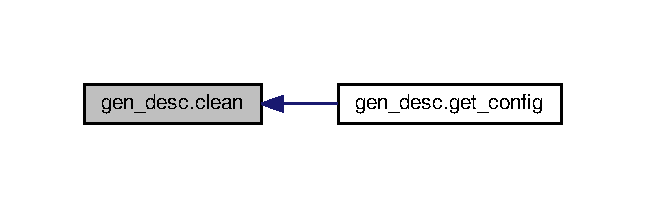
\includegraphics[width=310pt]{namespacegen__desc_a9e5c91910463053946db69a9d90b630c_icgraph}
\end{center}
\end{figure}


\hypertarget{namespacegen__desc_a45ef70f111577d7d3068aa3324597e9d}{\index{gen\-\_\-desc@{gen\-\_\-desc}!generate\-\_\-desc@{generate\-\_\-desc}}
\index{generate\-\_\-desc@{generate\-\_\-desc}!gen_desc@{gen\-\_\-desc}}
\subsubsection[{generate\-\_\-desc}]{\setlength{\rightskip}{0pt plus 5cm}def gen\-\_\-desc.\-generate\-\_\-desc (
\begin{DoxyParamCaption}
\item[{}]{path, }
\item[{}]{suff\-\_\-re, }
\item[{}]{suff\-\_\-dsc, }
\item[{}]{desc\-\_\-fld}
\end{DoxyParamCaption}
)}}\label{namespacegen__desc_a45ef70f111577d7d3068aa3324597e9d}


Definicja w linii 14 pliku gen\-\_\-desc.\-py.



Oto graf wywoływań tej funkcji\-:
\nopagebreak
\begin{figure}[H]
\begin{center}
\leavevmode
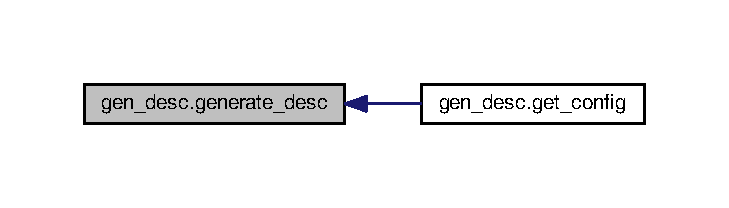
\includegraphics[width=350pt]{namespacegen__desc_a45ef70f111577d7d3068aa3324597e9d_icgraph}
\end{center}
\end{figure}


\hypertarget{namespacegen__desc_a77d1ae4c78d40d8999644b2b2e3bf7d2}{\index{gen\-\_\-desc@{gen\-\_\-desc}!get\-\_\-config@{get\-\_\-config}}
\index{get\-\_\-config@{get\-\_\-config}!gen_desc@{gen\-\_\-desc}}
\subsubsection[{get\-\_\-config}]{\setlength{\rightskip}{0pt plus 5cm}def gen\-\_\-desc.\-get\-\_\-config (
\begin{DoxyParamCaption}
\item[{}]{path, }
\item[{}]{command}
\end{DoxyParamCaption}
)}}\label{namespacegen__desc_a77d1ae4c78d40d8999644b2b2e3bf7d2}


Definicja w linii 32 pliku gen\-\_\-desc.\-py.



Oto graf wywołań dla tej funkcji\-:
\nopagebreak
\begin{figure}[H]
\begin{center}
\leavevmode
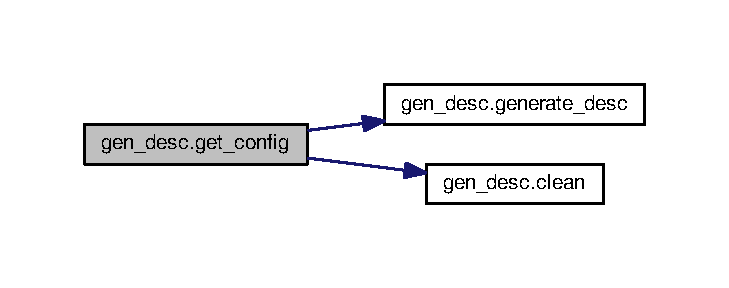
\includegraphics[width=350pt]{namespacegen__desc_a77d1ae4c78d40d8999644b2b2e3bf7d2_cgraph}
\end{center}
\end{figure}



\chapter{Dokumentacja klas}
\hypertarget{struct___i_m_a_g_e___b_a_s_e___r_e_l_o_c_a_t_i_o_n}{\section{Dokumentacja struktury \-\_\-\-I\-M\-A\-G\-E\-\_\-\-B\-A\-S\-E\-\_\-\-R\-E\-L\-O\-C\-A\-T\-I\-O\-N}
\label{struct___i_m_a_g_e___b_a_s_e___r_e_l_o_c_a_t_i_o_n}\index{\-\_\-\-I\-M\-A\-G\-E\-\_\-\-B\-A\-S\-E\-\_\-\-R\-E\-L\-O\-C\-A\-T\-I\-O\-N@{\-\_\-\-I\-M\-A\-G\-E\-\_\-\-B\-A\-S\-E\-\_\-\-R\-E\-L\-O\-C\-A\-T\-I\-O\-N}}
}


{\ttfamily \#include $<$winheader.\-h$>$}

\subsection*{Atrybuty publiczne}
\begin{DoxyCompactItemize}
\item 
\hyperlink{winheader_8h_af483253b2143078cede883fc3c111ad2}{D\-W\-O\-R\-D} \hyperlink{struct___i_m_a_g_e___b_a_s_e___r_e_l_o_c_a_t_i_o_n_aa9cd235a62c0b36e0b9f7051be3c5dcb}{Virtual\-Address}
\item 
\hyperlink{winheader_8h_af483253b2143078cede883fc3c111ad2}{D\-W\-O\-R\-D} \hyperlink{struct___i_m_a_g_e___b_a_s_e___r_e_l_o_c_a_t_i_o_n_a81d20c4bdef7268e328159bbc56e2d76}{Size\-Of\-Block}
\end{DoxyCompactItemize}


\subsection{Opis szczegółowy}


Definicja w linii 251 pliku winheader.\-h.



\subsection{Dokumentacja atrybutów składowych}
\hypertarget{struct___i_m_a_g_e___b_a_s_e___r_e_l_o_c_a_t_i_o_n_a81d20c4bdef7268e328159bbc56e2d76}{\index{\-\_\-\-I\-M\-A\-G\-E\-\_\-\-B\-A\-S\-E\-\_\-\-R\-E\-L\-O\-C\-A\-T\-I\-O\-N@{\-\_\-\-I\-M\-A\-G\-E\-\_\-\-B\-A\-S\-E\-\_\-\-R\-E\-L\-O\-C\-A\-T\-I\-O\-N}!Size\-Of\-Block@{Size\-Of\-Block}}
\index{Size\-Of\-Block@{Size\-Of\-Block}!_IMAGE_BASE_RELOCATION@{\-\_\-\-I\-M\-A\-G\-E\-\_\-\-B\-A\-S\-E\-\_\-\-R\-E\-L\-O\-C\-A\-T\-I\-O\-N}}
\subsubsection[{Size\-Of\-Block}]{\setlength{\rightskip}{0pt plus 5cm}{\bf D\-W\-O\-R\-D} \-\_\-\-I\-M\-A\-G\-E\-\_\-\-B\-A\-S\-E\-\_\-\-R\-E\-L\-O\-C\-A\-T\-I\-O\-N\-::\-Size\-Of\-Block}}\label{struct___i_m_a_g_e___b_a_s_e___r_e_l_o_c_a_t_i_o_n_a81d20c4bdef7268e328159bbc56e2d76}


Definicja w linii 253 pliku winheader.\-h.

\hypertarget{struct___i_m_a_g_e___b_a_s_e___r_e_l_o_c_a_t_i_o_n_aa9cd235a62c0b36e0b9f7051be3c5dcb}{\index{\-\_\-\-I\-M\-A\-G\-E\-\_\-\-B\-A\-S\-E\-\_\-\-R\-E\-L\-O\-C\-A\-T\-I\-O\-N@{\-\_\-\-I\-M\-A\-G\-E\-\_\-\-B\-A\-S\-E\-\_\-\-R\-E\-L\-O\-C\-A\-T\-I\-O\-N}!Virtual\-Address@{Virtual\-Address}}
\index{Virtual\-Address@{Virtual\-Address}!_IMAGE_BASE_RELOCATION@{\-\_\-\-I\-M\-A\-G\-E\-\_\-\-B\-A\-S\-E\-\_\-\-R\-E\-L\-O\-C\-A\-T\-I\-O\-N}}
\subsubsection[{Virtual\-Address}]{\setlength{\rightskip}{0pt plus 5cm}{\bf D\-W\-O\-R\-D} \-\_\-\-I\-M\-A\-G\-E\-\_\-\-B\-A\-S\-E\-\_\-\-R\-E\-L\-O\-C\-A\-T\-I\-O\-N\-::\-Virtual\-Address}}\label{struct___i_m_a_g_e___b_a_s_e___r_e_l_o_c_a_t_i_o_n_aa9cd235a62c0b36e0b9f7051be3c5dcb}


Definicja w linii 252 pliku winheader.\-h.



Dokumentacja dla tej struktury została wygenerowana z pliku\-:\begin{DoxyCompactItemize}
\item 
core/sys\-\_\-headers/\hyperlink{winheader_8h}{winheader.\-h}\end{DoxyCompactItemize}

\hypertarget{struct___i_m_a_g_e___d_a_t_a___d_i_r_e_c_t_o_r_y}{\section{Dokumentacja struktury \-\_\-\-I\-M\-A\-G\-E\-\_\-\-D\-A\-T\-A\-\_\-\-D\-I\-R\-E\-C\-T\-O\-R\-Y}
\label{struct___i_m_a_g_e___d_a_t_a___d_i_r_e_c_t_o_r_y}\index{\-\_\-\-I\-M\-A\-G\-E\-\_\-\-D\-A\-T\-A\-\_\-\-D\-I\-R\-E\-C\-T\-O\-R\-Y@{\-\_\-\-I\-M\-A\-G\-E\-\_\-\-D\-A\-T\-A\-\_\-\-D\-I\-R\-E\-C\-T\-O\-R\-Y}}
}


{\ttfamily \#include $<$winheader.\-h$>$}

\subsection*{Atrybuty publiczne}
\begin{DoxyCompactItemize}
\item 
\hyperlink{winheader_8h_af483253b2143078cede883fc3c111ad2}{D\-W\-O\-R\-D} \hyperlink{struct___i_m_a_g_e___d_a_t_a___d_i_r_e_c_t_o_r_y_a4367862469fd1ea60088ae02b1b6df70}{Virtual\-Address}
\item 
\hyperlink{winheader_8h_af483253b2143078cede883fc3c111ad2}{D\-W\-O\-R\-D} \hyperlink{struct___i_m_a_g_e___d_a_t_a___d_i_r_e_c_t_o_r_y_ab5bfce429cb0243cdc216f514108aa85}{Size}
\end{DoxyCompactItemize}


\subsection{Opis szczegółowy}


Definicja w linii 130 pliku winheader.\-h.



\subsection{Dokumentacja atrybutów składowych}
\hypertarget{struct___i_m_a_g_e___d_a_t_a___d_i_r_e_c_t_o_r_y_ab5bfce429cb0243cdc216f514108aa85}{\index{\-\_\-\-I\-M\-A\-G\-E\-\_\-\-D\-A\-T\-A\-\_\-\-D\-I\-R\-E\-C\-T\-O\-R\-Y@{\-\_\-\-I\-M\-A\-G\-E\-\_\-\-D\-A\-T\-A\-\_\-\-D\-I\-R\-E\-C\-T\-O\-R\-Y}!Size@{Size}}
\index{Size@{Size}!_IMAGE_DATA_DIRECTORY@{\-\_\-\-I\-M\-A\-G\-E\-\_\-\-D\-A\-T\-A\-\_\-\-D\-I\-R\-E\-C\-T\-O\-R\-Y}}
\subsubsection[{Size}]{\setlength{\rightskip}{0pt plus 5cm}{\bf D\-W\-O\-R\-D} \-\_\-\-I\-M\-A\-G\-E\-\_\-\-D\-A\-T\-A\-\_\-\-D\-I\-R\-E\-C\-T\-O\-R\-Y\-::\-Size}}\label{struct___i_m_a_g_e___d_a_t_a___d_i_r_e_c_t_o_r_y_ab5bfce429cb0243cdc216f514108aa85}


Definicja w linii 132 pliku winheader.\-h.

\hypertarget{struct___i_m_a_g_e___d_a_t_a___d_i_r_e_c_t_o_r_y_a4367862469fd1ea60088ae02b1b6df70}{\index{\-\_\-\-I\-M\-A\-G\-E\-\_\-\-D\-A\-T\-A\-\_\-\-D\-I\-R\-E\-C\-T\-O\-R\-Y@{\-\_\-\-I\-M\-A\-G\-E\-\_\-\-D\-A\-T\-A\-\_\-\-D\-I\-R\-E\-C\-T\-O\-R\-Y}!Virtual\-Address@{Virtual\-Address}}
\index{Virtual\-Address@{Virtual\-Address}!_IMAGE_DATA_DIRECTORY@{\-\_\-\-I\-M\-A\-G\-E\-\_\-\-D\-A\-T\-A\-\_\-\-D\-I\-R\-E\-C\-T\-O\-R\-Y}}
\subsubsection[{Virtual\-Address}]{\setlength{\rightskip}{0pt plus 5cm}{\bf D\-W\-O\-R\-D} \-\_\-\-I\-M\-A\-G\-E\-\_\-\-D\-A\-T\-A\-\_\-\-D\-I\-R\-E\-C\-T\-O\-R\-Y\-::\-Virtual\-Address}}\label{struct___i_m_a_g_e___d_a_t_a___d_i_r_e_c_t_o_r_y_a4367862469fd1ea60088ae02b1b6df70}


Definicja w linii 131 pliku winheader.\-h.



Dokumentacja dla tej struktury została wygenerowana z pliku\-:\begin{DoxyCompactItemize}
\item 
core/sys\-\_\-headers/\hyperlink{winheader_8h}{winheader.\-h}\end{DoxyCompactItemize}

\hypertarget{struct___i_m_a_g_e___d_o_s___h_e_a_d_e_r}{\section{Dokumentacja struktury \-\_\-\-I\-M\-A\-G\-E\-\_\-\-D\-O\-S\-\_\-\-H\-E\-A\-D\-E\-R}
\label{struct___i_m_a_g_e___d_o_s___h_e_a_d_e_r}\index{\-\_\-\-I\-M\-A\-G\-E\-\_\-\-D\-O\-S\-\_\-\-H\-E\-A\-D\-E\-R@{\-\_\-\-I\-M\-A\-G\-E\-\_\-\-D\-O\-S\-\_\-\-H\-E\-A\-D\-E\-R}}
}


{\ttfamily \#include $<$winheader.\-h$>$}

\subsection*{Atrybuty publiczne}
\begin{DoxyCompactItemize}
\item 
\hyperlink{winheader_8h_ab24077addd3b7b13e086987ff296552c}{W\-O\-R\-D} \hyperlink{struct___i_m_a_g_e___d_o_s___h_e_a_d_e_r_a2395379130b4cc7d2d3e6982e6e3fc4c}{e\-\_\-magic}
\item 
\hyperlink{winheader_8h_ab24077addd3b7b13e086987ff296552c}{W\-O\-R\-D} \hyperlink{struct___i_m_a_g_e___d_o_s___h_e_a_d_e_r_a1bd42856267579ce345e062eca7545c5}{e\-\_\-cblp}
\item 
\hyperlink{winheader_8h_ab24077addd3b7b13e086987ff296552c}{W\-O\-R\-D} \hyperlink{struct___i_m_a_g_e___d_o_s___h_e_a_d_e_r_aaaa4b40f12deb3c4d6b23d106c3bfbce}{e\-\_\-cp}
\item 
\hyperlink{winheader_8h_ab24077addd3b7b13e086987ff296552c}{W\-O\-R\-D} \hyperlink{struct___i_m_a_g_e___d_o_s___h_e_a_d_e_r_a9c7b1e78d0a6491d4fa41363b5aefecc}{e\-\_\-crlc}
\item 
\hyperlink{winheader_8h_ab24077addd3b7b13e086987ff296552c}{W\-O\-R\-D} \hyperlink{struct___i_m_a_g_e___d_o_s___h_e_a_d_e_r_a880d14ac887440a6859c45a5b6c7db0c}{e\-\_\-cparhdr}
\item 
\hyperlink{winheader_8h_ab24077addd3b7b13e086987ff296552c}{W\-O\-R\-D} \hyperlink{struct___i_m_a_g_e___d_o_s___h_e_a_d_e_r_a5a82bb159167fe8e23fbbc06ffb85b2c}{e\-\_\-minalloc}
\item 
\hyperlink{winheader_8h_ab24077addd3b7b13e086987ff296552c}{W\-O\-R\-D} \hyperlink{struct___i_m_a_g_e___d_o_s___h_e_a_d_e_r_a65684758e3524a791a7a818322b57eea}{e\-\_\-maxalloc}
\item 
\hyperlink{winheader_8h_ab24077addd3b7b13e086987ff296552c}{W\-O\-R\-D} \hyperlink{struct___i_m_a_g_e___d_o_s___h_e_a_d_e_r_ae8cba7f40bb926f2218808e7bc2a5965}{e\-\_\-ss}
\item 
\hyperlink{winheader_8h_ab24077addd3b7b13e086987ff296552c}{W\-O\-R\-D} \hyperlink{struct___i_m_a_g_e___d_o_s___h_e_a_d_e_r_abdf58356f1ed49b4e06935a51b8b6063}{e\-\_\-sp}
\item 
\hyperlink{winheader_8h_ab24077addd3b7b13e086987ff296552c}{W\-O\-R\-D} \hyperlink{struct___i_m_a_g_e___d_o_s___h_e_a_d_e_r_a43bd3860e13131189379e878d5ca7052}{e\-\_\-csum}
\item 
\hyperlink{winheader_8h_ab24077addd3b7b13e086987ff296552c}{W\-O\-R\-D} \hyperlink{struct___i_m_a_g_e___d_o_s___h_e_a_d_e_r_acd7c90273207e7c4067989e7cf3569f8}{e\-\_\-ip}
\item 
\hyperlink{winheader_8h_ab24077addd3b7b13e086987ff296552c}{W\-O\-R\-D} \hyperlink{struct___i_m_a_g_e___d_o_s___h_e_a_d_e_r_a7a8521e4ed5d09008750824d2cf1b4cd}{e\-\_\-cs}
\item 
\hyperlink{winheader_8h_ab24077addd3b7b13e086987ff296552c}{W\-O\-R\-D} \hyperlink{struct___i_m_a_g_e___d_o_s___h_e_a_d_e_r_a5fbd4e1819caa5f1032568eb2def6cb0}{e\-\_\-lfarlc}
\item 
\hyperlink{winheader_8h_ab24077addd3b7b13e086987ff296552c}{W\-O\-R\-D} \hyperlink{struct___i_m_a_g_e___d_o_s___h_e_a_d_e_r_a8aeaa7307372906be09e32dc2b1901d0}{e\-\_\-ovno}
\item 
\hyperlink{winheader_8h_ab24077addd3b7b13e086987ff296552c}{W\-O\-R\-D} \hyperlink{struct___i_m_a_g_e___d_o_s___h_e_a_d_e_r_a73c26e0cd458c8b94dcb05c8e8597fd9}{e\-\_\-res} \mbox{[}4\mbox{]}
\item 
\hyperlink{winheader_8h_ab24077addd3b7b13e086987ff296552c}{W\-O\-R\-D} \hyperlink{struct___i_m_a_g_e___d_o_s___h_e_a_d_e_r_ab81146b886293ed9937ff88189e87f7e}{e\-\_\-oemid}
\item 
\hyperlink{winheader_8h_ab24077addd3b7b13e086987ff296552c}{W\-O\-R\-D} \hyperlink{struct___i_m_a_g_e___d_o_s___h_e_a_d_e_r_a07dfa12b29293ba9cc6b885bce094099}{e\-\_\-oeminfo}
\item 
\hyperlink{winheader_8h_ab24077addd3b7b13e086987ff296552c}{W\-O\-R\-D} \hyperlink{struct___i_m_a_g_e___d_o_s___h_e_a_d_e_r_af865555510423e60e04abfd1626d8474}{e\-\_\-res2} \mbox{[}10\mbox{]}
\item 
\hyperlink{winheader_8h_a27ec6163192f1e1e72d87421379ea3d4}{L\-O\-N\-G} \hyperlink{struct___i_m_a_g_e___d_o_s___h_e_a_d_e_r_adf342409a54c9b3acdfc2aaeb1f10ba8}{e\-\_\-lfanew}
\end{DoxyCompactItemize}


\subsection{Opis szczegółowy}


Definicja w linii 98 pliku winheader.\-h.



\subsection{Dokumentacja atrybutów składowych}
\hypertarget{struct___i_m_a_g_e___d_o_s___h_e_a_d_e_r_a1bd42856267579ce345e062eca7545c5}{\index{\-\_\-\-I\-M\-A\-G\-E\-\_\-\-D\-O\-S\-\_\-\-H\-E\-A\-D\-E\-R@{\-\_\-\-I\-M\-A\-G\-E\-\_\-\-D\-O\-S\-\_\-\-H\-E\-A\-D\-E\-R}!e\-\_\-cblp@{e\-\_\-cblp}}
\index{e\-\_\-cblp@{e\-\_\-cblp}!_IMAGE_DOS_HEADER@{\-\_\-\-I\-M\-A\-G\-E\-\_\-\-D\-O\-S\-\_\-\-H\-E\-A\-D\-E\-R}}
\subsubsection[{e\-\_\-cblp}]{\setlength{\rightskip}{0pt plus 5cm}{\bf W\-O\-R\-D} \-\_\-\-I\-M\-A\-G\-E\-\_\-\-D\-O\-S\-\_\-\-H\-E\-A\-D\-E\-R\-::e\-\_\-cblp}}\label{struct___i_m_a_g_e___d_o_s___h_e_a_d_e_r_a1bd42856267579ce345e062eca7545c5}


Definicja w linii 100 pliku winheader.\-h.

\hypertarget{struct___i_m_a_g_e___d_o_s___h_e_a_d_e_r_aaaa4b40f12deb3c4d6b23d106c3bfbce}{\index{\-\_\-\-I\-M\-A\-G\-E\-\_\-\-D\-O\-S\-\_\-\-H\-E\-A\-D\-E\-R@{\-\_\-\-I\-M\-A\-G\-E\-\_\-\-D\-O\-S\-\_\-\-H\-E\-A\-D\-E\-R}!e\-\_\-cp@{e\-\_\-cp}}
\index{e\-\_\-cp@{e\-\_\-cp}!_IMAGE_DOS_HEADER@{\-\_\-\-I\-M\-A\-G\-E\-\_\-\-D\-O\-S\-\_\-\-H\-E\-A\-D\-E\-R}}
\subsubsection[{e\-\_\-cp}]{\setlength{\rightskip}{0pt plus 5cm}{\bf W\-O\-R\-D} \-\_\-\-I\-M\-A\-G\-E\-\_\-\-D\-O\-S\-\_\-\-H\-E\-A\-D\-E\-R\-::e\-\_\-cp}}\label{struct___i_m_a_g_e___d_o_s___h_e_a_d_e_r_aaaa4b40f12deb3c4d6b23d106c3bfbce}


Definicja w linii 101 pliku winheader.\-h.

\hypertarget{struct___i_m_a_g_e___d_o_s___h_e_a_d_e_r_a880d14ac887440a6859c45a5b6c7db0c}{\index{\-\_\-\-I\-M\-A\-G\-E\-\_\-\-D\-O\-S\-\_\-\-H\-E\-A\-D\-E\-R@{\-\_\-\-I\-M\-A\-G\-E\-\_\-\-D\-O\-S\-\_\-\-H\-E\-A\-D\-E\-R}!e\-\_\-cparhdr@{e\-\_\-cparhdr}}
\index{e\-\_\-cparhdr@{e\-\_\-cparhdr}!_IMAGE_DOS_HEADER@{\-\_\-\-I\-M\-A\-G\-E\-\_\-\-D\-O\-S\-\_\-\-H\-E\-A\-D\-E\-R}}
\subsubsection[{e\-\_\-cparhdr}]{\setlength{\rightskip}{0pt plus 5cm}{\bf W\-O\-R\-D} \-\_\-\-I\-M\-A\-G\-E\-\_\-\-D\-O\-S\-\_\-\-H\-E\-A\-D\-E\-R\-::e\-\_\-cparhdr}}\label{struct___i_m_a_g_e___d_o_s___h_e_a_d_e_r_a880d14ac887440a6859c45a5b6c7db0c}


Definicja w linii 103 pliku winheader.\-h.

\hypertarget{struct___i_m_a_g_e___d_o_s___h_e_a_d_e_r_a9c7b1e78d0a6491d4fa41363b5aefecc}{\index{\-\_\-\-I\-M\-A\-G\-E\-\_\-\-D\-O\-S\-\_\-\-H\-E\-A\-D\-E\-R@{\-\_\-\-I\-M\-A\-G\-E\-\_\-\-D\-O\-S\-\_\-\-H\-E\-A\-D\-E\-R}!e\-\_\-crlc@{e\-\_\-crlc}}
\index{e\-\_\-crlc@{e\-\_\-crlc}!_IMAGE_DOS_HEADER@{\-\_\-\-I\-M\-A\-G\-E\-\_\-\-D\-O\-S\-\_\-\-H\-E\-A\-D\-E\-R}}
\subsubsection[{e\-\_\-crlc}]{\setlength{\rightskip}{0pt plus 5cm}{\bf W\-O\-R\-D} \-\_\-\-I\-M\-A\-G\-E\-\_\-\-D\-O\-S\-\_\-\-H\-E\-A\-D\-E\-R\-::e\-\_\-crlc}}\label{struct___i_m_a_g_e___d_o_s___h_e_a_d_e_r_a9c7b1e78d0a6491d4fa41363b5aefecc}


Definicja w linii 102 pliku winheader.\-h.

\hypertarget{struct___i_m_a_g_e___d_o_s___h_e_a_d_e_r_a7a8521e4ed5d09008750824d2cf1b4cd}{\index{\-\_\-\-I\-M\-A\-G\-E\-\_\-\-D\-O\-S\-\_\-\-H\-E\-A\-D\-E\-R@{\-\_\-\-I\-M\-A\-G\-E\-\_\-\-D\-O\-S\-\_\-\-H\-E\-A\-D\-E\-R}!e\-\_\-cs@{e\-\_\-cs}}
\index{e\-\_\-cs@{e\-\_\-cs}!_IMAGE_DOS_HEADER@{\-\_\-\-I\-M\-A\-G\-E\-\_\-\-D\-O\-S\-\_\-\-H\-E\-A\-D\-E\-R}}
\subsubsection[{e\-\_\-cs}]{\setlength{\rightskip}{0pt plus 5cm}{\bf W\-O\-R\-D} \-\_\-\-I\-M\-A\-G\-E\-\_\-\-D\-O\-S\-\_\-\-H\-E\-A\-D\-E\-R\-::e\-\_\-cs}}\label{struct___i_m_a_g_e___d_o_s___h_e_a_d_e_r_a7a8521e4ed5d09008750824d2cf1b4cd}


Definicja w linii 110 pliku winheader.\-h.

\hypertarget{struct___i_m_a_g_e___d_o_s___h_e_a_d_e_r_a43bd3860e13131189379e878d5ca7052}{\index{\-\_\-\-I\-M\-A\-G\-E\-\_\-\-D\-O\-S\-\_\-\-H\-E\-A\-D\-E\-R@{\-\_\-\-I\-M\-A\-G\-E\-\_\-\-D\-O\-S\-\_\-\-H\-E\-A\-D\-E\-R}!e\-\_\-csum@{e\-\_\-csum}}
\index{e\-\_\-csum@{e\-\_\-csum}!_IMAGE_DOS_HEADER@{\-\_\-\-I\-M\-A\-G\-E\-\_\-\-D\-O\-S\-\_\-\-H\-E\-A\-D\-E\-R}}
\subsubsection[{e\-\_\-csum}]{\setlength{\rightskip}{0pt plus 5cm}{\bf W\-O\-R\-D} \-\_\-\-I\-M\-A\-G\-E\-\_\-\-D\-O\-S\-\_\-\-H\-E\-A\-D\-E\-R\-::e\-\_\-csum}}\label{struct___i_m_a_g_e___d_o_s___h_e_a_d_e_r_a43bd3860e13131189379e878d5ca7052}


Definicja w linii 108 pliku winheader.\-h.

\hypertarget{struct___i_m_a_g_e___d_o_s___h_e_a_d_e_r_acd7c90273207e7c4067989e7cf3569f8}{\index{\-\_\-\-I\-M\-A\-G\-E\-\_\-\-D\-O\-S\-\_\-\-H\-E\-A\-D\-E\-R@{\-\_\-\-I\-M\-A\-G\-E\-\_\-\-D\-O\-S\-\_\-\-H\-E\-A\-D\-E\-R}!e\-\_\-ip@{e\-\_\-ip}}
\index{e\-\_\-ip@{e\-\_\-ip}!_IMAGE_DOS_HEADER@{\-\_\-\-I\-M\-A\-G\-E\-\_\-\-D\-O\-S\-\_\-\-H\-E\-A\-D\-E\-R}}
\subsubsection[{e\-\_\-ip}]{\setlength{\rightskip}{0pt plus 5cm}{\bf W\-O\-R\-D} \-\_\-\-I\-M\-A\-G\-E\-\_\-\-D\-O\-S\-\_\-\-H\-E\-A\-D\-E\-R\-::e\-\_\-ip}}\label{struct___i_m_a_g_e___d_o_s___h_e_a_d_e_r_acd7c90273207e7c4067989e7cf3569f8}


Definicja w linii 109 pliku winheader.\-h.

\hypertarget{struct___i_m_a_g_e___d_o_s___h_e_a_d_e_r_adf342409a54c9b3acdfc2aaeb1f10ba8}{\index{\-\_\-\-I\-M\-A\-G\-E\-\_\-\-D\-O\-S\-\_\-\-H\-E\-A\-D\-E\-R@{\-\_\-\-I\-M\-A\-G\-E\-\_\-\-D\-O\-S\-\_\-\-H\-E\-A\-D\-E\-R}!e\-\_\-lfanew@{e\-\_\-lfanew}}
\index{e\-\_\-lfanew@{e\-\_\-lfanew}!_IMAGE_DOS_HEADER@{\-\_\-\-I\-M\-A\-G\-E\-\_\-\-D\-O\-S\-\_\-\-H\-E\-A\-D\-E\-R}}
\subsubsection[{e\-\_\-lfanew}]{\setlength{\rightskip}{0pt plus 5cm}{\bf L\-O\-N\-G} \-\_\-\-I\-M\-A\-G\-E\-\_\-\-D\-O\-S\-\_\-\-H\-E\-A\-D\-E\-R\-::e\-\_\-lfanew}}\label{struct___i_m_a_g_e___d_o_s___h_e_a_d_e_r_adf342409a54c9b3acdfc2aaeb1f10ba8}


Definicja w linii 117 pliku winheader.\-h.

\hypertarget{struct___i_m_a_g_e___d_o_s___h_e_a_d_e_r_a5fbd4e1819caa5f1032568eb2def6cb0}{\index{\-\_\-\-I\-M\-A\-G\-E\-\_\-\-D\-O\-S\-\_\-\-H\-E\-A\-D\-E\-R@{\-\_\-\-I\-M\-A\-G\-E\-\_\-\-D\-O\-S\-\_\-\-H\-E\-A\-D\-E\-R}!e\-\_\-lfarlc@{e\-\_\-lfarlc}}
\index{e\-\_\-lfarlc@{e\-\_\-lfarlc}!_IMAGE_DOS_HEADER@{\-\_\-\-I\-M\-A\-G\-E\-\_\-\-D\-O\-S\-\_\-\-H\-E\-A\-D\-E\-R}}
\subsubsection[{e\-\_\-lfarlc}]{\setlength{\rightskip}{0pt plus 5cm}{\bf W\-O\-R\-D} \-\_\-\-I\-M\-A\-G\-E\-\_\-\-D\-O\-S\-\_\-\-H\-E\-A\-D\-E\-R\-::e\-\_\-lfarlc}}\label{struct___i_m_a_g_e___d_o_s___h_e_a_d_e_r_a5fbd4e1819caa5f1032568eb2def6cb0}


Definicja w linii 111 pliku winheader.\-h.

\hypertarget{struct___i_m_a_g_e___d_o_s___h_e_a_d_e_r_a2395379130b4cc7d2d3e6982e6e3fc4c}{\index{\-\_\-\-I\-M\-A\-G\-E\-\_\-\-D\-O\-S\-\_\-\-H\-E\-A\-D\-E\-R@{\-\_\-\-I\-M\-A\-G\-E\-\_\-\-D\-O\-S\-\_\-\-H\-E\-A\-D\-E\-R}!e\-\_\-magic@{e\-\_\-magic}}
\index{e\-\_\-magic@{e\-\_\-magic}!_IMAGE_DOS_HEADER@{\-\_\-\-I\-M\-A\-G\-E\-\_\-\-D\-O\-S\-\_\-\-H\-E\-A\-D\-E\-R}}
\subsubsection[{e\-\_\-magic}]{\setlength{\rightskip}{0pt plus 5cm}{\bf W\-O\-R\-D} \-\_\-\-I\-M\-A\-G\-E\-\_\-\-D\-O\-S\-\_\-\-H\-E\-A\-D\-E\-R\-::e\-\_\-magic}}\label{struct___i_m_a_g_e___d_o_s___h_e_a_d_e_r_a2395379130b4cc7d2d3e6982e6e3fc4c}


Definicja w linii 99 pliku winheader.\-h.

\hypertarget{struct___i_m_a_g_e___d_o_s___h_e_a_d_e_r_a65684758e3524a791a7a818322b57eea}{\index{\-\_\-\-I\-M\-A\-G\-E\-\_\-\-D\-O\-S\-\_\-\-H\-E\-A\-D\-E\-R@{\-\_\-\-I\-M\-A\-G\-E\-\_\-\-D\-O\-S\-\_\-\-H\-E\-A\-D\-E\-R}!e\-\_\-maxalloc@{e\-\_\-maxalloc}}
\index{e\-\_\-maxalloc@{e\-\_\-maxalloc}!_IMAGE_DOS_HEADER@{\-\_\-\-I\-M\-A\-G\-E\-\_\-\-D\-O\-S\-\_\-\-H\-E\-A\-D\-E\-R}}
\subsubsection[{e\-\_\-maxalloc}]{\setlength{\rightskip}{0pt plus 5cm}{\bf W\-O\-R\-D} \-\_\-\-I\-M\-A\-G\-E\-\_\-\-D\-O\-S\-\_\-\-H\-E\-A\-D\-E\-R\-::e\-\_\-maxalloc}}\label{struct___i_m_a_g_e___d_o_s___h_e_a_d_e_r_a65684758e3524a791a7a818322b57eea}


Definicja w linii 105 pliku winheader.\-h.

\hypertarget{struct___i_m_a_g_e___d_o_s___h_e_a_d_e_r_a5a82bb159167fe8e23fbbc06ffb85b2c}{\index{\-\_\-\-I\-M\-A\-G\-E\-\_\-\-D\-O\-S\-\_\-\-H\-E\-A\-D\-E\-R@{\-\_\-\-I\-M\-A\-G\-E\-\_\-\-D\-O\-S\-\_\-\-H\-E\-A\-D\-E\-R}!e\-\_\-minalloc@{e\-\_\-minalloc}}
\index{e\-\_\-minalloc@{e\-\_\-minalloc}!_IMAGE_DOS_HEADER@{\-\_\-\-I\-M\-A\-G\-E\-\_\-\-D\-O\-S\-\_\-\-H\-E\-A\-D\-E\-R}}
\subsubsection[{e\-\_\-minalloc}]{\setlength{\rightskip}{0pt plus 5cm}{\bf W\-O\-R\-D} \-\_\-\-I\-M\-A\-G\-E\-\_\-\-D\-O\-S\-\_\-\-H\-E\-A\-D\-E\-R\-::e\-\_\-minalloc}}\label{struct___i_m_a_g_e___d_o_s___h_e_a_d_e_r_a5a82bb159167fe8e23fbbc06ffb85b2c}


Definicja w linii 104 pliku winheader.\-h.

\hypertarget{struct___i_m_a_g_e___d_o_s___h_e_a_d_e_r_ab81146b886293ed9937ff88189e87f7e}{\index{\-\_\-\-I\-M\-A\-G\-E\-\_\-\-D\-O\-S\-\_\-\-H\-E\-A\-D\-E\-R@{\-\_\-\-I\-M\-A\-G\-E\-\_\-\-D\-O\-S\-\_\-\-H\-E\-A\-D\-E\-R}!e\-\_\-oemid@{e\-\_\-oemid}}
\index{e\-\_\-oemid@{e\-\_\-oemid}!_IMAGE_DOS_HEADER@{\-\_\-\-I\-M\-A\-G\-E\-\_\-\-D\-O\-S\-\_\-\-H\-E\-A\-D\-E\-R}}
\subsubsection[{e\-\_\-oemid}]{\setlength{\rightskip}{0pt plus 5cm}{\bf W\-O\-R\-D} \-\_\-\-I\-M\-A\-G\-E\-\_\-\-D\-O\-S\-\_\-\-H\-E\-A\-D\-E\-R\-::e\-\_\-oemid}}\label{struct___i_m_a_g_e___d_o_s___h_e_a_d_e_r_ab81146b886293ed9937ff88189e87f7e}


Definicja w linii 114 pliku winheader.\-h.

\hypertarget{struct___i_m_a_g_e___d_o_s___h_e_a_d_e_r_a07dfa12b29293ba9cc6b885bce094099}{\index{\-\_\-\-I\-M\-A\-G\-E\-\_\-\-D\-O\-S\-\_\-\-H\-E\-A\-D\-E\-R@{\-\_\-\-I\-M\-A\-G\-E\-\_\-\-D\-O\-S\-\_\-\-H\-E\-A\-D\-E\-R}!e\-\_\-oeminfo@{e\-\_\-oeminfo}}
\index{e\-\_\-oeminfo@{e\-\_\-oeminfo}!_IMAGE_DOS_HEADER@{\-\_\-\-I\-M\-A\-G\-E\-\_\-\-D\-O\-S\-\_\-\-H\-E\-A\-D\-E\-R}}
\subsubsection[{e\-\_\-oeminfo}]{\setlength{\rightskip}{0pt plus 5cm}{\bf W\-O\-R\-D} \-\_\-\-I\-M\-A\-G\-E\-\_\-\-D\-O\-S\-\_\-\-H\-E\-A\-D\-E\-R\-::e\-\_\-oeminfo}}\label{struct___i_m_a_g_e___d_o_s___h_e_a_d_e_r_a07dfa12b29293ba9cc6b885bce094099}


Definicja w linii 115 pliku winheader.\-h.

\hypertarget{struct___i_m_a_g_e___d_o_s___h_e_a_d_e_r_a8aeaa7307372906be09e32dc2b1901d0}{\index{\-\_\-\-I\-M\-A\-G\-E\-\_\-\-D\-O\-S\-\_\-\-H\-E\-A\-D\-E\-R@{\-\_\-\-I\-M\-A\-G\-E\-\_\-\-D\-O\-S\-\_\-\-H\-E\-A\-D\-E\-R}!e\-\_\-ovno@{e\-\_\-ovno}}
\index{e\-\_\-ovno@{e\-\_\-ovno}!_IMAGE_DOS_HEADER@{\-\_\-\-I\-M\-A\-G\-E\-\_\-\-D\-O\-S\-\_\-\-H\-E\-A\-D\-E\-R}}
\subsubsection[{e\-\_\-ovno}]{\setlength{\rightskip}{0pt plus 5cm}{\bf W\-O\-R\-D} \-\_\-\-I\-M\-A\-G\-E\-\_\-\-D\-O\-S\-\_\-\-H\-E\-A\-D\-E\-R\-::e\-\_\-ovno}}\label{struct___i_m_a_g_e___d_o_s___h_e_a_d_e_r_a8aeaa7307372906be09e32dc2b1901d0}


Definicja w linii 112 pliku winheader.\-h.

\hypertarget{struct___i_m_a_g_e___d_o_s___h_e_a_d_e_r_a73c26e0cd458c8b94dcb05c8e8597fd9}{\index{\-\_\-\-I\-M\-A\-G\-E\-\_\-\-D\-O\-S\-\_\-\-H\-E\-A\-D\-E\-R@{\-\_\-\-I\-M\-A\-G\-E\-\_\-\-D\-O\-S\-\_\-\-H\-E\-A\-D\-E\-R}!e\-\_\-res@{e\-\_\-res}}
\index{e\-\_\-res@{e\-\_\-res}!_IMAGE_DOS_HEADER@{\-\_\-\-I\-M\-A\-G\-E\-\_\-\-D\-O\-S\-\_\-\-H\-E\-A\-D\-E\-R}}
\subsubsection[{e\-\_\-res}]{\setlength{\rightskip}{0pt plus 5cm}{\bf W\-O\-R\-D} \-\_\-\-I\-M\-A\-G\-E\-\_\-\-D\-O\-S\-\_\-\-H\-E\-A\-D\-E\-R\-::e\-\_\-res\mbox{[}4\mbox{]}}}\label{struct___i_m_a_g_e___d_o_s___h_e_a_d_e_r_a73c26e0cd458c8b94dcb05c8e8597fd9}


Definicja w linii 113 pliku winheader.\-h.

\hypertarget{struct___i_m_a_g_e___d_o_s___h_e_a_d_e_r_af865555510423e60e04abfd1626d8474}{\index{\-\_\-\-I\-M\-A\-G\-E\-\_\-\-D\-O\-S\-\_\-\-H\-E\-A\-D\-E\-R@{\-\_\-\-I\-M\-A\-G\-E\-\_\-\-D\-O\-S\-\_\-\-H\-E\-A\-D\-E\-R}!e\-\_\-res2@{e\-\_\-res2}}
\index{e\-\_\-res2@{e\-\_\-res2}!_IMAGE_DOS_HEADER@{\-\_\-\-I\-M\-A\-G\-E\-\_\-\-D\-O\-S\-\_\-\-H\-E\-A\-D\-E\-R}}
\subsubsection[{e\-\_\-res2}]{\setlength{\rightskip}{0pt plus 5cm}{\bf W\-O\-R\-D} \-\_\-\-I\-M\-A\-G\-E\-\_\-\-D\-O\-S\-\_\-\-H\-E\-A\-D\-E\-R\-::e\-\_\-res2\mbox{[}10\mbox{]}}}\label{struct___i_m_a_g_e___d_o_s___h_e_a_d_e_r_af865555510423e60e04abfd1626d8474}


Definicja w linii 116 pliku winheader.\-h.

\hypertarget{struct___i_m_a_g_e___d_o_s___h_e_a_d_e_r_abdf58356f1ed49b4e06935a51b8b6063}{\index{\-\_\-\-I\-M\-A\-G\-E\-\_\-\-D\-O\-S\-\_\-\-H\-E\-A\-D\-E\-R@{\-\_\-\-I\-M\-A\-G\-E\-\_\-\-D\-O\-S\-\_\-\-H\-E\-A\-D\-E\-R}!e\-\_\-sp@{e\-\_\-sp}}
\index{e\-\_\-sp@{e\-\_\-sp}!_IMAGE_DOS_HEADER@{\-\_\-\-I\-M\-A\-G\-E\-\_\-\-D\-O\-S\-\_\-\-H\-E\-A\-D\-E\-R}}
\subsubsection[{e\-\_\-sp}]{\setlength{\rightskip}{0pt plus 5cm}{\bf W\-O\-R\-D} \-\_\-\-I\-M\-A\-G\-E\-\_\-\-D\-O\-S\-\_\-\-H\-E\-A\-D\-E\-R\-::e\-\_\-sp}}\label{struct___i_m_a_g_e___d_o_s___h_e_a_d_e_r_abdf58356f1ed49b4e06935a51b8b6063}


Definicja w linii 107 pliku winheader.\-h.

\hypertarget{struct___i_m_a_g_e___d_o_s___h_e_a_d_e_r_ae8cba7f40bb926f2218808e7bc2a5965}{\index{\-\_\-\-I\-M\-A\-G\-E\-\_\-\-D\-O\-S\-\_\-\-H\-E\-A\-D\-E\-R@{\-\_\-\-I\-M\-A\-G\-E\-\_\-\-D\-O\-S\-\_\-\-H\-E\-A\-D\-E\-R}!e\-\_\-ss@{e\-\_\-ss}}
\index{e\-\_\-ss@{e\-\_\-ss}!_IMAGE_DOS_HEADER@{\-\_\-\-I\-M\-A\-G\-E\-\_\-\-D\-O\-S\-\_\-\-H\-E\-A\-D\-E\-R}}
\subsubsection[{e\-\_\-ss}]{\setlength{\rightskip}{0pt plus 5cm}{\bf W\-O\-R\-D} \-\_\-\-I\-M\-A\-G\-E\-\_\-\-D\-O\-S\-\_\-\-H\-E\-A\-D\-E\-R\-::e\-\_\-ss}}\label{struct___i_m_a_g_e___d_o_s___h_e_a_d_e_r_ae8cba7f40bb926f2218808e7bc2a5965}


Definicja w linii 106 pliku winheader.\-h.



Dokumentacja dla tej struktury została wygenerowana z pliku\-:\begin{DoxyCompactItemize}
\item 
core/sys\-\_\-headers/\hyperlink{winheader_8h}{winheader.\-h}\end{DoxyCompactItemize}

\hypertarget{struct___i_m_a_g_e___f_i_l_e___h_e_a_d_e_r}{\section{Dokumentacja struktury \-\_\-\-I\-M\-A\-G\-E\-\_\-\-F\-I\-L\-E\-\_\-\-H\-E\-A\-D\-E\-R}
\label{struct___i_m_a_g_e___f_i_l_e___h_e_a_d_e_r}\index{\-\_\-\-I\-M\-A\-G\-E\-\_\-\-F\-I\-L\-E\-\_\-\-H\-E\-A\-D\-E\-R@{\-\_\-\-I\-M\-A\-G\-E\-\_\-\-F\-I\-L\-E\-\_\-\-H\-E\-A\-D\-E\-R}}
}


{\ttfamily \#include $<$winheader.\-h$>$}

\subsection*{Atrybuty publiczne}
\begin{DoxyCompactItemize}
\item 
\hyperlink{winheader_8h_ab24077addd3b7b13e086987ff296552c}{W\-O\-R\-D} \hyperlink{struct___i_m_a_g_e___f_i_l_e___h_e_a_d_e_r_aadde4ef78693fa8d4bc1c97c7d3c8c1a}{Machine}
\item 
\hyperlink{winheader_8h_ab24077addd3b7b13e086987ff296552c}{W\-O\-R\-D} \hyperlink{struct___i_m_a_g_e___f_i_l_e___h_e_a_d_e_r_ad604cffb35b69981158822e14e9bc1c0}{Number\-Of\-Sections}
\item 
\hyperlink{winheader_8h_af483253b2143078cede883fc3c111ad2}{D\-W\-O\-R\-D} \hyperlink{struct___i_m_a_g_e___f_i_l_e___h_e_a_d_e_r_af36d3522f4749a93453bde62c0f7732b}{Time\-Date\-Stamp}
\item 
\hyperlink{winheader_8h_af483253b2143078cede883fc3c111ad2}{D\-W\-O\-R\-D} \hyperlink{struct___i_m_a_g_e___f_i_l_e___h_e_a_d_e_r_a5c3f6aef5cd87caa9d5ce887aaf2e522}{Pointer\-To\-Symbol\-Table}
\item 
\hyperlink{winheader_8h_af483253b2143078cede883fc3c111ad2}{D\-W\-O\-R\-D} \hyperlink{struct___i_m_a_g_e___f_i_l_e___h_e_a_d_e_r_a3e054c70bc25a6797608fb32327348ad}{Number\-Of\-Symbols}
\item 
\hyperlink{winheader_8h_ab24077addd3b7b13e086987ff296552c}{W\-O\-R\-D} \hyperlink{struct___i_m_a_g_e___f_i_l_e___h_e_a_d_e_r_a7fc97339de25b2845ef855809be630ff}{Size\-Of\-Optional\-Header}
\item 
\hyperlink{winheader_8h_ab24077addd3b7b13e086987ff296552c}{W\-O\-R\-D} \hyperlink{struct___i_m_a_g_e___f_i_l_e___h_e_a_d_e_r_a121e0ec6d4ce2ea021df48f6949956c3}{Characteristics}
\end{DoxyCompactItemize}


\subsection{Opis szczegółowy}


Definicja w linii 120 pliku winheader.\-h.



\subsection{Dokumentacja atrybutów składowych}
\hypertarget{struct___i_m_a_g_e___f_i_l_e___h_e_a_d_e_r_a121e0ec6d4ce2ea021df48f6949956c3}{\index{\-\_\-\-I\-M\-A\-G\-E\-\_\-\-F\-I\-L\-E\-\_\-\-H\-E\-A\-D\-E\-R@{\-\_\-\-I\-M\-A\-G\-E\-\_\-\-F\-I\-L\-E\-\_\-\-H\-E\-A\-D\-E\-R}!Characteristics@{Characteristics}}
\index{Characteristics@{Characteristics}!_IMAGE_FILE_HEADER@{\-\_\-\-I\-M\-A\-G\-E\-\_\-\-F\-I\-L\-E\-\_\-\-H\-E\-A\-D\-E\-R}}
\subsubsection[{Characteristics}]{\setlength{\rightskip}{0pt plus 5cm}{\bf W\-O\-R\-D} \-\_\-\-I\-M\-A\-G\-E\-\_\-\-F\-I\-L\-E\-\_\-\-H\-E\-A\-D\-E\-R\-::\-Characteristics}}\label{struct___i_m_a_g_e___f_i_l_e___h_e_a_d_e_r_a121e0ec6d4ce2ea021df48f6949956c3}


Definicja w linii 127 pliku winheader.\-h.

\hypertarget{struct___i_m_a_g_e___f_i_l_e___h_e_a_d_e_r_aadde4ef78693fa8d4bc1c97c7d3c8c1a}{\index{\-\_\-\-I\-M\-A\-G\-E\-\_\-\-F\-I\-L\-E\-\_\-\-H\-E\-A\-D\-E\-R@{\-\_\-\-I\-M\-A\-G\-E\-\_\-\-F\-I\-L\-E\-\_\-\-H\-E\-A\-D\-E\-R}!Machine@{Machine}}
\index{Machine@{Machine}!_IMAGE_FILE_HEADER@{\-\_\-\-I\-M\-A\-G\-E\-\_\-\-F\-I\-L\-E\-\_\-\-H\-E\-A\-D\-E\-R}}
\subsubsection[{Machine}]{\setlength{\rightskip}{0pt plus 5cm}{\bf W\-O\-R\-D} \-\_\-\-I\-M\-A\-G\-E\-\_\-\-F\-I\-L\-E\-\_\-\-H\-E\-A\-D\-E\-R\-::\-Machine}}\label{struct___i_m_a_g_e___f_i_l_e___h_e_a_d_e_r_aadde4ef78693fa8d4bc1c97c7d3c8c1a}


Definicja w linii 121 pliku winheader.\-h.

\hypertarget{struct___i_m_a_g_e___f_i_l_e___h_e_a_d_e_r_ad604cffb35b69981158822e14e9bc1c0}{\index{\-\_\-\-I\-M\-A\-G\-E\-\_\-\-F\-I\-L\-E\-\_\-\-H\-E\-A\-D\-E\-R@{\-\_\-\-I\-M\-A\-G\-E\-\_\-\-F\-I\-L\-E\-\_\-\-H\-E\-A\-D\-E\-R}!Number\-Of\-Sections@{Number\-Of\-Sections}}
\index{Number\-Of\-Sections@{Number\-Of\-Sections}!_IMAGE_FILE_HEADER@{\-\_\-\-I\-M\-A\-G\-E\-\_\-\-F\-I\-L\-E\-\_\-\-H\-E\-A\-D\-E\-R}}
\subsubsection[{Number\-Of\-Sections}]{\setlength{\rightskip}{0pt plus 5cm}{\bf W\-O\-R\-D} \-\_\-\-I\-M\-A\-G\-E\-\_\-\-F\-I\-L\-E\-\_\-\-H\-E\-A\-D\-E\-R\-::\-Number\-Of\-Sections}}\label{struct___i_m_a_g_e___f_i_l_e___h_e_a_d_e_r_ad604cffb35b69981158822e14e9bc1c0}


Definicja w linii 122 pliku winheader.\-h.

\hypertarget{struct___i_m_a_g_e___f_i_l_e___h_e_a_d_e_r_a3e054c70bc25a6797608fb32327348ad}{\index{\-\_\-\-I\-M\-A\-G\-E\-\_\-\-F\-I\-L\-E\-\_\-\-H\-E\-A\-D\-E\-R@{\-\_\-\-I\-M\-A\-G\-E\-\_\-\-F\-I\-L\-E\-\_\-\-H\-E\-A\-D\-E\-R}!Number\-Of\-Symbols@{Number\-Of\-Symbols}}
\index{Number\-Of\-Symbols@{Number\-Of\-Symbols}!_IMAGE_FILE_HEADER@{\-\_\-\-I\-M\-A\-G\-E\-\_\-\-F\-I\-L\-E\-\_\-\-H\-E\-A\-D\-E\-R}}
\subsubsection[{Number\-Of\-Symbols}]{\setlength{\rightskip}{0pt plus 5cm}{\bf D\-W\-O\-R\-D} \-\_\-\-I\-M\-A\-G\-E\-\_\-\-F\-I\-L\-E\-\_\-\-H\-E\-A\-D\-E\-R\-::\-Number\-Of\-Symbols}}\label{struct___i_m_a_g_e___f_i_l_e___h_e_a_d_e_r_a3e054c70bc25a6797608fb32327348ad}


Definicja w linii 125 pliku winheader.\-h.

\hypertarget{struct___i_m_a_g_e___f_i_l_e___h_e_a_d_e_r_a5c3f6aef5cd87caa9d5ce887aaf2e522}{\index{\-\_\-\-I\-M\-A\-G\-E\-\_\-\-F\-I\-L\-E\-\_\-\-H\-E\-A\-D\-E\-R@{\-\_\-\-I\-M\-A\-G\-E\-\_\-\-F\-I\-L\-E\-\_\-\-H\-E\-A\-D\-E\-R}!Pointer\-To\-Symbol\-Table@{Pointer\-To\-Symbol\-Table}}
\index{Pointer\-To\-Symbol\-Table@{Pointer\-To\-Symbol\-Table}!_IMAGE_FILE_HEADER@{\-\_\-\-I\-M\-A\-G\-E\-\_\-\-F\-I\-L\-E\-\_\-\-H\-E\-A\-D\-E\-R}}
\subsubsection[{Pointer\-To\-Symbol\-Table}]{\setlength{\rightskip}{0pt plus 5cm}{\bf D\-W\-O\-R\-D} \-\_\-\-I\-M\-A\-G\-E\-\_\-\-F\-I\-L\-E\-\_\-\-H\-E\-A\-D\-E\-R\-::\-Pointer\-To\-Symbol\-Table}}\label{struct___i_m_a_g_e___f_i_l_e___h_e_a_d_e_r_a5c3f6aef5cd87caa9d5ce887aaf2e522}


Definicja w linii 124 pliku winheader.\-h.

\hypertarget{struct___i_m_a_g_e___f_i_l_e___h_e_a_d_e_r_a7fc97339de25b2845ef855809be630ff}{\index{\-\_\-\-I\-M\-A\-G\-E\-\_\-\-F\-I\-L\-E\-\_\-\-H\-E\-A\-D\-E\-R@{\-\_\-\-I\-M\-A\-G\-E\-\_\-\-F\-I\-L\-E\-\_\-\-H\-E\-A\-D\-E\-R}!Size\-Of\-Optional\-Header@{Size\-Of\-Optional\-Header}}
\index{Size\-Of\-Optional\-Header@{Size\-Of\-Optional\-Header}!_IMAGE_FILE_HEADER@{\-\_\-\-I\-M\-A\-G\-E\-\_\-\-F\-I\-L\-E\-\_\-\-H\-E\-A\-D\-E\-R}}
\subsubsection[{Size\-Of\-Optional\-Header}]{\setlength{\rightskip}{0pt plus 5cm}{\bf W\-O\-R\-D} \-\_\-\-I\-M\-A\-G\-E\-\_\-\-F\-I\-L\-E\-\_\-\-H\-E\-A\-D\-E\-R\-::\-Size\-Of\-Optional\-Header}}\label{struct___i_m_a_g_e___f_i_l_e___h_e_a_d_e_r_a7fc97339de25b2845ef855809be630ff}


Definicja w linii 126 pliku winheader.\-h.

\hypertarget{struct___i_m_a_g_e___f_i_l_e___h_e_a_d_e_r_af36d3522f4749a93453bde62c0f7732b}{\index{\-\_\-\-I\-M\-A\-G\-E\-\_\-\-F\-I\-L\-E\-\_\-\-H\-E\-A\-D\-E\-R@{\-\_\-\-I\-M\-A\-G\-E\-\_\-\-F\-I\-L\-E\-\_\-\-H\-E\-A\-D\-E\-R}!Time\-Date\-Stamp@{Time\-Date\-Stamp}}
\index{Time\-Date\-Stamp@{Time\-Date\-Stamp}!_IMAGE_FILE_HEADER@{\-\_\-\-I\-M\-A\-G\-E\-\_\-\-F\-I\-L\-E\-\_\-\-H\-E\-A\-D\-E\-R}}
\subsubsection[{Time\-Date\-Stamp}]{\setlength{\rightskip}{0pt plus 5cm}{\bf D\-W\-O\-R\-D} \-\_\-\-I\-M\-A\-G\-E\-\_\-\-F\-I\-L\-E\-\_\-\-H\-E\-A\-D\-E\-R\-::\-Time\-Date\-Stamp}}\label{struct___i_m_a_g_e___f_i_l_e___h_e_a_d_e_r_af36d3522f4749a93453bde62c0f7732b}


Definicja w linii 123 pliku winheader.\-h.



Dokumentacja dla tej struktury została wygenerowana z pliku\-:\begin{DoxyCompactItemize}
\item 
core/sys\-\_\-headers/\hyperlink{winheader_8h}{winheader.\-h}\end{DoxyCompactItemize}

\hypertarget{struct___i_m_a_g_e___n_t___h_e_a_d_e_r_s}{\section{Dokumentacja struktury \-\_\-\-I\-M\-A\-G\-E\-\_\-\-N\-T\-\_\-\-H\-E\-A\-D\-E\-R\-S}
\label{struct___i_m_a_g_e___n_t___h_e_a_d_e_r_s}\index{\-\_\-\-I\-M\-A\-G\-E\-\_\-\-N\-T\-\_\-\-H\-E\-A\-D\-E\-R\-S@{\-\_\-\-I\-M\-A\-G\-E\-\_\-\-N\-T\-\_\-\-H\-E\-A\-D\-E\-R\-S}}
}


{\ttfamily \#include $<$winheader.\-h$>$}



Diagram współpracy dla \-\_\-\-I\-M\-A\-G\-E\-\_\-\-N\-T\-\_\-\-H\-E\-A\-D\-E\-R\-S\-:\nopagebreak
\begin{figure}[H]
\begin{center}
\leavevmode
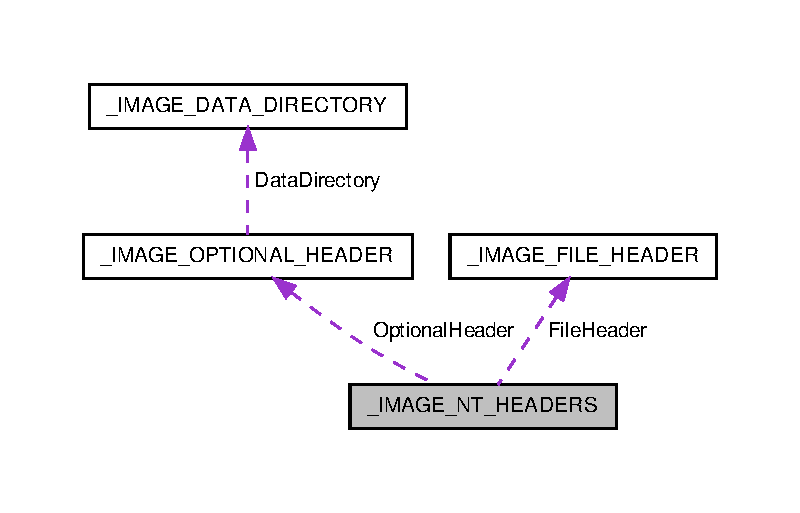
\includegraphics[width=350pt]{struct___i_m_a_g_e___n_t___h_e_a_d_e_r_s__coll__graph}
\end{center}
\end{figure}
\subsection*{Atrybuty publiczne}
\begin{DoxyCompactItemize}
\item 
\hyperlink{winheader_8h_af483253b2143078cede883fc3c111ad2}{D\-W\-O\-R\-D} \hyperlink{struct___i_m_a_g_e___n_t___h_e_a_d_e_r_s_a0fab671e499d3d3f47db0a30b8369f80}{Signature}
\item 
\hyperlink{winheader_8h_ab18994ab54fdb55d1542f30b3895ab10}{I\-M\-A\-G\-E\-\_\-\-F\-I\-L\-E\-\_\-\-H\-E\-A\-D\-E\-R} \hyperlink{struct___i_m_a_g_e___n_t___h_e_a_d_e_r_s_ab8aa7ee8ecc7b35fecc1b99b57fc9817}{File\-Header}
\item 
\hyperlink{winheader_8h_a3a446b0141b509f024b0238113b7f410}{I\-M\-A\-G\-E\-\_\-\-O\-P\-T\-I\-O\-N\-A\-L\-\_\-\-H\-E\-A\-D\-E\-R32} \hyperlink{struct___i_m_a_g_e___n_t___h_e_a_d_e_r_s_a71de2ed0819a8fac537db2e9daedfe05}{Optional\-Header}
\end{DoxyCompactItemize}


\subsection{Opis szczegółowy}


Definicja w linii 209 pliku winheader.\-h.



\subsection{Dokumentacja atrybutów składowych}
\hypertarget{struct___i_m_a_g_e___n_t___h_e_a_d_e_r_s_ab8aa7ee8ecc7b35fecc1b99b57fc9817}{\index{\-\_\-\-I\-M\-A\-G\-E\-\_\-\-N\-T\-\_\-\-H\-E\-A\-D\-E\-R\-S@{\-\_\-\-I\-M\-A\-G\-E\-\_\-\-N\-T\-\_\-\-H\-E\-A\-D\-E\-R\-S}!File\-Header@{File\-Header}}
\index{File\-Header@{File\-Header}!_IMAGE_NT_HEADERS@{\-\_\-\-I\-M\-A\-G\-E\-\_\-\-N\-T\-\_\-\-H\-E\-A\-D\-E\-R\-S}}
\subsubsection[{File\-Header}]{\setlength{\rightskip}{0pt plus 5cm}{\bf I\-M\-A\-G\-E\-\_\-\-F\-I\-L\-E\-\_\-\-H\-E\-A\-D\-E\-R} \-\_\-\-I\-M\-A\-G\-E\-\_\-\-N\-T\-\_\-\-H\-E\-A\-D\-E\-R\-S\-::\-File\-Header}}\label{struct___i_m_a_g_e___n_t___h_e_a_d_e_r_s_ab8aa7ee8ecc7b35fecc1b99b57fc9817}


Definicja w linii 211 pliku winheader.\-h.

\hypertarget{struct___i_m_a_g_e___n_t___h_e_a_d_e_r_s_a71de2ed0819a8fac537db2e9daedfe05}{\index{\-\_\-\-I\-M\-A\-G\-E\-\_\-\-N\-T\-\_\-\-H\-E\-A\-D\-E\-R\-S@{\-\_\-\-I\-M\-A\-G\-E\-\_\-\-N\-T\-\_\-\-H\-E\-A\-D\-E\-R\-S}!Optional\-Header@{Optional\-Header}}
\index{Optional\-Header@{Optional\-Header}!_IMAGE_NT_HEADERS@{\-\_\-\-I\-M\-A\-G\-E\-\_\-\-N\-T\-\_\-\-H\-E\-A\-D\-E\-R\-S}}
\subsubsection[{Optional\-Header}]{\setlength{\rightskip}{0pt plus 5cm}{\bf I\-M\-A\-G\-E\-\_\-\-O\-P\-T\-I\-O\-N\-A\-L\-\_\-\-H\-E\-A\-D\-E\-R32} \-\_\-\-I\-M\-A\-G\-E\-\_\-\-N\-T\-\_\-\-H\-E\-A\-D\-E\-R\-S\-::\-Optional\-Header}}\label{struct___i_m_a_g_e___n_t___h_e_a_d_e_r_s_a71de2ed0819a8fac537db2e9daedfe05}


Definicja w linii 212 pliku winheader.\-h.

\hypertarget{struct___i_m_a_g_e___n_t___h_e_a_d_e_r_s_a0fab671e499d3d3f47db0a30b8369f80}{\index{\-\_\-\-I\-M\-A\-G\-E\-\_\-\-N\-T\-\_\-\-H\-E\-A\-D\-E\-R\-S@{\-\_\-\-I\-M\-A\-G\-E\-\_\-\-N\-T\-\_\-\-H\-E\-A\-D\-E\-R\-S}!Signature@{Signature}}
\index{Signature@{Signature}!_IMAGE_NT_HEADERS@{\-\_\-\-I\-M\-A\-G\-E\-\_\-\-N\-T\-\_\-\-H\-E\-A\-D\-E\-R\-S}}
\subsubsection[{Signature}]{\setlength{\rightskip}{0pt plus 5cm}{\bf D\-W\-O\-R\-D} \-\_\-\-I\-M\-A\-G\-E\-\_\-\-N\-T\-\_\-\-H\-E\-A\-D\-E\-R\-S\-::\-Signature}}\label{struct___i_m_a_g_e___n_t___h_e_a_d_e_r_s_a0fab671e499d3d3f47db0a30b8369f80}


Definicja w linii 210 pliku winheader.\-h.



Dokumentacja dla tej struktury została wygenerowana z pliku\-:\begin{DoxyCompactItemize}
\item 
core/sys\-\_\-headers/\hyperlink{winheader_8h}{winheader.\-h}\end{DoxyCompactItemize}

\hypertarget{struct___i_m_a_g_e___n_t___h_e_a_d_e_r_s64}{\section{Dokumentacja struktury \-\_\-\-I\-M\-A\-G\-E\-\_\-\-N\-T\-\_\-\-H\-E\-A\-D\-E\-R\-S64}
\label{struct___i_m_a_g_e___n_t___h_e_a_d_e_r_s64}\index{\-\_\-\-I\-M\-A\-G\-E\-\_\-\-N\-T\-\_\-\-H\-E\-A\-D\-E\-R\-S64@{\-\_\-\-I\-M\-A\-G\-E\-\_\-\-N\-T\-\_\-\-H\-E\-A\-D\-E\-R\-S64}}
}


{\ttfamily \#include $<$winheader.\-h$>$}



Diagram współpracy dla \-\_\-\-I\-M\-A\-G\-E\-\_\-\-N\-T\-\_\-\-H\-E\-A\-D\-E\-R\-S64\-:\nopagebreak
\begin{figure}[H]
\begin{center}
\leavevmode
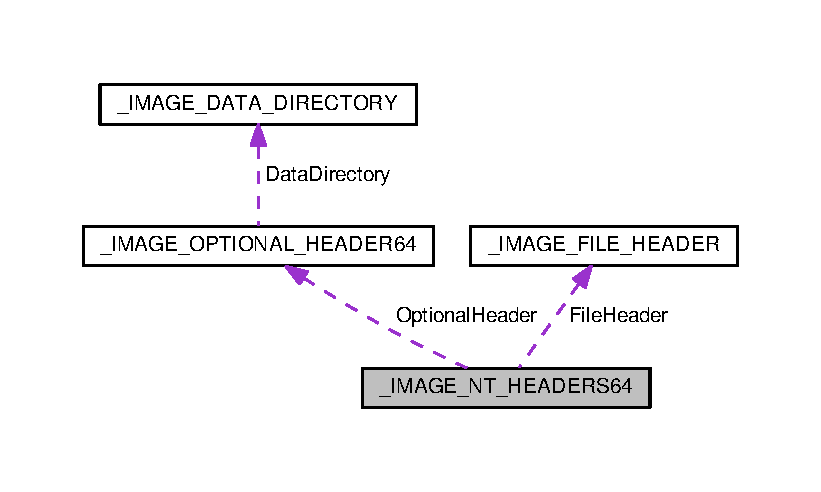
\includegraphics[width=350pt]{struct___i_m_a_g_e___n_t___h_e_a_d_e_r_s64__coll__graph}
\end{center}
\end{figure}
\subsection*{Atrybuty publiczne}
\begin{DoxyCompactItemize}
\item 
\hyperlink{winheader_8h_af483253b2143078cede883fc3c111ad2}{D\-W\-O\-R\-D} \hyperlink{struct___i_m_a_g_e___n_t___h_e_a_d_e_r_s64_a846d3eb78fd95dc71db36e89269d81cb}{Signature}
\item 
\hyperlink{winheader_8h_ab18994ab54fdb55d1542f30b3895ab10}{I\-M\-A\-G\-E\-\_\-\-F\-I\-L\-E\-\_\-\-H\-E\-A\-D\-E\-R} \hyperlink{struct___i_m_a_g_e___n_t___h_e_a_d_e_r_s64_a90697a3d56043dee58cbf21b30363863}{File\-Header}
\item 
\hyperlink{winheader_8h_a955345df2edf902d02dabe2aa7a82495}{I\-M\-A\-G\-E\-\_\-\-O\-P\-T\-I\-O\-N\-A\-L\-\_\-\-H\-E\-A\-D\-E\-R64} \hyperlink{struct___i_m_a_g_e___n_t___h_e_a_d_e_r_s64_a50eaffc01bf927048dc730c15b5ed3f1}{Optional\-Header}
\end{DoxyCompactItemize}


\subsection{Opis szczegółowy}


Definicja w linii 203 pliku winheader.\-h.



\subsection{Dokumentacja atrybutów składowych}
\hypertarget{struct___i_m_a_g_e___n_t___h_e_a_d_e_r_s64_a90697a3d56043dee58cbf21b30363863}{\index{\-\_\-\-I\-M\-A\-G\-E\-\_\-\-N\-T\-\_\-\-H\-E\-A\-D\-E\-R\-S64@{\-\_\-\-I\-M\-A\-G\-E\-\_\-\-N\-T\-\_\-\-H\-E\-A\-D\-E\-R\-S64}!File\-Header@{File\-Header}}
\index{File\-Header@{File\-Header}!_IMAGE_NT_HEADERS64@{\-\_\-\-I\-M\-A\-G\-E\-\_\-\-N\-T\-\_\-\-H\-E\-A\-D\-E\-R\-S64}}
\subsubsection[{File\-Header}]{\setlength{\rightskip}{0pt plus 5cm}{\bf I\-M\-A\-G\-E\-\_\-\-F\-I\-L\-E\-\_\-\-H\-E\-A\-D\-E\-R} \-\_\-\-I\-M\-A\-G\-E\-\_\-\-N\-T\-\_\-\-H\-E\-A\-D\-E\-R\-S64\-::\-File\-Header}}\label{struct___i_m_a_g_e___n_t___h_e_a_d_e_r_s64_a90697a3d56043dee58cbf21b30363863}


Definicja w linii 205 pliku winheader.\-h.

\hypertarget{struct___i_m_a_g_e___n_t___h_e_a_d_e_r_s64_a50eaffc01bf927048dc730c15b5ed3f1}{\index{\-\_\-\-I\-M\-A\-G\-E\-\_\-\-N\-T\-\_\-\-H\-E\-A\-D\-E\-R\-S64@{\-\_\-\-I\-M\-A\-G\-E\-\_\-\-N\-T\-\_\-\-H\-E\-A\-D\-E\-R\-S64}!Optional\-Header@{Optional\-Header}}
\index{Optional\-Header@{Optional\-Header}!_IMAGE_NT_HEADERS64@{\-\_\-\-I\-M\-A\-G\-E\-\_\-\-N\-T\-\_\-\-H\-E\-A\-D\-E\-R\-S64}}
\subsubsection[{Optional\-Header}]{\setlength{\rightskip}{0pt plus 5cm}{\bf I\-M\-A\-G\-E\-\_\-\-O\-P\-T\-I\-O\-N\-A\-L\-\_\-\-H\-E\-A\-D\-E\-R64} \-\_\-\-I\-M\-A\-G\-E\-\_\-\-N\-T\-\_\-\-H\-E\-A\-D\-E\-R\-S64\-::\-Optional\-Header}}\label{struct___i_m_a_g_e___n_t___h_e_a_d_e_r_s64_a50eaffc01bf927048dc730c15b5ed3f1}


Definicja w linii 206 pliku winheader.\-h.

\hypertarget{struct___i_m_a_g_e___n_t___h_e_a_d_e_r_s64_a846d3eb78fd95dc71db36e89269d81cb}{\index{\-\_\-\-I\-M\-A\-G\-E\-\_\-\-N\-T\-\_\-\-H\-E\-A\-D\-E\-R\-S64@{\-\_\-\-I\-M\-A\-G\-E\-\_\-\-N\-T\-\_\-\-H\-E\-A\-D\-E\-R\-S64}!Signature@{Signature}}
\index{Signature@{Signature}!_IMAGE_NT_HEADERS64@{\-\_\-\-I\-M\-A\-G\-E\-\_\-\-N\-T\-\_\-\-H\-E\-A\-D\-E\-R\-S64}}
\subsubsection[{Signature}]{\setlength{\rightskip}{0pt plus 5cm}{\bf D\-W\-O\-R\-D} \-\_\-\-I\-M\-A\-G\-E\-\_\-\-N\-T\-\_\-\-H\-E\-A\-D\-E\-R\-S64\-::\-Signature}}\label{struct___i_m_a_g_e___n_t___h_e_a_d_e_r_s64_a846d3eb78fd95dc71db36e89269d81cb}


Definicja w linii 204 pliku winheader.\-h.



Dokumentacja dla tej struktury została wygenerowana z pliku\-:\begin{DoxyCompactItemize}
\item 
core/sys\-\_\-headers/\hyperlink{winheader_8h}{winheader.\-h}\end{DoxyCompactItemize}

\hypertarget{struct___i_m_a_g_e___o_p_t_i_o_n_a_l___h_e_a_d_e_r}{\section{Dokumentacja struktury \-\_\-\-I\-M\-A\-G\-E\-\_\-\-O\-P\-T\-I\-O\-N\-A\-L\-\_\-\-H\-E\-A\-D\-E\-R}
\label{struct___i_m_a_g_e___o_p_t_i_o_n_a_l___h_e_a_d_e_r}\index{\-\_\-\-I\-M\-A\-G\-E\-\_\-\-O\-P\-T\-I\-O\-N\-A\-L\-\_\-\-H\-E\-A\-D\-E\-R@{\-\_\-\-I\-M\-A\-G\-E\-\_\-\-O\-P\-T\-I\-O\-N\-A\-L\-\_\-\-H\-E\-A\-D\-E\-R}}
}


{\ttfamily \#include $<$winheader.\-h$>$}



Diagram współpracy dla \-\_\-\-I\-M\-A\-G\-E\-\_\-\-O\-P\-T\-I\-O\-N\-A\-L\-\_\-\-H\-E\-A\-D\-E\-R\-:
\nopagebreak
\begin{figure}[H]
\begin{center}
\leavevmode
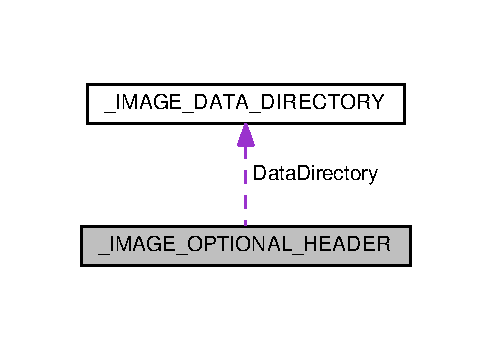
\includegraphics[width=236pt]{struct___i_m_a_g_e___o_p_t_i_o_n_a_l___h_e_a_d_e_r__coll__graph}
\end{center}
\end{figure}
\subsection*{Atrybuty publiczne}
\begin{DoxyCompactItemize}
\item 
\hyperlink{winheader_8h_ab24077addd3b7b13e086987ff296552c}{W\-O\-R\-D} \hyperlink{struct___i_m_a_g_e___o_p_t_i_o_n_a_l___h_e_a_d_e_r_aad8a4a504985601b03158526edc50606}{Magic}
\item 
\hyperlink{winheader_8h_aae9749d96e15ccb4f482dd5f55d98f9b}{B\-Y\-T\-E} \hyperlink{struct___i_m_a_g_e___o_p_t_i_o_n_a_l___h_e_a_d_e_r_adfecf203c13bdc63f1ff2d2da929c34a}{Major\-Linker\-Version}
\item 
\hyperlink{winheader_8h_aae9749d96e15ccb4f482dd5f55d98f9b}{B\-Y\-T\-E} \hyperlink{struct___i_m_a_g_e___o_p_t_i_o_n_a_l___h_e_a_d_e_r_a063cadfb6e83c54ae1013bfcbcc39333}{Minor\-Linker\-Version}
\item 
\hyperlink{winheader_8h_af483253b2143078cede883fc3c111ad2}{D\-W\-O\-R\-D} \hyperlink{struct___i_m_a_g_e___o_p_t_i_o_n_a_l___h_e_a_d_e_r_a06677e04339c441c6c60fe3b44f44ec6}{Size\-Of\-Code}
\item 
\hyperlink{winheader_8h_af483253b2143078cede883fc3c111ad2}{D\-W\-O\-R\-D} \hyperlink{struct___i_m_a_g_e___o_p_t_i_o_n_a_l___h_e_a_d_e_r_afe1799f5b4f6506737f3bcbee98a6899}{Size\-Of\-Initialized\-Data}
\item 
\hyperlink{winheader_8h_af483253b2143078cede883fc3c111ad2}{D\-W\-O\-R\-D} \hyperlink{struct___i_m_a_g_e___o_p_t_i_o_n_a_l___h_e_a_d_e_r_a98cb6b6de771471bdff9d0b3d5e8e0e6}{Size\-Of\-Uninitialized\-Data}
\item 
\hyperlink{winheader_8h_af483253b2143078cede883fc3c111ad2}{D\-W\-O\-R\-D} \hyperlink{struct___i_m_a_g_e___o_p_t_i_o_n_a_l___h_e_a_d_e_r_a68d3ff18e90131fbe88111dfee17b1f1}{Address\-Of\-Entry\-Point}
\item 
\hyperlink{winheader_8h_af483253b2143078cede883fc3c111ad2}{D\-W\-O\-R\-D} \hyperlink{struct___i_m_a_g_e___o_p_t_i_o_n_a_l___h_e_a_d_e_r_a13409943444189dc37c7172aaeb06def}{Base\-Of\-Code}
\item 
\hyperlink{winheader_8h_af483253b2143078cede883fc3c111ad2}{D\-W\-O\-R\-D} \hyperlink{struct___i_m_a_g_e___o_p_t_i_o_n_a_l___h_e_a_d_e_r_ac138650580b6e260319ddf00aadce839}{Base\-Of\-Data}
\item 
\hyperlink{winheader_8h_af483253b2143078cede883fc3c111ad2}{D\-W\-O\-R\-D} \hyperlink{struct___i_m_a_g_e___o_p_t_i_o_n_a_l___h_e_a_d_e_r_ad4d8bea5ef226ec629127101d9c1b853}{Image\-Base}
\item 
\hyperlink{winheader_8h_af483253b2143078cede883fc3c111ad2}{D\-W\-O\-R\-D} \hyperlink{struct___i_m_a_g_e___o_p_t_i_o_n_a_l___h_e_a_d_e_r_aea0796aa3281d0a85dfae4052fa7d897}{Section\-Alignment}
\item 
\hyperlink{winheader_8h_af483253b2143078cede883fc3c111ad2}{D\-W\-O\-R\-D} \hyperlink{struct___i_m_a_g_e___o_p_t_i_o_n_a_l___h_e_a_d_e_r_abdc514652a6858ad6821bc0cedf5f1aa}{File\-Alignment}
\item 
\hyperlink{winheader_8h_ab24077addd3b7b13e086987ff296552c}{W\-O\-R\-D} \hyperlink{struct___i_m_a_g_e___o_p_t_i_o_n_a_l___h_e_a_d_e_r_a42eb0b19867af30a69e4fa1ecade0a98}{Major\-Operating\-System\-Version}
\item 
\hyperlink{winheader_8h_ab24077addd3b7b13e086987ff296552c}{W\-O\-R\-D} \hyperlink{struct___i_m_a_g_e___o_p_t_i_o_n_a_l___h_e_a_d_e_r_a09b2e3b530143833086686b5a5d46e01}{Minor\-Operating\-System\-Version}
\item 
\hyperlink{winheader_8h_ab24077addd3b7b13e086987ff296552c}{W\-O\-R\-D} \hyperlink{struct___i_m_a_g_e___o_p_t_i_o_n_a_l___h_e_a_d_e_r_a8ff50eec23b47955e84dfb8dfde5e9b3}{Major\-Image\-Version}
\item 
\hyperlink{winheader_8h_ab24077addd3b7b13e086987ff296552c}{W\-O\-R\-D} \hyperlink{struct___i_m_a_g_e___o_p_t_i_o_n_a_l___h_e_a_d_e_r_aa8981be436036c8dbff3ac132b446eca}{Minor\-Image\-Version}
\item 
\hyperlink{winheader_8h_ab24077addd3b7b13e086987ff296552c}{W\-O\-R\-D} \hyperlink{struct___i_m_a_g_e___o_p_t_i_o_n_a_l___h_e_a_d_e_r_a88fcc9e6bd1cadb26b237258d1759c72}{Major\-Subsystem\-Version}
\item 
\hyperlink{winheader_8h_ab24077addd3b7b13e086987ff296552c}{W\-O\-R\-D} \hyperlink{struct___i_m_a_g_e___o_p_t_i_o_n_a_l___h_e_a_d_e_r_afc3512a0fb0538743d9e9a625cedd4a7}{Minor\-Subsystem\-Version}
\item 
\hyperlink{winheader_8h_af483253b2143078cede883fc3c111ad2}{D\-W\-O\-R\-D} \hyperlink{struct___i_m_a_g_e___o_p_t_i_o_n_a_l___h_e_a_d_e_r_a27fded2b959e7c04c028a84f301505bf}{Win32\-Version\-Value}
\item 
\hyperlink{winheader_8h_af483253b2143078cede883fc3c111ad2}{D\-W\-O\-R\-D} \hyperlink{struct___i_m_a_g_e___o_p_t_i_o_n_a_l___h_e_a_d_e_r_a1f2b84cc41930af41550fee60bb72381}{Size\-Of\-Image}
\item 
\hyperlink{winheader_8h_af483253b2143078cede883fc3c111ad2}{D\-W\-O\-R\-D} \hyperlink{struct___i_m_a_g_e___o_p_t_i_o_n_a_l___h_e_a_d_e_r_a274c56da2e3d58c5d049ff3b80fa1b4b}{Size\-Of\-Headers}
\item 
\hyperlink{winheader_8h_af483253b2143078cede883fc3c111ad2}{D\-W\-O\-R\-D} \hyperlink{struct___i_m_a_g_e___o_p_t_i_o_n_a_l___h_e_a_d_e_r_adcc66fc35c11f083ceab641028ec19df}{Check\-Sum}
\item 
\hyperlink{winheader_8h_ab24077addd3b7b13e086987ff296552c}{W\-O\-R\-D} \hyperlink{struct___i_m_a_g_e___o_p_t_i_o_n_a_l___h_e_a_d_e_r_a6fcbb9f04ec9507241657a41c3ad26ac}{Subsystem}
\item 
\hyperlink{winheader_8h_ab24077addd3b7b13e086987ff296552c}{W\-O\-R\-D} \hyperlink{struct___i_m_a_g_e___o_p_t_i_o_n_a_l___h_e_a_d_e_r_a27fb50e564e65b74a1142bd6d750aa21}{Dll\-Characteristics}
\item 
\hyperlink{winheader_8h_af483253b2143078cede883fc3c111ad2}{D\-W\-O\-R\-D} \hyperlink{struct___i_m_a_g_e___o_p_t_i_o_n_a_l___h_e_a_d_e_r_ac9dece7a45d07185b526d0649f0da862}{Size\-Of\-Stack\-Reserve}
\item 
\hyperlink{winheader_8h_af483253b2143078cede883fc3c111ad2}{D\-W\-O\-R\-D} \hyperlink{struct___i_m_a_g_e___o_p_t_i_o_n_a_l___h_e_a_d_e_r_af7db7574f2b505a27f089a50a238a43c}{Size\-Of\-Stack\-Commit}
\item 
\hyperlink{winheader_8h_af483253b2143078cede883fc3c111ad2}{D\-W\-O\-R\-D} \hyperlink{struct___i_m_a_g_e___o_p_t_i_o_n_a_l___h_e_a_d_e_r_a5ebdc9fd358469d0d80bb206dbec38d9}{Size\-Of\-Heap\-Reserve}
\item 
\hyperlink{winheader_8h_af483253b2143078cede883fc3c111ad2}{D\-W\-O\-R\-D} \hyperlink{struct___i_m_a_g_e___o_p_t_i_o_n_a_l___h_e_a_d_e_r_ac99c52e38367921f5893dba68f759879}{Size\-Of\-Heap\-Commit}
\item 
\hyperlink{winheader_8h_af483253b2143078cede883fc3c111ad2}{D\-W\-O\-R\-D} \hyperlink{struct___i_m_a_g_e___o_p_t_i_o_n_a_l___h_e_a_d_e_r_ab99b0b489fbcc9a59ec68d6352587bf0}{Loader\-Flags}
\item 
\hyperlink{winheader_8h_af483253b2143078cede883fc3c111ad2}{D\-W\-O\-R\-D} \hyperlink{struct___i_m_a_g_e___o_p_t_i_o_n_a_l___h_e_a_d_e_r_a06931344ed20198b2aa91b25ead063c2}{Number\-Of\-Rva\-And\-Sizes}
\item 
\hyperlink{winheader_8h_a0b3ef87140356b8cb58f4af9eed4d607}{I\-M\-A\-G\-E\-\_\-\-D\-A\-T\-A\-\_\-\-D\-I\-R\-E\-C\-T\-O\-R\-Y} \hyperlink{struct___i_m_a_g_e___o_p_t_i_o_n_a_l___h_e_a_d_e_r_a13806f8ead77941e6fadc0c0e1a38b2b}{Data\-Directory} \mbox{[}\hyperlink{winheader_8h_a75892b738729f0de64146086f462defe}{I\-M\-A\-G\-E\-\_\-\-N\-U\-M\-B\-E\-R\-O\-F\-\_\-\-D\-I\-R\-E\-C\-T\-O\-R\-Y\-\_\-\-E\-N\-T\-R\-I\-E\-S}\mbox{]}
\end{DoxyCompactItemize}


\subsection{Opis szczegółowy}


Definicja w linii 135 pliku winheader.\-h.



\subsection{Dokumentacja atrybutów składowych}
\hypertarget{struct___i_m_a_g_e___o_p_t_i_o_n_a_l___h_e_a_d_e_r_a68d3ff18e90131fbe88111dfee17b1f1}{\index{\-\_\-\-I\-M\-A\-G\-E\-\_\-\-O\-P\-T\-I\-O\-N\-A\-L\-\_\-\-H\-E\-A\-D\-E\-R@{\-\_\-\-I\-M\-A\-G\-E\-\_\-\-O\-P\-T\-I\-O\-N\-A\-L\-\_\-\-H\-E\-A\-D\-E\-R}!Address\-Of\-Entry\-Point@{Address\-Of\-Entry\-Point}}
\index{Address\-Of\-Entry\-Point@{Address\-Of\-Entry\-Point}!_IMAGE_OPTIONAL_HEADER@{\-\_\-\-I\-M\-A\-G\-E\-\_\-\-O\-P\-T\-I\-O\-N\-A\-L\-\_\-\-H\-E\-A\-D\-E\-R}}
\subsubsection[{Address\-Of\-Entry\-Point}]{\setlength{\rightskip}{0pt plus 5cm}{\bf D\-W\-O\-R\-D} \-\_\-\-I\-M\-A\-G\-E\-\_\-\-O\-P\-T\-I\-O\-N\-A\-L\-\_\-\-H\-E\-A\-D\-E\-R\-::\-Address\-Of\-Entry\-Point}}\label{struct___i_m_a_g_e___o_p_t_i_o_n_a_l___h_e_a_d_e_r_a68d3ff18e90131fbe88111dfee17b1f1}


Definicja w linii 143 pliku winheader.\-h.

\hypertarget{struct___i_m_a_g_e___o_p_t_i_o_n_a_l___h_e_a_d_e_r_a13409943444189dc37c7172aaeb06def}{\index{\-\_\-\-I\-M\-A\-G\-E\-\_\-\-O\-P\-T\-I\-O\-N\-A\-L\-\_\-\-H\-E\-A\-D\-E\-R@{\-\_\-\-I\-M\-A\-G\-E\-\_\-\-O\-P\-T\-I\-O\-N\-A\-L\-\_\-\-H\-E\-A\-D\-E\-R}!Base\-Of\-Code@{Base\-Of\-Code}}
\index{Base\-Of\-Code@{Base\-Of\-Code}!_IMAGE_OPTIONAL_HEADER@{\-\_\-\-I\-M\-A\-G\-E\-\_\-\-O\-P\-T\-I\-O\-N\-A\-L\-\_\-\-H\-E\-A\-D\-E\-R}}
\subsubsection[{Base\-Of\-Code}]{\setlength{\rightskip}{0pt plus 5cm}{\bf D\-W\-O\-R\-D} \-\_\-\-I\-M\-A\-G\-E\-\_\-\-O\-P\-T\-I\-O\-N\-A\-L\-\_\-\-H\-E\-A\-D\-E\-R\-::\-Base\-Of\-Code}}\label{struct___i_m_a_g_e___o_p_t_i_o_n_a_l___h_e_a_d_e_r_a13409943444189dc37c7172aaeb06def}


Definicja w linii 144 pliku winheader.\-h.

\hypertarget{struct___i_m_a_g_e___o_p_t_i_o_n_a_l___h_e_a_d_e_r_ac138650580b6e260319ddf00aadce839}{\index{\-\_\-\-I\-M\-A\-G\-E\-\_\-\-O\-P\-T\-I\-O\-N\-A\-L\-\_\-\-H\-E\-A\-D\-E\-R@{\-\_\-\-I\-M\-A\-G\-E\-\_\-\-O\-P\-T\-I\-O\-N\-A\-L\-\_\-\-H\-E\-A\-D\-E\-R}!Base\-Of\-Data@{Base\-Of\-Data}}
\index{Base\-Of\-Data@{Base\-Of\-Data}!_IMAGE_OPTIONAL_HEADER@{\-\_\-\-I\-M\-A\-G\-E\-\_\-\-O\-P\-T\-I\-O\-N\-A\-L\-\_\-\-H\-E\-A\-D\-E\-R}}
\subsubsection[{Base\-Of\-Data}]{\setlength{\rightskip}{0pt plus 5cm}{\bf D\-W\-O\-R\-D} \-\_\-\-I\-M\-A\-G\-E\-\_\-\-O\-P\-T\-I\-O\-N\-A\-L\-\_\-\-H\-E\-A\-D\-E\-R\-::\-Base\-Of\-Data}}\label{struct___i_m_a_g_e___o_p_t_i_o_n_a_l___h_e_a_d_e_r_ac138650580b6e260319ddf00aadce839}


Definicja w linii 145 pliku winheader.\-h.

\hypertarget{struct___i_m_a_g_e___o_p_t_i_o_n_a_l___h_e_a_d_e_r_adcc66fc35c11f083ceab641028ec19df}{\index{\-\_\-\-I\-M\-A\-G\-E\-\_\-\-O\-P\-T\-I\-O\-N\-A\-L\-\_\-\-H\-E\-A\-D\-E\-R@{\-\_\-\-I\-M\-A\-G\-E\-\_\-\-O\-P\-T\-I\-O\-N\-A\-L\-\_\-\-H\-E\-A\-D\-E\-R}!Check\-Sum@{Check\-Sum}}
\index{Check\-Sum@{Check\-Sum}!_IMAGE_OPTIONAL_HEADER@{\-\_\-\-I\-M\-A\-G\-E\-\_\-\-O\-P\-T\-I\-O\-N\-A\-L\-\_\-\-H\-E\-A\-D\-E\-R}}
\subsubsection[{Check\-Sum}]{\setlength{\rightskip}{0pt plus 5cm}{\bf D\-W\-O\-R\-D} \-\_\-\-I\-M\-A\-G\-E\-\_\-\-O\-P\-T\-I\-O\-N\-A\-L\-\_\-\-H\-E\-A\-D\-E\-R\-::\-Check\-Sum}}\label{struct___i_m_a_g_e___o_p_t_i_o_n_a_l___h_e_a_d_e_r_adcc66fc35c11f083ceab641028ec19df}


Definicja w linii 158 pliku winheader.\-h.

\hypertarget{struct___i_m_a_g_e___o_p_t_i_o_n_a_l___h_e_a_d_e_r_a13806f8ead77941e6fadc0c0e1a38b2b}{\index{\-\_\-\-I\-M\-A\-G\-E\-\_\-\-O\-P\-T\-I\-O\-N\-A\-L\-\_\-\-H\-E\-A\-D\-E\-R@{\-\_\-\-I\-M\-A\-G\-E\-\_\-\-O\-P\-T\-I\-O\-N\-A\-L\-\_\-\-H\-E\-A\-D\-E\-R}!Data\-Directory@{Data\-Directory}}
\index{Data\-Directory@{Data\-Directory}!_IMAGE_OPTIONAL_HEADER@{\-\_\-\-I\-M\-A\-G\-E\-\_\-\-O\-P\-T\-I\-O\-N\-A\-L\-\_\-\-H\-E\-A\-D\-E\-R}}
\subsubsection[{Data\-Directory}]{\setlength{\rightskip}{0pt plus 5cm}{\bf I\-M\-A\-G\-E\-\_\-\-D\-A\-T\-A\-\_\-\-D\-I\-R\-E\-C\-T\-O\-R\-Y} \-\_\-\-I\-M\-A\-G\-E\-\_\-\-O\-P\-T\-I\-O\-N\-A\-L\-\_\-\-H\-E\-A\-D\-E\-R\-::\-Data\-Directory\mbox{[}{\bf I\-M\-A\-G\-E\-\_\-\-N\-U\-M\-B\-E\-R\-O\-F\-\_\-\-D\-I\-R\-E\-C\-T\-O\-R\-Y\-\_\-\-E\-N\-T\-R\-I\-E\-S}\mbox{]}}}\label{struct___i_m_a_g_e___o_p_t_i_o_n_a_l___h_e_a_d_e_r_a13806f8ead77941e6fadc0c0e1a38b2b}


Definicja w linii 167 pliku winheader.\-h.

\hypertarget{struct___i_m_a_g_e___o_p_t_i_o_n_a_l___h_e_a_d_e_r_a27fb50e564e65b74a1142bd6d750aa21}{\index{\-\_\-\-I\-M\-A\-G\-E\-\_\-\-O\-P\-T\-I\-O\-N\-A\-L\-\_\-\-H\-E\-A\-D\-E\-R@{\-\_\-\-I\-M\-A\-G\-E\-\_\-\-O\-P\-T\-I\-O\-N\-A\-L\-\_\-\-H\-E\-A\-D\-E\-R}!Dll\-Characteristics@{Dll\-Characteristics}}
\index{Dll\-Characteristics@{Dll\-Characteristics}!_IMAGE_OPTIONAL_HEADER@{\-\_\-\-I\-M\-A\-G\-E\-\_\-\-O\-P\-T\-I\-O\-N\-A\-L\-\_\-\-H\-E\-A\-D\-E\-R}}
\subsubsection[{Dll\-Characteristics}]{\setlength{\rightskip}{0pt plus 5cm}{\bf W\-O\-R\-D} \-\_\-\-I\-M\-A\-G\-E\-\_\-\-O\-P\-T\-I\-O\-N\-A\-L\-\_\-\-H\-E\-A\-D\-E\-R\-::\-Dll\-Characteristics}}\label{struct___i_m_a_g_e___o_p_t_i_o_n_a_l___h_e_a_d_e_r_a27fb50e564e65b74a1142bd6d750aa21}


Definicja w linii 160 pliku winheader.\-h.

\hypertarget{struct___i_m_a_g_e___o_p_t_i_o_n_a_l___h_e_a_d_e_r_abdc514652a6858ad6821bc0cedf5f1aa}{\index{\-\_\-\-I\-M\-A\-G\-E\-\_\-\-O\-P\-T\-I\-O\-N\-A\-L\-\_\-\-H\-E\-A\-D\-E\-R@{\-\_\-\-I\-M\-A\-G\-E\-\_\-\-O\-P\-T\-I\-O\-N\-A\-L\-\_\-\-H\-E\-A\-D\-E\-R}!File\-Alignment@{File\-Alignment}}
\index{File\-Alignment@{File\-Alignment}!_IMAGE_OPTIONAL_HEADER@{\-\_\-\-I\-M\-A\-G\-E\-\_\-\-O\-P\-T\-I\-O\-N\-A\-L\-\_\-\-H\-E\-A\-D\-E\-R}}
\subsubsection[{File\-Alignment}]{\setlength{\rightskip}{0pt plus 5cm}{\bf D\-W\-O\-R\-D} \-\_\-\-I\-M\-A\-G\-E\-\_\-\-O\-P\-T\-I\-O\-N\-A\-L\-\_\-\-H\-E\-A\-D\-E\-R\-::\-File\-Alignment}}\label{struct___i_m_a_g_e___o_p_t_i_o_n_a_l___h_e_a_d_e_r_abdc514652a6858ad6821bc0cedf5f1aa}


Definicja w linii 148 pliku winheader.\-h.

\hypertarget{struct___i_m_a_g_e___o_p_t_i_o_n_a_l___h_e_a_d_e_r_ad4d8bea5ef226ec629127101d9c1b853}{\index{\-\_\-\-I\-M\-A\-G\-E\-\_\-\-O\-P\-T\-I\-O\-N\-A\-L\-\_\-\-H\-E\-A\-D\-E\-R@{\-\_\-\-I\-M\-A\-G\-E\-\_\-\-O\-P\-T\-I\-O\-N\-A\-L\-\_\-\-H\-E\-A\-D\-E\-R}!Image\-Base@{Image\-Base}}
\index{Image\-Base@{Image\-Base}!_IMAGE_OPTIONAL_HEADER@{\-\_\-\-I\-M\-A\-G\-E\-\_\-\-O\-P\-T\-I\-O\-N\-A\-L\-\_\-\-H\-E\-A\-D\-E\-R}}
\subsubsection[{Image\-Base}]{\setlength{\rightskip}{0pt plus 5cm}{\bf D\-W\-O\-R\-D} \-\_\-\-I\-M\-A\-G\-E\-\_\-\-O\-P\-T\-I\-O\-N\-A\-L\-\_\-\-H\-E\-A\-D\-E\-R\-::\-Image\-Base}}\label{struct___i_m_a_g_e___o_p_t_i_o_n_a_l___h_e_a_d_e_r_ad4d8bea5ef226ec629127101d9c1b853}


Definicja w linii 146 pliku winheader.\-h.

\hypertarget{struct___i_m_a_g_e___o_p_t_i_o_n_a_l___h_e_a_d_e_r_ab99b0b489fbcc9a59ec68d6352587bf0}{\index{\-\_\-\-I\-M\-A\-G\-E\-\_\-\-O\-P\-T\-I\-O\-N\-A\-L\-\_\-\-H\-E\-A\-D\-E\-R@{\-\_\-\-I\-M\-A\-G\-E\-\_\-\-O\-P\-T\-I\-O\-N\-A\-L\-\_\-\-H\-E\-A\-D\-E\-R}!Loader\-Flags@{Loader\-Flags}}
\index{Loader\-Flags@{Loader\-Flags}!_IMAGE_OPTIONAL_HEADER@{\-\_\-\-I\-M\-A\-G\-E\-\_\-\-O\-P\-T\-I\-O\-N\-A\-L\-\_\-\-H\-E\-A\-D\-E\-R}}
\subsubsection[{Loader\-Flags}]{\setlength{\rightskip}{0pt plus 5cm}{\bf D\-W\-O\-R\-D} \-\_\-\-I\-M\-A\-G\-E\-\_\-\-O\-P\-T\-I\-O\-N\-A\-L\-\_\-\-H\-E\-A\-D\-E\-R\-::\-Loader\-Flags}}\label{struct___i_m_a_g_e___o_p_t_i_o_n_a_l___h_e_a_d_e_r_ab99b0b489fbcc9a59ec68d6352587bf0}


Definicja w linii 165 pliku winheader.\-h.

\hypertarget{struct___i_m_a_g_e___o_p_t_i_o_n_a_l___h_e_a_d_e_r_aad8a4a504985601b03158526edc50606}{\index{\-\_\-\-I\-M\-A\-G\-E\-\_\-\-O\-P\-T\-I\-O\-N\-A\-L\-\_\-\-H\-E\-A\-D\-E\-R@{\-\_\-\-I\-M\-A\-G\-E\-\_\-\-O\-P\-T\-I\-O\-N\-A\-L\-\_\-\-H\-E\-A\-D\-E\-R}!Magic@{Magic}}
\index{Magic@{Magic}!_IMAGE_OPTIONAL_HEADER@{\-\_\-\-I\-M\-A\-G\-E\-\_\-\-O\-P\-T\-I\-O\-N\-A\-L\-\_\-\-H\-E\-A\-D\-E\-R}}
\subsubsection[{Magic}]{\setlength{\rightskip}{0pt plus 5cm}{\bf W\-O\-R\-D} \-\_\-\-I\-M\-A\-G\-E\-\_\-\-O\-P\-T\-I\-O\-N\-A\-L\-\_\-\-H\-E\-A\-D\-E\-R\-::\-Magic}}\label{struct___i_m_a_g_e___o_p_t_i_o_n_a_l___h_e_a_d_e_r_aad8a4a504985601b03158526edc50606}


Definicja w linii 137 pliku winheader.\-h.

\hypertarget{struct___i_m_a_g_e___o_p_t_i_o_n_a_l___h_e_a_d_e_r_a8ff50eec23b47955e84dfb8dfde5e9b3}{\index{\-\_\-\-I\-M\-A\-G\-E\-\_\-\-O\-P\-T\-I\-O\-N\-A\-L\-\_\-\-H\-E\-A\-D\-E\-R@{\-\_\-\-I\-M\-A\-G\-E\-\_\-\-O\-P\-T\-I\-O\-N\-A\-L\-\_\-\-H\-E\-A\-D\-E\-R}!Major\-Image\-Version@{Major\-Image\-Version}}
\index{Major\-Image\-Version@{Major\-Image\-Version}!_IMAGE_OPTIONAL_HEADER@{\-\_\-\-I\-M\-A\-G\-E\-\_\-\-O\-P\-T\-I\-O\-N\-A\-L\-\_\-\-H\-E\-A\-D\-E\-R}}
\subsubsection[{Major\-Image\-Version}]{\setlength{\rightskip}{0pt plus 5cm}{\bf W\-O\-R\-D} \-\_\-\-I\-M\-A\-G\-E\-\_\-\-O\-P\-T\-I\-O\-N\-A\-L\-\_\-\-H\-E\-A\-D\-E\-R\-::\-Major\-Image\-Version}}\label{struct___i_m_a_g_e___o_p_t_i_o_n_a_l___h_e_a_d_e_r_a8ff50eec23b47955e84dfb8dfde5e9b3}


Definicja w linii 151 pliku winheader.\-h.

\hypertarget{struct___i_m_a_g_e___o_p_t_i_o_n_a_l___h_e_a_d_e_r_adfecf203c13bdc63f1ff2d2da929c34a}{\index{\-\_\-\-I\-M\-A\-G\-E\-\_\-\-O\-P\-T\-I\-O\-N\-A\-L\-\_\-\-H\-E\-A\-D\-E\-R@{\-\_\-\-I\-M\-A\-G\-E\-\_\-\-O\-P\-T\-I\-O\-N\-A\-L\-\_\-\-H\-E\-A\-D\-E\-R}!Major\-Linker\-Version@{Major\-Linker\-Version}}
\index{Major\-Linker\-Version@{Major\-Linker\-Version}!_IMAGE_OPTIONAL_HEADER@{\-\_\-\-I\-M\-A\-G\-E\-\_\-\-O\-P\-T\-I\-O\-N\-A\-L\-\_\-\-H\-E\-A\-D\-E\-R}}
\subsubsection[{Major\-Linker\-Version}]{\setlength{\rightskip}{0pt plus 5cm}{\bf B\-Y\-T\-E} \-\_\-\-I\-M\-A\-G\-E\-\_\-\-O\-P\-T\-I\-O\-N\-A\-L\-\_\-\-H\-E\-A\-D\-E\-R\-::\-Major\-Linker\-Version}}\label{struct___i_m_a_g_e___o_p_t_i_o_n_a_l___h_e_a_d_e_r_adfecf203c13bdc63f1ff2d2da929c34a}


Definicja w linii 138 pliku winheader.\-h.

\hypertarget{struct___i_m_a_g_e___o_p_t_i_o_n_a_l___h_e_a_d_e_r_a42eb0b19867af30a69e4fa1ecade0a98}{\index{\-\_\-\-I\-M\-A\-G\-E\-\_\-\-O\-P\-T\-I\-O\-N\-A\-L\-\_\-\-H\-E\-A\-D\-E\-R@{\-\_\-\-I\-M\-A\-G\-E\-\_\-\-O\-P\-T\-I\-O\-N\-A\-L\-\_\-\-H\-E\-A\-D\-E\-R}!Major\-Operating\-System\-Version@{Major\-Operating\-System\-Version}}
\index{Major\-Operating\-System\-Version@{Major\-Operating\-System\-Version}!_IMAGE_OPTIONAL_HEADER@{\-\_\-\-I\-M\-A\-G\-E\-\_\-\-O\-P\-T\-I\-O\-N\-A\-L\-\_\-\-H\-E\-A\-D\-E\-R}}
\subsubsection[{Major\-Operating\-System\-Version}]{\setlength{\rightskip}{0pt plus 5cm}{\bf W\-O\-R\-D} \-\_\-\-I\-M\-A\-G\-E\-\_\-\-O\-P\-T\-I\-O\-N\-A\-L\-\_\-\-H\-E\-A\-D\-E\-R\-::\-Major\-Operating\-System\-Version}}\label{struct___i_m_a_g_e___o_p_t_i_o_n_a_l___h_e_a_d_e_r_a42eb0b19867af30a69e4fa1ecade0a98}


Definicja w linii 149 pliku winheader.\-h.

\hypertarget{struct___i_m_a_g_e___o_p_t_i_o_n_a_l___h_e_a_d_e_r_a88fcc9e6bd1cadb26b237258d1759c72}{\index{\-\_\-\-I\-M\-A\-G\-E\-\_\-\-O\-P\-T\-I\-O\-N\-A\-L\-\_\-\-H\-E\-A\-D\-E\-R@{\-\_\-\-I\-M\-A\-G\-E\-\_\-\-O\-P\-T\-I\-O\-N\-A\-L\-\_\-\-H\-E\-A\-D\-E\-R}!Major\-Subsystem\-Version@{Major\-Subsystem\-Version}}
\index{Major\-Subsystem\-Version@{Major\-Subsystem\-Version}!_IMAGE_OPTIONAL_HEADER@{\-\_\-\-I\-M\-A\-G\-E\-\_\-\-O\-P\-T\-I\-O\-N\-A\-L\-\_\-\-H\-E\-A\-D\-E\-R}}
\subsubsection[{Major\-Subsystem\-Version}]{\setlength{\rightskip}{0pt plus 5cm}{\bf W\-O\-R\-D} \-\_\-\-I\-M\-A\-G\-E\-\_\-\-O\-P\-T\-I\-O\-N\-A\-L\-\_\-\-H\-E\-A\-D\-E\-R\-::\-Major\-Subsystem\-Version}}\label{struct___i_m_a_g_e___o_p_t_i_o_n_a_l___h_e_a_d_e_r_a88fcc9e6bd1cadb26b237258d1759c72}


Definicja w linii 153 pliku winheader.\-h.

\hypertarget{struct___i_m_a_g_e___o_p_t_i_o_n_a_l___h_e_a_d_e_r_aa8981be436036c8dbff3ac132b446eca}{\index{\-\_\-\-I\-M\-A\-G\-E\-\_\-\-O\-P\-T\-I\-O\-N\-A\-L\-\_\-\-H\-E\-A\-D\-E\-R@{\-\_\-\-I\-M\-A\-G\-E\-\_\-\-O\-P\-T\-I\-O\-N\-A\-L\-\_\-\-H\-E\-A\-D\-E\-R}!Minor\-Image\-Version@{Minor\-Image\-Version}}
\index{Minor\-Image\-Version@{Minor\-Image\-Version}!_IMAGE_OPTIONAL_HEADER@{\-\_\-\-I\-M\-A\-G\-E\-\_\-\-O\-P\-T\-I\-O\-N\-A\-L\-\_\-\-H\-E\-A\-D\-E\-R}}
\subsubsection[{Minor\-Image\-Version}]{\setlength{\rightskip}{0pt plus 5cm}{\bf W\-O\-R\-D} \-\_\-\-I\-M\-A\-G\-E\-\_\-\-O\-P\-T\-I\-O\-N\-A\-L\-\_\-\-H\-E\-A\-D\-E\-R\-::\-Minor\-Image\-Version}}\label{struct___i_m_a_g_e___o_p_t_i_o_n_a_l___h_e_a_d_e_r_aa8981be436036c8dbff3ac132b446eca}


Definicja w linii 152 pliku winheader.\-h.

\hypertarget{struct___i_m_a_g_e___o_p_t_i_o_n_a_l___h_e_a_d_e_r_a063cadfb6e83c54ae1013bfcbcc39333}{\index{\-\_\-\-I\-M\-A\-G\-E\-\_\-\-O\-P\-T\-I\-O\-N\-A\-L\-\_\-\-H\-E\-A\-D\-E\-R@{\-\_\-\-I\-M\-A\-G\-E\-\_\-\-O\-P\-T\-I\-O\-N\-A\-L\-\_\-\-H\-E\-A\-D\-E\-R}!Minor\-Linker\-Version@{Minor\-Linker\-Version}}
\index{Minor\-Linker\-Version@{Minor\-Linker\-Version}!_IMAGE_OPTIONAL_HEADER@{\-\_\-\-I\-M\-A\-G\-E\-\_\-\-O\-P\-T\-I\-O\-N\-A\-L\-\_\-\-H\-E\-A\-D\-E\-R}}
\subsubsection[{Minor\-Linker\-Version}]{\setlength{\rightskip}{0pt plus 5cm}{\bf B\-Y\-T\-E} \-\_\-\-I\-M\-A\-G\-E\-\_\-\-O\-P\-T\-I\-O\-N\-A\-L\-\_\-\-H\-E\-A\-D\-E\-R\-::\-Minor\-Linker\-Version}}\label{struct___i_m_a_g_e___o_p_t_i_o_n_a_l___h_e_a_d_e_r_a063cadfb6e83c54ae1013bfcbcc39333}


Definicja w linii 139 pliku winheader.\-h.

\hypertarget{struct___i_m_a_g_e___o_p_t_i_o_n_a_l___h_e_a_d_e_r_a09b2e3b530143833086686b5a5d46e01}{\index{\-\_\-\-I\-M\-A\-G\-E\-\_\-\-O\-P\-T\-I\-O\-N\-A\-L\-\_\-\-H\-E\-A\-D\-E\-R@{\-\_\-\-I\-M\-A\-G\-E\-\_\-\-O\-P\-T\-I\-O\-N\-A\-L\-\_\-\-H\-E\-A\-D\-E\-R}!Minor\-Operating\-System\-Version@{Minor\-Operating\-System\-Version}}
\index{Minor\-Operating\-System\-Version@{Minor\-Operating\-System\-Version}!_IMAGE_OPTIONAL_HEADER@{\-\_\-\-I\-M\-A\-G\-E\-\_\-\-O\-P\-T\-I\-O\-N\-A\-L\-\_\-\-H\-E\-A\-D\-E\-R}}
\subsubsection[{Minor\-Operating\-System\-Version}]{\setlength{\rightskip}{0pt plus 5cm}{\bf W\-O\-R\-D} \-\_\-\-I\-M\-A\-G\-E\-\_\-\-O\-P\-T\-I\-O\-N\-A\-L\-\_\-\-H\-E\-A\-D\-E\-R\-::\-Minor\-Operating\-System\-Version}}\label{struct___i_m_a_g_e___o_p_t_i_o_n_a_l___h_e_a_d_e_r_a09b2e3b530143833086686b5a5d46e01}


Definicja w linii 150 pliku winheader.\-h.

\hypertarget{struct___i_m_a_g_e___o_p_t_i_o_n_a_l___h_e_a_d_e_r_afc3512a0fb0538743d9e9a625cedd4a7}{\index{\-\_\-\-I\-M\-A\-G\-E\-\_\-\-O\-P\-T\-I\-O\-N\-A\-L\-\_\-\-H\-E\-A\-D\-E\-R@{\-\_\-\-I\-M\-A\-G\-E\-\_\-\-O\-P\-T\-I\-O\-N\-A\-L\-\_\-\-H\-E\-A\-D\-E\-R}!Minor\-Subsystem\-Version@{Minor\-Subsystem\-Version}}
\index{Minor\-Subsystem\-Version@{Minor\-Subsystem\-Version}!_IMAGE_OPTIONAL_HEADER@{\-\_\-\-I\-M\-A\-G\-E\-\_\-\-O\-P\-T\-I\-O\-N\-A\-L\-\_\-\-H\-E\-A\-D\-E\-R}}
\subsubsection[{Minor\-Subsystem\-Version}]{\setlength{\rightskip}{0pt plus 5cm}{\bf W\-O\-R\-D} \-\_\-\-I\-M\-A\-G\-E\-\_\-\-O\-P\-T\-I\-O\-N\-A\-L\-\_\-\-H\-E\-A\-D\-E\-R\-::\-Minor\-Subsystem\-Version}}\label{struct___i_m_a_g_e___o_p_t_i_o_n_a_l___h_e_a_d_e_r_afc3512a0fb0538743d9e9a625cedd4a7}


Definicja w linii 154 pliku winheader.\-h.

\hypertarget{struct___i_m_a_g_e___o_p_t_i_o_n_a_l___h_e_a_d_e_r_a06931344ed20198b2aa91b25ead063c2}{\index{\-\_\-\-I\-M\-A\-G\-E\-\_\-\-O\-P\-T\-I\-O\-N\-A\-L\-\_\-\-H\-E\-A\-D\-E\-R@{\-\_\-\-I\-M\-A\-G\-E\-\_\-\-O\-P\-T\-I\-O\-N\-A\-L\-\_\-\-H\-E\-A\-D\-E\-R}!Number\-Of\-Rva\-And\-Sizes@{Number\-Of\-Rva\-And\-Sizes}}
\index{Number\-Of\-Rva\-And\-Sizes@{Number\-Of\-Rva\-And\-Sizes}!_IMAGE_OPTIONAL_HEADER@{\-\_\-\-I\-M\-A\-G\-E\-\_\-\-O\-P\-T\-I\-O\-N\-A\-L\-\_\-\-H\-E\-A\-D\-E\-R}}
\subsubsection[{Number\-Of\-Rva\-And\-Sizes}]{\setlength{\rightskip}{0pt plus 5cm}{\bf D\-W\-O\-R\-D} \-\_\-\-I\-M\-A\-G\-E\-\_\-\-O\-P\-T\-I\-O\-N\-A\-L\-\_\-\-H\-E\-A\-D\-E\-R\-::\-Number\-Of\-Rva\-And\-Sizes}}\label{struct___i_m_a_g_e___o_p_t_i_o_n_a_l___h_e_a_d_e_r_a06931344ed20198b2aa91b25ead063c2}


Definicja w linii 166 pliku winheader.\-h.

\hypertarget{struct___i_m_a_g_e___o_p_t_i_o_n_a_l___h_e_a_d_e_r_aea0796aa3281d0a85dfae4052fa7d897}{\index{\-\_\-\-I\-M\-A\-G\-E\-\_\-\-O\-P\-T\-I\-O\-N\-A\-L\-\_\-\-H\-E\-A\-D\-E\-R@{\-\_\-\-I\-M\-A\-G\-E\-\_\-\-O\-P\-T\-I\-O\-N\-A\-L\-\_\-\-H\-E\-A\-D\-E\-R}!Section\-Alignment@{Section\-Alignment}}
\index{Section\-Alignment@{Section\-Alignment}!_IMAGE_OPTIONAL_HEADER@{\-\_\-\-I\-M\-A\-G\-E\-\_\-\-O\-P\-T\-I\-O\-N\-A\-L\-\_\-\-H\-E\-A\-D\-E\-R}}
\subsubsection[{Section\-Alignment}]{\setlength{\rightskip}{0pt plus 5cm}{\bf D\-W\-O\-R\-D} \-\_\-\-I\-M\-A\-G\-E\-\_\-\-O\-P\-T\-I\-O\-N\-A\-L\-\_\-\-H\-E\-A\-D\-E\-R\-::\-Section\-Alignment}}\label{struct___i_m_a_g_e___o_p_t_i_o_n_a_l___h_e_a_d_e_r_aea0796aa3281d0a85dfae4052fa7d897}


Definicja w linii 147 pliku winheader.\-h.

\hypertarget{struct___i_m_a_g_e___o_p_t_i_o_n_a_l___h_e_a_d_e_r_a06677e04339c441c6c60fe3b44f44ec6}{\index{\-\_\-\-I\-M\-A\-G\-E\-\_\-\-O\-P\-T\-I\-O\-N\-A\-L\-\_\-\-H\-E\-A\-D\-E\-R@{\-\_\-\-I\-M\-A\-G\-E\-\_\-\-O\-P\-T\-I\-O\-N\-A\-L\-\_\-\-H\-E\-A\-D\-E\-R}!Size\-Of\-Code@{Size\-Of\-Code}}
\index{Size\-Of\-Code@{Size\-Of\-Code}!_IMAGE_OPTIONAL_HEADER@{\-\_\-\-I\-M\-A\-G\-E\-\_\-\-O\-P\-T\-I\-O\-N\-A\-L\-\_\-\-H\-E\-A\-D\-E\-R}}
\subsubsection[{Size\-Of\-Code}]{\setlength{\rightskip}{0pt plus 5cm}{\bf D\-W\-O\-R\-D} \-\_\-\-I\-M\-A\-G\-E\-\_\-\-O\-P\-T\-I\-O\-N\-A\-L\-\_\-\-H\-E\-A\-D\-E\-R\-::\-Size\-Of\-Code}}\label{struct___i_m_a_g_e___o_p_t_i_o_n_a_l___h_e_a_d_e_r_a06677e04339c441c6c60fe3b44f44ec6}


Definicja w linii 140 pliku winheader.\-h.

\hypertarget{struct___i_m_a_g_e___o_p_t_i_o_n_a_l___h_e_a_d_e_r_a274c56da2e3d58c5d049ff3b80fa1b4b}{\index{\-\_\-\-I\-M\-A\-G\-E\-\_\-\-O\-P\-T\-I\-O\-N\-A\-L\-\_\-\-H\-E\-A\-D\-E\-R@{\-\_\-\-I\-M\-A\-G\-E\-\_\-\-O\-P\-T\-I\-O\-N\-A\-L\-\_\-\-H\-E\-A\-D\-E\-R}!Size\-Of\-Headers@{Size\-Of\-Headers}}
\index{Size\-Of\-Headers@{Size\-Of\-Headers}!_IMAGE_OPTIONAL_HEADER@{\-\_\-\-I\-M\-A\-G\-E\-\_\-\-O\-P\-T\-I\-O\-N\-A\-L\-\_\-\-H\-E\-A\-D\-E\-R}}
\subsubsection[{Size\-Of\-Headers}]{\setlength{\rightskip}{0pt plus 5cm}{\bf D\-W\-O\-R\-D} \-\_\-\-I\-M\-A\-G\-E\-\_\-\-O\-P\-T\-I\-O\-N\-A\-L\-\_\-\-H\-E\-A\-D\-E\-R\-::\-Size\-Of\-Headers}}\label{struct___i_m_a_g_e___o_p_t_i_o_n_a_l___h_e_a_d_e_r_a274c56da2e3d58c5d049ff3b80fa1b4b}


Definicja w linii 157 pliku winheader.\-h.

\hypertarget{struct___i_m_a_g_e___o_p_t_i_o_n_a_l___h_e_a_d_e_r_ac99c52e38367921f5893dba68f759879}{\index{\-\_\-\-I\-M\-A\-G\-E\-\_\-\-O\-P\-T\-I\-O\-N\-A\-L\-\_\-\-H\-E\-A\-D\-E\-R@{\-\_\-\-I\-M\-A\-G\-E\-\_\-\-O\-P\-T\-I\-O\-N\-A\-L\-\_\-\-H\-E\-A\-D\-E\-R}!Size\-Of\-Heap\-Commit@{Size\-Of\-Heap\-Commit}}
\index{Size\-Of\-Heap\-Commit@{Size\-Of\-Heap\-Commit}!_IMAGE_OPTIONAL_HEADER@{\-\_\-\-I\-M\-A\-G\-E\-\_\-\-O\-P\-T\-I\-O\-N\-A\-L\-\_\-\-H\-E\-A\-D\-E\-R}}
\subsubsection[{Size\-Of\-Heap\-Commit}]{\setlength{\rightskip}{0pt plus 5cm}{\bf D\-W\-O\-R\-D} \-\_\-\-I\-M\-A\-G\-E\-\_\-\-O\-P\-T\-I\-O\-N\-A\-L\-\_\-\-H\-E\-A\-D\-E\-R\-::\-Size\-Of\-Heap\-Commit}}\label{struct___i_m_a_g_e___o_p_t_i_o_n_a_l___h_e_a_d_e_r_ac99c52e38367921f5893dba68f759879}


Definicja w linii 164 pliku winheader.\-h.

\hypertarget{struct___i_m_a_g_e___o_p_t_i_o_n_a_l___h_e_a_d_e_r_a5ebdc9fd358469d0d80bb206dbec38d9}{\index{\-\_\-\-I\-M\-A\-G\-E\-\_\-\-O\-P\-T\-I\-O\-N\-A\-L\-\_\-\-H\-E\-A\-D\-E\-R@{\-\_\-\-I\-M\-A\-G\-E\-\_\-\-O\-P\-T\-I\-O\-N\-A\-L\-\_\-\-H\-E\-A\-D\-E\-R}!Size\-Of\-Heap\-Reserve@{Size\-Of\-Heap\-Reserve}}
\index{Size\-Of\-Heap\-Reserve@{Size\-Of\-Heap\-Reserve}!_IMAGE_OPTIONAL_HEADER@{\-\_\-\-I\-M\-A\-G\-E\-\_\-\-O\-P\-T\-I\-O\-N\-A\-L\-\_\-\-H\-E\-A\-D\-E\-R}}
\subsubsection[{Size\-Of\-Heap\-Reserve}]{\setlength{\rightskip}{0pt plus 5cm}{\bf D\-W\-O\-R\-D} \-\_\-\-I\-M\-A\-G\-E\-\_\-\-O\-P\-T\-I\-O\-N\-A\-L\-\_\-\-H\-E\-A\-D\-E\-R\-::\-Size\-Of\-Heap\-Reserve}}\label{struct___i_m_a_g_e___o_p_t_i_o_n_a_l___h_e_a_d_e_r_a5ebdc9fd358469d0d80bb206dbec38d9}


Definicja w linii 163 pliku winheader.\-h.

\hypertarget{struct___i_m_a_g_e___o_p_t_i_o_n_a_l___h_e_a_d_e_r_a1f2b84cc41930af41550fee60bb72381}{\index{\-\_\-\-I\-M\-A\-G\-E\-\_\-\-O\-P\-T\-I\-O\-N\-A\-L\-\_\-\-H\-E\-A\-D\-E\-R@{\-\_\-\-I\-M\-A\-G\-E\-\_\-\-O\-P\-T\-I\-O\-N\-A\-L\-\_\-\-H\-E\-A\-D\-E\-R}!Size\-Of\-Image@{Size\-Of\-Image}}
\index{Size\-Of\-Image@{Size\-Of\-Image}!_IMAGE_OPTIONAL_HEADER@{\-\_\-\-I\-M\-A\-G\-E\-\_\-\-O\-P\-T\-I\-O\-N\-A\-L\-\_\-\-H\-E\-A\-D\-E\-R}}
\subsubsection[{Size\-Of\-Image}]{\setlength{\rightskip}{0pt plus 5cm}{\bf D\-W\-O\-R\-D} \-\_\-\-I\-M\-A\-G\-E\-\_\-\-O\-P\-T\-I\-O\-N\-A\-L\-\_\-\-H\-E\-A\-D\-E\-R\-::\-Size\-Of\-Image}}\label{struct___i_m_a_g_e___o_p_t_i_o_n_a_l___h_e_a_d_e_r_a1f2b84cc41930af41550fee60bb72381}


Definicja w linii 156 pliku winheader.\-h.

\hypertarget{struct___i_m_a_g_e___o_p_t_i_o_n_a_l___h_e_a_d_e_r_afe1799f5b4f6506737f3bcbee98a6899}{\index{\-\_\-\-I\-M\-A\-G\-E\-\_\-\-O\-P\-T\-I\-O\-N\-A\-L\-\_\-\-H\-E\-A\-D\-E\-R@{\-\_\-\-I\-M\-A\-G\-E\-\_\-\-O\-P\-T\-I\-O\-N\-A\-L\-\_\-\-H\-E\-A\-D\-E\-R}!Size\-Of\-Initialized\-Data@{Size\-Of\-Initialized\-Data}}
\index{Size\-Of\-Initialized\-Data@{Size\-Of\-Initialized\-Data}!_IMAGE_OPTIONAL_HEADER@{\-\_\-\-I\-M\-A\-G\-E\-\_\-\-O\-P\-T\-I\-O\-N\-A\-L\-\_\-\-H\-E\-A\-D\-E\-R}}
\subsubsection[{Size\-Of\-Initialized\-Data}]{\setlength{\rightskip}{0pt plus 5cm}{\bf D\-W\-O\-R\-D} \-\_\-\-I\-M\-A\-G\-E\-\_\-\-O\-P\-T\-I\-O\-N\-A\-L\-\_\-\-H\-E\-A\-D\-E\-R\-::\-Size\-Of\-Initialized\-Data}}\label{struct___i_m_a_g_e___o_p_t_i_o_n_a_l___h_e_a_d_e_r_afe1799f5b4f6506737f3bcbee98a6899}


Definicja w linii 141 pliku winheader.\-h.

\hypertarget{struct___i_m_a_g_e___o_p_t_i_o_n_a_l___h_e_a_d_e_r_af7db7574f2b505a27f089a50a238a43c}{\index{\-\_\-\-I\-M\-A\-G\-E\-\_\-\-O\-P\-T\-I\-O\-N\-A\-L\-\_\-\-H\-E\-A\-D\-E\-R@{\-\_\-\-I\-M\-A\-G\-E\-\_\-\-O\-P\-T\-I\-O\-N\-A\-L\-\_\-\-H\-E\-A\-D\-E\-R}!Size\-Of\-Stack\-Commit@{Size\-Of\-Stack\-Commit}}
\index{Size\-Of\-Stack\-Commit@{Size\-Of\-Stack\-Commit}!_IMAGE_OPTIONAL_HEADER@{\-\_\-\-I\-M\-A\-G\-E\-\_\-\-O\-P\-T\-I\-O\-N\-A\-L\-\_\-\-H\-E\-A\-D\-E\-R}}
\subsubsection[{Size\-Of\-Stack\-Commit}]{\setlength{\rightskip}{0pt plus 5cm}{\bf D\-W\-O\-R\-D} \-\_\-\-I\-M\-A\-G\-E\-\_\-\-O\-P\-T\-I\-O\-N\-A\-L\-\_\-\-H\-E\-A\-D\-E\-R\-::\-Size\-Of\-Stack\-Commit}}\label{struct___i_m_a_g_e___o_p_t_i_o_n_a_l___h_e_a_d_e_r_af7db7574f2b505a27f089a50a238a43c}


Definicja w linii 162 pliku winheader.\-h.

\hypertarget{struct___i_m_a_g_e___o_p_t_i_o_n_a_l___h_e_a_d_e_r_ac9dece7a45d07185b526d0649f0da862}{\index{\-\_\-\-I\-M\-A\-G\-E\-\_\-\-O\-P\-T\-I\-O\-N\-A\-L\-\_\-\-H\-E\-A\-D\-E\-R@{\-\_\-\-I\-M\-A\-G\-E\-\_\-\-O\-P\-T\-I\-O\-N\-A\-L\-\_\-\-H\-E\-A\-D\-E\-R}!Size\-Of\-Stack\-Reserve@{Size\-Of\-Stack\-Reserve}}
\index{Size\-Of\-Stack\-Reserve@{Size\-Of\-Stack\-Reserve}!_IMAGE_OPTIONAL_HEADER@{\-\_\-\-I\-M\-A\-G\-E\-\_\-\-O\-P\-T\-I\-O\-N\-A\-L\-\_\-\-H\-E\-A\-D\-E\-R}}
\subsubsection[{Size\-Of\-Stack\-Reserve}]{\setlength{\rightskip}{0pt plus 5cm}{\bf D\-W\-O\-R\-D} \-\_\-\-I\-M\-A\-G\-E\-\_\-\-O\-P\-T\-I\-O\-N\-A\-L\-\_\-\-H\-E\-A\-D\-E\-R\-::\-Size\-Of\-Stack\-Reserve}}\label{struct___i_m_a_g_e___o_p_t_i_o_n_a_l___h_e_a_d_e_r_ac9dece7a45d07185b526d0649f0da862}


Definicja w linii 161 pliku winheader.\-h.

\hypertarget{struct___i_m_a_g_e___o_p_t_i_o_n_a_l___h_e_a_d_e_r_a98cb6b6de771471bdff9d0b3d5e8e0e6}{\index{\-\_\-\-I\-M\-A\-G\-E\-\_\-\-O\-P\-T\-I\-O\-N\-A\-L\-\_\-\-H\-E\-A\-D\-E\-R@{\-\_\-\-I\-M\-A\-G\-E\-\_\-\-O\-P\-T\-I\-O\-N\-A\-L\-\_\-\-H\-E\-A\-D\-E\-R}!Size\-Of\-Uninitialized\-Data@{Size\-Of\-Uninitialized\-Data}}
\index{Size\-Of\-Uninitialized\-Data@{Size\-Of\-Uninitialized\-Data}!_IMAGE_OPTIONAL_HEADER@{\-\_\-\-I\-M\-A\-G\-E\-\_\-\-O\-P\-T\-I\-O\-N\-A\-L\-\_\-\-H\-E\-A\-D\-E\-R}}
\subsubsection[{Size\-Of\-Uninitialized\-Data}]{\setlength{\rightskip}{0pt plus 5cm}{\bf D\-W\-O\-R\-D} \-\_\-\-I\-M\-A\-G\-E\-\_\-\-O\-P\-T\-I\-O\-N\-A\-L\-\_\-\-H\-E\-A\-D\-E\-R\-::\-Size\-Of\-Uninitialized\-Data}}\label{struct___i_m_a_g_e___o_p_t_i_o_n_a_l___h_e_a_d_e_r_a98cb6b6de771471bdff9d0b3d5e8e0e6}


Definicja w linii 142 pliku winheader.\-h.

\hypertarget{struct___i_m_a_g_e___o_p_t_i_o_n_a_l___h_e_a_d_e_r_a6fcbb9f04ec9507241657a41c3ad26ac}{\index{\-\_\-\-I\-M\-A\-G\-E\-\_\-\-O\-P\-T\-I\-O\-N\-A\-L\-\_\-\-H\-E\-A\-D\-E\-R@{\-\_\-\-I\-M\-A\-G\-E\-\_\-\-O\-P\-T\-I\-O\-N\-A\-L\-\_\-\-H\-E\-A\-D\-E\-R}!Subsystem@{Subsystem}}
\index{Subsystem@{Subsystem}!_IMAGE_OPTIONAL_HEADER@{\-\_\-\-I\-M\-A\-G\-E\-\_\-\-O\-P\-T\-I\-O\-N\-A\-L\-\_\-\-H\-E\-A\-D\-E\-R}}
\subsubsection[{Subsystem}]{\setlength{\rightskip}{0pt plus 5cm}{\bf W\-O\-R\-D} \-\_\-\-I\-M\-A\-G\-E\-\_\-\-O\-P\-T\-I\-O\-N\-A\-L\-\_\-\-H\-E\-A\-D\-E\-R\-::\-Subsystem}}\label{struct___i_m_a_g_e___o_p_t_i_o_n_a_l___h_e_a_d_e_r_a6fcbb9f04ec9507241657a41c3ad26ac}


Definicja w linii 159 pliku winheader.\-h.

\hypertarget{struct___i_m_a_g_e___o_p_t_i_o_n_a_l___h_e_a_d_e_r_a27fded2b959e7c04c028a84f301505bf}{\index{\-\_\-\-I\-M\-A\-G\-E\-\_\-\-O\-P\-T\-I\-O\-N\-A\-L\-\_\-\-H\-E\-A\-D\-E\-R@{\-\_\-\-I\-M\-A\-G\-E\-\_\-\-O\-P\-T\-I\-O\-N\-A\-L\-\_\-\-H\-E\-A\-D\-E\-R}!Win32\-Version\-Value@{Win32\-Version\-Value}}
\index{Win32\-Version\-Value@{Win32\-Version\-Value}!_IMAGE_OPTIONAL_HEADER@{\-\_\-\-I\-M\-A\-G\-E\-\_\-\-O\-P\-T\-I\-O\-N\-A\-L\-\_\-\-H\-E\-A\-D\-E\-R}}
\subsubsection[{Win32\-Version\-Value}]{\setlength{\rightskip}{0pt plus 5cm}{\bf D\-W\-O\-R\-D} \-\_\-\-I\-M\-A\-G\-E\-\_\-\-O\-P\-T\-I\-O\-N\-A\-L\-\_\-\-H\-E\-A\-D\-E\-R\-::\-Win32\-Version\-Value}}\label{struct___i_m_a_g_e___o_p_t_i_o_n_a_l___h_e_a_d_e_r_a27fded2b959e7c04c028a84f301505bf}


Definicja w linii 155 pliku winheader.\-h.



Dokumentacja dla tej struktury została wygenerowana z pliku\-:\begin{DoxyCompactItemize}
\item 
core/sys\-\_\-headers/\hyperlink{winheader_8h}{winheader.\-h}\end{DoxyCompactItemize}

\hypertarget{struct___i_m_a_g_e___o_p_t_i_o_n_a_l___h_e_a_d_e_r64}{\section{Dokumentacja struktury \-\_\-\-I\-M\-A\-G\-E\-\_\-\-O\-P\-T\-I\-O\-N\-A\-L\-\_\-\-H\-E\-A\-D\-E\-R64}
\label{struct___i_m_a_g_e___o_p_t_i_o_n_a_l___h_e_a_d_e_r64}\index{\-\_\-\-I\-M\-A\-G\-E\-\_\-\-O\-P\-T\-I\-O\-N\-A\-L\-\_\-\-H\-E\-A\-D\-E\-R64@{\-\_\-\-I\-M\-A\-G\-E\-\_\-\-O\-P\-T\-I\-O\-N\-A\-L\-\_\-\-H\-E\-A\-D\-E\-R64}}
}


{\ttfamily \#include $<$winheader.\-h$>$}



Diagram współpracy dla \-\_\-\-I\-M\-A\-G\-E\-\_\-\-O\-P\-T\-I\-O\-N\-A\-L\-\_\-\-H\-E\-A\-D\-E\-R64\-:\nopagebreak
\begin{figure}[H]
\begin{center}
\leavevmode
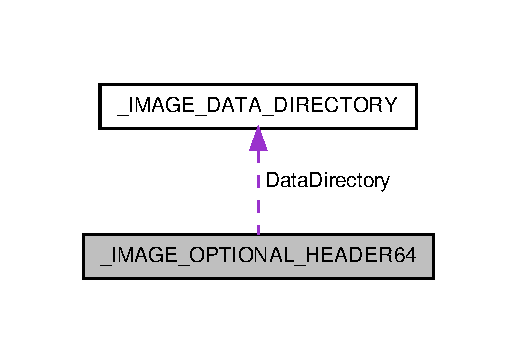
\includegraphics[width=248pt]{struct___i_m_a_g_e___o_p_t_i_o_n_a_l___h_e_a_d_e_r64__coll__graph}
\end{center}
\end{figure}
\subsection*{Atrybuty publiczne}
\begin{DoxyCompactItemize}
\item 
\hyperlink{winheader_8h_ab24077addd3b7b13e086987ff296552c}{W\-O\-R\-D} \hyperlink{struct___i_m_a_g_e___o_p_t_i_o_n_a_l___h_e_a_d_e_r64_ab5c03adcb9ef3e8354bc2408e517c08d}{Magic}
\item 
\hyperlink{winheader_8h_aae9749d96e15ccb4f482dd5f55d98f9b}{B\-Y\-T\-E} \hyperlink{struct___i_m_a_g_e___o_p_t_i_o_n_a_l___h_e_a_d_e_r64_a22167136c39f49c6622cb7d8986411db}{Major\-Linker\-Version}
\item 
\hyperlink{winheader_8h_aae9749d96e15ccb4f482dd5f55d98f9b}{B\-Y\-T\-E} \hyperlink{struct___i_m_a_g_e___o_p_t_i_o_n_a_l___h_e_a_d_e_r64_af5ae155c7158d93979300344e83e797d}{Minor\-Linker\-Version}
\item 
\hyperlink{winheader_8h_af483253b2143078cede883fc3c111ad2}{D\-W\-O\-R\-D} \hyperlink{struct___i_m_a_g_e___o_p_t_i_o_n_a_l___h_e_a_d_e_r64_ad320e4d1a34ae7a0dca244bc0c58fd75}{Size\-Of\-Code}
\item 
\hyperlink{winheader_8h_af483253b2143078cede883fc3c111ad2}{D\-W\-O\-R\-D} \hyperlink{struct___i_m_a_g_e___o_p_t_i_o_n_a_l___h_e_a_d_e_r64_ad96708232674a7e51792eee2db428c16}{Size\-Of\-Initialized\-Data}
\item 
\hyperlink{winheader_8h_af483253b2143078cede883fc3c111ad2}{D\-W\-O\-R\-D} \hyperlink{struct___i_m_a_g_e___o_p_t_i_o_n_a_l___h_e_a_d_e_r64_ac8ae0cd9fdcf7ee2df7d5162365e4711}{Size\-Of\-Uninitialized\-Data}
\item 
\hyperlink{winheader_8h_af483253b2143078cede883fc3c111ad2}{D\-W\-O\-R\-D} \hyperlink{struct___i_m_a_g_e___o_p_t_i_o_n_a_l___h_e_a_d_e_r64_a6c0a656b8114f02514a181bee89d4f12}{Address\-Of\-Entry\-Point}
\item 
\hyperlink{winheader_8h_af483253b2143078cede883fc3c111ad2}{D\-W\-O\-R\-D} \hyperlink{struct___i_m_a_g_e___o_p_t_i_o_n_a_l___h_e_a_d_e_r64_ab67058f28eed2c9078cb70263c246056}{Base\-Of\-Code}
\item 
\hyperlink{winheader_8h_ae854efed5cfd3aad7d516ab4e2ce5748}{U\-L\-O\-N\-G\-L\-O\-N\-G} \hyperlink{struct___i_m_a_g_e___o_p_t_i_o_n_a_l___h_e_a_d_e_r64_a2407a9ca4b308d9a5283e1b72ae5cb67}{Image\-Base}
\item 
\hyperlink{winheader_8h_af483253b2143078cede883fc3c111ad2}{D\-W\-O\-R\-D} \hyperlink{struct___i_m_a_g_e___o_p_t_i_o_n_a_l___h_e_a_d_e_r64_a3e3d3b030bdb0fd7a275839c94bc7a6d}{Section\-Alignment}
\item 
\hyperlink{winheader_8h_af483253b2143078cede883fc3c111ad2}{D\-W\-O\-R\-D} \hyperlink{struct___i_m_a_g_e___o_p_t_i_o_n_a_l___h_e_a_d_e_r64_a2766f965fb4fa501781266777ae4bdcd}{File\-Alignment}
\item 
\hyperlink{winheader_8h_ab24077addd3b7b13e086987ff296552c}{W\-O\-R\-D} \hyperlink{struct___i_m_a_g_e___o_p_t_i_o_n_a_l___h_e_a_d_e_r64_ace0c0908e430a20b470dec78da93e2b4}{Major\-Operating\-System\-Version}
\item 
\hyperlink{winheader_8h_ab24077addd3b7b13e086987ff296552c}{W\-O\-R\-D} \hyperlink{struct___i_m_a_g_e___o_p_t_i_o_n_a_l___h_e_a_d_e_r64_ad3a9484a135d4501c34b722f0aea8c28}{Minor\-Operating\-System\-Version}
\item 
\hyperlink{winheader_8h_ab24077addd3b7b13e086987ff296552c}{W\-O\-R\-D} \hyperlink{struct___i_m_a_g_e___o_p_t_i_o_n_a_l___h_e_a_d_e_r64_a5cbaea0743d6fc4c8809247e823decc2}{Major\-Image\-Version}
\item 
\hyperlink{winheader_8h_ab24077addd3b7b13e086987ff296552c}{W\-O\-R\-D} \hyperlink{struct___i_m_a_g_e___o_p_t_i_o_n_a_l___h_e_a_d_e_r64_a22d95193786b224c21e9d02e4acc0f75}{Minor\-Image\-Version}
\item 
\hyperlink{winheader_8h_ab24077addd3b7b13e086987ff296552c}{W\-O\-R\-D} \hyperlink{struct___i_m_a_g_e___o_p_t_i_o_n_a_l___h_e_a_d_e_r64_a2ac19f10f18d8040abd4741d647ae47b}{Major\-Subsystem\-Version}
\item 
\hyperlink{winheader_8h_ab24077addd3b7b13e086987ff296552c}{W\-O\-R\-D} \hyperlink{struct___i_m_a_g_e___o_p_t_i_o_n_a_l___h_e_a_d_e_r64_aafc5d6cfa28d5fcb8ad1facfae3a23eb}{Minor\-Subsystem\-Version}
\item 
\hyperlink{winheader_8h_af483253b2143078cede883fc3c111ad2}{D\-W\-O\-R\-D} \hyperlink{struct___i_m_a_g_e___o_p_t_i_o_n_a_l___h_e_a_d_e_r64_ab0f4ba84ab62cf9a22b96544b5c0479f}{Win32\-Version\-Value}
\item 
\hyperlink{winheader_8h_af483253b2143078cede883fc3c111ad2}{D\-W\-O\-R\-D} \hyperlink{struct___i_m_a_g_e___o_p_t_i_o_n_a_l___h_e_a_d_e_r64_aa00cd11bbb1ec2c9783cdd01212396c7}{Size\-Of\-Image}
\item 
\hyperlink{winheader_8h_af483253b2143078cede883fc3c111ad2}{D\-W\-O\-R\-D} \hyperlink{struct___i_m_a_g_e___o_p_t_i_o_n_a_l___h_e_a_d_e_r64_ae127bac62d64ccce8f8bfae6b22e8c14}{Size\-Of\-Headers}
\item 
\hyperlink{winheader_8h_af483253b2143078cede883fc3c111ad2}{D\-W\-O\-R\-D} \hyperlink{struct___i_m_a_g_e___o_p_t_i_o_n_a_l___h_e_a_d_e_r64_ad4a1520016a69a1b189e3d79f41373f6}{Check\-Sum}
\item 
\hyperlink{winheader_8h_ab24077addd3b7b13e086987ff296552c}{W\-O\-R\-D} \hyperlink{struct___i_m_a_g_e___o_p_t_i_o_n_a_l___h_e_a_d_e_r64_afedeb8911d64e97bafd352f4c97e2557}{Subsystem}
\item 
\hyperlink{winheader_8h_ab24077addd3b7b13e086987ff296552c}{W\-O\-R\-D} \hyperlink{struct___i_m_a_g_e___o_p_t_i_o_n_a_l___h_e_a_d_e_r64_acb52816f699486ae920bb8537108e81d}{Dll\-Characteristics}
\item 
\hyperlink{winheader_8h_ae854efed5cfd3aad7d516ab4e2ce5748}{U\-L\-O\-N\-G\-L\-O\-N\-G} \hyperlink{struct___i_m_a_g_e___o_p_t_i_o_n_a_l___h_e_a_d_e_r64_a6a430bc6cc1ff57190ebccb15fcd6c70}{Size\-Of\-Stack\-Reserve}
\item 
\hyperlink{winheader_8h_ae854efed5cfd3aad7d516ab4e2ce5748}{U\-L\-O\-N\-G\-L\-O\-N\-G} \hyperlink{struct___i_m_a_g_e___o_p_t_i_o_n_a_l___h_e_a_d_e_r64_ac80afcdeb0fc60d456350dced4e43b8a}{Size\-Of\-Stack\-Commit}
\item 
\hyperlink{winheader_8h_ae854efed5cfd3aad7d516ab4e2ce5748}{U\-L\-O\-N\-G\-L\-O\-N\-G} \hyperlink{struct___i_m_a_g_e___o_p_t_i_o_n_a_l___h_e_a_d_e_r64_ad225b09c6adc28538ee637885a9b4589}{Size\-Of\-Heap\-Reserve}
\item 
\hyperlink{winheader_8h_ae854efed5cfd3aad7d516ab4e2ce5748}{U\-L\-O\-N\-G\-L\-O\-N\-G} \hyperlink{struct___i_m_a_g_e___o_p_t_i_o_n_a_l___h_e_a_d_e_r64_a6b958f37e1630fa76f26dc60f003e7d8}{Size\-Of\-Heap\-Commit}
\item 
\hyperlink{winheader_8h_af483253b2143078cede883fc3c111ad2}{D\-W\-O\-R\-D} \hyperlink{struct___i_m_a_g_e___o_p_t_i_o_n_a_l___h_e_a_d_e_r64_a731102c663ae88402d8aa08359c44ab5}{Loader\-Flags}
\item 
\hyperlink{winheader_8h_af483253b2143078cede883fc3c111ad2}{D\-W\-O\-R\-D} \hyperlink{struct___i_m_a_g_e___o_p_t_i_o_n_a_l___h_e_a_d_e_r64_a8f05696ef5a2588164d4e502519d30b4}{Number\-Of\-Rva\-And\-Sizes}
\item 
\hyperlink{winheader_8h_a0b3ef87140356b8cb58f4af9eed4d607}{I\-M\-A\-G\-E\-\_\-\-D\-A\-T\-A\-\_\-\-D\-I\-R\-E\-C\-T\-O\-R\-Y} \hyperlink{struct___i_m_a_g_e___o_p_t_i_o_n_a_l___h_e_a_d_e_r64_a1da47d1e624bf0180d0e1363480616ff}{Data\-Directory} \mbox{[}\hyperlink{winheader_8h_a75892b738729f0de64146086f462defe}{I\-M\-A\-G\-E\-\_\-\-N\-U\-M\-B\-E\-R\-O\-F\-\_\-\-D\-I\-R\-E\-C\-T\-O\-R\-Y\-\_\-\-E\-N\-T\-R\-I\-E\-S}\mbox{]}
\end{DoxyCompactItemize}


\subsection{Opis szczegółowy}


Definicja w linii 170 pliku winheader.\-h.



\subsection{Dokumentacja atrybutów składowych}
\hypertarget{struct___i_m_a_g_e___o_p_t_i_o_n_a_l___h_e_a_d_e_r64_a6c0a656b8114f02514a181bee89d4f12}{\index{\-\_\-\-I\-M\-A\-G\-E\-\_\-\-O\-P\-T\-I\-O\-N\-A\-L\-\_\-\-H\-E\-A\-D\-E\-R64@{\-\_\-\-I\-M\-A\-G\-E\-\_\-\-O\-P\-T\-I\-O\-N\-A\-L\-\_\-\-H\-E\-A\-D\-E\-R64}!Address\-Of\-Entry\-Point@{Address\-Of\-Entry\-Point}}
\index{Address\-Of\-Entry\-Point@{Address\-Of\-Entry\-Point}!_IMAGE_OPTIONAL_HEADER64@{\-\_\-\-I\-M\-A\-G\-E\-\_\-\-O\-P\-T\-I\-O\-N\-A\-L\-\_\-\-H\-E\-A\-D\-E\-R64}}
\subsubsection[{Address\-Of\-Entry\-Point}]{\setlength{\rightskip}{0pt plus 5cm}{\bf D\-W\-O\-R\-D} \-\_\-\-I\-M\-A\-G\-E\-\_\-\-O\-P\-T\-I\-O\-N\-A\-L\-\_\-\-H\-E\-A\-D\-E\-R64\-::\-Address\-Of\-Entry\-Point}}\label{struct___i_m_a_g_e___o_p_t_i_o_n_a_l___h_e_a_d_e_r64_a6c0a656b8114f02514a181bee89d4f12}


Definicja w linii 177 pliku winheader.\-h.

\hypertarget{struct___i_m_a_g_e___o_p_t_i_o_n_a_l___h_e_a_d_e_r64_ab67058f28eed2c9078cb70263c246056}{\index{\-\_\-\-I\-M\-A\-G\-E\-\_\-\-O\-P\-T\-I\-O\-N\-A\-L\-\_\-\-H\-E\-A\-D\-E\-R64@{\-\_\-\-I\-M\-A\-G\-E\-\_\-\-O\-P\-T\-I\-O\-N\-A\-L\-\_\-\-H\-E\-A\-D\-E\-R64}!Base\-Of\-Code@{Base\-Of\-Code}}
\index{Base\-Of\-Code@{Base\-Of\-Code}!_IMAGE_OPTIONAL_HEADER64@{\-\_\-\-I\-M\-A\-G\-E\-\_\-\-O\-P\-T\-I\-O\-N\-A\-L\-\_\-\-H\-E\-A\-D\-E\-R64}}
\subsubsection[{Base\-Of\-Code}]{\setlength{\rightskip}{0pt plus 5cm}{\bf D\-W\-O\-R\-D} \-\_\-\-I\-M\-A\-G\-E\-\_\-\-O\-P\-T\-I\-O\-N\-A\-L\-\_\-\-H\-E\-A\-D\-E\-R64\-::\-Base\-Of\-Code}}\label{struct___i_m_a_g_e___o_p_t_i_o_n_a_l___h_e_a_d_e_r64_ab67058f28eed2c9078cb70263c246056}


Definicja w linii 178 pliku winheader.\-h.

\hypertarget{struct___i_m_a_g_e___o_p_t_i_o_n_a_l___h_e_a_d_e_r64_ad4a1520016a69a1b189e3d79f41373f6}{\index{\-\_\-\-I\-M\-A\-G\-E\-\_\-\-O\-P\-T\-I\-O\-N\-A\-L\-\_\-\-H\-E\-A\-D\-E\-R64@{\-\_\-\-I\-M\-A\-G\-E\-\_\-\-O\-P\-T\-I\-O\-N\-A\-L\-\_\-\-H\-E\-A\-D\-E\-R64}!Check\-Sum@{Check\-Sum}}
\index{Check\-Sum@{Check\-Sum}!_IMAGE_OPTIONAL_HEADER64@{\-\_\-\-I\-M\-A\-G\-E\-\_\-\-O\-P\-T\-I\-O\-N\-A\-L\-\_\-\-H\-E\-A\-D\-E\-R64}}
\subsubsection[{Check\-Sum}]{\setlength{\rightskip}{0pt plus 5cm}{\bf D\-W\-O\-R\-D} \-\_\-\-I\-M\-A\-G\-E\-\_\-\-O\-P\-T\-I\-O\-N\-A\-L\-\_\-\-H\-E\-A\-D\-E\-R64\-::\-Check\-Sum}}\label{struct___i_m_a_g_e___o_p_t_i_o_n_a_l___h_e_a_d_e_r64_ad4a1520016a69a1b189e3d79f41373f6}


Definicja w linii 191 pliku winheader.\-h.

\hypertarget{struct___i_m_a_g_e___o_p_t_i_o_n_a_l___h_e_a_d_e_r64_a1da47d1e624bf0180d0e1363480616ff}{\index{\-\_\-\-I\-M\-A\-G\-E\-\_\-\-O\-P\-T\-I\-O\-N\-A\-L\-\_\-\-H\-E\-A\-D\-E\-R64@{\-\_\-\-I\-M\-A\-G\-E\-\_\-\-O\-P\-T\-I\-O\-N\-A\-L\-\_\-\-H\-E\-A\-D\-E\-R64}!Data\-Directory@{Data\-Directory}}
\index{Data\-Directory@{Data\-Directory}!_IMAGE_OPTIONAL_HEADER64@{\-\_\-\-I\-M\-A\-G\-E\-\_\-\-O\-P\-T\-I\-O\-N\-A\-L\-\_\-\-H\-E\-A\-D\-E\-R64}}
\subsubsection[{Data\-Directory}]{\setlength{\rightskip}{0pt plus 5cm}{\bf I\-M\-A\-G\-E\-\_\-\-D\-A\-T\-A\-\_\-\-D\-I\-R\-E\-C\-T\-O\-R\-Y} \-\_\-\-I\-M\-A\-G\-E\-\_\-\-O\-P\-T\-I\-O\-N\-A\-L\-\_\-\-H\-E\-A\-D\-E\-R64\-::\-Data\-Directory\mbox{[}{\bf I\-M\-A\-G\-E\-\_\-\-N\-U\-M\-B\-E\-R\-O\-F\-\_\-\-D\-I\-R\-E\-C\-T\-O\-R\-Y\-\_\-\-E\-N\-T\-R\-I\-E\-S}\mbox{]}}}\label{struct___i_m_a_g_e___o_p_t_i_o_n_a_l___h_e_a_d_e_r64_a1da47d1e624bf0180d0e1363480616ff}


Definicja w linii 200 pliku winheader.\-h.

\hypertarget{struct___i_m_a_g_e___o_p_t_i_o_n_a_l___h_e_a_d_e_r64_acb52816f699486ae920bb8537108e81d}{\index{\-\_\-\-I\-M\-A\-G\-E\-\_\-\-O\-P\-T\-I\-O\-N\-A\-L\-\_\-\-H\-E\-A\-D\-E\-R64@{\-\_\-\-I\-M\-A\-G\-E\-\_\-\-O\-P\-T\-I\-O\-N\-A\-L\-\_\-\-H\-E\-A\-D\-E\-R64}!Dll\-Characteristics@{Dll\-Characteristics}}
\index{Dll\-Characteristics@{Dll\-Characteristics}!_IMAGE_OPTIONAL_HEADER64@{\-\_\-\-I\-M\-A\-G\-E\-\_\-\-O\-P\-T\-I\-O\-N\-A\-L\-\_\-\-H\-E\-A\-D\-E\-R64}}
\subsubsection[{Dll\-Characteristics}]{\setlength{\rightskip}{0pt plus 5cm}{\bf W\-O\-R\-D} \-\_\-\-I\-M\-A\-G\-E\-\_\-\-O\-P\-T\-I\-O\-N\-A\-L\-\_\-\-H\-E\-A\-D\-E\-R64\-::\-Dll\-Characteristics}}\label{struct___i_m_a_g_e___o_p_t_i_o_n_a_l___h_e_a_d_e_r64_acb52816f699486ae920bb8537108e81d}


Definicja w linii 193 pliku winheader.\-h.

\hypertarget{struct___i_m_a_g_e___o_p_t_i_o_n_a_l___h_e_a_d_e_r64_a2766f965fb4fa501781266777ae4bdcd}{\index{\-\_\-\-I\-M\-A\-G\-E\-\_\-\-O\-P\-T\-I\-O\-N\-A\-L\-\_\-\-H\-E\-A\-D\-E\-R64@{\-\_\-\-I\-M\-A\-G\-E\-\_\-\-O\-P\-T\-I\-O\-N\-A\-L\-\_\-\-H\-E\-A\-D\-E\-R64}!File\-Alignment@{File\-Alignment}}
\index{File\-Alignment@{File\-Alignment}!_IMAGE_OPTIONAL_HEADER64@{\-\_\-\-I\-M\-A\-G\-E\-\_\-\-O\-P\-T\-I\-O\-N\-A\-L\-\_\-\-H\-E\-A\-D\-E\-R64}}
\subsubsection[{File\-Alignment}]{\setlength{\rightskip}{0pt plus 5cm}{\bf D\-W\-O\-R\-D} \-\_\-\-I\-M\-A\-G\-E\-\_\-\-O\-P\-T\-I\-O\-N\-A\-L\-\_\-\-H\-E\-A\-D\-E\-R64\-::\-File\-Alignment}}\label{struct___i_m_a_g_e___o_p_t_i_o_n_a_l___h_e_a_d_e_r64_a2766f965fb4fa501781266777ae4bdcd}


Definicja w linii 181 pliku winheader.\-h.

\hypertarget{struct___i_m_a_g_e___o_p_t_i_o_n_a_l___h_e_a_d_e_r64_a2407a9ca4b308d9a5283e1b72ae5cb67}{\index{\-\_\-\-I\-M\-A\-G\-E\-\_\-\-O\-P\-T\-I\-O\-N\-A\-L\-\_\-\-H\-E\-A\-D\-E\-R64@{\-\_\-\-I\-M\-A\-G\-E\-\_\-\-O\-P\-T\-I\-O\-N\-A\-L\-\_\-\-H\-E\-A\-D\-E\-R64}!Image\-Base@{Image\-Base}}
\index{Image\-Base@{Image\-Base}!_IMAGE_OPTIONAL_HEADER64@{\-\_\-\-I\-M\-A\-G\-E\-\_\-\-O\-P\-T\-I\-O\-N\-A\-L\-\_\-\-H\-E\-A\-D\-E\-R64}}
\subsubsection[{Image\-Base}]{\setlength{\rightskip}{0pt plus 5cm}{\bf U\-L\-O\-N\-G\-L\-O\-N\-G} \-\_\-\-I\-M\-A\-G\-E\-\_\-\-O\-P\-T\-I\-O\-N\-A\-L\-\_\-\-H\-E\-A\-D\-E\-R64\-::\-Image\-Base}}\label{struct___i_m_a_g_e___o_p_t_i_o_n_a_l___h_e_a_d_e_r64_a2407a9ca4b308d9a5283e1b72ae5cb67}


Definicja w linii 179 pliku winheader.\-h.

\hypertarget{struct___i_m_a_g_e___o_p_t_i_o_n_a_l___h_e_a_d_e_r64_a731102c663ae88402d8aa08359c44ab5}{\index{\-\_\-\-I\-M\-A\-G\-E\-\_\-\-O\-P\-T\-I\-O\-N\-A\-L\-\_\-\-H\-E\-A\-D\-E\-R64@{\-\_\-\-I\-M\-A\-G\-E\-\_\-\-O\-P\-T\-I\-O\-N\-A\-L\-\_\-\-H\-E\-A\-D\-E\-R64}!Loader\-Flags@{Loader\-Flags}}
\index{Loader\-Flags@{Loader\-Flags}!_IMAGE_OPTIONAL_HEADER64@{\-\_\-\-I\-M\-A\-G\-E\-\_\-\-O\-P\-T\-I\-O\-N\-A\-L\-\_\-\-H\-E\-A\-D\-E\-R64}}
\subsubsection[{Loader\-Flags}]{\setlength{\rightskip}{0pt plus 5cm}{\bf D\-W\-O\-R\-D} \-\_\-\-I\-M\-A\-G\-E\-\_\-\-O\-P\-T\-I\-O\-N\-A\-L\-\_\-\-H\-E\-A\-D\-E\-R64\-::\-Loader\-Flags}}\label{struct___i_m_a_g_e___o_p_t_i_o_n_a_l___h_e_a_d_e_r64_a731102c663ae88402d8aa08359c44ab5}


Definicja w linii 198 pliku winheader.\-h.

\hypertarget{struct___i_m_a_g_e___o_p_t_i_o_n_a_l___h_e_a_d_e_r64_ab5c03adcb9ef3e8354bc2408e517c08d}{\index{\-\_\-\-I\-M\-A\-G\-E\-\_\-\-O\-P\-T\-I\-O\-N\-A\-L\-\_\-\-H\-E\-A\-D\-E\-R64@{\-\_\-\-I\-M\-A\-G\-E\-\_\-\-O\-P\-T\-I\-O\-N\-A\-L\-\_\-\-H\-E\-A\-D\-E\-R64}!Magic@{Magic}}
\index{Magic@{Magic}!_IMAGE_OPTIONAL_HEADER64@{\-\_\-\-I\-M\-A\-G\-E\-\_\-\-O\-P\-T\-I\-O\-N\-A\-L\-\_\-\-H\-E\-A\-D\-E\-R64}}
\subsubsection[{Magic}]{\setlength{\rightskip}{0pt plus 5cm}{\bf W\-O\-R\-D} \-\_\-\-I\-M\-A\-G\-E\-\_\-\-O\-P\-T\-I\-O\-N\-A\-L\-\_\-\-H\-E\-A\-D\-E\-R64\-::\-Magic}}\label{struct___i_m_a_g_e___o_p_t_i_o_n_a_l___h_e_a_d_e_r64_ab5c03adcb9ef3e8354bc2408e517c08d}


Definicja w linii 171 pliku winheader.\-h.

\hypertarget{struct___i_m_a_g_e___o_p_t_i_o_n_a_l___h_e_a_d_e_r64_a5cbaea0743d6fc4c8809247e823decc2}{\index{\-\_\-\-I\-M\-A\-G\-E\-\_\-\-O\-P\-T\-I\-O\-N\-A\-L\-\_\-\-H\-E\-A\-D\-E\-R64@{\-\_\-\-I\-M\-A\-G\-E\-\_\-\-O\-P\-T\-I\-O\-N\-A\-L\-\_\-\-H\-E\-A\-D\-E\-R64}!Major\-Image\-Version@{Major\-Image\-Version}}
\index{Major\-Image\-Version@{Major\-Image\-Version}!_IMAGE_OPTIONAL_HEADER64@{\-\_\-\-I\-M\-A\-G\-E\-\_\-\-O\-P\-T\-I\-O\-N\-A\-L\-\_\-\-H\-E\-A\-D\-E\-R64}}
\subsubsection[{Major\-Image\-Version}]{\setlength{\rightskip}{0pt plus 5cm}{\bf W\-O\-R\-D} \-\_\-\-I\-M\-A\-G\-E\-\_\-\-O\-P\-T\-I\-O\-N\-A\-L\-\_\-\-H\-E\-A\-D\-E\-R64\-::\-Major\-Image\-Version}}\label{struct___i_m_a_g_e___o_p_t_i_o_n_a_l___h_e_a_d_e_r64_a5cbaea0743d6fc4c8809247e823decc2}


Definicja w linii 184 pliku winheader.\-h.

\hypertarget{struct___i_m_a_g_e___o_p_t_i_o_n_a_l___h_e_a_d_e_r64_a22167136c39f49c6622cb7d8986411db}{\index{\-\_\-\-I\-M\-A\-G\-E\-\_\-\-O\-P\-T\-I\-O\-N\-A\-L\-\_\-\-H\-E\-A\-D\-E\-R64@{\-\_\-\-I\-M\-A\-G\-E\-\_\-\-O\-P\-T\-I\-O\-N\-A\-L\-\_\-\-H\-E\-A\-D\-E\-R64}!Major\-Linker\-Version@{Major\-Linker\-Version}}
\index{Major\-Linker\-Version@{Major\-Linker\-Version}!_IMAGE_OPTIONAL_HEADER64@{\-\_\-\-I\-M\-A\-G\-E\-\_\-\-O\-P\-T\-I\-O\-N\-A\-L\-\_\-\-H\-E\-A\-D\-E\-R64}}
\subsubsection[{Major\-Linker\-Version}]{\setlength{\rightskip}{0pt plus 5cm}{\bf B\-Y\-T\-E} \-\_\-\-I\-M\-A\-G\-E\-\_\-\-O\-P\-T\-I\-O\-N\-A\-L\-\_\-\-H\-E\-A\-D\-E\-R64\-::\-Major\-Linker\-Version}}\label{struct___i_m_a_g_e___o_p_t_i_o_n_a_l___h_e_a_d_e_r64_a22167136c39f49c6622cb7d8986411db}


Definicja w linii 172 pliku winheader.\-h.

\hypertarget{struct___i_m_a_g_e___o_p_t_i_o_n_a_l___h_e_a_d_e_r64_ace0c0908e430a20b470dec78da93e2b4}{\index{\-\_\-\-I\-M\-A\-G\-E\-\_\-\-O\-P\-T\-I\-O\-N\-A\-L\-\_\-\-H\-E\-A\-D\-E\-R64@{\-\_\-\-I\-M\-A\-G\-E\-\_\-\-O\-P\-T\-I\-O\-N\-A\-L\-\_\-\-H\-E\-A\-D\-E\-R64}!Major\-Operating\-System\-Version@{Major\-Operating\-System\-Version}}
\index{Major\-Operating\-System\-Version@{Major\-Operating\-System\-Version}!_IMAGE_OPTIONAL_HEADER64@{\-\_\-\-I\-M\-A\-G\-E\-\_\-\-O\-P\-T\-I\-O\-N\-A\-L\-\_\-\-H\-E\-A\-D\-E\-R64}}
\subsubsection[{Major\-Operating\-System\-Version}]{\setlength{\rightskip}{0pt plus 5cm}{\bf W\-O\-R\-D} \-\_\-\-I\-M\-A\-G\-E\-\_\-\-O\-P\-T\-I\-O\-N\-A\-L\-\_\-\-H\-E\-A\-D\-E\-R64\-::\-Major\-Operating\-System\-Version}}\label{struct___i_m_a_g_e___o_p_t_i_o_n_a_l___h_e_a_d_e_r64_ace0c0908e430a20b470dec78da93e2b4}


Definicja w linii 182 pliku winheader.\-h.

\hypertarget{struct___i_m_a_g_e___o_p_t_i_o_n_a_l___h_e_a_d_e_r64_a2ac19f10f18d8040abd4741d647ae47b}{\index{\-\_\-\-I\-M\-A\-G\-E\-\_\-\-O\-P\-T\-I\-O\-N\-A\-L\-\_\-\-H\-E\-A\-D\-E\-R64@{\-\_\-\-I\-M\-A\-G\-E\-\_\-\-O\-P\-T\-I\-O\-N\-A\-L\-\_\-\-H\-E\-A\-D\-E\-R64}!Major\-Subsystem\-Version@{Major\-Subsystem\-Version}}
\index{Major\-Subsystem\-Version@{Major\-Subsystem\-Version}!_IMAGE_OPTIONAL_HEADER64@{\-\_\-\-I\-M\-A\-G\-E\-\_\-\-O\-P\-T\-I\-O\-N\-A\-L\-\_\-\-H\-E\-A\-D\-E\-R64}}
\subsubsection[{Major\-Subsystem\-Version}]{\setlength{\rightskip}{0pt plus 5cm}{\bf W\-O\-R\-D} \-\_\-\-I\-M\-A\-G\-E\-\_\-\-O\-P\-T\-I\-O\-N\-A\-L\-\_\-\-H\-E\-A\-D\-E\-R64\-::\-Major\-Subsystem\-Version}}\label{struct___i_m_a_g_e___o_p_t_i_o_n_a_l___h_e_a_d_e_r64_a2ac19f10f18d8040abd4741d647ae47b}


Definicja w linii 186 pliku winheader.\-h.

\hypertarget{struct___i_m_a_g_e___o_p_t_i_o_n_a_l___h_e_a_d_e_r64_a22d95193786b224c21e9d02e4acc0f75}{\index{\-\_\-\-I\-M\-A\-G\-E\-\_\-\-O\-P\-T\-I\-O\-N\-A\-L\-\_\-\-H\-E\-A\-D\-E\-R64@{\-\_\-\-I\-M\-A\-G\-E\-\_\-\-O\-P\-T\-I\-O\-N\-A\-L\-\_\-\-H\-E\-A\-D\-E\-R64}!Minor\-Image\-Version@{Minor\-Image\-Version}}
\index{Minor\-Image\-Version@{Minor\-Image\-Version}!_IMAGE_OPTIONAL_HEADER64@{\-\_\-\-I\-M\-A\-G\-E\-\_\-\-O\-P\-T\-I\-O\-N\-A\-L\-\_\-\-H\-E\-A\-D\-E\-R64}}
\subsubsection[{Minor\-Image\-Version}]{\setlength{\rightskip}{0pt plus 5cm}{\bf W\-O\-R\-D} \-\_\-\-I\-M\-A\-G\-E\-\_\-\-O\-P\-T\-I\-O\-N\-A\-L\-\_\-\-H\-E\-A\-D\-E\-R64\-::\-Minor\-Image\-Version}}\label{struct___i_m_a_g_e___o_p_t_i_o_n_a_l___h_e_a_d_e_r64_a22d95193786b224c21e9d02e4acc0f75}


Definicja w linii 185 pliku winheader.\-h.

\hypertarget{struct___i_m_a_g_e___o_p_t_i_o_n_a_l___h_e_a_d_e_r64_af5ae155c7158d93979300344e83e797d}{\index{\-\_\-\-I\-M\-A\-G\-E\-\_\-\-O\-P\-T\-I\-O\-N\-A\-L\-\_\-\-H\-E\-A\-D\-E\-R64@{\-\_\-\-I\-M\-A\-G\-E\-\_\-\-O\-P\-T\-I\-O\-N\-A\-L\-\_\-\-H\-E\-A\-D\-E\-R64}!Minor\-Linker\-Version@{Minor\-Linker\-Version}}
\index{Minor\-Linker\-Version@{Minor\-Linker\-Version}!_IMAGE_OPTIONAL_HEADER64@{\-\_\-\-I\-M\-A\-G\-E\-\_\-\-O\-P\-T\-I\-O\-N\-A\-L\-\_\-\-H\-E\-A\-D\-E\-R64}}
\subsubsection[{Minor\-Linker\-Version}]{\setlength{\rightskip}{0pt plus 5cm}{\bf B\-Y\-T\-E} \-\_\-\-I\-M\-A\-G\-E\-\_\-\-O\-P\-T\-I\-O\-N\-A\-L\-\_\-\-H\-E\-A\-D\-E\-R64\-::\-Minor\-Linker\-Version}}\label{struct___i_m_a_g_e___o_p_t_i_o_n_a_l___h_e_a_d_e_r64_af5ae155c7158d93979300344e83e797d}


Definicja w linii 173 pliku winheader.\-h.

\hypertarget{struct___i_m_a_g_e___o_p_t_i_o_n_a_l___h_e_a_d_e_r64_ad3a9484a135d4501c34b722f0aea8c28}{\index{\-\_\-\-I\-M\-A\-G\-E\-\_\-\-O\-P\-T\-I\-O\-N\-A\-L\-\_\-\-H\-E\-A\-D\-E\-R64@{\-\_\-\-I\-M\-A\-G\-E\-\_\-\-O\-P\-T\-I\-O\-N\-A\-L\-\_\-\-H\-E\-A\-D\-E\-R64}!Minor\-Operating\-System\-Version@{Minor\-Operating\-System\-Version}}
\index{Minor\-Operating\-System\-Version@{Minor\-Operating\-System\-Version}!_IMAGE_OPTIONAL_HEADER64@{\-\_\-\-I\-M\-A\-G\-E\-\_\-\-O\-P\-T\-I\-O\-N\-A\-L\-\_\-\-H\-E\-A\-D\-E\-R64}}
\subsubsection[{Minor\-Operating\-System\-Version}]{\setlength{\rightskip}{0pt plus 5cm}{\bf W\-O\-R\-D} \-\_\-\-I\-M\-A\-G\-E\-\_\-\-O\-P\-T\-I\-O\-N\-A\-L\-\_\-\-H\-E\-A\-D\-E\-R64\-::\-Minor\-Operating\-System\-Version}}\label{struct___i_m_a_g_e___o_p_t_i_o_n_a_l___h_e_a_d_e_r64_ad3a9484a135d4501c34b722f0aea8c28}


Definicja w linii 183 pliku winheader.\-h.

\hypertarget{struct___i_m_a_g_e___o_p_t_i_o_n_a_l___h_e_a_d_e_r64_aafc5d6cfa28d5fcb8ad1facfae3a23eb}{\index{\-\_\-\-I\-M\-A\-G\-E\-\_\-\-O\-P\-T\-I\-O\-N\-A\-L\-\_\-\-H\-E\-A\-D\-E\-R64@{\-\_\-\-I\-M\-A\-G\-E\-\_\-\-O\-P\-T\-I\-O\-N\-A\-L\-\_\-\-H\-E\-A\-D\-E\-R64}!Minor\-Subsystem\-Version@{Minor\-Subsystem\-Version}}
\index{Minor\-Subsystem\-Version@{Minor\-Subsystem\-Version}!_IMAGE_OPTIONAL_HEADER64@{\-\_\-\-I\-M\-A\-G\-E\-\_\-\-O\-P\-T\-I\-O\-N\-A\-L\-\_\-\-H\-E\-A\-D\-E\-R64}}
\subsubsection[{Minor\-Subsystem\-Version}]{\setlength{\rightskip}{0pt plus 5cm}{\bf W\-O\-R\-D} \-\_\-\-I\-M\-A\-G\-E\-\_\-\-O\-P\-T\-I\-O\-N\-A\-L\-\_\-\-H\-E\-A\-D\-E\-R64\-::\-Minor\-Subsystem\-Version}}\label{struct___i_m_a_g_e___o_p_t_i_o_n_a_l___h_e_a_d_e_r64_aafc5d6cfa28d5fcb8ad1facfae3a23eb}


Definicja w linii 187 pliku winheader.\-h.

\hypertarget{struct___i_m_a_g_e___o_p_t_i_o_n_a_l___h_e_a_d_e_r64_a8f05696ef5a2588164d4e502519d30b4}{\index{\-\_\-\-I\-M\-A\-G\-E\-\_\-\-O\-P\-T\-I\-O\-N\-A\-L\-\_\-\-H\-E\-A\-D\-E\-R64@{\-\_\-\-I\-M\-A\-G\-E\-\_\-\-O\-P\-T\-I\-O\-N\-A\-L\-\_\-\-H\-E\-A\-D\-E\-R64}!Number\-Of\-Rva\-And\-Sizes@{Number\-Of\-Rva\-And\-Sizes}}
\index{Number\-Of\-Rva\-And\-Sizes@{Number\-Of\-Rva\-And\-Sizes}!_IMAGE_OPTIONAL_HEADER64@{\-\_\-\-I\-M\-A\-G\-E\-\_\-\-O\-P\-T\-I\-O\-N\-A\-L\-\_\-\-H\-E\-A\-D\-E\-R64}}
\subsubsection[{Number\-Of\-Rva\-And\-Sizes}]{\setlength{\rightskip}{0pt plus 5cm}{\bf D\-W\-O\-R\-D} \-\_\-\-I\-M\-A\-G\-E\-\_\-\-O\-P\-T\-I\-O\-N\-A\-L\-\_\-\-H\-E\-A\-D\-E\-R64\-::\-Number\-Of\-Rva\-And\-Sizes}}\label{struct___i_m_a_g_e___o_p_t_i_o_n_a_l___h_e_a_d_e_r64_a8f05696ef5a2588164d4e502519d30b4}


Definicja w linii 199 pliku winheader.\-h.

\hypertarget{struct___i_m_a_g_e___o_p_t_i_o_n_a_l___h_e_a_d_e_r64_a3e3d3b030bdb0fd7a275839c94bc7a6d}{\index{\-\_\-\-I\-M\-A\-G\-E\-\_\-\-O\-P\-T\-I\-O\-N\-A\-L\-\_\-\-H\-E\-A\-D\-E\-R64@{\-\_\-\-I\-M\-A\-G\-E\-\_\-\-O\-P\-T\-I\-O\-N\-A\-L\-\_\-\-H\-E\-A\-D\-E\-R64}!Section\-Alignment@{Section\-Alignment}}
\index{Section\-Alignment@{Section\-Alignment}!_IMAGE_OPTIONAL_HEADER64@{\-\_\-\-I\-M\-A\-G\-E\-\_\-\-O\-P\-T\-I\-O\-N\-A\-L\-\_\-\-H\-E\-A\-D\-E\-R64}}
\subsubsection[{Section\-Alignment}]{\setlength{\rightskip}{0pt plus 5cm}{\bf D\-W\-O\-R\-D} \-\_\-\-I\-M\-A\-G\-E\-\_\-\-O\-P\-T\-I\-O\-N\-A\-L\-\_\-\-H\-E\-A\-D\-E\-R64\-::\-Section\-Alignment}}\label{struct___i_m_a_g_e___o_p_t_i_o_n_a_l___h_e_a_d_e_r64_a3e3d3b030bdb0fd7a275839c94bc7a6d}


Definicja w linii 180 pliku winheader.\-h.

\hypertarget{struct___i_m_a_g_e___o_p_t_i_o_n_a_l___h_e_a_d_e_r64_ad320e4d1a34ae7a0dca244bc0c58fd75}{\index{\-\_\-\-I\-M\-A\-G\-E\-\_\-\-O\-P\-T\-I\-O\-N\-A\-L\-\_\-\-H\-E\-A\-D\-E\-R64@{\-\_\-\-I\-M\-A\-G\-E\-\_\-\-O\-P\-T\-I\-O\-N\-A\-L\-\_\-\-H\-E\-A\-D\-E\-R64}!Size\-Of\-Code@{Size\-Of\-Code}}
\index{Size\-Of\-Code@{Size\-Of\-Code}!_IMAGE_OPTIONAL_HEADER64@{\-\_\-\-I\-M\-A\-G\-E\-\_\-\-O\-P\-T\-I\-O\-N\-A\-L\-\_\-\-H\-E\-A\-D\-E\-R64}}
\subsubsection[{Size\-Of\-Code}]{\setlength{\rightskip}{0pt plus 5cm}{\bf D\-W\-O\-R\-D} \-\_\-\-I\-M\-A\-G\-E\-\_\-\-O\-P\-T\-I\-O\-N\-A\-L\-\_\-\-H\-E\-A\-D\-E\-R64\-::\-Size\-Of\-Code}}\label{struct___i_m_a_g_e___o_p_t_i_o_n_a_l___h_e_a_d_e_r64_ad320e4d1a34ae7a0dca244bc0c58fd75}


Definicja w linii 174 pliku winheader.\-h.

\hypertarget{struct___i_m_a_g_e___o_p_t_i_o_n_a_l___h_e_a_d_e_r64_ae127bac62d64ccce8f8bfae6b22e8c14}{\index{\-\_\-\-I\-M\-A\-G\-E\-\_\-\-O\-P\-T\-I\-O\-N\-A\-L\-\_\-\-H\-E\-A\-D\-E\-R64@{\-\_\-\-I\-M\-A\-G\-E\-\_\-\-O\-P\-T\-I\-O\-N\-A\-L\-\_\-\-H\-E\-A\-D\-E\-R64}!Size\-Of\-Headers@{Size\-Of\-Headers}}
\index{Size\-Of\-Headers@{Size\-Of\-Headers}!_IMAGE_OPTIONAL_HEADER64@{\-\_\-\-I\-M\-A\-G\-E\-\_\-\-O\-P\-T\-I\-O\-N\-A\-L\-\_\-\-H\-E\-A\-D\-E\-R64}}
\subsubsection[{Size\-Of\-Headers}]{\setlength{\rightskip}{0pt plus 5cm}{\bf D\-W\-O\-R\-D} \-\_\-\-I\-M\-A\-G\-E\-\_\-\-O\-P\-T\-I\-O\-N\-A\-L\-\_\-\-H\-E\-A\-D\-E\-R64\-::\-Size\-Of\-Headers}}\label{struct___i_m_a_g_e___o_p_t_i_o_n_a_l___h_e_a_d_e_r64_ae127bac62d64ccce8f8bfae6b22e8c14}


Definicja w linii 190 pliku winheader.\-h.

\hypertarget{struct___i_m_a_g_e___o_p_t_i_o_n_a_l___h_e_a_d_e_r64_a6b958f37e1630fa76f26dc60f003e7d8}{\index{\-\_\-\-I\-M\-A\-G\-E\-\_\-\-O\-P\-T\-I\-O\-N\-A\-L\-\_\-\-H\-E\-A\-D\-E\-R64@{\-\_\-\-I\-M\-A\-G\-E\-\_\-\-O\-P\-T\-I\-O\-N\-A\-L\-\_\-\-H\-E\-A\-D\-E\-R64}!Size\-Of\-Heap\-Commit@{Size\-Of\-Heap\-Commit}}
\index{Size\-Of\-Heap\-Commit@{Size\-Of\-Heap\-Commit}!_IMAGE_OPTIONAL_HEADER64@{\-\_\-\-I\-M\-A\-G\-E\-\_\-\-O\-P\-T\-I\-O\-N\-A\-L\-\_\-\-H\-E\-A\-D\-E\-R64}}
\subsubsection[{Size\-Of\-Heap\-Commit}]{\setlength{\rightskip}{0pt plus 5cm}{\bf U\-L\-O\-N\-G\-L\-O\-N\-G} \-\_\-\-I\-M\-A\-G\-E\-\_\-\-O\-P\-T\-I\-O\-N\-A\-L\-\_\-\-H\-E\-A\-D\-E\-R64\-::\-Size\-Of\-Heap\-Commit}}\label{struct___i_m_a_g_e___o_p_t_i_o_n_a_l___h_e_a_d_e_r64_a6b958f37e1630fa76f26dc60f003e7d8}


Definicja w linii 197 pliku winheader.\-h.

\hypertarget{struct___i_m_a_g_e___o_p_t_i_o_n_a_l___h_e_a_d_e_r64_ad225b09c6adc28538ee637885a9b4589}{\index{\-\_\-\-I\-M\-A\-G\-E\-\_\-\-O\-P\-T\-I\-O\-N\-A\-L\-\_\-\-H\-E\-A\-D\-E\-R64@{\-\_\-\-I\-M\-A\-G\-E\-\_\-\-O\-P\-T\-I\-O\-N\-A\-L\-\_\-\-H\-E\-A\-D\-E\-R64}!Size\-Of\-Heap\-Reserve@{Size\-Of\-Heap\-Reserve}}
\index{Size\-Of\-Heap\-Reserve@{Size\-Of\-Heap\-Reserve}!_IMAGE_OPTIONAL_HEADER64@{\-\_\-\-I\-M\-A\-G\-E\-\_\-\-O\-P\-T\-I\-O\-N\-A\-L\-\_\-\-H\-E\-A\-D\-E\-R64}}
\subsubsection[{Size\-Of\-Heap\-Reserve}]{\setlength{\rightskip}{0pt plus 5cm}{\bf U\-L\-O\-N\-G\-L\-O\-N\-G} \-\_\-\-I\-M\-A\-G\-E\-\_\-\-O\-P\-T\-I\-O\-N\-A\-L\-\_\-\-H\-E\-A\-D\-E\-R64\-::\-Size\-Of\-Heap\-Reserve}}\label{struct___i_m_a_g_e___o_p_t_i_o_n_a_l___h_e_a_d_e_r64_ad225b09c6adc28538ee637885a9b4589}


Definicja w linii 196 pliku winheader.\-h.

\hypertarget{struct___i_m_a_g_e___o_p_t_i_o_n_a_l___h_e_a_d_e_r64_aa00cd11bbb1ec2c9783cdd01212396c7}{\index{\-\_\-\-I\-M\-A\-G\-E\-\_\-\-O\-P\-T\-I\-O\-N\-A\-L\-\_\-\-H\-E\-A\-D\-E\-R64@{\-\_\-\-I\-M\-A\-G\-E\-\_\-\-O\-P\-T\-I\-O\-N\-A\-L\-\_\-\-H\-E\-A\-D\-E\-R64}!Size\-Of\-Image@{Size\-Of\-Image}}
\index{Size\-Of\-Image@{Size\-Of\-Image}!_IMAGE_OPTIONAL_HEADER64@{\-\_\-\-I\-M\-A\-G\-E\-\_\-\-O\-P\-T\-I\-O\-N\-A\-L\-\_\-\-H\-E\-A\-D\-E\-R64}}
\subsubsection[{Size\-Of\-Image}]{\setlength{\rightskip}{0pt plus 5cm}{\bf D\-W\-O\-R\-D} \-\_\-\-I\-M\-A\-G\-E\-\_\-\-O\-P\-T\-I\-O\-N\-A\-L\-\_\-\-H\-E\-A\-D\-E\-R64\-::\-Size\-Of\-Image}}\label{struct___i_m_a_g_e___o_p_t_i_o_n_a_l___h_e_a_d_e_r64_aa00cd11bbb1ec2c9783cdd01212396c7}


Definicja w linii 189 pliku winheader.\-h.

\hypertarget{struct___i_m_a_g_e___o_p_t_i_o_n_a_l___h_e_a_d_e_r64_ad96708232674a7e51792eee2db428c16}{\index{\-\_\-\-I\-M\-A\-G\-E\-\_\-\-O\-P\-T\-I\-O\-N\-A\-L\-\_\-\-H\-E\-A\-D\-E\-R64@{\-\_\-\-I\-M\-A\-G\-E\-\_\-\-O\-P\-T\-I\-O\-N\-A\-L\-\_\-\-H\-E\-A\-D\-E\-R64}!Size\-Of\-Initialized\-Data@{Size\-Of\-Initialized\-Data}}
\index{Size\-Of\-Initialized\-Data@{Size\-Of\-Initialized\-Data}!_IMAGE_OPTIONAL_HEADER64@{\-\_\-\-I\-M\-A\-G\-E\-\_\-\-O\-P\-T\-I\-O\-N\-A\-L\-\_\-\-H\-E\-A\-D\-E\-R64}}
\subsubsection[{Size\-Of\-Initialized\-Data}]{\setlength{\rightskip}{0pt plus 5cm}{\bf D\-W\-O\-R\-D} \-\_\-\-I\-M\-A\-G\-E\-\_\-\-O\-P\-T\-I\-O\-N\-A\-L\-\_\-\-H\-E\-A\-D\-E\-R64\-::\-Size\-Of\-Initialized\-Data}}\label{struct___i_m_a_g_e___o_p_t_i_o_n_a_l___h_e_a_d_e_r64_ad96708232674a7e51792eee2db428c16}


Definicja w linii 175 pliku winheader.\-h.

\hypertarget{struct___i_m_a_g_e___o_p_t_i_o_n_a_l___h_e_a_d_e_r64_ac80afcdeb0fc60d456350dced4e43b8a}{\index{\-\_\-\-I\-M\-A\-G\-E\-\_\-\-O\-P\-T\-I\-O\-N\-A\-L\-\_\-\-H\-E\-A\-D\-E\-R64@{\-\_\-\-I\-M\-A\-G\-E\-\_\-\-O\-P\-T\-I\-O\-N\-A\-L\-\_\-\-H\-E\-A\-D\-E\-R64}!Size\-Of\-Stack\-Commit@{Size\-Of\-Stack\-Commit}}
\index{Size\-Of\-Stack\-Commit@{Size\-Of\-Stack\-Commit}!_IMAGE_OPTIONAL_HEADER64@{\-\_\-\-I\-M\-A\-G\-E\-\_\-\-O\-P\-T\-I\-O\-N\-A\-L\-\_\-\-H\-E\-A\-D\-E\-R64}}
\subsubsection[{Size\-Of\-Stack\-Commit}]{\setlength{\rightskip}{0pt plus 5cm}{\bf U\-L\-O\-N\-G\-L\-O\-N\-G} \-\_\-\-I\-M\-A\-G\-E\-\_\-\-O\-P\-T\-I\-O\-N\-A\-L\-\_\-\-H\-E\-A\-D\-E\-R64\-::\-Size\-Of\-Stack\-Commit}}\label{struct___i_m_a_g_e___o_p_t_i_o_n_a_l___h_e_a_d_e_r64_ac80afcdeb0fc60d456350dced4e43b8a}


Definicja w linii 195 pliku winheader.\-h.

\hypertarget{struct___i_m_a_g_e___o_p_t_i_o_n_a_l___h_e_a_d_e_r64_a6a430bc6cc1ff57190ebccb15fcd6c70}{\index{\-\_\-\-I\-M\-A\-G\-E\-\_\-\-O\-P\-T\-I\-O\-N\-A\-L\-\_\-\-H\-E\-A\-D\-E\-R64@{\-\_\-\-I\-M\-A\-G\-E\-\_\-\-O\-P\-T\-I\-O\-N\-A\-L\-\_\-\-H\-E\-A\-D\-E\-R64}!Size\-Of\-Stack\-Reserve@{Size\-Of\-Stack\-Reserve}}
\index{Size\-Of\-Stack\-Reserve@{Size\-Of\-Stack\-Reserve}!_IMAGE_OPTIONAL_HEADER64@{\-\_\-\-I\-M\-A\-G\-E\-\_\-\-O\-P\-T\-I\-O\-N\-A\-L\-\_\-\-H\-E\-A\-D\-E\-R64}}
\subsubsection[{Size\-Of\-Stack\-Reserve}]{\setlength{\rightskip}{0pt plus 5cm}{\bf U\-L\-O\-N\-G\-L\-O\-N\-G} \-\_\-\-I\-M\-A\-G\-E\-\_\-\-O\-P\-T\-I\-O\-N\-A\-L\-\_\-\-H\-E\-A\-D\-E\-R64\-::\-Size\-Of\-Stack\-Reserve}}\label{struct___i_m_a_g_e___o_p_t_i_o_n_a_l___h_e_a_d_e_r64_a6a430bc6cc1ff57190ebccb15fcd6c70}


Definicja w linii 194 pliku winheader.\-h.

\hypertarget{struct___i_m_a_g_e___o_p_t_i_o_n_a_l___h_e_a_d_e_r64_ac8ae0cd9fdcf7ee2df7d5162365e4711}{\index{\-\_\-\-I\-M\-A\-G\-E\-\_\-\-O\-P\-T\-I\-O\-N\-A\-L\-\_\-\-H\-E\-A\-D\-E\-R64@{\-\_\-\-I\-M\-A\-G\-E\-\_\-\-O\-P\-T\-I\-O\-N\-A\-L\-\_\-\-H\-E\-A\-D\-E\-R64}!Size\-Of\-Uninitialized\-Data@{Size\-Of\-Uninitialized\-Data}}
\index{Size\-Of\-Uninitialized\-Data@{Size\-Of\-Uninitialized\-Data}!_IMAGE_OPTIONAL_HEADER64@{\-\_\-\-I\-M\-A\-G\-E\-\_\-\-O\-P\-T\-I\-O\-N\-A\-L\-\_\-\-H\-E\-A\-D\-E\-R64}}
\subsubsection[{Size\-Of\-Uninitialized\-Data}]{\setlength{\rightskip}{0pt plus 5cm}{\bf D\-W\-O\-R\-D} \-\_\-\-I\-M\-A\-G\-E\-\_\-\-O\-P\-T\-I\-O\-N\-A\-L\-\_\-\-H\-E\-A\-D\-E\-R64\-::\-Size\-Of\-Uninitialized\-Data}}\label{struct___i_m_a_g_e___o_p_t_i_o_n_a_l___h_e_a_d_e_r64_ac8ae0cd9fdcf7ee2df7d5162365e4711}


Definicja w linii 176 pliku winheader.\-h.

\hypertarget{struct___i_m_a_g_e___o_p_t_i_o_n_a_l___h_e_a_d_e_r64_afedeb8911d64e97bafd352f4c97e2557}{\index{\-\_\-\-I\-M\-A\-G\-E\-\_\-\-O\-P\-T\-I\-O\-N\-A\-L\-\_\-\-H\-E\-A\-D\-E\-R64@{\-\_\-\-I\-M\-A\-G\-E\-\_\-\-O\-P\-T\-I\-O\-N\-A\-L\-\_\-\-H\-E\-A\-D\-E\-R64}!Subsystem@{Subsystem}}
\index{Subsystem@{Subsystem}!_IMAGE_OPTIONAL_HEADER64@{\-\_\-\-I\-M\-A\-G\-E\-\_\-\-O\-P\-T\-I\-O\-N\-A\-L\-\_\-\-H\-E\-A\-D\-E\-R64}}
\subsubsection[{Subsystem}]{\setlength{\rightskip}{0pt plus 5cm}{\bf W\-O\-R\-D} \-\_\-\-I\-M\-A\-G\-E\-\_\-\-O\-P\-T\-I\-O\-N\-A\-L\-\_\-\-H\-E\-A\-D\-E\-R64\-::\-Subsystem}}\label{struct___i_m_a_g_e___o_p_t_i_o_n_a_l___h_e_a_d_e_r64_afedeb8911d64e97bafd352f4c97e2557}


Definicja w linii 192 pliku winheader.\-h.

\hypertarget{struct___i_m_a_g_e___o_p_t_i_o_n_a_l___h_e_a_d_e_r64_ab0f4ba84ab62cf9a22b96544b5c0479f}{\index{\-\_\-\-I\-M\-A\-G\-E\-\_\-\-O\-P\-T\-I\-O\-N\-A\-L\-\_\-\-H\-E\-A\-D\-E\-R64@{\-\_\-\-I\-M\-A\-G\-E\-\_\-\-O\-P\-T\-I\-O\-N\-A\-L\-\_\-\-H\-E\-A\-D\-E\-R64}!Win32\-Version\-Value@{Win32\-Version\-Value}}
\index{Win32\-Version\-Value@{Win32\-Version\-Value}!_IMAGE_OPTIONAL_HEADER64@{\-\_\-\-I\-M\-A\-G\-E\-\_\-\-O\-P\-T\-I\-O\-N\-A\-L\-\_\-\-H\-E\-A\-D\-E\-R64}}
\subsubsection[{Win32\-Version\-Value}]{\setlength{\rightskip}{0pt plus 5cm}{\bf D\-W\-O\-R\-D} \-\_\-\-I\-M\-A\-G\-E\-\_\-\-O\-P\-T\-I\-O\-N\-A\-L\-\_\-\-H\-E\-A\-D\-E\-R64\-::\-Win32\-Version\-Value}}\label{struct___i_m_a_g_e___o_p_t_i_o_n_a_l___h_e_a_d_e_r64_ab0f4ba84ab62cf9a22b96544b5c0479f}


Definicja w linii 188 pliku winheader.\-h.



Dokumentacja dla tej struktury została wygenerowana z pliku\-:\begin{DoxyCompactItemize}
\item 
core/sys\-\_\-headers/\hyperlink{winheader_8h}{winheader.\-h}\end{DoxyCompactItemize}

\hypertarget{struct___i_m_a_g_e___s_e_c_t_i_o_n___h_e_a_d_e_r}{\section{Dokumentacja struktury \-\_\-\-I\-M\-A\-G\-E\-\_\-\-S\-E\-C\-T\-I\-O\-N\-\_\-\-H\-E\-A\-D\-E\-R}
\label{struct___i_m_a_g_e___s_e_c_t_i_o_n___h_e_a_d_e_r}\index{\-\_\-\-I\-M\-A\-G\-E\-\_\-\-S\-E\-C\-T\-I\-O\-N\-\_\-\-H\-E\-A\-D\-E\-R@{\-\_\-\-I\-M\-A\-G\-E\-\_\-\-S\-E\-C\-T\-I\-O\-N\-\_\-\-H\-E\-A\-D\-E\-R}}
}


{\ttfamily \#include $<$winheader.\-h$>$}

\subsection*{Atrybuty publiczne}
\begin{DoxyCompactItemize}
\item 
\hyperlink{winheader_8h_aae9749d96e15ccb4f482dd5f55d98f9b}{B\-Y\-T\-E} \hyperlink{struct___i_m_a_g_e___s_e_c_t_i_o_n___h_e_a_d_e_r_acdad09df74f03f4e7611b735edbff5f8}{Name} \mbox{[}\hyperlink{winheader_8h_a98e3229bbf99bf35eaebf248b173d235}{I\-M\-A\-G\-E\-\_\-\-S\-I\-Z\-E\-O\-F\-\_\-\-S\-H\-O\-R\-T\-\_\-\-N\-A\-M\-E}\mbox{]}
\item 
\begin{tabbing}
xx\=xx\=xx\=xx\=xx\=xx\=xx\=xx\=xx\=\kill
union \{\\
\>\hyperlink{winheader_8h_af483253b2143078cede883fc3c111ad2}{DWORD} \hyperlink{struct___i_m_a_g_e___s_e_c_t_i_o_n___h_e_a_d_e_r_acd4b267168f34a33618c57c4446e5d0c}{PhysicalAddress}\\
\>\hyperlink{winheader_8h_af483253b2143078cede883fc3c111ad2}{DWORD} \hyperlink{struct___i_m_a_g_e___s_e_c_t_i_o_n___h_e_a_d_e_r_ae141e4583b36e2ea9b564b420e7e7c49}{VirtualSize}\\
\} \hyperlink{struct___i_m_a_g_e___s_e_c_t_i_o_n___h_e_a_d_e_r_a22c8f85326fe46618b630841d07a4afd}{Misc}\\

\end{tabbing}\item 
\hyperlink{winheader_8h_af483253b2143078cede883fc3c111ad2}{D\-W\-O\-R\-D} \hyperlink{struct___i_m_a_g_e___s_e_c_t_i_o_n___h_e_a_d_e_r_ab0f0e24d6b0a17680e8609a608a0d530}{Virtual\-Address}
\item 
\hyperlink{winheader_8h_af483253b2143078cede883fc3c111ad2}{D\-W\-O\-R\-D} \hyperlink{struct___i_m_a_g_e___s_e_c_t_i_o_n___h_e_a_d_e_r_a376d19b94bc4c71dc887ec7067e60025}{Size\-Of\-Raw\-Data}
\item 
\hyperlink{winheader_8h_af483253b2143078cede883fc3c111ad2}{D\-W\-O\-R\-D} \hyperlink{struct___i_m_a_g_e___s_e_c_t_i_o_n___h_e_a_d_e_r_a7581621fab8f326e12f31a5577896a71}{Pointer\-To\-Raw\-Data}
\item 
\hyperlink{winheader_8h_af483253b2143078cede883fc3c111ad2}{D\-W\-O\-R\-D} \hyperlink{struct___i_m_a_g_e___s_e_c_t_i_o_n___h_e_a_d_e_r_a6d59f7e4cff74f3951a7da37454b9084}{Pointer\-To\-Relocations}
\item 
\hyperlink{winheader_8h_af483253b2143078cede883fc3c111ad2}{D\-W\-O\-R\-D} \hyperlink{struct___i_m_a_g_e___s_e_c_t_i_o_n___h_e_a_d_e_r_a38bf032a66c8906adca8cb45e4e049b5}{Pointer\-To\-Linenumbers}
\item 
\hyperlink{winheader_8h_ab24077addd3b7b13e086987ff296552c}{W\-O\-R\-D} \hyperlink{struct___i_m_a_g_e___s_e_c_t_i_o_n___h_e_a_d_e_r_ab49e4f9170d85a8cd78ab0acf2fcef2a}{Number\-Of\-Relocations}
\item 
\hyperlink{winheader_8h_ab24077addd3b7b13e086987ff296552c}{W\-O\-R\-D} \hyperlink{struct___i_m_a_g_e___s_e_c_t_i_o_n___h_e_a_d_e_r_aace0e3a76840601729527faff6c55f49}{Number\-Of\-Linenumbers}
\item 
\hyperlink{winheader_8h_af483253b2143078cede883fc3c111ad2}{D\-W\-O\-R\-D} \hyperlink{struct___i_m_a_g_e___s_e_c_t_i_o_n___h_e_a_d_e_r_a5f031b627355f5c2c5412c522280656b}{Characteristics}
\end{DoxyCompactItemize}


\subsection{Opis szczegółowy}


Definicja w linii 215 pliku winheader.\-h.



\subsection{Dokumentacja atrybutów składowych}
\hypertarget{struct___i_m_a_g_e___s_e_c_t_i_o_n___h_e_a_d_e_r_a5f031b627355f5c2c5412c522280656b}{\index{\-\_\-\-I\-M\-A\-G\-E\-\_\-\-S\-E\-C\-T\-I\-O\-N\-\_\-\-H\-E\-A\-D\-E\-R@{\-\_\-\-I\-M\-A\-G\-E\-\_\-\-S\-E\-C\-T\-I\-O\-N\-\_\-\-H\-E\-A\-D\-E\-R}!Characteristics@{Characteristics}}
\index{Characteristics@{Characteristics}!_IMAGE_SECTION_HEADER@{\-\_\-\-I\-M\-A\-G\-E\-\_\-\-S\-E\-C\-T\-I\-O\-N\-\_\-\-H\-E\-A\-D\-E\-R}}
\subsubsection[{Characteristics}]{\setlength{\rightskip}{0pt plus 5cm}{\bf D\-W\-O\-R\-D} \-\_\-\-I\-M\-A\-G\-E\-\_\-\-S\-E\-C\-T\-I\-O\-N\-\_\-\-H\-E\-A\-D\-E\-R\-::\-Characteristics}}\label{struct___i_m_a_g_e___s_e_c_t_i_o_n___h_e_a_d_e_r_a5f031b627355f5c2c5412c522280656b}


Definicja w linii 228 pliku winheader.\-h.

\hypertarget{struct___i_m_a_g_e___s_e_c_t_i_o_n___h_e_a_d_e_r_a22c8f85326fe46618b630841d07a4afd}{\index{\-\_\-\-I\-M\-A\-G\-E\-\_\-\-S\-E\-C\-T\-I\-O\-N\-\_\-\-H\-E\-A\-D\-E\-R@{\-\_\-\-I\-M\-A\-G\-E\-\_\-\-S\-E\-C\-T\-I\-O\-N\-\_\-\-H\-E\-A\-D\-E\-R}!Misc@{Misc}}
\index{Misc@{Misc}!_IMAGE_SECTION_HEADER@{\-\_\-\-I\-M\-A\-G\-E\-\_\-\-S\-E\-C\-T\-I\-O\-N\-\_\-\-H\-E\-A\-D\-E\-R}}
\subsubsection[{Misc}]{\setlength{\rightskip}{0pt plus 5cm}union \{ ... \}   \-\_\-\-I\-M\-A\-G\-E\-\_\-\-S\-E\-C\-T\-I\-O\-N\-\_\-\-H\-E\-A\-D\-E\-R\-::\-Misc}}\label{struct___i_m_a_g_e___s_e_c_t_i_o_n___h_e_a_d_e_r_a22c8f85326fe46618b630841d07a4afd}
\hypertarget{struct___i_m_a_g_e___s_e_c_t_i_o_n___h_e_a_d_e_r_acdad09df74f03f4e7611b735edbff5f8}{\index{\-\_\-\-I\-M\-A\-G\-E\-\_\-\-S\-E\-C\-T\-I\-O\-N\-\_\-\-H\-E\-A\-D\-E\-R@{\-\_\-\-I\-M\-A\-G\-E\-\_\-\-S\-E\-C\-T\-I\-O\-N\-\_\-\-H\-E\-A\-D\-E\-R}!Name@{Name}}
\index{Name@{Name}!_IMAGE_SECTION_HEADER@{\-\_\-\-I\-M\-A\-G\-E\-\_\-\-S\-E\-C\-T\-I\-O\-N\-\_\-\-H\-E\-A\-D\-E\-R}}
\subsubsection[{Name}]{\setlength{\rightskip}{0pt plus 5cm}{\bf B\-Y\-T\-E} \-\_\-\-I\-M\-A\-G\-E\-\_\-\-S\-E\-C\-T\-I\-O\-N\-\_\-\-H\-E\-A\-D\-E\-R\-::\-Name\mbox{[}{\bf I\-M\-A\-G\-E\-\_\-\-S\-I\-Z\-E\-O\-F\-\_\-\-S\-H\-O\-R\-T\-\_\-\-N\-A\-M\-E}\mbox{]}}}\label{struct___i_m_a_g_e___s_e_c_t_i_o_n___h_e_a_d_e_r_acdad09df74f03f4e7611b735edbff5f8}


Definicja w linii 216 pliku winheader.\-h.

\hypertarget{struct___i_m_a_g_e___s_e_c_t_i_o_n___h_e_a_d_e_r_aace0e3a76840601729527faff6c55f49}{\index{\-\_\-\-I\-M\-A\-G\-E\-\_\-\-S\-E\-C\-T\-I\-O\-N\-\_\-\-H\-E\-A\-D\-E\-R@{\-\_\-\-I\-M\-A\-G\-E\-\_\-\-S\-E\-C\-T\-I\-O\-N\-\_\-\-H\-E\-A\-D\-E\-R}!Number\-Of\-Linenumbers@{Number\-Of\-Linenumbers}}
\index{Number\-Of\-Linenumbers@{Number\-Of\-Linenumbers}!_IMAGE_SECTION_HEADER@{\-\_\-\-I\-M\-A\-G\-E\-\_\-\-S\-E\-C\-T\-I\-O\-N\-\_\-\-H\-E\-A\-D\-E\-R}}
\subsubsection[{Number\-Of\-Linenumbers}]{\setlength{\rightskip}{0pt plus 5cm}{\bf W\-O\-R\-D} \-\_\-\-I\-M\-A\-G\-E\-\_\-\-S\-E\-C\-T\-I\-O\-N\-\_\-\-H\-E\-A\-D\-E\-R\-::\-Number\-Of\-Linenumbers}}\label{struct___i_m_a_g_e___s_e_c_t_i_o_n___h_e_a_d_e_r_aace0e3a76840601729527faff6c55f49}


Definicja w linii 227 pliku winheader.\-h.

\hypertarget{struct___i_m_a_g_e___s_e_c_t_i_o_n___h_e_a_d_e_r_ab49e4f9170d85a8cd78ab0acf2fcef2a}{\index{\-\_\-\-I\-M\-A\-G\-E\-\_\-\-S\-E\-C\-T\-I\-O\-N\-\_\-\-H\-E\-A\-D\-E\-R@{\-\_\-\-I\-M\-A\-G\-E\-\_\-\-S\-E\-C\-T\-I\-O\-N\-\_\-\-H\-E\-A\-D\-E\-R}!Number\-Of\-Relocations@{Number\-Of\-Relocations}}
\index{Number\-Of\-Relocations@{Number\-Of\-Relocations}!_IMAGE_SECTION_HEADER@{\-\_\-\-I\-M\-A\-G\-E\-\_\-\-S\-E\-C\-T\-I\-O\-N\-\_\-\-H\-E\-A\-D\-E\-R}}
\subsubsection[{Number\-Of\-Relocations}]{\setlength{\rightskip}{0pt plus 5cm}{\bf W\-O\-R\-D} \-\_\-\-I\-M\-A\-G\-E\-\_\-\-S\-E\-C\-T\-I\-O\-N\-\_\-\-H\-E\-A\-D\-E\-R\-::\-Number\-Of\-Relocations}}\label{struct___i_m_a_g_e___s_e_c_t_i_o_n___h_e_a_d_e_r_ab49e4f9170d85a8cd78ab0acf2fcef2a}


Definicja w linii 226 pliku winheader.\-h.

\hypertarget{struct___i_m_a_g_e___s_e_c_t_i_o_n___h_e_a_d_e_r_acd4b267168f34a33618c57c4446e5d0c}{\index{\-\_\-\-I\-M\-A\-G\-E\-\_\-\-S\-E\-C\-T\-I\-O\-N\-\_\-\-H\-E\-A\-D\-E\-R@{\-\_\-\-I\-M\-A\-G\-E\-\_\-\-S\-E\-C\-T\-I\-O\-N\-\_\-\-H\-E\-A\-D\-E\-R}!Physical\-Address@{Physical\-Address}}
\index{Physical\-Address@{Physical\-Address}!_IMAGE_SECTION_HEADER@{\-\_\-\-I\-M\-A\-G\-E\-\_\-\-S\-E\-C\-T\-I\-O\-N\-\_\-\-H\-E\-A\-D\-E\-R}}
\subsubsection[{Physical\-Address}]{\setlength{\rightskip}{0pt plus 5cm}{\bf D\-W\-O\-R\-D} \-\_\-\-I\-M\-A\-G\-E\-\_\-\-S\-E\-C\-T\-I\-O\-N\-\_\-\-H\-E\-A\-D\-E\-R\-::\-Physical\-Address}}\label{struct___i_m_a_g_e___s_e_c_t_i_o_n___h_e_a_d_e_r_acd4b267168f34a33618c57c4446e5d0c}


Definicja w linii 218 pliku winheader.\-h.

\hypertarget{struct___i_m_a_g_e___s_e_c_t_i_o_n___h_e_a_d_e_r_a38bf032a66c8906adca8cb45e4e049b5}{\index{\-\_\-\-I\-M\-A\-G\-E\-\_\-\-S\-E\-C\-T\-I\-O\-N\-\_\-\-H\-E\-A\-D\-E\-R@{\-\_\-\-I\-M\-A\-G\-E\-\_\-\-S\-E\-C\-T\-I\-O\-N\-\_\-\-H\-E\-A\-D\-E\-R}!Pointer\-To\-Linenumbers@{Pointer\-To\-Linenumbers}}
\index{Pointer\-To\-Linenumbers@{Pointer\-To\-Linenumbers}!_IMAGE_SECTION_HEADER@{\-\_\-\-I\-M\-A\-G\-E\-\_\-\-S\-E\-C\-T\-I\-O\-N\-\_\-\-H\-E\-A\-D\-E\-R}}
\subsubsection[{Pointer\-To\-Linenumbers}]{\setlength{\rightskip}{0pt plus 5cm}{\bf D\-W\-O\-R\-D} \-\_\-\-I\-M\-A\-G\-E\-\_\-\-S\-E\-C\-T\-I\-O\-N\-\_\-\-H\-E\-A\-D\-E\-R\-::\-Pointer\-To\-Linenumbers}}\label{struct___i_m_a_g_e___s_e_c_t_i_o_n___h_e_a_d_e_r_a38bf032a66c8906adca8cb45e4e049b5}


Definicja w linii 225 pliku winheader.\-h.

\hypertarget{struct___i_m_a_g_e___s_e_c_t_i_o_n___h_e_a_d_e_r_a7581621fab8f326e12f31a5577896a71}{\index{\-\_\-\-I\-M\-A\-G\-E\-\_\-\-S\-E\-C\-T\-I\-O\-N\-\_\-\-H\-E\-A\-D\-E\-R@{\-\_\-\-I\-M\-A\-G\-E\-\_\-\-S\-E\-C\-T\-I\-O\-N\-\_\-\-H\-E\-A\-D\-E\-R}!Pointer\-To\-Raw\-Data@{Pointer\-To\-Raw\-Data}}
\index{Pointer\-To\-Raw\-Data@{Pointer\-To\-Raw\-Data}!_IMAGE_SECTION_HEADER@{\-\_\-\-I\-M\-A\-G\-E\-\_\-\-S\-E\-C\-T\-I\-O\-N\-\_\-\-H\-E\-A\-D\-E\-R}}
\subsubsection[{Pointer\-To\-Raw\-Data}]{\setlength{\rightskip}{0pt plus 5cm}{\bf D\-W\-O\-R\-D} \-\_\-\-I\-M\-A\-G\-E\-\_\-\-S\-E\-C\-T\-I\-O\-N\-\_\-\-H\-E\-A\-D\-E\-R\-::\-Pointer\-To\-Raw\-Data}}\label{struct___i_m_a_g_e___s_e_c_t_i_o_n___h_e_a_d_e_r_a7581621fab8f326e12f31a5577896a71}


Definicja w linii 223 pliku winheader.\-h.

\hypertarget{struct___i_m_a_g_e___s_e_c_t_i_o_n___h_e_a_d_e_r_a6d59f7e4cff74f3951a7da37454b9084}{\index{\-\_\-\-I\-M\-A\-G\-E\-\_\-\-S\-E\-C\-T\-I\-O\-N\-\_\-\-H\-E\-A\-D\-E\-R@{\-\_\-\-I\-M\-A\-G\-E\-\_\-\-S\-E\-C\-T\-I\-O\-N\-\_\-\-H\-E\-A\-D\-E\-R}!Pointer\-To\-Relocations@{Pointer\-To\-Relocations}}
\index{Pointer\-To\-Relocations@{Pointer\-To\-Relocations}!_IMAGE_SECTION_HEADER@{\-\_\-\-I\-M\-A\-G\-E\-\_\-\-S\-E\-C\-T\-I\-O\-N\-\_\-\-H\-E\-A\-D\-E\-R}}
\subsubsection[{Pointer\-To\-Relocations}]{\setlength{\rightskip}{0pt plus 5cm}{\bf D\-W\-O\-R\-D} \-\_\-\-I\-M\-A\-G\-E\-\_\-\-S\-E\-C\-T\-I\-O\-N\-\_\-\-H\-E\-A\-D\-E\-R\-::\-Pointer\-To\-Relocations}}\label{struct___i_m_a_g_e___s_e_c_t_i_o_n___h_e_a_d_e_r_a6d59f7e4cff74f3951a7da37454b9084}


Definicja w linii 224 pliku winheader.\-h.

\hypertarget{struct___i_m_a_g_e___s_e_c_t_i_o_n___h_e_a_d_e_r_a376d19b94bc4c71dc887ec7067e60025}{\index{\-\_\-\-I\-M\-A\-G\-E\-\_\-\-S\-E\-C\-T\-I\-O\-N\-\_\-\-H\-E\-A\-D\-E\-R@{\-\_\-\-I\-M\-A\-G\-E\-\_\-\-S\-E\-C\-T\-I\-O\-N\-\_\-\-H\-E\-A\-D\-E\-R}!Size\-Of\-Raw\-Data@{Size\-Of\-Raw\-Data}}
\index{Size\-Of\-Raw\-Data@{Size\-Of\-Raw\-Data}!_IMAGE_SECTION_HEADER@{\-\_\-\-I\-M\-A\-G\-E\-\_\-\-S\-E\-C\-T\-I\-O\-N\-\_\-\-H\-E\-A\-D\-E\-R}}
\subsubsection[{Size\-Of\-Raw\-Data}]{\setlength{\rightskip}{0pt plus 5cm}{\bf D\-W\-O\-R\-D} \-\_\-\-I\-M\-A\-G\-E\-\_\-\-S\-E\-C\-T\-I\-O\-N\-\_\-\-H\-E\-A\-D\-E\-R\-::\-Size\-Of\-Raw\-Data}}\label{struct___i_m_a_g_e___s_e_c_t_i_o_n___h_e_a_d_e_r_a376d19b94bc4c71dc887ec7067e60025}


Definicja w linii 222 pliku winheader.\-h.

\hypertarget{struct___i_m_a_g_e___s_e_c_t_i_o_n___h_e_a_d_e_r_ab0f0e24d6b0a17680e8609a608a0d530}{\index{\-\_\-\-I\-M\-A\-G\-E\-\_\-\-S\-E\-C\-T\-I\-O\-N\-\_\-\-H\-E\-A\-D\-E\-R@{\-\_\-\-I\-M\-A\-G\-E\-\_\-\-S\-E\-C\-T\-I\-O\-N\-\_\-\-H\-E\-A\-D\-E\-R}!Virtual\-Address@{Virtual\-Address}}
\index{Virtual\-Address@{Virtual\-Address}!_IMAGE_SECTION_HEADER@{\-\_\-\-I\-M\-A\-G\-E\-\_\-\-S\-E\-C\-T\-I\-O\-N\-\_\-\-H\-E\-A\-D\-E\-R}}
\subsubsection[{Virtual\-Address}]{\setlength{\rightskip}{0pt plus 5cm}{\bf D\-W\-O\-R\-D} \-\_\-\-I\-M\-A\-G\-E\-\_\-\-S\-E\-C\-T\-I\-O\-N\-\_\-\-H\-E\-A\-D\-E\-R\-::\-Virtual\-Address}}\label{struct___i_m_a_g_e___s_e_c_t_i_o_n___h_e_a_d_e_r_ab0f0e24d6b0a17680e8609a608a0d530}


Definicja w linii 221 pliku winheader.\-h.

\hypertarget{struct___i_m_a_g_e___s_e_c_t_i_o_n___h_e_a_d_e_r_ae141e4583b36e2ea9b564b420e7e7c49}{\index{\-\_\-\-I\-M\-A\-G\-E\-\_\-\-S\-E\-C\-T\-I\-O\-N\-\_\-\-H\-E\-A\-D\-E\-R@{\-\_\-\-I\-M\-A\-G\-E\-\_\-\-S\-E\-C\-T\-I\-O\-N\-\_\-\-H\-E\-A\-D\-E\-R}!Virtual\-Size@{Virtual\-Size}}
\index{Virtual\-Size@{Virtual\-Size}!_IMAGE_SECTION_HEADER@{\-\_\-\-I\-M\-A\-G\-E\-\_\-\-S\-E\-C\-T\-I\-O\-N\-\_\-\-H\-E\-A\-D\-E\-R}}
\subsubsection[{Virtual\-Size}]{\setlength{\rightskip}{0pt plus 5cm}{\bf D\-W\-O\-R\-D} \-\_\-\-I\-M\-A\-G\-E\-\_\-\-S\-E\-C\-T\-I\-O\-N\-\_\-\-H\-E\-A\-D\-E\-R\-::\-Virtual\-Size}}\label{struct___i_m_a_g_e___s_e_c_t_i_o_n___h_e_a_d_e_r_ae141e4583b36e2ea9b564b420e7e7c49}


Definicja w linii 219 pliku winheader.\-h.



Dokumentacja dla tej struktury została wygenerowana z pliku\-:\begin{DoxyCompactItemize}
\item 
core/sys\-\_\-headers/\hyperlink{winheader_8h}{winheader.\-h}\end{DoxyCompactItemize}

\hypertarget{struct___i_m_a_g_e___t_l_s___d_i_r_e_c_t_o_r_y32}{\section{Dokumentacja struktury \-\_\-\-I\-M\-A\-G\-E\-\_\-\-T\-L\-S\-\_\-\-D\-I\-R\-E\-C\-T\-O\-R\-Y32}
\label{struct___i_m_a_g_e___t_l_s___d_i_r_e_c_t_o_r_y32}\index{\-\_\-\-I\-M\-A\-G\-E\-\_\-\-T\-L\-S\-\_\-\-D\-I\-R\-E\-C\-T\-O\-R\-Y32@{\-\_\-\-I\-M\-A\-G\-E\-\_\-\-T\-L\-S\-\_\-\-D\-I\-R\-E\-C\-T\-O\-R\-Y32}}
}


{\ttfamily \#include $<$winheader.\-h$>$}

\subsection*{Atrybuty publiczne}
\begin{DoxyCompactItemize}
\item 
\hyperlink{winheader_8h_af483253b2143078cede883fc3c111ad2}{D\-W\-O\-R\-D} \hyperlink{struct___i_m_a_g_e___t_l_s___d_i_r_e_c_t_o_r_y32_a132e912376ff214a7ca2df977890c58d}{Start\-Address\-Of\-Raw\-Data}
\item 
\hyperlink{winheader_8h_af483253b2143078cede883fc3c111ad2}{D\-W\-O\-R\-D} \hyperlink{struct___i_m_a_g_e___t_l_s___d_i_r_e_c_t_o_r_y32_aff760067d4ededf860bb717d4de97745}{End\-Address\-Of\-Raw\-Data}
\item 
\hyperlink{winheader_8h_af483253b2143078cede883fc3c111ad2}{D\-W\-O\-R\-D} \hyperlink{struct___i_m_a_g_e___t_l_s___d_i_r_e_c_t_o_r_y32_a45bba3580baa7a89ec66ca4aa29cdc3b}{Address\-Of\-Index}
\item 
\hyperlink{winheader_8h_af483253b2143078cede883fc3c111ad2}{D\-W\-O\-R\-D} \hyperlink{struct___i_m_a_g_e___t_l_s___d_i_r_e_c_t_o_r_y32_ac2b279a00258cd0599dbb88e1f086d82}{Address\-Of\-Call\-Backs}
\item 
\hyperlink{winheader_8h_af483253b2143078cede883fc3c111ad2}{D\-W\-O\-R\-D} \hyperlink{struct___i_m_a_g_e___t_l_s___d_i_r_e_c_t_o_r_y32_aa9746f752a09d2c5cace07a133a676fd}{Size\-Of\-Zero\-Fill}
\item 
\hyperlink{winheader_8h_af483253b2143078cede883fc3c111ad2}{D\-W\-O\-R\-D} \hyperlink{struct___i_m_a_g_e___t_l_s___d_i_r_e_c_t_o_r_y32_a8428d0a94518288a8ae357f2be87052f}{Characteristics}
\end{DoxyCompactItemize}


\subsection{Opis szczegółowy}


Definicja w linii 241 pliku winheader.\-h.



\subsection{Dokumentacja atrybutów składowych}
\hypertarget{struct___i_m_a_g_e___t_l_s___d_i_r_e_c_t_o_r_y32_ac2b279a00258cd0599dbb88e1f086d82}{\index{\-\_\-\-I\-M\-A\-G\-E\-\_\-\-T\-L\-S\-\_\-\-D\-I\-R\-E\-C\-T\-O\-R\-Y32@{\-\_\-\-I\-M\-A\-G\-E\-\_\-\-T\-L\-S\-\_\-\-D\-I\-R\-E\-C\-T\-O\-R\-Y32}!Address\-Of\-Call\-Backs@{Address\-Of\-Call\-Backs}}
\index{Address\-Of\-Call\-Backs@{Address\-Of\-Call\-Backs}!_IMAGE_TLS_DIRECTORY32@{\-\_\-\-I\-M\-A\-G\-E\-\_\-\-T\-L\-S\-\_\-\-D\-I\-R\-E\-C\-T\-O\-R\-Y32}}
\subsubsection[{Address\-Of\-Call\-Backs}]{\setlength{\rightskip}{0pt plus 5cm}{\bf D\-W\-O\-R\-D} \-\_\-\-I\-M\-A\-G\-E\-\_\-\-T\-L\-S\-\_\-\-D\-I\-R\-E\-C\-T\-O\-R\-Y32\-::\-Address\-Of\-Call\-Backs}}\label{struct___i_m_a_g_e___t_l_s___d_i_r_e_c_t_o_r_y32_ac2b279a00258cd0599dbb88e1f086d82}


Definicja w linii 245 pliku winheader.\-h.

\hypertarget{struct___i_m_a_g_e___t_l_s___d_i_r_e_c_t_o_r_y32_a45bba3580baa7a89ec66ca4aa29cdc3b}{\index{\-\_\-\-I\-M\-A\-G\-E\-\_\-\-T\-L\-S\-\_\-\-D\-I\-R\-E\-C\-T\-O\-R\-Y32@{\-\_\-\-I\-M\-A\-G\-E\-\_\-\-T\-L\-S\-\_\-\-D\-I\-R\-E\-C\-T\-O\-R\-Y32}!Address\-Of\-Index@{Address\-Of\-Index}}
\index{Address\-Of\-Index@{Address\-Of\-Index}!_IMAGE_TLS_DIRECTORY32@{\-\_\-\-I\-M\-A\-G\-E\-\_\-\-T\-L\-S\-\_\-\-D\-I\-R\-E\-C\-T\-O\-R\-Y32}}
\subsubsection[{Address\-Of\-Index}]{\setlength{\rightskip}{0pt plus 5cm}{\bf D\-W\-O\-R\-D} \-\_\-\-I\-M\-A\-G\-E\-\_\-\-T\-L\-S\-\_\-\-D\-I\-R\-E\-C\-T\-O\-R\-Y32\-::\-Address\-Of\-Index}}\label{struct___i_m_a_g_e___t_l_s___d_i_r_e_c_t_o_r_y32_a45bba3580baa7a89ec66ca4aa29cdc3b}


Definicja w linii 244 pliku winheader.\-h.

\hypertarget{struct___i_m_a_g_e___t_l_s___d_i_r_e_c_t_o_r_y32_a8428d0a94518288a8ae357f2be87052f}{\index{\-\_\-\-I\-M\-A\-G\-E\-\_\-\-T\-L\-S\-\_\-\-D\-I\-R\-E\-C\-T\-O\-R\-Y32@{\-\_\-\-I\-M\-A\-G\-E\-\_\-\-T\-L\-S\-\_\-\-D\-I\-R\-E\-C\-T\-O\-R\-Y32}!Characteristics@{Characteristics}}
\index{Characteristics@{Characteristics}!_IMAGE_TLS_DIRECTORY32@{\-\_\-\-I\-M\-A\-G\-E\-\_\-\-T\-L\-S\-\_\-\-D\-I\-R\-E\-C\-T\-O\-R\-Y32}}
\subsubsection[{Characteristics}]{\setlength{\rightskip}{0pt plus 5cm}{\bf D\-W\-O\-R\-D} \-\_\-\-I\-M\-A\-G\-E\-\_\-\-T\-L\-S\-\_\-\-D\-I\-R\-E\-C\-T\-O\-R\-Y32\-::\-Characteristics}}\label{struct___i_m_a_g_e___t_l_s___d_i_r_e_c_t_o_r_y32_a8428d0a94518288a8ae357f2be87052f}


Definicja w linii 247 pliku winheader.\-h.

\hypertarget{struct___i_m_a_g_e___t_l_s___d_i_r_e_c_t_o_r_y32_aff760067d4ededf860bb717d4de97745}{\index{\-\_\-\-I\-M\-A\-G\-E\-\_\-\-T\-L\-S\-\_\-\-D\-I\-R\-E\-C\-T\-O\-R\-Y32@{\-\_\-\-I\-M\-A\-G\-E\-\_\-\-T\-L\-S\-\_\-\-D\-I\-R\-E\-C\-T\-O\-R\-Y32}!End\-Address\-Of\-Raw\-Data@{End\-Address\-Of\-Raw\-Data}}
\index{End\-Address\-Of\-Raw\-Data@{End\-Address\-Of\-Raw\-Data}!_IMAGE_TLS_DIRECTORY32@{\-\_\-\-I\-M\-A\-G\-E\-\_\-\-T\-L\-S\-\_\-\-D\-I\-R\-E\-C\-T\-O\-R\-Y32}}
\subsubsection[{End\-Address\-Of\-Raw\-Data}]{\setlength{\rightskip}{0pt plus 5cm}{\bf D\-W\-O\-R\-D} \-\_\-\-I\-M\-A\-G\-E\-\_\-\-T\-L\-S\-\_\-\-D\-I\-R\-E\-C\-T\-O\-R\-Y32\-::\-End\-Address\-Of\-Raw\-Data}}\label{struct___i_m_a_g_e___t_l_s___d_i_r_e_c_t_o_r_y32_aff760067d4ededf860bb717d4de97745}


Definicja w linii 243 pliku winheader.\-h.

\hypertarget{struct___i_m_a_g_e___t_l_s___d_i_r_e_c_t_o_r_y32_aa9746f752a09d2c5cace07a133a676fd}{\index{\-\_\-\-I\-M\-A\-G\-E\-\_\-\-T\-L\-S\-\_\-\-D\-I\-R\-E\-C\-T\-O\-R\-Y32@{\-\_\-\-I\-M\-A\-G\-E\-\_\-\-T\-L\-S\-\_\-\-D\-I\-R\-E\-C\-T\-O\-R\-Y32}!Size\-Of\-Zero\-Fill@{Size\-Of\-Zero\-Fill}}
\index{Size\-Of\-Zero\-Fill@{Size\-Of\-Zero\-Fill}!_IMAGE_TLS_DIRECTORY32@{\-\_\-\-I\-M\-A\-G\-E\-\_\-\-T\-L\-S\-\_\-\-D\-I\-R\-E\-C\-T\-O\-R\-Y32}}
\subsubsection[{Size\-Of\-Zero\-Fill}]{\setlength{\rightskip}{0pt plus 5cm}{\bf D\-W\-O\-R\-D} \-\_\-\-I\-M\-A\-G\-E\-\_\-\-T\-L\-S\-\_\-\-D\-I\-R\-E\-C\-T\-O\-R\-Y32\-::\-Size\-Of\-Zero\-Fill}}\label{struct___i_m_a_g_e___t_l_s___d_i_r_e_c_t_o_r_y32_aa9746f752a09d2c5cace07a133a676fd}


Definicja w linii 246 pliku winheader.\-h.

\hypertarget{struct___i_m_a_g_e___t_l_s___d_i_r_e_c_t_o_r_y32_a132e912376ff214a7ca2df977890c58d}{\index{\-\_\-\-I\-M\-A\-G\-E\-\_\-\-T\-L\-S\-\_\-\-D\-I\-R\-E\-C\-T\-O\-R\-Y32@{\-\_\-\-I\-M\-A\-G\-E\-\_\-\-T\-L\-S\-\_\-\-D\-I\-R\-E\-C\-T\-O\-R\-Y32}!Start\-Address\-Of\-Raw\-Data@{Start\-Address\-Of\-Raw\-Data}}
\index{Start\-Address\-Of\-Raw\-Data@{Start\-Address\-Of\-Raw\-Data}!_IMAGE_TLS_DIRECTORY32@{\-\_\-\-I\-M\-A\-G\-E\-\_\-\-T\-L\-S\-\_\-\-D\-I\-R\-E\-C\-T\-O\-R\-Y32}}
\subsubsection[{Start\-Address\-Of\-Raw\-Data}]{\setlength{\rightskip}{0pt plus 5cm}{\bf D\-W\-O\-R\-D} \-\_\-\-I\-M\-A\-G\-E\-\_\-\-T\-L\-S\-\_\-\-D\-I\-R\-E\-C\-T\-O\-R\-Y32\-::\-Start\-Address\-Of\-Raw\-Data}}\label{struct___i_m_a_g_e___t_l_s___d_i_r_e_c_t_o_r_y32_a132e912376ff214a7ca2df977890c58d}


Definicja w linii 242 pliku winheader.\-h.



Dokumentacja dla tej struktury została wygenerowana z pliku\-:\begin{DoxyCompactItemize}
\item 
core/sys\-\_\-headers/\hyperlink{winheader_8h}{winheader.\-h}\end{DoxyCompactItemize}

\hypertarget{struct___i_m_a_g_e___t_l_s___d_i_r_e_c_t_o_r_y64}{\section{Dokumentacja struktury \-\_\-\-I\-M\-A\-G\-E\-\_\-\-T\-L\-S\-\_\-\-D\-I\-R\-E\-C\-T\-O\-R\-Y64}
\label{struct___i_m_a_g_e___t_l_s___d_i_r_e_c_t_o_r_y64}\index{\-\_\-\-I\-M\-A\-G\-E\-\_\-\-T\-L\-S\-\_\-\-D\-I\-R\-E\-C\-T\-O\-R\-Y64@{\-\_\-\-I\-M\-A\-G\-E\-\_\-\-T\-L\-S\-\_\-\-D\-I\-R\-E\-C\-T\-O\-R\-Y64}}
}


{\ttfamily \#include $<$winheader.\-h$>$}

\subsection*{Atrybuty publiczne}
\begin{DoxyCompactItemize}
\item 
\hyperlink{winheader_8h_ae854efed5cfd3aad7d516ab4e2ce5748}{U\-L\-O\-N\-G\-L\-O\-N\-G} \hyperlink{struct___i_m_a_g_e___t_l_s___d_i_r_e_c_t_o_r_y64_a7ee64440f81908fc6aacc04547651c9a}{Start\-Address\-Of\-Raw\-Data}
\item 
\hyperlink{winheader_8h_ae854efed5cfd3aad7d516ab4e2ce5748}{U\-L\-O\-N\-G\-L\-O\-N\-G} \hyperlink{struct___i_m_a_g_e___t_l_s___d_i_r_e_c_t_o_r_y64_ab61fb7c9f49cd50d98edb94ab1aeea4f}{End\-Address\-Of\-Raw\-Data}
\item 
\hyperlink{winheader_8h_ae854efed5cfd3aad7d516ab4e2ce5748}{U\-L\-O\-N\-G\-L\-O\-N\-G} \hyperlink{struct___i_m_a_g_e___t_l_s___d_i_r_e_c_t_o_r_y64_aeb338678cb68dc21f9cecf8852c8612c}{Address\-Of\-Index}
\item 
\hyperlink{winheader_8h_ae854efed5cfd3aad7d516ab4e2ce5748}{U\-L\-O\-N\-G\-L\-O\-N\-G} \hyperlink{struct___i_m_a_g_e___t_l_s___d_i_r_e_c_t_o_r_y64_a452bbe7cedad14cf65c398c431b1eaab}{Address\-Of\-Call\-Backs}
\item 
\hyperlink{winheader_8h_af483253b2143078cede883fc3c111ad2}{D\-W\-O\-R\-D} \hyperlink{struct___i_m_a_g_e___t_l_s___d_i_r_e_c_t_o_r_y64_a559c7786966fb5feb444c670e75a273a}{Size\-Of\-Zero\-Fill}
\item 
\hyperlink{winheader_8h_af483253b2143078cede883fc3c111ad2}{D\-W\-O\-R\-D} \hyperlink{struct___i_m_a_g_e___t_l_s___d_i_r_e_c_t_o_r_y64_a0679b478596e1c465f5110c8b610de23}{Characteristics}
\end{DoxyCompactItemize}


\subsection{Opis szczegółowy}


Definicja w linii 231 pliku winheader.\-h.



\subsection{Dokumentacja atrybutów składowych}
\hypertarget{struct___i_m_a_g_e___t_l_s___d_i_r_e_c_t_o_r_y64_a452bbe7cedad14cf65c398c431b1eaab}{\index{\-\_\-\-I\-M\-A\-G\-E\-\_\-\-T\-L\-S\-\_\-\-D\-I\-R\-E\-C\-T\-O\-R\-Y64@{\-\_\-\-I\-M\-A\-G\-E\-\_\-\-T\-L\-S\-\_\-\-D\-I\-R\-E\-C\-T\-O\-R\-Y64}!Address\-Of\-Call\-Backs@{Address\-Of\-Call\-Backs}}
\index{Address\-Of\-Call\-Backs@{Address\-Of\-Call\-Backs}!_IMAGE_TLS_DIRECTORY64@{\-\_\-\-I\-M\-A\-G\-E\-\_\-\-T\-L\-S\-\_\-\-D\-I\-R\-E\-C\-T\-O\-R\-Y64}}
\subsubsection[{Address\-Of\-Call\-Backs}]{\setlength{\rightskip}{0pt plus 5cm}{\bf U\-L\-O\-N\-G\-L\-O\-N\-G} \-\_\-\-I\-M\-A\-G\-E\-\_\-\-T\-L\-S\-\_\-\-D\-I\-R\-E\-C\-T\-O\-R\-Y64\-::\-Address\-Of\-Call\-Backs}}\label{struct___i_m_a_g_e___t_l_s___d_i_r_e_c_t_o_r_y64_a452bbe7cedad14cf65c398c431b1eaab}


Definicja w linii 235 pliku winheader.\-h.

\hypertarget{struct___i_m_a_g_e___t_l_s___d_i_r_e_c_t_o_r_y64_aeb338678cb68dc21f9cecf8852c8612c}{\index{\-\_\-\-I\-M\-A\-G\-E\-\_\-\-T\-L\-S\-\_\-\-D\-I\-R\-E\-C\-T\-O\-R\-Y64@{\-\_\-\-I\-M\-A\-G\-E\-\_\-\-T\-L\-S\-\_\-\-D\-I\-R\-E\-C\-T\-O\-R\-Y64}!Address\-Of\-Index@{Address\-Of\-Index}}
\index{Address\-Of\-Index@{Address\-Of\-Index}!_IMAGE_TLS_DIRECTORY64@{\-\_\-\-I\-M\-A\-G\-E\-\_\-\-T\-L\-S\-\_\-\-D\-I\-R\-E\-C\-T\-O\-R\-Y64}}
\subsubsection[{Address\-Of\-Index}]{\setlength{\rightskip}{0pt plus 5cm}{\bf U\-L\-O\-N\-G\-L\-O\-N\-G} \-\_\-\-I\-M\-A\-G\-E\-\_\-\-T\-L\-S\-\_\-\-D\-I\-R\-E\-C\-T\-O\-R\-Y64\-::\-Address\-Of\-Index}}\label{struct___i_m_a_g_e___t_l_s___d_i_r_e_c_t_o_r_y64_aeb338678cb68dc21f9cecf8852c8612c}


Definicja w linii 234 pliku winheader.\-h.

\hypertarget{struct___i_m_a_g_e___t_l_s___d_i_r_e_c_t_o_r_y64_a0679b478596e1c465f5110c8b610de23}{\index{\-\_\-\-I\-M\-A\-G\-E\-\_\-\-T\-L\-S\-\_\-\-D\-I\-R\-E\-C\-T\-O\-R\-Y64@{\-\_\-\-I\-M\-A\-G\-E\-\_\-\-T\-L\-S\-\_\-\-D\-I\-R\-E\-C\-T\-O\-R\-Y64}!Characteristics@{Characteristics}}
\index{Characteristics@{Characteristics}!_IMAGE_TLS_DIRECTORY64@{\-\_\-\-I\-M\-A\-G\-E\-\_\-\-T\-L\-S\-\_\-\-D\-I\-R\-E\-C\-T\-O\-R\-Y64}}
\subsubsection[{Characteristics}]{\setlength{\rightskip}{0pt plus 5cm}{\bf D\-W\-O\-R\-D} \-\_\-\-I\-M\-A\-G\-E\-\_\-\-T\-L\-S\-\_\-\-D\-I\-R\-E\-C\-T\-O\-R\-Y64\-::\-Characteristics}}\label{struct___i_m_a_g_e___t_l_s___d_i_r_e_c_t_o_r_y64_a0679b478596e1c465f5110c8b610de23}


Definicja w linii 237 pliku winheader.\-h.

\hypertarget{struct___i_m_a_g_e___t_l_s___d_i_r_e_c_t_o_r_y64_ab61fb7c9f49cd50d98edb94ab1aeea4f}{\index{\-\_\-\-I\-M\-A\-G\-E\-\_\-\-T\-L\-S\-\_\-\-D\-I\-R\-E\-C\-T\-O\-R\-Y64@{\-\_\-\-I\-M\-A\-G\-E\-\_\-\-T\-L\-S\-\_\-\-D\-I\-R\-E\-C\-T\-O\-R\-Y64}!End\-Address\-Of\-Raw\-Data@{End\-Address\-Of\-Raw\-Data}}
\index{End\-Address\-Of\-Raw\-Data@{End\-Address\-Of\-Raw\-Data}!_IMAGE_TLS_DIRECTORY64@{\-\_\-\-I\-M\-A\-G\-E\-\_\-\-T\-L\-S\-\_\-\-D\-I\-R\-E\-C\-T\-O\-R\-Y64}}
\subsubsection[{End\-Address\-Of\-Raw\-Data}]{\setlength{\rightskip}{0pt plus 5cm}{\bf U\-L\-O\-N\-G\-L\-O\-N\-G} \-\_\-\-I\-M\-A\-G\-E\-\_\-\-T\-L\-S\-\_\-\-D\-I\-R\-E\-C\-T\-O\-R\-Y64\-::\-End\-Address\-Of\-Raw\-Data}}\label{struct___i_m_a_g_e___t_l_s___d_i_r_e_c_t_o_r_y64_ab61fb7c9f49cd50d98edb94ab1aeea4f}


Definicja w linii 233 pliku winheader.\-h.

\hypertarget{struct___i_m_a_g_e___t_l_s___d_i_r_e_c_t_o_r_y64_a559c7786966fb5feb444c670e75a273a}{\index{\-\_\-\-I\-M\-A\-G\-E\-\_\-\-T\-L\-S\-\_\-\-D\-I\-R\-E\-C\-T\-O\-R\-Y64@{\-\_\-\-I\-M\-A\-G\-E\-\_\-\-T\-L\-S\-\_\-\-D\-I\-R\-E\-C\-T\-O\-R\-Y64}!Size\-Of\-Zero\-Fill@{Size\-Of\-Zero\-Fill}}
\index{Size\-Of\-Zero\-Fill@{Size\-Of\-Zero\-Fill}!_IMAGE_TLS_DIRECTORY64@{\-\_\-\-I\-M\-A\-G\-E\-\_\-\-T\-L\-S\-\_\-\-D\-I\-R\-E\-C\-T\-O\-R\-Y64}}
\subsubsection[{Size\-Of\-Zero\-Fill}]{\setlength{\rightskip}{0pt plus 5cm}{\bf D\-W\-O\-R\-D} \-\_\-\-I\-M\-A\-G\-E\-\_\-\-T\-L\-S\-\_\-\-D\-I\-R\-E\-C\-T\-O\-R\-Y64\-::\-Size\-Of\-Zero\-Fill}}\label{struct___i_m_a_g_e___t_l_s___d_i_r_e_c_t_o_r_y64_a559c7786966fb5feb444c670e75a273a}


Definicja w linii 236 pliku winheader.\-h.

\hypertarget{struct___i_m_a_g_e___t_l_s___d_i_r_e_c_t_o_r_y64_a7ee64440f81908fc6aacc04547651c9a}{\index{\-\_\-\-I\-M\-A\-G\-E\-\_\-\-T\-L\-S\-\_\-\-D\-I\-R\-E\-C\-T\-O\-R\-Y64@{\-\_\-\-I\-M\-A\-G\-E\-\_\-\-T\-L\-S\-\_\-\-D\-I\-R\-E\-C\-T\-O\-R\-Y64}!Start\-Address\-Of\-Raw\-Data@{Start\-Address\-Of\-Raw\-Data}}
\index{Start\-Address\-Of\-Raw\-Data@{Start\-Address\-Of\-Raw\-Data}!_IMAGE_TLS_DIRECTORY64@{\-\_\-\-I\-M\-A\-G\-E\-\_\-\-T\-L\-S\-\_\-\-D\-I\-R\-E\-C\-T\-O\-R\-Y64}}
\subsubsection[{Start\-Address\-Of\-Raw\-Data}]{\setlength{\rightskip}{0pt plus 5cm}{\bf U\-L\-O\-N\-G\-L\-O\-N\-G} \-\_\-\-I\-M\-A\-G\-E\-\_\-\-T\-L\-S\-\_\-\-D\-I\-R\-E\-C\-T\-O\-R\-Y64\-::\-Start\-Address\-Of\-Raw\-Data}}\label{struct___i_m_a_g_e___t_l_s___d_i_r_e_c_t_o_r_y64_a7ee64440f81908fc6aacc04547651c9a}


Definicja w linii 232 pliku winheader.\-h.



Dokumentacja dla tej struktury została wygenerowana z pliku\-:\begin{DoxyCompactItemize}
\item 
core/sys\-\_\-headers/\hyperlink{winheader_8h}{winheader.\-h}\end{DoxyCompactItemize}

\hypertarget{class_application_manager}{\section{Dokumentacja klasy Application\-Manager}
\label{class_application_manager}\index{Application\-Manager@{Application\-Manager}}
}


{\ttfamily \#include $<$applicationmanager.\-h$>$}

\subsection*{Typy publiczne}
\begin{DoxyCompactItemize}
\item 
enum \hyperlink{class_application_manager_aeb5af7a2aa47623af5160ea1f20d0243}{State} \{ \hyperlink{class_application_manager_aeb5af7a2aa47623af5160ea1f20d0243a927b180d946b02d50c48311dbf9c3673}{I\-D\-L\-E}, 
\hyperlink{class_application_manager_aeb5af7a2aa47623af5160ea1f20d0243ab12e09b9d69a153189e8f821e9090d2c}{E\-X\-E\-C}, 
\hyperlink{class_application_manager_aeb5af7a2aa47623af5160ea1f20d0243ab5082059863677e68b76bfc68e21e882}{S\-O\-U\-R\-C\-E}
 \}
\end{DoxyCompactItemize}
\subsection*{Sloty publiczne}
\begin{DoxyCompactItemize}
\item 
void \hyperlink{class_application_manager_abbab98616d4848114b4338c8accedef2}{file\-Opened} (Q\-String)
\item 
void \hyperlink{class_application_manager_af1a9357249748e88cdbbcb994d8a7fe0}{apply\-Clicked} (Q\-Variant\-List methods\-Chosen)
\item 
void \hyperlink{class_application_manager_ace0c5e4596d968278acd0b61042472d2}{insert\-Methods} (F\-I\-D\-Mapping$<$ \hyperlink{codedefines_8h_a0f84efe4ca4d99203713a78bd6e8c82e}{Registers\-\_\-x86} $>$)
\end{DoxyCompactItemize}
\subsection*{Sygnały}
\begin{DoxyCompactItemize}
\item 
void \hyperlink{class_application_manager_a0c10f4864788ee7e13730eae75d8c910}{state\-Changed} (\hyperlink{class_application_manager_aeb5af7a2aa47623af5160ea1f20d0243}{State})
\item 
void \hyperlink{class_application_manager_ac64a4e874ce1d4452d37f3b2ce996cda}{x86\-Methods\-Names\-Changed} ()
\item 
void \hyperlink{class_application_manager_ade160ce272f9e98dd59250b399ec1b82}{path\-Changed} ()
\end{DoxyCompactItemize}
\subsection*{Metody publiczne}
\begin{DoxyCompactItemize}
\item 
\hyperlink{class_application_manager_a879feb4ed324b2f0c381e2cf377fe56d}{Application\-Manager} (Q\-Object $\ast$parent=0)
\item 
virtual \hyperlink{class_application_manager_a05a04d6e3834adf031606133bbee313d}{$\sim$\-Application\-Manager} ()
\item 
void \hyperlink{class_application_manager_a9923f3e608544e9e74d604a6018c9ae1}{set\-State} (\hyperlink{class_application_manager_aeb5af7a2aa47623af5160ea1f20d0243}{State} \hyperlink{class_application_manager_a930a84127f404aa07e142c5b37dfe128}{state})
\item 
\hyperlink{class_application_manager_aeb5af7a2aa47623af5160ea1f20d0243}{State} \hyperlink{class_application_manager_aa86515d8c95bae5d713033e75becdf3c}{state} () const 
\item 
Q\-Variant\-List \hyperlink{class_application_manager_a793af100a8c392337bb94fc1f81c4d9a}{x86\-Methods\-Names} ()
\end{DoxyCompactItemize}
\subsection*{Właściwości}
\begin{DoxyCompactItemize}
\item 
\hyperlink{class_application_manager_aeb5af7a2aa47623af5160ea1f20d0243}{State} \hyperlink{class_application_manager_a930a84127f404aa07e142c5b37dfe128}{state}
\item 
Q\-Variant\-List \hyperlink{class_application_manager_a04d639af3af2e31840e42bfe72f99a0c}{x86\-Methods\-Names}
\end{DoxyCompactItemize}


\subsection{Opis szczegółowy}


Definicja w linii 13 pliku applicationmanager.\-h.



\subsection{Dokumentacja składowych wyliczanych}
\hypertarget{class_application_manager_aeb5af7a2aa47623af5160ea1f20d0243}{\index{Application\-Manager@{Application\-Manager}!State@{State}}
\index{State@{State}!ApplicationManager@{Application\-Manager}}
\subsubsection[{State}]{\setlength{\rightskip}{0pt plus 5cm}enum {\bf Application\-Manager\-::\-State}}}\label{class_application_manager_aeb5af7a2aa47623af5160ea1f20d0243}
\begin{Desc}
\item[Wartości wyliczeń\-: ]\par
\begin{description}
\index{I\-D\-L\-E@{I\-D\-L\-E}!Application\-Manager@{Application\-Manager}}\index{Application\-Manager@{Application\-Manager}!I\-D\-L\-E@{I\-D\-L\-E}}\item[{\em 
\hypertarget{class_application_manager_aeb5af7a2aa47623af5160ea1f20d0243a927b180d946b02d50c48311dbf9c3673}{I\-D\-L\-E}\label{class_application_manager_aeb5af7a2aa47623af5160ea1f20d0243a927b180d946b02d50c48311dbf9c3673}
}]\index{E\-X\-E\-C@{E\-X\-E\-C}!Application\-Manager@{Application\-Manager}}\index{Application\-Manager@{Application\-Manager}!E\-X\-E\-C@{E\-X\-E\-C}}\item[{\em 
\hypertarget{class_application_manager_aeb5af7a2aa47623af5160ea1f20d0243ab12e09b9d69a153189e8f821e9090d2c}{E\-X\-E\-C}\label{class_application_manager_aeb5af7a2aa47623af5160ea1f20d0243ab12e09b9d69a153189e8f821e9090d2c}
}]\index{S\-O\-U\-R\-C\-E@{S\-O\-U\-R\-C\-E}!Application\-Manager@{Application\-Manager}}\index{Application\-Manager@{Application\-Manager}!S\-O\-U\-R\-C\-E@{S\-O\-U\-R\-C\-E}}\item[{\em 
\hypertarget{class_application_manager_aeb5af7a2aa47623af5160ea1f20d0243ab5082059863677e68b76bfc68e21e882}{S\-O\-U\-R\-C\-E}\label{class_application_manager_aeb5af7a2aa47623af5160ea1f20d0243ab5082059863677e68b76bfc68e21e882}
}]\end{description}
\end{Desc}



Definicja w linii 29 pliku applicationmanager.\-h.



\subsection{Dokumentacja konstruktora i destruktora}
\hypertarget{class_application_manager_a879feb4ed324b2f0c381e2cf377fe56d}{\index{Application\-Manager@{Application\-Manager}!Application\-Manager@{Application\-Manager}}
\index{Application\-Manager@{Application\-Manager}!ApplicationManager@{Application\-Manager}}
\subsubsection[{Application\-Manager}]{\setlength{\rightskip}{0pt plus 5cm}Application\-Manager\-::\-Application\-Manager (
\begin{DoxyParamCaption}
\item[{Q\-Object $\ast$}]{parent = {\ttfamily 0}}
\end{DoxyParamCaption}
)\hspace{0.3cm}{\ttfamily [explicit]}}}\label{class_application_manager_a879feb4ed324b2f0c381e2cf377fe56d}


Definicja w linii 4 pliku applicationmanager.\-cpp.



Oto graf wywołań dla tej funkcji\-:\nopagebreak
\begin{figure}[H]
\begin{center}
\leavevmode
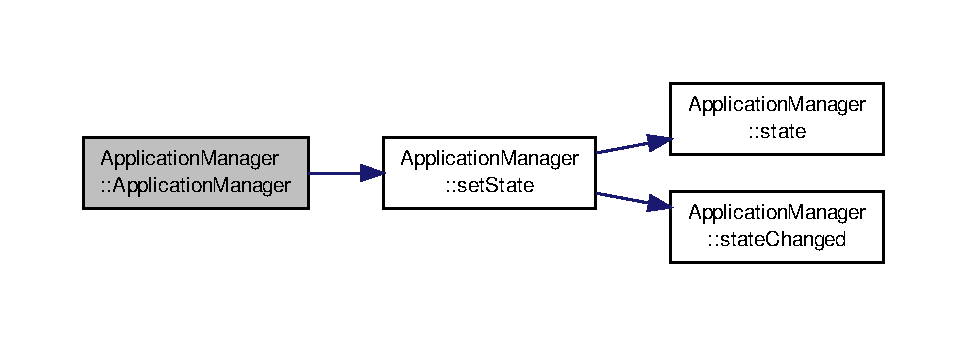
\includegraphics[width=350pt]{class_application_manager_a879feb4ed324b2f0c381e2cf377fe56d_cgraph}
\end{center}
\end{figure}


\hypertarget{class_application_manager_a05a04d6e3834adf031606133bbee313d}{\index{Application\-Manager@{Application\-Manager}!$\sim$\-Application\-Manager@{$\sim$\-Application\-Manager}}
\index{$\sim$\-Application\-Manager@{$\sim$\-Application\-Manager}!ApplicationManager@{Application\-Manager}}
\subsubsection[{$\sim$\-Application\-Manager}]{\setlength{\rightskip}{0pt plus 5cm}Application\-Manager\-::$\sim$\-Application\-Manager (
\begin{DoxyParamCaption}
{}
\end{DoxyParamCaption}
)\hspace{0.3cm}{\ttfamily [virtual]}}}\label{class_application_manager_a05a04d6e3834adf031606133bbee313d}


Definicja w linii 27 pliku applicationmanager.\-cpp.



\subsection{Dokumentacja funkcji składowych}
\hypertarget{class_application_manager_af1a9357249748e88cdbbcb994d8a7fe0}{\index{Application\-Manager@{Application\-Manager}!apply\-Clicked@{apply\-Clicked}}
\index{apply\-Clicked@{apply\-Clicked}!ApplicationManager@{Application\-Manager}}
\subsubsection[{apply\-Clicked}]{\setlength{\rightskip}{0pt plus 5cm}void Application\-Manager\-::apply\-Clicked (
\begin{DoxyParamCaption}
\item[{Q\-Variant\-List}]{methods\-Chosen}
\end{DoxyParamCaption}
)\hspace{0.3cm}{\ttfamily [slot]}}}\label{class_application_manager_af1a9357249748e88cdbbcb994d8a7fe0}


Definicja w linii 70 pliku applicationmanager.\-cpp.



Oto graf wywołań dla tej funkcji\-:\nopagebreak
\begin{figure}[H]
\begin{center}
\leavevmode
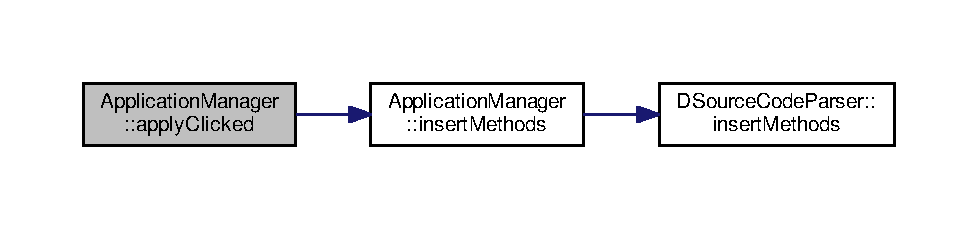
\includegraphics[width=350pt]{class_application_manager_af1a9357249748e88cdbbcb994d8a7fe0_cgraph}
\end{center}
\end{figure}


\hypertarget{class_application_manager_abbab98616d4848114b4338c8accedef2}{\index{Application\-Manager@{Application\-Manager}!file\-Opened@{file\-Opened}}
\index{file\-Opened@{file\-Opened}!ApplicationManager@{Application\-Manager}}
\subsubsection[{file\-Opened}]{\setlength{\rightskip}{0pt plus 5cm}void Application\-Manager\-::file\-Opened (
\begin{DoxyParamCaption}
\item[{Q\-String}]{path}
\end{DoxyParamCaption}
)\hspace{0.3cm}{\ttfamily [slot]}}}\label{class_application_manager_abbab98616d4848114b4338c8accedef2}


Definicja w linii 52 pliku applicationmanager.\-cpp.



Oto graf wywołań dla tej funkcji\-:\nopagebreak
\begin{figure}[H]
\begin{center}
\leavevmode
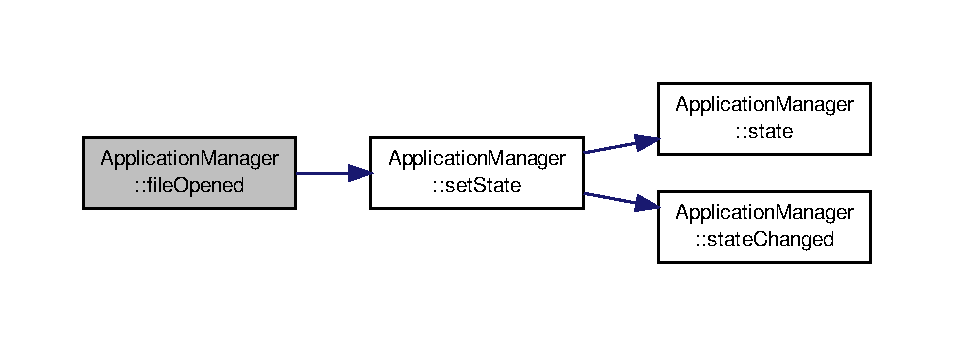
\includegraphics[width=350pt]{class_application_manager_abbab98616d4848114b4338c8accedef2_cgraph}
\end{center}
\end{figure}


\hypertarget{class_application_manager_ace0c5e4596d968278acd0b61042472d2}{\index{Application\-Manager@{Application\-Manager}!insert\-Methods@{insert\-Methods}}
\index{insert\-Methods@{insert\-Methods}!ApplicationManager@{Application\-Manager}}
\subsubsection[{insert\-Methods}]{\setlength{\rightskip}{0pt plus 5cm}void Application\-Manager\-::insert\-Methods (
\begin{DoxyParamCaption}
\item[{F\-I\-D\-Mapping$<$ {\bf Registers\-\_\-x86} $>$}]{Map}
\end{DoxyParamCaption}
)\hspace{0.3cm}{\ttfamily [slot]}}}\label{class_application_manager_ace0c5e4596d968278acd0b61042472d2}


Definicja w linii 90 pliku applicationmanager.\-cpp.



Oto graf wywołań dla tej funkcji\-:\nopagebreak
\begin{figure}[H]
\begin{center}
\leavevmode
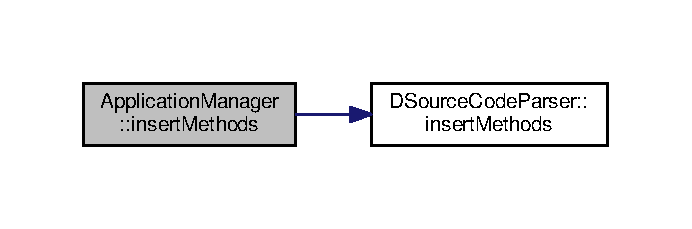
\includegraphics[width=328pt]{class_application_manager_ace0c5e4596d968278acd0b61042472d2_cgraph}
\end{center}
\end{figure}


\hypertarget{class_application_manager_ade160ce272f9e98dd59250b399ec1b82}{\index{Application\-Manager@{Application\-Manager}!path\-Changed@{path\-Changed}}
\index{path\-Changed@{path\-Changed}!ApplicationManager@{Application\-Manager}}
\subsubsection[{path\-Changed}]{\setlength{\rightskip}{0pt plus 5cm}void Application\-Manager\-::path\-Changed (
\begin{DoxyParamCaption}
{}
\end{DoxyParamCaption}
)\hspace{0.3cm}{\ttfamily [signal]}}}\label{class_application_manager_ade160ce272f9e98dd59250b399ec1b82}
\hypertarget{class_application_manager_a9923f3e608544e9e74d604a6018c9ae1}{\index{Application\-Manager@{Application\-Manager}!set\-State@{set\-State}}
\index{set\-State@{set\-State}!ApplicationManager@{Application\-Manager}}
\subsubsection[{set\-State}]{\setlength{\rightskip}{0pt plus 5cm}void Application\-Manager\-::set\-State (
\begin{DoxyParamCaption}
\item[{{\bf Application\-Manager\-::\-State}}]{state}
\end{DoxyParamCaption}
)}}\label{class_application_manager_a9923f3e608544e9e74d604a6018c9ae1}


Definicja w linii 32 pliku applicationmanager.\-cpp.



Oto graf wywołań dla tej funkcji\-:\nopagebreak
\begin{figure}[H]
\begin{center}
\leavevmode
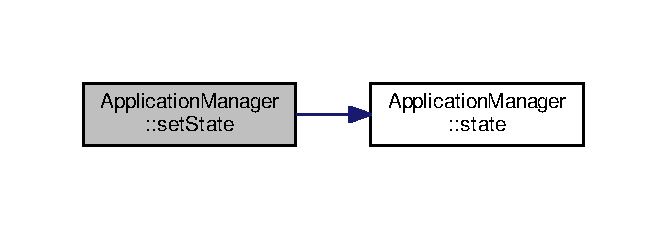
\includegraphics[width=320pt]{class_application_manager_a9923f3e608544e9e74d604a6018c9ae1_cgraph}
\end{center}
\end{figure}


\hypertarget{class_application_manager_aa86515d8c95bae5d713033e75becdf3c}{\index{Application\-Manager@{Application\-Manager}!state@{state}}
\index{state@{state}!ApplicationManager@{Application\-Manager}}
\subsubsection[{state}]{\setlength{\rightskip}{0pt plus 5cm}{\bf State} Application\-Manager\-::state (
\begin{DoxyParamCaption}
{}
\end{DoxyParamCaption}
) const}}\label{class_application_manager_aa86515d8c95bae5d713033e75becdf3c}
\hypertarget{class_application_manager_a0c10f4864788ee7e13730eae75d8c910}{\index{Application\-Manager@{Application\-Manager}!state\-Changed@{state\-Changed}}
\index{state\-Changed@{state\-Changed}!ApplicationManager@{Application\-Manager}}
\subsubsection[{state\-Changed}]{\setlength{\rightskip}{0pt plus 5cm}void Application\-Manager\-::state\-Changed (
\begin{DoxyParamCaption}
\item[{{\bf State}}]{}
\end{DoxyParamCaption}
)\hspace{0.3cm}{\ttfamily [signal]}}}\label{class_application_manager_a0c10f4864788ee7e13730eae75d8c910}
\hypertarget{class_application_manager_a793af100a8c392337bb94fc1f81c4d9a}{\index{Application\-Manager@{Application\-Manager}!x86\-Methods\-Names@{x86\-Methods\-Names}}
\index{x86\-Methods\-Names@{x86\-Methods\-Names}!ApplicationManager@{Application\-Manager}}
\subsubsection[{x86\-Methods\-Names}]{\setlength{\rightskip}{0pt plus 5cm}Q\-Variant\-List Application\-Manager\-::x86\-Methods\-Names (
\begin{DoxyParamCaption}
{}
\end{DoxyParamCaption}
)}}\label{class_application_manager_a793af100a8c392337bb94fc1f81c4d9a}
\hypertarget{class_application_manager_ac64a4e874ce1d4452d37f3b2ce996cda}{\index{Application\-Manager@{Application\-Manager}!x86\-Methods\-Names\-Changed@{x86\-Methods\-Names\-Changed}}
\index{x86\-Methods\-Names\-Changed@{x86\-Methods\-Names\-Changed}!ApplicationManager@{Application\-Manager}}
\subsubsection[{x86\-Methods\-Names\-Changed}]{\setlength{\rightskip}{0pt plus 5cm}void Application\-Manager\-::x86\-Methods\-Names\-Changed (
\begin{DoxyParamCaption}
{}
\end{DoxyParamCaption}
)\hspace{0.3cm}{\ttfamily [signal]}}}\label{class_application_manager_ac64a4e874ce1d4452d37f3b2ce996cda}


\subsection{Dokumentacja właściwości}
\hypertarget{class_application_manager_a930a84127f404aa07e142c5b37dfe128}{\index{Application\-Manager@{Application\-Manager}!state@{state}}
\index{state@{state}!ApplicationManager@{Application\-Manager}}
\subsubsection[{state}]{\setlength{\rightskip}{0pt plus 5cm}{\bf Application\-Manager\-::\-State} Application\-Manager\-::state\hspace{0.3cm}{\ttfamily [read]}, {\ttfamily [write]}}}\label{class_application_manager_a930a84127f404aa07e142c5b37dfe128}


Definicja w linii 17 pliku applicationmanager.\-h.

\hypertarget{class_application_manager_a04d639af3af2e31840e42bfe72f99a0c}{\index{Application\-Manager@{Application\-Manager}!x86\-Methods\-Names@{x86\-Methods\-Names}}
\index{x86\-Methods\-Names@{x86\-Methods\-Names}!ApplicationManager@{Application\-Manager}}
\subsubsection[{x86\-Methods\-Names}]{\setlength{\rightskip}{0pt plus 5cm}Q\-Variant\-List Application\-Manager\-::x86\-Methods\-Names\hspace{0.3cm}{\ttfamily [read]}}}\label{class_application_manager_a04d639af3af2e31840e42bfe72f99a0c}


Definicja w linii 18 pliku applicationmanager.\-h.



Dokumentacja dla tej klasy została wygenerowana z plików\-:\begin{DoxyCompactItemize}
\item 
Application\-Manager/\hyperlink{applicationmanager_8h}{applicationmanager.\-h}\item 
Application\-Manager/\hyperlink{applicationmanager_8cpp}{applicationmanager.\-cpp}\end{DoxyCompactItemize}

\hypertarget{class_asm_code_generator}{\section{Dokumentacja klasy Asm\-Code\-Generator}
\label{class_asm_code_generator}\index{Asm\-Code\-Generator@{Asm\-Code\-Generator}}
}


{\ttfamily \#include $<$daddingmethods.\-h$>$}

\subsection*{Metody publiczne}
\begin{DoxyCompactItemize}
\item 
\hyperlink{class_asm_code_generator_ae10580c9dd3ea1e0de47a50ad92143ea}{Asm\-Code\-Generator} ()
\end{DoxyCompactItemize}
\subsection*{Statyczne metody publiczne}
\begin{DoxyCompactItemize}
\item 
{\footnotesize template$<$typename Registers\-Type $>$ }\\static Q\-String \hyperlink{class_asm_code_generator_a76f8c73f9210eb61a8001c017c0cd4f1}{push\-\_\-regs} (const Registers\-Type reg)
\item 
{\footnotesize template$<$typename Registers\-Type $>$ }\\static Q\-String \hyperlink{class_asm_code_generator_a25ee0b50bb215502d9b61a753086f184}{push\-\_\-regs} (const Q\-List$<$ Registers\-Type $>$ \&regs)
\item 
{\footnotesize template$<$typename Registers\-Type $>$ }\\static Q\-String \hyperlink{class_asm_code_generator_a75bbaa5a9453e6997afdfa14e9471362}{pop\-\_\-regs} (const Registers\-Type reg)
\item 
{\footnotesize template$<$typename Registers\-Type $>$ }\\static Q\-String \hyperlink{class_asm_code_generator_aaed0677c22b8a46586286483ed11f205}{pop\-\_\-regs} (const Q\-List$<$ Registers\-Type $>$ \&regs)
\item 
{\footnotesize template$<$typename Registers\-Type $>$ }\\static Q\-String \hyperlink{class_asm_code_generator_a955d06de335abb5491727e690bb4cc85}{mov\-\_\-reg\-\_\-const} (const Registers\-Type reg, \hyperlink{elf_8h_aeed51d08e3a950d637f8ec1f0cd4ef65}{Elf64\-\_\-\-Addr} value)
\item 
{\footnotesize template$<$typename Registers\-Type $>$ }\\static Q\-String \hyperlink{class_asm_code_generator_ac196b01980e9de00bf6854baed99a1a2}{jmp\-\_\-reg} (const Registers\-Type reg)
\item 
{\footnotesize template$<$typename Registers\-Type $>$ }\\static Q\-String \hyperlink{class_asm_code_generator_ab578154f2a3d0ef023c8f6a302a3f565}{get\-\_\-reg} (const Registers\-Type reg)
\item 
{\footnotesize template$<$typename Registers\-Type $>$ }\\static Q\-String \hyperlink{class_asm_code_generator_a3bf9daed908df41eeec6031db9de2aae}{call\-\_\-reg} (const Registers\-Type)
\item 
static Q\-String \hyperlink{class_asm_code_generator_aa4989922344c4dc9ccfa937508915c3d}{call\-\_\-const} (\hyperlink{elf_8h_aeed51d08e3a950d637f8ec1f0cd4ef65}{Elf64\-\_\-\-Addr} value)
\end{DoxyCompactItemize}
\subsection*{Typy prywatne}
\begin{DoxyCompactItemize}
\item 
enum \hyperlink{class_asm_code_generator_a975bb037f383eb14e8f21acc7c4cd9a8}{Instructions} \{ \\*
\hyperlink{class_asm_code_generator_a975bb037f383eb14e8f21acc7c4cd9a8aefdb39a4c7286afcecf0e8a7435fce6a}{Instructions\-::\-P\-O\-P}, 
\hyperlink{class_asm_code_generator_a975bb037f383eb14e8f21acc7c4cd9a8a73dabe4437725eedc05a1824a2c31550}{Instructions\-::\-P\-U\-S\-H}, 
\hyperlink{class_asm_code_generator_a975bb037f383eb14e8f21acc7c4cd9a8a17b32100aef1fc19670be7fd58bc85df}{Instructions\-::\-M\-O\-V}, 
\hyperlink{class_asm_code_generator_a975bb037f383eb14e8f21acc7c4cd9a8a152b9af76a9e7dd95d9da277b69fdd95}{Instructions\-::\-J\-M\-P}, 
\\*
\hyperlink{class_asm_code_generator_a975bb037f383eb14e8f21acc7c4cd9a8aca3547acb9162b49fb4a6594ed9b3030}{Instructions\-::\-C\-A\-L\-L}
 \}
\end{DoxyCompactItemize}
\subsection*{Statyczne atrybuty prywatne}
\begin{DoxyCompactItemize}
\item 
static const Q\-Map\\*
$<$ \hyperlink{codedefines_8h_a0f84efe4ca4d99203713a78bd6e8c82e}{Registers\-\_\-x86}, Q\-String $>$ \hyperlink{class_asm_code_generator_a112155891be9747ebf0dd45301031053}{regs\-\_\-x86}
\item 
static const Q\-Map\\*
$<$ \hyperlink{codedefines_8h_a5e15b5c4d766f6faf29b5bcec37bde5c}{Registers\-\_\-x64}, Q\-String $>$ \hyperlink{class_asm_code_generator_ab87fdfb10a73e4a7e684b644722408a8}{regs\-\_\-x64}
\item 
static const Q\-Map\\*
$<$ \hyperlink{class_asm_code_generator_a975bb037f383eb14e8f21acc7c4cd9a8}{Instructions}, Q\-String $>$ \hyperlink{class_asm_code_generator_ab017616dbde9a998807080cbc0bff89a}{instructions}
\end{DoxyCompactItemize}


\subsection{Opis szczegółowy}


Definicja w linii 276 pliku daddingmethods.\-h.



\subsection{Dokumentacja składowych wyliczanych}
\hypertarget{class_asm_code_generator_a975bb037f383eb14e8f21acc7c4cd9a8}{\index{Asm\-Code\-Generator@{Asm\-Code\-Generator}!Instructions@{Instructions}}
\index{Instructions@{Instructions}!AsmCodeGenerator@{Asm\-Code\-Generator}}
\subsubsection[{Instructions}]{\setlength{\rightskip}{0pt plus 5cm}enum {\bf Asm\-Code\-Generator\-::\-Instructions}\hspace{0.3cm}{\ttfamily [strong]}, {\ttfamily [private]}}}\label{class_asm_code_generator_a975bb037f383eb14e8f21acc7c4cd9a8}
\begin{Desc}
\item[Wartości wyliczeń]\par
\begin{description}
\index{P\-O\-P@{P\-O\-P}!Asm\-Code\-Generator@{Asm\-Code\-Generator}}\index{Asm\-Code\-Generator@{Asm\-Code\-Generator}!P\-O\-P@{P\-O\-P}}\item[{\em 
\hypertarget{class_asm_code_generator_a975bb037f383eb14e8f21acc7c4cd9a8aefdb39a4c7286afcecf0e8a7435fce6a}{P\-O\-P}\label{class_asm_code_generator_a975bb037f383eb14e8f21acc7c4cd9a8aefdb39a4c7286afcecf0e8a7435fce6a}
}]\index{P\-U\-S\-H@{P\-U\-S\-H}!Asm\-Code\-Generator@{Asm\-Code\-Generator}}\index{Asm\-Code\-Generator@{Asm\-Code\-Generator}!P\-U\-S\-H@{P\-U\-S\-H}}\item[{\em 
\hypertarget{class_asm_code_generator_a975bb037f383eb14e8f21acc7c4cd9a8a73dabe4437725eedc05a1824a2c31550}{P\-U\-S\-H}\label{class_asm_code_generator_a975bb037f383eb14e8f21acc7c4cd9a8a73dabe4437725eedc05a1824a2c31550}
}]\index{M\-O\-V@{M\-O\-V}!Asm\-Code\-Generator@{Asm\-Code\-Generator}}\index{Asm\-Code\-Generator@{Asm\-Code\-Generator}!M\-O\-V@{M\-O\-V}}\item[{\em 
\hypertarget{class_asm_code_generator_a975bb037f383eb14e8f21acc7c4cd9a8a17b32100aef1fc19670be7fd58bc85df}{M\-O\-V}\label{class_asm_code_generator_a975bb037f383eb14e8f21acc7c4cd9a8a17b32100aef1fc19670be7fd58bc85df}
}]\index{J\-M\-P@{J\-M\-P}!Asm\-Code\-Generator@{Asm\-Code\-Generator}}\index{Asm\-Code\-Generator@{Asm\-Code\-Generator}!J\-M\-P@{J\-M\-P}}\item[{\em 
\hypertarget{class_asm_code_generator_a975bb037f383eb14e8f21acc7c4cd9a8a152b9af76a9e7dd95d9da277b69fdd95}{J\-M\-P}\label{class_asm_code_generator_a975bb037f383eb14e8f21acc7c4cd9a8a152b9af76a9e7dd95d9da277b69fdd95}
}]\index{C\-A\-L\-L@{C\-A\-L\-L}!Asm\-Code\-Generator@{Asm\-Code\-Generator}}\index{Asm\-Code\-Generator@{Asm\-Code\-Generator}!C\-A\-L\-L@{C\-A\-L\-L}}\item[{\em 
\hypertarget{class_asm_code_generator_a975bb037f383eb14e8f21acc7c4cd9a8aca3547acb9162b49fb4a6594ed9b3030}{C\-A\-L\-L}\label{class_asm_code_generator_a975bb037f383eb14e8f21acc7c4cd9a8aca3547acb9162b49fb4a6594ed9b3030}
}]\end{description}
\end{Desc}


Definicja w linii 280 pliku daddingmethods.\-h.



\subsection{Dokumentacja konstruktora i destruktora}
\hypertarget{class_asm_code_generator_ae10580c9dd3ea1e0de47a50ad92143ea}{\index{Asm\-Code\-Generator@{Asm\-Code\-Generator}!Asm\-Code\-Generator@{Asm\-Code\-Generator}}
\index{Asm\-Code\-Generator@{Asm\-Code\-Generator}!AsmCodeGenerator@{Asm\-Code\-Generator}}
\subsubsection[{Asm\-Code\-Generator}]{\setlength{\rightskip}{0pt plus 5cm}Asm\-Code\-Generator\-::\-Asm\-Code\-Generator (
\begin{DoxyParamCaption}
{}
\end{DoxyParamCaption}
)\hspace{0.3cm}{\ttfamily [inline]}}}\label{class_asm_code_generator_ae10580c9dd3ea1e0de47a50ad92143ea}


Definicja w linii 291 pliku daddingmethods.\-h.



\subsection{Dokumentacja funkcji składowych}
\hypertarget{class_asm_code_generator_aa4989922344c4dc9ccfa937508915c3d}{\index{Asm\-Code\-Generator@{Asm\-Code\-Generator}!call\-\_\-const@{call\-\_\-const}}
\index{call\-\_\-const@{call\-\_\-const}!AsmCodeGenerator@{Asm\-Code\-Generator}}
\subsubsection[{call\-\_\-const}]{\setlength{\rightskip}{0pt plus 5cm}static Q\-String Asm\-Code\-Generator\-::call\-\_\-const (
\begin{DoxyParamCaption}
\item[{{\bf Elf64\-\_\-\-Addr}}]{value}
\end{DoxyParamCaption}
)\hspace{0.3cm}{\ttfamily [inline]}, {\ttfamily [static]}}}\label{class_asm_code_generator_aa4989922344c4dc9ccfa937508915c3d}


Definicja w linii 317 pliku daddingmethods.\-h.

\hypertarget{class_asm_code_generator_a3bf9daed908df41eeec6031db9de2aae}{\index{Asm\-Code\-Generator@{Asm\-Code\-Generator}!call\-\_\-reg@{call\-\_\-reg}}
\index{call\-\_\-reg@{call\-\_\-reg}!AsmCodeGenerator@{Asm\-Code\-Generator}}
\subsubsection[{call\-\_\-reg}]{\setlength{\rightskip}{0pt plus 5cm}template$<$typename Registers\-Type $>$ Q\-String Asm\-Code\-Generator\-::call\-\_\-reg (
\begin{DoxyParamCaption}
\item[{const Registers\-Type}]{reg}
\end{DoxyParamCaption}
)\hspace{0.3cm}{\ttfamily [static]}}}\label{class_asm_code_generator_a3bf9daed908df41eeec6031db9de2aae}


Definicja w linii 395 pliku daddingmethods.\-h.

\hypertarget{class_asm_code_generator_ab578154f2a3d0ef023c8f6a302a3f565}{\index{Asm\-Code\-Generator@{Asm\-Code\-Generator}!get\-\_\-reg@{get\-\_\-reg}}
\index{get\-\_\-reg@{get\-\_\-reg}!AsmCodeGenerator@{Asm\-Code\-Generator}}
\subsubsection[{get\-\_\-reg}]{\setlength{\rightskip}{0pt plus 5cm}template$<$typename Registers\-Type $>$ Q\-String Asm\-Code\-Generator\-::get\-\_\-reg (
\begin{DoxyParamCaption}
\item[{const Registers\-Type}]{reg}
\end{DoxyParamCaption}
)\hspace{0.3cm}{\ttfamily [static]}}}\label{class_asm_code_generator_ab578154f2a3d0ef023c8f6a302a3f565}


Definicja w linii 387 pliku daddingmethods.\-h.

\hypertarget{class_asm_code_generator_ac196b01980e9de00bf6854baed99a1a2}{\index{Asm\-Code\-Generator@{Asm\-Code\-Generator}!jmp\-\_\-reg@{jmp\-\_\-reg}}
\index{jmp\-\_\-reg@{jmp\-\_\-reg}!AsmCodeGenerator@{Asm\-Code\-Generator}}
\subsubsection[{jmp\-\_\-reg}]{\setlength{\rightskip}{0pt plus 5cm}template$<$typename Registers\-Type $>$ Q\-String Asm\-Code\-Generator\-::jmp\-\_\-reg (
\begin{DoxyParamCaption}
\item[{const Registers\-Type}]{reg}
\end{DoxyParamCaption}
)\hspace{0.3cm}{\ttfamily [static]}}}\label{class_asm_code_generator_ac196b01980e9de00bf6854baed99a1a2}


Definicja w linii 378 pliku daddingmethods.\-h.

\hypertarget{class_asm_code_generator_a955d06de335abb5491727e690bb4cc85}{\index{Asm\-Code\-Generator@{Asm\-Code\-Generator}!mov\-\_\-reg\-\_\-const@{mov\-\_\-reg\-\_\-const}}
\index{mov\-\_\-reg\-\_\-const@{mov\-\_\-reg\-\_\-const}!AsmCodeGenerator@{Asm\-Code\-Generator}}
\subsubsection[{mov\-\_\-reg\-\_\-const}]{\setlength{\rightskip}{0pt plus 5cm}template$<$typename Registers\-Type $>$ Q\-String Asm\-Code\-Generator\-::mov\-\_\-reg\-\_\-const (
\begin{DoxyParamCaption}
\item[{const Registers\-Type}]{reg, }
\item[{{\bf Elf64\-\_\-\-Addr}}]{value}
\end{DoxyParamCaption}
)\hspace{0.3cm}{\ttfamily [static]}}}\label{class_asm_code_generator_a955d06de335abb5491727e690bb4cc85}


Definicja w linii 369 pliku daddingmethods.\-h.

\hypertarget{class_asm_code_generator_a75bbaa5a9453e6997afdfa14e9471362}{\index{Asm\-Code\-Generator@{Asm\-Code\-Generator}!pop\-\_\-regs@{pop\-\_\-regs}}
\index{pop\-\_\-regs@{pop\-\_\-regs}!AsmCodeGenerator@{Asm\-Code\-Generator}}
\subsubsection[{pop\-\_\-regs}]{\setlength{\rightskip}{0pt plus 5cm}template$<$typename Registers\-Type $>$ Q\-String Asm\-Code\-Generator\-::pop\-\_\-regs (
\begin{DoxyParamCaption}
\item[{const Registers\-Type}]{reg}
\end{DoxyParamCaption}
)\hspace{0.3cm}{\ttfamily [static]}}}\label{class_asm_code_generator_a75bbaa5a9453e6997afdfa14e9471362}


Definicja w linii 346 pliku daddingmethods.\-h.

\hypertarget{class_asm_code_generator_aaed0677c22b8a46586286483ed11f205}{\index{Asm\-Code\-Generator@{Asm\-Code\-Generator}!pop\-\_\-regs@{pop\-\_\-regs}}
\index{pop\-\_\-regs@{pop\-\_\-regs}!AsmCodeGenerator@{Asm\-Code\-Generator}}
\subsubsection[{pop\-\_\-regs}]{\setlength{\rightskip}{0pt plus 5cm}template$<$typename Registers\-Type $>$ Q\-String Asm\-Code\-Generator\-::pop\-\_\-regs (
\begin{DoxyParamCaption}
\item[{const Q\-List$<$ Registers\-Type $>$ \&}]{regs}
\end{DoxyParamCaption}
)\hspace{0.3cm}{\ttfamily [static]}}}\label{class_asm_code_generator_aaed0677c22b8a46586286483ed11f205}


Definicja w linii 355 pliku daddingmethods.\-h.

\hypertarget{class_asm_code_generator_a76f8c73f9210eb61a8001c017c0cd4f1}{\index{Asm\-Code\-Generator@{Asm\-Code\-Generator}!push\-\_\-regs@{push\-\_\-regs}}
\index{push\-\_\-regs@{push\-\_\-regs}!AsmCodeGenerator@{Asm\-Code\-Generator}}
\subsubsection[{push\-\_\-regs}]{\setlength{\rightskip}{0pt plus 5cm}template$<$typename Registers\-Type $>$ Q\-String Asm\-Code\-Generator\-::push\-\_\-regs (
\begin{DoxyParamCaption}
\item[{const Registers\-Type}]{reg}
\end{DoxyParamCaption}
)\hspace{0.3cm}{\ttfamily [static]}}}\label{class_asm_code_generator_a76f8c73f9210eb61a8001c017c0cd4f1}


Definicja w linii 323 pliku daddingmethods.\-h.

\hypertarget{class_asm_code_generator_a25ee0b50bb215502d9b61a753086f184}{\index{Asm\-Code\-Generator@{Asm\-Code\-Generator}!push\-\_\-regs@{push\-\_\-regs}}
\index{push\-\_\-regs@{push\-\_\-regs}!AsmCodeGenerator@{Asm\-Code\-Generator}}
\subsubsection[{push\-\_\-regs}]{\setlength{\rightskip}{0pt plus 5cm}template$<$typename Registers\-Type $>$ Q\-String Asm\-Code\-Generator\-::push\-\_\-regs (
\begin{DoxyParamCaption}
\item[{const Q\-List$<$ Registers\-Type $>$ \&}]{regs}
\end{DoxyParamCaption}
)\hspace{0.3cm}{\ttfamily [static]}}}\label{class_asm_code_generator_a25ee0b50bb215502d9b61a753086f184}


Definicja w linii 332 pliku daddingmethods.\-h.



\subsection{Dokumentacja atrybutów składowych}
\hypertarget{class_asm_code_generator_ab017616dbde9a998807080cbc0bff89a}{\index{Asm\-Code\-Generator@{Asm\-Code\-Generator}!instructions@{instructions}}
\index{instructions@{instructions}!AsmCodeGenerator@{Asm\-Code\-Generator}}
\subsubsection[{instructions}]{\setlength{\rightskip}{0pt plus 5cm}const Q\-Map$<$ {\bf Asm\-Code\-Generator\-::\-Instructions}, Q\-String $>$ Asm\-Code\-Generator\-::instructions\hspace{0.3cm}{\ttfamily [static]}, {\ttfamily [private]}}}\label{class_asm_code_generator_ab017616dbde9a998807080cbc0bff89a}
{\bfseries Wartość początkowa\-:}
\begin{DoxyCode}
= \{
    \{ \hyperlink{class_asm_code_generator_a975bb037f383eb14e8f21acc7c4cd9a8aefdb39a4c7286afcecf0e8a7435fce6a}{AsmCodeGenerator::Instructions::POP} , 
      \hyperlink{daddingmethods_8h_a2dffee0b2992c6276c96aaa4ca719a21}{instruction\_stringify}(\hyperlink{class_asm_code_generator_a975bb037f383eb14e8f21acc7c4cd9a8aefdb39a4c7286afcecf0e8a7435fce6a}{AsmCodeGenerator::Instructions::POP}
      )  \},
    \{ \hyperlink{class_asm_code_generator_a975bb037f383eb14e8f21acc7c4cd9a8a73dabe4437725eedc05a1824a2c31550}{AsmCodeGenerator::Instructions::PUSH}, 
      \hyperlink{daddingmethods_8h_a2dffee0b2992c6276c96aaa4ca719a21}{instruction\_stringify}(\hyperlink{class_asm_code_generator_a975bb037f383eb14e8f21acc7c4cd9a8a73dabe4437725eedc05a1824a2c31550}{AsmCodeGenerator::Instructions::PUSH}
      ) \},
    \{ \hyperlink{class_asm_code_generator_a975bb037f383eb14e8f21acc7c4cd9a8a17b32100aef1fc19670be7fd58bc85df}{AsmCodeGenerator::Instructions::MOV},  
      \hyperlink{daddingmethods_8h_a2dffee0b2992c6276c96aaa4ca719a21}{instruction\_stringify}(\hyperlink{class_asm_code_generator_a975bb037f383eb14e8f21acc7c4cd9a8a17b32100aef1fc19670be7fd58bc85df}{AsmCodeGenerator::Instructions::MOV}
      )  \},
    \{ \hyperlink{class_asm_code_generator_a975bb037f383eb14e8f21acc7c4cd9a8a152b9af76a9e7dd95d9da277b69fdd95}{AsmCodeGenerator::Instructions::JMP},  
      \hyperlink{daddingmethods_8h_a2dffee0b2992c6276c96aaa4ca719a21}{instruction\_stringify}(\hyperlink{class_asm_code_generator_a975bb037f383eb14e8f21acc7c4cd9a8a152b9af76a9e7dd95d9da277b69fdd95}{AsmCodeGenerator::Instructions::JMP}
      )  \},
    \{ \hyperlink{class_asm_code_generator_a975bb037f383eb14e8f21acc7c4cd9a8aca3547acb9162b49fb4a6594ed9b3030}{AsmCodeGenerator::Instructions::CALL}, 
      \hyperlink{daddingmethods_8h_a2dffee0b2992c6276c96aaa4ca719a21}{instruction\_stringify}(\hyperlink{class_asm_code_generator_a975bb037f383eb14e8f21acc7c4cd9a8aca3547acb9162b49fb4a6594ed9b3030}{AsmCodeGenerator::Instructions::CALL}
      ) \}
\}
\end{DoxyCode}


Definicja w linii 288 pliku daddingmethods.\-h.

\hypertarget{class_asm_code_generator_ab87fdfb10a73e4a7e684b644722408a8}{\index{Asm\-Code\-Generator@{Asm\-Code\-Generator}!regs\-\_\-x64@{regs\-\_\-x64}}
\index{regs\-\_\-x64@{regs\-\_\-x64}!AsmCodeGenerator@{Asm\-Code\-Generator}}
\subsubsection[{regs\-\_\-x64}]{\setlength{\rightskip}{0pt plus 5cm}const Q\-Map$<$ {\bf Registers\-\_\-x64}, Q\-String $>$ Asm\-Code\-Generator\-::regs\-\_\-x64\hspace{0.3cm}{\ttfamily [static]}, {\ttfamily [private]}}}\label{class_asm_code_generator_ab87fdfb10a73e4a7e684b644722408a8}
{\bfseries Wartość początkowa\-:}
\begin{DoxyCode}
= \{
    \{ \hyperlink{codedefines_8h_a5e15b5c4d766f6faf29b5bcec37bde5ca8fc0fe1771a6ed962d18efbf01d9dd48}{Registers\_x64::RAX}, \hyperlink{daddingmethods_8h_a9cdaa38dc2ea9f97e7169c4a05ab0ede}{enum\_stringify}(
      \hyperlink{codedefines_8h_a5e15b5c4d766f6faf29b5bcec37bde5ca8fc0fe1771a6ed962d18efbf01d9dd48}{Registers\_x64::RAX}) \},
    \{ \hyperlink{codedefines_8h_a5e15b5c4d766f6faf29b5bcec37bde5ca72ced42981685c31ff7fa40b1f0ddd0a}{Registers\_x64::RBX}, \hyperlink{daddingmethods_8h_a9cdaa38dc2ea9f97e7169c4a05ab0ede}{enum\_stringify}(
      \hyperlink{codedefines_8h_a5e15b5c4d766f6faf29b5bcec37bde5ca72ced42981685c31ff7fa40b1f0ddd0a}{Registers\_x64::RBX}) \},
    \{ \hyperlink{codedefines_8h_a5e15b5c4d766f6faf29b5bcec37bde5ca5a6e47f019d213b226a4cb39ea6412c6}{Registers\_x64::RCX}, \hyperlink{daddingmethods_8h_a9cdaa38dc2ea9f97e7169c4a05ab0ede}{enum\_stringify}(
      \hyperlink{codedefines_8h_a5e15b5c4d766f6faf29b5bcec37bde5ca5a6e47f019d213b226a4cb39ea6412c6}{Registers\_x64::RCX}) \},
    \{ \hyperlink{codedefines_8h_a5e15b5c4d766f6faf29b5bcec37bde5ca43851ae6bcf8f6822ed0efc897f72f8f}{Registers\_x64::RDX}, \hyperlink{daddingmethods_8h_a9cdaa38dc2ea9f97e7169c4a05ab0ede}{enum\_stringify}(
      \hyperlink{codedefines_8h_a5e15b5c4d766f6faf29b5bcec37bde5ca43851ae6bcf8f6822ed0efc897f72f8f}{Registers\_x64::RDX}) \},
    \{ \hyperlink{codedefines_8h_a5e15b5c4d766f6faf29b5bcec37bde5ca9cad85e1268a524c7041cb9a311d964c}{Registers\_x64::RDI}, \hyperlink{daddingmethods_8h_a9cdaa38dc2ea9f97e7169c4a05ab0ede}{enum\_stringify}(
      \hyperlink{codedefines_8h_a5e15b5c4d766f6faf29b5bcec37bde5ca9cad85e1268a524c7041cb9a311d964c}{Registers\_x64::RDI}) \},
    \{ \hyperlink{codedefines_8h_a5e15b5c4d766f6faf29b5bcec37bde5ca643f8aeac63ad74266191eb6da0b09e9}{Registers\_x64::RSI}, \hyperlink{daddingmethods_8h_a9cdaa38dc2ea9f97e7169c4a05ab0ede}{enum\_stringify}(
      \hyperlink{codedefines_8h_a5e15b5c4d766f6faf29b5bcec37bde5ca643f8aeac63ad74266191eb6da0b09e9}{Registers\_x64::RSI}) \},
    \{ \hyperlink{codedefines_8h_a5e15b5c4d766f6faf29b5bcec37bde5ca17118bd8650bc1964a540d1d1ddcea93}{Registers\_x64::RBP}, \hyperlink{daddingmethods_8h_a9cdaa38dc2ea9f97e7169c4a05ab0ede}{enum\_stringify}(
      \hyperlink{codedefines_8h_a5e15b5c4d766f6faf29b5bcec37bde5ca17118bd8650bc1964a540d1d1ddcea93}{Registers\_x64::RBP}) \},
    \{ \hyperlink{codedefines_8h_a5e15b5c4d766f6faf29b5bcec37bde5ca39b097df341e30b1ba206babdba89ea1}{Registers\_x64::RSP}, \hyperlink{daddingmethods_8h_a9cdaa38dc2ea9f97e7169c4a05ab0ede}{enum\_stringify}(
      \hyperlink{codedefines_8h_a5e15b5c4d766f6faf29b5bcec37bde5ca39b097df341e30b1ba206babdba89ea1}{Registers\_x64::RSP}) \},
    \{ \hyperlink{codedefines_8h_a5e15b5c4d766f6faf29b5bcec37bde5cacfff813d86d447fa2a9c858650ebbb90}{Registers\_x64::R8} , \hyperlink{daddingmethods_8h_a9cdaa38dc2ea9f97e7169c4a05ab0ede}{enum\_stringify}(
      \hyperlink{codedefines_8h_a5e15b5c4d766f6faf29b5bcec37bde5cacfff813d86d447fa2a9c858650ebbb90}{Registers\_x64::R8})  \},
    \{ \hyperlink{codedefines_8h_a5e15b5c4d766f6faf29b5bcec37bde5ca8d28dad91e1ffada38203b9e5f9af86d}{Registers\_x64::R9} , \hyperlink{daddingmethods_8h_a9cdaa38dc2ea9f97e7169c4a05ab0ede}{enum\_stringify}(
      \hyperlink{codedefines_8h_a5e15b5c4d766f6faf29b5bcec37bde5ca8d28dad91e1ffada38203b9e5f9af86d}{Registers\_x64::R9})  \},
    \{ \hyperlink{codedefines_8h_a5e15b5c4d766f6faf29b5bcec37bde5ca33df7d5541bc0941336b1513815da7a5}{Registers\_x64::R10}, \hyperlink{daddingmethods_8h_a9cdaa38dc2ea9f97e7169c4a05ab0ede}{enum\_stringify}(
      \hyperlink{codedefines_8h_a5e15b5c4d766f6faf29b5bcec37bde5ca33df7d5541bc0941336b1513815da7a5}{Registers\_x64::R10}) \},
    \{ \hyperlink{codedefines_8h_a5e15b5c4d766f6faf29b5bcec37bde5ca7f6711cf763cf8d5648cb4fd0c3790df}{Registers\_x64::R11}, \hyperlink{daddingmethods_8h_a9cdaa38dc2ea9f97e7169c4a05ab0ede}{enum\_stringify}(
      \hyperlink{codedefines_8h_a5e15b5c4d766f6faf29b5bcec37bde5ca7f6711cf763cf8d5648cb4fd0c3790df}{Registers\_x64::R11}) \},
    \{ \hyperlink{codedefines_8h_a5e15b5c4d766f6faf29b5bcec37bde5ca1688316d15ac9218146e0f4ba5fc8d4f}{Registers\_x64::R12}, \hyperlink{daddingmethods_8h_a9cdaa38dc2ea9f97e7169c4a05ab0ede}{enum\_stringify}(
      \hyperlink{codedefines_8h_a5e15b5c4d766f6faf29b5bcec37bde5ca1688316d15ac9218146e0f4ba5fc8d4f}{Registers\_x64::R12}) \},
    \{ \hyperlink{codedefines_8h_a5e15b5c4d766f6faf29b5bcec37bde5ca503400c0ff4077a9ca69db92b6709274}{Registers\_x64::R13}, \hyperlink{daddingmethods_8h_a9cdaa38dc2ea9f97e7169c4a05ab0ede}{enum\_stringify}(
      \hyperlink{codedefines_8h_a5e15b5c4d766f6faf29b5bcec37bde5ca503400c0ff4077a9ca69db92b6709274}{Registers\_x64::R13}) \},
    \{ \hyperlink{codedefines_8h_a5e15b5c4d766f6faf29b5bcec37bde5ca05e151e78b54177fc4d64d35b94429bf}{Registers\_x64::R14}, \hyperlink{daddingmethods_8h_a9cdaa38dc2ea9f97e7169c4a05ab0ede}{enum\_stringify}(
      \hyperlink{codedefines_8h_a5e15b5c4d766f6faf29b5bcec37bde5ca05e151e78b54177fc4d64d35b94429bf}{Registers\_x64::R14}) \},
    \{ \hyperlink{codedefines_8h_a5e15b5c4d766f6faf29b5bcec37bde5ca2d15b084feece054417b9159559cf893}{Registers\_x64::R15}, \hyperlink{daddingmethods_8h_a9cdaa38dc2ea9f97e7169c4a05ab0ede}{enum\_stringify}(
      \hyperlink{codedefines_8h_a5e15b5c4d766f6faf29b5bcec37bde5ca2d15b084feece054417b9159559cf893}{Registers\_x64::R15}) \}
\}
\end{DoxyCode}


Definicja w linii 278 pliku daddingmethods.\-h.

\hypertarget{class_asm_code_generator_a112155891be9747ebf0dd45301031053}{\index{Asm\-Code\-Generator@{Asm\-Code\-Generator}!regs\-\_\-x86@{regs\-\_\-x86}}
\index{regs\-\_\-x86@{regs\-\_\-x86}!AsmCodeGenerator@{Asm\-Code\-Generator}}
\subsubsection[{regs\-\_\-x86}]{\setlength{\rightskip}{0pt plus 5cm}const Q\-Map$<$ {\bf Registers\-\_\-x86}, Q\-String $>$ Asm\-Code\-Generator\-::regs\-\_\-x86\hspace{0.3cm}{\ttfamily [static]}, {\ttfamily [private]}}}\label{class_asm_code_generator_a112155891be9747ebf0dd45301031053}
{\bfseries Wartość początkowa\-:}
\begin{DoxyCode}
= \{
    \{ \hyperlink{codedefines_8h_a0f84efe4ca4d99203713a78bd6e8c82eaeee994d8f3b3c70335763b9a4a2caeb1}{Registers\_x86::EAX}, \hyperlink{daddingmethods_8h_a9cdaa38dc2ea9f97e7169c4a05ab0ede}{enum\_stringify}(
      \hyperlink{codedefines_8h_a0f84efe4ca4d99203713a78bd6e8c82eaeee994d8f3b3c70335763b9a4a2caeb1}{Registers\_x86::EAX}) \},
    \{ \hyperlink{codedefines_8h_a0f84efe4ca4d99203713a78bd6e8c82ea89d5f2c300bc5e8df2b587981e9f83ae}{Registers\_x86::EBX}, \hyperlink{daddingmethods_8h_a9cdaa38dc2ea9f97e7169c4a05ab0ede}{enum\_stringify}(
      \hyperlink{codedefines_8h_a0f84efe4ca4d99203713a78bd6e8c82ea89d5f2c300bc5e8df2b587981e9f83ae}{Registers\_x86::EBX}) \},
    \{ \hyperlink{codedefines_8h_a0f84efe4ca4d99203713a78bd6e8c82eaf4f316d9e3af74567e781129ce9b384c}{Registers\_x86::ECX}, \hyperlink{daddingmethods_8h_a9cdaa38dc2ea9f97e7169c4a05ab0ede}{enum\_stringify}(
      \hyperlink{codedefines_8h_a0f84efe4ca4d99203713a78bd6e8c82eaf4f316d9e3af74567e781129ce9b384c}{Registers\_x86::ECX}) \},
    \{ \hyperlink{codedefines_8h_a0f84efe4ca4d99203713a78bd6e8c82ea22b5dc1e93a77a0361aaf220517c1fa1}{Registers\_x86::EDX}, \hyperlink{daddingmethods_8h_a9cdaa38dc2ea9f97e7169c4a05ab0ede}{enum\_stringify}(
      \hyperlink{codedefines_8h_a0f84efe4ca4d99203713a78bd6e8c82ea22b5dc1e93a77a0361aaf220517c1fa1}{Registers\_x86::EDX}) \},
    \{ \hyperlink{codedefines_8h_a0f84efe4ca4d99203713a78bd6e8c82ea4d2e27158ca5f1c109c99624b7ee9092}{Registers\_x86::EDI}, \hyperlink{daddingmethods_8h_a9cdaa38dc2ea9f97e7169c4a05ab0ede}{enum\_stringify}(
      \hyperlink{codedefines_8h_a0f84efe4ca4d99203713a78bd6e8c82ea4d2e27158ca5f1c109c99624b7ee9092}{Registers\_x86::EDI}) \},
    \{ \hyperlink{codedefines_8h_a0f84efe4ca4d99203713a78bd6e8c82ea4e7627e030290994aff0ced165dbfc7b}{Registers\_x86::EBP}, \hyperlink{daddingmethods_8h_a9cdaa38dc2ea9f97e7169c4a05ab0ede}{enum\_stringify}(
      \hyperlink{codedefines_8h_a0f84efe4ca4d99203713a78bd6e8c82ea4e7627e030290994aff0ced165dbfc7b}{Registers\_x86::EBP}) \},
    \{ \hyperlink{codedefines_8h_a0f84efe4ca4d99203713a78bd6e8c82eadd445edb9c3b702b74855e30f795ad4e}{Registers\_x86::ESI}, \hyperlink{daddingmethods_8h_a9cdaa38dc2ea9f97e7169c4a05ab0ede}{enum\_stringify}(
      \hyperlink{codedefines_8h_a0f84efe4ca4d99203713a78bd6e8c82eadd445edb9c3b702b74855e30f795ad4e}{Registers\_x86::ESI}) \},
    \{ \hyperlink{codedefines_8h_a0f84efe4ca4d99203713a78bd6e8c82ea3e30ce90c5b1d89ae09b7d4c73d8e172}{Registers\_x86::ESP}, \hyperlink{daddingmethods_8h_a9cdaa38dc2ea9f97e7169c4a05ab0ede}{enum\_stringify}(
      \hyperlink{codedefines_8h_a0f84efe4ca4d99203713a78bd6e8c82ea3e30ce90c5b1d89ae09b7d4c73d8e172}{Registers\_x86::ESP}) \}
\}
\end{DoxyCode}


Definicja w linii 277 pliku daddingmethods.\-h.



Dokumentacja dla tej klasy została wygenerowana z plików\-:\begin{DoxyCompactItemize}
\item 
core/adding\-\_\-methods/wrappers/\hyperlink{daddingmethods_8h}{daddingmethods.\-h}\item 
core/adding\-\_\-methods/wrappers/\hyperlink{daddingmethods_8cpp}{daddingmethods.\-cpp}\end{DoxyCompactItemize}

\hypertarget{class_binary_code}{\section{Dokumentacja szablonu klasy Binary\-Code$<$ Register $>$}
\label{class_binary_code}\index{Binary\-Code$<$ Register $>$@{Binary\-Code$<$ Register $>$}}
}


Klasa przechowująca kod binarny i offsety relokacji adresów.  




{\ttfamily \#include $<$codedefines.\-h$>$}

\subsection*{Metody publiczne}
\begin{DoxyCompactItemize}
\item 
\hyperlink{class_binary_code_aa21721fc16b2e943be048fa3ceea300d}{Binary\-Code} ()
\begin{DoxyCompactList}\small\item\em \hyperlink{class_binary_code}{Binary\-Code} -\/ Konstruktor. \end{DoxyCompactList}\item 
void \hyperlink{class_binary_code_a5f06f08736f891d6bc6d2d4fc93dca21}{append} (Q\-Byte\-Array \-\_\-code, bool relocation=false)
\begin{DoxyCompactList}\small\item\em Dodaje kod do tablicy. \end{DoxyCompactList}\item 
Q\-Byte\-Array \hyperlink{class_binary_code_a0b9f52a511f1ba6989412d4424885f8f}{get\-Bytes} ()
\begin{DoxyCompactList}\small\item\em Pobiera kod. \end{DoxyCompactList}\item 
Q\-List$<$ uint64\-\_\-t $>$ \hyperlink{class_binary_code_a16f19ea25857126aeaeb7993890a5ad3}{get\-Relocations} (uint64\-\_\-t code\-Base)
\begin{DoxyCompactList}\small\item\em Pobiera tablicę relokacji jako wartości absolutne. \end{DoxyCompactList}\item 
int \hyperlink{class_binary_code_a08ecf07ca01749c097929dc394871e6e}{length} ()
\begin{DoxyCompactList}\small\item\em Metoda pobierająca wielkość kodu. \end{DoxyCompactList}\end{DoxyCompactItemize}
\subsection*{Metody prywatne}
\begin{DoxyCompactItemize}
\item 
{\footnotesize template$<$$>$ }\\const uint8\-\_\-t \hyperlink{class_binary_code_a61d31942270e2200c91333f5b4717c35}{addr\-Size}
\item 
{\footnotesize template$<$$>$ }\\const uint8\-\_\-t \hyperlink{class_binary_code_a55498c908569d84e505b5eda3301c08f}{addr\-Size}
\end{DoxyCompactItemize}
\subsection*{Atrybuty prywatne}
\begin{DoxyCompactItemize}
\item 
Q\-Byte\-Array \hyperlink{class_binary_code_aa680c4ee3718fe9c7998b3ab072fc01a}{code}
\begin{DoxyCompactList}\small\item\em Kod binarny. \end{DoxyCompactList}\item 
Q\-List$<$ uint64\-\_\-t $>$ \hyperlink{class_binary_code_a1816cae03a267887d41a56c6421c0d2d}{relocations}
\begin{DoxyCompactList}\small\item\em Lista offsetów relokacji. \end{DoxyCompactList}\end{DoxyCompactItemize}
\subsection*{Statyczne atrybuty prywatne}
\begin{DoxyCompactItemize}
\item 
static const uint8\-\_\-t \hyperlink{class_binary_code_a1e49b1b07e4062b2be95de92c757f783}{addr\-Size}
\begin{DoxyCompactList}\small\item\em Rozmiar adresu. \end{DoxyCompactList}\end{DoxyCompactItemize}


\subsection{Opis szczegółowy}
\subsubsection*{template$<$typename Register$>$class Binary\-Code$<$ Register $>$}

Klasa przechowująca kod binarny i offsety relokacji adresów. 

Definicja w linii 55 pliku codedefines.\-h.



\subsection{Dokumentacja konstruktora i destruktora}
\hypertarget{class_binary_code_aa21721fc16b2e943be048fa3ceea300d}{\index{Binary\-Code@{Binary\-Code}!Binary\-Code@{Binary\-Code}}
\index{Binary\-Code@{Binary\-Code}!BinaryCode@{Binary\-Code}}
\subsubsection[{Binary\-Code}]{\setlength{\rightskip}{0pt plus 5cm}template$<$typename Register$>$ {\bf Binary\-Code}$<$ Register $>$\-::{\bf Binary\-Code} (
\begin{DoxyParamCaption}
{}
\end{DoxyParamCaption}
)\hspace{0.3cm}{\ttfamily [inline]}}}\label{class_binary_code_aa21721fc16b2e943be048fa3ceea300d}


\hyperlink{class_binary_code}{Binary\-Code} -\/ Konstruktor. 



Definicja w linii 77 pliku codedefines.\-h.



\subsection{Dokumentacja funkcji składowych}
\hypertarget{class_binary_code_a61d31942270e2200c91333f5b4717c35}{\index{Binary\-Code@{Binary\-Code}!addr\-Size@{addr\-Size}}
\index{addr\-Size@{addr\-Size}!BinaryCode@{Binary\-Code}}
\subsubsection[{addr\-Size}]{\setlength{\rightskip}{0pt plus 5cm}template$<$$>$ const uint8\-\_\-t {\bf Binary\-Code}$<$ {\bf Registers\-\_\-x86} $>$\-::addr\-Size (
\begin{DoxyParamCaption}
{}
\end{DoxyParamCaption}
)\hspace{0.3cm}{\ttfamily [private]}}}\label{class_binary_code_a61d31942270e2200c91333f5b4717c35}


Definicja w linii 756 pliku codedefines.\-cpp.

\hypertarget{class_binary_code_a55498c908569d84e505b5eda3301c08f}{\index{Binary\-Code@{Binary\-Code}!addr\-Size@{addr\-Size}}
\index{addr\-Size@{addr\-Size}!BinaryCode@{Binary\-Code}}
\subsubsection[{addr\-Size}]{\setlength{\rightskip}{0pt plus 5cm}template$<$$>$ const uint8\-\_\-t {\bf Binary\-Code}$<$ {\bf Registers\-\_\-x64} $>$\-::addr\-Size (
\begin{DoxyParamCaption}
{}
\end{DoxyParamCaption}
)\hspace{0.3cm}{\ttfamily [private]}}}\label{class_binary_code_a55498c908569d84e505b5eda3301c08f}


Definicja w linii 760 pliku codedefines.\-cpp.

\hypertarget{class_binary_code_a5f06f08736f891d6bc6d2d4fc93dca21}{\index{Binary\-Code@{Binary\-Code}!append@{append}}
\index{append@{append}!BinaryCode@{Binary\-Code}}
\subsubsection[{append}]{\setlength{\rightskip}{0pt plus 5cm}template$<$typename Register $>$ template void {\bf Binary\-Code}$<$ Register $>$\-::append (
\begin{DoxyParamCaption}
\item[{Q\-Byte\-Array}]{\-\_\-code, }
\item[{bool}]{relocation = {\ttfamily false}}
\end{DoxyParamCaption}
)}}\label{class_binary_code_a5f06f08736f891d6bc6d2d4fc93dca21}


Dodaje kod do tablicy. 


\begin{DoxyParams}{Parametry}
{\em \-\_\-code} & Kod binarny \\
\hline
{\em relocation} & Flaga odpowiadająca za dodanie informacji o relokacji w miejscu dodanego kodu. \\
\hline
\end{DoxyParams}


Definicja w linii 721 pliku codedefines.\-cpp.



Oto graf wywoływań tej funkcji\-:
\nopagebreak
\begin{figure}[H]
\begin{center}
\leavevmode
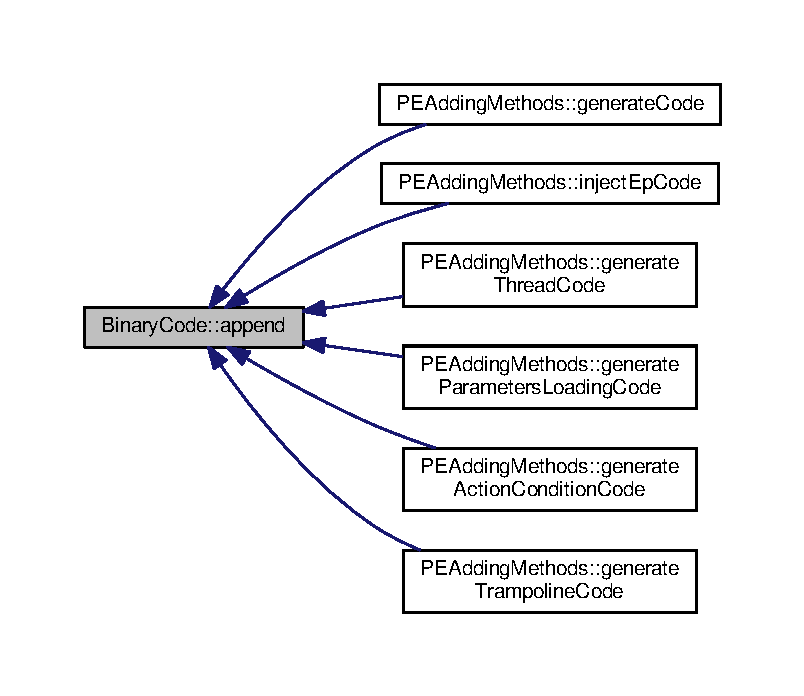
\includegraphics[width=350pt]{class_binary_code_a5f06f08736f891d6bc6d2d4fc93dca21_icgraph}
\end{center}
\end{figure}


\hypertarget{class_binary_code_a0b9f52a511f1ba6989412d4424885f8f}{\index{Binary\-Code@{Binary\-Code}!get\-Bytes@{get\-Bytes}}
\index{get\-Bytes@{get\-Bytes}!BinaryCode@{Binary\-Code}}
\subsubsection[{get\-Bytes}]{\setlength{\rightskip}{0pt plus 5cm}template$<$typename Register $>$ template Q\-Byte\-Array {\bf Binary\-Code}$<$ Register $>$\-::get\-Bytes (
\begin{DoxyParamCaption}
{}
\end{DoxyParamCaption}
)}}\label{class_binary_code_a0b9f52a511f1ba6989412d4424885f8f}


Pobiera kod. 

\begin{DoxyReturn}{Zwraca}
Kod binarny 
\end{DoxyReturn}


Definicja w linii 712 pliku codedefines.\-cpp.



Oto graf wywoływań tej funkcji\-:
\nopagebreak
\begin{figure}[H]
\begin{center}
\leavevmode
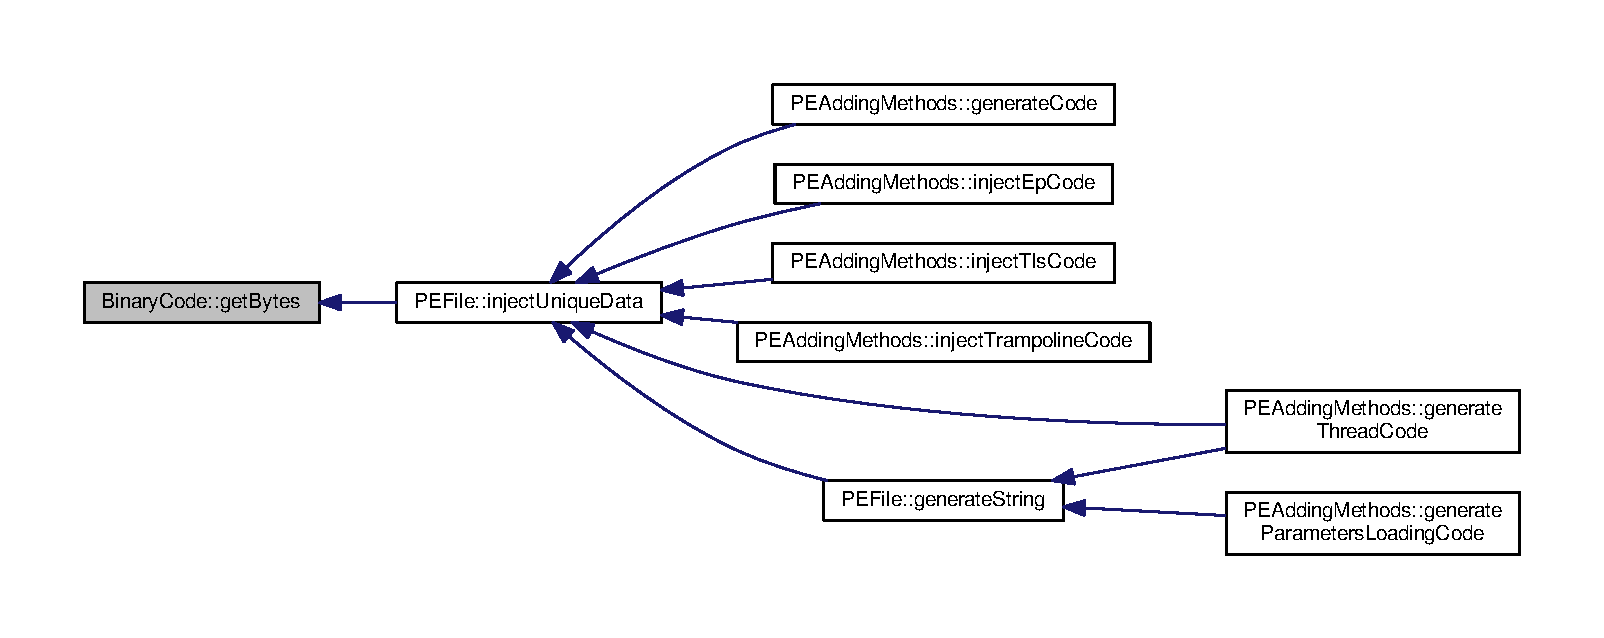
\includegraphics[width=350pt]{class_binary_code_a0b9f52a511f1ba6989412d4424885f8f_icgraph}
\end{center}
\end{figure}


\hypertarget{class_binary_code_a16f19ea25857126aeaeb7993890a5ad3}{\index{Binary\-Code@{Binary\-Code}!get\-Relocations@{get\-Relocations}}
\index{get\-Relocations@{get\-Relocations}!BinaryCode@{Binary\-Code}}
\subsubsection[{get\-Relocations}]{\setlength{\rightskip}{0pt plus 5cm}template$<$typename Register $>$ template Q\-List$<$ uint64\-\_\-t $>$ {\bf Binary\-Code}$<$ Register $>$\-::get\-Relocations (
\begin{DoxyParamCaption}
\item[{uint64\-\_\-t}]{code\-Base}
\end{DoxyParamCaption}
)}}\label{class_binary_code_a16f19ea25857126aeaeb7993890a5ad3}


Pobiera tablicę relokacji jako wartości absolutne. 


\begin{DoxyParams}{Parametry}
{\em code\-Base} & Adres bazowy relokowanego kodu \\
\hline
\end{DoxyParams}
\begin{DoxyReturn}{Zwraca}
Lista relokacji 
\end{DoxyReturn}


Definicja w linii 733 pliku codedefines.\-cpp.



Oto graf wywoływań tej funkcji\-:
\nopagebreak
\begin{figure}[H]
\begin{center}
\leavevmode
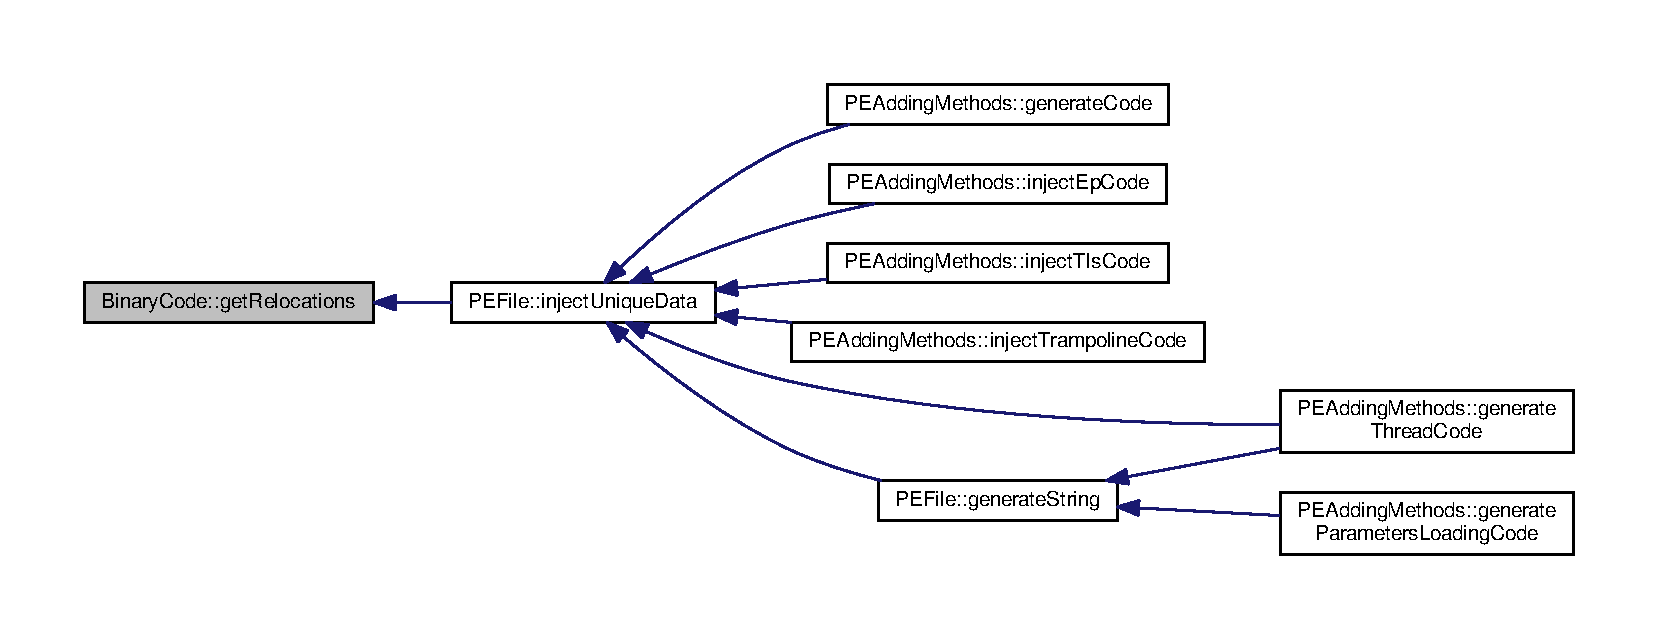
\includegraphics[width=350pt]{class_binary_code_a16f19ea25857126aeaeb7993890a5ad3_icgraph}
\end{center}
\end{figure}


\hypertarget{class_binary_code_a08ecf07ca01749c097929dc394871e6e}{\index{Binary\-Code@{Binary\-Code}!length@{length}}
\index{length@{length}!BinaryCode@{Binary\-Code}}
\subsubsection[{length}]{\setlength{\rightskip}{0pt plus 5cm}template$<$typename Register $>$ template int {\bf Binary\-Code}$<$ Register $>$\-::length (
\begin{DoxyParamCaption}
{}
\end{DoxyParamCaption}
)}}\label{class_binary_code_a08ecf07ca01749c097929dc394871e6e}


Metoda pobierająca wielkość kodu. 

\begin{DoxyReturn}{Zwraca}
Rozmiar kodu 
\end{DoxyReturn}


Definicja w linii 747 pliku codedefines.\-cpp.



Oto graf wywoływań tej funkcji\-:
\nopagebreak
\begin{figure}[H]
\begin{center}
\leavevmode
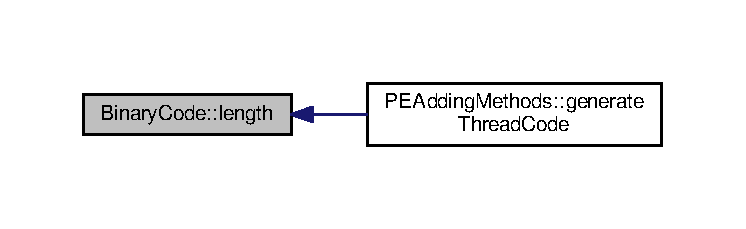
\includegraphics[width=350pt]{class_binary_code_a08ecf07ca01749c097929dc394871e6e_icgraph}
\end{center}
\end{figure}




\subsection{Dokumentacja atrybutów składowych}
\hypertarget{class_binary_code_a1e49b1b07e4062b2be95de92c757f783}{\index{Binary\-Code@{Binary\-Code}!addr\-Size@{addr\-Size}}
\index{addr\-Size@{addr\-Size}!BinaryCode@{Binary\-Code}}
\subsubsection[{addr\-Size}]{\setlength{\rightskip}{0pt plus 5cm}template$<$typename Register$>$ const uint8\-\_\-t {\bf Binary\-Code}$<$ Register $>$\-::addr\-Size\hspace{0.3cm}{\ttfamily [static]}, {\ttfamily [private]}}}\label{class_binary_code_a1e49b1b07e4062b2be95de92c757f783}


Rozmiar adresu. 



Definicja w linii 71 pliku codedefines.\-h.

\hypertarget{class_binary_code_aa680c4ee3718fe9c7998b3ab072fc01a}{\index{Binary\-Code@{Binary\-Code}!code@{code}}
\index{code@{code}!BinaryCode@{Binary\-Code}}
\subsubsection[{code}]{\setlength{\rightskip}{0pt plus 5cm}template$<$typename Register$>$ Q\-Byte\-Array {\bf Binary\-Code}$<$ Register $>$\-::code\hspace{0.3cm}{\ttfamily [private]}}}\label{class_binary_code_aa680c4ee3718fe9c7998b3ab072fc01a}


Kod binarny. 



Definicja w linii 61 pliku codedefines.\-h.

\hypertarget{class_binary_code_a1816cae03a267887d41a56c6421c0d2d}{\index{Binary\-Code@{Binary\-Code}!relocations@{relocations}}
\index{relocations@{relocations}!BinaryCode@{Binary\-Code}}
\subsubsection[{relocations}]{\setlength{\rightskip}{0pt plus 5cm}template$<$typename Register$>$ Q\-List$<$uint64\-\_\-t$>$ {\bf Binary\-Code}$<$ Register $>$\-::relocations\hspace{0.3cm}{\ttfamily [private]}}}\label{class_binary_code_a1816cae03a267887d41a56c6421c0d2d}


Lista offsetów relokacji. 



Definicja w linii 66 pliku codedefines.\-h.



Dokumentacja dla tej klasy została wygenerowana z plików\-:\begin{DoxyCompactItemize}
\item 
core/file\-\_\-types/\hyperlink{codedefines_8h}{codedefines.\-h}\item 
core/file\-\_\-types/\hyperlink{codedefines_8cpp}{codedefines.\-cpp}\end{DoxyCompactItemize}

\hypertarget{class_binary_file}{\section{Dokumentacja klasy Binary\-File}
\label{class_binary_file}\index{Binary\-File@{Binary\-File}}
}


{\ttfamily \#include $<$binaryfile.\-h$>$}



Diagram dziedziczenia dla Binary\-File
\nopagebreak
\begin{figure}[H]
\begin{center}
\leavevmode
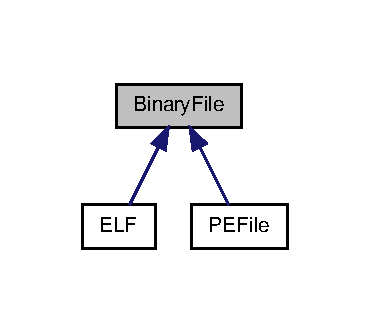
\includegraphics[width=179pt]{class_binary_file__inherit__graph}
\end{center}
\end{figure}
\subsection*{Metody publiczne}
\begin{DoxyCompactItemize}
\item 
\hyperlink{class_binary_file_a1afe5dffc5edf5f25ea22deef606eb4b}{Binary\-File} (Q\-Byte\-Array \-\_\-data)
\item 
virtual \hyperlink{class_binary_file_a8ff1b2e140421fd040bff0854c1322ff}{$\sim$\-Binary\-File} ()
\item 
virtual Q\-Byte\-Array \hyperlink{class_binary_file_a5ffee8a6230cf3c82cf6ee0e9fb53048}{get\-Data} ()
\begin{DoxyCompactList}\small\item\em Pobiera zawartość pliku binarnego. \end{DoxyCompactList}\item 
virtual bool \hyperlink{class_binary_file_a6007435bc4451bb80a3169d977f4f125}{is\-\_\-valid} () const =0
\begin{DoxyCompactList}\small\item\em Sprawdza czy w pamięci przechowywany jest poprawny plik. \end{DoxyCompactList}\item 
virtual bool \hyperlink{class_binary_file_a36b7998c72bbee68ab492d93368c14ca}{is\-\_\-x64} () const =0
\begin{DoxyCompactList}\small\item\em Metoda informująca czy wczytany plik jest 64-\/bitowy. \end{DoxyCompactList}\item 
virtual bool \hyperlink{class_binary_file_aa7d43cde4ab8cc9723d2b5c769719bd9}{is\-\_\-x86} () const =0
\begin{DoxyCompactList}\small\item\em Metoda informująca czy wczytany plik jest 32-\/bitowy. \end{DoxyCompactList}\end{DoxyCompactItemize}
\subsection*{Atrybuty chronione}
\begin{DoxyCompactItemize}
\item 
bool \hyperlink{class_binary_file_ae16774932979ddb6d57b46b3c387a159}{parsed}
\item 
Q\-Byte\-Array \hyperlink{class_binary_file_acdfdb2fae63d8395dfa899be21bd8036}{b\-\_\-data}
\end{DoxyCompactItemize}


\subsection{Opis szczegółowy}


Definicja w linii 6 pliku binaryfile.\-h.



\subsection{Dokumentacja konstruktora i destruktora}
\hypertarget{class_binary_file_a1afe5dffc5edf5f25ea22deef606eb4b}{\index{Binary\-File@{Binary\-File}!Binary\-File@{Binary\-File}}
\index{Binary\-File@{Binary\-File}!BinaryFile@{Binary\-File}}
\subsubsection[{Binary\-File}]{\setlength{\rightskip}{0pt plus 5cm}Binary\-File\-::\-Binary\-File (
\begin{DoxyParamCaption}
\item[{Q\-Byte\-Array}]{\-\_\-data}
\end{DoxyParamCaption}
)}}\label{class_binary_file_a1afe5dffc5edf5f25ea22deef606eb4b}


Definicja w linii 3 pliku binaryfile.\-cpp.

\hypertarget{class_binary_file_a8ff1b2e140421fd040bff0854c1322ff}{\index{Binary\-File@{Binary\-File}!$\sim$\-Binary\-File@{$\sim$\-Binary\-File}}
\index{$\sim$\-Binary\-File@{$\sim$\-Binary\-File}!BinaryFile@{Binary\-File}}
\subsubsection[{$\sim$\-Binary\-File}]{\setlength{\rightskip}{0pt plus 5cm}Binary\-File\-::$\sim$\-Binary\-File (
\begin{DoxyParamCaption}
{}
\end{DoxyParamCaption}
)\hspace{0.3cm}{\ttfamily [virtual]}}}\label{class_binary_file_a8ff1b2e140421fd040bff0854c1322ff}


Definicja w linii 10 pliku binaryfile.\-cpp.



\subsection{Dokumentacja funkcji składowych}
\hypertarget{class_binary_file_a5ffee8a6230cf3c82cf6ee0e9fb53048}{\index{Binary\-File@{Binary\-File}!get\-Data@{get\-Data}}
\index{get\-Data@{get\-Data}!BinaryFile@{Binary\-File}}
\subsubsection[{get\-Data}]{\setlength{\rightskip}{0pt plus 5cm}Q\-Byte\-Array Binary\-File\-::get\-Data (
\begin{DoxyParamCaption}
{}
\end{DoxyParamCaption}
)\hspace{0.3cm}{\ttfamily [virtual]}}}\label{class_binary_file_a5ffee8a6230cf3c82cf6ee0e9fb53048}


Pobiera zawartość pliku binarnego. 

\begin{DoxyReturn}{Zwraca}
Plik. 
\end{DoxyReturn}


Definicja w linii 15 pliku binaryfile.\-cpp.

\hypertarget{class_binary_file_a6007435bc4451bb80a3169d977f4f125}{\index{Binary\-File@{Binary\-File}!is\-\_\-valid@{is\-\_\-valid}}
\index{is\-\_\-valid@{is\-\_\-valid}!BinaryFile@{Binary\-File}}
\subsubsection[{is\-\_\-valid}]{\setlength{\rightskip}{0pt plus 5cm}virtual bool Binary\-File\-::is\-\_\-valid (
\begin{DoxyParamCaption}
{}
\end{DoxyParamCaption}
) const\hspace{0.3cm}{\ttfamily [pure virtual]}}}\label{class_binary_file_a6007435bc4451bb80a3169d977f4f125}


Sprawdza czy w pamięci przechowywany jest poprawny plik. 

\begin{DoxyReturn}{Zwraca}
True jeżeli plik jest poprawny. 
\end{DoxyReturn}


Implementowany w \hyperlink{class_p_e_file_a90a96d95f9d67ff48bf12ffcb0f22d41}{P\-E\-File} i \hyperlink{class_e_l_f_aaf0da9f62b61fc3674b7fd54d9885b5f}{E\-L\-F}.

\hypertarget{class_binary_file_a36b7998c72bbee68ab492d93368c14ca}{\index{Binary\-File@{Binary\-File}!is\-\_\-x64@{is\-\_\-x64}}
\index{is\-\_\-x64@{is\-\_\-x64}!BinaryFile@{Binary\-File}}
\subsubsection[{is\-\_\-x64}]{\setlength{\rightskip}{0pt plus 5cm}virtual bool Binary\-File\-::is\-\_\-x64 (
\begin{DoxyParamCaption}
{}
\end{DoxyParamCaption}
) const\hspace{0.3cm}{\ttfamily [pure virtual]}}}\label{class_binary_file_a36b7998c72bbee68ab492d93368c14ca}


Metoda informująca czy wczytany plik jest 64-\/bitowy. 

\begin{DoxyReturn}{Zwraca}
True gdy plik x64 
\end{DoxyReturn}


Implementowany w \hyperlink{class_p_e_file_aa8e69bdca4d00216df406278b4e96a28}{P\-E\-File} i \hyperlink{class_e_l_f_a558b2f169db21b21b24d6ff19c38ac9e}{E\-L\-F}.

\hypertarget{class_binary_file_aa7d43cde4ab8cc9723d2b5c769719bd9}{\index{Binary\-File@{Binary\-File}!is\-\_\-x86@{is\-\_\-x86}}
\index{is\-\_\-x86@{is\-\_\-x86}!BinaryFile@{Binary\-File}}
\subsubsection[{is\-\_\-x86}]{\setlength{\rightskip}{0pt plus 5cm}virtual bool Binary\-File\-::is\-\_\-x86 (
\begin{DoxyParamCaption}
{}
\end{DoxyParamCaption}
) const\hspace{0.3cm}{\ttfamily [pure virtual]}}}\label{class_binary_file_aa7d43cde4ab8cc9723d2b5c769719bd9}


Metoda informująca czy wczytany plik jest 32-\/bitowy. 

\begin{DoxyReturn}{Zwraca}
True gdy plik x86 
\end{DoxyReturn}


Implementowany w \hyperlink{class_p_e_file_a371cc84eed9dd5d85b7c50d60c1eb56f}{P\-E\-File} i \hyperlink{class_e_l_f_ac5c89b2b437f3e07aedc06f66cdab94d}{E\-L\-F}.



\subsection{Dokumentacja atrybutów składowych}
\hypertarget{class_binary_file_acdfdb2fae63d8395dfa899be21bd8036}{\index{Binary\-File@{Binary\-File}!b\-\_\-data@{b\-\_\-data}}
\index{b\-\_\-data@{b\-\_\-data}!BinaryFile@{Binary\-File}}
\subsubsection[{b\-\_\-data}]{\setlength{\rightskip}{0pt plus 5cm}Q\-Byte\-Array Binary\-File\-::b\-\_\-data\hspace{0.3cm}{\ttfamily [protected]}}}\label{class_binary_file_acdfdb2fae63d8395dfa899be21bd8036}


Definicja w linii 38 pliku binaryfile.\-h.

\hypertarget{class_binary_file_ae16774932979ddb6d57b46b3c387a159}{\index{Binary\-File@{Binary\-File}!parsed@{parsed}}
\index{parsed@{parsed}!BinaryFile@{Binary\-File}}
\subsubsection[{parsed}]{\setlength{\rightskip}{0pt plus 5cm}bool Binary\-File\-::parsed\hspace{0.3cm}{\ttfamily [protected]}}}\label{class_binary_file_ae16774932979ddb6d57b46b3c387a159}


Definicja w linii 37 pliku binaryfile.\-h.



Dokumentacja dla tej klasy została wygenerowana z plików\-:\begin{DoxyCompactItemize}
\item 
core/file\-\_\-types/\hyperlink{binaryfile_8h}{binaryfile.\-h}\item 
core/file\-\_\-types/\hyperlink{binaryfile_8cpp}{binaryfile.\-cpp}\end{DoxyCompactItemize}

\hypertarget{class_code_defines}{\section{Dokumentacja szablonu klasy Code\-Defines$<$ Register $>$}
\label{class_code_defines}\index{Code\-Defines$<$ Register $>$@{Code\-Defines$<$ Register $>$}}
}


Klasa definiująca sposób generowania kodu.  




{\ttfamily \#include $<$codedefines.\-h$>$}

\subsection*{Metody publiczne}
\begin{DoxyCompactItemize}
\item 
{\footnotesize template$<$$>$ }\\const uint8\-\_\-t \hyperlink{class_code_defines_a20358aed4dbfb9a22a8ecd61e482cfa1}{shadow\-Size}
\item 
{\footnotesize template$<$$>$ }\\const uint8\-\_\-t \hyperlink{class_code_defines_ac7974a0b7b8e7f307536800ac146359d}{align16\-Size}
\item 
{\footnotesize template$<$$>$ }\\const uint8\-\_\-t \hyperlink{class_code_defines_ae2a02505b45aae48ac8d2eb0ae014fe5}{align16\-Size}
\item 
{\footnotesize template$<$$>$ }\\const uint8\-\_\-t \hyperlink{class_code_defines_a4d91cad6a972b05bd4156cb00552f39e}{stack\-Cell\-Size}
\item 
{\footnotesize template$<$$>$ }\\const uint8\-\_\-t \hyperlink{class_code_defines_a770bb8bf2208da3fd8d758966c23511e}{stack\-Cell\-Size}
\item 
{\footnotesize template$<$$>$ }\\const Q\-Byte\-Array \hyperlink{class_code_defines_a5491865f96eec40ff6594702879b0fdb}{start\-Func}
\item 
{\footnotesize template$<$$>$ }\\const Q\-Byte\-Array \hyperlink{class_code_defines_a8691301353c7786113939b5aa5925f09}{start\-Func}
\item 
{\footnotesize template$<$$>$ }\\const Q\-List$<$ \hyperlink{codedefines_8h_a0f84efe4ca4d99203713a78bd6e8c82e}{Registers\-\_\-x86} $>$ \hyperlink{class_code_defines_accadab674c6c55403b54ffb679ccdf62}{internal\-Regs}
\item 
{\footnotesize template$<$$>$ }\\const Q\-List$<$ \hyperlink{codedefines_8h_a5e15b5c4d766f6faf29b5bcec37bde5c}{Registers\-\_\-x64} $>$ \hyperlink{class_code_defines_a0901fe2185ed5ffc391ee5c1e4a14b7a}{internal\-Regs}
\item 
{\footnotesize template$<$$>$ }\\const Q\-List$<$ \hyperlink{codedefines_8h_a0f84efe4ca4d99203713a78bd6e8c82e}{Registers\-\_\-x86} $>$ \hyperlink{class_code_defines_a01f343f93dc3aad78e7b83c1f4881588}{external\-Regs}
\item 
{\footnotesize template$<$$>$ }\\const Q\-List$<$ \hyperlink{codedefines_8h_a5e15b5c4d766f6faf29b5bcec37bde5c}{Registers\-\_\-x64} $>$ \hyperlink{class_code_defines_a3556bec0f430313c92ee805287cbb883}{external\-Regs}
\item 
{\footnotesize template$<$$>$ }\\Q\-Byte\-Array \hyperlink{class_code_defines_aaccf2aa728b76b96a6959ef8bfd03739}{mov\-Value\-To\-Reg} (uint32\-\_\-t value, \hyperlink{codedefines_8h_a0f84efe4ca4d99203713a78bd6e8c82e}{Registers\-\_\-x86} reg)
\item 
{\footnotesize template$<$$>$ }\\Q\-Byte\-Array \hyperlink{class_code_defines_aafe7e312fbb95b53f89435d37cf278fb}{mov\-Value\-To\-Reg} (uint64\-\_\-t value, \hyperlink{codedefines_8h_a5e15b5c4d766f6faf29b5bcec37bde5c}{Registers\-\_\-x64} reg)
\item 
{\footnotesize template$<$$>$ }\\Q\-Byte\-Array \hyperlink{class_code_defines_ae4db2d1e5a428a4c9ec5972a380159de}{mov\-Value\-To\-Reg} (uint64\-\_\-t value, \hyperlink{codedefines_8h_a0f84efe4ca4d99203713a78bd6e8c82e}{Registers\-\_\-x86} reg)
\item 
{\footnotesize template$<$$>$ }\\Q\-Byte\-Array \hyperlink{class_code_defines_a40157c99b0f396b77cd6d7dc8f80071d}{store\-Value} (uint32\-\_\-t value)
\item 
{\footnotesize template$<$$>$ }\\Q\-Byte\-Array \hyperlink{class_code_defines_a964f09310db04f127c7684a8c24ae58e}{store\-Value} (uint64\-\_\-t value)
\item 
{\footnotesize template$<$$>$ }\\Q\-Byte\-Array \hyperlink{class_code_defines_a9258c95f68116611b02378bd60212111}{save\-All} ()
\item 
{\footnotesize template$<$$>$ }\\Q\-Byte\-Array \hyperlink{class_code_defines_aa4e9c15c2613d1d628f7c11f674c46ea}{save\-All} ()
\item 
{\footnotesize template$<$$>$ }\\Q\-Byte\-Array \hyperlink{class_code_defines_ae77aeeb9e9d40dde299fb17ee3cca269}{restore\-All} ()
\item 
{\footnotesize template$<$$>$ }\\Q\-Byte\-Array \hyperlink{class_code_defines_a717d9ab10ffe0caaa17807133894cb06}{restore\-All} ()
\end{DoxyCompactItemize}
\subsection*{Statyczne metody publiczne}
\begin{DoxyCompactItemize}
\item 
static Q\-Byte\-Array \hyperlink{class_code_defines_a43a24be00649da7ebcaf172f515f43c7}{save\-Register} (Register reg)
\begin{DoxyCompactList}\small\item\em Metoda odpowiadająca instrukcji\-: push reg. \end{DoxyCompactList}\item 
static Q\-Byte\-Array \hyperlink{class_code_defines_a951d31c997529cea2553e7544598c505}{restore\-Register} (Register reg)
\begin{DoxyCompactList}\small\item\em Metoda odpowiadająca instrukcji\-: pop reg. \end{DoxyCompactList}\item 
{\footnotesize template$<$typename T $>$ }\\static Q\-Byte\-Array \hyperlink{class_code_defines_a968764a7855df79bf38a5049cf6bead4}{mov\-Value\-To\-Reg} (T value, Register reg)
\begin{DoxyCompactList}\small\item\em Metoda odpowiadająca instrukcji\-: mov reg, value. \end{DoxyCompactList}\item 
static Q\-Byte\-Array \hyperlink{class_code_defines_af702a87ffaa59e27f44ec8d9f1ff5ad0}{call\-Reg} (Register reg)
\begin{DoxyCompactList}\small\item\em Metoda odpowiadająca instrukcji\-: call reg. \end{DoxyCompactList}\item 
static Q\-Byte\-Array \hyperlink{class_code_defines_a51b4f9d160d76f39056cf5b7136b0a5a}{call\-Relative} (uint32\-\_\-t pos)
\begin{DoxyCompactList}\small\item\em Metoda odpowiadająca instrukcji\-: call offset. \end{DoxyCompactList}\item 
static Q\-Byte\-Array \hyperlink{class_code_defines_a5553e8054d6bb237d69a2393c6892484}{jmp\-Reg} (Register reg)
\begin{DoxyCompactList}\small\item\em Metoda odpowiadająca instrukcji\-: jmp reg. \end{DoxyCompactList}\item 
static Q\-Byte\-Array \hyperlink{class_code_defines_a97da0ebe2a72b85e4cf678cf07fec4e1}{test\-Reg} (Register reg)
\begin{DoxyCompactList}\small\item\em Metoda odpowiadająca instrukcji\-: test reg, reg. \end{DoxyCompactList}\item 
static Q\-Byte\-Array \hyperlink{class_code_defines_ad92e4b0ee88740626ad9e73b0b170a14}{jz\-Relative} (int8\-\_\-t pos)
\begin{DoxyCompactList}\small\item\em Metoda odpowiadająca instrukcji\-: jz offset. \end{DoxyCompactList}\item 
static Q\-Byte\-Array \hyperlink{class_code_defines_aff433a64828802d6500a26769b3696be}{jmp\-Relative} (int8\-\_\-t pos)
\begin{DoxyCompactList}\small\item\em Metoda odpowiadająca instrukcji\-: jmp offset. \end{DoxyCompactList}\item 
static Q\-Byte\-Array \hyperlink{class_code_defines_a03a66f6808af85b08ef4ed8777c29e5e}{save\-All\-Internal} ()
\begin{DoxyCompactList}\small\item\em Metoda odpowiadająca instrukcjom zapisania wszystkich wewnętrznych rejestrów na stos. \end{DoxyCompactList}\item 
static Q\-Byte\-Array \hyperlink{class_code_defines_abc7f95cd1e8764eca2532184e359f02c}{restore\-All\-Internal} ()
\begin{DoxyCompactList}\small\item\em Metoda odpowiadająca instrukcjom odczytu wszystkich wewnętrznych rejestrów ze stosu. \end{DoxyCompactList}\item 
static Q\-Byte\-Array \hyperlink{class_code_defines_a7e7d98d34774cfc4c064b708e90e106b}{reserve\-Stack\-Space} (uint16\-\_\-t no\-Params)
\begin{DoxyCompactList}\small\item\em Metoda odpowiadająca instrukcji\-: sub esp, no\-Params $\ast$ 4 / sub rsp, np\-Params $\ast$ 8. \end{DoxyCompactList}\item 
static Q\-Byte\-Array \hyperlink{class_code_defines_ad8345f54b25fe8d87e1cc11832832133}{clear\-Stack\-Space} (uint16\-\_\-t no\-Params)
\begin{DoxyCompactList}\small\item\em Metoda odpowiadająca instrukcji\-: add esp, no\-Params $\ast$ 4 / add rsp, np\-Params $\ast$ 8. \end{DoxyCompactList}\item 
{\footnotesize template$<$typename T $>$ }\\static Q\-Byte\-Array \hyperlink{class_code_defines_a8b8beae6895e7918b82c3c04e365e88d}{store\-Value} (T dword)
\begin{DoxyCompactList}\small\item\em Metoda odpowiadająca instrukcji\-: push value. \end{DoxyCompactList}\item 
static Q\-Byte\-Array \hyperlink{class_code_defines_a43ccdbbc575554bfe34c96d5d14232e5}{read\-From\-Esp\-Mem\-To\-Reg} (Register reg, int8\-\_\-t base)
\begin{DoxyCompactList}\small\item\em Metoda odpowiadająca instrukcji\-: mov reg, \mbox{[}esp + base\mbox{]}. \end{DoxyCompactList}\item 
static Q\-Byte\-Array \hyperlink{class_code_defines_af99c634779d7b27ec72fbd2fe15065c8}{read\-From\-Reg\-To\-Esp\-Mem} (Register reg, int8\-\_\-t base)
\begin{DoxyCompactList}\small\item\em Metoda odpowiadająca instrukcji\-: mov \mbox{[}esp + base\mbox{]}, reg. \end{DoxyCompactList}\item 
static Q\-Byte\-Array \hyperlink{class_code_defines_abff87050d31f5313af2f92f41c5aeba6}{ret\-N} (uint16\-\_\-t n)
\begin{DoxyCompactList}\small\item\em Metoda odpowiadająca instrukcji\-: ret n. \end{DoxyCompactList}\item 
static Q\-Byte\-Array \hyperlink{class_code_defines_ad2904023d0e1e87474da13edb453fb30}{save\-All} ()
\begin{DoxyCompactList}\small\item\em Zapisanie wszystkich rejestów na stosie. \end{DoxyCompactList}\item 
static Q\-Byte\-Array \hyperlink{class_code_defines_ab01a6ea78d9474c3e5d4cbf4414253d1}{restore\-All} ()
\begin{DoxyCompactList}\small\item\em Odczyt wszystkich rejestrów ze stosu. \end{DoxyCompactList}\end{DoxyCompactItemize}
\subsection*{Statyczne atrybuty publiczne}
\begin{DoxyCompactItemize}
\item 
static const Q\-Byte\-Array \hyperlink{class_code_defines_ab0339e357461e07258de4e77d0c73c5c}{start\-Func}
\begin{DoxyCompactList}\small\item\em Kod odpowiadający instrukcji\-: push ebp; mov ebp, esp;. \end{DoxyCompactList}\item 
static const Q\-Byte\-Array \hyperlink{class_code_defines_abb945f5e809b498405e0a91901c784e1}{end\-Func} = Q\-Byte\-Array(\char`\"{}\textbackslash{}x5\-D\char`\"{})
\begin{DoxyCompactList}\small\item\em Kod odpowiadający instrukcji\-: pop ebp. \end{DoxyCompactList}\item 
static const Q\-Byte\-Array \hyperlink{class_code_defines_ae8c1690d0a6fe53c81dea4c8cad6ca5c}{ret} = Q\-Byte\-Array(\char`\"{}\textbackslash{}x\-C3\char`\"{})
\begin{DoxyCompactList}\small\item\em Kod odpowiadający instrukcji\-: ret. \end{DoxyCompactList}\item 
static const Q\-List$<$ Register $>$ \hyperlink{class_code_defines_a71b60a174fc6190178fee7c552f52732}{internal\-Regs}
\begin{DoxyCompactList}\small\item\em Lista wewnętrznych rejestów. \end{DoxyCompactList}\item 
static const Q\-List$<$ Register $>$ \hyperlink{class_code_defines_a045622ec64ec17b4b8a2d55b854117c7}{external\-Regs}
\begin{DoxyCompactList}\small\item\em Lista zewnętrznych rejestrów. \end{DoxyCompactList}\item 
static const uint8\-\_\-t \hyperlink{class_code_defines_a89139a3f358c98200f78478fd0dd3bd9}{shadow\-Size}
\begin{DoxyCompactList}\small\item\em Rozmiar Shadow Space. \end{DoxyCompactList}\item 
static const uint8\-\_\-t \hyperlink{class_code_defines_a83820641d7045e035f2a4619a23d2755}{align16\-Size}
\begin{DoxyCompactList}\small\item\em Liczba bajtów potrzebna do wyrównania stosu do 16. \end{DoxyCompactList}\item 
static const uint8\-\_\-t \hyperlink{class_code_defines_add79526fe978503123140edf11497d66}{stack\-Cell\-Size}
\begin{DoxyCompactList}\small\item\em Rozmiar komórki stosu. \end{DoxyCompactList}\item 
static const Q\-Reg\-Exp \hyperlink{class_code_defines_a767cf243acab61bf7c6f1046002425e1}{new\-Line\-Reg\-Exp} = Q\-Reg\-Exp(\char`\"{}\mbox{[}\textbackslash{}r\textbackslash{}n\mbox{]}\char`\"{})
\begin{DoxyCompactList}\small\item\em Wyrażenie regularne znajdujące znak nowej linii. \end{DoxyCompactList}\item 
static const Q\-Reg\-Exp \hyperlink{class_code_defines_a54f3fde2a7976ac5c36b9a9aa2efb37e}{call\-Reg\-Exp} = Q\-Reg\-Exp(\char`\"{}$^\wedge$\mbox{[}0-\/9a-\/f\mbox{]}\{8\} E8\mbox{[}0-\/9a-\/f\mbox{]}\{6\}(00$|$ff) \char`\"{}, Qt\-::\-Case\-Insensitive)
\begin{DoxyCompactList}\small\item\em Wyrażenie regularne znajdujące instrukcję call offset w zdekompilowanym kodzie. \end{DoxyCompactList}\item 
static const Q\-Reg\-Exp \hyperlink{class_code_defines_a2f214288be4f17edf89f463162c59e30}{jmp\-Reg\-Exp} = Q\-Reg\-Exp(\char`\"{}$^\wedge$$^\wedge$\mbox{[}0-\/9a-\/f\mbox{]}\{8\} E9\mbox{[}0-\/9a-\/f\mbox{]}\{6\}(00$|$ff) \char`\"{}, Qt\-::\-Case\-Insensitive)
\begin{DoxyCompactList}\small\item\em Wyrażenie regularne znajdujące instrukcję jmp offset w zdekompilowanym kodzie. \end{DoxyCompactList}\end{DoxyCompactItemize}


\subsection{Opis szczegółowy}
\subsubsection*{template$<$typename Register$>$class Code\-Defines$<$ Register $>$}

Klasa definiująca sposób generowania kodu. 

Definicja w linii 111 pliku codedefines.\-h.



\subsection{Dokumentacja funkcji składowych}
\hypertarget{class_code_defines_ac7974a0b7b8e7f307536800ac146359d}{\index{Code\-Defines@{Code\-Defines}!align16\-Size@{align16\-Size}}
\index{align16\-Size@{align16\-Size}!CodeDefines@{Code\-Defines}}
\subsubsection[{align16\-Size}]{\setlength{\rightskip}{0pt plus 5cm}template$<$$>$ const uint8\-\_\-t {\bf Code\-Defines}$<$ {\bf Registers\-\_\-x64} $>$\-::align16\-Size (
\begin{DoxyParamCaption}
{}
\end{DoxyParamCaption}
)}}\label{class_code_defines_ac7974a0b7b8e7f307536800ac146359d}


Definicja w linii 25 pliku codedefines.\-cpp.

\hypertarget{class_code_defines_ae2a02505b45aae48ac8d2eb0ae014fe5}{\index{Code\-Defines@{Code\-Defines}!align16\-Size@{align16\-Size}}
\index{align16\-Size@{align16\-Size}!CodeDefines@{Code\-Defines}}
\subsubsection[{align16\-Size}]{\setlength{\rightskip}{0pt plus 5cm}template$<$$>$ const uint8\-\_\-t {\bf Code\-Defines}$<$ {\bf Registers\-\_\-x86} $>$\-::align16\-Size (
\begin{DoxyParamCaption}
{}
\end{DoxyParamCaption}
)}}\label{class_code_defines_ae2a02505b45aae48ac8d2eb0ae014fe5}


Definicja w linii 28 pliku codedefines.\-cpp.

\hypertarget{class_code_defines_af702a87ffaa59e27f44ec8d9f1ff5ad0}{\index{Code\-Defines@{Code\-Defines}!call\-Reg@{call\-Reg}}
\index{call\-Reg@{call\-Reg}!CodeDefines@{Code\-Defines}}
\subsubsection[{call\-Reg}]{\setlength{\rightskip}{0pt plus 5cm}template$<$typename Register $>$ template Q\-Byte\-Array {\bf Code\-Defines}$<$ Register $>$\-::call\-Reg (
\begin{DoxyParamCaption}
\item[{Register}]{reg}
\end{DoxyParamCaption}
)\hspace{0.3cm}{\ttfamily [static]}}}\label{class_code_defines_af702a87ffaa59e27f44ec8d9f1ff5ad0}


Metoda odpowiadająca instrukcji\-: call reg. 


\begin{DoxyParams}{Parametry}
{\em reg} & Rejestr \\
\hline
\end{DoxyParams}
\begin{DoxyReturn}{Zwraca}
Kod 
\end{DoxyReturn}


Definicja w linii 467 pliku codedefines.\-cpp.

\hypertarget{class_code_defines_a51b4f9d160d76f39056cf5b7136b0a5a}{\index{Code\-Defines@{Code\-Defines}!call\-Relative@{call\-Relative}}
\index{call\-Relative@{call\-Relative}!CodeDefines@{Code\-Defines}}
\subsubsection[{call\-Relative}]{\setlength{\rightskip}{0pt plus 5cm}template$<$typename Register $>$ template Q\-Byte\-Array {\bf Code\-Defines}$<$ Register $>$\-::call\-Relative (
\begin{DoxyParamCaption}
\item[{uint32\-\_\-t}]{pos}
\end{DoxyParamCaption}
)\hspace{0.3cm}{\ttfamily [static]}}}\label{class_code_defines_a51b4f9d160d76f39056cf5b7136b0a5a}


Metoda odpowiadająca instrukcji\-: call offset. 


\begin{DoxyParams}{Parametry}
{\em pos} & Offset \\
\hline
\end{DoxyParams}
\begin{DoxyReturn}{Zwraca}
Kod 
\end{DoxyReturn}


Definicja w linii 475 pliku codedefines.\-cpp.

\hypertarget{class_code_defines_ad8345f54b25fe8d87e1cc11832832133}{\index{Code\-Defines@{Code\-Defines}!clear\-Stack\-Space@{clear\-Stack\-Space}}
\index{clear\-Stack\-Space@{clear\-Stack\-Space}!CodeDefines@{Code\-Defines}}
\subsubsection[{clear\-Stack\-Space}]{\setlength{\rightskip}{0pt plus 5cm}template$<$typename Register $>$ template Q\-Byte\-Array {\bf Code\-Defines}$<$ Register $>$\-::clear\-Stack\-Space (
\begin{DoxyParamCaption}
\item[{uint16\-\_\-t}]{no\-Params}
\end{DoxyParamCaption}
)\hspace{0.3cm}{\ttfamily [static]}}}\label{class_code_defines_ad8345f54b25fe8d87e1cc11832832133}


Metoda odpowiadająca instrukcji\-: add esp, no\-Params $\ast$ 4 / add rsp, np\-Params $\ast$ 8. 


\begin{DoxyParams}{Parametry}
{\em no\-Params} & Liczba komórek do zwolnienia \\
\hline
\end{DoxyParams}
\begin{DoxyReturn}{Zwraca}
Kod 
\end{DoxyReturn}


Definicja w linii 571 pliku codedefines.\-cpp.

\hypertarget{class_code_defines_a01f343f93dc3aad78e7b83c1f4881588}{\index{Code\-Defines@{Code\-Defines}!external\-Regs@{external\-Regs}}
\index{external\-Regs@{external\-Regs}!CodeDefines@{Code\-Defines}}
\subsubsection[{external\-Regs}]{\setlength{\rightskip}{0pt plus 5cm}template$<$$>$ const Q\-List$<$ {\bf Registers\-\_\-x86} $>$ {\bf Code\-Defines}$<$ {\bf Registers\-\_\-x86} $>$\-::external\-Regs (
\begin{DoxyParamCaption}
{}
\end{DoxyParamCaption}
)}}\label{class_code_defines_a01f343f93dc3aad78e7b83c1f4881588}


Definicja w linii 112 pliku codedefines.\-cpp.

\hypertarget{class_code_defines_a3556bec0f430313c92ee805287cbb883}{\index{Code\-Defines@{Code\-Defines}!external\-Regs@{external\-Regs}}
\index{external\-Regs@{external\-Regs}!CodeDefines@{Code\-Defines}}
\subsubsection[{external\-Regs}]{\setlength{\rightskip}{0pt plus 5cm}template$<$$>$ const Q\-List$<$ {\bf Registers\-\_\-x64} $>$ {\bf Code\-Defines}$<$ {\bf Registers\-\_\-x64} $>$\-::external\-Regs (
\begin{DoxyParamCaption}
{}
\end{DoxyParamCaption}
)}}\label{class_code_defines_a3556bec0f430313c92ee805287cbb883}


Definicja w linii 122 pliku codedefines.\-cpp.

\hypertarget{class_code_defines_accadab674c6c55403b54ffb679ccdf62}{\index{Code\-Defines@{Code\-Defines}!internal\-Regs@{internal\-Regs}}
\index{internal\-Regs@{internal\-Regs}!CodeDefines@{Code\-Defines}}
\subsubsection[{internal\-Regs}]{\setlength{\rightskip}{0pt plus 5cm}template$<$$>$ const Q\-List$<$ {\bf Registers\-\_\-x86} $>$ {\bf Code\-Defines}$<$ {\bf Registers\-\_\-x86} $>$\-::internal\-Regs (
\begin{DoxyParamCaption}
{}
\end{DoxyParamCaption}
)}}\label{class_code_defines_accadab674c6c55403b54ffb679ccdf62}


Definicja w linii 92 pliku codedefines.\-cpp.

\hypertarget{class_code_defines_a0901fe2185ed5ffc391ee5c1e4a14b7a}{\index{Code\-Defines@{Code\-Defines}!internal\-Regs@{internal\-Regs}}
\index{internal\-Regs@{internal\-Regs}!CodeDefines@{Code\-Defines}}
\subsubsection[{internal\-Regs}]{\setlength{\rightskip}{0pt plus 5cm}template$<$$>$ const Q\-List$<$ {\bf Registers\-\_\-x64} $>$ {\bf Code\-Defines}$<$ {\bf Registers\-\_\-x64} $>$\-::internal\-Regs (
\begin{DoxyParamCaption}
{}
\end{DoxyParamCaption}
)}}\label{class_code_defines_a0901fe2185ed5ffc391ee5c1e4a14b7a}


Definicja w linii 100 pliku codedefines.\-cpp.

\hypertarget{class_code_defines_a5553e8054d6bb237d69a2393c6892484}{\index{Code\-Defines@{Code\-Defines}!jmp\-Reg@{jmp\-Reg}}
\index{jmp\-Reg@{jmp\-Reg}!CodeDefines@{Code\-Defines}}
\subsubsection[{jmp\-Reg}]{\setlength{\rightskip}{0pt plus 5cm}template$<$typename Register $>$ template Q\-Byte\-Array {\bf Code\-Defines}$<$ Register $>$\-::jmp\-Reg (
\begin{DoxyParamCaption}
\item[{Register}]{reg}
\end{DoxyParamCaption}
)\hspace{0.3cm}{\ttfamily [static]}}}\label{class_code_defines_a5553e8054d6bb237d69a2393c6892484}


Metoda odpowiadająca instrukcji\-: jmp reg. 


\begin{DoxyParams}{Parametry}
{\em reg} & Rejestr do skoku \\
\hline
\end{DoxyParams}
\begin{DoxyReturn}{Zwraca}
Kod 
\end{DoxyReturn}


Definicja w linii 484 pliku codedefines.\-cpp.

\hypertarget{class_code_defines_aff433a64828802d6500a26769b3696be}{\index{Code\-Defines@{Code\-Defines}!jmp\-Relative@{jmp\-Relative}}
\index{jmp\-Relative@{jmp\-Relative}!CodeDefines@{Code\-Defines}}
\subsubsection[{jmp\-Relative}]{\setlength{\rightskip}{0pt plus 5cm}template$<$typename Register $>$ template Q\-Byte\-Array {\bf Code\-Defines}$<$ Register $>$\-::jmp\-Relative (
\begin{DoxyParamCaption}
\item[{int8\-\_\-t}]{pos}
\end{DoxyParamCaption}
)\hspace{0.3cm}{\ttfamily [static]}}}\label{class_code_defines_aff433a64828802d6500a26769b3696be}


Metoda odpowiadająca instrukcji\-: jmp offset. 


\begin{DoxyParams}{Parametry}
{\em pos} & Offset \\
\hline
\end{DoxyParams}
\begin{DoxyReturn}{Zwraca}
Kod 
\end{DoxyReturn}


Definicja w linii 511 pliku codedefines.\-cpp.

\hypertarget{class_code_defines_ad92e4b0ee88740626ad9e73b0b170a14}{\index{Code\-Defines@{Code\-Defines}!jz\-Relative@{jz\-Relative}}
\index{jz\-Relative@{jz\-Relative}!CodeDefines@{Code\-Defines}}
\subsubsection[{jz\-Relative}]{\setlength{\rightskip}{0pt plus 5cm}template$<$typename Register $>$ template Q\-Byte\-Array {\bf Code\-Defines}$<$ Register $>$\-::jz\-Relative (
\begin{DoxyParamCaption}
\item[{int8\-\_\-t}]{pos}
\end{DoxyParamCaption}
)\hspace{0.3cm}{\ttfamily [static]}}}\label{class_code_defines_ad92e4b0ee88740626ad9e73b0b170a14}


Metoda odpowiadająca instrukcji\-: jz offset. 


\begin{DoxyParams}{Parametry}
{\em pos} & Offset \\
\hline
\end{DoxyParams}
\begin{DoxyReturn}{Zwraca}
Kod 
\end{DoxyReturn}


Definicja w linii 502 pliku codedefines.\-cpp.

\hypertarget{class_code_defines_a968764a7855df79bf38a5049cf6bead4}{\index{Code\-Defines@{Code\-Defines}!mov\-Value\-To\-Reg@{mov\-Value\-To\-Reg}}
\index{mov\-Value\-To\-Reg@{mov\-Value\-To\-Reg}!CodeDefines@{Code\-Defines}}
\subsubsection[{mov\-Value\-To\-Reg}]{\setlength{\rightskip}{0pt plus 5cm}template$<$typename Register$>$ template$<$typename T $>$ static Q\-Byte\-Array {\bf Code\-Defines}$<$ Register $>$\-::mov\-Value\-To\-Reg (
\begin{DoxyParamCaption}
\item[{T}]{value, }
\item[{Register}]{reg}
\end{DoxyParamCaption}
)\hspace{0.3cm}{\ttfamily [static]}}}\label{class_code_defines_a968764a7855df79bf38a5049cf6bead4}


Metoda odpowiadająca instrukcji\-: mov reg, value. 


\begin{DoxyParams}{Parametry}
{\em value} & Liczba do zapisania w rejestrze \\
\hline
{\em reg} & Rejestr \\
\hline
\end{DoxyParams}
\begin{DoxyReturn}{Zwraca}
Kod 
\end{DoxyReturn}
\hypertarget{class_code_defines_aaccf2aa728b76b96a6959ef8bfd03739}{\index{Code\-Defines@{Code\-Defines}!mov\-Value\-To\-Reg@{mov\-Value\-To\-Reg}}
\index{mov\-Value\-To\-Reg@{mov\-Value\-To\-Reg}!CodeDefines@{Code\-Defines}}
\subsubsection[{mov\-Value\-To\-Reg}]{\setlength{\rightskip}{0pt plus 5cm}template$<$$>$ Q\-Byte\-Array {\bf Code\-Defines}$<$ {\bf Registers\-\_\-x86} $>$\-::mov\-Value\-To\-Reg$<$ uint32\-\_\-t $>$ (
\begin{DoxyParamCaption}
\item[{uint32\-\_\-t}]{value, }
\item[{{\bf Registers\-\_\-x86}}]{reg}
\end{DoxyParamCaption}
)}}\label{class_code_defines_aaccf2aa728b76b96a6959ef8bfd03739}


Definicja w linii 428 pliku codedefines.\-cpp.

\hypertarget{class_code_defines_aafe7e312fbb95b53f89435d37cf278fb}{\index{Code\-Defines@{Code\-Defines}!mov\-Value\-To\-Reg@{mov\-Value\-To\-Reg}}
\index{mov\-Value\-To\-Reg@{mov\-Value\-To\-Reg}!CodeDefines@{Code\-Defines}}
\subsubsection[{mov\-Value\-To\-Reg}]{\setlength{\rightskip}{0pt plus 5cm}template$<$$>$ Q\-Byte\-Array {\bf Code\-Defines}$<$ {\bf Registers\-\_\-x64} $>$\-::mov\-Value\-To\-Reg$<$ uint64\-\_\-t $>$ (
\begin{DoxyParamCaption}
\item[{uint64\-\_\-t}]{value, }
\item[{{\bf Registers\-\_\-x64}}]{reg}
\end{DoxyParamCaption}
)}}\label{class_code_defines_aafe7e312fbb95b53f89435d37cf278fb}


Definicja w linii 444 pliku codedefines.\-cpp.

\hypertarget{class_code_defines_ae4db2d1e5a428a4c9ec5972a380159de}{\index{Code\-Defines@{Code\-Defines}!mov\-Value\-To\-Reg@{mov\-Value\-To\-Reg}}
\index{mov\-Value\-To\-Reg@{mov\-Value\-To\-Reg}!CodeDefines@{Code\-Defines}}
\subsubsection[{mov\-Value\-To\-Reg}]{\setlength{\rightskip}{0pt plus 5cm}template$<$$>$ Q\-Byte\-Array {\bf Code\-Defines}$<$ {\bf Registers\-\_\-x86} $>$\-::mov\-Value\-To\-Reg (
\begin{DoxyParamCaption}
\item[{uint64\-\_\-t}]{value, }
\item[{{\bf Registers\-\_\-x86}}]{reg}
\end{DoxyParamCaption}
)}}\label{class_code_defines_ae4db2d1e5a428a4c9ec5972a380159de}


Definicja w linii 460 pliku codedefines.\-cpp.

\hypertarget{class_code_defines_a43ccdbbc575554bfe34c96d5d14232e5}{\index{Code\-Defines@{Code\-Defines}!read\-From\-Esp\-Mem\-To\-Reg@{read\-From\-Esp\-Mem\-To\-Reg}}
\index{read\-From\-Esp\-Mem\-To\-Reg@{read\-From\-Esp\-Mem\-To\-Reg}!CodeDefines@{Code\-Defines}}
\subsubsection[{read\-From\-Esp\-Mem\-To\-Reg}]{\setlength{\rightskip}{0pt plus 5cm}template$<$typename Register $>$ template Q\-Byte\-Array {\bf Code\-Defines}$<$ Register $>$\-::read\-From\-Esp\-Mem\-To\-Reg (
\begin{DoxyParamCaption}
\item[{Register}]{reg, }
\item[{int8\-\_\-t}]{base}
\end{DoxyParamCaption}
)\hspace{0.3cm}{\ttfamily [static]}}}\label{class_code_defines_a43ccdbbc575554bfe34c96d5d14232e5}


Metoda odpowiadająca instrukcji\-: mov reg, \mbox{[}esp + base\mbox{]}. 


\begin{DoxyParams}{Parametry}
{\em reg} & Rejestr \\
\hline
{\em base} & Wartość przesunięcia \\
\hline
\end{DoxyParams}
\begin{DoxyReturn}{Zwraca}
Kod 
\end{DoxyReturn}


Definicja w linii 610 pliku codedefines.\-cpp.

\hypertarget{class_code_defines_af99c634779d7b27ec72fbd2fe15065c8}{\index{Code\-Defines@{Code\-Defines}!read\-From\-Reg\-To\-Esp\-Mem@{read\-From\-Reg\-To\-Esp\-Mem}}
\index{read\-From\-Reg\-To\-Esp\-Mem@{read\-From\-Reg\-To\-Esp\-Mem}!CodeDefines@{Code\-Defines}}
\subsubsection[{read\-From\-Reg\-To\-Esp\-Mem}]{\setlength{\rightskip}{0pt plus 5cm}template$<$typename Register $>$ template Q\-Byte\-Array {\bf Code\-Defines}$<$ Register $>$\-::read\-From\-Reg\-To\-Esp\-Mem (
\begin{DoxyParamCaption}
\item[{Register}]{reg, }
\item[{int8\-\_\-t}]{base}
\end{DoxyParamCaption}
)\hspace{0.3cm}{\ttfamily [static]}}}\label{class_code_defines_af99c634779d7b27ec72fbd2fe15065c8}


Metoda odpowiadająca instrukcji\-: mov \mbox{[}esp + base\mbox{]}, reg. 


\begin{DoxyParams}{Parametry}
{\em reg} & Rejestr \\
\hline
{\em base} & Przesunięcie \\
\hline
\end{DoxyParams}
\begin{DoxyReturn}{Zwraca}
Kod 
\end{DoxyReturn}


Definicja w linii 627 pliku codedefines.\-cpp.

\hypertarget{class_code_defines_a7e7d98d34774cfc4c064b708e90e106b}{\index{Code\-Defines@{Code\-Defines}!reserve\-Stack\-Space@{reserve\-Stack\-Space}}
\index{reserve\-Stack\-Space@{reserve\-Stack\-Space}!CodeDefines@{Code\-Defines}}
\subsubsection[{reserve\-Stack\-Space}]{\setlength{\rightskip}{0pt plus 5cm}template$<$typename Register $>$ template Q\-Byte\-Array {\bf Code\-Defines}$<$ Register $>$\-::reserve\-Stack\-Space (
\begin{DoxyParamCaption}
\item[{uint16\-\_\-t}]{no\-Params}
\end{DoxyParamCaption}
)\hspace{0.3cm}{\ttfamily [static]}}}\label{class_code_defines_a7e7d98d34774cfc4c064b708e90e106b}


Metoda odpowiadająca instrukcji\-: sub esp, no\-Params $\ast$ 4 / sub rsp, np\-Params $\ast$ 8. 


\begin{DoxyParams}{Parametry}
{\em no\-Params} & Liczba komórek do zarezerwowania \\
\hline
\end{DoxyParams}
\begin{DoxyReturn}{Zwraca}
Kod 
\end{DoxyReturn}


Definicja w linii 551 pliku codedefines.\-cpp.

\hypertarget{class_code_defines_ab01a6ea78d9474c3e5d4cbf4414253d1}{\index{Code\-Defines@{Code\-Defines}!restore\-All@{restore\-All}}
\index{restore\-All@{restore\-All}!CodeDefines@{Code\-Defines}}
\subsubsection[{restore\-All}]{\setlength{\rightskip}{0pt plus 5cm}template$<$typename Register$>$ static Q\-Byte\-Array {\bf Code\-Defines}$<$ Register $>$\-::restore\-All (
\begin{DoxyParamCaption}
{}
\end{DoxyParamCaption}
)\hspace{0.3cm}{\ttfamily [static]}}}\label{class_code_defines_ab01a6ea78d9474c3e5d4cbf4414253d1}


Odczyt wszystkich rejestrów ze stosu. 

\begin{DoxyReturn}{Zwraca}
Kod 
\end{DoxyReturn}
\hypertarget{class_code_defines_ae77aeeb9e9d40dde299fb17ee3cca269}{\index{Code\-Defines@{Code\-Defines}!restore\-All@{restore\-All}}
\index{restore\-All@{restore\-All}!CodeDefines@{Code\-Defines}}
\subsubsection[{restore\-All}]{\setlength{\rightskip}{0pt plus 5cm}template$<$$>$ Q\-Byte\-Array {\bf Code\-Defines}$<$ {\bf Registers\-\_\-x86} $>$\-::restore\-All (
\begin{DoxyParamCaption}
{}
\end{DoxyParamCaption}
)}}\label{class_code_defines_ae77aeeb9e9d40dde299fb17ee3cca269}


Definicja w linii 683 pliku codedefines.\-cpp.

\hypertarget{class_code_defines_a717d9ab10ffe0caaa17807133894cb06}{\index{Code\-Defines@{Code\-Defines}!restore\-All@{restore\-All}}
\index{restore\-All@{restore\-All}!CodeDefines@{Code\-Defines}}
\subsubsection[{restore\-All}]{\setlength{\rightskip}{0pt plus 5cm}template$<$$>$ Q\-Byte\-Array {\bf Code\-Defines}$<$ {\bf Registers\-\_\-x64} $>$\-::restore\-All (
\begin{DoxyParamCaption}
{}
\end{DoxyParamCaption}
)}}\label{class_code_defines_a717d9ab10ffe0caaa17807133894cb06}


Definicja w linii 689 pliku codedefines.\-cpp.



Oto graf wywołań dla tej funkcji\-:\nopagebreak
\begin{figure}[H]
\begin{center}
\leavevmode
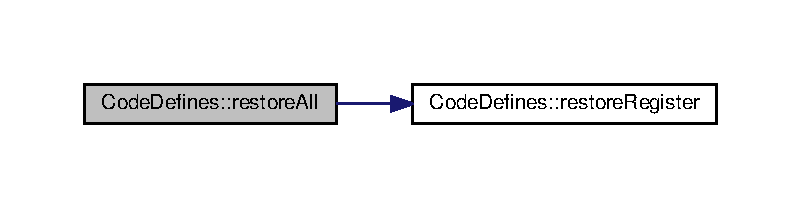
\includegraphics[width=350pt]{class_code_defines_a717d9ab10ffe0caaa17807133894cb06_cgraph}
\end{center}
\end{figure}


\hypertarget{class_code_defines_abc7f95cd1e8764eca2532184e359f02c}{\index{Code\-Defines@{Code\-Defines}!restore\-All\-Internal@{restore\-All\-Internal}}
\index{restore\-All\-Internal@{restore\-All\-Internal}!CodeDefines@{Code\-Defines}}
\subsubsection[{restore\-All\-Internal}]{\setlength{\rightskip}{0pt plus 5cm}template$<$typename Register $>$ template Q\-Byte\-Array {\bf Code\-Defines}$<$ Register $>$\-::restore\-All\-Internal (
\begin{DoxyParamCaption}
{}
\end{DoxyParamCaption}
)\hspace{0.3cm}{\ttfamily [static]}}}\label{class_code_defines_abc7f95cd1e8764eca2532184e359f02c}


Metoda odpowiadająca instrukcjom odczytu wszystkich wewnętrznych rejestrów ze stosu. 

\begin{DoxyReturn}{Zwraca}
Kod 
\end{DoxyReturn}


Definicja w linii 534 pliku codedefines.\-cpp.

\hypertarget{class_code_defines_a951d31c997529cea2553e7544598c505}{\index{Code\-Defines@{Code\-Defines}!restore\-Register@{restore\-Register}}
\index{restore\-Register@{restore\-Register}!CodeDefines@{Code\-Defines}}
\subsubsection[{restore\-Register}]{\setlength{\rightskip}{0pt plus 5cm}template$<$typename Register $>$ template Q\-Byte\-Array {\bf Code\-Defines}$<$ Register $>$\-::restore\-Register (
\begin{DoxyParamCaption}
\item[{Register}]{reg}
\end{DoxyParamCaption}
)\hspace{0.3cm}{\ttfamily [static]}}}\label{class_code_defines_a951d31c997529cea2553e7544598c505}


Metoda odpowiadająca instrukcji\-: pop reg. 


\begin{DoxyParams}{Parametry}
{\em reg} & Rejestr do odczytania \\
\hline
\end{DoxyParams}
\begin{DoxyReturn}{Zwraca}
Kod 
\end{DoxyReturn}


Definicja w linii 418 pliku codedefines.\-cpp.

\hypertarget{class_code_defines_abff87050d31f5313af2f92f41c5aeba6}{\index{Code\-Defines@{Code\-Defines}!ret\-N@{ret\-N}}
\index{ret\-N@{ret\-N}!CodeDefines@{Code\-Defines}}
\subsubsection[{ret\-N}]{\setlength{\rightskip}{0pt plus 5cm}template$<$typename Register $>$ template Q\-Byte\-Array {\bf Code\-Defines}$<$ Register $>$\-::ret\-N (
\begin{DoxyParamCaption}
\item[{uint16\-\_\-t}]{n}
\end{DoxyParamCaption}
)\hspace{0.3cm}{\ttfamily [static]}}}\label{class_code_defines_abff87050d31f5313af2f92f41c5aeba6}


Metoda odpowiadająca instrukcji\-: ret n. 


\begin{DoxyParams}{Parametry}
{\em n} & Liczba bajtów do zwolnienia \\
\hline
\end{DoxyParams}
\begin{DoxyReturn}{Zwraca}
Kod 
\end{DoxyReturn}


Definicja w linii 644 pliku codedefines.\-cpp.

\hypertarget{class_code_defines_ad2904023d0e1e87474da13edb453fb30}{\index{Code\-Defines@{Code\-Defines}!save\-All@{save\-All}}
\index{save\-All@{save\-All}!CodeDefines@{Code\-Defines}}
\subsubsection[{save\-All}]{\setlength{\rightskip}{0pt plus 5cm}template$<$typename Register$>$ static Q\-Byte\-Array {\bf Code\-Defines}$<$ Register $>$\-::save\-All (
\begin{DoxyParamCaption}
{}
\end{DoxyParamCaption}
)\hspace{0.3cm}{\ttfamily [static]}}}\label{class_code_defines_ad2904023d0e1e87474da13edb453fb30}


Zapisanie wszystkich rejestów na stosie. 

\begin{DoxyReturn}{Zwraca}
Kod 
\end{DoxyReturn}
\hypertarget{class_code_defines_a9258c95f68116611b02378bd60212111}{\index{Code\-Defines@{Code\-Defines}!save\-All@{save\-All}}
\index{save\-All@{save\-All}!CodeDefines@{Code\-Defines}}
\subsubsection[{save\-All}]{\setlength{\rightskip}{0pt plus 5cm}template$<$$>$ Q\-Byte\-Array {\bf Code\-Defines}$<$ {\bf Registers\-\_\-x86} $>$\-::save\-All (
\begin{DoxyParamCaption}
{}
\end{DoxyParamCaption}
)}}\label{class_code_defines_a9258c95f68116611b02378bd60212111}


Definicja w linii 653 pliku codedefines.\-cpp.

\hypertarget{class_code_defines_aa4e9c15c2613d1d628f7c11f674c46ea}{\index{Code\-Defines@{Code\-Defines}!save\-All@{save\-All}}
\index{save\-All@{save\-All}!CodeDefines@{Code\-Defines}}
\subsubsection[{save\-All}]{\setlength{\rightskip}{0pt plus 5cm}template$<$$>$ Q\-Byte\-Array {\bf Code\-Defines}$<$ {\bf Registers\-\_\-x64} $>$\-::save\-All (
\begin{DoxyParamCaption}
{}
\end{DoxyParamCaption}
)}}\label{class_code_defines_aa4e9c15c2613d1d628f7c11f674c46ea}


Definicja w linii 659 pliku codedefines.\-cpp.



Oto graf wywołań dla tej funkcji\-:\nopagebreak
\begin{figure}[H]
\begin{center}
\leavevmode
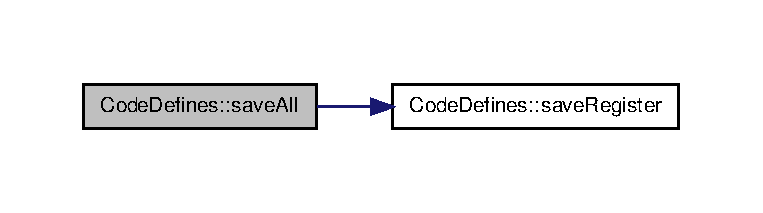
\includegraphics[width=350pt]{class_code_defines_aa4e9c15c2613d1d628f7c11f674c46ea_cgraph}
\end{center}
\end{figure}


\hypertarget{class_code_defines_a03a66f6808af85b08ef4ed8777c29e5e}{\index{Code\-Defines@{Code\-Defines}!save\-All\-Internal@{save\-All\-Internal}}
\index{save\-All\-Internal@{save\-All\-Internal}!CodeDefines@{Code\-Defines}}
\subsubsection[{save\-All\-Internal}]{\setlength{\rightskip}{0pt plus 5cm}template$<$typename Register $>$ template Q\-Byte\-Array {\bf Code\-Defines}$<$ Register $>$\-::save\-All\-Internal (
\begin{DoxyParamCaption}
{}
\end{DoxyParamCaption}
)\hspace{0.3cm}{\ttfamily [static]}}}\label{class_code_defines_a03a66f6808af85b08ef4ed8777c29e5e}


Metoda odpowiadająca instrukcjom zapisania wszystkich wewnętrznych rejestrów na stos. 

\begin{DoxyReturn}{Zwraca}
Kod 
\end{DoxyReturn}


Definicja w linii 520 pliku codedefines.\-cpp.

\hypertarget{class_code_defines_a43a24be00649da7ebcaf172f515f43c7}{\index{Code\-Defines@{Code\-Defines}!save\-Register@{save\-Register}}
\index{save\-Register@{save\-Register}!CodeDefines@{Code\-Defines}}
\subsubsection[{save\-Register}]{\setlength{\rightskip}{0pt plus 5cm}template$<$typename Register $>$ template Q\-Byte\-Array {\bf Code\-Defines}$<$ Register $>$\-::save\-Register (
\begin{DoxyParamCaption}
\item[{Register}]{reg}
\end{DoxyParamCaption}
)\hspace{0.3cm}{\ttfamily [static]}}}\label{class_code_defines_a43a24be00649da7ebcaf172f515f43c7}


Metoda odpowiadająca instrukcji\-: push reg. 


\begin{DoxyParams}{Parametry}
{\em reg} & Rejestr do zapisania \\
\hline
\end{DoxyParams}
\begin{DoxyReturn}{Zwraca}
Kod 
\end{DoxyReturn}


Definicja w linii 409 pliku codedefines.\-cpp.

\hypertarget{class_code_defines_a20358aed4dbfb9a22a8ecd61e482cfa1}{\index{Code\-Defines@{Code\-Defines}!shadow\-Size@{shadow\-Size}}
\index{shadow\-Size@{shadow\-Size}!CodeDefines@{Code\-Defines}}
\subsubsection[{shadow\-Size}]{\setlength{\rightskip}{0pt plus 5cm}template$<$$>$ const uint8\-\_\-t {\bf Code\-Defines}$<$ {\bf Registers\-\_\-x64} $>$\-::shadow\-Size (
\begin{DoxyParamCaption}
{}
\end{DoxyParamCaption}
)}}\label{class_code_defines_a20358aed4dbfb9a22a8ecd61e482cfa1}


Definicja w linii 22 pliku codedefines.\-cpp.

\hypertarget{class_code_defines_a4d91cad6a972b05bd4156cb00552f39e}{\index{Code\-Defines@{Code\-Defines}!stack\-Cell\-Size@{stack\-Cell\-Size}}
\index{stack\-Cell\-Size@{stack\-Cell\-Size}!CodeDefines@{Code\-Defines}}
\subsubsection[{stack\-Cell\-Size}]{\setlength{\rightskip}{0pt plus 5cm}template$<$$>$ const uint8\-\_\-t {\bf Code\-Defines}$<$ {\bf Registers\-\_\-x86} $>$\-::stack\-Cell\-Size (
\begin{DoxyParamCaption}
{}
\end{DoxyParamCaption}
)}}\label{class_code_defines_a4d91cad6a972b05bd4156cb00552f39e}


Definicja w linii 31 pliku codedefines.\-cpp.

\hypertarget{class_code_defines_a770bb8bf2208da3fd8d758966c23511e}{\index{Code\-Defines@{Code\-Defines}!stack\-Cell\-Size@{stack\-Cell\-Size}}
\index{stack\-Cell\-Size@{stack\-Cell\-Size}!CodeDefines@{Code\-Defines}}
\subsubsection[{stack\-Cell\-Size}]{\setlength{\rightskip}{0pt plus 5cm}template$<$$>$ const uint8\-\_\-t {\bf Code\-Defines}$<$ {\bf Registers\-\_\-x64} $>$\-::stack\-Cell\-Size (
\begin{DoxyParamCaption}
{}
\end{DoxyParamCaption}
)}}\label{class_code_defines_a770bb8bf2208da3fd8d758966c23511e}


Definicja w linii 34 pliku codedefines.\-cpp.

\hypertarget{class_code_defines_a5491865f96eec40ff6594702879b0fdb}{\index{Code\-Defines@{Code\-Defines}!start\-Func@{start\-Func}}
\index{start\-Func@{start\-Func}!CodeDefines@{Code\-Defines}}
\subsubsection[{start\-Func}]{\setlength{\rightskip}{0pt plus 5cm}template$<$$>$ const Q\-Byte\-Array {\bf Code\-Defines}$<$ {\bf Registers\-\_\-x86} $>$\-::start\-Func (
\begin{DoxyParamCaption}
{}
\end{DoxyParamCaption}
)}}\label{class_code_defines_a5491865f96eec40ff6594702879b0fdb}


Definicja w linii 37 pliku codedefines.\-cpp.

\hypertarget{class_code_defines_a8691301353c7786113939b5aa5925f09}{\index{Code\-Defines@{Code\-Defines}!start\-Func@{start\-Func}}
\index{start\-Func@{start\-Func}!CodeDefines@{Code\-Defines}}
\subsubsection[{start\-Func}]{\setlength{\rightskip}{0pt plus 5cm}template$<$$>$ const Q\-Byte\-Array {\bf Code\-Defines}$<$ {\bf Registers\-\_\-x64} $>$\-::start\-Func (
\begin{DoxyParamCaption}
{}
\end{DoxyParamCaption}
)}}\label{class_code_defines_a8691301353c7786113939b5aa5925f09}


Definicja w linii 40 pliku codedefines.\-cpp.

\hypertarget{class_code_defines_a8b8beae6895e7918b82c3c04e365e88d}{\index{Code\-Defines@{Code\-Defines}!store\-Value@{store\-Value}}
\index{store\-Value@{store\-Value}!CodeDefines@{Code\-Defines}}
\subsubsection[{store\-Value}]{\setlength{\rightskip}{0pt plus 5cm}template$<$typename Register$>$ template$<$typename T $>$ static Q\-Byte\-Array {\bf Code\-Defines}$<$ Register $>$\-::store\-Value (
\begin{DoxyParamCaption}
\item[{T}]{dword}
\end{DoxyParamCaption}
)\hspace{0.3cm}{\ttfamily [static]}}}\label{class_code_defines_a8b8beae6895e7918b82c3c04e365e88d}


Metoda odpowiadająca instrukcji\-: push value. 


\begin{DoxyParams}{Parametry}
{\em dword} & Wartość do zapisania \\
\hline
\end{DoxyParams}
\begin{DoxyReturn}{Zwraca}
Kod 
\end{DoxyReturn}
\hypertarget{class_code_defines_a40157c99b0f396b77cd6d7dc8f80071d}{\index{Code\-Defines@{Code\-Defines}!store\-Value@{store\-Value}}
\index{store\-Value@{store\-Value}!CodeDefines@{Code\-Defines}}
\subsubsection[{store\-Value}]{\setlength{\rightskip}{0pt plus 5cm}template$<$$>$ Q\-Byte\-Array {\bf Code\-Defines}$<$ {\bf Registers\-\_\-x86} $>$\-::store\-Value (
\begin{DoxyParamCaption}
\item[{uint32\-\_\-t}]{value}
\end{DoxyParamCaption}
)}}\label{class_code_defines_a40157c99b0f396b77cd6d7dc8f80071d}


Definicja w linii 592 pliku codedefines.\-cpp.

\hypertarget{class_code_defines_a964f09310db04f127c7684a8c24ae58e}{\index{Code\-Defines@{Code\-Defines}!store\-Value@{store\-Value}}
\index{store\-Value@{store\-Value}!CodeDefines@{Code\-Defines}}
\subsubsection[{store\-Value}]{\setlength{\rightskip}{0pt plus 5cm}template$<$$>$ Q\-Byte\-Array {\bf Code\-Defines}$<$ {\bf Registers\-\_\-x64} $>$\-::store\-Value (
\begin{DoxyParamCaption}
\item[{uint64\-\_\-t}]{value}
\end{DoxyParamCaption}
)}}\label{class_code_defines_a964f09310db04f127c7684a8c24ae58e}


Definicja w linii 600 pliku codedefines.\-cpp.

\hypertarget{class_code_defines_a97da0ebe2a72b85e4cf678cf07fec4e1}{\index{Code\-Defines@{Code\-Defines}!test\-Reg@{test\-Reg}}
\index{test\-Reg@{test\-Reg}!CodeDefines@{Code\-Defines}}
\subsubsection[{test\-Reg}]{\setlength{\rightskip}{0pt plus 5cm}template$<$typename Register $>$ template Q\-Byte\-Array {\bf Code\-Defines}$<$ Register $>$\-::test\-Reg (
\begin{DoxyParamCaption}
\item[{Register}]{reg}
\end{DoxyParamCaption}
)\hspace{0.3cm}{\ttfamily [static]}}}\label{class_code_defines_a97da0ebe2a72b85e4cf678cf07fec4e1}


Metoda odpowiadająca instrukcji\-: test reg, reg. 


\begin{DoxyParams}{Parametry}
{\em reg} & Rejestr \\
\hline
\end{DoxyParams}
\begin{DoxyReturn}{Zwraca}
Kod 
\end{DoxyReturn}


Definicja w linii 493 pliku codedefines.\-cpp.



\subsection{Dokumentacja atrybutów składowych}
\hypertarget{class_code_defines_a83820641d7045e035f2a4619a23d2755}{\index{Code\-Defines@{Code\-Defines}!align16\-Size@{align16\-Size}}
\index{align16\-Size@{align16\-Size}!CodeDefines@{Code\-Defines}}
\subsubsection[{align16\-Size}]{\setlength{\rightskip}{0pt plus 5cm}template$<$typename Register$>$ const uint8\-\_\-t {\bf Code\-Defines}$<$ Register $>$\-::align16\-Size\hspace{0.3cm}{\ttfamily [static]}}}\label{class_code_defines_a83820641d7045e035f2a4619a23d2755}


Liczba bajtów potrzebna do wyrównania stosu do 16. 



Definicja w linii 241 pliku codedefines.\-h.

\hypertarget{class_code_defines_a54f3fde2a7976ac5c36b9a9aa2efb37e}{\index{Code\-Defines@{Code\-Defines}!call\-Reg\-Exp@{call\-Reg\-Exp}}
\index{call\-Reg\-Exp@{call\-Reg\-Exp}!CodeDefines@{Code\-Defines}}
\subsubsection[{call\-Reg\-Exp}]{\setlength{\rightskip}{0pt plus 5cm}template$<$typename Register$>$ template const Q\-Reg\-Exp {\bf Code\-Defines}$<$ Register $>$\-::call\-Reg\-Exp = Q\-Reg\-Exp(\char`\"{}$^\wedge$\mbox{[}0-\/9a-\/f\mbox{]}\{8\} E8\mbox{[}0-\/9a-\/f\mbox{]}\{6\}(00$|$ff) \char`\"{}, Qt\-::\-Case\-Insensitive)\hspace{0.3cm}{\ttfamily [static]}}}\label{class_code_defines_a54f3fde2a7976ac5c36b9a9aa2efb37e}


Wyrażenie regularne znajdujące instrukcję call offset w zdekompilowanym kodzie. 



Definicja w linii 256 pliku codedefines.\-h.

\hypertarget{class_code_defines_abb945f5e809b498405e0a91901c784e1}{\index{Code\-Defines@{Code\-Defines}!end\-Func@{end\-Func}}
\index{end\-Func@{end\-Func}!CodeDefines@{Code\-Defines}}
\subsubsection[{end\-Func}]{\setlength{\rightskip}{0pt plus 5cm}template$<$typename Register$>$ template const Q\-Byte\-Array {\bf Code\-Defines}$<$ Register $>$\-::end\-Func = Q\-Byte\-Array(\char`\"{}\textbackslash{}x5\-D\char`\"{})\hspace{0.3cm}{\ttfamily [static]}}}\label{class_code_defines_abb945f5e809b498405e0a91901c784e1}


Kod odpowiadający instrukcji\-: pop ebp. 



Definicja w linii 216 pliku codedefines.\-h.

\hypertarget{class_code_defines_a045622ec64ec17b4b8a2d55b854117c7}{\index{Code\-Defines@{Code\-Defines}!external\-Regs@{external\-Regs}}
\index{external\-Regs@{external\-Regs}!CodeDefines@{Code\-Defines}}
\subsubsection[{external\-Regs}]{\setlength{\rightskip}{0pt plus 5cm}template$<$typename Register$>$ const Q\-List$<$Register$>$ {\bf Code\-Defines}$<$ Register $>$\-::external\-Regs\hspace{0.3cm}{\ttfamily [static]}}}\label{class_code_defines_a045622ec64ec17b4b8a2d55b854117c7}


Lista zewnętrznych rejestrów. 



Definicja w linii 231 pliku codedefines.\-h.

\hypertarget{class_code_defines_a71b60a174fc6190178fee7c552f52732}{\index{Code\-Defines@{Code\-Defines}!internal\-Regs@{internal\-Regs}}
\index{internal\-Regs@{internal\-Regs}!CodeDefines@{Code\-Defines}}
\subsubsection[{internal\-Regs}]{\setlength{\rightskip}{0pt plus 5cm}template$<$typename Register$>$ const Q\-List$<$Register$>$ {\bf Code\-Defines}$<$ Register $>$\-::internal\-Regs\hspace{0.3cm}{\ttfamily [static]}}}\label{class_code_defines_a71b60a174fc6190178fee7c552f52732}


Lista wewnętrznych rejestów. 



Definicja w linii 226 pliku codedefines.\-h.

\hypertarget{class_code_defines_a2f214288be4f17edf89f463162c59e30}{\index{Code\-Defines@{Code\-Defines}!jmp\-Reg\-Exp@{jmp\-Reg\-Exp}}
\index{jmp\-Reg\-Exp@{jmp\-Reg\-Exp}!CodeDefines@{Code\-Defines}}
\subsubsection[{jmp\-Reg\-Exp}]{\setlength{\rightskip}{0pt plus 5cm}template$<$typename Register$>$ template const Q\-Reg\-Exp {\bf Code\-Defines}$<$ Register $>$\-::jmp\-Reg\-Exp = Q\-Reg\-Exp(\char`\"{}$^\wedge$$^\wedge$\mbox{[}0-\/9a-\/f\mbox{]}\{8\} E9\mbox{[}0-\/9a-\/f\mbox{]}\{6\}(00$|$ff) \char`\"{}, Qt\-::\-Case\-Insensitive)\hspace{0.3cm}{\ttfamily [static]}}}\label{class_code_defines_a2f214288be4f17edf89f463162c59e30}


Wyrażenie regularne znajdujące instrukcję jmp offset w zdekompilowanym kodzie. 



Definicja w linii 261 pliku codedefines.\-h.

\hypertarget{class_code_defines_a767cf243acab61bf7c6f1046002425e1}{\index{Code\-Defines@{Code\-Defines}!new\-Line\-Reg\-Exp@{new\-Line\-Reg\-Exp}}
\index{new\-Line\-Reg\-Exp@{new\-Line\-Reg\-Exp}!CodeDefines@{Code\-Defines}}
\subsubsection[{new\-Line\-Reg\-Exp}]{\setlength{\rightskip}{0pt plus 5cm}template$<$typename Register$>$ template const Q\-Reg\-Exp {\bf Code\-Defines}$<$ Register $>$\-::new\-Line\-Reg\-Exp = Q\-Reg\-Exp(\char`\"{}\mbox{[}\textbackslash{}r\textbackslash{}n\mbox{]}\char`\"{})\hspace{0.3cm}{\ttfamily [static]}}}\label{class_code_defines_a767cf243acab61bf7c6f1046002425e1}


Wyrażenie regularne znajdujące znak nowej linii. 



Definicja w linii 251 pliku codedefines.\-h.

\hypertarget{class_code_defines_ae8c1690d0a6fe53c81dea4c8cad6ca5c}{\index{Code\-Defines@{Code\-Defines}!ret@{ret}}
\index{ret@{ret}!CodeDefines@{Code\-Defines}}
\subsubsection[{ret}]{\setlength{\rightskip}{0pt plus 5cm}template$<$typename Register$>$ template const Q\-Byte\-Array {\bf Code\-Defines}$<$ Register $>$\-::ret = Q\-Byte\-Array(\char`\"{}\textbackslash{}x\-C3\char`\"{})\hspace{0.3cm}{\ttfamily [static]}}}\label{class_code_defines_ae8c1690d0a6fe53c81dea4c8cad6ca5c}


Kod odpowiadający instrukcji\-: ret. 



Definicja w linii 221 pliku codedefines.\-h.

\hypertarget{class_code_defines_a89139a3f358c98200f78478fd0dd3bd9}{\index{Code\-Defines@{Code\-Defines}!shadow\-Size@{shadow\-Size}}
\index{shadow\-Size@{shadow\-Size}!CodeDefines@{Code\-Defines}}
\subsubsection[{shadow\-Size}]{\setlength{\rightskip}{0pt plus 5cm}template$<$typename Register$>$ const uint8\-\_\-t {\bf Code\-Defines}$<$ Register $>$\-::shadow\-Size\hspace{0.3cm}{\ttfamily [static]}}}\label{class_code_defines_a89139a3f358c98200f78478fd0dd3bd9}


Rozmiar Shadow Space. 



Definicja w linii 236 pliku codedefines.\-h.

\hypertarget{class_code_defines_add79526fe978503123140edf11497d66}{\index{Code\-Defines@{Code\-Defines}!stack\-Cell\-Size@{stack\-Cell\-Size}}
\index{stack\-Cell\-Size@{stack\-Cell\-Size}!CodeDefines@{Code\-Defines}}
\subsubsection[{stack\-Cell\-Size}]{\setlength{\rightskip}{0pt plus 5cm}template$<$typename Register$>$ const uint8\-\_\-t {\bf Code\-Defines}$<$ Register $>$\-::stack\-Cell\-Size\hspace{0.3cm}{\ttfamily [static]}}}\label{class_code_defines_add79526fe978503123140edf11497d66}


Rozmiar komórki stosu. 



Definicja w linii 246 pliku codedefines.\-h.

\hypertarget{class_code_defines_ab0339e357461e07258de4e77d0c73c5c}{\index{Code\-Defines@{Code\-Defines}!start\-Func@{start\-Func}}
\index{start\-Func@{start\-Func}!CodeDefines@{Code\-Defines}}
\subsubsection[{start\-Func}]{\setlength{\rightskip}{0pt plus 5cm}template$<$typename Register$>$ const Q\-Byte\-Array {\bf Code\-Defines}$<$ Register $>$\-::start\-Func\hspace{0.3cm}{\ttfamily [static]}}}\label{class_code_defines_ab0339e357461e07258de4e77d0c73c5c}


Kod odpowiadający instrukcji\-: push ebp; mov ebp, esp;. 



Definicja w linii 211 pliku codedefines.\-h.



Dokumentacja dla tej klasy została wygenerowana z plików\-:\begin{DoxyCompactItemize}
\item 
core/file\-\_\-types/\hyperlink{codedefines_8h}{codedefines.\-h}\item 
core/file\-\_\-types/\hyperlink{codedefines_8cpp}{codedefines.\-cpp}\end{DoxyCompactItemize}

\hypertarget{class_d_adding_methods}{\section{Dokumentacja klasy D\-Adding\-Methods}
\label{class_d_adding_methods}\index{D\-Adding\-Methods@{D\-Adding\-Methods}}
}


{\ttfamily \#include $<$daddingmethods.\-h$>$}



Diagram dziedziczenia dla D\-Adding\-Methods
\nopagebreak
\begin{figure}[H]
\begin{center}
\leavevmode
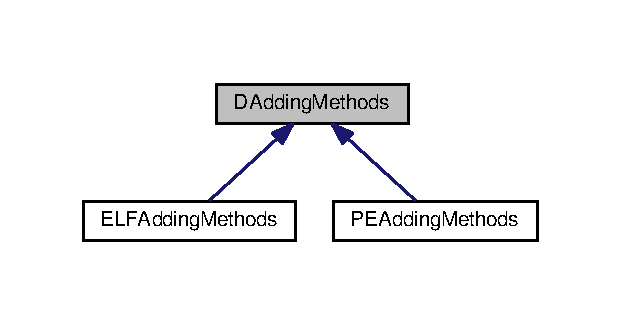
\includegraphics[width=298pt]{class_d_adding_methods__inherit__graph}
\end{center}
\end{figure}


Diagram współpracy dla D\-Adding\-Methods\-:
\nopagebreak
\begin{figure}[H]
\begin{center}
\leavevmode
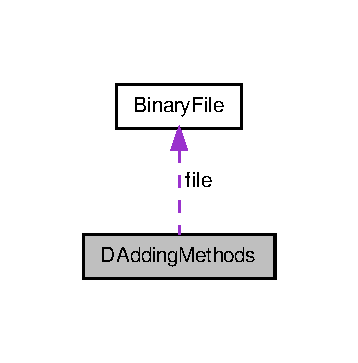
\includegraphics[width=172pt]{class_d_adding_methods__coll__graph}
\end{center}
\end{figure}
\subsection*{Komponenty}
\begin{DoxyCompactItemize}
\item 
class \hyperlink{class_d_adding_methods_1_1_inject_description}{Inject\-Description}
\begin{DoxyCompactList}\small\item\em Klasa opisująca metodę wstrzykiwania kodu. \end{DoxyCompactList}\item 
class \hyperlink{class_d_adding_methods_1_1_o_e_p_wrapper}{O\-E\-P\-Wrapper}
\begin{DoxyCompactList}\small\item\em Klasa reprezentująca opakowanie dla tworzenia nowego punktu wejściowego. \end{DoxyCompactList}\item 
class \hyperlink{class_d_adding_methods_1_1_thread_wrapper}{Thread\-Wrapper}
\begin{DoxyCompactList}\small\item\em Klasa reprezentująca opakowanie dla tworzenia nowego wątku. \end{DoxyCompactList}\item 
class \hyperlink{class_d_adding_methods_1_1_trampoline_wrapper}{Trampoline\-Wrapper}
\begin{DoxyCompactList}\small\item\em Klasa reprezentująca opakowanie dla tworzenia tramplin w funkcjach bibliotecznych. \end{DoxyCompactList}\item 
class \hyperlink{class_d_adding_methods_1_1_wrapper}{Wrapper}
\begin{DoxyCompactList}\small\item\em Klasa bazowa reprezentująca opakowanie dla kawałków kodu. \end{DoxyCompactList}\end{DoxyCompactItemize}
\subsection*{Typy publiczne}
\begin{DoxyCompactItemize}
\item 
enum \hyperlink{class_d_adding_methods_a7d062c443c04f37689dbececc36cf4a3}{Architecture\-Type} \{ \hyperlink{class_d_adding_methods_a7d062c443c04f37689dbececc36cf4a3a19c324fc35adafffc05d643f63e8eb5e}{Architecture\-Type\-::\-B\-I\-T\-S32}, 
\hyperlink{class_d_adding_methods_a7d062c443c04f37689dbececc36cf4a3a316bc10be99a2862edd96d24e0d150d9}{Architecture\-Type\-::\-B\-I\-T\-S64}
 \}
\begin{DoxyCompactList}\small\item\em Typ kompilowanego pliku assembly. \end{DoxyCompactList}\item 
enum \hyperlink{class_d_adding_methods_a14e87405d457c7c3671eca0e74b3f327}{System\-Type} \{ \hyperlink{class_d_adding_methods_a14e87405d457c7c3671eca0e74b3f327aaea23489ce3aa9b6406ebb28e0cda430}{System\-Type\-::\-Windows}, 
\hyperlink{class_d_adding_methods_a14e87405d457c7c3671eca0e74b3f327aedc9f0a5a5d57797bf68e37364743831}{System\-Type\-::\-Linux}
 \}
\item 
enum \hyperlink{class_d_adding_methods_a8b52c07f1794d8c6cdd6f9b98be2bbf0}{Calling\-Method} \{ \\*
\hyperlink{class_d_adding_methods_a8b52c07f1794d8c6cdd6f9b98be2bbf0a1f69192f5c5359619a4410d97d1655be}{Calling\-Method\-::\-O\-E\-P}, 
\hyperlink{class_d_adding_methods_a8b52c07f1794d8c6cdd6f9b98be2bbf0ad97477d6d8a838ead9348185bb5b6742}{Calling\-Method\-::\-Thread}, 
\hyperlink{class_d_adding_methods_a8b52c07f1794d8c6cdd6f9b98be2bbf0ad113494f870355ce123dfb74beea602d}{Calling\-Method\-::\-Trampoline}, 
\hyperlink{class_d_adding_methods_a8b52c07f1794d8c6cdd6f9b98be2bbf0afaee4ca3c30ee18148ce3ada37466498}{Calling\-Method\-::\-I\-N\-I\-T}, 
\\*
\hyperlink{class_d_adding_methods_a8b52c07f1794d8c6cdd6f9b98be2bbf0a8c11d1b1290b76379bf90434c0e83f4a}{Calling\-Method\-::\-I\-N\-I\-T\-\_\-\-A\-R\-R\-A\-Y}, 
\hyperlink{class_d_adding_methods_a8b52c07f1794d8c6cdd6f9b98be2bbf0a02f11aadd3ab1bd5b7ccd3040d8a0075}{Calling\-Method\-::\-C\-T\-O\-R\-S}, 
\hyperlink{class_d_adding_methods_a8b52c07f1794d8c6cdd6f9b98be2bbf0a099d7d04319e5191b7473e016c55e320}{Calling\-Method\-::\-T\-L\-S}
 \}
\begin{DoxyCompactList}\small\item\em Typy możliwości wstrzyknięcia kodu. \end{DoxyCompactList}\end{DoxyCompactItemize}
\subsection*{Metody publiczne}
\begin{DoxyCompactItemize}
\item 
\hyperlink{class_d_adding_methods_aa00f1f94760a223807193314537b6651}{D\-Adding\-Methods} (\hyperlink{class_binary_file}{Binary\-File} $\ast$f)
\begin{DoxyCompactList}\small\item\em Konstruktor. \end{DoxyCompactList}\end{DoxyCompactItemize}
\subsection*{Atrybuty chronione}
\begin{DoxyCompactItemize}
\item 
\hyperlink{class_binary_file}{Binary\-File} $\ast$ \hyperlink{class_d_adding_methods_a87bdff1dd02ac26df6c10648fe406cd9}{file}
\item 
Q\-Map$<$ \hyperlink{class_d_adding_methods_a7d062c443c04f37689dbececc36cf4a3}{Architecture\-Type}, Q\-String $>$ \hyperlink{class_d_adding_methods_aa368755d8aba57f3a92877d1fbe925b3}{arch\-\_\-type}
\end{DoxyCompactItemize}
\subsection*{Statyczne atrybuty prywatne}
\begin{DoxyCompactItemize}
\item 
static const Q\-Map$<$ Q\-String, \\*
\hyperlink{class_d_adding_methods_a8b52c07f1794d8c6cdd6f9b98be2bbf0}{Calling\-Method} $>$ \hyperlink{class_d_adding_methods_a4c746112dd790909f893063563cd7877}{calling\-Methods}
\end{DoxyCompactItemize}


\subsection{Opis szczegółowy}


Definicja w linii 27 pliku daddingmethods.\-h.



\subsection{Dokumentacja składowych wyliczanych}
\hypertarget{class_d_adding_methods_a7d062c443c04f37689dbececc36cf4a3}{\index{D\-Adding\-Methods@{D\-Adding\-Methods}!Architecture\-Type@{Architecture\-Type}}
\index{Architecture\-Type@{Architecture\-Type}!DAddingMethods@{D\-Adding\-Methods}}
\subsubsection[{Architecture\-Type}]{\setlength{\rightskip}{0pt plus 5cm}enum {\bf D\-Adding\-Methods\-::\-Architecture\-Type}\hspace{0.3cm}{\ttfamily [strong]}}}\label{class_d_adding_methods_a7d062c443c04f37689dbececc36cf4a3}


Typ kompilowanego pliku assembly. 

\begin{Desc}
\item[Wartości wyliczeń]\par
\begin{description}
\index{B\-I\-T\-S32@{B\-I\-T\-S32}!D\-Adding\-Methods@{D\-Adding\-Methods}}\index{D\-Adding\-Methods@{D\-Adding\-Methods}!B\-I\-T\-S32@{B\-I\-T\-S32}}\item[{\em 
\hypertarget{class_d_adding_methods_a7d062c443c04f37689dbececc36cf4a3a19c324fc35adafffc05d643f63e8eb5e}{B\-I\-T\-S32}\label{class_d_adding_methods_a7d062c443c04f37689dbececc36cf4a3a19c324fc35adafffc05d643f63e8eb5e}
}]\index{B\-I\-T\-S64@{B\-I\-T\-S64}!D\-Adding\-Methods@{D\-Adding\-Methods}}\index{D\-Adding\-Methods@{D\-Adding\-Methods}!B\-I\-T\-S64@{B\-I\-T\-S64}}\item[{\em 
\hypertarget{class_d_adding_methods_a7d062c443c04f37689dbececc36cf4a3a316bc10be99a2862edd96d24e0d150d9}{B\-I\-T\-S64}\label{class_d_adding_methods_a7d062c443c04f37689dbececc36cf4a3a316bc10be99a2862edd96d24e0d150d9}
}]\end{description}
\end{Desc}


Definicja w linii 33 pliku daddingmethods.\-h.

\hypertarget{class_d_adding_methods_a8b52c07f1794d8c6cdd6f9b98be2bbf0}{\index{D\-Adding\-Methods@{D\-Adding\-Methods}!Calling\-Method@{Calling\-Method}}
\index{Calling\-Method@{Calling\-Method}!DAddingMethods@{D\-Adding\-Methods}}
\subsubsection[{Calling\-Method}]{\setlength{\rightskip}{0pt plus 5cm}enum {\bf D\-Adding\-Methods\-::\-Calling\-Method}\hspace{0.3cm}{\ttfamily [strong]}}}\label{class_d_adding_methods_a8b52c07f1794d8c6cdd6f9b98be2bbf0}


Typy możliwości wstrzyknięcia kodu. 

\begin{Desc}
\item[Wartości wyliczeń]\par
\begin{description}
\index{O\-E\-P@{O\-E\-P}!D\-Adding\-Methods@{D\-Adding\-Methods}}\index{D\-Adding\-Methods@{D\-Adding\-Methods}!O\-E\-P@{O\-E\-P}}\item[{\em 
\hypertarget{class_d_adding_methods_a8b52c07f1794d8c6cdd6f9b98be2bbf0a1f69192f5c5359619a4410d97d1655be}{O\-E\-P}\label{class_d_adding_methods_a8b52c07f1794d8c6cdd6f9b98be2bbf0a1f69192f5c5359619a4410d97d1655be}
}]\index{Thread@{Thread}!D\-Adding\-Methods@{D\-Adding\-Methods}}\index{D\-Adding\-Methods@{D\-Adding\-Methods}!Thread@{Thread}}\item[{\em 
\hypertarget{class_d_adding_methods_a8b52c07f1794d8c6cdd6f9b98be2bbf0ad97477d6d8a838ead9348185bb5b6742}{Thread}\label{class_d_adding_methods_a8b52c07f1794d8c6cdd6f9b98be2bbf0ad97477d6d8a838ead9348185bb5b6742}
}]\index{Trampoline@{Trampoline}!D\-Adding\-Methods@{D\-Adding\-Methods}}\index{D\-Adding\-Methods@{D\-Adding\-Methods}!Trampoline@{Trampoline}}\item[{\em 
\hypertarget{class_d_adding_methods_a8b52c07f1794d8c6cdd6f9b98be2bbf0ad113494f870355ce123dfb74beea602d}{Trampoline}\label{class_d_adding_methods_a8b52c07f1794d8c6cdd6f9b98be2bbf0ad113494f870355ce123dfb74beea602d}
}]\index{I\-N\-I\-T@{I\-N\-I\-T}!D\-Adding\-Methods@{D\-Adding\-Methods}}\index{D\-Adding\-Methods@{D\-Adding\-Methods}!I\-N\-I\-T@{I\-N\-I\-T}}\item[{\em 
\hypertarget{class_d_adding_methods_a8b52c07f1794d8c6cdd6f9b98be2bbf0afaee4ca3c30ee18148ce3ada37466498}{I\-N\-I\-T}\label{class_d_adding_methods_a8b52c07f1794d8c6cdd6f9b98be2bbf0afaee4ca3c30ee18148ce3ada37466498}
}]\index{I\-N\-I\-T\-\_\-\-A\-R\-R\-A\-Y@{I\-N\-I\-T\-\_\-\-A\-R\-R\-A\-Y}!D\-Adding\-Methods@{D\-Adding\-Methods}}\index{D\-Adding\-Methods@{D\-Adding\-Methods}!I\-N\-I\-T\-\_\-\-A\-R\-R\-A\-Y@{I\-N\-I\-T\-\_\-\-A\-R\-R\-A\-Y}}\item[{\em 
\hypertarget{class_d_adding_methods_a8b52c07f1794d8c6cdd6f9b98be2bbf0a8c11d1b1290b76379bf90434c0e83f4a}{I\-N\-I\-T\-\_\-\-A\-R\-R\-A\-Y}\label{class_d_adding_methods_a8b52c07f1794d8c6cdd6f9b98be2bbf0a8c11d1b1290b76379bf90434c0e83f4a}
}]\index{C\-T\-O\-R\-S@{C\-T\-O\-R\-S}!D\-Adding\-Methods@{D\-Adding\-Methods}}\index{D\-Adding\-Methods@{D\-Adding\-Methods}!C\-T\-O\-R\-S@{C\-T\-O\-R\-S}}\item[{\em 
\hypertarget{class_d_adding_methods_a8b52c07f1794d8c6cdd6f9b98be2bbf0a02f11aadd3ab1bd5b7ccd3040d8a0075}{C\-T\-O\-R\-S}\label{class_d_adding_methods_a8b52c07f1794d8c6cdd6f9b98be2bbf0a02f11aadd3ab1bd5b7ccd3040d8a0075}
}]\index{T\-L\-S@{T\-L\-S}!D\-Adding\-Methods@{D\-Adding\-Methods}}\index{D\-Adding\-Methods@{D\-Adding\-Methods}!T\-L\-S@{T\-L\-S}}\item[{\em 
\hypertarget{class_d_adding_methods_a8b52c07f1794d8c6cdd6f9b98be2bbf0a099d7d04319e5191b7473e016c55e320}{T\-L\-S}\label{class_d_adding_methods_a8b52c07f1794d8c6cdd6f9b98be2bbf0a099d7d04319e5191b7473e016c55e320}
}]\end{description}
\end{Desc}


Definicja w linii 46 pliku daddingmethods.\-h.

\hypertarget{class_d_adding_methods_a14e87405d457c7c3671eca0e74b3f327}{\index{D\-Adding\-Methods@{D\-Adding\-Methods}!System\-Type@{System\-Type}}
\index{System\-Type@{System\-Type}!DAddingMethods@{D\-Adding\-Methods}}
\subsubsection[{System\-Type}]{\setlength{\rightskip}{0pt plus 5cm}enum {\bf D\-Adding\-Methods\-::\-System\-Type}\hspace{0.3cm}{\ttfamily [strong]}}}\label{class_d_adding_methods_a14e87405d457c7c3671eca0e74b3f327}
\begin{Desc}
\item[Wartości wyliczeń]\par
\begin{description}
\index{Windows@{Windows}!D\-Adding\-Methods@{D\-Adding\-Methods}}\index{D\-Adding\-Methods@{D\-Adding\-Methods}!Windows@{Windows}}\item[{\em 
\hypertarget{class_d_adding_methods_a14e87405d457c7c3671eca0e74b3f327aaea23489ce3aa9b6406ebb28e0cda430}{Windows}\label{class_d_adding_methods_a14e87405d457c7c3671eca0e74b3f327aaea23489ce3aa9b6406ebb28e0cda430}
}]\index{Linux@{Linux}!D\-Adding\-Methods@{D\-Adding\-Methods}}\index{D\-Adding\-Methods@{D\-Adding\-Methods}!Linux@{Linux}}\item[{\em 
\hypertarget{class_d_adding_methods_a14e87405d457c7c3671eca0e74b3f327aedc9f0a5a5d57797bf68e37364743831}{Linux}\label{class_d_adding_methods_a14e87405d457c7c3671eca0e74b3f327aedc9f0a5a5d57797bf68e37364743831}
}]\end{description}
\end{Desc}


Definicja w linii 38 pliku daddingmethods.\-h.



\subsection{Dokumentacja konstruktora i destruktora}
\hypertarget{class_d_adding_methods_aa00f1f94760a223807193314537b6651}{\index{D\-Adding\-Methods@{D\-Adding\-Methods}!D\-Adding\-Methods@{D\-Adding\-Methods}}
\index{D\-Adding\-Methods@{D\-Adding\-Methods}!DAddingMethods@{D\-Adding\-Methods}}
\subsubsection[{D\-Adding\-Methods}]{\setlength{\rightskip}{0pt plus 5cm}D\-Adding\-Methods\-::\-D\-Adding\-Methods (
\begin{DoxyParamCaption}
\item[{{\bf Binary\-File} $\ast$}]{f}
\end{DoxyParamCaption}
)}}\label{class_d_adding_methods_aa00f1f94760a223807193314537b6651}


Konstruktor. 



Definicja w linii 46 pliku daddingmethods.\-cpp.



\subsection{Dokumentacja atrybutów składowych}
\hypertarget{class_d_adding_methods_aa368755d8aba57f3a92877d1fbe925b3}{\index{D\-Adding\-Methods@{D\-Adding\-Methods}!arch\-\_\-type@{arch\-\_\-type}}
\index{arch\-\_\-type@{arch\-\_\-type}!DAddingMethods@{D\-Adding\-Methods}}
\subsubsection[{arch\-\_\-type}]{\setlength{\rightskip}{0pt plus 5cm}Q\-Map$<${\bf Architecture\-Type}, Q\-String$>$ D\-Adding\-Methods\-::arch\-\_\-type\hspace{0.3cm}{\ttfamily [protected]}}}\label{class_d_adding_methods_aa368755d8aba57f3a92877d1fbe925b3}


Definicja w linii 270 pliku daddingmethods.\-h.

\hypertarget{class_d_adding_methods_a4c746112dd790909f893063563cd7877}{\index{D\-Adding\-Methods@{D\-Adding\-Methods}!calling\-Methods@{calling\-Methods}}
\index{calling\-Methods@{calling\-Methods}!DAddingMethods@{D\-Adding\-Methods}}
\subsubsection[{calling\-Methods}]{\setlength{\rightskip}{0pt plus 5cm}const Q\-Map$<$ Q\-String, {\bf D\-Adding\-Methods\-::\-Calling\-Method} $>$ D\-Adding\-Methods\-::calling\-Methods\hspace{0.3cm}{\ttfamily [static]}, {\ttfamily [private]}}}\label{class_d_adding_methods_a4c746112dd790909f893063563cd7877}
{\bfseries Wartość początkowa\-:}
\begin{DoxyCode}
=
\{
    \{ \textcolor{stringliteral}{"EntryPoint"}, \hyperlink{class_d_adding_methods_a8b52c07f1794d8c6cdd6f9b98be2bbf0a1f69192f5c5359619a4410d97d1655be}{DAddingMethods::CallingMethod::OEP} \},
    \{ \textcolor{stringliteral}{"Thread"}, \hyperlink{class_d_adding_methods_a8b52c07f1794d8c6cdd6f9b98be2bbf0ad97477d6d8a838ead9348185bb5b6742}{DAddingMethods::CallingMethod::Thread} \},
    \{ \textcolor{stringliteral}{"Trampoline"}, \hyperlink{class_d_adding_methods_a8b52c07f1794d8c6cdd6f9b98be2bbf0ad113494f870355ce123dfb74beea602d}{DAddingMethods::CallingMethod::Trampoline} \},
    \{ \textcolor{stringliteral}{"INIT"}, \hyperlink{class_d_adding_methods_a8b52c07f1794d8c6cdd6f9b98be2bbf0afaee4ca3c30ee18148ce3ada37466498}{DAddingMethods::CallingMethod::INIT} \},
    \{ \textcolor{stringliteral}{"INIT\_ARRAY"}, \hyperlink{class_d_adding_methods_a8b52c07f1794d8c6cdd6f9b98be2bbf0a8c11d1b1290b76379bf90434c0e83f4a}{DAddingMethods::CallingMethod::INIT\_ARRAY} \},
    \{ \textcolor{stringliteral}{"CTORS"}, \hyperlink{class_d_adding_methods_a8b52c07f1794d8c6cdd6f9b98be2bbf0a02f11aadd3ab1bd5b7ccd3040d8a0075}{DAddingMethods::CallingMethod::CTORS} \},
    \{ \textcolor{stringliteral}{"TLS"}, \hyperlink{class_d_adding_methods_a8b52c07f1794d8c6cdd6f9b98be2bbf0a099d7d04319e5191b7473e016c55e320}{DAddingMethods::CallingMethod::TLS} \}
\}
\end{DoxyCode}


Definicja w linii 273 pliku daddingmethods.\-h.

\hypertarget{class_d_adding_methods_a87bdff1dd02ac26df6c10648fe406cd9}{\index{D\-Adding\-Methods@{D\-Adding\-Methods}!file@{file}}
\index{file@{file}!DAddingMethods@{D\-Adding\-Methods}}
\subsubsection[{file}]{\setlength{\rightskip}{0pt plus 5cm}{\bf Binary\-File}$\ast$ D\-Adding\-Methods\-::file\hspace{0.3cm}{\ttfamily [protected]}}}\label{class_d_adding_methods_a87bdff1dd02ac26df6c10648fe406cd9}


Definicja w linii 269 pliku daddingmethods.\-h.



Dokumentacja dla tej klasy została wygenerowana z plików\-:\begin{DoxyCompactItemize}
\item 
core/adding\-\_\-methods/wrappers/\hyperlink{daddingmethods_8h}{daddingmethods.\-h}\item 
core/adding\-\_\-methods/wrappers/\hyperlink{daddingmethods_8cpp}{daddingmethods.\-cpp}\end{DoxyCompactItemize}

\hypertarget{class_d_json_parser}{\section{Dokumentacja klasy D\-Json\-Parser}
\label{class_d_json_parser}\index{D\-Json\-Parser@{D\-Json\-Parser}}
}


{\ttfamily \#include $<$djsonparser.\-h$>$}



Diagram współpracy dla D\-Json\-Parser\-:
\nopagebreak
\begin{figure}[H]
\begin{center}
\leavevmode
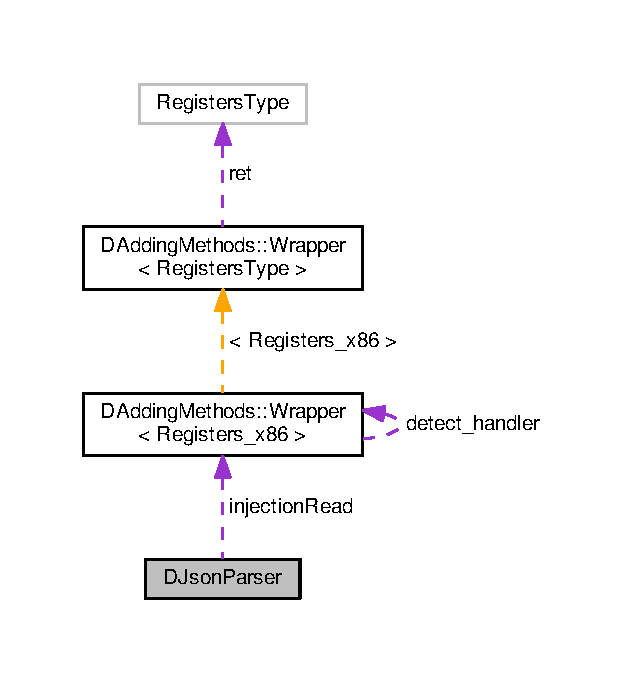
\includegraphics[width=299pt]{class_d_json_parser__coll__graph}
\end{center}
\end{figure}
\subsection*{Metody publiczne}
\begin{DoxyCompactItemize}
\item 
\hyperlink{class_d_json_parser_ab1d4f6d9c863888595a4d4568114b7b4}{D\-Json\-Parser} (Q\-String path)
\item 
{\footnotesize template$<$typename Reg $>$ }\\\hyperlink{class_d_adding_methods_1_1_wrapper}{D\-Adding\-Methods\-::\-Wrapper}$<$ Reg $>$ $\ast$ \hyperlink{class_d_json_parser_a14c19cd1d981e908ef8dfbc4218b359f}{load\-Inject\-Description} (Q\-String name)
\item 
bool \hyperlink{class_d_json_parser_a6d680ce58c2e6b638223071d996a2c0f}{save\-Incject\-Description} (Q\-String name, \hyperlink{class_d_adding_methods_1_1_wrapper}{D\-Adding\-Methods\-::\-Wrapper}$<$ \hyperlink{codedefines_8h_a0f84efe4ca4d99203713a78bd6e8c82e}{Registers\-\_\-x86} $>$ \&inj)
\begin{DoxyCompactList}\small\item\em D\-Json\-Parser\-::save\-Incjection\-Description zapisuje referencje obiekt wskazywany przez injection do pliku w formacie .json. \end{DoxyCompactList}\item 
\hyperlink{class_d_adding_methods_1_1_wrapper}{D\-Adding\-Methods\-::\-Wrapper}\\*
$<$ \hyperlink{codedefines_8h_a0f84efe4ca4d99203713a78bd6e8c82e}{Registers\-\_\-x86} $>$ $\ast$ \hyperlink{class_d_json_parser_a0603bac0338a1ae401b3f58cfc1d67c9}{get\-Injection\-Read} () const 
\begin{DoxyCompactList}\small\item\em \hyperlink{class_d_json_parser_a0603bac0338a1ae401b3f58cfc1d67c9}{D\-Json\-Parser\-::get\-Injection\-Read} zwraca wskaźnik do wczytanej metody. \end{DoxyCompactList}\item 
{\footnotesize template$<$typename Register $>$ }\\\hyperlink{class_d_adding_methods_1_1_wrapper}{D\-Adding\-Methods\-::\-Wrapper}\\*
$<$ Register $>$ $\ast$ \hyperlink{class_d_json_parser_a3baa4948e78cb386c8eb7e6634ab4d03}{load\-Inject\-Description} (Q\-String name)
\begin{DoxyCompactList}\small\item\em \hyperlink{class_d_json_parser_a14c19cd1d981e908ef8dfbc4218b359f}{D\-Json\-Parser\-::load\-Inject\-Description} tworzy obiekt Inject\-Description deserializując go z z inject\-Description.\-json. \end{DoxyCompactList}\end{DoxyCompactItemize}
\subsection*{Atrybuty prywatne}
\begin{DoxyCompactItemize}
\item 
\hyperlink{class_d_adding_methods_1_1_wrapper}{D\-Adding\-Methods\-::\-Wrapper}\\*
$<$ \hyperlink{codedefines_8h_a0f84efe4ca4d99203713a78bd6e8c82e}{Registers\-\_\-x86} $>$ $\ast$ \hyperlink{class_d_json_parser_abfae3a66c00ce3bf5f2dc5eab570a642}{injection\-Read}
\item 
Q\-String \hyperlink{class_d_json_parser_ac25fee79111d7700fa5ab08414d2c0d0}{m\-\_\-path}
\end{DoxyCompactItemize}


\subsection{Opis szczegółowy}


Definicja w linii 10 pliku djsonparser.\-h.



\subsection{Dokumentacja konstruktora i destruktora}
\hypertarget{class_d_json_parser_ab1d4f6d9c863888595a4d4568114b7b4}{\index{D\-Json\-Parser@{D\-Json\-Parser}!D\-Json\-Parser@{D\-Json\-Parser}}
\index{D\-Json\-Parser@{D\-Json\-Parser}!DJsonParser@{D\-Json\-Parser}}
\subsubsection[{D\-Json\-Parser}]{\setlength{\rightskip}{0pt plus 5cm}D\-Json\-Parser\-::\-D\-Json\-Parser (
\begin{DoxyParamCaption}
\item[{Q\-String}]{path}
\end{DoxyParamCaption}
)}}\label{class_d_json_parser_ab1d4f6d9c863888595a4d4568114b7b4}


Definicja w linii 12 pliku djsonparser.\-cpp.



\subsection{Dokumentacja funkcji składowych}
\hypertarget{class_d_json_parser_a0603bac0338a1ae401b3f58cfc1d67c9}{\index{D\-Json\-Parser@{D\-Json\-Parser}!get\-Injection\-Read@{get\-Injection\-Read}}
\index{get\-Injection\-Read@{get\-Injection\-Read}!DJsonParser@{D\-Json\-Parser}}
\subsubsection[{get\-Injection\-Read}]{\setlength{\rightskip}{0pt plus 5cm}{\bf D\-Adding\-Methods\-::\-Wrapper}$<$ {\bf Registers\-\_\-x86} $>$ $\ast$ D\-Json\-Parser\-::get\-Injection\-Read (
\begin{DoxyParamCaption}
{}
\end{DoxyParamCaption}
) const}}\label{class_d_json_parser_a0603bac0338a1ae401b3f58cfc1d67c9}


\hyperlink{class_d_json_parser_a0603bac0338a1ae401b3f58cfc1d67c9}{D\-Json\-Parser\-::get\-Injection\-Read} zwraca wskaźnik do wczytanej metody. 

\begin{DoxyReturn}{Zwraca}
wskaźnik do wczytanej metody 
\end{DoxyReturn}


Definicja w linii 7 pliku djsonparser.\-cpp.

\hypertarget{class_d_json_parser_a14c19cd1d981e908ef8dfbc4218b359f}{\index{D\-Json\-Parser@{D\-Json\-Parser}!load\-Inject\-Description@{load\-Inject\-Description}}
\index{load\-Inject\-Description@{load\-Inject\-Description}!DJsonParser@{D\-Json\-Parser}}
\subsubsection[{load\-Inject\-Description}]{\setlength{\rightskip}{0pt plus 5cm}template$<$typename Reg $>$ {\bf D\-Adding\-Methods\-::\-Wrapper}$<$Reg$>$$\ast$ D\-Json\-Parser\-::load\-Inject\-Description (
\begin{DoxyParamCaption}
\item[{Q\-String}]{name}
\end{DoxyParamCaption}
)}}\label{class_d_json_parser_a14c19cd1d981e908ef8dfbc4218b359f}


Oto graf wywoływań tej funkcji\-:
\nopagebreak
\begin{figure}[H]
\begin{center}
\leavevmode
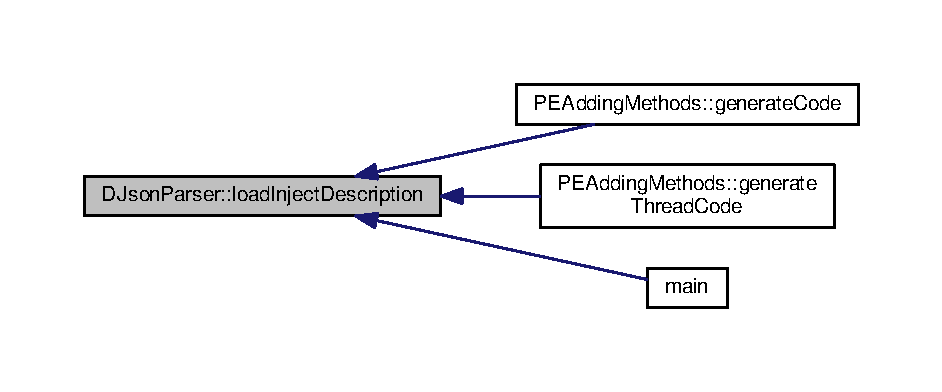
\includegraphics[width=350pt]{class_d_json_parser_a14c19cd1d981e908ef8dfbc4218b359f_icgraph}
\end{center}
\end{figure}


\hypertarget{class_d_json_parser_a3baa4948e78cb386c8eb7e6634ab4d03}{\index{D\-Json\-Parser@{D\-Json\-Parser}!load\-Inject\-Description@{load\-Inject\-Description}}
\index{load\-Inject\-Description@{load\-Inject\-Description}!DJsonParser@{D\-Json\-Parser}}
\subsubsection[{load\-Inject\-Description}]{\setlength{\rightskip}{0pt plus 5cm}template$<$typename Register $>$ template {\bf D\-Adding\-Methods\-::\-Wrapper}$<$ {\bf Registers\-\_\-x64} $>$ $\ast$ D\-Json\-Parser\-::load\-Inject\-Description (
\begin{DoxyParamCaption}
\item[{Q\-String}]{name}
\end{DoxyParamCaption}
)}}\label{class_d_json_parser_a3baa4948e78cb386c8eb7e6634ab4d03}


\hyperlink{class_d_json_parser_a14c19cd1d981e908ef8dfbc4218b359f}{D\-Json\-Parser\-::load\-Inject\-Description} tworzy obiekt Inject\-Description deserializując go z z inject\-Description.\-json. 


\begin{DoxyParams}{Parametry}
{\em name} & nazwa metody \\
\hline
\end{DoxyParams}
\begin{DoxyReturn}{Zwraca}
zwraca true w razie powodzenia false w przeciwnym wypadku 
\end{DoxyReturn}


Definicja w linii 21 pliku djsonparser.\-cpp.



Oto graf wywołań dla tej funkcji\-:
\nopagebreak
\begin{figure}[H]
\begin{center}
\leavevmode
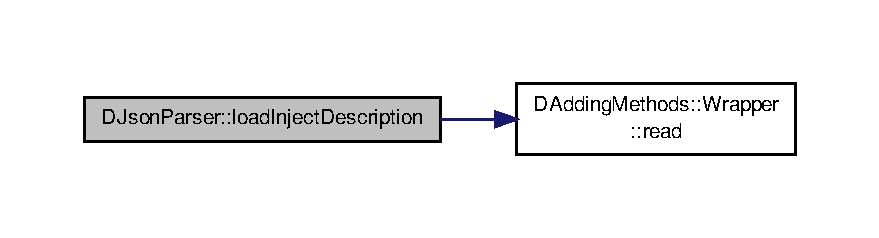
\includegraphics[width=350pt]{class_d_json_parser_a3baa4948e78cb386c8eb7e6634ab4d03_cgraph}
\end{center}
\end{figure}


\hypertarget{class_d_json_parser_a6d680ce58c2e6b638223071d996a2c0f}{\index{D\-Json\-Parser@{D\-Json\-Parser}!save\-Incject\-Description@{save\-Incject\-Description}}
\index{save\-Incject\-Description@{save\-Incject\-Description}!DJsonParser@{D\-Json\-Parser}}
\subsubsection[{save\-Incject\-Description}]{\setlength{\rightskip}{0pt plus 5cm}bool D\-Json\-Parser\-::save\-Incject\-Description (
\begin{DoxyParamCaption}
\item[{Q\-String}]{name, }
\item[{{\bf D\-Adding\-Methods\-::\-Wrapper}$<$ {\bf Registers\-\_\-x86} $>$ \&}]{injection}
\end{DoxyParamCaption}
)}}\label{class_d_json_parser_a6d680ce58c2e6b638223071d996a2c0f}


D\-Json\-Parser\-::save\-Incjection\-Description zapisuje referencje obiekt wskazywany przez injection do pliku w formacie .json. 


\begin{DoxyParams}{Parametry}
{\em injection} & referencja obiektu do zapisu \\
\hline
{\em name} & nazwa metody \\
\hline
\end{DoxyParams}
\begin{DoxyReturn}{Zwraca}
true w przypadku powodzenia false w p.\-p. 
\end{DoxyReturn}


Definicja w linii 49 pliku djsonparser.\-cpp.



\subsection{Dokumentacja atrybutów składowych}
\hypertarget{class_d_json_parser_abfae3a66c00ce3bf5f2dc5eab570a642}{\index{D\-Json\-Parser@{D\-Json\-Parser}!injection\-Read@{injection\-Read}}
\index{injection\-Read@{injection\-Read}!DJsonParser@{D\-Json\-Parser}}
\subsubsection[{injection\-Read}]{\setlength{\rightskip}{0pt plus 5cm}{\bf D\-Adding\-Methods\-::\-Wrapper}$<${\bf Registers\-\_\-x86}$>$$\ast$ D\-Json\-Parser\-::injection\-Read\hspace{0.3cm}{\ttfamily [private]}}}\label{class_d_json_parser_abfae3a66c00ce3bf5f2dc5eab570a642}


Definicja w linii 12 pliku djsonparser.\-h.

\hypertarget{class_d_json_parser_ac25fee79111d7700fa5ab08414d2c0d0}{\index{D\-Json\-Parser@{D\-Json\-Parser}!m\-\_\-path@{m\-\_\-path}}
\index{m\-\_\-path@{m\-\_\-path}!DJsonParser@{D\-Json\-Parser}}
\subsubsection[{m\-\_\-path}]{\setlength{\rightskip}{0pt plus 5cm}Q\-String D\-Json\-Parser\-::m\-\_\-path\hspace{0.3cm}{\ttfamily [private]}}}\label{class_d_json_parser_ac25fee79111d7700fa5ab08414d2c0d0}


Definicja w linii 13 pliku djsonparser.\-h.



Dokumentacja dla tej klasy została wygenerowana z plików\-:\begin{DoxyCompactItemize}
\item 
Application\-Manager/\-D\-Json\-Parser/\hyperlink{djsonparser_8h}{djsonparser.\-h}\item 
Application\-Manager/\-D\-Json\-Parser/\hyperlink{djsonparser_8cpp}{djsonparser.\-cpp}\end{DoxyCompactItemize}

\hypertarget{class_d_source_code_parser}{\section{Dokumentacja klasy D\-Source\-Code\-Parser}
\label{class_d_source_code_parser}\index{D\-Source\-Code\-Parser@{D\-Source\-Code\-Parser}}
}


{\ttfamily \#include $<$dsourcecodeparser.\-h$>$}

\subsection*{Metody publiczne}
\begin{DoxyCompactItemize}
\item 
\hyperlink{class_d_source_code_parser_adc1af3adbbe65247fcf93aedf8d72a4b}{D\-Source\-Code\-Parser} ()
\item 
Q\-String\-List \hyperlink{class_d_source_code_parser_a2bc1f34f3cf29f7f8e4e867dace9721f}{get\-Functions} (const Q\-String \&path)
\item 
void \hyperlink{class_d_source_code_parser_acb80a33d6f64af51009f3a09fbfd430b}{insert\-Methods} (const Q\-String \&path, F\-I\-D\-Mapping$<$ \hyperlink{codedefines_8h_a0f84efe4ca4d99203713a78bd6e8c82e}{Registers\-\_\-x86} $>$)
\end{DoxyCompactItemize}


\subsection{Opis szczegółowy}


Definicja w linii 17 pliku dsourcecodeparser.\-h.



\subsection{Dokumentacja konstruktora i destruktora}
\hypertarget{class_d_source_code_parser_adc1af3adbbe65247fcf93aedf8d72a4b}{\index{D\-Source\-Code\-Parser@{D\-Source\-Code\-Parser}!D\-Source\-Code\-Parser@{D\-Source\-Code\-Parser}}
\index{D\-Source\-Code\-Parser@{D\-Source\-Code\-Parser}!DSourceCodeParser@{D\-Source\-Code\-Parser}}
\subsubsection[{D\-Source\-Code\-Parser}]{\setlength{\rightskip}{0pt plus 5cm}D\-Source\-Code\-Parser\-::\-D\-Source\-Code\-Parser (
\begin{DoxyParamCaption}
{}
\end{DoxyParamCaption}
)}}\label{class_d_source_code_parser_adc1af3adbbe65247fcf93aedf8d72a4b}


Definicja w linii 4 pliku dsourcecodeparser.\-cpp.



\subsection{Dokumentacja funkcji składowych}
\hypertarget{class_d_source_code_parser_a2bc1f34f3cf29f7f8e4e867dace9721f}{\index{D\-Source\-Code\-Parser@{D\-Source\-Code\-Parser}!get\-Functions@{get\-Functions}}
\index{get\-Functions@{get\-Functions}!DSourceCodeParser@{D\-Source\-Code\-Parser}}
\subsubsection[{get\-Functions}]{\setlength{\rightskip}{0pt plus 5cm}Q\-String\-List D\-Source\-Code\-Parser\-::get\-Functions (
\begin{DoxyParamCaption}
\item[{const Q\-String \&}]{path}
\end{DoxyParamCaption}
)}}\label{class_d_source_code_parser_a2bc1f34f3cf29f7f8e4e867dace9721f}


Definicja w linii 9 pliku dsourcecodeparser.\-cpp.

\hypertarget{class_d_source_code_parser_acb80a33d6f64af51009f3a09fbfd430b}{\index{D\-Source\-Code\-Parser@{D\-Source\-Code\-Parser}!insert\-Methods@{insert\-Methods}}
\index{insert\-Methods@{insert\-Methods}!DSourceCodeParser@{D\-Source\-Code\-Parser}}
\subsubsection[{insert\-Methods}]{\setlength{\rightskip}{0pt plus 5cm}void D\-Source\-Code\-Parser\-::insert\-Methods (
\begin{DoxyParamCaption}
\item[{const Q\-String \&}]{path, }
\item[{F\-I\-D\-Mapping$<$ {\bf Registers\-\_\-x86} $>$}]{map}
\end{DoxyParamCaption}
)}}\label{class_d_source_code_parser_acb80a33d6f64af51009f3a09fbfd430b}


Definicja w linii 45 pliku dsourcecodeparser.\-cpp.



Dokumentacja dla tej klasy została wygenerowana z plików\-:\begin{DoxyCompactItemize}
\item 
Application\-Manager/\-D\-Source\-Code\-Parser/\hyperlink{dsourcecodeparser_8h}{dsourcecodeparser.\-h}\item 
Application\-Manager/\-D\-Source\-Code\-Parser/\hyperlink{dsourcecodeparser_8cpp}{dsourcecodeparser.\-cpp}\end{DoxyCompactItemize}

\hypertarget{class_e_l_f}{\section{Dokumentacja klasy E\-L\-F}
\label{class_e_l_f}\index{E\-L\-F@{E\-L\-F}}
}


{\ttfamily \#include $<$elffile.\-h$>$}



Diagram dziedziczenia dla E\-L\-F\nopagebreak
\begin{figure}[H]
\begin{center}
\leavevmode
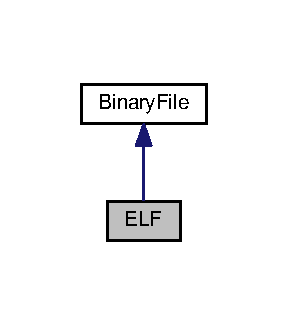
\includegraphics[width=140pt]{class_e_l_f__inherit__graph}
\end{center}
\end{figure}


Diagram współpracy dla E\-L\-F\-:\nopagebreak
\begin{figure}[H]
\begin{center}
\leavevmode
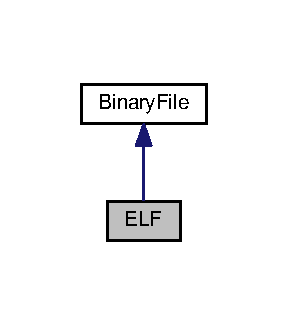
\includegraphics[width=140pt]{class_e_l_f__coll__graph}
\end{center}
\end{figure}
\subsection*{Komponenty}
\begin{DoxyCompactItemize}
\item 
struct {\bfseries \-\_\-best\-\_\-segment}
\item 
struct {\bfseries \-\_\-section\-\_\-info}
\end{DoxyCompactItemize}
\subsection*{Typy publiczne}
\begin{DoxyCompactItemize}
\item 
enum \hyperlink{class_e_l_f_abaebdfb7048441e430684d68df8d73d1}{Section\-Type} 
\begin{DoxyCompactList}\small\item\em Type sekcji. \end{DoxyCompactList}\end{DoxyCompactItemize}
\subsection*{Metody publiczne}
\begin{DoxyCompactItemize}
\item 
\hyperlink{class_e_l_f_a7bcefdc63dcaee056a3800f57cf73992}{E\-L\-F} (Q\-Byte\-Array \-\_\-data)
\begin{DoxyCompactList}\small\item\em Konstruktor. \end{DoxyCompactList}\item 
virtual \hyperlink{class_e_l_f_a8d420911533a8753e9936cb5c9238747}{$\sim$\-E\-L\-F} ()
\begin{DoxyCompactList}\small\item\em Destruktor. \end{DoxyCompactList}\item 
const Q\-Byte\-Array \& \hyperlink{class_e_l_f_ad2f8a0a47d56ee33a9234c9415414e00}{get\-\_\-elf\-\_\-content} () const 
\begin{DoxyCompactList}\small\item\em Pobiera zawartość pliku. \end{DoxyCompactList}\item 
bool \hyperlink{class_e_l_f_aaf0da9f62b61fc3674b7fd54d9885b5f}{is\-\_\-valid} () const 
\begin{DoxyCompactList}\small\item\em Sprawdza czy w pamięci przechowywany jest poprawny plik. \end{DoxyCompactList}\item 
bool \hyperlink{class_e_l_f_ac5c89b2b437f3e07aedc06f66cdab94d}{is\-\_\-x86} () const 
\begin{DoxyCompactList}\small\item\em Dostarcza informacje czy plik jest poprawnym plikiem \hyperlink{class_e_l_f}{E\-L\-F} 32-\/bitowym. \end{DoxyCompactList}\item 
bool \hyperlink{class_e_l_f_a558b2f169db21b21b24d6ff19c38ac9e}{is\-\_\-x64} () const 
\begin{DoxyCompactList}\small\item\em Dostarcza informacje czy plik jest poprawnym plikiem \hyperlink{class_e_l_f}{E\-L\-F} 64-\/bitowym. \end{DoxyCompactList}\item 
int \hyperlink{class_e_l_f_a8b65b7ea1b57aa25d3171a25528a43f8}{get\-\_\-number\-\_\-of\-\_\-segments} () const 
\begin{DoxyCompactList}\small\item\em Pobiera ilość segmentów w pliku. \end{DoxyCompactList}\item 
void $\ast$ \hyperlink{class_e_l_f_abdddb77f2822c068b2ae06e221ae1e10}{get\-\_\-ph\-\_\-seg\-\_\-offset} (uint32\-\_\-t idx=0)
\begin{DoxyCompactList}\small\item\em Pobiera offset w pliku dla podanego segmentu. \end{DoxyCompactList}\item 
bool \hyperlink{class_e_l_f_a11f004629212a5651dd4ca1355a7eb9d}{extend\-\_\-segment} (const Q\-Byte\-Array \&data, bool only\-\_\-x, \hyperlink{elf_8h_aeed51d08e3a950d637f8ec1f0cd4ef65}{Elf64\-\_\-\-Addr} \&va)
\begin{DoxyCompactList}\small\item\em Rozszerza najbardziej pasujący segment L\-O\-A\-D i kopiuje do niego podany kod. \end{DoxyCompactList}\item 
bool \hyperlink{class_e_l_f_a52b09dc778fd67aa92d1a80a96e9f580}{write\-\_\-to\-\_\-file} (const Q\-String \&fname) const 
\begin{DoxyCompactList}\small\item\em Zapisuje wewnętrzne dane do pliku. \end{DoxyCompactList}\item 
bool \hyperlink{class_e_l_f_a8342542081d52e5518356f0f6cde3db8}{set\-\_\-entry\-\_\-point} (const \hyperlink{elf_8h_aeed51d08e3a950d637f8ec1f0cd4ef65}{Elf64\-\_\-\-Addr} \&entry\-\_\-point, \hyperlink{elf_8h_aeed51d08e3a950d637f8ec1f0cd4ef65}{Elf64\-\_\-\-Addr} $\ast$old\-\_\-ep=nullptr)
\begin{DoxyCompactList}\small\item\em Ustawia punkt wejściowy dla pliku wykonywalnego. \end{DoxyCompactList}\item 
bool \hyperlink{class_e_l_f_adf71ac4ae5cfedb1b1415b2f5da2494f}{get\-\_\-entry\-\_\-point} (\hyperlink{elf_8h_aeed51d08e3a950d637f8ec1f0cd4ef65}{Elf64\-\_\-\-Addr} \&old\-\_\-ep) const 
\begin{DoxyCompactList}\small\item\em Dostarcza informacje o punkcie wejściowym pliku. \end{DoxyCompactList}\item 
bool \hyperlink{class_e_l_f_aaa7edcb97e8cd8b0ca759d7df7984b12}{get\-\_\-section\-\_\-content} (\hyperlink{class_e_l_f_abaebdfb7048441e430684d68df8d73d1}{Section\-Type} sec\-\_\-type, Q\-Pair$<$ Q\-Byte\-Array, \hyperlink{elf_8h_aeed51d08e3a950d637f8ec1f0cd4ef65}{Elf64\-\_\-\-Addr} $>$ \&section\-\_\-data)
\begin{DoxyCompactList}\small\item\em Pobiera zawartość sekcji, jeżeli podana sekcja istnieje. \end{DoxyCompactList}\item 
bool \hyperlink{class_e_l_f_af326c6489cd6953ae4d21ba194c76d41}{get\-\_\-section\-\_\-file\-\_\-off} (\hyperlink{class_e_l_f_abaebdfb7048441e430684d68df8d73d1}{Section\-Type} sec\-\_\-type, \hyperlink{elf_8h_aeed51d08e3a950d637f8ec1f0cd4ef65}{Elf64\-\_\-\-Addr} \&file\-\_\-off)
\begin{DoxyCompactList}\small\item\em Pobiera offset sekcji w pliku, jeżeli podana sekcja istnieje. \end{DoxyCompactList}\item 
bool \hyperlink{class_e_l_f_aede545aa3f960b681a4a7b9be8f67833}{set\-\_\-section\-\_\-content} (\hyperlink{class_e_l_f_abaebdfb7048441e430684d68df8d73d1}{Section\-Type} sec\-\_\-type, const Q\-Byte\-Array \&section\-\_\-data, const char filler= '\textbackslash{}x00')
\begin{DoxyCompactList}\small\item\em Zamienia zawartość sekcji nowymi danymi, jeżeli podana sekcja istnieje. \end{DoxyCompactList}\item 
bool \hyperlink{class_e_l_f_a6844855ce268b49bb39b75e117bad008}{set\-\_\-relative\-\_\-address} (\hyperlink{elf_8h_a6f7837bc80df7a68291fce54ff088849}{Elf64\-\_\-\-Off} file\-\_\-off, \hyperlink{elf_8h_a40c6d4571e6001f443cc6a6474620158}{Elf32\-\_\-\-Addr} rva)
\begin{DoxyCompactList}\small\item\em Ustawia nowy adres instrukcji dla skoku relatywnego. \end{DoxyCompactList}\item 
bool \hyperlink{class_e_l_f_ac6ba067b4210f37293eff8483edaa883}{get\-\_\-segment\-\_\-prot\-\_\-flags} (const \hyperlink{elf_8h_aeed51d08e3a950d637f8ec1f0cd4ef65}{Elf64\-\_\-\-Addr} vaddr, int \&prot\-\_\-flags) const 
\begin{DoxyCompactList}\small\item\em Pobiera flagi ochrony pamięci dla segmentu, który ładuje się pod podanym adresem wirtualnym. \end{DoxyCompactList}\item 
bool \hyperlink{class_e_l_f_ad1eda85b8a7dc46325193c19074dd468}{get\-\_\-segment\-\_\-align} (const \hyperlink{elf_8h_aeed51d08e3a950d637f8ec1f0cd4ef65}{Elf64\-\_\-\-Addr} vaddr, \hyperlink{elf_8h_aeed51d08e3a950d637f8ec1f0cd4ef65}{Elf64\-\_\-\-Addr} \&align) const 
\begin{DoxyCompactList}\small\item\em Pobiera wartość wyrównania segmentu. \end{DoxyCompactList}\item 
bool \hyperlink{class_e_l_f_a48849fcd82256a378da6f6cfb4d7001a}{get\-\_\-load\-\_\-segment\-\_\-info} (int prot\-\_\-flags, Q\-Pair$<$ Q\-Byte\-Array, \hyperlink{elf_8h_aeed51d08e3a950d637f8ec1f0cd4ef65}{Elf64\-\_\-\-Addr} $>$ \&segment\-\_\-data) const 
\begin{DoxyCompactList}\small\item\em Pobiera zawartość pierwszego segmenu L\-O\-A\-D, do którego pasują podane flagi ochrony pamięci. \end{DoxyCompactList}\item 
bool \hyperlink{class_e_l_f_a480f02b85a48aa18c1bc1ae23dba2b2f}{get\-\_\-relative\-\_\-address} (\hyperlink{elf_8h_a6f7837bc80df7a68291fce54ff088849}{Elf64\-\_\-\-Off} file\-\_\-off, int32\-\_\-t \&rva) const 
\begin{DoxyCompactList}\small\item\em Pobiera aktualną wartość adresu relatywnego dla skoku. \end{DoxyCompactList}\end{DoxyCompactItemize}
\subsection*{Dodatkowe Dziedziczone Składowe}


\subsection{Opis szczegółowy}


Definicja w linii 20 pliku elffile.\-h.



\subsection{Dokumentacja składowych wyliczanych}
\hypertarget{class_e_l_f_abaebdfb7048441e430684d68df8d73d1}{\index{E\-L\-F@{E\-L\-F}!Section\-Type@{Section\-Type}}
\index{Section\-Type@{Section\-Type}!ELF@{E\-L\-F}}
\subsubsection[{Section\-Type}]{\setlength{\rightskip}{0pt plus 5cm}enum {\bf E\-L\-F\-::\-Section\-Type}}}\label{class_e_l_f_abaebdfb7048441e430684d68df8d73d1}


Type sekcji. 



Definicja w linii 25 pliku elffile.\-h.



\subsection{Dokumentacja konstruktora i destruktora}
\hypertarget{class_e_l_f_a7bcefdc63dcaee056a3800f57cf73992}{\index{E\-L\-F@{E\-L\-F}!E\-L\-F@{E\-L\-F}}
\index{E\-L\-F@{E\-L\-F}!ELF@{E\-L\-F}}
\subsubsection[{E\-L\-F}]{\setlength{\rightskip}{0pt plus 5cm}E\-L\-F\-::\-E\-L\-F (
\begin{DoxyParamCaption}
\item[{Q\-Byte\-Array}]{\-\_\-data}
\end{DoxyParamCaption}
)}}\label{class_e_l_f_a7bcefdc63dcaee056a3800f57cf73992}


Konstruktor. 


\begin{DoxyParams}{Parametry}
{\em \-\_\-data} & zawartość pliku. \\
\hline
\end{DoxyParams}


Definicja w linii 940 pliku elffile.\-cpp.

\hypertarget{class_e_l_f_a8d420911533a8753e9936cb5c9238747}{\index{E\-L\-F@{E\-L\-F}!$\sim$\-E\-L\-F@{$\sim$\-E\-L\-F}}
\index{$\sim$\-E\-L\-F@{$\sim$\-E\-L\-F}!ELF@{E\-L\-F}}
\subsubsection[{$\sim$\-E\-L\-F}]{\setlength{\rightskip}{0pt plus 5cm}E\-L\-F\-::$\sim$\-E\-L\-F (
\begin{DoxyParamCaption}
{}
\end{DoxyParamCaption}
)\hspace{0.3cm}{\ttfamily [virtual]}}}\label{class_e_l_f_a8d420911533a8753e9936cb5c9238747}


Destruktor. 



Definicja w linii 946 pliku elffile.\-cpp.



\subsection{Dokumentacja funkcji składowych}
\hypertarget{class_e_l_f_a11f004629212a5651dd4ca1355a7eb9d}{\index{E\-L\-F@{E\-L\-F}!extend\-\_\-segment@{extend\-\_\-segment}}
\index{extend\-\_\-segment@{extend\-\_\-segment}!ELF@{E\-L\-F}}
\subsubsection[{extend\-\_\-segment}]{\setlength{\rightskip}{0pt plus 5cm}bool E\-L\-F\-::extend\-\_\-segment (
\begin{DoxyParamCaption}
\item[{const Q\-Byte\-Array \&}]{data, }
\item[{bool}]{only\-\_\-x, }
\item[{{\bf Elf64\-\_\-\-Addr} \&}]{va}
\end{DoxyParamCaption}
)}}\label{class_e_l_f_a11f004629212a5651dd4ca1355a7eb9d}


Rozszerza najbardziej pasujący segment L\-O\-A\-D i kopiuje do niego podany kod. 


\begin{DoxyParams}{Parametry}
{\em data} & dane, które chcemy skopiować w miejsce rozszerzonego segmentu. \\
\hline
{\em only\-\_\-x} & flaga, która odpowiada za rozszerzanie tylko wykonywalnych sekcji. \\
\hline
{\em va} & nowy adres wirtualny w rozszerzonym segmencie. \\
\hline
\end{DoxyParams}
\begin{DoxyReturn}{Zwraca}
True jeżeli rozszerzenie się powiodło, False w pozostałych przypadkach. 
\end{DoxyReturn}


Definicja w linii 31 pliku elffile.\-cpp.

\hypertarget{class_e_l_f_ad2f8a0a47d56ee33a9234c9415414e00}{\index{E\-L\-F@{E\-L\-F}!get\-\_\-elf\-\_\-content@{get\-\_\-elf\-\_\-content}}
\index{get\-\_\-elf\-\_\-content@{get\-\_\-elf\-\_\-content}!ELF@{E\-L\-F}}
\subsubsection[{get\-\_\-elf\-\_\-content}]{\setlength{\rightskip}{0pt plus 5cm}const Q\-Byte\-Array\& E\-L\-F\-::get\-\_\-elf\-\_\-content (
\begin{DoxyParamCaption}
{}
\end{DoxyParamCaption}
) const\hspace{0.3cm}{\ttfamily [inline]}}}\label{class_e_l_f_ad2f8a0a47d56ee33a9234c9415414e00}


Pobiera zawartość pliku. 

\begin{DoxyReturn}{Zwraca}
Zawartość aktualnie analizowalnego pliku. 
\end{DoxyReturn}


Definicja w linii 47 pliku elffile.\-h.

\hypertarget{class_e_l_f_adf71ac4ae5cfedb1b1415b2f5da2494f}{\index{E\-L\-F@{E\-L\-F}!get\-\_\-entry\-\_\-point@{get\-\_\-entry\-\_\-point}}
\index{get\-\_\-entry\-\_\-point@{get\-\_\-entry\-\_\-point}!ELF@{E\-L\-F}}
\subsubsection[{get\-\_\-entry\-\_\-point}]{\setlength{\rightskip}{0pt plus 5cm}bool E\-L\-F\-::get\-\_\-entry\-\_\-point (
\begin{DoxyParamCaption}
\item[{{\bf Elf64\-\_\-\-Addr} \&}]{old\-\_\-ep}
\end{DoxyParamCaption}
) const}}\label{class_e_l_f_adf71ac4ae5cfedb1b1415b2f5da2494f}


Dostarcza informacje o punkcie wejściowym pliku. 


\begin{DoxyParams}{Parametry}
{\em old\-\_\-ep} & referencja na wartość punktu wejściowego programu. \\
\hline
\end{DoxyParams}
\begin{DoxyReturn}{Zwraca}
True jeżeli operacja się powiodła, False w innych przypadkach. 
\end{DoxyReturn}


Definicja w linii 181 pliku elffile.\-cpp.

\hypertarget{class_e_l_f_a48849fcd82256a378da6f6cfb4d7001a}{\index{E\-L\-F@{E\-L\-F}!get\-\_\-load\-\_\-segment\-\_\-info@{get\-\_\-load\-\_\-segment\-\_\-info}}
\index{get\-\_\-load\-\_\-segment\-\_\-info@{get\-\_\-load\-\_\-segment\-\_\-info}!ELF@{E\-L\-F}}
\subsubsection[{get\-\_\-load\-\_\-segment\-\_\-info}]{\setlength{\rightskip}{0pt plus 5cm}bool E\-L\-F\-::get\-\_\-load\-\_\-segment\-\_\-info (
\begin{DoxyParamCaption}
\item[{int}]{prot\-\_\-flags, }
\item[{Q\-Pair$<$ Q\-Byte\-Array, {\bf Elf64\-\_\-\-Addr} $>$ \&}]{segment\-\_\-data}
\end{DoxyParamCaption}
) const}}\label{class_e_l_f_a48849fcd82256a378da6f6cfb4d7001a}


Pobiera zawartość pierwszego segmenu L\-O\-A\-D, do którego pasują podane flagi ochrony pamięci. 


\begin{DoxyParams}{Parametry}
{\em prot\-\_\-flags} & flagi ochrony pamięci. \\
\hline
{\em segment\-\_\-data} & zawartość segmentu oraz adres wirtualny. \\
\hline
\end{DoxyParams}
\begin{DoxyReturn}{Zwraca}
True jeżeli segment istnieje, False w innych przypadkach. 
\end{DoxyReturn}


Definicja w linii 834 pliku elffile.\-cpp.

\hypertarget{class_e_l_f_a8b65b7ea1b57aa25d3171a25528a43f8}{\index{E\-L\-F@{E\-L\-F}!get\-\_\-number\-\_\-of\-\_\-segments@{get\-\_\-number\-\_\-of\-\_\-segments}}
\index{get\-\_\-number\-\_\-of\-\_\-segments@{get\-\_\-number\-\_\-of\-\_\-segments}!ELF@{E\-L\-F}}
\subsubsection[{get\-\_\-number\-\_\-of\-\_\-segments}]{\setlength{\rightskip}{0pt plus 5cm}int E\-L\-F\-::get\-\_\-number\-\_\-of\-\_\-segments (
\begin{DoxyParamCaption}
{}
\end{DoxyParamCaption}
) const\hspace{0.3cm}{\ttfamily [inline]}}}\label{class_e_l_f_a8b65b7ea1b57aa25d3171a25528a43f8}


Pobiera ilość segmentów w pliku. 

\begin{DoxyReturn}{Zwraca}
Ilość segmentów w pliku, -\/1 w razie błędu. 
\end{DoxyReturn}


Definicja w linii 71 pliku elffile.\-h.



Oto graf wywołań dla tej funkcji\-:\nopagebreak
\begin{figure}[H]
\begin{center}
\leavevmode
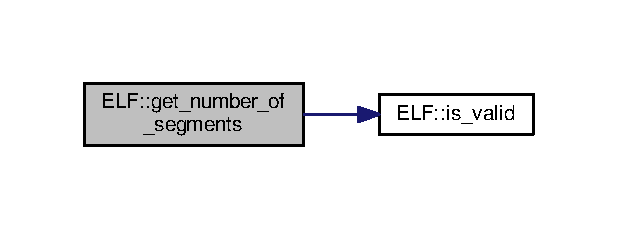
\includegraphics[width=296pt]{class_e_l_f_a8b65b7ea1b57aa25d3171a25528a43f8_cgraph}
\end{center}
\end{figure}


\hypertarget{class_e_l_f_abdddb77f2822c068b2ae06e221ae1e10}{\index{E\-L\-F@{E\-L\-F}!get\-\_\-ph\-\_\-seg\-\_\-offset@{get\-\_\-ph\-\_\-seg\-\_\-offset}}
\index{get\-\_\-ph\-\_\-seg\-\_\-offset@{get\-\_\-ph\-\_\-seg\-\_\-offset}!ELF@{E\-L\-F}}
\subsubsection[{get\-\_\-ph\-\_\-seg\-\_\-offset}]{\setlength{\rightskip}{0pt plus 5cm}void $\ast$ E\-L\-F\-::get\-\_\-ph\-\_\-seg\-\_\-offset (
\begin{DoxyParamCaption}
\item[{uint32\-\_\-t}]{idx = {\ttfamily 0}}
\end{DoxyParamCaption}
)}}\label{class_e_l_f_abdddb77f2822c068b2ae06e221ae1e10}


Pobiera offset w pliku dla podanego segmentu. 


\begin{DoxyParams}{Parametry}
{\em idx} & indeks segmentu. \\
\hline
\end{DoxyParams}
\begin{DoxyReturn}{Zwraca}
Offset jeżeli dane są poprawne, nullptr w innych przypadkach. 
\end{DoxyReturn}


Definicja w linii 17 pliku elffile.\-cpp.

\hypertarget{class_e_l_f_a480f02b85a48aa18c1bc1ae23dba2b2f}{\index{E\-L\-F@{E\-L\-F}!get\-\_\-relative\-\_\-address@{get\-\_\-relative\-\_\-address}}
\index{get\-\_\-relative\-\_\-address@{get\-\_\-relative\-\_\-address}!ELF@{E\-L\-F}}
\subsubsection[{get\-\_\-relative\-\_\-address}]{\setlength{\rightskip}{0pt plus 5cm}bool E\-L\-F\-::get\-\_\-relative\-\_\-address (
\begin{DoxyParamCaption}
\item[{{\bf Elf64\-\_\-\-Off}}]{file\-\_\-off, }
\item[{int32\-\_\-t \&}]{rva}
\end{DoxyParamCaption}
) const}}\label{class_e_l_f_a480f02b85a48aa18c1bc1ae23dba2b2f}


Pobiera aktualną wartość adresu relatywnego dla skoku. 


\begin{DoxyParams}{Parametry}
{\em file\-\_\-off} & offset w pliku. \\
\hline
\end{DoxyParams}
\begin{DoxyReturn}{Zwraca}
True jeżeli operacja się powiodła, False w innych przypadkach. 
\end{DoxyReturn}


Definicja w linii 850 pliku elffile.\-cpp.

\hypertarget{class_e_l_f_aaa7edcb97e8cd8b0ca759d7df7984b12}{\index{E\-L\-F@{E\-L\-F}!get\-\_\-section\-\_\-content@{get\-\_\-section\-\_\-content}}
\index{get\-\_\-section\-\_\-content@{get\-\_\-section\-\_\-content}!ELF@{E\-L\-F}}
\subsubsection[{get\-\_\-section\-\_\-content}]{\setlength{\rightskip}{0pt plus 5cm}bool E\-L\-F\-::get\-\_\-section\-\_\-content (
\begin{DoxyParamCaption}
\item[{{\bf E\-L\-F\-::\-Section\-Type}}]{sec\-\_\-type, }
\item[{Q\-Pair$<$ Q\-Byte\-Array, {\bf Elf64\-\_\-\-Addr} $>$ \&}]{section\-\_\-data}
\end{DoxyParamCaption}
)}}\label{class_e_l_f_aaa7edcb97e8cd8b0ca759d7df7984b12}


Pobiera zawartość sekcji, jeżeli podana sekcja istnieje. 


\begin{DoxyParams}{Parametry}
{\em sec\-\_\-type} & typ sekcji. \\
\hline
{\em section\-\_\-data} & zawartość sekcji oraz adres witualny. \\
\hline
\end{DoxyParams}
\begin{DoxyReturn}{Zwraca}
True jeżeli sekcja istnieje, False w innych przypadkach. 
\end{DoxyReturn}


Definicja w linii 187 pliku elffile.\-cpp.

\hypertarget{class_e_l_f_af326c6489cd6953ae4d21ba194c76d41}{\index{E\-L\-F@{E\-L\-F}!get\-\_\-section\-\_\-file\-\_\-off@{get\-\_\-section\-\_\-file\-\_\-off}}
\index{get\-\_\-section\-\_\-file\-\_\-off@{get\-\_\-section\-\_\-file\-\_\-off}!ELF@{E\-L\-F}}
\subsubsection[{get\-\_\-section\-\_\-file\-\_\-off}]{\setlength{\rightskip}{0pt plus 5cm}bool E\-L\-F\-::get\-\_\-section\-\_\-file\-\_\-off (
\begin{DoxyParamCaption}
\item[{{\bf Section\-Type}}]{sec\-\_\-type, }
\item[{{\bf Elf64\-\_\-\-Addr} \&}]{file\-\_\-off}
\end{DoxyParamCaption}
)}}\label{class_e_l_f_af326c6489cd6953ae4d21ba194c76d41}


Pobiera offset sekcji w pliku, jeżeli podana sekcja istnieje. 


\begin{DoxyParams}{Parametry}
{\em sec\-\_\-type} & typ sekcji. \\
\hline
{\em file\-\_\-off} & offset sekcji w pliku. \\
\hline
\end{DoxyParams}
\begin{DoxyReturn}{Zwraca}
True jeżeli sekcja istnieje, False w innych przypadkach. 
\end{DoxyReturn}


Definicja w linii 247 pliku elffile.\-cpp.

\hypertarget{class_e_l_f_ad1eda85b8a7dc46325193c19074dd468}{\index{E\-L\-F@{E\-L\-F}!get\-\_\-segment\-\_\-align@{get\-\_\-segment\-\_\-align}}
\index{get\-\_\-segment\-\_\-align@{get\-\_\-segment\-\_\-align}!ELF@{E\-L\-F}}
\subsubsection[{get\-\_\-segment\-\_\-align}]{\setlength{\rightskip}{0pt plus 5cm}bool E\-L\-F\-::get\-\_\-segment\-\_\-align (
\begin{DoxyParamCaption}
\item[{const {\bf Elf64\-\_\-\-Addr}}]{vaddr, }
\item[{{\bf Elf64\-\_\-\-Addr} \&}]{align}
\end{DoxyParamCaption}
) const}}\label{class_e_l_f_ad1eda85b8a7dc46325193c19074dd468}


Pobiera wartość wyrównania segmentu. 


\begin{DoxyParams}{Parametry}
{\em vaddr} & adres wirtualny pod który ładuje segment. \\
\hline
{\em align} & wartość wyrównywania strony. \\
\hline
\end{DoxyParams}
\begin{DoxyReturn}{Zwraca}
True jeżeli segment istnieje, False w innych przypadkach. 
\end{DoxyReturn}


Definicja w linii 800 pliku elffile.\-cpp.

\hypertarget{class_e_l_f_ac6ba067b4210f37293eff8483edaa883}{\index{E\-L\-F@{E\-L\-F}!get\-\_\-segment\-\_\-prot\-\_\-flags@{get\-\_\-segment\-\_\-prot\-\_\-flags}}
\index{get\-\_\-segment\-\_\-prot\-\_\-flags@{get\-\_\-segment\-\_\-prot\-\_\-flags}!ELF@{E\-L\-F}}
\subsubsection[{get\-\_\-segment\-\_\-prot\-\_\-flags}]{\setlength{\rightskip}{0pt plus 5cm}bool E\-L\-F\-::get\-\_\-segment\-\_\-prot\-\_\-flags (
\begin{DoxyParamCaption}
\item[{const {\bf Elf64\-\_\-\-Addr}}]{vaddr, }
\item[{int \&}]{prot\-\_\-flags}
\end{DoxyParamCaption}
) const}}\label{class_e_l_f_ac6ba067b4210f37293eff8483edaa883}


Pobiera flagi ochrony pamięci dla segmentu, który ładuje się pod podanym adresem wirtualnym. 


\begin{DoxyParams}{Parametry}
{\em vaddr} & adres wirtualny pod który ładuje segment. \\
\hline
{\em prot\-\_\-flags} & flagi ochrony pamięci. \\
\hline
\end{DoxyParams}
\begin{DoxyReturn}{Zwraca}
True jeżeli segment istnieje, False w innych przypadkach. 
\end{DoxyReturn}


Definicja w linii 766 pliku elffile.\-cpp.

\hypertarget{class_e_l_f_aaf0da9f62b61fc3674b7fd54d9885b5f}{\index{E\-L\-F@{E\-L\-F}!is\-\_\-valid@{is\-\_\-valid}}
\index{is\-\_\-valid@{is\-\_\-valid}!ELF@{E\-L\-F}}
\subsubsection[{is\-\_\-valid}]{\setlength{\rightskip}{0pt plus 5cm}bool E\-L\-F\-::is\-\_\-valid (
\begin{DoxyParamCaption}
{}
\end{DoxyParamCaption}
) const\hspace{0.3cm}{\ttfamily [inline]}, {\ttfamily [virtual]}}}\label{class_e_l_f_aaf0da9f62b61fc3674b7fd54d9885b5f}


Sprawdza czy w pamięci przechowywany jest poprawny plik. 

\begin{DoxyReturn}{Zwraca}
True jeżeli poprawny, False w innym przypadku. 
\end{DoxyReturn}


Implementuje \hyperlink{class_binary_file_a6007435bc4451bb80a3169d977f4f125}{Binary\-File}.



Definicja w linii 53 pliku elffile.\-h.

\hypertarget{class_e_l_f_a558b2f169db21b21b24d6ff19c38ac9e}{\index{E\-L\-F@{E\-L\-F}!is\-\_\-x64@{is\-\_\-x64}}
\index{is\-\_\-x64@{is\-\_\-x64}!ELF@{E\-L\-F}}
\subsubsection[{is\-\_\-x64}]{\setlength{\rightskip}{0pt plus 5cm}bool E\-L\-F\-::is\-\_\-x64 (
\begin{DoxyParamCaption}
{}
\end{DoxyParamCaption}
) const\hspace{0.3cm}{\ttfamily [inline]}, {\ttfamily [virtual]}}}\label{class_e_l_f_a558b2f169db21b21b24d6ff19c38ac9e}


Dostarcza informacje czy plik jest poprawnym plikiem \hyperlink{class_e_l_f}{E\-L\-F} 64-\/bitowym. 

\begin{DoxyReturn}{Zwraca}
True jezeli spełnia warunki, False w pozostałych przypadkach. 
\end{DoxyReturn}


Implementuje \hyperlink{class_binary_file_a36b7998c72bbee68ab492d93368c14ca}{Binary\-File}.



Definicja w linii 65 pliku elffile.\-h.



Oto graf wywołań dla tej funkcji\-:\nopagebreak
\begin{figure}[H]
\begin{center}
\leavevmode
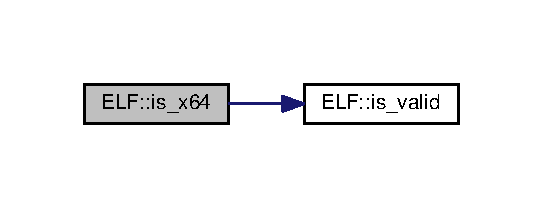
\includegraphics[width=260pt]{class_e_l_f_a558b2f169db21b21b24d6ff19c38ac9e_cgraph}
\end{center}
\end{figure}


\hypertarget{class_e_l_f_ac5c89b2b437f3e07aedc06f66cdab94d}{\index{E\-L\-F@{E\-L\-F}!is\-\_\-x86@{is\-\_\-x86}}
\index{is\-\_\-x86@{is\-\_\-x86}!ELF@{E\-L\-F}}
\subsubsection[{is\-\_\-x86}]{\setlength{\rightskip}{0pt plus 5cm}bool E\-L\-F\-::is\-\_\-x86 (
\begin{DoxyParamCaption}
{}
\end{DoxyParamCaption}
) const\hspace{0.3cm}{\ttfamily [inline]}, {\ttfamily [virtual]}}}\label{class_e_l_f_ac5c89b2b437f3e07aedc06f66cdab94d}


Dostarcza informacje czy plik jest poprawnym plikiem \hyperlink{class_e_l_f}{E\-L\-F} 32-\/bitowym. 

\begin{DoxyReturn}{Zwraca}
True jezeli spełnia warunki, False w pozostałych przypadkach. 
\end{DoxyReturn}


Implementuje \hyperlink{class_binary_file_aa7d43cde4ab8cc9723d2b5c769719bd9}{Binary\-File}.



Definicja w linii 59 pliku elffile.\-h.



Oto graf wywołań dla tej funkcji\-:\nopagebreak
\begin{figure}[H]
\begin{center}
\leavevmode
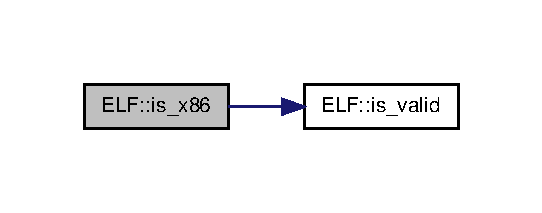
\includegraphics[width=260pt]{class_e_l_f_ac5c89b2b437f3e07aedc06f66cdab94d_cgraph}
\end{center}
\end{figure}


\hypertarget{class_e_l_f_a8342542081d52e5518356f0f6cde3db8}{\index{E\-L\-F@{E\-L\-F}!set\-\_\-entry\-\_\-point@{set\-\_\-entry\-\_\-point}}
\index{set\-\_\-entry\-\_\-point@{set\-\_\-entry\-\_\-point}!ELF@{E\-L\-F}}
\subsubsection[{set\-\_\-entry\-\_\-point}]{\setlength{\rightskip}{0pt plus 5cm}bool E\-L\-F\-::set\-\_\-entry\-\_\-point (
\begin{DoxyParamCaption}
\item[{const {\bf Elf64\-\_\-\-Addr} \&}]{entry\-\_\-point, }
\item[{{\bf Elf64\-\_\-\-Addr} $\ast$}]{old\-\_\-ep = {\ttfamily nullptr}}
\end{DoxyParamCaption}
)}}\label{class_e_l_f_a8342542081d52e5518356f0f6cde3db8}


Ustawia punkt wejściowy dla pliku wykonywalnego. 


\begin{DoxyParams}{Parametry}
{\em entry\-\_\-point} & wartość punktu wejściowego. \\
\hline
{\em old\-\_\-ep} & wartosc starego punkt wejsciowego, parametr opcjonalny. \\
\hline
\end{DoxyParams}
\begin{DoxyReturn}{Zwraca}
True jeżeli operacja się powiodła, False w innych przypadkach. 
\end{DoxyReturn}


Definicja w linii 152 pliku elffile.\-cpp.

\hypertarget{class_e_l_f_a6844855ce268b49bb39b75e117bad008}{\index{E\-L\-F@{E\-L\-F}!set\-\_\-relative\-\_\-address@{set\-\_\-relative\-\_\-address}}
\index{set\-\_\-relative\-\_\-address@{set\-\_\-relative\-\_\-address}!ELF@{E\-L\-F}}
\subsubsection[{set\-\_\-relative\-\_\-address}]{\setlength{\rightskip}{0pt plus 5cm}bool E\-L\-F\-::set\-\_\-relative\-\_\-address (
\begin{DoxyParamCaption}
\item[{{\bf Elf64\-\_\-\-Off}}]{file\-\_\-off, }
\item[{{\bf Elf32\-\_\-\-Addr}}]{rva}
\end{DoxyParamCaption}
)}}\label{class_e_l_f_a6844855ce268b49bb39b75e117bad008}


Ustawia nowy adres instrukcji dla skoku relatywnego. 


\begin{DoxyParams}{Parametry}
{\em file\-\_\-off} & offset w pliku. \\
\hline
\end{DoxyParams}
\begin{DoxyReturn}{Zwraca}
True jeżeli operacja się powiodła, False w innych przypadkach. 
\end{DoxyReturn}


Definicja w linii 322 pliku elffile.\-cpp.

\hypertarget{class_e_l_f_aede545aa3f960b681a4a7b9be8f67833}{\index{E\-L\-F@{E\-L\-F}!set\-\_\-section\-\_\-content@{set\-\_\-section\-\_\-content}}
\index{set\-\_\-section\-\_\-content@{set\-\_\-section\-\_\-content}!ELF@{E\-L\-F}}
\subsubsection[{set\-\_\-section\-\_\-content}]{\setlength{\rightskip}{0pt plus 5cm}bool E\-L\-F\-::set\-\_\-section\-\_\-content (
\begin{DoxyParamCaption}
\item[{{\bf E\-L\-F\-::\-Section\-Type}}]{sec\-\_\-type, }
\item[{const Q\-Byte\-Array \&}]{section\-\_\-data, }
\item[{const char}]{filler = {\ttfamily '\textbackslash{}x00'}}
\end{DoxyParamCaption}
)}}\label{class_e_l_f_aede545aa3f960b681a4a7b9be8f67833}


Zamienia zawartość sekcji nowymi danymi, jeżeli podana sekcja istnieje. 


\begin{DoxyParams}{Parametry}
{\em sec\-\_\-type} & typ sekcji. \\
\hline
{\em section\-\_\-data} & zawartość sekcji. \\
\hline
{\em filler} & bajt, którym jest dopełniana sekcja. \\
\hline
\end{DoxyParams}
\begin{DoxyReturn}{Zwraca}
True jeżeli sekcja istnieje, False w innych przypadkach. 
\end{DoxyReturn}


Definicja w linii 307 pliku elffile.\-cpp.

\hypertarget{class_e_l_f_a52b09dc778fd67aa92d1a80a96e9f580}{\index{E\-L\-F@{E\-L\-F}!write\-\_\-to\-\_\-file@{write\-\_\-to\-\_\-file}}
\index{write\-\_\-to\-\_\-file@{write\-\_\-to\-\_\-file}!ELF@{E\-L\-F}}
\subsubsection[{write\-\_\-to\-\_\-file}]{\setlength{\rightskip}{0pt plus 5cm}bool E\-L\-F\-::write\-\_\-to\-\_\-file (
\begin{DoxyParamCaption}
\item[{const Q\-String \&}]{fname}
\end{DoxyParamCaption}
) const}}\label{class_e_l_f_a52b09dc778fd67aa92d1a80a96e9f580}


Zapisuje wewnętrzne dane do pliku. 


\begin{DoxyParams}{Parametry}
{\em fname} & nazwa pliku. \\
\hline
\end{DoxyParams}
\begin{DoxyReturn}{Zwraca}
True, jeżeli operacja zapisu się powiodła, False w innych przypadkach. 
\end{DoxyReturn}


Definicja w linii 116 pliku elffile.\-cpp.



Dokumentacja dla tej klasy została wygenerowana z plików\-:\begin{DoxyCompactItemize}
\item 
core/file\-\_\-types/\hyperlink{elffile_8h}{elffile.\-h}\item 
core/file\-\_\-types/\hyperlink{elffile_8cpp}{elffile.\-cpp}\end{DoxyCompactItemize}

\hypertarget{struct_elf32__auxv__t}{\section{Dokumentacja struktury Elf32\-\_\-auxv\-\_\-t}
\label{struct_elf32__auxv__t}\index{Elf32\-\_\-auxv\-\_\-t@{Elf32\-\_\-auxv\-\_\-t}}
}


{\ttfamily \#include $<$elf.\-h$>$}

\subsection*{Atrybuty publiczne}
\begin{DoxyCompactItemize}
\item 
uint32\-\_\-t \hyperlink{struct_elf32__auxv__t_ab6d0fd7066a8703da6fa658d3c0c085d}{a\-\_\-type}
\item 
\begin{tabbing}
xx\=xx\=xx\=xx\=xx\=xx\=xx\=xx\=xx\=\kill
union \{\\
\>uint32\_t \hyperlink{struct_elf32__auxv__t_a527cb12aa61f2b93e67e72b2d9bb6312}{a\_val}\\
\} \hyperlink{struct_elf32__auxv__t_afe17fc70719136f46462ccd117875236}{a\_un}\\

\end{tabbing}\end{DoxyCompactItemize}


\subsection{Opis szczegółowy}


Definicja w linii 904 pliku elf.\-h.



\subsection{Dokumentacja atrybutów składowych}
\hypertarget{struct_elf32__auxv__t_ab6d0fd7066a8703da6fa658d3c0c085d}{\index{Elf32\-\_\-auxv\-\_\-t@{Elf32\-\_\-auxv\-\_\-t}!a\-\_\-type@{a\-\_\-type}}
\index{a\-\_\-type@{a\-\_\-type}!Elf32_auxv_t@{Elf32\-\_\-auxv\-\_\-t}}
\subsubsection[{a\-\_\-type}]{\setlength{\rightskip}{0pt plus 5cm}uint32\-\_\-t Elf32\-\_\-auxv\-\_\-t\-::a\-\_\-type}}\label{struct_elf32__auxv__t_ab6d0fd7066a8703da6fa658d3c0c085d}


Definicja w linii 906 pliku elf.\-h.

\hypertarget{struct_elf32__auxv__t_afe17fc70719136f46462ccd117875236}{\index{Elf32\-\_\-auxv\-\_\-t@{Elf32\-\_\-auxv\-\_\-t}!a\-\_\-un@{a\-\_\-un}}
\index{a\-\_\-un@{a\-\_\-un}!Elf32_auxv_t@{Elf32\-\_\-auxv\-\_\-t}}
\subsubsection[{a\-\_\-un}]{\setlength{\rightskip}{0pt plus 5cm}union \{ ... \}   Elf32\-\_\-auxv\-\_\-t\-::a\-\_\-un}}\label{struct_elf32__auxv__t_afe17fc70719136f46462ccd117875236}
\hypertarget{struct_elf32__auxv__t_a527cb12aa61f2b93e67e72b2d9bb6312}{\index{Elf32\-\_\-auxv\-\_\-t@{Elf32\-\_\-auxv\-\_\-t}!a\-\_\-val@{a\-\_\-val}}
\index{a\-\_\-val@{a\-\_\-val}!Elf32_auxv_t@{Elf32\-\_\-auxv\-\_\-t}}
\subsubsection[{a\-\_\-val}]{\setlength{\rightskip}{0pt plus 5cm}uint32\-\_\-t Elf32\-\_\-auxv\-\_\-t\-::a\-\_\-val}}\label{struct_elf32__auxv__t_a527cb12aa61f2b93e67e72b2d9bb6312}


Definicja w linii 909 pliku elf.\-h.



Dokumentacja dla tej struktury została wygenerowana z pliku\-:\begin{DoxyCompactItemize}
\item 
core/sys\-\_\-headers/\hyperlink{elf_8h}{elf.\-h}\end{DoxyCompactItemize}

\hypertarget{struct_elf32___dyn}{\section{Dokumentacja struktury Elf32\-\_\-\-Dyn}
\label{struct_elf32___dyn}\index{Elf32\-\_\-\-Dyn@{Elf32\-\_\-\-Dyn}}
}


{\ttfamily \#include $<$elf.\-h$>$}

\subsection*{Atrybuty publiczne}
\begin{DoxyCompactItemize}
\item 
\hyperlink{elf_8h_a30ce6352cf03c667272698ada477da95}{Elf32\-\_\-\-Sword} \hyperlink{struct_elf32___dyn_a0edbe45a1c49cbb352dc3e1937369180}{d\-\_\-tag}
\item 
\begin{tabbing}
xx\=xx\=xx\=xx\=xx\=xx\=xx\=xx\=xx\=\kill
union \{\\
\>\hyperlink{elf_8h_af5924ece606c732e86f8263a19408e45}{Elf32\_Word} \hyperlink{struct_elf32___dyn_a00a89085454a384ae77fd9112b3062c7}{d\_val}\\
\>\hyperlink{elf_8h_a40c6d4571e6001f443cc6a6474620158}{Elf32\_Addr} \hyperlink{struct_elf32___dyn_adcdb4fa1682c07a7e7874c99f9cbd028}{d\_ptr}\\
\} \hyperlink{struct_elf32___dyn_ae099cc9b66d91c8d96a079c748491c99}{d\_un}\\

\end{tabbing}\end{DoxyCompactItemize}


\subsection{Opis szczegółowy}


Definicja w linii 608 pliku elf.\-h.



\subsection{Dokumentacja atrybutów składowych}
\hypertarget{struct_elf32___dyn_adcdb4fa1682c07a7e7874c99f9cbd028}{\index{Elf32\-\_\-\-Dyn@{Elf32\-\_\-\-Dyn}!d\-\_\-ptr@{d\-\_\-ptr}}
\index{d\-\_\-ptr@{d\-\_\-ptr}!Elf32_Dyn@{Elf32\-\_\-\-Dyn}}
\subsubsection[{d\-\_\-ptr}]{\setlength{\rightskip}{0pt plus 5cm}{\bf Elf32\-\_\-\-Addr} Elf32\-\_\-\-Dyn\-::d\-\_\-ptr}}\label{struct_elf32___dyn_adcdb4fa1682c07a7e7874c99f9cbd028}


Definicja w linii 614 pliku elf.\-h.

\hypertarget{struct_elf32___dyn_a0edbe45a1c49cbb352dc3e1937369180}{\index{Elf32\-\_\-\-Dyn@{Elf32\-\_\-\-Dyn}!d\-\_\-tag@{d\-\_\-tag}}
\index{d\-\_\-tag@{d\-\_\-tag}!Elf32_Dyn@{Elf32\-\_\-\-Dyn}}
\subsubsection[{d\-\_\-tag}]{\setlength{\rightskip}{0pt plus 5cm}{\bf Elf32\-\_\-\-Sword} Elf32\-\_\-\-Dyn\-::d\-\_\-tag}}\label{struct_elf32___dyn_a0edbe45a1c49cbb352dc3e1937369180}


Definicja w linii 610 pliku elf.\-h.

\hypertarget{struct_elf32___dyn_ae099cc9b66d91c8d96a079c748491c99}{\index{Elf32\-\_\-\-Dyn@{Elf32\-\_\-\-Dyn}!d\-\_\-un@{d\-\_\-un}}
\index{d\-\_\-un@{d\-\_\-un}!Elf32_Dyn@{Elf32\-\_\-\-Dyn}}
\subsubsection[{d\-\_\-un}]{\setlength{\rightskip}{0pt plus 5cm}union \{ ... \}   Elf32\-\_\-\-Dyn\-::d\-\_\-un}}\label{struct_elf32___dyn_ae099cc9b66d91c8d96a079c748491c99}
\hypertarget{struct_elf32___dyn_a00a89085454a384ae77fd9112b3062c7}{\index{Elf32\-\_\-\-Dyn@{Elf32\-\_\-\-Dyn}!d\-\_\-val@{d\-\_\-val}}
\index{d\-\_\-val@{d\-\_\-val}!Elf32_Dyn@{Elf32\-\_\-\-Dyn}}
\subsubsection[{d\-\_\-val}]{\setlength{\rightskip}{0pt plus 5cm}{\bf Elf32\-\_\-\-Word} Elf32\-\_\-\-Dyn\-::d\-\_\-val}}\label{struct_elf32___dyn_a00a89085454a384ae77fd9112b3062c7}


Definicja w linii 613 pliku elf.\-h.



Dokumentacja dla tej struktury została wygenerowana z pliku\-:\begin{DoxyCompactItemize}
\item 
core/sys\-\_\-headers/\hyperlink{elf_8h}{elf.\-h}\end{DoxyCompactItemize}

\hypertarget{struct_elf32___ehdr}{\section{Dokumentacja struktury Elf32\-\_\-\-Ehdr}
\label{struct_elf32___ehdr}\index{Elf32\-\_\-\-Ehdr@{Elf32\-\_\-\-Ehdr}}
}


{\ttfamily \#include $<$elf.\-h$>$}

\subsection*{Atrybuty publiczne}
\begin{DoxyCompactItemize}
\item 
unsigned char \hyperlink{struct_elf32___ehdr_aba47ac5e0af02d5668782f1fd5a7466c}{e\-\_\-ident} \mbox{[}\hyperlink{elf_8h_ae407130db14180c6737390604ba7c1fe}{E\-I\-\_\-\-N\-I\-D\-E\-N\-T}\mbox{]}
\item 
\hyperlink{elf_8h_a2ff0787d7d1bae0f251192806a2974ca}{Elf32\-\_\-\-Half} \hyperlink{struct_elf32___ehdr_a49e40a791813c06e3b6ebcb53aef1bb8}{e\-\_\-type}
\item 
\hyperlink{elf_8h_a2ff0787d7d1bae0f251192806a2974ca}{Elf32\-\_\-\-Half} \hyperlink{struct_elf32___ehdr_a19bca7faba9e5573814643efc3574c7b}{e\-\_\-machine}
\item 
\hyperlink{elf_8h_af5924ece606c732e86f8263a19408e45}{Elf32\-\_\-\-Word} \hyperlink{struct_elf32___ehdr_aa27627bda53281221325df4dd782e800}{e\-\_\-version}
\item 
\hyperlink{elf_8h_a40c6d4571e6001f443cc6a6474620158}{Elf32\-\_\-\-Addr} \hyperlink{struct_elf32___ehdr_ab8a982696048d807017919b7d0145482}{e\-\_\-entry}
\item 
\hyperlink{elf_8h_a655751f9b317369b93c581ea8ed84516}{Elf32\-\_\-\-Off} \hyperlink{struct_elf32___ehdr_a25c36fc010284a928604aae005b67ad1}{e\-\_\-phoff}
\item 
\hyperlink{elf_8h_a655751f9b317369b93c581ea8ed84516}{Elf32\-\_\-\-Off} \hyperlink{struct_elf32___ehdr_a00601af5187a1b3f8babfe9cddd95c15}{e\-\_\-shoff}
\item 
\hyperlink{elf_8h_af5924ece606c732e86f8263a19408e45}{Elf32\-\_\-\-Word} \hyperlink{struct_elf32___ehdr_a87cf481be7917fafde0c4ecf78c8e574}{e\-\_\-flags}
\item 
\hyperlink{elf_8h_a2ff0787d7d1bae0f251192806a2974ca}{Elf32\-\_\-\-Half} \hyperlink{struct_elf32___ehdr_a04c658023e50479eed64f6d1b00a2504}{e\-\_\-ehsize}
\item 
\hyperlink{elf_8h_a2ff0787d7d1bae0f251192806a2974ca}{Elf32\-\_\-\-Half} \hyperlink{struct_elf32___ehdr_afa2289f96d86fcc568a3b1f40cc8953e}{e\-\_\-phentsize}
\item 
\hyperlink{elf_8h_a2ff0787d7d1bae0f251192806a2974ca}{Elf32\-\_\-\-Half} \hyperlink{struct_elf32___ehdr_a360898812db1655f8cb8258780d9df5b}{e\-\_\-phnum}
\item 
\hyperlink{elf_8h_a2ff0787d7d1bae0f251192806a2974ca}{Elf32\-\_\-\-Half} \hyperlink{struct_elf32___ehdr_ab53c709a841960e499da68e2316ed428}{e\-\_\-shentsize}
\item 
\hyperlink{elf_8h_a2ff0787d7d1bae0f251192806a2974ca}{Elf32\-\_\-\-Half} \hyperlink{struct_elf32___ehdr_a11249bd7e61642742a68a3e7f69ac721}{e\-\_\-shnum}
\item 
\hyperlink{elf_8h_a2ff0787d7d1bae0f251192806a2974ca}{Elf32\-\_\-\-Half} \hyperlink{struct_elf32___ehdr_a3b3070ccd7d971e8cb6ea58d4c6fab09}{e\-\_\-shstrndx}
\end{DoxyCompactItemize}


\subsection{Opis szczegółowy}


Definicja w linii 68 pliku elf.\-h.



\subsection{Dokumentacja atrybutów składowych}
\hypertarget{struct_elf32___ehdr_a04c658023e50479eed64f6d1b00a2504}{\index{Elf32\-\_\-\-Ehdr@{Elf32\-\_\-\-Ehdr}!e\-\_\-ehsize@{e\-\_\-ehsize}}
\index{e\-\_\-ehsize@{e\-\_\-ehsize}!Elf32_Ehdr@{Elf32\-\_\-\-Ehdr}}
\subsubsection[{e\-\_\-ehsize}]{\setlength{\rightskip}{0pt plus 5cm}{\bf Elf32\-\_\-\-Half} Elf32\-\_\-\-Ehdr\-::e\-\_\-ehsize}}\label{struct_elf32___ehdr_a04c658023e50479eed64f6d1b00a2504}


Definicja w linii 78 pliku elf.\-h.

\hypertarget{struct_elf32___ehdr_ab8a982696048d807017919b7d0145482}{\index{Elf32\-\_\-\-Ehdr@{Elf32\-\_\-\-Ehdr}!e\-\_\-entry@{e\-\_\-entry}}
\index{e\-\_\-entry@{e\-\_\-entry}!Elf32_Ehdr@{Elf32\-\_\-\-Ehdr}}
\subsubsection[{e\-\_\-entry}]{\setlength{\rightskip}{0pt plus 5cm}{\bf Elf32\-\_\-\-Addr} Elf32\-\_\-\-Ehdr\-::e\-\_\-entry}}\label{struct_elf32___ehdr_ab8a982696048d807017919b7d0145482}


Definicja w linii 74 pliku elf.\-h.

\hypertarget{struct_elf32___ehdr_a87cf481be7917fafde0c4ecf78c8e574}{\index{Elf32\-\_\-\-Ehdr@{Elf32\-\_\-\-Ehdr}!e\-\_\-flags@{e\-\_\-flags}}
\index{e\-\_\-flags@{e\-\_\-flags}!Elf32_Ehdr@{Elf32\-\_\-\-Ehdr}}
\subsubsection[{e\-\_\-flags}]{\setlength{\rightskip}{0pt plus 5cm}{\bf Elf32\-\_\-\-Word} Elf32\-\_\-\-Ehdr\-::e\-\_\-flags}}\label{struct_elf32___ehdr_a87cf481be7917fafde0c4ecf78c8e574}


Definicja w linii 77 pliku elf.\-h.

\hypertarget{struct_elf32___ehdr_aba47ac5e0af02d5668782f1fd5a7466c}{\index{Elf32\-\_\-\-Ehdr@{Elf32\-\_\-\-Ehdr}!e\-\_\-ident@{e\-\_\-ident}}
\index{e\-\_\-ident@{e\-\_\-ident}!Elf32_Ehdr@{Elf32\-\_\-\-Ehdr}}
\subsubsection[{e\-\_\-ident}]{\setlength{\rightskip}{0pt plus 5cm}unsigned char Elf32\-\_\-\-Ehdr\-::e\-\_\-ident\mbox{[}{\bf E\-I\-\_\-\-N\-I\-D\-E\-N\-T}\mbox{]}}}\label{struct_elf32___ehdr_aba47ac5e0af02d5668782f1fd5a7466c}


Definicja w linii 70 pliku elf.\-h.

\hypertarget{struct_elf32___ehdr_a19bca7faba9e5573814643efc3574c7b}{\index{Elf32\-\_\-\-Ehdr@{Elf32\-\_\-\-Ehdr}!e\-\_\-machine@{e\-\_\-machine}}
\index{e\-\_\-machine@{e\-\_\-machine}!Elf32_Ehdr@{Elf32\-\_\-\-Ehdr}}
\subsubsection[{e\-\_\-machine}]{\setlength{\rightskip}{0pt plus 5cm}{\bf Elf32\-\_\-\-Half} Elf32\-\_\-\-Ehdr\-::e\-\_\-machine}}\label{struct_elf32___ehdr_a19bca7faba9e5573814643efc3574c7b}


Definicja w linii 72 pliku elf.\-h.

\hypertarget{struct_elf32___ehdr_afa2289f96d86fcc568a3b1f40cc8953e}{\index{Elf32\-\_\-\-Ehdr@{Elf32\-\_\-\-Ehdr}!e\-\_\-phentsize@{e\-\_\-phentsize}}
\index{e\-\_\-phentsize@{e\-\_\-phentsize}!Elf32_Ehdr@{Elf32\-\_\-\-Ehdr}}
\subsubsection[{e\-\_\-phentsize}]{\setlength{\rightskip}{0pt plus 5cm}{\bf Elf32\-\_\-\-Half} Elf32\-\_\-\-Ehdr\-::e\-\_\-phentsize}}\label{struct_elf32___ehdr_afa2289f96d86fcc568a3b1f40cc8953e}


Definicja w linii 79 pliku elf.\-h.

\hypertarget{struct_elf32___ehdr_a360898812db1655f8cb8258780d9df5b}{\index{Elf32\-\_\-\-Ehdr@{Elf32\-\_\-\-Ehdr}!e\-\_\-phnum@{e\-\_\-phnum}}
\index{e\-\_\-phnum@{e\-\_\-phnum}!Elf32_Ehdr@{Elf32\-\_\-\-Ehdr}}
\subsubsection[{e\-\_\-phnum}]{\setlength{\rightskip}{0pt plus 5cm}{\bf Elf32\-\_\-\-Half} Elf32\-\_\-\-Ehdr\-::e\-\_\-phnum}}\label{struct_elf32___ehdr_a360898812db1655f8cb8258780d9df5b}


Definicja w linii 80 pliku elf.\-h.

\hypertarget{struct_elf32___ehdr_a25c36fc010284a928604aae005b67ad1}{\index{Elf32\-\_\-\-Ehdr@{Elf32\-\_\-\-Ehdr}!e\-\_\-phoff@{e\-\_\-phoff}}
\index{e\-\_\-phoff@{e\-\_\-phoff}!Elf32_Ehdr@{Elf32\-\_\-\-Ehdr}}
\subsubsection[{e\-\_\-phoff}]{\setlength{\rightskip}{0pt plus 5cm}{\bf Elf32\-\_\-\-Off} Elf32\-\_\-\-Ehdr\-::e\-\_\-phoff}}\label{struct_elf32___ehdr_a25c36fc010284a928604aae005b67ad1}


Definicja w linii 75 pliku elf.\-h.

\hypertarget{struct_elf32___ehdr_ab53c709a841960e499da68e2316ed428}{\index{Elf32\-\_\-\-Ehdr@{Elf32\-\_\-\-Ehdr}!e\-\_\-shentsize@{e\-\_\-shentsize}}
\index{e\-\_\-shentsize@{e\-\_\-shentsize}!Elf32_Ehdr@{Elf32\-\_\-\-Ehdr}}
\subsubsection[{e\-\_\-shentsize}]{\setlength{\rightskip}{0pt plus 5cm}{\bf Elf32\-\_\-\-Half} Elf32\-\_\-\-Ehdr\-::e\-\_\-shentsize}}\label{struct_elf32___ehdr_ab53c709a841960e499da68e2316ed428}


Definicja w linii 81 pliku elf.\-h.

\hypertarget{struct_elf32___ehdr_a11249bd7e61642742a68a3e7f69ac721}{\index{Elf32\-\_\-\-Ehdr@{Elf32\-\_\-\-Ehdr}!e\-\_\-shnum@{e\-\_\-shnum}}
\index{e\-\_\-shnum@{e\-\_\-shnum}!Elf32_Ehdr@{Elf32\-\_\-\-Ehdr}}
\subsubsection[{e\-\_\-shnum}]{\setlength{\rightskip}{0pt plus 5cm}{\bf Elf32\-\_\-\-Half} Elf32\-\_\-\-Ehdr\-::e\-\_\-shnum}}\label{struct_elf32___ehdr_a11249bd7e61642742a68a3e7f69ac721}


Definicja w linii 82 pliku elf.\-h.

\hypertarget{struct_elf32___ehdr_a00601af5187a1b3f8babfe9cddd95c15}{\index{Elf32\-\_\-\-Ehdr@{Elf32\-\_\-\-Ehdr}!e\-\_\-shoff@{e\-\_\-shoff}}
\index{e\-\_\-shoff@{e\-\_\-shoff}!Elf32_Ehdr@{Elf32\-\_\-\-Ehdr}}
\subsubsection[{e\-\_\-shoff}]{\setlength{\rightskip}{0pt plus 5cm}{\bf Elf32\-\_\-\-Off} Elf32\-\_\-\-Ehdr\-::e\-\_\-shoff}}\label{struct_elf32___ehdr_a00601af5187a1b3f8babfe9cddd95c15}


Definicja w linii 76 pliku elf.\-h.

\hypertarget{struct_elf32___ehdr_a3b3070ccd7d971e8cb6ea58d4c6fab09}{\index{Elf32\-\_\-\-Ehdr@{Elf32\-\_\-\-Ehdr}!e\-\_\-shstrndx@{e\-\_\-shstrndx}}
\index{e\-\_\-shstrndx@{e\-\_\-shstrndx}!Elf32_Ehdr@{Elf32\-\_\-\-Ehdr}}
\subsubsection[{e\-\_\-shstrndx}]{\setlength{\rightskip}{0pt plus 5cm}{\bf Elf32\-\_\-\-Half} Elf32\-\_\-\-Ehdr\-::e\-\_\-shstrndx}}\label{struct_elf32___ehdr_a3b3070ccd7d971e8cb6ea58d4c6fab09}


Definicja w linii 83 pliku elf.\-h.

\hypertarget{struct_elf32___ehdr_a49e40a791813c06e3b6ebcb53aef1bb8}{\index{Elf32\-\_\-\-Ehdr@{Elf32\-\_\-\-Ehdr}!e\-\_\-type@{e\-\_\-type}}
\index{e\-\_\-type@{e\-\_\-type}!Elf32_Ehdr@{Elf32\-\_\-\-Ehdr}}
\subsubsection[{e\-\_\-type}]{\setlength{\rightskip}{0pt plus 5cm}{\bf Elf32\-\_\-\-Half} Elf32\-\_\-\-Ehdr\-::e\-\_\-type}}\label{struct_elf32___ehdr_a49e40a791813c06e3b6ebcb53aef1bb8}


Definicja w linii 71 pliku elf.\-h.

\hypertarget{struct_elf32___ehdr_aa27627bda53281221325df4dd782e800}{\index{Elf32\-\_\-\-Ehdr@{Elf32\-\_\-\-Ehdr}!e\-\_\-version@{e\-\_\-version}}
\index{e\-\_\-version@{e\-\_\-version}!Elf32_Ehdr@{Elf32\-\_\-\-Ehdr}}
\subsubsection[{e\-\_\-version}]{\setlength{\rightskip}{0pt plus 5cm}{\bf Elf32\-\_\-\-Word} Elf32\-\_\-\-Ehdr\-::e\-\_\-version}}\label{struct_elf32___ehdr_aa27627bda53281221325df4dd782e800}


Definicja w linii 73 pliku elf.\-h.



Dokumentacja dla tej struktury została wygenerowana z pliku\-:\begin{DoxyCompactItemize}
\item 
core/sys\-\_\-headers/\hyperlink{elf_8h}{elf.\-h}\end{DoxyCompactItemize}

\hypertarget{union_elf32__gptab}{\section{Dokumentacja unii Elf32\-\_\-gptab}
\label{union_elf32__gptab}\index{Elf32\-\_\-gptab@{Elf32\-\_\-gptab}}
}


{\ttfamily \#include $<$elf.\-h$>$}

\subsection*{Atrybuty publiczne}
\begin{DoxyCompactItemize}
\item 
\begin{tabbing}
xx\=xx\=xx\=xx\=xx\=xx\=xx\=xx\=xx\=\kill
struct \{\\
\>\hyperlink{elf_8h_af5924ece606c732e86f8263a19408e45}{Elf32\_Word} \hyperlink{union_elf32__gptab_a89ae523fa83704dc11651942f14b23f3}{gt\_current\_g\_value}\\
\>\hyperlink{elf_8h_af5924ece606c732e86f8263a19408e45}{Elf32\_Word} \hyperlink{union_elf32__gptab_aefa9e4dcc4bff4e59999b01f0bc790bf}{gt\_unused}\\
\} \hyperlink{union_elf32__gptab_a441c6711b23ee48ff59b9e42287d146b}{gt\_header}\\

\end{tabbing}\item 
\begin{tabbing}
xx\=xx\=xx\=xx\=xx\=xx\=xx\=xx\=xx\=\kill
struct \{\\
\>\hyperlink{elf_8h_af5924ece606c732e86f8263a19408e45}{Elf32\_Word} \hyperlink{union_elf32__gptab_a5c6035560c772d9b020e5110dbb435b8}{gt\_g\_value}\\
\>\hyperlink{elf_8h_af5924ece606c732e86f8263a19408e45}{Elf32\_Word} \hyperlink{union_elf32__gptab_a1af9c483170a1b9e966d4c728934c7e0}{gt\_bytes}\\
\} \hyperlink{union_elf32__gptab_af0c0a5a25eff0b2129de1589a3eb6841}{gt\_entry}\\

\end{tabbing}\end{DoxyCompactItemize}


\subsection{Opis szczegółowy}


Definicja w linii 1378 pliku elf.\-h.



\subsection{Dokumentacja atrybutów składowych}
\hypertarget{union_elf32__gptab_a1af9c483170a1b9e966d4c728934c7e0}{\index{Elf32\-\_\-gptab@{Elf32\-\_\-gptab}!gt\-\_\-bytes@{gt\-\_\-bytes}}
\index{gt\-\_\-bytes@{gt\-\_\-bytes}!Elf32_gptab@{Elf32\-\_\-gptab}}
\subsubsection[{gt\-\_\-bytes}]{\setlength{\rightskip}{0pt plus 5cm}{\bf Elf32\-\_\-\-Word} Elf32\-\_\-gptab\-::gt\-\_\-bytes}}\label{union_elf32__gptab_a1af9c483170a1b9e966d4c728934c7e0}


Definicja w linii 1388 pliku elf.\-h.

\hypertarget{union_elf32__gptab_a89ae523fa83704dc11651942f14b23f3}{\index{Elf32\-\_\-gptab@{Elf32\-\_\-gptab}!gt\-\_\-current\-\_\-g\-\_\-value@{gt\-\_\-current\-\_\-g\-\_\-value}}
\index{gt\-\_\-current\-\_\-g\-\_\-value@{gt\-\_\-current\-\_\-g\-\_\-value}!Elf32_gptab@{Elf32\-\_\-gptab}}
\subsubsection[{gt\-\_\-current\-\_\-g\-\_\-value}]{\setlength{\rightskip}{0pt plus 5cm}{\bf Elf32\-\_\-\-Word} Elf32\-\_\-gptab\-::gt\-\_\-current\-\_\-g\-\_\-value}}\label{union_elf32__gptab_a89ae523fa83704dc11651942f14b23f3}


Definicja w linii 1382 pliku elf.\-h.

\hypertarget{union_elf32__gptab_af0c0a5a25eff0b2129de1589a3eb6841}{\index{Elf32\-\_\-gptab@{Elf32\-\_\-gptab}!gt\-\_\-entry@{gt\-\_\-entry}}
\index{gt\-\_\-entry@{gt\-\_\-entry}!Elf32_gptab@{Elf32\-\_\-gptab}}
\subsubsection[{gt\-\_\-entry}]{\setlength{\rightskip}{0pt plus 5cm}struct \{ ... \}   Elf32\-\_\-gptab\-::gt\-\_\-entry}}\label{union_elf32__gptab_af0c0a5a25eff0b2129de1589a3eb6841}
\hypertarget{union_elf32__gptab_a5c6035560c772d9b020e5110dbb435b8}{\index{Elf32\-\_\-gptab@{Elf32\-\_\-gptab}!gt\-\_\-g\-\_\-value@{gt\-\_\-g\-\_\-value}}
\index{gt\-\_\-g\-\_\-value@{gt\-\_\-g\-\_\-value}!Elf32_gptab@{Elf32\-\_\-gptab}}
\subsubsection[{gt\-\_\-g\-\_\-value}]{\setlength{\rightskip}{0pt plus 5cm}{\bf Elf32\-\_\-\-Word} Elf32\-\_\-gptab\-::gt\-\_\-g\-\_\-value}}\label{union_elf32__gptab_a5c6035560c772d9b020e5110dbb435b8}


Definicja w linii 1387 pliku elf.\-h.

\hypertarget{union_elf32__gptab_a441c6711b23ee48ff59b9e42287d146b}{\index{Elf32\-\_\-gptab@{Elf32\-\_\-gptab}!gt\-\_\-header@{gt\-\_\-header}}
\index{gt\-\_\-header@{gt\-\_\-header}!Elf32_gptab@{Elf32\-\_\-gptab}}
\subsubsection[{gt\-\_\-header}]{\setlength{\rightskip}{0pt plus 5cm}struct \{ ... \}   Elf32\-\_\-gptab\-::gt\-\_\-header}}\label{union_elf32__gptab_a441c6711b23ee48ff59b9e42287d146b}
\hypertarget{union_elf32__gptab_aefa9e4dcc4bff4e59999b01f0bc790bf}{\index{Elf32\-\_\-gptab@{Elf32\-\_\-gptab}!gt\-\_\-unused@{gt\-\_\-unused}}
\index{gt\-\_\-unused@{gt\-\_\-unused}!Elf32_gptab@{Elf32\-\_\-gptab}}
\subsubsection[{gt\-\_\-unused}]{\setlength{\rightskip}{0pt plus 5cm}{\bf Elf32\-\_\-\-Word} Elf32\-\_\-gptab\-::gt\-\_\-unused}}\label{union_elf32__gptab_aefa9e4dcc4bff4e59999b01f0bc790bf}


Definicja w linii 1383 pliku elf.\-h.



Dokumentacja dla tej unii została wygenerowana z pliku\-:\begin{DoxyCompactItemize}
\item 
core/sys\-\_\-headers/\hyperlink{elf_8h}{elf.\-h}\end{DoxyCompactItemize}

\hypertarget{struct_elf32___lib}{\section{Dokumentacja struktury Elf32\-\_\-\-Lib}
\label{struct_elf32___lib}\index{Elf32\-\_\-\-Lib@{Elf32\-\_\-\-Lib}}
}


{\ttfamily \#include $<$elf.\-h$>$}

\subsection*{Atrybuty publiczne}
\begin{DoxyCompactItemize}
\item 
\hyperlink{elf_8h_af5924ece606c732e86f8263a19408e45}{Elf32\-\_\-\-Word} \hyperlink{struct_elf32___lib_af40827a2882aaf96d42ae60dac6551ee}{l\-\_\-name}
\item 
\hyperlink{elf_8h_af5924ece606c732e86f8263a19408e45}{Elf32\-\_\-\-Word} \hyperlink{struct_elf32___lib_ae7119079569dcf7ecebccc47cb6350be}{l\-\_\-time\-\_\-stamp}
\item 
\hyperlink{elf_8h_af5924ece606c732e86f8263a19408e45}{Elf32\-\_\-\-Word} \hyperlink{struct_elf32___lib_a290248b0a3cecff9d43f796dd5c50b12}{l\-\_\-checksum}
\item 
\hyperlink{elf_8h_af5924ece606c732e86f8263a19408e45}{Elf32\-\_\-\-Word} \hyperlink{struct_elf32___lib_ab1be8296800ef7b233adb56f1cfb901c}{l\-\_\-version}
\item 
\hyperlink{elf_8h_af5924ece606c732e86f8263a19408e45}{Elf32\-\_\-\-Word} \hyperlink{struct_elf32___lib_a4a0feb8162591596d3653f561ee8759e}{l\-\_\-flags}
\end{DoxyCompactItemize}


\subsection{Opis szczegółowy}


Definicja w linii 1574 pliku elf.\-h.



\subsection{Dokumentacja atrybutów składowych}
\hypertarget{struct_elf32___lib_a290248b0a3cecff9d43f796dd5c50b12}{\index{Elf32\-\_\-\-Lib@{Elf32\-\_\-\-Lib}!l\-\_\-checksum@{l\-\_\-checksum}}
\index{l\-\_\-checksum@{l\-\_\-checksum}!Elf32_Lib@{Elf32\-\_\-\-Lib}}
\subsubsection[{l\-\_\-checksum}]{\setlength{\rightskip}{0pt plus 5cm}{\bf Elf32\-\_\-\-Word} Elf32\-\_\-\-Lib\-::l\-\_\-checksum}}\label{struct_elf32___lib_a290248b0a3cecff9d43f796dd5c50b12}


Definicja w linii 1578 pliku elf.\-h.

\hypertarget{struct_elf32___lib_a4a0feb8162591596d3653f561ee8759e}{\index{Elf32\-\_\-\-Lib@{Elf32\-\_\-\-Lib}!l\-\_\-flags@{l\-\_\-flags}}
\index{l\-\_\-flags@{l\-\_\-flags}!Elf32_Lib@{Elf32\-\_\-\-Lib}}
\subsubsection[{l\-\_\-flags}]{\setlength{\rightskip}{0pt plus 5cm}{\bf Elf32\-\_\-\-Word} Elf32\-\_\-\-Lib\-::l\-\_\-flags}}\label{struct_elf32___lib_a4a0feb8162591596d3653f561ee8759e}


Definicja w linii 1580 pliku elf.\-h.

\hypertarget{struct_elf32___lib_af40827a2882aaf96d42ae60dac6551ee}{\index{Elf32\-\_\-\-Lib@{Elf32\-\_\-\-Lib}!l\-\_\-name@{l\-\_\-name}}
\index{l\-\_\-name@{l\-\_\-name}!Elf32_Lib@{Elf32\-\_\-\-Lib}}
\subsubsection[{l\-\_\-name}]{\setlength{\rightskip}{0pt plus 5cm}{\bf Elf32\-\_\-\-Word} Elf32\-\_\-\-Lib\-::l\-\_\-name}}\label{struct_elf32___lib_af40827a2882aaf96d42ae60dac6551ee}


Definicja w linii 1576 pliku elf.\-h.

\hypertarget{struct_elf32___lib_ae7119079569dcf7ecebccc47cb6350be}{\index{Elf32\-\_\-\-Lib@{Elf32\-\_\-\-Lib}!l\-\_\-time\-\_\-stamp@{l\-\_\-time\-\_\-stamp}}
\index{l\-\_\-time\-\_\-stamp@{l\-\_\-time\-\_\-stamp}!Elf32_Lib@{Elf32\-\_\-\-Lib}}
\subsubsection[{l\-\_\-time\-\_\-stamp}]{\setlength{\rightskip}{0pt plus 5cm}{\bf Elf32\-\_\-\-Word} Elf32\-\_\-\-Lib\-::l\-\_\-time\-\_\-stamp}}\label{struct_elf32___lib_ae7119079569dcf7ecebccc47cb6350be}


Definicja w linii 1577 pliku elf.\-h.

\hypertarget{struct_elf32___lib_ab1be8296800ef7b233adb56f1cfb901c}{\index{Elf32\-\_\-\-Lib@{Elf32\-\_\-\-Lib}!l\-\_\-version@{l\-\_\-version}}
\index{l\-\_\-version@{l\-\_\-version}!Elf32_Lib@{Elf32\-\_\-\-Lib}}
\subsubsection[{l\-\_\-version}]{\setlength{\rightskip}{0pt plus 5cm}{\bf Elf32\-\_\-\-Word} Elf32\-\_\-\-Lib\-::l\-\_\-version}}\label{struct_elf32___lib_ab1be8296800ef7b233adb56f1cfb901c}


Definicja w linii 1579 pliku elf.\-h.



Dokumentacja dla tej struktury została wygenerowana z pliku\-:\begin{DoxyCompactItemize}
\item 
core/sys\-\_\-headers/\hyperlink{elf_8h}{elf.\-h}\end{DoxyCompactItemize}

\hypertarget{struct_elf32___move}{\section{Dokumentacja struktury Elf32\-\_\-\-Move}
\label{struct_elf32___move}\index{Elf32\-\_\-\-Move@{Elf32\-\_\-\-Move}}
}


{\ttfamily \#include $<$elf.\-h$>$}

\subsection*{Atrybuty publiczne}
\begin{DoxyCompactItemize}
\item 
\hyperlink{elf_8h_a06e429ed15bc1257d859cca67c4dddd9}{Elf32\-\_\-\-Xword} \hyperlink{struct_elf32___move_ab9db1554472a8b54101e38298aabde19}{m\-\_\-value}
\item 
\hyperlink{elf_8h_af5924ece606c732e86f8263a19408e45}{Elf32\-\_\-\-Word} \hyperlink{struct_elf32___move_a25c402d8b1991f61f6ecc539368cd99a}{m\-\_\-info}
\item 
\hyperlink{elf_8h_af5924ece606c732e86f8263a19408e45}{Elf32\-\_\-\-Word} \hyperlink{struct_elf32___move_a4b1119df05b7672effd0afb09b258f85}{m\-\_\-poffset}
\item 
\hyperlink{elf_8h_a2ff0787d7d1bae0f251192806a2974ca}{Elf32\-\_\-\-Half} \hyperlink{struct_elf32___move_a84620f9a22f6a4b0f8a8a6c4e332f600}{m\-\_\-repeat}
\item 
\hyperlink{elf_8h_a2ff0787d7d1bae0f251192806a2974ca}{Elf32\-\_\-\-Half} \hyperlink{struct_elf32___move_a85ca12bb9ac30146a8533fccfe601b43}{m\-\_\-stride}
\end{DoxyCompactItemize}


\subsection{Opis szczegółowy}


Definicja w linii 1021 pliku elf.\-h.



\subsection{Dokumentacja atrybutów składowych}
\hypertarget{struct_elf32___move_a25c402d8b1991f61f6ecc539368cd99a}{\index{Elf32\-\_\-\-Move@{Elf32\-\_\-\-Move}!m\-\_\-info@{m\-\_\-info}}
\index{m\-\_\-info@{m\-\_\-info}!Elf32_Move@{Elf32\-\_\-\-Move}}
\subsubsection[{m\-\_\-info}]{\setlength{\rightskip}{0pt plus 5cm}{\bf Elf32\-\_\-\-Word} Elf32\-\_\-\-Move\-::m\-\_\-info}}\label{struct_elf32___move_a25c402d8b1991f61f6ecc539368cd99a}


Definicja w linii 1024 pliku elf.\-h.

\hypertarget{struct_elf32___move_a4b1119df05b7672effd0afb09b258f85}{\index{Elf32\-\_\-\-Move@{Elf32\-\_\-\-Move}!m\-\_\-poffset@{m\-\_\-poffset}}
\index{m\-\_\-poffset@{m\-\_\-poffset}!Elf32_Move@{Elf32\-\_\-\-Move}}
\subsubsection[{m\-\_\-poffset}]{\setlength{\rightskip}{0pt plus 5cm}{\bf Elf32\-\_\-\-Word} Elf32\-\_\-\-Move\-::m\-\_\-poffset}}\label{struct_elf32___move_a4b1119df05b7672effd0afb09b258f85}


Definicja w linii 1025 pliku elf.\-h.

\hypertarget{struct_elf32___move_a84620f9a22f6a4b0f8a8a6c4e332f600}{\index{Elf32\-\_\-\-Move@{Elf32\-\_\-\-Move}!m\-\_\-repeat@{m\-\_\-repeat}}
\index{m\-\_\-repeat@{m\-\_\-repeat}!Elf32_Move@{Elf32\-\_\-\-Move}}
\subsubsection[{m\-\_\-repeat}]{\setlength{\rightskip}{0pt plus 5cm}{\bf Elf32\-\_\-\-Half} Elf32\-\_\-\-Move\-::m\-\_\-repeat}}\label{struct_elf32___move_a84620f9a22f6a4b0f8a8a6c4e332f600}


Definicja w linii 1026 pliku elf.\-h.

\hypertarget{struct_elf32___move_a85ca12bb9ac30146a8533fccfe601b43}{\index{Elf32\-\_\-\-Move@{Elf32\-\_\-\-Move}!m\-\_\-stride@{m\-\_\-stride}}
\index{m\-\_\-stride@{m\-\_\-stride}!Elf32_Move@{Elf32\-\_\-\-Move}}
\subsubsection[{m\-\_\-stride}]{\setlength{\rightskip}{0pt plus 5cm}{\bf Elf32\-\_\-\-Half} Elf32\-\_\-\-Move\-::m\-\_\-stride}}\label{struct_elf32___move_a85ca12bb9ac30146a8533fccfe601b43}


Definicja w linii 1027 pliku elf.\-h.

\hypertarget{struct_elf32___move_ab9db1554472a8b54101e38298aabde19}{\index{Elf32\-\_\-\-Move@{Elf32\-\_\-\-Move}!m\-\_\-value@{m\-\_\-value}}
\index{m\-\_\-value@{m\-\_\-value}!Elf32_Move@{Elf32\-\_\-\-Move}}
\subsubsection[{m\-\_\-value}]{\setlength{\rightskip}{0pt plus 5cm}{\bf Elf32\-\_\-\-Xword} Elf32\-\_\-\-Move\-::m\-\_\-value}}\label{struct_elf32___move_ab9db1554472a8b54101e38298aabde19}


Definicja w linii 1023 pliku elf.\-h.



Dokumentacja dla tej struktury została wygenerowana z pliku\-:\begin{DoxyCompactItemize}
\item 
core/sys\-\_\-headers/\hyperlink{elf_8h}{elf.\-h}\end{DoxyCompactItemize}

\hypertarget{struct_elf32___nhdr}{\section{Dokumentacja struktury Elf32\-\_\-\-Nhdr}
\label{struct_elf32___nhdr}\index{Elf32\-\_\-\-Nhdr@{Elf32\-\_\-\-Nhdr}}
}


{\ttfamily \#include $<$elf.\-h$>$}

\subsection*{Atrybuty publiczne}
\begin{DoxyCompactItemize}
\item 
\hyperlink{elf_8h_af5924ece606c732e86f8263a19408e45}{Elf32\-\_\-\-Word} \hyperlink{struct_elf32___nhdr_a8e6389f882a5c695518a833b4c1bd9c6}{n\-\_\-namesz}
\item 
\hyperlink{elf_8h_af5924ece606c732e86f8263a19408e45}{Elf32\-\_\-\-Word} \hyperlink{struct_elf32___nhdr_ad83450c86fb3e14d1096a141ea705f33}{n\-\_\-descsz}
\item 
\hyperlink{elf_8h_af5924ece606c732e86f8263a19408e45}{Elf32\-\_\-\-Word} \hyperlink{struct_elf32___nhdr_afdab20b47522cb964500a200ceb92462}{n\-\_\-type}
\end{DoxyCompactItemize}


\subsection{Opis szczegółowy}


Definicja w linii 984 pliku elf.\-h.



\subsection{Dokumentacja atrybutów składowych}
\hypertarget{struct_elf32___nhdr_ad83450c86fb3e14d1096a141ea705f33}{\index{Elf32\-\_\-\-Nhdr@{Elf32\-\_\-\-Nhdr}!n\-\_\-descsz@{n\-\_\-descsz}}
\index{n\-\_\-descsz@{n\-\_\-descsz}!Elf32_Nhdr@{Elf32\-\_\-\-Nhdr}}
\subsubsection[{n\-\_\-descsz}]{\setlength{\rightskip}{0pt plus 5cm}{\bf Elf32\-\_\-\-Word} Elf32\-\_\-\-Nhdr\-::n\-\_\-descsz}}\label{struct_elf32___nhdr_ad83450c86fb3e14d1096a141ea705f33}


Definicja w linii 987 pliku elf.\-h.

\hypertarget{struct_elf32___nhdr_a8e6389f882a5c695518a833b4c1bd9c6}{\index{Elf32\-\_\-\-Nhdr@{Elf32\-\_\-\-Nhdr}!n\-\_\-namesz@{n\-\_\-namesz}}
\index{n\-\_\-namesz@{n\-\_\-namesz}!Elf32_Nhdr@{Elf32\-\_\-\-Nhdr}}
\subsubsection[{n\-\_\-namesz}]{\setlength{\rightskip}{0pt plus 5cm}{\bf Elf32\-\_\-\-Word} Elf32\-\_\-\-Nhdr\-::n\-\_\-namesz}}\label{struct_elf32___nhdr_a8e6389f882a5c695518a833b4c1bd9c6}


Definicja w linii 986 pliku elf.\-h.

\hypertarget{struct_elf32___nhdr_afdab20b47522cb964500a200ceb92462}{\index{Elf32\-\_\-\-Nhdr@{Elf32\-\_\-\-Nhdr}!n\-\_\-type@{n\-\_\-type}}
\index{n\-\_\-type@{n\-\_\-type}!Elf32_Nhdr@{Elf32\-\_\-\-Nhdr}}
\subsubsection[{n\-\_\-type}]{\setlength{\rightskip}{0pt plus 5cm}{\bf Elf32\-\_\-\-Word} Elf32\-\_\-\-Nhdr\-::n\-\_\-type}}\label{struct_elf32___nhdr_afdab20b47522cb964500a200ceb92462}


Definicja w linii 988 pliku elf.\-h.



Dokumentacja dla tej struktury została wygenerowana z pliku\-:\begin{DoxyCompactItemize}
\item 
core/sys\-\_\-headers/\hyperlink{elf_8h}{elf.\-h}\end{DoxyCompactItemize}

\hypertarget{struct_elf32___phdr}{\section{Dokumentacja struktury Elf32\-\_\-\-Phdr}
\label{struct_elf32___phdr}\index{Elf32\-\_\-\-Phdr@{Elf32\-\_\-\-Phdr}}
}


{\ttfamily \#include $<$elf.\-h$>$}

\subsection*{Atrybuty publiczne}
\begin{DoxyCompactItemize}
\item 
\hyperlink{elf_8h_af5924ece606c732e86f8263a19408e45}{Elf32\-\_\-\-Word} \hyperlink{struct_elf32___phdr_a8b1d2942ddb9abcb85db1429b5116923}{p\-\_\-type}
\item 
\hyperlink{elf_8h_a655751f9b317369b93c581ea8ed84516}{Elf32\-\_\-\-Off} \hyperlink{struct_elf32___phdr_ac590d4c4b26104216e53058b5b03eef0}{p\-\_\-offset}
\item 
\hyperlink{elf_8h_a40c6d4571e6001f443cc6a6474620158}{Elf32\-\_\-\-Addr} \hyperlink{struct_elf32___phdr_a01a298ebc899bcf9c23211a7bf1155a6}{p\-\_\-vaddr}
\item 
\hyperlink{elf_8h_a40c6d4571e6001f443cc6a6474620158}{Elf32\-\_\-\-Addr} \hyperlink{struct_elf32___phdr_af18f0a179a5fca09e3c04bcdce3fac2f}{p\-\_\-paddr}
\item 
\hyperlink{elf_8h_af5924ece606c732e86f8263a19408e45}{Elf32\-\_\-\-Word} \hyperlink{struct_elf32___phdr_ac9151f2e11001284bf1c7d2d2659555c}{p\-\_\-filesz}
\item 
\hyperlink{elf_8h_af5924ece606c732e86f8263a19408e45}{Elf32\-\_\-\-Word} \hyperlink{struct_elf32___phdr_ada1cdd3d6ccb79a17bed0e3c21379c84}{p\-\_\-memsz}
\item 
\hyperlink{elf_8h_af5924ece606c732e86f8263a19408e45}{Elf32\-\_\-\-Word} \hyperlink{struct_elf32___phdr_a35c457e6828894b7b275730593802050}{p\-\_\-flags}
\item 
\hyperlink{elf_8h_af5924ece606c732e86f8263a19408e45}{Elf32\-\_\-\-Word} \hyperlink{struct_elf32___phdr_afd09d9e4297b13fc94fd57d09f2a9f70}{p\-\_\-align}
\end{DoxyCompactItemize}


\subsection{Opis szczegółowy}


Definicja w linii 527 pliku elf.\-h.



\subsection{Dokumentacja atrybutów składowych}
\hypertarget{struct_elf32___phdr_afd09d9e4297b13fc94fd57d09f2a9f70}{\index{Elf32\-\_\-\-Phdr@{Elf32\-\_\-\-Phdr}!p\-\_\-align@{p\-\_\-align}}
\index{p\-\_\-align@{p\-\_\-align}!Elf32_Phdr@{Elf32\-\_\-\-Phdr}}
\subsubsection[{p\-\_\-align}]{\setlength{\rightskip}{0pt plus 5cm}{\bf Elf32\-\_\-\-Word} Elf32\-\_\-\-Phdr\-::p\-\_\-align}}\label{struct_elf32___phdr_afd09d9e4297b13fc94fd57d09f2a9f70}


Definicja w linii 536 pliku elf.\-h.

\hypertarget{struct_elf32___phdr_ac9151f2e11001284bf1c7d2d2659555c}{\index{Elf32\-\_\-\-Phdr@{Elf32\-\_\-\-Phdr}!p\-\_\-filesz@{p\-\_\-filesz}}
\index{p\-\_\-filesz@{p\-\_\-filesz}!Elf32_Phdr@{Elf32\-\_\-\-Phdr}}
\subsubsection[{p\-\_\-filesz}]{\setlength{\rightskip}{0pt plus 5cm}{\bf Elf32\-\_\-\-Word} Elf32\-\_\-\-Phdr\-::p\-\_\-filesz}}\label{struct_elf32___phdr_ac9151f2e11001284bf1c7d2d2659555c}


Definicja w linii 533 pliku elf.\-h.

\hypertarget{struct_elf32___phdr_a35c457e6828894b7b275730593802050}{\index{Elf32\-\_\-\-Phdr@{Elf32\-\_\-\-Phdr}!p\-\_\-flags@{p\-\_\-flags}}
\index{p\-\_\-flags@{p\-\_\-flags}!Elf32_Phdr@{Elf32\-\_\-\-Phdr}}
\subsubsection[{p\-\_\-flags}]{\setlength{\rightskip}{0pt plus 5cm}{\bf Elf32\-\_\-\-Word} Elf32\-\_\-\-Phdr\-::p\-\_\-flags}}\label{struct_elf32___phdr_a35c457e6828894b7b275730593802050}


Definicja w linii 535 pliku elf.\-h.

\hypertarget{struct_elf32___phdr_ada1cdd3d6ccb79a17bed0e3c21379c84}{\index{Elf32\-\_\-\-Phdr@{Elf32\-\_\-\-Phdr}!p\-\_\-memsz@{p\-\_\-memsz}}
\index{p\-\_\-memsz@{p\-\_\-memsz}!Elf32_Phdr@{Elf32\-\_\-\-Phdr}}
\subsubsection[{p\-\_\-memsz}]{\setlength{\rightskip}{0pt plus 5cm}{\bf Elf32\-\_\-\-Word} Elf32\-\_\-\-Phdr\-::p\-\_\-memsz}}\label{struct_elf32___phdr_ada1cdd3d6ccb79a17bed0e3c21379c84}


Definicja w linii 534 pliku elf.\-h.

\hypertarget{struct_elf32___phdr_ac590d4c4b26104216e53058b5b03eef0}{\index{Elf32\-\_\-\-Phdr@{Elf32\-\_\-\-Phdr}!p\-\_\-offset@{p\-\_\-offset}}
\index{p\-\_\-offset@{p\-\_\-offset}!Elf32_Phdr@{Elf32\-\_\-\-Phdr}}
\subsubsection[{p\-\_\-offset}]{\setlength{\rightskip}{0pt plus 5cm}{\bf Elf32\-\_\-\-Off} Elf32\-\_\-\-Phdr\-::p\-\_\-offset}}\label{struct_elf32___phdr_ac590d4c4b26104216e53058b5b03eef0}


Definicja w linii 530 pliku elf.\-h.

\hypertarget{struct_elf32___phdr_af18f0a179a5fca09e3c04bcdce3fac2f}{\index{Elf32\-\_\-\-Phdr@{Elf32\-\_\-\-Phdr}!p\-\_\-paddr@{p\-\_\-paddr}}
\index{p\-\_\-paddr@{p\-\_\-paddr}!Elf32_Phdr@{Elf32\-\_\-\-Phdr}}
\subsubsection[{p\-\_\-paddr}]{\setlength{\rightskip}{0pt plus 5cm}{\bf Elf32\-\_\-\-Addr} Elf32\-\_\-\-Phdr\-::p\-\_\-paddr}}\label{struct_elf32___phdr_af18f0a179a5fca09e3c04bcdce3fac2f}


Definicja w linii 532 pliku elf.\-h.

\hypertarget{struct_elf32___phdr_a8b1d2942ddb9abcb85db1429b5116923}{\index{Elf32\-\_\-\-Phdr@{Elf32\-\_\-\-Phdr}!p\-\_\-type@{p\-\_\-type}}
\index{p\-\_\-type@{p\-\_\-type}!Elf32_Phdr@{Elf32\-\_\-\-Phdr}}
\subsubsection[{p\-\_\-type}]{\setlength{\rightskip}{0pt plus 5cm}{\bf Elf32\-\_\-\-Word} Elf32\-\_\-\-Phdr\-::p\-\_\-type}}\label{struct_elf32___phdr_a8b1d2942ddb9abcb85db1429b5116923}


Definicja w linii 529 pliku elf.\-h.

\hypertarget{struct_elf32___phdr_a01a298ebc899bcf9c23211a7bf1155a6}{\index{Elf32\-\_\-\-Phdr@{Elf32\-\_\-\-Phdr}!p\-\_\-vaddr@{p\-\_\-vaddr}}
\index{p\-\_\-vaddr@{p\-\_\-vaddr}!Elf32_Phdr@{Elf32\-\_\-\-Phdr}}
\subsubsection[{p\-\_\-vaddr}]{\setlength{\rightskip}{0pt plus 5cm}{\bf Elf32\-\_\-\-Addr} Elf32\-\_\-\-Phdr\-::p\-\_\-vaddr}}\label{struct_elf32___phdr_a01a298ebc899bcf9c23211a7bf1155a6}


Definicja w linii 531 pliku elf.\-h.



Dokumentacja dla tej struktury została wygenerowana z pliku\-:\begin{DoxyCompactItemize}
\item 
core/sys\-\_\-headers/\hyperlink{elf_8h}{elf.\-h}\end{DoxyCompactItemize}

\hypertarget{struct_elf32___reg_info}{\section{Dokumentacja struktury Elf32\-\_\-\-Reg\-Info}
\label{struct_elf32___reg_info}\index{Elf32\-\_\-\-Reg\-Info@{Elf32\-\_\-\-Reg\-Info}}
}


{\ttfamily \#include $<$elf.\-h$>$}

\subsection*{Atrybuty publiczne}
\begin{DoxyCompactItemize}
\item 
\hyperlink{elf_8h_af5924ece606c732e86f8263a19408e45}{Elf32\-\_\-\-Word} \hyperlink{struct_elf32___reg_info_a14e7256134e34950e4fb5681d77dd353}{ri\-\_\-gprmask}
\item 
\hyperlink{elf_8h_af5924ece606c732e86f8263a19408e45}{Elf32\-\_\-\-Word} \hyperlink{struct_elf32___reg_info_a42ab40af79e7bbfb3122546aa99824a8}{ri\-\_\-cprmask} \mbox{[}4\mbox{]}
\item 
\hyperlink{elf_8h_a30ce6352cf03c667272698ada477da95}{Elf32\-\_\-\-Sword} \hyperlink{struct_elf32___reg_info_ae464ec715b979270bedadc8889f94a16}{ri\-\_\-gp\-\_\-value}
\end{DoxyCompactItemize}


\subsection{Opis szczegółowy}


Definicja w linii 1371 pliku elf.\-h.



\subsection{Dokumentacja atrybutów składowych}
\hypertarget{struct_elf32___reg_info_a42ab40af79e7bbfb3122546aa99824a8}{\index{Elf32\-\_\-\-Reg\-Info@{Elf32\-\_\-\-Reg\-Info}!ri\-\_\-cprmask@{ri\-\_\-cprmask}}
\index{ri\-\_\-cprmask@{ri\-\_\-cprmask}!Elf32_RegInfo@{Elf32\-\_\-\-Reg\-Info}}
\subsubsection[{ri\-\_\-cprmask}]{\setlength{\rightskip}{0pt plus 5cm}{\bf Elf32\-\_\-\-Word} Elf32\-\_\-\-Reg\-Info\-::ri\-\_\-cprmask\mbox{[}4\mbox{]}}}\label{struct_elf32___reg_info_a42ab40af79e7bbfb3122546aa99824a8}


Definicja w linii 1374 pliku elf.\-h.

\hypertarget{struct_elf32___reg_info_ae464ec715b979270bedadc8889f94a16}{\index{Elf32\-\_\-\-Reg\-Info@{Elf32\-\_\-\-Reg\-Info}!ri\-\_\-gp\-\_\-value@{ri\-\_\-gp\-\_\-value}}
\index{ri\-\_\-gp\-\_\-value@{ri\-\_\-gp\-\_\-value}!Elf32_RegInfo@{Elf32\-\_\-\-Reg\-Info}}
\subsubsection[{ri\-\_\-gp\-\_\-value}]{\setlength{\rightskip}{0pt plus 5cm}{\bf Elf32\-\_\-\-Sword} Elf32\-\_\-\-Reg\-Info\-::ri\-\_\-gp\-\_\-value}}\label{struct_elf32___reg_info_ae464ec715b979270bedadc8889f94a16}


Definicja w linii 1375 pliku elf.\-h.

\hypertarget{struct_elf32___reg_info_a14e7256134e34950e4fb5681d77dd353}{\index{Elf32\-\_\-\-Reg\-Info@{Elf32\-\_\-\-Reg\-Info}!ri\-\_\-gprmask@{ri\-\_\-gprmask}}
\index{ri\-\_\-gprmask@{ri\-\_\-gprmask}!Elf32_RegInfo@{Elf32\-\_\-\-Reg\-Info}}
\subsubsection[{ri\-\_\-gprmask}]{\setlength{\rightskip}{0pt plus 5cm}{\bf Elf32\-\_\-\-Word} Elf32\-\_\-\-Reg\-Info\-::ri\-\_\-gprmask}}\label{struct_elf32___reg_info_a14e7256134e34950e4fb5681d77dd353}


Definicja w linii 1373 pliku elf.\-h.



Dokumentacja dla tej struktury została wygenerowana z pliku\-:\begin{DoxyCompactItemize}
\item 
core/sys\-\_\-headers/\hyperlink{elf_8h}{elf.\-h}\end{DoxyCompactItemize}

\hypertarget{struct_elf32___rel}{\section{Dokumentacja struktury Elf32\-\_\-\-Rel}
\label{struct_elf32___rel}\index{Elf32\-\_\-\-Rel@{Elf32\-\_\-\-Rel}}
}


{\ttfamily \#include $<$elf.\-h$>$}

\subsection*{Atrybuty publiczne}
\begin{DoxyCompactItemize}
\item 
\hyperlink{elf_8h_a40c6d4571e6001f443cc6a6474620158}{Elf32\-\_\-\-Addr} \hyperlink{struct_elf32___rel_addcf5ef67ababeb4940889e912c11eff}{r\-\_\-offset}
\item 
\hyperlink{elf_8h_af5924ece606c732e86f8263a19408e45}{Elf32\-\_\-\-Word} \hyperlink{struct_elf32___rel_a81c52bb1589056c5d37d58b9bfe2a046}{r\-\_\-info}
\end{DoxyCompactItemize}


\subsection{Opis szczegółowy}


Definicja w linii 482 pliku elf.\-h.



\subsection{Dokumentacja atrybutów składowych}
\hypertarget{struct_elf32___rel_a81c52bb1589056c5d37d58b9bfe2a046}{\index{Elf32\-\_\-\-Rel@{Elf32\-\_\-\-Rel}!r\-\_\-info@{r\-\_\-info}}
\index{r\-\_\-info@{r\-\_\-info}!Elf32_Rel@{Elf32\-\_\-\-Rel}}
\subsubsection[{r\-\_\-info}]{\setlength{\rightskip}{0pt plus 5cm}{\bf Elf32\-\_\-\-Word} Elf32\-\_\-\-Rel\-::r\-\_\-info}}\label{struct_elf32___rel_a81c52bb1589056c5d37d58b9bfe2a046}


Definicja w linii 485 pliku elf.\-h.

\hypertarget{struct_elf32___rel_addcf5ef67ababeb4940889e912c11eff}{\index{Elf32\-\_\-\-Rel@{Elf32\-\_\-\-Rel}!r\-\_\-offset@{r\-\_\-offset}}
\index{r\-\_\-offset@{r\-\_\-offset}!Elf32_Rel@{Elf32\-\_\-\-Rel}}
\subsubsection[{r\-\_\-offset}]{\setlength{\rightskip}{0pt plus 5cm}{\bf Elf32\-\_\-\-Addr} Elf32\-\_\-\-Rel\-::r\-\_\-offset}}\label{struct_elf32___rel_addcf5ef67ababeb4940889e912c11eff}


Definicja w linii 484 pliku elf.\-h.



Dokumentacja dla tej struktury została wygenerowana z pliku\-:\begin{DoxyCompactItemize}
\item 
core/sys\-\_\-headers/\hyperlink{elf_8h}{elf.\-h}\end{DoxyCompactItemize}

\hypertarget{struct_elf32___rela}{\section{Dokumentacja struktury Elf32\-\_\-\-Rela}
\label{struct_elf32___rela}\index{Elf32\-\_\-\-Rela@{Elf32\-\_\-\-Rela}}
}


{\ttfamily \#include $<$elf.\-h$>$}

\subsection*{Atrybuty publiczne}
\begin{DoxyCompactItemize}
\item 
\hyperlink{elf_8h_a40c6d4571e6001f443cc6a6474620158}{Elf32\-\_\-\-Addr} \hyperlink{struct_elf32___rela_aa850a306ee7fa3935a9f8c3d1aae4e51}{r\-\_\-offset}
\item 
\hyperlink{elf_8h_af5924ece606c732e86f8263a19408e45}{Elf32\-\_\-\-Word} \hyperlink{struct_elf32___rela_ac3a79d3f04209c33ddb4c36d07e68a79}{r\-\_\-info}
\item 
\hyperlink{elf_8h_a30ce6352cf03c667272698ada477da95}{Elf32\-\_\-\-Sword} \hyperlink{struct_elf32___rela_a1952286a900648afb9029c68a8bcea4d}{r\-\_\-addend}
\end{DoxyCompactItemize}


\subsection{Opis szczegółowy}


Definicja w linii 501 pliku elf.\-h.



\subsection{Dokumentacja atrybutów składowych}
\hypertarget{struct_elf32___rela_a1952286a900648afb9029c68a8bcea4d}{\index{Elf32\-\_\-\-Rela@{Elf32\-\_\-\-Rela}!r\-\_\-addend@{r\-\_\-addend}}
\index{r\-\_\-addend@{r\-\_\-addend}!Elf32_Rela@{Elf32\-\_\-\-Rela}}
\subsubsection[{r\-\_\-addend}]{\setlength{\rightskip}{0pt plus 5cm}{\bf Elf32\-\_\-\-Sword} Elf32\-\_\-\-Rela\-::r\-\_\-addend}}\label{struct_elf32___rela_a1952286a900648afb9029c68a8bcea4d}


Definicja w linii 505 pliku elf.\-h.

\hypertarget{struct_elf32___rela_ac3a79d3f04209c33ddb4c36d07e68a79}{\index{Elf32\-\_\-\-Rela@{Elf32\-\_\-\-Rela}!r\-\_\-info@{r\-\_\-info}}
\index{r\-\_\-info@{r\-\_\-info}!Elf32_Rela@{Elf32\-\_\-\-Rela}}
\subsubsection[{r\-\_\-info}]{\setlength{\rightskip}{0pt plus 5cm}{\bf Elf32\-\_\-\-Word} Elf32\-\_\-\-Rela\-::r\-\_\-info}}\label{struct_elf32___rela_ac3a79d3f04209c33ddb4c36d07e68a79}


Definicja w linii 504 pliku elf.\-h.

\hypertarget{struct_elf32___rela_aa850a306ee7fa3935a9f8c3d1aae4e51}{\index{Elf32\-\_\-\-Rela@{Elf32\-\_\-\-Rela}!r\-\_\-offset@{r\-\_\-offset}}
\index{r\-\_\-offset@{r\-\_\-offset}!Elf32_Rela@{Elf32\-\_\-\-Rela}}
\subsubsection[{r\-\_\-offset}]{\setlength{\rightskip}{0pt plus 5cm}{\bf Elf32\-\_\-\-Addr} Elf32\-\_\-\-Rela\-::r\-\_\-offset}}\label{struct_elf32___rela_aa850a306ee7fa3935a9f8c3d1aae4e51}


Definicja w linii 503 pliku elf.\-h.



Dokumentacja dla tej struktury została wygenerowana z pliku\-:\begin{DoxyCompactItemize}
\item 
core/sys\-\_\-headers/\hyperlink{elf_8h}{elf.\-h}\end{DoxyCompactItemize}

\hypertarget{struct_elf32___shdr}{\section{Dokumentacja struktury Elf32\-\_\-\-Shdr}
\label{struct_elf32___shdr}\index{Elf32\-\_\-\-Shdr@{Elf32\-\_\-\-Shdr}}
}


{\ttfamily \#include $<$elf.\-h$>$}

\subsection*{Atrybuty publiczne}
\begin{DoxyCompactItemize}
\item 
\hyperlink{elf_8h_af5924ece606c732e86f8263a19408e45}{Elf32\-\_\-\-Word} \hyperlink{struct_elf32___shdr_a6e8fd300ca473a31d0f65817ce371dfd}{sh\-\_\-name}
\item 
\hyperlink{elf_8h_af5924ece606c732e86f8263a19408e45}{Elf32\-\_\-\-Word} \hyperlink{struct_elf32___shdr_aab6c221dbd7e16987df41280fb915408}{sh\-\_\-type}
\item 
\hyperlink{elf_8h_af5924ece606c732e86f8263a19408e45}{Elf32\-\_\-\-Word} \hyperlink{struct_elf32___shdr_a27e003d8da37de3038a0065577a7743d}{sh\-\_\-flags}
\item 
\hyperlink{elf_8h_a40c6d4571e6001f443cc6a6474620158}{Elf32\-\_\-\-Addr} \hyperlink{struct_elf32___shdr_a7e668a62cee74a2f9c6edabb5f45635a}{sh\-\_\-addr}
\item 
\hyperlink{elf_8h_a655751f9b317369b93c581ea8ed84516}{Elf32\-\_\-\-Off} \hyperlink{struct_elf32___shdr_a6e37227a5777cddc0a9dbbb3c2598ec1}{sh\-\_\-offset}
\item 
\hyperlink{elf_8h_af5924ece606c732e86f8263a19408e45}{Elf32\-\_\-\-Word} \hyperlink{struct_elf32___shdr_a84dc67bb0ab65880bbcd74fbee722ff1}{sh\-\_\-size}
\item 
\hyperlink{elf_8h_af5924ece606c732e86f8263a19408e45}{Elf32\-\_\-\-Word} \hyperlink{struct_elf32___shdr_ad759308388eb14c5c6e4d636c38999da}{sh\-\_\-link}
\item 
\hyperlink{elf_8h_af5924ece606c732e86f8263a19408e45}{Elf32\-\_\-\-Word} \hyperlink{struct_elf32___shdr_aef63fe62c2c9927f374c4f987954c6e5}{sh\-\_\-info}
\item 
\hyperlink{elf_8h_af5924ece606c732e86f8263a19408e45}{Elf32\-\_\-\-Word} \hyperlink{struct_elf32___shdr_a399f50b3591e6286d4ad819f790979ed}{sh\-\_\-addralign}
\item 
\hyperlink{elf_8h_af5924ece606c732e86f8263a19408e45}{Elf32\-\_\-\-Word} \hyperlink{struct_elf32___shdr_a10c59cecc928aae27930601fe545d3ca}{sh\-\_\-entsize}
\end{DoxyCompactItemize}


\subsection{Opis szczegółowy}


Definicja w linii 267 pliku elf.\-h.



\subsection{Dokumentacja atrybutów składowych}
\hypertarget{struct_elf32___shdr_a7e668a62cee74a2f9c6edabb5f45635a}{\index{Elf32\-\_\-\-Shdr@{Elf32\-\_\-\-Shdr}!sh\-\_\-addr@{sh\-\_\-addr}}
\index{sh\-\_\-addr@{sh\-\_\-addr}!Elf32_Shdr@{Elf32\-\_\-\-Shdr}}
\subsubsection[{sh\-\_\-addr}]{\setlength{\rightskip}{0pt plus 5cm}{\bf Elf32\-\_\-\-Addr} Elf32\-\_\-\-Shdr\-::sh\-\_\-addr}}\label{struct_elf32___shdr_a7e668a62cee74a2f9c6edabb5f45635a}


Definicja w linii 272 pliku elf.\-h.

\hypertarget{struct_elf32___shdr_a399f50b3591e6286d4ad819f790979ed}{\index{Elf32\-\_\-\-Shdr@{Elf32\-\_\-\-Shdr}!sh\-\_\-addralign@{sh\-\_\-addralign}}
\index{sh\-\_\-addralign@{sh\-\_\-addralign}!Elf32_Shdr@{Elf32\-\_\-\-Shdr}}
\subsubsection[{sh\-\_\-addralign}]{\setlength{\rightskip}{0pt plus 5cm}{\bf Elf32\-\_\-\-Word} Elf32\-\_\-\-Shdr\-::sh\-\_\-addralign}}\label{struct_elf32___shdr_a399f50b3591e6286d4ad819f790979ed}


Definicja w linii 277 pliku elf.\-h.

\hypertarget{struct_elf32___shdr_a10c59cecc928aae27930601fe545d3ca}{\index{Elf32\-\_\-\-Shdr@{Elf32\-\_\-\-Shdr}!sh\-\_\-entsize@{sh\-\_\-entsize}}
\index{sh\-\_\-entsize@{sh\-\_\-entsize}!Elf32_Shdr@{Elf32\-\_\-\-Shdr}}
\subsubsection[{sh\-\_\-entsize}]{\setlength{\rightskip}{0pt plus 5cm}{\bf Elf32\-\_\-\-Word} Elf32\-\_\-\-Shdr\-::sh\-\_\-entsize}}\label{struct_elf32___shdr_a10c59cecc928aae27930601fe545d3ca}


Definicja w linii 278 pliku elf.\-h.

\hypertarget{struct_elf32___shdr_a27e003d8da37de3038a0065577a7743d}{\index{Elf32\-\_\-\-Shdr@{Elf32\-\_\-\-Shdr}!sh\-\_\-flags@{sh\-\_\-flags}}
\index{sh\-\_\-flags@{sh\-\_\-flags}!Elf32_Shdr@{Elf32\-\_\-\-Shdr}}
\subsubsection[{sh\-\_\-flags}]{\setlength{\rightskip}{0pt plus 5cm}{\bf Elf32\-\_\-\-Word} Elf32\-\_\-\-Shdr\-::sh\-\_\-flags}}\label{struct_elf32___shdr_a27e003d8da37de3038a0065577a7743d}


Definicja w linii 271 pliku elf.\-h.

\hypertarget{struct_elf32___shdr_aef63fe62c2c9927f374c4f987954c6e5}{\index{Elf32\-\_\-\-Shdr@{Elf32\-\_\-\-Shdr}!sh\-\_\-info@{sh\-\_\-info}}
\index{sh\-\_\-info@{sh\-\_\-info}!Elf32_Shdr@{Elf32\-\_\-\-Shdr}}
\subsubsection[{sh\-\_\-info}]{\setlength{\rightskip}{0pt plus 5cm}{\bf Elf32\-\_\-\-Word} Elf32\-\_\-\-Shdr\-::sh\-\_\-info}}\label{struct_elf32___shdr_aef63fe62c2c9927f374c4f987954c6e5}


Definicja w linii 276 pliku elf.\-h.

\hypertarget{struct_elf32___shdr_ad759308388eb14c5c6e4d636c38999da}{\index{Elf32\-\_\-\-Shdr@{Elf32\-\_\-\-Shdr}!sh\-\_\-link@{sh\-\_\-link}}
\index{sh\-\_\-link@{sh\-\_\-link}!Elf32_Shdr@{Elf32\-\_\-\-Shdr}}
\subsubsection[{sh\-\_\-link}]{\setlength{\rightskip}{0pt plus 5cm}{\bf Elf32\-\_\-\-Word} Elf32\-\_\-\-Shdr\-::sh\-\_\-link}}\label{struct_elf32___shdr_ad759308388eb14c5c6e4d636c38999da}


Definicja w linii 275 pliku elf.\-h.

\hypertarget{struct_elf32___shdr_a6e8fd300ca473a31d0f65817ce371dfd}{\index{Elf32\-\_\-\-Shdr@{Elf32\-\_\-\-Shdr}!sh\-\_\-name@{sh\-\_\-name}}
\index{sh\-\_\-name@{sh\-\_\-name}!Elf32_Shdr@{Elf32\-\_\-\-Shdr}}
\subsubsection[{sh\-\_\-name}]{\setlength{\rightskip}{0pt plus 5cm}{\bf Elf32\-\_\-\-Word} Elf32\-\_\-\-Shdr\-::sh\-\_\-name}}\label{struct_elf32___shdr_a6e8fd300ca473a31d0f65817ce371dfd}


Definicja w linii 269 pliku elf.\-h.

\hypertarget{struct_elf32___shdr_a6e37227a5777cddc0a9dbbb3c2598ec1}{\index{Elf32\-\_\-\-Shdr@{Elf32\-\_\-\-Shdr}!sh\-\_\-offset@{sh\-\_\-offset}}
\index{sh\-\_\-offset@{sh\-\_\-offset}!Elf32_Shdr@{Elf32\-\_\-\-Shdr}}
\subsubsection[{sh\-\_\-offset}]{\setlength{\rightskip}{0pt plus 5cm}{\bf Elf32\-\_\-\-Off} Elf32\-\_\-\-Shdr\-::sh\-\_\-offset}}\label{struct_elf32___shdr_a6e37227a5777cddc0a9dbbb3c2598ec1}


Definicja w linii 273 pliku elf.\-h.

\hypertarget{struct_elf32___shdr_a84dc67bb0ab65880bbcd74fbee722ff1}{\index{Elf32\-\_\-\-Shdr@{Elf32\-\_\-\-Shdr}!sh\-\_\-size@{sh\-\_\-size}}
\index{sh\-\_\-size@{sh\-\_\-size}!Elf32_Shdr@{Elf32\-\_\-\-Shdr}}
\subsubsection[{sh\-\_\-size}]{\setlength{\rightskip}{0pt plus 5cm}{\bf Elf32\-\_\-\-Word} Elf32\-\_\-\-Shdr\-::sh\-\_\-size}}\label{struct_elf32___shdr_a84dc67bb0ab65880bbcd74fbee722ff1}


Definicja w linii 274 pliku elf.\-h.

\hypertarget{struct_elf32___shdr_aab6c221dbd7e16987df41280fb915408}{\index{Elf32\-\_\-\-Shdr@{Elf32\-\_\-\-Shdr}!sh\-\_\-type@{sh\-\_\-type}}
\index{sh\-\_\-type@{sh\-\_\-type}!Elf32_Shdr@{Elf32\-\_\-\-Shdr}}
\subsubsection[{sh\-\_\-type}]{\setlength{\rightskip}{0pt plus 5cm}{\bf Elf32\-\_\-\-Word} Elf32\-\_\-\-Shdr\-::sh\-\_\-type}}\label{struct_elf32___shdr_aab6c221dbd7e16987df41280fb915408}


Definicja w linii 270 pliku elf.\-h.



Dokumentacja dla tej struktury została wygenerowana z pliku\-:\begin{DoxyCompactItemize}
\item 
core/sys\-\_\-headers/\hyperlink{elf_8h}{elf.\-h}\end{DoxyCompactItemize}

\hypertarget{struct_elf32___sym}{\section{Dokumentacja struktury Elf32\-\_\-\-Sym}
\label{struct_elf32___sym}\index{Elf32\-\_\-\-Sym@{Elf32\-\_\-\-Sym}}
}


{\ttfamily \#include $<$elf.\-h$>$}

\subsection*{Atrybuty publiczne}
\begin{DoxyCompactItemize}
\item 
\hyperlink{elf_8h_af5924ece606c732e86f8263a19408e45}{Elf32\-\_\-\-Word} \hyperlink{struct_elf32___sym_a6a972b30868879f8a1e071e0c45e5031}{st\-\_\-name}
\item 
\hyperlink{elf_8h_a40c6d4571e6001f443cc6a6474620158}{Elf32\-\_\-\-Addr} \hyperlink{struct_elf32___sym_abf8ff76884bc5e2acb5f7eb42f733c2e}{st\-\_\-value}
\item 
\hyperlink{elf_8h_af5924ece606c732e86f8263a19408e45}{Elf32\-\_\-\-Word} \hyperlink{struct_elf32___sym_a1b410e69fecd2610bc7e58d2b0245053}{st\-\_\-size}
\item 
unsigned char \hyperlink{struct_elf32___sym_a7d131c44ec48708b1c98f9b00ca9d528}{st\-\_\-info}
\item 
unsigned char \hyperlink{struct_elf32___sym_a2e1bf6bedb5180f74ea8cbaf9cedfd36}{st\-\_\-other}
\item 
\hyperlink{elf_8h_abaffe34cd8a7e31c8f57ebf85c17ca34}{Elf32\-\_\-\-Section} \hyperlink{struct_elf32___sym_abfa99b2ee1f5f6dbc5d5d348e753a7cb}{st\-\_\-shndx}
\end{DoxyCompactItemize}


\subsection{Opis szczegółowy}


Definicja w linii 370 pliku elf.\-h.



\subsection{Dokumentacja atrybutów składowych}
\hypertarget{struct_elf32___sym_a7d131c44ec48708b1c98f9b00ca9d528}{\index{Elf32\-\_\-\-Sym@{Elf32\-\_\-\-Sym}!st\-\_\-info@{st\-\_\-info}}
\index{st\-\_\-info@{st\-\_\-info}!Elf32_Sym@{Elf32\-\_\-\-Sym}}
\subsubsection[{st\-\_\-info}]{\setlength{\rightskip}{0pt plus 5cm}unsigned char Elf32\-\_\-\-Sym\-::st\-\_\-info}}\label{struct_elf32___sym_a7d131c44ec48708b1c98f9b00ca9d528}


Definicja w linii 375 pliku elf.\-h.

\hypertarget{struct_elf32___sym_a6a972b30868879f8a1e071e0c45e5031}{\index{Elf32\-\_\-\-Sym@{Elf32\-\_\-\-Sym}!st\-\_\-name@{st\-\_\-name}}
\index{st\-\_\-name@{st\-\_\-name}!Elf32_Sym@{Elf32\-\_\-\-Sym}}
\subsubsection[{st\-\_\-name}]{\setlength{\rightskip}{0pt plus 5cm}{\bf Elf32\-\_\-\-Word} Elf32\-\_\-\-Sym\-::st\-\_\-name}}\label{struct_elf32___sym_a6a972b30868879f8a1e071e0c45e5031}


Definicja w linii 372 pliku elf.\-h.

\hypertarget{struct_elf32___sym_a2e1bf6bedb5180f74ea8cbaf9cedfd36}{\index{Elf32\-\_\-\-Sym@{Elf32\-\_\-\-Sym}!st\-\_\-other@{st\-\_\-other}}
\index{st\-\_\-other@{st\-\_\-other}!Elf32_Sym@{Elf32\-\_\-\-Sym}}
\subsubsection[{st\-\_\-other}]{\setlength{\rightskip}{0pt plus 5cm}unsigned char Elf32\-\_\-\-Sym\-::st\-\_\-other}}\label{struct_elf32___sym_a2e1bf6bedb5180f74ea8cbaf9cedfd36}


Definicja w linii 376 pliku elf.\-h.

\hypertarget{struct_elf32___sym_abfa99b2ee1f5f6dbc5d5d348e753a7cb}{\index{Elf32\-\_\-\-Sym@{Elf32\-\_\-\-Sym}!st\-\_\-shndx@{st\-\_\-shndx}}
\index{st\-\_\-shndx@{st\-\_\-shndx}!Elf32_Sym@{Elf32\-\_\-\-Sym}}
\subsubsection[{st\-\_\-shndx}]{\setlength{\rightskip}{0pt plus 5cm}{\bf Elf32\-\_\-\-Section} Elf32\-\_\-\-Sym\-::st\-\_\-shndx}}\label{struct_elf32___sym_abfa99b2ee1f5f6dbc5d5d348e753a7cb}


Definicja w linii 377 pliku elf.\-h.

\hypertarget{struct_elf32___sym_a1b410e69fecd2610bc7e58d2b0245053}{\index{Elf32\-\_\-\-Sym@{Elf32\-\_\-\-Sym}!st\-\_\-size@{st\-\_\-size}}
\index{st\-\_\-size@{st\-\_\-size}!Elf32_Sym@{Elf32\-\_\-\-Sym}}
\subsubsection[{st\-\_\-size}]{\setlength{\rightskip}{0pt plus 5cm}{\bf Elf32\-\_\-\-Word} Elf32\-\_\-\-Sym\-::st\-\_\-size}}\label{struct_elf32___sym_a1b410e69fecd2610bc7e58d2b0245053}


Definicja w linii 374 pliku elf.\-h.

\hypertarget{struct_elf32___sym_abf8ff76884bc5e2acb5f7eb42f733c2e}{\index{Elf32\-\_\-\-Sym@{Elf32\-\_\-\-Sym}!st\-\_\-value@{st\-\_\-value}}
\index{st\-\_\-value@{st\-\_\-value}!Elf32_Sym@{Elf32\-\_\-\-Sym}}
\subsubsection[{st\-\_\-value}]{\setlength{\rightskip}{0pt plus 5cm}{\bf Elf32\-\_\-\-Addr} Elf32\-\_\-\-Sym\-::st\-\_\-value}}\label{struct_elf32___sym_abf8ff76884bc5e2acb5f7eb42f733c2e}


Definicja w linii 373 pliku elf.\-h.



Dokumentacja dla tej struktury została wygenerowana z pliku\-:\begin{DoxyCompactItemize}
\item 
core/sys\-\_\-headers/\hyperlink{elf_8h}{elf.\-h}\end{DoxyCompactItemize}

\hypertarget{struct_elf32___syminfo}{\section{Dokumentacja struktury Elf32\-\_\-\-Syminfo}
\label{struct_elf32___syminfo}\index{Elf32\-\_\-\-Syminfo@{Elf32\-\_\-\-Syminfo}}
}


{\ttfamily \#include $<$elf.\-h$>$}

\subsection*{Atrybuty publiczne}
\begin{DoxyCompactItemize}
\item 
\hyperlink{elf_8h_a2ff0787d7d1bae0f251192806a2974ca}{Elf32\-\_\-\-Half} \hyperlink{struct_elf32___syminfo_a9d321c4cc96a0324a9b2dbe98bca2bd9}{si\-\_\-boundto}
\item 
\hyperlink{elf_8h_a2ff0787d7d1bae0f251192806a2974ca}{Elf32\-\_\-\-Half} \hyperlink{struct_elf32___syminfo_a3c3931c5ff4c0681e1511987ea83649e}{si\-\_\-flags}
\end{DoxyCompactItemize}


\subsection{Opis szczegółowy}


Definicja w linii 393 pliku elf.\-h.



\subsection{Dokumentacja atrybutów składowych}
\hypertarget{struct_elf32___syminfo_a9d321c4cc96a0324a9b2dbe98bca2bd9}{\index{Elf32\-\_\-\-Syminfo@{Elf32\-\_\-\-Syminfo}!si\-\_\-boundto@{si\-\_\-boundto}}
\index{si\-\_\-boundto@{si\-\_\-boundto}!Elf32_Syminfo@{Elf32\-\_\-\-Syminfo}}
\subsubsection[{si\-\_\-boundto}]{\setlength{\rightskip}{0pt plus 5cm}{\bf Elf32\-\_\-\-Half} Elf32\-\_\-\-Syminfo\-::si\-\_\-boundto}}\label{struct_elf32___syminfo_a9d321c4cc96a0324a9b2dbe98bca2bd9}


Definicja w linii 395 pliku elf.\-h.

\hypertarget{struct_elf32___syminfo_a3c3931c5ff4c0681e1511987ea83649e}{\index{Elf32\-\_\-\-Syminfo@{Elf32\-\_\-\-Syminfo}!si\-\_\-flags@{si\-\_\-flags}}
\index{si\-\_\-flags@{si\-\_\-flags}!Elf32_Syminfo@{Elf32\-\_\-\-Syminfo}}
\subsubsection[{si\-\_\-flags}]{\setlength{\rightskip}{0pt plus 5cm}{\bf Elf32\-\_\-\-Half} Elf32\-\_\-\-Syminfo\-::si\-\_\-flags}}\label{struct_elf32___syminfo_a3c3931c5ff4c0681e1511987ea83649e}


Definicja w linii 396 pliku elf.\-h.



Dokumentacja dla tej struktury została wygenerowana z pliku\-:\begin{DoxyCompactItemize}
\item 
core/sys\-\_\-headers/\hyperlink{elf_8h}{elf.\-h}\end{DoxyCompactItemize}

\hypertarget{struct_elf32___verdaux}{\section{Dokumentacja struktury Elf32\-\_\-\-Verdaux}
\label{struct_elf32___verdaux}\index{Elf32\-\_\-\-Verdaux@{Elf32\-\_\-\-Verdaux}}
}


{\ttfamily \#include $<$elf.\-h$>$}

\subsection*{Atrybuty publiczne}
\begin{DoxyCompactItemize}
\item 
\hyperlink{elf_8h_af5924ece606c732e86f8263a19408e45}{Elf32\-\_\-\-Word} \hyperlink{struct_elf32___verdaux_a5cec12aee4339964d8956351465efa51}{vda\-\_\-name}
\item 
\hyperlink{elf_8h_af5924ece606c732e86f8263a19408e45}{Elf32\-\_\-\-Word} \hyperlink{struct_elf32___verdaux_ab3814a03060eab7d93f1f79d93d3fedd}{vda\-\_\-next}
\end{DoxyCompactItemize}


\subsection{Opis szczegółowy}


Definicja w linii 813 pliku elf.\-h.



\subsection{Dokumentacja atrybutów składowych}
\hypertarget{struct_elf32___verdaux_a5cec12aee4339964d8956351465efa51}{\index{Elf32\-\_\-\-Verdaux@{Elf32\-\_\-\-Verdaux}!vda\-\_\-name@{vda\-\_\-name}}
\index{vda\-\_\-name@{vda\-\_\-name}!Elf32_Verdaux@{Elf32\-\_\-\-Verdaux}}
\subsubsection[{vda\-\_\-name}]{\setlength{\rightskip}{0pt plus 5cm}{\bf Elf32\-\_\-\-Word} Elf32\-\_\-\-Verdaux\-::vda\-\_\-name}}\label{struct_elf32___verdaux_a5cec12aee4339964d8956351465efa51}


Definicja w linii 815 pliku elf.\-h.

\hypertarget{struct_elf32___verdaux_ab3814a03060eab7d93f1f79d93d3fedd}{\index{Elf32\-\_\-\-Verdaux@{Elf32\-\_\-\-Verdaux}!vda\-\_\-next@{vda\-\_\-next}}
\index{vda\-\_\-next@{vda\-\_\-next}!Elf32_Verdaux@{Elf32\-\_\-\-Verdaux}}
\subsubsection[{vda\-\_\-next}]{\setlength{\rightskip}{0pt plus 5cm}{\bf Elf32\-\_\-\-Word} Elf32\-\_\-\-Verdaux\-::vda\-\_\-next}}\label{struct_elf32___verdaux_ab3814a03060eab7d93f1f79d93d3fedd}


Definicja w linii 816 pliku elf.\-h.



Dokumentacja dla tej struktury została wygenerowana z pliku\-:\begin{DoxyCompactItemize}
\item 
core/sys\-\_\-headers/\hyperlink{elf_8h}{elf.\-h}\end{DoxyCompactItemize}

\hypertarget{struct_elf32___verdef}{\section{Dokumentacja struktury Elf32\-\_\-\-Verdef}
\label{struct_elf32___verdef}\index{Elf32\-\_\-\-Verdef@{Elf32\-\_\-\-Verdef}}
}


{\ttfamily \#include $<$elf.\-h$>$}

\subsection*{Atrybuty publiczne}
\begin{DoxyCompactItemize}
\item 
\hyperlink{elf_8h_a2ff0787d7d1bae0f251192806a2974ca}{Elf32\-\_\-\-Half} \hyperlink{struct_elf32___verdef_ad2f222a352ff9e2d92199811ff094822}{vd\-\_\-version}
\item 
\hyperlink{elf_8h_a2ff0787d7d1bae0f251192806a2974ca}{Elf32\-\_\-\-Half} \hyperlink{struct_elf32___verdef_a782382383f96808eeddb86e3db2737c3}{vd\-\_\-flags}
\item 
\hyperlink{elf_8h_a2ff0787d7d1bae0f251192806a2974ca}{Elf32\-\_\-\-Half} \hyperlink{struct_elf32___verdef_afcaa14f5175bb38ecb6ef832c2aa2232}{vd\-\_\-ndx}
\item 
\hyperlink{elf_8h_a2ff0787d7d1bae0f251192806a2974ca}{Elf32\-\_\-\-Half} \hyperlink{struct_elf32___verdef_a38c7ed683760f798e42ff3c411ea23ba}{vd\-\_\-cnt}
\item 
\hyperlink{elf_8h_af5924ece606c732e86f8263a19408e45}{Elf32\-\_\-\-Word} \hyperlink{struct_elf32___verdef_aed64e7dede5f8150f10457c420b48416}{vd\-\_\-hash}
\item 
\hyperlink{elf_8h_af5924ece606c732e86f8263a19408e45}{Elf32\-\_\-\-Word} \hyperlink{struct_elf32___verdef_a3693473efde66cb13cecda2053c91f9d}{vd\-\_\-aux}
\item 
\hyperlink{elf_8h_af5924ece606c732e86f8263a19408e45}{Elf32\-\_\-\-Word} \hyperlink{struct_elf32___verdef_ac919bdca49dff2f3a04b1328903edb71}{vd\-\_\-next}
\end{DoxyCompactItemize}


\subsection{Opis szczegółowy}


Definicja w linii 781 pliku elf.\-h.



\subsection{Dokumentacja atrybutów składowych}
\hypertarget{struct_elf32___verdef_a3693473efde66cb13cecda2053c91f9d}{\index{Elf32\-\_\-\-Verdef@{Elf32\-\_\-\-Verdef}!vd\-\_\-aux@{vd\-\_\-aux}}
\index{vd\-\_\-aux@{vd\-\_\-aux}!Elf32_Verdef@{Elf32\-\_\-\-Verdef}}
\subsubsection[{vd\-\_\-aux}]{\setlength{\rightskip}{0pt plus 5cm}{\bf Elf32\-\_\-\-Word} Elf32\-\_\-\-Verdef\-::vd\-\_\-aux}}\label{struct_elf32___verdef_a3693473efde66cb13cecda2053c91f9d}


Definicja w linii 788 pliku elf.\-h.

\hypertarget{struct_elf32___verdef_a38c7ed683760f798e42ff3c411ea23ba}{\index{Elf32\-\_\-\-Verdef@{Elf32\-\_\-\-Verdef}!vd\-\_\-cnt@{vd\-\_\-cnt}}
\index{vd\-\_\-cnt@{vd\-\_\-cnt}!Elf32_Verdef@{Elf32\-\_\-\-Verdef}}
\subsubsection[{vd\-\_\-cnt}]{\setlength{\rightskip}{0pt plus 5cm}{\bf Elf32\-\_\-\-Half} Elf32\-\_\-\-Verdef\-::vd\-\_\-cnt}}\label{struct_elf32___verdef_a38c7ed683760f798e42ff3c411ea23ba}


Definicja w linii 786 pliku elf.\-h.

\hypertarget{struct_elf32___verdef_a782382383f96808eeddb86e3db2737c3}{\index{Elf32\-\_\-\-Verdef@{Elf32\-\_\-\-Verdef}!vd\-\_\-flags@{vd\-\_\-flags}}
\index{vd\-\_\-flags@{vd\-\_\-flags}!Elf32_Verdef@{Elf32\-\_\-\-Verdef}}
\subsubsection[{vd\-\_\-flags}]{\setlength{\rightskip}{0pt plus 5cm}{\bf Elf32\-\_\-\-Half} Elf32\-\_\-\-Verdef\-::vd\-\_\-flags}}\label{struct_elf32___verdef_a782382383f96808eeddb86e3db2737c3}


Definicja w linii 784 pliku elf.\-h.

\hypertarget{struct_elf32___verdef_aed64e7dede5f8150f10457c420b48416}{\index{Elf32\-\_\-\-Verdef@{Elf32\-\_\-\-Verdef}!vd\-\_\-hash@{vd\-\_\-hash}}
\index{vd\-\_\-hash@{vd\-\_\-hash}!Elf32_Verdef@{Elf32\-\_\-\-Verdef}}
\subsubsection[{vd\-\_\-hash}]{\setlength{\rightskip}{0pt plus 5cm}{\bf Elf32\-\_\-\-Word} Elf32\-\_\-\-Verdef\-::vd\-\_\-hash}}\label{struct_elf32___verdef_aed64e7dede5f8150f10457c420b48416}


Definicja w linii 787 pliku elf.\-h.

\hypertarget{struct_elf32___verdef_afcaa14f5175bb38ecb6ef832c2aa2232}{\index{Elf32\-\_\-\-Verdef@{Elf32\-\_\-\-Verdef}!vd\-\_\-ndx@{vd\-\_\-ndx}}
\index{vd\-\_\-ndx@{vd\-\_\-ndx}!Elf32_Verdef@{Elf32\-\_\-\-Verdef}}
\subsubsection[{vd\-\_\-ndx}]{\setlength{\rightskip}{0pt plus 5cm}{\bf Elf32\-\_\-\-Half} Elf32\-\_\-\-Verdef\-::vd\-\_\-ndx}}\label{struct_elf32___verdef_afcaa14f5175bb38ecb6ef832c2aa2232}


Definicja w linii 785 pliku elf.\-h.

\hypertarget{struct_elf32___verdef_ac919bdca49dff2f3a04b1328903edb71}{\index{Elf32\-\_\-\-Verdef@{Elf32\-\_\-\-Verdef}!vd\-\_\-next@{vd\-\_\-next}}
\index{vd\-\_\-next@{vd\-\_\-next}!Elf32_Verdef@{Elf32\-\_\-\-Verdef}}
\subsubsection[{vd\-\_\-next}]{\setlength{\rightskip}{0pt plus 5cm}{\bf Elf32\-\_\-\-Word} Elf32\-\_\-\-Verdef\-::vd\-\_\-next}}\label{struct_elf32___verdef_ac919bdca49dff2f3a04b1328903edb71}


Definicja w linii 789 pliku elf.\-h.

\hypertarget{struct_elf32___verdef_ad2f222a352ff9e2d92199811ff094822}{\index{Elf32\-\_\-\-Verdef@{Elf32\-\_\-\-Verdef}!vd\-\_\-version@{vd\-\_\-version}}
\index{vd\-\_\-version@{vd\-\_\-version}!Elf32_Verdef@{Elf32\-\_\-\-Verdef}}
\subsubsection[{vd\-\_\-version}]{\setlength{\rightskip}{0pt plus 5cm}{\bf Elf32\-\_\-\-Half} Elf32\-\_\-\-Verdef\-::vd\-\_\-version}}\label{struct_elf32___verdef_ad2f222a352ff9e2d92199811ff094822}


Definicja w linii 783 pliku elf.\-h.



Dokumentacja dla tej struktury została wygenerowana z pliku\-:\begin{DoxyCompactItemize}
\item 
core/sys\-\_\-headers/\hyperlink{elf_8h}{elf.\-h}\end{DoxyCompactItemize}

\hypertarget{struct_elf32___vernaux}{\section{Dokumentacja struktury Elf32\-\_\-\-Vernaux}
\label{struct_elf32___vernaux}\index{Elf32\-\_\-\-Vernaux@{Elf32\-\_\-\-Vernaux}}
}


{\ttfamily \#include $<$elf.\-h$>$}

\subsection*{Atrybuty publiczne}
\begin{DoxyCompactItemize}
\item 
\hyperlink{elf_8h_af5924ece606c732e86f8263a19408e45}{Elf32\-\_\-\-Word} \hyperlink{struct_elf32___vernaux_aeae097b35e2038c53eabb3fe3e0c7bf1}{vna\-\_\-hash}
\item 
\hyperlink{elf_8h_a2ff0787d7d1bae0f251192806a2974ca}{Elf32\-\_\-\-Half} \hyperlink{struct_elf32___vernaux_a4da8f50d1625f6cf7a0c3415e94958fb}{vna\-\_\-flags}
\item 
\hyperlink{elf_8h_a2ff0787d7d1bae0f251192806a2974ca}{Elf32\-\_\-\-Half} \hyperlink{struct_elf32___vernaux_a28f6da095d6169a589ab3bad837258fc}{vna\-\_\-other}
\item 
\hyperlink{elf_8h_af5924ece606c732e86f8263a19408e45}{Elf32\-\_\-\-Word} \hyperlink{struct_elf32___vernaux_a8bf6007fe319d74753d03d0fa7977002}{vna\-\_\-name}
\item 
\hyperlink{elf_8h_af5924ece606c732e86f8263a19408e45}{Elf32\-\_\-\-Word} \hyperlink{struct_elf32___vernaux_acff2104085a8a54ccbb16b0f00be5375}{vna\-\_\-next}
\end{DoxyCompactItemize}


\subsection{Opis szczegółowy}


Definicja w linii 860 pliku elf.\-h.



\subsection{Dokumentacja atrybutów składowych}
\hypertarget{struct_elf32___vernaux_a4da8f50d1625f6cf7a0c3415e94958fb}{\index{Elf32\-\_\-\-Vernaux@{Elf32\-\_\-\-Vernaux}!vna\-\_\-flags@{vna\-\_\-flags}}
\index{vna\-\_\-flags@{vna\-\_\-flags}!Elf32_Vernaux@{Elf32\-\_\-\-Vernaux}}
\subsubsection[{vna\-\_\-flags}]{\setlength{\rightskip}{0pt plus 5cm}{\bf Elf32\-\_\-\-Half} Elf32\-\_\-\-Vernaux\-::vna\-\_\-flags}}\label{struct_elf32___vernaux_a4da8f50d1625f6cf7a0c3415e94958fb}


Definicja w linii 863 pliku elf.\-h.

\hypertarget{struct_elf32___vernaux_aeae097b35e2038c53eabb3fe3e0c7bf1}{\index{Elf32\-\_\-\-Vernaux@{Elf32\-\_\-\-Vernaux}!vna\-\_\-hash@{vna\-\_\-hash}}
\index{vna\-\_\-hash@{vna\-\_\-hash}!Elf32_Vernaux@{Elf32\-\_\-\-Vernaux}}
\subsubsection[{vna\-\_\-hash}]{\setlength{\rightskip}{0pt plus 5cm}{\bf Elf32\-\_\-\-Word} Elf32\-\_\-\-Vernaux\-::vna\-\_\-hash}}\label{struct_elf32___vernaux_aeae097b35e2038c53eabb3fe3e0c7bf1}


Definicja w linii 862 pliku elf.\-h.

\hypertarget{struct_elf32___vernaux_a8bf6007fe319d74753d03d0fa7977002}{\index{Elf32\-\_\-\-Vernaux@{Elf32\-\_\-\-Vernaux}!vna\-\_\-name@{vna\-\_\-name}}
\index{vna\-\_\-name@{vna\-\_\-name}!Elf32_Vernaux@{Elf32\-\_\-\-Vernaux}}
\subsubsection[{vna\-\_\-name}]{\setlength{\rightskip}{0pt plus 5cm}{\bf Elf32\-\_\-\-Word} Elf32\-\_\-\-Vernaux\-::vna\-\_\-name}}\label{struct_elf32___vernaux_a8bf6007fe319d74753d03d0fa7977002}


Definicja w linii 865 pliku elf.\-h.

\hypertarget{struct_elf32___vernaux_acff2104085a8a54ccbb16b0f00be5375}{\index{Elf32\-\_\-\-Vernaux@{Elf32\-\_\-\-Vernaux}!vna\-\_\-next@{vna\-\_\-next}}
\index{vna\-\_\-next@{vna\-\_\-next}!Elf32_Vernaux@{Elf32\-\_\-\-Vernaux}}
\subsubsection[{vna\-\_\-next}]{\setlength{\rightskip}{0pt plus 5cm}{\bf Elf32\-\_\-\-Word} Elf32\-\_\-\-Vernaux\-::vna\-\_\-next}}\label{struct_elf32___vernaux_acff2104085a8a54ccbb16b0f00be5375}


Definicja w linii 866 pliku elf.\-h.

\hypertarget{struct_elf32___vernaux_a28f6da095d6169a589ab3bad837258fc}{\index{Elf32\-\_\-\-Vernaux@{Elf32\-\_\-\-Vernaux}!vna\-\_\-other@{vna\-\_\-other}}
\index{vna\-\_\-other@{vna\-\_\-other}!Elf32_Vernaux@{Elf32\-\_\-\-Vernaux}}
\subsubsection[{vna\-\_\-other}]{\setlength{\rightskip}{0pt plus 5cm}{\bf Elf32\-\_\-\-Half} Elf32\-\_\-\-Vernaux\-::vna\-\_\-other}}\label{struct_elf32___vernaux_a28f6da095d6169a589ab3bad837258fc}


Definicja w linii 864 pliku elf.\-h.



Dokumentacja dla tej struktury została wygenerowana z pliku\-:\begin{DoxyCompactItemize}
\item 
core/sys\-\_\-headers/\hyperlink{elf_8h}{elf.\-h}\end{DoxyCompactItemize}

\hypertarget{struct_elf32___verneed}{\section{Dokumentacja struktury Elf32\-\_\-\-Verneed}
\label{struct_elf32___verneed}\index{Elf32\-\_\-\-Verneed@{Elf32\-\_\-\-Verneed}}
}


{\ttfamily \#include $<$elf.\-h$>$}

\subsection*{Atrybuty publiczne}
\begin{DoxyCompactItemize}
\item 
\hyperlink{elf_8h_a2ff0787d7d1bae0f251192806a2974ca}{Elf32\-\_\-\-Half} \hyperlink{struct_elf32___verneed_ae87cf6c64587fcf3cd80ba2f6aa6b1bb}{vn\-\_\-version}
\item 
\hyperlink{elf_8h_a2ff0787d7d1bae0f251192806a2974ca}{Elf32\-\_\-\-Half} \hyperlink{struct_elf32___verneed_a8c8c56b63ee1f38cf5568fa7bd5b4f73}{vn\-\_\-cnt}
\item 
\hyperlink{elf_8h_af5924ece606c732e86f8263a19408e45}{Elf32\-\_\-\-Word} \hyperlink{struct_elf32___verneed_a71c12598274c795cca809b99462e062a}{vn\-\_\-file}
\item 
\hyperlink{elf_8h_af5924ece606c732e86f8263a19408e45}{Elf32\-\_\-\-Word} \hyperlink{struct_elf32___verneed_a0db7ff11ee775f27ebb1e10a6affabb8}{vn\-\_\-aux}
\item 
\hyperlink{elf_8h_af5924ece606c732e86f8263a19408e45}{Elf32\-\_\-\-Word} \hyperlink{struct_elf32___verneed_ae3819b6239b81ed5c8ce4f8710176870}{vn\-\_\-next}
\end{DoxyCompactItemize}


\subsection{Opis szczegółowy}


Definicja w linii 840 pliku elf.\-h.



\subsection{Dokumentacja atrybutów składowych}
\hypertarget{struct_elf32___verneed_a0db7ff11ee775f27ebb1e10a6affabb8}{\index{Elf32\-\_\-\-Verneed@{Elf32\-\_\-\-Verneed}!vn\-\_\-aux@{vn\-\_\-aux}}
\index{vn\-\_\-aux@{vn\-\_\-aux}!Elf32_Verneed@{Elf32\-\_\-\-Verneed}}
\subsubsection[{vn\-\_\-aux}]{\setlength{\rightskip}{0pt plus 5cm}{\bf Elf32\-\_\-\-Word} Elf32\-\_\-\-Verneed\-::vn\-\_\-aux}}\label{struct_elf32___verneed_a0db7ff11ee775f27ebb1e10a6affabb8}


Definicja w linii 846 pliku elf.\-h.

\hypertarget{struct_elf32___verneed_a8c8c56b63ee1f38cf5568fa7bd5b4f73}{\index{Elf32\-\_\-\-Verneed@{Elf32\-\_\-\-Verneed}!vn\-\_\-cnt@{vn\-\_\-cnt}}
\index{vn\-\_\-cnt@{vn\-\_\-cnt}!Elf32_Verneed@{Elf32\-\_\-\-Verneed}}
\subsubsection[{vn\-\_\-cnt}]{\setlength{\rightskip}{0pt plus 5cm}{\bf Elf32\-\_\-\-Half} Elf32\-\_\-\-Verneed\-::vn\-\_\-cnt}}\label{struct_elf32___verneed_a8c8c56b63ee1f38cf5568fa7bd5b4f73}


Definicja w linii 843 pliku elf.\-h.

\hypertarget{struct_elf32___verneed_a71c12598274c795cca809b99462e062a}{\index{Elf32\-\_\-\-Verneed@{Elf32\-\_\-\-Verneed}!vn\-\_\-file@{vn\-\_\-file}}
\index{vn\-\_\-file@{vn\-\_\-file}!Elf32_Verneed@{Elf32\-\_\-\-Verneed}}
\subsubsection[{vn\-\_\-file}]{\setlength{\rightskip}{0pt plus 5cm}{\bf Elf32\-\_\-\-Word} Elf32\-\_\-\-Verneed\-::vn\-\_\-file}}\label{struct_elf32___verneed_a71c12598274c795cca809b99462e062a}


Definicja w linii 844 pliku elf.\-h.

\hypertarget{struct_elf32___verneed_ae3819b6239b81ed5c8ce4f8710176870}{\index{Elf32\-\_\-\-Verneed@{Elf32\-\_\-\-Verneed}!vn\-\_\-next@{vn\-\_\-next}}
\index{vn\-\_\-next@{vn\-\_\-next}!Elf32_Verneed@{Elf32\-\_\-\-Verneed}}
\subsubsection[{vn\-\_\-next}]{\setlength{\rightskip}{0pt plus 5cm}{\bf Elf32\-\_\-\-Word} Elf32\-\_\-\-Verneed\-::vn\-\_\-next}}\label{struct_elf32___verneed_ae3819b6239b81ed5c8ce4f8710176870}


Definicja w linii 847 pliku elf.\-h.

\hypertarget{struct_elf32___verneed_ae87cf6c64587fcf3cd80ba2f6aa6b1bb}{\index{Elf32\-\_\-\-Verneed@{Elf32\-\_\-\-Verneed}!vn\-\_\-version@{vn\-\_\-version}}
\index{vn\-\_\-version@{vn\-\_\-version}!Elf32_Verneed@{Elf32\-\_\-\-Verneed}}
\subsubsection[{vn\-\_\-version}]{\setlength{\rightskip}{0pt plus 5cm}{\bf Elf32\-\_\-\-Half} Elf32\-\_\-\-Verneed\-::vn\-\_\-version}}\label{struct_elf32___verneed_ae87cf6c64587fcf3cd80ba2f6aa6b1bb}


Definicja w linii 842 pliku elf.\-h.



Dokumentacja dla tej struktury została wygenerowana z pliku\-:\begin{DoxyCompactItemize}
\item 
core/sys\-\_\-headers/\hyperlink{elf_8h}{elf.\-h}\end{DoxyCompactItemize}

\hypertarget{struct_elf64__auxv__t}{\section{Dokumentacja struktury Elf64\-\_\-auxv\-\_\-t}
\label{struct_elf64__auxv__t}\index{Elf64\-\_\-auxv\-\_\-t@{Elf64\-\_\-auxv\-\_\-t}}
}


{\ttfamily \#include $<$elf.\-h$>$}

\subsection*{Atrybuty publiczne}
\begin{DoxyCompactItemize}
\item 
uint64\-\_\-t \hyperlink{struct_elf64__auxv__t_aa4799367aa86aa03c70a44148b14d000}{a\-\_\-type}
\item 
\begin{tabbing}
xx\=xx\=xx\=xx\=xx\=xx\=xx\=xx\=xx\=\kill
union \{\\
\>uint64\_t \hyperlink{struct_elf64__auxv__t_ae9741865b74b4fbe872d5de874feb207}{a\_val}\\
\} \hyperlink{struct_elf64__auxv__t_a988fa43fd867a7c0b571fa9f505ecc1c}{a\_un}\\

\end{tabbing}\end{DoxyCompactItemize}


\subsection{Opis szczegółowy}


Definicja w linii 916 pliku elf.\-h.



\subsection{Dokumentacja atrybutów składowych}
\hypertarget{struct_elf64__auxv__t_aa4799367aa86aa03c70a44148b14d000}{\index{Elf64\-\_\-auxv\-\_\-t@{Elf64\-\_\-auxv\-\_\-t}!a\-\_\-type@{a\-\_\-type}}
\index{a\-\_\-type@{a\-\_\-type}!Elf64_auxv_t@{Elf64\-\_\-auxv\-\_\-t}}
\subsubsection[{a\-\_\-type}]{\setlength{\rightskip}{0pt plus 5cm}uint64\-\_\-t Elf64\-\_\-auxv\-\_\-t\-::a\-\_\-type}}\label{struct_elf64__auxv__t_aa4799367aa86aa03c70a44148b14d000}


Definicja w linii 918 pliku elf.\-h.

\hypertarget{struct_elf64__auxv__t_a988fa43fd867a7c0b571fa9f505ecc1c}{\index{Elf64\-\_\-auxv\-\_\-t@{Elf64\-\_\-auxv\-\_\-t}!a\-\_\-un@{a\-\_\-un}}
\index{a\-\_\-un@{a\-\_\-un}!Elf64_auxv_t@{Elf64\-\_\-auxv\-\_\-t}}
\subsubsection[{a\-\_\-un}]{\setlength{\rightskip}{0pt plus 5cm}union \{ ... \}   Elf64\-\_\-auxv\-\_\-t\-::a\-\_\-un}}\label{struct_elf64__auxv__t_a988fa43fd867a7c0b571fa9f505ecc1c}
\hypertarget{struct_elf64__auxv__t_ae9741865b74b4fbe872d5de874feb207}{\index{Elf64\-\_\-auxv\-\_\-t@{Elf64\-\_\-auxv\-\_\-t}!a\-\_\-val@{a\-\_\-val}}
\index{a\-\_\-val@{a\-\_\-val}!Elf64_auxv_t@{Elf64\-\_\-auxv\-\_\-t}}
\subsubsection[{a\-\_\-val}]{\setlength{\rightskip}{0pt plus 5cm}uint64\-\_\-t Elf64\-\_\-auxv\-\_\-t\-::a\-\_\-val}}\label{struct_elf64__auxv__t_ae9741865b74b4fbe872d5de874feb207}


Definicja w linii 921 pliku elf.\-h.



Dokumentacja dla tej struktury została wygenerowana z pliku\-:\begin{DoxyCompactItemize}
\item 
core/sys\-\_\-headers/\hyperlink{elf_8h}{elf.\-h}\end{DoxyCompactItemize}

\hypertarget{struct_elf64___dyn}{\section{Dokumentacja struktury Elf64\-\_\-\-Dyn}
\label{struct_elf64___dyn}\index{Elf64\-\_\-\-Dyn@{Elf64\-\_\-\-Dyn}}
}


{\ttfamily \#include $<$elf.\-h$>$}

\subsection*{Atrybuty publiczne}
\begin{DoxyCompactItemize}
\item 
\hyperlink{elf_8h_a5b450442210b3d21567662fb96ac9a02}{Elf64\-\_\-\-Sxword} \hyperlink{struct_elf64___dyn_a74a63e5acb7d8ddc946a5b0c5eb3c26a}{d\-\_\-tag}
\item 
\begin{tabbing}
xx\=xx\=xx\=xx\=xx\=xx\=xx\=xx\=xx\=\kill
union \{\\
\>\hyperlink{elf_8h_a5447a48a3dae0bd24f606415268c6fe4}{Elf64\_Xword} \hyperlink{struct_elf64___dyn_ab1741378fc34cbcc8caf3f7bb5e6de18}{d\_val}\\
\>\hyperlink{elf_8h_aeed51d08e3a950d637f8ec1f0cd4ef65}{Elf64\_Addr} \hyperlink{struct_elf64___dyn_a4820e579b624438f02827e7b44fbd0f7}{d\_ptr}\\
\} \hyperlink{struct_elf64___dyn_acc39d52f3a8efd552afa2e3369c03215}{d\_un}\\

\end{tabbing}\end{DoxyCompactItemize}


\subsection{Opis szczegółowy}


Definicja w linii 618 pliku elf.\-h.



\subsection{Dokumentacja atrybutów składowych}
\hypertarget{struct_elf64___dyn_a4820e579b624438f02827e7b44fbd0f7}{\index{Elf64\-\_\-\-Dyn@{Elf64\-\_\-\-Dyn}!d\-\_\-ptr@{d\-\_\-ptr}}
\index{d\-\_\-ptr@{d\-\_\-ptr}!Elf64_Dyn@{Elf64\-\_\-\-Dyn}}
\subsubsection[{d\-\_\-ptr}]{\setlength{\rightskip}{0pt plus 5cm}{\bf Elf64\-\_\-\-Addr} Elf64\-\_\-\-Dyn\-::d\-\_\-ptr}}\label{struct_elf64___dyn_a4820e579b624438f02827e7b44fbd0f7}


Definicja w linii 624 pliku elf.\-h.

\hypertarget{struct_elf64___dyn_a74a63e5acb7d8ddc946a5b0c5eb3c26a}{\index{Elf64\-\_\-\-Dyn@{Elf64\-\_\-\-Dyn}!d\-\_\-tag@{d\-\_\-tag}}
\index{d\-\_\-tag@{d\-\_\-tag}!Elf64_Dyn@{Elf64\-\_\-\-Dyn}}
\subsubsection[{d\-\_\-tag}]{\setlength{\rightskip}{0pt plus 5cm}{\bf Elf64\-\_\-\-Sxword} Elf64\-\_\-\-Dyn\-::d\-\_\-tag}}\label{struct_elf64___dyn_a74a63e5acb7d8ddc946a5b0c5eb3c26a}


Definicja w linii 620 pliku elf.\-h.

\hypertarget{struct_elf64___dyn_acc39d52f3a8efd552afa2e3369c03215}{\index{Elf64\-\_\-\-Dyn@{Elf64\-\_\-\-Dyn}!d\-\_\-un@{d\-\_\-un}}
\index{d\-\_\-un@{d\-\_\-un}!Elf64_Dyn@{Elf64\-\_\-\-Dyn}}
\subsubsection[{d\-\_\-un}]{\setlength{\rightskip}{0pt plus 5cm}union \{ ... \}   Elf64\-\_\-\-Dyn\-::d\-\_\-un}}\label{struct_elf64___dyn_acc39d52f3a8efd552afa2e3369c03215}
\hypertarget{struct_elf64___dyn_ab1741378fc34cbcc8caf3f7bb5e6de18}{\index{Elf64\-\_\-\-Dyn@{Elf64\-\_\-\-Dyn}!d\-\_\-val@{d\-\_\-val}}
\index{d\-\_\-val@{d\-\_\-val}!Elf64_Dyn@{Elf64\-\_\-\-Dyn}}
\subsubsection[{d\-\_\-val}]{\setlength{\rightskip}{0pt plus 5cm}{\bf Elf64\-\_\-\-Xword} Elf64\-\_\-\-Dyn\-::d\-\_\-val}}\label{struct_elf64___dyn_ab1741378fc34cbcc8caf3f7bb5e6de18}


Definicja w linii 623 pliku elf.\-h.



Dokumentacja dla tej struktury została wygenerowana z pliku\-:\begin{DoxyCompactItemize}
\item 
core/sys\-\_\-headers/\hyperlink{elf_8h}{elf.\-h}\end{DoxyCompactItemize}

\hypertarget{struct_elf64___ehdr}{\section{Dokumentacja struktury Elf64\-\_\-\-Ehdr}
\label{struct_elf64___ehdr}\index{Elf64\-\_\-\-Ehdr@{Elf64\-\_\-\-Ehdr}}
}


{\ttfamily \#include $<$elf.\-h$>$}

\subsection*{Atrybuty publiczne}
\begin{DoxyCompactItemize}
\item 
unsigned char \hyperlink{struct_elf64___ehdr_acdd2e122af003c5b5708d1ae75b4a85c}{e\-\_\-ident} \mbox{[}\hyperlink{elf_8h_ae407130db14180c6737390604ba7c1fe}{E\-I\-\_\-\-N\-I\-D\-E\-N\-T}\mbox{]}
\item 
\hyperlink{elf_8h_adb6a5584018b431da3472e7c6a7fd731}{Elf64\-\_\-\-Half} \hyperlink{struct_elf64___ehdr_a031210e6571dad798c4ed66b85631d58}{e\-\_\-type}
\item 
\hyperlink{elf_8h_adb6a5584018b431da3472e7c6a7fd731}{Elf64\-\_\-\-Half} \hyperlink{struct_elf64___ehdr_adecc8b3641e23794f39c78f15ab8c809}{e\-\_\-machine}
\item 
\hyperlink{elf_8h_aa3aa1920ed115b7ef7e99716fece4401}{Elf64\-\_\-\-Word} \hyperlink{struct_elf64___ehdr_a3855471cf08a9e4cd4b898e9a1e11fa4}{e\-\_\-version}
\item 
\hyperlink{elf_8h_aeed51d08e3a950d637f8ec1f0cd4ef65}{Elf64\-\_\-\-Addr} \hyperlink{struct_elf64___ehdr_a943c7d038a3cc3c1115e84b4cd19966d}{e\-\_\-entry}
\item 
\hyperlink{elf_8h_a6f7837bc80df7a68291fce54ff088849}{Elf64\-\_\-\-Off} \hyperlink{struct_elf64___ehdr_adc7d13d5c0e0eb4b62f0f898f03b2e66}{e\-\_\-phoff}
\item 
\hyperlink{elf_8h_a6f7837bc80df7a68291fce54ff088849}{Elf64\-\_\-\-Off} \hyperlink{struct_elf64___ehdr_a63fca3f9b273e5fd4d190d9cb7fba9b0}{e\-\_\-shoff}
\item 
\hyperlink{elf_8h_aa3aa1920ed115b7ef7e99716fece4401}{Elf64\-\_\-\-Word} \hyperlink{struct_elf64___ehdr_ae6ea9e821472d35e7d2c446fa79bdc3a}{e\-\_\-flags}
\item 
\hyperlink{elf_8h_adb6a5584018b431da3472e7c6a7fd731}{Elf64\-\_\-\-Half} \hyperlink{struct_elf64___ehdr_a404b7e3566d912b0382cacea17475e92}{e\-\_\-ehsize}
\item 
\hyperlink{elf_8h_adb6a5584018b431da3472e7c6a7fd731}{Elf64\-\_\-\-Half} \hyperlink{struct_elf64___ehdr_ab5aefb7a14b9cf2eafcbaf0664852369}{e\-\_\-phentsize}
\item 
\hyperlink{elf_8h_adb6a5584018b431da3472e7c6a7fd731}{Elf64\-\_\-\-Half} \hyperlink{struct_elf64___ehdr_af13bac5685d725c2ba9930c1176f3082}{e\-\_\-phnum}
\item 
\hyperlink{elf_8h_adb6a5584018b431da3472e7c6a7fd731}{Elf64\-\_\-\-Half} \hyperlink{struct_elf64___ehdr_a078af1eaf7681f9d85ff545b6c7aa9c5}{e\-\_\-shentsize}
\item 
\hyperlink{elf_8h_adb6a5584018b431da3472e7c6a7fd731}{Elf64\-\_\-\-Half} \hyperlink{struct_elf64___ehdr_a317679f1ef5e41e0717e95670c6a1d24}{e\-\_\-shnum}
\item 
\hyperlink{elf_8h_adb6a5584018b431da3472e7c6a7fd731}{Elf64\-\_\-\-Half} \hyperlink{struct_elf64___ehdr_ae8289d7705794be744876f6246242b9b}{e\-\_\-shstrndx}
\end{DoxyCompactItemize}


\subsection{Opis szczegółowy}


Definicja w linii 86 pliku elf.\-h.



\subsection{Dokumentacja atrybutów składowych}
\hypertarget{struct_elf64___ehdr_a404b7e3566d912b0382cacea17475e92}{\index{Elf64\-\_\-\-Ehdr@{Elf64\-\_\-\-Ehdr}!e\-\_\-ehsize@{e\-\_\-ehsize}}
\index{e\-\_\-ehsize@{e\-\_\-ehsize}!Elf64_Ehdr@{Elf64\-\_\-\-Ehdr}}
\subsubsection[{e\-\_\-ehsize}]{\setlength{\rightskip}{0pt plus 5cm}{\bf Elf64\-\_\-\-Half} Elf64\-\_\-\-Ehdr\-::e\-\_\-ehsize}}\label{struct_elf64___ehdr_a404b7e3566d912b0382cacea17475e92}


Definicja w linii 96 pliku elf.\-h.

\hypertarget{struct_elf64___ehdr_a943c7d038a3cc3c1115e84b4cd19966d}{\index{Elf64\-\_\-\-Ehdr@{Elf64\-\_\-\-Ehdr}!e\-\_\-entry@{e\-\_\-entry}}
\index{e\-\_\-entry@{e\-\_\-entry}!Elf64_Ehdr@{Elf64\-\_\-\-Ehdr}}
\subsubsection[{e\-\_\-entry}]{\setlength{\rightskip}{0pt plus 5cm}{\bf Elf64\-\_\-\-Addr} Elf64\-\_\-\-Ehdr\-::e\-\_\-entry}}\label{struct_elf64___ehdr_a943c7d038a3cc3c1115e84b4cd19966d}


Definicja w linii 92 pliku elf.\-h.

\hypertarget{struct_elf64___ehdr_ae6ea9e821472d35e7d2c446fa79bdc3a}{\index{Elf64\-\_\-\-Ehdr@{Elf64\-\_\-\-Ehdr}!e\-\_\-flags@{e\-\_\-flags}}
\index{e\-\_\-flags@{e\-\_\-flags}!Elf64_Ehdr@{Elf64\-\_\-\-Ehdr}}
\subsubsection[{e\-\_\-flags}]{\setlength{\rightskip}{0pt plus 5cm}{\bf Elf64\-\_\-\-Word} Elf64\-\_\-\-Ehdr\-::e\-\_\-flags}}\label{struct_elf64___ehdr_ae6ea9e821472d35e7d2c446fa79bdc3a}


Definicja w linii 95 pliku elf.\-h.

\hypertarget{struct_elf64___ehdr_acdd2e122af003c5b5708d1ae75b4a85c}{\index{Elf64\-\_\-\-Ehdr@{Elf64\-\_\-\-Ehdr}!e\-\_\-ident@{e\-\_\-ident}}
\index{e\-\_\-ident@{e\-\_\-ident}!Elf64_Ehdr@{Elf64\-\_\-\-Ehdr}}
\subsubsection[{e\-\_\-ident}]{\setlength{\rightskip}{0pt plus 5cm}unsigned char Elf64\-\_\-\-Ehdr\-::e\-\_\-ident\mbox{[}{\bf E\-I\-\_\-\-N\-I\-D\-E\-N\-T}\mbox{]}}}\label{struct_elf64___ehdr_acdd2e122af003c5b5708d1ae75b4a85c}


Definicja w linii 88 pliku elf.\-h.

\hypertarget{struct_elf64___ehdr_adecc8b3641e23794f39c78f15ab8c809}{\index{Elf64\-\_\-\-Ehdr@{Elf64\-\_\-\-Ehdr}!e\-\_\-machine@{e\-\_\-machine}}
\index{e\-\_\-machine@{e\-\_\-machine}!Elf64_Ehdr@{Elf64\-\_\-\-Ehdr}}
\subsubsection[{e\-\_\-machine}]{\setlength{\rightskip}{0pt plus 5cm}{\bf Elf64\-\_\-\-Half} Elf64\-\_\-\-Ehdr\-::e\-\_\-machine}}\label{struct_elf64___ehdr_adecc8b3641e23794f39c78f15ab8c809}


Definicja w linii 90 pliku elf.\-h.

\hypertarget{struct_elf64___ehdr_ab5aefb7a14b9cf2eafcbaf0664852369}{\index{Elf64\-\_\-\-Ehdr@{Elf64\-\_\-\-Ehdr}!e\-\_\-phentsize@{e\-\_\-phentsize}}
\index{e\-\_\-phentsize@{e\-\_\-phentsize}!Elf64_Ehdr@{Elf64\-\_\-\-Ehdr}}
\subsubsection[{e\-\_\-phentsize}]{\setlength{\rightskip}{0pt plus 5cm}{\bf Elf64\-\_\-\-Half} Elf64\-\_\-\-Ehdr\-::e\-\_\-phentsize}}\label{struct_elf64___ehdr_ab5aefb7a14b9cf2eafcbaf0664852369}


Definicja w linii 97 pliku elf.\-h.

\hypertarget{struct_elf64___ehdr_af13bac5685d725c2ba9930c1176f3082}{\index{Elf64\-\_\-\-Ehdr@{Elf64\-\_\-\-Ehdr}!e\-\_\-phnum@{e\-\_\-phnum}}
\index{e\-\_\-phnum@{e\-\_\-phnum}!Elf64_Ehdr@{Elf64\-\_\-\-Ehdr}}
\subsubsection[{e\-\_\-phnum}]{\setlength{\rightskip}{0pt plus 5cm}{\bf Elf64\-\_\-\-Half} Elf64\-\_\-\-Ehdr\-::e\-\_\-phnum}}\label{struct_elf64___ehdr_af13bac5685d725c2ba9930c1176f3082}


Definicja w linii 98 pliku elf.\-h.

\hypertarget{struct_elf64___ehdr_adc7d13d5c0e0eb4b62f0f898f03b2e66}{\index{Elf64\-\_\-\-Ehdr@{Elf64\-\_\-\-Ehdr}!e\-\_\-phoff@{e\-\_\-phoff}}
\index{e\-\_\-phoff@{e\-\_\-phoff}!Elf64_Ehdr@{Elf64\-\_\-\-Ehdr}}
\subsubsection[{e\-\_\-phoff}]{\setlength{\rightskip}{0pt plus 5cm}{\bf Elf64\-\_\-\-Off} Elf64\-\_\-\-Ehdr\-::e\-\_\-phoff}}\label{struct_elf64___ehdr_adc7d13d5c0e0eb4b62f0f898f03b2e66}


Definicja w linii 93 pliku elf.\-h.

\hypertarget{struct_elf64___ehdr_a078af1eaf7681f9d85ff545b6c7aa9c5}{\index{Elf64\-\_\-\-Ehdr@{Elf64\-\_\-\-Ehdr}!e\-\_\-shentsize@{e\-\_\-shentsize}}
\index{e\-\_\-shentsize@{e\-\_\-shentsize}!Elf64_Ehdr@{Elf64\-\_\-\-Ehdr}}
\subsubsection[{e\-\_\-shentsize}]{\setlength{\rightskip}{0pt plus 5cm}{\bf Elf64\-\_\-\-Half} Elf64\-\_\-\-Ehdr\-::e\-\_\-shentsize}}\label{struct_elf64___ehdr_a078af1eaf7681f9d85ff545b6c7aa9c5}


Definicja w linii 99 pliku elf.\-h.

\hypertarget{struct_elf64___ehdr_a317679f1ef5e41e0717e95670c6a1d24}{\index{Elf64\-\_\-\-Ehdr@{Elf64\-\_\-\-Ehdr}!e\-\_\-shnum@{e\-\_\-shnum}}
\index{e\-\_\-shnum@{e\-\_\-shnum}!Elf64_Ehdr@{Elf64\-\_\-\-Ehdr}}
\subsubsection[{e\-\_\-shnum}]{\setlength{\rightskip}{0pt plus 5cm}{\bf Elf64\-\_\-\-Half} Elf64\-\_\-\-Ehdr\-::e\-\_\-shnum}}\label{struct_elf64___ehdr_a317679f1ef5e41e0717e95670c6a1d24}


Definicja w linii 100 pliku elf.\-h.

\hypertarget{struct_elf64___ehdr_a63fca3f9b273e5fd4d190d9cb7fba9b0}{\index{Elf64\-\_\-\-Ehdr@{Elf64\-\_\-\-Ehdr}!e\-\_\-shoff@{e\-\_\-shoff}}
\index{e\-\_\-shoff@{e\-\_\-shoff}!Elf64_Ehdr@{Elf64\-\_\-\-Ehdr}}
\subsubsection[{e\-\_\-shoff}]{\setlength{\rightskip}{0pt plus 5cm}{\bf Elf64\-\_\-\-Off} Elf64\-\_\-\-Ehdr\-::e\-\_\-shoff}}\label{struct_elf64___ehdr_a63fca3f9b273e5fd4d190d9cb7fba9b0}


Definicja w linii 94 pliku elf.\-h.

\hypertarget{struct_elf64___ehdr_ae8289d7705794be744876f6246242b9b}{\index{Elf64\-\_\-\-Ehdr@{Elf64\-\_\-\-Ehdr}!e\-\_\-shstrndx@{e\-\_\-shstrndx}}
\index{e\-\_\-shstrndx@{e\-\_\-shstrndx}!Elf64_Ehdr@{Elf64\-\_\-\-Ehdr}}
\subsubsection[{e\-\_\-shstrndx}]{\setlength{\rightskip}{0pt plus 5cm}{\bf Elf64\-\_\-\-Half} Elf64\-\_\-\-Ehdr\-::e\-\_\-shstrndx}}\label{struct_elf64___ehdr_ae8289d7705794be744876f6246242b9b}


Definicja w linii 101 pliku elf.\-h.

\hypertarget{struct_elf64___ehdr_a031210e6571dad798c4ed66b85631d58}{\index{Elf64\-\_\-\-Ehdr@{Elf64\-\_\-\-Ehdr}!e\-\_\-type@{e\-\_\-type}}
\index{e\-\_\-type@{e\-\_\-type}!Elf64_Ehdr@{Elf64\-\_\-\-Ehdr}}
\subsubsection[{e\-\_\-type}]{\setlength{\rightskip}{0pt plus 5cm}{\bf Elf64\-\_\-\-Half} Elf64\-\_\-\-Ehdr\-::e\-\_\-type}}\label{struct_elf64___ehdr_a031210e6571dad798c4ed66b85631d58}


Definicja w linii 89 pliku elf.\-h.

\hypertarget{struct_elf64___ehdr_a3855471cf08a9e4cd4b898e9a1e11fa4}{\index{Elf64\-\_\-\-Ehdr@{Elf64\-\_\-\-Ehdr}!e\-\_\-version@{e\-\_\-version}}
\index{e\-\_\-version@{e\-\_\-version}!Elf64_Ehdr@{Elf64\-\_\-\-Ehdr}}
\subsubsection[{e\-\_\-version}]{\setlength{\rightskip}{0pt plus 5cm}{\bf Elf64\-\_\-\-Word} Elf64\-\_\-\-Ehdr\-::e\-\_\-version}}\label{struct_elf64___ehdr_a3855471cf08a9e4cd4b898e9a1e11fa4}


Definicja w linii 91 pliku elf.\-h.



Dokumentacja dla tej struktury została wygenerowana z pliku\-:\begin{DoxyCompactItemize}
\item 
core/sys\-\_\-headers/\hyperlink{elf_8h}{elf.\-h}\end{DoxyCompactItemize}

\hypertarget{struct_elf64___lib}{\section{Dokumentacja struktury Elf64\-\_\-\-Lib}
\label{struct_elf64___lib}\index{Elf64\-\_\-\-Lib@{Elf64\-\_\-\-Lib}}
}


{\ttfamily \#include $<$elf.\-h$>$}

\subsection*{Atrybuty publiczne}
\begin{DoxyCompactItemize}
\item 
\hyperlink{elf_8h_aa3aa1920ed115b7ef7e99716fece4401}{Elf64\-\_\-\-Word} \hyperlink{struct_elf64___lib_ac7f21d23c86f56c6583aa563eb960af0}{l\-\_\-name}
\item 
\hyperlink{elf_8h_aa3aa1920ed115b7ef7e99716fece4401}{Elf64\-\_\-\-Word} \hyperlink{struct_elf64___lib_ace001f85c3f31e91fedf4a1a1f923af5}{l\-\_\-time\-\_\-stamp}
\item 
\hyperlink{elf_8h_aa3aa1920ed115b7ef7e99716fece4401}{Elf64\-\_\-\-Word} \hyperlink{struct_elf64___lib_a11f09b77bcae792d5e5c120b4a0fbcca}{l\-\_\-checksum}
\item 
\hyperlink{elf_8h_aa3aa1920ed115b7ef7e99716fece4401}{Elf64\-\_\-\-Word} \hyperlink{struct_elf64___lib_ab03d7034a6f1113717a9eefe33cb8343}{l\-\_\-version}
\item 
\hyperlink{elf_8h_aa3aa1920ed115b7ef7e99716fece4401}{Elf64\-\_\-\-Word} \hyperlink{struct_elf64___lib_ac78fa7eafc377b04fcaf575c61dc2b60}{l\-\_\-flags}
\end{DoxyCompactItemize}


\subsection{Opis szczegółowy}


Definicja w linii 1615 pliku elf.\-h.



\subsection{Dokumentacja atrybutów składowych}
\hypertarget{struct_elf64___lib_a11f09b77bcae792d5e5c120b4a0fbcca}{\index{Elf64\-\_\-\-Lib@{Elf64\-\_\-\-Lib}!l\-\_\-checksum@{l\-\_\-checksum}}
\index{l\-\_\-checksum@{l\-\_\-checksum}!Elf64_Lib@{Elf64\-\_\-\-Lib}}
\subsubsection[{l\-\_\-checksum}]{\setlength{\rightskip}{0pt plus 5cm}{\bf Elf64\-\_\-\-Word} Elf64\-\_\-\-Lib\-::l\-\_\-checksum}}\label{struct_elf64___lib_a11f09b77bcae792d5e5c120b4a0fbcca}


Definicja w linii 1619 pliku elf.\-h.

\hypertarget{struct_elf64___lib_ac78fa7eafc377b04fcaf575c61dc2b60}{\index{Elf64\-\_\-\-Lib@{Elf64\-\_\-\-Lib}!l\-\_\-flags@{l\-\_\-flags}}
\index{l\-\_\-flags@{l\-\_\-flags}!Elf64_Lib@{Elf64\-\_\-\-Lib}}
\subsubsection[{l\-\_\-flags}]{\setlength{\rightskip}{0pt plus 5cm}{\bf Elf64\-\_\-\-Word} Elf64\-\_\-\-Lib\-::l\-\_\-flags}}\label{struct_elf64___lib_ac78fa7eafc377b04fcaf575c61dc2b60}


Definicja w linii 1621 pliku elf.\-h.

\hypertarget{struct_elf64___lib_ac7f21d23c86f56c6583aa563eb960af0}{\index{Elf64\-\_\-\-Lib@{Elf64\-\_\-\-Lib}!l\-\_\-name@{l\-\_\-name}}
\index{l\-\_\-name@{l\-\_\-name}!Elf64_Lib@{Elf64\-\_\-\-Lib}}
\subsubsection[{l\-\_\-name}]{\setlength{\rightskip}{0pt plus 5cm}{\bf Elf64\-\_\-\-Word} Elf64\-\_\-\-Lib\-::l\-\_\-name}}\label{struct_elf64___lib_ac7f21d23c86f56c6583aa563eb960af0}


Definicja w linii 1617 pliku elf.\-h.

\hypertarget{struct_elf64___lib_ace001f85c3f31e91fedf4a1a1f923af5}{\index{Elf64\-\_\-\-Lib@{Elf64\-\_\-\-Lib}!l\-\_\-time\-\_\-stamp@{l\-\_\-time\-\_\-stamp}}
\index{l\-\_\-time\-\_\-stamp@{l\-\_\-time\-\_\-stamp}!Elf64_Lib@{Elf64\-\_\-\-Lib}}
\subsubsection[{l\-\_\-time\-\_\-stamp}]{\setlength{\rightskip}{0pt plus 5cm}{\bf Elf64\-\_\-\-Word} Elf64\-\_\-\-Lib\-::l\-\_\-time\-\_\-stamp}}\label{struct_elf64___lib_ace001f85c3f31e91fedf4a1a1f923af5}


Definicja w linii 1618 pliku elf.\-h.

\hypertarget{struct_elf64___lib_ab03d7034a6f1113717a9eefe33cb8343}{\index{Elf64\-\_\-\-Lib@{Elf64\-\_\-\-Lib}!l\-\_\-version@{l\-\_\-version}}
\index{l\-\_\-version@{l\-\_\-version}!Elf64_Lib@{Elf64\-\_\-\-Lib}}
\subsubsection[{l\-\_\-version}]{\setlength{\rightskip}{0pt plus 5cm}{\bf Elf64\-\_\-\-Word} Elf64\-\_\-\-Lib\-::l\-\_\-version}}\label{struct_elf64___lib_ab03d7034a6f1113717a9eefe33cb8343}


Definicja w linii 1620 pliku elf.\-h.



Dokumentacja dla tej struktury została wygenerowana z pliku\-:\begin{DoxyCompactItemize}
\item 
core/sys\-\_\-headers/\hyperlink{elf_8h}{elf.\-h}\end{DoxyCompactItemize}

\hypertarget{struct_elf64___move}{\section{Dokumentacja struktury Elf64\-\_\-\-Move}
\label{struct_elf64___move}\index{Elf64\-\_\-\-Move@{Elf64\-\_\-\-Move}}
}


{\ttfamily \#include $<$elf.\-h$>$}

\subsection*{Atrybuty publiczne}
\begin{DoxyCompactItemize}
\item 
\hyperlink{elf_8h_a5447a48a3dae0bd24f606415268c6fe4}{Elf64\-\_\-\-Xword} \hyperlink{struct_elf64___move_ab6ef52b74b3742b569dcacc4a7f835df}{m\-\_\-value}
\item 
\hyperlink{elf_8h_a5447a48a3dae0bd24f606415268c6fe4}{Elf64\-\_\-\-Xword} \hyperlink{struct_elf64___move_a543c917c40646df01c33537a6d8b86cf}{m\-\_\-info}
\item 
\hyperlink{elf_8h_a5447a48a3dae0bd24f606415268c6fe4}{Elf64\-\_\-\-Xword} \hyperlink{struct_elf64___move_a36fe21def9afee88be6acc62e45fdeba}{m\-\_\-poffset}
\item 
\hyperlink{elf_8h_adb6a5584018b431da3472e7c6a7fd731}{Elf64\-\_\-\-Half} \hyperlink{struct_elf64___move_ab6f1c59b8b9789cdd223fa525937dbdb}{m\-\_\-repeat}
\item 
\hyperlink{elf_8h_adb6a5584018b431da3472e7c6a7fd731}{Elf64\-\_\-\-Half} \hyperlink{struct_elf64___move_ac999afc6aec249cd19ebbef408228c95}{m\-\_\-stride}
\end{DoxyCompactItemize}


\subsection{Opis szczegółowy}


Definicja w linii 1041 pliku elf.\-h.



\subsection{Dokumentacja atrybutów składowych}
\hypertarget{struct_elf64___move_a543c917c40646df01c33537a6d8b86cf}{\index{Elf64\-\_\-\-Move@{Elf64\-\_\-\-Move}!m\-\_\-info@{m\-\_\-info}}
\index{m\-\_\-info@{m\-\_\-info}!Elf64_Move@{Elf64\-\_\-\-Move}}
\subsubsection[{m\-\_\-info}]{\setlength{\rightskip}{0pt plus 5cm}{\bf Elf64\-\_\-\-Xword} Elf64\-\_\-\-Move\-::m\-\_\-info}}\label{struct_elf64___move_a543c917c40646df01c33537a6d8b86cf}


Definicja w linii 1044 pliku elf.\-h.

\hypertarget{struct_elf64___move_a36fe21def9afee88be6acc62e45fdeba}{\index{Elf64\-\_\-\-Move@{Elf64\-\_\-\-Move}!m\-\_\-poffset@{m\-\_\-poffset}}
\index{m\-\_\-poffset@{m\-\_\-poffset}!Elf64_Move@{Elf64\-\_\-\-Move}}
\subsubsection[{m\-\_\-poffset}]{\setlength{\rightskip}{0pt plus 5cm}{\bf Elf64\-\_\-\-Xword} Elf64\-\_\-\-Move\-::m\-\_\-poffset}}\label{struct_elf64___move_a36fe21def9afee88be6acc62e45fdeba}


Definicja w linii 1045 pliku elf.\-h.

\hypertarget{struct_elf64___move_ab6f1c59b8b9789cdd223fa525937dbdb}{\index{Elf64\-\_\-\-Move@{Elf64\-\_\-\-Move}!m\-\_\-repeat@{m\-\_\-repeat}}
\index{m\-\_\-repeat@{m\-\_\-repeat}!Elf64_Move@{Elf64\-\_\-\-Move}}
\subsubsection[{m\-\_\-repeat}]{\setlength{\rightskip}{0pt plus 5cm}{\bf Elf64\-\_\-\-Half} Elf64\-\_\-\-Move\-::m\-\_\-repeat}}\label{struct_elf64___move_ab6f1c59b8b9789cdd223fa525937dbdb}


Definicja w linii 1046 pliku elf.\-h.

\hypertarget{struct_elf64___move_ac999afc6aec249cd19ebbef408228c95}{\index{Elf64\-\_\-\-Move@{Elf64\-\_\-\-Move}!m\-\_\-stride@{m\-\_\-stride}}
\index{m\-\_\-stride@{m\-\_\-stride}!Elf64_Move@{Elf64\-\_\-\-Move}}
\subsubsection[{m\-\_\-stride}]{\setlength{\rightskip}{0pt plus 5cm}{\bf Elf64\-\_\-\-Half} Elf64\-\_\-\-Move\-::m\-\_\-stride}}\label{struct_elf64___move_ac999afc6aec249cd19ebbef408228c95}


Definicja w linii 1047 pliku elf.\-h.

\hypertarget{struct_elf64___move_ab6ef52b74b3742b569dcacc4a7f835df}{\index{Elf64\-\_\-\-Move@{Elf64\-\_\-\-Move}!m\-\_\-value@{m\-\_\-value}}
\index{m\-\_\-value@{m\-\_\-value}!Elf64_Move@{Elf64\-\_\-\-Move}}
\subsubsection[{m\-\_\-value}]{\setlength{\rightskip}{0pt plus 5cm}{\bf Elf64\-\_\-\-Xword} Elf64\-\_\-\-Move\-::m\-\_\-value}}\label{struct_elf64___move_ab6ef52b74b3742b569dcacc4a7f835df}


Definicja w linii 1043 pliku elf.\-h.



Dokumentacja dla tej struktury została wygenerowana z pliku\-:\begin{DoxyCompactItemize}
\item 
core/sys\-\_\-headers/\hyperlink{elf_8h}{elf.\-h}\end{DoxyCompactItemize}

\hypertarget{struct_elf64___nhdr}{\section{Dokumentacja struktury Elf64\-\_\-\-Nhdr}
\label{struct_elf64___nhdr}\index{Elf64\-\_\-\-Nhdr@{Elf64\-\_\-\-Nhdr}}
}


{\ttfamily \#include $<$elf.\-h$>$}

\subsection*{Atrybuty publiczne}
\begin{DoxyCompactItemize}
\item 
\hyperlink{elf_8h_aa3aa1920ed115b7ef7e99716fece4401}{Elf64\-\_\-\-Word} \hyperlink{struct_elf64___nhdr_a1169a3f8272ba5265ea3aecdc4974546}{n\-\_\-namesz}
\item 
\hyperlink{elf_8h_aa3aa1920ed115b7ef7e99716fece4401}{Elf64\-\_\-\-Word} \hyperlink{struct_elf64___nhdr_ace700cd855c773a6483e247f18a33350}{n\-\_\-descsz}
\item 
\hyperlink{elf_8h_aa3aa1920ed115b7ef7e99716fece4401}{Elf64\-\_\-\-Word} \hyperlink{struct_elf64___nhdr_abbb820712cc219d235bb7eb3c11eefbe}{n\-\_\-type}
\end{DoxyCompactItemize}


\subsection{Opis szczegółowy}


Definicja w linii 980 pliku elf.\-h.



\subsection{Dokumentacja atrybutów składowych}
\hypertarget{struct_elf64___nhdr_ace700cd855c773a6483e247f18a33350}{\index{Elf64\-\_\-\-Nhdr@{Elf64\-\_\-\-Nhdr}!n\-\_\-descsz@{n\-\_\-descsz}}
\index{n\-\_\-descsz@{n\-\_\-descsz}!Elf64_Nhdr@{Elf64\-\_\-\-Nhdr}}
\subsubsection[{n\-\_\-descsz}]{\setlength{\rightskip}{0pt plus 5cm}{\bf Elf64\-\_\-\-Word} Elf64\-\_\-\-Nhdr\-::n\-\_\-descsz}}\label{struct_elf64___nhdr_ace700cd855c773a6483e247f18a33350}


Definicja w linii 983 pliku elf.\-h.

\hypertarget{struct_elf64___nhdr_a1169a3f8272ba5265ea3aecdc4974546}{\index{Elf64\-\_\-\-Nhdr@{Elf64\-\_\-\-Nhdr}!n\-\_\-namesz@{n\-\_\-namesz}}
\index{n\-\_\-namesz@{n\-\_\-namesz}!Elf64_Nhdr@{Elf64\-\_\-\-Nhdr}}
\subsubsection[{n\-\_\-namesz}]{\setlength{\rightskip}{0pt plus 5cm}{\bf Elf64\-\_\-\-Word} Elf64\-\_\-\-Nhdr\-::n\-\_\-namesz}}\label{struct_elf64___nhdr_a1169a3f8272ba5265ea3aecdc4974546}


Definicja w linii 982 pliku elf.\-h.

\hypertarget{struct_elf64___nhdr_abbb820712cc219d235bb7eb3c11eefbe}{\index{Elf64\-\_\-\-Nhdr@{Elf64\-\_\-\-Nhdr}!n\-\_\-type@{n\-\_\-type}}
\index{n\-\_\-type@{n\-\_\-type}!Elf64_Nhdr@{Elf64\-\_\-\-Nhdr}}
\subsubsection[{n\-\_\-type}]{\setlength{\rightskip}{0pt plus 5cm}{\bf Elf64\-\_\-\-Word} Elf64\-\_\-\-Nhdr\-::n\-\_\-type}}\label{struct_elf64___nhdr_abbb820712cc219d235bb7eb3c11eefbe}


Definicja w linii 984 pliku elf.\-h.



Dokumentacja dla tej struktury została wygenerowana z pliku\-:\begin{DoxyCompactItemize}
\item 
core/sys\-\_\-headers/\hyperlink{elf_8h}{elf.\-h}\end{DoxyCompactItemize}

\hypertarget{struct_elf64___phdr}{\section{Dokumentacja struktury Elf64\-\_\-\-Phdr}
\label{struct_elf64___phdr}\index{Elf64\-\_\-\-Phdr@{Elf64\-\_\-\-Phdr}}
}


{\ttfamily \#include $<$elf.\-h$>$}

\subsection*{Atrybuty publiczne}
\begin{DoxyCompactItemize}
\item 
\hyperlink{elf_8h_aa3aa1920ed115b7ef7e99716fece4401}{Elf64\-\_\-\-Word} \hyperlink{struct_elf64___phdr_aee6ec430eaaf8b8faf82ae6397282cb3}{p\-\_\-type}
\item 
\hyperlink{elf_8h_aa3aa1920ed115b7ef7e99716fece4401}{Elf64\-\_\-\-Word} \hyperlink{struct_elf64___phdr_ab96e7784733c2192a76d5a42897cb38b}{p\-\_\-flags}
\item 
\hyperlink{elf_8h_a6f7837bc80df7a68291fce54ff088849}{Elf64\-\_\-\-Off} \hyperlink{struct_elf64___phdr_aa2d51fb4517ded0c74903f8d0c9abea7}{p\-\_\-offset}
\item 
\hyperlink{elf_8h_aeed51d08e3a950d637f8ec1f0cd4ef65}{Elf64\-\_\-\-Addr} \hyperlink{struct_elf64___phdr_a5c69879e1229b175020ff011af46fcb9}{p\-\_\-vaddr}
\item 
\hyperlink{elf_8h_aeed51d08e3a950d637f8ec1f0cd4ef65}{Elf64\-\_\-\-Addr} \hyperlink{struct_elf64___phdr_a83f4adb032fc307f5af79bdee5ef692d}{p\-\_\-paddr}
\item 
\hyperlink{elf_8h_a5447a48a3dae0bd24f606415268c6fe4}{Elf64\-\_\-\-Xword} \hyperlink{struct_elf64___phdr_af50e5756da2acda5ccb02ebaa3367092}{p\-\_\-filesz}
\item 
\hyperlink{elf_8h_a5447a48a3dae0bd24f606415268c6fe4}{Elf64\-\_\-\-Xword} \hyperlink{struct_elf64___phdr_a55fae01175fc4e3f1c23e52b14459235}{p\-\_\-memsz}
\item 
\hyperlink{elf_8h_a5447a48a3dae0bd24f606415268c6fe4}{Elf64\-\_\-\-Xword} \hyperlink{struct_elf64___phdr_aa89a4b1835998c8866e821d777a2f879}{p\-\_\-align}
\end{DoxyCompactItemize}


\subsection{Opis szczegółowy}


Definicja w linii 545 pliku elf.\-h.



\subsection{Dokumentacja atrybutów składowych}
\hypertarget{struct_elf64___phdr_aa89a4b1835998c8866e821d777a2f879}{\index{Elf64\-\_\-\-Phdr@{Elf64\-\_\-\-Phdr}!p\-\_\-align@{p\-\_\-align}}
\index{p\-\_\-align@{p\-\_\-align}!Elf64_Phdr@{Elf64\-\_\-\-Phdr}}
\subsubsection[{p\-\_\-align}]{\setlength{\rightskip}{0pt plus 5cm}{\bf Elf64\-\_\-\-Xword} Elf64\-\_\-\-Phdr\-::p\-\_\-align}}\label{struct_elf64___phdr_aa89a4b1835998c8866e821d777a2f879}


Definicja w linii 554 pliku elf.\-h.

\hypertarget{struct_elf64___phdr_af50e5756da2acda5ccb02ebaa3367092}{\index{Elf64\-\_\-\-Phdr@{Elf64\-\_\-\-Phdr}!p\-\_\-filesz@{p\-\_\-filesz}}
\index{p\-\_\-filesz@{p\-\_\-filesz}!Elf64_Phdr@{Elf64\-\_\-\-Phdr}}
\subsubsection[{p\-\_\-filesz}]{\setlength{\rightskip}{0pt plus 5cm}{\bf Elf64\-\_\-\-Xword} Elf64\-\_\-\-Phdr\-::p\-\_\-filesz}}\label{struct_elf64___phdr_af50e5756da2acda5ccb02ebaa3367092}


Definicja w linii 552 pliku elf.\-h.

\hypertarget{struct_elf64___phdr_ab96e7784733c2192a76d5a42897cb38b}{\index{Elf64\-\_\-\-Phdr@{Elf64\-\_\-\-Phdr}!p\-\_\-flags@{p\-\_\-flags}}
\index{p\-\_\-flags@{p\-\_\-flags}!Elf64_Phdr@{Elf64\-\_\-\-Phdr}}
\subsubsection[{p\-\_\-flags}]{\setlength{\rightskip}{0pt plus 5cm}{\bf Elf64\-\_\-\-Word} Elf64\-\_\-\-Phdr\-::p\-\_\-flags}}\label{struct_elf64___phdr_ab96e7784733c2192a76d5a42897cb38b}


Definicja w linii 548 pliku elf.\-h.

\hypertarget{struct_elf64___phdr_a55fae01175fc4e3f1c23e52b14459235}{\index{Elf64\-\_\-\-Phdr@{Elf64\-\_\-\-Phdr}!p\-\_\-memsz@{p\-\_\-memsz}}
\index{p\-\_\-memsz@{p\-\_\-memsz}!Elf64_Phdr@{Elf64\-\_\-\-Phdr}}
\subsubsection[{p\-\_\-memsz}]{\setlength{\rightskip}{0pt plus 5cm}{\bf Elf64\-\_\-\-Xword} Elf64\-\_\-\-Phdr\-::p\-\_\-memsz}}\label{struct_elf64___phdr_a55fae01175fc4e3f1c23e52b14459235}


Definicja w linii 553 pliku elf.\-h.

\hypertarget{struct_elf64___phdr_aa2d51fb4517ded0c74903f8d0c9abea7}{\index{Elf64\-\_\-\-Phdr@{Elf64\-\_\-\-Phdr}!p\-\_\-offset@{p\-\_\-offset}}
\index{p\-\_\-offset@{p\-\_\-offset}!Elf64_Phdr@{Elf64\-\_\-\-Phdr}}
\subsubsection[{p\-\_\-offset}]{\setlength{\rightskip}{0pt plus 5cm}{\bf Elf64\-\_\-\-Off} Elf64\-\_\-\-Phdr\-::p\-\_\-offset}}\label{struct_elf64___phdr_aa2d51fb4517ded0c74903f8d0c9abea7}


Definicja w linii 549 pliku elf.\-h.

\hypertarget{struct_elf64___phdr_a83f4adb032fc307f5af79bdee5ef692d}{\index{Elf64\-\_\-\-Phdr@{Elf64\-\_\-\-Phdr}!p\-\_\-paddr@{p\-\_\-paddr}}
\index{p\-\_\-paddr@{p\-\_\-paddr}!Elf64_Phdr@{Elf64\-\_\-\-Phdr}}
\subsubsection[{p\-\_\-paddr}]{\setlength{\rightskip}{0pt plus 5cm}{\bf Elf64\-\_\-\-Addr} Elf64\-\_\-\-Phdr\-::p\-\_\-paddr}}\label{struct_elf64___phdr_a83f4adb032fc307f5af79bdee5ef692d}


Definicja w linii 551 pliku elf.\-h.

\hypertarget{struct_elf64___phdr_aee6ec430eaaf8b8faf82ae6397282cb3}{\index{Elf64\-\_\-\-Phdr@{Elf64\-\_\-\-Phdr}!p\-\_\-type@{p\-\_\-type}}
\index{p\-\_\-type@{p\-\_\-type}!Elf64_Phdr@{Elf64\-\_\-\-Phdr}}
\subsubsection[{p\-\_\-type}]{\setlength{\rightskip}{0pt plus 5cm}{\bf Elf64\-\_\-\-Word} Elf64\-\_\-\-Phdr\-::p\-\_\-type}}\label{struct_elf64___phdr_aee6ec430eaaf8b8faf82ae6397282cb3}


Definicja w linii 547 pliku elf.\-h.

\hypertarget{struct_elf64___phdr_a5c69879e1229b175020ff011af46fcb9}{\index{Elf64\-\_\-\-Phdr@{Elf64\-\_\-\-Phdr}!p\-\_\-vaddr@{p\-\_\-vaddr}}
\index{p\-\_\-vaddr@{p\-\_\-vaddr}!Elf64_Phdr@{Elf64\-\_\-\-Phdr}}
\subsubsection[{p\-\_\-vaddr}]{\setlength{\rightskip}{0pt plus 5cm}{\bf Elf64\-\_\-\-Addr} Elf64\-\_\-\-Phdr\-::p\-\_\-vaddr}}\label{struct_elf64___phdr_a5c69879e1229b175020ff011af46fcb9}


Definicja w linii 550 pliku elf.\-h.



Dokumentacja dla tej struktury została wygenerowana z pliku\-:\begin{DoxyCompactItemize}
\item 
core/sys\-\_\-headers/\hyperlink{elf_8h}{elf.\-h}\end{DoxyCompactItemize}

\hypertarget{struct_elf64___rel}{\section{Dokumentacja struktury Elf64\-\_\-\-Rel}
\label{struct_elf64___rel}\index{Elf64\-\_\-\-Rel@{Elf64\-\_\-\-Rel}}
}


{\ttfamily \#include $<$elf.\-h$>$}

\subsection*{Atrybuty publiczne}
\begin{DoxyCompactItemize}
\item 
\hyperlink{elf_8h_aeed51d08e3a950d637f8ec1f0cd4ef65}{Elf64\-\_\-\-Addr} \hyperlink{struct_elf64___rel_af719169bd59569a885bf9d5df794b951}{r\-\_\-offset}
\item 
\hyperlink{elf_8h_a5447a48a3dae0bd24f606415268c6fe4}{Elf64\-\_\-\-Xword} \hyperlink{struct_elf64___rel_a775740962c9bd1e3f956bd8bffca173b}{r\-\_\-info}
\end{DoxyCompactItemize}


\subsection{Opis szczegółowy}


Definicja w linii 493 pliku elf.\-h.



\subsection{Dokumentacja atrybutów składowych}
\hypertarget{struct_elf64___rel_a775740962c9bd1e3f956bd8bffca173b}{\index{Elf64\-\_\-\-Rel@{Elf64\-\_\-\-Rel}!r\-\_\-info@{r\-\_\-info}}
\index{r\-\_\-info@{r\-\_\-info}!Elf64_Rel@{Elf64\-\_\-\-Rel}}
\subsubsection[{r\-\_\-info}]{\setlength{\rightskip}{0pt plus 5cm}{\bf Elf64\-\_\-\-Xword} Elf64\-\_\-\-Rel\-::r\-\_\-info}}\label{struct_elf64___rel_a775740962c9bd1e3f956bd8bffca173b}


Definicja w linii 496 pliku elf.\-h.

\hypertarget{struct_elf64___rel_af719169bd59569a885bf9d5df794b951}{\index{Elf64\-\_\-\-Rel@{Elf64\-\_\-\-Rel}!r\-\_\-offset@{r\-\_\-offset}}
\index{r\-\_\-offset@{r\-\_\-offset}!Elf64_Rel@{Elf64\-\_\-\-Rel}}
\subsubsection[{r\-\_\-offset}]{\setlength{\rightskip}{0pt plus 5cm}{\bf Elf64\-\_\-\-Addr} Elf64\-\_\-\-Rel\-::r\-\_\-offset}}\label{struct_elf64___rel_af719169bd59569a885bf9d5df794b951}


Definicja w linii 495 pliku elf.\-h.



Dokumentacja dla tej struktury została wygenerowana z pliku\-:\begin{DoxyCompactItemize}
\item 
core/sys\-\_\-headers/\hyperlink{elf_8h}{elf.\-h}\end{DoxyCompactItemize}

\hypertarget{struct_elf64___rela}{\section{Dokumentacja struktury Elf64\-\_\-\-Rela}
\label{struct_elf64___rela}\index{Elf64\-\_\-\-Rela@{Elf64\-\_\-\-Rela}}
}


{\ttfamily \#include $<$elf.\-h$>$}

\subsection*{Atrybuty publiczne}
\begin{DoxyCompactItemize}
\item 
\hyperlink{elf_8h_aeed51d08e3a950d637f8ec1f0cd4ef65}{Elf64\-\_\-\-Addr} \hyperlink{struct_elf64___rela_a9ea7e07ec6e0d57bf4bcd53b89de7948}{r\-\_\-offset}
\item 
\hyperlink{elf_8h_a5447a48a3dae0bd24f606415268c6fe4}{Elf64\-\_\-\-Xword} \hyperlink{struct_elf64___rela_aeab8bc0f9035184127ec02d947bf2c76}{r\-\_\-info}
\item 
\hyperlink{elf_8h_a5b450442210b3d21567662fb96ac9a02}{Elf64\-\_\-\-Sxword} \hyperlink{struct_elf64___rela_a04358b55027a7dcc414e221d916aac64}{r\-\_\-addend}
\end{DoxyCompactItemize}


\subsection{Opis szczegółowy}


Definicja w linii 514 pliku elf.\-h.



\subsection{Dokumentacja atrybutów składowych}
\hypertarget{struct_elf64___rela_a04358b55027a7dcc414e221d916aac64}{\index{Elf64\-\_\-\-Rela@{Elf64\-\_\-\-Rela}!r\-\_\-addend@{r\-\_\-addend}}
\index{r\-\_\-addend@{r\-\_\-addend}!Elf64_Rela@{Elf64\-\_\-\-Rela}}
\subsubsection[{r\-\_\-addend}]{\setlength{\rightskip}{0pt plus 5cm}{\bf Elf64\-\_\-\-Sxword} Elf64\-\_\-\-Rela\-::r\-\_\-addend}}\label{struct_elf64___rela_a04358b55027a7dcc414e221d916aac64}


Definicja w linii 518 pliku elf.\-h.

\hypertarget{struct_elf64___rela_aeab8bc0f9035184127ec02d947bf2c76}{\index{Elf64\-\_\-\-Rela@{Elf64\-\_\-\-Rela}!r\-\_\-info@{r\-\_\-info}}
\index{r\-\_\-info@{r\-\_\-info}!Elf64_Rela@{Elf64\-\_\-\-Rela}}
\subsubsection[{r\-\_\-info}]{\setlength{\rightskip}{0pt plus 5cm}{\bf Elf64\-\_\-\-Xword} Elf64\-\_\-\-Rela\-::r\-\_\-info}}\label{struct_elf64___rela_aeab8bc0f9035184127ec02d947bf2c76}


Definicja w linii 517 pliku elf.\-h.

\hypertarget{struct_elf64___rela_a9ea7e07ec6e0d57bf4bcd53b89de7948}{\index{Elf64\-\_\-\-Rela@{Elf64\-\_\-\-Rela}!r\-\_\-offset@{r\-\_\-offset}}
\index{r\-\_\-offset@{r\-\_\-offset}!Elf64_Rela@{Elf64\-\_\-\-Rela}}
\subsubsection[{r\-\_\-offset}]{\setlength{\rightskip}{0pt plus 5cm}{\bf Elf64\-\_\-\-Addr} Elf64\-\_\-\-Rela\-::r\-\_\-offset}}\label{struct_elf64___rela_a9ea7e07ec6e0d57bf4bcd53b89de7948}


Definicja w linii 516 pliku elf.\-h.



Dokumentacja dla tej struktury została wygenerowana z pliku\-:\begin{DoxyCompactItemize}
\item 
core/sys\-\_\-headers/\hyperlink{elf_8h}{elf.\-h}\end{DoxyCompactItemize}

\hypertarget{struct_elf64___shdr}{\section{Dokumentacja struktury Elf64\-\_\-\-Shdr}
\label{struct_elf64___shdr}\index{Elf64\-\_\-\-Shdr@{Elf64\-\_\-\-Shdr}}
}


{\ttfamily \#include $<$elf.\-h$>$}

\subsection*{Atrybuty publiczne}
\begin{DoxyCompactItemize}
\item 
\hyperlink{elf_8h_aa3aa1920ed115b7ef7e99716fece4401}{Elf64\-\_\-\-Word} \hyperlink{struct_elf64___shdr_a18f4475eeec871316099323b512d999d}{sh\-\_\-name}
\item 
\hyperlink{elf_8h_aa3aa1920ed115b7ef7e99716fece4401}{Elf64\-\_\-\-Word} \hyperlink{struct_elf64___shdr_a6379cd77214969499ae99e6e8a46405c}{sh\-\_\-type}
\item 
\hyperlink{elf_8h_a5447a48a3dae0bd24f606415268c6fe4}{Elf64\-\_\-\-Xword} \hyperlink{struct_elf64___shdr_a20aab677eb99c91c0e6c3c5dc8f0f3db}{sh\-\_\-flags}
\item 
\hyperlink{elf_8h_aeed51d08e3a950d637f8ec1f0cd4ef65}{Elf64\-\_\-\-Addr} \hyperlink{struct_elf64___shdr_ac4ee2ceaec74ab5704ebba226e83b200}{sh\-\_\-addr}
\item 
\hyperlink{elf_8h_a6f7837bc80df7a68291fce54ff088849}{Elf64\-\_\-\-Off} \hyperlink{struct_elf64___shdr_afd5e899b00b6527bbecf9cd4bda50112}{sh\-\_\-offset}
\item 
\hyperlink{elf_8h_a5447a48a3dae0bd24f606415268c6fe4}{Elf64\-\_\-\-Xword} \hyperlink{struct_elf64___shdr_a8988fd6e383835e9d51344eddf38ef24}{sh\-\_\-size}
\item 
\hyperlink{elf_8h_aa3aa1920ed115b7ef7e99716fece4401}{Elf64\-\_\-\-Word} \hyperlink{struct_elf64___shdr_a29812c42d9310eb3ad17dcd68ec25536}{sh\-\_\-link}
\item 
\hyperlink{elf_8h_aa3aa1920ed115b7ef7e99716fece4401}{Elf64\-\_\-\-Word} \hyperlink{struct_elf64___shdr_a72dd754689db27582817c0691f7d0c77}{sh\-\_\-info}
\item 
\hyperlink{elf_8h_a5447a48a3dae0bd24f606415268c6fe4}{Elf64\-\_\-\-Xword} \hyperlink{struct_elf64___shdr_ab6b9f67208a04cc0d374203c0a3ab93a}{sh\-\_\-addralign}
\item 
\hyperlink{elf_8h_a5447a48a3dae0bd24f606415268c6fe4}{Elf64\-\_\-\-Xword} \hyperlink{struct_elf64___shdr_a879406e9ddf2bd7e45346d430d0aaa44}{sh\-\_\-entsize}
\end{DoxyCompactItemize}


\subsection{Opis szczegółowy}


Definicja w linii 281 pliku elf.\-h.



\subsection{Dokumentacja atrybutów składowych}
\hypertarget{struct_elf64___shdr_ac4ee2ceaec74ab5704ebba226e83b200}{\index{Elf64\-\_\-\-Shdr@{Elf64\-\_\-\-Shdr}!sh\-\_\-addr@{sh\-\_\-addr}}
\index{sh\-\_\-addr@{sh\-\_\-addr}!Elf64_Shdr@{Elf64\-\_\-\-Shdr}}
\subsubsection[{sh\-\_\-addr}]{\setlength{\rightskip}{0pt plus 5cm}{\bf Elf64\-\_\-\-Addr} Elf64\-\_\-\-Shdr\-::sh\-\_\-addr}}\label{struct_elf64___shdr_ac4ee2ceaec74ab5704ebba226e83b200}


Definicja w linii 286 pliku elf.\-h.

\hypertarget{struct_elf64___shdr_ab6b9f67208a04cc0d374203c0a3ab93a}{\index{Elf64\-\_\-\-Shdr@{Elf64\-\_\-\-Shdr}!sh\-\_\-addralign@{sh\-\_\-addralign}}
\index{sh\-\_\-addralign@{sh\-\_\-addralign}!Elf64_Shdr@{Elf64\-\_\-\-Shdr}}
\subsubsection[{sh\-\_\-addralign}]{\setlength{\rightskip}{0pt plus 5cm}{\bf Elf64\-\_\-\-Xword} Elf64\-\_\-\-Shdr\-::sh\-\_\-addralign}}\label{struct_elf64___shdr_ab6b9f67208a04cc0d374203c0a3ab93a}


Definicja w linii 291 pliku elf.\-h.

\hypertarget{struct_elf64___shdr_a879406e9ddf2bd7e45346d430d0aaa44}{\index{Elf64\-\_\-\-Shdr@{Elf64\-\_\-\-Shdr}!sh\-\_\-entsize@{sh\-\_\-entsize}}
\index{sh\-\_\-entsize@{sh\-\_\-entsize}!Elf64_Shdr@{Elf64\-\_\-\-Shdr}}
\subsubsection[{sh\-\_\-entsize}]{\setlength{\rightskip}{0pt plus 5cm}{\bf Elf64\-\_\-\-Xword} Elf64\-\_\-\-Shdr\-::sh\-\_\-entsize}}\label{struct_elf64___shdr_a879406e9ddf2bd7e45346d430d0aaa44}


Definicja w linii 292 pliku elf.\-h.

\hypertarget{struct_elf64___shdr_a20aab677eb99c91c0e6c3c5dc8f0f3db}{\index{Elf64\-\_\-\-Shdr@{Elf64\-\_\-\-Shdr}!sh\-\_\-flags@{sh\-\_\-flags}}
\index{sh\-\_\-flags@{sh\-\_\-flags}!Elf64_Shdr@{Elf64\-\_\-\-Shdr}}
\subsubsection[{sh\-\_\-flags}]{\setlength{\rightskip}{0pt plus 5cm}{\bf Elf64\-\_\-\-Xword} Elf64\-\_\-\-Shdr\-::sh\-\_\-flags}}\label{struct_elf64___shdr_a20aab677eb99c91c0e6c3c5dc8f0f3db}


Definicja w linii 285 pliku elf.\-h.

\hypertarget{struct_elf64___shdr_a72dd754689db27582817c0691f7d0c77}{\index{Elf64\-\_\-\-Shdr@{Elf64\-\_\-\-Shdr}!sh\-\_\-info@{sh\-\_\-info}}
\index{sh\-\_\-info@{sh\-\_\-info}!Elf64_Shdr@{Elf64\-\_\-\-Shdr}}
\subsubsection[{sh\-\_\-info}]{\setlength{\rightskip}{0pt plus 5cm}{\bf Elf64\-\_\-\-Word} Elf64\-\_\-\-Shdr\-::sh\-\_\-info}}\label{struct_elf64___shdr_a72dd754689db27582817c0691f7d0c77}


Definicja w linii 290 pliku elf.\-h.

\hypertarget{struct_elf64___shdr_a29812c42d9310eb3ad17dcd68ec25536}{\index{Elf64\-\_\-\-Shdr@{Elf64\-\_\-\-Shdr}!sh\-\_\-link@{sh\-\_\-link}}
\index{sh\-\_\-link@{sh\-\_\-link}!Elf64_Shdr@{Elf64\-\_\-\-Shdr}}
\subsubsection[{sh\-\_\-link}]{\setlength{\rightskip}{0pt plus 5cm}{\bf Elf64\-\_\-\-Word} Elf64\-\_\-\-Shdr\-::sh\-\_\-link}}\label{struct_elf64___shdr_a29812c42d9310eb3ad17dcd68ec25536}


Definicja w linii 289 pliku elf.\-h.

\hypertarget{struct_elf64___shdr_a18f4475eeec871316099323b512d999d}{\index{Elf64\-\_\-\-Shdr@{Elf64\-\_\-\-Shdr}!sh\-\_\-name@{sh\-\_\-name}}
\index{sh\-\_\-name@{sh\-\_\-name}!Elf64_Shdr@{Elf64\-\_\-\-Shdr}}
\subsubsection[{sh\-\_\-name}]{\setlength{\rightskip}{0pt plus 5cm}{\bf Elf64\-\_\-\-Word} Elf64\-\_\-\-Shdr\-::sh\-\_\-name}}\label{struct_elf64___shdr_a18f4475eeec871316099323b512d999d}


Definicja w linii 283 pliku elf.\-h.

\hypertarget{struct_elf64___shdr_afd5e899b00b6527bbecf9cd4bda50112}{\index{Elf64\-\_\-\-Shdr@{Elf64\-\_\-\-Shdr}!sh\-\_\-offset@{sh\-\_\-offset}}
\index{sh\-\_\-offset@{sh\-\_\-offset}!Elf64_Shdr@{Elf64\-\_\-\-Shdr}}
\subsubsection[{sh\-\_\-offset}]{\setlength{\rightskip}{0pt plus 5cm}{\bf Elf64\-\_\-\-Off} Elf64\-\_\-\-Shdr\-::sh\-\_\-offset}}\label{struct_elf64___shdr_afd5e899b00b6527bbecf9cd4bda50112}


Definicja w linii 287 pliku elf.\-h.

\hypertarget{struct_elf64___shdr_a8988fd6e383835e9d51344eddf38ef24}{\index{Elf64\-\_\-\-Shdr@{Elf64\-\_\-\-Shdr}!sh\-\_\-size@{sh\-\_\-size}}
\index{sh\-\_\-size@{sh\-\_\-size}!Elf64_Shdr@{Elf64\-\_\-\-Shdr}}
\subsubsection[{sh\-\_\-size}]{\setlength{\rightskip}{0pt plus 5cm}{\bf Elf64\-\_\-\-Xword} Elf64\-\_\-\-Shdr\-::sh\-\_\-size}}\label{struct_elf64___shdr_a8988fd6e383835e9d51344eddf38ef24}


Definicja w linii 288 pliku elf.\-h.

\hypertarget{struct_elf64___shdr_a6379cd77214969499ae99e6e8a46405c}{\index{Elf64\-\_\-\-Shdr@{Elf64\-\_\-\-Shdr}!sh\-\_\-type@{sh\-\_\-type}}
\index{sh\-\_\-type@{sh\-\_\-type}!Elf64_Shdr@{Elf64\-\_\-\-Shdr}}
\subsubsection[{sh\-\_\-type}]{\setlength{\rightskip}{0pt plus 5cm}{\bf Elf64\-\_\-\-Word} Elf64\-\_\-\-Shdr\-::sh\-\_\-type}}\label{struct_elf64___shdr_a6379cd77214969499ae99e6e8a46405c}


Definicja w linii 284 pliku elf.\-h.



Dokumentacja dla tej struktury została wygenerowana z pliku\-:\begin{DoxyCompactItemize}
\item 
core/sys\-\_\-headers/\hyperlink{elf_8h}{elf.\-h}\end{DoxyCompactItemize}

\hypertarget{struct_elf64___sym}{\section{Dokumentacja struktury Elf64\-\_\-\-Sym}
\label{struct_elf64___sym}\index{Elf64\-\_\-\-Sym@{Elf64\-\_\-\-Sym}}
}


{\ttfamily \#include $<$elf.\-h$>$}

\subsection*{Atrybuty publiczne}
\begin{DoxyCompactItemize}
\item 
\hyperlink{elf_8h_aa3aa1920ed115b7ef7e99716fece4401}{Elf64\-\_\-\-Word} \hyperlink{struct_elf64___sym_a4069f9db0c91ecc40bc2f4ddbdf28aff}{st\-\_\-name}
\item 
unsigned char \hyperlink{struct_elf64___sym_a9bbd53b13b0f1403d8369cbdd15df08c}{st\-\_\-info}
\item 
unsigned char \hyperlink{struct_elf64___sym_adba66dcdbe19ab3ecc24830a58549230}{st\-\_\-other}
\item 
\hyperlink{elf_8h_acc3d34d4258f3cf91184ff97a6f8dda1}{Elf64\-\_\-\-Section} \hyperlink{struct_elf64___sym_a942ca56d5692e290b23366388fc600e6}{st\-\_\-shndx}
\item 
\hyperlink{elf_8h_aeed51d08e3a950d637f8ec1f0cd4ef65}{Elf64\-\_\-\-Addr} \hyperlink{struct_elf64___sym_a9601295da4c2e81cc18c1f777609e1bf}{st\-\_\-value}
\item 
\hyperlink{elf_8h_a5447a48a3dae0bd24f606415268c6fe4}{Elf64\-\_\-\-Xword} \hyperlink{struct_elf64___sym_af5c72e0a09802b81e8087b303ec4d29f}{st\-\_\-size}
\end{DoxyCompactItemize}


\subsection{Opis szczegółowy}


Definicja w linii 385 pliku elf.\-h.



\subsection{Dokumentacja atrybutów składowych}
\hypertarget{struct_elf64___sym_a9bbd53b13b0f1403d8369cbdd15df08c}{\index{Elf64\-\_\-\-Sym@{Elf64\-\_\-\-Sym}!st\-\_\-info@{st\-\_\-info}}
\index{st\-\_\-info@{st\-\_\-info}!Elf64_Sym@{Elf64\-\_\-\-Sym}}
\subsubsection[{st\-\_\-info}]{\setlength{\rightskip}{0pt plus 5cm}unsigned char Elf64\-\_\-\-Sym\-::st\-\_\-info}}\label{struct_elf64___sym_a9bbd53b13b0f1403d8369cbdd15df08c}


Definicja w linii 388 pliku elf.\-h.

\hypertarget{struct_elf64___sym_a4069f9db0c91ecc40bc2f4ddbdf28aff}{\index{Elf64\-\_\-\-Sym@{Elf64\-\_\-\-Sym}!st\-\_\-name@{st\-\_\-name}}
\index{st\-\_\-name@{st\-\_\-name}!Elf64_Sym@{Elf64\-\_\-\-Sym}}
\subsubsection[{st\-\_\-name}]{\setlength{\rightskip}{0pt plus 5cm}{\bf Elf64\-\_\-\-Word} Elf64\-\_\-\-Sym\-::st\-\_\-name}}\label{struct_elf64___sym_a4069f9db0c91ecc40bc2f4ddbdf28aff}


Definicja w linii 387 pliku elf.\-h.

\hypertarget{struct_elf64___sym_adba66dcdbe19ab3ecc24830a58549230}{\index{Elf64\-\_\-\-Sym@{Elf64\-\_\-\-Sym}!st\-\_\-other@{st\-\_\-other}}
\index{st\-\_\-other@{st\-\_\-other}!Elf64_Sym@{Elf64\-\_\-\-Sym}}
\subsubsection[{st\-\_\-other}]{\setlength{\rightskip}{0pt plus 5cm}unsigned char Elf64\-\_\-\-Sym\-::st\-\_\-other}}\label{struct_elf64___sym_adba66dcdbe19ab3ecc24830a58549230}


Definicja w linii 389 pliku elf.\-h.

\hypertarget{struct_elf64___sym_a942ca56d5692e290b23366388fc600e6}{\index{Elf64\-\_\-\-Sym@{Elf64\-\_\-\-Sym}!st\-\_\-shndx@{st\-\_\-shndx}}
\index{st\-\_\-shndx@{st\-\_\-shndx}!Elf64_Sym@{Elf64\-\_\-\-Sym}}
\subsubsection[{st\-\_\-shndx}]{\setlength{\rightskip}{0pt plus 5cm}{\bf Elf64\-\_\-\-Section} Elf64\-\_\-\-Sym\-::st\-\_\-shndx}}\label{struct_elf64___sym_a942ca56d5692e290b23366388fc600e6}


Definicja w linii 390 pliku elf.\-h.

\hypertarget{struct_elf64___sym_af5c72e0a09802b81e8087b303ec4d29f}{\index{Elf64\-\_\-\-Sym@{Elf64\-\_\-\-Sym}!st\-\_\-size@{st\-\_\-size}}
\index{st\-\_\-size@{st\-\_\-size}!Elf64_Sym@{Elf64\-\_\-\-Sym}}
\subsubsection[{st\-\_\-size}]{\setlength{\rightskip}{0pt plus 5cm}{\bf Elf64\-\_\-\-Xword} Elf64\-\_\-\-Sym\-::st\-\_\-size}}\label{struct_elf64___sym_af5c72e0a09802b81e8087b303ec4d29f}


Definicja w linii 392 pliku elf.\-h.

\hypertarget{struct_elf64___sym_a9601295da4c2e81cc18c1f777609e1bf}{\index{Elf64\-\_\-\-Sym@{Elf64\-\_\-\-Sym}!st\-\_\-value@{st\-\_\-value}}
\index{st\-\_\-value@{st\-\_\-value}!Elf64_Sym@{Elf64\-\_\-\-Sym}}
\subsubsection[{st\-\_\-value}]{\setlength{\rightskip}{0pt plus 5cm}{\bf Elf64\-\_\-\-Addr} Elf64\-\_\-\-Sym\-::st\-\_\-value}}\label{struct_elf64___sym_a9601295da4c2e81cc18c1f777609e1bf}


Definicja w linii 391 pliku elf.\-h.



Dokumentacja dla tej struktury została wygenerowana z pliku\-:\begin{DoxyCompactItemize}
\item 
core/sys\-\_\-headers/\hyperlink{elf_8h}{elf.\-h}\end{DoxyCompactItemize}

\hypertarget{struct_elf64___syminfo}{\section{Dokumentacja struktury Elf64\-\_\-\-Syminfo}
\label{struct_elf64___syminfo}\index{Elf64\-\_\-\-Syminfo@{Elf64\-\_\-\-Syminfo}}
}


{\ttfamily \#include $<$elf.\-h$>$}

\subsection*{Atrybuty publiczne}
\begin{DoxyCompactItemize}
\item 
\hyperlink{elf_8h_adb6a5584018b431da3472e7c6a7fd731}{Elf64\-\_\-\-Half} \hyperlink{struct_elf64___syminfo_a919d1c0dd96fae4b828902b765097e15}{si\-\_\-boundto}
\item 
\hyperlink{elf_8h_adb6a5584018b431da3472e7c6a7fd731}{Elf64\-\_\-\-Half} \hyperlink{struct_elf64___syminfo_a919ad3ae58e391cb2cf9da819d9d1344}{si\-\_\-flags}
\end{DoxyCompactItemize}


\subsection{Opis szczegółowy}


Definicja w linii 404 pliku elf.\-h.



\subsection{Dokumentacja atrybutów składowych}
\hypertarget{struct_elf64___syminfo_a919d1c0dd96fae4b828902b765097e15}{\index{Elf64\-\_\-\-Syminfo@{Elf64\-\_\-\-Syminfo}!si\-\_\-boundto@{si\-\_\-boundto}}
\index{si\-\_\-boundto@{si\-\_\-boundto}!Elf64_Syminfo@{Elf64\-\_\-\-Syminfo}}
\subsubsection[{si\-\_\-boundto}]{\setlength{\rightskip}{0pt plus 5cm}{\bf Elf64\-\_\-\-Half} Elf64\-\_\-\-Syminfo\-::si\-\_\-boundto}}\label{struct_elf64___syminfo_a919d1c0dd96fae4b828902b765097e15}


Definicja w linii 406 pliku elf.\-h.

\hypertarget{struct_elf64___syminfo_a919ad3ae58e391cb2cf9da819d9d1344}{\index{Elf64\-\_\-\-Syminfo@{Elf64\-\_\-\-Syminfo}!si\-\_\-flags@{si\-\_\-flags}}
\index{si\-\_\-flags@{si\-\_\-flags}!Elf64_Syminfo@{Elf64\-\_\-\-Syminfo}}
\subsubsection[{si\-\_\-flags}]{\setlength{\rightskip}{0pt plus 5cm}{\bf Elf64\-\_\-\-Half} Elf64\-\_\-\-Syminfo\-::si\-\_\-flags}}\label{struct_elf64___syminfo_a919ad3ae58e391cb2cf9da819d9d1344}


Definicja w linii 407 pliku elf.\-h.



Dokumentacja dla tej struktury została wygenerowana z pliku\-:\begin{DoxyCompactItemize}
\item 
core/sys\-\_\-headers/\hyperlink{elf_8h}{elf.\-h}\end{DoxyCompactItemize}

\hypertarget{struct_elf64___verdaux}{\section{Dokumentacja struktury Elf64\-\_\-\-Verdaux}
\label{struct_elf64___verdaux}\index{Elf64\-\_\-\-Verdaux@{Elf64\-\_\-\-Verdaux}}
}


{\ttfamily \#include $<$elf.\-h$>$}

\subsection*{Atrybuty publiczne}
\begin{DoxyCompactItemize}
\item 
\hyperlink{elf_8h_aa3aa1920ed115b7ef7e99716fece4401}{Elf64\-\_\-\-Word} \hyperlink{struct_elf64___verdaux_a76ef57da3e7a6f477d867b378dd976ce}{vda\-\_\-name}
\item 
\hyperlink{elf_8h_aa3aa1920ed115b7ef7e99716fece4401}{Elf64\-\_\-\-Word} \hyperlink{struct_elf64___verdaux_a550488ec793293fb872d8ec696faf9ff}{vda\-\_\-next}
\end{DoxyCompactItemize}


\subsection{Opis szczegółowy}


Definicja w linii 820 pliku elf.\-h.



\subsection{Dokumentacja atrybutów składowych}
\hypertarget{struct_elf64___verdaux_a76ef57da3e7a6f477d867b378dd976ce}{\index{Elf64\-\_\-\-Verdaux@{Elf64\-\_\-\-Verdaux}!vda\-\_\-name@{vda\-\_\-name}}
\index{vda\-\_\-name@{vda\-\_\-name}!Elf64_Verdaux@{Elf64\-\_\-\-Verdaux}}
\subsubsection[{vda\-\_\-name}]{\setlength{\rightskip}{0pt plus 5cm}{\bf Elf64\-\_\-\-Word} Elf64\-\_\-\-Verdaux\-::vda\-\_\-name}}\label{struct_elf64___verdaux_a76ef57da3e7a6f477d867b378dd976ce}


Definicja w linii 822 pliku elf.\-h.

\hypertarget{struct_elf64___verdaux_a550488ec793293fb872d8ec696faf9ff}{\index{Elf64\-\_\-\-Verdaux@{Elf64\-\_\-\-Verdaux}!vda\-\_\-next@{vda\-\_\-next}}
\index{vda\-\_\-next@{vda\-\_\-next}!Elf64_Verdaux@{Elf64\-\_\-\-Verdaux}}
\subsubsection[{vda\-\_\-next}]{\setlength{\rightskip}{0pt plus 5cm}{\bf Elf64\-\_\-\-Word} Elf64\-\_\-\-Verdaux\-::vda\-\_\-next}}\label{struct_elf64___verdaux_a550488ec793293fb872d8ec696faf9ff}


Definicja w linii 823 pliku elf.\-h.



Dokumentacja dla tej struktury została wygenerowana z pliku\-:\begin{DoxyCompactItemize}
\item 
core/sys\-\_\-headers/\hyperlink{elf_8h}{elf.\-h}\end{DoxyCompactItemize}

\hypertarget{struct_elf64___verdef}{\section{Dokumentacja struktury Elf64\-\_\-\-Verdef}
\label{struct_elf64___verdef}\index{Elf64\-\_\-\-Verdef@{Elf64\-\_\-\-Verdef}}
}


{\ttfamily \#include $<$elf.\-h$>$}

\subsection*{Atrybuty publiczne}
\begin{DoxyCompactItemize}
\item 
\hyperlink{elf_8h_adb6a5584018b431da3472e7c6a7fd731}{Elf64\-\_\-\-Half} \hyperlink{struct_elf64___verdef_afe15c8d72df394443deb40da61df3459}{vd\-\_\-version}
\item 
\hyperlink{elf_8h_adb6a5584018b431da3472e7c6a7fd731}{Elf64\-\_\-\-Half} \hyperlink{struct_elf64___verdef_a1d69114c03f683d4b6b6f3a83c7021f1}{vd\-\_\-flags}
\item 
\hyperlink{elf_8h_adb6a5584018b431da3472e7c6a7fd731}{Elf64\-\_\-\-Half} \hyperlink{struct_elf64___verdef_a069835dc20ac41af0ac611eefbe5169a}{vd\-\_\-ndx}
\item 
\hyperlink{elf_8h_adb6a5584018b431da3472e7c6a7fd731}{Elf64\-\_\-\-Half} \hyperlink{struct_elf64___verdef_ac41468980738fcc6b1b15ccda97a19a8}{vd\-\_\-cnt}
\item 
\hyperlink{elf_8h_aa3aa1920ed115b7ef7e99716fece4401}{Elf64\-\_\-\-Word} \hyperlink{struct_elf64___verdef_afb01f82af6211a4a0dfc314c3b3a43b2}{vd\-\_\-hash}
\item 
\hyperlink{elf_8h_aa3aa1920ed115b7ef7e99716fece4401}{Elf64\-\_\-\-Word} \hyperlink{struct_elf64___verdef_ae59893f742edf4e58e2acd78a1168aa3}{vd\-\_\-aux}
\item 
\hyperlink{elf_8h_aa3aa1920ed115b7ef7e99716fece4401}{Elf64\-\_\-\-Word} \hyperlink{struct_elf64___verdef_a9cebd5131a542990d3130489a3b4acec}{vd\-\_\-next}
\end{DoxyCompactItemize}


\subsection{Opis szczegółowy}


Definicja w linii 793 pliku elf.\-h.



\subsection{Dokumentacja atrybutów składowych}
\hypertarget{struct_elf64___verdef_ae59893f742edf4e58e2acd78a1168aa3}{\index{Elf64\-\_\-\-Verdef@{Elf64\-\_\-\-Verdef}!vd\-\_\-aux@{vd\-\_\-aux}}
\index{vd\-\_\-aux@{vd\-\_\-aux}!Elf64_Verdef@{Elf64\-\_\-\-Verdef}}
\subsubsection[{vd\-\_\-aux}]{\setlength{\rightskip}{0pt plus 5cm}{\bf Elf64\-\_\-\-Word} Elf64\-\_\-\-Verdef\-::vd\-\_\-aux}}\label{struct_elf64___verdef_ae59893f742edf4e58e2acd78a1168aa3}


Definicja w linii 800 pliku elf.\-h.

\hypertarget{struct_elf64___verdef_ac41468980738fcc6b1b15ccda97a19a8}{\index{Elf64\-\_\-\-Verdef@{Elf64\-\_\-\-Verdef}!vd\-\_\-cnt@{vd\-\_\-cnt}}
\index{vd\-\_\-cnt@{vd\-\_\-cnt}!Elf64_Verdef@{Elf64\-\_\-\-Verdef}}
\subsubsection[{vd\-\_\-cnt}]{\setlength{\rightskip}{0pt plus 5cm}{\bf Elf64\-\_\-\-Half} Elf64\-\_\-\-Verdef\-::vd\-\_\-cnt}}\label{struct_elf64___verdef_ac41468980738fcc6b1b15ccda97a19a8}


Definicja w linii 798 pliku elf.\-h.

\hypertarget{struct_elf64___verdef_a1d69114c03f683d4b6b6f3a83c7021f1}{\index{Elf64\-\_\-\-Verdef@{Elf64\-\_\-\-Verdef}!vd\-\_\-flags@{vd\-\_\-flags}}
\index{vd\-\_\-flags@{vd\-\_\-flags}!Elf64_Verdef@{Elf64\-\_\-\-Verdef}}
\subsubsection[{vd\-\_\-flags}]{\setlength{\rightskip}{0pt plus 5cm}{\bf Elf64\-\_\-\-Half} Elf64\-\_\-\-Verdef\-::vd\-\_\-flags}}\label{struct_elf64___verdef_a1d69114c03f683d4b6b6f3a83c7021f1}


Definicja w linii 796 pliku elf.\-h.

\hypertarget{struct_elf64___verdef_afb01f82af6211a4a0dfc314c3b3a43b2}{\index{Elf64\-\_\-\-Verdef@{Elf64\-\_\-\-Verdef}!vd\-\_\-hash@{vd\-\_\-hash}}
\index{vd\-\_\-hash@{vd\-\_\-hash}!Elf64_Verdef@{Elf64\-\_\-\-Verdef}}
\subsubsection[{vd\-\_\-hash}]{\setlength{\rightskip}{0pt plus 5cm}{\bf Elf64\-\_\-\-Word} Elf64\-\_\-\-Verdef\-::vd\-\_\-hash}}\label{struct_elf64___verdef_afb01f82af6211a4a0dfc314c3b3a43b2}


Definicja w linii 799 pliku elf.\-h.

\hypertarget{struct_elf64___verdef_a069835dc20ac41af0ac611eefbe5169a}{\index{Elf64\-\_\-\-Verdef@{Elf64\-\_\-\-Verdef}!vd\-\_\-ndx@{vd\-\_\-ndx}}
\index{vd\-\_\-ndx@{vd\-\_\-ndx}!Elf64_Verdef@{Elf64\-\_\-\-Verdef}}
\subsubsection[{vd\-\_\-ndx}]{\setlength{\rightskip}{0pt plus 5cm}{\bf Elf64\-\_\-\-Half} Elf64\-\_\-\-Verdef\-::vd\-\_\-ndx}}\label{struct_elf64___verdef_a069835dc20ac41af0ac611eefbe5169a}


Definicja w linii 797 pliku elf.\-h.

\hypertarget{struct_elf64___verdef_a9cebd5131a542990d3130489a3b4acec}{\index{Elf64\-\_\-\-Verdef@{Elf64\-\_\-\-Verdef}!vd\-\_\-next@{vd\-\_\-next}}
\index{vd\-\_\-next@{vd\-\_\-next}!Elf64_Verdef@{Elf64\-\_\-\-Verdef}}
\subsubsection[{vd\-\_\-next}]{\setlength{\rightskip}{0pt plus 5cm}{\bf Elf64\-\_\-\-Word} Elf64\-\_\-\-Verdef\-::vd\-\_\-next}}\label{struct_elf64___verdef_a9cebd5131a542990d3130489a3b4acec}


Definicja w linii 801 pliku elf.\-h.

\hypertarget{struct_elf64___verdef_afe15c8d72df394443deb40da61df3459}{\index{Elf64\-\_\-\-Verdef@{Elf64\-\_\-\-Verdef}!vd\-\_\-version@{vd\-\_\-version}}
\index{vd\-\_\-version@{vd\-\_\-version}!Elf64_Verdef@{Elf64\-\_\-\-Verdef}}
\subsubsection[{vd\-\_\-version}]{\setlength{\rightskip}{0pt plus 5cm}{\bf Elf64\-\_\-\-Half} Elf64\-\_\-\-Verdef\-::vd\-\_\-version}}\label{struct_elf64___verdef_afe15c8d72df394443deb40da61df3459}


Definicja w linii 795 pliku elf.\-h.



Dokumentacja dla tej struktury została wygenerowana z pliku\-:\begin{DoxyCompactItemize}
\item 
core/sys\-\_\-headers/\hyperlink{elf_8h}{elf.\-h}\end{DoxyCompactItemize}

\hypertarget{struct_elf64___vernaux}{\section{Dokumentacja struktury Elf64\-\_\-\-Vernaux}
\label{struct_elf64___vernaux}\index{Elf64\-\_\-\-Vernaux@{Elf64\-\_\-\-Vernaux}}
}


{\ttfamily \#include $<$elf.\-h$>$}

\subsection*{Atrybuty publiczne}
\begin{DoxyCompactItemize}
\item 
\hyperlink{elf_8h_aa3aa1920ed115b7ef7e99716fece4401}{Elf64\-\_\-\-Word} \hyperlink{struct_elf64___vernaux_ae41cce47b72e2232f3880843ab550649}{vna\-\_\-hash}
\item 
\hyperlink{elf_8h_adb6a5584018b431da3472e7c6a7fd731}{Elf64\-\_\-\-Half} \hyperlink{struct_elf64___vernaux_a1c5aa72ab842b4338ba2576d5f014700}{vna\-\_\-flags}
\item 
\hyperlink{elf_8h_adb6a5584018b431da3472e7c6a7fd731}{Elf64\-\_\-\-Half} \hyperlink{struct_elf64___vernaux_a56e3d7fee69c7b55556297757e1977e5}{vna\-\_\-other}
\item 
\hyperlink{elf_8h_aa3aa1920ed115b7ef7e99716fece4401}{Elf64\-\_\-\-Word} \hyperlink{struct_elf64___vernaux_a4c83e76a256ad7fe7058df7ee9493c5c}{vna\-\_\-name}
\item 
\hyperlink{elf_8h_aa3aa1920ed115b7ef7e99716fece4401}{Elf64\-\_\-\-Word} \hyperlink{struct_elf64___vernaux_a565bd1e8b3ae2f45854f8163629444fc}{vna\-\_\-next}
\end{DoxyCompactItemize}


\subsection{Opis szczegółowy}


Definicja w linii 870 pliku elf.\-h.



\subsection{Dokumentacja atrybutów składowych}
\hypertarget{struct_elf64___vernaux_a1c5aa72ab842b4338ba2576d5f014700}{\index{Elf64\-\_\-\-Vernaux@{Elf64\-\_\-\-Vernaux}!vna\-\_\-flags@{vna\-\_\-flags}}
\index{vna\-\_\-flags@{vna\-\_\-flags}!Elf64_Vernaux@{Elf64\-\_\-\-Vernaux}}
\subsubsection[{vna\-\_\-flags}]{\setlength{\rightskip}{0pt plus 5cm}{\bf Elf64\-\_\-\-Half} Elf64\-\_\-\-Vernaux\-::vna\-\_\-flags}}\label{struct_elf64___vernaux_a1c5aa72ab842b4338ba2576d5f014700}


Definicja w linii 873 pliku elf.\-h.

\hypertarget{struct_elf64___vernaux_ae41cce47b72e2232f3880843ab550649}{\index{Elf64\-\_\-\-Vernaux@{Elf64\-\_\-\-Vernaux}!vna\-\_\-hash@{vna\-\_\-hash}}
\index{vna\-\_\-hash@{vna\-\_\-hash}!Elf64_Vernaux@{Elf64\-\_\-\-Vernaux}}
\subsubsection[{vna\-\_\-hash}]{\setlength{\rightskip}{0pt plus 5cm}{\bf Elf64\-\_\-\-Word} Elf64\-\_\-\-Vernaux\-::vna\-\_\-hash}}\label{struct_elf64___vernaux_ae41cce47b72e2232f3880843ab550649}


Definicja w linii 872 pliku elf.\-h.

\hypertarget{struct_elf64___vernaux_a4c83e76a256ad7fe7058df7ee9493c5c}{\index{Elf64\-\_\-\-Vernaux@{Elf64\-\_\-\-Vernaux}!vna\-\_\-name@{vna\-\_\-name}}
\index{vna\-\_\-name@{vna\-\_\-name}!Elf64_Vernaux@{Elf64\-\_\-\-Vernaux}}
\subsubsection[{vna\-\_\-name}]{\setlength{\rightskip}{0pt plus 5cm}{\bf Elf64\-\_\-\-Word} Elf64\-\_\-\-Vernaux\-::vna\-\_\-name}}\label{struct_elf64___vernaux_a4c83e76a256ad7fe7058df7ee9493c5c}


Definicja w linii 875 pliku elf.\-h.

\hypertarget{struct_elf64___vernaux_a565bd1e8b3ae2f45854f8163629444fc}{\index{Elf64\-\_\-\-Vernaux@{Elf64\-\_\-\-Vernaux}!vna\-\_\-next@{vna\-\_\-next}}
\index{vna\-\_\-next@{vna\-\_\-next}!Elf64_Vernaux@{Elf64\-\_\-\-Vernaux}}
\subsubsection[{vna\-\_\-next}]{\setlength{\rightskip}{0pt plus 5cm}{\bf Elf64\-\_\-\-Word} Elf64\-\_\-\-Vernaux\-::vna\-\_\-next}}\label{struct_elf64___vernaux_a565bd1e8b3ae2f45854f8163629444fc}


Definicja w linii 876 pliku elf.\-h.

\hypertarget{struct_elf64___vernaux_a56e3d7fee69c7b55556297757e1977e5}{\index{Elf64\-\_\-\-Vernaux@{Elf64\-\_\-\-Vernaux}!vna\-\_\-other@{vna\-\_\-other}}
\index{vna\-\_\-other@{vna\-\_\-other}!Elf64_Vernaux@{Elf64\-\_\-\-Vernaux}}
\subsubsection[{vna\-\_\-other}]{\setlength{\rightskip}{0pt plus 5cm}{\bf Elf64\-\_\-\-Half} Elf64\-\_\-\-Vernaux\-::vna\-\_\-other}}\label{struct_elf64___vernaux_a56e3d7fee69c7b55556297757e1977e5}


Definicja w linii 874 pliku elf.\-h.



Dokumentacja dla tej struktury została wygenerowana z pliku\-:\begin{DoxyCompactItemize}
\item 
core/sys\-\_\-headers/\hyperlink{elf_8h}{elf.\-h}\end{DoxyCompactItemize}

\hypertarget{struct_elf64___verneed}{\section{Dokumentacja struktury Elf64\-\_\-\-Verneed}
\label{struct_elf64___verneed}\index{Elf64\-\_\-\-Verneed@{Elf64\-\_\-\-Verneed}}
}


{\ttfamily \#include $<$elf.\-h$>$}

\subsection*{Atrybuty publiczne}
\begin{DoxyCompactItemize}
\item 
\hyperlink{elf_8h_adb6a5584018b431da3472e7c6a7fd731}{Elf64\-\_\-\-Half} \hyperlink{struct_elf64___verneed_abbe3d560e7f69253f3c468f2c9d30f99}{vn\-\_\-version}
\item 
\hyperlink{elf_8h_adb6a5584018b431da3472e7c6a7fd731}{Elf64\-\_\-\-Half} \hyperlink{struct_elf64___verneed_ab8bae5b901cc7007685f35d43cf63884}{vn\-\_\-cnt}
\item 
\hyperlink{elf_8h_aa3aa1920ed115b7ef7e99716fece4401}{Elf64\-\_\-\-Word} \hyperlink{struct_elf64___verneed_acb9149fec79d7eefb3f1d6300be2125f}{vn\-\_\-file}
\item 
\hyperlink{elf_8h_aa3aa1920ed115b7ef7e99716fece4401}{Elf64\-\_\-\-Word} \hyperlink{struct_elf64___verneed_a0b9d3ccbab06cb391f169987b1dbff0f}{vn\-\_\-aux}
\item 
\hyperlink{elf_8h_aa3aa1920ed115b7ef7e99716fece4401}{Elf64\-\_\-\-Word} \hyperlink{struct_elf64___verneed_a8036329a9f5ad3a4006f16cbe3c9e866}{vn\-\_\-next}
\end{DoxyCompactItemize}


\subsection{Opis szczegółowy}


Definicja w linii 841 pliku elf.\-h.



\subsection{Dokumentacja atrybutów składowych}
\hypertarget{struct_elf64___verneed_a0b9d3ccbab06cb391f169987b1dbff0f}{\index{Elf64\-\_\-\-Verneed@{Elf64\-\_\-\-Verneed}!vn\-\_\-aux@{vn\-\_\-aux}}
\index{vn\-\_\-aux@{vn\-\_\-aux}!Elf64_Verneed@{Elf64\-\_\-\-Verneed}}
\subsubsection[{vn\-\_\-aux}]{\setlength{\rightskip}{0pt plus 5cm}{\bf Elf64\-\_\-\-Word} Elf64\-\_\-\-Verneed\-::vn\-\_\-aux}}\label{struct_elf64___verneed_a0b9d3ccbab06cb391f169987b1dbff0f}


Definicja w linii 847 pliku elf.\-h.

\hypertarget{struct_elf64___verneed_ab8bae5b901cc7007685f35d43cf63884}{\index{Elf64\-\_\-\-Verneed@{Elf64\-\_\-\-Verneed}!vn\-\_\-cnt@{vn\-\_\-cnt}}
\index{vn\-\_\-cnt@{vn\-\_\-cnt}!Elf64_Verneed@{Elf64\-\_\-\-Verneed}}
\subsubsection[{vn\-\_\-cnt}]{\setlength{\rightskip}{0pt plus 5cm}{\bf Elf64\-\_\-\-Half} Elf64\-\_\-\-Verneed\-::vn\-\_\-cnt}}\label{struct_elf64___verneed_ab8bae5b901cc7007685f35d43cf63884}


Definicja w linii 844 pliku elf.\-h.

\hypertarget{struct_elf64___verneed_acb9149fec79d7eefb3f1d6300be2125f}{\index{Elf64\-\_\-\-Verneed@{Elf64\-\_\-\-Verneed}!vn\-\_\-file@{vn\-\_\-file}}
\index{vn\-\_\-file@{vn\-\_\-file}!Elf64_Verneed@{Elf64\-\_\-\-Verneed}}
\subsubsection[{vn\-\_\-file}]{\setlength{\rightskip}{0pt plus 5cm}{\bf Elf64\-\_\-\-Word} Elf64\-\_\-\-Verneed\-::vn\-\_\-file}}\label{struct_elf64___verneed_acb9149fec79d7eefb3f1d6300be2125f}


Definicja w linii 845 pliku elf.\-h.

\hypertarget{struct_elf64___verneed_a8036329a9f5ad3a4006f16cbe3c9e866}{\index{Elf64\-\_\-\-Verneed@{Elf64\-\_\-\-Verneed}!vn\-\_\-next@{vn\-\_\-next}}
\index{vn\-\_\-next@{vn\-\_\-next}!Elf64_Verneed@{Elf64\-\_\-\-Verneed}}
\subsubsection[{vn\-\_\-next}]{\setlength{\rightskip}{0pt plus 5cm}{\bf Elf64\-\_\-\-Word} Elf64\-\_\-\-Verneed\-::vn\-\_\-next}}\label{struct_elf64___verneed_a8036329a9f5ad3a4006f16cbe3c9e866}


Definicja w linii 848 pliku elf.\-h.

\hypertarget{struct_elf64___verneed_abbe3d560e7f69253f3c468f2c9d30f99}{\index{Elf64\-\_\-\-Verneed@{Elf64\-\_\-\-Verneed}!vn\-\_\-version@{vn\-\_\-version}}
\index{vn\-\_\-version@{vn\-\_\-version}!Elf64_Verneed@{Elf64\-\_\-\-Verneed}}
\subsubsection[{vn\-\_\-version}]{\setlength{\rightskip}{0pt plus 5cm}{\bf Elf64\-\_\-\-Half} Elf64\-\_\-\-Verneed\-::vn\-\_\-version}}\label{struct_elf64___verneed_abbe3d560e7f69253f3c468f2c9d30f99}


Definicja w linii 843 pliku elf.\-h.



Dokumentacja dla tej struktury została wygenerowana z pliku\-:\begin{DoxyCompactItemize}
\item 
core/sys\-\_\-headers/\hyperlink{elf_8h}{elf.\-h}\end{DoxyCompactItemize}

\hypertarget{struct_elf___options}{\section{Dokumentacja struktury Elf\-\_\-\-Options}
\label{struct_elf___options}\index{Elf\-\_\-\-Options@{Elf\-\_\-\-Options}}
}


{\ttfamily \#include $<$elf.\-h$>$}

\subsection*{Atrybuty publiczne}
\begin{DoxyCompactItemize}
\item 
unsigned char \hyperlink{struct_elf___options_a3732e1185baf21c513ee7618d334d8c5}{kind}
\item 
unsigned char \hyperlink{struct_elf___options_a9a66f1e3a53f76858d3520f151864744}{size}
\item 
\hyperlink{elf_8h_abaffe34cd8a7e31c8f57ebf85c17ca34}{Elf32\-\_\-\-Section} \hyperlink{struct_elf___options_a87449701f0810aa950517897da8ad747}{section}
\item 
\hyperlink{elf_8h_af5924ece606c732e86f8263a19408e45}{Elf32\-\_\-\-Word} \hyperlink{struct_elf___options_a4d25edb0432aa63eda00cb607ae389eb}{info}
\end{DoxyCompactItemize}


\subsection{Opis szczegółowy}


Definicja w linii 1403 pliku elf.\-h.



\subsection{Dokumentacja atrybutów składowych}
\hypertarget{struct_elf___options_a4d25edb0432aa63eda00cb607ae389eb}{\index{Elf\-\_\-\-Options@{Elf\-\_\-\-Options}!info@{info}}
\index{info@{info}!Elf_Options@{Elf\-\_\-\-Options}}
\subsubsection[{info}]{\setlength{\rightskip}{0pt plus 5cm}{\bf Elf32\-\_\-\-Word} Elf\-\_\-\-Options\-::info}}\label{struct_elf___options_a4d25edb0432aa63eda00cb607ae389eb}


Definicja w linii 1410 pliku elf.\-h.

\hypertarget{struct_elf___options_a3732e1185baf21c513ee7618d334d8c5}{\index{Elf\-\_\-\-Options@{Elf\-\_\-\-Options}!kind@{kind}}
\index{kind@{kind}!Elf_Options@{Elf\-\_\-\-Options}}
\subsubsection[{kind}]{\setlength{\rightskip}{0pt plus 5cm}unsigned char Elf\-\_\-\-Options\-::kind}}\label{struct_elf___options_a3732e1185baf21c513ee7618d334d8c5}


Definicja w linii 1405 pliku elf.\-h.

\hypertarget{struct_elf___options_a87449701f0810aa950517897da8ad747}{\index{Elf\-\_\-\-Options@{Elf\-\_\-\-Options}!section@{section}}
\index{section@{section}!Elf_Options@{Elf\-\_\-\-Options}}
\subsubsection[{section}]{\setlength{\rightskip}{0pt plus 5cm}{\bf Elf32\-\_\-\-Section} Elf\-\_\-\-Options\-::section}}\label{struct_elf___options_a87449701f0810aa950517897da8ad747}


Definicja w linii 1408 pliku elf.\-h.

\hypertarget{struct_elf___options_a9a66f1e3a53f76858d3520f151864744}{\index{Elf\-\_\-\-Options@{Elf\-\_\-\-Options}!size@{size}}
\index{size@{size}!Elf_Options@{Elf\-\_\-\-Options}}
\subsubsection[{size}]{\setlength{\rightskip}{0pt plus 5cm}unsigned char Elf\-\_\-\-Options\-::size}}\label{struct_elf___options_a9a66f1e3a53f76858d3520f151864744}


Definicja w linii 1407 pliku elf.\-h.



Dokumentacja dla tej struktury została wygenerowana z pliku\-:\begin{DoxyCompactItemize}
\item 
core/sys\-\_\-headers/\hyperlink{elf_8h}{elf.\-h}\end{DoxyCompactItemize}

\hypertarget{struct_elf___options___hw}{\section{Dokumentacja struktury Elf\-\_\-\-Options\-\_\-\-Hw}
\label{struct_elf___options___hw}\index{Elf\-\_\-\-Options\-\_\-\-Hw@{Elf\-\_\-\-Options\-\_\-\-Hw}}
}


{\ttfamily \#include $<$elf.\-h$>$}

\subsection*{Atrybuty publiczne}
\begin{DoxyCompactItemize}
\item 
\hyperlink{elf_8h_af5924ece606c732e86f8263a19408e45}{Elf32\-\_\-\-Word} \hyperlink{struct_elf___options___hw_ade844ca291219a4c2ddb9daa5ff7cdc1}{hwp\-\_\-flags1}
\item 
\hyperlink{elf_8h_af5924ece606c732e86f8263a19408e45}{Elf32\-\_\-\-Word} \hyperlink{struct_elf___options___hw_a4940c510ca6158e2ea1df247ffce5882}{hwp\-\_\-flags2}
\end{DoxyCompactItemize}


\subsection{Opis szczegółowy}


Definicja w linii 1431 pliku elf.\-h.



\subsection{Dokumentacja atrybutów składowych}
\hypertarget{struct_elf___options___hw_ade844ca291219a4c2ddb9daa5ff7cdc1}{\index{Elf\-\_\-\-Options\-\_\-\-Hw@{Elf\-\_\-\-Options\-\_\-\-Hw}!hwp\-\_\-flags1@{hwp\-\_\-flags1}}
\index{hwp\-\_\-flags1@{hwp\-\_\-flags1}!Elf_Options_Hw@{Elf\-\_\-\-Options\-\_\-\-Hw}}
\subsubsection[{hwp\-\_\-flags1}]{\setlength{\rightskip}{0pt plus 5cm}{\bf Elf32\-\_\-\-Word} Elf\-\_\-\-Options\-\_\-\-Hw\-::hwp\-\_\-flags1}}\label{struct_elf___options___hw_ade844ca291219a4c2ddb9daa5ff7cdc1}


Definicja w linii 1433 pliku elf.\-h.

\hypertarget{struct_elf___options___hw_a4940c510ca6158e2ea1df247ffce5882}{\index{Elf\-\_\-\-Options\-\_\-\-Hw@{Elf\-\_\-\-Options\-\_\-\-Hw}!hwp\-\_\-flags2@{hwp\-\_\-flags2}}
\index{hwp\-\_\-flags2@{hwp\-\_\-flags2}!Elf_Options_Hw@{Elf\-\_\-\-Options\-\_\-\-Hw}}
\subsubsection[{hwp\-\_\-flags2}]{\setlength{\rightskip}{0pt plus 5cm}{\bf Elf32\-\_\-\-Word} Elf\-\_\-\-Options\-\_\-\-Hw\-::hwp\-\_\-flags2}}\label{struct_elf___options___hw_a4940c510ca6158e2ea1df247ffce5882}


Definicja w linii 1434 pliku elf.\-h.



Dokumentacja dla tej struktury została wygenerowana z pliku\-:\begin{DoxyCompactItemize}
\item 
core/sys\-\_\-headers/\hyperlink{elf_8h}{elf.\-h}\end{DoxyCompactItemize}

\hypertarget{class_e_l_f_adding_methods}{\section{Dokumentacja klasy E\-L\-F\-Adding\-Methods}
\label{class_e_l_f_adding_methods}\index{E\-L\-F\-Adding\-Methods@{E\-L\-F\-Adding\-Methods}}
}


{\ttfamily \#include $<$elfaddingmethods.\-h$>$}



Diagram dziedziczenia dla E\-L\-F\-Adding\-Methods\nopagebreak
\begin{figure}[H]
\begin{center}
\leavevmode
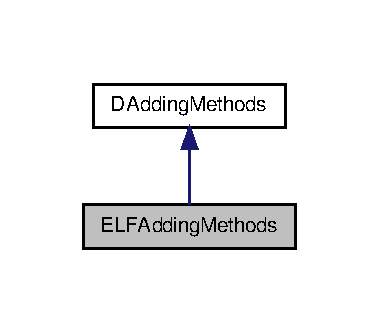
\includegraphics[width=182pt]{class_e_l_f_adding_methods__inherit__graph}
\end{center}
\end{figure}


Diagram współpracy dla E\-L\-F\-Adding\-Methods\-:\nopagebreak
\begin{figure}[H]
\begin{center}
\leavevmode
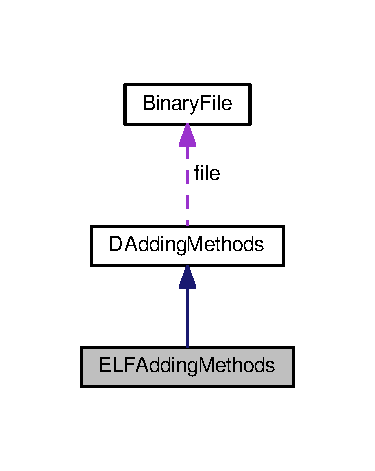
\includegraphics[width=182pt]{class_e_l_f_adding_methods__coll__graph}
\end{center}
\end{figure}
\subsection*{Metody publiczne}
\begin{DoxyCompactItemize}
\item 
\hyperlink{class_e_l_f_adding_methods_a49ddea5561dbff8a787d586e58d70d22}{E\-L\-F\-Adding\-Methods} (\hyperlink{class_e_l_f}{E\-L\-F} $\ast$f)
\item 
\hyperlink{class_e_l_f_adding_methods_a374088ad2597fa11063b5a19bae0ffec}{$\sim$\-E\-L\-F\-Adding\-Methods} ()
\item 
{\footnotesize template$<$typename Registers\-Type $>$ }\\bool \hyperlink{class_e_l_f_adding_methods_acaa41aa5ab101bb4fa0e23a3029020ad}{secure\-\_\-elf} (\hyperlink{class_e_l_f}{E\-L\-F} \&elf, const \hyperlink{class_d_adding_methods_1_1_inject_description}{Inject\-Description}$<$ Registers\-Type $>$ \&inject\-\_\-desc)
\begin{DoxyCompactList}\small\item\em Metoda zabezpiecza plik, podany jako argument za pomocą wyspecyfikowanej metody. \end{DoxyCompactList}\end{DoxyCompactItemize}
\subsection*{Dodatkowe Dziedziczone Składowe}


\subsection{Opis szczegółowy}


Definicja w linii 9 pliku elfaddingmethods.\-h.



\subsection{Dokumentacja konstruktora i destruktora}
\hypertarget{class_e_l_f_adding_methods_a49ddea5561dbff8a787d586e58d70d22}{\index{E\-L\-F\-Adding\-Methods@{E\-L\-F\-Adding\-Methods}!E\-L\-F\-Adding\-Methods@{E\-L\-F\-Adding\-Methods}}
\index{E\-L\-F\-Adding\-Methods@{E\-L\-F\-Adding\-Methods}!ELFAddingMethods@{E\-L\-F\-Adding\-Methods}}
\subsubsection[{E\-L\-F\-Adding\-Methods}]{\setlength{\rightskip}{0pt plus 5cm}E\-L\-F\-Adding\-Methods\-::\-E\-L\-F\-Adding\-Methods (
\begin{DoxyParamCaption}
\item[{{\bf E\-L\-F} $\ast$}]{f}
\end{DoxyParamCaption}
)}}\label{class_e_l_f_adding_methods_a49ddea5561dbff8a787d586e58d70d22}


Definicja w linii 3 pliku elfaddingmethods.\-cpp.

\hypertarget{class_e_l_f_adding_methods_a374088ad2597fa11063b5a19bae0ffec}{\index{E\-L\-F\-Adding\-Methods@{E\-L\-F\-Adding\-Methods}!$\sim$\-E\-L\-F\-Adding\-Methods@{$\sim$\-E\-L\-F\-Adding\-Methods}}
\index{$\sim$\-E\-L\-F\-Adding\-Methods@{$\sim$\-E\-L\-F\-Adding\-Methods}!ELFAddingMethods@{E\-L\-F\-Adding\-Methods}}
\subsubsection[{$\sim$\-E\-L\-F\-Adding\-Methods}]{\setlength{\rightskip}{0pt plus 5cm}E\-L\-F\-Adding\-Methods\-::$\sim$\-E\-L\-F\-Adding\-Methods (
\begin{DoxyParamCaption}
{}
\end{DoxyParamCaption}
)}}\label{class_e_l_f_adding_methods_a374088ad2597fa11063b5a19bae0ffec}


Definicja w linii 20 pliku elfaddingmethods.\-cpp.



\subsection{Dokumentacja funkcji składowych}
\hypertarget{class_e_l_f_adding_methods_acaa41aa5ab101bb4fa0e23a3029020ad}{\index{E\-L\-F\-Adding\-Methods@{E\-L\-F\-Adding\-Methods}!secure\-\_\-elf@{secure\-\_\-elf}}
\index{secure\-\_\-elf@{secure\-\_\-elf}!ELFAddingMethods@{E\-L\-F\-Adding\-Methods}}
\subsubsection[{secure\-\_\-elf}]{\setlength{\rightskip}{0pt plus 5cm}template$<$typename Registers\-Type $>$ bool E\-L\-F\-Adding\-Methods\-::secure\-\_\-elf (
\begin{DoxyParamCaption}
\item[{{\bf E\-L\-F} \&}]{elf, }
\item[{const {\bf Inject\-Description}$<$ Registers\-Type $>$ \&}]{inject\-\_\-desc}
\end{DoxyParamCaption}
)}}\label{class_e_l_f_adding_methods_acaa41aa5ab101bb4fa0e23a3029020ad}


Metoda zabezpiecza plik, podany jako argument za pomocą wyspecyfikowanej metody. 


\begin{DoxyParams}{Parametry}
{\em elf} & plik do zabezpieczania. \\
\hline
{\em inject\-\_\-desc} & opis metody wstrzykiwania kodu. \\
\hline
\end{DoxyParams}
\begin{DoxyReturn}{Zwraca}
True, jeżeli operacja się powiodła, False w innych przypadkach. 
\end{DoxyReturn}


Definicja w linii 148 pliku elfaddingmethods.\-h.



Oto graf wywołań dla tej funkcji\-:\nopagebreak
\begin{figure}[H]
\begin{center}
\leavevmode
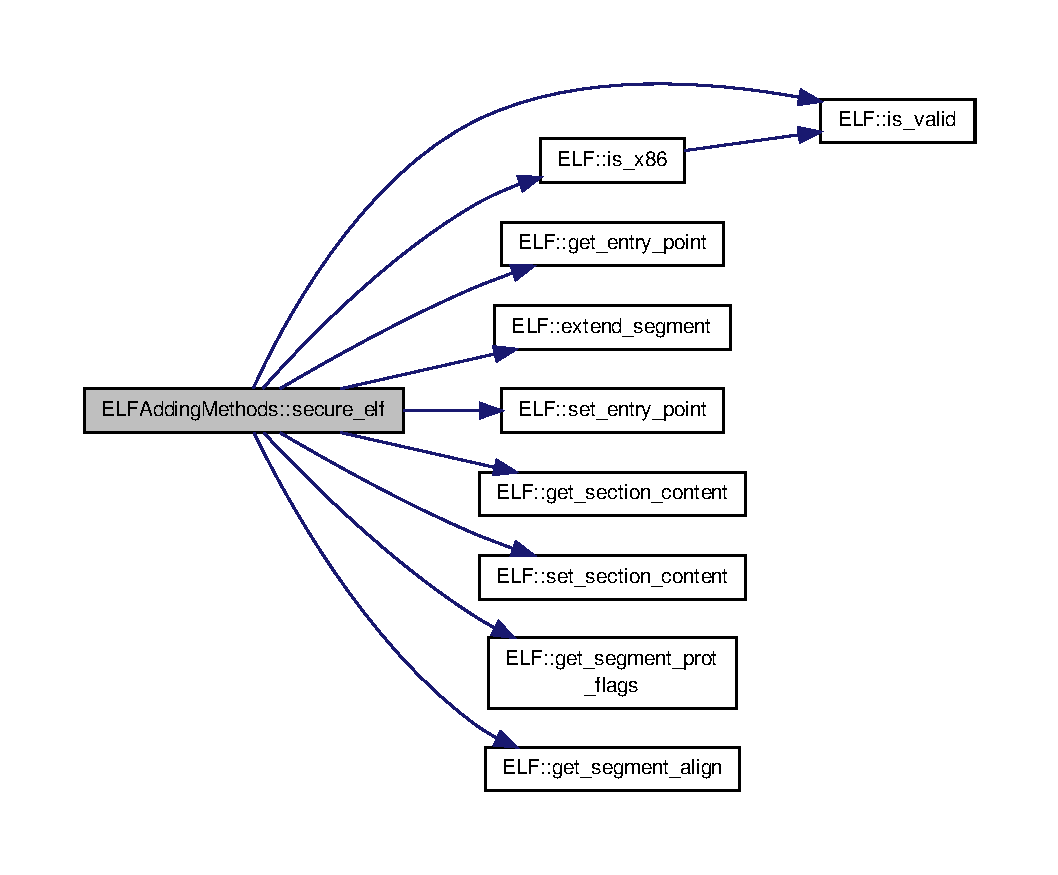
\includegraphics[width=350pt]{class_e_l_f_adding_methods_acaa41aa5ab101bb4fa0e23a3029020ad_cgraph}
\end{center}
\end{figure}




Dokumentacja dla tej klasy została wygenerowana z plików\-:\begin{DoxyCompactItemize}
\item 
core/adding\-\_\-methods/wrappers/\hyperlink{elfaddingmethods_8h}{elfaddingmethods.\-h}\item 
core/adding\-\_\-methods/wrappers/\hyperlink{elfaddingmethods_8cpp}{elfaddingmethods.\-cpp}\end{DoxyCompactItemize}

\hypertarget{class_d_adding_methods_1_1_inject_description}{\section{Dokumentacja szablonu klasy D\-Adding\-Methods\-:\-:Inject\-Description$<$ Registers\-Type $>$}
\label{class_d_adding_methods_1_1_inject_description}\index{D\-Adding\-Methods\-::\-Inject\-Description$<$ Registers\-Type $>$@{D\-Adding\-Methods\-::\-Inject\-Description$<$ Registers\-Type $>$}}
}


Klasa opisująca metodę wstrzykiwania kodu.  




{\ttfamily \#include $<$daddingmethods.\-h$>$}

\subsection*{Atrybuty publiczne}
\begin{DoxyCompactItemize}
\item 
\hyperlink{class_d_adding_methods_a8b52c07f1794d8c6cdd6f9b98be2bbf0}{Calling\-Method} \hyperlink{class_d_adding_methods_1_1_inject_description_a71f8164f1c9e433b6b22b5480dc5f066}{cm}
\item 
\hyperlink{class_d_adding_methods_1_1_wrapper}{Wrapper}$<$ Registers\-Type $>$ $\ast$ \hyperlink{class_d_adding_methods_1_1_inject_description_acea7bb1b146f912703e30039f200b538}{adding\-\_\-method}
\item 
Q\-String \hyperlink{class_d_adding_methods_1_1_inject_description_ab12b0b3cab069790363224252a2a9b22}{saved\-\_\-fname}
\item 
bool \hyperlink{class_d_adding_methods_1_1_inject_description_a8046652b0fae10f8e04e0678fd5961fd}{change\-\_\-x\-\_\-only}
\end{DoxyCompactItemize}


\subsection{Opis szczegółowy}
\subsubsection*{template$<$typename Registers\-Type$>$class D\-Adding\-Methods\-::\-Inject\-Description$<$ Registers\-Type $>$}

Klasa opisująca metodę wstrzykiwania kodu. 

Definicja w linii 255 pliku daddingmethods.\-h.



\subsection{Dokumentacja atrybutów składowych}
\hypertarget{class_d_adding_methods_1_1_inject_description_acea7bb1b146f912703e30039f200b538}{\index{D\-Adding\-Methods\-::\-Inject\-Description@{D\-Adding\-Methods\-::\-Inject\-Description}!adding\-\_\-method@{adding\-\_\-method}}
\index{adding\-\_\-method@{adding\-\_\-method}!DAddingMethods::InjectDescription@{D\-Adding\-Methods\-::\-Inject\-Description}}
\subsubsection[{adding\-\_\-method}]{\setlength{\rightskip}{0pt plus 5cm}template$<$typename Registers\-Type$>$ {\bf Wrapper}$<$Registers\-Type$>$$\ast$ {\bf D\-Adding\-Methods\-::\-Inject\-Description}$<$ Registers\-Type $>$\-::adding\-\_\-method}}\label{class_d_adding_methods_1_1_inject_description_acea7bb1b146f912703e30039f200b538}


Definicja w linii 258 pliku daddingmethods.\-h.

\hypertarget{class_d_adding_methods_1_1_inject_description_a8046652b0fae10f8e04e0678fd5961fd}{\index{D\-Adding\-Methods\-::\-Inject\-Description@{D\-Adding\-Methods\-::\-Inject\-Description}!change\-\_\-x\-\_\-only@{change\-\_\-x\-\_\-only}}
\index{change\-\_\-x\-\_\-only@{change\-\_\-x\-\_\-only}!DAddingMethods::InjectDescription@{D\-Adding\-Methods\-::\-Inject\-Description}}
\subsubsection[{change\-\_\-x\-\_\-only}]{\setlength{\rightskip}{0pt plus 5cm}template$<$typename Registers\-Type$>$ bool {\bf D\-Adding\-Methods\-::\-Inject\-Description}$<$ Registers\-Type $>$\-::change\-\_\-x\-\_\-only}}\label{class_d_adding_methods_1_1_inject_description_a8046652b0fae10f8e04e0678fd5961fd}


Definicja w linii 260 pliku daddingmethods.\-h.

\hypertarget{class_d_adding_methods_1_1_inject_description_a71f8164f1c9e433b6b22b5480dc5f066}{\index{D\-Adding\-Methods\-::\-Inject\-Description@{D\-Adding\-Methods\-::\-Inject\-Description}!cm@{cm}}
\index{cm@{cm}!DAddingMethods::InjectDescription@{D\-Adding\-Methods\-::\-Inject\-Description}}
\subsubsection[{cm}]{\setlength{\rightskip}{0pt plus 5cm}template$<$typename Registers\-Type$>$ {\bf Calling\-Method} {\bf D\-Adding\-Methods\-::\-Inject\-Description}$<$ Registers\-Type $>$\-::cm}}\label{class_d_adding_methods_1_1_inject_description_a71f8164f1c9e433b6b22b5480dc5f066}


Definicja w linii 257 pliku daddingmethods.\-h.

\hypertarget{class_d_adding_methods_1_1_inject_description_ab12b0b3cab069790363224252a2a9b22}{\index{D\-Adding\-Methods\-::\-Inject\-Description@{D\-Adding\-Methods\-::\-Inject\-Description}!saved\-\_\-fname@{saved\-\_\-fname}}
\index{saved\-\_\-fname@{saved\-\_\-fname}!DAddingMethods::InjectDescription@{D\-Adding\-Methods\-::\-Inject\-Description}}
\subsubsection[{saved\-\_\-fname}]{\setlength{\rightskip}{0pt plus 5cm}template$<$typename Registers\-Type$>$ Q\-String {\bf D\-Adding\-Methods\-::\-Inject\-Description}$<$ Registers\-Type $>$\-::saved\-\_\-fname}}\label{class_d_adding_methods_1_1_inject_description_ab12b0b3cab069790363224252a2a9b22}


Definicja w linii 259 pliku daddingmethods.\-h.



Dokumentacja dla tej klasy została wygenerowana z pliku\-:\begin{DoxyCompactItemize}
\item 
core/adding\-\_\-methods/wrappers/\hyperlink{daddingmethods_8h}{daddingmethods.\-h}\end{DoxyCompactItemize}

\hypertarget{class_method}{\section{Dokumentacja klasy Method}
\label{class_method}\index{Method@{Method}}
}


{\ttfamily \#include $<$method.\-h$>$}

\subsection*{Sygnały}
\begin{DoxyCompactItemize}
\item 
void \hyperlink{class_method_a91df3e429b16192100609942fed0c4e7}{name\-Changed} ()
\item 
void \hyperlink{class_method_a555273e8a9c3dbf7c5266d1d34224a87}{description\-Changed} ()
\end{DoxyCompactItemize}
\subsection*{Metody publiczne}
\begin{DoxyCompactItemize}
\item 
\hyperlink{class_method_aa3a7f4470828bcc05b78467d0e840a04}{Method} (Q\-Object $\ast$parent=0)
\item 
\hyperlink{class_method_a44942be54e782afc4a11e444c6a1735c}{Method} (Q\-String n, Q\-String d, Q\-Object $\ast$parent=0)
\item 
void \hyperlink{class_method_a4e8375fe026ed07964e8ff0671ed2446}{set\-Name} (const Q\-String \&n)
\item 
void \hyperlink{class_method_a5e911cf889152d5f6ed5ff24c9091364}{set\-Description} (const Q\-String \&d)
\item 
Q\-String \hyperlink{class_method_a4f22c1375bd806b6a5c55570143251b8}{name} () const 
\item 
Q\-String \hyperlink{class_method_a2d9d9d004a0fc9d152066ac2728f354c}{description} () const 
\item 
void \hyperlink{class_method_a7fb905d9402518987d08e2d6e5227d88}{read} (const Q\-Json\-Object \&json)
\item 
void \hyperlink{class_method_a706689fe25b5ed85f9b1480d78574bb7}{write} (Q\-Json\-Object \&json) const 
\end{DoxyCompactItemize}
\subsection*{Właściwości}
\begin{DoxyCompactItemize}
\item 
Q\-String \hyperlink{class_method_a9131d3ff2cd50747c50290986126aff3}{name}
\item 
Q\-String \hyperlink{class_method_ab9629abfec31f98ae690c575d48ccfe7}{description}
\end{DoxyCompactItemize}
\subsection*{Przyjaciele}
\begin{DoxyCompactItemize}
\item 
Q\-Debug \hyperlink{class_method_adbde94b0435d11b4f6d17b782a67d553}{operator$<$$<$} (Q\-Debug d, const \hyperlink{class_method}{Method} \&m)
\end{DoxyCompactItemize}


\subsection{Opis szczegółowy}


Definicja w linii 9 pliku method.\-h.



\subsection{Dokumentacja konstruktora i destruktora}
\hypertarget{class_method_aa3a7f4470828bcc05b78467d0e840a04}{\index{Method@{Method}!Method@{Method}}
\index{Method@{Method}!Method@{Method}}
\subsubsection[{Method}]{\setlength{\rightskip}{0pt plus 5cm}Method\-::\-Method (
\begin{DoxyParamCaption}
\item[{Q\-Object $\ast$}]{parent = {\ttfamily 0}}
\end{DoxyParamCaption}
)\hspace{0.3cm}{\ttfamily [explicit]}}}\label{class_method_aa3a7f4470828bcc05b78467d0e840a04}


Definicja w linii 8 pliku method.\-cpp.

\hypertarget{class_method_a44942be54e782afc4a11e444c6a1735c}{\index{Method@{Method}!Method@{Method}}
\index{Method@{Method}!Method@{Method}}
\subsubsection[{Method}]{\setlength{\rightskip}{0pt plus 5cm}Method\-::\-Method (
\begin{DoxyParamCaption}
\item[{Q\-String}]{n, }
\item[{Q\-String}]{d, }
\item[{Q\-Object $\ast$}]{parent = {\ttfamily 0}}
\end{DoxyParamCaption}
)}}\label{class_method_a44942be54e782afc4a11e444c6a1735c}


Definicja w linii 13 pliku method.\-cpp.



\subsection{Dokumentacja funkcji składowych}
\hypertarget{class_method_a2d9d9d004a0fc9d152066ac2728f354c}{\index{Method@{Method}!description@{description}}
\index{description@{description}!Method@{Method}}
\subsubsection[{description}]{\setlength{\rightskip}{0pt plus 5cm}Q\-String Method\-::description (
\begin{DoxyParamCaption}
{}
\end{DoxyParamCaption}
) const\hspace{0.3cm}{\ttfamily [inline]}}}\label{class_method_a2d9d9d004a0fc9d152066ac2728f354c}


Definicja w linii 22 pliku method.\-h.

\hypertarget{class_method_a555273e8a9c3dbf7c5266d1d34224a87}{\index{Method@{Method}!description\-Changed@{description\-Changed}}
\index{description\-Changed@{description\-Changed}!Method@{Method}}
\subsubsection[{description\-Changed}]{\setlength{\rightskip}{0pt plus 5cm}void Method\-::description\-Changed (
\begin{DoxyParamCaption}
{}
\end{DoxyParamCaption}
)\hspace{0.3cm}{\ttfamily [signal]}}}\label{class_method_a555273e8a9c3dbf7c5266d1d34224a87}
\hypertarget{class_method_a4f22c1375bd806b6a5c55570143251b8}{\index{Method@{Method}!name@{name}}
\index{name@{name}!Method@{Method}}
\subsubsection[{name}]{\setlength{\rightskip}{0pt plus 5cm}Q\-String Method\-::name (
\begin{DoxyParamCaption}
{}
\end{DoxyParamCaption}
) const\hspace{0.3cm}{\ttfamily [inline]}}}\label{class_method_a4f22c1375bd806b6a5c55570143251b8}


Definicja w linii 21 pliku method.\-h.

\hypertarget{class_method_a91df3e429b16192100609942fed0c4e7}{\index{Method@{Method}!name\-Changed@{name\-Changed}}
\index{name\-Changed@{name\-Changed}!Method@{Method}}
\subsubsection[{name\-Changed}]{\setlength{\rightskip}{0pt plus 5cm}void Method\-::name\-Changed (
\begin{DoxyParamCaption}
{}
\end{DoxyParamCaption}
)\hspace{0.3cm}{\ttfamily [signal]}}}\label{class_method_a91df3e429b16192100609942fed0c4e7}
\hypertarget{class_method_a7fb905d9402518987d08e2d6e5227d88}{\index{Method@{Method}!read@{read}}
\index{read@{read}!Method@{Method}}
\subsubsection[{read}]{\setlength{\rightskip}{0pt plus 5cm}void Method\-::read (
\begin{DoxyParamCaption}
\item[{const Q\-Json\-Object \&}]{json}
\end{DoxyParamCaption}
)}}\label{class_method_a7fb905d9402518987d08e2d6e5227d88}


Definicja w linii 31 pliku method.\-cpp.

\hypertarget{class_method_a5e911cf889152d5f6ed5ff24c9091364}{\index{Method@{Method}!set\-Description@{set\-Description}}
\index{set\-Description@{set\-Description}!Method@{Method}}
\subsubsection[{set\-Description}]{\setlength{\rightskip}{0pt plus 5cm}void Method\-::set\-Description (
\begin{DoxyParamCaption}
\item[{const Q\-String \&}]{d}
\end{DoxyParamCaption}
)}}\label{class_method_a5e911cf889152d5f6ed5ff24c9091364}


Definicja w linii 24 pliku method.\-cpp.



Oto graf wywołań dla tej funkcji\-:\nopagebreak
\begin{figure}[H]
\begin{center}
\leavevmode
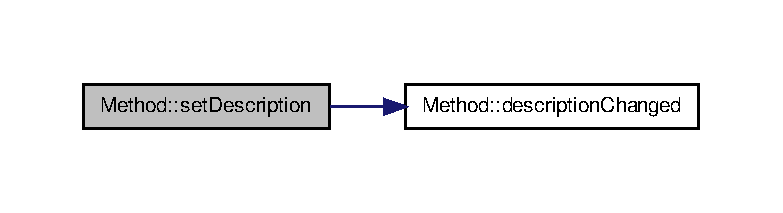
\includegraphics[width=350pt]{class_method_a5e911cf889152d5f6ed5ff24c9091364_cgraph}
\end{center}
\end{figure}


\hypertarget{class_method_a4e8375fe026ed07964e8ff0671ed2446}{\index{Method@{Method}!set\-Name@{set\-Name}}
\index{set\-Name@{set\-Name}!Method@{Method}}
\subsubsection[{set\-Name}]{\setlength{\rightskip}{0pt plus 5cm}void Method\-::set\-Name (
\begin{DoxyParamCaption}
\item[{const Q\-String \&}]{n}
\end{DoxyParamCaption}
)}}\label{class_method_a4e8375fe026ed07964e8ff0671ed2446}


Definicja w linii 17 pliku method.\-cpp.



Oto graf wywołań dla tej funkcji\-:\nopagebreak
\begin{figure}[H]
\begin{center}
\leavevmode
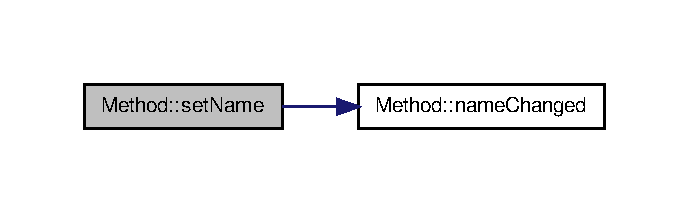
\includegraphics[width=330pt]{class_method_a4e8375fe026ed07964e8ff0671ed2446_cgraph}
\end{center}
\end{figure}


\hypertarget{class_method_a706689fe25b5ed85f9b1480d78574bb7}{\index{Method@{Method}!write@{write}}
\index{write@{write}!Method@{Method}}
\subsubsection[{write}]{\setlength{\rightskip}{0pt plus 5cm}void Method\-::write (
\begin{DoxyParamCaption}
\item[{Q\-Json\-Object \&}]{json}
\end{DoxyParamCaption}
) const}}\label{class_method_a706689fe25b5ed85f9b1480d78574bb7}


Definicja w linii 37 pliku method.\-cpp.



\subsection{Dokumentacja przyjaciół i funkcji związanych}
\hypertarget{class_method_adbde94b0435d11b4f6d17b782a67d553}{\index{Method@{Method}!operator$<$$<$@{operator$<$$<$}}
\index{operator$<$$<$@{operator$<$$<$}!Method@{Method}}
\subsubsection[{operator$<$$<$}]{\setlength{\rightskip}{0pt plus 5cm}Q\-Debug operator$<$$<$ (
\begin{DoxyParamCaption}
\item[{Q\-Debug}]{d, }
\item[{const {\bf Method} \&}]{m}
\end{DoxyParamCaption}
)\hspace{0.3cm}{\ttfamily [friend]}}}\label{class_method_adbde94b0435d11b4f6d17b782a67d553}


Definicja w linii 43 pliku method.\-cpp.



\subsection{Dokumentacja właściwości}
\hypertarget{class_method_ab9629abfec31f98ae690c575d48ccfe7}{\index{Method@{Method}!description@{description}}
\index{description@{description}!Method@{Method}}
\subsubsection[{description}]{\setlength{\rightskip}{0pt plus 5cm}Q\-String Method\-::description\hspace{0.3cm}{\ttfamily [read]}, {\ttfamily [write]}}}\label{class_method_ab9629abfec31f98ae690c575d48ccfe7}


Definicja w linii 13 pliku method.\-h.

\hypertarget{class_method_a9131d3ff2cd50747c50290986126aff3}{\index{Method@{Method}!name@{name}}
\index{name@{name}!Method@{Method}}
\subsubsection[{name}]{\setlength{\rightskip}{0pt plus 5cm}Q\-String Method\-::name\hspace{0.3cm}{\ttfamily [read]}, {\ttfamily [write]}}}\label{class_method_a9131d3ff2cd50747c50290986126aff3}


Definicja w linii 12 pliku method.\-h.



Dokumentacja dla tej klasy została wygenerowana z plików\-:\begin{DoxyCompactItemize}
\item 
D\-Methods/\hyperlink{method_8h}{method.\-h}\item 
D\-Methods/\hyperlink{method_8cpp}{method.\-cpp}\end{DoxyCompactItemize}

\hypertarget{class_method_list}{\section{Dokumentacja klasy Method\-List}
\label{class_method_list}\index{Method\-List@{Method\-List}}
}


{\ttfamily \#include $<$methodlist.\-h$>$}



Diagram dziedziczenia dla Method\-List
\nopagebreak
\begin{figure}[H]
\begin{center}
\leavevmode
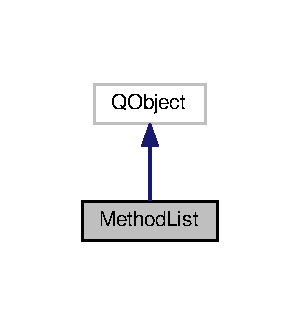
\includegraphics[width=144pt]{class_method_list__inherit__graph}
\end{center}
\end{figure}


Diagram współpracy dla Method\-List\-:
\nopagebreak
\begin{figure}[H]
\begin{center}
\leavevmode
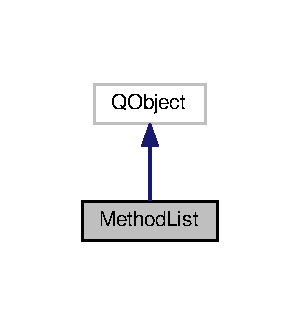
\includegraphics[width=144pt]{class_method_list__coll__graph}
\end{center}
\end{figure}
\subsection*{Sygnały}
\begin{DoxyCompactItemize}
\item 
void \hyperlink{class_method_list_a964af96ad04ea475a562ef9c437c9395}{path\-Changed} ()
\item 
void \hyperlink{class_method_list_a22b1996a1f49c974ffcc596e3840747a}{names\-Changed} ()
\item 
void \hyperlink{class_method_list_aaf15b5a1bfb251c39fc5d50c2f7e39d7}{methods\-Changed} ()
\end{DoxyCompactItemize}
\subsection*{Metody publiczne}
\begin{DoxyCompactItemize}
\item 
\hyperlink{class_method_list_ae859d2576fa0bd370d458af57948e22e}{Method\-List} (Q\-Object $\ast$parent=0)
\item 
\hyperlink{class_method_list_ac434ec0f3fea8b75ac0762d235441206}{Method\-List} (Q\-List$<$ \hyperlink{class_method}{Method} $\ast$ $>$ \&m, Q\-String \hyperlink{class_method_list_aac51cd62c2c4e2cfb7a4a8053555ea61}{path}=Q\-String(\char`\"{}methods.\-json\char`\"{}), Q\-Object $\ast$parent=0)
\item 
Q\-Qml\-List\-Property$<$ \hyperlink{class_method}{Method} $>$ \hyperlink{class_method_list_ac0e3f7172a72d25b66a50289d67a1e0f}{methods} ()
\item 
Q\-Variant\-List \hyperlink{class_method_list_a23142d6732e57d998153b8f4be2bc974}{names} ()
\item 
void \hyperlink{class_method_list_ae9a0004ee6cbe2f7cccc1cbd5f5488bb}{read} (const Q\-Json\-Object \&json)
\item 
void \hyperlink{class_method_list_af0d4511d7f5bfb5003a33e8c0d50b4bd}{write} (Q\-Json\-Object \&json) const 
\item 
bool \hyperlink{class_method_list_aaad20483391f3c7f6ffe68a7a4973353}{load\-List} ()
\item 
bool \hyperlink{class_method_list_a76d02473ee8a03c714c72c202fdd20f4}{save\-List} ()
\item 
Q\-String \hyperlink{class_method_list_ad2eb51d43787a28502722c7ef92b6f84}{path} () const 
\item 
void \hyperlink{class_method_list_ae08b28e21d8f75374c5d6e295516eeeb}{set\-Path} (const Q\-String \&p)
\end{DoxyCompactItemize}
\subsection*{Właściwości}
\begin{DoxyCompactItemize}
\item 
Q\-Qml\-List\-Property$<$ \hyperlink{class_method}{Method} $>$ \hyperlink{class_method_list_a10fa462526af745e0ef24c024a7e252e}{methods}
\item 
Q\-Variant\-List \hyperlink{class_method_list_ac96a3d7bc8ad7419795cf194448ca2c4}{names}
\item 
Q\-String \hyperlink{class_method_list_aac51cd62c2c4e2cfb7a4a8053555ea61}{path}
\end{DoxyCompactItemize}
\subsection*{Atrybuty prywatne}
\begin{DoxyCompactItemize}
\item 
Q\-List$<$ \hyperlink{class_method}{Method} $\ast$ $>$ \hyperlink{class_method_list_af1534c7112c552f17e0042e0f83c02cf}{m\-\_\-methods}
\item 
Q\-String \hyperlink{class_method_list_a1586bb53f50209dc1adf309bcb5a4cd2}{m\-\_\-path}
\item 
Q\-Variant\-List \hyperlink{class_method_list_a8d597ca5cbd6837944817258b96fdf93}{m\-\_\-names}
\end{DoxyCompactItemize}
\subsection*{Przyjaciele}
\begin{DoxyCompactItemize}
\item 
Q\-Debug \hyperlink{class_method_list_a4fcdf576a1904d6410d36d3bdbfd5307}{operator$<$$<$} (Q\-Debug d, const \hyperlink{class_method_list}{Method\-List} \&ml)
\end{DoxyCompactItemize}


\subsection{Opis szczegółowy}


Definicja w linii 12 pliku methodlist.\-h.



\subsection{Dokumentacja konstruktora i destruktora}
\hypertarget{class_method_list_ae859d2576fa0bd370d458af57948e22e}{\index{Method\-List@{Method\-List}!Method\-List@{Method\-List}}
\index{Method\-List@{Method\-List}!MethodList@{Method\-List}}
\subsubsection[{Method\-List}]{\setlength{\rightskip}{0pt plus 5cm}Method\-List\-::\-Method\-List (
\begin{DoxyParamCaption}
\item[{Q\-Object $\ast$}]{parent = {\ttfamily 0}}
\end{DoxyParamCaption}
)\hspace{0.3cm}{\ttfamily [explicit]}}}\label{class_method_list_ae859d2576fa0bd370d458af57948e22e}


Definicja w linii 5 pliku methodlist.\-cpp.

\hypertarget{class_method_list_ac434ec0f3fea8b75ac0762d235441206}{\index{Method\-List@{Method\-List}!Method\-List@{Method\-List}}
\index{Method\-List@{Method\-List}!MethodList@{Method\-List}}
\subsubsection[{Method\-List}]{\setlength{\rightskip}{0pt plus 5cm}Method\-List\-::\-Method\-List (
\begin{DoxyParamCaption}
\item[{Q\-List$<$ {\bf Method} $\ast$ $>$ \&}]{m, }
\item[{Q\-String}]{path = {\ttfamily QString(\char`\"{}methods.json\char`\"{})}, }
\item[{Q\-Object $\ast$}]{parent = {\ttfamily 0}}
\end{DoxyParamCaption}
)}}\label{class_method_list_ac434ec0f3fea8b75ac0762d235441206}


Definicja w linii 9 pliku methodlist.\-cpp.



\subsection{Dokumentacja funkcji składowych}
\hypertarget{class_method_list_aaad20483391f3c7f6ffe68a7a4973353}{\index{Method\-List@{Method\-List}!load\-List@{load\-List}}
\index{load\-List@{load\-List}!MethodList@{Method\-List}}
\subsubsection[{load\-List}]{\setlength{\rightskip}{0pt plus 5cm}bool Method\-List\-::load\-List (
\begin{DoxyParamCaption}
{}
\end{DoxyParamCaption}
)}}\label{class_method_list_aaad20483391f3c7f6ffe68a7a4973353}


Definicja w linii 55 pliku methodlist.\-cpp.



Oto graf wywołań dla tej funkcji\-:
\nopagebreak
\begin{figure}[H]
\begin{center}
\leavevmode
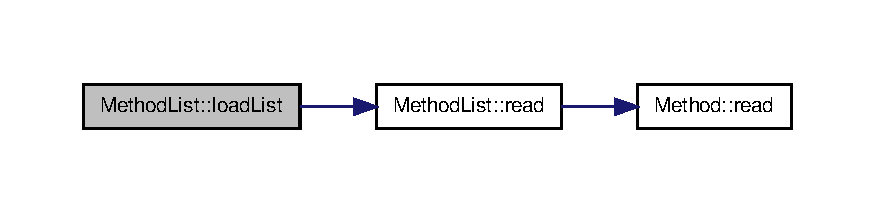
\includegraphics[width=350pt]{class_method_list_aaad20483391f3c7f6ffe68a7a4973353_cgraph}
\end{center}
\end{figure}


\hypertarget{class_method_list_ac0e3f7172a72d25b66a50289d67a1e0f}{\index{Method\-List@{Method\-List}!methods@{methods}}
\index{methods@{methods}!MethodList@{Method\-List}}
\subsubsection[{methods}]{\setlength{\rightskip}{0pt plus 5cm}Q\-Qml\-List\-Property$<${\bf Method}$>$ Method\-List\-::methods (
\begin{DoxyParamCaption}
{}
\end{DoxyParamCaption}
)}}\label{class_method_list_ac0e3f7172a72d25b66a50289d67a1e0f}
\hypertarget{class_method_list_aaf15b5a1bfb251c39fc5d50c2f7e39d7}{\index{Method\-List@{Method\-List}!methods\-Changed@{methods\-Changed}}
\index{methods\-Changed@{methods\-Changed}!MethodList@{Method\-List}}
\subsubsection[{methods\-Changed}]{\setlength{\rightskip}{0pt plus 5cm}void Method\-List\-::methods\-Changed (
\begin{DoxyParamCaption}
{}
\end{DoxyParamCaption}
)\hspace{0.3cm}{\ttfamily [signal]}}}\label{class_method_list_aaf15b5a1bfb251c39fc5d50c2f7e39d7}
\hypertarget{class_method_list_a23142d6732e57d998153b8f4be2bc974}{\index{Method\-List@{Method\-List}!names@{names}}
\index{names@{names}!MethodList@{Method\-List}}
\subsubsection[{names}]{\setlength{\rightskip}{0pt plus 5cm}Q\-Variant\-List Method\-List\-::names (
\begin{DoxyParamCaption}
{}
\end{DoxyParamCaption}
)}}\label{class_method_list_a23142d6732e57d998153b8f4be2bc974}
\hypertarget{class_method_list_a22b1996a1f49c974ffcc596e3840747a}{\index{Method\-List@{Method\-List}!names\-Changed@{names\-Changed}}
\index{names\-Changed@{names\-Changed}!MethodList@{Method\-List}}
\subsubsection[{names\-Changed}]{\setlength{\rightskip}{0pt plus 5cm}void Method\-List\-::names\-Changed (
\begin{DoxyParamCaption}
{}
\end{DoxyParamCaption}
)\hspace{0.3cm}{\ttfamily [signal]}}}\label{class_method_list_a22b1996a1f49c974ffcc596e3840747a}
\hypertarget{class_method_list_ad2eb51d43787a28502722c7ef92b6f84}{\index{Method\-List@{Method\-List}!path@{path}}
\index{path@{path}!MethodList@{Method\-List}}
\subsubsection[{path}]{\setlength{\rightskip}{0pt plus 5cm}Q\-String Method\-List\-::path (
\begin{DoxyParamCaption}
{}
\end{DoxyParamCaption}
) const}}\label{class_method_list_ad2eb51d43787a28502722c7ef92b6f84}
\hypertarget{class_method_list_a964af96ad04ea475a562ef9c437c9395}{\index{Method\-List@{Method\-List}!path\-Changed@{path\-Changed}}
\index{path\-Changed@{path\-Changed}!MethodList@{Method\-List}}
\subsubsection[{path\-Changed}]{\setlength{\rightskip}{0pt plus 5cm}void Method\-List\-::path\-Changed (
\begin{DoxyParamCaption}
{}
\end{DoxyParamCaption}
)\hspace{0.3cm}{\ttfamily [signal]}}}\label{class_method_list_a964af96ad04ea475a562ef9c437c9395}


Oto graf wywoływań tej funkcji\-:
\nopagebreak
\begin{figure}[H]
\begin{center}
\leavevmode
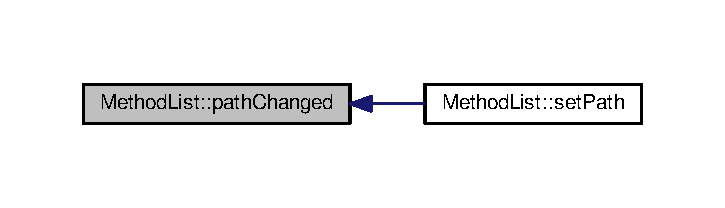
\includegraphics[width=348pt]{class_method_list_a964af96ad04ea475a562ef9c437c9395_icgraph}
\end{center}
\end{figure}


\hypertarget{class_method_list_ae9a0004ee6cbe2f7cccc1cbd5f5488bb}{\index{Method\-List@{Method\-List}!read@{read}}
\index{read@{read}!MethodList@{Method\-List}}
\subsubsection[{read}]{\setlength{\rightskip}{0pt plus 5cm}void Method\-List\-::read (
\begin{DoxyParamCaption}
\item[{const Q\-Json\-Object \&}]{json}
\end{DoxyParamCaption}
)}}\label{class_method_list_ae9a0004ee6cbe2f7cccc1cbd5f5488bb}


Definicja w linii 30 pliku methodlist.\-cpp.



Oto graf wywołań dla tej funkcji\-:
\nopagebreak
\begin{figure}[H]
\begin{center}
\leavevmode
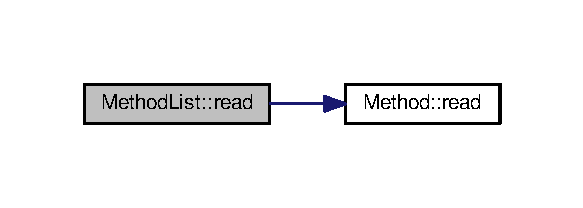
\includegraphics[width=280pt]{class_method_list_ae9a0004ee6cbe2f7cccc1cbd5f5488bb_cgraph}
\end{center}
\end{figure}




Oto graf wywoływań tej funkcji\-:
\nopagebreak
\begin{figure}[H]
\begin{center}
\leavevmode
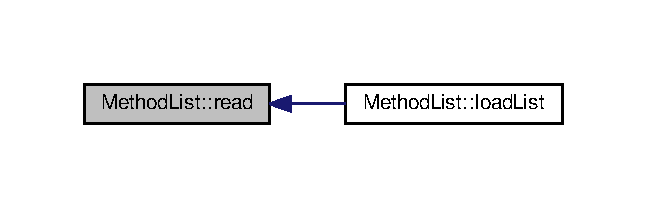
\includegraphics[width=310pt]{class_method_list_ae9a0004ee6cbe2f7cccc1cbd5f5488bb_icgraph}
\end{center}
\end{figure}


\hypertarget{class_method_list_a76d02473ee8a03c714c72c202fdd20f4}{\index{Method\-List@{Method\-List}!save\-List@{save\-List}}
\index{save\-List@{save\-List}!MethodList@{Method\-List}}
\subsubsection[{save\-List}]{\setlength{\rightskip}{0pt plus 5cm}bool Method\-List\-::save\-List (
\begin{DoxyParamCaption}
{}
\end{DoxyParamCaption}
)}}\label{class_method_list_a76d02473ee8a03c714c72c202fdd20f4}


Definicja w linii 73 pliku methodlist.\-cpp.



Oto graf wywołań dla tej funkcji\-:
\nopagebreak
\begin{figure}[H]
\begin{center}
\leavevmode
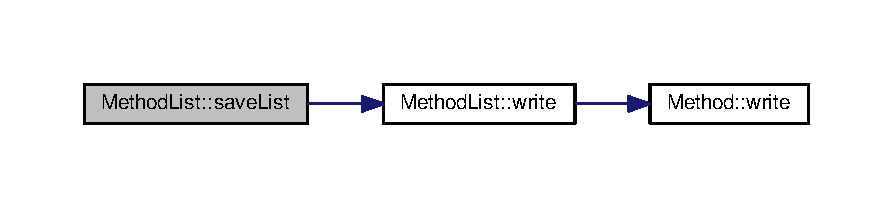
\includegraphics[width=350pt]{class_method_list_a76d02473ee8a03c714c72c202fdd20f4_cgraph}
\end{center}
\end{figure}


\hypertarget{class_method_list_ae08b28e21d8f75374c5d6e295516eeeb}{\index{Method\-List@{Method\-List}!set\-Path@{set\-Path}}
\index{set\-Path@{set\-Path}!MethodList@{Method\-List}}
\subsubsection[{set\-Path}]{\setlength{\rightskip}{0pt plus 5cm}void Method\-List\-::set\-Path (
\begin{DoxyParamCaption}
\item[{const Q\-String \&}]{p}
\end{DoxyParamCaption}
)}}\label{class_method_list_ae08b28e21d8f75374c5d6e295516eeeb}


Definicja w linii 92 pliku methodlist.\-cpp.

\hypertarget{class_method_list_af0d4511d7f5bfb5003a33e8c0d50b4bd}{\index{Method\-List@{Method\-List}!write@{write}}
\index{write@{write}!MethodList@{Method\-List}}
\subsubsection[{write}]{\setlength{\rightskip}{0pt plus 5cm}void Method\-List\-::write (
\begin{DoxyParamCaption}
\item[{Q\-Json\-Object \&}]{json}
\end{DoxyParamCaption}
) const}}\label{class_method_list_af0d4511d7f5bfb5003a33e8c0d50b4bd}


Definicja w linii 44 pliku methodlist.\-cpp.



Oto graf wywołań dla tej funkcji\-:
\nopagebreak
\begin{figure}[H]
\begin{center}
\leavevmode
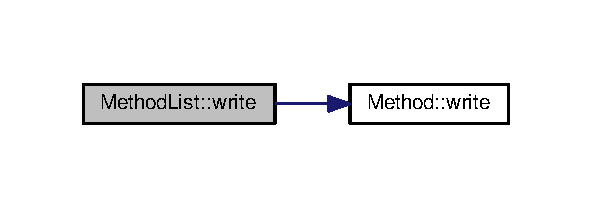
\includegraphics[width=284pt]{class_method_list_af0d4511d7f5bfb5003a33e8c0d50b4bd_cgraph}
\end{center}
\end{figure}




Oto graf wywoływań tej funkcji\-:
\nopagebreak
\begin{figure}[H]
\begin{center}
\leavevmode
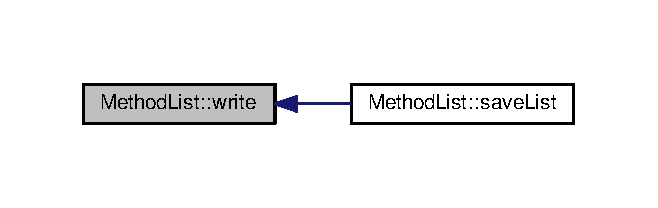
\includegraphics[width=316pt]{class_method_list_af0d4511d7f5bfb5003a33e8c0d50b4bd_icgraph}
\end{center}
\end{figure}




\subsection{Dokumentacja przyjaciół i funkcji związanych}
\hypertarget{class_method_list_a4fcdf576a1904d6410d36d3bdbfd5307}{\index{Method\-List@{Method\-List}!operator$<$$<$@{operator$<$$<$}}
\index{operator$<$$<$@{operator$<$$<$}!MethodList@{Method\-List}}
\subsubsection[{operator$<$$<$}]{\setlength{\rightskip}{0pt plus 5cm}Q\-Debug operator$<$$<$ (
\begin{DoxyParamCaption}
\item[{Q\-Debug}]{d, }
\item[{const {\bf Method\-List} \&}]{ml}
\end{DoxyParamCaption}
)\hspace{0.3cm}{\ttfamily [friend]}}}\label{class_method_list_a4fcdf576a1904d6410d36d3bdbfd5307}


Definicja w linii 99 pliku methodlist.\-cpp.



\subsection{Dokumentacja atrybutów składowych}
\hypertarget{class_method_list_af1534c7112c552f17e0042e0f83c02cf}{\index{Method\-List@{Method\-List}!m\-\_\-methods@{m\-\_\-methods}}
\index{m\-\_\-methods@{m\-\_\-methods}!MethodList@{Method\-List}}
\subsubsection[{m\-\_\-methods}]{\setlength{\rightskip}{0pt plus 5cm}Q\-List$<${\bf Method}$\ast$$>$ Method\-List\-::m\-\_\-methods\hspace{0.3cm}{\ttfamily [private]}}}\label{class_method_list_af1534c7112c552f17e0042e0f83c02cf}


Definicja w linii 43 pliku methodlist.\-h.

\hypertarget{class_method_list_a8d597ca5cbd6837944817258b96fdf93}{\index{Method\-List@{Method\-List}!m\-\_\-names@{m\-\_\-names}}
\index{m\-\_\-names@{m\-\_\-names}!MethodList@{Method\-List}}
\subsubsection[{m\-\_\-names}]{\setlength{\rightskip}{0pt plus 5cm}Q\-Variant\-List Method\-List\-::m\-\_\-names\hspace{0.3cm}{\ttfamily [private]}}}\label{class_method_list_a8d597ca5cbd6837944817258b96fdf93}


Definicja w linii 45 pliku methodlist.\-h.

\hypertarget{class_method_list_a1586bb53f50209dc1adf309bcb5a4cd2}{\index{Method\-List@{Method\-List}!m\-\_\-path@{m\-\_\-path}}
\index{m\-\_\-path@{m\-\_\-path}!MethodList@{Method\-List}}
\subsubsection[{m\-\_\-path}]{\setlength{\rightskip}{0pt plus 5cm}Q\-String Method\-List\-::m\-\_\-path\hspace{0.3cm}{\ttfamily [private]}}}\label{class_method_list_a1586bb53f50209dc1adf309bcb5a4cd2}


Definicja w linii 44 pliku methodlist.\-h.



\subsection{Dokumentacja właściwości}
\hypertarget{class_method_list_a10fa462526af745e0ef24c024a7e252e}{\index{Method\-List@{Method\-List}!methods@{methods}}
\index{methods@{methods}!MethodList@{Method\-List}}
\subsubsection[{methods}]{\setlength{\rightskip}{0pt plus 5cm}Q\-Qml\-List\-Property$<$ {\bf Method} $>$ Method\-List\-::methods\hspace{0.3cm}{\ttfamily [read]}}}\label{class_method_list_a10fa462526af745e0ef24c024a7e252e}


Definicja w linii 15 pliku methodlist.\-h.

\hypertarget{class_method_list_ac96a3d7bc8ad7419795cf194448ca2c4}{\index{Method\-List@{Method\-List}!names@{names}}
\index{names@{names}!MethodList@{Method\-List}}
\subsubsection[{names}]{\setlength{\rightskip}{0pt plus 5cm}Q\-Variant\-List Method\-List\-::names\hspace{0.3cm}{\ttfamily [read]}}}\label{class_method_list_ac96a3d7bc8ad7419795cf194448ca2c4}


Definicja w linii 16 pliku methodlist.\-h.

\hypertarget{class_method_list_aac51cd62c2c4e2cfb7a4a8053555ea61}{\index{Method\-List@{Method\-List}!path@{path}}
\index{path@{path}!MethodList@{Method\-List}}
\subsubsection[{path}]{\setlength{\rightskip}{0pt plus 5cm}Q\-String Method\-List\-::path\hspace{0.3cm}{\ttfamily [read]}, {\ttfamily [write]}}}\label{class_method_list_aac51cd62c2c4e2cfb7a4a8053555ea61}


Definicja w linii 17 pliku methodlist.\-h.



Dokumentacja dla tej klasy została wygenerowana z plików\-:\begin{DoxyCompactItemize}
\item 
D\-Methods/\hyperlink{methodlist_8h}{methodlist.\-h}\item 
D\-Methods/\hyperlink{methodlist_8cpp}{methodlist.\-cpp}\end{DoxyCompactItemize}

\hypertarget{class_d_adding_methods_1_1_o_e_p_wrapper}{\section{Dokumentacja szablonu klasy D\-Adding\-Methods\-:\-:O\-E\-P\-Wrapper$<$ Registers\-Type $>$}
\label{class_d_adding_methods_1_1_o_e_p_wrapper}\index{D\-Adding\-Methods\-::\-O\-E\-P\-Wrapper$<$ Registers\-Type $>$@{D\-Adding\-Methods\-::\-O\-E\-P\-Wrapper$<$ Registers\-Type $>$}}
}


Klasa reprezentująca opakowanie dla tworzenia nowego punktu wejściowego.  




{\ttfamily \#include $<$daddingmethods.\-h$>$}



Diagram dziedziczenia dla D\-Adding\-Methods\-:\-:O\-E\-P\-Wrapper$<$ Registers\-Type $>$
\nopagebreak
\begin{figure}[H]
\begin{center}
\leavevmode
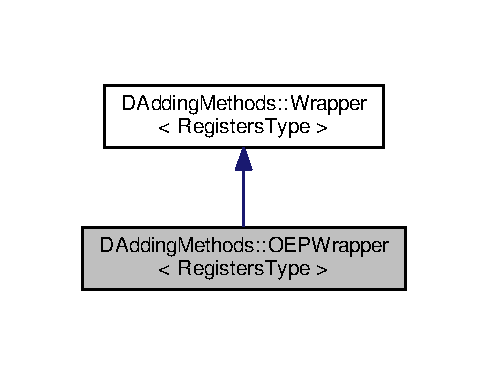
\includegraphics[width=234pt]{class_d_adding_methods_1_1_o_e_p_wrapper__inherit__graph}
\end{center}
\end{figure}


Diagram współpracy dla D\-Adding\-Methods\-:\-:O\-E\-P\-Wrapper$<$ Registers\-Type $>$\-:
\nopagebreak
\begin{figure}[H]
\begin{center}
\leavevmode
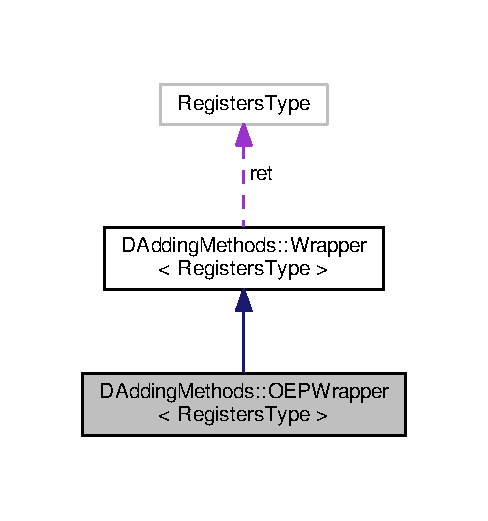
\includegraphics[width=234pt]{class_d_adding_methods_1_1_o_e_p_wrapper__coll__graph}
\end{center}
\end{figure}
\subsection*{Atrybuty publiczne}
\begin{DoxyCompactItemize}
\item 
\hyperlink{class_d_adding_methods_1_1_wrapper}{Wrapper}$<$ Registers\-Type $>$ $\ast$ \hyperlink{class_d_adding_methods_1_1_o_e_p_wrapper_ae954eddc8e8916ad5b78b1a10a9dab64}{oep\-\_\-action}
\end{DoxyCompactItemize}
\subsection*{Dodatkowe Dziedziczone Składowe}


\subsection{Opis szczegółowy}
\subsubsection*{template$<$typename Registers\-Type$>$class D\-Adding\-Methods\-::\-O\-E\-P\-Wrapper$<$ Registers\-Type $>$}

Klasa reprezentująca opakowanie dla tworzenia nowego punktu wejściowego. 

Definicja w linii 237 pliku daddingmethods.\-h.



\subsection{Dokumentacja atrybutów składowych}
\hypertarget{class_d_adding_methods_1_1_o_e_p_wrapper_ae954eddc8e8916ad5b78b1a10a9dab64}{\index{D\-Adding\-Methods\-::\-O\-E\-P\-Wrapper@{D\-Adding\-Methods\-::\-O\-E\-P\-Wrapper}!oep\-\_\-action@{oep\-\_\-action}}
\index{oep\-\_\-action@{oep\-\_\-action}!DAddingMethods::OEPWrapper@{D\-Adding\-Methods\-::\-O\-E\-P\-Wrapper}}
\subsubsection[{oep\-\_\-action}]{\setlength{\rightskip}{0pt plus 5cm}template$<$typename Registers\-Type$>$ {\bf Wrapper}$<$Registers\-Type$>$$\ast$ {\bf D\-Adding\-Methods\-::\-O\-E\-P\-Wrapper}$<$ Registers\-Type $>$\-::oep\-\_\-action}}\label{class_d_adding_methods_1_1_o_e_p_wrapper_ae954eddc8e8916ad5b78b1a10a9dab64}


Definicja w linii 239 pliku daddingmethods.\-h.



Dokumentacja dla tej klasy została wygenerowana z pliku\-:\begin{DoxyCompactItemize}
\item 
core/adding\-\_\-methods/wrappers/\hyperlink{daddingmethods_8h}{daddingmethods.\-h}\end{DoxyCompactItemize}

\hypertarget{class_p_e_adding_methods}{\section{Dokumentacja klasy P\-E\-Adding\-Methods}
\label{class_p_e_adding_methods}\index{P\-E\-Adding\-Methods@{P\-E\-Adding\-Methods}}
}


Klasa odpowiedzialna za dodawanie metod zabezpieczających do plików P\-E.  




{\ttfamily \#include $<$peaddingmethods.\-h$>$}



Diagram dziedziczenia dla P\-E\-Adding\-Methods\nopagebreak
\begin{figure}[H]
\begin{center}
\leavevmode
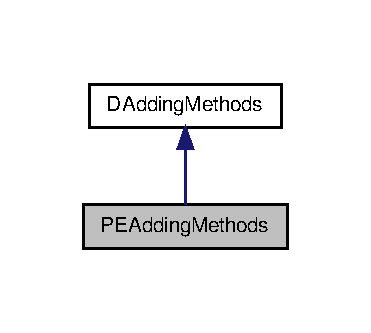
\includegraphics[width=178pt]{class_p_e_adding_methods__inherit__graph}
\end{center}
\end{figure}


Diagram współpracy dla P\-E\-Adding\-Methods\-:\nopagebreak
\begin{figure}[H]
\begin{center}
\leavevmode
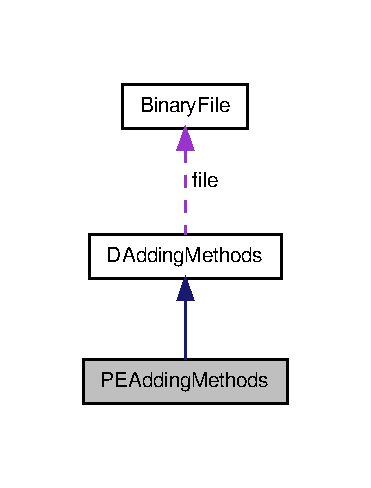
\includegraphics[width=178pt]{class_p_e_adding_methods__coll__graph}
\end{center}
\end{figure}
\subsection*{Metody publiczne}
\begin{DoxyCompactItemize}
\item 
\hyperlink{class_p_e_adding_methods_a1cec9b94a430984c6d88386884ad0cdd}{P\-E\-Adding\-Methods} (\hyperlink{class_p_e_file}{P\-E\-File} $\ast$f)
\begin{DoxyCompactList}\small\item\em Konstruktor. \end{DoxyCompactList}\item 
\hyperlink{class_p_e_adding_methods_a6f0a7a7d04944167192c61e22b4f04ee}{$\sim$\-P\-E\-Adding\-Methods} ()
\item 
{\footnotesize template$<$typename Register $>$ }\\bool \hyperlink{class_p_e_adding_methods_a2b224b51233e0446621e9daf9108e78b}{inject\-Code} (Q\-List$<$ \hyperlink{class_d_adding_methods_1_1_inject_description}{Inject\-Description}$<$ Register $>$ $\ast$ $>$ descs)
\begin{DoxyCompactList}\small\item\em Metoda zabezpieczająca plik P\-E podanymi metodami. \end{DoxyCompactList}\item 
void \hyperlink{class_p_e_adding_methods_af7948de6504286fdee160acba2c811bf}{set\-Code\-Coverage} (uint8\-\_\-t new\-\_\-coverage)
\begin{DoxyCompactList}\small\item\em Ustawia nowe procentowe pokrycie kodu. \end{DoxyCompactList}\end{DoxyCompactItemize}
\subsection*{Dodatkowe Dziedziczone Składowe}


\subsection{Opis szczegółowy}
Klasa odpowiedzialna za dodawanie metod zabezpieczających do plików P\-E. 

Definicja w linii 15 pliku peaddingmethods.\-h.



\subsection{Dokumentacja konstruktora i destruktora}
\hypertarget{class_p_e_adding_methods_a1cec9b94a430984c6d88386884ad0cdd}{\index{P\-E\-Adding\-Methods@{P\-E\-Adding\-Methods}!P\-E\-Adding\-Methods@{P\-E\-Adding\-Methods}}
\index{P\-E\-Adding\-Methods@{P\-E\-Adding\-Methods}!PEAddingMethods@{P\-E\-Adding\-Methods}}
\subsubsection[{P\-E\-Adding\-Methods}]{\setlength{\rightskip}{0pt plus 5cm}P\-E\-Adding\-Methods\-::\-P\-E\-Adding\-Methods (
\begin{DoxyParamCaption}
\item[{{\bf P\-E\-File} $\ast$}]{f}
\end{DoxyParamCaption}
)}}\label{class_p_e_adding_methods_a1cec9b94a430984c6d88386884ad0cdd}


Konstruktor. 


\begin{DoxyParams}{Parametry}
{\em f} & Plik P\-E \\
\hline
\end{DoxyParams}


Definicja w linii 6 pliku peaddingmethods.\-cpp.

\hypertarget{class_p_e_adding_methods_a6f0a7a7d04944167192c61e22b4f04ee}{\index{P\-E\-Adding\-Methods@{P\-E\-Adding\-Methods}!$\sim$\-P\-E\-Adding\-Methods@{$\sim$\-P\-E\-Adding\-Methods}}
\index{$\sim$\-P\-E\-Adding\-Methods@{$\sim$\-P\-E\-Adding\-Methods}!PEAddingMethods@{P\-E\-Adding\-Methods}}
\subsubsection[{$\sim$\-P\-E\-Adding\-Methods}]{\setlength{\rightskip}{0pt plus 5cm}P\-E\-Adding\-Methods\-::$\sim$\-P\-E\-Adding\-Methods (
\begin{DoxyParamCaption}
{}
\end{DoxyParamCaption}
)}}\label{class_p_e_adding_methods_a6f0a7a7d04944167192c61e22b4f04ee}


Definicja w linii 14 pliku peaddingmethods.\-cpp.



\subsection{Dokumentacja funkcji składowych}
\hypertarget{class_p_e_adding_methods_a2b224b51233e0446621e9daf9108e78b}{\index{P\-E\-Adding\-Methods@{P\-E\-Adding\-Methods}!inject\-Code@{inject\-Code}}
\index{inject\-Code@{inject\-Code}!PEAddingMethods@{P\-E\-Adding\-Methods}}
\subsubsection[{inject\-Code}]{\setlength{\rightskip}{0pt plus 5cm}template$<$typename Register $>$ template bool P\-E\-Adding\-Methods\-::inject\-Code (
\begin{DoxyParamCaption}
\item[{Q\-List$<$ {\bf Inject\-Description}$<$ Register $>$ $\ast$ $>$}]{descs}
\end{DoxyParamCaption}
)}}\label{class_p_e_adding_methods_a2b224b51233e0446621e9daf9108e78b}


Metoda zabezpieczająca plik P\-E podanymi metodami. 


\begin{DoxyParams}{Parametry}
{\em descs} & Lista wybranych metod \\
\hline
\end{DoxyParams}
\begin{DoxyReturn}{Zwraca}
True w przypadku sukcesu 
\end{DoxyReturn}


Definicja w linii 26 pliku peaddingmethods.\-cpp.



Oto graf wywołań dla tej funkcji\-:\nopagebreak
\begin{figure}[H]
\begin{center}
\leavevmode
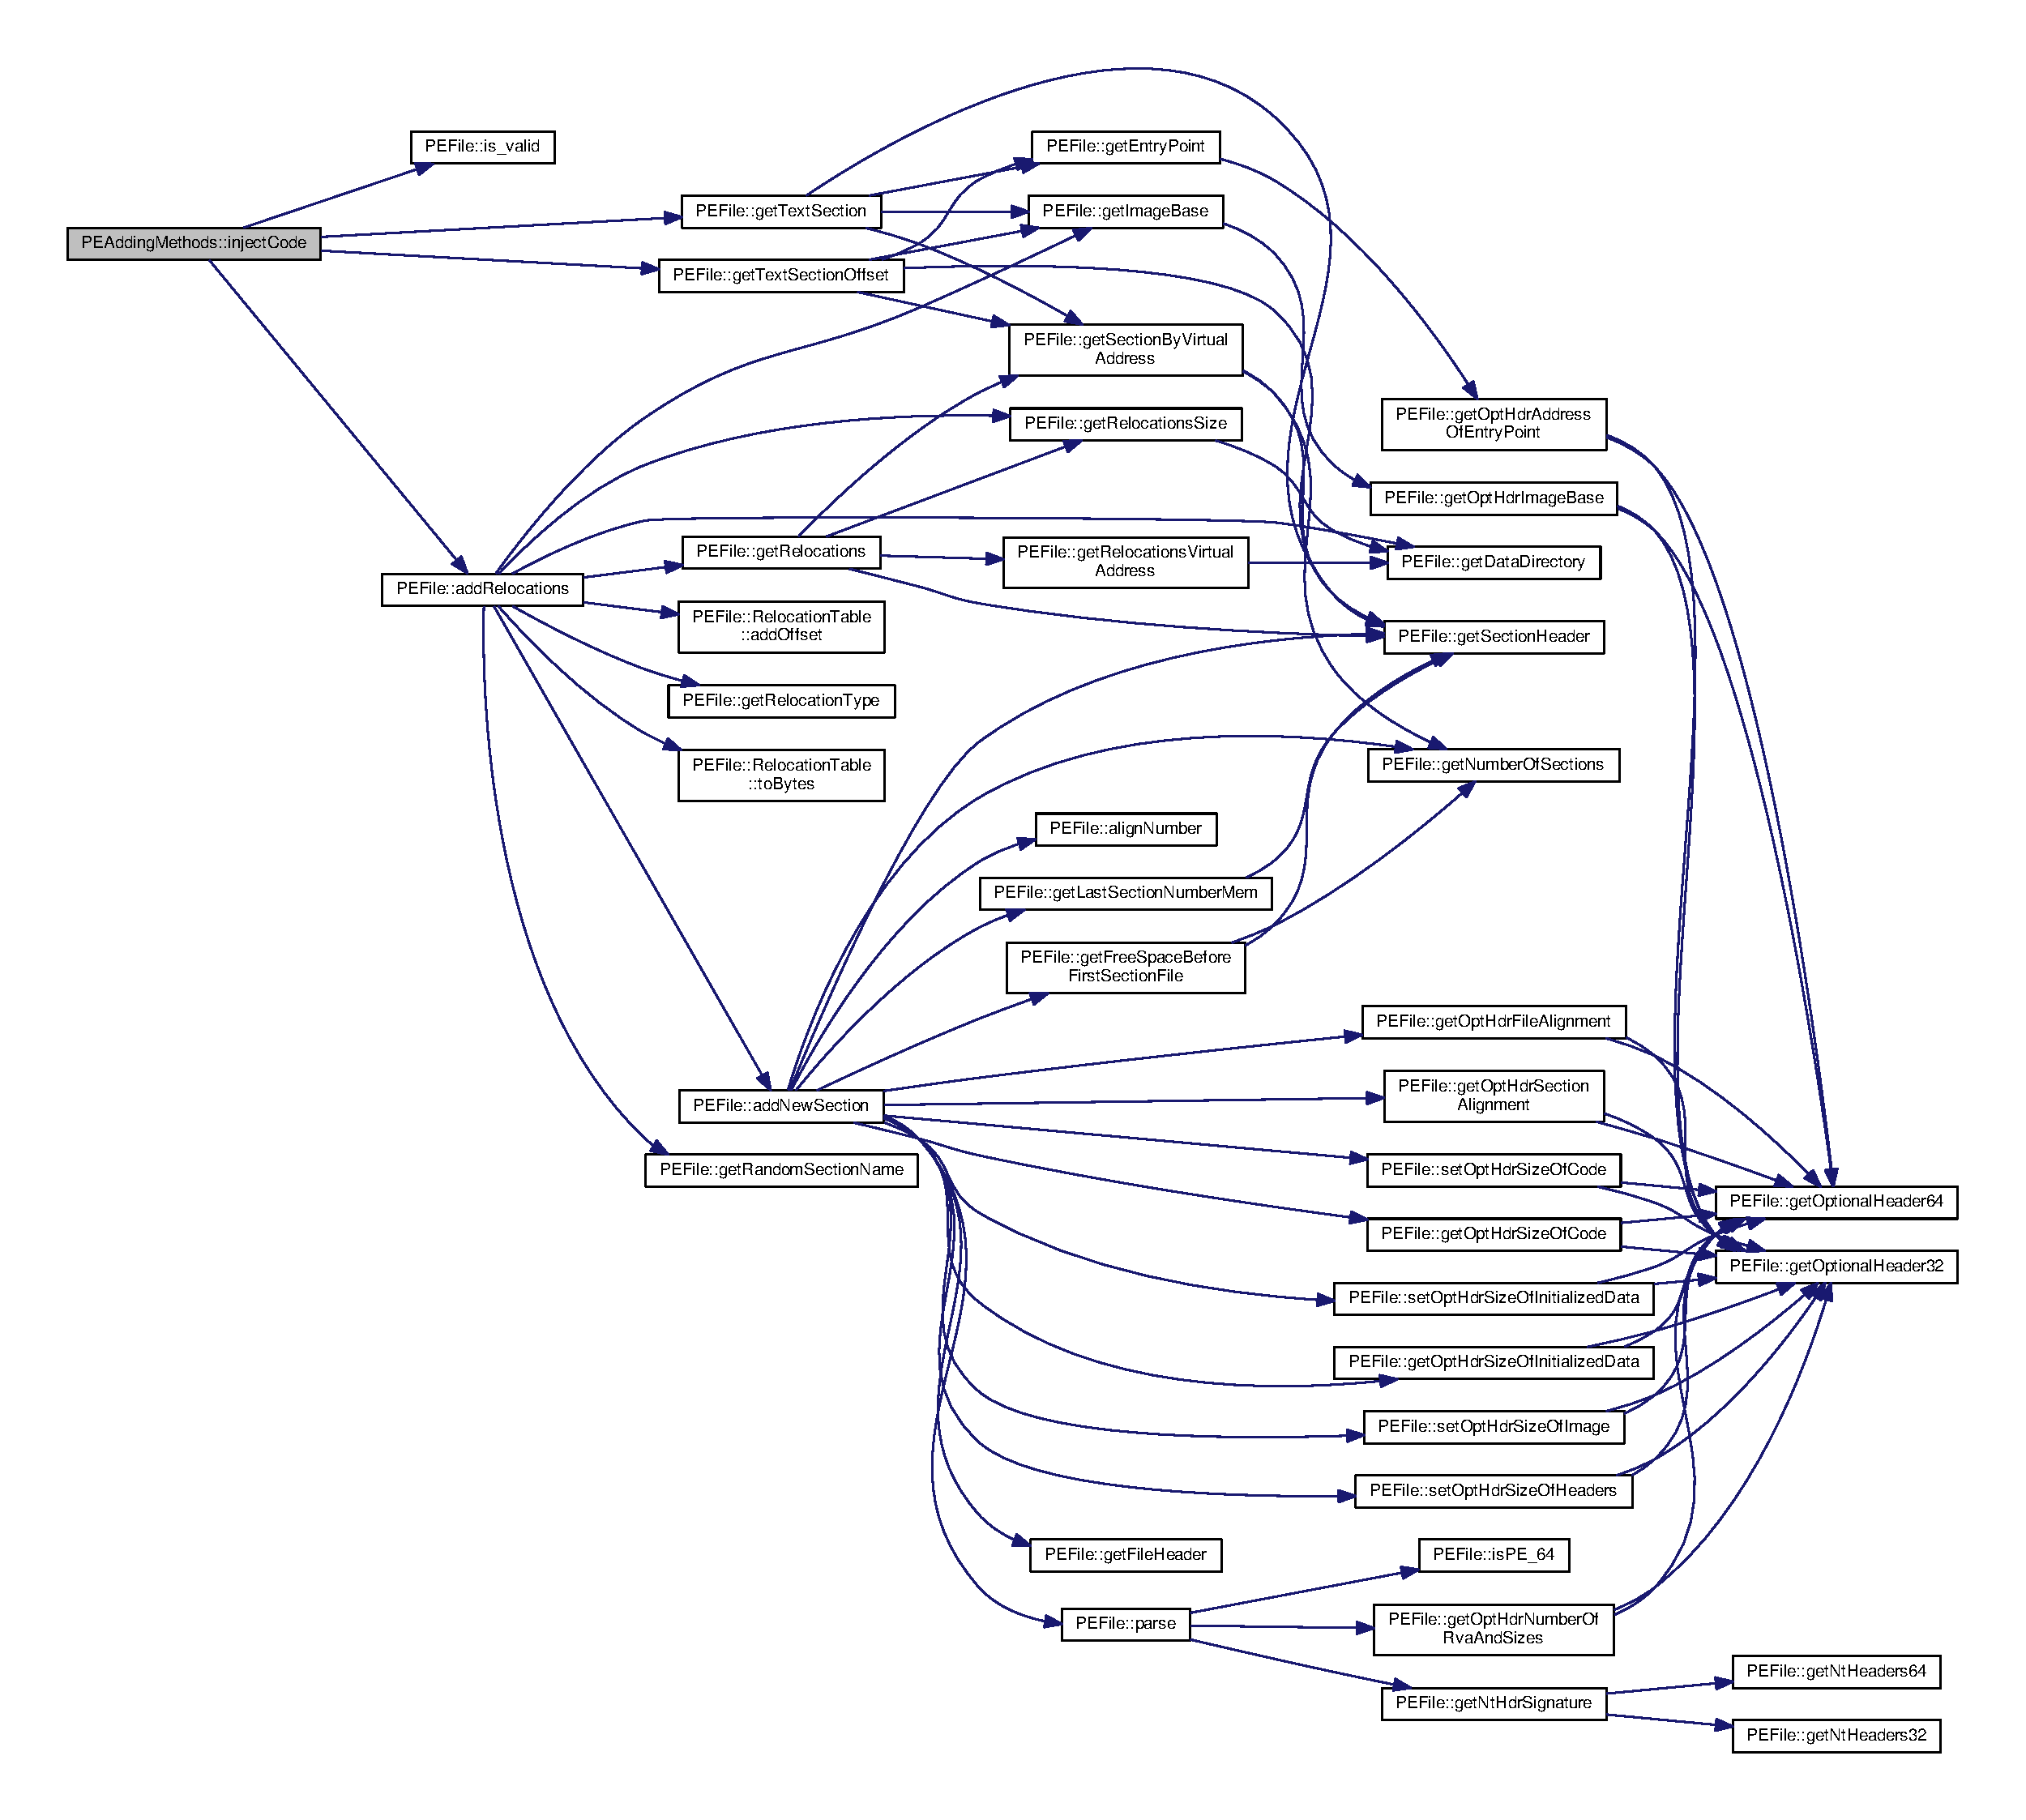
\includegraphics[width=350pt]{class_p_e_adding_methods_a2b224b51233e0446621e9daf9108e78b_cgraph}
\end{center}
\end{figure}


\hypertarget{class_p_e_adding_methods_af7948de6504286fdee160acba2c811bf}{\index{P\-E\-Adding\-Methods@{P\-E\-Adding\-Methods}!set\-Code\-Coverage@{set\-Code\-Coverage}}
\index{set\-Code\-Coverage@{set\-Code\-Coverage}!PEAddingMethods@{P\-E\-Adding\-Methods}}
\subsubsection[{set\-Code\-Coverage}]{\setlength{\rightskip}{0pt plus 5cm}void P\-E\-Adding\-Methods\-::set\-Code\-Coverage (
\begin{DoxyParamCaption}
\item[{uint8\-\_\-t}]{new\-\_\-coverage}
\end{DoxyParamCaption}
)}}\label{class_p_e_adding_methods_af7948de6504286fdee160acba2c811bf}


Ustawia nowe procentowe pokrycie kodu. 


\begin{DoxyParams}{Parametry}
{\em new\-\_\-coverage} & Pokrycie kodu \\
\hline
\end{DoxyParams}


Definicja w linii 19 pliku peaddingmethods.\-cpp.



Dokumentacja dla tej klasy została wygenerowana z plików\-:\begin{DoxyCompactItemize}
\item 
core/adding\-\_\-methods/wrappers/\hyperlink{peaddingmethods_8h}{peaddingmethods.\-h}\item 
core/adding\-\_\-methods/wrappers/\hyperlink{peaddingmethods_8cpp}{peaddingmethods.\-cpp}\end{DoxyCompactItemize}

\hypertarget{class_p_e_file}{\section{Dokumentacja klasy P\-E\-File}
\label{class_p_e_file}\index{P\-E\-File@{P\-E\-File}}
}


Klasa odpowiedzialna za parsowanie plików P\-E.  




{\ttfamily \#include $<$pefile.\-h$>$}



Diagram dziedziczenia dla P\-E\-File\nopagebreak
\begin{figure}[H]
\begin{center}
\leavevmode
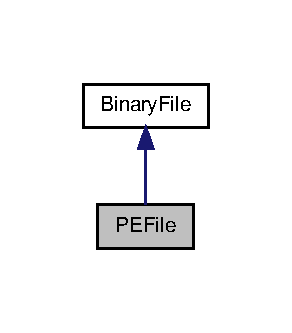
\includegraphics[width=140pt]{class_p_e_file__inherit__graph}
\end{center}
\end{figure}


Diagram współpracy dla P\-E\-File\-:\nopagebreak
\begin{figure}[H]
\begin{center}
\leavevmode
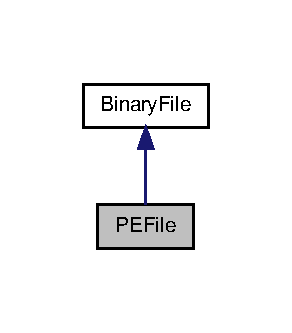
\includegraphics[width=140pt]{class_p_e_file__coll__graph}
\end{center}
\end{figure}
\subsection*{Komponenty}
\begin{DoxyCompactItemize}
\item 
struct {\bfseries Relocation\-Table}
\begin{DoxyCompactList}\small\item\em Struktura odpowiedzialna za przechowywanie wpisu w tablicy relokacji. \end{DoxyCompactList}\end{DoxyCompactItemize}
\subsection*{Metody publiczne}
\begin{DoxyCompactItemize}
\item 
\hyperlink{class_p_e_file_ae8d99a8a0dabc4891ba5f7ef5031bcdc}{P\-E\-File} (Q\-Byte\-Array d)
\begin{DoxyCompactList}\small\item\em Konstruktor. \end{DoxyCompactList}\item 
\hyperlink{class_p_e_file_a0e63ccc46a77ddc9106e98c9131674db}{$\sim$\-P\-E\-File} ()
\item 
bool \hyperlink{class_p_e_file_a90a96d95f9d67ff48bf12ffcb0f22d41}{is\-\_\-valid} () const 
\begin{DoxyCompactList}\small\item\em Sprawdza czy w pamięci przechowywany jest poprawny plik. \end{DoxyCompactList}\item 
bool \hyperlink{class_p_e_file_aa8e69bdca4d00216df406278b4e96a28}{is\-\_\-x64} () const 
\begin{DoxyCompactList}\small\item\em Metoda informująca czy wczytany plik jest 64-\/bitowy. \end{DoxyCompactList}\item 
bool \hyperlink{class_p_e_file_a371cc84eed9dd5d85b7c50d60c1eb56f}{is\-\_\-x86} () const 
\begin{DoxyCompactList}\small\item\em Metoda informująca czy wczytany plik jest 32-\/bitowy. \end{DoxyCompactList}\item 
bool \hyperlink{class_p_e_file_a31cab72915687c9138e804e644f80ac6}{set\-New\-Entry\-Point} (unsigned int new\-E\-P)
\begin{DoxyCompactList}\small\item\em Ustawia nowy Entry\-Point. \end{DoxyCompactList}\item 
unsigned int \hyperlink{class_p_e_file_a82c9e3280a60fbdf13e7a7b7dbbf9ddb}{get\-Entry\-Point} ()
\begin{DoxyCompactList}\small\item\em Pobiera Entry\-Point. \end{DoxyCompactList}\item 
uint64\-\_\-t \hyperlink{class_p_e_file_ac3bf74a6efbc10bd642fbb345e71bf2d}{get\-Image\-Base} ()
\begin{DoxyCompactList}\small\item\em Pobiera Image\-Base. \end{DoxyCompactList}\item 
bool \hyperlink{class_p_e_file_a698dd8d1b169ac0b9d01ebfecd16bc51}{set\-Tls\-Address\-Of\-Call\-Backs} (uint64\-\_\-t addr)
\begin{DoxyCompactList}\small\item\em Ustawia adres wirtualny tablicy ze wskaźnikami do funkcji T\-L\-S. \end{DoxyCompactList}\item 
uint64\-\_\-t \hyperlink{class_p_e_file_aa60f615dfd569e601e3d25eaded2d3ed}{get\-Tls\-Address\-Of\-Index} ()
\begin{DoxyCompactList}\small\item\em Pobiera adres wirtualny pod którym znajduje się index T\-L\-S. \end{DoxyCompactList}\item 
bool \hyperlink{class_p_e_file_a2d6f55148b572f564bc30e881d97d9f8}{set\-Tls\-Address\-Of\-Index} (uint64\-\_\-t addr)
\begin{DoxyCompactList}\small\item\em Ustawia adres wirtualny pod którym znajduje się index T\-L\-S. \end{DoxyCompactList}\item 
size\-\_\-t \hyperlink{class_p_e_file_a45168c8ca08be4b58f79637a717135ac}{get\-Image\-Tls\-Directory\-Size} () const 
\begin{DoxyCompactList}\small\item\em Pobiera rozmiar struktury I\-M\-A\-G\-E\-\_\-\-T\-L\-S\-\_\-\-D\-I\-R\-E\-C\-T\-O\-R\-Y. \end{DoxyCompactList}\item 
uint64\-\_\-t \hyperlink{class_p_e_file_ab385de72db3e791e1477cb6593266d45}{get\-Tls\-Address\-Of\-Call\-Backs} ()
\begin{DoxyCompactList}\small\item\em Pobiera adres wirtualny tablicy ze wskaźnikami do funkcji T\-L\-S. \end{DoxyCompactList}\item 
Q\-Byte\-Array \hyperlink{class_p_e_file_a842228e192f08a70f80f564fe4ee7bc5}{get\-Text\-Section} ()
\begin{DoxyCompactList}\small\item\em Metoda pobierają◘ca zawartość sekcji .text. \end{DoxyCompactList}\item 
uint32\-\_\-t \hyperlink{class_p_e_file_afdcc62870de787ebaee455b55af8f06f}{get\-Text\-Section\-Offset} ()
\begin{DoxyCompactList}\small\item\em Metoda pobierająca przesunięcie w pliku sekcji .text. \end{DoxyCompactList}\item 
bool \hyperlink{class_p_e_file_aecfb5938f29e1cb030e968349b3112ef}{has\-Tls} ()
\begin{DoxyCompactList}\small\item\em Metoda sprawdzająca czy w pliku istnieje tablica T\-L\-S. \end{DoxyCompactList}\item 
bool \hyperlink{class_p_e_file_a6cd64df26158260f265b26e40b3b5dea}{set\-Tls\-Directory\-Address} (uint64\-\_\-t addr)
\begin{DoxyCompactList}\small\item\em Metoda ustawiająca adres tablicy T\-L\-S. \end{DoxyCompactList}\item 
uint64\-\_\-t \hyperlink{class_p_e_file_a6a98e9259a0013bff708271b378648ef}{get\-Tls\-Directory\-Address} ()
\begin{DoxyCompactList}\small\item\em Metoda pobierająca adres tablicy T\-L\-S. \end{DoxyCompactList}\item 
Q\-List$<$ uint64\-\_\-t $>$ \hyperlink{class_p_e_file_af718219d753f57388e3db28a55928b3e}{get\-Tls\-Callbacks} ()
\begin{DoxyCompactList}\small\item\em Metoda pobierająca adresy funkcji T\-L\-S. \end{DoxyCompactList}\item 
bool \hyperlink{class_p_e_file_ab6f1b8483aeba41b153aa27e9c6a0b8b}{add\-Relocations} (Q\-List$<$ uint64\-\_\-t $>$ relocations)
\begin{DoxyCompactList}\small\item\em Metoda dodająca wpisy do tablicy relokacji. \end{DoxyCompactList}\item 
{\footnotesize template$<$typename Register $>$ }\\uint64\-\_\-t \hyperlink{class_p_e_file_ab14d9fb29123545e0a7528795e64d3c1}{inject\-Unique\-Data} (\hyperlink{class_binary_code}{Binary\-Code}$<$ Register $>$ data, Q\-Map$<$ Q\-Byte\-Array, uint64\-\_\-t $>$ \&ptrs, Q\-List$<$ uint64\-\_\-t $>$ \&relocations)
\begin{DoxyCompactList}\small\item\em Metoda dodająca dane do pliku (jeżeli nie były już wcześniej dodane). Metoda na podstawie danych przygotowuje tablicę relokacji. \end{DoxyCompactList}\item 
uint64\-\_\-t \hyperlink{class_p_e_file_a6bea21405c1aab9b4e3d43d980a5aac5}{inject\-Unique\-Data} (Q\-Byte\-Array data, Q\-Map$<$ Q\-Byte\-Array, uint64\-\_\-t $>$ \&ptrs, bool $\ast$inserted=N\-U\-L\-L)
\begin{DoxyCompactList}\small\item\em Metoda dodająca kod, który nie powinien/nie musi być poddawany relokacji. \end{DoxyCompactList}\item 
uint64\-\_\-t \hyperlink{class_p_e_file_a2dca67d21245ba63171ee34456456f96}{generate\-String} (Q\-String str, Q\-Map$<$ Q\-Byte\-Array, uint64\-\_\-t $>$ \&ptrs)
\begin{DoxyCompactList}\small\item\em Metoda wklejająca unikalny string do pliku P\-E. \end{DoxyCompactList}\item 
uint64\-\_\-t \hyperlink{class_p_e_file_a1cf0f58cf7e061011a1dd95b16076e07}{get\-Address\-At\-Call\-Instruction\-Offset} (uint32\-\_\-t offset)
\begin{DoxyCompactList}\small\item\em Metoda pobierająca adres skoku instrukcji call lub jmp znajdującej się pod konkretnym offsetem. \end{DoxyCompactList}\item 
bool \hyperlink{class_p_e_file_a6c06d44bec906ab659326541e6244850}{set\-Address\-At\-Call\-Instruction\-Offset} (uint32\-\_\-t offset, uint64\-\_\-t address)
\begin{DoxyCompactList}\small\item\em Metoda ustawiająca adres skoku instrukcji call lub jmp znajdującej się w konkretnym miejscu w pliku. \end{DoxyCompactList}\end{DoxyCompactItemize}
\subsection*{Dodatkowe Dziedziczone Składowe}


\subsection{Opis szczegółowy}
Klasa odpowiedzialna za parsowanie plików P\-E. 

Definicja w linii 27 pliku pefile.\-h.



\subsection{Dokumentacja konstruktora i destruktora}
\hypertarget{class_p_e_file_ae8d99a8a0dabc4891ba5f7ef5031bcdc}{\index{P\-E\-File@{P\-E\-File}!P\-E\-File@{P\-E\-File}}
\index{P\-E\-File@{P\-E\-File}!PEFile@{P\-E\-File}}
\subsubsection[{P\-E\-File}]{\setlength{\rightskip}{0pt plus 5cm}P\-E\-File\-::\-P\-E\-File (
\begin{DoxyParamCaption}
\item[{Q\-Byte\-Array}]{d}
\end{DoxyParamCaption}
)}}\label{class_p_e_file_ae8d99a8a0dabc4891ba5f7ef5031bcdc}


Konstruktor. 


\begin{DoxyParams}{Parametry}
{\em d} & Zawartość pliku P\-E \\
\hline
\end{DoxyParams}


Definicja w linii 256 pliku pefile.\-cpp.

\hypertarget{class_p_e_file_a0e63ccc46a77ddc9106e98c9131674db}{\index{P\-E\-File@{P\-E\-File}!$\sim$\-P\-E\-File@{$\sim$\-P\-E\-File}}
\index{$\sim$\-P\-E\-File@{$\sim$\-P\-E\-File}!PEFile@{P\-E\-File}}
\subsubsection[{$\sim$\-P\-E\-File}]{\setlength{\rightskip}{0pt plus 5cm}P\-E\-File\-::$\sim$\-P\-E\-File (
\begin{DoxyParamCaption}
{}
\end{DoxyParamCaption}
)}}\label{class_p_e_file_a0e63ccc46a77ddc9106e98c9131674db}


Definicja w linii 266 pliku pefile.\-cpp.



\subsection{Dokumentacja funkcji składowych}
\hypertarget{class_p_e_file_ab6f1b8483aeba41b153aa27e9c6a0b8b}{\index{P\-E\-File@{P\-E\-File}!add\-Relocations@{add\-Relocations}}
\index{add\-Relocations@{add\-Relocations}!PEFile@{P\-E\-File}}
\subsubsection[{add\-Relocations}]{\setlength{\rightskip}{0pt plus 5cm}bool P\-E\-File\-::add\-Relocations (
\begin{DoxyParamCaption}
\item[{Q\-List$<$ uint64\-\_\-t $>$}]{relocations}
\end{DoxyParamCaption}
)}}\label{class_p_e_file_ab6f1b8483aeba41b153aa27e9c6a0b8b}


Metoda dodająca wpisy do tablicy relokacji. 


\begin{DoxyParams}{Parametry}
{\em relocations} & Offsety adresów do relokacji \\
\hline
\end{DoxyParams}
\begin{DoxyReturn}{Zwraca}
True w przypadku powodzenia 
\end{DoxyReturn}


Definicja w linii 361 pliku pefile.\-cpp.



Oto graf wywołań dla tej funkcji\-:\nopagebreak
\begin{figure}[H]
\begin{center}
\leavevmode
\includegraphics[width=350pt]{class_p_e_file_ab6f1b8483aeba41b153aa27e9c6a0b8b_cgraph}
\end{center}
\end{figure}


\hypertarget{class_p_e_file_a2dca67d21245ba63171ee34456456f96}{\index{P\-E\-File@{P\-E\-File}!generate\-String@{generate\-String}}
\index{generate\-String@{generate\-String}!PEFile@{P\-E\-File}}
\subsubsection[{generate\-String}]{\setlength{\rightskip}{0pt plus 5cm}uint64\-\_\-t P\-E\-File\-::generate\-String (
\begin{DoxyParamCaption}
\item[{Q\-String}]{str, }
\item[{Q\-Map$<$ Q\-Byte\-Array, uint64\-\_\-t $>$ \&}]{ptrs}
\end{DoxyParamCaption}
)}}\label{class_p_e_file_a2dca67d21245ba63171ee34456456f96}


Metoda wklejająca unikalny string do pliku P\-E. 


\begin{DoxyParams}{Parametry}
{\em str} & Napis do wklejenia \\
\hline
{\em ptrs} & Mapa zawierająca adresy wcześniej dodanych danych/kodu \\
\hline
\end{DoxyParams}
\begin{DoxyReturn}{Zwraca}
Ares wirtualny wklejonego napisu. 
\end{DoxyReturn}


Definicja w linii 276 pliku pefile.\-cpp.



Oto graf wywołań dla tej funkcji\-:\nopagebreak
\begin{figure}[H]
\begin{center}
\leavevmode
\includegraphics[width=350pt]{class_p_e_file_a2dca67d21245ba63171ee34456456f96_cgraph}
\end{center}
\end{figure}


\hypertarget{class_p_e_file_a1cf0f58cf7e061011a1dd95b16076e07}{\index{P\-E\-File@{P\-E\-File}!get\-Address\-At\-Call\-Instruction\-Offset@{get\-Address\-At\-Call\-Instruction\-Offset}}
\index{get\-Address\-At\-Call\-Instruction\-Offset@{get\-Address\-At\-Call\-Instruction\-Offset}!PEFile@{P\-E\-File}}
\subsubsection[{get\-Address\-At\-Call\-Instruction\-Offset}]{\setlength{\rightskip}{0pt plus 5cm}uint64\-\_\-t P\-E\-File\-::get\-Address\-At\-Call\-Instruction\-Offset (
\begin{DoxyParamCaption}
\item[{uint32\-\_\-t}]{offset}
\end{DoxyParamCaption}
)}}\label{class_p_e_file_a1cf0f58cf7e061011a1dd95b16076e07}


Metoda pobierająca adres skoku instrukcji call lub jmp znajdującej się pod konkretnym offsetem. 


\begin{DoxyParams}{Parametry}
{\em offset} & Miejsce w pliku, w którym znajduje się instrukcja call lub jmp. \\
\hline
\end{DoxyParams}
\begin{DoxyReturn}{Zwraca}
Adres wirtualny skoku 
\end{DoxyReturn}


Definicja w linii 499 pliku pefile.\-cpp.



Oto graf wywołań dla tej funkcji\-:\nopagebreak
\begin{figure}[H]
\begin{center}
\leavevmode
\includegraphics[width=350pt]{class_p_e_file_a1cf0f58cf7e061011a1dd95b16076e07_cgraph}
\end{center}
\end{figure}


\hypertarget{class_p_e_file_a82c9e3280a60fbdf13e7a7b7dbbf9ddb}{\index{P\-E\-File@{P\-E\-File}!get\-Entry\-Point@{get\-Entry\-Point}}
\index{get\-Entry\-Point@{get\-Entry\-Point}!PEFile@{P\-E\-File}}
\subsubsection[{get\-Entry\-Point}]{\setlength{\rightskip}{0pt plus 5cm}unsigned int P\-E\-File\-::get\-Entry\-Point (
\begin{DoxyParamCaption}
{}
\end{DoxyParamCaption}
)}}\label{class_p_e_file_a82c9e3280a60fbdf13e7a7b7dbbf9ddb}


Pobiera Entry\-Point. 

\begin{DoxyReturn}{Zwraca}
E\-P 
\end{DoxyReturn}


Definicja w linii 1124 pliku pefile.\-cpp.

\hypertarget{class_p_e_file_ac3bf74a6efbc10bd642fbb345e71bf2d}{\index{P\-E\-File@{P\-E\-File}!get\-Image\-Base@{get\-Image\-Base}}
\index{get\-Image\-Base@{get\-Image\-Base}!PEFile@{P\-E\-File}}
\subsubsection[{get\-Image\-Base}]{\setlength{\rightskip}{0pt plus 5cm}uint64\-\_\-t P\-E\-File\-::get\-Image\-Base (
\begin{DoxyParamCaption}
{}
\end{DoxyParamCaption}
)}}\label{class_p_e_file_ac3bf74a6efbc10bd642fbb345e71bf2d}


Pobiera Image\-Base. 

\begin{DoxyReturn}{Zwraca}
Image\-Base 
\end{DoxyReturn}


Definicja w linii 1132 pliku pefile.\-cpp.

\hypertarget{class_p_e_file_a45168c8ca08be4b58f79637a717135ac}{\index{P\-E\-File@{P\-E\-File}!get\-Image\-Tls\-Directory\-Size@{get\-Image\-Tls\-Directory\-Size}}
\index{get\-Image\-Tls\-Directory\-Size@{get\-Image\-Tls\-Directory\-Size}!PEFile@{P\-E\-File}}
\subsubsection[{get\-Image\-Tls\-Directory\-Size}]{\setlength{\rightskip}{0pt plus 5cm}size\-\_\-t P\-E\-File\-::get\-Image\-Tls\-Directory\-Size (
\begin{DoxyParamCaption}
{}
\end{DoxyParamCaption}
) const}}\label{class_p_e_file_a45168c8ca08be4b58f79637a717135ac}


Pobiera rozmiar struktury I\-M\-A\-G\-E\-\_\-\-T\-L\-S\-\_\-\-D\-I\-R\-E\-C\-T\-O\-R\-Y. 

\begin{DoxyReturn}{Zwraca}
Rozmiar 
\end{DoxyReturn}


Definicja w linii 180 pliku pefile.\-cpp.

\hypertarget{class_p_e_file_a842228e192f08a70f80f564fe4ee7bc5}{\index{P\-E\-File@{P\-E\-File}!get\-Text\-Section@{get\-Text\-Section}}
\index{get\-Text\-Section@{get\-Text\-Section}!PEFile@{P\-E\-File}}
\subsubsection[{get\-Text\-Section}]{\setlength{\rightskip}{0pt plus 5cm}Q\-Byte\-Array P\-E\-File\-::get\-Text\-Section (
\begin{DoxyParamCaption}
{}
\end{DoxyParamCaption}
)}}\label{class_p_e_file_a842228e192f08a70f80f564fe4ee7bc5}


Metoda pobierają◘ca zawartość sekcji .text. 

\begin{DoxyReturn}{Zwraca}
Tablica bajtów sekcji .text 
\end{DoxyReturn}


Definicja w linii 1200 pliku pefile.\-cpp.



Oto graf wywołań dla tej funkcji\-:\nopagebreak
\begin{figure}[H]
\begin{center}
\leavevmode
\includegraphics[width=350pt]{class_p_e_file_a842228e192f08a70f80f564fe4ee7bc5_cgraph}
\end{center}
\end{figure}


\hypertarget{class_p_e_file_afdcc62870de787ebaee455b55af8f06f}{\index{P\-E\-File@{P\-E\-File}!get\-Text\-Section\-Offset@{get\-Text\-Section\-Offset}}
\index{get\-Text\-Section\-Offset@{get\-Text\-Section\-Offset}!PEFile@{P\-E\-File}}
\subsubsection[{get\-Text\-Section\-Offset}]{\setlength{\rightskip}{0pt plus 5cm}uint32\-\_\-t P\-E\-File\-::get\-Text\-Section\-Offset (
\begin{DoxyParamCaption}
{}
\end{DoxyParamCaption}
)}}\label{class_p_e_file_afdcc62870de787ebaee455b55af8f06f}


Metoda pobierająca przesunięcie w pliku sekcji .text. 

\begin{DoxyReturn}{Zwraca}
Przesunięcie od początku pliku 
\end{DoxyReturn}


Definicja w linii 1212 pliku pefile.\-cpp.



Oto graf wywołań dla tej funkcji\-:\nopagebreak
\begin{figure}[H]
\begin{center}
\leavevmode
\includegraphics[width=350pt]{class_p_e_file_afdcc62870de787ebaee455b55af8f06f_cgraph}
\end{center}
\end{figure}


\hypertarget{class_p_e_file_ab385de72db3e791e1477cb6593266d45}{\index{P\-E\-File@{P\-E\-File}!get\-Tls\-Address\-Of\-Call\-Backs@{get\-Tls\-Address\-Of\-Call\-Backs}}
\index{get\-Tls\-Address\-Of\-Call\-Backs@{get\-Tls\-Address\-Of\-Call\-Backs}!PEFile@{P\-E\-File}}
\subsubsection[{get\-Tls\-Address\-Of\-Call\-Backs}]{\setlength{\rightskip}{0pt plus 5cm}uint64\-\_\-t P\-E\-File\-::get\-Tls\-Address\-Of\-Call\-Backs (
\begin{DoxyParamCaption}
{}
\end{DoxyParamCaption}
)}}\label{class_p_e_file_ab385de72db3e791e1477cb6593266d45}


Pobiera adres wirtualny tablicy ze wskaźnikami do funkcji T\-L\-S. 

\begin{DoxyReturn}{Zwraca}
I\-M\-A\-G\-E\-\_\-\-T\-L\-S\-\_\-\-D\-I\-R\-E\-C\-T\-O\-R\-Y.\-Address\-Of\-Call\-Backs 
\end{DoxyReturn}


Definicja w linii 185 pliku pefile.\-cpp.

\hypertarget{class_p_e_file_aa60f615dfd569e601e3d25eaded2d3ed}{\index{P\-E\-File@{P\-E\-File}!get\-Tls\-Address\-Of\-Index@{get\-Tls\-Address\-Of\-Index}}
\index{get\-Tls\-Address\-Of\-Index@{get\-Tls\-Address\-Of\-Index}!PEFile@{P\-E\-File}}
\subsubsection[{get\-Tls\-Address\-Of\-Index}]{\setlength{\rightskip}{0pt plus 5cm}uint64\-\_\-t P\-E\-File\-::get\-Tls\-Address\-Of\-Index (
\begin{DoxyParamCaption}
{}
\end{DoxyParamCaption}
)}}\label{class_p_e_file_aa60f615dfd569e601e3d25eaded2d3ed}


Pobiera adres wirtualny pod którym znajduje się index T\-L\-S. 

\begin{DoxyReturn}{Zwraca}
I\-M\-A\-G\-E\-\_\-\-T\-L\-S\-\_\-\-D\-I\-R\-E\-C\-T\-O\-R\-Y.\-Address\-Of\-Index 
\end{DoxyReturn}


Definicja w linii 218 pliku pefile.\-cpp.

\hypertarget{class_p_e_file_af718219d753f57388e3db28a55928b3e}{\index{P\-E\-File@{P\-E\-File}!get\-Tls\-Callbacks@{get\-Tls\-Callbacks}}
\index{get\-Tls\-Callbacks@{get\-Tls\-Callbacks}!PEFile@{P\-E\-File}}
\subsubsection[{get\-Tls\-Callbacks}]{\setlength{\rightskip}{0pt plus 5cm}Q\-List$<$ uint64\-\_\-t $>$ P\-E\-File\-::get\-Tls\-Callbacks (
\begin{DoxyParamCaption}
{}
\end{DoxyParamCaption}
)}}\label{class_p_e_file_af718219d753f57388e3db28a55928b3e}


Metoda pobierająca adresy funkcji T\-L\-S. 

\begin{DoxyReturn}{Zwraca}
Tablica z adresami funkcji T\-L\-S 
\end{DoxyReturn}


Definicja w linii 466 pliku pefile.\-cpp.



Oto graf wywołań dla tej funkcji\-:\nopagebreak
\begin{figure}[H]
\begin{center}
\leavevmode
\includegraphics[width=350pt]{class_p_e_file_af718219d753f57388e3db28a55928b3e_cgraph}
\end{center}
\end{figure}


\hypertarget{class_p_e_file_a6a98e9259a0013bff708271b378648ef}{\index{P\-E\-File@{P\-E\-File}!get\-Tls\-Directory\-Address@{get\-Tls\-Directory\-Address}}
\index{get\-Tls\-Directory\-Address@{get\-Tls\-Directory\-Address}!PEFile@{P\-E\-File}}
\subsubsection[{get\-Tls\-Directory\-Address}]{\setlength{\rightskip}{0pt plus 5cm}uint64\-\_\-t P\-E\-File\-::get\-Tls\-Directory\-Address (
\begin{DoxyParamCaption}
{}
\end{DoxyParamCaption}
)}}\label{class_p_e_file_a6a98e9259a0013bff708271b378648ef}


Metoda pobierająca adres tablicy T\-L\-S. 

\begin{DoxyReturn}{Zwraca}
Adres 
\end{DoxyReturn}


Definicja w linii 458 pliku pefile.\-cpp.

\hypertarget{class_p_e_file_aecfb5938f29e1cb030e968349b3112ef}{\index{P\-E\-File@{P\-E\-File}!has\-Tls@{has\-Tls}}
\index{has\-Tls@{has\-Tls}!PEFile@{P\-E\-File}}
\subsubsection[{has\-Tls}]{\setlength{\rightskip}{0pt plus 5cm}bool P\-E\-File\-::has\-Tls (
\begin{DoxyParamCaption}
{}
\end{DoxyParamCaption}
)}}\label{class_p_e_file_aecfb5938f29e1cb030e968349b3112ef}


Metoda sprawdzająca czy w pliku istnieje tablica T\-L\-S. 

\begin{DoxyReturn}{Zwraca}
True gdy T\-L\-S istnieje 
\end{DoxyReturn}


Definicja w linii 439 pliku pefile.\-cpp.

\hypertarget{class_p_e_file_ab14d9fb29123545e0a7528795e64d3c1}{\index{P\-E\-File@{P\-E\-File}!inject\-Unique\-Data@{inject\-Unique\-Data}}
\index{inject\-Unique\-Data@{inject\-Unique\-Data}!PEFile@{P\-E\-File}}
\subsubsection[{inject\-Unique\-Data}]{\setlength{\rightskip}{0pt plus 5cm}template$<$typename Register $>$ uint64\-\_\-t P\-E\-File\-::inject\-Unique\-Data (
\begin{DoxyParamCaption}
\item[{{\bf Binary\-Code}$<$ Register $>$}]{data, }
\item[{Q\-Map$<$ Q\-Byte\-Array, uint64\-\_\-t $>$ \&}]{ptrs, }
\item[{Q\-List$<$ uint64\-\_\-t $>$ \&}]{relocations}
\end{DoxyParamCaption}
)}}\label{class_p_e_file_ab14d9fb29123545e0a7528795e64d3c1}


Metoda dodająca dane do pliku (jeżeli nie były już wcześniej dodane). Metoda na podstawie danych przygotowuje tablicę relokacji. 


\begin{DoxyParams}{Parametry}
{\em data} & Dane do wklejenia \\
\hline
{\em ptrs} & Mapa z zapamiętanymi adresami dodanego wcześniej kodu \\
\hline
{\em relocations} & Lista adresów do relokacji \\
\hline
\end{DoxyParams}
\begin{DoxyReturn}{Zwraca}
Ares wirtualny wklejonego kodu. 
\end{DoxyReturn}


Definicja w linii 334 pliku pefile.\-cpp.



Oto graf wywołań dla tej funkcji\-:\nopagebreak
\begin{figure}[H]
\begin{center}
\leavevmode
\includegraphics[width=350pt]{class_p_e_file_ab14d9fb29123545e0a7528795e64d3c1_cgraph}
\end{center}
\end{figure}


\hypertarget{class_p_e_file_a6bea21405c1aab9b4e3d43d980a5aac5}{\index{P\-E\-File@{P\-E\-File}!inject\-Unique\-Data@{inject\-Unique\-Data}}
\index{inject\-Unique\-Data@{inject\-Unique\-Data}!PEFile@{P\-E\-File}}
\subsubsection[{inject\-Unique\-Data}]{\setlength{\rightskip}{0pt plus 5cm}uint64\-\_\-t P\-E\-File\-::inject\-Unique\-Data (
\begin{DoxyParamCaption}
\item[{Q\-Byte\-Array}]{data, }
\item[{Q\-Map$<$ Q\-Byte\-Array, uint64\-\_\-t $>$ \&}]{ptrs, }
\item[{bool $\ast$}]{inserted = {\ttfamily NULL}}
\end{DoxyParamCaption}
)}}\label{class_p_e_file_a6bea21405c1aab9b4e3d43d980a5aac5}


Metoda dodająca kod, który nie powinien/nie musi być poddawany relokacji. 


\begin{DoxyParams}{Parametry}
{\em data} & Dane do dodania \\
\hline
{\em ptrs} & Mapa z zapamiętanymi adresami dodanego wcześniej kodu/danych \\
\hline
{\em inserted} & Flaga informująca czy kod został dodany czy wcześniej znajdował się na liście pointerów do dodanego kodu \\
\hline
\end{DoxyParams}
\begin{DoxyReturn}{Zwraca}
Ares wirtualny wklejonego kodu/danych. 
\end{DoxyReturn}


Definicja w linii 281 pliku pefile.\-cpp.



Oto graf wywołań dla tej funkcji\-:\nopagebreak
\begin{figure}[H]
\begin{center}
\leavevmode
\includegraphics[width=350pt]{class_p_e_file_a6bea21405c1aab9b4e3d43d980a5aac5_cgraph}
\end{center}
\end{figure}


\hypertarget{class_p_e_file_a90a96d95f9d67ff48bf12ffcb0f22d41}{\index{P\-E\-File@{P\-E\-File}!is\-\_\-valid@{is\-\_\-valid}}
\index{is\-\_\-valid@{is\-\_\-valid}!PEFile@{P\-E\-File}}
\subsubsection[{is\-\_\-valid}]{\setlength{\rightskip}{0pt plus 5cm}bool P\-E\-File\-::is\-\_\-valid (
\begin{DoxyParamCaption}
{}
\end{DoxyParamCaption}
) const\hspace{0.3cm}{\ttfamily [virtual]}}}\label{class_p_e_file_a90a96d95f9d67ff48bf12ffcb0f22d41}


Sprawdza czy w pamięci przechowywany jest poprawny plik. 

\begin{DoxyReturn}{Zwraca}
True jeżeli plik jest poprawny. 
\end{DoxyReturn}


Implementuje \hyperlink{class_binary_file_a6007435bc4451bb80a3169d977f4f125}{Binary\-File}.



Definicja w linii 613 pliku pefile.\-cpp.

\hypertarget{class_p_e_file_aa8e69bdca4d00216df406278b4e96a28}{\index{P\-E\-File@{P\-E\-File}!is\-\_\-x64@{is\-\_\-x64}}
\index{is\-\_\-x64@{is\-\_\-x64}!PEFile@{P\-E\-File}}
\subsubsection[{is\-\_\-x64}]{\setlength{\rightskip}{0pt plus 5cm}bool P\-E\-File\-::is\-\_\-x64 (
\begin{DoxyParamCaption}
{}
\end{DoxyParamCaption}
) const\hspace{0.3cm}{\ttfamily [virtual]}}}\label{class_p_e_file_aa8e69bdca4d00216df406278b4e96a28}


Metoda informująca czy wczytany plik jest 64-\/bitowy. 

\begin{DoxyReturn}{Zwraca}
True gdy plik x64 
\end{DoxyReturn}


Implementuje \hyperlink{class_binary_file_a36b7998c72bbee68ab492d93368c14ca}{Binary\-File}.



Definicja w linii 489 pliku pefile.\-cpp.

\hypertarget{class_p_e_file_a371cc84eed9dd5d85b7c50d60c1eb56f}{\index{P\-E\-File@{P\-E\-File}!is\-\_\-x86@{is\-\_\-x86}}
\index{is\-\_\-x86@{is\-\_\-x86}!PEFile@{P\-E\-File}}
\subsubsection[{is\-\_\-x86}]{\setlength{\rightskip}{0pt plus 5cm}bool P\-E\-File\-::is\-\_\-x86 (
\begin{DoxyParamCaption}
{}
\end{DoxyParamCaption}
) const\hspace{0.3cm}{\ttfamily [virtual]}}}\label{class_p_e_file_a371cc84eed9dd5d85b7c50d60c1eb56f}


Metoda informująca czy wczytany plik jest 32-\/bitowy. 

\begin{DoxyReturn}{Zwraca}
True gdy plik x86 
\end{DoxyReturn}


Implementuje \hyperlink{class_binary_file_aa7d43cde4ab8cc9723d2b5c769719bd9}{Binary\-File}.



Definicja w linii 494 pliku pefile.\-cpp.

\hypertarget{class_p_e_file_a6c06d44bec906ab659326541e6244850}{\index{P\-E\-File@{P\-E\-File}!set\-Address\-At\-Call\-Instruction\-Offset@{set\-Address\-At\-Call\-Instruction\-Offset}}
\index{set\-Address\-At\-Call\-Instruction\-Offset@{set\-Address\-At\-Call\-Instruction\-Offset}!PEFile@{P\-E\-File}}
\subsubsection[{set\-Address\-At\-Call\-Instruction\-Offset}]{\setlength{\rightskip}{0pt plus 5cm}bool P\-E\-File\-::set\-Address\-At\-Call\-Instruction\-Offset (
\begin{DoxyParamCaption}
\item[{uint32\-\_\-t}]{offset, }
\item[{uint64\-\_\-t}]{address}
\end{DoxyParamCaption}
)}}\label{class_p_e_file_a6c06d44bec906ab659326541e6244850}


Metoda ustawiająca adres skoku instrukcji call lub jmp znajdującej się w konkretnym miejscu w pliku. 


\begin{DoxyParams}{Parametry}
{\em offset} & Offset w pliku instrukcji call lub jmp \\
\hline
{\em address} & Adres skoku do ustawienia \\
\hline
\end{DoxyParams}
\begin{DoxyReturn}{Zwraca}
True w przypadku sukcesu 
\end{DoxyReturn}


Definicja w linii 510 pliku pefile.\-cpp.



Oto graf wywołań dla tej funkcji\-:\nopagebreak
\begin{figure}[H]
\begin{center}
\leavevmode
\includegraphics[width=350pt]{class_p_e_file_a6c06d44bec906ab659326541e6244850_cgraph}
\end{center}
\end{figure}


\hypertarget{class_p_e_file_a31cab72915687c9138e804e644f80ac6}{\index{P\-E\-File@{P\-E\-File}!set\-New\-Entry\-Point@{set\-New\-Entry\-Point}}
\index{set\-New\-Entry\-Point@{set\-New\-Entry\-Point}!PEFile@{P\-E\-File}}
\subsubsection[{set\-New\-Entry\-Point}]{\setlength{\rightskip}{0pt plus 5cm}bool P\-E\-File\-::set\-New\-Entry\-Point (
\begin{DoxyParamCaption}
\item[{unsigned int}]{new\-E\-P}
\end{DoxyParamCaption}
)}}\label{class_p_e_file_a31cab72915687c9138e804e644f80ac6}


Ustawia nowy Entry\-Point. 


\begin{DoxyParams}{Parametry}
{\em new\-E\-P} & nowy E\-P; \\
\hline
\end{DoxyParams}
\begin{DoxyReturn}{Zwraca}
true w przypadku sukcesu. 
\end{DoxyReturn}


Definicja w linii 1110 pliku pefile.\-cpp.

\hypertarget{class_p_e_file_a698dd8d1b169ac0b9d01ebfecd16bc51}{\index{P\-E\-File@{P\-E\-File}!set\-Tls\-Address\-Of\-Call\-Backs@{set\-Tls\-Address\-Of\-Call\-Backs}}
\index{set\-Tls\-Address\-Of\-Call\-Backs@{set\-Tls\-Address\-Of\-Call\-Backs}!PEFile@{P\-E\-File}}
\subsubsection[{set\-Tls\-Address\-Of\-Call\-Backs}]{\setlength{\rightskip}{0pt plus 5cm}bool P\-E\-File\-::set\-Tls\-Address\-Of\-Call\-Backs (
\begin{DoxyParamCaption}
\item[{uint64\-\_\-t}]{addr}
\end{DoxyParamCaption}
)}}\label{class_p_e_file_a698dd8d1b169ac0b9d01ebfecd16bc51}


Ustawia adres wirtualny tablicy ze wskaźnikami do funkcji T\-L\-S. 


\begin{DoxyParams}{Parametry}
{\em addr} & Nowy adres \\
\hline
\end{DoxyParams}
\begin{DoxyReturn}{Zwraca}
True w przypadku powodzenia 
\end{DoxyReturn}


Definicja w linii 195 pliku pefile.\-cpp.

\hypertarget{class_p_e_file_a2d6f55148b572f564bc30e881d97d9f8}{\index{P\-E\-File@{P\-E\-File}!set\-Tls\-Address\-Of\-Index@{set\-Tls\-Address\-Of\-Index}}
\index{set\-Tls\-Address\-Of\-Index@{set\-Tls\-Address\-Of\-Index}!PEFile@{P\-E\-File}}
\subsubsection[{set\-Tls\-Address\-Of\-Index}]{\setlength{\rightskip}{0pt plus 5cm}bool P\-E\-File\-::set\-Tls\-Address\-Of\-Index (
\begin{DoxyParamCaption}
\item[{uint64\-\_\-t}]{addr}
\end{DoxyParamCaption}
)}}\label{class_p_e_file_a2d6f55148b572f564bc30e881d97d9f8}


Ustawia adres wirtualny pod którym znajduje się index T\-L\-S. 


\begin{DoxyParams}{Parametry}
{\em addr} & Nowy adres \\
\hline
\end{DoxyParams}
\begin{DoxyReturn}{Zwraca}
True w przypadku powodzenia 
\end{DoxyReturn}


Definicja w linii 228 pliku pefile.\-cpp.

\hypertarget{class_p_e_file_a6cd64df26158260f265b26e40b3b5dea}{\index{P\-E\-File@{P\-E\-File}!set\-Tls\-Directory\-Address@{set\-Tls\-Directory\-Address}}
\index{set\-Tls\-Directory\-Address@{set\-Tls\-Directory\-Address}!PEFile@{P\-E\-File}}
\subsubsection[{set\-Tls\-Directory\-Address}]{\setlength{\rightskip}{0pt plus 5cm}bool P\-E\-File\-::set\-Tls\-Directory\-Address (
\begin{DoxyParamCaption}
\item[{uint64\-\_\-t}]{addr}
\end{DoxyParamCaption}
)}}\label{class_p_e_file_a6cd64df26158260f265b26e40b3b5dea}


Metoda ustawiająca adres tablicy T\-L\-S. 


\begin{DoxyParams}{Parametry}
{\em addr} & Adres T\-L\-S \\
\hline
\end{DoxyParams}
\begin{DoxyReturn}{Zwraca}
True w przypadku powodzenia 
\end{DoxyReturn}


Definicja w linii 447 pliku pefile.\-cpp.



Oto graf wywołań dla tej funkcji\-:\nopagebreak
\begin{figure}[H]
\begin{center}
\leavevmode
\includegraphics[width=350pt]{class_p_e_file_a6cd64df26158260f265b26e40b3b5dea_cgraph}
\end{center}
\end{figure}




Dokumentacja dla tej klasy została wygenerowana z plików\-:\begin{DoxyCompactItemize}
\item 
core/file\-\_\-types/\hyperlink{pefile_8h}{pefile.\-h}\item 
core/file\-\_\-types/\hyperlink{pefile_8cpp}{pefile.\-cpp}\end{DoxyCompactItemize}

\hypertarget{class_proc_out}{\section{Dokumentacja klasy Proc\-Out}
\label{class_proc_out}\index{Proc\-Out@{Proc\-Out}}
}


{\ttfamily \#include $<$procout.\-h$>$}

\subsection*{Sloty publiczne}
\begin{DoxyCompactItemize}
\item 
void \hyperlink{class_proc_out_a74a10fb3b6a8648f145c9520300aa6fd}{ready\-Read} ()
\item 
void \hyperlink{class_proc_out_a1217c4df45842d54c438c2d94e979c63}{finished} ()
\end{DoxyCompactItemize}
\subsection*{Metody publiczne}
\begin{DoxyCompactItemize}
\item 
\hyperlink{class_proc_out_a32000573c7c559fcdfd68bcba443dd16}{Proc\-Out} (Q\-Object $\ast$parent=N\-U\-L\-L)
\item 
virtual \hyperlink{class_proc_out_a063492995249f724d970a454209f2197}{$\sim$\-Proc\-Out} ()
\end{DoxyCompactItemize}


\subsection{Opis szczegółowy}


Definicja w linii 12 pliku procout.\-h.



\subsection{Dokumentacja konstruktora i destruktora}
\hypertarget{class_proc_out_a32000573c7c559fcdfd68bcba443dd16}{\index{Proc\-Out@{Proc\-Out}!Proc\-Out@{Proc\-Out}}
\index{Proc\-Out@{Proc\-Out}!ProcOut@{Proc\-Out}}
\subsubsection[{Proc\-Out}]{\setlength{\rightskip}{0pt plus 5cm}Proc\-Out\-::\-Proc\-Out (
\begin{DoxyParamCaption}
\item[{Q\-Object $\ast$}]{parent = {\ttfamily NULL}}
\end{DoxyParamCaption}
)}}\label{class_proc_out_a32000573c7c559fcdfd68bcba443dd16}


Definicja w linii 3 pliku procout.\-cpp.

\hypertarget{class_proc_out_a063492995249f724d970a454209f2197}{\index{Proc\-Out@{Proc\-Out}!$\sim$\-Proc\-Out@{$\sim$\-Proc\-Out}}
\index{$\sim$\-Proc\-Out@{$\sim$\-Proc\-Out}!ProcOut@{Proc\-Out}}
\subsubsection[{$\sim$\-Proc\-Out}]{\setlength{\rightskip}{0pt plus 5cm}virtual Proc\-Out\-::$\sim$\-Proc\-Out (
\begin{DoxyParamCaption}
{}
\end{DoxyParamCaption}
)\hspace{0.3cm}{\ttfamily [inline]}, {\ttfamily [virtual]}}}\label{class_proc_out_a063492995249f724d970a454209f2197}


Definicja w linii 17 pliku procout.\-h.



\subsection{Dokumentacja funkcji składowych}
\hypertarget{class_proc_out_a1217c4df45842d54c438c2d94e979c63}{\index{Proc\-Out@{Proc\-Out}!finished@{finished}}
\index{finished@{finished}!ProcOut@{Proc\-Out}}
\subsubsection[{finished}]{\setlength{\rightskip}{0pt plus 5cm}void Proc\-Out\-::finished (
\begin{DoxyParamCaption}
{}
\end{DoxyParamCaption}
)\hspace{0.3cm}{\ttfamily [slot]}}}\label{class_proc_out_a1217c4df45842d54c438c2d94e979c63}


Definicja w linii 18 pliku procout.\-cpp.

\hypertarget{class_proc_out_a74a10fb3b6a8648f145c9520300aa6fd}{\index{Proc\-Out@{Proc\-Out}!ready\-Read@{ready\-Read}}
\index{ready\-Read@{ready\-Read}!ProcOut@{Proc\-Out}}
\subsubsection[{ready\-Read}]{\setlength{\rightskip}{0pt plus 5cm}void Proc\-Out\-::ready\-Read (
\begin{DoxyParamCaption}
{}
\end{DoxyParamCaption}
)\hspace{0.3cm}{\ttfamily [slot]}}}\label{class_proc_out_a74a10fb3b6a8648f145c9520300aa6fd}


Definicja w linii 8 pliku procout.\-cpp.



Dokumentacja dla tej klasy została wygenerowana z plików\-:\begin{DoxyCompactItemize}
\item 
Application\-Manager/\-D\-Source\-Code\-Parser/\hyperlink{procout_8h}{procout.\-h}\item 
Application\-Manager/\-D\-Source\-Code\-Parser/\hyperlink{procout_8cpp}{procout.\-cpp}\end{DoxyCompactItemize}

\hypertarget{class_d_adding_methods_1_1_thread_wrapper}{\section{Dokumentacja szablonu klasy D\-Adding\-Methods\-:\-:Thread\-Wrapper$<$ Registers\-Type $>$}
\label{class_d_adding_methods_1_1_thread_wrapper}\index{D\-Adding\-Methods\-::\-Thread\-Wrapper$<$ Registers\-Type $>$@{D\-Adding\-Methods\-::\-Thread\-Wrapper$<$ Registers\-Type $>$}}
}


Klasa reprezentująca opakowanie dla tworzenia nowego wątku.  




{\ttfamily \#include $<$daddingmethods.\-h$>$}



Diagram dziedziczenia dla D\-Adding\-Methods\-:\-:Thread\-Wrapper$<$ Registers\-Type $>$\nopagebreak
\begin{figure}[H]
\begin{center}
\leavevmode
\includegraphics[width=244pt]{class_d_adding_methods_1_1_thread_wrapper__inherit__graph}
\end{center}
\end{figure}


Diagram współpracy dla D\-Adding\-Methods\-:\-:Thread\-Wrapper$<$ Registers\-Type $>$\-:\nopagebreak
\begin{figure}[H]
\begin{center}
\leavevmode
\includegraphics[width=244pt]{class_d_adding_methods_1_1_thread_wrapper__coll__graph}
\end{center}
\end{figure}
\subsection*{Atrybuty publiczne}
\begin{DoxyCompactItemize}
\item 
Q\-List$<$ \hyperlink{class_d_adding_methods_1_1_wrapper}{Wrapper}$<$ Registers\-Type $>$ $\ast$ $>$ \hyperlink{class_d_adding_methods_1_1_thread_wrapper_a17fc0920f489293031ab914cb8d36ba7}{thread\-\_\-actions}
\item 
uint16\-\_\-t \hyperlink{class_d_adding_methods_1_1_thread_wrapper_a6125379d0d3674ddab3848951ed9ba16}{sleep\-\_\-time}
\end{DoxyCompactItemize}
\subsection*{Dodatkowe Dziedziczone Składowe}


\subsection{Opis szczegółowy}
\subsubsection*{template$<$typename Registers\-Type$>$class D\-Adding\-Methods\-::\-Thread\-Wrapper$<$ Registers\-Type $>$}

Klasa reprezentująca opakowanie dla tworzenia nowego wątku. 

Definicja w linii 227 pliku daddingmethods.\-h.



\subsection{Dokumentacja atrybutów składowych}
\hypertarget{class_d_adding_methods_1_1_thread_wrapper_a6125379d0d3674ddab3848951ed9ba16}{\index{D\-Adding\-Methods\-::\-Thread\-Wrapper@{D\-Adding\-Methods\-::\-Thread\-Wrapper}!sleep\-\_\-time@{sleep\-\_\-time}}
\index{sleep\-\_\-time@{sleep\-\_\-time}!DAddingMethods::ThreadWrapper@{D\-Adding\-Methods\-::\-Thread\-Wrapper}}
\subsubsection[{sleep\-\_\-time}]{\setlength{\rightskip}{0pt plus 5cm}template$<$typename Registers\-Type$>$ uint16\-\_\-t {\bf D\-Adding\-Methods\-::\-Thread\-Wrapper}$<$ Registers\-Type $>$\-::sleep\-\_\-time}}\label{class_d_adding_methods_1_1_thread_wrapper_a6125379d0d3674ddab3848951ed9ba16}


Definicja w linii 230 pliku daddingmethods.\-h.

\hypertarget{class_d_adding_methods_1_1_thread_wrapper_a17fc0920f489293031ab914cb8d36ba7}{\index{D\-Adding\-Methods\-::\-Thread\-Wrapper@{D\-Adding\-Methods\-::\-Thread\-Wrapper}!thread\-\_\-actions@{thread\-\_\-actions}}
\index{thread\-\_\-actions@{thread\-\_\-actions}!DAddingMethods::ThreadWrapper@{D\-Adding\-Methods\-::\-Thread\-Wrapper}}
\subsubsection[{thread\-\_\-actions}]{\setlength{\rightskip}{0pt plus 5cm}template$<$typename Registers\-Type$>$ Q\-List$<${\bf Wrapper}$<$Registers\-Type$>$$\ast$$>$ {\bf D\-Adding\-Methods\-::\-Thread\-Wrapper}$<$ Registers\-Type $>$\-::thread\-\_\-actions}}\label{class_d_adding_methods_1_1_thread_wrapper_a17fc0920f489293031ab914cb8d36ba7}


Definicja w linii 229 pliku daddingmethods.\-h.



Dokumentacja dla tej klasy została wygenerowana z pliku\-:\begin{DoxyCompactItemize}
\item 
core/adding\-\_\-methods/wrappers/\hyperlink{daddingmethods_8h}{daddingmethods.\-h}\end{DoxyCompactItemize}

\hypertarget{class_d_adding_methods_1_1_trampoline_wrapper}{\section{Dokumentacja szablonu klasy D\-Adding\-Methods\-:\-:Trampoline\-Wrapper$<$ Registers\-Type $>$}
\label{class_d_adding_methods_1_1_trampoline_wrapper}\index{D\-Adding\-Methods\-::\-Trampoline\-Wrapper$<$ Registers\-Type $>$@{D\-Adding\-Methods\-::\-Trampoline\-Wrapper$<$ Registers\-Type $>$}}
}


Klasa reprezentująca opakowanie dla tworzenia tramplin w funkcjach bibliotecznych.  




{\ttfamily \#include $<$daddingmethods.\-h$>$}



Diagram dziedziczenia dla D\-Adding\-Methods\-:\-:Trampoline\-Wrapper$<$ Registers\-Type $>$\nopagebreak
\begin{figure}[H]
\begin{center}
\leavevmode
\includegraphics[width=226pt]{class_d_adding_methods_1_1_trampoline_wrapper__inherit__graph}
\end{center}
\end{figure}


Diagram współpracy dla D\-Adding\-Methods\-:\-:Trampoline\-Wrapper$<$ Registers\-Type $>$\-:\nopagebreak
\begin{figure}[H]
\begin{center}
\leavevmode
\includegraphics[width=226pt]{class_d_adding_methods_1_1_trampoline_wrapper__coll__graph}
\end{center}
\end{figure}
\subsection*{Atrybuty publiczne}
\begin{DoxyCompactItemize}
\item 
\hyperlink{class_d_adding_methods_1_1_wrapper}{Wrapper}$<$ Registers\-Type $>$ $\ast$ \hyperlink{class_d_adding_methods_1_1_trampoline_wrapper_ad8edbc5d2b33a52be1bcaf5a4437339c}{tramp\-\_\-action}
\end{DoxyCompactItemize}
\subsection*{Dodatkowe Dziedziczone Składowe}


\subsection{Opis szczegółowy}
\subsubsection*{template$<$typename Registers\-Type$>$class D\-Adding\-Methods\-::\-Trampoline\-Wrapper$<$ Registers\-Type $>$}

Klasa reprezentująca opakowanie dla tworzenia tramplin w funkcjach bibliotecznych. 

Definicja w linii 246 pliku daddingmethods.\-h.



\subsection{Dokumentacja atrybutów składowych}
\hypertarget{class_d_adding_methods_1_1_trampoline_wrapper_ad8edbc5d2b33a52be1bcaf5a4437339c}{\index{D\-Adding\-Methods\-::\-Trampoline\-Wrapper@{D\-Adding\-Methods\-::\-Trampoline\-Wrapper}!tramp\-\_\-action@{tramp\-\_\-action}}
\index{tramp\-\_\-action@{tramp\-\_\-action}!DAddingMethods::TrampolineWrapper@{D\-Adding\-Methods\-::\-Trampoline\-Wrapper}}
\subsubsection[{tramp\-\_\-action}]{\setlength{\rightskip}{0pt plus 5cm}template$<$typename Registers\-Type$>$ {\bf Wrapper}$<$Registers\-Type$>$$\ast$ {\bf D\-Adding\-Methods\-::\-Trampoline\-Wrapper}$<$ Registers\-Type $>$\-::tramp\-\_\-action}}\label{class_d_adding_methods_1_1_trampoline_wrapper_ad8edbc5d2b33a52be1bcaf5a4437339c}


Definicja w linii 248 pliku daddingmethods.\-h.



Dokumentacja dla tej klasy została wygenerowana z pliku\-:\begin{DoxyCompactItemize}
\item 
core/adding\-\_\-methods/wrappers/\hyperlink{daddingmethods_8h}{daddingmethods.\-h}\end{DoxyCompactItemize}

\hypertarget{struct_p_e_file_1_1_relocation_table_1_1_type_offset}{\section{Dokumentacja struktury P\-E\-File\-:\-:Relocation\-Table\-:\-:Type\-Offset}
\label{struct_p_e_file_1_1_relocation_table_1_1_type_offset}\index{P\-E\-File\-::\-Relocation\-Table\-::\-Type\-Offset@{P\-E\-File\-::\-Relocation\-Table\-::\-Type\-Offset}}
}


Struktura przechowująca informację o typie i offsecie relokacji.  




{\ttfamily \#include $<$pefile.\-h$>$}

\subsection*{Atrybuty publiczne}
\begin{DoxyCompactItemize}
\item 
uint8\-\_\-t \hyperlink{struct_p_e_file_1_1_relocation_table_1_1_type_offset_a1d812b2e05780019bb9bb44d6fb1a3db}{Type}
\begin{DoxyCompactList}\small\item\em Typ relokacji. \end{DoxyCompactList}\item 
uint16\-\_\-t \hyperlink{struct_p_e_file_1_1_relocation_table_1_1_type_offset_a5b5bdeee7b3fae781cbbc48242dfc453}{Offset}
\begin{DoxyCompactList}\small\item\em Offset relokacji. \end{DoxyCompactList}\end{DoxyCompactItemize}


\subsection{Opis szczegółowy}
Struktura przechowująca informację o typie i offsecie relokacji. 

Definicja w linii 39 pliku pefile.\-h.



\subsection{Dokumentacja atrybutów składowych}
\hypertarget{struct_p_e_file_1_1_relocation_table_1_1_type_offset_a5b5bdeee7b3fae781cbbc48242dfc453}{\index{P\-E\-File\-::\-Relocation\-Table\-::\-Type\-Offset@{P\-E\-File\-::\-Relocation\-Table\-::\-Type\-Offset}!Offset@{Offset}}
\index{Offset@{Offset}!PEFile::RelocationTable::TypeOffset@{P\-E\-File\-::\-Relocation\-Table\-::\-Type\-Offset}}
\subsubsection[{Offset}]{\setlength{\rightskip}{0pt plus 5cm}uint16\-\_\-t P\-E\-File\-::\-Relocation\-Table\-::\-Type\-Offset\-::\-Offset}}\label{struct_p_e_file_1_1_relocation_table_1_1_type_offset_a5b5bdeee7b3fae781cbbc48242dfc453}


Offset relokacji. 



Definicja w linii 49 pliku pefile.\-h.

\hypertarget{struct_p_e_file_1_1_relocation_table_1_1_type_offset_a1d812b2e05780019bb9bb44d6fb1a3db}{\index{P\-E\-File\-::\-Relocation\-Table\-::\-Type\-Offset@{P\-E\-File\-::\-Relocation\-Table\-::\-Type\-Offset}!Type@{Type}}
\index{Type@{Type}!PEFile::RelocationTable::TypeOffset@{P\-E\-File\-::\-Relocation\-Table\-::\-Type\-Offset}}
\subsubsection[{Type}]{\setlength{\rightskip}{0pt plus 5cm}uint8\-\_\-t P\-E\-File\-::\-Relocation\-Table\-::\-Type\-Offset\-::\-Type}}\label{struct_p_e_file_1_1_relocation_table_1_1_type_offset_a1d812b2e05780019bb9bb44d6fb1a3db}


Typ relokacji. 



Definicja w linii 44 pliku pefile.\-h.



Dokumentacja dla tej struktury została wygenerowana z pliku\-:\begin{DoxyCompactItemize}
\item 
core/file\-\_\-types/\hyperlink{pefile_8h}{pefile.\-h}\end{DoxyCompactItemize}

\hypertarget{class_d_adding_methods_1_1_wrapper}{\section{Dokumentacja szablonu klasy D\-Adding\-Methods\-:\-:Wrapper$<$ Registers\-Type $>$}
\label{class_d_adding_methods_1_1_wrapper}\index{D\-Adding\-Methods\-::\-Wrapper$<$ Registers\-Type $>$@{D\-Adding\-Methods\-::\-Wrapper$<$ Registers\-Type $>$}}
}


Klasa bazowa reprezentująca opakowanie dla kawałków kodu.  




{\ttfamily \#include $<$daddingmethods.\-h$>$}



Diagram dziedziczenia dla D\-Adding\-Methods\-:\-:Wrapper$<$ Registers\-Type $>$
\nopagebreak
\begin{figure}[H]
\begin{center}
\leavevmode
\includegraphics[width=350pt]{class_d_adding_methods_1_1_wrapper__inherit__graph}
\end{center}
\end{figure}


Diagram współpracy dla D\-Adding\-Methods\-:\-:Wrapper$<$ Registers\-Type $>$\-:
\nopagebreak
\begin{figure}[H]
\begin{center}
\leavevmode
\includegraphics[width=214pt]{class_d_adding_methods_1_1_wrapper__coll__graph}
\end{center}
\end{figure}
\subsection*{Typy publiczne}
\begin{DoxyCompactItemize}
\item 
enum \hyperlink{class_d_adding_methods_1_1_wrapper_acb6db05ae66304ccd8b53c49221e0b09}{Wrapper\-Type} \{ \hyperlink{class_d_adding_methods_1_1_wrapper_acb6db05ae66304ccd8b53c49221e0b09a0bb4c52ba15ca41d65967d91840c66fb}{Wrapper\-Type\-::\-Handler}, 
\hyperlink{class_d_adding_methods_1_1_wrapper_acb6db05ae66304ccd8b53c49221e0b09a4c3880bb027f159e801041b1021e88e8}{Wrapper\-Type\-::\-Method}, 
\hyperlink{class_d_adding_methods_1_1_wrapper_acb6db05ae66304ccd8b53c49221e0b09ad97477d6d8a838ead9348185bb5b6742}{Wrapper\-Type\-::\-Thread}, 
\hyperlink{class_d_adding_methods_1_1_wrapper_acb6db05ae66304ccd8b53c49221e0b09aec34cd6f057c4737bfc8df7590ecb87e}{Wrapper\-Type\-::\-Helper}
 \}
\end{DoxyCompactItemize}
\subsection*{Metody publiczne}
\begin{DoxyCompactItemize}
\item 
virtual \hyperlink{class_d_adding_methods_1_1_wrapper_aa4f7725137a5389ee76db0bd8590243e}{$\sim$\-Wrapper} ()
\item 
bool \hyperlink{class_d_adding_methods_1_1_wrapper_ad8951e3aea612be776608e90eebca99b}{read} (const Q\-Json\-Object \&json)
\begin{DoxyCompactList}\small\item\em read this zostaje wczytany z pliku json \end{DoxyCompactList}\end{DoxyCompactItemize}
\subsection*{Atrybuty publiczne}
\begin{DoxyCompactItemize}
\item 
Q\-String \hyperlink{class_d_adding_methods_1_1_wrapper_a41c5e8fdd7bde2f8610d2d499ae8f4b3}{name}
\item 
Q\-String \hyperlink{class_d_adding_methods_1_1_wrapper_a1f27a97876d639a2e39482c4a3a6d274}{description}
\item 
\hyperlink{class_d_adding_methods_a7d062c443c04f37689dbececc36cf4a3}{Architecture\-Type} \hyperlink{class_d_adding_methods_1_1_wrapper_aa4f2505d3abca144ceaae01692ab2982}{arch\-\_\-type}
\item 
\hyperlink{class_d_adding_methods_a14e87405d457c7c3671eca0e74b3f327}{System\-Type} \hyperlink{class_d_adding_methods_1_1_wrapper_ae298975da4ef638bef00c8277501eddc}{system\-\_\-type}
\item 
\hyperlink{class_d_adding_methods_1_1_wrapper_acb6db05ae66304ccd8b53c49221e0b09}{Wrapper\-Type} \hyperlink{class_d_adding_methods_1_1_wrapper_aaa1e1c8e0902c6241c714498dc9e5316}{wrapper\-\_\-type}
\item 
Q\-List$<$ \hyperlink{class_d_adding_methods_a8b52c07f1794d8c6cdd6f9b98be2bbf0}{Calling\-Method} $>$ \hyperlink{class_d_adding_methods_1_1_wrapper_a7365bd260c137feafcdc7abde67ffedc}{allowed\-\_\-methods}
\item 
Q\-List$<$ Registers\-Type $>$ \hyperlink{class_d_adding_methods_1_1_wrapper_aba0dc1a5f9addd4317b87e92fb2eb0db}{used\-\_\-regs}
\item 
Q\-Map$<$ Registers\-Type, Q\-String $>$ \hyperlink{class_d_adding_methods_1_1_wrapper_ac11ddb3500c96e6175c4b939cc726d4d}{dynamic\-\_\-params}
\item 
Q\-Map$<$ Q\-String, Q\-String $>$ \hyperlink{class_d_adding_methods_1_1_wrapper_a915ee3066596bebdc8f2c21c6cf5b9bc}{static\-\_\-params}
\item 
Registers\-Type \hyperlink{class_d_adding_methods_1_1_wrapper_ae7d3f4a32619b51a7f0f0e53fbc87d38}{ret}
\item 
Q\-Byte\-Array \hyperlink{class_d_adding_methods_1_1_wrapper_a1280984042d8167b8207d33488189415}{code}
\item 
\hyperlink{class_d_adding_methods_1_1_wrapper}{Wrapper}$<$ Registers\-Type $>$ $\ast$ \hyperlink{class_d_adding_methods_1_1_wrapper_aaa3fdb9659e74c099359cc0af48e4233}{detect\-\_\-handler}
\end{DoxyCompactItemize}
\subsection*{Metody prywatne}
\begin{DoxyCompactItemize}
\item 
bool \hyperlink{class_d_adding_methods_1_1_wrapper_a58262eb13d7aba4be0891d82f5ee0cc2}{write} (Q\-Json\-Object \&json) const 
\begin{DoxyCompactList}\small\item\em write zapisujemy obiekt this do pliku json \end{DoxyCompactList}\item 
{\footnotesize template$<$$>$ }\\const Q\-Map$<$ Q\-String, \\*
\hyperlink{codedefines_8h_a0f84efe4ca4d99203713a78bd6e8c82e}{Registers\-\_\-x86} $>$ \hyperlink{class_d_adding_methods_1_1_wrapper_a23c5ce701c9c72ceeaa1a51a66469d1f}{register\-Types}
\item 
{\footnotesize template$<$$>$ }\\const Q\-Map$<$ Q\-String, \\*
\hyperlink{codedefines_8h_a5e15b5c4d766f6faf29b5bcec37bde5c}{Registers\-\_\-x64} $>$ \hyperlink{class_d_adding_methods_1_1_wrapper_a749f28211834a2f0341ef2c41ea52e4f}{register\-Types}
\end{DoxyCompactItemize}
\subsection*{Statyczne atrybuty prywatne}
\begin{DoxyCompactItemize}
\item 
static const Q\-Map$<$ Q\-String, \\*
\hyperlink{class_d_adding_methods_1_1_wrapper}{D\-Adding\-Methods\-::\-Wrapper}\\*
$<$ Registers\-Type $>$\-::\hyperlink{class_d_adding_methods_1_1_wrapper_acb6db05ae66304ccd8b53c49221e0b09}{Wrapper\-Type} $>$ \hyperlink{class_d_adding_methods_1_1_wrapper_abcab95b43aa54857c51d47c8cb283f7b}{wrapper\-Types}
\item 
static const Q\-Map$<$ Q\-String, \\*
Registers\-Type $>$ \hyperlink{class_d_adding_methods_1_1_wrapper_aa6b67c45d00922b17d7934cdafb98799}{register\-Types}
\end{DoxyCompactItemize}


\subsection{Opis szczegółowy}
\subsubsection*{template$<$typename Registers\-Type$>$class D\-Adding\-Methods\-::\-Wrapper$<$ Registers\-Type $>$}

Klasa bazowa reprezentująca opakowanie dla kawałków kodu. 

Definicja w linii 61 pliku daddingmethods.\-h.



\subsection{Dokumentacja składowych wyliczanych}
\hypertarget{class_d_adding_methods_1_1_wrapper_acb6db05ae66304ccd8b53c49221e0b09}{\index{D\-Adding\-Methods\-::\-Wrapper@{D\-Adding\-Methods\-::\-Wrapper}!Wrapper\-Type@{Wrapper\-Type}}
\index{Wrapper\-Type@{Wrapper\-Type}!DAddingMethods::Wrapper@{D\-Adding\-Methods\-::\-Wrapper}}
\subsubsection[{Wrapper\-Type}]{\setlength{\rightskip}{0pt plus 5cm}template$<$typename Registers\-Type$>$ enum {\bf D\-Adding\-Methods\-::\-Wrapper\-::\-Wrapper\-Type}\hspace{0.3cm}{\ttfamily [strong]}}}\label{class_d_adding_methods_1_1_wrapper_acb6db05ae66304ccd8b53c49221e0b09}
\begin{Desc}
\item[Wartości wyliczeń]\par
\begin{description}
\index{Handler@{Handler}!D\-Adding\-Methods\-::\-Wrapper@{D\-Adding\-Methods\-::\-Wrapper}}\index{D\-Adding\-Methods\-::\-Wrapper@{D\-Adding\-Methods\-::\-Wrapper}!Handler@{Handler}}\item[{\em 
\hypertarget{class_d_adding_methods_1_1_wrapper_acb6db05ae66304ccd8b53c49221e0b09a0bb4c52ba15ca41d65967d91840c66fb}{Handler}\label{class_d_adding_methods_1_1_wrapper_acb6db05ae66304ccd8b53c49221e0b09a0bb4c52ba15ca41d65967d91840c66fb}
}]\index{Method@{Method}!D\-Adding\-Methods\-::\-Wrapper@{D\-Adding\-Methods\-::\-Wrapper}}\index{D\-Adding\-Methods\-::\-Wrapper@{D\-Adding\-Methods\-::\-Wrapper}!Method@{Method}}\item[{\em 
\hypertarget{class_d_adding_methods_1_1_wrapper_acb6db05ae66304ccd8b53c49221e0b09a4c3880bb027f159e801041b1021e88e8}{Method}\label{class_d_adding_methods_1_1_wrapper_acb6db05ae66304ccd8b53c49221e0b09a4c3880bb027f159e801041b1021e88e8}
}]\index{Thread@{Thread}!D\-Adding\-Methods\-::\-Wrapper@{D\-Adding\-Methods\-::\-Wrapper}}\index{D\-Adding\-Methods\-::\-Wrapper@{D\-Adding\-Methods\-::\-Wrapper}!Thread@{Thread}}\item[{\em 
\hypertarget{class_d_adding_methods_1_1_wrapper_acb6db05ae66304ccd8b53c49221e0b09ad97477d6d8a838ead9348185bb5b6742}{Thread}\label{class_d_adding_methods_1_1_wrapper_acb6db05ae66304ccd8b53c49221e0b09ad97477d6d8a838ead9348185bb5b6742}
}]\index{Helper@{Helper}!D\-Adding\-Methods\-::\-Wrapper@{D\-Adding\-Methods\-::\-Wrapper}}\index{D\-Adding\-Methods\-::\-Wrapper@{D\-Adding\-Methods\-::\-Wrapper}!Helper@{Helper}}\item[{\em 
\hypertarget{class_d_adding_methods_1_1_wrapper_acb6db05ae66304ccd8b53c49221e0b09aec34cd6f057c4737bfc8df7590ecb87e}{Helper}\label{class_d_adding_methods_1_1_wrapper_acb6db05ae66304ccd8b53c49221e0b09aec34cd6f057c4737bfc8df7590ecb87e}
}]\end{description}
\end{Desc}


Definicja w linii 63 pliku daddingmethods.\-h.



\subsection{Dokumentacja konstruktora i destruktora}
\hypertarget{class_d_adding_methods_1_1_wrapper_aa4f7725137a5389ee76db0bd8590243e}{\index{D\-Adding\-Methods\-::\-Wrapper@{D\-Adding\-Methods\-::\-Wrapper}!$\sim$\-Wrapper@{$\sim$\-Wrapper}}
\index{$\sim$\-Wrapper@{$\sim$\-Wrapper}!DAddingMethods::Wrapper@{D\-Adding\-Methods\-::\-Wrapper}}
\subsubsection[{$\sim$\-Wrapper}]{\setlength{\rightskip}{0pt plus 5cm}template$<$typename Registers\-Type$>$ virtual {\bf D\-Adding\-Methods\-::\-Wrapper}$<$ Registers\-Type $>$\-::$\sim${\bf Wrapper} (
\begin{DoxyParamCaption}
{}
\end{DoxyParamCaption}
)\hspace{0.3cm}{\ttfamily [inline]}, {\ttfamily [virtual]}}}\label{class_d_adding_methods_1_1_wrapper_aa4f7725137a5389ee76db0bd8590243e}


Definicja w linii 84 pliku daddingmethods.\-h.



\subsection{Dokumentacja funkcji składowych}
\hypertarget{class_d_adding_methods_1_1_wrapper_ad8951e3aea612be776608e90eebca99b}{\index{D\-Adding\-Methods\-::\-Wrapper@{D\-Adding\-Methods\-::\-Wrapper}!read@{read}}
\index{read@{read}!DAddingMethods::Wrapper@{D\-Adding\-Methods\-::\-Wrapper}}
\subsubsection[{read}]{\setlength{\rightskip}{0pt plus 5cm}template$<$typename Registers\-Type$>$ bool {\bf D\-Adding\-Methods\-::\-Wrapper}$<$ Registers\-Type $>$\-::read (
\begin{DoxyParamCaption}
\item[{const Q\-Json\-Object \&}]{json}
\end{DoxyParamCaption}
)\hspace{0.3cm}{\ttfamily [inline]}}}\label{class_d_adding_methods_1_1_wrapper_ad8951e3aea612be776608e90eebca99b}


read this zostaje wczytany z pliku json 


\begin{DoxyParams}{Parametry}
{\em json} & objekt json'a z którego czytamy \\
\hline
\end{DoxyParams}


Definicja w linii 90 pliku daddingmethods.\-h.



Oto graf wywoływań tej funkcji\-:
\nopagebreak
\begin{figure}[H]
\begin{center}
\leavevmode
\includegraphics[width=350pt]{class_d_adding_methods_1_1_wrapper_ad8951e3aea612be776608e90eebca99b_icgraph}
\end{center}
\end{figure}


\hypertarget{class_d_adding_methods_1_1_wrapper_a23c5ce701c9c72ceeaa1a51a66469d1f}{\index{D\-Adding\-Methods\-::\-Wrapper@{D\-Adding\-Methods\-::\-Wrapper}!register\-Types@{register\-Types}}
\index{register\-Types@{register\-Types}!DAddingMethods::Wrapper@{D\-Adding\-Methods\-::\-Wrapper}}
\subsubsection[{register\-Types}]{\setlength{\rightskip}{0pt plus 5cm}template$<$$>$ const Q\-Map$<$ Q\-String, {\bf Registers\-\_\-x86} $>$ {\bf D\-Adding\-Methods\-::\-Wrapper}$<$ {\bf Registers\-\_\-x86} $>$\-::register\-Types (
\begin{DoxyParamCaption}
{}
\end{DoxyParamCaption}
)\hspace{0.3cm}{\ttfamily [private]}}}\label{class_d_adding_methods_1_1_wrapper_a23c5ce701c9c72ceeaa1a51a66469d1f}


Definicja w linii 78 pliku daddingmethods.\-cpp.



Oto graf wywoływań tej funkcji\-:
\nopagebreak
\begin{figure}[H]
\begin{center}
\leavevmode
\includegraphics[width=350pt]{class_d_adding_methods_1_1_wrapper_a23c5ce701c9c72ceeaa1a51a66469d1f_icgraph}
\end{center}
\end{figure}


\hypertarget{class_d_adding_methods_1_1_wrapper_a749f28211834a2f0341ef2c41ea52e4f}{\index{D\-Adding\-Methods\-::\-Wrapper@{D\-Adding\-Methods\-::\-Wrapper}!register\-Types@{register\-Types}}
\index{register\-Types@{register\-Types}!DAddingMethods::Wrapper@{D\-Adding\-Methods\-::\-Wrapper}}
\subsubsection[{register\-Types}]{\setlength{\rightskip}{0pt plus 5cm}template$<$$>$ const Q\-Map$<$ Q\-String, {\bf Registers\-\_\-x64} $>$ {\bf D\-Adding\-Methods\-::\-Wrapper}$<$ {\bf Registers\-\_\-x64} $>$\-::register\-Types (
\begin{DoxyParamCaption}
{}
\end{DoxyParamCaption}
)\hspace{0.3cm}{\ttfamily [private]}}}\label{class_d_adding_methods_1_1_wrapper_a749f28211834a2f0341ef2c41ea52e4f}


Definicja w linii 92 pliku daddingmethods.\-cpp.

\hypertarget{class_d_adding_methods_1_1_wrapper_a58262eb13d7aba4be0891d82f5ee0cc2}{\index{D\-Adding\-Methods\-::\-Wrapper@{D\-Adding\-Methods\-::\-Wrapper}!write@{write}}
\index{write@{write}!DAddingMethods::Wrapper@{D\-Adding\-Methods\-::\-Wrapper}}
\subsubsection[{write}]{\setlength{\rightskip}{0pt plus 5cm}template$<$typename Registers\-Type$>$ bool {\bf D\-Adding\-Methods\-::\-Wrapper}$<$ Registers\-Type $>$\-::write (
\begin{DoxyParamCaption}
\item[{Q\-Json\-Object \&}]{json}
\end{DoxyParamCaption}
) const\hspace{0.3cm}{\ttfamily [inline]}, {\ttfamily [private]}}}\label{class_d_adding_methods_1_1_wrapper_a58262eb13d7aba4be0891d82f5ee0cc2}


write zapisujemy obiekt this do pliku json 


\begin{DoxyParams}{Parametry}
{\em json} & obiekt do którego zapisujemy \\
\hline
\end{DoxyParams}


Definicja w linii 185 pliku daddingmethods.\-h.



\subsection{Dokumentacja atrybutów składowych}
\hypertarget{class_d_adding_methods_1_1_wrapper_a7365bd260c137feafcdc7abde67ffedc}{\index{D\-Adding\-Methods\-::\-Wrapper@{D\-Adding\-Methods\-::\-Wrapper}!allowed\-\_\-methods@{allowed\-\_\-methods}}
\index{allowed\-\_\-methods@{allowed\-\_\-methods}!DAddingMethods::Wrapper@{D\-Adding\-Methods\-::\-Wrapper}}
\subsubsection[{allowed\-\_\-methods}]{\setlength{\rightskip}{0pt plus 5cm}template$<$typename Registers\-Type$>$ Q\-List$<${\bf Calling\-Method}$>$ {\bf D\-Adding\-Methods\-::\-Wrapper}$<$ Registers\-Type $>$\-::allowed\-\_\-methods}}\label{class_d_adding_methods_1_1_wrapper_a7365bd260c137feafcdc7abde67ffedc}


Definicja w linii 75 pliku daddingmethods.\-h.

\hypertarget{class_d_adding_methods_1_1_wrapper_aa4f2505d3abca144ceaae01692ab2982}{\index{D\-Adding\-Methods\-::\-Wrapper@{D\-Adding\-Methods\-::\-Wrapper}!arch\-\_\-type@{arch\-\_\-type}}
\index{arch\-\_\-type@{arch\-\_\-type}!DAddingMethods::Wrapper@{D\-Adding\-Methods\-::\-Wrapper}}
\subsubsection[{arch\-\_\-type}]{\setlength{\rightskip}{0pt plus 5cm}template$<$typename Registers\-Type$>$ {\bf Architecture\-Type} {\bf D\-Adding\-Methods\-::\-Wrapper}$<$ Registers\-Type $>$\-::arch\-\_\-type}}\label{class_d_adding_methods_1_1_wrapper_aa4f2505d3abca144ceaae01692ab2982}


Definicja w linii 72 pliku daddingmethods.\-h.

\hypertarget{class_d_adding_methods_1_1_wrapper_a1280984042d8167b8207d33488189415}{\index{D\-Adding\-Methods\-::\-Wrapper@{D\-Adding\-Methods\-::\-Wrapper}!code@{code}}
\index{code@{code}!DAddingMethods::Wrapper@{D\-Adding\-Methods\-::\-Wrapper}}
\subsubsection[{code}]{\setlength{\rightskip}{0pt plus 5cm}template$<$typename Registers\-Type$>$ Q\-Byte\-Array {\bf D\-Adding\-Methods\-::\-Wrapper}$<$ Registers\-Type $>$\-::code}}\label{class_d_adding_methods_1_1_wrapper_a1280984042d8167b8207d33488189415}


Definicja w linii 81 pliku daddingmethods.\-h.

\hypertarget{class_d_adding_methods_1_1_wrapper_a1f27a97876d639a2e39482c4a3a6d274}{\index{D\-Adding\-Methods\-::\-Wrapper@{D\-Adding\-Methods\-::\-Wrapper}!description@{description}}
\index{description@{description}!DAddingMethods::Wrapper@{D\-Adding\-Methods\-::\-Wrapper}}
\subsubsection[{description}]{\setlength{\rightskip}{0pt plus 5cm}template$<$typename Registers\-Type$>$ Q\-String {\bf D\-Adding\-Methods\-::\-Wrapper}$<$ Registers\-Type $>$\-::description}}\label{class_d_adding_methods_1_1_wrapper_a1f27a97876d639a2e39482c4a3a6d274}


Definicja w linii 71 pliku daddingmethods.\-h.

\hypertarget{class_d_adding_methods_1_1_wrapper_aaa3fdb9659e74c099359cc0af48e4233}{\index{D\-Adding\-Methods\-::\-Wrapper@{D\-Adding\-Methods\-::\-Wrapper}!detect\-\_\-handler@{detect\-\_\-handler}}
\index{detect\-\_\-handler@{detect\-\_\-handler}!DAddingMethods::Wrapper@{D\-Adding\-Methods\-::\-Wrapper}}
\subsubsection[{detect\-\_\-handler}]{\setlength{\rightskip}{0pt plus 5cm}template$<$typename Registers\-Type$>$ {\bf Wrapper}$<$Registers\-Type$>$$\ast$ {\bf D\-Adding\-Methods\-::\-Wrapper}$<$ Registers\-Type $>$\-::detect\-\_\-handler}}\label{class_d_adding_methods_1_1_wrapper_aaa3fdb9659e74c099359cc0af48e4233}


Definicja w linii 82 pliku daddingmethods.\-h.

\hypertarget{class_d_adding_methods_1_1_wrapper_ac11ddb3500c96e6175c4b939cc726d4d}{\index{D\-Adding\-Methods\-::\-Wrapper@{D\-Adding\-Methods\-::\-Wrapper}!dynamic\-\_\-params@{dynamic\-\_\-params}}
\index{dynamic\-\_\-params@{dynamic\-\_\-params}!DAddingMethods::Wrapper@{D\-Adding\-Methods\-::\-Wrapper}}
\subsubsection[{dynamic\-\_\-params}]{\setlength{\rightskip}{0pt plus 5cm}template$<$typename Registers\-Type$>$ Q\-Map$<$Registers\-Type, Q\-String$>$ {\bf D\-Adding\-Methods\-::\-Wrapper}$<$ Registers\-Type $>$\-::dynamic\-\_\-params}}\label{class_d_adding_methods_1_1_wrapper_ac11ddb3500c96e6175c4b939cc726d4d}


Definicja w linii 78 pliku daddingmethods.\-h.

\hypertarget{class_d_adding_methods_1_1_wrapper_a41c5e8fdd7bde2f8610d2d499ae8f4b3}{\index{D\-Adding\-Methods\-::\-Wrapper@{D\-Adding\-Methods\-::\-Wrapper}!name@{name}}
\index{name@{name}!DAddingMethods::Wrapper@{D\-Adding\-Methods\-::\-Wrapper}}
\subsubsection[{name}]{\setlength{\rightskip}{0pt plus 5cm}template$<$typename Registers\-Type$>$ Q\-String {\bf D\-Adding\-Methods\-::\-Wrapper}$<$ Registers\-Type $>$\-::name}}\label{class_d_adding_methods_1_1_wrapper_a41c5e8fdd7bde2f8610d2d499ae8f4b3}


Definicja w linii 70 pliku daddingmethods.\-h.

\hypertarget{class_d_adding_methods_1_1_wrapper_aa6b67c45d00922b17d7934cdafb98799}{\index{D\-Adding\-Methods\-::\-Wrapper@{D\-Adding\-Methods\-::\-Wrapper}!register\-Types@{register\-Types}}
\index{register\-Types@{register\-Types}!DAddingMethods::Wrapper@{D\-Adding\-Methods\-::\-Wrapper}}
\subsubsection[{register\-Types}]{\setlength{\rightskip}{0pt plus 5cm}template$<$typename Registers\-Type$>$ const Q\-Map$<$Q\-String, Registers\-Type$>$ {\bf D\-Adding\-Methods\-::\-Wrapper}$<$ Registers\-Type $>$\-::register\-Types\hspace{0.3cm}{\ttfamily [static]}, {\ttfamily [private]}}}\label{class_d_adding_methods_1_1_wrapper_aa6b67c45d00922b17d7934cdafb98799}


Definicja w linii 179 pliku daddingmethods.\-h.

\hypertarget{class_d_adding_methods_1_1_wrapper_ae7d3f4a32619b51a7f0f0e53fbc87d38}{\index{D\-Adding\-Methods\-::\-Wrapper@{D\-Adding\-Methods\-::\-Wrapper}!ret@{ret}}
\index{ret@{ret}!DAddingMethods::Wrapper@{D\-Adding\-Methods\-::\-Wrapper}}
\subsubsection[{ret}]{\setlength{\rightskip}{0pt plus 5cm}template$<$typename Registers\-Type$>$ Registers\-Type {\bf D\-Adding\-Methods\-::\-Wrapper}$<$ Registers\-Type $>$\-::ret}}\label{class_d_adding_methods_1_1_wrapper_ae7d3f4a32619b51a7f0f0e53fbc87d38}


Definicja w linii 80 pliku daddingmethods.\-h.

\hypertarget{class_d_adding_methods_1_1_wrapper_a915ee3066596bebdc8f2c21c6cf5b9bc}{\index{D\-Adding\-Methods\-::\-Wrapper@{D\-Adding\-Methods\-::\-Wrapper}!static\-\_\-params@{static\-\_\-params}}
\index{static\-\_\-params@{static\-\_\-params}!DAddingMethods::Wrapper@{D\-Adding\-Methods\-::\-Wrapper}}
\subsubsection[{static\-\_\-params}]{\setlength{\rightskip}{0pt plus 5cm}template$<$typename Registers\-Type$>$ Q\-Map$<$Q\-String, Q\-String$>$ {\bf D\-Adding\-Methods\-::\-Wrapper}$<$ Registers\-Type $>$\-::static\-\_\-params}}\label{class_d_adding_methods_1_1_wrapper_a915ee3066596bebdc8f2c21c6cf5b9bc}


Definicja w linii 79 pliku daddingmethods.\-h.

\hypertarget{class_d_adding_methods_1_1_wrapper_ae298975da4ef638bef00c8277501eddc}{\index{D\-Adding\-Methods\-::\-Wrapper@{D\-Adding\-Methods\-::\-Wrapper}!system\-\_\-type@{system\-\_\-type}}
\index{system\-\_\-type@{system\-\_\-type}!DAddingMethods::Wrapper@{D\-Adding\-Methods\-::\-Wrapper}}
\subsubsection[{system\-\_\-type}]{\setlength{\rightskip}{0pt plus 5cm}template$<$typename Registers\-Type$>$ {\bf System\-Type} {\bf D\-Adding\-Methods\-::\-Wrapper}$<$ Registers\-Type $>$\-::system\-\_\-type}}\label{class_d_adding_methods_1_1_wrapper_ae298975da4ef638bef00c8277501eddc}


Definicja w linii 73 pliku daddingmethods.\-h.

\hypertarget{class_d_adding_methods_1_1_wrapper_aba0dc1a5f9addd4317b87e92fb2eb0db}{\index{D\-Adding\-Methods\-::\-Wrapper@{D\-Adding\-Methods\-::\-Wrapper}!used\-\_\-regs@{used\-\_\-regs}}
\index{used\-\_\-regs@{used\-\_\-regs}!DAddingMethods::Wrapper@{D\-Adding\-Methods\-::\-Wrapper}}
\subsubsection[{used\-\_\-regs}]{\setlength{\rightskip}{0pt plus 5cm}template$<$typename Registers\-Type$>$ Q\-List$<$Registers\-Type$>$ {\bf D\-Adding\-Methods\-::\-Wrapper}$<$ Registers\-Type $>$\-::used\-\_\-regs}}\label{class_d_adding_methods_1_1_wrapper_aba0dc1a5f9addd4317b87e92fb2eb0db}


Definicja w linii 77 pliku daddingmethods.\-h.

\hypertarget{class_d_adding_methods_1_1_wrapper_aaa1e1c8e0902c6241c714498dc9e5316}{\index{D\-Adding\-Methods\-::\-Wrapper@{D\-Adding\-Methods\-::\-Wrapper}!wrapper\-\_\-type@{wrapper\-\_\-type}}
\index{wrapper\-\_\-type@{wrapper\-\_\-type}!DAddingMethods::Wrapper@{D\-Adding\-Methods\-::\-Wrapper}}
\subsubsection[{wrapper\-\_\-type}]{\setlength{\rightskip}{0pt plus 5cm}template$<$typename Registers\-Type$>$ {\bf Wrapper\-Type} {\bf D\-Adding\-Methods\-::\-Wrapper}$<$ Registers\-Type $>$\-::wrapper\-\_\-type}}\label{class_d_adding_methods_1_1_wrapper_aaa1e1c8e0902c6241c714498dc9e5316}


Definicja w linii 74 pliku daddingmethods.\-h.

\hypertarget{class_d_adding_methods_1_1_wrapper_abcab95b43aa54857c51d47c8cb283f7b}{\index{D\-Adding\-Methods\-::\-Wrapper@{D\-Adding\-Methods\-::\-Wrapper}!wrapper\-Types@{wrapper\-Types}}
\index{wrapper\-Types@{wrapper\-Types}!DAddingMethods::Wrapper@{D\-Adding\-Methods\-::\-Wrapper}}
\subsubsection[{wrapper\-Types}]{\setlength{\rightskip}{0pt plus 5cm}template$<$typename Registers\-Type$>$ template const Q\-Map$<$ Q\-String, {\bf D\-Adding\-Methods\-::\-Wrapper}$<$ {\bf Registers\-\_\-x64} $>$\-::{\bf Wrapper\-Type} $>$ {\bf D\-Adding\-Methods\-::\-Wrapper}$<$ Registers\-Type $>$\-::wrapper\-Types\hspace{0.3cm}{\ttfamily [static]}, {\ttfamily [private]}}}\label{class_d_adding_methods_1_1_wrapper_abcab95b43aa54857c51d47c8cb283f7b}
{\bfseries Wartość początkowa\-:}
\begin{DoxyCode}
=
\{
    \{ \textcolor{stringliteral}{"Handler"}, \hyperlink{class_d_adding_methods_1_1_wrapper}{DAddingMethods::Wrapper<Reg>::WrapperType::Handler}
       \},
    \{ \textcolor{stringliteral}{"Method"}, \hyperlink{class_d_adding_methods_1_1_wrapper}{DAddingMethods::Wrapper<Reg>::WrapperType::Method}
       \},
    \{ \textcolor{stringliteral}{"Thread"}, \hyperlink{class_d_adding_methods_1_1_wrapper}{DAddingMethods::Wrapper<Reg>::WrapperType::Thread}
       \},
    \{ \textcolor{stringliteral}{"Helper"}, \hyperlink{class_d_adding_methods_1_1_wrapper}{DAddingMethods::Wrapper<Reg>::WrapperType::Helper}
       \}
\}
\end{DoxyCode}


Definicja w linii 178 pliku daddingmethods.\-h.



Dokumentacja dla tej klasy została wygenerowana z plików\-:\begin{DoxyCompactItemize}
\item 
core/adding\-\_\-methods/wrappers/\hyperlink{daddingmethods_8h}{daddingmethods.\-h}\item 
core/adding\-\_\-methods/wrappers/\hyperlink{daddingmethods_8cpp}{daddingmethods.\-cpp}\end{DoxyCompactItemize}

\chapter{Dokumentacja plików}
\hypertarget{applicationmanager_8cpp}{\section{Dokumentacja pliku Application\-Manager/applicationmanager.cpp}
\label{applicationmanager_8cpp}\index{Application\-Manager/applicationmanager.\-cpp@{Application\-Manager/applicationmanager.\-cpp}}
}
{\ttfamily \#include \char`\"{}applicationmanager.\-h\char`\"{}}\\*
{\ttfamily \#include \char`\"{}D\-Source\-Code\-Parser/dsourcecodeparser.\-h\char`\"{}}\\*
Wykres zależności załączania dla applicationmanager.\-cpp\-:
\nopagebreak
\begin{figure}[H]
\begin{center}
\leavevmode
\includegraphics[width=350pt]{applicationmanager_8cpp__incl}
\end{center}
\end{figure}

\hypertarget{applicationmanager_8h}{\section{Dokumentacja pliku Application\-Manager/applicationmanager.h}
\label{applicationmanager_8h}\index{Application\-Manager/applicationmanager.\-h@{Application\-Manager/applicationmanager.\-h}}
}
{\ttfamily \#include $<$Q\-Object$>$}\\*
{\ttfamily \#include $<$Q\-Dir$>$}\\*
{\ttfamily \#include $<$Q\-Dir\-Iterator$>$}\\*
{\ttfamily \#include $<$core/adding\-\_\-methods/wrappers/peaddingmethods.\-h$>$}\\*
{\ttfamily \#include $<$core/adding\-\_\-methods/wrappers/elfaddingmethods.\-h$>$}\\*
{\ttfamily \#include $<$Application\-Manager/\-D\-Json\-Parser/djsonparser.\-h$>$}\\*
{\ttfamily \#include $<$Application\-Manager/\-D\-Source\-Code\-Parser/dsourcecodeparser.\-h$>$}\\*
Wykres zależności załączania dla applicationmanager.\-h\-:\nopagebreak
\begin{figure}[H]
\begin{center}
\leavevmode
\includegraphics[width=350pt]{applicationmanager_8h__incl}
\end{center}
\end{figure}
Ten wykres pokazuje, które pliki bezpośrednio lub pośrednio załączają ten plik\-:\nopagebreak
\begin{figure}[H]
\begin{center}
\leavevmode
\includegraphics[width=300pt]{applicationmanager_8h__dep__incl}
\end{center}
\end{figure}
\subsection*{Komponenty}
\begin{DoxyCompactItemize}
\item 
class \hyperlink{class_application_manager}{Application\-Manager}
\end{DoxyCompactItemize}

\hypertarget{djsonparser_8cpp}{\section{Dokumentacja pliku Application\-Manager/\-D\-Json\-Parser/djsonparser.cpp}
\label{djsonparser_8cpp}\index{Application\-Manager/\-D\-Json\-Parser/djsonparser.\-cpp@{Application\-Manager/\-D\-Json\-Parser/djsonparser.\-cpp}}
}
{\ttfamily \#include \char`\"{}djsonparser.\-h\char`\"{}}\\*
Wykres zależności załączania dla djsonparser.\-cpp\-:
\nopagebreak
\begin{figure}[H]
\begin{center}
\leavevmode
\includegraphics[width=350pt]{djsonparser_8cpp__incl}
\end{center}
\end{figure}

\hypertarget{djsonparser_8h}{\section{Dokumentacja pliku Application\-Manager/\-D\-Json\-Parser/djsonparser.h}
\label{djsonparser_8h}\index{Application\-Manager/\-D\-Json\-Parser/djsonparser.\-h@{Application\-Manager/\-D\-Json\-Parser/djsonparser.\-h}}
}
{\ttfamily \#include $<$Q\-Json\-Array$>$}\\*
{\ttfamily \#include $<$Q\-Json\-Document$>$}\\*
{\ttfamily \#include $<$core/adding\-\_\-methods/wrappers/elfaddingmethods.\-h$>$}\\*
{\ttfamily \#include $<$core/adding\-\_\-methods/wrappers/peaddingmethods.\-h$>$}\\*
Wykres zależności załączania dla djsonparser.\-h\-:
\nopagebreak
\begin{figure}[H]
\begin{center}
\leavevmode
\includegraphics[width=350pt]{djsonparser_8h__incl}
\end{center}
\end{figure}
Ten wykres pokazuje, które pliki bezpośrednio lub pośrednio załączają ten plik\-:
\nopagebreak
\begin{figure}[H]
\begin{center}
\leavevmode
\includegraphics[width=350pt]{djsonparser_8h__dep__incl}
\end{center}
\end{figure}
\subsection*{Komponenty}
\begin{DoxyCompactItemize}
\item 
class \hyperlink{class_d_json_parser}{D\-Json\-Parser}
\end{DoxyCompactItemize}

\hypertarget{dsourcecodeparser_8cpp}{\section{Dokumentacja pliku Application\-Manager/\-D\-Source\-Code\-Parser/dsourcecodeparser.cpp}
\label{dsourcecodeparser_8cpp}\index{Application\-Manager/\-D\-Source\-Code\-Parser/dsourcecodeparser.\-cpp@{Application\-Manager/\-D\-Source\-Code\-Parser/dsourcecodeparser.\-cpp}}
}
{\ttfamily \#include \char`\"{}dsourcecodeparser.\-h\char`\"{}}\\*
Wykres zależności załączania dla dsourcecodeparser.\-cpp\-:
\nopagebreak
\begin{figure}[H]
\begin{center}
\leavevmode
\includegraphics[width=350pt]{dsourcecodeparser_8cpp__incl}
\end{center}
\end{figure}

\hypertarget{dsourcecodeparser_8h}{\section{Dokumentacja pliku Application\-Manager/\-D\-Source\-Code\-Parser/dsourcecodeparser.h}
\label{dsourcecodeparser_8h}\index{Application\-Manager/\-D\-Source\-Code\-Parser/dsourcecodeparser.\-h@{Application\-Manager/\-D\-Source\-Code\-Parser/dsourcecodeparser.\-h}}
}
{\ttfamily \#include $<$iostream$>$}\\*
{\ttfamily \#include $<$string$>$}\\*
{\ttfamily \#include $<$Q\-String\-List$>$}\\*
{\ttfamily \#include $<$Q\-Process$>$}\\*
{\ttfamily \#include $<$Q\-File$>$}\\*
{\ttfamily \#include $<$Q\-Debug$>$}\\*
{\ttfamily \#include $<$Q\-Text\-Stream$>$}\\*
{\ttfamily \#include $<$fstream$>$}\\*
{\ttfamily \#include $<$core/adding\-\_\-methods/wrappers/daddingmethods.\-h$>$}\\*
Wykres zależności załączania dla dsourcecodeparser.\-h\-:\nopagebreak
\begin{figure}[H]
\begin{center}
\leavevmode
\includegraphics[width=350pt]{dsourcecodeparser_8h__incl}
\end{center}
\end{figure}
Ten wykres pokazuje, które pliki bezpośrednio lub pośrednio załączają ten plik\-:\nopagebreak
\begin{figure}[H]
\begin{center}
\leavevmode
\includegraphics[width=350pt]{dsourcecodeparser_8h__dep__incl}
\end{center}
\end{figure}
\subsection*{Komponenty}
\begin{DoxyCompactItemize}
\item 
class \hyperlink{class_d_source_code_parser}{D\-Source\-Code\-Parser}
\end{DoxyCompactItemize}

\hypertarget{procout_8cpp}{\section{Dokumentacja pliku Application\-Manager/\-D\-Source\-Code\-Parser/procout.cpp}
\label{procout_8cpp}\index{Application\-Manager/\-D\-Source\-Code\-Parser/procout.\-cpp@{Application\-Manager/\-D\-Source\-Code\-Parser/procout.\-cpp}}
}
{\ttfamily \#include \char`\"{}procout.\-h\char`\"{}}\\*
Wykres zależności załączania dla procout.\-cpp\-:\nopagebreak
\begin{figure}[H]
\begin{center}
\leavevmode
\includegraphics[width=350pt]{procout_8cpp__incl}
\end{center}
\end{figure}

\hypertarget{procout_8h}{\section{Dokumentacja pliku Application\-Manager/\-D\-Source\-Code\-Parser/procout.h}
\label{procout_8h}\index{Application\-Manager/\-D\-Source\-Code\-Parser/procout.\-h@{Application\-Manager/\-D\-Source\-Code\-Parser/procout.\-h}}
}
{\ttfamily \#include $<$Q\-Object$>$}\\*
{\ttfamily \#include $<$Q\-Process$>$}\\*
{\ttfamily \#include $<$Q\-Text\-Stream$>$}\\*
{\ttfamily \#include $<$Q\-Core\-Application$>$}\\*
Wykres zależności załączania dla procout.\-h\-:
\nopagebreak
\begin{figure}[H]
\begin{center}
\leavevmode
\includegraphics[width=350pt]{procout_8h__incl}
\end{center}
\end{figure}
Ten wykres pokazuje, które pliki bezpośrednio lub pośrednio załączają ten plik\-:
\nopagebreak
\begin{figure}[H]
\begin{center}
\leavevmode
\includegraphics[width=244pt]{procout_8h__dep__incl}
\end{center}
\end{figure}
\subsection*{Komponenty}
\begin{DoxyCompactItemize}
\item 
class \hyperlink{class_proc_out}{Proc\-Out}
\end{DoxyCompactItemize}
\subsection*{Zmienne}
\begin{DoxyCompactItemize}
\item 
Q\-Process $\ast$ \hyperlink{procout_8h_a4da010647d21b6dc48a13ef6a80aeba8}{g\-\_\-process}
\end{DoxyCompactItemize}


\subsection{Dokumentacja zmiennych}
\hypertarget{procout_8h_a4da010647d21b6dc48a13ef6a80aeba8}{\index{procout.\-h@{procout.\-h}!g\-\_\-process@{g\-\_\-process}}
\index{g\-\_\-process@{g\-\_\-process}!procout.h@{procout.\-h}}
\subsubsection[{g\-\_\-process}]{\setlength{\rightskip}{0pt plus 5cm}Q\-Process$\ast$ g\-\_\-process}}\label{procout_8h_a4da010647d21b6dc48a13ef6a80aeba8}

\hypertarget{daddingmethods_8cpp}{\section{Dokumentacja pliku core/adding\-\_\-methods/wrappers/daddingmethods.cpp}
\label{daddingmethods_8cpp}\index{core/adding\-\_\-methods/wrappers/daddingmethods.\-cpp@{core/adding\-\_\-methods/wrappers/daddingmethods.\-cpp}}
}
{\ttfamily \#include $<$Q\-Process$>$}\\*
{\ttfamily \#include $<$Q\-String$>$}\\*
{\ttfamily \#include $<$Q\-Debug$>$}\\*
{\ttfamily \#include $<$Q\-Data\-Stream$>$}\\*
{\ttfamily \#include $<$core/adding\-\_\-methods/wrappers/daddingmethods.\-h$>$}\\*
Wykres zależności załączania dla daddingmethods.\-cpp\-:\nopagebreak
\begin{figure}[H]
\begin{center}
\leavevmode
\includegraphics[width=350pt]{daddingmethods_8cpp__incl}
\end{center}
\end{figure}

\hypertarget{daddingmethods_8h}{\section{Dokumentacja pliku core/adding\-\_\-methods/wrappers/daddingmethods.h}
\label{daddingmethods_8h}\index{core/adding\-\_\-methods/wrappers/daddingmethods.\-h@{core/adding\-\_\-methods/wrappers/daddingmethods.\-h}}
}
{\ttfamily \#include $<$Q\-List$>$}\\*
{\ttfamily \#include $<$Q\-Map$>$}\\*
{\ttfamily \#include $<$Q\-String$>$}\\*
{\ttfamily \#include $<$Q\-Debug$>$}\\*
{\ttfamily \#include $<$Q\-Process$>$}\\*
{\ttfamily \#include $<$Q\-Json\-Object$>$}\\*
{\ttfamily \#include $<$Q\-Json\-Array$>$}\\*
{\ttfamily \#include $<$core/file\-\_\-types/elffile.\-h$>$}\\*
{\ttfamily \#include $<$core/file\-\_\-types/codedefines.\-h$>$}\\*
Wykres zależności załączania dla daddingmethods.\-h\-:\nopagebreak
\begin{figure}[H]
\begin{center}
\leavevmode
\includegraphics[width=350pt]{daddingmethods_8h__incl}
\end{center}
\end{figure}
Ten wykres pokazuje, które pliki bezpośrednio lub pośrednio załączają ten plik\-:\nopagebreak
\begin{figure}[H]
\begin{center}
\leavevmode
\includegraphics[width=350pt]{daddingmethods_8h__dep__incl}
\end{center}
\end{figure}
\subsection*{Komponenty}
\begin{DoxyCompactItemize}
\item 
class \hyperlink{class_d_adding_methods}{D\-Adding\-Methods}
\item 
class \hyperlink{class_d_adding_methods_1_1_wrapper}{D\-Adding\-Methods\-::\-Wrapper$<$ Registers\-Type $>$}
\begin{DoxyCompactList}\small\item\em Klasa bazowa reprezentująca opakowanie dla kawałków kodu. \end{DoxyCompactList}\item 
class \hyperlink{class_d_adding_methods_1_1_thread_wrapper}{D\-Adding\-Methods\-::\-Thread\-Wrapper$<$ Registers\-Type $>$}
\begin{DoxyCompactList}\small\item\em Klasa reprezentująca opakowanie dla tworzenia nowego wątku. \end{DoxyCompactList}\item 
class \hyperlink{class_d_adding_methods_1_1_o_e_p_wrapper}{D\-Adding\-Methods\-::\-O\-E\-P\-Wrapper$<$ Registers\-Type $>$}
\begin{DoxyCompactList}\small\item\em Klasa reprezentująca opakowanie dla tworzenia nowego punktu wejściowego. \end{DoxyCompactList}\item 
class \hyperlink{class_d_adding_methods_1_1_trampoline_wrapper}{D\-Adding\-Methods\-::\-Trampoline\-Wrapper$<$ Registers\-Type $>$}
\begin{DoxyCompactList}\small\item\em Klasa reprezentująca opakowanie dla tworzenia tramplin w funkcjach bibliotecznych. \end{DoxyCompactList}\item 
class \hyperlink{class_d_adding_methods_1_1_inject_description}{D\-Adding\-Methods\-::\-Inject\-Description$<$ Registers\-Type $>$}
\begin{DoxyCompactList}\small\item\em Klasa opisująca metodę wstrzykiwania kodu. \end{DoxyCompactList}\item 
class \hyperlink{class_asm_code_generator}{Asm\-Code\-Generator}
\end{DoxyCompactItemize}
\subsection*{Definicje}
\begin{DoxyCompactItemize}
\item 
\#define \hyperlink{daddingmethods_8h_ac31b8fd4c17f82867884dfb116755859}{mnemonic\-\_\-stringify}(mnemonic)
\item 
\#define \hyperlink{daddingmethods_8h_a9cdaa38dc2ea9f97e7169c4a05ab0ede}{enum\-\_\-stringify}(enum\-\_\-val)
\item 
\#define \hyperlink{daddingmethods_8h_a2dffee0b2992c6276c96aaa4ca719a21}{instruction\-\_\-stringify}(instruction)
\end{DoxyCompactItemize}


\subsection{Dokumentacja definicji}
\hypertarget{daddingmethods_8h_a9cdaa38dc2ea9f97e7169c4a05ab0ede}{\index{daddingmethods.\-h@{daddingmethods.\-h}!enum\-\_\-stringify@{enum\-\_\-stringify}}
\index{enum\-\_\-stringify@{enum\-\_\-stringify}!daddingmethods.h@{daddingmethods.\-h}}
\subsubsection[{enum\-\_\-stringify}]{\setlength{\rightskip}{0pt plus 5cm}\#define enum\-\_\-stringify(
\begin{DoxyParamCaption}
\item[{}]{enum\-\_\-val}
\end{DoxyParamCaption}
)}}\label{daddingmethods_8h_a9cdaa38dc2ea9f97e7169c4a05ab0ede}
{\bfseries Wartość\-:}
\begin{DoxyCode}
QString((std::string(#enum\_val).substr(std::string(#enum\_val).find\_last\_of(\textcolor{charliteral}{':'})
       != std::string::npos ? \(\backslash\)
    std::string(#enum\_val).find\_last\_of(\textcolor{charliteral}{':'}) + 1 : 0)).c\_str()).toLower()
\end{DoxyCode}


Definicja w linii 19 pliku daddingmethods.\-h.

\hypertarget{daddingmethods_8h_a2dffee0b2992c6276c96aaa4ca719a21}{\index{daddingmethods.\-h@{daddingmethods.\-h}!instruction\-\_\-stringify@{instruction\-\_\-stringify}}
\index{instruction\-\_\-stringify@{instruction\-\_\-stringify}!daddingmethods.h@{daddingmethods.\-h}}
\subsubsection[{instruction\-\_\-stringify}]{\setlength{\rightskip}{0pt plus 5cm}\#define instruction\-\_\-stringify(
\begin{DoxyParamCaption}
\item[{}]{instruction}
\end{DoxyParamCaption}
)}}\label{daddingmethods_8h_a2dffee0b2992c6276c96aaa4ca719a21}
{\bfseries Wartość\-:}
\begin{DoxyCode}
QString((std::string(#instruction).substr(std::string(#instruction).
      find\_last\_of(\textcolor{charliteral}{':'}) != std::string::npos ? \(\backslash\)
    std::string(#instruction).find\_last\_of(\textcolor{charliteral}{':'}) + 1 : 0)).c\_str()).toLower()
\end{DoxyCode}


Definicja w linii 23 pliku daddingmethods.\-h.

\hypertarget{daddingmethods_8h_ac31b8fd4c17f82867884dfb116755859}{\index{daddingmethods.\-h@{daddingmethods.\-h}!mnemonic\-\_\-stringify@{mnemonic\-\_\-stringify}}
\index{mnemonic\-\_\-stringify@{mnemonic\-\_\-stringify}!daddingmethods.h@{daddingmethods.\-h}}
\subsubsection[{mnemonic\-\_\-stringify}]{\setlength{\rightskip}{0pt plus 5cm}\#define mnemonic\-\_\-stringify(
\begin{DoxyParamCaption}
\item[{}]{mnemonic}
\end{DoxyParamCaption}
)}}\label{daddingmethods_8h_ac31b8fd4c17f82867884dfb116755859}
{\bfseries Wartość\-:}
\begin{DoxyCode}
QString((std::string(#mnemonic).substr(std::string(#mnemonic).find\_last\_of(\textcolor{charliteral}{':'})
       != std::string::npos ? \(\backslash\)
    std::string(#mnemonic).find\_last\_of(\textcolor{charliteral}{':'}) + 1 : 0)).c\_str()).toLower()
\end{DoxyCode}


Definicja w linii 15 pliku daddingmethods.\-h.


\hypertarget{elfaddingmethods_8cpp}{\section{Dokumentacja pliku core/adding\-\_\-methods/wrappers/elfaddingmethods.cpp}
\label{elfaddingmethods_8cpp}\index{core/adding\-\_\-methods/wrappers/elfaddingmethods.\-cpp@{core/adding\-\_\-methods/wrappers/elfaddingmethods.\-cpp}}
}
{\ttfamily \#include \char`\"{}elfaddingmethods.\-h\char`\"{}}\\*
Wykres zależności załączania dla elfaddingmethods.\-cpp\-:
\nopagebreak
\begin{figure}[H]
\begin{center}
\leavevmode
\includegraphics[width=350pt]{elfaddingmethods_8cpp__incl}
\end{center}
\end{figure}

\hypertarget{elfaddingmethods_8h}{\section{Dokumentacja pliku core/adding\-\_\-methods/wrappers/elfaddingmethods.h}
\label{elfaddingmethods_8h}\index{core/adding\-\_\-methods/wrappers/elfaddingmethods.\-h@{core/adding\-\_\-methods/wrappers/elfaddingmethods.\-h}}
}
{\ttfamily \#include $<$Q\-Temporary\-File$>$}\\*
{\ttfamily \#include $<$Q\-File\-Info$>$}\\*
{\ttfamily \#include $<$core/adding\-\_\-methods/wrappers/daddingmethods.\-h$>$}\\*
Wykres zależności załączania dla elfaddingmethods.\-h\-:\nopagebreak
\begin{figure}[H]
\begin{center}
\leavevmode
\includegraphics[width=350pt]{elfaddingmethods_8h__incl}
\end{center}
\end{figure}
Ten wykres pokazuje, które pliki bezpośrednio lub pośrednio załączają ten plik\-:\nopagebreak
\begin{figure}[H]
\begin{center}
\leavevmode
\includegraphics[width=350pt]{elfaddingmethods_8h__dep__incl}
\end{center}
\end{figure}
\subsection*{Komponenty}
\begin{DoxyCompactItemize}
\item 
class \hyperlink{class_e_l_f_adding_methods}{E\-L\-F\-Adding\-Methods}
\end{DoxyCompactItemize}

\hypertarget{peaddingmethods_8cpp}{\section{Dokumentacja pliku core/adding\-\_\-methods/wrappers/peaddingmethods.cpp}
\label{peaddingmethods_8cpp}\index{core/adding\-\_\-methods/wrappers/peaddingmethods.\-cpp@{core/adding\-\_\-methods/wrappers/peaddingmethods.\-cpp}}
}
{\ttfamily \#include \char`\"{}peaddingmethods.\-h\char`\"{}}\\*
Wykres zależności załączania dla peaddingmethods.\-cpp\-:\nopagebreak
\begin{figure}[H]
\begin{center}
\leavevmode
\includegraphics[width=350pt]{peaddingmethods_8cpp__incl}
\end{center}
\end{figure}

\hypertarget{peaddingmethods_8h}{\section{Dokumentacja pliku core/adding\-\_\-methods/wrappers/peaddingmethods.h}
\label{peaddingmethods_8h}\index{core/adding\-\_\-methods/wrappers/peaddingmethods.\-h@{core/adding\-\_\-methods/wrappers/peaddingmethods.\-h}}
}
{\ttfamily \#include $<$Q\-Process$>$}\\*
{\ttfamily \#include $<$Q\-File$>$}\\*
{\ttfamily \#include $<$Q\-File\-Info$>$}\\*
{\ttfamily \#include $<$core/adding\-\_\-methods/wrappers/daddingmethods.\-h$>$}\\*
{\ttfamily \#include $<$core/file\-\_\-types/pefile.\-h$>$}\\*
{\ttfamily \#include $<$Application\-Manager/\-D\-Json\-Parser/djsonparser.\-h$>$}\\*
Wykres zależności załączania dla peaddingmethods.\-h\-:\nopagebreak
\begin{figure}[H]
\begin{center}
\leavevmode
\includegraphics[width=350pt]{peaddingmethods_8h__incl}
\end{center}
\end{figure}
Ten wykres pokazuje, które pliki bezpośrednio lub pośrednio załączają ten plik\-:\nopagebreak
\begin{figure}[H]
\begin{center}
\leavevmode
\includegraphics[width=350pt]{peaddingmethods_8h__dep__incl}
\end{center}
\end{figure}
\subsection*{Komponenty}
\begin{DoxyCompactItemize}
\item 
class \hyperlink{class_p_e_adding_methods}{P\-E\-Adding\-Methods}
\begin{DoxyCompactList}\small\item\em Klasa odpowiedzialna za dodawanie metod zabezpieczających do plików P\-E. \end{DoxyCompactList}\end{DoxyCompactItemize}

\hypertarget{gen__desc_8py}{\section{Dokumentacja pliku core/detection/dsc/gen\-\_\-desc.py}
\label{gen__desc_8py}\index{core/detection/dsc/gen\-\_\-desc.\-py@{core/detection/dsc/gen\-\_\-desc.\-py}}
}
\subsection*{Przestrzenie nazw}
\begin{DoxyCompactItemize}
\item 
\hyperlink{namespacegen__desc}{gen\-\_\-desc}
\end{DoxyCompactItemize}
\subsection*{Funkcje}
\begin{DoxyCompactItemize}
\item 
def \hyperlink{namespacegen__desc_a9e5c91910463053946db69a9d90b630c}{gen\-\_\-desc.\-clean}
\item 
def \hyperlink{namespacegen__desc_a45ef70f111577d7d3068aa3324597e9d}{gen\-\_\-desc.\-generate\-\_\-desc}
\item 
def \hyperlink{namespacegen__desc_a77d1ae4c78d40d8999644b2b2e3bf7d2}{gen\-\_\-desc.\-get\-\_\-config}
\end{DoxyCompactItemize}

\hypertarget{binaryfile_8cpp}{\section{Dokumentacja pliku core/file\-\_\-types/binaryfile.cpp}
\label{binaryfile_8cpp}\index{core/file\-\_\-types/binaryfile.\-cpp@{core/file\-\_\-types/binaryfile.\-cpp}}
}
{\ttfamily \#include \char`\"{}binaryfile.\-h\char`\"{}}\\*
Wykres zależności załączania dla binaryfile.\-cpp\-:
\nopagebreak
\begin{figure}[H]
\begin{center}
\leavevmode
\includegraphics[width=220pt]{binaryfile_8cpp__incl}
\end{center}
\end{figure}

\hypertarget{binaryfile_8h}{\section{Dokumentacja pliku core/file\-\_\-types/binaryfile.h}
\label{binaryfile_8h}\index{core/file\-\_\-types/binaryfile.\-h@{core/file\-\_\-types/binaryfile.\-h}}
}
{\ttfamily \#include $<$Q\-Byte\-Array$>$}\\*
Wykres zależności załączania dla binaryfile.\-h\-:
\nopagebreak
\begin{figure}[H]
\begin{center}
\leavevmode
\includegraphics[width=210pt]{binaryfile_8h__incl}
\end{center}
\end{figure}
Ten wykres pokazuje, które pliki bezpośrednio lub pośrednio załączają ten plik\-:
\nopagebreak
\begin{figure}[H]
\begin{center}
\leavevmode
\includegraphics[width=350pt]{binaryfile_8h__dep__incl}
\end{center}
\end{figure}
\subsection*{Komponenty}
\begin{DoxyCompactItemize}
\item 
class \hyperlink{class_binary_file}{Binary\-File}
\end{DoxyCompactItemize}

\hypertarget{codedefines_8cpp}{\section{Dokumentacja pliku core/file\-\_\-types/codedefines.cpp}
\label{codedefines_8cpp}\index{core/file\-\_\-types/codedefines.\-cpp@{core/file\-\_\-types/codedefines.\-cpp}}
}
{\ttfamily \#include \char`\"{}codedefines.\-h\char`\"{}}\\*
Wykres zależności załączania dla codedefines.\-cpp\-:
\nopagebreak
\begin{figure}[H]
\begin{center}
\leavevmode
\includegraphics[width=350pt]{codedefines_8cpp__incl}
\end{center}
\end{figure}

\hypertarget{codedefines_8h}{\section{Dokumentacja pliku core/file\-\_\-types/codedefines.h}
\label{codedefines_8h}\index{core/file\-\_\-types/codedefines.\-h@{core/file\-\_\-types/codedefines.\-h}}
}
{\ttfamily \#include $<$Q\-Byte\-Array$>$}\\*
{\ttfamily \#include $<$Q\-Set$>$}\\*
{\ttfamily \#include $<$Q\-List$>$}\\*
{\ttfamily \#include $<$Q\-Map$>$}\\*
{\ttfamily \#include $<$Q\-Reg\-Exp$>$}\\*
{\ttfamily \#include $<$list$>$}\\*
{\ttfamily \#include $<$chrono$>$}\\*
Wykres zależności załączania dla codedefines.\-h\-:\nopagebreak
\begin{figure}[H]
\begin{center}
\leavevmode
\includegraphics[width=350pt]{codedefines_8h__incl}
\end{center}
\end{figure}
Ten wykres pokazuje, które pliki bezpośrednio lub pośrednio załączają ten plik\-:\nopagebreak
\begin{figure}[H]
\begin{center}
\leavevmode
\includegraphics[width=350pt]{codedefines_8h__dep__incl}
\end{center}
\end{figure}
\subsection*{Komponenty}
\begin{DoxyCompactItemize}
\item 
class \hyperlink{class_binary_code}{Binary\-Code$<$ Register $>$}
\begin{DoxyCompactList}\small\item\em Klasa przechowująca kod binarny i offsety relokacji adresów. \end{DoxyCompactList}\item 
class \hyperlink{class_code_defines}{Code\-Defines$<$ Register $>$}
\begin{DoxyCompactList}\small\item\em Klasa definiująca sposób generowania kodu. \end{DoxyCompactList}\end{DoxyCompactItemize}
\subsection*{Wyliczenia}
\begin{DoxyCompactItemize}
\item 
enum \hyperlink{codedefines_8h_a0f84efe4ca4d99203713a78bd6e8c82e}{Registers\-\_\-x86} \{ \\*
\hyperlink{codedefines_8h_a0f84efe4ca4d99203713a78bd6e8c82e}{E\-A\-X}, 
\hyperlink{codedefines_8h_a0f84efe4ca4d99203713a78bd6e8c82e}{E\-B\-X}, 
\hyperlink{codedefines_8h_a0f84efe4ca4d99203713a78bd6e8c82e}{E\-C\-X}, 
\hyperlink{codedefines_8h_a0f84efe4ca4d99203713a78bd6e8c82e}{E\-D\-X}, 
\\*
\hyperlink{codedefines_8h_a0f84efe4ca4d99203713a78bd6e8c82e}{E\-S\-I}, 
\hyperlink{codedefines_8h_a0f84efe4ca4d99203713a78bd6e8c82e}{E\-D\-I}, 
\hyperlink{codedefines_8h_a0f84efe4ca4d99203713a78bd6e8c82e}{E\-B\-P}, 
\hyperlink{codedefines_8h_a0f84efe4ca4d99203713a78bd6e8c82e}{E\-S\-P}, 
\\*
\hyperlink{codedefines_8h_a0f84efe4ca4d99203713a78bd6e8c82e}{None}
 \}
\begin{DoxyCompactList}\small\item\em Rejestry dla architektury x86. \end{DoxyCompactList}\item 
enum \hyperlink{codedefines_8h_a5e15b5c4d766f6faf29b5bcec37bde5c}{Registers\-\_\-x64} \{ \\*
\hyperlink{codedefines_8h_a5e15b5c4d766f6faf29b5bcec37bde5c}{R\-A\-X}, 
\hyperlink{codedefines_8h_a5e15b5c4d766f6faf29b5bcec37bde5c}{R\-B\-X}, 
\hyperlink{codedefines_8h_a5e15b5c4d766f6faf29b5bcec37bde5c}{R\-C\-X}, 
\hyperlink{codedefines_8h_a5e15b5c4d766f6faf29b5bcec37bde5c}{R\-D\-X}, 
\\*
\hyperlink{codedefines_8h_a5e15b5c4d766f6faf29b5bcec37bde5c}{R\-S\-I}, 
\hyperlink{codedefines_8h_a5e15b5c4d766f6faf29b5bcec37bde5c}{R\-D\-I}, 
\hyperlink{codedefines_8h_a5e15b5c4d766f6faf29b5bcec37bde5c}{R\-B\-P}, 
\hyperlink{codedefines_8h_a5e15b5c4d766f6faf29b5bcec37bde5c}{R\-S\-P}, 
\\*
\hyperlink{codedefines_8h_a5e15b5c4d766f6faf29b5bcec37bde5c}{R8}, 
\hyperlink{codedefines_8h_a5e15b5c4d766f6faf29b5bcec37bde5c}{R9}, 
\hyperlink{codedefines_8h_a5e15b5c4d766f6faf29b5bcec37bde5c}{R10}, 
\hyperlink{codedefines_8h_a5e15b5c4d766f6faf29b5bcec37bde5c}{R11}, 
\\*
\hyperlink{codedefines_8h_a5e15b5c4d766f6faf29b5bcec37bde5c}{R12}, 
\hyperlink{codedefines_8h_a5e15b5c4d766f6faf29b5bcec37bde5c}{R13}, 
\hyperlink{codedefines_8h_a5e15b5c4d766f6faf29b5bcec37bde5c}{R14}, 
\hyperlink{codedefines_8h_a5e15b5c4d766f6faf29b5bcec37bde5c}{R15}, 
\\*
\hyperlink{codedefines_8h_a5e15b5c4d766f6faf29b5bcec37bde5c}{None}
 \}
\begin{DoxyCompactList}\small\item\em Rejestry dla architektury x64. \end{DoxyCompactList}\end{DoxyCompactItemize}


\subsection{Dokumentacja typów wyliczanych}
\hypertarget{codedefines_8h_a5e15b5c4d766f6faf29b5bcec37bde5c}{\index{codedefines.\-h@{codedefines.\-h}!Registers\-\_\-x64@{Registers\-\_\-x64}}
\index{Registers\-\_\-x64@{Registers\-\_\-x64}!codedefines.h@{codedefines.\-h}}
\subsubsection[{Registers\-\_\-x64}]{\setlength{\rightskip}{0pt plus 5cm}enum {\bf Registers\-\_\-x64}}}\label{codedefines_8h_a5e15b5c4d766f6faf29b5bcec37bde5c}


Rejestry dla architektury x64. 

\begin{Desc}
\item[Wartości wyliczeń\-: ]\par
\begin{description}
\index{R\-A\-X@{R\-A\-X}!codedefines.\-h@{codedefines.\-h}}\index{codedefines.\-h@{codedefines.\-h}!R\-A\-X@{R\-A\-X}}\item[{\em 
\hypertarget{codedefines_8h_a5e15b5c4d766f6faf29b5bcec37bde5c}{R\-A\-X}\label{codedefines_8h_a5e15b5c4d766f6faf29b5bcec37bde5c}
}]\index{R\-B\-X@{R\-B\-X}!codedefines.\-h@{codedefines.\-h}}\index{codedefines.\-h@{codedefines.\-h}!R\-B\-X@{R\-B\-X}}\item[{\em 
\hypertarget{codedefines_8h_a5e15b5c4d766f6faf29b5bcec37bde5c}{R\-B\-X}\label{codedefines_8h_a5e15b5c4d766f6faf29b5bcec37bde5c}
}]\index{R\-C\-X@{R\-C\-X}!codedefines.\-h@{codedefines.\-h}}\index{codedefines.\-h@{codedefines.\-h}!R\-C\-X@{R\-C\-X}}\item[{\em 
\hypertarget{codedefines_8h_a5e15b5c4d766f6faf29b5bcec37bde5c}{R\-C\-X}\label{codedefines_8h_a5e15b5c4d766f6faf29b5bcec37bde5c}
}]\index{R\-D\-X@{R\-D\-X}!codedefines.\-h@{codedefines.\-h}}\index{codedefines.\-h@{codedefines.\-h}!R\-D\-X@{R\-D\-X}}\item[{\em 
\hypertarget{codedefines_8h_a5e15b5c4d766f6faf29b5bcec37bde5c}{R\-D\-X}\label{codedefines_8h_a5e15b5c4d766f6faf29b5bcec37bde5c}
}]\index{R\-S\-I@{R\-S\-I}!codedefines.\-h@{codedefines.\-h}}\index{codedefines.\-h@{codedefines.\-h}!R\-S\-I@{R\-S\-I}}\item[{\em 
\hypertarget{codedefines_8h_a5e15b5c4d766f6faf29b5bcec37bde5c}{R\-S\-I}\label{codedefines_8h_a5e15b5c4d766f6faf29b5bcec37bde5c}
}]\index{R\-D\-I@{R\-D\-I}!codedefines.\-h@{codedefines.\-h}}\index{codedefines.\-h@{codedefines.\-h}!R\-D\-I@{R\-D\-I}}\item[{\em 
\hypertarget{codedefines_8h_a5e15b5c4d766f6faf29b5bcec37bde5c}{R\-D\-I}\label{codedefines_8h_a5e15b5c4d766f6faf29b5bcec37bde5c}
}]\index{R\-B\-P@{R\-B\-P}!codedefines.\-h@{codedefines.\-h}}\index{codedefines.\-h@{codedefines.\-h}!R\-B\-P@{R\-B\-P}}\item[{\em 
\hypertarget{codedefines_8h_a5e15b5c4d766f6faf29b5bcec37bde5c}{R\-B\-P}\label{codedefines_8h_a5e15b5c4d766f6faf29b5bcec37bde5c}
}]\index{R\-S\-P@{R\-S\-P}!codedefines.\-h@{codedefines.\-h}}\index{codedefines.\-h@{codedefines.\-h}!R\-S\-P@{R\-S\-P}}\item[{\em 
\hypertarget{codedefines_8h_a5e15b5c4d766f6faf29b5bcec37bde5c}{R\-S\-P}\label{codedefines_8h_a5e15b5c4d766f6faf29b5bcec37bde5c}
}]\index{R8@{R8}!codedefines.\-h@{codedefines.\-h}}\index{codedefines.\-h@{codedefines.\-h}!R8@{R8}}\item[{\em 
\hypertarget{codedefines_8h_a5e15b5c4d766f6faf29b5bcec37bde5c}{R8}\label{codedefines_8h_a5e15b5c4d766f6faf29b5bcec37bde5c}
}]\index{R9@{R9}!codedefines.\-h@{codedefines.\-h}}\index{codedefines.\-h@{codedefines.\-h}!R9@{R9}}\item[{\em 
\hypertarget{codedefines_8h_a5e15b5c4d766f6faf29b5bcec37bde5c}{R9}\label{codedefines_8h_a5e15b5c4d766f6faf29b5bcec37bde5c}
}]\index{R10@{R10}!codedefines.\-h@{codedefines.\-h}}\index{codedefines.\-h@{codedefines.\-h}!R10@{R10}}\item[{\em 
\hypertarget{codedefines_8h_a5e15b5c4d766f6faf29b5bcec37bde5c}{R10}\label{codedefines_8h_a5e15b5c4d766f6faf29b5bcec37bde5c}
}]\index{R11@{R11}!codedefines.\-h@{codedefines.\-h}}\index{codedefines.\-h@{codedefines.\-h}!R11@{R11}}\item[{\em 
\hypertarget{codedefines_8h_a5e15b5c4d766f6faf29b5bcec37bde5c}{R11}\label{codedefines_8h_a5e15b5c4d766f6faf29b5bcec37bde5c}
}]\index{R12@{R12}!codedefines.\-h@{codedefines.\-h}}\index{codedefines.\-h@{codedefines.\-h}!R12@{R12}}\item[{\em 
\hypertarget{codedefines_8h_a5e15b5c4d766f6faf29b5bcec37bde5c}{R12}\label{codedefines_8h_a5e15b5c4d766f6faf29b5bcec37bde5c}
}]\index{R13@{R13}!codedefines.\-h@{codedefines.\-h}}\index{codedefines.\-h@{codedefines.\-h}!R13@{R13}}\item[{\em 
\hypertarget{codedefines_8h_a5e15b5c4d766f6faf29b5bcec37bde5c}{R13}\label{codedefines_8h_a5e15b5c4d766f6faf29b5bcec37bde5c}
}]\index{R14@{R14}!codedefines.\-h@{codedefines.\-h}}\index{codedefines.\-h@{codedefines.\-h}!R14@{R14}}\item[{\em 
\hypertarget{codedefines_8h_a5e15b5c4d766f6faf29b5bcec37bde5c}{R14}\label{codedefines_8h_a5e15b5c4d766f6faf29b5bcec37bde5c}
}]\index{R15@{R15}!codedefines.\-h@{codedefines.\-h}}\index{codedefines.\-h@{codedefines.\-h}!R15@{R15}}\item[{\em 
\hypertarget{codedefines_8h_a5e15b5c4d766f6faf29b5bcec37bde5c}{R15}\label{codedefines_8h_a5e15b5c4d766f6faf29b5bcec37bde5c}
}]\index{None@{None}!codedefines.\-h@{codedefines.\-h}}\index{codedefines.\-h@{codedefines.\-h}!None@{None}}\item[{\em 
\hypertarget{codedefines_8h_a5e15b5c4d766f6faf29b5bcec37bde5c}{None}\label{codedefines_8h_a5e15b5c4d766f6faf29b5bcec37bde5c}
}]\end{description}
\end{Desc}



Definicja w linii 30 pliku codedefines.\-h.

\hypertarget{codedefines_8h_a0f84efe4ca4d99203713a78bd6e8c82e}{\index{codedefines.\-h@{codedefines.\-h}!Registers\-\_\-x86@{Registers\-\_\-x86}}
\index{Registers\-\_\-x86@{Registers\-\_\-x86}!codedefines.h@{codedefines.\-h}}
\subsubsection[{Registers\-\_\-x86}]{\setlength{\rightskip}{0pt plus 5cm}enum {\bf Registers\-\_\-x86}}}\label{codedefines_8h_a0f84efe4ca4d99203713a78bd6e8c82e}


Rejestry dla architektury x86. 

\begin{Desc}
\item[Wartości wyliczeń\-: ]\par
\begin{description}
\index{E\-A\-X@{E\-A\-X}!codedefines.\-h@{codedefines.\-h}}\index{codedefines.\-h@{codedefines.\-h}!E\-A\-X@{E\-A\-X}}\item[{\em 
\hypertarget{codedefines_8h_a0f84efe4ca4d99203713a78bd6e8c82e}{E\-A\-X}\label{codedefines_8h_a0f84efe4ca4d99203713a78bd6e8c82e}
}]\index{E\-B\-X@{E\-B\-X}!codedefines.\-h@{codedefines.\-h}}\index{codedefines.\-h@{codedefines.\-h}!E\-B\-X@{E\-B\-X}}\item[{\em 
\hypertarget{codedefines_8h_a0f84efe4ca4d99203713a78bd6e8c82e}{E\-B\-X}\label{codedefines_8h_a0f84efe4ca4d99203713a78bd6e8c82e}
}]\index{E\-C\-X@{E\-C\-X}!codedefines.\-h@{codedefines.\-h}}\index{codedefines.\-h@{codedefines.\-h}!E\-C\-X@{E\-C\-X}}\item[{\em 
\hypertarget{codedefines_8h_a0f84efe4ca4d99203713a78bd6e8c82e}{E\-C\-X}\label{codedefines_8h_a0f84efe4ca4d99203713a78bd6e8c82e}
}]\index{E\-D\-X@{E\-D\-X}!codedefines.\-h@{codedefines.\-h}}\index{codedefines.\-h@{codedefines.\-h}!E\-D\-X@{E\-D\-X}}\item[{\em 
\hypertarget{codedefines_8h_a0f84efe4ca4d99203713a78bd6e8c82e}{E\-D\-X}\label{codedefines_8h_a0f84efe4ca4d99203713a78bd6e8c82e}
}]\index{E\-S\-I@{E\-S\-I}!codedefines.\-h@{codedefines.\-h}}\index{codedefines.\-h@{codedefines.\-h}!E\-S\-I@{E\-S\-I}}\item[{\em 
\hypertarget{codedefines_8h_a0f84efe4ca4d99203713a78bd6e8c82e}{E\-S\-I}\label{codedefines_8h_a0f84efe4ca4d99203713a78bd6e8c82e}
}]\index{E\-D\-I@{E\-D\-I}!codedefines.\-h@{codedefines.\-h}}\index{codedefines.\-h@{codedefines.\-h}!E\-D\-I@{E\-D\-I}}\item[{\em 
\hypertarget{codedefines_8h_a0f84efe4ca4d99203713a78bd6e8c82e}{E\-D\-I}\label{codedefines_8h_a0f84efe4ca4d99203713a78bd6e8c82e}
}]\index{E\-B\-P@{E\-B\-P}!codedefines.\-h@{codedefines.\-h}}\index{codedefines.\-h@{codedefines.\-h}!E\-B\-P@{E\-B\-P}}\item[{\em 
\hypertarget{codedefines_8h_a0f84efe4ca4d99203713a78bd6e8c82e}{E\-B\-P}\label{codedefines_8h_a0f84efe4ca4d99203713a78bd6e8c82e}
}]\index{E\-S\-P@{E\-S\-P}!codedefines.\-h@{codedefines.\-h}}\index{codedefines.\-h@{codedefines.\-h}!E\-S\-P@{E\-S\-P}}\item[{\em 
\hypertarget{codedefines_8h_a0f84efe4ca4d99203713a78bd6e8c82e}{E\-S\-P}\label{codedefines_8h_a0f84efe4ca4d99203713a78bd6e8c82e}
}]\index{None@{None}!codedefines.\-h@{codedefines.\-h}}\index{codedefines.\-h@{codedefines.\-h}!None@{None}}\item[{\em 
\hypertarget{codedefines_8h_a0f84efe4ca4d99203713a78bd6e8c82e}{None}\label{codedefines_8h_a0f84efe4ca4d99203713a78bd6e8c82e}
}]\end{description}
\end{Desc}



Definicja w linii 15 pliku codedefines.\-h.


\hypertarget{elffile_8cpp}{\section{Dokumentacja pliku core/file\-\_\-types/elffile.cpp}
\label{elffile_8cpp}\index{core/file\-\_\-types/elffile.\-cpp@{core/file\-\_\-types/elffile.\-cpp}}
}
{\ttfamily \#include $<$core/file\-\_\-types/elffile.\-h$>$}\\*
{\ttfamily \#include $<$utility$>$}\\*
{\ttfamily \#include $<$cstring$>$}\\*
Wykres zależności załączania dla elffile.\-cpp\-:\nopagebreak
\begin{figure}[H]
\begin{center}
\leavevmode
\includegraphics[width=350pt]{elffile_8cpp__incl}
\end{center}
\end{figure}
\subsection*{Definicje}
\begin{DoxyCompactItemize}
\item 
\#define \hyperlink{elffile_8cpp_a554451514a55fccb0c286a1368a80a30}{section\-\_\-type\-\_\-stringify}(sec\-\_\-type)
\end{DoxyCompactItemize}


\subsection{Dokumentacja definicji}
\hypertarget{elffile_8cpp_a554451514a55fccb0c286a1368a80a30}{\index{elffile.\-cpp@{elffile.\-cpp}!section\-\_\-type\-\_\-stringify@{section\-\_\-type\-\_\-stringify}}
\index{section\-\_\-type\-\_\-stringify@{section\-\_\-type\-\_\-stringify}!elffile.cpp@{elffile.\-cpp}}
\subsubsection[{section\-\_\-type\-\_\-stringify}]{\setlength{\rightskip}{0pt plus 5cm}\#define section\-\_\-type\-\_\-stringify(
\begin{DoxyParamCaption}
\item[{}]{sec\-\_\-type}
\end{DoxyParamCaption}
)}}\label{elffile_8cpp_a554451514a55fccb0c286a1368a80a30}
{\bfseries Wartość\-:}
\begin{DoxyCode}
QString(\textcolor{stringliteral}{".%1"}).arg(QString((std::string(#sec\_type).substr(std::string(#sec\_type
      ).find\_last\_of(\textcolor{charliteral}{':'}) != std::string::npos ? \(\backslash\)
    std::string(#sec\_type).find\_last\_of(\textcolor{charliteral}{':'}) + 1 : 0)).c\_str()).toLower())
\end{DoxyCode}


Definicja w linii 5 pliku elffile.\-cpp.


\hypertarget{elffile_8h}{\section{Dokumentacja pliku core/file\-\_\-types/elffile.h}
\label{elffile_8h}\index{core/file\-\_\-types/elffile.\-h@{core/file\-\_\-types/elffile.\-h}}
}
{\ttfamily \#include $<$core/sys\-\_\-headers/elf.\-h$>$}\\*
{\ttfamily \#include $<$Q\-File$>$}\\*
{\ttfamily \#include $<$Q\-String$>$}\\*
{\ttfamily \#include $<$Q\-List$>$}\\*
{\ttfamily \#include $<$Q\-Map$>$}\\*
{\ttfamily \#include $<$map$>$}\\*
{\ttfamily \#include $<$core/file\-\_\-types/binaryfile.\-h$>$}\\*
Wykres zależności załączania dla elffile.\-h\-:\nopagebreak
\begin{figure}[H]
\begin{center}
\leavevmode
\includegraphics[width=350pt]{elffile_8h__incl}
\end{center}
\end{figure}
Ten wykres pokazuje, które pliki bezpośrednio lub pośrednio załączają ten plik\-:\nopagebreak
\begin{figure}[H]
\begin{center}
\leavevmode
\includegraphics[width=350pt]{elffile_8h__dep__incl}
\end{center}
\end{figure}
\subsection*{Komponenty}
\begin{DoxyCompactItemize}
\item 
class \hyperlink{class_e_l_f}{E\-L\-F}
\item 
struct {\bfseries E\-L\-F\-::\-\_\-section\-\_\-info}
\item 
struct {\bfseries E\-L\-F\-::\-\_\-best\-\_\-segment}
\end{DoxyCompactItemize}
\subsection*{Definicje typów}
\begin{DoxyCompactItemize}
\item 
typedef uint32\-\_\-t \hyperlink{elffile_8h_a5883b60eda35e8f8d370ececc9f820ef}{offset\-\_\-t}
\item 
typedef \hyperlink{elf_8h_adb6a5584018b431da3472e7c6a7fd731}{Elf64\-\_\-\-Half} \hyperlink{elffile_8h_a893a6f75ff12b6fb48772f3afb8f1d7d}{esize\-\_\-t}
\item 
typedef \hyperlink{elf_8h_a6f7837bc80df7a68291fce54ff088849}{Elf64\-\_\-\-Off} \hyperlink{elffile_8h_aa2125ab7570efd47d79e62488cfe0207}{ex\-\_\-offset\-\_\-t}
\end{DoxyCompactItemize}


\subsection{Dokumentacja definicji typów}
\hypertarget{elffile_8h_a893a6f75ff12b6fb48772f3afb8f1d7d}{\index{elffile.\-h@{elffile.\-h}!esize\-\_\-t@{esize\-\_\-t}}
\index{esize\-\_\-t@{esize\-\_\-t}!elffile.h@{elffile.\-h}}
\subsubsection[{esize\-\_\-t}]{\setlength{\rightskip}{0pt plus 5cm}typedef {\bf Elf64\-\_\-\-Half} {\bf esize\-\_\-t}}}\label{elffile_8h_a893a6f75ff12b6fb48772f3afb8f1d7d}


Definicja w linii 17 pliku elffile.\-h.

\hypertarget{elffile_8h_aa2125ab7570efd47d79e62488cfe0207}{\index{elffile.\-h@{elffile.\-h}!ex\-\_\-offset\-\_\-t@{ex\-\_\-offset\-\_\-t}}
\index{ex\-\_\-offset\-\_\-t@{ex\-\_\-offset\-\_\-t}!elffile.h@{elffile.\-h}}
\subsubsection[{ex\-\_\-offset\-\_\-t}]{\setlength{\rightskip}{0pt plus 5cm}typedef {\bf Elf64\-\_\-\-Off} {\bf ex\-\_\-offset\-\_\-t}}}\label{elffile_8h_aa2125ab7570efd47d79e62488cfe0207}


Definicja w linii 18 pliku elffile.\-h.

\hypertarget{elffile_8h_a5883b60eda35e8f8d370ececc9f820ef}{\index{elffile.\-h@{elffile.\-h}!offset\-\_\-t@{offset\-\_\-t}}
\index{offset\-\_\-t@{offset\-\_\-t}!elffile.h@{elffile.\-h}}
\subsubsection[{offset\-\_\-t}]{\setlength{\rightskip}{0pt plus 5cm}typedef uint32\-\_\-t {\bf offset\-\_\-t}}}\label{elffile_8h_a5883b60eda35e8f8d370ececc9f820ef}


Definicja w linii 16 pliku elffile.\-h.


\hypertarget{pefile_8cpp}{\section{Dokumentacja pliku core/file\-\_\-types/pefile.cpp}
\label{pefile_8cpp}\index{core/file\-\_\-types/pefile.\-cpp@{core/file\-\_\-types/pefile.\-cpp}}
}
{\ttfamily \#include $<$core/file\-\_\-types/pefile.\-h$>$}\\*
Wykres zależności załączania dla pefile.\-cpp\-:
\nopagebreak
\begin{figure}[H]
\begin{center}
\leavevmode
\includegraphics[width=350pt]{pefile_8cpp__incl}
\end{center}
\end{figure}

\hypertarget{pefile_8h}{\section{Dokumentacja pliku core/file\-\_\-types/pefile.h}
\label{pefile_8h}\index{core/file\-\_\-types/pefile.\-h@{core/file\-\_\-types/pefile.\-h}}
}
{\ttfamily \#include $<$windef.\-h$>$}\\*
{\ttfamily \#include $<$Q\-File$>$}\\*
{\ttfamily \#include $<$Q\-Map$>$}\\*
{\ttfamily \#include $<$Q\-String$>$}\\*
{\ttfamily \#include $<$Q\-List$>$}\\*
{\ttfamily \#include $<$Q\-String\-List$>$}\\*
{\ttfamily \#include $<$Q\-Cryptographic\-Hash$>$}\\*
{\ttfamily \#include $<$Q\-Byte\-Array$>$}\\*
{\ttfamily \#include $<$Q\-Temporary\-File$>$}\\*
{\ttfamily \#include $<$cstdint$>$}\\*
{\ttfamily \#include $<$chrono$>$}\\*
{\ttfamily \#include $<$core/file\-\_\-types/binaryfile.\-h$>$}\\*
{\ttfamily \#include $<$core/file\-\_\-types/codedefines.\-h$>$}\\*
Wykres zależności załączania dla pefile.\-h\-:\nopagebreak
\begin{figure}[H]
\begin{center}
\leavevmode
\includegraphics[width=350pt]{pefile_8h__incl}
\end{center}
\end{figure}
Ten wykres pokazuje, które pliki bezpośrednio lub pośrednio załączają ten plik\-:\nopagebreak
\begin{figure}[H]
\begin{center}
\leavevmode
\includegraphics[width=350pt]{pefile_8h__dep__incl}
\end{center}
\end{figure}
\subsection*{Komponenty}
\begin{DoxyCompactItemize}
\item 
class \hyperlink{class_p_e_file}{P\-E\-File}
\begin{DoxyCompactList}\small\item\em Klasa odpowiedzialna za parsowanie plików P\-E. \end{DoxyCompactList}\item 
struct {\bfseries P\-E\-File\-::\-Relocation\-Table}
\begin{DoxyCompactList}\small\item\em Struktura odpowiedzialna za przechowywanie wpisu w tablicy relokacji. \end{DoxyCompactList}\item 
struct \hyperlink{struct_p_e_file_1_1_relocation_table_1_1_type_offset}{P\-E\-File\-::\-Relocation\-Table\-::\-Type\-Offset}
\begin{DoxyCompactList}\small\item\em Struktura przechowująca informację o typie i offsecie relokacji. \end{DoxyCompactList}\end{DoxyCompactItemize}

\hypertarget{pehelpers_8cpp}{\section{Dokumentacja pliku core/file\-\_\-types/pehelpers.cpp}
\label{pehelpers_8cpp}\index{core/file\-\_\-types/pehelpers.\-cpp@{core/file\-\_\-types/pehelpers.\-cpp}}
}
{\ttfamily \#include \char`\"{}pehelpers.\-h\char`\"{}}\\*
Wykres zależności załączania dla pehelpers.\-cpp\-:\nopagebreak
\begin{figure}[H]
\begin{center}
\leavevmode
\includegraphics[width=350pt]{pehelpers_8cpp__incl}
\end{center}
\end{figure}

\hypertarget{pehelpers_8h}{\section{Dokumentacja pliku core/file\-\_\-types/pehelpers.h}
\label{pehelpers_8h}\index{core/file\-\_\-types/pehelpers.\-h@{core/file\-\_\-types/pehelpers.\-h}}
}
{\ttfamily \#include $<$Q\-List$>$}\\*
{\ttfamily \#include $<$Q\-Map$>$}\\*
{\ttfamily \#include $<$Q\-String$>$}\\*
{\ttfamily \#include $<$Q\-Process$>$}\\*
{\ttfamily \#include $<$Q\-File$>$}\\*
{\ttfamily \#include $<$Q\-File\-Info$>$}\\*
{\ttfamily \#include $<$Q\-Dir$>$}\\*
Wykres zależności załączania dla pehelpers.\-h\-:
\nopagebreak
\begin{figure}[H]
\begin{center}
\leavevmode
\includegraphics[width=350pt]{pehelpers_8h__incl}
\end{center}
\end{figure}
Ten wykres pokazuje, które pliki bezpośrednio lub pośrednio załączają ten plik\-:
\nopagebreak
\begin{figure}[H]
\begin{center}
\leavevmode
\includegraphics[width=224pt]{pehelpers_8h__dep__incl}
\end{center}
\end{figure}

\hypertarget{elf_8h}{\section{Dokumentacja pliku core/sys\-\_\-headers/elf.h}
\label{elf_8h}\index{core/sys\-\_\-headers/elf.\-h@{core/sys\-\_\-headers/elf.\-h}}
}
{\ttfamily \#include $<$stdint.\-h$>$}\\*
Wykres zależności załączania dla elf.\-h\-:
\nopagebreak
\begin{figure}[H]
\begin{center}
\leavevmode
\includegraphics[width=194pt]{elf_8h__incl}
\end{center}
\end{figure}
Ten wykres pokazuje, które pliki bezpośrednio lub pośrednio załączają ten plik\-:
\nopagebreak
\begin{figure}[H]
\begin{center}
\leavevmode
\includegraphics[width=350pt]{elf_8h__dep__incl}
\end{center}
\end{figure}
\subsection*{Komponenty}
\begin{DoxyCompactItemize}
\item 
struct \hyperlink{struct_elf32___ehdr}{Elf32\-\_\-\-Ehdr}
\item 
struct \hyperlink{struct_elf64___ehdr}{Elf64\-\_\-\-Ehdr}
\item 
struct \hyperlink{struct_elf32___shdr}{Elf32\-\_\-\-Shdr}
\item 
struct \hyperlink{struct_elf64___shdr}{Elf64\-\_\-\-Shdr}
\item 
struct \hyperlink{struct_elf32___sym}{Elf32\-\_\-\-Sym}
\item 
struct \hyperlink{struct_elf64___sym}{Elf64\-\_\-\-Sym}
\item 
struct \hyperlink{struct_elf32___syminfo}{Elf32\-\_\-\-Syminfo}
\item 
struct \hyperlink{struct_elf64___syminfo}{Elf64\-\_\-\-Syminfo}
\item 
struct \hyperlink{struct_elf32___rel}{Elf32\-\_\-\-Rel}
\item 
struct \hyperlink{struct_elf64___rel}{Elf64\-\_\-\-Rel}
\item 
struct \hyperlink{struct_elf32___rela}{Elf32\-\_\-\-Rela}
\item 
struct \hyperlink{struct_elf64___rela}{Elf64\-\_\-\-Rela}
\item 
struct \hyperlink{struct_elf32___phdr}{Elf32\-\_\-\-Phdr}
\item 
struct \hyperlink{struct_elf64___phdr}{Elf64\-\_\-\-Phdr}
\item 
struct \hyperlink{struct_elf32___dyn}{Elf32\-\_\-\-Dyn}
\item 
struct \hyperlink{struct_elf64___dyn}{Elf64\-\_\-\-Dyn}
\item 
struct \hyperlink{struct_elf32___verdef}{Elf32\-\_\-\-Verdef}
\item 
struct \hyperlink{struct_elf64___verdef}{Elf64\-\_\-\-Verdef}
\item 
struct \hyperlink{struct_elf32___verdaux}{Elf32\-\_\-\-Verdaux}
\item 
struct \hyperlink{struct_elf64___verdaux}{Elf64\-\_\-\-Verdaux}
\item 
struct \hyperlink{struct_elf32___verneed}{Elf32\-\_\-\-Verneed}
\item 
struct \hyperlink{struct_elf64___verneed}{Elf64\-\_\-\-Verneed}
\item 
struct \hyperlink{struct_elf32___vernaux}{Elf32\-\_\-\-Vernaux}
\item 
struct \hyperlink{struct_elf64___vernaux}{Elf64\-\_\-\-Vernaux}
\item 
struct \hyperlink{struct_elf32__auxv__t}{Elf32\-\_\-auxv\-\_\-t}
\item 
struct \hyperlink{struct_elf64__auxv__t}{Elf64\-\_\-auxv\-\_\-t}
\item 
struct \hyperlink{struct_elf32___nhdr}{Elf32\-\_\-\-Nhdr}
\item 
struct \hyperlink{struct_elf64___nhdr}{Elf64\-\_\-\-Nhdr}
\item 
struct \hyperlink{struct_elf32___move}{Elf32\-\_\-\-Move}
\item 
struct \hyperlink{struct_elf64___move}{Elf64\-\_\-\-Move}
\item 
union \hyperlink{union_elf32__gptab}{Elf32\-\_\-gptab}
\item 
struct \hyperlink{struct_elf32___reg_info}{Elf32\-\_\-\-Reg\-Info}
\item 
struct \hyperlink{struct_elf___options}{Elf\-\_\-\-Options}
\item 
struct \hyperlink{struct_elf___options___hw}{Elf\-\_\-\-Options\-\_\-\-Hw}
\item 
struct \hyperlink{struct_elf32___lib}{Elf32\-\_\-\-Lib}
\item 
struct \hyperlink{struct_elf64___lib}{Elf64\-\_\-\-Lib}
\end{DoxyCompactItemize}
\subsection*{Definicje}
\begin{DoxyCompactItemize}
\item 
\#define \hyperlink{elf_8h_ae407130db14180c6737390604ba7c1fe}{E\-I\-\_\-\-N\-I\-D\-E\-N\-T}~(16)
\item 
\#define \hyperlink{elf_8h_aba717f40a418b0d99c2efd4cdab4f54f}{E\-I\-\_\-\-M\-A\-G0}~0		/$\ast$ File identification byte 0 index $\ast$/
\item 
\#define \hyperlink{elf_8h_a2ae7ae1a6df04e0ed6be07b94590686e}{E\-L\-F\-M\-A\-G0}~0x7f		/$\ast$ Magic number byte 0 $\ast$/
\item 
\#define \hyperlink{elf_8h_a2cae3878d982911632b418680718d53b}{E\-I\-\_\-\-M\-A\-G1}~1		/$\ast$ File identification byte 1 index $\ast$/
\item 
\#define \hyperlink{elf_8h_a6237b3c20ffd799df7b9a91ab3bbdff4}{E\-L\-F\-M\-A\-G1}~'E'		/$\ast$ Magic number byte 1 $\ast$/
\item 
\#define \hyperlink{elf_8h_a2884a339ef7aefee59d160ed3fbb1739}{E\-I\-\_\-\-M\-A\-G2}~2		/$\ast$ File identification byte 2 index $\ast$/
\item 
\#define \hyperlink{elf_8h_a8ac1b98d78e30ca49e1d3f287939a18f}{E\-L\-F\-M\-A\-G2}~'L'		/$\ast$ Magic number byte 2 $\ast$/
\item 
\#define \hyperlink{elf_8h_ace03d4c5e8952e27b8505581432c3b84}{E\-I\-\_\-\-M\-A\-G3}~3		/$\ast$ File identification byte 3 index $\ast$/
\item 
\#define \hyperlink{elf_8h_a2beeae5974769f72da5f63dcbcc325fe}{E\-L\-F\-M\-A\-G3}~'F'		/$\ast$ Magic number byte 3 $\ast$/
\item 
\#define \hyperlink{elf_8h_aea846861578445a1e832cd6613cc049d}{E\-L\-F\-M\-A\-G}~\char`\"{}\textbackslash{}177\-E\-L\-F\char`\"{}
\item 
\#define \hyperlink{elf_8h_a6822fe361849a0773b033e5a54de2162}{S\-E\-L\-F\-M\-A\-G}~4
\item 
\#define \hyperlink{elf_8h_a5b508cacf6662e4bc0e98ffe1eb61636}{E\-I\-\_\-\-C\-L\-A\-S\-S}~4		/$\ast$ File class byte index $\ast$/
\item 
\#define \hyperlink{elf_8h_aab8a7e71c15cccd3f1d721420cd3c2ee}{E\-L\-F\-C\-L\-A\-S\-S\-N\-O\-N\-E}~0		/$\ast$ Invalid class $\ast$/
\item 
\#define \hyperlink{elf_8h_a5f84b1bf6e07374d6289eab3d8c57f1c}{E\-L\-F\-C\-L\-A\-S\-S32}~1		/$\ast$ 32-\/bit objects $\ast$/
\item 
\#define \hyperlink{elf_8h_a9ee66b59be5c78ea1f1eea8a36f2c291}{E\-L\-F\-C\-L\-A\-S\-S64}~2		/$\ast$ 64-\/bit objects $\ast$/
\item 
\#define \hyperlink{elf_8h_a4ebe21a4565dbf62ac6ac0b9b26afaa2}{E\-L\-F\-C\-L\-A\-S\-S\-N\-U\-M}~3
\item 
\#define \hyperlink{elf_8h_a79c714b4bf89638ff576e163d7d2144f}{E\-I\-\_\-\-D\-A\-T\-A}~5		/$\ast$ Data encoding byte index $\ast$/
\item 
\#define \hyperlink{elf_8h_ad25f21c9d99ad7f440811610bfc57ff6}{E\-L\-F\-D\-A\-T\-A\-N\-O\-N\-E}~0		/$\ast$ Invalid data encoding $\ast$/
\item 
\#define \hyperlink{elf_8h_af66303c799da18c8aec282ea8592e7e7}{E\-L\-F\-D\-A\-T\-A2\-L\-S\-B}~1		/$\ast$ 2's complement, little endian $\ast$/
\item 
\#define \hyperlink{elf_8h_a06385c3e5f0a3b62fae7f5e224e10f89}{E\-L\-F\-D\-A\-T\-A2\-M\-S\-B}~2		/$\ast$ 2's complement, big endian $\ast$/
\item 
\#define \hyperlink{elf_8h_a7d016d26d92115537252e6ec3bfc2298}{E\-L\-F\-D\-A\-T\-A\-N\-U\-M}~3
\item 
\#define \hyperlink{elf_8h_aac8694b14e6500d9dc5047ef62518845}{E\-I\-\_\-\-V\-E\-R\-S\-I\-O\-N}~6		/$\ast$ File version byte index $\ast$/
\item 
\#define \hyperlink{elf_8h_a862a7ea859a2a2bed110aedf7744d969}{E\-I\-\_\-\-O\-S\-A\-B\-I}~7		/$\ast$ O\-S A\-B\-I identification $\ast$/
\item 
\#define \hyperlink{elf_8h_a30c6356669c087d6fdac00a23166bb30}{E\-L\-F\-O\-S\-A\-B\-I\-\_\-\-N\-O\-N\-E}~0	/$\ast$ U\-N\-I\-X System V A\-B\-I $\ast$/
\item 
\#define \hyperlink{elf_8h_aa93c77a867b4d1b82fe15fbc4cb2fbfe}{E\-L\-F\-O\-S\-A\-B\-I\-\_\-\-S\-Y\-S\-V}~0	/$\ast$ Alias.  $\ast$/
\item 
\#define \hyperlink{elf_8h_a7d467446e5857062a0c32111796f6f56}{E\-L\-F\-O\-S\-A\-B\-I\-\_\-\-H\-P\-U\-X}~1	/$\ast$ H\-P-\/U\-X $\ast$/
\item 
\#define \hyperlink{elf_8h_af8e28dd8fe883a1c89bd11f87283d5b6}{E\-L\-F\-O\-S\-A\-B\-I\-\_\-\-N\-E\-T\-B\-S\-D}~2	/$\ast$ Net\-B\-S\-D.  $\ast$/
\item 
\#define \hyperlink{elf_8h_ad08b3ed9c7abb22bb2c8288e4014fcb6}{E\-L\-F\-O\-S\-A\-B\-I\-\_\-\-L\-I\-N\-U\-X}~3	/$\ast$ Linux.  $\ast$/
\item 
\#define \hyperlink{elf_8h_a8cd070f4c6a121a01f7b4cb386c18f79}{E\-L\-F\-O\-S\-A\-B\-I\-\_\-\-S\-O\-L\-A\-R\-I\-S}~6	/$\ast$ Sun Solaris.  $\ast$/
\item 
\#define \hyperlink{elf_8h_a0b548e6f1425d4c694a831ad11b0b5d2}{E\-L\-F\-O\-S\-A\-B\-I\-\_\-\-A\-I\-X}~7	/$\ast$ I\-B\-M A\-I\-X.  $\ast$/
\item 
\#define \hyperlink{elf_8h_ab4f83b2e70a2b771aa41d5a637e79804}{E\-L\-F\-O\-S\-A\-B\-I\-\_\-\-I\-R\-I\-X}~8	/$\ast$ S\-G\-I Irix.  $\ast$/
\item 
\#define \hyperlink{elf_8h_ac7863c747c742ebf280ffc50cd87a890}{E\-L\-F\-O\-S\-A\-B\-I\-\_\-\-F\-R\-E\-E\-B\-S\-D}~9	/$\ast$ Free\-B\-S\-D.  $\ast$/
\item 
\#define \hyperlink{elf_8h_a9b715fd82b1bd73535d4d4621fdb87cd}{E\-L\-F\-O\-S\-A\-B\-I\-\_\-\-T\-R\-U64}~10	/$\ast$ Compaq T\-R\-U64 U\-N\-I\-X.  $\ast$/
\item 
\#define \hyperlink{elf_8h_abd296466a5ac662d55a3c38629a113ea}{E\-L\-F\-O\-S\-A\-B\-I\-\_\-\-M\-O\-D\-E\-S\-T\-O}~11	/$\ast$ Novell Modesto.  $\ast$/
\item 
\#define \hyperlink{elf_8h_a2c27d0e9c321dd23169116aa647fc255}{E\-L\-F\-O\-S\-A\-B\-I\-\_\-\-O\-P\-E\-N\-B\-S\-D}~12	/$\ast$ Open\-B\-S\-D.  $\ast$/
\item 
\#define \hyperlink{elf_8h_a01ac72f69fe60f45fe50c678ca1d9aad}{E\-L\-F\-O\-S\-A\-B\-I\-\_\-\-A\-R\-M}~97	/$\ast$ A\-R\-M $\ast$/
\item 
\#define \hyperlink{elf_8h_a3965d28a5b467c8193f440b66ba0a312}{E\-L\-F\-O\-S\-A\-B\-I\-\_\-\-S\-T\-A\-N\-D\-A\-L\-O\-N\-E}~255	/$\ast$ Standalone (embedded) application $\ast$/
\item 
\#define \hyperlink{elf_8h_a72022210d08db2ebc18e6d785238871f}{E\-I\-\_\-\-A\-B\-I\-V\-E\-R\-S\-I\-O\-N}~8		/$\ast$ A\-B\-I version $\ast$/
\item 
\#define \hyperlink{elf_8h_aed24a379d553d0e36853949dd6ddd6c1}{E\-I\-\_\-\-P\-A\-D}~9		/$\ast$ Byte index of padding bytes $\ast$/
\item 
\#define \hyperlink{elf_8h_a343a36d721130c5017a5669537e96822}{E\-T\-\_\-\-N\-O\-N\-E}~0		/$\ast$ No file type $\ast$/
\item 
\#define \hyperlink{elf_8h_a2a91046a80fd753ce3dbfb109212761d}{E\-T\-\_\-\-R\-E\-L}~1		/$\ast$ Relocatable file $\ast$/
\item 
\#define \hyperlink{elf_8h_a942478985eb016311380dee473cc8c3e}{E\-T\-\_\-\-E\-X\-E\-C}~2		/$\ast$ Executable file $\ast$/
\item 
\#define \hyperlink{elf_8h_a4373ea3b3d512434ebe2213829b6751b}{E\-T\-\_\-\-D\-Y\-N}~3		/$\ast$ Shared object file $\ast$/
\item 
\#define \hyperlink{elf_8h_a2b9430d26ba60f7a9d65c8d43e54f213}{E\-T\-\_\-\-C\-O\-R\-E}~4		/$\ast$ Core file $\ast$/
\item 
\#define \hyperlink{elf_8h_a065cc675015de98ea740da6f36ffc9b5}{E\-T\-\_\-\-N\-U\-M}~5		/$\ast$ Number of defined types $\ast$/
\item 
\#define \hyperlink{elf_8h_a47aba43d77d74b95f72edac1b8882647}{E\-T\-\_\-\-L\-O\-O\-S}~0xfe00		/$\ast$ O\-S-\/specific range start $\ast$/
\item 
\#define \hyperlink{elf_8h_af299e44dcda7a9e7123cc26131864e99}{E\-T\-\_\-\-H\-I\-O\-S}~0xfeff		/$\ast$ O\-S-\/specific range end $\ast$/
\item 
\#define \hyperlink{elf_8h_a929894d9c68a7d9b8c29211b1e1a7469}{E\-T\-\_\-\-L\-O\-P\-R\-O\-C}~0xff00		/$\ast$ Processor-\/specific range start $\ast$/
\item 
\#define \hyperlink{elf_8h_a77894d49f8672fee77686cc7f7ba1a1a}{E\-T\-\_\-\-H\-I\-P\-R\-O\-C}~0xffff		/$\ast$ Processor-\/specific range end $\ast$/
\item 
\#define \hyperlink{elf_8h_a5a14b1234094272355977c59e351a14f}{E\-M\-\_\-\-N\-O\-N\-E}~0		/$\ast$ No machine $\ast$/
\item 
\#define \hyperlink{elf_8h_a19b0cea9b063bb97e84b0931ebc7d699}{E\-M\-\_\-\-M32}~1		/$\ast$ A\-T\&T W\-E 32100 $\ast$/
\item 
\#define \hyperlink{elf_8h_a3d33cb376c76e9fb077ddf5389f8f8b8}{E\-M\-\_\-\-S\-P\-A\-R\-C}~2		/$\ast$ S\-U\-N S\-P\-A\-R\-C $\ast$/
\item 
\#define \hyperlink{elf_8h_a77301c665274669ba8d05978eb0d299e}{E\-M\-\_\-386}~3		/$\ast$ Intel 80386 $\ast$/
\item 
\#define \hyperlink{elf_8h_acc74dd2d7cd1e872c2d2f52d64a7982a}{E\-M\-\_\-68\-K}~4		/$\ast$ Motorola m68k family $\ast$/
\item 
\#define \hyperlink{elf_8h_a66801fe3ae7746ab9386537d236cd4e4}{E\-M\-\_\-88\-K}~5		/$\ast$ Motorola m88k family $\ast$/
\item 
\#define \hyperlink{elf_8h_a80e7667a64867c4252a1c3a6333514d9}{E\-M\-\_\-860}~7		/$\ast$ Intel 80860 $\ast$/
\item 
\#define \hyperlink{elf_8h_a3168ea327621f9848abb996540342fb6}{E\-M\-\_\-\-M\-I\-P\-S}~8		/$\ast$ M\-I\-P\-S R3000 big-\/endian $\ast$/
\item 
\#define \hyperlink{elf_8h_a7d5aebf469008b18be87985186eed899}{E\-M\-\_\-\-S370}~9		/$\ast$ I\-B\-M System/370 $\ast$/
\item 
\#define \hyperlink{elf_8h_a851ceddbf5546d941c2fd647c2200ba5}{E\-M\-\_\-\-M\-I\-P\-S\-\_\-\-R\-S3\-\_\-\-L\-E}~10		/$\ast$ M\-I\-P\-S R3000 little-\/endian $\ast$/
\item 
\#define \hyperlink{elf_8h_a81190acbe6100558ef494d752aa42e7d}{E\-M\-\_\-\-P\-A\-R\-I\-S\-C}~15		/$\ast$ H\-P\-P\-A $\ast$/
\item 
\#define \hyperlink{elf_8h_af4c6c102de32d4f841087cdb61c5b2fd}{E\-M\-\_\-\-V\-P\-P500}~17		/$\ast$ Fujitsu V\-P\-P500 $\ast$/
\item 
\#define \hyperlink{elf_8h_acb4e795071e36755d6e84361bc83f94d}{E\-M\-\_\-\-S\-P\-A\-R\-C32\-P\-L\-U\-S}~18		/$\ast$ Sun's \char`\"{}v8plus\char`\"{} $\ast$/
\item 
\#define \hyperlink{elf_8h_aefa265beb734492f7ba2a1e48e9368dd}{E\-M\-\_\-960}~19		/$\ast$ Intel 80960 $\ast$/
\item 
\#define \hyperlink{elf_8h_aceec29f8bf25eff4c55932933a68dcae}{E\-M\-\_\-\-P\-P\-C}~20		/$\ast$ Power\-P\-C $\ast$/
\item 
\#define \hyperlink{elf_8h_a416acf1af7155b8a8856f87601985794}{E\-M\-\_\-\-P\-P\-C64}~21		/$\ast$ Power\-P\-C 64-\/bit $\ast$/
\item 
\#define \hyperlink{elf_8h_a4963a97a7c325cd4ce581e4c7ff3dc69}{E\-M\-\_\-\-S390}~22		/$\ast$ I\-B\-M S390 $\ast$/
\item 
\#define \hyperlink{elf_8h_ae8258f376b7b6cc61bd6d1651492bf1e}{E\-M\-\_\-\-V800}~36		/$\ast$ N\-E\-C V800 series $\ast$/
\item 
\#define \hyperlink{elf_8h_ad347d75dbb7ecff52f6970ac89478f23}{E\-M\-\_\-\-F\-R20}~37		/$\ast$ Fujitsu F\-R20 $\ast$/
\item 
\#define \hyperlink{elf_8h_a6ca204ae2d5c6ff607c5cc5d420b4d07}{E\-M\-\_\-\-R\-H32}~38		/$\ast$ T\-R\-W R\-H-\/32 $\ast$/
\item 
\#define \hyperlink{elf_8h_a1e9f9d7662daae640a617097ad51710e}{E\-M\-\_\-\-R\-C\-E}~39		/$\ast$ Motorola R\-C\-E $\ast$/
\item 
\#define \hyperlink{elf_8h_ad8fac71aae0d2fbfab30f278a79c941a}{E\-M\-\_\-\-A\-R\-M}~40		/$\ast$ A\-R\-M $\ast$/
\item 
\#define \hyperlink{elf_8h_ae06a3fe9f615d0b55a9e7356921f3c28}{E\-M\-\_\-\-F\-A\-K\-E\-\_\-\-A\-L\-P\-H\-A}~41		/$\ast$ Digital Alpha $\ast$/
\item 
\#define \hyperlink{elf_8h_aa5e1c59dfa7c8265d3321f997a922fd6}{E\-M\-\_\-\-S\-H}~42		/$\ast$ Hitachi S\-H $\ast$/
\item 
\#define \hyperlink{elf_8h_ad3be48b70ed10f4f1a70e1fca938d970}{E\-M\-\_\-\-S\-P\-A\-R\-C\-V9}~43		/$\ast$ S\-P\-A\-R\-C v9 64-\/bit $\ast$/
\item 
\#define \hyperlink{elf_8h_ac48655f306a10e5b67f02bea02927f06}{E\-M\-\_\-\-T\-R\-I\-C\-O\-R\-E}~44		/$\ast$ Siemens Tricore $\ast$/
\item 
\#define \hyperlink{elf_8h_a41fdb5cc6d934a934fb024e509730bbb}{E\-M\-\_\-\-A\-R\-C}~45		/$\ast$ Argonaut R\-I\-S\-C Core $\ast$/
\item 
\#define \hyperlink{elf_8h_a80e9ddcb3c37cfc4aeac19bc0382f296}{E\-M\-\_\-\-H8\-\_\-300}~46		/$\ast$ Hitachi H8/300 $\ast$/
\item 
\#define \hyperlink{elf_8h_acc9b8e7e11e21f904e75ff4d4bab3cc0}{E\-M\-\_\-\-H8\-\_\-300\-H}~47		/$\ast$ Hitachi H8/300\-H $\ast$/
\item 
\#define \hyperlink{elf_8h_ab28842a49aef0cf22fa7e335d5427713}{E\-M\-\_\-\-H8\-S}~48		/$\ast$ Hitachi H8\-S $\ast$/
\item 
\#define \hyperlink{elf_8h_a31f55fa5be0ca6b100d9fe999ba4f45d}{E\-M\-\_\-\-H8\-\_\-500}~49		/$\ast$ Hitachi H8/500 $\ast$/
\item 
\#define \hyperlink{elf_8h_ad64bfea4eea6f9f832d4ade8efa73a67}{E\-M\-\_\-\-I\-A\-\_\-64}~50		/$\ast$ Intel Merced $\ast$/
\item 
\#define \hyperlink{elf_8h_a0889fc3c476fe4884bb09c5c6577a098}{E\-M\-\_\-\-M\-I\-P\-S\-\_\-\-X}~51		/$\ast$ Stanford M\-I\-P\-S-\/X $\ast$/
\item 
\#define \hyperlink{elf_8h_a881bf9c16d928bf85dbbf05771975132}{E\-M\-\_\-\-C\-O\-L\-D\-F\-I\-R\-E}~52		/$\ast$ Motorola Coldfire $\ast$/
\item 
\#define \hyperlink{elf_8h_a5f22637616c42b3841668d5083177a1a}{E\-M\-\_\-68\-H\-C12}~53		/$\ast$ Motorola M68\-H\-C12 $\ast$/
\item 
\#define \hyperlink{elf_8h_a57dff8f7eb814730c2dadcb32bd901e5}{E\-M\-\_\-\-M\-M\-A}~54		/$\ast$ Fujitsu M\-M\-A Multimedia Accelerator$\ast$/
\item 
\#define \hyperlink{elf_8h_a421cf1f02e413be5ee4779c7ce809275}{E\-M\-\_\-\-P\-C\-P}~55		/$\ast$ Siemens P\-C\-P $\ast$/
\item 
\#define \hyperlink{elf_8h_a71f56884cf3065340bf2a5c86a80361f}{E\-M\-\_\-\-N\-C\-P\-U}~56		/$\ast$ Sony n\-C\-P\-U embeeded R\-I\-S\-C $\ast$/
\item 
\#define \hyperlink{elf_8h_a2b07eefc8800d75434a3b165d392c14d}{E\-M\-\_\-\-N\-D\-R1}~57		/$\ast$ Denso N\-D\-R1 microprocessor $\ast$/
\item 
\#define \hyperlink{elf_8h_aa329bee12b7c6b47998b65457914100b}{E\-M\-\_\-\-S\-T\-A\-R\-C\-O\-R\-E}~58		/$\ast$ Motorola Start$\ast$Core processor $\ast$/
\item 
\#define \hyperlink{elf_8h_a87950dfcb354dc6a671cafc6c080f3f0}{E\-M\-\_\-\-M\-E16}~59		/$\ast$ Toyota M\-E16 processor $\ast$/
\item 
\#define \hyperlink{elf_8h_a7ccfa2c5743b37663e459897701ec5d6}{E\-M\-\_\-\-S\-T100}~60		/$\ast$ S\-T\-Microelectronic S\-T100 processor $\ast$/
\item 
\#define \hyperlink{elf_8h_aeecbbe09920b92feb01f6cd1af9bd48d}{E\-M\-\_\-\-T\-I\-N\-Y\-J}~61		/$\ast$ Advanced Logic Corp. Tinyj emb.\-fam$\ast$/
\item 
\#define \hyperlink{elf_8h_a23fd3947ed1cfe58469b045efb4bb418}{E\-M\-\_\-\-X86\-\_\-64}~62		/$\ast$ A\-M\-D x86-\/64 architecture $\ast$/
\item 
\#define \hyperlink{elf_8h_a8a4c916f39f1eac8aad45b863aa94d12}{E\-M\-\_\-\-P\-D\-S\-P}~63		/$\ast$ Sony D\-S\-P Processor $\ast$/
\item 
\#define \hyperlink{elf_8h_ad02dac6c36de37115f7922f4aea16d04}{E\-M\-\_\-\-F\-X66}~66		/$\ast$ Siemens F\-X66 microcontroller $\ast$/
\item 
\#define \hyperlink{elf_8h_a990781d4d4db63e414467be49fa8dc64}{E\-M\-\_\-\-S\-T9\-P\-L\-U\-S}~67		/$\ast$ S\-T\-Microelectronics S\-T9+ 8/16 mc $\ast$/
\item 
\#define \hyperlink{elf_8h_a11e50ca1a55ea4e6eb7331889681a3a9}{E\-M\-\_\-\-S\-T7}~68		/$\ast$ S\-Tmicroelectronics S\-T7 8 bit mc $\ast$/
\item 
\#define \hyperlink{elf_8h_a3b0db6c4c1f251f6e979dc66d654d52c}{E\-M\-\_\-68\-H\-C16}~69		/$\ast$ Motorola M\-C68\-H\-C16 microcontroller $\ast$/
\item 
\#define \hyperlink{elf_8h_aa771941533b07c25189025b5a8d8131b}{E\-M\-\_\-68\-H\-C11}~70		/$\ast$ Motorola M\-C68\-H\-C11 microcontroller $\ast$/
\item 
\#define \hyperlink{elf_8h_ac8d80ccd43333c561f4959e19f2d4516}{E\-M\-\_\-68\-H\-C08}~71		/$\ast$ Motorola M\-C68\-H\-C08 microcontroller $\ast$/
\item 
\#define \hyperlink{elf_8h_a2a0823ace4224d7c31755abff99e5c11}{E\-M\-\_\-68\-H\-C05}~72		/$\ast$ Motorola M\-C68\-H\-C05 microcontroller $\ast$/
\item 
\#define \hyperlink{elf_8h_ab83196a0d8bb8f3c2423ebb912e7e4f4}{E\-M\-\_\-\-S\-V\-X}~73		/$\ast$ Silicon Graphics S\-Vx $\ast$/
\item 
\#define \hyperlink{elf_8h_aca06f67850449fa24ddca95a6dcd2754}{E\-M\-\_\-\-S\-T19}~74		/$\ast$ S\-T\-Microelectronics S\-T19 8 bit mc $\ast$/
\item 
\#define \hyperlink{elf_8h_aea82878407e83e89f3330c1ed2a86e15}{E\-M\-\_\-\-V\-A\-X}~75		/$\ast$ Digital V\-A\-X $\ast$/
\item 
\#define \hyperlink{elf_8h_a4049b60ff89d8fc5987779a77b04aaf1}{E\-M\-\_\-\-C\-R\-I\-S}~76		/$\ast$ Axis Communications 32-\/bit embedded processor $\ast$/
\item 
\#define \hyperlink{elf_8h_a550bf66673973381072c9b6b1c36fafa}{E\-M\-\_\-\-J\-A\-V\-E\-L\-I\-N}~77		/$\ast$ Infineon Technologies 32-\/bit embedded processor $\ast$/
\item 
\#define \hyperlink{elf_8h_a916359aebd25a6db0b308937c227013f}{E\-M\-\_\-\-F\-I\-R\-E\-P\-A\-T\-H}~78		/$\ast$ Element 14 64-\/bit D\-S\-P Processor $\ast$/
\item 
\#define \hyperlink{elf_8h_af88922163c3eef6634243299aba4b82d}{E\-M\-\_\-\-Z\-S\-P}~79		/$\ast$ L\-S\-I Logic 16-\/bit D\-S\-P Processor $\ast$/
\item 
\#define \hyperlink{elf_8h_a317bab1f54143bfeffd4c2519603c8ae}{E\-M\-\_\-\-M\-M\-I\-X}~80		/$\ast$ Donald Knuth's educational 64-\/bit processor $\ast$/
\item 
\#define \hyperlink{elf_8h_a81f818fb4fe5892a2c9082ca6f0c8026}{E\-M\-\_\-\-H\-U\-A\-N\-Y}~81		/$\ast$ Harvard University machine-\/independent object files $\ast$/
\item 
\#define \hyperlink{elf_8h_ac6ee64a77587650e71e097422bb924a2}{E\-M\-\_\-\-P\-R\-I\-S\-M}~82		/$\ast$ Si\-Tera Prism $\ast$/
\item 
\#define \hyperlink{elf_8h_afa2d180f2a8054a8406cc4535a522da4}{E\-M\-\_\-\-A\-V\-R}~83		/$\ast$ Atmel A\-V\-R 8-\/bit microcontroller $\ast$/
\item 
\#define \hyperlink{elf_8h_ae46431993c695f6b3b319a30e06170e5}{E\-M\-\_\-\-F\-R30}~84		/$\ast$ Fujitsu F\-R30 $\ast$/
\item 
\#define \hyperlink{elf_8h_a28502b14e09090636df11ba31001e143}{E\-M\-\_\-\-D10\-V}~85		/$\ast$ Mitsubishi D10\-V $\ast$/
\item 
\#define \hyperlink{elf_8h_a8ca359d4c544e0453d7c3eea72cffba3}{E\-M\-\_\-\-D30\-V}~86		/$\ast$ Mitsubishi D30\-V $\ast$/
\item 
\#define \hyperlink{elf_8h_a9cd9ec2a5c2d1d93aba76e4d2701945e}{E\-M\-\_\-\-V850}~87		/$\ast$ N\-E\-C v850 $\ast$/
\item 
\#define \hyperlink{elf_8h_ac163a66b47e95aeebf167fe7b3a4502a}{E\-M\-\_\-\-M32\-R}~88		/$\ast$ Mitsubishi M32\-R $\ast$/
\item 
\#define \hyperlink{elf_8h_abecf6afbdd6836bbbe6ee8ed9d4112c2}{E\-M\-\_\-\-M\-N10300}~89		/$\ast$ Matsushita M\-N10300 $\ast$/
\item 
\#define \hyperlink{elf_8h_ad6d687d90ceed6953a098950a7f0ccb6}{E\-M\-\_\-\-M\-N10200}~90		/$\ast$ Matsushita M\-N10200 $\ast$/
\item 
\#define \hyperlink{elf_8h_aee8507d9ba53457bd41b0cad982f65e4}{E\-M\-\_\-\-P\-J}~91		/$\ast$ pico\-Java $\ast$/
\item 
\#define \hyperlink{elf_8h_ab15a3357b0f0c27e508cab28504346a6}{E\-M\-\_\-\-O\-P\-E\-N\-R\-I\-S\-C}~92		/$\ast$ Open\-R\-I\-S\-C 32-\/bit embedded processor $\ast$/
\item 
\#define \hyperlink{elf_8h_ab7a3c693de1d7231d092733cb540a26e}{E\-M\-\_\-\-A\-R\-C\-\_\-\-A5}~93		/$\ast$ A\-R\-C Cores Tangent-\/A5 $\ast$/
\item 
\#define \hyperlink{elf_8h_a27ae160258d9b3c35b16b940c4317f08}{E\-M\-\_\-\-X\-T\-E\-N\-S\-A}~94		/$\ast$ Tensilica Xtensa Architecture $\ast$/
\item 
\#define \hyperlink{elf_8h_a6dd8424e6cb484a92d53ec1d83754a85}{E\-M\-\_\-\-N\-U\-M}~95
\item 
\#define \hyperlink{elf_8h_a9241b4f5b8c087e547a9261f88484426}{E\-M\-\_\-\-A\-L\-P\-H\-A}~0x9026
\item 
\#define \hyperlink{elf_8h_a0307c9d093060e148ecca1c7cfb02429}{E\-V\-\_\-\-N\-O\-N\-E}~0		/$\ast$ Invalid \hyperlink{class_e_l_f}{E\-L\-F} version $\ast$/
\item 
\#define \hyperlink{elf_8h_a8085a255e82173046afefd2a1c6de930}{E\-V\-\_\-\-C\-U\-R\-R\-E\-N\-T}~1		/$\ast$ Current version $\ast$/
\item 
\#define \hyperlink{elf_8h_a8510f636e39ff971a3e507fa2c8b8d57}{E\-V\-\_\-\-N\-U\-M}~2
\item 
\#define \hyperlink{elf_8h_ab2f25695673c5f1c4ec723e595288411}{S\-H\-N\-\_\-\-U\-N\-D\-E\-F}~0		/$\ast$ Undefined section $\ast$/
\item 
\#define \hyperlink{elf_8h_ac663b490fedc8aeab91bf941772ba306}{S\-H\-N\-\_\-\-L\-O\-R\-E\-S\-E\-R\-V\-E}~0xff00		/$\ast$ Start of reserved indices $\ast$/
\item 
\#define \hyperlink{elf_8h_ab9efa7bd7617e554f6158699401d4e10}{S\-H\-N\-\_\-\-L\-O\-P\-R\-O\-C}~0xff00		/$\ast$ Start of processor-\/specific $\ast$/
\item 
\#define \hyperlink{elf_8h_a1a7a3d24905f5b5d4fc020f4a5d830f0}{S\-H\-N\-\_\-\-B\-E\-F\-O\-R\-E}
\item 
\#define \hyperlink{elf_8h_ac159fcc2e97ab3f1550e35c595a60898}{S\-H\-N\-\_\-\-A\-F\-T\-E\-R}
\item 
\#define \hyperlink{elf_8h_a5e94b5a4fc1e90cfc5d08af79025171b}{S\-H\-N\-\_\-\-H\-I\-P\-R\-O\-C}~0xff1f		/$\ast$ End of processor-\/specific $\ast$/
\item 
\#define \hyperlink{elf_8h_aef4c5d1b1a6892ee91776dc11ad1db04}{S\-H\-N\-\_\-\-L\-O\-O\-S}~0xff20		/$\ast$ Start of O\-S-\/specific $\ast$/
\item 
\#define \hyperlink{elf_8h_a037dd86124f62b506010eff464cafb62}{S\-H\-N\-\_\-\-H\-I\-O\-S}~0xff3f		/$\ast$ End of O\-S-\/specific $\ast$/
\item 
\#define \hyperlink{elf_8h_a322030426afae1a37a8ba1ab86a39066}{S\-H\-N\-\_\-\-A\-B\-S}~0xfff1		/$\ast$ Associated symbol is absolute $\ast$/
\item 
\#define \hyperlink{elf_8h_a3d62721d3fe66370be9ec0ca0764ec7b}{S\-H\-N\-\_\-\-C\-O\-M\-M\-O\-N}~0xfff2		/$\ast$ Associated symbol is common $\ast$/
\item 
\#define \hyperlink{elf_8h_adcbb4b7e1c4ec5add7328be2c8de8ab2}{S\-H\-N\-\_\-\-X\-I\-N\-D\-E\-X}~0xffff		/$\ast$ Index is in extra table.  $\ast$/
\item 
\#define \hyperlink{elf_8h_aaac4804ef07b9da1d840d951469692f0}{S\-H\-N\-\_\-\-H\-I\-R\-E\-S\-E\-R\-V\-E}~0xffff		/$\ast$ End of reserved indices $\ast$/
\item 
\#define \hyperlink{elf_8h_a1566f4c14cff9f4b539b00af54d62dbb}{S\-H\-T\-\_\-\-N\-U\-L\-L}~0		/$\ast$ Section header table entry unused $\ast$/
\item 
\#define \hyperlink{elf_8h_a4bff22edbae51353ba9b3572d424b91a}{S\-H\-T\-\_\-\-P\-R\-O\-G\-B\-I\-T\-S}~1		/$\ast$ Program data $\ast$/
\item 
\#define \hyperlink{elf_8h_a4add7784e43ec3d3b9c09d3ffc476a81}{S\-H\-T\-\_\-\-S\-Y\-M\-T\-A\-B}~2		/$\ast$ Symbol table $\ast$/
\item 
\#define \hyperlink{elf_8h_af4b916dc4ca5016fb5c374068002a532}{S\-H\-T\-\_\-\-S\-T\-R\-T\-A\-B}~3		/$\ast$ String table $\ast$/
\item 
\#define \hyperlink{elf_8h_abf2fc2781a2869352c2ffa0555f34118}{S\-H\-T\-\_\-\-R\-E\-L\-A}~4		/$\ast$ Relocation entries with addends $\ast$/
\item 
\#define \hyperlink{elf_8h_a446fd322326bea21373453c80c3f7925}{S\-H\-T\-\_\-\-H\-A\-S\-H}~5		/$\ast$ Symbol hash table $\ast$/
\item 
\#define \hyperlink{elf_8h_a3a9278d12cf2c9e7eaca87688d0a6e37}{S\-H\-T\-\_\-\-D\-Y\-N\-A\-M\-I\-C}~6		/$\ast$ Dynamic linking information $\ast$/
\item 
\#define \hyperlink{elf_8h_a65506a79f0e972c851851af7b1008d94}{S\-H\-T\-\_\-\-N\-O\-T\-E}~7		/$\ast$ Notes $\ast$/
\item 
\#define \hyperlink{elf_8h_a820ff00317949be2ea1fd634a17dc13e}{S\-H\-T\-\_\-\-N\-O\-B\-I\-T\-S}~8		/$\ast$ Program space with no data (bss) $\ast$/
\item 
\#define \hyperlink{elf_8h_a2aea2ed985f81f13a157fe2da02a621a}{S\-H\-T\-\_\-\-R\-E\-L}~9		/$\ast$ Relocation entries, no addends $\ast$/
\item 
\#define \hyperlink{elf_8h_ace0ce008ff50406077a9450174fe55a5}{S\-H\-T\-\_\-\-S\-H\-L\-I\-B}~10		/$\ast$ Reserved $\ast$/
\item 
\#define \hyperlink{elf_8h_aa9949aedf49107f6a07e618d5d791d40}{S\-H\-T\-\_\-\-D\-Y\-N\-S\-Y\-M}~11		/$\ast$ Dynamic linker symbol table $\ast$/
\item 
\#define \hyperlink{elf_8h_aa0269f148b09419d27be6289b4ce026f}{S\-H\-T\-\_\-\-I\-N\-I\-T\-\_\-\-A\-R\-R\-A\-Y}~14		/$\ast$ Array of constructors $\ast$/
\item 
\#define \hyperlink{elf_8h_a09b4d64e68fc2a9ac211589c377ed76a}{S\-H\-T\-\_\-\-F\-I\-N\-I\-\_\-\-A\-R\-R\-A\-Y}~15		/$\ast$ Array of destructors $\ast$/
\item 
\#define \hyperlink{elf_8h_aa7326ce59e1988302584ba6ac9772c32}{S\-H\-T\-\_\-\-P\-R\-E\-I\-N\-I\-T\-\_\-\-A\-R\-R\-A\-Y}~16		/$\ast$ Array of pre-\/constructors $\ast$/
\item 
\#define \hyperlink{elf_8h_adc7eaa3939293c6e4b422f96107b4824}{S\-H\-T\-\_\-\-G\-R\-O\-U\-P}~17		/$\ast$ Section group $\ast$/
\item 
\#define \hyperlink{elf_8h_a1ab74ecc44225e3741a171a962d79318}{S\-H\-T\-\_\-\-S\-Y\-M\-T\-A\-B\-\_\-\-S\-H\-N\-D\-X}~18		/$\ast$ Extended section indeces $\ast$/
\item 
\#define \hyperlink{elf_8h_a25749e57904d1af1528ae9fa5a395855}{S\-H\-T\-\_\-\-N\-U\-M}~19		/$\ast$ Number of defined types.  $\ast$/
\item 
\#define \hyperlink{elf_8h_a2d9f45d04de3206e60504ba38c0f3704}{S\-H\-T\-\_\-\-L\-O\-O\-S}~0x60000000	/$\ast$ Start O\-S-\/specific.  $\ast$/
\item 
\#define \hyperlink{elf_8h_a89e9bfe6cd343f5a148bfacf211ca4ff}{S\-H\-T\-\_\-\-G\-N\-U\-\_\-\-H\-A\-S\-H}~0x6ffffff6	/$\ast$ G\-N\-U-\/style hash table.  $\ast$/
\item 
\#define \hyperlink{elf_8h_a260914eeaefd1ac2dc9e3dd51ba44895}{S\-H\-T\-\_\-\-G\-N\-U\-\_\-\-L\-I\-B\-L\-I\-S\-T}~0x6ffffff7	/$\ast$ Prelink library list $\ast$/
\item 
\#define \hyperlink{elf_8h_a23d46e54723a2407b3433ca5c54c4da7}{S\-H\-T\-\_\-\-C\-H\-E\-C\-K\-S\-U\-M}~0x6ffffff8	/$\ast$ Checksum for D\-S\-O content.  $\ast$/
\item 
\#define \hyperlink{elf_8h_a26cef31b1c7dd99ec65f14a280f681e0}{S\-H\-T\-\_\-\-L\-O\-S\-U\-N\-W}~0x6ffffffa	/$\ast$ Sun-\/specific low bound.  $\ast$/
\item 
\#define \hyperlink{elf_8h_a8d9310c059bb6468463c578f46e609fb}{S\-H\-T\-\_\-\-S\-U\-N\-W\-\_\-move}~0x6ffffffa
\item 
\#define \hyperlink{elf_8h_a0db64294b05f1bfb41e9976c1b600f22}{S\-H\-T\-\_\-\-S\-U\-N\-W\-\_\-\-C\-O\-M\-D\-A\-T}~0x6ffffffb
\item 
\#define \hyperlink{elf_8h_ac8502ffa6877799721ca16b5c648ea19}{S\-H\-T\-\_\-\-S\-U\-N\-W\-\_\-syminfo}~0x6ffffffc
\item 
\#define \hyperlink{elf_8h_a4fba652d51f945fbb25b1bb51149dc4a}{S\-H\-T\-\_\-\-G\-N\-U\-\_\-verdef}~0x6ffffffd	/$\ast$ Version definition section.  $\ast$/
\item 
\#define \hyperlink{elf_8h_a959c7480e7b12fa0badf6960063364dd}{S\-H\-T\-\_\-\-G\-N\-U\-\_\-verneed}~0x6ffffffe	/$\ast$ Version needs section.  $\ast$/
\item 
\#define \hyperlink{elf_8h_a8cef21956c96f7dc48a9808e3207dd76}{S\-H\-T\-\_\-\-G\-N\-U\-\_\-versym}~0x6fffffff	/$\ast$ Version symbol table.  $\ast$/
\item 
\#define \hyperlink{elf_8h_ae9be883658cc4a7d6f522dda8b936278}{S\-H\-T\-\_\-\-H\-I\-S\-U\-N\-W}~0x6fffffff	/$\ast$ Sun-\/specific high bound.  $\ast$/
\item 
\#define \hyperlink{elf_8h_a2a9e29d9c4d226409b09300a5da2f4e9}{S\-H\-T\-\_\-\-H\-I\-O\-S}~0x6fffffff	/$\ast$ End O\-S-\/specific type $\ast$/
\item 
\#define \hyperlink{elf_8h_a5180feedae655c854f46e4f7f8b0d75a}{S\-H\-T\-\_\-\-L\-O\-P\-R\-O\-C}~0x70000000	/$\ast$ Start of processor-\/specific $\ast$/
\item 
\#define \hyperlink{elf_8h_a9be8a10dd9e8859bec0b640038890d51}{S\-H\-T\-\_\-\-H\-I\-P\-R\-O\-C}~0x7fffffff	/$\ast$ End of processor-\/specific $\ast$/
\item 
\#define \hyperlink{elf_8h_a65191e50120fb55adb41cce8ee010915}{S\-H\-T\-\_\-\-L\-O\-U\-S\-E\-R}~0x80000000	/$\ast$ Start of application-\/specific $\ast$/
\item 
\#define \hyperlink{elf_8h_ae46f05b4c63b841f74e2d349d777a688}{S\-H\-T\-\_\-\-H\-I\-U\-S\-E\-R}~0x8fffffff	/$\ast$ End of application-\/specific $\ast$/
\item 
\#define \hyperlink{elf_8h_a025c79223b0fee4676337d660f76b59b}{S\-H\-F\-\_\-\-W\-R\-I\-T\-E}~(1 $<$$<$ 0)	/$\ast$ Writable $\ast$/
\item 
\#define \hyperlink{elf_8h_a38476fe4ed88ac83ba86a4e103199a86}{S\-H\-F\-\_\-\-A\-L\-L\-O\-C}~(1 $<$$<$ 1)	/$\ast$ Occupies memory during execution $\ast$/
\item 
\#define \hyperlink{elf_8h_ab3780594e35fbbc6e5028bcb921d0a76}{S\-H\-F\-\_\-\-E\-X\-E\-C\-I\-N\-S\-T\-R}~(1 $<$$<$ 2)	/$\ast$ Executable $\ast$/
\item 
\#define \hyperlink{elf_8h_a3bb64a905c4977463bdd4ad7f30691db}{S\-H\-F\-\_\-\-M\-E\-R\-G\-E}~(1 $<$$<$ 4)	/$\ast$ Might be merged $\ast$/
\item 
\#define \hyperlink{elf_8h_a9122dd0dc0f69b0d03f694ac639a32d1}{S\-H\-F\-\_\-\-S\-T\-R\-I\-N\-G\-S}~(1 $<$$<$ 5)	/$\ast$ Contains nul-\/terminated strings $\ast$/
\item 
\#define \hyperlink{elf_8h_a55c4381ab5a6fe81cd75120dabe34efb}{S\-H\-F\-\_\-\-I\-N\-F\-O\-\_\-\-L\-I\-N\-K}~(1 $<$$<$ 6)	/$\ast$ `sh\-\_\-info' contains S\-H\-T index $\ast$/
\item 
\#define \hyperlink{elf_8h_a3085e8ad26bada9ade3f7bb0ac0732d2}{S\-H\-F\-\_\-\-L\-I\-N\-K\-\_\-\-O\-R\-D\-E\-R}~(1 $<$$<$ 7)	/$\ast$ Preserve order after combining $\ast$/
\item 
\#define \hyperlink{elf_8h_a4c157dd84b2d90deef783fd4dbeba015}{S\-H\-F\-\_\-\-O\-S\-\_\-\-N\-O\-N\-C\-O\-N\-F\-O\-R\-M\-I\-N\-G}
\item 
\#define \hyperlink{elf_8h_aebc04de80df0464f9e5219e6aac45f36}{S\-H\-F\-\_\-\-G\-R\-O\-U\-P}~(1 $<$$<$ 9)	/$\ast$ Section is member of a group.  $\ast$/
\item 
\#define \hyperlink{elf_8h_a2484a824af96dca3fb77c4fb8898e83b}{S\-H\-F\-\_\-\-T\-L\-S}~(1 $<$$<$ 10)	/$\ast$ Section hold thread-\/local data.  $\ast$/
\item 
\#define \hyperlink{elf_8h_ac28c1d15309ad8127ac3e7cb984bc195}{S\-H\-F\-\_\-\-M\-A\-S\-K\-O\-S}~0x0ff00000	/$\ast$ O\-S-\/specific.  $\ast$/
\item 
\#define \hyperlink{elf_8h_a4a5fff5464bf6eb2a4d8a86481cff333}{S\-H\-F\-\_\-\-M\-A\-S\-K\-P\-R\-O\-C}~0xf0000000	/$\ast$ Processor-\/specific $\ast$/
\item 
\#define \hyperlink{elf_8h_ad80d02913537850553f652eb8eb8de91}{S\-H\-F\-\_\-\-O\-R\-D\-E\-R\-E\-D}
\item 
\#define \hyperlink{elf_8h_a98ca1749abc6ff4d911bb617feda32fd}{S\-H\-F\-\_\-\-E\-X\-C\-L\-U\-D\-E}
\item 
\#define \hyperlink{elf_8h_a08d0d8d8edc28925a1825fea5c1fd074}{G\-R\-P\-\_\-\-C\-O\-M\-D\-A\-T}~0x1		/$\ast$ Mark group as C\-O\-M\-D\-A\-T.  $\ast$/
\item 
\#define \hyperlink{elf_8h_a30ec85f059adce354c1f2833979c7ea6}{S\-Y\-M\-I\-N\-F\-O\-\_\-\-B\-T\-\_\-\-S\-E\-L\-F}~0xffff	/$\ast$ Symbol bound to self $\ast$/
\item 
\#define \hyperlink{elf_8h_a9c28fe26a2c791a1864aebd157d6d312}{S\-Y\-M\-I\-N\-F\-O\-\_\-\-B\-T\-\_\-\-P\-A\-R\-E\-N\-T}~0xfffe	/$\ast$ Symbol bound to parent $\ast$/
\item 
\#define \hyperlink{elf_8h_a25525059a6605ae2e5373e25572ba4f8}{S\-Y\-M\-I\-N\-F\-O\-\_\-\-B\-T\-\_\-\-L\-O\-W\-R\-E\-S\-E\-R\-V\-E}~0xff00	/$\ast$ Beginning of reserved entries $\ast$/
\item 
\#define \hyperlink{elf_8h_ac4f4f0858a57aed81159af0c50a278bd}{S\-Y\-M\-I\-N\-F\-O\-\_\-\-F\-L\-G\-\_\-\-D\-I\-R\-E\-C\-T}~0x0001	/$\ast$ Direct bound symbol $\ast$/
\item 
\#define \hyperlink{elf_8h_a35b84d97ba98fde76806abc0fe6cb57b}{S\-Y\-M\-I\-N\-F\-O\-\_\-\-F\-L\-G\-\_\-\-P\-A\-S\-S\-T\-H\-R\-U}~0x0002	/$\ast$ Pass-\/thru symbol for translator $\ast$/
\item 
\#define \hyperlink{elf_8h_a13a9c735ee6a2614dc13ac2a25a4afab}{S\-Y\-M\-I\-N\-F\-O\-\_\-\-F\-L\-G\-\_\-\-C\-O\-P\-Y}~0x0004	/$\ast$ Symbol is a copy-\/reloc $\ast$/
\item 
\#define \hyperlink{elf_8h_a42710772c68bddad876900046249e0f1}{S\-Y\-M\-I\-N\-F\-O\-\_\-\-F\-L\-G\-\_\-\-L\-A\-Z\-Y\-L\-O\-A\-D}
\item 
\#define \hyperlink{elf_8h_acb0fd893ad491b2362396cfe87a94f4f}{S\-Y\-M\-I\-N\-F\-O\-\_\-\-N\-O\-N\-E}~0
\item 
\#define \hyperlink{elf_8h_a08571e77d12b9453cdc546032edbd609}{S\-Y\-M\-I\-N\-F\-O\-\_\-\-C\-U\-R\-R\-E\-N\-T}~1
\item 
\#define \hyperlink{elf_8h_a83c9c1edc3f4b26d63f3c0c5068391ed}{S\-Y\-M\-I\-N\-F\-O\-\_\-\-N\-U\-M}~2
\item 
\#define \hyperlink{elf_8h_a52e5d1fe22f9be1ee049f70f8905e229}{E\-L\-F32\-\_\-\-S\-T\-\_\-\-B\-I\-N\-D}(val)~(((unsigned char) (val)) $>$$>$ 4)
\item 
\#define \hyperlink{elf_8h_aeeca9ca82c92b46ff2758cfd5b7ff9dc}{E\-L\-F32\-\_\-\-S\-T\-\_\-\-T\-Y\-P\-E}(val)~((val) \& 0xf)
\item 
\#define \hyperlink{elf_8h_abc4e291764a8281f7a0e2dab4b5a7a6e}{E\-L\-F32\-\_\-\-S\-T\-\_\-\-I\-N\-F\-O}(bind, type)~(((bind) $<$$<$ 4) + ((type) \& 0xf))
\item 
\#define \hyperlink{elf_8h_a941018cf7c0ca6765de082bd68390197}{E\-L\-F64\-\_\-\-S\-T\-\_\-\-B\-I\-N\-D}(val)~\hyperlink{elf_8h_a52e5d1fe22f9be1ee049f70f8905e229}{E\-L\-F32\-\_\-\-S\-T\-\_\-\-B\-I\-N\-D} (val)
\item 
\#define \hyperlink{elf_8h_aeb367cce0d389e82aba7a21c7ebdce98}{E\-L\-F64\-\_\-\-S\-T\-\_\-\-T\-Y\-P\-E}(val)~\hyperlink{elf_8h_aeeca9ca82c92b46ff2758cfd5b7ff9dc}{E\-L\-F32\-\_\-\-S\-T\-\_\-\-T\-Y\-P\-E} (val)
\item 
\#define \hyperlink{elf_8h_a3e3404b8adf465a8b34921c9dc0626ab}{E\-L\-F64\-\_\-\-S\-T\-\_\-\-I\-N\-F\-O}(bind, type)~\hyperlink{elf_8h_abc4e291764a8281f7a0e2dab4b5a7a6e}{E\-L\-F32\-\_\-\-S\-T\-\_\-\-I\-N\-F\-O} ((bind), (type))
\item 
\#define \hyperlink{elf_8h_a72c40de459931e6f1d041201dc7398b1}{S\-T\-B\-\_\-\-L\-O\-C\-A\-L}~0		/$\ast$ Local symbol $\ast$/
\item 
\#define \hyperlink{elf_8h_a8091960a6799bf71a7494551dac1a2e8}{S\-T\-B\-\_\-\-G\-L\-O\-B\-A\-L}~1		/$\ast$ Global symbol $\ast$/
\item 
\#define \hyperlink{elf_8h_ad4247ded90f9371e3c4d2f7dda260c93}{S\-T\-B\-\_\-\-W\-E\-A\-K}~2		/$\ast$ Weak symbol $\ast$/
\item 
\#define \hyperlink{elf_8h_a2e188275d0a1f46da96e9906e4b478e7}{S\-T\-B\-\_\-\-N\-U\-M}~3		/$\ast$ Number of defined types.  $\ast$/
\item 
\#define \hyperlink{elf_8h_ab764e4fb4280d76967bf382a17d5b1d1}{S\-T\-B\-\_\-\-L\-O\-O\-S}~10		/$\ast$ Start of O\-S-\/specific $\ast$/
\item 
\#define \hyperlink{elf_8h_a934c6e5a5405f46e343d8493a4f8f6d7}{S\-T\-B\-\_\-\-H\-I\-O\-S}~12		/$\ast$ End of O\-S-\/specific $\ast$/
\item 
\#define \hyperlink{elf_8h_a4f4d0360fcb960e31e119973a472010e}{S\-T\-B\-\_\-\-L\-O\-P\-R\-O\-C}~13		/$\ast$ Start of processor-\/specific $\ast$/
\item 
\#define \hyperlink{elf_8h_a5fa61266452365ab0e2d2ad32b87043e}{S\-T\-B\-\_\-\-H\-I\-P\-R\-O\-C}~15		/$\ast$ End of processor-\/specific $\ast$/
\item 
\#define \hyperlink{elf_8h_aa15a54cc9c881e4d54daedc9d984c2fc}{S\-T\-T\-\_\-\-N\-O\-T\-Y\-P\-E}~0		/$\ast$ Symbol type is unspecified $\ast$/
\item 
\#define \hyperlink{elf_8h_ac236cc313291ed38ecb346a8b4bde6b2}{S\-T\-T\-\_\-\-O\-B\-J\-E\-C\-T}~1		/$\ast$ Symbol is a data object $\ast$/
\item 
\#define \hyperlink{elf_8h_a9cdfedf900935f23f6e409ce378dc1d2}{S\-T\-T\-\_\-\-F\-U\-N\-C}~2		/$\ast$ Symbol is a code object $\ast$/
\item 
\#define \hyperlink{elf_8h_a9e9a3c0fa59c3fc896f8e4c1872c6af1}{S\-T\-T\-\_\-\-S\-E\-C\-T\-I\-O\-N}~3		/$\ast$ Symbol associated with a section $\ast$/
\item 
\#define \hyperlink{elf_8h_a983395f99446fa4d398c4e902bec34c6}{S\-T\-T\-\_\-\-F\-I\-L\-E}~4		/$\ast$ Symbol's name is file name $\ast$/
\item 
\#define \hyperlink{elf_8h_a0067af965ad01b11be77380eed14efb8}{S\-T\-T\-\_\-\-C\-O\-M\-M\-O\-N}~5		/$\ast$ Symbol is a common data object $\ast$/
\item 
\#define \hyperlink{elf_8h_ae2d45eab9a7d620e24df1b6c9fd43d55}{S\-T\-T\-\_\-\-T\-L\-S}~6		/$\ast$ Symbol is thread-\/local data object$\ast$/
\item 
\#define \hyperlink{elf_8h_ac0ce5374d0c27b03eb219bbfe7681593}{S\-T\-T\-\_\-\-N\-U\-M}~7		/$\ast$ Number of defined types.  $\ast$/
\item 
\#define \hyperlink{elf_8h_aebb605da5285a99f7475cb17214955a2}{S\-T\-T\-\_\-\-L\-O\-O\-S}~10		/$\ast$ Start of O\-S-\/specific $\ast$/
\item 
\#define \hyperlink{elf_8h_a6de042ae014d95d7b9e0649e0ecfff8e}{S\-T\-T\-\_\-\-H\-I\-O\-S}~12		/$\ast$ End of O\-S-\/specific $\ast$/
\item 
\#define \hyperlink{elf_8h_aeb49b6a738078d32e5979885e26c4ddf}{S\-T\-T\-\_\-\-L\-O\-P\-R\-O\-C}~13		/$\ast$ Start of processor-\/specific $\ast$/
\item 
\#define \hyperlink{elf_8h_a5bf951d9b37f10dfe17a1bd6b4489599}{S\-T\-T\-\_\-\-H\-I\-P\-R\-O\-C}~15		/$\ast$ End of processor-\/specific $\ast$/
\item 
\#define \hyperlink{elf_8h_a4fe371f3c3ea49303d33153103f89c6d}{S\-T\-N\-\_\-\-U\-N\-D\-E\-F}~0		/$\ast$ End of a chain.  $\ast$/
\item 
\#define \hyperlink{elf_8h_aa0cbec7f6cddfe4403da9e56393a2ffe}{E\-L\-F32\-\_\-\-S\-T\-\_\-\-V\-I\-S\-I\-B\-I\-L\-I\-T\-Y}(o)~((o) \& 0x03)
\item 
\#define \hyperlink{elf_8h_a892ddb2475510db85051a41c6dd554c3}{E\-L\-F64\-\_\-\-S\-T\-\_\-\-V\-I\-S\-I\-B\-I\-L\-I\-T\-Y}(o)~\hyperlink{elf_8h_aa0cbec7f6cddfe4403da9e56393a2ffe}{E\-L\-F32\-\_\-\-S\-T\-\_\-\-V\-I\-S\-I\-B\-I\-L\-I\-T\-Y} (o)
\item 
\#define \hyperlink{elf_8h_a553e64b82cf7bbd15ee2b3451458a05b}{S\-T\-V\-\_\-\-D\-E\-F\-A\-U\-L\-T}~0		/$\ast$ Default symbol visibility rules $\ast$/
\item 
\#define \hyperlink{elf_8h_aaef776bc1be70857d21500603d8358cc}{S\-T\-V\-\_\-\-I\-N\-T\-E\-R\-N\-A\-L}~1		/$\ast$ Processor specific hidden class $\ast$/
\item 
\#define \hyperlink{elf_8h_aabb18b580f108bc31d4c5d841023673a}{S\-T\-V\-\_\-\-H\-I\-D\-D\-E\-N}~2		/$\ast$ Sym unavailable in other modules $\ast$/
\item 
\#define \hyperlink{elf_8h_a93241dfa41683fc3dc2822f6b43f9e80}{S\-T\-V\-\_\-\-P\-R\-O\-T\-E\-C\-T\-E\-D}~3		/$\ast$ Not preemptible, not exported $\ast$/
\item 
\#define \hyperlink{elf_8h_a75bfe08f0666bdd9bfc4b5e5a026d495}{E\-L\-F32\-\_\-\-R\-\_\-\-S\-Y\-M}(val)~((val) $>$$>$ 8)
\item 
\#define \hyperlink{elf_8h_ad9d6476c927c0e8ed942f0dfd6ab8c36}{E\-L\-F32\-\_\-\-R\-\_\-\-T\-Y\-P\-E}(val)~((val) \& 0xff)
\item 
\#define \hyperlink{elf_8h_a50353a918aa39887e701e95ece09c37f}{E\-L\-F32\-\_\-\-R\-\_\-\-I\-N\-F\-O}(sym, type)~(((sym) $<$$<$ 8) + ((type) \& 0xff))
\item 
\#define \hyperlink{elf_8h_ab8a1253bfcc928f9aa9d4177d84f6830}{E\-L\-F64\-\_\-\-R\-\_\-\-S\-Y\-M}(i)~((i) $>$$>$ 32)
\item 
\#define \hyperlink{elf_8h_a51aeadee885873fec9a218c058fe9e09}{E\-L\-F64\-\_\-\-R\-\_\-\-T\-Y\-P\-E}(i)~((i) \& 0xffffffff)
\item 
\#define \hyperlink{elf_8h_a9a8d04995d4d2211c875981bcff7f540}{E\-L\-F64\-\_\-\-R\-\_\-\-I\-N\-F\-O}(sym, type)~((((\hyperlink{elf_8h_a5447a48a3dae0bd24f606415268c6fe4}{Elf64\-\_\-\-Xword}) (sym)) $<$$<$ 32) + (type))
\item 
\#define \hyperlink{elf_8h_a854729c1dc4623abeaeb765a1b745012}{P\-T\-\_\-\-N\-U\-L\-L}~0		/$\ast$ Program header table entry unused $\ast$/
\item 
\#define \hyperlink{elf_8h_a84d7768fd6c6ece599d297090900cf92}{P\-T\-\_\-\-L\-O\-A\-D}~1		/$\ast$ Loadable program segment $\ast$/
\item 
\#define \hyperlink{elf_8h_a2121a2f01c51e8462bfd4d47725649d8}{P\-T\-\_\-\-D\-Y\-N\-A\-M\-I\-C}~2		/$\ast$ Dynamic linking information $\ast$/
\item 
\#define \hyperlink{elf_8h_abcd3aa15bc567949c1ab6b1abc137710}{P\-T\-\_\-\-I\-N\-T\-E\-R\-P}~3		/$\ast$ Program interpreter $\ast$/
\item 
\#define \hyperlink{elf_8h_a72baf87d62607c7fdccd3b8010d4ce30}{P\-T\-\_\-\-N\-O\-T\-E}~4		/$\ast$ Auxiliary information $\ast$/
\item 
\#define \hyperlink{elf_8h_abff9f38fd394e09e60f5640550a23e46}{P\-T\-\_\-\-S\-H\-L\-I\-B}~5		/$\ast$ Reserved $\ast$/
\item 
\#define \hyperlink{elf_8h_a58ff00be749ca4000074f9b9066a1056}{P\-T\-\_\-\-P\-H\-D\-R}~6		/$\ast$ Entry for header table itself $\ast$/
\item 
\#define \hyperlink{elf_8h_a9754ced0bafacecea425b892fb796a57}{P\-T\-\_\-\-T\-L\-S}~7		/$\ast$ Thread-\/local storage segment $\ast$/
\item 
\#define \hyperlink{elf_8h_a693ee3011634418bc797f402f4642e07}{P\-T\-\_\-\-N\-U\-M}~8		/$\ast$ Number of defined types $\ast$/
\item 
\#define \hyperlink{elf_8h_ad8021c0557cb6451ed6a925ae50c6c3e}{P\-T\-\_\-\-L\-O\-O\-S}~0x60000000	/$\ast$ Start of O\-S-\/specific $\ast$/
\item 
\#define \hyperlink{elf_8h_ab6ccf19e752eb40b995b86779d55a566}{P\-T\-\_\-\-G\-N\-U\-\_\-\-E\-H\-\_\-\-F\-R\-A\-M\-E}~0x6474e550	/$\ast$ G\-C\-C .\-eh\-\_\-frame\-\_\-hdr segment $\ast$/
\item 
\#define \hyperlink{elf_8h_af9283bc32e6d3e87d2bab2f55bc1949b}{P\-T\-\_\-\-G\-N\-U\-\_\-\-S\-T\-A\-C\-K}~0x6474e551	/$\ast$ Indicates stack executability $\ast$/
\item 
\#define \hyperlink{elf_8h_ab5168e122aeeec290f479c0bec4a891e}{P\-T\-\_\-\-G\-N\-U\-\_\-\-R\-E\-L\-R\-O}~0x6474e552	/$\ast$ Read-\/only after relocation $\ast$/
\item 
\#define \hyperlink{elf_8h_a1349840360ee5efe8961a60ba6bbb067}{P\-T\-\_\-\-L\-O\-S\-U\-N\-W}~0x6ffffffa
\item 
\#define \hyperlink{elf_8h_a80cfa92d53a5d32abef214f24d320cfe}{P\-T\-\_\-\-S\-U\-N\-W\-B\-S\-S}~0x6ffffffa	/$\ast$ Sun Specific segment $\ast$/
\item 
\#define \hyperlink{elf_8h_a4ab0661d2fed7bd41a869767a9820100}{P\-T\-\_\-\-S\-U\-N\-W\-S\-T\-A\-C\-K}~0x6ffffffb	/$\ast$ Stack segment $\ast$/
\item 
\#define \hyperlink{elf_8h_af97fa89dfb074bf5c458865673364572}{P\-T\-\_\-\-H\-I\-S\-U\-N\-W}~0x6fffffff
\item 
\#define \hyperlink{elf_8h_ab77da073a07d6a452ce9e9a05d4fe17b}{P\-T\-\_\-\-H\-I\-O\-S}~0x6fffffff	/$\ast$ End of O\-S-\/specific $\ast$/
\item 
\#define \hyperlink{elf_8h_acaa6971207ea507ed02f22ba574b8534}{P\-T\-\_\-\-L\-O\-P\-R\-O\-C}~0x70000000	/$\ast$ Start of processor-\/specific $\ast$/
\item 
\#define \hyperlink{elf_8h_a74427c5909fdced36b41134c11650249}{P\-T\-\_\-\-H\-I\-P\-R\-O\-C}~0x7fffffff	/$\ast$ End of processor-\/specific $\ast$/
\item 
\#define \hyperlink{elf_8h_a1780bfb8eae34d26e52459699877c640}{P\-F\-\_\-\-X}~(1 $<$$<$ 0)	/$\ast$ Segment is executable $\ast$/
\item 
\#define \hyperlink{elf_8h_a20892094358e21f49ab6e5f8c4e29ae6}{P\-F\-\_\-\-W}~(1 $<$$<$ 1)	/$\ast$ Segment is writable $\ast$/
\item 
\#define \hyperlink{elf_8h_ae529f935e58c029768c06fbc98b2ba8c}{P\-F\-\_\-\-R}~(1 $<$$<$ 2)	/$\ast$ Segment is readable $\ast$/
\item 
\#define \hyperlink{elf_8h_a661f35cd9108780d319169fd321464d0}{P\-F\-\_\-\-M\-A\-S\-K\-O\-S}~0x0ff00000	/$\ast$ O\-S-\/specific $\ast$/
\item 
\#define \hyperlink{elf_8h_a8ede5c2a24bbe267c0c6d0657af244b3}{P\-F\-\_\-\-M\-A\-S\-K\-P\-R\-O\-C}~0xf0000000	/$\ast$ Processor-\/specific $\ast$/
\item 
\#define \hyperlink{elf_8h_a8eeb287a17715c441f811327deca164d}{N\-T\-\_\-\-P\-R\-S\-T\-A\-T\-U\-S}~1		/$\ast$ Contains copy of prstatus struct $\ast$/
\item 
\#define \hyperlink{elf_8h_a3a7e4a164416b73229fd9d0dbf28acf2}{N\-T\-\_\-\-F\-P\-R\-E\-G\-S\-E\-T}~2		/$\ast$ Contains copy of fpregset struct $\ast$/
\item 
\#define \hyperlink{elf_8h_a41303acba10e393d83caac181d880799}{N\-T\-\_\-\-P\-R\-P\-S\-I\-N\-F\-O}~3		/$\ast$ Contains copy of prpsinfo struct $\ast$/
\item 
\#define \hyperlink{elf_8h_a507c69d41c795a69a0dd687568d66fbc}{N\-T\-\_\-\-P\-R\-X\-R\-E\-G}~4		/$\ast$ Contains copy of prxregset struct $\ast$/
\item 
\#define \hyperlink{elf_8h_a6c668b57a04de7867aee83d5a732d3b7}{N\-T\-\_\-\-T\-A\-S\-K\-S\-T\-R\-U\-C\-T}~4		/$\ast$ Contains copy of task structure $\ast$/
\item 
\#define \hyperlink{elf_8h_a225c42870e7a5affc6cfdce2ca9c0ff3}{N\-T\-\_\-\-P\-L\-A\-T\-F\-O\-R\-M}~5		/$\ast$ String from sysinfo(S\-I\-\_\-\-P\-L\-A\-T\-F\-O\-R\-M) $\ast$/
\item 
\#define \hyperlink{elf_8h_ac6d0070e0d61d7058d8020075376a165}{N\-T\-\_\-\-A\-U\-X\-V}~6		/$\ast$ Contains copy of auxv array $\ast$/
\item 
\#define \hyperlink{elf_8h_ac60786fef76e0461267abe6f35ac2989}{N\-T\-\_\-\-G\-W\-I\-N\-D\-O\-W\-S}~7		/$\ast$ Contains copy of gwindows struct $\ast$/
\item 
\#define \hyperlink{elf_8h_a4ad68a324f07123df58eee6b20b3250b}{N\-T\-\_\-\-A\-S\-R\-S}~8		/$\ast$ Contains copy of asrset struct $\ast$/
\item 
\#define \hyperlink{elf_8h_a8364bc9cd1a0f52ac2a26d0395031f86}{N\-T\-\_\-\-P\-S\-T\-A\-T\-U\-S}~10		/$\ast$ Contains copy of pstatus struct $\ast$/
\item 
\#define \hyperlink{elf_8h_a6dc69a356f3ac37597216b3242cc4680}{N\-T\-\_\-\-P\-S\-I\-N\-F\-O}~13		/$\ast$ Contains copy of psinfo struct $\ast$/
\item 
\#define \hyperlink{elf_8h_a43422d88e2e7a03905d885a1306976fe}{N\-T\-\_\-\-P\-R\-C\-R\-E\-D}~14		/$\ast$ Contains copy of prcred struct $\ast$/
\item 
\#define \hyperlink{elf_8h_a77d268226db9ce3cb878a2f676a4de6e}{N\-T\-\_\-\-U\-T\-S\-N\-A\-M\-E}~15		/$\ast$ Contains copy of utsname struct $\ast$/
\item 
\#define \hyperlink{elf_8h_ac7a8de6a51a1c0068b45bfbd1d1892fa}{N\-T\-\_\-\-L\-W\-P\-S\-T\-A\-T\-U\-S}~16		/$\ast$ Contains copy of lwpstatus struct $\ast$/
\item 
\#define \hyperlink{elf_8h_aa4c886e2ecdb665d56d90569a88e10ff}{N\-T\-\_\-\-L\-W\-P\-S\-I\-N\-F\-O}~17		/$\ast$ Contains copy of lwpinfo struct $\ast$/
\item 
\#define \hyperlink{elf_8h_a189510ed2a111aa1850ad1e26425b5b4}{N\-T\-\_\-\-P\-R\-F\-P\-X\-R\-E\-G}~20		/$\ast$ Contains copy of fprxregset struct$\ast$/
\item 
\#define \hyperlink{elf_8h_a5d3fe1190361950e777993ab2a67a9b6}{N\-T\-\_\-\-V\-E\-R\-S\-I\-O\-N}~1		/$\ast$ Contains a version string.  $\ast$/
\item 
\#define \hyperlink{elf_8h_adeef14c6d411e415343fd616c16d1568}{D\-T\-\_\-\-N\-U\-L\-L}~0		/$\ast$ Marks end of dynamic section $\ast$/
\item 
\#define \hyperlink{elf_8h_a4451778c7253623b413bb160d47ee1e6}{D\-T\-\_\-\-N\-E\-E\-D\-E\-D}~1		/$\ast$ Name of needed library $\ast$/
\item 
\#define \hyperlink{elf_8h_a9e5d691d362627655a9bbfb9ded5e7ed}{D\-T\-\_\-\-P\-L\-T\-R\-E\-L\-S\-Z}~2		/$\ast$ Size in bytes of P\-L\-T relocs $\ast$/
\item 
\#define \hyperlink{elf_8h_a2060cf45d9ee7217dc3880a78c12d316}{D\-T\-\_\-\-P\-L\-T\-G\-O\-T}~3		/$\ast$ Processor defined value $\ast$/
\item 
\#define \hyperlink{elf_8h_af38c667f9a1573d87caa9348b18f3411}{D\-T\-\_\-\-H\-A\-S\-H}~4		/$\ast$ Address of symbol hash table $\ast$/
\item 
\#define \hyperlink{elf_8h_afba78bdbf28e311e5f3e478f07905aed}{D\-T\-\_\-\-S\-T\-R\-T\-A\-B}~5		/$\ast$ Address of string table $\ast$/
\item 
\#define \hyperlink{elf_8h_a3a4f3eea0cdef015deb56d85476118d1}{D\-T\-\_\-\-S\-Y\-M\-T\-A\-B}~6		/$\ast$ Address of symbol table $\ast$/
\item 
\#define \hyperlink{elf_8h_af3fc0eb843f585ae41c72b57a5e4258e}{D\-T\-\_\-\-R\-E\-L\-A}~7		/$\ast$ Address of Rela relocs $\ast$/
\item 
\#define \hyperlink{elf_8h_a6833e2faf117338d34ba80f30d981370}{D\-T\-\_\-\-R\-E\-L\-A\-S\-Z}~8		/$\ast$ Total size of Rela relocs $\ast$/
\item 
\#define \hyperlink{elf_8h_a8028213ea49da91a81f9f1e893ea56b7}{D\-T\-\_\-\-R\-E\-L\-A\-E\-N\-T}~9		/$\ast$ Size of one Rela reloc $\ast$/
\item 
\#define \hyperlink{elf_8h_aebb0156d8b53a9895935c26c2f766ef9}{D\-T\-\_\-\-S\-T\-R\-S\-Z}~10		/$\ast$ Size of string table $\ast$/
\item 
\#define \hyperlink{elf_8h_ac54ac9d514ac475109e978a43c43f5c3}{D\-T\-\_\-\-S\-Y\-M\-E\-N\-T}~11		/$\ast$ Size of one symbol table entry $\ast$/
\item 
\#define \hyperlink{elf_8h_a2c316800fdd2ad211b26737fa44da6dd}{D\-T\-\_\-\-I\-N\-I\-T}~12		/$\ast$ Address of init function $\ast$/
\item 
\#define \hyperlink{elf_8h_a813d71f2e87f1c5cf856b510bb8e62ff}{D\-T\-\_\-\-F\-I\-N\-I}~13		/$\ast$ Address of termination function $\ast$/
\item 
\#define \hyperlink{elf_8h_ae8424126f5678f1819f8303090e721e1}{D\-T\-\_\-\-S\-O\-N\-A\-M\-E}~14		/$\ast$ Name of shared object $\ast$/
\item 
\#define \hyperlink{elf_8h_a3d28f19a143e83bbe49e3853cea4722f}{D\-T\-\_\-\-R\-P\-A\-T\-H}~15		/$\ast$ Library search path (deprecated) $\ast$/
\item 
\#define \hyperlink{elf_8h_a60bd22434b4a90978499a300fb76e1fb}{D\-T\-\_\-\-S\-Y\-M\-B\-O\-L\-I\-C}~16		/$\ast$ Start symbol search here $\ast$/
\item 
\#define \hyperlink{elf_8h_a91eac2138273488244f4865cd05fd12e}{D\-T\-\_\-\-R\-E\-L}~17		/$\ast$ Address of Rel relocs $\ast$/
\item 
\#define \hyperlink{elf_8h_a5693118a149e462dd602f7310a4430e6}{D\-T\-\_\-\-R\-E\-L\-S\-Z}~18		/$\ast$ Total size of Rel relocs $\ast$/
\item 
\#define \hyperlink{elf_8h_adfa81a12735e992ed33d74373ae9ff53}{D\-T\-\_\-\-R\-E\-L\-E\-N\-T}~19		/$\ast$ Size of one Rel reloc $\ast$/
\item 
\#define \hyperlink{elf_8h_a87300a0cb6754476456d9067b77656ba}{D\-T\-\_\-\-P\-L\-T\-R\-E\-L}~20		/$\ast$ Type of reloc in P\-L\-T $\ast$/
\item 
\#define \hyperlink{elf_8h_af561e146ca63f6aba12f7d6304859047}{D\-T\-\_\-\-D\-E\-B\-U\-G}~21		/$\ast$ For debugging; unspecified $\ast$/
\item 
\#define \hyperlink{elf_8h_a4f48322458d6741e9878dee0ef087a2a}{D\-T\-\_\-\-T\-E\-X\-T\-R\-E\-L}~22		/$\ast$ Reloc might modify .text $\ast$/
\item 
\#define \hyperlink{elf_8h_ad7cbdc6f9aeb70f37aec7ae6c2311edc}{D\-T\-\_\-\-J\-M\-P\-R\-E\-L}~23		/$\ast$ Address of P\-L\-T relocs $\ast$/
\item 
\#define \hyperlink{elf_8h_a4fa692a7df628fcc38639a78b1ec1c1f}{D\-T\-\_\-\-B\-I\-N\-D\-\_\-\-N\-O\-W}~24		/$\ast$ Process relocations of object $\ast$/
\item 
\#define \hyperlink{elf_8h_ad671b939b8e96e1982596bfd838c1550}{D\-T\-\_\-\-I\-N\-I\-T\-\_\-\-A\-R\-R\-A\-Y}~25		/$\ast$ Array with addresses of init fct $\ast$/
\item 
\#define \hyperlink{elf_8h_a37762d3fdf61130fba8b66169b4a5397}{D\-T\-\_\-\-F\-I\-N\-I\-\_\-\-A\-R\-R\-A\-Y}~26		/$\ast$ Array with addresses of fini fct $\ast$/
\item 
\#define \hyperlink{elf_8h_a0beebfd8ecb48e286c3865cc38e7ec1e}{D\-T\-\_\-\-I\-N\-I\-T\-\_\-\-A\-R\-R\-A\-Y\-S\-Z}~27		/$\ast$ Size in bytes of \hyperlink{elf_8h_ad671b939b8e96e1982596bfd838c1550}{D\-T\-\_\-\-I\-N\-I\-T\-\_\-\-A\-R\-R\-A\-Y} $\ast$/
\item 
\#define \hyperlink{elf_8h_ae631a12d4da4a4061878bcaac4a3252d}{D\-T\-\_\-\-F\-I\-N\-I\-\_\-\-A\-R\-R\-A\-Y\-S\-Z}~28		/$\ast$ Size in bytes of \hyperlink{elf_8h_a37762d3fdf61130fba8b66169b4a5397}{D\-T\-\_\-\-F\-I\-N\-I\-\_\-\-A\-R\-R\-A\-Y} $\ast$/
\item 
\#define \hyperlink{elf_8h_ad57b0251167dc8a0bf88cf1427a443cc}{D\-T\-\_\-\-R\-U\-N\-P\-A\-T\-H}~29		/$\ast$ Library search path $\ast$/
\item 
\#define \hyperlink{elf_8h_aefc5ab22d90f1b6407cc6dc8b3dd7565}{D\-T\-\_\-\-F\-L\-A\-G\-S}~30		/$\ast$ Flags for the object being loaded $\ast$/
\item 
\#define \hyperlink{elf_8h_ae840e9570c7fc7b0519b6e96601443c3}{D\-T\-\_\-\-E\-N\-C\-O\-D\-I\-N\-G}~32		/$\ast$ Start of encoded range $\ast$/
\item 
\#define \hyperlink{elf_8h_afd9fddcefba0ad8aa2382b8866227d77}{D\-T\-\_\-\-P\-R\-E\-I\-N\-I\-T\-\_\-\-A\-R\-R\-A\-Y}~32		/$\ast$ Array with addresses of preinit fct$\ast$/
\item 
\#define \hyperlink{elf_8h_a1f4e4e5d0d85d0b1a4246dea9dd75cd3}{D\-T\-\_\-\-P\-R\-E\-I\-N\-I\-T\-\_\-\-A\-R\-R\-A\-Y\-S\-Z}~33		/$\ast$ size in bytes of \hyperlink{elf_8h_afd9fddcefba0ad8aa2382b8866227d77}{D\-T\-\_\-\-P\-R\-E\-I\-N\-I\-T\-\_\-\-A\-R\-R\-A\-Y} $\ast$/
\item 
\#define \hyperlink{elf_8h_a85c41d4c01494fb09b4b77a4d892a950}{D\-T\-\_\-\-N\-U\-M}~34		/$\ast$ Number used $\ast$/
\item 
\#define \hyperlink{elf_8h_ae0995a9243e1f2baaf1f12aeb61615b6}{D\-T\-\_\-\-L\-O\-O\-S}~0x6000000d	/$\ast$ Start of O\-S-\/specific $\ast$/
\item 
\#define \hyperlink{elf_8h_a10382b9e971eda21881b89253394dd0f}{D\-T\-\_\-\-H\-I\-O\-S}~0x6ffff000	/$\ast$ End of O\-S-\/specific $\ast$/
\item 
\#define \hyperlink{elf_8h_a4a4df0c81494728a712ca7abff8cf2c2}{D\-T\-\_\-\-L\-O\-P\-R\-O\-C}~0x70000000	/$\ast$ Start of processor-\/specific $\ast$/
\item 
\#define \hyperlink{elf_8h_a7377382bbab2251f41e913733978817e}{D\-T\-\_\-\-H\-I\-P\-R\-O\-C}~0x7fffffff	/$\ast$ End of processor-\/specific $\ast$/
\item 
\#define \hyperlink{elf_8h_a034c637255309ebfd0c87acc2e4bcb85}{D\-T\-\_\-\-P\-R\-O\-C\-N\-U\-M}~\hyperlink{elf_8h_a9bd8dab9813f6b4628d0e10d73faf1dd}{D\-T\-\_\-\-M\-I\-P\-S\-\_\-\-N\-U\-M}	/$\ast$ Most used by any processor $\ast$/
\item 
\#define \hyperlink{elf_8h_aed26013807a94d03016e7e21ec63bdc4}{D\-T\-\_\-\-V\-A\-L\-R\-N\-G\-L\-O}~0x6ffffd00
\item 
\#define \hyperlink{elf_8h_aebf950783fa852485517f55b0b1ea784}{D\-T\-\_\-\-G\-N\-U\-\_\-\-P\-R\-E\-L\-I\-N\-K\-E\-D}~0x6ffffdf5	/$\ast$ Prelinking timestamp $\ast$/
\item 
\#define \hyperlink{elf_8h_a31e02653b328cc4e4eeb7e14aa7d656c}{D\-T\-\_\-\-G\-N\-U\-\_\-\-C\-O\-N\-F\-L\-I\-C\-T\-S\-Z}~0x6ffffdf6	/$\ast$ Size of conflict section $\ast$/
\item 
\#define \hyperlink{elf_8h_adb40582fbef5a1ba43d424e1257a7985}{D\-T\-\_\-\-G\-N\-U\-\_\-\-L\-I\-B\-L\-I\-S\-T\-S\-Z}~0x6ffffdf7	/$\ast$ Size of library list $\ast$/
\item 
\#define \hyperlink{elf_8h_a590c7f79eeb4bac5cf6624d619927235}{D\-T\-\_\-\-C\-H\-E\-C\-K\-S\-U\-M}~0x6ffffdf8
\item 
\#define \hyperlink{elf_8h_a73edff56f3f5af3fae959cb182995d1a}{D\-T\-\_\-\-P\-L\-T\-P\-A\-D\-S\-Z}~0x6ffffdf9
\item 
\#define \hyperlink{elf_8h_a92644a49bcb32005fce3997b5793642b}{D\-T\-\_\-\-M\-O\-V\-E\-E\-N\-T}~0x6ffffdfa
\item 
\#define \hyperlink{elf_8h_a41e5b337edc457ecc297ea0bff59d94e}{D\-T\-\_\-\-M\-O\-V\-E\-S\-Z}~0x6ffffdfb
\item 
\#define \hyperlink{elf_8h_ae1ff88ffcf7cf4d1653816815175788a}{D\-T\-\_\-\-F\-E\-A\-T\-U\-R\-E\-\_\-1}~0x6ffffdfc	/$\ast$ Feature selection (\-D\-T\-F\-\_\-$\ast$).  $\ast$/
\item 
\#define \hyperlink{elf_8h_ae1bfcc4a2bb269dbe9230438bb7d6274}{D\-T\-\_\-\-P\-O\-S\-F\-L\-A\-G\-\_\-1}
\item 
\#define \hyperlink{elf_8h_aa97003cb298da24f0ee8745346c1294a}{D\-T\-\_\-\-S\-Y\-M\-I\-N\-S\-Z}~0x6ffffdfe	/$\ast$ Size of syminfo table (in bytes) $\ast$/
\item 
\#define \hyperlink{elf_8h_ad308c9849ef36f0df593c30ecae352aa}{D\-T\-\_\-\-S\-Y\-M\-I\-N\-E\-N\-T}~0x6ffffdff	/$\ast$ Entry size of syminfo $\ast$/
\item 
\#define \hyperlink{elf_8h_a91599a22021b75e025c9400e464339a7}{D\-T\-\_\-\-V\-A\-L\-R\-N\-G\-H\-I}~0x6ffffdff
\item 
\#define \hyperlink{elf_8h_a046a4a932c499e987157c4b8a49ba561}{D\-T\-\_\-\-V\-A\-L\-T\-A\-G\-I\-D\-X}(tag)~(\hyperlink{elf_8h_a91599a22021b75e025c9400e464339a7}{D\-T\-\_\-\-V\-A\-L\-R\-N\-G\-H\-I} -\/ (tag))	/$\ast$ Reverse order! $\ast$/
\item 
\#define \hyperlink{elf_8h_a9528f28af30d5b310e58187f4b319d0c}{D\-T\-\_\-\-V\-A\-L\-N\-U\-M}~12
\item 
\#define \hyperlink{elf_8h_a71de5f30a43c996a79ff10df6cab3e9d}{D\-T\-\_\-\-A\-D\-D\-R\-R\-N\-G\-L\-O}~0x6ffffe00
\item 
\#define \hyperlink{elf_8h_a63655e20865a6f3c5740d36237b5b6d1}{D\-T\-\_\-\-G\-N\-U\-\_\-\-H\-A\-S\-H}~0x6ffffef5	/$\ast$ G\-N\-U-\/style hash table.  $\ast$/
\item 
\#define \hyperlink{elf_8h_a4e5b93587d8ce529fff232e0a865194d}{D\-T\-\_\-\-T\-L\-S\-D\-E\-S\-C\-\_\-\-P\-L\-T}~0x6ffffef6
\item 
\#define \hyperlink{elf_8h_a7711c3ca0990ae02733ef532fb182194}{D\-T\-\_\-\-T\-L\-S\-D\-E\-S\-C\-\_\-\-G\-O\-T}~0x6ffffef7
\item 
\#define \hyperlink{elf_8h_a5d9caa28250c79c3b6a1e1f101f7f9ce}{D\-T\-\_\-\-G\-N\-U\-\_\-\-C\-O\-N\-F\-L\-I\-C\-T}~0x6ffffef8	/$\ast$ Start of conflict section $\ast$/
\item 
\#define \hyperlink{elf_8h_aac4f0c8fd6f435aa8fa4afb00a53f921}{D\-T\-\_\-\-G\-N\-U\-\_\-\-L\-I\-B\-L\-I\-S\-T}~0x6ffffef9	/$\ast$ Library list $\ast$/
\item 
\#define \hyperlink{elf_8h_a229e46bb31cbc0f15c19048384df44a6}{D\-T\-\_\-\-C\-O\-N\-F\-I\-G}~0x6ffffefa	/$\ast$ Configuration information.  $\ast$/
\item 
\#define \hyperlink{elf_8h_a5fcf5c426fb5f84ec30eb89b97b91469}{D\-T\-\_\-\-D\-E\-P\-A\-U\-D\-I\-T}~0x6ffffefb	/$\ast$ Dependency auditing.  $\ast$/
\item 
\#define \hyperlink{elf_8h_a8156005395932d0564b47c244b93801f}{D\-T\-\_\-\-A\-U\-D\-I\-T}~0x6ffffefc	/$\ast$ Object auditing.  $\ast$/
\item 
\#define \hyperlink{elf_8h_a71d32da076d5ec4dcb55c1a36e510e3f}{D\-T\-\_\-\-P\-L\-T\-P\-A\-D}~0x6ffffefd	/$\ast$ P\-L\-T padding.  $\ast$/
\item 
\#define \hyperlink{elf_8h_aaf3acbdcd252a7316fdd0b542d2d7f1b}{D\-T\-\_\-\-M\-O\-V\-E\-T\-A\-B}~0x6ffffefe	/$\ast$ Move table.  $\ast$/
\item 
\#define \hyperlink{elf_8h_a7450e5ef14476f6eaec7440bb8bf0d52}{D\-T\-\_\-\-S\-Y\-M\-I\-N\-F\-O}~0x6ffffeff	/$\ast$ Syminfo table.  $\ast$/
\item 
\#define \hyperlink{elf_8h_a280cb54c0f85be9800cfbdc9b9f5699a}{D\-T\-\_\-\-A\-D\-D\-R\-R\-N\-G\-H\-I}~0x6ffffeff
\item 
\#define \hyperlink{elf_8h_a065e8bbdf8cfc58c1e1652f868f9e582}{D\-T\-\_\-\-A\-D\-D\-R\-T\-A\-G\-I\-D\-X}(tag)~(\hyperlink{elf_8h_a280cb54c0f85be9800cfbdc9b9f5699a}{D\-T\-\_\-\-A\-D\-D\-R\-R\-N\-G\-H\-I} -\/ (tag))	/$\ast$ Reverse order! $\ast$/
\item 
\#define \hyperlink{elf_8h_a3358cdb8df628edf022b9541f04b315e}{D\-T\-\_\-\-A\-D\-D\-R\-N\-U\-M}~11
\item 
\#define \hyperlink{elf_8h_a4117c7f2662e3a37fd329afd73f4fbbd}{D\-T\-\_\-\-V\-E\-R\-S\-Y\-M}~0x6ffffff0
\item 
\#define \hyperlink{elf_8h_addd8fa5b048e897ca2ab160a6e184e40}{D\-T\-\_\-\-R\-E\-L\-A\-C\-O\-U\-N\-T}~0x6ffffff9
\item 
\#define \hyperlink{elf_8h_aeebfbf6bdfe7be721c071783f9d0089d}{D\-T\-\_\-\-R\-E\-L\-C\-O\-U\-N\-T}~0x6ffffffa
\item 
\#define \hyperlink{elf_8h_ab85c3663766b3179ae0ffbd4d0bca5b6}{D\-T\-\_\-\-F\-L\-A\-G\-S\-\_\-1}~0x6ffffffb	/$\ast$ State flags, see D\-F\-\_\-1\-\_\-$\ast$ below.  $\ast$/
\item 
\#define \hyperlink{elf_8h_ab5bac177f86b6f57eb4667f6797f156f}{D\-T\-\_\-\-V\-E\-R\-D\-E\-F}
\item 
\#define \hyperlink{elf_8h_ab86f229e13b52fe24e52062ec36c3054}{D\-T\-\_\-\-V\-E\-R\-D\-E\-F\-N\-U\-M}~0x6ffffffd	/$\ast$ Number of version definitions $\ast$/
\item 
\#define \hyperlink{elf_8h_a2195a95079069a239138458b7948f623}{D\-T\-\_\-\-V\-E\-R\-N\-E\-E\-D}
\item 
\#define \hyperlink{elf_8h_a0a260b05b42860603fee0d8b6d147f5c}{D\-T\-\_\-\-V\-E\-R\-N\-E\-E\-D\-N\-U\-M}~0x6fffffff	/$\ast$ Number of needed versions $\ast$/
\item 
\#define \hyperlink{elf_8h_a1ebc3a59cb1efe3558a9d20581e47ae9}{D\-T\-\_\-\-V\-E\-R\-S\-I\-O\-N\-T\-A\-G\-I\-D\-X}(tag)~(\hyperlink{elf_8h_a0a260b05b42860603fee0d8b6d147f5c}{D\-T\-\_\-\-V\-E\-R\-N\-E\-E\-D\-N\-U\-M} -\/ (tag))	/$\ast$ Reverse order! $\ast$/
\item 
\#define \hyperlink{elf_8h_ad6d49cae4c2d96d3ea3f8d897f8184ca}{D\-T\-\_\-\-V\-E\-R\-S\-I\-O\-N\-T\-A\-G\-N\-U\-M}~16
\item 
\#define \hyperlink{elf_8h_ab63ba2c7eb5ca4c275b647f3729442ff}{D\-T\-\_\-\-A\-U\-X\-I\-L\-I\-A\-R\-Y}~0x7ffffffd      /$\ast$ Shared object to load before self $\ast$/
\item 
\#define \hyperlink{elf_8h_a1a330044e7fbb04c6bb45173f917f9d4}{D\-T\-\_\-\-F\-I\-L\-T\-E\-R}~0x7fffffff      /$\ast$ Shared object to get values from $\ast$/
\item 
\#define \hyperlink{elf_8h_a8fe565e0b60dddd9d8421892a6469db7}{D\-T\-\_\-\-E\-X\-T\-R\-A\-T\-A\-G\-I\-D\-X}(tag)~((\hyperlink{elf_8h_af5924ece606c732e86f8263a19408e45}{Elf32\-\_\-\-Word})-\/((\hyperlink{elf_8h_a30ce6352cf03c667272698ada477da95}{Elf32\-\_\-\-Sword}) (tag) $<$$<$1$>$$>$1)-\/1)
\item 
\#define \hyperlink{elf_8h_a9c0e91d7ac7c44e6c3fff52c5568da49}{D\-T\-\_\-\-E\-X\-T\-R\-A\-N\-U\-M}~3
\item 
\#define \hyperlink{elf_8h_a7339b1db25ae88cb0990fc420a7a750d}{D\-F\-\_\-\-O\-R\-I\-G\-I\-N}~0x00000001	/$\ast$ Object may use D\-F\-\_\-\-O\-R\-I\-G\-I\-N $\ast$/
\item 
\#define \hyperlink{elf_8h_a8bb031173bf527ad8a838bcd64a083c5}{D\-F\-\_\-\-S\-Y\-M\-B\-O\-L\-I\-C}~0x00000002	/$\ast$ Symbol resolutions starts here $\ast$/
\item 
\#define \hyperlink{elf_8h_aacb2dd17e6ccd3a532e1f8d099f7605f}{D\-F\-\_\-\-T\-E\-X\-T\-R\-E\-L}~0x00000004	/$\ast$ Object contains text relocations $\ast$/
\item 
\#define \hyperlink{elf_8h_aa1040cf19eeac77ce545b53c299573d9}{D\-F\-\_\-\-B\-I\-N\-D\-\_\-\-N\-O\-W}~0x00000008	/$\ast$ No lazy binding for this object $\ast$/
\item 
\#define \hyperlink{elf_8h_aa4f480c8bad394d4e2fc001aa9b605a0}{D\-F\-\_\-\-S\-T\-A\-T\-I\-C\-\_\-\-T\-L\-S}~0x00000010	/$\ast$ Module uses the static T\-L\-S model $\ast$/
\item 
\#define \hyperlink{elf_8h_a38a7f491e7c7b46511cdd1d1d1cbe961}{D\-F\-\_\-1\-\_\-\-N\-O\-W}~0x00000001	/$\ast$ Set R\-T\-L\-D\-\_\-\-N\-O\-W for this object.  $\ast$/
\item 
\#define \hyperlink{elf_8h_af2502c05bd732bde1561ec370bea7a8a}{D\-F\-\_\-1\-\_\-\-G\-L\-O\-B\-A\-L}~0x00000002	/$\ast$ Set R\-T\-L\-D\-\_\-\-G\-L\-O\-B\-A\-L for this object.  $\ast$/
\item 
\#define \hyperlink{elf_8h_a08ebb451ba9d1b5a57937aa3dad5318a}{D\-F\-\_\-1\-\_\-\-G\-R\-O\-U\-P}~0x00000004	/$\ast$ Set R\-T\-L\-D\-\_\-\-G\-R\-O\-U\-P for this object.  $\ast$/
\item 
\#define \hyperlink{elf_8h_a18dce51c5c08655879d14f7b8c9de862}{D\-F\-\_\-1\-\_\-\-N\-O\-D\-E\-L\-E\-T\-E}~0x00000008	/$\ast$ Set R\-T\-L\-D\-\_\-\-N\-O\-D\-E\-L\-E\-T\-E for this object.$\ast$/
\item 
\#define \hyperlink{elf_8h_a6c03dfd5f0d3741002864313da9e5a35}{D\-F\-\_\-1\-\_\-\-L\-O\-A\-D\-F\-L\-T\-R}~0x00000010	/$\ast$ Trigger filtee loading at runtime.$\ast$/
\item 
\#define \hyperlink{elf_8h_aec72191eae435db4b40702f6fa7d887e}{D\-F\-\_\-1\-\_\-\-I\-N\-I\-T\-F\-I\-R\-S\-T}~0x00000020	/$\ast$ Set R\-T\-L\-D\-\_\-\-I\-N\-I\-T\-F\-I\-R\-S\-T for this object$\ast$/
\item 
\#define \hyperlink{elf_8h_a03ac95e5716c628a00f100797a4cd475}{D\-F\-\_\-1\-\_\-\-N\-O\-O\-P\-E\-N}~0x00000040	/$\ast$ Set R\-T\-L\-D\-\_\-\-N\-O\-O\-P\-E\-N for this object.  $\ast$/
\item 
\#define \hyperlink{elf_8h_ad4e01a122ab1df68920a03ade84a23e7}{D\-F\-\_\-1\-\_\-\-O\-R\-I\-G\-I\-N}~0x00000080	/$\ast$ \$\-O\-R\-I\-G\-I\-N must be handled.  $\ast$/
\item 
\#define \hyperlink{elf_8h_a26653cf72a83f9836d823ebedd9732aa}{D\-F\-\_\-1\-\_\-\-D\-I\-R\-E\-C\-T}~0x00000100	/$\ast$ Direct binding enabled.  $\ast$/
\item 
\#define \hyperlink{elf_8h_af19af0c44d4fcb36eaeaba5d3551f4f2}{D\-F\-\_\-1\-\_\-\-T\-R\-A\-N\-S}~0x00000200
\item 
\#define \hyperlink{elf_8h_a2c020299b9c06f78343cd935d3815466}{D\-F\-\_\-1\-\_\-\-I\-N\-T\-E\-R\-P\-O\-S\-E}~0x00000400	/$\ast$ Object is used to interpose.  $\ast$/
\item 
\#define \hyperlink{elf_8h_ae6649b47a9dc956fa7bd8e216f03429e}{D\-F\-\_\-1\-\_\-\-N\-O\-D\-E\-F\-L\-I\-B}~0x00000800	/$\ast$ Ignore default lib search path.  $\ast$/
\item 
\#define \hyperlink{elf_8h_a557fe4251890d9557b3eb8f9cc72590f}{D\-F\-\_\-1\-\_\-\-N\-O\-D\-U\-M\-P}~0x00001000	/$\ast$ Object can't be dldump'ed.  $\ast$/
\item 
\#define \hyperlink{elf_8h_ac702497d806d12eeea460685a9041dd7}{D\-F\-\_\-1\-\_\-\-C\-O\-N\-F\-A\-L\-T}~0x00002000	/$\ast$ Configuration alternative created.$\ast$/
\item 
\#define \hyperlink{elf_8h_ae27c1f624bbf65e39ea3c3864908234f}{D\-F\-\_\-1\-\_\-\-E\-N\-D\-F\-I\-L\-T\-E\-E}~0x00004000	/$\ast$ Filtee terminates filters search. $\ast$/
\item 
\#define \hyperlink{elf_8h_a359f571f6b9486b503f23046d96926e8}{D\-F\-\_\-1\-\_\-\-D\-I\-S\-P\-R\-E\-L\-D\-N\-E}~0x00008000	/$\ast$ Disp reloc applied at build time. $\ast$/
\item 
\#define \hyperlink{elf_8h_ac60558c5e990391888fbdbccbedcf4f5}{D\-F\-\_\-1\-\_\-\-D\-I\-S\-P\-R\-E\-L\-P\-N\-D}~0x00010000	/$\ast$ Disp reloc applied at run-\/time.  $\ast$/
\item 
\#define \hyperlink{elf_8h_ac52eedb2ff7eff10fdc827a124db1483}{D\-T\-F\-\_\-1\-\_\-\-P\-A\-R\-I\-N\-I\-T}~0x00000001
\item 
\#define \hyperlink{elf_8h_ac8a7b678dc4776e707efa1a9e63c7dfe}{D\-T\-F\-\_\-1\-\_\-\-C\-O\-N\-F\-E\-X\-P}~0x00000002
\item 
\#define \hyperlink{elf_8h_ad511379cf0137ec58ad9f621ab1b6bd7}{D\-F\-\_\-\-P1\-\_\-\-L\-A\-Z\-Y\-L\-O\-A\-D}~0x00000001	/$\ast$ Lazyload following object.  $\ast$/
\item 
\#define \hyperlink{elf_8h_acef7a3a65621bbdd2f56e90fcc3633c3}{D\-F\-\_\-\-P1\-\_\-\-G\-R\-O\-U\-P\-P\-E\-R\-M}
\item 
\#define \hyperlink{elf_8h_a61dafc15cb4fbcb9138b5afb13ae8c92}{V\-E\-R\-\_\-\-D\-E\-F\-\_\-\-N\-O\-N\-E}~0		/$\ast$ No version $\ast$/
\item 
\#define \hyperlink{elf_8h_ae3d951121724a704d226ff71c9a463e2}{V\-E\-R\-\_\-\-D\-E\-F\-\_\-\-C\-U\-R\-R\-E\-N\-T}~1		/$\ast$ Current version $\ast$/
\item 
\#define \hyperlink{elf_8h_a40dd8a1e38c33a4009d22311120cf167}{V\-E\-R\-\_\-\-D\-E\-F\-\_\-\-N\-U\-M}~2		/$\ast$ Given version number $\ast$/
\item 
\#define \hyperlink{elf_8h_ab6fdc403c6e5fae8cb9f3632367589e0}{V\-E\-R\-\_\-\-F\-L\-G\-\_\-\-B\-A\-S\-E}~0x1		/$\ast$ Version definition of file itself $\ast$/
\item 
\#define \hyperlink{elf_8h_a599211779eb1a7bc77135f6d2dd8131e}{V\-E\-R\-\_\-\-F\-L\-G\-\_\-\-W\-E\-A\-K}~0x2		/$\ast$ Weak version identifier $\ast$/
\item 
\#define \hyperlink{elf_8h_a4e13ff02d3c058cfc75dc24bdca03b40}{V\-E\-R\-\_\-\-N\-D\-X\-\_\-\-L\-O\-C\-A\-L}~0	/$\ast$ Symbol is local.  $\ast$/
\item 
\#define \hyperlink{elf_8h_aa039ca1b692f6ed25405ffdce88da70c}{V\-E\-R\-\_\-\-N\-D\-X\-\_\-\-G\-L\-O\-B\-A\-L}~1	/$\ast$ Symbol is global.  $\ast$/
\item 
\#define \hyperlink{elf_8h_aabddd20e1c5899703427ed17c7ed63f5}{V\-E\-R\-\_\-\-N\-D\-X\-\_\-\-L\-O\-R\-E\-S\-E\-R\-V\-E}~0xff00	/$\ast$ Beginning of reserved entries.  $\ast$/
\item 
\#define \hyperlink{elf_8h_aebbf4efc9696bd31c132934e2de42475}{V\-E\-R\-\_\-\-N\-D\-X\-\_\-\-E\-L\-I\-M\-I\-N\-A\-T\-E}~0xff01	/$\ast$ Symbol is to be eliminated.  $\ast$/
\item 
\#define \hyperlink{elf_8h_aa328867456c6a304d3208b4909d4aad9}{V\-E\-R\-\_\-\-N\-E\-E\-D\-\_\-\-N\-O\-N\-E}~0		/$\ast$ No version $\ast$/
\item 
\#define \hyperlink{elf_8h_aa4084200b768c055dff6d1fd54a84485}{V\-E\-R\-\_\-\-N\-E\-E\-D\-\_\-\-C\-U\-R\-R\-E\-N\-T}~1		/$\ast$ Current version $\ast$/
\item 
\#define \hyperlink{elf_8h_a6143a8353f429c67329d00f665f7aa03}{V\-E\-R\-\_\-\-N\-E\-E\-D\-\_\-\-N\-U\-M}~2		/$\ast$ Given version number $\ast$/
\item 
\#define \hyperlink{elf_8h_a599211779eb1a7bc77135f6d2dd8131e}{V\-E\-R\-\_\-\-F\-L\-G\-\_\-\-W\-E\-A\-K}~0x2		/$\ast$ Weak version identifier $\ast$/
\item 
\#define \hyperlink{elf_8h_aa893f7231479240d49c660c5649cac5b}{A\-T\-\_\-\-N\-U\-L\-L}~0		/$\ast$ End of vector $\ast$/
\item 
\#define \hyperlink{elf_8h_ab11dfd4fb71c15a128c3f70a310b53d1}{A\-T\-\_\-\-I\-G\-N\-O\-R\-E}~1		/$\ast$ Entry should be ignored $\ast$/
\item 
\#define \hyperlink{elf_8h_a8a3070773d3f9231c9390172ae3fd2e7}{A\-T\-\_\-\-E\-X\-E\-C\-F\-D}~2		/$\ast$ File descriptor of program $\ast$/
\item 
\#define \hyperlink{elf_8h_a3de7ec7b5cee2d34208387ab97dc0642}{A\-T\-\_\-\-P\-H\-D\-R}~3		/$\ast$ Program headers for program $\ast$/
\item 
\#define \hyperlink{elf_8h_a56f1f9975d88f768d7928b0ed587ef38}{A\-T\-\_\-\-P\-H\-E\-N\-T}~4		/$\ast$ Size of program header entry $\ast$/
\item 
\#define \hyperlink{elf_8h_abc712c67bee059574b4e3c096538d5bd}{A\-T\-\_\-\-P\-H\-N\-U\-M}~5		/$\ast$ Number of program headers $\ast$/
\item 
\#define \hyperlink{elf_8h_a7269f0c135d4bd3f9bc074d18fb30f9d}{A\-T\-\_\-\-P\-A\-G\-E\-S\-Z}~6		/$\ast$ System page size $\ast$/
\item 
\#define \hyperlink{elf_8h_a9b8e51a44a47d7ea827c570ffdca14e5}{A\-T\-\_\-\-B\-A\-S\-E}~7		/$\ast$ Base address of interpreter $\ast$/
\item 
\#define \hyperlink{elf_8h_a08c6bdc11224c9d17fbde19666c332cc}{A\-T\-\_\-\-F\-L\-A\-G\-S}~8		/$\ast$ Flags $\ast$/
\item 
\#define \hyperlink{elf_8h_a80f2ea99241a6afdc4718d3c4318c871}{A\-T\-\_\-\-E\-N\-T\-R\-Y}~9		/$\ast$ Entry point of program $\ast$/
\item 
\#define \hyperlink{elf_8h_a9c46c7e4fc9e72e4c1041296ce2e805b}{A\-T\-\_\-\-N\-O\-T\-E\-L\-F}~10		/$\ast$ Program is not \hyperlink{class_e_l_f}{E\-L\-F} $\ast$/
\item 
\#define \hyperlink{elf_8h_a7bc508a179d0a308a8e4b47b97bcf2a3}{A\-T\-\_\-\-U\-I\-D}~11		/$\ast$ Real uid $\ast$/
\item 
\#define \hyperlink{elf_8h_a22b81b71265e55a9e11e0b95d4118050}{A\-T\-\_\-\-E\-U\-I\-D}~12		/$\ast$ Effective uid $\ast$/
\item 
\#define \hyperlink{elf_8h_a38d3d729013f2b2c5f51f90b0005e85d}{A\-T\-\_\-\-G\-I\-D}~13		/$\ast$ Real gid $\ast$/
\item 
\#define \hyperlink{elf_8h_a687680c9f0b9bbabf6619f0aa5116580}{A\-T\-\_\-\-E\-G\-I\-D}~14		/$\ast$ Effective gid $\ast$/
\item 
\#define \hyperlink{elf_8h_a4d7a26de4b48e4f0c99a48bf3cd3aa42}{A\-T\-\_\-\-C\-L\-K\-T\-C\-K}~17		/$\ast$ Frequency of times() $\ast$/
\item 
\#define \hyperlink{elf_8h_a9e8e819c6a3e1d1353cf8ad994c8f125}{A\-T\-\_\-\-P\-L\-A\-T\-F\-O\-R\-M}~15		/$\ast$ String identifying platform.  $\ast$/
\item 
\#define \hyperlink{elf_8h_a9765fa7aea5ad0e782d28c45630cce27}{A\-T\-\_\-\-H\-W\-C\-A\-P}
\item 
\#define \hyperlink{elf_8h_a4cf6241684b9e605c3153ffc09640298}{A\-T\-\_\-\-F\-P\-U\-C\-W}~18		/$\ast$ Used F\-P\-U control word.  $\ast$/
\item 
\#define \hyperlink{elf_8h_a198c4b5f86c07aa5f46180e6fd3a5d97}{A\-T\-\_\-\-D\-C\-A\-C\-H\-E\-B\-S\-I\-Z\-E}~19		/$\ast$ Data cache block size.  $\ast$/
\item 
\#define \hyperlink{elf_8h_a26df77096ca484497e5d6f5962dc1ba5}{A\-T\-\_\-\-I\-C\-A\-C\-H\-E\-B\-S\-I\-Z\-E}~20		/$\ast$ Instruction cache block size.  $\ast$/
\item 
\#define \hyperlink{elf_8h_aa0c962f5eb01ff333912cc3dd7fce630}{A\-T\-\_\-\-U\-C\-A\-C\-H\-E\-B\-S\-I\-Z\-E}~21		/$\ast$ Unified cache block size.  $\ast$/
\item 
\#define \hyperlink{elf_8h_aa302fa6db7408542ef559734ca5c5bff}{A\-T\-\_\-\-I\-G\-N\-O\-R\-E\-P\-P\-C}~22		/$\ast$ Entry should be ignored.  $\ast$/
\item 
\#define \hyperlink{elf_8h_ab260ff441f79a29f19d7c100d6293d5f}{A\-T\-\_\-\-S\-E\-C\-U\-R\-E}~23		/$\ast$ Boolean, was exec setuid-\/like?  $\ast$/
\item 
\#define \hyperlink{elf_8h_a022fe4e60c7df4b03f25bd5df848f559}{A\-T\-\_\-\-B\-A\-S\-E\-\_\-\-P\-L\-A\-T\-F\-O\-R\-M}~24		/$\ast$ String identifying real platforms.$\ast$/
\item 
\#define \hyperlink{elf_8h_a276b8f83ca3f78ee17395d6263fb848c}{A\-T\-\_\-\-S\-Y\-S\-I\-N\-F\-O}~32
\item 
\#define \hyperlink{elf_8h_af7f10d7fd66afcdcec55c3355c20666c}{A\-T\-\_\-\-S\-Y\-S\-I\-N\-F\-O\-\_\-\-E\-H\-D\-R}~33
\item 
\#define \hyperlink{elf_8h_af7f3cafc0aed8ae841852c44e1d23011}{A\-T\-\_\-\-L1\-I\-\_\-\-C\-A\-C\-H\-E\-S\-H\-A\-P\-E}~34
\item 
\#define \hyperlink{elf_8h_a5d77c2164ac2de042d1c2766c752a620}{A\-T\-\_\-\-L1\-D\-\_\-\-C\-A\-C\-H\-E\-S\-H\-A\-P\-E}~35
\item 
\#define \hyperlink{elf_8h_a5d50097ca481f4755f6659c2791fa12c}{A\-T\-\_\-\-L2\-\_\-\-C\-A\-C\-H\-E\-S\-H\-A\-P\-E}~36
\item 
\#define \hyperlink{elf_8h_a6134b9836e5203cc3134fe6505292b47}{A\-T\-\_\-\-L3\-\_\-\-C\-A\-C\-H\-E\-S\-H\-A\-P\-E}~37
\item 
\#define \hyperlink{elf_8h_ab4e821504489324087369284c1a13d47}{E\-L\-F\-\_\-\-N\-O\-T\-E\-\_\-\-S\-O\-L\-A\-R\-I\-S}~\char`\"{}S\-U\-N\-W Solaris\char`\"{}
\item 
\#define \hyperlink{elf_8h_a5c13d62cb3d6a6a21d7bb80f56127475}{E\-L\-F\-\_\-\-N\-O\-T\-E\-\_\-\-G\-N\-U}~\char`\"{}G\-N\-U\char`\"{}
\item 
\#define \hyperlink{elf_8h_a23c63aa623e6e5141740a9548f042fd3}{E\-L\-F\-\_\-\-N\-O\-T\-E\-\_\-\-P\-A\-G\-E\-S\-I\-Z\-E\-\_\-\-H\-I\-N\-T}~1
\item 
\#define \hyperlink{elf_8h_a3b1c00a39108b423d9f5de1d6dcd94f3}{E\-L\-F\-\_\-\-N\-O\-T\-E\-\_\-\-A\-B\-I}~1
\item 
\#define \hyperlink{elf_8h_aef4a20da64234a70e41c911209dfd4be}{E\-L\-F\-\_\-\-N\-O\-T\-E\-\_\-\-O\-S\-\_\-\-L\-I\-N\-U\-X}~0
\item 
\#define \hyperlink{elf_8h_a0edf12c6d8177d2e6da4974c7ad0777f}{E\-L\-F\-\_\-\-N\-O\-T\-E\-\_\-\-O\-S\-\_\-\-G\-N\-U}~1
\item 
\#define \hyperlink{elf_8h_a6525bdcae0460295e31b12c51cb50bf6}{E\-L\-F\-\_\-\-N\-O\-T\-E\-\_\-\-O\-S\-\_\-\-S\-O\-L\-A\-R\-I\-S2}~2
\item 
\#define \hyperlink{elf_8h_a8b4259ba71b09b5baf0ec6ceee4815f3}{E\-L\-F\-\_\-\-N\-O\-T\-E\-\_\-\-O\-S\-\_\-\-F\-R\-E\-E\-B\-S\-D}~3
\item 
\#define \hyperlink{elf_8h_affc4f95cb4d9a0978e2e9d4561af1e10}{E\-L\-F32\-\_\-\-M\-\_\-\-S\-Y\-M}(info)~((info) $>$$>$ 8)
\item 
\#define \hyperlink{elf_8h_a4c1ba328268c503a908c9ff9a8bb60ae}{E\-L\-F32\-\_\-\-M\-\_\-\-S\-I\-Z\-E}(info)~((unsigned char) (info))
\item 
\#define \hyperlink{elf_8h_a8c77181c84baf40ff5a6b8be922249e2}{E\-L\-F32\-\_\-\-M\-\_\-\-I\-N\-F\-O}(sym, size)~(((sym) $<$$<$ 8) + (unsigned char) (size))
\item 
\#define \hyperlink{elf_8h_a0e1b9350bab9d1f3a6d2cb2aa70c3fc0}{E\-L\-F64\-\_\-\-M\-\_\-\-S\-Y\-M}(info)~\hyperlink{elf_8h_affc4f95cb4d9a0978e2e9d4561af1e10}{E\-L\-F32\-\_\-\-M\-\_\-\-S\-Y\-M} (info)
\item 
\#define \hyperlink{elf_8h_acfb9fe6f2ea6991d8602242b6cc4a2b5}{E\-L\-F64\-\_\-\-M\-\_\-\-S\-I\-Z\-E}(info)~\hyperlink{elf_8h_a4c1ba328268c503a908c9ff9a8bb60ae}{E\-L\-F32\-\_\-\-M\-\_\-\-S\-I\-Z\-E} (info)
\item 
\#define \hyperlink{elf_8h_afd3f819196ac3c16af3b790276d2def2}{E\-L\-F64\-\_\-\-M\-\_\-\-I\-N\-F\-O}(sym, size)~\hyperlink{elf_8h_a8c77181c84baf40ff5a6b8be922249e2}{E\-L\-F32\-\_\-\-M\-\_\-\-I\-N\-F\-O} (sym, size)
\item 
\#define \hyperlink{elf_8h_aed52af84cef09baff76e219cb4b7bd70}{E\-F\-\_\-\-C\-P\-U32}~0x00810000
\item 
\#define \hyperlink{elf_8h_a27660b4a9d6d4652f276f5a8e00f0ac0}{R\-\_\-68\-K\-\_\-\-N\-O\-N\-E}~0		/$\ast$ No reloc $\ast$/
\item 
\#define \hyperlink{elf_8h_a05f332c801b3a3b7e3c064befa46102b}{R\-\_\-68\-K\-\_\-32}~1		/$\ast$ Direct 32 bit  $\ast$/
\item 
\#define \hyperlink{elf_8h_a377ba3dd5cf6446c8d1de4bfebc37a9c}{R\-\_\-68\-K\-\_\-16}~2		/$\ast$ Direct 16 bit  $\ast$/
\item 
\#define \hyperlink{elf_8h_ab4d7c30bc78158e7757adfee46ef5aae}{R\-\_\-68\-K\-\_\-8}~3		/$\ast$ Direct 8 bit  $\ast$/
\item 
\#define \hyperlink{elf_8h_aee6cd3ae99763db39aa6bb3664d670cc}{R\-\_\-68\-K\-\_\-\-P\-C32}~4		/$\ast$ P\-C relative 32 bit $\ast$/
\item 
\#define \hyperlink{elf_8h_a215ad0c88f8de70c8671ef9bde642cbe}{R\-\_\-68\-K\-\_\-\-P\-C16}~5		/$\ast$ P\-C relative 16 bit $\ast$/
\item 
\#define \hyperlink{elf_8h_a51c0011d74b59408872cedb43db1ae5c}{R\-\_\-68\-K\-\_\-\-P\-C8}~6		/$\ast$ P\-C relative 8 bit $\ast$/
\item 
\#define \hyperlink{elf_8h_a7774b5fafa59dc429559b9b000fda542}{R\-\_\-68\-K\-\_\-\-G\-O\-T32}~7		/$\ast$ 32 bit P\-C relative G\-O\-T entry $\ast$/
\item 
\#define \hyperlink{elf_8h_afea71ec371e4c9e2833d9ea849a09051}{R\-\_\-68\-K\-\_\-\-G\-O\-T16}~8		/$\ast$ 16 bit P\-C relative G\-O\-T entry $\ast$/
\item 
\#define \hyperlink{elf_8h_aad5d5282597b4f4dae81a53c9fb2b02d}{R\-\_\-68\-K\-\_\-\-G\-O\-T8}~9		/$\ast$ 8 bit P\-C relative G\-O\-T entry $\ast$/
\item 
\#define \hyperlink{elf_8h_adec1aef767b471a15cffc44b99a573b3}{R\-\_\-68\-K\-\_\-\-G\-O\-T32\-O}~10		/$\ast$ 32 bit G\-O\-T offset $\ast$/
\item 
\#define \hyperlink{elf_8h_a8adb0c4375599a6498be706267ed2324}{R\-\_\-68\-K\-\_\-\-G\-O\-T16\-O}~11		/$\ast$ 16 bit G\-O\-T offset $\ast$/
\item 
\#define \hyperlink{elf_8h_adbfb30eade855daa97997f7da8d91633}{R\-\_\-68\-K\-\_\-\-G\-O\-T8\-O}~12		/$\ast$ 8 bit G\-O\-T offset $\ast$/
\item 
\#define \hyperlink{elf_8h_a3d8f076e634b3c206529a110081f1cfa}{R\-\_\-68\-K\-\_\-\-P\-L\-T32}~13		/$\ast$ 32 bit P\-C relative P\-L\-T address $\ast$/
\item 
\#define \hyperlink{elf_8h_a24425d6610ac4450d558e78ed5ba1b78}{R\-\_\-68\-K\-\_\-\-P\-L\-T16}~14		/$\ast$ 16 bit P\-C relative P\-L\-T address $\ast$/
\item 
\#define \hyperlink{elf_8h_ac1c9f97eebc603cdcd496dd454636df1}{R\-\_\-68\-K\-\_\-\-P\-L\-T8}~15		/$\ast$ 8 bit P\-C relative P\-L\-T address $\ast$/
\item 
\#define \hyperlink{elf_8h_a0d9e6aceb92552d5ea2513cc1b384091}{R\-\_\-68\-K\-\_\-\-P\-L\-T32\-O}~16		/$\ast$ 32 bit P\-L\-T offset $\ast$/
\item 
\#define \hyperlink{elf_8h_afca6e49e18af820d1f8af41537c9fc2d}{R\-\_\-68\-K\-\_\-\-P\-L\-T16\-O}~17		/$\ast$ 16 bit P\-L\-T offset $\ast$/
\item 
\#define \hyperlink{elf_8h_a349a71545eff26819875213104665aa3}{R\-\_\-68\-K\-\_\-\-P\-L\-T8\-O}~18		/$\ast$ 8 bit P\-L\-T offset $\ast$/
\item 
\#define \hyperlink{elf_8h_a4b966e94afa9cd32992557bb58b2a622}{R\-\_\-68\-K\-\_\-\-C\-O\-P\-Y}~19		/$\ast$ Copy symbol at runtime $\ast$/
\item 
\#define \hyperlink{elf_8h_ae8baca3a8f6d34a21d8a15094630582a}{R\-\_\-68\-K\-\_\-\-G\-L\-O\-B\-\_\-\-D\-A\-T}~20		/$\ast$ Create G\-O\-T entry $\ast$/
\item 
\#define \hyperlink{elf_8h_ad1510e1ee2b1d41030a993e1bd230bd6}{R\-\_\-68\-K\-\_\-\-J\-M\-P\-\_\-\-S\-L\-O\-T}~21		/$\ast$ Create P\-L\-T entry $\ast$/
\item 
\#define \hyperlink{elf_8h_a96b09bce0f89668311be9a11e6e80e51}{R\-\_\-68\-K\-\_\-\-R\-E\-L\-A\-T\-I\-V\-E}~22		/$\ast$ Adjust by program base $\ast$/
\item 
\#define \hyperlink{elf_8h_ad52e0301b8614784c22607d62464d07a}{R\-\_\-68\-K\-\_\-\-N\-U\-M}~23
\item 
\#define \hyperlink{elf_8h_a9e2fc1d7696704e230b4d767c173e3b0}{R\-\_\-386\-\_\-\-N\-O\-N\-E}~0		/$\ast$ No reloc $\ast$/
\item 
\#define \hyperlink{elf_8h_af363b787459afd7e272677d7858572c0}{R\-\_\-386\-\_\-32}~1		/$\ast$ Direct 32 bit  $\ast$/
\item 
\#define \hyperlink{elf_8h_ad55eb4ccb6e52c4c03f99b34cc8c690b}{R\-\_\-386\-\_\-\-P\-C32}~2		/$\ast$ P\-C relative 32 bit $\ast$/
\item 
\#define \hyperlink{elf_8h_a42f8dd027e6f2384dba2cfa060240c63}{R\-\_\-386\-\_\-\-G\-O\-T32}~3		/$\ast$ 32 bit G\-O\-T entry $\ast$/
\item 
\#define \hyperlink{elf_8h_a6ee43218883fb9f2836f425615c2da40}{R\-\_\-386\-\_\-\-P\-L\-T32}~4		/$\ast$ 32 bit P\-L\-T address $\ast$/
\item 
\#define \hyperlink{elf_8h_ac08872c616d1b9649dc13780f71833b1}{R\-\_\-386\-\_\-\-C\-O\-P\-Y}~5		/$\ast$ Copy symbol at runtime $\ast$/
\item 
\#define \hyperlink{elf_8h_a6ab6b058a8dd4e90c49e74415809f867}{R\-\_\-386\-\_\-\-G\-L\-O\-B\-\_\-\-D\-A\-T}~6		/$\ast$ Create G\-O\-T entry $\ast$/
\item 
\#define \hyperlink{elf_8h_a4d36bf95ffa6b0f7a369b23938db5aaf}{R\-\_\-386\-\_\-\-J\-M\-P\-\_\-\-S\-L\-O\-T}~7		/$\ast$ Create P\-L\-T entry $\ast$/
\item 
\#define \hyperlink{elf_8h_aee5190154984e6176e1c6804ac13217d}{R\-\_\-386\-\_\-\-R\-E\-L\-A\-T\-I\-V\-E}~8		/$\ast$ Adjust by program base $\ast$/
\item 
\#define \hyperlink{elf_8h_ac2ed0eac08066a8dd368873fcd54ae3c}{R\-\_\-386\-\_\-\-G\-O\-T\-O\-F\-F}~9		/$\ast$ 32 bit offset to G\-O\-T $\ast$/
\item 
\#define \hyperlink{elf_8h_a69665820640b0fb427ea40c8cd2496ce}{R\-\_\-386\-\_\-\-G\-O\-T\-P\-C}~10		/$\ast$ 32 bit P\-C relative offset to G\-O\-T $\ast$/
\item 
\#define \hyperlink{elf_8h_a2e49ed3fa7e28325198f1a15be799f54}{R\-\_\-386\-\_\-32\-P\-L\-T}~11
\item 
\#define \hyperlink{elf_8h_adf0caffac994ab457b6c135be5835c92}{R\-\_\-386\-\_\-\-T\-L\-S\-\_\-\-T\-P\-O\-F\-F}~14		/$\ast$ Offset in static T\-L\-S block $\ast$/
\item 
\#define \hyperlink{elf_8h_a8c16417733e9fd7093b7f26bbe169241}{R\-\_\-386\-\_\-\-T\-L\-S\-\_\-\-I\-E}
\item 
\#define \hyperlink{elf_8h_a48b7e6a0b0c83bad95299960e9c88f2d}{R\-\_\-386\-\_\-\-T\-L\-S\-\_\-\-G\-O\-T\-I\-E}
\item 
\#define \hyperlink{elf_8h_a027d87e5605899340e368de5e7ba5d77}{R\-\_\-386\-\_\-\-T\-L\-S\-\_\-\-L\-E}
\item 
\#define \hyperlink{elf_8h_aec217d3707b4d0990dd5c7f0cb4a39bf}{R\-\_\-386\-\_\-\-T\-L\-S\-\_\-\-G\-D}
\item 
\#define \hyperlink{elf_8h_a6520f306683e28e00ce4c45026fc0b18}{R\-\_\-386\-\_\-\-T\-L\-S\-\_\-\-L\-D\-M}
\item 
\#define \hyperlink{elf_8h_a0a9f6616a89e7904fa615b99f97da8ac}{R\-\_\-386\-\_\-16}~20
\item 
\#define \hyperlink{elf_8h_a3f200fb6dc553be155f9867979d3c931}{R\-\_\-386\-\_\-\-P\-C16}~21
\item 
\#define \hyperlink{elf_8h_a3e3e8cef20cc6eccb013781a227e1979}{R\-\_\-386\-\_\-8}~22
\item 
\#define \hyperlink{elf_8h_aab49338515f155c70f6e21c241b870e5}{R\-\_\-386\-\_\-\-P\-C8}~23
\item 
\#define \hyperlink{elf_8h_a57e36322fb0b5163c4f42d25d221fe67}{R\-\_\-386\-\_\-\-T\-L\-S\-\_\-\-G\-D\-\_\-32}
\item 
\#define \hyperlink{elf_8h_afea8aa250a0ddf1d7f0bc9022d5b9eb8}{R\-\_\-386\-\_\-\-T\-L\-S\-\_\-\-G\-D\-\_\-\-P\-U\-S\-H}~25		/$\ast$ Tag for pushl in G\-D T\-L\-S code $\ast$/
\item 
\#define \hyperlink{elf_8h_a0366a18b4943d32ad9bf6fee2e3e2460}{R\-\_\-386\-\_\-\-T\-L\-S\-\_\-\-G\-D\-\_\-\-C\-A\-L\-L}
\item 
\#define \hyperlink{elf_8h_adf65536af7e3f989070bf4dda8afcccb}{R\-\_\-386\-\_\-\-T\-L\-S\-\_\-\-G\-D\-\_\-\-P\-O\-P}~27		/$\ast$ Tag for popl in G\-D T\-L\-S code $\ast$/
\item 
\#define \hyperlink{elf_8h_ad8d9799b5883faaa63403ea0c5359915}{R\-\_\-386\-\_\-\-T\-L\-S\-\_\-\-L\-D\-M\-\_\-32}
\item 
\#define \hyperlink{elf_8h_a00b842e920d950e505bd479fb3fc08ad}{R\-\_\-386\-\_\-\-T\-L\-S\-\_\-\-L\-D\-M\-\_\-\-P\-U\-S\-H}~29		/$\ast$ Tag for pushl in L\-D\-M T\-L\-S code $\ast$/
\item 
\#define \hyperlink{elf_8h_a3a892154b8da24c1002c05222a81bf83}{R\-\_\-386\-\_\-\-T\-L\-S\-\_\-\-L\-D\-M\-\_\-\-C\-A\-L\-L}
\item 
\#define \hyperlink{elf_8h_af274636ff67e55001e9404e23ce7c962}{R\-\_\-386\-\_\-\-T\-L\-S\-\_\-\-L\-D\-M\-\_\-\-P\-O\-P}~31		/$\ast$ Tag for popl in L\-D\-M T\-L\-S code $\ast$/
\item 
\#define \hyperlink{elf_8h_ab49f91fda6498e2caf6d04b36d4ea294}{R\-\_\-386\-\_\-\-T\-L\-S\-\_\-\-L\-D\-O\-\_\-32}~32		/$\ast$ Offset relative to T\-L\-S block $\ast$/
\item 
\#define \hyperlink{elf_8h_a837530d2f3ad4bef97081f700e87c6d2}{R\-\_\-386\-\_\-\-T\-L\-S\-\_\-\-I\-E\-\_\-32}
\item 
\#define \hyperlink{elf_8h_acc5d13b65ed88a598f66e50cf2fc571f}{R\-\_\-386\-\_\-\-T\-L\-S\-\_\-\-L\-E\-\_\-32}
\item 
\#define \hyperlink{elf_8h_a108a5f9b8de7f33951ff5ee787cbd7a7}{R\-\_\-386\-\_\-\-T\-L\-S\-\_\-\-D\-T\-P\-M\-O\-D32}~35		/$\ast$ I\-D of module containing symbol $\ast$/
\item 
\#define \hyperlink{elf_8h_a263e6908f9515f1bb5469b8c9d48f158}{R\-\_\-386\-\_\-\-T\-L\-S\-\_\-\-D\-T\-P\-O\-F\-F32}~36		/$\ast$ Offset in T\-L\-S block $\ast$/
\item 
\#define \hyperlink{elf_8h_a2f94f3f4e51d107362b4bbfee2faea4e}{R\-\_\-386\-\_\-\-T\-L\-S\-\_\-\-T\-P\-O\-F\-F32}~37		/$\ast$ Negated offset in static T\-L\-S block $\ast$/
\item 
\#define \hyperlink{elf_8h_a919bc5e2053eb18a10043d2b0acd90ac}{R\-\_\-386\-\_\-\-N\-U\-M}~38
\item 
\#define \hyperlink{elf_8h_a0cfa9d52d05639ab1cd3cc13b7af92f4}{S\-T\-T\-\_\-\-S\-P\-A\-R\-C\-\_\-\-R\-E\-G\-I\-S\-T\-E\-R}~13	/$\ast$ Global register reserved to app. $\ast$/
\item 
\#define \hyperlink{elf_8h_a34ce943a3623894756c1fd6728344e26}{E\-F\-\_\-\-S\-P\-A\-R\-C\-V9\-\_\-\-M\-M}~3
\item 
\#define \hyperlink{elf_8h_ad6b4deaefff99f4461f2b8735446400f}{E\-F\-\_\-\-S\-P\-A\-R\-C\-V9\-\_\-\-T\-S\-O}~0
\item 
\#define \hyperlink{elf_8h_ad82bf82c53eaec413023ea194bf1f92e}{E\-F\-\_\-\-S\-P\-A\-R\-C\-V9\-\_\-\-P\-S\-O}~1
\item 
\#define \hyperlink{elf_8h_ac38faf89aa55bd84679172dcd94222a9}{E\-F\-\_\-\-S\-P\-A\-R\-C\-V9\-\_\-\-R\-M\-O}~2
\item 
\#define \hyperlink{elf_8h_a12113412d23f5c44d6fd75e8770b5773}{E\-F\-\_\-\-S\-P\-A\-R\-C\-\_\-\-L\-E\-D\-A\-T\-A}~0x800000 /$\ast$ little endian data $\ast$/
\item 
\#define \hyperlink{elf_8h_a3f00dcb219f90e2ca626e30461b8c13d}{E\-F\-\_\-\-S\-P\-A\-R\-C\-\_\-\-E\-X\-T\-\_\-\-M\-A\-S\-K}~0x\-F\-F\-F\-F00
\item 
\#define \hyperlink{elf_8h_a692d14fdc7c126339e7e13298622d6ac}{E\-F\-\_\-\-S\-P\-A\-R\-C\-\_\-32\-P\-L\-U\-S}~0x000100 /$\ast$ generic V8+ features $\ast$/
\item 
\#define \hyperlink{elf_8h_a60acb788607fdbd478ad520b06e921ff}{E\-F\-\_\-\-S\-P\-A\-R\-C\-\_\-\-S\-U\-N\-\_\-\-U\-S1}~0x000200 /$\ast$ Sun Ultra\-S\-P\-A\-R\-C1 extensions $\ast$/
\item 
\#define \hyperlink{elf_8h_a8fec7398ccc4c1ef3535000e1550d88f}{E\-F\-\_\-\-S\-P\-A\-R\-C\-\_\-\-H\-A\-L\-\_\-\-R1}~0x000400 /$\ast$ H\-A\-L R1 extensions $\ast$/
\item 
\#define \hyperlink{elf_8h_a3b2f0104d5c879b76efa121aaeec9f52}{E\-F\-\_\-\-S\-P\-A\-R\-C\-\_\-\-S\-U\-N\-\_\-\-U\-S3}~0x000800 /$\ast$ Sun Ultra\-S\-P\-A\-R\-C\-I\-I\-I extensions $\ast$/
\item 
\#define \hyperlink{elf_8h_a707013ed7159df7365fd5805be643a7d}{R\-\_\-\-S\-P\-A\-R\-C\-\_\-\-N\-O\-N\-E}~0	/$\ast$ No reloc $\ast$/
\item 
\#define \hyperlink{elf_8h_ab2ee9f5a87b524b39669b975cbfa852c}{R\-\_\-\-S\-P\-A\-R\-C\-\_\-8}~1	/$\ast$ Direct 8 bit $\ast$/
\item 
\#define \hyperlink{elf_8h_a2d1f1a113f9dea261b6705a3be9c6141}{R\-\_\-\-S\-P\-A\-R\-C\-\_\-16}~2	/$\ast$ Direct 16 bit $\ast$/
\item 
\#define \hyperlink{elf_8h_a8d17fb248584854071c3ba7d0eeed1c6}{R\-\_\-\-S\-P\-A\-R\-C\-\_\-32}~3	/$\ast$ Direct 32 bit $\ast$/
\item 
\#define \hyperlink{elf_8h_a06da279959c592a18cce887d23e7d8c1}{R\-\_\-\-S\-P\-A\-R\-C\-\_\-\-D\-I\-S\-P8}~4	/$\ast$ P\-C relative 8 bit $\ast$/
\item 
\#define \hyperlink{elf_8h_a90cbd4fdc53a0a80d5212673f6ddf0b2}{R\-\_\-\-S\-P\-A\-R\-C\-\_\-\-D\-I\-S\-P16}~5	/$\ast$ P\-C relative 16 bit $\ast$/
\item 
\#define \hyperlink{elf_8h_a2825e550737ee9850f7afc8d30969594}{R\-\_\-\-S\-P\-A\-R\-C\-\_\-\-D\-I\-S\-P32}~6	/$\ast$ P\-C relative 32 bit $\ast$/
\item 
\#define \hyperlink{elf_8h_a0c847d7afec1ca79a15258289afc443d}{R\-\_\-\-S\-P\-A\-R\-C\-\_\-\-W\-D\-I\-S\-P30}~7	/$\ast$ P\-C relative 30 bit shifted $\ast$/
\item 
\#define \hyperlink{elf_8h_aaca76618a18844644179c21554461381}{R\-\_\-\-S\-P\-A\-R\-C\-\_\-\-W\-D\-I\-S\-P22}~8	/$\ast$ P\-C relative 22 bit shifted $\ast$/
\item 
\#define \hyperlink{elf_8h_aec3c395cf1e41432b82563227b84b451}{R\-\_\-\-S\-P\-A\-R\-C\-\_\-\-H\-I22}~9	/$\ast$ High 22 bit $\ast$/
\item 
\#define \hyperlink{elf_8h_a80443e1f266807e74893d923d1e75d62}{R\-\_\-\-S\-P\-A\-R\-C\-\_\-22}~10	/$\ast$ Direct 22 bit $\ast$/
\item 
\#define \hyperlink{elf_8h_a873d0e1fce6d4fa8d00bf69f7c93dba9}{R\-\_\-\-S\-P\-A\-R\-C\-\_\-13}~11	/$\ast$ Direct 13 bit $\ast$/
\item 
\#define \hyperlink{elf_8h_aa2ca60e1ab4b93436f677dc0a63b9cc3}{R\-\_\-\-S\-P\-A\-R\-C\-\_\-\-L\-O10}~12	/$\ast$ Truncated 10 bit $\ast$/
\item 
\#define \hyperlink{elf_8h_a6cce949c54749054352f409e7c725239}{R\-\_\-\-S\-P\-A\-R\-C\-\_\-\-G\-O\-T10}~13	/$\ast$ Truncated 10 bit G\-O\-T entry $\ast$/
\item 
\#define \hyperlink{elf_8h_a78301166824f4cb440d6ade7d9b01cef}{R\-\_\-\-S\-P\-A\-R\-C\-\_\-\-G\-O\-T13}~14	/$\ast$ 13 bit G\-O\-T entry $\ast$/
\item 
\#define \hyperlink{elf_8h_aa913edfc1f6e086402f454e2fc6b5266}{R\-\_\-\-S\-P\-A\-R\-C\-\_\-\-G\-O\-T22}~15	/$\ast$ 22 bit G\-O\-T entry shifted $\ast$/
\item 
\#define \hyperlink{elf_8h_ad7f457e6f305e32d35c9d11c8862b794}{R\-\_\-\-S\-P\-A\-R\-C\-\_\-\-P\-C10}~16	/$\ast$ P\-C relative 10 bit truncated $\ast$/
\item 
\#define \hyperlink{elf_8h_a0cef7dc32f617fa9fc9138bfa6dc545a}{R\-\_\-\-S\-P\-A\-R\-C\-\_\-\-P\-C22}~17	/$\ast$ P\-C relative 22 bit shifted $\ast$/
\item 
\#define \hyperlink{elf_8h_a21aa0d1b839487156648c6c7e4510a55}{R\-\_\-\-S\-P\-A\-R\-C\-\_\-\-W\-P\-L\-T30}~18	/$\ast$ 30 bit P\-C relative P\-L\-T address $\ast$/
\item 
\#define \hyperlink{elf_8h_a8e9b8edd62d24034b83c6864ae020b76}{R\-\_\-\-S\-P\-A\-R\-C\-\_\-\-C\-O\-P\-Y}~19	/$\ast$ Copy symbol at runtime $\ast$/
\item 
\#define \hyperlink{elf_8h_a6271f331bd8029311fca166e297b9fd0}{R\-\_\-\-S\-P\-A\-R\-C\-\_\-\-G\-L\-O\-B\-\_\-\-D\-A\-T}~20	/$\ast$ Create G\-O\-T entry $\ast$/
\item 
\#define \hyperlink{elf_8h_a7e9e87da62cfa91730ccadaa38204527}{R\-\_\-\-S\-P\-A\-R\-C\-\_\-\-J\-M\-P\-\_\-\-S\-L\-O\-T}~21	/$\ast$ Create P\-L\-T entry $\ast$/
\item 
\#define \hyperlink{elf_8h_aced7cbfa4fa4eec555d2ded3b4c23db4}{R\-\_\-\-S\-P\-A\-R\-C\-\_\-\-R\-E\-L\-A\-T\-I\-V\-E}~22	/$\ast$ Adjust by program base $\ast$/
\item 
\#define \hyperlink{elf_8h_a23b17f9e4640f0674bcae8ec8465d480}{R\-\_\-\-S\-P\-A\-R\-C\-\_\-\-U\-A32}~23	/$\ast$ Direct 32 bit unaligned $\ast$/
\item 
\#define \hyperlink{elf_8h_ab8ca47de0cec5aa18c9f0ba86cd54043}{R\-\_\-\-S\-P\-A\-R\-C\-\_\-\-P\-L\-T32}~24	/$\ast$ Direct 32 bit ref to P\-L\-T entry $\ast$/
\item 
\#define \hyperlink{elf_8h_ad8621a4ed48939f55c343f970c10f28d}{R\-\_\-\-S\-P\-A\-R\-C\-\_\-\-H\-I\-P\-L\-T22}~25	/$\ast$ High 22 bit P\-L\-T entry $\ast$/
\item 
\#define \hyperlink{elf_8h_aedfebfd9cc5cb1dd6b2963f2e9dd4d39}{R\-\_\-\-S\-P\-A\-R\-C\-\_\-\-L\-O\-P\-L\-T10}~26	/$\ast$ Truncated 10 bit P\-L\-T entry $\ast$/
\item 
\#define \hyperlink{elf_8h_af15273a1c3f7d56ce4157c0abb8966d9}{R\-\_\-\-S\-P\-A\-R\-C\-\_\-\-P\-C\-P\-L\-T32}~27	/$\ast$ P\-C rel 32 bit ref to P\-L\-T entry $\ast$/
\item 
\#define \hyperlink{elf_8h_a7b07b170ef9b86be2e6d351419bc4e90}{R\-\_\-\-S\-P\-A\-R\-C\-\_\-\-P\-C\-P\-L\-T22}~28	/$\ast$ P\-C rel high 22 bit P\-L\-T entry $\ast$/
\item 
\#define \hyperlink{elf_8h_a4a3e3cb9fc36d007517d4a6d3405a3fb}{R\-\_\-\-S\-P\-A\-R\-C\-\_\-\-P\-C\-P\-L\-T10}~29	/$\ast$ P\-C rel trunc 10 bit P\-L\-T entry $\ast$/
\item 
\#define \hyperlink{elf_8h_a62e6745876f0fc3042c0ef32ab764830}{R\-\_\-\-S\-P\-A\-R\-C\-\_\-10}~30	/$\ast$ Direct 10 bit $\ast$/
\item 
\#define \hyperlink{elf_8h_a01c45f98e839a214281ae91c8249b70d}{R\-\_\-\-S\-P\-A\-R\-C\-\_\-11}~31	/$\ast$ Direct 11 bit $\ast$/
\item 
\#define \hyperlink{elf_8h_a8af12df7d14ec98ecd559df10f53c01b}{R\-\_\-\-S\-P\-A\-R\-C\-\_\-64}~32	/$\ast$ Direct 64 bit $\ast$/
\item 
\#define \hyperlink{elf_8h_a23c0e60057c5041a325dbfecd05ff276}{R\-\_\-\-S\-P\-A\-R\-C\-\_\-\-O\-L\-O10}~33	/$\ast$ 10bit with secondary 13bit addend $\ast$/
\item 
\#define \hyperlink{elf_8h_a108731577a498b94015d8d995e959097}{R\-\_\-\-S\-P\-A\-R\-C\-\_\-\-H\-H22}~34	/$\ast$ Top 22 bits of direct 64 bit $\ast$/
\item 
\#define \hyperlink{elf_8h_a5c5a6c39d3e6c0a84146d59b1da9b08a}{R\-\_\-\-S\-P\-A\-R\-C\-\_\-\-H\-M10}~35	/$\ast$ High middle 10 bits of ... $\ast$/
\item 
\#define \hyperlink{elf_8h_a7f29f3ba0ccac4d468cf88bfca4ffbf3}{R\-\_\-\-S\-P\-A\-R\-C\-\_\-\-L\-M22}~36	/$\ast$ Low middle 22 bits of ... $\ast$/
\item 
\#define \hyperlink{elf_8h_a6f08e84f130a790b51ecf74b89240735}{R\-\_\-\-S\-P\-A\-R\-C\-\_\-\-P\-C\-\_\-\-H\-H22}~37	/$\ast$ Top 22 bits of pc rel 64 bit $\ast$/
\item 
\#define \hyperlink{elf_8h_a6f2f0304ea699c55ba5f9835ce7c9e9d}{R\-\_\-\-S\-P\-A\-R\-C\-\_\-\-P\-C\-\_\-\-H\-M10}~38	/$\ast$ High middle 10 bit of ... $\ast$/
\item 
\#define \hyperlink{elf_8h_a9d8a4d0724bb7b332db595db4cebdcad}{R\-\_\-\-S\-P\-A\-R\-C\-\_\-\-P\-C\-\_\-\-L\-M22}~39	/$\ast$ Low miggle 22 bits of ... $\ast$/
\item 
\#define \hyperlink{elf_8h_aac556c511ea5b79ae5eb5ea5b8bd3d35}{R\-\_\-\-S\-P\-A\-R\-C\-\_\-\-W\-D\-I\-S\-P16}~40	/$\ast$ P\-C relative 16 bit shifted $\ast$/
\item 
\#define \hyperlink{elf_8h_a5cb6464bd5e5037540c83c53071b1bda}{R\-\_\-\-S\-P\-A\-R\-C\-\_\-\-W\-D\-I\-S\-P19}~41	/$\ast$ P\-C relative 19 bit shifted $\ast$/
\item 
\#define \hyperlink{elf_8h_a8e3b4c6413f9f38d8985ec6096fbbf5c}{R\-\_\-\-S\-P\-A\-R\-C\-\_\-7}~43	/$\ast$ Direct 7 bit $\ast$/
\item 
\#define \hyperlink{elf_8h_af6b0595cbd380469dc1ad9ae782c318f}{R\-\_\-\-S\-P\-A\-R\-C\-\_\-5}~44	/$\ast$ Direct 5 bit $\ast$/
\item 
\#define \hyperlink{elf_8h_acf521662a0e326dce9ef2cbfc7a65234}{R\-\_\-\-S\-P\-A\-R\-C\-\_\-6}~45	/$\ast$ Direct 6 bit $\ast$/
\item 
\#define \hyperlink{elf_8h_af0a43a879d96142004321e9cd1da1d0d}{R\-\_\-\-S\-P\-A\-R\-C\-\_\-\-D\-I\-S\-P64}~46	/$\ast$ P\-C relative 64 bit $\ast$/
\item 
\#define \hyperlink{elf_8h_a1a99601e91e48081499d1d412f7f5f64}{R\-\_\-\-S\-P\-A\-R\-C\-\_\-\-P\-L\-T64}~47	/$\ast$ Direct 64 bit ref to P\-L\-T entry $\ast$/
\item 
\#define \hyperlink{elf_8h_a546fd6563b05cc4a1e08c781a1535169}{R\-\_\-\-S\-P\-A\-R\-C\-\_\-\-H\-I\-X22}~48	/$\ast$ High 22 bit complemented $\ast$/
\item 
\#define \hyperlink{elf_8h_a0fd048b08c46272f232123a5a379c82b}{R\-\_\-\-S\-P\-A\-R\-C\-\_\-\-L\-O\-X10}~49	/$\ast$ Truncated 11 bit complemented $\ast$/
\item 
\#define \hyperlink{elf_8h_a221df839807fd95bd0a760d51ea3830b}{R\-\_\-\-S\-P\-A\-R\-C\-\_\-\-H44}~50	/$\ast$ Direct high 12 of 44 bit $\ast$/
\item 
\#define \hyperlink{elf_8h_a182b959546ad5626ddc3038c0cecf0d5}{R\-\_\-\-S\-P\-A\-R\-C\-\_\-\-M44}~51	/$\ast$ Direct mid 22 of 44 bit $\ast$/
\item 
\#define \hyperlink{elf_8h_a7736fdc58ca8749fdaafb180dd1b890a}{R\-\_\-\-S\-P\-A\-R\-C\-\_\-\-L44}~52	/$\ast$ Direct low 10 of 44 bit $\ast$/
\item 
\#define \hyperlink{elf_8h_a522d032642e80d0fd1fbdde3e8e381bd}{R\-\_\-\-S\-P\-A\-R\-C\-\_\-\-R\-E\-G\-I\-S\-T\-E\-R}~53	/$\ast$ Global register usage $\ast$/
\item 
\#define \hyperlink{elf_8h_a27622c2f9208f3693ece8e5b70017510}{R\-\_\-\-S\-P\-A\-R\-C\-\_\-\-U\-A64}~54	/$\ast$ Direct 64 bit unaligned $\ast$/
\item 
\#define \hyperlink{elf_8h_abe7e5390fe029fb378a573f4510c7771}{R\-\_\-\-S\-P\-A\-R\-C\-\_\-\-U\-A16}~55	/$\ast$ Direct 16 bit unaligned $\ast$/
\item 
\#define \hyperlink{elf_8h_a9797d6ef9ddab6c867e219f1c38fa824}{R\-\_\-\-S\-P\-A\-R\-C\-\_\-\-T\-L\-S\-\_\-\-G\-D\-\_\-\-H\-I22}~56
\item 
\#define \hyperlink{elf_8h_a30f53038f3fd565aed9c64fd6c3ecaa8}{R\-\_\-\-S\-P\-A\-R\-C\-\_\-\-T\-L\-S\-\_\-\-G\-D\-\_\-\-L\-O10}~57
\item 
\#define \hyperlink{elf_8h_aefc5e624072c0c69de8c7b013b7e4da6}{R\-\_\-\-S\-P\-A\-R\-C\-\_\-\-T\-L\-S\-\_\-\-G\-D\-\_\-\-A\-D\-D}~58
\item 
\#define \hyperlink{elf_8h_abe656eb2aaa89daeb0ff12a2916cb64c}{R\-\_\-\-S\-P\-A\-R\-C\-\_\-\-T\-L\-S\-\_\-\-G\-D\-\_\-\-C\-A\-L\-L}~59
\item 
\#define \hyperlink{elf_8h_aac7021afda8d1ae8f9d21206f04e7c74}{R\-\_\-\-S\-P\-A\-R\-C\-\_\-\-T\-L\-S\-\_\-\-L\-D\-M\-\_\-\-H\-I22}~60
\item 
\#define \hyperlink{elf_8h_ad1817e62a60c86a7e5d94a0bd063885d}{R\-\_\-\-S\-P\-A\-R\-C\-\_\-\-T\-L\-S\-\_\-\-L\-D\-M\-\_\-\-L\-O10}~61
\item 
\#define \hyperlink{elf_8h_a2182ddef6d12e9bb092d2d4d3b04df85}{R\-\_\-\-S\-P\-A\-R\-C\-\_\-\-T\-L\-S\-\_\-\-L\-D\-M\-\_\-\-A\-D\-D}~62
\item 
\#define \hyperlink{elf_8h_a0b524b7ff1b01f76fe4a4651c67c4541}{R\-\_\-\-S\-P\-A\-R\-C\-\_\-\-T\-L\-S\-\_\-\-L\-D\-M\-\_\-\-C\-A\-L\-L}~63
\item 
\#define \hyperlink{elf_8h_a03eb2fa136567760306c925a5a8291a1}{R\-\_\-\-S\-P\-A\-R\-C\-\_\-\-T\-L\-S\-\_\-\-L\-D\-O\-\_\-\-H\-I\-X22}~64
\item 
\#define \hyperlink{elf_8h_ab08f043c32fed9a193243c80e33c7fed}{R\-\_\-\-S\-P\-A\-R\-C\-\_\-\-T\-L\-S\-\_\-\-L\-D\-O\-\_\-\-L\-O\-X10}~65
\item 
\#define \hyperlink{elf_8h_af601a46ff56c75a6ba2a479809bc89db}{R\-\_\-\-S\-P\-A\-R\-C\-\_\-\-T\-L\-S\-\_\-\-L\-D\-O\-\_\-\-A\-D\-D}~66
\item 
\#define \hyperlink{elf_8h_afada260299ca8b9604ec108b3cd3eba4}{R\-\_\-\-S\-P\-A\-R\-C\-\_\-\-T\-L\-S\-\_\-\-I\-E\-\_\-\-H\-I22}~67
\item 
\#define \hyperlink{elf_8h_aae81a765a5cca95d6aa50f16b2abbadf}{R\-\_\-\-S\-P\-A\-R\-C\-\_\-\-T\-L\-S\-\_\-\-I\-E\-\_\-\-L\-O10}~68
\item 
\#define \hyperlink{elf_8h_a85a2ca4bfa2efa295f5ad9fda0a6df12}{R\-\_\-\-S\-P\-A\-R\-C\-\_\-\-T\-L\-S\-\_\-\-I\-E\-\_\-\-L\-D}~69
\item 
\#define \hyperlink{elf_8h_aa5f17bbc36150fb985c53b7612efb7d0}{R\-\_\-\-S\-P\-A\-R\-C\-\_\-\-T\-L\-S\-\_\-\-I\-E\-\_\-\-L\-D\-X}~70
\item 
\#define \hyperlink{elf_8h_a030e8eb2c0bd0001686c76b1c734e4d8}{R\-\_\-\-S\-P\-A\-R\-C\-\_\-\-T\-L\-S\-\_\-\-I\-E\-\_\-\-A\-D\-D}~71
\item 
\#define \hyperlink{elf_8h_a2286775f1490392b308a979eb92e4388}{R\-\_\-\-S\-P\-A\-R\-C\-\_\-\-T\-L\-S\-\_\-\-L\-E\-\_\-\-H\-I\-X22}~72
\item 
\#define \hyperlink{elf_8h_a1ef04d51f4d1fed1755494287546d2c4}{R\-\_\-\-S\-P\-A\-R\-C\-\_\-\-T\-L\-S\-\_\-\-L\-E\-\_\-\-L\-O\-X10}~73
\item 
\#define \hyperlink{elf_8h_a1f8e86e4fdc09f471cd13f7ceddfd128}{R\-\_\-\-S\-P\-A\-R\-C\-\_\-\-T\-L\-S\-\_\-\-D\-T\-P\-M\-O\-D32}~74
\item 
\#define \hyperlink{elf_8h_a90e73407262d240d85d1cd3a35794cd6}{R\-\_\-\-S\-P\-A\-R\-C\-\_\-\-T\-L\-S\-\_\-\-D\-T\-P\-M\-O\-D64}~75
\item 
\#define \hyperlink{elf_8h_a371c628fb21bd5a12ec21dde275aa1d2}{R\-\_\-\-S\-P\-A\-R\-C\-\_\-\-T\-L\-S\-\_\-\-D\-T\-P\-O\-F\-F32}~76
\item 
\#define \hyperlink{elf_8h_ac312d634d6c21e4bc3d9854d26a43291}{R\-\_\-\-S\-P\-A\-R\-C\-\_\-\-T\-L\-S\-\_\-\-D\-T\-P\-O\-F\-F64}~77
\item 
\#define \hyperlink{elf_8h_adbdc727748c27d82557ae8119c6ce0e6}{R\-\_\-\-S\-P\-A\-R\-C\-\_\-\-T\-L\-S\-\_\-\-T\-P\-O\-F\-F32}~78
\item 
\#define \hyperlink{elf_8h_a5f5e71b5a5fc8aaa236be446cd8c93d7}{R\-\_\-\-S\-P\-A\-R\-C\-\_\-\-T\-L\-S\-\_\-\-T\-P\-O\-F\-F64}~79
\item 
\#define \hyperlink{elf_8h_ae5fcf136d1d3772bd21eefac518ca310}{R\-\_\-\-S\-P\-A\-R\-C\-\_\-\-N\-U\-M}~80
\item 
\#define \hyperlink{elf_8h_a82118254969888277d032af11c950436}{D\-T\-\_\-\-S\-P\-A\-R\-C\-\_\-\-R\-E\-G\-I\-S\-T\-E\-R}~0x70000001
\item 
\#define \hyperlink{elf_8h_a18776b6e2d1632b6b0b545534567edda}{D\-T\-\_\-\-S\-P\-A\-R\-C\-\_\-\-N\-U\-M}~2
\item 
\#define \hyperlink{elf_8h_a6544378ba514b52c44a90f0d760e7cbc}{H\-W\-C\-A\-P\-\_\-\-S\-P\-A\-R\-C\-\_\-\-F\-L\-U\-S\-H}~1	/$\ast$ The C\-P\-U supports flush insn.  $\ast$/
\item 
\#define \hyperlink{elf_8h_a8b8ca9fe042e7ac9f006cf0b446f62c2}{H\-W\-C\-A\-P\-\_\-\-S\-P\-A\-R\-C\-\_\-\-S\-T\-B\-A\-R}~2
\item 
\#define \hyperlink{elf_8h_aad057aab88e6c496e6ff42ef741c7203}{H\-W\-C\-A\-P\-\_\-\-S\-P\-A\-R\-C\-\_\-\-S\-W\-A\-P}~4
\item 
\#define \hyperlink{elf_8h_a47141a55519b7e6b86c762f8d9ef8efe}{H\-W\-C\-A\-P\-\_\-\-S\-P\-A\-R\-C\-\_\-\-M\-U\-L\-D\-I\-V}~8
\item 
\#define \hyperlink{elf_8h_a8ba8397dca76a83c028a7e990fd5aab8}{H\-W\-C\-A\-P\-\_\-\-S\-P\-A\-R\-C\-\_\-\-V9}~16	/$\ast$ The C\-P\-U is v9, so v8plus is ok.  $\ast$/
\item 
\#define \hyperlink{elf_8h_a51a7f97722e5d416e9b23d757c1da609}{H\-W\-C\-A\-P\-\_\-\-S\-P\-A\-R\-C\-\_\-\-U\-L\-T\-R\-A3}~32
\item 
\#define \hyperlink{elf_8h_a412e0c16ca22b74c9ccf2cb4f9543884}{H\-W\-C\-A\-P\-\_\-\-S\-P\-A\-R\-C\-\_\-\-B\-L\-K\-I\-N\-I\-T}~64	/$\ast$ Sun4v with block-\/init/load-\/twin.  $\ast$/
\item 
\#define \hyperlink{elf_8h_ac7913bebeb3f0858eb19881d13edd369}{E\-F\-\_\-\-M\-I\-P\-S\-\_\-\-N\-O\-R\-E\-O\-R\-D\-E\-R}~1		/$\ast$ A .noreorder directive was used $\ast$/
\item 
\#define \hyperlink{elf_8h_ae85347bfe91539181e7b4e6d82d2be0e}{E\-F\-\_\-\-M\-I\-P\-S\-\_\-\-P\-I\-C}~2		/$\ast$ Contains P\-I\-C code $\ast$/
\item 
\#define \hyperlink{elf_8h_a3a2ae70a257d712a9095d5e0c985ec57}{E\-F\-\_\-\-M\-I\-P\-S\-\_\-\-C\-P\-I\-C}~4		/$\ast$ Uses P\-I\-C calling sequence $\ast$/
\item 
\#define \hyperlink{elf_8h_a433ff6a99f5269bece414041264e9354}{E\-F\-\_\-\-M\-I\-P\-S\-\_\-\-X\-G\-O\-T}~8
\item 
\#define \hyperlink{elf_8h_a1135d730c9106bd355e404de99f79ade}{E\-F\-\_\-\-M\-I\-P\-S\-\_\-64\-B\-I\-T\-\_\-\-W\-H\-I\-R\-L}~16
\item 
\#define \hyperlink{elf_8h_ab7f99b86be9aaeea29b4a17459118409}{E\-F\-\_\-\-M\-I\-P\-S\-\_\-\-A\-B\-I2}~32
\item 
\#define \hyperlink{elf_8h_a212672ceb4f5d6b18e67a82b53b27089}{E\-F\-\_\-\-M\-I\-P\-S\-\_\-\-A\-B\-I\-\_\-\-O\-N32}~64
\item 
\#define \hyperlink{elf_8h_af648037d946f29cbcada3b2c7bac83d1}{E\-F\-\_\-\-M\-I\-P\-S\-\_\-\-A\-R\-C\-H}~0xf0000000	/$\ast$ M\-I\-P\-S architecture level $\ast$/
\item 
\#define \hyperlink{elf_8h_ae76a942b11b197975a1b4c0a1bf57e09}{E\-F\-\_\-\-M\-I\-P\-S\-\_\-\-A\-R\-C\-H\-\_\-1}~0x00000000	/$\ast$ -\/mips1 code.  $\ast$/
\item 
\#define \hyperlink{elf_8h_a08bbaeb9cda92a1ab0407d71e9867199}{E\-F\-\_\-\-M\-I\-P\-S\-\_\-\-A\-R\-C\-H\-\_\-2}~0x10000000	/$\ast$ -\/mips2 code.  $\ast$/
\item 
\#define \hyperlink{elf_8h_afcbc477761da2bb269f560aa96de644e}{E\-F\-\_\-\-M\-I\-P\-S\-\_\-\-A\-R\-C\-H\-\_\-3}~0x20000000	/$\ast$ -\/mips3 code.  $\ast$/
\item 
\#define \hyperlink{elf_8h_a2a16d7deeab5bee41ec5daf791b85b69}{E\-F\-\_\-\-M\-I\-P\-S\-\_\-\-A\-R\-C\-H\-\_\-4}~0x30000000	/$\ast$ -\/mips4 code.  $\ast$/
\item 
\#define \hyperlink{elf_8h_aca7419fc02e3d57fd80f637a1421eff4}{E\-F\-\_\-\-M\-I\-P\-S\-\_\-\-A\-R\-C\-H\-\_\-5}~0x40000000	/$\ast$ -\/mips5 code.  $\ast$/
\item 
\#define \hyperlink{elf_8h_adf50af9a91afb13600862d78e83ce52d}{E\-F\-\_\-\-M\-I\-P\-S\-\_\-\-A\-R\-C\-H\-\_\-32}~0x60000000	/$\ast$ M\-I\-P\-S32 code.  $\ast$/
\item 
\#define \hyperlink{elf_8h_a7b1c9d7768dd4980213774fcb84c4682}{E\-F\-\_\-\-M\-I\-P\-S\-\_\-\-A\-R\-C\-H\-\_\-64}~0x70000000	/$\ast$ M\-I\-P\-S64 code.  $\ast$/
\item 
\#define \hyperlink{elf_8h_a80481b7cb524b09d89ddffe1c8531656}{E\-\_\-\-M\-I\-P\-S\-\_\-\-A\-R\-C\-H\-\_\-1}~0x00000000	/$\ast$ -\/mips1 code.  $\ast$/
\item 
\#define \hyperlink{elf_8h_ae19fafe2bdbe0039b511b6f60d7d900b}{E\-\_\-\-M\-I\-P\-S\-\_\-\-A\-R\-C\-H\-\_\-2}~0x10000000	/$\ast$ -\/mips2 code.  $\ast$/
\item 
\#define \hyperlink{elf_8h_a5598076f8ce5af38acca99e171cfe5e3}{E\-\_\-\-M\-I\-P\-S\-\_\-\-A\-R\-C\-H\-\_\-3}~0x20000000	/$\ast$ -\/mips3 code.  $\ast$/
\item 
\#define \hyperlink{elf_8h_ac3a36b6bf49e4dd4c6eda287223481be}{E\-\_\-\-M\-I\-P\-S\-\_\-\-A\-R\-C\-H\-\_\-4}~0x30000000	/$\ast$ -\/mips4 code.  $\ast$/
\item 
\#define \hyperlink{elf_8h_a7331a5765cfe28d7ce29dc9593adf45d}{E\-\_\-\-M\-I\-P\-S\-\_\-\-A\-R\-C\-H\-\_\-5}~0x40000000	/$\ast$ -\/mips5 code.  $\ast$/
\item 
\#define \hyperlink{elf_8h_ae41dcc3d293e34151d5d213aee5512d8}{E\-\_\-\-M\-I\-P\-S\-\_\-\-A\-R\-C\-H\-\_\-32}~0x60000000	/$\ast$ M\-I\-P\-S32 code.  $\ast$/
\item 
\#define \hyperlink{elf_8h_aab8a99d4c83ccdb13282ab48eaf9ae1b}{E\-\_\-\-M\-I\-P\-S\-\_\-\-A\-R\-C\-H\-\_\-64}~0x70000000	/$\ast$ M\-I\-P\-S64 code.  $\ast$/
\item 
\#define \hyperlink{elf_8h_a338e15d6c6e156075ecd17f26316db46}{S\-H\-N\-\_\-\-M\-I\-P\-S\-\_\-\-A\-C\-O\-M\-M\-O\-N}~0xff00	/$\ast$ Allocated common symbols $\ast$/
\item 
\#define \hyperlink{elf_8h_a6e328bf94ff4febd95e28f4b2bb2e67d}{S\-H\-N\-\_\-\-M\-I\-P\-S\-\_\-\-T\-E\-X\-T}~0xff01	/$\ast$ Allocated test symbols.  $\ast$/
\item 
\#define \hyperlink{elf_8h_a8d10eceddc2aa62a4bf4ad9c507f39a3}{S\-H\-N\-\_\-\-M\-I\-P\-S\-\_\-\-D\-A\-T\-A}~0xff02	/$\ast$ Allocated data symbols.  $\ast$/
\item 
\#define \hyperlink{elf_8h_ae1cf40421b62a28015a19302d86ec08a}{S\-H\-N\-\_\-\-M\-I\-P\-S\-\_\-\-S\-C\-O\-M\-M\-O\-N}~0xff03	/$\ast$ Small common symbols $\ast$/
\item 
\#define \hyperlink{elf_8h_aaa426cb8bbd5f40a8566f1e4394a3896}{S\-H\-N\-\_\-\-M\-I\-P\-S\-\_\-\-S\-U\-N\-D\-E\-F\-I\-N\-E\-D}~0xff04	/$\ast$ Small undefined symbols $\ast$/
\item 
\#define \hyperlink{elf_8h_af3755bc4caa490c557cc692d9e40cb1c}{S\-H\-T\-\_\-\-M\-I\-P\-S\-\_\-\-L\-I\-B\-L\-I\-S\-T}~0x70000000 /$\ast$ Shared objects used in link $\ast$/
\item 
\#define \hyperlink{elf_8h_ad058d7995a8eb174cda8a653f1c18e30}{S\-H\-T\-\_\-\-M\-I\-P\-S\-\_\-\-M\-S\-Y\-M}~0x70000001
\item 
\#define \hyperlink{elf_8h_a3ee1f907eaa76b066132d9fcf735eb41}{S\-H\-T\-\_\-\-M\-I\-P\-S\-\_\-\-C\-O\-N\-F\-L\-I\-C\-T}~0x70000002 /$\ast$ Conflicting symbols $\ast$/
\item 
\#define \hyperlink{elf_8h_a272b4c2b6b093f12d796c171fd0d068c}{S\-H\-T\-\_\-\-M\-I\-P\-S\-\_\-\-G\-P\-T\-A\-B}~0x70000003 /$\ast$ Global data area sizes $\ast$/
\item 
\#define \hyperlink{elf_8h_adde0e9e608f581a2bbdfd03dfd9d3df6}{S\-H\-T\-\_\-\-M\-I\-P\-S\-\_\-\-U\-C\-O\-D\-E}~0x70000004 /$\ast$ Reserved for S\-G\-I/\-M\-I\-P\-S compilers $\ast$/
\item 
\#define \hyperlink{elf_8h_a7fdb0545f9f28f50a10476d97ae92bec}{S\-H\-T\-\_\-\-M\-I\-P\-S\-\_\-\-D\-E\-B\-U\-G}~0x70000005 /$\ast$ M\-I\-P\-S E\-C\-O\-F\-F debugging information$\ast$/
\item 
\#define \hyperlink{elf_8h_a81c4a43993e2aeea5d6c7dc74dd65a27}{S\-H\-T\-\_\-\-M\-I\-P\-S\-\_\-\-R\-E\-G\-I\-N\-F\-O}~0x70000006 /$\ast$ Register usage information $\ast$/
\item 
\#define \hyperlink{elf_8h_adbf670613de4f02a3b00b17299f31eb2}{S\-H\-T\-\_\-\-M\-I\-P\-S\-\_\-\-P\-A\-C\-K\-A\-G\-E}~0x70000007
\item 
\#define \hyperlink{elf_8h_ab363e164d8aea4fa2e8e10d2f2601a1e}{S\-H\-T\-\_\-\-M\-I\-P\-S\-\_\-\-P\-A\-C\-K\-S\-Y\-M}~0x70000008
\item 
\#define \hyperlink{elf_8h_aef549c8950fd956554f8b8e24d2f07de}{S\-H\-T\-\_\-\-M\-I\-P\-S\-\_\-\-R\-E\-L\-D}~0x70000009
\item 
\#define \hyperlink{elf_8h_ae009efb299d02bc84c8b9ce0f4e7e18f}{S\-H\-T\-\_\-\-M\-I\-P\-S\-\_\-\-I\-F\-A\-C\-E}~0x7000000b
\item 
\#define \hyperlink{elf_8h_a7f450a1ad35b4659f90e7fe2e8dea196}{S\-H\-T\-\_\-\-M\-I\-P\-S\-\_\-\-C\-O\-N\-T\-E\-N\-T}~0x7000000c
\item 
\#define \hyperlink{elf_8h_a7a21e0f50b88a52eb288a405be1f7d42}{S\-H\-T\-\_\-\-M\-I\-P\-S\-\_\-\-O\-P\-T\-I\-O\-N\-S}~0x7000000d /$\ast$ Miscellaneous options.  $\ast$/
\item 
\#define \hyperlink{elf_8h_ab20042d189b7d83fc4cf73a69ba72ba9}{S\-H\-T\-\_\-\-M\-I\-P\-S\-\_\-\-S\-H\-D\-R}~0x70000010
\item 
\#define \hyperlink{elf_8h_a831e37cc0025f29e52b4a76ca20b60aa}{S\-H\-T\-\_\-\-M\-I\-P\-S\-\_\-\-F\-D\-E\-S\-C}~0x70000011
\item 
\#define \hyperlink{elf_8h_a3913f706e7ada8f09845a1b949e6fb54}{S\-H\-T\-\_\-\-M\-I\-P\-S\-\_\-\-E\-X\-T\-S\-Y\-M}~0x70000012
\item 
\#define \hyperlink{elf_8h_a6bac96704316597342cbaca32124e0ac}{S\-H\-T\-\_\-\-M\-I\-P\-S\-\_\-\-D\-E\-N\-S\-E}~0x70000013
\item 
\#define \hyperlink{elf_8h_a0778b65d54aff5aba62ab22bcb63e8ae}{S\-H\-T\-\_\-\-M\-I\-P\-S\-\_\-\-P\-D\-E\-S\-C}~0x70000014
\item 
\#define \hyperlink{elf_8h_a718f00942fe99fac40732d8028027a62}{S\-H\-T\-\_\-\-M\-I\-P\-S\-\_\-\-L\-O\-C\-S\-Y\-M}~0x70000015
\item 
\#define \hyperlink{elf_8h_adab1a827f6ced263803e391a0812ec27}{S\-H\-T\-\_\-\-M\-I\-P\-S\-\_\-\-A\-U\-X\-S\-Y\-M}~0x70000016
\item 
\#define \hyperlink{elf_8h_aa93c6a7619c121c1245513113af1e7db}{S\-H\-T\-\_\-\-M\-I\-P\-S\-\_\-\-O\-P\-T\-S\-Y\-M}~0x70000017
\item 
\#define \hyperlink{elf_8h_a058cd776176ad1451639d0114fdaabbb}{S\-H\-T\-\_\-\-M\-I\-P\-S\-\_\-\-L\-O\-C\-S\-T\-R}~0x70000018
\item 
\#define \hyperlink{elf_8h_ad635f7c3ec8aa49c1b483cd568f68bc1}{S\-H\-T\-\_\-\-M\-I\-P\-S\-\_\-\-L\-I\-N\-E}~0x70000019
\item 
\#define \hyperlink{elf_8h_a4d4f911a2efd9fc17af8c54fa4ad558c}{S\-H\-T\-\_\-\-M\-I\-P\-S\-\_\-\-R\-F\-D\-E\-S\-C}~0x7000001a
\item 
\#define \hyperlink{elf_8h_a041c475086bccdbd6e44fab57e7c99be}{S\-H\-T\-\_\-\-M\-I\-P\-S\-\_\-\-D\-E\-L\-T\-A\-S\-Y\-M}~0x7000001b
\item 
\#define \hyperlink{elf_8h_a63362b855c029caa4ad37199693ff3a6}{S\-H\-T\-\_\-\-M\-I\-P\-S\-\_\-\-D\-E\-L\-T\-A\-I\-N\-S\-T}~0x7000001c
\item 
\#define \hyperlink{elf_8h_ac31f031a343c2249a6410a85110c70e5}{S\-H\-T\-\_\-\-M\-I\-P\-S\-\_\-\-D\-E\-L\-T\-A\-C\-L\-A\-S\-S}~0x7000001d
\item 
\#define \hyperlink{elf_8h_a2c3fa81c4f3cb5004fc3fa588635741c}{S\-H\-T\-\_\-\-M\-I\-P\-S\-\_\-\-D\-W\-A\-R\-F}~0x7000001e /$\ast$ D\-W\-A\-R\-F debugging information.  $\ast$/
\item 
\#define \hyperlink{elf_8h_a302b521b29140150f43add73771ec2ec}{S\-H\-T\-\_\-\-M\-I\-P\-S\-\_\-\-D\-E\-L\-T\-A\-D\-E\-C\-L}~0x7000001f
\item 
\#define \hyperlink{elf_8h_a5bb73863426846e97d818753a5797e75}{S\-H\-T\-\_\-\-M\-I\-P\-S\-\_\-\-S\-Y\-M\-B\-O\-L\-\_\-\-L\-I\-B}~0x70000020
\item 
\#define \hyperlink{elf_8h_af848b301fc9a6ca5a5df39f938956713}{S\-H\-T\-\_\-\-M\-I\-P\-S\-\_\-\-E\-V\-E\-N\-T\-S}~0x70000021 /$\ast$ Event section.  $\ast$/
\item 
\#define \hyperlink{elf_8h_a4d2a41001256672b3efc9dc515d84551}{S\-H\-T\-\_\-\-M\-I\-P\-S\-\_\-\-T\-R\-A\-N\-S\-L\-A\-T\-E}~0x70000022
\item 
\#define \hyperlink{elf_8h_acf67e05208585d5c6a66beca386ba448}{S\-H\-T\-\_\-\-M\-I\-P\-S\-\_\-\-P\-I\-X\-I\-E}~0x70000023
\item 
\#define \hyperlink{elf_8h_a0bb197377ec272834cd89bd1cd22efa9}{S\-H\-T\-\_\-\-M\-I\-P\-S\-\_\-\-X\-L\-A\-T\-E}~0x70000024
\item 
\#define \hyperlink{elf_8h_afc8cc8a44dd8b657c03c019759e08753}{S\-H\-T\-\_\-\-M\-I\-P\-S\-\_\-\-X\-L\-A\-T\-E\-\_\-\-D\-E\-B\-U\-G}~0x70000025
\item 
\#define \hyperlink{elf_8h_abfaf8916f73f859bb9f50f7006a64fb7}{S\-H\-T\-\_\-\-M\-I\-P\-S\-\_\-\-W\-H\-I\-R\-L}~0x70000026
\item 
\#define \hyperlink{elf_8h_a2ad4eb0786b337f92dbc289ed3d5140f}{S\-H\-T\-\_\-\-M\-I\-P\-S\-\_\-\-E\-H\-\_\-\-R\-E\-G\-I\-O\-N}~0x70000027
\item 
\#define \hyperlink{elf_8h_a9be92fa6293103d87da9517fc1553e62}{S\-H\-T\-\_\-\-M\-I\-P\-S\-\_\-\-X\-L\-A\-T\-E\-\_\-\-O\-L\-D}~0x70000028
\item 
\#define \hyperlink{elf_8h_a1883374fc672bf5823f5362e5df71431}{S\-H\-T\-\_\-\-M\-I\-P\-S\-\_\-\-P\-D\-R\-\_\-\-E\-X\-C\-E\-P\-T\-I\-O\-N}~0x70000029
\item 
\#define \hyperlink{elf_8h_a09781e947ee088c44bedbe1dcf0b6ec5}{S\-H\-F\-\_\-\-M\-I\-P\-S\-\_\-\-G\-P\-R\-E\-L}~0x10000000	/$\ast$ Must be part of global data area $\ast$/
\item 
\#define \hyperlink{elf_8h_a66100b1480efc062b371284e79f844ed}{S\-H\-F\-\_\-\-M\-I\-P\-S\-\_\-\-M\-E\-R\-G\-E}~0x20000000
\item 
\#define \hyperlink{elf_8h_a6a70bb9fb7bb516ed631c966251eee51}{S\-H\-F\-\_\-\-M\-I\-P\-S\-\_\-\-A\-D\-D\-R}~0x40000000
\item 
\#define \hyperlink{elf_8h_a3e42fd3c5d6f03afdfdfb259810bbf58}{S\-H\-F\-\_\-\-M\-I\-P\-S\-\_\-\-S\-T\-R\-I\-N\-G\-S}~0x80000000
\item 
\#define \hyperlink{elf_8h_a420ab7456e203a48bb55b8e549a26967}{S\-H\-F\-\_\-\-M\-I\-P\-S\-\_\-\-N\-O\-S\-T\-R\-I\-P}~0x08000000
\item 
\#define \hyperlink{elf_8h_a79b719c6e631d1652119a9d1b83c58d0}{S\-H\-F\-\_\-\-M\-I\-P\-S\-\_\-\-L\-O\-C\-A\-L}~0x04000000
\item 
\#define \hyperlink{elf_8h_a8bd7384dc381db487eff6ac555eb0612}{S\-H\-F\-\_\-\-M\-I\-P\-S\-\_\-\-N\-A\-M\-E\-S}~0x02000000
\item 
\#define \hyperlink{elf_8h_ac772a149656284a4ede9d0c519c5c90f}{S\-H\-F\-\_\-\-M\-I\-P\-S\-\_\-\-N\-O\-D\-U\-P\-E}~0x01000000
\item 
\#define \hyperlink{elf_8h_a101752dfdb66448d28b23d2989cff537}{S\-T\-O\-\_\-\-M\-I\-P\-S\-\_\-\-D\-E\-F\-A\-U\-L\-T}~0x0
\item 
\#define \hyperlink{elf_8h_aa0aeb463ea51ab6729e62632cf6aed72}{S\-T\-O\-\_\-\-M\-I\-P\-S\-\_\-\-I\-N\-T\-E\-R\-N\-A\-L}~0x1
\item 
\#define \hyperlink{elf_8h_a592ba9b5c2951f6b8ed6ec7c975a8f22}{S\-T\-O\-\_\-\-M\-I\-P\-S\-\_\-\-H\-I\-D\-D\-E\-N}~0x2
\item 
\#define \hyperlink{elf_8h_a0fc0a1de633f3c8335e85402dbf393aa}{S\-T\-O\-\_\-\-M\-I\-P\-S\-\_\-\-P\-R\-O\-T\-E\-C\-T\-E\-D}~0x3
\item 
\#define \hyperlink{elf_8h_a296737d31e9ed32ba40ba7e1011a890e}{S\-T\-O\-\_\-\-M\-I\-P\-S\-\_\-\-S\-C\-\_\-\-A\-L\-I\-G\-N\-\_\-\-U\-N\-U\-S\-E\-D}~0xff
\item 
\#define \hyperlink{elf_8h_a996b594e208489336c2097e7dbc562bb}{S\-T\-B\-\_\-\-M\-I\-P\-S\-\_\-\-S\-P\-L\-I\-T\-\_\-\-C\-O\-M\-M\-O\-N}~13
\item 
\#define \hyperlink{elf_8h_a6e438140d9a3b69f5aa8f86e7214f582}{O\-D\-K\-\_\-\-N\-U\-L\-L}~0	/$\ast$ Undefined.  $\ast$/
\item 
\#define \hyperlink{elf_8h_a61d87501ded3e288330147b46c6c7947}{O\-D\-K\-\_\-\-R\-E\-G\-I\-N\-F\-O}~1	/$\ast$ Register usage information.  $\ast$/
\item 
\#define \hyperlink{elf_8h_a773ec4be9081396191e495f35f895047}{O\-D\-K\-\_\-\-E\-X\-C\-E\-P\-T\-I\-O\-N\-S}~2	/$\ast$ Exception processing options.  $\ast$/
\item 
\#define \hyperlink{elf_8h_ae33bb5a094f26ca2615c3ddfdd18e871}{O\-D\-K\-\_\-\-P\-A\-D}~3	/$\ast$ Section padding options.  $\ast$/
\item 
\#define \hyperlink{elf_8h_aabfb4e284d78cc395af5e324f7ead9f6}{O\-D\-K\-\_\-\-H\-W\-P\-A\-T\-C\-H}~4	/$\ast$ Hardware workarounds performed $\ast$/
\item 
\#define \hyperlink{elf_8h_a000cb519869ad0dc680aab81ec59dee3}{O\-D\-K\-\_\-\-F\-I\-L\-L}~5	/$\ast$ record the fill value used by the linker. $\ast$/
\item 
\#define \hyperlink{elf_8h_a0bebf5b3e724e7e056502dfc8edb299c}{O\-D\-K\-\_\-\-T\-A\-G\-S}~6	/$\ast$ reserve space for desktop tools to write. $\ast$/
\item 
\#define \hyperlink{elf_8h_a6fa9d217e474fad5ef1244fc38cb63e8}{O\-D\-K\-\_\-\-H\-W\-A\-N\-D}~7	/$\ast$ H\-W workarounds.  'A\-N\-D' bits when merging. $\ast$/
\item 
\#define \hyperlink{elf_8h_a031742c683c26eab5e92ffb13cd74bd0}{O\-D\-K\-\_\-\-H\-W\-O\-R}~8	/$\ast$ H\-W workarounds.  'O\-R' bits when merging.  $\ast$/
\item 
\#define \hyperlink{elf_8h_a2e6bfa40188b3404aa5058658ffe5d59}{O\-E\-X\-\_\-\-F\-P\-U\-\_\-\-M\-I\-N}~0x1f	/$\ast$ F\-P\-E's which M\-U\-S\-T be enabled.  $\ast$/
\item 
\#define \hyperlink{elf_8h_a0f57baf3ea3e72857ded1f4de3907f46}{O\-E\-X\-\_\-\-F\-P\-U\-\_\-\-M\-A\-X}~0x1f00	/$\ast$ F\-P\-E's which M\-A\-Y be enabled.  $\ast$/
\item 
\#define \hyperlink{elf_8h_a5dd4eba0d24b0dacc56d275f305b195a}{O\-E\-X\-\_\-\-P\-A\-G\-E0}~0x10000	/$\ast$ page zero must be mapped.  $\ast$/
\item 
\#define \hyperlink{elf_8h_ab069e5456f50fc37314641c0ead1975e}{O\-E\-X\-\_\-\-S\-M\-M}~0x20000	/$\ast$ Force sequential memory mode?  $\ast$/
\item 
\#define \hyperlink{elf_8h_a198f074cb93b78fa83ee2077d4639d92}{O\-E\-X\-\_\-\-F\-P\-D\-B\-U\-G}~0x40000	/$\ast$ Force floating point debug mode?  $\ast$/
\item 
\#define \hyperlink{elf_8h_af27b4cf960e75cd241bb823c0453a373}{O\-E\-X\-\_\-\-P\-R\-E\-C\-I\-S\-E\-F\-P}~\hyperlink{elf_8h_a198f074cb93b78fa83ee2077d4639d92}{O\-E\-X\-\_\-\-F\-P\-D\-B\-U\-G}
\item 
\#define \hyperlink{elf_8h_a7c574b407d7e624925ac725b174c79c5}{O\-E\-X\-\_\-\-D\-I\-S\-M\-I\-S\-S}~0x80000	/$\ast$ Dismiss invalid address faults?  $\ast$/
\item 
\#define \hyperlink{elf_8h_aa57829bbef4e39b1260683a1f282adfe}{O\-E\-X\-\_\-\-F\-P\-U\-\_\-\-I\-N\-V\-A\-L}~0x10
\item 
\#define \hyperlink{elf_8h_ae313081bbf1dc24e4a0df373dc87d2e0}{O\-E\-X\-\_\-\-F\-P\-U\-\_\-\-D\-I\-V0}~0x08
\item 
\#define \hyperlink{elf_8h_a5cac8986c43bbb5efd8aa8405c34324a}{O\-E\-X\-\_\-\-F\-P\-U\-\_\-\-O\-F\-L\-O}~0x04
\item 
\#define \hyperlink{elf_8h_ac45d9b11aee8d3cadafcf69040759c5f}{O\-E\-X\-\_\-\-F\-P\-U\-\_\-\-U\-F\-L\-O}~0x02
\item 
\#define \hyperlink{elf_8h_ae8a63dab81c69e1d525a14aacfb152bd}{O\-E\-X\-\_\-\-F\-P\-U\-\_\-\-I\-N\-E\-X}~0x01
\item 
\#define \hyperlink{elf_8h_afb5b8a6513bab1e9bfc2a9cf38233aba}{O\-H\-W\-\_\-\-R4\-K\-E\-O\-P}~0x1	/$\ast$ R4000 end-\/of-\/page patch.  $\ast$/
\item 
\#define \hyperlink{elf_8h_a7f3ccd27e62eced17367995c850735cb}{O\-H\-W\-\_\-\-R8\-K\-P\-F\-E\-T\-C\-H}~0x2	/$\ast$ may need R8000 prefetch patch.  $\ast$/
\item 
\#define \hyperlink{elf_8h_ab664a7fc4e3d5376cdee845db3fcc3b4}{O\-H\-W\-\_\-\-R5\-K\-E\-O\-P}~0x4	/$\ast$ R5000 end-\/of-\/page patch.  $\ast$/
\item 
\#define \hyperlink{elf_8h_a8251556e73356cbd29b3cb4e80929fd8}{O\-H\-W\-\_\-\-R5\-K\-C\-V\-T\-L}~0x8	/$\ast$ R5000 cvt.\mbox{[}ds\mbox{]}.\-l bug.  clean=1.  $\ast$/
\item 
\#define \hyperlink{elf_8h_ae71f8220ea9076187f5d061920a49206}{O\-P\-A\-D\-\_\-\-P\-R\-E\-F\-I\-X}~0x1
\item 
\#define \hyperlink{elf_8h_aa2a9675f119ad5d0a45ca22b765a231f}{O\-P\-A\-D\-\_\-\-P\-O\-S\-T\-F\-I\-X}~0x2
\item 
\#define \hyperlink{elf_8h_ade1e6649ddb241c1538344173f9360b9}{O\-P\-A\-D\-\_\-\-S\-Y\-M\-B\-O\-L}~0x4
\item 
\#define \hyperlink{elf_8h_af88b7bf1f5db324b4d68b484d41b4988}{O\-H\-W\-A0\-\_\-\-R4\-K\-E\-O\-P\-\_\-\-C\-H\-E\-C\-K\-E\-D}~0x00000001
\item 
\#define \hyperlink{elf_8h_a83d77a43ccd6922cc2492e7fc67dad79}{O\-H\-W\-A1\-\_\-\-R4\-K\-E\-O\-P\-\_\-\-C\-L\-E\-A\-N}~0x00000002
\item 
\#define \hyperlink{elf_8h_a92cb501f4c04605d295575d8d839fb4f}{R\-\_\-\-M\-I\-P\-S\-\_\-\-N\-O\-N\-E}~0	/$\ast$ No reloc $\ast$/
\item 
\#define \hyperlink{elf_8h_afa8cfd579492b34304c9a44d2f2ac59c}{R\-\_\-\-M\-I\-P\-S\-\_\-16}~1	/$\ast$ Direct 16 bit $\ast$/
\item 
\#define \hyperlink{elf_8h_a82b1edcdac310704b643a413b98765fb}{R\-\_\-\-M\-I\-P\-S\-\_\-32}~2	/$\ast$ Direct 32 bit $\ast$/
\item 
\#define \hyperlink{elf_8h_a3f4723de8983a418e9f8e920f8e7f331}{R\-\_\-\-M\-I\-P\-S\-\_\-\-R\-E\-L32}~3	/$\ast$ P\-C relative 32 bit $\ast$/
\item 
\#define \hyperlink{elf_8h_a4b4535627d034fa18a4fb16a94339a79}{R\-\_\-\-M\-I\-P\-S\-\_\-26}~4	/$\ast$ Direct 26 bit shifted $\ast$/
\item 
\#define \hyperlink{elf_8h_ab2b28557420b61a9b2426ba0f3da2242}{R\-\_\-\-M\-I\-P\-S\-\_\-\-H\-I16}~5	/$\ast$ High 16 bit $\ast$/
\item 
\#define \hyperlink{elf_8h_ae48f227b7795b7f339f6a0328633e84e}{R\-\_\-\-M\-I\-P\-S\-\_\-\-L\-O16}~6	/$\ast$ Low 16 bit $\ast$/
\item 
\#define \hyperlink{elf_8h_a4da7ab1035569f224fafbc7df547987a}{R\-\_\-\-M\-I\-P\-S\-\_\-\-G\-P\-R\-E\-L16}~7	/$\ast$ G\-P relative 16 bit $\ast$/
\item 
\#define \hyperlink{elf_8h_a41deedc18c240f1443052301c853c552}{R\-\_\-\-M\-I\-P\-S\-\_\-\-L\-I\-T\-E\-R\-A\-L}~8	/$\ast$ 16 bit literal entry $\ast$/
\item 
\#define \hyperlink{elf_8h_ada5f69fe0b77b61f6702b02c68e2aba4}{R\-\_\-\-M\-I\-P\-S\-\_\-\-G\-O\-T16}~9	/$\ast$ 16 bit G\-O\-T entry $\ast$/
\item 
\#define \hyperlink{elf_8h_a6b0e7c0b2a8a65c6888af51f0a9e0b39}{R\-\_\-\-M\-I\-P\-S\-\_\-\-P\-C16}~10	/$\ast$ P\-C relative 16 bit $\ast$/
\item 
\#define \hyperlink{elf_8h_a9aa637d76c26192590f3ce823069bef2}{R\-\_\-\-M\-I\-P\-S\-\_\-\-C\-A\-L\-L16}~11	/$\ast$ 16 bit G\-O\-T entry for function $\ast$/
\item 
\#define \hyperlink{elf_8h_a55ab8e659a043c6cef30f6c41fed347a}{R\-\_\-\-M\-I\-P\-S\-\_\-\-G\-P\-R\-E\-L32}~12	/$\ast$ G\-P relative 32 bit $\ast$/
\item 
\#define \hyperlink{elf_8h_a1b894208956785b1dfd610a83f48ce50}{R\-\_\-\-M\-I\-P\-S\-\_\-\-S\-H\-I\-F\-T5}~16
\item 
\#define \hyperlink{elf_8h_a92382bb9f06bd9813529f24c6258261c}{R\-\_\-\-M\-I\-P\-S\-\_\-\-S\-H\-I\-F\-T6}~17
\item 
\#define \hyperlink{elf_8h_ae16fbdf825048c0fd2f9cb0a6e76ed1c}{R\-\_\-\-M\-I\-P\-S\-\_\-64}~18
\item 
\#define \hyperlink{elf_8h_a05049f03311e8bea191c03b53b7860ef}{R\-\_\-\-M\-I\-P\-S\-\_\-\-G\-O\-T\-\_\-\-D\-I\-S\-P}~19
\item 
\#define \hyperlink{elf_8h_a04f9be5679e6d6de8e5649402963c855}{R\-\_\-\-M\-I\-P\-S\-\_\-\-G\-O\-T\-\_\-\-P\-A\-G\-E}~20
\item 
\#define \hyperlink{elf_8h_a6854db2781bee1ed2f72f0f11bee2836}{R\-\_\-\-M\-I\-P\-S\-\_\-\-G\-O\-T\-\_\-\-O\-F\-S\-T}~21
\item 
\#define \hyperlink{elf_8h_aed04e49fcfca0590398e99779b5b3a1c}{R\-\_\-\-M\-I\-P\-S\-\_\-\-G\-O\-T\-\_\-\-H\-I16}~22
\item 
\#define \hyperlink{elf_8h_ad5f2d0e24172f648c7b1acd08309711f}{R\-\_\-\-M\-I\-P\-S\-\_\-\-G\-O\-T\-\_\-\-L\-O16}~23
\item 
\#define \hyperlink{elf_8h_a7e57ca408740dbdfa3f8a2146de90257}{R\-\_\-\-M\-I\-P\-S\-\_\-\-S\-U\-B}~24
\item 
\#define \hyperlink{elf_8h_a78e0fed02028da173d8fa6917af96d79}{R\-\_\-\-M\-I\-P\-S\-\_\-\-I\-N\-S\-E\-R\-T\-\_\-\-A}~25
\item 
\#define \hyperlink{elf_8h_ad89b879acbdcfd530a3f682767cc93de}{R\-\_\-\-M\-I\-P\-S\-\_\-\-I\-N\-S\-E\-R\-T\-\_\-\-B}~26
\item 
\#define \hyperlink{elf_8h_a511038613ec3b5123e42fd57666bb3ae}{R\-\_\-\-M\-I\-P\-S\-\_\-\-D\-E\-L\-E\-T\-E}~27
\item 
\#define \hyperlink{elf_8h_a3e912940cb537d6b81f8d3a240c756fd}{R\-\_\-\-M\-I\-P\-S\-\_\-\-H\-I\-G\-H\-E\-R}~28
\item 
\#define \hyperlink{elf_8h_a0d851a1efa1a737ee783e4b3714705b9}{R\-\_\-\-M\-I\-P\-S\-\_\-\-H\-I\-G\-H\-E\-S\-T}~29
\item 
\#define \hyperlink{elf_8h_a500b9a84a5bd1a0e81475907d80ab262}{R\-\_\-\-M\-I\-P\-S\-\_\-\-C\-A\-L\-L\-\_\-\-H\-I16}~30
\item 
\#define \hyperlink{elf_8h_a2ca842093291b2f645ebb1896af80f54}{R\-\_\-\-M\-I\-P\-S\-\_\-\-C\-A\-L\-L\-\_\-\-L\-O16}~31
\item 
\#define \hyperlink{elf_8h_a4a3a48f4ae9b9e4918cffc7cd339fc41}{R\-\_\-\-M\-I\-P\-S\-\_\-\-S\-C\-N\-\_\-\-D\-I\-S\-P}~32
\item 
\#define \hyperlink{elf_8h_a8a3e72d48af650e44b3fb22a50b18ae2}{R\-\_\-\-M\-I\-P\-S\-\_\-\-R\-E\-L16}~33
\item 
\#define \hyperlink{elf_8h_ad39ce89568cbf35ade6d7978eace42bb}{R\-\_\-\-M\-I\-P\-S\-\_\-\-A\-D\-D\-\_\-\-I\-M\-M\-E\-D\-I\-A\-T\-E}~34
\item 
\#define \hyperlink{elf_8h_a955ed92450e5e80d252b36da3b6ec516}{R\-\_\-\-M\-I\-P\-S\-\_\-\-P\-J\-U\-M\-P}~35
\item 
\#define \hyperlink{elf_8h_a28a4d10d71fac0fa570c7aabccb6e95f}{R\-\_\-\-M\-I\-P\-S\-\_\-\-R\-E\-L\-G\-O\-T}~36
\item 
\#define \hyperlink{elf_8h_a1381bf2361dd7f8d0b239b54255cce0d}{R\-\_\-\-M\-I\-P\-S\-\_\-\-J\-A\-L\-R}~37
\item 
\#define \hyperlink{elf_8h_a82c16dde81ea9459bfa79c067ddcddcd}{R\-\_\-\-M\-I\-P\-S\-\_\-\-T\-L\-S\-\_\-\-D\-T\-P\-M\-O\-D32}~38	/$\ast$ Module number 32 bit $\ast$/
\item 
\#define \hyperlink{elf_8h_a4b873bc63d6a2b650293e29933e07177}{R\-\_\-\-M\-I\-P\-S\-\_\-\-T\-L\-S\-\_\-\-D\-T\-P\-R\-E\-L32}~39	/$\ast$ Module-\/relative offset 32 bit $\ast$/
\item 
\#define \hyperlink{elf_8h_a388ca9f83248e867cedd6fcf022cc829}{R\-\_\-\-M\-I\-P\-S\-\_\-\-T\-L\-S\-\_\-\-D\-T\-P\-M\-O\-D64}~40	/$\ast$ Module number 64 bit $\ast$/
\item 
\#define \hyperlink{elf_8h_a843c2c451b4e5fbc7489a03080adf6c3}{R\-\_\-\-M\-I\-P\-S\-\_\-\-T\-L\-S\-\_\-\-D\-T\-P\-R\-E\-L64}~41	/$\ast$ Module-\/relative offset 64 bit $\ast$/
\item 
\#define \hyperlink{elf_8h_a11b4b064b314a98621fae8865aacfc87}{R\-\_\-\-M\-I\-P\-S\-\_\-\-T\-L\-S\-\_\-\-G\-D}~42	/$\ast$ 16 bit G\-O\-T offset for G\-D $\ast$/
\item 
\#define \hyperlink{elf_8h_ac4c6b9e0d3d9e46f89e2d1c1e18afde1}{R\-\_\-\-M\-I\-P\-S\-\_\-\-T\-L\-S\-\_\-\-L\-D\-M}~43	/$\ast$ 16 bit G\-O\-T offset for L\-D\-M $\ast$/
\item 
\#define \hyperlink{elf_8h_a759a3be17955a4537f9717c12a076a4c}{R\-\_\-\-M\-I\-P\-S\-\_\-\-T\-L\-S\-\_\-\-D\-T\-P\-R\-E\-L\-\_\-\-H\-I16}~44	/$\ast$ Module-\/relative offset, high 16 bits $\ast$/
\item 
\#define \hyperlink{elf_8h_a34d9187b00595f629e6b08d853533385}{R\-\_\-\-M\-I\-P\-S\-\_\-\-T\-L\-S\-\_\-\-D\-T\-P\-R\-E\-L\-\_\-\-L\-O16}~45	/$\ast$ Module-\/relative offset, low 16 bits $\ast$/
\item 
\#define \hyperlink{elf_8h_ab518dcdfda0c8331640cc191d9f430fd}{R\-\_\-\-M\-I\-P\-S\-\_\-\-T\-L\-S\-\_\-\-G\-O\-T\-T\-P\-R\-E\-L}~46	/$\ast$ 16 bit G\-O\-T offset for I\-E $\ast$/
\item 
\#define \hyperlink{elf_8h_ae7210a5fa9ddacb4eea1879b0cfed8e8}{R\-\_\-\-M\-I\-P\-S\-\_\-\-T\-L\-S\-\_\-\-T\-P\-R\-E\-L32}~47	/$\ast$ T\-P-\/relative offset, 32 bit $\ast$/
\item 
\#define \hyperlink{elf_8h_a255f07d3076b944434a1a4162808567c}{R\-\_\-\-M\-I\-P\-S\-\_\-\-T\-L\-S\-\_\-\-T\-P\-R\-E\-L64}~48	/$\ast$ T\-P-\/relative offset, 64 bit $\ast$/
\item 
\#define \hyperlink{elf_8h_a9b812178b50e4b4f875d89f2c46220f3}{R\-\_\-\-M\-I\-P\-S\-\_\-\-T\-L\-S\-\_\-\-T\-P\-R\-E\-L\-\_\-\-H\-I16}~49	/$\ast$ T\-P-\/relative offset, high 16 bits $\ast$/
\item 
\#define \hyperlink{elf_8h_aa4cac22b8adb3e4ff69528bea4d4940f}{R\-\_\-\-M\-I\-P\-S\-\_\-\-T\-L\-S\-\_\-\-T\-P\-R\-E\-L\-\_\-\-L\-O16}~50	/$\ast$ T\-P-\/relative offset, low 16 bits $\ast$/
\item 
\#define \hyperlink{elf_8h_a72bf12adc3feabd30dc08881269ad536}{R\-\_\-\-M\-I\-P\-S\-\_\-\-N\-U\-M}~51
\item 
\#define \hyperlink{elf_8h_a48bf57593b5079301a3ea212e7864066}{P\-T\-\_\-\-M\-I\-P\-S\-\_\-\-R\-E\-G\-I\-N\-F\-O}~0x70000000	/$\ast$ Register usage information $\ast$/
\item 
\#define \hyperlink{elf_8h_ace5938baed1c1a5c77205b2319f50d24}{P\-T\-\_\-\-M\-I\-P\-S\-\_\-\-R\-T\-P\-R\-O\-C}~0x70000001	/$\ast$ Runtime procedure table. $\ast$/
\item 
\#define \hyperlink{elf_8h_ae8aad33c4a3de212796741dbbde18faf}{P\-T\-\_\-\-M\-I\-P\-S\-\_\-\-O\-P\-T\-I\-O\-N\-S}~0x70000002
\item 
\#define \hyperlink{elf_8h_a426a6c167a858a586026ec139d192c86}{P\-F\-\_\-\-M\-I\-P\-S\-\_\-\-L\-O\-C\-A\-L}~0x10000000
\item 
\#define \hyperlink{elf_8h_afd4c5856a14b32716dbd5a5b8526b243}{D\-T\-\_\-\-M\-I\-P\-S\-\_\-\-R\-L\-D\-\_\-\-V\-E\-R\-S\-I\-O\-N}~0x70000001	/$\ast$ Runtime linker interface version $\ast$/
\item 
\#define \hyperlink{elf_8h_ab2b6fd029a4addd61d9775ae81fb171e}{D\-T\-\_\-\-M\-I\-P\-S\-\_\-\-T\-I\-M\-E\-\_\-\-S\-T\-A\-M\-P}~0x70000002	/$\ast$ Timestamp $\ast$/
\item 
\#define \hyperlink{elf_8h_a08286bd74da1500a17decd9fe4d69eec}{D\-T\-\_\-\-M\-I\-P\-S\-\_\-\-I\-C\-H\-E\-C\-K\-S\-U\-M}~0x70000003	/$\ast$ Checksum $\ast$/
\item 
\#define \hyperlink{elf_8h_ad7e5455448a7d3714c78648dbbdc2af1}{D\-T\-\_\-\-M\-I\-P\-S\-\_\-\-I\-V\-E\-R\-S\-I\-O\-N}~0x70000004	/$\ast$ Version string (string tbl index) $\ast$/
\item 
\#define \hyperlink{elf_8h_aa0d02aa7c87c836a2ce93580d9c5265b}{D\-T\-\_\-\-M\-I\-P\-S\-\_\-\-F\-L\-A\-G\-S}~0x70000005	/$\ast$ Flags $\ast$/
\item 
\#define \hyperlink{elf_8h_a120e604a0cdf1da34d77edd0ea16d772}{D\-T\-\_\-\-M\-I\-P\-S\-\_\-\-B\-A\-S\-E\-\_\-\-A\-D\-D\-R\-E\-S\-S}~0x70000006	/$\ast$ Base address $\ast$/
\item 
\#define \hyperlink{elf_8h_aede5d0251c7cc68bd7a30d34f0d0b540}{D\-T\-\_\-\-M\-I\-P\-S\-\_\-\-M\-S\-Y\-M}~0x70000007
\item 
\#define \hyperlink{elf_8h_afb4a729b3a6bc1310356e0abcac0bb30}{D\-T\-\_\-\-M\-I\-P\-S\-\_\-\-C\-O\-N\-F\-L\-I\-C\-T}~0x70000008	/$\ast$ Address of C\-O\-N\-F\-L\-I\-C\-T section $\ast$/
\item 
\#define \hyperlink{elf_8h_abe580addcadd3892ede33170aba94645}{D\-T\-\_\-\-M\-I\-P\-S\-\_\-\-L\-I\-B\-L\-I\-S\-T}~0x70000009	/$\ast$ Address of L\-I\-B\-L\-I\-S\-T section $\ast$/
\item 
\#define \hyperlink{elf_8h_a90ba89f1a4df58c21a50073777f84257}{D\-T\-\_\-\-M\-I\-P\-S\-\_\-\-L\-O\-C\-A\-L\-\_\-\-G\-O\-T\-N\-O}~0x7000000a	/$\ast$ Number of local G\-O\-T entries $\ast$/
\item 
\#define \hyperlink{elf_8h_a5cbc2e71d27106023ee43a38a14b9bdb}{D\-T\-\_\-\-M\-I\-P\-S\-\_\-\-C\-O\-N\-F\-L\-I\-C\-T\-N\-O}~0x7000000b	/$\ast$ Number of C\-O\-N\-F\-L\-I\-C\-T entries $\ast$/
\item 
\#define \hyperlink{elf_8h_aeab3d387e7b063f5045ce6cfbf4e4f86}{D\-T\-\_\-\-M\-I\-P\-S\-\_\-\-L\-I\-B\-L\-I\-S\-T\-N\-O}~0x70000010	/$\ast$ Number of L\-I\-B\-L\-I\-S\-T entries $\ast$/
\item 
\#define \hyperlink{elf_8h_a1f55aad0dfb730942666b0591f43bca9}{D\-T\-\_\-\-M\-I\-P\-S\-\_\-\-S\-Y\-M\-T\-A\-B\-N\-O}~0x70000011	/$\ast$ Number of D\-Y\-N\-S\-Y\-M entries $\ast$/
\item 
\#define \hyperlink{elf_8h_aeadcf94c22dc9e3dbc0d845237ae38f8}{D\-T\-\_\-\-M\-I\-P\-S\-\_\-\-U\-N\-R\-E\-F\-E\-X\-T\-N\-O}~0x70000012	/$\ast$ First external D\-Y\-N\-S\-Y\-M $\ast$/
\item 
\#define \hyperlink{elf_8h_a8bbc792f109de61cdb2107892943192e}{D\-T\-\_\-\-M\-I\-P\-S\-\_\-\-G\-O\-T\-S\-Y\-M}~0x70000013	/$\ast$ First G\-O\-T entry in D\-Y\-N\-S\-Y\-M $\ast$/
\item 
\#define \hyperlink{elf_8h_a4c73cef1fb5e9a3a4764966c149e36aa}{D\-T\-\_\-\-M\-I\-P\-S\-\_\-\-H\-I\-P\-A\-G\-E\-N\-O}~0x70000014	/$\ast$ Number of G\-O\-T page table entries $\ast$/
\item 
\#define \hyperlink{elf_8h_a50f99f7d720d6907c97d72b0ecac1bd1}{D\-T\-\_\-\-M\-I\-P\-S\-\_\-\-R\-L\-D\-\_\-\-M\-A\-P}~0x70000016	/$\ast$ Address of run time loader map.  $\ast$/
\item 
\#define \hyperlink{elf_8h_a3399b1d01226831fa7ef541c34cdc2ac}{D\-T\-\_\-\-M\-I\-P\-S\-\_\-\-D\-E\-L\-T\-A\-\_\-\-C\-L\-A\-S\-S}~0x70000017	/$\ast$ Delta C++ class definition.  $\ast$/
\item 
\#define \hyperlink{elf_8h_a5be9a74ea015892a6205893060b22183}{D\-T\-\_\-\-M\-I\-P\-S\-\_\-\-D\-E\-L\-T\-A\-\_\-\-C\-L\-A\-S\-S\-\_\-\-N\-O}
\item 
\#define \hyperlink{elf_8h_ab5e78f3da86d75f72e907994ebc64cfd}{D\-T\-\_\-\-M\-I\-P\-S\-\_\-\-D\-E\-L\-T\-A\-\_\-\-I\-N\-S\-T\-A\-N\-C\-E}~0x70000019 /$\ast$ Delta C++ class instances.  $\ast$/
\item 
\#define \hyperlink{elf_8h_a20c61a287e78dca43a9c05c92588b726}{D\-T\-\_\-\-M\-I\-P\-S\-\_\-\-D\-E\-L\-T\-A\-\_\-\-I\-N\-S\-T\-A\-N\-C\-E\-\_\-\-N\-O}
\item 
\#define \hyperlink{elf_8h_a78c0afe5f2d2682f7952c2d843eb77c0}{D\-T\-\_\-\-M\-I\-P\-S\-\_\-\-D\-E\-L\-T\-A\-\_\-\-R\-E\-L\-O\-C}~0x7000001b /$\ast$ Delta relocations.  $\ast$/
\item 
\#define \hyperlink{elf_8h_a8fc80d238cc400f66397f23783b18c00}{D\-T\-\_\-\-M\-I\-P\-S\-\_\-\-D\-E\-L\-T\-A\-\_\-\-R\-E\-L\-O\-C\-\_\-\-N\-O}
\item 
\#define \hyperlink{elf_8h_ac8ef44cfcf3f20e20ba78c670dbbe798}{D\-T\-\_\-\-M\-I\-P\-S\-\_\-\-D\-E\-L\-T\-A\-\_\-\-S\-Y\-M}
\item 
\#define \hyperlink{elf_8h_a55071b942a351a58aa3466ceb4d4995a}{D\-T\-\_\-\-M\-I\-P\-S\-\_\-\-D\-E\-L\-T\-A\-\_\-\-S\-Y\-M\-\_\-\-N\-O}
\item 
\#define \hyperlink{elf_8h_a03287667b89d52d6e2657f505739f485}{D\-T\-\_\-\-M\-I\-P\-S\-\_\-\-D\-E\-L\-T\-A\-\_\-\-C\-L\-A\-S\-S\-S\-Y\-M}
\item 
\#define \hyperlink{elf_8h_a252638225b157c85d37a8ad6ad58da34}{D\-T\-\_\-\-M\-I\-P\-S\-\_\-\-D\-E\-L\-T\-A\-\_\-\-C\-L\-A\-S\-S\-S\-Y\-M\-\_\-\-N\-O}
\item 
\#define \hyperlink{elf_8h_a650bc1a05d33c982709c29734011e10c}{D\-T\-\_\-\-M\-I\-P\-S\-\_\-\-C\-X\-X\-\_\-\-F\-L\-A\-G\-S}~0x70000022 /$\ast$ Flags indicating for C++ flavor.  $\ast$/
\item 
\#define \hyperlink{elf_8h_ab57d7be13aedf13c21e99c6da6441d28}{D\-T\-\_\-\-M\-I\-P\-S\-\_\-\-P\-I\-X\-I\-E\-\_\-\-I\-N\-I\-T}~0x70000023
\item 
\#define \hyperlink{elf_8h_a5d0b4702d3b7ddfa55bf14544aba6345}{D\-T\-\_\-\-M\-I\-P\-S\-\_\-\-S\-Y\-M\-B\-O\-L\-\_\-\-L\-I\-B}~0x70000024
\item 
\#define \hyperlink{elf_8h_ac2fc1bfb17041c6186c345f75bfd85d0}{D\-T\-\_\-\-M\-I\-P\-S\-\_\-\-L\-O\-C\-A\-L\-P\-A\-G\-E\-\_\-\-G\-O\-T\-I\-D\-X}~0x70000025
\item 
\#define \hyperlink{elf_8h_af46eecbfd9bab6a689f1a5b66560d977}{D\-T\-\_\-\-M\-I\-P\-S\-\_\-\-L\-O\-C\-A\-L\-\_\-\-G\-O\-T\-I\-D\-X}~0x70000026
\item 
\#define \hyperlink{elf_8h_a95f319ca21ef720daca19c4582cc9e15}{D\-T\-\_\-\-M\-I\-P\-S\-\_\-\-H\-I\-D\-D\-E\-N\-\_\-\-G\-O\-T\-I\-D\-X}~0x70000027
\item 
\#define \hyperlink{elf_8h_aa6532608ac9e0a01fe070857d9ea5cc6}{D\-T\-\_\-\-M\-I\-P\-S\-\_\-\-P\-R\-O\-T\-E\-C\-T\-E\-D\-\_\-\-G\-O\-T\-I\-D\-X}~0x70000028
\item 
\#define \hyperlink{elf_8h_ac40998f28456da07b02acaa82bbc1526}{D\-T\-\_\-\-M\-I\-P\-S\-\_\-\-O\-P\-T\-I\-O\-N\-S}~0x70000029 /$\ast$ Address of .\-options.  $\ast$/
\item 
\#define \hyperlink{elf_8h_a6dfef69a671f3fffc7686cf4cf9250f8}{D\-T\-\_\-\-M\-I\-P\-S\-\_\-\-I\-N\-T\-E\-R\-F\-A\-C\-E}~0x7000002a /$\ast$ Address of .\-interface.  $\ast$/
\item 
\#define \hyperlink{elf_8h_aa4be466a0d4ffd8224cec573ef6270fc}{D\-T\-\_\-\-M\-I\-P\-S\-\_\-\-D\-Y\-N\-S\-T\-R\-\_\-\-A\-L\-I\-G\-N}~0x7000002b
\item 
\#define \hyperlink{elf_8h_a7da325e89dd0d65fd5304e5aeb89efdf}{D\-T\-\_\-\-M\-I\-P\-S\-\_\-\-I\-N\-T\-E\-R\-F\-A\-C\-E\-\_\-\-S\-I\-Z\-E}~0x7000002c /$\ast$ Size of the .\-interface section. $\ast$/
\item 
\#define \hyperlink{elf_8h_a82d1aa012e772749dd73100d5d5c5da4}{D\-T\-\_\-\-M\-I\-P\-S\-\_\-\-R\-L\-D\-\_\-\-T\-E\-X\-T\-\_\-\-R\-E\-S\-O\-L\-V\-E\-\_\-\-A\-D\-D\-R}
\item 
\#define \hyperlink{elf_8h_a23eeee82003f8f2ca02bf3187d2951a5}{D\-T\-\_\-\-M\-I\-P\-S\-\_\-\-P\-E\-R\-F\-\_\-\-S\-U\-F\-F\-I\-X}
\item 
\#define \hyperlink{elf_8h_ac121e9048c100a0b64f124b243fd8ea2}{D\-T\-\_\-\-M\-I\-P\-S\-\_\-\-C\-O\-M\-P\-A\-C\-T\-\_\-\-S\-I\-Z\-E}~0x7000002f /$\ast$ (\-O32)\-Size of compact rel section. $\ast$/
\item 
\#define \hyperlink{elf_8h_a3b60b1712c6250b23c54a8b1daf8c858}{D\-T\-\_\-\-M\-I\-P\-S\-\_\-\-G\-P\-\_\-\-V\-A\-L\-U\-E}~0x70000030 /$\ast$ G\-P value for aux G\-O\-Ts.  $\ast$/
\item 
\#define \hyperlink{elf_8h_aa74c0a5191cb3418bbf7e8a53eb63d3c}{D\-T\-\_\-\-M\-I\-P\-S\-\_\-\-A\-U\-X\-\_\-\-D\-Y\-N\-A\-M\-I\-C}~0x70000031 /$\ast$ Address of aux .\-dynamic.  $\ast$/
\item 
\#define \hyperlink{elf_8h_a9bd8dab9813f6b4628d0e10d73faf1dd}{D\-T\-\_\-\-M\-I\-P\-S\-\_\-\-N\-U\-M}~0x32
\item 
\#define \hyperlink{elf_8h_ad58c2478b53726d11835f3ddd4582344}{R\-H\-F\-\_\-\-N\-O\-N\-E}~0		/$\ast$ No flags $\ast$/
\item 
\#define \hyperlink{elf_8h_ad25de46c0e382fa0211bf9d97107ca75}{R\-H\-F\-\_\-\-Q\-U\-I\-C\-K\-S\-T\-A\-R\-T}~(1 $<$$<$ 0)	/$\ast$ Use quickstart $\ast$/
\item 
\#define \hyperlink{elf_8h_afe774013366d019d82bf674e4099b239}{R\-H\-F\-\_\-\-N\-O\-T\-P\-O\-T}~(1 $<$$<$ 1)	/$\ast$ Hash size not power of 2 $\ast$/
\item 
\#define \hyperlink{elf_8h_a340b782cfc3825cb54c9eb5d91bf4235}{R\-H\-F\-\_\-\-N\-O\-\_\-\-L\-I\-B\-R\-A\-R\-Y\-\_\-\-R\-E\-P\-L\-A\-C\-E\-M\-E\-N\-T}~(1 $<$$<$ 2)	/$\ast$ Ignore L\-D\-\_\-\-L\-I\-B\-R\-A\-R\-Y\-\_\-\-P\-A\-T\-H $\ast$/
\item 
\#define \hyperlink{elf_8h_a41a08dc3739c2eaa8786df8ba01862a2}{R\-H\-F\-\_\-\-N\-O\-\_\-\-M\-O\-V\-E}~(1 $<$$<$ 3)
\item 
\#define \hyperlink{elf_8h_a6a642b95f1bcdc7452d93a9a597d8bdf}{R\-H\-F\-\_\-\-S\-G\-I\-\_\-\-O\-N\-L\-Y}~(1 $<$$<$ 4)
\item 
\#define \hyperlink{elf_8h_a3370e9b54cf96bf5e614ed175b4f9ae0}{R\-H\-F\-\_\-\-G\-U\-A\-R\-A\-N\-T\-E\-E\-\_\-\-I\-N\-I\-T}~(1 $<$$<$ 5)
\item 
\#define \hyperlink{elf_8h_ac5c6d72b64f5ef5b20e1bd92d6d04a77}{R\-H\-F\-\_\-\-D\-E\-L\-T\-A\-\_\-\-C\-\_\-\-P\-L\-U\-S\-\_\-\-P\-L\-U\-S}~(1 $<$$<$ 6)
\item 
\#define \hyperlink{elf_8h_a268147ef3fbaf8708f11c771154715e1}{R\-H\-F\-\_\-\-G\-U\-A\-R\-A\-N\-T\-E\-E\-\_\-\-S\-T\-A\-R\-T\-\_\-\-I\-N\-I\-T}~(1 $<$$<$ 7)
\item 
\#define \hyperlink{elf_8h_a4d19705c68c92d405dde22327351ab15}{R\-H\-F\-\_\-\-P\-I\-X\-I\-E}~(1 $<$$<$ 8)
\item 
\#define \hyperlink{elf_8h_a5b3d417f2aa0652ba5c6960faba27690}{R\-H\-F\-\_\-\-D\-E\-F\-A\-U\-L\-T\-\_\-\-D\-E\-L\-A\-Y\-\_\-\-L\-O\-A\-D}~(1 $<$$<$ 9)
\item 
\#define \hyperlink{elf_8h_a4e5dc0b9c1d2f06c381b451bd7916768}{R\-H\-F\-\_\-\-R\-E\-Q\-U\-I\-C\-K\-S\-T\-A\-R\-T}~(1 $<$$<$ 10)
\item 
\#define \hyperlink{elf_8h_af9102987166471478a563dd25ba38a8b}{R\-H\-F\-\_\-\-R\-E\-Q\-U\-I\-C\-K\-S\-T\-A\-R\-T\-E\-D}~(1 $<$$<$ 11)
\item 
\#define \hyperlink{elf_8h_a1ac7daab75942e7beffacfbb2c0dfeb9}{R\-H\-F\-\_\-\-C\-O\-R\-D}~(1 $<$$<$ 12)
\item 
\#define \hyperlink{elf_8h_a8b6c26779128512a02c7cf0471c35f3c}{R\-H\-F\-\_\-\-N\-O\-\_\-\-U\-N\-R\-E\-S\-\_\-\-U\-N\-D\-E\-F}~(1 $<$$<$ 13)
\item 
\#define \hyperlink{elf_8h_a46636e9de968cfe75767c15c33b9656f}{R\-H\-F\-\_\-\-R\-L\-D\-\_\-\-O\-R\-D\-E\-R\-\_\-\-S\-A\-F\-E}~(1 $<$$<$ 14)
\item 
\#define \hyperlink{elf_8h_acd7c746050b9db50b0dbe103fe5c99d1}{L\-L\-\_\-\-N\-O\-N\-E}~0
\item 
\#define \hyperlink{elf_8h_accabbd2f24051b1b7aa6345be30b1a67}{L\-L\-\_\-\-E\-X\-A\-C\-T\-\_\-\-M\-A\-T\-C\-H}~(1 $<$$<$ 0)	/$\ast$ Require exact match $\ast$/
\item 
\#define \hyperlink{elf_8h_a9fe44db98b03c07fc0df87f830f2d700}{L\-L\-\_\-\-I\-G\-N\-O\-R\-E\-\_\-\-I\-N\-T\-\_\-\-V\-E\-R}~(1 $<$$<$ 1)	/$\ast$ Ignore interface version $\ast$/
\item 
\#define \hyperlink{elf_8h_a3ef8c5ddc218d7f2fd8673641850c93f}{L\-L\-\_\-\-R\-E\-Q\-U\-I\-R\-E\-\_\-\-M\-I\-N\-O\-R}~(1 $<$$<$ 2)
\item 
\#define \hyperlink{elf_8h_ae42becea9b75bd0498d9cf8d3605115c}{L\-L\-\_\-\-E\-X\-P\-O\-R\-T\-S}~(1 $<$$<$ 3)
\item 
\#define \hyperlink{elf_8h_abf589c5328a292ee278e688105c144da}{L\-L\-\_\-\-D\-E\-L\-A\-Y\-\_\-\-L\-O\-A\-D}~(1 $<$$<$ 4)
\item 
\#define \hyperlink{elf_8h_ab53c16a95a5413fed6d39e02c13b0d78}{L\-L\-\_\-\-D\-E\-L\-T\-A}~(1 $<$$<$ 5)
\item 
\#define \hyperlink{elf_8h_adf06a79c3ba6bc035f5c42ac9e437256}{E\-F\-\_\-\-P\-A\-R\-I\-S\-C\-\_\-\-T\-R\-A\-P\-N\-I\-L}~0x00010000 /$\ast$ Trap nil pointer dereference.  $\ast$/
\item 
\#define \hyperlink{elf_8h_ae84b1e0e8a4d384117c8267d5be04390}{E\-F\-\_\-\-P\-A\-R\-I\-S\-C\-\_\-\-E\-X\-T}~0x00020000 /$\ast$ Program uses arch. extensions. $\ast$/
\item 
\#define \hyperlink{elf_8h_ac2b718386ebcc231f495cf93568348da}{E\-F\-\_\-\-P\-A\-R\-I\-S\-C\-\_\-\-L\-S\-B}~0x00040000 /$\ast$ Program expects little endian. $\ast$/
\item 
\#define \hyperlink{elf_8h_a46a2275af8172c01e8f698c2a5560458}{E\-F\-\_\-\-P\-A\-R\-I\-S\-C\-\_\-\-W\-I\-D\-E}~0x00080000 /$\ast$ Program expects wide mode.  $\ast$/
\item 
\#define \hyperlink{elf_8h_a903aba2ac0da8f6e7346e8dd76d48d3e}{E\-F\-\_\-\-P\-A\-R\-I\-S\-C\-\_\-\-N\-O\-\_\-\-K\-A\-B\-P}
\item 
\#define \hyperlink{elf_8h_a0040a8c85633656afc2682f151f805e8}{E\-F\-\_\-\-P\-A\-R\-I\-S\-C\-\_\-\-L\-A\-Z\-Y\-S\-W\-A\-P}~0x00400000 /$\ast$ Allow lazy swapping.  $\ast$/
\item 
\#define \hyperlink{elf_8h_a8d44ebc13f46141e291ba012ea8301ae}{E\-F\-\_\-\-P\-A\-R\-I\-S\-C\-\_\-\-A\-R\-C\-H}~0x0000ffff /$\ast$ Architecture version.  $\ast$/
\item 
\#define \hyperlink{elf_8h_a0eb9de17ac5201a9b3d0c97623186b0e}{E\-F\-A\-\_\-\-P\-A\-R\-I\-S\-C\-\_\-1\-\_\-0}~0x020b /$\ast$ P\-A-\/\-R\-I\-S\-C 1.\-0 big-\/endian.  $\ast$/
\item 
\#define \hyperlink{elf_8h_a70fc112dea84e935bb542569f486cb61}{E\-F\-A\-\_\-\-P\-A\-R\-I\-S\-C\-\_\-1\-\_\-1}~0x0210 /$\ast$ P\-A-\/\-R\-I\-S\-C 1.\-1 big-\/endian.  $\ast$/
\item 
\#define \hyperlink{elf_8h_a1dd85a7692814d071fb7e0842603f18a}{E\-F\-A\-\_\-\-P\-A\-R\-I\-S\-C\-\_\-2\-\_\-0}~0x0214 /$\ast$ P\-A-\/\-R\-I\-S\-C 2.\-0 big-\/endian.  $\ast$/
\item 
\#define \hyperlink{elf_8h_a40abbf989545e6b5e5c13b8f53d7c33a}{S\-H\-N\-\_\-\-P\-A\-R\-I\-S\-C\-\_\-\-A\-N\-S\-I\-\_\-\-C\-O\-M\-M\-O\-N}
\item 
\#define \hyperlink{elf_8h_a033f844782c53a184e8a04a339e71bd9}{S\-H\-N\-\_\-\-P\-A\-R\-I\-S\-C\-\_\-\-H\-U\-G\-E\-\_\-\-C\-O\-M\-M\-O\-N}~0xff01	   /$\ast$ Common blocks in huge model.  $\ast$/
\item 
\#define \hyperlink{elf_8h_af4014a2203e8ec66bfeba0f7388b9706}{S\-H\-T\-\_\-\-P\-A\-R\-I\-S\-C\-\_\-\-E\-X\-T}~0x70000000 /$\ast$ Contains product specific ext. $\ast$/
\item 
\#define \hyperlink{elf_8h_a282e0eace914207d1b6dd4284059069f}{S\-H\-T\-\_\-\-P\-A\-R\-I\-S\-C\-\_\-\-U\-N\-W\-I\-N\-D}~0x70000001 /$\ast$ Unwind information.  $\ast$/
\item 
\#define \hyperlink{elf_8h_a6512c31a3032937a423cca69775857c0}{S\-H\-T\-\_\-\-P\-A\-R\-I\-S\-C\-\_\-\-D\-O\-C}~0x70000002 /$\ast$ Debug info for optimized code. $\ast$/
\item 
\#define \hyperlink{elf_8h_aae680c391930b646e971831cdfaf1cdd}{S\-H\-F\-\_\-\-P\-A\-R\-I\-S\-C\-\_\-\-S\-H\-O\-R\-T}~0x20000000 /$\ast$ Section with short addressing. $\ast$/
\item 
\#define \hyperlink{elf_8h_a623bbf749fd8c0ce371b2ade385a3a09}{S\-H\-F\-\_\-\-P\-A\-R\-I\-S\-C\-\_\-\-H\-U\-G\-E}~0x40000000 /$\ast$ Section far from gp.  $\ast$/
\item 
\#define \hyperlink{elf_8h_ad55964eb941aa2a293d5e64e785e75db}{S\-H\-F\-\_\-\-P\-A\-R\-I\-S\-C\-\_\-\-S\-B\-P}~0x80000000 /$\ast$ Static branch prediction code. $\ast$/
\item 
\#define \hyperlink{elf_8h_a2b03d0d34880b600cb2f74ab688beccd}{S\-T\-T\-\_\-\-P\-A\-R\-I\-S\-C\-\_\-\-M\-I\-L\-L\-I\-C\-O\-D\-E}~13	/$\ast$ Millicode function entry point.  $\ast$/
\item 
\#define \hyperlink{elf_8h_ad6c70c8cdc6f86e71954214a20a30a31}{S\-T\-T\-\_\-\-H\-P\-\_\-\-O\-P\-A\-Q\-U\-E}~(\hyperlink{elf_8h_aebb605da5285a99f7475cb17214955a2}{S\-T\-T\-\_\-\-L\-O\-O\-S} + 0x1)
\item 
\#define \hyperlink{elf_8h_a4921497bc521d875d3247d859d3b4fe1}{S\-T\-T\-\_\-\-H\-P\-\_\-\-S\-T\-U\-B}~(\hyperlink{elf_8h_aebb605da5285a99f7475cb17214955a2}{S\-T\-T\-\_\-\-L\-O\-O\-S} + 0x2)
\item 
\#define \hyperlink{elf_8h_aff3a6bb992bbab8ad75f29a137e0c5d2}{R\-\_\-\-P\-A\-R\-I\-S\-C\-\_\-\-N\-O\-N\-E}~0	/$\ast$ No reloc.  $\ast$/
\item 
\#define \hyperlink{elf_8h_a1da79377d1c3babab867b1eb49c6a1c2}{R\-\_\-\-P\-A\-R\-I\-S\-C\-\_\-\-D\-I\-R32}~1	/$\ast$ Direct 32-\/bit reference.  $\ast$/
\item 
\#define \hyperlink{elf_8h_a513860f5a0f3ae5877ec6de2004a731d}{R\-\_\-\-P\-A\-R\-I\-S\-C\-\_\-\-D\-I\-R21\-L}~2	/$\ast$ Left 21 bits of eff. address.  $\ast$/
\item 
\#define \hyperlink{elf_8h_a58a046a416f8c9d7ab6b10e3636b4f1a}{R\-\_\-\-P\-A\-R\-I\-S\-C\-\_\-\-D\-I\-R17\-R}~3	/$\ast$ Right 17 bits of eff. address.  $\ast$/
\item 
\#define \hyperlink{elf_8h_af2a0bd2958db10ea986fdd4119736501}{R\-\_\-\-P\-A\-R\-I\-S\-C\-\_\-\-D\-I\-R17\-F}~4	/$\ast$ 17 bits of eff. address.  $\ast$/
\item 
\#define \hyperlink{elf_8h_aaa5092cd56f59927948b5c57aa6b78e1}{R\-\_\-\-P\-A\-R\-I\-S\-C\-\_\-\-D\-I\-R14\-R}~6	/$\ast$ Right 14 bits of eff. address.  $\ast$/
\item 
\#define \hyperlink{elf_8h_a003698378a9e3cac47d025980f0b12cd}{R\-\_\-\-P\-A\-R\-I\-S\-C\-\_\-\-P\-C\-R\-E\-L32}~9	/$\ast$ 32-\/bit rel. address.  $\ast$/
\item 
\#define \hyperlink{elf_8h_a74d116e87adbddee5fd4ac7503e08190}{R\-\_\-\-P\-A\-R\-I\-S\-C\-\_\-\-P\-C\-R\-E\-L21\-L}~10	/$\ast$ Left 21 bits of rel. address.  $\ast$/
\item 
\#define \hyperlink{elf_8h_ad129e3071a81cbadbc5323767b02dff7}{R\-\_\-\-P\-A\-R\-I\-S\-C\-\_\-\-P\-C\-R\-E\-L17\-R}~11	/$\ast$ Right 17 bits of rel. address.  $\ast$/
\item 
\#define \hyperlink{elf_8h_a49cf6e0283b250a23a409c424d3fbe8d}{R\-\_\-\-P\-A\-R\-I\-S\-C\-\_\-\-P\-C\-R\-E\-L17\-F}~12	/$\ast$ 17 bits of rel. address.  $\ast$/
\item 
\#define \hyperlink{elf_8h_ac236325642cf84081955d706f5107aea}{R\-\_\-\-P\-A\-R\-I\-S\-C\-\_\-\-P\-C\-R\-E\-L14\-R}~14	/$\ast$ Right 14 bits of rel. address.  $\ast$/
\item 
\#define \hyperlink{elf_8h_a49729fca26c71f99f5d43f37f19ebce0}{R\-\_\-\-P\-A\-R\-I\-S\-C\-\_\-\-D\-P\-R\-E\-L21\-L}~18	/$\ast$ Left 21 bits of rel. address.  $\ast$/
\item 
\#define \hyperlink{elf_8h_ab32470fbefcbc3caa74a7d87a8a8d819}{R\-\_\-\-P\-A\-R\-I\-S\-C\-\_\-\-D\-P\-R\-E\-L14\-R}~22	/$\ast$ Right 14 bits of rel. address.  $\ast$/
\item 
\#define \hyperlink{elf_8h_aa8546e9cc7926a3ef9331d693bdb541b}{R\-\_\-\-P\-A\-R\-I\-S\-C\-\_\-\-G\-P\-R\-E\-L21\-L}~26	/$\ast$ G\-P-\/relative, left 21 bits.  $\ast$/
\item 
\#define \hyperlink{elf_8h_a127a2e56c6ecba284f855f9c59eff952}{R\-\_\-\-P\-A\-R\-I\-S\-C\-\_\-\-G\-P\-R\-E\-L14\-R}~30	/$\ast$ G\-P-\/relative, right 14 bits.  $\ast$/
\item 
\#define \hyperlink{elf_8h_a33e446b706a7e96edf98b1916114b9ad}{R\-\_\-\-P\-A\-R\-I\-S\-C\-\_\-\-L\-T\-O\-F\-F21\-L}~34	/$\ast$ L\-T-\/relative, left 21 bits.  $\ast$/
\item 
\#define \hyperlink{elf_8h_aa1b78afca6c23e3c47657787f7944490}{R\-\_\-\-P\-A\-R\-I\-S\-C\-\_\-\-L\-T\-O\-F\-F14\-R}~38	/$\ast$ L\-T-\/relative, right 14 bits.  $\ast$/
\item 
\#define \hyperlink{elf_8h_a87c43059389f4f32361437671aff0522}{R\-\_\-\-P\-A\-R\-I\-S\-C\-\_\-\-S\-E\-C\-R\-E\-L32}~41	/$\ast$ 32 bits section rel. address.  $\ast$/
\item 
\#define \hyperlink{elf_8h_ab6825561e27caed9a335566f73fc8079}{R\-\_\-\-P\-A\-R\-I\-S\-C\-\_\-\-S\-E\-G\-B\-A\-S\-E}~48	/$\ast$ No relocation, set segment base.  $\ast$/
\item 
\#define \hyperlink{elf_8h_ae05935d6001e1f2779648bb74b5ed077}{R\-\_\-\-P\-A\-R\-I\-S\-C\-\_\-\-S\-E\-G\-R\-E\-L32}~49	/$\ast$ 32 bits segment rel. address.  $\ast$/
\item 
\#define \hyperlink{elf_8h_a76e85b9a5dde0b70a90bfacf2ca8eaf3}{R\-\_\-\-P\-A\-R\-I\-S\-C\-\_\-\-P\-L\-T\-O\-F\-F21\-L}~50	/$\ast$ P\-L\-T rel. address, left 21 bits.  $\ast$/
\item 
\#define \hyperlink{elf_8h_a1517abd94abcb6ac31eb44e622aea69d}{R\-\_\-\-P\-A\-R\-I\-S\-C\-\_\-\-P\-L\-T\-O\-F\-F14\-R}~54	/$\ast$ P\-L\-T rel. address, right 14 bits.  $\ast$/
\item 
\#define \hyperlink{elf_8h_a72e803770361bb62cd467dfdc6f47377}{R\-\_\-\-P\-A\-R\-I\-S\-C\-\_\-\-L\-T\-O\-F\-F\-\_\-\-F\-P\-T\-R32}~57	/$\ast$ 32 bits L\-T-\/rel. function pointer. $\ast$/
\item 
\#define \hyperlink{elf_8h_a74cdafda7110150764881fac8ca1c99a}{R\-\_\-\-P\-A\-R\-I\-S\-C\-\_\-\-L\-T\-O\-F\-F\-\_\-\-F\-P\-T\-R21\-L}~58	/$\ast$ L\-T-\/rel. fct ptr, left 21 bits. $\ast$/
\item 
\#define \hyperlink{elf_8h_a24b8a35a700104df803981a04d4be2e2}{R\-\_\-\-P\-A\-R\-I\-S\-C\-\_\-\-L\-T\-O\-F\-F\-\_\-\-F\-P\-T\-R14\-R}~62	/$\ast$ L\-T-\/rel. fct ptr, right 14 bits. $\ast$/
\item 
\#define \hyperlink{elf_8h_aa9c58d7b1f35626c4de4763426c105f9}{R\-\_\-\-P\-A\-R\-I\-S\-C\-\_\-\-F\-P\-T\-R64}~64	/$\ast$ 64 bits function address.  $\ast$/
\item 
\#define \hyperlink{elf_8h_ad26028216f901cc3fa565f0f2a80f523}{R\-\_\-\-P\-A\-R\-I\-S\-C\-\_\-\-P\-L\-A\-B\-E\-L32}~65	/$\ast$ 32 bits function address.  $\ast$/
\item 
\#define \hyperlink{elf_8h_a790c27099fb3eecb488983997d9a81a7}{R\-\_\-\-P\-A\-R\-I\-S\-C\-\_\-\-P\-C\-R\-E\-L64}~72	/$\ast$ 64 bits P\-C-\/rel. address.  $\ast$/
\item 
\#define \hyperlink{elf_8h_af408a1e64eaa4785154e7869144f7860}{R\-\_\-\-P\-A\-R\-I\-S\-C\-\_\-\-P\-C\-R\-E\-L22\-F}~74	/$\ast$ 22 bits P\-C-\/rel. address.  $\ast$/
\item 
\#define \hyperlink{elf_8h_a08b48831466a66316b6d89329bedcb68}{R\-\_\-\-P\-A\-R\-I\-S\-C\-\_\-\-P\-C\-R\-E\-L14\-W\-R}~75	/$\ast$ P\-C-\/rel. address, right 14 bits.  $\ast$/
\item 
\#define \hyperlink{elf_8h_a4c2151c76bcbc6d0e3f02aba6cddf640}{R\-\_\-\-P\-A\-R\-I\-S\-C\-\_\-\-P\-C\-R\-E\-L14\-D\-R}~76	/$\ast$ P\-C rel. address, right 14 bits.  $\ast$/
\item 
\#define \hyperlink{elf_8h_aea7a84adf947e49f6b31ea24821b3f90}{R\-\_\-\-P\-A\-R\-I\-S\-C\-\_\-\-P\-C\-R\-E\-L16\-F}~77	/$\ast$ 16 bits P\-C-\/rel. address.  $\ast$/
\item 
\#define \hyperlink{elf_8h_a88b27f9a761d2b12d433f43ffbdce87e}{R\-\_\-\-P\-A\-R\-I\-S\-C\-\_\-\-P\-C\-R\-E\-L16\-W\-F}~78	/$\ast$ 16 bits P\-C-\/rel. address.  $\ast$/
\item 
\#define \hyperlink{elf_8h_a692ecc7446083573db375166bf769ffd}{R\-\_\-\-P\-A\-R\-I\-S\-C\-\_\-\-P\-C\-R\-E\-L16\-D\-F}~79	/$\ast$ 16 bits P\-C-\/rel. address.  $\ast$/
\item 
\#define \hyperlink{elf_8h_a38d37c637d1cd0b667d50024b398a81c}{R\-\_\-\-P\-A\-R\-I\-S\-C\-\_\-\-D\-I\-R64}~80	/$\ast$ 64 bits of eff. address.  $\ast$/
\item 
\#define \hyperlink{elf_8h_a700c4e72485489f3720f8aa6b6e921a1}{R\-\_\-\-P\-A\-R\-I\-S\-C\-\_\-\-D\-I\-R14\-W\-R}~83	/$\ast$ 14 bits of eff. address.  $\ast$/
\item 
\#define \hyperlink{elf_8h_a93dfbe61239fb183023f0f62acf5b0aa}{R\-\_\-\-P\-A\-R\-I\-S\-C\-\_\-\-D\-I\-R14\-D\-R}~84	/$\ast$ 14 bits of eff. address.  $\ast$/
\item 
\#define \hyperlink{elf_8h_a16f736baa745ea13eac038a49265d791}{R\-\_\-\-P\-A\-R\-I\-S\-C\-\_\-\-D\-I\-R16\-F}~85	/$\ast$ 16 bits of eff. address.  $\ast$/
\item 
\#define \hyperlink{elf_8h_a828120822b0e1c2ac1541b96262166ea}{R\-\_\-\-P\-A\-R\-I\-S\-C\-\_\-\-D\-I\-R16\-W\-F}~86	/$\ast$ 16 bits of eff. address.  $\ast$/
\item 
\#define \hyperlink{elf_8h_ac7d775825678f9aaf5efe6c69f6c088a}{R\-\_\-\-P\-A\-R\-I\-S\-C\-\_\-\-D\-I\-R16\-D\-F}~87	/$\ast$ 16 bits of eff. address.  $\ast$/
\item 
\#define \hyperlink{elf_8h_ad755fc8acbe4be65ec1cbd11915e4fbf}{R\-\_\-\-P\-A\-R\-I\-S\-C\-\_\-\-G\-P\-R\-E\-L64}~88	/$\ast$ 64 bits of G\-P-\/rel. address.  $\ast$/
\item 
\#define \hyperlink{elf_8h_a50548379b034e6ea7e0e4c04aaed8515}{R\-\_\-\-P\-A\-R\-I\-S\-C\-\_\-\-G\-P\-R\-E\-L14\-W\-R}~91	/$\ast$ G\-P-\/rel. address, right 14 bits.  $\ast$/
\item 
\#define \hyperlink{elf_8h_a805856e13cf9b1c52f5e96af38766eb1}{R\-\_\-\-P\-A\-R\-I\-S\-C\-\_\-\-G\-P\-R\-E\-L14\-D\-R}~92	/$\ast$ G\-P-\/rel. address, right 14 bits.  $\ast$/
\item 
\#define \hyperlink{elf_8h_af35dce8da995a93cc0676a14a4c8c6a8}{R\-\_\-\-P\-A\-R\-I\-S\-C\-\_\-\-G\-P\-R\-E\-L16\-F}~93	/$\ast$ 16 bits G\-P-\/rel. address.  $\ast$/
\item 
\#define \hyperlink{elf_8h_a071d52932b01a2e37e0b5aa8778f3886}{R\-\_\-\-P\-A\-R\-I\-S\-C\-\_\-\-G\-P\-R\-E\-L16\-W\-F}~94	/$\ast$ 16 bits G\-P-\/rel. address.  $\ast$/
\item 
\#define \hyperlink{elf_8h_ae8e59532cfb76d42b546c400c51a8f50}{R\-\_\-\-P\-A\-R\-I\-S\-C\-\_\-\-G\-P\-R\-E\-L16\-D\-F}~95	/$\ast$ 16 bits G\-P-\/rel. address.  $\ast$/
\item 
\#define \hyperlink{elf_8h_ad07a4daf560773aaee8b26271cc4fd39}{R\-\_\-\-P\-A\-R\-I\-S\-C\-\_\-\-L\-T\-O\-F\-F64}~96	/$\ast$ 64 bits L\-T-\/rel. address.  $\ast$/
\item 
\#define \hyperlink{elf_8h_a1dd96ab489a3c0a77b841c58c9abf6ab}{R\-\_\-\-P\-A\-R\-I\-S\-C\-\_\-\-L\-T\-O\-F\-F14\-W\-R}~99	/$\ast$ L\-T-\/rel. address, right 14 bits.  $\ast$/
\item 
\#define \hyperlink{elf_8h_a2d6df04d3a46c648cb61ad9d85bd230f}{R\-\_\-\-P\-A\-R\-I\-S\-C\-\_\-\-L\-T\-O\-F\-F14\-D\-R}~100	/$\ast$ L\-T-\/rel. address, right 14 bits.  $\ast$/
\item 
\#define \hyperlink{elf_8h_a7639322af495976546cedb604084b75f}{R\-\_\-\-P\-A\-R\-I\-S\-C\-\_\-\-L\-T\-O\-F\-F16\-F}~101	/$\ast$ 16 bits L\-T-\/rel. address.  $\ast$/
\item 
\#define \hyperlink{elf_8h_abce1870560b7d9019a79884dffa36097}{R\-\_\-\-P\-A\-R\-I\-S\-C\-\_\-\-L\-T\-O\-F\-F16\-W\-F}~102	/$\ast$ 16 bits L\-T-\/rel. address.  $\ast$/
\item 
\#define \hyperlink{elf_8h_a0cfe0cb0be789e535f481e2e4961406e}{R\-\_\-\-P\-A\-R\-I\-S\-C\-\_\-\-L\-T\-O\-F\-F16\-D\-F}~103	/$\ast$ 16 bits L\-T-\/rel. address.  $\ast$/
\item 
\#define \hyperlink{elf_8h_ad08e25a80590d5b2c742068a3bd485cf}{R\-\_\-\-P\-A\-R\-I\-S\-C\-\_\-\-S\-E\-C\-R\-E\-L64}~104	/$\ast$ 64 bits section rel. address.  $\ast$/
\item 
\#define \hyperlink{elf_8h_a65a2b2997d0f10230f54620973d2e853}{R\-\_\-\-P\-A\-R\-I\-S\-C\-\_\-\-S\-E\-G\-R\-E\-L64}~112	/$\ast$ 64 bits segment rel. address.  $\ast$/
\item 
\#define \hyperlink{elf_8h_ae75e4e5b44fbe374281680b23f31dcc0}{R\-\_\-\-P\-A\-R\-I\-S\-C\-\_\-\-P\-L\-T\-O\-F\-F14\-W\-R}~115	/$\ast$ P\-L\-T-\/rel. address, right 14 bits.  $\ast$/
\item 
\#define \hyperlink{elf_8h_a8d160234e0256fbd52aefe9d3e7258f1}{R\-\_\-\-P\-A\-R\-I\-S\-C\-\_\-\-P\-L\-T\-O\-F\-F14\-D\-R}~116	/$\ast$ P\-L\-T-\/rel. address, right 14 bits.  $\ast$/
\item 
\#define \hyperlink{elf_8h_ad753545f4229cff4860dbd46316c49fe}{R\-\_\-\-P\-A\-R\-I\-S\-C\-\_\-\-P\-L\-T\-O\-F\-F16\-F}~117	/$\ast$ 16 bits L\-T-\/rel. address.  $\ast$/
\item 
\#define \hyperlink{elf_8h_aa52507b94c156d857993ade9db2d2f75}{R\-\_\-\-P\-A\-R\-I\-S\-C\-\_\-\-P\-L\-T\-O\-F\-F16\-W\-F}~118	/$\ast$ 16 bits P\-L\-T-\/rel. address.  $\ast$/
\item 
\#define \hyperlink{elf_8h_a5ae9d6946c2334160dd4d82340ed8dc7}{R\-\_\-\-P\-A\-R\-I\-S\-C\-\_\-\-P\-L\-T\-O\-F\-F16\-D\-F}~119	/$\ast$ 16 bits P\-L\-T-\/rel. address.  $\ast$/
\item 
\#define \hyperlink{elf_8h_a8f177300ab5d8eed287f214ea074ea3b}{R\-\_\-\-P\-A\-R\-I\-S\-C\-\_\-\-L\-T\-O\-F\-F\-\_\-\-F\-P\-T\-R64}~120	/$\ast$ 64 bits L\-T-\/rel. function ptr.  $\ast$/
\item 
\#define \hyperlink{elf_8h_a143d8a7d3e4c7f2dbca5f34ea51d6b1b}{R\-\_\-\-P\-A\-R\-I\-S\-C\-\_\-\-L\-T\-O\-F\-F\-\_\-\-F\-P\-T\-R14\-W\-R}~123	/$\ast$ L\-T-\/rel. fct. ptr., right 14 bits. $\ast$/
\item 
\#define \hyperlink{elf_8h_ac018fca846d8f13394d5285a5804e508}{R\-\_\-\-P\-A\-R\-I\-S\-C\-\_\-\-L\-T\-O\-F\-F\-\_\-\-F\-P\-T\-R14\-D\-R}~124	/$\ast$ L\-T-\/rel. fct. ptr., right 14 bits. $\ast$/
\item 
\#define \hyperlink{elf_8h_ae8e8e73a0bc7b3204c37f45680e24b18}{R\-\_\-\-P\-A\-R\-I\-S\-C\-\_\-\-L\-T\-O\-F\-F\-\_\-\-F\-P\-T\-R16\-F}~125	/$\ast$ 16 bits L\-T-\/rel. function ptr.  $\ast$/
\item 
\#define \hyperlink{elf_8h_ad9be6d70c54e153c7e4341e7e4318a91}{R\-\_\-\-P\-A\-R\-I\-S\-C\-\_\-\-L\-T\-O\-F\-F\-\_\-\-F\-P\-T\-R16\-W\-F}~126	/$\ast$ 16 bits L\-T-\/rel. function ptr.  $\ast$/
\item 
\#define \hyperlink{elf_8h_a8cc01c695a162aab0d985dc03ffa5313}{R\-\_\-\-P\-A\-R\-I\-S\-C\-\_\-\-L\-T\-O\-F\-F\-\_\-\-F\-P\-T\-R16\-D\-F}~127	/$\ast$ 16 bits L\-T-\/rel. function ptr.  $\ast$/
\item 
\#define \hyperlink{elf_8h_a54c58206054d7146d6aa72f254d0c31f}{R\-\_\-\-P\-A\-R\-I\-S\-C\-\_\-\-L\-O\-R\-E\-S\-E\-R\-V\-E}~128
\item 
\#define \hyperlink{elf_8h_aa08a3a35053ef93824ee5052e96f0295}{R\-\_\-\-P\-A\-R\-I\-S\-C\-\_\-\-C\-O\-P\-Y}~128	/$\ast$ Copy relocation.  $\ast$/
\item 
\#define \hyperlink{elf_8h_aecf5e167f358868db25a97d22cb51a7b}{R\-\_\-\-P\-A\-R\-I\-S\-C\-\_\-\-I\-P\-L\-T}~129	/$\ast$ Dynamic reloc, imported P\-L\-T $\ast$/
\item 
\#define \hyperlink{elf_8h_a5f9ec7f918b69de5bad2c0ccb87b397f}{R\-\_\-\-P\-A\-R\-I\-S\-C\-\_\-\-E\-P\-L\-T}~130	/$\ast$ Dynamic reloc, exported P\-L\-T $\ast$/
\item 
\#define \hyperlink{elf_8h_ab926d52d9193cce1fd87809beebb25c3}{R\-\_\-\-P\-A\-R\-I\-S\-C\-\_\-\-T\-P\-R\-E\-L32}~153	/$\ast$ 32 bits T\-P-\/rel. address.  $\ast$/
\item 
\#define \hyperlink{elf_8h_a25caf25858d4e600939c13bb2208c74b}{R\-\_\-\-P\-A\-R\-I\-S\-C\-\_\-\-T\-P\-R\-E\-L21\-L}~154	/$\ast$ T\-P-\/rel. address, left 21 bits.  $\ast$/
\item 
\#define \hyperlink{elf_8h_a2dd9ecc797bda15c658785129c91139e}{R\-\_\-\-P\-A\-R\-I\-S\-C\-\_\-\-T\-P\-R\-E\-L14\-R}~158	/$\ast$ T\-P-\/rel. address, right 14 bits.  $\ast$/
\item 
\#define \hyperlink{elf_8h_a8dc04b2d69af4817dca01abaeaea10a8}{R\-\_\-\-P\-A\-R\-I\-S\-C\-\_\-\-L\-T\-O\-F\-F\-\_\-\-T\-P21\-L}~162	/$\ast$ L\-T-\/T\-P-\/rel. address, left 21 bits. $\ast$/
\item 
\#define \hyperlink{elf_8h_aec09fc37581fe3204d1fd9d99117d157}{R\-\_\-\-P\-A\-R\-I\-S\-C\-\_\-\-L\-T\-O\-F\-F\-\_\-\-T\-P14\-R}~166	/$\ast$ L\-T-\/T\-P-\/rel. address, right 14 bits.$\ast$/
\item 
\#define \hyperlink{elf_8h_ae2242901eeeb78d3fd1a6d85285a648e}{R\-\_\-\-P\-A\-R\-I\-S\-C\-\_\-\-L\-T\-O\-F\-F\-\_\-\-T\-P14\-F}~167	/$\ast$ 14 bits L\-T-\/T\-P-\/rel. address.  $\ast$/
\item 
\#define \hyperlink{elf_8h_a6c60e36ade8f22895e59d5053c3ceec9}{R\-\_\-\-P\-A\-R\-I\-S\-C\-\_\-\-T\-P\-R\-E\-L64}~216	/$\ast$ 64 bits T\-P-\/rel. address.  $\ast$/
\item 
\#define \hyperlink{elf_8h_ad2ad6b60f0005626cffea20e8ff9d71a}{R\-\_\-\-P\-A\-R\-I\-S\-C\-\_\-\-T\-P\-R\-E\-L14\-W\-R}~219	/$\ast$ T\-P-\/rel. address, right 14 bits.  $\ast$/
\item 
\#define \hyperlink{elf_8h_a64f4b6fbecd7f3abf0330ff848c116ce}{R\-\_\-\-P\-A\-R\-I\-S\-C\-\_\-\-T\-P\-R\-E\-L14\-D\-R}~220	/$\ast$ T\-P-\/rel. address, right 14 bits.  $\ast$/
\item 
\#define \hyperlink{elf_8h_a4285a0062ec2fb5b4771e4d51875c74c}{R\-\_\-\-P\-A\-R\-I\-S\-C\-\_\-\-T\-P\-R\-E\-L16\-F}~221	/$\ast$ 16 bits T\-P-\/rel. address.  $\ast$/
\item 
\#define \hyperlink{elf_8h_a629503345699a24ec0556877dc1dd478}{R\-\_\-\-P\-A\-R\-I\-S\-C\-\_\-\-T\-P\-R\-E\-L16\-W\-F}~222	/$\ast$ 16 bits T\-P-\/rel. address.  $\ast$/
\item 
\#define \hyperlink{elf_8h_ab150f03e2971d547a7b92c7e38bc015e}{R\-\_\-\-P\-A\-R\-I\-S\-C\-\_\-\-T\-P\-R\-E\-L16\-D\-F}~223	/$\ast$ 16 bits T\-P-\/rel. address.  $\ast$/
\item 
\#define \hyperlink{elf_8h_aebdd8bfcef4c48c9f55796e09cbc8b9c}{R\-\_\-\-P\-A\-R\-I\-S\-C\-\_\-\-L\-T\-O\-F\-F\-\_\-\-T\-P64}~224	/$\ast$ 64 bits L\-T-\/T\-P-\/rel. address.  $\ast$/
\item 
\#define \hyperlink{elf_8h_a02f8bbcaeef74173b1918e071c2fa585}{R\-\_\-\-P\-A\-R\-I\-S\-C\-\_\-\-L\-T\-O\-F\-F\-\_\-\-T\-P14\-W\-R}~227	/$\ast$ L\-T-\/T\-P-\/rel. address, right 14 bits.$\ast$/
\item 
\#define \hyperlink{elf_8h_a16bf024e2d6080798efaef7d3540ec12}{R\-\_\-\-P\-A\-R\-I\-S\-C\-\_\-\-L\-T\-O\-F\-F\-\_\-\-T\-P14\-D\-R}~228	/$\ast$ L\-T-\/T\-P-\/rel. address, right 14 bits.$\ast$/
\item 
\#define \hyperlink{elf_8h_a8d5b0937fa25af1bfbf6000bd73a9edc}{R\-\_\-\-P\-A\-R\-I\-S\-C\-\_\-\-L\-T\-O\-F\-F\-\_\-\-T\-P16\-F}~229	/$\ast$ 16 bits L\-T-\/T\-P-\/rel. address.  $\ast$/
\item 
\#define \hyperlink{elf_8h_a450cadf05d0e96c0f73328301f6af73c}{R\-\_\-\-P\-A\-R\-I\-S\-C\-\_\-\-L\-T\-O\-F\-F\-\_\-\-T\-P16\-W\-F}~230	/$\ast$ 16 bits L\-T-\/T\-P-\/rel. address.  $\ast$/
\item 
\#define \hyperlink{elf_8h_ad51aa0fe9194a2848e28d15b968add18}{R\-\_\-\-P\-A\-R\-I\-S\-C\-\_\-\-L\-T\-O\-F\-F\-\_\-\-T\-P16\-D\-F}~231	/$\ast$ 16 bits L\-T-\/T\-P-\/rel. address.  $\ast$/
\item 
\#define \hyperlink{elf_8h_a2cabd6969003b6c9aed44ba0aedfc147}{R\-\_\-\-P\-A\-R\-I\-S\-C\-\_\-\-H\-I\-R\-E\-S\-E\-R\-V\-E}~255
\item 
\#define \hyperlink{elf_8h_ac7216f9bfe5807cab07cec6136139a22}{P\-T\-\_\-\-H\-P\-\_\-\-T\-L\-S}~(\hyperlink{elf_8h_ad8021c0557cb6451ed6a925ae50c6c3e}{P\-T\-\_\-\-L\-O\-O\-S} + 0x0)
\item 
\#define \hyperlink{elf_8h_a9987182061e03cdadbc057ccc60aeec5}{P\-T\-\_\-\-H\-P\-\_\-\-C\-O\-R\-E\-\_\-\-N\-O\-N\-E}~(\hyperlink{elf_8h_ad8021c0557cb6451ed6a925ae50c6c3e}{P\-T\-\_\-\-L\-O\-O\-S} + 0x1)
\item 
\#define \hyperlink{elf_8h_a03d355d07e4cebd65610a7dbaf18de61}{P\-T\-\_\-\-H\-P\-\_\-\-C\-O\-R\-E\-\_\-\-V\-E\-R\-S\-I\-O\-N}~(\hyperlink{elf_8h_ad8021c0557cb6451ed6a925ae50c6c3e}{P\-T\-\_\-\-L\-O\-O\-S} + 0x2)
\item 
\#define \hyperlink{elf_8h_ac55643c1c4551b63261fbba4f1a0227e}{P\-T\-\_\-\-H\-P\-\_\-\-C\-O\-R\-E\-\_\-\-K\-E\-R\-N\-E\-L}~(\hyperlink{elf_8h_ad8021c0557cb6451ed6a925ae50c6c3e}{P\-T\-\_\-\-L\-O\-O\-S} + 0x3)
\item 
\#define \hyperlink{elf_8h_a21ec6cae114ec5030e9efc9cad5e1114}{P\-T\-\_\-\-H\-P\-\_\-\-C\-O\-R\-E\-\_\-\-C\-O\-M\-M}~(\hyperlink{elf_8h_ad8021c0557cb6451ed6a925ae50c6c3e}{P\-T\-\_\-\-L\-O\-O\-S} + 0x4)
\item 
\#define \hyperlink{elf_8h_a2942f9cd41d91f9a35b92009d254f074}{P\-T\-\_\-\-H\-P\-\_\-\-C\-O\-R\-E\-\_\-\-P\-R\-O\-C}~(\hyperlink{elf_8h_ad8021c0557cb6451ed6a925ae50c6c3e}{P\-T\-\_\-\-L\-O\-O\-S} + 0x5)
\item 
\#define \hyperlink{elf_8h_af7bbe7385eb3cf97f5dd82c04103434d}{P\-T\-\_\-\-H\-P\-\_\-\-C\-O\-R\-E\-\_\-\-L\-O\-A\-D\-A\-B\-L\-E}~(\hyperlink{elf_8h_ad8021c0557cb6451ed6a925ae50c6c3e}{P\-T\-\_\-\-L\-O\-O\-S} + 0x6)
\item 
\#define \hyperlink{elf_8h_a17dfefc4b38cc4e934262ece74cef3b4}{P\-T\-\_\-\-H\-P\-\_\-\-C\-O\-R\-E\-\_\-\-S\-T\-A\-C\-K}~(\hyperlink{elf_8h_ad8021c0557cb6451ed6a925ae50c6c3e}{P\-T\-\_\-\-L\-O\-O\-S} + 0x7)
\item 
\#define \hyperlink{elf_8h_a6e3e08f52d3d060beaa1273cf885bdcd}{P\-T\-\_\-\-H\-P\-\_\-\-C\-O\-R\-E\-\_\-\-S\-H\-M}~(\hyperlink{elf_8h_ad8021c0557cb6451ed6a925ae50c6c3e}{P\-T\-\_\-\-L\-O\-O\-S} + 0x8)
\item 
\#define \hyperlink{elf_8h_a3d5b4967e00a6c7f4cbd66caa541333d}{P\-T\-\_\-\-H\-P\-\_\-\-C\-O\-R\-E\-\_\-\-M\-M\-F}~(\hyperlink{elf_8h_ad8021c0557cb6451ed6a925ae50c6c3e}{P\-T\-\_\-\-L\-O\-O\-S} + 0x9)
\item 
\#define \hyperlink{elf_8h_a3ddf97cf3a126577ad9ae66e447ac5b3}{P\-T\-\_\-\-H\-P\-\_\-\-P\-A\-R\-A\-L\-L\-E\-L}~(\hyperlink{elf_8h_ad8021c0557cb6451ed6a925ae50c6c3e}{P\-T\-\_\-\-L\-O\-O\-S} + 0x10)
\item 
\#define \hyperlink{elf_8h_a7c31f9a8b54cd279ea7110d69bdf00da}{P\-T\-\_\-\-H\-P\-\_\-\-F\-A\-S\-T\-B\-I\-N\-D}~(\hyperlink{elf_8h_ad8021c0557cb6451ed6a925ae50c6c3e}{P\-T\-\_\-\-L\-O\-O\-S} + 0x11)
\item 
\#define \hyperlink{elf_8h_ad519999f615333550e6734eb49696f06}{P\-T\-\_\-\-H\-P\-\_\-\-O\-P\-T\-\_\-\-A\-N\-N\-O\-T}~(\hyperlink{elf_8h_ad8021c0557cb6451ed6a925ae50c6c3e}{P\-T\-\_\-\-L\-O\-O\-S} + 0x12)
\item 
\#define \hyperlink{elf_8h_af2579f207f39fabb07e2954e37f8b23f}{P\-T\-\_\-\-H\-P\-\_\-\-H\-S\-L\-\_\-\-A\-N\-N\-O\-T}~(\hyperlink{elf_8h_ad8021c0557cb6451ed6a925ae50c6c3e}{P\-T\-\_\-\-L\-O\-O\-S} + 0x13)
\item 
\#define \hyperlink{elf_8h_a9722029e8ff5f65493acfcd6cb90d4e0}{P\-T\-\_\-\-H\-P\-\_\-\-S\-T\-A\-C\-K}~(\hyperlink{elf_8h_ad8021c0557cb6451ed6a925ae50c6c3e}{P\-T\-\_\-\-L\-O\-O\-S} + 0x14)
\item 
\#define \hyperlink{elf_8h_a9a87de7e033358766e775ef3225b4394}{P\-T\-\_\-\-P\-A\-R\-I\-S\-C\-\_\-\-A\-R\-C\-H\-E\-X\-T}~0x70000000
\item 
\#define \hyperlink{elf_8h_ac288f36e5482d0d5566142b8325e2b18}{P\-T\-\_\-\-P\-A\-R\-I\-S\-C\-\_\-\-U\-N\-W\-I\-N\-D}~0x70000001
\item 
\#define \hyperlink{elf_8h_add836e7d74f18e0f2957df5a53fab82d}{P\-F\-\_\-\-P\-A\-R\-I\-S\-C\-\_\-\-S\-B\-P}~0x08000000
\item 
\#define \hyperlink{elf_8h_a9ac3d1e54d8f56b6893e031eeb6f9d7e}{P\-F\-\_\-\-H\-P\-\_\-\-P\-A\-G\-E\-\_\-\-S\-I\-Z\-E}~0x00100000
\item 
\#define \hyperlink{elf_8h_a3a8a0a1343e7adcd4c52104e384f3df7}{P\-F\-\_\-\-H\-P\-\_\-\-F\-A\-R\-\_\-\-S\-H\-A\-R\-E\-D}~0x00200000
\item 
\#define \hyperlink{elf_8h_a67419c9d05a7a6f5686e8f0c35168ed3}{P\-F\-\_\-\-H\-P\-\_\-\-N\-E\-A\-R\-\_\-\-S\-H\-A\-R\-E\-D}~0x00400000
\item 
\#define \hyperlink{elf_8h_a871427bca5c5f4557129aaafd52cca8f}{P\-F\-\_\-\-H\-P\-\_\-\-C\-O\-D\-E}~0x01000000
\item 
\#define \hyperlink{elf_8h_ac56174ec673e64234309c9bd024551f7}{P\-F\-\_\-\-H\-P\-\_\-\-M\-O\-D\-I\-F\-Y}~0x02000000
\item 
\#define \hyperlink{elf_8h_a705c095b9e62851bc9cc53237b36cb36}{P\-F\-\_\-\-H\-P\-\_\-\-L\-A\-Z\-Y\-S\-W\-A\-P}~0x04000000
\item 
\#define \hyperlink{elf_8h_af2f93d4fa8d8319682718b00fef27546}{P\-F\-\_\-\-H\-P\-\_\-\-S\-B\-P}~0x08000000
\item 
\#define \hyperlink{elf_8h_aacafca5b1192040c764734a5e76bcddc}{E\-F\-\_\-\-A\-L\-P\-H\-A\-\_\-32\-B\-I\-T}~1	/$\ast$ All addresses must be $<$ 2\-G\-B.  $\ast$/
\item 
\#define \hyperlink{elf_8h_af21f0ccb65daccbe6a58fe7627dd8c69}{E\-F\-\_\-\-A\-L\-P\-H\-A\-\_\-\-C\-A\-N\-R\-E\-L\-A\-X}~2	/$\ast$ Relocations for relaxing exist.  $\ast$/
\item 
\#define \hyperlink{elf_8h_af5d1f9833c3c071cdf7433a3a89eeee9}{S\-H\-T\-\_\-\-A\-L\-P\-H\-A\-\_\-\-D\-E\-B\-U\-G}~0x70000001
\item 
\#define \hyperlink{elf_8h_aa73009720b12f9c8d176bd1035351006}{S\-H\-T\-\_\-\-A\-L\-P\-H\-A\-\_\-\-R\-E\-G\-I\-N\-F\-O}~0x70000002
\item 
\#define \hyperlink{elf_8h_a2b2ce9407a568a051533c42ad1b13d41}{S\-H\-F\-\_\-\-A\-L\-P\-H\-A\-\_\-\-G\-P\-R\-E\-L}~0x10000000
\item 
\#define \hyperlink{elf_8h_a2788f297425e58432eedeecf7577f388}{S\-T\-O\-\_\-\-A\-L\-P\-H\-A\-\_\-\-N\-O\-P\-V}~0x80	/$\ast$ No P\-V required.  $\ast$/
\item 
\#define \hyperlink{elf_8h_acffa909da87419709d08a30c4dd56615}{S\-T\-O\-\_\-\-A\-L\-P\-H\-A\-\_\-\-S\-T\-D\-\_\-\-G\-P\-L\-O\-A\-D}~0x88	/$\ast$ P\-V only used for initial ldgp.  $\ast$/
\item 
\#define \hyperlink{elf_8h_ac26320b64d1e37bac0b21d50f9c3163b}{R\-\_\-\-A\-L\-P\-H\-A\-\_\-\-N\-O\-N\-E}~0	/$\ast$ No reloc $\ast$/
\item 
\#define \hyperlink{elf_8h_afec3155520d8ec003cf4fb2d511f8615}{R\-\_\-\-A\-L\-P\-H\-A\-\_\-\-R\-E\-F\-L\-O\-N\-G}~1	/$\ast$ Direct 32 bit $\ast$/
\item 
\#define \hyperlink{elf_8h_a9f200710a377266d9b23422c2c88ccfa}{R\-\_\-\-A\-L\-P\-H\-A\-\_\-\-R\-E\-F\-Q\-U\-A\-D}~2	/$\ast$ Direct 64 bit $\ast$/
\item 
\#define \hyperlink{elf_8h_a9223f1a9bc3df23d9605362ff66e3f16}{R\-\_\-\-A\-L\-P\-H\-A\-\_\-\-G\-P\-R\-E\-L32}~3	/$\ast$ G\-P relative 32 bit $\ast$/
\item 
\#define \hyperlink{elf_8h_a901711bf3e0810e96817e3bd554a8002}{R\-\_\-\-A\-L\-P\-H\-A\-\_\-\-L\-I\-T\-E\-R\-A\-L}~4	/$\ast$ G\-P relative 16 bit w/optimization $\ast$/
\item 
\#define \hyperlink{elf_8h_a7da5a6fdd2f3053a30c8a63a651ffc67}{R\-\_\-\-A\-L\-P\-H\-A\-\_\-\-L\-I\-T\-U\-S\-E}~5	/$\ast$ Optimization hint for L\-I\-T\-E\-R\-A\-L $\ast$/
\item 
\#define \hyperlink{elf_8h_a395190ac5c106914dc19900b9f889bcb}{R\-\_\-\-A\-L\-P\-H\-A\-\_\-\-G\-P\-D\-I\-S\-P}~6	/$\ast$ Add displacement to G\-P $\ast$/
\item 
\#define \hyperlink{elf_8h_ab138294663f30b41d2d5e97081892605}{R\-\_\-\-A\-L\-P\-H\-A\-\_\-\-B\-R\-A\-D\-D\-R}~7	/$\ast$ P\-C+4 relative 23 bit shifted $\ast$/
\item 
\#define \hyperlink{elf_8h_a20b9e699fe85385db02b54c75f2a4b7b}{R\-\_\-\-A\-L\-P\-H\-A\-\_\-\-H\-I\-N\-T}~8	/$\ast$ P\-C+4 relative 16 bit shifted $\ast$/
\item 
\#define \hyperlink{elf_8h_afcf98a3eb01c0037ab6c0a595f5ce518}{R\-\_\-\-A\-L\-P\-H\-A\-\_\-\-S\-R\-E\-L16}~9	/$\ast$ P\-C relative 16 bit $\ast$/
\item 
\#define \hyperlink{elf_8h_a40d00c9dc3c6d4258e054fe6bb63dc95}{R\-\_\-\-A\-L\-P\-H\-A\-\_\-\-S\-R\-E\-L32}~10	/$\ast$ P\-C relative 32 bit $\ast$/
\item 
\#define \hyperlink{elf_8h_af40f580bf58aa830276bf464293b0738}{R\-\_\-\-A\-L\-P\-H\-A\-\_\-\-S\-R\-E\-L64}~11	/$\ast$ P\-C relative 64 bit $\ast$/
\item 
\#define \hyperlink{elf_8h_a9b52da13abaf61d38de165ade5ae872f}{R\-\_\-\-A\-L\-P\-H\-A\-\_\-\-G\-P\-R\-E\-L\-H\-I\-G\-H}~17	/$\ast$ G\-P relative 32 bit, high 16 bits $\ast$/
\item 
\#define \hyperlink{elf_8h_ad680ba38f8c29c33f0ffe5f68deb023a}{R\-\_\-\-A\-L\-P\-H\-A\-\_\-\-G\-P\-R\-E\-L\-L\-O\-W}~18	/$\ast$ G\-P relative 32 bit, low 16 bits $\ast$/
\item 
\#define \hyperlink{elf_8h_a4b502432f39726c922a7f5f8b4d05993}{R\-\_\-\-A\-L\-P\-H\-A\-\_\-\-G\-P\-R\-E\-L16}~19	/$\ast$ G\-P relative 16 bit $\ast$/
\item 
\#define \hyperlink{elf_8h_ad2c3fada7c88aba96db82219d544201b}{R\-\_\-\-A\-L\-P\-H\-A\-\_\-\-C\-O\-P\-Y}~24	/$\ast$ Copy symbol at runtime $\ast$/
\item 
\#define \hyperlink{elf_8h_aeef8966d16b5ae20bd196e3774d947a4}{R\-\_\-\-A\-L\-P\-H\-A\-\_\-\-G\-L\-O\-B\-\_\-\-D\-A\-T}~25	/$\ast$ Create G\-O\-T entry $\ast$/
\item 
\#define \hyperlink{elf_8h_a06d12e7369b35cdc70fc56df7d1f2378}{R\-\_\-\-A\-L\-P\-H\-A\-\_\-\-J\-M\-P\-\_\-\-S\-L\-O\-T}~26	/$\ast$ Create P\-L\-T entry $\ast$/
\item 
\#define \hyperlink{elf_8h_ad931dc73babd118952a6c2f4cb1e1b57}{R\-\_\-\-A\-L\-P\-H\-A\-\_\-\-R\-E\-L\-A\-T\-I\-V\-E}~27	/$\ast$ Adjust by program base $\ast$/
\item 
\#define \hyperlink{elf_8h_a84c3b8b5bcfe4abd740c77fff37a09d7}{R\-\_\-\-A\-L\-P\-H\-A\-\_\-\-T\-L\-S\-\_\-\-G\-D\-\_\-\-H\-I}~28
\item 
\#define \hyperlink{elf_8h_a5c428ad71c652a1da2118138e20672ed}{R\-\_\-\-A\-L\-P\-H\-A\-\_\-\-T\-L\-S\-G\-D}~29
\item 
\#define \hyperlink{elf_8h_a6e2cd42271c8a34da97020d911da1be9}{R\-\_\-\-A\-L\-P\-H\-A\-\_\-\-T\-L\-S\-\_\-\-L\-D\-M}~30
\item 
\#define \hyperlink{elf_8h_ac8883274d7c9a4571fa23e70d608d0cd}{R\-\_\-\-A\-L\-P\-H\-A\-\_\-\-D\-T\-P\-M\-O\-D64}~31
\item 
\#define \hyperlink{elf_8h_a3c484292060ec2ccbc01cc48d68e5389}{R\-\_\-\-A\-L\-P\-H\-A\-\_\-\-G\-O\-T\-D\-T\-P\-R\-E\-L}~32
\item 
\#define \hyperlink{elf_8h_abc875d04e0d1afa30c8b3ee6f93b2640}{R\-\_\-\-A\-L\-P\-H\-A\-\_\-\-D\-T\-P\-R\-E\-L64}~33
\item 
\#define \hyperlink{elf_8h_a06e5f7787d06e5fe521c21bb01617c14}{R\-\_\-\-A\-L\-P\-H\-A\-\_\-\-D\-T\-P\-R\-E\-L\-H\-I}~34
\item 
\#define \hyperlink{elf_8h_aa2d54448f3024f33a8cb480d376585e8}{R\-\_\-\-A\-L\-P\-H\-A\-\_\-\-D\-T\-P\-R\-E\-L\-L\-O}~35
\item 
\#define \hyperlink{elf_8h_a14b77685930bc5dd422a83cc7d865c4b}{R\-\_\-\-A\-L\-P\-H\-A\-\_\-\-D\-T\-P\-R\-E\-L16}~36
\item 
\#define \hyperlink{elf_8h_a7ef623b7bcd987eb599c2ade4d96425e}{R\-\_\-\-A\-L\-P\-H\-A\-\_\-\-G\-O\-T\-T\-P\-R\-E\-L}~37
\item 
\#define \hyperlink{elf_8h_a5225d675b4b29fe341291beb8ffe56e6}{R\-\_\-\-A\-L\-P\-H\-A\-\_\-\-T\-P\-R\-E\-L64}~38
\item 
\#define \hyperlink{elf_8h_aea089921bcc166e1414749c424101ccd}{R\-\_\-\-A\-L\-P\-H\-A\-\_\-\-T\-P\-R\-E\-L\-H\-I}~39
\item 
\#define \hyperlink{elf_8h_ae48235f121c5e824a447f5ab5800dbe1}{R\-\_\-\-A\-L\-P\-H\-A\-\_\-\-T\-P\-R\-E\-L\-L\-O}~40
\item 
\#define \hyperlink{elf_8h_a5c46ac809e42878f46dc0e4e8f8da16a}{R\-\_\-\-A\-L\-P\-H\-A\-\_\-\-T\-P\-R\-E\-L16}~41
\item 
\#define \hyperlink{elf_8h_af5de98c2397643da803ab18810d36d61}{R\-\_\-\-A\-L\-P\-H\-A\-\_\-\-N\-U\-M}~46
\item 
\#define \hyperlink{elf_8h_ac6ddd3f23b1f8fd7db90f6a0716a6d27}{L\-I\-T\-U\-S\-E\-\_\-\-A\-L\-P\-H\-A\-\_\-\-A\-D\-D\-R}~0
\item 
\#define \hyperlink{elf_8h_a4207b4c92d39a8b789c581df4e6cdf11}{L\-I\-T\-U\-S\-E\-\_\-\-A\-L\-P\-H\-A\-\_\-\-B\-A\-S\-E}~1
\item 
\#define \hyperlink{elf_8h_a59ea11431a3c18bf934bf43cd3ba2563}{L\-I\-T\-U\-S\-E\-\_\-\-A\-L\-P\-H\-A\-\_\-\-B\-Y\-T\-O\-F\-F}~2
\item 
\#define \hyperlink{elf_8h_ab0514f74f726861cea98dc503a3cd2cb}{L\-I\-T\-U\-S\-E\-\_\-\-A\-L\-P\-H\-A\-\_\-\-J\-S\-R}~3
\item 
\#define \hyperlink{elf_8h_a90ec7fb5fc81d335635fa6d6abcb7656}{L\-I\-T\-U\-S\-E\-\_\-\-A\-L\-P\-H\-A\-\_\-\-T\-L\-S\-\_\-\-G\-D}~4
\item 
\#define \hyperlink{elf_8h_a41d8ff19b3a5be2f5abbd720248f30f5}{L\-I\-T\-U\-S\-E\-\_\-\-A\-L\-P\-H\-A\-\_\-\-T\-L\-S\-\_\-\-L\-D\-M}~5
\item 
\#define \hyperlink{elf_8h_a043fa6d5f1f594a33f7b25f20cf107e0}{D\-T\-\_\-\-A\-L\-P\-H\-A\-\_\-\-P\-L\-T\-R\-O}~(\hyperlink{elf_8h_a4a4df0c81494728a712ca7abff8cf2c2}{D\-T\-\_\-\-L\-O\-P\-R\-O\-C} + 0)
\item 
\#define \hyperlink{elf_8h_a787b3c82b94853b1857223fad7493ed1}{D\-T\-\_\-\-A\-L\-P\-H\-A\-\_\-\-N\-U\-M}~1
\item 
\#define \hyperlink{elf_8h_abca719d44fcfa9f7492f04ea64baef86}{E\-F\-\_\-\-P\-P\-C\-\_\-\-E\-M\-B}~0x80000000	/$\ast$ Power\-P\-C embedded flag $\ast$/
\item 
\#define \hyperlink{elf_8h_ac4b4a46273391918cbf6dac50d837cc8}{E\-F\-\_\-\-P\-P\-C\-\_\-\-R\-E\-L\-O\-C\-A\-T\-A\-B\-L\-E}~0x00010000	/$\ast$ Power\-P\-C -\/mrelocatable flag$\ast$/
\item 
\#define \hyperlink{elf_8h_ad1e7a76d19cbb584cc0175be2c89a795}{E\-F\-\_\-\-P\-P\-C\-\_\-\-R\-E\-L\-O\-C\-A\-T\-A\-B\-L\-E\-\_\-\-L\-I\-B}
\item 
\#define \hyperlink{elf_8h_a49f9a501ca5467ebd4d76bece4e74158}{R\-\_\-\-P\-P\-C\-\_\-\-N\-O\-N\-E}~0
\item 
\#define \hyperlink{elf_8h_a45bc4363994ab795c71b5f2670dae82b}{R\-\_\-\-P\-P\-C\-\_\-\-A\-D\-D\-R32}~1	/$\ast$ 32bit absolute address $\ast$/
\item 
\#define \hyperlink{elf_8h_ad61f8364be43149a61f3224cc006d5ab}{R\-\_\-\-P\-P\-C\-\_\-\-A\-D\-D\-R24}~2	/$\ast$ 26bit address, 2 bits ignored.  $\ast$/
\item 
\#define \hyperlink{elf_8h_a7bfbe1e29d72469180ffff333c1887f4}{R\-\_\-\-P\-P\-C\-\_\-\-A\-D\-D\-R16}~3	/$\ast$ 16bit absolute address $\ast$/
\item 
\#define \hyperlink{elf_8h_ab495b7087f7e18b68a0ab2b1ef440d49}{R\-\_\-\-P\-P\-C\-\_\-\-A\-D\-D\-R16\-\_\-\-L\-O}~4	/$\ast$ lower 16bit of absolute address $\ast$/
\item 
\#define \hyperlink{elf_8h_a1a6720c85c479b709d84499f813e1197}{R\-\_\-\-P\-P\-C\-\_\-\-A\-D\-D\-R16\-\_\-\-H\-I}~5	/$\ast$ high 16bit of absolute address $\ast$/
\item 
\#define \hyperlink{elf_8h_a02d6a540200c5519f183d59b7164b3ad}{R\-\_\-\-P\-P\-C\-\_\-\-A\-D\-D\-R16\-\_\-\-H\-A}~6	/$\ast$ adjusted high 16bit $\ast$/
\item 
\#define \hyperlink{elf_8h_a5c5f7aed06e848ac1c3b85ba34d050b9}{R\-\_\-\-P\-P\-C\-\_\-\-A\-D\-D\-R14}~7	/$\ast$ 16bit address, 2 bits ignored $\ast$/
\item 
\#define \hyperlink{elf_8h_a49cbb0513c4b01cf4e6de40b20ddd97c}{R\-\_\-\-P\-P\-C\-\_\-\-A\-D\-D\-R14\-\_\-\-B\-R\-T\-A\-K\-E\-N}~8
\item 
\#define \hyperlink{elf_8h_a0014dd0e3e8b90f27e521b0c527bb76c}{R\-\_\-\-P\-P\-C\-\_\-\-A\-D\-D\-R14\-\_\-\-B\-R\-N\-T\-A\-K\-E\-N}~9
\item 
\#define \hyperlink{elf_8h_ad5c94395111e3d0e076d7f921808c7fc}{R\-\_\-\-P\-P\-C\-\_\-\-R\-E\-L24}~10	/$\ast$ P\-C relative 26 bit $\ast$/
\item 
\#define \hyperlink{elf_8h_a821956f4a91135544bb6af749f88a2cd}{R\-\_\-\-P\-P\-C\-\_\-\-R\-E\-L14}~11	/$\ast$ P\-C relative 16 bit $\ast$/
\item 
\#define \hyperlink{elf_8h_af8ba7f1acde20bbe1b0718e08a9ebfba}{R\-\_\-\-P\-P\-C\-\_\-\-R\-E\-L14\-\_\-\-B\-R\-T\-A\-K\-E\-N}~12
\item 
\#define \hyperlink{elf_8h_aa99ba6498ddae77df3bd842b185eb252}{R\-\_\-\-P\-P\-C\-\_\-\-R\-E\-L14\-\_\-\-B\-R\-N\-T\-A\-K\-E\-N}~13
\item 
\#define \hyperlink{elf_8h_a48cc2d5d715eeffe0d4487c24da9d016}{R\-\_\-\-P\-P\-C\-\_\-\-G\-O\-T16}~14
\item 
\#define \hyperlink{elf_8h_a0a4b7e8686702193450bf64a2d04ebfc}{R\-\_\-\-P\-P\-C\-\_\-\-G\-O\-T16\-\_\-\-L\-O}~15
\item 
\#define \hyperlink{elf_8h_a586d6c489756fc40785eb10e1b8a3efb}{R\-\_\-\-P\-P\-C\-\_\-\-G\-O\-T16\-\_\-\-H\-I}~16
\item 
\#define \hyperlink{elf_8h_a0ce91e788c6d3249d86f268bd3913c71}{R\-\_\-\-P\-P\-C\-\_\-\-G\-O\-T16\-\_\-\-H\-A}~17
\item 
\#define \hyperlink{elf_8h_ab932137263d38389c2dc124391f2bdcb}{R\-\_\-\-P\-P\-C\-\_\-\-P\-L\-T\-R\-E\-L24}~18
\item 
\#define \hyperlink{elf_8h_ae8f0cd1b2b3a5022c883aeb7681b8443}{R\-\_\-\-P\-P\-C\-\_\-\-C\-O\-P\-Y}~19
\item 
\#define \hyperlink{elf_8h_ac4363de8ad3592154bccb6738cb0c023}{R\-\_\-\-P\-P\-C\-\_\-\-G\-L\-O\-B\-\_\-\-D\-A\-T}~20
\item 
\#define \hyperlink{elf_8h_a2cc62210595c471d1ebf153026db5c16}{R\-\_\-\-P\-P\-C\-\_\-\-J\-M\-P\-\_\-\-S\-L\-O\-T}~21
\item 
\#define \hyperlink{elf_8h_afeac1144f4b680e920d0b1b605102a06}{R\-\_\-\-P\-P\-C\-\_\-\-R\-E\-L\-A\-T\-I\-V\-E}~22
\item 
\#define \hyperlink{elf_8h_abe56a3fa915c13c4eb8da909a468a23b}{R\-\_\-\-P\-P\-C\-\_\-\-L\-O\-C\-A\-L24\-P\-C}~23
\item 
\#define \hyperlink{elf_8h_a759bd979e7b534a9eb716e25ed8014c5}{R\-\_\-\-P\-P\-C\-\_\-\-U\-A\-D\-D\-R32}~24
\item 
\#define \hyperlink{elf_8h_ad5625d1c02c66637436643b3c95d8e23}{R\-\_\-\-P\-P\-C\-\_\-\-U\-A\-D\-D\-R16}~25
\item 
\#define \hyperlink{elf_8h_a83e07807a277cddc05d0a73e81fc8ace}{R\-\_\-\-P\-P\-C\-\_\-\-R\-E\-L32}~26
\item 
\#define \hyperlink{elf_8h_aafb7386731a90acf3272f10294cec30f}{R\-\_\-\-P\-P\-C\-\_\-\-P\-L\-T32}~27
\item 
\#define \hyperlink{elf_8h_a9ad954f0839c98b8a3cb22ea7c97f70a}{R\-\_\-\-P\-P\-C\-\_\-\-P\-L\-T\-R\-E\-L32}~28
\item 
\#define \hyperlink{elf_8h_acdafe9a081248b030bbc265884e3b102}{R\-\_\-\-P\-P\-C\-\_\-\-P\-L\-T16\-\_\-\-L\-O}~29
\item 
\#define \hyperlink{elf_8h_a7bf486268ab80184fdd7c22cc90a1936}{R\-\_\-\-P\-P\-C\-\_\-\-P\-L\-T16\-\_\-\-H\-I}~30
\item 
\#define \hyperlink{elf_8h_acc5389e36446d3e01374310f08ee1a74}{R\-\_\-\-P\-P\-C\-\_\-\-P\-L\-T16\-\_\-\-H\-A}~31
\item 
\#define \hyperlink{elf_8h_a488a5a19e843dd2942a5cc195ce67d16}{R\-\_\-\-P\-P\-C\-\_\-\-S\-D\-A\-R\-E\-L16}~32
\item 
\#define \hyperlink{elf_8h_a270a1230872c092bc349cdfe9f088f12}{R\-\_\-\-P\-P\-C\-\_\-\-S\-E\-C\-T\-O\-F\-F}~33
\item 
\#define \hyperlink{elf_8h_ac854c2ddddbc68de85dec05b1da60fec}{R\-\_\-\-P\-P\-C\-\_\-\-S\-E\-C\-T\-O\-F\-F\-\_\-\-L\-O}~34
\item 
\#define \hyperlink{elf_8h_a058d7ea4ef1c2cc3ae48d87bb5f194d2}{R\-\_\-\-P\-P\-C\-\_\-\-S\-E\-C\-T\-O\-F\-F\-\_\-\-H\-I}~35
\item 
\#define \hyperlink{elf_8h_a2cb4c0df22c041dde1c547c907834466}{R\-\_\-\-P\-P\-C\-\_\-\-S\-E\-C\-T\-O\-F\-F\-\_\-\-H\-A}~36
\item 
\#define \hyperlink{elf_8h_a30b04e2e6b3193289a05bfffb0c459b8}{R\-\_\-\-P\-P\-C\-\_\-\-T\-L\-S}~67 /$\ast$ none	(sym+add)@tls $\ast$/
\item 
\#define \hyperlink{elf_8h_a9c303b4a58b922ae5c72ea0984f328b8}{R\-\_\-\-P\-P\-C\-\_\-\-D\-T\-P\-M\-O\-D32}~68 /$\ast$ word32	(sym+add)@dtpmod $\ast$/
\item 
\#define \hyperlink{elf_8h_a4fd4cb539e2bc3605d7e98de3c538673}{R\-\_\-\-P\-P\-C\-\_\-\-T\-P\-R\-E\-L16}~69 /$\ast$ half16$\ast$	(sym+add)@tprel $\ast$/
\item 
\#define \hyperlink{elf_8h_a584da16b7f38033f06933239b7ba199b}{R\-\_\-\-P\-P\-C\-\_\-\-T\-P\-R\-E\-L16\-\_\-\-L\-O}~70 /$\ast$ half16	(sym+add)@tprel@l $\ast$/
\item 
\#define \hyperlink{elf_8h_a49c6f0be132b0974b7656da85d86db93}{R\-\_\-\-P\-P\-C\-\_\-\-T\-P\-R\-E\-L16\-\_\-\-H\-I}~71 /$\ast$ half16	(sym+add)@tprel@h $\ast$/
\item 
\#define \hyperlink{elf_8h_a359c1a7b5fc6363528472d8924ed67ce}{R\-\_\-\-P\-P\-C\-\_\-\-T\-P\-R\-E\-L16\-\_\-\-H\-A}~72 /$\ast$ half16	(sym+add)@tprel@ha $\ast$/
\item 
\#define \hyperlink{elf_8h_a6ad72abebde9b360b36e94bb90285efe}{R\-\_\-\-P\-P\-C\-\_\-\-T\-P\-R\-E\-L32}~73 /$\ast$ word32	(sym+add)@tprel $\ast$/
\item 
\#define \hyperlink{elf_8h_a8a38ac7989e093ef018f02cbac275424}{R\-\_\-\-P\-P\-C\-\_\-\-D\-T\-P\-R\-E\-L16}~74 /$\ast$ half16$\ast$	(sym+add)@dtprel $\ast$/
\item 
\#define \hyperlink{elf_8h_a0ac89f60a2ece0b60fdf6b2f626cc8cc}{R\-\_\-\-P\-P\-C\-\_\-\-D\-T\-P\-R\-E\-L16\-\_\-\-L\-O}~75 /$\ast$ half16	(sym+add)@dtprel@l $\ast$/
\item 
\#define \hyperlink{elf_8h_a7c0d99c2832130963226040ff6d136e4}{R\-\_\-\-P\-P\-C\-\_\-\-D\-T\-P\-R\-E\-L16\-\_\-\-H\-I}~76 /$\ast$ half16	(sym+add)@dtprel@h $\ast$/
\item 
\#define \hyperlink{elf_8h_aa17194d7d4039b24e6cb117c0135218f}{R\-\_\-\-P\-P\-C\-\_\-\-D\-T\-P\-R\-E\-L16\-\_\-\-H\-A}~77 /$\ast$ half16	(sym+add)@dtprel@ha $\ast$/
\item 
\#define \hyperlink{elf_8h_ad13e5c1d4774fd90983db50db3e24c57}{R\-\_\-\-P\-P\-C\-\_\-\-D\-T\-P\-R\-E\-L32}~78 /$\ast$ word32	(sym+add)@dtprel $\ast$/
\item 
\#define \hyperlink{elf_8h_a904d22fff9186f1db2471949a2ab500e}{R\-\_\-\-P\-P\-C\-\_\-\-G\-O\-T\-\_\-\-T\-L\-S\-G\-D16}~79 /$\ast$ half16$\ast$	(sym+add)@got@tlsgd $\ast$/
\item 
\#define \hyperlink{elf_8h_aace084a627833edf3b36725fcfb738e3}{R\-\_\-\-P\-P\-C\-\_\-\-G\-O\-T\-\_\-\-T\-L\-S\-G\-D16\-\_\-\-L\-O}~80 /$\ast$ half16	(sym+add)@got@tlsgd@l $\ast$/
\item 
\#define \hyperlink{elf_8h_aa7e7b5679f55d5fbdc321db58032fe9b}{R\-\_\-\-P\-P\-C\-\_\-\-G\-O\-T\-\_\-\-T\-L\-S\-G\-D16\-\_\-\-H\-I}~81 /$\ast$ half16	(sym+add)@got@tlsgd@h $\ast$/
\item 
\#define \hyperlink{elf_8h_a0ebb0816a9872c638b9f36f9752368d4}{R\-\_\-\-P\-P\-C\-\_\-\-G\-O\-T\-\_\-\-T\-L\-S\-G\-D16\-\_\-\-H\-A}~82 /$\ast$ half16	(sym+add)@got@tlsgd@ha $\ast$/
\item 
\#define \hyperlink{elf_8h_acff2c3161b784b275dc6852dda1c4bcd}{R\-\_\-\-P\-P\-C\-\_\-\-G\-O\-T\-\_\-\-T\-L\-S\-L\-D16}~83 /$\ast$ half16$\ast$	(sym+add)@got@tlsld $\ast$/
\item 
\#define \hyperlink{elf_8h_af82d08fed46cff672b511cbb22524132}{R\-\_\-\-P\-P\-C\-\_\-\-G\-O\-T\-\_\-\-T\-L\-S\-L\-D16\-\_\-\-L\-O}~84 /$\ast$ half16	(sym+add)@got@tlsld@l $\ast$/
\item 
\#define \hyperlink{elf_8h_ac5806c028e120e68fe5100376a636f5b}{R\-\_\-\-P\-P\-C\-\_\-\-G\-O\-T\-\_\-\-T\-L\-S\-L\-D16\-\_\-\-H\-I}~85 /$\ast$ half16	(sym+add)@got@tlsld@h $\ast$/
\item 
\#define \hyperlink{elf_8h_a282fc9409fe52c329bfe773d13089150}{R\-\_\-\-P\-P\-C\-\_\-\-G\-O\-T\-\_\-\-T\-L\-S\-L\-D16\-\_\-\-H\-A}~86 /$\ast$ half16	(sym+add)@got@tlsld@ha $\ast$/
\item 
\#define \hyperlink{elf_8h_a2fd26dd4e90a8addab28a0dc68dde4d2}{R\-\_\-\-P\-P\-C\-\_\-\-G\-O\-T\-\_\-\-T\-P\-R\-E\-L16}~87 /$\ast$ half16$\ast$	(sym+add)@got@tprel $\ast$/
\item 
\#define \hyperlink{elf_8h_ae15c7f8ddd876730e1a88d822fb2bf35}{R\-\_\-\-P\-P\-C\-\_\-\-G\-O\-T\-\_\-\-T\-P\-R\-E\-L16\-\_\-\-L\-O}~88 /$\ast$ half16	(sym+add)@got@tprel@l $\ast$/
\item 
\#define \hyperlink{elf_8h_ae06c899f7d03c84cadb9f2689b11e541}{R\-\_\-\-P\-P\-C\-\_\-\-G\-O\-T\-\_\-\-T\-P\-R\-E\-L16\-\_\-\-H\-I}~89 /$\ast$ half16	(sym+add)@got@tprel@h $\ast$/
\item 
\#define \hyperlink{elf_8h_ab3c1652605796815f0ad2ef0ba2bb1c3}{R\-\_\-\-P\-P\-C\-\_\-\-G\-O\-T\-\_\-\-T\-P\-R\-E\-L16\-\_\-\-H\-A}~90 /$\ast$ half16	(sym+add)@got@tprel@ha $\ast$/
\item 
\#define \hyperlink{elf_8h_aade3f592023d4339c1249b91ee29762d}{R\-\_\-\-P\-P\-C\-\_\-\-G\-O\-T\-\_\-\-D\-T\-P\-R\-E\-L16}~91 /$\ast$ half16$\ast$	(sym+add)@got@dtprel $\ast$/
\item 
\#define \hyperlink{elf_8h_abda5f7c8767046abcc4626983f0db751}{R\-\_\-\-P\-P\-C\-\_\-\-G\-O\-T\-\_\-\-D\-T\-P\-R\-E\-L16\-\_\-\-L\-O}~92 /$\ast$ half16$\ast$	(sym+add)@got@dtprel@l $\ast$/
\item 
\#define \hyperlink{elf_8h_a933b02fe3e56921bea100d8bc067ec63}{R\-\_\-\-P\-P\-C\-\_\-\-G\-O\-T\-\_\-\-D\-T\-P\-R\-E\-L16\-\_\-\-H\-I}~93 /$\ast$ half16$\ast$	(sym+add)@got@dtprel@h $\ast$/
\item 
\#define \hyperlink{elf_8h_aaca2e4173bffe1aa343a2bc350d71108}{R\-\_\-\-P\-P\-C\-\_\-\-G\-O\-T\-\_\-\-D\-T\-P\-R\-E\-L16\-\_\-\-H\-A}~94 /$\ast$ half16$\ast$	(sym+add)@got@dtprel@ha $\ast$/
\item 
\#define \hyperlink{elf_8h_a05aa15592142fa1646be83463e1e977a}{R\-\_\-\-P\-P\-C\-\_\-\-N\-U\-M}~95
\item 
\#define \hyperlink{elf_8h_ae13e39ed9fc7cdfbb380fa9d8ea05e8c}{R\-\_\-\-P\-P\-C\-\_\-\-E\-M\-B\-\_\-\-N\-A\-D\-D\-R32}~101
\item 
\#define \hyperlink{elf_8h_a61e978ea96bbd54c3e4462b407a7b5ba}{R\-\_\-\-P\-P\-C\-\_\-\-E\-M\-B\-\_\-\-N\-A\-D\-D\-R16}~102
\item 
\#define \hyperlink{elf_8h_a252057ab7c1968c4a2f0270b20afad3e}{R\-\_\-\-P\-P\-C\-\_\-\-E\-M\-B\-\_\-\-N\-A\-D\-D\-R16\-\_\-\-L\-O}~103
\item 
\#define \hyperlink{elf_8h_a99f83ed7fcb5d59a11f9e27bb9e4c75c}{R\-\_\-\-P\-P\-C\-\_\-\-E\-M\-B\-\_\-\-N\-A\-D\-D\-R16\-\_\-\-H\-I}~104
\item 
\#define \hyperlink{elf_8h_ac187993f332d8ff07b0e27ca9968f45d}{R\-\_\-\-P\-P\-C\-\_\-\-E\-M\-B\-\_\-\-N\-A\-D\-D\-R16\-\_\-\-H\-A}~105
\item 
\#define \hyperlink{elf_8h_a285627472aaaa5011336ac8b31cee3d7}{R\-\_\-\-P\-P\-C\-\_\-\-E\-M\-B\-\_\-\-S\-D\-A\-I16}~106
\item 
\#define \hyperlink{elf_8h_a84fe3589d57a6f4c41793792a5063232}{R\-\_\-\-P\-P\-C\-\_\-\-E\-M\-B\-\_\-\-S\-D\-A2\-I16}~107
\item 
\#define \hyperlink{elf_8h_afdd236b302bbfc142244e20345eecc80}{R\-\_\-\-P\-P\-C\-\_\-\-E\-M\-B\-\_\-\-S\-D\-A2\-R\-E\-L}~108
\item 
\#define \hyperlink{elf_8h_a670ac6d9efff59059d601da63b82d422}{R\-\_\-\-P\-P\-C\-\_\-\-E\-M\-B\-\_\-\-S\-D\-A21}~109	/$\ast$ 16 bit offset in S\-D\-A $\ast$/
\item 
\#define \hyperlink{elf_8h_a87c2837adbf61b0f8800661a900f2790}{R\-\_\-\-P\-P\-C\-\_\-\-E\-M\-B\-\_\-\-M\-R\-K\-R\-E\-F}~110
\item 
\#define \hyperlink{elf_8h_a64de79080e30490b207bbdb26f36b9c4}{R\-\_\-\-P\-P\-C\-\_\-\-E\-M\-B\-\_\-\-R\-E\-L\-S\-E\-C16}~111
\item 
\#define \hyperlink{elf_8h_ac0e96dcd2f6a78ccc1e7f39d32eff3f4}{R\-\_\-\-P\-P\-C\-\_\-\-E\-M\-B\-\_\-\-R\-E\-L\-S\-T\-\_\-\-L\-O}~112
\item 
\#define \hyperlink{elf_8h_a860a3bd03d2b5c723aee3238b5b73997}{R\-\_\-\-P\-P\-C\-\_\-\-E\-M\-B\-\_\-\-R\-E\-L\-S\-T\-\_\-\-H\-I}~113
\item 
\#define \hyperlink{elf_8h_ab5d204a08e0726c9476443f87a6e3a6f}{R\-\_\-\-P\-P\-C\-\_\-\-E\-M\-B\-\_\-\-R\-E\-L\-S\-T\-\_\-\-H\-A}~114
\item 
\#define \hyperlink{elf_8h_aefe6b6aaf5a4286bd53421bd0bf5b82f}{R\-\_\-\-P\-P\-C\-\_\-\-E\-M\-B\-\_\-\-B\-I\-T\-\_\-\-F\-L\-D}~115
\item 
\#define \hyperlink{elf_8h_a0fc60ffbb9c2d11dd9fd7138d680bd3b}{R\-\_\-\-P\-P\-C\-\_\-\-E\-M\-B\-\_\-\-R\-E\-L\-S\-D\-A}~116	/$\ast$ 16 bit relative offset in S\-D\-A $\ast$/
\item 
\#define \hyperlink{elf_8h_a5f07aae208b6c46e38c2603a123ead9c}{R\-\_\-\-P\-P\-C\-\_\-\-D\-I\-A\-B\-\_\-\-S\-D\-A21\-\_\-\-L\-O}~180	/$\ast$ like E\-M\-B\-\_\-\-S\-D\-A21, but lower 16 bit $\ast$/
\item 
\#define \hyperlink{elf_8h_aa12ff1ed56c17743af163fcebffdc2fa}{R\-\_\-\-P\-P\-C\-\_\-\-D\-I\-A\-B\-\_\-\-S\-D\-A21\-\_\-\-H\-I}~181	/$\ast$ like E\-M\-B\-\_\-\-S\-D\-A21, but high 16 bit $\ast$/
\item 
\#define \hyperlink{elf_8h_afe92eb6554b2846585b8aa20fe4998f4}{R\-\_\-\-P\-P\-C\-\_\-\-D\-I\-A\-B\-\_\-\-S\-D\-A21\-\_\-\-H\-A}~182	/$\ast$ like E\-M\-B\-\_\-\-S\-D\-A21, adjusted high 16 $\ast$/
\item 
\#define \hyperlink{elf_8h_ab219f15eb84caca655463bcaae63a3eb}{R\-\_\-\-P\-P\-C\-\_\-\-D\-I\-A\-B\-\_\-\-R\-E\-L\-S\-D\-A\-\_\-\-L\-O}~183	/$\ast$ like E\-M\-B\-\_\-\-R\-E\-L\-S\-D\-A, but lower 16 bit $\ast$/
\item 
\#define \hyperlink{elf_8h_a99dc125b5f2dfd03bc482fdb462ad276}{R\-\_\-\-P\-P\-C\-\_\-\-D\-I\-A\-B\-\_\-\-R\-E\-L\-S\-D\-A\-\_\-\-H\-I}~184	/$\ast$ like E\-M\-B\-\_\-\-R\-E\-L\-S\-D\-A, but high 16 bit $\ast$/
\item 
\#define \hyperlink{elf_8h_a439e20e2905a1e219615975308c557d7}{R\-\_\-\-P\-P\-C\-\_\-\-D\-I\-A\-B\-\_\-\-R\-E\-L\-S\-D\-A\-\_\-\-H\-A}~185	/$\ast$ like E\-M\-B\-\_\-\-R\-E\-L\-S\-D\-A, adjusted high 16 $\ast$/
\item 
\#define \hyperlink{elf_8h_a4b90c8d40afc2d186b2c97d9ee27fb5d}{R\-\_\-\-P\-P\-C\-\_\-\-R\-E\-L16}~249	/$\ast$ word32   (sym-\/.) $\ast$/
\item 
\#define \hyperlink{elf_8h_a6e57eb25464170d6d66e57b08367265a}{R\-\_\-\-P\-P\-C\-\_\-\-R\-E\-L16\-\_\-\-L\-O}~250	/$\ast$ half16   (sym-\/.)@l $\ast$/
\item 
\#define \hyperlink{elf_8h_a4a953a5c0ac508ed511b1f3c790bd154}{R\-\_\-\-P\-P\-C\-\_\-\-R\-E\-L16\-\_\-\-H\-I}~251	/$\ast$ half16   (sym-\/.)@h $\ast$/
\item 
\#define \hyperlink{elf_8h_aa59c71f5a248f609737dd2eab1ac5c3a}{R\-\_\-\-P\-P\-C\-\_\-\-R\-E\-L16\-\_\-\-H\-A}~252	/$\ast$ half16   (sym-\/.)@ha $\ast$/
\item 
\#define \hyperlink{elf_8h_aaba7db791ed788485ee42bc653623537}{R\-\_\-\-P\-P\-C\-\_\-\-T\-O\-C16}~255
\item 
\#define \hyperlink{elf_8h_aa7524b3981bb45f16f51ccbc76724149}{D\-T\-\_\-\-P\-P\-C\-\_\-\-G\-O\-T}~(\hyperlink{elf_8h_a4a4df0c81494728a712ca7abff8cf2c2}{D\-T\-\_\-\-L\-O\-P\-R\-O\-C} + 0)
\item 
\#define \hyperlink{elf_8h_a3e9852239ded10a8e066651d914043c9}{D\-T\-\_\-\-P\-P\-C\-\_\-\-N\-U\-M}~1
\item 
\#define \hyperlink{elf_8h_a7661547c876a6ea11be8931256a68847}{R\-\_\-\-P\-P\-C64\-\_\-\-N\-O\-N\-E}~\hyperlink{elf_8h_a49f9a501ca5467ebd4d76bece4e74158}{R\-\_\-\-P\-P\-C\-\_\-\-N\-O\-N\-E}
\item 
\#define \hyperlink{elf_8h_a2a8d7b23d4a2901dc24d897859a5d84b}{R\-\_\-\-P\-P\-C64\-\_\-\-A\-D\-D\-R32}~\hyperlink{elf_8h_a45bc4363994ab795c71b5f2670dae82b}{R\-\_\-\-P\-P\-C\-\_\-\-A\-D\-D\-R32} /$\ast$ 32bit absolute address $\ast$/
\item 
\#define \hyperlink{elf_8h_ab1db1e9b87034e44c634ac72733ef79d}{R\-\_\-\-P\-P\-C64\-\_\-\-A\-D\-D\-R24}~\hyperlink{elf_8h_ad61f8364be43149a61f3224cc006d5ab}{R\-\_\-\-P\-P\-C\-\_\-\-A\-D\-D\-R24} /$\ast$ 26bit address, word aligned $\ast$/
\item 
\#define \hyperlink{elf_8h_a462d70ef310a44385b17a118a464fea0}{R\-\_\-\-P\-P\-C64\-\_\-\-A\-D\-D\-R16}~\hyperlink{elf_8h_a7bfbe1e29d72469180ffff333c1887f4}{R\-\_\-\-P\-P\-C\-\_\-\-A\-D\-D\-R16} /$\ast$ 16bit absolute address $\ast$/
\item 
\#define \hyperlink{elf_8h_ad8e99b722a6636710d089b908aeae846}{R\-\_\-\-P\-P\-C64\-\_\-\-A\-D\-D\-R16\-\_\-\-L\-O}~\hyperlink{elf_8h_ab495b7087f7e18b68a0ab2b1ef440d49}{R\-\_\-\-P\-P\-C\-\_\-\-A\-D\-D\-R16\-\_\-\-L\-O}	/$\ast$ lower 16bits of address $\ast$/
\item 
\#define \hyperlink{elf_8h_a8a0bfc47070ce1c4d1327eefab8d3f42}{R\-\_\-\-P\-P\-C64\-\_\-\-A\-D\-D\-R16\-\_\-\-H\-I}~\hyperlink{elf_8h_a1a6720c85c479b709d84499f813e1197}{R\-\_\-\-P\-P\-C\-\_\-\-A\-D\-D\-R16\-\_\-\-H\-I}	/$\ast$ high 16bits of address. $\ast$/
\item 
\#define \hyperlink{elf_8h_af05601300366372f7b1080877587d0fb}{R\-\_\-\-P\-P\-C64\-\_\-\-A\-D\-D\-R16\-\_\-\-H\-A}~\hyperlink{elf_8h_a02d6a540200c5519f183d59b7164b3ad}{R\-\_\-\-P\-P\-C\-\_\-\-A\-D\-D\-R16\-\_\-\-H\-A} /$\ast$ adjusted high 16bits.  $\ast$/
\item 
\#define \hyperlink{elf_8h_a44801b90163d0f08c53840f816de2955}{R\-\_\-\-P\-P\-C64\-\_\-\-A\-D\-D\-R14}~\hyperlink{elf_8h_a5c5f7aed06e848ac1c3b85ba34d050b9}{R\-\_\-\-P\-P\-C\-\_\-\-A\-D\-D\-R14} /$\ast$ 16bit address, word aligned $\ast$/
\item 
\#define \hyperlink{elf_8h_a4b474aca2118d1982b0883b18c226c6a}{R\-\_\-\-P\-P\-C64\-\_\-\-A\-D\-D\-R14\-\_\-\-B\-R\-T\-A\-K\-E\-N}~\hyperlink{elf_8h_a49cbb0513c4b01cf4e6de40b20ddd97c}{R\-\_\-\-P\-P\-C\-\_\-\-A\-D\-D\-R14\-\_\-\-B\-R\-T\-A\-K\-E\-N}
\item 
\#define \hyperlink{elf_8h_a23f4dd5a01f64764cd375f44d9e58e95}{R\-\_\-\-P\-P\-C64\-\_\-\-A\-D\-D\-R14\-\_\-\-B\-R\-N\-T\-A\-K\-E\-N}~\hyperlink{elf_8h_a0014dd0e3e8b90f27e521b0c527bb76c}{R\-\_\-\-P\-P\-C\-\_\-\-A\-D\-D\-R14\-\_\-\-B\-R\-N\-T\-A\-K\-E\-N}
\item 
\#define \hyperlink{elf_8h_a8543d5916d29f7a5fa5adcc7a1b5938a}{R\-\_\-\-P\-P\-C64\-\_\-\-R\-E\-L24}~\hyperlink{elf_8h_ad5c94395111e3d0e076d7f921808c7fc}{R\-\_\-\-P\-P\-C\-\_\-\-R\-E\-L24} /$\ast$ P\-C-\/rel. 26 bit, word aligned $\ast$/
\item 
\#define \hyperlink{elf_8h_a00221d865e4cec92e77d32cb12045e25}{R\-\_\-\-P\-P\-C64\-\_\-\-R\-E\-L14}~\hyperlink{elf_8h_a821956f4a91135544bb6af749f88a2cd}{R\-\_\-\-P\-P\-C\-\_\-\-R\-E\-L14} /$\ast$ P\-C relative 16 bit $\ast$/
\item 
\#define \hyperlink{elf_8h_a4ea646aa01362bb54b7811a2644213ca}{R\-\_\-\-P\-P\-C64\-\_\-\-R\-E\-L14\-\_\-\-B\-R\-T\-A\-K\-E\-N}~\hyperlink{elf_8h_af8ba7f1acde20bbe1b0718e08a9ebfba}{R\-\_\-\-P\-P\-C\-\_\-\-R\-E\-L14\-\_\-\-B\-R\-T\-A\-K\-E\-N}
\item 
\#define \hyperlink{elf_8h_a7875f70b55114e5b2a6559080530f072}{R\-\_\-\-P\-P\-C64\-\_\-\-R\-E\-L14\-\_\-\-B\-R\-N\-T\-A\-K\-E\-N}~\hyperlink{elf_8h_aa99ba6498ddae77df3bd842b185eb252}{R\-\_\-\-P\-P\-C\-\_\-\-R\-E\-L14\-\_\-\-B\-R\-N\-T\-A\-K\-E\-N}
\item 
\#define \hyperlink{elf_8h_aa27d2abd82262d2982ab93a5fa77397b}{R\-\_\-\-P\-P\-C64\-\_\-\-G\-O\-T16}~\hyperlink{elf_8h_a48cc2d5d715eeffe0d4487c24da9d016}{R\-\_\-\-P\-P\-C\-\_\-\-G\-O\-T16}
\item 
\#define \hyperlink{elf_8h_a1a6ee2bf3c25770ca3672a65fc883320}{R\-\_\-\-P\-P\-C64\-\_\-\-G\-O\-T16\-\_\-\-L\-O}~\hyperlink{elf_8h_a0a4b7e8686702193450bf64a2d04ebfc}{R\-\_\-\-P\-P\-C\-\_\-\-G\-O\-T16\-\_\-\-L\-O}
\item 
\#define \hyperlink{elf_8h_a644a9c0609b38963851ce6a3e9956c69}{R\-\_\-\-P\-P\-C64\-\_\-\-G\-O\-T16\-\_\-\-H\-I}~\hyperlink{elf_8h_a586d6c489756fc40785eb10e1b8a3efb}{R\-\_\-\-P\-P\-C\-\_\-\-G\-O\-T16\-\_\-\-H\-I}
\item 
\#define \hyperlink{elf_8h_ad38e765e127e1e4502468a575d304e2d}{R\-\_\-\-P\-P\-C64\-\_\-\-G\-O\-T16\-\_\-\-H\-A}~\hyperlink{elf_8h_a0ce91e788c6d3249d86f268bd3913c71}{R\-\_\-\-P\-P\-C\-\_\-\-G\-O\-T16\-\_\-\-H\-A}
\item 
\#define \hyperlink{elf_8h_a7a42b74e2b83af8267e3b61697a307e5}{R\-\_\-\-P\-P\-C64\-\_\-\-C\-O\-P\-Y}~\hyperlink{elf_8h_ae8f0cd1b2b3a5022c883aeb7681b8443}{R\-\_\-\-P\-P\-C\-\_\-\-C\-O\-P\-Y}
\item 
\#define \hyperlink{elf_8h_ab8c526e40771b9faaa8569a71bfa8102}{R\-\_\-\-P\-P\-C64\-\_\-\-G\-L\-O\-B\-\_\-\-D\-A\-T}~\hyperlink{elf_8h_ac4363de8ad3592154bccb6738cb0c023}{R\-\_\-\-P\-P\-C\-\_\-\-G\-L\-O\-B\-\_\-\-D\-A\-T}
\item 
\#define \hyperlink{elf_8h_abd08754e932d36d9c36e516e9f895cfa}{R\-\_\-\-P\-P\-C64\-\_\-\-J\-M\-P\-\_\-\-S\-L\-O\-T}~\hyperlink{elf_8h_a2cc62210595c471d1ebf153026db5c16}{R\-\_\-\-P\-P\-C\-\_\-\-J\-M\-P\-\_\-\-S\-L\-O\-T}
\item 
\#define \hyperlink{elf_8h_a4985fee4bbaf5535dff53d7d16e15a4f}{R\-\_\-\-P\-P\-C64\-\_\-\-R\-E\-L\-A\-T\-I\-V\-E}~\hyperlink{elf_8h_afeac1144f4b680e920d0b1b605102a06}{R\-\_\-\-P\-P\-C\-\_\-\-R\-E\-L\-A\-T\-I\-V\-E}
\item 
\#define \hyperlink{elf_8h_ae99898ccce2b3854cbdf34f4ff9ee4be}{R\-\_\-\-P\-P\-C64\-\_\-\-U\-A\-D\-D\-R32}~\hyperlink{elf_8h_a759bd979e7b534a9eb716e25ed8014c5}{R\-\_\-\-P\-P\-C\-\_\-\-U\-A\-D\-D\-R32}
\item 
\#define \hyperlink{elf_8h_a032b76c5193518c1e5ce84525715d075}{R\-\_\-\-P\-P\-C64\-\_\-\-U\-A\-D\-D\-R16}~\hyperlink{elf_8h_ad5625d1c02c66637436643b3c95d8e23}{R\-\_\-\-P\-P\-C\-\_\-\-U\-A\-D\-D\-R16}
\item 
\#define \hyperlink{elf_8h_a5a4afac102b2a7b52a0b840885f70cc2}{R\-\_\-\-P\-P\-C64\-\_\-\-R\-E\-L32}~\hyperlink{elf_8h_a83e07807a277cddc05d0a73e81fc8ace}{R\-\_\-\-P\-P\-C\-\_\-\-R\-E\-L32}
\item 
\#define \hyperlink{elf_8h_a53412640346f88153b56b7e255116661}{R\-\_\-\-P\-P\-C64\-\_\-\-P\-L\-T32}~\hyperlink{elf_8h_aafb7386731a90acf3272f10294cec30f}{R\-\_\-\-P\-P\-C\-\_\-\-P\-L\-T32}
\item 
\#define \hyperlink{elf_8h_a71df9c9445e67d2dc0269241202087bb}{R\-\_\-\-P\-P\-C64\-\_\-\-P\-L\-T\-R\-E\-L32}~\hyperlink{elf_8h_a9ad954f0839c98b8a3cb22ea7c97f70a}{R\-\_\-\-P\-P\-C\-\_\-\-P\-L\-T\-R\-E\-L32}
\item 
\#define \hyperlink{elf_8h_a8817ca473dd2be5e44a8b6dd324b7d00}{R\-\_\-\-P\-P\-C64\-\_\-\-P\-L\-T16\-\_\-\-L\-O}~\hyperlink{elf_8h_acdafe9a081248b030bbc265884e3b102}{R\-\_\-\-P\-P\-C\-\_\-\-P\-L\-T16\-\_\-\-L\-O}
\item 
\#define \hyperlink{elf_8h_af2cf9846adb52d51d39b6be7de8f1e14}{R\-\_\-\-P\-P\-C64\-\_\-\-P\-L\-T16\-\_\-\-H\-I}~\hyperlink{elf_8h_a7bf486268ab80184fdd7c22cc90a1936}{R\-\_\-\-P\-P\-C\-\_\-\-P\-L\-T16\-\_\-\-H\-I}
\item 
\#define \hyperlink{elf_8h_a92deeceb9f7909b9215da8148f57790c}{R\-\_\-\-P\-P\-C64\-\_\-\-P\-L\-T16\-\_\-\-H\-A}~\hyperlink{elf_8h_acc5389e36446d3e01374310f08ee1a74}{R\-\_\-\-P\-P\-C\-\_\-\-P\-L\-T16\-\_\-\-H\-A}
\item 
\#define \hyperlink{elf_8h_a6ef7ac61af8ac6396c533418ba8a3e4d}{R\-\_\-\-P\-P\-C64\-\_\-\-S\-E\-C\-T\-O\-F\-F}~\hyperlink{elf_8h_a270a1230872c092bc349cdfe9f088f12}{R\-\_\-\-P\-P\-C\-\_\-\-S\-E\-C\-T\-O\-F\-F}
\item 
\#define \hyperlink{elf_8h_afc58e5ad43dfaecb42ae8d5d304f735a}{R\-\_\-\-P\-P\-C64\-\_\-\-S\-E\-C\-T\-O\-F\-F\-\_\-\-L\-O}~\hyperlink{elf_8h_ac854c2ddddbc68de85dec05b1da60fec}{R\-\_\-\-P\-P\-C\-\_\-\-S\-E\-C\-T\-O\-F\-F\-\_\-\-L\-O}
\item 
\#define \hyperlink{elf_8h_adbdbc3d97c15d5127663769ff4c2b2d9}{R\-\_\-\-P\-P\-C64\-\_\-\-S\-E\-C\-T\-O\-F\-F\-\_\-\-H\-I}~\hyperlink{elf_8h_a058d7ea4ef1c2cc3ae48d87bb5f194d2}{R\-\_\-\-P\-P\-C\-\_\-\-S\-E\-C\-T\-O\-F\-F\-\_\-\-H\-I}
\item 
\#define \hyperlink{elf_8h_a1bdb46333bceb6c10523166013f94a3e}{R\-\_\-\-P\-P\-C64\-\_\-\-S\-E\-C\-T\-O\-F\-F\-\_\-\-H\-A}~\hyperlink{elf_8h_a2cb4c0df22c041dde1c547c907834466}{R\-\_\-\-P\-P\-C\-\_\-\-S\-E\-C\-T\-O\-F\-F\-\_\-\-H\-A}
\item 
\#define \hyperlink{elf_8h_af43c53abb151664c3d7ee798ac3ab4fc}{R\-\_\-\-P\-P\-C64\-\_\-\-A\-D\-D\-R30}~37 /$\ast$ word30 (S + A -\/ P) $>$$>$ 2 $\ast$/
\item 
\#define \hyperlink{elf_8h_a5d06ccfcff52b8e76cbd44bf81224b50}{R\-\_\-\-P\-P\-C64\-\_\-\-A\-D\-D\-R64}~38 /$\ast$ doubleword64 S + A $\ast$/
\item 
\#define \hyperlink{elf_8h_abda924c4b67b14fef309c9bb7b3f78b8}{R\-\_\-\-P\-P\-C64\-\_\-\-A\-D\-D\-R16\-\_\-\-H\-I\-G\-H\-E\-R}~39 /$\ast$ half16 \#higher(S + A) $\ast$/
\item 
\#define \hyperlink{elf_8h_a3e06d134bad1147a0a38300c0076239e}{R\-\_\-\-P\-P\-C64\-\_\-\-A\-D\-D\-R16\-\_\-\-H\-I\-G\-H\-E\-R\-A}~40 /$\ast$ half16 \#highera(S + A) $\ast$/
\item 
\#define \hyperlink{elf_8h_a3fd87f3c2835710c9b4ac8896ebe7f02}{R\-\_\-\-P\-P\-C64\-\_\-\-A\-D\-D\-R16\-\_\-\-H\-I\-G\-H\-E\-S\-T}~41 /$\ast$ half16 \#highest(S + A) $\ast$/
\item 
\#define \hyperlink{elf_8h_adc9252d9a8048412aee4e9855c0d4c01}{R\-\_\-\-P\-P\-C64\-\_\-\-A\-D\-D\-R16\-\_\-\-H\-I\-G\-H\-E\-S\-T\-A}~42 /$\ast$ half16 \#highesta(S + A) $\ast$/
\item 
\#define \hyperlink{elf_8h_a484ad7db23f208b4b76b0febe2452340}{R\-\_\-\-P\-P\-C64\-\_\-\-U\-A\-D\-D\-R64}~43 /$\ast$ doubleword64 S + A $\ast$/
\item 
\#define \hyperlink{elf_8h_a57805465f89fe9a81341682b83aa4da7}{R\-\_\-\-P\-P\-C64\-\_\-\-R\-E\-L64}~44 /$\ast$ doubleword64 S + A -\/ P $\ast$/
\item 
\#define \hyperlink{elf_8h_a38d224ea775f7eba30773ad74fe0bc47}{R\-\_\-\-P\-P\-C64\-\_\-\-P\-L\-T64}~45 /$\ast$ doubleword64 L + A $\ast$/
\item 
\#define \hyperlink{elf_8h_a9e3a46b8953cf33a1985ad4f072387c3}{R\-\_\-\-P\-P\-C64\-\_\-\-P\-L\-T\-R\-E\-L64}~46 /$\ast$ doubleword64 L + A -\/ P $\ast$/
\item 
\#define \hyperlink{elf_8h_a07b12d6ad01a7b2fb9cd98f5878c330a}{R\-\_\-\-P\-P\-C64\-\_\-\-T\-O\-C16}~47 /$\ast$ half16$\ast$ S + A -\/ .T\-O\-C $\ast$/
\item 
\#define \hyperlink{elf_8h_ac4899570de0a039dafc0164bbd2013c6}{R\-\_\-\-P\-P\-C64\-\_\-\-T\-O\-C16\-\_\-\-L\-O}~48 /$\ast$ half16 \#lo(S + A -\/ .T\-O\-C.) $\ast$/
\item 
\#define \hyperlink{elf_8h_aeb3260b129cb585aa7e75ef673a25af2}{R\-\_\-\-P\-P\-C64\-\_\-\-T\-O\-C16\-\_\-\-H\-I}~49 /$\ast$ half16 \#hi(S + A -\/ .T\-O\-C.) $\ast$/
\item 
\#define \hyperlink{elf_8h_a7ae902b1cc0e47af83d05cb5fd8ec3f1}{R\-\_\-\-P\-P\-C64\-\_\-\-T\-O\-C16\-\_\-\-H\-A}~50 /$\ast$ half16 \#ha(S + A -\/ .T\-O\-C.) $\ast$/
\item 
\#define \hyperlink{elf_8h_a1a34d4146600048f00919faca32d3829}{R\-\_\-\-P\-P\-C64\-\_\-\-T\-O\-C}~51 /$\ast$ doubleword64 .T\-O\-C $\ast$/
\item 
\#define \hyperlink{elf_8h_a7aa44b6bb99c28dd0d15c5b46920b21a}{R\-\_\-\-P\-P\-C64\-\_\-\-P\-L\-T\-G\-O\-T16}~52 /$\ast$ half16$\ast$ M + A $\ast$/
\item 
\#define \hyperlink{elf_8h_ae63d91a4172fa80d7e5ba9991c60fcde}{R\-\_\-\-P\-P\-C64\-\_\-\-P\-L\-T\-G\-O\-T16\-\_\-\-L\-O}~53 /$\ast$ half16 \#lo(M + A) $\ast$/
\item 
\#define \hyperlink{elf_8h_a10d12c0c26e004e600a5c6305fd53520}{R\-\_\-\-P\-P\-C64\-\_\-\-P\-L\-T\-G\-O\-T16\-\_\-\-H\-I}~54 /$\ast$ half16 \#hi(M + A) $\ast$/
\item 
\#define \hyperlink{elf_8h_a96a39cc077dfa3ed965a42097214f892}{R\-\_\-\-P\-P\-C64\-\_\-\-P\-L\-T\-G\-O\-T16\-\_\-\-H\-A}~55 /$\ast$ half16 \#ha(M + A) $\ast$/
\item 
\#define \hyperlink{elf_8h_ae42d9978d2cb9cc9889750822c22ba4f}{R\-\_\-\-P\-P\-C64\-\_\-\-A\-D\-D\-R16\-\_\-\-D\-S}~56 /$\ast$ half16ds$\ast$ (S + A) $>$$>$ 2 $\ast$/
\item 
\#define \hyperlink{elf_8h_a50ebf18359a6b7f6763dd73f432e8425}{R\-\_\-\-P\-P\-C64\-\_\-\-A\-D\-D\-R16\-\_\-\-L\-O\-\_\-\-D\-S}~57 /$\ast$ half16ds  \#lo(S + A) $>$$>$ 2 $\ast$/
\item 
\#define \hyperlink{elf_8h_a46dfc9ef29c5e4a925c52ac2bfa2c4de}{R\-\_\-\-P\-P\-C64\-\_\-\-G\-O\-T16\-\_\-\-D\-S}~58 /$\ast$ half16ds$\ast$ (G + A) $>$$>$ 2 $\ast$/
\item 
\#define \hyperlink{elf_8h_ae8a94e8ef4970d777774e6e0335d54b1}{R\-\_\-\-P\-P\-C64\-\_\-\-G\-O\-T16\-\_\-\-L\-O\-\_\-\-D\-S}~59 /$\ast$ half16ds  \#lo(G + A) $>$$>$ 2 $\ast$/
\item 
\#define \hyperlink{elf_8h_a0e0644c2433366d664ab95d0ef1e7daf}{R\-\_\-\-P\-P\-C64\-\_\-\-P\-L\-T16\-\_\-\-L\-O\-\_\-\-D\-S}~60 /$\ast$ half16ds  \#lo(L + A) $>$$>$ 2 $\ast$/
\item 
\#define \hyperlink{elf_8h_a17b6b980669b18d8753545c3601614fe}{R\-\_\-\-P\-P\-C64\-\_\-\-S\-E\-C\-T\-O\-F\-F\-\_\-\-D\-S}~61 /$\ast$ half16ds$\ast$ (R + A) $>$$>$ 2 $\ast$/
\item 
\#define \hyperlink{elf_8h_a2567cb548dfea364633af623e883c5b1}{R\-\_\-\-P\-P\-C64\-\_\-\-S\-E\-C\-T\-O\-F\-F\-\_\-\-L\-O\-\_\-\-D\-S}~62 /$\ast$ half16ds  \#lo(R + A) $>$$>$ 2 $\ast$/
\item 
\#define \hyperlink{elf_8h_a1c6318097c3b530ad3b277785571dd57}{R\-\_\-\-P\-P\-C64\-\_\-\-T\-O\-C16\-\_\-\-D\-S}~63 /$\ast$ half16ds$\ast$ (S + A -\/ .T\-O\-C.) $>$$>$ 2 $\ast$/
\item 
\#define \hyperlink{elf_8h_a76cc2ce4aa2fecf77372c32459e2eef6}{R\-\_\-\-P\-P\-C64\-\_\-\-T\-O\-C16\-\_\-\-L\-O\-\_\-\-D\-S}~64 /$\ast$ half16ds  \#lo(S + A -\/ .T\-O\-C.) $>$$>$ 2 $\ast$/
\item 
\#define \hyperlink{elf_8h_a12cc6ca2b4f1f1e01a99485ab39af759}{R\-\_\-\-P\-P\-C64\-\_\-\-P\-L\-T\-G\-O\-T16\-\_\-\-D\-S}~65 /$\ast$ half16ds$\ast$ (M + A) $>$$>$ 2 $\ast$/
\item 
\#define \hyperlink{elf_8h_aac74fbddcff14053d09f401c17594361}{R\-\_\-\-P\-P\-C64\-\_\-\-P\-L\-T\-G\-O\-T16\-\_\-\-L\-O\-\_\-\-D\-S}~66 /$\ast$ half16ds  \#lo(M + A) $>$$>$ 2 $\ast$/
\item 
\#define \hyperlink{elf_8h_acf5c6f78f71a82fad33cbb265f94a55a}{R\-\_\-\-P\-P\-C64\-\_\-\-T\-L\-S}~67 /$\ast$ none	(sym+add)@tls $\ast$/
\item 
\#define \hyperlink{elf_8h_ac3f0056260280311b37bd3e8385da659}{R\-\_\-\-P\-P\-C64\-\_\-\-D\-T\-P\-M\-O\-D64}~68 /$\ast$ doubleword64 (sym+add)@dtpmod $\ast$/
\item 
\#define \hyperlink{elf_8h_a7482288b9e0a8320d4e6ea0977c9c05c}{R\-\_\-\-P\-P\-C64\-\_\-\-T\-P\-R\-E\-L16}~69 /$\ast$ half16$\ast$	(sym+add)@tprel $\ast$/
\item 
\#define \hyperlink{elf_8h_a8fc18f682f92bce60c28b7658de06e59}{R\-\_\-\-P\-P\-C64\-\_\-\-T\-P\-R\-E\-L16\-\_\-\-L\-O}~70 /$\ast$ half16	(sym+add)@tprel@l $\ast$/
\item 
\#define \hyperlink{elf_8h_af07080ce0966748b4126707b8bc3fb45}{R\-\_\-\-P\-P\-C64\-\_\-\-T\-P\-R\-E\-L16\-\_\-\-H\-I}~71 /$\ast$ half16	(sym+add)@tprel@h $\ast$/
\item 
\#define \hyperlink{elf_8h_a947dcdfec20dbce4ba3505ef91aebb27}{R\-\_\-\-P\-P\-C64\-\_\-\-T\-P\-R\-E\-L16\-\_\-\-H\-A}~72 /$\ast$ half16	(sym+add)@tprel@ha $\ast$/
\item 
\#define \hyperlink{elf_8h_a72157f14fe7496083344fe5ccde5068b}{R\-\_\-\-P\-P\-C64\-\_\-\-T\-P\-R\-E\-L64}~73 /$\ast$ doubleword64 (sym+add)@tprel $\ast$/
\item 
\#define \hyperlink{elf_8h_a26808c015ff046a7d957583e88581db2}{R\-\_\-\-P\-P\-C64\-\_\-\-D\-T\-P\-R\-E\-L16}~74 /$\ast$ half16$\ast$	(sym+add)@dtprel $\ast$/
\item 
\#define \hyperlink{elf_8h_a2a5eac08ad8a15b16a4198a26a46a333}{R\-\_\-\-P\-P\-C64\-\_\-\-D\-T\-P\-R\-E\-L16\-\_\-\-L\-O}~75 /$\ast$ half16	(sym+add)@dtprel@l $\ast$/
\item 
\#define \hyperlink{elf_8h_a32369f81fe1e49a2ffbd66db134e572c}{R\-\_\-\-P\-P\-C64\-\_\-\-D\-T\-P\-R\-E\-L16\-\_\-\-H\-I}~76 /$\ast$ half16	(sym+add)@dtprel@h $\ast$/
\item 
\#define \hyperlink{elf_8h_a5028a568a2ae0fab66da9dd65b876c2d}{R\-\_\-\-P\-P\-C64\-\_\-\-D\-T\-P\-R\-E\-L16\-\_\-\-H\-A}~77 /$\ast$ half16	(sym+add)@dtprel@ha $\ast$/
\item 
\#define \hyperlink{elf_8h_a69f213d402a847faa9ba68efbe5722b8}{R\-\_\-\-P\-P\-C64\-\_\-\-D\-T\-P\-R\-E\-L64}~78 /$\ast$ doubleword64 (sym+add)@dtprel $\ast$/
\item 
\#define \hyperlink{elf_8h_a648e999255aa309dae75b358be29119e}{R\-\_\-\-P\-P\-C64\-\_\-\-G\-O\-T\-\_\-\-T\-L\-S\-G\-D16}~79 /$\ast$ half16$\ast$	(sym+add)@got@tlsgd $\ast$/
\item 
\#define \hyperlink{elf_8h_a98fd9829c94db1d269d46f2678f03a2c}{R\-\_\-\-P\-P\-C64\-\_\-\-G\-O\-T\-\_\-\-T\-L\-S\-G\-D16\-\_\-\-L\-O}~80 /$\ast$ half16	(sym+add)@got@tlsgd@l $\ast$/
\item 
\#define \hyperlink{elf_8h_a075bf30315eb1a5bcb2c49f35ee5af9d}{R\-\_\-\-P\-P\-C64\-\_\-\-G\-O\-T\-\_\-\-T\-L\-S\-G\-D16\-\_\-\-H\-I}~81 /$\ast$ half16	(sym+add)@got@tlsgd@h $\ast$/
\item 
\#define \hyperlink{elf_8h_af1f484a894f7b338bbe43e74b3f6b6b0}{R\-\_\-\-P\-P\-C64\-\_\-\-G\-O\-T\-\_\-\-T\-L\-S\-G\-D16\-\_\-\-H\-A}~82 /$\ast$ half16	(sym+add)@got@tlsgd@ha $\ast$/
\item 
\#define \hyperlink{elf_8h_a004f6e92dc58df29941a4cdde787751b}{R\-\_\-\-P\-P\-C64\-\_\-\-G\-O\-T\-\_\-\-T\-L\-S\-L\-D16}~83 /$\ast$ half16$\ast$	(sym+add)@got@tlsld $\ast$/
\item 
\#define \hyperlink{elf_8h_a570c2c079caca952a390b494b9c94fde}{R\-\_\-\-P\-P\-C64\-\_\-\-G\-O\-T\-\_\-\-T\-L\-S\-L\-D16\-\_\-\-L\-O}~84 /$\ast$ half16	(sym+add)@got@tlsld@l $\ast$/
\item 
\#define \hyperlink{elf_8h_aa83231d0cf320015f112b35aaa1b92bf}{R\-\_\-\-P\-P\-C64\-\_\-\-G\-O\-T\-\_\-\-T\-L\-S\-L\-D16\-\_\-\-H\-I}~85 /$\ast$ half16	(sym+add)@got@tlsld@h $\ast$/
\item 
\#define \hyperlink{elf_8h_a0b6de2f6b5d21a9524a89e18dab4e0c1}{R\-\_\-\-P\-P\-C64\-\_\-\-G\-O\-T\-\_\-\-T\-L\-S\-L\-D16\-\_\-\-H\-A}~86 /$\ast$ half16	(sym+add)@got@tlsld@ha $\ast$/
\item 
\#define \hyperlink{elf_8h_ab1f82f8213fef0e0f7ee2bc0cf4f8cb3}{R\-\_\-\-P\-P\-C64\-\_\-\-G\-O\-T\-\_\-\-T\-P\-R\-E\-L16\-\_\-\-D\-S}~87 /$\ast$ half16ds$\ast$	(sym+add)@got@tprel $\ast$/
\item 
\#define \hyperlink{elf_8h_aaf0bc32fc318bb2f72ad7dbfe4c62013}{R\-\_\-\-P\-P\-C64\-\_\-\-G\-O\-T\-\_\-\-T\-P\-R\-E\-L16\-\_\-\-L\-O\-\_\-\-D\-S}~88 /$\ast$ half16ds (sym+add)@got@tprel@l $\ast$/
\item 
\#define \hyperlink{elf_8h_a32a9a7cf43ee9eda4c71534b6f4f86e2}{R\-\_\-\-P\-P\-C64\-\_\-\-G\-O\-T\-\_\-\-T\-P\-R\-E\-L16\-\_\-\-H\-I}~89 /$\ast$ half16	(sym+add)@got@tprel@h $\ast$/
\item 
\#define \hyperlink{elf_8h_a509ad6f6bf3124a53e060180979d5635}{R\-\_\-\-P\-P\-C64\-\_\-\-G\-O\-T\-\_\-\-T\-P\-R\-E\-L16\-\_\-\-H\-A}~90 /$\ast$ half16	(sym+add)@got@tprel@ha $\ast$/
\item 
\#define \hyperlink{elf_8h_aa0d09f76bada19867697ddb5a832ba82}{R\-\_\-\-P\-P\-C64\-\_\-\-G\-O\-T\-\_\-\-D\-T\-P\-R\-E\-L16\-\_\-\-D\-S}~91 /$\ast$ half16ds$\ast$	(sym+add)@got@dtprel $\ast$/
\item 
\#define \hyperlink{elf_8h_a00f7592fc8b320991e0f0d5e80154d60}{R\-\_\-\-P\-P\-C64\-\_\-\-G\-O\-T\-\_\-\-D\-T\-P\-R\-E\-L16\-\_\-\-L\-O\-\_\-\-D\-S}~92 /$\ast$ half16ds (sym+add)@got@dtprel@l $\ast$/
\item 
\#define \hyperlink{elf_8h_a96f4ecb2194f27843319acba4b56f461}{R\-\_\-\-P\-P\-C64\-\_\-\-G\-O\-T\-\_\-\-D\-T\-P\-R\-E\-L16\-\_\-\-H\-I}~93 /$\ast$ half16	(sym+add)@got@dtprel@h $\ast$/
\item 
\#define \hyperlink{elf_8h_a77461fe7b3298107f72c615f7704b7be}{R\-\_\-\-P\-P\-C64\-\_\-\-G\-O\-T\-\_\-\-D\-T\-P\-R\-E\-L16\-\_\-\-H\-A}~94 /$\ast$ half16	(sym+add)@got@dtprel@ha $\ast$/
\item 
\#define \hyperlink{elf_8h_a01590e3e5196ff6a653a28d0f365f6e0}{R\-\_\-\-P\-P\-C64\-\_\-\-T\-P\-R\-E\-L16\-\_\-\-D\-S}~95 /$\ast$ half16ds$\ast$	(sym+add)@tprel $\ast$/
\item 
\#define \hyperlink{elf_8h_a84bc7ae9f7ca74f131fc7f2e49a8c592}{R\-\_\-\-P\-P\-C64\-\_\-\-T\-P\-R\-E\-L16\-\_\-\-L\-O\-\_\-\-D\-S}~96 /$\ast$ half16ds	(sym+add)@tprel@l $\ast$/
\item 
\#define \hyperlink{elf_8h_a9a4d18baafb04672a5e5da8090a0e6bd}{R\-\_\-\-P\-P\-C64\-\_\-\-T\-P\-R\-E\-L16\-\_\-\-H\-I\-G\-H\-E\-R}~97 /$\ast$ half16	(sym+add)@tprel@higher $\ast$/
\item 
\#define \hyperlink{elf_8h_a04a53188c9d6e3fbcff26f22c9cb4c45}{R\-\_\-\-P\-P\-C64\-\_\-\-T\-P\-R\-E\-L16\-\_\-\-H\-I\-G\-H\-E\-R\-A}~98 /$\ast$ half16	(sym+add)@tprel@highera $\ast$/
\item 
\#define \hyperlink{elf_8h_ad59d5e9508db0f557aa9c1476c04db15}{R\-\_\-\-P\-P\-C64\-\_\-\-T\-P\-R\-E\-L16\-\_\-\-H\-I\-G\-H\-E\-S\-T}~99 /$\ast$ half16	(sym+add)@tprel@highest $\ast$/
\item 
\#define \hyperlink{elf_8h_a94139b52b45066d89d4731d02f25d406}{R\-\_\-\-P\-P\-C64\-\_\-\-T\-P\-R\-E\-L16\-\_\-\-H\-I\-G\-H\-E\-S\-T\-A}~100 /$\ast$ half16	(sym+add)@tprel@highesta $\ast$/
\item 
\#define \hyperlink{elf_8h_ac9f615b9a94815e1bf66d0eeaef5ea43}{R\-\_\-\-P\-P\-C64\-\_\-\-D\-T\-P\-R\-E\-L16\-\_\-\-D\-S}~101 /$\ast$ half16ds$\ast$ (sym+add)@dtprel $\ast$/
\item 
\#define \hyperlink{elf_8h_a57512670e2483f8635843e7a68ad7e31}{R\-\_\-\-P\-P\-C64\-\_\-\-D\-T\-P\-R\-E\-L16\-\_\-\-L\-O\-\_\-\-D\-S}~102 /$\ast$ half16ds	(sym+add)@dtprel@l $\ast$/
\item 
\#define \hyperlink{elf_8h_ac89584787e63129d5e41daa1e9ff2804}{R\-\_\-\-P\-P\-C64\-\_\-\-D\-T\-P\-R\-E\-L16\-\_\-\-H\-I\-G\-H\-E\-R}~103 /$\ast$ half16	(sym+add)@dtprel@higher $\ast$/
\item 
\#define \hyperlink{elf_8h_a9c3d1696d28a6d927ba96cb6e3f3a038}{R\-\_\-\-P\-P\-C64\-\_\-\-D\-T\-P\-R\-E\-L16\-\_\-\-H\-I\-G\-H\-E\-R\-A}~104 /$\ast$ half16	(sym+add)@dtprel@highera $\ast$/
\item 
\#define \hyperlink{elf_8h_ab2fbc601835abd3be77e1d0207d85918}{R\-\_\-\-P\-P\-C64\-\_\-\-D\-T\-P\-R\-E\-L16\-\_\-\-H\-I\-G\-H\-E\-S\-T}~105 /$\ast$ half16	(sym+add)@dtprel@highest $\ast$/
\item 
\#define \hyperlink{elf_8h_a6525c59aca14dd4aee469bf41ec45b9c}{R\-\_\-\-P\-P\-C64\-\_\-\-D\-T\-P\-R\-E\-L16\-\_\-\-H\-I\-G\-H\-E\-S\-T\-A}~106 /$\ast$ half16	(sym+add)@dtprel@highesta $\ast$/
\item 
\#define \hyperlink{elf_8h_a77fd096259a862d84ded5d84e685e659}{R\-\_\-\-P\-P\-C64\-\_\-\-N\-U\-M}~107
\item 
\#define \hyperlink{elf_8h_ae7da2127acf69d5042e2fc54be40c2d3}{D\-T\-\_\-\-P\-P\-C64\-\_\-\-G\-L\-I\-N\-K}~(\hyperlink{elf_8h_a4a4df0c81494728a712ca7abff8cf2c2}{D\-T\-\_\-\-L\-O\-P\-R\-O\-C} + 0)
\item 
\#define \hyperlink{elf_8h_a7470e0cabcd737a0a9c37f00cea02208}{D\-T\-\_\-\-P\-P\-C64\-\_\-\-O\-P\-D}~(\hyperlink{elf_8h_a4a4df0c81494728a712ca7abff8cf2c2}{D\-T\-\_\-\-L\-O\-P\-R\-O\-C} + 1)
\item 
\#define \hyperlink{elf_8h_a5f9c46230442c9c5a9d2a02c5f70b7ff}{D\-T\-\_\-\-P\-P\-C64\-\_\-\-O\-P\-D\-S\-Z}~(\hyperlink{elf_8h_a4a4df0c81494728a712ca7abff8cf2c2}{D\-T\-\_\-\-L\-O\-P\-R\-O\-C} + 2)
\item 
\#define \hyperlink{elf_8h_a5e2376b1018512d0e21a43fad733e76f}{D\-T\-\_\-\-P\-P\-C64\-\_\-\-N\-U\-M}~3
\item 
\#define \hyperlink{elf_8h_ae4b0852245b202d17320c338edca882a}{E\-F\-\_\-\-A\-R\-M\-\_\-\-R\-E\-L\-E\-X\-E\-C}~0x01
\item 
\#define \hyperlink{elf_8h_a150bf26c664912f2b74fbe206eb309b1}{E\-F\-\_\-\-A\-R\-M\-\_\-\-H\-A\-S\-E\-N\-T\-R\-Y}~0x02
\item 
\#define \hyperlink{elf_8h_aac7d224884970b85479e3b5cab45f52b}{E\-F\-\_\-\-A\-R\-M\-\_\-\-I\-N\-T\-E\-R\-W\-O\-R\-K}~0x04
\item 
\#define \hyperlink{elf_8h_a2d36cd5956aefc3fc3e10fca09fc1d3c}{E\-F\-\_\-\-A\-R\-M\-\_\-\-A\-P\-C\-S\-\_\-26}~0x08
\item 
\#define \hyperlink{elf_8h_a1ce793676b09fc2b80d9a737273dc5b3}{E\-F\-\_\-\-A\-R\-M\-\_\-\-A\-P\-C\-S\-\_\-\-F\-L\-O\-A\-T}~0x10
\item 
\#define \hyperlink{elf_8h_a9b49f038608135641319dffa4a8b44ba}{E\-F\-\_\-\-A\-R\-M\-\_\-\-P\-I\-C}~0x20
\item 
\#define \hyperlink{elf_8h_a948865feaf005e620f192225118a687b}{E\-F\-\_\-\-A\-R\-M\-\_\-\-A\-L\-I\-G\-N8}~0x40		/$\ast$ 8-\/bit structure alignment is in use $\ast$/
\item 
\#define \hyperlink{elf_8h_a2e8472996e6f9afb73d96be04500372c}{E\-F\-\_\-\-A\-R\-M\-\_\-\-N\-E\-W\-\_\-\-A\-B\-I}~0x80
\item 
\#define \hyperlink{elf_8h_ae39d1fd94d5c01003e1068f7499cd66f}{E\-F\-\_\-\-A\-R\-M\-\_\-\-O\-L\-D\-\_\-\-A\-B\-I}~0x100
\item 
\#define \hyperlink{elf_8h_ac18f8d0ae788b49f33bb98cd8c66e617}{E\-F\-\_\-\-A\-R\-M\-\_\-\-S\-Y\-M\-S\-A\-R\-E\-S\-O\-R\-T\-E\-D}~0x04
\item 
\#define \hyperlink{elf_8h_a80b8f16115cea9bb70fdb0b841a6c41f}{E\-F\-\_\-\-A\-R\-M\-\_\-\-D\-Y\-N\-S\-Y\-M\-S\-U\-S\-E\-S\-E\-G\-I\-D\-X}~0x08
\item 
\#define \hyperlink{elf_8h_a26a476470c1d14f88f20adc5bc83bdba}{E\-F\-\_\-\-A\-R\-M\-\_\-\-M\-A\-P\-S\-Y\-M\-S\-F\-I\-R\-S\-T}~0x10
\item 
\#define \hyperlink{elf_8h_a58355a498085eafcb2c3bf67ec2d567b}{E\-F\-\_\-\-A\-R\-M\-\_\-\-E\-A\-B\-I\-M\-A\-S\-K}~0\-X\-F\-F000000
\item 
\#define \hyperlink{elf_8h_aab1c09d353032d1ad03d89c036a57128}{E\-F\-\_\-\-A\-R\-M\-\_\-\-E\-A\-B\-I\-\_\-\-V\-E\-R\-S\-I\-O\-N}(flags)~((flags) \& \hyperlink{elf_8h_a58355a498085eafcb2c3bf67ec2d567b}{E\-F\-\_\-\-A\-R\-M\-\_\-\-E\-A\-B\-I\-M\-A\-S\-K})
\item 
\#define \hyperlink{elf_8h_a43bf25f50a75f5790966328109b2a372}{E\-F\-\_\-\-A\-R\-M\-\_\-\-E\-A\-B\-I\-\_\-\-U\-N\-K\-N\-O\-W\-N}~0x00000000
\item 
\#define \hyperlink{elf_8h_a691f237c9ea617c804af8ed245b9738b}{E\-F\-\_\-\-A\-R\-M\-\_\-\-E\-A\-B\-I\-\_\-\-V\-E\-R1}~0x01000000
\item 
\#define \hyperlink{elf_8h_a46b541187434fda96c7898c7cd911a67}{E\-F\-\_\-\-A\-R\-M\-\_\-\-E\-A\-B\-I\-\_\-\-V\-E\-R2}~0x02000000
\item 
\#define \hyperlink{elf_8h_ac7d34e500ad8b4c1436b64408e5c4801}{S\-T\-T\-\_\-\-A\-R\-M\-\_\-\-T\-F\-U\-N\-C}~0xd
\item 
\#define \hyperlink{elf_8h_ad2e0022aa9129bdb8123e92dd0bb3f37}{S\-H\-F\-\_\-\-A\-R\-M\-\_\-\-E\-N\-T\-R\-Y\-S\-E\-C\-T}~0x10000000   /$\ast$ Section contains an entry point $\ast$/
\item 
\#define \hyperlink{elf_8h_a6b9f5807e799e05ba8ffdf0253d82c0a}{S\-H\-F\-\_\-\-A\-R\-M\-\_\-\-C\-O\-M\-D\-E\-F}
\item 
\#define \hyperlink{elf_8h_aef62c1dcbcc586f16fd6118ceed34caf}{P\-F\-\_\-\-A\-R\-M\-\_\-\-S\-B}
\item 
\#define \hyperlink{elf_8h_a375b860a515c9b8d3dfdce115db3b5e2}{P\-T\-\_\-\-A\-R\-M\-\_\-\-E\-X\-I\-D\-X}~0x70000001	/$\ast$ .\-A\-R\-M.\-exidx segment $\ast$/
\item 
\#define \hyperlink{elf_8h_aba173f6bfc4939c6c675c7c9aac58f6b}{R\-\_\-\-A\-R\-M\-\_\-\-N\-O\-N\-E}~0	/$\ast$ No reloc $\ast$/
\item 
\#define \hyperlink{elf_8h_a8aa3aa7e46a9d204f5216b89ec49bdd3}{R\-\_\-\-A\-R\-M\-\_\-\-P\-C24}~1	/$\ast$ P\-C relative 26 bit branch $\ast$/
\item 
\#define \hyperlink{elf_8h_a543397b9b693fc965fa85c53ae292533}{R\-\_\-\-A\-R\-M\-\_\-\-A\-B\-S32}~2	/$\ast$ Direct 32 bit  $\ast$/
\item 
\#define \hyperlink{elf_8h_ae357ce092d48739867c418106f14dffa}{R\-\_\-\-A\-R\-M\-\_\-\-R\-E\-L32}~3	/$\ast$ P\-C relative 32 bit $\ast$/
\item 
\#define \hyperlink{elf_8h_af231bf6eb3002127e527823c5e2e962c}{R\-\_\-\-A\-R\-M\-\_\-\-P\-C13}~4
\item 
\#define \hyperlink{elf_8h_a12e38fdbfc5c8ab8cd317d97e443406e}{R\-\_\-\-A\-R\-M\-\_\-\-A\-B\-S16}~5	/$\ast$ Direct 16 bit $\ast$/
\item 
\#define \hyperlink{elf_8h_a726b3b0df3df9efc897f97d64d5b5036}{R\-\_\-\-A\-R\-M\-\_\-\-A\-B\-S12}~6	/$\ast$ Direct 12 bit $\ast$/
\item 
\#define \hyperlink{elf_8h_a39f5542938b3542b52baea214bbb155c}{R\-\_\-\-A\-R\-M\-\_\-\-T\-H\-M\-\_\-\-A\-B\-S5}~7
\item 
\#define \hyperlink{elf_8h_af949c460273d1fb3bc2b894fad103b86}{R\-\_\-\-A\-R\-M\-\_\-\-A\-B\-S8}~8	/$\ast$ Direct 8 bit $\ast$/
\item 
\#define \hyperlink{elf_8h_a64ef18f86e6c7c279603e845e41f62c1}{R\-\_\-\-A\-R\-M\-\_\-\-S\-B\-R\-E\-L32}~9
\item 
\#define \hyperlink{elf_8h_adbe695863402e395a8a09711cc8828ac}{R\-\_\-\-A\-R\-M\-\_\-\-T\-H\-M\-\_\-\-P\-C22}~10
\item 
\#define \hyperlink{elf_8h_aedc6f5a8af73ebbe5ba5f7d5f70e4ba7}{R\-\_\-\-A\-R\-M\-\_\-\-T\-H\-M\-\_\-\-P\-C8}~11
\item 
\#define \hyperlink{elf_8h_a4efab301a9b65f0f7382e8b1270a5b46}{R\-\_\-\-A\-R\-M\-\_\-\-A\-M\-P\-\_\-\-V\-C\-A\-L\-L9}~12
\item 
\#define \hyperlink{elf_8h_a403bd8d5d61ee0ae96ab682b133088f7}{R\-\_\-\-A\-R\-M\-\_\-\-S\-W\-I24}~13
\item 
\#define \hyperlink{elf_8h_abd892bb2ebcce40aa71f1ae6a3263aa3}{R\-\_\-\-A\-R\-M\-\_\-\-T\-H\-M\-\_\-\-S\-W\-I8}~14
\item 
\#define \hyperlink{elf_8h_a883ac76bc2564ec2942873bd15d70a1f}{R\-\_\-\-A\-R\-M\-\_\-\-X\-P\-C25}~15
\item 
\#define \hyperlink{elf_8h_a4926a65671e9f530a36980c0c43b995a}{R\-\_\-\-A\-R\-M\-\_\-\-T\-H\-M\-\_\-\-X\-P\-C22}~16
\item 
\#define \hyperlink{elf_8h_a322f3022dc30e3b9c571613a280ea07f}{R\-\_\-\-A\-R\-M\-\_\-\-T\-L\-S\-\_\-\-D\-T\-P\-M\-O\-D32}~17	/$\ast$ I\-D of module containing symbol $\ast$/
\item 
\#define \hyperlink{elf_8h_a4bc8ba83f4f7864ccd66f6747dca382d}{R\-\_\-\-A\-R\-M\-\_\-\-T\-L\-S\-\_\-\-D\-T\-P\-O\-F\-F32}~18	/$\ast$ Offset in T\-L\-S block $\ast$/
\item 
\#define \hyperlink{elf_8h_af789f26ec7bec66c3198085701099f67}{R\-\_\-\-A\-R\-M\-\_\-\-T\-L\-S\-\_\-\-T\-P\-O\-F\-F32}~19	/$\ast$ Offset in static T\-L\-S block $\ast$/
\item 
\#define \hyperlink{elf_8h_aecd1d4456eb5714a88481f3fba1a0799}{R\-\_\-\-A\-R\-M\-\_\-\-C\-O\-P\-Y}~20	/$\ast$ Copy symbol at runtime $\ast$/
\item 
\#define \hyperlink{elf_8h_ac30ef0951e5d149ec17b3818593558a6}{R\-\_\-\-A\-R\-M\-\_\-\-G\-L\-O\-B\-\_\-\-D\-A\-T}~21	/$\ast$ Create G\-O\-T entry $\ast$/
\item 
\#define \hyperlink{elf_8h_aa022bc5e676079e06d813c3412cb6a01}{R\-\_\-\-A\-R\-M\-\_\-\-J\-U\-M\-P\-\_\-\-S\-L\-O\-T}~22	/$\ast$ Create P\-L\-T entry $\ast$/
\item 
\#define \hyperlink{elf_8h_ac1981aee1ba2e898503a58e2ca152025}{R\-\_\-\-A\-R\-M\-\_\-\-R\-E\-L\-A\-T\-I\-V\-E}~23	/$\ast$ Adjust by program base $\ast$/
\item 
\#define \hyperlink{elf_8h_aa28a4e847f84f5170c0c2dcb7ae000be}{R\-\_\-\-A\-R\-M\-\_\-\-G\-O\-T\-O\-F\-F}~24	/$\ast$ 32 bit offset to G\-O\-T $\ast$/
\item 
\#define \hyperlink{elf_8h_aee0e411bfdca67a9a5d531a12f144ba8}{R\-\_\-\-A\-R\-M\-\_\-\-G\-O\-T\-P\-C}~25	/$\ast$ 32 bit P\-C relative offset to G\-O\-T $\ast$/
\item 
\#define \hyperlink{elf_8h_ac51be810a0d31df7073106a3b11ed78a}{R\-\_\-\-A\-R\-M\-\_\-\-G\-O\-T32}~26	/$\ast$ 32 bit G\-O\-T entry $\ast$/
\item 
\#define \hyperlink{elf_8h_aba8ca4ca2e3176c6d954a1f0f0915afe}{R\-\_\-\-A\-R\-M\-\_\-\-P\-L\-T32}~27	/$\ast$ 32 bit P\-L\-T address $\ast$/
\item 
\#define \hyperlink{elf_8h_a9d8aaae06b42961a2cf49247e9628011}{R\-\_\-\-A\-R\-M\-\_\-\-A\-L\-U\-\_\-\-P\-C\-R\-E\-L\-\_\-7\-\_\-0}~32
\item 
\#define \hyperlink{elf_8h_af8468c6d32dc185f1818e97d6376ac89}{R\-\_\-\-A\-R\-M\-\_\-\-A\-L\-U\-\_\-\-P\-C\-R\-E\-L\-\_\-15\-\_\-8}~33
\item 
\#define \hyperlink{elf_8h_a194ff1330e5d58a710dbf0766d93b77a}{R\-\_\-\-A\-R\-M\-\_\-\-A\-L\-U\-\_\-\-P\-C\-R\-E\-L\-\_\-23\-\_\-15}~34
\item 
\#define \hyperlink{elf_8h_a3de3e9ba1039c3d42757b013dc472a90}{R\-\_\-\-A\-R\-M\-\_\-\-L\-D\-R\-\_\-\-S\-B\-R\-E\-L\-\_\-11\-\_\-0}~35
\item 
\#define \hyperlink{elf_8h_ab57fe77b10eda8cce2cf07ef0b528051}{R\-\_\-\-A\-R\-M\-\_\-\-A\-L\-U\-\_\-\-S\-B\-R\-E\-L\-\_\-19\-\_\-12}~36
\item 
\#define \hyperlink{elf_8h_ab99086f591f4ebea936cd1f55e8c96d3}{R\-\_\-\-A\-R\-M\-\_\-\-A\-L\-U\-\_\-\-S\-B\-R\-E\-L\-\_\-27\-\_\-20}~37
\item 
\#define \hyperlink{elf_8h_a7ead985020248ba27bc9d0d397100b2c}{R\-\_\-\-A\-R\-M\-\_\-\-G\-N\-U\-\_\-\-V\-T\-E\-N\-T\-R\-Y}~100
\item 
\#define \hyperlink{elf_8h_a9676e83c83ae472778d356d699e6420b}{R\-\_\-\-A\-R\-M\-\_\-\-G\-N\-U\-\_\-\-V\-T\-I\-N\-H\-E\-R\-I\-T}~101
\item 
\#define \hyperlink{elf_8h_aa7dd3e6e12324d8ef591e663abe11a3f}{R\-\_\-\-A\-R\-M\-\_\-\-T\-H\-M\-\_\-\-P\-C11}~102	/$\ast$ thumb unconditional branch $\ast$/
\item 
\#define \hyperlink{elf_8h_a4feb03276e741bd44215f57cdb49df28}{R\-\_\-\-A\-R\-M\-\_\-\-T\-H\-M\-\_\-\-P\-C9}~103	/$\ast$ thumb conditional branch $\ast$/
\item 
\#define \hyperlink{elf_8h_a90e28f33163ca1ce3fe8302776bb038d}{R\-\_\-\-A\-R\-M\-\_\-\-T\-L\-S\-\_\-\-G\-D32}
\item 
\#define \hyperlink{elf_8h_a42c17be8ab520461a1f2a5eca2514fc8}{R\-\_\-\-A\-R\-M\-\_\-\-T\-L\-S\-\_\-\-L\-D\-M32}
\item 
\#define \hyperlink{elf_8h_aedefed3569684b3112c92ce4e0ad551f}{R\-\_\-\-A\-R\-M\-\_\-\-T\-L\-S\-\_\-\-L\-D\-O32}
\item 
\#define \hyperlink{elf_8h_a4c0c804ee7ba1940bf0d6c54642adbcc}{R\-\_\-\-A\-R\-M\-\_\-\-T\-L\-S\-\_\-\-I\-E32}
\item 
\#define \hyperlink{elf_8h_a47524010e5231ee8c82fa6b1f4eeabd6}{R\-\_\-\-A\-R\-M\-\_\-\-T\-L\-S\-\_\-\-L\-E32}
\item 
\#define \hyperlink{elf_8h_ac18bf52f1190efbe3fcb027fc7cd218d}{R\-\_\-\-A\-R\-M\-\_\-\-R\-X\-P\-C25}~249
\item 
\#define \hyperlink{elf_8h_aeb06ce82eb6c9352a883fd591a5bc361}{R\-\_\-\-A\-R\-M\-\_\-\-R\-S\-B\-R\-E\-L32}~250
\item 
\#define \hyperlink{elf_8h_aa6da9b98663fc4cb12064d814f720d5c}{R\-\_\-\-A\-R\-M\-\_\-\-T\-H\-M\-\_\-\-R\-P\-C22}~251
\item 
\#define \hyperlink{elf_8h_ae4067a4520eff978f224f199d488998e}{R\-\_\-\-A\-R\-M\-\_\-\-R\-R\-E\-L32}~252
\item 
\#define \hyperlink{elf_8h_aabbd6d754461da80c3102df20287eb52}{R\-\_\-\-A\-R\-M\-\_\-\-R\-A\-B\-S22}~253
\item 
\#define \hyperlink{elf_8h_a774c4ba0c9ce6405a963326e451abba6}{R\-\_\-\-A\-R\-M\-\_\-\-R\-P\-C24}~254
\item 
\#define \hyperlink{elf_8h_a0f459d6a54b087b6dd04304a8d211a9a}{R\-\_\-\-A\-R\-M\-\_\-\-R\-B\-A\-S\-E}~255
\item 
\#define \hyperlink{elf_8h_a937e4fbbdb2b4da21d426c912ce768ce}{R\-\_\-\-A\-R\-M\-\_\-\-N\-U\-M}~256
\item 
\#define \hyperlink{elf_8h_a02ac290f253f7b7b15d045735431cc5b}{E\-F\-\_\-\-I\-A\-\_\-64\-\_\-\-M\-A\-S\-K\-O\-S}~0x0000000f	/$\ast$ os-\/specific flags $\ast$/
\item 
\#define \hyperlink{elf_8h_a2062b970f687dfeb49bc9ca7dfb27f98}{E\-F\-\_\-\-I\-A\-\_\-64\-\_\-\-A\-B\-I64}~0x00000010	/$\ast$ 64-\/bit A\-B\-I $\ast$/
\item 
\#define \hyperlink{elf_8h_a88fd2b88d627e658a662092f5aad1aa8}{E\-F\-\_\-\-I\-A\-\_\-64\-\_\-\-A\-R\-C\-H}~0xff000000	/$\ast$ arch. version mask $\ast$/
\item 
\#define \hyperlink{elf_8h_a93301272ffe35f297c3c51d7b28cf3e3}{P\-T\-\_\-\-I\-A\-\_\-64\-\_\-\-A\-R\-C\-H\-E\-X\-T}~(\hyperlink{elf_8h_acaa6971207ea507ed02f22ba574b8534}{P\-T\-\_\-\-L\-O\-P\-R\-O\-C} + 0)	/$\ast$ arch extension bits $\ast$/
\item 
\#define \hyperlink{elf_8h_a8b3e29d09629faeebdded1df5682f7ff}{P\-T\-\_\-\-I\-A\-\_\-64\-\_\-\-U\-N\-W\-I\-N\-D}~(\hyperlink{elf_8h_acaa6971207ea507ed02f22ba574b8534}{P\-T\-\_\-\-L\-O\-P\-R\-O\-C} + 1)	/$\ast$ ia64 unwind bits $\ast$/
\item 
\#define \hyperlink{elf_8h_a1115d5efec850c707a1773fe23241c25}{P\-T\-\_\-\-I\-A\-\_\-64\-\_\-\-H\-P\-\_\-\-O\-P\-T\-\_\-\-A\-N\-O\-T}~(\hyperlink{elf_8h_ad8021c0557cb6451ed6a925ae50c6c3e}{P\-T\-\_\-\-L\-O\-O\-S} + 0x12)
\item 
\#define \hyperlink{elf_8h_a37f68c3c58076288e6e6034625291213}{P\-T\-\_\-\-I\-A\-\_\-64\-\_\-\-H\-P\-\_\-\-H\-S\-L\-\_\-\-A\-N\-O\-T}~(\hyperlink{elf_8h_ad8021c0557cb6451ed6a925ae50c6c3e}{P\-T\-\_\-\-L\-O\-O\-S} + 0x13)
\item 
\#define \hyperlink{elf_8h_afb0a77106b1dadffafc135744cd6e219}{P\-T\-\_\-\-I\-A\-\_\-64\-\_\-\-H\-P\-\_\-\-S\-T\-A\-C\-K}~(\hyperlink{elf_8h_ad8021c0557cb6451ed6a925ae50c6c3e}{P\-T\-\_\-\-L\-O\-O\-S} + 0x14)
\item 
\#define \hyperlink{elf_8h_a52ef3d3fcdc31217f198c88a866f7781}{P\-F\-\_\-\-I\-A\-\_\-64\-\_\-\-N\-O\-R\-E\-C\-O\-V}~0x80000000	/$\ast$ spec insns w/o recovery $\ast$/
\item 
\#define \hyperlink{elf_8h_a395bf427af9c9d457cc85681082f0336}{S\-H\-T\-\_\-\-I\-A\-\_\-64\-\_\-\-E\-X\-T}~(\hyperlink{elf_8h_a5180feedae655c854f46e4f7f8b0d75a}{S\-H\-T\-\_\-\-L\-O\-P\-R\-O\-C} + 0) /$\ast$ extension bits $\ast$/
\item 
\#define \hyperlink{elf_8h_ab77d538e988d41e5ab43017852d4c716}{S\-H\-T\-\_\-\-I\-A\-\_\-64\-\_\-\-U\-N\-W\-I\-N\-D}~(\hyperlink{elf_8h_a5180feedae655c854f46e4f7f8b0d75a}{S\-H\-T\-\_\-\-L\-O\-P\-R\-O\-C} + 1) /$\ast$ unwind bits $\ast$/
\item 
\#define \hyperlink{elf_8h_a2337e1fb43ff1988a77cd4763ee28ee5}{S\-H\-F\-\_\-\-I\-A\-\_\-64\-\_\-\-S\-H\-O\-R\-T}~0x10000000	/$\ast$ section near gp $\ast$/
\item 
\#define \hyperlink{elf_8h_a79f126b0db81a1955febc87753e7f039}{S\-H\-F\-\_\-\-I\-A\-\_\-64\-\_\-\-N\-O\-R\-E\-C\-O\-V}~0x20000000	/$\ast$ spec insns w/o recovery $\ast$/
\item 
\#define \hyperlink{elf_8h_a2afeccfe8cbb06337c72873daf13255d}{D\-T\-\_\-\-I\-A\-\_\-64\-\_\-\-P\-L\-T\-\_\-\-R\-E\-S\-E\-R\-V\-E}~(\hyperlink{elf_8h_a4a4df0c81494728a712ca7abff8cf2c2}{D\-T\-\_\-\-L\-O\-P\-R\-O\-C} + 0)
\item 
\#define \hyperlink{elf_8h_ac515350ce6f495d52eb23a2e5ab757d0}{D\-T\-\_\-\-I\-A\-\_\-64\-\_\-\-N\-U\-M}~1
\item 
\#define \hyperlink{elf_8h_a822d2f9d6dfddd79af455a235e15c7e7}{R\-\_\-\-I\-A64\-\_\-\-N\-O\-N\-E}~0x00	/$\ast$ none $\ast$/
\item 
\#define \hyperlink{elf_8h_a956a152e1f63a896827ba16737c66475}{R\-\_\-\-I\-A64\-\_\-\-I\-M\-M14}~0x21	/$\ast$ symbol + addend, add imm14 $\ast$/
\item 
\#define \hyperlink{elf_8h_ae220c46d07e432ed66946a6af16f31b6}{R\-\_\-\-I\-A64\-\_\-\-I\-M\-M22}~0x22	/$\ast$ symbol + addend, add imm22 $\ast$/
\item 
\#define \hyperlink{elf_8h_ad6ac31ffe2ab03f9e854fcc1d6955f86}{R\-\_\-\-I\-A64\-\_\-\-I\-M\-M64}~0x23	/$\ast$ symbol + addend, mov imm64 $\ast$/
\item 
\#define \hyperlink{elf_8h_a04710a64d5382b8cc0184427cc179c09}{R\-\_\-\-I\-A64\-\_\-\-D\-I\-R32\-M\-S\-B}~0x24	/$\ast$ symbol + addend, data4 M\-S\-B $\ast$/
\item 
\#define \hyperlink{elf_8h_a00ace80113d5af5efdcdbd6b978244cf}{R\-\_\-\-I\-A64\-\_\-\-D\-I\-R32\-L\-S\-B}~0x25	/$\ast$ symbol + addend, data4 L\-S\-B $\ast$/
\item 
\#define \hyperlink{elf_8h_a86f9d5efaf594077d80cdaf2a1ba6722}{R\-\_\-\-I\-A64\-\_\-\-D\-I\-R64\-M\-S\-B}~0x26	/$\ast$ symbol + addend, data8 M\-S\-B $\ast$/
\item 
\#define \hyperlink{elf_8h_af5edcdf5e81f02baa714ea3df99d8585}{R\-\_\-\-I\-A64\-\_\-\-D\-I\-R64\-L\-S\-B}~0x27	/$\ast$ symbol + addend, data8 L\-S\-B $\ast$/
\item 
\#define \hyperlink{elf_8h_af02e0a8d5df1d31dd3fc50fafd942138}{R\-\_\-\-I\-A64\-\_\-\-G\-P\-R\-E\-L22}~0x2a	/$\ast$ @gprel(sym + add), add imm22 $\ast$/
\item 
\#define \hyperlink{elf_8h_ace4b480e3ba4000bf9544f048fc3c7a7}{R\-\_\-\-I\-A64\-\_\-\-G\-P\-R\-E\-L64\-I}~0x2b	/$\ast$ @gprel(sym + add), mov imm64 $\ast$/
\item 
\#define \hyperlink{elf_8h_a3a6c3349214cc53bf4cb2be3ef349952}{R\-\_\-\-I\-A64\-\_\-\-G\-P\-R\-E\-L32\-M\-S\-B}~0x2c	/$\ast$ @gprel(sym + add), data4 M\-S\-B $\ast$/
\item 
\#define \hyperlink{elf_8h_a557a04ae76f56fa80ffa719eef93b942}{R\-\_\-\-I\-A64\-\_\-\-G\-P\-R\-E\-L32\-L\-S\-B}~0x2d	/$\ast$ @gprel(sym + add), data4 L\-S\-B $\ast$/
\item 
\#define \hyperlink{elf_8h_ab9677a8449b4aef5f6b0d4f092c8e0bf}{R\-\_\-\-I\-A64\-\_\-\-G\-P\-R\-E\-L64\-M\-S\-B}~0x2e	/$\ast$ @gprel(sym + add), data8 M\-S\-B $\ast$/
\item 
\#define \hyperlink{elf_8h_adb16e313e5157f617bdd3a4a5925ee2d}{R\-\_\-\-I\-A64\-\_\-\-G\-P\-R\-E\-L64\-L\-S\-B}~0x2f	/$\ast$ @gprel(sym + add), data8 L\-S\-B $\ast$/
\item 
\#define \hyperlink{elf_8h_a80bd1f6598af5a2c37f7d6b942c2d879}{R\-\_\-\-I\-A64\-\_\-\-L\-T\-O\-F\-F22}~0x32	/$\ast$ @ltoff(sym + add), add imm22 $\ast$/
\item 
\#define \hyperlink{elf_8h_a4ceb1c06aab3e5929a81285de14108ed}{R\-\_\-\-I\-A64\-\_\-\-L\-T\-O\-F\-F64\-I}~0x33	/$\ast$ @ltoff(sym + add), mov imm64 $\ast$/
\item 
\#define \hyperlink{elf_8h_af1a2166e9d23c4df5a684f7062cc2525}{R\-\_\-\-I\-A64\-\_\-\-P\-L\-T\-O\-F\-F22}~0x3a	/$\ast$ @pltoff(sym + add), add imm22 $\ast$/
\item 
\#define \hyperlink{elf_8h_a9f99562fc5a18145983bc85fb1ecb6e1}{R\-\_\-\-I\-A64\-\_\-\-P\-L\-T\-O\-F\-F64\-I}~0x3b	/$\ast$ @pltoff(sym + add), mov imm64 $\ast$/
\item 
\#define \hyperlink{elf_8h_a2a7010e6c62931449e030093ed5042d8}{R\-\_\-\-I\-A64\-\_\-\-P\-L\-T\-O\-F\-F64\-M\-S\-B}~0x3e	/$\ast$ @pltoff(sym + add), data8 M\-S\-B $\ast$/
\item 
\#define \hyperlink{elf_8h_aff8877d2704c9f0d9b8ea1cf9ff59161}{R\-\_\-\-I\-A64\-\_\-\-P\-L\-T\-O\-F\-F64\-L\-S\-B}~0x3f	/$\ast$ @pltoff(sym + add), data8 L\-S\-B $\ast$/
\item 
\#define \hyperlink{elf_8h_a847b95fafc75757052a1787e618ec516}{R\-\_\-\-I\-A64\-\_\-\-F\-P\-T\-R64\-I}~0x43	/$\ast$ @fptr(sym + add), mov imm64 $\ast$/
\item 
\#define \hyperlink{elf_8h_af39422e16ef0e07e6894206c441fdd4b}{R\-\_\-\-I\-A64\-\_\-\-F\-P\-T\-R32\-M\-S\-B}~0x44	/$\ast$ @fptr(sym + add), data4 M\-S\-B $\ast$/
\item 
\#define \hyperlink{elf_8h_a7482540d13e5fff0dbbd9fa47f5255a0}{R\-\_\-\-I\-A64\-\_\-\-F\-P\-T\-R32\-L\-S\-B}~0x45	/$\ast$ @fptr(sym + add), data4 L\-S\-B $\ast$/
\item 
\#define \hyperlink{elf_8h_a9191b3e61b97c9018c042b887188488a}{R\-\_\-\-I\-A64\-\_\-\-F\-P\-T\-R64\-M\-S\-B}~0x46	/$\ast$ @fptr(sym + add), data8 M\-S\-B $\ast$/
\item 
\#define \hyperlink{elf_8h_a27f53d98aba0da19f046ddeae70ade9e}{R\-\_\-\-I\-A64\-\_\-\-F\-P\-T\-R64\-L\-S\-B}~0x47	/$\ast$ @fptr(sym + add), data8 L\-S\-B $\ast$/
\item 
\#define \hyperlink{elf_8h_a724247bd58eb537de0611ee1503e5a0b}{R\-\_\-\-I\-A64\-\_\-\-P\-C\-R\-E\-L60\-B}~0x48	/$\ast$ @pcrel(sym + add), brl $\ast$/
\item 
\#define \hyperlink{elf_8h_a0f084e86312df1b9797d5588c83840ca}{R\-\_\-\-I\-A64\-\_\-\-P\-C\-R\-E\-L21\-B}~0x49	/$\ast$ @pcrel(sym + add), ptb, call $\ast$/
\item 
\#define \hyperlink{elf_8h_a618a48ca96d2e5f33b6079c19c3c648d}{R\-\_\-\-I\-A64\-\_\-\-P\-C\-R\-E\-L21\-M}~0x4a	/$\ast$ @pcrel(sym + add), chk.\-s $\ast$/
\item 
\#define \hyperlink{elf_8h_ae24911fc81f92a36492780d128fc2b82}{R\-\_\-\-I\-A64\-\_\-\-P\-C\-R\-E\-L21\-F}~0x4b	/$\ast$ @pcrel(sym + add), fchkf $\ast$/
\item 
\#define \hyperlink{elf_8h_a2e0fecf857bd774e0332f70eaea54cb8}{R\-\_\-\-I\-A64\-\_\-\-P\-C\-R\-E\-L32\-M\-S\-B}~0x4c	/$\ast$ @pcrel(sym + add), data4 M\-S\-B $\ast$/
\item 
\#define \hyperlink{elf_8h_a0d699463fc9956d0aa6d858d7e67993d}{R\-\_\-\-I\-A64\-\_\-\-P\-C\-R\-E\-L32\-L\-S\-B}~0x4d	/$\ast$ @pcrel(sym + add), data4 L\-S\-B $\ast$/
\item 
\#define \hyperlink{elf_8h_a80f604301c7ab8b8d86815857d360f62}{R\-\_\-\-I\-A64\-\_\-\-P\-C\-R\-E\-L64\-M\-S\-B}~0x4e	/$\ast$ @pcrel(sym + add), data8 M\-S\-B $\ast$/
\item 
\#define \hyperlink{elf_8h_aead7df5d937f2a9c9c0b94a2225e61e9}{R\-\_\-\-I\-A64\-\_\-\-P\-C\-R\-E\-L64\-L\-S\-B}~0x4f	/$\ast$ @pcrel(sym + add), data8 L\-S\-B $\ast$/
\item 
\#define \hyperlink{elf_8h_a517d57d93f505822fadc59071bb2b840}{R\-\_\-\-I\-A64\-\_\-\-L\-T\-O\-F\-F\-\_\-\-F\-P\-T\-R22}~0x52	/$\ast$ @ltoff(@fptr(s+a)), imm22 $\ast$/
\item 
\#define \hyperlink{elf_8h_a66737fa30b069f46a5da063d672e7b39}{R\-\_\-\-I\-A64\-\_\-\-L\-T\-O\-F\-F\-\_\-\-F\-P\-T\-R64\-I}~0x53	/$\ast$ @ltoff(@fptr(s+a)), imm64 $\ast$/
\item 
\#define \hyperlink{elf_8h_a9c3a82f4da83677292e400275777b67e}{R\-\_\-\-I\-A64\-\_\-\-L\-T\-O\-F\-F\-\_\-\-F\-P\-T\-R32\-M\-S\-B}~0x54	/$\ast$ @ltoff(@fptr(s+a)), data4 M\-S\-B $\ast$/
\item 
\#define \hyperlink{elf_8h_a37600ec5fec0fcf9ab8ffd4d9692907a}{R\-\_\-\-I\-A64\-\_\-\-L\-T\-O\-F\-F\-\_\-\-F\-P\-T\-R32\-L\-S\-B}~0x55	/$\ast$ @ltoff(@fptr(s+a)), data4 L\-S\-B $\ast$/
\item 
\#define \hyperlink{elf_8h_aa63dabb199d5e521b47c12bb9ef94823}{R\-\_\-\-I\-A64\-\_\-\-L\-T\-O\-F\-F\-\_\-\-F\-P\-T\-R64\-M\-S\-B}~0x56	/$\ast$ @ltoff(@fptr(s+a)), data8 M\-S\-B $\ast$/
\item 
\#define \hyperlink{elf_8h_a5a54cfab2ee5ac8c3022fcd08686d00e}{R\-\_\-\-I\-A64\-\_\-\-L\-T\-O\-F\-F\-\_\-\-F\-P\-T\-R64\-L\-S\-B}~0x57	/$\ast$ @ltoff(@fptr(s+a)), data8 L\-S\-B $\ast$/
\item 
\#define \hyperlink{elf_8h_a4717ba2ccfbee3d3d0a2c7a418a66616}{R\-\_\-\-I\-A64\-\_\-\-S\-E\-G\-R\-E\-L32\-M\-S\-B}~0x5c	/$\ast$ @segrel(sym + add), data4 M\-S\-B $\ast$/
\item 
\#define \hyperlink{elf_8h_a5ecc0bfb17c045c9adaf478c22c4cc79}{R\-\_\-\-I\-A64\-\_\-\-S\-E\-G\-R\-E\-L32\-L\-S\-B}~0x5d	/$\ast$ @segrel(sym + add), data4 L\-S\-B $\ast$/
\item 
\#define \hyperlink{elf_8h_abacd29e350959170c665b5ab97dcd0df}{R\-\_\-\-I\-A64\-\_\-\-S\-E\-G\-R\-E\-L64\-M\-S\-B}~0x5e	/$\ast$ @segrel(sym + add), data8 M\-S\-B $\ast$/
\item 
\#define \hyperlink{elf_8h_aa01f2080b556949aa4aeae90c46541cb}{R\-\_\-\-I\-A64\-\_\-\-S\-E\-G\-R\-E\-L64\-L\-S\-B}~0x5f	/$\ast$ @segrel(sym + add), data8 L\-S\-B $\ast$/
\item 
\#define \hyperlink{elf_8h_a5fe1a4d425c019f4dba52780e1c253c3}{R\-\_\-\-I\-A64\-\_\-\-S\-E\-C\-R\-E\-L32\-M\-S\-B}~0x64	/$\ast$ @secrel(sym + add), data4 M\-S\-B $\ast$/
\item 
\#define \hyperlink{elf_8h_ac5b99e0103cfd9b3e572d7b8db8b4810}{R\-\_\-\-I\-A64\-\_\-\-S\-E\-C\-R\-E\-L32\-L\-S\-B}~0x65	/$\ast$ @secrel(sym + add), data4 L\-S\-B $\ast$/
\item 
\#define \hyperlink{elf_8h_ab063d726fae6d29c1e78ef0c5b4f3b0f}{R\-\_\-\-I\-A64\-\_\-\-S\-E\-C\-R\-E\-L64\-M\-S\-B}~0x66	/$\ast$ @secrel(sym + add), data8 M\-S\-B $\ast$/
\item 
\#define \hyperlink{elf_8h_a1bcc70c7d2505d47ddd84d9fa84e4bb2}{R\-\_\-\-I\-A64\-\_\-\-S\-E\-C\-R\-E\-L64\-L\-S\-B}~0x67	/$\ast$ @secrel(sym + add), data8 L\-S\-B $\ast$/
\item 
\#define \hyperlink{elf_8h_aaa7d14a2d5ba7ec655a7f030f252a063}{R\-\_\-\-I\-A64\-\_\-\-R\-E\-L32\-M\-S\-B}~0x6c	/$\ast$ data 4 + R\-E\-L $\ast$/
\item 
\#define \hyperlink{elf_8h_a7107cc67f40998378b7988e0b9750c1d}{R\-\_\-\-I\-A64\-\_\-\-R\-E\-L32\-L\-S\-B}~0x6d	/$\ast$ data 4 + R\-E\-L $\ast$/
\item 
\#define \hyperlink{elf_8h_a46bca474d4a03dce89fd2f32c783f829}{R\-\_\-\-I\-A64\-\_\-\-R\-E\-L64\-M\-S\-B}~0x6e	/$\ast$ data 8 + R\-E\-L $\ast$/
\item 
\#define \hyperlink{elf_8h_a5ae7c74f5c9d6961b289d13dc5b72bb4}{R\-\_\-\-I\-A64\-\_\-\-R\-E\-L64\-L\-S\-B}~0x6f	/$\ast$ data 8 + R\-E\-L $\ast$/
\item 
\#define \hyperlink{elf_8h_a4dad1c7ffc2819db0793833a288e9e32}{R\-\_\-\-I\-A64\-\_\-\-L\-T\-V32\-M\-S\-B}~0x74	/$\ast$ symbol + addend, data4 M\-S\-B $\ast$/
\item 
\#define \hyperlink{elf_8h_a31cf817a482837cc971c81d9528354f5}{R\-\_\-\-I\-A64\-\_\-\-L\-T\-V32\-L\-S\-B}~0x75	/$\ast$ symbol + addend, data4 L\-S\-B $\ast$/
\item 
\#define \hyperlink{elf_8h_a4ddf6a8083183402755eade28a794238}{R\-\_\-\-I\-A64\-\_\-\-L\-T\-V64\-M\-S\-B}~0x76	/$\ast$ symbol + addend, data8 M\-S\-B $\ast$/
\item 
\#define \hyperlink{elf_8h_abc01ac8d8fcc8a9b9bf3d6979938fa28}{R\-\_\-\-I\-A64\-\_\-\-L\-T\-V64\-L\-S\-B}~0x77	/$\ast$ symbol + addend, data8 L\-S\-B $\ast$/
\item 
\#define \hyperlink{elf_8h_aa911ba8936f697be081a3594eb649e02}{R\-\_\-\-I\-A64\-\_\-\-P\-C\-R\-E\-L21\-B\-I}~0x79	/$\ast$ @pcrel(sym + add), 21bit inst $\ast$/
\item 
\#define \hyperlink{elf_8h_adcda4afc9b655d5ce1d07fd9c616870c}{R\-\_\-\-I\-A64\-\_\-\-P\-C\-R\-E\-L22}~0x7a	/$\ast$ @pcrel(sym + add), 22bit inst $\ast$/
\item 
\#define \hyperlink{elf_8h_aea2683cc51ab9c57c25d96df5c0527cd}{R\-\_\-\-I\-A64\-\_\-\-P\-C\-R\-E\-L64\-I}~0x7b	/$\ast$ @pcrel(sym + add), 64bit inst $\ast$/
\item 
\#define \hyperlink{elf_8h_a198493e238c2f883deb183382e873908}{R\-\_\-\-I\-A64\-\_\-\-I\-P\-L\-T\-M\-S\-B}~0x80	/$\ast$ dynamic reloc, imported P\-L\-T, M\-S\-B $\ast$/
\item 
\#define \hyperlink{elf_8h_a96256abd2c86dd6be80c2eb13dadd092}{R\-\_\-\-I\-A64\-\_\-\-I\-P\-L\-T\-L\-S\-B}~0x81	/$\ast$ dynamic reloc, imported P\-L\-T, L\-S\-B $\ast$/
\item 
\#define \hyperlink{elf_8h_a402a76c1efe80fb7b935858a5856ba4f}{R\-\_\-\-I\-A64\-\_\-\-C\-O\-P\-Y}~0x84	/$\ast$ copy relocation $\ast$/
\item 
\#define \hyperlink{elf_8h_a0ba1e9b72ef092d9c861e719ea6d7f92}{R\-\_\-\-I\-A64\-\_\-\-S\-U\-B}~0x85	/$\ast$ Addend and symbol difference $\ast$/
\item 
\#define \hyperlink{elf_8h_a89daaceab2e7b7bcc684fad1ba305ab1}{R\-\_\-\-I\-A64\-\_\-\-L\-T\-O\-F\-F22\-X}~0x86	/$\ast$ L\-T\-O\-F\-F22, relaxable.  $\ast$/
\item 
\#define \hyperlink{elf_8h_a549a47bb65843edf7b942cd97ad21897}{R\-\_\-\-I\-A64\-\_\-\-L\-D\-X\-M\-O\-V}~0x87	/$\ast$ Use of L\-T\-O\-F\-F22\-X.  $\ast$/
\item 
\#define \hyperlink{elf_8h_a7cf4768a35ca1f9d12de8fc61baf05bd}{R\-\_\-\-I\-A64\-\_\-\-T\-P\-R\-E\-L14}~0x91	/$\ast$ @tprel(sym + add), imm14 $\ast$/
\item 
\#define \hyperlink{elf_8h_a390247c1b892ae34a8232cbba45926bf}{R\-\_\-\-I\-A64\-\_\-\-T\-P\-R\-E\-L22}~0x92	/$\ast$ @tprel(sym + add), imm22 $\ast$/
\item 
\#define \hyperlink{elf_8h_ab87ea31fc0273f3b8768550604c62135}{R\-\_\-\-I\-A64\-\_\-\-T\-P\-R\-E\-L64\-I}~0x93	/$\ast$ @tprel(sym + add), imm64 $\ast$/
\item 
\#define \hyperlink{elf_8h_aa66a1c478ea4fecc777b2a55659a46f6}{R\-\_\-\-I\-A64\-\_\-\-T\-P\-R\-E\-L64\-M\-S\-B}~0x96	/$\ast$ @tprel(sym + add), data8 M\-S\-B $\ast$/
\item 
\#define \hyperlink{elf_8h_a7271a1d09ecbf9b51151b2bda0bd308c}{R\-\_\-\-I\-A64\-\_\-\-T\-P\-R\-E\-L64\-L\-S\-B}~0x97	/$\ast$ @tprel(sym + add), data8 L\-S\-B $\ast$/
\item 
\#define \hyperlink{elf_8h_abb8df0259b32609e4f00682600fa694d}{R\-\_\-\-I\-A64\-\_\-\-L\-T\-O\-F\-F\-\_\-\-T\-P\-R\-E\-L22}~0x9a	/$\ast$ @ltoff(@tprel(s+a)), imm2 $\ast$/
\item 
\#define \hyperlink{elf_8h_a3bf5021bb1d05277aba8dcddf3df7024}{R\-\_\-\-I\-A64\-\_\-\-D\-T\-P\-M\-O\-D64\-M\-S\-B}~0xa6	/$\ast$ @dtpmod(sym + add), data8 M\-S\-B $\ast$/
\item 
\#define \hyperlink{elf_8h_aedfc82a0118009aef43acd0346cdbbf2}{R\-\_\-\-I\-A64\-\_\-\-D\-T\-P\-M\-O\-D64\-L\-S\-B}~0xa7	/$\ast$ @dtpmod(sym + add), data8 L\-S\-B $\ast$/
\item 
\#define \hyperlink{elf_8h_a51a03bf055f1487ce2ee71ea678858be}{R\-\_\-\-I\-A64\-\_\-\-L\-T\-O\-F\-F\-\_\-\-D\-T\-P\-M\-O\-D22}~0xaa	/$\ast$ @ltoff(@dtpmod(sym + add)), imm22 $\ast$/
\item 
\#define \hyperlink{elf_8h_ab9690ce227831715a505d643475f6307}{R\-\_\-\-I\-A64\-\_\-\-D\-T\-P\-R\-E\-L14}~0xb1	/$\ast$ @dtprel(sym + add), imm14 $\ast$/
\item 
\#define \hyperlink{elf_8h_af3f4286dbc282c037d6665ac2cdc9b00}{R\-\_\-\-I\-A64\-\_\-\-D\-T\-P\-R\-E\-L22}~0xb2	/$\ast$ @dtprel(sym + add), imm22 $\ast$/
\item 
\#define \hyperlink{elf_8h_a14e48d0f7f2ff11d131e63ae4bccf781}{R\-\_\-\-I\-A64\-\_\-\-D\-T\-P\-R\-E\-L64\-I}~0xb3	/$\ast$ @dtprel(sym + add), imm64 $\ast$/
\item 
\#define \hyperlink{elf_8h_adf60f58fcc4670bccd205bccdaea52d8}{R\-\_\-\-I\-A64\-\_\-\-D\-T\-P\-R\-E\-L32\-M\-S\-B}~0xb4	/$\ast$ @dtprel(sym + add), data4 M\-S\-B $\ast$/
\item 
\#define \hyperlink{elf_8h_a8953ef84cec9f4614de7a2dfcf4dafbe}{R\-\_\-\-I\-A64\-\_\-\-D\-T\-P\-R\-E\-L32\-L\-S\-B}~0xb5	/$\ast$ @dtprel(sym + add), data4 L\-S\-B $\ast$/
\item 
\#define \hyperlink{elf_8h_a34fcd291672c6bc263ddf13943a83a1a}{R\-\_\-\-I\-A64\-\_\-\-D\-T\-P\-R\-E\-L64\-M\-S\-B}~0xb6	/$\ast$ @dtprel(sym + add), data8 M\-S\-B $\ast$/
\item 
\#define \hyperlink{elf_8h_a5ccdeeba04d811b8fcbd5154a2b52221}{R\-\_\-\-I\-A64\-\_\-\-D\-T\-P\-R\-E\-L64\-L\-S\-B}~0xb7	/$\ast$ @dtprel(sym + add), data8 L\-S\-B $\ast$/
\item 
\#define \hyperlink{elf_8h_a5805507dbbdbe0272d6f02498bde9348}{R\-\_\-\-I\-A64\-\_\-\-L\-T\-O\-F\-F\-\_\-\-D\-T\-P\-R\-E\-L22}~0xba	/$\ast$ @ltoff(@dtprel(s+a)), imm22 $\ast$/
\item 
\#define \hyperlink{elf_8h_ad18476cb0cd3161c9cfad1cf064fd65a}{R\-\_\-\-S\-H\-\_\-\-N\-O\-N\-E}~0
\item 
\#define \hyperlink{elf_8h_a4b785c4012cfc2867acadc2aa7d6512a}{R\-\_\-\-S\-H\-\_\-\-D\-I\-R32}~1
\item 
\#define \hyperlink{elf_8h_a06a33c8ee73c45968225c2c7107ef2ec}{R\-\_\-\-S\-H\-\_\-\-R\-E\-L32}~2
\item 
\#define \hyperlink{elf_8h_ad70e263c0bc448edb9562495abfe7fe5}{R\-\_\-\-S\-H\-\_\-\-D\-I\-R8\-W\-P\-N}~3
\item 
\#define \hyperlink{elf_8h_a0fe59e8fa101a2c7e77bbce614c175b5}{R\-\_\-\-S\-H\-\_\-\-I\-N\-D12\-W}~4
\item 
\#define \hyperlink{elf_8h_a453a75814dda104227cf2f04f8753d9d}{R\-\_\-\-S\-H\-\_\-\-D\-I\-R8\-W\-P\-L}~5
\item 
\#define \hyperlink{elf_8h_a27fe2c4d8f8b46795880ca833f4884c9}{R\-\_\-\-S\-H\-\_\-\-D\-I\-R8\-W\-P\-Z}~6
\item 
\#define \hyperlink{elf_8h_a6afc575a0bd6053ebd93a3dd8fbb93ee}{R\-\_\-\-S\-H\-\_\-\-D\-I\-R8\-B\-P}~7
\item 
\#define \hyperlink{elf_8h_a48be03429148e74ce0980221e3579493}{R\-\_\-\-S\-H\-\_\-\-D\-I\-R8\-W}~8
\item 
\#define \hyperlink{elf_8h_a77afeb0964a10d73dc22be51f8e04de3}{R\-\_\-\-S\-H\-\_\-\-D\-I\-R8\-L}~9
\item 
\#define \hyperlink{elf_8h_aacdc1c8714bce6f43c947db4e14ab72b}{R\-\_\-\-S\-H\-\_\-\-S\-W\-I\-T\-C\-H16}~25
\item 
\#define \hyperlink{elf_8h_ac312216085ea68ee45f9aca28d5b0d4d}{R\-\_\-\-S\-H\-\_\-\-S\-W\-I\-T\-C\-H32}~26
\item 
\#define \hyperlink{elf_8h_a7dc2c5c640e888b863d81467c57d9f40}{R\-\_\-\-S\-H\-\_\-\-U\-S\-E\-S}~27
\item 
\#define \hyperlink{elf_8h_a9a1eb18f6f00aa9b1c3b7d9463223b83}{R\-\_\-\-S\-H\-\_\-\-C\-O\-U\-N\-T}~28
\item 
\#define \hyperlink{elf_8h_a959b28cadb46ebe3ef578a58022933bb}{R\-\_\-\-S\-H\-\_\-\-A\-L\-I\-G\-N}~29
\item 
\#define \hyperlink{elf_8h_a071141a17516e231491523070f85b06c}{R\-\_\-\-S\-H\-\_\-\-C\-O\-D\-E}~30
\item 
\#define \hyperlink{elf_8h_a28d1cdad2ecb262516cfd1c94b39ea0b}{R\-\_\-\-S\-H\-\_\-\-D\-A\-T\-A}~31
\item 
\#define \hyperlink{elf_8h_afa33e0a42343e51d03f68dc4b54a3454}{R\-\_\-\-S\-H\-\_\-\-L\-A\-B\-E\-L}~32
\item 
\#define \hyperlink{elf_8h_a40f726b57ae8197de891a81d88797709}{R\-\_\-\-S\-H\-\_\-\-S\-W\-I\-T\-C\-H8}~33
\item 
\#define \hyperlink{elf_8h_acb65b7bfd503540493420e1d86683a42}{R\-\_\-\-S\-H\-\_\-\-G\-N\-U\-\_\-\-V\-T\-I\-N\-H\-E\-R\-I\-T}~34
\item 
\#define \hyperlink{elf_8h_a7501cdb3716e316330fefa4a4fb19ede}{R\-\_\-\-S\-H\-\_\-\-G\-N\-U\-\_\-\-V\-T\-E\-N\-T\-R\-Y}~35
\item 
\#define \hyperlink{elf_8h_a980203e63668bfccbf4cf1461e026704}{R\-\_\-\-S\-H\-\_\-\-T\-L\-S\-\_\-\-G\-D\-\_\-32}~144
\item 
\#define \hyperlink{elf_8h_a5b6557f41fa35e35e1275aaf425329f9}{R\-\_\-\-S\-H\-\_\-\-T\-L\-S\-\_\-\-L\-D\-\_\-32}~145
\item 
\#define \hyperlink{elf_8h_a25f397f3135543449da0426c70adb4ec}{R\-\_\-\-S\-H\-\_\-\-T\-L\-S\-\_\-\-L\-D\-O\-\_\-32}~146
\item 
\#define \hyperlink{elf_8h_a328b4ea802b42b903001d5d62252937c}{R\-\_\-\-S\-H\-\_\-\-T\-L\-S\-\_\-\-I\-E\-\_\-32}~147
\item 
\#define \hyperlink{elf_8h_a0583fdec3a2c06eb9cb1c40822087196}{R\-\_\-\-S\-H\-\_\-\-T\-L\-S\-\_\-\-L\-E\-\_\-32}~148
\item 
\#define \hyperlink{elf_8h_ac7b14c8def3de6eb1b9db93bffff8e5c}{R\-\_\-\-S\-H\-\_\-\-T\-L\-S\-\_\-\-D\-T\-P\-M\-O\-D32}~149
\item 
\#define \hyperlink{elf_8h_af9f4b9938b2026057cc69699f9fa05da}{R\-\_\-\-S\-H\-\_\-\-T\-L\-S\-\_\-\-D\-T\-P\-O\-F\-F32}~150
\item 
\#define \hyperlink{elf_8h_ad54d7b4fc08b86ba8ae7c4650c44640b}{R\-\_\-\-S\-H\-\_\-\-T\-L\-S\-\_\-\-T\-P\-O\-F\-F32}~151
\item 
\#define \hyperlink{elf_8h_acf8b597c91c40b31f64d8d831f48699c}{R\-\_\-\-S\-H\-\_\-\-G\-O\-T32}~160
\item 
\#define \hyperlink{elf_8h_aeebb69282b7135f951a9fa37e1ac5358}{R\-\_\-\-S\-H\-\_\-\-P\-L\-T32}~161
\item 
\#define \hyperlink{elf_8h_acd75f0b6acb7160c9976c05d0bcabc24}{R\-\_\-\-S\-H\-\_\-\-C\-O\-P\-Y}~162
\item 
\#define \hyperlink{elf_8h_a23158d698ce23af987e0bebc288204dc}{R\-\_\-\-S\-H\-\_\-\-G\-L\-O\-B\-\_\-\-D\-A\-T}~163
\item 
\#define \hyperlink{elf_8h_a37db2f6d7bc0daf791aa0408ee57a3de}{R\-\_\-\-S\-H\-\_\-\-J\-M\-P\-\_\-\-S\-L\-O\-T}~164
\item 
\#define \hyperlink{elf_8h_a134b1cbda8d2938f0a1a9266ac69f675}{R\-\_\-\-S\-H\-\_\-\-R\-E\-L\-A\-T\-I\-V\-E}~165
\item 
\#define \hyperlink{elf_8h_af1c9418f2bd1b48b77e694d20aeb6a7e}{R\-\_\-\-S\-H\-\_\-\-G\-O\-T\-O\-F\-F}~166
\item 
\#define \hyperlink{elf_8h_a7435b25c974842d97efb4d1868e143dc}{R\-\_\-\-S\-H\-\_\-\-G\-O\-T\-P\-C}~167
\item 
\#define \hyperlink{elf_8h_a345ed53ce86f5a90534a41121b973466}{R\-\_\-\-S\-H\-\_\-\-N\-U\-M}~256
\item 
\#define \hyperlink{elf_8h_acac7df30b5dcd6976e92444d8fb8c315}{R\-\_\-390\-\_\-\-N\-O\-N\-E}~0	/$\ast$ No reloc.  $\ast$/
\item 
\#define \hyperlink{elf_8h_ad8cdeed0241616ef19ba00628a481c24}{R\-\_\-390\-\_\-8}~1	/$\ast$ Direct 8 bit.  $\ast$/
\item 
\#define \hyperlink{elf_8h_a3ddc59b4299b15879db320827bae417e}{R\-\_\-390\-\_\-12}~2	/$\ast$ Direct 12 bit.  $\ast$/
\item 
\#define \hyperlink{elf_8h_a4fe31a6e5ebe7dcb285c886c79a2a4e6}{R\-\_\-390\-\_\-16}~3	/$\ast$ Direct 16 bit.  $\ast$/
\item 
\#define \hyperlink{elf_8h_ab919cc65d8a1ab6d6b5e5ce504949b7b}{R\-\_\-390\-\_\-32}~4	/$\ast$ Direct 32 bit.  $\ast$/
\item 
\#define \hyperlink{elf_8h_a477be8f9d71780962648d008f3cb4420}{R\-\_\-390\-\_\-\-P\-C32}~5	/$\ast$ P\-C relative 32 bit.	$\ast$/
\item 
\#define \hyperlink{elf_8h_ac9ecfd2b2e638bd47601b4e8c1594a3b}{R\-\_\-390\-\_\-\-G\-O\-T12}~6	/$\ast$ 12 bit G\-O\-T offset.  $\ast$/
\item 
\#define \hyperlink{elf_8h_aaa61b2cf8422dee621a137adad7379ce}{R\-\_\-390\-\_\-\-G\-O\-T32}~7	/$\ast$ 32 bit G\-O\-T offset.  $\ast$/
\item 
\#define \hyperlink{elf_8h_a3a1ba206071a0de14f5afda87241b7a4}{R\-\_\-390\-\_\-\-P\-L\-T32}~8	/$\ast$ 32 bit P\-C relative P\-L\-T address.  $\ast$/
\item 
\#define \hyperlink{elf_8h_a3b31729b00824ca025d9fbf1b0320ca9}{R\-\_\-390\-\_\-\-C\-O\-P\-Y}~9	/$\ast$ Copy symbol at runtime.  $\ast$/
\item 
\#define \hyperlink{elf_8h_a82cdedd3d1ac7ad16cb3a602b7838ac8}{R\-\_\-390\-\_\-\-G\-L\-O\-B\-\_\-\-D\-A\-T}~10	/$\ast$ Create G\-O\-T entry.  $\ast$/
\item 
\#define \hyperlink{elf_8h_a613bd2ce40fe1e62372ed1ebe0ae7415}{R\-\_\-390\-\_\-\-J\-M\-P\-\_\-\-S\-L\-O\-T}~11	/$\ast$ Create P\-L\-T entry.  $\ast$/
\item 
\#define \hyperlink{elf_8h_a34d846747ce83d492a878f7792ea6b5c}{R\-\_\-390\-\_\-\-R\-E\-L\-A\-T\-I\-V\-E}~12	/$\ast$ Adjust by program base.  $\ast$/
\item 
\#define \hyperlink{elf_8h_afcaa18ef965166fa85e0fe5ecb45217d}{R\-\_\-390\-\_\-\-G\-O\-T\-O\-F\-F32}~13	/$\ast$ 32 bit offset to G\-O\-T.	 $\ast$/
\item 
\#define \hyperlink{elf_8h_a381295e0d4d7e75f079b1bfcea085fdb}{R\-\_\-390\-\_\-\-G\-O\-T\-P\-C}~14	/$\ast$ 32 bit P\-C relative offset to G\-O\-T.  $\ast$/
\item 
\#define \hyperlink{elf_8h_a6e490033a84213bd321367e8b93d2d3a}{R\-\_\-390\-\_\-\-G\-O\-T16}~15	/$\ast$ 16 bit G\-O\-T offset.  $\ast$/
\item 
\#define \hyperlink{elf_8h_a9b82b150dba5487f76eb0b67dc0e6762}{R\-\_\-390\-\_\-\-P\-C16}~16	/$\ast$ P\-C relative 16 bit.	$\ast$/
\item 
\#define \hyperlink{elf_8h_afb16618c64e6eb61e7f2f8d216785c0e}{R\-\_\-390\-\_\-\-P\-C16\-D\-B\-L}~17	/$\ast$ P\-C relative 16 bit shifted by 1.  $\ast$/
\item 
\#define \hyperlink{elf_8h_a1df0f3b1978a68bfed0f5b0e6741222e}{R\-\_\-390\-\_\-\-P\-L\-T16\-D\-B\-L}~18	/$\ast$ 16 bit P\-C rel. P\-L\-T shifted by 1.  $\ast$/
\item 
\#define \hyperlink{elf_8h_aa401dca1adb084194f9aa36b971282b2}{R\-\_\-390\-\_\-\-P\-C32\-D\-B\-L}~19	/$\ast$ P\-C relative 32 bit shifted by 1.  $\ast$/
\item 
\#define \hyperlink{elf_8h_a7a43dee2cd8843e9ae6039f28f357ba2}{R\-\_\-390\-\_\-\-P\-L\-T32\-D\-B\-L}~20	/$\ast$ 32 bit P\-C rel. P\-L\-T shifted by 1.  $\ast$/
\item 
\#define \hyperlink{elf_8h_af29a1ee2e90b06f06d82e60cb577c2d7}{R\-\_\-390\-\_\-\-G\-O\-T\-P\-C\-D\-B\-L}~21	/$\ast$ 32 bit P\-C rel. G\-O\-T shifted by 1.  $\ast$/
\item 
\#define \hyperlink{elf_8h_a58705e8cd231580e319c6da8427ae96e}{R\-\_\-390\-\_\-64}~22	/$\ast$ Direct 64 bit.  $\ast$/
\item 
\#define \hyperlink{elf_8h_af4d96501e0edd16ee02f479bc3571b55}{R\-\_\-390\-\_\-\-P\-C64}~23	/$\ast$ P\-C relative 64 bit.	$\ast$/
\item 
\#define \hyperlink{elf_8h_a4f94bfefd5af043cb4cb66c39ba593f9}{R\-\_\-390\-\_\-\-G\-O\-T64}~24	/$\ast$ 64 bit G\-O\-T offset.  $\ast$/
\item 
\#define \hyperlink{elf_8h_a39b8fd9303405a5e32b2f9759cd10d4d}{R\-\_\-390\-\_\-\-P\-L\-T64}~25	/$\ast$ 64 bit P\-C relative P\-L\-T address.  $\ast$/
\item 
\#define \hyperlink{elf_8h_a1dc2b441a7ffe3cdc5b2f9ea8729ca7a}{R\-\_\-390\-\_\-\-G\-O\-T\-E\-N\-T}~26	/$\ast$ 32 bit P\-C rel. to G\-O\-T entry $>$$>$ 1. $\ast$/
\item 
\#define \hyperlink{elf_8h_afbdc07491ea137790d0e6f4608796a1b}{R\-\_\-390\-\_\-\-G\-O\-T\-O\-F\-F16}~27	/$\ast$ 16 bit offset to G\-O\-T. $\ast$/
\item 
\#define \hyperlink{elf_8h_aae1f885fc7eefd799eaf7417f1a9ee9e}{R\-\_\-390\-\_\-\-G\-O\-T\-O\-F\-F64}~28	/$\ast$ 64 bit offset to G\-O\-T. $\ast$/
\item 
\#define \hyperlink{elf_8h_a643337a78e05d078dfe8b0da48b52c74}{R\-\_\-390\-\_\-\-G\-O\-T\-P\-L\-T12}~29	/$\ast$ 12 bit offset to jump slot.	$\ast$/
\item 
\#define \hyperlink{elf_8h_a27de4b15dfd2db22eb2e9f439ff9c420}{R\-\_\-390\-\_\-\-G\-O\-T\-P\-L\-T16}~30	/$\ast$ 16 bit offset to jump slot.	$\ast$/
\item 
\#define \hyperlink{elf_8h_a6e42621b6032e96f7a2e08aeece6960c}{R\-\_\-390\-\_\-\-G\-O\-T\-P\-L\-T32}~31	/$\ast$ 32 bit offset to jump slot.	$\ast$/
\item 
\#define \hyperlink{elf_8h_a8ed33e44e51652cbd2afa0d91d2f0596}{R\-\_\-390\-\_\-\-G\-O\-T\-P\-L\-T64}~32	/$\ast$ 64 bit offset to jump slot.	$\ast$/
\item 
\#define \hyperlink{elf_8h_a484c3328712f22cca98e7738901ab95d}{R\-\_\-390\-\_\-\-G\-O\-T\-P\-L\-T\-E\-N\-T}~33	/$\ast$ 32 bit rel. offset to jump slot.  $\ast$/
\item 
\#define \hyperlink{elf_8h_a9bd258e6b9e6608df37ee01c95c4119e}{R\-\_\-390\-\_\-\-P\-L\-T\-O\-F\-F16}~34	/$\ast$ 16 bit offset from G\-O\-T to P\-L\-T. $\ast$/
\item 
\#define \hyperlink{elf_8h_a94e27ed264c2dae771b94833d60be226}{R\-\_\-390\-\_\-\-P\-L\-T\-O\-F\-F32}~35	/$\ast$ 32 bit offset from G\-O\-T to P\-L\-T. $\ast$/
\item 
\#define \hyperlink{elf_8h_afd0a3963158690be0bc50d5bae6b04aa}{R\-\_\-390\-\_\-\-P\-L\-T\-O\-F\-F64}~36	/$\ast$ 16 bit offset from G\-O\-T to P\-L\-T. $\ast$/
\item 
\#define \hyperlink{elf_8h_a91b0a96d146d56c21ea5222f0860a7ee}{R\-\_\-390\-\_\-\-T\-L\-S\-\_\-\-L\-O\-A\-D}~37	/$\ast$ Tag for load insn in T\-L\-S code.  $\ast$/
\item 
\#define \hyperlink{elf_8h_a020748f4d7a9a3994f4a4fe96b5c9127}{R\-\_\-390\-\_\-\-T\-L\-S\-\_\-\-G\-D\-C\-A\-L\-L}
\item 
\#define \hyperlink{elf_8h_a75565fd3029f1edd9e380baed1e3cc22}{R\-\_\-390\-\_\-\-T\-L\-S\-\_\-\-L\-D\-C\-A\-L\-L}
\item 
\#define \hyperlink{elf_8h_a6cd2ec5aed7641ac1a3ccb1975e1e551}{R\-\_\-390\-\_\-\-T\-L\-S\-\_\-\-G\-D32}
\item 
\#define \hyperlink{elf_8h_aef96c693be4830d089d5970a58dc88fb}{R\-\_\-390\-\_\-\-T\-L\-S\-\_\-\-G\-D64}
\item 
\#define \hyperlink{elf_8h_aa343d74e2a69361ad11a4845e98aac3e}{R\-\_\-390\-\_\-\-T\-L\-S\-\_\-\-G\-O\-T\-I\-E12}
\item 
\#define \hyperlink{elf_8h_a67ace305d517e4b01cdb68637f380cb9}{R\-\_\-390\-\_\-\-T\-L\-S\-\_\-\-G\-O\-T\-I\-E32}
\item 
\#define \hyperlink{elf_8h_a1207f75847cda710a873f31520da145b}{R\-\_\-390\-\_\-\-T\-L\-S\-\_\-\-G\-O\-T\-I\-E64}
\item 
\#define \hyperlink{elf_8h_a80ba892a7bace29414bf76ff8c31d58c}{R\-\_\-390\-\_\-\-T\-L\-S\-\_\-\-L\-D\-M32}
\item 
\#define \hyperlink{elf_8h_a512ba2e455b628d44f36b22900717c0f}{R\-\_\-390\-\_\-\-T\-L\-S\-\_\-\-L\-D\-M64}
\item 
\#define \hyperlink{elf_8h_a031238599c2556caa3d230ec7916c376}{R\-\_\-390\-\_\-\-T\-L\-S\-\_\-\-I\-E32}
\item 
\#define \hyperlink{elf_8h_a84d05884133db3fb30567dc1eba56da8}{R\-\_\-390\-\_\-\-T\-L\-S\-\_\-\-I\-E64}
\item 
\#define \hyperlink{elf_8h_a86a9b3ebf6466b56a1fb7d9370eff5bb}{R\-\_\-390\-\_\-\-T\-L\-S\-\_\-\-I\-E\-E\-N\-T}
\item 
\#define \hyperlink{elf_8h_a4160f06a6ed2c40d7d67a492f559c6d2}{R\-\_\-390\-\_\-\-T\-L\-S\-\_\-\-L\-E32}
\item 
\#define \hyperlink{elf_8h_a5fc6fb122ca1e91a7bd1bed44f6d9715}{R\-\_\-390\-\_\-\-T\-L\-S\-\_\-\-L\-E64}
\item 
\#define \hyperlink{elf_8h_a3bf3fbe3dd93e997f6f853631204bc02}{R\-\_\-390\-\_\-\-T\-L\-S\-\_\-\-L\-D\-O32}
\item 
\#define \hyperlink{elf_8h_abf401f82a5e38c934e9ef289e566f09f}{R\-\_\-390\-\_\-\-T\-L\-S\-\_\-\-L\-D\-O64}
\item 
\#define \hyperlink{elf_8h_a042fc77de761a136e97109904018b94b}{R\-\_\-390\-\_\-\-T\-L\-S\-\_\-\-D\-T\-P\-M\-O\-D}~54	/$\ast$ I\-D of module containing symbol.  $\ast$/
\item 
\#define \hyperlink{elf_8h_a8985e1adde1e24315a20e4a73b94753f}{R\-\_\-390\-\_\-\-T\-L\-S\-\_\-\-D\-T\-P\-O\-F\-F}~55	/$\ast$ Offset in T\-L\-S block.	 $\ast$/
\item 
\#define \hyperlink{elf_8h_a4113ce6b333a129252d410219e53f561}{R\-\_\-390\-\_\-\-T\-L\-S\-\_\-\-T\-P\-O\-F\-F}
\item 
\#define \hyperlink{elf_8h_a672e237c32bb3270936a9c8b6fc14482}{R\-\_\-390\-\_\-20}~57	/$\ast$ Direct 20 bit.  $\ast$/
\item 
\#define \hyperlink{elf_8h_a46393b9e957040889cb886e6ff061e16}{R\-\_\-390\-\_\-\-G\-O\-T20}~58	/$\ast$ 20 bit G\-O\-T offset.  $\ast$/
\item 
\#define \hyperlink{elf_8h_a629cfb689dd46ba606ee3fb1fb2733e1}{R\-\_\-390\-\_\-\-G\-O\-T\-P\-L\-T20}~59	/$\ast$ 20 bit offset to jump slot.  $\ast$/
\item 
\#define \hyperlink{elf_8h_a179ee8ac39d7ae705f6c5004567e2e40}{R\-\_\-390\-\_\-\-T\-L\-S\-\_\-\-G\-O\-T\-I\-E20}
\item 
\#define \hyperlink{elf_8h_a8281027ad08a45c77ef53465697be5d0}{R\-\_\-390\-\_\-\-N\-U\-M}~61
\item 
\#define \hyperlink{elf_8h_ab91f8b21a8aea21d5c9487cf22328a0d}{R\-\_\-\-C\-R\-I\-S\-\_\-\-N\-O\-N\-E}~0
\item 
\#define \hyperlink{elf_8h_a511855089465352348f29541b1d28947}{R\-\_\-\-C\-R\-I\-S\-\_\-8}~1
\item 
\#define \hyperlink{elf_8h_ab96245c367243b99855d5d602b55a437}{R\-\_\-\-C\-R\-I\-S\-\_\-16}~2
\item 
\#define \hyperlink{elf_8h_a0234ef38795abd26459818bff1f96ecb}{R\-\_\-\-C\-R\-I\-S\-\_\-32}~3
\item 
\#define \hyperlink{elf_8h_abbb4fecb1b206798592e94c74ee8fe38}{R\-\_\-\-C\-R\-I\-S\-\_\-8\-\_\-\-P\-C\-R\-E\-L}~4
\item 
\#define \hyperlink{elf_8h_af117380645fd6740b74303677d788030}{R\-\_\-\-C\-R\-I\-S\-\_\-16\-\_\-\-P\-C\-R\-E\-L}~5
\item 
\#define \hyperlink{elf_8h_ade50089cd200f1fc7b4156821131d4b4}{R\-\_\-\-C\-R\-I\-S\-\_\-32\-\_\-\-P\-C\-R\-E\-L}~6
\item 
\#define \hyperlink{elf_8h_a7011a9cef4cb2fc0eb97b55a1a5e6cef}{R\-\_\-\-C\-R\-I\-S\-\_\-\-G\-N\-U\-\_\-\-V\-T\-I\-N\-H\-E\-R\-I\-T}~7
\item 
\#define \hyperlink{elf_8h_ad86f80e6a630f2bd52030f236f979b8c}{R\-\_\-\-C\-R\-I\-S\-\_\-\-G\-N\-U\-\_\-\-V\-T\-E\-N\-T\-R\-Y}~8
\item 
\#define \hyperlink{elf_8h_a66062be11a5b4138b9923243cf909d98}{R\-\_\-\-C\-R\-I\-S\-\_\-\-C\-O\-P\-Y}~9
\item 
\#define \hyperlink{elf_8h_ae371eaecb3237ad82eda87bfd8520d91}{R\-\_\-\-C\-R\-I\-S\-\_\-\-G\-L\-O\-B\-\_\-\-D\-A\-T}~10
\item 
\#define \hyperlink{elf_8h_a946ed0586498e177dd2f34c96e047da7}{R\-\_\-\-C\-R\-I\-S\-\_\-\-J\-U\-M\-P\-\_\-\-S\-L\-O\-T}~11
\item 
\#define \hyperlink{elf_8h_a45271ea9ea2853197b1a0b66018f0ef3}{R\-\_\-\-C\-R\-I\-S\-\_\-\-R\-E\-L\-A\-T\-I\-V\-E}~12
\item 
\#define \hyperlink{elf_8h_a88626baeaccc5e7e24e207f685077228}{R\-\_\-\-C\-R\-I\-S\-\_\-16\-\_\-\-G\-O\-T}~13
\item 
\#define \hyperlink{elf_8h_a272f5810635d81c3fffd91722dbf97e4}{R\-\_\-\-C\-R\-I\-S\-\_\-32\-\_\-\-G\-O\-T}~14
\item 
\#define \hyperlink{elf_8h_a921473911d7e5605301b75481050837f}{R\-\_\-\-C\-R\-I\-S\-\_\-16\-\_\-\-G\-O\-T\-P\-L\-T}~15
\item 
\#define \hyperlink{elf_8h_ae8c83ed1944312004189ed87f3b33859}{R\-\_\-\-C\-R\-I\-S\-\_\-32\-\_\-\-G\-O\-T\-P\-L\-T}~16
\item 
\#define \hyperlink{elf_8h_ac0b76489c8e979681a011d135c81c116}{R\-\_\-\-C\-R\-I\-S\-\_\-32\-\_\-\-G\-O\-T\-R\-E\-L}~17
\item 
\#define \hyperlink{elf_8h_ad024f1c38102bd4d4f44e9ae9b0665e0}{R\-\_\-\-C\-R\-I\-S\-\_\-32\-\_\-\-P\-L\-T\-\_\-\-G\-O\-T\-R\-E\-L}~18
\item 
\#define \hyperlink{elf_8h_aafc56b299edecdacb18bdc05f961296d}{R\-\_\-\-C\-R\-I\-S\-\_\-32\-\_\-\-P\-L\-T\-\_\-\-P\-C\-R\-E\-L}~19
\item 
\#define \hyperlink{elf_8h_afaf45de13b0e2ab0342ded9bfb255e18}{R\-\_\-\-C\-R\-I\-S\-\_\-\-N\-U\-M}~20
\item 
\#define \hyperlink{elf_8h_abe818855f9b5fedf3e6a2b70f8b0c209}{R\-\_\-\-X86\-\_\-64\-\_\-\-N\-O\-N\-E}~0	/$\ast$ No reloc $\ast$/
\item 
\#define \hyperlink{elf_8h_a14c39da8e2667c3dffe6d4a8367df892}{R\-\_\-\-X86\-\_\-64\-\_\-64}~1	/$\ast$ Direct 64 bit  $\ast$/
\item 
\#define \hyperlink{elf_8h_abec463c99fa550e249c19a049607efbe}{R\-\_\-\-X86\-\_\-64\-\_\-\-P\-C32}~2	/$\ast$ P\-C relative 32 bit signed $\ast$/
\item 
\#define \hyperlink{elf_8h_abd16f65aa553f8cd9e6faa94008043ed}{R\-\_\-\-X86\-\_\-64\-\_\-\-G\-O\-T32}~3	/$\ast$ 32 bit G\-O\-T entry $\ast$/
\item 
\#define \hyperlink{elf_8h_a41d2aa44df952cc179708820b07d7b48}{R\-\_\-\-X86\-\_\-64\-\_\-\-P\-L\-T32}~4	/$\ast$ 32 bit P\-L\-T address $\ast$/
\item 
\#define \hyperlink{elf_8h_a74ac888d34123ebe21ef335636126c18}{R\-\_\-\-X86\-\_\-64\-\_\-\-C\-O\-P\-Y}~5	/$\ast$ Copy symbol at runtime $\ast$/
\item 
\#define \hyperlink{elf_8h_ad5b3820ef30946336533f06cf452e94d}{R\-\_\-\-X86\-\_\-64\-\_\-\-G\-L\-O\-B\-\_\-\-D\-A\-T}~6	/$\ast$ Create G\-O\-T entry $\ast$/
\item 
\#define \hyperlink{elf_8h_a7190dd499fc2129f489330ae128fd2ee}{R\-\_\-\-X86\-\_\-64\-\_\-\-J\-U\-M\-P\-\_\-\-S\-L\-O\-T}~7	/$\ast$ Create P\-L\-T entry $\ast$/
\item 
\#define \hyperlink{elf_8h_ab870db922a99a4f021a6489bcb3bc1f6}{R\-\_\-\-X86\-\_\-64\-\_\-\-R\-E\-L\-A\-T\-I\-V\-E}~8	/$\ast$ Adjust by program base $\ast$/
\item 
\#define \hyperlink{elf_8h_a7056e68b869fca5887922e88fe1e9699}{R\-\_\-\-X86\-\_\-64\-\_\-\-G\-O\-T\-P\-C\-R\-E\-L}
\item 
\#define \hyperlink{elf_8h_a4f37cfdc622c13b94177392224c840b1}{R\-\_\-\-X86\-\_\-64\-\_\-32}~10	/$\ast$ Direct 32 bit zero extended $\ast$/
\item 
\#define \hyperlink{elf_8h_a5f5f510f3193a8abc7a14235c6393181}{R\-\_\-\-X86\-\_\-64\-\_\-32\-S}~11	/$\ast$ Direct 32 bit sign extended $\ast$/
\item 
\#define \hyperlink{elf_8h_a0558a01f45502521436593644fa2a8a4}{R\-\_\-\-X86\-\_\-64\-\_\-16}~12	/$\ast$ Direct 16 bit zero extended $\ast$/
\item 
\#define \hyperlink{elf_8h_a3debe9e5a79028bbe985a47c07a011ee}{R\-\_\-\-X86\-\_\-64\-\_\-\-P\-C16}~13	/$\ast$ 16 bit sign extended pc relative $\ast$/
\item 
\#define \hyperlink{elf_8h_ab8e43d25b967795b1cc727a7da7ac710}{R\-\_\-\-X86\-\_\-64\-\_\-8}~14	/$\ast$ Direct 8 bit sign extended  $\ast$/
\item 
\#define \hyperlink{elf_8h_a58644486630ef3a5880c72f9908823a5}{R\-\_\-\-X86\-\_\-64\-\_\-\-P\-C8}~15	/$\ast$ 8 bit sign extended pc relative $\ast$/
\item 
\#define \hyperlink{elf_8h_aec5323fd48332b0e47715e72396645a2}{R\-\_\-\-X86\-\_\-64\-\_\-\-D\-T\-P\-M\-O\-D64}~16	/$\ast$ I\-D of module containing symbol $\ast$/
\item 
\#define \hyperlink{elf_8h_a31fdf1275c4ab465d08d5f5c168c974c}{R\-\_\-\-X86\-\_\-64\-\_\-\-D\-T\-P\-O\-F\-F64}~17	/$\ast$ Offset in module's T\-L\-S block $\ast$/
\item 
\#define \hyperlink{elf_8h_a0fe33c27748088d683a49276dbc58a8f}{R\-\_\-\-X86\-\_\-64\-\_\-\-T\-P\-O\-F\-F64}~18	/$\ast$ Offset in initial T\-L\-S block $\ast$/
\item 
\#define \hyperlink{elf_8h_a3b81a4af44b4c5e9fb6c57ca87b91999}{R\-\_\-\-X86\-\_\-64\-\_\-\-T\-L\-S\-G\-D}
\item 
\#define \hyperlink{elf_8h_a9022bcb2fc3b63e8b5428dd7504bd97e}{R\-\_\-\-X86\-\_\-64\-\_\-\-T\-L\-S\-L\-D}
\item 
\#define \hyperlink{elf_8h_a13fe8a6612c3c948626c3d0d164c7895}{R\-\_\-\-X86\-\_\-64\-\_\-\-D\-T\-P\-O\-F\-F32}~21	/$\ast$ Offset in T\-L\-S block $\ast$/
\item 
\#define \hyperlink{elf_8h_a1d726bc6a54aca117dc139494531f63d}{R\-\_\-\-X86\-\_\-64\-\_\-\-G\-O\-T\-T\-P\-O\-F\-F}
\item 
\#define \hyperlink{elf_8h_a00f909a41235ee5fcce0f06a33aade4b}{R\-\_\-\-X86\-\_\-64\-\_\-\-T\-P\-O\-F\-F32}~23	/$\ast$ Offset in initial T\-L\-S block $\ast$/
\item 
\#define \hyperlink{elf_8h_ac5e4de24d06f2a466922821be96d7bab}{R\-\_\-\-X86\-\_\-64\-\_\-\-N\-U\-M}~24
\item 
\#define \hyperlink{elf_8h_a71600ee075ed3d9aa0c94f91d613338c}{R\-\_\-\-M\-N10300\-\_\-\-N\-O\-N\-E}~0	/$\ast$ No reloc.  $\ast$/
\item 
\#define \hyperlink{elf_8h_ab9a4319390ec95a7865ee58c08262463}{R\-\_\-\-M\-N10300\-\_\-32}~1	/$\ast$ Direct 32 bit.  $\ast$/
\item 
\#define \hyperlink{elf_8h_a1036f79817c83777b421248fb3f9a76b}{R\-\_\-\-M\-N10300\-\_\-16}~2	/$\ast$ Direct 16 bit.  $\ast$/
\item 
\#define \hyperlink{elf_8h_a632c4aa064c4bd577dea8d3474632a99}{R\-\_\-\-M\-N10300\-\_\-8}~3	/$\ast$ Direct 8 bit.  $\ast$/
\item 
\#define \hyperlink{elf_8h_a7b3d38791ebc2d3da17d97d672f38308}{R\-\_\-\-M\-N10300\-\_\-\-P\-C\-R\-E\-L32}~4	/$\ast$ P\-C-\/relative 32-\/bit.  $\ast$/
\item 
\#define \hyperlink{elf_8h_addf7e495827a089f05bb7733e80ffe94}{R\-\_\-\-M\-N10300\-\_\-\-P\-C\-R\-E\-L16}~5	/$\ast$ P\-C-\/relative 16-\/bit signed.  $\ast$/
\item 
\#define \hyperlink{elf_8h_aee061e651cbb7324b5e09b720308574c}{R\-\_\-\-M\-N10300\-\_\-\-P\-C\-R\-E\-L8}~6	/$\ast$ P\-C-\/relative 8-\/bit signed.  $\ast$/
\item 
\#define \hyperlink{elf_8h_a5f9dc8f66c73cd1216e0d2a99ee21fa4}{R\-\_\-\-M\-N10300\-\_\-\-G\-N\-U\-\_\-\-V\-T\-I\-N\-H\-E\-R\-I\-T}~7	/$\ast$ Ancient C++ vtable garbage... $\ast$/
\item 
\#define \hyperlink{elf_8h_a2b301e5d8c98e91628f6ce3a50b278db}{R\-\_\-\-M\-N10300\-\_\-\-G\-N\-U\-\_\-\-V\-T\-E\-N\-T\-R\-Y}~8	/$\ast$ ... collection annotation.  $\ast$/
\item 
\#define \hyperlink{elf_8h_a8b8e5f7effd744f40903f2d9c50bbd75}{R\-\_\-\-M\-N10300\-\_\-24}~9	/$\ast$ Direct 24 bit.  $\ast$/
\item 
\#define \hyperlink{elf_8h_ac55b4bf57201745fea77c155aa228f9a}{R\-\_\-\-M\-N10300\-\_\-\-G\-O\-T\-P\-C32}~10	/$\ast$ 32-\/bit P\-Crel offset to G\-O\-T.  $\ast$/
\item 
\#define \hyperlink{elf_8h_a9161df25ef2f9fdff50e1c22b5ed62ae}{R\-\_\-\-M\-N10300\-\_\-\-G\-O\-T\-P\-C16}~11	/$\ast$ 16-\/bit P\-Crel offset to G\-O\-T.  $\ast$/
\item 
\#define \hyperlink{elf_8h_a3f6242f7400194da3ce863904936639a}{R\-\_\-\-M\-N10300\-\_\-\-G\-O\-T\-O\-F\-F32}~12	/$\ast$ 32-\/bit offset from G\-O\-T.  $\ast$/
\item 
\#define \hyperlink{elf_8h_aa990e773fe2ccea384d1c5691f2bd1a5}{R\-\_\-\-M\-N10300\-\_\-\-G\-O\-T\-O\-F\-F24}~13	/$\ast$ 24-\/bit offset from G\-O\-T.  $\ast$/
\item 
\#define \hyperlink{elf_8h_a374e3cdf7eb75bc12db4503e57a4bb4c}{R\-\_\-\-M\-N10300\-\_\-\-G\-O\-T\-O\-F\-F16}~14	/$\ast$ 16-\/bit offset from G\-O\-T.  $\ast$/
\item 
\#define \hyperlink{elf_8h_ad3d987fca25af731c4342e530c83d084}{R\-\_\-\-M\-N10300\-\_\-\-P\-L\-T32}~15	/$\ast$ 32-\/bit P\-Crel to P\-L\-T entry.  $\ast$/
\item 
\#define \hyperlink{elf_8h_a77d43af13ea3dbee620d577c716cd886}{R\-\_\-\-M\-N10300\-\_\-\-P\-L\-T16}~16	/$\ast$ 16-\/bit P\-Crel to P\-L\-T entry.  $\ast$/
\item 
\#define \hyperlink{elf_8h_a5b015aa6b0b6e829dec6d3d90f39d929}{R\-\_\-\-M\-N10300\-\_\-\-G\-O\-T32}~17	/$\ast$ 32-\/bit offset to G\-O\-T entry.  $\ast$/
\item 
\#define \hyperlink{elf_8h_aec09efcd1a3f4c1a50a0d489f602ccea}{R\-\_\-\-M\-N10300\-\_\-\-G\-O\-T24}~18	/$\ast$ 24-\/bit offset to G\-O\-T entry.  $\ast$/
\item 
\#define \hyperlink{elf_8h_adc544adebd565c8edf1093841d34ed46}{R\-\_\-\-M\-N10300\-\_\-\-G\-O\-T16}~19	/$\ast$ 16-\/bit offset to G\-O\-T entry.  $\ast$/
\item 
\#define \hyperlink{elf_8h_a8ae1b6430e21164c8a672717523a293b}{R\-\_\-\-M\-N10300\-\_\-\-C\-O\-P\-Y}~20	/$\ast$ Copy symbol at runtime.  $\ast$/
\item 
\#define \hyperlink{elf_8h_a4ec49d2998229972e525d3d12d20018b}{R\-\_\-\-M\-N10300\-\_\-\-G\-L\-O\-B\-\_\-\-D\-A\-T}~21	/$\ast$ Create G\-O\-T entry.  $\ast$/
\item 
\#define \hyperlink{elf_8h_a545ab0d8ae815c1f03c68eda66cbfa41}{R\-\_\-\-M\-N10300\-\_\-\-J\-M\-P\-\_\-\-S\-L\-O\-T}~22	/$\ast$ Create P\-L\-T entry.  $\ast$/
\item 
\#define \hyperlink{elf_8h_ae6600567e069bbcbcd25694b37fb3717}{R\-\_\-\-M\-N10300\-\_\-\-R\-E\-L\-A\-T\-I\-V\-E}~23	/$\ast$ Adjust by program base.  $\ast$/
\item 
\#define \hyperlink{elf_8h_a17a521dbf65495fe2b1ea69d18b57595}{R\-\_\-\-M\-N10300\-\_\-\-N\-U\-M}~24
\item 
\#define \hyperlink{elf_8h_a6c4edfa0d309ac9118ca7741297c8a8d}{R\-\_\-\-M32\-R\-\_\-\-N\-O\-N\-E}~0	/$\ast$ No reloc. $\ast$/
\item 
\#define \hyperlink{elf_8h_a2b1fcf01098f9ee57d2a66c72374904b}{R\-\_\-\-M32\-R\-\_\-16}~1	/$\ast$ Direct 16 bit. $\ast$/
\item 
\#define \hyperlink{elf_8h_a1034bb3e97032be567bbde2bce48204c}{R\-\_\-\-M32\-R\-\_\-32}~2	/$\ast$ Direct 32 bit. $\ast$/
\item 
\#define \hyperlink{elf_8h_adcd1fb20385982baa4a65274908db4e3}{R\-\_\-\-M32\-R\-\_\-24}~3	/$\ast$ Direct 24 bit. $\ast$/
\item 
\#define \hyperlink{elf_8h_a66ceaef38e44c8438fb255075e6e7bbd}{R\-\_\-\-M32\-R\-\_\-10\-\_\-\-P\-C\-R\-E\-L}~4	/$\ast$ P\-C relative 10 bit shifted. $\ast$/
\item 
\#define \hyperlink{elf_8h_a39e8f1d89312ec0914f55b565bdeca8c}{R\-\_\-\-M32\-R\-\_\-18\-\_\-\-P\-C\-R\-E\-L}~5	/$\ast$ P\-C relative 18 bit shifted. $\ast$/
\item 
\#define \hyperlink{elf_8h_a1d22b33f5c496a8d15a0a34ad6e2d3cc}{R\-\_\-\-M32\-R\-\_\-26\-\_\-\-P\-C\-R\-E\-L}~6	/$\ast$ P\-C relative 26 bit shifted. $\ast$/
\item 
\#define \hyperlink{elf_8h_ac82b65e8c4a0e7b2e0d757de9a72bad2}{R\-\_\-\-M32\-R\-\_\-\-H\-I16\-\_\-\-U\-L\-O}~7	/$\ast$ High 16 bit with unsigned low. $\ast$/
\item 
\#define \hyperlink{elf_8h_ae26995074d26cfdc15538bac2e2d974e}{R\-\_\-\-M32\-R\-\_\-\-H\-I16\-\_\-\-S\-L\-O}~8	/$\ast$ High 16 bit with signed low. $\ast$/
\item 
\#define \hyperlink{elf_8h_a8892caab2ffbbb5556fc2a3475b8d6b2}{R\-\_\-\-M32\-R\-\_\-\-L\-O16}~9	/$\ast$ Low 16 bit. $\ast$/
\item 
\#define \hyperlink{elf_8h_a899f796d1f7dc17def6d732aca877569}{R\-\_\-\-M32\-R\-\_\-\-S\-D\-A16}~10	/$\ast$ 16 bit offset in S\-D\-A. $\ast$/
\item 
\#define \hyperlink{elf_8h_af8820f846ae6e99402cfd92aa2820688}{R\-\_\-\-M32\-R\-\_\-\-G\-N\-U\-\_\-\-V\-T\-I\-N\-H\-E\-R\-I\-T}~11
\item 
\#define \hyperlink{elf_8h_ae69a40ec0efee33e1c11cd64fc0d1e32}{R\-\_\-\-M32\-R\-\_\-\-G\-N\-U\-\_\-\-V\-T\-E\-N\-T\-R\-Y}~12
\item 
\#define \hyperlink{elf_8h_aaab1d6fd5446cebb056e9d353d2f0418}{R\-\_\-\-M32\-R\-\_\-16\-\_\-\-R\-E\-L\-A}~33	/$\ast$ Direct 16 bit. $\ast$/
\item 
\#define \hyperlink{elf_8h_a0fe921364afc7d77f3f7f6faf0ecd2cd}{R\-\_\-\-M32\-R\-\_\-32\-\_\-\-R\-E\-L\-A}~34	/$\ast$ Direct 32 bit. $\ast$/
\item 
\#define \hyperlink{elf_8h_a3275706e71695c5b69efada7477ea0ee}{R\-\_\-\-M32\-R\-\_\-24\-\_\-\-R\-E\-L\-A}~35	/$\ast$ Direct 24 bit. $\ast$/
\item 
\#define \hyperlink{elf_8h_a68a61bad67f9c4f9abfde9b5d2309459}{R\-\_\-\-M32\-R\-\_\-10\-\_\-\-P\-C\-R\-E\-L\-\_\-\-R\-E\-L\-A}~36	/$\ast$ P\-C relative 10 bit shifted. $\ast$/
\item 
\#define \hyperlink{elf_8h_a8229118b734203f8d403de50ac7f6ae8}{R\-\_\-\-M32\-R\-\_\-18\-\_\-\-P\-C\-R\-E\-L\-\_\-\-R\-E\-L\-A}~37	/$\ast$ P\-C relative 18 bit shifted. $\ast$/
\item 
\#define \hyperlink{elf_8h_a499072b9d8772ff27a2659ee514f73b2}{R\-\_\-\-M32\-R\-\_\-26\-\_\-\-P\-C\-R\-E\-L\-\_\-\-R\-E\-L\-A}~38	/$\ast$ P\-C relative 26 bit shifted. $\ast$/
\item 
\#define \hyperlink{elf_8h_aa8c48e06f1f0790b56ee1b1188d7e105}{R\-\_\-\-M32\-R\-\_\-\-H\-I16\-\_\-\-U\-L\-O\-\_\-\-R\-E\-L\-A}~39	/$\ast$ High 16 bit with unsigned low $\ast$/
\item 
\#define \hyperlink{elf_8h_af85c243e207be0f103d59c75846fd7bc}{R\-\_\-\-M32\-R\-\_\-\-H\-I16\-\_\-\-S\-L\-O\-\_\-\-R\-E\-L\-A}~40	/$\ast$ High 16 bit with signed low $\ast$/
\item 
\#define \hyperlink{elf_8h_a2cd0fb8e26a4dcbb6bb6c9954328bf7d}{R\-\_\-\-M32\-R\-\_\-\-L\-O16\-\_\-\-R\-E\-L\-A}~41	/$\ast$ Low 16 bit $\ast$/
\item 
\#define \hyperlink{elf_8h_acdf25810c4519b0b145da84728b47850}{R\-\_\-\-M32\-R\-\_\-\-S\-D\-A16\-\_\-\-R\-E\-L\-A}~42	/$\ast$ 16 bit offset in S\-D\-A $\ast$/
\item 
\#define \hyperlink{elf_8h_a7d021b815c3e2fafe03f6143407f062b}{R\-\_\-\-M32\-R\-\_\-\-R\-E\-L\-A\-\_\-\-G\-N\-U\-\_\-\-V\-T\-I\-N\-H\-E\-R\-I\-T}~43
\item 
\#define \hyperlink{elf_8h_a67891494a5d20775c5c4b84d224798b5}{R\-\_\-\-M32\-R\-\_\-\-R\-E\-L\-A\-\_\-\-G\-N\-U\-\_\-\-V\-T\-E\-N\-T\-R\-Y}~44
\item 
\#define \hyperlink{elf_8h_abfb685dd3ae2df99af85cbf4da565636}{R\-\_\-\-M32\-R\-\_\-\-R\-E\-L32}~45	/$\ast$ P\-C relative 32 bit.  $\ast$/
\item 
\#define \hyperlink{elf_8h_a3f7fabef810d25585a2f39115feaed29}{R\-\_\-\-M32\-R\-\_\-\-G\-O\-T24}~48	/$\ast$ 24 bit G\-O\-T entry $\ast$/
\item 
\#define \hyperlink{elf_8h_a52ada5fd8950acccaf5cbd8d36d313f0}{R\-\_\-\-M32\-R\-\_\-26\-\_\-\-P\-L\-T\-R\-E\-L}~49	/$\ast$ 26 bit P\-C relative to P\-L\-T shifted $\ast$/
\item 
\#define \hyperlink{elf_8h_a398f77bb3ae351fb9b9ca6d8441b615e}{R\-\_\-\-M32\-R\-\_\-\-C\-O\-P\-Y}~50	/$\ast$ Copy symbol at runtime $\ast$/
\item 
\#define \hyperlink{elf_8h_a22815ea1bab89b6793928e1710f5f249}{R\-\_\-\-M32\-R\-\_\-\-G\-L\-O\-B\-\_\-\-D\-A\-T}~51	/$\ast$ Create G\-O\-T entry $\ast$/
\item 
\#define \hyperlink{elf_8h_afc52df7ca253a848d267062a9307e554}{R\-\_\-\-M32\-R\-\_\-\-J\-M\-P\-\_\-\-S\-L\-O\-T}~52	/$\ast$ Create P\-L\-T entry $\ast$/
\item 
\#define \hyperlink{elf_8h_a88df41ef5e5424e92237dbb6a60bd8d5}{R\-\_\-\-M32\-R\-\_\-\-R\-E\-L\-A\-T\-I\-V\-E}~53	/$\ast$ Adjust by program base $\ast$/
\item 
\#define \hyperlink{elf_8h_a39542123b45d42636cc44e6d1de694e0}{R\-\_\-\-M32\-R\-\_\-\-G\-O\-T\-O\-F\-F}~54	/$\ast$ 24 bit offset to G\-O\-T $\ast$/
\item 
\#define \hyperlink{elf_8h_ab8719e5543f66ea19f4882d514291b23}{R\-\_\-\-M32\-R\-\_\-\-G\-O\-T\-P\-C24}~55	/$\ast$ 24 bit P\-C relative offset to G\-O\-T $\ast$/
\item 
\#define \hyperlink{elf_8h_a71ed61bbf3a2f034bb1434167b31edaf}{R\-\_\-\-M32\-R\-\_\-\-G\-O\-T16\-\_\-\-H\-I\-\_\-\-U\-L\-O}
\item 
\#define \hyperlink{elf_8h_ab39e8e34f194e48d75982fecc8e02812}{R\-\_\-\-M32\-R\-\_\-\-G\-O\-T16\-\_\-\-H\-I\-\_\-\-S\-L\-O}
\item 
\#define \hyperlink{elf_8h_a0b41e37bd68c6169671c00b756a8ba7e}{R\-\_\-\-M32\-R\-\_\-\-G\-O\-T16\-\_\-\-L\-O}~58	/$\ast$ Low 16 bit G\-O\-T entry $\ast$/
\item 
\#define \hyperlink{elf_8h_a151efd6752f0c117288f8741027034ab}{R\-\_\-\-M32\-R\-\_\-\-G\-O\-T\-P\-C\-\_\-\-H\-I\-\_\-\-U\-L\-O}
\item 
\#define \hyperlink{elf_8h_ac5f238a058d4a3afc994bb0caadc046d}{R\-\_\-\-M32\-R\-\_\-\-G\-O\-T\-P\-C\-\_\-\-H\-I\-\_\-\-S\-L\-O}
\item 
\#define \hyperlink{elf_8h_a409ee8bf22cbe648d7c22aaa143e36a7}{R\-\_\-\-M32\-R\-\_\-\-G\-O\-T\-P\-C\-\_\-\-L\-O}
\item 
\#define \hyperlink{elf_8h_a45918f33ab3884766d60b8d37c0b2e22}{R\-\_\-\-M32\-R\-\_\-\-G\-O\-T\-O\-F\-F\-\_\-\-H\-I\-\_\-\-U\-L\-O}
\item 
\#define \hyperlink{elf_8h_ab1f60aa398c14eb8ae58d37d5650a828}{R\-\_\-\-M32\-R\-\_\-\-G\-O\-T\-O\-F\-F\-\_\-\-H\-I\-\_\-\-S\-L\-O}
\item 
\#define \hyperlink{elf_8h_a74519e2e1be68255dffc362c467d5dc1}{R\-\_\-\-M32\-R\-\_\-\-G\-O\-T\-O\-F\-F\-\_\-\-L\-O}~64	/$\ast$ Low 16 bit offset to G\-O\-T $\ast$/
\item 
\#define \hyperlink{elf_8h_a6782c8d665e9f7a9dc11bb049e13c333}{R\-\_\-\-M32\-R\-\_\-\-N\-U\-M}~256	/$\ast$ Keep this the last entry. $\ast$/
\end{DoxyCompactItemize}
\subsection*{Definicje typów}
\begin{DoxyCompactItemize}
\item 
typedef uint16\-\_\-t \hyperlink{elf_8h_a2ff0787d7d1bae0f251192806a2974ca}{Elf32\-\_\-\-Half}
\item 
typedef uint16\-\_\-t \hyperlink{elf_8h_adb6a5584018b431da3472e7c6a7fd731}{Elf64\-\_\-\-Half}
\item 
typedef uint32\-\_\-t \hyperlink{elf_8h_af5924ece606c732e86f8263a19408e45}{Elf32\-\_\-\-Word}
\item 
typedef int32\-\_\-t \hyperlink{elf_8h_a30ce6352cf03c667272698ada477da95}{Elf32\-\_\-\-Sword}
\item 
typedef uint32\-\_\-t \hyperlink{elf_8h_aa3aa1920ed115b7ef7e99716fece4401}{Elf64\-\_\-\-Word}
\item 
typedef int32\-\_\-t \hyperlink{elf_8h_a354f1cae9fad774a486444c12a861da5}{Elf64\-\_\-\-Sword}
\item 
typedef uint64\-\_\-t \hyperlink{elf_8h_a06e429ed15bc1257d859cca67c4dddd9}{Elf32\-\_\-\-Xword}
\item 
typedef int64\-\_\-t \hyperlink{elf_8h_a8c466fc4bdce93c75fa4f9740b1ce6c1}{Elf32\-\_\-\-Sxword}
\item 
typedef uint64\-\_\-t \hyperlink{elf_8h_a5447a48a3dae0bd24f606415268c6fe4}{Elf64\-\_\-\-Xword}
\item 
typedef int64\-\_\-t \hyperlink{elf_8h_a5b450442210b3d21567662fb96ac9a02}{Elf64\-\_\-\-Sxword}
\item 
typedef uint32\-\_\-t \hyperlink{elf_8h_a40c6d4571e6001f443cc6a6474620158}{Elf32\-\_\-\-Addr}
\item 
typedef uint64\-\_\-t \hyperlink{elf_8h_aeed51d08e3a950d637f8ec1f0cd4ef65}{Elf64\-\_\-\-Addr}
\item 
typedef uint32\-\_\-t \hyperlink{elf_8h_a655751f9b317369b93c581ea8ed84516}{Elf32\-\_\-\-Off}
\item 
typedef uint64\-\_\-t \hyperlink{elf_8h_a6f7837bc80df7a68291fce54ff088849}{Elf64\-\_\-\-Off}
\item 
typedef uint16\-\_\-t \hyperlink{elf_8h_abaffe34cd8a7e31c8f57ebf85c17ca34}{Elf32\-\_\-\-Section}
\item 
typedef uint16\-\_\-t \hyperlink{elf_8h_acc3d34d4258f3cf91184ff97a6f8dda1}{Elf64\-\_\-\-Section}
\item 
typedef \hyperlink{elf_8h_a2ff0787d7d1bae0f251192806a2974ca}{Elf32\-\_\-\-Half} \hyperlink{elf_8h_a8acefd6aa26497ad5a3fe579b0c47004}{Elf32\-\_\-\-Versym}
\item 
typedef \hyperlink{elf_8h_adb6a5584018b431da3472e7c6a7fd731}{Elf64\-\_\-\-Half} \hyperlink{elf_8h_acdc5f76ef4cf0f090a3fe0b1b958667c}{Elf64\-\_\-\-Versym}
\item 
typedef \hyperlink{elf_8h_a40c6d4571e6001f443cc6a6474620158}{Elf32\-\_\-\-Addr} \hyperlink{elf_8h_a6f077dc4169f6217865b41688ca8192e}{Elf32\-\_\-\-Conflict}
\end{DoxyCompactItemize}


\subsection{Dokumentacja definicji}
\hypertarget{elf_8h_a9b8e51a44a47d7ea827c570ffdca14e5}{\index{elf.\-h@{elf.\-h}!A\-T\-\_\-\-B\-A\-S\-E@{A\-T\-\_\-\-B\-A\-S\-E}}
\index{A\-T\-\_\-\-B\-A\-S\-E@{A\-T\-\_\-\-B\-A\-S\-E}!elf.h@{elf.\-h}}
\subsubsection[{A\-T\-\_\-\-B\-A\-S\-E}]{\setlength{\rightskip}{0pt plus 5cm}\#define A\-T\-\_\-\-B\-A\-S\-E~7		/$\ast$ Base address of interpreter $\ast$/}}\label{elf_8h_a9b8e51a44a47d7ea827c570ffdca14e5}


Definicja w linii 937 pliku elf.\-h.

\hypertarget{elf_8h_a022fe4e60c7df4b03f25bd5df848f559}{\index{elf.\-h@{elf.\-h}!A\-T\-\_\-\-B\-A\-S\-E\-\_\-\-P\-L\-A\-T\-F\-O\-R\-M@{A\-T\-\_\-\-B\-A\-S\-E\-\_\-\-P\-L\-A\-T\-F\-O\-R\-M}}
\index{A\-T\-\_\-\-B\-A\-S\-E\-\_\-\-P\-L\-A\-T\-F\-O\-R\-M@{A\-T\-\_\-\-B\-A\-S\-E\-\_\-\-P\-L\-A\-T\-F\-O\-R\-M}!elf.h@{elf.\-h}}
\subsubsection[{A\-T\-\_\-\-B\-A\-S\-E\-\_\-\-P\-L\-A\-T\-F\-O\-R\-M}]{\setlength{\rightskip}{0pt plus 5cm}\#define A\-T\-\_\-\-B\-A\-S\-E\-\_\-\-P\-L\-A\-T\-F\-O\-R\-M~24		/$\ast$ String identifying real platforms.$\ast$/}}\label{elf_8h_a022fe4e60c7df4b03f25bd5df848f559}


Definicja w linii 967 pliku elf.\-h.

\hypertarget{elf_8h_a4d7a26de4b48e4f0c99a48bf3cd3aa42}{\index{elf.\-h@{elf.\-h}!A\-T\-\_\-\-C\-L\-K\-T\-C\-K@{A\-T\-\_\-\-C\-L\-K\-T\-C\-K}}
\index{A\-T\-\_\-\-C\-L\-K\-T\-C\-K@{A\-T\-\_\-\-C\-L\-K\-T\-C\-K}!elf.h@{elf.\-h}}
\subsubsection[{A\-T\-\_\-\-C\-L\-K\-T\-C\-K}]{\setlength{\rightskip}{0pt plus 5cm}\#define A\-T\-\_\-\-C\-L\-K\-T\-C\-K~17		/$\ast$ Frequency of times() $\ast$/}}\label{elf_8h_a4d7a26de4b48e4f0c99a48bf3cd3aa42}


Definicja w linii 945 pliku elf.\-h.

\hypertarget{elf_8h_a198c4b5f86c07aa5f46180e6fd3a5d97}{\index{elf.\-h@{elf.\-h}!A\-T\-\_\-\-D\-C\-A\-C\-H\-E\-B\-S\-I\-Z\-E@{A\-T\-\_\-\-D\-C\-A\-C\-H\-E\-B\-S\-I\-Z\-E}}
\index{A\-T\-\_\-\-D\-C\-A\-C\-H\-E\-B\-S\-I\-Z\-E@{A\-T\-\_\-\-D\-C\-A\-C\-H\-E\-B\-S\-I\-Z\-E}!elf.h@{elf.\-h}}
\subsubsection[{A\-T\-\_\-\-D\-C\-A\-C\-H\-E\-B\-S\-I\-Z\-E}]{\setlength{\rightskip}{0pt plus 5cm}\#define A\-T\-\_\-\-D\-C\-A\-C\-H\-E\-B\-S\-I\-Z\-E~19		/$\ast$ Data cache block size.  $\ast$/}}\label{elf_8h_a198c4b5f86c07aa5f46180e6fd3a5d97}


Definicja w linii 957 pliku elf.\-h.

\hypertarget{elf_8h_a687680c9f0b9bbabf6619f0aa5116580}{\index{elf.\-h@{elf.\-h}!A\-T\-\_\-\-E\-G\-I\-D@{A\-T\-\_\-\-E\-G\-I\-D}}
\index{A\-T\-\_\-\-E\-G\-I\-D@{A\-T\-\_\-\-E\-G\-I\-D}!elf.h@{elf.\-h}}
\subsubsection[{A\-T\-\_\-\-E\-G\-I\-D}]{\setlength{\rightskip}{0pt plus 5cm}\#define A\-T\-\_\-\-E\-G\-I\-D~14		/$\ast$ Effective gid $\ast$/}}\label{elf_8h_a687680c9f0b9bbabf6619f0aa5116580}


Definicja w linii 944 pliku elf.\-h.

\hypertarget{elf_8h_a80f2ea99241a6afdc4718d3c4318c871}{\index{elf.\-h@{elf.\-h}!A\-T\-\_\-\-E\-N\-T\-R\-Y@{A\-T\-\_\-\-E\-N\-T\-R\-Y}}
\index{A\-T\-\_\-\-E\-N\-T\-R\-Y@{A\-T\-\_\-\-E\-N\-T\-R\-Y}!elf.h@{elf.\-h}}
\subsubsection[{A\-T\-\_\-\-E\-N\-T\-R\-Y}]{\setlength{\rightskip}{0pt plus 5cm}\#define A\-T\-\_\-\-E\-N\-T\-R\-Y~9		/$\ast$ Entry point of program $\ast$/}}\label{elf_8h_a80f2ea99241a6afdc4718d3c4318c871}


Definicja w linii 939 pliku elf.\-h.

\hypertarget{elf_8h_a22b81b71265e55a9e11e0b95d4118050}{\index{elf.\-h@{elf.\-h}!A\-T\-\_\-\-E\-U\-I\-D@{A\-T\-\_\-\-E\-U\-I\-D}}
\index{A\-T\-\_\-\-E\-U\-I\-D@{A\-T\-\_\-\-E\-U\-I\-D}!elf.h@{elf.\-h}}
\subsubsection[{A\-T\-\_\-\-E\-U\-I\-D}]{\setlength{\rightskip}{0pt plus 5cm}\#define A\-T\-\_\-\-E\-U\-I\-D~12		/$\ast$ Effective uid $\ast$/}}\label{elf_8h_a22b81b71265e55a9e11e0b95d4118050}


Definicja w linii 942 pliku elf.\-h.

\hypertarget{elf_8h_a8a3070773d3f9231c9390172ae3fd2e7}{\index{elf.\-h@{elf.\-h}!A\-T\-\_\-\-E\-X\-E\-C\-F\-D@{A\-T\-\_\-\-E\-X\-E\-C\-F\-D}}
\index{A\-T\-\_\-\-E\-X\-E\-C\-F\-D@{A\-T\-\_\-\-E\-X\-E\-C\-F\-D}!elf.h@{elf.\-h}}
\subsubsection[{A\-T\-\_\-\-E\-X\-E\-C\-F\-D}]{\setlength{\rightskip}{0pt plus 5cm}\#define A\-T\-\_\-\-E\-X\-E\-C\-F\-D~2		/$\ast$ File descriptor of program $\ast$/}}\label{elf_8h_a8a3070773d3f9231c9390172ae3fd2e7}


Definicja w linii 932 pliku elf.\-h.

\hypertarget{elf_8h_a08c6bdc11224c9d17fbde19666c332cc}{\index{elf.\-h@{elf.\-h}!A\-T\-\_\-\-F\-L\-A\-G\-S@{A\-T\-\_\-\-F\-L\-A\-G\-S}}
\index{A\-T\-\_\-\-F\-L\-A\-G\-S@{A\-T\-\_\-\-F\-L\-A\-G\-S}!elf.h@{elf.\-h}}
\subsubsection[{A\-T\-\_\-\-F\-L\-A\-G\-S}]{\setlength{\rightskip}{0pt plus 5cm}\#define A\-T\-\_\-\-F\-L\-A\-G\-S~8		/$\ast$ Flags $\ast$/}}\label{elf_8h_a08c6bdc11224c9d17fbde19666c332cc}


Definicja w linii 938 pliku elf.\-h.

\hypertarget{elf_8h_a4cf6241684b9e605c3153ffc09640298}{\index{elf.\-h@{elf.\-h}!A\-T\-\_\-\-F\-P\-U\-C\-W@{A\-T\-\_\-\-F\-P\-U\-C\-W}}
\index{A\-T\-\_\-\-F\-P\-U\-C\-W@{A\-T\-\_\-\-F\-P\-U\-C\-W}!elf.h@{elf.\-h}}
\subsubsection[{A\-T\-\_\-\-F\-P\-U\-C\-W}]{\setlength{\rightskip}{0pt plus 5cm}\#define A\-T\-\_\-\-F\-P\-U\-C\-W~18		/$\ast$ Used F\-P\-U control word.  $\ast$/}}\label{elf_8h_a4cf6241684b9e605c3153ffc09640298}


Definicja w linii 954 pliku elf.\-h.

\hypertarget{elf_8h_a38d3d729013f2b2c5f51f90b0005e85d}{\index{elf.\-h@{elf.\-h}!A\-T\-\_\-\-G\-I\-D@{A\-T\-\_\-\-G\-I\-D}}
\index{A\-T\-\_\-\-G\-I\-D@{A\-T\-\_\-\-G\-I\-D}!elf.h@{elf.\-h}}
\subsubsection[{A\-T\-\_\-\-G\-I\-D}]{\setlength{\rightskip}{0pt plus 5cm}\#define A\-T\-\_\-\-G\-I\-D~13		/$\ast$ Real gid $\ast$/}}\label{elf_8h_a38d3d729013f2b2c5f51f90b0005e85d}


Definicja w linii 943 pliku elf.\-h.

\hypertarget{elf_8h_a9765fa7aea5ad0e782d28c45630cce27}{\index{elf.\-h@{elf.\-h}!A\-T\-\_\-\-H\-W\-C\-A\-P@{A\-T\-\_\-\-H\-W\-C\-A\-P}}
\index{A\-T\-\_\-\-H\-W\-C\-A\-P@{A\-T\-\_\-\-H\-W\-C\-A\-P}!elf.h@{elf.\-h}}
\subsubsection[{A\-T\-\_\-\-H\-W\-C\-A\-P}]{\setlength{\rightskip}{0pt plus 5cm}\#define A\-T\-\_\-\-H\-W\-C\-A\-P}}\label{elf_8h_a9765fa7aea5ad0e782d28c45630cce27}
{\bfseries Wartość\-:}
\begin{DoxyCode}
16      \textcolor{comment}{/* Machine dependent hints about}
\textcolor{comment}{                       processor capabilities.  */}
\end{DoxyCode}


Definicja w linii 949 pliku elf.\-h.

\hypertarget{elf_8h_a26df77096ca484497e5d6f5962dc1ba5}{\index{elf.\-h@{elf.\-h}!A\-T\-\_\-\-I\-C\-A\-C\-H\-E\-B\-S\-I\-Z\-E@{A\-T\-\_\-\-I\-C\-A\-C\-H\-E\-B\-S\-I\-Z\-E}}
\index{A\-T\-\_\-\-I\-C\-A\-C\-H\-E\-B\-S\-I\-Z\-E@{A\-T\-\_\-\-I\-C\-A\-C\-H\-E\-B\-S\-I\-Z\-E}!elf.h@{elf.\-h}}
\subsubsection[{A\-T\-\_\-\-I\-C\-A\-C\-H\-E\-B\-S\-I\-Z\-E}]{\setlength{\rightskip}{0pt plus 5cm}\#define A\-T\-\_\-\-I\-C\-A\-C\-H\-E\-B\-S\-I\-Z\-E~20		/$\ast$ Instruction cache block size.  $\ast$/}}\label{elf_8h_a26df77096ca484497e5d6f5962dc1ba5}


Definicja w linii 958 pliku elf.\-h.

\hypertarget{elf_8h_ab11dfd4fb71c15a128c3f70a310b53d1}{\index{elf.\-h@{elf.\-h}!A\-T\-\_\-\-I\-G\-N\-O\-R\-E@{A\-T\-\_\-\-I\-G\-N\-O\-R\-E}}
\index{A\-T\-\_\-\-I\-G\-N\-O\-R\-E@{A\-T\-\_\-\-I\-G\-N\-O\-R\-E}!elf.h@{elf.\-h}}
\subsubsection[{A\-T\-\_\-\-I\-G\-N\-O\-R\-E}]{\setlength{\rightskip}{0pt plus 5cm}\#define A\-T\-\_\-\-I\-G\-N\-O\-R\-E~1		/$\ast$ Entry should be ignored $\ast$/}}\label{elf_8h_ab11dfd4fb71c15a128c3f70a310b53d1}


Definicja w linii 931 pliku elf.\-h.

\hypertarget{elf_8h_aa302fa6db7408542ef559734ca5c5bff}{\index{elf.\-h@{elf.\-h}!A\-T\-\_\-\-I\-G\-N\-O\-R\-E\-P\-P\-C@{A\-T\-\_\-\-I\-G\-N\-O\-R\-E\-P\-P\-C}}
\index{A\-T\-\_\-\-I\-G\-N\-O\-R\-E\-P\-P\-C@{A\-T\-\_\-\-I\-G\-N\-O\-R\-E\-P\-P\-C}!elf.h@{elf.\-h}}
\subsubsection[{A\-T\-\_\-\-I\-G\-N\-O\-R\-E\-P\-P\-C}]{\setlength{\rightskip}{0pt plus 5cm}\#define A\-T\-\_\-\-I\-G\-N\-O\-R\-E\-P\-P\-C~22		/$\ast$ Entry should be ignored.  $\ast$/}}\label{elf_8h_aa302fa6db7408542ef559734ca5c5bff}


Definicja w linii 963 pliku elf.\-h.

\hypertarget{elf_8h_a5d77c2164ac2de042d1c2766c752a620}{\index{elf.\-h@{elf.\-h}!A\-T\-\_\-\-L1\-D\-\_\-\-C\-A\-C\-H\-E\-S\-H\-A\-P\-E@{A\-T\-\_\-\-L1\-D\-\_\-\-C\-A\-C\-H\-E\-S\-H\-A\-P\-E}}
\index{A\-T\-\_\-\-L1\-D\-\_\-\-C\-A\-C\-H\-E\-S\-H\-A\-P\-E@{A\-T\-\_\-\-L1\-D\-\_\-\-C\-A\-C\-H\-E\-S\-H\-A\-P\-E}!elf.h@{elf.\-h}}
\subsubsection[{A\-T\-\_\-\-L1\-D\-\_\-\-C\-A\-C\-H\-E\-S\-H\-A\-P\-E}]{\setlength{\rightskip}{0pt plus 5cm}\#define A\-T\-\_\-\-L1\-D\-\_\-\-C\-A\-C\-H\-E\-S\-H\-A\-P\-E~35}}\label{elf_8h_a5d77c2164ac2de042d1c2766c752a620}


Definicja w linii 977 pliku elf.\-h.

\hypertarget{elf_8h_af7f3cafc0aed8ae841852c44e1d23011}{\index{elf.\-h@{elf.\-h}!A\-T\-\_\-\-L1\-I\-\_\-\-C\-A\-C\-H\-E\-S\-H\-A\-P\-E@{A\-T\-\_\-\-L1\-I\-\_\-\-C\-A\-C\-H\-E\-S\-H\-A\-P\-E}}
\index{A\-T\-\_\-\-L1\-I\-\_\-\-C\-A\-C\-H\-E\-S\-H\-A\-P\-E@{A\-T\-\_\-\-L1\-I\-\_\-\-C\-A\-C\-H\-E\-S\-H\-A\-P\-E}!elf.h@{elf.\-h}}
\subsubsection[{A\-T\-\_\-\-L1\-I\-\_\-\-C\-A\-C\-H\-E\-S\-H\-A\-P\-E}]{\setlength{\rightskip}{0pt plus 5cm}\#define A\-T\-\_\-\-L1\-I\-\_\-\-C\-A\-C\-H\-E\-S\-H\-A\-P\-E~34}}\label{elf_8h_af7f3cafc0aed8ae841852c44e1d23011}


Definicja w linii 976 pliku elf.\-h.

\hypertarget{elf_8h_a5d50097ca481f4755f6659c2791fa12c}{\index{elf.\-h@{elf.\-h}!A\-T\-\_\-\-L2\-\_\-\-C\-A\-C\-H\-E\-S\-H\-A\-P\-E@{A\-T\-\_\-\-L2\-\_\-\-C\-A\-C\-H\-E\-S\-H\-A\-P\-E}}
\index{A\-T\-\_\-\-L2\-\_\-\-C\-A\-C\-H\-E\-S\-H\-A\-P\-E@{A\-T\-\_\-\-L2\-\_\-\-C\-A\-C\-H\-E\-S\-H\-A\-P\-E}!elf.h@{elf.\-h}}
\subsubsection[{A\-T\-\_\-\-L2\-\_\-\-C\-A\-C\-H\-E\-S\-H\-A\-P\-E}]{\setlength{\rightskip}{0pt plus 5cm}\#define A\-T\-\_\-\-L2\-\_\-\-C\-A\-C\-H\-E\-S\-H\-A\-P\-E~36}}\label{elf_8h_a5d50097ca481f4755f6659c2791fa12c}


Definicja w linii 978 pliku elf.\-h.

\hypertarget{elf_8h_a6134b9836e5203cc3134fe6505292b47}{\index{elf.\-h@{elf.\-h}!A\-T\-\_\-\-L3\-\_\-\-C\-A\-C\-H\-E\-S\-H\-A\-P\-E@{A\-T\-\_\-\-L3\-\_\-\-C\-A\-C\-H\-E\-S\-H\-A\-P\-E}}
\index{A\-T\-\_\-\-L3\-\_\-\-C\-A\-C\-H\-E\-S\-H\-A\-P\-E@{A\-T\-\_\-\-L3\-\_\-\-C\-A\-C\-H\-E\-S\-H\-A\-P\-E}!elf.h@{elf.\-h}}
\subsubsection[{A\-T\-\_\-\-L3\-\_\-\-C\-A\-C\-H\-E\-S\-H\-A\-P\-E}]{\setlength{\rightskip}{0pt plus 5cm}\#define A\-T\-\_\-\-L3\-\_\-\-C\-A\-C\-H\-E\-S\-H\-A\-P\-E~37}}\label{elf_8h_a6134b9836e5203cc3134fe6505292b47}


Definicja w linii 979 pliku elf.\-h.

\hypertarget{elf_8h_a9c46c7e4fc9e72e4c1041296ce2e805b}{\index{elf.\-h@{elf.\-h}!A\-T\-\_\-\-N\-O\-T\-E\-L\-F@{A\-T\-\_\-\-N\-O\-T\-E\-L\-F}}
\index{A\-T\-\_\-\-N\-O\-T\-E\-L\-F@{A\-T\-\_\-\-N\-O\-T\-E\-L\-F}!elf.h@{elf.\-h}}
\subsubsection[{A\-T\-\_\-\-N\-O\-T\-E\-L\-F}]{\setlength{\rightskip}{0pt plus 5cm}\#define A\-T\-\_\-\-N\-O\-T\-E\-L\-F~10		/$\ast$ Program is not {\bf E\-L\-F} $\ast$/}}\label{elf_8h_a9c46c7e4fc9e72e4c1041296ce2e805b}


Definicja w linii 940 pliku elf.\-h.

\hypertarget{elf_8h_aa893f7231479240d49c660c5649cac5b}{\index{elf.\-h@{elf.\-h}!A\-T\-\_\-\-N\-U\-L\-L@{A\-T\-\_\-\-N\-U\-L\-L}}
\index{A\-T\-\_\-\-N\-U\-L\-L@{A\-T\-\_\-\-N\-U\-L\-L}!elf.h@{elf.\-h}}
\subsubsection[{A\-T\-\_\-\-N\-U\-L\-L}]{\setlength{\rightskip}{0pt plus 5cm}\#define A\-T\-\_\-\-N\-U\-L\-L~0		/$\ast$ End of vector $\ast$/}}\label{elf_8h_aa893f7231479240d49c660c5649cac5b}


Definicja w linii 930 pliku elf.\-h.

\hypertarget{elf_8h_a7269f0c135d4bd3f9bc074d18fb30f9d}{\index{elf.\-h@{elf.\-h}!A\-T\-\_\-\-P\-A\-G\-E\-S\-Z@{A\-T\-\_\-\-P\-A\-G\-E\-S\-Z}}
\index{A\-T\-\_\-\-P\-A\-G\-E\-S\-Z@{A\-T\-\_\-\-P\-A\-G\-E\-S\-Z}!elf.h@{elf.\-h}}
\subsubsection[{A\-T\-\_\-\-P\-A\-G\-E\-S\-Z}]{\setlength{\rightskip}{0pt plus 5cm}\#define A\-T\-\_\-\-P\-A\-G\-E\-S\-Z~6		/$\ast$ System page size $\ast$/}}\label{elf_8h_a7269f0c135d4bd3f9bc074d18fb30f9d}


Definicja w linii 936 pliku elf.\-h.

\hypertarget{elf_8h_a3de7ec7b5cee2d34208387ab97dc0642}{\index{elf.\-h@{elf.\-h}!A\-T\-\_\-\-P\-H\-D\-R@{A\-T\-\_\-\-P\-H\-D\-R}}
\index{A\-T\-\_\-\-P\-H\-D\-R@{A\-T\-\_\-\-P\-H\-D\-R}!elf.h@{elf.\-h}}
\subsubsection[{A\-T\-\_\-\-P\-H\-D\-R}]{\setlength{\rightskip}{0pt plus 5cm}\#define A\-T\-\_\-\-P\-H\-D\-R~3		/$\ast$ Program headers for program $\ast$/}}\label{elf_8h_a3de7ec7b5cee2d34208387ab97dc0642}


Definicja w linii 933 pliku elf.\-h.

\hypertarget{elf_8h_a56f1f9975d88f768d7928b0ed587ef38}{\index{elf.\-h@{elf.\-h}!A\-T\-\_\-\-P\-H\-E\-N\-T@{A\-T\-\_\-\-P\-H\-E\-N\-T}}
\index{A\-T\-\_\-\-P\-H\-E\-N\-T@{A\-T\-\_\-\-P\-H\-E\-N\-T}!elf.h@{elf.\-h}}
\subsubsection[{A\-T\-\_\-\-P\-H\-E\-N\-T}]{\setlength{\rightskip}{0pt plus 5cm}\#define A\-T\-\_\-\-P\-H\-E\-N\-T~4		/$\ast$ Size of program header entry $\ast$/}}\label{elf_8h_a56f1f9975d88f768d7928b0ed587ef38}


Definicja w linii 934 pliku elf.\-h.

\hypertarget{elf_8h_abc712c67bee059574b4e3c096538d5bd}{\index{elf.\-h@{elf.\-h}!A\-T\-\_\-\-P\-H\-N\-U\-M@{A\-T\-\_\-\-P\-H\-N\-U\-M}}
\index{A\-T\-\_\-\-P\-H\-N\-U\-M@{A\-T\-\_\-\-P\-H\-N\-U\-M}!elf.h@{elf.\-h}}
\subsubsection[{A\-T\-\_\-\-P\-H\-N\-U\-M}]{\setlength{\rightskip}{0pt plus 5cm}\#define A\-T\-\_\-\-P\-H\-N\-U\-M~5		/$\ast$ Number of program headers $\ast$/}}\label{elf_8h_abc712c67bee059574b4e3c096538d5bd}


Definicja w linii 935 pliku elf.\-h.

\hypertarget{elf_8h_a9e8e819c6a3e1d1353cf8ad994c8f125}{\index{elf.\-h@{elf.\-h}!A\-T\-\_\-\-P\-L\-A\-T\-F\-O\-R\-M@{A\-T\-\_\-\-P\-L\-A\-T\-F\-O\-R\-M}}
\index{A\-T\-\_\-\-P\-L\-A\-T\-F\-O\-R\-M@{A\-T\-\_\-\-P\-L\-A\-T\-F\-O\-R\-M}!elf.h@{elf.\-h}}
\subsubsection[{A\-T\-\_\-\-P\-L\-A\-T\-F\-O\-R\-M}]{\setlength{\rightskip}{0pt plus 5cm}\#define A\-T\-\_\-\-P\-L\-A\-T\-F\-O\-R\-M~15		/$\ast$ String identifying platform.  $\ast$/}}\label{elf_8h_a9e8e819c6a3e1d1353cf8ad994c8f125}


Definicja w linii 948 pliku elf.\-h.

\hypertarget{elf_8h_ab260ff441f79a29f19d7c100d6293d5f}{\index{elf.\-h@{elf.\-h}!A\-T\-\_\-\-S\-E\-C\-U\-R\-E@{A\-T\-\_\-\-S\-E\-C\-U\-R\-E}}
\index{A\-T\-\_\-\-S\-E\-C\-U\-R\-E@{A\-T\-\_\-\-S\-E\-C\-U\-R\-E}!elf.h@{elf.\-h}}
\subsubsection[{A\-T\-\_\-\-S\-E\-C\-U\-R\-E}]{\setlength{\rightskip}{0pt plus 5cm}\#define A\-T\-\_\-\-S\-E\-C\-U\-R\-E~23		/$\ast$ Boolean, was exec setuid-\/like?  $\ast$/}}\label{elf_8h_ab260ff441f79a29f19d7c100d6293d5f}


Definicja w linii 965 pliku elf.\-h.

\hypertarget{elf_8h_a276b8f83ca3f78ee17395d6263fb848c}{\index{elf.\-h@{elf.\-h}!A\-T\-\_\-\-S\-Y\-S\-I\-N\-F\-O@{A\-T\-\_\-\-S\-Y\-S\-I\-N\-F\-O}}
\index{A\-T\-\_\-\-S\-Y\-S\-I\-N\-F\-O@{A\-T\-\_\-\-S\-Y\-S\-I\-N\-F\-O}!elf.h@{elf.\-h}}
\subsubsection[{A\-T\-\_\-\-S\-Y\-S\-I\-N\-F\-O}]{\setlength{\rightskip}{0pt plus 5cm}\#define A\-T\-\_\-\-S\-Y\-S\-I\-N\-F\-O~32}}\label{elf_8h_a276b8f83ca3f78ee17395d6263fb848c}


Definicja w linii 971 pliku elf.\-h.

\hypertarget{elf_8h_af7f10d7fd66afcdcec55c3355c20666c}{\index{elf.\-h@{elf.\-h}!A\-T\-\_\-\-S\-Y\-S\-I\-N\-F\-O\-\_\-\-E\-H\-D\-R@{A\-T\-\_\-\-S\-Y\-S\-I\-N\-F\-O\-\_\-\-E\-H\-D\-R}}
\index{A\-T\-\_\-\-S\-Y\-S\-I\-N\-F\-O\-\_\-\-E\-H\-D\-R@{A\-T\-\_\-\-S\-Y\-S\-I\-N\-F\-O\-\_\-\-E\-H\-D\-R}!elf.h@{elf.\-h}}
\subsubsection[{A\-T\-\_\-\-S\-Y\-S\-I\-N\-F\-O\-\_\-\-E\-H\-D\-R}]{\setlength{\rightskip}{0pt plus 5cm}\#define A\-T\-\_\-\-S\-Y\-S\-I\-N\-F\-O\-\_\-\-E\-H\-D\-R~33}}\label{elf_8h_af7f10d7fd66afcdcec55c3355c20666c}


Definicja w linii 972 pliku elf.\-h.

\hypertarget{elf_8h_aa0c962f5eb01ff333912cc3dd7fce630}{\index{elf.\-h@{elf.\-h}!A\-T\-\_\-\-U\-C\-A\-C\-H\-E\-B\-S\-I\-Z\-E@{A\-T\-\_\-\-U\-C\-A\-C\-H\-E\-B\-S\-I\-Z\-E}}
\index{A\-T\-\_\-\-U\-C\-A\-C\-H\-E\-B\-S\-I\-Z\-E@{A\-T\-\_\-\-U\-C\-A\-C\-H\-E\-B\-S\-I\-Z\-E}!elf.h@{elf.\-h}}
\subsubsection[{A\-T\-\_\-\-U\-C\-A\-C\-H\-E\-B\-S\-I\-Z\-E}]{\setlength{\rightskip}{0pt plus 5cm}\#define A\-T\-\_\-\-U\-C\-A\-C\-H\-E\-B\-S\-I\-Z\-E~21		/$\ast$ Unified cache block size.  $\ast$/}}\label{elf_8h_aa0c962f5eb01ff333912cc3dd7fce630}


Definicja w linii 959 pliku elf.\-h.

\hypertarget{elf_8h_a7bc508a179d0a308a8e4b47b97bcf2a3}{\index{elf.\-h@{elf.\-h}!A\-T\-\_\-\-U\-I\-D@{A\-T\-\_\-\-U\-I\-D}}
\index{A\-T\-\_\-\-U\-I\-D@{A\-T\-\_\-\-U\-I\-D}!elf.h@{elf.\-h}}
\subsubsection[{A\-T\-\_\-\-U\-I\-D}]{\setlength{\rightskip}{0pt plus 5cm}\#define A\-T\-\_\-\-U\-I\-D~11		/$\ast$ Real uid $\ast$/}}\label{elf_8h_a7bc508a179d0a308a8e4b47b97bcf2a3}


Definicja w linii 941 pliku elf.\-h.

\hypertarget{elf_8h_ac702497d806d12eeea460685a9041dd7}{\index{elf.\-h@{elf.\-h}!D\-F\-\_\-1\-\_\-\-C\-O\-N\-F\-A\-L\-T@{D\-F\-\_\-1\-\_\-\-C\-O\-N\-F\-A\-L\-T}}
\index{D\-F\-\_\-1\-\_\-\-C\-O\-N\-F\-A\-L\-T@{D\-F\-\_\-1\-\_\-\-C\-O\-N\-F\-A\-L\-T}!elf.h@{elf.\-h}}
\subsubsection[{D\-F\-\_\-1\-\_\-\-C\-O\-N\-F\-A\-L\-T}]{\setlength{\rightskip}{0pt plus 5cm}\#define D\-F\-\_\-1\-\_\-\-C\-O\-N\-F\-A\-L\-T~0x00002000	/$\ast$ Configuration alternative created.$\ast$/}}\label{elf_8h_ac702497d806d12eeea460685a9041dd7}


Definicja w linii 765 pliku elf.\-h.

\hypertarget{elf_8h_a26653cf72a83f9836d823ebedd9732aa}{\index{elf.\-h@{elf.\-h}!D\-F\-\_\-1\-\_\-\-D\-I\-R\-E\-C\-T@{D\-F\-\_\-1\-\_\-\-D\-I\-R\-E\-C\-T}}
\index{D\-F\-\_\-1\-\_\-\-D\-I\-R\-E\-C\-T@{D\-F\-\_\-1\-\_\-\-D\-I\-R\-E\-C\-T}!elf.h@{elf.\-h}}
\subsubsection[{D\-F\-\_\-1\-\_\-\-D\-I\-R\-E\-C\-T}]{\setlength{\rightskip}{0pt plus 5cm}\#define D\-F\-\_\-1\-\_\-\-D\-I\-R\-E\-C\-T~0x00000100	/$\ast$ Direct binding enabled.  $\ast$/}}\label{elf_8h_a26653cf72a83f9836d823ebedd9732aa}


Definicja w linii 760 pliku elf.\-h.

\hypertarget{elf_8h_a359f571f6b9486b503f23046d96926e8}{\index{elf.\-h@{elf.\-h}!D\-F\-\_\-1\-\_\-\-D\-I\-S\-P\-R\-E\-L\-D\-N\-E@{D\-F\-\_\-1\-\_\-\-D\-I\-S\-P\-R\-E\-L\-D\-N\-E}}
\index{D\-F\-\_\-1\-\_\-\-D\-I\-S\-P\-R\-E\-L\-D\-N\-E@{D\-F\-\_\-1\-\_\-\-D\-I\-S\-P\-R\-E\-L\-D\-N\-E}!elf.h@{elf.\-h}}
\subsubsection[{D\-F\-\_\-1\-\_\-\-D\-I\-S\-P\-R\-E\-L\-D\-N\-E}]{\setlength{\rightskip}{0pt plus 5cm}\#define D\-F\-\_\-1\-\_\-\-D\-I\-S\-P\-R\-E\-L\-D\-N\-E~0x00008000	/$\ast$ Disp reloc applied at build time. $\ast$/}}\label{elf_8h_a359f571f6b9486b503f23046d96926e8}


Definicja w linii 767 pliku elf.\-h.

\hypertarget{elf_8h_ac60558c5e990391888fbdbccbedcf4f5}{\index{elf.\-h@{elf.\-h}!D\-F\-\_\-1\-\_\-\-D\-I\-S\-P\-R\-E\-L\-P\-N\-D@{D\-F\-\_\-1\-\_\-\-D\-I\-S\-P\-R\-E\-L\-P\-N\-D}}
\index{D\-F\-\_\-1\-\_\-\-D\-I\-S\-P\-R\-E\-L\-P\-N\-D@{D\-F\-\_\-1\-\_\-\-D\-I\-S\-P\-R\-E\-L\-P\-N\-D}!elf.h@{elf.\-h}}
\subsubsection[{D\-F\-\_\-1\-\_\-\-D\-I\-S\-P\-R\-E\-L\-P\-N\-D}]{\setlength{\rightskip}{0pt plus 5cm}\#define D\-F\-\_\-1\-\_\-\-D\-I\-S\-P\-R\-E\-L\-P\-N\-D~0x00010000	/$\ast$ Disp reloc applied at run-\/time.  $\ast$/}}\label{elf_8h_ac60558c5e990391888fbdbccbedcf4f5}


Definicja w linii 768 pliku elf.\-h.

\hypertarget{elf_8h_ae27c1f624bbf65e39ea3c3864908234f}{\index{elf.\-h@{elf.\-h}!D\-F\-\_\-1\-\_\-\-E\-N\-D\-F\-I\-L\-T\-E\-E@{D\-F\-\_\-1\-\_\-\-E\-N\-D\-F\-I\-L\-T\-E\-E}}
\index{D\-F\-\_\-1\-\_\-\-E\-N\-D\-F\-I\-L\-T\-E\-E@{D\-F\-\_\-1\-\_\-\-E\-N\-D\-F\-I\-L\-T\-E\-E}!elf.h@{elf.\-h}}
\subsubsection[{D\-F\-\_\-1\-\_\-\-E\-N\-D\-F\-I\-L\-T\-E\-E}]{\setlength{\rightskip}{0pt plus 5cm}\#define D\-F\-\_\-1\-\_\-\-E\-N\-D\-F\-I\-L\-T\-E\-E~0x00004000	/$\ast$ Filtee terminates filters search. $\ast$/}}\label{elf_8h_ae27c1f624bbf65e39ea3c3864908234f}


Definicja w linii 766 pliku elf.\-h.

\hypertarget{elf_8h_af2502c05bd732bde1561ec370bea7a8a}{\index{elf.\-h@{elf.\-h}!D\-F\-\_\-1\-\_\-\-G\-L\-O\-B\-A\-L@{D\-F\-\_\-1\-\_\-\-G\-L\-O\-B\-A\-L}}
\index{D\-F\-\_\-1\-\_\-\-G\-L\-O\-B\-A\-L@{D\-F\-\_\-1\-\_\-\-G\-L\-O\-B\-A\-L}!elf.h@{elf.\-h}}
\subsubsection[{D\-F\-\_\-1\-\_\-\-G\-L\-O\-B\-A\-L}]{\setlength{\rightskip}{0pt plus 5cm}\#define D\-F\-\_\-1\-\_\-\-G\-L\-O\-B\-A\-L~0x00000002	/$\ast$ Set R\-T\-L\-D\-\_\-\-G\-L\-O\-B\-A\-L for this object.  $\ast$/}}\label{elf_8h_af2502c05bd732bde1561ec370bea7a8a}


Definicja w linii 753 pliku elf.\-h.

\hypertarget{elf_8h_a08ebb451ba9d1b5a57937aa3dad5318a}{\index{elf.\-h@{elf.\-h}!D\-F\-\_\-1\-\_\-\-G\-R\-O\-U\-P@{D\-F\-\_\-1\-\_\-\-G\-R\-O\-U\-P}}
\index{D\-F\-\_\-1\-\_\-\-G\-R\-O\-U\-P@{D\-F\-\_\-1\-\_\-\-G\-R\-O\-U\-P}!elf.h@{elf.\-h}}
\subsubsection[{D\-F\-\_\-1\-\_\-\-G\-R\-O\-U\-P}]{\setlength{\rightskip}{0pt plus 5cm}\#define D\-F\-\_\-1\-\_\-\-G\-R\-O\-U\-P~0x00000004	/$\ast$ Set R\-T\-L\-D\-\_\-\-G\-R\-O\-U\-P for this object.  $\ast$/}}\label{elf_8h_a08ebb451ba9d1b5a57937aa3dad5318a}


Definicja w linii 754 pliku elf.\-h.

\hypertarget{elf_8h_aec72191eae435db4b40702f6fa7d887e}{\index{elf.\-h@{elf.\-h}!D\-F\-\_\-1\-\_\-\-I\-N\-I\-T\-F\-I\-R\-S\-T@{D\-F\-\_\-1\-\_\-\-I\-N\-I\-T\-F\-I\-R\-S\-T}}
\index{D\-F\-\_\-1\-\_\-\-I\-N\-I\-T\-F\-I\-R\-S\-T@{D\-F\-\_\-1\-\_\-\-I\-N\-I\-T\-F\-I\-R\-S\-T}!elf.h@{elf.\-h}}
\subsubsection[{D\-F\-\_\-1\-\_\-\-I\-N\-I\-T\-F\-I\-R\-S\-T}]{\setlength{\rightskip}{0pt plus 5cm}\#define D\-F\-\_\-1\-\_\-\-I\-N\-I\-T\-F\-I\-R\-S\-T~0x00000020	/$\ast$ Set R\-T\-L\-D\-\_\-\-I\-N\-I\-T\-F\-I\-R\-S\-T for this object$\ast$/}}\label{elf_8h_aec72191eae435db4b40702f6fa7d887e}


Definicja w linii 757 pliku elf.\-h.

\hypertarget{elf_8h_a2c020299b9c06f78343cd935d3815466}{\index{elf.\-h@{elf.\-h}!D\-F\-\_\-1\-\_\-\-I\-N\-T\-E\-R\-P\-O\-S\-E@{D\-F\-\_\-1\-\_\-\-I\-N\-T\-E\-R\-P\-O\-S\-E}}
\index{D\-F\-\_\-1\-\_\-\-I\-N\-T\-E\-R\-P\-O\-S\-E@{D\-F\-\_\-1\-\_\-\-I\-N\-T\-E\-R\-P\-O\-S\-E}!elf.h@{elf.\-h}}
\subsubsection[{D\-F\-\_\-1\-\_\-\-I\-N\-T\-E\-R\-P\-O\-S\-E}]{\setlength{\rightskip}{0pt plus 5cm}\#define D\-F\-\_\-1\-\_\-\-I\-N\-T\-E\-R\-P\-O\-S\-E~0x00000400	/$\ast$ Object is used to interpose.  $\ast$/}}\label{elf_8h_a2c020299b9c06f78343cd935d3815466}


Definicja w linii 762 pliku elf.\-h.

\hypertarget{elf_8h_a6c03dfd5f0d3741002864313da9e5a35}{\index{elf.\-h@{elf.\-h}!D\-F\-\_\-1\-\_\-\-L\-O\-A\-D\-F\-L\-T\-R@{D\-F\-\_\-1\-\_\-\-L\-O\-A\-D\-F\-L\-T\-R}}
\index{D\-F\-\_\-1\-\_\-\-L\-O\-A\-D\-F\-L\-T\-R@{D\-F\-\_\-1\-\_\-\-L\-O\-A\-D\-F\-L\-T\-R}!elf.h@{elf.\-h}}
\subsubsection[{D\-F\-\_\-1\-\_\-\-L\-O\-A\-D\-F\-L\-T\-R}]{\setlength{\rightskip}{0pt plus 5cm}\#define D\-F\-\_\-1\-\_\-\-L\-O\-A\-D\-F\-L\-T\-R~0x00000010	/$\ast$ Trigger filtee loading at runtime.$\ast$/}}\label{elf_8h_a6c03dfd5f0d3741002864313da9e5a35}


Definicja w linii 756 pliku elf.\-h.

\hypertarget{elf_8h_ae6649b47a9dc956fa7bd8e216f03429e}{\index{elf.\-h@{elf.\-h}!D\-F\-\_\-1\-\_\-\-N\-O\-D\-E\-F\-L\-I\-B@{D\-F\-\_\-1\-\_\-\-N\-O\-D\-E\-F\-L\-I\-B}}
\index{D\-F\-\_\-1\-\_\-\-N\-O\-D\-E\-F\-L\-I\-B@{D\-F\-\_\-1\-\_\-\-N\-O\-D\-E\-F\-L\-I\-B}!elf.h@{elf.\-h}}
\subsubsection[{D\-F\-\_\-1\-\_\-\-N\-O\-D\-E\-F\-L\-I\-B}]{\setlength{\rightskip}{0pt plus 5cm}\#define D\-F\-\_\-1\-\_\-\-N\-O\-D\-E\-F\-L\-I\-B~0x00000800	/$\ast$ Ignore default lib search path.  $\ast$/}}\label{elf_8h_ae6649b47a9dc956fa7bd8e216f03429e}


Definicja w linii 763 pliku elf.\-h.

\hypertarget{elf_8h_a18dce51c5c08655879d14f7b8c9de862}{\index{elf.\-h@{elf.\-h}!D\-F\-\_\-1\-\_\-\-N\-O\-D\-E\-L\-E\-T\-E@{D\-F\-\_\-1\-\_\-\-N\-O\-D\-E\-L\-E\-T\-E}}
\index{D\-F\-\_\-1\-\_\-\-N\-O\-D\-E\-L\-E\-T\-E@{D\-F\-\_\-1\-\_\-\-N\-O\-D\-E\-L\-E\-T\-E}!elf.h@{elf.\-h}}
\subsubsection[{D\-F\-\_\-1\-\_\-\-N\-O\-D\-E\-L\-E\-T\-E}]{\setlength{\rightskip}{0pt plus 5cm}\#define D\-F\-\_\-1\-\_\-\-N\-O\-D\-E\-L\-E\-T\-E~0x00000008	/$\ast$ Set R\-T\-L\-D\-\_\-\-N\-O\-D\-E\-L\-E\-T\-E for this object.$\ast$/}}\label{elf_8h_a18dce51c5c08655879d14f7b8c9de862}


Definicja w linii 755 pliku elf.\-h.

\hypertarget{elf_8h_a557fe4251890d9557b3eb8f9cc72590f}{\index{elf.\-h@{elf.\-h}!D\-F\-\_\-1\-\_\-\-N\-O\-D\-U\-M\-P@{D\-F\-\_\-1\-\_\-\-N\-O\-D\-U\-M\-P}}
\index{D\-F\-\_\-1\-\_\-\-N\-O\-D\-U\-M\-P@{D\-F\-\_\-1\-\_\-\-N\-O\-D\-U\-M\-P}!elf.h@{elf.\-h}}
\subsubsection[{D\-F\-\_\-1\-\_\-\-N\-O\-D\-U\-M\-P}]{\setlength{\rightskip}{0pt plus 5cm}\#define D\-F\-\_\-1\-\_\-\-N\-O\-D\-U\-M\-P~0x00001000	/$\ast$ Object can't be dldump'ed.  $\ast$/}}\label{elf_8h_a557fe4251890d9557b3eb8f9cc72590f}


Definicja w linii 764 pliku elf.\-h.

\hypertarget{elf_8h_a03ac95e5716c628a00f100797a4cd475}{\index{elf.\-h@{elf.\-h}!D\-F\-\_\-1\-\_\-\-N\-O\-O\-P\-E\-N@{D\-F\-\_\-1\-\_\-\-N\-O\-O\-P\-E\-N}}
\index{D\-F\-\_\-1\-\_\-\-N\-O\-O\-P\-E\-N@{D\-F\-\_\-1\-\_\-\-N\-O\-O\-P\-E\-N}!elf.h@{elf.\-h}}
\subsubsection[{D\-F\-\_\-1\-\_\-\-N\-O\-O\-P\-E\-N}]{\setlength{\rightskip}{0pt plus 5cm}\#define D\-F\-\_\-1\-\_\-\-N\-O\-O\-P\-E\-N~0x00000040	/$\ast$ Set R\-T\-L\-D\-\_\-\-N\-O\-O\-P\-E\-N for this object.  $\ast$/}}\label{elf_8h_a03ac95e5716c628a00f100797a4cd475}


Definicja w linii 758 pliku elf.\-h.

\hypertarget{elf_8h_a38a7f491e7c7b46511cdd1d1d1cbe961}{\index{elf.\-h@{elf.\-h}!D\-F\-\_\-1\-\_\-\-N\-O\-W@{D\-F\-\_\-1\-\_\-\-N\-O\-W}}
\index{D\-F\-\_\-1\-\_\-\-N\-O\-W@{D\-F\-\_\-1\-\_\-\-N\-O\-W}!elf.h@{elf.\-h}}
\subsubsection[{D\-F\-\_\-1\-\_\-\-N\-O\-W}]{\setlength{\rightskip}{0pt plus 5cm}\#define D\-F\-\_\-1\-\_\-\-N\-O\-W~0x00000001	/$\ast$ Set R\-T\-L\-D\-\_\-\-N\-O\-W for this object.  $\ast$/}}\label{elf_8h_a38a7f491e7c7b46511cdd1d1d1cbe961}


Definicja w linii 752 pliku elf.\-h.

\hypertarget{elf_8h_ad4e01a122ab1df68920a03ade84a23e7}{\index{elf.\-h@{elf.\-h}!D\-F\-\_\-1\-\_\-\-O\-R\-I\-G\-I\-N@{D\-F\-\_\-1\-\_\-\-O\-R\-I\-G\-I\-N}}
\index{D\-F\-\_\-1\-\_\-\-O\-R\-I\-G\-I\-N@{D\-F\-\_\-1\-\_\-\-O\-R\-I\-G\-I\-N}!elf.h@{elf.\-h}}
\subsubsection[{D\-F\-\_\-1\-\_\-\-O\-R\-I\-G\-I\-N}]{\setlength{\rightskip}{0pt plus 5cm}\#define D\-F\-\_\-1\-\_\-\-O\-R\-I\-G\-I\-N~0x00000080	/$\ast$ \$\-O\-R\-I\-G\-I\-N must be handled.  $\ast$/}}\label{elf_8h_ad4e01a122ab1df68920a03ade84a23e7}


Definicja w linii 759 pliku elf.\-h.

\hypertarget{elf_8h_af19af0c44d4fcb36eaeaba5d3551f4f2}{\index{elf.\-h@{elf.\-h}!D\-F\-\_\-1\-\_\-\-T\-R\-A\-N\-S@{D\-F\-\_\-1\-\_\-\-T\-R\-A\-N\-S}}
\index{D\-F\-\_\-1\-\_\-\-T\-R\-A\-N\-S@{D\-F\-\_\-1\-\_\-\-T\-R\-A\-N\-S}!elf.h@{elf.\-h}}
\subsubsection[{D\-F\-\_\-1\-\_\-\-T\-R\-A\-N\-S}]{\setlength{\rightskip}{0pt plus 5cm}\#define D\-F\-\_\-1\-\_\-\-T\-R\-A\-N\-S~0x00000200}}\label{elf_8h_af19af0c44d4fcb36eaeaba5d3551f4f2}


Definicja w linii 761 pliku elf.\-h.

\hypertarget{elf_8h_aa1040cf19eeac77ce545b53c299573d9}{\index{elf.\-h@{elf.\-h}!D\-F\-\_\-\-B\-I\-N\-D\-\_\-\-N\-O\-W@{D\-F\-\_\-\-B\-I\-N\-D\-\_\-\-N\-O\-W}}
\index{D\-F\-\_\-\-B\-I\-N\-D\-\_\-\-N\-O\-W@{D\-F\-\_\-\-B\-I\-N\-D\-\_\-\-N\-O\-W}!elf.h@{elf.\-h}}
\subsubsection[{D\-F\-\_\-\-B\-I\-N\-D\-\_\-\-N\-O\-W}]{\setlength{\rightskip}{0pt plus 5cm}\#define D\-F\-\_\-\-B\-I\-N\-D\-\_\-\-N\-O\-W~0x00000008	/$\ast$ No lazy binding for this object $\ast$/}}\label{elf_8h_aa1040cf19eeac77ce545b53c299573d9}


Definicja w linii 747 pliku elf.\-h.

\hypertarget{elf_8h_a7339b1db25ae88cb0990fc420a7a750d}{\index{elf.\-h@{elf.\-h}!D\-F\-\_\-\-O\-R\-I\-G\-I\-N@{D\-F\-\_\-\-O\-R\-I\-G\-I\-N}}
\index{D\-F\-\_\-\-O\-R\-I\-G\-I\-N@{D\-F\-\_\-\-O\-R\-I\-G\-I\-N}!elf.h@{elf.\-h}}
\subsubsection[{D\-F\-\_\-\-O\-R\-I\-G\-I\-N}]{\setlength{\rightskip}{0pt plus 5cm}\#define D\-F\-\_\-\-O\-R\-I\-G\-I\-N~0x00000001	/$\ast$ Object may use D\-F\-\_\-\-O\-R\-I\-G\-I\-N $\ast$/}}\label{elf_8h_a7339b1db25ae88cb0990fc420a7a750d}


Definicja w linii 744 pliku elf.\-h.

\hypertarget{elf_8h_acef7a3a65621bbdd2f56e90fcc3633c3}{\index{elf.\-h@{elf.\-h}!D\-F\-\_\-\-P1\-\_\-\-G\-R\-O\-U\-P\-P\-E\-R\-M@{D\-F\-\_\-\-P1\-\_\-\-G\-R\-O\-U\-P\-P\-E\-R\-M}}
\index{D\-F\-\_\-\-P1\-\_\-\-G\-R\-O\-U\-P\-P\-E\-R\-M@{D\-F\-\_\-\-P1\-\_\-\-G\-R\-O\-U\-P\-P\-E\-R\-M}!elf.h@{elf.\-h}}
\subsubsection[{D\-F\-\_\-\-P1\-\_\-\-G\-R\-O\-U\-P\-P\-E\-R\-M}]{\setlength{\rightskip}{0pt plus 5cm}\#define D\-F\-\_\-\-P1\-\_\-\-G\-R\-O\-U\-P\-P\-E\-R\-M}}\label{elf_8h_acef7a3a65621bbdd2f56e90fcc3633c3}
{\bfseries Wartość\-:}
\begin{DoxyCode}
0x00000002  \textcolor{comment}{/* Symbols from next object are not}
\textcolor{comment}{                       generally available.  */}
\end{DoxyCode}


Definicja w linii 776 pliku elf.\-h.

\hypertarget{elf_8h_ad511379cf0137ec58ad9f621ab1b6bd7}{\index{elf.\-h@{elf.\-h}!D\-F\-\_\-\-P1\-\_\-\-L\-A\-Z\-Y\-L\-O\-A\-D@{D\-F\-\_\-\-P1\-\_\-\-L\-A\-Z\-Y\-L\-O\-A\-D}}
\index{D\-F\-\_\-\-P1\-\_\-\-L\-A\-Z\-Y\-L\-O\-A\-D@{D\-F\-\_\-\-P1\-\_\-\-L\-A\-Z\-Y\-L\-O\-A\-D}!elf.h@{elf.\-h}}
\subsubsection[{D\-F\-\_\-\-P1\-\_\-\-L\-A\-Z\-Y\-L\-O\-A\-D}]{\setlength{\rightskip}{0pt plus 5cm}\#define D\-F\-\_\-\-P1\-\_\-\-L\-A\-Z\-Y\-L\-O\-A\-D~0x00000001	/$\ast$ Lazyload following object.  $\ast$/}}\label{elf_8h_ad511379cf0137ec58ad9f621ab1b6bd7}


Definicja w linii 775 pliku elf.\-h.

\hypertarget{elf_8h_aa4f480c8bad394d4e2fc001aa9b605a0}{\index{elf.\-h@{elf.\-h}!D\-F\-\_\-\-S\-T\-A\-T\-I\-C\-\_\-\-T\-L\-S@{D\-F\-\_\-\-S\-T\-A\-T\-I\-C\-\_\-\-T\-L\-S}}
\index{D\-F\-\_\-\-S\-T\-A\-T\-I\-C\-\_\-\-T\-L\-S@{D\-F\-\_\-\-S\-T\-A\-T\-I\-C\-\_\-\-T\-L\-S}!elf.h@{elf.\-h}}
\subsubsection[{D\-F\-\_\-\-S\-T\-A\-T\-I\-C\-\_\-\-T\-L\-S}]{\setlength{\rightskip}{0pt plus 5cm}\#define D\-F\-\_\-\-S\-T\-A\-T\-I\-C\-\_\-\-T\-L\-S~0x00000010	/$\ast$ Module uses the static T\-L\-S model $\ast$/}}\label{elf_8h_aa4f480c8bad394d4e2fc001aa9b605a0}


Definicja w linii 748 pliku elf.\-h.

\hypertarget{elf_8h_a8bb031173bf527ad8a838bcd64a083c5}{\index{elf.\-h@{elf.\-h}!D\-F\-\_\-\-S\-Y\-M\-B\-O\-L\-I\-C@{D\-F\-\_\-\-S\-Y\-M\-B\-O\-L\-I\-C}}
\index{D\-F\-\_\-\-S\-Y\-M\-B\-O\-L\-I\-C@{D\-F\-\_\-\-S\-Y\-M\-B\-O\-L\-I\-C}!elf.h@{elf.\-h}}
\subsubsection[{D\-F\-\_\-\-S\-Y\-M\-B\-O\-L\-I\-C}]{\setlength{\rightskip}{0pt plus 5cm}\#define D\-F\-\_\-\-S\-Y\-M\-B\-O\-L\-I\-C~0x00000002	/$\ast$ Symbol resolutions starts here $\ast$/}}\label{elf_8h_a8bb031173bf527ad8a838bcd64a083c5}


Definicja w linii 745 pliku elf.\-h.

\hypertarget{elf_8h_aacb2dd17e6ccd3a532e1f8d099f7605f}{\index{elf.\-h@{elf.\-h}!D\-F\-\_\-\-T\-E\-X\-T\-R\-E\-L@{D\-F\-\_\-\-T\-E\-X\-T\-R\-E\-L}}
\index{D\-F\-\_\-\-T\-E\-X\-T\-R\-E\-L@{D\-F\-\_\-\-T\-E\-X\-T\-R\-E\-L}!elf.h@{elf.\-h}}
\subsubsection[{D\-F\-\_\-\-T\-E\-X\-T\-R\-E\-L}]{\setlength{\rightskip}{0pt plus 5cm}\#define D\-F\-\_\-\-T\-E\-X\-T\-R\-E\-L~0x00000004	/$\ast$ Object contains text relocations $\ast$/}}\label{elf_8h_aacb2dd17e6ccd3a532e1f8d099f7605f}


Definicja w linii 746 pliku elf.\-h.

\hypertarget{elf_8h_a3358cdb8df628edf022b9541f04b315e}{\index{elf.\-h@{elf.\-h}!D\-T\-\_\-\-A\-D\-D\-R\-N\-U\-M@{D\-T\-\_\-\-A\-D\-D\-R\-N\-U\-M}}
\index{D\-T\-\_\-\-A\-D\-D\-R\-N\-U\-M@{D\-T\-\_\-\-A\-D\-D\-R\-N\-U\-M}!elf.h@{elf.\-h}}
\subsubsection[{D\-T\-\_\-\-A\-D\-D\-R\-N\-U\-M}]{\setlength{\rightskip}{0pt plus 5cm}\#define D\-T\-\_\-\-A\-D\-D\-R\-N\-U\-M~11}}\label{elf_8h_a3358cdb8df628edf022b9541f04b315e}


Definicja w linii 716 pliku elf.\-h.

\hypertarget{elf_8h_a280cb54c0f85be9800cfbdc9b9f5699a}{\index{elf.\-h@{elf.\-h}!D\-T\-\_\-\-A\-D\-D\-R\-R\-N\-G\-H\-I@{D\-T\-\_\-\-A\-D\-D\-R\-R\-N\-G\-H\-I}}
\index{D\-T\-\_\-\-A\-D\-D\-R\-R\-N\-G\-H\-I@{D\-T\-\_\-\-A\-D\-D\-R\-R\-N\-G\-H\-I}!elf.h@{elf.\-h}}
\subsubsection[{D\-T\-\_\-\-A\-D\-D\-R\-R\-N\-G\-H\-I}]{\setlength{\rightskip}{0pt plus 5cm}\#define D\-T\-\_\-\-A\-D\-D\-R\-R\-N\-G\-H\-I~0x6ffffeff}}\label{elf_8h_a280cb54c0f85be9800cfbdc9b9f5699a}


Definicja w linii 714 pliku elf.\-h.

\hypertarget{elf_8h_a71de5f30a43c996a79ff10df6cab3e9d}{\index{elf.\-h@{elf.\-h}!D\-T\-\_\-\-A\-D\-D\-R\-R\-N\-G\-L\-O@{D\-T\-\_\-\-A\-D\-D\-R\-R\-N\-G\-L\-O}}
\index{D\-T\-\_\-\-A\-D\-D\-R\-R\-N\-G\-L\-O@{D\-T\-\_\-\-A\-D\-D\-R\-R\-N\-G\-L\-O}!elf.h@{elf.\-h}}
\subsubsection[{D\-T\-\_\-\-A\-D\-D\-R\-R\-N\-G\-L\-O}]{\setlength{\rightskip}{0pt plus 5cm}\#define D\-T\-\_\-\-A\-D\-D\-R\-R\-N\-G\-L\-O~0x6ffffe00}}\label{elf_8h_a71de5f30a43c996a79ff10df6cab3e9d}


Definicja w linii 702 pliku elf.\-h.

\hypertarget{elf_8h_a065e8bbdf8cfc58c1e1652f868f9e582}{\index{elf.\-h@{elf.\-h}!D\-T\-\_\-\-A\-D\-D\-R\-T\-A\-G\-I\-D\-X@{D\-T\-\_\-\-A\-D\-D\-R\-T\-A\-G\-I\-D\-X}}
\index{D\-T\-\_\-\-A\-D\-D\-R\-T\-A\-G\-I\-D\-X@{D\-T\-\_\-\-A\-D\-D\-R\-T\-A\-G\-I\-D\-X}!elf.h@{elf.\-h}}
\subsubsection[{D\-T\-\_\-\-A\-D\-D\-R\-T\-A\-G\-I\-D\-X}]{\setlength{\rightskip}{0pt plus 5cm}\#define D\-T\-\_\-\-A\-D\-D\-R\-T\-A\-G\-I\-D\-X(
\begin{DoxyParamCaption}
\item[{}]{tag}
\end{DoxyParamCaption}
)~({\bf D\-T\-\_\-\-A\-D\-D\-R\-R\-N\-G\-H\-I} -\/ (tag))	/$\ast$ Reverse order! $\ast$/}}\label{elf_8h_a065e8bbdf8cfc58c1e1652f868f9e582}


Definicja w linii 715 pliku elf.\-h.

\hypertarget{elf_8h_a787b3c82b94853b1857223fad7493ed1}{\index{elf.\-h@{elf.\-h}!D\-T\-\_\-\-A\-L\-P\-H\-A\-\_\-\-N\-U\-M@{D\-T\-\_\-\-A\-L\-P\-H\-A\-\_\-\-N\-U\-M}}
\index{D\-T\-\_\-\-A\-L\-P\-H\-A\-\_\-\-N\-U\-M@{D\-T\-\_\-\-A\-L\-P\-H\-A\-\_\-\-N\-U\-M}!elf.h@{elf.\-h}}
\subsubsection[{D\-T\-\_\-\-A\-L\-P\-H\-A\-\_\-\-N\-U\-M}]{\setlength{\rightskip}{0pt plus 5cm}\#define D\-T\-\_\-\-A\-L\-P\-H\-A\-\_\-\-N\-U\-M~1}}\label{elf_8h_a787b3c82b94853b1857223fad7493ed1}


Definicja w linii 1878 pliku elf.\-h.

\hypertarget{elf_8h_a043fa6d5f1f594a33f7b25f20cf107e0}{\index{elf.\-h@{elf.\-h}!D\-T\-\_\-\-A\-L\-P\-H\-A\-\_\-\-P\-L\-T\-R\-O@{D\-T\-\_\-\-A\-L\-P\-H\-A\-\_\-\-P\-L\-T\-R\-O}}
\index{D\-T\-\_\-\-A\-L\-P\-H\-A\-\_\-\-P\-L\-T\-R\-O@{D\-T\-\_\-\-A\-L\-P\-H\-A\-\_\-\-P\-L\-T\-R\-O}!elf.h@{elf.\-h}}
\subsubsection[{D\-T\-\_\-\-A\-L\-P\-H\-A\-\_\-\-P\-L\-T\-R\-O}]{\setlength{\rightskip}{0pt plus 5cm}\#define D\-T\-\_\-\-A\-L\-P\-H\-A\-\_\-\-P\-L\-T\-R\-O~({\bf D\-T\-\_\-\-L\-O\-P\-R\-O\-C} + 0)}}\label{elf_8h_a043fa6d5f1f594a33f7b25f20cf107e0}


Definicja w linii 1877 pliku elf.\-h.

\hypertarget{elf_8h_a8156005395932d0564b47c244b93801f}{\index{elf.\-h@{elf.\-h}!D\-T\-\_\-\-A\-U\-D\-I\-T@{D\-T\-\_\-\-A\-U\-D\-I\-T}}
\index{D\-T\-\_\-\-A\-U\-D\-I\-T@{D\-T\-\_\-\-A\-U\-D\-I\-T}!elf.h@{elf.\-h}}
\subsubsection[{D\-T\-\_\-\-A\-U\-D\-I\-T}]{\setlength{\rightskip}{0pt plus 5cm}\#define D\-T\-\_\-\-A\-U\-D\-I\-T~0x6ffffefc	/$\ast$ Object auditing.  $\ast$/}}\label{elf_8h_a8156005395932d0564b47c244b93801f}


Definicja w linii 710 pliku elf.\-h.

\hypertarget{elf_8h_ab63ba2c7eb5ca4c275b647f3729442ff}{\index{elf.\-h@{elf.\-h}!D\-T\-\_\-\-A\-U\-X\-I\-L\-I\-A\-R\-Y@{D\-T\-\_\-\-A\-U\-X\-I\-L\-I\-A\-R\-Y}}
\index{D\-T\-\_\-\-A\-U\-X\-I\-L\-I\-A\-R\-Y@{D\-T\-\_\-\-A\-U\-X\-I\-L\-I\-A\-R\-Y}!elf.h@{elf.\-h}}
\subsubsection[{D\-T\-\_\-\-A\-U\-X\-I\-L\-I\-A\-R\-Y}]{\setlength{\rightskip}{0pt plus 5cm}\#define D\-T\-\_\-\-A\-U\-X\-I\-L\-I\-A\-R\-Y~0x7ffffffd      /$\ast$ Shared object to load before self $\ast$/}}\label{elf_8h_ab63ba2c7eb5ca4c275b647f3729442ff}


Definicja w linii 738 pliku elf.\-h.

\hypertarget{elf_8h_a4fa692a7df628fcc38639a78b1ec1c1f}{\index{elf.\-h@{elf.\-h}!D\-T\-\_\-\-B\-I\-N\-D\-\_\-\-N\-O\-W@{D\-T\-\_\-\-B\-I\-N\-D\-\_\-\-N\-O\-W}}
\index{D\-T\-\_\-\-B\-I\-N\-D\-\_\-\-N\-O\-W@{D\-T\-\_\-\-B\-I\-N\-D\-\_\-\-N\-O\-W}!elf.h@{elf.\-h}}
\subsubsection[{D\-T\-\_\-\-B\-I\-N\-D\-\_\-\-N\-O\-W}]{\setlength{\rightskip}{0pt plus 5cm}\#define D\-T\-\_\-\-B\-I\-N\-D\-\_\-\-N\-O\-W~24		/$\ast$ Process relocations of object $\ast$/}}\label{elf_8h_a4fa692a7df628fcc38639a78b1ec1c1f}


Definicja w linii 660 pliku elf.\-h.

\hypertarget{elf_8h_a590c7f79eeb4bac5cf6624d619927235}{\index{elf.\-h@{elf.\-h}!D\-T\-\_\-\-C\-H\-E\-C\-K\-S\-U\-M@{D\-T\-\_\-\-C\-H\-E\-C\-K\-S\-U\-M}}
\index{D\-T\-\_\-\-C\-H\-E\-C\-K\-S\-U\-M@{D\-T\-\_\-\-C\-H\-E\-C\-K\-S\-U\-M}!elf.h@{elf.\-h}}
\subsubsection[{D\-T\-\_\-\-C\-H\-E\-C\-K\-S\-U\-M}]{\setlength{\rightskip}{0pt plus 5cm}\#define D\-T\-\_\-\-C\-H\-E\-C\-K\-S\-U\-M~0x6ffffdf8}}\label{elf_8h_a590c7f79eeb4bac5cf6624d619927235}


Definicja w linii 684 pliku elf.\-h.

\hypertarget{elf_8h_a229e46bb31cbc0f15c19048384df44a6}{\index{elf.\-h@{elf.\-h}!D\-T\-\_\-\-C\-O\-N\-F\-I\-G@{D\-T\-\_\-\-C\-O\-N\-F\-I\-G}}
\index{D\-T\-\_\-\-C\-O\-N\-F\-I\-G@{D\-T\-\_\-\-C\-O\-N\-F\-I\-G}!elf.h@{elf.\-h}}
\subsubsection[{D\-T\-\_\-\-C\-O\-N\-F\-I\-G}]{\setlength{\rightskip}{0pt plus 5cm}\#define D\-T\-\_\-\-C\-O\-N\-F\-I\-G~0x6ffffefa	/$\ast$ Configuration information.  $\ast$/}}\label{elf_8h_a229e46bb31cbc0f15c19048384df44a6}


Definicja w linii 708 pliku elf.\-h.

\hypertarget{elf_8h_af561e146ca63f6aba12f7d6304859047}{\index{elf.\-h@{elf.\-h}!D\-T\-\_\-\-D\-E\-B\-U\-G@{D\-T\-\_\-\-D\-E\-B\-U\-G}}
\index{D\-T\-\_\-\-D\-E\-B\-U\-G@{D\-T\-\_\-\-D\-E\-B\-U\-G}!elf.h@{elf.\-h}}
\subsubsection[{D\-T\-\_\-\-D\-E\-B\-U\-G}]{\setlength{\rightskip}{0pt plus 5cm}\#define D\-T\-\_\-\-D\-E\-B\-U\-G~21		/$\ast$ For debugging; unspecified $\ast$/}}\label{elf_8h_af561e146ca63f6aba12f7d6304859047}


Definicja w linii 657 pliku elf.\-h.

\hypertarget{elf_8h_a5fcf5c426fb5f84ec30eb89b97b91469}{\index{elf.\-h@{elf.\-h}!D\-T\-\_\-\-D\-E\-P\-A\-U\-D\-I\-T@{D\-T\-\_\-\-D\-E\-P\-A\-U\-D\-I\-T}}
\index{D\-T\-\_\-\-D\-E\-P\-A\-U\-D\-I\-T@{D\-T\-\_\-\-D\-E\-P\-A\-U\-D\-I\-T}!elf.h@{elf.\-h}}
\subsubsection[{D\-T\-\_\-\-D\-E\-P\-A\-U\-D\-I\-T}]{\setlength{\rightskip}{0pt plus 5cm}\#define D\-T\-\_\-\-D\-E\-P\-A\-U\-D\-I\-T~0x6ffffefb	/$\ast$ Dependency auditing.  $\ast$/}}\label{elf_8h_a5fcf5c426fb5f84ec30eb89b97b91469}


Definicja w linii 709 pliku elf.\-h.

\hypertarget{elf_8h_ae840e9570c7fc7b0519b6e96601443c3}{\index{elf.\-h@{elf.\-h}!D\-T\-\_\-\-E\-N\-C\-O\-D\-I\-N\-G@{D\-T\-\_\-\-E\-N\-C\-O\-D\-I\-N\-G}}
\index{D\-T\-\_\-\-E\-N\-C\-O\-D\-I\-N\-G@{D\-T\-\_\-\-E\-N\-C\-O\-D\-I\-N\-G}!elf.h@{elf.\-h}}
\subsubsection[{D\-T\-\_\-\-E\-N\-C\-O\-D\-I\-N\-G}]{\setlength{\rightskip}{0pt plus 5cm}\#define D\-T\-\_\-\-E\-N\-C\-O\-D\-I\-N\-G~32		/$\ast$ Start of encoded range $\ast$/}}\label{elf_8h_ae840e9570c7fc7b0519b6e96601443c3}


Definicja w linii 667 pliku elf.\-h.

\hypertarget{elf_8h_a9c0e91d7ac7c44e6c3fff52c5568da49}{\index{elf.\-h@{elf.\-h}!D\-T\-\_\-\-E\-X\-T\-R\-A\-N\-U\-M@{D\-T\-\_\-\-E\-X\-T\-R\-A\-N\-U\-M}}
\index{D\-T\-\_\-\-E\-X\-T\-R\-A\-N\-U\-M@{D\-T\-\_\-\-E\-X\-T\-R\-A\-N\-U\-M}!elf.h@{elf.\-h}}
\subsubsection[{D\-T\-\_\-\-E\-X\-T\-R\-A\-N\-U\-M}]{\setlength{\rightskip}{0pt plus 5cm}\#define D\-T\-\_\-\-E\-X\-T\-R\-A\-N\-U\-M~3}}\label{elf_8h_a9c0e91d7ac7c44e6c3fff52c5568da49}


Definicja w linii 741 pliku elf.\-h.

\hypertarget{elf_8h_a8fe565e0b60dddd9d8421892a6469db7}{\index{elf.\-h@{elf.\-h}!D\-T\-\_\-\-E\-X\-T\-R\-A\-T\-A\-G\-I\-D\-X@{D\-T\-\_\-\-E\-X\-T\-R\-A\-T\-A\-G\-I\-D\-X}}
\index{D\-T\-\_\-\-E\-X\-T\-R\-A\-T\-A\-G\-I\-D\-X@{D\-T\-\_\-\-E\-X\-T\-R\-A\-T\-A\-G\-I\-D\-X}!elf.h@{elf.\-h}}
\subsubsection[{D\-T\-\_\-\-E\-X\-T\-R\-A\-T\-A\-G\-I\-D\-X}]{\setlength{\rightskip}{0pt plus 5cm}\#define D\-T\-\_\-\-E\-X\-T\-R\-A\-T\-A\-G\-I\-D\-X(
\begin{DoxyParamCaption}
\item[{}]{tag}
\end{DoxyParamCaption}
)~(({\bf Elf32\-\_\-\-Word})-\/(({\bf Elf32\-\_\-\-Sword}) (tag) $<$$<$1$>$$>$1)-\/1)}}\label{elf_8h_a8fe565e0b60dddd9d8421892a6469db7}


Definicja w linii 740 pliku elf.\-h.

\hypertarget{elf_8h_ae1ff88ffcf7cf4d1653816815175788a}{\index{elf.\-h@{elf.\-h}!D\-T\-\_\-\-F\-E\-A\-T\-U\-R\-E\-\_\-1@{D\-T\-\_\-\-F\-E\-A\-T\-U\-R\-E\-\_\-1}}
\index{D\-T\-\_\-\-F\-E\-A\-T\-U\-R\-E\-\_\-1@{D\-T\-\_\-\-F\-E\-A\-T\-U\-R\-E\-\_\-1}!elf.h@{elf.\-h}}
\subsubsection[{D\-T\-\_\-\-F\-E\-A\-T\-U\-R\-E\-\_\-1}]{\setlength{\rightskip}{0pt plus 5cm}\#define D\-T\-\_\-\-F\-E\-A\-T\-U\-R\-E\-\_\-1~0x6ffffdfc	/$\ast$ Feature selection (\-D\-T\-F\-\_\-$\ast$).  $\ast$/}}\label{elf_8h_ae1ff88ffcf7cf4d1653816815175788a}


Definicja w linii 688 pliku elf.\-h.

\hypertarget{elf_8h_a1a330044e7fbb04c6bb45173f917f9d4}{\index{elf.\-h@{elf.\-h}!D\-T\-\_\-\-F\-I\-L\-T\-E\-R@{D\-T\-\_\-\-F\-I\-L\-T\-E\-R}}
\index{D\-T\-\_\-\-F\-I\-L\-T\-E\-R@{D\-T\-\_\-\-F\-I\-L\-T\-E\-R}!elf.h@{elf.\-h}}
\subsubsection[{D\-T\-\_\-\-F\-I\-L\-T\-E\-R}]{\setlength{\rightskip}{0pt plus 5cm}\#define D\-T\-\_\-\-F\-I\-L\-T\-E\-R~0x7fffffff      /$\ast$ Shared object to get values from $\ast$/}}\label{elf_8h_a1a330044e7fbb04c6bb45173f917f9d4}


Definicja w linii 739 pliku elf.\-h.

\hypertarget{elf_8h_a813d71f2e87f1c5cf856b510bb8e62ff}{\index{elf.\-h@{elf.\-h}!D\-T\-\_\-\-F\-I\-N\-I@{D\-T\-\_\-\-F\-I\-N\-I}}
\index{D\-T\-\_\-\-F\-I\-N\-I@{D\-T\-\_\-\-F\-I\-N\-I}!elf.h@{elf.\-h}}
\subsubsection[{D\-T\-\_\-\-F\-I\-N\-I}]{\setlength{\rightskip}{0pt plus 5cm}\#define D\-T\-\_\-\-F\-I\-N\-I~13		/$\ast$ Address of termination function $\ast$/}}\label{elf_8h_a813d71f2e87f1c5cf856b510bb8e62ff}


Definicja w linii 649 pliku elf.\-h.

\hypertarget{elf_8h_a37762d3fdf61130fba8b66169b4a5397}{\index{elf.\-h@{elf.\-h}!D\-T\-\_\-\-F\-I\-N\-I\-\_\-\-A\-R\-R\-A\-Y@{D\-T\-\_\-\-F\-I\-N\-I\-\_\-\-A\-R\-R\-A\-Y}}
\index{D\-T\-\_\-\-F\-I\-N\-I\-\_\-\-A\-R\-R\-A\-Y@{D\-T\-\_\-\-F\-I\-N\-I\-\_\-\-A\-R\-R\-A\-Y}!elf.h@{elf.\-h}}
\subsubsection[{D\-T\-\_\-\-F\-I\-N\-I\-\_\-\-A\-R\-R\-A\-Y}]{\setlength{\rightskip}{0pt plus 5cm}\#define D\-T\-\_\-\-F\-I\-N\-I\-\_\-\-A\-R\-R\-A\-Y~26		/$\ast$ Array with addresses of fini fct $\ast$/}}\label{elf_8h_a37762d3fdf61130fba8b66169b4a5397}


Definicja w linii 662 pliku elf.\-h.

\hypertarget{elf_8h_ae631a12d4da4a4061878bcaac4a3252d}{\index{elf.\-h@{elf.\-h}!D\-T\-\_\-\-F\-I\-N\-I\-\_\-\-A\-R\-R\-A\-Y\-S\-Z@{D\-T\-\_\-\-F\-I\-N\-I\-\_\-\-A\-R\-R\-A\-Y\-S\-Z}}
\index{D\-T\-\_\-\-F\-I\-N\-I\-\_\-\-A\-R\-R\-A\-Y\-S\-Z@{D\-T\-\_\-\-F\-I\-N\-I\-\_\-\-A\-R\-R\-A\-Y\-S\-Z}!elf.h@{elf.\-h}}
\subsubsection[{D\-T\-\_\-\-F\-I\-N\-I\-\_\-\-A\-R\-R\-A\-Y\-S\-Z}]{\setlength{\rightskip}{0pt plus 5cm}\#define D\-T\-\_\-\-F\-I\-N\-I\-\_\-\-A\-R\-R\-A\-Y\-S\-Z~28		/$\ast$ Size in bytes of {\bf D\-T\-\_\-\-F\-I\-N\-I\-\_\-\-A\-R\-R\-A\-Y} $\ast$/}}\label{elf_8h_ae631a12d4da4a4061878bcaac4a3252d}


Definicja w linii 664 pliku elf.\-h.

\hypertarget{elf_8h_aefc5ab22d90f1b6407cc6dc8b3dd7565}{\index{elf.\-h@{elf.\-h}!D\-T\-\_\-\-F\-L\-A\-G\-S@{D\-T\-\_\-\-F\-L\-A\-G\-S}}
\index{D\-T\-\_\-\-F\-L\-A\-G\-S@{D\-T\-\_\-\-F\-L\-A\-G\-S}!elf.h@{elf.\-h}}
\subsubsection[{D\-T\-\_\-\-F\-L\-A\-G\-S}]{\setlength{\rightskip}{0pt plus 5cm}\#define D\-T\-\_\-\-F\-L\-A\-G\-S~30		/$\ast$ Flags for the object being loaded $\ast$/}}\label{elf_8h_aefc5ab22d90f1b6407cc6dc8b3dd7565}


Definicja w linii 666 pliku elf.\-h.

\hypertarget{elf_8h_ab85c3663766b3179ae0ffbd4d0bca5b6}{\index{elf.\-h@{elf.\-h}!D\-T\-\_\-\-F\-L\-A\-G\-S\-\_\-1@{D\-T\-\_\-\-F\-L\-A\-G\-S\-\_\-1}}
\index{D\-T\-\_\-\-F\-L\-A\-G\-S\-\_\-1@{D\-T\-\_\-\-F\-L\-A\-G\-S\-\_\-1}!elf.h@{elf.\-h}}
\subsubsection[{D\-T\-\_\-\-F\-L\-A\-G\-S\-\_\-1}]{\setlength{\rightskip}{0pt plus 5cm}\#define D\-T\-\_\-\-F\-L\-A\-G\-S\-\_\-1~0x6ffffffb	/$\ast$ State flags, see D\-F\-\_\-1\-\_\-$\ast$ below.  $\ast$/}}\label{elf_8h_ab85c3663766b3179ae0ffbd4d0bca5b6}


Definicja w linii 726 pliku elf.\-h.

\hypertarget{elf_8h_a5d9caa28250c79c3b6a1e1f101f7f9ce}{\index{elf.\-h@{elf.\-h}!D\-T\-\_\-\-G\-N\-U\-\_\-\-C\-O\-N\-F\-L\-I\-C\-T@{D\-T\-\_\-\-G\-N\-U\-\_\-\-C\-O\-N\-F\-L\-I\-C\-T}}
\index{D\-T\-\_\-\-G\-N\-U\-\_\-\-C\-O\-N\-F\-L\-I\-C\-T@{D\-T\-\_\-\-G\-N\-U\-\_\-\-C\-O\-N\-F\-L\-I\-C\-T}!elf.h@{elf.\-h}}
\subsubsection[{D\-T\-\_\-\-G\-N\-U\-\_\-\-C\-O\-N\-F\-L\-I\-C\-T}]{\setlength{\rightskip}{0pt plus 5cm}\#define D\-T\-\_\-\-G\-N\-U\-\_\-\-C\-O\-N\-F\-L\-I\-C\-T~0x6ffffef8	/$\ast$ Start of conflict section $\ast$/}}\label{elf_8h_a5d9caa28250c79c3b6a1e1f101f7f9ce}


Definicja w linii 706 pliku elf.\-h.

\hypertarget{elf_8h_a31e02653b328cc4e4eeb7e14aa7d656c}{\index{elf.\-h@{elf.\-h}!D\-T\-\_\-\-G\-N\-U\-\_\-\-C\-O\-N\-F\-L\-I\-C\-T\-S\-Z@{D\-T\-\_\-\-G\-N\-U\-\_\-\-C\-O\-N\-F\-L\-I\-C\-T\-S\-Z}}
\index{D\-T\-\_\-\-G\-N\-U\-\_\-\-C\-O\-N\-F\-L\-I\-C\-T\-S\-Z@{D\-T\-\_\-\-G\-N\-U\-\_\-\-C\-O\-N\-F\-L\-I\-C\-T\-S\-Z}!elf.h@{elf.\-h}}
\subsubsection[{D\-T\-\_\-\-G\-N\-U\-\_\-\-C\-O\-N\-F\-L\-I\-C\-T\-S\-Z}]{\setlength{\rightskip}{0pt plus 5cm}\#define D\-T\-\_\-\-G\-N\-U\-\_\-\-C\-O\-N\-F\-L\-I\-C\-T\-S\-Z~0x6ffffdf6	/$\ast$ Size of conflict section $\ast$/}}\label{elf_8h_a31e02653b328cc4e4eeb7e14aa7d656c}


Definicja w linii 682 pliku elf.\-h.

\hypertarget{elf_8h_a63655e20865a6f3c5740d36237b5b6d1}{\index{elf.\-h@{elf.\-h}!D\-T\-\_\-\-G\-N\-U\-\_\-\-H\-A\-S\-H@{D\-T\-\_\-\-G\-N\-U\-\_\-\-H\-A\-S\-H}}
\index{D\-T\-\_\-\-G\-N\-U\-\_\-\-H\-A\-S\-H@{D\-T\-\_\-\-G\-N\-U\-\_\-\-H\-A\-S\-H}!elf.h@{elf.\-h}}
\subsubsection[{D\-T\-\_\-\-G\-N\-U\-\_\-\-H\-A\-S\-H}]{\setlength{\rightskip}{0pt plus 5cm}\#define D\-T\-\_\-\-G\-N\-U\-\_\-\-H\-A\-S\-H~0x6ffffef5	/$\ast$ G\-N\-U-\/style hash table.  $\ast$/}}\label{elf_8h_a63655e20865a6f3c5740d36237b5b6d1}


Definicja w linii 703 pliku elf.\-h.

\hypertarget{elf_8h_aac4f0c8fd6f435aa8fa4afb00a53f921}{\index{elf.\-h@{elf.\-h}!D\-T\-\_\-\-G\-N\-U\-\_\-\-L\-I\-B\-L\-I\-S\-T@{D\-T\-\_\-\-G\-N\-U\-\_\-\-L\-I\-B\-L\-I\-S\-T}}
\index{D\-T\-\_\-\-G\-N\-U\-\_\-\-L\-I\-B\-L\-I\-S\-T@{D\-T\-\_\-\-G\-N\-U\-\_\-\-L\-I\-B\-L\-I\-S\-T}!elf.h@{elf.\-h}}
\subsubsection[{D\-T\-\_\-\-G\-N\-U\-\_\-\-L\-I\-B\-L\-I\-S\-T}]{\setlength{\rightskip}{0pt plus 5cm}\#define D\-T\-\_\-\-G\-N\-U\-\_\-\-L\-I\-B\-L\-I\-S\-T~0x6ffffef9	/$\ast$ Library list $\ast$/}}\label{elf_8h_aac4f0c8fd6f435aa8fa4afb00a53f921}


Definicja w linii 707 pliku elf.\-h.

\hypertarget{elf_8h_adb40582fbef5a1ba43d424e1257a7985}{\index{elf.\-h@{elf.\-h}!D\-T\-\_\-\-G\-N\-U\-\_\-\-L\-I\-B\-L\-I\-S\-T\-S\-Z@{D\-T\-\_\-\-G\-N\-U\-\_\-\-L\-I\-B\-L\-I\-S\-T\-S\-Z}}
\index{D\-T\-\_\-\-G\-N\-U\-\_\-\-L\-I\-B\-L\-I\-S\-T\-S\-Z@{D\-T\-\_\-\-G\-N\-U\-\_\-\-L\-I\-B\-L\-I\-S\-T\-S\-Z}!elf.h@{elf.\-h}}
\subsubsection[{D\-T\-\_\-\-G\-N\-U\-\_\-\-L\-I\-B\-L\-I\-S\-T\-S\-Z}]{\setlength{\rightskip}{0pt plus 5cm}\#define D\-T\-\_\-\-G\-N\-U\-\_\-\-L\-I\-B\-L\-I\-S\-T\-S\-Z~0x6ffffdf7	/$\ast$ Size of library list $\ast$/}}\label{elf_8h_adb40582fbef5a1ba43d424e1257a7985}


Definicja w linii 683 pliku elf.\-h.

\hypertarget{elf_8h_aebf950783fa852485517f55b0b1ea784}{\index{elf.\-h@{elf.\-h}!D\-T\-\_\-\-G\-N\-U\-\_\-\-P\-R\-E\-L\-I\-N\-K\-E\-D@{D\-T\-\_\-\-G\-N\-U\-\_\-\-P\-R\-E\-L\-I\-N\-K\-E\-D}}
\index{D\-T\-\_\-\-G\-N\-U\-\_\-\-P\-R\-E\-L\-I\-N\-K\-E\-D@{D\-T\-\_\-\-G\-N\-U\-\_\-\-P\-R\-E\-L\-I\-N\-K\-E\-D}!elf.h@{elf.\-h}}
\subsubsection[{D\-T\-\_\-\-G\-N\-U\-\_\-\-P\-R\-E\-L\-I\-N\-K\-E\-D}]{\setlength{\rightskip}{0pt plus 5cm}\#define D\-T\-\_\-\-G\-N\-U\-\_\-\-P\-R\-E\-L\-I\-N\-K\-E\-D~0x6ffffdf5	/$\ast$ Prelinking timestamp $\ast$/}}\label{elf_8h_aebf950783fa852485517f55b0b1ea784}


Definicja w linii 681 pliku elf.\-h.

\hypertarget{elf_8h_af38c667f9a1573d87caa9348b18f3411}{\index{elf.\-h@{elf.\-h}!D\-T\-\_\-\-H\-A\-S\-H@{D\-T\-\_\-\-H\-A\-S\-H}}
\index{D\-T\-\_\-\-H\-A\-S\-H@{D\-T\-\_\-\-H\-A\-S\-H}!elf.h@{elf.\-h}}
\subsubsection[{D\-T\-\_\-\-H\-A\-S\-H}]{\setlength{\rightskip}{0pt plus 5cm}\#define D\-T\-\_\-\-H\-A\-S\-H~4		/$\ast$ Address of symbol hash table $\ast$/}}\label{elf_8h_af38c667f9a1573d87caa9348b18f3411}


Definicja w linii 640 pliku elf.\-h.

\hypertarget{elf_8h_a10382b9e971eda21881b89253394dd0f}{\index{elf.\-h@{elf.\-h}!D\-T\-\_\-\-H\-I\-O\-S@{D\-T\-\_\-\-H\-I\-O\-S}}
\index{D\-T\-\_\-\-H\-I\-O\-S@{D\-T\-\_\-\-H\-I\-O\-S}!elf.h@{elf.\-h}}
\subsubsection[{D\-T\-\_\-\-H\-I\-O\-S}]{\setlength{\rightskip}{0pt plus 5cm}\#define D\-T\-\_\-\-H\-I\-O\-S~0x6ffff000	/$\ast$ End of O\-S-\/specific $\ast$/}}\label{elf_8h_a10382b9e971eda21881b89253394dd0f}


Definicja w linii 672 pliku elf.\-h.

\hypertarget{elf_8h_a7377382bbab2251f41e913733978817e}{\index{elf.\-h@{elf.\-h}!D\-T\-\_\-\-H\-I\-P\-R\-O\-C@{D\-T\-\_\-\-H\-I\-P\-R\-O\-C}}
\index{D\-T\-\_\-\-H\-I\-P\-R\-O\-C@{D\-T\-\_\-\-H\-I\-P\-R\-O\-C}!elf.h@{elf.\-h}}
\subsubsection[{D\-T\-\_\-\-H\-I\-P\-R\-O\-C}]{\setlength{\rightskip}{0pt plus 5cm}\#define D\-T\-\_\-\-H\-I\-P\-R\-O\-C~0x7fffffff	/$\ast$ End of processor-\/specific $\ast$/}}\label{elf_8h_a7377382bbab2251f41e913733978817e}


Definicja w linii 674 pliku elf.\-h.

\hypertarget{elf_8h_ac515350ce6f495d52eb23a2e5ab757d0}{\index{elf.\-h@{elf.\-h}!D\-T\-\_\-\-I\-A\-\_\-64\-\_\-\-N\-U\-M@{D\-T\-\_\-\-I\-A\-\_\-64\-\_\-\-N\-U\-M}}
\index{D\-T\-\_\-\-I\-A\-\_\-64\-\_\-\-N\-U\-M@{D\-T\-\_\-\-I\-A\-\_\-64\-\_\-\-N\-U\-M}!elf.h@{elf.\-h}}
\subsubsection[{D\-T\-\_\-\-I\-A\-\_\-64\-\_\-\-N\-U\-M}]{\setlength{\rightskip}{0pt plus 5cm}\#define D\-T\-\_\-\-I\-A\-\_\-64\-\_\-\-N\-U\-M~1}}\label{elf_8h_ac515350ce6f495d52eb23a2e5ab757d0}


Definicja w linii 2252 pliku elf.\-h.

\hypertarget{elf_8h_a2afeccfe8cbb06337c72873daf13255d}{\index{elf.\-h@{elf.\-h}!D\-T\-\_\-\-I\-A\-\_\-64\-\_\-\-P\-L\-T\-\_\-\-R\-E\-S\-E\-R\-V\-E@{D\-T\-\_\-\-I\-A\-\_\-64\-\_\-\-P\-L\-T\-\_\-\-R\-E\-S\-E\-R\-V\-E}}
\index{D\-T\-\_\-\-I\-A\-\_\-64\-\_\-\-P\-L\-T\-\_\-\-R\-E\-S\-E\-R\-V\-E@{D\-T\-\_\-\-I\-A\-\_\-64\-\_\-\-P\-L\-T\-\_\-\-R\-E\-S\-E\-R\-V\-E}!elf.h@{elf.\-h}}
\subsubsection[{D\-T\-\_\-\-I\-A\-\_\-64\-\_\-\-P\-L\-T\-\_\-\-R\-E\-S\-E\-R\-V\-E}]{\setlength{\rightskip}{0pt plus 5cm}\#define D\-T\-\_\-\-I\-A\-\_\-64\-\_\-\-P\-L\-T\-\_\-\-R\-E\-S\-E\-R\-V\-E~({\bf D\-T\-\_\-\-L\-O\-P\-R\-O\-C} + 0)}}\label{elf_8h_a2afeccfe8cbb06337c72873daf13255d}


Definicja w linii 2251 pliku elf.\-h.

\hypertarget{elf_8h_a2c316800fdd2ad211b26737fa44da6dd}{\index{elf.\-h@{elf.\-h}!D\-T\-\_\-\-I\-N\-I\-T@{D\-T\-\_\-\-I\-N\-I\-T}}
\index{D\-T\-\_\-\-I\-N\-I\-T@{D\-T\-\_\-\-I\-N\-I\-T}!elf.h@{elf.\-h}}
\subsubsection[{D\-T\-\_\-\-I\-N\-I\-T}]{\setlength{\rightskip}{0pt plus 5cm}\#define D\-T\-\_\-\-I\-N\-I\-T~12		/$\ast$ Address of init function $\ast$/}}\label{elf_8h_a2c316800fdd2ad211b26737fa44da6dd}


Definicja w linii 648 pliku elf.\-h.

\hypertarget{elf_8h_ad671b939b8e96e1982596bfd838c1550}{\index{elf.\-h@{elf.\-h}!D\-T\-\_\-\-I\-N\-I\-T\-\_\-\-A\-R\-R\-A\-Y@{D\-T\-\_\-\-I\-N\-I\-T\-\_\-\-A\-R\-R\-A\-Y}}
\index{D\-T\-\_\-\-I\-N\-I\-T\-\_\-\-A\-R\-R\-A\-Y@{D\-T\-\_\-\-I\-N\-I\-T\-\_\-\-A\-R\-R\-A\-Y}!elf.h@{elf.\-h}}
\subsubsection[{D\-T\-\_\-\-I\-N\-I\-T\-\_\-\-A\-R\-R\-A\-Y}]{\setlength{\rightskip}{0pt plus 5cm}\#define D\-T\-\_\-\-I\-N\-I\-T\-\_\-\-A\-R\-R\-A\-Y~25		/$\ast$ Array with addresses of init fct $\ast$/}}\label{elf_8h_ad671b939b8e96e1982596bfd838c1550}


Definicja w linii 661 pliku elf.\-h.

\hypertarget{elf_8h_a0beebfd8ecb48e286c3865cc38e7ec1e}{\index{elf.\-h@{elf.\-h}!D\-T\-\_\-\-I\-N\-I\-T\-\_\-\-A\-R\-R\-A\-Y\-S\-Z@{D\-T\-\_\-\-I\-N\-I\-T\-\_\-\-A\-R\-R\-A\-Y\-S\-Z}}
\index{D\-T\-\_\-\-I\-N\-I\-T\-\_\-\-A\-R\-R\-A\-Y\-S\-Z@{D\-T\-\_\-\-I\-N\-I\-T\-\_\-\-A\-R\-R\-A\-Y\-S\-Z}!elf.h@{elf.\-h}}
\subsubsection[{D\-T\-\_\-\-I\-N\-I\-T\-\_\-\-A\-R\-R\-A\-Y\-S\-Z}]{\setlength{\rightskip}{0pt plus 5cm}\#define D\-T\-\_\-\-I\-N\-I\-T\-\_\-\-A\-R\-R\-A\-Y\-S\-Z~27		/$\ast$ Size in bytes of {\bf D\-T\-\_\-\-I\-N\-I\-T\-\_\-\-A\-R\-R\-A\-Y} $\ast$/}}\label{elf_8h_a0beebfd8ecb48e286c3865cc38e7ec1e}


Definicja w linii 663 pliku elf.\-h.

\hypertarget{elf_8h_ad7cbdc6f9aeb70f37aec7ae6c2311edc}{\index{elf.\-h@{elf.\-h}!D\-T\-\_\-\-J\-M\-P\-R\-E\-L@{D\-T\-\_\-\-J\-M\-P\-R\-E\-L}}
\index{D\-T\-\_\-\-J\-M\-P\-R\-E\-L@{D\-T\-\_\-\-J\-M\-P\-R\-E\-L}!elf.h@{elf.\-h}}
\subsubsection[{D\-T\-\_\-\-J\-M\-P\-R\-E\-L}]{\setlength{\rightskip}{0pt plus 5cm}\#define D\-T\-\_\-\-J\-M\-P\-R\-E\-L~23		/$\ast$ Address of P\-L\-T relocs $\ast$/}}\label{elf_8h_ad7cbdc6f9aeb70f37aec7ae6c2311edc}


Definicja w linii 659 pliku elf.\-h.

\hypertarget{elf_8h_ae0995a9243e1f2baaf1f12aeb61615b6}{\index{elf.\-h@{elf.\-h}!D\-T\-\_\-\-L\-O\-O\-S@{D\-T\-\_\-\-L\-O\-O\-S}}
\index{D\-T\-\_\-\-L\-O\-O\-S@{D\-T\-\_\-\-L\-O\-O\-S}!elf.h@{elf.\-h}}
\subsubsection[{D\-T\-\_\-\-L\-O\-O\-S}]{\setlength{\rightskip}{0pt plus 5cm}\#define D\-T\-\_\-\-L\-O\-O\-S~0x6000000d	/$\ast$ Start of O\-S-\/specific $\ast$/}}\label{elf_8h_ae0995a9243e1f2baaf1f12aeb61615b6}


Definicja w linii 671 pliku elf.\-h.

\hypertarget{elf_8h_a4a4df0c81494728a712ca7abff8cf2c2}{\index{elf.\-h@{elf.\-h}!D\-T\-\_\-\-L\-O\-P\-R\-O\-C@{D\-T\-\_\-\-L\-O\-P\-R\-O\-C}}
\index{D\-T\-\_\-\-L\-O\-P\-R\-O\-C@{D\-T\-\_\-\-L\-O\-P\-R\-O\-C}!elf.h@{elf.\-h}}
\subsubsection[{D\-T\-\_\-\-L\-O\-P\-R\-O\-C}]{\setlength{\rightskip}{0pt plus 5cm}\#define D\-T\-\_\-\-L\-O\-P\-R\-O\-C~0x70000000	/$\ast$ Start of processor-\/specific $\ast$/}}\label{elf_8h_a4a4df0c81494728a712ca7abff8cf2c2}


Definicja w linii 673 pliku elf.\-h.

\hypertarget{elf_8h_aa74c0a5191cb3418bbf7e8a53eb63d3c}{\index{elf.\-h@{elf.\-h}!D\-T\-\_\-\-M\-I\-P\-S\-\_\-\-A\-U\-X\-\_\-\-D\-Y\-N\-A\-M\-I\-C@{D\-T\-\_\-\-M\-I\-P\-S\-\_\-\-A\-U\-X\-\_\-\-D\-Y\-N\-A\-M\-I\-C}}
\index{D\-T\-\_\-\-M\-I\-P\-S\-\_\-\-A\-U\-X\-\_\-\-D\-Y\-N\-A\-M\-I\-C@{D\-T\-\_\-\-M\-I\-P\-S\-\_\-\-A\-U\-X\-\_\-\-D\-Y\-N\-A\-M\-I\-C}!elf.h@{elf.\-h}}
\subsubsection[{D\-T\-\_\-\-M\-I\-P\-S\-\_\-\-A\-U\-X\-\_\-\-D\-Y\-N\-A\-M\-I\-C}]{\setlength{\rightskip}{0pt plus 5cm}\#define D\-T\-\_\-\-M\-I\-P\-S\-\_\-\-A\-U\-X\-\_\-\-D\-Y\-N\-A\-M\-I\-C~0x70000031 /$\ast$ Address of aux .\-dynamic.  $\ast$/}}\label{elf_8h_aa74c0a5191cb3418bbf7e8a53eb63d3c}


Definicja w linii 1582 pliku elf.\-h.

\hypertarget{elf_8h_a120e604a0cdf1da34d77edd0ea16d772}{\index{elf.\-h@{elf.\-h}!D\-T\-\_\-\-M\-I\-P\-S\-\_\-\-B\-A\-S\-E\-\_\-\-A\-D\-D\-R\-E\-S\-S@{D\-T\-\_\-\-M\-I\-P\-S\-\_\-\-B\-A\-S\-E\-\_\-\-A\-D\-D\-R\-E\-S\-S}}
\index{D\-T\-\_\-\-M\-I\-P\-S\-\_\-\-B\-A\-S\-E\-\_\-\-A\-D\-D\-R\-E\-S\-S@{D\-T\-\_\-\-M\-I\-P\-S\-\_\-\-B\-A\-S\-E\-\_\-\-A\-D\-D\-R\-E\-S\-S}!elf.h@{elf.\-h}}
\subsubsection[{D\-T\-\_\-\-M\-I\-P\-S\-\_\-\-B\-A\-S\-E\-\_\-\-A\-D\-D\-R\-E\-S\-S}]{\setlength{\rightskip}{0pt plus 5cm}\#define D\-T\-\_\-\-M\-I\-P\-S\-\_\-\-B\-A\-S\-E\-\_\-\-A\-D\-D\-R\-E\-S\-S~0x70000006	/$\ast$ Base address $\ast$/}}\label{elf_8h_a120e604a0cdf1da34d77edd0ea16d772}


Definicja w linii 1536 pliku elf.\-h.

\hypertarget{elf_8h_ac121e9048c100a0b64f124b243fd8ea2}{\index{elf.\-h@{elf.\-h}!D\-T\-\_\-\-M\-I\-P\-S\-\_\-\-C\-O\-M\-P\-A\-C\-T\-\_\-\-S\-I\-Z\-E@{D\-T\-\_\-\-M\-I\-P\-S\-\_\-\-C\-O\-M\-P\-A\-C\-T\-\_\-\-S\-I\-Z\-E}}
\index{D\-T\-\_\-\-M\-I\-P\-S\-\_\-\-C\-O\-M\-P\-A\-C\-T\-\_\-\-S\-I\-Z\-E@{D\-T\-\_\-\-M\-I\-P\-S\-\_\-\-C\-O\-M\-P\-A\-C\-T\-\_\-\-S\-I\-Z\-E}!elf.h@{elf.\-h}}
\subsubsection[{D\-T\-\_\-\-M\-I\-P\-S\-\_\-\-C\-O\-M\-P\-A\-C\-T\-\_\-\-S\-I\-Z\-E}]{\setlength{\rightskip}{0pt plus 5cm}\#define D\-T\-\_\-\-M\-I\-P\-S\-\_\-\-C\-O\-M\-P\-A\-C\-T\-\_\-\-S\-I\-Z\-E~0x7000002f /$\ast$ (\-O32)\-Size of compact rel section. $\ast$/}}\label{elf_8h_ac121e9048c100a0b64f124b243fd8ea2}


Definicja w linii 1580 pliku elf.\-h.

\hypertarget{elf_8h_afb4a729b3a6bc1310356e0abcac0bb30}{\index{elf.\-h@{elf.\-h}!D\-T\-\_\-\-M\-I\-P\-S\-\_\-\-C\-O\-N\-F\-L\-I\-C\-T@{D\-T\-\_\-\-M\-I\-P\-S\-\_\-\-C\-O\-N\-F\-L\-I\-C\-T}}
\index{D\-T\-\_\-\-M\-I\-P\-S\-\_\-\-C\-O\-N\-F\-L\-I\-C\-T@{D\-T\-\_\-\-M\-I\-P\-S\-\_\-\-C\-O\-N\-F\-L\-I\-C\-T}!elf.h@{elf.\-h}}
\subsubsection[{D\-T\-\_\-\-M\-I\-P\-S\-\_\-\-C\-O\-N\-F\-L\-I\-C\-T}]{\setlength{\rightskip}{0pt plus 5cm}\#define D\-T\-\_\-\-M\-I\-P\-S\-\_\-\-C\-O\-N\-F\-L\-I\-C\-T~0x70000008	/$\ast$ Address of C\-O\-N\-F\-L\-I\-C\-T section $\ast$/}}\label{elf_8h_afb4a729b3a6bc1310356e0abcac0bb30}


Definicja w linii 1538 pliku elf.\-h.

\hypertarget{elf_8h_a5cbc2e71d27106023ee43a38a14b9bdb}{\index{elf.\-h@{elf.\-h}!D\-T\-\_\-\-M\-I\-P\-S\-\_\-\-C\-O\-N\-F\-L\-I\-C\-T\-N\-O@{D\-T\-\_\-\-M\-I\-P\-S\-\_\-\-C\-O\-N\-F\-L\-I\-C\-T\-N\-O}}
\index{D\-T\-\_\-\-M\-I\-P\-S\-\_\-\-C\-O\-N\-F\-L\-I\-C\-T\-N\-O@{D\-T\-\_\-\-M\-I\-P\-S\-\_\-\-C\-O\-N\-F\-L\-I\-C\-T\-N\-O}!elf.h@{elf.\-h}}
\subsubsection[{D\-T\-\_\-\-M\-I\-P\-S\-\_\-\-C\-O\-N\-F\-L\-I\-C\-T\-N\-O}]{\setlength{\rightskip}{0pt plus 5cm}\#define D\-T\-\_\-\-M\-I\-P\-S\-\_\-\-C\-O\-N\-F\-L\-I\-C\-T\-N\-O~0x7000000b	/$\ast$ Number of C\-O\-N\-F\-L\-I\-C\-T entries $\ast$/}}\label{elf_8h_a5cbc2e71d27106023ee43a38a14b9bdb}


Definicja w linii 1541 pliku elf.\-h.

\hypertarget{elf_8h_a650bc1a05d33c982709c29734011e10c}{\index{elf.\-h@{elf.\-h}!D\-T\-\_\-\-M\-I\-P\-S\-\_\-\-C\-X\-X\-\_\-\-F\-L\-A\-G\-S@{D\-T\-\_\-\-M\-I\-P\-S\-\_\-\-C\-X\-X\-\_\-\-F\-L\-A\-G\-S}}
\index{D\-T\-\_\-\-M\-I\-P\-S\-\_\-\-C\-X\-X\-\_\-\-F\-L\-A\-G\-S@{D\-T\-\_\-\-M\-I\-P\-S\-\_\-\-C\-X\-X\-\_\-\-F\-L\-A\-G\-S}!elf.h@{elf.\-h}}
\subsubsection[{D\-T\-\_\-\-M\-I\-P\-S\-\_\-\-C\-X\-X\-\_\-\-F\-L\-A\-G\-S}]{\setlength{\rightskip}{0pt plus 5cm}\#define D\-T\-\_\-\-M\-I\-P\-S\-\_\-\-C\-X\-X\-\_\-\-F\-L\-A\-G\-S~0x70000022 /$\ast$ Flags indicating for C++ flavor.  $\ast$/}}\label{elf_8h_a650bc1a05d33c982709c29734011e10c}


Definicja w linii 1565 pliku elf.\-h.

\hypertarget{elf_8h_a3399b1d01226831fa7ef541c34cdc2ac}{\index{elf.\-h@{elf.\-h}!D\-T\-\_\-\-M\-I\-P\-S\-\_\-\-D\-E\-L\-T\-A\-\_\-\-C\-L\-A\-S\-S@{D\-T\-\_\-\-M\-I\-P\-S\-\_\-\-D\-E\-L\-T\-A\-\_\-\-C\-L\-A\-S\-S}}
\index{D\-T\-\_\-\-M\-I\-P\-S\-\_\-\-D\-E\-L\-T\-A\-\_\-\-C\-L\-A\-S\-S@{D\-T\-\_\-\-M\-I\-P\-S\-\_\-\-D\-E\-L\-T\-A\-\_\-\-C\-L\-A\-S\-S}!elf.h@{elf.\-h}}
\subsubsection[{D\-T\-\_\-\-M\-I\-P\-S\-\_\-\-D\-E\-L\-T\-A\-\_\-\-C\-L\-A\-S\-S}]{\setlength{\rightskip}{0pt plus 5cm}\#define D\-T\-\_\-\-M\-I\-P\-S\-\_\-\-D\-E\-L\-T\-A\-\_\-\-C\-L\-A\-S\-S~0x70000017	/$\ast$ Delta C++ class definition.  $\ast$/}}\label{elf_8h_a3399b1d01226831fa7ef541c34cdc2ac}


Definicja w linii 1548 pliku elf.\-h.

\hypertarget{elf_8h_a5be9a74ea015892a6205893060b22183}{\index{elf.\-h@{elf.\-h}!D\-T\-\_\-\-M\-I\-P\-S\-\_\-\-D\-E\-L\-T\-A\-\_\-\-C\-L\-A\-S\-S\-\_\-\-N\-O@{D\-T\-\_\-\-M\-I\-P\-S\-\_\-\-D\-E\-L\-T\-A\-\_\-\-C\-L\-A\-S\-S\-\_\-\-N\-O}}
\index{D\-T\-\_\-\-M\-I\-P\-S\-\_\-\-D\-E\-L\-T\-A\-\_\-\-C\-L\-A\-S\-S\-\_\-\-N\-O@{D\-T\-\_\-\-M\-I\-P\-S\-\_\-\-D\-E\-L\-T\-A\-\_\-\-C\-L\-A\-S\-S\-\_\-\-N\-O}!elf.h@{elf.\-h}}
\subsubsection[{D\-T\-\_\-\-M\-I\-P\-S\-\_\-\-D\-E\-L\-T\-A\-\_\-\-C\-L\-A\-S\-S\-\_\-\-N\-O}]{\setlength{\rightskip}{0pt plus 5cm}\#define D\-T\-\_\-\-M\-I\-P\-S\-\_\-\-D\-E\-L\-T\-A\-\_\-\-C\-L\-A\-S\-S\-\_\-\-N\-O}}\label{elf_8h_a5be9a74ea015892a6205893060b22183}
{\bfseries Wartość\-:}
\begin{DoxyCode}
0x70000018 \textcolor{comment}{/* Number of entries in}
\textcolor{comment}{                        DT\_MIPS\_DELTA\_CLASS.  */}
\end{DoxyCode}


Definicja w linii 1549 pliku elf.\-h.

\hypertarget{elf_8h_a03287667b89d52d6e2657f505739f485}{\index{elf.\-h@{elf.\-h}!D\-T\-\_\-\-M\-I\-P\-S\-\_\-\-D\-E\-L\-T\-A\-\_\-\-C\-L\-A\-S\-S\-S\-Y\-M@{D\-T\-\_\-\-M\-I\-P\-S\-\_\-\-D\-E\-L\-T\-A\-\_\-\-C\-L\-A\-S\-S\-S\-Y\-M}}
\index{D\-T\-\_\-\-M\-I\-P\-S\-\_\-\-D\-E\-L\-T\-A\-\_\-\-C\-L\-A\-S\-S\-S\-Y\-M@{D\-T\-\_\-\-M\-I\-P\-S\-\_\-\-D\-E\-L\-T\-A\-\_\-\-C\-L\-A\-S\-S\-S\-Y\-M}!elf.h@{elf.\-h}}
\subsubsection[{D\-T\-\_\-\-M\-I\-P\-S\-\_\-\-D\-E\-L\-T\-A\-\_\-\-C\-L\-A\-S\-S\-S\-Y\-M}]{\setlength{\rightskip}{0pt plus 5cm}\#define D\-T\-\_\-\-M\-I\-P\-S\-\_\-\-D\-E\-L\-T\-A\-\_\-\-C\-L\-A\-S\-S\-S\-Y\-M}}\label{elf_8h_a03287667b89d52d6e2657f505739f485}
{\bfseries Wartość\-:}
\begin{DoxyCode}
0x70000020 \textcolor{comment}{/* Delta symbols that hold the}
\textcolor{comment}{                         class declaration.  */}
\end{DoxyCode}


Definicja w linii 1561 pliku elf.\-h.

\hypertarget{elf_8h_a252638225b157c85d37a8ad6ad58da34}{\index{elf.\-h@{elf.\-h}!D\-T\-\_\-\-M\-I\-P\-S\-\_\-\-D\-E\-L\-T\-A\-\_\-\-C\-L\-A\-S\-S\-S\-Y\-M\-\_\-\-N\-O@{D\-T\-\_\-\-M\-I\-P\-S\-\_\-\-D\-E\-L\-T\-A\-\_\-\-C\-L\-A\-S\-S\-S\-Y\-M\-\_\-\-N\-O}}
\index{D\-T\-\_\-\-M\-I\-P\-S\-\_\-\-D\-E\-L\-T\-A\-\_\-\-C\-L\-A\-S\-S\-S\-Y\-M\-\_\-\-N\-O@{D\-T\-\_\-\-M\-I\-P\-S\-\_\-\-D\-E\-L\-T\-A\-\_\-\-C\-L\-A\-S\-S\-S\-Y\-M\-\_\-\-N\-O}!elf.h@{elf.\-h}}
\subsubsection[{D\-T\-\_\-\-M\-I\-P\-S\-\_\-\-D\-E\-L\-T\-A\-\_\-\-C\-L\-A\-S\-S\-S\-Y\-M\-\_\-\-N\-O}]{\setlength{\rightskip}{0pt plus 5cm}\#define D\-T\-\_\-\-M\-I\-P\-S\-\_\-\-D\-E\-L\-T\-A\-\_\-\-C\-L\-A\-S\-S\-S\-Y\-M\-\_\-\-N\-O}}\label{elf_8h_a252638225b157c85d37a8ad6ad58da34}
{\bfseries Wartość\-:}
\begin{DoxyCode}
0x70000021 \textcolor{comment}{/* Number of entries in}
\textcolor{comment}{                        DT\_MIPS\_DELTA\_CLASSSYM.  */}
\end{DoxyCode}


Definicja w linii 1563 pliku elf.\-h.

\hypertarget{elf_8h_ab5e78f3da86d75f72e907994ebc64cfd}{\index{elf.\-h@{elf.\-h}!D\-T\-\_\-\-M\-I\-P\-S\-\_\-\-D\-E\-L\-T\-A\-\_\-\-I\-N\-S\-T\-A\-N\-C\-E@{D\-T\-\_\-\-M\-I\-P\-S\-\_\-\-D\-E\-L\-T\-A\-\_\-\-I\-N\-S\-T\-A\-N\-C\-E}}
\index{D\-T\-\_\-\-M\-I\-P\-S\-\_\-\-D\-E\-L\-T\-A\-\_\-\-I\-N\-S\-T\-A\-N\-C\-E@{D\-T\-\_\-\-M\-I\-P\-S\-\_\-\-D\-E\-L\-T\-A\-\_\-\-I\-N\-S\-T\-A\-N\-C\-E}!elf.h@{elf.\-h}}
\subsubsection[{D\-T\-\_\-\-M\-I\-P\-S\-\_\-\-D\-E\-L\-T\-A\-\_\-\-I\-N\-S\-T\-A\-N\-C\-E}]{\setlength{\rightskip}{0pt plus 5cm}\#define D\-T\-\_\-\-M\-I\-P\-S\-\_\-\-D\-E\-L\-T\-A\-\_\-\-I\-N\-S\-T\-A\-N\-C\-E~0x70000019 /$\ast$ Delta C++ class instances.  $\ast$/}}\label{elf_8h_ab5e78f3da86d75f72e907994ebc64cfd}


Definicja w linii 1551 pliku elf.\-h.

\hypertarget{elf_8h_a20c61a287e78dca43a9c05c92588b726}{\index{elf.\-h@{elf.\-h}!D\-T\-\_\-\-M\-I\-P\-S\-\_\-\-D\-E\-L\-T\-A\-\_\-\-I\-N\-S\-T\-A\-N\-C\-E\-\_\-\-N\-O@{D\-T\-\_\-\-M\-I\-P\-S\-\_\-\-D\-E\-L\-T\-A\-\_\-\-I\-N\-S\-T\-A\-N\-C\-E\-\_\-\-N\-O}}
\index{D\-T\-\_\-\-M\-I\-P\-S\-\_\-\-D\-E\-L\-T\-A\-\_\-\-I\-N\-S\-T\-A\-N\-C\-E\-\_\-\-N\-O@{D\-T\-\_\-\-M\-I\-P\-S\-\_\-\-D\-E\-L\-T\-A\-\_\-\-I\-N\-S\-T\-A\-N\-C\-E\-\_\-\-N\-O}!elf.h@{elf.\-h}}
\subsubsection[{D\-T\-\_\-\-M\-I\-P\-S\-\_\-\-D\-E\-L\-T\-A\-\_\-\-I\-N\-S\-T\-A\-N\-C\-E\-\_\-\-N\-O}]{\setlength{\rightskip}{0pt plus 5cm}\#define D\-T\-\_\-\-M\-I\-P\-S\-\_\-\-D\-E\-L\-T\-A\-\_\-\-I\-N\-S\-T\-A\-N\-C\-E\-\_\-\-N\-O}}\label{elf_8h_a20c61a287e78dca43a9c05c92588b726}
{\bfseries Wartość\-:}
\begin{DoxyCode}
0x7000001a \textcolor{comment}{/* Number of entries in}
\textcolor{comment}{                        DT\_MIPS\_DELTA\_INSTANCE.  */}
\end{DoxyCode}


Definicja w linii 1552 pliku elf.\-h.

\hypertarget{elf_8h_a78c0afe5f2d2682f7952c2d843eb77c0}{\index{elf.\-h@{elf.\-h}!D\-T\-\_\-\-M\-I\-P\-S\-\_\-\-D\-E\-L\-T\-A\-\_\-\-R\-E\-L\-O\-C@{D\-T\-\_\-\-M\-I\-P\-S\-\_\-\-D\-E\-L\-T\-A\-\_\-\-R\-E\-L\-O\-C}}
\index{D\-T\-\_\-\-M\-I\-P\-S\-\_\-\-D\-E\-L\-T\-A\-\_\-\-R\-E\-L\-O\-C@{D\-T\-\_\-\-M\-I\-P\-S\-\_\-\-D\-E\-L\-T\-A\-\_\-\-R\-E\-L\-O\-C}!elf.h@{elf.\-h}}
\subsubsection[{D\-T\-\_\-\-M\-I\-P\-S\-\_\-\-D\-E\-L\-T\-A\-\_\-\-R\-E\-L\-O\-C}]{\setlength{\rightskip}{0pt plus 5cm}\#define D\-T\-\_\-\-M\-I\-P\-S\-\_\-\-D\-E\-L\-T\-A\-\_\-\-R\-E\-L\-O\-C~0x7000001b /$\ast$ Delta relocations.  $\ast$/}}\label{elf_8h_a78c0afe5f2d2682f7952c2d843eb77c0}


Definicja w linii 1554 pliku elf.\-h.

\hypertarget{elf_8h_a8fc80d238cc400f66397f23783b18c00}{\index{elf.\-h@{elf.\-h}!D\-T\-\_\-\-M\-I\-P\-S\-\_\-\-D\-E\-L\-T\-A\-\_\-\-R\-E\-L\-O\-C\-\_\-\-N\-O@{D\-T\-\_\-\-M\-I\-P\-S\-\_\-\-D\-E\-L\-T\-A\-\_\-\-R\-E\-L\-O\-C\-\_\-\-N\-O}}
\index{D\-T\-\_\-\-M\-I\-P\-S\-\_\-\-D\-E\-L\-T\-A\-\_\-\-R\-E\-L\-O\-C\-\_\-\-N\-O@{D\-T\-\_\-\-M\-I\-P\-S\-\_\-\-D\-E\-L\-T\-A\-\_\-\-R\-E\-L\-O\-C\-\_\-\-N\-O}!elf.h@{elf.\-h}}
\subsubsection[{D\-T\-\_\-\-M\-I\-P\-S\-\_\-\-D\-E\-L\-T\-A\-\_\-\-R\-E\-L\-O\-C\-\_\-\-N\-O}]{\setlength{\rightskip}{0pt plus 5cm}\#define D\-T\-\_\-\-M\-I\-P\-S\-\_\-\-D\-E\-L\-T\-A\-\_\-\-R\-E\-L\-O\-C\-\_\-\-N\-O}}\label{elf_8h_a8fc80d238cc400f66397f23783b18c00}
{\bfseries Wartość\-:}
\begin{DoxyCode}
0x7000001c \textcolor{comment}{/* Number of entries in}
\textcolor{comment}{                         DT\_MIPS\_DELTA\_RELOC.  */}
\end{DoxyCode}


Definicja w linii 1555 pliku elf.\-h.

\hypertarget{elf_8h_ac8ef44cfcf3f20e20ba78c670dbbe798}{\index{elf.\-h@{elf.\-h}!D\-T\-\_\-\-M\-I\-P\-S\-\_\-\-D\-E\-L\-T\-A\-\_\-\-S\-Y\-M@{D\-T\-\_\-\-M\-I\-P\-S\-\_\-\-D\-E\-L\-T\-A\-\_\-\-S\-Y\-M}}
\index{D\-T\-\_\-\-M\-I\-P\-S\-\_\-\-D\-E\-L\-T\-A\-\_\-\-S\-Y\-M@{D\-T\-\_\-\-M\-I\-P\-S\-\_\-\-D\-E\-L\-T\-A\-\_\-\-S\-Y\-M}!elf.h@{elf.\-h}}
\subsubsection[{D\-T\-\_\-\-M\-I\-P\-S\-\_\-\-D\-E\-L\-T\-A\-\_\-\-S\-Y\-M}]{\setlength{\rightskip}{0pt plus 5cm}\#define D\-T\-\_\-\-M\-I\-P\-S\-\_\-\-D\-E\-L\-T\-A\-\_\-\-S\-Y\-M}}\label{elf_8h_ac8ef44cfcf3f20e20ba78c670dbbe798}
{\bfseries Wartość\-:}
\begin{DoxyCode}
0x7000001d \textcolor{comment}{/* Delta symbols that Delta}
\textcolor{comment}{                       relocations refer to.  */}
\end{DoxyCode}


Definicja w linii 1557 pliku elf.\-h.

\hypertarget{elf_8h_a55071b942a351a58aa3466ceb4d4995a}{\index{elf.\-h@{elf.\-h}!D\-T\-\_\-\-M\-I\-P\-S\-\_\-\-D\-E\-L\-T\-A\-\_\-\-S\-Y\-M\-\_\-\-N\-O@{D\-T\-\_\-\-M\-I\-P\-S\-\_\-\-D\-E\-L\-T\-A\-\_\-\-S\-Y\-M\-\_\-\-N\-O}}
\index{D\-T\-\_\-\-M\-I\-P\-S\-\_\-\-D\-E\-L\-T\-A\-\_\-\-S\-Y\-M\-\_\-\-N\-O@{D\-T\-\_\-\-M\-I\-P\-S\-\_\-\-D\-E\-L\-T\-A\-\_\-\-S\-Y\-M\-\_\-\-N\-O}!elf.h@{elf.\-h}}
\subsubsection[{D\-T\-\_\-\-M\-I\-P\-S\-\_\-\-D\-E\-L\-T\-A\-\_\-\-S\-Y\-M\-\_\-\-N\-O}]{\setlength{\rightskip}{0pt plus 5cm}\#define D\-T\-\_\-\-M\-I\-P\-S\-\_\-\-D\-E\-L\-T\-A\-\_\-\-S\-Y\-M\-\_\-\-N\-O}}\label{elf_8h_a55071b942a351a58aa3466ceb4d4995a}
{\bfseries Wartość\-:}
\begin{DoxyCode}
0x7000001e \textcolor{comment}{/* Number of entries in}
\textcolor{comment}{                       DT\_MIPS\_DELTA\_SYM.  */}
\end{DoxyCode}


Definicja w linii 1559 pliku elf.\-h.

\hypertarget{elf_8h_aa4be466a0d4ffd8224cec573ef6270fc}{\index{elf.\-h@{elf.\-h}!D\-T\-\_\-\-M\-I\-P\-S\-\_\-\-D\-Y\-N\-S\-T\-R\-\_\-\-A\-L\-I\-G\-N@{D\-T\-\_\-\-M\-I\-P\-S\-\_\-\-D\-Y\-N\-S\-T\-R\-\_\-\-A\-L\-I\-G\-N}}
\index{D\-T\-\_\-\-M\-I\-P\-S\-\_\-\-D\-Y\-N\-S\-T\-R\-\_\-\-A\-L\-I\-G\-N@{D\-T\-\_\-\-M\-I\-P\-S\-\_\-\-D\-Y\-N\-S\-T\-R\-\_\-\-A\-L\-I\-G\-N}!elf.h@{elf.\-h}}
\subsubsection[{D\-T\-\_\-\-M\-I\-P\-S\-\_\-\-D\-Y\-N\-S\-T\-R\-\_\-\-A\-L\-I\-G\-N}]{\setlength{\rightskip}{0pt plus 5cm}\#define D\-T\-\_\-\-M\-I\-P\-S\-\_\-\-D\-Y\-N\-S\-T\-R\-\_\-\-A\-L\-I\-G\-N~0x7000002b}}\label{elf_8h_aa4be466a0d4ffd8224cec573ef6270fc}


Definicja w linii 1574 pliku elf.\-h.

\hypertarget{elf_8h_aa0d02aa7c87c836a2ce93580d9c5265b}{\index{elf.\-h@{elf.\-h}!D\-T\-\_\-\-M\-I\-P\-S\-\_\-\-F\-L\-A\-G\-S@{D\-T\-\_\-\-M\-I\-P\-S\-\_\-\-F\-L\-A\-G\-S}}
\index{D\-T\-\_\-\-M\-I\-P\-S\-\_\-\-F\-L\-A\-G\-S@{D\-T\-\_\-\-M\-I\-P\-S\-\_\-\-F\-L\-A\-G\-S}!elf.h@{elf.\-h}}
\subsubsection[{D\-T\-\_\-\-M\-I\-P\-S\-\_\-\-F\-L\-A\-G\-S}]{\setlength{\rightskip}{0pt plus 5cm}\#define D\-T\-\_\-\-M\-I\-P\-S\-\_\-\-F\-L\-A\-G\-S~0x70000005	/$\ast$ Flags $\ast$/}}\label{elf_8h_aa0d02aa7c87c836a2ce93580d9c5265b}


Definicja w linii 1535 pliku elf.\-h.

\hypertarget{elf_8h_a8bbc792f109de61cdb2107892943192e}{\index{elf.\-h@{elf.\-h}!D\-T\-\_\-\-M\-I\-P\-S\-\_\-\-G\-O\-T\-S\-Y\-M@{D\-T\-\_\-\-M\-I\-P\-S\-\_\-\-G\-O\-T\-S\-Y\-M}}
\index{D\-T\-\_\-\-M\-I\-P\-S\-\_\-\-G\-O\-T\-S\-Y\-M@{D\-T\-\_\-\-M\-I\-P\-S\-\_\-\-G\-O\-T\-S\-Y\-M}!elf.h@{elf.\-h}}
\subsubsection[{D\-T\-\_\-\-M\-I\-P\-S\-\_\-\-G\-O\-T\-S\-Y\-M}]{\setlength{\rightskip}{0pt plus 5cm}\#define D\-T\-\_\-\-M\-I\-P\-S\-\_\-\-G\-O\-T\-S\-Y\-M~0x70000013	/$\ast$ First G\-O\-T entry in D\-Y\-N\-S\-Y\-M $\ast$/}}\label{elf_8h_a8bbc792f109de61cdb2107892943192e}


Definicja w linii 1545 pliku elf.\-h.

\hypertarget{elf_8h_a3b60b1712c6250b23c54a8b1daf8c858}{\index{elf.\-h@{elf.\-h}!D\-T\-\_\-\-M\-I\-P\-S\-\_\-\-G\-P\-\_\-\-V\-A\-L\-U\-E@{D\-T\-\_\-\-M\-I\-P\-S\-\_\-\-G\-P\-\_\-\-V\-A\-L\-U\-E}}
\index{D\-T\-\_\-\-M\-I\-P\-S\-\_\-\-G\-P\-\_\-\-V\-A\-L\-U\-E@{D\-T\-\_\-\-M\-I\-P\-S\-\_\-\-G\-P\-\_\-\-V\-A\-L\-U\-E}!elf.h@{elf.\-h}}
\subsubsection[{D\-T\-\_\-\-M\-I\-P\-S\-\_\-\-G\-P\-\_\-\-V\-A\-L\-U\-E}]{\setlength{\rightskip}{0pt plus 5cm}\#define D\-T\-\_\-\-M\-I\-P\-S\-\_\-\-G\-P\-\_\-\-V\-A\-L\-U\-E~0x70000030 /$\ast$ G\-P value for aux G\-O\-Ts.  $\ast$/}}\label{elf_8h_a3b60b1712c6250b23c54a8b1daf8c858}


Definicja w linii 1581 pliku elf.\-h.

\hypertarget{elf_8h_a95f319ca21ef720daca19c4582cc9e15}{\index{elf.\-h@{elf.\-h}!D\-T\-\_\-\-M\-I\-P\-S\-\_\-\-H\-I\-D\-D\-E\-N\-\_\-\-G\-O\-T\-I\-D\-X@{D\-T\-\_\-\-M\-I\-P\-S\-\_\-\-H\-I\-D\-D\-E\-N\-\_\-\-G\-O\-T\-I\-D\-X}}
\index{D\-T\-\_\-\-M\-I\-P\-S\-\_\-\-H\-I\-D\-D\-E\-N\-\_\-\-G\-O\-T\-I\-D\-X@{D\-T\-\_\-\-M\-I\-P\-S\-\_\-\-H\-I\-D\-D\-E\-N\-\_\-\-G\-O\-T\-I\-D\-X}!elf.h@{elf.\-h}}
\subsubsection[{D\-T\-\_\-\-M\-I\-P\-S\-\_\-\-H\-I\-D\-D\-E\-N\-\_\-\-G\-O\-T\-I\-D\-X}]{\setlength{\rightskip}{0pt plus 5cm}\#define D\-T\-\_\-\-M\-I\-P\-S\-\_\-\-H\-I\-D\-D\-E\-N\-\_\-\-G\-O\-T\-I\-D\-X~0x70000027}}\label{elf_8h_a95f319ca21ef720daca19c4582cc9e15}


Definicja w linii 1570 pliku elf.\-h.

\hypertarget{elf_8h_a4c73cef1fb5e9a3a4764966c149e36aa}{\index{elf.\-h@{elf.\-h}!D\-T\-\_\-\-M\-I\-P\-S\-\_\-\-H\-I\-P\-A\-G\-E\-N\-O@{D\-T\-\_\-\-M\-I\-P\-S\-\_\-\-H\-I\-P\-A\-G\-E\-N\-O}}
\index{D\-T\-\_\-\-M\-I\-P\-S\-\_\-\-H\-I\-P\-A\-G\-E\-N\-O@{D\-T\-\_\-\-M\-I\-P\-S\-\_\-\-H\-I\-P\-A\-G\-E\-N\-O}!elf.h@{elf.\-h}}
\subsubsection[{D\-T\-\_\-\-M\-I\-P\-S\-\_\-\-H\-I\-P\-A\-G\-E\-N\-O}]{\setlength{\rightskip}{0pt plus 5cm}\#define D\-T\-\_\-\-M\-I\-P\-S\-\_\-\-H\-I\-P\-A\-G\-E\-N\-O~0x70000014	/$\ast$ Number of G\-O\-T page table entries $\ast$/}}\label{elf_8h_a4c73cef1fb5e9a3a4764966c149e36aa}


Definicja w linii 1546 pliku elf.\-h.

\hypertarget{elf_8h_a08286bd74da1500a17decd9fe4d69eec}{\index{elf.\-h@{elf.\-h}!D\-T\-\_\-\-M\-I\-P\-S\-\_\-\-I\-C\-H\-E\-C\-K\-S\-U\-M@{D\-T\-\_\-\-M\-I\-P\-S\-\_\-\-I\-C\-H\-E\-C\-K\-S\-U\-M}}
\index{D\-T\-\_\-\-M\-I\-P\-S\-\_\-\-I\-C\-H\-E\-C\-K\-S\-U\-M@{D\-T\-\_\-\-M\-I\-P\-S\-\_\-\-I\-C\-H\-E\-C\-K\-S\-U\-M}!elf.h@{elf.\-h}}
\subsubsection[{D\-T\-\_\-\-M\-I\-P\-S\-\_\-\-I\-C\-H\-E\-C\-K\-S\-U\-M}]{\setlength{\rightskip}{0pt plus 5cm}\#define D\-T\-\_\-\-M\-I\-P\-S\-\_\-\-I\-C\-H\-E\-C\-K\-S\-U\-M~0x70000003	/$\ast$ Checksum $\ast$/}}\label{elf_8h_a08286bd74da1500a17decd9fe4d69eec}


Definicja w linii 1533 pliku elf.\-h.

\hypertarget{elf_8h_a6dfef69a671f3fffc7686cf4cf9250f8}{\index{elf.\-h@{elf.\-h}!D\-T\-\_\-\-M\-I\-P\-S\-\_\-\-I\-N\-T\-E\-R\-F\-A\-C\-E@{D\-T\-\_\-\-M\-I\-P\-S\-\_\-\-I\-N\-T\-E\-R\-F\-A\-C\-E}}
\index{D\-T\-\_\-\-M\-I\-P\-S\-\_\-\-I\-N\-T\-E\-R\-F\-A\-C\-E@{D\-T\-\_\-\-M\-I\-P\-S\-\_\-\-I\-N\-T\-E\-R\-F\-A\-C\-E}!elf.h@{elf.\-h}}
\subsubsection[{D\-T\-\_\-\-M\-I\-P\-S\-\_\-\-I\-N\-T\-E\-R\-F\-A\-C\-E}]{\setlength{\rightskip}{0pt plus 5cm}\#define D\-T\-\_\-\-M\-I\-P\-S\-\_\-\-I\-N\-T\-E\-R\-F\-A\-C\-E~0x7000002a /$\ast$ Address of .\-interface.  $\ast$/}}\label{elf_8h_a6dfef69a671f3fffc7686cf4cf9250f8}


Definicja w linii 1573 pliku elf.\-h.

\hypertarget{elf_8h_a7da325e89dd0d65fd5304e5aeb89efdf}{\index{elf.\-h@{elf.\-h}!D\-T\-\_\-\-M\-I\-P\-S\-\_\-\-I\-N\-T\-E\-R\-F\-A\-C\-E\-\_\-\-S\-I\-Z\-E@{D\-T\-\_\-\-M\-I\-P\-S\-\_\-\-I\-N\-T\-E\-R\-F\-A\-C\-E\-\_\-\-S\-I\-Z\-E}}
\index{D\-T\-\_\-\-M\-I\-P\-S\-\_\-\-I\-N\-T\-E\-R\-F\-A\-C\-E\-\_\-\-S\-I\-Z\-E@{D\-T\-\_\-\-M\-I\-P\-S\-\_\-\-I\-N\-T\-E\-R\-F\-A\-C\-E\-\_\-\-S\-I\-Z\-E}!elf.h@{elf.\-h}}
\subsubsection[{D\-T\-\_\-\-M\-I\-P\-S\-\_\-\-I\-N\-T\-E\-R\-F\-A\-C\-E\-\_\-\-S\-I\-Z\-E}]{\setlength{\rightskip}{0pt plus 5cm}\#define D\-T\-\_\-\-M\-I\-P\-S\-\_\-\-I\-N\-T\-E\-R\-F\-A\-C\-E\-\_\-\-S\-I\-Z\-E~0x7000002c /$\ast$ Size of the .\-interface section. $\ast$/}}\label{elf_8h_a7da325e89dd0d65fd5304e5aeb89efdf}


Definicja w linii 1575 pliku elf.\-h.

\hypertarget{elf_8h_ad7e5455448a7d3714c78648dbbdc2af1}{\index{elf.\-h@{elf.\-h}!D\-T\-\_\-\-M\-I\-P\-S\-\_\-\-I\-V\-E\-R\-S\-I\-O\-N@{D\-T\-\_\-\-M\-I\-P\-S\-\_\-\-I\-V\-E\-R\-S\-I\-O\-N}}
\index{D\-T\-\_\-\-M\-I\-P\-S\-\_\-\-I\-V\-E\-R\-S\-I\-O\-N@{D\-T\-\_\-\-M\-I\-P\-S\-\_\-\-I\-V\-E\-R\-S\-I\-O\-N}!elf.h@{elf.\-h}}
\subsubsection[{D\-T\-\_\-\-M\-I\-P\-S\-\_\-\-I\-V\-E\-R\-S\-I\-O\-N}]{\setlength{\rightskip}{0pt plus 5cm}\#define D\-T\-\_\-\-M\-I\-P\-S\-\_\-\-I\-V\-E\-R\-S\-I\-O\-N~0x70000004	/$\ast$ Version string (string tbl index) $\ast$/}}\label{elf_8h_ad7e5455448a7d3714c78648dbbdc2af1}


Definicja w linii 1534 pliku elf.\-h.

\hypertarget{elf_8h_abe580addcadd3892ede33170aba94645}{\index{elf.\-h@{elf.\-h}!D\-T\-\_\-\-M\-I\-P\-S\-\_\-\-L\-I\-B\-L\-I\-S\-T@{D\-T\-\_\-\-M\-I\-P\-S\-\_\-\-L\-I\-B\-L\-I\-S\-T}}
\index{D\-T\-\_\-\-M\-I\-P\-S\-\_\-\-L\-I\-B\-L\-I\-S\-T@{D\-T\-\_\-\-M\-I\-P\-S\-\_\-\-L\-I\-B\-L\-I\-S\-T}!elf.h@{elf.\-h}}
\subsubsection[{D\-T\-\_\-\-M\-I\-P\-S\-\_\-\-L\-I\-B\-L\-I\-S\-T}]{\setlength{\rightskip}{0pt plus 5cm}\#define D\-T\-\_\-\-M\-I\-P\-S\-\_\-\-L\-I\-B\-L\-I\-S\-T~0x70000009	/$\ast$ Address of L\-I\-B\-L\-I\-S\-T section $\ast$/}}\label{elf_8h_abe580addcadd3892ede33170aba94645}


Definicja w linii 1539 pliku elf.\-h.

\hypertarget{elf_8h_aeab3d387e7b063f5045ce6cfbf4e4f86}{\index{elf.\-h@{elf.\-h}!D\-T\-\_\-\-M\-I\-P\-S\-\_\-\-L\-I\-B\-L\-I\-S\-T\-N\-O@{D\-T\-\_\-\-M\-I\-P\-S\-\_\-\-L\-I\-B\-L\-I\-S\-T\-N\-O}}
\index{D\-T\-\_\-\-M\-I\-P\-S\-\_\-\-L\-I\-B\-L\-I\-S\-T\-N\-O@{D\-T\-\_\-\-M\-I\-P\-S\-\_\-\-L\-I\-B\-L\-I\-S\-T\-N\-O}!elf.h@{elf.\-h}}
\subsubsection[{D\-T\-\_\-\-M\-I\-P\-S\-\_\-\-L\-I\-B\-L\-I\-S\-T\-N\-O}]{\setlength{\rightskip}{0pt plus 5cm}\#define D\-T\-\_\-\-M\-I\-P\-S\-\_\-\-L\-I\-B\-L\-I\-S\-T\-N\-O~0x70000010	/$\ast$ Number of L\-I\-B\-L\-I\-S\-T entries $\ast$/}}\label{elf_8h_aeab3d387e7b063f5045ce6cfbf4e4f86}


Definicja w linii 1542 pliku elf.\-h.

\hypertarget{elf_8h_af46eecbfd9bab6a689f1a5b66560d977}{\index{elf.\-h@{elf.\-h}!D\-T\-\_\-\-M\-I\-P\-S\-\_\-\-L\-O\-C\-A\-L\-\_\-\-G\-O\-T\-I\-D\-X@{D\-T\-\_\-\-M\-I\-P\-S\-\_\-\-L\-O\-C\-A\-L\-\_\-\-G\-O\-T\-I\-D\-X}}
\index{D\-T\-\_\-\-M\-I\-P\-S\-\_\-\-L\-O\-C\-A\-L\-\_\-\-G\-O\-T\-I\-D\-X@{D\-T\-\_\-\-M\-I\-P\-S\-\_\-\-L\-O\-C\-A\-L\-\_\-\-G\-O\-T\-I\-D\-X}!elf.h@{elf.\-h}}
\subsubsection[{D\-T\-\_\-\-M\-I\-P\-S\-\_\-\-L\-O\-C\-A\-L\-\_\-\-G\-O\-T\-I\-D\-X}]{\setlength{\rightskip}{0pt plus 5cm}\#define D\-T\-\_\-\-M\-I\-P\-S\-\_\-\-L\-O\-C\-A\-L\-\_\-\-G\-O\-T\-I\-D\-X~0x70000026}}\label{elf_8h_af46eecbfd9bab6a689f1a5b66560d977}


Definicja w linii 1569 pliku elf.\-h.

\hypertarget{elf_8h_a90ba89f1a4df58c21a50073777f84257}{\index{elf.\-h@{elf.\-h}!D\-T\-\_\-\-M\-I\-P\-S\-\_\-\-L\-O\-C\-A\-L\-\_\-\-G\-O\-T\-N\-O@{D\-T\-\_\-\-M\-I\-P\-S\-\_\-\-L\-O\-C\-A\-L\-\_\-\-G\-O\-T\-N\-O}}
\index{D\-T\-\_\-\-M\-I\-P\-S\-\_\-\-L\-O\-C\-A\-L\-\_\-\-G\-O\-T\-N\-O@{D\-T\-\_\-\-M\-I\-P\-S\-\_\-\-L\-O\-C\-A\-L\-\_\-\-G\-O\-T\-N\-O}!elf.h@{elf.\-h}}
\subsubsection[{D\-T\-\_\-\-M\-I\-P\-S\-\_\-\-L\-O\-C\-A\-L\-\_\-\-G\-O\-T\-N\-O}]{\setlength{\rightskip}{0pt plus 5cm}\#define D\-T\-\_\-\-M\-I\-P\-S\-\_\-\-L\-O\-C\-A\-L\-\_\-\-G\-O\-T\-N\-O~0x7000000a	/$\ast$ Number of local G\-O\-T entries $\ast$/}}\label{elf_8h_a90ba89f1a4df58c21a50073777f84257}


Definicja w linii 1540 pliku elf.\-h.

\hypertarget{elf_8h_ac2fc1bfb17041c6186c345f75bfd85d0}{\index{elf.\-h@{elf.\-h}!D\-T\-\_\-\-M\-I\-P\-S\-\_\-\-L\-O\-C\-A\-L\-P\-A\-G\-E\-\_\-\-G\-O\-T\-I\-D\-X@{D\-T\-\_\-\-M\-I\-P\-S\-\_\-\-L\-O\-C\-A\-L\-P\-A\-G\-E\-\_\-\-G\-O\-T\-I\-D\-X}}
\index{D\-T\-\_\-\-M\-I\-P\-S\-\_\-\-L\-O\-C\-A\-L\-P\-A\-G\-E\-\_\-\-G\-O\-T\-I\-D\-X@{D\-T\-\_\-\-M\-I\-P\-S\-\_\-\-L\-O\-C\-A\-L\-P\-A\-G\-E\-\_\-\-G\-O\-T\-I\-D\-X}!elf.h@{elf.\-h}}
\subsubsection[{D\-T\-\_\-\-M\-I\-P\-S\-\_\-\-L\-O\-C\-A\-L\-P\-A\-G\-E\-\_\-\-G\-O\-T\-I\-D\-X}]{\setlength{\rightskip}{0pt plus 5cm}\#define D\-T\-\_\-\-M\-I\-P\-S\-\_\-\-L\-O\-C\-A\-L\-P\-A\-G\-E\-\_\-\-G\-O\-T\-I\-D\-X~0x70000025}}\label{elf_8h_ac2fc1bfb17041c6186c345f75bfd85d0}


Definicja w linii 1568 pliku elf.\-h.

\hypertarget{elf_8h_aede5d0251c7cc68bd7a30d34f0d0b540}{\index{elf.\-h@{elf.\-h}!D\-T\-\_\-\-M\-I\-P\-S\-\_\-\-M\-S\-Y\-M@{D\-T\-\_\-\-M\-I\-P\-S\-\_\-\-M\-S\-Y\-M}}
\index{D\-T\-\_\-\-M\-I\-P\-S\-\_\-\-M\-S\-Y\-M@{D\-T\-\_\-\-M\-I\-P\-S\-\_\-\-M\-S\-Y\-M}!elf.h@{elf.\-h}}
\subsubsection[{D\-T\-\_\-\-M\-I\-P\-S\-\_\-\-M\-S\-Y\-M}]{\setlength{\rightskip}{0pt plus 5cm}\#define D\-T\-\_\-\-M\-I\-P\-S\-\_\-\-M\-S\-Y\-M~0x70000007}}\label{elf_8h_aede5d0251c7cc68bd7a30d34f0d0b540}


Definicja w linii 1537 pliku elf.\-h.

\hypertarget{elf_8h_a9bd8dab9813f6b4628d0e10d73faf1dd}{\index{elf.\-h@{elf.\-h}!D\-T\-\_\-\-M\-I\-P\-S\-\_\-\-N\-U\-M@{D\-T\-\_\-\-M\-I\-P\-S\-\_\-\-N\-U\-M}}
\index{D\-T\-\_\-\-M\-I\-P\-S\-\_\-\-N\-U\-M@{D\-T\-\_\-\-M\-I\-P\-S\-\_\-\-N\-U\-M}!elf.h@{elf.\-h}}
\subsubsection[{D\-T\-\_\-\-M\-I\-P\-S\-\_\-\-N\-U\-M}]{\setlength{\rightskip}{0pt plus 5cm}\#define D\-T\-\_\-\-M\-I\-P\-S\-\_\-\-N\-U\-M~0x32}}\label{elf_8h_a9bd8dab9813f6b4628d0e10d73faf1dd}


Definicja w linii 1583 pliku elf.\-h.

\hypertarget{elf_8h_ac40998f28456da07b02acaa82bbc1526}{\index{elf.\-h@{elf.\-h}!D\-T\-\_\-\-M\-I\-P\-S\-\_\-\-O\-P\-T\-I\-O\-N\-S@{D\-T\-\_\-\-M\-I\-P\-S\-\_\-\-O\-P\-T\-I\-O\-N\-S}}
\index{D\-T\-\_\-\-M\-I\-P\-S\-\_\-\-O\-P\-T\-I\-O\-N\-S@{D\-T\-\_\-\-M\-I\-P\-S\-\_\-\-O\-P\-T\-I\-O\-N\-S}!elf.h@{elf.\-h}}
\subsubsection[{D\-T\-\_\-\-M\-I\-P\-S\-\_\-\-O\-P\-T\-I\-O\-N\-S}]{\setlength{\rightskip}{0pt plus 5cm}\#define D\-T\-\_\-\-M\-I\-P\-S\-\_\-\-O\-P\-T\-I\-O\-N\-S~0x70000029 /$\ast$ Address of .\-options.  $\ast$/}}\label{elf_8h_ac40998f28456da07b02acaa82bbc1526}


Definicja w linii 1572 pliku elf.\-h.

\hypertarget{elf_8h_a23eeee82003f8f2ca02bf3187d2951a5}{\index{elf.\-h@{elf.\-h}!D\-T\-\_\-\-M\-I\-P\-S\-\_\-\-P\-E\-R\-F\-\_\-\-S\-U\-F\-F\-I\-X@{D\-T\-\_\-\-M\-I\-P\-S\-\_\-\-P\-E\-R\-F\-\_\-\-S\-U\-F\-F\-I\-X}}
\index{D\-T\-\_\-\-M\-I\-P\-S\-\_\-\-P\-E\-R\-F\-\_\-\-S\-U\-F\-F\-I\-X@{D\-T\-\_\-\-M\-I\-P\-S\-\_\-\-P\-E\-R\-F\-\_\-\-S\-U\-F\-F\-I\-X}!elf.h@{elf.\-h}}
\subsubsection[{D\-T\-\_\-\-M\-I\-P\-S\-\_\-\-P\-E\-R\-F\-\_\-\-S\-U\-F\-F\-I\-X}]{\setlength{\rightskip}{0pt plus 5cm}\#define D\-T\-\_\-\-M\-I\-P\-S\-\_\-\-P\-E\-R\-F\-\_\-\-S\-U\-F\-F\-I\-X}}\label{elf_8h_a23eeee82003f8f2ca02bf3187d2951a5}
{\bfseries Wartość\-:}
\begin{DoxyCode}
0x7000002e \textcolor{comment}{/* Default suffix of dso to be added}
\textcolor{comment}{                       by rld on dlopen() calls.  */}
\end{DoxyCode}


Definicja w linii 1578 pliku elf.\-h.

\hypertarget{elf_8h_ab57d7be13aedf13c21e99c6da6441d28}{\index{elf.\-h@{elf.\-h}!D\-T\-\_\-\-M\-I\-P\-S\-\_\-\-P\-I\-X\-I\-E\-\_\-\-I\-N\-I\-T@{D\-T\-\_\-\-M\-I\-P\-S\-\_\-\-P\-I\-X\-I\-E\-\_\-\-I\-N\-I\-T}}
\index{D\-T\-\_\-\-M\-I\-P\-S\-\_\-\-P\-I\-X\-I\-E\-\_\-\-I\-N\-I\-T@{D\-T\-\_\-\-M\-I\-P\-S\-\_\-\-P\-I\-X\-I\-E\-\_\-\-I\-N\-I\-T}!elf.h@{elf.\-h}}
\subsubsection[{D\-T\-\_\-\-M\-I\-P\-S\-\_\-\-P\-I\-X\-I\-E\-\_\-\-I\-N\-I\-T}]{\setlength{\rightskip}{0pt plus 5cm}\#define D\-T\-\_\-\-M\-I\-P\-S\-\_\-\-P\-I\-X\-I\-E\-\_\-\-I\-N\-I\-T~0x70000023}}\label{elf_8h_ab57d7be13aedf13c21e99c6da6441d28}


Definicja w linii 1566 pliku elf.\-h.

\hypertarget{elf_8h_aa6532608ac9e0a01fe070857d9ea5cc6}{\index{elf.\-h@{elf.\-h}!D\-T\-\_\-\-M\-I\-P\-S\-\_\-\-P\-R\-O\-T\-E\-C\-T\-E\-D\-\_\-\-G\-O\-T\-I\-D\-X@{D\-T\-\_\-\-M\-I\-P\-S\-\_\-\-P\-R\-O\-T\-E\-C\-T\-E\-D\-\_\-\-G\-O\-T\-I\-D\-X}}
\index{D\-T\-\_\-\-M\-I\-P\-S\-\_\-\-P\-R\-O\-T\-E\-C\-T\-E\-D\-\_\-\-G\-O\-T\-I\-D\-X@{D\-T\-\_\-\-M\-I\-P\-S\-\_\-\-P\-R\-O\-T\-E\-C\-T\-E\-D\-\_\-\-G\-O\-T\-I\-D\-X}!elf.h@{elf.\-h}}
\subsubsection[{D\-T\-\_\-\-M\-I\-P\-S\-\_\-\-P\-R\-O\-T\-E\-C\-T\-E\-D\-\_\-\-G\-O\-T\-I\-D\-X}]{\setlength{\rightskip}{0pt plus 5cm}\#define D\-T\-\_\-\-M\-I\-P\-S\-\_\-\-P\-R\-O\-T\-E\-C\-T\-E\-D\-\_\-\-G\-O\-T\-I\-D\-X~0x70000028}}\label{elf_8h_aa6532608ac9e0a01fe070857d9ea5cc6}


Definicja w linii 1571 pliku elf.\-h.

\hypertarget{elf_8h_a50f99f7d720d6907c97d72b0ecac1bd1}{\index{elf.\-h@{elf.\-h}!D\-T\-\_\-\-M\-I\-P\-S\-\_\-\-R\-L\-D\-\_\-\-M\-A\-P@{D\-T\-\_\-\-M\-I\-P\-S\-\_\-\-R\-L\-D\-\_\-\-M\-A\-P}}
\index{D\-T\-\_\-\-M\-I\-P\-S\-\_\-\-R\-L\-D\-\_\-\-M\-A\-P@{D\-T\-\_\-\-M\-I\-P\-S\-\_\-\-R\-L\-D\-\_\-\-M\-A\-P}!elf.h@{elf.\-h}}
\subsubsection[{D\-T\-\_\-\-M\-I\-P\-S\-\_\-\-R\-L\-D\-\_\-\-M\-A\-P}]{\setlength{\rightskip}{0pt plus 5cm}\#define D\-T\-\_\-\-M\-I\-P\-S\-\_\-\-R\-L\-D\-\_\-\-M\-A\-P~0x70000016	/$\ast$ Address of run time loader map.  $\ast$/}}\label{elf_8h_a50f99f7d720d6907c97d72b0ecac1bd1}


Definicja w linii 1547 pliku elf.\-h.

\hypertarget{elf_8h_a82d1aa012e772749dd73100d5d5c5da4}{\index{elf.\-h@{elf.\-h}!D\-T\-\_\-\-M\-I\-P\-S\-\_\-\-R\-L\-D\-\_\-\-T\-E\-X\-T\-\_\-\-R\-E\-S\-O\-L\-V\-E\-\_\-\-A\-D\-D\-R@{D\-T\-\_\-\-M\-I\-P\-S\-\_\-\-R\-L\-D\-\_\-\-T\-E\-X\-T\-\_\-\-R\-E\-S\-O\-L\-V\-E\-\_\-\-A\-D\-D\-R}}
\index{D\-T\-\_\-\-M\-I\-P\-S\-\_\-\-R\-L\-D\-\_\-\-T\-E\-X\-T\-\_\-\-R\-E\-S\-O\-L\-V\-E\-\_\-\-A\-D\-D\-R@{D\-T\-\_\-\-M\-I\-P\-S\-\_\-\-R\-L\-D\-\_\-\-T\-E\-X\-T\-\_\-\-R\-E\-S\-O\-L\-V\-E\-\_\-\-A\-D\-D\-R}!elf.h@{elf.\-h}}
\subsubsection[{D\-T\-\_\-\-M\-I\-P\-S\-\_\-\-R\-L\-D\-\_\-\-T\-E\-X\-T\-\_\-\-R\-E\-S\-O\-L\-V\-E\-\_\-\-A\-D\-D\-R}]{\setlength{\rightskip}{0pt plus 5cm}\#define D\-T\-\_\-\-M\-I\-P\-S\-\_\-\-R\-L\-D\-\_\-\-T\-E\-X\-T\-\_\-\-R\-E\-S\-O\-L\-V\-E\-\_\-\-A\-D\-D\-R}}\label{elf_8h_a82d1aa012e772749dd73100d5d5c5da4}
{\bfseries Wartość\-:}
\begin{DoxyCode}
0x7000002d \textcolor{comment}{/* Address of rld\_text\_rsolve}
\textcolor{comment}{                            function stored in GOT.  */}
\end{DoxyCode}


Definicja w linii 1576 pliku elf.\-h.

\hypertarget{elf_8h_afd4c5856a14b32716dbd5a5b8526b243}{\index{elf.\-h@{elf.\-h}!D\-T\-\_\-\-M\-I\-P\-S\-\_\-\-R\-L\-D\-\_\-\-V\-E\-R\-S\-I\-O\-N@{D\-T\-\_\-\-M\-I\-P\-S\-\_\-\-R\-L\-D\-\_\-\-V\-E\-R\-S\-I\-O\-N}}
\index{D\-T\-\_\-\-M\-I\-P\-S\-\_\-\-R\-L\-D\-\_\-\-V\-E\-R\-S\-I\-O\-N@{D\-T\-\_\-\-M\-I\-P\-S\-\_\-\-R\-L\-D\-\_\-\-V\-E\-R\-S\-I\-O\-N}!elf.h@{elf.\-h}}
\subsubsection[{D\-T\-\_\-\-M\-I\-P\-S\-\_\-\-R\-L\-D\-\_\-\-V\-E\-R\-S\-I\-O\-N}]{\setlength{\rightskip}{0pt plus 5cm}\#define D\-T\-\_\-\-M\-I\-P\-S\-\_\-\-R\-L\-D\-\_\-\-V\-E\-R\-S\-I\-O\-N~0x70000001	/$\ast$ Runtime linker interface version $\ast$/}}\label{elf_8h_afd4c5856a14b32716dbd5a5b8526b243}


Definicja w linii 1531 pliku elf.\-h.

\hypertarget{elf_8h_a5d0b4702d3b7ddfa55bf14544aba6345}{\index{elf.\-h@{elf.\-h}!D\-T\-\_\-\-M\-I\-P\-S\-\_\-\-S\-Y\-M\-B\-O\-L\-\_\-\-L\-I\-B@{D\-T\-\_\-\-M\-I\-P\-S\-\_\-\-S\-Y\-M\-B\-O\-L\-\_\-\-L\-I\-B}}
\index{D\-T\-\_\-\-M\-I\-P\-S\-\_\-\-S\-Y\-M\-B\-O\-L\-\_\-\-L\-I\-B@{D\-T\-\_\-\-M\-I\-P\-S\-\_\-\-S\-Y\-M\-B\-O\-L\-\_\-\-L\-I\-B}!elf.h@{elf.\-h}}
\subsubsection[{D\-T\-\_\-\-M\-I\-P\-S\-\_\-\-S\-Y\-M\-B\-O\-L\-\_\-\-L\-I\-B}]{\setlength{\rightskip}{0pt plus 5cm}\#define D\-T\-\_\-\-M\-I\-P\-S\-\_\-\-S\-Y\-M\-B\-O\-L\-\_\-\-L\-I\-B~0x70000024}}\label{elf_8h_a5d0b4702d3b7ddfa55bf14544aba6345}


Definicja w linii 1567 pliku elf.\-h.

\hypertarget{elf_8h_a1f55aad0dfb730942666b0591f43bca9}{\index{elf.\-h@{elf.\-h}!D\-T\-\_\-\-M\-I\-P\-S\-\_\-\-S\-Y\-M\-T\-A\-B\-N\-O@{D\-T\-\_\-\-M\-I\-P\-S\-\_\-\-S\-Y\-M\-T\-A\-B\-N\-O}}
\index{D\-T\-\_\-\-M\-I\-P\-S\-\_\-\-S\-Y\-M\-T\-A\-B\-N\-O@{D\-T\-\_\-\-M\-I\-P\-S\-\_\-\-S\-Y\-M\-T\-A\-B\-N\-O}!elf.h@{elf.\-h}}
\subsubsection[{D\-T\-\_\-\-M\-I\-P\-S\-\_\-\-S\-Y\-M\-T\-A\-B\-N\-O}]{\setlength{\rightskip}{0pt plus 5cm}\#define D\-T\-\_\-\-M\-I\-P\-S\-\_\-\-S\-Y\-M\-T\-A\-B\-N\-O~0x70000011	/$\ast$ Number of D\-Y\-N\-S\-Y\-M entries $\ast$/}}\label{elf_8h_a1f55aad0dfb730942666b0591f43bca9}


Definicja w linii 1543 pliku elf.\-h.

\hypertarget{elf_8h_ab2b6fd029a4addd61d9775ae81fb171e}{\index{elf.\-h@{elf.\-h}!D\-T\-\_\-\-M\-I\-P\-S\-\_\-\-T\-I\-M\-E\-\_\-\-S\-T\-A\-M\-P@{D\-T\-\_\-\-M\-I\-P\-S\-\_\-\-T\-I\-M\-E\-\_\-\-S\-T\-A\-M\-P}}
\index{D\-T\-\_\-\-M\-I\-P\-S\-\_\-\-T\-I\-M\-E\-\_\-\-S\-T\-A\-M\-P@{D\-T\-\_\-\-M\-I\-P\-S\-\_\-\-T\-I\-M\-E\-\_\-\-S\-T\-A\-M\-P}!elf.h@{elf.\-h}}
\subsubsection[{D\-T\-\_\-\-M\-I\-P\-S\-\_\-\-T\-I\-M\-E\-\_\-\-S\-T\-A\-M\-P}]{\setlength{\rightskip}{0pt plus 5cm}\#define D\-T\-\_\-\-M\-I\-P\-S\-\_\-\-T\-I\-M\-E\-\_\-\-S\-T\-A\-M\-P~0x70000002	/$\ast$ Timestamp $\ast$/}}\label{elf_8h_ab2b6fd029a4addd61d9775ae81fb171e}


Definicja w linii 1532 pliku elf.\-h.

\hypertarget{elf_8h_aeadcf94c22dc9e3dbc0d845237ae38f8}{\index{elf.\-h@{elf.\-h}!D\-T\-\_\-\-M\-I\-P\-S\-\_\-\-U\-N\-R\-E\-F\-E\-X\-T\-N\-O@{D\-T\-\_\-\-M\-I\-P\-S\-\_\-\-U\-N\-R\-E\-F\-E\-X\-T\-N\-O}}
\index{D\-T\-\_\-\-M\-I\-P\-S\-\_\-\-U\-N\-R\-E\-F\-E\-X\-T\-N\-O@{D\-T\-\_\-\-M\-I\-P\-S\-\_\-\-U\-N\-R\-E\-F\-E\-X\-T\-N\-O}!elf.h@{elf.\-h}}
\subsubsection[{D\-T\-\_\-\-M\-I\-P\-S\-\_\-\-U\-N\-R\-E\-F\-E\-X\-T\-N\-O}]{\setlength{\rightskip}{0pt plus 5cm}\#define D\-T\-\_\-\-M\-I\-P\-S\-\_\-\-U\-N\-R\-E\-F\-E\-X\-T\-N\-O~0x70000012	/$\ast$ First external D\-Y\-N\-S\-Y\-M $\ast$/}}\label{elf_8h_aeadcf94c22dc9e3dbc0d845237ae38f8}


Definicja w linii 1544 pliku elf.\-h.

\hypertarget{elf_8h_a92644a49bcb32005fce3997b5793642b}{\index{elf.\-h@{elf.\-h}!D\-T\-\_\-\-M\-O\-V\-E\-E\-N\-T@{D\-T\-\_\-\-M\-O\-V\-E\-E\-N\-T}}
\index{D\-T\-\_\-\-M\-O\-V\-E\-E\-N\-T@{D\-T\-\_\-\-M\-O\-V\-E\-E\-N\-T}!elf.h@{elf.\-h}}
\subsubsection[{D\-T\-\_\-\-M\-O\-V\-E\-E\-N\-T}]{\setlength{\rightskip}{0pt plus 5cm}\#define D\-T\-\_\-\-M\-O\-V\-E\-E\-N\-T~0x6ffffdfa}}\label{elf_8h_a92644a49bcb32005fce3997b5793642b}


Definicja w linii 686 pliku elf.\-h.

\hypertarget{elf_8h_a41e5b337edc457ecc297ea0bff59d94e}{\index{elf.\-h@{elf.\-h}!D\-T\-\_\-\-M\-O\-V\-E\-S\-Z@{D\-T\-\_\-\-M\-O\-V\-E\-S\-Z}}
\index{D\-T\-\_\-\-M\-O\-V\-E\-S\-Z@{D\-T\-\_\-\-M\-O\-V\-E\-S\-Z}!elf.h@{elf.\-h}}
\subsubsection[{D\-T\-\_\-\-M\-O\-V\-E\-S\-Z}]{\setlength{\rightskip}{0pt plus 5cm}\#define D\-T\-\_\-\-M\-O\-V\-E\-S\-Z~0x6ffffdfb}}\label{elf_8h_a41e5b337edc457ecc297ea0bff59d94e}


Definicja w linii 687 pliku elf.\-h.

\hypertarget{elf_8h_aaf3acbdcd252a7316fdd0b542d2d7f1b}{\index{elf.\-h@{elf.\-h}!D\-T\-\_\-\-M\-O\-V\-E\-T\-A\-B@{D\-T\-\_\-\-M\-O\-V\-E\-T\-A\-B}}
\index{D\-T\-\_\-\-M\-O\-V\-E\-T\-A\-B@{D\-T\-\_\-\-M\-O\-V\-E\-T\-A\-B}!elf.h@{elf.\-h}}
\subsubsection[{D\-T\-\_\-\-M\-O\-V\-E\-T\-A\-B}]{\setlength{\rightskip}{0pt plus 5cm}\#define D\-T\-\_\-\-M\-O\-V\-E\-T\-A\-B~0x6ffffefe	/$\ast$ Move table.  $\ast$/}}\label{elf_8h_aaf3acbdcd252a7316fdd0b542d2d7f1b}


Definicja w linii 712 pliku elf.\-h.

\hypertarget{elf_8h_a4451778c7253623b413bb160d47ee1e6}{\index{elf.\-h@{elf.\-h}!D\-T\-\_\-\-N\-E\-E\-D\-E\-D@{D\-T\-\_\-\-N\-E\-E\-D\-E\-D}}
\index{D\-T\-\_\-\-N\-E\-E\-D\-E\-D@{D\-T\-\_\-\-N\-E\-E\-D\-E\-D}!elf.h@{elf.\-h}}
\subsubsection[{D\-T\-\_\-\-N\-E\-E\-D\-E\-D}]{\setlength{\rightskip}{0pt plus 5cm}\#define D\-T\-\_\-\-N\-E\-E\-D\-E\-D~1		/$\ast$ Name of needed library $\ast$/}}\label{elf_8h_a4451778c7253623b413bb160d47ee1e6}


Definicja w linii 637 pliku elf.\-h.

\hypertarget{elf_8h_adeef14c6d411e415343fd616c16d1568}{\index{elf.\-h@{elf.\-h}!D\-T\-\_\-\-N\-U\-L\-L@{D\-T\-\_\-\-N\-U\-L\-L}}
\index{D\-T\-\_\-\-N\-U\-L\-L@{D\-T\-\_\-\-N\-U\-L\-L}!elf.h@{elf.\-h}}
\subsubsection[{D\-T\-\_\-\-N\-U\-L\-L}]{\setlength{\rightskip}{0pt plus 5cm}\#define D\-T\-\_\-\-N\-U\-L\-L~0		/$\ast$ Marks end of dynamic section $\ast$/}}\label{elf_8h_adeef14c6d411e415343fd616c16d1568}


Definicja w linii 636 pliku elf.\-h.

\hypertarget{elf_8h_a85c41d4c01494fb09b4b77a4d892a950}{\index{elf.\-h@{elf.\-h}!D\-T\-\_\-\-N\-U\-M@{D\-T\-\_\-\-N\-U\-M}}
\index{D\-T\-\_\-\-N\-U\-M@{D\-T\-\_\-\-N\-U\-M}!elf.h@{elf.\-h}}
\subsubsection[{D\-T\-\_\-\-N\-U\-M}]{\setlength{\rightskip}{0pt plus 5cm}\#define D\-T\-\_\-\-N\-U\-M~34		/$\ast$ Number used $\ast$/}}\label{elf_8h_a85c41d4c01494fb09b4b77a4d892a950}


Definicja w linii 670 pliku elf.\-h.

\hypertarget{elf_8h_a2060cf45d9ee7217dc3880a78c12d316}{\index{elf.\-h@{elf.\-h}!D\-T\-\_\-\-P\-L\-T\-G\-O\-T@{D\-T\-\_\-\-P\-L\-T\-G\-O\-T}}
\index{D\-T\-\_\-\-P\-L\-T\-G\-O\-T@{D\-T\-\_\-\-P\-L\-T\-G\-O\-T}!elf.h@{elf.\-h}}
\subsubsection[{D\-T\-\_\-\-P\-L\-T\-G\-O\-T}]{\setlength{\rightskip}{0pt plus 5cm}\#define D\-T\-\_\-\-P\-L\-T\-G\-O\-T~3		/$\ast$ Processor defined value $\ast$/}}\label{elf_8h_a2060cf45d9ee7217dc3880a78c12d316}


Definicja w linii 639 pliku elf.\-h.

\hypertarget{elf_8h_a71d32da076d5ec4dcb55c1a36e510e3f}{\index{elf.\-h@{elf.\-h}!D\-T\-\_\-\-P\-L\-T\-P\-A\-D@{D\-T\-\_\-\-P\-L\-T\-P\-A\-D}}
\index{D\-T\-\_\-\-P\-L\-T\-P\-A\-D@{D\-T\-\_\-\-P\-L\-T\-P\-A\-D}!elf.h@{elf.\-h}}
\subsubsection[{D\-T\-\_\-\-P\-L\-T\-P\-A\-D}]{\setlength{\rightskip}{0pt plus 5cm}\#define D\-T\-\_\-\-P\-L\-T\-P\-A\-D~0x6ffffefd	/$\ast$ P\-L\-T padding.  $\ast$/}}\label{elf_8h_a71d32da076d5ec4dcb55c1a36e510e3f}


Definicja w linii 711 pliku elf.\-h.

\hypertarget{elf_8h_a73edff56f3f5af3fae959cb182995d1a}{\index{elf.\-h@{elf.\-h}!D\-T\-\_\-\-P\-L\-T\-P\-A\-D\-S\-Z@{D\-T\-\_\-\-P\-L\-T\-P\-A\-D\-S\-Z}}
\index{D\-T\-\_\-\-P\-L\-T\-P\-A\-D\-S\-Z@{D\-T\-\_\-\-P\-L\-T\-P\-A\-D\-S\-Z}!elf.h@{elf.\-h}}
\subsubsection[{D\-T\-\_\-\-P\-L\-T\-P\-A\-D\-S\-Z}]{\setlength{\rightskip}{0pt plus 5cm}\#define D\-T\-\_\-\-P\-L\-T\-P\-A\-D\-S\-Z~0x6ffffdf9}}\label{elf_8h_a73edff56f3f5af3fae959cb182995d1a}


Definicja w linii 685 pliku elf.\-h.

\hypertarget{elf_8h_a87300a0cb6754476456d9067b77656ba}{\index{elf.\-h@{elf.\-h}!D\-T\-\_\-\-P\-L\-T\-R\-E\-L@{D\-T\-\_\-\-P\-L\-T\-R\-E\-L}}
\index{D\-T\-\_\-\-P\-L\-T\-R\-E\-L@{D\-T\-\_\-\-P\-L\-T\-R\-E\-L}!elf.h@{elf.\-h}}
\subsubsection[{D\-T\-\_\-\-P\-L\-T\-R\-E\-L}]{\setlength{\rightskip}{0pt plus 5cm}\#define D\-T\-\_\-\-P\-L\-T\-R\-E\-L~20		/$\ast$ Type of reloc in P\-L\-T $\ast$/}}\label{elf_8h_a87300a0cb6754476456d9067b77656ba}


Definicja w linii 656 pliku elf.\-h.

\hypertarget{elf_8h_a9e5d691d362627655a9bbfb9ded5e7ed}{\index{elf.\-h@{elf.\-h}!D\-T\-\_\-\-P\-L\-T\-R\-E\-L\-S\-Z@{D\-T\-\_\-\-P\-L\-T\-R\-E\-L\-S\-Z}}
\index{D\-T\-\_\-\-P\-L\-T\-R\-E\-L\-S\-Z@{D\-T\-\_\-\-P\-L\-T\-R\-E\-L\-S\-Z}!elf.h@{elf.\-h}}
\subsubsection[{D\-T\-\_\-\-P\-L\-T\-R\-E\-L\-S\-Z}]{\setlength{\rightskip}{0pt plus 5cm}\#define D\-T\-\_\-\-P\-L\-T\-R\-E\-L\-S\-Z~2		/$\ast$ Size in bytes of P\-L\-T relocs $\ast$/}}\label{elf_8h_a9e5d691d362627655a9bbfb9ded5e7ed}


Definicja w linii 638 pliku elf.\-h.

\hypertarget{elf_8h_ae1bfcc4a2bb269dbe9230438bb7d6274}{\index{elf.\-h@{elf.\-h}!D\-T\-\_\-\-P\-O\-S\-F\-L\-A\-G\-\_\-1@{D\-T\-\_\-\-P\-O\-S\-F\-L\-A\-G\-\_\-1}}
\index{D\-T\-\_\-\-P\-O\-S\-F\-L\-A\-G\-\_\-1@{D\-T\-\_\-\-P\-O\-S\-F\-L\-A\-G\-\_\-1}!elf.h@{elf.\-h}}
\subsubsection[{D\-T\-\_\-\-P\-O\-S\-F\-L\-A\-G\-\_\-1}]{\setlength{\rightskip}{0pt plus 5cm}\#define D\-T\-\_\-\-P\-O\-S\-F\-L\-A\-G\-\_\-1}}\label{elf_8h_ae1bfcc4a2bb269dbe9230438bb7d6274}
{\bfseries Wartość\-:}
\begin{DoxyCode}
0x6ffffdfd  \textcolor{comment}{/* Flags for DT\_* entries, effecting}
\textcolor{comment}{                       the following DT\_* entry.  */}
\end{DoxyCode}


Definicja w linii 689 pliku elf.\-h.

\hypertarget{elf_8h_ae7da2127acf69d5042e2fc54be40c2d3}{\index{elf.\-h@{elf.\-h}!D\-T\-\_\-\-P\-P\-C64\-\_\-\-G\-L\-I\-N\-K@{D\-T\-\_\-\-P\-P\-C64\-\_\-\-G\-L\-I\-N\-K}}
\index{D\-T\-\_\-\-P\-P\-C64\-\_\-\-G\-L\-I\-N\-K@{D\-T\-\_\-\-P\-P\-C64\-\_\-\-G\-L\-I\-N\-K}!elf.h@{elf.\-h}}
\subsubsection[{D\-T\-\_\-\-P\-P\-C64\-\_\-\-G\-L\-I\-N\-K}]{\setlength{\rightskip}{0pt plus 5cm}\#define D\-T\-\_\-\-P\-P\-C64\-\_\-\-G\-L\-I\-N\-K~({\bf D\-T\-\_\-\-L\-O\-P\-R\-O\-C} + 0)}}\label{elf_8h_ae7da2127acf69d5042e2fc54be40c2d3}


Definicja w linii 2119 pliku elf.\-h.

\hypertarget{elf_8h_a5e2376b1018512d0e21a43fad733e76f}{\index{elf.\-h@{elf.\-h}!D\-T\-\_\-\-P\-P\-C64\-\_\-\-N\-U\-M@{D\-T\-\_\-\-P\-P\-C64\-\_\-\-N\-U\-M}}
\index{D\-T\-\_\-\-P\-P\-C64\-\_\-\-N\-U\-M@{D\-T\-\_\-\-P\-P\-C64\-\_\-\-N\-U\-M}!elf.h@{elf.\-h}}
\subsubsection[{D\-T\-\_\-\-P\-P\-C64\-\_\-\-N\-U\-M}]{\setlength{\rightskip}{0pt plus 5cm}\#define D\-T\-\_\-\-P\-P\-C64\-\_\-\-N\-U\-M~3}}\label{elf_8h_a5e2376b1018512d0e21a43fad733e76f}


Definicja w linii 2122 pliku elf.\-h.

\hypertarget{elf_8h_a7470e0cabcd737a0a9c37f00cea02208}{\index{elf.\-h@{elf.\-h}!D\-T\-\_\-\-P\-P\-C64\-\_\-\-O\-P\-D@{D\-T\-\_\-\-P\-P\-C64\-\_\-\-O\-P\-D}}
\index{D\-T\-\_\-\-P\-P\-C64\-\_\-\-O\-P\-D@{D\-T\-\_\-\-P\-P\-C64\-\_\-\-O\-P\-D}!elf.h@{elf.\-h}}
\subsubsection[{D\-T\-\_\-\-P\-P\-C64\-\_\-\-O\-P\-D}]{\setlength{\rightskip}{0pt plus 5cm}\#define D\-T\-\_\-\-P\-P\-C64\-\_\-\-O\-P\-D~({\bf D\-T\-\_\-\-L\-O\-P\-R\-O\-C} + 1)}}\label{elf_8h_a7470e0cabcd737a0a9c37f00cea02208}


Definicja w linii 2120 pliku elf.\-h.

\hypertarget{elf_8h_a5f9c46230442c9c5a9d2a02c5f70b7ff}{\index{elf.\-h@{elf.\-h}!D\-T\-\_\-\-P\-P\-C64\-\_\-\-O\-P\-D\-S\-Z@{D\-T\-\_\-\-P\-P\-C64\-\_\-\-O\-P\-D\-S\-Z}}
\index{D\-T\-\_\-\-P\-P\-C64\-\_\-\-O\-P\-D\-S\-Z@{D\-T\-\_\-\-P\-P\-C64\-\_\-\-O\-P\-D\-S\-Z}!elf.h@{elf.\-h}}
\subsubsection[{D\-T\-\_\-\-P\-P\-C64\-\_\-\-O\-P\-D\-S\-Z}]{\setlength{\rightskip}{0pt plus 5cm}\#define D\-T\-\_\-\-P\-P\-C64\-\_\-\-O\-P\-D\-S\-Z~({\bf D\-T\-\_\-\-L\-O\-P\-R\-O\-C} + 2)}}\label{elf_8h_a5f9c46230442c9c5a9d2a02c5f70b7ff}


Definicja w linii 2121 pliku elf.\-h.

\hypertarget{elf_8h_aa7524b3981bb45f16f51ccbc76724149}{\index{elf.\-h@{elf.\-h}!D\-T\-\_\-\-P\-P\-C\-\_\-\-G\-O\-T@{D\-T\-\_\-\-P\-P\-C\-\_\-\-G\-O\-T}}
\index{D\-T\-\_\-\-P\-P\-C\-\_\-\-G\-O\-T@{D\-T\-\_\-\-P\-P\-C\-\_\-\-G\-O\-T}!elf.h@{elf.\-h}}
\subsubsection[{D\-T\-\_\-\-P\-P\-C\-\_\-\-G\-O\-T}]{\setlength{\rightskip}{0pt plus 5cm}\#define D\-T\-\_\-\-P\-P\-C\-\_\-\-G\-O\-T~({\bf D\-T\-\_\-\-L\-O\-P\-R\-O\-C} + 0)}}\label{elf_8h_aa7524b3981bb45f16f51ccbc76724149}


Definicja w linii 2000 pliku elf.\-h.

\hypertarget{elf_8h_a3e9852239ded10a8e066651d914043c9}{\index{elf.\-h@{elf.\-h}!D\-T\-\_\-\-P\-P\-C\-\_\-\-N\-U\-M@{D\-T\-\_\-\-P\-P\-C\-\_\-\-N\-U\-M}}
\index{D\-T\-\_\-\-P\-P\-C\-\_\-\-N\-U\-M@{D\-T\-\_\-\-P\-P\-C\-\_\-\-N\-U\-M}!elf.h@{elf.\-h}}
\subsubsection[{D\-T\-\_\-\-P\-P\-C\-\_\-\-N\-U\-M}]{\setlength{\rightskip}{0pt plus 5cm}\#define D\-T\-\_\-\-P\-P\-C\-\_\-\-N\-U\-M~1}}\label{elf_8h_a3e9852239ded10a8e066651d914043c9}


Definicja w linii 2001 pliku elf.\-h.

\hypertarget{elf_8h_afd9fddcefba0ad8aa2382b8866227d77}{\index{elf.\-h@{elf.\-h}!D\-T\-\_\-\-P\-R\-E\-I\-N\-I\-T\-\_\-\-A\-R\-R\-A\-Y@{D\-T\-\_\-\-P\-R\-E\-I\-N\-I\-T\-\_\-\-A\-R\-R\-A\-Y}}
\index{D\-T\-\_\-\-P\-R\-E\-I\-N\-I\-T\-\_\-\-A\-R\-R\-A\-Y@{D\-T\-\_\-\-P\-R\-E\-I\-N\-I\-T\-\_\-\-A\-R\-R\-A\-Y}!elf.h@{elf.\-h}}
\subsubsection[{D\-T\-\_\-\-P\-R\-E\-I\-N\-I\-T\-\_\-\-A\-R\-R\-A\-Y}]{\setlength{\rightskip}{0pt plus 5cm}\#define D\-T\-\_\-\-P\-R\-E\-I\-N\-I\-T\-\_\-\-A\-R\-R\-A\-Y~32		/$\ast$ Array with addresses of preinit fct$\ast$/}}\label{elf_8h_afd9fddcefba0ad8aa2382b8866227d77}


Definicja w linii 668 pliku elf.\-h.

\hypertarget{elf_8h_a1f4e4e5d0d85d0b1a4246dea9dd75cd3}{\index{elf.\-h@{elf.\-h}!D\-T\-\_\-\-P\-R\-E\-I\-N\-I\-T\-\_\-\-A\-R\-R\-A\-Y\-S\-Z@{D\-T\-\_\-\-P\-R\-E\-I\-N\-I\-T\-\_\-\-A\-R\-R\-A\-Y\-S\-Z}}
\index{D\-T\-\_\-\-P\-R\-E\-I\-N\-I\-T\-\_\-\-A\-R\-R\-A\-Y\-S\-Z@{D\-T\-\_\-\-P\-R\-E\-I\-N\-I\-T\-\_\-\-A\-R\-R\-A\-Y\-S\-Z}!elf.h@{elf.\-h}}
\subsubsection[{D\-T\-\_\-\-P\-R\-E\-I\-N\-I\-T\-\_\-\-A\-R\-R\-A\-Y\-S\-Z}]{\setlength{\rightskip}{0pt plus 5cm}\#define D\-T\-\_\-\-P\-R\-E\-I\-N\-I\-T\-\_\-\-A\-R\-R\-A\-Y\-S\-Z~33		/$\ast$ size in bytes of {\bf D\-T\-\_\-\-P\-R\-E\-I\-N\-I\-T\-\_\-\-A\-R\-R\-A\-Y} $\ast$/}}\label{elf_8h_a1f4e4e5d0d85d0b1a4246dea9dd75cd3}


Definicja w linii 669 pliku elf.\-h.

\hypertarget{elf_8h_a034c637255309ebfd0c87acc2e4bcb85}{\index{elf.\-h@{elf.\-h}!D\-T\-\_\-\-P\-R\-O\-C\-N\-U\-M@{D\-T\-\_\-\-P\-R\-O\-C\-N\-U\-M}}
\index{D\-T\-\_\-\-P\-R\-O\-C\-N\-U\-M@{D\-T\-\_\-\-P\-R\-O\-C\-N\-U\-M}!elf.h@{elf.\-h}}
\subsubsection[{D\-T\-\_\-\-P\-R\-O\-C\-N\-U\-M}]{\setlength{\rightskip}{0pt plus 5cm}\#define D\-T\-\_\-\-P\-R\-O\-C\-N\-U\-M~{\bf D\-T\-\_\-\-M\-I\-P\-S\-\_\-\-N\-U\-M}	/$\ast$ Most used by any processor $\ast$/}}\label{elf_8h_a034c637255309ebfd0c87acc2e4bcb85}


Definicja w linii 675 pliku elf.\-h.

\hypertarget{elf_8h_a91eac2138273488244f4865cd05fd12e}{\index{elf.\-h@{elf.\-h}!D\-T\-\_\-\-R\-E\-L@{D\-T\-\_\-\-R\-E\-L}}
\index{D\-T\-\_\-\-R\-E\-L@{D\-T\-\_\-\-R\-E\-L}!elf.h@{elf.\-h}}
\subsubsection[{D\-T\-\_\-\-R\-E\-L}]{\setlength{\rightskip}{0pt plus 5cm}\#define D\-T\-\_\-\-R\-E\-L~17		/$\ast$ Address of Rel relocs $\ast$/}}\label{elf_8h_a91eac2138273488244f4865cd05fd12e}


Definicja w linii 653 pliku elf.\-h.

\hypertarget{elf_8h_af3fc0eb843f585ae41c72b57a5e4258e}{\index{elf.\-h@{elf.\-h}!D\-T\-\_\-\-R\-E\-L\-A@{D\-T\-\_\-\-R\-E\-L\-A}}
\index{D\-T\-\_\-\-R\-E\-L\-A@{D\-T\-\_\-\-R\-E\-L\-A}!elf.h@{elf.\-h}}
\subsubsection[{D\-T\-\_\-\-R\-E\-L\-A}]{\setlength{\rightskip}{0pt plus 5cm}\#define D\-T\-\_\-\-R\-E\-L\-A~7		/$\ast$ Address of Rela relocs $\ast$/}}\label{elf_8h_af3fc0eb843f585ae41c72b57a5e4258e}


Definicja w linii 643 pliku elf.\-h.

\hypertarget{elf_8h_addd8fa5b048e897ca2ab160a6e184e40}{\index{elf.\-h@{elf.\-h}!D\-T\-\_\-\-R\-E\-L\-A\-C\-O\-U\-N\-T@{D\-T\-\_\-\-R\-E\-L\-A\-C\-O\-U\-N\-T}}
\index{D\-T\-\_\-\-R\-E\-L\-A\-C\-O\-U\-N\-T@{D\-T\-\_\-\-R\-E\-L\-A\-C\-O\-U\-N\-T}!elf.h@{elf.\-h}}
\subsubsection[{D\-T\-\_\-\-R\-E\-L\-A\-C\-O\-U\-N\-T}]{\setlength{\rightskip}{0pt plus 5cm}\#define D\-T\-\_\-\-R\-E\-L\-A\-C\-O\-U\-N\-T~0x6ffffff9}}\label{elf_8h_addd8fa5b048e897ca2ab160a6e184e40}


Definicja w linii 722 pliku elf.\-h.

\hypertarget{elf_8h_a8028213ea49da91a81f9f1e893ea56b7}{\index{elf.\-h@{elf.\-h}!D\-T\-\_\-\-R\-E\-L\-A\-E\-N\-T@{D\-T\-\_\-\-R\-E\-L\-A\-E\-N\-T}}
\index{D\-T\-\_\-\-R\-E\-L\-A\-E\-N\-T@{D\-T\-\_\-\-R\-E\-L\-A\-E\-N\-T}!elf.h@{elf.\-h}}
\subsubsection[{D\-T\-\_\-\-R\-E\-L\-A\-E\-N\-T}]{\setlength{\rightskip}{0pt plus 5cm}\#define D\-T\-\_\-\-R\-E\-L\-A\-E\-N\-T~9		/$\ast$ Size of one Rela reloc $\ast$/}}\label{elf_8h_a8028213ea49da91a81f9f1e893ea56b7}


Definicja w linii 645 pliku elf.\-h.

\hypertarget{elf_8h_a6833e2faf117338d34ba80f30d981370}{\index{elf.\-h@{elf.\-h}!D\-T\-\_\-\-R\-E\-L\-A\-S\-Z@{D\-T\-\_\-\-R\-E\-L\-A\-S\-Z}}
\index{D\-T\-\_\-\-R\-E\-L\-A\-S\-Z@{D\-T\-\_\-\-R\-E\-L\-A\-S\-Z}!elf.h@{elf.\-h}}
\subsubsection[{D\-T\-\_\-\-R\-E\-L\-A\-S\-Z}]{\setlength{\rightskip}{0pt plus 5cm}\#define D\-T\-\_\-\-R\-E\-L\-A\-S\-Z~8		/$\ast$ Total size of Rela relocs $\ast$/}}\label{elf_8h_a6833e2faf117338d34ba80f30d981370}


Definicja w linii 644 pliku elf.\-h.

\hypertarget{elf_8h_aeebfbf6bdfe7be721c071783f9d0089d}{\index{elf.\-h@{elf.\-h}!D\-T\-\_\-\-R\-E\-L\-C\-O\-U\-N\-T@{D\-T\-\_\-\-R\-E\-L\-C\-O\-U\-N\-T}}
\index{D\-T\-\_\-\-R\-E\-L\-C\-O\-U\-N\-T@{D\-T\-\_\-\-R\-E\-L\-C\-O\-U\-N\-T}!elf.h@{elf.\-h}}
\subsubsection[{D\-T\-\_\-\-R\-E\-L\-C\-O\-U\-N\-T}]{\setlength{\rightskip}{0pt plus 5cm}\#define D\-T\-\_\-\-R\-E\-L\-C\-O\-U\-N\-T~0x6ffffffa}}\label{elf_8h_aeebfbf6bdfe7be721c071783f9d0089d}


Definicja w linii 723 pliku elf.\-h.

\hypertarget{elf_8h_adfa81a12735e992ed33d74373ae9ff53}{\index{elf.\-h@{elf.\-h}!D\-T\-\_\-\-R\-E\-L\-E\-N\-T@{D\-T\-\_\-\-R\-E\-L\-E\-N\-T}}
\index{D\-T\-\_\-\-R\-E\-L\-E\-N\-T@{D\-T\-\_\-\-R\-E\-L\-E\-N\-T}!elf.h@{elf.\-h}}
\subsubsection[{D\-T\-\_\-\-R\-E\-L\-E\-N\-T}]{\setlength{\rightskip}{0pt plus 5cm}\#define D\-T\-\_\-\-R\-E\-L\-E\-N\-T~19		/$\ast$ Size of one Rel reloc $\ast$/}}\label{elf_8h_adfa81a12735e992ed33d74373ae9ff53}


Definicja w linii 655 pliku elf.\-h.

\hypertarget{elf_8h_a5693118a149e462dd602f7310a4430e6}{\index{elf.\-h@{elf.\-h}!D\-T\-\_\-\-R\-E\-L\-S\-Z@{D\-T\-\_\-\-R\-E\-L\-S\-Z}}
\index{D\-T\-\_\-\-R\-E\-L\-S\-Z@{D\-T\-\_\-\-R\-E\-L\-S\-Z}!elf.h@{elf.\-h}}
\subsubsection[{D\-T\-\_\-\-R\-E\-L\-S\-Z}]{\setlength{\rightskip}{0pt plus 5cm}\#define D\-T\-\_\-\-R\-E\-L\-S\-Z~18		/$\ast$ Total size of Rel relocs $\ast$/}}\label{elf_8h_a5693118a149e462dd602f7310a4430e6}


Definicja w linii 654 pliku elf.\-h.

\hypertarget{elf_8h_a3d28f19a143e83bbe49e3853cea4722f}{\index{elf.\-h@{elf.\-h}!D\-T\-\_\-\-R\-P\-A\-T\-H@{D\-T\-\_\-\-R\-P\-A\-T\-H}}
\index{D\-T\-\_\-\-R\-P\-A\-T\-H@{D\-T\-\_\-\-R\-P\-A\-T\-H}!elf.h@{elf.\-h}}
\subsubsection[{D\-T\-\_\-\-R\-P\-A\-T\-H}]{\setlength{\rightskip}{0pt plus 5cm}\#define D\-T\-\_\-\-R\-P\-A\-T\-H~15		/$\ast$ Library search path (deprecated) $\ast$/}}\label{elf_8h_a3d28f19a143e83bbe49e3853cea4722f}


Definicja w linii 651 pliku elf.\-h.

\hypertarget{elf_8h_ad57b0251167dc8a0bf88cf1427a443cc}{\index{elf.\-h@{elf.\-h}!D\-T\-\_\-\-R\-U\-N\-P\-A\-T\-H@{D\-T\-\_\-\-R\-U\-N\-P\-A\-T\-H}}
\index{D\-T\-\_\-\-R\-U\-N\-P\-A\-T\-H@{D\-T\-\_\-\-R\-U\-N\-P\-A\-T\-H}!elf.h@{elf.\-h}}
\subsubsection[{D\-T\-\_\-\-R\-U\-N\-P\-A\-T\-H}]{\setlength{\rightskip}{0pt plus 5cm}\#define D\-T\-\_\-\-R\-U\-N\-P\-A\-T\-H~29		/$\ast$ Library search path $\ast$/}}\label{elf_8h_ad57b0251167dc8a0bf88cf1427a443cc}


Definicja w linii 665 pliku elf.\-h.

\hypertarget{elf_8h_ae8424126f5678f1819f8303090e721e1}{\index{elf.\-h@{elf.\-h}!D\-T\-\_\-\-S\-O\-N\-A\-M\-E@{D\-T\-\_\-\-S\-O\-N\-A\-M\-E}}
\index{D\-T\-\_\-\-S\-O\-N\-A\-M\-E@{D\-T\-\_\-\-S\-O\-N\-A\-M\-E}!elf.h@{elf.\-h}}
\subsubsection[{D\-T\-\_\-\-S\-O\-N\-A\-M\-E}]{\setlength{\rightskip}{0pt plus 5cm}\#define D\-T\-\_\-\-S\-O\-N\-A\-M\-E~14		/$\ast$ Name of shared object $\ast$/}}\label{elf_8h_ae8424126f5678f1819f8303090e721e1}


Definicja w linii 650 pliku elf.\-h.

\hypertarget{elf_8h_a18776b6e2d1632b6b0b545534567edda}{\index{elf.\-h@{elf.\-h}!D\-T\-\_\-\-S\-P\-A\-R\-C\-\_\-\-N\-U\-M@{D\-T\-\_\-\-S\-P\-A\-R\-C\-\_\-\-N\-U\-M}}
\index{D\-T\-\_\-\-S\-P\-A\-R\-C\-\_\-\-N\-U\-M@{D\-T\-\_\-\-S\-P\-A\-R\-C\-\_\-\-N\-U\-M}!elf.h@{elf.\-h}}
\subsubsection[{D\-T\-\_\-\-S\-P\-A\-R\-C\-\_\-\-N\-U\-M}]{\setlength{\rightskip}{0pt plus 5cm}\#define D\-T\-\_\-\-S\-P\-A\-R\-C\-\_\-\-N\-U\-M~2}}\label{elf_8h_a18776b6e2d1632b6b0b545534567edda}


Definicja w linii 1257 pliku elf.\-h.

\hypertarget{elf_8h_a82118254969888277d032af11c950436}{\index{elf.\-h@{elf.\-h}!D\-T\-\_\-\-S\-P\-A\-R\-C\-\_\-\-R\-E\-G\-I\-S\-T\-E\-R@{D\-T\-\_\-\-S\-P\-A\-R\-C\-\_\-\-R\-E\-G\-I\-S\-T\-E\-R}}
\index{D\-T\-\_\-\-S\-P\-A\-R\-C\-\_\-\-R\-E\-G\-I\-S\-T\-E\-R@{D\-T\-\_\-\-S\-P\-A\-R\-C\-\_\-\-R\-E\-G\-I\-S\-T\-E\-R}!elf.h@{elf.\-h}}
\subsubsection[{D\-T\-\_\-\-S\-P\-A\-R\-C\-\_\-\-R\-E\-G\-I\-S\-T\-E\-R}]{\setlength{\rightskip}{0pt plus 5cm}\#define D\-T\-\_\-\-S\-P\-A\-R\-C\-\_\-\-R\-E\-G\-I\-S\-T\-E\-R~0x70000001}}\label{elf_8h_a82118254969888277d032af11c950436}


Definicja w linii 1256 pliku elf.\-h.

\hypertarget{elf_8h_aebb0156d8b53a9895935c26c2f766ef9}{\index{elf.\-h@{elf.\-h}!D\-T\-\_\-\-S\-T\-R\-S\-Z@{D\-T\-\_\-\-S\-T\-R\-S\-Z}}
\index{D\-T\-\_\-\-S\-T\-R\-S\-Z@{D\-T\-\_\-\-S\-T\-R\-S\-Z}!elf.h@{elf.\-h}}
\subsubsection[{D\-T\-\_\-\-S\-T\-R\-S\-Z}]{\setlength{\rightskip}{0pt plus 5cm}\#define D\-T\-\_\-\-S\-T\-R\-S\-Z~10		/$\ast$ Size of string table $\ast$/}}\label{elf_8h_aebb0156d8b53a9895935c26c2f766ef9}


Definicja w linii 646 pliku elf.\-h.

\hypertarget{elf_8h_afba78bdbf28e311e5f3e478f07905aed}{\index{elf.\-h@{elf.\-h}!D\-T\-\_\-\-S\-T\-R\-T\-A\-B@{D\-T\-\_\-\-S\-T\-R\-T\-A\-B}}
\index{D\-T\-\_\-\-S\-T\-R\-T\-A\-B@{D\-T\-\_\-\-S\-T\-R\-T\-A\-B}!elf.h@{elf.\-h}}
\subsubsection[{D\-T\-\_\-\-S\-T\-R\-T\-A\-B}]{\setlength{\rightskip}{0pt plus 5cm}\#define D\-T\-\_\-\-S\-T\-R\-T\-A\-B~5		/$\ast$ Address of string table $\ast$/}}\label{elf_8h_afba78bdbf28e311e5f3e478f07905aed}


Definicja w linii 641 pliku elf.\-h.

\hypertarget{elf_8h_a60bd22434b4a90978499a300fb76e1fb}{\index{elf.\-h@{elf.\-h}!D\-T\-\_\-\-S\-Y\-M\-B\-O\-L\-I\-C@{D\-T\-\_\-\-S\-Y\-M\-B\-O\-L\-I\-C}}
\index{D\-T\-\_\-\-S\-Y\-M\-B\-O\-L\-I\-C@{D\-T\-\_\-\-S\-Y\-M\-B\-O\-L\-I\-C}!elf.h@{elf.\-h}}
\subsubsection[{D\-T\-\_\-\-S\-Y\-M\-B\-O\-L\-I\-C}]{\setlength{\rightskip}{0pt plus 5cm}\#define D\-T\-\_\-\-S\-Y\-M\-B\-O\-L\-I\-C~16		/$\ast$ Start symbol search here $\ast$/}}\label{elf_8h_a60bd22434b4a90978499a300fb76e1fb}


Definicja w linii 652 pliku elf.\-h.

\hypertarget{elf_8h_ac54ac9d514ac475109e978a43c43f5c3}{\index{elf.\-h@{elf.\-h}!D\-T\-\_\-\-S\-Y\-M\-E\-N\-T@{D\-T\-\_\-\-S\-Y\-M\-E\-N\-T}}
\index{D\-T\-\_\-\-S\-Y\-M\-E\-N\-T@{D\-T\-\_\-\-S\-Y\-M\-E\-N\-T}!elf.h@{elf.\-h}}
\subsubsection[{D\-T\-\_\-\-S\-Y\-M\-E\-N\-T}]{\setlength{\rightskip}{0pt plus 5cm}\#define D\-T\-\_\-\-S\-Y\-M\-E\-N\-T~11		/$\ast$ Size of one symbol table entry $\ast$/}}\label{elf_8h_ac54ac9d514ac475109e978a43c43f5c3}


Definicja w linii 647 pliku elf.\-h.

\hypertarget{elf_8h_ad308c9849ef36f0df593c30ecae352aa}{\index{elf.\-h@{elf.\-h}!D\-T\-\_\-\-S\-Y\-M\-I\-N\-E\-N\-T@{D\-T\-\_\-\-S\-Y\-M\-I\-N\-E\-N\-T}}
\index{D\-T\-\_\-\-S\-Y\-M\-I\-N\-E\-N\-T@{D\-T\-\_\-\-S\-Y\-M\-I\-N\-E\-N\-T}!elf.h@{elf.\-h}}
\subsubsection[{D\-T\-\_\-\-S\-Y\-M\-I\-N\-E\-N\-T}]{\setlength{\rightskip}{0pt plus 5cm}\#define D\-T\-\_\-\-S\-Y\-M\-I\-N\-E\-N\-T~0x6ffffdff	/$\ast$ Entry size of syminfo $\ast$/}}\label{elf_8h_ad308c9849ef36f0df593c30ecae352aa}


Definicja w linii 692 pliku elf.\-h.

\hypertarget{elf_8h_a7450e5ef14476f6eaec7440bb8bf0d52}{\index{elf.\-h@{elf.\-h}!D\-T\-\_\-\-S\-Y\-M\-I\-N\-F\-O@{D\-T\-\_\-\-S\-Y\-M\-I\-N\-F\-O}}
\index{D\-T\-\_\-\-S\-Y\-M\-I\-N\-F\-O@{D\-T\-\_\-\-S\-Y\-M\-I\-N\-F\-O}!elf.h@{elf.\-h}}
\subsubsection[{D\-T\-\_\-\-S\-Y\-M\-I\-N\-F\-O}]{\setlength{\rightskip}{0pt plus 5cm}\#define D\-T\-\_\-\-S\-Y\-M\-I\-N\-F\-O~0x6ffffeff	/$\ast$ Syminfo table.  $\ast$/}}\label{elf_8h_a7450e5ef14476f6eaec7440bb8bf0d52}


Definicja w linii 713 pliku elf.\-h.

\hypertarget{elf_8h_aa97003cb298da24f0ee8745346c1294a}{\index{elf.\-h@{elf.\-h}!D\-T\-\_\-\-S\-Y\-M\-I\-N\-S\-Z@{D\-T\-\_\-\-S\-Y\-M\-I\-N\-S\-Z}}
\index{D\-T\-\_\-\-S\-Y\-M\-I\-N\-S\-Z@{D\-T\-\_\-\-S\-Y\-M\-I\-N\-S\-Z}!elf.h@{elf.\-h}}
\subsubsection[{D\-T\-\_\-\-S\-Y\-M\-I\-N\-S\-Z}]{\setlength{\rightskip}{0pt plus 5cm}\#define D\-T\-\_\-\-S\-Y\-M\-I\-N\-S\-Z~0x6ffffdfe	/$\ast$ Size of syminfo table (in bytes) $\ast$/}}\label{elf_8h_aa97003cb298da24f0ee8745346c1294a}


Definicja w linii 691 pliku elf.\-h.

\hypertarget{elf_8h_a3a4f3eea0cdef015deb56d85476118d1}{\index{elf.\-h@{elf.\-h}!D\-T\-\_\-\-S\-Y\-M\-T\-A\-B@{D\-T\-\_\-\-S\-Y\-M\-T\-A\-B}}
\index{D\-T\-\_\-\-S\-Y\-M\-T\-A\-B@{D\-T\-\_\-\-S\-Y\-M\-T\-A\-B}!elf.h@{elf.\-h}}
\subsubsection[{D\-T\-\_\-\-S\-Y\-M\-T\-A\-B}]{\setlength{\rightskip}{0pt plus 5cm}\#define D\-T\-\_\-\-S\-Y\-M\-T\-A\-B~6		/$\ast$ Address of symbol table $\ast$/}}\label{elf_8h_a3a4f3eea0cdef015deb56d85476118d1}


Definicja w linii 642 pliku elf.\-h.

\hypertarget{elf_8h_a4f48322458d6741e9878dee0ef087a2a}{\index{elf.\-h@{elf.\-h}!D\-T\-\_\-\-T\-E\-X\-T\-R\-E\-L@{D\-T\-\_\-\-T\-E\-X\-T\-R\-E\-L}}
\index{D\-T\-\_\-\-T\-E\-X\-T\-R\-E\-L@{D\-T\-\_\-\-T\-E\-X\-T\-R\-E\-L}!elf.h@{elf.\-h}}
\subsubsection[{D\-T\-\_\-\-T\-E\-X\-T\-R\-E\-L}]{\setlength{\rightskip}{0pt plus 5cm}\#define D\-T\-\_\-\-T\-E\-X\-T\-R\-E\-L~22		/$\ast$ Reloc might modify .text $\ast$/}}\label{elf_8h_a4f48322458d6741e9878dee0ef087a2a}


Definicja w linii 658 pliku elf.\-h.

\hypertarget{elf_8h_a7711c3ca0990ae02733ef532fb182194}{\index{elf.\-h@{elf.\-h}!D\-T\-\_\-\-T\-L\-S\-D\-E\-S\-C\-\_\-\-G\-O\-T@{D\-T\-\_\-\-T\-L\-S\-D\-E\-S\-C\-\_\-\-G\-O\-T}}
\index{D\-T\-\_\-\-T\-L\-S\-D\-E\-S\-C\-\_\-\-G\-O\-T@{D\-T\-\_\-\-T\-L\-S\-D\-E\-S\-C\-\_\-\-G\-O\-T}!elf.h@{elf.\-h}}
\subsubsection[{D\-T\-\_\-\-T\-L\-S\-D\-E\-S\-C\-\_\-\-G\-O\-T}]{\setlength{\rightskip}{0pt plus 5cm}\#define D\-T\-\_\-\-T\-L\-S\-D\-E\-S\-C\-\_\-\-G\-O\-T~0x6ffffef7}}\label{elf_8h_a7711c3ca0990ae02733ef532fb182194}


Definicja w linii 705 pliku elf.\-h.

\hypertarget{elf_8h_a4e5b93587d8ce529fff232e0a865194d}{\index{elf.\-h@{elf.\-h}!D\-T\-\_\-\-T\-L\-S\-D\-E\-S\-C\-\_\-\-P\-L\-T@{D\-T\-\_\-\-T\-L\-S\-D\-E\-S\-C\-\_\-\-P\-L\-T}}
\index{D\-T\-\_\-\-T\-L\-S\-D\-E\-S\-C\-\_\-\-P\-L\-T@{D\-T\-\_\-\-T\-L\-S\-D\-E\-S\-C\-\_\-\-P\-L\-T}!elf.h@{elf.\-h}}
\subsubsection[{D\-T\-\_\-\-T\-L\-S\-D\-E\-S\-C\-\_\-\-P\-L\-T}]{\setlength{\rightskip}{0pt plus 5cm}\#define D\-T\-\_\-\-T\-L\-S\-D\-E\-S\-C\-\_\-\-P\-L\-T~0x6ffffef6}}\label{elf_8h_a4e5b93587d8ce529fff232e0a865194d}


Definicja w linii 704 pliku elf.\-h.

\hypertarget{elf_8h_a9528f28af30d5b310e58187f4b319d0c}{\index{elf.\-h@{elf.\-h}!D\-T\-\_\-\-V\-A\-L\-N\-U\-M@{D\-T\-\_\-\-V\-A\-L\-N\-U\-M}}
\index{D\-T\-\_\-\-V\-A\-L\-N\-U\-M@{D\-T\-\_\-\-V\-A\-L\-N\-U\-M}!elf.h@{elf.\-h}}
\subsubsection[{D\-T\-\_\-\-V\-A\-L\-N\-U\-M}]{\setlength{\rightskip}{0pt plus 5cm}\#define D\-T\-\_\-\-V\-A\-L\-N\-U\-M~12}}\label{elf_8h_a9528f28af30d5b310e58187f4b319d0c}


Definicja w linii 695 pliku elf.\-h.

\hypertarget{elf_8h_a91599a22021b75e025c9400e464339a7}{\index{elf.\-h@{elf.\-h}!D\-T\-\_\-\-V\-A\-L\-R\-N\-G\-H\-I@{D\-T\-\_\-\-V\-A\-L\-R\-N\-G\-H\-I}}
\index{D\-T\-\_\-\-V\-A\-L\-R\-N\-G\-H\-I@{D\-T\-\_\-\-V\-A\-L\-R\-N\-G\-H\-I}!elf.h@{elf.\-h}}
\subsubsection[{D\-T\-\_\-\-V\-A\-L\-R\-N\-G\-H\-I}]{\setlength{\rightskip}{0pt plus 5cm}\#define D\-T\-\_\-\-V\-A\-L\-R\-N\-G\-H\-I~0x6ffffdff}}\label{elf_8h_a91599a22021b75e025c9400e464339a7}


Definicja w linii 693 pliku elf.\-h.

\hypertarget{elf_8h_aed26013807a94d03016e7e21ec63bdc4}{\index{elf.\-h@{elf.\-h}!D\-T\-\_\-\-V\-A\-L\-R\-N\-G\-L\-O@{D\-T\-\_\-\-V\-A\-L\-R\-N\-G\-L\-O}}
\index{D\-T\-\_\-\-V\-A\-L\-R\-N\-G\-L\-O@{D\-T\-\_\-\-V\-A\-L\-R\-N\-G\-L\-O}!elf.h@{elf.\-h}}
\subsubsection[{D\-T\-\_\-\-V\-A\-L\-R\-N\-G\-L\-O}]{\setlength{\rightskip}{0pt plus 5cm}\#define D\-T\-\_\-\-V\-A\-L\-R\-N\-G\-L\-O~0x6ffffd00}}\label{elf_8h_aed26013807a94d03016e7e21ec63bdc4}


Definicja w linii 680 pliku elf.\-h.

\hypertarget{elf_8h_a046a4a932c499e987157c4b8a49ba561}{\index{elf.\-h@{elf.\-h}!D\-T\-\_\-\-V\-A\-L\-T\-A\-G\-I\-D\-X@{D\-T\-\_\-\-V\-A\-L\-T\-A\-G\-I\-D\-X}}
\index{D\-T\-\_\-\-V\-A\-L\-T\-A\-G\-I\-D\-X@{D\-T\-\_\-\-V\-A\-L\-T\-A\-G\-I\-D\-X}!elf.h@{elf.\-h}}
\subsubsection[{D\-T\-\_\-\-V\-A\-L\-T\-A\-G\-I\-D\-X}]{\setlength{\rightskip}{0pt plus 5cm}\#define D\-T\-\_\-\-V\-A\-L\-T\-A\-G\-I\-D\-X(
\begin{DoxyParamCaption}
\item[{}]{tag}
\end{DoxyParamCaption}
)~({\bf D\-T\-\_\-\-V\-A\-L\-R\-N\-G\-H\-I} -\/ (tag))	/$\ast$ Reverse order! $\ast$/}}\label{elf_8h_a046a4a932c499e987157c4b8a49ba561}


Definicja w linii 694 pliku elf.\-h.

\hypertarget{elf_8h_ab5bac177f86b6f57eb4667f6797f156f}{\index{elf.\-h@{elf.\-h}!D\-T\-\_\-\-V\-E\-R\-D\-E\-F@{D\-T\-\_\-\-V\-E\-R\-D\-E\-F}}
\index{D\-T\-\_\-\-V\-E\-R\-D\-E\-F@{D\-T\-\_\-\-V\-E\-R\-D\-E\-F}!elf.h@{elf.\-h}}
\subsubsection[{D\-T\-\_\-\-V\-E\-R\-D\-E\-F}]{\setlength{\rightskip}{0pt plus 5cm}\#define D\-T\-\_\-\-V\-E\-R\-D\-E\-F}}\label{elf_8h_ab5bac177f86b6f57eb4667f6797f156f}
{\bfseries Wartość\-:}
\begin{DoxyCode}
0x6ffffffc  \textcolor{comment}{/* Address of version definition}
\textcolor{comment}{                       table */}
\end{DoxyCode}


Definicja w linii 727 pliku elf.\-h.

\hypertarget{elf_8h_ab86f229e13b52fe24e52062ec36c3054}{\index{elf.\-h@{elf.\-h}!D\-T\-\_\-\-V\-E\-R\-D\-E\-F\-N\-U\-M@{D\-T\-\_\-\-V\-E\-R\-D\-E\-F\-N\-U\-M}}
\index{D\-T\-\_\-\-V\-E\-R\-D\-E\-F\-N\-U\-M@{D\-T\-\_\-\-V\-E\-R\-D\-E\-F\-N\-U\-M}!elf.h@{elf.\-h}}
\subsubsection[{D\-T\-\_\-\-V\-E\-R\-D\-E\-F\-N\-U\-M}]{\setlength{\rightskip}{0pt plus 5cm}\#define D\-T\-\_\-\-V\-E\-R\-D\-E\-F\-N\-U\-M~0x6ffffffd	/$\ast$ Number of version definitions $\ast$/}}\label{elf_8h_ab86f229e13b52fe24e52062ec36c3054}


Definicja w linii 729 pliku elf.\-h.

\hypertarget{elf_8h_a2195a95079069a239138458b7948f623}{\index{elf.\-h@{elf.\-h}!D\-T\-\_\-\-V\-E\-R\-N\-E\-E\-D@{D\-T\-\_\-\-V\-E\-R\-N\-E\-E\-D}}
\index{D\-T\-\_\-\-V\-E\-R\-N\-E\-E\-D@{D\-T\-\_\-\-V\-E\-R\-N\-E\-E\-D}!elf.h@{elf.\-h}}
\subsubsection[{D\-T\-\_\-\-V\-E\-R\-N\-E\-E\-D}]{\setlength{\rightskip}{0pt plus 5cm}\#define D\-T\-\_\-\-V\-E\-R\-N\-E\-E\-D}}\label{elf_8h_a2195a95079069a239138458b7948f623}
{\bfseries Wartość\-:}
\begin{DoxyCode}
0x6ffffffe  \textcolor{comment}{/* Address of table with needed}
\textcolor{comment}{                       versions */}
\end{DoxyCode}


Definicja w linii 730 pliku elf.\-h.

\hypertarget{elf_8h_a0a260b05b42860603fee0d8b6d147f5c}{\index{elf.\-h@{elf.\-h}!D\-T\-\_\-\-V\-E\-R\-N\-E\-E\-D\-N\-U\-M@{D\-T\-\_\-\-V\-E\-R\-N\-E\-E\-D\-N\-U\-M}}
\index{D\-T\-\_\-\-V\-E\-R\-N\-E\-E\-D\-N\-U\-M@{D\-T\-\_\-\-V\-E\-R\-N\-E\-E\-D\-N\-U\-M}!elf.h@{elf.\-h}}
\subsubsection[{D\-T\-\_\-\-V\-E\-R\-N\-E\-E\-D\-N\-U\-M}]{\setlength{\rightskip}{0pt plus 5cm}\#define D\-T\-\_\-\-V\-E\-R\-N\-E\-E\-D\-N\-U\-M~0x6fffffff	/$\ast$ Number of needed versions $\ast$/}}\label{elf_8h_a0a260b05b42860603fee0d8b6d147f5c}


Definicja w linii 732 pliku elf.\-h.

\hypertarget{elf_8h_a1ebc3a59cb1efe3558a9d20581e47ae9}{\index{elf.\-h@{elf.\-h}!D\-T\-\_\-\-V\-E\-R\-S\-I\-O\-N\-T\-A\-G\-I\-D\-X@{D\-T\-\_\-\-V\-E\-R\-S\-I\-O\-N\-T\-A\-G\-I\-D\-X}}
\index{D\-T\-\_\-\-V\-E\-R\-S\-I\-O\-N\-T\-A\-G\-I\-D\-X@{D\-T\-\_\-\-V\-E\-R\-S\-I\-O\-N\-T\-A\-G\-I\-D\-X}!elf.h@{elf.\-h}}
\subsubsection[{D\-T\-\_\-\-V\-E\-R\-S\-I\-O\-N\-T\-A\-G\-I\-D\-X}]{\setlength{\rightskip}{0pt plus 5cm}\#define D\-T\-\_\-\-V\-E\-R\-S\-I\-O\-N\-T\-A\-G\-I\-D\-X(
\begin{DoxyParamCaption}
\item[{}]{tag}
\end{DoxyParamCaption}
)~({\bf D\-T\-\_\-\-V\-E\-R\-N\-E\-E\-D\-N\-U\-M} -\/ (tag))	/$\ast$ Reverse order! $\ast$/}}\label{elf_8h_a1ebc3a59cb1efe3558a9d20581e47ae9}


Definicja w linii 733 pliku elf.\-h.

\hypertarget{elf_8h_ad6d49cae4c2d96d3ea3f8d897f8184ca}{\index{elf.\-h@{elf.\-h}!D\-T\-\_\-\-V\-E\-R\-S\-I\-O\-N\-T\-A\-G\-N\-U\-M@{D\-T\-\_\-\-V\-E\-R\-S\-I\-O\-N\-T\-A\-G\-N\-U\-M}}
\index{D\-T\-\_\-\-V\-E\-R\-S\-I\-O\-N\-T\-A\-G\-N\-U\-M@{D\-T\-\_\-\-V\-E\-R\-S\-I\-O\-N\-T\-A\-G\-N\-U\-M}!elf.h@{elf.\-h}}
\subsubsection[{D\-T\-\_\-\-V\-E\-R\-S\-I\-O\-N\-T\-A\-G\-N\-U\-M}]{\setlength{\rightskip}{0pt plus 5cm}\#define D\-T\-\_\-\-V\-E\-R\-S\-I\-O\-N\-T\-A\-G\-N\-U\-M~16}}\label{elf_8h_ad6d49cae4c2d96d3ea3f8d897f8184ca}


Definicja w linii 734 pliku elf.\-h.

\hypertarget{elf_8h_a4117c7f2662e3a37fd329afd73f4fbbd}{\index{elf.\-h@{elf.\-h}!D\-T\-\_\-\-V\-E\-R\-S\-Y\-M@{D\-T\-\_\-\-V\-E\-R\-S\-Y\-M}}
\index{D\-T\-\_\-\-V\-E\-R\-S\-Y\-M@{D\-T\-\_\-\-V\-E\-R\-S\-Y\-M}!elf.h@{elf.\-h}}
\subsubsection[{D\-T\-\_\-\-V\-E\-R\-S\-Y\-M}]{\setlength{\rightskip}{0pt plus 5cm}\#define D\-T\-\_\-\-V\-E\-R\-S\-Y\-M~0x6ffffff0}}\label{elf_8h_a4117c7f2662e3a37fd329afd73f4fbbd}


Definicja w linii 720 pliku elf.\-h.

\hypertarget{elf_8h_ac8a7b678dc4776e707efa1a9e63c7dfe}{\index{elf.\-h@{elf.\-h}!D\-T\-F\-\_\-1\-\_\-\-C\-O\-N\-F\-E\-X\-P@{D\-T\-F\-\_\-1\-\_\-\-C\-O\-N\-F\-E\-X\-P}}
\index{D\-T\-F\-\_\-1\-\_\-\-C\-O\-N\-F\-E\-X\-P@{D\-T\-F\-\_\-1\-\_\-\-C\-O\-N\-F\-E\-X\-P}!elf.h@{elf.\-h}}
\subsubsection[{D\-T\-F\-\_\-1\-\_\-\-C\-O\-N\-F\-E\-X\-P}]{\setlength{\rightskip}{0pt plus 5cm}\#define D\-T\-F\-\_\-1\-\_\-\-C\-O\-N\-F\-E\-X\-P~0x00000002}}\label{elf_8h_ac8a7b678dc4776e707efa1a9e63c7dfe}


Definicja w linii 772 pliku elf.\-h.

\hypertarget{elf_8h_ac52eedb2ff7eff10fdc827a124db1483}{\index{elf.\-h@{elf.\-h}!D\-T\-F\-\_\-1\-\_\-\-P\-A\-R\-I\-N\-I\-T@{D\-T\-F\-\_\-1\-\_\-\-P\-A\-R\-I\-N\-I\-T}}
\index{D\-T\-F\-\_\-1\-\_\-\-P\-A\-R\-I\-N\-I\-T@{D\-T\-F\-\_\-1\-\_\-\-P\-A\-R\-I\-N\-I\-T}!elf.h@{elf.\-h}}
\subsubsection[{D\-T\-F\-\_\-1\-\_\-\-P\-A\-R\-I\-N\-I\-T}]{\setlength{\rightskip}{0pt plus 5cm}\#define D\-T\-F\-\_\-1\-\_\-\-P\-A\-R\-I\-N\-I\-T~0x00000001}}\label{elf_8h_ac52eedb2ff7eff10fdc827a124db1483}


Definicja w linii 771 pliku elf.\-h.

\hypertarget{elf_8h_a80481b7cb524b09d89ddffe1c8531656}{\index{elf.\-h@{elf.\-h}!E\-\_\-\-M\-I\-P\-S\-\_\-\-A\-R\-C\-H\-\_\-1@{E\-\_\-\-M\-I\-P\-S\-\_\-\-A\-R\-C\-H\-\_\-1}}
\index{E\-\_\-\-M\-I\-P\-S\-\_\-\-A\-R\-C\-H\-\_\-1@{E\-\_\-\-M\-I\-P\-S\-\_\-\-A\-R\-C\-H\-\_\-1}!elf.h@{elf.\-h}}
\subsubsection[{E\-\_\-\-M\-I\-P\-S\-\_\-\-A\-R\-C\-H\-\_\-1}]{\setlength{\rightskip}{0pt plus 5cm}\#define E\-\_\-\-M\-I\-P\-S\-\_\-\-A\-R\-C\-H\-\_\-1~0x00000000	/$\ast$ -\/mips1 code.  $\ast$/}}\label{elf_8h_a80481b7cb524b09d89ddffe1c8531656}


Definicja w linii 1294 pliku elf.\-h.

\hypertarget{elf_8h_ae19fafe2bdbe0039b511b6f60d7d900b}{\index{elf.\-h@{elf.\-h}!E\-\_\-\-M\-I\-P\-S\-\_\-\-A\-R\-C\-H\-\_\-2@{E\-\_\-\-M\-I\-P\-S\-\_\-\-A\-R\-C\-H\-\_\-2}}
\index{E\-\_\-\-M\-I\-P\-S\-\_\-\-A\-R\-C\-H\-\_\-2@{E\-\_\-\-M\-I\-P\-S\-\_\-\-A\-R\-C\-H\-\_\-2}!elf.h@{elf.\-h}}
\subsubsection[{E\-\_\-\-M\-I\-P\-S\-\_\-\-A\-R\-C\-H\-\_\-2}]{\setlength{\rightskip}{0pt plus 5cm}\#define E\-\_\-\-M\-I\-P\-S\-\_\-\-A\-R\-C\-H\-\_\-2~0x10000000	/$\ast$ -\/mips2 code.  $\ast$/}}\label{elf_8h_ae19fafe2bdbe0039b511b6f60d7d900b}


Definicja w linii 1295 pliku elf.\-h.

\hypertarget{elf_8h_a5598076f8ce5af38acca99e171cfe5e3}{\index{elf.\-h@{elf.\-h}!E\-\_\-\-M\-I\-P\-S\-\_\-\-A\-R\-C\-H\-\_\-3@{E\-\_\-\-M\-I\-P\-S\-\_\-\-A\-R\-C\-H\-\_\-3}}
\index{E\-\_\-\-M\-I\-P\-S\-\_\-\-A\-R\-C\-H\-\_\-3@{E\-\_\-\-M\-I\-P\-S\-\_\-\-A\-R\-C\-H\-\_\-3}!elf.h@{elf.\-h}}
\subsubsection[{E\-\_\-\-M\-I\-P\-S\-\_\-\-A\-R\-C\-H\-\_\-3}]{\setlength{\rightskip}{0pt plus 5cm}\#define E\-\_\-\-M\-I\-P\-S\-\_\-\-A\-R\-C\-H\-\_\-3~0x20000000	/$\ast$ -\/mips3 code.  $\ast$/}}\label{elf_8h_a5598076f8ce5af38acca99e171cfe5e3}


Definicja w linii 1296 pliku elf.\-h.

\hypertarget{elf_8h_ae41dcc3d293e34151d5d213aee5512d8}{\index{elf.\-h@{elf.\-h}!E\-\_\-\-M\-I\-P\-S\-\_\-\-A\-R\-C\-H\-\_\-32@{E\-\_\-\-M\-I\-P\-S\-\_\-\-A\-R\-C\-H\-\_\-32}}
\index{E\-\_\-\-M\-I\-P\-S\-\_\-\-A\-R\-C\-H\-\_\-32@{E\-\_\-\-M\-I\-P\-S\-\_\-\-A\-R\-C\-H\-\_\-32}!elf.h@{elf.\-h}}
\subsubsection[{E\-\_\-\-M\-I\-P\-S\-\_\-\-A\-R\-C\-H\-\_\-32}]{\setlength{\rightskip}{0pt plus 5cm}\#define E\-\_\-\-M\-I\-P\-S\-\_\-\-A\-R\-C\-H\-\_\-32~0x60000000	/$\ast$ M\-I\-P\-S32 code.  $\ast$/}}\label{elf_8h_ae41dcc3d293e34151d5d213aee5512d8}


Definicja w linii 1299 pliku elf.\-h.

\hypertarget{elf_8h_ac3a36b6bf49e4dd4c6eda287223481be}{\index{elf.\-h@{elf.\-h}!E\-\_\-\-M\-I\-P\-S\-\_\-\-A\-R\-C\-H\-\_\-4@{E\-\_\-\-M\-I\-P\-S\-\_\-\-A\-R\-C\-H\-\_\-4}}
\index{E\-\_\-\-M\-I\-P\-S\-\_\-\-A\-R\-C\-H\-\_\-4@{E\-\_\-\-M\-I\-P\-S\-\_\-\-A\-R\-C\-H\-\_\-4}!elf.h@{elf.\-h}}
\subsubsection[{E\-\_\-\-M\-I\-P\-S\-\_\-\-A\-R\-C\-H\-\_\-4}]{\setlength{\rightskip}{0pt plus 5cm}\#define E\-\_\-\-M\-I\-P\-S\-\_\-\-A\-R\-C\-H\-\_\-4~0x30000000	/$\ast$ -\/mips4 code.  $\ast$/}}\label{elf_8h_ac3a36b6bf49e4dd4c6eda287223481be}


Definicja w linii 1297 pliku elf.\-h.

\hypertarget{elf_8h_a7331a5765cfe28d7ce29dc9593adf45d}{\index{elf.\-h@{elf.\-h}!E\-\_\-\-M\-I\-P\-S\-\_\-\-A\-R\-C\-H\-\_\-5@{E\-\_\-\-M\-I\-P\-S\-\_\-\-A\-R\-C\-H\-\_\-5}}
\index{E\-\_\-\-M\-I\-P\-S\-\_\-\-A\-R\-C\-H\-\_\-5@{E\-\_\-\-M\-I\-P\-S\-\_\-\-A\-R\-C\-H\-\_\-5}!elf.h@{elf.\-h}}
\subsubsection[{E\-\_\-\-M\-I\-P\-S\-\_\-\-A\-R\-C\-H\-\_\-5}]{\setlength{\rightskip}{0pt plus 5cm}\#define E\-\_\-\-M\-I\-P\-S\-\_\-\-A\-R\-C\-H\-\_\-5~0x40000000	/$\ast$ -\/mips5 code.  $\ast$/}}\label{elf_8h_a7331a5765cfe28d7ce29dc9593adf45d}


Definicja w linii 1298 pliku elf.\-h.

\hypertarget{elf_8h_aab8a99d4c83ccdb13282ab48eaf9ae1b}{\index{elf.\-h@{elf.\-h}!E\-\_\-\-M\-I\-P\-S\-\_\-\-A\-R\-C\-H\-\_\-64@{E\-\_\-\-M\-I\-P\-S\-\_\-\-A\-R\-C\-H\-\_\-64}}
\index{E\-\_\-\-M\-I\-P\-S\-\_\-\-A\-R\-C\-H\-\_\-64@{E\-\_\-\-M\-I\-P\-S\-\_\-\-A\-R\-C\-H\-\_\-64}!elf.h@{elf.\-h}}
\subsubsection[{E\-\_\-\-M\-I\-P\-S\-\_\-\-A\-R\-C\-H\-\_\-64}]{\setlength{\rightskip}{0pt plus 5cm}\#define E\-\_\-\-M\-I\-P\-S\-\_\-\-A\-R\-C\-H\-\_\-64~0x70000000	/$\ast$ M\-I\-P\-S64 code.  $\ast$/}}\label{elf_8h_aab8a99d4c83ccdb13282ab48eaf9ae1b}


Definicja w linii 1300 pliku elf.\-h.

\hypertarget{elf_8h_aacafca5b1192040c764734a5e76bcddc}{\index{elf.\-h@{elf.\-h}!E\-F\-\_\-\-A\-L\-P\-H\-A\-\_\-32\-B\-I\-T@{E\-F\-\_\-\-A\-L\-P\-H\-A\-\_\-32\-B\-I\-T}}
\index{E\-F\-\_\-\-A\-L\-P\-H\-A\-\_\-32\-B\-I\-T@{E\-F\-\_\-\-A\-L\-P\-H\-A\-\_\-32\-B\-I\-T}!elf.h@{elf.\-h}}
\subsubsection[{E\-F\-\_\-\-A\-L\-P\-H\-A\-\_\-32\-B\-I\-T}]{\setlength{\rightskip}{0pt plus 5cm}\#define E\-F\-\_\-\-A\-L\-P\-H\-A\-\_\-32\-B\-I\-T~1	/$\ast$ All addresses must be $<$ 2\-G\-B.  $\ast$/}}\label{elf_8h_aacafca5b1192040c764734a5e76bcddc}


Definicja w linii 1813 pliku elf.\-h.

\hypertarget{elf_8h_af21f0ccb65daccbe6a58fe7627dd8c69}{\index{elf.\-h@{elf.\-h}!E\-F\-\_\-\-A\-L\-P\-H\-A\-\_\-\-C\-A\-N\-R\-E\-L\-A\-X@{E\-F\-\_\-\-A\-L\-P\-H\-A\-\_\-\-C\-A\-N\-R\-E\-L\-A\-X}}
\index{E\-F\-\_\-\-A\-L\-P\-H\-A\-\_\-\-C\-A\-N\-R\-E\-L\-A\-X@{E\-F\-\_\-\-A\-L\-P\-H\-A\-\_\-\-C\-A\-N\-R\-E\-L\-A\-X}!elf.h@{elf.\-h}}
\subsubsection[{E\-F\-\_\-\-A\-L\-P\-H\-A\-\_\-\-C\-A\-N\-R\-E\-L\-A\-X}]{\setlength{\rightskip}{0pt plus 5cm}\#define E\-F\-\_\-\-A\-L\-P\-H\-A\-\_\-\-C\-A\-N\-R\-E\-L\-A\-X~2	/$\ast$ Relocations for relaxing exist.  $\ast$/}}\label{elf_8h_af21f0ccb65daccbe6a58fe7627dd8c69}


Definicja w linii 1814 pliku elf.\-h.

\hypertarget{elf_8h_a948865feaf005e620f192225118a687b}{\index{elf.\-h@{elf.\-h}!E\-F\-\_\-\-A\-R\-M\-\_\-\-A\-L\-I\-G\-N8@{E\-F\-\_\-\-A\-R\-M\-\_\-\-A\-L\-I\-G\-N8}}
\index{E\-F\-\_\-\-A\-R\-M\-\_\-\-A\-L\-I\-G\-N8@{E\-F\-\_\-\-A\-R\-M\-\_\-\-A\-L\-I\-G\-N8}!elf.h@{elf.\-h}}
\subsubsection[{E\-F\-\_\-\-A\-R\-M\-\_\-\-A\-L\-I\-G\-N8}]{\setlength{\rightskip}{0pt plus 5cm}\#define E\-F\-\_\-\-A\-R\-M\-\_\-\-A\-L\-I\-G\-N8~0x40		/$\ast$ 8-\/bit structure alignment is in use $\ast$/}}\label{elf_8h_a948865feaf005e620f192225118a687b}


Definicja w linii 2134 pliku elf.\-h.

\hypertarget{elf_8h_a2d36cd5956aefc3fc3e10fca09fc1d3c}{\index{elf.\-h@{elf.\-h}!E\-F\-\_\-\-A\-R\-M\-\_\-\-A\-P\-C\-S\-\_\-26@{E\-F\-\_\-\-A\-R\-M\-\_\-\-A\-P\-C\-S\-\_\-26}}
\index{E\-F\-\_\-\-A\-R\-M\-\_\-\-A\-P\-C\-S\-\_\-26@{E\-F\-\_\-\-A\-R\-M\-\_\-\-A\-P\-C\-S\-\_\-26}!elf.h@{elf.\-h}}
\subsubsection[{E\-F\-\_\-\-A\-R\-M\-\_\-\-A\-P\-C\-S\-\_\-26}]{\setlength{\rightskip}{0pt plus 5cm}\#define E\-F\-\_\-\-A\-R\-M\-\_\-\-A\-P\-C\-S\-\_\-26~0x08}}\label{elf_8h_a2d36cd5956aefc3fc3e10fca09fc1d3c}


Definicja w linii 2131 pliku elf.\-h.

\hypertarget{elf_8h_a1ce793676b09fc2b80d9a737273dc5b3}{\index{elf.\-h@{elf.\-h}!E\-F\-\_\-\-A\-R\-M\-\_\-\-A\-P\-C\-S\-\_\-\-F\-L\-O\-A\-T@{E\-F\-\_\-\-A\-R\-M\-\_\-\-A\-P\-C\-S\-\_\-\-F\-L\-O\-A\-T}}
\index{E\-F\-\_\-\-A\-R\-M\-\_\-\-A\-P\-C\-S\-\_\-\-F\-L\-O\-A\-T@{E\-F\-\_\-\-A\-R\-M\-\_\-\-A\-P\-C\-S\-\_\-\-F\-L\-O\-A\-T}!elf.h@{elf.\-h}}
\subsubsection[{E\-F\-\_\-\-A\-R\-M\-\_\-\-A\-P\-C\-S\-\_\-\-F\-L\-O\-A\-T}]{\setlength{\rightskip}{0pt plus 5cm}\#define E\-F\-\_\-\-A\-R\-M\-\_\-\-A\-P\-C\-S\-\_\-\-F\-L\-O\-A\-T~0x10}}\label{elf_8h_a1ce793676b09fc2b80d9a737273dc5b3}


Definicja w linii 2132 pliku elf.\-h.

\hypertarget{elf_8h_a80b8f16115cea9bb70fdb0b841a6c41f}{\index{elf.\-h@{elf.\-h}!E\-F\-\_\-\-A\-R\-M\-\_\-\-D\-Y\-N\-S\-Y\-M\-S\-U\-S\-E\-S\-E\-G\-I\-D\-X@{E\-F\-\_\-\-A\-R\-M\-\_\-\-D\-Y\-N\-S\-Y\-M\-S\-U\-S\-E\-S\-E\-G\-I\-D\-X}}
\index{E\-F\-\_\-\-A\-R\-M\-\_\-\-D\-Y\-N\-S\-Y\-M\-S\-U\-S\-E\-S\-E\-G\-I\-D\-X@{E\-F\-\_\-\-A\-R\-M\-\_\-\-D\-Y\-N\-S\-Y\-M\-S\-U\-S\-E\-S\-E\-G\-I\-D\-X}!elf.h@{elf.\-h}}
\subsubsection[{E\-F\-\_\-\-A\-R\-M\-\_\-\-D\-Y\-N\-S\-Y\-M\-S\-U\-S\-E\-S\-E\-G\-I\-D\-X}]{\setlength{\rightskip}{0pt plus 5cm}\#define E\-F\-\_\-\-A\-R\-M\-\_\-\-D\-Y\-N\-S\-Y\-M\-S\-U\-S\-E\-S\-E\-G\-I\-D\-X~0x08}}\label{elf_8h_a80b8f16115cea9bb70fdb0b841a6c41f}


Definicja w linii 2141 pliku elf.\-h.

\hypertarget{elf_8h_a43bf25f50a75f5790966328109b2a372}{\index{elf.\-h@{elf.\-h}!E\-F\-\_\-\-A\-R\-M\-\_\-\-E\-A\-B\-I\-\_\-\-U\-N\-K\-N\-O\-W\-N@{E\-F\-\_\-\-A\-R\-M\-\_\-\-E\-A\-B\-I\-\_\-\-U\-N\-K\-N\-O\-W\-N}}
\index{E\-F\-\_\-\-A\-R\-M\-\_\-\-E\-A\-B\-I\-\_\-\-U\-N\-K\-N\-O\-W\-N@{E\-F\-\_\-\-A\-R\-M\-\_\-\-E\-A\-B\-I\-\_\-\-U\-N\-K\-N\-O\-W\-N}!elf.h@{elf.\-h}}
\subsubsection[{E\-F\-\_\-\-A\-R\-M\-\_\-\-E\-A\-B\-I\-\_\-\-U\-N\-K\-N\-O\-W\-N}]{\setlength{\rightskip}{0pt plus 5cm}\#define E\-F\-\_\-\-A\-R\-M\-\_\-\-E\-A\-B\-I\-\_\-\-U\-N\-K\-N\-O\-W\-N~0x00000000}}\label{elf_8h_a43bf25f50a75f5790966328109b2a372}


Definicja w linii 2146 pliku elf.\-h.

\hypertarget{elf_8h_a691f237c9ea617c804af8ed245b9738b}{\index{elf.\-h@{elf.\-h}!E\-F\-\_\-\-A\-R\-M\-\_\-\-E\-A\-B\-I\-\_\-\-V\-E\-R1@{E\-F\-\_\-\-A\-R\-M\-\_\-\-E\-A\-B\-I\-\_\-\-V\-E\-R1}}
\index{E\-F\-\_\-\-A\-R\-M\-\_\-\-E\-A\-B\-I\-\_\-\-V\-E\-R1@{E\-F\-\_\-\-A\-R\-M\-\_\-\-E\-A\-B\-I\-\_\-\-V\-E\-R1}!elf.h@{elf.\-h}}
\subsubsection[{E\-F\-\_\-\-A\-R\-M\-\_\-\-E\-A\-B\-I\-\_\-\-V\-E\-R1}]{\setlength{\rightskip}{0pt plus 5cm}\#define E\-F\-\_\-\-A\-R\-M\-\_\-\-E\-A\-B\-I\-\_\-\-V\-E\-R1~0x01000000}}\label{elf_8h_a691f237c9ea617c804af8ed245b9738b}


Definicja w linii 2147 pliku elf.\-h.

\hypertarget{elf_8h_a46b541187434fda96c7898c7cd911a67}{\index{elf.\-h@{elf.\-h}!E\-F\-\_\-\-A\-R\-M\-\_\-\-E\-A\-B\-I\-\_\-\-V\-E\-R2@{E\-F\-\_\-\-A\-R\-M\-\_\-\-E\-A\-B\-I\-\_\-\-V\-E\-R2}}
\index{E\-F\-\_\-\-A\-R\-M\-\_\-\-E\-A\-B\-I\-\_\-\-V\-E\-R2@{E\-F\-\_\-\-A\-R\-M\-\_\-\-E\-A\-B\-I\-\_\-\-V\-E\-R2}!elf.h@{elf.\-h}}
\subsubsection[{E\-F\-\_\-\-A\-R\-M\-\_\-\-E\-A\-B\-I\-\_\-\-V\-E\-R2}]{\setlength{\rightskip}{0pt plus 5cm}\#define E\-F\-\_\-\-A\-R\-M\-\_\-\-E\-A\-B\-I\-\_\-\-V\-E\-R2~0x02000000}}\label{elf_8h_a46b541187434fda96c7898c7cd911a67}


Definicja w linii 2148 pliku elf.\-h.

\hypertarget{elf_8h_aab1c09d353032d1ad03d89c036a57128}{\index{elf.\-h@{elf.\-h}!E\-F\-\_\-\-A\-R\-M\-\_\-\-E\-A\-B\-I\-\_\-\-V\-E\-R\-S\-I\-O\-N@{E\-F\-\_\-\-A\-R\-M\-\_\-\-E\-A\-B\-I\-\_\-\-V\-E\-R\-S\-I\-O\-N}}
\index{E\-F\-\_\-\-A\-R\-M\-\_\-\-E\-A\-B\-I\-\_\-\-V\-E\-R\-S\-I\-O\-N@{E\-F\-\_\-\-A\-R\-M\-\_\-\-E\-A\-B\-I\-\_\-\-V\-E\-R\-S\-I\-O\-N}!elf.h@{elf.\-h}}
\subsubsection[{E\-F\-\_\-\-A\-R\-M\-\_\-\-E\-A\-B\-I\-\_\-\-V\-E\-R\-S\-I\-O\-N}]{\setlength{\rightskip}{0pt plus 5cm}\#define E\-F\-\_\-\-A\-R\-M\-\_\-\-E\-A\-B\-I\-\_\-\-V\-E\-R\-S\-I\-O\-N(
\begin{DoxyParamCaption}
\item[{}]{flags}
\end{DoxyParamCaption}
)~((flags) \& {\bf E\-F\-\_\-\-A\-R\-M\-\_\-\-E\-A\-B\-I\-M\-A\-S\-K})}}\label{elf_8h_aab1c09d353032d1ad03d89c036a57128}


Definicja w linii 2145 pliku elf.\-h.

\hypertarget{elf_8h_a58355a498085eafcb2c3bf67ec2d567b}{\index{elf.\-h@{elf.\-h}!E\-F\-\_\-\-A\-R\-M\-\_\-\-E\-A\-B\-I\-M\-A\-S\-K@{E\-F\-\_\-\-A\-R\-M\-\_\-\-E\-A\-B\-I\-M\-A\-S\-K}}
\index{E\-F\-\_\-\-A\-R\-M\-\_\-\-E\-A\-B\-I\-M\-A\-S\-K@{E\-F\-\_\-\-A\-R\-M\-\_\-\-E\-A\-B\-I\-M\-A\-S\-K}!elf.h@{elf.\-h}}
\subsubsection[{E\-F\-\_\-\-A\-R\-M\-\_\-\-E\-A\-B\-I\-M\-A\-S\-K}]{\setlength{\rightskip}{0pt plus 5cm}\#define E\-F\-\_\-\-A\-R\-M\-\_\-\-E\-A\-B\-I\-M\-A\-S\-K~0\-X\-F\-F000000}}\label{elf_8h_a58355a498085eafcb2c3bf67ec2d567b}


Definicja w linii 2143 pliku elf.\-h.

\hypertarget{elf_8h_a150bf26c664912f2b74fbe206eb309b1}{\index{elf.\-h@{elf.\-h}!E\-F\-\_\-\-A\-R\-M\-\_\-\-H\-A\-S\-E\-N\-T\-R\-Y@{E\-F\-\_\-\-A\-R\-M\-\_\-\-H\-A\-S\-E\-N\-T\-R\-Y}}
\index{E\-F\-\_\-\-A\-R\-M\-\_\-\-H\-A\-S\-E\-N\-T\-R\-Y@{E\-F\-\_\-\-A\-R\-M\-\_\-\-H\-A\-S\-E\-N\-T\-R\-Y}!elf.h@{elf.\-h}}
\subsubsection[{E\-F\-\_\-\-A\-R\-M\-\_\-\-H\-A\-S\-E\-N\-T\-R\-Y}]{\setlength{\rightskip}{0pt plus 5cm}\#define E\-F\-\_\-\-A\-R\-M\-\_\-\-H\-A\-S\-E\-N\-T\-R\-Y~0x02}}\label{elf_8h_a150bf26c664912f2b74fbe206eb309b1}


Definicja w linii 2129 pliku elf.\-h.

\hypertarget{elf_8h_aac7d224884970b85479e3b5cab45f52b}{\index{elf.\-h@{elf.\-h}!E\-F\-\_\-\-A\-R\-M\-\_\-\-I\-N\-T\-E\-R\-W\-O\-R\-K@{E\-F\-\_\-\-A\-R\-M\-\_\-\-I\-N\-T\-E\-R\-W\-O\-R\-K}}
\index{E\-F\-\_\-\-A\-R\-M\-\_\-\-I\-N\-T\-E\-R\-W\-O\-R\-K@{E\-F\-\_\-\-A\-R\-M\-\_\-\-I\-N\-T\-E\-R\-W\-O\-R\-K}!elf.h@{elf.\-h}}
\subsubsection[{E\-F\-\_\-\-A\-R\-M\-\_\-\-I\-N\-T\-E\-R\-W\-O\-R\-K}]{\setlength{\rightskip}{0pt plus 5cm}\#define E\-F\-\_\-\-A\-R\-M\-\_\-\-I\-N\-T\-E\-R\-W\-O\-R\-K~0x04}}\label{elf_8h_aac7d224884970b85479e3b5cab45f52b}


Definicja w linii 2130 pliku elf.\-h.

\hypertarget{elf_8h_a26a476470c1d14f88f20adc5bc83bdba}{\index{elf.\-h@{elf.\-h}!E\-F\-\_\-\-A\-R\-M\-\_\-\-M\-A\-P\-S\-Y\-M\-S\-F\-I\-R\-S\-T@{E\-F\-\_\-\-A\-R\-M\-\_\-\-M\-A\-P\-S\-Y\-M\-S\-F\-I\-R\-S\-T}}
\index{E\-F\-\_\-\-A\-R\-M\-\_\-\-M\-A\-P\-S\-Y\-M\-S\-F\-I\-R\-S\-T@{E\-F\-\_\-\-A\-R\-M\-\_\-\-M\-A\-P\-S\-Y\-M\-S\-F\-I\-R\-S\-T}!elf.h@{elf.\-h}}
\subsubsection[{E\-F\-\_\-\-A\-R\-M\-\_\-\-M\-A\-P\-S\-Y\-M\-S\-F\-I\-R\-S\-T}]{\setlength{\rightskip}{0pt plus 5cm}\#define E\-F\-\_\-\-A\-R\-M\-\_\-\-M\-A\-P\-S\-Y\-M\-S\-F\-I\-R\-S\-T~0x10}}\label{elf_8h_a26a476470c1d14f88f20adc5bc83bdba}


Definicja w linii 2142 pliku elf.\-h.

\hypertarget{elf_8h_a2e8472996e6f9afb73d96be04500372c}{\index{elf.\-h@{elf.\-h}!E\-F\-\_\-\-A\-R\-M\-\_\-\-N\-E\-W\-\_\-\-A\-B\-I@{E\-F\-\_\-\-A\-R\-M\-\_\-\-N\-E\-W\-\_\-\-A\-B\-I}}
\index{E\-F\-\_\-\-A\-R\-M\-\_\-\-N\-E\-W\-\_\-\-A\-B\-I@{E\-F\-\_\-\-A\-R\-M\-\_\-\-N\-E\-W\-\_\-\-A\-B\-I}!elf.h@{elf.\-h}}
\subsubsection[{E\-F\-\_\-\-A\-R\-M\-\_\-\-N\-E\-W\-\_\-\-A\-B\-I}]{\setlength{\rightskip}{0pt plus 5cm}\#define E\-F\-\_\-\-A\-R\-M\-\_\-\-N\-E\-W\-\_\-\-A\-B\-I~0x80}}\label{elf_8h_a2e8472996e6f9afb73d96be04500372c}


Definicja w linii 2135 pliku elf.\-h.

\hypertarget{elf_8h_ae39d1fd94d5c01003e1068f7499cd66f}{\index{elf.\-h@{elf.\-h}!E\-F\-\_\-\-A\-R\-M\-\_\-\-O\-L\-D\-\_\-\-A\-B\-I@{E\-F\-\_\-\-A\-R\-M\-\_\-\-O\-L\-D\-\_\-\-A\-B\-I}}
\index{E\-F\-\_\-\-A\-R\-M\-\_\-\-O\-L\-D\-\_\-\-A\-B\-I@{E\-F\-\_\-\-A\-R\-M\-\_\-\-O\-L\-D\-\_\-\-A\-B\-I}!elf.h@{elf.\-h}}
\subsubsection[{E\-F\-\_\-\-A\-R\-M\-\_\-\-O\-L\-D\-\_\-\-A\-B\-I}]{\setlength{\rightskip}{0pt plus 5cm}\#define E\-F\-\_\-\-A\-R\-M\-\_\-\-O\-L\-D\-\_\-\-A\-B\-I~0x100}}\label{elf_8h_ae39d1fd94d5c01003e1068f7499cd66f}


Definicja w linii 2136 pliku elf.\-h.

\hypertarget{elf_8h_a9b49f038608135641319dffa4a8b44ba}{\index{elf.\-h@{elf.\-h}!E\-F\-\_\-\-A\-R\-M\-\_\-\-P\-I\-C@{E\-F\-\_\-\-A\-R\-M\-\_\-\-P\-I\-C}}
\index{E\-F\-\_\-\-A\-R\-M\-\_\-\-P\-I\-C@{E\-F\-\_\-\-A\-R\-M\-\_\-\-P\-I\-C}!elf.h@{elf.\-h}}
\subsubsection[{E\-F\-\_\-\-A\-R\-M\-\_\-\-P\-I\-C}]{\setlength{\rightskip}{0pt plus 5cm}\#define E\-F\-\_\-\-A\-R\-M\-\_\-\-P\-I\-C~0x20}}\label{elf_8h_a9b49f038608135641319dffa4a8b44ba}


Definicja w linii 2133 pliku elf.\-h.

\hypertarget{elf_8h_ae4b0852245b202d17320c338edca882a}{\index{elf.\-h@{elf.\-h}!E\-F\-\_\-\-A\-R\-M\-\_\-\-R\-E\-L\-E\-X\-E\-C@{E\-F\-\_\-\-A\-R\-M\-\_\-\-R\-E\-L\-E\-X\-E\-C}}
\index{E\-F\-\_\-\-A\-R\-M\-\_\-\-R\-E\-L\-E\-X\-E\-C@{E\-F\-\_\-\-A\-R\-M\-\_\-\-R\-E\-L\-E\-X\-E\-C}!elf.h@{elf.\-h}}
\subsubsection[{E\-F\-\_\-\-A\-R\-M\-\_\-\-R\-E\-L\-E\-X\-E\-C}]{\setlength{\rightskip}{0pt plus 5cm}\#define E\-F\-\_\-\-A\-R\-M\-\_\-\-R\-E\-L\-E\-X\-E\-C~0x01}}\label{elf_8h_ae4b0852245b202d17320c338edca882a}


Definicja w linii 2128 pliku elf.\-h.

\hypertarget{elf_8h_ac18f8d0ae788b49f33bb98cd8c66e617}{\index{elf.\-h@{elf.\-h}!E\-F\-\_\-\-A\-R\-M\-\_\-\-S\-Y\-M\-S\-A\-R\-E\-S\-O\-R\-T\-E\-D@{E\-F\-\_\-\-A\-R\-M\-\_\-\-S\-Y\-M\-S\-A\-R\-E\-S\-O\-R\-T\-E\-D}}
\index{E\-F\-\_\-\-A\-R\-M\-\_\-\-S\-Y\-M\-S\-A\-R\-E\-S\-O\-R\-T\-E\-D@{E\-F\-\_\-\-A\-R\-M\-\_\-\-S\-Y\-M\-S\-A\-R\-E\-S\-O\-R\-T\-E\-D}!elf.h@{elf.\-h}}
\subsubsection[{E\-F\-\_\-\-A\-R\-M\-\_\-\-S\-Y\-M\-S\-A\-R\-E\-S\-O\-R\-T\-E\-D}]{\setlength{\rightskip}{0pt plus 5cm}\#define E\-F\-\_\-\-A\-R\-M\-\_\-\-S\-Y\-M\-S\-A\-R\-E\-S\-O\-R\-T\-E\-D~0x04}}\label{elf_8h_ac18f8d0ae788b49f33bb98cd8c66e617}


Definicja w linii 2140 pliku elf.\-h.

\hypertarget{elf_8h_aed52af84cef09baff76e219cb4b7bd70}{\index{elf.\-h@{elf.\-h}!E\-F\-\_\-\-C\-P\-U32@{E\-F\-\_\-\-C\-P\-U32}}
\index{E\-F\-\_\-\-C\-P\-U32@{E\-F\-\_\-\-C\-P\-U32}!elf.h@{elf.\-h}}
\subsubsection[{E\-F\-\_\-\-C\-P\-U32}]{\setlength{\rightskip}{0pt plus 5cm}\#define E\-F\-\_\-\-C\-P\-U32~0x00810000}}\label{elf_8h_aed52af84cef09baff76e219cb4b7bd70}


Definicja w linii 1063 pliku elf.\-h.

\hypertarget{elf_8h_a2062b970f687dfeb49bc9ca7dfb27f98}{\index{elf.\-h@{elf.\-h}!E\-F\-\_\-\-I\-A\-\_\-64\-\_\-\-A\-B\-I64@{E\-F\-\_\-\-I\-A\-\_\-64\-\_\-\-A\-B\-I64}}
\index{E\-F\-\_\-\-I\-A\-\_\-64\-\_\-\-A\-B\-I64@{E\-F\-\_\-\-I\-A\-\_\-64\-\_\-\-A\-B\-I64}!elf.h@{elf.\-h}}
\subsubsection[{E\-F\-\_\-\-I\-A\-\_\-64\-\_\-\-A\-B\-I64}]{\setlength{\rightskip}{0pt plus 5cm}\#define E\-F\-\_\-\-I\-A\-\_\-64\-\_\-\-A\-B\-I64~0x00000010	/$\ast$ 64-\/bit A\-B\-I $\ast$/}}\label{elf_8h_a2062b970f687dfeb49bc9ca7dfb27f98}


Definicja w linii 2229 pliku elf.\-h.

\hypertarget{elf_8h_a88fd2b88d627e658a662092f5aad1aa8}{\index{elf.\-h@{elf.\-h}!E\-F\-\_\-\-I\-A\-\_\-64\-\_\-\-A\-R\-C\-H@{E\-F\-\_\-\-I\-A\-\_\-64\-\_\-\-A\-R\-C\-H}}
\index{E\-F\-\_\-\-I\-A\-\_\-64\-\_\-\-A\-R\-C\-H@{E\-F\-\_\-\-I\-A\-\_\-64\-\_\-\-A\-R\-C\-H}!elf.h@{elf.\-h}}
\subsubsection[{E\-F\-\_\-\-I\-A\-\_\-64\-\_\-\-A\-R\-C\-H}]{\setlength{\rightskip}{0pt plus 5cm}\#define E\-F\-\_\-\-I\-A\-\_\-64\-\_\-\-A\-R\-C\-H~0xff000000	/$\ast$ arch. version mask $\ast$/}}\label{elf_8h_a88fd2b88d627e658a662092f5aad1aa8}


Definicja w linii 2230 pliku elf.\-h.

\hypertarget{elf_8h_a02ac290f253f7b7b15d045735431cc5b}{\index{elf.\-h@{elf.\-h}!E\-F\-\_\-\-I\-A\-\_\-64\-\_\-\-M\-A\-S\-K\-O\-S@{E\-F\-\_\-\-I\-A\-\_\-64\-\_\-\-M\-A\-S\-K\-O\-S}}
\index{E\-F\-\_\-\-I\-A\-\_\-64\-\_\-\-M\-A\-S\-K\-O\-S@{E\-F\-\_\-\-I\-A\-\_\-64\-\_\-\-M\-A\-S\-K\-O\-S}!elf.h@{elf.\-h}}
\subsubsection[{E\-F\-\_\-\-I\-A\-\_\-64\-\_\-\-M\-A\-S\-K\-O\-S}]{\setlength{\rightskip}{0pt plus 5cm}\#define E\-F\-\_\-\-I\-A\-\_\-64\-\_\-\-M\-A\-S\-K\-O\-S~0x0000000f	/$\ast$ os-\/specific flags $\ast$/}}\label{elf_8h_a02ac290f253f7b7b15d045735431cc5b}


Definicja w linii 2228 pliku elf.\-h.

\hypertarget{elf_8h_a1135d730c9106bd355e404de99f79ade}{\index{elf.\-h@{elf.\-h}!E\-F\-\_\-\-M\-I\-P\-S\-\_\-64\-B\-I\-T\-\_\-\-W\-H\-I\-R\-L@{E\-F\-\_\-\-M\-I\-P\-S\-\_\-64\-B\-I\-T\-\_\-\-W\-H\-I\-R\-L}}
\index{E\-F\-\_\-\-M\-I\-P\-S\-\_\-64\-B\-I\-T\-\_\-\-W\-H\-I\-R\-L@{E\-F\-\_\-\-M\-I\-P\-S\-\_\-64\-B\-I\-T\-\_\-\-W\-H\-I\-R\-L}!elf.h@{elf.\-h}}
\subsubsection[{E\-F\-\_\-\-M\-I\-P\-S\-\_\-64\-B\-I\-T\-\_\-\-W\-H\-I\-R\-L}]{\setlength{\rightskip}{0pt plus 5cm}\#define E\-F\-\_\-\-M\-I\-P\-S\-\_\-64\-B\-I\-T\-\_\-\-W\-H\-I\-R\-L~16}}\label{elf_8h_a1135d730c9106bd355e404de99f79ade}


Definicja w linii 1277 pliku elf.\-h.

\hypertarget{elf_8h_ab7f99b86be9aaeea29b4a17459118409}{\index{elf.\-h@{elf.\-h}!E\-F\-\_\-\-M\-I\-P\-S\-\_\-\-A\-B\-I2@{E\-F\-\_\-\-M\-I\-P\-S\-\_\-\-A\-B\-I2}}
\index{E\-F\-\_\-\-M\-I\-P\-S\-\_\-\-A\-B\-I2@{E\-F\-\_\-\-M\-I\-P\-S\-\_\-\-A\-B\-I2}!elf.h@{elf.\-h}}
\subsubsection[{E\-F\-\_\-\-M\-I\-P\-S\-\_\-\-A\-B\-I2}]{\setlength{\rightskip}{0pt plus 5cm}\#define E\-F\-\_\-\-M\-I\-P\-S\-\_\-\-A\-B\-I2~32}}\label{elf_8h_ab7f99b86be9aaeea29b4a17459118409}


Definicja w linii 1278 pliku elf.\-h.

\hypertarget{elf_8h_a212672ceb4f5d6b18e67a82b53b27089}{\index{elf.\-h@{elf.\-h}!E\-F\-\_\-\-M\-I\-P\-S\-\_\-\-A\-B\-I\-\_\-\-O\-N32@{E\-F\-\_\-\-M\-I\-P\-S\-\_\-\-A\-B\-I\-\_\-\-O\-N32}}
\index{E\-F\-\_\-\-M\-I\-P\-S\-\_\-\-A\-B\-I\-\_\-\-O\-N32@{E\-F\-\_\-\-M\-I\-P\-S\-\_\-\-A\-B\-I\-\_\-\-O\-N32}!elf.h@{elf.\-h}}
\subsubsection[{E\-F\-\_\-\-M\-I\-P\-S\-\_\-\-A\-B\-I\-\_\-\-O\-N32}]{\setlength{\rightskip}{0pt plus 5cm}\#define E\-F\-\_\-\-M\-I\-P\-S\-\_\-\-A\-B\-I\-\_\-\-O\-N32~64}}\label{elf_8h_a212672ceb4f5d6b18e67a82b53b27089}


Definicja w linii 1279 pliku elf.\-h.

\hypertarget{elf_8h_af648037d946f29cbcada3b2c7bac83d1}{\index{elf.\-h@{elf.\-h}!E\-F\-\_\-\-M\-I\-P\-S\-\_\-\-A\-R\-C\-H@{E\-F\-\_\-\-M\-I\-P\-S\-\_\-\-A\-R\-C\-H}}
\index{E\-F\-\_\-\-M\-I\-P\-S\-\_\-\-A\-R\-C\-H@{E\-F\-\_\-\-M\-I\-P\-S\-\_\-\-A\-R\-C\-H}!elf.h@{elf.\-h}}
\subsubsection[{E\-F\-\_\-\-M\-I\-P\-S\-\_\-\-A\-R\-C\-H}]{\setlength{\rightskip}{0pt plus 5cm}\#define E\-F\-\_\-\-M\-I\-P\-S\-\_\-\-A\-R\-C\-H~0xf0000000	/$\ast$ M\-I\-P\-S architecture level $\ast$/}}\label{elf_8h_af648037d946f29cbcada3b2c7bac83d1}


Definicja w linii 1280 pliku elf.\-h.

\hypertarget{elf_8h_ae76a942b11b197975a1b4c0a1bf57e09}{\index{elf.\-h@{elf.\-h}!E\-F\-\_\-\-M\-I\-P\-S\-\_\-\-A\-R\-C\-H\-\_\-1@{E\-F\-\_\-\-M\-I\-P\-S\-\_\-\-A\-R\-C\-H\-\_\-1}}
\index{E\-F\-\_\-\-M\-I\-P\-S\-\_\-\-A\-R\-C\-H\-\_\-1@{E\-F\-\_\-\-M\-I\-P\-S\-\_\-\-A\-R\-C\-H\-\_\-1}!elf.h@{elf.\-h}}
\subsubsection[{E\-F\-\_\-\-M\-I\-P\-S\-\_\-\-A\-R\-C\-H\-\_\-1}]{\setlength{\rightskip}{0pt plus 5cm}\#define E\-F\-\_\-\-M\-I\-P\-S\-\_\-\-A\-R\-C\-H\-\_\-1~0x00000000	/$\ast$ -\/mips1 code.  $\ast$/}}\label{elf_8h_ae76a942b11b197975a1b4c0a1bf57e09}


Definicja w linii 1284 pliku elf.\-h.

\hypertarget{elf_8h_a08bbaeb9cda92a1ab0407d71e9867199}{\index{elf.\-h@{elf.\-h}!E\-F\-\_\-\-M\-I\-P\-S\-\_\-\-A\-R\-C\-H\-\_\-2@{E\-F\-\_\-\-M\-I\-P\-S\-\_\-\-A\-R\-C\-H\-\_\-2}}
\index{E\-F\-\_\-\-M\-I\-P\-S\-\_\-\-A\-R\-C\-H\-\_\-2@{E\-F\-\_\-\-M\-I\-P\-S\-\_\-\-A\-R\-C\-H\-\_\-2}!elf.h@{elf.\-h}}
\subsubsection[{E\-F\-\_\-\-M\-I\-P\-S\-\_\-\-A\-R\-C\-H\-\_\-2}]{\setlength{\rightskip}{0pt plus 5cm}\#define E\-F\-\_\-\-M\-I\-P\-S\-\_\-\-A\-R\-C\-H\-\_\-2~0x10000000	/$\ast$ -\/mips2 code.  $\ast$/}}\label{elf_8h_a08bbaeb9cda92a1ab0407d71e9867199}


Definicja w linii 1285 pliku elf.\-h.

\hypertarget{elf_8h_afcbc477761da2bb269f560aa96de644e}{\index{elf.\-h@{elf.\-h}!E\-F\-\_\-\-M\-I\-P\-S\-\_\-\-A\-R\-C\-H\-\_\-3@{E\-F\-\_\-\-M\-I\-P\-S\-\_\-\-A\-R\-C\-H\-\_\-3}}
\index{E\-F\-\_\-\-M\-I\-P\-S\-\_\-\-A\-R\-C\-H\-\_\-3@{E\-F\-\_\-\-M\-I\-P\-S\-\_\-\-A\-R\-C\-H\-\_\-3}!elf.h@{elf.\-h}}
\subsubsection[{E\-F\-\_\-\-M\-I\-P\-S\-\_\-\-A\-R\-C\-H\-\_\-3}]{\setlength{\rightskip}{0pt plus 5cm}\#define E\-F\-\_\-\-M\-I\-P\-S\-\_\-\-A\-R\-C\-H\-\_\-3~0x20000000	/$\ast$ -\/mips3 code.  $\ast$/}}\label{elf_8h_afcbc477761da2bb269f560aa96de644e}


Definicja w linii 1286 pliku elf.\-h.

\hypertarget{elf_8h_adf50af9a91afb13600862d78e83ce52d}{\index{elf.\-h@{elf.\-h}!E\-F\-\_\-\-M\-I\-P\-S\-\_\-\-A\-R\-C\-H\-\_\-32@{E\-F\-\_\-\-M\-I\-P\-S\-\_\-\-A\-R\-C\-H\-\_\-32}}
\index{E\-F\-\_\-\-M\-I\-P\-S\-\_\-\-A\-R\-C\-H\-\_\-32@{E\-F\-\_\-\-M\-I\-P\-S\-\_\-\-A\-R\-C\-H\-\_\-32}!elf.h@{elf.\-h}}
\subsubsection[{E\-F\-\_\-\-M\-I\-P\-S\-\_\-\-A\-R\-C\-H\-\_\-32}]{\setlength{\rightskip}{0pt plus 5cm}\#define E\-F\-\_\-\-M\-I\-P\-S\-\_\-\-A\-R\-C\-H\-\_\-32~0x60000000	/$\ast$ M\-I\-P\-S32 code.  $\ast$/}}\label{elf_8h_adf50af9a91afb13600862d78e83ce52d}


Definicja w linii 1289 pliku elf.\-h.

\hypertarget{elf_8h_a2a16d7deeab5bee41ec5daf791b85b69}{\index{elf.\-h@{elf.\-h}!E\-F\-\_\-\-M\-I\-P\-S\-\_\-\-A\-R\-C\-H\-\_\-4@{E\-F\-\_\-\-M\-I\-P\-S\-\_\-\-A\-R\-C\-H\-\_\-4}}
\index{E\-F\-\_\-\-M\-I\-P\-S\-\_\-\-A\-R\-C\-H\-\_\-4@{E\-F\-\_\-\-M\-I\-P\-S\-\_\-\-A\-R\-C\-H\-\_\-4}!elf.h@{elf.\-h}}
\subsubsection[{E\-F\-\_\-\-M\-I\-P\-S\-\_\-\-A\-R\-C\-H\-\_\-4}]{\setlength{\rightskip}{0pt plus 5cm}\#define E\-F\-\_\-\-M\-I\-P\-S\-\_\-\-A\-R\-C\-H\-\_\-4~0x30000000	/$\ast$ -\/mips4 code.  $\ast$/}}\label{elf_8h_a2a16d7deeab5bee41ec5daf791b85b69}


Definicja w linii 1287 pliku elf.\-h.

\hypertarget{elf_8h_aca7419fc02e3d57fd80f637a1421eff4}{\index{elf.\-h@{elf.\-h}!E\-F\-\_\-\-M\-I\-P\-S\-\_\-\-A\-R\-C\-H\-\_\-5@{E\-F\-\_\-\-M\-I\-P\-S\-\_\-\-A\-R\-C\-H\-\_\-5}}
\index{E\-F\-\_\-\-M\-I\-P\-S\-\_\-\-A\-R\-C\-H\-\_\-5@{E\-F\-\_\-\-M\-I\-P\-S\-\_\-\-A\-R\-C\-H\-\_\-5}!elf.h@{elf.\-h}}
\subsubsection[{E\-F\-\_\-\-M\-I\-P\-S\-\_\-\-A\-R\-C\-H\-\_\-5}]{\setlength{\rightskip}{0pt plus 5cm}\#define E\-F\-\_\-\-M\-I\-P\-S\-\_\-\-A\-R\-C\-H\-\_\-5~0x40000000	/$\ast$ -\/mips5 code.  $\ast$/}}\label{elf_8h_aca7419fc02e3d57fd80f637a1421eff4}


Definicja w linii 1288 pliku elf.\-h.

\hypertarget{elf_8h_a7b1c9d7768dd4980213774fcb84c4682}{\index{elf.\-h@{elf.\-h}!E\-F\-\_\-\-M\-I\-P\-S\-\_\-\-A\-R\-C\-H\-\_\-64@{E\-F\-\_\-\-M\-I\-P\-S\-\_\-\-A\-R\-C\-H\-\_\-64}}
\index{E\-F\-\_\-\-M\-I\-P\-S\-\_\-\-A\-R\-C\-H\-\_\-64@{E\-F\-\_\-\-M\-I\-P\-S\-\_\-\-A\-R\-C\-H\-\_\-64}!elf.h@{elf.\-h}}
\subsubsection[{E\-F\-\_\-\-M\-I\-P\-S\-\_\-\-A\-R\-C\-H\-\_\-64}]{\setlength{\rightskip}{0pt plus 5cm}\#define E\-F\-\_\-\-M\-I\-P\-S\-\_\-\-A\-R\-C\-H\-\_\-64~0x70000000	/$\ast$ M\-I\-P\-S64 code.  $\ast$/}}\label{elf_8h_a7b1c9d7768dd4980213774fcb84c4682}


Definicja w linii 1290 pliku elf.\-h.

\hypertarget{elf_8h_a3a2ae70a257d712a9095d5e0c985ec57}{\index{elf.\-h@{elf.\-h}!E\-F\-\_\-\-M\-I\-P\-S\-\_\-\-C\-P\-I\-C@{E\-F\-\_\-\-M\-I\-P\-S\-\_\-\-C\-P\-I\-C}}
\index{E\-F\-\_\-\-M\-I\-P\-S\-\_\-\-C\-P\-I\-C@{E\-F\-\_\-\-M\-I\-P\-S\-\_\-\-C\-P\-I\-C}!elf.h@{elf.\-h}}
\subsubsection[{E\-F\-\_\-\-M\-I\-P\-S\-\_\-\-C\-P\-I\-C}]{\setlength{\rightskip}{0pt plus 5cm}\#define E\-F\-\_\-\-M\-I\-P\-S\-\_\-\-C\-P\-I\-C~4		/$\ast$ Uses P\-I\-C calling sequence $\ast$/}}\label{elf_8h_a3a2ae70a257d712a9095d5e0c985ec57}


Definicja w linii 1275 pliku elf.\-h.

\hypertarget{elf_8h_ac7913bebeb3f0858eb19881d13edd369}{\index{elf.\-h@{elf.\-h}!E\-F\-\_\-\-M\-I\-P\-S\-\_\-\-N\-O\-R\-E\-O\-R\-D\-E\-R@{E\-F\-\_\-\-M\-I\-P\-S\-\_\-\-N\-O\-R\-E\-O\-R\-D\-E\-R}}
\index{E\-F\-\_\-\-M\-I\-P\-S\-\_\-\-N\-O\-R\-E\-O\-R\-D\-E\-R@{E\-F\-\_\-\-M\-I\-P\-S\-\_\-\-N\-O\-R\-E\-O\-R\-D\-E\-R}!elf.h@{elf.\-h}}
\subsubsection[{E\-F\-\_\-\-M\-I\-P\-S\-\_\-\-N\-O\-R\-E\-O\-R\-D\-E\-R}]{\setlength{\rightskip}{0pt plus 5cm}\#define E\-F\-\_\-\-M\-I\-P\-S\-\_\-\-N\-O\-R\-E\-O\-R\-D\-E\-R~1		/$\ast$ A .noreorder directive was used $\ast$/}}\label{elf_8h_ac7913bebeb3f0858eb19881d13edd369}


Definicja w linii 1273 pliku elf.\-h.

\hypertarget{elf_8h_ae85347bfe91539181e7b4e6d82d2be0e}{\index{elf.\-h@{elf.\-h}!E\-F\-\_\-\-M\-I\-P\-S\-\_\-\-P\-I\-C@{E\-F\-\_\-\-M\-I\-P\-S\-\_\-\-P\-I\-C}}
\index{E\-F\-\_\-\-M\-I\-P\-S\-\_\-\-P\-I\-C@{E\-F\-\_\-\-M\-I\-P\-S\-\_\-\-P\-I\-C}!elf.h@{elf.\-h}}
\subsubsection[{E\-F\-\_\-\-M\-I\-P\-S\-\_\-\-P\-I\-C}]{\setlength{\rightskip}{0pt plus 5cm}\#define E\-F\-\_\-\-M\-I\-P\-S\-\_\-\-P\-I\-C~2		/$\ast$ Contains P\-I\-C code $\ast$/}}\label{elf_8h_ae85347bfe91539181e7b4e6d82d2be0e}


Definicja w linii 1274 pliku elf.\-h.

\hypertarget{elf_8h_a433ff6a99f5269bece414041264e9354}{\index{elf.\-h@{elf.\-h}!E\-F\-\_\-\-M\-I\-P\-S\-\_\-\-X\-G\-O\-T@{E\-F\-\_\-\-M\-I\-P\-S\-\_\-\-X\-G\-O\-T}}
\index{E\-F\-\_\-\-M\-I\-P\-S\-\_\-\-X\-G\-O\-T@{E\-F\-\_\-\-M\-I\-P\-S\-\_\-\-X\-G\-O\-T}!elf.h@{elf.\-h}}
\subsubsection[{E\-F\-\_\-\-M\-I\-P\-S\-\_\-\-X\-G\-O\-T}]{\setlength{\rightskip}{0pt plus 5cm}\#define E\-F\-\_\-\-M\-I\-P\-S\-\_\-\-X\-G\-O\-T~8}}\label{elf_8h_a433ff6a99f5269bece414041264e9354}


Definicja w linii 1276 pliku elf.\-h.

\hypertarget{elf_8h_a8d44ebc13f46141e291ba012ea8301ae}{\index{elf.\-h@{elf.\-h}!E\-F\-\_\-\-P\-A\-R\-I\-S\-C\-\_\-\-A\-R\-C\-H@{E\-F\-\_\-\-P\-A\-R\-I\-S\-C\-\_\-\-A\-R\-C\-H}}
\index{E\-F\-\_\-\-P\-A\-R\-I\-S\-C\-\_\-\-A\-R\-C\-H@{E\-F\-\_\-\-P\-A\-R\-I\-S\-C\-\_\-\-A\-R\-C\-H}!elf.h@{elf.\-h}}
\subsubsection[{E\-F\-\_\-\-P\-A\-R\-I\-S\-C\-\_\-\-A\-R\-C\-H}]{\setlength{\rightskip}{0pt plus 5cm}\#define E\-F\-\_\-\-P\-A\-R\-I\-S\-C\-\_\-\-A\-R\-C\-H~0x0000ffff /$\ast$ Architecture version.  $\ast$/}}\label{elf_8h_a8d44ebc13f46141e291ba012ea8301ae}


Definicja w linii 1651 pliku elf.\-h.

\hypertarget{elf_8h_ae84b1e0e8a4d384117c8267d5be04390}{\index{elf.\-h@{elf.\-h}!E\-F\-\_\-\-P\-A\-R\-I\-S\-C\-\_\-\-E\-X\-T@{E\-F\-\_\-\-P\-A\-R\-I\-S\-C\-\_\-\-E\-X\-T}}
\index{E\-F\-\_\-\-P\-A\-R\-I\-S\-C\-\_\-\-E\-X\-T@{E\-F\-\_\-\-P\-A\-R\-I\-S\-C\-\_\-\-E\-X\-T}!elf.h@{elf.\-h}}
\subsubsection[{E\-F\-\_\-\-P\-A\-R\-I\-S\-C\-\_\-\-E\-X\-T}]{\setlength{\rightskip}{0pt plus 5cm}\#define E\-F\-\_\-\-P\-A\-R\-I\-S\-C\-\_\-\-E\-X\-T~0x00020000 /$\ast$ Program uses arch. extensions. $\ast$/}}\label{elf_8h_ae84b1e0e8a4d384117c8267d5be04390}


Definicja w linii 1645 pliku elf.\-h.

\hypertarget{elf_8h_a0040a8c85633656afc2682f151f805e8}{\index{elf.\-h@{elf.\-h}!E\-F\-\_\-\-P\-A\-R\-I\-S\-C\-\_\-\-L\-A\-Z\-Y\-S\-W\-A\-P@{E\-F\-\_\-\-P\-A\-R\-I\-S\-C\-\_\-\-L\-A\-Z\-Y\-S\-W\-A\-P}}
\index{E\-F\-\_\-\-P\-A\-R\-I\-S\-C\-\_\-\-L\-A\-Z\-Y\-S\-W\-A\-P@{E\-F\-\_\-\-P\-A\-R\-I\-S\-C\-\_\-\-L\-A\-Z\-Y\-S\-W\-A\-P}!elf.h@{elf.\-h}}
\subsubsection[{E\-F\-\_\-\-P\-A\-R\-I\-S\-C\-\_\-\-L\-A\-Z\-Y\-S\-W\-A\-P}]{\setlength{\rightskip}{0pt plus 5cm}\#define E\-F\-\_\-\-P\-A\-R\-I\-S\-C\-\_\-\-L\-A\-Z\-Y\-S\-W\-A\-P~0x00400000 /$\ast$ Allow lazy swapping.  $\ast$/}}\label{elf_8h_a0040a8c85633656afc2682f151f805e8}


Definicja w linii 1650 pliku elf.\-h.

\hypertarget{elf_8h_ac2b718386ebcc231f495cf93568348da}{\index{elf.\-h@{elf.\-h}!E\-F\-\_\-\-P\-A\-R\-I\-S\-C\-\_\-\-L\-S\-B@{E\-F\-\_\-\-P\-A\-R\-I\-S\-C\-\_\-\-L\-S\-B}}
\index{E\-F\-\_\-\-P\-A\-R\-I\-S\-C\-\_\-\-L\-S\-B@{E\-F\-\_\-\-P\-A\-R\-I\-S\-C\-\_\-\-L\-S\-B}!elf.h@{elf.\-h}}
\subsubsection[{E\-F\-\_\-\-P\-A\-R\-I\-S\-C\-\_\-\-L\-S\-B}]{\setlength{\rightskip}{0pt plus 5cm}\#define E\-F\-\_\-\-P\-A\-R\-I\-S\-C\-\_\-\-L\-S\-B~0x00040000 /$\ast$ Program expects little endian. $\ast$/}}\label{elf_8h_ac2b718386ebcc231f495cf93568348da}


Definicja w linii 1646 pliku elf.\-h.

\hypertarget{elf_8h_a903aba2ac0da8f6e7346e8dd76d48d3e}{\index{elf.\-h@{elf.\-h}!E\-F\-\_\-\-P\-A\-R\-I\-S\-C\-\_\-\-N\-O\-\_\-\-K\-A\-B\-P@{E\-F\-\_\-\-P\-A\-R\-I\-S\-C\-\_\-\-N\-O\-\_\-\-K\-A\-B\-P}}
\index{E\-F\-\_\-\-P\-A\-R\-I\-S\-C\-\_\-\-N\-O\-\_\-\-K\-A\-B\-P@{E\-F\-\_\-\-P\-A\-R\-I\-S\-C\-\_\-\-N\-O\-\_\-\-K\-A\-B\-P}!elf.h@{elf.\-h}}
\subsubsection[{E\-F\-\_\-\-P\-A\-R\-I\-S\-C\-\_\-\-N\-O\-\_\-\-K\-A\-B\-P}]{\setlength{\rightskip}{0pt plus 5cm}\#define E\-F\-\_\-\-P\-A\-R\-I\-S\-C\-\_\-\-N\-O\-\_\-\-K\-A\-B\-P}}\label{elf_8h_a903aba2ac0da8f6e7346e8dd76d48d3e}
{\bfseries Wartość\-:}
\begin{DoxyCode}
0x00100000 \textcolor{comment}{/* No kernel assisted branch}
\textcolor{comment}{                          prediction.  */}
\end{DoxyCode}


Definicja w linii 1648 pliku elf.\-h.

\hypertarget{elf_8h_adf06a79c3ba6bc035f5c42ac9e437256}{\index{elf.\-h@{elf.\-h}!E\-F\-\_\-\-P\-A\-R\-I\-S\-C\-\_\-\-T\-R\-A\-P\-N\-I\-L@{E\-F\-\_\-\-P\-A\-R\-I\-S\-C\-\_\-\-T\-R\-A\-P\-N\-I\-L}}
\index{E\-F\-\_\-\-P\-A\-R\-I\-S\-C\-\_\-\-T\-R\-A\-P\-N\-I\-L@{E\-F\-\_\-\-P\-A\-R\-I\-S\-C\-\_\-\-T\-R\-A\-P\-N\-I\-L}!elf.h@{elf.\-h}}
\subsubsection[{E\-F\-\_\-\-P\-A\-R\-I\-S\-C\-\_\-\-T\-R\-A\-P\-N\-I\-L}]{\setlength{\rightskip}{0pt plus 5cm}\#define E\-F\-\_\-\-P\-A\-R\-I\-S\-C\-\_\-\-T\-R\-A\-P\-N\-I\-L~0x00010000 /$\ast$ Trap nil pointer dereference.  $\ast$/}}\label{elf_8h_adf06a79c3ba6bc035f5c42ac9e437256}


Definicja w linii 1644 pliku elf.\-h.

\hypertarget{elf_8h_a46a2275af8172c01e8f698c2a5560458}{\index{elf.\-h@{elf.\-h}!E\-F\-\_\-\-P\-A\-R\-I\-S\-C\-\_\-\-W\-I\-D\-E@{E\-F\-\_\-\-P\-A\-R\-I\-S\-C\-\_\-\-W\-I\-D\-E}}
\index{E\-F\-\_\-\-P\-A\-R\-I\-S\-C\-\_\-\-W\-I\-D\-E@{E\-F\-\_\-\-P\-A\-R\-I\-S\-C\-\_\-\-W\-I\-D\-E}!elf.h@{elf.\-h}}
\subsubsection[{E\-F\-\_\-\-P\-A\-R\-I\-S\-C\-\_\-\-W\-I\-D\-E}]{\setlength{\rightskip}{0pt plus 5cm}\#define E\-F\-\_\-\-P\-A\-R\-I\-S\-C\-\_\-\-W\-I\-D\-E~0x00080000 /$\ast$ Program expects wide mode.  $\ast$/}}\label{elf_8h_a46a2275af8172c01e8f698c2a5560458}


Definicja w linii 1647 pliku elf.\-h.

\hypertarget{elf_8h_abca719d44fcfa9f7492f04ea64baef86}{\index{elf.\-h@{elf.\-h}!E\-F\-\_\-\-P\-P\-C\-\_\-\-E\-M\-B@{E\-F\-\_\-\-P\-P\-C\-\_\-\-E\-M\-B}}
\index{E\-F\-\_\-\-P\-P\-C\-\_\-\-E\-M\-B@{E\-F\-\_\-\-P\-P\-C\-\_\-\-E\-M\-B}!elf.h@{elf.\-h}}
\subsubsection[{E\-F\-\_\-\-P\-P\-C\-\_\-\-E\-M\-B}]{\setlength{\rightskip}{0pt plus 5cm}\#define E\-F\-\_\-\-P\-P\-C\-\_\-\-E\-M\-B~0x80000000	/$\ast$ Power\-P\-C embedded flag $\ast$/}}\label{elf_8h_abca719d44fcfa9f7492f04ea64baef86}


Definicja w linii 1883 pliku elf.\-h.

\hypertarget{elf_8h_ac4b4a46273391918cbf6dac50d837cc8}{\index{elf.\-h@{elf.\-h}!E\-F\-\_\-\-P\-P\-C\-\_\-\-R\-E\-L\-O\-C\-A\-T\-A\-B\-L\-E@{E\-F\-\_\-\-P\-P\-C\-\_\-\-R\-E\-L\-O\-C\-A\-T\-A\-B\-L\-E}}
\index{E\-F\-\_\-\-P\-P\-C\-\_\-\-R\-E\-L\-O\-C\-A\-T\-A\-B\-L\-E@{E\-F\-\_\-\-P\-P\-C\-\_\-\-R\-E\-L\-O\-C\-A\-T\-A\-B\-L\-E}!elf.h@{elf.\-h}}
\subsubsection[{E\-F\-\_\-\-P\-P\-C\-\_\-\-R\-E\-L\-O\-C\-A\-T\-A\-B\-L\-E}]{\setlength{\rightskip}{0pt plus 5cm}\#define E\-F\-\_\-\-P\-P\-C\-\_\-\-R\-E\-L\-O\-C\-A\-T\-A\-B\-L\-E~0x00010000	/$\ast$ Power\-P\-C -\/mrelocatable flag$\ast$/}}\label{elf_8h_ac4b4a46273391918cbf6dac50d837cc8}


Definicja w linii 1886 pliku elf.\-h.

\hypertarget{elf_8h_ad1e7a76d19cbb584cc0175be2c89a795}{\index{elf.\-h@{elf.\-h}!E\-F\-\_\-\-P\-P\-C\-\_\-\-R\-E\-L\-O\-C\-A\-T\-A\-B\-L\-E\-\_\-\-L\-I\-B@{E\-F\-\_\-\-P\-P\-C\-\_\-\-R\-E\-L\-O\-C\-A\-T\-A\-B\-L\-E\-\_\-\-L\-I\-B}}
\index{E\-F\-\_\-\-P\-P\-C\-\_\-\-R\-E\-L\-O\-C\-A\-T\-A\-B\-L\-E\-\_\-\-L\-I\-B@{E\-F\-\_\-\-P\-P\-C\-\_\-\-R\-E\-L\-O\-C\-A\-T\-A\-B\-L\-E\-\_\-\-L\-I\-B}!elf.h@{elf.\-h}}
\subsubsection[{E\-F\-\_\-\-P\-P\-C\-\_\-\-R\-E\-L\-O\-C\-A\-T\-A\-B\-L\-E\-\_\-\-L\-I\-B}]{\setlength{\rightskip}{0pt plus 5cm}\#define E\-F\-\_\-\-P\-P\-C\-\_\-\-R\-E\-L\-O\-C\-A\-T\-A\-B\-L\-E\-\_\-\-L\-I\-B}}\label{elf_8h_ad1e7a76d19cbb584cc0175be2c89a795}
{\bfseries Wartość\-:}
\begin{DoxyCode}
0x00008000  \textcolor{comment}{/* PowerPC -mrelocatable-lib}
\textcolor{comment}{                           flag */}
\end{DoxyCode}


Definicja w linii 1887 pliku elf.\-h.

\hypertarget{elf_8h_a692d14fdc7c126339e7e13298622d6ac}{\index{elf.\-h@{elf.\-h}!E\-F\-\_\-\-S\-P\-A\-R\-C\-\_\-32\-P\-L\-U\-S@{E\-F\-\_\-\-S\-P\-A\-R\-C\-\_\-32\-P\-L\-U\-S}}
\index{E\-F\-\_\-\-S\-P\-A\-R\-C\-\_\-32\-P\-L\-U\-S@{E\-F\-\_\-\-S\-P\-A\-R\-C\-\_\-32\-P\-L\-U\-S}!elf.h@{elf.\-h}}
\subsubsection[{E\-F\-\_\-\-S\-P\-A\-R\-C\-\_\-32\-P\-L\-U\-S}]{\setlength{\rightskip}{0pt plus 5cm}\#define E\-F\-\_\-\-S\-P\-A\-R\-C\-\_\-32\-P\-L\-U\-S~0x000100 /$\ast$ generic V8+ features $\ast$/}}\label{elf_8h_a692d14fdc7c126339e7e13298622d6ac}


Definicja w linii 1162 pliku elf.\-h.

\hypertarget{elf_8h_a3f00dcb219f90e2ca626e30461b8c13d}{\index{elf.\-h@{elf.\-h}!E\-F\-\_\-\-S\-P\-A\-R\-C\-\_\-\-E\-X\-T\-\_\-\-M\-A\-S\-K@{E\-F\-\_\-\-S\-P\-A\-R\-C\-\_\-\-E\-X\-T\-\_\-\-M\-A\-S\-K}}
\index{E\-F\-\_\-\-S\-P\-A\-R\-C\-\_\-\-E\-X\-T\-\_\-\-M\-A\-S\-K@{E\-F\-\_\-\-S\-P\-A\-R\-C\-\_\-\-E\-X\-T\-\_\-\-M\-A\-S\-K}!elf.h@{elf.\-h}}
\subsubsection[{E\-F\-\_\-\-S\-P\-A\-R\-C\-\_\-\-E\-X\-T\-\_\-\-M\-A\-S\-K}]{\setlength{\rightskip}{0pt plus 5cm}\#define E\-F\-\_\-\-S\-P\-A\-R\-C\-\_\-\-E\-X\-T\-\_\-\-M\-A\-S\-K~0x\-F\-F\-F\-F00}}\label{elf_8h_a3f00dcb219f90e2ca626e30461b8c13d}


Definicja w linii 1161 pliku elf.\-h.

\hypertarget{elf_8h_a8fec7398ccc4c1ef3535000e1550d88f}{\index{elf.\-h@{elf.\-h}!E\-F\-\_\-\-S\-P\-A\-R\-C\-\_\-\-H\-A\-L\-\_\-\-R1@{E\-F\-\_\-\-S\-P\-A\-R\-C\-\_\-\-H\-A\-L\-\_\-\-R1}}
\index{E\-F\-\_\-\-S\-P\-A\-R\-C\-\_\-\-H\-A\-L\-\_\-\-R1@{E\-F\-\_\-\-S\-P\-A\-R\-C\-\_\-\-H\-A\-L\-\_\-\-R1}!elf.h@{elf.\-h}}
\subsubsection[{E\-F\-\_\-\-S\-P\-A\-R\-C\-\_\-\-H\-A\-L\-\_\-\-R1}]{\setlength{\rightskip}{0pt plus 5cm}\#define E\-F\-\_\-\-S\-P\-A\-R\-C\-\_\-\-H\-A\-L\-\_\-\-R1~0x000400 /$\ast$ H\-A\-L R1 extensions $\ast$/}}\label{elf_8h_a8fec7398ccc4c1ef3535000e1550d88f}


Definicja w linii 1164 pliku elf.\-h.

\hypertarget{elf_8h_a12113412d23f5c44d6fd75e8770b5773}{\index{elf.\-h@{elf.\-h}!E\-F\-\_\-\-S\-P\-A\-R\-C\-\_\-\-L\-E\-D\-A\-T\-A@{E\-F\-\_\-\-S\-P\-A\-R\-C\-\_\-\-L\-E\-D\-A\-T\-A}}
\index{E\-F\-\_\-\-S\-P\-A\-R\-C\-\_\-\-L\-E\-D\-A\-T\-A@{E\-F\-\_\-\-S\-P\-A\-R\-C\-\_\-\-L\-E\-D\-A\-T\-A}!elf.h@{elf.\-h}}
\subsubsection[{E\-F\-\_\-\-S\-P\-A\-R\-C\-\_\-\-L\-E\-D\-A\-T\-A}]{\setlength{\rightskip}{0pt plus 5cm}\#define E\-F\-\_\-\-S\-P\-A\-R\-C\-\_\-\-L\-E\-D\-A\-T\-A~0x800000 /$\ast$ little endian data $\ast$/}}\label{elf_8h_a12113412d23f5c44d6fd75e8770b5773}


Definicja w linii 1160 pliku elf.\-h.

\hypertarget{elf_8h_a60acb788607fdbd478ad520b06e921ff}{\index{elf.\-h@{elf.\-h}!E\-F\-\_\-\-S\-P\-A\-R\-C\-\_\-\-S\-U\-N\-\_\-\-U\-S1@{E\-F\-\_\-\-S\-P\-A\-R\-C\-\_\-\-S\-U\-N\-\_\-\-U\-S1}}
\index{E\-F\-\_\-\-S\-P\-A\-R\-C\-\_\-\-S\-U\-N\-\_\-\-U\-S1@{E\-F\-\_\-\-S\-P\-A\-R\-C\-\_\-\-S\-U\-N\-\_\-\-U\-S1}!elf.h@{elf.\-h}}
\subsubsection[{E\-F\-\_\-\-S\-P\-A\-R\-C\-\_\-\-S\-U\-N\-\_\-\-U\-S1}]{\setlength{\rightskip}{0pt plus 5cm}\#define E\-F\-\_\-\-S\-P\-A\-R\-C\-\_\-\-S\-U\-N\-\_\-\-U\-S1~0x000200 /$\ast$ Sun Ultra\-S\-P\-A\-R\-C1 extensions $\ast$/}}\label{elf_8h_a60acb788607fdbd478ad520b06e921ff}


Definicja w linii 1163 pliku elf.\-h.

\hypertarget{elf_8h_a3b2f0104d5c879b76efa121aaeec9f52}{\index{elf.\-h@{elf.\-h}!E\-F\-\_\-\-S\-P\-A\-R\-C\-\_\-\-S\-U\-N\-\_\-\-U\-S3@{E\-F\-\_\-\-S\-P\-A\-R\-C\-\_\-\-S\-U\-N\-\_\-\-U\-S3}}
\index{E\-F\-\_\-\-S\-P\-A\-R\-C\-\_\-\-S\-U\-N\-\_\-\-U\-S3@{E\-F\-\_\-\-S\-P\-A\-R\-C\-\_\-\-S\-U\-N\-\_\-\-U\-S3}!elf.h@{elf.\-h}}
\subsubsection[{E\-F\-\_\-\-S\-P\-A\-R\-C\-\_\-\-S\-U\-N\-\_\-\-U\-S3}]{\setlength{\rightskip}{0pt plus 5cm}\#define E\-F\-\_\-\-S\-P\-A\-R\-C\-\_\-\-S\-U\-N\-\_\-\-U\-S3~0x000800 /$\ast$ Sun Ultra\-S\-P\-A\-R\-C\-I\-I\-I extensions $\ast$/}}\label{elf_8h_a3b2f0104d5c879b76efa121aaeec9f52}


Definicja w linii 1165 pliku elf.\-h.

\hypertarget{elf_8h_a34ce943a3623894756c1fd6728344e26}{\index{elf.\-h@{elf.\-h}!E\-F\-\_\-\-S\-P\-A\-R\-C\-V9\-\_\-\-M\-M@{E\-F\-\_\-\-S\-P\-A\-R\-C\-V9\-\_\-\-M\-M}}
\index{E\-F\-\_\-\-S\-P\-A\-R\-C\-V9\-\_\-\-M\-M@{E\-F\-\_\-\-S\-P\-A\-R\-C\-V9\-\_\-\-M\-M}!elf.h@{elf.\-h}}
\subsubsection[{E\-F\-\_\-\-S\-P\-A\-R\-C\-V9\-\_\-\-M\-M}]{\setlength{\rightskip}{0pt plus 5cm}\#define E\-F\-\_\-\-S\-P\-A\-R\-C\-V9\-\_\-\-M\-M~3}}\label{elf_8h_a34ce943a3623894756c1fd6728344e26}


Definicja w linii 1156 pliku elf.\-h.

\hypertarget{elf_8h_ad82bf82c53eaec413023ea194bf1f92e}{\index{elf.\-h@{elf.\-h}!E\-F\-\_\-\-S\-P\-A\-R\-C\-V9\-\_\-\-P\-S\-O@{E\-F\-\_\-\-S\-P\-A\-R\-C\-V9\-\_\-\-P\-S\-O}}
\index{E\-F\-\_\-\-S\-P\-A\-R\-C\-V9\-\_\-\-P\-S\-O@{E\-F\-\_\-\-S\-P\-A\-R\-C\-V9\-\_\-\-P\-S\-O}!elf.h@{elf.\-h}}
\subsubsection[{E\-F\-\_\-\-S\-P\-A\-R\-C\-V9\-\_\-\-P\-S\-O}]{\setlength{\rightskip}{0pt plus 5cm}\#define E\-F\-\_\-\-S\-P\-A\-R\-C\-V9\-\_\-\-P\-S\-O~1}}\label{elf_8h_ad82bf82c53eaec413023ea194bf1f92e}


Definicja w linii 1158 pliku elf.\-h.

\hypertarget{elf_8h_ac38faf89aa55bd84679172dcd94222a9}{\index{elf.\-h@{elf.\-h}!E\-F\-\_\-\-S\-P\-A\-R\-C\-V9\-\_\-\-R\-M\-O@{E\-F\-\_\-\-S\-P\-A\-R\-C\-V9\-\_\-\-R\-M\-O}}
\index{E\-F\-\_\-\-S\-P\-A\-R\-C\-V9\-\_\-\-R\-M\-O@{E\-F\-\_\-\-S\-P\-A\-R\-C\-V9\-\_\-\-R\-M\-O}!elf.h@{elf.\-h}}
\subsubsection[{E\-F\-\_\-\-S\-P\-A\-R\-C\-V9\-\_\-\-R\-M\-O}]{\setlength{\rightskip}{0pt plus 5cm}\#define E\-F\-\_\-\-S\-P\-A\-R\-C\-V9\-\_\-\-R\-M\-O~2}}\label{elf_8h_ac38faf89aa55bd84679172dcd94222a9}


Definicja w linii 1159 pliku elf.\-h.

\hypertarget{elf_8h_ad6b4deaefff99f4461f2b8735446400f}{\index{elf.\-h@{elf.\-h}!E\-F\-\_\-\-S\-P\-A\-R\-C\-V9\-\_\-\-T\-S\-O@{E\-F\-\_\-\-S\-P\-A\-R\-C\-V9\-\_\-\-T\-S\-O}}
\index{E\-F\-\_\-\-S\-P\-A\-R\-C\-V9\-\_\-\-T\-S\-O@{E\-F\-\_\-\-S\-P\-A\-R\-C\-V9\-\_\-\-T\-S\-O}!elf.h@{elf.\-h}}
\subsubsection[{E\-F\-\_\-\-S\-P\-A\-R\-C\-V9\-\_\-\-T\-S\-O}]{\setlength{\rightskip}{0pt plus 5cm}\#define E\-F\-\_\-\-S\-P\-A\-R\-C\-V9\-\_\-\-T\-S\-O~0}}\label{elf_8h_ad6b4deaefff99f4461f2b8735446400f}


Definicja w linii 1157 pliku elf.\-h.

\hypertarget{elf_8h_a0eb9de17ac5201a9b3d0c97623186b0e}{\index{elf.\-h@{elf.\-h}!E\-F\-A\-\_\-\-P\-A\-R\-I\-S\-C\-\_\-1\-\_\-0@{E\-F\-A\-\_\-\-P\-A\-R\-I\-S\-C\-\_\-1\-\_\-0}}
\index{E\-F\-A\-\_\-\-P\-A\-R\-I\-S\-C\-\_\-1\-\_\-0@{E\-F\-A\-\_\-\-P\-A\-R\-I\-S\-C\-\_\-1\-\_\-0}!elf.h@{elf.\-h}}
\subsubsection[{E\-F\-A\-\_\-\-P\-A\-R\-I\-S\-C\-\_\-1\-\_\-0}]{\setlength{\rightskip}{0pt plus 5cm}\#define E\-F\-A\-\_\-\-P\-A\-R\-I\-S\-C\-\_\-1\-\_\-0~0x020b /$\ast$ P\-A-\/\-R\-I\-S\-C 1.\-0 big-\/endian.  $\ast$/}}\label{elf_8h_a0eb9de17ac5201a9b3d0c97623186b0e}


Definicja w linii 1655 pliku elf.\-h.

\hypertarget{elf_8h_a70fc112dea84e935bb542569f486cb61}{\index{elf.\-h@{elf.\-h}!E\-F\-A\-\_\-\-P\-A\-R\-I\-S\-C\-\_\-1\-\_\-1@{E\-F\-A\-\_\-\-P\-A\-R\-I\-S\-C\-\_\-1\-\_\-1}}
\index{E\-F\-A\-\_\-\-P\-A\-R\-I\-S\-C\-\_\-1\-\_\-1@{E\-F\-A\-\_\-\-P\-A\-R\-I\-S\-C\-\_\-1\-\_\-1}!elf.h@{elf.\-h}}
\subsubsection[{E\-F\-A\-\_\-\-P\-A\-R\-I\-S\-C\-\_\-1\-\_\-1}]{\setlength{\rightskip}{0pt plus 5cm}\#define E\-F\-A\-\_\-\-P\-A\-R\-I\-S\-C\-\_\-1\-\_\-1~0x0210 /$\ast$ P\-A-\/\-R\-I\-S\-C 1.\-1 big-\/endian.  $\ast$/}}\label{elf_8h_a70fc112dea84e935bb542569f486cb61}


Definicja w linii 1656 pliku elf.\-h.

\hypertarget{elf_8h_a1dd85a7692814d071fb7e0842603f18a}{\index{elf.\-h@{elf.\-h}!E\-F\-A\-\_\-\-P\-A\-R\-I\-S\-C\-\_\-2\-\_\-0@{E\-F\-A\-\_\-\-P\-A\-R\-I\-S\-C\-\_\-2\-\_\-0}}
\index{E\-F\-A\-\_\-\-P\-A\-R\-I\-S\-C\-\_\-2\-\_\-0@{E\-F\-A\-\_\-\-P\-A\-R\-I\-S\-C\-\_\-2\-\_\-0}!elf.h@{elf.\-h}}
\subsubsection[{E\-F\-A\-\_\-\-P\-A\-R\-I\-S\-C\-\_\-2\-\_\-0}]{\setlength{\rightskip}{0pt plus 5cm}\#define E\-F\-A\-\_\-\-P\-A\-R\-I\-S\-C\-\_\-2\-\_\-0~0x0214 /$\ast$ P\-A-\/\-R\-I\-S\-C 2.\-0 big-\/endian.  $\ast$/}}\label{elf_8h_a1dd85a7692814d071fb7e0842603f18a}


Definicja w linii 1657 pliku elf.\-h.

\hypertarget{elf_8h_a72022210d08db2ebc18e6d785238871f}{\index{elf.\-h@{elf.\-h}!E\-I\-\_\-\-A\-B\-I\-V\-E\-R\-S\-I\-O\-N@{E\-I\-\_\-\-A\-B\-I\-V\-E\-R\-S\-I\-O\-N}}
\index{E\-I\-\_\-\-A\-B\-I\-V\-E\-R\-S\-I\-O\-N@{E\-I\-\_\-\-A\-B\-I\-V\-E\-R\-S\-I\-O\-N}!elf.h@{elf.\-h}}
\subsubsection[{E\-I\-\_\-\-A\-B\-I\-V\-E\-R\-S\-I\-O\-N}]{\setlength{\rightskip}{0pt plus 5cm}\#define E\-I\-\_\-\-A\-B\-I\-V\-E\-R\-S\-I\-O\-N~8		/$\ast$ A\-B\-I version $\ast$/}}\label{elf_8h_a72022210d08db2ebc18e6d785238871f}


Definicja w linii 155 pliku elf.\-h.

\hypertarget{elf_8h_a5b508cacf6662e4bc0e98ffe1eb61636}{\index{elf.\-h@{elf.\-h}!E\-I\-\_\-\-C\-L\-A\-S\-S@{E\-I\-\_\-\-C\-L\-A\-S\-S}}
\index{E\-I\-\_\-\-C\-L\-A\-S\-S@{E\-I\-\_\-\-C\-L\-A\-S\-S}!elf.h@{elf.\-h}}
\subsubsection[{E\-I\-\_\-\-C\-L\-A\-S\-S}]{\setlength{\rightskip}{0pt plus 5cm}\#define E\-I\-\_\-\-C\-L\-A\-S\-S~4		/$\ast$ File class byte index $\ast$/}}\label{elf_8h_a5b508cacf6662e4bc0e98ffe1eb61636}


Definicja w linii 124 pliku elf.\-h.

\hypertarget{elf_8h_a79c714b4bf89638ff576e163d7d2144f}{\index{elf.\-h@{elf.\-h}!E\-I\-\_\-\-D\-A\-T\-A@{E\-I\-\_\-\-D\-A\-T\-A}}
\index{E\-I\-\_\-\-D\-A\-T\-A@{E\-I\-\_\-\-D\-A\-T\-A}!elf.h@{elf.\-h}}
\subsubsection[{E\-I\-\_\-\-D\-A\-T\-A}]{\setlength{\rightskip}{0pt plus 5cm}\#define E\-I\-\_\-\-D\-A\-T\-A~5		/$\ast$ Data encoding byte index $\ast$/}}\label{elf_8h_a79c714b4bf89638ff576e163d7d2144f}


Definicja w linii 130 pliku elf.\-h.

\hypertarget{elf_8h_aba717f40a418b0d99c2efd4cdab4f54f}{\index{elf.\-h@{elf.\-h}!E\-I\-\_\-\-M\-A\-G0@{E\-I\-\_\-\-M\-A\-G0}}
\index{E\-I\-\_\-\-M\-A\-G0@{E\-I\-\_\-\-M\-A\-G0}!elf.h@{elf.\-h}}
\subsubsection[{E\-I\-\_\-\-M\-A\-G0}]{\setlength{\rightskip}{0pt plus 5cm}\#define E\-I\-\_\-\-M\-A\-G0~0		/$\ast$ File identification byte 0 index $\ast$/}}\label{elf_8h_aba717f40a418b0d99c2efd4cdab4f54f}


Definicja w linii 108 pliku elf.\-h.

\hypertarget{elf_8h_a2cae3878d982911632b418680718d53b}{\index{elf.\-h@{elf.\-h}!E\-I\-\_\-\-M\-A\-G1@{E\-I\-\_\-\-M\-A\-G1}}
\index{E\-I\-\_\-\-M\-A\-G1@{E\-I\-\_\-\-M\-A\-G1}!elf.h@{elf.\-h}}
\subsubsection[{E\-I\-\_\-\-M\-A\-G1}]{\setlength{\rightskip}{0pt plus 5cm}\#define E\-I\-\_\-\-M\-A\-G1~1		/$\ast$ File identification byte 1 index $\ast$/}}\label{elf_8h_a2cae3878d982911632b418680718d53b}


Definicja w linii 111 pliku elf.\-h.

\hypertarget{elf_8h_a2884a339ef7aefee59d160ed3fbb1739}{\index{elf.\-h@{elf.\-h}!E\-I\-\_\-\-M\-A\-G2@{E\-I\-\_\-\-M\-A\-G2}}
\index{E\-I\-\_\-\-M\-A\-G2@{E\-I\-\_\-\-M\-A\-G2}!elf.h@{elf.\-h}}
\subsubsection[{E\-I\-\_\-\-M\-A\-G2}]{\setlength{\rightskip}{0pt plus 5cm}\#define E\-I\-\_\-\-M\-A\-G2~2		/$\ast$ File identification byte 2 index $\ast$/}}\label{elf_8h_a2884a339ef7aefee59d160ed3fbb1739}


Definicja w linii 114 pliku elf.\-h.

\hypertarget{elf_8h_ace03d4c5e8952e27b8505581432c3b84}{\index{elf.\-h@{elf.\-h}!E\-I\-\_\-\-M\-A\-G3@{E\-I\-\_\-\-M\-A\-G3}}
\index{E\-I\-\_\-\-M\-A\-G3@{E\-I\-\_\-\-M\-A\-G3}!elf.h@{elf.\-h}}
\subsubsection[{E\-I\-\_\-\-M\-A\-G3}]{\setlength{\rightskip}{0pt plus 5cm}\#define E\-I\-\_\-\-M\-A\-G3~3		/$\ast$ File identification byte 3 index $\ast$/}}\label{elf_8h_ace03d4c5e8952e27b8505581432c3b84}


Definicja w linii 117 pliku elf.\-h.

\hypertarget{elf_8h_ae407130db14180c6737390604ba7c1fe}{\index{elf.\-h@{elf.\-h}!E\-I\-\_\-\-N\-I\-D\-E\-N\-T@{E\-I\-\_\-\-N\-I\-D\-E\-N\-T}}
\index{E\-I\-\_\-\-N\-I\-D\-E\-N\-T@{E\-I\-\_\-\-N\-I\-D\-E\-N\-T}!elf.h@{elf.\-h}}
\subsubsection[{E\-I\-\_\-\-N\-I\-D\-E\-N\-T}]{\setlength{\rightskip}{0pt plus 5cm}\#define E\-I\-\_\-\-N\-I\-D\-E\-N\-T~(16)}}\label{elf_8h_ae407130db14180c6737390604ba7c1fe}


Definicja w linii 66 pliku elf.\-h.

\hypertarget{elf_8h_a862a7ea859a2a2bed110aedf7744d969}{\index{elf.\-h@{elf.\-h}!E\-I\-\_\-\-O\-S\-A\-B\-I@{E\-I\-\_\-\-O\-S\-A\-B\-I}}
\index{E\-I\-\_\-\-O\-S\-A\-B\-I@{E\-I\-\_\-\-O\-S\-A\-B\-I}!elf.h@{elf.\-h}}
\subsubsection[{E\-I\-\_\-\-O\-S\-A\-B\-I}]{\setlength{\rightskip}{0pt plus 5cm}\#define E\-I\-\_\-\-O\-S\-A\-B\-I~7		/$\ast$ O\-S A\-B\-I identification $\ast$/}}\label{elf_8h_a862a7ea859a2a2bed110aedf7744d969}


Definicja w linii 139 pliku elf.\-h.

\hypertarget{elf_8h_aed24a379d553d0e36853949dd6ddd6c1}{\index{elf.\-h@{elf.\-h}!E\-I\-\_\-\-P\-A\-D@{E\-I\-\_\-\-P\-A\-D}}
\index{E\-I\-\_\-\-P\-A\-D@{E\-I\-\_\-\-P\-A\-D}!elf.h@{elf.\-h}}
\subsubsection[{E\-I\-\_\-\-P\-A\-D}]{\setlength{\rightskip}{0pt plus 5cm}\#define E\-I\-\_\-\-P\-A\-D~9		/$\ast$ Byte index of padding bytes $\ast$/}}\label{elf_8h_aed24a379d553d0e36853949dd6ddd6c1}


Definicja w linii 157 pliku elf.\-h.

\hypertarget{elf_8h_aac8694b14e6500d9dc5047ef62518845}{\index{elf.\-h@{elf.\-h}!E\-I\-\_\-\-V\-E\-R\-S\-I\-O\-N@{E\-I\-\_\-\-V\-E\-R\-S\-I\-O\-N}}
\index{E\-I\-\_\-\-V\-E\-R\-S\-I\-O\-N@{E\-I\-\_\-\-V\-E\-R\-S\-I\-O\-N}!elf.h@{elf.\-h}}
\subsubsection[{E\-I\-\_\-\-V\-E\-R\-S\-I\-O\-N}]{\setlength{\rightskip}{0pt plus 5cm}\#define E\-I\-\_\-\-V\-E\-R\-S\-I\-O\-N~6		/$\ast$ File version byte index $\ast$/}}\label{elf_8h_aac8694b14e6500d9dc5047ef62518845}


Definicja w linii 136 pliku elf.\-h.

\hypertarget{elf_8h_a8c77181c84baf40ff5a6b8be922249e2}{\index{elf.\-h@{elf.\-h}!E\-L\-F32\-\_\-\-M\-\_\-\-I\-N\-F\-O@{E\-L\-F32\-\_\-\-M\-\_\-\-I\-N\-F\-O}}
\index{E\-L\-F32\-\_\-\-M\-\_\-\-I\-N\-F\-O@{E\-L\-F32\-\_\-\-M\-\_\-\-I\-N\-F\-O}!elf.h@{elf.\-h}}
\subsubsection[{E\-L\-F32\-\_\-\-M\-\_\-\-I\-N\-F\-O}]{\setlength{\rightskip}{0pt plus 5cm}\#define E\-L\-F32\-\_\-\-M\-\_\-\-I\-N\-F\-O(
\begin{DoxyParamCaption}
\item[{}]{sym, }
\item[{}]{size}
\end{DoxyParamCaption}
)~(((sym) $<$$<$ 8) + (unsigned char) (size))}}\label{elf_8h_a8c77181c84baf40ff5a6b8be922249e2}


Definicja w linii 1053 pliku elf.\-h.

\hypertarget{elf_8h_a4c1ba328268c503a908c9ff9a8bb60ae}{\index{elf.\-h@{elf.\-h}!E\-L\-F32\-\_\-\-M\-\_\-\-S\-I\-Z\-E@{E\-L\-F32\-\_\-\-M\-\_\-\-S\-I\-Z\-E}}
\index{E\-L\-F32\-\_\-\-M\-\_\-\-S\-I\-Z\-E@{E\-L\-F32\-\_\-\-M\-\_\-\-S\-I\-Z\-E}!elf.h@{elf.\-h}}
\subsubsection[{E\-L\-F32\-\_\-\-M\-\_\-\-S\-I\-Z\-E}]{\setlength{\rightskip}{0pt plus 5cm}\#define E\-L\-F32\-\_\-\-M\-\_\-\-S\-I\-Z\-E(
\begin{DoxyParamCaption}
\item[{}]{info}
\end{DoxyParamCaption}
)~((unsigned char) (info))}}\label{elf_8h_a4c1ba328268c503a908c9ff9a8bb60ae}


Definicja w linii 1052 pliku elf.\-h.

\hypertarget{elf_8h_affc4f95cb4d9a0978e2e9d4561af1e10}{\index{elf.\-h@{elf.\-h}!E\-L\-F32\-\_\-\-M\-\_\-\-S\-Y\-M@{E\-L\-F32\-\_\-\-M\-\_\-\-S\-Y\-M}}
\index{E\-L\-F32\-\_\-\-M\-\_\-\-S\-Y\-M@{E\-L\-F32\-\_\-\-M\-\_\-\-S\-Y\-M}!elf.h@{elf.\-h}}
\subsubsection[{E\-L\-F32\-\_\-\-M\-\_\-\-S\-Y\-M}]{\setlength{\rightskip}{0pt plus 5cm}\#define E\-L\-F32\-\_\-\-M\-\_\-\-S\-Y\-M(
\begin{DoxyParamCaption}
\item[{}]{info}
\end{DoxyParamCaption}
)~((info) $>$$>$ 8)}}\label{elf_8h_affc4f95cb4d9a0978e2e9d4561af1e10}


Definicja w linii 1051 pliku elf.\-h.

\hypertarget{elf_8h_a50353a918aa39887e701e95ece09c37f}{\index{elf.\-h@{elf.\-h}!E\-L\-F32\-\_\-\-R\-\_\-\-I\-N\-F\-O@{E\-L\-F32\-\_\-\-R\-\_\-\-I\-N\-F\-O}}
\index{E\-L\-F32\-\_\-\-R\-\_\-\-I\-N\-F\-O@{E\-L\-F32\-\_\-\-R\-\_\-\-I\-N\-F\-O}!elf.h@{elf.\-h}}
\subsubsection[{E\-L\-F32\-\_\-\-R\-\_\-\-I\-N\-F\-O}]{\setlength{\rightskip}{0pt plus 5cm}\#define E\-L\-F32\-\_\-\-R\-\_\-\-I\-N\-F\-O(
\begin{DoxyParamCaption}
\item[{}]{sym, }
\item[{}]{type}
\end{DoxyParamCaption}
)~(((sym) $<$$<$ 8) + ((type) \& 0xff))}}\label{elf_8h_a50353a918aa39887e701e95ece09c37f}


Definicja w linii 525 pliku elf.\-h.

\hypertarget{elf_8h_a75bfe08f0666bdd9bfc4b5e5a026d495}{\index{elf.\-h@{elf.\-h}!E\-L\-F32\-\_\-\-R\-\_\-\-S\-Y\-M@{E\-L\-F32\-\_\-\-R\-\_\-\-S\-Y\-M}}
\index{E\-L\-F32\-\_\-\-R\-\_\-\-S\-Y\-M@{E\-L\-F32\-\_\-\-R\-\_\-\-S\-Y\-M}!elf.h@{elf.\-h}}
\subsubsection[{E\-L\-F32\-\_\-\-R\-\_\-\-S\-Y\-M}]{\setlength{\rightskip}{0pt plus 5cm}\#define E\-L\-F32\-\_\-\-R\-\_\-\-S\-Y\-M(
\begin{DoxyParamCaption}
\item[{}]{val}
\end{DoxyParamCaption}
)~((val) $>$$>$ 8)}}\label{elf_8h_a75bfe08f0666bdd9bfc4b5e5a026d495}


Definicja w linii 523 pliku elf.\-h.

\hypertarget{elf_8h_ad9d6476c927c0e8ed942f0dfd6ab8c36}{\index{elf.\-h@{elf.\-h}!E\-L\-F32\-\_\-\-R\-\_\-\-T\-Y\-P\-E@{E\-L\-F32\-\_\-\-R\-\_\-\-T\-Y\-P\-E}}
\index{E\-L\-F32\-\_\-\-R\-\_\-\-T\-Y\-P\-E@{E\-L\-F32\-\_\-\-R\-\_\-\-T\-Y\-P\-E}!elf.h@{elf.\-h}}
\subsubsection[{E\-L\-F32\-\_\-\-R\-\_\-\-T\-Y\-P\-E}]{\setlength{\rightskip}{0pt plus 5cm}\#define E\-L\-F32\-\_\-\-R\-\_\-\-T\-Y\-P\-E(
\begin{DoxyParamCaption}
\item[{}]{val}
\end{DoxyParamCaption}
)~((val) \& 0xff)}}\label{elf_8h_ad9d6476c927c0e8ed942f0dfd6ab8c36}


Definicja w linii 524 pliku elf.\-h.

\hypertarget{elf_8h_a52e5d1fe22f9be1ee049f70f8905e229}{\index{elf.\-h@{elf.\-h}!E\-L\-F32\-\_\-\-S\-T\-\_\-\-B\-I\-N\-D@{E\-L\-F32\-\_\-\-S\-T\-\_\-\-B\-I\-N\-D}}
\index{E\-L\-F32\-\_\-\-S\-T\-\_\-\-B\-I\-N\-D@{E\-L\-F32\-\_\-\-S\-T\-\_\-\-B\-I\-N\-D}!elf.h@{elf.\-h}}
\subsubsection[{E\-L\-F32\-\_\-\-S\-T\-\_\-\-B\-I\-N\-D}]{\setlength{\rightskip}{0pt plus 5cm}\#define E\-L\-F32\-\_\-\-S\-T\-\_\-\-B\-I\-N\-D(
\begin{DoxyParamCaption}
\item[{}]{val}
\end{DoxyParamCaption}
)~(((unsigned char) (val)) $>$$>$ 4)}}\label{elf_8h_a52e5d1fe22f9be1ee049f70f8905e229}


Definicja w linii 429 pliku elf.\-h.

\hypertarget{elf_8h_abc4e291764a8281f7a0e2dab4b5a7a6e}{\index{elf.\-h@{elf.\-h}!E\-L\-F32\-\_\-\-S\-T\-\_\-\-I\-N\-F\-O@{E\-L\-F32\-\_\-\-S\-T\-\_\-\-I\-N\-F\-O}}
\index{E\-L\-F32\-\_\-\-S\-T\-\_\-\-I\-N\-F\-O@{E\-L\-F32\-\_\-\-S\-T\-\_\-\-I\-N\-F\-O}!elf.h@{elf.\-h}}
\subsubsection[{E\-L\-F32\-\_\-\-S\-T\-\_\-\-I\-N\-F\-O}]{\setlength{\rightskip}{0pt plus 5cm}\#define E\-L\-F32\-\_\-\-S\-T\-\_\-\-I\-N\-F\-O(
\begin{DoxyParamCaption}
\item[{}]{bind, }
\item[{}]{type}
\end{DoxyParamCaption}
)~(((bind) $<$$<$ 4) + ((type) \& 0xf))}}\label{elf_8h_abc4e291764a8281f7a0e2dab4b5a7a6e}


Definicja w linii 431 pliku elf.\-h.

\hypertarget{elf_8h_aeeca9ca82c92b46ff2758cfd5b7ff9dc}{\index{elf.\-h@{elf.\-h}!E\-L\-F32\-\_\-\-S\-T\-\_\-\-T\-Y\-P\-E@{E\-L\-F32\-\_\-\-S\-T\-\_\-\-T\-Y\-P\-E}}
\index{E\-L\-F32\-\_\-\-S\-T\-\_\-\-T\-Y\-P\-E@{E\-L\-F32\-\_\-\-S\-T\-\_\-\-T\-Y\-P\-E}!elf.h@{elf.\-h}}
\subsubsection[{E\-L\-F32\-\_\-\-S\-T\-\_\-\-T\-Y\-P\-E}]{\setlength{\rightskip}{0pt plus 5cm}\#define E\-L\-F32\-\_\-\-S\-T\-\_\-\-T\-Y\-P\-E(
\begin{DoxyParamCaption}
\item[{}]{val}
\end{DoxyParamCaption}
)~((val) \& 0xf)}}\label{elf_8h_aeeca9ca82c92b46ff2758cfd5b7ff9dc}


Definicja w linii 430 pliku elf.\-h.

\hypertarget{elf_8h_aa0cbec7f6cddfe4403da9e56393a2ffe}{\index{elf.\-h@{elf.\-h}!E\-L\-F32\-\_\-\-S\-T\-\_\-\-V\-I\-S\-I\-B\-I\-L\-I\-T\-Y@{E\-L\-F32\-\_\-\-S\-T\-\_\-\-V\-I\-S\-I\-B\-I\-L\-I\-T\-Y}}
\index{E\-L\-F32\-\_\-\-S\-T\-\_\-\-V\-I\-S\-I\-B\-I\-L\-I\-T\-Y@{E\-L\-F32\-\_\-\-S\-T\-\_\-\-V\-I\-S\-I\-B\-I\-L\-I\-T\-Y}!elf.h@{elf.\-h}}
\subsubsection[{E\-L\-F32\-\_\-\-S\-T\-\_\-\-V\-I\-S\-I\-B\-I\-L\-I\-T\-Y}]{\setlength{\rightskip}{0pt plus 5cm}\#define E\-L\-F32\-\_\-\-S\-T\-\_\-\-V\-I\-S\-I\-B\-I\-L\-I\-T\-Y(
\begin{DoxyParamCaption}
\item[{}]{o}
\end{DoxyParamCaption}
)~((o) \& 0x03)}}\label{elf_8h_aa0cbec7f6cddfe4403da9e56393a2ffe}


Definicja w linii 474 pliku elf.\-h.

\hypertarget{elf_8h_afd3f819196ac3c16af3b790276d2def2}{\index{elf.\-h@{elf.\-h}!E\-L\-F64\-\_\-\-M\-\_\-\-I\-N\-F\-O@{E\-L\-F64\-\_\-\-M\-\_\-\-I\-N\-F\-O}}
\index{E\-L\-F64\-\_\-\-M\-\_\-\-I\-N\-F\-O@{E\-L\-F64\-\_\-\-M\-\_\-\-I\-N\-F\-O}!elf.h@{elf.\-h}}
\subsubsection[{E\-L\-F64\-\_\-\-M\-\_\-\-I\-N\-F\-O}]{\setlength{\rightskip}{0pt plus 5cm}\#define E\-L\-F64\-\_\-\-M\-\_\-\-I\-N\-F\-O(
\begin{DoxyParamCaption}
\item[{}]{sym, }
\item[{}]{size}
\end{DoxyParamCaption}
)~{\bf E\-L\-F32\-\_\-\-M\-\_\-\-I\-N\-F\-O} (sym, size)}}\label{elf_8h_afd3f819196ac3c16af3b790276d2def2}


Definicja w linii 1057 pliku elf.\-h.

\hypertarget{elf_8h_acfb9fe6f2ea6991d8602242b6cc4a2b5}{\index{elf.\-h@{elf.\-h}!E\-L\-F64\-\_\-\-M\-\_\-\-S\-I\-Z\-E@{E\-L\-F64\-\_\-\-M\-\_\-\-S\-I\-Z\-E}}
\index{E\-L\-F64\-\_\-\-M\-\_\-\-S\-I\-Z\-E@{E\-L\-F64\-\_\-\-M\-\_\-\-S\-I\-Z\-E}!elf.h@{elf.\-h}}
\subsubsection[{E\-L\-F64\-\_\-\-M\-\_\-\-S\-I\-Z\-E}]{\setlength{\rightskip}{0pt plus 5cm}\#define E\-L\-F64\-\_\-\-M\-\_\-\-S\-I\-Z\-E(
\begin{DoxyParamCaption}
\item[{}]{info}
\end{DoxyParamCaption}
)~{\bf E\-L\-F32\-\_\-\-M\-\_\-\-S\-I\-Z\-E} (info)}}\label{elf_8h_acfb9fe6f2ea6991d8602242b6cc4a2b5}


Definicja w linii 1056 pliku elf.\-h.

\hypertarget{elf_8h_a0e1b9350bab9d1f3a6d2cb2aa70c3fc0}{\index{elf.\-h@{elf.\-h}!E\-L\-F64\-\_\-\-M\-\_\-\-S\-Y\-M@{E\-L\-F64\-\_\-\-M\-\_\-\-S\-Y\-M}}
\index{E\-L\-F64\-\_\-\-M\-\_\-\-S\-Y\-M@{E\-L\-F64\-\_\-\-M\-\_\-\-S\-Y\-M}!elf.h@{elf.\-h}}
\subsubsection[{E\-L\-F64\-\_\-\-M\-\_\-\-S\-Y\-M}]{\setlength{\rightskip}{0pt plus 5cm}\#define E\-L\-F64\-\_\-\-M\-\_\-\-S\-Y\-M(
\begin{DoxyParamCaption}
\item[{}]{info}
\end{DoxyParamCaption}
)~{\bf E\-L\-F32\-\_\-\-M\-\_\-\-S\-Y\-M} (info)}}\label{elf_8h_a0e1b9350bab9d1f3a6d2cb2aa70c3fc0}


Definicja w linii 1055 pliku elf.\-h.

\hypertarget{elf_8h_a9a8d04995d4d2211c875981bcff7f540}{\index{elf.\-h@{elf.\-h}!E\-L\-F64\-\_\-\-R\-\_\-\-I\-N\-F\-O@{E\-L\-F64\-\_\-\-R\-\_\-\-I\-N\-F\-O}}
\index{E\-L\-F64\-\_\-\-R\-\_\-\-I\-N\-F\-O@{E\-L\-F64\-\_\-\-R\-\_\-\-I\-N\-F\-O}!elf.h@{elf.\-h}}
\subsubsection[{E\-L\-F64\-\_\-\-R\-\_\-\-I\-N\-F\-O}]{\setlength{\rightskip}{0pt plus 5cm}\#define E\-L\-F64\-\_\-\-R\-\_\-\-I\-N\-F\-O(
\begin{DoxyParamCaption}
\item[{}]{sym, }
\item[{}]{type}
\end{DoxyParamCaption}
)~(((({\bf Elf64\-\_\-\-Xword}) (sym)) $<$$<$ 32) + (type))}}\label{elf_8h_a9a8d04995d4d2211c875981bcff7f540}


Definicja w linii 529 pliku elf.\-h.

\hypertarget{elf_8h_ab8a1253bfcc928f9aa9d4177d84f6830}{\index{elf.\-h@{elf.\-h}!E\-L\-F64\-\_\-\-R\-\_\-\-S\-Y\-M@{E\-L\-F64\-\_\-\-R\-\_\-\-S\-Y\-M}}
\index{E\-L\-F64\-\_\-\-R\-\_\-\-S\-Y\-M@{E\-L\-F64\-\_\-\-R\-\_\-\-S\-Y\-M}!elf.h@{elf.\-h}}
\subsubsection[{E\-L\-F64\-\_\-\-R\-\_\-\-S\-Y\-M}]{\setlength{\rightskip}{0pt plus 5cm}\#define E\-L\-F64\-\_\-\-R\-\_\-\-S\-Y\-M(
\begin{DoxyParamCaption}
\item[{}]{i}
\end{DoxyParamCaption}
)~((i) $>$$>$ 32)}}\label{elf_8h_ab8a1253bfcc928f9aa9d4177d84f6830}


Definicja w linii 527 pliku elf.\-h.

\hypertarget{elf_8h_a51aeadee885873fec9a218c058fe9e09}{\index{elf.\-h@{elf.\-h}!E\-L\-F64\-\_\-\-R\-\_\-\-T\-Y\-P\-E@{E\-L\-F64\-\_\-\-R\-\_\-\-T\-Y\-P\-E}}
\index{E\-L\-F64\-\_\-\-R\-\_\-\-T\-Y\-P\-E@{E\-L\-F64\-\_\-\-R\-\_\-\-T\-Y\-P\-E}!elf.h@{elf.\-h}}
\subsubsection[{E\-L\-F64\-\_\-\-R\-\_\-\-T\-Y\-P\-E}]{\setlength{\rightskip}{0pt plus 5cm}\#define E\-L\-F64\-\_\-\-R\-\_\-\-T\-Y\-P\-E(
\begin{DoxyParamCaption}
\item[{}]{i}
\end{DoxyParamCaption}
)~((i) \& 0xffffffff)}}\label{elf_8h_a51aeadee885873fec9a218c058fe9e09}


Definicja w linii 528 pliku elf.\-h.

\hypertarget{elf_8h_a941018cf7c0ca6765de082bd68390197}{\index{elf.\-h@{elf.\-h}!E\-L\-F64\-\_\-\-S\-T\-\_\-\-B\-I\-N\-D@{E\-L\-F64\-\_\-\-S\-T\-\_\-\-B\-I\-N\-D}}
\index{E\-L\-F64\-\_\-\-S\-T\-\_\-\-B\-I\-N\-D@{E\-L\-F64\-\_\-\-S\-T\-\_\-\-B\-I\-N\-D}!elf.h@{elf.\-h}}
\subsubsection[{E\-L\-F64\-\_\-\-S\-T\-\_\-\-B\-I\-N\-D}]{\setlength{\rightskip}{0pt plus 5cm}\#define E\-L\-F64\-\_\-\-S\-T\-\_\-\-B\-I\-N\-D(
\begin{DoxyParamCaption}
\item[{}]{val}
\end{DoxyParamCaption}
)~{\bf E\-L\-F32\-\_\-\-S\-T\-\_\-\-B\-I\-N\-D} (val)}}\label{elf_8h_a941018cf7c0ca6765de082bd68390197}


Definicja w linii 434 pliku elf.\-h.

\hypertarget{elf_8h_a3e3404b8adf465a8b34921c9dc0626ab}{\index{elf.\-h@{elf.\-h}!E\-L\-F64\-\_\-\-S\-T\-\_\-\-I\-N\-F\-O@{E\-L\-F64\-\_\-\-S\-T\-\_\-\-I\-N\-F\-O}}
\index{E\-L\-F64\-\_\-\-S\-T\-\_\-\-I\-N\-F\-O@{E\-L\-F64\-\_\-\-S\-T\-\_\-\-I\-N\-F\-O}!elf.h@{elf.\-h}}
\subsubsection[{E\-L\-F64\-\_\-\-S\-T\-\_\-\-I\-N\-F\-O}]{\setlength{\rightskip}{0pt plus 5cm}\#define E\-L\-F64\-\_\-\-S\-T\-\_\-\-I\-N\-F\-O(
\begin{DoxyParamCaption}
\item[{}]{bind, }
\item[{}]{type}
\end{DoxyParamCaption}
)~{\bf E\-L\-F32\-\_\-\-S\-T\-\_\-\-I\-N\-F\-O} ((bind), (type))}}\label{elf_8h_a3e3404b8adf465a8b34921c9dc0626ab}


Definicja w linii 436 pliku elf.\-h.

\hypertarget{elf_8h_aeb367cce0d389e82aba7a21c7ebdce98}{\index{elf.\-h@{elf.\-h}!E\-L\-F64\-\_\-\-S\-T\-\_\-\-T\-Y\-P\-E@{E\-L\-F64\-\_\-\-S\-T\-\_\-\-T\-Y\-P\-E}}
\index{E\-L\-F64\-\_\-\-S\-T\-\_\-\-T\-Y\-P\-E@{E\-L\-F64\-\_\-\-S\-T\-\_\-\-T\-Y\-P\-E}!elf.h@{elf.\-h}}
\subsubsection[{E\-L\-F64\-\_\-\-S\-T\-\_\-\-T\-Y\-P\-E}]{\setlength{\rightskip}{0pt plus 5cm}\#define E\-L\-F64\-\_\-\-S\-T\-\_\-\-T\-Y\-P\-E(
\begin{DoxyParamCaption}
\item[{}]{val}
\end{DoxyParamCaption}
)~{\bf E\-L\-F32\-\_\-\-S\-T\-\_\-\-T\-Y\-P\-E} (val)}}\label{elf_8h_aeb367cce0d389e82aba7a21c7ebdce98}


Definicja w linii 435 pliku elf.\-h.

\hypertarget{elf_8h_a892ddb2475510db85051a41c6dd554c3}{\index{elf.\-h@{elf.\-h}!E\-L\-F64\-\_\-\-S\-T\-\_\-\-V\-I\-S\-I\-B\-I\-L\-I\-T\-Y@{E\-L\-F64\-\_\-\-S\-T\-\_\-\-V\-I\-S\-I\-B\-I\-L\-I\-T\-Y}}
\index{E\-L\-F64\-\_\-\-S\-T\-\_\-\-V\-I\-S\-I\-B\-I\-L\-I\-T\-Y@{E\-L\-F64\-\_\-\-S\-T\-\_\-\-V\-I\-S\-I\-B\-I\-L\-I\-T\-Y}!elf.h@{elf.\-h}}
\subsubsection[{E\-L\-F64\-\_\-\-S\-T\-\_\-\-V\-I\-S\-I\-B\-I\-L\-I\-T\-Y}]{\setlength{\rightskip}{0pt plus 5cm}\#define E\-L\-F64\-\_\-\-S\-T\-\_\-\-V\-I\-S\-I\-B\-I\-L\-I\-T\-Y(
\begin{DoxyParamCaption}
\item[{}]{o}
\end{DoxyParamCaption}
)~{\bf E\-L\-F32\-\_\-\-S\-T\-\_\-\-V\-I\-S\-I\-B\-I\-L\-I\-T\-Y} (o)}}\label{elf_8h_a892ddb2475510db85051a41c6dd554c3}


Definicja w linii 477 pliku elf.\-h.

\hypertarget{elf_8h_a3b1c00a39108b423d9f5de1d6dcd94f3}{\index{elf.\-h@{elf.\-h}!E\-L\-F\-\_\-\-N\-O\-T\-E\-\_\-\-A\-B\-I@{E\-L\-F\-\_\-\-N\-O\-T\-E\-\_\-\-A\-B\-I}}
\index{E\-L\-F\-\_\-\-N\-O\-T\-E\-\_\-\-A\-B\-I@{E\-L\-F\-\_\-\-N\-O\-T\-E\-\_\-\-A\-B\-I}!elf.h@{elf.\-h}}
\subsubsection[{E\-L\-F\-\_\-\-N\-O\-T\-E\-\_\-\-A\-B\-I}]{\setlength{\rightskip}{0pt plus 5cm}\#define E\-L\-F\-\_\-\-N\-O\-T\-E\-\_\-\-A\-B\-I~1}}\label{elf_8h_a3b1c00a39108b423d9f5de1d6dcd94f3}


Definicja w linii 1021 pliku elf.\-h.

\hypertarget{elf_8h_a5c13d62cb3d6a6a21d7bb80f56127475}{\index{elf.\-h@{elf.\-h}!E\-L\-F\-\_\-\-N\-O\-T\-E\-\_\-\-G\-N\-U@{E\-L\-F\-\_\-\-N\-O\-T\-E\-\_\-\-G\-N\-U}}
\index{E\-L\-F\-\_\-\-N\-O\-T\-E\-\_\-\-G\-N\-U@{E\-L\-F\-\_\-\-N\-O\-T\-E\-\_\-\-G\-N\-U}!elf.h@{elf.\-h}}
\subsubsection[{E\-L\-F\-\_\-\-N\-O\-T\-E\-\_\-\-G\-N\-U}]{\setlength{\rightskip}{0pt plus 5cm}\#define E\-L\-F\-\_\-\-N\-O\-T\-E\-\_\-\-G\-N\-U~\char`\"{}G\-N\-U\char`\"{}}}\label{elf_8h_a5c13d62cb3d6a6a21d7bb80f56127475}


Definicja w linii 1004 pliku elf.\-h.

\hypertarget{elf_8h_a8b4259ba71b09b5baf0ec6ceee4815f3}{\index{elf.\-h@{elf.\-h}!E\-L\-F\-\_\-\-N\-O\-T\-E\-\_\-\-O\-S\-\_\-\-F\-R\-E\-E\-B\-S\-D@{E\-L\-F\-\_\-\-N\-O\-T\-E\-\_\-\-O\-S\-\_\-\-F\-R\-E\-E\-B\-S\-D}}
\index{E\-L\-F\-\_\-\-N\-O\-T\-E\-\_\-\-O\-S\-\_\-\-F\-R\-E\-E\-B\-S\-D@{E\-L\-F\-\_\-\-N\-O\-T\-E\-\_\-\-O\-S\-\_\-\-F\-R\-E\-E\-B\-S\-D}!elf.h@{elf.\-h}}
\subsubsection[{E\-L\-F\-\_\-\-N\-O\-T\-E\-\_\-\-O\-S\-\_\-\-F\-R\-E\-E\-B\-S\-D}]{\setlength{\rightskip}{0pt plus 5cm}\#define E\-L\-F\-\_\-\-N\-O\-T\-E\-\_\-\-O\-S\-\_\-\-F\-R\-E\-E\-B\-S\-D~3}}\label{elf_8h_a8b4259ba71b09b5baf0ec6ceee4815f3}


Definicja w linii 1028 pliku elf.\-h.

\hypertarget{elf_8h_a0edf12c6d8177d2e6da4974c7ad0777f}{\index{elf.\-h@{elf.\-h}!E\-L\-F\-\_\-\-N\-O\-T\-E\-\_\-\-O\-S\-\_\-\-G\-N\-U@{E\-L\-F\-\_\-\-N\-O\-T\-E\-\_\-\-O\-S\-\_\-\-G\-N\-U}}
\index{E\-L\-F\-\_\-\-N\-O\-T\-E\-\_\-\-O\-S\-\_\-\-G\-N\-U@{E\-L\-F\-\_\-\-N\-O\-T\-E\-\_\-\-O\-S\-\_\-\-G\-N\-U}!elf.h@{elf.\-h}}
\subsubsection[{E\-L\-F\-\_\-\-N\-O\-T\-E\-\_\-\-O\-S\-\_\-\-G\-N\-U}]{\setlength{\rightskip}{0pt plus 5cm}\#define E\-L\-F\-\_\-\-N\-O\-T\-E\-\_\-\-O\-S\-\_\-\-G\-N\-U~1}}\label{elf_8h_a0edf12c6d8177d2e6da4974c7ad0777f}


Definicja w linii 1026 pliku elf.\-h.

\hypertarget{elf_8h_aef4a20da64234a70e41c911209dfd4be}{\index{elf.\-h@{elf.\-h}!E\-L\-F\-\_\-\-N\-O\-T\-E\-\_\-\-O\-S\-\_\-\-L\-I\-N\-U\-X@{E\-L\-F\-\_\-\-N\-O\-T\-E\-\_\-\-O\-S\-\_\-\-L\-I\-N\-U\-X}}
\index{E\-L\-F\-\_\-\-N\-O\-T\-E\-\_\-\-O\-S\-\_\-\-L\-I\-N\-U\-X@{E\-L\-F\-\_\-\-N\-O\-T\-E\-\_\-\-O\-S\-\_\-\-L\-I\-N\-U\-X}!elf.h@{elf.\-h}}
\subsubsection[{E\-L\-F\-\_\-\-N\-O\-T\-E\-\_\-\-O\-S\-\_\-\-L\-I\-N\-U\-X}]{\setlength{\rightskip}{0pt plus 5cm}\#define E\-L\-F\-\_\-\-N\-O\-T\-E\-\_\-\-O\-S\-\_\-\-L\-I\-N\-U\-X~0}}\label{elf_8h_aef4a20da64234a70e41c911209dfd4be}


Definicja w linii 1025 pliku elf.\-h.

\hypertarget{elf_8h_a6525bdcae0460295e31b12c51cb50bf6}{\index{elf.\-h@{elf.\-h}!E\-L\-F\-\_\-\-N\-O\-T\-E\-\_\-\-O\-S\-\_\-\-S\-O\-L\-A\-R\-I\-S2@{E\-L\-F\-\_\-\-N\-O\-T\-E\-\_\-\-O\-S\-\_\-\-S\-O\-L\-A\-R\-I\-S2}}
\index{E\-L\-F\-\_\-\-N\-O\-T\-E\-\_\-\-O\-S\-\_\-\-S\-O\-L\-A\-R\-I\-S2@{E\-L\-F\-\_\-\-N\-O\-T\-E\-\_\-\-O\-S\-\_\-\-S\-O\-L\-A\-R\-I\-S2}!elf.h@{elf.\-h}}
\subsubsection[{E\-L\-F\-\_\-\-N\-O\-T\-E\-\_\-\-O\-S\-\_\-\-S\-O\-L\-A\-R\-I\-S2}]{\setlength{\rightskip}{0pt plus 5cm}\#define E\-L\-F\-\_\-\-N\-O\-T\-E\-\_\-\-O\-S\-\_\-\-S\-O\-L\-A\-R\-I\-S2~2}}\label{elf_8h_a6525bdcae0460295e31b12c51cb50bf6}


Definicja w linii 1027 pliku elf.\-h.

\hypertarget{elf_8h_a23c63aa623e6e5141740a9548f042fd3}{\index{elf.\-h@{elf.\-h}!E\-L\-F\-\_\-\-N\-O\-T\-E\-\_\-\-P\-A\-G\-E\-S\-I\-Z\-E\-\_\-\-H\-I\-N\-T@{E\-L\-F\-\_\-\-N\-O\-T\-E\-\_\-\-P\-A\-G\-E\-S\-I\-Z\-E\-\_\-\-H\-I\-N\-T}}
\index{E\-L\-F\-\_\-\-N\-O\-T\-E\-\_\-\-P\-A\-G\-E\-S\-I\-Z\-E\-\_\-\-H\-I\-N\-T@{E\-L\-F\-\_\-\-N\-O\-T\-E\-\_\-\-P\-A\-G\-E\-S\-I\-Z\-E\-\_\-\-H\-I\-N\-T}!elf.h@{elf.\-h}}
\subsubsection[{E\-L\-F\-\_\-\-N\-O\-T\-E\-\_\-\-P\-A\-G\-E\-S\-I\-Z\-E\-\_\-\-H\-I\-N\-T}]{\setlength{\rightskip}{0pt plus 5cm}\#define E\-L\-F\-\_\-\-N\-O\-T\-E\-\_\-\-P\-A\-G\-E\-S\-I\-Z\-E\-\_\-\-H\-I\-N\-T~1}}\label{elf_8h_a23c63aa623e6e5141740a9548f042fd3}


Definicja w linii 1010 pliku elf.\-h.

\hypertarget{elf_8h_ab4e821504489324087369284c1a13d47}{\index{elf.\-h@{elf.\-h}!E\-L\-F\-\_\-\-N\-O\-T\-E\-\_\-\-S\-O\-L\-A\-R\-I\-S@{E\-L\-F\-\_\-\-N\-O\-T\-E\-\_\-\-S\-O\-L\-A\-R\-I\-S}}
\index{E\-L\-F\-\_\-\-N\-O\-T\-E\-\_\-\-S\-O\-L\-A\-R\-I\-S@{E\-L\-F\-\_\-\-N\-O\-T\-E\-\_\-\-S\-O\-L\-A\-R\-I\-S}!elf.h@{elf.\-h}}
\subsubsection[{E\-L\-F\-\_\-\-N\-O\-T\-E\-\_\-\-S\-O\-L\-A\-R\-I\-S}]{\setlength{\rightskip}{0pt plus 5cm}\#define E\-L\-F\-\_\-\-N\-O\-T\-E\-\_\-\-S\-O\-L\-A\-R\-I\-S~\char`\"{}S\-U\-N\-W Solaris\char`\"{}}}\label{elf_8h_ab4e821504489324087369284c1a13d47}


Definicja w linii 1001 pliku elf.\-h.

\hypertarget{elf_8h_a5f84b1bf6e07374d6289eab3d8c57f1c}{\index{elf.\-h@{elf.\-h}!E\-L\-F\-C\-L\-A\-S\-S32@{E\-L\-F\-C\-L\-A\-S\-S32}}
\index{E\-L\-F\-C\-L\-A\-S\-S32@{E\-L\-F\-C\-L\-A\-S\-S32}!elf.h@{elf.\-h}}
\subsubsection[{E\-L\-F\-C\-L\-A\-S\-S32}]{\setlength{\rightskip}{0pt plus 5cm}\#define E\-L\-F\-C\-L\-A\-S\-S32~1		/$\ast$ 32-\/bit objects $\ast$/}}\label{elf_8h_a5f84b1bf6e07374d6289eab3d8c57f1c}


Definicja w linii 126 pliku elf.\-h.

\hypertarget{elf_8h_a9ee66b59be5c78ea1f1eea8a36f2c291}{\index{elf.\-h@{elf.\-h}!E\-L\-F\-C\-L\-A\-S\-S64@{E\-L\-F\-C\-L\-A\-S\-S64}}
\index{E\-L\-F\-C\-L\-A\-S\-S64@{E\-L\-F\-C\-L\-A\-S\-S64}!elf.h@{elf.\-h}}
\subsubsection[{E\-L\-F\-C\-L\-A\-S\-S64}]{\setlength{\rightskip}{0pt plus 5cm}\#define E\-L\-F\-C\-L\-A\-S\-S64~2		/$\ast$ 64-\/bit objects $\ast$/}}\label{elf_8h_a9ee66b59be5c78ea1f1eea8a36f2c291}


Definicja w linii 127 pliku elf.\-h.

\hypertarget{elf_8h_aab8a7e71c15cccd3f1d721420cd3c2ee}{\index{elf.\-h@{elf.\-h}!E\-L\-F\-C\-L\-A\-S\-S\-N\-O\-N\-E@{E\-L\-F\-C\-L\-A\-S\-S\-N\-O\-N\-E}}
\index{E\-L\-F\-C\-L\-A\-S\-S\-N\-O\-N\-E@{E\-L\-F\-C\-L\-A\-S\-S\-N\-O\-N\-E}!elf.h@{elf.\-h}}
\subsubsection[{E\-L\-F\-C\-L\-A\-S\-S\-N\-O\-N\-E}]{\setlength{\rightskip}{0pt plus 5cm}\#define E\-L\-F\-C\-L\-A\-S\-S\-N\-O\-N\-E~0		/$\ast$ Invalid class $\ast$/}}\label{elf_8h_aab8a7e71c15cccd3f1d721420cd3c2ee}


Definicja w linii 125 pliku elf.\-h.

\hypertarget{elf_8h_a4ebe21a4565dbf62ac6ac0b9b26afaa2}{\index{elf.\-h@{elf.\-h}!E\-L\-F\-C\-L\-A\-S\-S\-N\-U\-M@{E\-L\-F\-C\-L\-A\-S\-S\-N\-U\-M}}
\index{E\-L\-F\-C\-L\-A\-S\-S\-N\-U\-M@{E\-L\-F\-C\-L\-A\-S\-S\-N\-U\-M}!elf.h@{elf.\-h}}
\subsubsection[{E\-L\-F\-C\-L\-A\-S\-S\-N\-U\-M}]{\setlength{\rightskip}{0pt plus 5cm}\#define E\-L\-F\-C\-L\-A\-S\-S\-N\-U\-M~3}}\label{elf_8h_a4ebe21a4565dbf62ac6ac0b9b26afaa2}


Definicja w linii 128 pliku elf.\-h.

\hypertarget{elf_8h_af66303c799da18c8aec282ea8592e7e7}{\index{elf.\-h@{elf.\-h}!E\-L\-F\-D\-A\-T\-A2\-L\-S\-B@{E\-L\-F\-D\-A\-T\-A2\-L\-S\-B}}
\index{E\-L\-F\-D\-A\-T\-A2\-L\-S\-B@{E\-L\-F\-D\-A\-T\-A2\-L\-S\-B}!elf.h@{elf.\-h}}
\subsubsection[{E\-L\-F\-D\-A\-T\-A2\-L\-S\-B}]{\setlength{\rightskip}{0pt plus 5cm}\#define E\-L\-F\-D\-A\-T\-A2\-L\-S\-B~1		/$\ast$ 2's complement, little endian $\ast$/}}\label{elf_8h_af66303c799da18c8aec282ea8592e7e7}


Definicja w linii 132 pliku elf.\-h.

\hypertarget{elf_8h_a06385c3e5f0a3b62fae7f5e224e10f89}{\index{elf.\-h@{elf.\-h}!E\-L\-F\-D\-A\-T\-A2\-M\-S\-B@{E\-L\-F\-D\-A\-T\-A2\-M\-S\-B}}
\index{E\-L\-F\-D\-A\-T\-A2\-M\-S\-B@{E\-L\-F\-D\-A\-T\-A2\-M\-S\-B}!elf.h@{elf.\-h}}
\subsubsection[{E\-L\-F\-D\-A\-T\-A2\-M\-S\-B}]{\setlength{\rightskip}{0pt plus 5cm}\#define E\-L\-F\-D\-A\-T\-A2\-M\-S\-B~2		/$\ast$ 2's complement, big endian $\ast$/}}\label{elf_8h_a06385c3e5f0a3b62fae7f5e224e10f89}


Definicja w linii 133 pliku elf.\-h.

\hypertarget{elf_8h_ad25f21c9d99ad7f440811610bfc57ff6}{\index{elf.\-h@{elf.\-h}!E\-L\-F\-D\-A\-T\-A\-N\-O\-N\-E@{E\-L\-F\-D\-A\-T\-A\-N\-O\-N\-E}}
\index{E\-L\-F\-D\-A\-T\-A\-N\-O\-N\-E@{E\-L\-F\-D\-A\-T\-A\-N\-O\-N\-E}!elf.h@{elf.\-h}}
\subsubsection[{E\-L\-F\-D\-A\-T\-A\-N\-O\-N\-E}]{\setlength{\rightskip}{0pt plus 5cm}\#define E\-L\-F\-D\-A\-T\-A\-N\-O\-N\-E~0		/$\ast$ Invalid data encoding $\ast$/}}\label{elf_8h_ad25f21c9d99ad7f440811610bfc57ff6}


Definicja w linii 131 pliku elf.\-h.

\hypertarget{elf_8h_a7d016d26d92115537252e6ec3bfc2298}{\index{elf.\-h@{elf.\-h}!E\-L\-F\-D\-A\-T\-A\-N\-U\-M@{E\-L\-F\-D\-A\-T\-A\-N\-U\-M}}
\index{E\-L\-F\-D\-A\-T\-A\-N\-U\-M@{E\-L\-F\-D\-A\-T\-A\-N\-U\-M}!elf.h@{elf.\-h}}
\subsubsection[{E\-L\-F\-D\-A\-T\-A\-N\-U\-M}]{\setlength{\rightskip}{0pt plus 5cm}\#define E\-L\-F\-D\-A\-T\-A\-N\-U\-M~3}}\label{elf_8h_a7d016d26d92115537252e6ec3bfc2298}


Definicja w linii 134 pliku elf.\-h.

\hypertarget{elf_8h_aea846861578445a1e832cd6613cc049d}{\index{elf.\-h@{elf.\-h}!E\-L\-F\-M\-A\-G@{E\-L\-F\-M\-A\-G}}
\index{E\-L\-F\-M\-A\-G@{E\-L\-F\-M\-A\-G}!elf.h@{elf.\-h}}
\subsubsection[{E\-L\-F\-M\-A\-G}]{\setlength{\rightskip}{0pt plus 5cm}\#define E\-L\-F\-M\-A\-G~\char`\"{}\textbackslash{}177\-E\-L\-F\char`\"{}}}\label{elf_8h_aea846861578445a1e832cd6613cc049d}


Definicja w linii 121 pliku elf.\-h.

\hypertarget{elf_8h_a2ae7ae1a6df04e0ed6be07b94590686e}{\index{elf.\-h@{elf.\-h}!E\-L\-F\-M\-A\-G0@{E\-L\-F\-M\-A\-G0}}
\index{E\-L\-F\-M\-A\-G0@{E\-L\-F\-M\-A\-G0}!elf.h@{elf.\-h}}
\subsubsection[{E\-L\-F\-M\-A\-G0}]{\setlength{\rightskip}{0pt plus 5cm}\#define E\-L\-F\-M\-A\-G0~0x7f		/$\ast$ Magic number byte 0 $\ast$/}}\label{elf_8h_a2ae7ae1a6df04e0ed6be07b94590686e}


Definicja w linii 109 pliku elf.\-h.

\hypertarget{elf_8h_a6237b3c20ffd799df7b9a91ab3bbdff4}{\index{elf.\-h@{elf.\-h}!E\-L\-F\-M\-A\-G1@{E\-L\-F\-M\-A\-G1}}
\index{E\-L\-F\-M\-A\-G1@{E\-L\-F\-M\-A\-G1}!elf.h@{elf.\-h}}
\subsubsection[{E\-L\-F\-M\-A\-G1}]{\setlength{\rightskip}{0pt plus 5cm}\#define E\-L\-F\-M\-A\-G1~'E'		/$\ast$ Magic number byte 1 $\ast$/}}\label{elf_8h_a6237b3c20ffd799df7b9a91ab3bbdff4}


Definicja w linii 112 pliku elf.\-h.

\hypertarget{elf_8h_a8ac1b98d78e30ca49e1d3f287939a18f}{\index{elf.\-h@{elf.\-h}!E\-L\-F\-M\-A\-G2@{E\-L\-F\-M\-A\-G2}}
\index{E\-L\-F\-M\-A\-G2@{E\-L\-F\-M\-A\-G2}!elf.h@{elf.\-h}}
\subsubsection[{E\-L\-F\-M\-A\-G2}]{\setlength{\rightskip}{0pt plus 5cm}\#define E\-L\-F\-M\-A\-G2~'L'		/$\ast$ Magic number byte 2 $\ast$/}}\label{elf_8h_a8ac1b98d78e30ca49e1d3f287939a18f}


Definicja w linii 115 pliku elf.\-h.

\hypertarget{elf_8h_a2beeae5974769f72da5f63dcbcc325fe}{\index{elf.\-h@{elf.\-h}!E\-L\-F\-M\-A\-G3@{E\-L\-F\-M\-A\-G3}}
\index{E\-L\-F\-M\-A\-G3@{E\-L\-F\-M\-A\-G3}!elf.h@{elf.\-h}}
\subsubsection[{E\-L\-F\-M\-A\-G3}]{\setlength{\rightskip}{0pt plus 5cm}\#define E\-L\-F\-M\-A\-G3~'F'		/$\ast$ Magic number byte 3 $\ast$/}}\label{elf_8h_a2beeae5974769f72da5f63dcbcc325fe}


Definicja w linii 118 pliku elf.\-h.

\hypertarget{elf_8h_a0b548e6f1425d4c694a831ad11b0b5d2}{\index{elf.\-h@{elf.\-h}!E\-L\-F\-O\-S\-A\-B\-I\-\_\-\-A\-I\-X@{E\-L\-F\-O\-S\-A\-B\-I\-\_\-\-A\-I\-X}}
\index{E\-L\-F\-O\-S\-A\-B\-I\-\_\-\-A\-I\-X@{E\-L\-F\-O\-S\-A\-B\-I\-\_\-\-A\-I\-X}!elf.h@{elf.\-h}}
\subsubsection[{E\-L\-F\-O\-S\-A\-B\-I\-\_\-\-A\-I\-X}]{\setlength{\rightskip}{0pt plus 5cm}\#define E\-L\-F\-O\-S\-A\-B\-I\-\_\-\-A\-I\-X~7	/$\ast$ I\-B\-M A\-I\-X.  $\ast$/}}\label{elf_8h_a0b548e6f1425d4c694a831ad11b0b5d2}


Definicja w linii 146 pliku elf.\-h.

\hypertarget{elf_8h_a01ac72f69fe60f45fe50c678ca1d9aad}{\index{elf.\-h@{elf.\-h}!E\-L\-F\-O\-S\-A\-B\-I\-\_\-\-A\-R\-M@{E\-L\-F\-O\-S\-A\-B\-I\-\_\-\-A\-R\-M}}
\index{E\-L\-F\-O\-S\-A\-B\-I\-\_\-\-A\-R\-M@{E\-L\-F\-O\-S\-A\-B\-I\-\_\-\-A\-R\-M}!elf.h@{elf.\-h}}
\subsubsection[{E\-L\-F\-O\-S\-A\-B\-I\-\_\-\-A\-R\-M}]{\setlength{\rightskip}{0pt plus 5cm}\#define E\-L\-F\-O\-S\-A\-B\-I\-\_\-\-A\-R\-M~97	/$\ast$ A\-R\-M $\ast$/}}\label{elf_8h_a01ac72f69fe60f45fe50c678ca1d9aad}


Definicja w linii 152 pliku elf.\-h.

\hypertarget{elf_8h_ac7863c747c742ebf280ffc50cd87a890}{\index{elf.\-h@{elf.\-h}!E\-L\-F\-O\-S\-A\-B\-I\-\_\-\-F\-R\-E\-E\-B\-S\-D@{E\-L\-F\-O\-S\-A\-B\-I\-\_\-\-F\-R\-E\-E\-B\-S\-D}}
\index{E\-L\-F\-O\-S\-A\-B\-I\-\_\-\-F\-R\-E\-E\-B\-S\-D@{E\-L\-F\-O\-S\-A\-B\-I\-\_\-\-F\-R\-E\-E\-B\-S\-D}!elf.h@{elf.\-h}}
\subsubsection[{E\-L\-F\-O\-S\-A\-B\-I\-\_\-\-F\-R\-E\-E\-B\-S\-D}]{\setlength{\rightskip}{0pt plus 5cm}\#define E\-L\-F\-O\-S\-A\-B\-I\-\_\-\-F\-R\-E\-E\-B\-S\-D~9	/$\ast$ Free\-B\-S\-D.  $\ast$/}}\label{elf_8h_ac7863c747c742ebf280ffc50cd87a890}


Definicja w linii 148 pliku elf.\-h.

\hypertarget{elf_8h_a7d467446e5857062a0c32111796f6f56}{\index{elf.\-h@{elf.\-h}!E\-L\-F\-O\-S\-A\-B\-I\-\_\-\-H\-P\-U\-X@{E\-L\-F\-O\-S\-A\-B\-I\-\_\-\-H\-P\-U\-X}}
\index{E\-L\-F\-O\-S\-A\-B\-I\-\_\-\-H\-P\-U\-X@{E\-L\-F\-O\-S\-A\-B\-I\-\_\-\-H\-P\-U\-X}!elf.h@{elf.\-h}}
\subsubsection[{E\-L\-F\-O\-S\-A\-B\-I\-\_\-\-H\-P\-U\-X}]{\setlength{\rightskip}{0pt plus 5cm}\#define E\-L\-F\-O\-S\-A\-B\-I\-\_\-\-H\-P\-U\-X~1	/$\ast$ H\-P-\/U\-X $\ast$/}}\label{elf_8h_a7d467446e5857062a0c32111796f6f56}


Definicja w linii 142 pliku elf.\-h.

\hypertarget{elf_8h_ab4f83b2e70a2b771aa41d5a637e79804}{\index{elf.\-h@{elf.\-h}!E\-L\-F\-O\-S\-A\-B\-I\-\_\-\-I\-R\-I\-X@{E\-L\-F\-O\-S\-A\-B\-I\-\_\-\-I\-R\-I\-X}}
\index{E\-L\-F\-O\-S\-A\-B\-I\-\_\-\-I\-R\-I\-X@{E\-L\-F\-O\-S\-A\-B\-I\-\_\-\-I\-R\-I\-X}!elf.h@{elf.\-h}}
\subsubsection[{E\-L\-F\-O\-S\-A\-B\-I\-\_\-\-I\-R\-I\-X}]{\setlength{\rightskip}{0pt plus 5cm}\#define E\-L\-F\-O\-S\-A\-B\-I\-\_\-\-I\-R\-I\-X~8	/$\ast$ S\-G\-I Irix.  $\ast$/}}\label{elf_8h_ab4f83b2e70a2b771aa41d5a637e79804}


Definicja w linii 147 pliku elf.\-h.

\hypertarget{elf_8h_ad08b3ed9c7abb22bb2c8288e4014fcb6}{\index{elf.\-h@{elf.\-h}!E\-L\-F\-O\-S\-A\-B\-I\-\_\-\-L\-I\-N\-U\-X@{E\-L\-F\-O\-S\-A\-B\-I\-\_\-\-L\-I\-N\-U\-X}}
\index{E\-L\-F\-O\-S\-A\-B\-I\-\_\-\-L\-I\-N\-U\-X@{E\-L\-F\-O\-S\-A\-B\-I\-\_\-\-L\-I\-N\-U\-X}!elf.h@{elf.\-h}}
\subsubsection[{E\-L\-F\-O\-S\-A\-B\-I\-\_\-\-L\-I\-N\-U\-X}]{\setlength{\rightskip}{0pt plus 5cm}\#define E\-L\-F\-O\-S\-A\-B\-I\-\_\-\-L\-I\-N\-U\-X~3	/$\ast$ Linux.  $\ast$/}}\label{elf_8h_ad08b3ed9c7abb22bb2c8288e4014fcb6}


Definicja w linii 144 pliku elf.\-h.

\hypertarget{elf_8h_abd296466a5ac662d55a3c38629a113ea}{\index{elf.\-h@{elf.\-h}!E\-L\-F\-O\-S\-A\-B\-I\-\_\-\-M\-O\-D\-E\-S\-T\-O@{E\-L\-F\-O\-S\-A\-B\-I\-\_\-\-M\-O\-D\-E\-S\-T\-O}}
\index{E\-L\-F\-O\-S\-A\-B\-I\-\_\-\-M\-O\-D\-E\-S\-T\-O@{E\-L\-F\-O\-S\-A\-B\-I\-\_\-\-M\-O\-D\-E\-S\-T\-O}!elf.h@{elf.\-h}}
\subsubsection[{E\-L\-F\-O\-S\-A\-B\-I\-\_\-\-M\-O\-D\-E\-S\-T\-O}]{\setlength{\rightskip}{0pt plus 5cm}\#define E\-L\-F\-O\-S\-A\-B\-I\-\_\-\-M\-O\-D\-E\-S\-T\-O~11	/$\ast$ Novell Modesto.  $\ast$/}}\label{elf_8h_abd296466a5ac662d55a3c38629a113ea}


Definicja w linii 150 pliku elf.\-h.

\hypertarget{elf_8h_af8e28dd8fe883a1c89bd11f87283d5b6}{\index{elf.\-h@{elf.\-h}!E\-L\-F\-O\-S\-A\-B\-I\-\_\-\-N\-E\-T\-B\-S\-D@{E\-L\-F\-O\-S\-A\-B\-I\-\_\-\-N\-E\-T\-B\-S\-D}}
\index{E\-L\-F\-O\-S\-A\-B\-I\-\_\-\-N\-E\-T\-B\-S\-D@{E\-L\-F\-O\-S\-A\-B\-I\-\_\-\-N\-E\-T\-B\-S\-D}!elf.h@{elf.\-h}}
\subsubsection[{E\-L\-F\-O\-S\-A\-B\-I\-\_\-\-N\-E\-T\-B\-S\-D}]{\setlength{\rightskip}{0pt plus 5cm}\#define E\-L\-F\-O\-S\-A\-B\-I\-\_\-\-N\-E\-T\-B\-S\-D~2	/$\ast$ Net\-B\-S\-D.  $\ast$/}}\label{elf_8h_af8e28dd8fe883a1c89bd11f87283d5b6}


Definicja w linii 143 pliku elf.\-h.

\hypertarget{elf_8h_a30c6356669c087d6fdac00a23166bb30}{\index{elf.\-h@{elf.\-h}!E\-L\-F\-O\-S\-A\-B\-I\-\_\-\-N\-O\-N\-E@{E\-L\-F\-O\-S\-A\-B\-I\-\_\-\-N\-O\-N\-E}}
\index{E\-L\-F\-O\-S\-A\-B\-I\-\_\-\-N\-O\-N\-E@{E\-L\-F\-O\-S\-A\-B\-I\-\_\-\-N\-O\-N\-E}!elf.h@{elf.\-h}}
\subsubsection[{E\-L\-F\-O\-S\-A\-B\-I\-\_\-\-N\-O\-N\-E}]{\setlength{\rightskip}{0pt plus 5cm}\#define E\-L\-F\-O\-S\-A\-B\-I\-\_\-\-N\-O\-N\-E~0	/$\ast$ U\-N\-I\-X System V A\-B\-I $\ast$/}}\label{elf_8h_a30c6356669c087d6fdac00a23166bb30}


Definicja w linii 140 pliku elf.\-h.

\hypertarget{elf_8h_a2c27d0e9c321dd23169116aa647fc255}{\index{elf.\-h@{elf.\-h}!E\-L\-F\-O\-S\-A\-B\-I\-\_\-\-O\-P\-E\-N\-B\-S\-D@{E\-L\-F\-O\-S\-A\-B\-I\-\_\-\-O\-P\-E\-N\-B\-S\-D}}
\index{E\-L\-F\-O\-S\-A\-B\-I\-\_\-\-O\-P\-E\-N\-B\-S\-D@{E\-L\-F\-O\-S\-A\-B\-I\-\_\-\-O\-P\-E\-N\-B\-S\-D}!elf.h@{elf.\-h}}
\subsubsection[{E\-L\-F\-O\-S\-A\-B\-I\-\_\-\-O\-P\-E\-N\-B\-S\-D}]{\setlength{\rightskip}{0pt plus 5cm}\#define E\-L\-F\-O\-S\-A\-B\-I\-\_\-\-O\-P\-E\-N\-B\-S\-D~12	/$\ast$ Open\-B\-S\-D.  $\ast$/}}\label{elf_8h_a2c27d0e9c321dd23169116aa647fc255}


Definicja w linii 151 pliku elf.\-h.

\hypertarget{elf_8h_a8cd070f4c6a121a01f7b4cb386c18f79}{\index{elf.\-h@{elf.\-h}!E\-L\-F\-O\-S\-A\-B\-I\-\_\-\-S\-O\-L\-A\-R\-I\-S@{E\-L\-F\-O\-S\-A\-B\-I\-\_\-\-S\-O\-L\-A\-R\-I\-S}}
\index{E\-L\-F\-O\-S\-A\-B\-I\-\_\-\-S\-O\-L\-A\-R\-I\-S@{E\-L\-F\-O\-S\-A\-B\-I\-\_\-\-S\-O\-L\-A\-R\-I\-S}!elf.h@{elf.\-h}}
\subsubsection[{E\-L\-F\-O\-S\-A\-B\-I\-\_\-\-S\-O\-L\-A\-R\-I\-S}]{\setlength{\rightskip}{0pt plus 5cm}\#define E\-L\-F\-O\-S\-A\-B\-I\-\_\-\-S\-O\-L\-A\-R\-I\-S~6	/$\ast$ Sun Solaris.  $\ast$/}}\label{elf_8h_a8cd070f4c6a121a01f7b4cb386c18f79}


Definicja w linii 145 pliku elf.\-h.

\hypertarget{elf_8h_a3965d28a5b467c8193f440b66ba0a312}{\index{elf.\-h@{elf.\-h}!E\-L\-F\-O\-S\-A\-B\-I\-\_\-\-S\-T\-A\-N\-D\-A\-L\-O\-N\-E@{E\-L\-F\-O\-S\-A\-B\-I\-\_\-\-S\-T\-A\-N\-D\-A\-L\-O\-N\-E}}
\index{E\-L\-F\-O\-S\-A\-B\-I\-\_\-\-S\-T\-A\-N\-D\-A\-L\-O\-N\-E@{E\-L\-F\-O\-S\-A\-B\-I\-\_\-\-S\-T\-A\-N\-D\-A\-L\-O\-N\-E}!elf.h@{elf.\-h}}
\subsubsection[{E\-L\-F\-O\-S\-A\-B\-I\-\_\-\-S\-T\-A\-N\-D\-A\-L\-O\-N\-E}]{\setlength{\rightskip}{0pt plus 5cm}\#define E\-L\-F\-O\-S\-A\-B\-I\-\_\-\-S\-T\-A\-N\-D\-A\-L\-O\-N\-E~255	/$\ast$ Standalone (embedded) application $\ast$/}}\label{elf_8h_a3965d28a5b467c8193f440b66ba0a312}


Definicja w linii 153 pliku elf.\-h.

\hypertarget{elf_8h_aa93c77a867b4d1b82fe15fbc4cb2fbfe}{\index{elf.\-h@{elf.\-h}!E\-L\-F\-O\-S\-A\-B\-I\-\_\-\-S\-Y\-S\-V@{E\-L\-F\-O\-S\-A\-B\-I\-\_\-\-S\-Y\-S\-V}}
\index{E\-L\-F\-O\-S\-A\-B\-I\-\_\-\-S\-Y\-S\-V@{E\-L\-F\-O\-S\-A\-B\-I\-\_\-\-S\-Y\-S\-V}!elf.h@{elf.\-h}}
\subsubsection[{E\-L\-F\-O\-S\-A\-B\-I\-\_\-\-S\-Y\-S\-V}]{\setlength{\rightskip}{0pt plus 5cm}\#define E\-L\-F\-O\-S\-A\-B\-I\-\_\-\-S\-Y\-S\-V~0	/$\ast$ Alias.  $\ast$/}}\label{elf_8h_aa93c77a867b4d1b82fe15fbc4cb2fbfe}


Definicja w linii 141 pliku elf.\-h.

\hypertarget{elf_8h_a9b715fd82b1bd73535d4d4621fdb87cd}{\index{elf.\-h@{elf.\-h}!E\-L\-F\-O\-S\-A\-B\-I\-\_\-\-T\-R\-U64@{E\-L\-F\-O\-S\-A\-B\-I\-\_\-\-T\-R\-U64}}
\index{E\-L\-F\-O\-S\-A\-B\-I\-\_\-\-T\-R\-U64@{E\-L\-F\-O\-S\-A\-B\-I\-\_\-\-T\-R\-U64}!elf.h@{elf.\-h}}
\subsubsection[{E\-L\-F\-O\-S\-A\-B\-I\-\_\-\-T\-R\-U64}]{\setlength{\rightskip}{0pt plus 5cm}\#define E\-L\-F\-O\-S\-A\-B\-I\-\_\-\-T\-R\-U64~10	/$\ast$ Compaq T\-R\-U64 U\-N\-I\-X.  $\ast$/}}\label{elf_8h_a9b715fd82b1bd73535d4d4621fdb87cd}


Definicja w linii 149 pliku elf.\-h.

\hypertarget{elf_8h_a77301c665274669ba8d05978eb0d299e}{\index{elf.\-h@{elf.\-h}!E\-M\-\_\-386@{E\-M\-\_\-386}}
\index{E\-M\-\_\-386@{E\-M\-\_\-386}!elf.h@{elf.\-h}}
\subsubsection[{E\-M\-\_\-386}]{\setlength{\rightskip}{0pt plus 5cm}\#define E\-M\-\_\-386~3		/$\ast$ Intel 80386 $\ast$/}}\label{elf_8h_a77301c665274669ba8d05978eb0d299e}


Definicja w linii 177 pliku elf.\-h.

\hypertarget{elf_8h_a2a0823ace4224d7c31755abff99e5c11}{\index{elf.\-h@{elf.\-h}!E\-M\-\_\-68\-H\-C05@{E\-M\-\_\-68\-H\-C05}}
\index{E\-M\-\_\-68\-H\-C05@{E\-M\-\_\-68\-H\-C05}!elf.h@{elf.\-h}}
\subsubsection[{E\-M\-\_\-68\-H\-C05}]{\setlength{\rightskip}{0pt plus 5cm}\#define E\-M\-\_\-68\-H\-C05~72		/$\ast$ Motorola M\-C68\-H\-C05 microcontroller $\ast$/}}\label{elf_8h_a2a0823ace4224d7c31755abff99e5c11}


Definicja w linii 228 pliku elf.\-h.

\hypertarget{elf_8h_ac8d80ccd43333c561f4959e19f2d4516}{\index{elf.\-h@{elf.\-h}!E\-M\-\_\-68\-H\-C08@{E\-M\-\_\-68\-H\-C08}}
\index{E\-M\-\_\-68\-H\-C08@{E\-M\-\_\-68\-H\-C08}!elf.h@{elf.\-h}}
\subsubsection[{E\-M\-\_\-68\-H\-C08}]{\setlength{\rightskip}{0pt plus 5cm}\#define E\-M\-\_\-68\-H\-C08~71		/$\ast$ Motorola M\-C68\-H\-C08 microcontroller $\ast$/}}\label{elf_8h_ac8d80ccd43333c561f4959e19f2d4516}


Definicja w linii 227 pliku elf.\-h.

\hypertarget{elf_8h_aa771941533b07c25189025b5a8d8131b}{\index{elf.\-h@{elf.\-h}!E\-M\-\_\-68\-H\-C11@{E\-M\-\_\-68\-H\-C11}}
\index{E\-M\-\_\-68\-H\-C11@{E\-M\-\_\-68\-H\-C11}!elf.h@{elf.\-h}}
\subsubsection[{E\-M\-\_\-68\-H\-C11}]{\setlength{\rightskip}{0pt plus 5cm}\#define E\-M\-\_\-68\-H\-C11~70		/$\ast$ Motorola M\-C68\-H\-C11 microcontroller $\ast$/}}\label{elf_8h_aa771941533b07c25189025b5a8d8131b}


Definicja w linii 226 pliku elf.\-h.

\hypertarget{elf_8h_a5f22637616c42b3841668d5083177a1a}{\index{elf.\-h@{elf.\-h}!E\-M\-\_\-68\-H\-C12@{E\-M\-\_\-68\-H\-C12}}
\index{E\-M\-\_\-68\-H\-C12@{E\-M\-\_\-68\-H\-C12}!elf.h@{elf.\-h}}
\subsubsection[{E\-M\-\_\-68\-H\-C12}]{\setlength{\rightskip}{0pt plus 5cm}\#define E\-M\-\_\-68\-H\-C12~53		/$\ast$ Motorola M68\-H\-C12 $\ast$/}}\label{elf_8h_a5f22637616c42b3841668d5083177a1a}


Definicja w linii 210 pliku elf.\-h.

\hypertarget{elf_8h_a3b0db6c4c1f251f6e979dc66d654d52c}{\index{elf.\-h@{elf.\-h}!E\-M\-\_\-68\-H\-C16@{E\-M\-\_\-68\-H\-C16}}
\index{E\-M\-\_\-68\-H\-C16@{E\-M\-\_\-68\-H\-C16}!elf.h@{elf.\-h}}
\subsubsection[{E\-M\-\_\-68\-H\-C16}]{\setlength{\rightskip}{0pt plus 5cm}\#define E\-M\-\_\-68\-H\-C16~69		/$\ast$ Motorola M\-C68\-H\-C16 microcontroller $\ast$/}}\label{elf_8h_a3b0db6c4c1f251f6e979dc66d654d52c}


Definicja w linii 225 pliku elf.\-h.

\hypertarget{elf_8h_acc74dd2d7cd1e872c2d2f52d64a7982a}{\index{elf.\-h@{elf.\-h}!E\-M\-\_\-68\-K@{E\-M\-\_\-68\-K}}
\index{E\-M\-\_\-68\-K@{E\-M\-\_\-68\-K}!elf.h@{elf.\-h}}
\subsubsection[{E\-M\-\_\-68\-K}]{\setlength{\rightskip}{0pt plus 5cm}\#define E\-M\-\_\-68\-K~4		/$\ast$ Motorola m68k family $\ast$/}}\label{elf_8h_acc74dd2d7cd1e872c2d2f52d64a7982a}


Definicja w linii 178 pliku elf.\-h.

\hypertarget{elf_8h_a80e7667a64867c4252a1c3a6333514d9}{\index{elf.\-h@{elf.\-h}!E\-M\-\_\-860@{E\-M\-\_\-860}}
\index{E\-M\-\_\-860@{E\-M\-\_\-860}!elf.h@{elf.\-h}}
\subsubsection[{E\-M\-\_\-860}]{\setlength{\rightskip}{0pt plus 5cm}\#define E\-M\-\_\-860~7		/$\ast$ Intel 80860 $\ast$/}}\label{elf_8h_a80e7667a64867c4252a1c3a6333514d9}


Definicja w linii 180 pliku elf.\-h.

\hypertarget{elf_8h_a66801fe3ae7746ab9386537d236cd4e4}{\index{elf.\-h@{elf.\-h}!E\-M\-\_\-88\-K@{E\-M\-\_\-88\-K}}
\index{E\-M\-\_\-88\-K@{E\-M\-\_\-88\-K}!elf.h@{elf.\-h}}
\subsubsection[{E\-M\-\_\-88\-K}]{\setlength{\rightskip}{0pt plus 5cm}\#define E\-M\-\_\-88\-K~5		/$\ast$ Motorola m88k family $\ast$/}}\label{elf_8h_a66801fe3ae7746ab9386537d236cd4e4}


Definicja w linii 179 pliku elf.\-h.

\hypertarget{elf_8h_aefa265beb734492f7ba2a1e48e9368dd}{\index{elf.\-h@{elf.\-h}!E\-M\-\_\-960@{E\-M\-\_\-960}}
\index{E\-M\-\_\-960@{E\-M\-\_\-960}!elf.h@{elf.\-h}}
\subsubsection[{E\-M\-\_\-960}]{\setlength{\rightskip}{0pt plus 5cm}\#define E\-M\-\_\-960~19		/$\ast$ Intel 80960 $\ast$/}}\label{elf_8h_aefa265beb734492f7ba2a1e48e9368dd}


Definicja w linii 188 pliku elf.\-h.

\hypertarget{elf_8h_a9241b4f5b8c087e547a9261f88484426}{\index{elf.\-h@{elf.\-h}!E\-M\-\_\-\-A\-L\-P\-H\-A@{E\-M\-\_\-\-A\-L\-P\-H\-A}}
\index{E\-M\-\_\-\-A\-L\-P\-H\-A@{E\-M\-\_\-\-A\-L\-P\-H\-A}!elf.h@{elf.\-h}}
\subsubsection[{E\-M\-\_\-\-A\-L\-P\-H\-A}]{\setlength{\rightskip}{0pt plus 5cm}\#define E\-M\-\_\-\-A\-L\-P\-H\-A~0x9026}}\label{elf_8h_a9241b4f5b8c087e547a9261f88484426}


Definicja w linii 257 pliku elf.\-h.

\hypertarget{elf_8h_a41fdb5cc6d934a934fb024e509730bbb}{\index{elf.\-h@{elf.\-h}!E\-M\-\_\-\-A\-R\-C@{E\-M\-\_\-\-A\-R\-C}}
\index{E\-M\-\_\-\-A\-R\-C@{E\-M\-\_\-\-A\-R\-C}!elf.h@{elf.\-h}}
\subsubsection[{E\-M\-\_\-\-A\-R\-C}]{\setlength{\rightskip}{0pt plus 5cm}\#define E\-M\-\_\-\-A\-R\-C~45		/$\ast$ Argonaut R\-I\-S\-C Core $\ast$/}}\label{elf_8h_a41fdb5cc6d934a934fb024e509730bbb}


Definicja w linii 202 pliku elf.\-h.

\hypertarget{elf_8h_ab7a3c693de1d7231d092733cb540a26e}{\index{elf.\-h@{elf.\-h}!E\-M\-\_\-\-A\-R\-C\-\_\-\-A5@{E\-M\-\_\-\-A\-R\-C\-\_\-\-A5}}
\index{E\-M\-\_\-\-A\-R\-C\-\_\-\-A5@{E\-M\-\_\-\-A\-R\-C\-\_\-\-A5}!elf.h@{elf.\-h}}
\subsubsection[{E\-M\-\_\-\-A\-R\-C\-\_\-\-A5}]{\setlength{\rightskip}{0pt plus 5cm}\#define E\-M\-\_\-\-A\-R\-C\-\_\-\-A5~93		/$\ast$ A\-R\-C Cores Tangent-\/A5 $\ast$/}}\label{elf_8h_ab7a3c693de1d7231d092733cb540a26e}


Definicja w linii 249 pliku elf.\-h.

\hypertarget{elf_8h_ad8fac71aae0d2fbfab30f278a79c941a}{\index{elf.\-h@{elf.\-h}!E\-M\-\_\-\-A\-R\-M@{E\-M\-\_\-\-A\-R\-M}}
\index{E\-M\-\_\-\-A\-R\-M@{E\-M\-\_\-\-A\-R\-M}!elf.h@{elf.\-h}}
\subsubsection[{E\-M\-\_\-\-A\-R\-M}]{\setlength{\rightskip}{0pt plus 5cm}\#define E\-M\-\_\-\-A\-R\-M~40		/$\ast$ A\-R\-M $\ast$/}}\label{elf_8h_ad8fac71aae0d2fbfab30f278a79c941a}


Definicja w linii 197 pliku elf.\-h.

\hypertarget{elf_8h_afa2d180f2a8054a8406cc4535a522da4}{\index{elf.\-h@{elf.\-h}!E\-M\-\_\-\-A\-V\-R@{E\-M\-\_\-\-A\-V\-R}}
\index{E\-M\-\_\-\-A\-V\-R@{E\-M\-\_\-\-A\-V\-R}!elf.h@{elf.\-h}}
\subsubsection[{E\-M\-\_\-\-A\-V\-R}]{\setlength{\rightskip}{0pt plus 5cm}\#define E\-M\-\_\-\-A\-V\-R~83		/$\ast$ Atmel A\-V\-R 8-\/bit microcontroller $\ast$/}}\label{elf_8h_afa2d180f2a8054a8406cc4535a522da4}


Definicja w linii 239 pliku elf.\-h.

\hypertarget{elf_8h_a881bf9c16d928bf85dbbf05771975132}{\index{elf.\-h@{elf.\-h}!E\-M\-\_\-\-C\-O\-L\-D\-F\-I\-R\-E@{E\-M\-\_\-\-C\-O\-L\-D\-F\-I\-R\-E}}
\index{E\-M\-\_\-\-C\-O\-L\-D\-F\-I\-R\-E@{E\-M\-\_\-\-C\-O\-L\-D\-F\-I\-R\-E}!elf.h@{elf.\-h}}
\subsubsection[{E\-M\-\_\-\-C\-O\-L\-D\-F\-I\-R\-E}]{\setlength{\rightskip}{0pt plus 5cm}\#define E\-M\-\_\-\-C\-O\-L\-D\-F\-I\-R\-E~52		/$\ast$ Motorola Coldfire $\ast$/}}\label{elf_8h_a881bf9c16d928bf85dbbf05771975132}


Definicja w linii 209 pliku elf.\-h.

\hypertarget{elf_8h_a4049b60ff89d8fc5987779a77b04aaf1}{\index{elf.\-h@{elf.\-h}!E\-M\-\_\-\-C\-R\-I\-S@{E\-M\-\_\-\-C\-R\-I\-S}}
\index{E\-M\-\_\-\-C\-R\-I\-S@{E\-M\-\_\-\-C\-R\-I\-S}!elf.h@{elf.\-h}}
\subsubsection[{E\-M\-\_\-\-C\-R\-I\-S}]{\setlength{\rightskip}{0pt plus 5cm}\#define E\-M\-\_\-\-C\-R\-I\-S~76		/$\ast$ Axis Communications 32-\/bit embedded processor $\ast$/}}\label{elf_8h_a4049b60ff89d8fc5987779a77b04aaf1}


Definicja w linii 232 pliku elf.\-h.

\hypertarget{elf_8h_a28502b14e09090636df11ba31001e143}{\index{elf.\-h@{elf.\-h}!E\-M\-\_\-\-D10\-V@{E\-M\-\_\-\-D10\-V}}
\index{E\-M\-\_\-\-D10\-V@{E\-M\-\_\-\-D10\-V}!elf.h@{elf.\-h}}
\subsubsection[{E\-M\-\_\-\-D10\-V}]{\setlength{\rightskip}{0pt plus 5cm}\#define E\-M\-\_\-\-D10\-V~85		/$\ast$ Mitsubishi D10\-V $\ast$/}}\label{elf_8h_a28502b14e09090636df11ba31001e143}


Definicja w linii 241 pliku elf.\-h.

\hypertarget{elf_8h_a8ca359d4c544e0453d7c3eea72cffba3}{\index{elf.\-h@{elf.\-h}!E\-M\-\_\-\-D30\-V@{E\-M\-\_\-\-D30\-V}}
\index{E\-M\-\_\-\-D30\-V@{E\-M\-\_\-\-D30\-V}!elf.h@{elf.\-h}}
\subsubsection[{E\-M\-\_\-\-D30\-V}]{\setlength{\rightskip}{0pt plus 5cm}\#define E\-M\-\_\-\-D30\-V~86		/$\ast$ Mitsubishi D30\-V $\ast$/}}\label{elf_8h_a8ca359d4c544e0453d7c3eea72cffba3}


Definicja w linii 242 pliku elf.\-h.

\hypertarget{elf_8h_ae06a3fe9f615d0b55a9e7356921f3c28}{\index{elf.\-h@{elf.\-h}!E\-M\-\_\-\-F\-A\-K\-E\-\_\-\-A\-L\-P\-H\-A@{E\-M\-\_\-\-F\-A\-K\-E\-\_\-\-A\-L\-P\-H\-A}}
\index{E\-M\-\_\-\-F\-A\-K\-E\-\_\-\-A\-L\-P\-H\-A@{E\-M\-\_\-\-F\-A\-K\-E\-\_\-\-A\-L\-P\-H\-A}!elf.h@{elf.\-h}}
\subsubsection[{E\-M\-\_\-\-F\-A\-K\-E\-\_\-\-A\-L\-P\-H\-A}]{\setlength{\rightskip}{0pt plus 5cm}\#define E\-M\-\_\-\-F\-A\-K\-E\-\_\-\-A\-L\-P\-H\-A~41		/$\ast$ Digital Alpha $\ast$/}}\label{elf_8h_ae06a3fe9f615d0b55a9e7356921f3c28}


Definicja w linii 198 pliku elf.\-h.

\hypertarget{elf_8h_a916359aebd25a6db0b308937c227013f}{\index{elf.\-h@{elf.\-h}!E\-M\-\_\-\-F\-I\-R\-E\-P\-A\-T\-H@{E\-M\-\_\-\-F\-I\-R\-E\-P\-A\-T\-H}}
\index{E\-M\-\_\-\-F\-I\-R\-E\-P\-A\-T\-H@{E\-M\-\_\-\-F\-I\-R\-E\-P\-A\-T\-H}!elf.h@{elf.\-h}}
\subsubsection[{E\-M\-\_\-\-F\-I\-R\-E\-P\-A\-T\-H}]{\setlength{\rightskip}{0pt plus 5cm}\#define E\-M\-\_\-\-F\-I\-R\-E\-P\-A\-T\-H~78		/$\ast$ Element 14 64-\/bit D\-S\-P Processor $\ast$/}}\label{elf_8h_a916359aebd25a6db0b308937c227013f}


Definicja w linii 234 pliku elf.\-h.

\hypertarget{elf_8h_ad347d75dbb7ecff52f6970ac89478f23}{\index{elf.\-h@{elf.\-h}!E\-M\-\_\-\-F\-R20@{E\-M\-\_\-\-F\-R20}}
\index{E\-M\-\_\-\-F\-R20@{E\-M\-\_\-\-F\-R20}!elf.h@{elf.\-h}}
\subsubsection[{E\-M\-\_\-\-F\-R20}]{\setlength{\rightskip}{0pt plus 5cm}\#define E\-M\-\_\-\-F\-R20~37		/$\ast$ Fujitsu F\-R20 $\ast$/}}\label{elf_8h_ad347d75dbb7ecff52f6970ac89478f23}


Definicja w linii 194 pliku elf.\-h.

\hypertarget{elf_8h_ae46431993c695f6b3b319a30e06170e5}{\index{elf.\-h@{elf.\-h}!E\-M\-\_\-\-F\-R30@{E\-M\-\_\-\-F\-R30}}
\index{E\-M\-\_\-\-F\-R30@{E\-M\-\_\-\-F\-R30}!elf.h@{elf.\-h}}
\subsubsection[{E\-M\-\_\-\-F\-R30}]{\setlength{\rightskip}{0pt plus 5cm}\#define E\-M\-\_\-\-F\-R30~84		/$\ast$ Fujitsu F\-R30 $\ast$/}}\label{elf_8h_ae46431993c695f6b3b319a30e06170e5}


Definicja w linii 240 pliku elf.\-h.

\hypertarget{elf_8h_ad02dac6c36de37115f7922f4aea16d04}{\index{elf.\-h@{elf.\-h}!E\-M\-\_\-\-F\-X66@{E\-M\-\_\-\-F\-X66}}
\index{E\-M\-\_\-\-F\-X66@{E\-M\-\_\-\-F\-X66}!elf.h@{elf.\-h}}
\subsubsection[{E\-M\-\_\-\-F\-X66}]{\setlength{\rightskip}{0pt plus 5cm}\#define E\-M\-\_\-\-F\-X66~66		/$\ast$ Siemens F\-X66 microcontroller $\ast$/}}\label{elf_8h_ad02dac6c36de37115f7922f4aea16d04}


Definicja w linii 222 pliku elf.\-h.

\hypertarget{elf_8h_a80e9ddcb3c37cfc4aeac19bc0382f296}{\index{elf.\-h@{elf.\-h}!E\-M\-\_\-\-H8\-\_\-300@{E\-M\-\_\-\-H8\-\_\-300}}
\index{E\-M\-\_\-\-H8\-\_\-300@{E\-M\-\_\-\-H8\-\_\-300}!elf.h@{elf.\-h}}
\subsubsection[{E\-M\-\_\-\-H8\-\_\-300}]{\setlength{\rightskip}{0pt plus 5cm}\#define E\-M\-\_\-\-H8\-\_\-300~46		/$\ast$ Hitachi H8/300 $\ast$/}}\label{elf_8h_a80e9ddcb3c37cfc4aeac19bc0382f296}


Definicja w linii 203 pliku elf.\-h.

\hypertarget{elf_8h_acc9b8e7e11e21f904e75ff4d4bab3cc0}{\index{elf.\-h@{elf.\-h}!E\-M\-\_\-\-H8\-\_\-300\-H@{E\-M\-\_\-\-H8\-\_\-300\-H}}
\index{E\-M\-\_\-\-H8\-\_\-300\-H@{E\-M\-\_\-\-H8\-\_\-300\-H}!elf.h@{elf.\-h}}
\subsubsection[{E\-M\-\_\-\-H8\-\_\-300\-H}]{\setlength{\rightskip}{0pt plus 5cm}\#define E\-M\-\_\-\-H8\-\_\-300\-H~47		/$\ast$ Hitachi H8/300\-H $\ast$/}}\label{elf_8h_acc9b8e7e11e21f904e75ff4d4bab3cc0}


Definicja w linii 204 pliku elf.\-h.

\hypertarget{elf_8h_a31f55fa5be0ca6b100d9fe999ba4f45d}{\index{elf.\-h@{elf.\-h}!E\-M\-\_\-\-H8\-\_\-500@{E\-M\-\_\-\-H8\-\_\-500}}
\index{E\-M\-\_\-\-H8\-\_\-500@{E\-M\-\_\-\-H8\-\_\-500}!elf.h@{elf.\-h}}
\subsubsection[{E\-M\-\_\-\-H8\-\_\-500}]{\setlength{\rightskip}{0pt plus 5cm}\#define E\-M\-\_\-\-H8\-\_\-500~49		/$\ast$ Hitachi H8/500 $\ast$/}}\label{elf_8h_a31f55fa5be0ca6b100d9fe999ba4f45d}


Definicja w linii 206 pliku elf.\-h.

\hypertarget{elf_8h_ab28842a49aef0cf22fa7e335d5427713}{\index{elf.\-h@{elf.\-h}!E\-M\-\_\-\-H8\-S@{E\-M\-\_\-\-H8\-S}}
\index{E\-M\-\_\-\-H8\-S@{E\-M\-\_\-\-H8\-S}!elf.h@{elf.\-h}}
\subsubsection[{E\-M\-\_\-\-H8\-S}]{\setlength{\rightskip}{0pt plus 5cm}\#define E\-M\-\_\-\-H8\-S~48		/$\ast$ Hitachi H8\-S $\ast$/}}\label{elf_8h_ab28842a49aef0cf22fa7e335d5427713}


Definicja w linii 205 pliku elf.\-h.

\hypertarget{elf_8h_a81f818fb4fe5892a2c9082ca6f0c8026}{\index{elf.\-h@{elf.\-h}!E\-M\-\_\-\-H\-U\-A\-N\-Y@{E\-M\-\_\-\-H\-U\-A\-N\-Y}}
\index{E\-M\-\_\-\-H\-U\-A\-N\-Y@{E\-M\-\_\-\-H\-U\-A\-N\-Y}!elf.h@{elf.\-h}}
\subsubsection[{E\-M\-\_\-\-H\-U\-A\-N\-Y}]{\setlength{\rightskip}{0pt plus 5cm}\#define E\-M\-\_\-\-H\-U\-A\-N\-Y~81		/$\ast$ Harvard University machine-\/independent object files $\ast$/}}\label{elf_8h_a81f818fb4fe5892a2c9082ca6f0c8026}


Definicja w linii 237 pliku elf.\-h.

\hypertarget{elf_8h_ad64bfea4eea6f9f832d4ade8efa73a67}{\index{elf.\-h@{elf.\-h}!E\-M\-\_\-\-I\-A\-\_\-64@{E\-M\-\_\-\-I\-A\-\_\-64}}
\index{E\-M\-\_\-\-I\-A\-\_\-64@{E\-M\-\_\-\-I\-A\-\_\-64}!elf.h@{elf.\-h}}
\subsubsection[{E\-M\-\_\-\-I\-A\-\_\-64}]{\setlength{\rightskip}{0pt plus 5cm}\#define E\-M\-\_\-\-I\-A\-\_\-64~50		/$\ast$ Intel Merced $\ast$/}}\label{elf_8h_ad64bfea4eea6f9f832d4ade8efa73a67}


Definicja w linii 207 pliku elf.\-h.

\hypertarget{elf_8h_a550bf66673973381072c9b6b1c36fafa}{\index{elf.\-h@{elf.\-h}!E\-M\-\_\-\-J\-A\-V\-E\-L\-I\-N@{E\-M\-\_\-\-J\-A\-V\-E\-L\-I\-N}}
\index{E\-M\-\_\-\-J\-A\-V\-E\-L\-I\-N@{E\-M\-\_\-\-J\-A\-V\-E\-L\-I\-N}!elf.h@{elf.\-h}}
\subsubsection[{E\-M\-\_\-\-J\-A\-V\-E\-L\-I\-N}]{\setlength{\rightskip}{0pt plus 5cm}\#define E\-M\-\_\-\-J\-A\-V\-E\-L\-I\-N~77		/$\ast$ Infineon Technologies 32-\/bit embedded processor $\ast$/}}\label{elf_8h_a550bf66673973381072c9b6b1c36fafa}


Definicja w linii 233 pliku elf.\-h.

\hypertarget{elf_8h_a19b0cea9b063bb97e84b0931ebc7d699}{\index{elf.\-h@{elf.\-h}!E\-M\-\_\-\-M32@{E\-M\-\_\-\-M32}}
\index{E\-M\-\_\-\-M32@{E\-M\-\_\-\-M32}!elf.h@{elf.\-h}}
\subsubsection[{E\-M\-\_\-\-M32}]{\setlength{\rightskip}{0pt plus 5cm}\#define E\-M\-\_\-\-M32~1		/$\ast$ A\-T\&T W\-E 32100 $\ast$/}}\label{elf_8h_a19b0cea9b063bb97e84b0931ebc7d699}


Definicja w linii 175 pliku elf.\-h.

\hypertarget{elf_8h_ac163a66b47e95aeebf167fe7b3a4502a}{\index{elf.\-h@{elf.\-h}!E\-M\-\_\-\-M32\-R@{E\-M\-\_\-\-M32\-R}}
\index{E\-M\-\_\-\-M32\-R@{E\-M\-\_\-\-M32\-R}!elf.h@{elf.\-h}}
\subsubsection[{E\-M\-\_\-\-M32\-R}]{\setlength{\rightskip}{0pt plus 5cm}\#define E\-M\-\_\-\-M32\-R~88		/$\ast$ Mitsubishi M32\-R $\ast$/}}\label{elf_8h_ac163a66b47e95aeebf167fe7b3a4502a}


Definicja w linii 244 pliku elf.\-h.

\hypertarget{elf_8h_a87950dfcb354dc6a671cafc6c080f3f0}{\index{elf.\-h@{elf.\-h}!E\-M\-\_\-\-M\-E16@{E\-M\-\_\-\-M\-E16}}
\index{E\-M\-\_\-\-M\-E16@{E\-M\-\_\-\-M\-E16}!elf.h@{elf.\-h}}
\subsubsection[{E\-M\-\_\-\-M\-E16}]{\setlength{\rightskip}{0pt plus 5cm}\#define E\-M\-\_\-\-M\-E16~59		/$\ast$ Toyota M\-E16 processor $\ast$/}}\label{elf_8h_a87950dfcb354dc6a671cafc6c080f3f0}


Definicja w linii 216 pliku elf.\-h.

\hypertarget{elf_8h_a3168ea327621f9848abb996540342fb6}{\index{elf.\-h@{elf.\-h}!E\-M\-\_\-\-M\-I\-P\-S@{E\-M\-\_\-\-M\-I\-P\-S}}
\index{E\-M\-\_\-\-M\-I\-P\-S@{E\-M\-\_\-\-M\-I\-P\-S}!elf.h@{elf.\-h}}
\subsubsection[{E\-M\-\_\-\-M\-I\-P\-S}]{\setlength{\rightskip}{0pt plus 5cm}\#define E\-M\-\_\-\-M\-I\-P\-S~8		/$\ast$ M\-I\-P\-S R3000 big-\/endian $\ast$/}}\label{elf_8h_a3168ea327621f9848abb996540342fb6}


Definicja w linii 181 pliku elf.\-h.

\hypertarget{elf_8h_a851ceddbf5546d941c2fd647c2200ba5}{\index{elf.\-h@{elf.\-h}!E\-M\-\_\-\-M\-I\-P\-S\-\_\-\-R\-S3\-\_\-\-L\-E@{E\-M\-\_\-\-M\-I\-P\-S\-\_\-\-R\-S3\-\_\-\-L\-E}}
\index{E\-M\-\_\-\-M\-I\-P\-S\-\_\-\-R\-S3\-\_\-\-L\-E@{E\-M\-\_\-\-M\-I\-P\-S\-\_\-\-R\-S3\-\_\-\-L\-E}!elf.h@{elf.\-h}}
\subsubsection[{E\-M\-\_\-\-M\-I\-P\-S\-\_\-\-R\-S3\-\_\-\-L\-E}]{\setlength{\rightskip}{0pt plus 5cm}\#define E\-M\-\_\-\-M\-I\-P\-S\-\_\-\-R\-S3\-\_\-\-L\-E~10		/$\ast$ M\-I\-P\-S R3000 little-\/endian $\ast$/}}\label{elf_8h_a851ceddbf5546d941c2fd647c2200ba5}


Definicja w linii 183 pliku elf.\-h.

\hypertarget{elf_8h_a0889fc3c476fe4884bb09c5c6577a098}{\index{elf.\-h@{elf.\-h}!E\-M\-\_\-\-M\-I\-P\-S\-\_\-\-X@{E\-M\-\_\-\-M\-I\-P\-S\-\_\-\-X}}
\index{E\-M\-\_\-\-M\-I\-P\-S\-\_\-\-X@{E\-M\-\_\-\-M\-I\-P\-S\-\_\-\-X}!elf.h@{elf.\-h}}
\subsubsection[{E\-M\-\_\-\-M\-I\-P\-S\-\_\-\-X}]{\setlength{\rightskip}{0pt plus 5cm}\#define E\-M\-\_\-\-M\-I\-P\-S\-\_\-\-X~51		/$\ast$ Stanford M\-I\-P\-S-\/X $\ast$/}}\label{elf_8h_a0889fc3c476fe4884bb09c5c6577a098}


Definicja w linii 208 pliku elf.\-h.

\hypertarget{elf_8h_a57dff8f7eb814730c2dadcb32bd901e5}{\index{elf.\-h@{elf.\-h}!E\-M\-\_\-\-M\-M\-A@{E\-M\-\_\-\-M\-M\-A}}
\index{E\-M\-\_\-\-M\-M\-A@{E\-M\-\_\-\-M\-M\-A}!elf.h@{elf.\-h}}
\subsubsection[{E\-M\-\_\-\-M\-M\-A}]{\setlength{\rightskip}{0pt plus 5cm}\#define E\-M\-\_\-\-M\-M\-A~54		/$\ast$ Fujitsu M\-M\-A Multimedia Accelerator$\ast$/}}\label{elf_8h_a57dff8f7eb814730c2dadcb32bd901e5}


Definicja w linii 211 pliku elf.\-h.

\hypertarget{elf_8h_a317bab1f54143bfeffd4c2519603c8ae}{\index{elf.\-h@{elf.\-h}!E\-M\-\_\-\-M\-M\-I\-X@{E\-M\-\_\-\-M\-M\-I\-X}}
\index{E\-M\-\_\-\-M\-M\-I\-X@{E\-M\-\_\-\-M\-M\-I\-X}!elf.h@{elf.\-h}}
\subsubsection[{E\-M\-\_\-\-M\-M\-I\-X}]{\setlength{\rightskip}{0pt plus 5cm}\#define E\-M\-\_\-\-M\-M\-I\-X~80		/$\ast$ Donald Knuth's educational 64-\/bit processor $\ast$/}}\label{elf_8h_a317bab1f54143bfeffd4c2519603c8ae}


Definicja w linii 236 pliku elf.\-h.

\hypertarget{elf_8h_ad6d687d90ceed6953a098950a7f0ccb6}{\index{elf.\-h@{elf.\-h}!E\-M\-\_\-\-M\-N10200@{E\-M\-\_\-\-M\-N10200}}
\index{E\-M\-\_\-\-M\-N10200@{E\-M\-\_\-\-M\-N10200}!elf.h@{elf.\-h}}
\subsubsection[{E\-M\-\_\-\-M\-N10200}]{\setlength{\rightskip}{0pt plus 5cm}\#define E\-M\-\_\-\-M\-N10200~90		/$\ast$ Matsushita M\-N10200 $\ast$/}}\label{elf_8h_ad6d687d90ceed6953a098950a7f0ccb6}


Definicja w linii 246 pliku elf.\-h.

\hypertarget{elf_8h_abecf6afbdd6836bbbe6ee8ed9d4112c2}{\index{elf.\-h@{elf.\-h}!E\-M\-\_\-\-M\-N10300@{E\-M\-\_\-\-M\-N10300}}
\index{E\-M\-\_\-\-M\-N10300@{E\-M\-\_\-\-M\-N10300}!elf.h@{elf.\-h}}
\subsubsection[{E\-M\-\_\-\-M\-N10300}]{\setlength{\rightskip}{0pt plus 5cm}\#define E\-M\-\_\-\-M\-N10300~89		/$\ast$ Matsushita M\-N10300 $\ast$/}}\label{elf_8h_abecf6afbdd6836bbbe6ee8ed9d4112c2}


Definicja w linii 245 pliku elf.\-h.

\hypertarget{elf_8h_a71f56884cf3065340bf2a5c86a80361f}{\index{elf.\-h@{elf.\-h}!E\-M\-\_\-\-N\-C\-P\-U@{E\-M\-\_\-\-N\-C\-P\-U}}
\index{E\-M\-\_\-\-N\-C\-P\-U@{E\-M\-\_\-\-N\-C\-P\-U}!elf.h@{elf.\-h}}
\subsubsection[{E\-M\-\_\-\-N\-C\-P\-U}]{\setlength{\rightskip}{0pt plus 5cm}\#define E\-M\-\_\-\-N\-C\-P\-U~56		/$\ast$ Sony n\-C\-P\-U embeeded R\-I\-S\-C $\ast$/}}\label{elf_8h_a71f56884cf3065340bf2a5c86a80361f}


Definicja w linii 213 pliku elf.\-h.

\hypertarget{elf_8h_a2b07eefc8800d75434a3b165d392c14d}{\index{elf.\-h@{elf.\-h}!E\-M\-\_\-\-N\-D\-R1@{E\-M\-\_\-\-N\-D\-R1}}
\index{E\-M\-\_\-\-N\-D\-R1@{E\-M\-\_\-\-N\-D\-R1}!elf.h@{elf.\-h}}
\subsubsection[{E\-M\-\_\-\-N\-D\-R1}]{\setlength{\rightskip}{0pt plus 5cm}\#define E\-M\-\_\-\-N\-D\-R1~57		/$\ast$ Denso N\-D\-R1 microprocessor $\ast$/}}\label{elf_8h_a2b07eefc8800d75434a3b165d392c14d}


Definicja w linii 214 pliku elf.\-h.

\hypertarget{elf_8h_a5a14b1234094272355977c59e351a14f}{\index{elf.\-h@{elf.\-h}!E\-M\-\_\-\-N\-O\-N\-E@{E\-M\-\_\-\-N\-O\-N\-E}}
\index{E\-M\-\_\-\-N\-O\-N\-E@{E\-M\-\_\-\-N\-O\-N\-E}!elf.h@{elf.\-h}}
\subsubsection[{E\-M\-\_\-\-N\-O\-N\-E}]{\setlength{\rightskip}{0pt plus 5cm}\#define E\-M\-\_\-\-N\-O\-N\-E~0		/$\ast$ No machine $\ast$/}}\label{elf_8h_a5a14b1234094272355977c59e351a14f}


Definicja w linii 174 pliku elf.\-h.

\hypertarget{elf_8h_a6dd8424e6cb484a92d53ec1d83754a85}{\index{elf.\-h@{elf.\-h}!E\-M\-\_\-\-N\-U\-M@{E\-M\-\_\-\-N\-U\-M}}
\index{E\-M\-\_\-\-N\-U\-M@{E\-M\-\_\-\-N\-U\-M}!elf.h@{elf.\-h}}
\subsubsection[{E\-M\-\_\-\-N\-U\-M}]{\setlength{\rightskip}{0pt plus 5cm}\#define E\-M\-\_\-\-N\-U\-M~95}}\label{elf_8h_a6dd8424e6cb484a92d53ec1d83754a85}


Definicja w linii 251 pliku elf.\-h.

\hypertarget{elf_8h_ab15a3357b0f0c27e508cab28504346a6}{\index{elf.\-h@{elf.\-h}!E\-M\-\_\-\-O\-P\-E\-N\-R\-I\-S\-C@{E\-M\-\_\-\-O\-P\-E\-N\-R\-I\-S\-C}}
\index{E\-M\-\_\-\-O\-P\-E\-N\-R\-I\-S\-C@{E\-M\-\_\-\-O\-P\-E\-N\-R\-I\-S\-C}!elf.h@{elf.\-h}}
\subsubsection[{E\-M\-\_\-\-O\-P\-E\-N\-R\-I\-S\-C}]{\setlength{\rightskip}{0pt plus 5cm}\#define E\-M\-\_\-\-O\-P\-E\-N\-R\-I\-S\-C~92		/$\ast$ Open\-R\-I\-S\-C 32-\/bit embedded processor $\ast$/}}\label{elf_8h_ab15a3357b0f0c27e508cab28504346a6}


Definicja w linii 248 pliku elf.\-h.

\hypertarget{elf_8h_a81190acbe6100558ef494d752aa42e7d}{\index{elf.\-h@{elf.\-h}!E\-M\-\_\-\-P\-A\-R\-I\-S\-C@{E\-M\-\_\-\-P\-A\-R\-I\-S\-C}}
\index{E\-M\-\_\-\-P\-A\-R\-I\-S\-C@{E\-M\-\_\-\-P\-A\-R\-I\-S\-C}!elf.h@{elf.\-h}}
\subsubsection[{E\-M\-\_\-\-P\-A\-R\-I\-S\-C}]{\setlength{\rightskip}{0pt plus 5cm}\#define E\-M\-\_\-\-P\-A\-R\-I\-S\-C~15		/$\ast$ H\-P\-P\-A $\ast$/}}\label{elf_8h_a81190acbe6100558ef494d752aa42e7d}


Definicja w linii 185 pliku elf.\-h.

\hypertarget{elf_8h_a421cf1f02e413be5ee4779c7ce809275}{\index{elf.\-h@{elf.\-h}!E\-M\-\_\-\-P\-C\-P@{E\-M\-\_\-\-P\-C\-P}}
\index{E\-M\-\_\-\-P\-C\-P@{E\-M\-\_\-\-P\-C\-P}!elf.h@{elf.\-h}}
\subsubsection[{E\-M\-\_\-\-P\-C\-P}]{\setlength{\rightskip}{0pt plus 5cm}\#define E\-M\-\_\-\-P\-C\-P~55		/$\ast$ Siemens P\-C\-P $\ast$/}}\label{elf_8h_a421cf1f02e413be5ee4779c7ce809275}


Definicja w linii 212 pliku elf.\-h.

\hypertarget{elf_8h_a8a4c916f39f1eac8aad45b863aa94d12}{\index{elf.\-h@{elf.\-h}!E\-M\-\_\-\-P\-D\-S\-P@{E\-M\-\_\-\-P\-D\-S\-P}}
\index{E\-M\-\_\-\-P\-D\-S\-P@{E\-M\-\_\-\-P\-D\-S\-P}!elf.h@{elf.\-h}}
\subsubsection[{E\-M\-\_\-\-P\-D\-S\-P}]{\setlength{\rightskip}{0pt plus 5cm}\#define E\-M\-\_\-\-P\-D\-S\-P~63		/$\ast$ Sony D\-S\-P Processor $\ast$/}}\label{elf_8h_a8a4c916f39f1eac8aad45b863aa94d12}


Definicja w linii 220 pliku elf.\-h.

\hypertarget{elf_8h_aee8507d9ba53457bd41b0cad982f65e4}{\index{elf.\-h@{elf.\-h}!E\-M\-\_\-\-P\-J@{E\-M\-\_\-\-P\-J}}
\index{E\-M\-\_\-\-P\-J@{E\-M\-\_\-\-P\-J}!elf.h@{elf.\-h}}
\subsubsection[{E\-M\-\_\-\-P\-J}]{\setlength{\rightskip}{0pt plus 5cm}\#define E\-M\-\_\-\-P\-J~91		/$\ast$ pico\-Java $\ast$/}}\label{elf_8h_aee8507d9ba53457bd41b0cad982f65e4}


Definicja w linii 247 pliku elf.\-h.

\hypertarget{elf_8h_aceec29f8bf25eff4c55932933a68dcae}{\index{elf.\-h@{elf.\-h}!E\-M\-\_\-\-P\-P\-C@{E\-M\-\_\-\-P\-P\-C}}
\index{E\-M\-\_\-\-P\-P\-C@{E\-M\-\_\-\-P\-P\-C}!elf.h@{elf.\-h}}
\subsubsection[{E\-M\-\_\-\-P\-P\-C}]{\setlength{\rightskip}{0pt plus 5cm}\#define E\-M\-\_\-\-P\-P\-C~20		/$\ast$ Power\-P\-C $\ast$/}}\label{elf_8h_aceec29f8bf25eff4c55932933a68dcae}


Definicja w linii 189 pliku elf.\-h.

\hypertarget{elf_8h_a416acf1af7155b8a8856f87601985794}{\index{elf.\-h@{elf.\-h}!E\-M\-\_\-\-P\-P\-C64@{E\-M\-\_\-\-P\-P\-C64}}
\index{E\-M\-\_\-\-P\-P\-C64@{E\-M\-\_\-\-P\-P\-C64}!elf.h@{elf.\-h}}
\subsubsection[{E\-M\-\_\-\-P\-P\-C64}]{\setlength{\rightskip}{0pt plus 5cm}\#define E\-M\-\_\-\-P\-P\-C64~21		/$\ast$ Power\-P\-C 64-\/bit $\ast$/}}\label{elf_8h_a416acf1af7155b8a8856f87601985794}


Definicja w linii 190 pliku elf.\-h.

\hypertarget{elf_8h_ac6ee64a77587650e71e097422bb924a2}{\index{elf.\-h@{elf.\-h}!E\-M\-\_\-\-P\-R\-I\-S\-M@{E\-M\-\_\-\-P\-R\-I\-S\-M}}
\index{E\-M\-\_\-\-P\-R\-I\-S\-M@{E\-M\-\_\-\-P\-R\-I\-S\-M}!elf.h@{elf.\-h}}
\subsubsection[{E\-M\-\_\-\-P\-R\-I\-S\-M}]{\setlength{\rightskip}{0pt plus 5cm}\#define E\-M\-\_\-\-P\-R\-I\-S\-M~82		/$\ast$ Si\-Tera Prism $\ast$/}}\label{elf_8h_ac6ee64a77587650e71e097422bb924a2}


Definicja w linii 238 pliku elf.\-h.

\hypertarget{elf_8h_a1e9f9d7662daae640a617097ad51710e}{\index{elf.\-h@{elf.\-h}!E\-M\-\_\-\-R\-C\-E@{E\-M\-\_\-\-R\-C\-E}}
\index{E\-M\-\_\-\-R\-C\-E@{E\-M\-\_\-\-R\-C\-E}!elf.h@{elf.\-h}}
\subsubsection[{E\-M\-\_\-\-R\-C\-E}]{\setlength{\rightskip}{0pt plus 5cm}\#define E\-M\-\_\-\-R\-C\-E~39		/$\ast$ Motorola R\-C\-E $\ast$/}}\label{elf_8h_a1e9f9d7662daae640a617097ad51710e}


Definicja w linii 196 pliku elf.\-h.

\hypertarget{elf_8h_a6ca204ae2d5c6ff607c5cc5d420b4d07}{\index{elf.\-h@{elf.\-h}!E\-M\-\_\-\-R\-H32@{E\-M\-\_\-\-R\-H32}}
\index{E\-M\-\_\-\-R\-H32@{E\-M\-\_\-\-R\-H32}!elf.h@{elf.\-h}}
\subsubsection[{E\-M\-\_\-\-R\-H32}]{\setlength{\rightskip}{0pt plus 5cm}\#define E\-M\-\_\-\-R\-H32~38		/$\ast$ T\-R\-W R\-H-\/32 $\ast$/}}\label{elf_8h_a6ca204ae2d5c6ff607c5cc5d420b4d07}


Definicja w linii 195 pliku elf.\-h.

\hypertarget{elf_8h_a7d5aebf469008b18be87985186eed899}{\index{elf.\-h@{elf.\-h}!E\-M\-\_\-\-S370@{E\-M\-\_\-\-S370}}
\index{E\-M\-\_\-\-S370@{E\-M\-\_\-\-S370}!elf.h@{elf.\-h}}
\subsubsection[{E\-M\-\_\-\-S370}]{\setlength{\rightskip}{0pt plus 5cm}\#define E\-M\-\_\-\-S370~9		/$\ast$ I\-B\-M System/370 $\ast$/}}\label{elf_8h_a7d5aebf469008b18be87985186eed899}


Definicja w linii 182 pliku elf.\-h.

\hypertarget{elf_8h_a4963a97a7c325cd4ce581e4c7ff3dc69}{\index{elf.\-h@{elf.\-h}!E\-M\-\_\-\-S390@{E\-M\-\_\-\-S390}}
\index{E\-M\-\_\-\-S390@{E\-M\-\_\-\-S390}!elf.h@{elf.\-h}}
\subsubsection[{E\-M\-\_\-\-S390}]{\setlength{\rightskip}{0pt plus 5cm}\#define E\-M\-\_\-\-S390~22		/$\ast$ I\-B\-M S390 $\ast$/}}\label{elf_8h_a4963a97a7c325cd4ce581e4c7ff3dc69}


Definicja w linii 191 pliku elf.\-h.

\hypertarget{elf_8h_aa5e1c59dfa7c8265d3321f997a922fd6}{\index{elf.\-h@{elf.\-h}!E\-M\-\_\-\-S\-H@{E\-M\-\_\-\-S\-H}}
\index{E\-M\-\_\-\-S\-H@{E\-M\-\_\-\-S\-H}!elf.h@{elf.\-h}}
\subsubsection[{E\-M\-\_\-\-S\-H}]{\setlength{\rightskip}{0pt plus 5cm}\#define E\-M\-\_\-\-S\-H~42		/$\ast$ Hitachi S\-H $\ast$/}}\label{elf_8h_aa5e1c59dfa7c8265d3321f997a922fd6}


Definicja w linii 199 pliku elf.\-h.

\hypertarget{elf_8h_a3d33cb376c76e9fb077ddf5389f8f8b8}{\index{elf.\-h@{elf.\-h}!E\-M\-\_\-\-S\-P\-A\-R\-C@{E\-M\-\_\-\-S\-P\-A\-R\-C}}
\index{E\-M\-\_\-\-S\-P\-A\-R\-C@{E\-M\-\_\-\-S\-P\-A\-R\-C}!elf.h@{elf.\-h}}
\subsubsection[{E\-M\-\_\-\-S\-P\-A\-R\-C}]{\setlength{\rightskip}{0pt plus 5cm}\#define E\-M\-\_\-\-S\-P\-A\-R\-C~2		/$\ast$ S\-U\-N S\-P\-A\-R\-C $\ast$/}}\label{elf_8h_a3d33cb376c76e9fb077ddf5389f8f8b8}


Definicja w linii 176 pliku elf.\-h.

\hypertarget{elf_8h_acb4e795071e36755d6e84361bc83f94d}{\index{elf.\-h@{elf.\-h}!E\-M\-\_\-\-S\-P\-A\-R\-C32\-P\-L\-U\-S@{E\-M\-\_\-\-S\-P\-A\-R\-C32\-P\-L\-U\-S}}
\index{E\-M\-\_\-\-S\-P\-A\-R\-C32\-P\-L\-U\-S@{E\-M\-\_\-\-S\-P\-A\-R\-C32\-P\-L\-U\-S}!elf.h@{elf.\-h}}
\subsubsection[{E\-M\-\_\-\-S\-P\-A\-R\-C32\-P\-L\-U\-S}]{\setlength{\rightskip}{0pt plus 5cm}\#define E\-M\-\_\-\-S\-P\-A\-R\-C32\-P\-L\-U\-S~18		/$\ast$ Sun's \char`\"{}v8plus\char`\"{} $\ast$/}}\label{elf_8h_acb4e795071e36755d6e84361bc83f94d}


Definicja w linii 187 pliku elf.\-h.

\hypertarget{elf_8h_ad3be48b70ed10f4f1a70e1fca938d970}{\index{elf.\-h@{elf.\-h}!E\-M\-\_\-\-S\-P\-A\-R\-C\-V9@{E\-M\-\_\-\-S\-P\-A\-R\-C\-V9}}
\index{E\-M\-\_\-\-S\-P\-A\-R\-C\-V9@{E\-M\-\_\-\-S\-P\-A\-R\-C\-V9}!elf.h@{elf.\-h}}
\subsubsection[{E\-M\-\_\-\-S\-P\-A\-R\-C\-V9}]{\setlength{\rightskip}{0pt plus 5cm}\#define E\-M\-\_\-\-S\-P\-A\-R\-C\-V9~43		/$\ast$ S\-P\-A\-R\-C v9 64-\/bit $\ast$/}}\label{elf_8h_ad3be48b70ed10f4f1a70e1fca938d970}


Definicja w linii 200 pliku elf.\-h.

\hypertarget{elf_8h_a7ccfa2c5743b37663e459897701ec5d6}{\index{elf.\-h@{elf.\-h}!E\-M\-\_\-\-S\-T100@{E\-M\-\_\-\-S\-T100}}
\index{E\-M\-\_\-\-S\-T100@{E\-M\-\_\-\-S\-T100}!elf.h@{elf.\-h}}
\subsubsection[{E\-M\-\_\-\-S\-T100}]{\setlength{\rightskip}{0pt plus 5cm}\#define E\-M\-\_\-\-S\-T100~60		/$\ast$ S\-T\-Microelectronic S\-T100 processor $\ast$/}}\label{elf_8h_a7ccfa2c5743b37663e459897701ec5d6}


Definicja w linii 217 pliku elf.\-h.

\hypertarget{elf_8h_aca06f67850449fa24ddca95a6dcd2754}{\index{elf.\-h@{elf.\-h}!E\-M\-\_\-\-S\-T19@{E\-M\-\_\-\-S\-T19}}
\index{E\-M\-\_\-\-S\-T19@{E\-M\-\_\-\-S\-T19}!elf.h@{elf.\-h}}
\subsubsection[{E\-M\-\_\-\-S\-T19}]{\setlength{\rightskip}{0pt plus 5cm}\#define E\-M\-\_\-\-S\-T19~74		/$\ast$ S\-T\-Microelectronics S\-T19 8 bit mc $\ast$/}}\label{elf_8h_aca06f67850449fa24ddca95a6dcd2754}


Definicja w linii 230 pliku elf.\-h.

\hypertarget{elf_8h_a11e50ca1a55ea4e6eb7331889681a3a9}{\index{elf.\-h@{elf.\-h}!E\-M\-\_\-\-S\-T7@{E\-M\-\_\-\-S\-T7}}
\index{E\-M\-\_\-\-S\-T7@{E\-M\-\_\-\-S\-T7}!elf.h@{elf.\-h}}
\subsubsection[{E\-M\-\_\-\-S\-T7}]{\setlength{\rightskip}{0pt plus 5cm}\#define E\-M\-\_\-\-S\-T7~68		/$\ast$ S\-Tmicroelectronics S\-T7 8 bit mc $\ast$/}}\label{elf_8h_a11e50ca1a55ea4e6eb7331889681a3a9}


Definicja w linii 224 pliku elf.\-h.

\hypertarget{elf_8h_a990781d4d4db63e414467be49fa8dc64}{\index{elf.\-h@{elf.\-h}!E\-M\-\_\-\-S\-T9\-P\-L\-U\-S@{E\-M\-\_\-\-S\-T9\-P\-L\-U\-S}}
\index{E\-M\-\_\-\-S\-T9\-P\-L\-U\-S@{E\-M\-\_\-\-S\-T9\-P\-L\-U\-S}!elf.h@{elf.\-h}}
\subsubsection[{E\-M\-\_\-\-S\-T9\-P\-L\-U\-S}]{\setlength{\rightskip}{0pt plus 5cm}\#define E\-M\-\_\-\-S\-T9\-P\-L\-U\-S~67		/$\ast$ S\-T\-Microelectronics S\-T9+ 8/16 mc $\ast$/}}\label{elf_8h_a990781d4d4db63e414467be49fa8dc64}


Definicja w linii 223 pliku elf.\-h.

\hypertarget{elf_8h_aa329bee12b7c6b47998b65457914100b}{\index{elf.\-h@{elf.\-h}!E\-M\-\_\-\-S\-T\-A\-R\-C\-O\-R\-E@{E\-M\-\_\-\-S\-T\-A\-R\-C\-O\-R\-E}}
\index{E\-M\-\_\-\-S\-T\-A\-R\-C\-O\-R\-E@{E\-M\-\_\-\-S\-T\-A\-R\-C\-O\-R\-E}!elf.h@{elf.\-h}}
\subsubsection[{E\-M\-\_\-\-S\-T\-A\-R\-C\-O\-R\-E}]{\setlength{\rightskip}{0pt plus 5cm}\#define E\-M\-\_\-\-S\-T\-A\-R\-C\-O\-R\-E~58		/$\ast$ Motorola Start$\ast$Core processor $\ast$/}}\label{elf_8h_aa329bee12b7c6b47998b65457914100b}


Definicja w linii 215 pliku elf.\-h.

\hypertarget{elf_8h_ab83196a0d8bb8f3c2423ebb912e7e4f4}{\index{elf.\-h@{elf.\-h}!E\-M\-\_\-\-S\-V\-X@{E\-M\-\_\-\-S\-V\-X}}
\index{E\-M\-\_\-\-S\-V\-X@{E\-M\-\_\-\-S\-V\-X}!elf.h@{elf.\-h}}
\subsubsection[{E\-M\-\_\-\-S\-V\-X}]{\setlength{\rightskip}{0pt plus 5cm}\#define E\-M\-\_\-\-S\-V\-X~73		/$\ast$ Silicon Graphics S\-Vx $\ast$/}}\label{elf_8h_ab83196a0d8bb8f3c2423ebb912e7e4f4}


Definicja w linii 229 pliku elf.\-h.

\hypertarget{elf_8h_aeecbbe09920b92feb01f6cd1af9bd48d}{\index{elf.\-h@{elf.\-h}!E\-M\-\_\-\-T\-I\-N\-Y\-J@{E\-M\-\_\-\-T\-I\-N\-Y\-J}}
\index{E\-M\-\_\-\-T\-I\-N\-Y\-J@{E\-M\-\_\-\-T\-I\-N\-Y\-J}!elf.h@{elf.\-h}}
\subsubsection[{E\-M\-\_\-\-T\-I\-N\-Y\-J}]{\setlength{\rightskip}{0pt plus 5cm}\#define E\-M\-\_\-\-T\-I\-N\-Y\-J~61		/$\ast$ Advanced Logic Corp. Tinyj emb.\-fam$\ast$/}}\label{elf_8h_aeecbbe09920b92feb01f6cd1af9bd48d}


Definicja w linii 218 pliku elf.\-h.

\hypertarget{elf_8h_ac48655f306a10e5b67f02bea02927f06}{\index{elf.\-h@{elf.\-h}!E\-M\-\_\-\-T\-R\-I\-C\-O\-R\-E@{E\-M\-\_\-\-T\-R\-I\-C\-O\-R\-E}}
\index{E\-M\-\_\-\-T\-R\-I\-C\-O\-R\-E@{E\-M\-\_\-\-T\-R\-I\-C\-O\-R\-E}!elf.h@{elf.\-h}}
\subsubsection[{E\-M\-\_\-\-T\-R\-I\-C\-O\-R\-E}]{\setlength{\rightskip}{0pt plus 5cm}\#define E\-M\-\_\-\-T\-R\-I\-C\-O\-R\-E~44		/$\ast$ Siemens Tricore $\ast$/}}\label{elf_8h_ac48655f306a10e5b67f02bea02927f06}


Definicja w linii 201 pliku elf.\-h.

\hypertarget{elf_8h_ae8258f376b7b6cc61bd6d1651492bf1e}{\index{elf.\-h@{elf.\-h}!E\-M\-\_\-\-V800@{E\-M\-\_\-\-V800}}
\index{E\-M\-\_\-\-V800@{E\-M\-\_\-\-V800}!elf.h@{elf.\-h}}
\subsubsection[{E\-M\-\_\-\-V800}]{\setlength{\rightskip}{0pt plus 5cm}\#define E\-M\-\_\-\-V800~36		/$\ast$ N\-E\-C V800 series $\ast$/}}\label{elf_8h_ae8258f376b7b6cc61bd6d1651492bf1e}


Definicja w linii 193 pliku elf.\-h.

\hypertarget{elf_8h_a9cd9ec2a5c2d1d93aba76e4d2701945e}{\index{elf.\-h@{elf.\-h}!E\-M\-\_\-\-V850@{E\-M\-\_\-\-V850}}
\index{E\-M\-\_\-\-V850@{E\-M\-\_\-\-V850}!elf.h@{elf.\-h}}
\subsubsection[{E\-M\-\_\-\-V850}]{\setlength{\rightskip}{0pt plus 5cm}\#define E\-M\-\_\-\-V850~87		/$\ast$ N\-E\-C v850 $\ast$/}}\label{elf_8h_a9cd9ec2a5c2d1d93aba76e4d2701945e}


Definicja w linii 243 pliku elf.\-h.

\hypertarget{elf_8h_aea82878407e83e89f3330c1ed2a86e15}{\index{elf.\-h@{elf.\-h}!E\-M\-\_\-\-V\-A\-X@{E\-M\-\_\-\-V\-A\-X}}
\index{E\-M\-\_\-\-V\-A\-X@{E\-M\-\_\-\-V\-A\-X}!elf.h@{elf.\-h}}
\subsubsection[{E\-M\-\_\-\-V\-A\-X}]{\setlength{\rightskip}{0pt plus 5cm}\#define E\-M\-\_\-\-V\-A\-X~75		/$\ast$ Digital V\-A\-X $\ast$/}}\label{elf_8h_aea82878407e83e89f3330c1ed2a86e15}


Definicja w linii 231 pliku elf.\-h.

\hypertarget{elf_8h_af4c6c102de32d4f841087cdb61c5b2fd}{\index{elf.\-h@{elf.\-h}!E\-M\-\_\-\-V\-P\-P500@{E\-M\-\_\-\-V\-P\-P500}}
\index{E\-M\-\_\-\-V\-P\-P500@{E\-M\-\_\-\-V\-P\-P500}!elf.h@{elf.\-h}}
\subsubsection[{E\-M\-\_\-\-V\-P\-P500}]{\setlength{\rightskip}{0pt plus 5cm}\#define E\-M\-\_\-\-V\-P\-P500~17		/$\ast$ Fujitsu V\-P\-P500 $\ast$/}}\label{elf_8h_af4c6c102de32d4f841087cdb61c5b2fd}


Definicja w linii 186 pliku elf.\-h.

\hypertarget{elf_8h_a23fd3947ed1cfe58469b045efb4bb418}{\index{elf.\-h@{elf.\-h}!E\-M\-\_\-\-X86\-\_\-64@{E\-M\-\_\-\-X86\-\_\-64}}
\index{E\-M\-\_\-\-X86\-\_\-64@{E\-M\-\_\-\-X86\-\_\-64}!elf.h@{elf.\-h}}
\subsubsection[{E\-M\-\_\-\-X86\-\_\-64}]{\setlength{\rightskip}{0pt plus 5cm}\#define E\-M\-\_\-\-X86\-\_\-64~62		/$\ast$ A\-M\-D x86-\/64 architecture $\ast$/}}\label{elf_8h_a23fd3947ed1cfe58469b045efb4bb418}


Definicja w linii 219 pliku elf.\-h.

\hypertarget{elf_8h_a27ae160258d9b3c35b16b940c4317f08}{\index{elf.\-h@{elf.\-h}!E\-M\-\_\-\-X\-T\-E\-N\-S\-A@{E\-M\-\_\-\-X\-T\-E\-N\-S\-A}}
\index{E\-M\-\_\-\-X\-T\-E\-N\-S\-A@{E\-M\-\_\-\-X\-T\-E\-N\-S\-A}!elf.h@{elf.\-h}}
\subsubsection[{E\-M\-\_\-\-X\-T\-E\-N\-S\-A}]{\setlength{\rightskip}{0pt plus 5cm}\#define E\-M\-\_\-\-X\-T\-E\-N\-S\-A~94		/$\ast$ Tensilica Xtensa Architecture $\ast$/}}\label{elf_8h_a27ae160258d9b3c35b16b940c4317f08}


Definicja w linii 250 pliku elf.\-h.

\hypertarget{elf_8h_af88922163c3eef6634243299aba4b82d}{\index{elf.\-h@{elf.\-h}!E\-M\-\_\-\-Z\-S\-P@{E\-M\-\_\-\-Z\-S\-P}}
\index{E\-M\-\_\-\-Z\-S\-P@{E\-M\-\_\-\-Z\-S\-P}!elf.h@{elf.\-h}}
\subsubsection[{E\-M\-\_\-\-Z\-S\-P}]{\setlength{\rightskip}{0pt plus 5cm}\#define E\-M\-\_\-\-Z\-S\-P~79		/$\ast$ L\-S\-I Logic 16-\/bit D\-S\-P Processor $\ast$/}}\label{elf_8h_af88922163c3eef6634243299aba4b82d}


Definicja w linii 235 pliku elf.\-h.

\hypertarget{elf_8h_a2b9430d26ba60f7a9d65c8d43e54f213}{\index{elf.\-h@{elf.\-h}!E\-T\-\_\-\-C\-O\-R\-E@{E\-T\-\_\-\-C\-O\-R\-E}}
\index{E\-T\-\_\-\-C\-O\-R\-E@{E\-T\-\_\-\-C\-O\-R\-E}!elf.h@{elf.\-h}}
\subsubsection[{E\-T\-\_\-\-C\-O\-R\-E}]{\setlength{\rightskip}{0pt plus 5cm}\#define E\-T\-\_\-\-C\-O\-R\-E~4		/$\ast$ Core file $\ast$/}}\label{elf_8h_a2b9430d26ba60f7a9d65c8d43e54f213}


Definicja w linii 165 pliku elf.\-h.

\hypertarget{elf_8h_a4373ea3b3d512434ebe2213829b6751b}{\index{elf.\-h@{elf.\-h}!E\-T\-\_\-\-D\-Y\-N@{E\-T\-\_\-\-D\-Y\-N}}
\index{E\-T\-\_\-\-D\-Y\-N@{E\-T\-\_\-\-D\-Y\-N}!elf.h@{elf.\-h}}
\subsubsection[{E\-T\-\_\-\-D\-Y\-N}]{\setlength{\rightskip}{0pt plus 5cm}\#define E\-T\-\_\-\-D\-Y\-N~3		/$\ast$ Shared object file $\ast$/}}\label{elf_8h_a4373ea3b3d512434ebe2213829b6751b}


Definicja w linii 164 pliku elf.\-h.

\hypertarget{elf_8h_a942478985eb016311380dee473cc8c3e}{\index{elf.\-h@{elf.\-h}!E\-T\-\_\-\-E\-X\-E\-C@{E\-T\-\_\-\-E\-X\-E\-C}}
\index{E\-T\-\_\-\-E\-X\-E\-C@{E\-T\-\_\-\-E\-X\-E\-C}!elf.h@{elf.\-h}}
\subsubsection[{E\-T\-\_\-\-E\-X\-E\-C}]{\setlength{\rightskip}{0pt plus 5cm}\#define E\-T\-\_\-\-E\-X\-E\-C~2		/$\ast$ Executable file $\ast$/}}\label{elf_8h_a942478985eb016311380dee473cc8c3e}


Definicja w linii 163 pliku elf.\-h.

\hypertarget{elf_8h_af299e44dcda7a9e7123cc26131864e99}{\index{elf.\-h@{elf.\-h}!E\-T\-\_\-\-H\-I\-O\-S@{E\-T\-\_\-\-H\-I\-O\-S}}
\index{E\-T\-\_\-\-H\-I\-O\-S@{E\-T\-\_\-\-H\-I\-O\-S}!elf.h@{elf.\-h}}
\subsubsection[{E\-T\-\_\-\-H\-I\-O\-S}]{\setlength{\rightskip}{0pt plus 5cm}\#define E\-T\-\_\-\-H\-I\-O\-S~0xfeff		/$\ast$ O\-S-\/specific range end $\ast$/}}\label{elf_8h_af299e44dcda7a9e7123cc26131864e99}


Definicja w linii 168 pliku elf.\-h.

\hypertarget{elf_8h_a77894d49f8672fee77686cc7f7ba1a1a}{\index{elf.\-h@{elf.\-h}!E\-T\-\_\-\-H\-I\-P\-R\-O\-C@{E\-T\-\_\-\-H\-I\-P\-R\-O\-C}}
\index{E\-T\-\_\-\-H\-I\-P\-R\-O\-C@{E\-T\-\_\-\-H\-I\-P\-R\-O\-C}!elf.h@{elf.\-h}}
\subsubsection[{E\-T\-\_\-\-H\-I\-P\-R\-O\-C}]{\setlength{\rightskip}{0pt plus 5cm}\#define E\-T\-\_\-\-H\-I\-P\-R\-O\-C~0xffff		/$\ast$ Processor-\/specific range end $\ast$/}}\label{elf_8h_a77894d49f8672fee77686cc7f7ba1a1a}


Definicja w linii 170 pliku elf.\-h.

\hypertarget{elf_8h_a47aba43d77d74b95f72edac1b8882647}{\index{elf.\-h@{elf.\-h}!E\-T\-\_\-\-L\-O\-O\-S@{E\-T\-\_\-\-L\-O\-O\-S}}
\index{E\-T\-\_\-\-L\-O\-O\-S@{E\-T\-\_\-\-L\-O\-O\-S}!elf.h@{elf.\-h}}
\subsubsection[{E\-T\-\_\-\-L\-O\-O\-S}]{\setlength{\rightskip}{0pt plus 5cm}\#define E\-T\-\_\-\-L\-O\-O\-S~0xfe00		/$\ast$ O\-S-\/specific range start $\ast$/}}\label{elf_8h_a47aba43d77d74b95f72edac1b8882647}


Definicja w linii 167 pliku elf.\-h.

\hypertarget{elf_8h_a929894d9c68a7d9b8c29211b1e1a7469}{\index{elf.\-h@{elf.\-h}!E\-T\-\_\-\-L\-O\-P\-R\-O\-C@{E\-T\-\_\-\-L\-O\-P\-R\-O\-C}}
\index{E\-T\-\_\-\-L\-O\-P\-R\-O\-C@{E\-T\-\_\-\-L\-O\-P\-R\-O\-C}!elf.h@{elf.\-h}}
\subsubsection[{E\-T\-\_\-\-L\-O\-P\-R\-O\-C}]{\setlength{\rightskip}{0pt plus 5cm}\#define E\-T\-\_\-\-L\-O\-P\-R\-O\-C~0xff00		/$\ast$ Processor-\/specific range start $\ast$/}}\label{elf_8h_a929894d9c68a7d9b8c29211b1e1a7469}


Definicja w linii 169 pliku elf.\-h.

\hypertarget{elf_8h_a343a36d721130c5017a5669537e96822}{\index{elf.\-h@{elf.\-h}!E\-T\-\_\-\-N\-O\-N\-E@{E\-T\-\_\-\-N\-O\-N\-E}}
\index{E\-T\-\_\-\-N\-O\-N\-E@{E\-T\-\_\-\-N\-O\-N\-E}!elf.h@{elf.\-h}}
\subsubsection[{E\-T\-\_\-\-N\-O\-N\-E}]{\setlength{\rightskip}{0pt plus 5cm}\#define E\-T\-\_\-\-N\-O\-N\-E~0		/$\ast$ No file type $\ast$/}}\label{elf_8h_a343a36d721130c5017a5669537e96822}


Definicja w linii 161 pliku elf.\-h.

\hypertarget{elf_8h_a065cc675015de98ea740da6f36ffc9b5}{\index{elf.\-h@{elf.\-h}!E\-T\-\_\-\-N\-U\-M@{E\-T\-\_\-\-N\-U\-M}}
\index{E\-T\-\_\-\-N\-U\-M@{E\-T\-\_\-\-N\-U\-M}!elf.h@{elf.\-h}}
\subsubsection[{E\-T\-\_\-\-N\-U\-M}]{\setlength{\rightskip}{0pt plus 5cm}\#define E\-T\-\_\-\-N\-U\-M~5		/$\ast$ Number of defined types $\ast$/}}\label{elf_8h_a065cc675015de98ea740da6f36ffc9b5}


Definicja w linii 166 pliku elf.\-h.

\hypertarget{elf_8h_a2a91046a80fd753ce3dbfb109212761d}{\index{elf.\-h@{elf.\-h}!E\-T\-\_\-\-R\-E\-L@{E\-T\-\_\-\-R\-E\-L}}
\index{E\-T\-\_\-\-R\-E\-L@{E\-T\-\_\-\-R\-E\-L}!elf.h@{elf.\-h}}
\subsubsection[{E\-T\-\_\-\-R\-E\-L}]{\setlength{\rightskip}{0pt plus 5cm}\#define E\-T\-\_\-\-R\-E\-L~1		/$\ast$ Relocatable file $\ast$/}}\label{elf_8h_a2a91046a80fd753ce3dbfb109212761d}


Definicja w linii 162 pliku elf.\-h.

\hypertarget{elf_8h_a8085a255e82173046afefd2a1c6de930}{\index{elf.\-h@{elf.\-h}!E\-V\-\_\-\-C\-U\-R\-R\-E\-N\-T@{E\-V\-\_\-\-C\-U\-R\-R\-E\-N\-T}}
\index{E\-V\-\_\-\-C\-U\-R\-R\-E\-N\-T@{E\-V\-\_\-\-C\-U\-R\-R\-E\-N\-T}!elf.h@{elf.\-h}}
\subsubsection[{E\-V\-\_\-\-C\-U\-R\-R\-E\-N\-T}]{\setlength{\rightskip}{0pt plus 5cm}\#define E\-V\-\_\-\-C\-U\-R\-R\-E\-N\-T~1		/$\ast$ Current version $\ast$/}}\label{elf_8h_a8085a255e82173046afefd2a1c6de930}


Definicja w linii 262 pliku elf.\-h.

\hypertarget{elf_8h_a0307c9d093060e148ecca1c7cfb02429}{\index{elf.\-h@{elf.\-h}!E\-V\-\_\-\-N\-O\-N\-E@{E\-V\-\_\-\-N\-O\-N\-E}}
\index{E\-V\-\_\-\-N\-O\-N\-E@{E\-V\-\_\-\-N\-O\-N\-E}!elf.h@{elf.\-h}}
\subsubsection[{E\-V\-\_\-\-N\-O\-N\-E}]{\setlength{\rightskip}{0pt plus 5cm}\#define E\-V\-\_\-\-N\-O\-N\-E~0		/$\ast$ Invalid {\bf E\-L\-F} version $\ast$/}}\label{elf_8h_a0307c9d093060e148ecca1c7cfb02429}


Definicja w linii 261 pliku elf.\-h.

\hypertarget{elf_8h_a8510f636e39ff971a3e507fa2c8b8d57}{\index{elf.\-h@{elf.\-h}!E\-V\-\_\-\-N\-U\-M@{E\-V\-\_\-\-N\-U\-M}}
\index{E\-V\-\_\-\-N\-U\-M@{E\-V\-\_\-\-N\-U\-M}!elf.h@{elf.\-h}}
\subsubsection[{E\-V\-\_\-\-N\-U\-M}]{\setlength{\rightskip}{0pt plus 5cm}\#define E\-V\-\_\-\-N\-U\-M~2}}\label{elf_8h_a8510f636e39ff971a3e507fa2c8b8d57}


Definicja w linii 263 pliku elf.\-h.

\hypertarget{elf_8h_a08d0d8d8edc28925a1825fea5c1fd074}{\index{elf.\-h@{elf.\-h}!G\-R\-P\-\_\-\-C\-O\-M\-D\-A\-T@{G\-R\-P\-\_\-\-C\-O\-M\-D\-A\-T}}
\index{G\-R\-P\-\_\-\-C\-O\-M\-D\-A\-T@{G\-R\-P\-\_\-\-C\-O\-M\-D\-A\-T}!elf.h@{elf.\-h}}
\subsubsection[{G\-R\-P\-\_\-\-C\-O\-M\-D\-A\-T}]{\setlength{\rightskip}{0pt plus 5cm}\#define G\-R\-P\-\_\-\-C\-O\-M\-D\-A\-T~0x1		/$\ast$ Mark group as C\-O\-M\-D\-A\-T.  $\ast$/}}\label{elf_8h_a08d0d8d8edc28925a1825fea5c1fd074}


Definicja w linii 371 pliku elf.\-h.

\hypertarget{elf_8h_a412e0c16ca22b74c9ccf2cb4f9543884}{\index{elf.\-h@{elf.\-h}!H\-W\-C\-A\-P\-\_\-\-S\-P\-A\-R\-C\-\_\-\-B\-L\-K\-I\-N\-I\-T@{H\-W\-C\-A\-P\-\_\-\-S\-P\-A\-R\-C\-\_\-\-B\-L\-K\-I\-N\-I\-T}}
\index{H\-W\-C\-A\-P\-\_\-\-S\-P\-A\-R\-C\-\_\-\-B\-L\-K\-I\-N\-I\-T@{H\-W\-C\-A\-P\-\_\-\-S\-P\-A\-R\-C\-\_\-\-B\-L\-K\-I\-N\-I\-T}!elf.h@{elf.\-h}}
\subsubsection[{H\-W\-C\-A\-P\-\_\-\-S\-P\-A\-R\-C\-\_\-\-B\-L\-K\-I\-N\-I\-T}]{\setlength{\rightskip}{0pt plus 5cm}\#define H\-W\-C\-A\-P\-\_\-\-S\-P\-A\-R\-C\-\_\-\-B\-L\-K\-I\-N\-I\-T~64	/$\ast$ Sun4v with block-\/init/load-\/twin.  $\ast$/}}\label{elf_8h_a412e0c16ca22b74c9ccf2cb4f9543884}


Definicja w linii 1267 pliku elf.\-h.

\hypertarget{elf_8h_a6544378ba514b52c44a90f0d760e7cbc}{\index{elf.\-h@{elf.\-h}!H\-W\-C\-A\-P\-\_\-\-S\-P\-A\-R\-C\-\_\-\-F\-L\-U\-S\-H@{H\-W\-C\-A\-P\-\_\-\-S\-P\-A\-R\-C\-\_\-\-F\-L\-U\-S\-H}}
\index{H\-W\-C\-A\-P\-\_\-\-S\-P\-A\-R\-C\-\_\-\-F\-L\-U\-S\-H@{H\-W\-C\-A\-P\-\_\-\-S\-P\-A\-R\-C\-\_\-\-F\-L\-U\-S\-H}!elf.h@{elf.\-h}}
\subsubsection[{H\-W\-C\-A\-P\-\_\-\-S\-P\-A\-R\-C\-\_\-\-F\-L\-U\-S\-H}]{\setlength{\rightskip}{0pt plus 5cm}\#define H\-W\-C\-A\-P\-\_\-\-S\-P\-A\-R\-C\-\_\-\-F\-L\-U\-S\-H~1	/$\ast$ The C\-P\-U supports flush insn.  $\ast$/}}\label{elf_8h_a6544378ba514b52c44a90f0d760e7cbc}


Definicja w linii 1261 pliku elf.\-h.

\hypertarget{elf_8h_a47141a55519b7e6b86c762f8d9ef8efe}{\index{elf.\-h@{elf.\-h}!H\-W\-C\-A\-P\-\_\-\-S\-P\-A\-R\-C\-\_\-\-M\-U\-L\-D\-I\-V@{H\-W\-C\-A\-P\-\_\-\-S\-P\-A\-R\-C\-\_\-\-M\-U\-L\-D\-I\-V}}
\index{H\-W\-C\-A\-P\-\_\-\-S\-P\-A\-R\-C\-\_\-\-M\-U\-L\-D\-I\-V@{H\-W\-C\-A\-P\-\_\-\-S\-P\-A\-R\-C\-\_\-\-M\-U\-L\-D\-I\-V}!elf.h@{elf.\-h}}
\subsubsection[{H\-W\-C\-A\-P\-\_\-\-S\-P\-A\-R\-C\-\_\-\-M\-U\-L\-D\-I\-V}]{\setlength{\rightskip}{0pt plus 5cm}\#define H\-W\-C\-A\-P\-\_\-\-S\-P\-A\-R\-C\-\_\-\-M\-U\-L\-D\-I\-V~8}}\label{elf_8h_a47141a55519b7e6b86c762f8d9ef8efe}


Definicja w linii 1264 pliku elf.\-h.

\hypertarget{elf_8h_a8b8ca9fe042e7ac9f006cf0b446f62c2}{\index{elf.\-h@{elf.\-h}!H\-W\-C\-A\-P\-\_\-\-S\-P\-A\-R\-C\-\_\-\-S\-T\-B\-A\-R@{H\-W\-C\-A\-P\-\_\-\-S\-P\-A\-R\-C\-\_\-\-S\-T\-B\-A\-R}}
\index{H\-W\-C\-A\-P\-\_\-\-S\-P\-A\-R\-C\-\_\-\-S\-T\-B\-A\-R@{H\-W\-C\-A\-P\-\_\-\-S\-P\-A\-R\-C\-\_\-\-S\-T\-B\-A\-R}!elf.h@{elf.\-h}}
\subsubsection[{H\-W\-C\-A\-P\-\_\-\-S\-P\-A\-R\-C\-\_\-\-S\-T\-B\-A\-R}]{\setlength{\rightskip}{0pt plus 5cm}\#define H\-W\-C\-A\-P\-\_\-\-S\-P\-A\-R\-C\-\_\-\-S\-T\-B\-A\-R~2}}\label{elf_8h_a8b8ca9fe042e7ac9f006cf0b446f62c2}


Definicja w linii 1262 pliku elf.\-h.

\hypertarget{elf_8h_aad057aab88e6c496e6ff42ef741c7203}{\index{elf.\-h@{elf.\-h}!H\-W\-C\-A\-P\-\_\-\-S\-P\-A\-R\-C\-\_\-\-S\-W\-A\-P@{H\-W\-C\-A\-P\-\_\-\-S\-P\-A\-R\-C\-\_\-\-S\-W\-A\-P}}
\index{H\-W\-C\-A\-P\-\_\-\-S\-P\-A\-R\-C\-\_\-\-S\-W\-A\-P@{H\-W\-C\-A\-P\-\_\-\-S\-P\-A\-R\-C\-\_\-\-S\-W\-A\-P}!elf.h@{elf.\-h}}
\subsubsection[{H\-W\-C\-A\-P\-\_\-\-S\-P\-A\-R\-C\-\_\-\-S\-W\-A\-P}]{\setlength{\rightskip}{0pt plus 5cm}\#define H\-W\-C\-A\-P\-\_\-\-S\-P\-A\-R\-C\-\_\-\-S\-W\-A\-P~4}}\label{elf_8h_aad057aab88e6c496e6ff42ef741c7203}


Definicja w linii 1263 pliku elf.\-h.

\hypertarget{elf_8h_a51a7f97722e5d416e9b23d757c1da609}{\index{elf.\-h@{elf.\-h}!H\-W\-C\-A\-P\-\_\-\-S\-P\-A\-R\-C\-\_\-\-U\-L\-T\-R\-A3@{H\-W\-C\-A\-P\-\_\-\-S\-P\-A\-R\-C\-\_\-\-U\-L\-T\-R\-A3}}
\index{H\-W\-C\-A\-P\-\_\-\-S\-P\-A\-R\-C\-\_\-\-U\-L\-T\-R\-A3@{H\-W\-C\-A\-P\-\_\-\-S\-P\-A\-R\-C\-\_\-\-U\-L\-T\-R\-A3}!elf.h@{elf.\-h}}
\subsubsection[{H\-W\-C\-A\-P\-\_\-\-S\-P\-A\-R\-C\-\_\-\-U\-L\-T\-R\-A3}]{\setlength{\rightskip}{0pt plus 5cm}\#define H\-W\-C\-A\-P\-\_\-\-S\-P\-A\-R\-C\-\_\-\-U\-L\-T\-R\-A3~32}}\label{elf_8h_a51a7f97722e5d416e9b23d757c1da609}


Definicja w linii 1266 pliku elf.\-h.

\hypertarget{elf_8h_a8ba8397dca76a83c028a7e990fd5aab8}{\index{elf.\-h@{elf.\-h}!H\-W\-C\-A\-P\-\_\-\-S\-P\-A\-R\-C\-\_\-\-V9@{H\-W\-C\-A\-P\-\_\-\-S\-P\-A\-R\-C\-\_\-\-V9}}
\index{H\-W\-C\-A\-P\-\_\-\-S\-P\-A\-R\-C\-\_\-\-V9@{H\-W\-C\-A\-P\-\_\-\-S\-P\-A\-R\-C\-\_\-\-V9}!elf.h@{elf.\-h}}
\subsubsection[{H\-W\-C\-A\-P\-\_\-\-S\-P\-A\-R\-C\-\_\-\-V9}]{\setlength{\rightskip}{0pt plus 5cm}\#define H\-W\-C\-A\-P\-\_\-\-S\-P\-A\-R\-C\-\_\-\-V9~16	/$\ast$ The C\-P\-U is v9, so v8plus is ok.  $\ast$/}}\label{elf_8h_a8ba8397dca76a83c028a7e990fd5aab8}


Definicja w linii 1265 pliku elf.\-h.

\hypertarget{elf_8h_ac6ddd3f23b1f8fd7db90f6a0716a6d27}{\index{elf.\-h@{elf.\-h}!L\-I\-T\-U\-S\-E\-\_\-\-A\-L\-P\-H\-A\-\_\-\-A\-D\-D\-R@{L\-I\-T\-U\-S\-E\-\_\-\-A\-L\-P\-H\-A\-\_\-\-A\-D\-D\-R}}
\index{L\-I\-T\-U\-S\-E\-\_\-\-A\-L\-P\-H\-A\-\_\-\-A\-D\-D\-R@{L\-I\-T\-U\-S\-E\-\_\-\-A\-L\-P\-H\-A\-\_\-\-A\-D\-D\-R}!elf.h@{elf.\-h}}
\subsubsection[{L\-I\-T\-U\-S\-E\-\_\-\-A\-L\-P\-H\-A\-\_\-\-A\-D\-D\-R}]{\setlength{\rightskip}{0pt plus 5cm}\#define L\-I\-T\-U\-S\-E\-\_\-\-A\-L\-P\-H\-A\-\_\-\-A\-D\-D\-R~0}}\label{elf_8h_ac6ddd3f23b1f8fd7db90f6a0716a6d27}


Definicja w linii 1869 pliku elf.\-h.

\hypertarget{elf_8h_a4207b4c92d39a8b789c581df4e6cdf11}{\index{elf.\-h@{elf.\-h}!L\-I\-T\-U\-S\-E\-\_\-\-A\-L\-P\-H\-A\-\_\-\-B\-A\-S\-E@{L\-I\-T\-U\-S\-E\-\_\-\-A\-L\-P\-H\-A\-\_\-\-B\-A\-S\-E}}
\index{L\-I\-T\-U\-S\-E\-\_\-\-A\-L\-P\-H\-A\-\_\-\-B\-A\-S\-E@{L\-I\-T\-U\-S\-E\-\_\-\-A\-L\-P\-H\-A\-\_\-\-B\-A\-S\-E}!elf.h@{elf.\-h}}
\subsubsection[{L\-I\-T\-U\-S\-E\-\_\-\-A\-L\-P\-H\-A\-\_\-\-B\-A\-S\-E}]{\setlength{\rightskip}{0pt plus 5cm}\#define L\-I\-T\-U\-S\-E\-\_\-\-A\-L\-P\-H\-A\-\_\-\-B\-A\-S\-E~1}}\label{elf_8h_a4207b4c92d39a8b789c581df4e6cdf11}


Definicja w linii 1870 pliku elf.\-h.

\hypertarget{elf_8h_a59ea11431a3c18bf934bf43cd3ba2563}{\index{elf.\-h@{elf.\-h}!L\-I\-T\-U\-S\-E\-\_\-\-A\-L\-P\-H\-A\-\_\-\-B\-Y\-T\-O\-F\-F@{L\-I\-T\-U\-S\-E\-\_\-\-A\-L\-P\-H\-A\-\_\-\-B\-Y\-T\-O\-F\-F}}
\index{L\-I\-T\-U\-S\-E\-\_\-\-A\-L\-P\-H\-A\-\_\-\-B\-Y\-T\-O\-F\-F@{L\-I\-T\-U\-S\-E\-\_\-\-A\-L\-P\-H\-A\-\_\-\-B\-Y\-T\-O\-F\-F}!elf.h@{elf.\-h}}
\subsubsection[{L\-I\-T\-U\-S\-E\-\_\-\-A\-L\-P\-H\-A\-\_\-\-B\-Y\-T\-O\-F\-F}]{\setlength{\rightskip}{0pt plus 5cm}\#define L\-I\-T\-U\-S\-E\-\_\-\-A\-L\-P\-H\-A\-\_\-\-B\-Y\-T\-O\-F\-F~2}}\label{elf_8h_a59ea11431a3c18bf934bf43cd3ba2563}


Definicja w linii 1871 pliku elf.\-h.

\hypertarget{elf_8h_ab0514f74f726861cea98dc503a3cd2cb}{\index{elf.\-h@{elf.\-h}!L\-I\-T\-U\-S\-E\-\_\-\-A\-L\-P\-H\-A\-\_\-\-J\-S\-R@{L\-I\-T\-U\-S\-E\-\_\-\-A\-L\-P\-H\-A\-\_\-\-J\-S\-R}}
\index{L\-I\-T\-U\-S\-E\-\_\-\-A\-L\-P\-H\-A\-\_\-\-J\-S\-R@{L\-I\-T\-U\-S\-E\-\_\-\-A\-L\-P\-H\-A\-\_\-\-J\-S\-R}!elf.h@{elf.\-h}}
\subsubsection[{L\-I\-T\-U\-S\-E\-\_\-\-A\-L\-P\-H\-A\-\_\-\-J\-S\-R}]{\setlength{\rightskip}{0pt plus 5cm}\#define L\-I\-T\-U\-S\-E\-\_\-\-A\-L\-P\-H\-A\-\_\-\-J\-S\-R~3}}\label{elf_8h_ab0514f74f726861cea98dc503a3cd2cb}


Definicja w linii 1872 pliku elf.\-h.

\hypertarget{elf_8h_a90ec7fb5fc81d335635fa6d6abcb7656}{\index{elf.\-h@{elf.\-h}!L\-I\-T\-U\-S\-E\-\_\-\-A\-L\-P\-H\-A\-\_\-\-T\-L\-S\-\_\-\-G\-D@{L\-I\-T\-U\-S\-E\-\_\-\-A\-L\-P\-H\-A\-\_\-\-T\-L\-S\-\_\-\-G\-D}}
\index{L\-I\-T\-U\-S\-E\-\_\-\-A\-L\-P\-H\-A\-\_\-\-T\-L\-S\-\_\-\-G\-D@{L\-I\-T\-U\-S\-E\-\_\-\-A\-L\-P\-H\-A\-\_\-\-T\-L\-S\-\_\-\-G\-D}!elf.h@{elf.\-h}}
\subsubsection[{L\-I\-T\-U\-S\-E\-\_\-\-A\-L\-P\-H\-A\-\_\-\-T\-L\-S\-\_\-\-G\-D}]{\setlength{\rightskip}{0pt plus 5cm}\#define L\-I\-T\-U\-S\-E\-\_\-\-A\-L\-P\-H\-A\-\_\-\-T\-L\-S\-\_\-\-G\-D~4}}\label{elf_8h_a90ec7fb5fc81d335635fa6d6abcb7656}


Definicja w linii 1873 pliku elf.\-h.

\hypertarget{elf_8h_a41d8ff19b3a5be2f5abbd720248f30f5}{\index{elf.\-h@{elf.\-h}!L\-I\-T\-U\-S\-E\-\_\-\-A\-L\-P\-H\-A\-\_\-\-T\-L\-S\-\_\-\-L\-D\-M@{L\-I\-T\-U\-S\-E\-\_\-\-A\-L\-P\-H\-A\-\_\-\-T\-L\-S\-\_\-\-L\-D\-M}}
\index{L\-I\-T\-U\-S\-E\-\_\-\-A\-L\-P\-H\-A\-\_\-\-T\-L\-S\-\_\-\-L\-D\-M@{L\-I\-T\-U\-S\-E\-\_\-\-A\-L\-P\-H\-A\-\_\-\-T\-L\-S\-\_\-\-L\-D\-M}!elf.h@{elf.\-h}}
\subsubsection[{L\-I\-T\-U\-S\-E\-\_\-\-A\-L\-P\-H\-A\-\_\-\-T\-L\-S\-\_\-\-L\-D\-M}]{\setlength{\rightskip}{0pt plus 5cm}\#define L\-I\-T\-U\-S\-E\-\_\-\-A\-L\-P\-H\-A\-\_\-\-T\-L\-S\-\_\-\-L\-D\-M~5}}\label{elf_8h_a41d8ff19b3a5be2f5abbd720248f30f5}


Definicja w linii 1874 pliku elf.\-h.

\hypertarget{elf_8h_abf589c5328a292ee278e688105c144da}{\index{elf.\-h@{elf.\-h}!L\-L\-\_\-\-D\-E\-L\-A\-Y\-\_\-\-L\-O\-A\-D@{L\-L\-\_\-\-D\-E\-L\-A\-Y\-\_\-\-L\-O\-A\-D}}
\index{L\-L\-\_\-\-D\-E\-L\-A\-Y\-\_\-\-L\-O\-A\-D@{L\-L\-\_\-\-D\-E\-L\-A\-Y\-\_\-\-L\-O\-A\-D}!elf.h@{elf.\-h}}
\subsubsection[{L\-L\-\_\-\-D\-E\-L\-A\-Y\-\_\-\-L\-O\-A\-D}]{\setlength{\rightskip}{0pt plus 5cm}\#define L\-L\-\_\-\-D\-E\-L\-A\-Y\-\_\-\-L\-O\-A\-D~(1 $<$$<$ 4)}}\label{elf_8h_abf589c5328a292ee278e688105c144da}


Definicja w linii 1632 pliku elf.\-h.

\hypertarget{elf_8h_ab53c16a95a5413fed6d39e02c13b0d78}{\index{elf.\-h@{elf.\-h}!L\-L\-\_\-\-D\-E\-L\-T\-A@{L\-L\-\_\-\-D\-E\-L\-T\-A}}
\index{L\-L\-\_\-\-D\-E\-L\-T\-A@{L\-L\-\_\-\-D\-E\-L\-T\-A}!elf.h@{elf.\-h}}
\subsubsection[{L\-L\-\_\-\-D\-E\-L\-T\-A}]{\setlength{\rightskip}{0pt plus 5cm}\#define L\-L\-\_\-\-D\-E\-L\-T\-A~(1 $<$$<$ 5)}}\label{elf_8h_ab53c16a95a5413fed6d39e02c13b0d78}


Definicja w linii 1633 pliku elf.\-h.

\hypertarget{elf_8h_accabbd2f24051b1b7aa6345be30b1a67}{\index{elf.\-h@{elf.\-h}!L\-L\-\_\-\-E\-X\-A\-C\-T\-\_\-\-M\-A\-T\-C\-H@{L\-L\-\_\-\-E\-X\-A\-C\-T\-\_\-\-M\-A\-T\-C\-H}}
\index{L\-L\-\_\-\-E\-X\-A\-C\-T\-\_\-\-M\-A\-T\-C\-H@{L\-L\-\_\-\-E\-X\-A\-C\-T\-\_\-\-M\-A\-T\-C\-H}!elf.h@{elf.\-h}}
\subsubsection[{L\-L\-\_\-\-E\-X\-A\-C\-T\-\_\-\-M\-A\-T\-C\-H}]{\setlength{\rightskip}{0pt plus 5cm}\#define L\-L\-\_\-\-E\-X\-A\-C\-T\-\_\-\-M\-A\-T\-C\-H~(1 $<$$<$ 0)	/$\ast$ Require exact match $\ast$/}}\label{elf_8h_accabbd2f24051b1b7aa6345be30b1a67}


Definicja w linii 1628 pliku elf.\-h.

\hypertarget{elf_8h_ae42becea9b75bd0498d9cf8d3605115c}{\index{elf.\-h@{elf.\-h}!L\-L\-\_\-\-E\-X\-P\-O\-R\-T\-S@{L\-L\-\_\-\-E\-X\-P\-O\-R\-T\-S}}
\index{L\-L\-\_\-\-E\-X\-P\-O\-R\-T\-S@{L\-L\-\_\-\-E\-X\-P\-O\-R\-T\-S}!elf.h@{elf.\-h}}
\subsubsection[{L\-L\-\_\-\-E\-X\-P\-O\-R\-T\-S}]{\setlength{\rightskip}{0pt plus 5cm}\#define L\-L\-\_\-\-E\-X\-P\-O\-R\-T\-S~(1 $<$$<$ 3)}}\label{elf_8h_ae42becea9b75bd0498d9cf8d3605115c}


Definicja w linii 1631 pliku elf.\-h.

\hypertarget{elf_8h_a9fe44db98b03c07fc0df87f830f2d700}{\index{elf.\-h@{elf.\-h}!L\-L\-\_\-\-I\-G\-N\-O\-R\-E\-\_\-\-I\-N\-T\-\_\-\-V\-E\-R@{L\-L\-\_\-\-I\-G\-N\-O\-R\-E\-\_\-\-I\-N\-T\-\_\-\-V\-E\-R}}
\index{L\-L\-\_\-\-I\-G\-N\-O\-R\-E\-\_\-\-I\-N\-T\-\_\-\-V\-E\-R@{L\-L\-\_\-\-I\-G\-N\-O\-R\-E\-\_\-\-I\-N\-T\-\_\-\-V\-E\-R}!elf.h@{elf.\-h}}
\subsubsection[{L\-L\-\_\-\-I\-G\-N\-O\-R\-E\-\_\-\-I\-N\-T\-\_\-\-V\-E\-R}]{\setlength{\rightskip}{0pt plus 5cm}\#define L\-L\-\_\-\-I\-G\-N\-O\-R\-E\-\_\-\-I\-N\-T\-\_\-\-V\-E\-R~(1 $<$$<$ 1)	/$\ast$ Ignore interface version $\ast$/}}\label{elf_8h_a9fe44db98b03c07fc0df87f830f2d700}


Definicja w linii 1629 pliku elf.\-h.

\hypertarget{elf_8h_acd7c746050b9db50b0dbe103fe5c99d1}{\index{elf.\-h@{elf.\-h}!L\-L\-\_\-\-N\-O\-N\-E@{L\-L\-\_\-\-N\-O\-N\-E}}
\index{L\-L\-\_\-\-N\-O\-N\-E@{L\-L\-\_\-\-N\-O\-N\-E}!elf.h@{elf.\-h}}
\subsubsection[{L\-L\-\_\-\-N\-O\-N\-E}]{\setlength{\rightskip}{0pt plus 5cm}\#define L\-L\-\_\-\-N\-O\-N\-E~0}}\label{elf_8h_acd7c746050b9db50b0dbe103fe5c99d1}


Definicja w linii 1627 pliku elf.\-h.

\hypertarget{elf_8h_a3ef8c5ddc218d7f2fd8673641850c93f}{\index{elf.\-h@{elf.\-h}!L\-L\-\_\-\-R\-E\-Q\-U\-I\-R\-E\-\_\-\-M\-I\-N\-O\-R@{L\-L\-\_\-\-R\-E\-Q\-U\-I\-R\-E\-\_\-\-M\-I\-N\-O\-R}}
\index{L\-L\-\_\-\-R\-E\-Q\-U\-I\-R\-E\-\_\-\-M\-I\-N\-O\-R@{L\-L\-\_\-\-R\-E\-Q\-U\-I\-R\-E\-\_\-\-M\-I\-N\-O\-R}!elf.h@{elf.\-h}}
\subsubsection[{L\-L\-\_\-\-R\-E\-Q\-U\-I\-R\-E\-\_\-\-M\-I\-N\-O\-R}]{\setlength{\rightskip}{0pt plus 5cm}\#define L\-L\-\_\-\-R\-E\-Q\-U\-I\-R\-E\-\_\-\-M\-I\-N\-O\-R~(1 $<$$<$ 2)}}\label{elf_8h_a3ef8c5ddc218d7f2fd8673641850c93f}


Definicja w linii 1630 pliku elf.\-h.

\hypertarget{elf_8h_a4ad68a324f07123df58eee6b20b3250b}{\index{elf.\-h@{elf.\-h}!N\-T\-\_\-\-A\-S\-R\-S@{N\-T\-\_\-\-A\-S\-R\-S}}
\index{N\-T\-\_\-\-A\-S\-R\-S@{N\-T\-\_\-\-A\-S\-R\-S}!elf.h@{elf.\-h}}
\subsubsection[{N\-T\-\_\-\-A\-S\-R\-S}]{\setlength{\rightskip}{0pt plus 5cm}\#define N\-T\-\_\-\-A\-S\-R\-S~8		/$\ast$ Contains copy of asrset struct $\ast$/}}\label{elf_8h_a4ad68a324f07123df58eee6b20b3250b}


Definicja w linii 598 pliku elf.\-h.

\hypertarget{elf_8h_ac6d0070e0d61d7058d8020075376a165}{\index{elf.\-h@{elf.\-h}!N\-T\-\_\-\-A\-U\-X\-V@{N\-T\-\_\-\-A\-U\-X\-V}}
\index{N\-T\-\_\-\-A\-U\-X\-V@{N\-T\-\_\-\-A\-U\-X\-V}!elf.h@{elf.\-h}}
\subsubsection[{N\-T\-\_\-\-A\-U\-X\-V}]{\setlength{\rightskip}{0pt plus 5cm}\#define N\-T\-\_\-\-A\-U\-X\-V~6		/$\ast$ Contains copy of auxv array $\ast$/}}\label{elf_8h_ac6d0070e0d61d7058d8020075376a165}


Definicja w linii 596 pliku elf.\-h.

\hypertarget{elf_8h_a3a7e4a164416b73229fd9d0dbf28acf2}{\index{elf.\-h@{elf.\-h}!N\-T\-\_\-\-F\-P\-R\-E\-G\-S\-E\-T@{N\-T\-\_\-\-F\-P\-R\-E\-G\-S\-E\-T}}
\index{N\-T\-\_\-\-F\-P\-R\-E\-G\-S\-E\-T@{N\-T\-\_\-\-F\-P\-R\-E\-G\-S\-E\-T}!elf.h@{elf.\-h}}
\subsubsection[{N\-T\-\_\-\-F\-P\-R\-E\-G\-S\-E\-T}]{\setlength{\rightskip}{0pt plus 5cm}\#define N\-T\-\_\-\-F\-P\-R\-E\-G\-S\-E\-T~2		/$\ast$ Contains copy of fpregset struct $\ast$/}}\label{elf_8h_a3a7e4a164416b73229fd9d0dbf28acf2}


Definicja w linii 591 pliku elf.\-h.

\hypertarget{elf_8h_ac60786fef76e0461267abe6f35ac2989}{\index{elf.\-h@{elf.\-h}!N\-T\-\_\-\-G\-W\-I\-N\-D\-O\-W\-S@{N\-T\-\_\-\-G\-W\-I\-N\-D\-O\-W\-S}}
\index{N\-T\-\_\-\-G\-W\-I\-N\-D\-O\-W\-S@{N\-T\-\_\-\-G\-W\-I\-N\-D\-O\-W\-S}!elf.h@{elf.\-h}}
\subsubsection[{N\-T\-\_\-\-G\-W\-I\-N\-D\-O\-W\-S}]{\setlength{\rightskip}{0pt plus 5cm}\#define N\-T\-\_\-\-G\-W\-I\-N\-D\-O\-W\-S~7		/$\ast$ Contains copy of gwindows struct $\ast$/}}\label{elf_8h_ac60786fef76e0461267abe6f35ac2989}


Definicja w linii 597 pliku elf.\-h.

\hypertarget{elf_8h_aa4c886e2ecdb665d56d90569a88e10ff}{\index{elf.\-h@{elf.\-h}!N\-T\-\_\-\-L\-W\-P\-S\-I\-N\-F\-O@{N\-T\-\_\-\-L\-W\-P\-S\-I\-N\-F\-O}}
\index{N\-T\-\_\-\-L\-W\-P\-S\-I\-N\-F\-O@{N\-T\-\_\-\-L\-W\-P\-S\-I\-N\-F\-O}!elf.h@{elf.\-h}}
\subsubsection[{N\-T\-\_\-\-L\-W\-P\-S\-I\-N\-F\-O}]{\setlength{\rightskip}{0pt plus 5cm}\#define N\-T\-\_\-\-L\-W\-P\-S\-I\-N\-F\-O~17		/$\ast$ Contains copy of lwpinfo struct $\ast$/}}\label{elf_8h_aa4c886e2ecdb665d56d90569a88e10ff}


Definicja w linii 604 pliku elf.\-h.

\hypertarget{elf_8h_ac7a8de6a51a1c0068b45bfbd1d1892fa}{\index{elf.\-h@{elf.\-h}!N\-T\-\_\-\-L\-W\-P\-S\-T\-A\-T\-U\-S@{N\-T\-\_\-\-L\-W\-P\-S\-T\-A\-T\-U\-S}}
\index{N\-T\-\_\-\-L\-W\-P\-S\-T\-A\-T\-U\-S@{N\-T\-\_\-\-L\-W\-P\-S\-T\-A\-T\-U\-S}!elf.h@{elf.\-h}}
\subsubsection[{N\-T\-\_\-\-L\-W\-P\-S\-T\-A\-T\-U\-S}]{\setlength{\rightskip}{0pt plus 5cm}\#define N\-T\-\_\-\-L\-W\-P\-S\-T\-A\-T\-U\-S~16		/$\ast$ Contains copy of lwpstatus struct $\ast$/}}\label{elf_8h_ac7a8de6a51a1c0068b45bfbd1d1892fa}


Definicja w linii 603 pliku elf.\-h.

\hypertarget{elf_8h_a225c42870e7a5affc6cfdce2ca9c0ff3}{\index{elf.\-h@{elf.\-h}!N\-T\-\_\-\-P\-L\-A\-T\-F\-O\-R\-M@{N\-T\-\_\-\-P\-L\-A\-T\-F\-O\-R\-M}}
\index{N\-T\-\_\-\-P\-L\-A\-T\-F\-O\-R\-M@{N\-T\-\_\-\-P\-L\-A\-T\-F\-O\-R\-M}!elf.h@{elf.\-h}}
\subsubsection[{N\-T\-\_\-\-P\-L\-A\-T\-F\-O\-R\-M}]{\setlength{\rightskip}{0pt plus 5cm}\#define N\-T\-\_\-\-P\-L\-A\-T\-F\-O\-R\-M~5		/$\ast$ String from sysinfo(S\-I\-\_\-\-P\-L\-A\-T\-F\-O\-R\-M) $\ast$/}}\label{elf_8h_a225c42870e7a5affc6cfdce2ca9c0ff3}


Definicja w linii 595 pliku elf.\-h.

\hypertarget{elf_8h_a43422d88e2e7a03905d885a1306976fe}{\index{elf.\-h@{elf.\-h}!N\-T\-\_\-\-P\-R\-C\-R\-E\-D@{N\-T\-\_\-\-P\-R\-C\-R\-E\-D}}
\index{N\-T\-\_\-\-P\-R\-C\-R\-E\-D@{N\-T\-\_\-\-P\-R\-C\-R\-E\-D}!elf.h@{elf.\-h}}
\subsubsection[{N\-T\-\_\-\-P\-R\-C\-R\-E\-D}]{\setlength{\rightskip}{0pt plus 5cm}\#define N\-T\-\_\-\-P\-R\-C\-R\-E\-D~14		/$\ast$ Contains copy of prcred struct $\ast$/}}\label{elf_8h_a43422d88e2e7a03905d885a1306976fe}


Definicja w linii 601 pliku elf.\-h.

\hypertarget{elf_8h_a189510ed2a111aa1850ad1e26425b5b4}{\index{elf.\-h@{elf.\-h}!N\-T\-\_\-\-P\-R\-F\-P\-X\-R\-E\-G@{N\-T\-\_\-\-P\-R\-F\-P\-X\-R\-E\-G}}
\index{N\-T\-\_\-\-P\-R\-F\-P\-X\-R\-E\-G@{N\-T\-\_\-\-P\-R\-F\-P\-X\-R\-E\-G}!elf.h@{elf.\-h}}
\subsubsection[{N\-T\-\_\-\-P\-R\-F\-P\-X\-R\-E\-G}]{\setlength{\rightskip}{0pt plus 5cm}\#define N\-T\-\_\-\-P\-R\-F\-P\-X\-R\-E\-G~20		/$\ast$ Contains copy of fprxregset struct$\ast$/}}\label{elf_8h_a189510ed2a111aa1850ad1e26425b5b4}


Definicja w linii 605 pliku elf.\-h.

\hypertarget{elf_8h_a41303acba10e393d83caac181d880799}{\index{elf.\-h@{elf.\-h}!N\-T\-\_\-\-P\-R\-P\-S\-I\-N\-F\-O@{N\-T\-\_\-\-P\-R\-P\-S\-I\-N\-F\-O}}
\index{N\-T\-\_\-\-P\-R\-P\-S\-I\-N\-F\-O@{N\-T\-\_\-\-P\-R\-P\-S\-I\-N\-F\-O}!elf.h@{elf.\-h}}
\subsubsection[{N\-T\-\_\-\-P\-R\-P\-S\-I\-N\-F\-O}]{\setlength{\rightskip}{0pt plus 5cm}\#define N\-T\-\_\-\-P\-R\-P\-S\-I\-N\-F\-O~3		/$\ast$ Contains copy of prpsinfo struct $\ast$/}}\label{elf_8h_a41303acba10e393d83caac181d880799}


Definicja w linii 592 pliku elf.\-h.

\hypertarget{elf_8h_a8eeb287a17715c441f811327deca164d}{\index{elf.\-h@{elf.\-h}!N\-T\-\_\-\-P\-R\-S\-T\-A\-T\-U\-S@{N\-T\-\_\-\-P\-R\-S\-T\-A\-T\-U\-S}}
\index{N\-T\-\_\-\-P\-R\-S\-T\-A\-T\-U\-S@{N\-T\-\_\-\-P\-R\-S\-T\-A\-T\-U\-S}!elf.h@{elf.\-h}}
\subsubsection[{N\-T\-\_\-\-P\-R\-S\-T\-A\-T\-U\-S}]{\setlength{\rightskip}{0pt plus 5cm}\#define N\-T\-\_\-\-P\-R\-S\-T\-A\-T\-U\-S~1		/$\ast$ Contains copy of prstatus struct $\ast$/}}\label{elf_8h_a8eeb287a17715c441f811327deca164d}


Definicja w linii 590 pliku elf.\-h.

\hypertarget{elf_8h_a507c69d41c795a69a0dd687568d66fbc}{\index{elf.\-h@{elf.\-h}!N\-T\-\_\-\-P\-R\-X\-R\-E\-G@{N\-T\-\_\-\-P\-R\-X\-R\-E\-G}}
\index{N\-T\-\_\-\-P\-R\-X\-R\-E\-G@{N\-T\-\_\-\-P\-R\-X\-R\-E\-G}!elf.h@{elf.\-h}}
\subsubsection[{N\-T\-\_\-\-P\-R\-X\-R\-E\-G}]{\setlength{\rightskip}{0pt plus 5cm}\#define N\-T\-\_\-\-P\-R\-X\-R\-E\-G~4		/$\ast$ Contains copy of prxregset struct $\ast$/}}\label{elf_8h_a507c69d41c795a69a0dd687568d66fbc}


Definicja w linii 593 pliku elf.\-h.

\hypertarget{elf_8h_a6dc69a356f3ac37597216b3242cc4680}{\index{elf.\-h@{elf.\-h}!N\-T\-\_\-\-P\-S\-I\-N\-F\-O@{N\-T\-\_\-\-P\-S\-I\-N\-F\-O}}
\index{N\-T\-\_\-\-P\-S\-I\-N\-F\-O@{N\-T\-\_\-\-P\-S\-I\-N\-F\-O}!elf.h@{elf.\-h}}
\subsubsection[{N\-T\-\_\-\-P\-S\-I\-N\-F\-O}]{\setlength{\rightskip}{0pt plus 5cm}\#define N\-T\-\_\-\-P\-S\-I\-N\-F\-O~13		/$\ast$ Contains copy of psinfo struct $\ast$/}}\label{elf_8h_a6dc69a356f3ac37597216b3242cc4680}


Definicja w linii 600 pliku elf.\-h.

\hypertarget{elf_8h_a8364bc9cd1a0f52ac2a26d0395031f86}{\index{elf.\-h@{elf.\-h}!N\-T\-\_\-\-P\-S\-T\-A\-T\-U\-S@{N\-T\-\_\-\-P\-S\-T\-A\-T\-U\-S}}
\index{N\-T\-\_\-\-P\-S\-T\-A\-T\-U\-S@{N\-T\-\_\-\-P\-S\-T\-A\-T\-U\-S}!elf.h@{elf.\-h}}
\subsubsection[{N\-T\-\_\-\-P\-S\-T\-A\-T\-U\-S}]{\setlength{\rightskip}{0pt plus 5cm}\#define N\-T\-\_\-\-P\-S\-T\-A\-T\-U\-S~10		/$\ast$ Contains copy of pstatus struct $\ast$/}}\label{elf_8h_a8364bc9cd1a0f52ac2a26d0395031f86}


Definicja w linii 599 pliku elf.\-h.

\hypertarget{elf_8h_a6c668b57a04de7867aee83d5a732d3b7}{\index{elf.\-h@{elf.\-h}!N\-T\-\_\-\-T\-A\-S\-K\-S\-T\-R\-U\-C\-T@{N\-T\-\_\-\-T\-A\-S\-K\-S\-T\-R\-U\-C\-T}}
\index{N\-T\-\_\-\-T\-A\-S\-K\-S\-T\-R\-U\-C\-T@{N\-T\-\_\-\-T\-A\-S\-K\-S\-T\-R\-U\-C\-T}!elf.h@{elf.\-h}}
\subsubsection[{N\-T\-\_\-\-T\-A\-S\-K\-S\-T\-R\-U\-C\-T}]{\setlength{\rightskip}{0pt plus 5cm}\#define N\-T\-\_\-\-T\-A\-S\-K\-S\-T\-R\-U\-C\-T~4		/$\ast$ Contains copy of task structure $\ast$/}}\label{elf_8h_a6c668b57a04de7867aee83d5a732d3b7}


Definicja w linii 594 pliku elf.\-h.

\hypertarget{elf_8h_a77d268226db9ce3cb878a2f676a4de6e}{\index{elf.\-h@{elf.\-h}!N\-T\-\_\-\-U\-T\-S\-N\-A\-M\-E@{N\-T\-\_\-\-U\-T\-S\-N\-A\-M\-E}}
\index{N\-T\-\_\-\-U\-T\-S\-N\-A\-M\-E@{N\-T\-\_\-\-U\-T\-S\-N\-A\-M\-E}!elf.h@{elf.\-h}}
\subsubsection[{N\-T\-\_\-\-U\-T\-S\-N\-A\-M\-E}]{\setlength{\rightskip}{0pt plus 5cm}\#define N\-T\-\_\-\-U\-T\-S\-N\-A\-M\-E~15		/$\ast$ Contains copy of utsname struct $\ast$/}}\label{elf_8h_a77d268226db9ce3cb878a2f676a4de6e}


Definicja w linii 602 pliku elf.\-h.

\hypertarget{elf_8h_a5d3fe1190361950e777993ab2a67a9b6}{\index{elf.\-h@{elf.\-h}!N\-T\-\_\-\-V\-E\-R\-S\-I\-O\-N@{N\-T\-\_\-\-V\-E\-R\-S\-I\-O\-N}}
\index{N\-T\-\_\-\-V\-E\-R\-S\-I\-O\-N@{N\-T\-\_\-\-V\-E\-R\-S\-I\-O\-N}!elf.h@{elf.\-h}}
\subsubsection[{N\-T\-\_\-\-V\-E\-R\-S\-I\-O\-N}]{\setlength{\rightskip}{0pt plus 5cm}\#define N\-T\-\_\-\-V\-E\-R\-S\-I\-O\-N~1		/$\ast$ Contains a version string.  $\ast$/}}\label{elf_8h_a5d3fe1190361950e777993ab2a67a9b6}


Definicja w linii 609 pliku elf.\-h.

\hypertarget{elf_8h_a773ec4be9081396191e495f35f895047}{\index{elf.\-h@{elf.\-h}!O\-D\-K\-\_\-\-E\-X\-C\-E\-P\-T\-I\-O\-N\-S@{O\-D\-K\-\_\-\-E\-X\-C\-E\-P\-T\-I\-O\-N\-S}}
\index{O\-D\-K\-\_\-\-E\-X\-C\-E\-P\-T\-I\-O\-N\-S@{O\-D\-K\-\_\-\-E\-X\-C\-E\-P\-T\-I\-O\-N\-S}!elf.h@{elf.\-h}}
\subsubsection[{O\-D\-K\-\_\-\-E\-X\-C\-E\-P\-T\-I\-O\-N\-S}]{\setlength{\rightskip}{0pt plus 5cm}\#define O\-D\-K\-\_\-\-E\-X\-C\-E\-P\-T\-I\-O\-N\-S~2	/$\ast$ Exception processing options.  $\ast$/}}\label{elf_8h_a773ec4be9081396191e495f35f895047}


Definicja w linii 1417 pliku elf.\-h.

\hypertarget{elf_8h_a000cb519869ad0dc680aab81ec59dee3}{\index{elf.\-h@{elf.\-h}!O\-D\-K\-\_\-\-F\-I\-L\-L@{O\-D\-K\-\_\-\-F\-I\-L\-L}}
\index{O\-D\-K\-\_\-\-F\-I\-L\-L@{O\-D\-K\-\_\-\-F\-I\-L\-L}!elf.h@{elf.\-h}}
\subsubsection[{O\-D\-K\-\_\-\-F\-I\-L\-L}]{\setlength{\rightskip}{0pt plus 5cm}\#define O\-D\-K\-\_\-\-F\-I\-L\-L~5	/$\ast$ record the fill value used by the linker. $\ast$/}}\label{elf_8h_a000cb519869ad0dc680aab81ec59dee3}


Definicja w linii 1420 pliku elf.\-h.

\hypertarget{elf_8h_a6fa9d217e474fad5ef1244fc38cb63e8}{\index{elf.\-h@{elf.\-h}!O\-D\-K\-\_\-\-H\-W\-A\-N\-D@{O\-D\-K\-\_\-\-H\-W\-A\-N\-D}}
\index{O\-D\-K\-\_\-\-H\-W\-A\-N\-D@{O\-D\-K\-\_\-\-H\-W\-A\-N\-D}!elf.h@{elf.\-h}}
\subsubsection[{O\-D\-K\-\_\-\-H\-W\-A\-N\-D}]{\setlength{\rightskip}{0pt plus 5cm}\#define O\-D\-K\-\_\-\-H\-W\-A\-N\-D~7	/$\ast$ H\-W workarounds.  'A\-N\-D' bits when merging. $\ast$/}}\label{elf_8h_a6fa9d217e474fad5ef1244fc38cb63e8}


Definicja w linii 1422 pliku elf.\-h.

\hypertarget{elf_8h_a031742c683c26eab5e92ffb13cd74bd0}{\index{elf.\-h@{elf.\-h}!O\-D\-K\-\_\-\-H\-W\-O\-R@{O\-D\-K\-\_\-\-H\-W\-O\-R}}
\index{O\-D\-K\-\_\-\-H\-W\-O\-R@{O\-D\-K\-\_\-\-H\-W\-O\-R}!elf.h@{elf.\-h}}
\subsubsection[{O\-D\-K\-\_\-\-H\-W\-O\-R}]{\setlength{\rightskip}{0pt plus 5cm}\#define O\-D\-K\-\_\-\-H\-W\-O\-R~8	/$\ast$ H\-W workarounds.  'O\-R' bits when merging.  $\ast$/}}\label{elf_8h_a031742c683c26eab5e92ffb13cd74bd0}


Definicja w linii 1423 pliku elf.\-h.

\hypertarget{elf_8h_aabfb4e284d78cc395af5e324f7ead9f6}{\index{elf.\-h@{elf.\-h}!O\-D\-K\-\_\-\-H\-W\-P\-A\-T\-C\-H@{O\-D\-K\-\_\-\-H\-W\-P\-A\-T\-C\-H}}
\index{O\-D\-K\-\_\-\-H\-W\-P\-A\-T\-C\-H@{O\-D\-K\-\_\-\-H\-W\-P\-A\-T\-C\-H}!elf.h@{elf.\-h}}
\subsubsection[{O\-D\-K\-\_\-\-H\-W\-P\-A\-T\-C\-H}]{\setlength{\rightskip}{0pt plus 5cm}\#define O\-D\-K\-\_\-\-H\-W\-P\-A\-T\-C\-H~4	/$\ast$ Hardware workarounds performed $\ast$/}}\label{elf_8h_aabfb4e284d78cc395af5e324f7ead9f6}


Definicja w linii 1419 pliku elf.\-h.

\hypertarget{elf_8h_a6e438140d9a3b69f5aa8f86e7214f582}{\index{elf.\-h@{elf.\-h}!O\-D\-K\-\_\-\-N\-U\-L\-L@{O\-D\-K\-\_\-\-N\-U\-L\-L}}
\index{O\-D\-K\-\_\-\-N\-U\-L\-L@{O\-D\-K\-\_\-\-N\-U\-L\-L}!elf.h@{elf.\-h}}
\subsubsection[{O\-D\-K\-\_\-\-N\-U\-L\-L}]{\setlength{\rightskip}{0pt plus 5cm}\#define O\-D\-K\-\_\-\-N\-U\-L\-L~0	/$\ast$ Undefined.  $\ast$/}}\label{elf_8h_a6e438140d9a3b69f5aa8f86e7214f582}


Definicja w linii 1415 pliku elf.\-h.

\hypertarget{elf_8h_ae33bb5a094f26ca2615c3ddfdd18e871}{\index{elf.\-h@{elf.\-h}!O\-D\-K\-\_\-\-P\-A\-D@{O\-D\-K\-\_\-\-P\-A\-D}}
\index{O\-D\-K\-\_\-\-P\-A\-D@{O\-D\-K\-\_\-\-P\-A\-D}!elf.h@{elf.\-h}}
\subsubsection[{O\-D\-K\-\_\-\-P\-A\-D}]{\setlength{\rightskip}{0pt plus 5cm}\#define O\-D\-K\-\_\-\-P\-A\-D~3	/$\ast$ Section padding options.  $\ast$/}}\label{elf_8h_ae33bb5a094f26ca2615c3ddfdd18e871}


Definicja w linii 1418 pliku elf.\-h.

\hypertarget{elf_8h_a61d87501ded3e288330147b46c6c7947}{\index{elf.\-h@{elf.\-h}!O\-D\-K\-\_\-\-R\-E\-G\-I\-N\-F\-O@{O\-D\-K\-\_\-\-R\-E\-G\-I\-N\-F\-O}}
\index{O\-D\-K\-\_\-\-R\-E\-G\-I\-N\-F\-O@{O\-D\-K\-\_\-\-R\-E\-G\-I\-N\-F\-O}!elf.h@{elf.\-h}}
\subsubsection[{O\-D\-K\-\_\-\-R\-E\-G\-I\-N\-F\-O}]{\setlength{\rightskip}{0pt plus 5cm}\#define O\-D\-K\-\_\-\-R\-E\-G\-I\-N\-F\-O~1	/$\ast$ Register usage information.  $\ast$/}}\label{elf_8h_a61d87501ded3e288330147b46c6c7947}


Definicja w linii 1416 pliku elf.\-h.

\hypertarget{elf_8h_a0bebf5b3e724e7e056502dfc8edb299c}{\index{elf.\-h@{elf.\-h}!O\-D\-K\-\_\-\-T\-A\-G\-S@{O\-D\-K\-\_\-\-T\-A\-G\-S}}
\index{O\-D\-K\-\_\-\-T\-A\-G\-S@{O\-D\-K\-\_\-\-T\-A\-G\-S}!elf.h@{elf.\-h}}
\subsubsection[{O\-D\-K\-\_\-\-T\-A\-G\-S}]{\setlength{\rightskip}{0pt plus 5cm}\#define O\-D\-K\-\_\-\-T\-A\-G\-S~6	/$\ast$ reserve space for desktop tools to write. $\ast$/}}\label{elf_8h_a0bebf5b3e724e7e056502dfc8edb299c}


Definicja w linii 1421 pliku elf.\-h.

\hypertarget{elf_8h_a7c574b407d7e624925ac725b174c79c5}{\index{elf.\-h@{elf.\-h}!O\-E\-X\-\_\-\-D\-I\-S\-M\-I\-S\-S@{O\-E\-X\-\_\-\-D\-I\-S\-M\-I\-S\-S}}
\index{O\-E\-X\-\_\-\-D\-I\-S\-M\-I\-S\-S@{O\-E\-X\-\_\-\-D\-I\-S\-M\-I\-S\-S}!elf.h@{elf.\-h}}
\subsubsection[{O\-E\-X\-\_\-\-D\-I\-S\-M\-I\-S\-S}]{\setlength{\rightskip}{0pt plus 5cm}\#define O\-E\-X\-\_\-\-D\-I\-S\-M\-I\-S\-S~0x80000	/$\ast$ Dismiss invalid address faults?  $\ast$/}}\label{elf_8h_a7c574b407d7e624925ac725b174c79c5}


Definicja w linii 1433 pliku elf.\-h.

\hypertarget{elf_8h_a198f074cb93b78fa83ee2077d4639d92}{\index{elf.\-h@{elf.\-h}!O\-E\-X\-\_\-\-F\-P\-D\-B\-U\-G@{O\-E\-X\-\_\-\-F\-P\-D\-B\-U\-G}}
\index{O\-E\-X\-\_\-\-F\-P\-D\-B\-U\-G@{O\-E\-X\-\_\-\-F\-P\-D\-B\-U\-G}!elf.h@{elf.\-h}}
\subsubsection[{O\-E\-X\-\_\-\-F\-P\-D\-B\-U\-G}]{\setlength{\rightskip}{0pt plus 5cm}\#define O\-E\-X\-\_\-\-F\-P\-D\-B\-U\-G~0x40000	/$\ast$ Force floating point debug mode?  $\ast$/}}\label{elf_8h_a198f074cb93b78fa83ee2077d4639d92}


Definicja w linii 1431 pliku elf.\-h.

\hypertarget{elf_8h_ae313081bbf1dc24e4a0df373dc87d2e0}{\index{elf.\-h@{elf.\-h}!O\-E\-X\-\_\-\-F\-P\-U\-\_\-\-D\-I\-V0@{O\-E\-X\-\_\-\-F\-P\-U\-\_\-\-D\-I\-V0}}
\index{O\-E\-X\-\_\-\-F\-P\-U\-\_\-\-D\-I\-V0@{O\-E\-X\-\_\-\-F\-P\-U\-\_\-\-D\-I\-V0}!elf.h@{elf.\-h}}
\subsubsection[{O\-E\-X\-\_\-\-F\-P\-U\-\_\-\-D\-I\-V0}]{\setlength{\rightskip}{0pt plus 5cm}\#define O\-E\-X\-\_\-\-F\-P\-U\-\_\-\-D\-I\-V0~0x08}}\label{elf_8h_ae313081bbf1dc24e4a0df373dc87d2e0}


Definicja w linii 1436 pliku elf.\-h.

\hypertarget{elf_8h_ae8a63dab81c69e1d525a14aacfb152bd}{\index{elf.\-h@{elf.\-h}!O\-E\-X\-\_\-\-F\-P\-U\-\_\-\-I\-N\-E\-X@{O\-E\-X\-\_\-\-F\-P\-U\-\_\-\-I\-N\-E\-X}}
\index{O\-E\-X\-\_\-\-F\-P\-U\-\_\-\-I\-N\-E\-X@{O\-E\-X\-\_\-\-F\-P\-U\-\_\-\-I\-N\-E\-X}!elf.h@{elf.\-h}}
\subsubsection[{O\-E\-X\-\_\-\-F\-P\-U\-\_\-\-I\-N\-E\-X}]{\setlength{\rightskip}{0pt plus 5cm}\#define O\-E\-X\-\_\-\-F\-P\-U\-\_\-\-I\-N\-E\-X~0x01}}\label{elf_8h_ae8a63dab81c69e1d525a14aacfb152bd}


Definicja w linii 1439 pliku elf.\-h.

\hypertarget{elf_8h_aa57829bbef4e39b1260683a1f282adfe}{\index{elf.\-h@{elf.\-h}!O\-E\-X\-\_\-\-F\-P\-U\-\_\-\-I\-N\-V\-A\-L@{O\-E\-X\-\_\-\-F\-P\-U\-\_\-\-I\-N\-V\-A\-L}}
\index{O\-E\-X\-\_\-\-F\-P\-U\-\_\-\-I\-N\-V\-A\-L@{O\-E\-X\-\_\-\-F\-P\-U\-\_\-\-I\-N\-V\-A\-L}!elf.h@{elf.\-h}}
\subsubsection[{O\-E\-X\-\_\-\-F\-P\-U\-\_\-\-I\-N\-V\-A\-L}]{\setlength{\rightskip}{0pt plus 5cm}\#define O\-E\-X\-\_\-\-F\-P\-U\-\_\-\-I\-N\-V\-A\-L~0x10}}\label{elf_8h_aa57829bbef4e39b1260683a1f282adfe}


Definicja w linii 1435 pliku elf.\-h.

\hypertarget{elf_8h_a0f57baf3ea3e72857ded1f4de3907f46}{\index{elf.\-h@{elf.\-h}!O\-E\-X\-\_\-\-F\-P\-U\-\_\-\-M\-A\-X@{O\-E\-X\-\_\-\-F\-P\-U\-\_\-\-M\-A\-X}}
\index{O\-E\-X\-\_\-\-F\-P\-U\-\_\-\-M\-A\-X@{O\-E\-X\-\_\-\-F\-P\-U\-\_\-\-M\-A\-X}!elf.h@{elf.\-h}}
\subsubsection[{O\-E\-X\-\_\-\-F\-P\-U\-\_\-\-M\-A\-X}]{\setlength{\rightskip}{0pt plus 5cm}\#define O\-E\-X\-\_\-\-F\-P\-U\-\_\-\-M\-A\-X~0x1f00	/$\ast$ F\-P\-E's which M\-A\-Y be enabled.  $\ast$/}}\label{elf_8h_a0f57baf3ea3e72857ded1f4de3907f46}


Definicja w linii 1428 pliku elf.\-h.

\hypertarget{elf_8h_a2e6bfa40188b3404aa5058658ffe5d59}{\index{elf.\-h@{elf.\-h}!O\-E\-X\-\_\-\-F\-P\-U\-\_\-\-M\-I\-N@{O\-E\-X\-\_\-\-F\-P\-U\-\_\-\-M\-I\-N}}
\index{O\-E\-X\-\_\-\-F\-P\-U\-\_\-\-M\-I\-N@{O\-E\-X\-\_\-\-F\-P\-U\-\_\-\-M\-I\-N}!elf.h@{elf.\-h}}
\subsubsection[{O\-E\-X\-\_\-\-F\-P\-U\-\_\-\-M\-I\-N}]{\setlength{\rightskip}{0pt plus 5cm}\#define O\-E\-X\-\_\-\-F\-P\-U\-\_\-\-M\-I\-N~0x1f	/$\ast$ F\-P\-E's which M\-U\-S\-T be enabled.  $\ast$/}}\label{elf_8h_a2e6bfa40188b3404aa5058658ffe5d59}


Definicja w linii 1427 pliku elf.\-h.

\hypertarget{elf_8h_a5cac8986c43bbb5efd8aa8405c34324a}{\index{elf.\-h@{elf.\-h}!O\-E\-X\-\_\-\-F\-P\-U\-\_\-\-O\-F\-L\-O@{O\-E\-X\-\_\-\-F\-P\-U\-\_\-\-O\-F\-L\-O}}
\index{O\-E\-X\-\_\-\-F\-P\-U\-\_\-\-O\-F\-L\-O@{O\-E\-X\-\_\-\-F\-P\-U\-\_\-\-O\-F\-L\-O}!elf.h@{elf.\-h}}
\subsubsection[{O\-E\-X\-\_\-\-F\-P\-U\-\_\-\-O\-F\-L\-O}]{\setlength{\rightskip}{0pt plus 5cm}\#define O\-E\-X\-\_\-\-F\-P\-U\-\_\-\-O\-F\-L\-O~0x04}}\label{elf_8h_a5cac8986c43bbb5efd8aa8405c34324a}


Definicja w linii 1437 pliku elf.\-h.

\hypertarget{elf_8h_ac45d9b11aee8d3cadafcf69040759c5f}{\index{elf.\-h@{elf.\-h}!O\-E\-X\-\_\-\-F\-P\-U\-\_\-\-U\-F\-L\-O@{O\-E\-X\-\_\-\-F\-P\-U\-\_\-\-U\-F\-L\-O}}
\index{O\-E\-X\-\_\-\-F\-P\-U\-\_\-\-U\-F\-L\-O@{O\-E\-X\-\_\-\-F\-P\-U\-\_\-\-U\-F\-L\-O}!elf.h@{elf.\-h}}
\subsubsection[{O\-E\-X\-\_\-\-F\-P\-U\-\_\-\-U\-F\-L\-O}]{\setlength{\rightskip}{0pt plus 5cm}\#define O\-E\-X\-\_\-\-F\-P\-U\-\_\-\-U\-F\-L\-O~0x02}}\label{elf_8h_ac45d9b11aee8d3cadafcf69040759c5f}


Definicja w linii 1438 pliku elf.\-h.

\hypertarget{elf_8h_a5dd4eba0d24b0dacc56d275f305b195a}{\index{elf.\-h@{elf.\-h}!O\-E\-X\-\_\-\-P\-A\-G\-E0@{O\-E\-X\-\_\-\-P\-A\-G\-E0}}
\index{O\-E\-X\-\_\-\-P\-A\-G\-E0@{O\-E\-X\-\_\-\-P\-A\-G\-E0}!elf.h@{elf.\-h}}
\subsubsection[{O\-E\-X\-\_\-\-P\-A\-G\-E0}]{\setlength{\rightskip}{0pt plus 5cm}\#define O\-E\-X\-\_\-\-P\-A\-G\-E0~0x10000	/$\ast$ page zero must be mapped.  $\ast$/}}\label{elf_8h_a5dd4eba0d24b0dacc56d275f305b195a}


Definicja w linii 1429 pliku elf.\-h.

\hypertarget{elf_8h_af27b4cf960e75cd241bb823c0453a373}{\index{elf.\-h@{elf.\-h}!O\-E\-X\-\_\-\-P\-R\-E\-C\-I\-S\-E\-F\-P@{O\-E\-X\-\_\-\-P\-R\-E\-C\-I\-S\-E\-F\-P}}
\index{O\-E\-X\-\_\-\-P\-R\-E\-C\-I\-S\-E\-F\-P@{O\-E\-X\-\_\-\-P\-R\-E\-C\-I\-S\-E\-F\-P}!elf.h@{elf.\-h}}
\subsubsection[{O\-E\-X\-\_\-\-P\-R\-E\-C\-I\-S\-E\-F\-P}]{\setlength{\rightskip}{0pt plus 5cm}\#define O\-E\-X\-\_\-\-P\-R\-E\-C\-I\-S\-E\-F\-P~{\bf O\-E\-X\-\_\-\-F\-P\-D\-B\-U\-G}}}\label{elf_8h_af27b4cf960e75cd241bb823c0453a373}


Definicja w linii 1432 pliku elf.\-h.

\hypertarget{elf_8h_ab069e5456f50fc37314641c0ead1975e}{\index{elf.\-h@{elf.\-h}!O\-E\-X\-\_\-\-S\-M\-M@{O\-E\-X\-\_\-\-S\-M\-M}}
\index{O\-E\-X\-\_\-\-S\-M\-M@{O\-E\-X\-\_\-\-S\-M\-M}!elf.h@{elf.\-h}}
\subsubsection[{O\-E\-X\-\_\-\-S\-M\-M}]{\setlength{\rightskip}{0pt plus 5cm}\#define O\-E\-X\-\_\-\-S\-M\-M~0x20000	/$\ast$ Force sequential memory mode?  $\ast$/}}\label{elf_8h_ab069e5456f50fc37314641c0ead1975e}


Definicja w linii 1430 pliku elf.\-h.

\hypertarget{elf_8h_afb5b8a6513bab1e9bfc2a9cf38233aba}{\index{elf.\-h@{elf.\-h}!O\-H\-W\-\_\-\-R4\-K\-E\-O\-P@{O\-H\-W\-\_\-\-R4\-K\-E\-O\-P}}
\index{O\-H\-W\-\_\-\-R4\-K\-E\-O\-P@{O\-H\-W\-\_\-\-R4\-K\-E\-O\-P}!elf.h@{elf.\-h}}
\subsubsection[{O\-H\-W\-\_\-\-R4\-K\-E\-O\-P}]{\setlength{\rightskip}{0pt plus 5cm}\#define O\-H\-W\-\_\-\-R4\-K\-E\-O\-P~0x1	/$\ast$ R4000 end-\/of-\/page patch.  $\ast$/}}\label{elf_8h_afb5b8a6513bab1e9bfc2a9cf38233aba}


Definicja w linii 1443 pliku elf.\-h.

\hypertarget{elf_8h_a8251556e73356cbd29b3cb4e80929fd8}{\index{elf.\-h@{elf.\-h}!O\-H\-W\-\_\-\-R5\-K\-C\-V\-T\-L@{O\-H\-W\-\_\-\-R5\-K\-C\-V\-T\-L}}
\index{O\-H\-W\-\_\-\-R5\-K\-C\-V\-T\-L@{O\-H\-W\-\_\-\-R5\-K\-C\-V\-T\-L}!elf.h@{elf.\-h}}
\subsubsection[{O\-H\-W\-\_\-\-R5\-K\-C\-V\-T\-L}]{\setlength{\rightskip}{0pt plus 5cm}\#define O\-H\-W\-\_\-\-R5\-K\-C\-V\-T\-L~0x8	/$\ast$ R5000 cvt.\mbox{[}ds\mbox{]}.\-l bug.  clean=1.  $\ast$/}}\label{elf_8h_a8251556e73356cbd29b3cb4e80929fd8}


Definicja w linii 1446 pliku elf.\-h.

\hypertarget{elf_8h_ab664a7fc4e3d5376cdee845db3fcc3b4}{\index{elf.\-h@{elf.\-h}!O\-H\-W\-\_\-\-R5\-K\-E\-O\-P@{O\-H\-W\-\_\-\-R5\-K\-E\-O\-P}}
\index{O\-H\-W\-\_\-\-R5\-K\-E\-O\-P@{O\-H\-W\-\_\-\-R5\-K\-E\-O\-P}!elf.h@{elf.\-h}}
\subsubsection[{O\-H\-W\-\_\-\-R5\-K\-E\-O\-P}]{\setlength{\rightskip}{0pt plus 5cm}\#define O\-H\-W\-\_\-\-R5\-K\-E\-O\-P~0x4	/$\ast$ R5000 end-\/of-\/page patch.  $\ast$/}}\label{elf_8h_ab664a7fc4e3d5376cdee845db3fcc3b4}


Definicja w linii 1445 pliku elf.\-h.

\hypertarget{elf_8h_a7f3ccd27e62eced17367995c850735cb}{\index{elf.\-h@{elf.\-h}!O\-H\-W\-\_\-\-R8\-K\-P\-F\-E\-T\-C\-H@{O\-H\-W\-\_\-\-R8\-K\-P\-F\-E\-T\-C\-H}}
\index{O\-H\-W\-\_\-\-R8\-K\-P\-F\-E\-T\-C\-H@{O\-H\-W\-\_\-\-R8\-K\-P\-F\-E\-T\-C\-H}!elf.h@{elf.\-h}}
\subsubsection[{O\-H\-W\-\_\-\-R8\-K\-P\-F\-E\-T\-C\-H}]{\setlength{\rightskip}{0pt plus 5cm}\#define O\-H\-W\-\_\-\-R8\-K\-P\-F\-E\-T\-C\-H~0x2	/$\ast$ may need R8000 prefetch patch.  $\ast$/}}\label{elf_8h_a7f3ccd27e62eced17367995c850735cb}


Definicja w linii 1444 pliku elf.\-h.

\hypertarget{elf_8h_af88b7bf1f5db324b4d68b484d41b4988}{\index{elf.\-h@{elf.\-h}!O\-H\-W\-A0\-\_\-\-R4\-K\-E\-O\-P\-\_\-\-C\-H\-E\-C\-K\-E\-D@{O\-H\-W\-A0\-\_\-\-R4\-K\-E\-O\-P\-\_\-\-C\-H\-E\-C\-K\-E\-D}}
\index{O\-H\-W\-A0\-\_\-\-R4\-K\-E\-O\-P\-\_\-\-C\-H\-E\-C\-K\-E\-D@{O\-H\-W\-A0\-\_\-\-R4\-K\-E\-O\-P\-\_\-\-C\-H\-E\-C\-K\-E\-D}!elf.h@{elf.\-h}}
\subsubsection[{O\-H\-W\-A0\-\_\-\-R4\-K\-E\-O\-P\-\_\-\-C\-H\-E\-C\-K\-E\-D}]{\setlength{\rightskip}{0pt plus 5cm}\#define O\-H\-W\-A0\-\_\-\-R4\-K\-E\-O\-P\-\_\-\-C\-H\-E\-C\-K\-E\-D~0x00000001}}\label{elf_8h_af88b7bf1f5db324b4d68b484d41b4988}


Definicja w linii 1462 pliku elf.\-h.

\hypertarget{elf_8h_a83d77a43ccd6922cc2492e7fc67dad79}{\index{elf.\-h@{elf.\-h}!O\-H\-W\-A1\-\_\-\-R4\-K\-E\-O\-P\-\_\-\-C\-L\-E\-A\-N@{O\-H\-W\-A1\-\_\-\-R4\-K\-E\-O\-P\-\_\-\-C\-L\-E\-A\-N}}
\index{O\-H\-W\-A1\-\_\-\-R4\-K\-E\-O\-P\-\_\-\-C\-L\-E\-A\-N@{O\-H\-W\-A1\-\_\-\-R4\-K\-E\-O\-P\-\_\-\-C\-L\-E\-A\-N}!elf.h@{elf.\-h}}
\subsubsection[{O\-H\-W\-A1\-\_\-\-R4\-K\-E\-O\-P\-\_\-\-C\-L\-E\-A\-N}]{\setlength{\rightskip}{0pt plus 5cm}\#define O\-H\-W\-A1\-\_\-\-R4\-K\-E\-O\-P\-\_\-\-C\-L\-E\-A\-N~0x00000002}}\label{elf_8h_a83d77a43ccd6922cc2492e7fc67dad79}


Definicja w linii 1463 pliku elf.\-h.

\hypertarget{elf_8h_aa2a9675f119ad5d0a45ca22b765a231f}{\index{elf.\-h@{elf.\-h}!O\-P\-A\-D\-\_\-\-P\-O\-S\-T\-F\-I\-X@{O\-P\-A\-D\-\_\-\-P\-O\-S\-T\-F\-I\-X}}
\index{O\-P\-A\-D\-\_\-\-P\-O\-S\-T\-F\-I\-X@{O\-P\-A\-D\-\_\-\-P\-O\-S\-T\-F\-I\-X}!elf.h@{elf.\-h}}
\subsubsection[{O\-P\-A\-D\-\_\-\-P\-O\-S\-T\-F\-I\-X}]{\setlength{\rightskip}{0pt plus 5cm}\#define O\-P\-A\-D\-\_\-\-P\-O\-S\-T\-F\-I\-X~0x2}}\label{elf_8h_aa2a9675f119ad5d0a45ca22b765a231f}


Definicja w linii 1449 pliku elf.\-h.

\hypertarget{elf_8h_ae71f8220ea9076187f5d061920a49206}{\index{elf.\-h@{elf.\-h}!O\-P\-A\-D\-\_\-\-P\-R\-E\-F\-I\-X@{O\-P\-A\-D\-\_\-\-P\-R\-E\-F\-I\-X}}
\index{O\-P\-A\-D\-\_\-\-P\-R\-E\-F\-I\-X@{O\-P\-A\-D\-\_\-\-P\-R\-E\-F\-I\-X}!elf.h@{elf.\-h}}
\subsubsection[{O\-P\-A\-D\-\_\-\-P\-R\-E\-F\-I\-X}]{\setlength{\rightskip}{0pt plus 5cm}\#define O\-P\-A\-D\-\_\-\-P\-R\-E\-F\-I\-X~0x1}}\label{elf_8h_ae71f8220ea9076187f5d061920a49206}


Definicja w linii 1448 pliku elf.\-h.

\hypertarget{elf_8h_ade1e6649ddb241c1538344173f9360b9}{\index{elf.\-h@{elf.\-h}!O\-P\-A\-D\-\_\-\-S\-Y\-M\-B\-O\-L@{O\-P\-A\-D\-\_\-\-S\-Y\-M\-B\-O\-L}}
\index{O\-P\-A\-D\-\_\-\-S\-Y\-M\-B\-O\-L@{O\-P\-A\-D\-\_\-\-S\-Y\-M\-B\-O\-L}!elf.h@{elf.\-h}}
\subsubsection[{O\-P\-A\-D\-\_\-\-S\-Y\-M\-B\-O\-L}]{\setlength{\rightskip}{0pt plus 5cm}\#define O\-P\-A\-D\-\_\-\-S\-Y\-M\-B\-O\-L~0x4}}\label{elf_8h_ade1e6649ddb241c1538344173f9360b9}


Definicja w linii 1450 pliku elf.\-h.

\hypertarget{elf_8h_aef62c1dcbcc586f16fd6118ceed34caf}{\index{elf.\-h@{elf.\-h}!P\-F\-\_\-\-A\-R\-M\-\_\-\-S\-B@{P\-F\-\_\-\-A\-R\-M\-\_\-\-S\-B}}
\index{P\-F\-\_\-\-A\-R\-M\-\_\-\-S\-B@{P\-F\-\_\-\-A\-R\-M\-\_\-\-S\-B}!elf.h@{elf.\-h}}
\subsubsection[{P\-F\-\_\-\-A\-R\-M\-\_\-\-S\-B}]{\setlength{\rightskip}{0pt plus 5cm}\#define P\-F\-\_\-\-A\-R\-M\-\_\-\-S\-B}}\label{elf_8h_aef62c1dcbcc586f16fd6118ceed34caf}
{\bfseries Wartość\-:}
\begin{DoxyCode}
0x10000000   \textcolor{comment}{/* Segment contains the location}
\textcolor{comment}{                       addressed by the static base */}
\end{DoxyCode}


Definicja w linii 2159 pliku elf.\-h.

\hypertarget{elf_8h_a871427bca5c5f4557129aaafd52cca8f}{\index{elf.\-h@{elf.\-h}!P\-F\-\_\-\-H\-P\-\_\-\-C\-O\-D\-E@{P\-F\-\_\-\-H\-P\-\_\-\-C\-O\-D\-E}}
\index{P\-F\-\_\-\-H\-P\-\_\-\-C\-O\-D\-E@{P\-F\-\_\-\-H\-P\-\_\-\-C\-O\-D\-E}!elf.h@{elf.\-h}}
\subsubsection[{P\-F\-\_\-\-H\-P\-\_\-\-C\-O\-D\-E}]{\setlength{\rightskip}{0pt plus 5cm}\#define P\-F\-\_\-\-H\-P\-\_\-\-C\-O\-D\-E~0x01000000}}\label{elf_8h_a871427bca5c5f4557129aaafd52cca8f}


Definicja w linii 1803 pliku elf.\-h.

\hypertarget{elf_8h_a3a8a0a1343e7adcd4c52104e384f3df7}{\index{elf.\-h@{elf.\-h}!P\-F\-\_\-\-H\-P\-\_\-\-F\-A\-R\-\_\-\-S\-H\-A\-R\-E\-D@{P\-F\-\_\-\-H\-P\-\_\-\-F\-A\-R\-\_\-\-S\-H\-A\-R\-E\-D}}
\index{P\-F\-\_\-\-H\-P\-\_\-\-F\-A\-R\-\_\-\-S\-H\-A\-R\-E\-D@{P\-F\-\_\-\-H\-P\-\_\-\-F\-A\-R\-\_\-\-S\-H\-A\-R\-E\-D}!elf.h@{elf.\-h}}
\subsubsection[{P\-F\-\_\-\-H\-P\-\_\-\-F\-A\-R\-\_\-\-S\-H\-A\-R\-E\-D}]{\setlength{\rightskip}{0pt plus 5cm}\#define P\-F\-\_\-\-H\-P\-\_\-\-F\-A\-R\-\_\-\-S\-H\-A\-R\-E\-D~0x00200000}}\label{elf_8h_a3a8a0a1343e7adcd4c52104e384f3df7}


Definicja w linii 1801 pliku elf.\-h.

\hypertarget{elf_8h_a705c095b9e62851bc9cc53237b36cb36}{\index{elf.\-h@{elf.\-h}!P\-F\-\_\-\-H\-P\-\_\-\-L\-A\-Z\-Y\-S\-W\-A\-P@{P\-F\-\_\-\-H\-P\-\_\-\-L\-A\-Z\-Y\-S\-W\-A\-P}}
\index{P\-F\-\_\-\-H\-P\-\_\-\-L\-A\-Z\-Y\-S\-W\-A\-P@{P\-F\-\_\-\-H\-P\-\_\-\-L\-A\-Z\-Y\-S\-W\-A\-P}!elf.h@{elf.\-h}}
\subsubsection[{P\-F\-\_\-\-H\-P\-\_\-\-L\-A\-Z\-Y\-S\-W\-A\-P}]{\setlength{\rightskip}{0pt plus 5cm}\#define P\-F\-\_\-\-H\-P\-\_\-\-L\-A\-Z\-Y\-S\-W\-A\-P~0x04000000}}\label{elf_8h_a705c095b9e62851bc9cc53237b36cb36}


Definicja w linii 1805 pliku elf.\-h.

\hypertarget{elf_8h_ac56174ec673e64234309c9bd024551f7}{\index{elf.\-h@{elf.\-h}!P\-F\-\_\-\-H\-P\-\_\-\-M\-O\-D\-I\-F\-Y@{P\-F\-\_\-\-H\-P\-\_\-\-M\-O\-D\-I\-F\-Y}}
\index{P\-F\-\_\-\-H\-P\-\_\-\-M\-O\-D\-I\-F\-Y@{P\-F\-\_\-\-H\-P\-\_\-\-M\-O\-D\-I\-F\-Y}!elf.h@{elf.\-h}}
\subsubsection[{P\-F\-\_\-\-H\-P\-\_\-\-M\-O\-D\-I\-F\-Y}]{\setlength{\rightskip}{0pt plus 5cm}\#define P\-F\-\_\-\-H\-P\-\_\-\-M\-O\-D\-I\-F\-Y~0x02000000}}\label{elf_8h_ac56174ec673e64234309c9bd024551f7}


Definicja w linii 1804 pliku elf.\-h.

\hypertarget{elf_8h_a67419c9d05a7a6f5686e8f0c35168ed3}{\index{elf.\-h@{elf.\-h}!P\-F\-\_\-\-H\-P\-\_\-\-N\-E\-A\-R\-\_\-\-S\-H\-A\-R\-E\-D@{P\-F\-\_\-\-H\-P\-\_\-\-N\-E\-A\-R\-\_\-\-S\-H\-A\-R\-E\-D}}
\index{P\-F\-\_\-\-H\-P\-\_\-\-N\-E\-A\-R\-\_\-\-S\-H\-A\-R\-E\-D@{P\-F\-\_\-\-H\-P\-\_\-\-N\-E\-A\-R\-\_\-\-S\-H\-A\-R\-E\-D}!elf.h@{elf.\-h}}
\subsubsection[{P\-F\-\_\-\-H\-P\-\_\-\-N\-E\-A\-R\-\_\-\-S\-H\-A\-R\-E\-D}]{\setlength{\rightskip}{0pt plus 5cm}\#define P\-F\-\_\-\-H\-P\-\_\-\-N\-E\-A\-R\-\_\-\-S\-H\-A\-R\-E\-D~0x00400000}}\label{elf_8h_a67419c9d05a7a6f5686e8f0c35168ed3}


Definicja w linii 1802 pliku elf.\-h.

\hypertarget{elf_8h_a9ac3d1e54d8f56b6893e031eeb6f9d7e}{\index{elf.\-h@{elf.\-h}!P\-F\-\_\-\-H\-P\-\_\-\-P\-A\-G\-E\-\_\-\-S\-I\-Z\-E@{P\-F\-\_\-\-H\-P\-\_\-\-P\-A\-G\-E\-\_\-\-S\-I\-Z\-E}}
\index{P\-F\-\_\-\-H\-P\-\_\-\-P\-A\-G\-E\-\_\-\-S\-I\-Z\-E@{P\-F\-\_\-\-H\-P\-\_\-\-P\-A\-G\-E\-\_\-\-S\-I\-Z\-E}!elf.h@{elf.\-h}}
\subsubsection[{P\-F\-\_\-\-H\-P\-\_\-\-P\-A\-G\-E\-\_\-\-S\-I\-Z\-E}]{\setlength{\rightskip}{0pt plus 5cm}\#define P\-F\-\_\-\-H\-P\-\_\-\-P\-A\-G\-E\-\_\-\-S\-I\-Z\-E~0x00100000}}\label{elf_8h_a9ac3d1e54d8f56b6893e031eeb6f9d7e}


Definicja w linii 1800 pliku elf.\-h.

\hypertarget{elf_8h_af2f93d4fa8d8319682718b00fef27546}{\index{elf.\-h@{elf.\-h}!P\-F\-\_\-\-H\-P\-\_\-\-S\-B\-P@{P\-F\-\_\-\-H\-P\-\_\-\-S\-B\-P}}
\index{P\-F\-\_\-\-H\-P\-\_\-\-S\-B\-P@{P\-F\-\_\-\-H\-P\-\_\-\-S\-B\-P}!elf.h@{elf.\-h}}
\subsubsection[{P\-F\-\_\-\-H\-P\-\_\-\-S\-B\-P}]{\setlength{\rightskip}{0pt plus 5cm}\#define P\-F\-\_\-\-H\-P\-\_\-\-S\-B\-P~0x08000000}}\label{elf_8h_af2f93d4fa8d8319682718b00fef27546}


Definicja w linii 1806 pliku elf.\-h.

\hypertarget{elf_8h_a52ef3d3fcdc31217f198c88a866f7781}{\index{elf.\-h@{elf.\-h}!P\-F\-\_\-\-I\-A\-\_\-64\-\_\-\-N\-O\-R\-E\-C\-O\-V@{P\-F\-\_\-\-I\-A\-\_\-64\-\_\-\-N\-O\-R\-E\-C\-O\-V}}
\index{P\-F\-\_\-\-I\-A\-\_\-64\-\_\-\-N\-O\-R\-E\-C\-O\-V@{P\-F\-\_\-\-I\-A\-\_\-64\-\_\-\-N\-O\-R\-E\-C\-O\-V}!elf.h@{elf.\-h}}
\subsubsection[{P\-F\-\_\-\-I\-A\-\_\-64\-\_\-\-N\-O\-R\-E\-C\-O\-V}]{\setlength{\rightskip}{0pt plus 5cm}\#define P\-F\-\_\-\-I\-A\-\_\-64\-\_\-\-N\-O\-R\-E\-C\-O\-V~0x80000000	/$\ast$ spec insns w/o recovery $\ast$/}}\label{elf_8h_a52ef3d3fcdc31217f198c88a866f7781}


Definicja w linii 2240 pliku elf.\-h.

\hypertarget{elf_8h_a661f35cd9108780d319169fd321464d0}{\index{elf.\-h@{elf.\-h}!P\-F\-\_\-\-M\-A\-S\-K\-O\-S@{P\-F\-\_\-\-M\-A\-S\-K\-O\-S}}
\index{P\-F\-\_\-\-M\-A\-S\-K\-O\-S@{P\-F\-\_\-\-M\-A\-S\-K\-O\-S}!elf.h@{elf.\-h}}
\subsubsection[{P\-F\-\_\-\-M\-A\-S\-K\-O\-S}]{\setlength{\rightskip}{0pt plus 5cm}\#define P\-F\-\_\-\-M\-A\-S\-K\-O\-S~0x0ff00000	/$\ast$ O\-S-\/specific $\ast$/}}\label{elf_8h_a661f35cd9108780d319169fd321464d0}


Definicja w linii 585 pliku elf.\-h.

\hypertarget{elf_8h_a8ede5c2a24bbe267c0c6d0657af244b3}{\index{elf.\-h@{elf.\-h}!P\-F\-\_\-\-M\-A\-S\-K\-P\-R\-O\-C@{P\-F\-\_\-\-M\-A\-S\-K\-P\-R\-O\-C}}
\index{P\-F\-\_\-\-M\-A\-S\-K\-P\-R\-O\-C@{P\-F\-\_\-\-M\-A\-S\-K\-P\-R\-O\-C}!elf.h@{elf.\-h}}
\subsubsection[{P\-F\-\_\-\-M\-A\-S\-K\-P\-R\-O\-C}]{\setlength{\rightskip}{0pt plus 5cm}\#define P\-F\-\_\-\-M\-A\-S\-K\-P\-R\-O\-C~0xf0000000	/$\ast$ Processor-\/specific $\ast$/}}\label{elf_8h_a8ede5c2a24bbe267c0c6d0657af244b3}


Definicja w linii 586 pliku elf.\-h.

\hypertarget{elf_8h_a426a6c167a858a586026ec139d192c86}{\index{elf.\-h@{elf.\-h}!P\-F\-\_\-\-M\-I\-P\-S\-\_\-\-L\-O\-C\-A\-L@{P\-F\-\_\-\-M\-I\-P\-S\-\_\-\-L\-O\-C\-A\-L}}
\index{P\-F\-\_\-\-M\-I\-P\-S\-\_\-\-L\-O\-C\-A\-L@{P\-F\-\_\-\-M\-I\-P\-S\-\_\-\-L\-O\-C\-A\-L}!elf.h@{elf.\-h}}
\subsubsection[{P\-F\-\_\-\-M\-I\-P\-S\-\_\-\-L\-O\-C\-A\-L}]{\setlength{\rightskip}{0pt plus 5cm}\#define P\-F\-\_\-\-M\-I\-P\-S\-\_\-\-L\-O\-C\-A\-L~0x10000000}}\label{elf_8h_a426a6c167a858a586026ec139d192c86}


Definicja w linii 1527 pliku elf.\-h.

\hypertarget{elf_8h_add836e7d74f18e0f2957df5a53fab82d}{\index{elf.\-h@{elf.\-h}!P\-F\-\_\-\-P\-A\-R\-I\-S\-C\-\_\-\-S\-B\-P@{P\-F\-\_\-\-P\-A\-R\-I\-S\-C\-\_\-\-S\-B\-P}}
\index{P\-F\-\_\-\-P\-A\-R\-I\-S\-C\-\_\-\-S\-B\-P@{P\-F\-\_\-\-P\-A\-R\-I\-S\-C\-\_\-\-S\-B\-P}!elf.h@{elf.\-h}}
\subsubsection[{P\-F\-\_\-\-P\-A\-R\-I\-S\-C\-\_\-\-S\-B\-P}]{\setlength{\rightskip}{0pt plus 5cm}\#define P\-F\-\_\-\-P\-A\-R\-I\-S\-C\-\_\-\-S\-B\-P~0x08000000}}\label{elf_8h_add836e7d74f18e0f2957df5a53fab82d}


Definicja w linii 1798 pliku elf.\-h.

\hypertarget{elf_8h_ae529f935e58c029768c06fbc98b2ba8c}{\index{elf.\-h@{elf.\-h}!P\-F\-\_\-\-R@{P\-F\-\_\-\-R}}
\index{P\-F\-\_\-\-R@{P\-F\-\_\-\-R}!elf.h@{elf.\-h}}
\subsubsection[{P\-F\-\_\-\-R}]{\setlength{\rightskip}{0pt plus 5cm}\#define P\-F\-\_\-\-R~(1 $<$$<$ 2)	/$\ast$ Segment is readable $\ast$/}}\label{elf_8h_ae529f935e58c029768c06fbc98b2ba8c}


Definicja w linii 584 pliku elf.\-h.

\hypertarget{elf_8h_a20892094358e21f49ab6e5f8c4e29ae6}{\index{elf.\-h@{elf.\-h}!P\-F\-\_\-\-W@{P\-F\-\_\-\-W}}
\index{P\-F\-\_\-\-W@{P\-F\-\_\-\-W}!elf.h@{elf.\-h}}
\subsubsection[{P\-F\-\_\-\-W}]{\setlength{\rightskip}{0pt plus 5cm}\#define P\-F\-\_\-\-W~(1 $<$$<$ 1)	/$\ast$ Segment is writable $\ast$/}}\label{elf_8h_a20892094358e21f49ab6e5f8c4e29ae6}


Definicja w linii 583 pliku elf.\-h.

\hypertarget{elf_8h_a1780bfb8eae34d26e52459699877c640}{\index{elf.\-h@{elf.\-h}!P\-F\-\_\-\-X@{P\-F\-\_\-\-X}}
\index{P\-F\-\_\-\-X@{P\-F\-\_\-\-X}!elf.h@{elf.\-h}}
\subsubsection[{P\-F\-\_\-\-X}]{\setlength{\rightskip}{0pt plus 5cm}\#define P\-F\-\_\-\-X~(1 $<$$<$ 0)	/$\ast$ Segment is executable $\ast$/}}\label{elf_8h_a1780bfb8eae34d26e52459699877c640}


Definicja w linii 582 pliku elf.\-h.

\hypertarget{elf_8h_a375b860a515c9b8d3dfdce115db3b5e2}{\index{elf.\-h@{elf.\-h}!P\-T\-\_\-\-A\-R\-M\-\_\-\-E\-X\-I\-D\-X@{P\-T\-\_\-\-A\-R\-M\-\_\-\-E\-X\-I\-D\-X}}
\index{P\-T\-\_\-\-A\-R\-M\-\_\-\-E\-X\-I\-D\-X@{P\-T\-\_\-\-A\-R\-M\-\_\-\-E\-X\-I\-D\-X}!elf.h@{elf.\-h}}
\subsubsection[{P\-T\-\_\-\-A\-R\-M\-\_\-\-E\-X\-I\-D\-X}]{\setlength{\rightskip}{0pt plus 5cm}\#define P\-T\-\_\-\-A\-R\-M\-\_\-\-E\-X\-I\-D\-X~0x70000001	/$\ast$ .\-A\-R\-M.\-exidx segment $\ast$/}}\label{elf_8h_a375b860a515c9b8d3dfdce115db3b5e2}


Definicja w linii 2163 pliku elf.\-h.

\hypertarget{elf_8h_a2121a2f01c51e8462bfd4d47725649d8}{\index{elf.\-h@{elf.\-h}!P\-T\-\_\-\-D\-Y\-N\-A\-M\-I\-C@{P\-T\-\_\-\-D\-Y\-N\-A\-M\-I\-C}}
\index{P\-T\-\_\-\-D\-Y\-N\-A\-M\-I\-C@{P\-T\-\_\-\-D\-Y\-N\-A\-M\-I\-C}!elf.h@{elf.\-h}}
\subsubsection[{P\-T\-\_\-\-D\-Y\-N\-A\-M\-I\-C}]{\setlength{\rightskip}{0pt plus 5cm}\#define P\-T\-\_\-\-D\-Y\-N\-A\-M\-I\-C~2		/$\ast$ Dynamic linking information $\ast$/}}\label{elf_8h_a2121a2f01c51e8462bfd4d47725649d8}


Definicja w linii 561 pliku elf.\-h.

\hypertarget{elf_8h_ab6ccf19e752eb40b995b86779d55a566}{\index{elf.\-h@{elf.\-h}!P\-T\-\_\-\-G\-N\-U\-\_\-\-E\-H\-\_\-\-F\-R\-A\-M\-E@{P\-T\-\_\-\-G\-N\-U\-\_\-\-E\-H\-\_\-\-F\-R\-A\-M\-E}}
\index{P\-T\-\_\-\-G\-N\-U\-\_\-\-E\-H\-\_\-\-F\-R\-A\-M\-E@{P\-T\-\_\-\-G\-N\-U\-\_\-\-E\-H\-\_\-\-F\-R\-A\-M\-E}!elf.h@{elf.\-h}}
\subsubsection[{P\-T\-\_\-\-G\-N\-U\-\_\-\-E\-H\-\_\-\-F\-R\-A\-M\-E}]{\setlength{\rightskip}{0pt plus 5cm}\#define P\-T\-\_\-\-G\-N\-U\-\_\-\-E\-H\-\_\-\-F\-R\-A\-M\-E~0x6474e550	/$\ast$ G\-C\-C .\-eh\-\_\-frame\-\_\-hdr segment $\ast$/}}\label{elf_8h_ab6ccf19e752eb40b995b86779d55a566}


Definicja w linii 569 pliku elf.\-h.

\hypertarget{elf_8h_ab5168e122aeeec290f479c0bec4a891e}{\index{elf.\-h@{elf.\-h}!P\-T\-\_\-\-G\-N\-U\-\_\-\-R\-E\-L\-R\-O@{P\-T\-\_\-\-G\-N\-U\-\_\-\-R\-E\-L\-R\-O}}
\index{P\-T\-\_\-\-G\-N\-U\-\_\-\-R\-E\-L\-R\-O@{P\-T\-\_\-\-G\-N\-U\-\_\-\-R\-E\-L\-R\-O}!elf.h@{elf.\-h}}
\subsubsection[{P\-T\-\_\-\-G\-N\-U\-\_\-\-R\-E\-L\-R\-O}]{\setlength{\rightskip}{0pt plus 5cm}\#define P\-T\-\_\-\-G\-N\-U\-\_\-\-R\-E\-L\-R\-O~0x6474e552	/$\ast$ Read-\/only after relocation $\ast$/}}\label{elf_8h_ab5168e122aeeec290f479c0bec4a891e}


Definicja w linii 571 pliku elf.\-h.

\hypertarget{elf_8h_af9283bc32e6d3e87d2bab2f55bc1949b}{\index{elf.\-h@{elf.\-h}!P\-T\-\_\-\-G\-N\-U\-\_\-\-S\-T\-A\-C\-K@{P\-T\-\_\-\-G\-N\-U\-\_\-\-S\-T\-A\-C\-K}}
\index{P\-T\-\_\-\-G\-N\-U\-\_\-\-S\-T\-A\-C\-K@{P\-T\-\_\-\-G\-N\-U\-\_\-\-S\-T\-A\-C\-K}!elf.h@{elf.\-h}}
\subsubsection[{P\-T\-\_\-\-G\-N\-U\-\_\-\-S\-T\-A\-C\-K}]{\setlength{\rightskip}{0pt plus 5cm}\#define P\-T\-\_\-\-G\-N\-U\-\_\-\-S\-T\-A\-C\-K~0x6474e551	/$\ast$ Indicates stack executability $\ast$/}}\label{elf_8h_af9283bc32e6d3e87d2bab2f55bc1949b}


Definicja w linii 570 pliku elf.\-h.

\hypertarget{elf_8h_ab77da073a07d6a452ce9e9a05d4fe17b}{\index{elf.\-h@{elf.\-h}!P\-T\-\_\-\-H\-I\-O\-S@{P\-T\-\_\-\-H\-I\-O\-S}}
\index{P\-T\-\_\-\-H\-I\-O\-S@{P\-T\-\_\-\-H\-I\-O\-S}!elf.h@{elf.\-h}}
\subsubsection[{P\-T\-\_\-\-H\-I\-O\-S}]{\setlength{\rightskip}{0pt plus 5cm}\#define P\-T\-\_\-\-H\-I\-O\-S~0x6fffffff	/$\ast$ End of O\-S-\/specific $\ast$/}}\label{elf_8h_ab77da073a07d6a452ce9e9a05d4fe17b}


Definicja w linii 576 pliku elf.\-h.

\hypertarget{elf_8h_a74427c5909fdced36b41134c11650249}{\index{elf.\-h@{elf.\-h}!P\-T\-\_\-\-H\-I\-P\-R\-O\-C@{P\-T\-\_\-\-H\-I\-P\-R\-O\-C}}
\index{P\-T\-\_\-\-H\-I\-P\-R\-O\-C@{P\-T\-\_\-\-H\-I\-P\-R\-O\-C}!elf.h@{elf.\-h}}
\subsubsection[{P\-T\-\_\-\-H\-I\-P\-R\-O\-C}]{\setlength{\rightskip}{0pt plus 5cm}\#define P\-T\-\_\-\-H\-I\-P\-R\-O\-C~0x7fffffff	/$\ast$ End of processor-\/specific $\ast$/}}\label{elf_8h_a74427c5909fdced36b41134c11650249}


Definicja w linii 578 pliku elf.\-h.

\hypertarget{elf_8h_af97fa89dfb074bf5c458865673364572}{\index{elf.\-h@{elf.\-h}!P\-T\-\_\-\-H\-I\-S\-U\-N\-W@{P\-T\-\_\-\-H\-I\-S\-U\-N\-W}}
\index{P\-T\-\_\-\-H\-I\-S\-U\-N\-W@{P\-T\-\_\-\-H\-I\-S\-U\-N\-W}!elf.h@{elf.\-h}}
\subsubsection[{P\-T\-\_\-\-H\-I\-S\-U\-N\-W}]{\setlength{\rightskip}{0pt plus 5cm}\#define P\-T\-\_\-\-H\-I\-S\-U\-N\-W~0x6fffffff}}\label{elf_8h_af97fa89dfb074bf5c458865673364572}


Definicja w linii 575 pliku elf.\-h.

\hypertarget{elf_8h_a21ec6cae114ec5030e9efc9cad5e1114}{\index{elf.\-h@{elf.\-h}!P\-T\-\_\-\-H\-P\-\_\-\-C\-O\-R\-E\-\_\-\-C\-O\-M\-M@{P\-T\-\_\-\-H\-P\-\_\-\-C\-O\-R\-E\-\_\-\-C\-O\-M\-M}}
\index{P\-T\-\_\-\-H\-P\-\_\-\-C\-O\-R\-E\-\_\-\-C\-O\-M\-M@{P\-T\-\_\-\-H\-P\-\_\-\-C\-O\-R\-E\-\_\-\-C\-O\-M\-M}!elf.h@{elf.\-h}}
\subsubsection[{P\-T\-\_\-\-H\-P\-\_\-\-C\-O\-R\-E\-\_\-\-C\-O\-M\-M}]{\setlength{\rightskip}{0pt plus 5cm}\#define P\-T\-\_\-\-H\-P\-\_\-\-C\-O\-R\-E\-\_\-\-C\-O\-M\-M~({\bf P\-T\-\_\-\-L\-O\-O\-S} + 0x4)}}\label{elf_8h_a21ec6cae114ec5030e9efc9cad5e1114}


Definicja w linii 1781 pliku elf.\-h.

\hypertarget{elf_8h_ac55643c1c4551b63261fbba4f1a0227e}{\index{elf.\-h@{elf.\-h}!P\-T\-\_\-\-H\-P\-\_\-\-C\-O\-R\-E\-\_\-\-K\-E\-R\-N\-E\-L@{P\-T\-\_\-\-H\-P\-\_\-\-C\-O\-R\-E\-\_\-\-K\-E\-R\-N\-E\-L}}
\index{P\-T\-\_\-\-H\-P\-\_\-\-C\-O\-R\-E\-\_\-\-K\-E\-R\-N\-E\-L@{P\-T\-\_\-\-H\-P\-\_\-\-C\-O\-R\-E\-\_\-\-K\-E\-R\-N\-E\-L}!elf.h@{elf.\-h}}
\subsubsection[{P\-T\-\_\-\-H\-P\-\_\-\-C\-O\-R\-E\-\_\-\-K\-E\-R\-N\-E\-L}]{\setlength{\rightskip}{0pt plus 5cm}\#define P\-T\-\_\-\-H\-P\-\_\-\-C\-O\-R\-E\-\_\-\-K\-E\-R\-N\-E\-L~({\bf P\-T\-\_\-\-L\-O\-O\-S} + 0x3)}}\label{elf_8h_ac55643c1c4551b63261fbba4f1a0227e}


Definicja w linii 1780 pliku elf.\-h.

\hypertarget{elf_8h_af7bbe7385eb3cf97f5dd82c04103434d}{\index{elf.\-h@{elf.\-h}!P\-T\-\_\-\-H\-P\-\_\-\-C\-O\-R\-E\-\_\-\-L\-O\-A\-D\-A\-B\-L\-E@{P\-T\-\_\-\-H\-P\-\_\-\-C\-O\-R\-E\-\_\-\-L\-O\-A\-D\-A\-B\-L\-E}}
\index{P\-T\-\_\-\-H\-P\-\_\-\-C\-O\-R\-E\-\_\-\-L\-O\-A\-D\-A\-B\-L\-E@{P\-T\-\_\-\-H\-P\-\_\-\-C\-O\-R\-E\-\_\-\-L\-O\-A\-D\-A\-B\-L\-E}!elf.h@{elf.\-h}}
\subsubsection[{P\-T\-\_\-\-H\-P\-\_\-\-C\-O\-R\-E\-\_\-\-L\-O\-A\-D\-A\-B\-L\-E}]{\setlength{\rightskip}{0pt plus 5cm}\#define P\-T\-\_\-\-H\-P\-\_\-\-C\-O\-R\-E\-\_\-\-L\-O\-A\-D\-A\-B\-L\-E~({\bf P\-T\-\_\-\-L\-O\-O\-S} + 0x6)}}\label{elf_8h_af7bbe7385eb3cf97f5dd82c04103434d}


Definicja w linii 1783 pliku elf.\-h.

\hypertarget{elf_8h_a3d5b4967e00a6c7f4cbd66caa541333d}{\index{elf.\-h@{elf.\-h}!P\-T\-\_\-\-H\-P\-\_\-\-C\-O\-R\-E\-\_\-\-M\-M\-F@{P\-T\-\_\-\-H\-P\-\_\-\-C\-O\-R\-E\-\_\-\-M\-M\-F}}
\index{P\-T\-\_\-\-H\-P\-\_\-\-C\-O\-R\-E\-\_\-\-M\-M\-F@{P\-T\-\_\-\-H\-P\-\_\-\-C\-O\-R\-E\-\_\-\-M\-M\-F}!elf.h@{elf.\-h}}
\subsubsection[{P\-T\-\_\-\-H\-P\-\_\-\-C\-O\-R\-E\-\_\-\-M\-M\-F}]{\setlength{\rightskip}{0pt plus 5cm}\#define P\-T\-\_\-\-H\-P\-\_\-\-C\-O\-R\-E\-\_\-\-M\-M\-F~({\bf P\-T\-\_\-\-L\-O\-O\-S} + 0x9)}}\label{elf_8h_a3d5b4967e00a6c7f4cbd66caa541333d}


Definicja w linii 1786 pliku elf.\-h.

\hypertarget{elf_8h_a9987182061e03cdadbc057ccc60aeec5}{\index{elf.\-h@{elf.\-h}!P\-T\-\_\-\-H\-P\-\_\-\-C\-O\-R\-E\-\_\-\-N\-O\-N\-E@{P\-T\-\_\-\-H\-P\-\_\-\-C\-O\-R\-E\-\_\-\-N\-O\-N\-E}}
\index{P\-T\-\_\-\-H\-P\-\_\-\-C\-O\-R\-E\-\_\-\-N\-O\-N\-E@{P\-T\-\_\-\-H\-P\-\_\-\-C\-O\-R\-E\-\_\-\-N\-O\-N\-E}!elf.h@{elf.\-h}}
\subsubsection[{P\-T\-\_\-\-H\-P\-\_\-\-C\-O\-R\-E\-\_\-\-N\-O\-N\-E}]{\setlength{\rightskip}{0pt plus 5cm}\#define P\-T\-\_\-\-H\-P\-\_\-\-C\-O\-R\-E\-\_\-\-N\-O\-N\-E~({\bf P\-T\-\_\-\-L\-O\-O\-S} + 0x1)}}\label{elf_8h_a9987182061e03cdadbc057ccc60aeec5}


Definicja w linii 1778 pliku elf.\-h.

\hypertarget{elf_8h_a2942f9cd41d91f9a35b92009d254f074}{\index{elf.\-h@{elf.\-h}!P\-T\-\_\-\-H\-P\-\_\-\-C\-O\-R\-E\-\_\-\-P\-R\-O\-C@{P\-T\-\_\-\-H\-P\-\_\-\-C\-O\-R\-E\-\_\-\-P\-R\-O\-C}}
\index{P\-T\-\_\-\-H\-P\-\_\-\-C\-O\-R\-E\-\_\-\-P\-R\-O\-C@{P\-T\-\_\-\-H\-P\-\_\-\-C\-O\-R\-E\-\_\-\-P\-R\-O\-C}!elf.h@{elf.\-h}}
\subsubsection[{P\-T\-\_\-\-H\-P\-\_\-\-C\-O\-R\-E\-\_\-\-P\-R\-O\-C}]{\setlength{\rightskip}{0pt plus 5cm}\#define P\-T\-\_\-\-H\-P\-\_\-\-C\-O\-R\-E\-\_\-\-P\-R\-O\-C~({\bf P\-T\-\_\-\-L\-O\-O\-S} + 0x5)}}\label{elf_8h_a2942f9cd41d91f9a35b92009d254f074}


Definicja w linii 1782 pliku elf.\-h.

\hypertarget{elf_8h_a6e3e08f52d3d060beaa1273cf885bdcd}{\index{elf.\-h@{elf.\-h}!P\-T\-\_\-\-H\-P\-\_\-\-C\-O\-R\-E\-\_\-\-S\-H\-M@{P\-T\-\_\-\-H\-P\-\_\-\-C\-O\-R\-E\-\_\-\-S\-H\-M}}
\index{P\-T\-\_\-\-H\-P\-\_\-\-C\-O\-R\-E\-\_\-\-S\-H\-M@{P\-T\-\_\-\-H\-P\-\_\-\-C\-O\-R\-E\-\_\-\-S\-H\-M}!elf.h@{elf.\-h}}
\subsubsection[{P\-T\-\_\-\-H\-P\-\_\-\-C\-O\-R\-E\-\_\-\-S\-H\-M}]{\setlength{\rightskip}{0pt plus 5cm}\#define P\-T\-\_\-\-H\-P\-\_\-\-C\-O\-R\-E\-\_\-\-S\-H\-M~({\bf P\-T\-\_\-\-L\-O\-O\-S} + 0x8)}}\label{elf_8h_a6e3e08f52d3d060beaa1273cf885bdcd}


Definicja w linii 1785 pliku elf.\-h.

\hypertarget{elf_8h_a17dfefc4b38cc4e934262ece74cef3b4}{\index{elf.\-h@{elf.\-h}!P\-T\-\_\-\-H\-P\-\_\-\-C\-O\-R\-E\-\_\-\-S\-T\-A\-C\-K@{P\-T\-\_\-\-H\-P\-\_\-\-C\-O\-R\-E\-\_\-\-S\-T\-A\-C\-K}}
\index{P\-T\-\_\-\-H\-P\-\_\-\-C\-O\-R\-E\-\_\-\-S\-T\-A\-C\-K@{P\-T\-\_\-\-H\-P\-\_\-\-C\-O\-R\-E\-\_\-\-S\-T\-A\-C\-K}!elf.h@{elf.\-h}}
\subsubsection[{P\-T\-\_\-\-H\-P\-\_\-\-C\-O\-R\-E\-\_\-\-S\-T\-A\-C\-K}]{\setlength{\rightskip}{0pt plus 5cm}\#define P\-T\-\_\-\-H\-P\-\_\-\-C\-O\-R\-E\-\_\-\-S\-T\-A\-C\-K~({\bf P\-T\-\_\-\-L\-O\-O\-S} + 0x7)}}\label{elf_8h_a17dfefc4b38cc4e934262ece74cef3b4}


Definicja w linii 1784 pliku elf.\-h.

\hypertarget{elf_8h_a03d355d07e4cebd65610a7dbaf18de61}{\index{elf.\-h@{elf.\-h}!P\-T\-\_\-\-H\-P\-\_\-\-C\-O\-R\-E\-\_\-\-V\-E\-R\-S\-I\-O\-N@{P\-T\-\_\-\-H\-P\-\_\-\-C\-O\-R\-E\-\_\-\-V\-E\-R\-S\-I\-O\-N}}
\index{P\-T\-\_\-\-H\-P\-\_\-\-C\-O\-R\-E\-\_\-\-V\-E\-R\-S\-I\-O\-N@{P\-T\-\_\-\-H\-P\-\_\-\-C\-O\-R\-E\-\_\-\-V\-E\-R\-S\-I\-O\-N}!elf.h@{elf.\-h}}
\subsubsection[{P\-T\-\_\-\-H\-P\-\_\-\-C\-O\-R\-E\-\_\-\-V\-E\-R\-S\-I\-O\-N}]{\setlength{\rightskip}{0pt plus 5cm}\#define P\-T\-\_\-\-H\-P\-\_\-\-C\-O\-R\-E\-\_\-\-V\-E\-R\-S\-I\-O\-N~({\bf P\-T\-\_\-\-L\-O\-O\-S} + 0x2)}}\label{elf_8h_a03d355d07e4cebd65610a7dbaf18de61}


Definicja w linii 1779 pliku elf.\-h.

\hypertarget{elf_8h_a7c31f9a8b54cd279ea7110d69bdf00da}{\index{elf.\-h@{elf.\-h}!P\-T\-\_\-\-H\-P\-\_\-\-F\-A\-S\-T\-B\-I\-N\-D@{P\-T\-\_\-\-H\-P\-\_\-\-F\-A\-S\-T\-B\-I\-N\-D}}
\index{P\-T\-\_\-\-H\-P\-\_\-\-F\-A\-S\-T\-B\-I\-N\-D@{P\-T\-\_\-\-H\-P\-\_\-\-F\-A\-S\-T\-B\-I\-N\-D}!elf.h@{elf.\-h}}
\subsubsection[{P\-T\-\_\-\-H\-P\-\_\-\-F\-A\-S\-T\-B\-I\-N\-D}]{\setlength{\rightskip}{0pt plus 5cm}\#define P\-T\-\_\-\-H\-P\-\_\-\-F\-A\-S\-T\-B\-I\-N\-D~({\bf P\-T\-\_\-\-L\-O\-O\-S} + 0x11)}}\label{elf_8h_a7c31f9a8b54cd279ea7110d69bdf00da}


Definicja w linii 1788 pliku elf.\-h.

\hypertarget{elf_8h_af2579f207f39fabb07e2954e37f8b23f}{\index{elf.\-h@{elf.\-h}!P\-T\-\_\-\-H\-P\-\_\-\-H\-S\-L\-\_\-\-A\-N\-N\-O\-T@{P\-T\-\_\-\-H\-P\-\_\-\-H\-S\-L\-\_\-\-A\-N\-N\-O\-T}}
\index{P\-T\-\_\-\-H\-P\-\_\-\-H\-S\-L\-\_\-\-A\-N\-N\-O\-T@{P\-T\-\_\-\-H\-P\-\_\-\-H\-S\-L\-\_\-\-A\-N\-N\-O\-T}!elf.h@{elf.\-h}}
\subsubsection[{P\-T\-\_\-\-H\-P\-\_\-\-H\-S\-L\-\_\-\-A\-N\-N\-O\-T}]{\setlength{\rightskip}{0pt plus 5cm}\#define P\-T\-\_\-\-H\-P\-\_\-\-H\-S\-L\-\_\-\-A\-N\-N\-O\-T~({\bf P\-T\-\_\-\-L\-O\-O\-S} + 0x13)}}\label{elf_8h_af2579f207f39fabb07e2954e37f8b23f}


Definicja w linii 1790 pliku elf.\-h.

\hypertarget{elf_8h_ad519999f615333550e6734eb49696f06}{\index{elf.\-h@{elf.\-h}!P\-T\-\_\-\-H\-P\-\_\-\-O\-P\-T\-\_\-\-A\-N\-N\-O\-T@{P\-T\-\_\-\-H\-P\-\_\-\-O\-P\-T\-\_\-\-A\-N\-N\-O\-T}}
\index{P\-T\-\_\-\-H\-P\-\_\-\-O\-P\-T\-\_\-\-A\-N\-N\-O\-T@{P\-T\-\_\-\-H\-P\-\_\-\-O\-P\-T\-\_\-\-A\-N\-N\-O\-T}!elf.h@{elf.\-h}}
\subsubsection[{P\-T\-\_\-\-H\-P\-\_\-\-O\-P\-T\-\_\-\-A\-N\-N\-O\-T}]{\setlength{\rightskip}{0pt plus 5cm}\#define P\-T\-\_\-\-H\-P\-\_\-\-O\-P\-T\-\_\-\-A\-N\-N\-O\-T~({\bf P\-T\-\_\-\-L\-O\-O\-S} + 0x12)}}\label{elf_8h_ad519999f615333550e6734eb49696f06}


Definicja w linii 1789 pliku elf.\-h.

\hypertarget{elf_8h_a3ddf97cf3a126577ad9ae66e447ac5b3}{\index{elf.\-h@{elf.\-h}!P\-T\-\_\-\-H\-P\-\_\-\-P\-A\-R\-A\-L\-L\-E\-L@{P\-T\-\_\-\-H\-P\-\_\-\-P\-A\-R\-A\-L\-L\-E\-L}}
\index{P\-T\-\_\-\-H\-P\-\_\-\-P\-A\-R\-A\-L\-L\-E\-L@{P\-T\-\_\-\-H\-P\-\_\-\-P\-A\-R\-A\-L\-L\-E\-L}!elf.h@{elf.\-h}}
\subsubsection[{P\-T\-\_\-\-H\-P\-\_\-\-P\-A\-R\-A\-L\-L\-E\-L}]{\setlength{\rightskip}{0pt plus 5cm}\#define P\-T\-\_\-\-H\-P\-\_\-\-P\-A\-R\-A\-L\-L\-E\-L~({\bf P\-T\-\_\-\-L\-O\-O\-S} + 0x10)}}\label{elf_8h_a3ddf97cf3a126577ad9ae66e447ac5b3}


Definicja w linii 1787 pliku elf.\-h.

\hypertarget{elf_8h_a9722029e8ff5f65493acfcd6cb90d4e0}{\index{elf.\-h@{elf.\-h}!P\-T\-\_\-\-H\-P\-\_\-\-S\-T\-A\-C\-K@{P\-T\-\_\-\-H\-P\-\_\-\-S\-T\-A\-C\-K}}
\index{P\-T\-\_\-\-H\-P\-\_\-\-S\-T\-A\-C\-K@{P\-T\-\_\-\-H\-P\-\_\-\-S\-T\-A\-C\-K}!elf.h@{elf.\-h}}
\subsubsection[{P\-T\-\_\-\-H\-P\-\_\-\-S\-T\-A\-C\-K}]{\setlength{\rightskip}{0pt plus 5cm}\#define P\-T\-\_\-\-H\-P\-\_\-\-S\-T\-A\-C\-K~({\bf P\-T\-\_\-\-L\-O\-O\-S} + 0x14)}}\label{elf_8h_a9722029e8ff5f65493acfcd6cb90d4e0}


Definicja w linii 1791 pliku elf.\-h.

\hypertarget{elf_8h_ac7216f9bfe5807cab07cec6136139a22}{\index{elf.\-h@{elf.\-h}!P\-T\-\_\-\-H\-P\-\_\-\-T\-L\-S@{P\-T\-\_\-\-H\-P\-\_\-\-T\-L\-S}}
\index{P\-T\-\_\-\-H\-P\-\_\-\-T\-L\-S@{P\-T\-\_\-\-H\-P\-\_\-\-T\-L\-S}!elf.h@{elf.\-h}}
\subsubsection[{P\-T\-\_\-\-H\-P\-\_\-\-T\-L\-S}]{\setlength{\rightskip}{0pt plus 5cm}\#define P\-T\-\_\-\-H\-P\-\_\-\-T\-L\-S~({\bf P\-T\-\_\-\-L\-O\-O\-S} + 0x0)}}\label{elf_8h_ac7216f9bfe5807cab07cec6136139a22}


Definicja w linii 1777 pliku elf.\-h.

\hypertarget{elf_8h_a93301272ffe35f297c3c51d7b28cf3e3}{\index{elf.\-h@{elf.\-h}!P\-T\-\_\-\-I\-A\-\_\-64\-\_\-\-A\-R\-C\-H\-E\-X\-T@{P\-T\-\_\-\-I\-A\-\_\-64\-\_\-\-A\-R\-C\-H\-E\-X\-T}}
\index{P\-T\-\_\-\-I\-A\-\_\-64\-\_\-\-A\-R\-C\-H\-E\-X\-T@{P\-T\-\_\-\-I\-A\-\_\-64\-\_\-\-A\-R\-C\-H\-E\-X\-T}!elf.h@{elf.\-h}}
\subsubsection[{P\-T\-\_\-\-I\-A\-\_\-64\-\_\-\-A\-R\-C\-H\-E\-X\-T}]{\setlength{\rightskip}{0pt plus 5cm}\#define P\-T\-\_\-\-I\-A\-\_\-64\-\_\-\-A\-R\-C\-H\-E\-X\-T~({\bf P\-T\-\_\-\-L\-O\-P\-R\-O\-C} + 0)	/$\ast$ arch extension bits $\ast$/}}\label{elf_8h_a93301272ffe35f297c3c51d7b28cf3e3}


Definicja w linii 2233 pliku elf.\-h.

\hypertarget{elf_8h_a37f68c3c58076288e6e6034625291213}{\index{elf.\-h@{elf.\-h}!P\-T\-\_\-\-I\-A\-\_\-64\-\_\-\-H\-P\-\_\-\-H\-S\-L\-\_\-\-A\-N\-O\-T@{P\-T\-\_\-\-I\-A\-\_\-64\-\_\-\-H\-P\-\_\-\-H\-S\-L\-\_\-\-A\-N\-O\-T}}
\index{P\-T\-\_\-\-I\-A\-\_\-64\-\_\-\-H\-P\-\_\-\-H\-S\-L\-\_\-\-A\-N\-O\-T@{P\-T\-\_\-\-I\-A\-\_\-64\-\_\-\-H\-P\-\_\-\-H\-S\-L\-\_\-\-A\-N\-O\-T}!elf.h@{elf.\-h}}
\subsubsection[{P\-T\-\_\-\-I\-A\-\_\-64\-\_\-\-H\-P\-\_\-\-H\-S\-L\-\_\-\-A\-N\-O\-T}]{\setlength{\rightskip}{0pt plus 5cm}\#define P\-T\-\_\-\-I\-A\-\_\-64\-\_\-\-H\-P\-\_\-\-H\-S\-L\-\_\-\-A\-N\-O\-T~({\bf P\-T\-\_\-\-L\-O\-O\-S} + 0x13)}}\label{elf_8h_a37f68c3c58076288e6e6034625291213}


Definicja w linii 2236 pliku elf.\-h.

\hypertarget{elf_8h_a1115d5efec850c707a1773fe23241c25}{\index{elf.\-h@{elf.\-h}!P\-T\-\_\-\-I\-A\-\_\-64\-\_\-\-H\-P\-\_\-\-O\-P\-T\-\_\-\-A\-N\-O\-T@{P\-T\-\_\-\-I\-A\-\_\-64\-\_\-\-H\-P\-\_\-\-O\-P\-T\-\_\-\-A\-N\-O\-T}}
\index{P\-T\-\_\-\-I\-A\-\_\-64\-\_\-\-H\-P\-\_\-\-O\-P\-T\-\_\-\-A\-N\-O\-T@{P\-T\-\_\-\-I\-A\-\_\-64\-\_\-\-H\-P\-\_\-\-O\-P\-T\-\_\-\-A\-N\-O\-T}!elf.h@{elf.\-h}}
\subsubsection[{P\-T\-\_\-\-I\-A\-\_\-64\-\_\-\-H\-P\-\_\-\-O\-P\-T\-\_\-\-A\-N\-O\-T}]{\setlength{\rightskip}{0pt plus 5cm}\#define P\-T\-\_\-\-I\-A\-\_\-64\-\_\-\-H\-P\-\_\-\-O\-P\-T\-\_\-\-A\-N\-O\-T~({\bf P\-T\-\_\-\-L\-O\-O\-S} + 0x12)}}\label{elf_8h_a1115d5efec850c707a1773fe23241c25}


Definicja w linii 2235 pliku elf.\-h.

\hypertarget{elf_8h_afb0a77106b1dadffafc135744cd6e219}{\index{elf.\-h@{elf.\-h}!P\-T\-\_\-\-I\-A\-\_\-64\-\_\-\-H\-P\-\_\-\-S\-T\-A\-C\-K@{P\-T\-\_\-\-I\-A\-\_\-64\-\_\-\-H\-P\-\_\-\-S\-T\-A\-C\-K}}
\index{P\-T\-\_\-\-I\-A\-\_\-64\-\_\-\-H\-P\-\_\-\-S\-T\-A\-C\-K@{P\-T\-\_\-\-I\-A\-\_\-64\-\_\-\-H\-P\-\_\-\-S\-T\-A\-C\-K}!elf.h@{elf.\-h}}
\subsubsection[{P\-T\-\_\-\-I\-A\-\_\-64\-\_\-\-H\-P\-\_\-\-S\-T\-A\-C\-K}]{\setlength{\rightskip}{0pt plus 5cm}\#define P\-T\-\_\-\-I\-A\-\_\-64\-\_\-\-H\-P\-\_\-\-S\-T\-A\-C\-K~({\bf P\-T\-\_\-\-L\-O\-O\-S} + 0x14)}}\label{elf_8h_afb0a77106b1dadffafc135744cd6e219}


Definicja w linii 2237 pliku elf.\-h.

\hypertarget{elf_8h_a8b3e29d09629faeebdded1df5682f7ff}{\index{elf.\-h@{elf.\-h}!P\-T\-\_\-\-I\-A\-\_\-64\-\_\-\-U\-N\-W\-I\-N\-D@{P\-T\-\_\-\-I\-A\-\_\-64\-\_\-\-U\-N\-W\-I\-N\-D}}
\index{P\-T\-\_\-\-I\-A\-\_\-64\-\_\-\-U\-N\-W\-I\-N\-D@{P\-T\-\_\-\-I\-A\-\_\-64\-\_\-\-U\-N\-W\-I\-N\-D}!elf.h@{elf.\-h}}
\subsubsection[{P\-T\-\_\-\-I\-A\-\_\-64\-\_\-\-U\-N\-W\-I\-N\-D}]{\setlength{\rightskip}{0pt plus 5cm}\#define P\-T\-\_\-\-I\-A\-\_\-64\-\_\-\-U\-N\-W\-I\-N\-D~({\bf P\-T\-\_\-\-L\-O\-P\-R\-O\-C} + 1)	/$\ast$ ia64 unwind bits $\ast$/}}\label{elf_8h_a8b3e29d09629faeebdded1df5682f7ff}


Definicja w linii 2234 pliku elf.\-h.

\hypertarget{elf_8h_abcd3aa15bc567949c1ab6b1abc137710}{\index{elf.\-h@{elf.\-h}!P\-T\-\_\-\-I\-N\-T\-E\-R\-P@{P\-T\-\_\-\-I\-N\-T\-E\-R\-P}}
\index{P\-T\-\_\-\-I\-N\-T\-E\-R\-P@{P\-T\-\_\-\-I\-N\-T\-E\-R\-P}!elf.h@{elf.\-h}}
\subsubsection[{P\-T\-\_\-\-I\-N\-T\-E\-R\-P}]{\setlength{\rightskip}{0pt plus 5cm}\#define P\-T\-\_\-\-I\-N\-T\-E\-R\-P~3		/$\ast$ Program interpreter $\ast$/}}\label{elf_8h_abcd3aa15bc567949c1ab6b1abc137710}


Definicja w linii 562 pliku elf.\-h.

\hypertarget{elf_8h_a84d7768fd6c6ece599d297090900cf92}{\index{elf.\-h@{elf.\-h}!P\-T\-\_\-\-L\-O\-A\-D@{P\-T\-\_\-\-L\-O\-A\-D}}
\index{P\-T\-\_\-\-L\-O\-A\-D@{P\-T\-\_\-\-L\-O\-A\-D}!elf.h@{elf.\-h}}
\subsubsection[{P\-T\-\_\-\-L\-O\-A\-D}]{\setlength{\rightskip}{0pt plus 5cm}\#define P\-T\-\_\-\-L\-O\-A\-D~1		/$\ast$ Loadable program segment $\ast$/}}\label{elf_8h_a84d7768fd6c6ece599d297090900cf92}


Definicja w linii 560 pliku elf.\-h.

\hypertarget{elf_8h_ad8021c0557cb6451ed6a925ae50c6c3e}{\index{elf.\-h@{elf.\-h}!P\-T\-\_\-\-L\-O\-O\-S@{P\-T\-\_\-\-L\-O\-O\-S}}
\index{P\-T\-\_\-\-L\-O\-O\-S@{P\-T\-\_\-\-L\-O\-O\-S}!elf.h@{elf.\-h}}
\subsubsection[{P\-T\-\_\-\-L\-O\-O\-S}]{\setlength{\rightskip}{0pt plus 5cm}\#define P\-T\-\_\-\-L\-O\-O\-S~0x60000000	/$\ast$ Start of O\-S-\/specific $\ast$/}}\label{elf_8h_ad8021c0557cb6451ed6a925ae50c6c3e}


Definicja w linii 568 pliku elf.\-h.

\hypertarget{elf_8h_acaa6971207ea507ed02f22ba574b8534}{\index{elf.\-h@{elf.\-h}!P\-T\-\_\-\-L\-O\-P\-R\-O\-C@{P\-T\-\_\-\-L\-O\-P\-R\-O\-C}}
\index{P\-T\-\_\-\-L\-O\-P\-R\-O\-C@{P\-T\-\_\-\-L\-O\-P\-R\-O\-C}!elf.h@{elf.\-h}}
\subsubsection[{P\-T\-\_\-\-L\-O\-P\-R\-O\-C}]{\setlength{\rightskip}{0pt plus 5cm}\#define P\-T\-\_\-\-L\-O\-P\-R\-O\-C~0x70000000	/$\ast$ Start of processor-\/specific $\ast$/}}\label{elf_8h_acaa6971207ea507ed02f22ba574b8534}


Definicja w linii 577 pliku elf.\-h.

\hypertarget{elf_8h_a1349840360ee5efe8961a60ba6bbb067}{\index{elf.\-h@{elf.\-h}!P\-T\-\_\-\-L\-O\-S\-U\-N\-W@{P\-T\-\_\-\-L\-O\-S\-U\-N\-W}}
\index{P\-T\-\_\-\-L\-O\-S\-U\-N\-W@{P\-T\-\_\-\-L\-O\-S\-U\-N\-W}!elf.h@{elf.\-h}}
\subsubsection[{P\-T\-\_\-\-L\-O\-S\-U\-N\-W}]{\setlength{\rightskip}{0pt plus 5cm}\#define P\-T\-\_\-\-L\-O\-S\-U\-N\-W~0x6ffffffa}}\label{elf_8h_a1349840360ee5efe8961a60ba6bbb067}


Definicja w linii 572 pliku elf.\-h.

\hypertarget{elf_8h_ae8aad33c4a3de212796741dbbde18faf}{\index{elf.\-h@{elf.\-h}!P\-T\-\_\-\-M\-I\-P\-S\-\_\-\-O\-P\-T\-I\-O\-N\-S@{P\-T\-\_\-\-M\-I\-P\-S\-\_\-\-O\-P\-T\-I\-O\-N\-S}}
\index{P\-T\-\_\-\-M\-I\-P\-S\-\_\-\-O\-P\-T\-I\-O\-N\-S@{P\-T\-\_\-\-M\-I\-P\-S\-\_\-\-O\-P\-T\-I\-O\-N\-S}!elf.h@{elf.\-h}}
\subsubsection[{P\-T\-\_\-\-M\-I\-P\-S\-\_\-\-O\-P\-T\-I\-O\-N\-S}]{\setlength{\rightskip}{0pt plus 5cm}\#define P\-T\-\_\-\-M\-I\-P\-S\-\_\-\-O\-P\-T\-I\-O\-N\-S~0x70000002}}\label{elf_8h_ae8aad33c4a3de212796741dbbde18faf}


Definicja w linii 1523 pliku elf.\-h.

\hypertarget{elf_8h_a48bf57593b5079301a3ea212e7864066}{\index{elf.\-h@{elf.\-h}!P\-T\-\_\-\-M\-I\-P\-S\-\_\-\-R\-E\-G\-I\-N\-F\-O@{P\-T\-\_\-\-M\-I\-P\-S\-\_\-\-R\-E\-G\-I\-N\-F\-O}}
\index{P\-T\-\_\-\-M\-I\-P\-S\-\_\-\-R\-E\-G\-I\-N\-F\-O@{P\-T\-\_\-\-M\-I\-P\-S\-\_\-\-R\-E\-G\-I\-N\-F\-O}!elf.h@{elf.\-h}}
\subsubsection[{P\-T\-\_\-\-M\-I\-P\-S\-\_\-\-R\-E\-G\-I\-N\-F\-O}]{\setlength{\rightskip}{0pt plus 5cm}\#define P\-T\-\_\-\-M\-I\-P\-S\-\_\-\-R\-E\-G\-I\-N\-F\-O~0x70000000	/$\ast$ Register usage information $\ast$/}}\label{elf_8h_a48bf57593b5079301a3ea212e7864066}


Definicja w linii 1521 pliku elf.\-h.

\hypertarget{elf_8h_ace5938baed1c1a5c77205b2319f50d24}{\index{elf.\-h@{elf.\-h}!P\-T\-\_\-\-M\-I\-P\-S\-\_\-\-R\-T\-P\-R\-O\-C@{P\-T\-\_\-\-M\-I\-P\-S\-\_\-\-R\-T\-P\-R\-O\-C}}
\index{P\-T\-\_\-\-M\-I\-P\-S\-\_\-\-R\-T\-P\-R\-O\-C@{P\-T\-\_\-\-M\-I\-P\-S\-\_\-\-R\-T\-P\-R\-O\-C}!elf.h@{elf.\-h}}
\subsubsection[{P\-T\-\_\-\-M\-I\-P\-S\-\_\-\-R\-T\-P\-R\-O\-C}]{\setlength{\rightskip}{0pt plus 5cm}\#define P\-T\-\_\-\-M\-I\-P\-S\-\_\-\-R\-T\-P\-R\-O\-C~0x70000001	/$\ast$ Runtime procedure table. $\ast$/}}\label{elf_8h_ace5938baed1c1a5c77205b2319f50d24}


Definicja w linii 1522 pliku elf.\-h.

\hypertarget{elf_8h_a72baf87d62607c7fdccd3b8010d4ce30}{\index{elf.\-h@{elf.\-h}!P\-T\-\_\-\-N\-O\-T\-E@{P\-T\-\_\-\-N\-O\-T\-E}}
\index{P\-T\-\_\-\-N\-O\-T\-E@{P\-T\-\_\-\-N\-O\-T\-E}!elf.h@{elf.\-h}}
\subsubsection[{P\-T\-\_\-\-N\-O\-T\-E}]{\setlength{\rightskip}{0pt plus 5cm}\#define P\-T\-\_\-\-N\-O\-T\-E~4		/$\ast$ Auxiliary information $\ast$/}}\label{elf_8h_a72baf87d62607c7fdccd3b8010d4ce30}


Definicja w linii 563 pliku elf.\-h.

\hypertarget{elf_8h_a854729c1dc4623abeaeb765a1b745012}{\index{elf.\-h@{elf.\-h}!P\-T\-\_\-\-N\-U\-L\-L@{P\-T\-\_\-\-N\-U\-L\-L}}
\index{P\-T\-\_\-\-N\-U\-L\-L@{P\-T\-\_\-\-N\-U\-L\-L}!elf.h@{elf.\-h}}
\subsubsection[{P\-T\-\_\-\-N\-U\-L\-L}]{\setlength{\rightskip}{0pt plus 5cm}\#define P\-T\-\_\-\-N\-U\-L\-L~0		/$\ast$ Program header table entry unused $\ast$/}}\label{elf_8h_a854729c1dc4623abeaeb765a1b745012}


Definicja w linii 559 pliku elf.\-h.

\hypertarget{elf_8h_a693ee3011634418bc797f402f4642e07}{\index{elf.\-h@{elf.\-h}!P\-T\-\_\-\-N\-U\-M@{P\-T\-\_\-\-N\-U\-M}}
\index{P\-T\-\_\-\-N\-U\-M@{P\-T\-\_\-\-N\-U\-M}!elf.h@{elf.\-h}}
\subsubsection[{P\-T\-\_\-\-N\-U\-M}]{\setlength{\rightskip}{0pt plus 5cm}\#define P\-T\-\_\-\-N\-U\-M~8		/$\ast$ Number of defined types $\ast$/}}\label{elf_8h_a693ee3011634418bc797f402f4642e07}


Definicja w linii 567 pliku elf.\-h.

\hypertarget{elf_8h_a9a87de7e033358766e775ef3225b4394}{\index{elf.\-h@{elf.\-h}!P\-T\-\_\-\-P\-A\-R\-I\-S\-C\-\_\-\-A\-R\-C\-H\-E\-X\-T@{P\-T\-\_\-\-P\-A\-R\-I\-S\-C\-\_\-\-A\-R\-C\-H\-E\-X\-T}}
\index{P\-T\-\_\-\-P\-A\-R\-I\-S\-C\-\_\-\-A\-R\-C\-H\-E\-X\-T@{P\-T\-\_\-\-P\-A\-R\-I\-S\-C\-\_\-\-A\-R\-C\-H\-E\-X\-T}!elf.h@{elf.\-h}}
\subsubsection[{P\-T\-\_\-\-P\-A\-R\-I\-S\-C\-\_\-\-A\-R\-C\-H\-E\-X\-T}]{\setlength{\rightskip}{0pt plus 5cm}\#define P\-T\-\_\-\-P\-A\-R\-I\-S\-C\-\_\-\-A\-R\-C\-H\-E\-X\-T~0x70000000}}\label{elf_8h_a9a87de7e033358766e775ef3225b4394}


Definicja w linii 1793 pliku elf.\-h.

\hypertarget{elf_8h_ac288f36e5482d0d5566142b8325e2b18}{\index{elf.\-h@{elf.\-h}!P\-T\-\_\-\-P\-A\-R\-I\-S\-C\-\_\-\-U\-N\-W\-I\-N\-D@{P\-T\-\_\-\-P\-A\-R\-I\-S\-C\-\_\-\-U\-N\-W\-I\-N\-D}}
\index{P\-T\-\_\-\-P\-A\-R\-I\-S\-C\-\_\-\-U\-N\-W\-I\-N\-D@{P\-T\-\_\-\-P\-A\-R\-I\-S\-C\-\_\-\-U\-N\-W\-I\-N\-D}!elf.h@{elf.\-h}}
\subsubsection[{P\-T\-\_\-\-P\-A\-R\-I\-S\-C\-\_\-\-U\-N\-W\-I\-N\-D}]{\setlength{\rightskip}{0pt plus 5cm}\#define P\-T\-\_\-\-P\-A\-R\-I\-S\-C\-\_\-\-U\-N\-W\-I\-N\-D~0x70000001}}\label{elf_8h_ac288f36e5482d0d5566142b8325e2b18}


Definicja w linii 1794 pliku elf.\-h.

\hypertarget{elf_8h_a58ff00be749ca4000074f9b9066a1056}{\index{elf.\-h@{elf.\-h}!P\-T\-\_\-\-P\-H\-D\-R@{P\-T\-\_\-\-P\-H\-D\-R}}
\index{P\-T\-\_\-\-P\-H\-D\-R@{P\-T\-\_\-\-P\-H\-D\-R}!elf.h@{elf.\-h}}
\subsubsection[{P\-T\-\_\-\-P\-H\-D\-R}]{\setlength{\rightskip}{0pt plus 5cm}\#define P\-T\-\_\-\-P\-H\-D\-R~6		/$\ast$ Entry for header table itself $\ast$/}}\label{elf_8h_a58ff00be749ca4000074f9b9066a1056}


Definicja w linii 565 pliku elf.\-h.

\hypertarget{elf_8h_abff9f38fd394e09e60f5640550a23e46}{\index{elf.\-h@{elf.\-h}!P\-T\-\_\-\-S\-H\-L\-I\-B@{P\-T\-\_\-\-S\-H\-L\-I\-B}}
\index{P\-T\-\_\-\-S\-H\-L\-I\-B@{P\-T\-\_\-\-S\-H\-L\-I\-B}!elf.h@{elf.\-h}}
\subsubsection[{P\-T\-\_\-\-S\-H\-L\-I\-B}]{\setlength{\rightskip}{0pt plus 5cm}\#define P\-T\-\_\-\-S\-H\-L\-I\-B~5		/$\ast$ Reserved $\ast$/}}\label{elf_8h_abff9f38fd394e09e60f5640550a23e46}


Definicja w linii 564 pliku elf.\-h.

\hypertarget{elf_8h_a80cfa92d53a5d32abef214f24d320cfe}{\index{elf.\-h@{elf.\-h}!P\-T\-\_\-\-S\-U\-N\-W\-B\-S\-S@{P\-T\-\_\-\-S\-U\-N\-W\-B\-S\-S}}
\index{P\-T\-\_\-\-S\-U\-N\-W\-B\-S\-S@{P\-T\-\_\-\-S\-U\-N\-W\-B\-S\-S}!elf.h@{elf.\-h}}
\subsubsection[{P\-T\-\_\-\-S\-U\-N\-W\-B\-S\-S}]{\setlength{\rightskip}{0pt plus 5cm}\#define P\-T\-\_\-\-S\-U\-N\-W\-B\-S\-S~0x6ffffffa	/$\ast$ Sun Specific segment $\ast$/}}\label{elf_8h_a80cfa92d53a5d32abef214f24d320cfe}


Definicja w linii 573 pliku elf.\-h.

\hypertarget{elf_8h_a4ab0661d2fed7bd41a869767a9820100}{\index{elf.\-h@{elf.\-h}!P\-T\-\_\-\-S\-U\-N\-W\-S\-T\-A\-C\-K@{P\-T\-\_\-\-S\-U\-N\-W\-S\-T\-A\-C\-K}}
\index{P\-T\-\_\-\-S\-U\-N\-W\-S\-T\-A\-C\-K@{P\-T\-\_\-\-S\-U\-N\-W\-S\-T\-A\-C\-K}!elf.h@{elf.\-h}}
\subsubsection[{P\-T\-\_\-\-S\-U\-N\-W\-S\-T\-A\-C\-K}]{\setlength{\rightskip}{0pt plus 5cm}\#define P\-T\-\_\-\-S\-U\-N\-W\-S\-T\-A\-C\-K~0x6ffffffb	/$\ast$ Stack segment $\ast$/}}\label{elf_8h_a4ab0661d2fed7bd41a869767a9820100}


Definicja w linii 574 pliku elf.\-h.

\hypertarget{elf_8h_a9754ced0bafacecea425b892fb796a57}{\index{elf.\-h@{elf.\-h}!P\-T\-\_\-\-T\-L\-S@{P\-T\-\_\-\-T\-L\-S}}
\index{P\-T\-\_\-\-T\-L\-S@{P\-T\-\_\-\-T\-L\-S}!elf.h@{elf.\-h}}
\subsubsection[{P\-T\-\_\-\-T\-L\-S}]{\setlength{\rightskip}{0pt plus 5cm}\#define P\-T\-\_\-\-T\-L\-S~7		/$\ast$ Thread-\/local storage segment $\ast$/}}\label{elf_8h_a9754ced0bafacecea425b892fb796a57}


Definicja w linii 566 pliku elf.\-h.

\hypertarget{elf_8h_a0a9f6616a89e7904fa615b99f97da8ac}{\index{elf.\-h@{elf.\-h}!R\-\_\-386\-\_\-16@{R\-\_\-386\-\_\-16}}
\index{R\-\_\-386\-\_\-16@{R\-\_\-386\-\_\-16}!elf.h@{elf.\-h}}
\subsubsection[{R\-\_\-386\-\_\-16}]{\setlength{\rightskip}{0pt plus 5cm}\#define R\-\_\-386\-\_\-16~20}}\label{elf_8h_a0a9f6616a89e7904fa615b99f97da8ac}


Definicja w linii 1121 pliku elf.\-h.

\hypertarget{elf_8h_af363b787459afd7e272677d7858572c0}{\index{elf.\-h@{elf.\-h}!R\-\_\-386\-\_\-32@{R\-\_\-386\-\_\-32}}
\index{R\-\_\-386\-\_\-32@{R\-\_\-386\-\_\-32}!elf.h@{elf.\-h}}
\subsubsection[{R\-\_\-386\-\_\-32}]{\setlength{\rightskip}{0pt plus 5cm}\#define R\-\_\-386\-\_\-32~1		/$\ast$ Direct 32 bit  $\ast$/}}\label{elf_8h_af363b787459afd7e272677d7858572c0}


Definicja w linii 1098 pliku elf.\-h.

\hypertarget{elf_8h_a2e49ed3fa7e28325198f1a15be799f54}{\index{elf.\-h@{elf.\-h}!R\-\_\-386\-\_\-32\-P\-L\-T@{R\-\_\-386\-\_\-32\-P\-L\-T}}
\index{R\-\_\-386\-\_\-32\-P\-L\-T@{R\-\_\-386\-\_\-32\-P\-L\-T}!elf.h@{elf.\-h}}
\subsubsection[{R\-\_\-386\-\_\-32\-P\-L\-T}]{\setlength{\rightskip}{0pt plus 5cm}\#define R\-\_\-386\-\_\-32\-P\-L\-T~11}}\label{elf_8h_a2e49ed3fa7e28325198f1a15be799f54}


Definicja w linii 1108 pliku elf.\-h.

\hypertarget{elf_8h_a3e3e8cef20cc6eccb013781a227e1979}{\index{elf.\-h@{elf.\-h}!R\-\_\-386\-\_\-8@{R\-\_\-386\-\_\-8}}
\index{R\-\_\-386\-\_\-8@{R\-\_\-386\-\_\-8}!elf.h@{elf.\-h}}
\subsubsection[{R\-\_\-386\-\_\-8}]{\setlength{\rightskip}{0pt plus 5cm}\#define R\-\_\-386\-\_\-8~22}}\label{elf_8h_a3e3e8cef20cc6eccb013781a227e1979}


Definicja w linii 1123 pliku elf.\-h.

\hypertarget{elf_8h_ac08872c616d1b9649dc13780f71833b1}{\index{elf.\-h@{elf.\-h}!R\-\_\-386\-\_\-\-C\-O\-P\-Y@{R\-\_\-386\-\_\-\-C\-O\-P\-Y}}
\index{R\-\_\-386\-\_\-\-C\-O\-P\-Y@{R\-\_\-386\-\_\-\-C\-O\-P\-Y}!elf.h@{elf.\-h}}
\subsubsection[{R\-\_\-386\-\_\-\-C\-O\-P\-Y}]{\setlength{\rightskip}{0pt plus 5cm}\#define R\-\_\-386\-\_\-\-C\-O\-P\-Y~5		/$\ast$ Copy symbol at runtime $\ast$/}}\label{elf_8h_ac08872c616d1b9649dc13780f71833b1}


Definicja w linii 1102 pliku elf.\-h.

\hypertarget{elf_8h_a6ab6b058a8dd4e90c49e74415809f867}{\index{elf.\-h@{elf.\-h}!R\-\_\-386\-\_\-\-G\-L\-O\-B\-\_\-\-D\-A\-T@{R\-\_\-386\-\_\-\-G\-L\-O\-B\-\_\-\-D\-A\-T}}
\index{R\-\_\-386\-\_\-\-G\-L\-O\-B\-\_\-\-D\-A\-T@{R\-\_\-386\-\_\-\-G\-L\-O\-B\-\_\-\-D\-A\-T}!elf.h@{elf.\-h}}
\subsubsection[{R\-\_\-386\-\_\-\-G\-L\-O\-B\-\_\-\-D\-A\-T}]{\setlength{\rightskip}{0pt plus 5cm}\#define R\-\_\-386\-\_\-\-G\-L\-O\-B\-\_\-\-D\-A\-T~6		/$\ast$ Create G\-O\-T entry $\ast$/}}\label{elf_8h_a6ab6b058a8dd4e90c49e74415809f867}


Definicja w linii 1103 pliku elf.\-h.

\hypertarget{elf_8h_a42f8dd027e6f2384dba2cfa060240c63}{\index{elf.\-h@{elf.\-h}!R\-\_\-386\-\_\-\-G\-O\-T32@{R\-\_\-386\-\_\-\-G\-O\-T32}}
\index{R\-\_\-386\-\_\-\-G\-O\-T32@{R\-\_\-386\-\_\-\-G\-O\-T32}!elf.h@{elf.\-h}}
\subsubsection[{R\-\_\-386\-\_\-\-G\-O\-T32}]{\setlength{\rightskip}{0pt plus 5cm}\#define R\-\_\-386\-\_\-\-G\-O\-T32~3		/$\ast$ 32 bit G\-O\-T entry $\ast$/}}\label{elf_8h_a42f8dd027e6f2384dba2cfa060240c63}


Definicja w linii 1100 pliku elf.\-h.

\hypertarget{elf_8h_ac2ed0eac08066a8dd368873fcd54ae3c}{\index{elf.\-h@{elf.\-h}!R\-\_\-386\-\_\-\-G\-O\-T\-O\-F\-F@{R\-\_\-386\-\_\-\-G\-O\-T\-O\-F\-F}}
\index{R\-\_\-386\-\_\-\-G\-O\-T\-O\-F\-F@{R\-\_\-386\-\_\-\-G\-O\-T\-O\-F\-F}!elf.h@{elf.\-h}}
\subsubsection[{R\-\_\-386\-\_\-\-G\-O\-T\-O\-F\-F}]{\setlength{\rightskip}{0pt plus 5cm}\#define R\-\_\-386\-\_\-\-G\-O\-T\-O\-F\-F~9		/$\ast$ 32 bit offset to G\-O\-T $\ast$/}}\label{elf_8h_ac2ed0eac08066a8dd368873fcd54ae3c}


Definicja w linii 1106 pliku elf.\-h.

\hypertarget{elf_8h_a69665820640b0fb427ea40c8cd2496ce}{\index{elf.\-h@{elf.\-h}!R\-\_\-386\-\_\-\-G\-O\-T\-P\-C@{R\-\_\-386\-\_\-\-G\-O\-T\-P\-C}}
\index{R\-\_\-386\-\_\-\-G\-O\-T\-P\-C@{R\-\_\-386\-\_\-\-G\-O\-T\-P\-C}!elf.h@{elf.\-h}}
\subsubsection[{R\-\_\-386\-\_\-\-G\-O\-T\-P\-C}]{\setlength{\rightskip}{0pt plus 5cm}\#define R\-\_\-386\-\_\-\-G\-O\-T\-P\-C~10		/$\ast$ 32 bit P\-C relative offset to G\-O\-T $\ast$/}}\label{elf_8h_a69665820640b0fb427ea40c8cd2496ce}


Definicja w linii 1107 pliku elf.\-h.

\hypertarget{elf_8h_a4d36bf95ffa6b0f7a369b23938db5aaf}{\index{elf.\-h@{elf.\-h}!R\-\_\-386\-\_\-\-J\-M\-P\-\_\-\-S\-L\-O\-T@{R\-\_\-386\-\_\-\-J\-M\-P\-\_\-\-S\-L\-O\-T}}
\index{R\-\_\-386\-\_\-\-J\-M\-P\-\_\-\-S\-L\-O\-T@{R\-\_\-386\-\_\-\-J\-M\-P\-\_\-\-S\-L\-O\-T}!elf.h@{elf.\-h}}
\subsubsection[{R\-\_\-386\-\_\-\-J\-M\-P\-\_\-\-S\-L\-O\-T}]{\setlength{\rightskip}{0pt plus 5cm}\#define R\-\_\-386\-\_\-\-J\-M\-P\-\_\-\-S\-L\-O\-T~7		/$\ast$ Create P\-L\-T entry $\ast$/}}\label{elf_8h_a4d36bf95ffa6b0f7a369b23938db5aaf}


Definicja w linii 1104 pliku elf.\-h.

\hypertarget{elf_8h_a9e2fc1d7696704e230b4d767c173e3b0}{\index{elf.\-h@{elf.\-h}!R\-\_\-386\-\_\-\-N\-O\-N\-E@{R\-\_\-386\-\_\-\-N\-O\-N\-E}}
\index{R\-\_\-386\-\_\-\-N\-O\-N\-E@{R\-\_\-386\-\_\-\-N\-O\-N\-E}!elf.h@{elf.\-h}}
\subsubsection[{R\-\_\-386\-\_\-\-N\-O\-N\-E}]{\setlength{\rightskip}{0pt plus 5cm}\#define R\-\_\-386\-\_\-\-N\-O\-N\-E~0		/$\ast$ No reloc $\ast$/}}\label{elf_8h_a9e2fc1d7696704e230b4d767c173e3b0}


Definicja w linii 1097 pliku elf.\-h.

\hypertarget{elf_8h_a919bc5e2053eb18a10043d2b0acd90ac}{\index{elf.\-h@{elf.\-h}!R\-\_\-386\-\_\-\-N\-U\-M@{R\-\_\-386\-\_\-\-N\-U\-M}}
\index{R\-\_\-386\-\_\-\-N\-U\-M@{R\-\_\-386\-\_\-\-N\-U\-M}!elf.h@{elf.\-h}}
\subsubsection[{R\-\_\-386\-\_\-\-N\-U\-M}]{\setlength{\rightskip}{0pt plus 5cm}\#define R\-\_\-386\-\_\-\-N\-U\-M~38}}\label{elf_8h_a919bc5e2053eb18a10043d2b0acd90ac}


Definicja w linii 1146 pliku elf.\-h.

\hypertarget{elf_8h_a3f200fb6dc553be155f9867979d3c931}{\index{elf.\-h@{elf.\-h}!R\-\_\-386\-\_\-\-P\-C16@{R\-\_\-386\-\_\-\-P\-C16}}
\index{R\-\_\-386\-\_\-\-P\-C16@{R\-\_\-386\-\_\-\-P\-C16}!elf.h@{elf.\-h}}
\subsubsection[{R\-\_\-386\-\_\-\-P\-C16}]{\setlength{\rightskip}{0pt plus 5cm}\#define R\-\_\-386\-\_\-\-P\-C16~21}}\label{elf_8h_a3f200fb6dc553be155f9867979d3c931}


Definicja w linii 1122 pliku elf.\-h.

\hypertarget{elf_8h_ad55eb4ccb6e52c4c03f99b34cc8c690b}{\index{elf.\-h@{elf.\-h}!R\-\_\-386\-\_\-\-P\-C32@{R\-\_\-386\-\_\-\-P\-C32}}
\index{R\-\_\-386\-\_\-\-P\-C32@{R\-\_\-386\-\_\-\-P\-C32}!elf.h@{elf.\-h}}
\subsubsection[{R\-\_\-386\-\_\-\-P\-C32}]{\setlength{\rightskip}{0pt plus 5cm}\#define R\-\_\-386\-\_\-\-P\-C32~2		/$\ast$ P\-C relative 32 bit $\ast$/}}\label{elf_8h_ad55eb4ccb6e52c4c03f99b34cc8c690b}


Definicja w linii 1099 pliku elf.\-h.

\hypertarget{elf_8h_aab49338515f155c70f6e21c241b870e5}{\index{elf.\-h@{elf.\-h}!R\-\_\-386\-\_\-\-P\-C8@{R\-\_\-386\-\_\-\-P\-C8}}
\index{R\-\_\-386\-\_\-\-P\-C8@{R\-\_\-386\-\_\-\-P\-C8}!elf.h@{elf.\-h}}
\subsubsection[{R\-\_\-386\-\_\-\-P\-C8}]{\setlength{\rightskip}{0pt plus 5cm}\#define R\-\_\-386\-\_\-\-P\-C8~23}}\label{elf_8h_aab49338515f155c70f6e21c241b870e5}


Definicja w linii 1124 pliku elf.\-h.

\hypertarget{elf_8h_a6ee43218883fb9f2836f425615c2da40}{\index{elf.\-h@{elf.\-h}!R\-\_\-386\-\_\-\-P\-L\-T32@{R\-\_\-386\-\_\-\-P\-L\-T32}}
\index{R\-\_\-386\-\_\-\-P\-L\-T32@{R\-\_\-386\-\_\-\-P\-L\-T32}!elf.h@{elf.\-h}}
\subsubsection[{R\-\_\-386\-\_\-\-P\-L\-T32}]{\setlength{\rightskip}{0pt plus 5cm}\#define R\-\_\-386\-\_\-\-P\-L\-T32~4		/$\ast$ 32 bit P\-L\-T address $\ast$/}}\label{elf_8h_a6ee43218883fb9f2836f425615c2da40}


Definicja w linii 1101 pliku elf.\-h.

\hypertarget{elf_8h_aee5190154984e6176e1c6804ac13217d}{\index{elf.\-h@{elf.\-h}!R\-\_\-386\-\_\-\-R\-E\-L\-A\-T\-I\-V\-E@{R\-\_\-386\-\_\-\-R\-E\-L\-A\-T\-I\-V\-E}}
\index{R\-\_\-386\-\_\-\-R\-E\-L\-A\-T\-I\-V\-E@{R\-\_\-386\-\_\-\-R\-E\-L\-A\-T\-I\-V\-E}!elf.h@{elf.\-h}}
\subsubsection[{R\-\_\-386\-\_\-\-R\-E\-L\-A\-T\-I\-V\-E}]{\setlength{\rightskip}{0pt plus 5cm}\#define R\-\_\-386\-\_\-\-R\-E\-L\-A\-T\-I\-V\-E~8		/$\ast$ Adjust by program base $\ast$/}}\label{elf_8h_aee5190154984e6176e1c6804ac13217d}


Definicja w linii 1105 pliku elf.\-h.

\hypertarget{elf_8h_a108a5f9b8de7f33951ff5ee787cbd7a7}{\index{elf.\-h@{elf.\-h}!R\-\_\-386\-\_\-\-T\-L\-S\-\_\-\-D\-T\-P\-M\-O\-D32@{R\-\_\-386\-\_\-\-T\-L\-S\-\_\-\-D\-T\-P\-M\-O\-D32}}
\index{R\-\_\-386\-\_\-\-T\-L\-S\-\_\-\-D\-T\-P\-M\-O\-D32@{R\-\_\-386\-\_\-\-T\-L\-S\-\_\-\-D\-T\-P\-M\-O\-D32}!elf.h@{elf.\-h}}
\subsubsection[{R\-\_\-386\-\_\-\-T\-L\-S\-\_\-\-D\-T\-P\-M\-O\-D32}]{\setlength{\rightskip}{0pt plus 5cm}\#define R\-\_\-386\-\_\-\-T\-L\-S\-\_\-\-D\-T\-P\-M\-O\-D32~35		/$\ast$ I\-D of module containing symbol $\ast$/}}\label{elf_8h_a108a5f9b8de7f33951ff5ee787cbd7a7}


Definicja w linii 1142 pliku elf.\-h.

\hypertarget{elf_8h_a263e6908f9515f1bb5469b8c9d48f158}{\index{elf.\-h@{elf.\-h}!R\-\_\-386\-\_\-\-T\-L\-S\-\_\-\-D\-T\-P\-O\-F\-F32@{R\-\_\-386\-\_\-\-T\-L\-S\-\_\-\-D\-T\-P\-O\-F\-F32}}
\index{R\-\_\-386\-\_\-\-T\-L\-S\-\_\-\-D\-T\-P\-O\-F\-F32@{R\-\_\-386\-\_\-\-T\-L\-S\-\_\-\-D\-T\-P\-O\-F\-F32}!elf.h@{elf.\-h}}
\subsubsection[{R\-\_\-386\-\_\-\-T\-L\-S\-\_\-\-D\-T\-P\-O\-F\-F32}]{\setlength{\rightskip}{0pt plus 5cm}\#define R\-\_\-386\-\_\-\-T\-L\-S\-\_\-\-D\-T\-P\-O\-F\-F32~36		/$\ast$ Offset in T\-L\-S block $\ast$/}}\label{elf_8h_a263e6908f9515f1bb5469b8c9d48f158}


Definicja w linii 1143 pliku elf.\-h.

\hypertarget{elf_8h_aec217d3707b4d0990dd5c7f0cb4a39bf}{\index{elf.\-h@{elf.\-h}!R\-\_\-386\-\_\-\-T\-L\-S\-\_\-\-G\-D@{R\-\_\-386\-\_\-\-T\-L\-S\-\_\-\-G\-D}}
\index{R\-\_\-386\-\_\-\-T\-L\-S\-\_\-\-G\-D@{R\-\_\-386\-\_\-\-T\-L\-S\-\_\-\-G\-D}!elf.h@{elf.\-h}}
\subsubsection[{R\-\_\-386\-\_\-\-T\-L\-S\-\_\-\-G\-D}]{\setlength{\rightskip}{0pt plus 5cm}\#define R\-\_\-386\-\_\-\-T\-L\-S\-\_\-\-G\-D}}\label{elf_8h_aec217d3707b4d0990dd5c7f0cb4a39bf}
{\bfseries Wartość\-:}
\begin{DoxyCode}
18      \textcolor{comment}{/* Direct 32 bit for GNU version of}
\textcolor{comment}{                       general dynamic thread local data */}
\end{DoxyCode}


Definicja w linii 1116 pliku elf.\-h.

\hypertarget{elf_8h_a57e36322fb0b5163c4f42d25d221fe67}{\index{elf.\-h@{elf.\-h}!R\-\_\-386\-\_\-\-T\-L\-S\-\_\-\-G\-D\-\_\-32@{R\-\_\-386\-\_\-\-T\-L\-S\-\_\-\-G\-D\-\_\-32}}
\index{R\-\_\-386\-\_\-\-T\-L\-S\-\_\-\-G\-D\-\_\-32@{R\-\_\-386\-\_\-\-T\-L\-S\-\_\-\-G\-D\-\_\-32}!elf.h@{elf.\-h}}
\subsubsection[{R\-\_\-386\-\_\-\-T\-L\-S\-\_\-\-G\-D\-\_\-32}]{\setlength{\rightskip}{0pt plus 5cm}\#define R\-\_\-386\-\_\-\-T\-L\-S\-\_\-\-G\-D\-\_\-32}}\label{elf_8h_a57e36322fb0b5163c4f42d25d221fe67}
{\bfseries Wartość\-:}
\begin{DoxyCode}
24      \textcolor{comment}{/* Direct 32 bit for general dynamic}
\textcolor{comment}{                       thread local data */}
\end{DoxyCode}


Definicja w linii 1125 pliku elf.\-h.

\hypertarget{elf_8h_a0366a18b4943d32ad9bf6fee2e3e2460}{\index{elf.\-h@{elf.\-h}!R\-\_\-386\-\_\-\-T\-L\-S\-\_\-\-G\-D\-\_\-\-C\-A\-L\-L@{R\-\_\-386\-\_\-\-T\-L\-S\-\_\-\-G\-D\-\_\-\-C\-A\-L\-L}}
\index{R\-\_\-386\-\_\-\-T\-L\-S\-\_\-\-G\-D\-\_\-\-C\-A\-L\-L@{R\-\_\-386\-\_\-\-T\-L\-S\-\_\-\-G\-D\-\_\-\-C\-A\-L\-L}!elf.h@{elf.\-h}}
\subsubsection[{R\-\_\-386\-\_\-\-T\-L\-S\-\_\-\-G\-D\-\_\-\-C\-A\-L\-L}]{\setlength{\rightskip}{0pt plus 5cm}\#define R\-\_\-386\-\_\-\-T\-L\-S\-\_\-\-G\-D\-\_\-\-C\-A\-L\-L}}\label{elf_8h_a0366a18b4943d32ad9bf6fee2e3e2460}
{\bfseries Wartość\-:}
\begin{DoxyCode}
26      \textcolor{comment}{/* Relocation for call to}
\textcolor{comment}{                       \_\_tls\_get\_addr() */}
\end{DoxyCode}


Definicja w linii 1128 pliku elf.\-h.

\hypertarget{elf_8h_adf65536af7e3f989070bf4dda8afcccb}{\index{elf.\-h@{elf.\-h}!R\-\_\-386\-\_\-\-T\-L\-S\-\_\-\-G\-D\-\_\-\-P\-O\-P@{R\-\_\-386\-\_\-\-T\-L\-S\-\_\-\-G\-D\-\_\-\-P\-O\-P}}
\index{R\-\_\-386\-\_\-\-T\-L\-S\-\_\-\-G\-D\-\_\-\-P\-O\-P@{R\-\_\-386\-\_\-\-T\-L\-S\-\_\-\-G\-D\-\_\-\-P\-O\-P}!elf.h@{elf.\-h}}
\subsubsection[{R\-\_\-386\-\_\-\-T\-L\-S\-\_\-\-G\-D\-\_\-\-P\-O\-P}]{\setlength{\rightskip}{0pt plus 5cm}\#define R\-\_\-386\-\_\-\-T\-L\-S\-\_\-\-G\-D\-\_\-\-P\-O\-P~27		/$\ast$ Tag for popl in G\-D T\-L\-S code $\ast$/}}\label{elf_8h_adf65536af7e3f989070bf4dda8afcccb}


Definicja w linii 1130 pliku elf.\-h.

\hypertarget{elf_8h_afea8aa250a0ddf1d7f0bc9022d5b9eb8}{\index{elf.\-h@{elf.\-h}!R\-\_\-386\-\_\-\-T\-L\-S\-\_\-\-G\-D\-\_\-\-P\-U\-S\-H@{R\-\_\-386\-\_\-\-T\-L\-S\-\_\-\-G\-D\-\_\-\-P\-U\-S\-H}}
\index{R\-\_\-386\-\_\-\-T\-L\-S\-\_\-\-G\-D\-\_\-\-P\-U\-S\-H@{R\-\_\-386\-\_\-\-T\-L\-S\-\_\-\-G\-D\-\_\-\-P\-U\-S\-H}!elf.h@{elf.\-h}}
\subsubsection[{R\-\_\-386\-\_\-\-T\-L\-S\-\_\-\-G\-D\-\_\-\-P\-U\-S\-H}]{\setlength{\rightskip}{0pt plus 5cm}\#define R\-\_\-386\-\_\-\-T\-L\-S\-\_\-\-G\-D\-\_\-\-P\-U\-S\-H~25		/$\ast$ Tag for pushl in G\-D T\-L\-S code $\ast$/}}\label{elf_8h_afea8aa250a0ddf1d7f0bc9022d5b9eb8}


Definicja w linii 1127 pliku elf.\-h.

\hypertarget{elf_8h_a48b7e6a0b0c83bad95299960e9c88f2d}{\index{elf.\-h@{elf.\-h}!R\-\_\-386\-\_\-\-T\-L\-S\-\_\-\-G\-O\-T\-I\-E@{R\-\_\-386\-\_\-\-T\-L\-S\-\_\-\-G\-O\-T\-I\-E}}
\index{R\-\_\-386\-\_\-\-T\-L\-S\-\_\-\-G\-O\-T\-I\-E@{R\-\_\-386\-\_\-\-T\-L\-S\-\_\-\-G\-O\-T\-I\-E}!elf.h@{elf.\-h}}
\subsubsection[{R\-\_\-386\-\_\-\-T\-L\-S\-\_\-\-G\-O\-T\-I\-E}]{\setlength{\rightskip}{0pt plus 5cm}\#define R\-\_\-386\-\_\-\-T\-L\-S\-\_\-\-G\-O\-T\-I\-E}}\label{elf_8h_a48b7e6a0b0c83bad95299960e9c88f2d}
{\bfseries Wartość\-:}
\begin{DoxyCode}
16      \textcolor{comment}{/* GOT entry for static TLS block}
\textcolor{comment}{                       offset */}
\end{DoxyCode}


Definicja w linii 1112 pliku elf.\-h.

\hypertarget{elf_8h_a8c16417733e9fd7093b7f26bbe169241}{\index{elf.\-h@{elf.\-h}!R\-\_\-386\-\_\-\-T\-L\-S\-\_\-\-I\-E@{R\-\_\-386\-\_\-\-T\-L\-S\-\_\-\-I\-E}}
\index{R\-\_\-386\-\_\-\-T\-L\-S\-\_\-\-I\-E@{R\-\_\-386\-\_\-\-T\-L\-S\-\_\-\-I\-E}!elf.h@{elf.\-h}}
\subsubsection[{R\-\_\-386\-\_\-\-T\-L\-S\-\_\-\-I\-E}]{\setlength{\rightskip}{0pt plus 5cm}\#define R\-\_\-386\-\_\-\-T\-L\-S\-\_\-\-I\-E}}\label{elf_8h_a8c16417733e9fd7093b7f26bbe169241}
{\bfseries Wartość\-:}
\begin{DoxyCode}
15      \textcolor{comment}{/* Address of GOT entry for static TLS}
\textcolor{comment}{                       block offset */}
\end{DoxyCode}


Definicja w linii 1110 pliku elf.\-h.

\hypertarget{elf_8h_a837530d2f3ad4bef97081f700e87c6d2}{\index{elf.\-h@{elf.\-h}!R\-\_\-386\-\_\-\-T\-L\-S\-\_\-\-I\-E\-\_\-32@{R\-\_\-386\-\_\-\-T\-L\-S\-\_\-\-I\-E\-\_\-32}}
\index{R\-\_\-386\-\_\-\-T\-L\-S\-\_\-\-I\-E\-\_\-32@{R\-\_\-386\-\_\-\-T\-L\-S\-\_\-\-I\-E\-\_\-32}!elf.h@{elf.\-h}}
\subsubsection[{R\-\_\-386\-\_\-\-T\-L\-S\-\_\-\-I\-E\-\_\-32}]{\setlength{\rightskip}{0pt plus 5cm}\#define R\-\_\-386\-\_\-\-T\-L\-S\-\_\-\-I\-E\-\_\-32}}\label{elf_8h_a837530d2f3ad4bef97081f700e87c6d2}
{\bfseries Wartość\-:}
\begin{DoxyCode}
33      \textcolor{comment}{/* GOT entry for negated static TLS}
\textcolor{comment}{                       block offset */}
\end{DoxyCode}


Definicja w linii 1138 pliku elf.\-h.

\hypertarget{elf_8h_a6520f306683e28e00ce4c45026fc0b18}{\index{elf.\-h@{elf.\-h}!R\-\_\-386\-\_\-\-T\-L\-S\-\_\-\-L\-D\-M@{R\-\_\-386\-\_\-\-T\-L\-S\-\_\-\-L\-D\-M}}
\index{R\-\_\-386\-\_\-\-T\-L\-S\-\_\-\-L\-D\-M@{R\-\_\-386\-\_\-\-T\-L\-S\-\_\-\-L\-D\-M}!elf.h@{elf.\-h}}
\subsubsection[{R\-\_\-386\-\_\-\-T\-L\-S\-\_\-\-L\-D\-M}]{\setlength{\rightskip}{0pt plus 5cm}\#define R\-\_\-386\-\_\-\-T\-L\-S\-\_\-\-L\-D\-M}}\label{elf_8h_a6520f306683e28e00ce4c45026fc0b18}
{\bfseries Wartość\-:}
\begin{DoxyCode}
19      \textcolor{comment}{/* Direct 32 bit for GNU version of}
\textcolor{comment}{                       local dynamic thread local data}
\textcolor{comment}{                       in LE code */}
\end{DoxyCode}


Definicja w linii 1118 pliku elf.\-h.

\hypertarget{elf_8h_ad8d9799b5883faaa63403ea0c5359915}{\index{elf.\-h@{elf.\-h}!R\-\_\-386\-\_\-\-T\-L\-S\-\_\-\-L\-D\-M\-\_\-32@{R\-\_\-386\-\_\-\-T\-L\-S\-\_\-\-L\-D\-M\-\_\-32}}
\index{R\-\_\-386\-\_\-\-T\-L\-S\-\_\-\-L\-D\-M\-\_\-32@{R\-\_\-386\-\_\-\-T\-L\-S\-\_\-\-L\-D\-M\-\_\-32}!elf.h@{elf.\-h}}
\subsubsection[{R\-\_\-386\-\_\-\-T\-L\-S\-\_\-\-L\-D\-M\-\_\-32}]{\setlength{\rightskip}{0pt plus 5cm}\#define R\-\_\-386\-\_\-\-T\-L\-S\-\_\-\-L\-D\-M\-\_\-32}}\label{elf_8h_ad8d9799b5883faaa63403ea0c5359915}
{\bfseries Wartość\-:}
\begin{DoxyCode}
28      \textcolor{comment}{/* Direct 32 bit for local dynamic}
\textcolor{comment}{                       thread local data in LE code */}
\end{DoxyCode}


Definicja w linii 1131 pliku elf.\-h.

\hypertarget{elf_8h_a3a892154b8da24c1002c05222a81bf83}{\index{elf.\-h@{elf.\-h}!R\-\_\-386\-\_\-\-T\-L\-S\-\_\-\-L\-D\-M\-\_\-\-C\-A\-L\-L@{R\-\_\-386\-\_\-\-T\-L\-S\-\_\-\-L\-D\-M\-\_\-\-C\-A\-L\-L}}
\index{R\-\_\-386\-\_\-\-T\-L\-S\-\_\-\-L\-D\-M\-\_\-\-C\-A\-L\-L@{R\-\_\-386\-\_\-\-T\-L\-S\-\_\-\-L\-D\-M\-\_\-\-C\-A\-L\-L}!elf.h@{elf.\-h}}
\subsubsection[{R\-\_\-386\-\_\-\-T\-L\-S\-\_\-\-L\-D\-M\-\_\-\-C\-A\-L\-L}]{\setlength{\rightskip}{0pt plus 5cm}\#define R\-\_\-386\-\_\-\-T\-L\-S\-\_\-\-L\-D\-M\-\_\-\-C\-A\-L\-L}}\label{elf_8h_a3a892154b8da24c1002c05222a81bf83}
{\bfseries Wartość\-:}
\begin{DoxyCode}
30      \textcolor{comment}{/* Relocation for call to}
\textcolor{comment}{                       \_\_tls\_get\_addr() in LDM code */}
\end{DoxyCode}


Definicja w linii 1134 pliku elf.\-h.

\hypertarget{elf_8h_af274636ff67e55001e9404e23ce7c962}{\index{elf.\-h@{elf.\-h}!R\-\_\-386\-\_\-\-T\-L\-S\-\_\-\-L\-D\-M\-\_\-\-P\-O\-P@{R\-\_\-386\-\_\-\-T\-L\-S\-\_\-\-L\-D\-M\-\_\-\-P\-O\-P}}
\index{R\-\_\-386\-\_\-\-T\-L\-S\-\_\-\-L\-D\-M\-\_\-\-P\-O\-P@{R\-\_\-386\-\_\-\-T\-L\-S\-\_\-\-L\-D\-M\-\_\-\-P\-O\-P}!elf.h@{elf.\-h}}
\subsubsection[{R\-\_\-386\-\_\-\-T\-L\-S\-\_\-\-L\-D\-M\-\_\-\-P\-O\-P}]{\setlength{\rightskip}{0pt plus 5cm}\#define R\-\_\-386\-\_\-\-T\-L\-S\-\_\-\-L\-D\-M\-\_\-\-P\-O\-P~31		/$\ast$ Tag for popl in L\-D\-M T\-L\-S code $\ast$/}}\label{elf_8h_af274636ff67e55001e9404e23ce7c962}


Definicja w linii 1136 pliku elf.\-h.

\hypertarget{elf_8h_a00b842e920d950e505bd479fb3fc08ad}{\index{elf.\-h@{elf.\-h}!R\-\_\-386\-\_\-\-T\-L\-S\-\_\-\-L\-D\-M\-\_\-\-P\-U\-S\-H@{R\-\_\-386\-\_\-\-T\-L\-S\-\_\-\-L\-D\-M\-\_\-\-P\-U\-S\-H}}
\index{R\-\_\-386\-\_\-\-T\-L\-S\-\_\-\-L\-D\-M\-\_\-\-P\-U\-S\-H@{R\-\_\-386\-\_\-\-T\-L\-S\-\_\-\-L\-D\-M\-\_\-\-P\-U\-S\-H}!elf.h@{elf.\-h}}
\subsubsection[{R\-\_\-386\-\_\-\-T\-L\-S\-\_\-\-L\-D\-M\-\_\-\-P\-U\-S\-H}]{\setlength{\rightskip}{0pt plus 5cm}\#define R\-\_\-386\-\_\-\-T\-L\-S\-\_\-\-L\-D\-M\-\_\-\-P\-U\-S\-H~29		/$\ast$ Tag for pushl in L\-D\-M T\-L\-S code $\ast$/}}\label{elf_8h_a00b842e920d950e505bd479fb3fc08ad}


Definicja w linii 1133 pliku elf.\-h.

\hypertarget{elf_8h_ab49f91fda6498e2caf6d04b36d4ea294}{\index{elf.\-h@{elf.\-h}!R\-\_\-386\-\_\-\-T\-L\-S\-\_\-\-L\-D\-O\-\_\-32@{R\-\_\-386\-\_\-\-T\-L\-S\-\_\-\-L\-D\-O\-\_\-32}}
\index{R\-\_\-386\-\_\-\-T\-L\-S\-\_\-\-L\-D\-O\-\_\-32@{R\-\_\-386\-\_\-\-T\-L\-S\-\_\-\-L\-D\-O\-\_\-32}!elf.h@{elf.\-h}}
\subsubsection[{R\-\_\-386\-\_\-\-T\-L\-S\-\_\-\-L\-D\-O\-\_\-32}]{\setlength{\rightskip}{0pt plus 5cm}\#define R\-\_\-386\-\_\-\-T\-L\-S\-\_\-\-L\-D\-O\-\_\-32~32		/$\ast$ Offset relative to T\-L\-S block $\ast$/}}\label{elf_8h_ab49f91fda6498e2caf6d04b36d4ea294}


Definicja w linii 1137 pliku elf.\-h.

\hypertarget{elf_8h_a027d87e5605899340e368de5e7ba5d77}{\index{elf.\-h@{elf.\-h}!R\-\_\-386\-\_\-\-T\-L\-S\-\_\-\-L\-E@{R\-\_\-386\-\_\-\-T\-L\-S\-\_\-\-L\-E}}
\index{R\-\_\-386\-\_\-\-T\-L\-S\-\_\-\-L\-E@{R\-\_\-386\-\_\-\-T\-L\-S\-\_\-\-L\-E}!elf.h@{elf.\-h}}
\subsubsection[{R\-\_\-386\-\_\-\-T\-L\-S\-\_\-\-L\-E}]{\setlength{\rightskip}{0pt plus 5cm}\#define R\-\_\-386\-\_\-\-T\-L\-S\-\_\-\-L\-E}}\label{elf_8h_a027d87e5605899340e368de5e7ba5d77}
{\bfseries Wartość\-:}
\begin{DoxyCode}
17      \textcolor{comment}{/* Offset relative to static TLS}
\textcolor{comment}{                       block */}
\end{DoxyCode}


Definicja w linii 1114 pliku elf.\-h.

\hypertarget{elf_8h_acc5d13b65ed88a598f66e50cf2fc571f}{\index{elf.\-h@{elf.\-h}!R\-\_\-386\-\_\-\-T\-L\-S\-\_\-\-L\-E\-\_\-32@{R\-\_\-386\-\_\-\-T\-L\-S\-\_\-\-L\-E\-\_\-32}}
\index{R\-\_\-386\-\_\-\-T\-L\-S\-\_\-\-L\-E\-\_\-32@{R\-\_\-386\-\_\-\-T\-L\-S\-\_\-\-L\-E\-\_\-32}!elf.h@{elf.\-h}}
\subsubsection[{R\-\_\-386\-\_\-\-T\-L\-S\-\_\-\-L\-E\-\_\-32}]{\setlength{\rightskip}{0pt plus 5cm}\#define R\-\_\-386\-\_\-\-T\-L\-S\-\_\-\-L\-E\-\_\-32}}\label{elf_8h_acc5d13b65ed88a598f66e50cf2fc571f}
{\bfseries Wartość\-:}
\begin{DoxyCode}
34      \textcolor{comment}{/* Negated offset relative to static}
\textcolor{comment}{                       TLS block */}
\end{DoxyCode}


Definicja w linii 1140 pliku elf.\-h.

\hypertarget{elf_8h_adf0caffac994ab457b6c135be5835c92}{\index{elf.\-h@{elf.\-h}!R\-\_\-386\-\_\-\-T\-L\-S\-\_\-\-T\-P\-O\-F\-F@{R\-\_\-386\-\_\-\-T\-L\-S\-\_\-\-T\-P\-O\-F\-F}}
\index{R\-\_\-386\-\_\-\-T\-L\-S\-\_\-\-T\-P\-O\-F\-F@{R\-\_\-386\-\_\-\-T\-L\-S\-\_\-\-T\-P\-O\-F\-F}!elf.h@{elf.\-h}}
\subsubsection[{R\-\_\-386\-\_\-\-T\-L\-S\-\_\-\-T\-P\-O\-F\-F}]{\setlength{\rightskip}{0pt plus 5cm}\#define R\-\_\-386\-\_\-\-T\-L\-S\-\_\-\-T\-P\-O\-F\-F~14		/$\ast$ Offset in static T\-L\-S block $\ast$/}}\label{elf_8h_adf0caffac994ab457b6c135be5835c92}


Definicja w linii 1109 pliku elf.\-h.

\hypertarget{elf_8h_a2f94f3f4e51d107362b4bbfee2faea4e}{\index{elf.\-h@{elf.\-h}!R\-\_\-386\-\_\-\-T\-L\-S\-\_\-\-T\-P\-O\-F\-F32@{R\-\_\-386\-\_\-\-T\-L\-S\-\_\-\-T\-P\-O\-F\-F32}}
\index{R\-\_\-386\-\_\-\-T\-L\-S\-\_\-\-T\-P\-O\-F\-F32@{R\-\_\-386\-\_\-\-T\-L\-S\-\_\-\-T\-P\-O\-F\-F32}!elf.h@{elf.\-h}}
\subsubsection[{R\-\_\-386\-\_\-\-T\-L\-S\-\_\-\-T\-P\-O\-F\-F32}]{\setlength{\rightskip}{0pt plus 5cm}\#define R\-\_\-386\-\_\-\-T\-L\-S\-\_\-\-T\-P\-O\-F\-F32~37		/$\ast$ Negated offset in static T\-L\-S block $\ast$/}}\label{elf_8h_a2f94f3f4e51d107362b4bbfee2faea4e}


Definicja w linii 1144 pliku elf.\-h.

\hypertarget{elf_8h_a3ddc59b4299b15879db320827bae417e}{\index{elf.\-h@{elf.\-h}!R\-\_\-390\-\_\-12@{R\-\_\-390\-\_\-12}}
\index{R\-\_\-390\-\_\-12@{R\-\_\-390\-\_\-12}!elf.h@{elf.\-h}}
\subsubsection[{R\-\_\-390\-\_\-12}]{\setlength{\rightskip}{0pt plus 5cm}\#define R\-\_\-390\-\_\-12~2	/$\ast$ Direct 12 bit.  $\ast$/}}\label{elf_8h_a3ddc59b4299b15879db320827bae417e}


Definicja w linii 2384 pliku elf.\-h.

\hypertarget{elf_8h_a4fe31a6e5ebe7dcb285c886c79a2a4e6}{\index{elf.\-h@{elf.\-h}!R\-\_\-390\-\_\-16@{R\-\_\-390\-\_\-16}}
\index{R\-\_\-390\-\_\-16@{R\-\_\-390\-\_\-16}!elf.h@{elf.\-h}}
\subsubsection[{R\-\_\-390\-\_\-16}]{\setlength{\rightskip}{0pt plus 5cm}\#define R\-\_\-390\-\_\-16~3	/$\ast$ Direct 16 bit.  $\ast$/}}\label{elf_8h_a4fe31a6e5ebe7dcb285c886c79a2a4e6}


Definicja w linii 2385 pliku elf.\-h.

\hypertarget{elf_8h_a672e237c32bb3270936a9c8b6fc14482}{\index{elf.\-h@{elf.\-h}!R\-\_\-390\-\_\-20@{R\-\_\-390\-\_\-20}}
\index{R\-\_\-390\-\_\-20@{R\-\_\-390\-\_\-20}!elf.h@{elf.\-h}}
\subsubsection[{R\-\_\-390\-\_\-20}]{\setlength{\rightskip}{0pt plus 5cm}\#define R\-\_\-390\-\_\-20~57	/$\ast$ Direct 20 bit.  $\ast$/}}\label{elf_8h_a672e237c32bb3270936a9c8b6fc14482}


Definicja w linii 2456 pliku elf.\-h.

\hypertarget{elf_8h_ab919cc65d8a1ab6d6b5e5ce504949b7b}{\index{elf.\-h@{elf.\-h}!R\-\_\-390\-\_\-32@{R\-\_\-390\-\_\-32}}
\index{R\-\_\-390\-\_\-32@{R\-\_\-390\-\_\-32}!elf.h@{elf.\-h}}
\subsubsection[{R\-\_\-390\-\_\-32}]{\setlength{\rightskip}{0pt plus 5cm}\#define R\-\_\-390\-\_\-32~4	/$\ast$ Direct 32 bit.  $\ast$/}}\label{elf_8h_ab919cc65d8a1ab6d6b5e5ce504949b7b}


Definicja w linii 2386 pliku elf.\-h.

\hypertarget{elf_8h_a58705e8cd231580e319c6da8427ae96e}{\index{elf.\-h@{elf.\-h}!R\-\_\-390\-\_\-64@{R\-\_\-390\-\_\-64}}
\index{R\-\_\-390\-\_\-64@{R\-\_\-390\-\_\-64}!elf.h@{elf.\-h}}
\subsubsection[{R\-\_\-390\-\_\-64}]{\setlength{\rightskip}{0pt plus 5cm}\#define R\-\_\-390\-\_\-64~22	/$\ast$ Direct 64 bit.  $\ast$/}}\label{elf_8h_a58705e8cd231580e319c6da8427ae96e}


Definicja w linii 2404 pliku elf.\-h.

\hypertarget{elf_8h_ad8cdeed0241616ef19ba00628a481c24}{\index{elf.\-h@{elf.\-h}!R\-\_\-390\-\_\-8@{R\-\_\-390\-\_\-8}}
\index{R\-\_\-390\-\_\-8@{R\-\_\-390\-\_\-8}!elf.h@{elf.\-h}}
\subsubsection[{R\-\_\-390\-\_\-8}]{\setlength{\rightskip}{0pt plus 5cm}\#define R\-\_\-390\-\_\-8~1	/$\ast$ Direct 8 bit.  $\ast$/}}\label{elf_8h_ad8cdeed0241616ef19ba00628a481c24}


Definicja w linii 2383 pliku elf.\-h.

\hypertarget{elf_8h_a3b31729b00824ca025d9fbf1b0320ca9}{\index{elf.\-h@{elf.\-h}!R\-\_\-390\-\_\-\-C\-O\-P\-Y@{R\-\_\-390\-\_\-\-C\-O\-P\-Y}}
\index{R\-\_\-390\-\_\-\-C\-O\-P\-Y@{R\-\_\-390\-\_\-\-C\-O\-P\-Y}!elf.h@{elf.\-h}}
\subsubsection[{R\-\_\-390\-\_\-\-C\-O\-P\-Y}]{\setlength{\rightskip}{0pt plus 5cm}\#define R\-\_\-390\-\_\-\-C\-O\-P\-Y~9	/$\ast$ Copy symbol at runtime.  $\ast$/}}\label{elf_8h_a3b31729b00824ca025d9fbf1b0320ca9}


Definicja w linii 2391 pliku elf.\-h.

\hypertarget{elf_8h_a82cdedd3d1ac7ad16cb3a602b7838ac8}{\index{elf.\-h@{elf.\-h}!R\-\_\-390\-\_\-\-G\-L\-O\-B\-\_\-\-D\-A\-T@{R\-\_\-390\-\_\-\-G\-L\-O\-B\-\_\-\-D\-A\-T}}
\index{R\-\_\-390\-\_\-\-G\-L\-O\-B\-\_\-\-D\-A\-T@{R\-\_\-390\-\_\-\-G\-L\-O\-B\-\_\-\-D\-A\-T}!elf.h@{elf.\-h}}
\subsubsection[{R\-\_\-390\-\_\-\-G\-L\-O\-B\-\_\-\-D\-A\-T}]{\setlength{\rightskip}{0pt plus 5cm}\#define R\-\_\-390\-\_\-\-G\-L\-O\-B\-\_\-\-D\-A\-T~10	/$\ast$ Create G\-O\-T entry.  $\ast$/}}\label{elf_8h_a82cdedd3d1ac7ad16cb3a602b7838ac8}


Definicja w linii 2392 pliku elf.\-h.

\hypertarget{elf_8h_ac9ecfd2b2e638bd47601b4e8c1594a3b}{\index{elf.\-h@{elf.\-h}!R\-\_\-390\-\_\-\-G\-O\-T12@{R\-\_\-390\-\_\-\-G\-O\-T12}}
\index{R\-\_\-390\-\_\-\-G\-O\-T12@{R\-\_\-390\-\_\-\-G\-O\-T12}!elf.h@{elf.\-h}}
\subsubsection[{R\-\_\-390\-\_\-\-G\-O\-T12}]{\setlength{\rightskip}{0pt plus 5cm}\#define R\-\_\-390\-\_\-\-G\-O\-T12~6	/$\ast$ 12 bit G\-O\-T offset.  $\ast$/}}\label{elf_8h_ac9ecfd2b2e638bd47601b4e8c1594a3b}


Definicja w linii 2388 pliku elf.\-h.

\hypertarget{elf_8h_a6e490033a84213bd321367e8b93d2d3a}{\index{elf.\-h@{elf.\-h}!R\-\_\-390\-\_\-\-G\-O\-T16@{R\-\_\-390\-\_\-\-G\-O\-T16}}
\index{R\-\_\-390\-\_\-\-G\-O\-T16@{R\-\_\-390\-\_\-\-G\-O\-T16}!elf.h@{elf.\-h}}
\subsubsection[{R\-\_\-390\-\_\-\-G\-O\-T16}]{\setlength{\rightskip}{0pt plus 5cm}\#define R\-\_\-390\-\_\-\-G\-O\-T16~15	/$\ast$ 16 bit G\-O\-T offset.  $\ast$/}}\label{elf_8h_a6e490033a84213bd321367e8b93d2d3a}


Definicja w linii 2397 pliku elf.\-h.

\hypertarget{elf_8h_a46393b9e957040889cb886e6ff061e16}{\index{elf.\-h@{elf.\-h}!R\-\_\-390\-\_\-\-G\-O\-T20@{R\-\_\-390\-\_\-\-G\-O\-T20}}
\index{R\-\_\-390\-\_\-\-G\-O\-T20@{R\-\_\-390\-\_\-\-G\-O\-T20}!elf.h@{elf.\-h}}
\subsubsection[{R\-\_\-390\-\_\-\-G\-O\-T20}]{\setlength{\rightskip}{0pt plus 5cm}\#define R\-\_\-390\-\_\-\-G\-O\-T20~58	/$\ast$ 20 bit G\-O\-T offset.  $\ast$/}}\label{elf_8h_a46393b9e957040889cb886e6ff061e16}


Definicja w linii 2457 pliku elf.\-h.

\hypertarget{elf_8h_aaa61b2cf8422dee621a137adad7379ce}{\index{elf.\-h@{elf.\-h}!R\-\_\-390\-\_\-\-G\-O\-T32@{R\-\_\-390\-\_\-\-G\-O\-T32}}
\index{R\-\_\-390\-\_\-\-G\-O\-T32@{R\-\_\-390\-\_\-\-G\-O\-T32}!elf.h@{elf.\-h}}
\subsubsection[{R\-\_\-390\-\_\-\-G\-O\-T32}]{\setlength{\rightskip}{0pt plus 5cm}\#define R\-\_\-390\-\_\-\-G\-O\-T32~7	/$\ast$ 32 bit G\-O\-T offset.  $\ast$/}}\label{elf_8h_aaa61b2cf8422dee621a137adad7379ce}


Definicja w linii 2389 pliku elf.\-h.

\hypertarget{elf_8h_a4f94bfefd5af043cb4cb66c39ba593f9}{\index{elf.\-h@{elf.\-h}!R\-\_\-390\-\_\-\-G\-O\-T64@{R\-\_\-390\-\_\-\-G\-O\-T64}}
\index{R\-\_\-390\-\_\-\-G\-O\-T64@{R\-\_\-390\-\_\-\-G\-O\-T64}!elf.h@{elf.\-h}}
\subsubsection[{R\-\_\-390\-\_\-\-G\-O\-T64}]{\setlength{\rightskip}{0pt plus 5cm}\#define R\-\_\-390\-\_\-\-G\-O\-T64~24	/$\ast$ 64 bit G\-O\-T offset.  $\ast$/}}\label{elf_8h_a4f94bfefd5af043cb4cb66c39ba593f9}


Definicja w linii 2406 pliku elf.\-h.

\hypertarget{elf_8h_a1dc2b441a7ffe3cdc5b2f9ea8729ca7a}{\index{elf.\-h@{elf.\-h}!R\-\_\-390\-\_\-\-G\-O\-T\-E\-N\-T@{R\-\_\-390\-\_\-\-G\-O\-T\-E\-N\-T}}
\index{R\-\_\-390\-\_\-\-G\-O\-T\-E\-N\-T@{R\-\_\-390\-\_\-\-G\-O\-T\-E\-N\-T}!elf.h@{elf.\-h}}
\subsubsection[{R\-\_\-390\-\_\-\-G\-O\-T\-E\-N\-T}]{\setlength{\rightskip}{0pt plus 5cm}\#define R\-\_\-390\-\_\-\-G\-O\-T\-E\-N\-T~26	/$\ast$ 32 bit P\-C rel. to G\-O\-T entry $>$$>$ 1. $\ast$/}}\label{elf_8h_a1dc2b441a7ffe3cdc5b2f9ea8729ca7a}


Definicja w linii 2408 pliku elf.\-h.

\hypertarget{elf_8h_afbdc07491ea137790d0e6f4608796a1b}{\index{elf.\-h@{elf.\-h}!R\-\_\-390\-\_\-\-G\-O\-T\-O\-F\-F16@{R\-\_\-390\-\_\-\-G\-O\-T\-O\-F\-F16}}
\index{R\-\_\-390\-\_\-\-G\-O\-T\-O\-F\-F16@{R\-\_\-390\-\_\-\-G\-O\-T\-O\-F\-F16}!elf.h@{elf.\-h}}
\subsubsection[{R\-\_\-390\-\_\-\-G\-O\-T\-O\-F\-F16}]{\setlength{\rightskip}{0pt plus 5cm}\#define R\-\_\-390\-\_\-\-G\-O\-T\-O\-F\-F16~27	/$\ast$ 16 bit offset to G\-O\-T. $\ast$/}}\label{elf_8h_afbdc07491ea137790d0e6f4608796a1b}


Definicja w linii 2409 pliku elf.\-h.

\hypertarget{elf_8h_afcaa18ef965166fa85e0fe5ecb45217d}{\index{elf.\-h@{elf.\-h}!R\-\_\-390\-\_\-\-G\-O\-T\-O\-F\-F32@{R\-\_\-390\-\_\-\-G\-O\-T\-O\-F\-F32}}
\index{R\-\_\-390\-\_\-\-G\-O\-T\-O\-F\-F32@{R\-\_\-390\-\_\-\-G\-O\-T\-O\-F\-F32}!elf.h@{elf.\-h}}
\subsubsection[{R\-\_\-390\-\_\-\-G\-O\-T\-O\-F\-F32}]{\setlength{\rightskip}{0pt plus 5cm}\#define R\-\_\-390\-\_\-\-G\-O\-T\-O\-F\-F32~13	/$\ast$ 32 bit offset to G\-O\-T.	 $\ast$/}}\label{elf_8h_afcaa18ef965166fa85e0fe5ecb45217d}


Definicja w linii 2395 pliku elf.\-h.

\hypertarget{elf_8h_aae1f885fc7eefd799eaf7417f1a9ee9e}{\index{elf.\-h@{elf.\-h}!R\-\_\-390\-\_\-\-G\-O\-T\-O\-F\-F64@{R\-\_\-390\-\_\-\-G\-O\-T\-O\-F\-F64}}
\index{R\-\_\-390\-\_\-\-G\-O\-T\-O\-F\-F64@{R\-\_\-390\-\_\-\-G\-O\-T\-O\-F\-F64}!elf.h@{elf.\-h}}
\subsubsection[{R\-\_\-390\-\_\-\-G\-O\-T\-O\-F\-F64}]{\setlength{\rightskip}{0pt plus 5cm}\#define R\-\_\-390\-\_\-\-G\-O\-T\-O\-F\-F64~28	/$\ast$ 64 bit offset to G\-O\-T. $\ast$/}}\label{elf_8h_aae1f885fc7eefd799eaf7417f1a9ee9e}


Definicja w linii 2410 pliku elf.\-h.

\hypertarget{elf_8h_a381295e0d4d7e75f079b1bfcea085fdb}{\index{elf.\-h@{elf.\-h}!R\-\_\-390\-\_\-\-G\-O\-T\-P\-C@{R\-\_\-390\-\_\-\-G\-O\-T\-P\-C}}
\index{R\-\_\-390\-\_\-\-G\-O\-T\-P\-C@{R\-\_\-390\-\_\-\-G\-O\-T\-P\-C}!elf.h@{elf.\-h}}
\subsubsection[{R\-\_\-390\-\_\-\-G\-O\-T\-P\-C}]{\setlength{\rightskip}{0pt plus 5cm}\#define R\-\_\-390\-\_\-\-G\-O\-T\-P\-C~14	/$\ast$ 32 bit P\-C relative offset to G\-O\-T.  $\ast$/}}\label{elf_8h_a381295e0d4d7e75f079b1bfcea085fdb}


Definicja w linii 2396 pliku elf.\-h.

\hypertarget{elf_8h_af29a1ee2e90b06f06d82e60cb577c2d7}{\index{elf.\-h@{elf.\-h}!R\-\_\-390\-\_\-\-G\-O\-T\-P\-C\-D\-B\-L@{R\-\_\-390\-\_\-\-G\-O\-T\-P\-C\-D\-B\-L}}
\index{R\-\_\-390\-\_\-\-G\-O\-T\-P\-C\-D\-B\-L@{R\-\_\-390\-\_\-\-G\-O\-T\-P\-C\-D\-B\-L}!elf.h@{elf.\-h}}
\subsubsection[{R\-\_\-390\-\_\-\-G\-O\-T\-P\-C\-D\-B\-L}]{\setlength{\rightskip}{0pt plus 5cm}\#define R\-\_\-390\-\_\-\-G\-O\-T\-P\-C\-D\-B\-L~21	/$\ast$ 32 bit P\-C rel. G\-O\-T shifted by 1.  $\ast$/}}\label{elf_8h_af29a1ee2e90b06f06d82e60cb577c2d7}


Definicja w linii 2403 pliku elf.\-h.

\hypertarget{elf_8h_a643337a78e05d078dfe8b0da48b52c74}{\index{elf.\-h@{elf.\-h}!R\-\_\-390\-\_\-\-G\-O\-T\-P\-L\-T12@{R\-\_\-390\-\_\-\-G\-O\-T\-P\-L\-T12}}
\index{R\-\_\-390\-\_\-\-G\-O\-T\-P\-L\-T12@{R\-\_\-390\-\_\-\-G\-O\-T\-P\-L\-T12}!elf.h@{elf.\-h}}
\subsubsection[{R\-\_\-390\-\_\-\-G\-O\-T\-P\-L\-T12}]{\setlength{\rightskip}{0pt plus 5cm}\#define R\-\_\-390\-\_\-\-G\-O\-T\-P\-L\-T12~29	/$\ast$ 12 bit offset to jump slot.	$\ast$/}}\label{elf_8h_a643337a78e05d078dfe8b0da48b52c74}


Definicja w linii 2411 pliku elf.\-h.

\hypertarget{elf_8h_a27de4b15dfd2db22eb2e9f439ff9c420}{\index{elf.\-h@{elf.\-h}!R\-\_\-390\-\_\-\-G\-O\-T\-P\-L\-T16@{R\-\_\-390\-\_\-\-G\-O\-T\-P\-L\-T16}}
\index{R\-\_\-390\-\_\-\-G\-O\-T\-P\-L\-T16@{R\-\_\-390\-\_\-\-G\-O\-T\-P\-L\-T16}!elf.h@{elf.\-h}}
\subsubsection[{R\-\_\-390\-\_\-\-G\-O\-T\-P\-L\-T16}]{\setlength{\rightskip}{0pt plus 5cm}\#define R\-\_\-390\-\_\-\-G\-O\-T\-P\-L\-T16~30	/$\ast$ 16 bit offset to jump slot.	$\ast$/}}\label{elf_8h_a27de4b15dfd2db22eb2e9f439ff9c420}


Definicja w linii 2412 pliku elf.\-h.

\hypertarget{elf_8h_a629cfb689dd46ba606ee3fb1fb2733e1}{\index{elf.\-h@{elf.\-h}!R\-\_\-390\-\_\-\-G\-O\-T\-P\-L\-T20@{R\-\_\-390\-\_\-\-G\-O\-T\-P\-L\-T20}}
\index{R\-\_\-390\-\_\-\-G\-O\-T\-P\-L\-T20@{R\-\_\-390\-\_\-\-G\-O\-T\-P\-L\-T20}!elf.h@{elf.\-h}}
\subsubsection[{R\-\_\-390\-\_\-\-G\-O\-T\-P\-L\-T20}]{\setlength{\rightskip}{0pt plus 5cm}\#define R\-\_\-390\-\_\-\-G\-O\-T\-P\-L\-T20~59	/$\ast$ 20 bit offset to jump slot.  $\ast$/}}\label{elf_8h_a629cfb689dd46ba606ee3fb1fb2733e1}


Definicja w linii 2458 pliku elf.\-h.

\hypertarget{elf_8h_a6e42621b6032e96f7a2e08aeece6960c}{\index{elf.\-h@{elf.\-h}!R\-\_\-390\-\_\-\-G\-O\-T\-P\-L\-T32@{R\-\_\-390\-\_\-\-G\-O\-T\-P\-L\-T32}}
\index{R\-\_\-390\-\_\-\-G\-O\-T\-P\-L\-T32@{R\-\_\-390\-\_\-\-G\-O\-T\-P\-L\-T32}!elf.h@{elf.\-h}}
\subsubsection[{R\-\_\-390\-\_\-\-G\-O\-T\-P\-L\-T32}]{\setlength{\rightskip}{0pt plus 5cm}\#define R\-\_\-390\-\_\-\-G\-O\-T\-P\-L\-T32~31	/$\ast$ 32 bit offset to jump slot.	$\ast$/}}\label{elf_8h_a6e42621b6032e96f7a2e08aeece6960c}


Definicja w linii 2413 pliku elf.\-h.

\hypertarget{elf_8h_a8ed33e44e51652cbd2afa0d91d2f0596}{\index{elf.\-h@{elf.\-h}!R\-\_\-390\-\_\-\-G\-O\-T\-P\-L\-T64@{R\-\_\-390\-\_\-\-G\-O\-T\-P\-L\-T64}}
\index{R\-\_\-390\-\_\-\-G\-O\-T\-P\-L\-T64@{R\-\_\-390\-\_\-\-G\-O\-T\-P\-L\-T64}!elf.h@{elf.\-h}}
\subsubsection[{R\-\_\-390\-\_\-\-G\-O\-T\-P\-L\-T64}]{\setlength{\rightskip}{0pt plus 5cm}\#define R\-\_\-390\-\_\-\-G\-O\-T\-P\-L\-T64~32	/$\ast$ 64 bit offset to jump slot.	$\ast$/}}\label{elf_8h_a8ed33e44e51652cbd2afa0d91d2f0596}


Definicja w linii 2414 pliku elf.\-h.

\hypertarget{elf_8h_a484c3328712f22cca98e7738901ab95d}{\index{elf.\-h@{elf.\-h}!R\-\_\-390\-\_\-\-G\-O\-T\-P\-L\-T\-E\-N\-T@{R\-\_\-390\-\_\-\-G\-O\-T\-P\-L\-T\-E\-N\-T}}
\index{R\-\_\-390\-\_\-\-G\-O\-T\-P\-L\-T\-E\-N\-T@{R\-\_\-390\-\_\-\-G\-O\-T\-P\-L\-T\-E\-N\-T}!elf.h@{elf.\-h}}
\subsubsection[{R\-\_\-390\-\_\-\-G\-O\-T\-P\-L\-T\-E\-N\-T}]{\setlength{\rightskip}{0pt plus 5cm}\#define R\-\_\-390\-\_\-\-G\-O\-T\-P\-L\-T\-E\-N\-T~33	/$\ast$ 32 bit rel. offset to jump slot.  $\ast$/}}\label{elf_8h_a484c3328712f22cca98e7738901ab95d}


Definicja w linii 2415 pliku elf.\-h.

\hypertarget{elf_8h_a613bd2ce40fe1e62372ed1ebe0ae7415}{\index{elf.\-h@{elf.\-h}!R\-\_\-390\-\_\-\-J\-M\-P\-\_\-\-S\-L\-O\-T@{R\-\_\-390\-\_\-\-J\-M\-P\-\_\-\-S\-L\-O\-T}}
\index{R\-\_\-390\-\_\-\-J\-M\-P\-\_\-\-S\-L\-O\-T@{R\-\_\-390\-\_\-\-J\-M\-P\-\_\-\-S\-L\-O\-T}!elf.h@{elf.\-h}}
\subsubsection[{R\-\_\-390\-\_\-\-J\-M\-P\-\_\-\-S\-L\-O\-T}]{\setlength{\rightskip}{0pt plus 5cm}\#define R\-\_\-390\-\_\-\-J\-M\-P\-\_\-\-S\-L\-O\-T~11	/$\ast$ Create P\-L\-T entry.  $\ast$/}}\label{elf_8h_a613bd2ce40fe1e62372ed1ebe0ae7415}


Definicja w linii 2393 pliku elf.\-h.

\hypertarget{elf_8h_acac7df30b5dcd6976e92444d8fb8c315}{\index{elf.\-h@{elf.\-h}!R\-\_\-390\-\_\-\-N\-O\-N\-E@{R\-\_\-390\-\_\-\-N\-O\-N\-E}}
\index{R\-\_\-390\-\_\-\-N\-O\-N\-E@{R\-\_\-390\-\_\-\-N\-O\-N\-E}!elf.h@{elf.\-h}}
\subsubsection[{R\-\_\-390\-\_\-\-N\-O\-N\-E}]{\setlength{\rightskip}{0pt plus 5cm}\#define R\-\_\-390\-\_\-\-N\-O\-N\-E~0	/$\ast$ No reloc.  $\ast$/}}\label{elf_8h_acac7df30b5dcd6976e92444d8fb8c315}


Definicja w linii 2382 pliku elf.\-h.

\hypertarget{elf_8h_a8281027ad08a45c77ef53465697be5d0}{\index{elf.\-h@{elf.\-h}!R\-\_\-390\-\_\-\-N\-U\-M@{R\-\_\-390\-\_\-\-N\-U\-M}}
\index{R\-\_\-390\-\_\-\-N\-U\-M@{R\-\_\-390\-\_\-\-N\-U\-M}!elf.h@{elf.\-h}}
\subsubsection[{R\-\_\-390\-\_\-\-N\-U\-M}]{\setlength{\rightskip}{0pt plus 5cm}\#define R\-\_\-390\-\_\-\-N\-U\-M~61}}\label{elf_8h_a8281027ad08a45c77ef53465697be5d0}


Definicja w linii 2462 pliku elf.\-h.

\hypertarget{elf_8h_a9b82b150dba5487f76eb0b67dc0e6762}{\index{elf.\-h@{elf.\-h}!R\-\_\-390\-\_\-\-P\-C16@{R\-\_\-390\-\_\-\-P\-C16}}
\index{R\-\_\-390\-\_\-\-P\-C16@{R\-\_\-390\-\_\-\-P\-C16}!elf.h@{elf.\-h}}
\subsubsection[{R\-\_\-390\-\_\-\-P\-C16}]{\setlength{\rightskip}{0pt plus 5cm}\#define R\-\_\-390\-\_\-\-P\-C16~16	/$\ast$ P\-C relative 16 bit.	$\ast$/}}\label{elf_8h_a9b82b150dba5487f76eb0b67dc0e6762}


Definicja w linii 2398 pliku elf.\-h.

\hypertarget{elf_8h_afb16618c64e6eb61e7f2f8d216785c0e}{\index{elf.\-h@{elf.\-h}!R\-\_\-390\-\_\-\-P\-C16\-D\-B\-L@{R\-\_\-390\-\_\-\-P\-C16\-D\-B\-L}}
\index{R\-\_\-390\-\_\-\-P\-C16\-D\-B\-L@{R\-\_\-390\-\_\-\-P\-C16\-D\-B\-L}!elf.h@{elf.\-h}}
\subsubsection[{R\-\_\-390\-\_\-\-P\-C16\-D\-B\-L}]{\setlength{\rightskip}{0pt plus 5cm}\#define R\-\_\-390\-\_\-\-P\-C16\-D\-B\-L~17	/$\ast$ P\-C relative 16 bit shifted by 1.  $\ast$/}}\label{elf_8h_afb16618c64e6eb61e7f2f8d216785c0e}


Definicja w linii 2399 pliku elf.\-h.

\hypertarget{elf_8h_a477be8f9d71780962648d008f3cb4420}{\index{elf.\-h@{elf.\-h}!R\-\_\-390\-\_\-\-P\-C32@{R\-\_\-390\-\_\-\-P\-C32}}
\index{R\-\_\-390\-\_\-\-P\-C32@{R\-\_\-390\-\_\-\-P\-C32}!elf.h@{elf.\-h}}
\subsubsection[{R\-\_\-390\-\_\-\-P\-C32}]{\setlength{\rightskip}{0pt plus 5cm}\#define R\-\_\-390\-\_\-\-P\-C32~5	/$\ast$ P\-C relative 32 bit.	$\ast$/}}\label{elf_8h_a477be8f9d71780962648d008f3cb4420}


Definicja w linii 2387 pliku elf.\-h.

\hypertarget{elf_8h_aa401dca1adb084194f9aa36b971282b2}{\index{elf.\-h@{elf.\-h}!R\-\_\-390\-\_\-\-P\-C32\-D\-B\-L@{R\-\_\-390\-\_\-\-P\-C32\-D\-B\-L}}
\index{R\-\_\-390\-\_\-\-P\-C32\-D\-B\-L@{R\-\_\-390\-\_\-\-P\-C32\-D\-B\-L}!elf.h@{elf.\-h}}
\subsubsection[{R\-\_\-390\-\_\-\-P\-C32\-D\-B\-L}]{\setlength{\rightskip}{0pt plus 5cm}\#define R\-\_\-390\-\_\-\-P\-C32\-D\-B\-L~19	/$\ast$ P\-C relative 32 bit shifted by 1.  $\ast$/}}\label{elf_8h_aa401dca1adb084194f9aa36b971282b2}


Definicja w linii 2401 pliku elf.\-h.

\hypertarget{elf_8h_af4d96501e0edd16ee02f479bc3571b55}{\index{elf.\-h@{elf.\-h}!R\-\_\-390\-\_\-\-P\-C64@{R\-\_\-390\-\_\-\-P\-C64}}
\index{R\-\_\-390\-\_\-\-P\-C64@{R\-\_\-390\-\_\-\-P\-C64}!elf.h@{elf.\-h}}
\subsubsection[{R\-\_\-390\-\_\-\-P\-C64}]{\setlength{\rightskip}{0pt plus 5cm}\#define R\-\_\-390\-\_\-\-P\-C64~23	/$\ast$ P\-C relative 64 bit.	$\ast$/}}\label{elf_8h_af4d96501e0edd16ee02f479bc3571b55}


Definicja w linii 2405 pliku elf.\-h.

\hypertarget{elf_8h_a1df0f3b1978a68bfed0f5b0e6741222e}{\index{elf.\-h@{elf.\-h}!R\-\_\-390\-\_\-\-P\-L\-T16\-D\-B\-L@{R\-\_\-390\-\_\-\-P\-L\-T16\-D\-B\-L}}
\index{R\-\_\-390\-\_\-\-P\-L\-T16\-D\-B\-L@{R\-\_\-390\-\_\-\-P\-L\-T16\-D\-B\-L}!elf.h@{elf.\-h}}
\subsubsection[{R\-\_\-390\-\_\-\-P\-L\-T16\-D\-B\-L}]{\setlength{\rightskip}{0pt plus 5cm}\#define R\-\_\-390\-\_\-\-P\-L\-T16\-D\-B\-L~18	/$\ast$ 16 bit P\-C rel. P\-L\-T shifted by 1.  $\ast$/}}\label{elf_8h_a1df0f3b1978a68bfed0f5b0e6741222e}


Definicja w linii 2400 pliku elf.\-h.

\hypertarget{elf_8h_a3a1ba206071a0de14f5afda87241b7a4}{\index{elf.\-h@{elf.\-h}!R\-\_\-390\-\_\-\-P\-L\-T32@{R\-\_\-390\-\_\-\-P\-L\-T32}}
\index{R\-\_\-390\-\_\-\-P\-L\-T32@{R\-\_\-390\-\_\-\-P\-L\-T32}!elf.h@{elf.\-h}}
\subsubsection[{R\-\_\-390\-\_\-\-P\-L\-T32}]{\setlength{\rightskip}{0pt plus 5cm}\#define R\-\_\-390\-\_\-\-P\-L\-T32~8	/$\ast$ 32 bit P\-C relative P\-L\-T address.  $\ast$/}}\label{elf_8h_a3a1ba206071a0de14f5afda87241b7a4}


Definicja w linii 2390 pliku elf.\-h.

\hypertarget{elf_8h_a7a43dee2cd8843e9ae6039f28f357ba2}{\index{elf.\-h@{elf.\-h}!R\-\_\-390\-\_\-\-P\-L\-T32\-D\-B\-L@{R\-\_\-390\-\_\-\-P\-L\-T32\-D\-B\-L}}
\index{R\-\_\-390\-\_\-\-P\-L\-T32\-D\-B\-L@{R\-\_\-390\-\_\-\-P\-L\-T32\-D\-B\-L}!elf.h@{elf.\-h}}
\subsubsection[{R\-\_\-390\-\_\-\-P\-L\-T32\-D\-B\-L}]{\setlength{\rightskip}{0pt plus 5cm}\#define R\-\_\-390\-\_\-\-P\-L\-T32\-D\-B\-L~20	/$\ast$ 32 bit P\-C rel. P\-L\-T shifted by 1.  $\ast$/}}\label{elf_8h_a7a43dee2cd8843e9ae6039f28f357ba2}


Definicja w linii 2402 pliku elf.\-h.

\hypertarget{elf_8h_a39b8fd9303405a5e32b2f9759cd10d4d}{\index{elf.\-h@{elf.\-h}!R\-\_\-390\-\_\-\-P\-L\-T64@{R\-\_\-390\-\_\-\-P\-L\-T64}}
\index{R\-\_\-390\-\_\-\-P\-L\-T64@{R\-\_\-390\-\_\-\-P\-L\-T64}!elf.h@{elf.\-h}}
\subsubsection[{R\-\_\-390\-\_\-\-P\-L\-T64}]{\setlength{\rightskip}{0pt plus 5cm}\#define R\-\_\-390\-\_\-\-P\-L\-T64~25	/$\ast$ 64 bit P\-C relative P\-L\-T address.  $\ast$/}}\label{elf_8h_a39b8fd9303405a5e32b2f9759cd10d4d}


Definicja w linii 2407 pliku elf.\-h.

\hypertarget{elf_8h_a9bd258e6b9e6608df37ee01c95c4119e}{\index{elf.\-h@{elf.\-h}!R\-\_\-390\-\_\-\-P\-L\-T\-O\-F\-F16@{R\-\_\-390\-\_\-\-P\-L\-T\-O\-F\-F16}}
\index{R\-\_\-390\-\_\-\-P\-L\-T\-O\-F\-F16@{R\-\_\-390\-\_\-\-P\-L\-T\-O\-F\-F16}!elf.h@{elf.\-h}}
\subsubsection[{R\-\_\-390\-\_\-\-P\-L\-T\-O\-F\-F16}]{\setlength{\rightskip}{0pt plus 5cm}\#define R\-\_\-390\-\_\-\-P\-L\-T\-O\-F\-F16~34	/$\ast$ 16 bit offset from G\-O\-T to P\-L\-T. $\ast$/}}\label{elf_8h_a9bd258e6b9e6608df37ee01c95c4119e}


Definicja w linii 2416 pliku elf.\-h.

\hypertarget{elf_8h_a94e27ed264c2dae771b94833d60be226}{\index{elf.\-h@{elf.\-h}!R\-\_\-390\-\_\-\-P\-L\-T\-O\-F\-F32@{R\-\_\-390\-\_\-\-P\-L\-T\-O\-F\-F32}}
\index{R\-\_\-390\-\_\-\-P\-L\-T\-O\-F\-F32@{R\-\_\-390\-\_\-\-P\-L\-T\-O\-F\-F32}!elf.h@{elf.\-h}}
\subsubsection[{R\-\_\-390\-\_\-\-P\-L\-T\-O\-F\-F32}]{\setlength{\rightskip}{0pt plus 5cm}\#define R\-\_\-390\-\_\-\-P\-L\-T\-O\-F\-F32~35	/$\ast$ 32 bit offset from G\-O\-T to P\-L\-T. $\ast$/}}\label{elf_8h_a94e27ed264c2dae771b94833d60be226}


Definicja w linii 2417 pliku elf.\-h.

\hypertarget{elf_8h_afd0a3963158690be0bc50d5bae6b04aa}{\index{elf.\-h@{elf.\-h}!R\-\_\-390\-\_\-\-P\-L\-T\-O\-F\-F64@{R\-\_\-390\-\_\-\-P\-L\-T\-O\-F\-F64}}
\index{R\-\_\-390\-\_\-\-P\-L\-T\-O\-F\-F64@{R\-\_\-390\-\_\-\-P\-L\-T\-O\-F\-F64}!elf.h@{elf.\-h}}
\subsubsection[{R\-\_\-390\-\_\-\-P\-L\-T\-O\-F\-F64}]{\setlength{\rightskip}{0pt plus 5cm}\#define R\-\_\-390\-\_\-\-P\-L\-T\-O\-F\-F64~36	/$\ast$ 16 bit offset from G\-O\-T to P\-L\-T. $\ast$/}}\label{elf_8h_afd0a3963158690be0bc50d5bae6b04aa}


Definicja w linii 2418 pliku elf.\-h.

\hypertarget{elf_8h_a34d846747ce83d492a878f7792ea6b5c}{\index{elf.\-h@{elf.\-h}!R\-\_\-390\-\_\-\-R\-E\-L\-A\-T\-I\-V\-E@{R\-\_\-390\-\_\-\-R\-E\-L\-A\-T\-I\-V\-E}}
\index{R\-\_\-390\-\_\-\-R\-E\-L\-A\-T\-I\-V\-E@{R\-\_\-390\-\_\-\-R\-E\-L\-A\-T\-I\-V\-E}!elf.h@{elf.\-h}}
\subsubsection[{R\-\_\-390\-\_\-\-R\-E\-L\-A\-T\-I\-V\-E}]{\setlength{\rightskip}{0pt plus 5cm}\#define R\-\_\-390\-\_\-\-R\-E\-L\-A\-T\-I\-V\-E~12	/$\ast$ Adjust by program base.  $\ast$/}}\label{elf_8h_a34d846747ce83d492a878f7792ea6b5c}


Definicja w linii 2394 pliku elf.\-h.

\hypertarget{elf_8h_a042fc77de761a136e97109904018b94b}{\index{elf.\-h@{elf.\-h}!R\-\_\-390\-\_\-\-T\-L\-S\-\_\-\-D\-T\-P\-M\-O\-D@{R\-\_\-390\-\_\-\-T\-L\-S\-\_\-\-D\-T\-P\-M\-O\-D}}
\index{R\-\_\-390\-\_\-\-T\-L\-S\-\_\-\-D\-T\-P\-M\-O\-D@{R\-\_\-390\-\_\-\-T\-L\-S\-\_\-\-D\-T\-P\-M\-O\-D}!elf.h@{elf.\-h}}
\subsubsection[{R\-\_\-390\-\_\-\-T\-L\-S\-\_\-\-D\-T\-P\-M\-O\-D}]{\setlength{\rightskip}{0pt plus 5cm}\#define R\-\_\-390\-\_\-\-T\-L\-S\-\_\-\-D\-T\-P\-M\-O\-D~54	/$\ast$ I\-D of module containing symbol.  $\ast$/}}\label{elf_8h_a042fc77de761a136e97109904018b94b}


Definicja w linii 2452 pliku elf.\-h.

\hypertarget{elf_8h_a8985e1adde1e24315a20e4a73b94753f}{\index{elf.\-h@{elf.\-h}!R\-\_\-390\-\_\-\-T\-L\-S\-\_\-\-D\-T\-P\-O\-F\-F@{R\-\_\-390\-\_\-\-T\-L\-S\-\_\-\-D\-T\-P\-O\-F\-F}}
\index{R\-\_\-390\-\_\-\-T\-L\-S\-\_\-\-D\-T\-P\-O\-F\-F@{R\-\_\-390\-\_\-\-T\-L\-S\-\_\-\-D\-T\-P\-O\-F\-F}!elf.h@{elf.\-h}}
\subsubsection[{R\-\_\-390\-\_\-\-T\-L\-S\-\_\-\-D\-T\-P\-O\-F\-F}]{\setlength{\rightskip}{0pt plus 5cm}\#define R\-\_\-390\-\_\-\-T\-L\-S\-\_\-\-D\-T\-P\-O\-F\-F~55	/$\ast$ Offset in T\-L\-S block.	 $\ast$/}}\label{elf_8h_a8985e1adde1e24315a20e4a73b94753f}


Definicja w linii 2453 pliku elf.\-h.

\hypertarget{elf_8h_a6cd2ec5aed7641ac1a3ccb1975e1e551}{\index{elf.\-h@{elf.\-h}!R\-\_\-390\-\_\-\-T\-L\-S\-\_\-\-G\-D32@{R\-\_\-390\-\_\-\-T\-L\-S\-\_\-\-G\-D32}}
\index{R\-\_\-390\-\_\-\-T\-L\-S\-\_\-\-G\-D32@{R\-\_\-390\-\_\-\-T\-L\-S\-\_\-\-G\-D32}!elf.h@{elf.\-h}}
\subsubsection[{R\-\_\-390\-\_\-\-T\-L\-S\-\_\-\-G\-D32}]{\setlength{\rightskip}{0pt plus 5cm}\#define R\-\_\-390\-\_\-\-T\-L\-S\-\_\-\-G\-D32}}\label{elf_8h_a6cd2ec5aed7641ac1a3ccb1975e1e551}
{\bfseries Wartość\-:}
\begin{DoxyCode}
40  \textcolor{comment}{/* Direct 32 bit for general dynamic}
\textcolor{comment}{                       thread local data.  */}
\end{DoxyCode}


Definicja w linii 2424 pliku elf.\-h.

\hypertarget{elf_8h_aef96c693be4830d089d5970a58dc88fb}{\index{elf.\-h@{elf.\-h}!R\-\_\-390\-\_\-\-T\-L\-S\-\_\-\-G\-D64@{R\-\_\-390\-\_\-\-T\-L\-S\-\_\-\-G\-D64}}
\index{R\-\_\-390\-\_\-\-T\-L\-S\-\_\-\-G\-D64@{R\-\_\-390\-\_\-\-T\-L\-S\-\_\-\-G\-D64}!elf.h@{elf.\-h}}
\subsubsection[{R\-\_\-390\-\_\-\-T\-L\-S\-\_\-\-G\-D64}]{\setlength{\rightskip}{0pt plus 5cm}\#define R\-\_\-390\-\_\-\-T\-L\-S\-\_\-\-G\-D64}}\label{elf_8h_aef96c693be4830d089d5970a58dc88fb}
{\bfseries Wartość\-:}
\begin{DoxyCode}
41  \textcolor{comment}{/* Direct 64 bit for general dynamic}
\textcolor{comment}{                      thread local data.  */}
\end{DoxyCode}


Definicja w linii 2426 pliku elf.\-h.

\hypertarget{elf_8h_a020748f4d7a9a3994f4a4fe96b5c9127}{\index{elf.\-h@{elf.\-h}!R\-\_\-390\-\_\-\-T\-L\-S\-\_\-\-G\-D\-C\-A\-L\-L@{R\-\_\-390\-\_\-\-T\-L\-S\-\_\-\-G\-D\-C\-A\-L\-L}}
\index{R\-\_\-390\-\_\-\-T\-L\-S\-\_\-\-G\-D\-C\-A\-L\-L@{R\-\_\-390\-\_\-\-T\-L\-S\-\_\-\-G\-D\-C\-A\-L\-L}!elf.h@{elf.\-h}}
\subsubsection[{R\-\_\-390\-\_\-\-T\-L\-S\-\_\-\-G\-D\-C\-A\-L\-L}]{\setlength{\rightskip}{0pt plus 5cm}\#define R\-\_\-390\-\_\-\-T\-L\-S\-\_\-\-G\-D\-C\-A\-L\-L}}\label{elf_8h_a020748f4d7a9a3994f4a4fe96b5c9127}
{\bfseries Wartość\-:}
\begin{DoxyCode}
38  \textcolor{comment}{/* Tag for function call in general}
\textcolor{comment}{                       dynamic TLS code. */}
\end{DoxyCode}


Definicja w linii 2420 pliku elf.\-h.

\hypertarget{elf_8h_aa343d74e2a69361ad11a4845e98aac3e}{\index{elf.\-h@{elf.\-h}!R\-\_\-390\-\_\-\-T\-L\-S\-\_\-\-G\-O\-T\-I\-E12@{R\-\_\-390\-\_\-\-T\-L\-S\-\_\-\-G\-O\-T\-I\-E12}}
\index{R\-\_\-390\-\_\-\-T\-L\-S\-\_\-\-G\-O\-T\-I\-E12@{R\-\_\-390\-\_\-\-T\-L\-S\-\_\-\-G\-O\-T\-I\-E12}!elf.h@{elf.\-h}}
\subsubsection[{R\-\_\-390\-\_\-\-T\-L\-S\-\_\-\-G\-O\-T\-I\-E12}]{\setlength{\rightskip}{0pt plus 5cm}\#define R\-\_\-390\-\_\-\-T\-L\-S\-\_\-\-G\-O\-T\-I\-E12}}\label{elf_8h_aa343d74e2a69361ad11a4845e98aac3e}
{\bfseries Wartość\-:}
\begin{DoxyCode}
42  \textcolor{comment}{/* 12 bit GOT offset for static TLS}
\textcolor{comment}{                       block offset.  */}
\end{DoxyCode}


Definicja w linii 2428 pliku elf.\-h.

\hypertarget{elf_8h_a179ee8ac39d7ae705f6c5004567e2e40}{\index{elf.\-h@{elf.\-h}!R\-\_\-390\-\_\-\-T\-L\-S\-\_\-\-G\-O\-T\-I\-E20@{R\-\_\-390\-\_\-\-T\-L\-S\-\_\-\-G\-O\-T\-I\-E20}}
\index{R\-\_\-390\-\_\-\-T\-L\-S\-\_\-\-G\-O\-T\-I\-E20@{R\-\_\-390\-\_\-\-T\-L\-S\-\_\-\-G\-O\-T\-I\-E20}!elf.h@{elf.\-h}}
\subsubsection[{R\-\_\-390\-\_\-\-T\-L\-S\-\_\-\-G\-O\-T\-I\-E20}]{\setlength{\rightskip}{0pt plus 5cm}\#define R\-\_\-390\-\_\-\-T\-L\-S\-\_\-\-G\-O\-T\-I\-E20}}\label{elf_8h_a179ee8ac39d7ae705f6c5004567e2e40}
{\bfseries Wartość\-:}
\begin{DoxyCode}
60  \textcolor{comment}{/* 20 bit GOT offset for static TLS}
\textcolor{comment}{                       block offset.  */}
\end{DoxyCode}


Definicja w linii 2459 pliku elf.\-h.

\hypertarget{elf_8h_a67ace305d517e4b01cdb68637f380cb9}{\index{elf.\-h@{elf.\-h}!R\-\_\-390\-\_\-\-T\-L\-S\-\_\-\-G\-O\-T\-I\-E32@{R\-\_\-390\-\_\-\-T\-L\-S\-\_\-\-G\-O\-T\-I\-E32}}
\index{R\-\_\-390\-\_\-\-T\-L\-S\-\_\-\-G\-O\-T\-I\-E32@{R\-\_\-390\-\_\-\-T\-L\-S\-\_\-\-G\-O\-T\-I\-E32}!elf.h@{elf.\-h}}
\subsubsection[{R\-\_\-390\-\_\-\-T\-L\-S\-\_\-\-G\-O\-T\-I\-E32}]{\setlength{\rightskip}{0pt plus 5cm}\#define R\-\_\-390\-\_\-\-T\-L\-S\-\_\-\-G\-O\-T\-I\-E32}}\label{elf_8h_a67ace305d517e4b01cdb68637f380cb9}
{\bfseries Wartość\-:}
\begin{DoxyCode}
43  \textcolor{comment}{/* 32 bit GOT offset for static TLS}
\textcolor{comment}{                       block offset.  */}
\end{DoxyCode}


Definicja w linii 2430 pliku elf.\-h.

\hypertarget{elf_8h_a1207f75847cda710a873f31520da145b}{\index{elf.\-h@{elf.\-h}!R\-\_\-390\-\_\-\-T\-L\-S\-\_\-\-G\-O\-T\-I\-E64@{R\-\_\-390\-\_\-\-T\-L\-S\-\_\-\-G\-O\-T\-I\-E64}}
\index{R\-\_\-390\-\_\-\-T\-L\-S\-\_\-\-G\-O\-T\-I\-E64@{R\-\_\-390\-\_\-\-T\-L\-S\-\_\-\-G\-O\-T\-I\-E64}!elf.h@{elf.\-h}}
\subsubsection[{R\-\_\-390\-\_\-\-T\-L\-S\-\_\-\-G\-O\-T\-I\-E64}]{\setlength{\rightskip}{0pt plus 5cm}\#define R\-\_\-390\-\_\-\-T\-L\-S\-\_\-\-G\-O\-T\-I\-E64}}\label{elf_8h_a1207f75847cda710a873f31520da145b}
{\bfseries Wartość\-:}
\begin{DoxyCode}
44  \textcolor{comment}{/* 64 bit GOT offset for static TLS}
\textcolor{comment}{                       block offset. */}
\end{DoxyCode}


Definicja w linii 2432 pliku elf.\-h.

\hypertarget{elf_8h_a031238599c2556caa3d230ec7916c376}{\index{elf.\-h@{elf.\-h}!R\-\_\-390\-\_\-\-T\-L\-S\-\_\-\-I\-E32@{R\-\_\-390\-\_\-\-T\-L\-S\-\_\-\-I\-E32}}
\index{R\-\_\-390\-\_\-\-T\-L\-S\-\_\-\-I\-E32@{R\-\_\-390\-\_\-\-T\-L\-S\-\_\-\-I\-E32}!elf.h@{elf.\-h}}
\subsubsection[{R\-\_\-390\-\_\-\-T\-L\-S\-\_\-\-I\-E32}]{\setlength{\rightskip}{0pt plus 5cm}\#define R\-\_\-390\-\_\-\-T\-L\-S\-\_\-\-I\-E32}}\label{elf_8h_a031238599c2556caa3d230ec7916c376}
{\bfseries Wartość\-:}
\begin{DoxyCode}
47  \textcolor{comment}{/* 32 bit address of GOT entry for}
\textcolor{comment}{                       negated static TLS block offset.  */}
\end{DoxyCode}


Definicja w linii 2438 pliku elf.\-h.

\hypertarget{elf_8h_a84d05884133db3fb30567dc1eba56da8}{\index{elf.\-h@{elf.\-h}!R\-\_\-390\-\_\-\-T\-L\-S\-\_\-\-I\-E64@{R\-\_\-390\-\_\-\-T\-L\-S\-\_\-\-I\-E64}}
\index{R\-\_\-390\-\_\-\-T\-L\-S\-\_\-\-I\-E64@{R\-\_\-390\-\_\-\-T\-L\-S\-\_\-\-I\-E64}!elf.h@{elf.\-h}}
\subsubsection[{R\-\_\-390\-\_\-\-T\-L\-S\-\_\-\-I\-E64}]{\setlength{\rightskip}{0pt plus 5cm}\#define R\-\_\-390\-\_\-\-T\-L\-S\-\_\-\-I\-E64}}\label{elf_8h_a84d05884133db3fb30567dc1eba56da8}
{\bfseries Wartość\-:}
\begin{DoxyCode}
48  \textcolor{comment}{/* 64 bit address of GOT entry for}
\textcolor{comment}{                       negated static TLS block offset.  */}
\end{DoxyCode}


Definicja w linii 2440 pliku elf.\-h.

\hypertarget{elf_8h_a86a9b3ebf6466b56a1fb7d9370eff5bb}{\index{elf.\-h@{elf.\-h}!R\-\_\-390\-\_\-\-T\-L\-S\-\_\-\-I\-E\-E\-N\-T@{R\-\_\-390\-\_\-\-T\-L\-S\-\_\-\-I\-E\-E\-N\-T}}
\index{R\-\_\-390\-\_\-\-T\-L\-S\-\_\-\-I\-E\-E\-N\-T@{R\-\_\-390\-\_\-\-T\-L\-S\-\_\-\-I\-E\-E\-N\-T}!elf.h@{elf.\-h}}
\subsubsection[{R\-\_\-390\-\_\-\-T\-L\-S\-\_\-\-I\-E\-E\-N\-T}]{\setlength{\rightskip}{0pt plus 5cm}\#define R\-\_\-390\-\_\-\-T\-L\-S\-\_\-\-I\-E\-E\-N\-T}}\label{elf_8h_a86a9b3ebf6466b56a1fb7d9370eff5bb}
{\bfseries Wartość\-:}
\begin{DoxyCode}
49  \textcolor{comment}{/* 32 bit rel. offset to GOT entry for}
\textcolor{comment}{                       negated static TLS block offset.  */}
\end{DoxyCode}


Definicja w linii 2442 pliku elf.\-h.

\hypertarget{elf_8h_a75565fd3029f1edd9e380baed1e3cc22}{\index{elf.\-h@{elf.\-h}!R\-\_\-390\-\_\-\-T\-L\-S\-\_\-\-L\-D\-C\-A\-L\-L@{R\-\_\-390\-\_\-\-T\-L\-S\-\_\-\-L\-D\-C\-A\-L\-L}}
\index{R\-\_\-390\-\_\-\-T\-L\-S\-\_\-\-L\-D\-C\-A\-L\-L@{R\-\_\-390\-\_\-\-T\-L\-S\-\_\-\-L\-D\-C\-A\-L\-L}!elf.h@{elf.\-h}}
\subsubsection[{R\-\_\-390\-\_\-\-T\-L\-S\-\_\-\-L\-D\-C\-A\-L\-L}]{\setlength{\rightskip}{0pt plus 5cm}\#define R\-\_\-390\-\_\-\-T\-L\-S\-\_\-\-L\-D\-C\-A\-L\-L}}\label{elf_8h_a75565fd3029f1edd9e380baed1e3cc22}
{\bfseries Wartość\-:}
\begin{DoxyCode}
39  \textcolor{comment}{/* Tag for function call in local}
\textcolor{comment}{                       dynamic TLS code. */}
\end{DoxyCode}


Definicja w linii 2422 pliku elf.\-h.

\hypertarget{elf_8h_a80ba892a7bace29414bf76ff8c31d58c}{\index{elf.\-h@{elf.\-h}!R\-\_\-390\-\_\-\-T\-L\-S\-\_\-\-L\-D\-M32@{R\-\_\-390\-\_\-\-T\-L\-S\-\_\-\-L\-D\-M32}}
\index{R\-\_\-390\-\_\-\-T\-L\-S\-\_\-\-L\-D\-M32@{R\-\_\-390\-\_\-\-T\-L\-S\-\_\-\-L\-D\-M32}!elf.h@{elf.\-h}}
\subsubsection[{R\-\_\-390\-\_\-\-T\-L\-S\-\_\-\-L\-D\-M32}]{\setlength{\rightskip}{0pt plus 5cm}\#define R\-\_\-390\-\_\-\-T\-L\-S\-\_\-\-L\-D\-M32}}\label{elf_8h_a80ba892a7bace29414bf76ff8c31d58c}
{\bfseries Wartość\-:}
\begin{DoxyCode}
45  \textcolor{comment}{/* Direct 32 bit for local dynamic}
\textcolor{comment}{                       thread local data in LE code.  */}
\end{DoxyCode}


Definicja w linii 2434 pliku elf.\-h.

\hypertarget{elf_8h_a512ba2e455b628d44f36b22900717c0f}{\index{elf.\-h@{elf.\-h}!R\-\_\-390\-\_\-\-T\-L\-S\-\_\-\-L\-D\-M64@{R\-\_\-390\-\_\-\-T\-L\-S\-\_\-\-L\-D\-M64}}
\index{R\-\_\-390\-\_\-\-T\-L\-S\-\_\-\-L\-D\-M64@{R\-\_\-390\-\_\-\-T\-L\-S\-\_\-\-L\-D\-M64}!elf.h@{elf.\-h}}
\subsubsection[{R\-\_\-390\-\_\-\-T\-L\-S\-\_\-\-L\-D\-M64}]{\setlength{\rightskip}{0pt plus 5cm}\#define R\-\_\-390\-\_\-\-T\-L\-S\-\_\-\-L\-D\-M64}}\label{elf_8h_a512ba2e455b628d44f36b22900717c0f}
{\bfseries Wartość\-:}
\begin{DoxyCode}
46  \textcolor{comment}{/* Direct 64 bit for local dynamic}
\textcolor{comment}{                       thread local data in LE code.  */}
\end{DoxyCode}


Definicja w linii 2436 pliku elf.\-h.

\hypertarget{elf_8h_a3bf3fbe3dd93e997f6f853631204bc02}{\index{elf.\-h@{elf.\-h}!R\-\_\-390\-\_\-\-T\-L\-S\-\_\-\-L\-D\-O32@{R\-\_\-390\-\_\-\-T\-L\-S\-\_\-\-L\-D\-O32}}
\index{R\-\_\-390\-\_\-\-T\-L\-S\-\_\-\-L\-D\-O32@{R\-\_\-390\-\_\-\-T\-L\-S\-\_\-\-L\-D\-O32}!elf.h@{elf.\-h}}
\subsubsection[{R\-\_\-390\-\_\-\-T\-L\-S\-\_\-\-L\-D\-O32}]{\setlength{\rightskip}{0pt plus 5cm}\#define R\-\_\-390\-\_\-\-T\-L\-S\-\_\-\-L\-D\-O32}}\label{elf_8h_a3bf3fbe3dd93e997f6f853631204bc02}
{\bfseries Wartość\-:}
\begin{DoxyCode}
52  \textcolor{comment}{/* 32 bit offset relative to TLS}
\textcolor{comment}{                       block.  */}
\end{DoxyCode}


Definicja w linii 2448 pliku elf.\-h.

\hypertarget{elf_8h_abf401f82a5e38c934e9ef289e566f09f}{\index{elf.\-h@{elf.\-h}!R\-\_\-390\-\_\-\-T\-L\-S\-\_\-\-L\-D\-O64@{R\-\_\-390\-\_\-\-T\-L\-S\-\_\-\-L\-D\-O64}}
\index{R\-\_\-390\-\_\-\-T\-L\-S\-\_\-\-L\-D\-O64@{R\-\_\-390\-\_\-\-T\-L\-S\-\_\-\-L\-D\-O64}!elf.h@{elf.\-h}}
\subsubsection[{R\-\_\-390\-\_\-\-T\-L\-S\-\_\-\-L\-D\-O64}]{\setlength{\rightskip}{0pt plus 5cm}\#define R\-\_\-390\-\_\-\-T\-L\-S\-\_\-\-L\-D\-O64}}\label{elf_8h_abf401f82a5e38c934e9ef289e566f09f}
{\bfseries Wartość\-:}
\begin{DoxyCode}
53  \textcolor{comment}{/* 64 bit offset relative to TLS}
\textcolor{comment}{                       block.  */}
\end{DoxyCode}


Definicja w linii 2450 pliku elf.\-h.

\hypertarget{elf_8h_a4160f06a6ed2c40d7d67a492f559c6d2}{\index{elf.\-h@{elf.\-h}!R\-\_\-390\-\_\-\-T\-L\-S\-\_\-\-L\-E32@{R\-\_\-390\-\_\-\-T\-L\-S\-\_\-\-L\-E32}}
\index{R\-\_\-390\-\_\-\-T\-L\-S\-\_\-\-L\-E32@{R\-\_\-390\-\_\-\-T\-L\-S\-\_\-\-L\-E32}!elf.h@{elf.\-h}}
\subsubsection[{R\-\_\-390\-\_\-\-T\-L\-S\-\_\-\-L\-E32}]{\setlength{\rightskip}{0pt plus 5cm}\#define R\-\_\-390\-\_\-\-T\-L\-S\-\_\-\-L\-E32}}\label{elf_8h_a4160f06a6ed2c40d7d67a492f559c6d2}
{\bfseries Wartość\-:}
\begin{DoxyCode}
50  \textcolor{comment}{/* 32 bit negated offset relative to}
\textcolor{comment}{                       static TLS block.  */}
\end{DoxyCode}


Definicja w linii 2444 pliku elf.\-h.

\hypertarget{elf_8h_a5fc6fb122ca1e91a7bd1bed44f6d9715}{\index{elf.\-h@{elf.\-h}!R\-\_\-390\-\_\-\-T\-L\-S\-\_\-\-L\-E64@{R\-\_\-390\-\_\-\-T\-L\-S\-\_\-\-L\-E64}}
\index{R\-\_\-390\-\_\-\-T\-L\-S\-\_\-\-L\-E64@{R\-\_\-390\-\_\-\-T\-L\-S\-\_\-\-L\-E64}!elf.h@{elf.\-h}}
\subsubsection[{R\-\_\-390\-\_\-\-T\-L\-S\-\_\-\-L\-E64}]{\setlength{\rightskip}{0pt plus 5cm}\#define R\-\_\-390\-\_\-\-T\-L\-S\-\_\-\-L\-E64}}\label{elf_8h_a5fc6fb122ca1e91a7bd1bed44f6d9715}
{\bfseries Wartość\-:}
\begin{DoxyCode}
51  \textcolor{comment}{/* 64 bit negated offset relative to}
\textcolor{comment}{                       static TLS block.  */}
\end{DoxyCode}


Definicja w linii 2446 pliku elf.\-h.

\hypertarget{elf_8h_a91b0a96d146d56c21ea5222f0860a7ee}{\index{elf.\-h@{elf.\-h}!R\-\_\-390\-\_\-\-T\-L\-S\-\_\-\-L\-O\-A\-D@{R\-\_\-390\-\_\-\-T\-L\-S\-\_\-\-L\-O\-A\-D}}
\index{R\-\_\-390\-\_\-\-T\-L\-S\-\_\-\-L\-O\-A\-D@{R\-\_\-390\-\_\-\-T\-L\-S\-\_\-\-L\-O\-A\-D}!elf.h@{elf.\-h}}
\subsubsection[{R\-\_\-390\-\_\-\-T\-L\-S\-\_\-\-L\-O\-A\-D}]{\setlength{\rightskip}{0pt plus 5cm}\#define R\-\_\-390\-\_\-\-T\-L\-S\-\_\-\-L\-O\-A\-D~37	/$\ast$ Tag for load insn in T\-L\-S code.  $\ast$/}}\label{elf_8h_a91b0a96d146d56c21ea5222f0860a7ee}


Definicja w linii 2419 pliku elf.\-h.

\hypertarget{elf_8h_a4113ce6b333a129252d410219e53f561}{\index{elf.\-h@{elf.\-h}!R\-\_\-390\-\_\-\-T\-L\-S\-\_\-\-T\-P\-O\-F\-F@{R\-\_\-390\-\_\-\-T\-L\-S\-\_\-\-T\-P\-O\-F\-F}}
\index{R\-\_\-390\-\_\-\-T\-L\-S\-\_\-\-T\-P\-O\-F\-F@{R\-\_\-390\-\_\-\-T\-L\-S\-\_\-\-T\-P\-O\-F\-F}!elf.h@{elf.\-h}}
\subsubsection[{R\-\_\-390\-\_\-\-T\-L\-S\-\_\-\-T\-P\-O\-F\-F}]{\setlength{\rightskip}{0pt plus 5cm}\#define R\-\_\-390\-\_\-\-T\-L\-S\-\_\-\-T\-P\-O\-F\-F}}\label{elf_8h_a4113ce6b333a129252d410219e53f561}
{\bfseries Wartość\-:}
\begin{DoxyCode}
56  \textcolor{comment}{/* Negated offset in static TLS}
\textcolor{comment}{                       block.  */}
\end{DoxyCode}


Definicja w linii 2454 pliku elf.\-h.

\hypertarget{elf_8h_a377ba3dd5cf6446c8d1de4bfebc37a9c}{\index{elf.\-h@{elf.\-h}!R\-\_\-68\-K\-\_\-16@{R\-\_\-68\-K\-\_\-16}}
\index{R\-\_\-68\-K\-\_\-16@{R\-\_\-68\-K\-\_\-16}!elf.h@{elf.\-h}}
\subsubsection[{R\-\_\-68\-K\-\_\-16}]{\setlength{\rightskip}{0pt plus 5cm}\#define R\-\_\-68\-K\-\_\-16~2		/$\ast$ Direct 16 bit  $\ast$/}}\label{elf_8h_a377ba3dd5cf6446c8d1de4bfebc37a9c}


Definicja w linii 1069 pliku elf.\-h.

\hypertarget{elf_8h_a05f332c801b3a3b7e3c064befa46102b}{\index{elf.\-h@{elf.\-h}!R\-\_\-68\-K\-\_\-32@{R\-\_\-68\-K\-\_\-32}}
\index{R\-\_\-68\-K\-\_\-32@{R\-\_\-68\-K\-\_\-32}!elf.h@{elf.\-h}}
\subsubsection[{R\-\_\-68\-K\-\_\-32}]{\setlength{\rightskip}{0pt plus 5cm}\#define R\-\_\-68\-K\-\_\-32~1		/$\ast$ Direct 32 bit  $\ast$/}}\label{elf_8h_a05f332c801b3a3b7e3c064befa46102b}


Definicja w linii 1068 pliku elf.\-h.

\hypertarget{elf_8h_ab4d7c30bc78158e7757adfee46ef5aae}{\index{elf.\-h@{elf.\-h}!R\-\_\-68\-K\-\_\-8@{R\-\_\-68\-K\-\_\-8}}
\index{R\-\_\-68\-K\-\_\-8@{R\-\_\-68\-K\-\_\-8}!elf.h@{elf.\-h}}
\subsubsection[{R\-\_\-68\-K\-\_\-8}]{\setlength{\rightskip}{0pt plus 5cm}\#define R\-\_\-68\-K\-\_\-8~3		/$\ast$ Direct 8 bit  $\ast$/}}\label{elf_8h_ab4d7c30bc78158e7757adfee46ef5aae}


Definicja w linii 1070 pliku elf.\-h.

\hypertarget{elf_8h_a4b966e94afa9cd32992557bb58b2a622}{\index{elf.\-h@{elf.\-h}!R\-\_\-68\-K\-\_\-\-C\-O\-P\-Y@{R\-\_\-68\-K\-\_\-\-C\-O\-P\-Y}}
\index{R\-\_\-68\-K\-\_\-\-C\-O\-P\-Y@{R\-\_\-68\-K\-\_\-\-C\-O\-P\-Y}!elf.h@{elf.\-h}}
\subsubsection[{R\-\_\-68\-K\-\_\-\-C\-O\-P\-Y}]{\setlength{\rightskip}{0pt plus 5cm}\#define R\-\_\-68\-K\-\_\-\-C\-O\-P\-Y~19		/$\ast$ Copy symbol at runtime $\ast$/}}\label{elf_8h_a4b966e94afa9cd32992557bb58b2a622}


Definicja w linii 1086 pliku elf.\-h.

\hypertarget{elf_8h_ae8baca3a8f6d34a21d8a15094630582a}{\index{elf.\-h@{elf.\-h}!R\-\_\-68\-K\-\_\-\-G\-L\-O\-B\-\_\-\-D\-A\-T@{R\-\_\-68\-K\-\_\-\-G\-L\-O\-B\-\_\-\-D\-A\-T}}
\index{R\-\_\-68\-K\-\_\-\-G\-L\-O\-B\-\_\-\-D\-A\-T@{R\-\_\-68\-K\-\_\-\-G\-L\-O\-B\-\_\-\-D\-A\-T}!elf.h@{elf.\-h}}
\subsubsection[{R\-\_\-68\-K\-\_\-\-G\-L\-O\-B\-\_\-\-D\-A\-T}]{\setlength{\rightskip}{0pt plus 5cm}\#define R\-\_\-68\-K\-\_\-\-G\-L\-O\-B\-\_\-\-D\-A\-T~20		/$\ast$ Create G\-O\-T entry $\ast$/}}\label{elf_8h_ae8baca3a8f6d34a21d8a15094630582a}


Definicja w linii 1087 pliku elf.\-h.

\hypertarget{elf_8h_afea71ec371e4c9e2833d9ea849a09051}{\index{elf.\-h@{elf.\-h}!R\-\_\-68\-K\-\_\-\-G\-O\-T16@{R\-\_\-68\-K\-\_\-\-G\-O\-T16}}
\index{R\-\_\-68\-K\-\_\-\-G\-O\-T16@{R\-\_\-68\-K\-\_\-\-G\-O\-T16}!elf.h@{elf.\-h}}
\subsubsection[{R\-\_\-68\-K\-\_\-\-G\-O\-T16}]{\setlength{\rightskip}{0pt plus 5cm}\#define R\-\_\-68\-K\-\_\-\-G\-O\-T16~8		/$\ast$ 16 bit P\-C relative G\-O\-T entry $\ast$/}}\label{elf_8h_afea71ec371e4c9e2833d9ea849a09051}


Definicja w linii 1075 pliku elf.\-h.

\hypertarget{elf_8h_a8adb0c4375599a6498be706267ed2324}{\index{elf.\-h@{elf.\-h}!R\-\_\-68\-K\-\_\-\-G\-O\-T16\-O@{R\-\_\-68\-K\-\_\-\-G\-O\-T16\-O}}
\index{R\-\_\-68\-K\-\_\-\-G\-O\-T16\-O@{R\-\_\-68\-K\-\_\-\-G\-O\-T16\-O}!elf.h@{elf.\-h}}
\subsubsection[{R\-\_\-68\-K\-\_\-\-G\-O\-T16\-O}]{\setlength{\rightskip}{0pt plus 5cm}\#define R\-\_\-68\-K\-\_\-\-G\-O\-T16\-O~11		/$\ast$ 16 bit G\-O\-T offset $\ast$/}}\label{elf_8h_a8adb0c4375599a6498be706267ed2324}


Definicja w linii 1078 pliku elf.\-h.

\hypertarget{elf_8h_a7774b5fafa59dc429559b9b000fda542}{\index{elf.\-h@{elf.\-h}!R\-\_\-68\-K\-\_\-\-G\-O\-T32@{R\-\_\-68\-K\-\_\-\-G\-O\-T32}}
\index{R\-\_\-68\-K\-\_\-\-G\-O\-T32@{R\-\_\-68\-K\-\_\-\-G\-O\-T32}!elf.h@{elf.\-h}}
\subsubsection[{R\-\_\-68\-K\-\_\-\-G\-O\-T32}]{\setlength{\rightskip}{0pt plus 5cm}\#define R\-\_\-68\-K\-\_\-\-G\-O\-T32~7		/$\ast$ 32 bit P\-C relative G\-O\-T entry $\ast$/}}\label{elf_8h_a7774b5fafa59dc429559b9b000fda542}


Definicja w linii 1074 pliku elf.\-h.

\hypertarget{elf_8h_adec1aef767b471a15cffc44b99a573b3}{\index{elf.\-h@{elf.\-h}!R\-\_\-68\-K\-\_\-\-G\-O\-T32\-O@{R\-\_\-68\-K\-\_\-\-G\-O\-T32\-O}}
\index{R\-\_\-68\-K\-\_\-\-G\-O\-T32\-O@{R\-\_\-68\-K\-\_\-\-G\-O\-T32\-O}!elf.h@{elf.\-h}}
\subsubsection[{R\-\_\-68\-K\-\_\-\-G\-O\-T32\-O}]{\setlength{\rightskip}{0pt plus 5cm}\#define R\-\_\-68\-K\-\_\-\-G\-O\-T32\-O~10		/$\ast$ 32 bit G\-O\-T offset $\ast$/}}\label{elf_8h_adec1aef767b471a15cffc44b99a573b3}


Definicja w linii 1077 pliku elf.\-h.

\hypertarget{elf_8h_aad5d5282597b4f4dae81a53c9fb2b02d}{\index{elf.\-h@{elf.\-h}!R\-\_\-68\-K\-\_\-\-G\-O\-T8@{R\-\_\-68\-K\-\_\-\-G\-O\-T8}}
\index{R\-\_\-68\-K\-\_\-\-G\-O\-T8@{R\-\_\-68\-K\-\_\-\-G\-O\-T8}!elf.h@{elf.\-h}}
\subsubsection[{R\-\_\-68\-K\-\_\-\-G\-O\-T8}]{\setlength{\rightskip}{0pt plus 5cm}\#define R\-\_\-68\-K\-\_\-\-G\-O\-T8~9		/$\ast$ 8 bit P\-C relative G\-O\-T entry $\ast$/}}\label{elf_8h_aad5d5282597b4f4dae81a53c9fb2b02d}


Definicja w linii 1076 pliku elf.\-h.

\hypertarget{elf_8h_adbfb30eade855daa97997f7da8d91633}{\index{elf.\-h@{elf.\-h}!R\-\_\-68\-K\-\_\-\-G\-O\-T8\-O@{R\-\_\-68\-K\-\_\-\-G\-O\-T8\-O}}
\index{R\-\_\-68\-K\-\_\-\-G\-O\-T8\-O@{R\-\_\-68\-K\-\_\-\-G\-O\-T8\-O}!elf.h@{elf.\-h}}
\subsubsection[{R\-\_\-68\-K\-\_\-\-G\-O\-T8\-O}]{\setlength{\rightskip}{0pt plus 5cm}\#define R\-\_\-68\-K\-\_\-\-G\-O\-T8\-O~12		/$\ast$ 8 bit G\-O\-T offset $\ast$/}}\label{elf_8h_adbfb30eade855daa97997f7da8d91633}


Definicja w linii 1079 pliku elf.\-h.

\hypertarget{elf_8h_ad1510e1ee2b1d41030a993e1bd230bd6}{\index{elf.\-h@{elf.\-h}!R\-\_\-68\-K\-\_\-\-J\-M\-P\-\_\-\-S\-L\-O\-T@{R\-\_\-68\-K\-\_\-\-J\-M\-P\-\_\-\-S\-L\-O\-T}}
\index{R\-\_\-68\-K\-\_\-\-J\-M\-P\-\_\-\-S\-L\-O\-T@{R\-\_\-68\-K\-\_\-\-J\-M\-P\-\_\-\-S\-L\-O\-T}!elf.h@{elf.\-h}}
\subsubsection[{R\-\_\-68\-K\-\_\-\-J\-M\-P\-\_\-\-S\-L\-O\-T}]{\setlength{\rightskip}{0pt plus 5cm}\#define R\-\_\-68\-K\-\_\-\-J\-M\-P\-\_\-\-S\-L\-O\-T~21		/$\ast$ Create P\-L\-T entry $\ast$/}}\label{elf_8h_ad1510e1ee2b1d41030a993e1bd230bd6}


Definicja w linii 1088 pliku elf.\-h.

\hypertarget{elf_8h_a27660b4a9d6d4652f276f5a8e00f0ac0}{\index{elf.\-h@{elf.\-h}!R\-\_\-68\-K\-\_\-\-N\-O\-N\-E@{R\-\_\-68\-K\-\_\-\-N\-O\-N\-E}}
\index{R\-\_\-68\-K\-\_\-\-N\-O\-N\-E@{R\-\_\-68\-K\-\_\-\-N\-O\-N\-E}!elf.h@{elf.\-h}}
\subsubsection[{R\-\_\-68\-K\-\_\-\-N\-O\-N\-E}]{\setlength{\rightskip}{0pt plus 5cm}\#define R\-\_\-68\-K\-\_\-\-N\-O\-N\-E~0		/$\ast$ No reloc $\ast$/}}\label{elf_8h_a27660b4a9d6d4652f276f5a8e00f0ac0}


Definicja w linii 1067 pliku elf.\-h.

\hypertarget{elf_8h_ad52e0301b8614784c22607d62464d07a}{\index{elf.\-h@{elf.\-h}!R\-\_\-68\-K\-\_\-\-N\-U\-M@{R\-\_\-68\-K\-\_\-\-N\-U\-M}}
\index{R\-\_\-68\-K\-\_\-\-N\-U\-M@{R\-\_\-68\-K\-\_\-\-N\-U\-M}!elf.h@{elf.\-h}}
\subsubsection[{R\-\_\-68\-K\-\_\-\-N\-U\-M}]{\setlength{\rightskip}{0pt plus 5cm}\#define R\-\_\-68\-K\-\_\-\-N\-U\-M~23}}\label{elf_8h_ad52e0301b8614784c22607d62464d07a}


Definicja w linii 1091 pliku elf.\-h.

\hypertarget{elf_8h_a215ad0c88f8de70c8671ef9bde642cbe}{\index{elf.\-h@{elf.\-h}!R\-\_\-68\-K\-\_\-\-P\-C16@{R\-\_\-68\-K\-\_\-\-P\-C16}}
\index{R\-\_\-68\-K\-\_\-\-P\-C16@{R\-\_\-68\-K\-\_\-\-P\-C16}!elf.h@{elf.\-h}}
\subsubsection[{R\-\_\-68\-K\-\_\-\-P\-C16}]{\setlength{\rightskip}{0pt plus 5cm}\#define R\-\_\-68\-K\-\_\-\-P\-C16~5		/$\ast$ P\-C relative 16 bit $\ast$/}}\label{elf_8h_a215ad0c88f8de70c8671ef9bde642cbe}


Definicja w linii 1072 pliku elf.\-h.

\hypertarget{elf_8h_aee6cd3ae99763db39aa6bb3664d670cc}{\index{elf.\-h@{elf.\-h}!R\-\_\-68\-K\-\_\-\-P\-C32@{R\-\_\-68\-K\-\_\-\-P\-C32}}
\index{R\-\_\-68\-K\-\_\-\-P\-C32@{R\-\_\-68\-K\-\_\-\-P\-C32}!elf.h@{elf.\-h}}
\subsubsection[{R\-\_\-68\-K\-\_\-\-P\-C32}]{\setlength{\rightskip}{0pt plus 5cm}\#define R\-\_\-68\-K\-\_\-\-P\-C32~4		/$\ast$ P\-C relative 32 bit $\ast$/}}\label{elf_8h_aee6cd3ae99763db39aa6bb3664d670cc}


Definicja w linii 1071 pliku elf.\-h.

\hypertarget{elf_8h_a51c0011d74b59408872cedb43db1ae5c}{\index{elf.\-h@{elf.\-h}!R\-\_\-68\-K\-\_\-\-P\-C8@{R\-\_\-68\-K\-\_\-\-P\-C8}}
\index{R\-\_\-68\-K\-\_\-\-P\-C8@{R\-\_\-68\-K\-\_\-\-P\-C8}!elf.h@{elf.\-h}}
\subsubsection[{R\-\_\-68\-K\-\_\-\-P\-C8}]{\setlength{\rightskip}{0pt plus 5cm}\#define R\-\_\-68\-K\-\_\-\-P\-C8~6		/$\ast$ P\-C relative 8 bit $\ast$/}}\label{elf_8h_a51c0011d74b59408872cedb43db1ae5c}


Definicja w linii 1073 pliku elf.\-h.

\hypertarget{elf_8h_a24425d6610ac4450d558e78ed5ba1b78}{\index{elf.\-h@{elf.\-h}!R\-\_\-68\-K\-\_\-\-P\-L\-T16@{R\-\_\-68\-K\-\_\-\-P\-L\-T16}}
\index{R\-\_\-68\-K\-\_\-\-P\-L\-T16@{R\-\_\-68\-K\-\_\-\-P\-L\-T16}!elf.h@{elf.\-h}}
\subsubsection[{R\-\_\-68\-K\-\_\-\-P\-L\-T16}]{\setlength{\rightskip}{0pt plus 5cm}\#define R\-\_\-68\-K\-\_\-\-P\-L\-T16~14		/$\ast$ 16 bit P\-C relative P\-L\-T address $\ast$/}}\label{elf_8h_a24425d6610ac4450d558e78ed5ba1b78}


Definicja w linii 1081 pliku elf.\-h.

\hypertarget{elf_8h_afca6e49e18af820d1f8af41537c9fc2d}{\index{elf.\-h@{elf.\-h}!R\-\_\-68\-K\-\_\-\-P\-L\-T16\-O@{R\-\_\-68\-K\-\_\-\-P\-L\-T16\-O}}
\index{R\-\_\-68\-K\-\_\-\-P\-L\-T16\-O@{R\-\_\-68\-K\-\_\-\-P\-L\-T16\-O}!elf.h@{elf.\-h}}
\subsubsection[{R\-\_\-68\-K\-\_\-\-P\-L\-T16\-O}]{\setlength{\rightskip}{0pt plus 5cm}\#define R\-\_\-68\-K\-\_\-\-P\-L\-T16\-O~17		/$\ast$ 16 bit P\-L\-T offset $\ast$/}}\label{elf_8h_afca6e49e18af820d1f8af41537c9fc2d}


Definicja w linii 1084 pliku elf.\-h.

\hypertarget{elf_8h_a3d8f076e634b3c206529a110081f1cfa}{\index{elf.\-h@{elf.\-h}!R\-\_\-68\-K\-\_\-\-P\-L\-T32@{R\-\_\-68\-K\-\_\-\-P\-L\-T32}}
\index{R\-\_\-68\-K\-\_\-\-P\-L\-T32@{R\-\_\-68\-K\-\_\-\-P\-L\-T32}!elf.h@{elf.\-h}}
\subsubsection[{R\-\_\-68\-K\-\_\-\-P\-L\-T32}]{\setlength{\rightskip}{0pt plus 5cm}\#define R\-\_\-68\-K\-\_\-\-P\-L\-T32~13		/$\ast$ 32 bit P\-C relative P\-L\-T address $\ast$/}}\label{elf_8h_a3d8f076e634b3c206529a110081f1cfa}


Definicja w linii 1080 pliku elf.\-h.

\hypertarget{elf_8h_a0d9e6aceb92552d5ea2513cc1b384091}{\index{elf.\-h@{elf.\-h}!R\-\_\-68\-K\-\_\-\-P\-L\-T32\-O@{R\-\_\-68\-K\-\_\-\-P\-L\-T32\-O}}
\index{R\-\_\-68\-K\-\_\-\-P\-L\-T32\-O@{R\-\_\-68\-K\-\_\-\-P\-L\-T32\-O}!elf.h@{elf.\-h}}
\subsubsection[{R\-\_\-68\-K\-\_\-\-P\-L\-T32\-O}]{\setlength{\rightskip}{0pt plus 5cm}\#define R\-\_\-68\-K\-\_\-\-P\-L\-T32\-O~16		/$\ast$ 32 bit P\-L\-T offset $\ast$/}}\label{elf_8h_a0d9e6aceb92552d5ea2513cc1b384091}


Definicja w linii 1083 pliku elf.\-h.

\hypertarget{elf_8h_ac1c9f97eebc603cdcd496dd454636df1}{\index{elf.\-h@{elf.\-h}!R\-\_\-68\-K\-\_\-\-P\-L\-T8@{R\-\_\-68\-K\-\_\-\-P\-L\-T8}}
\index{R\-\_\-68\-K\-\_\-\-P\-L\-T8@{R\-\_\-68\-K\-\_\-\-P\-L\-T8}!elf.h@{elf.\-h}}
\subsubsection[{R\-\_\-68\-K\-\_\-\-P\-L\-T8}]{\setlength{\rightskip}{0pt plus 5cm}\#define R\-\_\-68\-K\-\_\-\-P\-L\-T8~15		/$\ast$ 8 bit P\-C relative P\-L\-T address $\ast$/}}\label{elf_8h_ac1c9f97eebc603cdcd496dd454636df1}


Definicja w linii 1082 pliku elf.\-h.

\hypertarget{elf_8h_a349a71545eff26819875213104665aa3}{\index{elf.\-h@{elf.\-h}!R\-\_\-68\-K\-\_\-\-P\-L\-T8\-O@{R\-\_\-68\-K\-\_\-\-P\-L\-T8\-O}}
\index{R\-\_\-68\-K\-\_\-\-P\-L\-T8\-O@{R\-\_\-68\-K\-\_\-\-P\-L\-T8\-O}!elf.h@{elf.\-h}}
\subsubsection[{R\-\_\-68\-K\-\_\-\-P\-L\-T8\-O}]{\setlength{\rightskip}{0pt plus 5cm}\#define R\-\_\-68\-K\-\_\-\-P\-L\-T8\-O~18		/$\ast$ 8 bit P\-L\-T offset $\ast$/}}\label{elf_8h_a349a71545eff26819875213104665aa3}


Definicja w linii 1085 pliku elf.\-h.

\hypertarget{elf_8h_a96b09bce0f89668311be9a11e6e80e51}{\index{elf.\-h@{elf.\-h}!R\-\_\-68\-K\-\_\-\-R\-E\-L\-A\-T\-I\-V\-E@{R\-\_\-68\-K\-\_\-\-R\-E\-L\-A\-T\-I\-V\-E}}
\index{R\-\_\-68\-K\-\_\-\-R\-E\-L\-A\-T\-I\-V\-E@{R\-\_\-68\-K\-\_\-\-R\-E\-L\-A\-T\-I\-V\-E}!elf.h@{elf.\-h}}
\subsubsection[{R\-\_\-68\-K\-\_\-\-R\-E\-L\-A\-T\-I\-V\-E}]{\setlength{\rightskip}{0pt plus 5cm}\#define R\-\_\-68\-K\-\_\-\-R\-E\-L\-A\-T\-I\-V\-E~22		/$\ast$ Adjust by program base $\ast$/}}\label{elf_8h_a96b09bce0f89668311be9a11e6e80e51}


Definicja w linii 1089 pliku elf.\-h.

\hypertarget{elf_8h_ab138294663f30b41d2d5e97081892605}{\index{elf.\-h@{elf.\-h}!R\-\_\-\-A\-L\-P\-H\-A\-\_\-\-B\-R\-A\-D\-D\-R@{R\-\_\-\-A\-L\-P\-H\-A\-\_\-\-B\-R\-A\-D\-D\-R}}
\index{R\-\_\-\-A\-L\-P\-H\-A\-\_\-\-B\-R\-A\-D\-D\-R@{R\-\_\-\-A\-L\-P\-H\-A\-\_\-\-B\-R\-A\-D\-D\-R}!elf.h@{elf.\-h}}
\subsubsection[{R\-\_\-\-A\-L\-P\-H\-A\-\_\-\-B\-R\-A\-D\-D\-R}]{\setlength{\rightskip}{0pt plus 5cm}\#define R\-\_\-\-A\-L\-P\-H\-A\-\_\-\-B\-R\-A\-D\-D\-R~7	/$\ast$ P\-C+4 relative 23 bit shifted $\ast$/}}\label{elf_8h_ab138294663f30b41d2d5e97081892605}


Definicja w linii 1839 pliku elf.\-h.

\hypertarget{elf_8h_ad2c3fada7c88aba96db82219d544201b}{\index{elf.\-h@{elf.\-h}!R\-\_\-\-A\-L\-P\-H\-A\-\_\-\-C\-O\-P\-Y@{R\-\_\-\-A\-L\-P\-H\-A\-\_\-\-C\-O\-P\-Y}}
\index{R\-\_\-\-A\-L\-P\-H\-A\-\_\-\-C\-O\-P\-Y@{R\-\_\-\-A\-L\-P\-H\-A\-\_\-\-C\-O\-P\-Y}!elf.h@{elf.\-h}}
\subsubsection[{R\-\_\-\-A\-L\-P\-H\-A\-\_\-\-C\-O\-P\-Y}]{\setlength{\rightskip}{0pt plus 5cm}\#define R\-\_\-\-A\-L\-P\-H\-A\-\_\-\-C\-O\-P\-Y~24	/$\ast$ Copy symbol at runtime $\ast$/}}\label{elf_8h_ad2c3fada7c88aba96db82219d544201b}


Definicja w linii 1847 pliku elf.\-h.

\hypertarget{elf_8h_ac8883274d7c9a4571fa23e70d608d0cd}{\index{elf.\-h@{elf.\-h}!R\-\_\-\-A\-L\-P\-H\-A\-\_\-\-D\-T\-P\-M\-O\-D64@{R\-\_\-\-A\-L\-P\-H\-A\-\_\-\-D\-T\-P\-M\-O\-D64}}
\index{R\-\_\-\-A\-L\-P\-H\-A\-\_\-\-D\-T\-P\-M\-O\-D64@{R\-\_\-\-A\-L\-P\-H\-A\-\_\-\-D\-T\-P\-M\-O\-D64}!elf.h@{elf.\-h}}
\subsubsection[{R\-\_\-\-A\-L\-P\-H\-A\-\_\-\-D\-T\-P\-M\-O\-D64}]{\setlength{\rightskip}{0pt plus 5cm}\#define R\-\_\-\-A\-L\-P\-H\-A\-\_\-\-D\-T\-P\-M\-O\-D64~31}}\label{elf_8h_ac8883274d7c9a4571fa23e70d608d0cd}


Definicja w linii 1854 pliku elf.\-h.

\hypertarget{elf_8h_a14b77685930bc5dd422a83cc7d865c4b}{\index{elf.\-h@{elf.\-h}!R\-\_\-\-A\-L\-P\-H\-A\-\_\-\-D\-T\-P\-R\-E\-L16@{R\-\_\-\-A\-L\-P\-H\-A\-\_\-\-D\-T\-P\-R\-E\-L16}}
\index{R\-\_\-\-A\-L\-P\-H\-A\-\_\-\-D\-T\-P\-R\-E\-L16@{R\-\_\-\-A\-L\-P\-H\-A\-\_\-\-D\-T\-P\-R\-E\-L16}!elf.h@{elf.\-h}}
\subsubsection[{R\-\_\-\-A\-L\-P\-H\-A\-\_\-\-D\-T\-P\-R\-E\-L16}]{\setlength{\rightskip}{0pt plus 5cm}\#define R\-\_\-\-A\-L\-P\-H\-A\-\_\-\-D\-T\-P\-R\-E\-L16~36}}\label{elf_8h_a14b77685930bc5dd422a83cc7d865c4b}


Definicja w linii 1859 pliku elf.\-h.

\hypertarget{elf_8h_abc875d04e0d1afa30c8b3ee6f93b2640}{\index{elf.\-h@{elf.\-h}!R\-\_\-\-A\-L\-P\-H\-A\-\_\-\-D\-T\-P\-R\-E\-L64@{R\-\_\-\-A\-L\-P\-H\-A\-\_\-\-D\-T\-P\-R\-E\-L64}}
\index{R\-\_\-\-A\-L\-P\-H\-A\-\_\-\-D\-T\-P\-R\-E\-L64@{R\-\_\-\-A\-L\-P\-H\-A\-\_\-\-D\-T\-P\-R\-E\-L64}!elf.h@{elf.\-h}}
\subsubsection[{R\-\_\-\-A\-L\-P\-H\-A\-\_\-\-D\-T\-P\-R\-E\-L64}]{\setlength{\rightskip}{0pt plus 5cm}\#define R\-\_\-\-A\-L\-P\-H\-A\-\_\-\-D\-T\-P\-R\-E\-L64~33}}\label{elf_8h_abc875d04e0d1afa30c8b3ee6f93b2640}


Definicja w linii 1856 pliku elf.\-h.

\hypertarget{elf_8h_a06e5f7787d06e5fe521c21bb01617c14}{\index{elf.\-h@{elf.\-h}!R\-\_\-\-A\-L\-P\-H\-A\-\_\-\-D\-T\-P\-R\-E\-L\-H\-I@{R\-\_\-\-A\-L\-P\-H\-A\-\_\-\-D\-T\-P\-R\-E\-L\-H\-I}}
\index{R\-\_\-\-A\-L\-P\-H\-A\-\_\-\-D\-T\-P\-R\-E\-L\-H\-I@{R\-\_\-\-A\-L\-P\-H\-A\-\_\-\-D\-T\-P\-R\-E\-L\-H\-I}!elf.h@{elf.\-h}}
\subsubsection[{R\-\_\-\-A\-L\-P\-H\-A\-\_\-\-D\-T\-P\-R\-E\-L\-H\-I}]{\setlength{\rightskip}{0pt plus 5cm}\#define R\-\_\-\-A\-L\-P\-H\-A\-\_\-\-D\-T\-P\-R\-E\-L\-H\-I~34}}\label{elf_8h_a06e5f7787d06e5fe521c21bb01617c14}


Definicja w linii 1857 pliku elf.\-h.

\hypertarget{elf_8h_aa2d54448f3024f33a8cb480d376585e8}{\index{elf.\-h@{elf.\-h}!R\-\_\-\-A\-L\-P\-H\-A\-\_\-\-D\-T\-P\-R\-E\-L\-L\-O@{R\-\_\-\-A\-L\-P\-H\-A\-\_\-\-D\-T\-P\-R\-E\-L\-L\-O}}
\index{R\-\_\-\-A\-L\-P\-H\-A\-\_\-\-D\-T\-P\-R\-E\-L\-L\-O@{R\-\_\-\-A\-L\-P\-H\-A\-\_\-\-D\-T\-P\-R\-E\-L\-L\-O}!elf.h@{elf.\-h}}
\subsubsection[{R\-\_\-\-A\-L\-P\-H\-A\-\_\-\-D\-T\-P\-R\-E\-L\-L\-O}]{\setlength{\rightskip}{0pt plus 5cm}\#define R\-\_\-\-A\-L\-P\-H\-A\-\_\-\-D\-T\-P\-R\-E\-L\-L\-O~35}}\label{elf_8h_aa2d54448f3024f33a8cb480d376585e8}


Definicja w linii 1858 pliku elf.\-h.

\hypertarget{elf_8h_aeef8966d16b5ae20bd196e3774d947a4}{\index{elf.\-h@{elf.\-h}!R\-\_\-\-A\-L\-P\-H\-A\-\_\-\-G\-L\-O\-B\-\_\-\-D\-A\-T@{R\-\_\-\-A\-L\-P\-H\-A\-\_\-\-G\-L\-O\-B\-\_\-\-D\-A\-T}}
\index{R\-\_\-\-A\-L\-P\-H\-A\-\_\-\-G\-L\-O\-B\-\_\-\-D\-A\-T@{R\-\_\-\-A\-L\-P\-H\-A\-\_\-\-G\-L\-O\-B\-\_\-\-D\-A\-T}!elf.h@{elf.\-h}}
\subsubsection[{R\-\_\-\-A\-L\-P\-H\-A\-\_\-\-G\-L\-O\-B\-\_\-\-D\-A\-T}]{\setlength{\rightskip}{0pt plus 5cm}\#define R\-\_\-\-A\-L\-P\-H\-A\-\_\-\-G\-L\-O\-B\-\_\-\-D\-A\-T~25	/$\ast$ Create G\-O\-T entry $\ast$/}}\label{elf_8h_aeef8966d16b5ae20bd196e3774d947a4}


Definicja w linii 1848 pliku elf.\-h.

\hypertarget{elf_8h_a3c484292060ec2ccbc01cc48d68e5389}{\index{elf.\-h@{elf.\-h}!R\-\_\-\-A\-L\-P\-H\-A\-\_\-\-G\-O\-T\-D\-T\-P\-R\-E\-L@{R\-\_\-\-A\-L\-P\-H\-A\-\_\-\-G\-O\-T\-D\-T\-P\-R\-E\-L}}
\index{R\-\_\-\-A\-L\-P\-H\-A\-\_\-\-G\-O\-T\-D\-T\-P\-R\-E\-L@{R\-\_\-\-A\-L\-P\-H\-A\-\_\-\-G\-O\-T\-D\-T\-P\-R\-E\-L}!elf.h@{elf.\-h}}
\subsubsection[{R\-\_\-\-A\-L\-P\-H\-A\-\_\-\-G\-O\-T\-D\-T\-P\-R\-E\-L}]{\setlength{\rightskip}{0pt plus 5cm}\#define R\-\_\-\-A\-L\-P\-H\-A\-\_\-\-G\-O\-T\-D\-T\-P\-R\-E\-L~32}}\label{elf_8h_a3c484292060ec2ccbc01cc48d68e5389}


Definicja w linii 1855 pliku elf.\-h.

\hypertarget{elf_8h_a7ef623b7bcd987eb599c2ade4d96425e}{\index{elf.\-h@{elf.\-h}!R\-\_\-\-A\-L\-P\-H\-A\-\_\-\-G\-O\-T\-T\-P\-R\-E\-L@{R\-\_\-\-A\-L\-P\-H\-A\-\_\-\-G\-O\-T\-T\-P\-R\-E\-L}}
\index{R\-\_\-\-A\-L\-P\-H\-A\-\_\-\-G\-O\-T\-T\-P\-R\-E\-L@{R\-\_\-\-A\-L\-P\-H\-A\-\_\-\-G\-O\-T\-T\-P\-R\-E\-L}!elf.h@{elf.\-h}}
\subsubsection[{R\-\_\-\-A\-L\-P\-H\-A\-\_\-\-G\-O\-T\-T\-P\-R\-E\-L}]{\setlength{\rightskip}{0pt plus 5cm}\#define R\-\_\-\-A\-L\-P\-H\-A\-\_\-\-G\-O\-T\-T\-P\-R\-E\-L~37}}\label{elf_8h_a7ef623b7bcd987eb599c2ade4d96425e}


Definicja w linii 1860 pliku elf.\-h.

\hypertarget{elf_8h_a395190ac5c106914dc19900b9f889bcb}{\index{elf.\-h@{elf.\-h}!R\-\_\-\-A\-L\-P\-H\-A\-\_\-\-G\-P\-D\-I\-S\-P@{R\-\_\-\-A\-L\-P\-H\-A\-\_\-\-G\-P\-D\-I\-S\-P}}
\index{R\-\_\-\-A\-L\-P\-H\-A\-\_\-\-G\-P\-D\-I\-S\-P@{R\-\_\-\-A\-L\-P\-H\-A\-\_\-\-G\-P\-D\-I\-S\-P}!elf.h@{elf.\-h}}
\subsubsection[{R\-\_\-\-A\-L\-P\-H\-A\-\_\-\-G\-P\-D\-I\-S\-P}]{\setlength{\rightskip}{0pt plus 5cm}\#define R\-\_\-\-A\-L\-P\-H\-A\-\_\-\-G\-P\-D\-I\-S\-P~6	/$\ast$ Add displacement to G\-P $\ast$/}}\label{elf_8h_a395190ac5c106914dc19900b9f889bcb}


Definicja w linii 1838 pliku elf.\-h.

\hypertarget{elf_8h_a4b502432f39726c922a7f5f8b4d05993}{\index{elf.\-h@{elf.\-h}!R\-\_\-\-A\-L\-P\-H\-A\-\_\-\-G\-P\-R\-E\-L16@{R\-\_\-\-A\-L\-P\-H\-A\-\_\-\-G\-P\-R\-E\-L16}}
\index{R\-\_\-\-A\-L\-P\-H\-A\-\_\-\-G\-P\-R\-E\-L16@{R\-\_\-\-A\-L\-P\-H\-A\-\_\-\-G\-P\-R\-E\-L16}!elf.h@{elf.\-h}}
\subsubsection[{R\-\_\-\-A\-L\-P\-H\-A\-\_\-\-G\-P\-R\-E\-L16}]{\setlength{\rightskip}{0pt plus 5cm}\#define R\-\_\-\-A\-L\-P\-H\-A\-\_\-\-G\-P\-R\-E\-L16~19	/$\ast$ G\-P relative 16 bit $\ast$/}}\label{elf_8h_a4b502432f39726c922a7f5f8b4d05993}


Definicja w linii 1846 pliku elf.\-h.

\hypertarget{elf_8h_a9223f1a9bc3df23d9605362ff66e3f16}{\index{elf.\-h@{elf.\-h}!R\-\_\-\-A\-L\-P\-H\-A\-\_\-\-G\-P\-R\-E\-L32@{R\-\_\-\-A\-L\-P\-H\-A\-\_\-\-G\-P\-R\-E\-L32}}
\index{R\-\_\-\-A\-L\-P\-H\-A\-\_\-\-G\-P\-R\-E\-L32@{R\-\_\-\-A\-L\-P\-H\-A\-\_\-\-G\-P\-R\-E\-L32}!elf.h@{elf.\-h}}
\subsubsection[{R\-\_\-\-A\-L\-P\-H\-A\-\_\-\-G\-P\-R\-E\-L32}]{\setlength{\rightskip}{0pt plus 5cm}\#define R\-\_\-\-A\-L\-P\-H\-A\-\_\-\-G\-P\-R\-E\-L32~3	/$\ast$ G\-P relative 32 bit $\ast$/}}\label{elf_8h_a9223f1a9bc3df23d9605362ff66e3f16}


Definicja w linii 1835 pliku elf.\-h.

\hypertarget{elf_8h_a9b52da13abaf61d38de165ade5ae872f}{\index{elf.\-h@{elf.\-h}!R\-\_\-\-A\-L\-P\-H\-A\-\_\-\-G\-P\-R\-E\-L\-H\-I\-G\-H@{R\-\_\-\-A\-L\-P\-H\-A\-\_\-\-G\-P\-R\-E\-L\-H\-I\-G\-H}}
\index{R\-\_\-\-A\-L\-P\-H\-A\-\_\-\-G\-P\-R\-E\-L\-H\-I\-G\-H@{R\-\_\-\-A\-L\-P\-H\-A\-\_\-\-G\-P\-R\-E\-L\-H\-I\-G\-H}!elf.h@{elf.\-h}}
\subsubsection[{R\-\_\-\-A\-L\-P\-H\-A\-\_\-\-G\-P\-R\-E\-L\-H\-I\-G\-H}]{\setlength{\rightskip}{0pt plus 5cm}\#define R\-\_\-\-A\-L\-P\-H\-A\-\_\-\-G\-P\-R\-E\-L\-H\-I\-G\-H~17	/$\ast$ G\-P relative 32 bit, high 16 bits $\ast$/}}\label{elf_8h_a9b52da13abaf61d38de165ade5ae872f}


Definicja w linii 1844 pliku elf.\-h.

\hypertarget{elf_8h_ad680ba38f8c29c33f0ffe5f68deb023a}{\index{elf.\-h@{elf.\-h}!R\-\_\-\-A\-L\-P\-H\-A\-\_\-\-G\-P\-R\-E\-L\-L\-O\-W@{R\-\_\-\-A\-L\-P\-H\-A\-\_\-\-G\-P\-R\-E\-L\-L\-O\-W}}
\index{R\-\_\-\-A\-L\-P\-H\-A\-\_\-\-G\-P\-R\-E\-L\-L\-O\-W@{R\-\_\-\-A\-L\-P\-H\-A\-\_\-\-G\-P\-R\-E\-L\-L\-O\-W}!elf.h@{elf.\-h}}
\subsubsection[{R\-\_\-\-A\-L\-P\-H\-A\-\_\-\-G\-P\-R\-E\-L\-L\-O\-W}]{\setlength{\rightskip}{0pt plus 5cm}\#define R\-\_\-\-A\-L\-P\-H\-A\-\_\-\-G\-P\-R\-E\-L\-L\-O\-W~18	/$\ast$ G\-P relative 32 bit, low 16 bits $\ast$/}}\label{elf_8h_ad680ba38f8c29c33f0ffe5f68deb023a}


Definicja w linii 1845 pliku elf.\-h.

\hypertarget{elf_8h_a20b9e699fe85385db02b54c75f2a4b7b}{\index{elf.\-h@{elf.\-h}!R\-\_\-\-A\-L\-P\-H\-A\-\_\-\-H\-I\-N\-T@{R\-\_\-\-A\-L\-P\-H\-A\-\_\-\-H\-I\-N\-T}}
\index{R\-\_\-\-A\-L\-P\-H\-A\-\_\-\-H\-I\-N\-T@{R\-\_\-\-A\-L\-P\-H\-A\-\_\-\-H\-I\-N\-T}!elf.h@{elf.\-h}}
\subsubsection[{R\-\_\-\-A\-L\-P\-H\-A\-\_\-\-H\-I\-N\-T}]{\setlength{\rightskip}{0pt plus 5cm}\#define R\-\_\-\-A\-L\-P\-H\-A\-\_\-\-H\-I\-N\-T~8	/$\ast$ P\-C+4 relative 16 bit shifted $\ast$/}}\label{elf_8h_a20b9e699fe85385db02b54c75f2a4b7b}


Definicja w linii 1840 pliku elf.\-h.

\hypertarget{elf_8h_a06d12e7369b35cdc70fc56df7d1f2378}{\index{elf.\-h@{elf.\-h}!R\-\_\-\-A\-L\-P\-H\-A\-\_\-\-J\-M\-P\-\_\-\-S\-L\-O\-T@{R\-\_\-\-A\-L\-P\-H\-A\-\_\-\-J\-M\-P\-\_\-\-S\-L\-O\-T}}
\index{R\-\_\-\-A\-L\-P\-H\-A\-\_\-\-J\-M\-P\-\_\-\-S\-L\-O\-T@{R\-\_\-\-A\-L\-P\-H\-A\-\_\-\-J\-M\-P\-\_\-\-S\-L\-O\-T}!elf.h@{elf.\-h}}
\subsubsection[{R\-\_\-\-A\-L\-P\-H\-A\-\_\-\-J\-M\-P\-\_\-\-S\-L\-O\-T}]{\setlength{\rightskip}{0pt plus 5cm}\#define R\-\_\-\-A\-L\-P\-H\-A\-\_\-\-J\-M\-P\-\_\-\-S\-L\-O\-T~26	/$\ast$ Create P\-L\-T entry $\ast$/}}\label{elf_8h_a06d12e7369b35cdc70fc56df7d1f2378}


Definicja w linii 1849 pliku elf.\-h.

\hypertarget{elf_8h_a901711bf3e0810e96817e3bd554a8002}{\index{elf.\-h@{elf.\-h}!R\-\_\-\-A\-L\-P\-H\-A\-\_\-\-L\-I\-T\-E\-R\-A\-L@{R\-\_\-\-A\-L\-P\-H\-A\-\_\-\-L\-I\-T\-E\-R\-A\-L}}
\index{R\-\_\-\-A\-L\-P\-H\-A\-\_\-\-L\-I\-T\-E\-R\-A\-L@{R\-\_\-\-A\-L\-P\-H\-A\-\_\-\-L\-I\-T\-E\-R\-A\-L}!elf.h@{elf.\-h}}
\subsubsection[{R\-\_\-\-A\-L\-P\-H\-A\-\_\-\-L\-I\-T\-E\-R\-A\-L}]{\setlength{\rightskip}{0pt plus 5cm}\#define R\-\_\-\-A\-L\-P\-H\-A\-\_\-\-L\-I\-T\-E\-R\-A\-L~4	/$\ast$ G\-P relative 16 bit w/optimization $\ast$/}}\label{elf_8h_a901711bf3e0810e96817e3bd554a8002}


Definicja w linii 1836 pliku elf.\-h.

\hypertarget{elf_8h_a7da5a6fdd2f3053a30c8a63a651ffc67}{\index{elf.\-h@{elf.\-h}!R\-\_\-\-A\-L\-P\-H\-A\-\_\-\-L\-I\-T\-U\-S\-E@{R\-\_\-\-A\-L\-P\-H\-A\-\_\-\-L\-I\-T\-U\-S\-E}}
\index{R\-\_\-\-A\-L\-P\-H\-A\-\_\-\-L\-I\-T\-U\-S\-E@{R\-\_\-\-A\-L\-P\-H\-A\-\_\-\-L\-I\-T\-U\-S\-E}!elf.h@{elf.\-h}}
\subsubsection[{R\-\_\-\-A\-L\-P\-H\-A\-\_\-\-L\-I\-T\-U\-S\-E}]{\setlength{\rightskip}{0pt plus 5cm}\#define R\-\_\-\-A\-L\-P\-H\-A\-\_\-\-L\-I\-T\-U\-S\-E~5	/$\ast$ Optimization hint for L\-I\-T\-E\-R\-A\-L $\ast$/}}\label{elf_8h_a7da5a6fdd2f3053a30c8a63a651ffc67}


Definicja w linii 1837 pliku elf.\-h.

\hypertarget{elf_8h_ac26320b64d1e37bac0b21d50f9c3163b}{\index{elf.\-h@{elf.\-h}!R\-\_\-\-A\-L\-P\-H\-A\-\_\-\-N\-O\-N\-E@{R\-\_\-\-A\-L\-P\-H\-A\-\_\-\-N\-O\-N\-E}}
\index{R\-\_\-\-A\-L\-P\-H\-A\-\_\-\-N\-O\-N\-E@{R\-\_\-\-A\-L\-P\-H\-A\-\_\-\-N\-O\-N\-E}!elf.h@{elf.\-h}}
\subsubsection[{R\-\_\-\-A\-L\-P\-H\-A\-\_\-\-N\-O\-N\-E}]{\setlength{\rightskip}{0pt plus 5cm}\#define R\-\_\-\-A\-L\-P\-H\-A\-\_\-\-N\-O\-N\-E~0	/$\ast$ No reloc $\ast$/}}\label{elf_8h_ac26320b64d1e37bac0b21d50f9c3163b}


Definicja w linii 1832 pliku elf.\-h.

\hypertarget{elf_8h_af5de98c2397643da803ab18810d36d61}{\index{elf.\-h@{elf.\-h}!R\-\_\-\-A\-L\-P\-H\-A\-\_\-\-N\-U\-M@{R\-\_\-\-A\-L\-P\-H\-A\-\_\-\-N\-U\-M}}
\index{R\-\_\-\-A\-L\-P\-H\-A\-\_\-\-N\-U\-M@{R\-\_\-\-A\-L\-P\-H\-A\-\_\-\-N\-U\-M}!elf.h@{elf.\-h}}
\subsubsection[{R\-\_\-\-A\-L\-P\-H\-A\-\_\-\-N\-U\-M}]{\setlength{\rightskip}{0pt plus 5cm}\#define R\-\_\-\-A\-L\-P\-H\-A\-\_\-\-N\-U\-M~46}}\label{elf_8h_af5de98c2397643da803ab18810d36d61}


Definicja w linii 1866 pliku elf.\-h.

\hypertarget{elf_8h_afec3155520d8ec003cf4fb2d511f8615}{\index{elf.\-h@{elf.\-h}!R\-\_\-\-A\-L\-P\-H\-A\-\_\-\-R\-E\-F\-L\-O\-N\-G@{R\-\_\-\-A\-L\-P\-H\-A\-\_\-\-R\-E\-F\-L\-O\-N\-G}}
\index{R\-\_\-\-A\-L\-P\-H\-A\-\_\-\-R\-E\-F\-L\-O\-N\-G@{R\-\_\-\-A\-L\-P\-H\-A\-\_\-\-R\-E\-F\-L\-O\-N\-G}!elf.h@{elf.\-h}}
\subsubsection[{R\-\_\-\-A\-L\-P\-H\-A\-\_\-\-R\-E\-F\-L\-O\-N\-G}]{\setlength{\rightskip}{0pt plus 5cm}\#define R\-\_\-\-A\-L\-P\-H\-A\-\_\-\-R\-E\-F\-L\-O\-N\-G~1	/$\ast$ Direct 32 bit $\ast$/}}\label{elf_8h_afec3155520d8ec003cf4fb2d511f8615}


Definicja w linii 1833 pliku elf.\-h.

\hypertarget{elf_8h_a9f200710a377266d9b23422c2c88ccfa}{\index{elf.\-h@{elf.\-h}!R\-\_\-\-A\-L\-P\-H\-A\-\_\-\-R\-E\-F\-Q\-U\-A\-D@{R\-\_\-\-A\-L\-P\-H\-A\-\_\-\-R\-E\-F\-Q\-U\-A\-D}}
\index{R\-\_\-\-A\-L\-P\-H\-A\-\_\-\-R\-E\-F\-Q\-U\-A\-D@{R\-\_\-\-A\-L\-P\-H\-A\-\_\-\-R\-E\-F\-Q\-U\-A\-D}!elf.h@{elf.\-h}}
\subsubsection[{R\-\_\-\-A\-L\-P\-H\-A\-\_\-\-R\-E\-F\-Q\-U\-A\-D}]{\setlength{\rightskip}{0pt plus 5cm}\#define R\-\_\-\-A\-L\-P\-H\-A\-\_\-\-R\-E\-F\-Q\-U\-A\-D~2	/$\ast$ Direct 64 bit $\ast$/}}\label{elf_8h_a9f200710a377266d9b23422c2c88ccfa}


Definicja w linii 1834 pliku elf.\-h.

\hypertarget{elf_8h_ad931dc73babd118952a6c2f4cb1e1b57}{\index{elf.\-h@{elf.\-h}!R\-\_\-\-A\-L\-P\-H\-A\-\_\-\-R\-E\-L\-A\-T\-I\-V\-E@{R\-\_\-\-A\-L\-P\-H\-A\-\_\-\-R\-E\-L\-A\-T\-I\-V\-E}}
\index{R\-\_\-\-A\-L\-P\-H\-A\-\_\-\-R\-E\-L\-A\-T\-I\-V\-E@{R\-\_\-\-A\-L\-P\-H\-A\-\_\-\-R\-E\-L\-A\-T\-I\-V\-E}!elf.h@{elf.\-h}}
\subsubsection[{R\-\_\-\-A\-L\-P\-H\-A\-\_\-\-R\-E\-L\-A\-T\-I\-V\-E}]{\setlength{\rightskip}{0pt plus 5cm}\#define R\-\_\-\-A\-L\-P\-H\-A\-\_\-\-R\-E\-L\-A\-T\-I\-V\-E~27	/$\ast$ Adjust by program base $\ast$/}}\label{elf_8h_ad931dc73babd118952a6c2f4cb1e1b57}


Definicja w linii 1850 pliku elf.\-h.

\hypertarget{elf_8h_afcf98a3eb01c0037ab6c0a595f5ce518}{\index{elf.\-h@{elf.\-h}!R\-\_\-\-A\-L\-P\-H\-A\-\_\-\-S\-R\-E\-L16@{R\-\_\-\-A\-L\-P\-H\-A\-\_\-\-S\-R\-E\-L16}}
\index{R\-\_\-\-A\-L\-P\-H\-A\-\_\-\-S\-R\-E\-L16@{R\-\_\-\-A\-L\-P\-H\-A\-\_\-\-S\-R\-E\-L16}!elf.h@{elf.\-h}}
\subsubsection[{R\-\_\-\-A\-L\-P\-H\-A\-\_\-\-S\-R\-E\-L16}]{\setlength{\rightskip}{0pt plus 5cm}\#define R\-\_\-\-A\-L\-P\-H\-A\-\_\-\-S\-R\-E\-L16~9	/$\ast$ P\-C relative 16 bit $\ast$/}}\label{elf_8h_afcf98a3eb01c0037ab6c0a595f5ce518}


Definicja w linii 1841 pliku elf.\-h.

\hypertarget{elf_8h_a40d00c9dc3c6d4258e054fe6bb63dc95}{\index{elf.\-h@{elf.\-h}!R\-\_\-\-A\-L\-P\-H\-A\-\_\-\-S\-R\-E\-L32@{R\-\_\-\-A\-L\-P\-H\-A\-\_\-\-S\-R\-E\-L32}}
\index{R\-\_\-\-A\-L\-P\-H\-A\-\_\-\-S\-R\-E\-L32@{R\-\_\-\-A\-L\-P\-H\-A\-\_\-\-S\-R\-E\-L32}!elf.h@{elf.\-h}}
\subsubsection[{R\-\_\-\-A\-L\-P\-H\-A\-\_\-\-S\-R\-E\-L32}]{\setlength{\rightskip}{0pt plus 5cm}\#define R\-\_\-\-A\-L\-P\-H\-A\-\_\-\-S\-R\-E\-L32~10	/$\ast$ P\-C relative 32 bit $\ast$/}}\label{elf_8h_a40d00c9dc3c6d4258e054fe6bb63dc95}


Definicja w linii 1842 pliku elf.\-h.

\hypertarget{elf_8h_af40f580bf58aa830276bf464293b0738}{\index{elf.\-h@{elf.\-h}!R\-\_\-\-A\-L\-P\-H\-A\-\_\-\-S\-R\-E\-L64@{R\-\_\-\-A\-L\-P\-H\-A\-\_\-\-S\-R\-E\-L64}}
\index{R\-\_\-\-A\-L\-P\-H\-A\-\_\-\-S\-R\-E\-L64@{R\-\_\-\-A\-L\-P\-H\-A\-\_\-\-S\-R\-E\-L64}!elf.h@{elf.\-h}}
\subsubsection[{R\-\_\-\-A\-L\-P\-H\-A\-\_\-\-S\-R\-E\-L64}]{\setlength{\rightskip}{0pt plus 5cm}\#define R\-\_\-\-A\-L\-P\-H\-A\-\_\-\-S\-R\-E\-L64~11	/$\ast$ P\-C relative 64 bit $\ast$/}}\label{elf_8h_af40f580bf58aa830276bf464293b0738}


Definicja w linii 1843 pliku elf.\-h.

\hypertarget{elf_8h_a84c3b8b5bcfe4abd740c77fff37a09d7}{\index{elf.\-h@{elf.\-h}!R\-\_\-\-A\-L\-P\-H\-A\-\_\-\-T\-L\-S\-\_\-\-G\-D\-\_\-\-H\-I@{R\-\_\-\-A\-L\-P\-H\-A\-\_\-\-T\-L\-S\-\_\-\-G\-D\-\_\-\-H\-I}}
\index{R\-\_\-\-A\-L\-P\-H\-A\-\_\-\-T\-L\-S\-\_\-\-G\-D\-\_\-\-H\-I@{R\-\_\-\-A\-L\-P\-H\-A\-\_\-\-T\-L\-S\-\_\-\-G\-D\-\_\-\-H\-I}!elf.h@{elf.\-h}}
\subsubsection[{R\-\_\-\-A\-L\-P\-H\-A\-\_\-\-T\-L\-S\-\_\-\-G\-D\-\_\-\-H\-I}]{\setlength{\rightskip}{0pt plus 5cm}\#define R\-\_\-\-A\-L\-P\-H\-A\-\_\-\-T\-L\-S\-\_\-\-G\-D\-\_\-\-H\-I~28}}\label{elf_8h_a84c3b8b5bcfe4abd740c77fff37a09d7}


Definicja w linii 1851 pliku elf.\-h.

\hypertarget{elf_8h_a6e2cd42271c8a34da97020d911da1be9}{\index{elf.\-h@{elf.\-h}!R\-\_\-\-A\-L\-P\-H\-A\-\_\-\-T\-L\-S\-\_\-\-L\-D\-M@{R\-\_\-\-A\-L\-P\-H\-A\-\_\-\-T\-L\-S\-\_\-\-L\-D\-M}}
\index{R\-\_\-\-A\-L\-P\-H\-A\-\_\-\-T\-L\-S\-\_\-\-L\-D\-M@{R\-\_\-\-A\-L\-P\-H\-A\-\_\-\-T\-L\-S\-\_\-\-L\-D\-M}!elf.h@{elf.\-h}}
\subsubsection[{R\-\_\-\-A\-L\-P\-H\-A\-\_\-\-T\-L\-S\-\_\-\-L\-D\-M}]{\setlength{\rightskip}{0pt plus 5cm}\#define R\-\_\-\-A\-L\-P\-H\-A\-\_\-\-T\-L\-S\-\_\-\-L\-D\-M~30}}\label{elf_8h_a6e2cd42271c8a34da97020d911da1be9}


Definicja w linii 1853 pliku elf.\-h.

\hypertarget{elf_8h_a5c428ad71c652a1da2118138e20672ed}{\index{elf.\-h@{elf.\-h}!R\-\_\-\-A\-L\-P\-H\-A\-\_\-\-T\-L\-S\-G\-D@{R\-\_\-\-A\-L\-P\-H\-A\-\_\-\-T\-L\-S\-G\-D}}
\index{R\-\_\-\-A\-L\-P\-H\-A\-\_\-\-T\-L\-S\-G\-D@{R\-\_\-\-A\-L\-P\-H\-A\-\_\-\-T\-L\-S\-G\-D}!elf.h@{elf.\-h}}
\subsubsection[{R\-\_\-\-A\-L\-P\-H\-A\-\_\-\-T\-L\-S\-G\-D}]{\setlength{\rightskip}{0pt plus 5cm}\#define R\-\_\-\-A\-L\-P\-H\-A\-\_\-\-T\-L\-S\-G\-D~29}}\label{elf_8h_a5c428ad71c652a1da2118138e20672ed}


Definicja w linii 1852 pliku elf.\-h.

\hypertarget{elf_8h_a5c46ac809e42878f46dc0e4e8f8da16a}{\index{elf.\-h@{elf.\-h}!R\-\_\-\-A\-L\-P\-H\-A\-\_\-\-T\-P\-R\-E\-L16@{R\-\_\-\-A\-L\-P\-H\-A\-\_\-\-T\-P\-R\-E\-L16}}
\index{R\-\_\-\-A\-L\-P\-H\-A\-\_\-\-T\-P\-R\-E\-L16@{R\-\_\-\-A\-L\-P\-H\-A\-\_\-\-T\-P\-R\-E\-L16}!elf.h@{elf.\-h}}
\subsubsection[{R\-\_\-\-A\-L\-P\-H\-A\-\_\-\-T\-P\-R\-E\-L16}]{\setlength{\rightskip}{0pt plus 5cm}\#define R\-\_\-\-A\-L\-P\-H\-A\-\_\-\-T\-P\-R\-E\-L16~41}}\label{elf_8h_a5c46ac809e42878f46dc0e4e8f8da16a}


Definicja w linii 1864 pliku elf.\-h.

\hypertarget{elf_8h_a5225d675b4b29fe341291beb8ffe56e6}{\index{elf.\-h@{elf.\-h}!R\-\_\-\-A\-L\-P\-H\-A\-\_\-\-T\-P\-R\-E\-L64@{R\-\_\-\-A\-L\-P\-H\-A\-\_\-\-T\-P\-R\-E\-L64}}
\index{R\-\_\-\-A\-L\-P\-H\-A\-\_\-\-T\-P\-R\-E\-L64@{R\-\_\-\-A\-L\-P\-H\-A\-\_\-\-T\-P\-R\-E\-L64}!elf.h@{elf.\-h}}
\subsubsection[{R\-\_\-\-A\-L\-P\-H\-A\-\_\-\-T\-P\-R\-E\-L64}]{\setlength{\rightskip}{0pt plus 5cm}\#define R\-\_\-\-A\-L\-P\-H\-A\-\_\-\-T\-P\-R\-E\-L64~38}}\label{elf_8h_a5225d675b4b29fe341291beb8ffe56e6}


Definicja w linii 1861 pliku elf.\-h.

\hypertarget{elf_8h_aea089921bcc166e1414749c424101ccd}{\index{elf.\-h@{elf.\-h}!R\-\_\-\-A\-L\-P\-H\-A\-\_\-\-T\-P\-R\-E\-L\-H\-I@{R\-\_\-\-A\-L\-P\-H\-A\-\_\-\-T\-P\-R\-E\-L\-H\-I}}
\index{R\-\_\-\-A\-L\-P\-H\-A\-\_\-\-T\-P\-R\-E\-L\-H\-I@{R\-\_\-\-A\-L\-P\-H\-A\-\_\-\-T\-P\-R\-E\-L\-H\-I}!elf.h@{elf.\-h}}
\subsubsection[{R\-\_\-\-A\-L\-P\-H\-A\-\_\-\-T\-P\-R\-E\-L\-H\-I}]{\setlength{\rightskip}{0pt plus 5cm}\#define R\-\_\-\-A\-L\-P\-H\-A\-\_\-\-T\-P\-R\-E\-L\-H\-I~39}}\label{elf_8h_aea089921bcc166e1414749c424101ccd}


Definicja w linii 1862 pliku elf.\-h.

\hypertarget{elf_8h_ae48235f121c5e824a447f5ab5800dbe1}{\index{elf.\-h@{elf.\-h}!R\-\_\-\-A\-L\-P\-H\-A\-\_\-\-T\-P\-R\-E\-L\-L\-O@{R\-\_\-\-A\-L\-P\-H\-A\-\_\-\-T\-P\-R\-E\-L\-L\-O}}
\index{R\-\_\-\-A\-L\-P\-H\-A\-\_\-\-T\-P\-R\-E\-L\-L\-O@{R\-\_\-\-A\-L\-P\-H\-A\-\_\-\-T\-P\-R\-E\-L\-L\-O}!elf.h@{elf.\-h}}
\subsubsection[{R\-\_\-\-A\-L\-P\-H\-A\-\_\-\-T\-P\-R\-E\-L\-L\-O}]{\setlength{\rightskip}{0pt plus 5cm}\#define R\-\_\-\-A\-L\-P\-H\-A\-\_\-\-T\-P\-R\-E\-L\-L\-O~40}}\label{elf_8h_ae48235f121c5e824a447f5ab5800dbe1}


Definicja w linii 1863 pliku elf.\-h.

\hypertarget{elf_8h_a726b3b0df3df9efc897f97d64d5b5036}{\index{elf.\-h@{elf.\-h}!R\-\_\-\-A\-R\-M\-\_\-\-A\-B\-S12@{R\-\_\-\-A\-R\-M\-\_\-\-A\-B\-S12}}
\index{R\-\_\-\-A\-R\-M\-\_\-\-A\-B\-S12@{R\-\_\-\-A\-R\-M\-\_\-\-A\-B\-S12}!elf.h@{elf.\-h}}
\subsubsection[{R\-\_\-\-A\-R\-M\-\_\-\-A\-B\-S12}]{\setlength{\rightskip}{0pt plus 5cm}\#define R\-\_\-\-A\-R\-M\-\_\-\-A\-B\-S12~6	/$\ast$ Direct 12 bit $\ast$/}}\label{elf_8h_a726b3b0df3df9efc897f97d64d5b5036}


Definicja w linii 2173 pliku elf.\-h.

\hypertarget{elf_8h_a12e38fdbfc5c8ab8cd317d97e443406e}{\index{elf.\-h@{elf.\-h}!R\-\_\-\-A\-R\-M\-\_\-\-A\-B\-S16@{R\-\_\-\-A\-R\-M\-\_\-\-A\-B\-S16}}
\index{R\-\_\-\-A\-R\-M\-\_\-\-A\-B\-S16@{R\-\_\-\-A\-R\-M\-\_\-\-A\-B\-S16}!elf.h@{elf.\-h}}
\subsubsection[{R\-\_\-\-A\-R\-M\-\_\-\-A\-B\-S16}]{\setlength{\rightskip}{0pt plus 5cm}\#define R\-\_\-\-A\-R\-M\-\_\-\-A\-B\-S16~5	/$\ast$ Direct 16 bit $\ast$/}}\label{elf_8h_a12e38fdbfc5c8ab8cd317d97e443406e}


Definicja w linii 2172 pliku elf.\-h.

\hypertarget{elf_8h_a543397b9b693fc965fa85c53ae292533}{\index{elf.\-h@{elf.\-h}!R\-\_\-\-A\-R\-M\-\_\-\-A\-B\-S32@{R\-\_\-\-A\-R\-M\-\_\-\-A\-B\-S32}}
\index{R\-\_\-\-A\-R\-M\-\_\-\-A\-B\-S32@{R\-\_\-\-A\-R\-M\-\_\-\-A\-B\-S32}!elf.h@{elf.\-h}}
\subsubsection[{R\-\_\-\-A\-R\-M\-\_\-\-A\-B\-S32}]{\setlength{\rightskip}{0pt plus 5cm}\#define R\-\_\-\-A\-R\-M\-\_\-\-A\-B\-S32~2	/$\ast$ Direct 32 bit  $\ast$/}}\label{elf_8h_a543397b9b693fc965fa85c53ae292533}


Definicja w linii 2169 pliku elf.\-h.

\hypertarget{elf_8h_af949c460273d1fb3bc2b894fad103b86}{\index{elf.\-h@{elf.\-h}!R\-\_\-\-A\-R\-M\-\_\-\-A\-B\-S8@{R\-\_\-\-A\-R\-M\-\_\-\-A\-B\-S8}}
\index{R\-\_\-\-A\-R\-M\-\_\-\-A\-B\-S8@{R\-\_\-\-A\-R\-M\-\_\-\-A\-B\-S8}!elf.h@{elf.\-h}}
\subsubsection[{R\-\_\-\-A\-R\-M\-\_\-\-A\-B\-S8}]{\setlength{\rightskip}{0pt plus 5cm}\#define R\-\_\-\-A\-R\-M\-\_\-\-A\-B\-S8~8	/$\ast$ Direct 8 bit $\ast$/}}\label{elf_8h_af949c460273d1fb3bc2b894fad103b86}


Definicja w linii 2175 pliku elf.\-h.

\hypertarget{elf_8h_af8468c6d32dc185f1818e97d6376ac89}{\index{elf.\-h@{elf.\-h}!R\-\_\-\-A\-R\-M\-\_\-\-A\-L\-U\-\_\-\-P\-C\-R\-E\-L\-\_\-15\-\_\-8@{R\-\_\-\-A\-R\-M\-\_\-\-A\-L\-U\-\_\-\-P\-C\-R\-E\-L\-\_\-15\-\_\-8}}
\index{R\-\_\-\-A\-R\-M\-\_\-\-A\-L\-U\-\_\-\-P\-C\-R\-E\-L\-\_\-15\-\_\-8@{R\-\_\-\-A\-R\-M\-\_\-\-A\-L\-U\-\_\-\-P\-C\-R\-E\-L\-\_\-15\-\_\-8}!elf.h@{elf.\-h}}
\subsubsection[{R\-\_\-\-A\-R\-M\-\_\-\-A\-L\-U\-\_\-\-P\-C\-R\-E\-L\-\_\-15\-\_\-8}]{\setlength{\rightskip}{0pt plus 5cm}\#define R\-\_\-\-A\-R\-M\-\_\-\-A\-L\-U\-\_\-\-P\-C\-R\-E\-L\-\_\-15\-\_\-8~33}}\label{elf_8h_af8468c6d32dc185f1818e97d6376ac89}


Definicja w linii 2196 pliku elf.\-h.

\hypertarget{elf_8h_a194ff1330e5d58a710dbf0766d93b77a}{\index{elf.\-h@{elf.\-h}!R\-\_\-\-A\-R\-M\-\_\-\-A\-L\-U\-\_\-\-P\-C\-R\-E\-L\-\_\-23\-\_\-15@{R\-\_\-\-A\-R\-M\-\_\-\-A\-L\-U\-\_\-\-P\-C\-R\-E\-L\-\_\-23\-\_\-15}}
\index{R\-\_\-\-A\-R\-M\-\_\-\-A\-L\-U\-\_\-\-P\-C\-R\-E\-L\-\_\-23\-\_\-15@{R\-\_\-\-A\-R\-M\-\_\-\-A\-L\-U\-\_\-\-P\-C\-R\-E\-L\-\_\-23\-\_\-15}!elf.h@{elf.\-h}}
\subsubsection[{R\-\_\-\-A\-R\-M\-\_\-\-A\-L\-U\-\_\-\-P\-C\-R\-E\-L\-\_\-23\-\_\-15}]{\setlength{\rightskip}{0pt plus 5cm}\#define R\-\_\-\-A\-R\-M\-\_\-\-A\-L\-U\-\_\-\-P\-C\-R\-E\-L\-\_\-23\-\_\-15~34}}\label{elf_8h_a194ff1330e5d58a710dbf0766d93b77a}


Definicja w linii 2197 pliku elf.\-h.

\hypertarget{elf_8h_a9d8aaae06b42961a2cf49247e9628011}{\index{elf.\-h@{elf.\-h}!R\-\_\-\-A\-R\-M\-\_\-\-A\-L\-U\-\_\-\-P\-C\-R\-E\-L\-\_\-7\-\_\-0@{R\-\_\-\-A\-R\-M\-\_\-\-A\-L\-U\-\_\-\-P\-C\-R\-E\-L\-\_\-7\-\_\-0}}
\index{R\-\_\-\-A\-R\-M\-\_\-\-A\-L\-U\-\_\-\-P\-C\-R\-E\-L\-\_\-7\-\_\-0@{R\-\_\-\-A\-R\-M\-\_\-\-A\-L\-U\-\_\-\-P\-C\-R\-E\-L\-\_\-7\-\_\-0}!elf.h@{elf.\-h}}
\subsubsection[{R\-\_\-\-A\-R\-M\-\_\-\-A\-L\-U\-\_\-\-P\-C\-R\-E\-L\-\_\-7\-\_\-0}]{\setlength{\rightskip}{0pt plus 5cm}\#define R\-\_\-\-A\-R\-M\-\_\-\-A\-L\-U\-\_\-\-P\-C\-R\-E\-L\-\_\-7\-\_\-0~32}}\label{elf_8h_a9d8aaae06b42961a2cf49247e9628011}


Definicja w linii 2195 pliku elf.\-h.

\hypertarget{elf_8h_ab57fe77b10eda8cce2cf07ef0b528051}{\index{elf.\-h@{elf.\-h}!R\-\_\-\-A\-R\-M\-\_\-\-A\-L\-U\-\_\-\-S\-B\-R\-E\-L\-\_\-19\-\_\-12@{R\-\_\-\-A\-R\-M\-\_\-\-A\-L\-U\-\_\-\-S\-B\-R\-E\-L\-\_\-19\-\_\-12}}
\index{R\-\_\-\-A\-R\-M\-\_\-\-A\-L\-U\-\_\-\-S\-B\-R\-E\-L\-\_\-19\-\_\-12@{R\-\_\-\-A\-R\-M\-\_\-\-A\-L\-U\-\_\-\-S\-B\-R\-E\-L\-\_\-19\-\_\-12}!elf.h@{elf.\-h}}
\subsubsection[{R\-\_\-\-A\-R\-M\-\_\-\-A\-L\-U\-\_\-\-S\-B\-R\-E\-L\-\_\-19\-\_\-12}]{\setlength{\rightskip}{0pt plus 5cm}\#define R\-\_\-\-A\-R\-M\-\_\-\-A\-L\-U\-\_\-\-S\-B\-R\-E\-L\-\_\-19\-\_\-12~36}}\label{elf_8h_ab57fe77b10eda8cce2cf07ef0b528051}


Definicja w linii 2199 pliku elf.\-h.

\hypertarget{elf_8h_ab99086f591f4ebea936cd1f55e8c96d3}{\index{elf.\-h@{elf.\-h}!R\-\_\-\-A\-R\-M\-\_\-\-A\-L\-U\-\_\-\-S\-B\-R\-E\-L\-\_\-27\-\_\-20@{R\-\_\-\-A\-R\-M\-\_\-\-A\-L\-U\-\_\-\-S\-B\-R\-E\-L\-\_\-27\-\_\-20}}
\index{R\-\_\-\-A\-R\-M\-\_\-\-A\-L\-U\-\_\-\-S\-B\-R\-E\-L\-\_\-27\-\_\-20@{R\-\_\-\-A\-R\-M\-\_\-\-A\-L\-U\-\_\-\-S\-B\-R\-E\-L\-\_\-27\-\_\-20}!elf.h@{elf.\-h}}
\subsubsection[{R\-\_\-\-A\-R\-M\-\_\-\-A\-L\-U\-\_\-\-S\-B\-R\-E\-L\-\_\-27\-\_\-20}]{\setlength{\rightskip}{0pt plus 5cm}\#define R\-\_\-\-A\-R\-M\-\_\-\-A\-L\-U\-\_\-\-S\-B\-R\-E\-L\-\_\-27\-\_\-20~37}}\label{elf_8h_ab99086f591f4ebea936cd1f55e8c96d3}


Definicja w linii 2200 pliku elf.\-h.

\hypertarget{elf_8h_a4efab301a9b65f0f7382e8b1270a5b46}{\index{elf.\-h@{elf.\-h}!R\-\_\-\-A\-R\-M\-\_\-\-A\-M\-P\-\_\-\-V\-C\-A\-L\-L9@{R\-\_\-\-A\-R\-M\-\_\-\-A\-M\-P\-\_\-\-V\-C\-A\-L\-L9}}
\index{R\-\_\-\-A\-R\-M\-\_\-\-A\-M\-P\-\_\-\-V\-C\-A\-L\-L9@{R\-\_\-\-A\-R\-M\-\_\-\-A\-M\-P\-\_\-\-V\-C\-A\-L\-L9}!elf.h@{elf.\-h}}
\subsubsection[{R\-\_\-\-A\-R\-M\-\_\-\-A\-M\-P\-\_\-\-V\-C\-A\-L\-L9}]{\setlength{\rightskip}{0pt plus 5cm}\#define R\-\_\-\-A\-R\-M\-\_\-\-A\-M\-P\-\_\-\-V\-C\-A\-L\-L9~12}}\label{elf_8h_a4efab301a9b65f0f7382e8b1270a5b46}


Definicja w linii 2179 pliku elf.\-h.

\hypertarget{elf_8h_aecd1d4456eb5714a88481f3fba1a0799}{\index{elf.\-h@{elf.\-h}!R\-\_\-\-A\-R\-M\-\_\-\-C\-O\-P\-Y@{R\-\_\-\-A\-R\-M\-\_\-\-C\-O\-P\-Y}}
\index{R\-\_\-\-A\-R\-M\-\_\-\-C\-O\-P\-Y@{R\-\_\-\-A\-R\-M\-\_\-\-C\-O\-P\-Y}!elf.h@{elf.\-h}}
\subsubsection[{R\-\_\-\-A\-R\-M\-\_\-\-C\-O\-P\-Y}]{\setlength{\rightskip}{0pt plus 5cm}\#define R\-\_\-\-A\-R\-M\-\_\-\-C\-O\-P\-Y~20	/$\ast$ Copy symbol at runtime $\ast$/}}\label{elf_8h_aecd1d4456eb5714a88481f3fba1a0799}


Definicja w linii 2187 pliku elf.\-h.

\hypertarget{elf_8h_ac30ef0951e5d149ec17b3818593558a6}{\index{elf.\-h@{elf.\-h}!R\-\_\-\-A\-R\-M\-\_\-\-G\-L\-O\-B\-\_\-\-D\-A\-T@{R\-\_\-\-A\-R\-M\-\_\-\-G\-L\-O\-B\-\_\-\-D\-A\-T}}
\index{R\-\_\-\-A\-R\-M\-\_\-\-G\-L\-O\-B\-\_\-\-D\-A\-T@{R\-\_\-\-A\-R\-M\-\_\-\-G\-L\-O\-B\-\_\-\-D\-A\-T}!elf.h@{elf.\-h}}
\subsubsection[{R\-\_\-\-A\-R\-M\-\_\-\-G\-L\-O\-B\-\_\-\-D\-A\-T}]{\setlength{\rightskip}{0pt plus 5cm}\#define R\-\_\-\-A\-R\-M\-\_\-\-G\-L\-O\-B\-\_\-\-D\-A\-T~21	/$\ast$ Create G\-O\-T entry $\ast$/}}\label{elf_8h_ac30ef0951e5d149ec17b3818593558a6}


Definicja w linii 2188 pliku elf.\-h.

\hypertarget{elf_8h_a7ead985020248ba27bc9d0d397100b2c}{\index{elf.\-h@{elf.\-h}!R\-\_\-\-A\-R\-M\-\_\-\-G\-N\-U\-\_\-\-V\-T\-E\-N\-T\-R\-Y@{R\-\_\-\-A\-R\-M\-\_\-\-G\-N\-U\-\_\-\-V\-T\-E\-N\-T\-R\-Y}}
\index{R\-\_\-\-A\-R\-M\-\_\-\-G\-N\-U\-\_\-\-V\-T\-E\-N\-T\-R\-Y@{R\-\_\-\-A\-R\-M\-\_\-\-G\-N\-U\-\_\-\-V\-T\-E\-N\-T\-R\-Y}!elf.h@{elf.\-h}}
\subsubsection[{R\-\_\-\-A\-R\-M\-\_\-\-G\-N\-U\-\_\-\-V\-T\-E\-N\-T\-R\-Y}]{\setlength{\rightskip}{0pt plus 5cm}\#define R\-\_\-\-A\-R\-M\-\_\-\-G\-N\-U\-\_\-\-V\-T\-E\-N\-T\-R\-Y~100}}\label{elf_8h_a7ead985020248ba27bc9d0d397100b2c}


Definicja w linii 2201 pliku elf.\-h.

\hypertarget{elf_8h_a9676e83c83ae472778d356d699e6420b}{\index{elf.\-h@{elf.\-h}!R\-\_\-\-A\-R\-M\-\_\-\-G\-N\-U\-\_\-\-V\-T\-I\-N\-H\-E\-R\-I\-T@{R\-\_\-\-A\-R\-M\-\_\-\-G\-N\-U\-\_\-\-V\-T\-I\-N\-H\-E\-R\-I\-T}}
\index{R\-\_\-\-A\-R\-M\-\_\-\-G\-N\-U\-\_\-\-V\-T\-I\-N\-H\-E\-R\-I\-T@{R\-\_\-\-A\-R\-M\-\_\-\-G\-N\-U\-\_\-\-V\-T\-I\-N\-H\-E\-R\-I\-T}!elf.h@{elf.\-h}}
\subsubsection[{R\-\_\-\-A\-R\-M\-\_\-\-G\-N\-U\-\_\-\-V\-T\-I\-N\-H\-E\-R\-I\-T}]{\setlength{\rightskip}{0pt plus 5cm}\#define R\-\_\-\-A\-R\-M\-\_\-\-G\-N\-U\-\_\-\-V\-T\-I\-N\-H\-E\-R\-I\-T~101}}\label{elf_8h_a9676e83c83ae472778d356d699e6420b}


Definicja w linii 2202 pliku elf.\-h.

\hypertarget{elf_8h_ac51be810a0d31df7073106a3b11ed78a}{\index{elf.\-h@{elf.\-h}!R\-\_\-\-A\-R\-M\-\_\-\-G\-O\-T32@{R\-\_\-\-A\-R\-M\-\_\-\-G\-O\-T32}}
\index{R\-\_\-\-A\-R\-M\-\_\-\-G\-O\-T32@{R\-\_\-\-A\-R\-M\-\_\-\-G\-O\-T32}!elf.h@{elf.\-h}}
\subsubsection[{R\-\_\-\-A\-R\-M\-\_\-\-G\-O\-T32}]{\setlength{\rightskip}{0pt plus 5cm}\#define R\-\_\-\-A\-R\-M\-\_\-\-G\-O\-T32~26	/$\ast$ 32 bit G\-O\-T entry $\ast$/}}\label{elf_8h_ac51be810a0d31df7073106a3b11ed78a}


Definicja w linii 2193 pliku elf.\-h.

\hypertarget{elf_8h_aa28a4e847f84f5170c0c2dcb7ae000be}{\index{elf.\-h@{elf.\-h}!R\-\_\-\-A\-R\-M\-\_\-\-G\-O\-T\-O\-F\-F@{R\-\_\-\-A\-R\-M\-\_\-\-G\-O\-T\-O\-F\-F}}
\index{R\-\_\-\-A\-R\-M\-\_\-\-G\-O\-T\-O\-F\-F@{R\-\_\-\-A\-R\-M\-\_\-\-G\-O\-T\-O\-F\-F}!elf.h@{elf.\-h}}
\subsubsection[{R\-\_\-\-A\-R\-M\-\_\-\-G\-O\-T\-O\-F\-F}]{\setlength{\rightskip}{0pt plus 5cm}\#define R\-\_\-\-A\-R\-M\-\_\-\-G\-O\-T\-O\-F\-F~24	/$\ast$ 32 bit offset to G\-O\-T $\ast$/}}\label{elf_8h_aa28a4e847f84f5170c0c2dcb7ae000be}


Definicja w linii 2191 pliku elf.\-h.

\hypertarget{elf_8h_aee0e411bfdca67a9a5d531a12f144ba8}{\index{elf.\-h@{elf.\-h}!R\-\_\-\-A\-R\-M\-\_\-\-G\-O\-T\-P\-C@{R\-\_\-\-A\-R\-M\-\_\-\-G\-O\-T\-P\-C}}
\index{R\-\_\-\-A\-R\-M\-\_\-\-G\-O\-T\-P\-C@{R\-\_\-\-A\-R\-M\-\_\-\-G\-O\-T\-P\-C}!elf.h@{elf.\-h}}
\subsubsection[{R\-\_\-\-A\-R\-M\-\_\-\-G\-O\-T\-P\-C}]{\setlength{\rightskip}{0pt plus 5cm}\#define R\-\_\-\-A\-R\-M\-\_\-\-G\-O\-T\-P\-C~25	/$\ast$ 32 bit P\-C relative offset to G\-O\-T $\ast$/}}\label{elf_8h_aee0e411bfdca67a9a5d531a12f144ba8}


Definicja w linii 2192 pliku elf.\-h.

\hypertarget{elf_8h_aa022bc5e676079e06d813c3412cb6a01}{\index{elf.\-h@{elf.\-h}!R\-\_\-\-A\-R\-M\-\_\-\-J\-U\-M\-P\-\_\-\-S\-L\-O\-T@{R\-\_\-\-A\-R\-M\-\_\-\-J\-U\-M\-P\-\_\-\-S\-L\-O\-T}}
\index{R\-\_\-\-A\-R\-M\-\_\-\-J\-U\-M\-P\-\_\-\-S\-L\-O\-T@{R\-\_\-\-A\-R\-M\-\_\-\-J\-U\-M\-P\-\_\-\-S\-L\-O\-T}!elf.h@{elf.\-h}}
\subsubsection[{R\-\_\-\-A\-R\-M\-\_\-\-J\-U\-M\-P\-\_\-\-S\-L\-O\-T}]{\setlength{\rightskip}{0pt plus 5cm}\#define R\-\_\-\-A\-R\-M\-\_\-\-J\-U\-M\-P\-\_\-\-S\-L\-O\-T~22	/$\ast$ Create P\-L\-T entry $\ast$/}}\label{elf_8h_aa022bc5e676079e06d813c3412cb6a01}


Definicja w linii 2189 pliku elf.\-h.

\hypertarget{elf_8h_a3de3e9ba1039c3d42757b013dc472a90}{\index{elf.\-h@{elf.\-h}!R\-\_\-\-A\-R\-M\-\_\-\-L\-D\-R\-\_\-\-S\-B\-R\-E\-L\-\_\-11\-\_\-0@{R\-\_\-\-A\-R\-M\-\_\-\-L\-D\-R\-\_\-\-S\-B\-R\-E\-L\-\_\-11\-\_\-0}}
\index{R\-\_\-\-A\-R\-M\-\_\-\-L\-D\-R\-\_\-\-S\-B\-R\-E\-L\-\_\-11\-\_\-0@{R\-\_\-\-A\-R\-M\-\_\-\-L\-D\-R\-\_\-\-S\-B\-R\-E\-L\-\_\-11\-\_\-0}!elf.h@{elf.\-h}}
\subsubsection[{R\-\_\-\-A\-R\-M\-\_\-\-L\-D\-R\-\_\-\-S\-B\-R\-E\-L\-\_\-11\-\_\-0}]{\setlength{\rightskip}{0pt plus 5cm}\#define R\-\_\-\-A\-R\-M\-\_\-\-L\-D\-R\-\_\-\-S\-B\-R\-E\-L\-\_\-11\-\_\-0~35}}\label{elf_8h_a3de3e9ba1039c3d42757b013dc472a90}


Definicja w linii 2198 pliku elf.\-h.

\hypertarget{elf_8h_aba173f6bfc4939c6c675c7c9aac58f6b}{\index{elf.\-h@{elf.\-h}!R\-\_\-\-A\-R\-M\-\_\-\-N\-O\-N\-E@{R\-\_\-\-A\-R\-M\-\_\-\-N\-O\-N\-E}}
\index{R\-\_\-\-A\-R\-M\-\_\-\-N\-O\-N\-E@{R\-\_\-\-A\-R\-M\-\_\-\-N\-O\-N\-E}!elf.h@{elf.\-h}}
\subsubsection[{R\-\_\-\-A\-R\-M\-\_\-\-N\-O\-N\-E}]{\setlength{\rightskip}{0pt plus 5cm}\#define R\-\_\-\-A\-R\-M\-\_\-\-N\-O\-N\-E~0	/$\ast$ No reloc $\ast$/}}\label{elf_8h_aba173f6bfc4939c6c675c7c9aac58f6b}


Definicja w linii 2167 pliku elf.\-h.

\hypertarget{elf_8h_a937e4fbbdb2b4da21d426c912ce768ce}{\index{elf.\-h@{elf.\-h}!R\-\_\-\-A\-R\-M\-\_\-\-N\-U\-M@{R\-\_\-\-A\-R\-M\-\_\-\-N\-U\-M}}
\index{R\-\_\-\-A\-R\-M\-\_\-\-N\-U\-M@{R\-\_\-\-A\-R\-M\-\_\-\-N\-U\-M}!elf.h@{elf.\-h}}
\subsubsection[{R\-\_\-\-A\-R\-M\-\_\-\-N\-U\-M}]{\setlength{\rightskip}{0pt plus 5cm}\#define R\-\_\-\-A\-R\-M\-\_\-\-N\-U\-M~256}}\label{elf_8h_a937e4fbbdb2b4da21d426c912ce768ce}


Definicja w linii 2223 pliku elf.\-h.

\hypertarget{elf_8h_af231bf6eb3002127e527823c5e2e962c}{\index{elf.\-h@{elf.\-h}!R\-\_\-\-A\-R\-M\-\_\-\-P\-C13@{R\-\_\-\-A\-R\-M\-\_\-\-P\-C13}}
\index{R\-\_\-\-A\-R\-M\-\_\-\-P\-C13@{R\-\_\-\-A\-R\-M\-\_\-\-P\-C13}!elf.h@{elf.\-h}}
\subsubsection[{R\-\_\-\-A\-R\-M\-\_\-\-P\-C13}]{\setlength{\rightskip}{0pt plus 5cm}\#define R\-\_\-\-A\-R\-M\-\_\-\-P\-C13~4}}\label{elf_8h_af231bf6eb3002127e527823c5e2e962c}


Definicja w linii 2171 pliku elf.\-h.

\hypertarget{elf_8h_a8aa3aa7e46a9d204f5216b89ec49bdd3}{\index{elf.\-h@{elf.\-h}!R\-\_\-\-A\-R\-M\-\_\-\-P\-C24@{R\-\_\-\-A\-R\-M\-\_\-\-P\-C24}}
\index{R\-\_\-\-A\-R\-M\-\_\-\-P\-C24@{R\-\_\-\-A\-R\-M\-\_\-\-P\-C24}!elf.h@{elf.\-h}}
\subsubsection[{R\-\_\-\-A\-R\-M\-\_\-\-P\-C24}]{\setlength{\rightskip}{0pt plus 5cm}\#define R\-\_\-\-A\-R\-M\-\_\-\-P\-C24~1	/$\ast$ P\-C relative 26 bit branch $\ast$/}}\label{elf_8h_a8aa3aa7e46a9d204f5216b89ec49bdd3}


Definicja w linii 2168 pliku elf.\-h.

\hypertarget{elf_8h_aba8ca4ca2e3176c6d954a1f0f0915afe}{\index{elf.\-h@{elf.\-h}!R\-\_\-\-A\-R\-M\-\_\-\-P\-L\-T32@{R\-\_\-\-A\-R\-M\-\_\-\-P\-L\-T32}}
\index{R\-\_\-\-A\-R\-M\-\_\-\-P\-L\-T32@{R\-\_\-\-A\-R\-M\-\_\-\-P\-L\-T32}!elf.h@{elf.\-h}}
\subsubsection[{R\-\_\-\-A\-R\-M\-\_\-\-P\-L\-T32}]{\setlength{\rightskip}{0pt plus 5cm}\#define R\-\_\-\-A\-R\-M\-\_\-\-P\-L\-T32~27	/$\ast$ 32 bit P\-L\-T address $\ast$/}}\label{elf_8h_aba8ca4ca2e3176c6d954a1f0f0915afe}


Definicja w linii 2194 pliku elf.\-h.

\hypertarget{elf_8h_aabbd6d754461da80c3102df20287eb52}{\index{elf.\-h@{elf.\-h}!R\-\_\-\-A\-R\-M\-\_\-\-R\-A\-B\-S22@{R\-\_\-\-A\-R\-M\-\_\-\-R\-A\-B\-S22}}
\index{R\-\_\-\-A\-R\-M\-\_\-\-R\-A\-B\-S22@{R\-\_\-\-A\-R\-M\-\_\-\-R\-A\-B\-S22}!elf.h@{elf.\-h}}
\subsubsection[{R\-\_\-\-A\-R\-M\-\_\-\-R\-A\-B\-S22}]{\setlength{\rightskip}{0pt plus 5cm}\#define R\-\_\-\-A\-R\-M\-\_\-\-R\-A\-B\-S22~253}}\label{elf_8h_aabbd6d754461da80c3102df20287eb52}


Definicja w linii 2219 pliku elf.\-h.

\hypertarget{elf_8h_a0f459d6a54b087b6dd04304a8d211a9a}{\index{elf.\-h@{elf.\-h}!R\-\_\-\-A\-R\-M\-\_\-\-R\-B\-A\-S\-E@{R\-\_\-\-A\-R\-M\-\_\-\-R\-B\-A\-S\-E}}
\index{R\-\_\-\-A\-R\-M\-\_\-\-R\-B\-A\-S\-E@{R\-\_\-\-A\-R\-M\-\_\-\-R\-B\-A\-S\-E}!elf.h@{elf.\-h}}
\subsubsection[{R\-\_\-\-A\-R\-M\-\_\-\-R\-B\-A\-S\-E}]{\setlength{\rightskip}{0pt plus 5cm}\#define R\-\_\-\-A\-R\-M\-\_\-\-R\-B\-A\-S\-E~255}}\label{elf_8h_a0f459d6a54b087b6dd04304a8d211a9a}


Definicja w linii 2221 pliku elf.\-h.

\hypertarget{elf_8h_ae357ce092d48739867c418106f14dffa}{\index{elf.\-h@{elf.\-h}!R\-\_\-\-A\-R\-M\-\_\-\-R\-E\-L32@{R\-\_\-\-A\-R\-M\-\_\-\-R\-E\-L32}}
\index{R\-\_\-\-A\-R\-M\-\_\-\-R\-E\-L32@{R\-\_\-\-A\-R\-M\-\_\-\-R\-E\-L32}!elf.h@{elf.\-h}}
\subsubsection[{R\-\_\-\-A\-R\-M\-\_\-\-R\-E\-L32}]{\setlength{\rightskip}{0pt plus 5cm}\#define R\-\_\-\-A\-R\-M\-\_\-\-R\-E\-L32~3	/$\ast$ P\-C relative 32 bit $\ast$/}}\label{elf_8h_ae357ce092d48739867c418106f14dffa}


Definicja w linii 2170 pliku elf.\-h.

\hypertarget{elf_8h_ac1981aee1ba2e898503a58e2ca152025}{\index{elf.\-h@{elf.\-h}!R\-\_\-\-A\-R\-M\-\_\-\-R\-E\-L\-A\-T\-I\-V\-E@{R\-\_\-\-A\-R\-M\-\_\-\-R\-E\-L\-A\-T\-I\-V\-E}}
\index{R\-\_\-\-A\-R\-M\-\_\-\-R\-E\-L\-A\-T\-I\-V\-E@{R\-\_\-\-A\-R\-M\-\_\-\-R\-E\-L\-A\-T\-I\-V\-E}!elf.h@{elf.\-h}}
\subsubsection[{R\-\_\-\-A\-R\-M\-\_\-\-R\-E\-L\-A\-T\-I\-V\-E}]{\setlength{\rightskip}{0pt plus 5cm}\#define R\-\_\-\-A\-R\-M\-\_\-\-R\-E\-L\-A\-T\-I\-V\-E~23	/$\ast$ Adjust by program base $\ast$/}}\label{elf_8h_ac1981aee1ba2e898503a58e2ca152025}


Definicja w linii 2190 pliku elf.\-h.

\hypertarget{elf_8h_a774c4ba0c9ce6405a963326e451abba6}{\index{elf.\-h@{elf.\-h}!R\-\_\-\-A\-R\-M\-\_\-\-R\-P\-C24@{R\-\_\-\-A\-R\-M\-\_\-\-R\-P\-C24}}
\index{R\-\_\-\-A\-R\-M\-\_\-\-R\-P\-C24@{R\-\_\-\-A\-R\-M\-\_\-\-R\-P\-C24}!elf.h@{elf.\-h}}
\subsubsection[{R\-\_\-\-A\-R\-M\-\_\-\-R\-P\-C24}]{\setlength{\rightskip}{0pt plus 5cm}\#define R\-\_\-\-A\-R\-M\-\_\-\-R\-P\-C24~254}}\label{elf_8h_a774c4ba0c9ce6405a963326e451abba6}


Definicja w linii 2220 pliku elf.\-h.

\hypertarget{elf_8h_ae4067a4520eff978f224f199d488998e}{\index{elf.\-h@{elf.\-h}!R\-\_\-\-A\-R\-M\-\_\-\-R\-R\-E\-L32@{R\-\_\-\-A\-R\-M\-\_\-\-R\-R\-E\-L32}}
\index{R\-\_\-\-A\-R\-M\-\_\-\-R\-R\-E\-L32@{R\-\_\-\-A\-R\-M\-\_\-\-R\-R\-E\-L32}!elf.h@{elf.\-h}}
\subsubsection[{R\-\_\-\-A\-R\-M\-\_\-\-R\-R\-E\-L32}]{\setlength{\rightskip}{0pt plus 5cm}\#define R\-\_\-\-A\-R\-M\-\_\-\-R\-R\-E\-L32~252}}\label{elf_8h_ae4067a4520eff978f224f199d488998e}


Definicja w linii 2218 pliku elf.\-h.

\hypertarget{elf_8h_aeb06ce82eb6c9352a883fd591a5bc361}{\index{elf.\-h@{elf.\-h}!R\-\_\-\-A\-R\-M\-\_\-\-R\-S\-B\-R\-E\-L32@{R\-\_\-\-A\-R\-M\-\_\-\-R\-S\-B\-R\-E\-L32}}
\index{R\-\_\-\-A\-R\-M\-\_\-\-R\-S\-B\-R\-E\-L32@{R\-\_\-\-A\-R\-M\-\_\-\-R\-S\-B\-R\-E\-L32}!elf.h@{elf.\-h}}
\subsubsection[{R\-\_\-\-A\-R\-M\-\_\-\-R\-S\-B\-R\-E\-L32}]{\setlength{\rightskip}{0pt plus 5cm}\#define R\-\_\-\-A\-R\-M\-\_\-\-R\-S\-B\-R\-E\-L32~250}}\label{elf_8h_aeb06ce82eb6c9352a883fd591a5bc361}


Definicja w linii 2216 pliku elf.\-h.

\hypertarget{elf_8h_ac18bf52f1190efbe3fcb027fc7cd218d}{\index{elf.\-h@{elf.\-h}!R\-\_\-\-A\-R\-M\-\_\-\-R\-X\-P\-C25@{R\-\_\-\-A\-R\-M\-\_\-\-R\-X\-P\-C25}}
\index{R\-\_\-\-A\-R\-M\-\_\-\-R\-X\-P\-C25@{R\-\_\-\-A\-R\-M\-\_\-\-R\-X\-P\-C25}!elf.h@{elf.\-h}}
\subsubsection[{R\-\_\-\-A\-R\-M\-\_\-\-R\-X\-P\-C25}]{\setlength{\rightskip}{0pt plus 5cm}\#define R\-\_\-\-A\-R\-M\-\_\-\-R\-X\-P\-C25~249}}\label{elf_8h_ac18bf52f1190efbe3fcb027fc7cd218d}


Definicja w linii 2215 pliku elf.\-h.

\hypertarget{elf_8h_a64ef18f86e6c7c279603e845e41f62c1}{\index{elf.\-h@{elf.\-h}!R\-\_\-\-A\-R\-M\-\_\-\-S\-B\-R\-E\-L32@{R\-\_\-\-A\-R\-M\-\_\-\-S\-B\-R\-E\-L32}}
\index{R\-\_\-\-A\-R\-M\-\_\-\-S\-B\-R\-E\-L32@{R\-\_\-\-A\-R\-M\-\_\-\-S\-B\-R\-E\-L32}!elf.h@{elf.\-h}}
\subsubsection[{R\-\_\-\-A\-R\-M\-\_\-\-S\-B\-R\-E\-L32}]{\setlength{\rightskip}{0pt plus 5cm}\#define R\-\_\-\-A\-R\-M\-\_\-\-S\-B\-R\-E\-L32~9}}\label{elf_8h_a64ef18f86e6c7c279603e845e41f62c1}


Definicja w linii 2176 pliku elf.\-h.

\hypertarget{elf_8h_a403bd8d5d61ee0ae96ab682b133088f7}{\index{elf.\-h@{elf.\-h}!R\-\_\-\-A\-R\-M\-\_\-\-S\-W\-I24@{R\-\_\-\-A\-R\-M\-\_\-\-S\-W\-I24}}
\index{R\-\_\-\-A\-R\-M\-\_\-\-S\-W\-I24@{R\-\_\-\-A\-R\-M\-\_\-\-S\-W\-I24}!elf.h@{elf.\-h}}
\subsubsection[{R\-\_\-\-A\-R\-M\-\_\-\-S\-W\-I24}]{\setlength{\rightskip}{0pt plus 5cm}\#define R\-\_\-\-A\-R\-M\-\_\-\-S\-W\-I24~13}}\label{elf_8h_a403bd8d5d61ee0ae96ab682b133088f7}


Definicja w linii 2180 pliku elf.\-h.

\hypertarget{elf_8h_a39f5542938b3542b52baea214bbb155c}{\index{elf.\-h@{elf.\-h}!R\-\_\-\-A\-R\-M\-\_\-\-T\-H\-M\-\_\-\-A\-B\-S5@{R\-\_\-\-A\-R\-M\-\_\-\-T\-H\-M\-\_\-\-A\-B\-S5}}
\index{R\-\_\-\-A\-R\-M\-\_\-\-T\-H\-M\-\_\-\-A\-B\-S5@{R\-\_\-\-A\-R\-M\-\_\-\-T\-H\-M\-\_\-\-A\-B\-S5}!elf.h@{elf.\-h}}
\subsubsection[{R\-\_\-\-A\-R\-M\-\_\-\-T\-H\-M\-\_\-\-A\-B\-S5}]{\setlength{\rightskip}{0pt plus 5cm}\#define R\-\_\-\-A\-R\-M\-\_\-\-T\-H\-M\-\_\-\-A\-B\-S5~7}}\label{elf_8h_a39f5542938b3542b52baea214bbb155c}


Definicja w linii 2174 pliku elf.\-h.

\hypertarget{elf_8h_aa7dd3e6e12324d8ef591e663abe11a3f}{\index{elf.\-h@{elf.\-h}!R\-\_\-\-A\-R\-M\-\_\-\-T\-H\-M\-\_\-\-P\-C11@{R\-\_\-\-A\-R\-M\-\_\-\-T\-H\-M\-\_\-\-P\-C11}}
\index{R\-\_\-\-A\-R\-M\-\_\-\-T\-H\-M\-\_\-\-P\-C11@{R\-\_\-\-A\-R\-M\-\_\-\-T\-H\-M\-\_\-\-P\-C11}!elf.h@{elf.\-h}}
\subsubsection[{R\-\_\-\-A\-R\-M\-\_\-\-T\-H\-M\-\_\-\-P\-C11}]{\setlength{\rightskip}{0pt plus 5cm}\#define R\-\_\-\-A\-R\-M\-\_\-\-T\-H\-M\-\_\-\-P\-C11~102	/$\ast$ thumb unconditional branch $\ast$/}}\label{elf_8h_aa7dd3e6e12324d8ef591e663abe11a3f}


Definicja w linii 2203 pliku elf.\-h.

\hypertarget{elf_8h_adbe695863402e395a8a09711cc8828ac}{\index{elf.\-h@{elf.\-h}!R\-\_\-\-A\-R\-M\-\_\-\-T\-H\-M\-\_\-\-P\-C22@{R\-\_\-\-A\-R\-M\-\_\-\-T\-H\-M\-\_\-\-P\-C22}}
\index{R\-\_\-\-A\-R\-M\-\_\-\-T\-H\-M\-\_\-\-P\-C22@{R\-\_\-\-A\-R\-M\-\_\-\-T\-H\-M\-\_\-\-P\-C22}!elf.h@{elf.\-h}}
\subsubsection[{R\-\_\-\-A\-R\-M\-\_\-\-T\-H\-M\-\_\-\-P\-C22}]{\setlength{\rightskip}{0pt plus 5cm}\#define R\-\_\-\-A\-R\-M\-\_\-\-T\-H\-M\-\_\-\-P\-C22~10}}\label{elf_8h_adbe695863402e395a8a09711cc8828ac}


Definicja w linii 2177 pliku elf.\-h.

\hypertarget{elf_8h_aedc6f5a8af73ebbe5ba5f7d5f70e4ba7}{\index{elf.\-h@{elf.\-h}!R\-\_\-\-A\-R\-M\-\_\-\-T\-H\-M\-\_\-\-P\-C8@{R\-\_\-\-A\-R\-M\-\_\-\-T\-H\-M\-\_\-\-P\-C8}}
\index{R\-\_\-\-A\-R\-M\-\_\-\-T\-H\-M\-\_\-\-P\-C8@{R\-\_\-\-A\-R\-M\-\_\-\-T\-H\-M\-\_\-\-P\-C8}!elf.h@{elf.\-h}}
\subsubsection[{R\-\_\-\-A\-R\-M\-\_\-\-T\-H\-M\-\_\-\-P\-C8}]{\setlength{\rightskip}{0pt plus 5cm}\#define R\-\_\-\-A\-R\-M\-\_\-\-T\-H\-M\-\_\-\-P\-C8~11}}\label{elf_8h_aedc6f5a8af73ebbe5ba5f7d5f70e4ba7}


Definicja w linii 2178 pliku elf.\-h.

\hypertarget{elf_8h_a4feb03276e741bd44215f57cdb49df28}{\index{elf.\-h@{elf.\-h}!R\-\_\-\-A\-R\-M\-\_\-\-T\-H\-M\-\_\-\-P\-C9@{R\-\_\-\-A\-R\-M\-\_\-\-T\-H\-M\-\_\-\-P\-C9}}
\index{R\-\_\-\-A\-R\-M\-\_\-\-T\-H\-M\-\_\-\-P\-C9@{R\-\_\-\-A\-R\-M\-\_\-\-T\-H\-M\-\_\-\-P\-C9}!elf.h@{elf.\-h}}
\subsubsection[{R\-\_\-\-A\-R\-M\-\_\-\-T\-H\-M\-\_\-\-P\-C9}]{\setlength{\rightskip}{0pt plus 5cm}\#define R\-\_\-\-A\-R\-M\-\_\-\-T\-H\-M\-\_\-\-P\-C9~103	/$\ast$ thumb conditional branch $\ast$/}}\label{elf_8h_a4feb03276e741bd44215f57cdb49df28}


Definicja w linii 2204 pliku elf.\-h.

\hypertarget{elf_8h_aa6da9b98663fc4cb12064d814f720d5c}{\index{elf.\-h@{elf.\-h}!R\-\_\-\-A\-R\-M\-\_\-\-T\-H\-M\-\_\-\-R\-P\-C22@{R\-\_\-\-A\-R\-M\-\_\-\-T\-H\-M\-\_\-\-R\-P\-C22}}
\index{R\-\_\-\-A\-R\-M\-\_\-\-T\-H\-M\-\_\-\-R\-P\-C22@{R\-\_\-\-A\-R\-M\-\_\-\-T\-H\-M\-\_\-\-R\-P\-C22}!elf.h@{elf.\-h}}
\subsubsection[{R\-\_\-\-A\-R\-M\-\_\-\-T\-H\-M\-\_\-\-R\-P\-C22}]{\setlength{\rightskip}{0pt plus 5cm}\#define R\-\_\-\-A\-R\-M\-\_\-\-T\-H\-M\-\_\-\-R\-P\-C22~251}}\label{elf_8h_aa6da9b98663fc4cb12064d814f720d5c}


Definicja w linii 2217 pliku elf.\-h.

\hypertarget{elf_8h_abd892bb2ebcce40aa71f1ae6a3263aa3}{\index{elf.\-h@{elf.\-h}!R\-\_\-\-A\-R\-M\-\_\-\-T\-H\-M\-\_\-\-S\-W\-I8@{R\-\_\-\-A\-R\-M\-\_\-\-T\-H\-M\-\_\-\-S\-W\-I8}}
\index{R\-\_\-\-A\-R\-M\-\_\-\-T\-H\-M\-\_\-\-S\-W\-I8@{R\-\_\-\-A\-R\-M\-\_\-\-T\-H\-M\-\_\-\-S\-W\-I8}!elf.h@{elf.\-h}}
\subsubsection[{R\-\_\-\-A\-R\-M\-\_\-\-T\-H\-M\-\_\-\-S\-W\-I8}]{\setlength{\rightskip}{0pt plus 5cm}\#define R\-\_\-\-A\-R\-M\-\_\-\-T\-H\-M\-\_\-\-S\-W\-I8~14}}\label{elf_8h_abd892bb2ebcce40aa71f1ae6a3263aa3}


Definicja w linii 2181 pliku elf.\-h.

\hypertarget{elf_8h_a4926a65671e9f530a36980c0c43b995a}{\index{elf.\-h@{elf.\-h}!R\-\_\-\-A\-R\-M\-\_\-\-T\-H\-M\-\_\-\-X\-P\-C22@{R\-\_\-\-A\-R\-M\-\_\-\-T\-H\-M\-\_\-\-X\-P\-C22}}
\index{R\-\_\-\-A\-R\-M\-\_\-\-T\-H\-M\-\_\-\-X\-P\-C22@{R\-\_\-\-A\-R\-M\-\_\-\-T\-H\-M\-\_\-\-X\-P\-C22}!elf.h@{elf.\-h}}
\subsubsection[{R\-\_\-\-A\-R\-M\-\_\-\-T\-H\-M\-\_\-\-X\-P\-C22}]{\setlength{\rightskip}{0pt plus 5cm}\#define R\-\_\-\-A\-R\-M\-\_\-\-T\-H\-M\-\_\-\-X\-P\-C22~16}}\label{elf_8h_a4926a65671e9f530a36980c0c43b995a}


Definicja w linii 2183 pliku elf.\-h.

\hypertarget{elf_8h_a322f3022dc30e3b9c571613a280ea07f}{\index{elf.\-h@{elf.\-h}!R\-\_\-\-A\-R\-M\-\_\-\-T\-L\-S\-\_\-\-D\-T\-P\-M\-O\-D32@{R\-\_\-\-A\-R\-M\-\_\-\-T\-L\-S\-\_\-\-D\-T\-P\-M\-O\-D32}}
\index{R\-\_\-\-A\-R\-M\-\_\-\-T\-L\-S\-\_\-\-D\-T\-P\-M\-O\-D32@{R\-\_\-\-A\-R\-M\-\_\-\-T\-L\-S\-\_\-\-D\-T\-P\-M\-O\-D32}!elf.h@{elf.\-h}}
\subsubsection[{R\-\_\-\-A\-R\-M\-\_\-\-T\-L\-S\-\_\-\-D\-T\-P\-M\-O\-D32}]{\setlength{\rightskip}{0pt plus 5cm}\#define R\-\_\-\-A\-R\-M\-\_\-\-T\-L\-S\-\_\-\-D\-T\-P\-M\-O\-D32~17	/$\ast$ I\-D of module containing symbol $\ast$/}}\label{elf_8h_a322f3022dc30e3b9c571613a280ea07f}


Definicja w linii 2184 pliku elf.\-h.

\hypertarget{elf_8h_a4bc8ba83f4f7864ccd66f6747dca382d}{\index{elf.\-h@{elf.\-h}!R\-\_\-\-A\-R\-M\-\_\-\-T\-L\-S\-\_\-\-D\-T\-P\-O\-F\-F32@{R\-\_\-\-A\-R\-M\-\_\-\-T\-L\-S\-\_\-\-D\-T\-P\-O\-F\-F32}}
\index{R\-\_\-\-A\-R\-M\-\_\-\-T\-L\-S\-\_\-\-D\-T\-P\-O\-F\-F32@{R\-\_\-\-A\-R\-M\-\_\-\-T\-L\-S\-\_\-\-D\-T\-P\-O\-F\-F32}!elf.h@{elf.\-h}}
\subsubsection[{R\-\_\-\-A\-R\-M\-\_\-\-T\-L\-S\-\_\-\-D\-T\-P\-O\-F\-F32}]{\setlength{\rightskip}{0pt plus 5cm}\#define R\-\_\-\-A\-R\-M\-\_\-\-T\-L\-S\-\_\-\-D\-T\-P\-O\-F\-F32~18	/$\ast$ Offset in T\-L\-S block $\ast$/}}\label{elf_8h_a4bc8ba83f4f7864ccd66f6747dca382d}


Definicja w linii 2185 pliku elf.\-h.

\hypertarget{elf_8h_a90e28f33163ca1ce3fe8302776bb038d}{\index{elf.\-h@{elf.\-h}!R\-\_\-\-A\-R\-M\-\_\-\-T\-L\-S\-\_\-\-G\-D32@{R\-\_\-\-A\-R\-M\-\_\-\-T\-L\-S\-\_\-\-G\-D32}}
\index{R\-\_\-\-A\-R\-M\-\_\-\-T\-L\-S\-\_\-\-G\-D32@{R\-\_\-\-A\-R\-M\-\_\-\-T\-L\-S\-\_\-\-G\-D32}!elf.h@{elf.\-h}}
\subsubsection[{R\-\_\-\-A\-R\-M\-\_\-\-T\-L\-S\-\_\-\-G\-D32}]{\setlength{\rightskip}{0pt plus 5cm}\#define R\-\_\-\-A\-R\-M\-\_\-\-T\-L\-S\-\_\-\-G\-D32}}\label{elf_8h_a90e28f33163ca1ce3fe8302776bb038d}
{\bfseries Wartość\-:}
\begin{DoxyCode}
104 \textcolor{comment}{/* PC-rel 32 bit for global dynamic}
\textcolor{comment}{                       thread local data */}
\end{DoxyCode}


Definicja w linii 2205 pliku elf.\-h.

\hypertarget{elf_8h_a4c0c804ee7ba1940bf0d6c54642adbcc}{\index{elf.\-h@{elf.\-h}!R\-\_\-\-A\-R\-M\-\_\-\-T\-L\-S\-\_\-\-I\-E32@{R\-\_\-\-A\-R\-M\-\_\-\-T\-L\-S\-\_\-\-I\-E32}}
\index{R\-\_\-\-A\-R\-M\-\_\-\-T\-L\-S\-\_\-\-I\-E32@{R\-\_\-\-A\-R\-M\-\_\-\-T\-L\-S\-\_\-\-I\-E32}!elf.h@{elf.\-h}}
\subsubsection[{R\-\_\-\-A\-R\-M\-\_\-\-T\-L\-S\-\_\-\-I\-E32}]{\setlength{\rightskip}{0pt plus 5cm}\#define R\-\_\-\-A\-R\-M\-\_\-\-T\-L\-S\-\_\-\-I\-E32}}\label{elf_8h_a4c0c804ee7ba1940bf0d6c54642adbcc}
{\bfseries Wartość\-:}
\begin{DoxyCode}
107 \textcolor{comment}{/* PC-rel 32 bit for GOT entry of}
\textcolor{comment}{                       static TLS block offset */}
\end{DoxyCode}


Definicja w linii 2211 pliku elf.\-h.

\hypertarget{elf_8h_a42c17be8ab520461a1f2a5eca2514fc8}{\index{elf.\-h@{elf.\-h}!R\-\_\-\-A\-R\-M\-\_\-\-T\-L\-S\-\_\-\-L\-D\-M32@{R\-\_\-\-A\-R\-M\-\_\-\-T\-L\-S\-\_\-\-L\-D\-M32}}
\index{R\-\_\-\-A\-R\-M\-\_\-\-T\-L\-S\-\_\-\-L\-D\-M32@{R\-\_\-\-A\-R\-M\-\_\-\-T\-L\-S\-\_\-\-L\-D\-M32}!elf.h@{elf.\-h}}
\subsubsection[{R\-\_\-\-A\-R\-M\-\_\-\-T\-L\-S\-\_\-\-L\-D\-M32}]{\setlength{\rightskip}{0pt plus 5cm}\#define R\-\_\-\-A\-R\-M\-\_\-\-T\-L\-S\-\_\-\-L\-D\-M32}}\label{elf_8h_a42c17be8ab520461a1f2a5eca2514fc8}
{\bfseries Wartość\-:}
\begin{DoxyCode}
105 \textcolor{comment}{/* PC-rel 32 bit for local dynamic}
\textcolor{comment}{                       thread local data */}
\end{DoxyCode}


Definicja w linii 2207 pliku elf.\-h.

\hypertarget{elf_8h_aedefed3569684b3112c92ce4e0ad551f}{\index{elf.\-h@{elf.\-h}!R\-\_\-\-A\-R\-M\-\_\-\-T\-L\-S\-\_\-\-L\-D\-O32@{R\-\_\-\-A\-R\-M\-\_\-\-T\-L\-S\-\_\-\-L\-D\-O32}}
\index{R\-\_\-\-A\-R\-M\-\_\-\-T\-L\-S\-\_\-\-L\-D\-O32@{R\-\_\-\-A\-R\-M\-\_\-\-T\-L\-S\-\_\-\-L\-D\-O32}!elf.h@{elf.\-h}}
\subsubsection[{R\-\_\-\-A\-R\-M\-\_\-\-T\-L\-S\-\_\-\-L\-D\-O32}]{\setlength{\rightskip}{0pt plus 5cm}\#define R\-\_\-\-A\-R\-M\-\_\-\-T\-L\-S\-\_\-\-L\-D\-O32}}\label{elf_8h_aedefed3569684b3112c92ce4e0ad551f}
{\bfseries Wartość\-:}
\begin{DoxyCode}
106 \textcolor{comment}{/* 32 bit offset relative to TLS}
\textcolor{comment}{                       block */}
\end{DoxyCode}


Definicja w linii 2209 pliku elf.\-h.

\hypertarget{elf_8h_a47524010e5231ee8c82fa6b1f4eeabd6}{\index{elf.\-h@{elf.\-h}!R\-\_\-\-A\-R\-M\-\_\-\-T\-L\-S\-\_\-\-L\-E32@{R\-\_\-\-A\-R\-M\-\_\-\-T\-L\-S\-\_\-\-L\-E32}}
\index{R\-\_\-\-A\-R\-M\-\_\-\-T\-L\-S\-\_\-\-L\-E32@{R\-\_\-\-A\-R\-M\-\_\-\-T\-L\-S\-\_\-\-L\-E32}!elf.h@{elf.\-h}}
\subsubsection[{R\-\_\-\-A\-R\-M\-\_\-\-T\-L\-S\-\_\-\-L\-E32}]{\setlength{\rightskip}{0pt plus 5cm}\#define R\-\_\-\-A\-R\-M\-\_\-\-T\-L\-S\-\_\-\-L\-E32}}\label{elf_8h_a47524010e5231ee8c82fa6b1f4eeabd6}
{\bfseries Wartość\-:}
\begin{DoxyCode}
108 \textcolor{comment}{/* 32 bit offset relative to static}
\textcolor{comment}{                       TLS block */}
\end{DoxyCode}


Definicja w linii 2213 pliku elf.\-h.

\hypertarget{elf_8h_af789f26ec7bec66c3198085701099f67}{\index{elf.\-h@{elf.\-h}!R\-\_\-\-A\-R\-M\-\_\-\-T\-L\-S\-\_\-\-T\-P\-O\-F\-F32@{R\-\_\-\-A\-R\-M\-\_\-\-T\-L\-S\-\_\-\-T\-P\-O\-F\-F32}}
\index{R\-\_\-\-A\-R\-M\-\_\-\-T\-L\-S\-\_\-\-T\-P\-O\-F\-F32@{R\-\_\-\-A\-R\-M\-\_\-\-T\-L\-S\-\_\-\-T\-P\-O\-F\-F32}!elf.h@{elf.\-h}}
\subsubsection[{R\-\_\-\-A\-R\-M\-\_\-\-T\-L\-S\-\_\-\-T\-P\-O\-F\-F32}]{\setlength{\rightskip}{0pt plus 5cm}\#define R\-\_\-\-A\-R\-M\-\_\-\-T\-L\-S\-\_\-\-T\-P\-O\-F\-F32~19	/$\ast$ Offset in static T\-L\-S block $\ast$/}}\label{elf_8h_af789f26ec7bec66c3198085701099f67}


Definicja w linii 2186 pliku elf.\-h.

\hypertarget{elf_8h_a883ac76bc2564ec2942873bd15d70a1f}{\index{elf.\-h@{elf.\-h}!R\-\_\-\-A\-R\-M\-\_\-\-X\-P\-C25@{R\-\_\-\-A\-R\-M\-\_\-\-X\-P\-C25}}
\index{R\-\_\-\-A\-R\-M\-\_\-\-X\-P\-C25@{R\-\_\-\-A\-R\-M\-\_\-\-X\-P\-C25}!elf.h@{elf.\-h}}
\subsubsection[{R\-\_\-\-A\-R\-M\-\_\-\-X\-P\-C25}]{\setlength{\rightskip}{0pt plus 5cm}\#define R\-\_\-\-A\-R\-M\-\_\-\-X\-P\-C25~15}}\label{elf_8h_a883ac76bc2564ec2942873bd15d70a1f}


Definicja w linii 2182 pliku elf.\-h.

\hypertarget{elf_8h_ab96245c367243b99855d5d602b55a437}{\index{elf.\-h@{elf.\-h}!R\-\_\-\-C\-R\-I\-S\-\_\-16@{R\-\_\-\-C\-R\-I\-S\-\_\-16}}
\index{R\-\_\-\-C\-R\-I\-S\-\_\-16@{R\-\_\-\-C\-R\-I\-S\-\_\-16}!elf.h@{elf.\-h}}
\subsubsection[{R\-\_\-\-C\-R\-I\-S\-\_\-16}]{\setlength{\rightskip}{0pt plus 5cm}\#define R\-\_\-\-C\-R\-I\-S\-\_\-16~2}}\label{elf_8h_ab96245c367243b99855d5d602b55a437}


Definicja w linii 2468 pliku elf.\-h.

\hypertarget{elf_8h_a88626baeaccc5e7e24e207f685077228}{\index{elf.\-h@{elf.\-h}!R\-\_\-\-C\-R\-I\-S\-\_\-16\-\_\-\-G\-O\-T@{R\-\_\-\-C\-R\-I\-S\-\_\-16\-\_\-\-G\-O\-T}}
\index{R\-\_\-\-C\-R\-I\-S\-\_\-16\-\_\-\-G\-O\-T@{R\-\_\-\-C\-R\-I\-S\-\_\-16\-\_\-\-G\-O\-T}!elf.h@{elf.\-h}}
\subsubsection[{R\-\_\-\-C\-R\-I\-S\-\_\-16\-\_\-\-G\-O\-T}]{\setlength{\rightskip}{0pt plus 5cm}\#define R\-\_\-\-C\-R\-I\-S\-\_\-16\-\_\-\-G\-O\-T~13}}\label{elf_8h_a88626baeaccc5e7e24e207f685077228}


Definicja w linii 2479 pliku elf.\-h.

\hypertarget{elf_8h_a921473911d7e5605301b75481050837f}{\index{elf.\-h@{elf.\-h}!R\-\_\-\-C\-R\-I\-S\-\_\-16\-\_\-\-G\-O\-T\-P\-L\-T@{R\-\_\-\-C\-R\-I\-S\-\_\-16\-\_\-\-G\-O\-T\-P\-L\-T}}
\index{R\-\_\-\-C\-R\-I\-S\-\_\-16\-\_\-\-G\-O\-T\-P\-L\-T@{R\-\_\-\-C\-R\-I\-S\-\_\-16\-\_\-\-G\-O\-T\-P\-L\-T}!elf.h@{elf.\-h}}
\subsubsection[{R\-\_\-\-C\-R\-I\-S\-\_\-16\-\_\-\-G\-O\-T\-P\-L\-T}]{\setlength{\rightskip}{0pt plus 5cm}\#define R\-\_\-\-C\-R\-I\-S\-\_\-16\-\_\-\-G\-O\-T\-P\-L\-T~15}}\label{elf_8h_a921473911d7e5605301b75481050837f}


Definicja w linii 2481 pliku elf.\-h.

\hypertarget{elf_8h_af117380645fd6740b74303677d788030}{\index{elf.\-h@{elf.\-h}!R\-\_\-\-C\-R\-I\-S\-\_\-16\-\_\-\-P\-C\-R\-E\-L@{R\-\_\-\-C\-R\-I\-S\-\_\-16\-\_\-\-P\-C\-R\-E\-L}}
\index{R\-\_\-\-C\-R\-I\-S\-\_\-16\-\_\-\-P\-C\-R\-E\-L@{R\-\_\-\-C\-R\-I\-S\-\_\-16\-\_\-\-P\-C\-R\-E\-L}!elf.h@{elf.\-h}}
\subsubsection[{R\-\_\-\-C\-R\-I\-S\-\_\-16\-\_\-\-P\-C\-R\-E\-L}]{\setlength{\rightskip}{0pt plus 5cm}\#define R\-\_\-\-C\-R\-I\-S\-\_\-16\-\_\-\-P\-C\-R\-E\-L~5}}\label{elf_8h_af117380645fd6740b74303677d788030}


Definicja w linii 2471 pliku elf.\-h.

\hypertarget{elf_8h_a0234ef38795abd26459818bff1f96ecb}{\index{elf.\-h@{elf.\-h}!R\-\_\-\-C\-R\-I\-S\-\_\-32@{R\-\_\-\-C\-R\-I\-S\-\_\-32}}
\index{R\-\_\-\-C\-R\-I\-S\-\_\-32@{R\-\_\-\-C\-R\-I\-S\-\_\-32}!elf.h@{elf.\-h}}
\subsubsection[{R\-\_\-\-C\-R\-I\-S\-\_\-32}]{\setlength{\rightskip}{0pt plus 5cm}\#define R\-\_\-\-C\-R\-I\-S\-\_\-32~3}}\label{elf_8h_a0234ef38795abd26459818bff1f96ecb}


Definicja w linii 2469 pliku elf.\-h.

\hypertarget{elf_8h_a272f5810635d81c3fffd91722dbf97e4}{\index{elf.\-h@{elf.\-h}!R\-\_\-\-C\-R\-I\-S\-\_\-32\-\_\-\-G\-O\-T@{R\-\_\-\-C\-R\-I\-S\-\_\-32\-\_\-\-G\-O\-T}}
\index{R\-\_\-\-C\-R\-I\-S\-\_\-32\-\_\-\-G\-O\-T@{R\-\_\-\-C\-R\-I\-S\-\_\-32\-\_\-\-G\-O\-T}!elf.h@{elf.\-h}}
\subsubsection[{R\-\_\-\-C\-R\-I\-S\-\_\-32\-\_\-\-G\-O\-T}]{\setlength{\rightskip}{0pt plus 5cm}\#define R\-\_\-\-C\-R\-I\-S\-\_\-32\-\_\-\-G\-O\-T~14}}\label{elf_8h_a272f5810635d81c3fffd91722dbf97e4}


Definicja w linii 2480 pliku elf.\-h.

\hypertarget{elf_8h_ae8c83ed1944312004189ed87f3b33859}{\index{elf.\-h@{elf.\-h}!R\-\_\-\-C\-R\-I\-S\-\_\-32\-\_\-\-G\-O\-T\-P\-L\-T@{R\-\_\-\-C\-R\-I\-S\-\_\-32\-\_\-\-G\-O\-T\-P\-L\-T}}
\index{R\-\_\-\-C\-R\-I\-S\-\_\-32\-\_\-\-G\-O\-T\-P\-L\-T@{R\-\_\-\-C\-R\-I\-S\-\_\-32\-\_\-\-G\-O\-T\-P\-L\-T}!elf.h@{elf.\-h}}
\subsubsection[{R\-\_\-\-C\-R\-I\-S\-\_\-32\-\_\-\-G\-O\-T\-P\-L\-T}]{\setlength{\rightskip}{0pt plus 5cm}\#define R\-\_\-\-C\-R\-I\-S\-\_\-32\-\_\-\-G\-O\-T\-P\-L\-T~16}}\label{elf_8h_ae8c83ed1944312004189ed87f3b33859}


Definicja w linii 2482 pliku elf.\-h.

\hypertarget{elf_8h_ac0b76489c8e979681a011d135c81c116}{\index{elf.\-h@{elf.\-h}!R\-\_\-\-C\-R\-I\-S\-\_\-32\-\_\-\-G\-O\-T\-R\-E\-L@{R\-\_\-\-C\-R\-I\-S\-\_\-32\-\_\-\-G\-O\-T\-R\-E\-L}}
\index{R\-\_\-\-C\-R\-I\-S\-\_\-32\-\_\-\-G\-O\-T\-R\-E\-L@{R\-\_\-\-C\-R\-I\-S\-\_\-32\-\_\-\-G\-O\-T\-R\-E\-L}!elf.h@{elf.\-h}}
\subsubsection[{R\-\_\-\-C\-R\-I\-S\-\_\-32\-\_\-\-G\-O\-T\-R\-E\-L}]{\setlength{\rightskip}{0pt plus 5cm}\#define R\-\_\-\-C\-R\-I\-S\-\_\-32\-\_\-\-G\-O\-T\-R\-E\-L~17}}\label{elf_8h_ac0b76489c8e979681a011d135c81c116}


Definicja w linii 2483 pliku elf.\-h.

\hypertarget{elf_8h_ade50089cd200f1fc7b4156821131d4b4}{\index{elf.\-h@{elf.\-h}!R\-\_\-\-C\-R\-I\-S\-\_\-32\-\_\-\-P\-C\-R\-E\-L@{R\-\_\-\-C\-R\-I\-S\-\_\-32\-\_\-\-P\-C\-R\-E\-L}}
\index{R\-\_\-\-C\-R\-I\-S\-\_\-32\-\_\-\-P\-C\-R\-E\-L@{R\-\_\-\-C\-R\-I\-S\-\_\-32\-\_\-\-P\-C\-R\-E\-L}!elf.h@{elf.\-h}}
\subsubsection[{R\-\_\-\-C\-R\-I\-S\-\_\-32\-\_\-\-P\-C\-R\-E\-L}]{\setlength{\rightskip}{0pt plus 5cm}\#define R\-\_\-\-C\-R\-I\-S\-\_\-32\-\_\-\-P\-C\-R\-E\-L~6}}\label{elf_8h_ade50089cd200f1fc7b4156821131d4b4}


Definicja w linii 2472 pliku elf.\-h.

\hypertarget{elf_8h_ad024f1c38102bd4d4f44e9ae9b0665e0}{\index{elf.\-h@{elf.\-h}!R\-\_\-\-C\-R\-I\-S\-\_\-32\-\_\-\-P\-L\-T\-\_\-\-G\-O\-T\-R\-E\-L@{R\-\_\-\-C\-R\-I\-S\-\_\-32\-\_\-\-P\-L\-T\-\_\-\-G\-O\-T\-R\-E\-L}}
\index{R\-\_\-\-C\-R\-I\-S\-\_\-32\-\_\-\-P\-L\-T\-\_\-\-G\-O\-T\-R\-E\-L@{R\-\_\-\-C\-R\-I\-S\-\_\-32\-\_\-\-P\-L\-T\-\_\-\-G\-O\-T\-R\-E\-L}!elf.h@{elf.\-h}}
\subsubsection[{R\-\_\-\-C\-R\-I\-S\-\_\-32\-\_\-\-P\-L\-T\-\_\-\-G\-O\-T\-R\-E\-L}]{\setlength{\rightskip}{0pt plus 5cm}\#define R\-\_\-\-C\-R\-I\-S\-\_\-32\-\_\-\-P\-L\-T\-\_\-\-G\-O\-T\-R\-E\-L~18}}\label{elf_8h_ad024f1c38102bd4d4f44e9ae9b0665e0}


Definicja w linii 2484 pliku elf.\-h.

\hypertarget{elf_8h_aafc56b299edecdacb18bdc05f961296d}{\index{elf.\-h@{elf.\-h}!R\-\_\-\-C\-R\-I\-S\-\_\-32\-\_\-\-P\-L\-T\-\_\-\-P\-C\-R\-E\-L@{R\-\_\-\-C\-R\-I\-S\-\_\-32\-\_\-\-P\-L\-T\-\_\-\-P\-C\-R\-E\-L}}
\index{R\-\_\-\-C\-R\-I\-S\-\_\-32\-\_\-\-P\-L\-T\-\_\-\-P\-C\-R\-E\-L@{R\-\_\-\-C\-R\-I\-S\-\_\-32\-\_\-\-P\-L\-T\-\_\-\-P\-C\-R\-E\-L}!elf.h@{elf.\-h}}
\subsubsection[{R\-\_\-\-C\-R\-I\-S\-\_\-32\-\_\-\-P\-L\-T\-\_\-\-P\-C\-R\-E\-L}]{\setlength{\rightskip}{0pt plus 5cm}\#define R\-\_\-\-C\-R\-I\-S\-\_\-32\-\_\-\-P\-L\-T\-\_\-\-P\-C\-R\-E\-L~19}}\label{elf_8h_aafc56b299edecdacb18bdc05f961296d}


Definicja w linii 2485 pliku elf.\-h.

\hypertarget{elf_8h_a511855089465352348f29541b1d28947}{\index{elf.\-h@{elf.\-h}!R\-\_\-\-C\-R\-I\-S\-\_\-8@{R\-\_\-\-C\-R\-I\-S\-\_\-8}}
\index{R\-\_\-\-C\-R\-I\-S\-\_\-8@{R\-\_\-\-C\-R\-I\-S\-\_\-8}!elf.h@{elf.\-h}}
\subsubsection[{R\-\_\-\-C\-R\-I\-S\-\_\-8}]{\setlength{\rightskip}{0pt plus 5cm}\#define R\-\_\-\-C\-R\-I\-S\-\_\-8~1}}\label{elf_8h_a511855089465352348f29541b1d28947}


Definicja w linii 2467 pliku elf.\-h.

\hypertarget{elf_8h_abbb4fecb1b206798592e94c74ee8fe38}{\index{elf.\-h@{elf.\-h}!R\-\_\-\-C\-R\-I\-S\-\_\-8\-\_\-\-P\-C\-R\-E\-L@{R\-\_\-\-C\-R\-I\-S\-\_\-8\-\_\-\-P\-C\-R\-E\-L}}
\index{R\-\_\-\-C\-R\-I\-S\-\_\-8\-\_\-\-P\-C\-R\-E\-L@{R\-\_\-\-C\-R\-I\-S\-\_\-8\-\_\-\-P\-C\-R\-E\-L}!elf.h@{elf.\-h}}
\subsubsection[{R\-\_\-\-C\-R\-I\-S\-\_\-8\-\_\-\-P\-C\-R\-E\-L}]{\setlength{\rightskip}{0pt plus 5cm}\#define R\-\_\-\-C\-R\-I\-S\-\_\-8\-\_\-\-P\-C\-R\-E\-L~4}}\label{elf_8h_abbb4fecb1b206798592e94c74ee8fe38}


Definicja w linii 2470 pliku elf.\-h.

\hypertarget{elf_8h_a66062be11a5b4138b9923243cf909d98}{\index{elf.\-h@{elf.\-h}!R\-\_\-\-C\-R\-I\-S\-\_\-\-C\-O\-P\-Y@{R\-\_\-\-C\-R\-I\-S\-\_\-\-C\-O\-P\-Y}}
\index{R\-\_\-\-C\-R\-I\-S\-\_\-\-C\-O\-P\-Y@{R\-\_\-\-C\-R\-I\-S\-\_\-\-C\-O\-P\-Y}!elf.h@{elf.\-h}}
\subsubsection[{R\-\_\-\-C\-R\-I\-S\-\_\-\-C\-O\-P\-Y}]{\setlength{\rightskip}{0pt plus 5cm}\#define R\-\_\-\-C\-R\-I\-S\-\_\-\-C\-O\-P\-Y~9}}\label{elf_8h_a66062be11a5b4138b9923243cf909d98}


Definicja w linii 2475 pliku elf.\-h.

\hypertarget{elf_8h_ae371eaecb3237ad82eda87bfd8520d91}{\index{elf.\-h@{elf.\-h}!R\-\_\-\-C\-R\-I\-S\-\_\-\-G\-L\-O\-B\-\_\-\-D\-A\-T@{R\-\_\-\-C\-R\-I\-S\-\_\-\-G\-L\-O\-B\-\_\-\-D\-A\-T}}
\index{R\-\_\-\-C\-R\-I\-S\-\_\-\-G\-L\-O\-B\-\_\-\-D\-A\-T@{R\-\_\-\-C\-R\-I\-S\-\_\-\-G\-L\-O\-B\-\_\-\-D\-A\-T}!elf.h@{elf.\-h}}
\subsubsection[{R\-\_\-\-C\-R\-I\-S\-\_\-\-G\-L\-O\-B\-\_\-\-D\-A\-T}]{\setlength{\rightskip}{0pt plus 5cm}\#define R\-\_\-\-C\-R\-I\-S\-\_\-\-G\-L\-O\-B\-\_\-\-D\-A\-T~10}}\label{elf_8h_ae371eaecb3237ad82eda87bfd8520d91}


Definicja w linii 2476 pliku elf.\-h.

\hypertarget{elf_8h_ad86f80e6a630f2bd52030f236f979b8c}{\index{elf.\-h@{elf.\-h}!R\-\_\-\-C\-R\-I\-S\-\_\-\-G\-N\-U\-\_\-\-V\-T\-E\-N\-T\-R\-Y@{R\-\_\-\-C\-R\-I\-S\-\_\-\-G\-N\-U\-\_\-\-V\-T\-E\-N\-T\-R\-Y}}
\index{R\-\_\-\-C\-R\-I\-S\-\_\-\-G\-N\-U\-\_\-\-V\-T\-E\-N\-T\-R\-Y@{R\-\_\-\-C\-R\-I\-S\-\_\-\-G\-N\-U\-\_\-\-V\-T\-E\-N\-T\-R\-Y}!elf.h@{elf.\-h}}
\subsubsection[{R\-\_\-\-C\-R\-I\-S\-\_\-\-G\-N\-U\-\_\-\-V\-T\-E\-N\-T\-R\-Y}]{\setlength{\rightskip}{0pt plus 5cm}\#define R\-\_\-\-C\-R\-I\-S\-\_\-\-G\-N\-U\-\_\-\-V\-T\-E\-N\-T\-R\-Y~8}}\label{elf_8h_ad86f80e6a630f2bd52030f236f979b8c}


Definicja w linii 2474 pliku elf.\-h.

\hypertarget{elf_8h_a7011a9cef4cb2fc0eb97b55a1a5e6cef}{\index{elf.\-h@{elf.\-h}!R\-\_\-\-C\-R\-I\-S\-\_\-\-G\-N\-U\-\_\-\-V\-T\-I\-N\-H\-E\-R\-I\-T@{R\-\_\-\-C\-R\-I\-S\-\_\-\-G\-N\-U\-\_\-\-V\-T\-I\-N\-H\-E\-R\-I\-T}}
\index{R\-\_\-\-C\-R\-I\-S\-\_\-\-G\-N\-U\-\_\-\-V\-T\-I\-N\-H\-E\-R\-I\-T@{R\-\_\-\-C\-R\-I\-S\-\_\-\-G\-N\-U\-\_\-\-V\-T\-I\-N\-H\-E\-R\-I\-T}!elf.h@{elf.\-h}}
\subsubsection[{R\-\_\-\-C\-R\-I\-S\-\_\-\-G\-N\-U\-\_\-\-V\-T\-I\-N\-H\-E\-R\-I\-T}]{\setlength{\rightskip}{0pt plus 5cm}\#define R\-\_\-\-C\-R\-I\-S\-\_\-\-G\-N\-U\-\_\-\-V\-T\-I\-N\-H\-E\-R\-I\-T~7}}\label{elf_8h_a7011a9cef4cb2fc0eb97b55a1a5e6cef}


Definicja w linii 2473 pliku elf.\-h.

\hypertarget{elf_8h_a946ed0586498e177dd2f34c96e047da7}{\index{elf.\-h@{elf.\-h}!R\-\_\-\-C\-R\-I\-S\-\_\-\-J\-U\-M\-P\-\_\-\-S\-L\-O\-T@{R\-\_\-\-C\-R\-I\-S\-\_\-\-J\-U\-M\-P\-\_\-\-S\-L\-O\-T}}
\index{R\-\_\-\-C\-R\-I\-S\-\_\-\-J\-U\-M\-P\-\_\-\-S\-L\-O\-T@{R\-\_\-\-C\-R\-I\-S\-\_\-\-J\-U\-M\-P\-\_\-\-S\-L\-O\-T}!elf.h@{elf.\-h}}
\subsubsection[{R\-\_\-\-C\-R\-I\-S\-\_\-\-J\-U\-M\-P\-\_\-\-S\-L\-O\-T}]{\setlength{\rightskip}{0pt plus 5cm}\#define R\-\_\-\-C\-R\-I\-S\-\_\-\-J\-U\-M\-P\-\_\-\-S\-L\-O\-T~11}}\label{elf_8h_a946ed0586498e177dd2f34c96e047da7}


Definicja w linii 2477 pliku elf.\-h.

\hypertarget{elf_8h_ab91f8b21a8aea21d5c9487cf22328a0d}{\index{elf.\-h@{elf.\-h}!R\-\_\-\-C\-R\-I\-S\-\_\-\-N\-O\-N\-E@{R\-\_\-\-C\-R\-I\-S\-\_\-\-N\-O\-N\-E}}
\index{R\-\_\-\-C\-R\-I\-S\-\_\-\-N\-O\-N\-E@{R\-\_\-\-C\-R\-I\-S\-\_\-\-N\-O\-N\-E}!elf.h@{elf.\-h}}
\subsubsection[{R\-\_\-\-C\-R\-I\-S\-\_\-\-N\-O\-N\-E}]{\setlength{\rightskip}{0pt plus 5cm}\#define R\-\_\-\-C\-R\-I\-S\-\_\-\-N\-O\-N\-E~0}}\label{elf_8h_ab91f8b21a8aea21d5c9487cf22328a0d}


Definicja w linii 2466 pliku elf.\-h.

\hypertarget{elf_8h_afaf45de13b0e2ab0342ded9bfb255e18}{\index{elf.\-h@{elf.\-h}!R\-\_\-\-C\-R\-I\-S\-\_\-\-N\-U\-M@{R\-\_\-\-C\-R\-I\-S\-\_\-\-N\-U\-M}}
\index{R\-\_\-\-C\-R\-I\-S\-\_\-\-N\-U\-M@{R\-\_\-\-C\-R\-I\-S\-\_\-\-N\-U\-M}!elf.h@{elf.\-h}}
\subsubsection[{R\-\_\-\-C\-R\-I\-S\-\_\-\-N\-U\-M}]{\setlength{\rightskip}{0pt plus 5cm}\#define R\-\_\-\-C\-R\-I\-S\-\_\-\-N\-U\-M~20}}\label{elf_8h_afaf45de13b0e2ab0342ded9bfb255e18}


Definicja w linii 2487 pliku elf.\-h.

\hypertarget{elf_8h_a45271ea9ea2853197b1a0b66018f0ef3}{\index{elf.\-h@{elf.\-h}!R\-\_\-\-C\-R\-I\-S\-\_\-\-R\-E\-L\-A\-T\-I\-V\-E@{R\-\_\-\-C\-R\-I\-S\-\_\-\-R\-E\-L\-A\-T\-I\-V\-E}}
\index{R\-\_\-\-C\-R\-I\-S\-\_\-\-R\-E\-L\-A\-T\-I\-V\-E@{R\-\_\-\-C\-R\-I\-S\-\_\-\-R\-E\-L\-A\-T\-I\-V\-E}!elf.h@{elf.\-h}}
\subsubsection[{R\-\_\-\-C\-R\-I\-S\-\_\-\-R\-E\-L\-A\-T\-I\-V\-E}]{\setlength{\rightskip}{0pt plus 5cm}\#define R\-\_\-\-C\-R\-I\-S\-\_\-\-R\-E\-L\-A\-T\-I\-V\-E~12}}\label{elf_8h_a45271ea9ea2853197b1a0b66018f0ef3}


Definicja w linii 2478 pliku elf.\-h.

\hypertarget{elf_8h_a402a76c1efe80fb7b935858a5856ba4f}{\index{elf.\-h@{elf.\-h}!R\-\_\-\-I\-A64\-\_\-\-C\-O\-P\-Y@{R\-\_\-\-I\-A64\-\_\-\-C\-O\-P\-Y}}
\index{R\-\_\-\-I\-A64\-\_\-\-C\-O\-P\-Y@{R\-\_\-\-I\-A64\-\_\-\-C\-O\-P\-Y}!elf.h@{elf.\-h}}
\subsubsection[{R\-\_\-\-I\-A64\-\_\-\-C\-O\-P\-Y}]{\setlength{\rightskip}{0pt plus 5cm}\#define R\-\_\-\-I\-A64\-\_\-\-C\-O\-P\-Y~0x84	/$\ast$ copy relocation $\ast$/}}\label{elf_8h_a402a76c1efe80fb7b935858a5856ba4f}


Definicja w linii 2315 pliku elf.\-h.

\hypertarget{elf_8h_a00ace80113d5af5efdcdbd6b978244cf}{\index{elf.\-h@{elf.\-h}!R\-\_\-\-I\-A64\-\_\-\-D\-I\-R32\-L\-S\-B@{R\-\_\-\-I\-A64\-\_\-\-D\-I\-R32\-L\-S\-B}}
\index{R\-\_\-\-I\-A64\-\_\-\-D\-I\-R32\-L\-S\-B@{R\-\_\-\-I\-A64\-\_\-\-D\-I\-R32\-L\-S\-B}!elf.h@{elf.\-h}}
\subsubsection[{R\-\_\-\-I\-A64\-\_\-\-D\-I\-R32\-L\-S\-B}]{\setlength{\rightskip}{0pt plus 5cm}\#define R\-\_\-\-I\-A64\-\_\-\-D\-I\-R32\-L\-S\-B~0x25	/$\ast$ symbol + addend, data4 L\-S\-B $\ast$/}}\label{elf_8h_a00ace80113d5af5efdcdbd6b978244cf}


Definicja w linii 2260 pliku elf.\-h.

\hypertarget{elf_8h_a04710a64d5382b8cc0184427cc179c09}{\index{elf.\-h@{elf.\-h}!R\-\_\-\-I\-A64\-\_\-\-D\-I\-R32\-M\-S\-B@{R\-\_\-\-I\-A64\-\_\-\-D\-I\-R32\-M\-S\-B}}
\index{R\-\_\-\-I\-A64\-\_\-\-D\-I\-R32\-M\-S\-B@{R\-\_\-\-I\-A64\-\_\-\-D\-I\-R32\-M\-S\-B}!elf.h@{elf.\-h}}
\subsubsection[{R\-\_\-\-I\-A64\-\_\-\-D\-I\-R32\-M\-S\-B}]{\setlength{\rightskip}{0pt plus 5cm}\#define R\-\_\-\-I\-A64\-\_\-\-D\-I\-R32\-M\-S\-B~0x24	/$\ast$ symbol + addend, data4 M\-S\-B $\ast$/}}\label{elf_8h_a04710a64d5382b8cc0184427cc179c09}


Definicja w linii 2259 pliku elf.\-h.

\hypertarget{elf_8h_af5edcdf5e81f02baa714ea3df99d8585}{\index{elf.\-h@{elf.\-h}!R\-\_\-\-I\-A64\-\_\-\-D\-I\-R64\-L\-S\-B@{R\-\_\-\-I\-A64\-\_\-\-D\-I\-R64\-L\-S\-B}}
\index{R\-\_\-\-I\-A64\-\_\-\-D\-I\-R64\-L\-S\-B@{R\-\_\-\-I\-A64\-\_\-\-D\-I\-R64\-L\-S\-B}!elf.h@{elf.\-h}}
\subsubsection[{R\-\_\-\-I\-A64\-\_\-\-D\-I\-R64\-L\-S\-B}]{\setlength{\rightskip}{0pt plus 5cm}\#define R\-\_\-\-I\-A64\-\_\-\-D\-I\-R64\-L\-S\-B~0x27	/$\ast$ symbol + addend, data8 L\-S\-B $\ast$/}}\label{elf_8h_af5edcdf5e81f02baa714ea3df99d8585}


Definicja w linii 2262 pliku elf.\-h.

\hypertarget{elf_8h_a86f9d5efaf594077d80cdaf2a1ba6722}{\index{elf.\-h@{elf.\-h}!R\-\_\-\-I\-A64\-\_\-\-D\-I\-R64\-M\-S\-B@{R\-\_\-\-I\-A64\-\_\-\-D\-I\-R64\-M\-S\-B}}
\index{R\-\_\-\-I\-A64\-\_\-\-D\-I\-R64\-M\-S\-B@{R\-\_\-\-I\-A64\-\_\-\-D\-I\-R64\-M\-S\-B}!elf.h@{elf.\-h}}
\subsubsection[{R\-\_\-\-I\-A64\-\_\-\-D\-I\-R64\-M\-S\-B}]{\setlength{\rightskip}{0pt plus 5cm}\#define R\-\_\-\-I\-A64\-\_\-\-D\-I\-R64\-M\-S\-B~0x26	/$\ast$ symbol + addend, data8 M\-S\-B $\ast$/}}\label{elf_8h_a86f9d5efaf594077d80cdaf2a1ba6722}


Definicja w linii 2261 pliku elf.\-h.

\hypertarget{elf_8h_aedfc82a0118009aef43acd0346cdbbf2}{\index{elf.\-h@{elf.\-h}!R\-\_\-\-I\-A64\-\_\-\-D\-T\-P\-M\-O\-D64\-L\-S\-B@{R\-\_\-\-I\-A64\-\_\-\-D\-T\-P\-M\-O\-D64\-L\-S\-B}}
\index{R\-\_\-\-I\-A64\-\_\-\-D\-T\-P\-M\-O\-D64\-L\-S\-B@{R\-\_\-\-I\-A64\-\_\-\-D\-T\-P\-M\-O\-D64\-L\-S\-B}!elf.h@{elf.\-h}}
\subsubsection[{R\-\_\-\-I\-A64\-\_\-\-D\-T\-P\-M\-O\-D64\-L\-S\-B}]{\setlength{\rightskip}{0pt plus 5cm}\#define R\-\_\-\-I\-A64\-\_\-\-D\-T\-P\-M\-O\-D64\-L\-S\-B~0xa7	/$\ast$ @dtpmod(sym + add), data8 L\-S\-B $\ast$/}}\label{elf_8h_aedfc82a0118009aef43acd0346cdbbf2}


Definicja w linii 2326 pliku elf.\-h.

\hypertarget{elf_8h_a3bf5021bb1d05277aba8dcddf3df7024}{\index{elf.\-h@{elf.\-h}!R\-\_\-\-I\-A64\-\_\-\-D\-T\-P\-M\-O\-D64\-M\-S\-B@{R\-\_\-\-I\-A64\-\_\-\-D\-T\-P\-M\-O\-D64\-M\-S\-B}}
\index{R\-\_\-\-I\-A64\-\_\-\-D\-T\-P\-M\-O\-D64\-M\-S\-B@{R\-\_\-\-I\-A64\-\_\-\-D\-T\-P\-M\-O\-D64\-M\-S\-B}!elf.h@{elf.\-h}}
\subsubsection[{R\-\_\-\-I\-A64\-\_\-\-D\-T\-P\-M\-O\-D64\-M\-S\-B}]{\setlength{\rightskip}{0pt plus 5cm}\#define R\-\_\-\-I\-A64\-\_\-\-D\-T\-P\-M\-O\-D64\-M\-S\-B~0xa6	/$\ast$ @dtpmod(sym + add), data8 M\-S\-B $\ast$/}}\label{elf_8h_a3bf5021bb1d05277aba8dcddf3df7024}


Definicja w linii 2325 pliku elf.\-h.

\hypertarget{elf_8h_ab9690ce227831715a505d643475f6307}{\index{elf.\-h@{elf.\-h}!R\-\_\-\-I\-A64\-\_\-\-D\-T\-P\-R\-E\-L14@{R\-\_\-\-I\-A64\-\_\-\-D\-T\-P\-R\-E\-L14}}
\index{R\-\_\-\-I\-A64\-\_\-\-D\-T\-P\-R\-E\-L14@{R\-\_\-\-I\-A64\-\_\-\-D\-T\-P\-R\-E\-L14}!elf.h@{elf.\-h}}
\subsubsection[{R\-\_\-\-I\-A64\-\_\-\-D\-T\-P\-R\-E\-L14}]{\setlength{\rightskip}{0pt plus 5cm}\#define R\-\_\-\-I\-A64\-\_\-\-D\-T\-P\-R\-E\-L14~0xb1	/$\ast$ @dtprel(sym + add), imm14 $\ast$/}}\label{elf_8h_ab9690ce227831715a505d643475f6307}


Definicja w linii 2328 pliku elf.\-h.

\hypertarget{elf_8h_af3f4286dbc282c037d6665ac2cdc9b00}{\index{elf.\-h@{elf.\-h}!R\-\_\-\-I\-A64\-\_\-\-D\-T\-P\-R\-E\-L22@{R\-\_\-\-I\-A64\-\_\-\-D\-T\-P\-R\-E\-L22}}
\index{R\-\_\-\-I\-A64\-\_\-\-D\-T\-P\-R\-E\-L22@{R\-\_\-\-I\-A64\-\_\-\-D\-T\-P\-R\-E\-L22}!elf.h@{elf.\-h}}
\subsubsection[{R\-\_\-\-I\-A64\-\_\-\-D\-T\-P\-R\-E\-L22}]{\setlength{\rightskip}{0pt plus 5cm}\#define R\-\_\-\-I\-A64\-\_\-\-D\-T\-P\-R\-E\-L22~0xb2	/$\ast$ @dtprel(sym + add), imm22 $\ast$/}}\label{elf_8h_af3f4286dbc282c037d6665ac2cdc9b00}


Definicja w linii 2329 pliku elf.\-h.

\hypertarget{elf_8h_a8953ef84cec9f4614de7a2dfcf4dafbe}{\index{elf.\-h@{elf.\-h}!R\-\_\-\-I\-A64\-\_\-\-D\-T\-P\-R\-E\-L32\-L\-S\-B@{R\-\_\-\-I\-A64\-\_\-\-D\-T\-P\-R\-E\-L32\-L\-S\-B}}
\index{R\-\_\-\-I\-A64\-\_\-\-D\-T\-P\-R\-E\-L32\-L\-S\-B@{R\-\_\-\-I\-A64\-\_\-\-D\-T\-P\-R\-E\-L32\-L\-S\-B}!elf.h@{elf.\-h}}
\subsubsection[{R\-\_\-\-I\-A64\-\_\-\-D\-T\-P\-R\-E\-L32\-L\-S\-B}]{\setlength{\rightskip}{0pt plus 5cm}\#define R\-\_\-\-I\-A64\-\_\-\-D\-T\-P\-R\-E\-L32\-L\-S\-B~0xb5	/$\ast$ @dtprel(sym + add), data4 L\-S\-B $\ast$/}}\label{elf_8h_a8953ef84cec9f4614de7a2dfcf4dafbe}


Definicja w linii 2332 pliku elf.\-h.

\hypertarget{elf_8h_adf60f58fcc4670bccd205bccdaea52d8}{\index{elf.\-h@{elf.\-h}!R\-\_\-\-I\-A64\-\_\-\-D\-T\-P\-R\-E\-L32\-M\-S\-B@{R\-\_\-\-I\-A64\-\_\-\-D\-T\-P\-R\-E\-L32\-M\-S\-B}}
\index{R\-\_\-\-I\-A64\-\_\-\-D\-T\-P\-R\-E\-L32\-M\-S\-B@{R\-\_\-\-I\-A64\-\_\-\-D\-T\-P\-R\-E\-L32\-M\-S\-B}!elf.h@{elf.\-h}}
\subsubsection[{R\-\_\-\-I\-A64\-\_\-\-D\-T\-P\-R\-E\-L32\-M\-S\-B}]{\setlength{\rightskip}{0pt plus 5cm}\#define R\-\_\-\-I\-A64\-\_\-\-D\-T\-P\-R\-E\-L32\-M\-S\-B~0xb4	/$\ast$ @dtprel(sym + add), data4 M\-S\-B $\ast$/}}\label{elf_8h_adf60f58fcc4670bccd205bccdaea52d8}


Definicja w linii 2331 pliku elf.\-h.

\hypertarget{elf_8h_a14e48d0f7f2ff11d131e63ae4bccf781}{\index{elf.\-h@{elf.\-h}!R\-\_\-\-I\-A64\-\_\-\-D\-T\-P\-R\-E\-L64\-I@{R\-\_\-\-I\-A64\-\_\-\-D\-T\-P\-R\-E\-L64\-I}}
\index{R\-\_\-\-I\-A64\-\_\-\-D\-T\-P\-R\-E\-L64\-I@{R\-\_\-\-I\-A64\-\_\-\-D\-T\-P\-R\-E\-L64\-I}!elf.h@{elf.\-h}}
\subsubsection[{R\-\_\-\-I\-A64\-\_\-\-D\-T\-P\-R\-E\-L64\-I}]{\setlength{\rightskip}{0pt plus 5cm}\#define R\-\_\-\-I\-A64\-\_\-\-D\-T\-P\-R\-E\-L64\-I~0xb3	/$\ast$ @dtprel(sym + add), imm64 $\ast$/}}\label{elf_8h_a14e48d0f7f2ff11d131e63ae4bccf781}


Definicja w linii 2330 pliku elf.\-h.

\hypertarget{elf_8h_a5ccdeeba04d811b8fcbd5154a2b52221}{\index{elf.\-h@{elf.\-h}!R\-\_\-\-I\-A64\-\_\-\-D\-T\-P\-R\-E\-L64\-L\-S\-B@{R\-\_\-\-I\-A64\-\_\-\-D\-T\-P\-R\-E\-L64\-L\-S\-B}}
\index{R\-\_\-\-I\-A64\-\_\-\-D\-T\-P\-R\-E\-L64\-L\-S\-B@{R\-\_\-\-I\-A64\-\_\-\-D\-T\-P\-R\-E\-L64\-L\-S\-B}!elf.h@{elf.\-h}}
\subsubsection[{R\-\_\-\-I\-A64\-\_\-\-D\-T\-P\-R\-E\-L64\-L\-S\-B}]{\setlength{\rightskip}{0pt plus 5cm}\#define R\-\_\-\-I\-A64\-\_\-\-D\-T\-P\-R\-E\-L64\-L\-S\-B~0xb7	/$\ast$ @dtprel(sym + add), data8 L\-S\-B $\ast$/}}\label{elf_8h_a5ccdeeba04d811b8fcbd5154a2b52221}


Definicja w linii 2334 pliku elf.\-h.

\hypertarget{elf_8h_a34fcd291672c6bc263ddf13943a83a1a}{\index{elf.\-h@{elf.\-h}!R\-\_\-\-I\-A64\-\_\-\-D\-T\-P\-R\-E\-L64\-M\-S\-B@{R\-\_\-\-I\-A64\-\_\-\-D\-T\-P\-R\-E\-L64\-M\-S\-B}}
\index{R\-\_\-\-I\-A64\-\_\-\-D\-T\-P\-R\-E\-L64\-M\-S\-B@{R\-\_\-\-I\-A64\-\_\-\-D\-T\-P\-R\-E\-L64\-M\-S\-B}!elf.h@{elf.\-h}}
\subsubsection[{R\-\_\-\-I\-A64\-\_\-\-D\-T\-P\-R\-E\-L64\-M\-S\-B}]{\setlength{\rightskip}{0pt plus 5cm}\#define R\-\_\-\-I\-A64\-\_\-\-D\-T\-P\-R\-E\-L64\-M\-S\-B~0xb6	/$\ast$ @dtprel(sym + add), data8 M\-S\-B $\ast$/}}\label{elf_8h_a34fcd291672c6bc263ddf13943a83a1a}


Definicja w linii 2333 pliku elf.\-h.

\hypertarget{elf_8h_a7482540d13e5fff0dbbd9fa47f5255a0}{\index{elf.\-h@{elf.\-h}!R\-\_\-\-I\-A64\-\_\-\-F\-P\-T\-R32\-L\-S\-B@{R\-\_\-\-I\-A64\-\_\-\-F\-P\-T\-R32\-L\-S\-B}}
\index{R\-\_\-\-I\-A64\-\_\-\-F\-P\-T\-R32\-L\-S\-B@{R\-\_\-\-I\-A64\-\_\-\-F\-P\-T\-R32\-L\-S\-B}!elf.h@{elf.\-h}}
\subsubsection[{R\-\_\-\-I\-A64\-\_\-\-F\-P\-T\-R32\-L\-S\-B}]{\setlength{\rightskip}{0pt plus 5cm}\#define R\-\_\-\-I\-A64\-\_\-\-F\-P\-T\-R32\-L\-S\-B~0x45	/$\ast$ @fptr(sym + add), data4 L\-S\-B $\ast$/}}\label{elf_8h_a7482540d13e5fff0dbbd9fa47f5255a0}


Definicja w linii 2277 pliku elf.\-h.

\hypertarget{elf_8h_af39422e16ef0e07e6894206c441fdd4b}{\index{elf.\-h@{elf.\-h}!R\-\_\-\-I\-A64\-\_\-\-F\-P\-T\-R32\-M\-S\-B@{R\-\_\-\-I\-A64\-\_\-\-F\-P\-T\-R32\-M\-S\-B}}
\index{R\-\_\-\-I\-A64\-\_\-\-F\-P\-T\-R32\-M\-S\-B@{R\-\_\-\-I\-A64\-\_\-\-F\-P\-T\-R32\-M\-S\-B}!elf.h@{elf.\-h}}
\subsubsection[{R\-\_\-\-I\-A64\-\_\-\-F\-P\-T\-R32\-M\-S\-B}]{\setlength{\rightskip}{0pt plus 5cm}\#define R\-\_\-\-I\-A64\-\_\-\-F\-P\-T\-R32\-M\-S\-B~0x44	/$\ast$ @fptr(sym + add), data4 M\-S\-B $\ast$/}}\label{elf_8h_af39422e16ef0e07e6894206c441fdd4b}


Definicja w linii 2276 pliku elf.\-h.

\hypertarget{elf_8h_a847b95fafc75757052a1787e618ec516}{\index{elf.\-h@{elf.\-h}!R\-\_\-\-I\-A64\-\_\-\-F\-P\-T\-R64\-I@{R\-\_\-\-I\-A64\-\_\-\-F\-P\-T\-R64\-I}}
\index{R\-\_\-\-I\-A64\-\_\-\-F\-P\-T\-R64\-I@{R\-\_\-\-I\-A64\-\_\-\-F\-P\-T\-R64\-I}!elf.h@{elf.\-h}}
\subsubsection[{R\-\_\-\-I\-A64\-\_\-\-F\-P\-T\-R64\-I}]{\setlength{\rightskip}{0pt plus 5cm}\#define R\-\_\-\-I\-A64\-\_\-\-F\-P\-T\-R64\-I~0x43	/$\ast$ @fptr(sym + add), mov imm64 $\ast$/}}\label{elf_8h_a847b95fafc75757052a1787e618ec516}


Definicja w linii 2275 pliku elf.\-h.

\hypertarget{elf_8h_a27f53d98aba0da19f046ddeae70ade9e}{\index{elf.\-h@{elf.\-h}!R\-\_\-\-I\-A64\-\_\-\-F\-P\-T\-R64\-L\-S\-B@{R\-\_\-\-I\-A64\-\_\-\-F\-P\-T\-R64\-L\-S\-B}}
\index{R\-\_\-\-I\-A64\-\_\-\-F\-P\-T\-R64\-L\-S\-B@{R\-\_\-\-I\-A64\-\_\-\-F\-P\-T\-R64\-L\-S\-B}!elf.h@{elf.\-h}}
\subsubsection[{R\-\_\-\-I\-A64\-\_\-\-F\-P\-T\-R64\-L\-S\-B}]{\setlength{\rightskip}{0pt plus 5cm}\#define R\-\_\-\-I\-A64\-\_\-\-F\-P\-T\-R64\-L\-S\-B~0x47	/$\ast$ @fptr(sym + add), data8 L\-S\-B $\ast$/}}\label{elf_8h_a27f53d98aba0da19f046ddeae70ade9e}


Definicja w linii 2279 pliku elf.\-h.

\hypertarget{elf_8h_a9191b3e61b97c9018c042b887188488a}{\index{elf.\-h@{elf.\-h}!R\-\_\-\-I\-A64\-\_\-\-F\-P\-T\-R64\-M\-S\-B@{R\-\_\-\-I\-A64\-\_\-\-F\-P\-T\-R64\-M\-S\-B}}
\index{R\-\_\-\-I\-A64\-\_\-\-F\-P\-T\-R64\-M\-S\-B@{R\-\_\-\-I\-A64\-\_\-\-F\-P\-T\-R64\-M\-S\-B}!elf.h@{elf.\-h}}
\subsubsection[{R\-\_\-\-I\-A64\-\_\-\-F\-P\-T\-R64\-M\-S\-B}]{\setlength{\rightskip}{0pt plus 5cm}\#define R\-\_\-\-I\-A64\-\_\-\-F\-P\-T\-R64\-M\-S\-B~0x46	/$\ast$ @fptr(sym + add), data8 M\-S\-B $\ast$/}}\label{elf_8h_a9191b3e61b97c9018c042b887188488a}


Definicja w linii 2278 pliku elf.\-h.

\hypertarget{elf_8h_af02e0a8d5df1d31dd3fc50fafd942138}{\index{elf.\-h@{elf.\-h}!R\-\_\-\-I\-A64\-\_\-\-G\-P\-R\-E\-L22@{R\-\_\-\-I\-A64\-\_\-\-G\-P\-R\-E\-L22}}
\index{R\-\_\-\-I\-A64\-\_\-\-G\-P\-R\-E\-L22@{R\-\_\-\-I\-A64\-\_\-\-G\-P\-R\-E\-L22}!elf.h@{elf.\-h}}
\subsubsection[{R\-\_\-\-I\-A64\-\_\-\-G\-P\-R\-E\-L22}]{\setlength{\rightskip}{0pt plus 5cm}\#define R\-\_\-\-I\-A64\-\_\-\-G\-P\-R\-E\-L22~0x2a	/$\ast$ @gprel(sym + add), add imm22 $\ast$/}}\label{elf_8h_af02e0a8d5df1d31dd3fc50fafd942138}


Definicja w linii 2263 pliku elf.\-h.

\hypertarget{elf_8h_a557a04ae76f56fa80ffa719eef93b942}{\index{elf.\-h@{elf.\-h}!R\-\_\-\-I\-A64\-\_\-\-G\-P\-R\-E\-L32\-L\-S\-B@{R\-\_\-\-I\-A64\-\_\-\-G\-P\-R\-E\-L32\-L\-S\-B}}
\index{R\-\_\-\-I\-A64\-\_\-\-G\-P\-R\-E\-L32\-L\-S\-B@{R\-\_\-\-I\-A64\-\_\-\-G\-P\-R\-E\-L32\-L\-S\-B}!elf.h@{elf.\-h}}
\subsubsection[{R\-\_\-\-I\-A64\-\_\-\-G\-P\-R\-E\-L32\-L\-S\-B}]{\setlength{\rightskip}{0pt plus 5cm}\#define R\-\_\-\-I\-A64\-\_\-\-G\-P\-R\-E\-L32\-L\-S\-B~0x2d	/$\ast$ @gprel(sym + add), data4 L\-S\-B $\ast$/}}\label{elf_8h_a557a04ae76f56fa80ffa719eef93b942}


Definicja w linii 2266 pliku elf.\-h.

\hypertarget{elf_8h_a3a6c3349214cc53bf4cb2be3ef349952}{\index{elf.\-h@{elf.\-h}!R\-\_\-\-I\-A64\-\_\-\-G\-P\-R\-E\-L32\-M\-S\-B@{R\-\_\-\-I\-A64\-\_\-\-G\-P\-R\-E\-L32\-M\-S\-B}}
\index{R\-\_\-\-I\-A64\-\_\-\-G\-P\-R\-E\-L32\-M\-S\-B@{R\-\_\-\-I\-A64\-\_\-\-G\-P\-R\-E\-L32\-M\-S\-B}!elf.h@{elf.\-h}}
\subsubsection[{R\-\_\-\-I\-A64\-\_\-\-G\-P\-R\-E\-L32\-M\-S\-B}]{\setlength{\rightskip}{0pt plus 5cm}\#define R\-\_\-\-I\-A64\-\_\-\-G\-P\-R\-E\-L32\-M\-S\-B~0x2c	/$\ast$ @gprel(sym + add), data4 M\-S\-B $\ast$/}}\label{elf_8h_a3a6c3349214cc53bf4cb2be3ef349952}


Definicja w linii 2265 pliku elf.\-h.

\hypertarget{elf_8h_ace4b480e3ba4000bf9544f048fc3c7a7}{\index{elf.\-h@{elf.\-h}!R\-\_\-\-I\-A64\-\_\-\-G\-P\-R\-E\-L64\-I@{R\-\_\-\-I\-A64\-\_\-\-G\-P\-R\-E\-L64\-I}}
\index{R\-\_\-\-I\-A64\-\_\-\-G\-P\-R\-E\-L64\-I@{R\-\_\-\-I\-A64\-\_\-\-G\-P\-R\-E\-L64\-I}!elf.h@{elf.\-h}}
\subsubsection[{R\-\_\-\-I\-A64\-\_\-\-G\-P\-R\-E\-L64\-I}]{\setlength{\rightskip}{0pt plus 5cm}\#define R\-\_\-\-I\-A64\-\_\-\-G\-P\-R\-E\-L64\-I~0x2b	/$\ast$ @gprel(sym + add), mov imm64 $\ast$/}}\label{elf_8h_ace4b480e3ba4000bf9544f048fc3c7a7}


Definicja w linii 2264 pliku elf.\-h.

\hypertarget{elf_8h_adb16e313e5157f617bdd3a4a5925ee2d}{\index{elf.\-h@{elf.\-h}!R\-\_\-\-I\-A64\-\_\-\-G\-P\-R\-E\-L64\-L\-S\-B@{R\-\_\-\-I\-A64\-\_\-\-G\-P\-R\-E\-L64\-L\-S\-B}}
\index{R\-\_\-\-I\-A64\-\_\-\-G\-P\-R\-E\-L64\-L\-S\-B@{R\-\_\-\-I\-A64\-\_\-\-G\-P\-R\-E\-L64\-L\-S\-B}!elf.h@{elf.\-h}}
\subsubsection[{R\-\_\-\-I\-A64\-\_\-\-G\-P\-R\-E\-L64\-L\-S\-B}]{\setlength{\rightskip}{0pt plus 5cm}\#define R\-\_\-\-I\-A64\-\_\-\-G\-P\-R\-E\-L64\-L\-S\-B~0x2f	/$\ast$ @gprel(sym + add), data8 L\-S\-B $\ast$/}}\label{elf_8h_adb16e313e5157f617bdd3a4a5925ee2d}


Definicja w linii 2268 pliku elf.\-h.

\hypertarget{elf_8h_ab9677a8449b4aef5f6b0d4f092c8e0bf}{\index{elf.\-h@{elf.\-h}!R\-\_\-\-I\-A64\-\_\-\-G\-P\-R\-E\-L64\-M\-S\-B@{R\-\_\-\-I\-A64\-\_\-\-G\-P\-R\-E\-L64\-M\-S\-B}}
\index{R\-\_\-\-I\-A64\-\_\-\-G\-P\-R\-E\-L64\-M\-S\-B@{R\-\_\-\-I\-A64\-\_\-\-G\-P\-R\-E\-L64\-M\-S\-B}!elf.h@{elf.\-h}}
\subsubsection[{R\-\_\-\-I\-A64\-\_\-\-G\-P\-R\-E\-L64\-M\-S\-B}]{\setlength{\rightskip}{0pt plus 5cm}\#define R\-\_\-\-I\-A64\-\_\-\-G\-P\-R\-E\-L64\-M\-S\-B~0x2e	/$\ast$ @gprel(sym + add), data8 M\-S\-B $\ast$/}}\label{elf_8h_ab9677a8449b4aef5f6b0d4f092c8e0bf}


Definicja w linii 2267 pliku elf.\-h.

\hypertarget{elf_8h_a956a152e1f63a896827ba16737c66475}{\index{elf.\-h@{elf.\-h}!R\-\_\-\-I\-A64\-\_\-\-I\-M\-M14@{R\-\_\-\-I\-A64\-\_\-\-I\-M\-M14}}
\index{R\-\_\-\-I\-A64\-\_\-\-I\-M\-M14@{R\-\_\-\-I\-A64\-\_\-\-I\-M\-M14}!elf.h@{elf.\-h}}
\subsubsection[{R\-\_\-\-I\-A64\-\_\-\-I\-M\-M14}]{\setlength{\rightskip}{0pt plus 5cm}\#define R\-\_\-\-I\-A64\-\_\-\-I\-M\-M14~0x21	/$\ast$ symbol + addend, add imm14 $\ast$/}}\label{elf_8h_a956a152e1f63a896827ba16737c66475}


Definicja w linii 2256 pliku elf.\-h.

\hypertarget{elf_8h_ae220c46d07e432ed66946a6af16f31b6}{\index{elf.\-h@{elf.\-h}!R\-\_\-\-I\-A64\-\_\-\-I\-M\-M22@{R\-\_\-\-I\-A64\-\_\-\-I\-M\-M22}}
\index{R\-\_\-\-I\-A64\-\_\-\-I\-M\-M22@{R\-\_\-\-I\-A64\-\_\-\-I\-M\-M22}!elf.h@{elf.\-h}}
\subsubsection[{R\-\_\-\-I\-A64\-\_\-\-I\-M\-M22}]{\setlength{\rightskip}{0pt plus 5cm}\#define R\-\_\-\-I\-A64\-\_\-\-I\-M\-M22~0x22	/$\ast$ symbol + addend, add imm22 $\ast$/}}\label{elf_8h_ae220c46d07e432ed66946a6af16f31b6}


Definicja w linii 2257 pliku elf.\-h.

\hypertarget{elf_8h_ad6ac31ffe2ab03f9e854fcc1d6955f86}{\index{elf.\-h@{elf.\-h}!R\-\_\-\-I\-A64\-\_\-\-I\-M\-M64@{R\-\_\-\-I\-A64\-\_\-\-I\-M\-M64}}
\index{R\-\_\-\-I\-A64\-\_\-\-I\-M\-M64@{R\-\_\-\-I\-A64\-\_\-\-I\-M\-M64}!elf.h@{elf.\-h}}
\subsubsection[{R\-\_\-\-I\-A64\-\_\-\-I\-M\-M64}]{\setlength{\rightskip}{0pt plus 5cm}\#define R\-\_\-\-I\-A64\-\_\-\-I\-M\-M64~0x23	/$\ast$ symbol + addend, mov imm64 $\ast$/}}\label{elf_8h_ad6ac31ffe2ab03f9e854fcc1d6955f86}


Definicja w linii 2258 pliku elf.\-h.

\hypertarget{elf_8h_a96256abd2c86dd6be80c2eb13dadd092}{\index{elf.\-h@{elf.\-h}!R\-\_\-\-I\-A64\-\_\-\-I\-P\-L\-T\-L\-S\-B@{R\-\_\-\-I\-A64\-\_\-\-I\-P\-L\-T\-L\-S\-B}}
\index{R\-\_\-\-I\-A64\-\_\-\-I\-P\-L\-T\-L\-S\-B@{R\-\_\-\-I\-A64\-\_\-\-I\-P\-L\-T\-L\-S\-B}!elf.h@{elf.\-h}}
\subsubsection[{R\-\_\-\-I\-A64\-\_\-\-I\-P\-L\-T\-L\-S\-B}]{\setlength{\rightskip}{0pt plus 5cm}\#define R\-\_\-\-I\-A64\-\_\-\-I\-P\-L\-T\-L\-S\-B~0x81	/$\ast$ dynamic reloc, imported P\-L\-T, L\-S\-B $\ast$/}}\label{elf_8h_a96256abd2c86dd6be80c2eb13dadd092}


Definicja w linii 2314 pliku elf.\-h.

\hypertarget{elf_8h_a198493e238c2f883deb183382e873908}{\index{elf.\-h@{elf.\-h}!R\-\_\-\-I\-A64\-\_\-\-I\-P\-L\-T\-M\-S\-B@{R\-\_\-\-I\-A64\-\_\-\-I\-P\-L\-T\-M\-S\-B}}
\index{R\-\_\-\-I\-A64\-\_\-\-I\-P\-L\-T\-M\-S\-B@{R\-\_\-\-I\-A64\-\_\-\-I\-P\-L\-T\-M\-S\-B}!elf.h@{elf.\-h}}
\subsubsection[{R\-\_\-\-I\-A64\-\_\-\-I\-P\-L\-T\-M\-S\-B}]{\setlength{\rightskip}{0pt plus 5cm}\#define R\-\_\-\-I\-A64\-\_\-\-I\-P\-L\-T\-M\-S\-B~0x80	/$\ast$ dynamic reloc, imported P\-L\-T, M\-S\-B $\ast$/}}\label{elf_8h_a198493e238c2f883deb183382e873908}


Definicja w linii 2313 pliku elf.\-h.

\hypertarget{elf_8h_a549a47bb65843edf7b942cd97ad21897}{\index{elf.\-h@{elf.\-h}!R\-\_\-\-I\-A64\-\_\-\-L\-D\-X\-M\-O\-V@{R\-\_\-\-I\-A64\-\_\-\-L\-D\-X\-M\-O\-V}}
\index{R\-\_\-\-I\-A64\-\_\-\-L\-D\-X\-M\-O\-V@{R\-\_\-\-I\-A64\-\_\-\-L\-D\-X\-M\-O\-V}!elf.h@{elf.\-h}}
\subsubsection[{R\-\_\-\-I\-A64\-\_\-\-L\-D\-X\-M\-O\-V}]{\setlength{\rightskip}{0pt plus 5cm}\#define R\-\_\-\-I\-A64\-\_\-\-L\-D\-X\-M\-O\-V~0x87	/$\ast$ Use of L\-T\-O\-F\-F22\-X.  $\ast$/}}\label{elf_8h_a549a47bb65843edf7b942cd97ad21897}


Definicja w linii 2318 pliku elf.\-h.

\hypertarget{elf_8h_a80bd1f6598af5a2c37f7d6b942c2d879}{\index{elf.\-h@{elf.\-h}!R\-\_\-\-I\-A64\-\_\-\-L\-T\-O\-F\-F22@{R\-\_\-\-I\-A64\-\_\-\-L\-T\-O\-F\-F22}}
\index{R\-\_\-\-I\-A64\-\_\-\-L\-T\-O\-F\-F22@{R\-\_\-\-I\-A64\-\_\-\-L\-T\-O\-F\-F22}!elf.h@{elf.\-h}}
\subsubsection[{R\-\_\-\-I\-A64\-\_\-\-L\-T\-O\-F\-F22}]{\setlength{\rightskip}{0pt plus 5cm}\#define R\-\_\-\-I\-A64\-\_\-\-L\-T\-O\-F\-F22~0x32	/$\ast$ @ltoff(sym + add), add imm22 $\ast$/}}\label{elf_8h_a80bd1f6598af5a2c37f7d6b942c2d879}


Definicja w linii 2269 pliku elf.\-h.

\hypertarget{elf_8h_a89daaceab2e7b7bcc684fad1ba305ab1}{\index{elf.\-h@{elf.\-h}!R\-\_\-\-I\-A64\-\_\-\-L\-T\-O\-F\-F22\-X@{R\-\_\-\-I\-A64\-\_\-\-L\-T\-O\-F\-F22\-X}}
\index{R\-\_\-\-I\-A64\-\_\-\-L\-T\-O\-F\-F22\-X@{R\-\_\-\-I\-A64\-\_\-\-L\-T\-O\-F\-F22\-X}!elf.h@{elf.\-h}}
\subsubsection[{R\-\_\-\-I\-A64\-\_\-\-L\-T\-O\-F\-F22\-X}]{\setlength{\rightskip}{0pt plus 5cm}\#define R\-\_\-\-I\-A64\-\_\-\-L\-T\-O\-F\-F22\-X~0x86	/$\ast$ L\-T\-O\-F\-F22, relaxable.  $\ast$/}}\label{elf_8h_a89daaceab2e7b7bcc684fad1ba305ab1}


Definicja w linii 2317 pliku elf.\-h.

\hypertarget{elf_8h_a4ceb1c06aab3e5929a81285de14108ed}{\index{elf.\-h@{elf.\-h}!R\-\_\-\-I\-A64\-\_\-\-L\-T\-O\-F\-F64\-I@{R\-\_\-\-I\-A64\-\_\-\-L\-T\-O\-F\-F64\-I}}
\index{R\-\_\-\-I\-A64\-\_\-\-L\-T\-O\-F\-F64\-I@{R\-\_\-\-I\-A64\-\_\-\-L\-T\-O\-F\-F64\-I}!elf.h@{elf.\-h}}
\subsubsection[{R\-\_\-\-I\-A64\-\_\-\-L\-T\-O\-F\-F64\-I}]{\setlength{\rightskip}{0pt plus 5cm}\#define R\-\_\-\-I\-A64\-\_\-\-L\-T\-O\-F\-F64\-I~0x33	/$\ast$ @ltoff(sym + add), mov imm64 $\ast$/}}\label{elf_8h_a4ceb1c06aab3e5929a81285de14108ed}


Definicja w linii 2270 pliku elf.\-h.

\hypertarget{elf_8h_a51a03bf055f1487ce2ee71ea678858be}{\index{elf.\-h@{elf.\-h}!R\-\_\-\-I\-A64\-\_\-\-L\-T\-O\-F\-F\-\_\-\-D\-T\-P\-M\-O\-D22@{R\-\_\-\-I\-A64\-\_\-\-L\-T\-O\-F\-F\-\_\-\-D\-T\-P\-M\-O\-D22}}
\index{R\-\_\-\-I\-A64\-\_\-\-L\-T\-O\-F\-F\-\_\-\-D\-T\-P\-M\-O\-D22@{R\-\_\-\-I\-A64\-\_\-\-L\-T\-O\-F\-F\-\_\-\-D\-T\-P\-M\-O\-D22}!elf.h@{elf.\-h}}
\subsubsection[{R\-\_\-\-I\-A64\-\_\-\-L\-T\-O\-F\-F\-\_\-\-D\-T\-P\-M\-O\-D22}]{\setlength{\rightskip}{0pt plus 5cm}\#define R\-\_\-\-I\-A64\-\_\-\-L\-T\-O\-F\-F\-\_\-\-D\-T\-P\-M\-O\-D22~0xaa	/$\ast$ @ltoff(@dtpmod(sym + add)), imm22 $\ast$/}}\label{elf_8h_a51a03bf055f1487ce2ee71ea678858be}


Definicja w linii 2327 pliku elf.\-h.

\hypertarget{elf_8h_a5805507dbbdbe0272d6f02498bde9348}{\index{elf.\-h@{elf.\-h}!R\-\_\-\-I\-A64\-\_\-\-L\-T\-O\-F\-F\-\_\-\-D\-T\-P\-R\-E\-L22@{R\-\_\-\-I\-A64\-\_\-\-L\-T\-O\-F\-F\-\_\-\-D\-T\-P\-R\-E\-L22}}
\index{R\-\_\-\-I\-A64\-\_\-\-L\-T\-O\-F\-F\-\_\-\-D\-T\-P\-R\-E\-L22@{R\-\_\-\-I\-A64\-\_\-\-L\-T\-O\-F\-F\-\_\-\-D\-T\-P\-R\-E\-L22}!elf.h@{elf.\-h}}
\subsubsection[{R\-\_\-\-I\-A64\-\_\-\-L\-T\-O\-F\-F\-\_\-\-D\-T\-P\-R\-E\-L22}]{\setlength{\rightskip}{0pt plus 5cm}\#define R\-\_\-\-I\-A64\-\_\-\-L\-T\-O\-F\-F\-\_\-\-D\-T\-P\-R\-E\-L22~0xba	/$\ast$ @ltoff(@dtprel(s+a)), imm22 $\ast$/}}\label{elf_8h_a5805507dbbdbe0272d6f02498bde9348}


Definicja w linii 2335 pliku elf.\-h.

\hypertarget{elf_8h_a517d57d93f505822fadc59071bb2b840}{\index{elf.\-h@{elf.\-h}!R\-\_\-\-I\-A64\-\_\-\-L\-T\-O\-F\-F\-\_\-\-F\-P\-T\-R22@{R\-\_\-\-I\-A64\-\_\-\-L\-T\-O\-F\-F\-\_\-\-F\-P\-T\-R22}}
\index{R\-\_\-\-I\-A64\-\_\-\-L\-T\-O\-F\-F\-\_\-\-F\-P\-T\-R22@{R\-\_\-\-I\-A64\-\_\-\-L\-T\-O\-F\-F\-\_\-\-F\-P\-T\-R22}!elf.h@{elf.\-h}}
\subsubsection[{R\-\_\-\-I\-A64\-\_\-\-L\-T\-O\-F\-F\-\_\-\-F\-P\-T\-R22}]{\setlength{\rightskip}{0pt plus 5cm}\#define R\-\_\-\-I\-A64\-\_\-\-L\-T\-O\-F\-F\-\_\-\-F\-P\-T\-R22~0x52	/$\ast$ @ltoff(@fptr(s+a)), imm22 $\ast$/}}\label{elf_8h_a517d57d93f505822fadc59071bb2b840}


Definicja w linii 2288 pliku elf.\-h.

\hypertarget{elf_8h_a37600ec5fec0fcf9ab8ffd4d9692907a}{\index{elf.\-h@{elf.\-h}!R\-\_\-\-I\-A64\-\_\-\-L\-T\-O\-F\-F\-\_\-\-F\-P\-T\-R32\-L\-S\-B@{R\-\_\-\-I\-A64\-\_\-\-L\-T\-O\-F\-F\-\_\-\-F\-P\-T\-R32\-L\-S\-B}}
\index{R\-\_\-\-I\-A64\-\_\-\-L\-T\-O\-F\-F\-\_\-\-F\-P\-T\-R32\-L\-S\-B@{R\-\_\-\-I\-A64\-\_\-\-L\-T\-O\-F\-F\-\_\-\-F\-P\-T\-R32\-L\-S\-B}!elf.h@{elf.\-h}}
\subsubsection[{R\-\_\-\-I\-A64\-\_\-\-L\-T\-O\-F\-F\-\_\-\-F\-P\-T\-R32\-L\-S\-B}]{\setlength{\rightskip}{0pt plus 5cm}\#define R\-\_\-\-I\-A64\-\_\-\-L\-T\-O\-F\-F\-\_\-\-F\-P\-T\-R32\-L\-S\-B~0x55	/$\ast$ @ltoff(@fptr(s+a)), data4 L\-S\-B $\ast$/}}\label{elf_8h_a37600ec5fec0fcf9ab8ffd4d9692907a}


Definicja w linii 2291 pliku elf.\-h.

\hypertarget{elf_8h_a9c3a82f4da83677292e400275777b67e}{\index{elf.\-h@{elf.\-h}!R\-\_\-\-I\-A64\-\_\-\-L\-T\-O\-F\-F\-\_\-\-F\-P\-T\-R32\-M\-S\-B@{R\-\_\-\-I\-A64\-\_\-\-L\-T\-O\-F\-F\-\_\-\-F\-P\-T\-R32\-M\-S\-B}}
\index{R\-\_\-\-I\-A64\-\_\-\-L\-T\-O\-F\-F\-\_\-\-F\-P\-T\-R32\-M\-S\-B@{R\-\_\-\-I\-A64\-\_\-\-L\-T\-O\-F\-F\-\_\-\-F\-P\-T\-R32\-M\-S\-B}!elf.h@{elf.\-h}}
\subsubsection[{R\-\_\-\-I\-A64\-\_\-\-L\-T\-O\-F\-F\-\_\-\-F\-P\-T\-R32\-M\-S\-B}]{\setlength{\rightskip}{0pt plus 5cm}\#define R\-\_\-\-I\-A64\-\_\-\-L\-T\-O\-F\-F\-\_\-\-F\-P\-T\-R32\-M\-S\-B~0x54	/$\ast$ @ltoff(@fptr(s+a)), data4 M\-S\-B $\ast$/}}\label{elf_8h_a9c3a82f4da83677292e400275777b67e}


Definicja w linii 2290 pliku elf.\-h.

\hypertarget{elf_8h_a66737fa30b069f46a5da063d672e7b39}{\index{elf.\-h@{elf.\-h}!R\-\_\-\-I\-A64\-\_\-\-L\-T\-O\-F\-F\-\_\-\-F\-P\-T\-R64\-I@{R\-\_\-\-I\-A64\-\_\-\-L\-T\-O\-F\-F\-\_\-\-F\-P\-T\-R64\-I}}
\index{R\-\_\-\-I\-A64\-\_\-\-L\-T\-O\-F\-F\-\_\-\-F\-P\-T\-R64\-I@{R\-\_\-\-I\-A64\-\_\-\-L\-T\-O\-F\-F\-\_\-\-F\-P\-T\-R64\-I}!elf.h@{elf.\-h}}
\subsubsection[{R\-\_\-\-I\-A64\-\_\-\-L\-T\-O\-F\-F\-\_\-\-F\-P\-T\-R64\-I}]{\setlength{\rightskip}{0pt plus 5cm}\#define R\-\_\-\-I\-A64\-\_\-\-L\-T\-O\-F\-F\-\_\-\-F\-P\-T\-R64\-I~0x53	/$\ast$ @ltoff(@fptr(s+a)), imm64 $\ast$/}}\label{elf_8h_a66737fa30b069f46a5da063d672e7b39}


Definicja w linii 2289 pliku elf.\-h.

\hypertarget{elf_8h_a5a54cfab2ee5ac8c3022fcd08686d00e}{\index{elf.\-h@{elf.\-h}!R\-\_\-\-I\-A64\-\_\-\-L\-T\-O\-F\-F\-\_\-\-F\-P\-T\-R64\-L\-S\-B@{R\-\_\-\-I\-A64\-\_\-\-L\-T\-O\-F\-F\-\_\-\-F\-P\-T\-R64\-L\-S\-B}}
\index{R\-\_\-\-I\-A64\-\_\-\-L\-T\-O\-F\-F\-\_\-\-F\-P\-T\-R64\-L\-S\-B@{R\-\_\-\-I\-A64\-\_\-\-L\-T\-O\-F\-F\-\_\-\-F\-P\-T\-R64\-L\-S\-B}!elf.h@{elf.\-h}}
\subsubsection[{R\-\_\-\-I\-A64\-\_\-\-L\-T\-O\-F\-F\-\_\-\-F\-P\-T\-R64\-L\-S\-B}]{\setlength{\rightskip}{0pt plus 5cm}\#define R\-\_\-\-I\-A64\-\_\-\-L\-T\-O\-F\-F\-\_\-\-F\-P\-T\-R64\-L\-S\-B~0x57	/$\ast$ @ltoff(@fptr(s+a)), data8 L\-S\-B $\ast$/}}\label{elf_8h_a5a54cfab2ee5ac8c3022fcd08686d00e}


Definicja w linii 2293 pliku elf.\-h.

\hypertarget{elf_8h_aa63dabb199d5e521b47c12bb9ef94823}{\index{elf.\-h@{elf.\-h}!R\-\_\-\-I\-A64\-\_\-\-L\-T\-O\-F\-F\-\_\-\-F\-P\-T\-R64\-M\-S\-B@{R\-\_\-\-I\-A64\-\_\-\-L\-T\-O\-F\-F\-\_\-\-F\-P\-T\-R64\-M\-S\-B}}
\index{R\-\_\-\-I\-A64\-\_\-\-L\-T\-O\-F\-F\-\_\-\-F\-P\-T\-R64\-M\-S\-B@{R\-\_\-\-I\-A64\-\_\-\-L\-T\-O\-F\-F\-\_\-\-F\-P\-T\-R64\-M\-S\-B}!elf.h@{elf.\-h}}
\subsubsection[{R\-\_\-\-I\-A64\-\_\-\-L\-T\-O\-F\-F\-\_\-\-F\-P\-T\-R64\-M\-S\-B}]{\setlength{\rightskip}{0pt plus 5cm}\#define R\-\_\-\-I\-A64\-\_\-\-L\-T\-O\-F\-F\-\_\-\-F\-P\-T\-R64\-M\-S\-B~0x56	/$\ast$ @ltoff(@fptr(s+a)), data8 M\-S\-B $\ast$/}}\label{elf_8h_aa63dabb199d5e521b47c12bb9ef94823}


Definicja w linii 2292 pliku elf.\-h.

\hypertarget{elf_8h_abb8df0259b32609e4f00682600fa694d}{\index{elf.\-h@{elf.\-h}!R\-\_\-\-I\-A64\-\_\-\-L\-T\-O\-F\-F\-\_\-\-T\-P\-R\-E\-L22@{R\-\_\-\-I\-A64\-\_\-\-L\-T\-O\-F\-F\-\_\-\-T\-P\-R\-E\-L22}}
\index{R\-\_\-\-I\-A64\-\_\-\-L\-T\-O\-F\-F\-\_\-\-T\-P\-R\-E\-L22@{R\-\_\-\-I\-A64\-\_\-\-L\-T\-O\-F\-F\-\_\-\-T\-P\-R\-E\-L22}!elf.h@{elf.\-h}}
\subsubsection[{R\-\_\-\-I\-A64\-\_\-\-L\-T\-O\-F\-F\-\_\-\-T\-P\-R\-E\-L22}]{\setlength{\rightskip}{0pt plus 5cm}\#define R\-\_\-\-I\-A64\-\_\-\-L\-T\-O\-F\-F\-\_\-\-T\-P\-R\-E\-L22~0x9a	/$\ast$ @ltoff(@tprel(s+a)), imm2 $\ast$/}}\label{elf_8h_abb8df0259b32609e4f00682600fa694d}


Definicja w linii 2324 pliku elf.\-h.

\hypertarget{elf_8h_a31cf817a482837cc971c81d9528354f5}{\index{elf.\-h@{elf.\-h}!R\-\_\-\-I\-A64\-\_\-\-L\-T\-V32\-L\-S\-B@{R\-\_\-\-I\-A64\-\_\-\-L\-T\-V32\-L\-S\-B}}
\index{R\-\_\-\-I\-A64\-\_\-\-L\-T\-V32\-L\-S\-B@{R\-\_\-\-I\-A64\-\_\-\-L\-T\-V32\-L\-S\-B}!elf.h@{elf.\-h}}
\subsubsection[{R\-\_\-\-I\-A64\-\_\-\-L\-T\-V32\-L\-S\-B}]{\setlength{\rightskip}{0pt plus 5cm}\#define R\-\_\-\-I\-A64\-\_\-\-L\-T\-V32\-L\-S\-B~0x75	/$\ast$ symbol + addend, data4 L\-S\-B $\ast$/}}\label{elf_8h_a31cf817a482837cc971c81d9528354f5}


Definicja w linii 2307 pliku elf.\-h.

\hypertarget{elf_8h_a4dad1c7ffc2819db0793833a288e9e32}{\index{elf.\-h@{elf.\-h}!R\-\_\-\-I\-A64\-\_\-\-L\-T\-V32\-M\-S\-B@{R\-\_\-\-I\-A64\-\_\-\-L\-T\-V32\-M\-S\-B}}
\index{R\-\_\-\-I\-A64\-\_\-\-L\-T\-V32\-M\-S\-B@{R\-\_\-\-I\-A64\-\_\-\-L\-T\-V32\-M\-S\-B}!elf.h@{elf.\-h}}
\subsubsection[{R\-\_\-\-I\-A64\-\_\-\-L\-T\-V32\-M\-S\-B}]{\setlength{\rightskip}{0pt plus 5cm}\#define R\-\_\-\-I\-A64\-\_\-\-L\-T\-V32\-M\-S\-B~0x74	/$\ast$ symbol + addend, data4 M\-S\-B $\ast$/}}\label{elf_8h_a4dad1c7ffc2819db0793833a288e9e32}


Definicja w linii 2306 pliku elf.\-h.

\hypertarget{elf_8h_abc01ac8d8fcc8a9b9bf3d6979938fa28}{\index{elf.\-h@{elf.\-h}!R\-\_\-\-I\-A64\-\_\-\-L\-T\-V64\-L\-S\-B@{R\-\_\-\-I\-A64\-\_\-\-L\-T\-V64\-L\-S\-B}}
\index{R\-\_\-\-I\-A64\-\_\-\-L\-T\-V64\-L\-S\-B@{R\-\_\-\-I\-A64\-\_\-\-L\-T\-V64\-L\-S\-B}!elf.h@{elf.\-h}}
\subsubsection[{R\-\_\-\-I\-A64\-\_\-\-L\-T\-V64\-L\-S\-B}]{\setlength{\rightskip}{0pt plus 5cm}\#define R\-\_\-\-I\-A64\-\_\-\-L\-T\-V64\-L\-S\-B~0x77	/$\ast$ symbol + addend, data8 L\-S\-B $\ast$/}}\label{elf_8h_abc01ac8d8fcc8a9b9bf3d6979938fa28}


Definicja w linii 2309 pliku elf.\-h.

\hypertarget{elf_8h_a4ddf6a8083183402755eade28a794238}{\index{elf.\-h@{elf.\-h}!R\-\_\-\-I\-A64\-\_\-\-L\-T\-V64\-M\-S\-B@{R\-\_\-\-I\-A64\-\_\-\-L\-T\-V64\-M\-S\-B}}
\index{R\-\_\-\-I\-A64\-\_\-\-L\-T\-V64\-M\-S\-B@{R\-\_\-\-I\-A64\-\_\-\-L\-T\-V64\-M\-S\-B}!elf.h@{elf.\-h}}
\subsubsection[{R\-\_\-\-I\-A64\-\_\-\-L\-T\-V64\-M\-S\-B}]{\setlength{\rightskip}{0pt plus 5cm}\#define R\-\_\-\-I\-A64\-\_\-\-L\-T\-V64\-M\-S\-B~0x76	/$\ast$ symbol + addend, data8 M\-S\-B $\ast$/}}\label{elf_8h_a4ddf6a8083183402755eade28a794238}


Definicja w linii 2308 pliku elf.\-h.

\hypertarget{elf_8h_a822d2f9d6dfddd79af455a235e15c7e7}{\index{elf.\-h@{elf.\-h}!R\-\_\-\-I\-A64\-\_\-\-N\-O\-N\-E@{R\-\_\-\-I\-A64\-\_\-\-N\-O\-N\-E}}
\index{R\-\_\-\-I\-A64\-\_\-\-N\-O\-N\-E@{R\-\_\-\-I\-A64\-\_\-\-N\-O\-N\-E}!elf.h@{elf.\-h}}
\subsubsection[{R\-\_\-\-I\-A64\-\_\-\-N\-O\-N\-E}]{\setlength{\rightskip}{0pt plus 5cm}\#define R\-\_\-\-I\-A64\-\_\-\-N\-O\-N\-E~0x00	/$\ast$ none $\ast$/}}\label{elf_8h_a822d2f9d6dfddd79af455a235e15c7e7}


Definicja w linii 2255 pliku elf.\-h.

\hypertarget{elf_8h_a0f084e86312df1b9797d5588c83840ca}{\index{elf.\-h@{elf.\-h}!R\-\_\-\-I\-A64\-\_\-\-P\-C\-R\-E\-L21\-B@{R\-\_\-\-I\-A64\-\_\-\-P\-C\-R\-E\-L21\-B}}
\index{R\-\_\-\-I\-A64\-\_\-\-P\-C\-R\-E\-L21\-B@{R\-\_\-\-I\-A64\-\_\-\-P\-C\-R\-E\-L21\-B}!elf.h@{elf.\-h}}
\subsubsection[{R\-\_\-\-I\-A64\-\_\-\-P\-C\-R\-E\-L21\-B}]{\setlength{\rightskip}{0pt plus 5cm}\#define R\-\_\-\-I\-A64\-\_\-\-P\-C\-R\-E\-L21\-B~0x49	/$\ast$ @pcrel(sym + add), ptb, call $\ast$/}}\label{elf_8h_a0f084e86312df1b9797d5588c83840ca}


Definicja w linii 2281 pliku elf.\-h.

\hypertarget{elf_8h_aa911ba8936f697be081a3594eb649e02}{\index{elf.\-h@{elf.\-h}!R\-\_\-\-I\-A64\-\_\-\-P\-C\-R\-E\-L21\-B\-I@{R\-\_\-\-I\-A64\-\_\-\-P\-C\-R\-E\-L21\-B\-I}}
\index{R\-\_\-\-I\-A64\-\_\-\-P\-C\-R\-E\-L21\-B\-I@{R\-\_\-\-I\-A64\-\_\-\-P\-C\-R\-E\-L21\-B\-I}!elf.h@{elf.\-h}}
\subsubsection[{R\-\_\-\-I\-A64\-\_\-\-P\-C\-R\-E\-L21\-B\-I}]{\setlength{\rightskip}{0pt plus 5cm}\#define R\-\_\-\-I\-A64\-\_\-\-P\-C\-R\-E\-L21\-B\-I~0x79	/$\ast$ @pcrel(sym + add), 21bit inst $\ast$/}}\label{elf_8h_aa911ba8936f697be081a3594eb649e02}


Definicja w linii 2310 pliku elf.\-h.

\hypertarget{elf_8h_ae24911fc81f92a36492780d128fc2b82}{\index{elf.\-h@{elf.\-h}!R\-\_\-\-I\-A64\-\_\-\-P\-C\-R\-E\-L21\-F@{R\-\_\-\-I\-A64\-\_\-\-P\-C\-R\-E\-L21\-F}}
\index{R\-\_\-\-I\-A64\-\_\-\-P\-C\-R\-E\-L21\-F@{R\-\_\-\-I\-A64\-\_\-\-P\-C\-R\-E\-L21\-F}!elf.h@{elf.\-h}}
\subsubsection[{R\-\_\-\-I\-A64\-\_\-\-P\-C\-R\-E\-L21\-F}]{\setlength{\rightskip}{0pt plus 5cm}\#define R\-\_\-\-I\-A64\-\_\-\-P\-C\-R\-E\-L21\-F~0x4b	/$\ast$ @pcrel(sym + add), fchkf $\ast$/}}\label{elf_8h_ae24911fc81f92a36492780d128fc2b82}


Definicja w linii 2283 pliku elf.\-h.

\hypertarget{elf_8h_a618a48ca96d2e5f33b6079c19c3c648d}{\index{elf.\-h@{elf.\-h}!R\-\_\-\-I\-A64\-\_\-\-P\-C\-R\-E\-L21\-M@{R\-\_\-\-I\-A64\-\_\-\-P\-C\-R\-E\-L21\-M}}
\index{R\-\_\-\-I\-A64\-\_\-\-P\-C\-R\-E\-L21\-M@{R\-\_\-\-I\-A64\-\_\-\-P\-C\-R\-E\-L21\-M}!elf.h@{elf.\-h}}
\subsubsection[{R\-\_\-\-I\-A64\-\_\-\-P\-C\-R\-E\-L21\-M}]{\setlength{\rightskip}{0pt plus 5cm}\#define R\-\_\-\-I\-A64\-\_\-\-P\-C\-R\-E\-L21\-M~0x4a	/$\ast$ @pcrel(sym + add), chk.\-s $\ast$/}}\label{elf_8h_a618a48ca96d2e5f33b6079c19c3c648d}


Definicja w linii 2282 pliku elf.\-h.

\hypertarget{elf_8h_adcda4afc9b655d5ce1d07fd9c616870c}{\index{elf.\-h@{elf.\-h}!R\-\_\-\-I\-A64\-\_\-\-P\-C\-R\-E\-L22@{R\-\_\-\-I\-A64\-\_\-\-P\-C\-R\-E\-L22}}
\index{R\-\_\-\-I\-A64\-\_\-\-P\-C\-R\-E\-L22@{R\-\_\-\-I\-A64\-\_\-\-P\-C\-R\-E\-L22}!elf.h@{elf.\-h}}
\subsubsection[{R\-\_\-\-I\-A64\-\_\-\-P\-C\-R\-E\-L22}]{\setlength{\rightskip}{0pt plus 5cm}\#define R\-\_\-\-I\-A64\-\_\-\-P\-C\-R\-E\-L22~0x7a	/$\ast$ @pcrel(sym + add), 22bit inst $\ast$/}}\label{elf_8h_adcda4afc9b655d5ce1d07fd9c616870c}


Definicja w linii 2311 pliku elf.\-h.

\hypertarget{elf_8h_a0d699463fc9956d0aa6d858d7e67993d}{\index{elf.\-h@{elf.\-h}!R\-\_\-\-I\-A64\-\_\-\-P\-C\-R\-E\-L32\-L\-S\-B@{R\-\_\-\-I\-A64\-\_\-\-P\-C\-R\-E\-L32\-L\-S\-B}}
\index{R\-\_\-\-I\-A64\-\_\-\-P\-C\-R\-E\-L32\-L\-S\-B@{R\-\_\-\-I\-A64\-\_\-\-P\-C\-R\-E\-L32\-L\-S\-B}!elf.h@{elf.\-h}}
\subsubsection[{R\-\_\-\-I\-A64\-\_\-\-P\-C\-R\-E\-L32\-L\-S\-B}]{\setlength{\rightskip}{0pt plus 5cm}\#define R\-\_\-\-I\-A64\-\_\-\-P\-C\-R\-E\-L32\-L\-S\-B~0x4d	/$\ast$ @pcrel(sym + add), data4 L\-S\-B $\ast$/}}\label{elf_8h_a0d699463fc9956d0aa6d858d7e67993d}


Definicja w linii 2285 pliku elf.\-h.

\hypertarget{elf_8h_a2e0fecf857bd774e0332f70eaea54cb8}{\index{elf.\-h@{elf.\-h}!R\-\_\-\-I\-A64\-\_\-\-P\-C\-R\-E\-L32\-M\-S\-B@{R\-\_\-\-I\-A64\-\_\-\-P\-C\-R\-E\-L32\-M\-S\-B}}
\index{R\-\_\-\-I\-A64\-\_\-\-P\-C\-R\-E\-L32\-M\-S\-B@{R\-\_\-\-I\-A64\-\_\-\-P\-C\-R\-E\-L32\-M\-S\-B}!elf.h@{elf.\-h}}
\subsubsection[{R\-\_\-\-I\-A64\-\_\-\-P\-C\-R\-E\-L32\-M\-S\-B}]{\setlength{\rightskip}{0pt plus 5cm}\#define R\-\_\-\-I\-A64\-\_\-\-P\-C\-R\-E\-L32\-M\-S\-B~0x4c	/$\ast$ @pcrel(sym + add), data4 M\-S\-B $\ast$/}}\label{elf_8h_a2e0fecf857bd774e0332f70eaea54cb8}


Definicja w linii 2284 pliku elf.\-h.

\hypertarget{elf_8h_a724247bd58eb537de0611ee1503e5a0b}{\index{elf.\-h@{elf.\-h}!R\-\_\-\-I\-A64\-\_\-\-P\-C\-R\-E\-L60\-B@{R\-\_\-\-I\-A64\-\_\-\-P\-C\-R\-E\-L60\-B}}
\index{R\-\_\-\-I\-A64\-\_\-\-P\-C\-R\-E\-L60\-B@{R\-\_\-\-I\-A64\-\_\-\-P\-C\-R\-E\-L60\-B}!elf.h@{elf.\-h}}
\subsubsection[{R\-\_\-\-I\-A64\-\_\-\-P\-C\-R\-E\-L60\-B}]{\setlength{\rightskip}{0pt plus 5cm}\#define R\-\_\-\-I\-A64\-\_\-\-P\-C\-R\-E\-L60\-B~0x48	/$\ast$ @pcrel(sym + add), brl $\ast$/}}\label{elf_8h_a724247bd58eb537de0611ee1503e5a0b}


Definicja w linii 2280 pliku elf.\-h.

\hypertarget{elf_8h_aea2683cc51ab9c57c25d96df5c0527cd}{\index{elf.\-h@{elf.\-h}!R\-\_\-\-I\-A64\-\_\-\-P\-C\-R\-E\-L64\-I@{R\-\_\-\-I\-A64\-\_\-\-P\-C\-R\-E\-L64\-I}}
\index{R\-\_\-\-I\-A64\-\_\-\-P\-C\-R\-E\-L64\-I@{R\-\_\-\-I\-A64\-\_\-\-P\-C\-R\-E\-L64\-I}!elf.h@{elf.\-h}}
\subsubsection[{R\-\_\-\-I\-A64\-\_\-\-P\-C\-R\-E\-L64\-I}]{\setlength{\rightskip}{0pt plus 5cm}\#define R\-\_\-\-I\-A64\-\_\-\-P\-C\-R\-E\-L64\-I~0x7b	/$\ast$ @pcrel(sym + add), 64bit inst $\ast$/}}\label{elf_8h_aea2683cc51ab9c57c25d96df5c0527cd}


Definicja w linii 2312 pliku elf.\-h.

\hypertarget{elf_8h_aead7df5d937f2a9c9c0b94a2225e61e9}{\index{elf.\-h@{elf.\-h}!R\-\_\-\-I\-A64\-\_\-\-P\-C\-R\-E\-L64\-L\-S\-B@{R\-\_\-\-I\-A64\-\_\-\-P\-C\-R\-E\-L64\-L\-S\-B}}
\index{R\-\_\-\-I\-A64\-\_\-\-P\-C\-R\-E\-L64\-L\-S\-B@{R\-\_\-\-I\-A64\-\_\-\-P\-C\-R\-E\-L64\-L\-S\-B}!elf.h@{elf.\-h}}
\subsubsection[{R\-\_\-\-I\-A64\-\_\-\-P\-C\-R\-E\-L64\-L\-S\-B}]{\setlength{\rightskip}{0pt plus 5cm}\#define R\-\_\-\-I\-A64\-\_\-\-P\-C\-R\-E\-L64\-L\-S\-B~0x4f	/$\ast$ @pcrel(sym + add), data8 L\-S\-B $\ast$/}}\label{elf_8h_aead7df5d937f2a9c9c0b94a2225e61e9}


Definicja w linii 2287 pliku elf.\-h.

\hypertarget{elf_8h_a80f604301c7ab8b8d86815857d360f62}{\index{elf.\-h@{elf.\-h}!R\-\_\-\-I\-A64\-\_\-\-P\-C\-R\-E\-L64\-M\-S\-B@{R\-\_\-\-I\-A64\-\_\-\-P\-C\-R\-E\-L64\-M\-S\-B}}
\index{R\-\_\-\-I\-A64\-\_\-\-P\-C\-R\-E\-L64\-M\-S\-B@{R\-\_\-\-I\-A64\-\_\-\-P\-C\-R\-E\-L64\-M\-S\-B}!elf.h@{elf.\-h}}
\subsubsection[{R\-\_\-\-I\-A64\-\_\-\-P\-C\-R\-E\-L64\-M\-S\-B}]{\setlength{\rightskip}{0pt plus 5cm}\#define R\-\_\-\-I\-A64\-\_\-\-P\-C\-R\-E\-L64\-M\-S\-B~0x4e	/$\ast$ @pcrel(sym + add), data8 M\-S\-B $\ast$/}}\label{elf_8h_a80f604301c7ab8b8d86815857d360f62}


Definicja w linii 2286 pliku elf.\-h.

\hypertarget{elf_8h_af1a2166e9d23c4df5a684f7062cc2525}{\index{elf.\-h@{elf.\-h}!R\-\_\-\-I\-A64\-\_\-\-P\-L\-T\-O\-F\-F22@{R\-\_\-\-I\-A64\-\_\-\-P\-L\-T\-O\-F\-F22}}
\index{R\-\_\-\-I\-A64\-\_\-\-P\-L\-T\-O\-F\-F22@{R\-\_\-\-I\-A64\-\_\-\-P\-L\-T\-O\-F\-F22}!elf.h@{elf.\-h}}
\subsubsection[{R\-\_\-\-I\-A64\-\_\-\-P\-L\-T\-O\-F\-F22}]{\setlength{\rightskip}{0pt plus 5cm}\#define R\-\_\-\-I\-A64\-\_\-\-P\-L\-T\-O\-F\-F22~0x3a	/$\ast$ @pltoff(sym + add), add imm22 $\ast$/}}\label{elf_8h_af1a2166e9d23c4df5a684f7062cc2525}


Definicja w linii 2271 pliku elf.\-h.

\hypertarget{elf_8h_a9f99562fc5a18145983bc85fb1ecb6e1}{\index{elf.\-h@{elf.\-h}!R\-\_\-\-I\-A64\-\_\-\-P\-L\-T\-O\-F\-F64\-I@{R\-\_\-\-I\-A64\-\_\-\-P\-L\-T\-O\-F\-F64\-I}}
\index{R\-\_\-\-I\-A64\-\_\-\-P\-L\-T\-O\-F\-F64\-I@{R\-\_\-\-I\-A64\-\_\-\-P\-L\-T\-O\-F\-F64\-I}!elf.h@{elf.\-h}}
\subsubsection[{R\-\_\-\-I\-A64\-\_\-\-P\-L\-T\-O\-F\-F64\-I}]{\setlength{\rightskip}{0pt plus 5cm}\#define R\-\_\-\-I\-A64\-\_\-\-P\-L\-T\-O\-F\-F64\-I~0x3b	/$\ast$ @pltoff(sym + add), mov imm64 $\ast$/}}\label{elf_8h_a9f99562fc5a18145983bc85fb1ecb6e1}


Definicja w linii 2272 pliku elf.\-h.

\hypertarget{elf_8h_aff8877d2704c9f0d9b8ea1cf9ff59161}{\index{elf.\-h@{elf.\-h}!R\-\_\-\-I\-A64\-\_\-\-P\-L\-T\-O\-F\-F64\-L\-S\-B@{R\-\_\-\-I\-A64\-\_\-\-P\-L\-T\-O\-F\-F64\-L\-S\-B}}
\index{R\-\_\-\-I\-A64\-\_\-\-P\-L\-T\-O\-F\-F64\-L\-S\-B@{R\-\_\-\-I\-A64\-\_\-\-P\-L\-T\-O\-F\-F64\-L\-S\-B}!elf.h@{elf.\-h}}
\subsubsection[{R\-\_\-\-I\-A64\-\_\-\-P\-L\-T\-O\-F\-F64\-L\-S\-B}]{\setlength{\rightskip}{0pt plus 5cm}\#define R\-\_\-\-I\-A64\-\_\-\-P\-L\-T\-O\-F\-F64\-L\-S\-B~0x3f	/$\ast$ @pltoff(sym + add), data8 L\-S\-B $\ast$/}}\label{elf_8h_aff8877d2704c9f0d9b8ea1cf9ff59161}


Definicja w linii 2274 pliku elf.\-h.

\hypertarget{elf_8h_a2a7010e6c62931449e030093ed5042d8}{\index{elf.\-h@{elf.\-h}!R\-\_\-\-I\-A64\-\_\-\-P\-L\-T\-O\-F\-F64\-M\-S\-B@{R\-\_\-\-I\-A64\-\_\-\-P\-L\-T\-O\-F\-F64\-M\-S\-B}}
\index{R\-\_\-\-I\-A64\-\_\-\-P\-L\-T\-O\-F\-F64\-M\-S\-B@{R\-\_\-\-I\-A64\-\_\-\-P\-L\-T\-O\-F\-F64\-M\-S\-B}!elf.h@{elf.\-h}}
\subsubsection[{R\-\_\-\-I\-A64\-\_\-\-P\-L\-T\-O\-F\-F64\-M\-S\-B}]{\setlength{\rightskip}{0pt plus 5cm}\#define R\-\_\-\-I\-A64\-\_\-\-P\-L\-T\-O\-F\-F64\-M\-S\-B~0x3e	/$\ast$ @pltoff(sym + add), data8 M\-S\-B $\ast$/}}\label{elf_8h_a2a7010e6c62931449e030093ed5042d8}


Definicja w linii 2273 pliku elf.\-h.

\hypertarget{elf_8h_a7107cc67f40998378b7988e0b9750c1d}{\index{elf.\-h@{elf.\-h}!R\-\_\-\-I\-A64\-\_\-\-R\-E\-L32\-L\-S\-B@{R\-\_\-\-I\-A64\-\_\-\-R\-E\-L32\-L\-S\-B}}
\index{R\-\_\-\-I\-A64\-\_\-\-R\-E\-L32\-L\-S\-B@{R\-\_\-\-I\-A64\-\_\-\-R\-E\-L32\-L\-S\-B}!elf.h@{elf.\-h}}
\subsubsection[{R\-\_\-\-I\-A64\-\_\-\-R\-E\-L32\-L\-S\-B}]{\setlength{\rightskip}{0pt plus 5cm}\#define R\-\_\-\-I\-A64\-\_\-\-R\-E\-L32\-L\-S\-B~0x6d	/$\ast$ data 4 + R\-E\-L $\ast$/}}\label{elf_8h_a7107cc67f40998378b7988e0b9750c1d}


Definicja w linii 2303 pliku elf.\-h.

\hypertarget{elf_8h_aaa7d14a2d5ba7ec655a7f030f252a063}{\index{elf.\-h@{elf.\-h}!R\-\_\-\-I\-A64\-\_\-\-R\-E\-L32\-M\-S\-B@{R\-\_\-\-I\-A64\-\_\-\-R\-E\-L32\-M\-S\-B}}
\index{R\-\_\-\-I\-A64\-\_\-\-R\-E\-L32\-M\-S\-B@{R\-\_\-\-I\-A64\-\_\-\-R\-E\-L32\-M\-S\-B}!elf.h@{elf.\-h}}
\subsubsection[{R\-\_\-\-I\-A64\-\_\-\-R\-E\-L32\-M\-S\-B}]{\setlength{\rightskip}{0pt plus 5cm}\#define R\-\_\-\-I\-A64\-\_\-\-R\-E\-L32\-M\-S\-B~0x6c	/$\ast$ data 4 + R\-E\-L $\ast$/}}\label{elf_8h_aaa7d14a2d5ba7ec655a7f030f252a063}


Definicja w linii 2302 pliku elf.\-h.

\hypertarget{elf_8h_a5ae7c74f5c9d6961b289d13dc5b72bb4}{\index{elf.\-h@{elf.\-h}!R\-\_\-\-I\-A64\-\_\-\-R\-E\-L64\-L\-S\-B@{R\-\_\-\-I\-A64\-\_\-\-R\-E\-L64\-L\-S\-B}}
\index{R\-\_\-\-I\-A64\-\_\-\-R\-E\-L64\-L\-S\-B@{R\-\_\-\-I\-A64\-\_\-\-R\-E\-L64\-L\-S\-B}!elf.h@{elf.\-h}}
\subsubsection[{R\-\_\-\-I\-A64\-\_\-\-R\-E\-L64\-L\-S\-B}]{\setlength{\rightskip}{0pt plus 5cm}\#define R\-\_\-\-I\-A64\-\_\-\-R\-E\-L64\-L\-S\-B~0x6f	/$\ast$ data 8 + R\-E\-L $\ast$/}}\label{elf_8h_a5ae7c74f5c9d6961b289d13dc5b72bb4}


Definicja w linii 2305 pliku elf.\-h.

\hypertarget{elf_8h_a46bca474d4a03dce89fd2f32c783f829}{\index{elf.\-h@{elf.\-h}!R\-\_\-\-I\-A64\-\_\-\-R\-E\-L64\-M\-S\-B@{R\-\_\-\-I\-A64\-\_\-\-R\-E\-L64\-M\-S\-B}}
\index{R\-\_\-\-I\-A64\-\_\-\-R\-E\-L64\-M\-S\-B@{R\-\_\-\-I\-A64\-\_\-\-R\-E\-L64\-M\-S\-B}!elf.h@{elf.\-h}}
\subsubsection[{R\-\_\-\-I\-A64\-\_\-\-R\-E\-L64\-M\-S\-B}]{\setlength{\rightskip}{0pt plus 5cm}\#define R\-\_\-\-I\-A64\-\_\-\-R\-E\-L64\-M\-S\-B~0x6e	/$\ast$ data 8 + R\-E\-L $\ast$/}}\label{elf_8h_a46bca474d4a03dce89fd2f32c783f829}


Definicja w linii 2304 pliku elf.\-h.

\hypertarget{elf_8h_ac5b99e0103cfd9b3e572d7b8db8b4810}{\index{elf.\-h@{elf.\-h}!R\-\_\-\-I\-A64\-\_\-\-S\-E\-C\-R\-E\-L32\-L\-S\-B@{R\-\_\-\-I\-A64\-\_\-\-S\-E\-C\-R\-E\-L32\-L\-S\-B}}
\index{R\-\_\-\-I\-A64\-\_\-\-S\-E\-C\-R\-E\-L32\-L\-S\-B@{R\-\_\-\-I\-A64\-\_\-\-S\-E\-C\-R\-E\-L32\-L\-S\-B}!elf.h@{elf.\-h}}
\subsubsection[{R\-\_\-\-I\-A64\-\_\-\-S\-E\-C\-R\-E\-L32\-L\-S\-B}]{\setlength{\rightskip}{0pt plus 5cm}\#define R\-\_\-\-I\-A64\-\_\-\-S\-E\-C\-R\-E\-L32\-L\-S\-B~0x65	/$\ast$ @secrel(sym + add), data4 L\-S\-B $\ast$/}}\label{elf_8h_ac5b99e0103cfd9b3e572d7b8db8b4810}


Definicja w linii 2299 pliku elf.\-h.

\hypertarget{elf_8h_a5fe1a4d425c019f4dba52780e1c253c3}{\index{elf.\-h@{elf.\-h}!R\-\_\-\-I\-A64\-\_\-\-S\-E\-C\-R\-E\-L32\-M\-S\-B@{R\-\_\-\-I\-A64\-\_\-\-S\-E\-C\-R\-E\-L32\-M\-S\-B}}
\index{R\-\_\-\-I\-A64\-\_\-\-S\-E\-C\-R\-E\-L32\-M\-S\-B@{R\-\_\-\-I\-A64\-\_\-\-S\-E\-C\-R\-E\-L32\-M\-S\-B}!elf.h@{elf.\-h}}
\subsubsection[{R\-\_\-\-I\-A64\-\_\-\-S\-E\-C\-R\-E\-L32\-M\-S\-B}]{\setlength{\rightskip}{0pt plus 5cm}\#define R\-\_\-\-I\-A64\-\_\-\-S\-E\-C\-R\-E\-L32\-M\-S\-B~0x64	/$\ast$ @secrel(sym + add), data4 M\-S\-B $\ast$/}}\label{elf_8h_a5fe1a4d425c019f4dba52780e1c253c3}


Definicja w linii 2298 pliku elf.\-h.

\hypertarget{elf_8h_a1bcc70c7d2505d47ddd84d9fa84e4bb2}{\index{elf.\-h@{elf.\-h}!R\-\_\-\-I\-A64\-\_\-\-S\-E\-C\-R\-E\-L64\-L\-S\-B@{R\-\_\-\-I\-A64\-\_\-\-S\-E\-C\-R\-E\-L64\-L\-S\-B}}
\index{R\-\_\-\-I\-A64\-\_\-\-S\-E\-C\-R\-E\-L64\-L\-S\-B@{R\-\_\-\-I\-A64\-\_\-\-S\-E\-C\-R\-E\-L64\-L\-S\-B}!elf.h@{elf.\-h}}
\subsubsection[{R\-\_\-\-I\-A64\-\_\-\-S\-E\-C\-R\-E\-L64\-L\-S\-B}]{\setlength{\rightskip}{0pt plus 5cm}\#define R\-\_\-\-I\-A64\-\_\-\-S\-E\-C\-R\-E\-L64\-L\-S\-B~0x67	/$\ast$ @secrel(sym + add), data8 L\-S\-B $\ast$/}}\label{elf_8h_a1bcc70c7d2505d47ddd84d9fa84e4bb2}


Definicja w linii 2301 pliku elf.\-h.

\hypertarget{elf_8h_ab063d726fae6d29c1e78ef0c5b4f3b0f}{\index{elf.\-h@{elf.\-h}!R\-\_\-\-I\-A64\-\_\-\-S\-E\-C\-R\-E\-L64\-M\-S\-B@{R\-\_\-\-I\-A64\-\_\-\-S\-E\-C\-R\-E\-L64\-M\-S\-B}}
\index{R\-\_\-\-I\-A64\-\_\-\-S\-E\-C\-R\-E\-L64\-M\-S\-B@{R\-\_\-\-I\-A64\-\_\-\-S\-E\-C\-R\-E\-L64\-M\-S\-B}!elf.h@{elf.\-h}}
\subsubsection[{R\-\_\-\-I\-A64\-\_\-\-S\-E\-C\-R\-E\-L64\-M\-S\-B}]{\setlength{\rightskip}{0pt plus 5cm}\#define R\-\_\-\-I\-A64\-\_\-\-S\-E\-C\-R\-E\-L64\-M\-S\-B~0x66	/$\ast$ @secrel(sym + add), data8 M\-S\-B $\ast$/}}\label{elf_8h_ab063d726fae6d29c1e78ef0c5b4f3b0f}


Definicja w linii 2300 pliku elf.\-h.

\hypertarget{elf_8h_a5ecc0bfb17c045c9adaf478c22c4cc79}{\index{elf.\-h@{elf.\-h}!R\-\_\-\-I\-A64\-\_\-\-S\-E\-G\-R\-E\-L32\-L\-S\-B@{R\-\_\-\-I\-A64\-\_\-\-S\-E\-G\-R\-E\-L32\-L\-S\-B}}
\index{R\-\_\-\-I\-A64\-\_\-\-S\-E\-G\-R\-E\-L32\-L\-S\-B@{R\-\_\-\-I\-A64\-\_\-\-S\-E\-G\-R\-E\-L32\-L\-S\-B}!elf.h@{elf.\-h}}
\subsubsection[{R\-\_\-\-I\-A64\-\_\-\-S\-E\-G\-R\-E\-L32\-L\-S\-B}]{\setlength{\rightskip}{0pt plus 5cm}\#define R\-\_\-\-I\-A64\-\_\-\-S\-E\-G\-R\-E\-L32\-L\-S\-B~0x5d	/$\ast$ @segrel(sym + add), data4 L\-S\-B $\ast$/}}\label{elf_8h_a5ecc0bfb17c045c9adaf478c22c4cc79}


Definicja w linii 2295 pliku elf.\-h.

\hypertarget{elf_8h_a4717ba2ccfbee3d3d0a2c7a418a66616}{\index{elf.\-h@{elf.\-h}!R\-\_\-\-I\-A64\-\_\-\-S\-E\-G\-R\-E\-L32\-M\-S\-B@{R\-\_\-\-I\-A64\-\_\-\-S\-E\-G\-R\-E\-L32\-M\-S\-B}}
\index{R\-\_\-\-I\-A64\-\_\-\-S\-E\-G\-R\-E\-L32\-M\-S\-B@{R\-\_\-\-I\-A64\-\_\-\-S\-E\-G\-R\-E\-L32\-M\-S\-B}!elf.h@{elf.\-h}}
\subsubsection[{R\-\_\-\-I\-A64\-\_\-\-S\-E\-G\-R\-E\-L32\-M\-S\-B}]{\setlength{\rightskip}{0pt plus 5cm}\#define R\-\_\-\-I\-A64\-\_\-\-S\-E\-G\-R\-E\-L32\-M\-S\-B~0x5c	/$\ast$ @segrel(sym + add), data4 M\-S\-B $\ast$/}}\label{elf_8h_a4717ba2ccfbee3d3d0a2c7a418a66616}


Definicja w linii 2294 pliku elf.\-h.

\hypertarget{elf_8h_aa01f2080b556949aa4aeae90c46541cb}{\index{elf.\-h@{elf.\-h}!R\-\_\-\-I\-A64\-\_\-\-S\-E\-G\-R\-E\-L64\-L\-S\-B@{R\-\_\-\-I\-A64\-\_\-\-S\-E\-G\-R\-E\-L64\-L\-S\-B}}
\index{R\-\_\-\-I\-A64\-\_\-\-S\-E\-G\-R\-E\-L64\-L\-S\-B@{R\-\_\-\-I\-A64\-\_\-\-S\-E\-G\-R\-E\-L64\-L\-S\-B}!elf.h@{elf.\-h}}
\subsubsection[{R\-\_\-\-I\-A64\-\_\-\-S\-E\-G\-R\-E\-L64\-L\-S\-B}]{\setlength{\rightskip}{0pt plus 5cm}\#define R\-\_\-\-I\-A64\-\_\-\-S\-E\-G\-R\-E\-L64\-L\-S\-B~0x5f	/$\ast$ @segrel(sym + add), data8 L\-S\-B $\ast$/}}\label{elf_8h_aa01f2080b556949aa4aeae90c46541cb}


Definicja w linii 2297 pliku elf.\-h.

\hypertarget{elf_8h_abacd29e350959170c665b5ab97dcd0df}{\index{elf.\-h@{elf.\-h}!R\-\_\-\-I\-A64\-\_\-\-S\-E\-G\-R\-E\-L64\-M\-S\-B@{R\-\_\-\-I\-A64\-\_\-\-S\-E\-G\-R\-E\-L64\-M\-S\-B}}
\index{R\-\_\-\-I\-A64\-\_\-\-S\-E\-G\-R\-E\-L64\-M\-S\-B@{R\-\_\-\-I\-A64\-\_\-\-S\-E\-G\-R\-E\-L64\-M\-S\-B}!elf.h@{elf.\-h}}
\subsubsection[{R\-\_\-\-I\-A64\-\_\-\-S\-E\-G\-R\-E\-L64\-M\-S\-B}]{\setlength{\rightskip}{0pt plus 5cm}\#define R\-\_\-\-I\-A64\-\_\-\-S\-E\-G\-R\-E\-L64\-M\-S\-B~0x5e	/$\ast$ @segrel(sym + add), data8 M\-S\-B $\ast$/}}\label{elf_8h_abacd29e350959170c665b5ab97dcd0df}


Definicja w linii 2296 pliku elf.\-h.

\hypertarget{elf_8h_a0ba1e9b72ef092d9c861e719ea6d7f92}{\index{elf.\-h@{elf.\-h}!R\-\_\-\-I\-A64\-\_\-\-S\-U\-B@{R\-\_\-\-I\-A64\-\_\-\-S\-U\-B}}
\index{R\-\_\-\-I\-A64\-\_\-\-S\-U\-B@{R\-\_\-\-I\-A64\-\_\-\-S\-U\-B}!elf.h@{elf.\-h}}
\subsubsection[{R\-\_\-\-I\-A64\-\_\-\-S\-U\-B}]{\setlength{\rightskip}{0pt plus 5cm}\#define R\-\_\-\-I\-A64\-\_\-\-S\-U\-B~0x85	/$\ast$ Addend and symbol difference $\ast$/}}\label{elf_8h_a0ba1e9b72ef092d9c861e719ea6d7f92}


Definicja w linii 2316 pliku elf.\-h.

\hypertarget{elf_8h_a7cf4768a35ca1f9d12de8fc61baf05bd}{\index{elf.\-h@{elf.\-h}!R\-\_\-\-I\-A64\-\_\-\-T\-P\-R\-E\-L14@{R\-\_\-\-I\-A64\-\_\-\-T\-P\-R\-E\-L14}}
\index{R\-\_\-\-I\-A64\-\_\-\-T\-P\-R\-E\-L14@{R\-\_\-\-I\-A64\-\_\-\-T\-P\-R\-E\-L14}!elf.h@{elf.\-h}}
\subsubsection[{R\-\_\-\-I\-A64\-\_\-\-T\-P\-R\-E\-L14}]{\setlength{\rightskip}{0pt plus 5cm}\#define R\-\_\-\-I\-A64\-\_\-\-T\-P\-R\-E\-L14~0x91	/$\ast$ @tprel(sym + add), imm14 $\ast$/}}\label{elf_8h_a7cf4768a35ca1f9d12de8fc61baf05bd}


Definicja w linii 2319 pliku elf.\-h.

\hypertarget{elf_8h_a390247c1b892ae34a8232cbba45926bf}{\index{elf.\-h@{elf.\-h}!R\-\_\-\-I\-A64\-\_\-\-T\-P\-R\-E\-L22@{R\-\_\-\-I\-A64\-\_\-\-T\-P\-R\-E\-L22}}
\index{R\-\_\-\-I\-A64\-\_\-\-T\-P\-R\-E\-L22@{R\-\_\-\-I\-A64\-\_\-\-T\-P\-R\-E\-L22}!elf.h@{elf.\-h}}
\subsubsection[{R\-\_\-\-I\-A64\-\_\-\-T\-P\-R\-E\-L22}]{\setlength{\rightskip}{0pt plus 5cm}\#define R\-\_\-\-I\-A64\-\_\-\-T\-P\-R\-E\-L22~0x92	/$\ast$ @tprel(sym + add), imm22 $\ast$/}}\label{elf_8h_a390247c1b892ae34a8232cbba45926bf}


Definicja w linii 2320 pliku elf.\-h.

\hypertarget{elf_8h_ab87ea31fc0273f3b8768550604c62135}{\index{elf.\-h@{elf.\-h}!R\-\_\-\-I\-A64\-\_\-\-T\-P\-R\-E\-L64\-I@{R\-\_\-\-I\-A64\-\_\-\-T\-P\-R\-E\-L64\-I}}
\index{R\-\_\-\-I\-A64\-\_\-\-T\-P\-R\-E\-L64\-I@{R\-\_\-\-I\-A64\-\_\-\-T\-P\-R\-E\-L64\-I}!elf.h@{elf.\-h}}
\subsubsection[{R\-\_\-\-I\-A64\-\_\-\-T\-P\-R\-E\-L64\-I}]{\setlength{\rightskip}{0pt plus 5cm}\#define R\-\_\-\-I\-A64\-\_\-\-T\-P\-R\-E\-L64\-I~0x93	/$\ast$ @tprel(sym + add), imm64 $\ast$/}}\label{elf_8h_ab87ea31fc0273f3b8768550604c62135}


Definicja w linii 2321 pliku elf.\-h.

\hypertarget{elf_8h_a7271a1d09ecbf9b51151b2bda0bd308c}{\index{elf.\-h@{elf.\-h}!R\-\_\-\-I\-A64\-\_\-\-T\-P\-R\-E\-L64\-L\-S\-B@{R\-\_\-\-I\-A64\-\_\-\-T\-P\-R\-E\-L64\-L\-S\-B}}
\index{R\-\_\-\-I\-A64\-\_\-\-T\-P\-R\-E\-L64\-L\-S\-B@{R\-\_\-\-I\-A64\-\_\-\-T\-P\-R\-E\-L64\-L\-S\-B}!elf.h@{elf.\-h}}
\subsubsection[{R\-\_\-\-I\-A64\-\_\-\-T\-P\-R\-E\-L64\-L\-S\-B}]{\setlength{\rightskip}{0pt plus 5cm}\#define R\-\_\-\-I\-A64\-\_\-\-T\-P\-R\-E\-L64\-L\-S\-B~0x97	/$\ast$ @tprel(sym + add), data8 L\-S\-B $\ast$/}}\label{elf_8h_a7271a1d09ecbf9b51151b2bda0bd308c}


Definicja w linii 2323 pliku elf.\-h.

\hypertarget{elf_8h_aa66a1c478ea4fecc777b2a55659a46f6}{\index{elf.\-h@{elf.\-h}!R\-\_\-\-I\-A64\-\_\-\-T\-P\-R\-E\-L64\-M\-S\-B@{R\-\_\-\-I\-A64\-\_\-\-T\-P\-R\-E\-L64\-M\-S\-B}}
\index{R\-\_\-\-I\-A64\-\_\-\-T\-P\-R\-E\-L64\-M\-S\-B@{R\-\_\-\-I\-A64\-\_\-\-T\-P\-R\-E\-L64\-M\-S\-B}!elf.h@{elf.\-h}}
\subsubsection[{R\-\_\-\-I\-A64\-\_\-\-T\-P\-R\-E\-L64\-M\-S\-B}]{\setlength{\rightskip}{0pt plus 5cm}\#define R\-\_\-\-I\-A64\-\_\-\-T\-P\-R\-E\-L64\-M\-S\-B~0x96	/$\ast$ @tprel(sym + add), data8 M\-S\-B $\ast$/}}\label{elf_8h_aa66a1c478ea4fecc777b2a55659a46f6}


Definicja w linii 2322 pliku elf.\-h.

\hypertarget{elf_8h_a66ceaef38e44c8438fb255075e6e7bbd}{\index{elf.\-h@{elf.\-h}!R\-\_\-\-M32\-R\-\_\-10\-\_\-\-P\-C\-R\-E\-L@{R\-\_\-\-M32\-R\-\_\-10\-\_\-\-P\-C\-R\-E\-L}}
\index{R\-\_\-\-M32\-R\-\_\-10\-\_\-\-P\-C\-R\-E\-L@{R\-\_\-\-M32\-R\-\_\-10\-\_\-\-P\-C\-R\-E\-L}!elf.h@{elf.\-h}}
\subsubsection[{R\-\_\-\-M32\-R\-\_\-10\-\_\-\-P\-C\-R\-E\-L}]{\setlength{\rightskip}{0pt plus 5cm}\#define R\-\_\-\-M32\-R\-\_\-10\-\_\-\-P\-C\-R\-E\-L~4	/$\ast$ P\-C relative 10 bit shifted. $\ast$/}}\label{elf_8h_a66ceaef38e44c8438fb255075e6e7bbd}


Definicja w linii 2557 pliku elf.\-h.

\hypertarget{elf_8h_a68a61bad67f9c4f9abfde9b5d2309459}{\index{elf.\-h@{elf.\-h}!R\-\_\-\-M32\-R\-\_\-10\-\_\-\-P\-C\-R\-E\-L\-\_\-\-R\-E\-L\-A@{R\-\_\-\-M32\-R\-\_\-10\-\_\-\-P\-C\-R\-E\-L\-\_\-\-R\-E\-L\-A}}
\index{R\-\_\-\-M32\-R\-\_\-10\-\_\-\-P\-C\-R\-E\-L\-\_\-\-R\-E\-L\-A@{R\-\_\-\-M32\-R\-\_\-10\-\_\-\-P\-C\-R\-E\-L\-\_\-\-R\-E\-L\-A}!elf.h@{elf.\-h}}
\subsubsection[{R\-\_\-\-M32\-R\-\_\-10\-\_\-\-P\-C\-R\-E\-L\-\_\-\-R\-E\-L\-A}]{\setlength{\rightskip}{0pt plus 5cm}\#define R\-\_\-\-M32\-R\-\_\-10\-\_\-\-P\-C\-R\-E\-L\-\_\-\-R\-E\-L\-A~36	/$\ast$ P\-C relative 10 bit shifted. $\ast$/}}\label{elf_8h_a68a61bad67f9c4f9abfde9b5d2309459}


Definicja w linii 2570 pliku elf.\-h.

\hypertarget{elf_8h_a2b1fcf01098f9ee57d2a66c72374904b}{\index{elf.\-h@{elf.\-h}!R\-\_\-\-M32\-R\-\_\-16@{R\-\_\-\-M32\-R\-\_\-16}}
\index{R\-\_\-\-M32\-R\-\_\-16@{R\-\_\-\-M32\-R\-\_\-16}!elf.h@{elf.\-h}}
\subsubsection[{R\-\_\-\-M32\-R\-\_\-16}]{\setlength{\rightskip}{0pt plus 5cm}\#define R\-\_\-\-M32\-R\-\_\-16~1	/$\ast$ Direct 16 bit. $\ast$/}}\label{elf_8h_a2b1fcf01098f9ee57d2a66c72374904b}


Definicja w linii 2554 pliku elf.\-h.

\hypertarget{elf_8h_aaab1d6fd5446cebb056e9d353d2f0418}{\index{elf.\-h@{elf.\-h}!R\-\_\-\-M32\-R\-\_\-16\-\_\-\-R\-E\-L\-A@{R\-\_\-\-M32\-R\-\_\-16\-\_\-\-R\-E\-L\-A}}
\index{R\-\_\-\-M32\-R\-\_\-16\-\_\-\-R\-E\-L\-A@{R\-\_\-\-M32\-R\-\_\-16\-\_\-\-R\-E\-L\-A}!elf.h@{elf.\-h}}
\subsubsection[{R\-\_\-\-M32\-R\-\_\-16\-\_\-\-R\-E\-L\-A}]{\setlength{\rightskip}{0pt plus 5cm}\#define R\-\_\-\-M32\-R\-\_\-16\-\_\-\-R\-E\-L\-A~33	/$\ast$ Direct 16 bit. $\ast$/}}\label{elf_8h_aaab1d6fd5446cebb056e9d353d2f0418}


Definicja w linii 2567 pliku elf.\-h.

\hypertarget{elf_8h_a39e8f1d89312ec0914f55b565bdeca8c}{\index{elf.\-h@{elf.\-h}!R\-\_\-\-M32\-R\-\_\-18\-\_\-\-P\-C\-R\-E\-L@{R\-\_\-\-M32\-R\-\_\-18\-\_\-\-P\-C\-R\-E\-L}}
\index{R\-\_\-\-M32\-R\-\_\-18\-\_\-\-P\-C\-R\-E\-L@{R\-\_\-\-M32\-R\-\_\-18\-\_\-\-P\-C\-R\-E\-L}!elf.h@{elf.\-h}}
\subsubsection[{R\-\_\-\-M32\-R\-\_\-18\-\_\-\-P\-C\-R\-E\-L}]{\setlength{\rightskip}{0pt plus 5cm}\#define R\-\_\-\-M32\-R\-\_\-18\-\_\-\-P\-C\-R\-E\-L~5	/$\ast$ P\-C relative 18 bit shifted. $\ast$/}}\label{elf_8h_a39e8f1d89312ec0914f55b565bdeca8c}


Definicja w linii 2558 pliku elf.\-h.

\hypertarget{elf_8h_a8229118b734203f8d403de50ac7f6ae8}{\index{elf.\-h@{elf.\-h}!R\-\_\-\-M32\-R\-\_\-18\-\_\-\-P\-C\-R\-E\-L\-\_\-\-R\-E\-L\-A@{R\-\_\-\-M32\-R\-\_\-18\-\_\-\-P\-C\-R\-E\-L\-\_\-\-R\-E\-L\-A}}
\index{R\-\_\-\-M32\-R\-\_\-18\-\_\-\-P\-C\-R\-E\-L\-\_\-\-R\-E\-L\-A@{R\-\_\-\-M32\-R\-\_\-18\-\_\-\-P\-C\-R\-E\-L\-\_\-\-R\-E\-L\-A}!elf.h@{elf.\-h}}
\subsubsection[{R\-\_\-\-M32\-R\-\_\-18\-\_\-\-P\-C\-R\-E\-L\-\_\-\-R\-E\-L\-A}]{\setlength{\rightskip}{0pt plus 5cm}\#define R\-\_\-\-M32\-R\-\_\-18\-\_\-\-P\-C\-R\-E\-L\-\_\-\-R\-E\-L\-A~37	/$\ast$ P\-C relative 18 bit shifted. $\ast$/}}\label{elf_8h_a8229118b734203f8d403de50ac7f6ae8}


Definicja w linii 2571 pliku elf.\-h.

\hypertarget{elf_8h_adcd1fb20385982baa4a65274908db4e3}{\index{elf.\-h@{elf.\-h}!R\-\_\-\-M32\-R\-\_\-24@{R\-\_\-\-M32\-R\-\_\-24}}
\index{R\-\_\-\-M32\-R\-\_\-24@{R\-\_\-\-M32\-R\-\_\-24}!elf.h@{elf.\-h}}
\subsubsection[{R\-\_\-\-M32\-R\-\_\-24}]{\setlength{\rightskip}{0pt plus 5cm}\#define R\-\_\-\-M32\-R\-\_\-24~3	/$\ast$ Direct 24 bit. $\ast$/}}\label{elf_8h_adcd1fb20385982baa4a65274908db4e3}


Definicja w linii 2556 pliku elf.\-h.

\hypertarget{elf_8h_a3275706e71695c5b69efada7477ea0ee}{\index{elf.\-h@{elf.\-h}!R\-\_\-\-M32\-R\-\_\-24\-\_\-\-R\-E\-L\-A@{R\-\_\-\-M32\-R\-\_\-24\-\_\-\-R\-E\-L\-A}}
\index{R\-\_\-\-M32\-R\-\_\-24\-\_\-\-R\-E\-L\-A@{R\-\_\-\-M32\-R\-\_\-24\-\_\-\-R\-E\-L\-A}!elf.h@{elf.\-h}}
\subsubsection[{R\-\_\-\-M32\-R\-\_\-24\-\_\-\-R\-E\-L\-A}]{\setlength{\rightskip}{0pt plus 5cm}\#define R\-\_\-\-M32\-R\-\_\-24\-\_\-\-R\-E\-L\-A~35	/$\ast$ Direct 24 bit. $\ast$/}}\label{elf_8h_a3275706e71695c5b69efada7477ea0ee}


Definicja w linii 2569 pliku elf.\-h.

\hypertarget{elf_8h_a1d22b33f5c496a8d15a0a34ad6e2d3cc}{\index{elf.\-h@{elf.\-h}!R\-\_\-\-M32\-R\-\_\-26\-\_\-\-P\-C\-R\-E\-L@{R\-\_\-\-M32\-R\-\_\-26\-\_\-\-P\-C\-R\-E\-L}}
\index{R\-\_\-\-M32\-R\-\_\-26\-\_\-\-P\-C\-R\-E\-L@{R\-\_\-\-M32\-R\-\_\-26\-\_\-\-P\-C\-R\-E\-L}!elf.h@{elf.\-h}}
\subsubsection[{R\-\_\-\-M32\-R\-\_\-26\-\_\-\-P\-C\-R\-E\-L}]{\setlength{\rightskip}{0pt plus 5cm}\#define R\-\_\-\-M32\-R\-\_\-26\-\_\-\-P\-C\-R\-E\-L~6	/$\ast$ P\-C relative 26 bit shifted. $\ast$/}}\label{elf_8h_a1d22b33f5c496a8d15a0a34ad6e2d3cc}


Definicja w linii 2559 pliku elf.\-h.

\hypertarget{elf_8h_a499072b9d8772ff27a2659ee514f73b2}{\index{elf.\-h@{elf.\-h}!R\-\_\-\-M32\-R\-\_\-26\-\_\-\-P\-C\-R\-E\-L\-\_\-\-R\-E\-L\-A@{R\-\_\-\-M32\-R\-\_\-26\-\_\-\-P\-C\-R\-E\-L\-\_\-\-R\-E\-L\-A}}
\index{R\-\_\-\-M32\-R\-\_\-26\-\_\-\-P\-C\-R\-E\-L\-\_\-\-R\-E\-L\-A@{R\-\_\-\-M32\-R\-\_\-26\-\_\-\-P\-C\-R\-E\-L\-\_\-\-R\-E\-L\-A}!elf.h@{elf.\-h}}
\subsubsection[{R\-\_\-\-M32\-R\-\_\-26\-\_\-\-P\-C\-R\-E\-L\-\_\-\-R\-E\-L\-A}]{\setlength{\rightskip}{0pt plus 5cm}\#define R\-\_\-\-M32\-R\-\_\-26\-\_\-\-P\-C\-R\-E\-L\-\_\-\-R\-E\-L\-A~38	/$\ast$ P\-C relative 26 bit shifted. $\ast$/}}\label{elf_8h_a499072b9d8772ff27a2659ee514f73b2}


Definicja w linii 2572 pliku elf.\-h.

\hypertarget{elf_8h_a52ada5fd8950acccaf5cbd8d36d313f0}{\index{elf.\-h@{elf.\-h}!R\-\_\-\-M32\-R\-\_\-26\-\_\-\-P\-L\-T\-R\-E\-L@{R\-\_\-\-M32\-R\-\_\-26\-\_\-\-P\-L\-T\-R\-E\-L}}
\index{R\-\_\-\-M32\-R\-\_\-26\-\_\-\-P\-L\-T\-R\-E\-L@{R\-\_\-\-M32\-R\-\_\-26\-\_\-\-P\-L\-T\-R\-E\-L}!elf.h@{elf.\-h}}
\subsubsection[{R\-\_\-\-M32\-R\-\_\-26\-\_\-\-P\-L\-T\-R\-E\-L}]{\setlength{\rightskip}{0pt plus 5cm}\#define R\-\_\-\-M32\-R\-\_\-26\-\_\-\-P\-L\-T\-R\-E\-L~49	/$\ast$ 26 bit P\-C relative to P\-L\-T shifted $\ast$/}}\label{elf_8h_a52ada5fd8950acccaf5cbd8d36d313f0}


Definicja w linii 2582 pliku elf.\-h.

\hypertarget{elf_8h_a1034bb3e97032be567bbde2bce48204c}{\index{elf.\-h@{elf.\-h}!R\-\_\-\-M32\-R\-\_\-32@{R\-\_\-\-M32\-R\-\_\-32}}
\index{R\-\_\-\-M32\-R\-\_\-32@{R\-\_\-\-M32\-R\-\_\-32}!elf.h@{elf.\-h}}
\subsubsection[{R\-\_\-\-M32\-R\-\_\-32}]{\setlength{\rightskip}{0pt plus 5cm}\#define R\-\_\-\-M32\-R\-\_\-32~2	/$\ast$ Direct 32 bit. $\ast$/}}\label{elf_8h_a1034bb3e97032be567bbde2bce48204c}


Definicja w linii 2555 pliku elf.\-h.

\hypertarget{elf_8h_a0fe921364afc7d77f3f7f6faf0ecd2cd}{\index{elf.\-h@{elf.\-h}!R\-\_\-\-M32\-R\-\_\-32\-\_\-\-R\-E\-L\-A@{R\-\_\-\-M32\-R\-\_\-32\-\_\-\-R\-E\-L\-A}}
\index{R\-\_\-\-M32\-R\-\_\-32\-\_\-\-R\-E\-L\-A@{R\-\_\-\-M32\-R\-\_\-32\-\_\-\-R\-E\-L\-A}!elf.h@{elf.\-h}}
\subsubsection[{R\-\_\-\-M32\-R\-\_\-32\-\_\-\-R\-E\-L\-A}]{\setlength{\rightskip}{0pt plus 5cm}\#define R\-\_\-\-M32\-R\-\_\-32\-\_\-\-R\-E\-L\-A~34	/$\ast$ Direct 32 bit. $\ast$/}}\label{elf_8h_a0fe921364afc7d77f3f7f6faf0ecd2cd}


Definicja w linii 2568 pliku elf.\-h.

\hypertarget{elf_8h_a398f77bb3ae351fb9b9ca6d8441b615e}{\index{elf.\-h@{elf.\-h}!R\-\_\-\-M32\-R\-\_\-\-C\-O\-P\-Y@{R\-\_\-\-M32\-R\-\_\-\-C\-O\-P\-Y}}
\index{R\-\_\-\-M32\-R\-\_\-\-C\-O\-P\-Y@{R\-\_\-\-M32\-R\-\_\-\-C\-O\-P\-Y}!elf.h@{elf.\-h}}
\subsubsection[{R\-\_\-\-M32\-R\-\_\-\-C\-O\-P\-Y}]{\setlength{\rightskip}{0pt plus 5cm}\#define R\-\_\-\-M32\-R\-\_\-\-C\-O\-P\-Y~50	/$\ast$ Copy symbol at runtime $\ast$/}}\label{elf_8h_a398f77bb3ae351fb9b9ca6d8441b615e}


Definicja w linii 2583 pliku elf.\-h.

\hypertarget{elf_8h_a22815ea1bab89b6793928e1710f5f249}{\index{elf.\-h@{elf.\-h}!R\-\_\-\-M32\-R\-\_\-\-G\-L\-O\-B\-\_\-\-D\-A\-T@{R\-\_\-\-M32\-R\-\_\-\-G\-L\-O\-B\-\_\-\-D\-A\-T}}
\index{R\-\_\-\-M32\-R\-\_\-\-G\-L\-O\-B\-\_\-\-D\-A\-T@{R\-\_\-\-M32\-R\-\_\-\-G\-L\-O\-B\-\_\-\-D\-A\-T}!elf.h@{elf.\-h}}
\subsubsection[{R\-\_\-\-M32\-R\-\_\-\-G\-L\-O\-B\-\_\-\-D\-A\-T}]{\setlength{\rightskip}{0pt plus 5cm}\#define R\-\_\-\-M32\-R\-\_\-\-G\-L\-O\-B\-\_\-\-D\-A\-T~51	/$\ast$ Create G\-O\-T entry $\ast$/}}\label{elf_8h_a22815ea1bab89b6793928e1710f5f249}


Definicja w linii 2584 pliku elf.\-h.

\hypertarget{elf_8h_ae69a40ec0efee33e1c11cd64fc0d1e32}{\index{elf.\-h@{elf.\-h}!R\-\_\-\-M32\-R\-\_\-\-G\-N\-U\-\_\-\-V\-T\-E\-N\-T\-R\-Y@{R\-\_\-\-M32\-R\-\_\-\-G\-N\-U\-\_\-\-V\-T\-E\-N\-T\-R\-Y}}
\index{R\-\_\-\-M32\-R\-\_\-\-G\-N\-U\-\_\-\-V\-T\-E\-N\-T\-R\-Y@{R\-\_\-\-M32\-R\-\_\-\-G\-N\-U\-\_\-\-V\-T\-E\-N\-T\-R\-Y}!elf.h@{elf.\-h}}
\subsubsection[{R\-\_\-\-M32\-R\-\_\-\-G\-N\-U\-\_\-\-V\-T\-E\-N\-T\-R\-Y}]{\setlength{\rightskip}{0pt plus 5cm}\#define R\-\_\-\-M32\-R\-\_\-\-G\-N\-U\-\_\-\-V\-T\-E\-N\-T\-R\-Y~12}}\label{elf_8h_ae69a40ec0efee33e1c11cd64fc0d1e32}


Definicja w linii 2565 pliku elf.\-h.

\hypertarget{elf_8h_af8820f846ae6e99402cfd92aa2820688}{\index{elf.\-h@{elf.\-h}!R\-\_\-\-M32\-R\-\_\-\-G\-N\-U\-\_\-\-V\-T\-I\-N\-H\-E\-R\-I\-T@{R\-\_\-\-M32\-R\-\_\-\-G\-N\-U\-\_\-\-V\-T\-I\-N\-H\-E\-R\-I\-T}}
\index{R\-\_\-\-M32\-R\-\_\-\-G\-N\-U\-\_\-\-V\-T\-I\-N\-H\-E\-R\-I\-T@{R\-\_\-\-M32\-R\-\_\-\-G\-N\-U\-\_\-\-V\-T\-I\-N\-H\-E\-R\-I\-T}!elf.h@{elf.\-h}}
\subsubsection[{R\-\_\-\-M32\-R\-\_\-\-G\-N\-U\-\_\-\-V\-T\-I\-N\-H\-E\-R\-I\-T}]{\setlength{\rightskip}{0pt plus 5cm}\#define R\-\_\-\-M32\-R\-\_\-\-G\-N\-U\-\_\-\-V\-T\-I\-N\-H\-E\-R\-I\-T~11}}\label{elf_8h_af8820f846ae6e99402cfd92aa2820688}


Definicja w linii 2564 pliku elf.\-h.

\hypertarget{elf_8h_ab39e8e34f194e48d75982fecc8e02812}{\index{elf.\-h@{elf.\-h}!R\-\_\-\-M32\-R\-\_\-\-G\-O\-T16\-\_\-\-H\-I\-\_\-\-S\-L\-O@{R\-\_\-\-M32\-R\-\_\-\-G\-O\-T16\-\_\-\-H\-I\-\_\-\-S\-L\-O}}
\index{R\-\_\-\-M32\-R\-\_\-\-G\-O\-T16\-\_\-\-H\-I\-\_\-\-S\-L\-O@{R\-\_\-\-M32\-R\-\_\-\-G\-O\-T16\-\_\-\-H\-I\-\_\-\-S\-L\-O}!elf.h@{elf.\-h}}
\subsubsection[{R\-\_\-\-M32\-R\-\_\-\-G\-O\-T16\-\_\-\-H\-I\-\_\-\-S\-L\-O}]{\setlength{\rightskip}{0pt plus 5cm}\#define R\-\_\-\-M32\-R\-\_\-\-G\-O\-T16\-\_\-\-H\-I\-\_\-\-S\-L\-O}}\label{elf_8h_ab39e8e34f194e48d75982fecc8e02812}
{\bfseries Wartość\-:}
\begin{DoxyCode}
57  \textcolor{comment}{/* High 16 bit GOT entry with signed}
\textcolor{comment}{                       low */}
\end{DoxyCode}


Definicja w linii 2591 pliku elf.\-h.

\hypertarget{elf_8h_a71ed61bbf3a2f034bb1434167b31edaf}{\index{elf.\-h@{elf.\-h}!R\-\_\-\-M32\-R\-\_\-\-G\-O\-T16\-\_\-\-H\-I\-\_\-\-U\-L\-O@{R\-\_\-\-M32\-R\-\_\-\-G\-O\-T16\-\_\-\-H\-I\-\_\-\-U\-L\-O}}
\index{R\-\_\-\-M32\-R\-\_\-\-G\-O\-T16\-\_\-\-H\-I\-\_\-\-U\-L\-O@{R\-\_\-\-M32\-R\-\_\-\-G\-O\-T16\-\_\-\-H\-I\-\_\-\-U\-L\-O}!elf.h@{elf.\-h}}
\subsubsection[{R\-\_\-\-M32\-R\-\_\-\-G\-O\-T16\-\_\-\-H\-I\-\_\-\-U\-L\-O}]{\setlength{\rightskip}{0pt plus 5cm}\#define R\-\_\-\-M32\-R\-\_\-\-G\-O\-T16\-\_\-\-H\-I\-\_\-\-U\-L\-O}}\label{elf_8h_a71ed61bbf3a2f034bb1434167b31edaf}
{\bfseries Wartość\-:}
\begin{DoxyCode}
56  \textcolor{comment}{/* High 16 bit GOT entry with unsigned}
\textcolor{comment}{                       low */}
\end{DoxyCode}


Definicja w linii 2589 pliku elf.\-h.

\hypertarget{elf_8h_a0b41e37bd68c6169671c00b756a8ba7e}{\index{elf.\-h@{elf.\-h}!R\-\_\-\-M32\-R\-\_\-\-G\-O\-T16\-\_\-\-L\-O@{R\-\_\-\-M32\-R\-\_\-\-G\-O\-T16\-\_\-\-L\-O}}
\index{R\-\_\-\-M32\-R\-\_\-\-G\-O\-T16\-\_\-\-L\-O@{R\-\_\-\-M32\-R\-\_\-\-G\-O\-T16\-\_\-\-L\-O}!elf.h@{elf.\-h}}
\subsubsection[{R\-\_\-\-M32\-R\-\_\-\-G\-O\-T16\-\_\-\-L\-O}]{\setlength{\rightskip}{0pt plus 5cm}\#define R\-\_\-\-M32\-R\-\_\-\-G\-O\-T16\-\_\-\-L\-O~58	/$\ast$ Low 16 bit G\-O\-T entry $\ast$/}}\label{elf_8h_a0b41e37bd68c6169671c00b756a8ba7e}


Definicja w linii 2593 pliku elf.\-h.

\hypertarget{elf_8h_a3f7fabef810d25585a2f39115feaed29}{\index{elf.\-h@{elf.\-h}!R\-\_\-\-M32\-R\-\_\-\-G\-O\-T24@{R\-\_\-\-M32\-R\-\_\-\-G\-O\-T24}}
\index{R\-\_\-\-M32\-R\-\_\-\-G\-O\-T24@{R\-\_\-\-M32\-R\-\_\-\-G\-O\-T24}!elf.h@{elf.\-h}}
\subsubsection[{R\-\_\-\-M32\-R\-\_\-\-G\-O\-T24}]{\setlength{\rightskip}{0pt plus 5cm}\#define R\-\_\-\-M32\-R\-\_\-\-G\-O\-T24~48	/$\ast$ 24 bit G\-O\-T entry $\ast$/}}\label{elf_8h_a3f7fabef810d25585a2f39115feaed29}


Definicja w linii 2581 pliku elf.\-h.

\hypertarget{elf_8h_a39542123b45d42636cc44e6d1de694e0}{\index{elf.\-h@{elf.\-h}!R\-\_\-\-M32\-R\-\_\-\-G\-O\-T\-O\-F\-F@{R\-\_\-\-M32\-R\-\_\-\-G\-O\-T\-O\-F\-F}}
\index{R\-\_\-\-M32\-R\-\_\-\-G\-O\-T\-O\-F\-F@{R\-\_\-\-M32\-R\-\_\-\-G\-O\-T\-O\-F\-F}!elf.h@{elf.\-h}}
\subsubsection[{R\-\_\-\-M32\-R\-\_\-\-G\-O\-T\-O\-F\-F}]{\setlength{\rightskip}{0pt plus 5cm}\#define R\-\_\-\-M32\-R\-\_\-\-G\-O\-T\-O\-F\-F~54	/$\ast$ 24 bit offset to G\-O\-T $\ast$/}}\label{elf_8h_a39542123b45d42636cc44e6d1de694e0}


Definicja w linii 2587 pliku elf.\-h.

\hypertarget{elf_8h_ab1f60aa398c14eb8ae58d37d5650a828}{\index{elf.\-h@{elf.\-h}!R\-\_\-\-M32\-R\-\_\-\-G\-O\-T\-O\-F\-F\-\_\-\-H\-I\-\_\-\-S\-L\-O@{R\-\_\-\-M32\-R\-\_\-\-G\-O\-T\-O\-F\-F\-\_\-\-H\-I\-\_\-\-S\-L\-O}}
\index{R\-\_\-\-M32\-R\-\_\-\-G\-O\-T\-O\-F\-F\-\_\-\-H\-I\-\_\-\-S\-L\-O@{R\-\_\-\-M32\-R\-\_\-\-G\-O\-T\-O\-F\-F\-\_\-\-H\-I\-\_\-\-S\-L\-O}!elf.h@{elf.\-h}}
\subsubsection[{R\-\_\-\-M32\-R\-\_\-\-G\-O\-T\-O\-F\-F\-\_\-\-H\-I\-\_\-\-S\-L\-O}]{\setlength{\rightskip}{0pt plus 5cm}\#define R\-\_\-\-M32\-R\-\_\-\-G\-O\-T\-O\-F\-F\-\_\-\-H\-I\-\_\-\-S\-L\-O}}\label{elf_8h_ab1f60aa398c14eb8ae58d37d5650a828}
{\bfseries Wartość\-:}
\begin{DoxyCode}
63  \textcolor{comment}{/* High 16 bit offset to GOT}
\textcolor{comment}{                       with signed low */}
\end{DoxyCode}


Definicja w linii 2602 pliku elf.\-h.

\hypertarget{elf_8h_a45918f33ab3884766d60b8d37c0b2e22}{\index{elf.\-h@{elf.\-h}!R\-\_\-\-M32\-R\-\_\-\-G\-O\-T\-O\-F\-F\-\_\-\-H\-I\-\_\-\-U\-L\-O@{R\-\_\-\-M32\-R\-\_\-\-G\-O\-T\-O\-F\-F\-\_\-\-H\-I\-\_\-\-U\-L\-O}}
\index{R\-\_\-\-M32\-R\-\_\-\-G\-O\-T\-O\-F\-F\-\_\-\-H\-I\-\_\-\-U\-L\-O@{R\-\_\-\-M32\-R\-\_\-\-G\-O\-T\-O\-F\-F\-\_\-\-H\-I\-\_\-\-U\-L\-O}!elf.h@{elf.\-h}}
\subsubsection[{R\-\_\-\-M32\-R\-\_\-\-G\-O\-T\-O\-F\-F\-\_\-\-H\-I\-\_\-\-U\-L\-O}]{\setlength{\rightskip}{0pt plus 5cm}\#define R\-\_\-\-M32\-R\-\_\-\-G\-O\-T\-O\-F\-F\-\_\-\-H\-I\-\_\-\-U\-L\-O}}\label{elf_8h_a45918f33ab3884766d60b8d37c0b2e22}
{\bfseries Wartość\-:}
\begin{DoxyCode}
62  \textcolor{comment}{/* High 16 bit offset to GOT}
\textcolor{comment}{                       with unsigned low */}
\end{DoxyCode}


Definicja w linii 2600 pliku elf.\-h.

\hypertarget{elf_8h_a74519e2e1be68255dffc362c467d5dc1}{\index{elf.\-h@{elf.\-h}!R\-\_\-\-M32\-R\-\_\-\-G\-O\-T\-O\-F\-F\-\_\-\-L\-O@{R\-\_\-\-M32\-R\-\_\-\-G\-O\-T\-O\-F\-F\-\_\-\-L\-O}}
\index{R\-\_\-\-M32\-R\-\_\-\-G\-O\-T\-O\-F\-F\-\_\-\-L\-O@{R\-\_\-\-M32\-R\-\_\-\-G\-O\-T\-O\-F\-F\-\_\-\-L\-O}!elf.h@{elf.\-h}}
\subsubsection[{R\-\_\-\-M32\-R\-\_\-\-G\-O\-T\-O\-F\-F\-\_\-\-L\-O}]{\setlength{\rightskip}{0pt plus 5cm}\#define R\-\_\-\-M32\-R\-\_\-\-G\-O\-T\-O\-F\-F\-\_\-\-L\-O~64	/$\ast$ Low 16 bit offset to G\-O\-T $\ast$/}}\label{elf_8h_a74519e2e1be68255dffc362c467d5dc1}


Definicja w linii 2604 pliku elf.\-h.

\hypertarget{elf_8h_ab8719e5543f66ea19f4882d514291b23}{\index{elf.\-h@{elf.\-h}!R\-\_\-\-M32\-R\-\_\-\-G\-O\-T\-P\-C24@{R\-\_\-\-M32\-R\-\_\-\-G\-O\-T\-P\-C24}}
\index{R\-\_\-\-M32\-R\-\_\-\-G\-O\-T\-P\-C24@{R\-\_\-\-M32\-R\-\_\-\-G\-O\-T\-P\-C24}!elf.h@{elf.\-h}}
\subsubsection[{R\-\_\-\-M32\-R\-\_\-\-G\-O\-T\-P\-C24}]{\setlength{\rightskip}{0pt plus 5cm}\#define R\-\_\-\-M32\-R\-\_\-\-G\-O\-T\-P\-C24~55	/$\ast$ 24 bit P\-C relative offset to G\-O\-T $\ast$/}}\label{elf_8h_ab8719e5543f66ea19f4882d514291b23}


Definicja w linii 2588 pliku elf.\-h.

\hypertarget{elf_8h_ac5f238a058d4a3afc994bb0caadc046d}{\index{elf.\-h@{elf.\-h}!R\-\_\-\-M32\-R\-\_\-\-G\-O\-T\-P\-C\-\_\-\-H\-I\-\_\-\-S\-L\-O@{R\-\_\-\-M32\-R\-\_\-\-G\-O\-T\-P\-C\-\_\-\-H\-I\-\_\-\-S\-L\-O}}
\index{R\-\_\-\-M32\-R\-\_\-\-G\-O\-T\-P\-C\-\_\-\-H\-I\-\_\-\-S\-L\-O@{R\-\_\-\-M32\-R\-\_\-\-G\-O\-T\-P\-C\-\_\-\-H\-I\-\_\-\-S\-L\-O}!elf.h@{elf.\-h}}
\subsubsection[{R\-\_\-\-M32\-R\-\_\-\-G\-O\-T\-P\-C\-\_\-\-H\-I\-\_\-\-S\-L\-O}]{\setlength{\rightskip}{0pt plus 5cm}\#define R\-\_\-\-M32\-R\-\_\-\-G\-O\-T\-P\-C\-\_\-\-H\-I\-\_\-\-S\-L\-O}}\label{elf_8h_ac5f238a058d4a3afc994bb0caadc046d}
{\bfseries Wartość\-:}
\begin{DoxyCode}
60  \textcolor{comment}{/* High 16 bit PC relative offset to}
\textcolor{comment}{                       GOT with signed low */}
\end{DoxyCode}


Definicja w linii 2596 pliku elf.\-h.

\hypertarget{elf_8h_a151efd6752f0c117288f8741027034ab}{\index{elf.\-h@{elf.\-h}!R\-\_\-\-M32\-R\-\_\-\-G\-O\-T\-P\-C\-\_\-\-H\-I\-\_\-\-U\-L\-O@{R\-\_\-\-M32\-R\-\_\-\-G\-O\-T\-P\-C\-\_\-\-H\-I\-\_\-\-U\-L\-O}}
\index{R\-\_\-\-M32\-R\-\_\-\-G\-O\-T\-P\-C\-\_\-\-H\-I\-\_\-\-U\-L\-O@{R\-\_\-\-M32\-R\-\_\-\-G\-O\-T\-P\-C\-\_\-\-H\-I\-\_\-\-U\-L\-O}!elf.h@{elf.\-h}}
\subsubsection[{R\-\_\-\-M32\-R\-\_\-\-G\-O\-T\-P\-C\-\_\-\-H\-I\-\_\-\-U\-L\-O}]{\setlength{\rightskip}{0pt plus 5cm}\#define R\-\_\-\-M32\-R\-\_\-\-G\-O\-T\-P\-C\-\_\-\-H\-I\-\_\-\-U\-L\-O}}\label{elf_8h_a151efd6752f0c117288f8741027034ab}
{\bfseries Wartość\-:}
\begin{DoxyCode}
59  \textcolor{comment}{/* High 16 bit PC relative offset to}
\textcolor{comment}{                       GOT with unsigned low */}
\end{DoxyCode}


Definicja w linii 2594 pliku elf.\-h.

\hypertarget{elf_8h_a409ee8bf22cbe648d7c22aaa143e36a7}{\index{elf.\-h@{elf.\-h}!R\-\_\-\-M32\-R\-\_\-\-G\-O\-T\-P\-C\-\_\-\-L\-O@{R\-\_\-\-M32\-R\-\_\-\-G\-O\-T\-P\-C\-\_\-\-L\-O}}
\index{R\-\_\-\-M32\-R\-\_\-\-G\-O\-T\-P\-C\-\_\-\-L\-O@{R\-\_\-\-M32\-R\-\_\-\-G\-O\-T\-P\-C\-\_\-\-L\-O}!elf.h@{elf.\-h}}
\subsubsection[{R\-\_\-\-M32\-R\-\_\-\-G\-O\-T\-P\-C\-\_\-\-L\-O}]{\setlength{\rightskip}{0pt plus 5cm}\#define R\-\_\-\-M32\-R\-\_\-\-G\-O\-T\-P\-C\-\_\-\-L\-O}}\label{elf_8h_a409ee8bf22cbe648d7c22aaa143e36a7}
{\bfseries Wartość\-:}
\begin{DoxyCode}
61  \textcolor{comment}{/* Low 16 bit PC relative offset to}
\textcolor{comment}{                       GOT */}
\end{DoxyCode}


Definicja w linii 2598 pliku elf.\-h.

\hypertarget{elf_8h_ae26995074d26cfdc15538bac2e2d974e}{\index{elf.\-h@{elf.\-h}!R\-\_\-\-M32\-R\-\_\-\-H\-I16\-\_\-\-S\-L\-O@{R\-\_\-\-M32\-R\-\_\-\-H\-I16\-\_\-\-S\-L\-O}}
\index{R\-\_\-\-M32\-R\-\_\-\-H\-I16\-\_\-\-S\-L\-O@{R\-\_\-\-M32\-R\-\_\-\-H\-I16\-\_\-\-S\-L\-O}!elf.h@{elf.\-h}}
\subsubsection[{R\-\_\-\-M32\-R\-\_\-\-H\-I16\-\_\-\-S\-L\-O}]{\setlength{\rightskip}{0pt plus 5cm}\#define R\-\_\-\-M32\-R\-\_\-\-H\-I16\-\_\-\-S\-L\-O~8	/$\ast$ High 16 bit with signed low. $\ast$/}}\label{elf_8h_ae26995074d26cfdc15538bac2e2d974e}


Definicja w linii 2561 pliku elf.\-h.

\hypertarget{elf_8h_af85c243e207be0f103d59c75846fd7bc}{\index{elf.\-h@{elf.\-h}!R\-\_\-\-M32\-R\-\_\-\-H\-I16\-\_\-\-S\-L\-O\-\_\-\-R\-E\-L\-A@{R\-\_\-\-M32\-R\-\_\-\-H\-I16\-\_\-\-S\-L\-O\-\_\-\-R\-E\-L\-A}}
\index{R\-\_\-\-M32\-R\-\_\-\-H\-I16\-\_\-\-S\-L\-O\-\_\-\-R\-E\-L\-A@{R\-\_\-\-M32\-R\-\_\-\-H\-I16\-\_\-\-S\-L\-O\-\_\-\-R\-E\-L\-A}!elf.h@{elf.\-h}}
\subsubsection[{R\-\_\-\-M32\-R\-\_\-\-H\-I16\-\_\-\-S\-L\-O\-\_\-\-R\-E\-L\-A}]{\setlength{\rightskip}{0pt plus 5cm}\#define R\-\_\-\-M32\-R\-\_\-\-H\-I16\-\_\-\-S\-L\-O\-\_\-\-R\-E\-L\-A~40	/$\ast$ High 16 bit with signed low $\ast$/}}\label{elf_8h_af85c243e207be0f103d59c75846fd7bc}


Definicja w linii 2574 pliku elf.\-h.

\hypertarget{elf_8h_ac82b65e8c4a0e7b2e0d757de9a72bad2}{\index{elf.\-h@{elf.\-h}!R\-\_\-\-M32\-R\-\_\-\-H\-I16\-\_\-\-U\-L\-O@{R\-\_\-\-M32\-R\-\_\-\-H\-I16\-\_\-\-U\-L\-O}}
\index{R\-\_\-\-M32\-R\-\_\-\-H\-I16\-\_\-\-U\-L\-O@{R\-\_\-\-M32\-R\-\_\-\-H\-I16\-\_\-\-U\-L\-O}!elf.h@{elf.\-h}}
\subsubsection[{R\-\_\-\-M32\-R\-\_\-\-H\-I16\-\_\-\-U\-L\-O}]{\setlength{\rightskip}{0pt plus 5cm}\#define R\-\_\-\-M32\-R\-\_\-\-H\-I16\-\_\-\-U\-L\-O~7	/$\ast$ High 16 bit with unsigned low. $\ast$/}}\label{elf_8h_ac82b65e8c4a0e7b2e0d757de9a72bad2}


Definicja w linii 2560 pliku elf.\-h.

\hypertarget{elf_8h_aa8c48e06f1f0790b56ee1b1188d7e105}{\index{elf.\-h@{elf.\-h}!R\-\_\-\-M32\-R\-\_\-\-H\-I16\-\_\-\-U\-L\-O\-\_\-\-R\-E\-L\-A@{R\-\_\-\-M32\-R\-\_\-\-H\-I16\-\_\-\-U\-L\-O\-\_\-\-R\-E\-L\-A}}
\index{R\-\_\-\-M32\-R\-\_\-\-H\-I16\-\_\-\-U\-L\-O\-\_\-\-R\-E\-L\-A@{R\-\_\-\-M32\-R\-\_\-\-H\-I16\-\_\-\-U\-L\-O\-\_\-\-R\-E\-L\-A}!elf.h@{elf.\-h}}
\subsubsection[{R\-\_\-\-M32\-R\-\_\-\-H\-I16\-\_\-\-U\-L\-O\-\_\-\-R\-E\-L\-A}]{\setlength{\rightskip}{0pt plus 5cm}\#define R\-\_\-\-M32\-R\-\_\-\-H\-I16\-\_\-\-U\-L\-O\-\_\-\-R\-E\-L\-A~39	/$\ast$ High 16 bit with unsigned low $\ast$/}}\label{elf_8h_aa8c48e06f1f0790b56ee1b1188d7e105}


Definicja w linii 2573 pliku elf.\-h.

\hypertarget{elf_8h_afc52df7ca253a848d267062a9307e554}{\index{elf.\-h@{elf.\-h}!R\-\_\-\-M32\-R\-\_\-\-J\-M\-P\-\_\-\-S\-L\-O\-T@{R\-\_\-\-M32\-R\-\_\-\-J\-M\-P\-\_\-\-S\-L\-O\-T}}
\index{R\-\_\-\-M32\-R\-\_\-\-J\-M\-P\-\_\-\-S\-L\-O\-T@{R\-\_\-\-M32\-R\-\_\-\-J\-M\-P\-\_\-\-S\-L\-O\-T}!elf.h@{elf.\-h}}
\subsubsection[{R\-\_\-\-M32\-R\-\_\-\-J\-M\-P\-\_\-\-S\-L\-O\-T}]{\setlength{\rightskip}{0pt plus 5cm}\#define R\-\_\-\-M32\-R\-\_\-\-J\-M\-P\-\_\-\-S\-L\-O\-T~52	/$\ast$ Create P\-L\-T entry $\ast$/}}\label{elf_8h_afc52df7ca253a848d267062a9307e554}


Definicja w linii 2585 pliku elf.\-h.

\hypertarget{elf_8h_a8892caab2ffbbb5556fc2a3475b8d6b2}{\index{elf.\-h@{elf.\-h}!R\-\_\-\-M32\-R\-\_\-\-L\-O16@{R\-\_\-\-M32\-R\-\_\-\-L\-O16}}
\index{R\-\_\-\-M32\-R\-\_\-\-L\-O16@{R\-\_\-\-M32\-R\-\_\-\-L\-O16}!elf.h@{elf.\-h}}
\subsubsection[{R\-\_\-\-M32\-R\-\_\-\-L\-O16}]{\setlength{\rightskip}{0pt plus 5cm}\#define R\-\_\-\-M32\-R\-\_\-\-L\-O16~9	/$\ast$ Low 16 bit. $\ast$/}}\label{elf_8h_a8892caab2ffbbb5556fc2a3475b8d6b2}


Definicja w linii 2562 pliku elf.\-h.

\hypertarget{elf_8h_a2cd0fb8e26a4dcbb6bb6c9954328bf7d}{\index{elf.\-h@{elf.\-h}!R\-\_\-\-M32\-R\-\_\-\-L\-O16\-\_\-\-R\-E\-L\-A@{R\-\_\-\-M32\-R\-\_\-\-L\-O16\-\_\-\-R\-E\-L\-A}}
\index{R\-\_\-\-M32\-R\-\_\-\-L\-O16\-\_\-\-R\-E\-L\-A@{R\-\_\-\-M32\-R\-\_\-\-L\-O16\-\_\-\-R\-E\-L\-A}!elf.h@{elf.\-h}}
\subsubsection[{R\-\_\-\-M32\-R\-\_\-\-L\-O16\-\_\-\-R\-E\-L\-A}]{\setlength{\rightskip}{0pt plus 5cm}\#define R\-\_\-\-M32\-R\-\_\-\-L\-O16\-\_\-\-R\-E\-L\-A~41	/$\ast$ Low 16 bit $\ast$/}}\label{elf_8h_a2cd0fb8e26a4dcbb6bb6c9954328bf7d}


Definicja w linii 2575 pliku elf.\-h.

\hypertarget{elf_8h_a6c4edfa0d309ac9118ca7741297c8a8d}{\index{elf.\-h@{elf.\-h}!R\-\_\-\-M32\-R\-\_\-\-N\-O\-N\-E@{R\-\_\-\-M32\-R\-\_\-\-N\-O\-N\-E}}
\index{R\-\_\-\-M32\-R\-\_\-\-N\-O\-N\-E@{R\-\_\-\-M32\-R\-\_\-\-N\-O\-N\-E}!elf.h@{elf.\-h}}
\subsubsection[{R\-\_\-\-M32\-R\-\_\-\-N\-O\-N\-E}]{\setlength{\rightskip}{0pt plus 5cm}\#define R\-\_\-\-M32\-R\-\_\-\-N\-O\-N\-E~0	/$\ast$ No reloc. $\ast$/}}\label{elf_8h_a6c4edfa0d309ac9118ca7741297c8a8d}


Definicja w linii 2553 pliku elf.\-h.

\hypertarget{elf_8h_a6782c8d665e9f7a9dc11bb049e13c333}{\index{elf.\-h@{elf.\-h}!R\-\_\-\-M32\-R\-\_\-\-N\-U\-M@{R\-\_\-\-M32\-R\-\_\-\-N\-U\-M}}
\index{R\-\_\-\-M32\-R\-\_\-\-N\-U\-M@{R\-\_\-\-M32\-R\-\_\-\-N\-U\-M}!elf.h@{elf.\-h}}
\subsubsection[{R\-\_\-\-M32\-R\-\_\-\-N\-U\-M}]{\setlength{\rightskip}{0pt plus 5cm}\#define R\-\_\-\-M32\-R\-\_\-\-N\-U\-M~256	/$\ast$ Keep this the last entry. $\ast$/}}\label{elf_8h_a6782c8d665e9f7a9dc11bb049e13c333}


Definicja w linii 2605 pliku elf.\-h.

\hypertarget{elf_8h_abfb685dd3ae2df99af85cbf4da565636}{\index{elf.\-h@{elf.\-h}!R\-\_\-\-M32\-R\-\_\-\-R\-E\-L32@{R\-\_\-\-M32\-R\-\_\-\-R\-E\-L32}}
\index{R\-\_\-\-M32\-R\-\_\-\-R\-E\-L32@{R\-\_\-\-M32\-R\-\_\-\-R\-E\-L32}!elf.h@{elf.\-h}}
\subsubsection[{R\-\_\-\-M32\-R\-\_\-\-R\-E\-L32}]{\setlength{\rightskip}{0pt plus 5cm}\#define R\-\_\-\-M32\-R\-\_\-\-R\-E\-L32~45	/$\ast$ P\-C relative 32 bit.  $\ast$/}}\label{elf_8h_abfb685dd3ae2df99af85cbf4da565636}


Definicja w linii 2579 pliku elf.\-h.

\hypertarget{elf_8h_a67891494a5d20775c5c4b84d224798b5}{\index{elf.\-h@{elf.\-h}!R\-\_\-\-M32\-R\-\_\-\-R\-E\-L\-A\-\_\-\-G\-N\-U\-\_\-\-V\-T\-E\-N\-T\-R\-Y@{R\-\_\-\-M32\-R\-\_\-\-R\-E\-L\-A\-\_\-\-G\-N\-U\-\_\-\-V\-T\-E\-N\-T\-R\-Y}}
\index{R\-\_\-\-M32\-R\-\_\-\-R\-E\-L\-A\-\_\-\-G\-N\-U\-\_\-\-V\-T\-E\-N\-T\-R\-Y@{R\-\_\-\-M32\-R\-\_\-\-R\-E\-L\-A\-\_\-\-G\-N\-U\-\_\-\-V\-T\-E\-N\-T\-R\-Y}!elf.h@{elf.\-h}}
\subsubsection[{R\-\_\-\-M32\-R\-\_\-\-R\-E\-L\-A\-\_\-\-G\-N\-U\-\_\-\-V\-T\-E\-N\-T\-R\-Y}]{\setlength{\rightskip}{0pt plus 5cm}\#define R\-\_\-\-M32\-R\-\_\-\-R\-E\-L\-A\-\_\-\-G\-N\-U\-\_\-\-V\-T\-E\-N\-T\-R\-Y~44}}\label{elf_8h_a67891494a5d20775c5c4b84d224798b5}


Definicja w linii 2578 pliku elf.\-h.

\hypertarget{elf_8h_a7d021b815c3e2fafe03f6143407f062b}{\index{elf.\-h@{elf.\-h}!R\-\_\-\-M32\-R\-\_\-\-R\-E\-L\-A\-\_\-\-G\-N\-U\-\_\-\-V\-T\-I\-N\-H\-E\-R\-I\-T@{R\-\_\-\-M32\-R\-\_\-\-R\-E\-L\-A\-\_\-\-G\-N\-U\-\_\-\-V\-T\-I\-N\-H\-E\-R\-I\-T}}
\index{R\-\_\-\-M32\-R\-\_\-\-R\-E\-L\-A\-\_\-\-G\-N\-U\-\_\-\-V\-T\-I\-N\-H\-E\-R\-I\-T@{R\-\_\-\-M32\-R\-\_\-\-R\-E\-L\-A\-\_\-\-G\-N\-U\-\_\-\-V\-T\-I\-N\-H\-E\-R\-I\-T}!elf.h@{elf.\-h}}
\subsubsection[{R\-\_\-\-M32\-R\-\_\-\-R\-E\-L\-A\-\_\-\-G\-N\-U\-\_\-\-V\-T\-I\-N\-H\-E\-R\-I\-T}]{\setlength{\rightskip}{0pt plus 5cm}\#define R\-\_\-\-M32\-R\-\_\-\-R\-E\-L\-A\-\_\-\-G\-N\-U\-\_\-\-V\-T\-I\-N\-H\-E\-R\-I\-T~43}}\label{elf_8h_a7d021b815c3e2fafe03f6143407f062b}


Definicja w linii 2577 pliku elf.\-h.

\hypertarget{elf_8h_a88df41ef5e5424e92237dbb6a60bd8d5}{\index{elf.\-h@{elf.\-h}!R\-\_\-\-M32\-R\-\_\-\-R\-E\-L\-A\-T\-I\-V\-E@{R\-\_\-\-M32\-R\-\_\-\-R\-E\-L\-A\-T\-I\-V\-E}}
\index{R\-\_\-\-M32\-R\-\_\-\-R\-E\-L\-A\-T\-I\-V\-E@{R\-\_\-\-M32\-R\-\_\-\-R\-E\-L\-A\-T\-I\-V\-E}!elf.h@{elf.\-h}}
\subsubsection[{R\-\_\-\-M32\-R\-\_\-\-R\-E\-L\-A\-T\-I\-V\-E}]{\setlength{\rightskip}{0pt plus 5cm}\#define R\-\_\-\-M32\-R\-\_\-\-R\-E\-L\-A\-T\-I\-V\-E~53	/$\ast$ Adjust by program base $\ast$/}}\label{elf_8h_a88df41ef5e5424e92237dbb6a60bd8d5}


Definicja w linii 2586 pliku elf.\-h.

\hypertarget{elf_8h_a899f796d1f7dc17def6d732aca877569}{\index{elf.\-h@{elf.\-h}!R\-\_\-\-M32\-R\-\_\-\-S\-D\-A16@{R\-\_\-\-M32\-R\-\_\-\-S\-D\-A16}}
\index{R\-\_\-\-M32\-R\-\_\-\-S\-D\-A16@{R\-\_\-\-M32\-R\-\_\-\-S\-D\-A16}!elf.h@{elf.\-h}}
\subsubsection[{R\-\_\-\-M32\-R\-\_\-\-S\-D\-A16}]{\setlength{\rightskip}{0pt plus 5cm}\#define R\-\_\-\-M32\-R\-\_\-\-S\-D\-A16~10	/$\ast$ 16 bit offset in S\-D\-A. $\ast$/}}\label{elf_8h_a899f796d1f7dc17def6d732aca877569}


Definicja w linii 2563 pliku elf.\-h.

\hypertarget{elf_8h_acdf25810c4519b0b145da84728b47850}{\index{elf.\-h@{elf.\-h}!R\-\_\-\-M32\-R\-\_\-\-S\-D\-A16\-\_\-\-R\-E\-L\-A@{R\-\_\-\-M32\-R\-\_\-\-S\-D\-A16\-\_\-\-R\-E\-L\-A}}
\index{R\-\_\-\-M32\-R\-\_\-\-S\-D\-A16\-\_\-\-R\-E\-L\-A@{R\-\_\-\-M32\-R\-\_\-\-S\-D\-A16\-\_\-\-R\-E\-L\-A}!elf.h@{elf.\-h}}
\subsubsection[{R\-\_\-\-M32\-R\-\_\-\-S\-D\-A16\-\_\-\-R\-E\-L\-A}]{\setlength{\rightskip}{0pt plus 5cm}\#define R\-\_\-\-M32\-R\-\_\-\-S\-D\-A16\-\_\-\-R\-E\-L\-A~42	/$\ast$ 16 bit offset in S\-D\-A $\ast$/}}\label{elf_8h_acdf25810c4519b0b145da84728b47850}


Definicja w linii 2576 pliku elf.\-h.

\hypertarget{elf_8h_afa8cfd579492b34304c9a44d2f2ac59c}{\index{elf.\-h@{elf.\-h}!R\-\_\-\-M\-I\-P\-S\-\_\-16@{R\-\_\-\-M\-I\-P\-S\-\_\-16}}
\index{R\-\_\-\-M\-I\-P\-S\-\_\-16@{R\-\_\-\-M\-I\-P\-S\-\_\-16}!elf.h@{elf.\-h}}
\subsubsection[{R\-\_\-\-M\-I\-P\-S\-\_\-16}]{\setlength{\rightskip}{0pt plus 5cm}\#define R\-\_\-\-M\-I\-P\-S\-\_\-16~1	/$\ast$ Direct 16 bit $\ast$/}}\label{elf_8h_afa8cfd579492b34304c9a44d2f2ac59c}


Definicja w linii 1468 pliku elf.\-h.

\hypertarget{elf_8h_a4b4535627d034fa18a4fb16a94339a79}{\index{elf.\-h@{elf.\-h}!R\-\_\-\-M\-I\-P\-S\-\_\-26@{R\-\_\-\-M\-I\-P\-S\-\_\-26}}
\index{R\-\_\-\-M\-I\-P\-S\-\_\-26@{R\-\_\-\-M\-I\-P\-S\-\_\-26}!elf.h@{elf.\-h}}
\subsubsection[{R\-\_\-\-M\-I\-P\-S\-\_\-26}]{\setlength{\rightskip}{0pt plus 5cm}\#define R\-\_\-\-M\-I\-P\-S\-\_\-26~4	/$\ast$ Direct 26 bit shifted $\ast$/}}\label{elf_8h_a4b4535627d034fa18a4fb16a94339a79}


Definicja w linii 1471 pliku elf.\-h.

\hypertarget{elf_8h_a82b1edcdac310704b643a413b98765fb}{\index{elf.\-h@{elf.\-h}!R\-\_\-\-M\-I\-P\-S\-\_\-32@{R\-\_\-\-M\-I\-P\-S\-\_\-32}}
\index{R\-\_\-\-M\-I\-P\-S\-\_\-32@{R\-\_\-\-M\-I\-P\-S\-\_\-32}!elf.h@{elf.\-h}}
\subsubsection[{R\-\_\-\-M\-I\-P\-S\-\_\-32}]{\setlength{\rightskip}{0pt plus 5cm}\#define R\-\_\-\-M\-I\-P\-S\-\_\-32~2	/$\ast$ Direct 32 bit $\ast$/}}\label{elf_8h_a82b1edcdac310704b643a413b98765fb}


Definicja w linii 1469 pliku elf.\-h.

\hypertarget{elf_8h_ae16fbdf825048c0fd2f9cb0a6e76ed1c}{\index{elf.\-h@{elf.\-h}!R\-\_\-\-M\-I\-P\-S\-\_\-64@{R\-\_\-\-M\-I\-P\-S\-\_\-64}}
\index{R\-\_\-\-M\-I\-P\-S\-\_\-64@{R\-\_\-\-M\-I\-P\-S\-\_\-64}!elf.h@{elf.\-h}}
\subsubsection[{R\-\_\-\-M\-I\-P\-S\-\_\-64}]{\setlength{\rightskip}{0pt plus 5cm}\#define R\-\_\-\-M\-I\-P\-S\-\_\-64~18}}\label{elf_8h_ae16fbdf825048c0fd2f9cb0a6e76ed1c}


Definicja w linii 1483 pliku elf.\-h.

\hypertarget{elf_8h_ad39ce89568cbf35ade6d7978eace42bb}{\index{elf.\-h@{elf.\-h}!R\-\_\-\-M\-I\-P\-S\-\_\-\-A\-D\-D\-\_\-\-I\-M\-M\-E\-D\-I\-A\-T\-E@{R\-\_\-\-M\-I\-P\-S\-\_\-\-A\-D\-D\-\_\-\-I\-M\-M\-E\-D\-I\-A\-T\-E}}
\index{R\-\_\-\-M\-I\-P\-S\-\_\-\-A\-D\-D\-\_\-\-I\-M\-M\-E\-D\-I\-A\-T\-E@{R\-\_\-\-M\-I\-P\-S\-\_\-\-A\-D\-D\-\_\-\-I\-M\-M\-E\-D\-I\-A\-T\-E}!elf.h@{elf.\-h}}
\subsubsection[{R\-\_\-\-M\-I\-P\-S\-\_\-\-A\-D\-D\-\_\-\-I\-M\-M\-E\-D\-I\-A\-T\-E}]{\setlength{\rightskip}{0pt plus 5cm}\#define R\-\_\-\-M\-I\-P\-S\-\_\-\-A\-D\-D\-\_\-\-I\-M\-M\-E\-D\-I\-A\-T\-E~34}}\label{elf_8h_ad39ce89568cbf35ade6d7978eace42bb}


Definicja w linii 1499 pliku elf.\-h.

\hypertarget{elf_8h_a9aa637d76c26192590f3ce823069bef2}{\index{elf.\-h@{elf.\-h}!R\-\_\-\-M\-I\-P\-S\-\_\-\-C\-A\-L\-L16@{R\-\_\-\-M\-I\-P\-S\-\_\-\-C\-A\-L\-L16}}
\index{R\-\_\-\-M\-I\-P\-S\-\_\-\-C\-A\-L\-L16@{R\-\_\-\-M\-I\-P\-S\-\_\-\-C\-A\-L\-L16}!elf.h@{elf.\-h}}
\subsubsection[{R\-\_\-\-M\-I\-P\-S\-\_\-\-C\-A\-L\-L16}]{\setlength{\rightskip}{0pt plus 5cm}\#define R\-\_\-\-M\-I\-P\-S\-\_\-\-C\-A\-L\-L16~11	/$\ast$ 16 bit G\-O\-T entry for function $\ast$/}}\label{elf_8h_a9aa637d76c26192590f3ce823069bef2}


Definicja w linii 1478 pliku elf.\-h.

\hypertarget{elf_8h_a500b9a84a5bd1a0e81475907d80ab262}{\index{elf.\-h@{elf.\-h}!R\-\_\-\-M\-I\-P\-S\-\_\-\-C\-A\-L\-L\-\_\-\-H\-I16@{R\-\_\-\-M\-I\-P\-S\-\_\-\-C\-A\-L\-L\-\_\-\-H\-I16}}
\index{R\-\_\-\-M\-I\-P\-S\-\_\-\-C\-A\-L\-L\-\_\-\-H\-I16@{R\-\_\-\-M\-I\-P\-S\-\_\-\-C\-A\-L\-L\-\_\-\-H\-I16}!elf.h@{elf.\-h}}
\subsubsection[{R\-\_\-\-M\-I\-P\-S\-\_\-\-C\-A\-L\-L\-\_\-\-H\-I16}]{\setlength{\rightskip}{0pt plus 5cm}\#define R\-\_\-\-M\-I\-P\-S\-\_\-\-C\-A\-L\-L\-\_\-\-H\-I16~30}}\label{elf_8h_a500b9a84a5bd1a0e81475907d80ab262}


Definicja w linii 1495 pliku elf.\-h.

\hypertarget{elf_8h_a2ca842093291b2f645ebb1896af80f54}{\index{elf.\-h@{elf.\-h}!R\-\_\-\-M\-I\-P\-S\-\_\-\-C\-A\-L\-L\-\_\-\-L\-O16@{R\-\_\-\-M\-I\-P\-S\-\_\-\-C\-A\-L\-L\-\_\-\-L\-O16}}
\index{R\-\_\-\-M\-I\-P\-S\-\_\-\-C\-A\-L\-L\-\_\-\-L\-O16@{R\-\_\-\-M\-I\-P\-S\-\_\-\-C\-A\-L\-L\-\_\-\-L\-O16}!elf.h@{elf.\-h}}
\subsubsection[{R\-\_\-\-M\-I\-P\-S\-\_\-\-C\-A\-L\-L\-\_\-\-L\-O16}]{\setlength{\rightskip}{0pt plus 5cm}\#define R\-\_\-\-M\-I\-P\-S\-\_\-\-C\-A\-L\-L\-\_\-\-L\-O16~31}}\label{elf_8h_a2ca842093291b2f645ebb1896af80f54}


Definicja w linii 1496 pliku elf.\-h.

\hypertarget{elf_8h_a511038613ec3b5123e42fd57666bb3ae}{\index{elf.\-h@{elf.\-h}!R\-\_\-\-M\-I\-P\-S\-\_\-\-D\-E\-L\-E\-T\-E@{R\-\_\-\-M\-I\-P\-S\-\_\-\-D\-E\-L\-E\-T\-E}}
\index{R\-\_\-\-M\-I\-P\-S\-\_\-\-D\-E\-L\-E\-T\-E@{R\-\_\-\-M\-I\-P\-S\-\_\-\-D\-E\-L\-E\-T\-E}!elf.h@{elf.\-h}}
\subsubsection[{R\-\_\-\-M\-I\-P\-S\-\_\-\-D\-E\-L\-E\-T\-E}]{\setlength{\rightskip}{0pt plus 5cm}\#define R\-\_\-\-M\-I\-P\-S\-\_\-\-D\-E\-L\-E\-T\-E~27}}\label{elf_8h_a511038613ec3b5123e42fd57666bb3ae}


Definicja w linii 1492 pliku elf.\-h.

\hypertarget{elf_8h_ada5f69fe0b77b61f6702b02c68e2aba4}{\index{elf.\-h@{elf.\-h}!R\-\_\-\-M\-I\-P\-S\-\_\-\-G\-O\-T16@{R\-\_\-\-M\-I\-P\-S\-\_\-\-G\-O\-T16}}
\index{R\-\_\-\-M\-I\-P\-S\-\_\-\-G\-O\-T16@{R\-\_\-\-M\-I\-P\-S\-\_\-\-G\-O\-T16}!elf.h@{elf.\-h}}
\subsubsection[{R\-\_\-\-M\-I\-P\-S\-\_\-\-G\-O\-T16}]{\setlength{\rightskip}{0pt plus 5cm}\#define R\-\_\-\-M\-I\-P\-S\-\_\-\-G\-O\-T16~9	/$\ast$ 16 bit G\-O\-T entry $\ast$/}}\label{elf_8h_ada5f69fe0b77b61f6702b02c68e2aba4}


Definicja w linii 1476 pliku elf.\-h.

\hypertarget{elf_8h_a05049f03311e8bea191c03b53b7860ef}{\index{elf.\-h@{elf.\-h}!R\-\_\-\-M\-I\-P\-S\-\_\-\-G\-O\-T\-\_\-\-D\-I\-S\-P@{R\-\_\-\-M\-I\-P\-S\-\_\-\-G\-O\-T\-\_\-\-D\-I\-S\-P}}
\index{R\-\_\-\-M\-I\-P\-S\-\_\-\-G\-O\-T\-\_\-\-D\-I\-S\-P@{R\-\_\-\-M\-I\-P\-S\-\_\-\-G\-O\-T\-\_\-\-D\-I\-S\-P}!elf.h@{elf.\-h}}
\subsubsection[{R\-\_\-\-M\-I\-P\-S\-\_\-\-G\-O\-T\-\_\-\-D\-I\-S\-P}]{\setlength{\rightskip}{0pt plus 5cm}\#define R\-\_\-\-M\-I\-P\-S\-\_\-\-G\-O\-T\-\_\-\-D\-I\-S\-P~19}}\label{elf_8h_a05049f03311e8bea191c03b53b7860ef}


Definicja w linii 1484 pliku elf.\-h.

\hypertarget{elf_8h_aed04e49fcfca0590398e99779b5b3a1c}{\index{elf.\-h@{elf.\-h}!R\-\_\-\-M\-I\-P\-S\-\_\-\-G\-O\-T\-\_\-\-H\-I16@{R\-\_\-\-M\-I\-P\-S\-\_\-\-G\-O\-T\-\_\-\-H\-I16}}
\index{R\-\_\-\-M\-I\-P\-S\-\_\-\-G\-O\-T\-\_\-\-H\-I16@{R\-\_\-\-M\-I\-P\-S\-\_\-\-G\-O\-T\-\_\-\-H\-I16}!elf.h@{elf.\-h}}
\subsubsection[{R\-\_\-\-M\-I\-P\-S\-\_\-\-G\-O\-T\-\_\-\-H\-I16}]{\setlength{\rightskip}{0pt plus 5cm}\#define R\-\_\-\-M\-I\-P\-S\-\_\-\-G\-O\-T\-\_\-\-H\-I16~22}}\label{elf_8h_aed04e49fcfca0590398e99779b5b3a1c}


Definicja w linii 1487 pliku elf.\-h.

\hypertarget{elf_8h_ad5f2d0e24172f648c7b1acd08309711f}{\index{elf.\-h@{elf.\-h}!R\-\_\-\-M\-I\-P\-S\-\_\-\-G\-O\-T\-\_\-\-L\-O16@{R\-\_\-\-M\-I\-P\-S\-\_\-\-G\-O\-T\-\_\-\-L\-O16}}
\index{R\-\_\-\-M\-I\-P\-S\-\_\-\-G\-O\-T\-\_\-\-L\-O16@{R\-\_\-\-M\-I\-P\-S\-\_\-\-G\-O\-T\-\_\-\-L\-O16}!elf.h@{elf.\-h}}
\subsubsection[{R\-\_\-\-M\-I\-P\-S\-\_\-\-G\-O\-T\-\_\-\-L\-O16}]{\setlength{\rightskip}{0pt plus 5cm}\#define R\-\_\-\-M\-I\-P\-S\-\_\-\-G\-O\-T\-\_\-\-L\-O16~23}}\label{elf_8h_ad5f2d0e24172f648c7b1acd08309711f}


Definicja w linii 1488 pliku elf.\-h.

\hypertarget{elf_8h_a6854db2781bee1ed2f72f0f11bee2836}{\index{elf.\-h@{elf.\-h}!R\-\_\-\-M\-I\-P\-S\-\_\-\-G\-O\-T\-\_\-\-O\-F\-S\-T@{R\-\_\-\-M\-I\-P\-S\-\_\-\-G\-O\-T\-\_\-\-O\-F\-S\-T}}
\index{R\-\_\-\-M\-I\-P\-S\-\_\-\-G\-O\-T\-\_\-\-O\-F\-S\-T@{R\-\_\-\-M\-I\-P\-S\-\_\-\-G\-O\-T\-\_\-\-O\-F\-S\-T}!elf.h@{elf.\-h}}
\subsubsection[{R\-\_\-\-M\-I\-P\-S\-\_\-\-G\-O\-T\-\_\-\-O\-F\-S\-T}]{\setlength{\rightskip}{0pt plus 5cm}\#define R\-\_\-\-M\-I\-P\-S\-\_\-\-G\-O\-T\-\_\-\-O\-F\-S\-T~21}}\label{elf_8h_a6854db2781bee1ed2f72f0f11bee2836}


Definicja w linii 1486 pliku elf.\-h.

\hypertarget{elf_8h_a04f9be5679e6d6de8e5649402963c855}{\index{elf.\-h@{elf.\-h}!R\-\_\-\-M\-I\-P\-S\-\_\-\-G\-O\-T\-\_\-\-P\-A\-G\-E@{R\-\_\-\-M\-I\-P\-S\-\_\-\-G\-O\-T\-\_\-\-P\-A\-G\-E}}
\index{R\-\_\-\-M\-I\-P\-S\-\_\-\-G\-O\-T\-\_\-\-P\-A\-G\-E@{R\-\_\-\-M\-I\-P\-S\-\_\-\-G\-O\-T\-\_\-\-P\-A\-G\-E}!elf.h@{elf.\-h}}
\subsubsection[{R\-\_\-\-M\-I\-P\-S\-\_\-\-G\-O\-T\-\_\-\-P\-A\-G\-E}]{\setlength{\rightskip}{0pt plus 5cm}\#define R\-\_\-\-M\-I\-P\-S\-\_\-\-G\-O\-T\-\_\-\-P\-A\-G\-E~20}}\label{elf_8h_a04f9be5679e6d6de8e5649402963c855}


Definicja w linii 1485 pliku elf.\-h.

\hypertarget{elf_8h_a4da7ab1035569f224fafbc7df547987a}{\index{elf.\-h@{elf.\-h}!R\-\_\-\-M\-I\-P\-S\-\_\-\-G\-P\-R\-E\-L16@{R\-\_\-\-M\-I\-P\-S\-\_\-\-G\-P\-R\-E\-L16}}
\index{R\-\_\-\-M\-I\-P\-S\-\_\-\-G\-P\-R\-E\-L16@{R\-\_\-\-M\-I\-P\-S\-\_\-\-G\-P\-R\-E\-L16}!elf.h@{elf.\-h}}
\subsubsection[{R\-\_\-\-M\-I\-P\-S\-\_\-\-G\-P\-R\-E\-L16}]{\setlength{\rightskip}{0pt plus 5cm}\#define R\-\_\-\-M\-I\-P\-S\-\_\-\-G\-P\-R\-E\-L16~7	/$\ast$ G\-P relative 16 bit $\ast$/}}\label{elf_8h_a4da7ab1035569f224fafbc7df547987a}


Definicja w linii 1474 pliku elf.\-h.

\hypertarget{elf_8h_a55ab8e659a043c6cef30f6c41fed347a}{\index{elf.\-h@{elf.\-h}!R\-\_\-\-M\-I\-P\-S\-\_\-\-G\-P\-R\-E\-L32@{R\-\_\-\-M\-I\-P\-S\-\_\-\-G\-P\-R\-E\-L32}}
\index{R\-\_\-\-M\-I\-P\-S\-\_\-\-G\-P\-R\-E\-L32@{R\-\_\-\-M\-I\-P\-S\-\_\-\-G\-P\-R\-E\-L32}!elf.h@{elf.\-h}}
\subsubsection[{R\-\_\-\-M\-I\-P\-S\-\_\-\-G\-P\-R\-E\-L32}]{\setlength{\rightskip}{0pt plus 5cm}\#define R\-\_\-\-M\-I\-P\-S\-\_\-\-G\-P\-R\-E\-L32~12	/$\ast$ G\-P relative 32 bit $\ast$/}}\label{elf_8h_a55ab8e659a043c6cef30f6c41fed347a}


Definicja w linii 1479 pliku elf.\-h.

\hypertarget{elf_8h_ab2b28557420b61a9b2426ba0f3da2242}{\index{elf.\-h@{elf.\-h}!R\-\_\-\-M\-I\-P\-S\-\_\-\-H\-I16@{R\-\_\-\-M\-I\-P\-S\-\_\-\-H\-I16}}
\index{R\-\_\-\-M\-I\-P\-S\-\_\-\-H\-I16@{R\-\_\-\-M\-I\-P\-S\-\_\-\-H\-I16}!elf.h@{elf.\-h}}
\subsubsection[{R\-\_\-\-M\-I\-P\-S\-\_\-\-H\-I16}]{\setlength{\rightskip}{0pt plus 5cm}\#define R\-\_\-\-M\-I\-P\-S\-\_\-\-H\-I16~5	/$\ast$ High 16 bit $\ast$/}}\label{elf_8h_ab2b28557420b61a9b2426ba0f3da2242}


Definicja w linii 1472 pliku elf.\-h.

\hypertarget{elf_8h_a3e912940cb537d6b81f8d3a240c756fd}{\index{elf.\-h@{elf.\-h}!R\-\_\-\-M\-I\-P\-S\-\_\-\-H\-I\-G\-H\-E\-R@{R\-\_\-\-M\-I\-P\-S\-\_\-\-H\-I\-G\-H\-E\-R}}
\index{R\-\_\-\-M\-I\-P\-S\-\_\-\-H\-I\-G\-H\-E\-R@{R\-\_\-\-M\-I\-P\-S\-\_\-\-H\-I\-G\-H\-E\-R}!elf.h@{elf.\-h}}
\subsubsection[{R\-\_\-\-M\-I\-P\-S\-\_\-\-H\-I\-G\-H\-E\-R}]{\setlength{\rightskip}{0pt plus 5cm}\#define R\-\_\-\-M\-I\-P\-S\-\_\-\-H\-I\-G\-H\-E\-R~28}}\label{elf_8h_a3e912940cb537d6b81f8d3a240c756fd}


Definicja w linii 1493 pliku elf.\-h.

\hypertarget{elf_8h_a0d851a1efa1a737ee783e4b3714705b9}{\index{elf.\-h@{elf.\-h}!R\-\_\-\-M\-I\-P\-S\-\_\-\-H\-I\-G\-H\-E\-S\-T@{R\-\_\-\-M\-I\-P\-S\-\_\-\-H\-I\-G\-H\-E\-S\-T}}
\index{R\-\_\-\-M\-I\-P\-S\-\_\-\-H\-I\-G\-H\-E\-S\-T@{R\-\_\-\-M\-I\-P\-S\-\_\-\-H\-I\-G\-H\-E\-S\-T}!elf.h@{elf.\-h}}
\subsubsection[{R\-\_\-\-M\-I\-P\-S\-\_\-\-H\-I\-G\-H\-E\-S\-T}]{\setlength{\rightskip}{0pt plus 5cm}\#define R\-\_\-\-M\-I\-P\-S\-\_\-\-H\-I\-G\-H\-E\-S\-T~29}}\label{elf_8h_a0d851a1efa1a737ee783e4b3714705b9}


Definicja w linii 1494 pliku elf.\-h.

\hypertarget{elf_8h_a78e0fed02028da173d8fa6917af96d79}{\index{elf.\-h@{elf.\-h}!R\-\_\-\-M\-I\-P\-S\-\_\-\-I\-N\-S\-E\-R\-T\-\_\-\-A@{R\-\_\-\-M\-I\-P\-S\-\_\-\-I\-N\-S\-E\-R\-T\-\_\-\-A}}
\index{R\-\_\-\-M\-I\-P\-S\-\_\-\-I\-N\-S\-E\-R\-T\-\_\-\-A@{R\-\_\-\-M\-I\-P\-S\-\_\-\-I\-N\-S\-E\-R\-T\-\_\-\-A}!elf.h@{elf.\-h}}
\subsubsection[{R\-\_\-\-M\-I\-P\-S\-\_\-\-I\-N\-S\-E\-R\-T\-\_\-\-A}]{\setlength{\rightskip}{0pt plus 5cm}\#define R\-\_\-\-M\-I\-P\-S\-\_\-\-I\-N\-S\-E\-R\-T\-\_\-\-A~25}}\label{elf_8h_a78e0fed02028da173d8fa6917af96d79}


Definicja w linii 1490 pliku elf.\-h.

\hypertarget{elf_8h_ad89b879acbdcfd530a3f682767cc93de}{\index{elf.\-h@{elf.\-h}!R\-\_\-\-M\-I\-P\-S\-\_\-\-I\-N\-S\-E\-R\-T\-\_\-\-B@{R\-\_\-\-M\-I\-P\-S\-\_\-\-I\-N\-S\-E\-R\-T\-\_\-\-B}}
\index{R\-\_\-\-M\-I\-P\-S\-\_\-\-I\-N\-S\-E\-R\-T\-\_\-\-B@{R\-\_\-\-M\-I\-P\-S\-\_\-\-I\-N\-S\-E\-R\-T\-\_\-\-B}!elf.h@{elf.\-h}}
\subsubsection[{R\-\_\-\-M\-I\-P\-S\-\_\-\-I\-N\-S\-E\-R\-T\-\_\-\-B}]{\setlength{\rightskip}{0pt plus 5cm}\#define R\-\_\-\-M\-I\-P\-S\-\_\-\-I\-N\-S\-E\-R\-T\-\_\-\-B~26}}\label{elf_8h_ad89b879acbdcfd530a3f682767cc93de}


Definicja w linii 1491 pliku elf.\-h.

\hypertarget{elf_8h_a1381bf2361dd7f8d0b239b54255cce0d}{\index{elf.\-h@{elf.\-h}!R\-\_\-\-M\-I\-P\-S\-\_\-\-J\-A\-L\-R@{R\-\_\-\-M\-I\-P\-S\-\_\-\-J\-A\-L\-R}}
\index{R\-\_\-\-M\-I\-P\-S\-\_\-\-J\-A\-L\-R@{R\-\_\-\-M\-I\-P\-S\-\_\-\-J\-A\-L\-R}!elf.h@{elf.\-h}}
\subsubsection[{R\-\_\-\-M\-I\-P\-S\-\_\-\-J\-A\-L\-R}]{\setlength{\rightskip}{0pt plus 5cm}\#define R\-\_\-\-M\-I\-P\-S\-\_\-\-J\-A\-L\-R~37}}\label{elf_8h_a1381bf2361dd7f8d0b239b54255cce0d}


Definicja w linii 1502 pliku elf.\-h.

\hypertarget{elf_8h_a41deedc18c240f1443052301c853c552}{\index{elf.\-h@{elf.\-h}!R\-\_\-\-M\-I\-P\-S\-\_\-\-L\-I\-T\-E\-R\-A\-L@{R\-\_\-\-M\-I\-P\-S\-\_\-\-L\-I\-T\-E\-R\-A\-L}}
\index{R\-\_\-\-M\-I\-P\-S\-\_\-\-L\-I\-T\-E\-R\-A\-L@{R\-\_\-\-M\-I\-P\-S\-\_\-\-L\-I\-T\-E\-R\-A\-L}!elf.h@{elf.\-h}}
\subsubsection[{R\-\_\-\-M\-I\-P\-S\-\_\-\-L\-I\-T\-E\-R\-A\-L}]{\setlength{\rightskip}{0pt plus 5cm}\#define R\-\_\-\-M\-I\-P\-S\-\_\-\-L\-I\-T\-E\-R\-A\-L~8	/$\ast$ 16 bit literal entry $\ast$/}}\label{elf_8h_a41deedc18c240f1443052301c853c552}


Definicja w linii 1475 pliku elf.\-h.

\hypertarget{elf_8h_ae48f227b7795b7f339f6a0328633e84e}{\index{elf.\-h@{elf.\-h}!R\-\_\-\-M\-I\-P\-S\-\_\-\-L\-O16@{R\-\_\-\-M\-I\-P\-S\-\_\-\-L\-O16}}
\index{R\-\_\-\-M\-I\-P\-S\-\_\-\-L\-O16@{R\-\_\-\-M\-I\-P\-S\-\_\-\-L\-O16}!elf.h@{elf.\-h}}
\subsubsection[{R\-\_\-\-M\-I\-P\-S\-\_\-\-L\-O16}]{\setlength{\rightskip}{0pt plus 5cm}\#define R\-\_\-\-M\-I\-P\-S\-\_\-\-L\-O16~6	/$\ast$ Low 16 bit $\ast$/}}\label{elf_8h_ae48f227b7795b7f339f6a0328633e84e}


Definicja w linii 1473 pliku elf.\-h.

\hypertarget{elf_8h_a92cb501f4c04605d295575d8d839fb4f}{\index{elf.\-h@{elf.\-h}!R\-\_\-\-M\-I\-P\-S\-\_\-\-N\-O\-N\-E@{R\-\_\-\-M\-I\-P\-S\-\_\-\-N\-O\-N\-E}}
\index{R\-\_\-\-M\-I\-P\-S\-\_\-\-N\-O\-N\-E@{R\-\_\-\-M\-I\-P\-S\-\_\-\-N\-O\-N\-E}!elf.h@{elf.\-h}}
\subsubsection[{R\-\_\-\-M\-I\-P\-S\-\_\-\-N\-O\-N\-E}]{\setlength{\rightskip}{0pt plus 5cm}\#define R\-\_\-\-M\-I\-P\-S\-\_\-\-N\-O\-N\-E~0	/$\ast$ No reloc $\ast$/}}\label{elf_8h_a92cb501f4c04605d295575d8d839fb4f}


Definicja w linii 1467 pliku elf.\-h.

\hypertarget{elf_8h_a72bf12adc3feabd30dc08881269ad536}{\index{elf.\-h@{elf.\-h}!R\-\_\-\-M\-I\-P\-S\-\_\-\-N\-U\-M@{R\-\_\-\-M\-I\-P\-S\-\_\-\-N\-U\-M}}
\index{R\-\_\-\-M\-I\-P\-S\-\_\-\-N\-U\-M@{R\-\_\-\-M\-I\-P\-S\-\_\-\-N\-U\-M}!elf.h@{elf.\-h}}
\subsubsection[{R\-\_\-\-M\-I\-P\-S\-\_\-\-N\-U\-M}]{\setlength{\rightskip}{0pt plus 5cm}\#define R\-\_\-\-M\-I\-P\-S\-\_\-\-N\-U\-M~51}}\label{elf_8h_a72bf12adc3feabd30dc08881269ad536}


Definicja w linii 1517 pliku elf.\-h.

\hypertarget{elf_8h_a6b0e7c0b2a8a65c6888af51f0a9e0b39}{\index{elf.\-h@{elf.\-h}!R\-\_\-\-M\-I\-P\-S\-\_\-\-P\-C16@{R\-\_\-\-M\-I\-P\-S\-\_\-\-P\-C16}}
\index{R\-\_\-\-M\-I\-P\-S\-\_\-\-P\-C16@{R\-\_\-\-M\-I\-P\-S\-\_\-\-P\-C16}!elf.h@{elf.\-h}}
\subsubsection[{R\-\_\-\-M\-I\-P\-S\-\_\-\-P\-C16}]{\setlength{\rightskip}{0pt plus 5cm}\#define R\-\_\-\-M\-I\-P\-S\-\_\-\-P\-C16~10	/$\ast$ P\-C relative 16 bit $\ast$/}}\label{elf_8h_a6b0e7c0b2a8a65c6888af51f0a9e0b39}


Definicja w linii 1477 pliku elf.\-h.

\hypertarget{elf_8h_a955ed92450e5e80d252b36da3b6ec516}{\index{elf.\-h@{elf.\-h}!R\-\_\-\-M\-I\-P\-S\-\_\-\-P\-J\-U\-M\-P@{R\-\_\-\-M\-I\-P\-S\-\_\-\-P\-J\-U\-M\-P}}
\index{R\-\_\-\-M\-I\-P\-S\-\_\-\-P\-J\-U\-M\-P@{R\-\_\-\-M\-I\-P\-S\-\_\-\-P\-J\-U\-M\-P}!elf.h@{elf.\-h}}
\subsubsection[{R\-\_\-\-M\-I\-P\-S\-\_\-\-P\-J\-U\-M\-P}]{\setlength{\rightskip}{0pt plus 5cm}\#define R\-\_\-\-M\-I\-P\-S\-\_\-\-P\-J\-U\-M\-P~35}}\label{elf_8h_a955ed92450e5e80d252b36da3b6ec516}


Definicja w linii 1500 pliku elf.\-h.

\hypertarget{elf_8h_a8a3e72d48af650e44b3fb22a50b18ae2}{\index{elf.\-h@{elf.\-h}!R\-\_\-\-M\-I\-P\-S\-\_\-\-R\-E\-L16@{R\-\_\-\-M\-I\-P\-S\-\_\-\-R\-E\-L16}}
\index{R\-\_\-\-M\-I\-P\-S\-\_\-\-R\-E\-L16@{R\-\_\-\-M\-I\-P\-S\-\_\-\-R\-E\-L16}!elf.h@{elf.\-h}}
\subsubsection[{R\-\_\-\-M\-I\-P\-S\-\_\-\-R\-E\-L16}]{\setlength{\rightskip}{0pt plus 5cm}\#define R\-\_\-\-M\-I\-P\-S\-\_\-\-R\-E\-L16~33}}\label{elf_8h_a8a3e72d48af650e44b3fb22a50b18ae2}


Definicja w linii 1498 pliku elf.\-h.

\hypertarget{elf_8h_a3f4723de8983a418e9f8e920f8e7f331}{\index{elf.\-h@{elf.\-h}!R\-\_\-\-M\-I\-P\-S\-\_\-\-R\-E\-L32@{R\-\_\-\-M\-I\-P\-S\-\_\-\-R\-E\-L32}}
\index{R\-\_\-\-M\-I\-P\-S\-\_\-\-R\-E\-L32@{R\-\_\-\-M\-I\-P\-S\-\_\-\-R\-E\-L32}!elf.h@{elf.\-h}}
\subsubsection[{R\-\_\-\-M\-I\-P\-S\-\_\-\-R\-E\-L32}]{\setlength{\rightskip}{0pt plus 5cm}\#define R\-\_\-\-M\-I\-P\-S\-\_\-\-R\-E\-L32~3	/$\ast$ P\-C relative 32 bit $\ast$/}}\label{elf_8h_a3f4723de8983a418e9f8e920f8e7f331}


Definicja w linii 1470 pliku elf.\-h.

\hypertarget{elf_8h_a28a4d10d71fac0fa570c7aabccb6e95f}{\index{elf.\-h@{elf.\-h}!R\-\_\-\-M\-I\-P\-S\-\_\-\-R\-E\-L\-G\-O\-T@{R\-\_\-\-M\-I\-P\-S\-\_\-\-R\-E\-L\-G\-O\-T}}
\index{R\-\_\-\-M\-I\-P\-S\-\_\-\-R\-E\-L\-G\-O\-T@{R\-\_\-\-M\-I\-P\-S\-\_\-\-R\-E\-L\-G\-O\-T}!elf.h@{elf.\-h}}
\subsubsection[{R\-\_\-\-M\-I\-P\-S\-\_\-\-R\-E\-L\-G\-O\-T}]{\setlength{\rightskip}{0pt plus 5cm}\#define R\-\_\-\-M\-I\-P\-S\-\_\-\-R\-E\-L\-G\-O\-T~36}}\label{elf_8h_a28a4d10d71fac0fa570c7aabccb6e95f}


Definicja w linii 1501 pliku elf.\-h.

\hypertarget{elf_8h_a4a3a48f4ae9b9e4918cffc7cd339fc41}{\index{elf.\-h@{elf.\-h}!R\-\_\-\-M\-I\-P\-S\-\_\-\-S\-C\-N\-\_\-\-D\-I\-S\-P@{R\-\_\-\-M\-I\-P\-S\-\_\-\-S\-C\-N\-\_\-\-D\-I\-S\-P}}
\index{R\-\_\-\-M\-I\-P\-S\-\_\-\-S\-C\-N\-\_\-\-D\-I\-S\-P@{R\-\_\-\-M\-I\-P\-S\-\_\-\-S\-C\-N\-\_\-\-D\-I\-S\-P}!elf.h@{elf.\-h}}
\subsubsection[{R\-\_\-\-M\-I\-P\-S\-\_\-\-S\-C\-N\-\_\-\-D\-I\-S\-P}]{\setlength{\rightskip}{0pt plus 5cm}\#define R\-\_\-\-M\-I\-P\-S\-\_\-\-S\-C\-N\-\_\-\-D\-I\-S\-P~32}}\label{elf_8h_a4a3a48f4ae9b9e4918cffc7cd339fc41}


Definicja w linii 1497 pliku elf.\-h.

\hypertarget{elf_8h_a1b894208956785b1dfd610a83f48ce50}{\index{elf.\-h@{elf.\-h}!R\-\_\-\-M\-I\-P\-S\-\_\-\-S\-H\-I\-F\-T5@{R\-\_\-\-M\-I\-P\-S\-\_\-\-S\-H\-I\-F\-T5}}
\index{R\-\_\-\-M\-I\-P\-S\-\_\-\-S\-H\-I\-F\-T5@{R\-\_\-\-M\-I\-P\-S\-\_\-\-S\-H\-I\-F\-T5}!elf.h@{elf.\-h}}
\subsubsection[{R\-\_\-\-M\-I\-P\-S\-\_\-\-S\-H\-I\-F\-T5}]{\setlength{\rightskip}{0pt plus 5cm}\#define R\-\_\-\-M\-I\-P\-S\-\_\-\-S\-H\-I\-F\-T5~16}}\label{elf_8h_a1b894208956785b1dfd610a83f48ce50}


Definicja w linii 1481 pliku elf.\-h.

\hypertarget{elf_8h_a92382bb9f06bd9813529f24c6258261c}{\index{elf.\-h@{elf.\-h}!R\-\_\-\-M\-I\-P\-S\-\_\-\-S\-H\-I\-F\-T6@{R\-\_\-\-M\-I\-P\-S\-\_\-\-S\-H\-I\-F\-T6}}
\index{R\-\_\-\-M\-I\-P\-S\-\_\-\-S\-H\-I\-F\-T6@{R\-\_\-\-M\-I\-P\-S\-\_\-\-S\-H\-I\-F\-T6}!elf.h@{elf.\-h}}
\subsubsection[{R\-\_\-\-M\-I\-P\-S\-\_\-\-S\-H\-I\-F\-T6}]{\setlength{\rightskip}{0pt plus 5cm}\#define R\-\_\-\-M\-I\-P\-S\-\_\-\-S\-H\-I\-F\-T6~17}}\label{elf_8h_a92382bb9f06bd9813529f24c6258261c}


Definicja w linii 1482 pliku elf.\-h.

\hypertarget{elf_8h_a7e57ca408740dbdfa3f8a2146de90257}{\index{elf.\-h@{elf.\-h}!R\-\_\-\-M\-I\-P\-S\-\_\-\-S\-U\-B@{R\-\_\-\-M\-I\-P\-S\-\_\-\-S\-U\-B}}
\index{R\-\_\-\-M\-I\-P\-S\-\_\-\-S\-U\-B@{R\-\_\-\-M\-I\-P\-S\-\_\-\-S\-U\-B}!elf.h@{elf.\-h}}
\subsubsection[{R\-\_\-\-M\-I\-P\-S\-\_\-\-S\-U\-B}]{\setlength{\rightskip}{0pt plus 5cm}\#define R\-\_\-\-M\-I\-P\-S\-\_\-\-S\-U\-B~24}}\label{elf_8h_a7e57ca408740dbdfa3f8a2146de90257}


Definicja w linii 1489 pliku elf.\-h.

\hypertarget{elf_8h_a82c16dde81ea9459bfa79c067ddcddcd}{\index{elf.\-h@{elf.\-h}!R\-\_\-\-M\-I\-P\-S\-\_\-\-T\-L\-S\-\_\-\-D\-T\-P\-M\-O\-D32@{R\-\_\-\-M\-I\-P\-S\-\_\-\-T\-L\-S\-\_\-\-D\-T\-P\-M\-O\-D32}}
\index{R\-\_\-\-M\-I\-P\-S\-\_\-\-T\-L\-S\-\_\-\-D\-T\-P\-M\-O\-D32@{R\-\_\-\-M\-I\-P\-S\-\_\-\-T\-L\-S\-\_\-\-D\-T\-P\-M\-O\-D32}!elf.h@{elf.\-h}}
\subsubsection[{R\-\_\-\-M\-I\-P\-S\-\_\-\-T\-L\-S\-\_\-\-D\-T\-P\-M\-O\-D32}]{\setlength{\rightskip}{0pt plus 5cm}\#define R\-\_\-\-M\-I\-P\-S\-\_\-\-T\-L\-S\-\_\-\-D\-T\-P\-M\-O\-D32~38	/$\ast$ Module number 32 bit $\ast$/}}\label{elf_8h_a82c16dde81ea9459bfa79c067ddcddcd}


Definicja w linii 1503 pliku elf.\-h.

\hypertarget{elf_8h_a388ca9f83248e867cedd6fcf022cc829}{\index{elf.\-h@{elf.\-h}!R\-\_\-\-M\-I\-P\-S\-\_\-\-T\-L\-S\-\_\-\-D\-T\-P\-M\-O\-D64@{R\-\_\-\-M\-I\-P\-S\-\_\-\-T\-L\-S\-\_\-\-D\-T\-P\-M\-O\-D64}}
\index{R\-\_\-\-M\-I\-P\-S\-\_\-\-T\-L\-S\-\_\-\-D\-T\-P\-M\-O\-D64@{R\-\_\-\-M\-I\-P\-S\-\_\-\-T\-L\-S\-\_\-\-D\-T\-P\-M\-O\-D64}!elf.h@{elf.\-h}}
\subsubsection[{R\-\_\-\-M\-I\-P\-S\-\_\-\-T\-L\-S\-\_\-\-D\-T\-P\-M\-O\-D64}]{\setlength{\rightskip}{0pt plus 5cm}\#define R\-\_\-\-M\-I\-P\-S\-\_\-\-T\-L\-S\-\_\-\-D\-T\-P\-M\-O\-D64~40	/$\ast$ Module number 64 bit $\ast$/}}\label{elf_8h_a388ca9f83248e867cedd6fcf022cc829}


Definicja w linii 1505 pliku elf.\-h.

\hypertarget{elf_8h_a4b873bc63d6a2b650293e29933e07177}{\index{elf.\-h@{elf.\-h}!R\-\_\-\-M\-I\-P\-S\-\_\-\-T\-L\-S\-\_\-\-D\-T\-P\-R\-E\-L32@{R\-\_\-\-M\-I\-P\-S\-\_\-\-T\-L\-S\-\_\-\-D\-T\-P\-R\-E\-L32}}
\index{R\-\_\-\-M\-I\-P\-S\-\_\-\-T\-L\-S\-\_\-\-D\-T\-P\-R\-E\-L32@{R\-\_\-\-M\-I\-P\-S\-\_\-\-T\-L\-S\-\_\-\-D\-T\-P\-R\-E\-L32}!elf.h@{elf.\-h}}
\subsubsection[{R\-\_\-\-M\-I\-P\-S\-\_\-\-T\-L\-S\-\_\-\-D\-T\-P\-R\-E\-L32}]{\setlength{\rightskip}{0pt plus 5cm}\#define R\-\_\-\-M\-I\-P\-S\-\_\-\-T\-L\-S\-\_\-\-D\-T\-P\-R\-E\-L32~39	/$\ast$ Module-\/relative offset 32 bit $\ast$/}}\label{elf_8h_a4b873bc63d6a2b650293e29933e07177}


Definicja w linii 1504 pliku elf.\-h.

\hypertarget{elf_8h_a843c2c451b4e5fbc7489a03080adf6c3}{\index{elf.\-h@{elf.\-h}!R\-\_\-\-M\-I\-P\-S\-\_\-\-T\-L\-S\-\_\-\-D\-T\-P\-R\-E\-L64@{R\-\_\-\-M\-I\-P\-S\-\_\-\-T\-L\-S\-\_\-\-D\-T\-P\-R\-E\-L64}}
\index{R\-\_\-\-M\-I\-P\-S\-\_\-\-T\-L\-S\-\_\-\-D\-T\-P\-R\-E\-L64@{R\-\_\-\-M\-I\-P\-S\-\_\-\-T\-L\-S\-\_\-\-D\-T\-P\-R\-E\-L64}!elf.h@{elf.\-h}}
\subsubsection[{R\-\_\-\-M\-I\-P\-S\-\_\-\-T\-L\-S\-\_\-\-D\-T\-P\-R\-E\-L64}]{\setlength{\rightskip}{0pt plus 5cm}\#define R\-\_\-\-M\-I\-P\-S\-\_\-\-T\-L\-S\-\_\-\-D\-T\-P\-R\-E\-L64~41	/$\ast$ Module-\/relative offset 64 bit $\ast$/}}\label{elf_8h_a843c2c451b4e5fbc7489a03080adf6c3}


Definicja w linii 1506 pliku elf.\-h.

\hypertarget{elf_8h_a759a3be17955a4537f9717c12a076a4c}{\index{elf.\-h@{elf.\-h}!R\-\_\-\-M\-I\-P\-S\-\_\-\-T\-L\-S\-\_\-\-D\-T\-P\-R\-E\-L\-\_\-\-H\-I16@{R\-\_\-\-M\-I\-P\-S\-\_\-\-T\-L\-S\-\_\-\-D\-T\-P\-R\-E\-L\-\_\-\-H\-I16}}
\index{R\-\_\-\-M\-I\-P\-S\-\_\-\-T\-L\-S\-\_\-\-D\-T\-P\-R\-E\-L\-\_\-\-H\-I16@{R\-\_\-\-M\-I\-P\-S\-\_\-\-T\-L\-S\-\_\-\-D\-T\-P\-R\-E\-L\-\_\-\-H\-I16}!elf.h@{elf.\-h}}
\subsubsection[{R\-\_\-\-M\-I\-P\-S\-\_\-\-T\-L\-S\-\_\-\-D\-T\-P\-R\-E\-L\-\_\-\-H\-I16}]{\setlength{\rightskip}{0pt plus 5cm}\#define R\-\_\-\-M\-I\-P\-S\-\_\-\-T\-L\-S\-\_\-\-D\-T\-P\-R\-E\-L\-\_\-\-H\-I16~44	/$\ast$ Module-\/relative offset, high 16 bits $\ast$/}}\label{elf_8h_a759a3be17955a4537f9717c12a076a4c}


Definicja w linii 1509 pliku elf.\-h.

\hypertarget{elf_8h_a34d9187b00595f629e6b08d853533385}{\index{elf.\-h@{elf.\-h}!R\-\_\-\-M\-I\-P\-S\-\_\-\-T\-L\-S\-\_\-\-D\-T\-P\-R\-E\-L\-\_\-\-L\-O16@{R\-\_\-\-M\-I\-P\-S\-\_\-\-T\-L\-S\-\_\-\-D\-T\-P\-R\-E\-L\-\_\-\-L\-O16}}
\index{R\-\_\-\-M\-I\-P\-S\-\_\-\-T\-L\-S\-\_\-\-D\-T\-P\-R\-E\-L\-\_\-\-L\-O16@{R\-\_\-\-M\-I\-P\-S\-\_\-\-T\-L\-S\-\_\-\-D\-T\-P\-R\-E\-L\-\_\-\-L\-O16}!elf.h@{elf.\-h}}
\subsubsection[{R\-\_\-\-M\-I\-P\-S\-\_\-\-T\-L\-S\-\_\-\-D\-T\-P\-R\-E\-L\-\_\-\-L\-O16}]{\setlength{\rightskip}{0pt plus 5cm}\#define R\-\_\-\-M\-I\-P\-S\-\_\-\-T\-L\-S\-\_\-\-D\-T\-P\-R\-E\-L\-\_\-\-L\-O16~45	/$\ast$ Module-\/relative offset, low 16 bits $\ast$/}}\label{elf_8h_a34d9187b00595f629e6b08d853533385}


Definicja w linii 1510 pliku elf.\-h.

\hypertarget{elf_8h_a11b4b064b314a98621fae8865aacfc87}{\index{elf.\-h@{elf.\-h}!R\-\_\-\-M\-I\-P\-S\-\_\-\-T\-L\-S\-\_\-\-G\-D@{R\-\_\-\-M\-I\-P\-S\-\_\-\-T\-L\-S\-\_\-\-G\-D}}
\index{R\-\_\-\-M\-I\-P\-S\-\_\-\-T\-L\-S\-\_\-\-G\-D@{R\-\_\-\-M\-I\-P\-S\-\_\-\-T\-L\-S\-\_\-\-G\-D}!elf.h@{elf.\-h}}
\subsubsection[{R\-\_\-\-M\-I\-P\-S\-\_\-\-T\-L\-S\-\_\-\-G\-D}]{\setlength{\rightskip}{0pt plus 5cm}\#define R\-\_\-\-M\-I\-P\-S\-\_\-\-T\-L\-S\-\_\-\-G\-D~42	/$\ast$ 16 bit G\-O\-T offset for G\-D $\ast$/}}\label{elf_8h_a11b4b064b314a98621fae8865aacfc87}


Definicja w linii 1507 pliku elf.\-h.

\hypertarget{elf_8h_ab518dcdfda0c8331640cc191d9f430fd}{\index{elf.\-h@{elf.\-h}!R\-\_\-\-M\-I\-P\-S\-\_\-\-T\-L\-S\-\_\-\-G\-O\-T\-T\-P\-R\-E\-L@{R\-\_\-\-M\-I\-P\-S\-\_\-\-T\-L\-S\-\_\-\-G\-O\-T\-T\-P\-R\-E\-L}}
\index{R\-\_\-\-M\-I\-P\-S\-\_\-\-T\-L\-S\-\_\-\-G\-O\-T\-T\-P\-R\-E\-L@{R\-\_\-\-M\-I\-P\-S\-\_\-\-T\-L\-S\-\_\-\-G\-O\-T\-T\-P\-R\-E\-L}!elf.h@{elf.\-h}}
\subsubsection[{R\-\_\-\-M\-I\-P\-S\-\_\-\-T\-L\-S\-\_\-\-G\-O\-T\-T\-P\-R\-E\-L}]{\setlength{\rightskip}{0pt plus 5cm}\#define R\-\_\-\-M\-I\-P\-S\-\_\-\-T\-L\-S\-\_\-\-G\-O\-T\-T\-P\-R\-E\-L~46	/$\ast$ 16 bit G\-O\-T offset for I\-E $\ast$/}}\label{elf_8h_ab518dcdfda0c8331640cc191d9f430fd}


Definicja w linii 1511 pliku elf.\-h.

\hypertarget{elf_8h_ac4c6b9e0d3d9e46f89e2d1c1e18afde1}{\index{elf.\-h@{elf.\-h}!R\-\_\-\-M\-I\-P\-S\-\_\-\-T\-L\-S\-\_\-\-L\-D\-M@{R\-\_\-\-M\-I\-P\-S\-\_\-\-T\-L\-S\-\_\-\-L\-D\-M}}
\index{R\-\_\-\-M\-I\-P\-S\-\_\-\-T\-L\-S\-\_\-\-L\-D\-M@{R\-\_\-\-M\-I\-P\-S\-\_\-\-T\-L\-S\-\_\-\-L\-D\-M}!elf.h@{elf.\-h}}
\subsubsection[{R\-\_\-\-M\-I\-P\-S\-\_\-\-T\-L\-S\-\_\-\-L\-D\-M}]{\setlength{\rightskip}{0pt plus 5cm}\#define R\-\_\-\-M\-I\-P\-S\-\_\-\-T\-L\-S\-\_\-\-L\-D\-M~43	/$\ast$ 16 bit G\-O\-T offset for L\-D\-M $\ast$/}}\label{elf_8h_ac4c6b9e0d3d9e46f89e2d1c1e18afde1}


Definicja w linii 1508 pliku elf.\-h.

\hypertarget{elf_8h_ae7210a5fa9ddacb4eea1879b0cfed8e8}{\index{elf.\-h@{elf.\-h}!R\-\_\-\-M\-I\-P\-S\-\_\-\-T\-L\-S\-\_\-\-T\-P\-R\-E\-L32@{R\-\_\-\-M\-I\-P\-S\-\_\-\-T\-L\-S\-\_\-\-T\-P\-R\-E\-L32}}
\index{R\-\_\-\-M\-I\-P\-S\-\_\-\-T\-L\-S\-\_\-\-T\-P\-R\-E\-L32@{R\-\_\-\-M\-I\-P\-S\-\_\-\-T\-L\-S\-\_\-\-T\-P\-R\-E\-L32}!elf.h@{elf.\-h}}
\subsubsection[{R\-\_\-\-M\-I\-P\-S\-\_\-\-T\-L\-S\-\_\-\-T\-P\-R\-E\-L32}]{\setlength{\rightskip}{0pt plus 5cm}\#define R\-\_\-\-M\-I\-P\-S\-\_\-\-T\-L\-S\-\_\-\-T\-P\-R\-E\-L32~47	/$\ast$ T\-P-\/relative offset, 32 bit $\ast$/}}\label{elf_8h_ae7210a5fa9ddacb4eea1879b0cfed8e8}


Definicja w linii 1512 pliku elf.\-h.

\hypertarget{elf_8h_a255f07d3076b944434a1a4162808567c}{\index{elf.\-h@{elf.\-h}!R\-\_\-\-M\-I\-P\-S\-\_\-\-T\-L\-S\-\_\-\-T\-P\-R\-E\-L64@{R\-\_\-\-M\-I\-P\-S\-\_\-\-T\-L\-S\-\_\-\-T\-P\-R\-E\-L64}}
\index{R\-\_\-\-M\-I\-P\-S\-\_\-\-T\-L\-S\-\_\-\-T\-P\-R\-E\-L64@{R\-\_\-\-M\-I\-P\-S\-\_\-\-T\-L\-S\-\_\-\-T\-P\-R\-E\-L64}!elf.h@{elf.\-h}}
\subsubsection[{R\-\_\-\-M\-I\-P\-S\-\_\-\-T\-L\-S\-\_\-\-T\-P\-R\-E\-L64}]{\setlength{\rightskip}{0pt plus 5cm}\#define R\-\_\-\-M\-I\-P\-S\-\_\-\-T\-L\-S\-\_\-\-T\-P\-R\-E\-L64~48	/$\ast$ T\-P-\/relative offset, 64 bit $\ast$/}}\label{elf_8h_a255f07d3076b944434a1a4162808567c}


Definicja w linii 1513 pliku elf.\-h.

\hypertarget{elf_8h_a9b812178b50e4b4f875d89f2c46220f3}{\index{elf.\-h@{elf.\-h}!R\-\_\-\-M\-I\-P\-S\-\_\-\-T\-L\-S\-\_\-\-T\-P\-R\-E\-L\-\_\-\-H\-I16@{R\-\_\-\-M\-I\-P\-S\-\_\-\-T\-L\-S\-\_\-\-T\-P\-R\-E\-L\-\_\-\-H\-I16}}
\index{R\-\_\-\-M\-I\-P\-S\-\_\-\-T\-L\-S\-\_\-\-T\-P\-R\-E\-L\-\_\-\-H\-I16@{R\-\_\-\-M\-I\-P\-S\-\_\-\-T\-L\-S\-\_\-\-T\-P\-R\-E\-L\-\_\-\-H\-I16}!elf.h@{elf.\-h}}
\subsubsection[{R\-\_\-\-M\-I\-P\-S\-\_\-\-T\-L\-S\-\_\-\-T\-P\-R\-E\-L\-\_\-\-H\-I16}]{\setlength{\rightskip}{0pt plus 5cm}\#define R\-\_\-\-M\-I\-P\-S\-\_\-\-T\-L\-S\-\_\-\-T\-P\-R\-E\-L\-\_\-\-H\-I16~49	/$\ast$ T\-P-\/relative offset, high 16 bits $\ast$/}}\label{elf_8h_a9b812178b50e4b4f875d89f2c46220f3}


Definicja w linii 1514 pliku elf.\-h.

\hypertarget{elf_8h_aa4cac22b8adb3e4ff69528bea4d4940f}{\index{elf.\-h@{elf.\-h}!R\-\_\-\-M\-I\-P\-S\-\_\-\-T\-L\-S\-\_\-\-T\-P\-R\-E\-L\-\_\-\-L\-O16@{R\-\_\-\-M\-I\-P\-S\-\_\-\-T\-L\-S\-\_\-\-T\-P\-R\-E\-L\-\_\-\-L\-O16}}
\index{R\-\_\-\-M\-I\-P\-S\-\_\-\-T\-L\-S\-\_\-\-T\-P\-R\-E\-L\-\_\-\-L\-O16@{R\-\_\-\-M\-I\-P\-S\-\_\-\-T\-L\-S\-\_\-\-T\-P\-R\-E\-L\-\_\-\-L\-O16}!elf.h@{elf.\-h}}
\subsubsection[{R\-\_\-\-M\-I\-P\-S\-\_\-\-T\-L\-S\-\_\-\-T\-P\-R\-E\-L\-\_\-\-L\-O16}]{\setlength{\rightskip}{0pt plus 5cm}\#define R\-\_\-\-M\-I\-P\-S\-\_\-\-T\-L\-S\-\_\-\-T\-P\-R\-E\-L\-\_\-\-L\-O16~50	/$\ast$ T\-P-\/relative offset, low 16 bits $\ast$/}}\label{elf_8h_aa4cac22b8adb3e4ff69528bea4d4940f}


Definicja w linii 1515 pliku elf.\-h.

\hypertarget{elf_8h_a1036f79817c83777b421248fb3f9a76b}{\index{elf.\-h@{elf.\-h}!R\-\_\-\-M\-N10300\-\_\-16@{R\-\_\-\-M\-N10300\-\_\-16}}
\index{R\-\_\-\-M\-N10300\-\_\-16@{R\-\_\-\-M\-N10300\-\_\-16}!elf.h@{elf.\-h}}
\subsubsection[{R\-\_\-\-M\-N10300\-\_\-16}]{\setlength{\rightskip}{0pt plus 5cm}\#define R\-\_\-\-M\-N10300\-\_\-16~2	/$\ast$ Direct 16 bit.  $\ast$/}}\label{elf_8h_a1036f79817c83777b421248fb3f9a76b}


Definicja w linii 2526 pliku elf.\-h.

\hypertarget{elf_8h_a8b8e5f7effd744f40903f2d9c50bbd75}{\index{elf.\-h@{elf.\-h}!R\-\_\-\-M\-N10300\-\_\-24@{R\-\_\-\-M\-N10300\-\_\-24}}
\index{R\-\_\-\-M\-N10300\-\_\-24@{R\-\_\-\-M\-N10300\-\_\-24}!elf.h@{elf.\-h}}
\subsubsection[{R\-\_\-\-M\-N10300\-\_\-24}]{\setlength{\rightskip}{0pt plus 5cm}\#define R\-\_\-\-M\-N10300\-\_\-24~9	/$\ast$ Direct 24 bit.  $\ast$/}}\label{elf_8h_a8b8e5f7effd744f40903f2d9c50bbd75}


Definicja w linii 2533 pliku elf.\-h.

\hypertarget{elf_8h_ab9a4319390ec95a7865ee58c08262463}{\index{elf.\-h@{elf.\-h}!R\-\_\-\-M\-N10300\-\_\-32@{R\-\_\-\-M\-N10300\-\_\-32}}
\index{R\-\_\-\-M\-N10300\-\_\-32@{R\-\_\-\-M\-N10300\-\_\-32}!elf.h@{elf.\-h}}
\subsubsection[{R\-\_\-\-M\-N10300\-\_\-32}]{\setlength{\rightskip}{0pt plus 5cm}\#define R\-\_\-\-M\-N10300\-\_\-32~1	/$\ast$ Direct 32 bit.  $\ast$/}}\label{elf_8h_ab9a4319390ec95a7865ee58c08262463}


Definicja w linii 2525 pliku elf.\-h.

\hypertarget{elf_8h_a632c4aa064c4bd577dea8d3474632a99}{\index{elf.\-h@{elf.\-h}!R\-\_\-\-M\-N10300\-\_\-8@{R\-\_\-\-M\-N10300\-\_\-8}}
\index{R\-\_\-\-M\-N10300\-\_\-8@{R\-\_\-\-M\-N10300\-\_\-8}!elf.h@{elf.\-h}}
\subsubsection[{R\-\_\-\-M\-N10300\-\_\-8}]{\setlength{\rightskip}{0pt plus 5cm}\#define R\-\_\-\-M\-N10300\-\_\-8~3	/$\ast$ Direct 8 bit.  $\ast$/}}\label{elf_8h_a632c4aa064c4bd577dea8d3474632a99}


Definicja w linii 2527 pliku elf.\-h.

\hypertarget{elf_8h_a8ae1b6430e21164c8a672717523a293b}{\index{elf.\-h@{elf.\-h}!R\-\_\-\-M\-N10300\-\_\-\-C\-O\-P\-Y@{R\-\_\-\-M\-N10300\-\_\-\-C\-O\-P\-Y}}
\index{R\-\_\-\-M\-N10300\-\_\-\-C\-O\-P\-Y@{R\-\_\-\-M\-N10300\-\_\-\-C\-O\-P\-Y}!elf.h@{elf.\-h}}
\subsubsection[{R\-\_\-\-M\-N10300\-\_\-\-C\-O\-P\-Y}]{\setlength{\rightskip}{0pt plus 5cm}\#define R\-\_\-\-M\-N10300\-\_\-\-C\-O\-P\-Y~20	/$\ast$ Copy symbol at runtime.  $\ast$/}}\label{elf_8h_a8ae1b6430e21164c8a672717523a293b}


Definicja w linii 2544 pliku elf.\-h.

\hypertarget{elf_8h_a4ec49d2998229972e525d3d12d20018b}{\index{elf.\-h@{elf.\-h}!R\-\_\-\-M\-N10300\-\_\-\-G\-L\-O\-B\-\_\-\-D\-A\-T@{R\-\_\-\-M\-N10300\-\_\-\-G\-L\-O\-B\-\_\-\-D\-A\-T}}
\index{R\-\_\-\-M\-N10300\-\_\-\-G\-L\-O\-B\-\_\-\-D\-A\-T@{R\-\_\-\-M\-N10300\-\_\-\-G\-L\-O\-B\-\_\-\-D\-A\-T}!elf.h@{elf.\-h}}
\subsubsection[{R\-\_\-\-M\-N10300\-\_\-\-G\-L\-O\-B\-\_\-\-D\-A\-T}]{\setlength{\rightskip}{0pt plus 5cm}\#define R\-\_\-\-M\-N10300\-\_\-\-G\-L\-O\-B\-\_\-\-D\-A\-T~21	/$\ast$ Create G\-O\-T entry.  $\ast$/}}\label{elf_8h_a4ec49d2998229972e525d3d12d20018b}


Definicja w linii 2545 pliku elf.\-h.

\hypertarget{elf_8h_a2b301e5d8c98e91628f6ce3a50b278db}{\index{elf.\-h@{elf.\-h}!R\-\_\-\-M\-N10300\-\_\-\-G\-N\-U\-\_\-\-V\-T\-E\-N\-T\-R\-Y@{R\-\_\-\-M\-N10300\-\_\-\-G\-N\-U\-\_\-\-V\-T\-E\-N\-T\-R\-Y}}
\index{R\-\_\-\-M\-N10300\-\_\-\-G\-N\-U\-\_\-\-V\-T\-E\-N\-T\-R\-Y@{R\-\_\-\-M\-N10300\-\_\-\-G\-N\-U\-\_\-\-V\-T\-E\-N\-T\-R\-Y}!elf.h@{elf.\-h}}
\subsubsection[{R\-\_\-\-M\-N10300\-\_\-\-G\-N\-U\-\_\-\-V\-T\-E\-N\-T\-R\-Y}]{\setlength{\rightskip}{0pt plus 5cm}\#define R\-\_\-\-M\-N10300\-\_\-\-G\-N\-U\-\_\-\-V\-T\-E\-N\-T\-R\-Y~8	/$\ast$ ... collection annotation.  $\ast$/}}\label{elf_8h_a2b301e5d8c98e91628f6ce3a50b278db}


Definicja w linii 2532 pliku elf.\-h.

\hypertarget{elf_8h_a5f9dc8f66c73cd1216e0d2a99ee21fa4}{\index{elf.\-h@{elf.\-h}!R\-\_\-\-M\-N10300\-\_\-\-G\-N\-U\-\_\-\-V\-T\-I\-N\-H\-E\-R\-I\-T@{R\-\_\-\-M\-N10300\-\_\-\-G\-N\-U\-\_\-\-V\-T\-I\-N\-H\-E\-R\-I\-T}}
\index{R\-\_\-\-M\-N10300\-\_\-\-G\-N\-U\-\_\-\-V\-T\-I\-N\-H\-E\-R\-I\-T@{R\-\_\-\-M\-N10300\-\_\-\-G\-N\-U\-\_\-\-V\-T\-I\-N\-H\-E\-R\-I\-T}!elf.h@{elf.\-h}}
\subsubsection[{R\-\_\-\-M\-N10300\-\_\-\-G\-N\-U\-\_\-\-V\-T\-I\-N\-H\-E\-R\-I\-T}]{\setlength{\rightskip}{0pt plus 5cm}\#define R\-\_\-\-M\-N10300\-\_\-\-G\-N\-U\-\_\-\-V\-T\-I\-N\-H\-E\-R\-I\-T~7	/$\ast$ Ancient C++ vtable garbage... $\ast$/}}\label{elf_8h_a5f9dc8f66c73cd1216e0d2a99ee21fa4}


Definicja w linii 2531 pliku elf.\-h.

\hypertarget{elf_8h_adc544adebd565c8edf1093841d34ed46}{\index{elf.\-h@{elf.\-h}!R\-\_\-\-M\-N10300\-\_\-\-G\-O\-T16@{R\-\_\-\-M\-N10300\-\_\-\-G\-O\-T16}}
\index{R\-\_\-\-M\-N10300\-\_\-\-G\-O\-T16@{R\-\_\-\-M\-N10300\-\_\-\-G\-O\-T16}!elf.h@{elf.\-h}}
\subsubsection[{R\-\_\-\-M\-N10300\-\_\-\-G\-O\-T16}]{\setlength{\rightskip}{0pt plus 5cm}\#define R\-\_\-\-M\-N10300\-\_\-\-G\-O\-T16~19	/$\ast$ 16-\/bit offset to G\-O\-T entry.  $\ast$/}}\label{elf_8h_adc544adebd565c8edf1093841d34ed46}


Definicja w linii 2543 pliku elf.\-h.

\hypertarget{elf_8h_aec09efcd1a3f4c1a50a0d489f602ccea}{\index{elf.\-h@{elf.\-h}!R\-\_\-\-M\-N10300\-\_\-\-G\-O\-T24@{R\-\_\-\-M\-N10300\-\_\-\-G\-O\-T24}}
\index{R\-\_\-\-M\-N10300\-\_\-\-G\-O\-T24@{R\-\_\-\-M\-N10300\-\_\-\-G\-O\-T24}!elf.h@{elf.\-h}}
\subsubsection[{R\-\_\-\-M\-N10300\-\_\-\-G\-O\-T24}]{\setlength{\rightskip}{0pt plus 5cm}\#define R\-\_\-\-M\-N10300\-\_\-\-G\-O\-T24~18	/$\ast$ 24-\/bit offset to G\-O\-T entry.  $\ast$/}}\label{elf_8h_aec09efcd1a3f4c1a50a0d489f602ccea}


Definicja w linii 2542 pliku elf.\-h.

\hypertarget{elf_8h_a5b015aa6b0b6e829dec6d3d90f39d929}{\index{elf.\-h@{elf.\-h}!R\-\_\-\-M\-N10300\-\_\-\-G\-O\-T32@{R\-\_\-\-M\-N10300\-\_\-\-G\-O\-T32}}
\index{R\-\_\-\-M\-N10300\-\_\-\-G\-O\-T32@{R\-\_\-\-M\-N10300\-\_\-\-G\-O\-T32}!elf.h@{elf.\-h}}
\subsubsection[{R\-\_\-\-M\-N10300\-\_\-\-G\-O\-T32}]{\setlength{\rightskip}{0pt plus 5cm}\#define R\-\_\-\-M\-N10300\-\_\-\-G\-O\-T32~17	/$\ast$ 32-\/bit offset to G\-O\-T entry.  $\ast$/}}\label{elf_8h_a5b015aa6b0b6e829dec6d3d90f39d929}


Definicja w linii 2541 pliku elf.\-h.

\hypertarget{elf_8h_a374e3cdf7eb75bc12db4503e57a4bb4c}{\index{elf.\-h@{elf.\-h}!R\-\_\-\-M\-N10300\-\_\-\-G\-O\-T\-O\-F\-F16@{R\-\_\-\-M\-N10300\-\_\-\-G\-O\-T\-O\-F\-F16}}
\index{R\-\_\-\-M\-N10300\-\_\-\-G\-O\-T\-O\-F\-F16@{R\-\_\-\-M\-N10300\-\_\-\-G\-O\-T\-O\-F\-F16}!elf.h@{elf.\-h}}
\subsubsection[{R\-\_\-\-M\-N10300\-\_\-\-G\-O\-T\-O\-F\-F16}]{\setlength{\rightskip}{0pt plus 5cm}\#define R\-\_\-\-M\-N10300\-\_\-\-G\-O\-T\-O\-F\-F16~14	/$\ast$ 16-\/bit offset from G\-O\-T.  $\ast$/}}\label{elf_8h_a374e3cdf7eb75bc12db4503e57a4bb4c}


Definicja w linii 2538 pliku elf.\-h.

\hypertarget{elf_8h_aa990e773fe2ccea384d1c5691f2bd1a5}{\index{elf.\-h@{elf.\-h}!R\-\_\-\-M\-N10300\-\_\-\-G\-O\-T\-O\-F\-F24@{R\-\_\-\-M\-N10300\-\_\-\-G\-O\-T\-O\-F\-F24}}
\index{R\-\_\-\-M\-N10300\-\_\-\-G\-O\-T\-O\-F\-F24@{R\-\_\-\-M\-N10300\-\_\-\-G\-O\-T\-O\-F\-F24}!elf.h@{elf.\-h}}
\subsubsection[{R\-\_\-\-M\-N10300\-\_\-\-G\-O\-T\-O\-F\-F24}]{\setlength{\rightskip}{0pt plus 5cm}\#define R\-\_\-\-M\-N10300\-\_\-\-G\-O\-T\-O\-F\-F24~13	/$\ast$ 24-\/bit offset from G\-O\-T.  $\ast$/}}\label{elf_8h_aa990e773fe2ccea384d1c5691f2bd1a5}


Definicja w linii 2537 pliku elf.\-h.

\hypertarget{elf_8h_a3f6242f7400194da3ce863904936639a}{\index{elf.\-h@{elf.\-h}!R\-\_\-\-M\-N10300\-\_\-\-G\-O\-T\-O\-F\-F32@{R\-\_\-\-M\-N10300\-\_\-\-G\-O\-T\-O\-F\-F32}}
\index{R\-\_\-\-M\-N10300\-\_\-\-G\-O\-T\-O\-F\-F32@{R\-\_\-\-M\-N10300\-\_\-\-G\-O\-T\-O\-F\-F32}!elf.h@{elf.\-h}}
\subsubsection[{R\-\_\-\-M\-N10300\-\_\-\-G\-O\-T\-O\-F\-F32}]{\setlength{\rightskip}{0pt plus 5cm}\#define R\-\_\-\-M\-N10300\-\_\-\-G\-O\-T\-O\-F\-F32~12	/$\ast$ 32-\/bit offset from G\-O\-T.  $\ast$/}}\label{elf_8h_a3f6242f7400194da3ce863904936639a}


Definicja w linii 2536 pliku elf.\-h.

\hypertarget{elf_8h_a9161df25ef2f9fdff50e1c22b5ed62ae}{\index{elf.\-h@{elf.\-h}!R\-\_\-\-M\-N10300\-\_\-\-G\-O\-T\-P\-C16@{R\-\_\-\-M\-N10300\-\_\-\-G\-O\-T\-P\-C16}}
\index{R\-\_\-\-M\-N10300\-\_\-\-G\-O\-T\-P\-C16@{R\-\_\-\-M\-N10300\-\_\-\-G\-O\-T\-P\-C16}!elf.h@{elf.\-h}}
\subsubsection[{R\-\_\-\-M\-N10300\-\_\-\-G\-O\-T\-P\-C16}]{\setlength{\rightskip}{0pt plus 5cm}\#define R\-\_\-\-M\-N10300\-\_\-\-G\-O\-T\-P\-C16~11	/$\ast$ 16-\/bit P\-Crel offset to G\-O\-T.  $\ast$/}}\label{elf_8h_a9161df25ef2f9fdff50e1c22b5ed62ae}


Definicja w linii 2535 pliku elf.\-h.

\hypertarget{elf_8h_ac55b4bf57201745fea77c155aa228f9a}{\index{elf.\-h@{elf.\-h}!R\-\_\-\-M\-N10300\-\_\-\-G\-O\-T\-P\-C32@{R\-\_\-\-M\-N10300\-\_\-\-G\-O\-T\-P\-C32}}
\index{R\-\_\-\-M\-N10300\-\_\-\-G\-O\-T\-P\-C32@{R\-\_\-\-M\-N10300\-\_\-\-G\-O\-T\-P\-C32}!elf.h@{elf.\-h}}
\subsubsection[{R\-\_\-\-M\-N10300\-\_\-\-G\-O\-T\-P\-C32}]{\setlength{\rightskip}{0pt plus 5cm}\#define R\-\_\-\-M\-N10300\-\_\-\-G\-O\-T\-P\-C32~10	/$\ast$ 32-\/bit P\-Crel offset to G\-O\-T.  $\ast$/}}\label{elf_8h_ac55b4bf57201745fea77c155aa228f9a}


Definicja w linii 2534 pliku elf.\-h.

\hypertarget{elf_8h_a545ab0d8ae815c1f03c68eda66cbfa41}{\index{elf.\-h@{elf.\-h}!R\-\_\-\-M\-N10300\-\_\-\-J\-M\-P\-\_\-\-S\-L\-O\-T@{R\-\_\-\-M\-N10300\-\_\-\-J\-M\-P\-\_\-\-S\-L\-O\-T}}
\index{R\-\_\-\-M\-N10300\-\_\-\-J\-M\-P\-\_\-\-S\-L\-O\-T@{R\-\_\-\-M\-N10300\-\_\-\-J\-M\-P\-\_\-\-S\-L\-O\-T}!elf.h@{elf.\-h}}
\subsubsection[{R\-\_\-\-M\-N10300\-\_\-\-J\-M\-P\-\_\-\-S\-L\-O\-T}]{\setlength{\rightskip}{0pt plus 5cm}\#define R\-\_\-\-M\-N10300\-\_\-\-J\-M\-P\-\_\-\-S\-L\-O\-T~22	/$\ast$ Create P\-L\-T entry.  $\ast$/}}\label{elf_8h_a545ab0d8ae815c1f03c68eda66cbfa41}


Definicja w linii 2546 pliku elf.\-h.

\hypertarget{elf_8h_a71600ee075ed3d9aa0c94f91d613338c}{\index{elf.\-h@{elf.\-h}!R\-\_\-\-M\-N10300\-\_\-\-N\-O\-N\-E@{R\-\_\-\-M\-N10300\-\_\-\-N\-O\-N\-E}}
\index{R\-\_\-\-M\-N10300\-\_\-\-N\-O\-N\-E@{R\-\_\-\-M\-N10300\-\_\-\-N\-O\-N\-E}!elf.h@{elf.\-h}}
\subsubsection[{R\-\_\-\-M\-N10300\-\_\-\-N\-O\-N\-E}]{\setlength{\rightskip}{0pt plus 5cm}\#define R\-\_\-\-M\-N10300\-\_\-\-N\-O\-N\-E~0	/$\ast$ No reloc.  $\ast$/}}\label{elf_8h_a71600ee075ed3d9aa0c94f91d613338c}


Definicja w linii 2524 pliku elf.\-h.

\hypertarget{elf_8h_a17a521dbf65495fe2b1ea69d18b57595}{\index{elf.\-h@{elf.\-h}!R\-\_\-\-M\-N10300\-\_\-\-N\-U\-M@{R\-\_\-\-M\-N10300\-\_\-\-N\-U\-M}}
\index{R\-\_\-\-M\-N10300\-\_\-\-N\-U\-M@{R\-\_\-\-M\-N10300\-\_\-\-N\-U\-M}!elf.h@{elf.\-h}}
\subsubsection[{R\-\_\-\-M\-N10300\-\_\-\-N\-U\-M}]{\setlength{\rightskip}{0pt plus 5cm}\#define R\-\_\-\-M\-N10300\-\_\-\-N\-U\-M~24}}\label{elf_8h_a17a521dbf65495fe2b1ea69d18b57595}


Definicja w linii 2549 pliku elf.\-h.

\hypertarget{elf_8h_addf7e495827a089f05bb7733e80ffe94}{\index{elf.\-h@{elf.\-h}!R\-\_\-\-M\-N10300\-\_\-\-P\-C\-R\-E\-L16@{R\-\_\-\-M\-N10300\-\_\-\-P\-C\-R\-E\-L16}}
\index{R\-\_\-\-M\-N10300\-\_\-\-P\-C\-R\-E\-L16@{R\-\_\-\-M\-N10300\-\_\-\-P\-C\-R\-E\-L16}!elf.h@{elf.\-h}}
\subsubsection[{R\-\_\-\-M\-N10300\-\_\-\-P\-C\-R\-E\-L16}]{\setlength{\rightskip}{0pt plus 5cm}\#define R\-\_\-\-M\-N10300\-\_\-\-P\-C\-R\-E\-L16~5	/$\ast$ P\-C-\/relative 16-\/bit signed.  $\ast$/}}\label{elf_8h_addf7e495827a089f05bb7733e80ffe94}


Definicja w linii 2529 pliku elf.\-h.

\hypertarget{elf_8h_a7b3d38791ebc2d3da17d97d672f38308}{\index{elf.\-h@{elf.\-h}!R\-\_\-\-M\-N10300\-\_\-\-P\-C\-R\-E\-L32@{R\-\_\-\-M\-N10300\-\_\-\-P\-C\-R\-E\-L32}}
\index{R\-\_\-\-M\-N10300\-\_\-\-P\-C\-R\-E\-L32@{R\-\_\-\-M\-N10300\-\_\-\-P\-C\-R\-E\-L32}!elf.h@{elf.\-h}}
\subsubsection[{R\-\_\-\-M\-N10300\-\_\-\-P\-C\-R\-E\-L32}]{\setlength{\rightskip}{0pt plus 5cm}\#define R\-\_\-\-M\-N10300\-\_\-\-P\-C\-R\-E\-L32~4	/$\ast$ P\-C-\/relative 32-\/bit.  $\ast$/}}\label{elf_8h_a7b3d38791ebc2d3da17d97d672f38308}


Definicja w linii 2528 pliku elf.\-h.

\hypertarget{elf_8h_aee061e651cbb7324b5e09b720308574c}{\index{elf.\-h@{elf.\-h}!R\-\_\-\-M\-N10300\-\_\-\-P\-C\-R\-E\-L8@{R\-\_\-\-M\-N10300\-\_\-\-P\-C\-R\-E\-L8}}
\index{R\-\_\-\-M\-N10300\-\_\-\-P\-C\-R\-E\-L8@{R\-\_\-\-M\-N10300\-\_\-\-P\-C\-R\-E\-L8}!elf.h@{elf.\-h}}
\subsubsection[{R\-\_\-\-M\-N10300\-\_\-\-P\-C\-R\-E\-L8}]{\setlength{\rightskip}{0pt plus 5cm}\#define R\-\_\-\-M\-N10300\-\_\-\-P\-C\-R\-E\-L8~6	/$\ast$ P\-C-\/relative 8-\/bit signed.  $\ast$/}}\label{elf_8h_aee061e651cbb7324b5e09b720308574c}


Definicja w linii 2530 pliku elf.\-h.

\hypertarget{elf_8h_a77d43af13ea3dbee620d577c716cd886}{\index{elf.\-h@{elf.\-h}!R\-\_\-\-M\-N10300\-\_\-\-P\-L\-T16@{R\-\_\-\-M\-N10300\-\_\-\-P\-L\-T16}}
\index{R\-\_\-\-M\-N10300\-\_\-\-P\-L\-T16@{R\-\_\-\-M\-N10300\-\_\-\-P\-L\-T16}!elf.h@{elf.\-h}}
\subsubsection[{R\-\_\-\-M\-N10300\-\_\-\-P\-L\-T16}]{\setlength{\rightskip}{0pt plus 5cm}\#define R\-\_\-\-M\-N10300\-\_\-\-P\-L\-T16~16	/$\ast$ 16-\/bit P\-Crel to P\-L\-T entry.  $\ast$/}}\label{elf_8h_a77d43af13ea3dbee620d577c716cd886}


Definicja w linii 2540 pliku elf.\-h.

\hypertarget{elf_8h_ad3d987fca25af731c4342e530c83d084}{\index{elf.\-h@{elf.\-h}!R\-\_\-\-M\-N10300\-\_\-\-P\-L\-T32@{R\-\_\-\-M\-N10300\-\_\-\-P\-L\-T32}}
\index{R\-\_\-\-M\-N10300\-\_\-\-P\-L\-T32@{R\-\_\-\-M\-N10300\-\_\-\-P\-L\-T32}!elf.h@{elf.\-h}}
\subsubsection[{R\-\_\-\-M\-N10300\-\_\-\-P\-L\-T32}]{\setlength{\rightskip}{0pt plus 5cm}\#define R\-\_\-\-M\-N10300\-\_\-\-P\-L\-T32~15	/$\ast$ 32-\/bit P\-Crel to P\-L\-T entry.  $\ast$/}}\label{elf_8h_ad3d987fca25af731c4342e530c83d084}


Definicja w linii 2539 pliku elf.\-h.

\hypertarget{elf_8h_ae6600567e069bbcbcd25694b37fb3717}{\index{elf.\-h@{elf.\-h}!R\-\_\-\-M\-N10300\-\_\-\-R\-E\-L\-A\-T\-I\-V\-E@{R\-\_\-\-M\-N10300\-\_\-\-R\-E\-L\-A\-T\-I\-V\-E}}
\index{R\-\_\-\-M\-N10300\-\_\-\-R\-E\-L\-A\-T\-I\-V\-E@{R\-\_\-\-M\-N10300\-\_\-\-R\-E\-L\-A\-T\-I\-V\-E}!elf.h@{elf.\-h}}
\subsubsection[{R\-\_\-\-M\-N10300\-\_\-\-R\-E\-L\-A\-T\-I\-V\-E}]{\setlength{\rightskip}{0pt plus 5cm}\#define R\-\_\-\-M\-N10300\-\_\-\-R\-E\-L\-A\-T\-I\-V\-E~23	/$\ast$ Adjust by program base.  $\ast$/}}\label{elf_8h_ae6600567e069bbcbcd25694b37fb3717}


Definicja w linii 2547 pliku elf.\-h.

\hypertarget{elf_8h_aa08a3a35053ef93824ee5052e96f0295}{\index{elf.\-h@{elf.\-h}!R\-\_\-\-P\-A\-R\-I\-S\-C\-\_\-\-C\-O\-P\-Y@{R\-\_\-\-P\-A\-R\-I\-S\-C\-\_\-\-C\-O\-P\-Y}}
\index{R\-\_\-\-P\-A\-R\-I\-S\-C\-\_\-\-C\-O\-P\-Y@{R\-\_\-\-P\-A\-R\-I\-S\-C\-\_\-\-C\-O\-P\-Y}!elf.h@{elf.\-h}}
\subsubsection[{R\-\_\-\-P\-A\-R\-I\-S\-C\-\_\-\-C\-O\-P\-Y}]{\setlength{\rightskip}{0pt plus 5cm}\#define R\-\_\-\-P\-A\-R\-I\-S\-C\-\_\-\-C\-O\-P\-Y~128	/$\ast$ Copy relocation.  $\ast$/}}\label{elf_8h_aa08a3a35053ef93824ee5052e96f0295}


Definicja w linii 1752 pliku elf.\-h.

\hypertarget{elf_8h_a93dfbe61239fb183023f0f62acf5b0aa}{\index{elf.\-h@{elf.\-h}!R\-\_\-\-P\-A\-R\-I\-S\-C\-\_\-\-D\-I\-R14\-D\-R@{R\-\_\-\-P\-A\-R\-I\-S\-C\-\_\-\-D\-I\-R14\-D\-R}}
\index{R\-\_\-\-P\-A\-R\-I\-S\-C\-\_\-\-D\-I\-R14\-D\-R@{R\-\_\-\-P\-A\-R\-I\-S\-C\-\_\-\-D\-I\-R14\-D\-R}!elf.h@{elf.\-h}}
\subsubsection[{R\-\_\-\-P\-A\-R\-I\-S\-C\-\_\-\-D\-I\-R14\-D\-R}]{\setlength{\rightskip}{0pt plus 5cm}\#define R\-\_\-\-P\-A\-R\-I\-S\-C\-\_\-\-D\-I\-R14\-D\-R~84	/$\ast$ 14 bits of eff. address.  $\ast$/}}\label{elf_8h_a93dfbe61239fb183023f0f62acf5b0aa}


Definicja w linii 1722 pliku elf.\-h.

\hypertarget{elf_8h_aaa5092cd56f59927948b5c57aa6b78e1}{\index{elf.\-h@{elf.\-h}!R\-\_\-\-P\-A\-R\-I\-S\-C\-\_\-\-D\-I\-R14\-R@{R\-\_\-\-P\-A\-R\-I\-S\-C\-\_\-\-D\-I\-R14\-R}}
\index{R\-\_\-\-P\-A\-R\-I\-S\-C\-\_\-\-D\-I\-R14\-R@{R\-\_\-\-P\-A\-R\-I\-S\-C\-\_\-\-D\-I\-R14\-R}!elf.h@{elf.\-h}}
\subsubsection[{R\-\_\-\-P\-A\-R\-I\-S\-C\-\_\-\-D\-I\-R14\-R}]{\setlength{\rightskip}{0pt plus 5cm}\#define R\-\_\-\-P\-A\-R\-I\-S\-C\-\_\-\-D\-I\-R14\-R~6	/$\ast$ Right 14 bits of eff. address.  $\ast$/}}\label{elf_8h_aaa5092cd56f59927948b5c57aa6b78e1}


Definicja w linii 1691 pliku elf.\-h.

\hypertarget{elf_8h_a700c4e72485489f3720f8aa6b6e921a1}{\index{elf.\-h@{elf.\-h}!R\-\_\-\-P\-A\-R\-I\-S\-C\-\_\-\-D\-I\-R14\-W\-R@{R\-\_\-\-P\-A\-R\-I\-S\-C\-\_\-\-D\-I\-R14\-W\-R}}
\index{R\-\_\-\-P\-A\-R\-I\-S\-C\-\_\-\-D\-I\-R14\-W\-R@{R\-\_\-\-P\-A\-R\-I\-S\-C\-\_\-\-D\-I\-R14\-W\-R}!elf.h@{elf.\-h}}
\subsubsection[{R\-\_\-\-P\-A\-R\-I\-S\-C\-\_\-\-D\-I\-R14\-W\-R}]{\setlength{\rightskip}{0pt plus 5cm}\#define R\-\_\-\-P\-A\-R\-I\-S\-C\-\_\-\-D\-I\-R14\-W\-R~83	/$\ast$ 14 bits of eff. address.  $\ast$/}}\label{elf_8h_a700c4e72485489f3720f8aa6b6e921a1}


Definicja w linii 1721 pliku elf.\-h.

\hypertarget{elf_8h_ac7d775825678f9aaf5efe6c69f6c088a}{\index{elf.\-h@{elf.\-h}!R\-\_\-\-P\-A\-R\-I\-S\-C\-\_\-\-D\-I\-R16\-D\-F@{R\-\_\-\-P\-A\-R\-I\-S\-C\-\_\-\-D\-I\-R16\-D\-F}}
\index{R\-\_\-\-P\-A\-R\-I\-S\-C\-\_\-\-D\-I\-R16\-D\-F@{R\-\_\-\-P\-A\-R\-I\-S\-C\-\_\-\-D\-I\-R16\-D\-F}!elf.h@{elf.\-h}}
\subsubsection[{R\-\_\-\-P\-A\-R\-I\-S\-C\-\_\-\-D\-I\-R16\-D\-F}]{\setlength{\rightskip}{0pt plus 5cm}\#define R\-\_\-\-P\-A\-R\-I\-S\-C\-\_\-\-D\-I\-R16\-D\-F~87	/$\ast$ 16 bits of eff. address.  $\ast$/}}\label{elf_8h_ac7d775825678f9aaf5efe6c69f6c088a}


Definicja w linii 1725 pliku elf.\-h.

\hypertarget{elf_8h_a16f736baa745ea13eac038a49265d791}{\index{elf.\-h@{elf.\-h}!R\-\_\-\-P\-A\-R\-I\-S\-C\-\_\-\-D\-I\-R16\-F@{R\-\_\-\-P\-A\-R\-I\-S\-C\-\_\-\-D\-I\-R16\-F}}
\index{R\-\_\-\-P\-A\-R\-I\-S\-C\-\_\-\-D\-I\-R16\-F@{R\-\_\-\-P\-A\-R\-I\-S\-C\-\_\-\-D\-I\-R16\-F}!elf.h@{elf.\-h}}
\subsubsection[{R\-\_\-\-P\-A\-R\-I\-S\-C\-\_\-\-D\-I\-R16\-F}]{\setlength{\rightskip}{0pt plus 5cm}\#define R\-\_\-\-P\-A\-R\-I\-S\-C\-\_\-\-D\-I\-R16\-F~85	/$\ast$ 16 bits of eff. address.  $\ast$/}}\label{elf_8h_a16f736baa745ea13eac038a49265d791}


Definicja w linii 1723 pliku elf.\-h.

\hypertarget{elf_8h_a828120822b0e1c2ac1541b96262166ea}{\index{elf.\-h@{elf.\-h}!R\-\_\-\-P\-A\-R\-I\-S\-C\-\_\-\-D\-I\-R16\-W\-F@{R\-\_\-\-P\-A\-R\-I\-S\-C\-\_\-\-D\-I\-R16\-W\-F}}
\index{R\-\_\-\-P\-A\-R\-I\-S\-C\-\_\-\-D\-I\-R16\-W\-F@{R\-\_\-\-P\-A\-R\-I\-S\-C\-\_\-\-D\-I\-R16\-W\-F}!elf.h@{elf.\-h}}
\subsubsection[{R\-\_\-\-P\-A\-R\-I\-S\-C\-\_\-\-D\-I\-R16\-W\-F}]{\setlength{\rightskip}{0pt plus 5cm}\#define R\-\_\-\-P\-A\-R\-I\-S\-C\-\_\-\-D\-I\-R16\-W\-F~86	/$\ast$ 16 bits of eff. address.  $\ast$/}}\label{elf_8h_a828120822b0e1c2ac1541b96262166ea}


Definicja w linii 1724 pliku elf.\-h.

\hypertarget{elf_8h_af2a0bd2958db10ea986fdd4119736501}{\index{elf.\-h@{elf.\-h}!R\-\_\-\-P\-A\-R\-I\-S\-C\-\_\-\-D\-I\-R17\-F@{R\-\_\-\-P\-A\-R\-I\-S\-C\-\_\-\-D\-I\-R17\-F}}
\index{R\-\_\-\-P\-A\-R\-I\-S\-C\-\_\-\-D\-I\-R17\-F@{R\-\_\-\-P\-A\-R\-I\-S\-C\-\_\-\-D\-I\-R17\-F}!elf.h@{elf.\-h}}
\subsubsection[{R\-\_\-\-P\-A\-R\-I\-S\-C\-\_\-\-D\-I\-R17\-F}]{\setlength{\rightskip}{0pt plus 5cm}\#define R\-\_\-\-P\-A\-R\-I\-S\-C\-\_\-\-D\-I\-R17\-F~4	/$\ast$ 17 bits of eff. address.  $\ast$/}}\label{elf_8h_af2a0bd2958db10ea986fdd4119736501}


Definicja w linii 1690 pliku elf.\-h.

\hypertarget{elf_8h_a58a046a416f8c9d7ab6b10e3636b4f1a}{\index{elf.\-h@{elf.\-h}!R\-\_\-\-P\-A\-R\-I\-S\-C\-\_\-\-D\-I\-R17\-R@{R\-\_\-\-P\-A\-R\-I\-S\-C\-\_\-\-D\-I\-R17\-R}}
\index{R\-\_\-\-P\-A\-R\-I\-S\-C\-\_\-\-D\-I\-R17\-R@{R\-\_\-\-P\-A\-R\-I\-S\-C\-\_\-\-D\-I\-R17\-R}!elf.h@{elf.\-h}}
\subsubsection[{R\-\_\-\-P\-A\-R\-I\-S\-C\-\_\-\-D\-I\-R17\-R}]{\setlength{\rightskip}{0pt plus 5cm}\#define R\-\_\-\-P\-A\-R\-I\-S\-C\-\_\-\-D\-I\-R17\-R~3	/$\ast$ Right 17 bits of eff. address.  $\ast$/}}\label{elf_8h_a58a046a416f8c9d7ab6b10e3636b4f1a}


Definicja w linii 1689 pliku elf.\-h.

\hypertarget{elf_8h_a513860f5a0f3ae5877ec6de2004a731d}{\index{elf.\-h@{elf.\-h}!R\-\_\-\-P\-A\-R\-I\-S\-C\-\_\-\-D\-I\-R21\-L@{R\-\_\-\-P\-A\-R\-I\-S\-C\-\_\-\-D\-I\-R21\-L}}
\index{R\-\_\-\-P\-A\-R\-I\-S\-C\-\_\-\-D\-I\-R21\-L@{R\-\_\-\-P\-A\-R\-I\-S\-C\-\_\-\-D\-I\-R21\-L}!elf.h@{elf.\-h}}
\subsubsection[{R\-\_\-\-P\-A\-R\-I\-S\-C\-\_\-\-D\-I\-R21\-L}]{\setlength{\rightskip}{0pt plus 5cm}\#define R\-\_\-\-P\-A\-R\-I\-S\-C\-\_\-\-D\-I\-R21\-L~2	/$\ast$ Left 21 bits of eff. address.  $\ast$/}}\label{elf_8h_a513860f5a0f3ae5877ec6de2004a731d}


Definicja w linii 1688 pliku elf.\-h.

\hypertarget{elf_8h_a1da79377d1c3babab867b1eb49c6a1c2}{\index{elf.\-h@{elf.\-h}!R\-\_\-\-P\-A\-R\-I\-S\-C\-\_\-\-D\-I\-R32@{R\-\_\-\-P\-A\-R\-I\-S\-C\-\_\-\-D\-I\-R32}}
\index{R\-\_\-\-P\-A\-R\-I\-S\-C\-\_\-\-D\-I\-R32@{R\-\_\-\-P\-A\-R\-I\-S\-C\-\_\-\-D\-I\-R32}!elf.h@{elf.\-h}}
\subsubsection[{R\-\_\-\-P\-A\-R\-I\-S\-C\-\_\-\-D\-I\-R32}]{\setlength{\rightskip}{0pt plus 5cm}\#define R\-\_\-\-P\-A\-R\-I\-S\-C\-\_\-\-D\-I\-R32~1	/$\ast$ Direct 32-\/bit reference.  $\ast$/}}\label{elf_8h_a1da79377d1c3babab867b1eb49c6a1c2}


Definicja w linii 1687 pliku elf.\-h.

\hypertarget{elf_8h_a38d37c637d1cd0b667d50024b398a81c}{\index{elf.\-h@{elf.\-h}!R\-\_\-\-P\-A\-R\-I\-S\-C\-\_\-\-D\-I\-R64@{R\-\_\-\-P\-A\-R\-I\-S\-C\-\_\-\-D\-I\-R64}}
\index{R\-\_\-\-P\-A\-R\-I\-S\-C\-\_\-\-D\-I\-R64@{R\-\_\-\-P\-A\-R\-I\-S\-C\-\_\-\-D\-I\-R64}!elf.h@{elf.\-h}}
\subsubsection[{R\-\_\-\-P\-A\-R\-I\-S\-C\-\_\-\-D\-I\-R64}]{\setlength{\rightskip}{0pt plus 5cm}\#define R\-\_\-\-P\-A\-R\-I\-S\-C\-\_\-\-D\-I\-R64~80	/$\ast$ 64 bits of eff. address.  $\ast$/}}\label{elf_8h_a38d37c637d1cd0b667d50024b398a81c}


Definicja w linii 1720 pliku elf.\-h.

\hypertarget{elf_8h_ab32470fbefcbc3caa74a7d87a8a8d819}{\index{elf.\-h@{elf.\-h}!R\-\_\-\-P\-A\-R\-I\-S\-C\-\_\-\-D\-P\-R\-E\-L14\-R@{R\-\_\-\-P\-A\-R\-I\-S\-C\-\_\-\-D\-P\-R\-E\-L14\-R}}
\index{R\-\_\-\-P\-A\-R\-I\-S\-C\-\_\-\-D\-P\-R\-E\-L14\-R@{R\-\_\-\-P\-A\-R\-I\-S\-C\-\_\-\-D\-P\-R\-E\-L14\-R}!elf.h@{elf.\-h}}
\subsubsection[{R\-\_\-\-P\-A\-R\-I\-S\-C\-\_\-\-D\-P\-R\-E\-L14\-R}]{\setlength{\rightskip}{0pt plus 5cm}\#define R\-\_\-\-P\-A\-R\-I\-S\-C\-\_\-\-D\-P\-R\-E\-L14\-R~22	/$\ast$ Right 14 bits of rel. address.  $\ast$/}}\label{elf_8h_ab32470fbefcbc3caa74a7d87a8a8d819}


Definicja w linii 1698 pliku elf.\-h.

\hypertarget{elf_8h_a49729fca26c71f99f5d43f37f19ebce0}{\index{elf.\-h@{elf.\-h}!R\-\_\-\-P\-A\-R\-I\-S\-C\-\_\-\-D\-P\-R\-E\-L21\-L@{R\-\_\-\-P\-A\-R\-I\-S\-C\-\_\-\-D\-P\-R\-E\-L21\-L}}
\index{R\-\_\-\-P\-A\-R\-I\-S\-C\-\_\-\-D\-P\-R\-E\-L21\-L@{R\-\_\-\-P\-A\-R\-I\-S\-C\-\_\-\-D\-P\-R\-E\-L21\-L}!elf.h@{elf.\-h}}
\subsubsection[{R\-\_\-\-P\-A\-R\-I\-S\-C\-\_\-\-D\-P\-R\-E\-L21\-L}]{\setlength{\rightskip}{0pt plus 5cm}\#define R\-\_\-\-P\-A\-R\-I\-S\-C\-\_\-\-D\-P\-R\-E\-L21\-L~18	/$\ast$ Left 21 bits of rel. address.  $\ast$/}}\label{elf_8h_a49729fca26c71f99f5d43f37f19ebce0}


Definicja w linii 1697 pliku elf.\-h.

\hypertarget{elf_8h_a5f9ec7f918b69de5bad2c0ccb87b397f}{\index{elf.\-h@{elf.\-h}!R\-\_\-\-P\-A\-R\-I\-S\-C\-\_\-\-E\-P\-L\-T@{R\-\_\-\-P\-A\-R\-I\-S\-C\-\_\-\-E\-P\-L\-T}}
\index{R\-\_\-\-P\-A\-R\-I\-S\-C\-\_\-\-E\-P\-L\-T@{R\-\_\-\-P\-A\-R\-I\-S\-C\-\_\-\-E\-P\-L\-T}!elf.h@{elf.\-h}}
\subsubsection[{R\-\_\-\-P\-A\-R\-I\-S\-C\-\_\-\-E\-P\-L\-T}]{\setlength{\rightskip}{0pt plus 5cm}\#define R\-\_\-\-P\-A\-R\-I\-S\-C\-\_\-\-E\-P\-L\-T~130	/$\ast$ Dynamic reloc, exported P\-L\-T $\ast$/}}\label{elf_8h_a5f9ec7f918b69de5bad2c0ccb87b397f}


Definicja w linii 1754 pliku elf.\-h.

\hypertarget{elf_8h_aa9c58d7b1f35626c4de4763426c105f9}{\index{elf.\-h@{elf.\-h}!R\-\_\-\-P\-A\-R\-I\-S\-C\-\_\-\-F\-P\-T\-R64@{R\-\_\-\-P\-A\-R\-I\-S\-C\-\_\-\-F\-P\-T\-R64}}
\index{R\-\_\-\-P\-A\-R\-I\-S\-C\-\_\-\-F\-P\-T\-R64@{R\-\_\-\-P\-A\-R\-I\-S\-C\-\_\-\-F\-P\-T\-R64}!elf.h@{elf.\-h}}
\subsubsection[{R\-\_\-\-P\-A\-R\-I\-S\-C\-\_\-\-F\-P\-T\-R64}]{\setlength{\rightskip}{0pt plus 5cm}\#define R\-\_\-\-P\-A\-R\-I\-S\-C\-\_\-\-F\-P\-T\-R64~64	/$\ast$ 64 bits function address.  $\ast$/}}\label{elf_8h_aa9c58d7b1f35626c4de4763426c105f9}


Definicja w linii 1711 pliku elf.\-h.

\hypertarget{elf_8h_a805856e13cf9b1c52f5e96af38766eb1}{\index{elf.\-h@{elf.\-h}!R\-\_\-\-P\-A\-R\-I\-S\-C\-\_\-\-G\-P\-R\-E\-L14\-D\-R@{R\-\_\-\-P\-A\-R\-I\-S\-C\-\_\-\-G\-P\-R\-E\-L14\-D\-R}}
\index{R\-\_\-\-P\-A\-R\-I\-S\-C\-\_\-\-G\-P\-R\-E\-L14\-D\-R@{R\-\_\-\-P\-A\-R\-I\-S\-C\-\_\-\-G\-P\-R\-E\-L14\-D\-R}!elf.h@{elf.\-h}}
\subsubsection[{R\-\_\-\-P\-A\-R\-I\-S\-C\-\_\-\-G\-P\-R\-E\-L14\-D\-R}]{\setlength{\rightskip}{0pt plus 5cm}\#define R\-\_\-\-P\-A\-R\-I\-S\-C\-\_\-\-G\-P\-R\-E\-L14\-D\-R~92	/$\ast$ G\-P-\/rel. address, right 14 bits.  $\ast$/}}\label{elf_8h_a805856e13cf9b1c52f5e96af38766eb1}


Definicja w linii 1728 pliku elf.\-h.

\hypertarget{elf_8h_a127a2e56c6ecba284f855f9c59eff952}{\index{elf.\-h@{elf.\-h}!R\-\_\-\-P\-A\-R\-I\-S\-C\-\_\-\-G\-P\-R\-E\-L14\-R@{R\-\_\-\-P\-A\-R\-I\-S\-C\-\_\-\-G\-P\-R\-E\-L14\-R}}
\index{R\-\_\-\-P\-A\-R\-I\-S\-C\-\_\-\-G\-P\-R\-E\-L14\-R@{R\-\_\-\-P\-A\-R\-I\-S\-C\-\_\-\-G\-P\-R\-E\-L14\-R}!elf.h@{elf.\-h}}
\subsubsection[{R\-\_\-\-P\-A\-R\-I\-S\-C\-\_\-\-G\-P\-R\-E\-L14\-R}]{\setlength{\rightskip}{0pt plus 5cm}\#define R\-\_\-\-P\-A\-R\-I\-S\-C\-\_\-\-G\-P\-R\-E\-L14\-R~30	/$\ast$ G\-P-\/relative, right 14 bits.  $\ast$/}}\label{elf_8h_a127a2e56c6ecba284f855f9c59eff952}


Definicja w linii 1700 pliku elf.\-h.

\hypertarget{elf_8h_a50548379b034e6ea7e0e4c04aaed8515}{\index{elf.\-h@{elf.\-h}!R\-\_\-\-P\-A\-R\-I\-S\-C\-\_\-\-G\-P\-R\-E\-L14\-W\-R@{R\-\_\-\-P\-A\-R\-I\-S\-C\-\_\-\-G\-P\-R\-E\-L14\-W\-R}}
\index{R\-\_\-\-P\-A\-R\-I\-S\-C\-\_\-\-G\-P\-R\-E\-L14\-W\-R@{R\-\_\-\-P\-A\-R\-I\-S\-C\-\_\-\-G\-P\-R\-E\-L14\-W\-R}!elf.h@{elf.\-h}}
\subsubsection[{R\-\_\-\-P\-A\-R\-I\-S\-C\-\_\-\-G\-P\-R\-E\-L14\-W\-R}]{\setlength{\rightskip}{0pt plus 5cm}\#define R\-\_\-\-P\-A\-R\-I\-S\-C\-\_\-\-G\-P\-R\-E\-L14\-W\-R~91	/$\ast$ G\-P-\/rel. address, right 14 bits.  $\ast$/}}\label{elf_8h_a50548379b034e6ea7e0e4c04aaed8515}


Definicja w linii 1727 pliku elf.\-h.

\hypertarget{elf_8h_ae8e59532cfb76d42b546c400c51a8f50}{\index{elf.\-h@{elf.\-h}!R\-\_\-\-P\-A\-R\-I\-S\-C\-\_\-\-G\-P\-R\-E\-L16\-D\-F@{R\-\_\-\-P\-A\-R\-I\-S\-C\-\_\-\-G\-P\-R\-E\-L16\-D\-F}}
\index{R\-\_\-\-P\-A\-R\-I\-S\-C\-\_\-\-G\-P\-R\-E\-L16\-D\-F@{R\-\_\-\-P\-A\-R\-I\-S\-C\-\_\-\-G\-P\-R\-E\-L16\-D\-F}!elf.h@{elf.\-h}}
\subsubsection[{R\-\_\-\-P\-A\-R\-I\-S\-C\-\_\-\-G\-P\-R\-E\-L16\-D\-F}]{\setlength{\rightskip}{0pt plus 5cm}\#define R\-\_\-\-P\-A\-R\-I\-S\-C\-\_\-\-G\-P\-R\-E\-L16\-D\-F~95	/$\ast$ 16 bits G\-P-\/rel. address.  $\ast$/}}\label{elf_8h_ae8e59532cfb76d42b546c400c51a8f50}


Definicja w linii 1731 pliku elf.\-h.

\hypertarget{elf_8h_af35dce8da995a93cc0676a14a4c8c6a8}{\index{elf.\-h@{elf.\-h}!R\-\_\-\-P\-A\-R\-I\-S\-C\-\_\-\-G\-P\-R\-E\-L16\-F@{R\-\_\-\-P\-A\-R\-I\-S\-C\-\_\-\-G\-P\-R\-E\-L16\-F}}
\index{R\-\_\-\-P\-A\-R\-I\-S\-C\-\_\-\-G\-P\-R\-E\-L16\-F@{R\-\_\-\-P\-A\-R\-I\-S\-C\-\_\-\-G\-P\-R\-E\-L16\-F}!elf.h@{elf.\-h}}
\subsubsection[{R\-\_\-\-P\-A\-R\-I\-S\-C\-\_\-\-G\-P\-R\-E\-L16\-F}]{\setlength{\rightskip}{0pt plus 5cm}\#define R\-\_\-\-P\-A\-R\-I\-S\-C\-\_\-\-G\-P\-R\-E\-L16\-F~93	/$\ast$ 16 bits G\-P-\/rel. address.  $\ast$/}}\label{elf_8h_af35dce8da995a93cc0676a14a4c8c6a8}


Definicja w linii 1729 pliku elf.\-h.

\hypertarget{elf_8h_a071d52932b01a2e37e0b5aa8778f3886}{\index{elf.\-h@{elf.\-h}!R\-\_\-\-P\-A\-R\-I\-S\-C\-\_\-\-G\-P\-R\-E\-L16\-W\-F@{R\-\_\-\-P\-A\-R\-I\-S\-C\-\_\-\-G\-P\-R\-E\-L16\-W\-F}}
\index{R\-\_\-\-P\-A\-R\-I\-S\-C\-\_\-\-G\-P\-R\-E\-L16\-W\-F@{R\-\_\-\-P\-A\-R\-I\-S\-C\-\_\-\-G\-P\-R\-E\-L16\-W\-F}!elf.h@{elf.\-h}}
\subsubsection[{R\-\_\-\-P\-A\-R\-I\-S\-C\-\_\-\-G\-P\-R\-E\-L16\-W\-F}]{\setlength{\rightskip}{0pt plus 5cm}\#define R\-\_\-\-P\-A\-R\-I\-S\-C\-\_\-\-G\-P\-R\-E\-L16\-W\-F~94	/$\ast$ 16 bits G\-P-\/rel. address.  $\ast$/}}\label{elf_8h_a071d52932b01a2e37e0b5aa8778f3886}


Definicja w linii 1730 pliku elf.\-h.

\hypertarget{elf_8h_aa8546e9cc7926a3ef9331d693bdb541b}{\index{elf.\-h@{elf.\-h}!R\-\_\-\-P\-A\-R\-I\-S\-C\-\_\-\-G\-P\-R\-E\-L21\-L@{R\-\_\-\-P\-A\-R\-I\-S\-C\-\_\-\-G\-P\-R\-E\-L21\-L}}
\index{R\-\_\-\-P\-A\-R\-I\-S\-C\-\_\-\-G\-P\-R\-E\-L21\-L@{R\-\_\-\-P\-A\-R\-I\-S\-C\-\_\-\-G\-P\-R\-E\-L21\-L}!elf.h@{elf.\-h}}
\subsubsection[{R\-\_\-\-P\-A\-R\-I\-S\-C\-\_\-\-G\-P\-R\-E\-L21\-L}]{\setlength{\rightskip}{0pt plus 5cm}\#define R\-\_\-\-P\-A\-R\-I\-S\-C\-\_\-\-G\-P\-R\-E\-L21\-L~26	/$\ast$ G\-P-\/relative, left 21 bits.  $\ast$/}}\label{elf_8h_aa8546e9cc7926a3ef9331d693bdb541b}


Definicja w linii 1699 pliku elf.\-h.

\hypertarget{elf_8h_ad755fc8acbe4be65ec1cbd11915e4fbf}{\index{elf.\-h@{elf.\-h}!R\-\_\-\-P\-A\-R\-I\-S\-C\-\_\-\-G\-P\-R\-E\-L64@{R\-\_\-\-P\-A\-R\-I\-S\-C\-\_\-\-G\-P\-R\-E\-L64}}
\index{R\-\_\-\-P\-A\-R\-I\-S\-C\-\_\-\-G\-P\-R\-E\-L64@{R\-\_\-\-P\-A\-R\-I\-S\-C\-\_\-\-G\-P\-R\-E\-L64}!elf.h@{elf.\-h}}
\subsubsection[{R\-\_\-\-P\-A\-R\-I\-S\-C\-\_\-\-G\-P\-R\-E\-L64}]{\setlength{\rightskip}{0pt plus 5cm}\#define R\-\_\-\-P\-A\-R\-I\-S\-C\-\_\-\-G\-P\-R\-E\-L64~88	/$\ast$ 64 bits of G\-P-\/rel. address.  $\ast$/}}\label{elf_8h_ad755fc8acbe4be65ec1cbd11915e4fbf}


Definicja w linii 1726 pliku elf.\-h.

\hypertarget{elf_8h_a2cabd6969003b6c9aed44ba0aedfc147}{\index{elf.\-h@{elf.\-h}!R\-\_\-\-P\-A\-R\-I\-S\-C\-\_\-\-H\-I\-R\-E\-S\-E\-R\-V\-E@{R\-\_\-\-P\-A\-R\-I\-S\-C\-\_\-\-H\-I\-R\-E\-S\-E\-R\-V\-E}}
\index{R\-\_\-\-P\-A\-R\-I\-S\-C\-\_\-\-H\-I\-R\-E\-S\-E\-R\-V\-E@{R\-\_\-\-P\-A\-R\-I\-S\-C\-\_\-\-H\-I\-R\-E\-S\-E\-R\-V\-E}!elf.h@{elf.\-h}}
\subsubsection[{R\-\_\-\-P\-A\-R\-I\-S\-C\-\_\-\-H\-I\-R\-E\-S\-E\-R\-V\-E}]{\setlength{\rightskip}{0pt plus 5cm}\#define R\-\_\-\-P\-A\-R\-I\-S\-C\-\_\-\-H\-I\-R\-E\-S\-E\-R\-V\-E~255}}\label{elf_8h_a2cabd6969003b6c9aed44ba0aedfc147}


Definicja w linii 1773 pliku elf.\-h.

\hypertarget{elf_8h_aecf5e167f358868db25a97d22cb51a7b}{\index{elf.\-h@{elf.\-h}!R\-\_\-\-P\-A\-R\-I\-S\-C\-\_\-\-I\-P\-L\-T@{R\-\_\-\-P\-A\-R\-I\-S\-C\-\_\-\-I\-P\-L\-T}}
\index{R\-\_\-\-P\-A\-R\-I\-S\-C\-\_\-\-I\-P\-L\-T@{R\-\_\-\-P\-A\-R\-I\-S\-C\-\_\-\-I\-P\-L\-T}!elf.h@{elf.\-h}}
\subsubsection[{R\-\_\-\-P\-A\-R\-I\-S\-C\-\_\-\-I\-P\-L\-T}]{\setlength{\rightskip}{0pt plus 5cm}\#define R\-\_\-\-P\-A\-R\-I\-S\-C\-\_\-\-I\-P\-L\-T~129	/$\ast$ Dynamic reloc, imported P\-L\-T $\ast$/}}\label{elf_8h_aecf5e167f358868db25a97d22cb51a7b}


Definicja w linii 1753 pliku elf.\-h.

\hypertarget{elf_8h_a54c58206054d7146d6aa72f254d0c31f}{\index{elf.\-h@{elf.\-h}!R\-\_\-\-P\-A\-R\-I\-S\-C\-\_\-\-L\-O\-R\-E\-S\-E\-R\-V\-E@{R\-\_\-\-P\-A\-R\-I\-S\-C\-\_\-\-L\-O\-R\-E\-S\-E\-R\-V\-E}}
\index{R\-\_\-\-P\-A\-R\-I\-S\-C\-\_\-\-L\-O\-R\-E\-S\-E\-R\-V\-E@{R\-\_\-\-P\-A\-R\-I\-S\-C\-\_\-\-L\-O\-R\-E\-S\-E\-R\-V\-E}!elf.h@{elf.\-h}}
\subsubsection[{R\-\_\-\-P\-A\-R\-I\-S\-C\-\_\-\-L\-O\-R\-E\-S\-E\-R\-V\-E}]{\setlength{\rightskip}{0pt plus 5cm}\#define R\-\_\-\-P\-A\-R\-I\-S\-C\-\_\-\-L\-O\-R\-E\-S\-E\-R\-V\-E~128}}\label{elf_8h_a54c58206054d7146d6aa72f254d0c31f}


Definicja w linii 1751 pliku elf.\-h.

\hypertarget{elf_8h_a2d6df04d3a46c648cb61ad9d85bd230f}{\index{elf.\-h@{elf.\-h}!R\-\_\-\-P\-A\-R\-I\-S\-C\-\_\-\-L\-T\-O\-F\-F14\-D\-R@{R\-\_\-\-P\-A\-R\-I\-S\-C\-\_\-\-L\-T\-O\-F\-F14\-D\-R}}
\index{R\-\_\-\-P\-A\-R\-I\-S\-C\-\_\-\-L\-T\-O\-F\-F14\-D\-R@{R\-\_\-\-P\-A\-R\-I\-S\-C\-\_\-\-L\-T\-O\-F\-F14\-D\-R}!elf.h@{elf.\-h}}
\subsubsection[{R\-\_\-\-P\-A\-R\-I\-S\-C\-\_\-\-L\-T\-O\-F\-F14\-D\-R}]{\setlength{\rightskip}{0pt plus 5cm}\#define R\-\_\-\-P\-A\-R\-I\-S\-C\-\_\-\-L\-T\-O\-F\-F14\-D\-R~100	/$\ast$ L\-T-\/rel. address, right 14 bits.  $\ast$/}}\label{elf_8h_a2d6df04d3a46c648cb61ad9d85bd230f}


Definicja w linii 1734 pliku elf.\-h.

\hypertarget{elf_8h_aa1b78afca6c23e3c47657787f7944490}{\index{elf.\-h@{elf.\-h}!R\-\_\-\-P\-A\-R\-I\-S\-C\-\_\-\-L\-T\-O\-F\-F14\-R@{R\-\_\-\-P\-A\-R\-I\-S\-C\-\_\-\-L\-T\-O\-F\-F14\-R}}
\index{R\-\_\-\-P\-A\-R\-I\-S\-C\-\_\-\-L\-T\-O\-F\-F14\-R@{R\-\_\-\-P\-A\-R\-I\-S\-C\-\_\-\-L\-T\-O\-F\-F14\-R}!elf.h@{elf.\-h}}
\subsubsection[{R\-\_\-\-P\-A\-R\-I\-S\-C\-\_\-\-L\-T\-O\-F\-F14\-R}]{\setlength{\rightskip}{0pt plus 5cm}\#define R\-\_\-\-P\-A\-R\-I\-S\-C\-\_\-\-L\-T\-O\-F\-F14\-R~38	/$\ast$ L\-T-\/relative, right 14 bits.  $\ast$/}}\label{elf_8h_aa1b78afca6c23e3c47657787f7944490}


Definicja w linii 1702 pliku elf.\-h.

\hypertarget{elf_8h_a1dd96ab489a3c0a77b841c58c9abf6ab}{\index{elf.\-h@{elf.\-h}!R\-\_\-\-P\-A\-R\-I\-S\-C\-\_\-\-L\-T\-O\-F\-F14\-W\-R@{R\-\_\-\-P\-A\-R\-I\-S\-C\-\_\-\-L\-T\-O\-F\-F14\-W\-R}}
\index{R\-\_\-\-P\-A\-R\-I\-S\-C\-\_\-\-L\-T\-O\-F\-F14\-W\-R@{R\-\_\-\-P\-A\-R\-I\-S\-C\-\_\-\-L\-T\-O\-F\-F14\-W\-R}!elf.h@{elf.\-h}}
\subsubsection[{R\-\_\-\-P\-A\-R\-I\-S\-C\-\_\-\-L\-T\-O\-F\-F14\-W\-R}]{\setlength{\rightskip}{0pt plus 5cm}\#define R\-\_\-\-P\-A\-R\-I\-S\-C\-\_\-\-L\-T\-O\-F\-F14\-W\-R~99	/$\ast$ L\-T-\/rel. address, right 14 bits.  $\ast$/}}\label{elf_8h_a1dd96ab489a3c0a77b841c58c9abf6ab}


Definicja w linii 1733 pliku elf.\-h.

\hypertarget{elf_8h_a0cfe0cb0be789e535f481e2e4961406e}{\index{elf.\-h@{elf.\-h}!R\-\_\-\-P\-A\-R\-I\-S\-C\-\_\-\-L\-T\-O\-F\-F16\-D\-F@{R\-\_\-\-P\-A\-R\-I\-S\-C\-\_\-\-L\-T\-O\-F\-F16\-D\-F}}
\index{R\-\_\-\-P\-A\-R\-I\-S\-C\-\_\-\-L\-T\-O\-F\-F16\-D\-F@{R\-\_\-\-P\-A\-R\-I\-S\-C\-\_\-\-L\-T\-O\-F\-F16\-D\-F}!elf.h@{elf.\-h}}
\subsubsection[{R\-\_\-\-P\-A\-R\-I\-S\-C\-\_\-\-L\-T\-O\-F\-F16\-D\-F}]{\setlength{\rightskip}{0pt plus 5cm}\#define R\-\_\-\-P\-A\-R\-I\-S\-C\-\_\-\-L\-T\-O\-F\-F16\-D\-F~103	/$\ast$ 16 bits L\-T-\/rel. address.  $\ast$/}}\label{elf_8h_a0cfe0cb0be789e535f481e2e4961406e}


Definicja w linii 1737 pliku elf.\-h.

\hypertarget{elf_8h_a7639322af495976546cedb604084b75f}{\index{elf.\-h@{elf.\-h}!R\-\_\-\-P\-A\-R\-I\-S\-C\-\_\-\-L\-T\-O\-F\-F16\-F@{R\-\_\-\-P\-A\-R\-I\-S\-C\-\_\-\-L\-T\-O\-F\-F16\-F}}
\index{R\-\_\-\-P\-A\-R\-I\-S\-C\-\_\-\-L\-T\-O\-F\-F16\-F@{R\-\_\-\-P\-A\-R\-I\-S\-C\-\_\-\-L\-T\-O\-F\-F16\-F}!elf.h@{elf.\-h}}
\subsubsection[{R\-\_\-\-P\-A\-R\-I\-S\-C\-\_\-\-L\-T\-O\-F\-F16\-F}]{\setlength{\rightskip}{0pt plus 5cm}\#define R\-\_\-\-P\-A\-R\-I\-S\-C\-\_\-\-L\-T\-O\-F\-F16\-F~101	/$\ast$ 16 bits L\-T-\/rel. address.  $\ast$/}}\label{elf_8h_a7639322af495976546cedb604084b75f}


Definicja w linii 1735 pliku elf.\-h.

\hypertarget{elf_8h_abce1870560b7d9019a79884dffa36097}{\index{elf.\-h@{elf.\-h}!R\-\_\-\-P\-A\-R\-I\-S\-C\-\_\-\-L\-T\-O\-F\-F16\-W\-F@{R\-\_\-\-P\-A\-R\-I\-S\-C\-\_\-\-L\-T\-O\-F\-F16\-W\-F}}
\index{R\-\_\-\-P\-A\-R\-I\-S\-C\-\_\-\-L\-T\-O\-F\-F16\-W\-F@{R\-\_\-\-P\-A\-R\-I\-S\-C\-\_\-\-L\-T\-O\-F\-F16\-W\-F}!elf.h@{elf.\-h}}
\subsubsection[{R\-\_\-\-P\-A\-R\-I\-S\-C\-\_\-\-L\-T\-O\-F\-F16\-W\-F}]{\setlength{\rightskip}{0pt plus 5cm}\#define R\-\_\-\-P\-A\-R\-I\-S\-C\-\_\-\-L\-T\-O\-F\-F16\-W\-F~102	/$\ast$ 16 bits L\-T-\/rel. address.  $\ast$/}}\label{elf_8h_abce1870560b7d9019a79884dffa36097}


Definicja w linii 1736 pliku elf.\-h.

\hypertarget{elf_8h_a33e446b706a7e96edf98b1916114b9ad}{\index{elf.\-h@{elf.\-h}!R\-\_\-\-P\-A\-R\-I\-S\-C\-\_\-\-L\-T\-O\-F\-F21\-L@{R\-\_\-\-P\-A\-R\-I\-S\-C\-\_\-\-L\-T\-O\-F\-F21\-L}}
\index{R\-\_\-\-P\-A\-R\-I\-S\-C\-\_\-\-L\-T\-O\-F\-F21\-L@{R\-\_\-\-P\-A\-R\-I\-S\-C\-\_\-\-L\-T\-O\-F\-F21\-L}!elf.h@{elf.\-h}}
\subsubsection[{R\-\_\-\-P\-A\-R\-I\-S\-C\-\_\-\-L\-T\-O\-F\-F21\-L}]{\setlength{\rightskip}{0pt plus 5cm}\#define R\-\_\-\-P\-A\-R\-I\-S\-C\-\_\-\-L\-T\-O\-F\-F21\-L~34	/$\ast$ L\-T-\/relative, left 21 bits.  $\ast$/}}\label{elf_8h_a33e446b706a7e96edf98b1916114b9ad}


Definicja w linii 1701 pliku elf.\-h.

\hypertarget{elf_8h_ad07a4daf560773aaee8b26271cc4fd39}{\index{elf.\-h@{elf.\-h}!R\-\_\-\-P\-A\-R\-I\-S\-C\-\_\-\-L\-T\-O\-F\-F64@{R\-\_\-\-P\-A\-R\-I\-S\-C\-\_\-\-L\-T\-O\-F\-F64}}
\index{R\-\_\-\-P\-A\-R\-I\-S\-C\-\_\-\-L\-T\-O\-F\-F64@{R\-\_\-\-P\-A\-R\-I\-S\-C\-\_\-\-L\-T\-O\-F\-F64}!elf.h@{elf.\-h}}
\subsubsection[{R\-\_\-\-P\-A\-R\-I\-S\-C\-\_\-\-L\-T\-O\-F\-F64}]{\setlength{\rightskip}{0pt plus 5cm}\#define R\-\_\-\-P\-A\-R\-I\-S\-C\-\_\-\-L\-T\-O\-F\-F64~96	/$\ast$ 64 bits L\-T-\/rel. address.  $\ast$/}}\label{elf_8h_ad07a4daf560773aaee8b26271cc4fd39}


Definicja w linii 1732 pliku elf.\-h.

\hypertarget{elf_8h_ac018fca846d8f13394d5285a5804e508}{\index{elf.\-h@{elf.\-h}!R\-\_\-\-P\-A\-R\-I\-S\-C\-\_\-\-L\-T\-O\-F\-F\-\_\-\-F\-P\-T\-R14\-D\-R@{R\-\_\-\-P\-A\-R\-I\-S\-C\-\_\-\-L\-T\-O\-F\-F\-\_\-\-F\-P\-T\-R14\-D\-R}}
\index{R\-\_\-\-P\-A\-R\-I\-S\-C\-\_\-\-L\-T\-O\-F\-F\-\_\-\-F\-P\-T\-R14\-D\-R@{R\-\_\-\-P\-A\-R\-I\-S\-C\-\_\-\-L\-T\-O\-F\-F\-\_\-\-F\-P\-T\-R14\-D\-R}!elf.h@{elf.\-h}}
\subsubsection[{R\-\_\-\-P\-A\-R\-I\-S\-C\-\_\-\-L\-T\-O\-F\-F\-\_\-\-F\-P\-T\-R14\-D\-R}]{\setlength{\rightskip}{0pt plus 5cm}\#define R\-\_\-\-P\-A\-R\-I\-S\-C\-\_\-\-L\-T\-O\-F\-F\-\_\-\-F\-P\-T\-R14\-D\-R~124	/$\ast$ L\-T-\/rel. fct. ptr., right 14 bits. $\ast$/}}\label{elf_8h_ac018fca846d8f13394d5285a5804e508}


Definicja w linii 1747 pliku elf.\-h.

\hypertarget{elf_8h_a24b8a35a700104df803981a04d4be2e2}{\index{elf.\-h@{elf.\-h}!R\-\_\-\-P\-A\-R\-I\-S\-C\-\_\-\-L\-T\-O\-F\-F\-\_\-\-F\-P\-T\-R14\-R@{R\-\_\-\-P\-A\-R\-I\-S\-C\-\_\-\-L\-T\-O\-F\-F\-\_\-\-F\-P\-T\-R14\-R}}
\index{R\-\_\-\-P\-A\-R\-I\-S\-C\-\_\-\-L\-T\-O\-F\-F\-\_\-\-F\-P\-T\-R14\-R@{R\-\_\-\-P\-A\-R\-I\-S\-C\-\_\-\-L\-T\-O\-F\-F\-\_\-\-F\-P\-T\-R14\-R}!elf.h@{elf.\-h}}
\subsubsection[{R\-\_\-\-P\-A\-R\-I\-S\-C\-\_\-\-L\-T\-O\-F\-F\-\_\-\-F\-P\-T\-R14\-R}]{\setlength{\rightskip}{0pt plus 5cm}\#define R\-\_\-\-P\-A\-R\-I\-S\-C\-\_\-\-L\-T\-O\-F\-F\-\_\-\-F\-P\-T\-R14\-R~62	/$\ast$ L\-T-\/rel. fct ptr, right 14 bits. $\ast$/}}\label{elf_8h_a24b8a35a700104df803981a04d4be2e2}


Definicja w linii 1710 pliku elf.\-h.

\hypertarget{elf_8h_a143d8a7d3e4c7f2dbca5f34ea51d6b1b}{\index{elf.\-h@{elf.\-h}!R\-\_\-\-P\-A\-R\-I\-S\-C\-\_\-\-L\-T\-O\-F\-F\-\_\-\-F\-P\-T\-R14\-W\-R@{R\-\_\-\-P\-A\-R\-I\-S\-C\-\_\-\-L\-T\-O\-F\-F\-\_\-\-F\-P\-T\-R14\-W\-R}}
\index{R\-\_\-\-P\-A\-R\-I\-S\-C\-\_\-\-L\-T\-O\-F\-F\-\_\-\-F\-P\-T\-R14\-W\-R@{R\-\_\-\-P\-A\-R\-I\-S\-C\-\_\-\-L\-T\-O\-F\-F\-\_\-\-F\-P\-T\-R14\-W\-R}!elf.h@{elf.\-h}}
\subsubsection[{R\-\_\-\-P\-A\-R\-I\-S\-C\-\_\-\-L\-T\-O\-F\-F\-\_\-\-F\-P\-T\-R14\-W\-R}]{\setlength{\rightskip}{0pt plus 5cm}\#define R\-\_\-\-P\-A\-R\-I\-S\-C\-\_\-\-L\-T\-O\-F\-F\-\_\-\-F\-P\-T\-R14\-W\-R~123	/$\ast$ L\-T-\/rel. fct. ptr., right 14 bits. $\ast$/}}\label{elf_8h_a143d8a7d3e4c7f2dbca5f34ea51d6b1b}


Definicja w linii 1746 pliku elf.\-h.

\hypertarget{elf_8h_a8cc01c695a162aab0d985dc03ffa5313}{\index{elf.\-h@{elf.\-h}!R\-\_\-\-P\-A\-R\-I\-S\-C\-\_\-\-L\-T\-O\-F\-F\-\_\-\-F\-P\-T\-R16\-D\-F@{R\-\_\-\-P\-A\-R\-I\-S\-C\-\_\-\-L\-T\-O\-F\-F\-\_\-\-F\-P\-T\-R16\-D\-F}}
\index{R\-\_\-\-P\-A\-R\-I\-S\-C\-\_\-\-L\-T\-O\-F\-F\-\_\-\-F\-P\-T\-R16\-D\-F@{R\-\_\-\-P\-A\-R\-I\-S\-C\-\_\-\-L\-T\-O\-F\-F\-\_\-\-F\-P\-T\-R16\-D\-F}!elf.h@{elf.\-h}}
\subsubsection[{R\-\_\-\-P\-A\-R\-I\-S\-C\-\_\-\-L\-T\-O\-F\-F\-\_\-\-F\-P\-T\-R16\-D\-F}]{\setlength{\rightskip}{0pt plus 5cm}\#define R\-\_\-\-P\-A\-R\-I\-S\-C\-\_\-\-L\-T\-O\-F\-F\-\_\-\-F\-P\-T\-R16\-D\-F~127	/$\ast$ 16 bits L\-T-\/rel. function ptr.  $\ast$/}}\label{elf_8h_a8cc01c695a162aab0d985dc03ffa5313}


Definicja w linii 1750 pliku elf.\-h.

\hypertarget{elf_8h_ae8e8e73a0bc7b3204c37f45680e24b18}{\index{elf.\-h@{elf.\-h}!R\-\_\-\-P\-A\-R\-I\-S\-C\-\_\-\-L\-T\-O\-F\-F\-\_\-\-F\-P\-T\-R16\-F@{R\-\_\-\-P\-A\-R\-I\-S\-C\-\_\-\-L\-T\-O\-F\-F\-\_\-\-F\-P\-T\-R16\-F}}
\index{R\-\_\-\-P\-A\-R\-I\-S\-C\-\_\-\-L\-T\-O\-F\-F\-\_\-\-F\-P\-T\-R16\-F@{R\-\_\-\-P\-A\-R\-I\-S\-C\-\_\-\-L\-T\-O\-F\-F\-\_\-\-F\-P\-T\-R16\-F}!elf.h@{elf.\-h}}
\subsubsection[{R\-\_\-\-P\-A\-R\-I\-S\-C\-\_\-\-L\-T\-O\-F\-F\-\_\-\-F\-P\-T\-R16\-F}]{\setlength{\rightskip}{0pt plus 5cm}\#define R\-\_\-\-P\-A\-R\-I\-S\-C\-\_\-\-L\-T\-O\-F\-F\-\_\-\-F\-P\-T\-R16\-F~125	/$\ast$ 16 bits L\-T-\/rel. function ptr.  $\ast$/}}\label{elf_8h_ae8e8e73a0bc7b3204c37f45680e24b18}


Definicja w linii 1748 pliku elf.\-h.

\hypertarget{elf_8h_ad9be6d70c54e153c7e4341e7e4318a91}{\index{elf.\-h@{elf.\-h}!R\-\_\-\-P\-A\-R\-I\-S\-C\-\_\-\-L\-T\-O\-F\-F\-\_\-\-F\-P\-T\-R16\-W\-F@{R\-\_\-\-P\-A\-R\-I\-S\-C\-\_\-\-L\-T\-O\-F\-F\-\_\-\-F\-P\-T\-R16\-W\-F}}
\index{R\-\_\-\-P\-A\-R\-I\-S\-C\-\_\-\-L\-T\-O\-F\-F\-\_\-\-F\-P\-T\-R16\-W\-F@{R\-\_\-\-P\-A\-R\-I\-S\-C\-\_\-\-L\-T\-O\-F\-F\-\_\-\-F\-P\-T\-R16\-W\-F}!elf.h@{elf.\-h}}
\subsubsection[{R\-\_\-\-P\-A\-R\-I\-S\-C\-\_\-\-L\-T\-O\-F\-F\-\_\-\-F\-P\-T\-R16\-W\-F}]{\setlength{\rightskip}{0pt plus 5cm}\#define R\-\_\-\-P\-A\-R\-I\-S\-C\-\_\-\-L\-T\-O\-F\-F\-\_\-\-F\-P\-T\-R16\-W\-F~126	/$\ast$ 16 bits L\-T-\/rel. function ptr.  $\ast$/}}\label{elf_8h_ad9be6d70c54e153c7e4341e7e4318a91}


Definicja w linii 1749 pliku elf.\-h.

\hypertarget{elf_8h_a74cdafda7110150764881fac8ca1c99a}{\index{elf.\-h@{elf.\-h}!R\-\_\-\-P\-A\-R\-I\-S\-C\-\_\-\-L\-T\-O\-F\-F\-\_\-\-F\-P\-T\-R21\-L@{R\-\_\-\-P\-A\-R\-I\-S\-C\-\_\-\-L\-T\-O\-F\-F\-\_\-\-F\-P\-T\-R21\-L}}
\index{R\-\_\-\-P\-A\-R\-I\-S\-C\-\_\-\-L\-T\-O\-F\-F\-\_\-\-F\-P\-T\-R21\-L@{R\-\_\-\-P\-A\-R\-I\-S\-C\-\_\-\-L\-T\-O\-F\-F\-\_\-\-F\-P\-T\-R21\-L}!elf.h@{elf.\-h}}
\subsubsection[{R\-\_\-\-P\-A\-R\-I\-S\-C\-\_\-\-L\-T\-O\-F\-F\-\_\-\-F\-P\-T\-R21\-L}]{\setlength{\rightskip}{0pt plus 5cm}\#define R\-\_\-\-P\-A\-R\-I\-S\-C\-\_\-\-L\-T\-O\-F\-F\-\_\-\-F\-P\-T\-R21\-L~58	/$\ast$ L\-T-\/rel. fct ptr, left 21 bits. $\ast$/}}\label{elf_8h_a74cdafda7110150764881fac8ca1c99a}


Definicja w linii 1709 pliku elf.\-h.

\hypertarget{elf_8h_a72e803770361bb62cd467dfdc6f47377}{\index{elf.\-h@{elf.\-h}!R\-\_\-\-P\-A\-R\-I\-S\-C\-\_\-\-L\-T\-O\-F\-F\-\_\-\-F\-P\-T\-R32@{R\-\_\-\-P\-A\-R\-I\-S\-C\-\_\-\-L\-T\-O\-F\-F\-\_\-\-F\-P\-T\-R32}}
\index{R\-\_\-\-P\-A\-R\-I\-S\-C\-\_\-\-L\-T\-O\-F\-F\-\_\-\-F\-P\-T\-R32@{R\-\_\-\-P\-A\-R\-I\-S\-C\-\_\-\-L\-T\-O\-F\-F\-\_\-\-F\-P\-T\-R32}!elf.h@{elf.\-h}}
\subsubsection[{R\-\_\-\-P\-A\-R\-I\-S\-C\-\_\-\-L\-T\-O\-F\-F\-\_\-\-F\-P\-T\-R32}]{\setlength{\rightskip}{0pt plus 5cm}\#define R\-\_\-\-P\-A\-R\-I\-S\-C\-\_\-\-L\-T\-O\-F\-F\-\_\-\-F\-P\-T\-R32~57	/$\ast$ 32 bits L\-T-\/rel. function pointer. $\ast$/}}\label{elf_8h_a72e803770361bb62cd467dfdc6f47377}


Definicja w linii 1708 pliku elf.\-h.

\hypertarget{elf_8h_a8f177300ab5d8eed287f214ea074ea3b}{\index{elf.\-h@{elf.\-h}!R\-\_\-\-P\-A\-R\-I\-S\-C\-\_\-\-L\-T\-O\-F\-F\-\_\-\-F\-P\-T\-R64@{R\-\_\-\-P\-A\-R\-I\-S\-C\-\_\-\-L\-T\-O\-F\-F\-\_\-\-F\-P\-T\-R64}}
\index{R\-\_\-\-P\-A\-R\-I\-S\-C\-\_\-\-L\-T\-O\-F\-F\-\_\-\-F\-P\-T\-R64@{R\-\_\-\-P\-A\-R\-I\-S\-C\-\_\-\-L\-T\-O\-F\-F\-\_\-\-F\-P\-T\-R64}!elf.h@{elf.\-h}}
\subsubsection[{R\-\_\-\-P\-A\-R\-I\-S\-C\-\_\-\-L\-T\-O\-F\-F\-\_\-\-F\-P\-T\-R64}]{\setlength{\rightskip}{0pt plus 5cm}\#define R\-\_\-\-P\-A\-R\-I\-S\-C\-\_\-\-L\-T\-O\-F\-F\-\_\-\-F\-P\-T\-R64~120	/$\ast$ 64 bits L\-T-\/rel. function ptr.  $\ast$/}}\label{elf_8h_a8f177300ab5d8eed287f214ea074ea3b}


Definicja w linii 1745 pliku elf.\-h.

\hypertarget{elf_8h_a16bf024e2d6080798efaef7d3540ec12}{\index{elf.\-h@{elf.\-h}!R\-\_\-\-P\-A\-R\-I\-S\-C\-\_\-\-L\-T\-O\-F\-F\-\_\-\-T\-P14\-D\-R@{R\-\_\-\-P\-A\-R\-I\-S\-C\-\_\-\-L\-T\-O\-F\-F\-\_\-\-T\-P14\-D\-R}}
\index{R\-\_\-\-P\-A\-R\-I\-S\-C\-\_\-\-L\-T\-O\-F\-F\-\_\-\-T\-P14\-D\-R@{R\-\_\-\-P\-A\-R\-I\-S\-C\-\_\-\-L\-T\-O\-F\-F\-\_\-\-T\-P14\-D\-R}!elf.h@{elf.\-h}}
\subsubsection[{R\-\_\-\-P\-A\-R\-I\-S\-C\-\_\-\-L\-T\-O\-F\-F\-\_\-\-T\-P14\-D\-R}]{\setlength{\rightskip}{0pt plus 5cm}\#define R\-\_\-\-P\-A\-R\-I\-S\-C\-\_\-\-L\-T\-O\-F\-F\-\_\-\-T\-P14\-D\-R~228	/$\ast$ L\-T-\/T\-P-\/rel. address, right 14 bits.$\ast$/}}\label{elf_8h_a16bf024e2d6080798efaef7d3540ec12}


Definicja w linii 1769 pliku elf.\-h.

\hypertarget{elf_8h_ae2242901eeeb78d3fd1a6d85285a648e}{\index{elf.\-h@{elf.\-h}!R\-\_\-\-P\-A\-R\-I\-S\-C\-\_\-\-L\-T\-O\-F\-F\-\_\-\-T\-P14\-F@{R\-\_\-\-P\-A\-R\-I\-S\-C\-\_\-\-L\-T\-O\-F\-F\-\_\-\-T\-P14\-F}}
\index{R\-\_\-\-P\-A\-R\-I\-S\-C\-\_\-\-L\-T\-O\-F\-F\-\_\-\-T\-P14\-F@{R\-\_\-\-P\-A\-R\-I\-S\-C\-\_\-\-L\-T\-O\-F\-F\-\_\-\-T\-P14\-F}!elf.h@{elf.\-h}}
\subsubsection[{R\-\_\-\-P\-A\-R\-I\-S\-C\-\_\-\-L\-T\-O\-F\-F\-\_\-\-T\-P14\-F}]{\setlength{\rightskip}{0pt plus 5cm}\#define R\-\_\-\-P\-A\-R\-I\-S\-C\-\_\-\-L\-T\-O\-F\-F\-\_\-\-T\-P14\-F~167	/$\ast$ 14 bits L\-T-\/T\-P-\/rel. address.  $\ast$/}}\label{elf_8h_ae2242901eeeb78d3fd1a6d85285a648e}


Definicja w linii 1760 pliku elf.\-h.

\hypertarget{elf_8h_aec09fc37581fe3204d1fd9d99117d157}{\index{elf.\-h@{elf.\-h}!R\-\_\-\-P\-A\-R\-I\-S\-C\-\_\-\-L\-T\-O\-F\-F\-\_\-\-T\-P14\-R@{R\-\_\-\-P\-A\-R\-I\-S\-C\-\_\-\-L\-T\-O\-F\-F\-\_\-\-T\-P14\-R}}
\index{R\-\_\-\-P\-A\-R\-I\-S\-C\-\_\-\-L\-T\-O\-F\-F\-\_\-\-T\-P14\-R@{R\-\_\-\-P\-A\-R\-I\-S\-C\-\_\-\-L\-T\-O\-F\-F\-\_\-\-T\-P14\-R}!elf.h@{elf.\-h}}
\subsubsection[{R\-\_\-\-P\-A\-R\-I\-S\-C\-\_\-\-L\-T\-O\-F\-F\-\_\-\-T\-P14\-R}]{\setlength{\rightskip}{0pt plus 5cm}\#define R\-\_\-\-P\-A\-R\-I\-S\-C\-\_\-\-L\-T\-O\-F\-F\-\_\-\-T\-P14\-R~166	/$\ast$ L\-T-\/T\-P-\/rel. address, right 14 bits.$\ast$/}}\label{elf_8h_aec09fc37581fe3204d1fd9d99117d157}


Definicja w linii 1759 pliku elf.\-h.

\hypertarget{elf_8h_a02f8bbcaeef74173b1918e071c2fa585}{\index{elf.\-h@{elf.\-h}!R\-\_\-\-P\-A\-R\-I\-S\-C\-\_\-\-L\-T\-O\-F\-F\-\_\-\-T\-P14\-W\-R@{R\-\_\-\-P\-A\-R\-I\-S\-C\-\_\-\-L\-T\-O\-F\-F\-\_\-\-T\-P14\-W\-R}}
\index{R\-\_\-\-P\-A\-R\-I\-S\-C\-\_\-\-L\-T\-O\-F\-F\-\_\-\-T\-P14\-W\-R@{R\-\_\-\-P\-A\-R\-I\-S\-C\-\_\-\-L\-T\-O\-F\-F\-\_\-\-T\-P14\-W\-R}!elf.h@{elf.\-h}}
\subsubsection[{R\-\_\-\-P\-A\-R\-I\-S\-C\-\_\-\-L\-T\-O\-F\-F\-\_\-\-T\-P14\-W\-R}]{\setlength{\rightskip}{0pt plus 5cm}\#define R\-\_\-\-P\-A\-R\-I\-S\-C\-\_\-\-L\-T\-O\-F\-F\-\_\-\-T\-P14\-W\-R~227	/$\ast$ L\-T-\/T\-P-\/rel. address, right 14 bits.$\ast$/}}\label{elf_8h_a02f8bbcaeef74173b1918e071c2fa585}


Definicja w linii 1768 pliku elf.\-h.

\hypertarget{elf_8h_ad51aa0fe9194a2848e28d15b968add18}{\index{elf.\-h@{elf.\-h}!R\-\_\-\-P\-A\-R\-I\-S\-C\-\_\-\-L\-T\-O\-F\-F\-\_\-\-T\-P16\-D\-F@{R\-\_\-\-P\-A\-R\-I\-S\-C\-\_\-\-L\-T\-O\-F\-F\-\_\-\-T\-P16\-D\-F}}
\index{R\-\_\-\-P\-A\-R\-I\-S\-C\-\_\-\-L\-T\-O\-F\-F\-\_\-\-T\-P16\-D\-F@{R\-\_\-\-P\-A\-R\-I\-S\-C\-\_\-\-L\-T\-O\-F\-F\-\_\-\-T\-P16\-D\-F}!elf.h@{elf.\-h}}
\subsubsection[{R\-\_\-\-P\-A\-R\-I\-S\-C\-\_\-\-L\-T\-O\-F\-F\-\_\-\-T\-P16\-D\-F}]{\setlength{\rightskip}{0pt plus 5cm}\#define R\-\_\-\-P\-A\-R\-I\-S\-C\-\_\-\-L\-T\-O\-F\-F\-\_\-\-T\-P16\-D\-F~231	/$\ast$ 16 bits L\-T-\/T\-P-\/rel. address.  $\ast$/}}\label{elf_8h_ad51aa0fe9194a2848e28d15b968add18}


Definicja w linii 1772 pliku elf.\-h.

\hypertarget{elf_8h_a8d5b0937fa25af1bfbf6000bd73a9edc}{\index{elf.\-h@{elf.\-h}!R\-\_\-\-P\-A\-R\-I\-S\-C\-\_\-\-L\-T\-O\-F\-F\-\_\-\-T\-P16\-F@{R\-\_\-\-P\-A\-R\-I\-S\-C\-\_\-\-L\-T\-O\-F\-F\-\_\-\-T\-P16\-F}}
\index{R\-\_\-\-P\-A\-R\-I\-S\-C\-\_\-\-L\-T\-O\-F\-F\-\_\-\-T\-P16\-F@{R\-\_\-\-P\-A\-R\-I\-S\-C\-\_\-\-L\-T\-O\-F\-F\-\_\-\-T\-P16\-F}!elf.h@{elf.\-h}}
\subsubsection[{R\-\_\-\-P\-A\-R\-I\-S\-C\-\_\-\-L\-T\-O\-F\-F\-\_\-\-T\-P16\-F}]{\setlength{\rightskip}{0pt plus 5cm}\#define R\-\_\-\-P\-A\-R\-I\-S\-C\-\_\-\-L\-T\-O\-F\-F\-\_\-\-T\-P16\-F~229	/$\ast$ 16 bits L\-T-\/T\-P-\/rel. address.  $\ast$/}}\label{elf_8h_a8d5b0937fa25af1bfbf6000bd73a9edc}


Definicja w linii 1770 pliku elf.\-h.

\hypertarget{elf_8h_a450cadf05d0e96c0f73328301f6af73c}{\index{elf.\-h@{elf.\-h}!R\-\_\-\-P\-A\-R\-I\-S\-C\-\_\-\-L\-T\-O\-F\-F\-\_\-\-T\-P16\-W\-F@{R\-\_\-\-P\-A\-R\-I\-S\-C\-\_\-\-L\-T\-O\-F\-F\-\_\-\-T\-P16\-W\-F}}
\index{R\-\_\-\-P\-A\-R\-I\-S\-C\-\_\-\-L\-T\-O\-F\-F\-\_\-\-T\-P16\-W\-F@{R\-\_\-\-P\-A\-R\-I\-S\-C\-\_\-\-L\-T\-O\-F\-F\-\_\-\-T\-P16\-W\-F}!elf.h@{elf.\-h}}
\subsubsection[{R\-\_\-\-P\-A\-R\-I\-S\-C\-\_\-\-L\-T\-O\-F\-F\-\_\-\-T\-P16\-W\-F}]{\setlength{\rightskip}{0pt plus 5cm}\#define R\-\_\-\-P\-A\-R\-I\-S\-C\-\_\-\-L\-T\-O\-F\-F\-\_\-\-T\-P16\-W\-F~230	/$\ast$ 16 bits L\-T-\/T\-P-\/rel. address.  $\ast$/}}\label{elf_8h_a450cadf05d0e96c0f73328301f6af73c}


Definicja w linii 1771 pliku elf.\-h.

\hypertarget{elf_8h_a8dc04b2d69af4817dca01abaeaea10a8}{\index{elf.\-h@{elf.\-h}!R\-\_\-\-P\-A\-R\-I\-S\-C\-\_\-\-L\-T\-O\-F\-F\-\_\-\-T\-P21\-L@{R\-\_\-\-P\-A\-R\-I\-S\-C\-\_\-\-L\-T\-O\-F\-F\-\_\-\-T\-P21\-L}}
\index{R\-\_\-\-P\-A\-R\-I\-S\-C\-\_\-\-L\-T\-O\-F\-F\-\_\-\-T\-P21\-L@{R\-\_\-\-P\-A\-R\-I\-S\-C\-\_\-\-L\-T\-O\-F\-F\-\_\-\-T\-P21\-L}!elf.h@{elf.\-h}}
\subsubsection[{R\-\_\-\-P\-A\-R\-I\-S\-C\-\_\-\-L\-T\-O\-F\-F\-\_\-\-T\-P21\-L}]{\setlength{\rightskip}{0pt plus 5cm}\#define R\-\_\-\-P\-A\-R\-I\-S\-C\-\_\-\-L\-T\-O\-F\-F\-\_\-\-T\-P21\-L~162	/$\ast$ L\-T-\/T\-P-\/rel. address, left 21 bits. $\ast$/}}\label{elf_8h_a8dc04b2d69af4817dca01abaeaea10a8}


Definicja w linii 1758 pliku elf.\-h.

\hypertarget{elf_8h_aebdd8bfcef4c48c9f55796e09cbc8b9c}{\index{elf.\-h@{elf.\-h}!R\-\_\-\-P\-A\-R\-I\-S\-C\-\_\-\-L\-T\-O\-F\-F\-\_\-\-T\-P64@{R\-\_\-\-P\-A\-R\-I\-S\-C\-\_\-\-L\-T\-O\-F\-F\-\_\-\-T\-P64}}
\index{R\-\_\-\-P\-A\-R\-I\-S\-C\-\_\-\-L\-T\-O\-F\-F\-\_\-\-T\-P64@{R\-\_\-\-P\-A\-R\-I\-S\-C\-\_\-\-L\-T\-O\-F\-F\-\_\-\-T\-P64}!elf.h@{elf.\-h}}
\subsubsection[{R\-\_\-\-P\-A\-R\-I\-S\-C\-\_\-\-L\-T\-O\-F\-F\-\_\-\-T\-P64}]{\setlength{\rightskip}{0pt plus 5cm}\#define R\-\_\-\-P\-A\-R\-I\-S\-C\-\_\-\-L\-T\-O\-F\-F\-\_\-\-T\-P64~224	/$\ast$ 64 bits L\-T-\/T\-P-\/rel. address.  $\ast$/}}\label{elf_8h_aebdd8bfcef4c48c9f55796e09cbc8b9c}


Definicja w linii 1767 pliku elf.\-h.

\hypertarget{elf_8h_aff3a6bb992bbab8ad75f29a137e0c5d2}{\index{elf.\-h@{elf.\-h}!R\-\_\-\-P\-A\-R\-I\-S\-C\-\_\-\-N\-O\-N\-E@{R\-\_\-\-P\-A\-R\-I\-S\-C\-\_\-\-N\-O\-N\-E}}
\index{R\-\_\-\-P\-A\-R\-I\-S\-C\-\_\-\-N\-O\-N\-E@{R\-\_\-\-P\-A\-R\-I\-S\-C\-\_\-\-N\-O\-N\-E}!elf.h@{elf.\-h}}
\subsubsection[{R\-\_\-\-P\-A\-R\-I\-S\-C\-\_\-\-N\-O\-N\-E}]{\setlength{\rightskip}{0pt plus 5cm}\#define R\-\_\-\-P\-A\-R\-I\-S\-C\-\_\-\-N\-O\-N\-E~0	/$\ast$ No reloc.  $\ast$/}}\label{elf_8h_aff3a6bb992bbab8ad75f29a137e0c5d2}


Definicja w linii 1686 pliku elf.\-h.

\hypertarget{elf_8h_a4c2151c76bcbc6d0e3f02aba6cddf640}{\index{elf.\-h@{elf.\-h}!R\-\_\-\-P\-A\-R\-I\-S\-C\-\_\-\-P\-C\-R\-E\-L14\-D\-R@{R\-\_\-\-P\-A\-R\-I\-S\-C\-\_\-\-P\-C\-R\-E\-L14\-D\-R}}
\index{R\-\_\-\-P\-A\-R\-I\-S\-C\-\_\-\-P\-C\-R\-E\-L14\-D\-R@{R\-\_\-\-P\-A\-R\-I\-S\-C\-\_\-\-P\-C\-R\-E\-L14\-D\-R}!elf.h@{elf.\-h}}
\subsubsection[{R\-\_\-\-P\-A\-R\-I\-S\-C\-\_\-\-P\-C\-R\-E\-L14\-D\-R}]{\setlength{\rightskip}{0pt plus 5cm}\#define R\-\_\-\-P\-A\-R\-I\-S\-C\-\_\-\-P\-C\-R\-E\-L14\-D\-R~76	/$\ast$ P\-C rel. address, right 14 bits.  $\ast$/}}\label{elf_8h_a4c2151c76bcbc6d0e3f02aba6cddf640}


Definicja w linii 1716 pliku elf.\-h.

\hypertarget{elf_8h_ac236325642cf84081955d706f5107aea}{\index{elf.\-h@{elf.\-h}!R\-\_\-\-P\-A\-R\-I\-S\-C\-\_\-\-P\-C\-R\-E\-L14\-R@{R\-\_\-\-P\-A\-R\-I\-S\-C\-\_\-\-P\-C\-R\-E\-L14\-R}}
\index{R\-\_\-\-P\-A\-R\-I\-S\-C\-\_\-\-P\-C\-R\-E\-L14\-R@{R\-\_\-\-P\-A\-R\-I\-S\-C\-\_\-\-P\-C\-R\-E\-L14\-R}!elf.h@{elf.\-h}}
\subsubsection[{R\-\_\-\-P\-A\-R\-I\-S\-C\-\_\-\-P\-C\-R\-E\-L14\-R}]{\setlength{\rightskip}{0pt plus 5cm}\#define R\-\_\-\-P\-A\-R\-I\-S\-C\-\_\-\-P\-C\-R\-E\-L14\-R~14	/$\ast$ Right 14 bits of rel. address.  $\ast$/}}\label{elf_8h_ac236325642cf84081955d706f5107aea}


Definicja w linii 1696 pliku elf.\-h.

\hypertarget{elf_8h_a08b48831466a66316b6d89329bedcb68}{\index{elf.\-h@{elf.\-h}!R\-\_\-\-P\-A\-R\-I\-S\-C\-\_\-\-P\-C\-R\-E\-L14\-W\-R@{R\-\_\-\-P\-A\-R\-I\-S\-C\-\_\-\-P\-C\-R\-E\-L14\-W\-R}}
\index{R\-\_\-\-P\-A\-R\-I\-S\-C\-\_\-\-P\-C\-R\-E\-L14\-W\-R@{R\-\_\-\-P\-A\-R\-I\-S\-C\-\_\-\-P\-C\-R\-E\-L14\-W\-R}!elf.h@{elf.\-h}}
\subsubsection[{R\-\_\-\-P\-A\-R\-I\-S\-C\-\_\-\-P\-C\-R\-E\-L14\-W\-R}]{\setlength{\rightskip}{0pt plus 5cm}\#define R\-\_\-\-P\-A\-R\-I\-S\-C\-\_\-\-P\-C\-R\-E\-L14\-W\-R~75	/$\ast$ P\-C-\/rel. address, right 14 bits.  $\ast$/}}\label{elf_8h_a08b48831466a66316b6d89329bedcb68}


Definicja w linii 1715 pliku elf.\-h.

\hypertarget{elf_8h_a692ecc7446083573db375166bf769ffd}{\index{elf.\-h@{elf.\-h}!R\-\_\-\-P\-A\-R\-I\-S\-C\-\_\-\-P\-C\-R\-E\-L16\-D\-F@{R\-\_\-\-P\-A\-R\-I\-S\-C\-\_\-\-P\-C\-R\-E\-L16\-D\-F}}
\index{R\-\_\-\-P\-A\-R\-I\-S\-C\-\_\-\-P\-C\-R\-E\-L16\-D\-F@{R\-\_\-\-P\-A\-R\-I\-S\-C\-\_\-\-P\-C\-R\-E\-L16\-D\-F}!elf.h@{elf.\-h}}
\subsubsection[{R\-\_\-\-P\-A\-R\-I\-S\-C\-\_\-\-P\-C\-R\-E\-L16\-D\-F}]{\setlength{\rightskip}{0pt plus 5cm}\#define R\-\_\-\-P\-A\-R\-I\-S\-C\-\_\-\-P\-C\-R\-E\-L16\-D\-F~79	/$\ast$ 16 bits P\-C-\/rel. address.  $\ast$/}}\label{elf_8h_a692ecc7446083573db375166bf769ffd}


Definicja w linii 1719 pliku elf.\-h.

\hypertarget{elf_8h_aea7a84adf947e49f6b31ea24821b3f90}{\index{elf.\-h@{elf.\-h}!R\-\_\-\-P\-A\-R\-I\-S\-C\-\_\-\-P\-C\-R\-E\-L16\-F@{R\-\_\-\-P\-A\-R\-I\-S\-C\-\_\-\-P\-C\-R\-E\-L16\-F}}
\index{R\-\_\-\-P\-A\-R\-I\-S\-C\-\_\-\-P\-C\-R\-E\-L16\-F@{R\-\_\-\-P\-A\-R\-I\-S\-C\-\_\-\-P\-C\-R\-E\-L16\-F}!elf.h@{elf.\-h}}
\subsubsection[{R\-\_\-\-P\-A\-R\-I\-S\-C\-\_\-\-P\-C\-R\-E\-L16\-F}]{\setlength{\rightskip}{0pt plus 5cm}\#define R\-\_\-\-P\-A\-R\-I\-S\-C\-\_\-\-P\-C\-R\-E\-L16\-F~77	/$\ast$ 16 bits P\-C-\/rel. address.  $\ast$/}}\label{elf_8h_aea7a84adf947e49f6b31ea24821b3f90}


Definicja w linii 1717 pliku elf.\-h.

\hypertarget{elf_8h_a88b27f9a761d2b12d433f43ffbdce87e}{\index{elf.\-h@{elf.\-h}!R\-\_\-\-P\-A\-R\-I\-S\-C\-\_\-\-P\-C\-R\-E\-L16\-W\-F@{R\-\_\-\-P\-A\-R\-I\-S\-C\-\_\-\-P\-C\-R\-E\-L16\-W\-F}}
\index{R\-\_\-\-P\-A\-R\-I\-S\-C\-\_\-\-P\-C\-R\-E\-L16\-W\-F@{R\-\_\-\-P\-A\-R\-I\-S\-C\-\_\-\-P\-C\-R\-E\-L16\-W\-F}!elf.h@{elf.\-h}}
\subsubsection[{R\-\_\-\-P\-A\-R\-I\-S\-C\-\_\-\-P\-C\-R\-E\-L16\-W\-F}]{\setlength{\rightskip}{0pt plus 5cm}\#define R\-\_\-\-P\-A\-R\-I\-S\-C\-\_\-\-P\-C\-R\-E\-L16\-W\-F~78	/$\ast$ 16 bits P\-C-\/rel. address.  $\ast$/}}\label{elf_8h_a88b27f9a761d2b12d433f43ffbdce87e}


Definicja w linii 1718 pliku elf.\-h.

\hypertarget{elf_8h_a49cf6e0283b250a23a409c424d3fbe8d}{\index{elf.\-h@{elf.\-h}!R\-\_\-\-P\-A\-R\-I\-S\-C\-\_\-\-P\-C\-R\-E\-L17\-F@{R\-\_\-\-P\-A\-R\-I\-S\-C\-\_\-\-P\-C\-R\-E\-L17\-F}}
\index{R\-\_\-\-P\-A\-R\-I\-S\-C\-\_\-\-P\-C\-R\-E\-L17\-F@{R\-\_\-\-P\-A\-R\-I\-S\-C\-\_\-\-P\-C\-R\-E\-L17\-F}!elf.h@{elf.\-h}}
\subsubsection[{R\-\_\-\-P\-A\-R\-I\-S\-C\-\_\-\-P\-C\-R\-E\-L17\-F}]{\setlength{\rightskip}{0pt plus 5cm}\#define R\-\_\-\-P\-A\-R\-I\-S\-C\-\_\-\-P\-C\-R\-E\-L17\-F~12	/$\ast$ 17 bits of rel. address.  $\ast$/}}\label{elf_8h_a49cf6e0283b250a23a409c424d3fbe8d}


Definicja w linii 1695 pliku elf.\-h.

\hypertarget{elf_8h_ad129e3071a81cbadbc5323767b02dff7}{\index{elf.\-h@{elf.\-h}!R\-\_\-\-P\-A\-R\-I\-S\-C\-\_\-\-P\-C\-R\-E\-L17\-R@{R\-\_\-\-P\-A\-R\-I\-S\-C\-\_\-\-P\-C\-R\-E\-L17\-R}}
\index{R\-\_\-\-P\-A\-R\-I\-S\-C\-\_\-\-P\-C\-R\-E\-L17\-R@{R\-\_\-\-P\-A\-R\-I\-S\-C\-\_\-\-P\-C\-R\-E\-L17\-R}!elf.h@{elf.\-h}}
\subsubsection[{R\-\_\-\-P\-A\-R\-I\-S\-C\-\_\-\-P\-C\-R\-E\-L17\-R}]{\setlength{\rightskip}{0pt plus 5cm}\#define R\-\_\-\-P\-A\-R\-I\-S\-C\-\_\-\-P\-C\-R\-E\-L17\-R~11	/$\ast$ Right 17 bits of rel. address.  $\ast$/}}\label{elf_8h_ad129e3071a81cbadbc5323767b02dff7}


Definicja w linii 1694 pliku elf.\-h.

\hypertarget{elf_8h_a74d116e87adbddee5fd4ac7503e08190}{\index{elf.\-h@{elf.\-h}!R\-\_\-\-P\-A\-R\-I\-S\-C\-\_\-\-P\-C\-R\-E\-L21\-L@{R\-\_\-\-P\-A\-R\-I\-S\-C\-\_\-\-P\-C\-R\-E\-L21\-L}}
\index{R\-\_\-\-P\-A\-R\-I\-S\-C\-\_\-\-P\-C\-R\-E\-L21\-L@{R\-\_\-\-P\-A\-R\-I\-S\-C\-\_\-\-P\-C\-R\-E\-L21\-L}!elf.h@{elf.\-h}}
\subsubsection[{R\-\_\-\-P\-A\-R\-I\-S\-C\-\_\-\-P\-C\-R\-E\-L21\-L}]{\setlength{\rightskip}{0pt plus 5cm}\#define R\-\_\-\-P\-A\-R\-I\-S\-C\-\_\-\-P\-C\-R\-E\-L21\-L~10	/$\ast$ Left 21 bits of rel. address.  $\ast$/}}\label{elf_8h_a74d116e87adbddee5fd4ac7503e08190}


Definicja w linii 1693 pliku elf.\-h.

\hypertarget{elf_8h_af408a1e64eaa4785154e7869144f7860}{\index{elf.\-h@{elf.\-h}!R\-\_\-\-P\-A\-R\-I\-S\-C\-\_\-\-P\-C\-R\-E\-L22\-F@{R\-\_\-\-P\-A\-R\-I\-S\-C\-\_\-\-P\-C\-R\-E\-L22\-F}}
\index{R\-\_\-\-P\-A\-R\-I\-S\-C\-\_\-\-P\-C\-R\-E\-L22\-F@{R\-\_\-\-P\-A\-R\-I\-S\-C\-\_\-\-P\-C\-R\-E\-L22\-F}!elf.h@{elf.\-h}}
\subsubsection[{R\-\_\-\-P\-A\-R\-I\-S\-C\-\_\-\-P\-C\-R\-E\-L22\-F}]{\setlength{\rightskip}{0pt plus 5cm}\#define R\-\_\-\-P\-A\-R\-I\-S\-C\-\_\-\-P\-C\-R\-E\-L22\-F~74	/$\ast$ 22 bits P\-C-\/rel. address.  $\ast$/}}\label{elf_8h_af408a1e64eaa4785154e7869144f7860}


Definicja w linii 1714 pliku elf.\-h.

\hypertarget{elf_8h_a003698378a9e3cac47d025980f0b12cd}{\index{elf.\-h@{elf.\-h}!R\-\_\-\-P\-A\-R\-I\-S\-C\-\_\-\-P\-C\-R\-E\-L32@{R\-\_\-\-P\-A\-R\-I\-S\-C\-\_\-\-P\-C\-R\-E\-L32}}
\index{R\-\_\-\-P\-A\-R\-I\-S\-C\-\_\-\-P\-C\-R\-E\-L32@{R\-\_\-\-P\-A\-R\-I\-S\-C\-\_\-\-P\-C\-R\-E\-L32}!elf.h@{elf.\-h}}
\subsubsection[{R\-\_\-\-P\-A\-R\-I\-S\-C\-\_\-\-P\-C\-R\-E\-L32}]{\setlength{\rightskip}{0pt plus 5cm}\#define R\-\_\-\-P\-A\-R\-I\-S\-C\-\_\-\-P\-C\-R\-E\-L32~9	/$\ast$ 32-\/bit rel. address.  $\ast$/}}\label{elf_8h_a003698378a9e3cac47d025980f0b12cd}


Definicja w linii 1692 pliku elf.\-h.

\hypertarget{elf_8h_a790c27099fb3eecb488983997d9a81a7}{\index{elf.\-h@{elf.\-h}!R\-\_\-\-P\-A\-R\-I\-S\-C\-\_\-\-P\-C\-R\-E\-L64@{R\-\_\-\-P\-A\-R\-I\-S\-C\-\_\-\-P\-C\-R\-E\-L64}}
\index{R\-\_\-\-P\-A\-R\-I\-S\-C\-\_\-\-P\-C\-R\-E\-L64@{R\-\_\-\-P\-A\-R\-I\-S\-C\-\_\-\-P\-C\-R\-E\-L64}!elf.h@{elf.\-h}}
\subsubsection[{R\-\_\-\-P\-A\-R\-I\-S\-C\-\_\-\-P\-C\-R\-E\-L64}]{\setlength{\rightskip}{0pt plus 5cm}\#define R\-\_\-\-P\-A\-R\-I\-S\-C\-\_\-\-P\-C\-R\-E\-L64~72	/$\ast$ 64 bits P\-C-\/rel. address.  $\ast$/}}\label{elf_8h_a790c27099fb3eecb488983997d9a81a7}


Definicja w linii 1713 pliku elf.\-h.

\hypertarget{elf_8h_ad26028216f901cc3fa565f0f2a80f523}{\index{elf.\-h@{elf.\-h}!R\-\_\-\-P\-A\-R\-I\-S\-C\-\_\-\-P\-L\-A\-B\-E\-L32@{R\-\_\-\-P\-A\-R\-I\-S\-C\-\_\-\-P\-L\-A\-B\-E\-L32}}
\index{R\-\_\-\-P\-A\-R\-I\-S\-C\-\_\-\-P\-L\-A\-B\-E\-L32@{R\-\_\-\-P\-A\-R\-I\-S\-C\-\_\-\-P\-L\-A\-B\-E\-L32}!elf.h@{elf.\-h}}
\subsubsection[{R\-\_\-\-P\-A\-R\-I\-S\-C\-\_\-\-P\-L\-A\-B\-E\-L32}]{\setlength{\rightskip}{0pt plus 5cm}\#define R\-\_\-\-P\-A\-R\-I\-S\-C\-\_\-\-P\-L\-A\-B\-E\-L32~65	/$\ast$ 32 bits function address.  $\ast$/}}\label{elf_8h_ad26028216f901cc3fa565f0f2a80f523}


Definicja w linii 1712 pliku elf.\-h.

\hypertarget{elf_8h_a8d160234e0256fbd52aefe9d3e7258f1}{\index{elf.\-h@{elf.\-h}!R\-\_\-\-P\-A\-R\-I\-S\-C\-\_\-\-P\-L\-T\-O\-F\-F14\-D\-R@{R\-\_\-\-P\-A\-R\-I\-S\-C\-\_\-\-P\-L\-T\-O\-F\-F14\-D\-R}}
\index{R\-\_\-\-P\-A\-R\-I\-S\-C\-\_\-\-P\-L\-T\-O\-F\-F14\-D\-R@{R\-\_\-\-P\-A\-R\-I\-S\-C\-\_\-\-P\-L\-T\-O\-F\-F14\-D\-R}!elf.h@{elf.\-h}}
\subsubsection[{R\-\_\-\-P\-A\-R\-I\-S\-C\-\_\-\-P\-L\-T\-O\-F\-F14\-D\-R}]{\setlength{\rightskip}{0pt plus 5cm}\#define R\-\_\-\-P\-A\-R\-I\-S\-C\-\_\-\-P\-L\-T\-O\-F\-F14\-D\-R~116	/$\ast$ P\-L\-T-\/rel. address, right 14 bits.  $\ast$/}}\label{elf_8h_a8d160234e0256fbd52aefe9d3e7258f1}


Definicja w linii 1741 pliku elf.\-h.

\hypertarget{elf_8h_a1517abd94abcb6ac31eb44e622aea69d}{\index{elf.\-h@{elf.\-h}!R\-\_\-\-P\-A\-R\-I\-S\-C\-\_\-\-P\-L\-T\-O\-F\-F14\-R@{R\-\_\-\-P\-A\-R\-I\-S\-C\-\_\-\-P\-L\-T\-O\-F\-F14\-R}}
\index{R\-\_\-\-P\-A\-R\-I\-S\-C\-\_\-\-P\-L\-T\-O\-F\-F14\-R@{R\-\_\-\-P\-A\-R\-I\-S\-C\-\_\-\-P\-L\-T\-O\-F\-F14\-R}!elf.h@{elf.\-h}}
\subsubsection[{R\-\_\-\-P\-A\-R\-I\-S\-C\-\_\-\-P\-L\-T\-O\-F\-F14\-R}]{\setlength{\rightskip}{0pt plus 5cm}\#define R\-\_\-\-P\-A\-R\-I\-S\-C\-\_\-\-P\-L\-T\-O\-F\-F14\-R~54	/$\ast$ P\-L\-T rel. address, right 14 bits.  $\ast$/}}\label{elf_8h_a1517abd94abcb6ac31eb44e622aea69d}


Definicja w linii 1707 pliku elf.\-h.

\hypertarget{elf_8h_ae75e4e5b44fbe374281680b23f31dcc0}{\index{elf.\-h@{elf.\-h}!R\-\_\-\-P\-A\-R\-I\-S\-C\-\_\-\-P\-L\-T\-O\-F\-F14\-W\-R@{R\-\_\-\-P\-A\-R\-I\-S\-C\-\_\-\-P\-L\-T\-O\-F\-F14\-W\-R}}
\index{R\-\_\-\-P\-A\-R\-I\-S\-C\-\_\-\-P\-L\-T\-O\-F\-F14\-W\-R@{R\-\_\-\-P\-A\-R\-I\-S\-C\-\_\-\-P\-L\-T\-O\-F\-F14\-W\-R}!elf.h@{elf.\-h}}
\subsubsection[{R\-\_\-\-P\-A\-R\-I\-S\-C\-\_\-\-P\-L\-T\-O\-F\-F14\-W\-R}]{\setlength{\rightskip}{0pt plus 5cm}\#define R\-\_\-\-P\-A\-R\-I\-S\-C\-\_\-\-P\-L\-T\-O\-F\-F14\-W\-R~115	/$\ast$ P\-L\-T-\/rel. address, right 14 bits.  $\ast$/}}\label{elf_8h_ae75e4e5b44fbe374281680b23f31dcc0}


Definicja w linii 1740 pliku elf.\-h.

\hypertarget{elf_8h_a5ae9d6946c2334160dd4d82340ed8dc7}{\index{elf.\-h@{elf.\-h}!R\-\_\-\-P\-A\-R\-I\-S\-C\-\_\-\-P\-L\-T\-O\-F\-F16\-D\-F@{R\-\_\-\-P\-A\-R\-I\-S\-C\-\_\-\-P\-L\-T\-O\-F\-F16\-D\-F}}
\index{R\-\_\-\-P\-A\-R\-I\-S\-C\-\_\-\-P\-L\-T\-O\-F\-F16\-D\-F@{R\-\_\-\-P\-A\-R\-I\-S\-C\-\_\-\-P\-L\-T\-O\-F\-F16\-D\-F}!elf.h@{elf.\-h}}
\subsubsection[{R\-\_\-\-P\-A\-R\-I\-S\-C\-\_\-\-P\-L\-T\-O\-F\-F16\-D\-F}]{\setlength{\rightskip}{0pt plus 5cm}\#define R\-\_\-\-P\-A\-R\-I\-S\-C\-\_\-\-P\-L\-T\-O\-F\-F16\-D\-F~119	/$\ast$ 16 bits P\-L\-T-\/rel. address.  $\ast$/}}\label{elf_8h_a5ae9d6946c2334160dd4d82340ed8dc7}


Definicja w linii 1744 pliku elf.\-h.

\hypertarget{elf_8h_ad753545f4229cff4860dbd46316c49fe}{\index{elf.\-h@{elf.\-h}!R\-\_\-\-P\-A\-R\-I\-S\-C\-\_\-\-P\-L\-T\-O\-F\-F16\-F@{R\-\_\-\-P\-A\-R\-I\-S\-C\-\_\-\-P\-L\-T\-O\-F\-F16\-F}}
\index{R\-\_\-\-P\-A\-R\-I\-S\-C\-\_\-\-P\-L\-T\-O\-F\-F16\-F@{R\-\_\-\-P\-A\-R\-I\-S\-C\-\_\-\-P\-L\-T\-O\-F\-F16\-F}!elf.h@{elf.\-h}}
\subsubsection[{R\-\_\-\-P\-A\-R\-I\-S\-C\-\_\-\-P\-L\-T\-O\-F\-F16\-F}]{\setlength{\rightskip}{0pt plus 5cm}\#define R\-\_\-\-P\-A\-R\-I\-S\-C\-\_\-\-P\-L\-T\-O\-F\-F16\-F~117	/$\ast$ 16 bits L\-T-\/rel. address.  $\ast$/}}\label{elf_8h_ad753545f4229cff4860dbd46316c49fe}


Definicja w linii 1742 pliku elf.\-h.

\hypertarget{elf_8h_aa52507b94c156d857993ade9db2d2f75}{\index{elf.\-h@{elf.\-h}!R\-\_\-\-P\-A\-R\-I\-S\-C\-\_\-\-P\-L\-T\-O\-F\-F16\-W\-F@{R\-\_\-\-P\-A\-R\-I\-S\-C\-\_\-\-P\-L\-T\-O\-F\-F16\-W\-F}}
\index{R\-\_\-\-P\-A\-R\-I\-S\-C\-\_\-\-P\-L\-T\-O\-F\-F16\-W\-F@{R\-\_\-\-P\-A\-R\-I\-S\-C\-\_\-\-P\-L\-T\-O\-F\-F16\-W\-F}!elf.h@{elf.\-h}}
\subsubsection[{R\-\_\-\-P\-A\-R\-I\-S\-C\-\_\-\-P\-L\-T\-O\-F\-F16\-W\-F}]{\setlength{\rightskip}{0pt plus 5cm}\#define R\-\_\-\-P\-A\-R\-I\-S\-C\-\_\-\-P\-L\-T\-O\-F\-F16\-W\-F~118	/$\ast$ 16 bits P\-L\-T-\/rel. address.  $\ast$/}}\label{elf_8h_aa52507b94c156d857993ade9db2d2f75}


Definicja w linii 1743 pliku elf.\-h.

\hypertarget{elf_8h_a76e85b9a5dde0b70a90bfacf2ca8eaf3}{\index{elf.\-h@{elf.\-h}!R\-\_\-\-P\-A\-R\-I\-S\-C\-\_\-\-P\-L\-T\-O\-F\-F21\-L@{R\-\_\-\-P\-A\-R\-I\-S\-C\-\_\-\-P\-L\-T\-O\-F\-F21\-L}}
\index{R\-\_\-\-P\-A\-R\-I\-S\-C\-\_\-\-P\-L\-T\-O\-F\-F21\-L@{R\-\_\-\-P\-A\-R\-I\-S\-C\-\_\-\-P\-L\-T\-O\-F\-F21\-L}!elf.h@{elf.\-h}}
\subsubsection[{R\-\_\-\-P\-A\-R\-I\-S\-C\-\_\-\-P\-L\-T\-O\-F\-F21\-L}]{\setlength{\rightskip}{0pt plus 5cm}\#define R\-\_\-\-P\-A\-R\-I\-S\-C\-\_\-\-P\-L\-T\-O\-F\-F21\-L~50	/$\ast$ P\-L\-T rel. address, left 21 bits.  $\ast$/}}\label{elf_8h_a76e85b9a5dde0b70a90bfacf2ca8eaf3}


Definicja w linii 1706 pliku elf.\-h.

\hypertarget{elf_8h_a87c43059389f4f32361437671aff0522}{\index{elf.\-h@{elf.\-h}!R\-\_\-\-P\-A\-R\-I\-S\-C\-\_\-\-S\-E\-C\-R\-E\-L32@{R\-\_\-\-P\-A\-R\-I\-S\-C\-\_\-\-S\-E\-C\-R\-E\-L32}}
\index{R\-\_\-\-P\-A\-R\-I\-S\-C\-\_\-\-S\-E\-C\-R\-E\-L32@{R\-\_\-\-P\-A\-R\-I\-S\-C\-\_\-\-S\-E\-C\-R\-E\-L32}!elf.h@{elf.\-h}}
\subsubsection[{R\-\_\-\-P\-A\-R\-I\-S\-C\-\_\-\-S\-E\-C\-R\-E\-L32}]{\setlength{\rightskip}{0pt plus 5cm}\#define R\-\_\-\-P\-A\-R\-I\-S\-C\-\_\-\-S\-E\-C\-R\-E\-L32~41	/$\ast$ 32 bits section rel. address.  $\ast$/}}\label{elf_8h_a87c43059389f4f32361437671aff0522}


Definicja w linii 1703 pliku elf.\-h.

\hypertarget{elf_8h_ad08e25a80590d5b2c742068a3bd485cf}{\index{elf.\-h@{elf.\-h}!R\-\_\-\-P\-A\-R\-I\-S\-C\-\_\-\-S\-E\-C\-R\-E\-L64@{R\-\_\-\-P\-A\-R\-I\-S\-C\-\_\-\-S\-E\-C\-R\-E\-L64}}
\index{R\-\_\-\-P\-A\-R\-I\-S\-C\-\_\-\-S\-E\-C\-R\-E\-L64@{R\-\_\-\-P\-A\-R\-I\-S\-C\-\_\-\-S\-E\-C\-R\-E\-L64}!elf.h@{elf.\-h}}
\subsubsection[{R\-\_\-\-P\-A\-R\-I\-S\-C\-\_\-\-S\-E\-C\-R\-E\-L64}]{\setlength{\rightskip}{0pt plus 5cm}\#define R\-\_\-\-P\-A\-R\-I\-S\-C\-\_\-\-S\-E\-C\-R\-E\-L64~104	/$\ast$ 64 bits section rel. address.  $\ast$/}}\label{elf_8h_ad08e25a80590d5b2c742068a3bd485cf}


Definicja w linii 1738 pliku elf.\-h.

\hypertarget{elf_8h_ab6825561e27caed9a335566f73fc8079}{\index{elf.\-h@{elf.\-h}!R\-\_\-\-P\-A\-R\-I\-S\-C\-\_\-\-S\-E\-G\-B\-A\-S\-E@{R\-\_\-\-P\-A\-R\-I\-S\-C\-\_\-\-S\-E\-G\-B\-A\-S\-E}}
\index{R\-\_\-\-P\-A\-R\-I\-S\-C\-\_\-\-S\-E\-G\-B\-A\-S\-E@{R\-\_\-\-P\-A\-R\-I\-S\-C\-\_\-\-S\-E\-G\-B\-A\-S\-E}!elf.h@{elf.\-h}}
\subsubsection[{R\-\_\-\-P\-A\-R\-I\-S\-C\-\_\-\-S\-E\-G\-B\-A\-S\-E}]{\setlength{\rightskip}{0pt plus 5cm}\#define R\-\_\-\-P\-A\-R\-I\-S\-C\-\_\-\-S\-E\-G\-B\-A\-S\-E~48	/$\ast$ No relocation, set segment base.  $\ast$/}}\label{elf_8h_ab6825561e27caed9a335566f73fc8079}


Definicja w linii 1704 pliku elf.\-h.

\hypertarget{elf_8h_ae05935d6001e1f2779648bb74b5ed077}{\index{elf.\-h@{elf.\-h}!R\-\_\-\-P\-A\-R\-I\-S\-C\-\_\-\-S\-E\-G\-R\-E\-L32@{R\-\_\-\-P\-A\-R\-I\-S\-C\-\_\-\-S\-E\-G\-R\-E\-L32}}
\index{R\-\_\-\-P\-A\-R\-I\-S\-C\-\_\-\-S\-E\-G\-R\-E\-L32@{R\-\_\-\-P\-A\-R\-I\-S\-C\-\_\-\-S\-E\-G\-R\-E\-L32}!elf.h@{elf.\-h}}
\subsubsection[{R\-\_\-\-P\-A\-R\-I\-S\-C\-\_\-\-S\-E\-G\-R\-E\-L32}]{\setlength{\rightskip}{0pt plus 5cm}\#define R\-\_\-\-P\-A\-R\-I\-S\-C\-\_\-\-S\-E\-G\-R\-E\-L32~49	/$\ast$ 32 bits segment rel. address.  $\ast$/}}\label{elf_8h_ae05935d6001e1f2779648bb74b5ed077}


Definicja w linii 1705 pliku elf.\-h.

\hypertarget{elf_8h_a65a2b2997d0f10230f54620973d2e853}{\index{elf.\-h@{elf.\-h}!R\-\_\-\-P\-A\-R\-I\-S\-C\-\_\-\-S\-E\-G\-R\-E\-L64@{R\-\_\-\-P\-A\-R\-I\-S\-C\-\_\-\-S\-E\-G\-R\-E\-L64}}
\index{R\-\_\-\-P\-A\-R\-I\-S\-C\-\_\-\-S\-E\-G\-R\-E\-L64@{R\-\_\-\-P\-A\-R\-I\-S\-C\-\_\-\-S\-E\-G\-R\-E\-L64}!elf.h@{elf.\-h}}
\subsubsection[{R\-\_\-\-P\-A\-R\-I\-S\-C\-\_\-\-S\-E\-G\-R\-E\-L64}]{\setlength{\rightskip}{0pt plus 5cm}\#define R\-\_\-\-P\-A\-R\-I\-S\-C\-\_\-\-S\-E\-G\-R\-E\-L64~112	/$\ast$ 64 bits segment rel. address.  $\ast$/}}\label{elf_8h_a65a2b2997d0f10230f54620973d2e853}


Definicja w linii 1739 pliku elf.\-h.

\hypertarget{elf_8h_a64f4b6fbecd7f3abf0330ff848c116ce}{\index{elf.\-h@{elf.\-h}!R\-\_\-\-P\-A\-R\-I\-S\-C\-\_\-\-T\-P\-R\-E\-L14\-D\-R@{R\-\_\-\-P\-A\-R\-I\-S\-C\-\_\-\-T\-P\-R\-E\-L14\-D\-R}}
\index{R\-\_\-\-P\-A\-R\-I\-S\-C\-\_\-\-T\-P\-R\-E\-L14\-D\-R@{R\-\_\-\-P\-A\-R\-I\-S\-C\-\_\-\-T\-P\-R\-E\-L14\-D\-R}!elf.h@{elf.\-h}}
\subsubsection[{R\-\_\-\-P\-A\-R\-I\-S\-C\-\_\-\-T\-P\-R\-E\-L14\-D\-R}]{\setlength{\rightskip}{0pt plus 5cm}\#define R\-\_\-\-P\-A\-R\-I\-S\-C\-\_\-\-T\-P\-R\-E\-L14\-D\-R~220	/$\ast$ T\-P-\/rel. address, right 14 bits.  $\ast$/}}\label{elf_8h_a64f4b6fbecd7f3abf0330ff848c116ce}


Definicja w linii 1763 pliku elf.\-h.

\hypertarget{elf_8h_a2dd9ecc797bda15c658785129c91139e}{\index{elf.\-h@{elf.\-h}!R\-\_\-\-P\-A\-R\-I\-S\-C\-\_\-\-T\-P\-R\-E\-L14\-R@{R\-\_\-\-P\-A\-R\-I\-S\-C\-\_\-\-T\-P\-R\-E\-L14\-R}}
\index{R\-\_\-\-P\-A\-R\-I\-S\-C\-\_\-\-T\-P\-R\-E\-L14\-R@{R\-\_\-\-P\-A\-R\-I\-S\-C\-\_\-\-T\-P\-R\-E\-L14\-R}!elf.h@{elf.\-h}}
\subsubsection[{R\-\_\-\-P\-A\-R\-I\-S\-C\-\_\-\-T\-P\-R\-E\-L14\-R}]{\setlength{\rightskip}{0pt plus 5cm}\#define R\-\_\-\-P\-A\-R\-I\-S\-C\-\_\-\-T\-P\-R\-E\-L14\-R~158	/$\ast$ T\-P-\/rel. address, right 14 bits.  $\ast$/}}\label{elf_8h_a2dd9ecc797bda15c658785129c91139e}


Definicja w linii 1757 pliku elf.\-h.

\hypertarget{elf_8h_ad2ad6b60f0005626cffea20e8ff9d71a}{\index{elf.\-h@{elf.\-h}!R\-\_\-\-P\-A\-R\-I\-S\-C\-\_\-\-T\-P\-R\-E\-L14\-W\-R@{R\-\_\-\-P\-A\-R\-I\-S\-C\-\_\-\-T\-P\-R\-E\-L14\-W\-R}}
\index{R\-\_\-\-P\-A\-R\-I\-S\-C\-\_\-\-T\-P\-R\-E\-L14\-W\-R@{R\-\_\-\-P\-A\-R\-I\-S\-C\-\_\-\-T\-P\-R\-E\-L14\-W\-R}!elf.h@{elf.\-h}}
\subsubsection[{R\-\_\-\-P\-A\-R\-I\-S\-C\-\_\-\-T\-P\-R\-E\-L14\-W\-R}]{\setlength{\rightskip}{0pt plus 5cm}\#define R\-\_\-\-P\-A\-R\-I\-S\-C\-\_\-\-T\-P\-R\-E\-L14\-W\-R~219	/$\ast$ T\-P-\/rel. address, right 14 bits.  $\ast$/}}\label{elf_8h_ad2ad6b60f0005626cffea20e8ff9d71a}


Definicja w linii 1762 pliku elf.\-h.

\hypertarget{elf_8h_ab150f03e2971d547a7b92c7e38bc015e}{\index{elf.\-h@{elf.\-h}!R\-\_\-\-P\-A\-R\-I\-S\-C\-\_\-\-T\-P\-R\-E\-L16\-D\-F@{R\-\_\-\-P\-A\-R\-I\-S\-C\-\_\-\-T\-P\-R\-E\-L16\-D\-F}}
\index{R\-\_\-\-P\-A\-R\-I\-S\-C\-\_\-\-T\-P\-R\-E\-L16\-D\-F@{R\-\_\-\-P\-A\-R\-I\-S\-C\-\_\-\-T\-P\-R\-E\-L16\-D\-F}!elf.h@{elf.\-h}}
\subsubsection[{R\-\_\-\-P\-A\-R\-I\-S\-C\-\_\-\-T\-P\-R\-E\-L16\-D\-F}]{\setlength{\rightskip}{0pt plus 5cm}\#define R\-\_\-\-P\-A\-R\-I\-S\-C\-\_\-\-T\-P\-R\-E\-L16\-D\-F~223	/$\ast$ 16 bits T\-P-\/rel. address.  $\ast$/}}\label{elf_8h_ab150f03e2971d547a7b92c7e38bc015e}


Definicja w linii 1766 pliku elf.\-h.

\hypertarget{elf_8h_a4285a0062ec2fb5b4771e4d51875c74c}{\index{elf.\-h@{elf.\-h}!R\-\_\-\-P\-A\-R\-I\-S\-C\-\_\-\-T\-P\-R\-E\-L16\-F@{R\-\_\-\-P\-A\-R\-I\-S\-C\-\_\-\-T\-P\-R\-E\-L16\-F}}
\index{R\-\_\-\-P\-A\-R\-I\-S\-C\-\_\-\-T\-P\-R\-E\-L16\-F@{R\-\_\-\-P\-A\-R\-I\-S\-C\-\_\-\-T\-P\-R\-E\-L16\-F}!elf.h@{elf.\-h}}
\subsubsection[{R\-\_\-\-P\-A\-R\-I\-S\-C\-\_\-\-T\-P\-R\-E\-L16\-F}]{\setlength{\rightskip}{0pt plus 5cm}\#define R\-\_\-\-P\-A\-R\-I\-S\-C\-\_\-\-T\-P\-R\-E\-L16\-F~221	/$\ast$ 16 bits T\-P-\/rel. address.  $\ast$/}}\label{elf_8h_a4285a0062ec2fb5b4771e4d51875c74c}


Definicja w linii 1764 pliku elf.\-h.

\hypertarget{elf_8h_a629503345699a24ec0556877dc1dd478}{\index{elf.\-h@{elf.\-h}!R\-\_\-\-P\-A\-R\-I\-S\-C\-\_\-\-T\-P\-R\-E\-L16\-W\-F@{R\-\_\-\-P\-A\-R\-I\-S\-C\-\_\-\-T\-P\-R\-E\-L16\-W\-F}}
\index{R\-\_\-\-P\-A\-R\-I\-S\-C\-\_\-\-T\-P\-R\-E\-L16\-W\-F@{R\-\_\-\-P\-A\-R\-I\-S\-C\-\_\-\-T\-P\-R\-E\-L16\-W\-F}!elf.h@{elf.\-h}}
\subsubsection[{R\-\_\-\-P\-A\-R\-I\-S\-C\-\_\-\-T\-P\-R\-E\-L16\-W\-F}]{\setlength{\rightskip}{0pt plus 5cm}\#define R\-\_\-\-P\-A\-R\-I\-S\-C\-\_\-\-T\-P\-R\-E\-L16\-W\-F~222	/$\ast$ 16 bits T\-P-\/rel. address.  $\ast$/}}\label{elf_8h_a629503345699a24ec0556877dc1dd478}


Definicja w linii 1765 pliku elf.\-h.

\hypertarget{elf_8h_a25caf25858d4e600939c13bb2208c74b}{\index{elf.\-h@{elf.\-h}!R\-\_\-\-P\-A\-R\-I\-S\-C\-\_\-\-T\-P\-R\-E\-L21\-L@{R\-\_\-\-P\-A\-R\-I\-S\-C\-\_\-\-T\-P\-R\-E\-L21\-L}}
\index{R\-\_\-\-P\-A\-R\-I\-S\-C\-\_\-\-T\-P\-R\-E\-L21\-L@{R\-\_\-\-P\-A\-R\-I\-S\-C\-\_\-\-T\-P\-R\-E\-L21\-L}!elf.h@{elf.\-h}}
\subsubsection[{R\-\_\-\-P\-A\-R\-I\-S\-C\-\_\-\-T\-P\-R\-E\-L21\-L}]{\setlength{\rightskip}{0pt plus 5cm}\#define R\-\_\-\-P\-A\-R\-I\-S\-C\-\_\-\-T\-P\-R\-E\-L21\-L~154	/$\ast$ T\-P-\/rel. address, left 21 bits.  $\ast$/}}\label{elf_8h_a25caf25858d4e600939c13bb2208c74b}


Definicja w linii 1756 pliku elf.\-h.

\hypertarget{elf_8h_ab926d52d9193cce1fd87809beebb25c3}{\index{elf.\-h@{elf.\-h}!R\-\_\-\-P\-A\-R\-I\-S\-C\-\_\-\-T\-P\-R\-E\-L32@{R\-\_\-\-P\-A\-R\-I\-S\-C\-\_\-\-T\-P\-R\-E\-L32}}
\index{R\-\_\-\-P\-A\-R\-I\-S\-C\-\_\-\-T\-P\-R\-E\-L32@{R\-\_\-\-P\-A\-R\-I\-S\-C\-\_\-\-T\-P\-R\-E\-L32}!elf.h@{elf.\-h}}
\subsubsection[{R\-\_\-\-P\-A\-R\-I\-S\-C\-\_\-\-T\-P\-R\-E\-L32}]{\setlength{\rightskip}{0pt plus 5cm}\#define R\-\_\-\-P\-A\-R\-I\-S\-C\-\_\-\-T\-P\-R\-E\-L32~153	/$\ast$ 32 bits T\-P-\/rel. address.  $\ast$/}}\label{elf_8h_ab926d52d9193cce1fd87809beebb25c3}


Definicja w linii 1755 pliku elf.\-h.

\hypertarget{elf_8h_a6c60e36ade8f22895e59d5053c3ceec9}{\index{elf.\-h@{elf.\-h}!R\-\_\-\-P\-A\-R\-I\-S\-C\-\_\-\-T\-P\-R\-E\-L64@{R\-\_\-\-P\-A\-R\-I\-S\-C\-\_\-\-T\-P\-R\-E\-L64}}
\index{R\-\_\-\-P\-A\-R\-I\-S\-C\-\_\-\-T\-P\-R\-E\-L64@{R\-\_\-\-P\-A\-R\-I\-S\-C\-\_\-\-T\-P\-R\-E\-L64}!elf.h@{elf.\-h}}
\subsubsection[{R\-\_\-\-P\-A\-R\-I\-S\-C\-\_\-\-T\-P\-R\-E\-L64}]{\setlength{\rightskip}{0pt plus 5cm}\#define R\-\_\-\-P\-A\-R\-I\-S\-C\-\_\-\-T\-P\-R\-E\-L64~216	/$\ast$ 64 bits T\-P-\/rel. address.  $\ast$/}}\label{elf_8h_a6c60e36ade8f22895e59d5053c3ceec9}


Definicja w linii 1761 pliku elf.\-h.

\hypertarget{elf_8h_a44801b90163d0f08c53840f816de2955}{\index{elf.\-h@{elf.\-h}!R\-\_\-\-P\-P\-C64\-\_\-\-A\-D\-D\-R14@{R\-\_\-\-P\-P\-C64\-\_\-\-A\-D\-D\-R14}}
\index{R\-\_\-\-P\-P\-C64\-\_\-\-A\-D\-D\-R14@{R\-\_\-\-P\-P\-C64\-\_\-\-A\-D\-D\-R14}!elf.h@{elf.\-h}}
\subsubsection[{R\-\_\-\-P\-P\-C64\-\_\-\-A\-D\-D\-R14}]{\setlength{\rightskip}{0pt plus 5cm}\#define R\-\_\-\-P\-P\-C64\-\_\-\-A\-D\-D\-R14~{\bf R\-\_\-\-P\-P\-C\-\_\-\-A\-D\-D\-R14} /$\ast$ 16bit address, word aligned $\ast$/}}\label{elf_8h_a44801b90163d0f08c53840f816de2955}


Definicja w linii 2011 pliku elf.\-h.

\hypertarget{elf_8h_a23f4dd5a01f64764cd375f44d9e58e95}{\index{elf.\-h@{elf.\-h}!R\-\_\-\-P\-P\-C64\-\_\-\-A\-D\-D\-R14\-\_\-\-B\-R\-N\-T\-A\-K\-E\-N@{R\-\_\-\-P\-P\-C64\-\_\-\-A\-D\-D\-R14\-\_\-\-B\-R\-N\-T\-A\-K\-E\-N}}
\index{R\-\_\-\-P\-P\-C64\-\_\-\-A\-D\-D\-R14\-\_\-\-B\-R\-N\-T\-A\-K\-E\-N@{R\-\_\-\-P\-P\-C64\-\_\-\-A\-D\-D\-R14\-\_\-\-B\-R\-N\-T\-A\-K\-E\-N}!elf.h@{elf.\-h}}
\subsubsection[{R\-\_\-\-P\-P\-C64\-\_\-\-A\-D\-D\-R14\-\_\-\-B\-R\-N\-T\-A\-K\-E\-N}]{\setlength{\rightskip}{0pt plus 5cm}\#define R\-\_\-\-P\-P\-C64\-\_\-\-A\-D\-D\-R14\-\_\-\-B\-R\-N\-T\-A\-K\-E\-N~{\bf R\-\_\-\-P\-P\-C\-\_\-\-A\-D\-D\-R14\-\_\-\-B\-R\-N\-T\-A\-K\-E\-N}}}\label{elf_8h_a23f4dd5a01f64764cd375f44d9e58e95}


Definicja w linii 2013 pliku elf.\-h.

\hypertarget{elf_8h_a4b474aca2118d1982b0883b18c226c6a}{\index{elf.\-h@{elf.\-h}!R\-\_\-\-P\-P\-C64\-\_\-\-A\-D\-D\-R14\-\_\-\-B\-R\-T\-A\-K\-E\-N@{R\-\_\-\-P\-P\-C64\-\_\-\-A\-D\-D\-R14\-\_\-\-B\-R\-T\-A\-K\-E\-N}}
\index{R\-\_\-\-P\-P\-C64\-\_\-\-A\-D\-D\-R14\-\_\-\-B\-R\-T\-A\-K\-E\-N@{R\-\_\-\-P\-P\-C64\-\_\-\-A\-D\-D\-R14\-\_\-\-B\-R\-T\-A\-K\-E\-N}!elf.h@{elf.\-h}}
\subsubsection[{R\-\_\-\-P\-P\-C64\-\_\-\-A\-D\-D\-R14\-\_\-\-B\-R\-T\-A\-K\-E\-N}]{\setlength{\rightskip}{0pt plus 5cm}\#define R\-\_\-\-P\-P\-C64\-\_\-\-A\-D\-D\-R14\-\_\-\-B\-R\-T\-A\-K\-E\-N~{\bf R\-\_\-\-P\-P\-C\-\_\-\-A\-D\-D\-R14\-\_\-\-B\-R\-T\-A\-K\-E\-N}}}\label{elf_8h_a4b474aca2118d1982b0883b18c226c6a}


Definicja w linii 2012 pliku elf.\-h.

\hypertarget{elf_8h_a462d70ef310a44385b17a118a464fea0}{\index{elf.\-h@{elf.\-h}!R\-\_\-\-P\-P\-C64\-\_\-\-A\-D\-D\-R16@{R\-\_\-\-P\-P\-C64\-\_\-\-A\-D\-D\-R16}}
\index{R\-\_\-\-P\-P\-C64\-\_\-\-A\-D\-D\-R16@{R\-\_\-\-P\-P\-C64\-\_\-\-A\-D\-D\-R16}!elf.h@{elf.\-h}}
\subsubsection[{R\-\_\-\-P\-P\-C64\-\_\-\-A\-D\-D\-R16}]{\setlength{\rightskip}{0pt plus 5cm}\#define R\-\_\-\-P\-P\-C64\-\_\-\-A\-D\-D\-R16~{\bf R\-\_\-\-P\-P\-C\-\_\-\-A\-D\-D\-R16} /$\ast$ 16bit absolute address $\ast$/}}\label{elf_8h_a462d70ef310a44385b17a118a464fea0}


Definicja w linii 2007 pliku elf.\-h.

\hypertarget{elf_8h_ae42d9978d2cb9cc9889750822c22ba4f}{\index{elf.\-h@{elf.\-h}!R\-\_\-\-P\-P\-C64\-\_\-\-A\-D\-D\-R16\-\_\-\-D\-S@{R\-\_\-\-P\-P\-C64\-\_\-\-A\-D\-D\-R16\-\_\-\-D\-S}}
\index{R\-\_\-\-P\-P\-C64\-\_\-\-A\-D\-D\-R16\-\_\-\-D\-S@{R\-\_\-\-P\-P\-C64\-\_\-\-A\-D\-D\-R16\-\_\-\-D\-S}!elf.h@{elf.\-h}}
\subsubsection[{R\-\_\-\-P\-P\-C64\-\_\-\-A\-D\-D\-R16\-\_\-\-D\-S}]{\setlength{\rightskip}{0pt plus 5cm}\#define R\-\_\-\-P\-P\-C64\-\_\-\-A\-D\-D\-R16\-\_\-\-D\-S~56 /$\ast$ half16ds$\ast$ (S + A) $>$$>$ 2 $\ast$/}}\label{elf_8h_ae42d9978d2cb9cc9889750822c22ba4f}


Definicja w linii 2061 pliku elf.\-h.

\hypertarget{elf_8h_af05601300366372f7b1080877587d0fb}{\index{elf.\-h@{elf.\-h}!R\-\_\-\-P\-P\-C64\-\_\-\-A\-D\-D\-R16\-\_\-\-H\-A@{R\-\_\-\-P\-P\-C64\-\_\-\-A\-D\-D\-R16\-\_\-\-H\-A}}
\index{R\-\_\-\-P\-P\-C64\-\_\-\-A\-D\-D\-R16\-\_\-\-H\-A@{R\-\_\-\-P\-P\-C64\-\_\-\-A\-D\-D\-R16\-\_\-\-H\-A}!elf.h@{elf.\-h}}
\subsubsection[{R\-\_\-\-P\-P\-C64\-\_\-\-A\-D\-D\-R16\-\_\-\-H\-A}]{\setlength{\rightskip}{0pt plus 5cm}\#define R\-\_\-\-P\-P\-C64\-\_\-\-A\-D\-D\-R16\-\_\-\-H\-A~{\bf R\-\_\-\-P\-P\-C\-\_\-\-A\-D\-D\-R16\-\_\-\-H\-A} /$\ast$ adjusted high 16bits.  $\ast$/}}\label{elf_8h_af05601300366372f7b1080877587d0fb}


Definicja w linii 2010 pliku elf.\-h.

\hypertarget{elf_8h_a8a0bfc47070ce1c4d1327eefab8d3f42}{\index{elf.\-h@{elf.\-h}!R\-\_\-\-P\-P\-C64\-\_\-\-A\-D\-D\-R16\-\_\-\-H\-I@{R\-\_\-\-P\-P\-C64\-\_\-\-A\-D\-D\-R16\-\_\-\-H\-I}}
\index{R\-\_\-\-P\-P\-C64\-\_\-\-A\-D\-D\-R16\-\_\-\-H\-I@{R\-\_\-\-P\-P\-C64\-\_\-\-A\-D\-D\-R16\-\_\-\-H\-I}!elf.h@{elf.\-h}}
\subsubsection[{R\-\_\-\-P\-P\-C64\-\_\-\-A\-D\-D\-R16\-\_\-\-H\-I}]{\setlength{\rightskip}{0pt plus 5cm}\#define R\-\_\-\-P\-P\-C64\-\_\-\-A\-D\-D\-R16\-\_\-\-H\-I~{\bf R\-\_\-\-P\-P\-C\-\_\-\-A\-D\-D\-R16\-\_\-\-H\-I}	/$\ast$ high 16bits of address. $\ast$/}}\label{elf_8h_a8a0bfc47070ce1c4d1327eefab8d3f42}


Definicja w linii 2009 pliku elf.\-h.

\hypertarget{elf_8h_abda924c4b67b14fef309c9bb7b3f78b8}{\index{elf.\-h@{elf.\-h}!R\-\_\-\-P\-P\-C64\-\_\-\-A\-D\-D\-R16\-\_\-\-H\-I\-G\-H\-E\-R@{R\-\_\-\-P\-P\-C64\-\_\-\-A\-D\-D\-R16\-\_\-\-H\-I\-G\-H\-E\-R}}
\index{R\-\_\-\-P\-P\-C64\-\_\-\-A\-D\-D\-R16\-\_\-\-H\-I\-G\-H\-E\-R@{R\-\_\-\-P\-P\-C64\-\_\-\-A\-D\-D\-R16\-\_\-\-H\-I\-G\-H\-E\-R}!elf.h@{elf.\-h}}
\subsubsection[{R\-\_\-\-P\-P\-C64\-\_\-\-A\-D\-D\-R16\-\_\-\-H\-I\-G\-H\-E\-R}]{\setlength{\rightskip}{0pt plus 5cm}\#define R\-\_\-\-P\-P\-C64\-\_\-\-A\-D\-D\-R16\-\_\-\-H\-I\-G\-H\-E\-R~39 /$\ast$ half16 \#higher(S + A) $\ast$/}}\label{elf_8h_abda924c4b67b14fef309c9bb7b3f78b8}


Definicja w linii 2043 pliku elf.\-h.

\hypertarget{elf_8h_a3e06d134bad1147a0a38300c0076239e}{\index{elf.\-h@{elf.\-h}!R\-\_\-\-P\-P\-C64\-\_\-\-A\-D\-D\-R16\-\_\-\-H\-I\-G\-H\-E\-R\-A@{R\-\_\-\-P\-P\-C64\-\_\-\-A\-D\-D\-R16\-\_\-\-H\-I\-G\-H\-E\-R\-A}}
\index{R\-\_\-\-P\-P\-C64\-\_\-\-A\-D\-D\-R16\-\_\-\-H\-I\-G\-H\-E\-R\-A@{R\-\_\-\-P\-P\-C64\-\_\-\-A\-D\-D\-R16\-\_\-\-H\-I\-G\-H\-E\-R\-A}!elf.h@{elf.\-h}}
\subsubsection[{R\-\_\-\-P\-P\-C64\-\_\-\-A\-D\-D\-R16\-\_\-\-H\-I\-G\-H\-E\-R\-A}]{\setlength{\rightskip}{0pt plus 5cm}\#define R\-\_\-\-P\-P\-C64\-\_\-\-A\-D\-D\-R16\-\_\-\-H\-I\-G\-H\-E\-R\-A~40 /$\ast$ half16 \#highera(S + A) $\ast$/}}\label{elf_8h_a3e06d134bad1147a0a38300c0076239e}


Definicja w linii 2044 pliku elf.\-h.

\hypertarget{elf_8h_a3fd87f3c2835710c9b4ac8896ebe7f02}{\index{elf.\-h@{elf.\-h}!R\-\_\-\-P\-P\-C64\-\_\-\-A\-D\-D\-R16\-\_\-\-H\-I\-G\-H\-E\-S\-T@{R\-\_\-\-P\-P\-C64\-\_\-\-A\-D\-D\-R16\-\_\-\-H\-I\-G\-H\-E\-S\-T}}
\index{R\-\_\-\-P\-P\-C64\-\_\-\-A\-D\-D\-R16\-\_\-\-H\-I\-G\-H\-E\-S\-T@{R\-\_\-\-P\-P\-C64\-\_\-\-A\-D\-D\-R16\-\_\-\-H\-I\-G\-H\-E\-S\-T}!elf.h@{elf.\-h}}
\subsubsection[{R\-\_\-\-P\-P\-C64\-\_\-\-A\-D\-D\-R16\-\_\-\-H\-I\-G\-H\-E\-S\-T}]{\setlength{\rightskip}{0pt plus 5cm}\#define R\-\_\-\-P\-P\-C64\-\_\-\-A\-D\-D\-R16\-\_\-\-H\-I\-G\-H\-E\-S\-T~41 /$\ast$ half16 \#highest(S + A) $\ast$/}}\label{elf_8h_a3fd87f3c2835710c9b4ac8896ebe7f02}


Definicja w linii 2045 pliku elf.\-h.

\hypertarget{elf_8h_adc9252d9a8048412aee4e9855c0d4c01}{\index{elf.\-h@{elf.\-h}!R\-\_\-\-P\-P\-C64\-\_\-\-A\-D\-D\-R16\-\_\-\-H\-I\-G\-H\-E\-S\-T\-A@{R\-\_\-\-P\-P\-C64\-\_\-\-A\-D\-D\-R16\-\_\-\-H\-I\-G\-H\-E\-S\-T\-A}}
\index{R\-\_\-\-P\-P\-C64\-\_\-\-A\-D\-D\-R16\-\_\-\-H\-I\-G\-H\-E\-S\-T\-A@{R\-\_\-\-P\-P\-C64\-\_\-\-A\-D\-D\-R16\-\_\-\-H\-I\-G\-H\-E\-S\-T\-A}!elf.h@{elf.\-h}}
\subsubsection[{R\-\_\-\-P\-P\-C64\-\_\-\-A\-D\-D\-R16\-\_\-\-H\-I\-G\-H\-E\-S\-T\-A}]{\setlength{\rightskip}{0pt plus 5cm}\#define R\-\_\-\-P\-P\-C64\-\_\-\-A\-D\-D\-R16\-\_\-\-H\-I\-G\-H\-E\-S\-T\-A~42 /$\ast$ half16 \#highesta(S + A) $\ast$/}}\label{elf_8h_adc9252d9a8048412aee4e9855c0d4c01}


Definicja w linii 2046 pliku elf.\-h.

\hypertarget{elf_8h_ad8e99b722a6636710d089b908aeae846}{\index{elf.\-h@{elf.\-h}!R\-\_\-\-P\-P\-C64\-\_\-\-A\-D\-D\-R16\-\_\-\-L\-O@{R\-\_\-\-P\-P\-C64\-\_\-\-A\-D\-D\-R16\-\_\-\-L\-O}}
\index{R\-\_\-\-P\-P\-C64\-\_\-\-A\-D\-D\-R16\-\_\-\-L\-O@{R\-\_\-\-P\-P\-C64\-\_\-\-A\-D\-D\-R16\-\_\-\-L\-O}!elf.h@{elf.\-h}}
\subsubsection[{R\-\_\-\-P\-P\-C64\-\_\-\-A\-D\-D\-R16\-\_\-\-L\-O}]{\setlength{\rightskip}{0pt plus 5cm}\#define R\-\_\-\-P\-P\-C64\-\_\-\-A\-D\-D\-R16\-\_\-\-L\-O~{\bf R\-\_\-\-P\-P\-C\-\_\-\-A\-D\-D\-R16\-\_\-\-L\-O}	/$\ast$ lower 16bits of address $\ast$/}}\label{elf_8h_ad8e99b722a6636710d089b908aeae846}


Definicja w linii 2008 pliku elf.\-h.

\hypertarget{elf_8h_a50ebf18359a6b7f6763dd73f432e8425}{\index{elf.\-h@{elf.\-h}!R\-\_\-\-P\-P\-C64\-\_\-\-A\-D\-D\-R16\-\_\-\-L\-O\-\_\-\-D\-S@{R\-\_\-\-P\-P\-C64\-\_\-\-A\-D\-D\-R16\-\_\-\-L\-O\-\_\-\-D\-S}}
\index{R\-\_\-\-P\-P\-C64\-\_\-\-A\-D\-D\-R16\-\_\-\-L\-O\-\_\-\-D\-S@{R\-\_\-\-P\-P\-C64\-\_\-\-A\-D\-D\-R16\-\_\-\-L\-O\-\_\-\-D\-S}!elf.h@{elf.\-h}}
\subsubsection[{R\-\_\-\-P\-P\-C64\-\_\-\-A\-D\-D\-R16\-\_\-\-L\-O\-\_\-\-D\-S}]{\setlength{\rightskip}{0pt plus 5cm}\#define R\-\_\-\-P\-P\-C64\-\_\-\-A\-D\-D\-R16\-\_\-\-L\-O\-\_\-\-D\-S~57 /$\ast$ half16ds  \#lo(S + A) $>$$>$ 2 $\ast$/}}\label{elf_8h_a50ebf18359a6b7f6763dd73f432e8425}


Definicja w linii 2062 pliku elf.\-h.

\hypertarget{elf_8h_ab1db1e9b87034e44c634ac72733ef79d}{\index{elf.\-h@{elf.\-h}!R\-\_\-\-P\-P\-C64\-\_\-\-A\-D\-D\-R24@{R\-\_\-\-P\-P\-C64\-\_\-\-A\-D\-D\-R24}}
\index{R\-\_\-\-P\-P\-C64\-\_\-\-A\-D\-D\-R24@{R\-\_\-\-P\-P\-C64\-\_\-\-A\-D\-D\-R24}!elf.h@{elf.\-h}}
\subsubsection[{R\-\_\-\-P\-P\-C64\-\_\-\-A\-D\-D\-R24}]{\setlength{\rightskip}{0pt plus 5cm}\#define R\-\_\-\-P\-P\-C64\-\_\-\-A\-D\-D\-R24~{\bf R\-\_\-\-P\-P\-C\-\_\-\-A\-D\-D\-R24} /$\ast$ 26bit address, word aligned $\ast$/}}\label{elf_8h_ab1db1e9b87034e44c634ac72733ef79d}


Definicja w linii 2006 pliku elf.\-h.

\hypertarget{elf_8h_af43c53abb151664c3d7ee798ac3ab4fc}{\index{elf.\-h@{elf.\-h}!R\-\_\-\-P\-P\-C64\-\_\-\-A\-D\-D\-R30@{R\-\_\-\-P\-P\-C64\-\_\-\-A\-D\-D\-R30}}
\index{R\-\_\-\-P\-P\-C64\-\_\-\-A\-D\-D\-R30@{R\-\_\-\-P\-P\-C64\-\_\-\-A\-D\-D\-R30}!elf.h@{elf.\-h}}
\subsubsection[{R\-\_\-\-P\-P\-C64\-\_\-\-A\-D\-D\-R30}]{\setlength{\rightskip}{0pt plus 5cm}\#define R\-\_\-\-P\-P\-C64\-\_\-\-A\-D\-D\-R30~37 /$\ast$ word30 (S + A -\/ P) $>$$>$ 2 $\ast$/}}\label{elf_8h_af43c53abb151664c3d7ee798ac3ab4fc}


Definicja w linii 2041 pliku elf.\-h.

\hypertarget{elf_8h_a2a8d7b23d4a2901dc24d897859a5d84b}{\index{elf.\-h@{elf.\-h}!R\-\_\-\-P\-P\-C64\-\_\-\-A\-D\-D\-R32@{R\-\_\-\-P\-P\-C64\-\_\-\-A\-D\-D\-R32}}
\index{R\-\_\-\-P\-P\-C64\-\_\-\-A\-D\-D\-R32@{R\-\_\-\-P\-P\-C64\-\_\-\-A\-D\-D\-R32}!elf.h@{elf.\-h}}
\subsubsection[{R\-\_\-\-P\-P\-C64\-\_\-\-A\-D\-D\-R32}]{\setlength{\rightskip}{0pt plus 5cm}\#define R\-\_\-\-P\-P\-C64\-\_\-\-A\-D\-D\-R32~{\bf R\-\_\-\-P\-P\-C\-\_\-\-A\-D\-D\-R32} /$\ast$ 32bit absolute address $\ast$/}}\label{elf_8h_a2a8d7b23d4a2901dc24d897859a5d84b}


Definicja w linii 2005 pliku elf.\-h.

\hypertarget{elf_8h_a5d06ccfcff52b8e76cbd44bf81224b50}{\index{elf.\-h@{elf.\-h}!R\-\_\-\-P\-P\-C64\-\_\-\-A\-D\-D\-R64@{R\-\_\-\-P\-P\-C64\-\_\-\-A\-D\-D\-R64}}
\index{R\-\_\-\-P\-P\-C64\-\_\-\-A\-D\-D\-R64@{R\-\_\-\-P\-P\-C64\-\_\-\-A\-D\-D\-R64}!elf.h@{elf.\-h}}
\subsubsection[{R\-\_\-\-P\-P\-C64\-\_\-\-A\-D\-D\-R64}]{\setlength{\rightskip}{0pt plus 5cm}\#define R\-\_\-\-P\-P\-C64\-\_\-\-A\-D\-D\-R64~38 /$\ast$ doubleword64 S + A $\ast$/}}\label{elf_8h_a5d06ccfcff52b8e76cbd44bf81224b50}


Definicja w linii 2042 pliku elf.\-h.

\hypertarget{elf_8h_a7a42b74e2b83af8267e3b61697a307e5}{\index{elf.\-h@{elf.\-h}!R\-\_\-\-P\-P\-C64\-\_\-\-C\-O\-P\-Y@{R\-\_\-\-P\-P\-C64\-\_\-\-C\-O\-P\-Y}}
\index{R\-\_\-\-P\-P\-C64\-\_\-\-C\-O\-P\-Y@{R\-\_\-\-P\-P\-C64\-\_\-\-C\-O\-P\-Y}!elf.h@{elf.\-h}}
\subsubsection[{R\-\_\-\-P\-P\-C64\-\_\-\-C\-O\-P\-Y}]{\setlength{\rightskip}{0pt plus 5cm}\#define R\-\_\-\-P\-P\-C64\-\_\-\-C\-O\-P\-Y~{\bf R\-\_\-\-P\-P\-C\-\_\-\-C\-O\-P\-Y}}}\label{elf_8h_a7a42b74e2b83af8267e3b61697a307e5}


Definicja w linii 2023 pliku elf.\-h.

\hypertarget{elf_8h_ac3f0056260280311b37bd3e8385da659}{\index{elf.\-h@{elf.\-h}!R\-\_\-\-P\-P\-C64\-\_\-\-D\-T\-P\-M\-O\-D64@{R\-\_\-\-P\-P\-C64\-\_\-\-D\-T\-P\-M\-O\-D64}}
\index{R\-\_\-\-P\-P\-C64\-\_\-\-D\-T\-P\-M\-O\-D64@{R\-\_\-\-P\-P\-C64\-\_\-\-D\-T\-P\-M\-O\-D64}!elf.h@{elf.\-h}}
\subsubsection[{R\-\_\-\-P\-P\-C64\-\_\-\-D\-T\-P\-M\-O\-D64}]{\setlength{\rightskip}{0pt plus 5cm}\#define R\-\_\-\-P\-P\-C64\-\_\-\-D\-T\-P\-M\-O\-D64~68 /$\ast$ doubleword64 (sym+add)@dtpmod $\ast$/}}\label{elf_8h_ac3f0056260280311b37bd3e8385da659}


Definicja w linii 2075 pliku elf.\-h.

\hypertarget{elf_8h_a26808c015ff046a7d957583e88581db2}{\index{elf.\-h@{elf.\-h}!R\-\_\-\-P\-P\-C64\-\_\-\-D\-T\-P\-R\-E\-L16@{R\-\_\-\-P\-P\-C64\-\_\-\-D\-T\-P\-R\-E\-L16}}
\index{R\-\_\-\-P\-P\-C64\-\_\-\-D\-T\-P\-R\-E\-L16@{R\-\_\-\-P\-P\-C64\-\_\-\-D\-T\-P\-R\-E\-L16}!elf.h@{elf.\-h}}
\subsubsection[{R\-\_\-\-P\-P\-C64\-\_\-\-D\-T\-P\-R\-E\-L16}]{\setlength{\rightskip}{0pt plus 5cm}\#define R\-\_\-\-P\-P\-C64\-\_\-\-D\-T\-P\-R\-E\-L16~74 /$\ast$ half16$\ast$	(sym+add)@dtprel $\ast$/}}\label{elf_8h_a26808c015ff046a7d957583e88581db2}


Definicja w linii 2081 pliku elf.\-h.

\hypertarget{elf_8h_ac9f615b9a94815e1bf66d0eeaef5ea43}{\index{elf.\-h@{elf.\-h}!R\-\_\-\-P\-P\-C64\-\_\-\-D\-T\-P\-R\-E\-L16\-\_\-\-D\-S@{R\-\_\-\-P\-P\-C64\-\_\-\-D\-T\-P\-R\-E\-L16\-\_\-\-D\-S}}
\index{R\-\_\-\-P\-P\-C64\-\_\-\-D\-T\-P\-R\-E\-L16\-\_\-\-D\-S@{R\-\_\-\-P\-P\-C64\-\_\-\-D\-T\-P\-R\-E\-L16\-\_\-\-D\-S}!elf.h@{elf.\-h}}
\subsubsection[{R\-\_\-\-P\-P\-C64\-\_\-\-D\-T\-P\-R\-E\-L16\-\_\-\-D\-S}]{\setlength{\rightskip}{0pt plus 5cm}\#define R\-\_\-\-P\-P\-C64\-\_\-\-D\-T\-P\-R\-E\-L16\-\_\-\-D\-S~101 /$\ast$ half16ds$\ast$ (sym+add)@dtprel $\ast$/}}\label{elf_8h_ac9f615b9a94815e1bf66d0eeaef5ea43}


Definicja w linii 2108 pliku elf.\-h.

\hypertarget{elf_8h_a5028a568a2ae0fab66da9dd65b876c2d}{\index{elf.\-h@{elf.\-h}!R\-\_\-\-P\-P\-C64\-\_\-\-D\-T\-P\-R\-E\-L16\-\_\-\-H\-A@{R\-\_\-\-P\-P\-C64\-\_\-\-D\-T\-P\-R\-E\-L16\-\_\-\-H\-A}}
\index{R\-\_\-\-P\-P\-C64\-\_\-\-D\-T\-P\-R\-E\-L16\-\_\-\-H\-A@{R\-\_\-\-P\-P\-C64\-\_\-\-D\-T\-P\-R\-E\-L16\-\_\-\-H\-A}!elf.h@{elf.\-h}}
\subsubsection[{R\-\_\-\-P\-P\-C64\-\_\-\-D\-T\-P\-R\-E\-L16\-\_\-\-H\-A}]{\setlength{\rightskip}{0pt plus 5cm}\#define R\-\_\-\-P\-P\-C64\-\_\-\-D\-T\-P\-R\-E\-L16\-\_\-\-H\-A~77 /$\ast$ half16	(sym+add)@dtprel@ha $\ast$/}}\label{elf_8h_a5028a568a2ae0fab66da9dd65b876c2d}


Definicja w linii 2084 pliku elf.\-h.

\hypertarget{elf_8h_a32369f81fe1e49a2ffbd66db134e572c}{\index{elf.\-h@{elf.\-h}!R\-\_\-\-P\-P\-C64\-\_\-\-D\-T\-P\-R\-E\-L16\-\_\-\-H\-I@{R\-\_\-\-P\-P\-C64\-\_\-\-D\-T\-P\-R\-E\-L16\-\_\-\-H\-I}}
\index{R\-\_\-\-P\-P\-C64\-\_\-\-D\-T\-P\-R\-E\-L16\-\_\-\-H\-I@{R\-\_\-\-P\-P\-C64\-\_\-\-D\-T\-P\-R\-E\-L16\-\_\-\-H\-I}!elf.h@{elf.\-h}}
\subsubsection[{R\-\_\-\-P\-P\-C64\-\_\-\-D\-T\-P\-R\-E\-L16\-\_\-\-H\-I}]{\setlength{\rightskip}{0pt plus 5cm}\#define R\-\_\-\-P\-P\-C64\-\_\-\-D\-T\-P\-R\-E\-L16\-\_\-\-H\-I~76 /$\ast$ half16	(sym+add)@dtprel@h $\ast$/}}\label{elf_8h_a32369f81fe1e49a2ffbd66db134e572c}


Definicja w linii 2083 pliku elf.\-h.

\hypertarget{elf_8h_ac89584787e63129d5e41daa1e9ff2804}{\index{elf.\-h@{elf.\-h}!R\-\_\-\-P\-P\-C64\-\_\-\-D\-T\-P\-R\-E\-L16\-\_\-\-H\-I\-G\-H\-E\-R@{R\-\_\-\-P\-P\-C64\-\_\-\-D\-T\-P\-R\-E\-L16\-\_\-\-H\-I\-G\-H\-E\-R}}
\index{R\-\_\-\-P\-P\-C64\-\_\-\-D\-T\-P\-R\-E\-L16\-\_\-\-H\-I\-G\-H\-E\-R@{R\-\_\-\-P\-P\-C64\-\_\-\-D\-T\-P\-R\-E\-L16\-\_\-\-H\-I\-G\-H\-E\-R}!elf.h@{elf.\-h}}
\subsubsection[{R\-\_\-\-P\-P\-C64\-\_\-\-D\-T\-P\-R\-E\-L16\-\_\-\-H\-I\-G\-H\-E\-R}]{\setlength{\rightskip}{0pt plus 5cm}\#define R\-\_\-\-P\-P\-C64\-\_\-\-D\-T\-P\-R\-E\-L16\-\_\-\-H\-I\-G\-H\-E\-R~103 /$\ast$ half16	(sym+add)@dtprel@higher $\ast$/}}\label{elf_8h_ac89584787e63129d5e41daa1e9ff2804}


Definicja w linii 2110 pliku elf.\-h.

\hypertarget{elf_8h_a9c3d1696d28a6d927ba96cb6e3f3a038}{\index{elf.\-h@{elf.\-h}!R\-\_\-\-P\-P\-C64\-\_\-\-D\-T\-P\-R\-E\-L16\-\_\-\-H\-I\-G\-H\-E\-R\-A@{R\-\_\-\-P\-P\-C64\-\_\-\-D\-T\-P\-R\-E\-L16\-\_\-\-H\-I\-G\-H\-E\-R\-A}}
\index{R\-\_\-\-P\-P\-C64\-\_\-\-D\-T\-P\-R\-E\-L16\-\_\-\-H\-I\-G\-H\-E\-R\-A@{R\-\_\-\-P\-P\-C64\-\_\-\-D\-T\-P\-R\-E\-L16\-\_\-\-H\-I\-G\-H\-E\-R\-A}!elf.h@{elf.\-h}}
\subsubsection[{R\-\_\-\-P\-P\-C64\-\_\-\-D\-T\-P\-R\-E\-L16\-\_\-\-H\-I\-G\-H\-E\-R\-A}]{\setlength{\rightskip}{0pt plus 5cm}\#define R\-\_\-\-P\-P\-C64\-\_\-\-D\-T\-P\-R\-E\-L16\-\_\-\-H\-I\-G\-H\-E\-R\-A~104 /$\ast$ half16	(sym+add)@dtprel@highera $\ast$/}}\label{elf_8h_a9c3d1696d28a6d927ba96cb6e3f3a038}


Definicja w linii 2111 pliku elf.\-h.

\hypertarget{elf_8h_ab2fbc601835abd3be77e1d0207d85918}{\index{elf.\-h@{elf.\-h}!R\-\_\-\-P\-P\-C64\-\_\-\-D\-T\-P\-R\-E\-L16\-\_\-\-H\-I\-G\-H\-E\-S\-T@{R\-\_\-\-P\-P\-C64\-\_\-\-D\-T\-P\-R\-E\-L16\-\_\-\-H\-I\-G\-H\-E\-S\-T}}
\index{R\-\_\-\-P\-P\-C64\-\_\-\-D\-T\-P\-R\-E\-L16\-\_\-\-H\-I\-G\-H\-E\-S\-T@{R\-\_\-\-P\-P\-C64\-\_\-\-D\-T\-P\-R\-E\-L16\-\_\-\-H\-I\-G\-H\-E\-S\-T}!elf.h@{elf.\-h}}
\subsubsection[{R\-\_\-\-P\-P\-C64\-\_\-\-D\-T\-P\-R\-E\-L16\-\_\-\-H\-I\-G\-H\-E\-S\-T}]{\setlength{\rightskip}{0pt plus 5cm}\#define R\-\_\-\-P\-P\-C64\-\_\-\-D\-T\-P\-R\-E\-L16\-\_\-\-H\-I\-G\-H\-E\-S\-T~105 /$\ast$ half16	(sym+add)@dtprel@highest $\ast$/}}\label{elf_8h_ab2fbc601835abd3be77e1d0207d85918}


Definicja w linii 2112 pliku elf.\-h.

\hypertarget{elf_8h_a6525c59aca14dd4aee469bf41ec45b9c}{\index{elf.\-h@{elf.\-h}!R\-\_\-\-P\-P\-C64\-\_\-\-D\-T\-P\-R\-E\-L16\-\_\-\-H\-I\-G\-H\-E\-S\-T\-A@{R\-\_\-\-P\-P\-C64\-\_\-\-D\-T\-P\-R\-E\-L16\-\_\-\-H\-I\-G\-H\-E\-S\-T\-A}}
\index{R\-\_\-\-P\-P\-C64\-\_\-\-D\-T\-P\-R\-E\-L16\-\_\-\-H\-I\-G\-H\-E\-S\-T\-A@{R\-\_\-\-P\-P\-C64\-\_\-\-D\-T\-P\-R\-E\-L16\-\_\-\-H\-I\-G\-H\-E\-S\-T\-A}!elf.h@{elf.\-h}}
\subsubsection[{R\-\_\-\-P\-P\-C64\-\_\-\-D\-T\-P\-R\-E\-L16\-\_\-\-H\-I\-G\-H\-E\-S\-T\-A}]{\setlength{\rightskip}{0pt plus 5cm}\#define R\-\_\-\-P\-P\-C64\-\_\-\-D\-T\-P\-R\-E\-L16\-\_\-\-H\-I\-G\-H\-E\-S\-T\-A~106 /$\ast$ half16	(sym+add)@dtprel@highesta $\ast$/}}\label{elf_8h_a6525c59aca14dd4aee469bf41ec45b9c}


Definicja w linii 2113 pliku elf.\-h.

\hypertarget{elf_8h_a2a5eac08ad8a15b16a4198a26a46a333}{\index{elf.\-h@{elf.\-h}!R\-\_\-\-P\-P\-C64\-\_\-\-D\-T\-P\-R\-E\-L16\-\_\-\-L\-O@{R\-\_\-\-P\-P\-C64\-\_\-\-D\-T\-P\-R\-E\-L16\-\_\-\-L\-O}}
\index{R\-\_\-\-P\-P\-C64\-\_\-\-D\-T\-P\-R\-E\-L16\-\_\-\-L\-O@{R\-\_\-\-P\-P\-C64\-\_\-\-D\-T\-P\-R\-E\-L16\-\_\-\-L\-O}!elf.h@{elf.\-h}}
\subsubsection[{R\-\_\-\-P\-P\-C64\-\_\-\-D\-T\-P\-R\-E\-L16\-\_\-\-L\-O}]{\setlength{\rightskip}{0pt plus 5cm}\#define R\-\_\-\-P\-P\-C64\-\_\-\-D\-T\-P\-R\-E\-L16\-\_\-\-L\-O~75 /$\ast$ half16	(sym+add)@dtprel@l $\ast$/}}\label{elf_8h_a2a5eac08ad8a15b16a4198a26a46a333}


Definicja w linii 2082 pliku elf.\-h.

\hypertarget{elf_8h_a57512670e2483f8635843e7a68ad7e31}{\index{elf.\-h@{elf.\-h}!R\-\_\-\-P\-P\-C64\-\_\-\-D\-T\-P\-R\-E\-L16\-\_\-\-L\-O\-\_\-\-D\-S@{R\-\_\-\-P\-P\-C64\-\_\-\-D\-T\-P\-R\-E\-L16\-\_\-\-L\-O\-\_\-\-D\-S}}
\index{R\-\_\-\-P\-P\-C64\-\_\-\-D\-T\-P\-R\-E\-L16\-\_\-\-L\-O\-\_\-\-D\-S@{R\-\_\-\-P\-P\-C64\-\_\-\-D\-T\-P\-R\-E\-L16\-\_\-\-L\-O\-\_\-\-D\-S}!elf.h@{elf.\-h}}
\subsubsection[{R\-\_\-\-P\-P\-C64\-\_\-\-D\-T\-P\-R\-E\-L16\-\_\-\-L\-O\-\_\-\-D\-S}]{\setlength{\rightskip}{0pt plus 5cm}\#define R\-\_\-\-P\-P\-C64\-\_\-\-D\-T\-P\-R\-E\-L16\-\_\-\-L\-O\-\_\-\-D\-S~102 /$\ast$ half16ds	(sym+add)@dtprel@l $\ast$/}}\label{elf_8h_a57512670e2483f8635843e7a68ad7e31}


Definicja w linii 2109 pliku elf.\-h.

\hypertarget{elf_8h_a69f213d402a847faa9ba68efbe5722b8}{\index{elf.\-h@{elf.\-h}!R\-\_\-\-P\-P\-C64\-\_\-\-D\-T\-P\-R\-E\-L64@{R\-\_\-\-P\-P\-C64\-\_\-\-D\-T\-P\-R\-E\-L64}}
\index{R\-\_\-\-P\-P\-C64\-\_\-\-D\-T\-P\-R\-E\-L64@{R\-\_\-\-P\-P\-C64\-\_\-\-D\-T\-P\-R\-E\-L64}!elf.h@{elf.\-h}}
\subsubsection[{R\-\_\-\-P\-P\-C64\-\_\-\-D\-T\-P\-R\-E\-L64}]{\setlength{\rightskip}{0pt plus 5cm}\#define R\-\_\-\-P\-P\-C64\-\_\-\-D\-T\-P\-R\-E\-L64~78 /$\ast$ doubleword64 (sym+add)@dtprel $\ast$/}}\label{elf_8h_a69f213d402a847faa9ba68efbe5722b8}


Definicja w linii 2085 pliku elf.\-h.

\hypertarget{elf_8h_ab8c526e40771b9faaa8569a71bfa8102}{\index{elf.\-h@{elf.\-h}!R\-\_\-\-P\-P\-C64\-\_\-\-G\-L\-O\-B\-\_\-\-D\-A\-T@{R\-\_\-\-P\-P\-C64\-\_\-\-G\-L\-O\-B\-\_\-\-D\-A\-T}}
\index{R\-\_\-\-P\-P\-C64\-\_\-\-G\-L\-O\-B\-\_\-\-D\-A\-T@{R\-\_\-\-P\-P\-C64\-\_\-\-G\-L\-O\-B\-\_\-\-D\-A\-T}!elf.h@{elf.\-h}}
\subsubsection[{R\-\_\-\-P\-P\-C64\-\_\-\-G\-L\-O\-B\-\_\-\-D\-A\-T}]{\setlength{\rightskip}{0pt plus 5cm}\#define R\-\_\-\-P\-P\-C64\-\_\-\-G\-L\-O\-B\-\_\-\-D\-A\-T~{\bf R\-\_\-\-P\-P\-C\-\_\-\-G\-L\-O\-B\-\_\-\-D\-A\-T}}}\label{elf_8h_ab8c526e40771b9faaa8569a71bfa8102}


Definicja w linii 2024 pliku elf.\-h.

\hypertarget{elf_8h_aa27d2abd82262d2982ab93a5fa77397b}{\index{elf.\-h@{elf.\-h}!R\-\_\-\-P\-P\-C64\-\_\-\-G\-O\-T16@{R\-\_\-\-P\-P\-C64\-\_\-\-G\-O\-T16}}
\index{R\-\_\-\-P\-P\-C64\-\_\-\-G\-O\-T16@{R\-\_\-\-P\-P\-C64\-\_\-\-G\-O\-T16}!elf.h@{elf.\-h}}
\subsubsection[{R\-\_\-\-P\-P\-C64\-\_\-\-G\-O\-T16}]{\setlength{\rightskip}{0pt plus 5cm}\#define R\-\_\-\-P\-P\-C64\-\_\-\-G\-O\-T16~{\bf R\-\_\-\-P\-P\-C\-\_\-\-G\-O\-T16}}}\label{elf_8h_aa27d2abd82262d2982ab93a5fa77397b}


Definicja w linii 2018 pliku elf.\-h.

\hypertarget{elf_8h_a46dfc9ef29c5e4a925c52ac2bfa2c4de}{\index{elf.\-h@{elf.\-h}!R\-\_\-\-P\-P\-C64\-\_\-\-G\-O\-T16\-\_\-\-D\-S@{R\-\_\-\-P\-P\-C64\-\_\-\-G\-O\-T16\-\_\-\-D\-S}}
\index{R\-\_\-\-P\-P\-C64\-\_\-\-G\-O\-T16\-\_\-\-D\-S@{R\-\_\-\-P\-P\-C64\-\_\-\-G\-O\-T16\-\_\-\-D\-S}!elf.h@{elf.\-h}}
\subsubsection[{R\-\_\-\-P\-P\-C64\-\_\-\-G\-O\-T16\-\_\-\-D\-S}]{\setlength{\rightskip}{0pt plus 5cm}\#define R\-\_\-\-P\-P\-C64\-\_\-\-G\-O\-T16\-\_\-\-D\-S~58 /$\ast$ half16ds$\ast$ (G + A) $>$$>$ 2 $\ast$/}}\label{elf_8h_a46dfc9ef29c5e4a925c52ac2bfa2c4de}


Definicja w linii 2063 pliku elf.\-h.

\hypertarget{elf_8h_ad38e765e127e1e4502468a575d304e2d}{\index{elf.\-h@{elf.\-h}!R\-\_\-\-P\-P\-C64\-\_\-\-G\-O\-T16\-\_\-\-H\-A@{R\-\_\-\-P\-P\-C64\-\_\-\-G\-O\-T16\-\_\-\-H\-A}}
\index{R\-\_\-\-P\-P\-C64\-\_\-\-G\-O\-T16\-\_\-\-H\-A@{R\-\_\-\-P\-P\-C64\-\_\-\-G\-O\-T16\-\_\-\-H\-A}!elf.h@{elf.\-h}}
\subsubsection[{R\-\_\-\-P\-P\-C64\-\_\-\-G\-O\-T16\-\_\-\-H\-A}]{\setlength{\rightskip}{0pt plus 5cm}\#define R\-\_\-\-P\-P\-C64\-\_\-\-G\-O\-T16\-\_\-\-H\-A~{\bf R\-\_\-\-P\-P\-C\-\_\-\-G\-O\-T16\-\_\-\-H\-A}}}\label{elf_8h_ad38e765e127e1e4502468a575d304e2d}


Definicja w linii 2021 pliku elf.\-h.

\hypertarget{elf_8h_a644a9c0609b38963851ce6a3e9956c69}{\index{elf.\-h@{elf.\-h}!R\-\_\-\-P\-P\-C64\-\_\-\-G\-O\-T16\-\_\-\-H\-I@{R\-\_\-\-P\-P\-C64\-\_\-\-G\-O\-T16\-\_\-\-H\-I}}
\index{R\-\_\-\-P\-P\-C64\-\_\-\-G\-O\-T16\-\_\-\-H\-I@{R\-\_\-\-P\-P\-C64\-\_\-\-G\-O\-T16\-\_\-\-H\-I}!elf.h@{elf.\-h}}
\subsubsection[{R\-\_\-\-P\-P\-C64\-\_\-\-G\-O\-T16\-\_\-\-H\-I}]{\setlength{\rightskip}{0pt plus 5cm}\#define R\-\_\-\-P\-P\-C64\-\_\-\-G\-O\-T16\-\_\-\-H\-I~{\bf R\-\_\-\-P\-P\-C\-\_\-\-G\-O\-T16\-\_\-\-H\-I}}}\label{elf_8h_a644a9c0609b38963851ce6a3e9956c69}


Definicja w linii 2020 pliku elf.\-h.

\hypertarget{elf_8h_a1a6ee2bf3c25770ca3672a65fc883320}{\index{elf.\-h@{elf.\-h}!R\-\_\-\-P\-P\-C64\-\_\-\-G\-O\-T16\-\_\-\-L\-O@{R\-\_\-\-P\-P\-C64\-\_\-\-G\-O\-T16\-\_\-\-L\-O}}
\index{R\-\_\-\-P\-P\-C64\-\_\-\-G\-O\-T16\-\_\-\-L\-O@{R\-\_\-\-P\-P\-C64\-\_\-\-G\-O\-T16\-\_\-\-L\-O}!elf.h@{elf.\-h}}
\subsubsection[{R\-\_\-\-P\-P\-C64\-\_\-\-G\-O\-T16\-\_\-\-L\-O}]{\setlength{\rightskip}{0pt plus 5cm}\#define R\-\_\-\-P\-P\-C64\-\_\-\-G\-O\-T16\-\_\-\-L\-O~{\bf R\-\_\-\-P\-P\-C\-\_\-\-G\-O\-T16\-\_\-\-L\-O}}}\label{elf_8h_a1a6ee2bf3c25770ca3672a65fc883320}


Definicja w linii 2019 pliku elf.\-h.

\hypertarget{elf_8h_ae8a94e8ef4970d777774e6e0335d54b1}{\index{elf.\-h@{elf.\-h}!R\-\_\-\-P\-P\-C64\-\_\-\-G\-O\-T16\-\_\-\-L\-O\-\_\-\-D\-S@{R\-\_\-\-P\-P\-C64\-\_\-\-G\-O\-T16\-\_\-\-L\-O\-\_\-\-D\-S}}
\index{R\-\_\-\-P\-P\-C64\-\_\-\-G\-O\-T16\-\_\-\-L\-O\-\_\-\-D\-S@{R\-\_\-\-P\-P\-C64\-\_\-\-G\-O\-T16\-\_\-\-L\-O\-\_\-\-D\-S}!elf.h@{elf.\-h}}
\subsubsection[{R\-\_\-\-P\-P\-C64\-\_\-\-G\-O\-T16\-\_\-\-L\-O\-\_\-\-D\-S}]{\setlength{\rightskip}{0pt plus 5cm}\#define R\-\_\-\-P\-P\-C64\-\_\-\-G\-O\-T16\-\_\-\-L\-O\-\_\-\-D\-S~59 /$\ast$ half16ds  \#lo(G + A) $>$$>$ 2 $\ast$/}}\label{elf_8h_ae8a94e8ef4970d777774e6e0335d54b1}


Definicja w linii 2064 pliku elf.\-h.

\hypertarget{elf_8h_aa0d09f76bada19867697ddb5a832ba82}{\index{elf.\-h@{elf.\-h}!R\-\_\-\-P\-P\-C64\-\_\-\-G\-O\-T\-\_\-\-D\-T\-P\-R\-E\-L16\-\_\-\-D\-S@{R\-\_\-\-P\-P\-C64\-\_\-\-G\-O\-T\-\_\-\-D\-T\-P\-R\-E\-L16\-\_\-\-D\-S}}
\index{R\-\_\-\-P\-P\-C64\-\_\-\-G\-O\-T\-\_\-\-D\-T\-P\-R\-E\-L16\-\_\-\-D\-S@{R\-\_\-\-P\-P\-C64\-\_\-\-G\-O\-T\-\_\-\-D\-T\-P\-R\-E\-L16\-\_\-\-D\-S}!elf.h@{elf.\-h}}
\subsubsection[{R\-\_\-\-P\-P\-C64\-\_\-\-G\-O\-T\-\_\-\-D\-T\-P\-R\-E\-L16\-\_\-\-D\-S}]{\setlength{\rightskip}{0pt plus 5cm}\#define R\-\_\-\-P\-P\-C64\-\_\-\-G\-O\-T\-\_\-\-D\-T\-P\-R\-E\-L16\-\_\-\-D\-S~91 /$\ast$ half16ds$\ast$	(sym+add)@got@dtprel $\ast$/}}\label{elf_8h_aa0d09f76bada19867697ddb5a832ba82}


Definicja w linii 2098 pliku elf.\-h.

\hypertarget{elf_8h_a77461fe7b3298107f72c615f7704b7be}{\index{elf.\-h@{elf.\-h}!R\-\_\-\-P\-P\-C64\-\_\-\-G\-O\-T\-\_\-\-D\-T\-P\-R\-E\-L16\-\_\-\-H\-A@{R\-\_\-\-P\-P\-C64\-\_\-\-G\-O\-T\-\_\-\-D\-T\-P\-R\-E\-L16\-\_\-\-H\-A}}
\index{R\-\_\-\-P\-P\-C64\-\_\-\-G\-O\-T\-\_\-\-D\-T\-P\-R\-E\-L16\-\_\-\-H\-A@{R\-\_\-\-P\-P\-C64\-\_\-\-G\-O\-T\-\_\-\-D\-T\-P\-R\-E\-L16\-\_\-\-H\-A}!elf.h@{elf.\-h}}
\subsubsection[{R\-\_\-\-P\-P\-C64\-\_\-\-G\-O\-T\-\_\-\-D\-T\-P\-R\-E\-L16\-\_\-\-H\-A}]{\setlength{\rightskip}{0pt plus 5cm}\#define R\-\_\-\-P\-P\-C64\-\_\-\-G\-O\-T\-\_\-\-D\-T\-P\-R\-E\-L16\-\_\-\-H\-A~94 /$\ast$ half16	(sym+add)@got@dtprel@ha $\ast$/}}\label{elf_8h_a77461fe7b3298107f72c615f7704b7be}


Definicja w linii 2101 pliku elf.\-h.

\hypertarget{elf_8h_a96f4ecb2194f27843319acba4b56f461}{\index{elf.\-h@{elf.\-h}!R\-\_\-\-P\-P\-C64\-\_\-\-G\-O\-T\-\_\-\-D\-T\-P\-R\-E\-L16\-\_\-\-H\-I@{R\-\_\-\-P\-P\-C64\-\_\-\-G\-O\-T\-\_\-\-D\-T\-P\-R\-E\-L16\-\_\-\-H\-I}}
\index{R\-\_\-\-P\-P\-C64\-\_\-\-G\-O\-T\-\_\-\-D\-T\-P\-R\-E\-L16\-\_\-\-H\-I@{R\-\_\-\-P\-P\-C64\-\_\-\-G\-O\-T\-\_\-\-D\-T\-P\-R\-E\-L16\-\_\-\-H\-I}!elf.h@{elf.\-h}}
\subsubsection[{R\-\_\-\-P\-P\-C64\-\_\-\-G\-O\-T\-\_\-\-D\-T\-P\-R\-E\-L16\-\_\-\-H\-I}]{\setlength{\rightskip}{0pt plus 5cm}\#define R\-\_\-\-P\-P\-C64\-\_\-\-G\-O\-T\-\_\-\-D\-T\-P\-R\-E\-L16\-\_\-\-H\-I~93 /$\ast$ half16	(sym+add)@got@dtprel@h $\ast$/}}\label{elf_8h_a96f4ecb2194f27843319acba4b56f461}


Definicja w linii 2100 pliku elf.\-h.

\hypertarget{elf_8h_a00f7592fc8b320991e0f0d5e80154d60}{\index{elf.\-h@{elf.\-h}!R\-\_\-\-P\-P\-C64\-\_\-\-G\-O\-T\-\_\-\-D\-T\-P\-R\-E\-L16\-\_\-\-L\-O\-\_\-\-D\-S@{R\-\_\-\-P\-P\-C64\-\_\-\-G\-O\-T\-\_\-\-D\-T\-P\-R\-E\-L16\-\_\-\-L\-O\-\_\-\-D\-S}}
\index{R\-\_\-\-P\-P\-C64\-\_\-\-G\-O\-T\-\_\-\-D\-T\-P\-R\-E\-L16\-\_\-\-L\-O\-\_\-\-D\-S@{R\-\_\-\-P\-P\-C64\-\_\-\-G\-O\-T\-\_\-\-D\-T\-P\-R\-E\-L16\-\_\-\-L\-O\-\_\-\-D\-S}!elf.h@{elf.\-h}}
\subsubsection[{R\-\_\-\-P\-P\-C64\-\_\-\-G\-O\-T\-\_\-\-D\-T\-P\-R\-E\-L16\-\_\-\-L\-O\-\_\-\-D\-S}]{\setlength{\rightskip}{0pt plus 5cm}\#define R\-\_\-\-P\-P\-C64\-\_\-\-G\-O\-T\-\_\-\-D\-T\-P\-R\-E\-L16\-\_\-\-L\-O\-\_\-\-D\-S~92 /$\ast$ half16ds (sym+add)@got@dtprel@l $\ast$/}}\label{elf_8h_a00f7592fc8b320991e0f0d5e80154d60}


Definicja w linii 2099 pliku elf.\-h.

\hypertarget{elf_8h_a648e999255aa309dae75b358be29119e}{\index{elf.\-h@{elf.\-h}!R\-\_\-\-P\-P\-C64\-\_\-\-G\-O\-T\-\_\-\-T\-L\-S\-G\-D16@{R\-\_\-\-P\-P\-C64\-\_\-\-G\-O\-T\-\_\-\-T\-L\-S\-G\-D16}}
\index{R\-\_\-\-P\-P\-C64\-\_\-\-G\-O\-T\-\_\-\-T\-L\-S\-G\-D16@{R\-\_\-\-P\-P\-C64\-\_\-\-G\-O\-T\-\_\-\-T\-L\-S\-G\-D16}!elf.h@{elf.\-h}}
\subsubsection[{R\-\_\-\-P\-P\-C64\-\_\-\-G\-O\-T\-\_\-\-T\-L\-S\-G\-D16}]{\setlength{\rightskip}{0pt plus 5cm}\#define R\-\_\-\-P\-P\-C64\-\_\-\-G\-O\-T\-\_\-\-T\-L\-S\-G\-D16~79 /$\ast$ half16$\ast$	(sym+add)@got@tlsgd $\ast$/}}\label{elf_8h_a648e999255aa309dae75b358be29119e}


Definicja w linii 2086 pliku elf.\-h.

\hypertarget{elf_8h_af1f484a894f7b338bbe43e74b3f6b6b0}{\index{elf.\-h@{elf.\-h}!R\-\_\-\-P\-P\-C64\-\_\-\-G\-O\-T\-\_\-\-T\-L\-S\-G\-D16\-\_\-\-H\-A@{R\-\_\-\-P\-P\-C64\-\_\-\-G\-O\-T\-\_\-\-T\-L\-S\-G\-D16\-\_\-\-H\-A}}
\index{R\-\_\-\-P\-P\-C64\-\_\-\-G\-O\-T\-\_\-\-T\-L\-S\-G\-D16\-\_\-\-H\-A@{R\-\_\-\-P\-P\-C64\-\_\-\-G\-O\-T\-\_\-\-T\-L\-S\-G\-D16\-\_\-\-H\-A}!elf.h@{elf.\-h}}
\subsubsection[{R\-\_\-\-P\-P\-C64\-\_\-\-G\-O\-T\-\_\-\-T\-L\-S\-G\-D16\-\_\-\-H\-A}]{\setlength{\rightskip}{0pt plus 5cm}\#define R\-\_\-\-P\-P\-C64\-\_\-\-G\-O\-T\-\_\-\-T\-L\-S\-G\-D16\-\_\-\-H\-A~82 /$\ast$ half16	(sym+add)@got@tlsgd@ha $\ast$/}}\label{elf_8h_af1f484a894f7b338bbe43e74b3f6b6b0}


Definicja w linii 2089 pliku elf.\-h.

\hypertarget{elf_8h_a075bf30315eb1a5bcb2c49f35ee5af9d}{\index{elf.\-h@{elf.\-h}!R\-\_\-\-P\-P\-C64\-\_\-\-G\-O\-T\-\_\-\-T\-L\-S\-G\-D16\-\_\-\-H\-I@{R\-\_\-\-P\-P\-C64\-\_\-\-G\-O\-T\-\_\-\-T\-L\-S\-G\-D16\-\_\-\-H\-I}}
\index{R\-\_\-\-P\-P\-C64\-\_\-\-G\-O\-T\-\_\-\-T\-L\-S\-G\-D16\-\_\-\-H\-I@{R\-\_\-\-P\-P\-C64\-\_\-\-G\-O\-T\-\_\-\-T\-L\-S\-G\-D16\-\_\-\-H\-I}!elf.h@{elf.\-h}}
\subsubsection[{R\-\_\-\-P\-P\-C64\-\_\-\-G\-O\-T\-\_\-\-T\-L\-S\-G\-D16\-\_\-\-H\-I}]{\setlength{\rightskip}{0pt plus 5cm}\#define R\-\_\-\-P\-P\-C64\-\_\-\-G\-O\-T\-\_\-\-T\-L\-S\-G\-D16\-\_\-\-H\-I~81 /$\ast$ half16	(sym+add)@got@tlsgd@h $\ast$/}}\label{elf_8h_a075bf30315eb1a5bcb2c49f35ee5af9d}


Definicja w linii 2088 pliku elf.\-h.

\hypertarget{elf_8h_a98fd9829c94db1d269d46f2678f03a2c}{\index{elf.\-h@{elf.\-h}!R\-\_\-\-P\-P\-C64\-\_\-\-G\-O\-T\-\_\-\-T\-L\-S\-G\-D16\-\_\-\-L\-O@{R\-\_\-\-P\-P\-C64\-\_\-\-G\-O\-T\-\_\-\-T\-L\-S\-G\-D16\-\_\-\-L\-O}}
\index{R\-\_\-\-P\-P\-C64\-\_\-\-G\-O\-T\-\_\-\-T\-L\-S\-G\-D16\-\_\-\-L\-O@{R\-\_\-\-P\-P\-C64\-\_\-\-G\-O\-T\-\_\-\-T\-L\-S\-G\-D16\-\_\-\-L\-O}!elf.h@{elf.\-h}}
\subsubsection[{R\-\_\-\-P\-P\-C64\-\_\-\-G\-O\-T\-\_\-\-T\-L\-S\-G\-D16\-\_\-\-L\-O}]{\setlength{\rightskip}{0pt plus 5cm}\#define R\-\_\-\-P\-P\-C64\-\_\-\-G\-O\-T\-\_\-\-T\-L\-S\-G\-D16\-\_\-\-L\-O~80 /$\ast$ half16	(sym+add)@got@tlsgd@l $\ast$/}}\label{elf_8h_a98fd9829c94db1d269d46f2678f03a2c}


Definicja w linii 2087 pliku elf.\-h.

\hypertarget{elf_8h_a004f6e92dc58df29941a4cdde787751b}{\index{elf.\-h@{elf.\-h}!R\-\_\-\-P\-P\-C64\-\_\-\-G\-O\-T\-\_\-\-T\-L\-S\-L\-D16@{R\-\_\-\-P\-P\-C64\-\_\-\-G\-O\-T\-\_\-\-T\-L\-S\-L\-D16}}
\index{R\-\_\-\-P\-P\-C64\-\_\-\-G\-O\-T\-\_\-\-T\-L\-S\-L\-D16@{R\-\_\-\-P\-P\-C64\-\_\-\-G\-O\-T\-\_\-\-T\-L\-S\-L\-D16}!elf.h@{elf.\-h}}
\subsubsection[{R\-\_\-\-P\-P\-C64\-\_\-\-G\-O\-T\-\_\-\-T\-L\-S\-L\-D16}]{\setlength{\rightskip}{0pt plus 5cm}\#define R\-\_\-\-P\-P\-C64\-\_\-\-G\-O\-T\-\_\-\-T\-L\-S\-L\-D16~83 /$\ast$ half16$\ast$	(sym+add)@got@tlsld $\ast$/}}\label{elf_8h_a004f6e92dc58df29941a4cdde787751b}


Definicja w linii 2090 pliku elf.\-h.

\hypertarget{elf_8h_a0b6de2f6b5d21a9524a89e18dab4e0c1}{\index{elf.\-h@{elf.\-h}!R\-\_\-\-P\-P\-C64\-\_\-\-G\-O\-T\-\_\-\-T\-L\-S\-L\-D16\-\_\-\-H\-A@{R\-\_\-\-P\-P\-C64\-\_\-\-G\-O\-T\-\_\-\-T\-L\-S\-L\-D16\-\_\-\-H\-A}}
\index{R\-\_\-\-P\-P\-C64\-\_\-\-G\-O\-T\-\_\-\-T\-L\-S\-L\-D16\-\_\-\-H\-A@{R\-\_\-\-P\-P\-C64\-\_\-\-G\-O\-T\-\_\-\-T\-L\-S\-L\-D16\-\_\-\-H\-A}!elf.h@{elf.\-h}}
\subsubsection[{R\-\_\-\-P\-P\-C64\-\_\-\-G\-O\-T\-\_\-\-T\-L\-S\-L\-D16\-\_\-\-H\-A}]{\setlength{\rightskip}{0pt plus 5cm}\#define R\-\_\-\-P\-P\-C64\-\_\-\-G\-O\-T\-\_\-\-T\-L\-S\-L\-D16\-\_\-\-H\-A~86 /$\ast$ half16	(sym+add)@got@tlsld@ha $\ast$/}}\label{elf_8h_a0b6de2f6b5d21a9524a89e18dab4e0c1}


Definicja w linii 2093 pliku elf.\-h.

\hypertarget{elf_8h_aa83231d0cf320015f112b35aaa1b92bf}{\index{elf.\-h@{elf.\-h}!R\-\_\-\-P\-P\-C64\-\_\-\-G\-O\-T\-\_\-\-T\-L\-S\-L\-D16\-\_\-\-H\-I@{R\-\_\-\-P\-P\-C64\-\_\-\-G\-O\-T\-\_\-\-T\-L\-S\-L\-D16\-\_\-\-H\-I}}
\index{R\-\_\-\-P\-P\-C64\-\_\-\-G\-O\-T\-\_\-\-T\-L\-S\-L\-D16\-\_\-\-H\-I@{R\-\_\-\-P\-P\-C64\-\_\-\-G\-O\-T\-\_\-\-T\-L\-S\-L\-D16\-\_\-\-H\-I}!elf.h@{elf.\-h}}
\subsubsection[{R\-\_\-\-P\-P\-C64\-\_\-\-G\-O\-T\-\_\-\-T\-L\-S\-L\-D16\-\_\-\-H\-I}]{\setlength{\rightskip}{0pt plus 5cm}\#define R\-\_\-\-P\-P\-C64\-\_\-\-G\-O\-T\-\_\-\-T\-L\-S\-L\-D16\-\_\-\-H\-I~85 /$\ast$ half16	(sym+add)@got@tlsld@h $\ast$/}}\label{elf_8h_aa83231d0cf320015f112b35aaa1b92bf}


Definicja w linii 2092 pliku elf.\-h.

\hypertarget{elf_8h_a570c2c079caca952a390b494b9c94fde}{\index{elf.\-h@{elf.\-h}!R\-\_\-\-P\-P\-C64\-\_\-\-G\-O\-T\-\_\-\-T\-L\-S\-L\-D16\-\_\-\-L\-O@{R\-\_\-\-P\-P\-C64\-\_\-\-G\-O\-T\-\_\-\-T\-L\-S\-L\-D16\-\_\-\-L\-O}}
\index{R\-\_\-\-P\-P\-C64\-\_\-\-G\-O\-T\-\_\-\-T\-L\-S\-L\-D16\-\_\-\-L\-O@{R\-\_\-\-P\-P\-C64\-\_\-\-G\-O\-T\-\_\-\-T\-L\-S\-L\-D16\-\_\-\-L\-O}!elf.h@{elf.\-h}}
\subsubsection[{R\-\_\-\-P\-P\-C64\-\_\-\-G\-O\-T\-\_\-\-T\-L\-S\-L\-D16\-\_\-\-L\-O}]{\setlength{\rightskip}{0pt plus 5cm}\#define R\-\_\-\-P\-P\-C64\-\_\-\-G\-O\-T\-\_\-\-T\-L\-S\-L\-D16\-\_\-\-L\-O~84 /$\ast$ half16	(sym+add)@got@tlsld@l $\ast$/}}\label{elf_8h_a570c2c079caca952a390b494b9c94fde}


Definicja w linii 2091 pliku elf.\-h.

\hypertarget{elf_8h_ab1f82f8213fef0e0f7ee2bc0cf4f8cb3}{\index{elf.\-h@{elf.\-h}!R\-\_\-\-P\-P\-C64\-\_\-\-G\-O\-T\-\_\-\-T\-P\-R\-E\-L16\-\_\-\-D\-S@{R\-\_\-\-P\-P\-C64\-\_\-\-G\-O\-T\-\_\-\-T\-P\-R\-E\-L16\-\_\-\-D\-S}}
\index{R\-\_\-\-P\-P\-C64\-\_\-\-G\-O\-T\-\_\-\-T\-P\-R\-E\-L16\-\_\-\-D\-S@{R\-\_\-\-P\-P\-C64\-\_\-\-G\-O\-T\-\_\-\-T\-P\-R\-E\-L16\-\_\-\-D\-S}!elf.h@{elf.\-h}}
\subsubsection[{R\-\_\-\-P\-P\-C64\-\_\-\-G\-O\-T\-\_\-\-T\-P\-R\-E\-L16\-\_\-\-D\-S}]{\setlength{\rightskip}{0pt plus 5cm}\#define R\-\_\-\-P\-P\-C64\-\_\-\-G\-O\-T\-\_\-\-T\-P\-R\-E\-L16\-\_\-\-D\-S~87 /$\ast$ half16ds$\ast$	(sym+add)@got@tprel $\ast$/}}\label{elf_8h_ab1f82f8213fef0e0f7ee2bc0cf4f8cb3}


Definicja w linii 2094 pliku elf.\-h.

\hypertarget{elf_8h_a509ad6f6bf3124a53e060180979d5635}{\index{elf.\-h@{elf.\-h}!R\-\_\-\-P\-P\-C64\-\_\-\-G\-O\-T\-\_\-\-T\-P\-R\-E\-L16\-\_\-\-H\-A@{R\-\_\-\-P\-P\-C64\-\_\-\-G\-O\-T\-\_\-\-T\-P\-R\-E\-L16\-\_\-\-H\-A}}
\index{R\-\_\-\-P\-P\-C64\-\_\-\-G\-O\-T\-\_\-\-T\-P\-R\-E\-L16\-\_\-\-H\-A@{R\-\_\-\-P\-P\-C64\-\_\-\-G\-O\-T\-\_\-\-T\-P\-R\-E\-L16\-\_\-\-H\-A}!elf.h@{elf.\-h}}
\subsubsection[{R\-\_\-\-P\-P\-C64\-\_\-\-G\-O\-T\-\_\-\-T\-P\-R\-E\-L16\-\_\-\-H\-A}]{\setlength{\rightskip}{0pt plus 5cm}\#define R\-\_\-\-P\-P\-C64\-\_\-\-G\-O\-T\-\_\-\-T\-P\-R\-E\-L16\-\_\-\-H\-A~90 /$\ast$ half16	(sym+add)@got@tprel@ha $\ast$/}}\label{elf_8h_a509ad6f6bf3124a53e060180979d5635}


Definicja w linii 2097 pliku elf.\-h.

\hypertarget{elf_8h_a32a9a7cf43ee9eda4c71534b6f4f86e2}{\index{elf.\-h@{elf.\-h}!R\-\_\-\-P\-P\-C64\-\_\-\-G\-O\-T\-\_\-\-T\-P\-R\-E\-L16\-\_\-\-H\-I@{R\-\_\-\-P\-P\-C64\-\_\-\-G\-O\-T\-\_\-\-T\-P\-R\-E\-L16\-\_\-\-H\-I}}
\index{R\-\_\-\-P\-P\-C64\-\_\-\-G\-O\-T\-\_\-\-T\-P\-R\-E\-L16\-\_\-\-H\-I@{R\-\_\-\-P\-P\-C64\-\_\-\-G\-O\-T\-\_\-\-T\-P\-R\-E\-L16\-\_\-\-H\-I}!elf.h@{elf.\-h}}
\subsubsection[{R\-\_\-\-P\-P\-C64\-\_\-\-G\-O\-T\-\_\-\-T\-P\-R\-E\-L16\-\_\-\-H\-I}]{\setlength{\rightskip}{0pt plus 5cm}\#define R\-\_\-\-P\-P\-C64\-\_\-\-G\-O\-T\-\_\-\-T\-P\-R\-E\-L16\-\_\-\-H\-I~89 /$\ast$ half16	(sym+add)@got@tprel@h $\ast$/}}\label{elf_8h_a32a9a7cf43ee9eda4c71534b6f4f86e2}


Definicja w linii 2096 pliku elf.\-h.

\hypertarget{elf_8h_aaf0bc32fc318bb2f72ad7dbfe4c62013}{\index{elf.\-h@{elf.\-h}!R\-\_\-\-P\-P\-C64\-\_\-\-G\-O\-T\-\_\-\-T\-P\-R\-E\-L16\-\_\-\-L\-O\-\_\-\-D\-S@{R\-\_\-\-P\-P\-C64\-\_\-\-G\-O\-T\-\_\-\-T\-P\-R\-E\-L16\-\_\-\-L\-O\-\_\-\-D\-S}}
\index{R\-\_\-\-P\-P\-C64\-\_\-\-G\-O\-T\-\_\-\-T\-P\-R\-E\-L16\-\_\-\-L\-O\-\_\-\-D\-S@{R\-\_\-\-P\-P\-C64\-\_\-\-G\-O\-T\-\_\-\-T\-P\-R\-E\-L16\-\_\-\-L\-O\-\_\-\-D\-S}!elf.h@{elf.\-h}}
\subsubsection[{R\-\_\-\-P\-P\-C64\-\_\-\-G\-O\-T\-\_\-\-T\-P\-R\-E\-L16\-\_\-\-L\-O\-\_\-\-D\-S}]{\setlength{\rightskip}{0pt plus 5cm}\#define R\-\_\-\-P\-P\-C64\-\_\-\-G\-O\-T\-\_\-\-T\-P\-R\-E\-L16\-\_\-\-L\-O\-\_\-\-D\-S~88 /$\ast$ half16ds (sym+add)@got@tprel@l $\ast$/}}\label{elf_8h_aaf0bc32fc318bb2f72ad7dbfe4c62013}


Definicja w linii 2095 pliku elf.\-h.

\hypertarget{elf_8h_abd08754e932d36d9c36e516e9f895cfa}{\index{elf.\-h@{elf.\-h}!R\-\_\-\-P\-P\-C64\-\_\-\-J\-M\-P\-\_\-\-S\-L\-O\-T@{R\-\_\-\-P\-P\-C64\-\_\-\-J\-M\-P\-\_\-\-S\-L\-O\-T}}
\index{R\-\_\-\-P\-P\-C64\-\_\-\-J\-M\-P\-\_\-\-S\-L\-O\-T@{R\-\_\-\-P\-P\-C64\-\_\-\-J\-M\-P\-\_\-\-S\-L\-O\-T}!elf.h@{elf.\-h}}
\subsubsection[{R\-\_\-\-P\-P\-C64\-\_\-\-J\-M\-P\-\_\-\-S\-L\-O\-T}]{\setlength{\rightskip}{0pt plus 5cm}\#define R\-\_\-\-P\-P\-C64\-\_\-\-J\-M\-P\-\_\-\-S\-L\-O\-T~{\bf R\-\_\-\-P\-P\-C\-\_\-\-J\-M\-P\-\_\-\-S\-L\-O\-T}}}\label{elf_8h_abd08754e932d36d9c36e516e9f895cfa}


Definicja w linii 2025 pliku elf.\-h.

\hypertarget{elf_8h_a7661547c876a6ea11be8931256a68847}{\index{elf.\-h@{elf.\-h}!R\-\_\-\-P\-P\-C64\-\_\-\-N\-O\-N\-E@{R\-\_\-\-P\-P\-C64\-\_\-\-N\-O\-N\-E}}
\index{R\-\_\-\-P\-P\-C64\-\_\-\-N\-O\-N\-E@{R\-\_\-\-P\-P\-C64\-\_\-\-N\-O\-N\-E}!elf.h@{elf.\-h}}
\subsubsection[{R\-\_\-\-P\-P\-C64\-\_\-\-N\-O\-N\-E}]{\setlength{\rightskip}{0pt plus 5cm}\#define R\-\_\-\-P\-P\-C64\-\_\-\-N\-O\-N\-E~{\bf R\-\_\-\-P\-P\-C\-\_\-\-N\-O\-N\-E}}}\label{elf_8h_a7661547c876a6ea11be8931256a68847}


Definicja w linii 2004 pliku elf.\-h.

\hypertarget{elf_8h_a77fd096259a862d84ded5d84e685e659}{\index{elf.\-h@{elf.\-h}!R\-\_\-\-P\-P\-C64\-\_\-\-N\-U\-M@{R\-\_\-\-P\-P\-C64\-\_\-\-N\-U\-M}}
\index{R\-\_\-\-P\-P\-C64\-\_\-\-N\-U\-M@{R\-\_\-\-P\-P\-C64\-\_\-\-N\-U\-M}!elf.h@{elf.\-h}}
\subsubsection[{R\-\_\-\-P\-P\-C64\-\_\-\-N\-U\-M}]{\setlength{\rightskip}{0pt plus 5cm}\#define R\-\_\-\-P\-P\-C64\-\_\-\-N\-U\-M~107}}\label{elf_8h_a77fd096259a862d84ded5d84e685e659}


Definicja w linii 2116 pliku elf.\-h.

\hypertarget{elf_8h_a92deeceb9f7909b9215da8148f57790c}{\index{elf.\-h@{elf.\-h}!R\-\_\-\-P\-P\-C64\-\_\-\-P\-L\-T16\-\_\-\-H\-A@{R\-\_\-\-P\-P\-C64\-\_\-\-P\-L\-T16\-\_\-\-H\-A}}
\index{R\-\_\-\-P\-P\-C64\-\_\-\-P\-L\-T16\-\_\-\-H\-A@{R\-\_\-\-P\-P\-C64\-\_\-\-P\-L\-T16\-\_\-\-H\-A}!elf.h@{elf.\-h}}
\subsubsection[{R\-\_\-\-P\-P\-C64\-\_\-\-P\-L\-T16\-\_\-\-H\-A}]{\setlength{\rightskip}{0pt plus 5cm}\#define R\-\_\-\-P\-P\-C64\-\_\-\-P\-L\-T16\-\_\-\-H\-A~{\bf R\-\_\-\-P\-P\-C\-\_\-\-P\-L\-T16\-\_\-\-H\-A}}}\label{elf_8h_a92deeceb9f7909b9215da8148f57790c}


Definicja w linii 2035 pliku elf.\-h.

\hypertarget{elf_8h_af2cf9846adb52d51d39b6be7de8f1e14}{\index{elf.\-h@{elf.\-h}!R\-\_\-\-P\-P\-C64\-\_\-\-P\-L\-T16\-\_\-\-H\-I@{R\-\_\-\-P\-P\-C64\-\_\-\-P\-L\-T16\-\_\-\-H\-I}}
\index{R\-\_\-\-P\-P\-C64\-\_\-\-P\-L\-T16\-\_\-\-H\-I@{R\-\_\-\-P\-P\-C64\-\_\-\-P\-L\-T16\-\_\-\-H\-I}!elf.h@{elf.\-h}}
\subsubsection[{R\-\_\-\-P\-P\-C64\-\_\-\-P\-L\-T16\-\_\-\-H\-I}]{\setlength{\rightskip}{0pt plus 5cm}\#define R\-\_\-\-P\-P\-C64\-\_\-\-P\-L\-T16\-\_\-\-H\-I~{\bf R\-\_\-\-P\-P\-C\-\_\-\-P\-L\-T16\-\_\-\-H\-I}}}\label{elf_8h_af2cf9846adb52d51d39b6be7de8f1e14}


Definicja w linii 2034 pliku elf.\-h.

\hypertarget{elf_8h_a8817ca473dd2be5e44a8b6dd324b7d00}{\index{elf.\-h@{elf.\-h}!R\-\_\-\-P\-P\-C64\-\_\-\-P\-L\-T16\-\_\-\-L\-O@{R\-\_\-\-P\-P\-C64\-\_\-\-P\-L\-T16\-\_\-\-L\-O}}
\index{R\-\_\-\-P\-P\-C64\-\_\-\-P\-L\-T16\-\_\-\-L\-O@{R\-\_\-\-P\-P\-C64\-\_\-\-P\-L\-T16\-\_\-\-L\-O}!elf.h@{elf.\-h}}
\subsubsection[{R\-\_\-\-P\-P\-C64\-\_\-\-P\-L\-T16\-\_\-\-L\-O}]{\setlength{\rightskip}{0pt plus 5cm}\#define R\-\_\-\-P\-P\-C64\-\_\-\-P\-L\-T16\-\_\-\-L\-O~{\bf R\-\_\-\-P\-P\-C\-\_\-\-P\-L\-T16\-\_\-\-L\-O}}}\label{elf_8h_a8817ca473dd2be5e44a8b6dd324b7d00}


Definicja w linii 2033 pliku elf.\-h.

\hypertarget{elf_8h_a0e0644c2433366d664ab95d0ef1e7daf}{\index{elf.\-h@{elf.\-h}!R\-\_\-\-P\-P\-C64\-\_\-\-P\-L\-T16\-\_\-\-L\-O\-\_\-\-D\-S@{R\-\_\-\-P\-P\-C64\-\_\-\-P\-L\-T16\-\_\-\-L\-O\-\_\-\-D\-S}}
\index{R\-\_\-\-P\-P\-C64\-\_\-\-P\-L\-T16\-\_\-\-L\-O\-\_\-\-D\-S@{R\-\_\-\-P\-P\-C64\-\_\-\-P\-L\-T16\-\_\-\-L\-O\-\_\-\-D\-S}!elf.h@{elf.\-h}}
\subsubsection[{R\-\_\-\-P\-P\-C64\-\_\-\-P\-L\-T16\-\_\-\-L\-O\-\_\-\-D\-S}]{\setlength{\rightskip}{0pt plus 5cm}\#define R\-\_\-\-P\-P\-C64\-\_\-\-P\-L\-T16\-\_\-\-L\-O\-\_\-\-D\-S~60 /$\ast$ half16ds  \#lo(L + A) $>$$>$ 2 $\ast$/}}\label{elf_8h_a0e0644c2433366d664ab95d0ef1e7daf}


Definicja w linii 2065 pliku elf.\-h.

\hypertarget{elf_8h_a53412640346f88153b56b7e255116661}{\index{elf.\-h@{elf.\-h}!R\-\_\-\-P\-P\-C64\-\_\-\-P\-L\-T32@{R\-\_\-\-P\-P\-C64\-\_\-\-P\-L\-T32}}
\index{R\-\_\-\-P\-P\-C64\-\_\-\-P\-L\-T32@{R\-\_\-\-P\-P\-C64\-\_\-\-P\-L\-T32}!elf.h@{elf.\-h}}
\subsubsection[{R\-\_\-\-P\-P\-C64\-\_\-\-P\-L\-T32}]{\setlength{\rightskip}{0pt plus 5cm}\#define R\-\_\-\-P\-P\-C64\-\_\-\-P\-L\-T32~{\bf R\-\_\-\-P\-P\-C\-\_\-\-P\-L\-T32}}}\label{elf_8h_a53412640346f88153b56b7e255116661}


Definicja w linii 2031 pliku elf.\-h.

\hypertarget{elf_8h_a38d224ea775f7eba30773ad74fe0bc47}{\index{elf.\-h@{elf.\-h}!R\-\_\-\-P\-P\-C64\-\_\-\-P\-L\-T64@{R\-\_\-\-P\-P\-C64\-\_\-\-P\-L\-T64}}
\index{R\-\_\-\-P\-P\-C64\-\_\-\-P\-L\-T64@{R\-\_\-\-P\-P\-C64\-\_\-\-P\-L\-T64}!elf.h@{elf.\-h}}
\subsubsection[{R\-\_\-\-P\-P\-C64\-\_\-\-P\-L\-T64}]{\setlength{\rightskip}{0pt plus 5cm}\#define R\-\_\-\-P\-P\-C64\-\_\-\-P\-L\-T64~45 /$\ast$ doubleword64 L + A $\ast$/}}\label{elf_8h_a38d224ea775f7eba30773ad74fe0bc47}


Definicja w linii 2049 pliku elf.\-h.

\hypertarget{elf_8h_a7aa44b6bb99c28dd0d15c5b46920b21a}{\index{elf.\-h@{elf.\-h}!R\-\_\-\-P\-P\-C64\-\_\-\-P\-L\-T\-G\-O\-T16@{R\-\_\-\-P\-P\-C64\-\_\-\-P\-L\-T\-G\-O\-T16}}
\index{R\-\_\-\-P\-P\-C64\-\_\-\-P\-L\-T\-G\-O\-T16@{R\-\_\-\-P\-P\-C64\-\_\-\-P\-L\-T\-G\-O\-T16}!elf.h@{elf.\-h}}
\subsubsection[{R\-\_\-\-P\-P\-C64\-\_\-\-P\-L\-T\-G\-O\-T16}]{\setlength{\rightskip}{0pt plus 5cm}\#define R\-\_\-\-P\-P\-C64\-\_\-\-P\-L\-T\-G\-O\-T16~52 /$\ast$ half16$\ast$ M + A $\ast$/}}\label{elf_8h_a7aa44b6bb99c28dd0d15c5b46920b21a}


Definicja w linii 2056 pliku elf.\-h.

\hypertarget{elf_8h_a12cc6ca2b4f1f1e01a99485ab39af759}{\index{elf.\-h@{elf.\-h}!R\-\_\-\-P\-P\-C64\-\_\-\-P\-L\-T\-G\-O\-T16\-\_\-\-D\-S@{R\-\_\-\-P\-P\-C64\-\_\-\-P\-L\-T\-G\-O\-T16\-\_\-\-D\-S}}
\index{R\-\_\-\-P\-P\-C64\-\_\-\-P\-L\-T\-G\-O\-T16\-\_\-\-D\-S@{R\-\_\-\-P\-P\-C64\-\_\-\-P\-L\-T\-G\-O\-T16\-\_\-\-D\-S}!elf.h@{elf.\-h}}
\subsubsection[{R\-\_\-\-P\-P\-C64\-\_\-\-P\-L\-T\-G\-O\-T16\-\_\-\-D\-S}]{\setlength{\rightskip}{0pt plus 5cm}\#define R\-\_\-\-P\-P\-C64\-\_\-\-P\-L\-T\-G\-O\-T16\-\_\-\-D\-S~65 /$\ast$ half16ds$\ast$ (M + A) $>$$>$ 2 $\ast$/}}\label{elf_8h_a12cc6ca2b4f1f1e01a99485ab39af759}


Definicja w linii 2070 pliku elf.\-h.

\hypertarget{elf_8h_a96a39cc077dfa3ed965a42097214f892}{\index{elf.\-h@{elf.\-h}!R\-\_\-\-P\-P\-C64\-\_\-\-P\-L\-T\-G\-O\-T16\-\_\-\-H\-A@{R\-\_\-\-P\-P\-C64\-\_\-\-P\-L\-T\-G\-O\-T16\-\_\-\-H\-A}}
\index{R\-\_\-\-P\-P\-C64\-\_\-\-P\-L\-T\-G\-O\-T16\-\_\-\-H\-A@{R\-\_\-\-P\-P\-C64\-\_\-\-P\-L\-T\-G\-O\-T16\-\_\-\-H\-A}!elf.h@{elf.\-h}}
\subsubsection[{R\-\_\-\-P\-P\-C64\-\_\-\-P\-L\-T\-G\-O\-T16\-\_\-\-H\-A}]{\setlength{\rightskip}{0pt plus 5cm}\#define R\-\_\-\-P\-P\-C64\-\_\-\-P\-L\-T\-G\-O\-T16\-\_\-\-H\-A~55 /$\ast$ half16 \#ha(M + A) $\ast$/}}\label{elf_8h_a96a39cc077dfa3ed965a42097214f892}


Definicja w linii 2059 pliku elf.\-h.

\hypertarget{elf_8h_a10d12c0c26e004e600a5c6305fd53520}{\index{elf.\-h@{elf.\-h}!R\-\_\-\-P\-P\-C64\-\_\-\-P\-L\-T\-G\-O\-T16\-\_\-\-H\-I@{R\-\_\-\-P\-P\-C64\-\_\-\-P\-L\-T\-G\-O\-T16\-\_\-\-H\-I}}
\index{R\-\_\-\-P\-P\-C64\-\_\-\-P\-L\-T\-G\-O\-T16\-\_\-\-H\-I@{R\-\_\-\-P\-P\-C64\-\_\-\-P\-L\-T\-G\-O\-T16\-\_\-\-H\-I}!elf.h@{elf.\-h}}
\subsubsection[{R\-\_\-\-P\-P\-C64\-\_\-\-P\-L\-T\-G\-O\-T16\-\_\-\-H\-I}]{\setlength{\rightskip}{0pt plus 5cm}\#define R\-\_\-\-P\-P\-C64\-\_\-\-P\-L\-T\-G\-O\-T16\-\_\-\-H\-I~54 /$\ast$ half16 \#hi(M + A) $\ast$/}}\label{elf_8h_a10d12c0c26e004e600a5c6305fd53520}


Definicja w linii 2058 pliku elf.\-h.

\hypertarget{elf_8h_ae63d91a4172fa80d7e5ba9991c60fcde}{\index{elf.\-h@{elf.\-h}!R\-\_\-\-P\-P\-C64\-\_\-\-P\-L\-T\-G\-O\-T16\-\_\-\-L\-O@{R\-\_\-\-P\-P\-C64\-\_\-\-P\-L\-T\-G\-O\-T16\-\_\-\-L\-O}}
\index{R\-\_\-\-P\-P\-C64\-\_\-\-P\-L\-T\-G\-O\-T16\-\_\-\-L\-O@{R\-\_\-\-P\-P\-C64\-\_\-\-P\-L\-T\-G\-O\-T16\-\_\-\-L\-O}!elf.h@{elf.\-h}}
\subsubsection[{R\-\_\-\-P\-P\-C64\-\_\-\-P\-L\-T\-G\-O\-T16\-\_\-\-L\-O}]{\setlength{\rightskip}{0pt plus 5cm}\#define R\-\_\-\-P\-P\-C64\-\_\-\-P\-L\-T\-G\-O\-T16\-\_\-\-L\-O~53 /$\ast$ half16 \#lo(M + A) $\ast$/}}\label{elf_8h_ae63d91a4172fa80d7e5ba9991c60fcde}


Definicja w linii 2057 pliku elf.\-h.

\hypertarget{elf_8h_aac74fbddcff14053d09f401c17594361}{\index{elf.\-h@{elf.\-h}!R\-\_\-\-P\-P\-C64\-\_\-\-P\-L\-T\-G\-O\-T16\-\_\-\-L\-O\-\_\-\-D\-S@{R\-\_\-\-P\-P\-C64\-\_\-\-P\-L\-T\-G\-O\-T16\-\_\-\-L\-O\-\_\-\-D\-S}}
\index{R\-\_\-\-P\-P\-C64\-\_\-\-P\-L\-T\-G\-O\-T16\-\_\-\-L\-O\-\_\-\-D\-S@{R\-\_\-\-P\-P\-C64\-\_\-\-P\-L\-T\-G\-O\-T16\-\_\-\-L\-O\-\_\-\-D\-S}!elf.h@{elf.\-h}}
\subsubsection[{R\-\_\-\-P\-P\-C64\-\_\-\-P\-L\-T\-G\-O\-T16\-\_\-\-L\-O\-\_\-\-D\-S}]{\setlength{\rightskip}{0pt plus 5cm}\#define R\-\_\-\-P\-P\-C64\-\_\-\-P\-L\-T\-G\-O\-T16\-\_\-\-L\-O\-\_\-\-D\-S~66 /$\ast$ half16ds  \#lo(M + A) $>$$>$ 2 $\ast$/}}\label{elf_8h_aac74fbddcff14053d09f401c17594361}


Definicja w linii 2071 pliku elf.\-h.

\hypertarget{elf_8h_a71df9c9445e67d2dc0269241202087bb}{\index{elf.\-h@{elf.\-h}!R\-\_\-\-P\-P\-C64\-\_\-\-P\-L\-T\-R\-E\-L32@{R\-\_\-\-P\-P\-C64\-\_\-\-P\-L\-T\-R\-E\-L32}}
\index{R\-\_\-\-P\-P\-C64\-\_\-\-P\-L\-T\-R\-E\-L32@{R\-\_\-\-P\-P\-C64\-\_\-\-P\-L\-T\-R\-E\-L32}!elf.h@{elf.\-h}}
\subsubsection[{R\-\_\-\-P\-P\-C64\-\_\-\-P\-L\-T\-R\-E\-L32}]{\setlength{\rightskip}{0pt plus 5cm}\#define R\-\_\-\-P\-P\-C64\-\_\-\-P\-L\-T\-R\-E\-L32~{\bf R\-\_\-\-P\-P\-C\-\_\-\-P\-L\-T\-R\-E\-L32}}}\label{elf_8h_a71df9c9445e67d2dc0269241202087bb}


Definicja w linii 2032 pliku elf.\-h.

\hypertarget{elf_8h_a9e3a46b8953cf33a1985ad4f072387c3}{\index{elf.\-h@{elf.\-h}!R\-\_\-\-P\-P\-C64\-\_\-\-P\-L\-T\-R\-E\-L64@{R\-\_\-\-P\-P\-C64\-\_\-\-P\-L\-T\-R\-E\-L64}}
\index{R\-\_\-\-P\-P\-C64\-\_\-\-P\-L\-T\-R\-E\-L64@{R\-\_\-\-P\-P\-C64\-\_\-\-P\-L\-T\-R\-E\-L64}!elf.h@{elf.\-h}}
\subsubsection[{R\-\_\-\-P\-P\-C64\-\_\-\-P\-L\-T\-R\-E\-L64}]{\setlength{\rightskip}{0pt plus 5cm}\#define R\-\_\-\-P\-P\-C64\-\_\-\-P\-L\-T\-R\-E\-L64~46 /$\ast$ doubleword64 L + A -\/ P $\ast$/}}\label{elf_8h_a9e3a46b8953cf33a1985ad4f072387c3}


Definicja w linii 2050 pliku elf.\-h.

\hypertarget{elf_8h_a00221d865e4cec92e77d32cb12045e25}{\index{elf.\-h@{elf.\-h}!R\-\_\-\-P\-P\-C64\-\_\-\-R\-E\-L14@{R\-\_\-\-P\-P\-C64\-\_\-\-R\-E\-L14}}
\index{R\-\_\-\-P\-P\-C64\-\_\-\-R\-E\-L14@{R\-\_\-\-P\-P\-C64\-\_\-\-R\-E\-L14}!elf.h@{elf.\-h}}
\subsubsection[{R\-\_\-\-P\-P\-C64\-\_\-\-R\-E\-L14}]{\setlength{\rightskip}{0pt plus 5cm}\#define R\-\_\-\-P\-P\-C64\-\_\-\-R\-E\-L14~{\bf R\-\_\-\-P\-P\-C\-\_\-\-R\-E\-L14} /$\ast$ P\-C relative 16 bit $\ast$/}}\label{elf_8h_a00221d865e4cec92e77d32cb12045e25}


Definicja w linii 2015 pliku elf.\-h.

\hypertarget{elf_8h_a7875f70b55114e5b2a6559080530f072}{\index{elf.\-h@{elf.\-h}!R\-\_\-\-P\-P\-C64\-\_\-\-R\-E\-L14\-\_\-\-B\-R\-N\-T\-A\-K\-E\-N@{R\-\_\-\-P\-P\-C64\-\_\-\-R\-E\-L14\-\_\-\-B\-R\-N\-T\-A\-K\-E\-N}}
\index{R\-\_\-\-P\-P\-C64\-\_\-\-R\-E\-L14\-\_\-\-B\-R\-N\-T\-A\-K\-E\-N@{R\-\_\-\-P\-P\-C64\-\_\-\-R\-E\-L14\-\_\-\-B\-R\-N\-T\-A\-K\-E\-N}!elf.h@{elf.\-h}}
\subsubsection[{R\-\_\-\-P\-P\-C64\-\_\-\-R\-E\-L14\-\_\-\-B\-R\-N\-T\-A\-K\-E\-N}]{\setlength{\rightskip}{0pt plus 5cm}\#define R\-\_\-\-P\-P\-C64\-\_\-\-R\-E\-L14\-\_\-\-B\-R\-N\-T\-A\-K\-E\-N~{\bf R\-\_\-\-P\-P\-C\-\_\-\-R\-E\-L14\-\_\-\-B\-R\-N\-T\-A\-K\-E\-N}}}\label{elf_8h_a7875f70b55114e5b2a6559080530f072}


Definicja w linii 2017 pliku elf.\-h.

\hypertarget{elf_8h_a4ea646aa01362bb54b7811a2644213ca}{\index{elf.\-h@{elf.\-h}!R\-\_\-\-P\-P\-C64\-\_\-\-R\-E\-L14\-\_\-\-B\-R\-T\-A\-K\-E\-N@{R\-\_\-\-P\-P\-C64\-\_\-\-R\-E\-L14\-\_\-\-B\-R\-T\-A\-K\-E\-N}}
\index{R\-\_\-\-P\-P\-C64\-\_\-\-R\-E\-L14\-\_\-\-B\-R\-T\-A\-K\-E\-N@{R\-\_\-\-P\-P\-C64\-\_\-\-R\-E\-L14\-\_\-\-B\-R\-T\-A\-K\-E\-N}!elf.h@{elf.\-h}}
\subsubsection[{R\-\_\-\-P\-P\-C64\-\_\-\-R\-E\-L14\-\_\-\-B\-R\-T\-A\-K\-E\-N}]{\setlength{\rightskip}{0pt plus 5cm}\#define R\-\_\-\-P\-P\-C64\-\_\-\-R\-E\-L14\-\_\-\-B\-R\-T\-A\-K\-E\-N~{\bf R\-\_\-\-P\-P\-C\-\_\-\-R\-E\-L14\-\_\-\-B\-R\-T\-A\-K\-E\-N}}}\label{elf_8h_a4ea646aa01362bb54b7811a2644213ca}


Definicja w linii 2016 pliku elf.\-h.

\hypertarget{elf_8h_a8543d5916d29f7a5fa5adcc7a1b5938a}{\index{elf.\-h@{elf.\-h}!R\-\_\-\-P\-P\-C64\-\_\-\-R\-E\-L24@{R\-\_\-\-P\-P\-C64\-\_\-\-R\-E\-L24}}
\index{R\-\_\-\-P\-P\-C64\-\_\-\-R\-E\-L24@{R\-\_\-\-P\-P\-C64\-\_\-\-R\-E\-L24}!elf.h@{elf.\-h}}
\subsubsection[{R\-\_\-\-P\-P\-C64\-\_\-\-R\-E\-L24}]{\setlength{\rightskip}{0pt plus 5cm}\#define R\-\_\-\-P\-P\-C64\-\_\-\-R\-E\-L24~{\bf R\-\_\-\-P\-P\-C\-\_\-\-R\-E\-L24} /$\ast$ P\-C-\/rel. 26 bit, word aligned $\ast$/}}\label{elf_8h_a8543d5916d29f7a5fa5adcc7a1b5938a}


Definicja w linii 2014 pliku elf.\-h.

\hypertarget{elf_8h_a5a4afac102b2a7b52a0b840885f70cc2}{\index{elf.\-h@{elf.\-h}!R\-\_\-\-P\-P\-C64\-\_\-\-R\-E\-L32@{R\-\_\-\-P\-P\-C64\-\_\-\-R\-E\-L32}}
\index{R\-\_\-\-P\-P\-C64\-\_\-\-R\-E\-L32@{R\-\_\-\-P\-P\-C64\-\_\-\-R\-E\-L32}!elf.h@{elf.\-h}}
\subsubsection[{R\-\_\-\-P\-P\-C64\-\_\-\-R\-E\-L32}]{\setlength{\rightskip}{0pt plus 5cm}\#define R\-\_\-\-P\-P\-C64\-\_\-\-R\-E\-L32~{\bf R\-\_\-\-P\-P\-C\-\_\-\-R\-E\-L32}}}\label{elf_8h_a5a4afac102b2a7b52a0b840885f70cc2}


Definicja w linii 2030 pliku elf.\-h.

\hypertarget{elf_8h_a57805465f89fe9a81341682b83aa4da7}{\index{elf.\-h@{elf.\-h}!R\-\_\-\-P\-P\-C64\-\_\-\-R\-E\-L64@{R\-\_\-\-P\-P\-C64\-\_\-\-R\-E\-L64}}
\index{R\-\_\-\-P\-P\-C64\-\_\-\-R\-E\-L64@{R\-\_\-\-P\-P\-C64\-\_\-\-R\-E\-L64}!elf.h@{elf.\-h}}
\subsubsection[{R\-\_\-\-P\-P\-C64\-\_\-\-R\-E\-L64}]{\setlength{\rightskip}{0pt plus 5cm}\#define R\-\_\-\-P\-P\-C64\-\_\-\-R\-E\-L64~44 /$\ast$ doubleword64 S + A -\/ P $\ast$/}}\label{elf_8h_a57805465f89fe9a81341682b83aa4da7}


Definicja w linii 2048 pliku elf.\-h.

\hypertarget{elf_8h_a4985fee4bbaf5535dff53d7d16e15a4f}{\index{elf.\-h@{elf.\-h}!R\-\_\-\-P\-P\-C64\-\_\-\-R\-E\-L\-A\-T\-I\-V\-E@{R\-\_\-\-P\-P\-C64\-\_\-\-R\-E\-L\-A\-T\-I\-V\-E}}
\index{R\-\_\-\-P\-P\-C64\-\_\-\-R\-E\-L\-A\-T\-I\-V\-E@{R\-\_\-\-P\-P\-C64\-\_\-\-R\-E\-L\-A\-T\-I\-V\-E}!elf.h@{elf.\-h}}
\subsubsection[{R\-\_\-\-P\-P\-C64\-\_\-\-R\-E\-L\-A\-T\-I\-V\-E}]{\setlength{\rightskip}{0pt plus 5cm}\#define R\-\_\-\-P\-P\-C64\-\_\-\-R\-E\-L\-A\-T\-I\-V\-E~{\bf R\-\_\-\-P\-P\-C\-\_\-\-R\-E\-L\-A\-T\-I\-V\-E}}}\label{elf_8h_a4985fee4bbaf5535dff53d7d16e15a4f}


Definicja w linii 2026 pliku elf.\-h.

\hypertarget{elf_8h_a6ef7ac61af8ac6396c533418ba8a3e4d}{\index{elf.\-h@{elf.\-h}!R\-\_\-\-P\-P\-C64\-\_\-\-S\-E\-C\-T\-O\-F\-F@{R\-\_\-\-P\-P\-C64\-\_\-\-S\-E\-C\-T\-O\-F\-F}}
\index{R\-\_\-\-P\-P\-C64\-\_\-\-S\-E\-C\-T\-O\-F\-F@{R\-\_\-\-P\-P\-C64\-\_\-\-S\-E\-C\-T\-O\-F\-F}!elf.h@{elf.\-h}}
\subsubsection[{R\-\_\-\-P\-P\-C64\-\_\-\-S\-E\-C\-T\-O\-F\-F}]{\setlength{\rightskip}{0pt plus 5cm}\#define R\-\_\-\-P\-P\-C64\-\_\-\-S\-E\-C\-T\-O\-F\-F~{\bf R\-\_\-\-P\-P\-C\-\_\-\-S\-E\-C\-T\-O\-F\-F}}}\label{elf_8h_a6ef7ac61af8ac6396c533418ba8a3e4d}


Definicja w linii 2037 pliku elf.\-h.

\hypertarget{elf_8h_a17b6b980669b18d8753545c3601614fe}{\index{elf.\-h@{elf.\-h}!R\-\_\-\-P\-P\-C64\-\_\-\-S\-E\-C\-T\-O\-F\-F\-\_\-\-D\-S@{R\-\_\-\-P\-P\-C64\-\_\-\-S\-E\-C\-T\-O\-F\-F\-\_\-\-D\-S}}
\index{R\-\_\-\-P\-P\-C64\-\_\-\-S\-E\-C\-T\-O\-F\-F\-\_\-\-D\-S@{R\-\_\-\-P\-P\-C64\-\_\-\-S\-E\-C\-T\-O\-F\-F\-\_\-\-D\-S}!elf.h@{elf.\-h}}
\subsubsection[{R\-\_\-\-P\-P\-C64\-\_\-\-S\-E\-C\-T\-O\-F\-F\-\_\-\-D\-S}]{\setlength{\rightskip}{0pt plus 5cm}\#define R\-\_\-\-P\-P\-C64\-\_\-\-S\-E\-C\-T\-O\-F\-F\-\_\-\-D\-S~61 /$\ast$ half16ds$\ast$ (R + A) $>$$>$ 2 $\ast$/}}\label{elf_8h_a17b6b980669b18d8753545c3601614fe}


Definicja w linii 2066 pliku elf.\-h.

\hypertarget{elf_8h_a1bdb46333bceb6c10523166013f94a3e}{\index{elf.\-h@{elf.\-h}!R\-\_\-\-P\-P\-C64\-\_\-\-S\-E\-C\-T\-O\-F\-F\-\_\-\-H\-A@{R\-\_\-\-P\-P\-C64\-\_\-\-S\-E\-C\-T\-O\-F\-F\-\_\-\-H\-A}}
\index{R\-\_\-\-P\-P\-C64\-\_\-\-S\-E\-C\-T\-O\-F\-F\-\_\-\-H\-A@{R\-\_\-\-P\-P\-C64\-\_\-\-S\-E\-C\-T\-O\-F\-F\-\_\-\-H\-A}!elf.h@{elf.\-h}}
\subsubsection[{R\-\_\-\-P\-P\-C64\-\_\-\-S\-E\-C\-T\-O\-F\-F\-\_\-\-H\-A}]{\setlength{\rightskip}{0pt plus 5cm}\#define R\-\_\-\-P\-P\-C64\-\_\-\-S\-E\-C\-T\-O\-F\-F\-\_\-\-H\-A~{\bf R\-\_\-\-P\-P\-C\-\_\-\-S\-E\-C\-T\-O\-F\-F\-\_\-\-H\-A}}}\label{elf_8h_a1bdb46333bceb6c10523166013f94a3e}


Definicja w linii 2040 pliku elf.\-h.

\hypertarget{elf_8h_adbdbc3d97c15d5127663769ff4c2b2d9}{\index{elf.\-h@{elf.\-h}!R\-\_\-\-P\-P\-C64\-\_\-\-S\-E\-C\-T\-O\-F\-F\-\_\-\-H\-I@{R\-\_\-\-P\-P\-C64\-\_\-\-S\-E\-C\-T\-O\-F\-F\-\_\-\-H\-I}}
\index{R\-\_\-\-P\-P\-C64\-\_\-\-S\-E\-C\-T\-O\-F\-F\-\_\-\-H\-I@{R\-\_\-\-P\-P\-C64\-\_\-\-S\-E\-C\-T\-O\-F\-F\-\_\-\-H\-I}!elf.h@{elf.\-h}}
\subsubsection[{R\-\_\-\-P\-P\-C64\-\_\-\-S\-E\-C\-T\-O\-F\-F\-\_\-\-H\-I}]{\setlength{\rightskip}{0pt plus 5cm}\#define R\-\_\-\-P\-P\-C64\-\_\-\-S\-E\-C\-T\-O\-F\-F\-\_\-\-H\-I~{\bf R\-\_\-\-P\-P\-C\-\_\-\-S\-E\-C\-T\-O\-F\-F\-\_\-\-H\-I}}}\label{elf_8h_adbdbc3d97c15d5127663769ff4c2b2d9}


Definicja w linii 2039 pliku elf.\-h.

\hypertarget{elf_8h_afc58e5ad43dfaecb42ae8d5d304f735a}{\index{elf.\-h@{elf.\-h}!R\-\_\-\-P\-P\-C64\-\_\-\-S\-E\-C\-T\-O\-F\-F\-\_\-\-L\-O@{R\-\_\-\-P\-P\-C64\-\_\-\-S\-E\-C\-T\-O\-F\-F\-\_\-\-L\-O}}
\index{R\-\_\-\-P\-P\-C64\-\_\-\-S\-E\-C\-T\-O\-F\-F\-\_\-\-L\-O@{R\-\_\-\-P\-P\-C64\-\_\-\-S\-E\-C\-T\-O\-F\-F\-\_\-\-L\-O}!elf.h@{elf.\-h}}
\subsubsection[{R\-\_\-\-P\-P\-C64\-\_\-\-S\-E\-C\-T\-O\-F\-F\-\_\-\-L\-O}]{\setlength{\rightskip}{0pt plus 5cm}\#define R\-\_\-\-P\-P\-C64\-\_\-\-S\-E\-C\-T\-O\-F\-F\-\_\-\-L\-O~{\bf R\-\_\-\-P\-P\-C\-\_\-\-S\-E\-C\-T\-O\-F\-F\-\_\-\-L\-O}}}\label{elf_8h_afc58e5ad43dfaecb42ae8d5d304f735a}


Definicja w linii 2038 pliku elf.\-h.

\hypertarget{elf_8h_a2567cb548dfea364633af623e883c5b1}{\index{elf.\-h@{elf.\-h}!R\-\_\-\-P\-P\-C64\-\_\-\-S\-E\-C\-T\-O\-F\-F\-\_\-\-L\-O\-\_\-\-D\-S@{R\-\_\-\-P\-P\-C64\-\_\-\-S\-E\-C\-T\-O\-F\-F\-\_\-\-L\-O\-\_\-\-D\-S}}
\index{R\-\_\-\-P\-P\-C64\-\_\-\-S\-E\-C\-T\-O\-F\-F\-\_\-\-L\-O\-\_\-\-D\-S@{R\-\_\-\-P\-P\-C64\-\_\-\-S\-E\-C\-T\-O\-F\-F\-\_\-\-L\-O\-\_\-\-D\-S}!elf.h@{elf.\-h}}
\subsubsection[{R\-\_\-\-P\-P\-C64\-\_\-\-S\-E\-C\-T\-O\-F\-F\-\_\-\-L\-O\-\_\-\-D\-S}]{\setlength{\rightskip}{0pt plus 5cm}\#define R\-\_\-\-P\-P\-C64\-\_\-\-S\-E\-C\-T\-O\-F\-F\-\_\-\-L\-O\-\_\-\-D\-S~62 /$\ast$ half16ds  \#lo(R + A) $>$$>$ 2 $\ast$/}}\label{elf_8h_a2567cb548dfea364633af623e883c5b1}


Definicja w linii 2067 pliku elf.\-h.

\hypertarget{elf_8h_acf5c6f78f71a82fad33cbb265f94a55a}{\index{elf.\-h@{elf.\-h}!R\-\_\-\-P\-P\-C64\-\_\-\-T\-L\-S@{R\-\_\-\-P\-P\-C64\-\_\-\-T\-L\-S}}
\index{R\-\_\-\-P\-P\-C64\-\_\-\-T\-L\-S@{R\-\_\-\-P\-P\-C64\-\_\-\-T\-L\-S}!elf.h@{elf.\-h}}
\subsubsection[{R\-\_\-\-P\-P\-C64\-\_\-\-T\-L\-S}]{\setlength{\rightskip}{0pt plus 5cm}\#define R\-\_\-\-P\-P\-C64\-\_\-\-T\-L\-S~67 /$\ast$ none	(sym+add)@tls $\ast$/}}\label{elf_8h_acf5c6f78f71a82fad33cbb265f94a55a}


Definicja w linii 2074 pliku elf.\-h.

\hypertarget{elf_8h_a1a34d4146600048f00919faca32d3829}{\index{elf.\-h@{elf.\-h}!R\-\_\-\-P\-P\-C64\-\_\-\-T\-O\-C@{R\-\_\-\-P\-P\-C64\-\_\-\-T\-O\-C}}
\index{R\-\_\-\-P\-P\-C64\-\_\-\-T\-O\-C@{R\-\_\-\-P\-P\-C64\-\_\-\-T\-O\-C}!elf.h@{elf.\-h}}
\subsubsection[{R\-\_\-\-P\-P\-C64\-\_\-\-T\-O\-C}]{\setlength{\rightskip}{0pt plus 5cm}\#define R\-\_\-\-P\-P\-C64\-\_\-\-T\-O\-C~51 /$\ast$ doubleword64 .T\-O\-C $\ast$/}}\label{elf_8h_a1a34d4146600048f00919faca32d3829}


Definicja w linii 2055 pliku elf.\-h.

\hypertarget{elf_8h_a07b12d6ad01a7b2fb9cd98f5878c330a}{\index{elf.\-h@{elf.\-h}!R\-\_\-\-P\-P\-C64\-\_\-\-T\-O\-C16@{R\-\_\-\-P\-P\-C64\-\_\-\-T\-O\-C16}}
\index{R\-\_\-\-P\-P\-C64\-\_\-\-T\-O\-C16@{R\-\_\-\-P\-P\-C64\-\_\-\-T\-O\-C16}!elf.h@{elf.\-h}}
\subsubsection[{R\-\_\-\-P\-P\-C64\-\_\-\-T\-O\-C16}]{\setlength{\rightskip}{0pt plus 5cm}\#define R\-\_\-\-P\-P\-C64\-\_\-\-T\-O\-C16~47 /$\ast$ half16$\ast$ S + A -\/ .T\-O\-C $\ast$/}}\label{elf_8h_a07b12d6ad01a7b2fb9cd98f5878c330a}


Definicja w linii 2051 pliku elf.\-h.

\hypertarget{elf_8h_a1c6318097c3b530ad3b277785571dd57}{\index{elf.\-h@{elf.\-h}!R\-\_\-\-P\-P\-C64\-\_\-\-T\-O\-C16\-\_\-\-D\-S@{R\-\_\-\-P\-P\-C64\-\_\-\-T\-O\-C16\-\_\-\-D\-S}}
\index{R\-\_\-\-P\-P\-C64\-\_\-\-T\-O\-C16\-\_\-\-D\-S@{R\-\_\-\-P\-P\-C64\-\_\-\-T\-O\-C16\-\_\-\-D\-S}!elf.h@{elf.\-h}}
\subsubsection[{R\-\_\-\-P\-P\-C64\-\_\-\-T\-O\-C16\-\_\-\-D\-S}]{\setlength{\rightskip}{0pt plus 5cm}\#define R\-\_\-\-P\-P\-C64\-\_\-\-T\-O\-C16\-\_\-\-D\-S~63 /$\ast$ half16ds$\ast$ (S + A -\/ .T\-O\-C.) $>$$>$ 2 $\ast$/}}\label{elf_8h_a1c6318097c3b530ad3b277785571dd57}


Definicja w linii 2068 pliku elf.\-h.

\hypertarget{elf_8h_a7ae902b1cc0e47af83d05cb5fd8ec3f1}{\index{elf.\-h@{elf.\-h}!R\-\_\-\-P\-P\-C64\-\_\-\-T\-O\-C16\-\_\-\-H\-A@{R\-\_\-\-P\-P\-C64\-\_\-\-T\-O\-C16\-\_\-\-H\-A}}
\index{R\-\_\-\-P\-P\-C64\-\_\-\-T\-O\-C16\-\_\-\-H\-A@{R\-\_\-\-P\-P\-C64\-\_\-\-T\-O\-C16\-\_\-\-H\-A}!elf.h@{elf.\-h}}
\subsubsection[{R\-\_\-\-P\-P\-C64\-\_\-\-T\-O\-C16\-\_\-\-H\-A}]{\setlength{\rightskip}{0pt plus 5cm}\#define R\-\_\-\-P\-P\-C64\-\_\-\-T\-O\-C16\-\_\-\-H\-A~50 /$\ast$ half16 \#ha(S + A -\/ .T\-O\-C.) $\ast$/}}\label{elf_8h_a7ae902b1cc0e47af83d05cb5fd8ec3f1}


Definicja w linii 2054 pliku elf.\-h.

\hypertarget{elf_8h_aeb3260b129cb585aa7e75ef673a25af2}{\index{elf.\-h@{elf.\-h}!R\-\_\-\-P\-P\-C64\-\_\-\-T\-O\-C16\-\_\-\-H\-I@{R\-\_\-\-P\-P\-C64\-\_\-\-T\-O\-C16\-\_\-\-H\-I}}
\index{R\-\_\-\-P\-P\-C64\-\_\-\-T\-O\-C16\-\_\-\-H\-I@{R\-\_\-\-P\-P\-C64\-\_\-\-T\-O\-C16\-\_\-\-H\-I}!elf.h@{elf.\-h}}
\subsubsection[{R\-\_\-\-P\-P\-C64\-\_\-\-T\-O\-C16\-\_\-\-H\-I}]{\setlength{\rightskip}{0pt plus 5cm}\#define R\-\_\-\-P\-P\-C64\-\_\-\-T\-O\-C16\-\_\-\-H\-I~49 /$\ast$ half16 \#hi(S + A -\/ .T\-O\-C.) $\ast$/}}\label{elf_8h_aeb3260b129cb585aa7e75ef673a25af2}


Definicja w linii 2053 pliku elf.\-h.

\hypertarget{elf_8h_ac4899570de0a039dafc0164bbd2013c6}{\index{elf.\-h@{elf.\-h}!R\-\_\-\-P\-P\-C64\-\_\-\-T\-O\-C16\-\_\-\-L\-O@{R\-\_\-\-P\-P\-C64\-\_\-\-T\-O\-C16\-\_\-\-L\-O}}
\index{R\-\_\-\-P\-P\-C64\-\_\-\-T\-O\-C16\-\_\-\-L\-O@{R\-\_\-\-P\-P\-C64\-\_\-\-T\-O\-C16\-\_\-\-L\-O}!elf.h@{elf.\-h}}
\subsubsection[{R\-\_\-\-P\-P\-C64\-\_\-\-T\-O\-C16\-\_\-\-L\-O}]{\setlength{\rightskip}{0pt plus 5cm}\#define R\-\_\-\-P\-P\-C64\-\_\-\-T\-O\-C16\-\_\-\-L\-O~48 /$\ast$ half16 \#lo(S + A -\/ .T\-O\-C.) $\ast$/}}\label{elf_8h_ac4899570de0a039dafc0164bbd2013c6}


Definicja w linii 2052 pliku elf.\-h.

\hypertarget{elf_8h_a76cc2ce4aa2fecf77372c32459e2eef6}{\index{elf.\-h@{elf.\-h}!R\-\_\-\-P\-P\-C64\-\_\-\-T\-O\-C16\-\_\-\-L\-O\-\_\-\-D\-S@{R\-\_\-\-P\-P\-C64\-\_\-\-T\-O\-C16\-\_\-\-L\-O\-\_\-\-D\-S}}
\index{R\-\_\-\-P\-P\-C64\-\_\-\-T\-O\-C16\-\_\-\-L\-O\-\_\-\-D\-S@{R\-\_\-\-P\-P\-C64\-\_\-\-T\-O\-C16\-\_\-\-L\-O\-\_\-\-D\-S}!elf.h@{elf.\-h}}
\subsubsection[{R\-\_\-\-P\-P\-C64\-\_\-\-T\-O\-C16\-\_\-\-L\-O\-\_\-\-D\-S}]{\setlength{\rightskip}{0pt plus 5cm}\#define R\-\_\-\-P\-P\-C64\-\_\-\-T\-O\-C16\-\_\-\-L\-O\-\_\-\-D\-S~64 /$\ast$ half16ds  \#lo(S + A -\/ .T\-O\-C.) $>$$>$ 2 $\ast$/}}\label{elf_8h_a76cc2ce4aa2fecf77372c32459e2eef6}


Definicja w linii 2069 pliku elf.\-h.

\hypertarget{elf_8h_a7482288b9e0a8320d4e6ea0977c9c05c}{\index{elf.\-h@{elf.\-h}!R\-\_\-\-P\-P\-C64\-\_\-\-T\-P\-R\-E\-L16@{R\-\_\-\-P\-P\-C64\-\_\-\-T\-P\-R\-E\-L16}}
\index{R\-\_\-\-P\-P\-C64\-\_\-\-T\-P\-R\-E\-L16@{R\-\_\-\-P\-P\-C64\-\_\-\-T\-P\-R\-E\-L16}!elf.h@{elf.\-h}}
\subsubsection[{R\-\_\-\-P\-P\-C64\-\_\-\-T\-P\-R\-E\-L16}]{\setlength{\rightskip}{0pt plus 5cm}\#define R\-\_\-\-P\-P\-C64\-\_\-\-T\-P\-R\-E\-L16~69 /$\ast$ half16$\ast$	(sym+add)@tprel $\ast$/}}\label{elf_8h_a7482288b9e0a8320d4e6ea0977c9c05c}


Definicja w linii 2076 pliku elf.\-h.

\hypertarget{elf_8h_a01590e3e5196ff6a653a28d0f365f6e0}{\index{elf.\-h@{elf.\-h}!R\-\_\-\-P\-P\-C64\-\_\-\-T\-P\-R\-E\-L16\-\_\-\-D\-S@{R\-\_\-\-P\-P\-C64\-\_\-\-T\-P\-R\-E\-L16\-\_\-\-D\-S}}
\index{R\-\_\-\-P\-P\-C64\-\_\-\-T\-P\-R\-E\-L16\-\_\-\-D\-S@{R\-\_\-\-P\-P\-C64\-\_\-\-T\-P\-R\-E\-L16\-\_\-\-D\-S}!elf.h@{elf.\-h}}
\subsubsection[{R\-\_\-\-P\-P\-C64\-\_\-\-T\-P\-R\-E\-L16\-\_\-\-D\-S}]{\setlength{\rightskip}{0pt plus 5cm}\#define R\-\_\-\-P\-P\-C64\-\_\-\-T\-P\-R\-E\-L16\-\_\-\-D\-S~95 /$\ast$ half16ds$\ast$	(sym+add)@tprel $\ast$/}}\label{elf_8h_a01590e3e5196ff6a653a28d0f365f6e0}


Definicja w linii 2102 pliku elf.\-h.

\hypertarget{elf_8h_a947dcdfec20dbce4ba3505ef91aebb27}{\index{elf.\-h@{elf.\-h}!R\-\_\-\-P\-P\-C64\-\_\-\-T\-P\-R\-E\-L16\-\_\-\-H\-A@{R\-\_\-\-P\-P\-C64\-\_\-\-T\-P\-R\-E\-L16\-\_\-\-H\-A}}
\index{R\-\_\-\-P\-P\-C64\-\_\-\-T\-P\-R\-E\-L16\-\_\-\-H\-A@{R\-\_\-\-P\-P\-C64\-\_\-\-T\-P\-R\-E\-L16\-\_\-\-H\-A}!elf.h@{elf.\-h}}
\subsubsection[{R\-\_\-\-P\-P\-C64\-\_\-\-T\-P\-R\-E\-L16\-\_\-\-H\-A}]{\setlength{\rightskip}{0pt plus 5cm}\#define R\-\_\-\-P\-P\-C64\-\_\-\-T\-P\-R\-E\-L16\-\_\-\-H\-A~72 /$\ast$ half16	(sym+add)@tprel@ha $\ast$/}}\label{elf_8h_a947dcdfec20dbce4ba3505ef91aebb27}


Definicja w linii 2079 pliku elf.\-h.

\hypertarget{elf_8h_af07080ce0966748b4126707b8bc3fb45}{\index{elf.\-h@{elf.\-h}!R\-\_\-\-P\-P\-C64\-\_\-\-T\-P\-R\-E\-L16\-\_\-\-H\-I@{R\-\_\-\-P\-P\-C64\-\_\-\-T\-P\-R\-E\-L16\-\_\-\-H\-I}}
\index{R\-\_\-\-P\-P\-C64\-\_\-\-T\-P\-R\-E\-L16\-\_\-\-H\-I@{R\-\_\-\-P\-P\-C64\-\_\-\-T\-P\-R\-E\-L16\-\_\-\-H\-I}!elf.h@{elf.\-h}}
\subsubsection[{R\-\_\-\-P\-P\-C64\-\_\-\-T\-P\-R\-E\-L16\-\_\-\-H\-I}]{\setlength{\rightskip}{0pt plus 5cm}\#define R\-\_\-\-P\-P\-C64\-\_\-\-T\-P\-R\-E\-L16\-\_\-\-H\-I~71 /$\ast$ half16	(sym+add)@tprel@h $\ast$/}}\label{elf_8h_af07080ce0966748b4126707b8bc3fb45}


Definicja w linii 2078 pliku elf.\-h.

\hypertarget{elf_8h_a9a4d18baafb04672a5e5da8090a0e6bd}{\index{elf.\-h@{elf.\-h}!R\-\_\-\-P\-P\-C64\-\_\-\-T\-P\-R\-E\-L16\-\_\-\-H\-I\-G\-H\-E\-R@{R\-\_\-\-P\-P\-C64\-\_\-\-T\-P\-R\-E\-L16\-\_\-\-H\-I\-G\-H\-E\-R}}
\index{R\-\_\-\-P\-P\-C64\-\_\-\-T\-P\-R\-E\-L16\-\_\-\-H\-I\-G\-H\-E\-R@{R\-\_\-\-P\-P\-C64\-\_\-\-T\-P\-R\-E\-L16\-\_\-\-H\-I\-G\-H\-E\-R}!elf.h@{elf.\-h}}
\subsubsection[{R\-\_\-\-P\-P\-C64\-\_\-\-T\-P\-R\-E\-L16\-\_\-\-H\-I\-G\-H\-E\-R}]{\setlength{\rightskip}{0pt plus 5cm}\#define R\-\_\-\-P\-P\-C64\-\_\-\-T\-P\-R\-E\-L16\-\_\-\-H\-I\-G\-H\-E\-R~97 /$\ast$ half16	(sym+add)@tprel@higher $\ast$/}}\label{elf_8h_a9a4d18baafb04672a5e5da8090a0e6bd}


Definicja w linii 2104 pliku elf.\-h.

\hypertarget{elf_8h_a04a53188c9d6e3fbcff26f22c9cb4c45}{\index{elf.\-h@{elf.\-h}!R\-\_\-\-P\-P\-C64\-\_\-\-T\-P\-R\-E\-L16\-\_\-\-H\-I\-G\-H\-E\-R\-A@{R\-\_\-\-P\-P\-C64\-\_\-\-T\-P\-R\-E\-L16\-\_\-\-H\-I\-G\-H\-E\-R\-A}}
\index{R\-\_\-\-P\-P\-C64\-\_\-\-T\-P\-R\-E\-L16\-\_\-\-H\-I\-G\-H\-E\-R\-A@{R\-\_\-\-P\-P\-C64\-\_\-\-T\-P\-R\-E\-L16\-\_\-\-H\-I\-G\-H\-E\-R\-A}!elf.h@{elf.\-h}}
\subsubsection[{R\-\_\-\-P\-P\-C64\-\_\-\-T\-P\-R\-E\-L16\-\_\-\-H\-I\-G\-H\-E\-R\-A}]{\setlength{\rightskip}{0pt plus 5cm}\#define R\-\_\-\-P\-P\-C64\-\_\-\-T\-P\-R\-E\-L16\-\_\-\-H\-I\-G\-H\-E\-R\-A~98 /$\ast$ half16	(sym+add)@tprel@highera $\ast$/}}\label{elf_8h_a04a53188c9d6e3fbcff26f22c9cb4c45}


Definicja w linii 2105 pliku elf.\-h.

\hypertarget{elf_8h_ad59d5e9508db0f557aa9c1476c04db15}{\index{elf.\-h@{elf.\-h}!R\-\_\-\-P\-P\-C64\-\_\-\-T\-P\-R\-E\-L16\-\_\-\-H\-I\-G\-H\-E\-S\-T@{R\-\_\-\-P\-P\-C64\-\_\-\-T\-P\-R\-E\-L16\-\_\-\-H\-I\-G\-H\-E\-S\-T}}
\index{R\-\_\-\-P\-P\-C64\-\_\-\-T\-P\-R\-E\-L16\-\_\-\-H\-I\-G\-H\-E\-S\-T@{R\-\_\-\-P\-P\-C64\-\_\-\-T\-P\-R\-E\-L16\-\_\-\-H\-I\-G\-H\-E\-S\-T}!elf.h@{elf.\-h}}
\subsubsection[{R\-\_\-\-P\-P\-C64\-\_\-\-T\-P\-R\-E\-L16\-\_\-\-H\-I\-G\-H\-E\-S\-T}]{\setlength{\rightskip}{0pt plus 5cm}\#define R\-\_\-\-P\-P\-C64\-\_\-\-T\-P\-R\-E\-L16\-\_\-\-H\-I\-G\-H\-E\-S\-T~99 /$\ast$ half16	(sym+add)@tprel@highest $\ast$/}}\label{elf_8h_ad59d5e9508db0f557aa9c1476c04db15}


Definicja w linii 2106 pliku elf.\-h.

\hypertarget{elf_8h_a94139b52b45066d89d4731d02f25d406}{\index{elf.\-h@{elf.\-h}!R\-\_\-\-P\-P\-C64\-\_\-\-T\-P\-R\-E\-L16\-\_\-\-H\-I\-G\-H\-E\-S\-T\-A@{R\-\_\-\-P\-P\-C64\-\_\-\-T\-P\-R\-E\-L16\-\_\-\-H\-I\-G\-H\-E\-S\-T\-A}}
\index{R\-\_\-\-P\-P\-C64\-\_\-\-T\-P\-R\-E\-L16\-\_\-\-H\-I\-G\-H\-E\-S\-T\-A@{R\-\_\-\-P\-P\-C64\-\_\-\-T\-P\-R\-E\-L16\-\_\-\-H\-I\-G\-H\-E\-S\-T\-A}!elf.h@{elf.\-h}}
\subsubsection[{R\-\_\-\-P\-P\-C64\-\_\-\-T\-P\-R\-E\-L16\-\_\-\-H\-I\-G\-H\-E\-S\-T\-A}]{\setlength{\rightskip}{0pt plus 5cm}\#define R\-\_\-\-P\-P\-C64\-\_\-\-T\-P\-R\-E\-L16\-\_\-\-H\-I\-G\-H\-E\-S\-T\-A~100 /$\ast$ half16	(sym+add)@tprel@highesta $\ast$/}}\label{elf_8h_a94139b52b45066d89d4731d02f25d406}


Definicja w linii 2107 pliku elf.\-h.

\hypertarget{elf_8h_a8fc18f682f92bce60c28b7658de06e59}{\index{elf.\-h@{elf.\-h}!R\-\_\-\-P\-P\-C64\-\_\-\-T\-P\-R\-E\-L16\-\_\-\-L\-O@{R\-\_\-\-P\-P\-C64\-\_\-\-T\-P\-R\-E\-L16\-\_\-\-L\-O}}
\index{R\-\_\-\-P\-P\-C64\-\_\-\-T\-P\-R\-E\-L16\-\_\-\-L\-O@{R\-\_\-\-P\-P\-C64\-\_\-\-T\-P\-R\-E\-L16\-\_\-\-L\-O}!elf.h@{elf.\-h}}
\subsubsection[{R\-\_\-\-P\-P\-C64\-\_\-\-T\-P\-R\-E\-L16\-\_\-\-L\-O}]{\setlength{\rightskip}{0pt plus 5cm}\#define R\-\_\-\-P\-P\-C64\-\_\-\-T\-P\-R\-E\-L16\-\_\-\-L\-O~70 /$\ast$ half16	(sym+add)@tprel@l $\ast$/}}\label{elf_8h_a8fc18f682f92bce60c28b7658de06e59}


Definicja w linii 2077 pliku elf.\-h.

\hypertarget{elf_8h_a84bc7ae9f7ca74f131fc7f2e49a8c592}{\index{elf.\-h@{elf.\-h}!R\-\_\-\-P\-P\-C64\-\_\-\-T\-P\-R\-E\-L16\-\_\-\-L\-O\-\_\-\-D\-S@{R\-\_\-\-P\-P\-C64\-\_\-\-T\-P\-R\-E\-L16\-\_\-\-L\-O\-\_\-\-D\-S}}
\index{R\-\_\-\-P\-P\-C64\-\_\-\-T\-P\-R\-E\-L16\-\_\-\-L\-O\-\_\-\-D\-S@{R\-\_\-\-P\-P\-C64\-\_\-\-T\-P\-R\-E\-L16\-\_\-\-L\-O\-\_\-\-D\-S}!elf.h@{elf.\-h}}
\subsubsection[{R\-\_\-\-P\-P\-C64\-\_\-\-T\-P\-R\-E\-L16\-\_\-\-L\-O\-\_\-\-D\-S}]{\setlength{\rightskip}{0pt plus 5cm}\#define R\-\_\-\-P\-P\-C64\-\_\-\-T\-P\-R\-E\-L16\-\_\-\-L\-O\-\_\-\-D\-S~96 /$\ast$ half16ds	(sym+add)@tprel@l $\ast$/}}\label{elf_8h_a84bc7ae9f7ca74f131fc7f2e49a8c592}


Definicja w linii 2103 pliku elf.\-h.

\hypertarget{elf_8h_a72157f14fe7496083344fe5ccde5068b}{\index{elf.\-h@{elf.\-h}!R\-\_\-\-P\-P\-C64\-\_\-\-T\-P\-R\-E\-L64@{R\-\_\-\-P\-P\-C64\-\_\-\-T\-P\-R\-E\-L64}}
\index{R\-\_\-\-P\-P\-C64\-\_\-\-T\-P\-R\-E\-L64@{R\-\_\-\-P\-P\-C64\-\_\-\-T\-P\-R\-E\-L64}!elf.h@{elf.\-h}}
\subsubsection[{R\-\_\-\-P\-P\-C64\-\_\-\-T\-P\-R\-E\-L64}]{\setlength{\rightskip}{0pt plus 5cm}\#define R\-\_\-\-P\-P\-C64\-\_\-\-T\-P\-R\-E\-L64~73 /$\ast$ doubleword64 (sym+add)@tprel $\ast$/}}\label{elf_8h_a72157f14fe7496083344fe5ccde5068b}


Definicja w linii 2080 pliku elf.\-h.

\hypertarget{elf_8h_a032b76c5193518c1e5ce84525715d075}{\index{elf.\-h@{elf.\-h}!R\-\_\-\-P\-P\-C64\-\_\-\-U\-A\-D\-D\-R16@{R\-\_\-\-P\-P\-C64\-\_\-\-U\-A\-D\-D\-R16}}
\index{R\-\_\-\-P\-P\-C64\-\_\-\-U\-A\-D\-D\-R16@{R\-\_\-\-P\-P\-C64\-\_\-\-U\-A\-D\-D\-R16}!elf.h@{elf.\-h}}
\subsubsection[{R\-\_\-\-P\-P\-C64\-\_\-\-U\-A\-D\-D\-R16}]{\setlength{\rightskip}{0pt plus 5cm}\#define R\-\_\-\-P\-P\-C64\-\_\-\-U\-A\-D\-D\-R16~{\bf R\-\_\-\-P\-P\-C\-\_\-\-U\-A\-D\-D\-R16}}}\label{elf_8h_a032b76c5193518c1e5ce84525715d075}


Definicja w linii 2029 pliku elf.\-h.

\hypertarget{elf_8h_ae99898ccce2b3854cbdf34f4ff9ee4be}{\index{elf.\-h@{elf.\-h}!R\-\_\-\-P\-P\-C64\-\_\-\-U\-A\-D\-D\-R32@{R\-\_\-\-P\-P\-C64\-\_\-\-U\-A\-D\-D\-R32}}
\index{R\-\_\-\-P\-P\-C64\-\_\-\-U\-A\-D\-D\-R32@{R\-\_\-\-P\-P\-C64\-\_\-\-U\-A\-D\-D\-R32}!elf.h@{elf.\-h}}
\subsubsection[{R\-\_\-\-P\-P\-C64\-\_\-\-U\-A\-D\-D\-R32}]{\setlength{\rightskip}{0pt plus 5cm}\#define R\-\_\-\-P\-P\-C64\-\_\-\-U\-A\-D\-D\-R32~{\bf R\-\_\-\-P\-P\-C\-\_\-\-U\-A\-D\-D\-R32}}}\label{elf_8h_ae99898ccce2b3854cbdf34f4ff9ee4be}


Definicja w linii 2028 pliku elf.\-h.

\hypertarget{elf_8h_a484ad7db23f208b4b76b0febe2452340}{\index{elf.\-h@{elf.\-h}!R\-\_\-\-P\-P\-C64\-\_\-\-U\-A\-D\-D\-R64@{R\-\_\-\-P\-P\-C64\-\_\-\-U\-A\-D\-D\-R64}}
\index{R\-\_\-\-P\-P\-C64\-\_\-\-U\-A\-D\-D\-R64@{R\-\_\-\-P\-P\-C64\-\_\-\-U\-A\-D\-D\-R64}!elf.h@{elf.\-h}}
\subsubsection[{R\-\_\-\-P\-P\-C64\-\_\-\-U\-A\-D\-D\-R64}]{\setlength{\rightskip}{0pt plus 5cm}\#define R\-\_\-\-P\-P\-C64\-\_\-\-U\-A\-D\-D\-R64~43 /$\ast$ doubleword64 S + A $\ast$/}}\label{elf_8h_a484ad7db23f208b4b76b0febe2452340}


Definicja w linii 2047 pliku elf.\-h.

\hypertarget{elf_8h_a5c5f7aed06e848ac1c3b85ba34d050b9}{\index{elf.\-h@{elf.\-h}!R\-\_\-\-P\-P\-C\-\_\-\-A\-D\-D\-R14@{R\-\_\-\-P\-P\-C\-\_\-\-A\-D\-D\-R14}}
\index{R\-\_\-\-P\-P\-C\-\_\-\-A\-D\-D\-R14@{R\-\_\-\-P\-P\-C\-\_\-\-A\-D\-D\-R14}!elf.h@{elf.\-h}}
\subsubsection[{R\-\_\-\-P\-P\-C\-\_\-\-A\-D\-D\-R14}]{\setlength{\rightskip}{0pt plus 5cm}\#define R\-\_\-\-P\-P\-C\-\_\-\-A\-D\-D\-R14~7	/$\ast$ 16bit address, 2 bits ignored $\ast$/}}\label{elf_8h_a5c5f7aed06e848ac1c3b85ba34d050b9}


Definicja w linii 1898 pliku elf.\-h.

\hypertarget{elf_8h_a0014dd0e3e8b90f27e521b0c527bb76c}{\index{elf.\-h@{elf.\-h}!R\-\_\-\-P\-P\-C\-\_\-\-A\-D\-D\-R14\-\_\-\-B\-R\-N\-T\-A\-K\-E\-N@{R\-\_\-\-P\-P\-C\-\_\-\-A\-D\-D\-R14\-\_\-\-B\-R\-N\-T\-A\-K\-E\-N}}
\index{R\-\_\-\-P\-P\-C\-\_\-\-A\-D\-D\-R14\-\_\-\-B\-R\-N\-T\-A\-K\-E\-N@{R\-\_\-\-P\-P\-C\-\_\-\-A\-D\-D\-R14\-\_\-\-B\-R\-N\-T\-A\-K\-E\-N}!elf.h@{elf.\-h}}
\subsubsection[{R\-\_\-\-P\-P\-C\-\_\-\-A\-D\-D\-R14\-\_\-\-B\-R\-N\-T\-A\-K\-E\-N}]{\setlength{\rightskip}{0pt plus 5cm}\#define R\-\_\-\-P\-P\-C\-\_\-\-A\-D\-D\-R14\-\_\-\-B\-R\-N\-T\-A\-K\-E\-N~9}}\label{elf_8h_a0014dd0e3e8b90f27e521b0c527bb76c}


Definicja w linii 1900 pliku elf.\-h.

\hypertarget{elf_8h_a49cbb0513c4b01cf4e6de40b20ddd97c}{\index{elf.\-h@{elf.\-h}!R\-\_\-\-P\-P\-C\-\_\-\-A\-D\-D\-R14\-\_\-\-B\-R\-T\-A\-K\-E\-N@{R\-\_\-\-P\-P\-C\-\_\-\-A\-D\-D\-R14\-\_\-\-B\-R\-T\-A\-K\-E\-N}}
\index{R\-\_\-\-P\-P\-C\-\_\-\-A\-D\-D\-R14\-\_\-\-B\-R\-T\-A\-K\-E\-N@{R\-\_\-\-P\-P\-C\-\_\-\-A\-D\-D\-R14\-\_\-\-B\-R\-T\-A\-K\-E\-N}!elf.h@{elf.\-h}}
\subsubsection[{R\-\_\-\-P\-P\-C\-\_\-\-A\-D\-D\-R14\-\_\-\-B\-R\-T\-A\-K\-E\-N}]{\setlength{\rightskip}{0pt plus 5cm}\#define R\-\_\-\-P\-P\-C\-\_\-\-A\-D\-D\-R14\-\_\-\-B\-R\-T\-A\-K\-E\-N~8}}\label{elf_8h_a49cbb0513c4b01cf4e6de40b20ddd97c}


Definicja w linii 1899 pliku elf.\-h.

\hypertarget{elf_8h_a7bfbe1e29d72469180ffff333c1887f4}{\index{elf.\-h@{elf.\-h}!R\-\_\-\-P\-P\-C\-\_\-\-A\-D\-D\-R16@{R\-\_\-\-P\-P\-C\-\_\-\-A\-D\-D\-R16}}
\index{R\-\_\-\-P\-P\-C\-\_\-\-A\-D\-D\-R16@{R\-\_\-\-P\-P\-C\-\_\-\-A\-D\-D\-R16}!elf.h@{elf.\-h}}
\subsubsection[{R\-\_\-\-P\-P\-C\-\_\-\-A\-D\-D\-R16}]{\setlength{\rightskip}{0pt plus 5cm}\#define R\-\_\-\-P\-P\-C\-\_\-\-A\-D\-D\-R16~3	/$\ast$ 16bit absolute address $\ast$/}}\label{elf_8h_a7bfbe1e29d72469180ffff333c1887f4}


Definicja w linii 1894 pliku elf.\-h.

\hypertarget{elf_8h_a02d6a540200c5519f183d59b7164b3ad}{\index{elf.\-h@{elf.\-h}!R\-\_\-\-P\-P\-C\-\_\-\-A\-D\-D\-R16\-\_\-\-H\-A@{R\-\_\-\-P\-P\-C\-\_\-\-A\-D\-D\-R16\-\_\-\-H\-A}}
\index{R\-\_\-\-P\-P\-C\-\_\-\-A\-D\-D\-R16\-\_\-\-H\-A@{R\-\_\-\-P\-P\-C\-\_\-\-A\-D\-D\-R16\-\_\-\-H\-A}!elf.h@{elf.\-h}}
\subsubsection[{R\-\_\-\-P\-P\-C\-\_\-\-A\-D\-D\-R16\-\_\-\-H\-A}]{\setlength{\rightskip}{0pt plus 5cm}\#define R\-\_\-\-P\-P\-C\-\_\-\-A\-D\-D\-R16\-\_\-\-H\-A~6	/$\ast$ adjusted high 16bit $\ast$/}}\label{elf_8h_a02d6a540200c5519f183d59b7164b3ad}


Definicja w linii 1897 pliku elf.\-h.

\hypertarget{elf_8h_a1a6720c85c479b709d84499f813e1197}{\index{elf.\-h@{elf.\-h}!R\-\_\-\-P\-P\-C\-\_\-\-A\-D\-D\-R16\-\_\-\-H\-I@{R\-\_\-\-P\-P\-C\-\_\-\-A\-D\-D\-R16\-\_\-\-H\-I}}
\index{R\-\_\-\-P\-P\-C\-\_\-\-A\-D\-D\-R16\-\_\-\-H\-I@{R\-\_\-\-P\-P\-C\-\_\-\-A\-D\-D\-R16\-\_\-\-H\-I}!elf.h@{elf.\-h}}
\subsubsection[{R\-\_\-\-P\-P\-C\-\_\-\-A\-D\-D\-R16\-\_\-\-H\-I}]{\setlength{\rightskip}{0pt plus 5cm}\#define R\-\_\-\-P\-P\-C\-\_\-\-A\-D\-D\-R16\-\_\-\-H\-I~5	/$\ast$ high 16bit of absolute address $\ast$/}}\label{elf_8h_a1a6720c85c479b709d84499f813e1197}


Definicja w linii 1896 pliku elf.\-h.

\hypertarget{elf_8h_ab495b7087f7e18b68a0ab2b1ef440d49}{\index{elf.\-h@{elf.\-h}!R\-\_\-\-P\-P\-C\-\_\-\-A\-D\-D\-R16\-\_\-\-L\-O@{R\-\_\-\-P\-P\-C\-\_\-\-A\-D\-D\-R16\-\_\-\-L\-O}}
\index{R\-\_\-\-P\-P\-C\-\_\-\-A\-D\-D\-R16\-\_\-\-L\-O@{R\-\_\-\-P\-P\-C\-\_\-\-A\-D\-D\-R16\-\_\-\-L\-O}!elf.h@{elf.\-h}}
\subsubsection[{R\-\_\-\-P\-P\-C\-\_\-\-A\-D\-D\-R16\-\_\-\-L\-O}]{\setlength{\rightskip}{0pt plus 5cm}\#define R\-\_\-\-P\-P\-C\-\_\-\-A\-D\-D\-R16\-\_\-\-L\-O~4	/$\ast$ lower 16bit of absolute address $\ast$/}}\label{elf_8h_ab495b7087f7e18b68a0ab2b1ef440d49}


Definicja w linii 1895 pliku elf.\-h.

\hypertarget{elf_8h_ad61f8364be43149a61f3224cc006d5ab}{\index{elf.\-h@{elf.\-h}!R\-\_\-\-P\-P\-C\-\_\-\-A\-D\-D\-R24@{R\-\_\-\-P\-P\-C\-\_\-\-A\-D\-D\-R24}}
\index{R\-\_\-\-P\-P\-C\-\_\-\-A\-D\-D\-R24@{R\-\_\-\-P\-P\-C\-\_\-\-A\-D\-D\-R24}!elf.h@{elf.\-h}}
\subsubsection[{R\-\_\-\-P\-P\-C\-\_\-\-A\-D\-D\-R24}]{\setlength{\rightskip}{0pt plus 5cm}\#define R\-\_\-\-P\-P\-C\-\_\-\-A\-D\-D\-R24~2	/$\ast$ 26bit address, 2 bits ignored.  $\ast$/}}\label{elf_8h_ad61f8364be43149a61f3224cc006d5ab}


Definicja w linii 1893 pliku elf.\-h.

\hypertarget{elf_8h_a45bc4363994ab795c71b5f2670dae82b}{\index{elf.\-h@{elf.\-h}!R\-\_\-\-P\-P\-C\-\_\-\-A\-D\-D\-R32@{R\-\_\-\-P\-P\-C\-\_\-\-A\-D\-D\-R32}}
\index{R\-\_\-\-P\-P\-C\-\_\-\-A\-D\-D\-R32@{R\-\_\-\-P\-P\-C\-\_\-\-A\-D\-D\-R32}!elf.h@{elf.\-h}}
\subsubsection[{R\-\_\-\-P\-P\-C\-\_\-\-A\-D\-D\-R32}]{\setlength{\rightskip}{0pt plus 5cm}\#define R\-\_\-\-P\-P\-C\-\_\-\-A\-D\-D\-R32~1	/$\ast$ 32bit absolute address $\ast$/}}\label{elf_8h_a45bc4363994ab795c71b5f2670dae82b}


Definicja w linii 1892 pliku elf.\-h.

\hypertarget{elf_8h_ae8f0cd1b2b3a5022c883aeb7681b8443}{\index{elf.\-h@{elf.\-h}!R\-\_\-\-P\-P\-C\-\_\-\-C\-O\-P\-Y@{R\-\_\-\-P\-P\-C\-\_\-\-C\-O\-P\-Y}}
\index{R\-\_\-\-P\-P\-C\-\_\-\-C\-O\-P\-Y@{R\-\_\-\-P\-P\-C\-\_\-\-C\-O\-P\-Y}!elf.h@{elf.\-h}}
\subsubsection[{R\-\_\-\-P\-P\-C\-\_\-\-C\-O\-P\-Y}]{\setlength{\rightskip}{0pt plus 5cm}\#define R\-\_\-\-P\-P\-C\-\_\-\-C\-O\-P\-Y~19}}\label{elf_8h_ae8f0cd1b2b3a5022c883aeb7681b8443}


Definicja w linii 1910 pliku elf.\-h.

\hypertarget{elf_8h_a439e20e2905a1e219615975308c557d7}{\index{elf.\-h@{elf.\-h}!R\-\_\-\-P\-P\-C\-\_\-\-D\-I\-A\-B\-\_\-\-R\-E\-L\-S\-D\-A\-\_\-\-H\-A@{R\-\_\-\-P\-P\-C\-\_\-\-D\-I\-A\-B\-\_\-\-R\-E\-L\-S\-D\-A\-\_\-\-H\-A}}
\index{R\-\_\-\-P\-P\-C\-\_\-\-D\-I\-A\-B\-\_\-\-R\-E\-L\-S\-D\-A\-\_\-\-H\-A@{R\-\_\-\-P\-P\-C\-\_\-\-D\-I\-A\-B\-\_\-\-R\-E\-L\-S\-D\-A\-\_\-\-H\-A}!elf.h@{elf.\-h}}
\subsubsection[{R\-\_\-\-P\-P\-C\-\_\-\-D\-I\-A\-B\-\_\-\-R\-E\-L\-S\-D\-A\-\_\-\-H\-A}]{\setlength{\rightskip}{0pt plus 5cm}\#define R\-\_\-\-P\-P\-C\-\_\-\-D\-I\-A\-B\-\_\-\-R\-E\-L\-S\-D\-A\-\_\-\-H\-A~185	/$\ast$ like E\-M\-B\-\_\-\-R\-E\-L\-S\-D\-A, adjusted high 16 $\ast$/}}\label{elf_8h_a439e20e2905a1e219615975308c557d7}


Definicja w linii 1987 pliku elf.\-h.

\hypertarget{elf_8h_a99dc125b5f2dfd03bc482fdb462ad276}{\index{elf.\-h@{elf.\-h}!R\-\_\-\-P\-P\-C\-\_\-\-D\-I\-A\-B\-\_\-\-R\-E\-L\-S\-D\-A\-\_\-\-H\-I@{R\-\_\-\-P\-P\-C\-\_\-\-D\-I\-A\-B\-\_\-\-R\-E\-L\-S\-D\-A\-\_\-\-H\-I}}
\index{R\-\_\-\-P\-P\-C\-\_\-\-D\-I\-A\-B\-\_\-\-R\-E\-L\-S\-D\-A\-\_\-\-H\-I@{R\-\_\-\-P\-P\-C\-\_\-\-D\-I\-A\-B\-\_\-\-R\-E\-L\-S\-D\-A\-\_\-\-H\-I}!elf.h@{elf.\-h}}
\subsubsection[{R\-\_\-\-P\-P\-C\-\_\-\-D\-I\-A\-B\-\_\-\-R\-E\-L\-S\-D\-A\-\_\-\-H\-I}]{\setlength{\rightskip}{0pt plus 5cm}\#define R\-\_\-\-P\-P\-C\-\_\-\-D\-I\-A\-B\-\_\-\-R\-E\-L\-S\-D\-A\-\_\-\-H\-I~184	/$\ast$ like E\-M\-B\-\_\-\-R\-E\-L\-S\-D\-A, but high 16 bit $\ast$/}}\label{elf_8h_a99dc125b5f2dfd03bc482fdb462ad276}


Definicja w linii 1986 pliku elf.\-h.

\hypertarget{elf_8h_ab219f15eb84caca655463bcaae63a3eb}{\index{elf.\-h@{elf.\-h}!R\-\_\-\-P\-P\-C\-\_\-\-D\-I\-A\-B\-\_\-\-R\-E\-L\-S\-D\-A\-\_\-\-L\-O@{R\-\_\-\-P\-P\-C\-\_\-\-D\-I\-A\-B\-\_\-\-R\-E\-L\-S\-D\-A\-\_\-\-L\-O}}
\index{R\-\_\-\-P\-P\-C\-\_\-\-D\-I\-A\-B\-\_\-\-R\-E\-L\-S\-D\-A\-\_\-\-L\-O@{R\-\_\-\-P\-P\-C\-\_\-\-D\-I\-A\-B\-\_\-\-R\-E\-L\-S\-D\-A\-\_\-\-L\-O}!elf.h@{elf.\-h}}
\subsubsection[{R\-\_\-\-P\-P\-C\-\_\-\-D\-I\-A\-B\-\_\-\-R\-E\-L\-S\-D\-A\-\_\-\-L\-O}]{\setlength{\rightskip}{0pt plus 5cm}\#define R\-\_\-\-P\-P\-C\-\_\-\-D\-I\-A\-B\-\_\-\-R\-E\-L\-S\-D\-A\-\_\-\-L\-O~183	/$\ast$ like E\-M\-B\-\_\-\-R\-E\-L\-S\-D\-A, but lower 16 bit $\ast$/}}\label{elf_8h_ab219f15eb84caca655463bcaae63a3eb}


Definicja w linii 1985 pliku elf.\-h.

\hypertarget{elf_8h_afe92eb6554b2846585b8aa20fe4998f4}{\index{elf.\-h@{elf.\-h}!R\-\_\-\-P\-P\-C\-\_\-\-D\-I\-A\-B\-\_\-\-S\-D\-A21\-\_\-\-H\-A@{R\-\_\-\-P\-P\-C\-\_\-\-D\-I\-A\-B\-\_\-\-S\-D\-A21\-\_\-\-H\-A}}
\index{R\-\_\-\-P\-P\-C\-\_\-\-D\-I\-A\-B\-\_\-\-S\-D\-A21\-\_\-\-H\-A@{R\-\_\-\-P\-P\-C\-\_\-\-D\-I\-A\-B\-\_\-\-S\-D\-A21\-\_\-\-H\-A}!elf.h@{elf.\-h}}
\subsubsection[{R\-\_\-\-P\-P\-C\-\_\-\-D\-I\-A\-B\-\_\-\-S\-D\-A21\-\_\-\-H\-A}]{\setlength{\rightskip}{0pt plus 5cm}\#define R\-\_\-\-P\-P\-C\-\_\-\-D\-I\-A\-B\-\_\-\-S\-D\-A21\-\_\-\-H\-A~182	/$\ast$ like E\-M\-B\-\_\-\-S\-D\-A21, adjusted high 16 $\ast$/}}\label{elf_8h_afe92eb6554b2846585b8aa20fe4998f4}


Definicja w linii 1984 pliku elf.\-h.

\hypertarget{elf_8h_aa12ff1ed56c17743af163fcebffdc2fa}{\index{elf.\-h@{elf.\-h}!R\-\_\-\-P\-P\-C\-\_\-\-D\-I\-A\-B\-\_\-\-S\-D\-A21\-\_\-\-H\-I@{R\-\_\-\-P\-P\-C\-\_\-\-D\-I\-A\-B\-\_\-\-S\-D\-A21\-\_\-\-H\-I}}
\index{R\-\_\-\-P\-P\-C\-\_\-\-D\-I\-A\-B\-\_\-\-S\-D\-A21\-\_\-\-H\-I@{R\-\_\-\-P\-P\-C\-\_\-\-D\-I\-A\-B\-\_\-\-S\-D\-A21\-\_\-\-H\-I}!elf.h@{elf.\-h}}
\subsubsection[{R\-\_\-\-P\-P\-C\-\_\-\-D\-I\-A\-B\-\_\-\-S\-D\-A21\-\_\-\-H\-I}]{\setlength{\rightskip}{0pt plus 5cm}\#define R\-\_\-\-P\-P\-C\-\_\-\-D\-I\-A\-B\-\_\-\-S\-D\-A21\-\_\-\-H\-I~181	/$\ast$ like E\-M\-B\-\_\-\-S\-D\-A21, but high 16 bit $\ast$/}}\label{elf_8h_aa12ff1ed56c17743af163fcebffdc2fa}


Definicja w linii 1983 pliku elf.\-h.

\hypertarget{elf_8h_a5f07aae208b6c46e38c2603a123ead9c}{\index{elf.\-h@{elf.\-h}!R\-\_\-\-P\-P\-C\-\_\-\-D\-I\-A\-B\-\_\-\-S\-D\-A21\-\_\-\-L\-O@{R\-\_\-\-P\-P\-C\-\_\-\-D\-I\-A\-B\-\_\-\-S\-D\-A21\-\_\-\-L\-O}}
\index{R\-\_\-\-P\-P\-C\-\_\-\-D\-I\-A\-B\-\_\-\-S\-D\-A21\-\_\-\-L\-O@{R\-\_\-\-P\-P\-C\-\_\-\-D\-I\-A\-B\-\_\-\-S\-D\-A21\-\_\-\-L\-O}!elf.h@{elf.\-h}}
\subsubsection[{R\-\_\-\-P\-P\-C\-\_\-\-D\-I\-A\-B\-\_\-\-S\-D\-A21\-\_\-\-L\-O}]{\setlength{\rightskip}{0pt plus 5cm}\#define R\-\_\-\-P\-P\-C\-\_\-\-D\-I\-A\-B\-\_\-\-S\-D\-A21\-\_\-\-L\-O~180	/$\ast$ like E\-M\-B\-\_\-\-S\-D\-A21, but lower 16 bit $\ast$/}}\label{elf_8h_a5f07aae208b6c46e38c2603a123ead9c}


Definicja w linii 1982 pliku elf.\-h.

\hypertarget{elf_8h_a9c303b4a58b922ae5c72ea0984f328b8}{\index{elf.\-h@{elf.\-h}!R\-\_\-\-P\-P\-C\-\_\-\-D\-T\-P\-M\-O\-D32@{R\-\_\-\-P\-P\-C\-\_\-\-D\-T\-P\-M\-O\-D32}}
\index{R\-\_\-\-P\-P\-C\-\_\-\-D\-T\-P\-M\-O\-D32@{R\-\_\-\-P\-P\-C\-\_\-\-D\-T\-P\-M\-O\-D32}!elf.h@{elf.\-h}}
\subsubsection[{R\-\_\-\-P\-P\-C\-\_\-\-D\-T\-P\-M\-O\-D32}]{\setlength{\rightskip}{0pt plus 5cm}\#define R\-\_\-\-P\-P\-C\-\_\-\-D\-T\-P\-M\-O\-D32~68 /$\ast$ word32	(sym+add)@dtpmod $\ast$/}}\label{elf_8h_a9c303b4a58b922ae5c72ea0984f328b8}


Definicja w linii 1931 pliku elf.\-h.

\hypertarget{elf_8h_a8a38ac7989e093ef018f02cbac275424}{\index{elf.\-h@{elf.\-h}!R\-\_\-\-P\-P\-C\-\_\-\-D\-T\-P\-R\-E\-L16@{R\-\_\-\-P\-P\-C\-\_\-\-D\-T\-P\-R\-E\-L16}}
\index{R\-\_\-\-P\-P\-C\-\_\-\-D\-T\-P\-R\-E\-L16@{R\-\_\-\-P\-P\-C\-\_\-\-D\-T\-P\-R\-E\-L16}!elf.h@{elf.\-h}}
\subsubsection[{R\-\_\-\-P\-P\-C\-\_\-\-D\-T\-P\-R\-E\-L16}]{\setlength{\rightskip}{0pt plus 5cm}\#define R\-\_\-\-P\-P\-C\-\_\-\-D\-T\-P\-R\-E\-L16~74 /$\ast$ half16$\ast$	(sym+add)@dtprel $\ast$/}}\label{elf_8h_a8a38ac7989e093ef018f02cbac275424}


Definicja w linii 1937 pliku elf.\-h.

\hypertarget{elf_8h_aa17194d7d4039b24e6cb117c0135218f}{\index{elf.\-h@{elf.\-h}!R\-\_\-\-P\-P\-C\-\_\-\-D\-T\-P\-R\-E\-L16\-\_\-\-H\-A@{R\-\_\-\-P\-P\-C\-\_\-\-D\-T\-P\-R\-E\-L16\-\_\-\-H\-A}}
\index{R\-\_\-\-P\-P\-C\-\_\-\-D\-T\-P\-R\-E\-L16\-\_\-\-H\-A@{R\-\_\-\-P\-P\-C\-\_\-\-D\-T\-P\-R\-E\-L16\-\_\-\-H\-A}!elf.h@{elf.\-h}}
\subsubsection[{R\-\_\-\-P\-P\-C\-\_\-\-D\-T\-P\-R\-E\-L16\-\_\-\-H\-A}]{\setlength{\rightskip}{0pt plus 5cm}\#define R\-\_\-\-P\-P\-C\-\_\-\-D\-T\-P\-R\-E\-L16\-\_\-\-H\-A~77 /$\ast$ half16	(sym+add)@dtprel@ha $\ast$/}}\label{elf_8h_aa17194d7d4039b24e6cb117c0135218f}


Definicja w linii 1940 pliku elf.\-h.

\hypertarget{elf_8h_a7c0d99c2832130963226040ff6d136e4}{\index{elf.\-h@{elf.\-h}!R\-\_\-\-P\-P\-C\-\_\-\-D\-T\-P\-R\-E\-L16\-\_\-\-H\-I@{R\-\_\-\-P\-P\-C\-\_\-\-D\-T\-P\-R\-E\-L16\-\_\-\-H\-I}}
\index{R\-\_\-\-P\-P\-C\-\_\-\-D\-T\-P\-R\-E\-L16\-\_\-\-H\-I@{R\-\_\-\-P\-P\-C\-\_\-\-D\-T\-P\-R\-E\-L16\-\_\-\-H\-I}!elf.h@{elf.\-h}}
\subsubsection[{R\-\_\-\-P\-P\-C\-\_\-\-D\-T\-P\-R\-E\-L16\-\_\-\-H\-I}]{\setlength{\rightskip}{0pt plus 5cm}\#define R\-\_\-\-P\-P\-C\-\_\-\-D\-T\-P\-R\-E\-L16\-\_\-\-H\-I~76 /$\ast$ half16	(sym+add)@dtprel@h $\ast$/}}\label{elf_8h_a7c0d99c2832130963226040ff6d136e4}


Definicja w linii 1939 pliku elf.\-h.

\hypertarget{elf_8h_a0ac89f60a2ece0b60fdf6b2f626cc8cc}{\index{elf.\-h@{elf.\-h}!R\-\_\-\-P\-P\-C\-\_\-\-D\-T\-P\-R\-E\-L16\-\_\-\-L\-O@{R\-\_\-\-P\-P\-C\-\_\-\-D\-T\-P\-R\-E\-L16\-\_\-\-L\-O}}
\index{R\-\_\-\-P\-P\-C\-\_\-\-D\-T\-P\-R\-E\-L16\-\_\-\-L\-O@{R\-\_\-\-P\-P\-C\-\_\-\-D\-T\-P\-R\-E\-L16\-\_\-\-L\-O}!elf.h@{elf.\-h}}
\subsubsection[{R\-\_\-\-P\-P\-C\-\_\-\-D\-T\-P\-R\-E\-L16\-\_\-\-L\-O}]{\setlength{\rightskip}{0pt plus 5cm}\#define R\-\_\-\-P\-P\-C\-\_\-\-D\-T\-P\-R\-E\-L16\-\_\-\-L\-O~75 /$\ast$ half16	(sym+add)@dtprel@l $\ast$/}}\label{elf_8h_a0ac89f60a2ece0b60fdf6b2f626cc8cc}


Definicja w linii 1938 pliku elf.\-h.

\hypertarget{elf_8h_ad13e5c1d4774fd90983db50db3e24c57}{\index{elf.\-h@{elf.\-h}!R\-\_\-\-P\-P\-C\-\_\-\-D\-T\-P\-R\-E\-L32@{R\-\_\-\-P\-P\-C\-\_\-\-D\-T\-P\-R\-E\-L32}}
\index{R\-\_\-\-P\-P\-C\-\_\-\-D\-T\-P\-R\-E\-L32@{R\-\_\-\-P\-P\-C\-\_\-\-D\-T\-P\-R\-E\-L32}!elf.h@{elf.\-h}}
\subsubsection[{R\-\_\-\-P\-P\-C\-\_\-\-D\-T\-P\-R\-E\-L32}]{\setlength{\rightskip}{0pt plus 5cm}\#define R\-\_\-\-P\-P\-C\-\_\-\-D\-T\-P\-R\-E\-L32~78 /$\ast$ word32	(sym+add)@dtprel $\ast$/}}\label{elf_8h_ad13e5c1d4774fd90983db50db3e24c57}


Definicja w linii 1941 pliku elf.\-h.

\hypertarget{elf_8h_aefe6b6aaf5a4286bd53421bd0bf5b82f}{\index{elf.\-h@{elf.\-h}!R\-\_\-\-P\-P\-C\-\_\-\-E\-M\-B\-\_\-\-B\-I\-T\-\_\-\-F\-L\-D@{R\-\_\-\-P\-P\-C\-\_\-\-E\-M\-B\-\_\-\-B\-I\-T\-\_\-\-F\-L\-D}}
\index{R\-\_\-\-P\-P\-C\-\_\-\-E\-M\-B\-\_\-\-B\-I\-T\-\_\-\-F\-L\-D@{R\-\_\-\-P\-P\-C\-\_\-\-E\-M\-B\-\_\-\-B\-I\-T\-\_\-\-F\-L\-D}!elf.h@{elf.\-h}}
\subsubsection[{R\-\_\-\-P\-P\-C\-\_\-\-E\-M\-B\-\_\-\-B\-I\-T\-\_\-\-F\-L\-D}]{\setlength{\rightskip}{0pt plus 5cm}\#define R\-\_\-\-P\-P\-C\-\_\-\-E\-M\-B\-\_\-\-B\-I\-T\-\_\-\-F\-L\-D~115}}\label{elf_8h_aefe6b6aaf5a4286bd53421bd0bf5b82f}


Definicja w linii 1978 pliku elf.\-h.

\hypertarget{elf_8h_a87c2837adbf61b0f8800661a900f2790}{\index{elf.\-h@{elf.\-h}!R\-\_\-\-P\-P\-C\-\_\-\-E\-M\-B\-\_\-\-M\-R\-K\-R\-E\-F@{R\-\_\-\-P\-P\-C\-\_\-\-E\-M\-B\-\_\-\-M\-R\-K\-R\-E\-F}}
\index{R\-\_\-\-P\-P\-C\-\_\-\-E\-M\-B\-\_\-\-M\-R\-K\-R\-E\-F@{R\-\_\-\-P\-P\-C\-\_\-\-E\-M\-B\-\_\-\-M\-R\-K\-R\-E\-F}!elf.h@{elf.\-h}}
\subsubsection[{R\-\_\-\-P\-P\-C\-\_\-\-E\-M\-B\-\_\-\-M\-R\-K\-R\-E\-F}]{\setlength{\rightskip}{0pt plus 5cm}\#define R\-\_\-\-P\-P\-C\-\_\-\-E\-M\-B\-\_\-\-M\-R\-K\-R\-E\-F~110}}\label{elf_8h_a87c2837adbf61b0f8800661a900f2790}


Definicja w linii 1973 pliku elf.\-h.

\hypertarget{elf_8h_a61e978ea96bbd54c3e4462b407a7b5ba}{\index{elf.\-h@{elf.\-h}!R\-\_\-\-P\-P\-C\-\_\-\-E\-M\-B\-\_\-\-N\-A\-D\-D\-R16@{R\-\_\-\-P\-P\-C\-\_\-\-E\-M\-B\-\_\-\-N\-A\-D\-D\-R16}}
\index{R\-\_\-\-P\-P\-C\-\_\-\-E\-M\-B\-\_\-\-N\-A\-D\-D\-R16@{R\-\_\-\-P\-P\-C\-\_\-\-E\-M\-B\-\_\-\-N\-A\-D\-D\-R16}!elf.h@{elf.\-h}}
\subsubsection[{R\-\_\-\-P\-P\-C\-\_\-\-E\-M\-B\-\_\-\-N\-A\-D\-D\-R16}]{\setlength{\rightskip}{0pt plus 5cm}\#define R\-\_\-\-P\-P\-C\-\_\-\-E\-M\-B\-\_\-\-N\-A\-D\-D\-R16~102}}\label{elf_8h_a61e978ea96bbd54c3e4462b407a7b5ba}


Definicja w linii 1965 pliku elf.\-h.

\hypertarget{elf_8h_ac187993f332d8ff07b0e27ca9968f45d}{\index{elf.\-h@{elf.\-h}!R\-\_\-\-P\-P\-C\-\_\-\-E\-M\-B\-\_\-\-N\-A\-D\-D\-R16\-\_\-\-H\-A@{R\-\_\-\-P\-P\-C\-\_\-\-E\-M\-B\-\_\-\-N\-A\-D\-D\-R16\-\_\-\-H\-A}}
\index{R\-\_\-\-P\-P\-C\-\_\-\-E\-M\-B\-\_\-\-N\-A\-D\-D\-R16\-\_\-\-H\-A@{R\-\_\-\-P\-P\-C\-\_\-\-E\-M\-B\-\_\-\-N\-A\-D\-D\-R16\-\_\-\-H\-A}!elf.h@{elf.\-h}}
\subsubsection[{R\-\_\-\-P\-P\-C\-\_\-\-E\-M\-B\-\_\-\-N\-A\-D\-D\-R16\-\_\-\-H\-A}]{\setlength{\rightskip}{0pt plus 5cm}\#define R\-\_\-\-P\-P\-C\-\_\-\-E\-M\-B\-\_\-\-N\-A\-D\-D\-R16\-\_\-\-H\-A~105}}\label{elf_8h_ac187993f332d8ff07b0e27ca9968f45d}


Definicja w linii 1968 pliku elf.\-h.

\hypertarget{elf_8h_a99f83ed7fcb5d59a11f9e27bb9e4c75c}{\index{elf.\-h@{elf.\-h}!R\-\_\-\-P\-P\-C\-\_\-\-E\-M\-B\-\_\-\-N\-A\-D\-D\-R16\-\_\-\-H\-I@{R\-\_\-\-P\-P\-C\-\_\-\-E\-M\-B\-\_\-\-N\-A\-D\-D\-R16\-\_\-\-H\-I}}
\index{R\-\_\-\-P\-P\-C\-\_\-\-E\-M\-B\-\_\-\-N\-A\-D\-D\-R16\-\_\-\-H\-I@{R\-\_\-\-P\-P\-C\-\_\-\-E\-M\-B\-\_\-\-N\-A\-D\-D\-R16\-\_\-\-H\-I}!elf.h@{elf.\-h}}
\subsubsection[{R\-\_\-\-P\-P\-C\-\_\-\-E\-M\-B\-\_\-\-N\-A\-D\-D\-R16\-\_\-\-H\-I}]{\setlength{\rightskip}{0pt plus 5cm}\#define R\-\_\-\-P\-P\-C\-\_\-\-E\-M\-B\-\_\-\-N\-A\-D\-D\-R16\-\_\-\-H\-I~104}}\label{elf_8h_a99f83ed7fcb5d59a11f9e27bb9e4c75c}


Definicja w linii 1967 pliku elf.\-h.

\hypertarget{elf_8h_a252057ab7c1968c4a2f0270b20afad3e}{\index{elf.\-h@{elf.\-h}!R\-\_\-\-P\-P\-C\-\_\-\-E\-M\-B\-\_\-\-N\-A\-D\-D\-R16\-\_\-\-L\-O@{R\-\_\-\-P\-P\-C\-\_\-\-E\-M\-B\-\_\-\-N\-A\-D\-D\-R16\-\_\-\-L\-O}}
\index{R\-\_\-\-P\-P\-C\-\_\-\-E\-M\-B\-\_\-\-N\-A\-D\-D\-R16\-\_\-\-L\-O@{R\-\_\-\-P\-P\-C\-\_\-\-E\-M\-B\-\_\-\-N\-A\-D\-D\-R16\-\_\-\-L\-O}!elf.h@{elf.\-h}}
\subsubsection[{R\-\_\-\-P\-P\-C\-\_\-\-E\-M\-B\-\_\-\-N\-A\-D\-D\-R16\-\_\-\-L\-O}]{\setlength{\rightskip}{0pt plus 5cm}\#define R\-\_\-\-P\-P\-C\-\_\-\-E\-M\-B\-\_\-\-N\-A\-D\-D\-R16\-\_\-\-L\-O~103}}\label{elf_8h_a252057ab7c1968c4a2f0270b20afad3e}


Definicja w linii 1966 pliku elf.\-h.

\hypertarget{elf_8h_ae13e39ed9fc7cdfbb380fa9d8ea05e8c}{\index{elf.\-h@{elf.\-h}!R\-\_\-\-P\-P\-C\-\_\-\-E\-M\-B\-\_\-\-N\-A\-D\-D\-R32@{R\-\_\-\-P\-P\-C\-\_\-\-E\-M\-B\-\_\-\-N\-A\-D\-D\-R32}}
\index{R\-\_\-\-P\-P\-C\-\_\-\-E\-M\-B\-\_\-\-N\-A\-D\-D\-R32@{R\-\_\-\-P\-P\-C\-\_\-\-E\-M\-B\-\_\-\-N\-A\-D\-D\-R32}!elf.h@{elf.\-h}}
\subsubsection[{R\-\_\-\-P\-P\-C\-\_\-\-E\-M\-B\-\_\-\-N\-A\-D\-D\-R32}]{\setlength{\rightskip}{0pt plus 5cm}\#define R\-\_\-\-P\-P\-C\-\_\-\-E\-M\-B\-\_\-\-N\-A\-D\-D\-R32~101}}\label{elf_8h_ae13e39ed9fc7cdfbb380fa9d8ea05e8c}


Definicja w linii 1964 pliku elf.\-h.

\hypertarget{elf_8h_a0fc60ffbb9c2d11dd9fd7138d680bd3b}{\index{elf.\-h@{elf.\-h}!R\-\_\-\-P\-P\-C\-\_\-\-E\-M\-B\-\_\-\-R\-E\-L\-S\-D\-A@{R\-\_\-\-P\-P\-C\-\_\-\-E\-M\-B\-\_\-\-R\-E\-L\-S\-D\-A}}
\index{R\-\_\-\-P\-P\-C\-\_\-\-E\-M\-B\-\_\-\-R\-E\-L\-S\-D\-A@{R\-\_\-\-P\-P\-C\-\_\-\-E\-M\-B\-\_\-\-R\-E\-L\-S\-D\-A}!elf.h@{elf.\-h}}
\subsubsection[{R\-\_\-\-P\-P\-C\-\_\-\-E\-M\-B\-\_\-\-R\-E\-L\-S\-D\-A}]{\setlength{\rightskip}{0pt plus 5cm}\#define R\-\_\-\-P\-P\-C\-\_\-\-E\-M\-B\-\_\-\-R\-E\-L\-S\-D\-A~116	/$\ast$ 16 bit relative offset in S\-D\-A $\ast$/}}\label{elf_8h_a0fc60ffbb9c2d11dd9fd7138d680bd3b}


Definicja w linii 1979 pliku elf.\-h.

\hypertarget{elf_8h_a64de79080e30490b207bbdb26f36b9c4}{\index{elf.\-h@{elf.\-h}!R\-\_\-\-P\-P\-C\-\_\-\-E\-M\-B\-\_\-\-R\-E\-L\-S\-E\-C16@{R\-\_\-\-P\-P\-C\-\_\-\-E\-M\-B\-\_\-\-R\-E\-L\-S\-E\-C16}}
\index{R\-\_\-\-P\-P\-C\-\_\-\-E\-M\-B\-\_\-\-R\-E\-L\-S\-E\-C16@{R\-\_\-\-P\-P\-C\-\_\-\-E\-M\-B\-\_\-\-R\-E\-L\-S\-E\-C16}!elf.h@{elf.\-h}}
\subsubsection[{R\-\_\-\-P\-P\-C\-\_\-\-E\-M\-B\-\_\-\-R\-E\-L\-S\-E\-C16}]{\setlength{\rightskip}{0pt plus 5cm}\#define R\-\_\-\-P\-P\-C\-\_\-\-E\-M\-B\-\_\-\-R\-E\-L\-S\-E\-C16~111}}\label{elf_8h_a64de79080e30490b207bbdb26f36b9c4}


Definicja w linii 1974 pliku elf.\-h.

\hypertarget{elf_8h_ab5d204a08e0726c9476443f87a6e3a6f}{\index{elf.\-h@{elf.\-h}!R\-\_\-\-P\-P\-C\-\_\-\-E\-M\-B\-\_\-\-R\-E\-L\-S\-T\-\_\-\-H\-A@{R\-\_\-\-P\-P\-C\-\_\-\-E\-M\-B\-\_\-\-R\-E\-L\-S\-T\-\_\-\-H\-A}}
\index{R\-\_\-\-P\-P\-C\-\_\-\-E\-M\-B\-\_\-\-R\-E\-L\-S\-T\-\_\-\-H\-A@{R\-\_\-\-P\-P\-C\-\_\-\-E\-M\-B\-\_\-\-R\-E\-L\-S\-T\-\_\-\-H\-A}!elf.h@{elf.\-h}}
\subsubsection[{R\-\_\-\-P\-P\-C\-\_\-\-E\-M\-B\-\_\-\-R\-E\-L\-S\-T\-\_\-\-H\-A}]{\setlength{\rightskip}{0pt plus 5cm}\#define R\-\_\-\-P\-P\-C\-\_\-\-E\-M\-B\-\_\-\-R\-E\-L\-S\-T\-\_\-\-H\-A~114}}\label{elf_8h_ab5d204a08e0726c9476443f87a6e3a6f}


Definicja w linii 1977 pliku elf.\-h.

\hypertarget{elf_8h_a860a3bd03d2b5c723aee3238b5b73997}{\index{elf.\-h@{elf.\-h}!R\-\_\-\-P\-P\-C\-\_\-\-E\-M\-B\-\_\-\-R\-E\-L\-S\-T\-\_\-\-H\-I@{R\-\_\-\-P\-P\-C\-\_\-\-E\-M\-B\-\_\-\-R\-E\-L\-S\-T\-\_\-\-H\-I}}
\index{R\-\_\-\-P\-P\-C\-\_\-\-E\-M\-B\-\_\-\-R\-E\-L\-S\-T\-\_\-\-H\-I@{R\-\_\-\-P\-P\-C\-\_\-\-E\-M\-B\-\_\-\-R\-E\-L\-S\-T\-\_\-\-H\-I}!elf.h@{elf.\-h}}
\subsubsection[{R\-\_\-\-P\-P\-C\-\_\-\-E\-M\-B\-\_\-\-R\-E\-L\-S\-T\-\_\-\-H\-I}]{\setlength{\rightskip}{0pt plus 5cm}\#define R\-\_\-\-P\-P\-C\-\_\-\-E\-M\-B\-\_\-\-R\-E\-L\-S\-T\-\_\-\-H\-I~113}}\label{elf_8h_a860a3bd03d2b5c723aee3238b5b73997}


Definicja w linii 1976 pliku elf.\-h.

\hypertarget{elf_8h_ac0e96dcd2f6a78ccc1e7f39d32eff3f4}{\index{elf.\-h@{elf.\-h}!R\-\_\-\-P\-P\-C\-\_\-\-E\-M\-B\-\_\-\-R\-E\-L\-S\-T\-\_\-\-L\-O@{R\-\_\-\-P\-P\-C\-\_\-\-E\-M\-B\-\_\-\-R\-E\-L\-S\-T\-\_\-\-L\-O}}
\index{R\-\_\-\-P\-P\-C\-\_\-\-E\-M\-B\-\_\-\-R\-E\-L\-S\-T\-\_\-\-L\-O@{R\-\_\-\-P\-P\-C\-\_\-\-E\-M\-B\-\_\-\-R\-E\-L\-S\-T\-\_\-\-L\-O}!elf.h@{elf.\-h}}
\subsubsection[{R\-\_\-\-P\-P\-C\-\_\-\-E\-M\-B\-\_\-\-R\-E\-L\-S\-T\-\_\-\-L\-O}]{\setlength{\rightskip}{0pt plus 5cm}\#define R\-\_\-\-P\-P\-C\-\_\-\-E\-M\-B\-\_\-\-R\-E\-L\-S\-T\-\_\-\-L\-O~112}}\label{elf_8h_ac0e96dcd2f6a78ccc1e7f39d32eff3f4}


Definicja w linii 1975 pliku elf.\-h.

\hypertarget{elf_8h_a670ac6d9efff59059d601da63b82d422}{\index{elf.\-h@{elf.\-h}!R\-\_\-\-P\-P\-C\-\_\-\-E\-M\-B\-\_\-\-S\-D\-A21@{R\-\_\-\-P\-P\-C\-\_\-\-E\-M\-B\-\_\-\-S\-D\-A21}}
\index{R\-\_\-\-P\-P\-C\-\_\-\-E\-M\-B\-\_\-\-S\-D\-A21@{R\-\_\-\-P\-P\-C\-\_\-\-E\-M\-B\-\_\-\-S\-D\-A21}!elf.h@{elf.\-h}}
\subsubsection[{R\-\_\-\-P\-P\-C\-\_\-\-E\-M\-B\-\_\-\-S\-D\-A21}]{\setlength{\rightskip}{0pt plus 5cm}\#define R\-\_\-\-P\-P\-C\-\_\-\-E\-M\-B\-\_\-\-S\-D\-A21~109	/$\ast$ 16 bit offset in S\-D\-A $\ast$/}}\label{elf_8h_a670ac6d9efff59059d601da63b82d422}


Definicja w linii 1972 pliku elf.\-h.

\hypertarget{elf_8h_a84fe3589d57a6f4c41793792a5063232}{\index{elf.\-h@{elf.\-h}!R\-\_\-\-P\-P\-C\-\_\-\-E\-M\-B\-\_\-\-S\-D\-A2\-I16@{R\-\_\-\-P\-P\-C\-\_\-\-E\-M\-B\-\_\-\-S\-D\-A2\-I16}}
\index{R\-\_\-\-P\-P\-C\-\_\-\-E\-M\-B\-\_\-\-S\-D\-A2\-I16@{R\-\_\-\-P\-P\-C\-\_\-\-E\-M\-B\-\_\-\-S\-D\-A2\-I16}!elf.h@{elf.\-h}}
\subsubsection[{R\-\_\-\-P\-P\-C\-\_\-\-E\-M\-B\-\_\-\-S\-D\-A2\-I16}]{\setlength{\rightskip}{0pt plus 5cm}\#define R\-\_\-\-P\-P\-C\-\_\-\-E\-M\-B\-\_\-\-S\-D\-A2\-I16~107}}\label{elf_8h_a84fe3589d57a6f4c41793792a5063232}


Definicja w linii 1970 pliku elf.\-h.

\hypertarget{elf_8h_afdd236b302bbfc142244e20345eecc80}{\index{elf.\-h@{elf.\-h}!R\-\_\-\-P\-P\-C\-\_\-\-E\-M\-B\-\_\-\-S\-D\-A2\-R\-E\-L@{R\-\_\-\-P\-P\-C\-\_\-\-E\-M\-B\-\_\-\-S\-D\-A2\-R\-E\-L}}
\index{R\-\_\-\-P\-P\-C\-\_\-\-E\-M\-B\-\_\-\-S\-D\-A2\-R\-E\-L@{R\-\_\-\-P\-P\-C\-\_\-\-E\-M\-B\-\_\-\-S\-D\-A2\-R\-E\-L}!elf.h@{elf.\-h}}
\subsubsection[{R\-\_\-\-P\-P\-C\-\_\-\-E\-M\-B\-\_\-\-S\-D\-A2\-R\-E\-L}]{\setlength{\rightskip}{0pt plus 5cm}\#define R\-\_\-\-P\-P\-C\-\_\-\-E\-M\-B\-\_\-\-S\-D\-A2\-R\-E\-L~108}}\label{elf_8h_afdd236b302bbfc142244e20345eecc80}


Definicja w linii 1971 pliku elf.\-h.

\hypertarget{elf_8h_a285627472aaaa5011336ac8b31cee3d7}{\index{elf.\-h@{elf.\-h}!R\-\_\-\-P\-P\-C\-\_\-\-E\-M\-B\-\_\-\-S\-D\-A\-I16@{R\-\_\-\-P\-P\-C\-\_\-\-E\-M\-B\-\_\-\-S\-D\-A\-I16}}
\index{R\-\_\-\-P\-P\-C\-\_\-\-E\-M\-B\-\_\-\-S\-D\-A\-I16@{R\-\_\-\-P\-P\-C\-\_\-\-E\-M\-B\-\_\-\-S\-D\-A\-I16}!elf.h@{elf.\-h}}
\subsubsection[{R\-\_\-\-P\-P\-C\-\_\-\-E\-M\-B\-\_\-\-S\-D\-A\-I16}]{\setlength{\rightskip}{0pt plus 5cm}\#define R\-\_\-\-P\-P\-C\-\_\-\-E\-M\-B\-\_\-\-S\-D\-A\-I16~106}}\label{elf_8h_a285627472aaaa5011336ac8b31cee3d7}


Definicja w linii 1969 pliku elf.\-h.

\hypertarget{elf_8h_ac4363de8ad3592154bccb6738cb0c023}{\index{elf.\-h@{elf.\-h}!R\-\_\-\-P\-P\-C\-\_\-\-G\-L\-O\-B\-\_\-\-D\-A\-T@{R\-\_\-\-P\-P\-C\-\_\-\-G\-L\-O\-B\-\_\-\-D\-A\-T}}
\index{R\-\_\-\-P\-P\-C\-\_\-\-G\-L\-O\-B\-\_\-\-D\-A\-T@{R\-\_\-\-P\-P\-C\-\_\-\-G\-L\-O\-B\-\_\-\-D\-A\-T}!elf.h@{elf.\-h}}
\subsubsection[{R\-\_\-\-P\-P\-C\-\_\-\-G\-L\-O\-B\-\_\-\-D\-A\-T}]{\setlength{\rightskip}{0pt plus 5cm}\#define R\-\_\-\-P\-P\-C\-\_\-\-G\-L\-O\-B\-\_\-\-D\-A\-T~20}}\label{elf_8h_ac4363de8ad3592154bccb6738cb0c023}


Definicja w linii 1911 pliku elf.\-h.

\hypertarget{elf_8h_a48cc2d5d715eeffe0d4487c24da9d016}{\index{elf.\-h@{elf.\-h}!R\-\_\-\-P\-P\-C\-\_\-\-G\-O\-T16@{R\-\_\-\-P\-P\-C\-\_\-\-G\-O\-T16}}
\index{R\-\_\-\-P\-P\-C\-\_\-\-G\-O\-T16@{R\-\_\-\-P\-P\-C\-\_\-\-G\-O\-T16}!elf.h@{elf.\-h}}
\subsubsection[{R\-\_\-\-P\-P\-C\-\_\-\-G\-O\-T16}]{\setlength{\rightskip}{0pt plus 5cm}\#define R\-\_\-\-P\-P\-C\-\_\-\-G\-O\-T16~14}}\label{elf_8h_a48cc2d5d715eeffe0d4487c24da9d016}


Definicja w linii 1905 pliku elf.\-h.

\hypertarget{elf_8h_a0ce91e788c6d3249d86f268bd3913c71}{\index{elf.\-h@{elf.\-h}!R\-\_\-\-P\-P\-C\-\_\-\-G\-O\-T16\-\_\-\-H\-A@{R\-\_\-\-P\-P\-C\-\_\-\-G\-O\-T16\-\_\-\-H\-A}}
\index{R\-\_\-\-P\-P\-C\-\_\-\-G\-O\-T16\-\_\-\-H\-A@{R\-\_\-\-P\-P\-C\-\_\-\-G\-O\-T16\-\_\-\-H\-A}!elf.h@{elf.\-h}}
\subsubsection[{R\-\_\-\-P\-P\-C\-\_\-\-G\-O\-T16\-\_\-\-H\-A}]{\setlength{\rightskip}{0pt plus 5cm}\#define R\-\_\-\-P\-P\-C\-\_\-\-G\-O\-T16\-\_\-\-H\-A~17}}\label{elf_8h_a0ce91e788c6d3249d86f268bd3913c71}


Definicja w linii 1908 pliku elf.\-h.

\hypertarget{elf_8h_a586d6c489756fc40785eb10e1b8a3efb}{\index{elf.\-h@{elf.\-h}!R\-\_\-\-P\-P\-C\-\_\-\-G\-O\-T16\-\_\-\-H\-I@{R\-\_\-\-P\-P\-C\-\_\-\-G\-O\-T16\-\_\-\-H\-I}}
\index{R\-\_\-\-P\-P\-C\-\_\-\-G\-O\-T16\-\_\-\-H\-I@{R\-\_\-\-P\-P\-C\-\_\-\-G\-O\-T16\-\_\-\-H\-I}!elf.h@{elf.\-h}}
\subsubsection[{R\-\_\-\-P\-P\-C\-\_\-\-G\-O\-T16\-\_\-\-H\-I}]{\setlength{\rightskip}{0pt plus 5cm}\#define R\-\_\-\-P\-P\-C\-\_\-\-G\-O\-T16\-\_\-\-H\-I~16}}\label{elf_8h_a586d6c489756fc40785eb10e1b8a3efb}


Definicja w linii 1907 pliku elf.\-h.

\hypertarget{elf_8h_a0a4b7e8686702193450bf64a2d04ebfc}{\index{elf.\-h@{elf.\-h}!R\-\_\-\-P\-P\-C\-\_\-\-G\-O\-T16\-\_\-\-L\-O@{R\-\_\-\-P\-P\-C\-\_\-\-G\-O\-T16\-\_\-\-L\-O}}
\index{R\-\_\-\-P\-P\-C\-\_\-\-G\-O\-T16\-\_\-\-L\-O@{R\-\_\-\-P\-P\-C\-\_\-\-G\-O\-T16\-\_\-\-L\-O}!elf.h@{elf.\-h}}
\subsubsection[{R\-\_\-\-P\-P\-C\-\_\-\-G\-O\-T16\-\_\-\-L\-O}]{\setlength{\rightskip}{0pt plus 5cm}\#define R\-\_\-\-P\-P\-C\-\_\-\-G\-O\-T16\-\_\-\-L\-O~15}}\label{elf_8h_a0a4b7e8686702193450bf64a2d04ebfc}


Definicja w linii 1906 pliku elf.\-h.

\hypertarget{elf_8h_aade3f592023d4339c1249b91ee29762d}{\index{elf.\-h@{elf.\-h}!R\-\_\-\-P\-P\-C\-\_\-\-G\-O\-T\-\_\-\-D\-T\-P\-R\-E\-L16@{R\-\_\-\-P\-P\-C\-\_\-\-G\-O\-T\-\_\-\-D\-T\-P\-R\-E\-L16}}
\index{R\-\_\-\-P\-P\-C\-\_\-\-G\-O\-T\-\_\-\-D\-T\-P\-R\-E\-L16@{R\-\_\-\-P\-P\-C\-\_\-\-G\-O\-T\-\_\-\-D\-T\-P\-R\-E\-L16}!elf.h@{elf.\-h}}
\subsubsection[{R\-\_\-\-P\-P\-C\-\_\-\-G\-O\-T\-\_\-\-D\-T\-P\-R\-E\-L16}]{\setlength{\rightskip}{0pt plus 5cm}\#define R\-\_\-\-P\-P\-C\-\_\-\-G\-O\-T\-\_\-\-D\-T\-P\-R\-E\-L16~91 /$\ast$ half16$\ast$	(sym+add)@got@dtprel $\ast$/}}\label{elf_8h_aade3f592023d4339c1249b91ee29762d}


Definicja w linii 1954 pliku elf.\-h.

\hypertarget{elf_8h_aaca2e4173bffe1aa343a2bc350d71108}{\index{elf.\-h@{elf.\-h}!R\-\_\-\-P\-P\-C\-\_\-\-G\-O\-T\-\_\-\-D\-T\-P\-R\-E\-L16\-\_\-\-H\-A@{R\-\_\-\-P\-P\-C\-\_\-\-G\-O\-T\-\_\-\-D\-T\-P\-R\-E\-L16\-\_\-\-H\-A}}
\index{R\-\_\-\-P\-P\-C\-\_\-\-G\-O\-T\-\_\-\-D\-T\-P\-R\-E\-L16\-\_\-\-H\-A@{R\-\_\-\-P\-P\-C\-\_\-\-G\-O\-T\-\_\-\-D\-T\-P\-R\-E\-L16\-\_\-\-H\-A}!elf.h@{elf.\-h}}
\subsubsection[{R\-\_\-\-P\-P\-C\-\_\-\-G\-O\-T\-\_\-\-D\-T\-P\-R\-E\-L16\-\_\-\-H\-A}]{\setlength{\rightskip}{0pt plus 5cm}\#define R\-\_\-\-P\-P\-C\-\_\-\-G\-O\-T\-\_\-\-D\-T\-P\-R\-E\-L16\-\_\-\-H\-A~94 /$\ast$ half16$\ast$	(sym+add)@got@dtprel@ha $\ast$/}}\label{elf_8h_aaca2e4173bffe1aa343a2bc350d71108}


Definicja w linii 1957 pliku elf.\-h.

\hypertarget{elf_8h_a933b02fe3e56921bea100d8bc067ec63}{\index{elf.\-h@{elf.\-h}!R\-\_\-\-P\-P\-C\-\_\-\-G\-O\-T\-\_\-\-D\-T\-P\-R\-E\-L16\-\_\-\-H\-I@{R\-\_\-\-P\-P\-C\-\_\-\-G\-O\-T\-\_\-\-D\-T\-P\-R\-E\-L16\-\_\-\-H\-I}}
\index{R\-\_\-\-P\-P\-C\-\_\-\-G\-O\-T\-\_\-\-D\-T\-P\-R\-E\-L16\-\_\-\-H\-I@{R\-\_\-\-P\-P\-C\-\_\-\-G\-O\-T\-\_\-\-D\-T\-P\-R\-E\-L16\-\_\-\-H\-I}!elf.h@{elf.\-h}}
\subsubsection[{R\-\_\-\-P\-P\-C\-\_\-\-G\-O\-T\-\_\-\-D\-T\-P\-R\-E\-L16\-\_\-\-H\-I}]{\setlength{\rightskip}{0pt plus 5cm}\#define R\-\_\-\-P\-P\-C\-\_\-\-G\-O\-T\-\_\-\-D\-T\-P\-R\-E\-L16\-\_\-\-H\-I~93 /$\ast$ half16$\ast$	(sym+add)@got@dtprel@h $\ast$/}}\label{elf_8h_a933b02fe3e56921bea100d8bc067ec63}


Definicja w linii 1956 pliku elf.\-h.

\hypertarget{elf_8h_abda5f7c8767046abcc4626983f0db751}{\index{elf.\-h@{elf.\-h}!R\-\_\-\-P\-P\-C\-\_\-\-G\-O\-T\-\_\-\-D\-T\-P\-R\-E\-L16\-\_\-\-L\-O@{R\-\_\-\-P\-P\-C\-\_\-\-G\-O\-T\-\_\-\-D\-T\-P\-R\-E\-L16\-\_\-\-L\-O}}
\index{R\-\_\-\-P\-P\-C\-\_\-\-G\-O\-T\-\_\-\-D\-T\-P\-R\-E\-L16\-\_\-\-L\-O@{R\-\_\-\-P\-P\-C\-\_\-\-G\-O\-T\-\_\-\-D\-T\-P\-R\-E\-L16\-\_\-\-L\-O}!elf.h@{elf.\-h}}
\subsubsection[{R\-\_\-\-P\-P\-C\-\_\-\-G\-O\-T\-\_\-\-D\-T\-P\-R\-E\-L16\-\_\-\-L\-O}]{\setlength{\rightskip}{0pt plus 5cm}\#define R\-\_\-\-P\-P\-C\-\_\-\-G\-O\-T\-\_\-\-D\-T\-P\-R\-E\-L16\-\_\-\-L\-O~92 /$\ast$ half16$\ast$	(sym+add)@got@dtprel@l $\ast$/}}\label{elf_8h_abda5f7c8767046abcc4626983f0db751}


Definicja w linii 1955 pliku elf.\-h.

\hypertarget{elf_8h_a904d22fff9186f1db2471949a2ab500e}{\index{elf.\-h@{elf.\-h}!R\-\_\-\-P\-P\-C\-\_\-\-G\-O\-T\-\_\-\-T\-L\-S\-G\-D16@{R\-\_\-\-P\-P\-C\-\_\-\-G\-O\-T\-\_\-\-T\-L\-S\-G\-D16}}
\index{R\-\_\-\-P\-P\-C\-\_\-\-G\-O\-T\-\_\-\-T\-L\-S\-G\-D16@{R\-\_\-\-P\-P\-C\-\_\-\-G\-O\-T\-\_\-\-T\-L\-S\-G\-D16}!elf.h@{elf.\-h}}
\subsubsection[{R\-\_\-\-P\-P\-C\-\_\-\-G\-O\-T\-\_\-\-T\-L\-S\-G\-D16}]{\setlength{\rightskip}{0pt plus 5cm}\#define R\-\_\-\-P\-P\-C\-\_\-\-G\-O\-T\-\_\-\-T\-L\-S\-G\-D16~79 /$\ast$ half16$\ast$	(sym+add)@got@tlsgd $\ast$/}}\label{elf_8h_a904d22fff9186f1db2471949a2ab500e}


Definicja w linii 1942 pliku elf.\-h.

\hypertarget{elf_8h_a0ebb0816a9872c638b9f36f9752368d4}{\index{elf.\-h@{elf.\-h}!R\-\_\-\-P\-P\-C\-\_\-\-G\-O\-T\-\_\-\-T\-L\-S\-G\-D16\-\_\-\-H\-A@{R\-\_\-\-P\-P\-C\-\_\-\-G\-O\-T\-\_\-\-T\-L\-S\-G\-D16\-\_\-\-H\-A}}
\index{R\-\_\-\-P\-P\-C\-\_\-\-G\-O\-T\-\_\-\-T\-L\-S\-G\-D16\-\_\-\-H\-A@{R\-\_\-\-P\-P\-C\-\_\-\-G\-O\-T\-\_\-\-T\-L\-S\-G\-D16\-\_\-\-H\-A}!elf.h@{elf.\-h}}
\subsubsection[{R\-\_\-\-P\-P\-C\-\_\-\-G\-O\-T\-\_\-\-T\-L\-S\-G\-D16\-\_\-\-H\-A}]{\setlength{\rightskip}{0pt plus 5cm}\#define R\-\_\-\-P\-P\-C\-\_\-\-G\-O\-T\-\_\-\-T\-L\-S\-G\-D16\-\_\-\-H\-A~82 /$\ast$ half16	(sym+add)@got@tlsgd@ha $\ast$/}}\label{elf_8h_a0ebb0816a9872c638b9f36f9752368d4}


Definicja w linii 1945 pliku elf.\-h.

\hypertarget{elf_8h_aa7e7b5679f55d5fbdc321db58032fe9b}{\index{elf.\-h@{elf.\-h}!R\-\_\-\-P\-P\-C\-\_\-\-G\-O\-T\-\_\-\-T\-L\-S\-G\-D16\-\_\-\-H\-I@{R\-\_\-\-P\-P\-C\-\_\-\-G\-O\-T\-\_\-\-T\-L\-S\-G\-D16\-\_\-\-H\-I}}
\index{R\-\_\-\-P\-P\-C\-\_\-\-G\-O\-T\-\_\-\-T\-L\-S\-G\-D16\-\_\-\-H\-I@{R\-\_\-\-P\-P\-C\-\_\-\-G\-O\-T\-\_\-\-T\-L\-S\-G\-D16\-\_\-\-H\-I}!elf.h@{elf.\-h}}
\subsubsection[{R\-\_\-\-P\-P\-C\-\_\-\-G\-O\-T\-\_\-\-T\-L\-S\-G\-D16\-\_\-\-H\-I}]{\setlength{\rightskip}{0pt plus 5cm}\#define R\-\_\-\-P\-P\-C\-\_\-\-G\-O\-T\-\_\-\-T\-L\-S\-G\-D16\-\_\-\-H\-I~81 /$\ast$ half16	(sym+add)@got@tlsgd@h $\ast$/}}\label{elf_8h_aa7e7b5679f55d5fbdc321db58032fe9b}


Definicja w linii 1944 pliku elf.\-h.

\hypertarget{elf_8h_aace084a627833edf3b36725fcfb738e3}{\index{elf.\-h@{elf.\-h}!R\-\_\-\-P\-P\-C\-\_\-\-G\-O\-T\-\_\-\-T\-L\-S\-G\-D16\-\_\-\-L\-O@{R\-\_\-\-P\-P\-C\-\_\-\-G\-O\-T\-\_\-\-T\-L\-S\-G\-D16\-\_\-\-L\-O}}
\index{R\-\_\-\-P\-P\-C\-\_\-\-G\-O\-T\-\_\-\-T\-L\-S\-G\-D16\-\_\-\-L\-O@{R\-\_\-\-P\-P\-C\-\_\-\-G\-O\-T\-\_\-\-T\-L\-S\-G\-D16\-\_\-\-L\-O}!elf.h@{elf.\-h}}
\subsubsection[{R\-\_\-\-P\-P\-C\-\_\-\-G\-O\-T\-\_\-\-T\-L\-S\-G\-D16\-\_\-\-L\-O}]{\setlength{\rightskip}{0pt plus 5cm}\#define R\-\_\-\-P\-P\-C\-\_\-\-G\-O\-T\-\_\-\-T\-L\-S\-G\-D16\-\_\-\-L\-O~80 /$\ast$ half16	(sym+add)@got@tlsgd@l $\ast$/}}\label{elf_8h_aace084a627833edf3b36725fcfb738e3}


Definicja w linii 1943 pliku elf.\-h.

\hypertarget{elf_8h_acff2c3161b784b275dc6852dda1c4bcd}{\index{elf.\-h@{elf.\-h}!R\-\_\-\-P\-P\-C\-\_\-\-G\-O\-T\-\_\-\-T\-L\-S\-L\-D16@{R\-\_\-\-P\-P\-C\-\_\-\-G\-O\-T\-\_\-\-T\-L\-S\-L\-D16}}
\index{R\-\_\-\-P\-P\-C\-\_\-\-G\-O\-T\-\_\-\-T\-L\-S\-L\-D16@{R\-\_\-\-P\-P\-C\-\_\-\-G\-O\-T\-\_\-\-T\-L\-S\-L\-D16}!elf.h@{elf.\-h}}
\subsubsection[{R\-\_\-\-P\-P\-C\-\_\-\-G\-O\-T\-\_\-\-T\-L\-S\-L\-D16}]{\setlength{\rightskip}{0pt plus 5cm}\#define R\-\_\-\-P\-P\-C\-\_\-\-G\-O\-T\-\_\-\-T\-L\-S\-L\-D16~83 /$\ast$ half16$\ast$	(sym+add)@got@tlsld $\ast$/}}\label{elf_8h_acff2c3161b784b275dc6852dda1c4bcd}


Definicja w linii 1946 pliku elf.\-h.

\hypertarget{elf_8h_a282fc9409fe52c329bfe773d13089150}{\index{elf.\-h@{elf.\-h}!R\-\_\-\-P\-P\-C\-\_\-\-G\-O\-T\-\_\-\-T\-L\-S\-L\-D16\-\_\-\-H\-A@{R\-\_\-\-P\-P\-C\-\_\-\-G\-O\-T\-\_\-\-T\-L\-S\-L\-D16\-\_\-\-H\-A}}
\index{R\-\_\-\-P\-P\-C\-\_\-\-G\-O\-T\-\_\-\-T\-L\-S\-L\-D16\-\_\-\-H\-A@{R\-\_\-\-P\-P\-C\-\_\-\-G\-O\-T\-\_\-\-T\-L\-S\-L\-D16\-\_\-\-H\-A}!elf.h@{elf.\-h}}
\subsubsection[{R\-\_\-\-P\-P\-C\-\_\-\-G\-O\-T\-\_\-\-T\-L\-S\-L\-D16\-\_\-\-H\-A}]{\setlength{\rightskip}{0pt plus 5cm}\#define R\-\_\-\-P\-P\-C\-\_\-\-G\-O\-T\-\_\-\-T\-L\-S\-L\-D16\-\_\-\-H\-A~86 /$\ast$ half16	(sym+add)@got@tlsld@ha $\ast$/}}\label{elf_8h_a282fc9409fe52c329bfe773d13089150}


Definicja w linii 1949 pliku elf.\-h.

\hypertarget{elf_8h_ac5806c028e120e68fe5100376a636f5b}{\index{elf.\-h@{elf.\-h}!R\-\_\-\-P\-P\-C\-\_\-\-G\-O\-T\-\_\-\-T\-L\-S\-L\-D16\-\_\-\-H\-I@{R\-\_\-\-P\-P\-C\-\_\-\-G\-O\-T\-\_\-\-T\-L\-S\-L\-D16\-\_\-\-H\-I}}
\index{R\-\_\-\-P\-P\-C\-\_\-\-G\-O\-T\-\_\-\-T\-L\-S\-L\-D16\-\_\-\-H\-I@{R\-\_\-\-P\-P\-C\-\_\-\-G\-O\-T\-\_\-\-T\-L\-S\-L\-D16\-\_\-\-H\-I}!elf.h@{elf.\-h}}
\subsubsection[{R\-\_\-\-P\-P\-C\-\_\-\-G\-O\-T\-\_\-\-T\-L\-S\-L\-D16\-\_\-\-H\-I}]{\setlength{\rightskip}{0pt plus 5cm}\#define R\-\_\-\-P\-P\-C\-\_\-\-G\-O\-T\-\_\-\-T\-L\-S\-L\-D16\-\_\-\-H\-I~85 /$\ast$ half16	(sym+add)@got@tlsld@h $\ast$/}}\label{elf_8h_ac5806c028e120e68fe5100376a636f5b}


Definicja w linii 1948 pliku elf.\-h.

\hypertarget{elf_8h_af82d08fed46cff672b511cbb22524132}{\index{elf.\-h@{elf.\-h}!R\-\_\-\-P\-P\-C\-\_\-\-G\-O\-T\-\_\-\-T\-L\-S\-L\-D16\-\_\-\-L\-O@{R\-\_\-\-P\-P\-C\-\_\-\-G\-O\-T\-\_\-\-T\-L\-S\-L\-D16\-\_\-\-L\-O}}
\index{R\-\_\-\-P\-P\-C\-\_\-\-G\-O\-T\-\_\-\-T\-L\-S\-L\-D16\-\_\-\-L\-O@{R\-\_\-\-P\-P\-C\-\_\-\-G\-O\-T\-\_\-\-T\-L\-S\-L\-D16\-\_\-\-L\-O}!elf.h@{elf.\-h}}
\subsubsection[{R\-\_\-\-P\-P\-C\-\_\-\-G\-O\-T\-\_\-\-T\-L\-S\-L\-D16\-\_\-\-L\-O}]{\setlength{\rightskip}{0pt plus 5cm}\#define R\-\_\-\-P\-P\-C\-\_\-\-G\-O\-T\-\_\-\-T\-L\-S\-L\-D16\-\_\-\-L\-O~84 /$\ast$ half16	(sym+add)@got@tlsld@l $\ast$/}}\label{elf_8h_af82d08fed46cff672b511cbb22524132}


Definicja w linii 1947 pliku elf.\-h.

\hypertarget{elf_8h_a2fd26dd4e90a8addab28a0dc68dde4d2}{\index{elf.\-h@{elf.\-h}!R\-\_\-\-P\-P\-C\-\_\-\-G\-O\-T\-\_\-\-T\-P\-R\-E\-L16@{R\-\_\-\-P\-P\-C\-\_\-\-G\-O\-T\-\_\-\-T\-P\-R\-E\-L16}}
\index{R\-\_\-\-P\-P\-C\-\_\-\-G\-O\-T\-\_\-\-T\-P\-R\-E\-L16@{R\-\_\-\-P\-P\-C\-\_\-\-G\-O\-T\-\_\-\-T\-P\-R\-E\-L16}!elf.h@{elf.\-h}}
\subsubsection[{R\-\_\-\-P\-P\-C\-\_\-\-G\-O\-T\-\_\-\-T\-P\-R\-E\-L16}]{\setlength{\rightskip}{0pt plus 5cm}\#define R\-\_\-\-P\-P\-C\-\_\-\-G\-O\-T\-\_\-\-T\-P\-R\-E\-L16~87 /$\ast$ half16$\ast$	(sym+add)@got@tprel $\ast$/}}\label{elf_8h_a2fd26dd4e90a8addab28a0dc68dde4d2}


Definicja w linii 1950 pliku elf.\-h.

\hypertarget{elf_8h_ab3c1652605796815f0ad2ef0ba2bb1c3}{\index{elf.\-h@{elf.\-h}!R\-\_\-\-P\-P\-C\-\_\-\-G\-O\-T\-\_\-\-T\-P\-R\-E\-L16\-\_\-\-H\-A@{R\-\_\-\-P\-P\-C\-\_\-\-G\-O\-T\-\_\-\-T\-P\-R\-E\-L16\-\_\-\-H\-A}}
\index{R\-\_\-\-P\-P\-C\-\_\-\-G\-O\-T\-\_\-\-T\-P\-R\-E\-L16\-\_\-\-H\-A@{R\-\_\-\-P\-P\-C\-\_\-\-G\-O\-T\-\_\-\-T\-P\-R\-E\-L16\-\_\-\-H\-A}!elf.h@{elf.\-h}}
\subsubsection[{R\-\_\-\-P\-P\-C\-\_\-\-G\-O\-T\-\_\-\-T\-P\-R\-E\-L16\-\_\-\-H\-A}]{\setlength{\rightskip}{0pt plus 5cm}\#define R\-\_\-\-P\-P\-C\-\_\-\-G\-O\-T\-\_\-\-T\-P\-R\-E\-L16\-\_\-\-H\-A~90 /$\ast$ half16	(sym+add)@got@tprel@ha $\ast$/}}\label{elf_8h_ab3c1652605796815f0ad2ef0ba2bb1c3}


Definicja w linii 1953 pliku elf.\-h.

\hypertarget{elf_8h_ae06c899f7d03c84cadb9f2689b11e541}{\index{elf.\-h@{elf.\-h}!R\-\_\-\-P\-P\-C\-\_\-\-G\-O\-T\-\_\-\-T\-P\-R\-E\-L16\-\_\-\-H\-I@{R\-\_\-\-P\-P\-C\-\_\-\-G\-O\-T\-\_\-\-T\-P\-R\-E\-L16\-\_\-\-H\-I}}
\index{R\-\_\-\-P\-P\-C\-\_\-\-G\-O\-T\-\_\-\-T\-P\-R\-E\-L16\-\_\-\-H\-I@{R\-\_\-\-P\-P\-C\-\_\-\-G\-O\-T\-\_\-\-T\-P\-R\-E\-L16\-\_\-\-H\-I}!elf.h@{elf.\-h}}
\subsubsection[{R\-\_\-\-P\-P\-C\-\_\-\-G\-O\-T\-\_\-\-T\-P\-R\-E\-L16\-\_\-\-H\-I}]{\setlength{\rightskip}{0pt plus 5cm}\#define R\-\_\-\-P\-P\-C\-\_\-\-G\-O\-T\-\_\-\-T\-P\-R\-E\-L16\-\_\-\-H\-I~89 /$\ast$ half16	(sym+add)@got@tprel@h $\ast$/}}\label{elf_8h_ae06c899f7d03c84cadb9f2689b11e541}


Definicja w linii 1952 pliku elf.\-h.

\hypertarget{elf_8h_ae15c7f8ddd876730e1a88d822fb2bf35}{\index{elf.\-h@{elf.\-h}!R\-\_\-\-P\-P\-C\-\_\-\-G\-O\-T\-\_\-\-T\-P\-R\-E\-L16\-\_\-\-L\-O@{R\-\_\-\-P\-P\-C\-\_\-\-G\-O\-T\-\_\-\-T\-P\-R\-E\-L16\-\_\-\-L\-O}}
\index{R\-\_\-\-P\-P\-C\-\_\-\-G\-O\-T\-\_\-\-T\-P\-R\-E\-L16\-\_\-\-L\-O@{R\-\_\-\-P\-P\-C\-\_\-\-G\-O\-T\-\_\-\-T\-P\-R\-E\-L16\-\_\-\-L\-O}!elf.h@{elf.\-h}}
\subsubsection[{R\-\_\-\-P\-P\-C\-\_\-\-G\-O\-T\-\_\-\-T\-P\-R\-E\-L16\-\_\-\-L\-O}]{\setlength{\rightskip}{0pt plus 5cm}\#define R\-\_\-\-P\-P\-C\-\_\-\-G\-O\-T\-\_\-\-T\-P\-R\-E\-L16\-\_\-\-L\-O~88 /$\ast$ half16	(sym+add)@got@tprel@l $\ast$/}}\label{elf_8h_ae15c7f8ddd876730e1a88d822fb2bf35}


Definicja w linii 1951 pliku elf.\-h.

\hypertarget{elf_8h_a2cc62210595c471d1ebf153026db5c16}{\index{elf.\-h@{elf.\-h}!R\-\_\-\-P\-P\-C\-\_\-\-J\-M\-P\-\_\-\-S\-L\-O\-T@{R\-\_\-\-P\-P\-C\-\_\-\-J\-M\-P\-\_\-\-S\-L\-O\-T}}
\index{R\-\_\-\-P\-P\-C\-\_\-\-J\-M\-P\-\_\-\-S\-L\-O\-T@{R\-\_\-\-P\-P\-C\-\_\-\-J\-M\-P\-\_\-\-S\-L\-O\-T}!elf.h@{elf.\-h}}
\subsubsection[{R\-\_\-\-P\-P\-C\-\_\-\-J\-M\-P\-\_\-\-S\-L\-O\-T}]{\setlength{\rightskip}{0pt plus 5cm}\#define R\-\_\-\-P\-P\-C\-\_\-\-J\-M\-P\-\_\-\-S\-L\-O\-T~21}}\label{elf_8h_a2cc62210595c471d1ebf153026db5c16}


Definicja w linii 1912 pliku elf.\-h.

\hypertarget{elf_8h_abe56a3fa915c13c4eb8da909a468a23b}{\index{elf.\-h@{elf.\-h}!R\-\_\-\-P\-P\-C\-\_\-\-L\-O\-C\-A\-L24\-P\-C@{R\-\_\-\-P\-P\-C\-\_\-\-L\-O\-C\-A\-L24\-P\-C}}
\index{R\-\_\-\-P\-P\-C\-\_\-\-L\-O\-C\-A\-L24\-P\-C@{R\-\_\-\-P\-P\-C\-\_\-\-L\-O\-C\-A\-L24\-P\-C}!elf.h@{elf.\-h}}
\subsubsection[{R\-\_\-\-P\-P\-C\-\_\-\-L\-O\-C\-A\-L24\-P\-C}]{\setlength{\rightskip}{0pt plus 5cm}\#define R\-\_\-\-P\-P\-C\-\_\-\-L\-O\-C\-A\-L24\-P\-C~23}}\label{elf_8h_abe56a3fa915c13c4eb8da909a468a23b}


Definicja w linii 1914 pliku elf.\-h.

\hypertarget{elf_8h_a49f9a501ca5467ebd4d76bece4e74158}{\index{elf.\-h@{elf.\-h}!R\-\_\-\-P\-P\-C\-\_\-\-N\-O\-N\-E@{R\-\_\-\-P\-P\-C\-\_\-\-N\-O\-N\-E}}
\index{R\-\_\-\-P\-P\-C\-\_\-\-N\-O\-N\-E@{R\-\_\-\-P\-P\-C\-\_\-\-N\-O\-N\-E}!elf.h@{elf.\-h}}
\subsubsection[{R\-\_\-\-P\-P\-C\-\_\-\-N\-O\-N\-E}]{\setlength{\rightskip}{0pt plus 5cm}\#define R\-\_\-\-P\-P\-C\-\_\-\-N\-O\-N\-E~0}}\label{elf_8h_a49f9a501ca5467ebd4d76bece4e74158}


Definicja w linii 1891 pliku elf.\-h.

\hypertarget{elf_8h_a05aa15592142fa1646be83463e1e977a}{\index{elf.\-h@{elf.\-h}!R\-\_\-\-P\-P\-C\-\_\-\-N\-U\-M@{R\-\_\-\-P\-P\-C\-\_\-\-N\-U\-M}}
\index{R\-\_\-\-P\-P\-C\-\_\-\-N\-U\-M@{R\-\_\-\-P\-P\-C\-\_\-\-N\-U\-M}!elf.h@{elf.\-h}}
\subsubsection[{R\-\_\-\-P\-P\-C\-\_\-\-N\-U\-M}]{\setlength{\rightskip}{0pt plus 5cm}\#define R\-\_\-\-P\-P\-C\-\_\-\-N\-U\-M~95}}\label{elf_8h_a05aa15592142fa1646be83463e1e977a}


Definicja w linii 1960 pliku elf.\-h.

\hypertarget{elf_8h_acc5389e36446d3e01374310f08ee1a74}{\index{elf.\-h@{elf.\-h}!R\-\_\-\-P\-P\-C\-\_\-\-P\-L\-T16\-\_\-\-H\-A@{R\-\_\-\-P\-P\-C\-\_\-\-P\-L\-T16\-\_\-\-H\-A}}
\index{R\-\_\-\-P\-P\-C\-\_\-\-P\-L\-T16\-\_\-\-H\-A@{R\-\_\-\-P\-P\-C\-\_\-\-P\-L\-T16\-\_\-\-H\-A}!elf.h@{elf.\-h}}
\subsubsection[{R\-\_\-\-P\-P\-C\-\_\-\-P\-L\-T16\-\_\-\-H\-A}]{\setlength{\rightskip}{0pt plus 5cm}\#define R\-\_\-\-P\-P\-C\-\_\-\-P\-L\-T16\-\_\-\-H\-A~31}}\label{elf_8h_acc5389e36446d3e01374310f08ee1a74}


Definicja w linii 1922 pliku elf.\-h.

\hypertarget{elf_8h_a7bf486268ab80184fdd7c22cc90a1936}{\index{elf.\-h@{elf.\-h}!R\-\_\-\-P\-P\-C\-\_\-\-P\-L\-T16\-\_\-\-H\-I@{R\-\_\-\-P\-P\-C\-\_\-\-P\-L\-T16\-\_\-\-H\-I}}
\index{R\-\_\-\-P\-P\-C\-\_\-\-P\-L\-T16\-\_\-\-H\-I@{R\-\_\-\-P\-P\-C\-\_\-\-P\-L\-T16\-\_\-\-H\-I}!elf.h@{elf.\-h}}
\subsubsection[{R\-\_\-\-P\-P\-C\-\_\-\-P\-L\-T16\-\_\-\-H\-I}]{\setlength{\rightskip}{0pt plus 5cm}\#define R\-\_\-\-P\-P\-C\-\_\-\-P\-L\-T16\-\_\-\-H\-I~30}}\label{elf_8h_a7bf486268ab80184fdd7c22cc90a1936}


Definicja w linii 1921 pliku elf.\-h.

\hypertarget{elf_8h_acdafe9a081248b030bbc265884e3b102}{\index{elf.\-h@{elf.\-h}!R\-\_\-\-P\-P\-C\-\_\-\-P\-L\-T16\-\_\-\-L\-O@{R\-\_\-\-P\-P\-C\-\_\-\-P\-L\-T16\-\_\-\-L\-O}}
\index{R\-\_\-\-P\-P\-C\-\_\-\-P\-L\-T16\-\_\-\-L\-O@{R\-\_\-\-P\-P\-C\-\_\-\-P\-L\-T16\-\_\-\-L\-O}!elf.h@{elf.\-h}}
\subsubsection[{R\-\_\-\-P\-P\-C\-\_\-\-P\-L\-T16\-\_\-\-L\-O}]{\setlength{\rightskip}{0pt plus 5cm}\#define R\-\_\-\-P\-P\-C\-\_\-\-P\-L\-T16\-\_\-\-L\-O~29}}\label{elf_8h_acdafe9a081248b030bbc265884e3b102}


Definicja w linii 1920 pliku elf.\-h.

\hypertarget{elf_8h_aafb7386731a90acf3272f10294cec30f}{\index{elf.\-h@{elf.\-h}!R\-\_\-\-P\-P\-C\-\_\-\-P\-L\-T32@{R\-\_\-\-P\-P\-C\-\_\-\-P\-L\-T32}}
\index{R\-\_\-\-P\-P\-C\-\_\-\-P\-L\-T32@{R\-\_\-\-P\-P\-C\-\_\-\-P\-L\-T32}!elf.h@{elf.\-h}}
\subsubsection[{R\-\_\-\-P\-P\-C\-\_\-\-P\-L\-T32}]{\setlength{\rightskip}{0pt plus 5cm}\#define R\-\_\-\-P\-P\-C\-\_\-\-P\-L\-T32~27}}\label{elf_8h_aafb7386731a90acf3272f10294cec30f}


Definicja w linii 1918 pliku elf.\-h.

\hypertarget{elf_8h_ab932137263d38389c2dc124391f2bdcb}{\index{elf.\-h@{elf.\-h}!R\-\_\-\-P\-P\-C\-\_\-\-P\-L\-T\-R\-E\-L24@{R\-\_\-\-P\-P\-C\-\_\-\-P\-L\-T\-R\-E\-L24}}
\index{R\-\_\-\-P\-P\-C\-\_\-\-P\-L\-T\-R\-E\-L24@{R\-\_\-\-P\-P\-C\-\_\-\-P\-L\-T\-R\-E\-L24}!elf.h@{elf.\-h}}
\subsubsection[{R\-\_\-\-P\-P\-C\-\_\-\-P\-L\-T\-R\-E\-L24}]{\setlength{\rightskip}{0pt plus 5cm}\#define R\-\_\-\-P\-P\-C\-\_\-\-P\-L\-T\-R\-E\-L24~18}}\label{elf_8h_ab932137263d38389c2dc124391f2bdcb}


Definicja w linii 1909 pliku elf.\-h.

\hypertarget{elf_8h_a9ad954f0839c98b8a3cb22ea7c97f70a}{\index{elf.\-h@{elf.\-h}!R\-\_\-\-P\-P\-C\-\_\-\-P\-L\-T\-R\-E\-L32@{R\-\_\-\-P\-P\-C\-\_\-\-P\-L\-T\-R\-E\-L32}}
\index{R\-\_\-\-P\-P\-C\-\_\-\-P\-L\-T\-R\-E\-L32@{R\-\_\-\-P\-P\-C\-\_\-\-P\-L\-T\-R\-E\-L32}!elf.h@{elf.\-h}}
\subsubsection[{R\-\_\-\-P\-P\-C\-\_\-\-P\-L\-T\-R\-E\-L32}]{\setlength{\rightskip}{0pt plus 5cm}\#define R\-\_\-\-P\-P\-C\-\_\-\-P\-L\-T\-R\-E\-L32~28}}\label{elf_8h_a9ad954f0839c98b8a3cb22ea7c97f70a}


Definicja w linii 1919 pliku elf.\-h.

\hypertarget{elf_8h_a821956f4a91135544bb6af749f88a2cd}{\index{elf.\-h@{elf.\-h}!R\-\_\-\-P\-P\-C\-\_\-\-R\-E\-L14@{R\-\_\-\-P\-P\-C\-\_\-\-R\-E\-L14}}
\index{R\-\_\-\-P\-P\-C\-\_\-\-R\-E\-L14@{R\-\_\-\-P\-P\-C\-\_\-\-R\-E\-L14}!elf.h@{elf.\-h}}
\subsubsection[{R\-\_\-\-P\-P\-C\-\_\-\-R\-E\-L14}]{\setlength{\rightskip}{0pt plus 5cm}\#define R\-\_\-\-P\-P\-C\-\_\-\-R\-E\-L14~11	/$\ast$ P\-C relative 16 bit $\ast$/}}\label{elf_8h_a821956f4a91135544bb6af749f88a2cd}


Definicja w linii 1902 pliku elf.\-h.

\hypertarget{elf_8h_aa99ba6498ddae77df3bd842b185eb252}{\index{elf.\-h@{elf.\-h}!R\-\_\-\-P\-P\-C\-\_\-\-R\-E\-L14\-\_\-\-B\-R\-N\-T\-A\-K\-E\-N@{R\-\_\-\-P\-P\-C\-\_\-\-R\-E\-L14\-\_\-\-B\-R\-N\-T\-A\-K\-E\-N}}
\index{R\-\_\-\-P\-P\-C\-\_\-\-R\-E\-L14\-\_\-\-B\-R\-N\-T\-A\-K\-E\-N@{R\-\_\-\-P\-P\-C\-\_\-\-R\-E\-L14\-\_\-\-B\-R\-N\-T\-A\-K\-E\-N}!elf.h@{elf.\-h}}
\subsubsection[{R\-\_\-\-P\-P\-C\-\_\-\-R\-E\-L14\-\_\-\-B\-R\-N\-T\-A\-K\-E\-N}]{\setlength{\rightskip}{0pt plus 5cm}\#define R\-\_\-\-P\-P\-C\-\_\-\-R\-E\-L14\-\_\-\-B\-R\-N\-T\-A\-K\-E\-N~13}}\label{elf_8h_aa99ba6498ddae77df3bd842b185eb252}


Definicja w linii 1904 pliku elf.\-h.

\hypertarget{elf_8h_af8ba7f1acde20bbe1b0718e08a9ebfba}{\index{elf.\-h@{elf.\-h}!R\-\_\-\-P\-P\-C\-\_\-\-R\-E\-L14\-\_\-\-B\-R\-T\-A\-K\-E\-N@{R\-\_\-\-P\-P\-C\-\_\-\-R\-E\-L14\-\_\-\-B\-R\-T\-A\-K\-E\-N}}
\index{R\-\_\-\-P\-P\-C\-\_\-\-R\-E\-L14\-\_\-\-B\-R\-T\-A\-K\-E\-N@{R\-\_\-\-P\-P\-C\-\_\-\-R\-E\-L14\-\_\-\-B\-R\-T\-A\-K\-E\-N}!elf.h@{elf.\-h}}
\subsubsection[{R\-\_\-\-P\-P\-C\-\_\-\-R\-E\-L14\-\_\-\-B\-R\-T\-A\-K\-E\-N}]{\setlength{\rightskip}{0pt plus 5cm}\#define R\-\_\-\-P\-P\-C\-\_\-\-R\-E\-L14\-\_\-\-B\-R\-T\-A\-K\-E\-N~12}}\label{elf_8h_af8ba7f1acde20bbe1b0718e08a9ebfba}


Definicja w linii 1903 pliku elf.\-h.

\hypertarget{elf_8h_a4b90c8d40afc2d186b2c97d9ee27fb5d}{\index{elf.\-h@{elf.\-h}!R\-\_\-\-P\-P\-C\-\_\-\-R\-E\-L16@{R\-\_\-\-P\-P\-C\-\_\-\-R\-E\-L16}}
\index{R\-\_\-\-P\-P\-C\-\_\-\-R\-E\-L16@{R\-\_\-\-P\-P\-C\-\_\-\-R\-E\-L16}!elf.h@{elf.\-h}}
\subsubsection[{R\-\_\-\-P\-P\-C\-\_\-\-R\-E\-L16}]{\setlength{\rightskip}{0pt plus 5cm}\#define R\-\_\-\-P\-P\-C\-\_\-\-R\-E\-L16~249	/$\ast$ word32   (sym-\/.) $\ast$/}}\label{elf_8h_a4b90c8d40afc2d186b2c97d9ee27fb5d}


Definicja w linii 1990 pliku elf.\-h.

\hypertarget{elf_8h_aa59c71f5a248f609737dd2eab1ac5c3a}{\index{elf.\-h@{elf.\-h}!R\-\_\-\-P\-P\-C\-\_\-\-R\-E\-L16\-\_\-\-H\-A@{R\-\_\-\-P\-P\-C\-\_\-\-R\-E\-L16\-\_\-\-H\-A}}
\index{R\-\_\-\-P\-P\-C\-\_\-\-R\-E\-L16\-\_\-\-H\-A@{R\-\_\-\-P\-P\-C\-\_\-\-R\-E\-L16\-\_\-\-H\-A}!elf.h@{elf.\-h}}
\subsubsection[{R\-\_\-\-P\-P\-C\-\_\-\-R\-E\-L16\-\_\-\-H\-A}]{\setlength{\rightskip}{0pt plus 5cm}\#define R\-\_\-\-P\-P\-C\-\_\-\-R\-E\-L16\-\_\-\-H\-A~252	/$\ast$ half16   (sym-\/.)@ha $\ast$/}}\label{elf_8h_aa59c71f5a248f609737dd2eab1ac5c3a}


Definicja w linii 1993 pliku elf.\-h.

\hypertarget{elf_8h_a4a953a5c0ac508ed511b1f3c790bd154}{\index{elf.\-h@{elf.\-h}!R\-\_\-\-P\-P\-C\-\_\-\-R\-E\-L16\-\_\-\-H\-I@{R\-\_\-\-P\-P\-C\-\_\-\-R\-E\-L16\-\_\-\-H\-I}}
\index{R\-\_\-\-P\-P\-C\-\_\-\-R\-E\-L16\-\_\-\-H\-I@{R\-\_\-\-P\-P\-C\-\_\-\-R\-E\-L16\-\_\-\-H\-I}!elf.h@{elf.\-h}}
\subsubsection[{R\-\_\-\-P\-P\-C\-\_\-\-R\-E\-L16\-\_\-\-H\-I}]{\setlength{\rightskip}{0pt plus 5cm}\#define R\-\_\-\-P\-P\-C\-\_\-\-R\-E\-L16\-\_\-\-H\-I~251	/$\ast$ half16   (sym-\/.)@h $\ast$/}}\label{elf_8h_a4a953a5c0ac508ed511b1f3c790bd154}


Definicja w linii 1992 pliku elf.\-h.

\hypertarget{elf_8h_a6e57eb25464170d6d66e57b08367265a}{\index{elf.\-h@{elf.\-h}!R\-\_\-\-P\-P\-C\-\_\-\-R\-E\-L16\-\_\-\-L\-O@{R\-\_\-\-P\-P\-C\-\_\-\-R\-E\-L16\-\_\-\-L\-O}}
\index{R\-\_\-\-P\-P\-C\-\_\-\-R\-E\-L16\-\_\-\-L\-O@{R\-\_\-\-P\-P\-C\-\_\-\-R\-E\-L16\-\_\-\-L\-O}!elf.h@{elf.\-h}}
\subsubsection[{R\-\_\-\-P\-P\-C\-\_\-\-R\-E\-L16\-\_\-\-L\-O}]{\setlength{\rightskip}{0pt plus 5cm}\#define R\-\_\-\-P\-P\-C\-\_\-\-R\-E\-L16\-\_\-\-L\-O~250	/$\ast$ half16   (sym-\/.)@l $\ast$/}}\label{elf_8h_a6e57eb25464170d6d66e57b08367265a}


Definicja w linii 1991 pliku elf.\-h.

\hypertarget{elf_8h_ad5c94395111e3d0e076d7f921808c7fc}{\index{elf.\-h@{elf.\-h}!R\-\_\-\-P\-P\-C\-\_\-\-R\-E\-L24@{R\-\_\-\-P\-P\-C\-\_\-\-R\-E\-L24}}
\index{R\-\_\-\-P\-P\-C\-\_\-\-R\-E\-L24@{R\-\_\-\-P\-P\-C\-\_\-\-R\-E\-L24}!elf.h@{elf.\-h}}
\subsubsection[{R\-\_\-\-P\-P\-C\-\_\-\-R\-E\-L24}]{\setlength{\rightskip}{0pt plus 5cm}\#define R\-\_\-\-P\-P\-C\-\_\-\-R\-E\-L24~10	/$\ast$ P\-C relative 26 bit $\ast$/}}\label{elf_8h_ad5c94395111e3d0e076d7f921808c7fc}


Definicja w linii 1901 pliku elf.\-h.

\hypertarget{elf_8h_a83e07807a277cddc05d0a73e81fc8ace}{\index{elf.\-h@{elf.\-h}!R\-\_\-\-P\-P\-C\-\_\-\-R\-E\-L32@{R\-\_\-\-P\-P\-C\-\_\-\-R\-E\-L32}}
\index{R\-\_\-\-P\-P\-C\-\_\-\-R\-E\-L32@{R\-\_\-\-P\-P\-C\-\_\-\-R\-E\-L32}!elf.h@{elf.\-h}}
\subsubsection[{R\-\_\-\-P\-P\-C\-\_\-\-R\-E\-L32}]{\setlength{\rightskip}{0pt plus 5cm}\#define R\-\_\-\-P\-P\-C\-\_\-\-R\-E\-L32~26}}\label{elf_8h_a83e07807a277cddc05d0a73e81fc8ace}


Definicja w linii 1917 pliku elf.\-h.

\hypertarget{elf_8h_afeac1144f4b680e920d0b1b605102a06}{\index{elf.\-h@{elf.\-h}!R\-\_\-\-P\-P\-C\-\_\-\-R\-E\-L\-A\-T\-I\-V\-E@{R\-\_\-\-P\-P\-C\-\_\-\-R\-E\-L\-A\-T\-I\-V\-E}}
\index{R\-\_\-\-P\-P\-C\-\_\-\-R\-E\-L\-A\-T\-I\-V\-E@{R\-\_\-\-P\-P\-C\-\_\-\-R\-E\-L\-A\-T\-I\-V\-E}!elf.h@{elf.\-h}}
\subsubsection[{R\-\_\-\-P\-P\-C\-\_\-\-R\-E\-L\-A\-T\-I\-V\-E}]{\setlength{\rightskip}{0pt plus 5cm}\#define R\-\_\-\-P\-P\-C\-\_\-\-R\-E\-L\-A\-T\-I\-V\-E~22}}\label{elf_8h_afeac1144f4b680e920d0b1b605102a06}


Definicja w linii 1913 pliku elf.\-h.

\hypertarget{elf_8h_a488a5a19e843dd2942a5cc195ce67d16}{\index{elf.\-h@{elf.\-h}!R\-\_\-\-P\-P\-C\-\_\-\-S\-D\-A\-R\-E\-L16@{R\-\_\-\-P\-P\-C\-\_\-\-S\-D\-A\-R\-E\-L16}}
\index{R\-\_\-\-P\-P\-C\-\_\-\-S\-D\-A\-R\-E\-L16@{R\-\_\-\-P\-P\-C\-\_\-\-S\-D\-A\-R\-E\-L16}!elf.h@{elf.\-h}}
\subsubsection[{R\-\_\-\-P\-P\-C\-\_\-\-S\-D\-A\-R\-E\-L16}]{\setlength{\rightskip}{0pt plus 5cm}\#define R\-\_\-\-P\-P\-C\-\_\-\-S\-D\-A\-R\-E\-L16~32}}\label{elf_8h_a488a5a19e843dd2942a5cc195ce67d16}


Definicja w linii 1923 pliku elf.\-h.

\hypertarget{elf_8h_a270a1230872c092bc349cdfe9f088f12}{\index{elf.\-h@{elf.\-h}!R\-\_\-\-P\-P\-C\-\_\-\-S\-E\-C\-T\-O\-F\-F@{R\-\_\-\-P\-P\-C\-\_\-\-S\-E\-C\-T\-O\-F\-F}}
\index{R\-\_\-\-P\-P\-C\-\_\-\-S\-E\-C\-T\-O\-F\-F@{R\-\_\-\-P\-P\-C\-\_\-\-S\-E\-C\-T\-O\-F\-F}!elf.h@{elf.\-h}}
\subsubsection[{R\-\_\-\-P\-P\-C\-\_\-\-S\-E\-C\-T\-O\-F\-F}]{\setlength{\rightskip}{0pt plus 5cm}\#define R\-\_\-\-P\-P\-C\-\_\-\-S\-E\-C\-T\-O\-F\-F~33}}\label{elf_8h_a270a1230872c092bc349cdfe9f088f12}


Definicja w linii 1924 pliku elf.\-h.

\hypertarget{elf_8h_a2cb4c0df22c041dde1c547c907834466}{\index{elf.\-h@{elf.\-h}!R\-\_\-\-P\-P\-C\-\_\-\-S\-E\-C\-T\-O\-F\-F\-\_\-\-H\-A@{R\-\_\-\-P\-P\-C\-\_\-\-S\-E\-C\-T\-O\-F\-F\-\_\-\-H\-A}}
\index{R\-\_\-\-P\-P\-C\-\_\-\-S\-E\-C\-T\-O\-F\-F\-\_\-\-H\-A@{R\-\_\-\-P\-P\-C\-\_\-\-S\-E\-C\-T\-O\-F\-F\-\_\-\-H\-A}!elf.h@{elf.\-h}}
\subsubsection[{R\-\_\-\-P\-P\-C\-\_\-\-S\-E\-C\-T\-O\-F\-F\-\_\-\-H\-A}]{\setlength{\rightskip}{0pt plus 5cm}\#define R\-\_\-\-P\-P\-C\-\_\-\-S\-E\-C\-T\-O\-F\-F\-\_\-\-H\-A~36}}\label{elf_8h_a2cb4c0df22c041dde1c547c907834466}


Definicja w linii 1927 pliku elf.\-h.

\hypertarget{elf_8h_a058d7ea4ef1c2cc3ae48d87bb5f194d2}{\index{elf.\-h@{elf.\-h}!R\-\_\-\-P\-P\-C\-\_\-\-S\-E\-C\-T\-O\-F\-F\-\_\-\-H\-I@{R\-\_\-\-P\-P\-C\-\_\-\-S\-E\-C\-T\-O\-F\-F\-\_\-\-H\-I}}
\index{R\-\_\-\-P\-P\-C\-\_\-\-S\-E\-C\-T\-O\-F\-F\-\_\-\-H\-I@{R\-\_\-\-P\-P\-C\-\_\-\-S\-E\-C\-T\-O\-F\-F\-\_\-\-H\-I}!elf.h@{elf.\-h}}
\subsubsection[{R\-\_\-\-P\-P\-C\-\_\-\-S\-E\-C\-T\-O\-F\-F\-\_\-\-H\-I}]{\setlength{\rightskip}{0pt plus 5cm}\#define R\-\_\-\-P\-P\-C\-\_\-\-S\-E\-C\-T\-O\-F\-F\-\_\-\-H\-I~35}}\label{elf_8h_a058d7ea4ef1c2cc3ae48d87bb5f194d2}


Definicja w linii 1926 pliku elf.\-h.

\hypertarget{elf_8h_ac854c2ddddbc68de85dec05b1da60fec}{\index{elf.\-h@{elf.\-h}!R\-\_\-\-P\-P\-C\-\_\-\-S\-E\-C\-T\-O\-F\-F\-\_\-\-L\-O@{R\-\_\-\-P\-P\-C\-\_\-\-S\-E\-C\-T\-O\-F\-F\-\_\-\-L\-O}}
\index{R\-\_\-\-P\-P\-C\-\_\-\-S\-E\-C\-T\-O\-F\-F\-\_\-\-L\-O@{R\-\_\-\-P\-P\-C\-\_\-\-S\-E\-C\-T\-O\-F\-F\-\_\-\-L\-O}!elf.h@{elf.\-h}}
\subsubsection[{R\-\_\-\-P\-P\-C\-\_\-\-S\-E\-C\-T\-O\-F\-F\-\_\-\-L\-O}]{\setlength{\rightskip}{0pt plus 5cm}\#define R\-\_\-\-P\-P\-C\-\_\-\-S\-E\-C\-T\-O\-F\-F\-\_\-\-L\-O~34}}\label{elf_8h_ac854c2ddddbc68de85dec05b1da60fec}


Definicja w linii 1925 pliku elf.\-h.

\hypertarget{elf_8h_a30b04e2e6b3193289a05bfffb0c459b8}{\index{elf.\-h@{elf.\-h}!R\-\_\-\-P\-P\-C\-\_\-\-T\-L\-S@{R\-\_\-\-P\-P\-C\-\_\-\-T\-L\-S}}
\index{R\-\_\-\-P\-P\-C\-\_\-\-T\-L\-S@{R\-\_\-\-P\-P\-C\-\_\-\-T\-L\-S}!elf.h@{elf.\-h}}
\subsubsection[{R\-\_\-\-P\-P\-C\-\_\-\-T\-L\-S}]{\setlength{\rightskip}{0pt plus 5cm}\#define R\-\_\-\-P\-P\-C\-\_\-\-T\-L\-S~67 /$\ast$ none	(sym+add)@tls $\ast$/}}\label{elf_8h_a30b04e2e6b3193289a05bfffb0c459b8}


Definicja w linii 1930 pliku elf.\-h.

\hypertarget{elf_8h_aaba7db791ed788485ee42bc653623537}{\index{elf.\-h@{elf.\-h}!R\-\_\-\-P\-P\-C\-\_\-\-T\-O\-C16@{R\-\_\-\-P\-P\-C\-\_\-\-T\-O\-C16}}
\index{R\-\_\-\-P\-P\-C\-\_\-\-T\-O\-C16@{R\-\_\-\-P\-P\-C\-\_\-\-T\-O\-C16}!elf.h@{elf.\-h}}
\subsubsection[{R\-\_\-\-P\-P\-C\-\_\-\-T\-O\-C16}]{\setlength{\rightskip}{0pt plus 5cm}\#define R\-\_\-\-P\-P\-C\-\_\-\-T\-O\-C16~255}}\label{elf_8h_aaba7db791ed788485ee42bc653623537}


Definicja w linii 1997 pliku elf.\-h.

\hypertarget{elf_8h_a4fd4cb539e2bc3605d7e98de3c538673}{\index{elf.\-h@{elf.\-h}!R\-\_\-\-P\-P\-C\-\_\-\-T\-P\-R\-E\-L16@{R\-\_\-\-P\-P\-C\-\_\-\-T\-P\-R\-E\-L16}}
\index{R\-\_\-\-P\-P\-C\-\_\-\-T\-P\-R\-E\-L16@{R\-\_\-\-P\-P\-C\-\_\-\-T\-P\-R\-E\-L16}!elf.h@{elf.\-h}}
\subsubsection[{R\-\_\-\-P\-P\-C\-\_\-\-T\-P\-R\-E\-L16}]{\setlength{\rightskip}{0pt plus 5cm}\#define R\-\_\-\-P\-P\-C\-\_\-\-T\-P\-R\-E\-L16~69 /$\ast$ half16$\ast$	(sym+add)@tprel $\ast$/}}\label{elf_8h_a4fd4cb539e2bc3605d7e98de3c538673}


Definicja w linii 1932 pliku elf.\-h.

\hypertarget{elf_8h_a359c1a7b5fc6363528472d8924ed67ce}{\index{elf.\-h@{elf.\-h}!R\-\_\-\-P\-P\-C\-\_\-\-T\-P\-R\-E\-L16\-\_\-\-H\-A@{R\-\_\-\-P\-P\-C\-\_\-\-T\-P\-R\-E\-L16\-\_\-\-H\-A}}
\index{R\-\_\-\-P\-P\-C\-\_\-\-T\-P\-R\-E\-L16\-\_\-\-H\-A@{R\-\_\-\-P\-P\-C\-\_\-\-T\-P\-R\-E\-L16\-\_\-\-H\-A}!elf.h@{elf.\-h}}
\subsubsection[{R\-\_\-\-P\-P\-C\-\_\-\-T\-P\-R\-E\-L16\-\_\-\-H\-A}]{\setlength{\rightskip}{0pt plus 5cm}\#define R\-\_\-\-P\-P\-C\-\_\-\-T\-P\-R\-E\-L16\-\_\-\-H\-A~72 /$\ast$ half16	(sym+add)@tprel@ha $\ast$/}}\label{elf_8h_a359c1a7b5fc6363528472d8924ed67ce}


Definicja w linii 1935 pliku elf.\-h.

\hypertarget{elf_8h_a49c6f0be132b0974b7656da85d86db93}{\index{elf.\-h@{elf.\-h}!R\-\_\-\-P\-P\-C\-\_\-\-T\-P\-R\-E\-L16\-\_\-\-H\-I@{R\-\_\-\-P\-P\-C\-\_\-\-T\-P\-R\-E\-L16\-\_\-\-H\-I}}
\index{R\-\_\-\-P\-P\-C\-\_\-\-T\-P\-R\-E\-L16\-\_\-\-H\-I@{R\-\_\-\-P\-P\-C\-\_\-\-T\-P\-R\-E\-L16\-\_\-\-H\-I}!elf.h@{elf.\-h}}
\subsubsection[{R\-\_\-\-P\-P\-C\-\_\-\-T\-P\-R\-E\-L16\-\_\-\-H\-I}]{\setlength{\rightskip}{0pt plus 5cm}\#define R\-\_\-\-P\-P\-C\-\_\-\-T\-P\-R\-E\-L16\-\_\-\-H\-I~71 /$\ast$ half16	(sym+add)@tprel@h $\ast$/}}\label{elf_8h_a49c6f0be132b0974b7656da85d86db93}


Definicja w linii 1934 pliku elf.\-h.

\hypertarget{elf_8h_a584da16b7f38033f06933239b7ba199b}{\index{elf.\-h@{elf.\-h}!R\-\_\-\-P\-P\-C\-\_\-\-T\-P\-R\-E\-L16\-\_\-\-L\-O@{R\-\_\-\-P\-P\-C\-\_\-\-T\-P\-R\-E\-L16\-\_\-\-L\-O}}
\index{R\-\_\-\-P\-P\-C\-\_\-\-T\-P\-R\-E\-L16\-\_\-\-L\-O@{R\-\_\-\-P\-P\-C\-\_\-\-T\-P\-R\-E\-L16\-\_\-\-L\-O}!elf.h@{elf.\-h}}
\subsubsection[{R\-\_\-\-P\-P\-C\-\_\-\-T\-P\-R\-E\-L16\-\_\-\-L\-O}]{\setlength{\rightskip}{0pt plus 5cm}\#define R\-\_\-\-P\-P\-C\-\_\-\-T\-P\-R\-E\-L16\-\_\-\-L\-O~70 /$\ast$ half16	(sym+add)@tprel@l $\ast$/}}\label{elf_8h_a584da16b7f38033f06933239b7ba199b}


Definicja w linii 1933 pliku elf.\-h.

\hypertarget{elf_8h_a6ad72abebde9b360b36e94bb90285efe}{\index{elf.\-h@{elf.\-h}!R\-\_\-\-P\-P\-C\-\_\-\-T\-P\-R\-E\-L32@{R\-\_\-\-P\-P\-C\-\_\-\-T\-P\-R\-E\-L32}}
\index{R\-\_\-\-P\-P\-C\-\_\-\-T\-P\-R\-E\-L32@{R\-\_\-\-P\-P\-C\-\_\-\-T\-P\-R\-E\-L32}!elf.h@{elf.\-h}}
\subsubsection[{R\-\_\-\-P\-P\-C\-\_\-\-T\-P\-R\-E\-L32}]{\setlength{\rightskip}{0pt plus 5cm}\#define R\-\_\-\-P\-P\-C\-\_\-\-T\-P\-R\-E\-L32~73 /$\ast$ word32	(sym+add)@tprel $\ast$/}}\label{elf_8h_a6ad72abebde9b360b36e94bb90285efe}


Definicja w linii 1936 pliku elf.\-h.

\hypertarget{elf_8h_ad5625d1c02c66637436643b3c95d8e23}{\index{elf.\-h@{elf.\-h}!R\-\_\-\-P\-P\-C\-\_\-\-U\-A\-D\-D\-R16@{R\-\_\-\-P\-P\-C\-\_\-\-U\-A\-D\-D\-R16}}
\index{R\-\_\-\-P\-P\-C\-\_\-\-U\-A\-D\-D\-R16@{R\-\_\-\-P\-P\-C\-\_\-\-U\-A\-D\-D\-R16}!elf.h@{elf.\-h}}
\subsubsection[{R\-\_\-\-P\-P\-C\-\_\-\-U\-A\-D\-D\-R16}]{\setlength{\rightskip}{0pt plus 5cm}\#define R\-\_\-\-P\-P\-C\-\_\-\-U\-A\-D\-D\-R16~25}}\label{elf_8h_ad5625d1c02c66637436643b3c95d8e23}


Definicja w linii 1916 pliku elf.\-h.

\hypertarget{elf_8h_a759bd979e7b534a9eb716e25ed8014c5}{\index{elf.\-h@{elf.\-h}!R\-\_\-\-P\-P\-C\-\_\-\-U\-A\-D\-D\-R32@{R\-\_\-\-P\-P\-C\-\_\-\-U\-A\-D\-D\-R32}}
\index{R\-\_\-\-P\-P\-C\-\_\-\-U\-A\-D\-D\-R32@{R\-\_\-\-P\-P\-C\-\_\-\-U\-A\-D\-D\-R32}!elf.h@{elf.\-h}}
\subsubsection[{R\-\_\-\-P\-P\-C\-\_\-\-U\-A\-D\-D\-R32}]{\setlength{\rightskip}{0pt plus 5cm}\#define R\-\_\-\-P\-P\-C\-\_\-\-U\-A\-D\-D\-R32~24}}\label{elf_8h_a759bd979e7b534a9eb716e25ed8014c5}


Definicja w linii 1915 pliku elf.\-h.

\hypertarget{elf_8h_a959b28cadb46ebe3ef578a58022933bb}{\index{elf.\-h@{elf.\-h}!R\-\_\-\-S\-H\-\_\-\-A\-L\-I\-G\-N@{R\-\_\-\-S\-H\-\_\-\-A\-L\-I\-G\-N}}
\index{R\-\_\-\-S\-H\-\_\-\-A\-L\-I\-G\-N@{R\-\_\-\-S\-H\-\_\-\-A\-L\-I\-G\-N}!elf.h@{elf.\-h}}
\subsubsection[{R\-\_\-\-S\-H\-\_\-\-A\-L\-I\-G\-N}]{\setlength{\rightskip}{0pt plus 5cm}\#define R\-\_\-\-S\-H\-\_\-\-A\-L\-I\-G\-N~29}}\label{elf_8h_a959b28cadb46ebe3ef578a58022933bb}


Definicja w linii 2354 pliku elf.\-h.

\hypertarget{elf_8h_a071141a17516e231491523070f85b06c}{\index{elf.\-h@{elf.\-h}!R\-\_\-\-S\-H\-\_\-\-C\-O\-D\-E@{R\-\_\-\-S\-H\-\_\-\-C\-O\-D\-E}}
\index{R\-\_\-\-S\-H\-\_\-\-C\-O\-D\-E@{R\-\_\-\-S\-H\-\_\-\-C\-O\-D\-E}!elf.h@{elf.\-h}}
\subsubsection[{R\-\_\-\-S\-H\-\_\-\-C\-O\-D\-E}]{\setlength{\rightskip}{0pt plus 5cm}\#define R\-\_\-\-S\-H\-\_\-\-C\-O\-D\-E~30}}\label{elf_8h_a071141a17516e231491523070f85b06c}


Definicja w linii 2355 pliku elf.\-h.

\hypertarget{elf_8h_acd75f0b6acb7160c9976c05d0bcabc24}{\index{elf.\-h@{elf.\-h}!R\-\_\-\-S\-H\-\_\-\-C\-O\-P\-Y@{R\-\_\-\-S\-H\-\_\-\-C\-O\-P\-Y}}
\index{R\-\_\-\-S\-H\-\_\-\-C\-O\-P\-Y@{R\-\_\-\-S\-H\-\_\-\-C\-O\-P\-Y}!elf.h@{elf.\-h}}
\subsubsection[{R\-\_\-\-S\-H\-\_\-\-C\-O\-P\-Y}]{\setlength{\rightskip}{0pt plus 5cm}\#define R\-\_\-\-S\-H\-\_\-\-C\-O\-P\-Y~162}}\label{elf_8h_acd75f0b6acb7160c9976c05d0bcabc24}


Definicja w linii 2371 pliku elf.\-h.

\hypertarget{elf_8h_a9a1eb18f6f00aa9b1c3b7d9463223b83}{\index{elf.\-h@{elf.\-h}!R\-\_\-\-S\-H\-\_\-\-C\-O\-U\-N\-T@{R\-\_\-\-S\-H\-\_\-\-C\-O\-U\-N\-T}}
\index{R\-\_\-\-S\-H\-\_\-\-C\-O\-U\-N\-T@{R\-\_\-\-S\-H\-\_\-\-C\-O\-U\-N\-T}!elf.h@{elf.\-h}}
\subsubsection[{R\-\_\-\-S\-H\-\_\-\-C\-O\-U\-N\-T}]{\setlength{\rightskip}{0pt plus 5cm}\#define R\-\_\-\-S\-H\-\_\-\-C\-O\-U\-N\-T~28}}\label{elf_8h_a9a1eb18f6f00aa9b1c3b7d9463223b83}


Definicja w linii 2353 pliku elf.\-h.

\hypertarget{elf_8h_a28d1cdad2ecb262516cfd1c94b39ea0b}{\index{elf.\-h@{elf.\-h}!R\-\_\-\-S\-H\-\_\-\-D\-A\-T\-A@{R\-\_\-\-S\-H\-\_\-\-D\-A\-T\-A}}
\index{R\-\_\-\-S\-H\-\_\-\-D\-A\-T\-A@{R\-\_\-\-S\-H\-\_\-\-D\-A\-T\-A}!elf.h@{elf.\-h}}
\subsubsection[{R\-\_\-\-S\-H\-\_\-\-D\-A\-T\-A}]{\setlength{\rightskip}{0pt plus 5cm}\#define R\-\_\-\-S\-H\-\_\-\-D\-A\-T\-A~31}}\label{elf_8h_a28d1cdad2ecb262516cfd1c94b39ea0b}


Definicja w linii 2356 pliku elf.\-h.

\hypertarget{elf_8h_a4b785c4012cfc2867acadc2aa7d6512a}{\index{elf.\-h@{elf.\-h}!R\-\_\-\-S\-H\-\_\-\-D\-I\-R32@{R\-\_\-\-S\-H\-\_\-\-D\-I\-R32}}
\index{R\-\_\-\-S\-H\-\_\-\-D\-I\-R32@{R\-\_\-\-S\-H\-\_\-\-D\-I\-R32}!elf.h@{elf.\-h}}
\subsubsection[{R\-\_\-\-S\-H\-\_\-\-D\-I\-R32}]{\setlength{\rightskip}{0pt plus 5cm}\#define R\-\_\-\-S\-H\-\_\-\-D\-I\-R32~1}}\label{elf_8h_a4b785c4012cfc2867acadc2aa7d6512a}


Definicja w linii 2341 pliku elf.\-h.

\hypertarget{elf_8h_a6afc575a0bd6053ebd93a3dd8fbb93ee}{\index{elf.\-h@{elf.\-h}!R\-\_\-\-S\-H\-\_\-\-D\-I\-R8\-B\-P@{R\-\_\-\-S\-H\-\_\-\-D\-I\-R8\-B\-P}}
\index{R\-\_\-\-S\-H\-\_\-\-D\-I\-R8\-B\-P@{R\-\_\-\-S\-H\-\_\-\-D\-I\-R8\-B\-P}!elf.h@{elf.\-h}}
\subsubsection[{R\-\_\-\-S\-H\-\_\-\-D\-I\-R8\-B\-P}]{\setlength{\rightskip}{0pt plus 5cm}\#define R\-\_\-\-S\-H\-\_\-\-D\-I\-R8\-B\-P~7}}\label{elf_8h_a6afc575a0bd6053ebd93a3dd8fbb93ee}


Definicja w linii 2347 pliku elf.\-h.

\hypertarget{elf_8h_a77afeb0964a10d73dc22be51f8e04de3}{\index{elf.\-h@{elf.\-h}!R\-\_\-\-S\-H\-\_\-\-D\-I\-R8\-L@{R\-\_\-\-S\-H\-\_\-\-D\-I\-R8\-L}}
\index{R\-\_\-\-S\-H\-\_\-\-D\-I\-R8\-L@{R\-\_\-\-S\-H\-\_\-\-D\-I\-R8\-L}!elf.h@{elf.\-h}}
\subsubsection[{R\-\_\-\-S\-H\-\_\-\-D\-I\-R8\-L}]{\setlength{\rightskip}{0pt plus 5cm}\#define R\-\_\-\-S\-H\-\_\-\-D\-I\-R8\-L~9}}\label{elf_8h_a77afeb0964a10d73dc22be51f8e04de3}


Definicja w linii 2349 pliku elf.\-h.

\hypertarget{elf_8h_a48be03429148e74ce0980221e3579493}{\index{elf.\-h@{elf.\-h}!R\-\_\-\-S\-H\-\_\-\-D\-I\-R8\-W@{R\-\_\-\-S\-H\-\_\-\-D\-I\-R8\-W}}
\index{R\-\_\-\-S\-H\-\_\-\-D\-I\-R8\-W@{R\-\_\-\-S\-H\-\_\-\-D\-I\-R8\-W}!elf.h@{elf.\-h}}
\subsubsection[{R\-\_\-\-S\-H\-\_\-\-D\-I\-R8\-W}]{\setlength{\rightskip}{0pt plus 5cm}\#define R\-\_\-\-S\-H\-\_\-\-D\-I\-R8\-W~8}}\label{elf_8h_a48be03429148e74ce0980221e3579493}


Definicja w linii 2348 pliku elf.\-h.

\hypertarget{elf_8h_a453a75814dda104227cf2f04f8753d9d}{\index{elf.\-h@{elf.\-h}!R\-\_\-\-S\-H\-\_\-\-D\-I\-R8\-W\-P\-L@{R\-\_\-\-S\-H\-\_\-\-D\-I\-R8\-W\-P\-L}}
\index{R\-\_\-\-S\-H\-\_\-\-D\-I\-R8\-W\-P\-L@{R\-\_\-\-S\-H\-\_\-\-D\-I\-R8\-W\-P\-L}!elf.h@{elf.\-h}}
\subsubsection[{R\-\_\-\-S\-H\-\_\-\-D\-I\-R8\-W\-P\-L}]{\setlength{\rightskip}{0pt plus 5cm}\#define R\-\_\-\-S\-H\-\_\-\-D\-I\-R8\-W\-P\-L~5}}\label{elf_8h_a453a75814dda104227cf2f04f8753d9d}


Definicja w linii 2345 pliku elf.\-h.

\hypertarget{elf_8h_ad70e263c0bc448edb9562495abfe7fe5}{\index{elf.\-h@{elf.\-h}!R\-\_\-\-S\-H\-\_\-\-D\-I\-R8\-W\-P\-N@{R\-\_\-\-S\-H\-\_\-\-D\-I\-R8\-W\-P\-N}}
\index{R\-\_\-\-S\-H\-\_\-\-D\-I\-R8\-W\-P\-N@{R\-\_\-\-S\-H\-\_\-\-D\-I\-R8\-W\-P\-N}!elf.h@{elf.\-h}}
\subsubsection[{R\-\_\-\-S\-H\-\_\-\-D\-I\-R8\-W\-P\-N}]{\setlength{\rightskip}{0pt plus 5cm}\#define R\-\_\-\-S\-H\-\_\-\-D\-I\-R8\-W\-P\-N~3}}\label{elf_8h_ad70e263c0bc448edb9562495abfe7fe5}


Definicja w linii 2343 pliku elf.\-h.

\hypertarget{elf_8h_a27fe2c4d8f8b46795880ca833f4884c9}{\index{elf.\-h@{elf.\-h}!R\-\_\-\-S\-H\-\_\-\-D\-I\-R8\-W\-P\-Z@{R\-\_\-\-S\-H\-\_\-\-D\-I\-R8\-W\-P\-Z}}
\index{R\-\_\-\-S\-H\-\_\-\-D\-I\-R8\-W\-P\-Z@{R\-\_\-\-S\-H\-\_\-\-D\-I\-R8\-W\-P\-Z}!elf.h@{elf.\-h}}
\subsubsection[{R\-\_\-\-S\-H\-\_\-\-D\-I\-R8\-W\-P\-Z}]{\setlength{\rightskip}{0pt plus 5cm}\#define R\-\_\-\-S\-H\-\_\-\-D\-I\-R8\-W\-P\-Z~6}}\label{elf_8h_a27fe2c4d8f8b46795880ca833f4884c9}


Definicja w linii 2346 pliku elf.\-h.

\hypertarget{elf_8h_a23158d698ce23af987e0bebc288204dc}{\index{elf.\-h@{elf.\-h}!R\-\_\-\-S\-H\-\_\-\-G\-L\-O\-B\-\_\-\-D\-A\-T@{R\-\_\-\-S\-H\-\_\-\-G\-L\-O\-B\-\_\-\-D\-A\-T}}
\index{R\-\_\-\-S\-H\-\_\-\-G\-L\-O\-B\-\_\-\-D\-A\-T@{R\-\_\-\-S\-H\-\_\-\-G\-L\-O\-B\-\_\-\-D\-A\-T}!elf.h@{elf.\-h}}
\subsubsection[{R\-\_\-\-S\-H\-\_\-\-G\-L\-O\-B\-\_\-\-D\-A\-T}]{\setlength{\rightskip}{0pt plus 5cm}\#define R\-\_\-\-S\-H\-\_\-\-G\-L\-O\-B\-\_\-\-D\-A\-T~163}}\label{elf_8h_a23158d698ce23af987e0bebc288204dc}


Definicja w linii 2372 pliku elf.\-h.

\hypertarget{elf_8h_a7501cdb3716e316330fefa4a4fb19ede}{\index{elf.\-h@{elf.\-h}!R\-\_\-\-S\-H\-\_\-\-G\-N\-U\-\_\-\-V\-T\-E\-N\-T\-R\-Y@{R\-\_\-\-S\-H\-\_\-\-G\-N\-U\-\_\-\-V\-T\-E\-N\-T\-R\-Y}}
\index{R\-\_\-\-S\-H\-\_\-\-G\-N\-U\-\_\-\-V\-T\-E\-N\-T\-R\-Y@{R\-\_\-\-S\-H\-\_\-\-G\-N\-U\-\_\-\-V\-T\-E\-N\-T\-R\-Y}!elf.h@{elf.\-h}}
\subsubsection[{R\-\_\-\-S\-H\-\_\-\-G\-N\-U\-\_\-\-V\-T\-E\-N\-T\-R\-Y}]{\setlength{\rightskip}{0pt plus 5cm}\#define R\-\_\-\-S\-H\-\_\-\-G\-N\-U\-\_\-\-V\-T\-E\-N\-T\-R\-Y~35}}\label{elf_8h_a7501cdb3716e316330fefa4a4fb19ede}


Definicja w linii 2360 pliku elf.\-h.

\hypertarget{elf_8h_acb65b7bfd503540493420e1d86683a42}{\index{elf.\-h@{elf.\-h}!R\-\_\-\-S\-H\-\_\-\-G\-N\-U\-\_\-\-V\-T\-I\-N\-H\-E\-R\-I\-T@{R\-\_\-\-S\-H\-\_\-\-G\-N\-U\-\_\-\-V\-T\-I\-N\-H\-E\-R\-I\-T}}
\index{R\-\_\-\-S\-H\-\_\-\-G\-N\-U\-\_\-\-V\-T\-I\-N\-H\-E\-R\-I\-T@{R\-\_\-\-S\-H\-\_\-\-G\-N\-U\-\_\-\-V\-T\-I\-N\-H\-E\-R\-I\-T}!elf.h@{elf.\-h}}
\subsubsection[{R\-\_\-\-S\-H\-\_\-\-G\-N\-U\-\_\-\-V\-T\-I\-N\-H\-E\-R\-I\-T}]{\setlength{\rightskip}{0pt plus 5cm}\#define R\-\_\-\-S\-H\-\_\-\-G\-N\-U\-\_\-\-V\-T\-I\-N\-H\-E\-R\-I\-T~34}}\label{elf_8h_acb65b7bfd503540493420e1d86683a42}


Definicja w linii 2359 pliku elf.\-h.

\hypertarget{elf_8h_acf8b597c91c40b31f64d8d831f48699c}{\index{elf.\-h@{elf.\-h}!R\-\_\-\-S\-H\-\_\-\-G\-O\-T32@{R\-\_\-\-S\-H\-\_\-\-G\-O\-T32}}
\index{R\-\_\-\-S\-H\-\_\-\-G\-O\-T32@{R\-\_\-\-S\-H\-\_\-\-G\-O\-T32}!elf.h@{elf.\-h}}
\subsubsection[{R\-\_\-\-S\-H\-\_\-\-G\-O\-T32}]{\setlength{\rightskip}{0pt plus 5cm}\#define R\-\_\-\-S\-H\-\_\-\-G\-O\-T32~160}}\label{elf_8h_acf8b597c91c40b31f64d8d831f48699c}


Definicja w linii 2369 pliku elf.\-h.

\hypertarget{elf_8h_af1c9418f2bd1b48b77e694d20aeb6a7e}{\index{elf.\-h@{elf.\-h}!R\-\_\-\-S\-H\-\_\-\-G\-O\-T\-O\-F\-F@{R\-\_\-\-S\-H\-\_\-\-G\-O\-T\-O\-F\-F}}
\index{R\-\_\-\-S\-H\-\_\-\-G\-O\-T\-O\-F\-F@{R\-\_\-\-S\-H\-\_\-\-G\-O\-T\-O\-F\-F}!elf.h@{elf.\-h}}
\subsubsection[{R\-\_\-\-S\-H\-\_\-\-G\-O\-T\-O\-F\-F}]{\setlength{\rightskip}{0pt plus 5cm}\#define R\-\_\-\-S\-H\-\_\-\-G\-O\-T\-O\-F\-F~166}}\label{elf_8h_af1c9418f2bd1b48b77e694d20aeb6a7e}


Definicja w linii 2375 pliku elf.\-h.

\hypertarget{elf_8h_a7435b25c974842d97efb4d1868e143dc}{\index{elf.\-h@{elf.\-h}!R\-\_\-\-S\-H\-\_\-\-G\-O\-T\-P\-C@{R\-\_\-\-S\-H\-\_\-\-G\-O\-T\-P\-C}}
\index{R\-\_\-\-S\-H\-\_\-\-G\-O\-T\-P\-C@{R\-\_\-\-S\-H\-\_\-\-G\-O\-T\-P\-C}!elf.h@{elf.\-h}}
\subsubsection[{R\-\_\-\-S\-H\-\_\-\-G\-O\-T\-P\-C}]{\setlength{\rightskip}{0pt plus 5cm}\#define R\-\_\-\-S\-H\-\_\-\-G\-O\-T\-P\-C~167}}\label{elf_8h_a7435b25c974842d97efb4d1868e143dc}


Definicja w linii 2376 pliku elf.\-h.

\hypertarget{elf_8h_a0fe59e8fa101a2c7e77bbce614c175b5}{\index{elf.\-h@{elf.\-h}!R\-\_\-\-S\-H\-\_\-\-I\-N\-D12\-W@{R\-\_\-\-S\-H\-\_\-\-I\-N\-D12\-W}}
\index{R\-\_\-\-S\-H\-\_\-\-I\-N\-D12\-W@{R\-\_\-\-S\-H\-\_\-\-I\-N\-D12\-W}!elf.h@{elf.\-h}}
\subsubsection[{R\-\_\-\-S\-H\-\_\-\-I\-N\-D12\-W}]{\setlength{\rightskip}{0pt plus 5cm}\#define R\-\_\-\-S\-H\-\_\-\-I\-N\-D12\-W~4}}\label{elf_8h_a0fe59e8fa101a2c7e77bbce614c175b5}


Definicja w linii 2344 pliku elf.\-h.

\hypertarget{elf_8h_a37db2f6d7bc0daf791aa0408ee57a3de}{\index{elf.\-h@{elf.\-h}!R\-\_\-\-S\-H\-\_\-\-J\-M\-P\-\_\-\-S\-L\-O\-T@{R\-\_\-\-S\-H\-\_\-\-J\-M\-P\-\_\-\-S\-L\-O\-T}}
\index{R\-\_\-\-S\-H\-\_\-\-J\-M\-P\-\_\-\-S\-L\-O\-T@{R\-\_\-\-S\-H\-\_\-\-J\-M\-P\-\_\-\-S\-L\-O\-T}!elf.h@{elf.\-h}}
\subsubsection[{R\-\_\-\-S\-H\-\_\-\-J\-M\-P\-\_\-\-S\-L\-O\-T}]{\setlength{\rightskip}{0pt plus 5cm}\#define R\-\_\-\-S\-H\-\_\-\-J\-M\-P\-\_\-\-S\-L\-O\-T~164}}\label{elf_8h_a37db2f6d7bc0daf791aa0408ee57a3de}


Definicja w linii 2373 pliku elf.\-h.

\hypertarget{elf_8h_afa33e0a42343e51d03f68dc4b54a3454}{\index{elf.\-h@{elf.\-h}!R\-\_\-\-S\-H\-\_\-\-L\-A\-B\-E\-L@{R\-\_\-\-S\-H\-\_\-\-L\-A\-B\-E\-L}}
\index{R\-\_\-\-S\-H\-\_\-\-L\-A\-B\-E\-L@{R\-\_\-\-S\-H\-\_\-\-L\-A\-B\-E\-L}!elf.h@{elf.\-h}}
\subsubsection[{R\-\_\-\-S\-H\-\_\-\-L\-A\-B\-E\-L}]{\setlength{\rightskip}{0pt plus 5cm}\#define R\-\_\-\-S\-H\-\_\-\-L\-A\-B\-E\-L~32}}\label{elf_8h_afa33e0a42343e51d03f68dc4b54a3454}


Definicja w linii 2357 pliku elf.\-h.

\hypertarget{elf_8h_ad18476cb0cd3161c9cfad1cf064fd65a}{\index{elf.\-h@{elf.\-h}!R\-\_\-\-S\-H\-\_\-\-N\-O\-N\-E@{R\-\_\-\-S\-H\-\_\-\-N\-O\-N\-E}}
\index{R\-\_\-\-S\-H\-\_\-\-N\-O\-N\-E@{R\-\_\-\-S\-H\-\_\-\-N\-O\-N\-E}!elf.h@{elf.\-h}}
\subsubsection[{R\-\_\-\-S\-H\-\_\-\-N\-O\-N\-E}]{\setlength{\rightskip}{0pt plus 5cm}\#define R\-\_\-\-S\-H\-\_\-\-N\-O\-N\-E~0}}\label{elf_8h_ad18476cb0cd3161c9cfad1cf064fd65a}


Definicja w linii 2340 pliku elf.\-h.

\hypertarget{elf_8h_a345ed53ce86f5a90534a41121b973466}{\index{elf.\-h@{elf.\-h}!R\-\_\-\-S\-H\-\_\-\-N\-U\-M@{R\-\_\-\-S\-H\-\_\-\-N\-U\-M}}
\index{R\-\_\-\-S\-H\-\_\-\-N\-U\-M@{R\-\_\-\-S\-H\-\_\-\-N\-U\-M}!elf.h@{elf.\-h}}
\subsubsection[{R\-\_\-\-S\-H\-\_\-\-N\-U\-M}]{\setlength{\rightskip}{0pt plus 5cm}\#define R\-\_\-\-S\-H\-\_\-\-N\-U\-M~256}}\label{elf_8h_a345ed53ce86f5a90534a41121b973466}


Definicja w linii 2378 pliku elf.\-h.

\hypertarget{elf_8h_aeebb69282b7135f951a9fa37e1ac5358}{\index{elf.\-h@{elf.\-h}!R\-\_\-\-S\-H\-\_\-\-P\-L\-T32@{R\-\_\-\-S\-H\-\_\-\-P\-L\-T32}}
\index{R\-\_\-\-S\-H\-\_\-\-P\-L\-T32@{R\-\_\-\-S\-H\-\_\-\-P\-L\-T32}!elf.h@{elf.\-h}}
\subsubsection[{R\-\_\-\-S\-H\-\_\-\-P\-L\-T32}]{\setlength{\rightskip}{0pt plus 5cm}\#define R\-\_\-\-S\-H\-\_\-\-P\-L\-T32~161}}\label{elf_8h_aeebb69282b7135f951a9fa37e1ac5358}


Definicja w linii 2370 pliku elf.\-h.

\hypertarget{elf_8h_a06a33c8ee73c45968225c2c7107ef2ec}{\index{elf.\-h@{elf.\-h}!R\-\_\-\-S\-H\-\_\-\-R\-E\-L32@{R\-\_\-\-S\-H\-\_\-\-R\-E\-L32}}
\index{R\-\_\-\-S\-H\-\_\-\-R\-E\-L32@{R\-\_\-\-S\-H\-\_\-\-R\-E\-L32}!elf.h@{elf.\-h}}
\subsubsection[{R\-\_\-\-S\-H\-\_\-\-R\-E\-L32}]{\setlength{\rightskip}{0pt plus 5cm}\#define R\-\_\-\-S\-H\-\_\-\-R\-E\-L32~2}}\label{elf_8h_a06a33c8ee73c45968225c2c7107ef2ec}


Definicja w linii 2342 pliku elf.\-h.

\hypertarget{elf_8h_a134b1cbda8d2938f0a1a9266ac69f675}{\index{elf.\-h@{elf.\-h}!R\-\_\-\-S\-H\-\_\-\-R\-E\-L\-A\-T\-I\-V\-E@{R\-\_\-\-S\-H\-\_\-\-R\-E\-L\-A\-T\-I\-V\-E}}
\index{R\-\_\-\-S\-H\-\_\-\-R\-E\-L\-A\-T\-I\-V\-E@{R\-\_\-\-S\-H\-\_\-\-R\-E\-L\-A\-T\-I\-V\-E}!elf.h@{elf.\-h}}
\subsubsection[{R\-\_\-\-S\-H\-\_\-\-R\-E\-L\-A\-T\-I\-V\-E}]{\setlength{\rightskip}{0pt plus 5cm}\#define R\-\_\-\-S\-H\-\_\-\-R\-E\-L\-A\-T\-I\-V\-E~165}}\label{elf_8h_a134b1cbda8d2938f0a1a9266ac69f675}


Definicja w linii 2374 pliku elf.\-h.

\hypertarget{elf_8h_aacdc1c8714bce6f43c947db4e14ab72b}{\index{elf.\-h@{elf.\-h}!R\-\_\-\-S\-H\-\_\-\-S\-W\-I\-T\-C\-H16@{R\-\_\-\-S\-H\-\_\-\-S\-W\-I\-T\-C\-H16}}
\index{R\-\_\-\-S\-H\-\_\-\-S\-W\-I\-T\-C\-H16@{R\-\_\-\-S\-H\-\_\-\-S\-W\-I\-T\-C\-H16}!elf.h@{elf.\-h}}
\subsubsection[{R\-\_\-\-S\-H\-\_\-\-S\-W\-I\-T\-C\-H16}]{\setlength{\rightskip}{0pt plus 5cm}\#define R\-\_\-\-S\-H\-\_\-\-S\-W\-I\-T\-C\-H16~25}}\label{elf_8h_aacdc1c8714bce6f43c947db4e14ab72b}


Definicja w linii 2350 pliku elf.\-h.

\hypertarget{elf_8h_ac312216085ea68ee45f9aca28d5b0d4d}{\index{elf.\-h@{elf.\-h}!R\-\_\-\-S\-H\-\_\-\-S\-W\-I\-T\-C\-H32@{R\-\_\-\-S\-H\-\_\-\-S\-W\-I\-T\-C\-H32}}
\index{R\-\_\-\-S\-H\-\_\-\-S\-W\-I\-T\-C\-H32@{R\-\_\-\-S\-H\-\_\-\-S\-W\-I\-T\-C\-H32}!elf.h@{elf.\-h}}
\subsubsection[{R\-\_\-\-S\-H\-\_\-\-S\-W\-I\-T\-C\-H32}]{\setlength{\rightskip}{0pt plus 5cm}\#define R\-\_\-\-S\-H\-\_\-\-S\-W\-I\-T\-C\-H32~26}}\label{elf_8h_ac312216085ea68ee45f9aca28d5b0d4d}


Definicja w linii 2351 pliku elf.\-h.

\hypertarget{elf_8h_a40f726b57ae8197de891a81d88797709}{\index{elf.\-h@{elf.\-h}!R\-\_\-\-S\-H\-\_\-\-S\-W\-I\-T\-C\-H8@{R\-\_\-\-S\-H\-\_\-\-S\-W\-I\-T\-C\-H8}}
\index{R\-\_\-\-S\-H\-\_\-\-S\-W\-I\-T\-C\-H8@{R\-\_\-\-S\-H\-\_\-\-S\-W\-I\-T\-C\-H8}!elf.h@{elf.\-h}}
\subsubsection[{R\-\_\-\-S\-H\-\_\-\-S\-W\-I\-T\-C\-H8}]{\setlength{\rightskip}{0pt plus 5cm}\#define R\-\_\-\-S\-H\-\_\-\-S\-W\-I\-T\-C\-H8~33}}\label{elf_8h_a40f726b57ae8197de891a81d88797709}


Definicja w linii 2358 pliku elf.\-h.

\hypertarget{elf_8h_ac7b14c8def3de6eb1b9db93bffff8e5c}{\index{elf.\-h@{elf.\-h}!R\-\_\-\-S\-H\-\_\-\-T\-L\-S\-\_\-\-D\-T\-P\-M\-O\-D32@{R\-\_\-\-S\-H\-\_\-\-T\-L\-S\-\_\-\-D\-T\-P\-M\-O\-D32}}
\index{R\-\_\-\-S\-H\-\_\-\-T\-L\-S\-\_\-\-D\-T\-P\-M\-O\-D32@{R\-\_\-\-S\-H\-\_\-\-T\-L\-S\-\_\-\-D\-T\-P\-M\-O\-D32}!elf.h@{elf.\-h}}
\subsubsection[{R\-\_\-\-S\-H\-\_\-\-T\-L\-S\-\_\-\-D\-T\-P\-M\-O\-D32}]{\setlength{\rightskip}{0pt plus 5cm}\#define R\-\_\-\-S\-H\-\_\-\-T\-L\-S\-\_\-\-D\-T\-P\-M\-O\-D32~149}}\label{elf_8h_ac7b14c8def3de6eb1b9db93bffff8e5c}


Definicja w linii 2366 pliku elf.\-h.

\hypertarget{elf_8h_af9f4b9938b2026057cc69699f9fa05da}{\index{elf.\-h@{elf.\-h}!R\-\_\-\-S\-H\-\_\-\-T\-L\-S\-\_\-\-D\-T\-P\-O\-F\-F32@{R\-\_\-\-S\-H\-\_\-\-T\-L\-S\-\_\-\-D\-T\-P\-O\-F\-F32}}
\index{R\-\_\-\-S\-H\-\_\-\-T\-L\-S\-\_\-\-D\-T\-P\-O\-F\-F32@{R\-\_\-\-S\-H\-\_\-\-T\-L\-S\-\_\-\-D\-T\-P\-O\-F\-F32}!elf.h@{elf.\-h}}
\subsubsection[{R\-\_\-\-S\-H\-\_\-\-T\-L\-S\-\_\-\-D\-T\-P\-O\-F\-F32}]{\setlength{\rightskip}{0pt plus 5cm}\#define R\-\_\-\-S\-H\-\_\-\-T\-L\-S\-\_\-\-D\-T\-P\-O\-F\-F32~150}}\label{elf_8h_af9f4b9938b2026057cc69699f9fa05da}


Definicja w linii 2367 pliku elf.\-h.

\hypertarget{elf_8h_a980203e63668bfccbf4cf1461e026704}{\index{elf.\-h@{elf.\-h}!R\-\_\-\-S\-H\-\_\-\-T\-L\-S\-\_\-\-G\-D\-\_\-32@{R\-\_\-\-S\-H\-\_\-\-T\-L\-S\-\_\-\-G\-D\-\_\-32}}
\index{R\-\_\-\-S\-H\-\_\-\-T\-L\-S\-\_\-\-G\-D\-\_\-32@{R\-\_\-\-S\-H\-\_\-\-T\-L\-S\-\_\-\-G\-D\-\_\-32}!elf.h@{elf.\-h}}
\subsubsection[{R\-\_\-\-S\-H\-\_\-\-T\-L\-S\-\_\-\-G\-D\-\_\-32}]{\setlength{\rightskip}{0pt plus 5cm}\#define R\-\_\-\-S\-H\-\_\-\-T\-L\-S\-\_\-\-G\-D\-\_\-32~144}}\label{elf_8h_a980203e63668bfccbf4cf1461e026704}


Definicja w linii 2361 pliku elf.\-h.

\hypertarget{elf_8h_a328b4ea802b42b903001d5d62252937c}{\index{elf.\-h@{elf.\-h}!R\-\_\-\-S\-H\-\_\-\-T\-L\-S\-\_\-\-I\-E\-\_\-32@{R\-\_\-\-S\-H\-\_\-\-T\-L\-S\-\_\-\-I\-E\-\_\-32}}
\index{R\-\_\-\-S\-H\-\_\-\-T\-L\-S\-\_\-\-I\-E\-\_\-32@{R\-\_\-\-S\-H\-\_\-\-T\-L\-S\-\_\-\-I\-E\-\_\-32}!elf.h@{elf.\-h}}
\subsubsection[{R\-\_\-\-S\-H\-\_\-\-T\-L\-S\-\_\-\-I\-E\-\_\-32}]{\setlength{\rightskip}{0pt plus 5cm}\#define R\-\_\-\-S\-H\-\_\-\-T\-L\-S\-\_\-\-I\-E\-\_\-32~147}}\label{elf_8h_a328b4ea802b42b903001d5d62252937c}


Definicja w linii 2364 pliku elf.\-h.

\hypertarget{elf_8h_a5b6557f41fa35e35e1275aaf425329f9}{\index{elf.\-h@{elf.\-h}!R\-\_\-\-S\-H\-\_\-\-T\-L\-S\-\_\-\-L\-D\-\_\-32@{R\-\_\-\-S\-H\-\_\-\-T\-L\-S\-\_\-\-L\-D\-\_\-32}}
\index{R\-\_\-\-S\-H\-\_\-\-T\-L\-S\-\_\-\-L\-D\-\_\-32@{R\-\_\-\-S\-H\-\_\-\-T\-L\-S\-\_\-\-L\-D\-\_\-32}!elf.h@{elf.\-h}}
\subsubsection[{R\-\_\-\-S\-H\-\_\-\-T\-L\-S\-\_\-\-L\-D\-\_\-32}]{\setlength{\rightskip}{0pt plus 5cm}\#define R\-\_\-\-S\-H\-\_\-\-T\-L\-S\-\_\-\-L\-D\-\_\-32~145}}\label{elf_8h_a5b6557f41fa35e35e1275aaf425329f9}


Definicja w linii 2362 pliku elf.\-h.

\hypertarget{elf_8h_a25f397f3135543449da0426c70adb4ec}{\index{elf.\-h@{elf.\-h}!R\-\_\-\-S\-H\-\_\-\-T\-L\-S\-\_\-\-L\-D\-O\-\_\-32@{R\-\_\-\-S\-H\-\_\-\-T\-L\-S\-\_\-\-L\-D\-O\-\_\-32}}
\index{R\-\_\-\-S\-H\-\_\-\-T\-L\-S\-\_\-\-L\-D\-O\-\_\-32@{R\-\_\-\-S\-H\-\_\-\-T\-L\-S\-\_\-\-L\-D\-O\-\_\-32}!elf.h@{elf.\-h}}
\subsubsection[{R\-\_\-\-S\-H\-\_\-\-T\-L\-S\-\_\-\-L\-D\-O\-\_\-32}]{\setlength{\rightskip}{0pt plus 5cm}\#define R\-\_\-\-S\-H\-\_\-\-T\-L\-S\-\_\-\-L\-D\-O\-\_\-32~146}}\label{elf_8h_a25f397f3135543449da0426c70adb4ec}


Definicja w linii 2363 pliku elf.\-h.

\hypertarget{elf_8h_a0583fdec3a2c06eb9cb1c40822087196}{\index{elf.\-h@{elf.\-h}!R\-\_\-\-S\-H\-\_\-\-T\-L\-S\-\_\-\-L\-E\-\_\-32@{R\-\_\-\-S\-H\-\_\-\-T\-L\-S\-\_\-\-L\-E\-\_\-32}}
\index{R\-\_\-\-S\-H\-\_\-\-T\-L\-S\-\_\-\-L\-E\-\_\-32@{R\-\_\-\-S\-H\-\_\-\-T\-L\-S\-\_\-\-L\-E\-\_\-32}!elf.h@{elf.\-h}}
\subsubsection[{R\-\_\-\-S\-H\-\_\-\-T\-L\-S\-\_\-\-L\-E\-\_\-32}]{\setlength{\rightskip}{0pt plus 5cm}\#define R\-\_\-\-S\-H\-\_\-\-T\-L\-S\-\_\-\-L\-E\-\_\-32~148}}\label{elf_8h_a0583fdec3a2c06eb9cb1c40822087196}


Definicja w linii 2365 pliku elf.\-h.

\hypertarget{elf_8h_ad54d7b4fc08b86ba8ae7c4650c44640b}{\index{elf.\-h@{elf.\-h}!R\-\_\-\-S\-H\-\_\-\-T\-L\-S\-\_\-\-T\-P\-O\-F\-F32@{R\-\_\-\-S\-H\-\_\-\-T\-L\-S\-\_\-\-T\-P\-O\-F\-F32}}
\index{R\-\_\-\-S\-H\-\_\-\-T\-L\-S\-\_\-\-T\-P\-O\-F\-F32@{R\-\_\-\-S\-H\-\_\-\-T\-L\-S\-\_\-\-T\-P\-O\-F\-F32}!elf.h@{elf.\-h}}
\subsubsection[{R\-\_\-\-S\-H\-\_\-\-T\-L\-S\-\_\-\-T\-P\-O\-F\-F32}]{\setlength{\rightskip}{0pt plus 5cm}\#define R\-\_\-\-S\-H\-\_\-\-T\-L\-S\-\_\-\-T\-P\-O\-F\-F32~151}}\label{elf_8h_ad54d7b4fc08b86ba8ae7c4650c44640b}


Definicja w linii 2368 pliku elf.\-h.

\hypertarget{elf_8h_a7dc2c5c640e888b863d81467c57d9f40}{\index{elf.\-h@{elf.\-h}!R\-\_\-\-S\-H\-\_\-\-U\-S\-E\-S@{R\-\_\-\-S\-H\-\_\-\-U\-S\-E\-S}}
\index{R\-\_\-\-S\-H\-\_\-\-U\-S\-E\-S@{R\-\_\-\-S\-H\-\_\-\-U\-S\-E\-S}!elf.h@{elf.\-h}}
\subsubsection[{R\-\_\-\-S\-H\-\_\-\-U\-S\-E\-S}]{\setlength{\rightskip}{0pt plus 5cm}\#define R\-\_\-\-S\-H\-\_\-\-U\-S\-E\-S~27}}\label{elf_8h_a7dc2c5c640e888b863d81467c57d9f40}


Definicja w linii 2352 pliku elf.\-h.

\hypertarget{elf_8h_a62e6745876f0fc3042c0ef32ab764830}{\index{elf.\-h@{elf.\-h}!R\-\_\-\-S\-P\-A\-R\-C\-\_\-10@{R\-\_\-\-S\-P\-A\-R\-C\-\_\-10}}
\index{R\-\_\-\-S\-P\-A\-R\-C\-\_\-10@{R\-\_\-\-S\-P\-A\-R\-C\-\_\-10}!elf.h@{elf.\-h}}
\subsubsection[{R\-\_\-\-S\-P\-A\-R\-C\-\_\-10}]{\setlength{\rightskip}{0pt plus 5cm}\#define R\-\_\-\-S\-P\-A\-R\-C\-\_\-10~30	/$\ast$ Direct 10 bit $\ast$/}}\label{elf_8h_a62e6745876f0fc3042c0ef32ab764830}


Definicja w linii 1202 pliku elf.\-h.

\hypertarget{elf_8h_a01c45f98e839a214281ae91c8249b70d}{\index{elf.\-h@{elf.\-h}!R\-\_\-\-S\-P\-A\-R\-C\-\_\-11@{R\-\_\-\-S\-P\-A\-R\-C\-\_\-11}}
\index{R\-\_\-\-S\-P\-A\-R\-C\-\_\-11@{R\-\_\-\-S\-P\-A\-R\-C\-\_\-11}!elf.h@{elf.\-h}}
\subsubsection[{R\-\_\-\-S\-P\-A\-R\-C\-\_\-11}]{\setlength{\rightskip}{0pt plus 5cm}\#define R\-\_\-\-S\-P\-A\-R\-C\-\_\-11~31	/$\ast$ Direct 11 bit $\ast$/}}\label{elf_8h_a01c45f98e839a214281ae91c8249b70d}


Definicja w linii 1203 pliku elf.\-h.

\hypertarget{elf_8h_a873d0e1fce6d4fa8d00bf69f7c93dba9}{\index{elf.\-h@{elf.\-h}!R\-\_\-\-S\-P\-A\-R\-C\-\_\-13@{R\-\_\-\-S\-P\-A\-R\-C\-\_\-13}}
\index{R\-\_\-\-S\-P\-A\-R\-C\-\_\-13@{R\-\_\-\-S\-P\-A\-R\-C\-\_\-13}!elf.h@{elf.\-h}}
\subsubsection[{R\-\_\-\-S\-P\-A\-R\-C\-\_\-13}]{\setlength{\rightskip}{0pt plus 5cm}\#define R\-\_\-\-S\-P\-A\-R\-C\-\_\-13~11	/$\ast$ Direct 13 bit $\ast$/}}\label{elf_8h_a873d0e1fce6d4fa8d00bf69f7c93dba9}


Definicja w linii 1180 pliku elf.\-h.

\hypertarget{elf_8h_a2d1f1a113f9dea261b6705a3be9c6141}{\index{elf.\-h@{elf.\-h}!R\-\_\-\-S\-P\-A\-R\-C\-\_\-16@{R\-\_\-\-S\-P\-A\-R\-C\-\_\-16}}
\index{R\-\_\-\-S\-P\-A\-R\-C\-\_\-16@{R\-\_\-\-S\-P\-A\-R\-C\-\_\-16}!elf.h@{elf.\-h}}
\subsubsection[{R\-\_\-\-S\-P\-A\-R\-C\-\_\-16}]{\setlength{\rightskip}{0pt plus 5cm}\#define R\-\_\-\-S\-P\-A\-R\-C\-\_\-16~2	/$\ast$ Direct 16 bit $\ast$/}}\label{elf_8h_a2d1f1a113f9dea261b6705a3be9c6141}


Definicja w linii 1171 pliku elf.\-h.

\hypertarget{elf_8h_a80443e1f266807e74893d923d1e75d62}{\index{elf.\-h@{elf.\-h}!R\-\_\-\-S\-P\-A\-R\-C\-\_\-22@{R\-\_\-\-S\-P\-A\-R\-C\-\_\-22}}
\index{R\-\_\-\-S\-P\-A\-R\-C\-\_\-22@{R\-\_\-\-S\-P\-A\-R\-C\-\_\-22}!elf.h@{elf.\-h}}
\subsubsection[{R\-\_\-\-S\-P\-A\-R\-C\-\_\-22}]{\setlength{\rightskip}{0pt plus 5cm}\#define R\-\_\-\-S\-P\-A\-R\-C\-\_\-22~10	/$\ast$ Direct 22 bit $\ast$/}}\label{elf_8h_a80443e1f266807e74893d923d1e75d62}


Definicja w linii 1179 pliku elf.\-h.

\hypertarget{elf_8h_a8d17fb248584854071c3ba7d0eeed1c6}{\index{elf.\-h@{elf.\-h}!R\-\_\-\-S\-P\-A\-R\-C\-\_\-32@{R\-\_\-\-S\-P\-A\-R\-C\-\_\-32}}
\index{R\-\_\-\-S\-P\-A\-R\-C\-\_\-32@{R\-\_\-\-S\-P\-A\-R\-C\-\_\-32}!elf.h@{elf.\-h}}
\subsubsection[{R\-\_\-\-S\-P\-A\-R\-C\-\_\-32}]{\setlength{\rightskip}{0pt plus 5cm}\#define R\-\_\-\-S\-P\-A\-R\-C\-\_\-32~3	/$\ast$ Direct 32 bit $\ast$/}}\label{elf_8h_a8d17fb248584854071c3ba7d0eeed1c6}


Definicja w linii 1172 pliku elf.\-h.

\hypertarget{elf_8h_af6b0595cbd380469dc1ad9ae782c318f}{\index{elf.\-h@{elf.\-h}!R\-\_\-\-S\-P\-A\-R\-C\-\_\-5@{R\-\_\-\-S\-P\-A\-R\-C\-\_\-5}}
\index{R\-\_\-\-S\-P\-A\-R\-C\-\_\-5@{R\-\_\-\-S\-P\-A\-R\-C\-\_\-5}!elf.h@{elf.\-h}}
\subsubsection[{R\-\_\-\-S\-P\-A\-R\-C\-\_\-5}]{\setlength{\rightskip}{0pt plus 5cm}\#define R\-\_\-\-S\-P\-A\-R\-C\-\_\-5~44	/$\ast$ Direct 5 bit $\ast$/}}\label{elf_8h_af6b0595cbd380469dc1ad9ae782c318f}


Definicja w linii 1215 pliku elf.\-h.

\hypertarget{elf_8h_acf521662a0e326dce9ef2cbfc7a65234}{\index{elf.\-h@{elf.\-h}!R\-\_\-\-S\-P\-A\-R\-C\-\_\-6@{R\-\_\-\-S\-P\-A\-R\-C\-\_\-6}}
\index{R\-\_\-\-S\-P\-A\-R\-C\-\_\-6@{R\-\_\-\-S\-P\-A\-R\-C\-\_\-6}!elf.h@{elf.\-h}}
\subsubsection[{R\-\_\-\-S\-P\-A\-R\-C\-\_\-6}]{\setlength{\rightskip}{0pt plus 5cm}\#define R\-\_\-\-S\-P\-A\-R\-C\-\_\-6~45	/$\ast$ Direct 6 bit $\ast$/}}\label{elf_8h_acf521662a0e326dce9ef2cbfc7a65234}


Definicja w linii 1216 pliku elf.\-h.

\hypertarget{elf_8h_a8af12df7d14ec98ecd559df10f53c01b}{\index{elf.\-h@{elf.\-h}!R\-\_\-\-S\-P\-A\-R\-C\-\_\-64@{R\-\_\-\-S\-P\-A\-R\-C\-\_\-64}}
\index{R\-\_\-\-S\-P\-A\-R\-C\-\_\-64@{R\-\_\-\-S\-P\-A\-R\-C\-\_\-64}!elf.h@{elf.\-h}}
\subsubsection[{R\-\_\-\-S\-P\-A\-R\-C\-\_\-64}]{\setlength{\rightskip}{0pt plus 5cm}\#define R\-\_\-\-S\-P\-A\-R\-C\-\_\-64~32	/$\ast$ Direct 64 bit $\ast$/}}\label{elf_8h_a8af12df7d14ec98ecd559df10f53c01b}


Definicja w linii 1204 pliku elf.\-h.

\hypertarget{elf_8h_a8e3b4c6413f9f38d8985ec6096fbbf5c}{\index{elf.\-h@{elf.\-h}!R\-\_\-\-S\-P\-A\-R\-C\-\_\-7@{R\-\_\-\-S\-P\-A\-R\-C\-\_\-7}}
\index{R\-\_\-\-S\-P\-A\-R\-C\-\_\-7@{R\-\_\-\-S\-P\-A\-R\-C\-\_\-7}!elf.h@{elf.\-h}}
\subsubsection[{R\-\_\-\-S\-P\-A\-R\-C\-\_\-7}]{\setlength{\rightskip}{0pt plus 5cm}\#define R\-\_\-\-S\-P\-A\-R\-C\-\_\-7~43	/$\ast$ Direct 7 bit $\ast$/}}\label{elf_8h_a8e3b4c6413f9f38d8985ec6096fbbf5c}


Definicja w linii 1214 pliku elf.\-h.

\hypertarget{elf_8h_ab2ee9f5a87b524b39669b975cbfa852c}{\index{elf.\-h@{elf.\-h}!R\-\_\-\-S\-P\-A\-R\-C\-\_\-8@{R\-\_\-\-S\-P\-A\-R\-C\-\_\-8}}
\index{R\-\_\-\-S\-P\-A\-R\-C\-\_\-8@{R\-\_\-\-S\-P\-A\-R\-C\-\_\-8}!elf.h@{elf.\-h}}
\subsubsection[{R\-\_\-\-S\-P\-A\-R\-C\-\_\-8}]{\setlength{\rightskip}{0pt plus 5cm}\#define R\-\_\-\-S\-P\-A\-R\-C\-\_\-8~1	/$\ast$ Direct 8 bit $\ast$/}}\label{elf_8h_ab2ee9f5a87b524b39669b975cbfa852c}


Definicja w linii 1170 pliku elf.\-h.

\hypertarget{elf_8h_a8e9b8edd62d24034b83c6864ae020b76}{\index{elf.\-h@{elf.\-h}!R\-\_\-\-S\-P\-A\-R\-C\-\_\-\-C\-O\-P\-Y@{R\-\_\-\-S\-P\-A\-R\-C\-\_\-\-C\-O\-P\-Y}}
\index{R\-\_\-\-S\-P\-A\-R\-C\-\_\-\-C\-O\-P\-Y@{R\-\_\-\-S\-P\-A\-R\-C\-\_\-\-C\-O\-P\-Y}!elf.h@{elf.\-h}}
\subsubsection[{R\-\_\-\-S\-P\-A\-R\-C\-\_\-\-C\-O\-P\-Y}]{\setlength{\rightskip}{0pt plus 5cm}\#define R\-\_\-\-S\-P\-A\-R\-C\-\_\-\-C\-O\-P\-Y~19	/$\ast$ Copy symbol at runtime $\ast$/}}\label{elf_8h_a8e9b8edd62d24034b83c6864ae020b76}


Definicja w linii 1188 pliku elf.\-h.

\hypertarget{elf_8h_a90cbd4fdc53a0a80d5212673f6ddf0b2}{\index{elf.\-h@{elf.\-h}!R\-\_\-\-S\-P\-A\-R\-C\-\_\-\-D\-I\-S\-P16@{R\-\_\-\-S\-P\-A\-R\-C\-\_\-\-D\-I\-S\-P16}}
\index{R\-\_\-\-S\-P\-A\-R\-C\-\_\-\-D\-I\-S\-P16@{R\-\_\-\-S\-P\-A\-R\-C\-\_\-\-D\-I\-S\-P16}!elf.h@{elf.\-h}}
\subsubsection[{R\-\_\-\-S\-P\-A\-R\-C\-\_\-\-D\-I\-S\-P16}]{\setlength{\rightskip}{0pt plus 5cm}\#define R\-\_\-\-S\-P\-A\-R\-C\-\_\-\-D\-I\-S\-P16~5	/$\ast$ P\-C relative 16 bit $\ast$/}}\label{elf_8h_a90cbd4fdc53a0a80d5212673f6ddf0b2}


Definicja w linii 1174 pliku elf.\-h.

\hypertarget{elf_8h_a2825e550737ee9850f7afc8d30969594}{\index{elf.\-h@{elf.\-h}!R\-\_\-\-S\-P\-A\-R\-C\-\_\-\-D\-I\-S\-P32@{R\-\_\-\-S\-P\-A\-R\-C\-\_\-\-D\-I\-S\-P32}}
\index{R\-\_\-\-S\-P\-A\-R\-C\-\_\-\-D\-I\-S\-P32@{R\-\_\-\-S\-P\-A\-R\-C\-\_\-\-D\-I\-S\-P32}!elf.h@{elf.\-h}}
\subsubsection[{R\-\_\-\-S\-P\-A\-R\-C\-\_\-\-D\-I\-S\-P32}]{\setlength{\rightskip}{0pt plus 5cm}\#define R\-\_\-\-S\-P\-A\-R\-C\-\_\-\-D\-I\-S\-P32~6	/$\ast$ P\-C relative 32 bit $\ast$/}}\label{elf_8h_a2825e550737ee9850f7afc8d30969594}


Definicja w linii 1175 pliku elf.\-h.

\hypertarget{elf_8h_af0a43a879d96142004321e9cd1da1d0d}{\index{elf.\-h@{elf.\-h}!R\-\_\-\-S\-P\-A\-R\-C\-\_\-\-D\-I\-S\-P64@{R\-\_\-\-S\-P\-A\-R\-C\-\_\-\-D\-I\-S\-P64}}
\index{R\-\_\-\-S\-P\-A\-R\-C\-\_\-\-D\-I\-S\-P64@{R\-\_\-\-S\-P\-A\-R\-C\-\_\-\-D\-I\-S\-P64}!elf.h@{elf.\-h}}
\subsubsection[{R\-\_\-\-S\-P\-A\-R\-C\-\_\-\-D\-I\-S\-P64}]{\setlength{\rightskip}{0pt plus 5cm}\#define R\-\_\-\-S\-P\-A\-R\-C\-\_\-\-D\-I\-S\-P64~46	/$\ast$ P\-C relative 64 bit $\ast$/}}\label{elf_8h_af0a43a879d96142004321e9cd1da1d0d}


Definicja w linii 1217 pliku elf.\-h.

\hypertarget{elf_8h_a06da279959c592a18cce887d23e7d8c1}{\index{elf.\-h@{elf.\-h}!R\-\_\-\-S\-P\-A\-R\-C\-\_\-\-D\-I\-S\-P8@{R\-\_\-\-S\-P\-A\-R\-C\-\_\-\-D\-I\-S\-P8}}
\index{R\-\_\-\-S\-P\-A\-R\-C\-\_\-\-D\-I\-S\-P8@{R\-\_\-\-S\-P\-A\-R\-C\-\_\-\-D\-I\-S\-P8}!elf.h@{elf.\-h}}
\subsubsection[{R\-\_\-\-S\-P\-A\-R\-C\-\_\-\-D\-I\-S\-P8}]{\setlength{\rightskip}{0pt plus 5cm}\#define R\-\_\-\-S\-P\-A\-R\-C\-\_\-\-D\-I\-S\-P8~4	/$\ast$ P\-C relative 8 bit $\ast$/}}\label{elf_8h_a06da279959c592a18cce887d23e7d8c1}


Definicja w linii 1173 pliku elf.\-h.

\hypertarget{elf_8h_a6271f331bd8029311fca166e297b9fd0}{\index{elf.\-h@{elf.\-h}!R\-\_\-\-S\-P\-A\-R\-C\-\_\-\-G\-L\-O\-B\-\_\-\-D\-A\-T@{R\-\_\-\-S\-P\-A\-R\-C\-\_\-\-G\-L\-O\-B\-\_\-\-D\-A\-T}}
\index{R\-\_\-\-S\-P\-A\-R\-C\-\_\-\-G\-L\-O\-B\-\_\-\-D\-A\-T@{R\-\_\-\-S\-P\-A\-R\-C\-\_\-\-G\-L\-O\-B\-\_\-\-D\-A\-T}!elf.h@{elf.\-h}}
\subsubsection[{R\-\_\-\-S\-P\-A\-R\-C\-\_\-\-G\-L\-O\-B\-\_\-\-D\-A\-T}]{\setlength{\rightskip}{0pt plus 5cm}\#define R\-\_\-\-S\-P\-A\-R\-C\-\_\-\-G\-L\-O\-B\-\_\-\-D\-A\-T~20	/$\ast$ Create G\-O\-T entry $\ast$/}}\label{elf_8h_a6271f331bd8029311fca166e297b9fd0}


Definicja w linii 1189 pliku elf.\-h.

\hypertarget{elf_8h_a6cce949c54749054352f409e7c725239}{\index{elf.\-h@{elf.\-h}!R\-\_\-\-S\-P\-A\-R\-C\-\_\-\-G\-O\-T10@{R\-\_\-\-S\-P\-A\-R\-C\-\_\-\-G\-O\-T10}}
\index{R\-\_\-\-S\-P\-A\-R\-C\-\_\-\-G\-O\-T10@{R\-\_\-\-S\-P\-A\-R\-C\-\_\-\-G\-O\-T10}!elf.h@{elf.\-h}}
\subsubsection[{R\-\_\-\-S\-P\-A\-R\-C\-\_\-\-G\-O\-T10}]{\setlength{\rightskip}{0pt plus 5cm}\#define R\-\_\-\-S\-P\-A\-R\-C\-\_\-\-G\-O\-T10~13	/$\ast$ Truncated 10 bit G\-O\-T entry $\ast$/}}\label{elf_8h_a6cce949c54749054352f409e7c725239}


Definicja w linii 1182 pliku elf.\-h.

\hypertarget{elf_8h_a78301166824f4cb440d6ade7d9b01cef}{\index{elf.\-h@{elf.\-h}!R\-\_\-\-S\-P\-A\-R\-C\-\_\-\-G\-O\-T13@{R\-\_\-\-S\-P\-A\-R\-C\-\_\-\-G\-O\-T13}}
\index{R\-\_\-\-S\-P\-A\-R\-C\-\_\-\-G\-O\-T13@{R\-\_\-\-S\-P\-A\-R\-C\-\_\-\-G\-O\-T13}!elf.h@{elf.\-h}}
\subsubsection[{R\-\_\-\-S\-P\-A\-R\-C\-\_\-\-G\-O\-T13}]{\setlength{\rightskip}{0pt plus 5cm}\#define R\-\_\-\-S\-P\-A\-R\-C\-\_\-\-G\-O\-T13~14	/$\ast$ 13 bit G\-O\-T entry $\ast$/}}\label{elf_8h_a78301166824f4cb440d6ade7d9b01cef}


Definicja w linii 1183 pliku elf.\-h.

\hypertarget{elf_8h_aa913edfc1f6e086402f454e2fc6b5266}{\index{elf.\-h@{elf.\-h}!R\-\_\-\-S\-P\-A\-R\-C\-\_\-\-G\-O\-T22@{R\-\_\-\-S\-P\-A\-R\-C\-\_\-\-G\-O\-T22}}
\index{R\-\_\-\-S\-P\-A\-R\-C\-\_\-\-G\-O\-T22@{R\-\_\-\-S\-P\-A\-R\-C\-\_\-\-G\-O\-T22}!elf.h@{elf.\-h}}
\subsubsection[{R\-\_\-\-S\-P\-A\-R\-C\-\_\-\-G\-O\-T22}]{\setlength{\rightskip}{0pt plus 5cm}\#define R\-\_\-\-S\-P\-A\-R\-C\-\_\-\-G\-O\-T22~15	/$\ast$ 22 bit G\-O\-T entry shifted $\ast$/}}\label{elf_8h_aa913edfc1f6e086402f454e2fc6b5266}


Definicja w linii 1184 pliku elf.\-h.

\hypertarget{elf_8h_a221df839807fd95bd0a760d51ea3830b}{\index{elf.\-h@{elf.\-h}!R\-\_\-\-S\-P\-A\-R\-C\-\_\-\-H44@{R\-\_\-\-S\-P\-A\-R\-C\-\_\-\-H44}}
\index{R\-\_\-\-S\-P\-A\-R\-C\-\_\-\-H44@{R\-\_\-\-S\-P\-A\-R\-C\-\_\-\-H44}!elf.h@{elf.\-h}}
\subsubsection[{R\-\_\-\-S\-P\-A\-R\-C\-\_\-\-H44}]{\setlength{\rightskip}{0pt plus 5cm}\#define R\-\_\-\-S\-P\-A\-R\-C\-\_\-\-H44~50	/$\ast$ Direct high 12 of 44 bit $\ast$/}}\label{elf_8h_a221df839807fd95bd0a760d51ea3830b}


Definicja w linii 1221 pliku elf.\-h.

\hypertarget{elf_8h_a108731577a498b94015d8d995e959097}{\index{elf.\-h@{elf.\-h}!R\-\_\-\-S\-P\-A\-R\-C\-\_\-\-H\-H22@{R\-\_\-\-S\-P\-A\-R\-C\-\_\-\-H\-H22}}
\index{R\-\_\-\-S\-P\-A\-R\-C\-\_\-\-H\-H22@{R\-\_\-\-S\-P\-A\-R\-C\-\_\-\-H\-H22}!elf.h@{elf.\-h}}
\subsubsection[{R\-\_\-\-S\-P\-A\-R\-C\-\_\-\-H\-H22}]{\setlength{\rightskip}{0pt plus 5cm}\#define R\-\_\-\-S\-P\-A\-R\-C\-\_\-\-H\-H22~34	/$\ast$ Top 22 bits of direct 64 bit $\ast$/}}\label{elf_8h_a108731577a498b94015d8d995e959097}


Definicja w linii 1206 pliku elf.\-h.

\hypertarget{elf_8h_aec3c395cf1e41432b82563227b84b451}{\index{elf.\-h@{elf.\-h}!R\-\_\-\-S\-P\-A\-R\-C\-\_\-\-H\-I22@{R\-\_\-\-S\-P\-A\-R\-C\-\_\-\-H\-I22}}
\index{R\-\_\-\-S\-P\-A\-R\-C\-\_\-\-H\-I22@{R\-\_\-\-S\-P\-A\-R\-C\-\_\-\-H\-I22}!elf.h@{elf.\-h}}
\subsubsection[{R\-\_\-\-S\-P\-A\-R\-C\-\_\-\-H\-I22}]{\setlength{\rightskip}{0pt plus 5cm}\#define R\-\_\-\-S\-P\-A\-R\-C\-\_\-\-H\-I22~9	/$\ast$ High 22 bit $\ast$/}}\label{elf_8h_aec3c395cf1e41432b82563227b84b451}


Definicja w linii 1178 pliku elf.\-h.

\hypertarget{elf_8h_ad8621a4ed48939f55c343f970c10f28d}{\index{elf.\-h@{elf.\-h}!R\-\_\-\-S\-P\-A\-R\-C\-\_\-\-H\-I\-P\-L\-T22@{R\-\_\-\-S\-P\-A\-R\-C\-\_\-\-H\-I\-P\-L\-T22}}
\index{R\-\_\-\-S\-P\-A\-R\-C\-\_\-\-H\-I\-P\-L\-T22@{R\-\_\-\-S\-P\-A\-R\-C\-\_\-\-H\-I\-P\-L\-T22}!elf.h@{elf.\-h}}
\subsubsection[{R\-\_\-\-S\-P\-A\-R\-C\-\_\-\-H\-I\-P\-L\-T22}]{\setlength{\rightskip}{0pt plus 5cm}\#define R\-\_\-\-S\-P\-A\-R\-C\-\_\-\-H\-I\-P\-L\-T22~25	/$\ast$ High 22 bit P\-L\-T entry $\ast$/}}\label{elf_8h_ad8621a4ed48939f55c343f970c10f28d}


Definicja w linii 1197 pliku elf.\-h.

\hypertarget{elf_8h_a546fd6563b05cc4a1e08c781a1535169}{\index{elf.\-h@{elf.\-h}!R\-\_\-\-S\-P\-A\-R\-C\-\_\-\-H\-I\-X22@{R\-\_\-\-S\-P\-A\-R\-C\-\_\-\-H\-I\-X22}}
\index{R\-\_\-\-S\-P\-A\-R\-C\-\_\-\-H\-I\-X22@{R\-\_\-\-S\-P\-A\-R\-C\-\_\-\-H\-I\-X22}!elf.h@{elf.\-h}}
\subsubsection[{R\-\_\-\-S\-P\-A\-R\-C\-\_\-\-H\-I\-X22}]{\setlength{\rightskip}{0pt plus 5cm}\#define R\-\_\-\-S\-P\-A\-R\-C\-\_\-\-H\-I\-X22~48	/$\ast$ High 22 bit complemented $\ast$/}}\label{elf_8h_a546fd6563b05cc4a1e08c781a1535169}


Definicja w linii 1219 pliku elf.\-h.

\hypertarget{elf_8h_a5c5a6c39d3e6c0a84146d59b1da9b08a}{\index{elf.\-h@{elf.\-h}!R\-\_\-\-S\-P\-A\-R\-C\-\_\-\-H\-M10@{R\-\_\-\-S\-P\-A\-R\-C\-\_\-\-H\-M10}}
\index{R\-\_\-\-S\-P\-A\-R\-C\-\_\-\-H\-M10@{R\-\_\-\-S\-P\-A\-R\-C\-\_\-\-H\-M10}!elf.h@{elf.\-h}}
\subsubsection[{R\-\_\-\-S\-P\-A\-R\-C\-\_\-\-H\-M10}]{\setlength{\rightskip}{0pt plus 5cm}\#define R\-\_\-\-S\-P\-A\-R\-C\-\_\-\-H\-M10~35	/$\ast$ High middle 10 bits of ... $\ast$/}}\label{elf_8h_a5c5a6c39d3e6c0a84146d59b1da9b08a}


Definicja w linii 1207 pliku elf.\-h.

\hypertarget{elf_8h_a7e9e87da62cfa91730ccadaa38204527}{\index{elf.\-h@{elf.\-h}!R\-\_\-\-S\-P\-A\-R\-C\-\_\-\-J\-M\-P\-\_\-\-S\-L\-O\-T@{R\-\_\-\-S\-P\-A\-R\-C\-\_\-\-J\-M\-P\-\_\-\-S\-L\-O\-T}}
\index{R\-\_\-\-S\-P\-A\-R\-C\-\_\-\-J\-M\-P\-\_\-\-S\-L\-O\-T@{R\-\_\-\-S\-P\-A\-R\-C\-\_\-\-J\-M\-P\-\_\-\-S\-L\-O\-T}!elf.h@{elf.\-h}}
\subsubsection[{R\-\_\-\-S\-P\-A\-R\-C\-\_\-\-J\-M\-P\-\_\-\-S\-L\-O\-T}]{\setlength{\rightskip}{0pt plus 5cm}\#define R\-\_\-\-S\-P\-A\-R\-C\-\_\-\-J\-M\-P\-\_\-\-S\-L\-O\-T~21	/$\ast$ Create P\-L\-T entry $\ast$/}}\label{elf_8h_a7e9e87da62cfa91730ccadaa38204527}


Definicja w linii 1190 pliku elf.\-h.

\hypertarget{elf_8h_a7736fdc58ca8749fdaafb180dd1b890a}{\index{elf.\-h@{elf.\-h}!R\-\_\-\-S\-P\-A\-R\-C\-\_\-\-L44@{R\-\_\-\-S\-P\-A\-R\-C\-\_\-\-L44}}
\index{R\-\_\-\-S\-P\-A\-R\-C\-\_\-\-L44@{R\-\_\-\-S\-P\-A\-R\-C\-\_\-\-L44}!elf.h@{elf.\-h}}
\subsubsection[{R\-\_\-\-S\-P\-A\-R\-C\-\_\-\-L44}]{\setlength{\rightskip}{0pt plus 5cm}\#define R\-\_\-\-S\-P\-A\-R\-C\-\_\-\-L44~52	/$\ast$ Direct low 10 of 44 bit $\ast$/}}\label{elf_8h_a7736fdc58ca8749fdaafb180dd1b890a}


Definicja w linii 1223 pliku elf.\-h.

\hypertarget{elf_8h_a7f29f3ba0ccac4d468cf88bfca4ffbf3}{\index{elf.\-h@{elf.\-h}!R\-\_\-\-S\-P\-A\-R\-C\-\_\-\-L\-M22@{R\-\_\-\-S\-P\-A\-R\-C\-\_\-\-L\-M22}}
\index{R\-\_\-\-S\-P\-A\-R\-C\-\_\-\-L\-M22@{R\-\_\-\-S\-P\-A\-R\-C\-\_\-\-L\-M22}!elf.h@{elf.\-h}}
\subsubsection[{R\-\_\-\-S\-P\-A\-R\-C\-\_\-\-L\-M22}]{\setlength{\rightskip}{0pt plus 5cm}\#define R\-\_\-\-S\-P\-A\-R\-C\-\_\-\-L\-M22~36	/$\ast$ Low middle 22 bits of ... $\ast$/}}\label{elf_8h_a7f29f3ba0ccac4d468cf88bfca4ffbf3}


Definicja w linii 1208 pliku elf.\-h.

\hypertarget{elf_8h_aa2ca60e1ab4b93436f677dc0a63b9cc3}{\index{elf.\-h@{elf.\-h}!R\-\_\-\-S\-P\-A\-R\-C\-\_\-\-L\-O10@{R\-\_\-\-S\-P\-A\-R\-C\-\_\-\-L\-O10}}
\index{R\-\_\-\-S\-P\-A\-R\-C\-\_\-\-L\-O10@{R\-\_\-\-S\-P\-A\-R\-C\-\_\-\-L\-O10}!elf.h@{elf.\-h}}
\subsubsection[{R\-\_\-\-S\-P\-A\-R\-C\-\_\-\-L\-O10}]{\setlength{\rightskip}{0pt plus 5cm}\#define R\-\_\-\-S\-P\-A\-R\-C\-\_\-\-L\-O10~12	/$\ast$ Truncated 10 bit $\ast$/}}\label{elf_8h_aa2ca60e1ab4b93436f677dc0a63b9cc3}


Definicja w linii 1181 pliku elf.\-h.

\hypertarget{elf_8h_aedfebfd9cc5cb1dd6b2963f2e9dd4d39}{\index{elf.\-h@{elf.\-h}!R\-\_\-\-S\-P\-A\-R\-C\-\_\-\-L\-O\-P\-L\-T10@{R\-\_\-\-S\-P\-A\-R\-C\-\_\-\-L\-O\-P\-L\-T10}}
\index{R\-\_\-\-S\-P\-A\-R\-C\-\_\-\-L\-O\-P\-L\-T10@{R\-\_\-\-S\-P\-A\-R\-C\-\_\-\-L\-O\-P\-L\-T10}!elf.h@{elf.\-h}}
\subsubsection[{R\-\_\-\-S\-P\-A\-R\-C\-\_\-\-L\-O\-P\-L\-T10}]{\setlength{\rightskip}{0pt plus 5cm}\#define R\-\_\-\-S\-P\-A\-R\-C\-\_\-\-L\-O\-P\-L\-T10~26	/$\ast$ Truncated 10 bit P\-L\-T entry $\ast$/}}\label{elf_8h_aedfebfd9cc5cb1dd6b2963f2e9dd4d39}


Definicja w linii 1198 pliku elf.\-h.

\hypertarget{elf_8h_a0fd048b08c46272f232123a5a379c82b}{\index{elf.\-h@{elf.\-h}!R\-\_\-\-S\-P\-A\-R\-C\-\_\-\-L\-O\-X10@{R\-\_\-\-S\-P\-A\-R\-C\-\_\-\-L\-O\-X10}}
\index{R\-\_\-\-S\-P\-A\-R\-C\-\_\-\-L\-O\-X10@{R\-\_\-\-S\-P\-A\-R\-C\-\_\-\-L\-O\-X10}!elf.h@{elf.\-h}}
\subsubsection[{R\-\_\-\-S\-P\-A\-R\-C\-\_\-\-L\-O\-X10}]{\setlength{\rightskip}{0pt plus 5cm}\#define R\-\_\-\-S\-P\-A\-R\-C\-\_\-\-L\-O\-X10~49	/$\ast$ Truncated 11 bit complemented $\ast$/}}\label{elf_8h_a0fd048b08c46272f232123a5a379c82b}


Definicja w linii 1220 pliku elf.\-h.

\hypertarget{elf_8h_a182b959546ad5626ddc3038c0cecf0d5}{\index{elf.\-h@{elf.\-h}!R\-\_\-\-S\-P\-A\-R\-C\-\_\-\-M44@{R\-\_\-\-S\-P\-A\-R\-C\-\_\-\-M44}}
\index{R\-\_\-\-S\-P\-A\-R\-C\-\_\-\-M44@{R\-\_\-\-S\-P\-A\-R\-C\-\_\-\-M44}!elf.h@{elf.\-h}}
\subsubsection[{R\-\_\-\-S\-P\-A\-R\-C\-\_\-\-M44}]{\setlength{\rightskip}{0pt plus 5cm}\#define R\-\_\-\-S\-P\-A\-R\-C\-\_\-\-M44~51	/$\ast$ Direct mid 22 of 44 bit $\ast$/}}\label{elf_8h_a182b959546ad5626ddc3038c0cecf0d5}


Definicja w linii 1222 pliku elf.\-h.

\hypertarget{elf_8h_a707013ed7159df7365fd5805be643a7d}{\index{elf.\-h@{elf.\-h}!R\-\_\-\-S\-P\-A\-R\-C\-\_\-\-N\-O\-N\-E@{R\-\_\-\-S\-P\-A\-R\-C\-\_\-\-N\-O\-N\-E}}
\index{R\-\_\-\-S\-P\-A\-R\-C\-\_\-\-N\-O\-N\-E@{R\-\_\-\-S\-P\-A\-R\-C\-\_\-\-N\-O\-N\-E}!elf.h@{elf.\-h}}
\subsubsection[{R\-\_\-\-S\-P\-A\-R\-C\-\_\-\-N\-O\-N\-E}]{\setlength{\rightskip}{0pt plus 5cm}\#define R\-\_\-\-S\-P\-A\-R\-C\-\_\-\-N\-O\-N\-E~0	/$\ast$ No reloc $\ast$/}}\label{elf_8h_a707013ed7159df7365fd5805be643a7d}


Definicja w linii 1169 pliku elf.\-h.

\hypertarget{elf_8h_ae5fcf136d1d3772bd21eefac518ca310}{\index{elf.\-h@{elf.\-h}!R\-\_\-\-S\-P\-A\-R\-C\-\_\-\-N\-U\-M@{R\-\_\-\-S\-P\-A\-R\-C\-\_\-\-N\-U\-M}}
\index{R\-\_\-\-S\-P\-A\-R\-C\-\_\-\-N\-U\-M@{R\-\_\-\-S\-P\-A\-R\-C\-\_\-\-N\-U\-M}!elf.h@{elf.\-h}}
\subsubsection[{R\-\_\-\-S\-P\-A\-R\-C\-\_\-\-N\-U\-M}]{\setlength{\rightskip}{0pt plus 5cm}\#define R\-\_\-\-S\-P\-A\-R\-C\-\_\-\-N\-U\-M~80}}\label{elf_8h_ae5fcf136d1d3772bd21eefac518ca310}


Definicja w linii 1252 pliku elf.\-h.

\hypertarget{elf_8h_a23c0e60057c5041a325dbfecd05ff276}{\index{elf.\-h@{elf.\-h}!R\-\_\-\-S\-P\-A\-R\-C\-\_\-\-O\-L\-O10@{R\-\_\-\-S\-P\-A\-R\-C\-\_\-\-O\-L\-O10}}
\index{R\-\_\-\-S\-P\-A\-R\-C\-\_\-\-O\-L\-O10@{R\-\_\-\-S\-P\-A\-R\-C\-\_\-\-O\-L\-O10}!elf.h@{elf.\-h}}
\subsubsection[{R\-\_\-\-S\-P\-A\-R\-C\-\_\-\-O\-L\-O10}]{\setlength{\rightskip}{0pt plus 5cm}\#define R\-\_\-\-S\-P\-A\-R\-C\-\_\-\-O\-L\-O10~33	/$\ast$ 10bit with secondary 13bit addend $\ast$/}}\label{elf_8h_a23c0e60057c5041a325dbfecd05ff276}


Definicja w linii 1205 pliku elf.\-h.

\hypertarget{elf_8h_ad7f457e6f305e32d35c9d11c8862b794}{\index{elf.\-h@{elf.\-h}!R\-\_\-\-S\-P\-A\-R\-C\-\_\-\-P\-C10@{R\-\_\-\-S\-P\-A\-R\-C\-\_\-\-P\-C10}}
\index{R\-\_\-\-S\-P\-A\-R\-C\-\_\-\-P\-C10@{R\-\_\-\-S\-P\-A\-R\-C\-\_\-\-P\-C10}!elf.h@{elf.\-h}}
\subsubsection[{R\-\_\-\-S\-P\-A\-R\-C\-\_\-\-P\-C10}]{\setlength{\rightskip}{0pt plus 5cm}\#define R\-\_\-\-S\-P\-A\-R\-C\-\_\-\-P\-C10~16	/$\ast$ P\-C relative 10 bit truncated $\ast$/}}\label{elf_8h_ad7f457e6f305e32d35c9d11c8862b794}


Definicja w linii 1185 pliku elf.\-h.

\hypertarget{elf_8h_a0cef7dc32f617fa9fc9138bfa6dc545a}{\index{elf.\-h@{elf.\-h}!R\-\_\-\-S\-P\-A\-R\-C\-\_\-\-P\-C22@{R\-\_\-\-S\-P\-A\-R\-C\-\_\-\-P\-C22}}
\index{R\-\_\-\-S\-P\-A\-R\-C\-\_\-\-P\-C22@{R\-\_\-\-S\-P\-A\-R\-C\-\_\-\-P\-C22}!elf.h@{elf.\-h}}
\subsubsection[{R\-\_\-\-S\-P\-A\-R\-C\-\_\-\-P\-C22}]{\setlength{\rightskip}{0pt plus 5cm}\#define R\-\_\-\-S\-P\-A\-R\-C\-\_\-\-P\-C22~17	/$\ast$ P\-C relative 22 bit shifted $\ast$/}}\label{elf_8h_a0cef7dc32f617fa9fc9138bfa6dc545a}


Definicja w linii 1186 pliku elf.\-h.

\hypertarget{elf_8h_a6f08e84f130a790b51ecf74b89240735}{\index{elf.\-h@{elf.\-h}!R\-\_\-\-S\-P\-A\-R\-C\-\_\-\-P\-C\-\_\-\-H\-H22@{R\-\_\-\-S\-P\-A\-R\-C\-\_\-\-P\-C\-\_\-\-H\-H22}}
\index{R\-\_\-\-S\-P\-A\-R\-C\-\_\-\-P\-C\-\_\-\-H\-H22@{R\-\_\-\-S\-P\-A\-R\-C\-\_\-\-P\-C\-\_\-\-H\-H22}!elf.h@{elf.\-h}}
\subsubsection[{R\-\_\-\-S\-P\-A\-R\-C\-\_\-\-P\-C\-\_\-\-H\-H22}]{\setlength{\rightskip}{0pt plus 5cm}\#define R\-\_\-\-S\-P\-A\-R\-C\-\_\-\-P\-C\-\_\-\-H\-H22~37	/$\ast$ Top 22 bits of pc rel 64 bit $\ast$/}}\label{elf_8h_a6f08e84f130a790b51ecf74b89240735}


Definicja w linii 1209 pliku elf.\-h.

\hypertarget{elf_8h_a6f2f0304ea699c55ba5f9835ce7c9e9d}{\index{elf.\-h@{elf.\-h}!R\-\_\-\-S\-P\-A\-R\-C\-\_\-\-P\-C\-\_\-\-H\-M10@{R\-\_\-\-S\-P\-A\-R\-C\-\_\-\-P\-C\-\_\-\-H\-M10}}
\index{R\-\_\-\-S\-P\-A\-R\-C\-\_\-\-P\-C\-\_\-\-H\-M10@{R\-\_\-\-S\-P\-A\-R\-C\-\_\-\-P\-C\-\_\-\-H\-M10}!elf.h@{elf.\-h}}
\subsubsection[{R\-\_\-\-S\-P\-A\-R\-C\-\_\-\-P\-C\-\_\-\-H\-M10}]{\setlength{\rightskip}{0pt plus 5cm}\#define R\-\_\-\-S\-P\-A\-R\-C\-\_\-\-P\-C\-\_\-\-H\-M10~38	/$\ast$ High middle 10 bit of ... $\ast$/}}\label{elf_8h_a6f2f0304ea699c55ba5f9835ce7c9e9d}


Definicja w linii 1210 pliku elf.\-h.

\hypertarget{elf_8h_a9d8a4d0724bb7b332db595db4cebdcad}{\index{elf.\-h@{elf.\-h}!R\-\_\-\-S\-P\-A\-R\-C\-\_\-\-P\-C\-\_\-\-L\-M22@{R\-\_\-\-S\-P\-A\-R\-C\-\_\-\-P\-C\-\_\-\-L\-M22}}
\index{R\-\_\-\-S\-P\-A\-R\-C\-\_\-\-P\-C\-\_\-\-L\-M22@{R\-\_\-\-S\-P\-A\-R\-C\-\_\-\-P\-C\-\_\-\-L\-M22}!elf.h@{elf.\-h}}
\subsubsection[{R\-\_\-\-S\-P\-A\-R\-C\-\_\-\-P\-C\-\_\-\-L\-M22}]{\setlength{\rightskip}{0pt plus 5cm}\#define R\-\_\-\-S\-P\-A\-R\-C\-\_\-\-P\-C\-\_\-\-L\-M22~39	/$\ast$ Low miggle 22 bits of ... $\ast$/}}\label{elf_8h_a9d8a4d0724bb7b332db595db4cebdcad}


Definicja w linii 1211 pliku elf.\-h.

\hypertarget{elf_8h_a4a3e3cb9fc36d007517d4a6d3405a3fb}{\index{elf.\-h@{elf.\-h}!R\-\_\-\-S\-P\-A\-R\-C\-\_\-\-P\-C\-P\-L\-T10@{R\-\_\-\-S\-P\-A\-R\-C\-\_\-\-P\-C\-P\-L\-T10}}
\index{R\-\_\-\-S\-P\-A\-R\-C\-\_\-\-P\-C\-P\-L\-T10@{R\-\_\-\-S\-P\-A\-R\-C\-\_\-\-P\-C\-P\-L\-T10}!elf.h@{elf.\-h}}
\subsubsection[{R\-\_\-\-S\-P\-A\-R\-C\-\_\-\-P\-C\-P\-L\-T10}]{\setlength{\rightskip}{0pt plus 5cm}\#define R\-\_\-\-S\-P\-A\-R\-C\-\_\-\-P\-C\-P\-L\-T10~29	/$\ast$ P\-C rel trunc 10 bit P\-L\-T entry $\ast$/}}\label{elf_8h_a4a3e3cb9fc36d007517d4a6d3405a3fb}


Definicja w linii 1201 pliku elf.\-h.

\hypertarget{elf_8h_a7b07b170ef9b86be2e6d351419bc4e90}{\index{elf.\-h@{elf.\-h}!R\-\_\-\-S\-P\-A\-R\-C\-\_\-\-P\-C\-P\-L\-T22@{R\-\_\-\-S\-P\-A\-R\-C\-\_\-\-P\-C\-P\-L\-T22}}
\index{R\-\_\-\-S\-P\-A\-R\-C\-\_\-\-P\-C\-P\-L\-T22@{R\-\_\-\-S\-P\-A\-R\-C\-\_\-\-P\-C\-P\-L\-T22}!elf.h@{elf.\-h}}
\subsubsection[{R\-\_\-\-S\-P\-A\-R\-C\-\_\-\-P\-C\-P\-L\-T22}]{\setlength{\rightskip}{0pt plus 5cm}\#define R\-\_\-\-S\-P\-A\-R\-C\-\_\-\-P\-C\-P\-L\-T22~28	/$\ast$ P\-C rel high 22 bit P\-L\-T entry $\ast$/}}\label{elf_8h_a7b07b170ef9b86be2e6d351419bc4e90}


Definicja w linii 1200 pliku elf.\-h.

\hypertarget{elf_8h_af15273a1c3f7d56ce4157c0abb8966d9}{\index{elf.\-h@{elf.\-h}!R\-\_\-\-S\-P\-A\-R\-C\-\_\-\-P\-C\-P\-L\-T32@{R\-\_\-\-S\-P\-A\-R\-C\-\_\-\-P\-C\-P\-L\-T32}}
\index{R\-\_\-\-S\-P\-A\-R\-C\-\_\-\-P\-C\-P\-L\-T32@{R\-\_\-\-S\-P\-A\-R\-C\-\_\-\-P\-C\-P\-L\-T32}!elf.h@{elf.\-h}}
\subsubsection[{R\-\_\-\-S\-P\-A\-R\-C\-\_\-\-P\-C\-P\-L\-T32}]{\setlength{\rightskip}{0pt plus 5cm}\#define R\-\_\-\-S\-P\-A\-R\-C\-\_\-\-P\-C\-P\-L\-T32~27	/$\ast$ P\-C rel 32 bit ref to P\-L\-T entry $\ast$/}}\label{elf_8h_af15273a1c3f7d56ce4157c0abb8966d9}


Definicja w linii 1199 pliku elf.\-h.

\hypertarget{elf_8h_ab8ca47de0cec5aa18c9f0ba86cd54043}{\index{elf.\-h@{elf.\-h}!R\-\_\-\-S\-P\-A\-R\-C\-\_\-\-P\-L\-T32@{R\-\_\-\-S\-P\-A\-R\-C\-\_\-\-P\-L\-T32}}
\index{R\-\_\-\-S\-P\-A\-R\-C\-\_\-\-P\-L\-T32@{R\-\_\-\-S\-P\-A\-R\-C\-\_\-\-P\-L\-T32}!elf.h@{elf.\-h}}
\subsubsection[{R\-\_\-\-S\-P\-A\-R\-C\-\_\-\-P\-L\-T32}]{\setlength{\rightskip}{0pt plus 5cm}\#define R\-\_\-\-S\-P\-A\-R\-C\-\_\-\-P\-L\-T32~24	/$\ast$ Direct 32 bit ref to P\-L\-T entry $\ast$/}}\label{elf_8h_ab8ca47de0cec5aa18c9f0ba86cd54043}


Definicja w linii 1196 pliku elf.\-h.

\hypertarget{elf_8h_a1a99601e91e48081499d1d412f7f5f64}{\index{elf.\-h@{elf.\-h}!R\-\_\-\-S\-P\-A\-R\-C\-\_\-\-P\-L\-T64@{R\-\_\-\-S\-P\-A\-R\-C\-\_\-\-P\-L\-T64}}
\index{R\-\_\-\-S\-P\-A\-R\-C\-\_\-\-P\-L\-T64@{R\-\_\-\-S\-P\-A\-R\-C\-\_\-\-P\-L\-T64}!elf.h@{elf.\-h}}
\subsubsection[{R\-\_\-\-S\-P\-A\-R\-C\-\_\-\-P\-L\-T64}]{\setlength{\rightskip}{0pt plus 5cm}\#define R\-\_\-\-S\-P\-A\-R\-C\-\_\-\-P\-L\-T64~47	/$\ast$ Direct 64 bit ref to P\-L\-T entry $\ast$/}}\label{elf_8h_a1a99601e91e48081499d1d412f7f5f64}


Definicja w linii 1218 pliku elf.\-h.

\hypertarget{elf_8h_a522d032642e80d0fd1fbdde3e8e381bd}{\index{elf.\-h@{elf.\-h}!R\-\_\-\-S\-P\-A\-R\-C\-\_\-\-R\-E\-G\-I\-S\-T\-E\-R@{R\-\_\-\-S\-P\-A\-R\-C\-\_\-\-R\-E\-G\-I\-S\-T\-E\-R}}
\index{R\-\_\-\-S\-P\-A\-R\-C\-\_\-\-R\-E\-G\-I\-S\-T\-E\-R@{R\-\_\-\-S\-P\-A\-R\-C\-\_\-\-R\-E\-G\-I\-S\-T\-E\-R}!elf.h@{elf.\-h}}
\subsubsection[{R\-\_\-\-S\-P\-A\-R\-C\-\_\-\-R\-E\-G\-I\-S\-T\-E\-R}]{\setlength{\rightskip}{0pt plus 5cm}\#define R\-\_\-\-S\-P\-A\-R\-C\-\_\-\-R\-E\-G\-I\-S\-T\-E\-R~53	/$\ast$ Global register usage $\ast$/}}\label{elf_8h_a522d032642e80d0fd1fbdde3e8e381bd}


Definicja w linii 1224 pliku elf.\-h.

\hypertarget{elf_8h_aced7cbfa4fa4eec555d2ded3b4c23db4}{\index{elf.\-h@{elf.\-h}!R\-\_\-\-S\-P\-A\-R\-C\-\_\-\-R\-E\-L\-A\-T\-I\-V\-E@{R\-\_\-\-S\-P\-A\-R\-C\-\_\-\-R\-E\-L\-A\-T\-I\-V\-E}}
\index{R\-\_\-\-S\-P\-A\-R\-C\-\_\-\-R\-E\-L\-A\-T\-I\-V\-E@{R\-\_\-\-S\-P\-A\-R\-C\-\_\-\-R\-E\-L\-A\-T\-I\-V\-E}!elf.h@{elf.\-h}}
\subsubsection[{R\-\_\-\-S\-P\-A\-R\-C\-\_\-\-R\-E\-L\-A\-T\-I\-V\-E}]{\setlength{\rightskip}{0pt plus 5cm}\#define R\-\_\-\-S\-P\-A\-R\-C\-\_\-\-R\-E\-L\-A\-T\-I\-V\-E~22	/$\ast$ Adjust by program base $\ast$/}}\label{elf_8h_aced7cbfa4fa4eec555d2ded3b4c23db4}


Definicja w linii 1191 pliku elf.\-h.

\hypertarget{elf_8h_a1f8e86e4fdc09f471cd13f7ceddfd128}{\index{elf.\-h@{elf.\-h}!R\-\_\-\-S\-P\-A\-R\-C\-\_\-\-T\-L\-S\-\_\-\-D\-T\-P\-M\-O\-D32@{R\-\_\-\-S\-P\-A\-R\-C\-\_\-\-T\-L\-S\-\_\-\-D\-T\-P\-M\-O\-D32}}
\index{R\-\_\-\-S\-P\-A\-R\-C\-\_\-\-T\-L\-S\-\_\-\-D\-T\-P\-M\-O\-D32@{R\-\_\-\-S\-P\-A\-R\-C\-\_\-\-T\-L\-S\-\_\-\-D\-T\-P\-M\-O\-D32}!elf.h@{elf.\-h}}
\subsubsection[{R\-\_\-\-S\-P\-A\-R\-C\-\_\-\-T\-L\-S\-\_\-\-D\-T\-P\-M\-O\-D32}]{\setlength{\rightskip}{0pt plus 5cm}\#define R\-\_\-\-S\-P\-A\-R\-C\-\_\-\-T\-L\-S\-\_\-\-D\-T\-P\-M\-O\-D32~74}}\label{elf_8h_a1f8e86e4fdc09f471cd13f7ceddfd128}


Definicja w linii 1245 pliku elf.\-h.

\hypertarget{elf_8h_a90e73407262d240d85d1cd3a35794cd6}{\index{elf.\-h@{elf.\-h}!R\-\_\-\-S\-P\-A\-R\-C\-\_\-\-T\-L\-S\-\_\-\-D\-T\-P\-M\-O\-D64@{R\-\_\-\-S\-P\-A\-R\-C\-\_\-\-T\-L\-S\-\_\-\-D\-T\-P\-M\-O\-D64}}
\index{R\-\_\-\-S\-P\-A\-R\-C\-\_\-\-T\-L\-S\-\_\-\-D\-T\-P\-M\-O\-D64@{R\-\_\-\-S\-P\-A\-R\-C\-\_\-\-T\-L\-S\-\_\-\-D\-T\-P\-M\-O\-D64}!elf.h@{elf.\-h}}
\subsubsection[{R\-\_\-\-S\-P\-A\-R\-C\-\_\-\-T\-L\-S\-\_\-\-D\-T\-P\-M\-O\-D64}]{\setlength{\rightskip}{0pt plus 5cm}\#define R\-\_\-\-S\-P\-A\-R\-C\-\_\-\-T\-L\-S\-\_\-\-D\-T\-P\-M\-O\-D64~75}}\label{elf_8h_a90e73407262d240d85d1cd3a35794cd6}


Definicja w linii 1246 pliku elf.\-h.

\hypertarget{elf_8h_a371c628fb21bd5a12ec21dde275aa1d2}{\index{elf.\-h@{elf.\-h}!R\-\_\-\-S\-P\-A\-R\-C\-\_\-\-T\-L\-S\-\_\-\-D\-T\-P\-O\-F\-F32@{R\-\_\-\-S\-P\-A\-R\-C\-\_\-\-T\-L\-S\-\_\-\-D\-T\-P\-O\-F\-F32}}
\index{R\-\_\-\-S\-P\-A\-R\-C\-\_\-\-T\-L\-S\-\_\-\-D\-T\-P\-O\-F\-F32@{R\-\_\-\-S\-P\-A\-R\-C\-\_\-\-T\-L\-S\-\_\-\-D\-T\-P\-O\-F\-F32}!elf.h@{elf.\-h}}
\subsubsection[{R\-\_\-\-S\-P\-A\-R\-C\-\_\-\-T\-L\-S\-\_\-\-D\-T\-P\-O\-F\-F32}]{\setlength{\rightskip}{0pt plus 5cm}\#define R\-\_\-\-S\-P\-A\-R\-C\-\_\-\-T\-L\-S\-\_\-\-D\-T\-P\-O\-F\-F32~76}}\label{elf_8h_a371c628fb21bd5a12ec21dde275aa1d2}


Definicja w linii 1247 pliku elf.\-h.

\hypertarget{elf_8h_ac312d634d6c21e4bc3d9854d26a43291}{\index{elf.\-h@{elf.\-h}!R\-\_\-\-S\-P\-A\-R\-C\-\_\-\-T\-L\-S\-\_\-\-D\-T\-P\-O\-F\-F64@{R\-\_\-\-S\-P\-A\-R\-C\-\_\-\-T\-L\-S\-\_\-\-D\-T\-P\-O\-F\-F64}}
\index{R\-\_\-\-S\-P\-A\-R\-C\-\_\-\-T\-L\-S\-\_\-\-D\-T\-P\-O\-F\-F64@{R\-\_\-\-S\-P\-A\-R\-C\-\_\-\-T\-L\-S\-\_\-\-D\-T\-P\-O\-F\-F64}!elf.h@{elf.\-h}}
\subsubsection[{R\-\_\-\-S\-P\-A\-R\-C\-\_\-\-T\-L\-S\-\_\-\-D\-T\-P\-O\-F\-F64}]{\setlength{\rightskip}{0pt plus 5cm}\#define R\-\_\-\-S\-P\-A\-R\-C\-\_\-\-T\-L\-S\-\_\-\-D\-T\-P\-O\-F\-F64~77}}\label{elf_8h_ac312d634d6c21e4bc3d9854d26a43291}


Definicja w linii 1248 pliku elf.\-h.

\hypertarget{elf_8h_aefc5e624072c0c69de8c7b013b7e4da6}{\index{elf.\-h@{elf.\-h}!R\-\_\-\-S\-P\-A\-R\-C\-\_\-\-T\-L\-S\-\_\-\-G\-D\-\_\-\-A\-D\-D@{R\-\_\-\-S\-P\-A\-R\-C\-\_\-\-T\-L\-S\-\_\-\-G\-D\-\_\-\-A\-D\-D}}
\index{R\-\_\-\-S\-P\-A\-R\-C\-\_\-\-T\-L\-S\-\_\-\-G\-D\-\_\-\-A\-D\-D@{R\-\_\-\-S\-P\-A\-R\-C\-\_\-\-T\-L\-S\-\_\-\-G\-D\-\_\-\-A\-D\-D}!elf.h@{elf.\-h}}
\subsubsection[{R\-\_\-\-S\-P\-A\-R\-C\-\_\-\-T\-L\-S\-\_\-\-G\-D\-\_\-\-A\-D\-D}]{\setlength{\rightskip}{0pt plus 5cm}\#define R\-\_\-\-S\-P\-A\-R\-C\-\_\-\-T\-L\-S\-\_\-\-G\-D\-\_\-\-A\-D\-D~58}}\label{elf_8h_aefc5e624072c0c69de8c7b013b7e4da6}


Definicja w linii 1229 pliku elf.\-h.

\hypertarget{elf_8h_abe656eb2aaa89daeb0ff12a2916cb64c}{\index{elf.\-h@{elf.\-h}!R\-\_\-\-S\-P\-A\-R\-C\-\_\-\-T\-L\-S\-\_\-\-G\-D\-\_\-\-C\-A\-L\-L@{R\-\_\-\-S\-P\-A\-R\-C\-\_\-\-T\-L\-S\-\_\-\-G\-D\-\_\-\-C\-A\-L\-L}}
\index{R\-\_\-\-S\-P\-A\-R\-C\-\_\-\-T\-L\-S\-\_\-\-G\-D\-\_\-\-C\-A\-L\-L@{R\-\_\-\-S\-P\-A\-R\-C\-\_\-\-T\-L\-S\-\_\-\-G\-D\-\_\-\-C\-A\-L\-L}!elf.h@{elf.\-h}}
\subsubsection[{R\-\_\-\-S\-P\-A\-R\-C\-\_\-\-T\-L\-S\-\_\-\-G\-D\-\_\-\-C\-A\-L\-L}]{\setlength{\rightskip}{0pt plus 5cm}\#define R\-\_\-\-S\-P\-A\-R\-C\-\_\-\-T\-L\-S\-\_\-\-G\-D\-\_\-\-C\-A\-L\-L~59}}\label{elf_8h_abe656eb2aaa89daeb0ff12a2916cb64c}


Definicja w linii 1230 pliku elf.\-h.

\hypertarget{elf_8h_a9797d6ef9ddab6c867e219f1c38fa824}{\index{elf.\-h@{elf.\-h}!R\-\_\-\-S\-P\-A\-R\-C\-\_\-\-T\-L\-S\-\_\-\-G\-D\-\_\-\-H\-I22@{R\-\_\-\-S\-P\-A\-R\-C\-\_\-\-T\-L\-S\-\_\-\-G\-D\-\_\-\-H\-I22}}
\index{R\-\_\-\-S\-P\-A\-R\-C\-\_\-\-T\-L\-S\-\_\-\-G\-D\-\_\-\-H\-I22@{R\-\_\-\-S\-P\-A\-R\-C\-\_\-\-T\-L\-S\-\_\-\-G\-D\-\_\-\-H\-I22}!elf.h@{elf.\-h}}
\subsubsection[{R\-\_\-\-S\-P\-A\-R\-C\-\_\-\-T\-L\-S\-\_\-\-G\-D\-\_\-\-H\-I22}]{\setlength{\rightskip}{0pt plus 5cm}\#define R\-\_\-\-S\-P\-A\-R\-C\-\_\-\-T\-L\-S\-\_\-\-G\-D\-\_\-\-H\-I22~56}}\label{elf_8h_a9797d6ef9ddab6c867e219f1c38fa824}


Definicja w linii 1227 pliku elf.\-h.

\hypertarget{elf_8h_a30f53038f3fd565aed9c64fd6c3ecaa8}{\index{elf.\-h@{elf.\-h}!R\-\_\-\-S\-P\-A\-R\-C\-\_\-\-T\-L\-S\-\_\-\-G\-D\-\_\-\-L\-O10@{R\-\_\-\-S\-P\-A\-R\-C\-\_\-\-T\-L\-S\-\_\-\-G\-D\-\_\-\-L\-O10}}
\index{R\-\_\-\-S\-P\-A\-R\-C\-\_\-\-T\-L\-S\-\_\-\-G\-D\-\_\-\-L\-O10@{R\-\_\-\-S\-P\-A\-R\-C\-\_\-\-T\-L\-S\-\_\-\-G\-D\-\_\-\-L\-O10}!elf.h@{elf.\-h}}
\subsubsection[{R\-\_\-\-S\-P\-A\-R\-C\-\_\-\-T\-L\-S\-\_\-\-G\-D\-\_\-\-L\-O10}]{\setlength{\rightskip}{0pt plus 5cm}\#define R\-\_\-\-S\-P\-A\-R\-C\-\_\-\-T\-L\-S\-\_\-\-G\-D\-\_\-\-L\-O10~57}}\label{elf_8h_a30f53038f3fd565aed9c64fd6c3ecaa8}


Definicja w linii 1228 pliku elf.\-h.

\hypertarget{elf_8h_a030e8eb2c0bd0001686c76b1c734e4d8}{\index{elf.\-h@{elf.\-h}!R\-\_\-\-S\-P\-A\-R\-C\-\_\-\-T\-L\-S\-\_\-\-I\-E\-\_\-\-A\-D\-D@{R\-\_\-\-S\-P\-A\-R\-C\-\_\-\-T\-L\-S\-\_\-\-I\-E\-\_\-\-A\-D\-D}}
\index{R\-\_\-\-S\-P\-A\-R\-C\-\_\-\-T\-L\-S\-\_\-\-I\-E\-\_\-\-A\-D\-D@{R\-\_\-\-S\-P\-A\-R\-C\-\_\-\-T\-L\-S\-\_\-\-I\-E\-\_\-\-A\-D\-D}!elf.h@{elf.\-h}}
\subsubsection[{R\-\_\-\-S\-P\-A\-R\-C\-\_\-\-T\-L\-S\-\_\-\-I\-E\-\_\-\-A\-D\-D}]{\setlength{\rightskip}{0pt plus 5cm}\#define R\-\_\-\-S\-P\-A\-R\-C\-\_\-\-T\-L\-S\-\_\-\-I\-E\-\_\-\-A\-D\-D~71}}\label{elf_8h_a030e8eb2c0bd0001686c76b1c734e4d8}


Definicja w linii 1242 pliku elf.\-h.

\hypertarget{elf_8h_afada260299ca8b9604ec108b3cd3eba4}{\index{elf.\-h@{elf.\-h}!R\-\_\-\-S\-P\-A\-R\-C\-\_\-\-T\-L\-S\-\_\-\-I\-E\-\_\-\-H\-I22@{R\-\_\-\-S\-P\-A\-R\-C\-\_\-\-T\-L\-S\-\_\-\-I\-E\-\_\-\-H\-I22}}
\index{R\-\_\-\-S\-P\-A\-R\-C\-\_\-\-T\-L\-S\-\_\-\-I\-E\-\_\-\-H\-I22@{R\-\_\-\-S\-P\-A\-R\-C\-\_\-\-T\-L\-S\-\_\-\-I\-E\-\_\-\-H\-I22}!elf.h@{elf.\-h}}
\subsubsection[{R\-\_\-\-S\-P\-A\-R\-C\-\_\-\-T\-L\-S\-\_\-\-I\-E\-\_\-\-H\-I22}]{\setlength{\rightskip}{0pt plus 5cm}\#define R\-\_\-\-S\-P\-A\-R\-C\-\_\-\-T\-L\-S\-\_\-\-I\-E\-\_\-\-H\-I22~67}}\label{elf_8h_afada260299ca8b9604ec108b3cd3eba4}


Definicja w linii 1238 pliku elf.\-h.

\hypertarget{elf_8h_a85a2ca4bfa2efa295f5ad9fda0a6df12}{\index{elf.\-h@{elf.\-h}!R\-\_\-\-S\-P\-A\-R\-C\-\_\-\-T\-L\-S\-\_\-\-I\-E\-\_\-\-L\-D@{R\-\_\-\-S\-P\-A\-R\-C\-\_\-\-T\-L\-S\-\_\-\-I\-E\-\_\-\-L\-D}}
\index{R\-\_\-\-S\-P\-A\-R\-C\-\_\-\-T\-L\-S\-\_\-\-I\-E\-\_\-\-L\-D@{R\-\_\-\-S\-P\-A\-R\-C\-\_\-\-T\-L\-S\-\_\-\-I\-E\-\_\-\-L\-D}!elf.h@{elf.\-h}}
\subsubsection[{R\-\_\-\-S\-P\-A\-R\-C\-\_\-\-T\-L\-S\-\_\-\-I\-E\-\_\-\-L\-D}]{\setlength{\rightskip}{0pt plus 5cm}\#define R\-\_\-\-S\-P\-A\-R\-C\-\_\-\-T\-L\-S\-\_\-\-I\-E\-\_\-\-L\-D~69}}\label{elf_8h_a85a2ca4bfa2efa295f5ad9fda0a6df12}


Definicja w linii 1240 pliku elf.\-h.

\hypertarget{elf_8h_aa5f17bbc36150fb985c53b7612efb7d0}{\index{elf.\-h@{elf.\-h}!R\-\_\-\-S\-P\-A\-R\-C\-\_\-\-T\-L\-S\-\_\-\-I\-E\-\_\-\-L\-D\-X@{R\-\_\-\-S\-P\-A\-R\-C\-\_\-\-T\-L\-S\-\_\-\-I\-E\-\_\-\-L\-D\-X}}
\index{R\-\_\-\-S\-P\-A\-R\-C\-\_\-\-T\-L\-S\-\_\-\-I\-E\-\_\-\-L\-D\-X@{R\-\_\-\-S\-P\-A\-R\-C\-\_\-\-T\-L\-S\-\_\-\-I\-E\-\_\-\-L\-D\-X}!elf.h@{elf.\-h}}
\subsubsection[{R\-\_\-\-S\-P\-A\-R\-C\-\_\-\-T\-L\-S\-\_\-\-I\-E\-\_\-\-L\-D\-X}]{\setlength{\rightskip}{0pt plus 5cm}\#define R\-\_\-\-S\-P\-A\-R\-C\-\_\-\-T\-L\-S\-\_\-\-I\-E\-\_\-\-L\-D\-X~70}}\label{elf_8h_aa5f17bbc36150fb985c53b7612efb7d0}


Definicja w linii 1241 pliku elf.\-h.

\hypertarget{elf_8h_aae81a765a5cca95d6aa50f16b2abbadf}{\index{elf.\-h@{elf.\-h}!R\-\_\-\-S\-P\-A\-R\-C\-\_\-\-T\-L\-S\-\_\-\-I\-E\-\_\-\-L\-O10@{R\-\_\-\-S\-P\-A\-R\-C\-\_\-\-T\-L\-S\-\_\-\-I\-E\-\_\-\-L\-O10}}
\index{R\-\_\-\-S\-P\-A\-R\-C\-\_\-\-T\-L\-S\-\_\-\-I\-E\-\_\-\-L\-O10@{R\-\_\-\-S\-P\-A\-R\-C\-\_\-\-T\-L\-S\-\_\-\-I\-E\-\_\-\-L\-O10}!elf.h@{elf.\-h}}
\subsubsection[{R\-\_\-\-S\-P\-A\-R\-C\-\_\-\-T\-L\-S\-\_\-\-I\-E\-\_\-\-L\-O10}]{\setlength{\rightskip}{0pt plus 5cm}\#define R\-\_\-\-S\-P\-A\-R\-C\-\_\-\-T\-L\-S\-\_\-\-I\-E\-\_\-\-L\-O10~68}}\label{elf_8h_aae81a765a5cca95d6aa50f16b2abbadf}


Definicja w linii 1239 pliku elf.\-h.

\hypertarget{elf_8h_a2182ddef6d12e9bb092d2d4d3b04df85}{\index{elf.\-h@{elf.\-h}!R\-\_\-\-S\-P\-A\-R\-C\-\_\-\-T\-L\-S\-\_\-\-L\-D\-M\-\_\-\-A\-D\-D@{R\-\_\-\-S\-P\-A\-R\-C\-\_\-\-T\-L\-S\-\_\-\-L\-D\-M\-\_\-\-A\-D\-D}}
\index{R\-\_\-\-S\-P\-A\-R\-C\-\_\-\-T\-L\-S\-\_\-\-L\-D\-M\-\_\-\-A\-D\-D@{R\-\_\-\-S\-P\-A\-R\-C\-\_\-\-T\-L\-S\-\_\-\-L\-D\-M\-\_\-\-A\-D\-D}!elf.h@{elf.\-h}}
\subsubsection[{R\-\_\-\-S\-P\-A\-R\-C\-\_\-\-T\-L\-S\-\_\-\-L\-D\-M\-\_\-\-A\-D\-D}]{\setlength{\rightskip}{0pt plus 5cm}\#define R\-\_\-\-S\-P\-A\-R\-C\-\_\-\-T\-L\-S\-\_\-\-L\-D\-M\-\_\-\-A\-D\-D~62}}\label{elf_8h_a2182ddef6d12e9bb092d2d4d3b04df85}


Definicja w linii 1233 pliku elf.\-h.

\hypertarget{elf_8h_a0b524b7ff1b01f76fe4a4651c67c4541}{\index{elf.\-h@{elf.\-h}!R\-\_\-\-S\-P\-A\-R\-C\-\_\-\-T\-L\-S\-\_\-\-L\-D\-M\-\_\-\-C\-A\-L\-L@{R\-\_\-\-S\-P\-A\-R\-C\-\_\-\-T\-L\-S\-\_\-\-L\-D\-M\-\_\-\-C\-A\-L\-L}}
\index{R\-\_\-\-S\-P\-A\-R\-C\-\_\-\-T\-L\-S\-\_\-\-L\-D\-M\-\_\-\-C\-A\-L\-L@{R\-\_\-\-S\-P\-A\-R\-C\-\_\-\-T\-L\-S\-\_\-\-L\-D\-M\-\_\-\-C\-A\-L\-L}!elf.h@{elf.\-h}}
\subsubsection[{R\-\_\-\-S\-P\-A\-R\-C\-\_\-\-T\-L\-S\-\_\-\-L\-D\-M\-\_\-\-C\-A\-L\-L}]{\setlength{\rightskip}{0pt plus 5cm}\#define R\-\_\-\-S\-P\-A\-R\-C\-\_\-\-T\-L\-S\-\_\-\-L\-D\-M\-\_\-\-C\-A\-L\-L~63}}\label{elf_8h_a0b524b7ff1b01f76fe4a4651c67c4541}


Definicja w linii 1234 pliku elf.\-h.

\hypertarget{elf_8h_aac7021afda8d1ae8f9d21206f04e7c74}{\index{elf.\-h@{elf.\-h}!R\-\_\-\-S\-P\-A\-R\-C\-\_\-\-T\-L\-S\-\_\-\-L\-D\-M\-\_\-\-H\-I22@{R\-\_\-\-S\-P\-A\-R\-C\-\_\-\-T\-L\-S\-\_\-\-L\-D\-M\-\_\-\-H\-I22}}
\index{R\-\_\-\-S\-P\-A\-R\-C\-\_\-\-T\-L\-S\-\_\-\-L\-D\-M\-\_\-\-H\-I22@{R\-\_\-\-S\-P\-A\-R\-C\-\_\-\-T\-L\-S\-\_\-\-L\-D\-M\-\_\-\-H\-I22}!elf.h@{elf.\-h}}
\subsubsection[{R\-\_\-\-S\-P\-A\-R\-C\-\_\-\-T\-L\-S\-\_\-\-L\-D\-M\-\_\-\-H\-I22}]{\setlength{\rightskip}{0pt plus 5cm}\#define R\-\_\-\-S\-P\-A\-R\-C\-\_\-\-T\-L\-S\-\_\-\-L\-D\-M\-\_\-\-H\-I22~60}}\label{elf_8h_aac7021afda8d1ae8f9d21206f04e7c74}


Definicja w linii 1231 pliku elf.\-h.

\hypertarget{elf_8h_ad1817e62a60c86a7e5d94a0bd063885d}{\index{elf.\-h@{elf.\-h}!R\-\_\-\-S\-P\-A\-R\-C\-\_\-\-T\-L\-S\-\_\-\-L\-D\-M\-\_\-\-L\-O10@{R\-\_\-\-S\-P\-A\-R\-C\-\_\-\-T\-L\-S\-\_\-\-L\-D\-M\-\_\-\-L\-O10}}
\index{R\-\_\-\-S\-P\-A\-R\-C\-\_\-\-T\-L\-S\-\_\-\-L\-D\-M\-\_\-\-L\-O10@{R\-\_\-\-S\-P\-A\-R\-C\-\_\-\-T\-L\-S\-\_\-\-L\-D\-M\-\_\-\-L\-O10}!elf.h@{elf.\-h}}
\subsubsection[{R\-\_\-\-S\-P\-A\-R\-C\-\_\-\-T\-L\-S\-\_\-\-L\-D\-M\-\_\-\-L\-O10}]{\setlength{\rightskip}{0pt plus 5cm}\#define R\-\_\-\-S\-P\-A\-R\-C\-\_\-\-T\-L\-S\-\_\-\-L\-D\-M\-\_\-\-L\-O10~61}}\label{elf_8h_ad1817e62a60c86a7e5d94a0bd063885d}


Definicja w linii 1232 pliku elf.\-h.

\hypertarget{elf_8h_af601a46ff56c75a6ba2a479809bc89db}{\index{elf.\-h@{elf.\-h}!R\-\_\-\-S\-P\-A\-R\-C\-\_\-\-T\-L\-S\-\_\-\-L\-D\-O\-\_\-\-A\-D\-D@{R\-\_\-\-S\-P\-A\-R\-C\-\_\-\-T\-L\-S\-\_\-\-L\-D\-O\-\_\-\-A\-D\-D}}
\index{R\-\_\-\-S\-P\-A\-R\-C\-\_\-\-T\-L\-S\-\_\-\-L\-D\-O\-\_\-\-A\-D\-D@{R\-\_\-\-S\-P\-A\-R\-C\-\_\-\-T\-L\-S\-\_\-\-L\-D\-O\-\_\-\-A\-D\-D}!elf.h@{elf.\-h}}
\subsubsection[{R\-\_\-\-S\-P\-A\-R\-C\-\_\-\-T\-L\-S\-\_\-\-L\-D\-O\-\_\-\-A\-D\-D}]{\setlength{\rightskip}{0pt plus 5cm}\#define R\-\_\-\-S\-P\-A\-R\-C\-\_\-\-T\-L\-S\-\_\-\-L\-D\-O\-\_\-\-A\-D\-D~66}}\label{elf_8h_af601a46ff56c75a6ba2a479809bc89db}


Definicja w linii 1237 pliku elf.\-h.

\hypertarget{elf_8h_a03eb2fa136567760306c925a5a8291a1}{\index{elf.\-h@{elf.\-h}!R\-\_\-\-S\-P\-A\-R\-C\-\_\-\-T\-L\-S\-\_\-\-L\-D\-O\-\_\-\-H\-I\-X22@{R\-\_\-\-S\-P\-A\-R\-C\-\_\-\-T\-L\-S\-\_\-\-L\-D\-O\-\_\-\-H\-I\-X22}}
\index{R\-\_\-\-S\-P\-A\-R\-C\-\_\-\-T\-L\-S\-\_\-\-L\-D\-O\-\_\-\-H\-I\-X22@{R\-\_\-\-S\-P\-A\-R\-C\-\_\-\-T\-L\-S\-\_\-\-L\-D\-O\-\_\-\-H\-I\-X22}!elf.h@{elf.\-h}}
\subsubsection[{R\-\_\-\-S\-P\-A\-R\-C\-\_\-\-T\-L\-S\-\_\-\-L\-D\-O\-\_\-\-H\-I\-X22}]{\setlength{\rightskip}{0pt plus 5cm}\#define R\-\_\-\-S\-P\-A\-R\-C\-\_\-\-T\-L\-S\-\_\-\-L\-D\-O\-\_\-\-H\-I\-X22~64}}\label{elf_8h_a03eb2fa136567760306c925a5a8291a1}


Definicja w linii 1235 pliku elf.\-h.

\hypertarget{elf_8h_ab08f043c32fed9a193243c80e33c7fed}{\index{elf.\-h@{elf.\-h}!R\-\_\-\-S\-P\-A\-R\-C\-\_\-\-T\-L\-S\-\_\-\-L\-D\-O\-\_\-\-L\-O\-X10@{R\-\_\-\-S\-P\-A\-R\-C\-\_\-\-T\-L\-S\-\_\-\-L\-D\-O\-\_\-\-L\-O\-X10}}
\index{R\-\_\-\-S\-P\-A\-R\-C\-\_\-\-T\-L\-S\-\_\-\-L\-D\-O\-\_\-\-L\-O\-X10@{R\-\_\-\-S\-P\-A\-R\-C\-\_\-\-T\-L\-S\-\_\-\-L\-D\-O\-\_\-\-L\-O\-X10}!elf.h@{elf.\-h}}
\subsubsection[{R\-\_\-\-S\-P\-A\-R\-C\-\_\-\-T\-L\-S\-\_\-\-L\-D\-O\-\_\-\-L\-O\-X10}]{\setlength{\rightskip}{0pt plus 5cm}\#define R\-\_\-\-S\-P\-A\-R\-C\-\_\-\-T\-L\-S\-\_\-\-L\-D\-O\-\_\-\-L\-O\-X10~65}}\label{elf_8h_ab08f043c32fed9a193243c80e33c7fed}


Definicja w linii 1236 pliku elf.\-h.

\hypertarget{elf_8h_a2286775f1490392b308a979eb92e4388}{\index{elf.\-h@{elf.\-h}!R\-\_\-\-S\-P\-A\-R\-C\-\_\-\-T\-L\-S\-\_\-\-L\-E\-\_\-\-H\-I\-X22@{R\-\_\-\-S\-P\-A\-R\-C\-\_\-\-T\-L\-S\-\_\-\-L\-E\-\_\-\-H\-I\-X22}}
\index{R\-\_\-\-S\-P\-A\-R\-C\-\_\-\-T\-L\-S\-\_\-\-L\-E\-\_\-\-H\-I\-X22@{R\-\_\-\-S\-P\-A\-R\-C\-\_\-\-T\-L\-S\-\_\-\-L\-E\-\_\-\-H\-I\-X22}!elf.h@{elf.\-h}}
\subsubsection[{R\-\_\-\-S\-P\-A\-R\-C\-\_\-\-T\-L\-S\-\_\-\-L\-E\-\_\-\-H\-I\-X22}]{\setlength{\rightskip}{0pt plus 5cm}\#define R\-\_\-\-S\-P\-A\-R\-C\-\_\-\-T\-L\-S\-\_\-\-L\-E\-\_\-\-H\-I\-X22~72}}\label{elf_8h_a2286775f1490392b308a979eb92e4388}


Definicja w linii 1243 pliku elf.\-h.

\hypertarget{elf_8h_a1ef04d51f4d1fed1755494287546d2c4}{\index{elf.\-h@{elf.\-h}!R\-\_\-\-S\-P\-A\-R\-C\-\_\-\-T\-L\-S\-\_\-\-L\-E\-\_\-\-L\-O\-X10@{R\-\_\-\-S\-P\-A\-R\-C\-\_\-\-T\-L\-S\-\_\-\-L\-E\-\_\-\-L\-O\-X10}}
\index{R\-\_\-\-S\-P\-A\-R\-C\-\_\-\-T\-L\-S\-\_\-\-L\-E\-\_\-\-L\-O\-X10@{R\-\_\-\-S\-P\-A\-R\-C\-\_\-\-T\-L\-S\-\_\-\-L\-E\-\_\-\-L\-O\-X10}!elf.h@{elf.\-h}}
\subsubsection[{R\-\_\-\-S\-P\-A\-R\-C\-\_\-\-T\-L\-S\-\_\-\-L\-E\-\_\-\-L\-O\-X10}]{\setlength{\rightskip}{0pt plus 5cm}\#define R\-\_\-\-S\-P\-A\-R\-C\-\_\-\-T\-L\-S\-\_\-\-L\-E\-\_\-\-L\-O\-X10~73}}\label{elf_8h_a1ef04d51f4d1fed1755494287546d2c4}


Definicja w linii 1244 pliku elf.\-h.

\hypertarget{elf_8h_adbdc727748c27d82557ae8119c6ce0e6}{\index{elf.\-h@{elf.\-h}!R\-\_\-\-S\-P\-A\-R\-C\-\_\-\-T\-L\-S\-\_\-\-T\-P\-O\-F\-F32@{R\-\_\-\-S\-P\-A\-R\-C\-\_\-\-T\-L\-S\-\_\-\-T\-P\-O\-F\-F32}}
\index{R\-\_\-\-S\-P\-A\-R\-C\-\_\-\-T\-L\-S\-\_\-\-T\-P\-O\-F\-F32@{R\-\_\-\-S\-P\-A\-R\-C\-\_\-\-T\-L\-S\-\_\-\-T\-P\-O\-F\-F32}!elf.h@{elf.\-h}}
\subsubsection[{R\-\_\-\-S\-P\-A\-R\-C\-\_\-\-T\-L\-S\-\_\-\-T\-P\-O\-F\-F32}]{\setlength{\rightskip}{0pt plus 5cm}\#define R\-\_\-\-S\-P\-A\-R\-C\-\_\-\-T\-L\-S\-\_\-\-T\-P\-O\-F\-F32~78}}\label{elf_8h_adbdc727748c27d82557ae8119c6ce0e6}


Definicja w linii 1249 pliku elf.\-h.

\hypertarget{elf_8h_a5f5e71b5a5fc8aaa236be446cd8c93d7}{\index{elf.\-h@{elf.\-h}!R\-\_\-\-S\-P\-A\-R\-C\-\_\-\-T\-L\-S\-\_\-\-T\-P\-O\-F\-F64@{R\-\_\-\-S\-P\-A\-R\-C\-\_\-\-T\-L\-S\-\_\-\-T\-P\-O\-F\-F64}}
\index{R\-\_\-\-S\-P\-A\-R\-C\-\_\-\-T\-L\-S\-\_\-\-T\-P\-O\-F\-F64@{R\-\_\-\-S\-P\-A\-R\-C\-\_\-\-T\-L\-S\-\_\-\-T\-P\-O\-F\-F64}!elf.h@{elf.\-h}}
\subsubsection[{R\-\_\-\-S\-P\-A\-R\-C\-\_\-\-T\-L\-S\-\_\-\-T\-P\-O\-F\-F64}]{\setlength{\rightskip}{0pt plus 5cm}\#define R\-\_\-\-S\-P\-A\-R\-C\-\_\-\-T\-L\-S\-\_\-\-T\-P\-O\-F\-F64~79}}\label{elf_8h_a5f5e71b5a5fc8aaa236be446cd8c93d7}


Definicja w linii 1250 pliku elf.\-h.

\hypertarget{elf_8h_abe7e5390fe029fb378a573f4510c7771}{\index{elf.\-h@{elf.\-h}!R\-\_\-\-S\-P\-A\-R\-C\-\_\-\-U\-A16@{R\-\_\-\-S\-P\-A\-R\-C\-\_\-\-U\-A16}}
\index{R\-\_\-\-S\-P\-A\-R\-C\-\_\-\-U\-A16@{R\-\_\-\-S\-P\-A\-R\-C\-\_\-\-U\-A16}!elf.h@{elf.\-h}}
\subsubsection[{R\-\_\-\-S\-P\-A\-R\-C\-\_\-\-U\-A16}]{\setlength{\rightskip}{0pt plus 5cm}\#define R\-\_\-\-S\-P\-A\-R\-C\-\_\-\-U\-A16~55	/$\ast$ Direct 16 bit unaligned $\ast$/}}\label{elf_8h_abe7e5390fe029fb378a573f4510c7771}


Definicja w linii 1226 pliku elf.\-h.

\hypertarget{elf_8h_a23b17f9e4640f0674bcae8ec8465d480}{\index{elf.\-h@{elf.\-h}!R\-\_\-\-S\-P\-A\-R\-C\-\_\-\-U\-A32@{R\-\_\-\-S\-P\-A\-R\-C\-\_\-\-U\-A32}}
\index{R\-\_\-\-S\-P\-A\-R\-C\-\_\-\-U\-A32@{R\-\_\-\-S\-P\-A\-R\-C\-\_\-\-U\-A32}!elf.h@{elf.\-h}}
\subsubsection[{R\-\_\-\-S\-P\-A\-R\-C\-\_\-\-U\-A32}]{\setlength{\rightskip}{0pt plus 5cm}\#define R\-\_\-\-S\-P\-A\-R\-C\-\_\-\-U\-A32~23	/$\ast$ Direct 32 bit unaligned $\ast$/}}\label{elf_8h_a23b17f9e4640f0674bcae8ec8465d480}


Definicja w linii 1192 pliku elf.\-h.

\hypertarget{elf_8h_a27622c2f9208f3693ece8e5b70017510}{\index{elf.\-h@{elf.\-h}!R\-\_\-\-S\-P\-A\-R\-C\-\_\-\-U\-A64@{R\-\_\-\-S\-P\-A\-R\-C\-\_\-\-U\-A64}}
\index{R\-\_\-\-S\-P\-A\-R\-C\-\_\-\-U\-A64@{R\-\_\-\-S\-P\-A\-R\-C\-\_\-\-U\-A64}!elf.h@{elf.\-h}}
\subsubsection[{R\-\_\-\-S\-P\-A\-R\-C\-\_\-\-U\-A64}]{\setlength{\rightskip}{0pt plus 5cm}\#define R\-\_\-\-S\-P\-A\-R\-C\-\_\-\-U\-A64~54	/$\ast$ Direct 64 bit unaligned $\ast$/}}\label{elf_8h_a27622c2f9208f3693ece8e5b70017510}


Definicja w linii 1225 pliku elf.\-h.

\hypertarget{elf_8h_aac556c511ea5b79ae5eb5ea5b8bd3d35}{\index{elf.\-h@{elf.\-h}!R\-\_\-\-S\-P\-A\-R\-C\-\_\-\-W\-D\-I\-S\-P16@{R\-\_\-\-S\-P\-A\-R\-C\-\_\-\-W\-D\-I\-S\-P16}}
\index{R\-\_\-\-S\-P\-A\-R\-C\-\_\-\-W\-D\-I\-S\-P16@{R\-\_\-\-S\-P\-A\-R\-C\-\_\-\-W\-D\-I\-S\-P16}!elf.h@{elf.\-h}}
\subsubsection[{R\-\_\-\-S\-P\-A\-R\-C\-\_\-\-W\-D\-I\-S\-P16}]{\setlength{\rightskip}{0pt plus 5cm}\#define R\-\_\-\-S\-P\-A\-R\-C\-\_\-\-W\-D\-I\-S\-P16~40	/$\ast$ P\-C relative 16 bit shifted $\ast$/}}\label{elf_8h_aac556c511ea5b79ae5eb5ea5b8bd3d35}


Definicja w linii 1212 pliku elf.\-h.

\hypertarget{elf_8h_a5cb6464bd5e5037540c83c53071b1bda}{\index{elf.\-h@{elf.\-h}!R\-\_\-\-S\-P\-A\-R\-C\-\_\-\-W\-D\-I\-S\-P19@{R\-\_\-\-S\-P\-A\-R\-C\-\_\-\-W\-D\-I\-S\-P19}}
\index{R\-\_\-\-S\-P\-A\-R\-C\-\_\-\-W\-D\-I\-S\-P19@{R\-\_\-\-S\-P\-A\-R\-C\-\_\-\-W\-D\-I\-S\-P19}!elf.h@{elf.\-h}}
\subsubsection[{R\-\_\-\-S\-P\-A\-R\-C\-\_\-\-W\-D\-I\-S\-P19}]{\setlength{\rightskip}{0pt plus 5cm}\#define R\-\_\-\-S\-P\-A\-R\-C\-\_\-\-W\-D\-I\-S\-P19~41	/$\ast$ P\-C relative 19 bit shifted $\ast$/}}\label{elf_8h_a5cb6464bd5e5037540c83c53071b1bda}


Definicja w linii 1213 pliku elf.\-h.

\hypertarget{elf_8h_aaca76618a18844644179c21554461381}{\index{elf.\-h@{elf.\-h}!R\-\_\-\-S\-P\-A\-R\-C\-\_\-\-W\-D\-I\-S\-P22@{R\-\_\-\-S\-P\-A\-R\-C\-\_\-\-W\-D\-I\-S\-P22}}
\index{R\-\_\-\-S\-P\-A\-R\-C\-\_\-\-W\-D\-I\-S\-P22@{R\-\_\-\-S\-P\-A\-R\-C\-\_\-\-W\-D\-I\-S\-P22}!elf.h@{elf.\-h}}
\subsubsection[{R\-\_\-\-S\-P\-A\-R\-C\-\_\-\-W\-D\-I\-S\-P22}]{\setlength{\rightskip}{0pt plus 5cm}\#define R\-\_\-\-S\-P\-A\-R\-C\-\_\-\-W\-D\-I\-S\-P22~8	/$\ast$ P\-C relative 22 bit shifted $\ast$/}}\label{elf_8h_aaca76618a18844644179c21554461381}


Definicja w linii 1177 pliku elf.\-h.

\hypertarget{elf_8h_a0c847d7afec1ca79a15258289afc443d}{\index{elf.\-h@{elf.\-h}!R\-\_\-\-S\-P\-A\-R\-C\-\_\-\-W\-D\-I\-S\-P30@{R\-\_\-\-S\-P\-A\-R\-C\-\_\-\-W\-D\-I\-S\-P30}}
\index{R\-\_\-\-S\-P\-A\-R\-C\-\_\-\-W\-D\-I\-S\-P30@{R\-\_\-\-S\-P\-A\-R\-C\-\_\-\-W\-D\-I\-S\-P30}!elf.h@{elf.\-h}}
\subsubsection[{R\-\_\-\-S\-P\-A\-R\-C\-\_\-\-W\-D\-I\-S\-P30}]{\setlength{\rightskip}{0pt plus 5cm}\#define R\-\_\-\-S\-P\-A\-R\-C\-\_\-\-W\-D\-I\-S\-P30~7	/$\ast$ P\-C relative 30 bit shifted $\ast$/}}\label{elf_8h_a0c847d7afec1ca79a15258289afc443d}


Definicja w linii 1176 pliku elf.\-h.

\hypertarget{elf_8h_a21aa0d1b839487156648c6c7e4510a55}{\index{elf.\-h@{elf.\-h}!R\-\_\-\-S\-P\-A\-R\-C\-\_\-\-W\-P\-L\-T30@{R\-\_\-\-S\-P\-A\-R\-C\-\_\-\-W\-P\-L\-T30}}
\index{R\-\_\-\-S\-P\-A\-R\-C\-\_\-\-W\-P\-L\-T30@{R\-\_\-\-S\-P\-A\-R\-C\-\_\-\-W\-P\-L\-T30}!elf.h@{elf.\-h}}
\subsubsection[{R\-\_\-\-S\-P\-A\-R\-C\-\_\-\-W\-P\-L\-T30}]{\setlength{\rightskip}{0pt plus 5cm}\#define R\-\_\-\-S\-P\-A\-R\-C\-\_\-\-W\-P\-L\-T30~18	/$\ast$ 30 bit P\-C relative P\-L\-T address $\ast$/}}\label{elf_8h_a21aa0d1b839487156648c6c7e4510a55}


Definicja w linii 1187 pliku elf.\-h.

\hypertarget{elf_8h_a0558a01f45502521436593644fa2a8a4}{\index{elf.\-h@{elf.\-h}!R\-\_\-\-X86\-\_\-64\-\_\-16@{R\-\_\-\-X86\-\_\-64\-\_\-16}}
\index{R\-\_\-\-X86\-\_\-64\-\_\-16@{R\-\_\-\-X86\-\_\-64\-\_\-16}!elf.h@{elf.\-h}}
\subsubsection[{R\-\_\-\-X86\-\_\-64\-\_\-16}]{\setlength{\rightskip}{0pt plus 5cm}\#define R\-\_\-\-X86\-\_\-64\-\_\-16~12	/$\ast$ Direct 16 bit zero extended $\ast$/}}\label{elf_8h_a0558a01f45502521436593644fa2a8a4}


Definicja w linii 2504 pliku elf.\-h.

\hypertarget{elf_8h_a4f37cfdc622c13b94177392224c840b1}{\index{elf.\-h@{elf.\-h}!R\-\_\-\-X86\-\_\-64\-\_\-32@{R\-\_\-\-X86\-\_\-64\-\_\-32}}
\index{R\-\_\-\-X86\-\_\-64\-\_\-32@{R\-\_\-\-X86\-\_\-64\-\_\-32}!elf.h@{elf.\-h}}
\subsubsection[{R\-\_\-\-X86\-\_\-64\-\_\-32}]{\setlength{\rightskip}{0pt plus 5cm}\#define R\-\_\-\-X86\-\_\-64\-\_\-32~10	/$\ast$ Direct 32 bit zero extended $\ast$/}}\label{elf_8h_a4f37cfdc622c13b94177392224c840b1}


Definicja w linii 2502 pliku elf.\-h.

\hypertarget{elf_8h_a5f5f510f3193a8abc7a14235c6393181}{\index{elf.\-h@{elf.\-h}!R\-\_\-\-X86\-\_\-64\-\_\-32\-S@{R\-\_\-\-X86\-\_\-64\-\_\-32\-S}}
\index{R\-\_\-\-X86\-\_\-64\-\_\-32\-S@{R\-\_\-\-X86\-\_\-64\-\_\-32\-S}!elf.h@{elf.\-h}}
\subsubsection[{R\-\_\-\-X86\-\_\-64\-\_\-32\-S}]{\setlength{\rightskip}{0pt plus 5cm}\#define R\-\_\-\-X86\-\_\-64\-\_\-32\-S~11	/$\ast$ Direct 32 bit sign extended $\ast$/}}\label{elf_8h_a5f5f510f3193a8abc7a14235c6393181}


Definicja w linii 2503 pliku elf.\-h.

\hypertarget{elf_8h_a14c39da8e2667c3dffe6d4a8367df892}{\index{elf.\-h@{elf.\-h}!R\-\_\-\-X86\-\_\-64\-\_\-64@{R\-\_\-\-X86\-\_\-64\-\_\-64}}
\index{R\-\_\-\-X86\-\_\-64\-\_\-64@{R\-\_\-\-X86\-\_\-64\-\_\-64}!elf.h@{elf.\-h}}
\subsubsection[{R\-\_\-\-X86\-\_\-64\-\_\-64}]{\setlength{\rightskip}{0pt plus 5cm}\#define R\-\_\-\-X86\-\_\-64\-\_\-64~1	/$\ast$ Direct 64 bit  $\ast$/}}\label{elf_8h_a14c39da8e2667c3dffe6d4a8367df892}


Definicja w linii 2492 pliku elf.\-h.

\hypertarget{elf_8h_ab8e43d25b967795b1cc727a7da7ac710}{\index{elf.\-h@{elf.\-h}!R\-\_\-\-X86\-\_\-64\-\_\-8@{R\-\_\-\-X86\-\_\-64\-\_\-8}}
\index{R\-\_\-\-X86\-\_\-64\-\_\-8@{R\-\_\-\-X86\-\_\-64\-\_\-8}!elf.h@{elf.\-h}}
\subsubsection[{R\-\_\-\-X86\-\_\-64\-\_\-8}]{\setlength{\rightskip}{0pt plus 5cm}\#define R\-\_\-\-X86\-\_\-64\-\_\-8~14	/$\ast$ Direct 8 bit sign extended  $\ast$/}}\label{elf_8h_ab8e43d25b967795b1cc727a7da7ac710}


Definicja w linii 2506 pliku elf.\-h.

\hypertarget{elf_8h_a74ac888d34123ebe21ef335636126c18}{\index{elf.\-h@{elf.\-h}!R\-\_\-\-X86\-\_\-64\-\_\-\-C\-O\-P\-Y@{R\-\_\-\-X86\-\_\-64\-\_\-\-C\-O\-P\-Y}}
\index{R\-\_\-\-X86\-\_\-64\-\_\-\-C\-O\-P\-Y@{R\-\_\-\-X86\-\_\-64\-\_\-\-C\-O\-P\-Y}!elf.h@{elf.\-h}}
\subsubsection[{R\-\_\-\-X86\-\_\-64\-\_\-\-C\-O\-P\-Y}]{\setlength{\rightskip}{0pt plus 5cm}\#define R\-\_\-\-X86\-\_\-64\-\_\-\-C\-O\-P\-Y~5	/$\ast$ Copy symbol at runtime $\ast$/}}\label{elf_8h_a74ac888d34123ebe21ef335636126c18}


Definicja w linii 2496 pliku elf.\-h.

\hypertarget{elf_8h_aec5323fd48332b0e47715e72396645a2}{\index{elf.\-h@{elf.\-h}!R\-\_\-\-X86\-\_\-64\-\_\-\-D\-T\-P\-M\-O\-D64@{R\-\_\-\-X86\-\_\-64\-\_\-\-D\-T\-P\-M\-O\-D64}}
\index{R\-\_\-\-X86\-\_\-64\-\_\-\-D\-T\-P\-M\-O\-D64@{R\-\_\-\-X86\-\_\-64\-\_\-\-D\-T\-P\-M\-O\-D64}!elf.h@{elf.\-h}}
\subsubsection[{R\-\_\-\-X86\-\_\-64\-\_\-\-D\-T\-P\-M\-O\-D64}]{\setlength{\rightskip}{0pt plus 5cm}\#define R\-\_\-\-X86\-\_\-64\-\_\-\-D\-T\-P\-M\-O\-D64~16	/$\ast$ I\-D of module containing symbol $\ast$/}}\label{elf_8h_aec5323fd48332b0e47715e72396645a2}


Definicja w linii 2508 pliku elf.\-h.

\hypertarget{elf_8h_a13fe8a6612c3c948626c3d0d164c7895}{\index{elf.\-h@{elf.\-h}!R\-\_\-\-X86\-\_\-64\-\_\-\-D\-T\-P\-O\-F\-F32@{R\-\_\-\-X86\-\_\-64\-\_\-\-D\-T\-P\-O\-F\-F32}}
\index{R\-\_\-\-X86\-\_\-64\-\_\-\-D\-T\-P\-O\-F\-F32@{R\-\_\-\-X86\-\_\-64\-\_\-\-D\-T\-P\-O\-F\-F32}!elf.h@{elf.\-h}}
\subsubsection[{R\-\_\-\-X86\-\_\-64\-\_\-\-D\-T\-P\-O\-F\-F32}]{\setlength{\rightskip}{0pt plus 5cm}\#define R\-\_\-\-X86\-\_\-64\-\_\-\-D\-T\-P\-O\-F\-F32~21	/$\ast$ Offset in T\-L\-S block $\ast$/}}\label{elf_8h_a13fe8a6612c3c948626c3d0d164c7895}


Definicja w linii 2515 pliku elf.\-h.

\hypertarget{elf_8h_a31fdf1275c4ab465d08d5f5c168c974c}{\index{elf.\-h@{elf.\-h}!R\-\_\-\-X86\-\_\-64\-\_\-\-D\-T\-P\-O\-F\-F64@{R\-\_\-\-X86\-\_\-64\-\_\-\-D\-T\-P\-O\-F\-F64}}
\index{R\-\_\-\-X86\-\_\-64\-\_\-\-D\-T\-P\-O\-F\-F64@{R\-\_\-\-X86\-\_\-64\-\_\-\-D\-T\-P\-O\-F\-F64}!elf.h@{elf.\-h}}
\subsubsection[{R\-\_\-\-X86\-\_\-64\-\_\-\-D\-T\-P\-O\-F\-F64}]{\setlength{\rightskip}{0pt plus 5cm}\#define R\-\_\-\-X86\-\_\-64\-\_\-\-D\-T\-P\-O\-F\-F64~17	/$\ast$ Offset in module's T\-L\-S block $\ast$/}}\label{elf_8h_a31fdf1275c4ab465d08d5f5c168c974c}


Definicja w linii 2509 pliku elf.\-h.

\hypertarget{elf_8h_ad5b3820ef30946336533f06cf452e94d}{\index{elf.\-h@{elf.\-h}!R\-\_\-\-X86\-\_\-64\-\_\-\-G\-L\-O\-B\-\_\-\-D\-A\-T@{R\-\_\-\-X86\-\_\-64\-\_\-\-G\-L\-O\-B\-\_\-\-D\-A\-T}}
\index{R\-\_\-\-X86\-\_\-64\-\_\-\-G\-L\-O\-B\-\_\-\-D\-A\-T@{R\-\_\-\-X86\-\_\-64\-\_\-\-G\-L\-O\-B\-\_\-\-D\-A\-T}!elf.h@{elf.\-h}}
\subsubsection[{R\-\_\-\-X86\-\_\-64\-\_\-\-G\-L\-O\-B\-\_\-\-D\-A\-T}]{\setlength{\rightskip}{0pt plus 5cm}\#define R\-\_\-\-X86\-\_\-64\-\_\-\-G\-L\-O\-B\-\_\-\-D\-A\-T~6	/$\ast$ Create G\-O\-T entry $\ast$/}}\label{elf_8h_ad5b3820ef30946336533f06cf452e94d}


Definicja w linii 2497 pliku elf.\-h.

\hypertarget{elf_8h_abd16f65aa553f8cd9e6faa94008043ed}{\index{elf.\-h@{elf.\-h}!R\-\_\-\-X86\-\_\-64\-\_\-\-G\-O\-T32@{R\-\_\-\-X86\-\_\-64\-\_\-\-G\-O\-T32}}
\index{R\-\_\-\-X86\-\_\-64\-\_\-\-G\-O\-T32@{R\-\_\-\-X86\-\_\-64\-\_\-\-G\-O\-T32}!elf.h@{elf.\-h}}
\subsubsection[{R\-\_\-\-X86\-\_\-64\-\_\-\-G\-O\-T32}]{\setlength{\rightskip}{0pt plus 5cm}\#define R\-\_\-\-X86\-\_\-64\-\_\-\-G\-O\-T32~3	/$\ast$ 32 bit G\-O\-T entry $\ast$/}}\label{elf_8h_abd16f65aa553f8cd9e6faa94008043ed}


Definicja w linii 2494 pliku elf.\-h.

\hypertarget{elf_8h_a7056e68b869fca5887922e88fe1e9699}{\index{elf.\-h@{elf.\-h}!R\-\_\-\-X86\-\_\-64\-\_\-\-G\-O\-T\-P\-C\-R\-E\-L@{R\-\_\-\-X86\-\_\-64\-\_\-\-G\-O\-T\-P\-C\-R\-E\-L}}
\index{R\-\_\-\-X86\-\_\-64\-\_\-\-G\-O\-T\-P\-C\-R\-E\-L@{R\-\_\-\-X86\-\_\-64\-\_\-\-G\-O\-T\-P\-C\-R\-E\-L}!elf.h@{elf.\-h}}
\subsubsection[{R\-\_\-\-X86\-\_\-64\-\_\-\-G\-O\-T\-P\-C\-R\-E\-L}]{\setlength{\rightskip}{0pt plus 5cm}\#define R\-\_\-\-X86\-\_\-64\-\_\-\-G\-O\-T\-P\-C\-R\-E\-L}}\label{elf_8h_a7056e68b869fca5887922e88fe1e9699}
{\bfseries Wartość\-:}
\begin{DoxyCode}
9   \textcolor{comment}{/* 32 bit signed PC relative}
\textcolor{comment}{                       offset to GOT */}
\end{DoxyCode}


Definicja w linii 2500 pliku elf.\-h.

\hypertarget{elf_8h_a1d726bc6a54aca117dc139494531f63d}{\index{elf.\-h@{elf.\-h}!R\-\_\-\-X86\-\_\-64\-\_\-\-G\-O\-T\-T\-P\-O\-F\-F@{R\-\_\-\-X86\-\_\-64\-\_\-\-G\-O\-T\-T\-P\-O\-F\-F}}
\index{R\-\_\-\-X86\-\_\-64\-\_\-\-G\-O\-T\-T\-P\-O\-F\-F@{R\-\_\-\-X86\-\_\-64\-\_\-\-G\-O\-T\-T\-P\-O\-F\-F}!elf.h@{elf.\-h}}
\subsubsection[{R\-\_\-\-X86\-\_\-64\-\_\-\-G\-O\-T\-T\-P\-O\-F\-F}]{\setlength{\rightskip}{0pt plus 5cm}\#define R\-\_\-\-X86\-\_\-64\-\_\-\-G\-O\-T\-T\-P\-O\-F\-F}}\label{elf_8h_a1d726bc6a54aca117dc139494531f63d}
{\bfseries Wartość\-:}
\begin{DoxyCode}
22  \textcolor{comment}{/* 32 bit signed PC relative offset}
\textcolor{comment}{                       to GOT entry for IE symbol */}
\end{DoxyCode}


Definicja w linii 2516 pliku elf.\-h.

\hypertarget{elf_8h_a7190dd499fc2129f489330ae128fd2ee}{\index{elf.\-h@{elf.\-h}!R\-\_\-\-X86\-\_\-64\-\_\-\-J\-U\-M\-P\-\_\-\-S\-L\-O\-T@{R\-\_\-\-X86\-\_\-64\-\_\-\-J\-U\-M\-P\-\_\-\-S\-L\-O\-T}}
\index{R\-\_\-\-X86\-\_\-64\-\_\-\-J\-U\-M\-P\-\_\-\-S\-L\-O\-T@{R\-\_\-\-X86\-\_\-64\-\_\-\-J\-U\-M\-P\-\_\-\-S\-L\-O\-T}!elf.h@{elf.\-h}}
\subsubsection[{R\-\_\-\-X86\-\_\-64\-\_\-\-J\-U\-M\-P\-\_\-\-S\-L\-O\-T}]{\setlength{\rightskip}{0pt plus 5cm}\#define R\-\_\-\-X86\-\_\-64\-\_\-\-J\-U\-M\-P\-\_\-\-S\-L\-O\-T~7	/$\ast$ Create P\-L\-T entry $\ast$/}}\label{elf_8h_a7190dd499fc2129f489330ae128fd2ee}


Definicja w linii 2498 pliku elf.\-h.

\hypertarget{elf_8h_abe818855f9b5fedf3e6a2b70f8b0c209}{\index{elf.\-h@{elf.\-h}!R\-\_\-\-X86\-\_\-64\-\_\-\-N\-O\-N\-E@{R\-\_\-\-X86\-\_\-64\-\_\-\-N\-O\-N\-E}}
\index{R\-\_\-\-X86\-\_\-64\-\_\-\-N\-O\-N\-E@{R\-\_\-\-X86\-\_\-64\-\_\-\-N\-O\-N\-E}!elf.h@{elf.\-h}}
\subsubsection[{R\-\_\-\-X86\-\_\-64\-\_\-\-N\-O\-N\-E}]{\setlength{\rightskip}{0pt plus 5cm}\#define R\-\_\-\-X86\-\_\-64\-\_\-\-N\-O\-N\-E~0	/$\ast$ No reloc $\ast$/}}\label{elf_8h_abe818855f9b5fedf3e6a2b70f8b0c209}


Definicja w linii 2491 pliku elf.\-h.

\hypertarget{elf_8h_ac5e4de24d06f2a466922821be96d7bab}{\index{elf.\-h@{elf.\-h}!R\-\_\-\-X86\-\_\-64\-\_\-\-N\-U\-M@{R\-\_\-\-X86\-\_\-64\-\_\-\-N\-U\-M}}
\index{R\-\_\-\-X86\-\_\-64\-\_\-\-N\-U\-M@{R\-\_\-\-X86\-\_\-64\-\_\-\-N\-U\-M}!elf.h@{elf.\-h}}
\subsubsection[{R\-\_\-\-X86\-\_\-64\-\_\-\-N\-U\-M}]{\setlength{\rightskip}{0pt plus 5cm}\#define R\-\_\-\-X86\-\_\-64\-\_\-\-N\-U\-M~24}}\label{elf_8h_ac5e4de24d06f2a466922821be96d7bab}


Definicja w linii 2520 pliku elf.\-h.

\hypertarget{elf_8h_a3debe9e5a79028bbe985a47c07a011ee}{\index{elf.\-h@{elf.\-h}!R\-\_\-\-X86\-\_\-64\-\_\-\-P\-C16@{R\-\_\-\-X86\-\_\-64\-\_\-\-P\-C16}}
\index{R\-\_\-\-X86\-\_\-64\-\_\-\-P\-C16@{R\-\_\-\-X86\-\_\-64\-\_\-\-P\-C16}!elf.h@{elf.\-h}}
\subsubsection[{R\-\_\-\-X86\-\_\-64\-\_\-\-P\-C16}]{\setlength{\rightskip}{0pt plus 5cm}\#define R\-\_\-\-X86\-\_\-64\-\_\-\-P\-C16~13	/$\ast$ 16 bit sign extended pc relative $\ast$/}}\label{elf_8h_a3debe9e5a79028bbe985a47c07a011ee}


Definicja w linii 2505 pliku elf.\-h.

\hypertarget{elf_8h_abec463c99fa550e249c19a049607efbe}{\index{elf.\-h@{elf.\-h}!R\-\_\-\-X86\-\_\-64\-\_\-\-P\-C32@{R\-\_\-\-X86\-\_\-64\-\_\-\-P\-C32}}
\index{R\-\_\-\-X86\-\_\-64\-\_\-\-P\-C32@{R\-\_\-\-X86\-\_\-64\-\_\-\-P\-C32}!elf.h@{elf.\-h}}
\subsubsection[{R\-\_\-\-X86\-\_\-64\-\_\-\-P\-C32}]{\setlength{\rightskip}{0pt plus 5cm}\#define R\-\_\-\-X86\-\_\-64\-\_\-\-P\-C32~2	/$\ast$ P\-C relative 32 bit signed $\ast$/}}\label{elf_8h_abec463c99fa550e249c19a049607efbe}


Definicja w linii 2493 pliku elf.\-h.

\hypertarget{elf_8h_a58644486630ef3a5880c72f9908823a5}{\index{elf.\-h@{elf.\-h}!R\-\_\-\-X86\-\_\-64\-\_\-\-P\-C8@{R\-\_\-\-X86\-\_\-64\-\_\-\-P\-C8}}
\index{R\-\_\-\-X86\-\_\-64\-\_\-\-P\-C8@{R\-\_\-\-X86\-\_\-64\-\_\-\-P\-C8}!elf.h@{elf.\-h}}
\subsubsection[{R\-\_\-\-X86\-\_\-64\-\_\-\-P\-C8}]{\setlength{\rightskip}{0pt plus 5cm}\#define R\-\_\-\-X86\-\_\-64\-\_\-\-P\-C8~15	/$\ast$ 8 bit sign extended pc relative $\ast$/}}\label{elf_8h_a58644486630ef3a5880c72f9908823a5}


Definicja w linii 2507 pliku elf.\-h.

\hypertarget{elf_8h_a41d2aa44df952cc179708820b07d7b48}{\index{elf.\-h@{elf.\-h}!R\-\_\-\-X86\-\_\-64\-\_\-\-P\-L\-T32@{R\-\_\-\-X86\-\_\-64\-\_\-\-P\-L\-T32}}
\index{R\-\_\-\-X86\-\_\-64\-\_\-\-P\-L\-T32@{R\-\_\-\-X86\-\_\-64\-\_\-\-P\-L\-T32}!elf.h@{elf.\-h}}
\subsubsection[{R\-\_\-\-X86\-\_\-64\-\_\-\-P\-L\-T32}]{\setlength{\rightskip}{0pt plus 5cm}\#define R\-\_\-\-X86\-\_\-64\-\_\-\-P\-L\-T32~4	/$\ast$ 32 bit P\-L\-T address $\ast$/}}\label{elf_8h_a41d2aa44df952cc179708820b07d7b48}


Definicja w linii 2495 pliku elf.\-h.

\hypertarget{elf_8h_ab870db922a99a4f021a6489bcb3bc1f6}{\index{elf.\-h@{elf.\-h}!R\-\_\-\-X86\-\_\-64\-\_\-\-R\-E\-L\-A\-T\-I\-V\-E@{R\-\_\-\-X86\-\_\-64\-\_\-\-R\-E\-L\-A\-T\-I\-V\-E}}
\index{R\-\_\-\-X86\-\_\-64\-\_\-\-R\-E\-L\-A\-T\-I\-V\-E@{R\-\_\-\-X86\-\_\-64\-\_\-\-R\-E\-L\-A\-T\-I\-V\-E}!elf.h@{elf.\-h}}
\subsubsection[{R\-\_\-\-X86\-\_\-64\-\_\-\-R\-E\-L\-A\-T\-I\-V\-E}]{\setlength{\rightskip}{0pt plus 5cm}\#define R\-\_\-\-X86\-\_\-64\-\_\-\-R\-E\-L\-A\-T\-I\-V\-E~8	/$\ast$ Adjust by program base $\ast$/}}\label{elf_8h_ab870db922a99a4f021a6489bcb3bc1f6}


Definicja w linii 2499 pliku elf.\-h.

\hypertarget{elf_8h_a3b81a4af44b4c5e9fb6c57ca87b91999}{\index{elf.\-h@{elf.\-h}!R\-\_\-\-X86\-\_\-64\-\_\-\-T\-L\-S\-G\-D@{R\-\_\-\-X86\-\_\-64\-\_\-\-T\-L\-S\-G\-D}}
\index{R\-\_\-\-X86\-\_\-64\-\_\-\-T\-L\-S\-G\-D@{R\-\_\-\-X86\-\_\-64\-\_\-\-T\-L\-S\-G\-D}!elf.h@{elf.\-h}}
\subsubsection[{R\-\_\-\-X86\-\_\-64\-\_\-\-T\-L\-S\-G\-D}]{\setlength{\rightskip}{0pt plus 5cm}\#define R\-\_\-\-X86\-\_\-64\-\_\-\-T\-L\-S\-G\-D}}\label{elf_8h_a3b81a4af44b4c5e9fb6c57ca87b91999}
{\bfseries Wartość\-:}
\begin{DoxyCode}
19  \textcolor{comment}{/* 32 bit signed PC relative offset}
\textcolor{comment}{                       to two GOT entries for GD symbol */}
\end{DoxyCode}


Definicja w linii 2511 pliku elf.\-h.

\hypertarget{elf_8h_a9022bcb2fc3b63e8b5428dd7504bd97e}{\index{elf.\-h@{elf.\-h}!R\-\_\-\-X86\-\_\-64\-\_\-\-T\-L\-S\-L\-D@{R\-\_\-\-X86\-\_\-64\-\_\-\-T\-L\-S\-L\-D}}
\index{R\-\_\-\-X86\-\_\-64\-\_\-\-T\-L\-S\-L\-D@{R\-\_\-\-X86\-\_\-64\-\_\-\-T\-L\-S\-L\-D}!elf.h@{elf.\-h}}
\subsubsection[{R\-\_\-\-X86\-\_\-64\-\_\-\-T\-L\-S\-L\-D}]{\setlength{\rightskip}{0pt plus 5cm}\#define R\-\_\-\-X86\-\_\-64\-\_\-\-T\-L\-S\-L\-D}}\label{elf_8h_a9022bcb2fc3b63e8b5428dd7504bd97e}
{\bfseries Wartość\-:}
\begin{DoxyCode}
20  \textcolor{comment}{/* 32 bit signed PC relative offset}
\textcolor{comment}{                       to two GOT entries for LD symbol */}
\end{DoxyCode}


Definicja w linii 2513 pliku elf.\-h.

\hypertarget{elf_8h_a00f909a41235ee5fcce0f06a33aade4b}{\index{elf.\-h@{elf.\-h}!R\-\_\-\-X86\-\_\-64\-\_\-\-T\-P\-O\-F\-F32@{R\-\_\-\-X86\-\_\-64\-\_\-\-T\-P\-O\-F\-F32}}
\index{R\-\_\-\-X86\-\_\-64\-\_\-\-T\-P\-O\-F\-F32@{R\-\_\-\-X86\-\_\-64\-\_\-\-T\-P\-O\-F\-F32}!elf.h@{elf.\-h}}
\subsubsection[{R\-\_\-\-X86\-\_\-64\-\_\-\-T\-P\-O\-F\-F32}]{\setlength{\rightskip}{0pt plus 5cm}\#define R\-\_\-\-X86\-\_\-64\-\_\-\-T\-P\-O\-F\-F32~23	/$\ast$ Offset in initial T\-L\-S block $\ast$/}}\label{elf_8h_a00f909a41235ee5fcce0f06a33aade4b}


Definicja w linii 2518 pliku elf.\-h.

\hypertarget{elf_8h_a0fe33c27748088d683a49276dbc58a8f}{\index{elf.\-h@{elf.\-h}!R\-\_\-\-X86\-\_\-64\-\_\-\-T\-P\-O\-F\-F64@{R\-\_\-\-X86\-\_\-64\-\_\-\-T\-P\-O\-F\-F64}}
\index{R\-\_\-\-X86\-\_\-64\-\_\-\-T\-P\-O\-F\-F64@{R\-\_\-\-X86\-\_\-64\-\_\-\-T\-P\-O\-F\-F64}!elf.h@{elf.\-h}}
\subsubsection[{R\-\_\-\-X86\-\_\-64\-\_\-\-T\-P\-O\-F\-F64}]{\setlength{\rightskip}{0pt plus 5cm}\#define R\-\_\-\-X86\-\_\-64\-\_\-\-T\-P\-O\-F\-F64~18	/$\ast$ Offset in initial T\-L\-S block $\ast$/}}\label{elf_8h_a0fe33c27748088d683a49276dbc58a8f}


Definicja w linii 2510 pliku elf.\-h.

\hypertarget{elf_8h_a1ac7daab75942e7beffacfbb2c0dfeb9}{\index{elf.\-h@{elf.\-h}!R\-H\-F\-\_\-\-C\-O\-R\-D@{R\-H\-F\-\_\-\-C\-O\-R\-D}}
\index{R\-H\-F\-\_\-\-C\-O\-R\-D@{R\-H\-F\-\_\-\-C\-O\-R\-D}!elf.h@{elf.\-h}}
\subsubsection[{R\-H\-F\-\_\-\-C\-O\-R\-D}]{\setlength{\rightskip}{0pt plus 5cm}\#define R\-H\-F\-\_\-\-C\-O\-R\-D~(1 $<$$<$ 12)}}\label{elf_8h_a1ac7daab75942e7beffacfbb2c0dfeb9}


Definicja w linii 1600 pliku elf.\-h.

\hypertarget{elf_8h_a5b3d417f2aa0652ba5c6960faba27690}{\index{elf.\-h@{elf.\-h}!R\-H\-F\-\_\-\-D\-E\-F\-A\-U\-L\-T\-\_\-\-D\-E\-L\-A\-Y\-\_\-\-L\-O\-A\-D@{R\-H\-F\-\_\-\-D\-E\-F\-A\-U\-L\-T\-\_\-\-D\-E\-L\-A\-Y\-\_\-\-L\-O\-A\-D}}
\index{R\-H\-F\-\_\-\-D\-E\-F\-A\-U\-L\-T\-\_\-\-D\-E\-L\-A\-Y\-\_\-\-L\-O\-A\-D@{R\-H\-F\-\_\-\-D\-E\-F\-A\-U\-L\-T\-\_\-\-D\-E\-L\-A\-Y\-\_\-\-L\-O\-A\-D}!elf.h@{elf.\-h}}
\subsubsection[{R\-H\-F\-\_\-\-D\-E\-F\-A\-U\-L\-T\-\_\-\-D\-E\-L\-A\-Y\-\_\-\-L\-O\-A\-D}]{\setlength{\rightskip}{0pt plus 5cm}\#define R\-H\-F\-\_\-\-D\-E\-F\-A\-U\-L\-T\-\_\-\-D\-E\-L\-A\-Y\-\_\-\-L\-O\-A\-D~(1 $<$$<$ 9)}}\label{elf_8h_a5b3d417f2aa0652ba5c6960faba27690}


Definicja w linii 1597 pliku elf.\-h.

\hypertarget{elf_8h_ac5c6d72b64f5ef5b20e1bd92d6d04a77}{\index{elf.\-h@{elf.\-h}!R\-H\-F\-\_\-\-D\-E\-L\-T\-A\-\_\-\-C\-\_\-\-P\-L\-U\-S\-\_\-\-P\-L\-U\-S@{R\-H\-F\-\_\-\-D\-E\-L\-T\-A\-\_\-\-C\-\_\-\-P\-L\-U\-S\-\_\-\-P\-L\-U\-S}}
\index{R\-H\-F\-\_\-\-D\-E\-L\-T\-A\-\_\-\-C\-\_\-\-P\-L\-U\-S\-\_\-\-P\-L\-U\-S@{R\-H\-F\-\_\-\-D\-E\-L\-T\-A\-\_\-\-C\-\_\-\-P\-L\-U\-S\-\_\-\-P\-L\-U\-S}!elf.h@{elf.\-h}}
\subsubsection[{R\-H\-F\-\_\-\-D\-E\-L\-T\-A\-\_\-\-C\-\_\-\-P\-L\-U\-S\-\_\-\-P\-L\-U\-S}]{\setlength{\rightskip}{0pt plus 5cm}\#define R\-H\-F\-\_\-\-D\-E\-L\-T\-A\-\_\-\-C\-\_\-\-P\-L\-U\-S\-\_\-\-P\-L\-U\-S~(1 $<$$<$ 6)}}\label{elf_8h_ac5c6d72b64f5ef5b20e1bd92d6d04a77}


Definicja w linii 1594 pliku elf.\-h.

\hypertarget{elf_8h_a3370e9b54cf96bf5e614ed175b4f9ae0}{\index{elf.\-h@{elf.\-h}!R\-H\-F\-\_\-\-G\-U\-A\-R\-A\-N\-T\-E\-E\-\_\-\-I\-N\-I\-T@{R\-H\-F\-\_\-\-G\-U\-A\-R\-A\-N\-T\-E\-E\-\_\-\-I\-N\-I\-T}}
\index{R\-H\-F\-\_\-\-G\-U\-A\-R\-A\-N\-T\-E\-E\-\_\-\-I\-N\-I\-T@{R\-H\-F\-\_\-\-G\-U\-A\-R\-A\-N\-T\-E\-E\-\_\-\-I\-N\-I\-T}!elf.h@{elf.\-h}}
\subsubsection[{R\-H\-F\-\_\-\-G\-U\-A\-R\-A\-N\-T\-E\-E\-\_\-\-I\-N\-I\-T}]{\setlength{\rightskip}{0pt plus 5cm}\#define R\-H\-F\-\_\-\-G\-U\-A\-R\-A\-N\-T\-E\-E\-\_\-\-I\-N\-I\-T~(1 $<$$<$ 5)}}\label{elf_8h_a3370e9b54cf96bf5e614ed175b4f9ae0}


Definicja w linii 1593 pliku elf.\-h.

\hypertarget{elf_8h_a268147ef3fbaf8708f11c771154715e1}{\index{elf.\-h@{elf.\-h}!R\-H\-F\-\_\-\-G\-U\-A\-R\-A\-N\-T\-E\-E\-\_\-\-S\-T\-A\-R\-T\-\_\-\-I\-N\-I\-T@{R\-H\-F\-\_\-\-G\-U\-A\-R\-A\-N\-T\-E\-E\-\_\-\-S\-T\-A\-R\-T\-\_\-\-I\-N\-I\-T}}
\index{R\-H\-F\-\_\-\-G\-U\-A\-R\-A\-N\-T\-E\-E\-\_\-\-S\-T\-A\-R\-T\-\_\-\-I\-N\-I\-T@{R\-H\-F\-\_\-\-G\-U\-A\-R\-A\-N\-T\-E\-E\-\_\-\-S\-T\-A\-R\-T\-\_\-\-I\-N\-I\-T}!elf.h@{elf.\-h}}
\subsubsection[{R\-H\-F\-\_\-\-G\-U\-A\-R\-A\-N\-T\-E\-E\-\_\-\-S\-T\-A\-R\-T\-\_\-\-I\-N\-I\-T}]{\setlength{\rightskip}{0pt plus 5cm}\#define R\-H\-F\-\_\-\-G\-U\-A\-R\-A\-N\-T\-E\-E\-\_\-\-S\-T\-A\-R\-T\-\_\-\-I\-N\-I\-T~(1 $<$$<$ 7)}}\label{elf_8h_a268147ef3fbaf8708f11c771154715e1}


Definicja w linii 1595 pliku elf.\-h.

\hypertarget{elf_8h_a340b782cfc3825cb54c9eb5d91bf4235}{\index{elf.\-h@{elf.\-h}!R\-H\-F\-\_\-\-N\-O\-\_\-\-L\-I\-B\-R\-A\-R\-Y\-\_\-\-R\-E\-P\-L\-A\-C\-E\-M\-E\-N\-T@{R\-H\-F\-\_\-\-N\-O\-\_\-\-L\-I\-B\-R\-A\-R\-Y\-\_\-\-R\-E\-P\-L\-A\-C\-E\-M\-E\-N\-T}}
\index{R\-H\-F\-\_\-\-N\-O\-\_\-\-L\-I\-B\-R\-A\-R\-Y\-\_\-\-R\-E\-P\-L\-A\-C\-E\-M\-E\-N\-T@{R\-H\-F\-\_\-\-N\-O\-\_\-\-L\-I\-B\-R\-A\-R\-Y\-\_\-\-R\-E\-P\-L\-A\-C\-E\-M\-E\-N\-T}!elf.h@{elf.\-h}}
\subsubsection[{R\-H\-F\-\_\-\-N\-O\-\_\-\-L\-I\-B\-R\-A\-R\-Y\-\_\-\-R\-E\-P\-L\-A\-C\-E\-M\-E\-N\-T}]{\setlength{\rightskip}{0pt plus 5cm}\#define R\-H\-F\-\_\-\-N\-O\-\_\-\-L\-I\-B\-R\-A\-R\-Y\-\_\-\-R\-E\-P\-L\-A\-C\-E\-M\-E\-N\-T~(1 $<$$<$ 2)	/$\ast$ Ignore L\-D\-\_\-\-L\-I\-B\-R\-A\-R\-Y\-\_\-\-P\-A\-T\-H $\ast$/}}\label{elf_8h_a340b782cfc3825cb54c9eb5d91bf4235}


Definicja w linii 1590 pliku elf.\-h.

\hypertarget{elf_8h_a41a08dc3739c2eaa8786df8ba01862a2}{\index{elf.\-h@{elf.\-h}!R\-H\-F\-\_\-\-N\-O\-\_\-\-M\-O\-V\-E@{R\-H\-F\-\_\-\-N\-O\-\_\-\-M\-O\-V\-E}}
\index{R\-H\-F\-\_\-\-N\-O\-\_\-\-M\-O\-V\-E@{R\-H\-F\-\_\-\-N\-O\-\_\-\-M\-O\-V\-E}!elf.h@{elf.\-h}}
\subsubsection[{R\-H\-F\-\_\-\-N\-O\-\_\-\-M\-O\-V\-E}]{\setlength{\rightskip}{0pt plus 5cm}\#define R\-H\-F\-\_\-\-N\-O\-\_\-\-M\-O\-V\-E~(1 $<$$<$ 3)}}\label{elf_8h_a41a08dc3739c2eaa8786df8ba01862a2}


Definicja w linii 1591 pliku elf.\-h.

\hypertarget{elf_8h_a8b6c26779128512a02c7cf0471c35f3c}{\index{elf.\-h@{elf.\-h}!R\-H\-F\-\_\-\-N\-O\-\_\-\-U\-N\-R\-E\-S\-\_\-\-U\-N\-D\-E\-F@{R\-H\-F\-\_\-\-N\-O\-\_\-\-U\-N\-R\-E\-S\-\_\-\-U\-N\-D\-E\-F}}
\index{R\-H\-F\-\_\-\-N\-O\-\_\-\-U\-N\-R\-E\-S\-\_\-\-U\-N\-D\-E\-F@{R\-H\-F\-\_\-\-N\-O\-\_\-\-U\-N\-R\-E\-S\-\_\-\-U\-N\-D\-E\-F}!elf.h@{elf.\-h}}
\subsubsection[{R\-H\-F\-\_\-\-N\-O\-\_\-\-U\-N\-R\-E\-S\-\_\-\-U\-N\-D\-E\-F}]{\setlength{\rightskip}{0pt plus 5cm}\#define R\-H\-F\-\_\-\-N\-O\-\_\-\-U\-N\-R\-E\-S\-\_\-\-U\-N\-D\-E\-F~(1 $<$$<$ 13)}}\label{elf_8h_a8b6c26779128512a02c7cf0471c35f3c}


Definicja w linii 1601 pliku elf.\-h.

\hypertarget{elf_8h_ad58c2478b53726d11835f3ddd4582344}{\index{elf.\-h@{elf.\-h}!R\-H\-F\-\_\-\-N\-O\-N\-E@{R\-H\-F\-\_\-\-N\-O\-N\-E}}
\index{R\-H\-F\-\_\-\-N\-O\-N\-E@{R\-H\-F\-\_\-\-N\-O\-N\-E}!elf.h@{elf.\-h}}
\subsubsection[{R\-H\-F\-\_\-\-N\-O\-N\-E}]{\setlength{\rightskip}{0pt plus 5cm}\#define R\-H\-F\-\_\-\-N\-O\-N\-E~0		/$\ast$ No flags $\ast$/}}\label{elf_8h_ad58c2478b53726d11835f3ddd4582344}


Definicja w linii 1587 pliku elf.\-h.

\hypertarget{elf_8h_afe774013366d019d82bf674e4099b239}{\index{elf.\-h@{elf.\-h}!R\-H\-F\-\_\-\-N\-O\-T\-P\-O\-T@{R\-H\-F\-\_\-\-N\-O\-T\-P\-O\-T}}
\index{R\-H\-F\-\_\-\-N\-O\-T\-P\-O\-T@{R\-H\-F\-\_\-\-N\-O\-T\-P\-O\-T}!elf.h@{elf.\-h}}
\subsubsection[{R\-H\-F\-\_\-\-N\-O\-T\-P\-O\-T}]{\setlength{\rightskip}{0pt plus 5cm}\#define R\-H\-F\-\_\-\-N\-O\-T\-P\-O\-T~(1 $<$$<$ 1)	/$\ast$ Hash size not power of 2 $\ast$/}}\label{elf_8h_afe774013366d019d82bf674e4099b239}


Definicja w linii 1589 pliku elf.\-h.

\hypertarget{elf_8h_a4d19705c68c92d405dde22327351ab15}{\index{elf.\-h@{elf.\-h}!R\-H\-F\-\_\-\-P\-I\-X\-I\-E@{R\-H\-F\-\_\-\-P\-I\-X\-I\-E}}
\index{R\-H\-F\-\_\-\-P\-I\-X\-I\-E@{R\-H\-F\-\_\-\-P\-I\-X\-I\-E}!elf.h@{elf.\-h}}
\subsubsection[{R\-H\-F\-\_\-\-P\-I\-X\-I\-E}]{\setlength{\rightskip}{0pt plus 5cm}\#define R\-H\-F\-\_\-\-P\-I\-X\-I\-E~(1 $<$$<$ 8)}}\label{elf_8h_a4d19705c68c92d405dde22327351ab15}


Definicja w linii 1596 pliku elf.\-h.

\hypertarget{elf_8h_ad25de46c0e382fa0211bf9d97107ca75}{\index{elf.\-h@{elf.\-h}!R\-H\-F\-\_\-\-Q\-U\-I\-C\-K\-S\-T\-A\-R\-T@{R\-H\-F\-\_\-\-Q\-U\-I\-C\-K\-S\-T\-A\-R\-T}}
\index{R\-H\-F\-\_\-\-Q\-U\-I\-C\-K\-S\-T\-A\-R\-T@{R\-H\-F\-\_\-\-Q\-U\-I\-C\-K\-S\-T\-A\-R\-T}!elf.h@{elf.\-h}}
\subsubsection[{R\-H\-F\-\_\-\-Q\-U\-I\-C\-K\-S\-T\-A\-R\-T}]{\setlength{\rightskip}{0pt plus 5cm}\#define R\-H\-F\-\_\-\-Q\-U\-I\-C\-K\-S\-T\-A\-R\-T~(1 $<$$<$ 0)	/$\ast$ Use quickstart $\ast$/}}\label{elf_8h_ad25de46c0e382fa0211bf9d97107ca75}


Definicja w linii 1588 pliku elf.\-h.

\hypertarget{elf_8h_a4e5dc0b9c1d2f06c381b451bd7916768}{\index{elf.\-h@{elf.\-h}!R\-H\-F\-\_\-\-R\-E\-Q\-U\-I\-C\-K\-S\-T\-A\-R\-T@{R\-H\-F\-\_\-\-R\-E\-Q\-U\-I\-C\-K\-S\-T\-A\-R\-T}}
\index{R\-H\-F\-\_\-\-R\-E\-Q\-U\-I\-C\-K\-S\-T\-A\-R\-T@{R\-H\-F\-\_\-\-R\-E\-Q\-U\-I\-C\-K\-S\-T\-A\-R\-T}!elf.h@{elf.\-h}}
\subsubsection[{R\-H\-F\-\_\-\-R\-E\-Q\-U\-I\-C\-K\-S\-T\-A\-R\-T}]{\setlength{\rightskip}{0pt plus 5cm}\#define R\-H\-F\-\_\-\-R\-E\-Q\-U\-I\-C\-K\-S\-T\-A\-R\-T~(1 $<$$<$ 10)}}\label{elf_8h_a4e5dc0b9c1d2f06c381b451bd7916768}


Definicja w linii 1598 pliku elf.\-h.

\hypertarget{elf_8h_af9102987166471478a563dd25ba38a8b}{\index{elf.\-h@{elf.\-h}!R\-H\-F\-\_\-\-R\-E\-Q\-U\-I\-C\-K\-S\-T\-A\-R\-T\-E\-D@{R\-H\-F\-\_\-\-R\-E\-Q\-U\-I\-C\-K\-S\-T\-A\-R\-T\-E\-D}}
\index{R\-H\-F\-\_\-\-R\-E\-Q\-U\-I\-C\-K\-S\-T\-A\-R\-T\-E\-D@{R\-H\-F\-\_\-\-R\-E\-Q\-U\-I\-C\-K\-S\-T\-A\-R\-T\-E\-D}!elf.h@{elf.\-h}}
\subsubsection[{R\-H\-F\-\_\-\-R\-E\-Q\-U\-I\-C\-K\-S\-T\-A\-R\-T\-E\-D}]{\setlength{\rightskip}{0pt plus 5cm}\#define R\-H\-F\-\_\-\-R\-E\-Q\-U\-I\-C\-K\-S\-T\-A\-R\-T\-E\-D~(1 $<$$<$ 11)}}\label{elf_8h_af9102987166471478a563dd25ba38a8b}


Definicja w linii 1599 pliku elf.\-h.

\hypertarget{elf_8h_a46636e9de968cfe75767c15c33b9656f}{\index{elf.\-h@{elf.\-h}!R\-H\-F\-\_\-\-R\-L\-D\-\_\-\-O\-R\-D\-E\-R\-\_\-\-S\-A\-F\-E@{R\-H\-F\-\_\-\-R\-L\-D\-\_\-\-O\-R\-D\-E\-R\-\_\-\-S\-A\-F\-E}}
\index{R\-H\-F\-\_\-\-R\-L\-D\-\_\-\-O\-R\-D\-E\-R\-\_\-\-S\-A\-F\-E@{R\-H\-F\-\_\-\-R\-L\-D\-\_\-\-O\-R\-D\-E\-R\-\_\-\-S\-A\-F\-E}!elf.h@{elf.\-h}}
\subsubsection[{R\-H\-F\-\_\-\-R\-L\-D\-\_\-\-O\-R\-D\-E\-R\-\_\-\-S\-A\-F\-E}]{\setlength{\rightskip}{0pt plus 5cm}\#define R\-H\-F\-\_\-\-R\-L\-D\-\_\-\-O\-R\-D\-E\-R\-\_\-\-S\-A\-F\-E~(1 $<$$<$ 14)}}\label{elf_8h_a46636e9de968cfe75767c15c33b9656f}


Definicja w linii 1602 pliku elf.\-h.

\hypertarget{elf_8h_a6a642b95f1bcdc7452d93a9a597d8bdf}{\index{elf.\-h@{elf.\-h}!R\-H\-F\-\_\-\-S\-G\-I\-\_\-\-O\-N\-L\-Y@{R\-H\-F\-\_\-\-S\-G\-I\-\_\-\-O\-N\-L\-Y}}
\index{R\-H\-F\-\_\-\-S\-G\-I\-\_\-\-O\-N\-L\-Y@{R\-H\-F\-\_\-\-S\-G\-I\-\_\-\-O\-N\-L\-Y}!elf.h@{elf.\-h}}
\subsubsection[{R\-H\-F\-\_\-\-S\-G\-I\-\_\-\-O\-N\-L\-Y}]{\setlength{\rightskip}{0pt plus 5cm}\#define R\-H\-F\-\_\-\-S\-G\-I\-\_\-\-O\-N\-L\-Y~(1 $<$$<$ 4)}}\label{elf_8h_a6a642b95f1bcdc7452d93a9a597d8bdf}


Definicja w linii 1592 pliku elf.\-h.

\hypertarget{elf_8h_a6822fe361849a0773b033e5a54de2162}{\index{elf.\-h@{elf.\-h}!S\-E\-L\-F\-M\-A\-G@{S\-E\-L\-F\-M\-A\-G}}
\index{S\-E\-L\-F\-M\-A\-G@{S\-E\-L\-F\-M\-A\-G}!elf.h@{elf.\-h}}
\subsubsection[{S\-E\-L\-F\-M\-A\-G}]{\setlength{\rightskip}{0pt plus 5cm}\#define S\-E\-L\-F\-M\-A\-G~4}}\label{elf_8h_a6822fe361849a0773b033e5a54de2162}


Definicja w linii 122 pliku elf.\-h.

\hypertarget{elf_8h_a38476fe4ed88ac83ba86a4e103199a86}{\index{elf.\-h@{elf.\-h}!S\-H\-F\-\_\-\-A\-L\-L\-O\-C@{S\-H\-F\-\_\-\-A\-L\-L\-O\-C}}
\index{S\-H\-F\-\_\-\-A\-L\-L\-O\-C@{S\-H\-F\-\_\-\-A\-L\-L\-O\-C}!elf.h@{elf.\-h}}
\subsubsection[{S\-H\-F\-\_\-\-A\-L\-L\-O\-C}]{\setlength{\rightskip}{0pt plus 5cm}\#define S\-H\-F\-\_\-\-A\-L\-L\-O\-C~(1 $<$$<$ 1)	/$\ast$ Occupies memory during execution $\ast$/}}\label{elf_8h_a38476fe4ed88ac83ba86a4e103199a86}


Definicja w linii 353 pliku elf.\-h.

\hypertarget{elf_8h_a2b2ce9407a568a051533c42ad1b13d41}{\index{elf.\-h@{elf.\-h}!S\-H\-F\-\_\-\-A\-L\-P\-H\-A\-\_\-\-G\-P\-R\-E\-L@{S\-H\-F\-\_\-\-A\-L\-P\-H\-A\-\_\-\-G\-P\-R\-E\-L}}
\index{S\-H\-F\-\_\-\-A\-L\-P\-H\-A\-\_\-\-G\-P\-R\-E\-L@{S\-H\-F\-\_\-\-A\-L\-P\-H\-A\-\_\-\-G\-P\-R\-E\-L}!elf.h@{elf.\-h}}
\subsubsection[{S\-H\-F\-\_\-\-A\-L\-P\-H\-A\-\_\-\-G\-P\-R\-E\-L}]{\setlength{\rightskip}{0pt plus 5cm}\#define S\-H\-F\-\_\-\-A\-L\-P\-H\-A\-\_\-\-G\-P\-R\-E\-L~0x10000000}}\label{elf_8h_a2b2ce9407a568a051533c42ad1b13d41}


Definicja w linii 1824 pliku elf.\-h.

\hypertarget{elf_8h_a6b9f5807e799e05ba8ffdf0253d82c0a}{\index{elf.\-h@{elf.\-h}!S\-H\-F\-\_\-\-A\-R\-M\-\_\-\-C\-O\-M\-D\-E\-F@{S\-H\-F\-\_\-\-A\-R\-M\-\_\-\-C\-O\-M\-D\-E\-F}}
\index{S\-H\-F\-\_\-\-A\-R\-M\-\_\-\-C\-O\-M\-D\-E\-F@{S\-H\-F\-\_\-\-A\-R\-M\-\_\-\-C\-O\-M\-D\-E\-F}!elf.h@{elf.\-h}}
\subsubsection[{S\-H\-F\-\_\-\-A\-R\-M\-\_\-\-C\-O\-M\-D\-E\-F}]{\setlength{\rightskip}{0pt plus 5cm}\#define S\-H\-F\-\_\-\-A\-R\-M\-\_\-\-C\-O\-M\-D\-E\-F}}\label{elf_8h_a6b9f5807e799e05ba8ffdf0253d82c0a}
{\bfseries Wartość\-:}
\begin{DoxyCode}
0x80000000   \textcolor{comment}{/* Section may be multiply defined}
\textcolor{comment}{                       in the input to a link step */}
\end{DoxyCode}


Definicja w linii 2155 pliku elf.\-h.

\hypertarget{elf_8h_ad2e0022aa9129bdb8123e92dd0bb3f37}{\index{elf.\-h@{elf.\-h}!S\-H\-F\-\_\-\-A\-R\-M\-\_\-\-E\-N\-T\-R\-Y\-S\-E\-C\-T@{S\-H\-F\-\_\-\-A\-R\-M\-\_\-\-E\-N\-T\-R\-Y\-S\-E\-C\-T}}
\index{S\-H\-F\-\_\-\-A\-R\-M\-\_\-\-E\-N\-T\-R\-Y\-S\-E\-C\-T@{S\-H\-F\-\_\-\-A\-R\-M\-\_\-\-E\-N\-T\-R\-Y\-S\-E\-C\-T}!elf.h@{elf.\-h}}
\subsubsection[{S\-H\-F\-\_\-\-A\-R\-M\-\_\-\-E\-N\-T\-R\-Y\-S\-E\-C\-T}]{\setlength{\rightskip}{0pt plus 5cm}\#define S\-H\-F\-\_\-\-A\-R\-M\-\_\-\-E\-N\-T\-R\-Y\-S\-E\-C\-T~0x10000000   /$\ast$ Section contains an entry point $\ast$/}}\label{elf_8h_ad2e0022aa9129bdb8123e92dd0bb3f37}


Definicja w linii 2154 pliku elf.\-h.

\hypertarget{elf_8h_a98ca1749abc6ff4d911bb617feda32fd}{\index{elf.\-h@{elf.\-h}!S\-H\-F\-\_\-\-E\-X\-C\-L\-U\-D\-E@{S\-H\-F\-\_\-\-E\-X\-C\-L\-U\-D\-E}}
\index{S\-H\-F\-\_\-\-E\-X\-C\-L\-U\-D\-E@{S\-H\-F\-\_\-\-E\-X\-C\-L\-U\-D\-E}!elf.h@{elf.\-h}}
\subsubsection[{S\-H\-F\-\_\-\-E\-X\-C\-L\-U\-D\-E}]{\setlength{\rightskip}{0pt plus 5cm}\#define S\-H\-F\-\_\-\-E\-X\-C\-L\-U\-D\-E}}\label{elf_8h_a98ca1749abc6ff4d911bb617feda32fd}
{\bfseries Wartość\-:}
\begin{DoxyCode}
(1 << 31)   \textcolor{comment}{/* Section is excluded unless}
\textcolor{comment}{                       referenced or allocated (Solaris).*/}
\end{DoxyCode}


Definicja w linii 367 pliku elf.\-h.

\hypertarget{elf_8h_ab3780594e35fbbc6e5028bcb921d0a76}{\index{elf.\-h@{elf.\-h}!S\-H\-F\-\_\-\-E\-X\-E\-C\-I\-N\-S\-T\-R@{S\-H\-F\-\_\-\-E\-X\-E\-C\-I\-N\-S\-T\-R}}
\index{S\-H\-F\-\_\-\-E\-X\-E\-C\-I\-N\-S\-T\-R@{S\-H\-F\-\_\-\-E\-X\-E\-C\-I\-N\-S\-T\-R}!elf.h@{elf.\-h}}
\subsubsection[{S\-H\-F\-\_\-\-E\-X\-E\-C\-I\-N\-S\-T\-R}]{\setlength{\rightskip}{0pt plus 5cm}\#define S\-H\-F\-\_\-\-E\-X\-E\-C\-I\-N\-S\-T\-R~(1 $<$$<$ 2)	/$\ast$ Executable $\ast$/}}\label{elf_8h_ab3780594e35fbbc6e5028bcb921d0a76}


Definicja w linii 354 pliku elf.\-h.

\hypertarget{elf_8h_aebc04de80df0464f9e5219e6aac45f36}{\index{elf.\-h@{elf.\-h}!S\-H\-F\-\_\-\-G\-R\-O\-U\-P@{S\-H\-F\-\_\-\-G\-R\-O\-U\-P}}
\index{S\-H\-F\-\_\-\-G\-R\-O\-U\-P@{S\-H\-F\-\_\-\-G\-R\-O\-U\-P}!elf.h@{elf.\-h}}
\subsubsection[{S\-H\-F\-\_\-\-G\-R\-O\-U\-P}]{\setlength{\rightskip}{0pt plus 5cm}\#define S\-H\-F\-\_\-\-G\-R\-O\-U\-P~(1 $<$$<$ 9)	/$\ast$ Section is member of a group.  $\ast$/}}\label{elf_8h_aebc04de80df0464f9e5219e6aac45f36}


Definicja w linii 361 pliku elf.\-h.

\hypertarget{elf_8h_a79f126b0db81a1955febc87753e7f039}{\index{elf.\-h@{elf.\-h}!S\-H\-F\-\_\-\-I\-A\-\_\-64\-\_\-\-N\-O\-R\-E\-C\-O\-V@{S\-H\-F\-\_\-\-I\-A\-\_\-64\-\_\-\-N\-O\-R\-E\-C\-O\-V}}
\index{S\-H\-F\-\_\-\-I\-A\-\_\-64\-\_\-\-N\-O\-R\-E\-C\-O\-V@{S\-H\-F\-\_\-\-I\-A\-\_\-64\-\_\-\-N\-O\-R\-E\-C\-O\-V}!elf.h@{elf.\-h}}
\subsubsection[{S\-H\-F\-\_\-\-I\-A\-\_\-64\-\_\-\-N\-O\-R\-E\-C\-O\-V}]{\setlength{\rightskip}{0pt plus 5cm}\#define S\-H\-F\-\_\-\-I\-A\-\_\-64\-\_\-\-N\-O\-R\-E\-C\-O\-V~0x20000000	/$\ast$ spec insns w/o recovery $\ast$/}}\label{elf_8h_a79f126b0db81a1955febc87753e7f039}


Definicja w linii 2248 pliku elf.\-h.

\hypertarget{elf_8h_a2337e1fb43ff1988a77cd4763ee28ee5}{\index{elf.\-h@{elf.\-h}!S\-H\-F\-\_\-\-I\-A\-\_\-64\-\_\-\-S\-H\-O\-R\-T@{S\-H\-F\-\_\-\-I\-A\-\_\-64\-\_\-\-S\-H\-O\-R\-T}}
\index{S\-H\-F\-\_\-\-I\-A\-\_\-64\-\_\-\-S\-H\-O\-R\-T@{S\-H\-F\-\_\-\-I\-A\-\_\-64\-\_\-\-S\-H\-O\-R\-T}!elf.h@{elf.\-h}}
\subsubsection[{S\-H\-F\-\_\-\-I\-A\-\_\-64\-\_\-\-S\-H\-O\-R\-T}]{\setlength{\rightskip}{0pt plus 5cm}\#define S\-H\-F\-\_\-\-I\-A\-\_\-64\-\_\-\-S\-H\-O\-R\-T~0x10000000	/$\ast$ section near gp $\ast$/}}\label{elf_8h_a2337e1fb43ff1988a77cd4763ee28ee5}


Definicja w linii 2247 pliku elf.\-h.

\hypertarget{elf_8h_a55c4381ab5a6fe81cd75120dabe34efb}{\index{elf.\-h@{elf.\-h}!S\-H\-F\-\_\-\-I\-N\-F\-O\-\_\-\-L\-I\-N\-K@{S\-H\-F\-\_\-\-I\-N\-F\-O\-\_\-\-L\-I\-N\-K}}
\index{S\-H\-F\-\_\-\-I\-N\-F\-O\-\_\-\-L\-I\-N\-K@{S\-H\-F\-\_\-\-I\-N\-F\-O\-\_\-\-L\-I\-N\-K}!elf.h@{elf.\-h}}
\subsubsection[{S\-H\-F\-\_\-\-I\-N\-F\-O\-\_\-\-L\-I\-N\-K}]{\setlength{\rightskip}{0pt plus 5cm}\#define S\-H\-F\-\_\-\-I\-N\-F\-O\-\_\-\-L\-I\-N\-K~(1 $<$$<$ 6)	/$\ast$ `sh\-\_\-info' contains S\-H\-T index $\ast$/}}\label{elf_8h_a55c4381ab5a6fe81cd75120dabe34efb}


Definicja w linii 357 pliku elf.\-h.

\hypertarget{elf_8h_a3085e8ad26bada9ade3f7bb0ac0732d2}{\index{elf.\-h@{elf.\-h}!S\-H\-F\-\_\-\-L\-I\-N\-K\-\_\-\-O\-R\-D\-E\-R@{S\-H\-F\-\_\-\-L\-I\-N\-K\-\_\-\-O\-R\-D\-E\-R}}
\index{S\-H\-F\-\_\-\-L\-I\-N\-K\-\_\-\-O\-R\-D\-E\-R@{S\-H\-F\-\_\-\-L\-I\-N\-K\-\_\-\-O\-R\-D\-E\-R}!elf.h@{elf.\-h}}
\subsubsection[{S\-H\-F\-\_\-\-L\-I\-N\-K\-\_\-\-O\-R\-D\-E\-R}]{\setlength{\rightskip}{0pt plus 5cm}\#define S\-H\-F\-\_\-\-L\-I\-N\-K\-\_\-\-O\-R\-D\-E\-R~(1 $<$$<$ 7)	/$\ast$ Preserve order after combining $\ast$/}}\label{elf_8h_a3085e8ad26bada9ade3f7bb0ac0732d2}


Definicja w linii 358 pliku elf.\-h.

\hypertarget{elf_8h_ac28c1d15309ad8127ac3e7cb984bc195}{\index{elf.\-h@{elf.\-h}!S\-H\-F\-\_\-\-M\-A\-S\-K\-O\-S@{S\-H\-F\-\_\-\-M\-A\-S\-K\-O\-S}}
\index{S\-H\-F\-\_\-\-M\-A\-S\-K\-O\-S@{S\-H\-F\-\_\-\-M\-A\-S\-K\-O\-S}!elf.h@{elf.\-h}}
\subsubsection[{S\-H\-F\-\_\-\-M\-A\-S\-K\-O\-S}]{\setlength{\rightskip}{0pt plus 5cm}\#define S\-H\-F\-\_\-\-M\-A\-S\-K\-O\-S~0x0ff00000	/$\ast$ O\-S-\/specific.  $\ast$/}}\label{elf_8h_ac28c1d15309ad8127ac3e7cb984bc195}


Definicja w linii 363 pliku elf.\-h.

\hypertarget{elf_8h_a4a5fff5464bf6eb2a4d8a86481cff333}{\index{elf.\-h@{elf.\-h}!S\-H\-F\-\_\-\-M\-A\-S\-K\-P\-R\-O\-C@{S\-H\-F\-\_\-\-M\-A\-S\-K\-P\-R\-O\-C}}
\index{S\-H\-F\-\_\-\-M\-A\-S\-K\-P\-R\-O\-C@{S\-H\-F\-\_\-\-M\-A\-S\-K\-P\-R\-O\-C}!elf.h@{elf.\-h}}
\subsubsection[{S\-H\-F\-\_\-\-M\-A\-S\-K\-P\-R\-O\-C}]{\setlength{\rightskip}{0pt plus 5cm}\#define S\-H\-F\-\_\-\-M\-A\-S\-K\-P\-R\-O\-C~0xf0000000	/$\ast$ Processor-\/specific $\ast$/}}\label{elf_8h_a4a5fff5464bf6eb2a4d8a86481cff333}


Definicja w linii 364 pliku elf.\-h.

\hypertarget{elf_8h_a3bb64a905c4977463bdd4ad7f30691db}{\index{elf.\-h@{elf.\-h}!S\-H\-F\-\_\-\-M\-E\-R\-G\-E@{S\-H\-F\-\_\-\-M\-E\-R\-G\-E}}
\index{S\-H\-F\-\_\-\-M\-E\-R\-G\-E@{S\-H\-F\-\_\-\-M\-E\-R\-G\-E}!elf.h@{elf.\-h}}
\subsubsection[{S\-H\-F\-\_\-\-M\-E\-R\-G\-E}]{\setlength{\rightskip}{0pt plus 5cm}\#define S\-H\-F\-\_\-\-M\-E\-R\-G\-E~(1 $<$$<$ 4)	/$\ast$ Might be merged $\ast$/}}\label{elf_8h_a3bb64a905c4977463bdd4ad7f30691db}


Definicja w linii 355 pliku elf.\-h.

\hypertarget{elf_8h_a6a70bb9fb7bb516ed631c966251eee51}{\index{elf.\-h@{elf.\-h}!S\-H\-F\-\_\-\-M\-I\-P\-S\-\_\-\-A\-D\-D\-R@{S\-H\-F\-\_\-\-M\-I\-P\-S\-\_\-\-A\-D\-D\-R}}
\index{S\-H\-F\-\_\-\-M\-I\-P\-S\-\_\-\-A\-D\-D\-R@{S\-H\-F\-\_\-\-M\-I\-P\-S\-\_\-\-A\-D\-D\-R}!elf.h@{elf.\-h}}
\subsubsection[{S\-H\-F\-\_\-\-M\-I\-P\-S\-\_\-\-A\-D\-D\-R}]{\setlength{\rightskip}{0pt plus 5cm}\#define S\-H\-F\-\_\-\-M\-I\-P\-S\-\_\-\-A\-D\-D\-R~0x40000000}}\label{elf_8h_a6a70bb9fb7bb516ed631c966251eee51}


Definicja w linii 1356 pliku elf.\-h.

\hypertarget{elf_8h_a09781e947ee088c44bedbe1dcf0b6ec5}{\index{elf.\-h@{elf.\-h}!S\-H\-F\-\_\-\-M\-I\-P\-S\-\_\-\-G\-P\-R\-E\-L@{S\-H\-F\-\_\-\-M\-I\-P\-S\-\_\-\-G\-P\-R\-E\-L}}
\index{S\-H\-F\-\_\-\-M\-I\-P\-S\-\_\-\-G\-P\-R\-E\-L@{S\-H\-F\-\_\-\-M\-I\-P\-S\-\_\-\-G\-P\-R\-E\-L}!elf.h@{elf.\-h}}
\subsubsection[{S\-H\-F\-\_\-\-M\-I\-P\-S\-\_\-\-G\-P\-R\-E\-L}]{\setlength{\rightskip}{0pt plus 5cm}\#define S\-H\-F\-\_\-\-M\-I\-P\-S\-\_\-\-G\-P\-R\-E\-L~0x10000000	/$\ast$ Must be part of global data area $\ast$/}}\label{elf_8h_a09781e947ee088c44bedbe1dcf0b6ec5}


Definicja w linii 1354 pliku elf.\-h.

\hypertarget{elf_8h_a79b719c6e631d1652119a9d1b83c58d0}{\index{elf.\-h@{elf.\-h}!S\-H\-F\-\_\-\-M\-I\-P\-S\-\_\-\-L\-O\-C\-A\-L@{S\-H\-F\-\_\-\-M\-I\-P\-S\-\_\-\-L\-O\-C\-A\-L}}
\index{S\-H\-F\-\_\-\-M\-I\-P\-S\-\_\-\-L\-O\-C\-A\-L@{S\-H\-F\-\_\-\-M\-I\-P\-S\-\_\-\-L\-O\-C\-A\-L}!elf.h@{elf.\-h}}
\subsubsection[{S\-H\-F\-\_\-\-M\-I\-P\-S\-\_\-\-L\-O\-C\-A\-L}]{\setlength{\rightskip}{0pt plus 5cm}\#define S\-H\-F\-\_\-\-M\-I\-P\-S\-\_\-\-L\-O\-C\-A\-L~0x04000000}}\label{elf_8h_a79b719c6e631d1652119a9d1b83c58d0}


Definicja w linii 1359 pliku elf.\-h.

\hypertarget{elf_8h_a66100b1480efc062b371284e79f844ed}{\index{elf.\-h@{elf.\-h}!S\-H\-F\-\_\-\-M\-I\-P\-S\-\_\-\-M\-E\-R\-G\-E@{S\-H\-F\-\_\-\-M\-I\-P\-S\-\_\-\-M\-E\-R\-G\-E}}
\index{S\-H\-F\-\_\-\-M\-I\-P\-S\-\_\-\-M\-E\-R\-G\-E@{S\-H\-F\-\_\-\-M\-I\-P\-S\-\_\-\-M\-E\-R\-G\-E}!elf.h@{elf.\-h}}
\subsubsection[{S\-H\-F\-\_\-\-M\-I\-P\-S\-\_\-\-M\-E\-R\-G\-E}]{\setlength{\rightskip}{0pt plus 5cm}\#define S\-H\-F\-\_\-\-M\-I\-P\-S\-\_\-\-M\-E\-R\-G\-E~0x20000000}}\label{elf_8h_a66100b1480efc062b371284e79f844ed}


Definicja w linii 1355 pliku elf.\-h.

\hypertarget{elf_8h_a8bd7384dc381db487eff6ac555eb0612}{\index{elf.\-h@{elf.\-h}!S\-H\-F\-\_\-\-M\-I\-P\-S\-\_\-\-N\-A\-M\-E\-S@{S\-H\-F\-\_\-\-M\-I\-P\-S\-\_\-\-N\-A\-M\-E\-S}}
\index{S\-H\-F\-\_\-\-M\-I\-P\-S\-\_\-\-N\-A\-M\-E\-S@{S\-H\-F\-\_\-\-M\-I\-P\-S\-\_\-\-N\-A\-M\-E\-S}!elf.h@{elf.\-h}}
\subsubsection[{S\-H\-F\-\_\-\-M\-I\-P\-S\-\_\-\-N\-A\-M\-E\-S}]{\setlength{\rightskip}{0pt plus 5cm}\#define S\-H\-F\-\_\-\-M\-I\-P\-S\-\_\-\-N\-A\-M\-E\-S~0x02000000}}\label{elf_8h_a8bd7384dc381db487eff6ac555eb0612}


Definicja w linii 1360 pliku elf.\-h.

\hypertarget{elf_8h_ac772a149656284a4ede9d0c519c5c90f}{\index{elf.\-h@{elf.\-h}!S\-H\-F\-\_\-\-M\-I\-P\-S\-\_\-\-N\-O\-D\-U\-P\-E@{S\-H\-F\-\_\-\-M\-I\-P\-S\-\_\-\-N\-O\-D\-U\-P\-E}}
\index{S\-H\-F\-\_\-\-M\-I\-P\-S\-\_\-\-N\-O\-D\-U\-P\-E@{S\-H\-F\-\_\-\-M\-I\-P\-S\-\_\-\-N\-O\-D\-U\-P\-E}!elf.h@{elf.\-h}}
\subsubsection[{S\-H\-F\-\_\-\-M\-I\-P\-S\-\_\-\-N\-O\-D\-U\-P\-E}]{\setlength{\rightskip}{0pt plus 5cm}\#define S\-H\-F\-\_\-\-M\-I\-P\-S\-\_\-\-N\-O\-D\-U\-P\-E~0x01000000}}\label{elf_8h_ac772a149656284a4ede9d0c519c5c90f}


Definicja w linii 1361 pliku elf.\-h.

\hypertarget{elf_8h_a420ab7456e203a48bb55b8e549a26967}{\index{elf.\-h@{elf.\-h}!S\-H\-F\-\_\-\-M\-I\-P\-S\-\_\-\-N\-O\-S\-T\-R\-I\-P@{S\-H\-F\-\_\-\-M\-I\-P\-S\-\_\-\-N\-O\-S\-T\-R\-I\-P}}
\index{S\-H\-F\-\_\-\-M\-I\-P\-S\-\_\-\-N\-O\-S\-T\-R\-I\-P@{S\-H\-F\-\_\-\-M\-I\-P\-S\-\_\-\-N\-O\-S\-T\-R\-I\-P}!elf.h@{elf.\-h}}
\subsubsection[{S\-H\-F\-\_\-\-M\-I\-P\-S\-\_\-\-N\-O\-S\-T\-R\-I\-P}]{\setlength{\rightskip}{0pt plus 5cm}\#define S\-H\-F\-\_\-\-M\-I\-P\-S\-\_\-\-N\-O\-S\-T\-R\-I\-P~0x08000000}}\label{elf_8h_a420ab7456e203a48bb55b8e549a26967}


Definicja w linii 1358 pliku elf.\-h.

\hypertarget{elf_8h_a3e42fd3c5d6f03afdfdfb259810bbf58}{\index{elf.\-h@{elf.\-h}!S\-H\-F\-\_\-\-M\-I\-P\-S\-\_\-\-S\-T\-R\-I\-N\-G\-S@{S\-H\-F\-\_\-\-M\-I\-P\-S\-\_\-\-S\-T\-R\-I\-N\-G\-S}}
\index{S\-H\-F\-\_\-\-M\-I\-P\-S\-\_\-\-S\-T\-R\-I\-N\-G\-S@{S\-H\-F\-\_\-\-M\-I\-P\-S\-\_\-\-S\-T\-R\-I\-N\-G\-S}!elf.h@{elf.\-h}}
\subsubsection[{S\-H\-F\-\_\-\-M\-I\-P\-S\-\_\-\-S\-T\-R\-I\-N\-G\-S}]{\setlength{\rightskip}{0pt plus 5cm}\#define S\-H\-F\-\_\-\-M\-I\-P\-S\-\_\-\-S\-T\-R\-I\-N\-G\-S~0x80000000}}\label{elf_8h_a3e42fd3c5d6f03afdfdfb259810bbf58}


Definicja w linii 1357 pliku elf.\-h.

\hypertarget{elf_8h_ad80d02913537850553f652eb8eb8de91}{\index{elf.\-h@{elf.\-h}!S\-H\-F\-\_\-\-O\-R\-D\-E\-R\-E\-D@{S\-H\-F\-\_\-\-O\-R\-D\-E\-R\-E\-D}}
\index{S\-H\-F\-\_\-\-O\-R\-D\-E\-R\-E\-D@{S\-H\-F\-\_\-\-O\-R\-D\-E\-R\-E\-D}!elf.h@{elf.\-h}}
\subsubsection[{S\-H\-F\-\_\-\-O\-R\-D\-E\-R\-E\-D}]{\setlength{\rightskip}{0pt plus 5cm}\#define S\-H\-F\-\_\-\-O\-R\-D\-E\-R\-E\-D}}\label{elf_8h_ad80d02913537850553f652eb8eb8de91}
{\bfseries Wartość\-:}
\begin{DoxyCode}
(1 << 30)   \textcolor{comment}{/* Special ordering requirement}
\textcolor{comment}{                       (Solaris).  */}
\end{DoxyCode}


Definicja w linii 365 pliku elf.\-h.

\hypertarget{elf_8h_a4c157dd84b2d90deef783fd4dbeba015}{\index{elf.\-h@{elf.\-h}!S\-H\-F\-\_\-\-O\-S\-\_\-\-N\-O\-N\-C\-O\-N\-F\-O\-R\-M\-I\-N\-G@{S\-H\-F\-\_\-\-O\-S\-\_\-\-N\-O\-N\-C\-O\-N\-F\-O\-R\-M\-I\-N\-G}}
\index{S\-H\-F\-\_\-\-O\-S\-\_\-\-N\-O\-N\-C\-O\-N\-F\-O\-R\-M\-I\-N\-G@{S\-H\-F\-\_\-\-O\-S\-\_\-\-N\-O\-N\-C\-O\-N\-F\-O\-R\-M\-I\-N\-G}!elf.h@{elf.\-h}}
\subsubsection[{S\-H\-F\-\_\-\-O\-S\-\_\-\-N\-O\-N\-C\-O\-N\-F\-O\-R\-M\-I\-N\-G}]{\setlength{\rightskip}{0pt plus 5cm}\#define S\-H\-F\-\_\-\-O\-S\-\_\-\-N\-O\-N\-C\-O\-N\-F\-O\-R\-M\-I\-N\-G}}\label{elf_8h_a4c157dd84b2d90deef783fd4dbeba015}
{\bfseries Wartość\-:}
\begin{DoxyCode}
(1 << 8)    \textcolor{comment}{/* Non-standard OS specific handling}
\textcolor{comment}{                       required */}
\end{DoxyCode}


Definicja w linii 359 pliku elf.\-h.

\hypertarget{elf_8h_a623bbf749fd8c0ce371b2ade385a3a09}{\index{elf.\-h@{elf.\-h}!S\-H\-F\-\_\-\-P\-A\-R\-I\-S\-C\-\_\-\-H\-U\-G\-E@{S\-H\-F\-\_\-\-P\-A\-R\-I\-S\-C\-\_\-\-H\-U\-G\-E}}
\index{S\-H\-F\-\_\-\-P\-A\-R\-I\-S\-C\-\_\-\-H\-U\-G\-E@{S\-H\-F\-\_\-\-P\-A\-R\-I\-S\-C\-\_\-\-H\-U\-G\-E}!elf.h@{elf.\-h}}
\subsubsection[{S\-H\-F\-\_\-\-P\-A\-R\-I\-S\-C\-\_\-\-H\-U\-G\-E}]{\setlength{\rightskip}{0pt plus 5cm}\#define S\-H\-F\-\_\-\-P\-A\-R\-I\-S\-C\-\_\-\-H\-U\-G\-E~0x40000000 /$\ast$ Section far from gp.  $\ast$/}}\label{elf_8h_a623bbf749fd8c0ce371b2ade385a3a09}


Definicja w linii 1674 pliku elf.\-h.

\hypertarget{elf_8h_ad55964eb941aa2a293d5e64e785e75db}{\index{elf.\-h@{elf.\-h}!S\-H\-F\-\_\-\-P\-A\-R\-I\-S\-C\-\_\-\-S\-B\-P@{S\-H\-F\-\_\-\-P\-A\-R\-I\-S\-C\-\_\-\-S\-B\-P}}
\index{S\-H\-F\-\_\-\-P\-A\-R\-I\-S\-C\-\_\-\-S\-B\-P@{S\-H\-F\-\_\-\-P\-A\-R\-I\-S\-C\-\_\-\-S\-B\-P}!elf.h@{elf.\-h}}
\subsubsection[{S\-H\-F\-\_\-\-P\-A\-R\-I\-S\-C\-\_\-\-S\-B\-P}]{\setlength{\rightskip}{0pt plus 5cm}\#define S\-H\-F\-\_\-\-P\-A\-R\-I\-S\-C\-\_\-\-S\-B\-P~0x80000000 /$\ast$ Static branch prediction code. $\ast$/}}\label{elf_8h_ad55964eb941aa2a293d5e64e785e75db}


Definicja w linii 1675 pliku elf.\-h.

\hypertarget{elf_8h_aae680c391930b646e971831cdfaf1cdd}{\index{elf.\-h@{elf.\-h}!S\-H\-F\-\_\-\-P\-A\-R\-I\-S\-C\-\_\-\-S\-H\-O\-R\-T@{S\-H\-F\-\_\-\-P\-A\-R\-I\-S\-C\-\_\-\-S\-H\-O\-R\-T}}
\index{S\-H\-F\-\_\-\-P\-A\-R\-I\-S\-C\-\_\-\-S\-H\-O\-R\-T@{S\-H\-F\-\_\-\-P\-A\-R\-I\-S\-C\-\_\-\-S\-H\-O\-R\-T}!elf.h@{elf.\-h}}
\subsubsection[{S\-H\-F\-\_\-\-P\-A\-R\-I\-S\-C\-\_\-\-S\-H\-O\-R\-T}]{\setlength{\rightskip}{0pt plus 5cm}\#define S\-H\-F\-\_\-\-P\-A\-R\-I\-S\-C\-\_\-\-S\-H\-O\-R\-T~0x20000000 /$\ast$ Section with short addressing. $\ast$/}}\label{elf_8h_aae680c391930b646e971831cdfaf1cdd}


Definicja w linii 1673 pliku elf.\-h.

\hypertarget{elf_8h_a9122dd0dc0f69b0d03f694ac639a32d1}{\index{elf.\-h@{elf.\-h}!S\-H\-F\-\_\-\-S\-T\-R\-I\-N\-G\-S@{S\-H\-F\-\_\-\-S\-T\-R\-I\-N\-G\-S}}
\index{S\-H\-F\-\_\-\-S\-T\-R\-I\-N\-G\-S@{S\-H\-F\-\_\-\-S\-T\-R\-I\-N\-G\-S}!elf.h@{elf.\-h}}
\subsubsection[{S\-H\-F\-\_\-\-S\-T\-R\-I\-N\-G\-S}]{\setlength{\rightskip}{0pt plus 5cm}\#define S\-H\-F\-\_\-\-S\-T\-R\-I\-N\-G\-S~(1 $<$$<$ 5)	/$\ast$ Contains nul-\/terminated strings $\ast$/}}\label{elf_8h_a9122dd0dc0f69b0d03f694ac639a32d1}


Definicja w linii 356 pliku elf.\-h.

\hypertarget{elf_8h_a2484a824af96dca3fb77c4fb8898e83b}{\index{elf.\-h@{elf.\-h}!S\-H\-F\-\_\-\-T\-L\-S@{S\-H\-F\-\_\-\-T\-L\-S}}
\index{S\-H\-F\-\_\-\-T\-L\-S@{S\-H\-F\-\_\-\-T\-L\-S}!elf.h@{elf.\-h}}
\subsubsection[{S\-H\-F\-\_\-\-T\-L\-S}]{\setlength{\rightskip}{0pt plus 5cm}\#define S\-H\-F\-\_\-\-T\-L\-S~(1 $<$$<$ 10)	/$\ast$ Section hold thread-\/local data.  $\ast$/}}\label{elf_8h_a2484a824af96dca3fb77c4fb8898e83b}


Definicja w linii 362 pliku elf.\-h.

\hypertarget{elf_8h_a025c79223b0fee4676337d660f76b59b}{\index{elf.\-h@{elf.\-h}!S\-H\-F\-\_\-\-W\-R\-I\-T\-E@{S\-H\-F\-\_\-\-W\-R\-I\-T\-E}}
\index{S\-H\-F\-\_\-\-W\-R\-I\-T\-E@{S\-H\-F\-\_\-\-W\-R\-I\-T\-E}!elf.h@{elf.\-h}}
\subsubsection[{S\-H\-F\-\_\-\-W\-R\-I\-T\-E}]{\setlength{\rightskip}{0pt plus 5cm}\#define S\-H\-F\-\_\-\-W\-R\-I\-T\-E~(1 $<$$<$ 0)	/$\ast$ Writable $\ast$/}}\label{elf_8h_a025c79223b0fee4676337d660f76b59b}


Definicja w linii 352 pliku elf.\-h.

\hypertarget{elf_8h_a322030426afae1a37a8ba1ab86a39066}{\index{elf.\-h@{elf.\-h}!S\-H\-N\-\_\-\-A\-B\-S@{S\-H\-N\-\_\-\-A\-B\-S}}
\index{S\-H\-N\-\_\-\-A\-B\-S@{S\-H\-N\-\_\-\-A\-B\-S}!elf.h@{elf.\-h}}
\subsubsection[{S\-H\-N\-\_\-\-A\-B\-S}]{\setlength{\rightskip}{0pt plus 5cm}\#define S\-H\-N\-\_\-\-A\-B\-S~0xfff1		/$\ast$ Associated symbol is absolute $\ast$/}}\label{elf_8h_a322030426afae1a37a8ba1ab86a39066}


Definicja w linii 307 pliku elf.\-h.

\hypertarget{elf_8h_ac159fcc2e97ab3f1550e35c595a60898}{\index{elf.\-h@{elf.\-h}!S\-H\-N\-\_\-\-A\-F\-T\-E\-R@{S\-H\-N\-\_\-\-A\-F\-T\-E\-R}}
\index{S\-H\-N\-\_\-\-A\-F\-T\-E\-R@{S\-H\-N\-\_\-\-A\-F\-T\-E\-R}!elf.h@{elf.\-h}}
\subsubsection[{S\-H\-N\-\_\-\-A\-F\-T\-E\-R}]{\setlength{\rightskip}{0pt plus 5cm}\#define S\-H\-N\-\_\-\-A\-F\-T\-E\-R}}\label{elf_8h_ac159fcc2e97ab3f1550e35c595a60898}
{\bfseries Wartość\-:}
\begin{DoxyCode}
0xff01      \textcolor{comment}{/* Order section after all others}
\textcolor{comment}{                       (Solaris).  */}
\end{DoxyCode}


Definicja w linii 302 pliku elf.\-h.

\hypertarget{elf_8h_a1a7a3d24905f5b5d4fc020f4a5d830f0}{\index{elf.\-h@{elf.\-h}!S\-H\-N\-\_\-\-B\-E\-F\-O\-R\-E@{S\-H\-N\-\_\-\-B\-E\-F\-O\-R\-E}}
\index{S\-H\-N\-\_\-\-B\-E\-F\-O\-R\-E@{S\-H\-N\-\_\-\-B\-E\-F\-O\-R\-E}!elf.h@{elf.\-h}}
\subsubsection[{S\-H\-N\-\_\-\-B\-E\-F\-O\-R\-E}]{\setlength{\rightskip}{0pt plus 5cm}\#define S\-H\-N\-\_\-\-B\-E\-F\-O\-R\-E}}\label{elf_8h_a1a7a3d24905f5b5d4fc020f4a5d830f0}
{\bfseries Wartość\-:}
\begin{DoxyCode}
0xff00      \textcolor{comment}{/* Order section before all others}
\textcolor{comment}{                       (Solaris).  */}
\end{DoxyCode}


Definicja w linii 300 pliku elf.\-h.

\hypertarget{elf_8h_a3d62721d3fe66370be9ec0ca0764ec7b}{\index{elf.\-h@{elf.\-h}!S\-H\-N\-\_\-\-C\-O\-M\-M\-O\-N@{S\-H\-N\-\_\-\-C\-O\-M\-M\-O\-N}}
\index{S\-H\-N\-\_\-\-C\-O\-M\-M\-O\-N@{S\-H\-N\-\_\-\-C\-O\-M\-M\-O\-N}!elf.h@{elf.\-h}}
\subsubsection[{S\-H\-N\-\_\-\-C\-O\-M\-M\-O\-N}]{\setlength{\rightskip}{0pt plus 5cm}\#define S\-H\-N\-\_\-\-C\-O\-M\-M\-O\-N~0xfff2		/$\ast$ Associated symbol is common $\ast$/}}\label{elf_8h_a3d62721d3fe66370be9ec0ca0764ec7b}


Definicja w linii 308 pliku elf.\-h.

\hypertarget{elf_8h_a037dd86124f62b506010eff464cafb62}{\index{elf.\-h@{elf.\-h}!S\-H\-N\-\_\-\-H\-I\-O\-S@{S\-H\-N\-\_\-\-H\-I\-O\-S}}
\index{S\-H\-N\-\_\-\-H\-I\-O\-S@{S\-H\-N\-\_\-\-H\-I\-O\-S}!elf.h@{elf.\-h}}
\subsubsection[{S\-H\-N\-\_\-\-H\-I\-O\-S}]{\setlength{\rightskip}{0pt plus 5cm}\#define S\-H\-N\-\_\-\-H\-I\-O\-S~0xff3f		/$\ast$ End of O\-S-\/specific $\ast$/}}\label{elf_8h_a037dd86124f62b506010eff464cafb62}


Definicja w linii 306 pliku elf.\-h.

\hypertarget{elf_8h_a5e94b5a4fc1e90cfc5d08af79025171b}{\index{elf.\-h@{elf.\-h}!S\-H\-N\-\_\-\-H\-I\-P\-R\-O\-C@{S\-H\-N\-\_\-\-H\-I\-P\-R\-O\-C}}
\index{S\-H\-N\-\_\-\-H\-I\-P\-R\-O\-C@{S\-H\-N\-\_\-\-H\-I\-P\-R\-O\-C}!elf.h@{elf.\-h}}
\subsubsection[{S\-H\-N\-\_\-\-H\-I\-P\-R\-O\-C}]{\setlength{\rightskip}{0pt plus 5cm}\#define S\-H\-N\-\_\-\-H\-I\-P\-R\-O\-C~0xff1f		/$\ast$ End of processor-\/specific $\ast$/}}\label{elf_8h_a5e94b5a4fc1e90cfc5d08af79025171b}


Definicja w linii 304 pliku elf.\-h.

\hypertarget{elf_8h_aaac4804ef07b9da1d840d951469692f0}{\index{elf.\-h@{elf.\-h}!S\-H\-N\-\_\-\-H\-I\-R\-E\-S\-E\-R\-V\-E@{S\-H\-N\-\_\-\-H\-I\-R\-E\-S\-E\-R\-V\-E}}
\index{S\-H\-N\-\_\-\-H\-I\-R\-E\-S\-E\-R\-V\-E@{S\-H\-N\-\_\-\-H\-I\-R\-E\-S\-E\-R\-V\-E}!elf.h@{elf.\-h}}
\subsubsection[{S\-H\-N\-\_\-\-H\-I\-R\-E\-S\-E\-R\-V\-E}]{\setlength{\rightskip}{0pt plus 5cm}\#define S\-H\-N\-\_\-\-H\-I\-R\-E\-S\-E\-R\-V\-E~0xffff		/$\ast$ End of reserved indices $\ast$/}}\label{elf_8h_aaac4804ef07b9da1d840d951469692f0}


Definicja w linii 310 pliku elf.\-h.

\hypertarget{elf_8h_aef4c5d1b1a6892ee91776dc11ad1db04}{\index{elf.\-h@{elf.\-h}!S\-H\-N\-\_\-\-L\-O\-O\-S@{S\-H\-N\-\_\-\-L\-O\-O\-S}}
\index{S\-H\-N\-\_\-\-L\-O\-O\-S@{S\-H\-N\-\_\-\-L\-O\-O\-S}!elf.h@{elf.\-h}}
\subsubsection[{S\-H\-N\-\_\-\-L\-O\-O\-S}]{\setlength{\rightskip}{0pt plus 5cm}\#define S\-H\-N\-\_\-\-L\-O\-O\-S~0xff20		/$\ast$ Start of O\-S-\/specific $\ast$/}}\label{elf_8h_aef4c5d1b1a6892ee91776dc11ad1db04}


Definicja w linii 305 pliku elf.\-h.

\hypertarget{elf_8h_ab9efa7bd7617e554f6158699401d4e10}{\index{elf.\-h@{elf.\-h}!S\-H\-N\-\_\-\-L\-O\-P\-R\-O\-C@{S\-H\-N\-\_\-\-L\-O\-P\-R\-O\-C}}
\index{S\-H\-N\-\_\-\-L\-O\-P\-R\-O\-C@{S\-H\-N\-\_\-\-L\-O\-P\-R\-O\-C}!elf.h@{elf.\-h}}
\subsubsection[{S\-H\-N\-\_\-\-L\-O\-P\-R\-O\-C}]{\setlength{\rightskip}{0pt plus 5cm}\#define S\-H\-N\-\_\-\-L\-O\-P\-R\-O\-C~0xff00		/$\ast$ Start of processor-\/specific $\ast$/}}\label{elf_8h_ab9efa7bd7617e554f6158699401d4e10}


Definicja w linii 299 pliku elf.\-h.

\hypertarget{elf_8h_ac663b490fedc8aeab91bf941772ba306}{\index{elf.\-h@{elf.\-h}!S\-H\-N\-\_\-\-L\-O\-R\-E\-S\-E\-R\-V\-E@{S\-H\-N\-\_\-\-L\-O\-R\-E\-S\-E\-R\-V\-E}}
\index{S\-H\-N\-\_\-\-L\-O\-R\-E\-S\-E\-R\-V\-E@{S\-H\-N\-\_\-\-L\-O\-R\-E\-S\-E\-R\-V\-E}!elf.h@{elf.\-h}}
\subsubsection[{S\-H\-N\-\_\-\-L\-O\-R\-E\-S\-E\-R\-V\-E}]{\setlength{\rightskip}{0pt plus 5cm}\#define S\-H\-N\-\_\-\-L\-O\-R\-E\-S\-E\-R\-V\-E~0xff00		/$\ast$ Start of reserved indices $\ast$/}}\label{elf_8h_ac663b490fedc8aeab91bf941772ba306}


Definicja w linii 298 pliku elf.\-h.

\hypertarget{elf_8h_a338e15d6c6e156075ecd17f26316db46}{\index{elf.\-h@{elf.\-h}!S\-H\-N\-\_\-\-M\-I\-P\-S\-\_\-\-A\-C\-O\-M\-M\-O\-N@{S\-H\-N\-\_\-\-M\-I\-P\-S\-\_\-\-A\-C\-O\-M\-M\-O\-N}}
\index{S\-H\-N\-\_\-\-M\-I\-P\-S\-\_\-\-A\-C\-O\-M\-M\-O\-N@{S\-H\-N\-\_\-\-M\-I\-P\-S\-\_\-\-A\-C\-O\-M\-M\-O\-N}!elf.h@{elf.\-h}}
\subsubsection[{S\-H\-N\-\_\-\-M\-I\-P\-S\-\_\-\-A\-C\-O\-M\-M\-O\-N}]{\setlength{\rightskip}{0pt plus 5cm}\#define S\-H\-N\-\_\-\-M\-I\-P\-S\-\_\-\-A\-C\-O\-M\-M\-O\-N~0xff00	/$\ast$ Allocated common symbols $\ast$/}}\label{elf_8h_a338e15d6c6e156075ecd17f26316db46}


Definicja w linii 1304 pliku elf.\-h.

\hypertarget{elf_8h_a8d10eceddc2aa62a4bf4ad9c507f39a3}{\index{elf.\-h@{elf.\-h}!S\-H\-N\-\_\-\-M\-I\-P\-S\-\_\-\-D\-A\-T\-A@{S\-H\-N\-\_\-\-M\-I\-P\-S\-\_\-\-D\-A\-T\-A}}
\index{S\-H\-N\-\_\-\-M\-I\-P\-S\-\_\-\-D\-A\-T\-A@{S\-H\-N\-\_\-\-M\-I\-P\-S\-\_\-\-D\-A\-T\-A}!elf.h@{elf.\-h}}
\subsubsection[{S\-H\-N\-\_\-\-M\-I\-P\-S\-\_\-\-D\-A\-T\-A}]{\setlength{\rightskip}{0pt plus 5cm}\#define S\-H\-N\-\_\-\-M\-I\-P\-S\-\_\-\-D\-A\-T\-A~0xff02	/$\ast$ Allocated data symbols.  $\ast$/}}\label{elf_8h_a8d10eceddc2aa62a4bf4ad9c507f39a3}


Definicja w linii 1306 pliku elf.\-h.

\hypertarget{elf_8h_ae1cf40421b62a28015a19302d86ec08a}{\index{elf.\-h@{elf.\-h}!S\-H\-N\-\_\-\-M\-I\-P\-S\-\_\-\-S\-C\-O\-M\-M\-O\-N@{S\-H\-N\-\_\-\-M\-I\-P\-S\-\_\-\-S\-C\-O\-M\-M\-O\-N}}
\index{S\-H\-N\-\_\-\-M\-I\-P\-S\-\_\-\-S\-C\-O\-M\-M\-O\-N@{S\-H\-N\-\_\-\-M\-I\-P\-S\-\_\-\-S\-C\-O\-M\-M\-O\-N}!elf.h@{elf.\-h}}
\subsubsection[{S\-H\-N\-\_\-\-M\-I\-P\-S\-\_\-\-S\-C\-O\-M\-M\-O\-N}]{\setlength{\rightskip}{0pt plus 5cm}\#define S\-H\-N\-\_\-\-M\-I\-P\-S\-\_\-\-S\-C\-O\-M\-M\-O\-N~0xff03	/$\ast$ Small common symbols $\ast$/}}\label{elf_8h_ae1cf40421b62a28015a19302d86ec08a}


Definicja w linii 1307 pliku elf.\-h.

\hypertarget{elf_8h_aaa426cb8bbd5f40a8566f1e4394a3896}{\index{elf.\-h@{elf.\-h}!S\-H\-N\-\_\-\-M\-I\-P\-S\-\_\-\-S\-U\-N\-D\-E\-F\-I\-N\-E\-D@{S\-H\-N\-\_\-\-M\-I\-P\-S\-\_\-\-S\-U\-N\-D\-E\-F\-I\-N\-E\-D}}
\index{S\-H\-N\-\_\-\-M\-I\-P\-S\-\_\-\-S\-U\-N\-D\-E\-F\-I\-N\-E\-D@{S\-H\-N\-\_\-\-M\-I\-P\-S\-\_\-\-S\-U\-N\-D\-E\-F\-I\-N\-E\-D}!elf.h@{elf.\-h}}
\subsubsection[{S\-H\-N\-\_\-\-M\-I\-P\-S\-\_\-\-S\-U\-N\-D\-E\-F\-I\-N\-E\-D}]{\setlength{\rightskip}{0pt plus 5cm}\#define S\-H\-N\-\_\-\-M\-I\-P\-S\-\_\-\-S\-U\-N\-D\-E\-F\-I\-N\-E\-D~0xff04	/$\ast$ Small undefined symbols $\ast$/}}\label{elf_8h_aaa426cb8bbd5f40a8566f1e4394a3896}


Definicja w linii 1308 pliku elf.\-h.

\hypertarget{elf_8h_a6e328bf94ff4febd95e28f4b2bb2e67d}{\index{elf.\-h@{elf.\-h}!S\-H\-N\-\_\-\-M\-I\-P\-S\-\_\-\-T\-E\-X\-T@{S\-H\-N\-\_\-\-M\-I\-P\-S\-\_\-\-T\-E\-X\-T}}
\index{S\-H\-N\-\_\-\-M\-I\-P\-S\-\_\-\-T\-E\-X\-T@{S\-H\-N\-\_\-\-M\-I\-P\-S\-\_\-\-T\-E\-X\-T}!elf.h@{elf.\-h}}
\subsubsection[{S\-H\-N\-\_\-\-M\-I\-P\-S\-\_\-\-T\-E\-X\-T}]{\setlength{\rightskip}{0pt plus 5cm}\#define S\-H\-N\-\_\-\-M\-I\-P\-S\-\_\-\-T\-E\-X\-T~0xff01	/$\ast$ Allocated test symbols.  $\ast$/}}\label{elf_8h_a6e328bf94ff4febd95e28f4b2bb2e67d}


Definicja w linii 1305 pliku elf.\-h.

\hypertarget{elf_8h_a40abbf989545e6b5e5c13b8f53d7c33a}{\index{elf.\-h@{elf.\-h}!S\-H\-N\-\_\-\-P\-A\-R\-I\-S\-C\-\_\-\-A\-N\-S\-I\-\_\-\-C\-O\-M\-M\-O\-N@{S\-H\-N\-\_\-\-P\-A\-R\-I\-S\-C\-\_\-\-A\-N\-S\-I\-\_\-\-C\-O\-M\-M\-O\-N}}
\index{S\-H\-N\-\_\-\-P\-A\-R\-I\-S\-C\-\_\-\-A\-N\-S\-I\-\_\-\-C\-O\-M\-M\-O\-N@{S\-H\-N\-\_\-\-P\-A\-R\-I\-S\-C\-\_\-\-A\-N\-S\-I\-\_\-\-C\-O\-M\-M\-O\-N}!elf.h@{elf.\-h}}
\subsubsection[{S\-H\-N\-\_\-\-P\-A\-R\-I\-S\-C\-\_\-\-A\-N\-S\-I\-\_\-\-C\-O\-M\-M\-O\-N}]{\setlength{\rightskip}{0pt plus 5cm}\#define S\-H\-N\-\_\-\-P\-A\-R\-I\-S\-C\-\_\-\-A\-N\-S\-I\-\_\-\-C\-O\-M\-M\-O\-N}}\label{elf_8h_a40abbf989545e6b5e5c13b8f53d7c33a}
{\bfseries Wartość\-:}
\begin{DoxyCode}
0xff00     \textcolor{comment}{/* Section for tenatively declared}
\textcolor{comment}{                          symbols in ANSI C.  */}
\end{DoxyCode}


Definicja w linii 1661 pliku elf.\-h.

\hypertarget{elf_8h_a033f844782c53a184e8a04a339e71bd9}{\index{elf.\-h@{elf.\-h}!S\-H\-N\-\_\-\-P\-A\-R\-I\-S\-C\-\_\-\-H\-U\-G\-E\-\_\-\-C\-O\-M\-M\-O\-N@{S\-H\-N\-\_\-\-P\-A\-R\-I\-S\-C\-\_\-\-H\-U\-G\-E\-\_\-\-C\-O\-M\-M\-O\-N}}
\index{S\-H\-N\-\_\-\-P\-A\-R\-I\-S\-C\-\_\-\-H\-U\-G\-E\-\_\-\-C\-O\-M\-M\-O\-N@{S\-H\-N\-\_\-\-P\-A\-R\-I\-S\-C\-\_\-\-H\-U\-G\-E\-\_\-\-C\-O\-M\-M\-O\-N}!elf.h@{elf.\-h}}
\subsubsection[{S\-H\-N\-\_\-\-P\-A\-R\-I\-S\-C\-\_\-\-H\-U\-G\-E\-\_\-\-C\-O\-M\-M\-O\-N}]{\setlength{\rightskip}{0pt plus 5cm}\#define S\-H\-N\-\_\-\-P\-A\-R\-I\-S\-C\-\_\-\-H\-U\-G\-E\-\_\-\-C\-O\-M\-M\-O\-N~0xff01	   /$\ast$ Common blocks in huge model.  $\ast$/}}\label{elf_8h_a033f844782c53a184e8a04a339e71bd9}


Definicja w linii 1663 pliku elf.\-h.

\hypertarget{elf_8h_ab2f25695673c5f1c4ec723e595288411}{\index{elf.\-h@{elf.\-h}!S\-H\-N\-\_\-\-U\-N\-D\-E\-F@{S\-H\-N\-\_\-\-U\-N\-D\-E\-F}}
\index{S\-H\-N\-\_\-\-U\-N\-D\-E\-F@{S\-H\-N\-\_\-\-U\-N\-D\-E\-F}!elf.h@{elf.\-h}}
\subsubsection[{S\-H\-N\-\_\-\-U\-N\-D\-E\-F}]{\setlength{\rightskip}{0pt plus 5cm}\#define S\-H\-N\-\_\-\-U\-N\-D\-E\-F~0		/$\ast$ Undefined section $\ast$/}}\label{elf_8h_ab2f25695673c5f1c4ec723e595288411}


Definicja w linii 297 pliku elf.\-h.

\hypertarget{elf_8h_adcbb4b7e1c4ec5add7328be2c8de8ab2}{\index{elf.\-h@{elf.\-h}!S\-H\-N\-\_\-\-X\-I\-N\-D\-E\-X@{S\-H\-N\-\_\-\-X\-I\-N\-D\-E\-X}}
\index{S\-H\-N\-\_\-\-X\-I\-N\-D\-E\-X@{S\-H\-N\-\_\-\-X\-I\-N\-D\-E\-X}!elf.h@{elf.\-h}}
\subsubsection[{S\-H\-N\-\_\-\-X\-I\-N\-D\-E\-X}]{\setlength{\rightskip}{0pt plus 5cm}\#define S\-H\-N\-\_\-\-X\-I\-N\-D\-E\-X~0xffff		/$\ast$ Index is in extra table.  $\ast$/}}\label{elf_8h_adcbb4b7e1c4ec5add7328be2c8de8ab2}


Definicja w linii 309 pliku elf.\-h.

\hypertarget{elf_8h_af5d1f9833c3c071cdf7433a3a89eeee9}{\index{elf.\-h@{elf.\-h}!S\-H\-T\-\_\-\-A\-L\-P\-H\-A\-\_\-\-D\-E\-B\-U\-G@{S\-H\-T\-\_\-\-A\-L\-P\-H\-A\-\_\-\-D\-E\-B\-U\-G}}
\index{S\-H\-T\-\_\-\-A\-L\-P\-H\-A\-\_\-\-D\-E\-B\-U\-G@{S\-H\-T\-\_\-\-A\-L\-P\-H\-A\-\_\-\-D\-E\-B\-U\-G}!elf.h@{elf.\-h}}
\subsubsection[{S\-H\-T\-\_\-\-A\-L\-P\-H\-A\-\_\-\-D\-E\-B\-U\-G}]{\setlength{\rightskip}{0pt plus 5cm}\#define S\-H\-T\-\_\-\-A\-L\-P\-H\-A\-\_\-\-D\-E\-B\-U\-G~0x70000001}}\label{elf_8h_af5d1f9833c3c071cdf7433a3a89eeee9}


Definicja w linii 1819 pliku elf.\-h.

\hypertarget{elf_8h_aa73009720b12f9c8d176bd1035351006}{\index{elf.\-h@{elf.\-h}!S\-H\-T\-\_\-\-A\-L\-P\-H\-A\-\_\-\-R\-E\-G\-I\-N\-F\-O@{S\-H\-T\-\_\-\-A\-L\-P\-H\-A\-\_\-\-R\-E\-G\-I\-N\-F\-O}}
\index{S\-H\-T\-\_\-\-A\-L\-P\-H\-A\-\_\-\-R\-E\-G\-I\-N\-F\-O@{S\-H\-T\-\_\-\-A\-L\-P\-H\-A\-\_\-\-R\-E\-G\-I\-N\-F\-O}!elf.h@{elf.\-h}}
\subsubsection[{S\-H\-T\-\_\-\-A\-L\-P\-H\-A\-\_\-\-R\-E\-G\-I\-N\-F\-O}]{\setlength{\rightskip}{0pt plus 5cm}\#define S\-H\-T\-\_\-\-A\-L\-P\-H\-A\-\_\-\-R\-E\-G\-I\-N\-F\-O~0x70000002}}\label{elf_8h_aa73009720b12f9c8d176bd1035351006}


Definicja w linii 1820 pliku elf.\-h.

\hypertarget{elf_8h_a23d46e54723a2407b3433ca5c54c4da7}{\index{elf.\-h@{elf.\-h}!S\-H\-T\-\_\-\-C\-H\-E\-C\-K\-S\-U\-M@{S\-H\-T\-\_\-\-C\-H\-E\-C\-K\-S\-U\-M}}
\index{S\-H\-T\-\_\-\-C\-H\-E\-C\-K\-S\-U\-M@{S\-H\-T\-\_\-\-C\-H\-E\-C\-K\-S\-U\-M}!elf.h@{elf.\-h}}
\subsubsection[{S\-H\-T\-\_\-\-C\-H\-E\-C\-K\-S\-U\-M}]{\setlength{\rightskip}{0pt plus 5cm}\#define S\-H\-T\-\_\-\-C\-H\-E\-C\-K\-S\-U\-M~0x6ffffff8	/$\ast$ Checksum for D\-S\-O content.  $\ast$/}}\label{elf_8h_a23d46e54723a2407b3433ca5c54c4da7}


Definicja w linii 335 pliku elf.\-h.

\hypertarget{elf_8h_a3a9278d12cf2c9e7eaca87688d0a6e37}{\index{elf.\-h@{elf.\-h}!S\-H\-T\-\_\-\-D\-Y\-N\-A\-M\-I\-C@{S\-H\-T\-\_\-\-D\-Y\-N\-A\-M\-I\-C}}
\index{S\-H\-T\-\_\-\-D\-Y\-N\-A\-M\-I\-C@{S\-H\-T\-\_\-\-D\-Y\-N\-A\-M\-I\-C}!elf.h@{elf.\-h}}
\subsubsection[{S\-H\-T\-\_\-\-D\-Y\-N\-A\-M\-I\-C}]{\setlength{\rightskip}{0pt plus 5cm}\#define S\-H\-T\-\_\-\-D\-Y\-N\-A\-M\-I\-C~6		/$\ast$ Dynamic linking information $\ast$/}}\label{elf_8h_a3a9278d12cf2c9e7eaca87688d0a6e37}


Definicja w linii 320 pliku elf.\-h.

\hypertarget{elf_8h_aa9949aedf49107f6a07e618d5d791d40}{\index{elf.\-h@{elf.\-h}!S\-H\-T\-\_\-\-D\-Y\-N\-S\-Y\-M@{S\-H\-T\-\_\-\-D\-Y\-N\-S\-Y\-M}}
\index{S\-H\-T\-\_\-\-D\-Y\-N\-S\-Y\-M@{S\-H\-T\-\_\-\-D\-Y\-N\-S\-Y\-M}!elf.h@{elf.\-h}}
\subsubsection[{S\-H\-T\-\_\-\-D\-Y\-N\-S\-Y\-M}]{\setlength{\rightskip}{0pt plus 5cm}\#define S\-H\-T\-\_\-\-D\-Y\-N\-S\-Y\-M~11		/$\ast$ Dynamic linker symbol table $\ast$/}}\label{elf_8h_aa9949aedf49107f6a07e618d5d791d40}


Definicja w linii 325 pliku elf.\-h.

\hypertarget{elf_8h_a09b4d64e68fc2a9ac211589c377ed76a}{\index{elf.\-h@{elf.\-h}!S\-H\-T\-\_\-\-F\-I\-N\-I\-\_\-\-A\-R\-R\-A\-Y@{S\-H\-T\-\_\-\-F\-I\-N\-I\-\_\-\-A\-R\-R\-A\-Y}}
\index{S\-H\-T\-\_\-\-F\-I\-N\-I\-\_\-\-A\-R\-R\-A\-Y@{S\-H\-T\-\_\-\-F\-I\-N\-I\-\_\-\-A\-R\-R\-A\-Y}!elf.h@{elf.\-h}}
\subsubsection[{S\-H\-T\-\_\-\-F\-I\-N\-I\-\_\-\-A\-R\-R\-A\-Y}]{\setlength{\rightskip}{0pt plus 5cm}\#define S\-H\-T\-\_\-\-F\-I\-N\-I\-\_\-\-A\-R\-R\-A\-Y~15		/$\ast$ Array of destructors $\ast$/}}\label{elf_8h_a09b4d64e68fc2a9ac211589c377ed76a}


Definicja w linii 327 pliku elf.\-h.

\hypertarget{elf_8h_a89e9bfe6cd343f5a148bfacf211ca4ff}{\index{elf.\-h@{elf.\-h}!S\-H\-T\-\_\-\-G\-N\-U\-\_\-\-H\-A\-S\-H@{S\-H\-T\-\_\-\-G\-N\-U\-\_\-\-H\-A\-S\-H}}
\index{S\-H\-T\-\_\-\-G\-N\-U\-\_\-\-H\-A\-S\-H@{S\-H\-T\-\_\-\-G\-N\-U\-\_\-\-H\-A\-S\-H}!elf.h@{elf.\-h}}
\subsubsection[{S\-H\-T\-\_\-\-G\-N\-U\-\_\-\-H\-A\-S\-H}]{\setlength{\rightskip}{0pt plus 5cm}\#define S\-H\-T\-\_\-\-G\-N\-U\-\_\-\-H\-A\-S\-H~0x6ffffff6	/$\ast$ G\-N\-U-\/style hash table.  $\ast$/}}\label{elf_8h_a89e9bfe6cd343f5a148bfacf211ca4ff}


Definicja w linii 333 pliku elf.\-h.

\hypertarget{elf_8h_a260914eeaefd1ac2dc9e3dd51ba44895}{\index{elf.\-h@{elf.\-h}!S\-H\-T\-\_\-\-G\-N\-U\-\_\-\-L\-I\-B\-L\-I\-S\-T@{S\-H\-T\-\_\-\-G\-N\-U\-\_\-\-L\-I\-B\-L\-I\-S\-T}}
\index{S\-H\-T\-\_\-\-G\-N\-U\-\_\-\-L\-I\-B\-L\-I\-S\-T@{S\-H\-T\-\_\-\-G\-N\-U\-\_\-\-L\-I\-B\-L\-I\-S\-T}!elf.h@{elf.\-h}}
\subsubsection[{S\-H\-T\-\_\-\-G\-N\-U\-\_\-\-L\-I\-B\-L\-I\-S\-T}]{\setlength{\rightskip}{0pt plus 5cm}\#define S\-H\-T\-\_\-\-G\-N\-U\-\_\-\-L\-I\-B\-L\-I\-S\-T~0x6ffffff7	/$\ast$ Prelink library list $\ast$/}}\label{elf_8h_a260914eeaefd1ac2dc9e3dd51ba44895}


Definicja w linii 334 pliku elf.\-h.

\hypertarget{elf_8h_a4fba652d51f945fbb25b1bb51149dc4a}{\index{elf.\-h@{elf.\-h}!S\-H\-T\-\_\-\-G\-N\-U\-\_\-verdef@{S\-H\-T\-\_\-\-G\-N\-U\-\_\-verdef}}
\index{S\-H\-T\-\_\-\-G\-N\-U\-\_\-verdef@{S\-H\-T\-\_\-\-G\-N\-U\-\_\-verdef}!elf.h@{elf.\-h}}
\subsubsection[{S\-H\-T\-\_\-\-G\-N\-U\-\_\-verdef}]{\setlength{\rightskip}{0pt plus 5cm}\#define S\-H\-T\-\_\-\-G\-N\-U\-\_\-verdef~0x6ffffffd	/$\ast$ Version definition section.  $\ast$/}}\label{elf_8h_a4fba652d51f945fbb25b1bb51149dc4a}


Definicja w linii 340 pliku elf.\-h.

\hypertarget{elf_8h_a959c7480e7b12fa0badf6960063364dd}{\index{elf.\-h@{elf.\-h}!S\-H\-T\-\_\-\-G\-N\-U\-\_\-verneed@{S\-H\-T\-\_\-\-G\-N\-U\-\_\-verneed}}
\index{S\-H\-T\-\_\-\-G\-N\-U\-\_\-verneed@{S\-H\-T\-\_\-\-G\-N\-U\-\_\-verneed}!elf.h@{elf.\-h}}
\subsubsection[{S\-H\-T\-\_\-\-G\-N\-U\-\_\-verneed}]{\setlength{\rightskip}{0pt plus 5cm}\#define S\-H\-T\-\_\-\-G\-N\-U\-\_\-verneed~0x6ffffffe	/$\ast$ Version needs section.  $\ast$/}}\label{elf_8h_a959c7480e7b12fa0badf6960063364dd}


Definicja w linii 341 pliku elf.\-h.

\hypertarget{elf_8h_a8cef21956c96f7dc48a9808e3207dd76}{\index{elf.\-h@{elf.\-h}!S\-H\-T\-\_\-\-G\-N\-U\-\_\-versym@{S\-H\-T\-\_\-\-G\-N\-U\-\_\-versym}}
\index{S\-H\-T\-\_\-\-G\-N\-U\-\_\-versym@{S\-H\-T\-\_\-\-G\-N\-U\-\_\-versym}!elf.h@{elf.\-h}}
\subsubsection[{S\-H\-T\-\_\-\-G\-N\-U\-\_\-versym}]{\setlength{\rightskip}{0pt plus 5cm}\#define S\-H\-T\-\_\-\-G\-N\-U\-\_\-versym~0x6fffffff	/$\ast$ Version symbol table.  $\ast$/}}\label{elf_8h_a8cef21956c96f7dc48a9808e3207dd76}


Definicja w linii 342 pliku elf.\-h.

\hypertarget{elf_8h_adc7eaa3939293c6e4b422f96107b4824}{\index{elf.\-h@{elf.\-h}!S\-H\-T\-\_\-\-G\-R\-O\-U\-P@{S\-H\-T\-\_\-\-G\-R\-O\-U\-P}}
\index{S\-H\-T\-\_\-\-G\-R\-O\-U\-P@{S\-H\-T\-\_\-\-G\-R\-O\-U\-P}!elf.h@{elf.\-h}}
\subsubsection[{S\-H\-T\-\_\-\-G\-R\-O\-U\-P}]{\setlength{\rightskip}{0pt plus 5cm}\#define S\-H\-T\-\_\-\-G\-R\-O\-U\-P~17		/$\ast$ Section group $\ast$/}}\label{elf_8h_adc7eaa3939293c6e4b422f96107b4824}


Definicja w linii 329 pliku elf.\-h.

\hypertarget{elf_8h_a446fd322326bea21373453c80c3f7925}{\index{elf.\-h@{elf.\-h}!S\-H\-T\-\_\-\-H\-A\-S\-H@{S\-H\-T\-\_\-\-H\-A\-S\-H}}
\index{S\-H\-T\-\_\-\-H\-A\-S\-H@{S\-H\-T\-\_\-\-H\-A\-S\-H}!elf.h@{elf.\-h}}
\subsubsection[{S\-H\-T\-\_\-\-H\-A\-S\-H}]{\setlength{\rightskip}{0pt plus 5cm}\#define S\-H\-T\-\_\-\-H\-A\-S\-H~5		/$\ast$ Symbol hash table $\ast$/}}\label{elf_8h_a446fd322326bea21373453c80c3f7925}


Definicja w linii 319 pliku elf.\-h.

\hypertarget{elf_8h_a2a9e29d9c4d226409b09300a5da2f4e9}{\index{elf.\-h@{elf.\-h}!S\-H\-T\-\_\-\-H\-I\-O\-S@{S\-H\-T\-\_\-\-H\-I\-O\-S}}
\index{S\-H\-T\-\_\-\-H\-I\-O\-S@{S\-H\-T\-\_\-\-H\-I\-O\-S}!elf.h@{elf.\-h}}
\subsubsection[{S\-H\-T\-\_\-\-H\-I\-O\-S}]{\setlength{\rightskip}{0pt plus 5cm}\#define S\-H\-T\-\_\-\-H\-I\-O\-S~0x6fffffff	/$\ast$ End O\-S-\/specific type $\ast$/}}\label{elf_8h_a2a9e29d9c4d226409b09300a5da2f4e9}


Definicja w linii 344 pliku elf.\-h.

\hypertarget{elf_8h_a9be8a10dd9e8859bec0b640038890d51}{\index{elf.\-h@{elf.\-h}!S\-H\-T\-\_\-\-H\-I\-P\-R\-O\-C@{S\-H\-T\-\_\-\-H\-I\-P\-R\-O\-C}}
\index{S\-H\-T\-\_\-\-H\-I\-P\-R\-O\-C@{S\-H\-T\-\_\-\-H\-I\-P\-R\-O\-C}!elf.h@{elf.\-h}}
\subsubsection[{S\-H\-T\-\_\-\-H\-I\-P\-R\-O\-C}]{\setlength{\rightskip}{0pt plus 5cm}\#define S\-H\-T\-\_\-\-H\-I\-P\-R\-O\-C~0x7fffffff	/$\ast$ End of processor-\/specific $\ast$/}}\label{elf_8h_a9be8a10dd9e8859bec0b640038890d51}


Definicja w linii 346 pliku elf.\-h.

\hypertarget{elf_8h_ae9be883658cc4a7d6f522dda8b936278}{\index{elf.\-h@{elf.\-h}!S\-H\-T\-\_\-\-H\-I\-S\-U\-N\-W@{S\-H\-T\-\_\-\-H\-I\-S\-U\-N\-W}}
\index{S\-H\-T\-\_\-\-H\-I\-S\-U\-N\-W@{S\-H\-T\-\_\-\-H\-I\-S\-U\-N\-W}!elf.h@{elf.\-h}}
\subsubsection[{S\-H\-T\-\_\-\-H\-I\-S\-U\-N\-W}]{\setlength{\rightskip}{0pt plus 5cm}\#define S\-H\-T\-\_\-\-H\-I\-S\-U\-N\-W~0x6fffffff	/$\ast$ Sun-\/specific high bound.  $\ast$/}}\label{elf_8h_ae9be883658cc4a7d6f522dda8b936278}


Definicja w linii 343 pliku elf.\-h.

\hypertarget{elf_8h_ae46f05b4c63b841f74e2d349d777a688}{\index{elf.\-h@{elf.\-h}!S\-H\-T\-\_\-\-H\-I\-U\-S\-E\-R@{S\-H\-T\-\_\-\-H\-I\-U\-S\-E\-R}}
\index{S\-H\-T\-\_\-\-H\-I\-U\-S\-E\-R@{S\-H\-T\-\_\-\-H\-I\-U\-S\-E\-R}!elf.h@{elf.\-h}}
\subsubsection[{S\-H\-T\-\_\-\-H\-I\-U\-S\-E\-R}]{\setlength{\rightskip}{0pt plus 5cm}\#define S\-H\-T\-\_\-\-H\-I\-U\-S\-E\-R~0x8fffffff	/$\ast$ End of application-\/specific $\ast$/}}\label{elf_8h_ae46f05b4c63b841f74e2d349d777a688}


Definicja w linii 348 pliku elf.\-h.

\hypertarget{elf_8h_a395bf427af9c9d457cc85681082f0336}{\index{elf.\-h@{elf.\-h}!S\-H\-T\-\_\-\-I\-A\-\_\-64\-\_\-\-E\-X\-T@{S\-H\-T\-\_\-\-I\-A\-\_\-64\-\_\-\-E\-X\-T}}
\index{S\-H\-T\-\_\-\-I\-A\-\_\-64\-\_\-\-E\-X\-T@{S\-H\-T\-\_\-\-I\-A\-\_\-64\-\_\-\-E\-X\-T}!elf.h@{elf.\-h}}
\subsubsection[{S\-H\-T\-\_\-\-I\-A\-\_\-64\-\_\-\-E\-X\-T}]{\setlength{\rightskip}{0pt plus 5cm}\#define S\-H\-T\-\_\-\-I\-A\-\_\-64\-\_\-\-E\-X\-T~({\bf S\-H\-T\-\_\-\-L\-O\-P\-R\-O\-C} + 0) /$\ast$ extension bits $\ast$/}}\label{elf_8h_a395bf427af9c9d457cc85681082f0336}


Definicja w linii 2243 pliku elf.\-h.

\hypertarget{elf_8h_ab77d538e988d41e5ab43017852d4c716}{\index{elf.\-h@{elf.\-h}!S\-H\-T\-\_\-\-I\-A\-\_\-64\-\_\-\-U\-N\-W\-I\-N\-D@{S\-H\-T\-\_\-\-I\-A\-\_\-64\-\_\-\-U\-N\-W\-I\-N\-D}}
\index{S\-H\-T\-\_\-\-I\-A\-\_\-64\-\_\-\-U\-N\-W\-I\-N\-D@{S\-H\-T\-\_\-\-I\-A\-\_\-64\-\_\-\-U\-N\-W\-I\-N\-D}!elf.h@{elf.\-h}}
\subsubsection[{S\-H\-T\-\_\-\-I\-A\-\_\-64\-\_\-\-U\-N\-W\-I\-N\-D}]{\setlength{\rightskip}{0pt plus 5cm}\#define S\-H\-T\-\_\-\-I\-A\-\_\-64\-\_\-\-U\-N\-W\-I\-N\-D~({\bf S\-H\-T\-\_\-\-L\-O\-P\-R\-O\-C} + 1) /$\ast$ unwind bits $\ast$/}}\label{elf_8h_ab77d538e988d41e5ab43017852d4c716}


Definicja w linii 2244 pliku elf.\-h.

\hypertarget{elf_8h_aa0269f148b09419d27be6289b4ce026f}{\index{elf.\-h@{elf.\-h}!S\-H\-T\-\_\-\-I\-N\-I\-T\-\_\-\-A\-R\-R\-A\-Y@{S\-H\-T\-\_\-\-I\-N\-I\-T\-\_\-\-A\-R\-R\-A\-Y}}
\index{S\-H\-T\-\_\-\-I\-N\-I\-T\-\_\-\-A\-R\-R\-A\-Y@{S\-H\-T\-\_\-\-I\-N\-I\-T\-\_\-\-A\-R\-R\-A\-Y}!elf.h@{elf.\-h}}
\subsubsection[{S\-H\-T\-\_\-\-I\-N\-I\-T\-\_\-\-A\-R\-R\-A\-Y}]{\setlength{\rightskip}{0pt plus 5cm}\#define S\-H\-T\-\_\-\-I\-N\-I\-T\-\_\-\-A\-R\-R\-A\-Y~14		/$\ast$ Array of constructors $\ast$/}}\label{elf_8h_aa0269f148b09419d27be6289b4ce026f}


Definicja w linii 326 pliku elf.\-h.

\hypertarget{elf_8h_a2d9f45d04de3206e60504ba38c0f3704}{\index{elf.\-h@{elf.\-h}!S\-H\-T\-\_\-\-L\-O\-O\-S@{S\-H\-T\-\_\-\-L\-O\-O\-S}}
\index{S\-H\-T\-\_\-\-L\-O\-O\-S@{S\-H\-T\-\_\-\-L\-O\-O\-S}!elf.h@{elf.\-h}}
\subsubsection[{S\-H\-T\-\_\-\-L\-O\-O\-S}]{\setlength{\rightskip}{0pt plus 5cm}\#define S\-H\-T\-\_\-\-L\-O\-O\-S~0x60000000	/$\ast$ Start O\-S-\/specific.  $\ast$/}}\label{elf_8h_a2d9f45d04de3206e60504ba38c0f3704}


Definicja w linii 332 pliku elf.\-h.

\hypertarget{elf_8h_a5180feedae655c854f46e4f7f8b0d75a}{\index{elf.\-h@{elf.\-h}!S\-H\-T\-\_\-\-L\-O\-P\-R\-O\-C@{S\-H\-T\-\_\-\-L\-O\-P\-R\-O\-C}}
\index{S\-H\-T\-\_\-\-L\-O\-P\-R\-O\-C@{S\-H\-T\-\_\-\-L\-O\-P\-R\-O\-C}!elf.h@{elf.\-h}}
\subsubsection[{S\-H\-T\-\_\-\-L\-O\-P\-R\-O\-C}]{\setlength{\rightskip}{0pt plus 5cm}\#define S\-H\-T\-\_\-\-L\-O\-P\-R\-O\-C~0x70000000	/$\ast$ Start of processor-\/specific $\ast$/}}\label{elf_8h_a5180feedae655c854f46e4f7f8b0d75a}


Definicja w linii 345 pliku elf.\-h.

\hypertarget{elf_8h_a26cef31b1c7dd99ec65f14a280f681e0}{\index{elf.\-h@{elf.\-h}!S\-H\-T\-\_\-\-L\-O\-S\-U\-N\-W@{S\-H\-T\-\_\-\-L\-O\-S\-U\-N\-W}}
\index{S\-H\-T\-\_\-\-L\-O\-S\-U\-N\-W@{S\-H\-T\-\_\-\-L\-O\-S\-U\-N\-W}!elf.h@{elf.\-h}}
\subsubsection[{S\-H\-T\-\_\-\-L\-O\-S\-U\-N\-W}]{\setlength{\rightskip}{0pt plus 5cm}\#define S\-H\-T\-\_\-\-L\-O\-S\-U\-N\-W~0x6ffffffa	/$\ast$ Sun-\/specific low bound.  $\ast$/}}\label{elf_8h_a26cef31b1c7dd99ec65f14a280f681e0}


Definicja w linii 336 pliku elf.\-h.

\hypertarget{elf_8h_a65191e50120fb55adb41cce8ee010915}{\index{elf.\-h@{elf.\-h}!S\-H\-T\-\_\-\-L\-O\-U\-S\-E\-R@{S\-H\-T\-\_\-\-L\-O\-U\-S\-E\-R}}
\index{S\-H\-T\-\_\-\-L\-O\-U\-S\-E\-R@{S\-H\-T\-\_\-\-L\-O\-U\-S\-E\-R}!elf.h@{elf.\-h}}
\subsubsection[{S\-H\-T\-\_\-\-L\-O\-U\-S\-E\-R}]{\setlength{\rightskip}{0pt plus 5cm}\#define S\-H\-T\-\_\-\-L\-O\-U\-S\-E\-R~0x80000000	/$\ast$ Start of application-\/specific $\ast$/}}\label{elf_8h_a65191e50120fb55adb41cce8ee010915}


Definicja w linii 347 pliku elf.\-h.

\hypertarget{elf_8h_adab1a827f6ced263803e391a0812ec27}{\index{elf.\-h@{elf.\-h}!S\-H\-T\-\_\-\-M\-I\-P\-S\-\_\-\-A\-U\-X\-S\-Y\-M@{S\-H\-T\-\_\-\-M\-I\-P\-S\-\_\-\-A\-U\-X\-S\-Y\-M}}
\index{S\-H\-T\-\_\-\-M\-I\-P\-S\-\_\-\-A\-U\-X\-S\-Y\-M@{S\-H\-T\-\_\-\-M\-I\-P\-S\-\_\-\-A\-U\-X\-S\-Y\-M}!elf.h@{elf.\-h}}
\subsubsection[{S\-H\-T\-\_\-\-M\-I\-P\-S\-\_\-\-A\-U\-X\-S\-Y\-M}]{\setlength{\rightskip}{0pt plus 5cm}\#define S\-H\-T\-\_\-\-M\-I\-P\-S\-\_\-\-A\-U\-X\-S\-Y\-M~0x70000016}}\label{elf_8h_adab1a827f6ced263803e391a0812ec27}


Definicja w linii 1331 pliku elf.\-h.

\hypertarget{elf_8h_a3ee1f907eaa76b066132d9fcf735eb41}{\index{elf.\-h@{elf.\-h}!S\-H\-T\-\_\-\-M\-I\-P\-S\-\_\-\-C\-O\-N\-F\-L\-I\-C\-T@{S\-H\-T\-\_\-\-M\-I\-P\-S\-\_\-\-C\-O\-N\-F\-L\-I\-C\-T}}
\index{S\-H\-T\-\_\-\-M\-I\-P\-S\-\_\-\-C\-O\-N\-F\-L\-I\-C\-T@{S\-H\-T\-\_\-\-M\-I\-P\-S\-\_\-\-C\-O\-N\-F\-L\-I\-C\-T}!elf.h@{elf.\-h}}
\subsubsection[{S\-H\-T\-\_\-\-M\-I\-P\-S\-\_\-\-C\-O\-N\-F\-L\-I\-C\-T}]{\setlength{\rightskip}{0pt plus 5cm}\#define S\-H\-T\-\_\-\-M\-I\-P\-S\-\_\-\-C\-O\-N\-F\-L\-I\-C\-T~0x70000002 /$\ast$ Conflicting symbols $\ast$/}}\label{elf_8h_a3ee1f907eaa76b066132d9fcf735eb41}


Definicja w linii 1314 pliku elf.\-h.

\hypertarget{elf_8h_a7f450a1ad35b4659f90e7fe2e8dea196}{\index{elf.\-h@{elf.\-h}!S\-H\-T\-\_\-\-M\-I\-P\-S\-\_\-\-C\-O\-N\-T\-E\-N\-T@{S\-H\-T\-\_\-\-M\-I\-P\-S\-\_\-\-C\-O\-N\-T\-E\-N\-T}}
\index{S\-H\-T\-\_\-\-M\-I\-P\-S\-\_\-\-C\-O\-N\-T\-E\-N\-T@{S\-H\-T\-\_\-\-M\-I\-P\-S\-\_\-\-C\-O\-N\-T\-E\-N\-T}!elf.h@{elf.\-h}}
\subsubsection[{S\-H\-T\-\_\-\-M\-I\-P\-S\-\_\-\-C\-O\-N\-T\-E\-N\-T}]{\setlength{\rightskip}{0pt plus 5cm}\#define S\-H\-T\-\_\-\-M\-I\-P\-S\-\_\-\-C\-O\-N\-T\-E\-N\-T~0x7000000c}}\label{elf_8h_a7f450a1ad35b4659f90e7fe2e8dea196}


Definicja w linii 1323 pliku elf.\-h.

\hypertarget{elf_8h_a7fdb0545f9f28f50a10476d97ae92bec}{\index{elf.\-h@{elf.\-h}!S\-H\-T\-\_\-\-M\-I\-P\-S\-\_\-\-D\-E\-B\-U\-G@{S\-H\-T\-\_\-\-M\-I\-P\-S\-\_\-\-D\-E\-B\-U\-G}}
\index{S\-H\-T\-\_\-\-M\-I\-P\-S\-\_\-\-D\-E\-B\-U\-G@{S\-H\-T\-\_\-\-M\-I\-P\-S\-\_\-\-D\-E\-B\-U\-G}!elf.h@{elf.\-h}}
\subsubsection[{S\-H\-T\-\_\-\-M\-I\-P\-S\-\_\-\-D\-E\-B\-U\-G}]{\setlength{\rightskip}{0pt plus 5cm}\#define S\-H\-T\-\_\-\-M\-I\-P\-S\-\_\-\-D\-E\-B\-U\-G~0x70000005 /$\ast$ M\-I\-P\-S E\-C\-O\-F\-F debugging information$\ast$/}}\label{elf_8h_a7fdb0545f9f28f50a10476d97ae92bec}


Definicja w linii 1317 pliku elf.\-h.

\hypertarget{elf_8h_ac31f031a343c2249a6410a85110c70e5}{\index{elf.\-h@{elf.\-h}!S\-H\-T\-\_\-\-M\-I\-P\-S\-\_\-\-D\-E\-L\-T\-A\-C\-L\-A\-S\-S@{S\-H\-T\-\_\-\-M\-I\-P\-S\-\_\-\-D\-E\-L\-T\-A\-C\-L\-A\-S\-S}}
\index{S\-H\-T\-\_\-\-M\-I\-P\-S\-\_\-\-D\-E\-L\-T\-A\-C\-L\-A\-S\-S@{S\-H\-T\-\_\-\-M\-I\-P\-S\-\_\-\-D\-E\-L\-T\-A\-C\-L\-A\-S\-S}!elf.h@{elf.\-h}}
\subsubsection[{S\-H\-T\-\_\-\-M\-I\-P\-S\-\_\-\-D\-E\-L\-T\-A\-C\-L\-A\-S\-S}]{\setlength{\rightskip}{0pt plus 5cm}\#define S\-H\-T\-\_\-\-M\-I\-P\-S\-\_\-\-D\-E\-L\-T\-A\-C\-L\-A\-S\-S~0x7000001d}}\label{elf_8h_ac31f031a343c2249a6410a85110c70e5}


Definicja w linii 1338 pliku elf.\-h.

\hypertarget{elf_8h_a302b521b29140150f43add73771ec2ec}{\index{elf.\-h@{elf.\-h}!S\-H\-T\-\_\-\-M\-I\-P\-S\-\_\-\-D\-E\-L\-T\-A\-D\-E\-C\-L@{S\-H\-T\-\_\-\-M\-I\-P\-S\-\_\-\-D\-E\-L\-T\-A\-D\-E\-C\-L}}
\index{S\-H\-T\-\_\-\-M\-I\-P\-S\-\_\-\-D\-E\-L\-T\-A\-D\-E\-C\-L@{S\-H\-T\-\_\-\-M\-I\-P\-S\-\_\-\-D\-E\-L\-T\-A\-D\-E\-C\-L}!elf.h@{elf.\-h}}
\subsubsection[{S\-H\-T\-\_\-\-M\-I\-P\-S\-\_\-\-D\-E\-L\-T\-A\-D\-E\-C\-L}]{\setlength{\rightskip}{0pt plus 5cm}\#define S\-H\-T\-\_\-\-M\-I\-P\-S\-\_\-\-D\-E\-L\-T\-A\-D\-E\-C\-L~0x7000001f}}\label{elf_8h_a302b521b29140150f43add73771ec2ec}


Definicja w linii 1340 pliku elf.\-h.

\hypertarget{elf_8h_a63362b855c029caa4ad37199693ff3a6}{\index{elf.\-h@{elf.\-h}!S\-H\-T\-\_\-\-M\-I\-P\-S\-\_\-\-D\-E\-L\-T\-A\-I\-N\-S\-T@{S\-H\-T\-\_\-\-M\-I\-P\-S\-\_\-\-D\-E\-L\-T\-A\-I\-N\-S\-T}}
\index{S\-H\-T\-\_\-\-M\-I\-P\-S\-\_\-\-D\-E\-L\-T\-A\-I\-N\-S\-T@{S\-H\-T\-\_\-\-M\-I\-P\-S\-\_\-\-D\-E\-L\-T\-A\-I\-N\-S\-T}!elf.h@{elf.\-h}}
\subsubsection[{S\-H\-T\-\_\-\-M\-I\-P\-S\-\_\-\-D\-E\-L\-T\-A\-I\-N\-S\-T}]{\setlength{\rightskip}{0pt plus 5cm}\#define S\-H\-T\-\_\-\-M\-I\-P\-S\-\_\-\-D\-E\-L\-T\-A\-I\-N\-S\-T~0x7000001c}}\label{elf_8h_a63362b855c029caa4ad37199693ff3a6}


Definicja w linii 1337 pliku elf.\-h.

\hypertarget{elf_8h_a041c475086bccdbd6e44fab57e7c99be}{\index{elf.\-h@{elf.\-h}!S\-H\-T\-\_\-\-M\-I\-P\-S\-\_\-\-D\-E\-L\-T\-A\-S\-Y\-M@{S\-H\-T\-\_\-\-M\-I\-P\-S\-\_\-\-D\-E\-L\-T\-A\-S\-Y\-M}}
\index{S\-H\-T\-\_\-\-M\-I\-P\-S\-\_\-\-D\-E\-L\-T\-A\-S\-Y\-M@{S\-H\-T\-\_\-\-M\-I\-P\-S\-\_\-\-D\-E\-L\-T\-A\-S\-Y\-M}!elf.h@{elf.\-h}}
\subsubsection[{S\-H\-T\-\_\-\-M\-I\-P\-S\-\_\-\-D\-E\-L\-T\-A\-S\-Y\-M}]{\setlength{\rightskip}{0pt plus 5cm}\#define S\-H\-T\-\_\-\-M\-I\-P\-S\-\_\-\-D\-E\-L\-T\-A\-S\-Y\-M~0x7000001b}}\label{elf_8h_a041c475086bccdbd6e44fab57e7c99be}


Definicja w linii 1336 pliku elf.\-h.

\hypertarget{elf_8h_a6bac96704316597342cbaca32124e0ac}{\index{elf.\-h@{elf.\-h}!S\-H\-T\-\_\-\-M\-I\-P\-S\-\_\-\-D\-E\-N\-S\-E@{S\-H\-T\-\_\-\-M\-I\-P\-S\-\_\-\-D\-E\-N\-S\-E}}
\index{S\-H\-T\-\_\-\-M\-I\-P\-S\-\_\-\-D\-E\-N\-S\-E@{S\-H\-T\-\_\-\-M\-I\-P\-S\-\_\-\-D\-E\-N\-S\-E}!elf.h@{elf.\-h}}
\subsubsection[{S\-H\-T\-\_\-\-M\-I\-P\-S\-\_\-\-D\-E\-N\-S\-E}]{\setlength{\rightskip}{0pt plus 5cm}\#define S\-H\-T\-\_\-\-M\-I\-P\-S\-\_\-\-D\-E\-N\-S\-E~0x70000013}}\label{elf_8h_a6bac96704316597342cbaca32124e0ac}


Definicja w linii 1328 pliku elf.\-h.

\hypertarget{elf_8h_a2c3fa81c4f3cb5004fc3fa588635741c}{\index{elf.\-h@{elf.\-h}!S\-H\-T\-\_\-\-M\-I\-P\-S\-\_\-\-D\-W\-A\-R\-F@{S\-H\-T\-\_\-\-M\-I\-P\-S\-\_\-\-D\-W\-A\-R\-F}}
\index{S\-H\-T\-\_\-\-M\-I\-P\-S\-\_\-\-D\-W\-A\-R\-F@{S\-H\-T\-\_\-\-M\-I\-P\-S\-\_\-\-D\-W\-A\-R\-F}!elf.h@{elf.\-h}}
\subsubsection[{S\-H\-T\-\_\-\-M\-I\-P\-S\-\_\-\-D\-W\-A\-R\-F}]{\setlength{\rightskip}{0pt plus 5cm}\#define S\-H\-T\-\_\-\-M\-I\-P\-S\-\_\-\-D\-W\-A\-R\-F~0x7000001e /$\ast$ D\-W\-A\-R\-F debugging information.  $\ast$/}}\label{elf_8h_a2c3fa81c4f3cb5004fc3fa588635741c}


Definicja w linii 1339 pliku elf.\-h.

\hypertarget{elf_8h_a2ad4eb0786b337f92dbc289ed3d5140f}{\index{elf.\-h@{elf.\-h}!S\-H\-T\-\_\-\-M\-I\-P\-S\-\_\-\-E\-H\-\_\-\-R\-E\-G\-I\-O\-N@{S\-H\-T\-\_\-\-M\-I\-P\-S\-\_\-\-E\-H\-\_\-\-R\-E\-G\-I\-O\-N}}
\index{S\-H\-T\-\_\-\-M\-I\-P\-S\-\_\-\-E\-H\-\_\-\-R\-E\-G\-I\-O\-N@{S\-H\-T\-\_\-\-M\-I\-P\-S\-\_\-\-E\-H\-\_\-\-R\-E\-G\-I\-O\-N}!elf.h@{elf.\-h}}
\subsubsection[{S\-H\-T\-\_\-\-M\-I\-P\-S\-\_\-\-E\-H\-\_\-\-R\-E\-G\-I\-O\-N}]{\setlength{\rightskip}{0pt plus 5cm}\#define S\-H\-T\-\_\-\-M\-I\-P\-S\-\_\-\-E\-H\-\_\-\-R\-E\-G\-I\-O\-N~0x70000027}}\label{elf_8h_a2ad4eb0786b337f92dbc289ed3d5140f}


Definicja w linii 1348 pliku elf.\-h.

\hypertarget{elf_8h_af848b301fc9a6ca5a5df39f938956713}{\index{elf.\-h@{elf.\-h}!S\-H\-T\-\_\-\-M\-I\-P\-S\-\_\-\-E\-V\-E\-N\-T\-S@{S\-H\-T\-\_\-\-M\-I\-P\-S\-\_\-\-E\-V\-E\-N\-T\-S}}
\index{S\-H\-T\-\_\-\-M\-I\-P\-S\-\_\-\-E\-V\-E\-N\-T\-S@{S\-H\-T\-\_\-\-M\-I\-P\-S\-\_\-\-E\-V\-E\-N\-T\-S}!elf.h@{elf.\-h}}
\subsubsection[{S\-H\-T\-\_\-\-M\-I\-P\-S\-\_\-\-E\-V\-E\-N\-T\-S}]{\setlength{\rightskip}{0pt plus 5cm}\#define S\-H\-T\-\_\-\-M\-I\-P\-S\-\_\-\-E\-V\-E\-N\-T\-S~0x70000021 /$\ast$ Event section.  $\ast$/}}\label{elf_8h_af848b301fc9a6ca5a5df39f938956713}


Definicja w linii 1342 pliku elf.\-h.

\hypertarget{elf_8h_a3913f706e7ada8f09845a1b949e6fb54}{\index{elf.\-h@{elf.\-h}!S\-H\-T\-\_\-\-M\-I\-P\-S\-\_\-\-E\-X\-T\-S\-Y\-M@{S\-H\-T\-\_\-\-M\-I\-P\-S\-\_\-\-E\-X\-T\-S\-Y\-M}}
\index{S\-H\-T\-\_\-\-M\-I\-P\-S\-\_\-\-E\-X\-T\-S\-Y\-M@{S\-H\-T\-\_\-\-M\-I\-P\-S\-\_\-\-E\-X\-T\-S\-Y\-M}!elf.h@{elf.\-h}}
\subsubsection[{S\-H\-T\-\_\-\-M\-I\-P\-S\-\_\-\-E\-X\-T\-S\-Y\-M}]{\setlength{\rightskip}{0pt plus 5cm}\#define S\-H\-T\-\_\-\-M\-I\-P\-S\-\_\-\-E\-X\-T\-S\-Y\-M~0x70000012}}\label{elf_8h_a3913f706e7ada8f09845a1b949e6fb54}


Definicja w linii 1327 pliku elf.\-h.

\hypertarget{elf_8h_a831e37cc0025f29e52b4a76ca20b60aa}{\index{elf.\-h@{elf.\-h}!S\-H\-T\-\_\-\-M\-I\-P\-S\-\_\-\-F\-D\-E\-S\-C@{S\-H\-T\-\_\-\-M\-I\-P\-S\-\_\-\-F\-D\-E\-S\-C}}
\index{S\-H\-T\-\_\-\-M\-I\-P\-S\-\_\-\-F\-D\-E\-S\-C@{S\-H\-T\-\_\-\-M\-I\-P\-S\-\_\-\-F\-D\-E\-S\-C}!elf.h@{elf.\-h}}
\subsubsection[{S\-H\-T\-\_\-\-M\-I\-P\-S\-\_\-\-F\-D\-E\-S\-C}]{\setlength{\rightskip}{0pt plus 5cm}\#define S\-H\-T\-\_\-\-M\-I\-P\-S\-\_\-\-F\-D\-E\-S\-C~0x70000011}}\label{elf_8h_a831e37cc0025f29e52b4a76ca20b60aa}


Definicja w linii 1326 pliku elf.\-h.

\hypertarget{elf_8h_a272b4c2b6b093f12d796c171fd0d068c}{\index{elf.\-h@{elf.\-h}!S\-H\-T\-\_\-\-M\-I\-P\-S\-\_\-\-G\-P\-T\-A\-B@{S\-H\-T\-\_\-\-M\-I\-P\-S\-\_\-\-G\-P\-T\-A\-B}}
\index{S\-H\-T\-\_\-\-M\-I\-P\-S\-\_\-\-G\-P\-T\-A\-B@{S\-H\-T\-\_\-\-M\-I\-P\-S\-\_\-\-G\-P\-T\-A\-B}!elf.h@{elf.\-h}}
\subsubsection[{S\-H\-T\-\_\-\-M\-I\-P\-S\-\_\-\-G\-P\-T\-A\-B}]{\setlength{\rightskip}{0pt plus 5cm}\#define S\-H\-T\-\_\-\-M\-I\-P\-S\-\_\-\-G\-P\-T\-A\-B~0x70000003 /$\ast$ Global data area sizes $\ast$/}}\label{elf_8h_a272b4c2b6b093f12d796c171fd0d068c}


Definicja w linii 1315 pliku elf.\-h.

\hypertarget{elf_8h_ae009efb299d02bc84c8b9ce0f4e7e18f}{\index{elf.\-h@{elf.\-h}!S\-H\-T\-\_\-\-M\-I\-P\-S\-\_\-\-I\-F\-A\-C\-E@{S\-H\-T\-\_\-\-M\-I\-P\-S\-\_\-\-I\-F\-A\-C\-E}}
\index{S\-H\-T\-\_\-\-M\-I\-P\-S\-\_\-\-I\-F\-A\-C\-E@{S\-H\-T\-\_\-\-M\-I\-P\-S\-\_\-\-I\-F\-A\-C\-E}!elf.h@{elf.\-h}}
\subsubsection[{S\-H\-T\-\_\-\-M\-I\-P\-S\-\_\-\-I\-F\-A\-C\-E}]{\setlength{\rightskip}{0pt plus 5cm}\#define S\-H\-T\-\_\-\-M\-I\-P\-S\-\_\-\-I\-F\-A\-C\-E~0x7000000b}}\label{elf_8h_ae009efb299d02bc84c8b9ce0f4e7e18f}


Definicja w linii 1322 pliku elf.\-h.

\hypertarget{elf_8h_af3755bc4caa490c557cc692d9e40cb1c}{\index{elf.\-h@{elf.\-h}!S\-H\-T\-\_\-\-M\-I\-P\-S\-\_\-\-L\-I\-B\-L\-I\-S\-T@{S\-H\-T\-\_\-\-M\-I\-P\-S\-\_\-\-L\-I\-B\-L\-I\-S\-T}}
\index{S\-H\-T\-\_\-\-M\-I\-P\-S\-\_\-\-L\-I\-B\-L\-I\-S\-T@{S\-H\-T\-\_\-\-M\-I\-P\-S\-\_\-\-L\-I\-B\-L\-I\-S\-T}!elf.h@{elf.\-h}}
\subsubsection[{S\-H\-T\-\_\-\-M\-I\-P\-S\-\_\-\-L\-I\-B\-L\-I\-S\-T}]{\setlength{\rightskip}{0pt plus 5cm}\#define S\-H\-T\-\_\-\-M\-I\-P\-S\-\_\-\-L\-I\-B\-L\-I\-S\-T~0x70000000 /$\ast$ Shared objects used in link $\ast$/}}\label{elf_8h_af3755bc4caa490c557cc692d9e40cb1c}


Definicja w linii 1312 pliku elf.\-h.

\hypertarget{elf_8h_ad635f7c3ec8aa49c1b483cd568f68bc1}{\index{elf.\-h@{elf.\-h}!S\-H\-T\-\_\-\-M\-I\-P\-S\-\_\-\-L\-I\-N\-E@{S\-H\-T\-\_\-\-M\-I\-P\-S\-\_\-\-L\-I\-N\-E}}
\index{S\-H\-T\-\_\-\-M\-I\-P\-S\-\_\-\-L\-I\-N\-E@{S\-H\-T\-\_\-\-M\-I\-P\-S\-\_\-\-L\-I\-N\-E}!elf.h@{elf.\-h}}
\subsubsection[{S\-H\-T\-\_\-\-M\-I\-P\-S\-\_\-\-L\-I\-N\-E}]{\setlength{\rightskip}{0pt plus 5cm}\#define S\-H\-T\-\_\-\-M\-I\-P\-S\-\_\-\-L\-I\-N\-E~0x70000019}}\label{elf_8h_ad635f7c3ec8aa49c1b483cd568f68bc1}


Definicja w linii 1334 pliku elf.\-h.

\hypertarget{elf_8h_a058cd776176ad1451639d0114fdaabbb}{\index{elf.\-h@{elf.\-h}!S\-H\-T\-\_\-\-M\-I\-P\-S\-\_\-\-L\-O\-C\-S\-T\-R@{S\-H\-T\-\_\-\-M\-I\-P\-S\-\_\-\-L\-O\-C\-S\-T\-R}}
\index{S\-H\-T\-\_\-\-M\-I\-P\-S\-\_\-\-L\-O\-C\-S\-T\-R@{S\-H\-T\-\_\-\-M\-I\-P\-S\-\_\-\-L\-O\-C\-S\-T\-R}!elf.h@{elf.\-h}}
\subsubsection[{S\-H\-T\-\_\-\-M\-I\-P\-S\-\_\-\-L\-O\-C\-S\-T\-R}]{\setlength{\rightskip}{0pt plus 5cm}\#define S\-H\-T\-\_\-\-M\-I\-P\-S\-\_\-\-L\-O\-C\-S\-T\-R~0x70000018}}\label{elf_8h_a058cd776176ad1451639d0114fdaabbb}


Definicja w linii 1333 pliku elf.\-h.

\hypertarget{elf_8h_a718f00942fe99fac40732d8028027a62}{\index{elf.\-h@{elf.\-h}!S\-H\-T\-\_\-\-M\-I\-P\-S\-\_\-\-L\-O\-C\-S\-Y\-M@{S\-H\-T\-\_\-\-M\-I\-P\-S\-\_\-\-L\-O\-C\-S\-Y\-M}}
\index{S\-H\-T\-\_\-\-M\-I\-P\-S\-\_\-\-L\-O\-C\-S\-Y\-M@{S\-H\-T\-\_\-\-M\-I\-P\-S\-\_\-\-L\-O\-C\-S\-Y\-M}!elf.h@{elf.\-h}}
\subsubsection[{S\-H\-T\-\_\-\-M\-I\-P\-S\-\_\-\-L\-O\-C\-S\-Y\-M}]{\setlength{\rightskip}{0pt plus 5cm}\#define S\-H\-T\-\_\-\-M\-I\-P\-S\-\_\-\-L\-O\-C\-S\-Y\-M~0x70000015}}\label{elf_8h_a718f00942fe99fac40732d8028027a62}


Definicja w linii 1330 pliku elf.\-h.

\hypertarget{elf_8h_ad058d7995a8eb174cda8a653f1c18e30}{\index{elf.\-h@{elf.\-h}!S\-H\-T\-\_\-\-M\-I\-P\-S\-\_\-\-M\-S\-Y\-M@{S\-H\-T\-\_\-\-M\-I\-P\-S\-\_\-\-M\-S\-Y\-M}}
\index{S\-H\-T\-\_\-\-M\-I\-P\-S\-\_\-\-M\-S\-Y\-M@{S\-H\-T\-\_\-\-M\-I\-P\-S\-\_\-\-M\-S\-Y\-M}!elf.h@{elf.\-h}}
\subsubsection[{S\-H\-T\-\_\-\-M\-I\-P\-S\-\_\-\-M\-S\-Y\-M}]{\setlength{\rightskip}{0pt plus 5cm}\#define S\-H\-T\-\_\-\-M\-I\-P\-S\-\_\-\-M\-S\-Y\-M~0x70000001}}\label{elf_8h_ad058d7995a8eb174cda8a653f1c18e30}


Definicja w linii 1313 pliku elf.\-h.

\hypertarget{elf_8h_a7a21e0f50b88a52eb288a405be1f7d42}{\index{elf.\-h@{elf.\-h}!S\-H\-T\-\_\-\-M\-I\-P\-S\-\_\-\-O\-P\-T\-I\-O\-N\-S@{S\-H\-T\-\_\-\-M\-I\-P\-S\-\_\-\-O\-P\-T\-I\-O\-N\-S}}
\index{S\-H\-T\-\_\-\-M\-I\-P\-S\-\_\-\-O\-P\-T\-I\-O\-N\-S@{S\-H\-T\-\_\-\-M\-I\-P\-S\-\_\-\-O\-P\-T\-I\-O\-N\-S}!elf.h@{elf.\-h}}
\subsubsection[{S\-H\-T\-\_\-\-M\-I\-P\-S\-\_\-\-O\-P\-T\-I\-O\-N\-S}]{\setlength{\rightskip}{0pt plus 5cm}\#define S\-H\-T\-\_\-\-M\-I\-P\-S\-\_\-\-O\-P\-T\-I\-O\-N\-S~0x7000000d /$\ast$ Miscellaneous options.  $\ast$/}}\label{elf_8h_a7a21e0f50b88a52eb288a405be1f7d42}


Definicja w linii 1324 pliku elf.\-h.

\hypertarget{elf_8h_aa93c6a7619c121c1245513113af1e7db}{\index{elf.\-h@{elf.\-h}!S\-H\-T\-\_\-\-M\-I\-P\-S\-\_\-\-O\-P\-T\-S\-Y\-M@{S\-H\-T\-\_\-\-M\-I\-P\-S\-\_\-\-O\-P\-T\-S\-Y\-M}}
\index{S\-H\-T\-\_\-\-M\-I\-P\-S\-\_\-\-O\-P\-T\-S\-Y\-M@{S\-H\-T\-\_\-\-M\-I\-P\-S\-\_\-\-O\-P\-T\-S\-Y\-M}!elf.h@{elf.\-h}}
\subsubsection[{S\-H\-T\-\_\-\-M\-I\-P\-S\-\_\-\-O\-P\-T\-S\-Y\-M}]{\setlength{\rightskip}{0pt plus 5cm}\#define S\-H\-T\-\_\-\-M\-I\-P\-S\-\_\-\-O\-P\-T\-S\-Y\-M~0x70000017}}\label{elf_8h_aa93c6a7619c121c1245513113af1e7db}


Definicja w linii 1332 pliku elf.\-h.

\hypertarget{elf_8h_adbf670613de4f02a3b00b17299f31eb2}{\index{elf.\-h@{elf.\-h}!S\-H\-T\-\_\-\-M\-I\-P\-S\-\_\-\-P\-A\-C\-K\-A\-G\-E@{S\-H\-T\-\_\-\-M\-I\-P\-S\-\_\-\-P\-A\-C\-K\-A\-G\-E}}
\index{S\-H\-T\-\_\-\-M\-I\-P\-S\-\_\-\-P\-A\-C\-K\-A\-G\-E@{S\-H\-T\-\_\-\-M\-I\-P\-S\-\_\-\-P\-A\-C\-K\-A\-G\-E}!elf.h@{elf.\-h}}
\subsubsection[{S\-H\-T\-\_\-\-M\-I\-P\-S\-\_\-\-P\-A\-C\-K\-A\-G\-E}]{\setlength{\rightskip}{0pt plus 5cm}\#define S\-H\-T\-\_\-\-M\-I\-P\-S\-\_\-\-P\-A\-C\-K\-A\-G\-E~0x70000007}}\label{elf_8h_adbf670613de4f02a3b00b17299f31eb2}


Definicja w linii 1319 pliku elf.\-h.

\hypertarget{elf_8h_ab363e164d8aea4fa2e8e10d2f2601a1e}{\index{elf.\-h@{elf.\-h}!S\-H\-T\-\_\-\-M\-I\-P\-S\-\_\-\-P\-A\-C\-K\-S\-Y\-M@{S\-H\-T\-\_\-\-M\-I\-P\-S\-\_\-\-P\-A\-C\-K\-S\-Y\-M}}
\index{S\-H\-T\-\_\-\-M\-I\-P\-S\-\_\-\-P\-A\-C\-K\-S\-Y\-M@{S\-H\-T\-\_\-\-M\-I\-P\-S\-\_\-\-P\-A\-C\-K\-S\-Y\-M}!elf.h@{elf.\-h}}
\subsubsection[{S\-H\-T\-\_\-\-M\-I\-P\-S\-\_\-\-P\-A\-C\-K\-S\-Y\-M}]{\setlength{\rightskip}{0pt plus 5cm}\#define S\-H\-T\-\_\-\-M\-I\-P\-S\-\_\-\-P\-A\-C\-K\-S\-Y\-M~0x70000008}}\label{elf_8h_ab363e164d8aea4fa2e8e10d2f2601a1e}


Definicja w linii 1320 pliku elf.\-h.

\hypertarget{elf_8h_a0778b65d54aff5aba62ab22bcb63e8ae}{\index{elf.\-h@{elf.\-h}!S\-H\-T\-\_\-\-M\-I\-P\-S\-\_\-\-P\-D\-E\-S\-C@{S\-H\-T\-\_\-\-M\-I\-P\-S\-\_\-\-P\-D\-E\-S\-C}}
\index{S\-H\-T\-\_\-\-M\-I\-P\-S\-\_\-\-P\-D\-E\-S\-C@{S\-H\-T\-\_\-\-M\-I\-P\-S\-\_\-\-P\-D\-E\-S\-C}!elf.h@{elf.\-h}}
\subsubsection[{S\-H\-T\-\_\-\-M\-I\-P\-S\-\_\-\-P\-D\-E\-S\-C}]{\setlength{\rightskip}{0pt plus 5cm}\#define S\-H\-T\-\_\-\-M\-I\-P\-S\-\_\-\-P\-D\-E\-S\-C~0x70000014}}\label{elf_8h_a0778b65d54aff5aba62ab22bcb63e8ae}


Definicja w linii 1329 pliku elf.\-h.

\hypertarget{elf_8h_a1883374fc672bf5823f5362e5df71431}{\index{elf.\-h@{elf.\-h}!S\-H\-T\-\_\-\-M\-I\-P\-S\-\_\-\-P\-D\-R\-\_\-\-E\-X\-C\-E\-P\-T\-I\-O\-N@{S\-H\-T\-\_\-\-M\-I\-P\-S\-\_\-\-P\-D\-R\-\_\-\-E\-X\-C\-E\-P\-T\-I\-O\-N}}
\index{S\-H\-T\-\_\-\-M\-I\-P\-S\-\_\-\-P\-D\-R\-\_\-\-E\-X\-C\-E\-P\-T\-I\-O\-N@{S\-H\-T\-\_\-\-M\-I\-P\-S\-\_\-\-P\-D\-R\-\_\-\-E\-X\-C\-E\-P\-T\-I\-O\-N}!elf.h@{elf.\-h}}
\subsubsection[{S\-H\-T\-\_\-\-M\-I\-P\-S\-\_\-\-P\-D\-R\-\_\-\-E\-X\-C\-E\-P\-T\-I\-O\-N}]{\setlength{\rightskip}{0pt plus 5cm}\#define S\-H\-T\-\_\-\-M\-I\-P\-S\-\_\-\-P\-D\-R\-\_\-\-E\-X\-C\-E\-P\-T\-I\-O\-N~0x70000029}}\label{elf_8h_a1883374fc672bf5823f5362e5df71431}


Definicja w linii 1350 pliku elf.\-h.

\hypertarget{elf_8h_acf67e05208585d5c6a66beca386ba448}{\index{elf.\-h@{elf.\-h}!S\-H\-T\-\_\-\-M\-I\-P\-S\-\_\-\-P\-I\-X\-I\-E@{S\-H\-T\-\_\-\-M\-I\-P\-S\-\_\-\-P\-I\-X\-I\-E}}
\index{S\-H\-T\-\_\-\-M\-I\-P\-S\-\_\-\-P\-I\-X\-I\-E@{S\-H\-T\-\_\-\-M\-I\-P\-S\-\_\-\-P\-I\-X\-I\-E}!elf.h@{elf.\-h}}
\subsubsection[{S\-H\-T\-\_\-\-M\-I\-P\-S\-\_\-\-P\-I\-X\-I\-E}]{\setlength{\rightskip}{0pt plus 5cm}\#define S\-H\-T\-\_\-\-M\-I\-P\-S\-\_\-\-P\-I\-X\-I\-E~0x70000023}}\label{elf_8h_acf67e05208585d5c6a66beca386ba448}


Definicja w linii 1344 pliku elf.\-h.

\hypertarget{elf_8h_a81c4a43993e2aeea5d6c7dc74dd65a27}{\index{elf.\-h@{elf.\-h}!S\-H\-T\-\_\-\-M\-I\-P\-S\-\_\-\-R\-E\-G\-I\-N\-F\-O@{S\-H\-T\-\_\-\-M\-I\-P\-S\-\_\-\-R\-E\-G\-I\-N\-F\-O}}
\index{S\-H\-T\-\_\-\-M\-I\-P\-S\-\_\-\-R\-E\-G\-I\-N\-F\-O@{S\-H\-T\-\_\-\-M\-I\-P\-S\-\_\-\-R\-E\-G\-I\-N\-F\-O}!elf.h@{elf.\-h}}
\subsubsection[{S\-H\-T\-\_\-\-M\-I\-P\-S\-\_\-\-R\-E\-G\-I\-N\-F\-O}]{\setlength{\rightskip}{0pt plus 5cm}\#define S\-H\-T\-\_\-\-M\-I\-P\-S\-\_\-\-R\-E\-G\-I\-N\-F\-O~0x70000006 /$\ast$ Register usage information $\ast$/}}\label{elf_8h_a81c4a43993e2aeea5d6c7dc74dd65a27}


Definicja w linii 1318 pliku elf.\-h.

\hypertarget{elf_8h_aef549c8950fd956554f8b8e24d2f07de}{\index{elf.\-h@{elf.\-h}!S\-H\-T\-\_\-\-M\-I\-P\-S\-\_\-\-R\-E\-L\-D@{S\-H\-T\-\_\-\-M\-I\-P\-S\-\_\-\-R\-E\-L\-D}}
\index{S\-H\-T\-\_\-\-M\-I\-P\-S\-\_\-\-R\-E\-L\-D@{S\-H\-T\-\_\-\-M\-I\-P\-S\-\_\-\-R\-E\-L\-D}!elf.h@{elf.\-h}}
\subsubsection[{S\-H\-T\-\_\-\-M\-I\-P\-S\-\_\-\-R\-E\-L\-D}]{\setlength{\rightskip}{0pt plus 5cm}\#define S\-H\-T\-\_\-\-M\-I\-P\-S\-\_\-\-R\-E\-L\-D~0x70000009}}\label{elf_8h_aef549c8950fd956554f8b8e24d2f07de}


Definicja w linii 1321 pliku elf.\-h.

\hypertarget{elf_8h_a4d4f911a2efd9fc17af8c54fa4ad558c}{\index{elf.\-h@{elf.\-h}!S\-H\-T\-\_\-\-M\-I\-P\-S\-\_\-\-R\-F\-D\-E\-S\-C@{S\-H\-T\-\_\-\-M\-I\-P\-S\-\_\-\-R\-F\-D\-E\-S\-C}}
\index{S\-H\-T\-\_\-\-M\-I\-P\-S\-\_\-\-R\-F\-D\-E\-S\-C@{S\-H\-T\-\_\-\-M\-I\-P\-S\-\_\-\-R\-F\-D\-E\-S\-C}!elf.h@{elf.\-h}}
\subsubsection[{S\-H\-T\-\_\-\-M\-I\-P\-S\-\_\-\-R\-F\-D\-E\-S\-C}]{\setlength{\rightskip}{0pt plus 5cm}\#define S\-H\-T\-\_\-\-M\-I\-P\-S\-\_\-\-R\-F\-D\-E\-S\-C~0x7000001a}}\label{elf_8h_a4d4f911a2efd9fc17af8c54fa4ad558c}


Definicja w linii 1335 pliku elf.\-h.

\hypertarget{elf_8h_ab20042d189b7d83fc4cf73a69ba72ba9}{\index{elf.\-h@{elf.\-h}!S\-H\-T\-\_\-\-M\-I\-P\-S\-\_\-\-S\-H\-D\-R@{S\-H\-T\-\_\-\-M\-I\-P\-S\-\_\-\-S\-H\-D\-R}}
\index{S\-H\-T\-\_\-\-M\-I\-P\-S\-\_\-\-S\-H\-D\-R@{S\-H\-T\-\_\-\-M\-I\-P\-S\-\_\-\-S\-H\-D\-R}!elf.h@{elf.\-h}}
\subsubsection[{S\-H\-T\-\_\-\-M\-I\-P\-S\-\_\-\-S\-H\-D\-R}]{\setlength{\rightskip}{0pt plus 5cm}\#define S\-H\-T\-\_\-\-M\-I\-P\-S\-\_\-\-S\-H\-D\-R~0x70000010}}\label{elf_8h_ab20042d189b7d83fc4cf73a69ba72ba9}


Definicja w linii 1325 pliku elf.\-h.

\hypertarget{elf_8h_a5bb73863426846e97d818753a5797e75}{\index{elf.\-h@{elf.\-h}!S\-H\-T\-\_\-\-M\-I\-P\-S\-\_\-\-S\-Y\-M\-B\-O\-L\-\_\-\-L\-I\-B@{S\-H\-T\-\_\-\-M\-I\-P\-S\-\_\-\-S\-Y\-M\-B\-O\-L\-\_\-\-L\-I\-B}}
\index{S\-H\-T\-\_\-\-M\-I\-P\-S\-\_\-\-S\-Y\-M\-B\-O\-L\-\_\-\-L\-I\-B@{S\-H\-T\-\_\-\-M\-I\-P\-S\-\_\-\-S\-Y\-M\-B\-O\-L\-\_\-\-L\-I\-B}!elf.h@{elf.\-h}}
\subsubsection[{S\-H\-T\-\_\-\-M\-I\-P\-S\-\_\-\-S\-Y\-M\-B\-O\-L\-\_\-\-L\-I\-B}]{\setlength{\rightskip}{0pt plus 5cm}\#define S\-H\-T\-\_\-\-M\-I\-P\-S\-\_\-\-S\-Y\-M\-B\-O\-L\-\_\-\-L\-I\-B~0x70000020}}\label{elf_8h_a5bb73863426846e97d818753a5797e75}


Definicja w linii 1341 pliku elf.\-h.

\hypertarget{elf_8h_a4d2a41001256672b3efc9dc515d84551}{\index{elf.\-h@{elf.\-h}!S\-H\-T\-\_\-\-M\-I\-P\-S\-\_\-\-T\-R\-A\-N\-S\-L\-A\-T\-E@{S\-H\-T\-\_\-\-M\-I\-P\-S\-\_\-\-T\-R\-A\-N\-S\-L\-A\-T\-E}}
\index{S\-H\-T\-\_\-\-M\-I\-P\-S\-\_\-\-T\-R\-A\-N\-S\-L\-A\-T\-E@{S\-H\-T\-\_\-\-M\-I\-P\-S\-\_\-\-T\-R\-A\-N\-S\-L\-A\-T\-E}!elf.h@{elf.\-h}}
\subsubsection[{S\-H\-T\-\_\-\-M\-I\-P\-S\-\_\-\-T\-R\-A\-N\-S\-L\-A\-T\-E}]{\setlength{\rightskip}{0pt plus 5cm}\#define S\-H\-T\-\_\-\-M\-I\-P\-S\-\_\-\-T\-R\-A\-N\-S\-L\-A\-T\-E~0x70000022}}\label{elf_8h_a4d2a41001256672b3efc9dc515d84551}


Definicja w linii 1343 pliku elf.\-h.

\hypertarget{elf_8h_adde0e9e608f581a2bbdfd03dfd9d3df6}{\index{elf.\-h@{elf.\-h}!S\-H\-T\-\_\-\-M\-I\-P\-S\-\_\-\-U\-C\-O\-D\-E@{S\-H\-T\-\_\-\-M\-I\-P\-S\-\_\-\-U\-C\-O\-D\-E}}
\index{S\-H\-T\-\_\-\-M\-I\-P\-S\-\_\-\-U\-C\-O\-D\-E@{S\-H\-T\-\_\-\-M\-I\-P\-S\-\_\-\-U\-C\-O\-D\-E}!elf.h@{elf.\-h}}
\subsubsection[{S\-H\-T\-\_\-\-M\-I\-P\-S\-\_\-\-U\-C\-O\-D\-E}]{\setlength{\rightskip}{0pt plus 5cm}\#define S\-H\-T\-\_\-\-M\-I\-P\-S\-\_\-\-U\-C\-O\-D\-E~0x70000004 /$\ast$ Reserved for S\-G\-I/\-M\-I\-P\-S compilers $\ast$/}}\label{elf_8h_adde0e9e608f581a2bbdfd03dfd9d3df6}


Definicja w linii 1316 pliku elf.\-h.

\hypertarget{elf_8h_abfaf8916f73f859bb9f50f7006a64fb7}{\index{elf.\-h@{elf.\-h}!S\-H\-T\-\_\-\-M\-I\-P\-S\-\_\-\-W\-H\-I\-R\-L@{S\-H\-T\-\_\-\-M\-I\-P\-S\-\_\-\-W\-H\-I\-R\-L}}
\index{S\-H\-T\-\_\-\-M\-I\-P\-S\-\_\-\-W\-H\-I\-R\-L@{S\-H\-T\-\_\-\-M\-I\-P\-S\-\_\-\-W\-H\-I\-R\-L}!elf.h@{elf.\-h}}
\subsubsection[{S\-H\-T\-\_\-\-M\-I\-P\-S\-\_\-\-W\-H\-I\-R\-L}]{\setlength{\rightskip}{0pt plus 5cm}\#define S\-H\-T\-\_\-\-M\-I\-P\-S\-\_\-\-W\-H\-I\-R\-L~0x70000026}}\label{elf_8h_abfaf8916f73f859bb9f50f7006a64fb7}


Definicja w linii 1347 pliku elf.\-h.

\hypertarget{elf_8h_a0bb197377ec272834cd89bd1cd22efa9}{\index{elf.\-h@{elf.\-h}!S\-H\-T\-\_\-\-M\-I\-P\-S\-\_\-\-X\-L\-A\-T\-E@{S\-H\-T\-\_\-\-M\-I\-P\-S\-\_\-\-X\-L\-A\-T\-E}}
\index{S\-H\-T\-\_\-\-M\-I\-P\-S\-\_\-\-X\-L\-A\-T\-E@{S\-H\-T\-\_\-\-M\-I\-P\-S\-\_\-\-X\-L\-A\-T\-E}!elf.h@{elf.\-h}}
\subsubsection[{S\-H\-T\-\_\-\-M\-I\-P\-S\-\_\-\-X\-L\-A\-T\-E}]{\setlength{\rightskip}{0pt plus 5cm}\#define S\-H\-T\-\_\-\-M\-I\-P\-S\-\_\-\-X\-L\-A\-T\-E~0x70000024}}\label{elf_8h_a0bb197377ec272834cd89bd1cd22efa9}


Definicja w linii 1345 pliku elf.\-h.

\hypertarget{elf_8h_afc8cc8a44dd8b657c03c019759e08753}{\index{elf.\-h@{elf.\-h}!S\-H\-T\-\_\-\-M\-I\-P\-S\-\_\-\-X\-L\-A\-T\-E\-\_\-\-D\-E\-B\-U\-G@{S\-H\-T\-\_\-\-M\-I\-P\-S\-\_\-\-X\-L\-A\-T\-E\-\_\-\-D\-E\-B\-U\-G}}
\index{S\-H\-T\-\_\-\-M\-I\-P\-S\-\_\-\-X\-L\-A\-T\-E\-\_\-\-D\-E\-B\-U\-G@{S\-H\-T\-\_\-\-M\-I\-P\-S\-\_\-\-X\-L\-A\-T\-E\-\_\-\-D\-E\-B\-U\-G}!elf.h@{elf.\-h}}
\subsubsection[{S\-H\-T\-\_\-\-M\-I\-P\-S\-\_\-\-X\-L\-A\-T\-E\-\_\-\-D\-E\-B\-U\-G}]{\setlength{\rightskip}{0pt plus 5cm}\#define S\-H\-T\-\_\-\-M\-I\-P\-S\-\_\-\-X\-L\-A\-T\-E\-\_\-\-D\-E\-B\-U\-G~0x70000025}}\label{elf_8h_afc8cc8a44dd8b657c03c019759e08753}


Definicja w linii 1346 pliku elf.\-h.

\hypertarget{elf_8h_a9be92fa6293103d87da9517fc1553e62}{\index{elf.\-h@{elf.\-h}!S\-H\-T\-\_\-\-M\-I\-P\-S\-\_\-\-X\-L\-A\-T\-E\-\_\-\-O\-L\-D@{S\-H\-T\-\_\-\-M\-I\-P\-S\-\_\-\-X\-L\-A\-T\-E\-\_\-\-O\-L\-D}}
\index{S\-H\-T\-\_\-\-M\-I\-P\-S\-\_\-\-X\-L\-A\-T\-E\-\_\-\-O\-L\-D@{S\-H\-T\-\_\-\-M\-I\-P\-S\-\_\-\-X\-L\-A\-T\-E\-\_\-\-O\-L\-D}!elf.h@{elf.\-h}}
\subsubsection[{S\-H\-T\-\_\-\-M\-I\-P\-S\-\_\-\-X\-L\-A\-T\-E\-\_\-\-O\-L\-D}]{\setlength{\rightskip}{0pt plus 5cm}\#define S\-H\-T\-\_\-\-M\-I\-P\-S\-\_\-\-X\-L\-A\-T\-E\-\_\-\-O\-L\-D~0x70000028}}\label{elf_8h_a9be92fa6293103d87da9517fc1553e62}


Definicja w linii 1349 pliku elf.\-h.

\hypertarget{elf_8h_a820ff00317949be2ea1fd634a17dc13e}{\index{elf.\-h@{elf.\-h}!S\-H\-T\-\_\-\-N\-O\-B\-I\-T\-S@{S\-H\-T\-\_\-\-N\-O\-B\-I\-T\-S}}
\index{S\-H\-T\-\_\-\-N\-O\-B\-I\-T\-S@{S\-H\-T\-\_\-\-N\-O\-B\-I\-T\-S}!elf.h@{elf.\-h}}
\subsubsection[{S\-H\-T\-\_\-\-N\-O\-B\-I\-T\-S}]{\setlength{\rightskip}{0pt plus 5cm}\#define S\-H\-T\-\_\-\-N\-O\-B\-I\-T\-S~8		/$\ast$ Program space with no data (bss) $\ast$/}}\label{elf_8h_a820ff00317949be2ea1fd634a17dc13e}


Definicja w linii 322 pliku elf.\-h.

\hypertarget{elf_8h_a65506a79f0e972c851851af7b1008d94}{\index{elf.\-h@{elf.\-h}!S\-H\-T\-\_\-\-N\-O\-T\-E@{S\-H\-T\-\_\-\-N\-O\-T\-E}}
\index{S\-H\-T\-\_\-\-N\-O\-T\-E@{S\-H\-T\-\_\-\-N\-O\-T\-E}!elf.h@{elf.\-h}}
\subsubsection[{S\-H\-T\-\_\-\-N\-O\-T\-E}]{\setlength{\rightskip}{0pt plus 5cm}\#define S\-H\-T\-\_\-\-N\-O\-T\-E~7		/$\ast$ Notes $\ast$/}}\label{elf_8h_a65506a79f0e972c851851af7b1008d94}


Definicja w linii 321 pliku elf.\-h.

\hypertarget{elf_8h_a1566f4c14cff9f4b539b00af54d62dbb}{\index{elf.\-h@{elf.\-h}!S\-H\-T\-\_\-\-N\-U\-L\-L@{S\-H\-T\-\_\-\-N\-U\-L\-L}}
\index{S\-H\-T\-\_\-\-N\-U\-L\-L@{S\-H\-T\-\_\-\-N\-U\-L\-L}!elf.h@{elf.\-h}}
\subsubsection[{S\-H\-T\-\_\-\-N\-U\-L\-L}]{\setlength{\rightskip}{0pt plus 5cm}\#define S\-H\-T\-\_\-\-N\-U\-L\-L~0		/$\ast$ Section header table entry unused $\ast$/}}\label{elf_8h_a1566f4c14cff9f4b539b00af54d62dbb}


Definicja w linii 314 pliku elf.\-h.

\hypertarget{elf_8h_a25749e57904d1af1528ae9fa5a395855}{\index{elf.\-h@{elf.\-h}!S\-H\-T\-\_\-\-N\-U\-M@{S\-H\-T\-\_\-\-N\-U\-M}}
\index{S\-H\-T\-\_\-\-N\-U\-M@{S\-H\-T\-\_\-\-N\-U\-M}!elf.h@{elf.\-h}}
\subsubsection[{S\-H\-T\-\_\-\-N\-U\-M}]{\setlength{\rightskip}{0pt plus 5cm}\#define S\-H\-T\-\_\-\-N\-U\-M~19		/$\ast$ Number of defined types.  $\ast$/}}\label{elf_8h_a25749e57904d1af1528ae9fa5a395855}


Definicja w linii 331 pliku elf.\-h.

\hypertarget{elf_8h_a6512c31a3032937a423cca69775857c0}{\index{elf.\-h@{elf.\-h}!S\-H\-T\-\_\-\-P\-A\-R\-I\-S\-C\-\_\-\-D\-O\-C@{S\-H\-T\-\_\-\-P\-A\-R\-I\-S\-C\-\_\-\-D\-O\-C}}
\index{S\-H\-T\-\_\-\-P\-A\-R\-I\-S\-C\-\_\-\-D\-O\-C@{S\-H\-T\-\_\-\-P\-A\-R\-I\-S\-C\-\_\-\-D\-O\-C}!elf.h@{elf.\-h}}
\subsubsection[{S\-H\-T\-\_\-\-P\-A\-R\-I\-S\-C\-\_\-\-D\-O\-C}]{\setlength{\rightskip}{0pt plus 5cm}\#define S\-H\-T\-\_\-\-P\-A\-R\-I\-S\-C\-\_\-\-D\-O\-C~0x70000002 /$\ast$ Debug info for optimized code. $\ast$/}}\label{elf_8h_a6512c31a3032937a423cca69775857c0}


Definicja w linii 1669 pliku elf.\-h.

\hypertarget{elf_8h_af4014a2203e8ec66bfeba0f7388b9706}{\index{elf.\-h@{elf.\-h}!S\-H\-T\-\_\-\-P\-A\-R\-I\-S\-C\-\_\-\-E\-X\-T@{S\-H\-T\-\_\-\-P\-A\-R\-I\-S\-C\-\_\-\-E\-X\-T}}
\index{S\-H\-T\-\_\-\-P\-A\-R\-I\-S\-C\-\_\-\-E\-X\-T@{S\-H\-T\-\_\-\-P\-A\-R\-I\-S\-C\-\_\-\-E\-X\-T}!elf.h@{elf.\-h}}
\subsubsection[{S\-H\-T\-\_\-\-P\-A\-R\-I\-S\-C\-\_\-\-E\-X\-T}]{\setlength{\rightskip}{0pt plus 5cm}\#define S\-H\-T\-\_\-\-P\-A\-R\-I\-S\-C\-\_\-\-E\-X\-T~0x70000000 /$\ast$ Contains product specific ext. $\ast$/}}\label{elf_8h_af4014a2203e8ec66bfeba0f7388b9706}


Definicja w linii 1667 pliku elf.\-h.

\hypertarget{elf_8h_a282e0eace914207d1b6dd4284059069f}{\index{elf.\-h@{elf.\-h}!S\-H\-T\-\_\-\-P\-A\-R\-I\-S\-C\-\_\-\-U\-N\-W\-I\-N\-D@{S\-H\-T\-\_\-\-P\-A\-R\-I\-S\-C\-\_\-\-U\-N\-W\-I\-N\-D}}
\index{S\-H\-T\-\_\-\-P\-A\-R\-I\-S\-C\-\_\-\-U\-N\-W\-I\-N\-D@{S\-H\-T\-\_\-\-P\-A\-R\-I\-S\-C\-\_\-\-U\-N\-W\-I\-N\-D}!elf.h@{elf.\-h}}
\subsubsection[{S\-H\-T\-\_\-\-P\-A\-R\-I\-S\-C\-\_\-\-U\-N\-W\-I\-N\-D}]{\setlength{\rightskip}{0pt plus 5cm}\#define S\-H\-T\-\_\-\-P\-A\-R\-I\-S\-C\-\_\-\-U\-N\-W\-I\-N\-D~0x70000001 /$\ast$ Unwind information.  $\ast$/}}\label{elf_8h_a282e0eace914207d1b6dd4284059069f}


Definicja w linii 1668 pliku elf.\-h.

\hypertarget{elf_8h_aa7326ce59e1988302584ba6ac9772c32}{\index{elf.\-h@{elf.\-h}!S\-H\-T\-\_\-\-P\-R\-E\-I\-N\-I\-T\-\_\-\-A\-R\-R\-A\-Y@{S\-H\-T\-\_\-\-P\-R\-E\-I\-N\-I\-T\-\_\-\-A\-R\-R\-A\-Y}}
\index{S\-H\-T\-\_\-\-P\-R\-E\-I\-N\-I\-T\-\_\-\-A\-R\-R\-A\-Y@{S\-H\-T\-\_\-\-P\-R\-E\-I\-N\-I\-T\-\_\-\-A\-R\-R\-A\-Y}!elf.h@{elf.\-h}}
\subsubsection[{S\-H\-T\-\_\-\-P\-R\-E\-I\-N\-I\-T\-\_\-\-A\-R\-R\-A\-Y}]{\setlength{\rightskip}{0pt plus 5cm}\#define S\-H\-T\-\_\-\-P\-R\-E\-I\-N\-I\-T\-\_\-\-A\-R\-R\-A\-Y~16		/$\ast$ Array of pre-\/constructors $\ast$/}}\label{elf_8h_aa7326ce59e1988302584ba6ac9772c32}


Definicja w linii 328 pliku elf.\-h.

\hypertarget{elf_8h_a4bff22edbae51353ba9b3572d424b91a}{\index{elf.\-h@{elf.\-h}!S\-H\-T\-\_\-\-P\-R\-O\-G\-B\-I\-T\-S@{S\-H\-T\-\_\-\-P\-R\-O\-G\-B\-I\-T\-S}}
\index{S\-H\-T\-\_\-\-P\-R\-O\-G\-B\-I\-T\-S@{S\-H\-T\-\_\-\-P\-R\-O\-G\-B\-I\-T\-S}!elf.h@{elf.\-h}}
\subsubsection[{S\-H\-T\-\_\-\-P\-R\-O\-G\-B\-I\-T\-S}]{\setlength{\rightskip}{0pt plus 5cm}\#define S\-H\-T\-\_\-\-P\-R\-O\-G\-B\-I\-T\-S~1		/$\ast$ Program data $\ast$/}}\label{elf_8h_a4bff22edbae51353ba9b3572d424b91a}


Definicja w linii 315 pliku elf.\-h.

\hypertarget{elf_8h_a2aea2ed985f81f13a157fe2da02a621a}{\index{elf.\-h@{elf.\-h}!S\-H\-T\-\_\-\-R\-E\-L@{S\-H\-T\-\_\-\-R\-E\-L}}
\index{S\-H\-T\-\_\-\-R\-E\-L@{S\-H\-T\-\_\-\-R\-E\-L}!elf.h@{elf.\-h}}
\subsubsection[{S\-H\-T\-\_\-\-R\-E\-L}]{\setlength{\rightskip}{0pt plus 5cm}\#define S\-H\-T\-\_\-\-R\-E\-L~9		/$\ast$ Relocation entries, no addends $\ast$/}}\label{elf_8h_a2aea2ed985f81f13a157fe2da02a621a}


Definicja w linii 323 pliku elf.\-h.

\hypertarget{elf_8h_abf2fc2781a2869352c2ffa0555f34118}{\index{elf.\-h@{elf.\-h}!S\-H\-T\-\_\-\-R\-E\-L\-A@{S\-H\-T\-\_\-\-R\-E\-L\-A}}
\index{S\-H\-T\-\_\-\-R\-E\-L\-A@{S\-H\-T\-\_\-\-R\-E\-L\-A}!elf.h@{elf.\-h}}
\subsubsection[{S\-H\-T\-\_\-\-R\-E\-L\-A}]{\setlength{\rightskip}{0pt plus 5cm}\#define S\-H\-T\-\_\-\-R\-E\-L\-A~4		/$\ast$ Relocation entries with addends $\ast$/}}\label{elf_8h_abf2fc2781a2869352c2ffa0555f34118}


Definicja w linii 318 pliku elf.\-h.

\hypertarget{elf_8h_ace0ce008ff50406077a9450174fe55a5}{\index{elf.\-h@{elf.\-h}!S\-H\-T\-\_\-\-S\-H\-L\-I\-B@{S\-H\-T\-\_\-\-S\-H\-L\-I\-B}}
\index{S\-H\-T\-\_\-\-S\-H\-L\-I\-B@{S\-H\-T\-\_\-\-S\-H\-L\-I\-B}!elf.h@{elf.\-h}}
\subsubsection[{S\-H\-T\-\_\-\-S\-H\-L\-I\-B}]{\setlength{\rightskip}{0pt plus 5cm}\#define S\-H\-T\-\_\-\-S\-H\-L\-I\-B~10		/$\ast$ Reserved $\ast$/}}\label{elf_8h_ace0ce008ff50406077a9450174fe55a5}


Definicja w linii 324 pliku elf.\-h.

\hypertarget{elf_8h_af4b916dc4ca5016fb5c374068002a532}{\index{elf.\-h@{elf.\-h}!S\-H\-T\-\_\-\-S\-T\-R\-T\-A\-B@{S\-H\-T\-\_\-\-S\-T\-R\-T\-A\-B}}
\index{S\-H\-T\-\_\-\-S\-T\-R\-T\-A\-B@{S\-H\-T\-\_\-\-S\-T\-R\-T\-A\-B}!elf.h@{elf.\-h}}
\subsubsection[{S\-H\-T\-\_\-\-S\-T\-R\-T\-A\-B}]{\setlength{\rightskip}{0pt plus 5cm}\#define S\-H\-T\-\_\-\-S\-T\-R\-T\-A\-B~3		/$\ast$ String table $\ast$/}}\label{elf_8h_af4b916dc4ca5016fb5c374068002a532}


Definicja w linii 317 pliku elf.\-h.

\hypertarget{elf_8h_a0db64294b05f1bfb41e9976c1b600f22}{\index{elf.\-h@{elf.\-h}!S\-H\-T\-\_\-\-S\-U\-N\-W\-\_\-\-C\-O\-M\-D\-A\-T@{S\-H\-T\-\_\-\-S\-U\-N\-W\-\_\-\-C\-O\-M\-D\-A\-T}}
\index{S\-H\-T\-\_\-\-S\-U\-N\-W\-\_\-\-C\-O\-M\-D\-A\-T@{S\-H\-T\-\_\-\-S\-U\-N\-W\-\_\-\-C\-O\-M\-D\-A\-T}!elf.h@{elf.\-h}}
\subsubsection[{S\-H\-T\-\_\-\-S\-U\-N\-W\-\_\-\-C\-O\-M\-D\-A\-T}]{\setlength{\rightskip}{0pt plus 5cm}\#define S\-H\-T\-\_\-\-S\-U\-N\-W\-\_\-\-C\-O\-M\-D\-A\-T~0x6ffffffb}}\label{elf_8h_a0db64294b05f1bfb41e9976c1b600f22}


Definicja w linii 338 pliku elf.\-h.

\hypertarget{elf_8h_a8d9310c059bb6468463c578f46e609fb}{\index{elf.\-h@{elf.\-h}!S\-H\-T\-\_\-\-S\-U\-N\-W\-\_\-move@{S\-H\-T\-\_\-\-S\-U\-N\-W\-\_\-move}}
\index{S\-H\-T\-\_\-\-S\-U\-N\-W\-\_\-move@{S\-H\-T\-\_\-\-S\-U\-N\-W\-\_\-move}!elf.h@{elf.\-h}}
\subsubsection[{S\-H\-T\-\_\-\-S\-U\-N\-W\-\_\-move}]{\setlength{\rightskip}{0pt plus 5cm}\#define S\-H\-T\-\_\-\-S\-U\-N\-W\-\_\-move~0x6ffffffa}}\label{elf_8h_a8d9310c059bb6468463c578f46e609fb}


Definicja w linii 337 pliku elf.\-h.

\hypertarget{elf_8h_ac8502ffa6877799721ca16b5c648ea19}{\index{elf.\-h@{elf.\-h}!S\-H\-T\-\_\-\-S\-U\-N\-W\-\_\-syminfo@{S\-H\-T\-\_\-\-S\-U\-N\-W\-\_\-syminfo}}
\index{S\-H\-T\-\_\-\-S\-U\-N\-W\-\_\-syminfo@{S\-H\-T\-\_\-\-S\-U\-N\-W\-\_\-syminfo}!elf.h@{elf.\-h}}
\subsubsection[{S\-H\-T\-\_\-\-S\-U\-N\-W\-\_\-syminfo}]{\setlength{\rightskip}{0pt plus 5cm}\#define S\-H\-T\-\_\-\-S\-U\-N\-W\-\_\-syminfo~0x6ffffffc}}\label{elf_8h_ac8502ffa6877799721ca16b5c648ea19}


Definicja w linii 339 pliku elf.\-h.

\hypertarget{elf_8h_a4add7784e43ec3d3b9c09d3ffc476a81}{\index{elf.\-h@{elf.\-h}!S\-H\-T\-\_\-\-S\-Y\-M\-T\-A\-B@{S\-H\-T\-\_\-\-S\-Y\-M\-T\-A\-B}}
\index{S\-H\-T\-\_\-\-S\-Y\-M\-T\-A\-B@{S\-H\-T\-\_\-\-S\-Y\-M\-T\-A\-B}!elf.h@{elf.\-h}}
\subsubsection[{S\-H\-T\-\_\-\-S\-Y\-M\-T\-A\-B}]{\setlength{\rightskip}{0pt plus 5cm}\#define S\-H\-T\-\_\-\-S\-Y\-M\-T\-A\-B~2		/$\ast$ Symbol table $\ast$/}}\label{elf_8h_a4add7784e43ec3d3b9c09d3ffc476a81}


Definicja w linii 316 pliku elf.\-h.

\hypertarget{elf_8h_a1ab74ecc44225e3741a171a962d79318}{\index{elf.\-h@{elf.\-h}!S\-H\-T\-\_\-\-S\-Y\-M\-T\-A\-B\-\_\-\-S\-H\-N\-D\-X@{S\-H\-T\-\_\-\-S\-Y\-M\-T\-A\-B\-\_\-\-S\-H\-N\-D\-X}}
\index{S\-H\-T\-\_\-\-S\-Y\-M\-T\-A\-B\-\_\-\-S\-H\-N\-D\-X@{S\-H\-T\-\_\-\-S\-Y\-M\-T\-A\-B\-\_\-\-S\-H\-N\-D\-X}!elf.h@{elf.\-h}}
\subsubsection[{S\-H\-T\-\_\-\-S\-Y\-M\-T\-A\-B\-\_\-\-S\-H\-N\-D\-X}]{\setlength{\rightskip}{0pt plus 5cm}\#define S\-H\-T\-\_\-\-S\-Y\-M\-T\-A\-B\-\_\-\-S\-H\-N\-D\-X~18		/$\ast$ Extended section indeces $\ast$/}}\label{elf_8h_a1ab74ecc44225e3741a171a962d79318}


Definicja w linii 330 pliku elf.\-h.

\hypertarget{elf_8h_a8091960a6799bf71a7494551dac1a2e8}{\index{elf.\-h@{elf.\-h}!S\-T\-B\-\_\-\-G\-L\-O\-B\-A\-L@{S\-T\-B\-\_\-\-G\-L\-O\-B\-A\-L}}
\index{S\-T\-B\-\_\-\-G\-L\-O\-B\-A\-L@{S\-T\-B\-\_\-\-G\-L\-O\-B\-A\-L}!elf.h@{elf.\-h}}
\subsubsection[{S\-T\-B\-\_\-\-G\-L\-O\-B\-A\-L}]{\setlength{\rightskip}{0pt plus 5cm}\#define S\-T\-B\-\_\-\-G\-L\-O\-B\-A\-L~1		/$\ast$ Global symbol $\ast$/}}\label{elf_8h_a8091960a6799bf71a7494551dac1a2e8}


Definicja w linii 441 pliku elf.\-h.

\hypertarget{elf_8h_a934c6e5a5405f46e343d8493a4f8f6d7}{\index{elf.\-h@{elf.\-h}!S\-T\-B\-\_\-\-H\-I\-O\-S@{S\-T\-B\-\_\-\-H\-I\-O\-S}}
\index{S\-T\-B\-\_\-\-H\-I\-O\-S@{S\-T\-B\-\_\-\-H\-I\-O\-S}!elf.h@{elf.\-h}}
\subsubsection[{S\-T\-B\-\_\-\-H\-I\-O\-S}]{\setlength{\rightskip}{0pt plus 5cm}\#define S\-T\-B\-\_\-\-H\-I\-O\-S~12		/$\ast$ End of O\-S-\/specific $\ast$/}}\label{elf_8h_a934c6e5a5405f46e343d8493a4f8f6d7}


Definicja w linii 445 pliku elf.\-h.

\hypertarget{elf_8h_a5fa61266452365ab0e2d2ad32b87043e}{\index{elf.\-h@{elf.\-h}!S\-T\-B\-\_\-\-H\-I\-P\-R\-O\-C@{S\-T\-B\-\_\-\-H\-I\-P\-R\-O\-C}}
\index{S\-T\-B\-\_\-\-H\-I\-P\-R\-O\-C@{S\-T\-B\-\_\-\-H\-I\-P\-R\-O\-C}!elf.h@{elf.\-h}}
\subsubsection[{S\-T\-B\-\_\-\-H\-I\-P\-R\-O\-C}]{\setlength{\rightskip}{0pt plus 5cm}\#define S\-T\-B\-\_\-\-H\-I\-P\-R\-O\-C~15		/$\ast$ End of processor-\/specific $\ast$/}}\label{elf_8h_a5fa61266452365ab0e2d2ad32b87043e}


Definicja w linii 447 pliku elf.\-h.

\hypertarget{elf_8h_a72c40de459931e6f1d041201dc7398b1}{\index{elf.\-h@{elf.\-h}!S\-T\-B\-\_\-\-L\-O\-C\-A\-L@{S\-T\-B\-\_\-\-L\-O\-C\-A\-L}}
\index{S\-T\-B\-\_\-\-L\-O\-C\-A\-L@{S\-T\-B\-\_\-\-L\-O\-C\-A\-L}!elf.h@{elf.\-h}}
\subsubsection[{S\-T\-B\-\_\-\-L\-O\-C\-A\-L}]{\setlength{\rightskip}{0pt plus 5cm}\#define S\-T\-B\-\_\-\-L\-O\-C\-A\-L~0		/$\ast$ Local symbol $\ast$/}}\label{elf_8h_a72c40de459931e6f1d041201dc7398b1}


Definicja w linii 440 pliku elf.\-h.

\hypertarget{elf_8h_ab764e4fb4280d76967bf382a17d5b1d1}{\index{elf.\-h@{elf.\-h}!S\-T\-B\-\_\-\-L\-O\-O\-S@{S\-T\-B\-\_\-\-L\-O\-O\-S}}
\index{S\-T\-B\-\_\-\-L\-O\-O\-S@{S\-T\-B\-\_\-\-L\-O\-O\-S}!elf.h@{elf.\-h}}
\subsubsection[{S\-T\-B\-\_\-\-L\-O\-O\-S}]{\setlength{\rightskip}{0pt plus 5cm}\#define S\-T\-B\-\_\-\-L\-O\-O\-S~10		/$\ast$ Start of O\-S-\/specific $\ast$/}}\label{elf_8h_ab764e4fb4280d76967bf382a17d5b1d1}


Definicja w linii 444 pliku elf.\-h.

\hypertarget{elf_8h_a4f4d0360fcb960e31e119973a472010e}{\index{elf.\-h@{elf.\-h}!S\-T\-B\-\_\-\-L\-O\-P\-R\-O\-C@{S\-T\-B\-\_\-\-L\-O\-P\-R\-O\-C}}
\index{S\-T\-B\-\_\-\-L\-O\-P\-R\-O\-C@{S\-T\-B\-\_\-\-L\-O\-P\-R\-O\-C}!elf.h@{elf.\-h}}
\subsubsection[{S\-T\-B\-\_\-\-L\-O\-P\-R\-O\-C}]{\setlength{\rightskip}{0pt plus 5cm}\#define S\-T\-B\-\_\-\-L\-O\-P\-R\-O\-C~13		/$\ast$ Start of processor-\/specific $\ast$/}}\label{elf_8h_a4f4d0360fcb960e31e119973a472010e}


Definicja w linii 446 pliku elf.\-h.

\hypertarget{elf_8h_a996b594e208489336c2097e7dbc562bb}{\index{elf.\-h@{elf.\-h}!S\-T\-B\-\_\-\-M\-I\-P\-S\-\_\-\-S\-P\-L\-I\-T\-\_\-\-C\-O\-M\-M\-O\-N@{S\-T\-B\-\_\-\-M\-I\-P\-S\-\_\-\-S\-P\-L\-I\-T\-\_\-\-C\-O\-M\-M\-O\-N}}
\index{S\-T\-B\-\_\-\-M\-I\-P\-S\-\_\-\-S\-P\-L\-I\-T\-\_\-\-C\-O\-M\-M\-O\-N@{S\-T\-B\-\_\-\-M\-I\-P\-S\-\_\-\-S\-P\-L\-I\-T\-\_\-\-C\-O\-M\-M\-O\-N}!elf.h@{elf.\-h}}
\subsubsection[{S\-T\-B\-\_\-\-M\-I\-P\-S\-\_\-\-S\-P\-L\-I\-T\-\_\-\-C\-O\-M\-M\-O\-N}]{\setlength{\rightskip}{0pt plus 5cm}\#define S\-T\-B\-\_\-\-M\-I\-P\-S\-\_\-\-S\-P\-L\-I\-T\-\_\-\-C\-O\-M\-M\-O\-N~13}}\label{elf_8h_a996b594e208489336c2097e7dbc562bb}


Definicja w linii 1374 pliku elf.\-h.

\hypertarget{elf_8h_a2e188275d0a1f46da96e9906e4b478e7}{\index{elf.\-h@{elf.\-h}!S\-T\-B\-\_\-\-N\-U\-M@{S\-T\-B\-\_\-\-N\-U\-M}}
\index{S\-T\-B\-\_\-\-N\-U\-M@{S\-T\-B\-\_\-\-N\-U\-M}!elf.h@{elf.\-h}}
\subsubsection[{S\-T\-B\-\_\-\-N\-U\-M}]{\setlength{\rightskip}{0pt plus 5cm}\#define S\-T\-B\-\_\-\-N\-U\-M~3		/$\ast$ Number of defined types.  $\ast$/}}\label{elf_8h_a2e188275d0a1f46da96e9906e4b478e7}


Definicja w linii 443 pliku elf.\-h.

\hypertarget{elf_8h_ad4247ded90f9371e3c4d2f7dda260c93}{\index{elf.\-h@{elf.\-h}!S\-T\-B\-\_\-\-W\-E\-A\-K@{S\-T\-B\-\_\-\-W\-E\-A\-K}}
\index{S\-T\-B\-\_\-\-W\-E\-A\-K@{S\-T\-B\-\_\-\-W\-E\-A\-K}!elf.h@{elf.\-h}}
\subsubsection[{S\-T\-B\-\_\-\-W\-E\-A\-K}]{\setlength{\rightskip}{0pt plus 5cm}\#define S\-T\-B\-\_\-\-W\-E\-A\-K~2		/$\ast$ Weak symbol $\ast$/}}\label{elf_8h_ad4247ded90f9371e3c4d2f7dda260c93}


Definicja w linii 442 pliku elf.\-h.

\hypertarget{elf_8h_a4fe371f3c3ea49303d33153103f89c6d}{\index{elf.\-h@{elf.\-h}!S\-T\-N\-\_\-\-U\-N\-D\-E\-F@{S\-T\-N\-\_\-\-U\-N\-D\-E\-F}}
\index{S\-T\-N\-\_\-\-U\-N\-D\-E\-F@{S\-T\-N\-\_\-\-U\-N\-D\-E\-F}!elf.h@{elf.\-h}}
\subsubsection[{S\-T\-N\-\_\-\-U\-N\-D\-E\-F}]{\setlength{\rightskip}{0pt plus 5cm}\#define S\-T\-N\-\_\-\-U\-N\-D\-E\-F~0		/$\ast$ End of a chain.  $\ast$/}}\label{elf_8h_a4fe371f3c3ea49303d33153103f89c6d}


Definicja w linii 469 pliku elf.\-h.

\hypertarget{elf_8h_a2788f297425e58432eedeecf7577f388}{\index{elf.\-h@{elf.\-h}!S\-T\-O\-\_\-\-A\-L\-P\-H\-A\-\_\-\-N\-O\-P\-V@{S\-T\-O\-\_\-\-A\-L\-P\-H\-A\-\_\-\-N\-O\-P\-V}}
\index{S\-T\-O\-\_\-\-A\-L\-P\-H\-A\-\_\-\-N\-O\-P\-V@{S\-T\-O\-\_\-\-A\-L\-P\-H\-A\-\_\-\-N\-O\-P\-V}!elf.h@{elf.\-h}}
\subsubsection[{S\-T\-O\-\_\-\-A\-L\-P\-H\-A\-\_\-\-N\-O\-P\-V}]{\setlength{\rightskip}{0pt plus 5cm}\#define S\-T\-O\-\_\-\-A\-L\-P\-H\-A\-\_\-\-N\-O\-P\-V~0x80	/$\ast$ No P\-V required.  $\ast$/}}\label{elf_8h_a2788f297425e58432eedeecf7577f388}


Definicja w linii 1827 pliku elf.\-h.

\hypertarget{elf_8h_acffa909da87419709d08a30c4dd56615}{\index{elf.\-h@{elf.\-h}!S\-T\-O\-\_\-\-A\-L\-P\-H\-A\-\_\-\-S\-T\-D\-\_\-\-G\-P\-L\-O\-A\-D@{S\-T\-O\-\_\-\-A\-L\-P\-H\-A\-\_\-\-S\-T\-D\-\_\-\-G\-P\-L\-O\-A\-D}}
\index{S\-T\-O\-\_\-\-A\-L\-P\-H\-A\-\_\-\-S\-T\-D\-\_\-\-G\-P\-L\-O\-A\-D@{S\-T\-O\-\_\-\-A\-L\-P\-H\-A\-\_\-\-S\-T\-D\-\_\-\-G\-P\-L\-O\-A\-D}!elf.h@{elf.\-h}}
\subsubsection[{S\-T\-O\-\_\-\-A\-L\-P\-H\-A\-\_\-\-S\-T\-D\-\_\-\-G\-P\-L\-O\-A\-D}]{\setlength{\rightskip}{0pt plus 5cm}\#define S\-T\-O\-\_\-\-A\-L\-P\-H\-A\-\_\-\-S\-T\-D\-\_\-\-G\-P\-L\-O\-A\-D~0x88	/$\ast$ P\-V only used for initial ldgp.  $\ast$/}}\label{elf_8h_acffa909da87419709d08a30c4dd56615}


Definicja w linii 1828 pliku elf.\-h.

\hypertarget{elf_8h_a101752dfdb66448d28b23d2989cff537}{\index{elf.\-h@{elf.\-h}!S\-T\-O\-\_\-\-M\-I\-P\-S\-\_\-\-D\-E\-F\-A\-U\-L\-T@{S\-T\-O\-\_\-\-M\-I\-P\-S\-\_\-\-D\-E\-F\-A\-U\-L\-T}}
\index{S\-T\-O\-\_\-\-M\-I\-P\-S\-\_\-\-D\-E\-F\-A\-U\-L\-T@{S\-T\-O\-\_\-\-M\-I\-P\-S\-\_\-\-D\-E\-F\-A\-U\-L\-T}!elf.h@{elf.\-h}}
\subsubsection[{S\-T\-O\-\_\-\-M\-I\-P\-S\-\_\-\-D\-E\-F\-A\-U\-L\-T}]{\setlength{\rightskip}{0pt plus 5cm}\#define S\-T\-O\-\_\-\-M\-I\-P\-S\-\_\-\-D\-E\-F\-A\-U\-L\-T~0x0}}\label{elf_8h_a101752dfdb66448d28b23d2989cff537}


Definicja w linii 1367 pliku elf.\-h.

\hypertarget{elf_8h_a592ba9b5c2951f6b8ed6ec7c975a8f22}{\index{elf.\-h@{elf.\-h}!S\-T\-O\-\_\-\-M\-I\-P\-S\-\_\-\-H\-I\-D\-D\-E\-N@{S\-T\-O\-\_\-\-M\-I\-P\-S\-\_\-\-H\-I\-D\-D\-E\-N}}
\index{S\-T\-O\-\_\-\-M\-I\-P\-S\-\_\-\-H\-I\-D\-D\-E\-N@{S\-T\-O\-\_\-\-M\-I\-P\-S\-\_\-\-H\-I\-D\-D\-E\-N}!elf.h@{elf.\-h}}
\subsubsection[{S\-T\-O\-\_\-\-M\-I\-P\-S\-\_\-\-H\-I\-D\-D\-E\-N}]{\setlength{\rightskip}{0pt plus 5cm}\#define S\-T\-O\-\_\-\-M\-I\-P\-S\-\_\-\-H\-I\-D\-D\-E\-N~0x2}}\label{elf_8h_a592ba9b5c2951f6b8ed6ec7c975a8f22}


Definicja w linii 1369 pliku elf.\-h.

\hypertarget{elf_8h_aa0aeb463ea51ab6729e62632cf6aed72}{\index{elf.\-h@{elf.\-h}!S\-T\-O\-\_\-\-M\-I\-P\-S\-\_\-\-I\-N\-T\-E\-R\-N\-A\-L@{S\-T\-O\-\_\-\-M\-I\-P\-S\-\_\-\-I\-N\-T\-E\-R\-N\-A\-L}}
\index{S\-T\-O\-\_\-\-M\-I\-P\-S\-\_\-\-I\-N\-T\-E\-R\-N\-A\-L@{S\-T\-O\-\_\-\-M\-I\-P\-S\-\_\-\-I\-N\-T\-E\-R\-N\-A\-L}!elf.h@{elf.\-h}}
\subsubsection[{S\-T\-O\-\_\-\-M\-I\-P\-S\-\_\-\-I\-N\-T\-E\-R\-N\-A\-L}]{\setlength{\rightskip}{0pt plus 5cm}\#define S\-T\-O\-\_\-\-M\-I\-P\-S\-\_\-\-I\-N\-T\-E\-R\-N\-A\-L~0x1}}\label{elf_8h_aa0aeb463ea51ab6729e62632cf6aed72}


Definicja w linii 1368 pliku elf.\-h.

\hypertarget{elf_8h_a0fc0a1de633f3c8335e85402dbf393aa}{\index{elf.\-h@{elf.\-h}!S\-T\-O\-\_\-\-M\-I\-P\-S\-\_\-\-P\-R\-O\-T\-E\-C\-T\-E\-D@{S\-T\-O\-\_\-\-M\-I\-P\-S\-\_\-\-P\-R\-O\-T\-E\-C\-T\-E\-D}}
\index{S\-T\-O\-\_\-\-M\-I\-P\-S\-\_\-\-P\-R\-O\-T\-E\-C\-T\-E\-D@{S\-T\-O\-\_\-\-M\-I\-P\-S\-\_\-\-P\-R\-O\-T\-E\-C\-T\-E\-D}!elf.h@{elf.\-h}}
\subsubsection[{S\-T\-O\-\_\-\-M\-I\-P\-S\-\_\-\-P\-R\-O\-T\-E\-C\-T\-E\-D}]{\setlength{\rightskip}{0pt plus 5cm}\#define S\-T\-O\-\_\-\-M\-I\-P\-S\-\_\-\-P\-R\-O\-T\-E\-C\-T\-E\-D~0x3}}\label{elf_8h_a0fc0a1de633f3c8335e85402dbf393aa}


Definicja w linii 1370 pliku elf.\-h.

\hypertarget{elf_8h_a296737d31e9ed32ba40ba7e1011a890e}{\index{elf.\-h@{elf.\-h}!S\-T\-O\-\_\-\-M\-I\-P\-S\-\_\-\-S\-C\-\_\-\-A\-L\-I\-G\-N\-\_\-\-U\-N\-U\-S\-E\-D@{S\-T\-O\-\_\-\-M\-I\-P\-S\-\_\-\-S\-C\-\_\-\-A\-L\-I\-G\-N\-\_\-\-U\-N\-U\-S\-E\-D}}
\index{S\-T\-O\-\_\-\-M\-I\-P\-S\-\_\-\-S\-C\-\_\-\-A\-L\-I\-G\-N\-\_\-\-U\-N\-U\-S\-E\-D@{S\-T\-O\-\_\-\-M\-I\-P\-S\-\_\-\-S\-C\-\_\-\-A\-L\-I\-G\-N\-\_\-\-U\-N\-U\-S\-E\-D}!elf.h@{elf.\-h}}
\subsubsection[{S\-T\-O\-\_\-\-M\-I\-P\-S\-\_\-\-S\-C\-\_\-\-A\-L\-I\-G\-N\-\_\-\-U\-N\-U\-S\-E\-D}]{\setlength{\rightskip}{0pt plus 5cm}\#define S\-T\-O\-\_\-\-M\-I\-P\-S\-\_\-\-S\-C\-\_\-\-A\-L\-I\-G\-N\-\_\-\-U\-N\-U\-S\-E\-D~0xff}}\label{elf_8h_a296737d31e9ed32ba40ba7e1011a890e}


Definicja w linii 1371 pliku elf.\-h.

\hypertarget{elf_8h_ac7d34e500ad8b4c1436b64408e5c4801}{\index{elf.\-h@{elf.\-h}!S\-T\-T\-\_\-\-A\-R\-M\-\_\-\-T\-F\-U\-N\-C@{S\-T\-T\-\_\-\-A\-R\-M\-\_\-\-T\-F\-U\-N\-C}}
\index{S\-T\-T\-\_\-\-A\-R\-M\-\_\-\-T\-F\-U\-N\-C@{S\-T\-T\-\_\-\-A\-R\-M\-\_\-\-T\-F\-U\-N\-C}!elf.h@{elf.\-h}}
\subsubsection[{S\-T\-T\-\_\-\-A\-R\-M\-\_\-\-T\-F\-U\-N\-C}]{\setlength{\rightskip}{0pt plus 5cm}\#define S\-T\-T\-\_\-\-A\-R\-M\-\_\-\-T\-F\-U\-N\-C~0xd}}\label{elf_8h_ac7d34e500ad8b4c1436b64408e5c4801}


Definicja w linii 2151 pliku elf.\-h.

\hypertarget{elf_8h_a0067af965ad01b11be77380eed14efb8}{\index{elf.\-h@{elf.\-h}!S\-T\-T\-\_\-\-C\-O\-M\-M\-O\-N@{S\-T\-T\-\_\-\-C\-O\-M\-M\-O\-N}}
\index{S\-T\-T\-\_\-\-C\-O\-M\-M\-O\-N@{S\-T\-T\-\_\-\-C\-O\-M\-M\-O\-N}!elf.h@{elf.\-h}}
\subsubsection[{S\-T\-T\-\_\-\-C\-O\-M\-M\-O\-N}]{\setlength{\rightskip}{0pt plus 5cm}\#define S\-T\-T\-\_\-\-C\-O\-M\-M\-O\-N~5		/$\ast$ Symbol is a common data object $\ast$/}}\label{elf_8h_a0067af965ad01b11be77380eed14efb8}


Definicja w linii 456 pliku elf.\-h.

\hypertarget{elf_8h_a983395f99446fa4d398c4e902bec34c6}{\index{elf.\-h@{elf.\-h}!S\-T\-T\-\_\-\-F\-I\-L\-E@{S\-T\-T\-\_\-\-F\-I\-L\-E}}
\index{S\-T\-T\-\_\-\-F\-I\-L\-E@{S\-T\-T\-\_\-\-F\-I\-L\-E}!elf.h@{elf.\-h}}
\subsubsection[{S\-T\-T\-\_\-\-F\-I\-L\-E}]{\setlength{\rightskip}{0pt plus 5cm}\#define S\-T\-T\-\_\-\-F\-I\-L\-E~4		/$\ast$ Symbol's name is file name $\ast$/}}\label{elf_8h_a983395f99446fa4d398c4e902bec34c6}


Definicja w linii 455 pliku elf.\-h.

\hypertarget{elf_8h_a9cdfedf900935f23f6e409ce378dc1d2}{\index{elf.\-h@{elf.\-h}!S\-T\-T\-\_\-\-F\-U\-N\-C@{S\-T\-T\-\_\-\-F\-U\-N\-C}}
\index{S\-T\-T\-\_\-\-F\-U\-N\-C@{S\-T\-T\-\_\-\-F\-U\-N\-C}!elf.h@{elf.\-h}}
\subsubsection[{S\-T\-T\-\_\-\-F\-U\-N\-C}]{\setlength{\rightskip}{0pt plus 5cm}\#define S\-T\-T\-\_\-\-F\-U\-N\-C~2		/$\ast$ Symbol is a code object $\ast$/}}\label{elf_8h_a9cdfedf900935f23f6e409ce378dc1d2}


Definicja w linii 453 pliku elf.\-h.

\hypertarget{elf_8h_a6de042ae014d95d7b9e0649e0ecfff8e}{\index{elf.\-h@{elf.\-h}!S\-T\-T\-\_\-\-H\-I\-O\-S@{S\-T\-T\-\_\-\-H\-I\-O\-S}}
\index{S\-T\-T\-\_\-\-H\-I\-O\-S@{S\-T\-T\-\_\-\-H\-I\-O\-S}!elf.h@{elf.\-h}}
\subsubsection[{S\-T\-T\-\_\-\-H\-I\-O\-S}]{\setlength{\rightskip}{0pt plus 5cm}\#define S\-T\-T\-\_\-\-H\-I\-O\-S~12		/$\ast$ End of O\-S-\/specific $\ast$/}}\label{elf_8h_a6de042ae014d95d7b9e0649e0ecfff8e}


Definicja w linii 460 pliku elf.\-h.

\hypertarget{elf_8h_a5bf951d9b37f10dfe17a1bd6b4489599}{\index{elf.\-h@{elf.\-h}!S\-T\-T\-\_\-\-H\-I\-P\-R\-O\-C@{S\-T\-T\-\_\-\-H\-I\-P\-R\-O\-C}}
\index{S\-T\-T\-\_\-\-H\-I\-P\-R\-O\-C@{S\-T\-T\-\_\-\-H\-I\-P\-R\-O\-C}!elf.h@{elf.\-h}}
\subsubsection[{S\-T\-T\-\_\-\-H\-I\-P\-R\-O\-C}]{\setlength{\rightskip}{0pt plus 5cm}\#define S\-T\-T\-\_\-\-H\-I\-P\-R\-O\-C~15		/$\ast$ End of processor-\/specific $\ast$/}}\label{elf_8h_a5bf951d9b37f10dfe17a1bd6b4489599}


Definicja w linii 462 pliku elf.\-h.

\hypertarget{elf_8h_ad6c70c8cdc6f86e71954214a20a30a31}{\index{elf.\-h@{elf.\-h}!S\-T\-T\-\_\-\-H\-P\-\_\-\-O\-P\-A\-Q\-U\-E@{S\-T\-T\-\_\-\-H\-P\-\_\-\-O\-P\-A\-Q\-U\-E}}
\index{S\-T\-T\-\_\-\-H\-P\-\_\-\-O\-P\-A\-Q\-U\-E@{S\-T\-T\-\_\-\-H\-P\-\_\-\-O\-P\-A\-Q\-U\-E}!elf.h@{elf.\-h}}
\subsubsection[{S\-T\-T\-\_\-\-H\-P\-\_\-\-O\-P\-A\-Q\-U\-E}]{\setlength{\rightskip}{0pt plus 5cm}\#define S\-T\-T\-\_\-\-H\-P\-\_\-\-O\-P\-A\-Q\-U\-E~({\bf S\-T\-T\-\_\-\-L\-O\-O\-S} + 0x1)}}\label{elf_8h_ad6c70c8cdc6f86e71954214a20a30a31}


Definicja w linii 1681 pliku elf.\-h.

\hypertarget{elf_8h_a4921497bc521d875d3247d859d3b4fe1}{\index{elf.\-h@{elf.\-h}!S\-T\-T\-\_\-\-H\-P\-\_\-\-S\-T\-U\-B@{S\-T\-T\-\_\-\-H\-P\-\_\-\-S\-T\-U\-B}}
\index{S\-T\-T\-\_\-\-H\-P\-\_\-\-S\-T\-U\-B@{S\-T\-T\-\_\-\-H\-P\-\_\-\-S\-T\-U\-B}!elf.h@{elf.\-h}}
\subsubsection[{S\-T\-T\-\_\-\-H\-P\-\_\-\-S\-T\-U\-B}]{\setlength{\rightskip}{0pt plus 5cm}\#define S\-T\-T\-\_\-\-H\-P\-\_\-\-S\-T\-U\-B~({\bf S\-T\-T\-\_\-\-L\-O\-O\-S} + 0x2)}}\label{elf_8h_a4921497bc521d875d3247d859d3b4fe1}


Definicja w linii 1682 pliku elf.\-h.

\hypertarget{elf_8h_aebb605da5285a99f7475cb17214955a2}{\index{elf.\-h@{elf.\-h}!S\-T\-T\-\_\-\-L\-O\-O\-S@{S\-T\-T\-\_\-\-L\-O\-O\-S}}
\index{S\-T\-T\-\_\-\-L\-O\-O\-S@{S\-T\-T\-\_\-\-L\-O\-O\-S}!elf.h@{elf.\-h}}
\subsubsection[{S\-T\-T\-\_\-\-L\-O\-O\-S}]{\setlength{\rightskip}{0pt plus 5cm}\#define S\-T\-T\-\_\-\-L\-O\-O\-S~10		/$\ast$ Start of O\-S-\/specific $\ast$/}}\label{elf_8h_aebb605da5285a99f7475cb17214955a2}


Definicja w linii 459 pliku elf.\-h.

\hypertarget{elf_8h_aeb49b6a738078d32e5979885e26c4ddf}{\index{elf.\-h@{elf.\-h}!S\-T\-T\-\_\-\-L\-O\-P\-R\-O\-C@{S\-T\-T\-\_\-\-L\-O\-P\-R\-O\-C}}
\index{S\-T\-T\-\_\-\-L\-O\-P\-R\-O\-C@{S\-T\-T\-\_\-\-L\-O\-P\-R\-O\-C}!elf.h@{elf.\-h}}
\subsubsection[{S\-T\-T\-\_\-\-L\-O\-P\-R\-O\-C}]{\setlength{\rightskip}{0pt plus 5cm}\#define S\-T\-T\-\_\-\-L\-O\-P\-R\-O\-C~13		/$\ast$ Start of processor-\/specific $\ast$/}}\label{elf_8h_aeb49b6a738078d32e5979885e26c4ddf}


Definicja w linii 461 pliku elf.\-h.

\hypertarget{elf_8h_aa15a54cc9c881e4d54daedc9d984c2fc}{\index{elf.\-h@{elf.\-h}!S\-T\-T\-\_\-\-N\-O\-T\-Y\-P\-E@{S\-T\-T\-\_\-\-N\-O\-T\-Y\-P\-E}}
\index{S\-T\-T\-\_\-\-N\-O\-T\-Y\-P\-E@{S\-T\-T\-\_\-\-N\-O\-T\-Y\-P\-E}!elf.h@{elf.\-h}}
\subsubsection[{S\-T\-T\-\_\-\-N\-O\-T\-Y\-P\-E}]{\setlength{\rightskip}{0pt plus 5cm}\#define S\-T\-T\-\_\-\-N\-O\-T\-Y\-P\-E~0		/$\ast$ Symbol type is unspecified $\ast$/}}\label{elf_8h_aa15a54cc9c881e4d54daedc9d984c2fc}


Definicja w linii 451 pliku elf.\-h.

\hypertarget{elf_8h_ac0ce5374d0c27b03eb219bbfe7681593}{\index{elf.\-h@{elf.\-h}!S\-T\-T\-\_\-\-N\-U\-M@{S\-T\-T\-\_\-\-N\-U\-M}}
\index{S\-T\-T\-\_\-\-N\-U\-M@{S\-T\-T\-\_\-\-N\-U\-M}!elf.h@{elf.\-h}}
\subsubsection[{S\-T\-T\-\_\-\-N\-U\-M}]{\setlength{\rightskip}{0pt plus 5cm}\#define S\-T\-T\-\_\-\-N\-U\-M~7		/$\ast$ Number of defined types.  $\ast$/}}\label{elf_8h_ac0ce5374d0c27b03eb219bbfe7681593}


Definicja w linii 458 pliku elf.\-h.

\hypertarget{elf_8h_ac236cc313291ed38ecb346a8b4bde6b2}{\index{elf.\-h@{elf.\-h}!S\-T\-T\-\_\-\-O\-B\-J\-E\-C\-T@{S\-T\-T\-\_\-\-O\-B\-J\-E\-C\-T}}
\index{S\-T\-T\-\_\-\-O\-B\-J\-E\-C\-T@{S\-T\-T\-\_\-\-O\-B\-J\-E\-C\-T}!elf.h@{elf.\-h}}
\subsubsection[{S\-T\-T\-\_\-\-O\-B\-J\-E\-C\-T}]{\setlength{\rightskip}{0pt plus 5cm}\#define S\-T\-T\-\_\-\-O\-B\-J\-E\-C\-T~1		/$\ast$ Symbol is a data object $\ast$/}}\label{elf_8h_ac236cc313291ed38ecb346a8b4bde6b2}


Definicja w linii 452 pliku elf.\-h.

\hypertarget{elf_8h_a2b03d0d34880b600cb2f74ab688beccd}{\index{elf.\-h@{elf.\-h}!S\-T\-T\-\_\-\-P\-A\-R\-I\-S\-C\-\_\-\-M\-I\-L\-L\-I\-C\-O\-D\-E@{S\-T\-T\-\_\-\-P\-A\-R\-I\-S\-C\-\_\-\-M\-I\-L\-L\-I\-C\-O\-D\-E}}
\index{S\-T\-T\-\_\-\-P\-A\-R\-I\-S\-C\-\_\-\-M\-I\-L\-L\-I\-C\-O\-D\-E@{S\-T\-T\-\_\-\-P\-A\-R\-I\-S\-C\-\_\-\-M\-I\-L\-L\-I\-C\-O\-D\-E}!elf.h@{elf.\-h}}
\subsubsection[{S\-T\-T\-\_\-\-P\-A\-R\-I\-S\-C\-\_\-\-M\-I\-L\-L\-I\-C\-O\-D\-E}]{\setlength{\rightskip}{0pt plus 5cm}\#define S\-T\-T\-\_\-\-P\-A\-R\-I\-S\-C\-\_\-\-M\-I\-L\-L\-I\-C\-O\-D\-E~13	/$\ast$ Millicode function entry point.  $\ast$/}}\label{elf_8h_a2b03d0d34880b600cb2f74ab688beccd}


Definicja w linii 1679 pliku elf.\-h.

\hypertarget{elf_8h_a9e9a3c0fa59c3fc896f8e4c1872c6af1}{\index{elf.\-h@{elf.\-h}!S\-T\-T\-\_\-\-S\-E\-C\-T\-I\-O\-N@{S\-T\-T\-\_\-\-S\-E\-C\-T\-I\-O\-N}}
\index{S\-T\-T\-\_\-\-S\-E\-C\-T\-I\-O\-N@{S\-T\-T\-\_\-\-S\-E\-C\-T\-I\-O\-N}!elf.h@{elf.\-h}}
\subsubsection[{S\-T\-T\-\_\-\-S\-E\-C\-T\-I\-O\-N}]{\setlength{\rightskip}{0pt plus 5cm}\#define S\-T\-T\-\_\-\-S\-E\-C\-T\-I\-O\-N~3		/$\ast$ Symbol associated with a section $\ast$/}}\label{elf_8h_a9e9a3c0fa59c3fc896f8e4c1872c6af1}


Definicja w linii 454 pliku elf.\-h.

\hypertarget{elf_8h_a0cfa9d52d05639ab1cd3cc13b7af92f4}{\index{elf.\-h@{elf.\-h}!S\-T\-T\-\_\-\-S\-P\-A\-R\-C\-\_\-\-R\-E\-G\-I\-S\-T\-E\-R@{S\-T\-T\-\_\-\-S\-P\-A\-R\-C\-\_\-\-R\-E\-G\-I\-S\-T\-E\-R}}
\index{S\-T\-T\-\_\-\-S\-P\-A\-R\-C\-\_\-\-R\-E\-G\-I\-S\-T\-E\-R@{S\-T\-T\-\_\-\-S\-P\-A\-R\-C\-\_\-\-R\-E\-G\-I\-S\-T\-E\-R}!elf.h@{elf.\-h}}
\subsubsection[{S\-T\-T\-\_\-\-S\-P\-A\-R\-C\-\_\-\-R\-E\-G\-I\-S\-T\-E\-R}]{\setlength{\rightskip}{0pt plus 5cm}\#define S\-T\-T\-\_\-\-S\-P\-A\-R\-C\-\_\-\-R\-E\-G\-I\-S\-T\-E\-R~13	/$\ast$ Global register reserved to app. $\ast$/}}\label{elf_8h_a0cfa9d52d05639ab1cd3cc13b7af92f4}


Definicja w linii 1152 pliku elf.\-h.

\hypertarget{elf_8h_ae2d45eab9a7d620e24df1b6c9fd43d55}{\index{elf.\-h@{elf.\-h}!S\-T\-T\-\_\-\-T\-L\-S@{S\-T\-T\-\_\-\-T\-L\-S}}
\index{S\-T\-T\-\_\-\-T\-L\-S@{S\-T\-T\-\_\-\-T\-L\-S}!elf.h@{elf.\-h}}
\subsubsection[{S\-T\-T\-\_\-\-T\-L\-S}]{\setlength{\rightskip}{0pt plus 5cm}\#define S\-T\-T\-\_\-\-T\-L\-S~6		/$\ast$ Symbol is thread-\/local data object$\ast$/}}\label{elf_8h_ae2d45eab9a7d620e24df1b6c9fd43d55}


Definicja w linii 457 pliku elf.\-h.

\hypertarget{elf_8h_a553e64b82cf7bbd15ee2b3451458a05b}{\index{elf.\-h@{elf.\-h}!S\-T\-V\-\_\-\-D\-E\-F\-A\-U\-L\-T@{S\-T\-V\-\_\-\-D\-E\-F\-A\-U\-L\-T}}
\index{S\-T\-V\-\_\-\-D\-E\-F\-A\-U\-L\-T@{S\-T\-V\-\_\-\-D\-E\-F\-A\-U\-L\-T}!elf.h@{elf.\-h}}
\subsubsection[{S\-T\-V\-\_\-\-D\-E\-F\-A\-U\-L\-T}]{\setlength{\rightskip}{0pt plus 5cm}\#define S\-T\-V\-\_\-\-D\-E\-F\-A\-U\-L\-T~0		/$\ast$ Default symbol visibility rules $\ast$/}}\label{elf_8h_a553e64b82cf7bbd15ee2b3451458a05b}


Definicja w linii 480 pliku elf.\-h.

\hypertarget{elf_8h_aabb18b580f108bc31d4c5d841023673a}{\index{elf.\-h@{elf.\-h}!S\-T\-V\-\_\-\-H\-I\-D\-D\-E\-N@{S\-T\-V\-\_\-\-H\-I\-D\-D\-E\-N}}
\index{S\-T\-V\-\_\-\-H\-I\-D\-D\-E\-N@{S\-T\-V\-\_\-\-H\-I\-D\-D\-E\-N}!elf.h@{elf.\-h}}
\subsubsection[{S\-T\-V\-\_\-\-H\-I\-D\-D\-E\-N}]{\setlength{\rightskip}{0pt plus 5cm}\#define S\-T\-V\-\_\-\-H\-I\-D\-D\-E\-N~2		/$\ast$ Sym unavailable in other modules $\ast$/}}\label{elf_8h_aabb18b580f108bc31d4c5d841023673a}


Definicja w linii 482 pliku elf.\-h.

\hypertarget{elf_8h_aaef776bc1be70857d21500603d8358cc}{\index{elf.\-h@{elf.\-h}!S\-T\-V\-\_\-\-I\-N\-T\-E\-R\-N\-A\-L@{S\-T\-V\-\_\-\-I\-N\-T\-E\-R\-N\-A\-L}}
\index{S\-T\-V\-\_\-\-I\-N\-T\-E\-R\-N\-A\-L@{S\-T\-V\-\_\-\-I\-N\-T\-E\-R\-N\-A\-L}!elf.h@{elf.\-h}}
\subsubsection[{S\-T\-V\-\_\-\-I\-N\-T\-E\-R\-N\-A\-L}]{\setlength{\rightskip}{0pt plus 5cm}\#define S\-T\-V\-\_\-\-I\-N\-T\-E\-R\-N\-A\-L~1		/$\ast$ Processor specific hidden class $\ast$/}}\label{elf_8h_aaef776bc1be70857d21500603d8358cc}


Definicja w linii 481 pliku elf.\-h.

\hypertarget{elf_8h_a93241dfa41683fc3dc2822f6b43f9e80}{\index{elf.\-h@{elf.\-h}!S\-T\-V\-\_\-\-P\-R\-O\-T\-E\-C\-T\-E\-D@{S\-T\-V\-\_\-\-P\-R\-O\-T\-E\-C\-T\-E\-D}}
\index{S\-T\-V\-\_\-\-P\-R\-O\-T\-E\-C\-T\-E\-D@{S\-T\-V\-\_\-\-P\-R\-O\-T\-E\-C\-T\-E\-D}!elf.h@{elf.\-h}}
\subsubsection[{S\-T\-V\-\_\-\-P\-R\-O\-T\-E\-C\-T\-E\-D}]{\setlength{\rightskip}{0pt plus 5cm}\#define S\-T\-V\-\_\-\-P\-R\-O\-T\-E\-C\-T\-E\-D~3		/$\ast$ Not preemptible, not exported $\ast$/}}\label{elf_8h_a93241dfa41683fc3dc2822f6b43f9e80}


Definicja w linii 483 pliku elf.\-h.

\hypertarget{elf_8h_a25525059a6605ae2e5373e25572ba4f8}{\index{elf.\-h@{elf.\-h}!S\-Y\-M\-I\-N\-F\-O\-\_\-\-B\-T\-\_\-\-L\-O\-W\-R\-E\-S\-E\-R\-V\-E@{S\-Y\-M\-I\-N\-F\-O\-\_\-\-B\-T\-\_\-\-L\-O\-W\-R\-E\-S\-E\-R\-V\-E}}
\index{S\-Y\-M\-I\-N\-F\-O\-\_\-\-B\-T\-\_\-\-L\-O\-W\-R\-E\-S\-E\-R\-V\-E@{S\-Y\-M\-I\-N\-F\-O\-\_\-\-B\-T\-\_\-\-L\-O\-W\-R\-E\-S\-E\-R\-V\-E}!elf.h@{elf.\-h}}
\subsubsection[{S\-Y\-M\-I\-N\-F\-O\-\_\-\-B\-T\-\_\-\-L\-O\-W\-R\-E\-S\-E\-R\-V\-E}]{\setlength{\rightskip}{0pt plus 5cm}\#define S\-Y\-M\-I\-N\-F\-O\-\_\-\-B\-T\-\_\-\-L\-O\-W\-R\-E\-S\-E\-R\-V\-E~0xff00	/$\ast$ Beginning of reserved entries $\ast$/}}\label{elf_8h_a25525059a6605ae2e5373e25572ba4f8}


Definicja w linii 413 pliku elf.\-h.

\hypertarget{elf_8h_a9c28fe26a2c791a1864aebd157d6d312}{\index{elf.\-h@{elf.\-h}!S\-Y\-M\-I\-N\-F\-O\-\_\-\-B\-T\-\_\-\-P\-A\-R\-E\-N\-T@{S\-Y\-M\-I\-N\-F\-O\-\_\-\-B\-T\-\_\-\-P\-A\-R\-E\-N\-T}}
\index{S\-Y\-M\-I\-N\-F\-O\-\_\-\-B\-T\-\_\-\-P\-A\-R\-E\-N\-T@{S\-Y\-M\-I\-N\-F\-O\-\_\-\-B\-T\-\_\-\-P\-A\-R\-E\-N\-T}!elf.h@{elf.\-h}}
\subsubsection[{S\-Y\-M\-I\-N\-F\-O\-\_\-\-B\-T\-\_\-\-P\-A\-R\-E\-N\-T}]{\setlength{\rightskip}{0pt plus 5cm}\#define S\-Y\-M\-I\-N\-F\-O\-\_\-\-B\-T\-\_\-\-P\-A\-R\-E\-N\-T~0xfffe	/$\ast$ Symbol bound to parent $\ast$/}}\label{elf_8h_a9c28fe26a2c791a1864aebd157d6d312}


Definicja w linii 412 pliku elf.\-h.

\hypertarget{elf_8h_a30ec85f059adce354c1f2833979c7ea6}{\index{elf.\-h@{elf.\-h}!S\-Y\-M\-I\-N\-F\-O\-\_\-\-B\-T\-\_\-\-S\-E\-L\-F@{S\-Y\-M\-I\-N\-F\-O\-\_\-\-B\-T\-\_\-\-S\-E\-L\-F}}
\index{S\-Y\-M\-I\-N\-F\-O\-\_\-\-B\-T\-\_\-\-S\-E\-L\-F@{S\-Y\-M\-I\-N\-F\-O\-\_\-\-B\-T\-\_\-\-S\-E\-L\-F}!elf.h@{elf.\-h}}
\subsubsection[{S\-Y\-M\-I\-N\-F\-O\-\_\-\-B\-T\-\_\-\-S\-E\-L\-F}]{\setlength{\rightskip}{0pt plus 5cm}\#define S\-Y\-M\-I\-N\-F\-O\-\_\-\-B\-T\-\_\-\-S\-E\-L\-F~0xffff	/$\ast$ Symbol bound to self $\ast$/}}\label{elf_8h_a30ec85f059adce354c1f2833979c7ea6}


Definicja w linii 411 pliku elf.\-h.

\hypertarget{elf_8h_a08571e77d12b9453cdc546032edbd609}{\index{elf.\-h@{elf.\-h}!S\-Y\-M\-I\-N\-F\-O\-\_\-\-C\-U\-R\-R\-E\-N\-T@{S\-Y\-M\-I\-N\-F\-O\-\_\-\-C\-U\-R\-R\-E\-N\-T}}
\index{S\-Y\-M\-I\-N\-F\-O\-\_\-\-C\-U\-R\-R\-E\-N\-T@{S\-Y\-M\-I\-N\-F\-O\-\_\-\-C\-U\-R\-R\-E\-N\-T}!elf.h@{elf.\-h}}
\subsubsection[{S\-Y\-M\-I\-N\-F\-O\-\_\-\-C\-U\-R\-R\-E\-N\-T}]{\setlength{\rightskip}{0pt plus 5cm}\#define S\-Y\-M\-I\-N\-F\-O\-\_\-\-C\-U\-R\-R\-E\-N\-T~1}}\label{elf_8h_a08571e77d12b9453cdc546032edbd609}


Definicja w linii 423 pliku elf.\-h.

\hypertarget{elf_8h_a13a9c735ee6a2614dc13ac2a25a4afab}{\index{elf.\-h@{elf.\-h}!S\-Y\-M\-I\-N\-F\-O\-\_\-\-F\-L\-G\-\_\-\-C\-O\-P\-Y@{S\-Y\-M\-I\-N\-F\-O\-\_\-\-F\-L\-G\-\_\-\-C\-O\-P\-Y}}
\index{S\-Y\-M\-I\-N\-F\-O\-\_\-\-F\-L\-G\-\_\-\-C\-O\-P\-Y@{S\-Y\-M\-I\-N\-F\-O\-\_\-\-F\-L\-G\-\_\-\-C\-O\-P\-Y}!elf.h@{elf.\-h}}
\subsubsection[{S\-Y\-M\-I\-N\-F\-O\-\_\-\-F\-L\-G\-\_\-\-C\-O\-P\-Y}]{\setlength{\rightskip}{0pt plus 5cm}\#define S\-Y\-M\-I\-N\-F\-O\-\_\-\-F\-L\-G\-\_\-\-C\-O\-P\-Y~0x0004	/$\ast$ Symbol is a copy-\/reloc $\ast$/}}\label{elf_8h_a13a9c735ee6a2614dc13ac2a25a4afab}


Definicja w linii 418 pliku elf.\-h.

\hypertarget{elf_8h_ac4f4f0858a57aed81159af0c50a278bd}{\index{elf.\-h@{elf.\-h}!S\-Y\-M\-I\-N\-F\-O\-\_\-\-F\-L\-G\-\_\-\-D\-I\-R\-E\-C\-T@{S\-Y\-M\-I\-N\-F\-O\-\_\-\-F\-L\-G\-\_\-\-D\-I\-R\-E\-C\-T}}
\index{S\-Y\-M\-I\-N\-F\-O\-\_\-\-F\-L\-G\-\_\-\-D\-I\-R\-E\-C\-T@{S\-Y\-M\-I\-N\-F\-O\-\_\-\-F\-L\-G\-\_\-\-D\-I\-R\-E\-C\-T}!elf.h@{elf.\-h}}
\subsubsection[{S\-Y\-M\-I\-N\-F\-O\-\_\-\-F\-L\-G\-\_\-\-D\-I\-R\-E\-C\-T}]{\setlength{\rightskip}{0pt plus 5cm}\#define S\-Y\-M\-I\-N\-F\-O\-\_\-\-F\-L\-G\-\_\-\-D\-I\-R\-E\-C\-T~0x0001	/$\ast$ Direct bound symbol $\ast$/}}\label{elf_8h_ac4f4f0858a57aed81159af0c50a278bd}


Definicja w linii 416 pliku elf.\-h.

\hypertarget{elf_8h_a42710772c68bddad876900046249e0f1}{\index{elf.\-h@{elf.\-h}!S\-Y\-M\-I\-N\-F\-O\-\_\-\-F\-L\-G\-\_\-\-L\-A\-Z\-Y\-L\-O\-A\-D@{S\-Y\-M\-I\-N\-F\-O\-\_\-\-F\-L\-G\-\_\-\-L\-A\-Z\-Y\-L\-O\-A\-D}}
\index{S\-Y\-M\-I\-N\-F\-O\-\_\-\-F\-L\-G\-\_\-\-L\-A\-Z\-Y\-L\-O\-A\-D@{S\-Y\-M\-I\-N\-F\-O\-\_\-\-F\-L\-G\-\_\-\-L\-A\-Z\-Y\-L\-O\-A\-D}!elf.h@{elf.\-h}}
\subsubsection[{S\-Y\-M\-I\-N\-F\-O\-\_\-\-F\-L\-G\-\_\-\-L\-A\-Z\-Y\-L\-O\-A\-D}]{\setlength{\rightskip}{0pt plus 5cm}\#define S\-Y\-M\-I\-N\-F\-O\-\_\-\-F\-L\-G\-\_\-\-L\-A\-Z\-Y\-L\-O\-A\-D}}\label{elf_8h_a42710772c68bddad876900046249e0f1}
{\bfseries Wartość\-:}
\begin{DoxyCode}
0x0008  \textcolor{comment}{/* Symbol bound to object to be lazy}
\textcolor{comment}{                       loaded */}
\end{DoxyCode}


Definicja w linii 419 pliku elf.\-h.

\hypertarget{elf_8h_a35b84d97ba98fde76806abc0fe6cb57b}{\index{elf.\-h@{elf.\-h}!S\-Y\-M\-I\-N\-F\-O\-\_\-\-F\-L\-G\-\_\-\-P\-A\-S\-S\-T\-H\-R\-U@{S\-Y\-M\-I\-N\-F\-O\-\_\-\-F\-L\-G\-\_\-\-P\-A\-S\-S\-T\-H\-R\-U}}
\index{S\-Y\-M\-I\-N\-F\-O\-\_\-\-F\-L\-G\-\_\-\-P\-A\-S\-S\-T\-H\-R\-U@{S\-Y\-M\-I\-N\-F\-O\-\_\-\-F\-L\-G\-\_\-\-P\-A\-S\-S\-T\-H\-R\-U}!elf.h@{elf.\-h}}
\subsubsection[{S\-Y\-M\-I\-N\-F\-O\-\_\-\-F\-L\-G\-\_\-\-P\-A\-S\-S\-T\-H\-R\-U}]{\setlength{\rightskip}{0pt plus 5cm}\#define S\-Y\-M\-I\-N\-F\-O\-\_\-\-F\-L\-G\-\_\-\-P\-A\-S\-S\-T\-H\-R\-U~0x0002	/$\ast$ Pass-\/thru symbol for translator $\ast$/}}\label{elf_8h_a35b84d97ba98fde76806abc0fe6cb57b}


Definicja w linii 417 pliku elf.\-h.

\hypertarget{elf_8h_acb0fd893ad491b2362396cfe87a94f4f}{\index{elf.\-h@{elf.\-h}!S\-Y\-M\-I\-N\-F\-O\-\_\-\-N\-O\-N\-E@{S\-Y\-M\-I\-N\-F\-O\-\_\-\-N\-O\-N\-E}}
\index{S\-Y\-M\-I\-N\-F\-O\-\_\-\-N\-O\-N\-E@{S\-Y\-M\-I\-N\-F\-O\-\_\-\-N\-O\-N\-E}!elf.h@{elf.\-h}}
\subsubsection[{S\-Y\-M\-I\-N\-F\-O\-\_\-\-N\-O\-N\-E}]{\setlength{\rightskip}{0pt plus 5cm}\#define S\-Y\-M\-I\-N\-F\-O\-\_\-\-N\-O\-N\-E~0}}\label{elf_8h_acb0fd893ad491b2362396cfe87a94f4f}


Definicja w linii 422 pliku elf.\-h.

\hypertarget{elf_8h_a83c9c1edc3f4b26d63f3c0c5068391ed}{\index{elf.\-h@{elf.\-h}!S\-Y\-M\-I\-N\-F\-O\-\_\-\-N\-U\-M@{S\-Y\-M\-I\-N\-F\-O\-\_\-\-N\-U\-M}}
\index{S\-Y\-M\-I\-N\-F\-O\-\_\-\-N\-U\-M@{S\-Y\-M\-I\-N\-F\-O\-\_\-\-N\-U\-M}!elf.h@{elf.\-h}}
\subsubsection[{S\-Y\-M\-I\-N\-F\-O\-\_\-\-N\-U\-M}]{\setlength{\rightskip}{0pt plus 5cm}\#define S\-Y\-M\-I\-N\-F\-O\-\_\-\-N\-U\-M~2}}\label{elf_8h_a83c9c1edc3f4b26d63f3c0c5068391ed}


Definicja w linii 424 pliku elf.\-h.

\hypertarget{elf_8h_ae3d951121724a704d226ff71c9a463e2}{\index{elf.\-h@{elf.\-h}!V\-E\-R\-\_\-\-D\-E\-F\-\_\-\-C\-U\-R\-R\-E\-N\-T@{V\-E\-R\-\_\-\-D\-E\-F\-\_\-\-C\-U\-R\-R\-E\-N\-T}}
\index{V\-E\-R\-\_\-\-D\-E\-F\-\_\-\-C\-U\-R\-R\-E\-N\-T@{V\-E\-R\-\_\-\-D\-E\-F\-\_\-\-C\-U\-R\-R\-E\-N\-T}!elf.h@{elf.\-h}}
\subsubsection[{V\-E\-R\-\_\-\-D\-E\-F\-\_\-\-C\-U\-R\-R\-E\-N\-T}]{\setlength{\rightskip}{0pt plus 5cm}\#define V\-E\-R\-\_\-\-D\-E\-F\-\_\-\-C\-U\-R\-R\-E\-N\-T~1		/$\ast$ Current version $\ast$/}}\label{elf_8h_ae3d951121724a704d226ff71c9a463e2}


Definicja w linii 808 pliku elf.\-h.

\hypertarget{elf_8h_a61dafc15cb4fbcb9138b5afb13ae8c92}{\index{elf.\-h@{elf.\-h}!V\-E\-R\-\_\-\-D\-E\-F\-\_\-\-N\-O\-N\-E@{V\-E\-R\-\_\-\-D\-E\-F\-\_\-\-N\-O\-N\-E}}
\index{V\-E\-R\-\_\-\-D\-E\-F\-\_\-\-N\-O\-N\-E@{V\-E\-R\-\_\-\-D\-E\-F\-\_\-\-N\-O\-N\-E}!elf.h@{elf.\-h}}
\subsubsection[{V\-E\-R\-\_\-\-D\-E\-F\-\_\-\-N\-O\-N\-E}]{\setlength{\rightskip}{0pt plus 5cm}\#define V\-E\-R\-\_\-\-D\-E\-F\-\_\-\-N\-O\-N\-E~0		/$\ast$ No version $\ast$/}}\label{elf_8h_a61dafc15cb4fbcb9138b5afb13ae8c92}


Definicja w linii 807 pliku elf.\-h.

\hypertarget{elf_8h_a40dd8a1e38c33a4009d22311120cf167}{\index{elf.\-h@{elf.\-h}!V\-E\-R\-\_\-\-D\-E\-F\-\_\-\-N\-U\-M@{V\-E\-R\-\_\-\-D\-E\-F\-\_\-\-N\-U\-M}}
\index{V\-E\-R\-\_\-\-D\-E\-F\-\_\-\-N\-U\-M@{V\-E\-R\-\_\-\-D\-E\-F\-\_\-\-N\-U\-M}!elf.h@{elf.\-h}}
\subsubsection[{V\-E\-R\-\_\-\-D\-E\-F\-\_\-\-N\-U\-M}]{\setlength{\rightskip}{0pt plus 5cm}\#define V\-E\-R\-\_\-\-D\-E\-F\-\_\-\-N\-U\-M~2		/$\ast$ Given version number $\ast$/}}\label{elf_8h_a40dd8a1e38c33a4009d22311120cf167}


Definicja w linii 809 pliku elf.\-h.

\hypertarget{elf_8h_ab6fdc403c6e5fae8cb9f3632367589e0}{\index{elf.\-h@{elf.\-h}!V\-E\-R\-\_\-\-F\-L\-G\-\_\-\-B\-A\-S\-E@{V\-E\-R\-\_\-\-F\-L\-G\-\_\-\-B\-A\-S\-E}}
\index{V\-E\-R\-\_\-\-F\-L\-G\-\_\-\-B\-A\-S\-E@{V\-E\-R\-\_\-\-F\-L\-G\-\_\-\-B\-A\-S\-E}!elf.h@{elf.\-h}}
\subsubsection[{V\-E\-R\-\_\-\-F\-L\-G\-\_\-\-B\-A\-S\-E}]{\setlength{\rightskip}{0pt plus 5cm}\#define V\-E\-R\-\_\-\-F\-L\-G\-\_\-\-B\-A\-S\-E~0x1		/$\ast$ Version definition of file itself $\ast$/}}\label{elf_8h_ab6fdc403c6e5fae8cb9f3632367589e0}


Definicja w linii 812 pliku elf.\-h.

\hypertarget{elf_8h_a599211779eb1a7bc77135f6d2dd8131e}{\index{elf.\-h@{elf.\-h}!V\-E\-R\-\_\-\-F\-L\-G\-\_\-\-W\-E\-A\-K@{V\-E\-R\-\_\-\-F\-L\-G\-\_\-\-W\-E\-A\-K}}
\index{V\-E\-R\-\_\-\-F\-L\-G\-\_\-\-W\-E\-A\-K@{V\-E\-R\-\_\-\-F\-L\-G\-\_\-\-W\-E\-A\-K}!elf.h@{elf.\-h}}
\subsubsection[{V\-E\-R\-\_\-\-F\-L\-G\-\_\-\-W\-E\-A\-K}]{\setlength{\rightskip}{0pt plus 5cm}\#define V\-E\-R\-\_\-\-F\-L\-G\-\_\-\-W\-E\-A\-K~0x2		/$\ast$ Weak version identifier $\ast$/}}\label{elf_8h_a599211779eb1a7bc77135f6d2dd8131e}


Definicja w linii 892 pliku elf.\-h.

\hypertarget{elf_8h_a599211779eb1a7bc77135f6d2dd8131e}{\index{elf.\-h@{elf.\-h}!V\-E\-R\-\_\-\-F\-L\-G\-\_\-\-W\-E\-A\-K@{V\-E\-R\-\_\-\-F\-L\-G\-\_\-\-W\-E\-A\-K}}
\index{V\-E\-R\-\_\-\-F\-L\-G\-\_\-\-W\-E\-A\-K@{V\-E\-R\-\_\-\-F\-L\-G\-\_\-\-W\-E\-A\-K}!elf.h@{elf.\-h}}
\subsubsection[{V\-E\-R\-\_\-\-F\-L\-G\-\_\-\-W\-E\-A\-K}]{\setlength{\rightskip}{0pt plus 5cm}\#define V\-E\-R\-\_\-\-F\-L\-G\-\_\-\-W\-E\-A\-K~0x2		/$\ast$ Weak version identifier $\ast$/}}\label{elf_8h_a599211779eb1a7bc77135f6d2dd8131e}


Definicja w linii 892 pliku elf.\-h.

\hypertarget{elf_8h_aebbf4efc9696bd31c132934e2de42475}{\index{elf.\-h@{elf.\-h}!V\-E\-R\-\_\-\-N\-D\-X\-\_\-\-E\-L\-I\-M\-I\-N\-A\-T\-E@{V\-E\-R\-\_\-\-N\-D\-X\-\_\-\-E\-L\-I\-M\-I\-N\-A\-T\-E}}
\index{V\-E\-R\-\_\-\-N\-D\-X\-\_\-\-E\-L\-I\-M\-I\-N\-A\-T\-E@{V\-E\-R\-\_\-\-N\-D\-X\-\_\-\-E\-L\-I\-M\-I\-N\-A\-T\-E}!elf.h@{elf.\-h}}
\subsubsection[{V\-E\-R\-\_\-\-N\-D\-X\-\_\-\-E\-L\-I\-M\-I\-N\-A\-T\-E}]{\setlength{\rightskip}{0pt plus 5cm}\#define V\-E\-R\-\_\-\-N\-D\-X\-\_\-\-E\-L\-I\-M\-I\-N\-A\-T\-E~0xff01	/$\ast$ Symbol is to be eliminated.  $\ast$/}}\label{elf_8h_aebbf4efc9696bd31c132934e2de42475}


Definicja w linii 819 pliku elf.\-h.

\hypertarget{elf_8h_aa039ca1b692f6ed25405ffdce88da70c}{\index{elf.\-h@{elf.\-h}!V\-E\-R\-\_\-\-N\-D\-X\-\_\-\-G\-L\-O\-B\-A\-L@{V\-E\-R\-\_\-\-N\-D\-X\-\_\-\-G\-L\-O\-B\-A\-L}}
\index{V\-E\-R\-\_\-\-N\-D\-X\-\_\-\-G\-L\-O\-B\-A\-L@{V\-E\-R\-\_\-\-N\-D\-X\-\_\-\-G\-L\-O\-B\-A\-L}!elf.h@{elf.\-h}}
\subsubsection[{V\-E\-R\-\_\-\-N\-D\-X\-\_\-\-G\-L\-O\-B\-A\-L}]{\setlength{\rightskip}{0pt plus 5cm}\#define V\-E\-R\-\_\-\-N\-D\-X\-\_\-\-G\-L\-O\-B\-A\-L~1	/$\ast$ Symbol is global.  $\ast$/}}\label{elf_8h_aa039ca1b692f6ed25405ffdce88da70c}


Definicja w linii 817 pliku elf.\-h.

\hypertarget{elf_8h_a4e13ff02d3c058cfc75dc24bdca03b40}{\index{elf.\-h@{elf.\-h}!V\-E\-R\-\_\-\-N\-D\-X\-\_\-\-L\-O\-C\-A\-L@{V\-E\-R\-\_\-\-N\-D\-X\-\_\-\-L\-O\-C\-A\-L}}
\index{V\-E\-R\-\_\-\-N\-D\-X\-\_\-\-L\-O\-C\-A\-L@{V\-E\-R\-\_\-\-N\-D\-X\-\_\-\-L\-O\-C\-A\-L}!elf.h@{elf.\-h}}
\subsubsection[{V\-E\-R\-\_\-\-N\-D\-X\-\_\-\-L\-O\-C\-A\-L}]{\setlength{\rightskip}{0pt plus 5cm}\#define V\-E\-R\-\_\-\-N\-D\-X\-\_\-\-L\-O\-C\-A\-L~0	/$\ast$ Symbol is local.  $\ast$/}}\label{elf_8h_a4e13ff02d3c058cfc75dc24bdca03b40}


Definicja w linii 816 pliku elf.\-h.

\hypertarget{elf_8h_aabddd20e1c5899703427ed17c7ed63f5}{\index{elf.\-h@{elf.\-h}!V\-E\-R\-\_\-\-N\-D\-X\-\_\-\-L\-O\-R\-E\-S\-E\-R\-V\-E@{V\-E\-R\-\_\-\-N\-D\-X\-\_\-\-L\-O\-R\-E\-S\-E\-R\-V\-E}}
\index{V\-E\-R\-\_\-\-N\-D\-X\-\_\-\-L\-O\-R\-E\-S\-E\-R\-V\-E@{V\-E\-R\-\_\-\-N\-D\-X\-\_\-\-L\-O\-R\-E\-S\-E\-R\-V\-E}!elf.h@{elf.\-h}}
\subsubsection[{V\-E\-R\-\_\-\-N\-D\-X\-\_\-\-L\-O\-R\-E\-S\-E\-R\-V\-E}]{\setlength{\rightskip}{0pt plus 5cm}\#define V\-E\-R\-\_\-\-N\-D\-X\-\_\-\-L\-O\-R\-E\-S\-E\-R\-V\-E~0xff00	/$\ast$ Beginning of reserved entries.  $\ast$/}}\label{elf_8h_aabddd20e1c5899703427ed17c7ed63f5}


Definicja w linii 818 pliku elf.\-h.

\hypertarget{elf_8h_aa4084200b768c055dff6d1fd54a84485}{\index{elf.\-h@{elf.\-h}!V\-E\-R\-\_\-\-N\-E\-E\-D\-\_\-\-C\-U\-R\-R\-E\-N\-T@{V\-E\-R\-\_\-\-N\-E\-E\-D\-\_\-\-C\-U\-R\-R\-E\-N\-T}}
\index{V\-E\-R\-\_\-\-N\-E\-E\-D\-\_\-\-C\-U\-R\-R\-E\-N\-T@{V\-E\-R\-\_\-\-N\-E\-E\-D\-\_\-\-C\-U\-R\-R\-E\-N\-T}!elf.h@{elf.\-h}}
\subsubsection[{V\-E\-R\-\_\-\-N\-E\-E\-D\-\_\-\-C\-U\-R\-R\-E\-N\-T}]{\setlength{\rightskip}{0pt plus 5cm}\#define V\-E\-R\-\_\-\-N\-E\-E\-D\-\_\-\-C\-U\-R\-R\-E\-N\-T~1		/$\ast$ Current version $\ast$/}}\label{elf_8h_aa4084200b768c055dff6d1fd54a84485}


Definicja w linii 865 pliku elf.\-h.

\hypertarget{elf_8h_aa328867456c6a304d3208b4909d4aad9}{\index{elf.\-h@{elf.\-h}!V\-E\-R\-\_\-\-N\-E\-E\-D\-\_\-\-N\-O\-N\-E@{V\-E\-R\-\_\-\-N\-E\-E\-D\-\_\-\-N\-O\-N\-E}}
\index{V\-E\-R\-\_\-\-N\-E\-E\-D\-\_\-\-N\-O\-N\-E@{V\-E\-R\-\_\-\-N\-E\-E\-D\-\_\-\-N\-O\-N\-E}!elf.h@{elf.\-h}}
\subsubsection[{V\-E\-R\-\_\-\-N\-E\-E\-D\-\_\-\-N\-O\-N\-E}]{\setlength{\rightskip}{0pt plus 5cm}\#define V\-E\-R\-\_\-\-N\-E\-E\-D\-\_\-\-N\-O\-N\-E~0		/$\ast$ No version $\ast$/}}\label{elf_8h_aa328867456c6a304d3208b4909d4aad9}


Definicja w linii 864 pliku elf.\-h.

\hypertarget{elf_8h_a6143a8353f429c67329d00f665f7aa03}{\index{elf.\-h@{elf.\-h}!V\-E\-R\-\_\-\-N\-E\-E\-D\-\_\-\-N\-U\-M@{V\-E\-R\-\_\-\-N\-E\-E\-D\-\_\-\-N\-U\-M}}
\index{V\-E\-R\-\_\-\-N\-E\-E\-D\-\_\-\-N\-U\-M@{V\-E\-R\-\_\-\-N\-E\-E\-D\-\_\-\-N\-U\-M}!elf.h@{elf.\-h}}
\subsubsection[{V\-E\-R\-\_\-\-N\-E\-E\-D\-\_\-\-N\-U\-M}]{\setlength{\rightskip}{0pt plus 5cm}\#define V\-E\-R\-\_\-\-N\-E\-E\-D\-\_\-\-N\-U\-M~2		/$\ast$ Given version number $\ast$/}}\label{elf_8h_a6143a8353f429c67329d00f665f7aa03}


Definicja w linii 866 pliku elf.\-h.



\subsection{Dokumentacja definicji typów}
\hypertarget{elf_8h_a40c6d4571e6001f443cc6a6474620158}{\index{elf.\-h@{elf.\-h}!Elf32\-\_\-\-Addr@{Elf32\-\_\-\-Addr}}
\index{Elf32\-\_\-\-Addr@{Elf32\-\_\-\-Addr}!elf.h@{elf.\-h}}
\subsubsection[{Elf32\-\_\-\-Addr}]{\setlength{\rightskip}{0pt plus 5cm}typedef uint32\-\_\-t {\bf Elf32\-\_\-\-Addr}}}\label{elf_8h_a40c6d4571e6001f443cc6a6474620158}


Definicja w linii 48 pliku elf.\-h.

\hypertarget{elf_8h_a6f077dc4169f6217865b41688ca8192e}{\index{elf.\-h@{elf.\-h}!Elf32\-\_\-\-Conflict@{Elf32\-\_\-\-Conflict}}
\index{Elf32\-\_\-\-Conflict@{Elf32\-\_\-\-Conflict}!elf.h@{elf.\-h}}
\subsubsection[{Elf32\-\_\-\-Conflict}]{\setlength{\rightskip}{0pt plus 5cm}typedef {\bf Elf32\-\_\-\-Addr} {\bf Elf32\-\_\-\-Conflict}}}\label{elf_8h_a6f077dc4169f6217865b41688ca8192e}


Definicja w linii 1637 pliku elf.\-h.

\hypertarget{elf_8h_a2ff0787d7d1bae0f251192806a2974ca}{\index{elf.\-h@{elf.\-h}!Elf32\-\_\-\-Half@{Elf32\-\_\-\-Half}}
\index{Elf32\-\_\-\-Half@{Elf32\-\_\-\-Half}!elf.h@{elf.\-h}}
\subsubsection[{Elf32\-\_\-\-Half}]{\setlength{\rightskip}{0pt plus 5cm}typedef uint16\-\_\-t {\bf Elf32\-\_\-\-Half}}}\label{elf_8h_a2ff0787d7d1bae0f251192806a2974ca}


Definicja w linii 32 pliku elf.\-h.

\hypertarget{elf_8h_a655751f9b317369b93c581ea8ed84516}{\index{elf.\-h@{elf.\-h}!Elf32\-\_\-\-Off@{Elf32\-\_\-\-Off}}
\index{Elf32\-\_\-\-Off@{Elf32\-\_\-\-Off}!elf.h@{elf.\-h}}
\subsubsection[{Elf32\-\_\-\-Off}]{\setlength{\rightskip}{0pt plus 5cm}typedef uint32\-\_\-t {\bf Elf32\-\_\-\-Off}}}\label{elf_8h_a655751f9b317369b93c581ea8ed84516}


Definicja w linii 52 pliku elf.\-h.

\hypertarget{elf_8h_abaffe34cd8a7e31c8f57ebf85c17ca34}{\index{elf.\-h@{elf.\-h}!Elf32\-\_\-\-Section@{Elf32\-\_\-\-Section}}
\index{Elf32\-\_\-\-Section@{Elf32\-\_\-\-Section}!elf.h@{elf.\-h}}
\subsubsection[{Elf32\-\_\-\-Section}]{\setlength{\rightskip}{0pt plus 5cm}typedef uint16\-\_\-t {\bf Elf32\-\_\-\-Section}}}\label{elf_8h_abaffe34cd8a7e31c8f57ebf85c17ca34}


Definicja w linii 56 pliku elf.\-h.

\hypertarget{elf_8h_a30ce6352cf03c667272698ada477da95}{\index{elf.\-h@{elf.\-h}!Elf32\-\_\-\-Sword@{Elf32\-\_\-\-Sword}}
\index{Elf32\-\_\-\-Sword@{Elf32\-\_\-\-Sword}!elf.h@{elf.\-h}}
\subsubsection[{Elf32\-\_\-\-Sword}]{\setlength{\rightskip}{0pt plus 5cm}typedef int32\-\_\-t {\bf Elf32\-\_\-\-Sword}}}\label{elf_8h_a30ce6352cf03c667272698ada477da95}


Definicja w linii 37 pliku elf.\-h.

\hypertarget{elf_8h_a8c466fc4bdce93c75fa4f9740b1ce6c1}{\index{elf.\-h@{elf.\-h}!Elf32\-\_\-\-Sxword@{Elf32\-\_\-\-Sxword}}
\index{Elf32\-\_\-\-Sxword@{Elf32\-\_\-\-Sxword}!elf.h@{elf.\-h}}
\subsubsection[{Elf32\-\_\-\-Sxword}]{\setlength{\rightskip}{0pt plus 5cm}typedef int64\-\_\-t {\bf Elf32\-\_\-\-Sxword}}}\label{elf_8h_a8c466fc4bdce93c75fa4f9740b1ce6c1}


Definicja w linii 43 pliku elf.\-h.

\hypertarget{elf_8h_a8acefd6aa26497ad5a3fe579b0c47004}{\index{elf.\-h@{elf.\-h}!Elf32\-\_\-\-Versym@{Elf32\-\_\-\-Versym}}
\index{Elf32\-\_\-\-Versym@{Elf32\-\_\-\-Versym}!elf.h@{elf.\-h}}
\subsubsection[{Elf32\-\_\-\-Versym}]{\setlength{\rightskip}{0pt plus 5cm}typedef {\bf Elf32\-\_\-\-Half} {\bf Elf32\-\_\-\-Versym}}}\label{elf_8h_a8acefd6aa26497ad5a3fe579b0c47004}


Definicja w linii 60 pliku elf.\-h.

\hypertarget{elf_8h_af5924ece606c732e86f8263a19408e45}{\index{elf.\-h@{elf.\-h}!Elf32\-\_\-\-Word@{Elf32\-\_\-\-Word}}
\index{Elf32\-\_\-\-Word@{Elf32\-\_\-\-Word}!elf.h@{elf.\-h}}
\subsubsection[{Elf32\-\_\-\-Word}]{\setlength{\rightskip}{0pt plus 5cm}typedef uint32\-\_\-t {\bf Elf32\-\_\-\-Word}}}\label{elf_8h_af5924ece606c732e86f8263a19408e45}


Definicja w linii 36 pliku elf.\-h.

\hypertarget{elf_8h_a06e429ed15bc1257d859cca67c4dddd9}{\index{elf.\-h@{elf.\-h}!Elf32\-\_\-\-Xword@{Elf32\-\_\-\-Xword}}
\index{Elf32\-\_\-\-Xword@{Elf32\-\_\-\-Xword}!elf.h@{elf.\-h}}
\subsubsection[{Elf32\-\_\-\-Xword}]{\setlength{\rightskip}{0pt plus 5cm}typedef uint64\-\_\-t {\bf Elf32\-\_\-\-Xword}}}\label{elf_8h_a06e429ed15bc1257d859cca67c4dddd9}


Definicja w linii 42 pliku elf.\-h.

\hypertarget{elf_8h_aeed51d08e3a950d637f8ec1f0cd4ef65}{\index{elf.\-h@{elf.\-h}!Elf64\-\_\-\-Addr@{Elf64\-\_\-\-Addr}}
\index{Elf64\-\_\-\-Addr@{Elf64\-\_\-\-Addr}!elf.h@{elf.\-h}}
\subsubsection[{Elf64\-\_\-\-Addr}]{\setlength{\rightskip}{0pt plus 5cm}typedef uint64\-\_\-t {\bf Elf64\-\_\-\-Addr}}}\label{elf_8h_aeed51d08e3a950d637f8ec1f0cd4ef65}


Definicja w linii 49 pliku elf.\-h.

\hypertarget{elf_8h_adb6a5584018b431da3472e7c6a7fd731}{\index{elf.\-h@{elf.\-h}!Elf64\-\_\-\-Half@{Elf64\-\_\-\-Half}}
\index{Elf64\-\_\-\-Half@{Elf64\-\_\-\-Half}!elf.h@{elf.\-h}}
\subsubsection[{Elf64\-\_\-\-Half}]{\setlength{\rightskip}{0pt plus 5cm}typedef uint16\-\_\-t {\bf Elf64\-\_\-\-Half}}}\label{elf_8h_adb6a5584018b431da3472e7c6a7fd731}


Definicja w linii 33 pliku elf.\-h.

\hypertarget{elf_8h_a6f7837bc80df7a68291fce54ff088849}{\index{elf.\-h@{elf.\-h}!Elf64\-\_\-\-Off@{Elf64\-\_\-\-Off}}
\index{Elf64\-\_\-\-Off@{Elf64\-\_\-\-Off}!elf.h@{elf.\-h}}
\subsubsection[{Elf64\-\_\-\-Off}]{\setlength{\rightskip}{0pt plus 5cm}typedef uint64\-\_\-t {\bf Elf64\-\_\-\-Off}}}\label{elf_8h_a6f7837bc80df7a68291fce54ff088849}


Definicja w linii 53 pliku elf.\-h.

\hypertarget{elf_8h_acc3d34d4258f3cf91184ff97a6f8dda1}{\index{elf.\-h@{elf.\-h}!Elf64\-\_\-\-Section@{Elf64\-\_\-\-Section}}
\index{Elf64\-\_\-\-Section@{Elf64\-\_\-\-Section}!elf.h@{elf.\-h}}
\subsubsection[{Elf64\-\_\-\-Section}]{\setlength{\rightskip}{0pt plus 5cm}typedef uint16\-\_\-t {\bf Elf64\-\_\-\-Section}}}\label{elf_8h_acc3d34d4258f3cf91184ff97a6f8dda1}


Definicja w linii 57 pliku elf.\-h.

\hypertarget{elf_8h_a354f1cae9fad774a486444c12a861da5}{\index{elf.\-h@{elf.\-h}!Elf64\-\_\-\-Sword@{Elf64\-\_\-\-Sword}}
\index{Elf64\-\_\-\-Sword@{Elf64\-\_\-\-Sword}!elf.h@{elf.\-h}}
\subsubsection[{Elf64\-\_\-\-Sword}]{\setlength{\rightskip}{0pt plus 5cm}typedef int32\-\_\-t {\bf Elf64\-\_\-\-Sword}}}\label{elf_8h_a354f1cae9fad774a486444c12a861da5}


Definicja w linii 39 pliku elf.\-h.

\hypertarget{elf_8h_a5b450442210b3d21567662fb96ac9a02}{\index{elf.\-h@{elf.\-h}!Elf64\-\_\-\-Sxword@{Elf64\-\_\-\-Sxword}}
\index{Elf64\-\_\-\-Sxword@{Elf64\-\_\-\-Sxword}!elf.h@{elf.\-h}}
\subsubsection[{Elf64\-\_\-\-Sxword}]{\setlength{\rightskip}{0pt plus 5cm}typedef int64\-\_\-t {\bf Elf64\-\_\-\-Sxword}}}\label{elf_8h_a5b450442210b3d21567662fb96ac9a02}


Definicja w linii 45 pliku elf.\-h.

\hypertarget{elf_8h_acdc5f76ef4cf0f090a3fe0b1b958667c}{\index{elf.\-h@{elf.\-h}!Elf64\-\_\-\-Versym@{Elf64\-\_\-\-Versym}}
\index{Elf64\-\_\-\-Versym@{Elf64\-\_\-\-Versym}!elf.h@{elf.\-h}}
\subsubsection[{Elf64\-\_\-\-Versym}]{\setlength{\rightskip}{0pt plus 5cm}typedef {\bf Elf64\-\_\-\-Half} {\bf Elf64\-\_\-\-Versym}}}\label{elf_8h_acdc5f76ef4cf0f090a3fe0b1b958667c}


Definicja w linii 61 pliku elf.\-h.

\hypertarget{elf_8h_aa3aa1920ed115b7ef7e99716fece4401}{\index{elf.\-h@{elf.\-h}!Elf64\-\_\-\-Word@{Elf64\-\_\-\-Word}}
\index{Elf64\-\_\-\-Word@{Elf64\-\_\-\-Word}!elf.h@{elf.\-h}}
\subsubsection[{Elf64\-\_\-\-Word}]{\setlength{\rightskip}{0pt plus 5cm}typedef uint32\-\_\-t {\bf Elf64\-\_\-\-Word}}}\label{elf_8h_aa3aa1920ed115b7ef7e99716fece4401}


Definicja w linii 38 pliku elf.\-h.

\hypertarget{elf_8h_a5447a48a3dae0bd24f606415268c6fe4}{\index{elf.\-h@{elf.\-h}!Elf64\-\_\-\-Xword@{Elf64\-\_\-\-Xword}}
\index{Elf64\-\_\-\-Xword@{Elf64\-\_\-\-Xword}!elf.h@{elf.\-h}}
\subsubsection[{Elf64\-\_\-\-Xword}]{\setlength{\rightskip}{0pt plus 5cm}typedef uint64\-\_\-t {\bf Elf64\-\_\-\-Xword}}}\label{elf_8h_a5447a48a3dae0bd24f606415268c6fe4}


Definicja w linii 44 pliku elf.\-h.


\hypertarget{winheader_8h}{\section{Dokumentacja pliku core/sys\-\_\-headers/winheader.h}
\label{winheader_8h}\index{core/sys\-\_\-headers/winheader.\-h@{core/sys\-\_\-headers/winheader.\-h}}
}
{\ttfamily \#include $<$stdint.\-h$>$}\\*
Wykres zależności załączania dla winheader.\-h\-:
\nopagebreak
\begin{figure}[H]
\begin{center}
\leavevmode
\includegraphics[width=228pt]{winheader_8h__incl}
\end{center}
\end{figure}
\subsection*{Komponenty}
\begin{DoxyCompactItemize}
\item 
struct \hyperlink{struct___i_m_a_g_e___d_o_s___h_e_a_d_e_r}{\-\_\-\-I\-M\-A\-G\-E\-\_\-\-D\-O\-S\-\_\-\-H\-E\-A\-D\-E\-R}
\item 
struct \hyperlink{struct___i_m_a_g_e___f_i_l_e___h_e_a_d_e_r}{\-\_\-\-I\-M\-A\-G\-E\-\_\-\-F\-I\-L\-E\-\_\-\-H\-E\-A\-D\-E\-R}
\item 
struct \hyperlink{struct___i_m_a_g_e___d_a_t_a___d_i_r_e_c_t_o_r_y}{\-\_\-\-I\-M\-A\-G\-E\-\_\-\-D\-A\-T\-A\-\_\-\-D\-I\-R\-E\-C\-T\-O\-R\-Y}
\item 
struct \hyperlink{struct___i_m_a_g_e___o_p_t_i_o_n_a_l___h_e_a_d_e_r}{\-\_\-\-I\-M\-A\-G\-E\-\_\-\-O\-P\-T\-I\-O\-N\-A\-L\-\_\-\-H\-E\-A\-D\-E\-R}
\item 
struct \hyperlink{struct___i_m_a_g_e___o_p_t_i_o_n_a_l___h_e_a_d_e_r64}{\-\_\-\-I\-M\-A\-G\-E\-\_\-\-O\-P\-T\-I\-O\-N\-A\-L\-\_\-\-H\-E\-A\-D\-E\-R64}
\item 
struct \hyperlink{struct___i_m_a_g_e___n_t___h_e_a_d_e_r_s64}{\-\_\-\-I\-M\-A\-G\-E\-\_\-\-N\-T\-\_\-\-H\-E\-A\-D\-E\-R\-S64}
\item 
struct \hyperlink{struct___i_m_a_g_e___n_t___h_e_a_d_e_r_s}{\-\_\-\-I\-M\-A\-G\-E\-\_\-\-N\-T\-\_\-\-H\-E\-A\-D\-E\-R\-S}
\item 
struct \hyperlink{struct___i_m_a_g_e___s_e_c_t_i_o_n___h_e_a_d_e_r}{\-\_\-\-I\-M\-A\-G\-E\-\_\-\-S\-E\-C\-T\-I\-O\-N\-\_\-\-H\-E\-A\-D\-E\-R}
\item 
struct \hyperlink{struct___i_m_a_g_e___t_l_s___d_i_r_e_c_t_o_r_y64}{\-\_\-\-I\-M\-A\-G\-E\-\_\-\-T\-L\-S\-\_\-\-D\-I\-R\-E\-C\-T\-O\-R\-Y64}
\item 
struct \hyperlink{struct___i_m_a_g_e___t_l_s___d_i_r_e_c_t_o_r_y32}{\-\_\-\-I\-M\-A\-G\-E\-\_\-\-T\-L\-S\-\_\-\-D\-I\-R\-E\-C\-T\-O\-R\-Y32}
\item 
struct \hyperlink{struct___i_m_a_g_e___b_a_s_e___r_e_l_o_c_a_t_i_o_n}{\-\_\-\-I\-M\-A\-G\-E\-\_\-\-B\-A\-S\-E\-\_\-\-R\-E\-L\-O\-C\-A\-T\-I\-O\-N}
\end{DoxyCompactItemize}
\subsection*{Definicje}
\begin{DoxyCompactItemize}
\item 
\#define \hyperlink{winheader_8h_a75892b738729f0de64146086f462defe}{I\-M\-A\-G\-E\-\_\-\-N\-U\-M\-B\-E\-R\-O\-F\-\_\-\-D\-I\-R\-E\-C\-T\-O\-R\-Y\-\_\-\-E\-N\-T\-R\-I\-E\-S}~16
\item 
\#define \hyperlink{winheader_8h_a98e3229bbf99bf35eaebf248b173d235}{I\-M\-A\-G\-E\-\_\-\-S\-I\-Z\-E\-O\-F\-\_\-\-S\-H\-O\-R\-T\-\_\-\-N\-A\-M\-E}~8
\item 
\#define \hyperlink{winheader_8h_acde26d24b0ff46215cbd029d8ae87e4d}{I\-M\-A\-G\-E\-\_\-\-D\-O\-S\-\_\-\-S\-I\-G\-N\-A\-T\-U\-R\-E}~0x5\-A4\-D
\item 
\#define \hyperlink{winheader_8h_a83570e3e2fba8cb7c2abc8b3eee47d48}{I\-M\-A\-G\-E\-\_\-\-N\-T\-\_\-\-S\-I\-G\-N\-A\-T\-U\-R\-E}~0x00004550
\item 
\#define \hyperlink{winheader_8h_a3499045111a3d860aa8137fc56fe4a9f}{I\-M\-A\-G\-E\-\_\-\-N\-T\-\_\-\-O\-P\-T\-I\-O\-N\-A\-L\-\_\-\-H\-D\-R32\-\_\-\-M\-A\-G\-I\-C}~0x10b
\item 
\#define \hyperlink{winheader_8h_a47b43b60cdfbc674cb8d9ac9d43f7615}{I\-M\-A\-G\-E\-\_\-\-N\-T\-\_\-\-O\-P\-T\-I\-O\-N\-A\-L\-\_\-\-H\-D\-R64\-\_\-\-M\-A\-G\-I\-C}~0x20b
\item 
\#define \hyperlink{winheader_8h_a20dfd221df247cc9eb08e29f5c534aba}{I\-M\-A\-G\-E\-\_\-\-F\-I\-L\-E\-\_\-\-M\-A\-C\-H\-I\-N\-E\-\_\-\-I386}~0x014c
\item 
\#define \hyperlink{winheader_8h_a36ea3bbb6535692d564cd1065a773248}{I\-M\-A\-G\-E\-\_\-\-S\-C\-N\-\_\-\-T\-Y\-P\-E\-\_\-\-N\-O\-\_\-\-P\-A\-D}~0x00000008
\item 
\#define \hyperlink{winheader_8h_a705da0cf40a97198bcf9e2e2dcaa586b}{I\-M\-A\-G\-E\-\_\-\-S\-C\-N\-\_\-\-C\-N\-T\-\_\-\-C\-O\-D\-E}~0x00000020
\item 
\#define \hyperlink{winheader_8h_a459812511eb7707011354e4a76ed71f6}{I\-M\-A\-G\-E\-\_\-\-S\-C\-N\-\_\-\-C\-N\-T\-\_\-\-I\-N\-I\-T\-I\-A\-L\-I\-Z\-E\-D\-\_\-\-D\-A\-T\-A}~0x00000040
\item 
\#define \hyperlink{winheader_8h_ab65bf521b42f95dd11c52bfaf7a306b1}{I\-M\-A\-G\-E\-\_\-\-S\-C\-N\-\_\-\-C\-N\-T\-\_\-\-U\-N\-I\-N\-I\-T\-I\-A\-L\-I\-Z\-E\-D\-\_\-\-D\-A\-T\-A}~0x00000080
\item 
\#define \hyperlink{winheader_8h_a8d7375c6ae0344cb26cf996e765512fc}{I\-M\-A\-G\-E\-\_\-\-S\-C\-N\-\_\-\-L\-N\-K\-\_\-\-O\-T\-H\-E\-R}~0x00000100
\item 
\#define \hyperlink{winheader_8h_a29bce42b10be109bbd8cfb37d4642dbc}{I\-M\-A\-G\-E\-\_\-\-S\-C\-N\-\_\-\-L\-N\-K\-\_\-\-I\-N\-F\-O}~0x00000200
\item 
\#define \hyperlink{winheader_8h_a9e37ac6d5a8aefedb4cc36ec209c6f57}{I\-M\-A\-G\-E\-\_\-\-S\-C\-N\-\_\-\-L\-N\-K\-\_\-\-R\-E\-M\-O\-V\-E}~0x00000800
\item 
\#define \hyperlink{winheader_8h_a3aa51aae68247ad176a0fba450b76cc2}{I\-M\-A\-G\-E\-\_\-\-S\-C\-N\-\_\-\-L\-N\-K\-\_\-\-C\-O\-M\-D\-A\-T}~0x00001000
\item 
\#define \hyperlink{winheader_8h_a1805f6ebdef71e7aab57c175fb6ca114}{I\-M\-A\-G\-E\-\_\-\-S\-C\-N\-\_\-\-N\-O\-\_\-\-D\-E\-F\-E\-R\-\_\-\-S\-P\-E\-C\-\_\-\-E\-X\-C}~0x00004000
\item 
\#define \hyperlink{winheader_8h_a77162b56b3c536391588d821421c65a2}{I\-M\-A\-G\-E\-\_\-\-S\-C\-N\-\_\-\-G\-P\-R\-E\-L}~0x00008000
\item 
\#define \hyperlink{winheader_8h_a502f10f48078a4f0f6707ad247fb8318}{I\-M\-A\-G\-E\-\_\-\-S\-C\-N\-\_\-\-M\-E\-M\-\_\-\-F\-A\-R\-D\-A\-T\-A}~0x00008000
\item 
\#define \hyperlink{winheader_8h_a21fb3a27f91dd892fb7e77e47404a061}{I\-M\-A\-G\-E\-\_\-\-S\-C\-N\-\_\-\-M\-E\-M\-\_\-\-P\-U\-R\-G\-E\-A\-B\-L\-E}~0x00020000
\item 
\#define \hyperlink{winheader_8h_af02fb6cb4a36e254b2012ee86785dc54}{I\-M\-A\-G\-E\-\_\-\-S\-C\-N\-\_\-\-M\-E\-M\-\_\-16\-B\-I\-T}~0x00020000
\item 
\#define \hyperlink{winheader_8h_a14bb4abe969b04d559861e8a3d21c208}{I\-M\-A\-G\-E\-\_\-\-S\-C\-N\-\_\-\-M\-E\-M\-\_\-\-L\-O\-C\-K\-E\-D}~0x00040000
\item 
\#define \hyperlink{winheader_8h_a3fde01efa3c1f05f1d27d4d041e312e4}{I\-M\-A\-G\-E\-\_\-\-S\-C\-N\-\_\-\-M\-E\-M\-\_\-\-P\-R\-E\-L\-O\-A\-D}~0x00080000
\item 
\#define \hyperlink{winheader_8h_ab3ffd3e96e390562986f1c3f0f10c978}{I\-M\-A\-G\-E\-\_\-\-S\-C\-N\-\_\-\-A\-L\-I\-G\-N\-\_\-1\-B\-Y\-T\-E\-S}~0x00100000
\item 
\#define \hyperlink{winheader_8h_ab8b77590cabacc0afb6602da2bc3226d}{I\-M\-A\-G\-E\-\_\-\-S\-C\-N\-\_\-\-A\-L\-I\-G\-N\-\_\-2\-B\-Y\-T\-E\-S}~0x00200000
\item 
\#define \hyperlink{winheader_8h_aa5f6f34a3f4da16a78e6dd69ef7cf027}{I\-M\-A\-G\-E\-\_\-\-S\-C\-N\-\_\-\-A\-L\-I\-G\-N\-\_\-4\-B\-Y\-T\-E\-S}~0x00300000
\item 
\#define \hyperlink{winheader_8h_ad8a0484fb5cc092724de763f50efe882}{I\-M\-A\-G\-E\-\_\-\-S\-C\-N\-\_\-\-A\-L\-I\-G\-N\-\_\-8\-B\-Y\-T\-E\-S}~0x00400000
\item 
\#define \hyperlink{winheader_8h_a8d98008f0607ec4bc94134ca45ecab3e}{I\-M\-A\-G\-E\-\_\-\-S\-C\-N\-\_\-\-A\-L\-I\-G\-N\-\_\-16\-B\-Y\-T\-E\-S}~0x00500000
\item 
\#define \hyperlink{winheader_8h_a20b2c12b9ea33537efafed20415940e4}{I\-M\-A\-G\-E\-\_\-\-S\-C\-N\-\_\-\-A\-L\-I\-G\-N\-\_\-32\-B\-Y\-T\-E\-S}~0x00600000
\item 
\#define \hyperlink{winheader_8h_aee916237573f3e25104f714722a01ae9}{I\-M\-A\-G\-E\-\_\-\-S\-C\-N\-\_\-\-A\-L\-I\-G\-N\-\_\-64\-B\-Y\-T\-E\-S}~0x00700000
\item 
\#define \hyperlink{winheader_8h_a69cf6b56e214f728876a9113fff397cd}{I\-M\-A\-G\-E\-\_\-\-S\-C\-N\-\_\-\-A\-L\-I\-G\-N\-\_\-128\-B\-Y\-T\-E\-S}~0x00800000
\item 
\#define \hyperlink{winheader_8h_a0a4d76cccca150cb292140914db82a2a}{I\-M\-A\-G\-E\-\_\-\-S\-C\-N\-\_\-\-A\-L\-I\-G\-N\-\_\-256\-B\-Y\-T\-E\-S}~0x00900000
\item 
\#define \hyperlink{winheader_8h_a4fac86e80f70a07b60aae4cd91b025ce}{I\-M\-A\-G\-E\-\_\-\-S\-C\-N\-\_\-\-A\-L\-I\-G\-N\-\_\-512\-B\-Y\-T\-E\-S}~0x00\-A00000
\item 
\#define \hyperlink{winheader_8h_a999fd0721004e7e7a1546ca3b56dfff3}{I\-M\-A\-G\-E\-\_\-\-S\-C\-N\-\_\-\-A\-L\-I\-G\-N\-\_\-1024\-B\-Y\-T\-E\-S}~0x00\-B00000
\item 
\#define \hyperlink{winheader_8h_a11bd8f3bd9efb680de2d816511892360}{I\-M\-A\-G\-E\-\_\-\-S\-C\-N\-\_\-\-A\-L\-I\-G\-N\-\_\-2048\-B\-Y\-T\-E\-S}~0x00\-C00000
\item 
\#define \hyperlink{winheader_8h_aad1b0021824160ef2b1098e9f567ec38}{I\-M\-A\-G\-E\-\_\-\-S\-C\-N\-\_\-\-A\-L\-I\-G\-N\-\_\-4096\-B\-Y\-T\-E\-S}~0x00\-D00000
\item 
\#define \hyperlink{winheader_8h_a6753339620f52fa7fdede99d2808d124}{I\-M\-A\-G\-E\-\_\-\-S\-C\-N\-\_\-\-A\-L\-I\-G\-N\-\_\-8192\-B\-Y\-T\-E\-S}~0x00\-E00000
\item 
\#define \hyperlink{winheader_8h_a3600b58f474cbac6b08b152030cfed98}{I\-M\-A\-G\-E\-\_\-\-S\-C\-N\-\_\-\-A\-L\-I\-G\-N\-\_\-\-M\-A\-S\-K}~0x00\-F00000
\item 
\#define \hyperlink{winheader_8h_ad14c1217ec367c17c99a1dac1f97e61c}{I\-M\-A\-G\-E\-\_\-\-S\-C\-N\-\_\-\-L\-N\-K\-\_\-\-N\-R\-E\-L\-O\-C\-\_\-\-O\-V\-F\-L}~0x01000000
\item 
\#define \hyperlink{winheader_8h_a7cce2f59a7ebb19df6e2e17a0ddc8e02}{I\-M\-A\-G\-E\-\_\-\-S\-C\-N\-\_\-\-M\-E\-M\-\_\-\-D\-I\-S\-C\-A\-R\-D\-A\-B\-L\-E}~0x02000000
\item 
\#define \hyperlink{winheader_8h_a0dedbe293fd45c823c896563fbdbaa33}{I\-M\-A\-G\-E\-\_\-\-S\-C\-N\-\_\-\-M\-E\-M\-\_\-\-N\-O\-T\-\_\-\-C\-A\-C\-H\-E\-D}~0x04000000
\item 
\#define \hyperlink{winheader_8h_a2624849cd5ad52cddc87abe84f8f0d0d}{I\-M\-A\-G\-E\-\_\-\-S\-C\-N\-\_\-\-M\-E\-M\-\_\-\-N\-O\-T\-\_\-\-P\-A\-G\-E\-D}~0x08000000
\item 
\#define \hyperlink{winheader_8h_afaa17e31e33dbc2b603bfa021037e315}{I\-M\-A\-G\-E\-\_\-\-S\-C\-N\-\_\-\-M\-E\-M\-\_\-\-S\-H\-A\-R\-E\-D}~0x10000000
\item 
\#define \hyperlink{winheader_8h_a73f2d31800976c048f4b84c904936174}{I\-M\-A\-G\-E\-\_\-\-S\-C\-N\-\_\-\-M\-E\-M\-\_\-\-E\-X\-E\-C\-U\-T\-E}~0x20000000
\item 
\#define \hyperlink{winheader_8h_aaa56eb4ef08717bfb86ae415d1a5d5be}{I\-M\-A\-G\-E\-\_\-\-S\-C\-N\-\_\-\-M\-E\-M\-\_\-\-R\-E\-A\-D}~0x40000000
\item 
\#define \hyperlink{winheader_8h_a11a80d5863fc4315b7bb597745429d41}{I\-M\-A\-G\-E\-\_\-\-S\-C\-N\-\_\-\-M\-E\-M\-\_\-\-W\-R\-I\-T\-E}~0x80000000
\item 
\#define \hyperlink{winheader_8h_a20447cf2ec75285a859a7834def4f504}{I\-M\-A\-G\-E\-\_\-\-S\-C\-N\-\_\-\-S\-C\-A\-L\-E\-\_\-\-I\-N\-D\-E\-X}~0x00000001
\item 
\#define \hyperlink{winheader_8h_a97bfb320bf0679e39045f7b8baff8fbc}{I\-M\-A\-G\-E\-\_\-\-S\-I\-Z\-E\-O\-F\-\_\-\-B\-A\-S\-E\-\_\-\-R\-E\-L\-O\-C\-A\-T\-I\-O\-N}~8
\item 
\#define \hyperlink{winheader_8h_ab23caa74062a13a4b37cb2b851d59f98}{I\-M\-A\-G\-E\-\_\-\-R\-E\-L\-\_\-\-B\-A\-S\-E\-D\-\_\-\-A\-B\-S\-O\-L\-U\-T\-E}~0
\item 
\#define \hyperlink{winheader_8h_a68d8b5b7fdff6d8e85282f8b5e213d79}{I\-M\-A\-G\-E\-\_\-\-R\-E\-L\-\_\-\-B\-A\-S\-E\-D\-\_\-\-H\-I\-G\-H}~1
\item 
\#define \hyperlink{winheader_8h_aebe17ddceba3711517bf37908629a1d3}{I\-M\-A\-G\-E\-\_\-\-R\-E\-L\-\_\-\-B\-A\-S\-E\-D\-\_\-\-L\-O\-W}~2
\item 
\#define \hyperlink{winheader_8h_a145be65c8c68ac557f2720e35af44c25}{I\-M\-A\-G\-E\-\_\-\-R\-E\-L\-\_\-\-B\-A\-S\-E\-D\-\_\-\-H\-I\-G\-H\-L\-O\-W}~3
\item 
\#define \hyperlink{winheader_8h_a9d7c9853fa5f69fa21cbf17e10c03f02}{I\-M\-A\-G\-E\-\_\-\-R\-E\-L\-\_\-\-B\-A\-S\-E\-D\-\_\-\-H\-I\-G\-H\-A\-D\-J}~4
\item 
\#define \hyperlink{winheader_8h_a719019e6e078f572502a88c8b216968f}{I\-M\-A\-G\-E\-\_\-\-R\-E\-L\-\_\-\-B\-A\-S\-E\-D\-\_\-\-M\-I\-P\-S\-\_\-\-J\-M\-P\-A\-D\-D\-R}~5
\item 
\#define \hyperlink{winheader_8h_a22c6417e74e732a607a0c18bf77d01f2}{I\-M\-A\-G\-E\-\_\-\-R\-E\-L\-\_\-\-B\-A\-S\-E\-D\-\_\-\-A\-R\-M\-\_\-\-M\-O\-V32}~5
\item 
\#define \hyperlink{winheader_8h_af11a80962e43065296626390dee229a9}{I\-M\-A\-G\-E\-\_\-\-R\-E\-L\-\_\-\-B\-A\-S\-E\-D\-\_\-\-T\-H\-U\-M\-B\-\_\-\-M\-O\-V32}~7
\item 
\#define \hyperlink{winheader_8h_ad938224818a878e745b45d0d76969603}{I\-M\-A\-G\-E\-\_\-\-R\-E\-L\-\_\-\-B\-A\-S\-E\-D\-\_\-\-M\-I\-P\-S\-\_\-\-J\-M\-P\-A\-D\-D\-R16}~9
\item 
\#define \hyperlink{winheader_8h_a86ee98e0307a52836b6aad5b8e2bfbe4}{I\-M\-A\-G\-E\-\_\-\-R\-E\-L\-\_\-\-B\-A\-S\-E\-D\-\_\-\-I\-A64\-\_\-\-I\-M\-M64}~9
\item 
\#define \hyperlink{winheader_8h_a463be8428fa5521cfc76e8bbb0eda877}{I\-M\-A\-G\-E\-\_\-\-R\-E\-L\-\_\-\-B\-A\-S\-E\-D\-\_\-\-D\-I\-R64}~10
\item 
\#define \hyperlink{winheader_8h_a0b17a5e6156e8ac96c3d3d5c0ed09bcf}{I\-M\-A\-G\-E\-\_\-\-D\-I\-R\-E\-C\-T\-O\-R\-Y\-\_\-\-E\-N\-T\-R\-Y\-\_\-\-E\-X\-P\-O\-R\-T}~0
\item 
\#define \hyperlink{winheader_8h_a1f7696d87d4aa43f3464998709d203db}{I\-M\-A\-G\-E\-\_\-\-D\-I\-R\-E\-C\-T\-O\-R\-Y\-\_\-\-E\-N\-T\-R\-Y\-\_\-\-I\-M\-P\-O\-R\-T}~1
\item 
\#define \hyperlink{winheader_8h_afd06967b9a647a5ea49715e1c6eabd17}{I\-M\-A\-G\-E\-\_\-\-D\-I\-R\-E\-C\-T\-O\-R\-Y\-\_\-\-E\-N\-T\-R\-Y\-\_\-\-R\-E\-S\-O\-U\-R\-C\-E}~2
\item 
\#define \hyperlink{winheader_8h_a3c83d126611127f6ec4101d401da1665}{I\-M\-A\-G\-E\-\_\-\-D\-I\-R\-E\-C\-T\-O\-R\-Y\-\_\-\-E\-N\-T\-R\-Y\-\_\-\-E\-X\-C\-E\-P\-T\-I\-O\-N}~3
\item 
\#define \hyperlink{winheader_8h_a9363039fffe47d0f14826b88733cc4ae}{I\-M\-A\-G\-E\-\_\-\-D\-I\-R\-E\-C\-T\-O\-R\-Y\-\_\-\-E\-N\-T\-R\-Y\-\_\-\-S\-E\-C\-U\-R\-I\-T\-Y}~4
\item 
\#define \hyperlink{winheader_8h_a7fc0447c3429661758a677409821f2ee}{I\-M\-A\-G\-E\-\_\-\-D\-I\-R\-E\-C\-T\-O\-R\-Y\-\_\-\-E\-N\-T\-R\-Y\-\_\-\-B\-A\-S\-E\-R\-E\-L\-O\-C}~5
\item 
\#define \hyperlink{winheader_8h_a4ca225b72e58095c6cedd141e7c6f792}{I\-M\-A\-G\-E\-\_\-\-D\-I\-R\-E\-C\-T\-O\-R\-Y\-\_\-\-E\-N\-T\-R\-Y\-\_\-\-D\-E\-B\-U\-G}~6
\item 
\#define \hyperlink{winheader_8h_a359633b6295214c9bdf83e28f565cd5c}{I\-M\-A\-G\-E\-\_\-\-D\-I\-R\-E\-C\-T\-O\-R\-Y\-\_\-\-E\-N\-T\-R\-Y\-\_\-\-A\-R\-C\-H\-I\-T\-E\-C\-T\-U\-R\-E}~7
\item 
\#define \hyperlink{winheader_8h_aee60afa5dd261371bc0a0aa5d0cd4458}{I\-M\-A\-G\-E\-\_\-\-D\-I\-R\-E\-C\-T\-O\-R\-Y\-\_\-\-E\-N\-T\-R\-Y\-\_\-\-G\-L\-O\-B\-A\-L\-P\-T\-R}~8
\item 
\#define \hyperlink{winheader_8h_aa87af686d8dc7a32af5c2634e450b7e6}{I\-M\-A\-G\-E\-\_\-\-D\-I\-R\-E\-C\-T\-O\-R\-Y\-\_\-\-E\-N\-T\-R\-Y\-\_\-\-T\-L\-S}~9
\item 
\#define \hyperlink{winheader_8h_aa6d2ef21f2f1fdc1929c0063153cc460}{I\-M\-A\-G\-E\-\_\-\-D\-I\-R\-E\-C\-T\-O\-R\-Y\-\_\-\-E\-N\-T\-R\-Y\-\_\-\-L\-O\-A\-D\-\_\-\-C\-O\-N\-F\-I\-G}~10
\item 
\#define \hyperlink{winheader_8h_a688c892a1d52c71bfd763ae89104571e}{I\-M\-A\-G\-E\-\_\-\-D\-I\-R\-E\-C\-T\-O\-R\-Y\-\_\-\-E\-N\-T\-R\-Y\-\_\-\-B\-O\-U\-N\-D\-\_\-\-I\-M\-P\-O\-R\-T}~11
\item 
\#define \hyperlink{winheader_8h_a2da1f23e28aee59af8c25affab204ae9}{I\-M\-A\-G\-E\-\_\-\-D\-I\-R\-E\-C\-T\-O\-R\-Y\-\_\-\-E\-N\-T\-R\-Y\-\_\-\-I\-A\-T}~12
\item 
\#define \hyperlink{winheader_8h_ab0a88ef1557635f8a2613055ecd3e9c1}{I\-M\-A\-G\-E\-\_\-\-D\-I\-R\-E\-C\-T\-O\-R\-Y\-\_\-\-E\-N\-T\-R\-Y\-\_\-\-D\-E\-L\-A\-Y\-\_\-\-I\-M\-P\-O\-R\-T}~13
\item 
\#define \hyperlink{winheader_8h_a97ba0c676eae17c052d884ae09318a48}{I\-M\-A\-G\-E\-\_\-\-D\-I\-R\-E\-C\-T\-O\-R\-Y\-\_\-\-E\-N\-T\-R\-Y\-\_\-\-C\-O\-M\-\_\-\-D\-E\-S\-C\-R\-I\-P\-T\-O\-R}~14
\end{DoxyCompactItemize}
\subsection*{Definicje typów}
\begin{DoxyCompactItemize}
\item 
typedef uint16\-\_\-t \hyperlink{winheader_8h_ab24077addd3b7b13e086987ff296552c}{W\-O\-R\-D}
\item 
typedef int32\-\_\-t \hyperlink{winheader_8h_a27ec6163192f1e1e72d87421379ea3d4}{L\-O\-N\-G}
\item 
typedef uint32\-\_\-t \hyperlink{winheader_8h_af483253b2143078cede883fc3c111ad2}{D\-W\-O\-R\-D}
\item 
typedef uint8\-\_\-t \hyperlink{winheader_8h_aae9749d96e15ccb4f482dd5f55d98f9b}{B\-Y\-T\-E}
\item 
typedef uint64\-\_\-t \hyperlink{winheader_8h_ae854efed5cfd3aad7d516ab4e2ce5748}{U\-L\-O\-N\-G\-L\-O\-N\-G}
\item 
typedef struct \hyperlink{struct___i_m_a_g_e___d_o_s___h_e_a_d_e_r}{\-\_\-\-I\-M\-A\-G\-E\-\_\-\-D\-O\-S\-\_\-\-H\-E\-A\-D\-E\-R} \hyperlink{winheader_8h_aac150fa5acd6e0ff2804289b01fbd4e1}{I\-M\-A\-G\-E\-\_\-\-D\-O\-S\-\_\-\-H\-E\-A\-D\-E\-R}
\item 
typedef struct \hyperlink{struct___i_m_a_g_e___d_o_s___h_e_a_d_e_r}{\-\_\-\-I\-M\-A\-G\-E\-\_\-\-D\-O\-S\-\_\-\-H\-E\-A\-D\-E\-R} $\ast$ \hyperlink{winheader_8h_aaed631503b058e37835ef1446a928d5f}{P\-I\-M\-A\-G\-E\-\_\-\-D\-O\-S\-\_\-\-H\-E\-A\-D\-E\-R}
\item 
typedef struct \hyperlink{struct___i_m_a_g_e___f_i_l_e___h_e_a_d_e_r}{\-\_\-\-I\-M\-A\-G\-E\-\_\-\-F\-I\-L\-E\-\_\-\-H\-E\-A\-D\-E\-R} \hyperlink{winheader_8h_ab18994ab54fdb55d1542f30b3895ab10}{I\-M\-A\-G\-E\-\_\-\-F\-I\-L\-E\-\_\-\-H\-E\-A\-D\-E\-R}
\item 
typedef struct \hyperlink{struct___i_m_a_g_e___f_i_l_e___h_e_a_d_e_r}{\-\_\-\-I\-M\-A\-G\-E\-\_\-\-F\-I\-L\-E\-\_\-\-H\-E\-A\-D\-E\-R} $\ast$ \hyperlink{winheader_8h_ad59939d555bb89d353f970635be236ea}{P\-I\-M\-A\-G\-E\-\_\-\-F\-I\-L\-E\-\_\-\-H\-E\-A\-D\-E\-R}
\item 
typedef struct \\*
\hyperlink{struct___i_m_a_g_e___d_a_t_a___d_i_r_e_c_t_o_r_y}{\-\_\-\-I\-M\-A\-G\-E\-\_\-\-D\-A\-T\-A\-\_\-\-D\-I\-R\-E\-C\-T\-O\-R\-Y} \hyperlink{winheader_8h_a0b3ef87140356b8cb58f4af9eed4d607}{I\-M\-A\-G\-E\-\_\-\-D\-A\-T\-A\-\_\-\-D\-I\-R\-E\-C\-T\-O\-R\-Y}
\item 
typedef struct \\*
\hyperlink{struct___i_m_a_g_e___d_a_t_a___d_i_r_e_c_t_o_r_y}{\-\_\-\-I\-M\-A\-G\-E\-\_\-\-D\-A\-T\-A\-\_\-\-D\-I\-R\-E\-C\-T\-O\-R\-Y} $\ast$ \hyperlink{winheader_8h_aa9458b3977365bbd4f380d0ab283084a}{P\-I\-M\-A\-G\-E\-\_\-\-D\-A\-T\-A\-\_\-\-D\-I\-R\-E\-C\-T\-O\-R\-Y}
\item 
typedef struct \\*
\hyperlink{struct___i_m_a_g_e___o_p_t_i_o_n_a_l___h_e_a_d_e_r}{\-\_\-\-I\-M\-A\-G\-E\-\_\-\-O\-P\-T\-I\-O\-N\-A\-L\-\_\-\-H\-E\-A\-D\-E\-R} \hyperlink{winheader_8h_a3a446b0141b509f024b0238113b7f410}{I\-M\-A\-G\-E\-\_\-\-O\-P\-T\-I\-O\-N\-A\-L\-\_\-\-H\-E\-A\-D\-E\-R32}
\item 
typedef struct \\*
\hyperlink{struct___i_m_a_g_e___o_p_t_i_o_n_a_l___h_e_a_d_e_r}{\-\_\-\-I\-M\-A\-G\-E\-\_\-\-O\-P\-T\-I\-O\-N\-A\-L\-\_\-\-H\-E\-A\-D\-E\-R} $\ast$ \hyperlink{winheader_8h_a3c22e256ff6db46507cdd956477cc106}{P\-I\-M\-A\-G\-E\-\_\-\-O\-P\-T\-I\-O\-N\-A\-L\-\_\-\-H\-E\-A\-D\-E\-R32}
\item 
typedef struct \\*
\hyperlink{struct___i_m_a_g_e___o_p_t_i_o_n_a_l___h_e_a_d_e_r64}{\-\_\-\-I\-M\-A\-G\-E\-\_\-\-O\-P\-T\-I\-O\-N\-A\-L\-\_\-\-H\-E\-A\-D\-E\-R64} \hyperlink{winheader_8h_a955345df2edf902d02dabe2aa7a82495}{I\-M\-A\-G\-E\-\_\-\-O\-P\-T\-I\-O\-N\-A\-L\-\_\-\-H\-E\-A\-D\-E\-R64}
\item 
typedef struct \\*
\hyperlink{struct___i_m_a_g_e___o_p_t_i_o_n_a_l___h_e_a_d_e_r64}{\-\_\-\-I\-M\-A\-G\-E\-\_\-\-O\-P\-T\-I\-O\-N\-A\-L\-\_\-\-H\-E\-A\-D\-E\-R64} $\ast$ \hyperlink{winheader_8h_a139717379813761e8b84795ce6e85b69}{P\-I\-M\-A\-G\-E\-\_\-\-O\-P\-T\-I\-O\-N\-A\-L\-\_\-\-H\-E\-A\-D\-E\-R64}
\item 
typedef struct \hyperlink{struct___i_m_a_g_e___n_t___h_e_a_d_e_r_s64}{\-\_\-\-I\-M\-A\-G\-E\-\_\-\-N\-T\-\_\-\-H\-E\-A\-D\-E\-R\-S64} \hyperlink{winheader_8h_ab47b1aa15f106b0e008bc9fa648fcee5}{I\-M\-A\-G\-E\-\_\-\-N\-T\-\_\-\-H\-E\-A\-D\-E\-R\-S64}
\item 
typedef struct \\*
\hyperlink{struct___i_m_a_g_e___n_t___h_e_a_d_e_r_s64}{\-\_\-\-I\-M\-A\-G\-E\-\_\-\-N\-T\-\_\-\-H\-E\-A\-D\-E\-R\-S64} $\ast$ \hyperlink{winheader_8h_a9f6c372da5d74274df064a820641b9af}{P\-I\-M\-A\-G\-E\-\_\-\-N\-T\-\_\-\-H\-E\-A\-D\-E\-R\-S64}
\item 
typedef struct \hyperlink{struct___i_m_a_g_e___n_t___h_e_a_d_e_r_s}{\-\_\-\-I\-M\-A\-G\-E\-\_\-\-N\-T\-\_\-\-H\-E\-A\-D\-E\-R\-S} \hyperlink{winheader_8h_a14ffcda0ea928878f21165e132cd1457}{I\-M\-A\-G\-E\-\_\-\-N\-T\-\_\-\-H\-E\-A\-D\-E\-R\-S32}
\item 
typedef struct \hyperlink{struct___i_m_a_g_e___n_t___h_e_a_d_e_r_s}{\-\_\-\-I\-M\-A\-G\-E\-\_\-\-N\-T\-\_\-\-H\-E\-A\-D\-E\-R\-S} $\ast$ \hyperlink{winheader_8h_af5abf38c0a38de08149b1c0f7ec4a77f}{P\-I\-M\-A\-G\-E\-\_\-\-N\-T\-\_\-\-H\-E\-A\-D\-E\-R\-S32}
\item 
typedef struct \\*
\hyperlink{struct___i_m_a_g_e___s_e_c_t_i_o_n___h_e_a_d_e_r}{\-\_\-\-I\-M\-A\-G\-E\-\_\-\-S\-E\-C\-T\-I\-O\-N\-\_\-\-H\-E\-A\-D\-E\-R} \hyperlink{winheader_8h_acdd9d574d778040740cda56d815b8d58}{I\-M\-A\-G\-E\-\_\-\-S\-E\-C\-T\-I\-O\-N\-\_\-\-H\-E\-A\-D\-E\-R}
\item 
typedef struct \\*
\hyperlink{struct___i_m_a_g_e___s_e_c_t_i_o_n___h_e_a_d_e_r}{\-\_\-\-I\-M\-A\-G\-E\-\_\-\-S\-E\-C\-T\-I\-O\-N\-\_\-\-H\-E\-A\-D\-E\-R} $\ast$ \hyperlink{winheader_8h_a47626b2fa073ef74937a4c5bf44104e2}{P\-I\-M\-A\-G\-E\-\_\-\-S\-E\-C\-T\-I\-O\-N\-\_\-\-H\-E\-A\-D\-E\-R}
\item 
typedef struct \\*
\hyperlink{struct___i_m_a_g_e___t_l_s___d_i_r_e_c_t_o_r_y64}{\-\_\-\-I\-M\-A\-G\-E\-\_\-\-T\-L\-S\-\_\-\-D\-I\-R\-E\-C\-T\-O\-R\-Y64} \hyperlink{winheader_8h_ab8222c2c8f41b998f92aa4de6a6bde10}{I\-M\-A\-G\-E\-\_\-\-T\-L\-S\-\_\-\-D\-I\-R\-E\-C\-T\-O\-R\-Y64}
\item 
typedef \hyperlink{winheader_8h_ab8222c2c8f41b998f92aa4de6a6bde10}{I\-M\-A\-G\-E\-\_\-\-T\-L\-S\-\_\-\-D\-I\-R\-E\-C\-T\-O\-R\-Y64} $\ast$ \hyperlink{winheader_8h_a18d0683249747b9c8290194976089ffb}{P\-I\-M\-A\-G\-E\-\_\-\-T\-L\-S\-\_\-\-D\-I\-R\-E\-C\-T\-O\-R\-Y64}
\item 
typedef struct \\*
\hyperlink{struct___i_m_a_g_e___t_l_s___d_i_r_e_c_t_o_r_y32}{\-\_\-\-I\-M\-A\-G\-E\-\_\-\-T\-L\-S\-\_\-\-D\-I\-R\-E\-C\-T\-O\-R\-Y32} \hyperlink{winheader_8h_a18eaa8c3ed55be7347f14e27f3c06113}{I\-M\-A\-G\-E\-\_\-\-T\-L\-S\-\_\-\-D\-I\-R\-E\-C\-T\-O\-R\-Y32}
\item 
typedef \hyperlink{winheader_8h_a18eaa8c3ed55be7347f14e27f3c06113}{I\-M\-A\-G\-E\-\_\-\-T\-L\-S\-\_\-\-D\-I\-R\-E\-C\-T\-O\-R\-Y32} $\ast$ \hyperlink{winheader_8h_a0fdb1e3e0c8bfc33cad7c169148b5906}{P\-I\-M\-A\-G\-E\-\_\-\-T\-L\-S\-\_\-\-D\-I\-R\-E\-C\-T\-O\-R\-Y32}
\item 
typedef struct \\*
\hyperlink{struct___i_m_a_g_e___b_a_s_e___r_e_l_o_c_a_t_i_o_n}{\-\_\-\-I\-M\-A\-G\-E\-\_\-\-B\-A\-S\-E\-\_\-\-R\-E\-L\-O\-C\-A\-T\-I\-O\-N} \hyperlink{winheader_8h_a930add2612386b356e594b10f601fa6a}{I\-M\-A\-G\-E\-\_\-\-B\-A\-S\-E\-\_\-\-R\-E\-L\-O\-C\-A\-T\-I\-O\-N}
\item 
typedef \hyperlink{winheader_8h_a930add2612386b356e594b10f601fa6a}{I\-M\-A\-G\-E\-\_\-\-B\-A\-S\-E\-\_\-\-R\-E\-L\-O\-C\-A\-T\-I\-O\-N} $\ast$ \hyperlink{winheader_8h_a7f5b021317c762693b1e74ed5c6ec84a}{P\-I\-M\-A\-G\-E\-\_\-\-B\-A\-S\-E\-\_\-\-R\-E\-L\-O\-C\-A\-T\-I\-O\-N}
\end{DoxyCompactItemize}


\subsection{Dokumentacja definicji}
\hypertarget{winheader_8h_a359633b6295214c9bdf83e28f565cd5c}{\index{winheader.\-h@{winheader.\-h}!I\-M\-A\-G\-E\-\_\-\-D\-I\-R\-E\-C\-T\-O\-R\-Y\-\_\-\-E\-N\-T\-R\-Y\-\_\-\-A\-R\-C\-H\-I\-T\-E\-C\-T\-U\-R\-E@{I\-M\-A\-G\-E\-\_\-\-D\-I\-R\-E\-C\-T\-O\-R\-Y\-\_\-\-E\-N\-T\-R\-Y\-\_\-\-A\-R\-C\-H\-I\-T\-E\-C\-T\-U\-R\-E}}
\index{I\-M\-A\-G\-E\-\_\-\-D\-I\-R\-E\-C\-T\-O\-R\-Y\-\_\-\-E\-N\-T\-R\-Y\-\_\-\-A\-R\-C\-H\-I\-T\-E\-C\-T\-U\-R\-E@{I\-M\-A\-G\-E\-\_\-\-D\-I\-R\-E\-C\-T\-O\-R\-Y\-\_\-\-E\-N\-T\-R\-Y\-\_\-\-A\-R\-C\-H\-I\-T\-E\-C\-T\-U\-R\-E}!winheader.h@{winheader.\-h}}
\subsubsection[{I\-M\-A\-G\-E\-\_\-\-D\-I\-R\-E\-C\-T\-O\-R\-Y\-\_\-\-E\-N\-T\-R\-Y\-\_\-\-A\-R\-C\-H\-I\-T\-E\-C\-T\-U\-R\-E}]{\setlength{\rightskip}{0pt plus 5cm}\#define I\-M\-A\-G\-E\-\_\-\-D\-I\-R\-E\-C\-T\-O\-R\-Y\-\_\-\-E\-N\-T\-R\-Y\-\_\-\-A\-R\-C\-H\-I\-T\-E\-C\-T\-U\-R\-E~7}}\label{winheader_8h_a359633b6295214c9bdf83e28f565cd5c}


Definicja w linii 83 pliku winheader.\-h.

\hypertarget{winheader_8h_a7fc0447c3429661758a677409821f2ee}{\index{winheader.\-h@{winheader.\-h}!I\-M\-A\-G\-E\-\_\-\-D\-I\-R\-E\-C\-T\-O\-R\-Y\-\_\-\-E\-N\-T\-R\-Y\-\_\-\-B\-A\-S\-E\-R\-E\-L\-O\-C@{I\-M\-A\-G\-E\-\_\-\-D\-I\-R\-E\-C\-T\-O\-R\-Y\-\_\-\-E\-N\-T\-R\-Y\-\_\-\-B\-A\-S\-E\-R\-E\-L\-O\-C}}
\index{I\-M\-A\-G\-E\-\_\-\-D\-I\-R\-E\-C\-T\-O\-R\-Y\-\_\-\-E\-N\-T\-R\-Y\-\_\-\-B\-A\-S\-E\-R\-E\-L\-O\-C@{I\-M\-A\-G\-E\-\_\-\-D\-I\-R\-E\-C\-T\-O\-R\-Y\-\_\-\-E\-N\-T\-R\-Y\-\_\-\-B\-A\-S\-E\-R\-E\-L\-O\-C}!winheader.h@{winheader.\-h}}
\subsubsection[{I\-M\-A\-G\-E\-\_\-\-D\-I\-R\-E\-C\-T\-O\-R\-Y\-\_\-\-E\-N\-T\-R\-Y\-\_\-\-B\-A\-S\-E\-R\-E\-L\-O\-C}]{\setlength{\rightskip}{0pt plus 5cm}\#define I\-M\-A\-G\-E\-\_\-\-D\-I\-R\-E\-C\-T\-O\-R\-Y\-\_\-\-E\-N\-T\-R\-Y\-\_\-\-B\-A\-S\-E\-R\-E\-L\-O\-C~5}}\label{winheader_8h_a7fc0447c3429661758a677409821f2ee}


Definicja w linii 81 pliku winheader.\-h.

\hypertarget{winheader_8h_a688c892a1d52c71bfd763ae89104571e}{\index{winheader.\-h@{winheader.\-h}!I\-M\-A\-G\-E\-\_\-\-D\-I\-R\-E\-C\-T\-O\-R\-Y\-\_\-\-E\-N\-T\-R\-Y\-\_\-\-B\-O\-U\-N\-D\-\_\-\-I\-M\-P\-O\-R\-T@{I\-M\-A\-G\-E\-\_\-\-D\-I\-R\-E\-C\-T\-O\-R\-Y\-\_\-\-E\-N\-T\-R\-Y\-\_\-\-B\-O\-U\-N\-D\-\_\-\-I\-M\-P\-O\-R\-T}}
\index{I\-M\-A\-G\-E\-\_\-\-D\-I\-R\-E\-C\-T\-O\-R\-Y\-\_\-\-E\-N\-T\-R\-Y\-\_\-\-B\-O\-U\-N\-D\-\_\-\-I\-M\-P\-O\-R\-T@{I\-M\-A\-G\-E\-\_\-\-D\-I\-R\-E\-C\-T\-O\-R\-Y\-\_\-\-E\-N\-T\-R\-Y\-\_\-\-B\-O\-U\-N\-D\-\_\-\-I\-M\-P\-O\-R\-T}!winheader.h@{winheader.\-h}}
\subsubsection[{I\-M\-A\-G\-E\-\_\-\-D\-I\-R\-E\-C\-T\-O\-R\-Y\-\_\-\-E\-N\-T\-R\-Y\-\_\-\-B\-O\-U\-N\-D\-\_\-\-I\-M\-P\-O\-R\-T}]{\setlength{\rightskip}{0pt plus 5cm}\#define I\-M\-A\-G\-E\-\_\-\-D\-I\-R\-E\-C\-T\-O\-R\-Y\-\_\-\-E\-N\-T\-R\-Y\-\_\-\-B\-O\-U\-N\-D\-\_\-\-I\-M\-P\-O\-R\-T~11}}\label{winheader_8h_a688c892a1d52c71bfd763ae89104571e}


Definicja w linii 87 pliku winheader.\-h.

\hypertarget{winheader_8h_a97ba0c676eae17c052d884ae09318a48}{\index{winheader.\-h@{winheader.\-h}!I\-M\-A\-G\-E\-\_\-\-D\-I\-R\-E\-C\-T\-O\-R\-Y\-\_\-\-E\-N\-T\-R\-Y\-\_\-\-C\-O\-M\-\_\-\-D\-E\-S\-C\-R\-I\-P\-T\-O\-R@{I\-M\-A\-G\-E\-\_\-\-D\-I\-R\-E\-C\-T\-O\-R\-Y\-\_\-\-E\-N\-T\-R\-Y\-\_\-\-C\-O\-M\-\_\-\-D\-E\-S\-C\-R\-I\-P\-T\-O\-R}}
\index{I\-M\-A\-G\-E\-\_\-\-D\-I\-R\-E\-C\-T\-O\-R\-Y\-\_\-\-E\-N\-T\-R\-Y\-\_\-\-C\-O\-M\-\_\-\-D\-E\-S\-C\-R\-I\-P\-T\-O\-R@{I\-M\-A\-G\-E\-\_\-\-D\-I\-R\-E\-C\-T\-O\-R\-Y\-\_\-\-E\-N\-T\-R\-Y\-\_\-\-C\-O\-M\-\_\-\-D\-E\-S\-C\-R\-I\-P\-T\-O\-R}!winheader.h@{winheader.\-h}}
\subsubsection[{I\-M\-A\-G\-E\-\_\-\-D\-I\-R\-E\-C\-T\-O\-R\-Y\-\_\-\-E\-N\-T\-R\-Y\-\_\-\-C\-O\-M\-\_\-\-D\-E\-S\-C\-R\-I\-P\-T\-O\-R}]{\setlength{\rightskip}{0pt plus 5cm}\#define I\-M\-A\-G\-E\-\_\-\-D\-I\-R\-E\-C\-T\-O\-R\-Y\-\_\-\-E\-N\-T\-R\-Y\-\_\-\-C\-O\-M\-\_\-\-D\-E\-S\-C\-R\-I\-P\-T\-O\-R~14}}\label{winheader_8h_a97ba0c676eae17c052d884ae09318a48}


Definicja w linii 90 pliku winheader.\-h.

\hypertarget{winheader_8h_a4ca225b72e58095c6cedd141e7c6f792}{\index{winheader.\-h@{winheader.\-h}!I\-M\-A\-G\-E\-\_\-\-D\-I\-R\-E\-C\-T\-O\-R\-Y\-\_\-\-E\-N\-T\-R\-Y\-\_\-\-D\-E\-B\-U\-G@{I\-M\-A\-G\-E\-\_\-\-D\-I\-R\-E\-C\-T\-O\-R\-Y\-\_\-\-E\-N\-T\-R\-Y\-\_\-\-D\-E\-B\-U\-G}}
\index{I\-M\-A\-G\-E\-\_\-\-D\-I\-R\-E\-C\-T\-O\-R\-Y\-\_\-\-E\-N\-T\-R\-Y\-\_\-\-D\-E\-B\-U\-G@{I\-M\-A\-G\-E\-\_\-\-D\-I\-R\-E\-C\-T\-O\-R\-Y\-\_\-\-E\-N\-T\-R\-Y\-\_\-\-D\-E\-B\-U\-G}!winheader.h@{winheader.\-h}}
\subsubsection[{I\-M\-A\-G\-E\-\_\-\-D\-I\-R\-E\-C\-T\-O\-R\-Y\-\_\-\-E\-N\-T\-R\-Y\-\_\-\-D\-E\-B\-U\-G}]{\setlength{\rightskip}{0pt plus 5cm}\#define I\-M\-A\-G\-E\-\_\-\-D\-I\-R\-E\-C\-T\-O\-R\-Y\-\_\-\-E\-N\-T\-R\-Y\-\_\-\-D\-E\-B\-U\-G~6}}\label{winheader_8h_a4ca225b72e58095c6cedd141e7c6f792}


Definicja w linii 82 pliku winheader.\-h.

\hypertarget{winheader_8h_ab0a88ef1557635f8a2613055ecd3e9c1}{\index{winheader.\-h@{winheader.\-h}!I\-M\-A\-G\-E\-\_\-\-D\-I\-R\-E\-C\-T\-O\-R\-Y\-\_\-\-E\-N\-T\-R\-Y\-\_\-\-D\-E\-L\-A\-Y\-\_\-\-I\-M\-P\-O\-R\-T@{I\-M\-A\-G\-E\-\_\-\-D\-I\-R\-E\-C\-T\-O\-R\-Y\-\_\-\-E\-N\-T\-R\-Y\-\_\-\-D\-E\-L\-A\-Y\-\_\-\-I\-M\-P\-O\-R\-T}}
\index{I\-M\-A\-G\-E\-\_\-\-D\-I\-R\-E\-C\-T\-O\-R\-Y\-\_\-\-E\-N\-T\-R\-Y\-\_\-\-D\-E\-L\-A\-Y\-\_\-\-I\-M\-P\-O\-R\-T@{I\-M\-A\-G\-E\-\_\-\-D\-I\-R\-E\-C\-T\-O\-R\-Y\-\_\-\-E\-N\-T\-R\-Y\-\_\-\-D\-E\-L\-A\-Y\-\_\-\-I\-M\-P\-O\-R\-T}!winheader.h@{winheader.\-h}}
\subsubsection[{I\-M\-A\-G\-E\-\_\-\-D\-I\-R\-E\-C\-T\-O\-R\-Y\-\_\-\-E\-N\-T\-R\-Y\-\_\-\-D\-E\-L\-A\-Y\-\_\-\-I\-M\-P\-O\-R\-T}]{\setlength{\rightskip}{0pt plus 5cm}\#define I\-M\-A\-G\-E\-\_\-\-D\-I\-R\-E\-C\-T\-O\-R\-Y\-\_\-\-E\-N\-T\-R\-Y\-\_\-\-D\-E\-L\-A\-Y\-\_\-\-I\-M\-P\-O\-R\-T~13}}\label{winheader_8h_ab0a88ef1557635f8a2613055ecd3e9c1}


Definicja w linii 89 pliku winheader.\-h.

\hypertarget{winheader_8h_a3c83d126611127f6ec4101d401da1665}{\index{winheader.\-h@{winheader.\-h}!I\-M\-A\-G\-E\-\_\-\-D\-I\-R\-E\-C\-T\-O\-R\-Y\-\_\-\-E\-N\-T\-R\-Y\-\_\-\-E\-X\-C\-E\-P\-T\-I\-O\-N@{I\-M\-A\-G\-E\-\_\-\-D\-I\-R\-E\-C\-T\-O\-R\-Y\-\_\-\-E\-N\-T\-R\-Y\-\_\-\-E\-X\-C\-E\-P\-T\-I\-O\-N}}
\index{I\-M\-A\-G\-E\-\_\-\-D\-I\-R\-E\-C\-T\-O\-R\-Y\-\_\-\-E\-N\-T\-R\-Y\-\_\-\-E\-X\-C\-E\-P\-T\-I\-O\-N@{I\-M\-A\-G\-E\-\_\-\-D\-I\-R\-E\-C\-T\-O\-R\-Y\-\_\-\-E\-N\-T\-R\-Y\-\_\-\-E\-X\-C\-E\-P\-T\-I\-O\-N}!winheader.h@{winheader.\-h}}
\subsubsection[{I\-M\-A\-G\-E\-\_\-\-D\-I\-R\-E\-C\-T\-O\-R\-Y\-\_\-\-E\-N\-T\-R\-Y\-\_\-\-E\-X\-C\-E\-P\-T\-I\-O\-N}]{\setlength{\rightskip}{0pt plus 5cm}\#define I\-M\-A\-G\-E\-\_\-\-D\-I\-R\-E\-C\-T\-O\-R\-Y\-\_\-\-E\-N\-T\-R\-Y\-\_\-\-E\-X\-C\-E\-P\-T\-I\-O\-N~3}}\label{winheader_8h_a3c83d126611127f6ec4101d401da1665}


Definicja w linii 79 pliku winheader.\-h.

\hypertarget{winheader_8h_a0b17a5e6156e8ac96c3d3d5c0ed09bcf}{\index{winheader.\-h@{winheader.\-h}!I\-M\-A\-G\-E\-\_\-\-D\-I\-R\-E\-C\-T\-O\-R\-Y\-\_\-\-E\-N\-T\-R\-Y\-\_\-\-E\-X\-P\-O\-R\-T@{I\-M\-A\-G\-E\-\_\-\-D\-I\-R\-E\-C\-T\-O\-R\-Y\-\_\-\-E\-N\-T\-R\-Y\-\_\-\-E\-X\-P\-O\-R\-T}}
\index{I\-M\-A\-G\-E\-\_\-\-D\-I\-R\-E\-C\-T\-O\-R\-Y\-\_\-\-E\-N\-T\-R\-Y\-\_\-\-E\-X\-P\-O\-R\-T@{I\-M\-A\-G\-E\-\_\-\-D\-I\-R\-E\-C\-T\-O\-R\-Y\-\_\-\-E\-N\-T\-R\-Y\-\_\-\-E\-X\-P\-O\-R\-T}!winheader.h@{winheader.\-h}}
\subsubsection[{I\-M\-A\-G\-E\-\_\-\-D\-I\-R\-E\-C\-T\-O\-R\-Y\-\_\-\-E\-N\-T\-R\-Y\-\_\-\-E\-X\-P\-O\-R\-T}]{\setlength{\rightskip}{0pt plus 5cm}\#define I\-M\-A\-G\-E\-\_\-\-D\-I\-R\-E\-C\-T\-O\-R\-Y\-\_\-\-E\-N\-T\-R\-Y\-\_\-\-E\-X\-P\-O\-R\-T~0}}\label{winheader_8h_a0b17a5e6156e8ac96c3d3d5c0ed09bcf}


Definicja w linii 76 pliku winheader.\-h.

\hypertarget{winheader_8h_aee60afa5dd261371bc0a0aa5d0cd4458}{\index{winheader.\-h@{winheader.\-h}!I\-M\-A\-G\-E\-\_\-\-D\-I\-R\-E\-C\-T\-O\-R\-Y\-\_\-\-E\-N\-T\-R\-Y\-\_\-\-G\-L\-O\-B\-A\-L\-P\-T\-R@{I\-M\-A\-G\-E\-\_\-\-D\-I\-R\-E\-C\-T\-O\-R\-Y\-\_\-\-E\-N\-T\-R\-Y\-\_\-\-G\-L\-O\-B\-A\-L\-P\-T\-R}}
\index{I\-M\-A\-G\-E\-\_\-\-D\-I\-R\-E\-C\-T\-O\-R\-Y\-\_\-\-E\-N\-T\-R\-Y\-\_\-\-G\-L\-O\-B\-A\-L\-P\-T\-R@{I\-M\-A\-G\-E\-\_\-\-D\-I\-R\-E\-C\-T\-O\-R\-Y\-\_\-\-E\-N\-T\-R\-Y\-\_\-\-G\-L\-O\-B\-A\-L\-P\-T\-R}!winheader.h@{winheader.\-h}}
\subsubsection[{I\-M\-A\-G\-E\-\_\-\-D\-I\-R\-E\-C\-T\-O\-R\-Y\-\_\-\-E\-N\-T\-R\-Y\-\_\-\-G\-L\-O\-B\-A\-L\-P\-T\-R}]{\setlength{\rightskip}{0pt plus 5cm}\#define I\-M\-A\-G\-E\-\_\-\-D\-I\-R\-E\-C\-T\-O\-R\-Y\-\_\-\-E\-N\-T\-R\-Y\-\_\-\-G\-L\-O\-B\-A\-L\-P\-T\-R~8}}\label{winheader_8h_aee60afa5dd261371bc0a0aa5d0cd4458}


Definicja w linii 84 pliku winheader.\-h.

\hypertarget{winheader_8h_a2da1f23e28aee59af8c25affab204ae9}{\index{winheader.\-h@{winheader.\-h}!I\-M\-A\-G\-E\-\_\-\-D\-I\-R\-E\-C\-T\-O\-R\-Y\-\_\-\-E\-N\-T\-R\-Y\-\_\-\-I\-A\-T@{I\-M\-A\-G\-E\-\_\-\-D\-I\-R\-E\-C\-T\-O\-R\-Y\-\_\-\-E\-N\-T\-R\-Y\-\_\-\-I\-A\-T}}
\index{I\-M\-A\-G\-E\-\_\-\-D\-I\-R\-E\-C\-T\-O\-R\-Y\-\_\-\-E\-N\-T\-R\-Y\-\_\-\-I\-A\-T@{I\-M\-A\-G\-E\-\_\-\-D\-I\-R\-E\-C\-T\-O\-R\-Y\-\_\-\-E\-N\-T\-R\-Y\-\_\-\-I\-A\-T}!winheader.h@{winheader.\-h}}
\subsubsection[{I\-M\-A\-G\-E\-\_\-\-D\-I\-R\-E\-C\-T\-O\-R\-Y\-\_\-\-E\-N\-T\-R\-Y\-\_\-\-I\-A\-T}]{\setlength{\rightskip}{0pt plus 5cm}\#define I\-M\-A\-G\-E\-\_\-\-D\-I\-R\-E\-C\-T\-O\-R\-Y\-\_\-\-E\-N\-T\-R\-Y\-\_\-\-I\-A\-T~12}}\label{winheader_8h_a2da1f23e28aee59af8c25affab204ae9}


Definicja w linii 88 pliku winheader.\-h.

\hypertarget{winheader_8h_a1f7696d87d4aa43f3464998709d203db}{\index{winheader.\-h@{winheader.\-h}!I\-M\-A\-G\-E\-\_\-\-D\-I\-R\-E\-C\-T\-O\-R\-Y\-\_\-\-E\-N\-T\-R\-Y\-\_\-\-I\-M\-P\-O\-R\-T@{I\-M\-A\-G\-E\-\_\-\-D\-I\-R\-E\-C\-T\-O\-R\-Y\-\_\-\-E\-N\-T\-R\-Y\-\_\-\-I\-M\-P\-O\-R\-T}}
\index{I\-M\-A\-G\-E\-\_\-\-D\-I\-R\-E\-C\-T\-O\-R\-Y\-\_\-\-E\-N\-T\-R\-Y\-\_\-\-I\-M\-P\-O\-R\-T@{I\-M\-A\-G\-E\-\_\-\-D\-I\-R\-E\-C\-T\-O\-R\-Y\-\_\-\-E\-N\-T\-R\-Y\-\_\-\-I\-M\-P\-O\-R\-T}!winheader.h@{winheader.\-h}}
\subsubsection[{I\-M\-A\-G\-E\-\_\-\-D\-I\-R\-E\-C\-T\-O\-R\-Y\-\_\-\-E\-N\-T\-R\-Y\-\_\-\-I\-M\-P\-O\-R\-T}]{\setlength{\rightskip}{0pt plus 5cm}\#define I\-M\-A\-G\-E\-\_\-\-D\-I\-R\-E\-C\-T\-O\-R\-Y\-\_\-\-E\-N\-T\-R\-Y\-\_\-\-I\-M\-P\-O\-R\-T~1}}\label{winheader_8h_a1f7696d87d4aa43f3464998709d203db}


Definicja w linii 77 pliku winheader.\-h.

\hypertarget{winheader_8h_aa6d2ef21f2f1fdc1929c0063153cc460}{\index{winheader.\-h@{winheader.\-h}!I\-M\-A\-G\-E\-\_\-\-D\-I\-R\-E\-C\-T\-O\-R\-Y\-\_\-\-E\-N\-T\-R\-Y\-\_\-\-L\-O\-A\-D\-\_\-\-C\-O\-N\-F\-I\-G@{I\-M\-A\-G\-E\-\_\-\-D\-I\-R\-E\-C\-T\-O\-R\-Y\-\_\-\-E\-N\-T\-R\-Y\-\_\-\-L\-O\-A\-D\-\_\-\-C\-O\-N\-F\-I\-G}}
\index{I\-M\-A\-G\-E\-\_\-\-D\-I\-R\-E\-C\-T\-O\-R\-Y\-\_\-\-E\-N\-T\-R\-Y\-\_\-\-L\-O\-A\-D\-\_\-\-C\-O\-N\-F\-I\-G@{I\-M\-A\-G\-E\-\_\-\-D\-I\-R\-E\-C\-T\-O\-R\-Y\-\_\-\-E\-N\-T\-R\-Y\-\_\-\-L\-O\-A\-D\-\_\-\-C\-O\-N\-F\-I\-G}!winheader.h@{winheader.\-h}}
\subsubsection[{I\-M\-A\-G\-E\-\_\-\-D\-I\-R\-E\-C\-T\-O\-R\-Y\-\_\-\-E\-N\-T\-R\-Y\-\_\-\-L\-O\-A\-D\-\_\-\-C\-O\-N\-F\-I\-G}]{\setlength{\rightskip}{0pt plus 5cm}\#define I\-M\-A\-G\-E\-\_\-\-D\-I\-R\-E\-C\-T\-O\-R\-Y\-\_\-\-E\-N\-T\-R\-Y\-\_\-\-L\-O\-A\-D\-\_\-\-C\-O\-N\-F\-I\-G~10}}\label{winheader_8h_aa6d2ef21f2f1fdc1929c0063153cc460}


Definicja w linii 86 pliku winheader.\-h.

\hypertarget{winheader_8h_afd06967b9a647a5ea49715e1c6eabd17}{\index{winheader.\-h@{winheader.\-h}!I\-M\-A\-G\-E\-\_\-\-D\-I\-R\-E\-C\-T\-O\-R\-Y\-\_\-\-E\-N\-T\-R\-Y\-\_\-\-R\-E\-S\-O\-U\-R\-C\-E@{I\-M\-A\-G\-E\-\_\-\-D\-I\-R\-E\-C\-T\-O\-R\-Y\-\_\-\-E\-N\-T\-R\-Y\-\_\-\-R\-E\-S\-O\-U\-R\-C\-E}}
\index{I\-M\-A\-G\-E\-\_\-\-D\-I\-R\-E\-C\-T\-O\-R\-Y\-\_\-\-E\-N\-T\-R\-Y\-\_\-\-R\-E\-S\-O\-U\-R\-C\-E@{I\-M\-A\-G\-E\-\_\-\-D\-I\-R\-E\-C\-T\-O\-R\-Y\-\_\-\-E\-N\-T\-R\-Y\-\_\-\-R\-E\-S\-O\-U\-R\-C\-E}!winheader.h@{winheader.\-h}}
\subsubsection[{I\-M\-A\-G\-E\-\_\-\-D\-I\-R\-E\-C\-T\-O\-R\-Y\-\_\-\-E\-N\-T\-R\-Y\-\_\-\-R\-E\-S\-O\-U\-R\-C\-E}]{\setlength{\rightskip}{0pt plus 5cm}\#define I\-M\-A\-G\-E\-\_\-\-D\-I\-R\-E\-C\-T\-O\-R\-Y\-\_\-\-E\-N\-T\-R\-Y\-\_\-\-R\-E\-S\-O\-U\-R\-C\-E~2}}\label{winheader_8h_afd06967b9a647a5ea49715e1c6eabd17}


Definicja w linii 78 pliku winheader.\-h.

\hypertarget{winheader_8h_a9363039fffe47d0f14826b88733cc4ae}{\index{winheader.\-h@{winheader.\-h}!I\-M\-A\-G\-E\-\_\-\-D\-I\-R\-E\-C\-T\-O\-R\-Y\-\_\-\-E\-N\-T\-R\-Y\-\_\-\-S\-E\-C\-U\-R\-I\-T\-Y@{I\-M\-A\-G\-E\-\_\-\-D\-I\-R\-E\-C\-T\-O\-R\-Y\-\_\-\-E\-N\-T\-R\-Y\-\_\-\-S\-E\-C\-U\-R\-I\-T\-Y}}
\index{I\-M\-A\-G\-E\-\_\-\-D\-I\-R\-E\-C\-T\-O\-R\-Y\-\_\-\-E\-N\-T\-R\-Y\-\_\-\-S\-E\-C\-U\-R\-I\-T\-Y@{I\-M\-A\-G\-E\-\_\-\-D\-I\-R\-E\-C\-T\-O\-R\-Y\-\_\-\-E\-N\-T\-R\-Y\-\_\-\-S\-E\-C\-U\-R\-I\-T\-Y}!winheader.h@{winheader.\-h}}
\subsubsection[{I\-M\-A\-G\-E\-\_\-\-D\-I\-R\-E\-C\-T\-O\-R\-Y\-\_\-\-E\-N\-T\-R\-Y\-\_\-\-S\-E\-C\-U\-R\-I\-T\-Y}]{\setlength{\rightskip}{0pt plus 5cm}\#define I\-M\-A\-G\-E\-\_\-\-D\-I\-R\-E\-C\-T\-O\-R\-Y\-\_\-\-E\-N\-T\-R\-Y\-\_\-\-S\-E\-C\-U\-R\-I\-T\-Y~4}}\label{winheader_8h_a9363039fffe47d0f14826b88733cc4ae}


Definicja w linii 80 pliku winheader.\-h.

\hypertarget{winheader_8h_aa87af686d8dc7a32af5c2634e450b7e6}{\index{winheader.\-h@{winheader.\-h}!I\-M\-A\-G\-E\-\_\-\-D\-I\-R\-E\-C\-T\-O\-R\-Y\-\_\-\-E\-N\-T\-R\-Y\-\_\-\-T\-L\-S@{I\-M\-A\-G\-E\-\_\-\-D\-I\-R\-E\-C\-T\-O\-R\-Y\-\_\-\-E\-N\-T\-R\-Y\-\_\-\-T\-L\-S}}
\index{I\-M\-A\-G\-E\-\_\-\-D\-I\-R\-E\-C\-T\-O\-R\-Y\-\_\-\-E\-N\-T\-R\-Y\-\_\-\-T\-L\-S@{I\-M\-A\-G\-E\-\_\-\-D\-I\-R\-E\-C\-T\-O\-R\-Y\-\_\-\-E\-N\-T\-R\-Y\-\_\-\-T\-L\-S}!winheader.h@{winheader.\-h}}
\subsubsection[{I\-M\-A\-G\-E\-\_\-\-D\-I\-R\-E\-C\-T\-O\-R\-Y\-\_\-\-E\-N\-T\-R\-Y\-\_\-\-T\-L\-S}]{\setlength{\rightskip}{0pt plus 5cm}\#define I\-M\-A\-G\-E\-\_\-\-D\-I\-R\-E\-C\-T\-O\-R\-Y\-\_\-\-E\-N\-T\-R\-Y\-\_\-\-T\-L\-S~9}}\label{winheader_8h_aa87af686d8dc7a32af5c2634e450b7e6}


Definicja w linii 85 pliku winheader.\-h.

\hypertarget{winheader_8h_acde26d24b0ff46215cbd029d8ae87e4d}{\index{winheader.\-h@{winheader.\-h}!I\-M\-A\-G\-E\-\_\-\-D\-O\-S\-\_\-\-S\-I\-G\-N\-A\-T\-U\-R\-E@{I\-M\-A\-G\-E\-\_\-\-D\-O\-S\-\_\-\-S\-I\-G\-N\-A\-T\-U\-R\-E}}
\index{I\-M\-A\-G\-E\-\_\-\-D\-O\-S\-\_\-\-S\-I\-G\-N\-A\-T\-U\-R\-E@{I\-M\-A\-G\-E\-\_\-\-D\-O\-S\-\_\-\-S\-I\-G\-N\-A\-T\-U\-R\-E}!winheader.h@{winheader.\-h}}
\subsubsection[{I\-M\-A\-G\-E\-\_\-\-D\-O\-S\-\_\-\-S\-I\-G\-N\-A\-T\-U\-R\-E}]{\setlength{\rightskip}{0pt plus 5cm}\#define I\-M\-A\-G\-E\-\_\-\-D\-O\-S\-\_\-\-S\-I\-G\-N\-A\-T\-U\-R\-E~0x5\-A4\-D}}\label{winheader_8h_acde26d24b0ff46215cbd029d8ae87e4d}


Definicja w linii 9 pliku winheader.\-h.

\hypertarget{winheader_8h_a20dfd221df247cc9eb08e29f5c534aba}{\index{winheader.\-h@{winheader.\-h}!I\-M\-A\-G\-E\-\_\-\-F\-I\-L\-E\-\_\-\-M\-A\-C\-H\-I\-N\-E\-\_\-\-I386@{I\-M\-A\-G\-E\-\_\-\-F\-I\-L\-E\-\_\-\-M\-A\-C\-H\-I\-N\-E\-\_\-\-I386}}
\index{I\-M\-A\-G\-E\-\_\-\-F\-I\-L\-E\-\_\-\-M\-A\-C\-H\-I\-N\-E\-\_\-\-I386@{I\-M\-A\-G\-E\-\_\-\-F\-I\-L\-E\-\_\-\-M\-A\-C\-H\-I\-N\-E\-\_\-\-I386}!winheader.h@{winheader.\-h}}
\subsubsection[{I\-M\-A\-G\-E\-\_\-\-F\-I\-L\-E\-\_\-\-M\-A\-C\-H\-I\-N\-E\-\_\-\-I386}]{\setlength{\rightskip}{0pt plus 5cm}\#define I\-M\-A\-G\-E\-\_\-\-F\-I\-L\-E\-\_\-\-M\-A\-C\-H\-I\-N\-E\-\_\-\-I386~0x014c}}\label{winheader_8h_a20dfd221df247cc9eb08e29f5c534aba}


Definicja w linii 15 pliku winheader.\-h.

\hypertarget{winheader_8h_a3499045111a3d860aa8137fc56fe4a9f}{\index{winheader.\-h@{winheader.\-h}!I\-M\-A\-G\-E\-\_\-\-N\-T\-\_\-\-O\-P\-T\-I\-O\-N\-A\-L\-\_\-\-H\-D\-R32\-\_\-\-M\-A\-G\-I\-C@{I\-M\-A\-G\-E\-\_\-\-N\-T\-\_\-\-O\-P\-T\-I\-O\-N\-A\-L\-\_\-\-H\-D\-R32\-\_\-\-M\-A\-G\-I\-C}}
\index{I\-M\-A\-G\-E\-\_\-\-N\-T\-\_\-\-O\-P\-T\-I\-O\-N\-A\-L\-\_\-\-H\-D\-R32\-\_\-\-M\-A\-G\-I\-C@{I\-M\-A\-G\-E\-\_\-\-N\-T\-\_\-\-O\-P\-T\-I\-O\-N\-A\-L\-\_\-\-H\-D\-R32\-\_\-\-M\-A\-G\-I\-C}!winheader.h@{winheader.\-h}}
\subsubsection[{I\-M\-A\-G\-E\-\_\-\-N\-T\-\_\-\-O\-P\-T\-I\-O\-N\-A\-L\-\_\-\-H\-D\-R32\-\_\-\-M\-A\-G\-I\-C}]{\setlength{\rightskip}{0pt plus 5cm}\#define I\-M\-A\-G\-E\-\_\-\-N\-T\-\_\-\-O\-P\-T\-I\-O\-N\-A\-L\-\_\-\-H\-D\-R32\-\_\-\-M\-A\-G\-I\-C~0x10b}}\label{winheader_8h_a3499045111a3d860aa8137fc56fe4a9f}


Definicja w linii 12 pliku winheader.\-h.

\hypertarget{winheader_8h_a47b43b60cdfbc674cb8d9ac9d43f7615}{\index{winheader.\-h@{winheader.\-h}!I\-M\-A\-G\-E\-\_\-\-N\-T\-\_\-\-O\-P\-T\-I\-O\-N\-A\-L\-\_\-\-H\-D\-R64\-\_\-\-M\-A\-G\-I\-C@{I\-M\-A\-G\-E\-\_\-\-N\-T\-\_\-\-O\-P\-T\-I\-O\-N\-A\-L\-\_\-\-H\-D\-R64\-\_\-\-M\-A\-G\-I\-C}}
\index{I\-M\-A\-G\-E\-\_\-\-N\-T\-\_\-\-O\-P\-T\-I\-O\-N\-A\-L\-\_\-\-H\-D\-R64\-\_\-\-M\-A\-G\-I\-C@{I\-M\-A\-G\-E\-\_\-\-N\-T\-\_\-\-O\-P\-T\-I\-O\-N\-A\-L\-\_\-\-H\-D\-R64\-\_\-\-M\-A\-G\-I\-C}!winheader.h@{winheader.\-h}}
\subsubsection[{I\-M\-A\-G\-E\-\_\-\-N\-T\-\_\-\-O\-P\-T\-I\-O\-N\-A\-L\-\_\-\-H\-D\-R64\-\_\-\-M\-A\-G\-I\-C}]{\setlength{\rightskip}{0pt plus 5cm}\#define I\-M\-A\-G\-E\-\_\-\-N\-T\-\_\-\-O\-P\-T\-I\-O\-N\-A\-L\-\_\-\-H\-D\-R64\-\_\-\-M\-A\-G\-I\-C~0x20b}}\label{winheader_8h_a47b43b60cdfbc674cb8d9ac9d43f7615}


Definicja w linii 13 pliku winheader.\-h.

\hypertarget{winheader_8h_a83570e3e2fba8cb7c2abc8b3eee47d48}{\index{winheader.\-h@{winheader.\-h}!I\-M\-A\-G\-E\-\_\-\-N\-T\-\_\-\-S\-I\-G\-N\-A\-T\-U\-R\-E@{I\-M\-A\-G\-E\-\_\-\-N\-T\-\_\-\-S\-I\-G\-N\-A\-T\-U\-R\-E}}
\index{I\-M\-A\-G\-E\-\_\-\-N\-T\-\_\-\-S\-I\-G\-N\-A\-T\-U\-R\-E@{I\-M\-A\-G\-E\-\_\-\-N\-T\-\_\-\-S\-I\-G\-N\-A\-T\-U\-R\-E}!winheader.h@{winheader.\-h}}
\subsubsection[{I\-M\-A\-G\-E\-\_\-\-N\-T\-\_\-\-S\-I\-G\-N\-A\-T\-U\-R\-E}]{\setlength{\rightskip}{0pt plus 5cm}\#define I\-M\-A\-G\-E\-\_\-\-N\-T\-\_\-\-S\-I\-G\-N\-A\-T\-U\-R\-E~0x00004550}}\label{winheader_8h_a83570e3e2fba8cb7c2abc8b3eee47d48}


Definicja w linii 10 pliku winheader.\-h.

\hypertarget{winheader_8h_a75892b738729f0de64146086f462defe}{\index{winheader.\-h@{winheader.\-h}!I\-M\-A\-G\-E\-\_\-\-N\-U\-M\-B\-E\-R\-O\-F\-\_\-\-D\-I\-R\-E\-C\-T\-O\-R\-Y\-\_\-\-E\-N\-T\-R\-I\-E\-S@{I\-M\-A\-G\-E\-\_\-\-N\-U\-M\-B\-E\-R\-O\-F\-\_\-\-D\-I\-R\-E\-C\-T\-O\-R\-Y\-\_\-\-E\-N\-T\-R\-I\-E\-S}}
\index{I\-M\-A\-G\-E\-\_\-\-N\-U\-M\-B\-E\-R\-O\-F\-\_\-\-D\-I\-R\-E\-C\-T\-O\-R\-Y\-\_\-\-E\-N\-T\-R\-I\-E\-S@{I\-M\-A\-G\-E\-\_\-\-N\-U\-M\-B\-E\-R\-O\-F\-\_\-\-D\-I\-R\-E\-C\-T\-O\-R\-Y\-\_\-\-E\-N\-T\-R\-I\-E\-S}!winheader.h@{winheader.\-h}}
\subsubsection[{I\-M\-A\-G\-E\-\_\-\-N\-U\-M\-B\-E\-R\-O\-F\-\_\-\-D\-I\-R\-E\-C\-T\-O\-R\-Y\-\_\-\-E\-N\-T\-R\-I\-E\-S}]{\setlength{\rightskip}{0pt plus 5cm}\#define I\-M\-A\-G\-E\-\_\-\-N\-U\-M\-B\-E\-R\-O\-F\-\_\-\-D\-I\-R\-E\-C\-T\-O\-R\-Y\-\_\-\-E\-N\-T\-R\-I\-E\-S~16}}\label{winheader_8h_a75892b738729f0de64146086f462defe}


Definicja w linii 6 pliku winheader.\-h.

\hypertarget{winheader_8h_ab23caa74062a13a4b37cb2b851d59f98}{\index{winheader.\-h@{winheader.\-h}!I\-M\-A\-G\-E\-\_\-\-R\-E\-L\-\_\-\-B\-A\-S\-E\-D\-\_\-\-A\-B\-S\-O\-L\-U\-T\-E@{I\-M\-A\-G\-E\-\_\-\-R\-E\-L\-\_\-\-B\-A\-S\-E\-D\-\_\-\-A\-B\-S\-O\-L\-U\-T\-E}}
\index{I\-M\-A\-G\-E\-\_\-\-R\-E\-L\-\_\-\-B\-A\-S\-E\-D\-\_\-\-A\-B\-S\-O\-L\-U\-T\-E@{I\-M\-A\-G\-E\-\_\-\-R\-E\-L\-\_\-\-B\-A\-S\-E\-D\-\_\-\-A\-B\-S\-O\-L\-U\-T\-E}!winheader.h@{winheader.\-h}}
\subsubsection[{I\-M\-A\-G\-E\-\_\-\-R\-E\-L\-\_\-\-B\-A\-S\-E\-D\-\_\-\-A\-B\-S\-O\-L\-U\-T\-E}]{\setlength{\rightskip}{0pt plus 5cm}\#define I\-M\-A\-G\-E\-\_\-\-R\-E\-L\-\_\-\-B\-A\-S\-E\-D\-\_\-\-A\-B\-S\-O\-L\-U\-T\-E~0}}\label{winheader_8h_ab23caa74062a13a4b37cb2b851d59f98}


Definicja w linii 64 pliku winheader.\-h.

\hypertarget{winheader_8h_a22c6417e74e732a607a0c18bf77d01f2}{\index{winheader.\-h@{winheader.\-h}!I\-M\-A\-G\-E\-\_\-\-R\-E\-L\-\_\-\-B\-A\-S\-E\-D\-\_\-\-A\-R\-M\-\_\-\-M\-O\-V32@{I\-M\-A\-G\-E\-\_\-\-R\-E\-L\-\_\-\-B\-A\-S\-E\-D\-\_\-\-A\-R\-M\-\_\-\-M\-O\-V32}}
\index{I\-M\-A\-G\-E\-\_\-\-R\-E\-L\-\_\-\-B\-A\-S\-E\-D\-\_\-\-A\-R\-M\-\_\-\-M\-O\-V32@{I\-M\-A\-G\-E\-\_\-\-R\-E\-L\-\_\-\-B\-A\-S\-E\-D\-\_\-\-A\-R\-M\-\_\-\-M\-O\-V32}!winheader.h@{winheader.\-h}}
\subsubsection[{I\-M\-A\-G\-E\-\_\-\-R\-E\-L\-\_\-\-B\-A\-S\-E\-D\-\_\-\-A\-R\-M\-\_\-\-M\-O\-V32}]{\setlength{\rightskip}{0pt plus 5cm}\#define I\-M\-A\-G\-E\-\_\-\-R\-E\-L\-\_\-\-B\-A\-S\-E\-D\-\_\-\-A\-R\-M\-\_\-\-M\-O\-V32~5}}\label{winheader_8h_a22c6417e74e732a607a0c18bf77d01f2}


Definicja w linii 70 pliku winheader.\-h.

\hypertarget{winheader_8h_a463be8428fa5521cfc76e8bbb0eda877}{\index{winheader.\-h@{winheader.\-h}!I\-M\-A\-G\-E\-\_\-\-R\-E\-L\-\_\-\-B\-A\-S\-E\-D\-\_\-\-D\-I\-R64@{I\-M\-A\-G\-E\-\_\-\-R\-E\-L\-\_\-\-B\-A\-S\-E\-D\-\_\-\-D\-I\-R64}}
\index{I\-M\-A\-G\-E\-\_\-\-R\-E\-L\-\_\-\-B\-A\-S\-E\-D\-\_\-\-D\-I\-R64@{I\-M\-A\-G\-E\-\_\-\-R\-E\-L\-\_\-\-B\-A\-S\-E\-D\-\_\-\-D\-I\-R64}!winheader.h@{winheader.\-h}}
\subsubsection[{I\-M\-A\-G\-E\-\_\-\-R\-E\-L\-\_\-\-B\-A\-S\-E\-D\-\_\-\-D\-I\-R64}]{\setlength{\rightskip}{0pt plus 5cm}\#define I\-M\-A\-G\-E\-\_\-\-R\-E\-L\-\_\-\-B\-A\-S\-E\-D\-\_\-\-D\-I\-R64~10}}\label{winheader_8h_a463be8428fa5521cfc76e8bbb0eda877}


Definicja w linii 74 pliku winheader.\-h.

\hypertarget{winheader_8h_a68d8b5b7fdff6d8e85282f8b5e213d79}{\index{winheader.\-h@{winheader.\-h}!I\-M\-A\-G\-E\-\_\-\-R\-E\-L\-\_\-\-B\-A\-S\-E\-D\-\_\-\-H\-I\-G\-H@{I\-M\-A\-G\-E\-\_\-\-R\-E\-L\-\_\-\-B\-A\-S\-E\-D\-\_\-\-H\-I\-G\-H}}
\index{I\-M\-A\-G\-E\-\_\-\-R\-E\-L\-\_\-\-B\-A\-S\-E\-D\-\_\-\-H\-I\-G\-H@{I\-M\-A\-G\-E\-\_\-\-R\-E\-L\-\_\-\-B\-A\-S\-E\-D\-\_\-\-H\-I\-G\-H}!winheader.h@{winheader.\-h}}
\subsubsection[{I\-M\-A\-G\-E\-\_\-\-R\-E\-L\-\_\-\-B\-A\-S\-E\-D\-\_\-\-H\-I\-G\-H}]{\setlength{\rightskip}{0pt plus 5cm}\#define I\-M\-A\-G\-E\-\_\-\-R\-E\-L\-\_\-\-B\-A\-S\-E\-D\-\_\-\-H\-I\-G\-H~1}}\label{winheader_8h_a68d8b5b7fdff6d8e85282f8b5e213d79}


Definicja w linii 65 pliku winheader.\-h.

\hypertarget{winheader_8h_a9d7c9853fa5f69fa21cbf17e10c03f02}{\index{winheader.\-h@{winheader.\-h}!I\-M\-A\-G\-E\-\_\-\-R\-E\-L\-\_\-\-B\-A\-S\-E\-D\-\_\-\-H\-I\-G\-H\-A\-D\-J@{I\-M\-A\-G\-E\-\_\-\-R\-E\-L\-\_\-\-B\-A\-S\-E\-D\-\_\-\-H\-I\-G\-H\-A\-D\-J}}
\index{I\-M\-A\-G\-E\-\_\-\-R\-E\-L\-\_\-\-B\-A\-S\-E\-D\-\_\-\-H\-I\-G\-H\-A\-D\-J@{I\-M\-A\-G\-E\-\_\-\-R\-E\-L\-\_\-\-B\-A\-S\-E\-D\-\_\-\-H\-I\-G\-H\-A\-D\-J}!winheader.h@{winheader.\-h}}
\subsubsection[{I\-M\-A\-G\-E\-\_\-\-R\-E\-L\-\_\-\-B\-A\-S\-E\-D\-\_\-\-H\-I\-G\-H\-A\-D\-J}]{\setlength{\rightskip}{0pt plus 5cm}\#define I\-M\-A\-G\-E\-\_\-\-R\-E\-L\-\_\-\-B\-A\-S\-E\-D\-\_\-\-H\-I\-G\-H\-A\-D\-J~4}}\label{winheader_8h_a9d7c9853fa5f69fa21cbf17e10c03f02}


Definicja w linii 68 pliku winheader.\-h.

\hypertarget{winheader_8h_a145be65c8c68ac557f2720e35af44c25}{\index{winheader.\-h@{winheader.\-h}!I\-M\-A\-G\-E\-\_\-\-R\-E\-L\-\_\-\-B\-A\-S\-E\-D\-\_\-\-H\-I\-G\-H\-L\-O\-W@{I\-M\-A\-G\-E\-\_\-\-R\-E\-L\-\_\-\-B\-A\-S\-E\-D\-\_\-\-H\-I\-G\-H\-L\-O\-W}}
\index{I\-M\-A\-G\-E\-\_\-\-R\-E\-L\-\_\-\-B\-A\-S\-E\-D\-\_\-\-H\-I\-G\-H\-L\-O\-W@{I\-M\-A\-G\-E\-\_\-\-R\-E\-L\-\_\-\-B\-A\-S\-E\-D\-\_\-\-H\-I\-G\-H\-L\-O\-W}!winheader.h@{winheader.\-h}}
\subsubsection[{I\-M\-A\-G\-E\-\_\-\-R\-E\-L\-\_\-\-B\-A\-S\-E\-D\-\_\-\-H\-I\-G\-H\-L\-O\-W}]{\setlength{\rightskip}{0pt plus 5cm}\#define I\-M\-A\-G\-E\-\_\-\-R\-E\-L\-\_\-\-B\-A\-S\-E\-D\-\_\-\-H\-I\-G\-H\-L\-O\-W~3}}\label{winheader_8h_a145be65c8c68ac557f2720e35af44c25}


Definicja w linii 67 pliku winheader.\-h.

\hypertarget{winheader_8h_a86ee98e0307a52836b6aad5b8e2bfbe4}{\index{winheader.\-h@{winheader.\-h}!I\-M\-A\-G\-E\-\_\-\-R\-E\-L\-\_\-\-B\-A\-S\-E\-D\-\_\-\-I\-A64\-\_\-\-I\-M\-M64@{I\-M\-A\-G\-E\-\_\-\-R\-E\-L\-\_\-\-B\-A\-S\-E\-D\-\_\-\-I\-A64\-\_\-\-I\-M\-M64}}
\index{I\-M\-A\-G\-E\-\_\-\-R\-E\-L\-\_\-\-B\-A\-S\-E\-D\-\_\-\-I\-A64\-\_\-\-I\-M\-M64@{I\-M\-A\-G\-E\-\_\-\-R\-E\-L\-\_\-\-B\-A\-S\-E\-D\-\_\-\-I\-A64\-\_\-\-I\-M\-M64}!winheader.h@{winheader.\-h}}
\subsubsection[{I\-M\-A\-G\-E\-\_\-\-R\-E\-L\-\_\-\-B\-A\-S\-E\-D\-\_\-\-I\-A64\-\_\-\-I\-M\-M64}]{\setlength{\rightskip}{0pt plus 5cm}\#define I\-M\-A\-G\-E\-\_\-\-R\-E\-L\-\_\-\-B\-A\-S\-E\-D\-\_\-\-I\-A64\-\_\-\-I\-M\-M64~9}}\label{winheader_8h_a86ee98e0307a52836b6aad5b8e2bfbe4}


Definicja w linii 73 pliku winheader.\-h.

\hypertarget{winheader_8h_aebe17ddceba3711517bf37908629a1d3}{\index{winheader.\-h@{winheader.\-h}!I\-M\-A\-G\-E\-\_\-\-R\-E\-L\-\_\-\-B\-A\-S\-E\-D\-\_\-\-L\-O\-W@{I\-M\-A\-G\-E\-\_\-\-R\-E\-L\-\_\-\-B\-A\-S\-E\-D\-\_\-\-L\-O\-W}}
\index{I\-M\-A\-G\-E\-\_\-\-R\-E\-L\-\_\-\-B\-A\-S\-E\-D\-\_\-\-L\-O\-W@{I\-M\-A\-G\-E\-\_\-\-R\-E\-L\-\_\-\-B\-A\-S\-E\-D\-\_\-\-L\-O\-W}!winheader.h@{winheader.\-h}}
\subsubsection[{I\-M\-A\-G\-E\-\_\-\-R\-E\-L\-\_\-\-B\-A\-S\-E\-D\-\_\-\-L\-O\-W}]{\setlength{\rightskip}{0pt plus 5cm}\#define I\-M\-A\-G\-E\-\_\-\-R\-E\-L\-\_\-\-B\-A\-S\-E\-D\-\_\-\-L\-O\-W~2}}\label{winheader_8h_aebe17ddceba3711517bf37908629a1d3}


Definicja w linii 66 pliku winheader.\-h.

\hypertarget{winheader_8h_a719019e6e078f572502a88c8b216968f}{\index{winheader.\-h@{winheader.\-h}!I\-M\-A\-G\-E\-\_\-\-R\-E\-L\-\_\-\-B\-A\-S\-E\-D\-\_\-\-M\-I\-P\-S\-\_\-\-J\-M\-P\-A\-D\-D\-R@{I\-M\-A\-G\-E\-\_\-\-R\-E\-L\-\_\-\-B\-A\-S\-E\-D\-\_\-\-M\-I\-P\-S\-\_\-\-J\-M\-P\-A\-D\-D\-R}}
\index{I\-M\-A\-G\-E\-\_\-\-R\-E\-L\-\_\-\-B\-A\-S\-E\-D\-\_\-\-M\-I\-P\-S\-\_\-\-J\-M\-P\-A\-D\-D\-R@{I\-M\-A\-G\-E\-\_\-\-R\-E\-L\-\_\-\-B\-A\-S\-E\-D\-\_\-\-M\-I\-P\-S\-\_\-\-J\-M\-P\-A\-D\-D\-R}!winheader.h@{winheader.\-h}}
\subsubsection[{I\-M\-A\-G\-E\-\_\-\-R\-E\-L\-\_\-\-B\-A\-S\-E\-D\-\_\-\-M\-I\-P\-S\-\_\-\-J\-M\-P\-A\-D\-D\-R}]{\setlength{\rightskip}{0pt plus 5cm}\#define I\-M\-A\-G\-E\-\_\-\-R\-E\-L\-\_\-\-B\-A\-S\-E\-D\-\_\-\-M\-I\-P\-S\-\_\-\-J\-M\-P\-A\-D\-D\-R~5}}\label{winheader_8h_a719019e6e078f572502a88c8b216968f}


Definicja w linii 69 pliku winheader.\-h.

\hypertarget{winheader_8h_ad938224818a878e745b45d0d76969603}{\index{winheader.\-h@{winheader.\-h}!I\-M\-A\-G\-E\-\_\-\-R\-E\-L\-\_\-\-B\-A\-S\-E\-D\-\_\-\-M\-I\-P\-S\-\_\-\-J\-M\-P\-A\-D\-D\-R16@{I\-M\-A\-G\-E\-\_\-\-R\-E\-L\-\_\-\-B\-A\-S\-E\-D\-\_\-\-M\-I\-P\-S\-\_\-\-J\-M\-P\-A\-D\-D\-R16}}
\index{I\-M\-A\-G\-E\-\_\-\-R\-E\-L\-\_\-\-B\-A\-S\-E\-D\-\_\-\-M\-I\-P\-S\-\_\-\-J\-M\-P\-A\-D\-D\-R16@{I\-M\-A\-G\-E\-\_\-\-R\-E\-L\-\_\-\-B\-A\-S\-E\-D\-\_\-\-M\-I\-P\-S\-\_\-\-J\-M\-P\-A\-D\-D\-R16}!winheader.h@{winheader.\-h}}
\subsubsection[{I\-M\-A\-G\-E\-\_\-\-R\-E\-L\-\_\-\-B\-A\-S\-E\-D\-\_\-\-M\-I\-P\-S\-\_\-\-J\-M\-P\-A\-D\-D\-R16}]{\setlength{\rightskip}{0pt plus 5cm}\#define I\-M\-A\-G\-E\-\_\-\-R\-E\-L\-\_\-\-B\-A\-S\-E\-D\-\_\-\-M\-I\-P\-S\-\_\-\-J\-M\-P\-A\-D\-D\-R16~9}}\label{winheader_8h_ad938224818a878e745b45d0d76969603}


Definicja w linii 72 pliku winheader.\-h.

\hypertarget{winheader_8h_af11a80962e43065296626390dee229a9}{\index{winheader.\-h@{winheader.\-h}!I\-M\-A\-G\-E\-\_\-\-R\-E\-L\-\_\-\-B\-A\-S\-E\-D\-\_\-\-T\-H\-U\-M\-B\-\_\-\-M\-O\-V32@{I\-M\-A\-G\-E\-\_\-\-R\-E\-L\-\_\-\-B\-A\-S\-E\-D\-\_\-\-T\-H\-U\-M\-B\-\_\-\-M\-O\-V32}}
\index{I\-M\-A\-G\-E\-\_\-\-R\-E\-L\-\_\-\-B\-A\-S\-E\-D\-\_\-\-T\-H\-U\-M\-B\-\_\-\-M\-O\-V32@{I\-M\-A\-G\-E\-\_\-\-R\-E\-L\-\_\-\-B\-A\-S\-E\-D\-\_\-\-T\-H\-U\-M\-B\-\_\-\-M\-O\-V32}!winheader.h@{winheader.\-h}}
\subsubsection[{I\-M\-A\-G\-E\-\_\-\-R\-E\-L\-\_\-\-B\-A\-S\-E\-D\-\_\-\-T\-H\-U\-M\-B\-\_\-\-M\-O\-V32}]{\setlength{\rightskip}{0pt plus 5cm}\#define I\-M\-A\-G\-E\-\_\-\-R\-E\-L\-\_\-\-B\-A\-S\-E\-D\-\_\-\-T\-H\-U\-M\-B\-\_\-\-M\-O\-V32~7}}\label{winheader_8h_af11a80962e43065296626390dee229a9}


Definicja w linii 71 pliku winheader.\-h.

\hypertarget{winheader_8h_a999fd0721004e7e7a1546ca3b56dfff3}{\index{winheader.\-h@{winheader.\-h}!I\-M\-A\-G\-E\-\_\-\-S\-C\-N\-\_\-\-A\-L\-I\-G\-N\-\_\-1024\-B\-Y\-T\-E\-S@{I\-M\-A\-G\-E\-\_\-\-S\-C\-N\-\_\-\-A\-L\-I\-G\-N\-\_\-1024\-B\-Y\-T\-E\-S}}
\index{I\-M\-A\-G\-E\-\_\-\-S\-C\-N\-\_\-\-A\-L\-I\-G\-N\-\_\-1024\-B\-Y\-T\-E\-S@{I\-M\-A\-G\-E\-\_\-\-S\-C\-N\-\_\-\-A\-L\-I\-G\-N\-\_\-1024\-B\-Y\-T\-E\-S}!winheader.h@{winheader.\-h}}
\subsubsection[{I\-M\-A\-G\-E\-\_\-\-S\-C\-N\-\_\-\-A\-L\-I\-G\-N\-\_\-1024\-B\-Y\-T\-E\-S}]{\setlength{\rightskip}{0pt plus 5cm}\#define I\-M\-A\-G\-E\-\_\-\-S\-C\-N\-\_\-\-A\-L\-I\-G\-N\-\_\-1024\-B\-Y\-T\-E\-S~0x00\-B00000}}\label{winheader_8h_a999fd0721004e7e7a1546ca3b56dfff3}


Definicja w linii 44 pliku winheader.\-h.

\hypertarget{winheader_8h_a69cf6b56e214f728876a9113fff397cd}{\index{winheader.\-h@{winheader.\-h}!I\-M\-A\-G\-E\-\_\-\-S\-C\-N\-\_\-\-A\-L\-I\-G\-N\-\_\-128\-B\-Y\-T\-E\-S@{I\-M\-A\-G\-E\-\_\-\-S\-C\-N\-\_\-\-A\-L\-I\-G\-N\-\_\-128\-B\-Y\-T\-E\-S}}
\index{I\-M\-A\-G\-E\-\_\-\-S\-C\-N\-\_\-\-A\-L\-I\-G\-N\-\_\-128\-B\-Y\-T\-E\-S@{I\-M\-A\-G\-E\-\_\-\-S\-C\-N\-\_\-\-A\-L\-I\-G\-N\-\_\-128\-B\-Y\-T\-E\-S}!winheader.h@{winheader.\-h}}
\subsubsection[{I\-M\-A\-G\-E\-\_\-\-S\-C\-N\-\_\-\-A\-L\-I\-G\-N\-\_\-128\-B\-Y\-T\-E\-S}]{\setlength{\rightskip}{0pt plus 5cm}\#define I\-M\-A\-G\-E\-\_\-\-S\-C\-N\-\_\-\-A\-L\-I\-G\-N\-\_\-128\-B\-Y\-T\-E\-S~0x00800000}}\label{winheader_8h_a69cf6b56e214f728876a9113fff397cd}


Definicja w linii 41 pliku winheader.\-h.

\hypertarget{winheader_8h_a8d98008f0607ec4bc94134ca45ecab3e}{\index{winheader.\-h@{winheader.\-h}!I\-M\-A\-G\-E\-\_\-\-S\-C\-N\-\_\-\-A\-L\-I\-G\-N\-\_\-16\-B\-Y\-T\-E\-S@{I\-M\-A\-G\-E\-\_\-\-S\-C\-N\-\_\-\-A\-L\-I\-G\-N\-\_\-16\-B\-Y\-T\-E\-S}}
\index{I\-M\-A\-G\-E\-\_\-\-S\-C\-N\-\_\-\-A\-L\-I\-G\-N\-\_\-16\-B\-Y\-T\-E\-S@{I\-M\-A\-G\-E\-\_\-\-S\-C\-N\-\_\-\-A\-L\-I\-G\-N\-\_\-16\-B\-Y\-T\-E\-S}!winheader.h@{winheader.\-h}}
\subsubsection[{I\-M\-A\-G\-E\-\_\-\-S\-C\-N\-\_\-\-A\-L\-I\-G\-N\-\_\-16\-B\-Y\-T\-E\-S}]{\setlength{\rightskip}{0pt plus 5cm}\#define I\-M\-A\-G\-E\-\_\-\-S\-C\-N\-\_\-\-A\-L\-I\-G\-N\-\_\-16\-B\-Y\-T\-E\-S~0x00500000}}\label{winheader_8h_a8d98008f0607ec4bc94134ca45ecab3e}


Definicja w linii 38 pliku winheader.\-h.

\hypertarget{winheader_8h_ab3ffd3e96e390562986f1c3f0f10c978}{\index{winheader.\-h@{winheader.\-h}!I\-M\-A\-G\-E\-\_\-\-S\-C\-N\-\_\-\-A\-L\-I\-G\-N\-\_\-1\-B\-Y\-T\-E\-S@{I\-M\-A\-G\-E\-\_\-\-S\-C\-N\-\_\-\-A\-L\-I\-G\-N\-\_\-1\-B\-Y\-T\-E\-S}}
\index{I\-M\-A\-G\-E\-\_\-\-S\-C\-N\-\_\-\-A\-L\-I\-G\-N\-\_\-1\-B\-Y\-T\-E\-S@{I\-M\-A\-G\-E\-\_\-\-S\-C\-N\-\_\-\-A\-L\-I\-G\-N\-\_\-1\-B\-Y\-T\-E\-S}!winheader.h@{winheader.\-h}}
\subsubsection[{I\-M\-A\-G\-E\-\_\-\-S\-C\-N\-\_\-\-A\-L\-I\-G\-N\-\_\-1\-B\-Y\-T\-E\-S}]{\setlength{\rightskip}{0pt plus 5cm}\#define I\-M\-A\-G\-E\-\_\-\-S\-C\-N\-\_\-\-A\-L\-I\-G\-N\-\_\-1\-B\-Y\-T\-E\-S~0x00100000}}\label{winheader_8h_ab3ffd3e96e390562986f1c3f0f10c978}


Definicja w linii 34 pliku winheader.\-h.

\hypertarget{winheader_8h_a11bd8f3bd9efb680de2d816511892360}{\index{winheader.\-h@{winheader.\-h}!I\-M\-A\-G\-E\-\_\-\-S\-C\-N\-\_\-\-A\-L\-I\-G\-N\-\_\-2048\-B\-Y\-T\-E\-S@{I\-M\-A\-G\-E\-\_\-\-S\-C\-N\-\_\-\-A\-L\-I\-G\-N\-\_\-2048\-B\-Y\-T\-E\-S}}
\index{I\-M\-A\-G\-E\-\_\-\-S\-C\-N\-\_\-\-A\-L\-I\-G\-N\-\_\-2048\-B\-Y\-T\-E\-S@{I\-M\-A\-G\-E\-\_\-\-S\-C\-N\-\_\-\-A\-L\-I\-G\-N\-\_\-2048\-B\-Y\-T\-E\-S}!winheader.h@{winheader.\-h}}
\subsubsection[{I\-M\-A\-G\-E\-\_\-\-S\-C\-N\-\_\-\-A\-L\-I\-G\-N\-\_\-2048\-B\-Y\-T\-E\-S}]{\setlength{\rightskip}{0pt plus 5cm}\#define I\-M\-A\-G\-E\-\_\-\-S\-C\-N\-\_\-\-A\-L\-I\-G\-N\-\_\-2048\-B\-Y\-T\-E\-S~0x00\-C00000}}\label{winheader_8h_a11bd8f3bd9efb680de2d816511892360}


Definicja w linii 45 pliku winheader.\-h.

\hypertarget{winheader_8h_a0a4d76cccca150cb292140914db82a2a}{\index{winheader.\-h@{winheader.\-h}!I\-M\-A\-G\-E\-\_\-\-S\-C\-N\-\_\-\-A\-L\-I\-G\-N\-\_\-256\-B\-Y\-T\-E\-S@{I\-M\-A\-G\-E\-\_\-\-S\-C\-N\-\_\-\-A\-L\-I\-G\-N\-\_\-256\-B\-Y\-T\-E\-S}}
\index{I\-M\-A\-G\-E\-\_\-\-S\-C\-N\-\_\-\-A\-L\-I\-G\-N\-\_\-256\-B\-Y\-T\-E\-S@{I\-M\-A\-G\-E\-\_\-\-S\-C\-N\-\_\-\-A\-L\-I\-G\-N\-\_\-256\-B\-Y\-T\-E\-S}!winheader.h@{winheader.\-h}}
\subsubsection[{I\-M\-A\-G\-E\-\_\-\-S\-C\-N\-\_\-\-A\-L\-I\-G\-N\-\_\-256\-B\-Y\-T\-E\-S}]{\setlength{\rightskip}{0pt plus 5cm}\#define I\-M\-A\-G\-E\-\_\-\-S\-C\-N\-\_\-\-A\-L\-I\-G\-N\-\_\-256\-B\-Y\-T\-E\-S~0x00900000}}\label{winheader_8h_a0a4d76cccca150cb292140914db82a2a}


Definicja w linii 42 pliku winheader.\-h.

\hypertarget{winheader_8h_ab8b77590cabacc0afb6602da2bc3226d}{\index{winheader.\-h@{winheader.\-h}!I\-M\-A\-G\-E\-\_\-\-S\-C\-N\-\_\-\-A\-L\-I\-G\-N\-\_\-2\-B\-Y\-T\-E\-S@{I\-M\-A\-G\-E\-\_\-\-S\-C\-N\-\_\-\-A\-L\-I\-G\-N\-\_\-2\-B\-Y\-T\-E\-S}}
\index{I\-M\-A\-G\-E\-\_\-\-S\-C\-N\-\_\-\-A\-L\-I\-G\-N\-\_\-2\-B\-Y\-T\-E\-S@{I\-M\-A\-G\-E\-\_\-\-S\-C\-N\-\_\-\-A\-L\-I\-G\-N\-\_\-2\-B\-Y\-T\-E\-S}!winheader.h@{winheader.\-h}}
\subsubsection[{I\-M\-A\-G\-E\-\_\-\-S\-C\-N\-\_\-\-A\-L\-I\-G\-N\-\_\-2\-B\-Y\-T\-E\-S}]{\setlength{\rightskip}{0pt plus 5cm}\#define I\-M\-A\-G\-E\-\_\-\-S\-C\-N\-\_\-\-A\-L\-I\-G\-N\-\_\-2\-B\-Y\-T\-E\-S~0x00200000}}\label{winheader_8h_ab8b77590cabacc0afb6602da2bc3226d}


Definicja w linii 35 pliku winheader.\-h.

\hypertarget{winheader_8h_a20b2c12b9ea33537efafed20415940e4}{\index{winheader.\-h@{winheader.\-h}!I\-M\-A\-G\-E\-\_\-\-S\-C\-N\-\_\-\-A\-L\-I\-G\-N\-\_\-32\-B\-Y\-T\-E\-S@{I\-M\-A\-G\-E\-\_\-\-S\-C\-N\-\_\-\-A\-L\-I\-G\-N\-\_\-32\-B\-Y\-T\-E\-S}}
\index{I\-M\-A\-G\-E\-\_\-\-S\-C\-N\-\_\-\-A\-L\-I\-G\-N\-\_\-32\-B\-Y\-T\-E\-S@{I\-M\-A\-G\-E\-\_\-\-S\-C\-N\-\_\-\-A\-L\-I\-G\-N\-\_\-32\-B\-Y\-T\-E\-S}!winheader.h@{winheader.\-h}}
\subsubsection[{I\-M\-A\-G\-E\-\_\-\-S\-C\-N\-\_\-\-A\-L\-I\-G\-N\-\_\-32\-B\-Y\-T\-E\-S}]{\setlength{\rightskip}{0pt plus 5cm}\#define I\-M\-A\-G\-E\-\_\-\-S\-C\-N\-\_\-\-A\-L\-I\-G\-N\-\_\-32\-B\-Y\-T\-E\-S~0x00600000}}\label{winheader_8h_a20b2c12b9ea33537efafed20415940e4}


Definicja w linii 39 pliku winheader.\-h.

\hypertarget{winheader_8h_aad1b0021824160ef2b1098e9f567ec38}{\index{winheader.\-h@{winheader.\-h}!I\-M\-A\-G\-E\-\_\-\-S\-C\-N\-\_\-\-A\-L\-I\-G\-N\-\_\-4096\-B\-Y\-T\-E\-S@{I\-M\-A\-G\-E\-\_\-\-S\-C\-N\-\_\-\-A\-L\-I\-G\-N\-\_\-4096\-B\-Y\-T\-E\-S}}
\index{I\-M\-A\-G\-E\-\_\-\-S\-C\-N\-\_\-\-A\-L\-I\-G\-N\-\_\-4096\-B\-Y\-T\-E\-S@{I\-M\-A\-G\-E\-\_\-\-S\-C\-N\-\_\-\-A\-L\-I\-G\-N\-\_\-4096\-B\-Y\-T\-E\-S}!winheader.h@{winheader.\-h}}
\subsubsection[{I\-M\-A\-G\-E\-\_\-\-S\-C\-N\-\_\-\-A\-L\-I\-G\-N\-\_\-4096\-B\-Y\-T\-E\-S}]{\setlength{\rightskip}{0pt plus 5cm}\#define I\-M\-A\-G\-E\-\_\-\-S\-C\-N\-\_\-\-A\-L\-I\-G\-N\-\_\-4096\-B\-Y\-T\-E\-S~0x00\-D00000}}\label{winheader_8h_aad1b0021824160ef2b1098e9f567ec38}


Definicja w linii 46 pliku winheader.\-h.

\hypertarget{winheader_8h_aa5f6f34a3f4da16a78e6dd69ef7cf027}{\index{winheader.\-h@{winheader.\-h}!I\-M\-A\-G\-E\-\_\-\-S\-C\-N\-\_\-\-A\-L\-I\-G\-N\-\_\-4\-B\-Y\-T\-E\-S@{I\-M\-A\-G\-E\-\_\-\-S\-C\-N\-\_\-\-A\-L\-I\-G\-N\-\_\-4\-B\-Y\-T\-E\-S}}
\index{I\-M\-A\-G\-E\-\_\-\-S\-C\-N\-\_\-\-A\-L\-I\-G\-N\-\_\-4\-B\-Y\-T\-E\-S@{I\-M\-A\-G\-E\-\_\-\-S\-C\-N\-\_\-\-A\-L\-I\-G\-N\-\_\-4\-B\-Y\-T\-E\-S}!winheader.h@{winheader.\-h}}
\subsubsection[{I\-M\-A\-G\-E\-\_\-\-S\-C\-N\-\_\-\-A\-L\-I\-G\-N\-\_\-4\-B\-Y\-T\-E\-S}]{\setlength{\rightskip}{0pt plus 5cm}\#define I\-M\-A\-G\-E\-\_\-\-S\-C\-N\-\_\-\-A\-L\-I\-G\-N\-\_\-4\-B\-Y\-T\-E\-S~0x00300000}}\label{winheader_8h_aa5f6f34a3f4da16a78e6dd69ef7cf027}


Definicja w linii 36 pliku winheader.\-h.

\hypertarget{winheader_8h_a4fac86e80f70a07b60aae4cd91b025ce}{\index{winheader.\-h@{winheader.\-h}!I\-M\-A\-G\-E\-\_\-\-S\-C\-N\-\_\-\-A\-L\-I\-G\-N\-\_\-512\-B\-Y\-T\-E\-S@{I\-M\-A\-G\-E\-\_\-\-S\-C\-N\-\_\-\-A\-L\-I\-G\-N\-\_\-512\-B\-Y\-T\-E\-S}}
\index{I\-M\-A\-G\-E\-\_\-\-S\-C\-N\-\_\-\-A\-L\-I\-G\-N\-\_\-512\-B\-Y\-T\-E\-S@{I\-M\-A\-G\-E\-\_\-\-S\-C\-N\-\_\-\-A\-L\-I\-G\-N\-\_\-512\-B\-Y\-T\-E\-S}!winheader.h@{winheader.\-h}}
\subsubsection[{I\-M\-A\-G\-E\-\_\-\-S\-C\-N\-\_\-\-A\-L\-I\-G\-N\-\_\-512\-B\-Y\-T\-E\-S}]{\setlength{\rightskip}{0pt plus 5cm}\#define I\-M\-A\-G\-E\-\_\-\-S\-C\-N\-\_\-\-A\-L\-I\-G\-N\-\_\-512\-B\-Y\-T\-E\-S~0x00\-A00000}}\label{winheader_8h_a4fac86e80f70a07b60aae4cd91b025ce}


Definicja w linii 43 pliku winheader.\-h.

\hypertarget{winheader_8h_aee916237573f3e25104f714722a01ae9}{\index{winheader.\-h@{winheader.\-h}!I\-M\-A\-G\-E\-\_\-\-S\-C\-N\-\_\-\-A\-L\-I\-G\-N\-\_\-64\-B\-Y\-T\-E\-S@{I\-M\-A\-G\-E\-\_\-\-S\-C\-N\-\_\-\-A\-L\-I\-G\-N\-\_\-64\-B\-Y\-T\-E\-S}}
\index{I\-M\-A\-G\-E\-\_\-\-S\-C\-N\-\_\-\-A\-L\-I\-G\-N\-\_\-64\-B\-Y\-T\-E\-S@{I\-M\-A\-G\-E\-\_\-\-S\-C\-N\-\_\-\-A\-L\-I\-G\-N\-\_\-64\-B\-Y\-T\-E\-S}!winheader.h@{winheader.\-h}}
\subsubsection[{I\-M\-A\-G\-E\-\_\-\-S\-C\-N\-\_\-\-A\-L\-I\-G\-N\-\_\-64\-B\-Y\-T\-E\-S}]{\setlength{\rightskip}{0pt plus 5cm}\#define I\-M\-A\-G\-E\-\_\-\-S\-C\-N\-\_\-\-A\-L\-I\-G\-N\-\_\-64\-B\-Y\-T\-E\-S~0x00700000}}\label{winheader_8h_aee916237573f3e25104f714722a01ae9}


Definicja w linii 40 pliku winheader.\-h.

\hypertarget{winheader_8h_a6753339620f52fa7fdede99d2808d124}{\index{winheader.\-h@{winheader.\-h}!I\-M\-A\-G\-E\-\_\-\-S\-C\-N\-\_\-\-A\-L\-I\-G\-N\-\_\-8192\-B\-Y\-T\-E\-S@{I\-M\-A\-G\-E\-\_\-\-S\-C\-N\-\_\-\-A\-L\-I\-G\-N\-\_\-8192\-B\-Y\-T\-E\-S}}
\index{I\-M\-A\-G\-E\-\_\-\-S\-C\-N\-\_\-\-A\-L\-I\-G\-N\-\_\-8192\-B\-Y\-T\-E\-S@{I\-M\-A\-G\-E\-\_\-\-S\-C\-N\-\_\-\-A\-L\-I\-G\-N\-\_\-8192\-B\-Y\-T\-E\-S}!winheader.h@{winheader.\-h}}
\subsubsection[{I\-M\-A\-G\-E\-\_\-\-S\-C\-N\-\_\-\-A\-L\-I\-G\-N\-\_\-8192\-B\-Y\-T\-E\-S}]{\setlength{\rightskip}{0pt plus 5cm}\#define I\-M\-A\-G\-E\-\_\-\-S\-C\-N\-\_\-\-A\-L\-I\-G\-N\-\_\-8192\-B\-Y\-T\-E\-S~0x00\-E00000}}\label{winheader_8h_a6753339620f52fa7fdede99d2808d124}


Definicja w linii 47 pliku winheader.\-h.

\hypertarget{winheader_8h_ad8a0484fb5cc092724de763f50efe882}{\index{winheader.\-h@{winheader.\-h}!I\-M\-A\-G\-E\-\_\-\-S\-C\-N\-\_\-\-A\-L\-I\-G\-N\-\_\-8\-B\-Y\-T\-E\-S@{I\-M\-A\-G\-E\-\_\-\-S\-C\-N\-\_\-\-A\-L\-I\-G\-N\-\_\-8\-B\-Y\-T\-E\-S}}
\index{I\-M\-A\-G\-E\-\_\-\-S\-C\-N\-\_\-\-A\-L\-I\-G\-N\-\_\-8\-B\-Y\-T\-E\-S@{I\-M\-A\-G\-E\-\_\-\-S\-C\-N\-\_\-\-A\-L\-I\-G\-N\-\_\-8\-B\-Y\-T\-E\-S}!winheader.h@{winheader.\-h}}
\subsubsection[{I\-M\-A\-G\-E\-\_\-\-S\-C\-N\-\_\-\-A\-L\-I\-G\-N\-\_\-8\-B\-Y\-T\-E\-S}]{\setlength{\rightskip}{0pt plus 5cm}\#define I\-M\-A\-G\-E\-\_\-\-S\-C\-N\-\_\-\-A\-L\-I\-G\-N\-\_\-8\-B\-Y\-T\-E\-S~0x00400000}}\label{winheader_8h_ad8a0484fb5cc092724de763f50efe882}


Definicja w linii 37 pliku winheader.\-h.

\hypertarget{winheader_8h_a3600b58f474cbac6b08b152030cfed98}{\index{winheader.\-h@{winheader.\-h}!I\-M\-A\-G\-E\-\_\-\-S\-C\-N\-\_\-\-A\-L\-I\-G\-N\-\_\-\-M\-A\-S\-K@{I\-M\-A\-G\-E\-\_\-\-S\-C\-N\-\_\-\-A\-L\-I\-G\-N\-\_\-\-M\-A\-S\-K}}
\index{I\-M\-A\-G\-E\-\_\-\-S\-C\-N\-\_\-\-A\-L\-I\-G\-N\-\_\-\-M\-A\-S\-K@{I\-M\-A\-G\-E\-\_\-\-S\-C\-N\-\_\-\-A\-L\-I\-G\-N\-\_\-\-M\-A\-S\-K}!winheader.h@{winheader.\-h}}
\subsubsection[{I\-M\-A\-G\-E\-\_\-\-S\-C\-N\-\_\-\-A\-L\-I\-G\-N\-\_\-\-M\-A\-S\-K}]{\setlength{\rightskip}{0pt plus 5cm}\#define I\-M\-A\-G\-E\-\_\-\-S\-C\-N\-\_\-\-A\-L\-I\-G\-N\-\_\-\-M\-A\-S\-K~0x00\-F00000}}\label{winheader_8h_a3600b58f474cbac6b08b152030cfed98}


Definicja w linii 49 pliku winheader.\-h.

\hypertarget{winheader_8h_a705da0cf40a97198bcf9e2e2dcaa586b}{\index{winheader.\-h@{winheader.\-h}!I\-M\-A\-G\-E\-\_\-\-S\-C\-N\-\_\-\-C\-N\-T\-\_\-\-C\-O\-D\-E@{I\-M\-A\-G\-E\-\_\-\-S\-C\-N\-\_\-\-C\-N\-T\-\_\-\-C\-O\-D\-E}}
\index{I\-M\-A\-G\-E\-\_\-\-S\-C\-N\-\_\-\-C\-N\-T\-\_\-\-C\-O\-D\-E@{I\-M\-A\-G\-E\-\_\-\-S\-C\-N\-\_\-\-C\-N\-T\-\_\-\-C\-O\-D\-E}!winheader.h@{winheader.\-h}}
\subsubsection[{I\-M\-A\-G\-E\-\_\-\-S\-C\-N\-\_\-\-C\-N\-T\-\_\-\-C\-O\-D\-E}]{\setlength{\rightskip}{0pt plus 5cm}\#define I\-M\-A\-G\-E\-\_\-\-S\-C\-N\-\_\-\-C\-N\-T\-\_\-\-C\-O\-D\-E~0x00000020}}\label{winheader_8h_a705da0cf40a97198bcf9e2e2dcaa586b}


Definicja w linii 19 pliku winheader.\-h.

\hypertarget{winheader_8h_a459812511eb7707011354e4a76ed71f6}{\index{winheader.\-h@{winheader.\-h}!I\-M\-A\-G\-E\-\_\-\-S\-C\-N\-\_\-\-C\-N\-T\-\_\-\-I\-N\-I\-T\-I\-A\-L\-I\-Z\-E\-D\-\_\-\-D\-A\-T\-A@{I\-M\-A\-G\-E\-\_\-\-S\-C\-N\-\_\-\-C\-N\-T\-\_\-\-I\-N\-I\-T\-I\-A\-L\-I\-Z\-E\-D\-\_\-\-D\-A\-T\-A}}
\index{I\-M\-A\-G\-E\-\_\-\-S\-C\-N\-\_\-\-C\-N\-T\-\_\-\-I\-N\-I\-T\-I\-A\-L\-I\-Z\-E\-D\-\_\-\-D\-A\-T\-A@{I\-M\-A\-G\-E\-\_\-\-S\-C\-N\-\_\-\-C\-N\-T\-\_\-\-I\-N\-I\-T\-I\-A\-L\-I\-Z\-E\-D\-\_\-\-D\-A\-T\-A}!winheader.h@{winheader.\-h}}
\subsubsection[{I\-M\-A\-G\-E\-\_\-\-S\-C\-N\-\_\-\-C\-N\-T\-\_\-\-I\-N\-I\-T\-I\-A\-L\-I\-Z\-E\-D\-\_\-\-D\-A\-T\-A}]{\setlength{\rightskip}{0pt plus 5cm}\#define I\-M\-A\-G\-E\-\_\-\-S\-C\-N\-\_\-\-C\-N\-T\-\_\-\-I\-N\-I\-T\-I\-A\-L\-I\-Z\-E\-D\-\_\-\-D\-A\-T\-A~0x00000040}}\label{winheader_8h_a459812511eb7707011354e4a76ed71f6}


Definicja w linii 20 pliku winheader.\-h.

\hypertarget{winheader_8h_ab65bf521b42f95dd11c52bfaf7a306b1}{\index{winheader.\-h@{winheader.\-h}!I\-M\-A\-G\-E\-\_\-\-S\-C\-N\-\_\-\-C\-N\-T\-\_\-\-U\-N\-I\-N\-I\-T\-I\-A\-L\-I\-Z\-E\-D\-\_\-\-D\-A\-T\-A@{I\-M\-A\-G\-E\-\_\-\-S\-C\-N\-\_\-\-C\-N\-T\-\_\-\-U\-N\-I\-N\-I\-T\-I\-A\-L\-I\-Z\-E\-D\-\_\-\-D\-A\-T\-A}}
\index{I\-M\-A\-G\-E\-\_\-\-S\-C\-N\-\_\-\-C\-N\-T\-\_\-\-U\-N\-I\-N\-I\-T\-I\-A\-L\-I\-Z\-E\-D\-\_\-\-D\-A\-T\-A@{I\-M\-A\-G\-E\-\_\-\-S\-C\-N\-\_\-\-C\-N\-T\-\_\-\-U\-N\-I\-N\-I\-T\-I\-A\-L\-I\-Z\-E\-D\-\_\-\-D\-A\-T\-A}!winheader.h@{winheader.\-h}}
\subsubsection[{I\-M\-A\-G\-E\-\_\-\-S\-C\-N\-\_\-\-C\-N\-T\-\_\-\-U\-N\-I\-N\-I\-T\-I\-A\-L\-I\-Z\-E\-D\-\_\-\-D\-A\-T\-A}]{\setlength{\rightskip}{0pt plus 5cm}\#define I\-M\-A\-G\-E\-\_\-\-S\-C\-N\-\_\-\-C\-N\-T\-\_\-\-U\-N\-I\-N\-I\-T\-I\-A\-L\-I\-Z\-E\-D\-\_\-\-D\-A\-T\-A~0x00000080}}\label{winheader_8h_ab65bf521b42f95dd11c52bfaf7a306b1}


Definicja w linii 21 pliku winheader.\-h.

\hypertarget{winheader_8h_a77162b56b3c536391588d821421c65a2}{\index{winheader.\-h@{winheader.\-h}!I\-M\-A\-G\-E\-\_\-\-S\-C\-N\-\_\-\-G\-P\-R\-E\-L@{I\-M\-A\-G\-E\-\_\-\-S\-C\-N\-\_\-\-G\-P\-R\-E\-L}}
\index{I\-M\-A\-G\-E\-\_\-\-S\-C\-N\-\_\-\-G\-P\-R\-E\-L@{I\-M\-A\-G\-E\-\_\-\-S\-C\-N\-\_\-\-G\-P\-R\-E\-L}!winheader.h@{winheader.\-h}}
\subsubsection[{I\-M\-A\-G\-E\-\_\-\-S\-C\-N\-\_\-\-G\-P\-R\-E\-L}]{\setlength{\rightskip}{0pt plus 5cm}\#define I\-M\-A\-G\-E\-\_\-\-S\-C\-N\-\_\-\-G\-P\-R\-E\-L~0x00008000}}\label{winheader_8h_a77162b56b3c536391588d821421c65a2}


Definicja w linii 27 pliku winheader.\-h.

\hypertarget{winheader_8h_a3aa51aae68247ad176a0fba450b76cc2}{\index{winheader.\-h@{winheader.\-h}!I\-M\-A\-G\-E\-\_\-\-S\-C\-N\-\_\-\-L\-N\-K\-\_\-\-C\-O\-M\-D\-A\-T@{I\-M\-A\-G\-E\-\_\-\-S\-C\-N\-\_\-\-L\-N\-K\-\_\-\-C\-O\-M\-D\-A\-T}}
\index{I\-M\-A\-G\-E\-\_\-\-S\-C\-N\-\_\-\-L\-N\-K\-\_\-\-C\-O\-M\-D\-A\-T@{I\-M\-A\-G\-E\-\_\-\-S\-C\-N\-\_\-\-L\-N\-K\-\_\-\-C\-O\-M\-D\-A\-T}!winheader.h@{winheader.\-h}}
\subsubsection[{I\-M\-A\-G\-E\-\_\-\-S\-C\-N\-\_\-\-L\-N\-K\-\_\-\-C\-O\-M\-D\-A\-T}]{\setlength{\rightskip}{0pt plus 5cm}\#define I\-M\-A\-G\-E\-\_\-\-S\-C\-N\-\_\-\-L\-N\-K\-\_\-\-C\-O\-M\-D\-A\-T~0x00001000}}\label{winheader_8h_a3aa51aae68247ad176a0fba450b76cc2}


Definicja w linii 25 pliku winheader.\-h.

\hypertarget{winheader_8h_a29bce42b10be109bbd8cfb37d4642dbc}{\index{winheader.\-h@{winheader.\-h}!I\-M\-A\-G\-E\-\_\-\-S\-C\-N\-\_\-\-L\-N\-K\-\_\-\-I\-N\-F\-O@{I\-M\-A\-G\-E\-\_\-\-S\-C\-N\-\_\-\-L\-N\-K\-\_\-\-I\-N\-F\-O}}
\index{I\-M\-A\-G\-E\-\_\-\-S\-C\-N\-\_\-\-L\-N\-K\-\_\-\-I\-N\-F\-O@{I\-M\-A\-G\-E\-\_\-\-S\-C\-N\-\_\-\-L\-N\-K\-\_\-\-I\-N\-F\-O}!winheader.h@{winheader.\-h}}
\subsubsection[{I\-M\-A\-G\-E\-\_\-\-S\-C\-N\-\_\-\-L\-N\-K\-\_\-\-I\-N\-F\-O}]{\setlength{\rightskip}{0pt plus 5cm}\#define I\-M\-A\-G\-E\-\_\-\-S\-C\-N\-\_\-\-L\-N\-K\-\_\-\-I\-N\-F\-O~0x00000200}}\label{winheader_8h_a29bce42b10be109bbd8cfb37d4642dbc}


Definicja w linii 23 pliku winheader.\-h.

\hypertarget{winheader_8h_ad14c1217ec367c17c99a1dac1f97e61c}{\index{winheader.\-h@{winheader.\-h}!I\-M\-A\-G\-E\-\_\-\-S\-C\-N\-\_\-\-L\-N\-K\-\_\-\-N\-R\-E\-L\-O\-C\-\_\-\-O\-V\-F\-L@{I\-M\-A\-G\-E\-\_\-\-S\-C\-N\-\_\-\-L\-N\-K\-\_\-\-N\-R\-E\-L\-O\-C\-\_\-\-O\-V\-F\-L}}
\index{I\-M\-A\-G\-E\-\_\-\-S\-C\-N\-\_\-\-L\-N\-K\-\_\-\-N\-R\-E\-L\-O\-C\-\_\-\-O\-V\-F\-L@{I\-M\-A\-G\-E\-\_\-\-S\-C\-N\-\_\-\-L\-N\-K\-\_\-\-N\-R\-E\-L\-O\-C\-\_\-\-O\-V\-F\-L}!winheader.h@{winheader.\-h}}
\subsubsection[{I\-M\-A\-G\-E\-\_\-\-S\-C\-N\-\_\-\-L\-N\-K\-\_\-\-N\-R\-E\-L\-O\-C\-\_\-\-O\-V\-F\-L}]{\setlength{\rightskip}{0pt plus 5cm}\#define I\-M\-A\-G\-E\-\_\-\-S\-C\-N\-\_\-\-L\-N\-K\-\_\-\-N\-R\-E\-L\-O\-C\-\_\-\-O\-V\-F\-L~0x01000000}}\label{winheader_8h_ad14c1217ec367c17c99a1dac1f97e61c}


Definicja w linii 51 pliku winheader.\-h.

\hypertarget{winheader_8h_a8d7375c6ae0344cb26cf996e765512fc}{\index{winheader.\-h@{winheader.\-h}!I\-M\-A\-G\-E\-\_\-\-S\-C\-N\-\_\-\-L\-N\-K\-\_\-\-O\-T\-H\-E\-R@{I\-M\-A\-G\-E\-\_\-\-S\-C\-N\-\_\-\-L\-N\-K\-\_\-\-O\-T\-H\-E\-R}}
\index{I\-M\-A\-G\-E\-\_\-\-S\-C\-N\-\_\-\-L\-N\-K\-\_\-\-O\-T\-H\-E\-R@{I\-M\-A\-G\-E\-\_\-\-S\-C\-N\-\_\-\-L\-N\-K\-\_\-\-O\-T\-H\-E\-R}!winheader.h@{winheader.\-h}}
\subsubsection[{I\-M\-A\-G\-E\-\_\-\-S\-C\-N\-\_\-\-L\-N\-K\-\_\-\-O\-T\-H\-E\-R}]{\setlength{\rightskip}{0pt plus 5cm}\#define I\-M\-A\-G\-E\-\_\-\-S\-C\-N\-\_\-\-L\-N\-K\-\_\-\-O\-T\-H\-E\-R~0x00000100}}\label{winheader_8h_a8d7375c6ae0344cb26cf996e765512fc}


Definicja w linii 22 pliku winheader.\-h.

\hypertarget{winheader_8h_a9e37ac6d5a8aefedb4cc36ec209c6f57}{\index{winheader.\-h@{winheader.\-h}!I\-M\-A\-G\-E\-\_\-\-S\-C\-N\-\_\-\-L\-N\-K\-\_\-\-R\-E\-M\-O\-V\-E@{I\-M\-A\-G\-E\-\_\-\-S\-C\-N\-\_\-\-L\-N\-K\-\_\-\-R\-E\-M\-O\-V\-E}}
\index{I\-M\-A\-G\-E\-\_\-\-S\-C\-N\-\_\-\-L\-N\-K\-\_\-\-R\-E\-M\-O\-V\-E@{I\-M\-A\-G\-E\-\_\-\-S\-C\-N\-\_\-\-L\-N\-K\-\_\-\-R\-E\-M\-O\-V\-E}!winheader.h@{winheader.\-h}}
\subsubsection[{I\-M\-A\-G\-E\-\_\-\-S\-C\-N\-\_\-\-L\-N\-K\-\_\-\-R\-E\-M\-O\-V\-E}]{\setlength{\rightskip}{0pt plus 5cm}\#define I\-M\-A\-G\-E\-\_\-\-S\-C\-N\-\_\-\-L\-N\-K\-\_\-\-R\-E\-M\-O\-V\-E~0x00000800}}\label{winheader_8h_a9e37ac6d5a8aefedb4cc36ec209c6f57}


Definicja w linii 24 pliku winheader.\-h.

\hypertarget{winheader_8h_af02fb6cb4a36e254b2012ee86785dc54}{\index{winheader.\-h@{winheader.\-h}!I\-M\-A\-G\-E\-\_\-\-S\-C\-N\-\_\-\-M\-E\-M\-\_\-16\-B\-I\-T@{I\-M\-A\-G\-E\-\_\-\-S\-C\-N\-\_\-\-M\-E\-M\-\_\-16\-B\-I\-T}}
\index{I\-M\-A\-G\-E\-\_\-\-S\-C\-N\-\_\-\-M\-E\-M\-\_\-16\-B\-I\-T@{I\-M\-A\-G\-E\-\_\-\-S\-C\-N\-\_\-\-M\-E\-M\-\_\-16\-B\-I\-T}!winheader.h@{winheader.\-h}}
\subsubsection[{I\-M\-A\-G\-E\-\_\-\-S\-C\-N\-\_\-\-M\-E\-M\-\_\-16\-B\-I\-T}]{\setlength{\rightskip}{0pt plus 5cm}\#define I\-M\-A\-G\-E\-\_\-\-S\-C\-N\-\_\-\-M\-E\-M\-\_\-16\-B\-I\-T~0x00020000}}\label{winheader_8h_af02fb6cb4a36e254b2012ee86785dc54}


Definicja w linii 30 pliku winheader.\-h.

\hypertarget{winheader_8h_a7cce2f59a7ebb19df6e2e17a0ddc8e02}{\index{winheader.\-h@{winheader.\-h}!I\-M\-A\-G\-E\-\_\-\-S\-C\-N\-\_\-\-M\-E\-M\-\_\-\-D\-I\-S\-C\-A\-R\-D\-A\-B\-L\-E@{I\-M\-A\-G\-E\-\_\-\-S\-C\-N\-\_\-\-M\-E\-M\-\_\-\-D\-I\-S\-C\-A\-R\-D\-A\-B\-L\-E}}
\index{I\-M\-A\-G\-E\-\_\-\-S\-C\-N\-\_\-\-M\-E\-M\-\_\-\-D\-I\-S\-C\-A\-R\-D\-A\-B\-L\-E@{I\-M\-A\-G\-E\-\_\-\-S\-C\-N\-\_\-\-M\-E\-M\-\_\-\-D\-I\-S\-C\-A\-R\-D\-A\-B\-L\-E}!winheader.h@{winheader.\-h}}
\subsubsection[{I\-M\-A\-G\-E\-\_\-\-S\-C\-N\-\_\-\-M\-E\-M\-\_\-\-D\-I\-S\-C\-A\-R\-D\-A\-B\-L\-E}]{\setlength{\rightskip}{0pt plus 5cm}\#define I\-M\-A\-G\-E\-\_\-\-S\-C\-N\-\_\-\-M\-E\-M\-\_\-\-D\-I\-S\-C\-A\-R\-D\-A\-B\-L\-E~0x02000000}}\label{winheader_8h_a7cce2f59a7ebb19df6e2e17a0ddc8e02}


Definicja w linii 52 pliku winheader.\-h.

\hypertarget{winheader_8h_a73f2d31800976c048f4b84c904936174}{\index{winheader.\-h@{winheader.\-h}!I\-M\-A\-G\-E\-\_\-\-S\-C\-N\-\_\-\-M\-E\-M\-\_\-\-E\-X\-E\-C\-U\-T\-E@{I\-M\-A\-G\-E\-\_\-\-S\-C\-N\-\_\-\-M\-E\-M\-\_\-\-E\-X\-E\-C\-U\-T\-E}}
\index{I\-M\-A\-G\-E\-\_\-\-S\-C\-N\-\_\-\-M\-E\-M\-\_\-\-E\-X\-E\-C\-U\-T\-E@{I\-M\-A\-G\-E\-\_\-\-S\-C\-N\-\_\-\-M\-E\-M\-\_\-\-E\-X\-E\-C\-U\-T\-E}!winheader.h@{winheader.\-h}}
\subsubsection[{I\-M\-A\-G\-E\-\_\-\-S\-C\-N\-\_\-\-M\-E\-M\-\_\-\-E\-X\-E\-C\-U\-T\-E}]{\setlength{\rightskip}{0pt plus 5cm}\#define I\-M\-A\-G\-E\-\_\-\-S\-C\-N\-\_\-\-M\-E\-M\-\_\-\-E\-X\-E\-C\-U\-T\-E~0x20000000}}\label{winheader_8h_a73f2d31800976c048f4b84c904936174}


Definicja w linii 56 pliku winheader.\-h.

\hypertarget{winheader_8h_a502f10f48078a4f0f6707ad247fb8318}{\index{winheader.\-h@{winheader.\-h}!I\-M\-A\-G\-E\-\_\-\-S\-C\-N\-\_\-\-M\-E\-M\-\_\-\-F\-A\-R\-D\-A\-T\-A@{I\-M\-A\-G\-E\-\_\-\-S\-C\-N\-\_\-\-M\-E\-M\-\_\-\-F\-A\-R\-D\-A\-T\-A}}
\index{I\-M\-A\-G\-E\-\_\-\-S\-C\-N\-\_\-\-M\-E\-M\-\_\-\-F\-A\-R\-D\-A\-T\-A@{I\-M\-A\-G\-E\-\_\-\-S\-C\-N\-\_\-\-M\-E\-M\-\_\-\-F\-A\-R\-D\-A\-T\-A}!winheader.h@{winheader.\-h}}
\subsubsection[{I\-M\-A\-G\-E\-\_\-\-S\-C\-N\-\_\-\-M\-E\-M\-\_\-\-F\-A\-R\-D\-A\-T\-A}]{\setlength{\rightskip}{0pt plus 5cm}\#define I\-M\-A\-G\-E\-\_\-\-S\-C\-N\-\_\-\-M\-E\-M\-\_\-\-F\-A\-R\-D\-A\-T\-A~0x00008000}}\label{winheader_8h_a502f10f48078a4f0f6707ad247fb8318}


Definicja w linii 28 pliku winheader.\-h.

\hypertarget{winheader_8h_a14bb4abe969b04d559861e8a3d21c208}{\index{winheader.\-h@{winheader.\-h}!I\-M\-A\-G\-E\-\_\-\-S\-C\-N\-\_\-\-M\-E\-M\-\_\-\-L\-O\-C\-K\-E\-D@{I\-M\-A\-G\-E\-\_\-\-S\-C\-N\-\_\-\-M\-E\-M\-\_\-\-L\-O\-C\-K\-E\-D}}
\index{I\-M\-A\-G\-E\-\_\-\-S\-C\-N\-\_\-\-M\-E\-M\-\_\-\-L\-O\-C\-K\-E\-D@{I\-M\-A\-G\-E\-\_\-\-S\-C\-N\-\_\-\-M\-E\-M\-\_\-\-L\-O\-C\-K\-E\-D}!winheader.h@{winheader.\-h}}
\subsubsection[{I\-M\-A\-G\-E\-\_\-\-S\-C\-N\-\_\-\-M\-E\-M\-\_\-\-L\-O\-C\-K\-E\-D}]{\setlength{\rightskip}{0pt plus 5cm}\#define I\-M\-A\-G\-E\-\_\-\-S\-C\-N\-\_\-\-M\-E\-M\-\_\-\-L\-O\-C\-K\-E\-D~0x00040000}}\label{winheader_8h_a14bb4abe969b04d559861e8a3d21c208}


Definicja w linii 31 pliku winheader.\-h.

\hypertarget{winheader_8h_a0dedbe293fd45c823c896563fbdbaa33}{\index{winheader.\-h@{winheader.\-h}!I\-M\-A\-G\-E\-\_\-\-S\-C\-N\-\_\-\-M\-E\-M\-\_\-\-N\-O\-T\-\_\-\-C\-A\-C\-H\-E\-D@{I\-M\-A\-G\-E\-\_\-\-S\-C\-N\-\_\-\-M\-E\-M\-\_\-\-N\-O\-T\-\_\-\-C\-A\-C\-H\-E\-D}}
\index{I\-M\-A\-G\-E\-\_\-\-S\-C\-N\-\_\-\-M\-E\-M\-\_\-\-N\-O\-T\-\_\-\-C\-A\-C\-H\-E\-D@{I\-M\-A\-G\-E\-\_\-\-S\-C\-N\-\_\-\-M\-E\-M\-\_\-\-N\-O\-T\-\_\-\-C\-A\-C\-H\-E\-D}!winheader.h@{winheader.\-h}}
\subsubsection[{I\-M\-A\-G\-E\-\_\-\-S\-C\-N\-\_\-\-M\-E\-M\-\_\-\-N\-O\-T\-\_\-\-C\-A\-C\-H\-E\-D}]{\setlength{\rightskip}{0pt plus 5cm}\#define I\-M\-A\-G\-E\-\_\-\-S\-C\-N\-\_\-\-M\-E\-M\-\_\-\-N\-O\-T\-\_\-\-C\-A\-C\-H\-E\-D~0x04000000}}\label{winheader_8h_a0dedbe293fd45c823c896563fbdbaa33}


Definicja w linii 53 pliku winheader.\-h.

\hypertarget{winheader_8h_a2624849cd5ad52cddc87abe84f8f0d0d}{\index{winheader.\-h@{winheader.\-h}!I\-M\-A\-G\-E\-\_\-\-S\-C\-N\-\_\-\-M\-E\-M\-\_\-\-N\-O\-T\-\_\-\-P\-A\-G\-E\-D@{I\-M\-A\-G\-E\-\_\-\-S\-C\-N\-\_\-\-M\-E\-M\-\_\-\-N\-O\-T\-\_\-\-P\-A\-G\-E\-D}}
\index{I\-M\-A\-G\-E\-\_\-\-S\-C\-N\-\_\-\-M\-E\-M\-\_\-\-N\-O\-T\-\_\-\-P\-A\-G\-E\-D@{I\-M\-A\-G\-E\-\_\-\-S\-C\-N\-\_\-\-M\-E\-M\-\_\-\-N\-O\-T\-\_\-\-P\-A\-G\-E\-D}!winheader.h@{winheader.\-h}}
\subsubsection[{I\-M\-A\-G\-E\-\_\-\-S\-C\-N\-\_\-\-M\-E\-M\-\_\-\-N\-O\-T\-\_\-\-P\-A\-G\-E\-D}]{\setlength{\rightskip}{0pt plus 5cm}\#define I\-M\-A\-G\-E\-\_\-\-S\-C\-N\-\_\-\-M\-E\-M\-\_\-\-N\-O\-T\-\_\-\-P\-A\-G\-E\-D~0x08000000}}\label{winheader_8h_a2624849cd5ad52cddc87abe84f8f0d0d}


Definicja w linii 54 pliku winheader.\-h.

\hypertarget{winheader_8h_a3fde01efa3c1f05f1d27d4d041e312e4}{\index{winheader.\-h@{winheader.\-h}!I\-M\-A\-G\-E\-\_\-\-S\-C\-N\-\_\-\-M\-E\-M\-\_\-\-P\-R\-E\-L\-O\-A\-D@{I\-M\-A\-G\-E\-\_\-\-S\-C\-N\-\_\-\-M\-E\-M\-\_\-\-P\-R\-E\-L\-O\-A\-D}}
\index{I\-M\-A\-G\-E\-\_\-\-S\-C\-N\-\_\-\-M\-E\-M\-\_\-\-P\-R\-E\-L\-O\-A\-D@{I\-M\-A\-G\-E\-\_\-\-S\-C\-N\-\_\-\-M\-E\-M\-\_\-\-P\-R\-E\-L\-O\-A\-D}!winheader.h@{winheader.\-h}}
\subsubsection[{I\-M\-A\-G\-E\-\_\-\-S\-C\-N\-\_\-\-M\-E\-M\-\_\-\-P\-R\-E\-L\-O\-A\-D}]{\setlength{\rightskip}{0pt plus 5cm}\#define I\-M\-A\-G\-E\-\_\-\-S\-C\-N\-\_\-\-M\-E\-M\-\_\-\-P\-R\-E\-L\-O\-A\-D~0x00080000}}\label{winheader_8h_a3fde01efa3c1f05f1d27d4d041e312e4}


Definicja w linii 32 pliku winheader.\-h.

\hypertarget{winheader_8h_a21fb3a27f91dd892fb7e77e47404a061}{\index{winheader.\-h@{winheader.\-h}!I\-M\-A\-G\-E\-\_\-\-S\-C\-N\-\_\-\-M\-E\-M\-\_\-\-P\-U\-R\-G\-E\-A\-B\-L\-E@{I\-M\-A\-G\-E\-\_\-\-S\-C\-N\-\_\-\-M\-E\-M\-\_\-\-P\-U\-R\-G\-E\-A\-B\-L\-E}}
\index{I\-M\-A\-G\-E\-\_\-\-S\-C\-N\-\_\-\-M\-E\-M\-\_\-\-P\-U\-R\-G\-E\-A\-B\-L\-E@{I\-M\-A\-G\-E\-\_\-\-S\-C\-N\-\_\-\-M\-E\-M\-\_\-\-P\-U\-R\-G\-E\-A\-B\-L\-E}!winheader.h@{winheader.\-h}}
\subsubsection[{I\-M\-A\-G\-E\-\_\-\-S\-C\-N\-\_\-\-M\-E\-M\-\_\-\-P\-U\-R\-G\-E\-A\-B\-L\-E}]{\setlength{\rightskip}{0pt plus 5cm}\#define I\-M\-A\-G\-E\-\_\-\-S\-C\-N\-\_\-\-M\-E\-M\-\_\-\-P\-U\-R\-G\-E\-A\-B\-L\-E~0x00020000}}\label{winheader_8h_a21fb3a27f91dd892fb7e77e47404a061}


Definicja w linii 29 pliku winheader.\-h.

\hypertarget{winheader_8h_aaa56eb4ef08717bfb86ae415d1a5d5be}{\index{winheader.\-h@{winheader.\-h}!I\-M\-A\-G\-E\-\_\-\-S\-C\-N\-\_\-\-M\-E\-M\-\_\-\-R\-E\-A\-D@{I\-M\-A\-G\-E\-\_\-\-S\-C\-N\-\_\-\-M\-E\-M\-\_\-\-R\-E\-A\-D}}
\index{I\-M\-A\-G\-E\-\_\-\-S\-C\-N\-\_\-\-M\-E\-M\-\_\-\-R\-E\-A\-D@{I\-M\-A\-G\-E\-\_\-\-S\-C\-N\-\_\-\-M\-E\-M\-\_\-\-R\-E\-A\-D}!winheader.h@{winheader.\-h}}
\subsubsection[{I\-M\-A\-G\-E\-\_\-\-S\-C\-N\-\_\-\-M\-E\-M\-\_\-\-R\-E\-A\-D}]{\setlength{\rightskip}{0pt plus 5cm}\#define I\-M\-A\-G\-E\-\_\-\-S\-C\-N\-\_\-\-M\-E\-M\-\_\-\-R\-E\-A\-D~0x40000000}}\label{winheader_8h_aaa56eb4ef08717bfb86ae415d1a5d5be}


Definicja w linii 57 pliku winheader.\-h.

\hypertarget{winheader_8h_afaa17e31e33dbc2b603bfa021037e315}{\index{winheader.\-h@{winheader.\-h}!I\-M\-A\-G\-E\-\_\-\-S\-C\-N\-\_\-\-M\-E\-M\-\_\-\-S\-H\-A\-R\-E\-D@{I\-M\-A\-G\-E\-\_\-\-S\-C\-N\-\_\-\-M\-E\-M\-\_\-\-S\-H\-A\-R\-E\-D}}
\index{I\-M\-A\-G\-E\-\_\-\-S\-C\-N\-\_\-\-M\-E\-M\-\_\-\-S\-H\-A\-R\-E\-D@{I\-M\-A\-G\-E\-\_\-\-S\-C\-N\-\_\-\-M\-E\-M\-\_\-\-S\-H\-A\-R\-E\-D}!winheader.h@{winheader.\-h}}
\subsubsection[{I\-M\-A\-G\-E\-\_\-\-S\-C\-N\-\_\-\-M\-E\-M\-\_\-\-S\-H\-A\-R\-E\-D}]{\setlength{\rightskip}{0pt plus 5cm}\#define I\-M\-A\-G\-E\-\_\-\-S\-C\-N\-\_\-\-M\-E\-M\-\_\-\-S\-H\-A\-R\-E\-D~0x10000000}}\label{winheader_8h_afaa17e31e33dbc2b603bfa021037e315}


Definicja w linii 55 pliku winheader.\-h.

\hypertarget{winheader_8h_a11a80d5863fc4315b7bb597745429d41}{\index{winheader.\-h@{winheader.\-h}!I\-M\-A\-G\-E\-\_\-\-S\-C\-N\-\_\-\-M\-E\-M\-\_\-\-W\-R\-I\-T\-E@{I\-M\-A\-G\-E\-\_\-\-S\-C\-N\-\_\-\-M\-E\-M\-\_\-\-W\-R\-I\-T\-E}}
\index{I\-M\-A\-G\-E\-\_\-\-S\-C\-N\-\_\-\-M\-E\-M\-\_\-\-W\-R\-I\-T\-E@{I\-M\-A\-G\-E\-\_\-\-S\-C\-N\-\_\-\-M\-E\-M\-\_\-\-W\-R\-I\-T\-E}!winheader.h@{winheader.\-h}}
\subsubsection[{I\-M\-A\-G\-E\-\_\-\-S\-C\-N\-\_\-\-M\-E\-M\-\_\-\-W\-R\-I\-T\-E}]{\setlength{\rightskip}{0pt plus 5cm}\#define I\-M\-A\-G\-E\-\_\-\-S\-C\-N\-\_\-\-M\-E\-M\-\_\-\-W\-R\-I\-T\-E~0x80000000}}\label{winheader_8h_a11a80d5863fc4315b7bb597745429d41}


Definicja w linii 58 pliku winheader.\-h.

\hypertarget{winheader_8h_a1805f6ebdef71e7aab57c175fb6ca114}{\index{winheader.\-h@{winheader.\-h}!I\-M\-A\-G\-E\-\_\-\-S\-C\-N\-\_\-\-N\-O\-\_\-\-D\-E\-F\-E\-R\-\_\-\-S\-P\-E\-C\-\_\-\-E\-X\-C@{I\-M\-A\-G\-E\-\_\-\-S\-C\-N\-\_\-\-N\-O\-\_\-\-D\-E\-F\-E\-R\-\_\-\-S\-P\-E\-C\-\_\-\-E\-X\-C}}
\index{I\-M\-A\-G\-E\-\_\-\-S\-C\-N\-\_\-\-N\-O\-\_\-\-D\-E\-F\-E\-R\-\_\-\-S\-P\-E\-C\-\_\-\-E\-X\-C@{I\-M\-A\-G\-E\-\_\-\-S\-C\-N\-\_\-\-N\-O\-\_\-\-D\-E\-F\-E\-R\-\_\-\-S\-P\-E\-C\-\_\-\-E\-X\-C}!winheader.h@{winheader.\-h}}
\subsubsection[{I\-M\-A\-G\-E\-\_\-\-S\-C\-N\-\_\-\-N\-O\-\_\-\-D\-E\-F\-E\-R\-\_\-\-S\-P\-E\-C\-\_\-\-E\-X\-C}]{\setlength{\rightskip}{0pt plus 5cm}\#define I\-M\-A\-G\-E\-\_\-\-S\-C\-N\-\_\-\-N\-O\-\_\-\-D\-E\-F\-E\-R\-\_\-\-S\-P\-E\-C\-\_\-\-E\-X\-C~0x00004000}}\label{winheader_8h_a1805f6ebdef71e7aab57c175fb6ca114}


Definicja w linii 26 pliku winheader.\-h.

\hypertarget{winheader_8h_a20447cf2ec75285a859a7834def4f504}{\index{winheader.\-h@{winheader.\-h}!I\-M\-A\-G\-E\-\_\-\-S\-C\-N\-\_\-\-S\-C\-A\-L\-E\-\_\-\-I\-N\-D\-E\-X@{I\-M\-A\-G\-E\-\_\-\-S\-C\-N\-\_\-\-S\-C\-A\-L\-E\-\_\-\-I\-N\-D\-E\-X}}
\index{I\-M\-A\-G\-E\-\_\-\-S\-C\-N\-\_\-\-S\-C\-A\-L\-E\-\_\-\-I\-N\-D\-E\-X@{I\-M\-A\-G\-E\-\_\-\-S\-C\-N\-\_\-\-S\-C\-A\-L\-E\-\_\-\-I\-N\-D\-E\-X}!winheader.h@{winheader.\-h}}
\subsubsection[{I\-M\-A\-G\-E\-\_\-\-S\-C\-N\-\_\-\-S\-C\-A\-L\-E\-\_\-\-I\-N\-D\-E\-X}]{\setlength{\rightskip}{0pt plus 5cm}\#define I\-M\-A\-G\-E\-\_\-\-S\-C\-N\-\_\-\-S\-C\-A\-L\-E\-\_\-\-I\-N\-D\-E\-X~0x00000001}}\label{winheader_8h_a20447cf2ec75285a859a7834def4f504}


Definicja w linii 60 pliku winheader.\-h.

\hypertarget{winheader_8h_a36ea3bbb6535692d564cd1065a773248}{\index{winheader.\-h@{winheader.\-h}!I\-M\-A\-G\-E\-\_\-\-S\-C\-N\-\_\-\-T\-Y\-P\-E\-\_\-\-N\-O\-\_\-\-P\-A\-D@{I\-M\-A\-G\-E\-\_\-\-S\-C\-N\-\_\-\-T\-Y\-P\-E\-\_\-\-N\-O\-\_\-\-P\-A\-D}}
\index{I\-M\-A\-G\-E\-\_\-\-S\-C\-N\-\_\-\-T\-Y\-P\-E\-\_\-\-N\-O\-\_\-\-P\-A\-D@{I\-M\-A\-G\-E\-\_\-\-S\-C\-N\-\_\-\-T\-Y\-P\-E\-\_\-\-N\-O\-\_\-\-P\-A\-D}!winheader.h@{winheader.\-h}}
\subsubsection[{I\-M\-A\-G\-E\-\_\-\-S\-C\-N\-\_\-\-T\-Y\-P\-E\-\_\-\-N\-O\-\_\-\-P\-A\-D}]{\setlength{\rightskip}{0pt plus 5cm}\#define I\-M\-A\-G\-E\-\_\-\-S\-C\-N\-\_\-\-T\-Y\-P\-E\-\_\-\-N\-O\-\_\-\-P\-A\-D~0x00000008}}\label{winheader_8h_a36ea3bbb6535692d564cd1065a773248}


Definicja w linii 17 pliku winheader.\-h.

\hypertarget{winheader_8h_a97bfb320bf0679e39045f7b8baff8fbc}{\index{winheader.\-h@{winheader.\-h}!I\-M\-A\-G\-E\-\_\-\-S\-I\-Z\-E\-O\-F\-\_\-\-B\-A\-S\-E\-\_\-\-R\-E\-L\-O\-C\-A\-T\-I\-O\-N@{I\-M\-A\-G\-E\-\_\-\-S\-I\-Z\-E\-O\-F\-\_\-\-B\-A\-S\-E\-\_\-\-R\-E\-L\-O\-C\-A\-T\-I\-O\-N}}
\index{I\-M\-A\-G\-E\-\_\-\-S\-I\-Z\-E\-O\-F\-\_\-\-B\-A\-S\-E\-\_\-\-R\-E\-L\-O\-C\-A\-T\-I\-O\-N@{I\-M\-A\-G\-E\-\_\-\-S\-I\-Z\-E\-O\-F\-\_\-\-B\-A\-S\-E\-\_\-\-R\-E\-L\-O\-C\-A\-T\-I\-O\-N}!winheader.h@{winheader.\-h}}
\subsubsection[{I\-M\-A\-G\-E\-\_\-\-S\-I\-Z\-E\-O\-F\-\_\-\-B\-A\-S\-E\-\_\-\-R\-E\-L\-O\-C\-A\-T\-I\-O\-N}]{\setlength{\rightskip}{0pt plus 5cm}\#define I\-M\-A\-G\-E\-\_\-\-S\-I\-Z\-E\-O\-F\-\_\-\-B\-A\-S\-E\-\_\-\-R\-E\-L\-O\-C\-A\-T\-I\-O\-N~8}}\label{winheader_8h_a97bfb320bf0679e39045f7b8baff8fbc}


Definicja w linii 62 pliku winheader.\-h.

\hypertarget{winheader_8h_a98e3229bbf99bf35eaebf248b173d235}{\index{winheader.\-h@{winheader.\-h}!I\-M\-A\-G\-E\-\_\-\-S\-I\-Z\-E\-O\-F\-\_\-\-S\-H\-O\-R\-T\-\_\-\-N\-A\-M\-E@{I\-M\-A\-G\-E\-\_\-\-S\-I\-Z\-E\-O\-F\-\_\-\-S\-H\-O\-R\-T\-\_\-\-N\-A\-M\-E}}
\index{I\-M\-A\-G\-E\-\_\-\-S\-I\-Z\-E\-O\-F\-\_\-\-S\-H\-O\-R\-T\-\_\-\-N\-A\-M\-E@{I\-M\-A\-G\-E\-\_\-\-S\-I\-Z\-E\-O\-F\-\_\-\-S\-H\-O\-R\-T\-\_\-\-N\-A\-M\-E}!winheader.h@{winheader.\-h}}
\subsubsection[{I\-M\-A\-G\-E\-\_\-\-S\-I\-Z\-E\-O\-F\-\_\-\-S\-H\-O\-R\-T\-\_\-\-N\-A\-M\-E}]{\setlength{\rightskip}{0pt plus 5cm}\#define I\-M\-A\-G\-E\-\_\-\-S\-I\-Z\-E\-O\-F\-\_\-\-S\-H\-O\-R\-T\-\_\-\-N\-A\-M\-E~8}}\label{winheader_8h_a98e3229bbf99bf35eaebf248b173d235}


Definicja w linii 7 pliku winheader.\-h.



\subsection{Dokumentacja definicji typów}
\hypertarget{winheader_8h_aae9749d96e15ccb4f482dd5f55d98f9b}{\index{winheader.\-h@{winheader.\-h}!B\-Y\-T\-E@{B\-Y\-T\-E}}
\index{B\-Y\-T\-E@{B\-Y\-T\-E}!winheader.h@{winheader.\-h}}
\subsubsection[{B\-Y\-T\-E}]{\setlength{\rightskip}{0pt plus 5cm}typedef uint8\-\_\-t {\bf B\-Y\-T\-E}}}\label{winheader_8h_aae9749d96e15ccb4f482dd5f55d98f9b}


Definicja w linii 95 pliku winheader.\-h.

\hypertarget{winheader_8h_af483253b2143078cede883fc3c111ad2}{\index{winheader.\-h@{winheader.\-h}!D\-W\-O\-R\-D@{D\-W\-O\-R\-D}}
\index{D\-W\-O\-R\-D@{D\-W\-O\-R\-D}!winheader.h@{winheader.\-h}}
\subsubsection[{D\-W\-O\-R\-D}]{\setlength{\rightskip}{0pt plus 5cm}typedef uint32\-\_\-t {\bf D\-W\-O\-R\-D}}}\label{winheader_8h_af483253b2143078cede883fc3c111ad2}


Definicja w linii 94 pliku winheader.\-h.

\hypertarget{winheader_8h_a930add2612386b356e594b10f601fa6a}{\index{winheader.\-h@{winheader.\-h}!I\-M\-A\-G\-E\-\_\-\-B\-A\-S\-E\-\_\-\-R\-E\-L\-O\-C\-A\-T\-I\-O\-N@{I\-M\-A\-G\-E\-\_\-\-B\-A\-S\-E\-\_\-\-R\-E\-L\-O\-C\-A\-T\-I\-O\-N}}
\index{I\-M\-A\-G\-E\-\_\-\-B\-A\-S\-E\-\_\-\-R\-E\-L\-O\-C\-A\-T\-I\-O\-N@{I\-M\-A\-G\-E\-\_\-\-B\-A\-S\-E\-\_\-\-R\-E\-L\-O\-C\-A\-T\-I\-O\-N}!winheader.h@{winheader.\-h}}
\subsubsection[{I\-M\-A\-G\-E\-\_\-\-B\-A\-S\-E\-\_\-\-R\-E\-L\-O\-C\-A\-T\-I\-O\-N}]{\setlength{\rightskip}{0pt plus 5cm}typedef struct {\bf \-\_\-\-I\-M\-A\-G\-E\-\_\-\-B\-A\-S\-E\-\_\-\-R\-E\-L\-O\-C\-A\-T\-I\-O\-N}  {\bf I\-M\-A\-G\-E\-\_\-\-B\-A\-S\-E\-\_\-\-R\-E\-L\-O\-C\-A\-T\-I\-O\-N}}}\label{winheader_8h_a930add2612386b356e594b10f601fa6a}
\hypertarget{winheader_8h_a0b3ef87140356b8cb58f4af9eed4d607}{\index{winheader.\-h@{winheader.\-h}!I\-M\-A\-G\-E\-\_\-\-D\-A\-T\-A\-\_\-\-D\-I\-R\-E\-C\-T\-O\-R\-Y@{I\-M\-A\-G\-E\-\_\-\-D\-A\-T\-A\-\_\-\-D\-I\-R\-E\-C\-T\-O\-R\-Y}}
\index{I\-M\-A\-G\-E\-\_\-\-D\-A\-T\-A\-\_\-\-D\-I\-R\-E\-C\-T\-O\-R\-Y@{I\-M\-A\-G\-E\-\_\-\-D\-A\-T\-A\-\_\-\-D\-I\-R\-E\-C\-T\-O\-R\-Y}!winheader.h@{winheader.\-h}}
\subsubsection[{I\-M\-A\-G\-E\-\_\-\-D\-A\-T\-A\-\_\-\-D\-I\-R\-E\-C\-T\-O\-R\-Y}]{\setlength{\rightskip}{0pt plus 5cm}typedef struct {\bf \-\_\-\-I\-M\-A\-G\-E\-\_\-\-D\-A\-T\-A\-\_\-\-D\-I\-R\-E\-C\-T\-O\-R\-Y}  {\bf I\-M\-A\-G\-E\-\_\-\-D\-A\-T\-A\-\_\-\-D\-I\-R\-E\-C\-T\-O\-R\-Y}}}\label{winheader_8h_a0b3ef87140356b8cb58f4af9eed4d607}
\hypertarget{winheader_8h_aac150fa5acd6e0ff2804289b01fbd4e1}{\index{winheader.\-h@{winheader.\-h}!I\-M\-A\-G\-E\-\_\-\-D\-O\-S\-\_\-\-H\-E\-A\-D\-E\-R@{I\-M\-A\-G\-E\-\_\-\-D\-O\-S\-\_\-\-H\-E\-A\-D\-E\-R}}
\index{I\-M\-A\-G\-E\-\_\-\-D\-O\-S\-\_\-\-H\-E\-A\-D\-E\-R@{I\-M\-A\-G\-E\-\_\-\-D\-O\-S\-\_\-\-H\-E\-A\-D\-E\-R}!winheader.h@{winheader.\-h}}
\subsubsection[{I\-M\-A\-G\-E\-\_\-\-D\-O\-S\-\_\-\-H\-E\-A\-D\-E\-R}]{\setlength{\rightskip}{0pt plus 5cm}typedef struct {\bf \-\_\-\-I\-M\-A\-G\-E\-\_\-\-D\-O\-S\-\_\-\-H\-E\-A\-D\-E\-R}  {\bf I\-M\-A\-G\-E\-\_\-\-D\-O\-S\-\_\-\-H\-E\-A\-D\-E\-R}}}\label{winheader_8h_aac150fa5acd6e0ff2804289b01fbd4e1}
\hypertarget{winheader_8h_ab18994ab54fdb55d1542f30b3895ab10}{\index{winheader.\-h@{winheader.\-h}!I\-M\-A\-G\-E\-\_\-\-F\-I\-L\-E\-\_\-\-H\-E\-A\-D\-E\-R@{I\-M\-A\-G\-E\-\_\-\-F\-I\-L\-E\-\_\-\-H\-E\-A\-D\-E\-R}}
\index{I\-M\-A\-G\-E\-\_\-\-F\-I\-L\-E\-\_\-\-H\-E\-A\-D\-E\-R@{I\-M\-A\-G\-E\-\_\-\-F\-I\-L\-E\-\_\-\-H\-E\-A\-D\-E\-R}!winheader.h@{winheader.\-h}}
\subsubsection[{I\-M\-A\-G\-E\-\_\-\-F\-I\-L\-E\-\_\-\-H\-E\-A\-D\-E\-R}]{\setlength{\rightskip}{0pt plus 5cm}typedef struct {\bf \-\_\-\-I\-M\-A\-G\-E\-\_\-\-F\-I\-L\-E\-\_\-\-H\-E\-A\-D\-E\-R}  {\bf I\-M\-A\-G\-E\-\_\-\-F\-I\-L\-E\-\_\-\-H\-E\-A\-D\-E\-R}}}\label{winheader_8h_ab18994ab54fdb55d1542f30b3895ab10}
\hypertarget{winheader_8h_a14ffcda0ea928878f21165e132cd1457}{\index{winheader.\-h@{winheader.\-h}!I\-M\-A\-G\-E\-\_\-\-N\-T\-\_\-\-H\-E\-A\-D\-E\-R\-S32@{I\-M\-A\-G\-E\-\_\-\-N\-T\-\_\-\-H\-E\-A\-D\-E\-R\-S32}}
\index{I\-M\-A\-G\-E\-\_\-\-N\-T\-\_\-\-H\-E\-A\-D\-E\-R\-S32@{I\-M\-A\-G\-E\-\_\-\-N\-T\-\_\-\-H\-E\-A\-D\-E\-R\-S32}!winheader.h@{winheader.\-h}}
\subsubsection[{I\-M\-A\-G\-E\-\_\-\-N\-T\-\_\-\-H\-E\-A\-D\-E\-R\-S32}]{\setlength{\rightskip}{0pt plus 5cm}typedef struct {\bf \-\_\-\-I\-M\-A\-G\-E\-\_\-\-N\-T\-\_\-\-H\-E\-A\-D\-E\-R\-S}  {\bf I\-M\-A\-G\-E\-\_\-\-N\-T\-\_\-\-H\-E\-A\-D\-E\-R\-S32}}}\label{winheader_8h_a14ffcda0ea928878f21165e132cd1457}
\hypertarget{winheader_8h_ab47b1aa15f106b0e008bc9fa648fcee5}{\index{winheader.\-h@{winheader.\-h}!I\-M\-A\-G\-E\-\_\-\-N\-T\-\_\-\-H\-E\-A\-D\-E\-R\-S64@{I\-M\-A\-G\-E\-\_\-\-N\-T\-\_\-\-H\-E\-A\-D\-E\-R\-S64}}
\index{I\-M\-A\-G\-E\-\_\-\-N\-T\-\_\-\-H\-E\-A\-D\-E\-R\-S64@{I\-M\-A\-G\-E\-\_\-\-N\-T\-\_\-\-H\-E\-A\-D\-E\-R\-S64}!winheader.h@{winheader.\-h}}
\subsubsection[{I\-M\-A\-G\-E\-\_\-\-N\-T\-\_\-\-H\-E\-A\-D\-E\-R\-S64}]{\setlength{\rightskip}{0pt plus 5cm}typedef struct {\bf \-\_\-\-I\-M\-A\-G\-E\-\_\-\-N\-T\-\_\-\-H\-E\-A\-D\-E\-R\-S64}  {\bf I\-M\-A\-G\-E\-\_\-\-N\-T\-\_\-\-H\-E\-A\-D\-E\-R\-S64}}}\label{winheader_8h_ab47b1aa15f106b0e008bc9fa648fcee5}
\hypertarget{winheader_8h_a3a446b0141b509f024b0238113b7f410}{\index{winheader.\-h@{winheader.\-h}!I\-M\-A\-G\-E\-\_\-\-O\-P\-T\-I\-O\-N\-A\-L\-\_\-\-H\-E\-A\-D\-E\-R32@{I\-M\-A\-G\-E\-\_\-\-O\-P\-T\-I\-O\-N\-A\-L\-\_\-\-H\-E\-A\-D\-E\-R32}}
\index{I\-M\-A\-G\-E\-\_\-\-O\-P\-T\-I\-O\-N\-A\-L\-\_\-\-H\-E\-A\-D\-E\-R32@{I\-M\-A\-G\-E\-\_\-\-O\-P\-T\-I\-O\-N\-A\-L\-\_\-\-H\-E\-A\-D\-E\-R32}!winheader.h@{winheader.\-h}}
\subsubsection[{I\-M\-A\-G\-E\-\_\-\-O\-P\-T\-I\-O\-N\-A\-L\-\_\-\-H\-E\-A\-D\-E\-R32}]{\setlength{\rightskip}{0pt plus 5cm}typedef struct {\bf \-\_\-\-I\-M\-A\-G\-E\-\_\-\-O\-P\-T\-I\-O\-N\-A\-L\-\_\-\-H\-E\-A\-D\-E\-R}  {\bf I\-M\-A\-G\-E\-\_\-\-O\-P\-T\-I\-O\-N\-A\-L\-\_\-\-H\-E\-A\-D\-E\-R32}}}\label{winheader_8h_a3a446b0141b509f024b0238113b7f410}
\hypertarget{winheader_8h_a955345df2edf902d02dabe2aa7a82495}{\index{winheader.\-h@{winheader.\-h}!I\-M\-A\-G\-E\-\_\-\-O\-P\-T\-I\-O\-N\-A\-L\-\_\-\-H\-E\-A\-D\-E\-R64@{I\-M\-A\-G\-E\-\_\-\-O\-P\-T\-I\-O\-N\-A\-L\-\_\-\-H\-E\-A\-D\-E\-R64}}
\index{I\-M\-A\-G\-E\-\_\-\-O\-P\-T\-I\-O\-N\-A\-L\-\_\-\-H\-E\-A\-D\-E\-R64@{I\-M\-A\-G\-E\-\_\-\-O\-P\-T\-I\-O\-N\-A\-L\-\_\-\-H\-E\-A\-D\-E\-R64}!winheader.h@{winheader.\-h}}
\subsubsection[{I\-M\-A\-G\-E\-\_\-\-O\-P\-T\-I\-O\-N\-A\-L\-\_\-\-H\-E\-A\-D\-E\-R64}]{\setlength{\rightskip}{0pt plus 5cm}typedef struct {\bf \-\_\-\-I\-M\-A\-G\-E\-\_\-\-O\-P\-T\-I\-O\-N\-A\-L\-\_\-\-H\-E\-A\-D\-E\-R64}  {\bf I\-M\-A\-G\-E\-\_\-\-O\-P\-T\-I\-O\-N\-A\-L\-\_\-\-H\-E\-A\-D\-E\-R64}}}\label{winheader_8h_a955345df2edf902d02dabe2aa7a82495}
\hypertarget{winheader_8h_acdd9d574d778040740cda56d815b8d58}{\index{winheader.\-h@{winheader.\-h}!I\-M\-A\-G\-E\-\_\-\-S\-E\-C\-T\-I\-O\-N\-\_\-\-H\-E\-A\-D\-E\-R@{I\-M\-A\-G\-E\-\_\-\-S\-E\-C\-T\-I\-O\-N\-\_\-\-H\-E\-A\-D\-E\-R}}
\index{I\-M\-A\-G\-E\-\_\-\-S\-E\-C\-T\-I\-O\-N\-\_\-\-H\-E\-A\-D\-E\-R@{I\-M\-A\-G\-E\-\_\-\-S\-E\-C\-T\-I\-O\-N\-\_\-\-H\-E\-A\-D\-E\-R}!winheader.h@{winheader.\-h}}
\subsubsection[{I\-M\-A\-G\-E\-\_\-\-S\-E\-C\-T\-I\-O\-N\-\_\-\-H\-E\-A\-D\-E\-R}]{\setlength{\rightskip}{0pt plus 5cm}typedef struct {\bf \-\_\-\-I\-M\-A\-G\-E\-\_\-\-S\-E\-C\-T\-I\-O\-N\-\_\-\-H\-E\-A\-D\-E\-R}  {\bf I\-M\-A\-G\-E\-\_\-\-S\-E\-C\-T\-I\-O\-N\-\_\-\-H\-E\-A\-D\-E\-R}}}\label{winheader_8h_acdd9d574d778040740cda56d815b8d58}
\hypertarget{winheader_8h_a18eaa8c3ed55be7347f14e27f3c06113}{\index{winheader.\-h@{winheader.\-h}!I\-M\-A\-G\-E\-\_\-\-T\-L\-S\-\_\-\-D\-I\-R\-E\-C\-T\-O\-R\-Y32@{I\-M\-A\-G\-E\-\_\-\-T\-L\-S\-\_\-\-D\-I\-R\-E\-C\-T\-O\-R\-Y32}}
\index{I\-M\-A\-G\-E\-\_\-\-T\-L\-S\-\_\-\-D\-I\-R\-E\-C\-T\-O\-R\-Y32@{I\-M\-A\-G\-E\-\_\-\-T\-L\-S\-\_\-\-D\-I\-R\-E\-C\-T\-O\-R\-Y32}!winheader.h@{winheader.\-h}}
\subsubsection[{I\-M\-A\-G\-E\-\_\-\-T\-L\-S\-\_\-\-D\-I\-R\-E\-C\-T\-O\-R\-Y32}]{\setlength{\rightskip}{0pt plus 5cm}typedef struct {\bf \-\_\-\-I\-M\-A\-G\-E\-\_\-\-T\-L\-S\-\_\-\-D\-I\-R\-E\-C\-T\-O\-R\-Y32}  {\bf I\-M\-A\-G\-E\-\_\-\-T\-L\-S\-\_\-\-D\-I\-R\-E\-C\-T\-O\-R\-Y32}}}\label{winheader_8h_a18eaa8c3ed55be7347f14e27f3c06113}
\hypertarget{winheader_8h_ab8222c2c8f41b998f92aa4de6a6bde10}{\index{winheader.\-h@{winheader.\-h}!I\-M\-A\-G\-E\-\_\-\-T\-L\-S\-\_\-\-D\-I\-R\-E\-C\-T\-O\-R\-Y64@{I\-M\-A\-G\-E\-\_\-\-T\-L\-S\-\_\-\-D\-I\-R\-E\-C\-T\-O\-R\-Y64}}
\index{I\-M\-A\-G\-E\-\_\-\-T\-L\-S\-\_\-\-D\-I\-R\-E\-C\-T\-O\-R\-Y64@{I\-M\-A\-G\-E\-\_\-\-T\-L\-S\-\_\-\-D\-I\-R\-E\-C\-T\-O\-R\-Y64}!winheader.h@{winheader.\-h}}
\subsubsection[{I\-M\-A\-G\-E\-\_\-\-T\-L\-S\-\_\-\-D\-I\-R\-E\-C\-T\-O\-R\-Y64}]{\setlength{\rightskip}{0pt plus 5cm}typedef struct {\bf \-\_\-\-I\-M\-A\-G\-E\-\_\-\-T\-L\-S\-\_\-\-D\-I\-R\-E\-C\-T\-O\-R\-Y64}  {\bf I\-M\-A\-G\-E\-\_\-\-T\-L\-S\-\_\-\-D\-I\-R\-E\-C\-T\-O\-R\-Y64}}}\label{winheader_8h_ab8222c2c8f41b998f92aa4de6a6bde10}
\hypertarget{winheader_8h_a27ec6163192f1e1e72d87421379ea3d4}{\index{winheader.\-h@{winheader.\-h}!L\-O\-N\-G@{L\-O\-N\-G}}
\index{L\-O\-N\-G@{L\-O\-N\-G}!winheader.h@{winheader.\-h}}
\subsubsection[{L\-O\-N\-G}]{\setlength{\rightskip}{0pt plus 5cm}typedef int32\-\_\-t {\bf L\-O\-N\-G}}}\label{winheader_8h_a27ec6163192f1e1e72d87421379ea3d4}


Definicja w linii 93 pliku winheader.\-h.

\hypertarget{winheader_8h_a7f5b021317c762693b1e74ed5c6ec84a}{\index{winheader.\-h@{winheader.\-h}!P\-I\-M\-A\-G\-E\-\_\-\-B\-A\-S\-E\-\_\-\-R\-E\-L\-O\-C\-A\-T\-I\-O\-N@{P\-I\-M\-A\-G\-E\-\_\-\-B\-A\-S\-E\-\_\-\-R\-E\-L\-O\-C\-A\-T\-I\-O\-N}}
\index{P\-I\-M\-A\-G\-E\-\_\-\-B\-A\-S\-E\-\_\-\-R\-E\-L\-O\-C\-A\-T\-I\-O\-N@{P\-I\-M\-A\-G\-E\-\_\-\-B\-A\-S\-E\-\_\-\-R\-E\-L\-O\-C\-A\-T\-I\-O\-N}!winheader.h@{winheader.\-h}}
\subsubsection[{P\-I\-M\-A\-G\-E\-\_\-\-B\-A\-S\-E\-\_\-\-R\-E\-L\-O\-C\-A\-T\-I\-O\-N}]{\setlength{\rightskip}{0pt plus 5cm}typedef {\bf I\-M\-A\-G\-E\-\_\-\-B\-A\-S\-E\-\_\-\-R\-E\-L\-O\-C\-A\-T\-I\-O\-N}$\ast$ {\bf P\-I\-M\-A\-G\-E\-\_\-\-B\-A\-S\-E\-\_\-\-R\-E\-L\-O\-C\-A\-T\-I\-O\-N}}}\label{winheader_8h_a7f5b021317c762693b1e74ed5c6ec84a}


Definicja w linii 255 pliku winheader.\-h.

\hypertarget{winheader_8h_aa9458b3977365bbd4f380d0ab283084a}{\index{winheader.\-h@{winheader.\-h}!P\-I\-M\-A\-G\-E\-\_\-\-D\-A\-T\-A\-\_\-\-D\-I\-R\-E\-C\-T\-O\-R\-Y@{P\-I\-M\-A\-G\-E\-\_\-\-D\-A\-T\-A\-\_\-\-D\-I\-R\-E\-C\-T\-O\-R\-Y}}
\index{P\-I\-M\-A\-G\-E\-\_\-\-D\-A\-T\-A\-\_\-\-D\-I\-R\-E\-C\-T\-O\-R\-Y@{P\-I\-M\-A\-G\-E\-\_\-\-D\-A\-T\-A\-\_\-\-D\-I\-R\-E\-C\-T\-O\-R\-Y}!winheader.h@{winheader.\-h}}
\subsubsection[{P\-I\-M\-A\-G\-E\-\_\-\-D\-A\-T\-A\-\_\-\-D\-I\-R\-E\-C\-T\-O\-R\-Y}]{\setlength{\rightskip}{0pt plus 5cm}typedef struct {\bf \-\_\-\-I\-M\-A\-G\-E\-\_\-\-D\-A\-T\-A\-\_\-\-D\-I\-R\-E\-C\-T\-O\-R\-Y}$\ast$ {\bf P\-I\-M\-A\-G\-E\-\_\-\-D\-A\-T\-A\-\_\-\-D\-I\-R\-E\-C\-T\-O\-R\-Y}}}\label{winheader_8h_aa9458b3977365bbd4f380d0ab283084a}
\hypertarget{winheader_8h_aaed631503b058e37835ef1446a928d5f}{\index{winheader.\-h@{winheader.\-h}!P\-I\-M\-A\-G\-E\-\_\-\-D\-O\-S\-\_\-\-H\-E\-A\-D\-E\-R@{P\-I\-M\-A\-G\-E\-\_\-\-D\-O\-S\-\_\-\-H\-E\-A\-D\-E\-R}}
\index{P\-I\-M\-A\-G\-E\-\_\-\-D\-O\-S\-\_\-\-H\-E\-A\-D\-E\-R@{P\-I\-M\-A\-G\-E\-\_\-\-D\-O\-S\-\_\-\-H\-E\-A\-D\-E\-R}!winheader.h@{winheader.\-h}}
\subsubsection[{P\-I\-M\-A\-G\-E\-\_\-\-D\-O\-S\-\_\-\-H\-E\-A\-D\-E\-R}]{\setlength{\rightskip}{0pt plus 5cm}typedef struct {\bf \-\_\-\-I\-M\-A\-G\-E\-\_\-\-D\-O\-S\-\_\-\-H\-E\-A\-D\-E\-R}$\ast$ {\bf P\-I\-M\-A\-G\-E\-\_\-\-D\-O\-S\-\_\-\-H\-E\-A\-D\-E\-R}}}\label{winheader_8h_aaed631503b058e37835ef1446a928d5f}
\hypertarget{winheader_8h_ad59939d555bb89d353f970635be236ea}{\index{winheader.\-h@{winheader.\-h}!P\-I\-M\-A\-G\-E\-\_\-\-F\-I\-L\-E\-\_\-\-H\-E\-A\-D\-E\-R@{P\-I\-M\-A\-G\-E\-\_\-\-F\-I\-L\-E\-\_\-\-H\-E\-A\-D\-E\-R}}
\index{P\-I\-M\-A\-G\-E\-\_\-\-F\-I\-L\-E\-\_\-\-H\-E\-A\-D\-E\-R@{P\-I\-M\-A\-G\-E\-\_\-\-F\-I\-L\-E\-\_\-\-H\-E\-A\-D\-E\-R}!winheader.h@{winheader.\-h}}
\subsubsection[{P\-I\-M\-A\-G\-E\-\_\-\-F\-I\-L\-E\-\_\-\-H\-E\-A\-D\-E\-R}]{\setlength{\rightskip}{0pt plus 5cm}typedef struct {\bf \-\_\-\-I\-M\-A\-G\-E\-\_\-\-F\-I\-L\-E\-\_\-\-H\-E\-A\-D\-E\-R}$\ast$ {\bf P\-I\-M\-A\-G\-E\-\_\-\-F\-I\-L\-E\-\_\-\-H\-E\-A\-D\-E\-R}}}\label{winheader_8h_ad59939d555bb89d353f970635be236ea}
\hypertarget{winheader_8h_af5abf38c0a38de08149b1c0f7ec4a77f}{\index{winheader.\-h@{winheader.\-h}!P\-I\-M\-A\-G\-E\-\_\-\-N\-T\-\_\-\-H\-E\-A\-D\-E\-R\-S32@{P\-I\-M\-A\-G\-E\-\_\-\-N\-T\-\_\-\-H\-E\-A\-D\-E\-R\-S32}}
\index{P\-I\-M\-A\-G\-E\-\_\-\-N\-T\-\_\-\-H\-E\-A\-D\-E\-R\-S32@{P\-I\-M\-A\-G\-E\-\_\-\-N\-T\-\_\-\-H\-E\-A\-D\-E\-R\-S32}!winheader.h@{winheader.\-h}}
\subsubsection[{P\-I\-M\-A\-G\-E\-\_\-\-N\-T\-\_\-\-H\-E\-A\-D\-E\-R\-S32}]{\setlength{\rightskip}{0pt plus 5cm}typedef struct {\bf \-\_\-\-I\-M\-A\-G\-E\-\_\-\-N\-T\-\_\-\-H\-E\-A\-D\-E\-R\-S}$\ast$ {\bf P\-I\-M\-A\-G\-E\-\_\-\-N\-T\-\_\-\-H\-E\-A\-D\-E\-R\-S32}}}\label{winheader_8h_af5abf38c0a38de08149b1c0f7ec4a77f}
\hypertarget{winheader_8h_a9f6c372da5d74274df064a820641b9af}{\index{winheader.\-h@{winheader.\-h}!P\-I\-M\-A\-G\-E\-\_\-\-N\-T\-\_\-\-H\-E\-A\-D\-E\-R\-S64@{P\-I\-M\-A\-G\-E\-\_\-\-N\-T\-\_\-\-H\-E\-A\-D\-E\-R\-S64}}
\index{P\-I\-M\-A\-G\-E\-\_\-\-N\-T\-\_\-\-H\-E\-A\-D\-E\-R\-S64@{P\-I\-M\-A\-G\-E\-\_\-\-N\-T\-\_\-\-H\-E\-A\-D\-E\-R\-S64}!winheader.h@{winheader.\-h}}
\subsubsection[{P\-I\-M\-A\-G\-E\-\_\-\-N\-T\-\_\-\-H\-E\-A\-D\-E\-R\-S64}]{\setlength{\rightskip}{0pt plus 5cm}typedef struct {\bf \-\_\-\-I\-M\-A\-G\-E\-\_\-\-N\-T\-\_\-\-H\-E\-A\-D\-E\-R\-S64}$\ast$ {\bf P\-I\-M\-A\-G\-E\-\_\-\-N\-T\-\_\-\-H\-E\-A\-D\-E\-R\-S64}}}\label{winheader_8h_a9f6c372da5d74274df064a820641b9af}
\hypertarget{winheader_8h_a3c22e256ff6db46507cdd956477cc106}{\index{winheader.\-h@{winheader.\-h}!P\-I\-M\-A\-G\-E\-\_\-\-O\-P\-T\-I\-O\-N\-A\-L\-\_\-\-H\-E\-A\-D\-E\-R32@{P\-I\-M\-A\-G\-E\-\_\-\-O\-P\-T\-I\-O\-N\-A\-L\-\_\-\-H\-E\-A\-D\-E\-R32}}
\index{P\-I\-M\-A\-G\-E\-\_\-\-O\-P\-T\-I\-O\-N\-A\-L\-\_\-\-H\-E\-A\-D\-E\-R32@{P\-I\-M\-A\-G\-E\-\_\-\-O\-P\-T\-I\-O\-N\-A\-L\-\_\-\-H\-E\-A\-D\-E\-R32}!winheader.h@{winheader.\-h}}
\subsubsection[{P\-I\-M\-A\-G\-E\-\_\-\-O\-P\-T\-I\-O\-N\-A\-L\-\_\-\-H\-E\-A\-D\-E\-R32}]{\setlength{\rightskip}{0pt plus 5cm}typedef struct {\bf \-\_\-\-I\-M\-A\-G\-E\-\_\-\-O\-P\-T\-I\-O\-N\-A\-L\-\_\-\-H\-E\-A\-D\-E\-R}$\ast$ {\bf P\-I\-M\-A\-G\-E\-\_\-\-O\-P\-T\-I\-O\-N\-A\-L\-\_\-\-H\-E\-A\-D\-E\-R32}}}\label{winheader_8h_a3c22e256ff6db46507cdd956477cc106}
\hypertarget{winheader_8h_a139717379813761e8b84795ce6e85b69}{\index{winheader.\-h@{winheader.\-h}!P\-I\-M\-A\-G\-E\-\_\-\-O\-P\-T\-I\-O\-N\-A\-L\-\_\-\-H\-E\-A\-D\-E\-R64@{P\-I\-M\-A\-G\-E\-\_\-\-O\-P\-T\-I\-O\-N\-A\-L\-\_\-\-H\-E\-A\-D\-E\-R64}}
\index{P\-I\-M\-A\-G\-E\-\_\-\-O\-P\-T\-I\-O\-N\-A\-L\-\_\-\-H\-E\-A\-D\-E\-R64@{P\-I\-M\-A\-G\-E\-\_\-\-O\-P\-T\-I\-O\-N\-A\-L\-\_\-\-H\-E\-A\-D\-E\-R64}!winheader.h@{winheader.\-h}}
\subsubsection[{P\-I\-M\-A\-G\-E\-\_\-\-O\-P\-T\-I\-O\-N\-A\-L\-\_\-\-H\-E\-A\-D\-E\-R64}]{\setlength{\rightskip}{0pt plus 5cm}typedef struct {\bf \-\_\-\-I\-M\-A\-G\-E\-\_\-\-O\-P\-T\-I\-O\-N\-A\-L\-\_\-\-H\-E\-A\-D\-E\-R64}$\ast$ {\bf P\-I\-M\-A\-G\-E\-\_\-\-O\-P\-T\-I\-O\-N\-A\-L\-\_\-\-H\-E\-A\-D\-E\-R64}}}\label{winheader_8h_a139717379813761e8b84795ce6e85b69}
\hypertarget{winheader_8h_a47626b2fa073ef74937a4c5bf44104e2}{\index{winheader.\-h@{winheader.\-h}!P\-I\-M\-A\-G\-E\-\_\-\-S\-E\-C\-T\-I\-O\-N\-\_\-\-H\-E\-A\-D\-E\-R@{P\-I\-M\-A\-G\-E\-\_\-\-S\-E\-C\-T\-I\-O\-N\-\_\-\-H\-E\-A\-D\-E\-R}}
\index{P\-I\-M\-A\-G\-E\-\_\-\-S\-E\-C\-T\-I\-O\-N\-\_\-\-H\-E\-A\-D\-E\-R@{P\-I\-M\-A\-G\-E\-\_\-\-S\-E\-C\-T\-I\-O\-N\-\_\-\-H\-E\-A\-D\-E\-R}!winheader.h@{winheader.\-h}}
\subsubsection[{P\-I\-M\-A\-G\-E\-\_\-\-S\-E\-C\-T\-I\-O\-N\-\_\-\-H\-E\-A\-D\-E\-R}]{\setlength{\rightskip}{0pt plus 5cm}typedef struct {\bf \-\_\-\-I\-M\-A\-G\-E\-\_\-\-S\-E\-C\-T\-I\-O\-N\-\_\-\-H\-E\-A\-D\-E\-R}$\ast$ {\bf P\-I\-M\-A\-G\-E\-\_\-\-S\-E\-C\-T\-I\-O\-N\-\_\-\-H\-E\-A\-D\-E\-R}}}\label{winheader_8h_a47626b2fa073ef74937a4c5bf44104e2}
\hypertarget{winheader_8h_a0fdb1e3e0c8bfc33cad7c169148b5906}{\index{winheader.\-h@{winheader.\-h}!P\-I\-M\-A\-G\-E\-\_\-\-T\-L\-S\-\_\-\-D\-I\-R\-E\-C\-T\-O\-R\-Y32@{P\-I\-M\-A\-G\-E\-\_\-\-T\-L\-S\-\_\-\-D\-I\-R\-E\-C\-T\-O\-R\-Y32}}
\index{P\-I\-M\-A\-G\-E\-\_\-\-T\-L\-S\-\_\-\-D\-I\-R\-E\-C\-T\-O\-R\-Y32@{P\-I\-M\-A\-G\-E\-\_\-\-T\-L\-S\-\_\-\-D\-I\-R\-E\-C\-T\-O\-R\-Y32}!winheader.h@{winheader.\-h}}
\subsubsection[{P\-I\-M\-A\-G\-E\-\_\-\-T\-L\-S\-\_\-\-D\-I\-R\-E\-C\-T\-O\-R\-Y32}]{\setlength{\rightskip}{0pt plus 5cm}typedef {\bf I\-M\-A\-G\-E\-\_\-\-T\-L\-S\-\_\-\-D\-I\-R\-E\-C\-T\-O\-R\-Y32}$\ast$ {\bf P\-I\-M\-A\-G\-E\-\_\-\-T\-L\-S\-\_\-\-D\-I\-R\-E\-C\-T\-O\-R\-Y32}}}\label{winheader_8h_a0fdb1e3e0c8bfc33cad7c169148b5906}


Definicja w linii 249 pliku winheader.\-h.

\hypertarget{winheader_8h_a18d0683249747b9c8290194976089ffb}{\index{winheader.\-h@{winheader.\-h}!P\-I\-M\-A\-G\-E\-\_\-\-T\-L\-S\-\_\-\-D\-I\-R\-E\-C\-T\-O\-R\-Y64@{P\-I\-M\-A\-G\-E\-\_\-\-T\-L\-S\-\_\-\-D\-I\-R\-E\-C\-T\-O\-R\-Y64}}
\index{P\-I\-M\-A\-G\-E\-\_\-\-T\-L\-S\-\_\-\-D\-I\-R\-E\-C\-T\-O\-R\-Y64@{P\-I\-M\-A\-G\-E\-\_\-\-T\-L\-S\-\_\-\-D\-I\-R\-E\-C\-T\-O\-R\-Y64}!winheader.h@{winheader.\-h}}
\subsubsection[{P\-I\-M\-A\-G\-E\-\_\-\-T\-L\-S\-\_\-\-D\-I\-R\-E\-C\-T\-O\-R\-Y64}]{\setlength{\rightskip}{0pt plus 5cm}typedef {\bf I\-M\-A\-G\-E\-\_\-\-T\-L\-S\-\_\-\-D\-I\-R\-E\-C\-T\-O\-R\-Y64}$\ast$ {\bf P\-I\-M\-A\-G\-E\-\_\-\-T\-L\-S\-\_\-\-D\-I\-R\-E\-C\-T\-O\-R\-Y64}}}\label{winheader_8h_a18d0683249747b9c8290194976089ffb}


Definicja w linii 239 pliku winheader.\-h.

\hypertarget{winheader_8h_ae854efed5cfd3aad7d516ab4e2ce5748}{\index{winheader.\-h@{winheader.\-h}!U\-L\-O\-N\-G\-L\-O\-N\-G@{U\-L\-O\-N\-G\-L\-O\-N\-G}}
\index{U\-L\-O\-N\-G\-L\-O\-N\-G@{U\-L\-O\-N\-G\-L\-O\-N\-G}!winheader.h@{winheader.\-h}}
\subsubsection[{U\-L\-O\-N\-G\-L\-O\-N\-G}]{\setlength{\rightskip}{0pt plus 5cm}typedef uint64\-\_\-t {\bf U\-L\-O\-N\-G\-L\-O\-N\-G}}}\label{winheader_8h_ae854efed5cfd3aad7d516ab4e2ce5748}


Definicja w linii 96 pliku winheader.\-h.

\hypertarget{winheader_8h_ab24077addd3b7b13e086987ff296552c}{\index{winheader.\-h@{winheader.\-h}!W\-O\-R\-D@{W\-O\-R\-D}}
\index{W\-O\-R\-D@{W\-O\-R\-D}!winheader.h@{winheader.\-h}}
\subsubsection[{W\-O\-R\-D}]{\setlength{\rightskip}{0pt plus 5cm}typedef uint16\-\_\-t {\bf W\-O\-R\-D}}}\label{winheader_8h_ab24077addd3b7b13e086987ff296552c}


Definicja w linii 92 pliku winheader.\-h.


\hypertarget{method_8cpp}{\section{Dokumentacja pliku D\-Methods/method.cpp}
\label{method_8cpp}\index{D\-Methods/method.\-cpp@{D\-Methods/method.\-cpp}}
}
{\ttfamily \#include $<$D\-Methods/method.\-h$>$}\\*
{\ttfamily \#include $<$Q\-File$>$}\\*
{\ttfamily \#include $<$Q\-Json\-Array$>$}\\*
{\ttfamily \#include $<$Q\-Json\-Document$>$}\\*
{\ttfamily \#include $<$Q\-Debug$>$}\\*
Wykres zależności załączania dla method.\-cpp\-:
\nopagebreak
\begin{figure}[H]
\begin{center}
\leavevmode
\includegraphics[width=350pt]{method_8cpp__incl}
\end{center}
\end{figure}
\subsection*{Funkcje}
\begin{DoxyCompactItemize}
\item 
Q\-Debug \hyperlink{method_8cpp_adbde94b0435d11b4f6d17b782a67d553}{operator$<$$<$} (Q\-Debug d, const \hyperlink{class_method}{Method} \&m)
\end{DoxyCompactItemize}


\subsection{Dokumentacja funkcji}
\hypertarget{method_8cpp_adbde94b0435d11b4f6d17b782a67d553}{\index{method.\-cpp@{method.\-cpp}!operator$<$$<$@{operator$<$$<$}}
\index{operator$<$$<$@{operator$<$$<$}!method.cpp@{method.\-cpp}}
\subsubsection[{operator$<$$<$}]{\setlength{\rightskip}{0pt plus 5cm}Q\-Debug operator$<$$<$ (
\begin{DoxyParamCaption}
\item[{Q\-Debug}]{d, }
\item[{const {\bf Method} \&}]{m}
\end{DoxyParamCaption}
)}}\label{method_8cpp_adbde94b0435d11b4f6d17b782a67d553}


Definicja w linii 43 pliku method.\-cpp.


\hypertarget{method_8h}{\section{Dokumentacja pliku D\-Methods/method.h}
\label{method_8h}\index{D\-Methods/method.\-h@{D\-Methods/method.\-h}}
}
{\ttfamily \#include $<$Q\-Object$>$}\\*
{\ttfamily \#include $<$Q\-String$>$}\\*
{\ttfamily \#include $<$Q\-Json\-Object$>$}\\*
{\ttfamily \#include $<$Q\-List$>$}\\*
Wykres zależności załączania dla method.\-h\-:
\nopagebreak
\begin{figure}[H]
\begin{center}
\leavevmode
\includegraphics[width=350pt]{method_8h__incl}
\end{center}
\end{figure}
Ten wykres pokazuje, które pliki bezpośrednio lub pośrednio załączają ten plik\-:
\nopagebreak
\begin{figure}[H]
\begin{center}
\leavevmode
\includegraphics[width=350pt]{method_8h__dep__incl}
\end{center}
\end{figure}
\subsection*{Komponenty}
\begin{DoxyCompactItemize}
\item 
class \hyperlink{class_method}{Method}
\end{DoxyCompactItemize}

\hypertarget{methodlist_8cpp}{\section{Dokumentacja pliku D\-Methods/methodlist.cpp}
\label{methodlist_8cpp}\index{D\-Methods/methodlist.\-cpp@{D\-Methods/methodlist.\-cpp}}
}
{\ttfamily \#include $<$D\-Methods/methodlist.\-h$>$}\\*
{\ttfamily \#include $<$Q\-Qml\-List\-Property$>$}\\*
{\ttfamily \#include $<$Q\-Debug$>$}\\*
Wykres zależności załączania dla methodlist.\-cpp\-:
\nopagebreak
\begin{figure}[H]
\begin{center}
\leavevmode
\includegraphics[width=350pt]{methodlist_8cpp__incl}
\end{center}
\end{figure}
\subsection*{Funkcje}
\begin{DoxyCompactItemize}
\item 
Q\-Debug \hyperlink{methodlist_8cpp_a4fcdf576a1904d6410d36d3bdbfd5307}{operator$<$$<$} (Q\-Debug d, const \hyperlink{class_method_list}{Method\-List} \&ml)
\end{DoxyCompactItemize}


\subsection{Dokumentacja funkcji}
\hypertarget{methodlist_8cpp_a4fcdf576a1904d6410d36d3bdbfd5307}{\index{methodlist.\-cpp@{methodlist.\-cpp}!operator$<$$<$@{operator$<$$<$}}
\index{operator$<$$<$@{operator$<$$<$}!methodlist.cpp@{methodlist.\-cpp}}
\subsubsection[{operator$<$$<$}]{\setlength{\rightskip}{0pt plus 5cm}Q\-Debug operator$<$$<$ (
\begin{DoxyParamCaption}
\item[{Q\-Debug}]{d, }
\item[{const {\bf Method\-List} \&}]{ml}
\end{DoxyParamCaption}
)}}\label{methodlist_8cpp_a4fcdf576a1904d6410d36d3bdbfd5307}


Definicja w linii 99 pliku methodlist.\-cpp.


\hypertarget{methodlist_8h}{\section{Dokumentacja pliku D\-Methods/methodlist.h}
\label{methodlist_8h}\index{D\-Methods/methodlist.\-h@{D\-Methods/methodlist.\-h}}
}
{\ttfamily \#include $<$Q\-Qml\-List\-Property$>$}\\*
{\ttfamily \#include $<$Q\-File$>$}\\*
{\ttfamily \#include $<$Q\-Json\-Array$>$}\\*
{\ttfamily \#include $<$Q\-Json\-Document$>$}\\*
{\ttfamily \#include $<$Q\-List$>$}\\*
{\ttfamily \#include $<$Q\-String$>$}\\*
{\ttfamily \#include $<$D\-Methods/method.\-h$>$}\\*
Wykres zależności załączania dla methodlist.\-h\-:\nopagebreak
\begin{figure}[H]
\begin{center}
\leavevmode
\includegraphics[width=350pt]{methodlist_8h__incl}
\end{center}
\end{figure}
Ten wykres pokazuje, które pliki bezpośrednio lub pośrednio załączają ten plik\-:\nopagebreak
\begin{figure}[H]
\begin{center}
\leavevmode
\includegraphics[width=306pt]{methodlist_8h__dep__incl}
\end{center}
\end{figure}
\subsection*{Komponenty}
\begin{DoxyCompactItemize}
\item 
class \hyperlink{class_method_list}{Method\-List}
\end{DoxyCompactItemize}

\hypertarget{main_8cpp}{\section{Dokumentacja pliku main/main.cpp}
\label{main_8cpp}\index{main/main.\-cpp@{main/main.\-cpp}}
}
{\ttfamily \#include $<$Q\-Application$>$}\\*
{\ttfamily \#include $<$Q\-Qml\-Application\-Engine$>$}\\*
{\ttfamily \#include $<$Qt\-Qml$>$}\\*
{\ttfamily \#include $<$Q\-Debug$>$}\\*
{\ttfamily \#include $<$Q\-Dir$>$}\\*
{\ttfamily \#include $<$Q\-Map$>$}\\*
{\ttfamily \#include $<$Q\-Process$>$}\\*
{\ttfamily \#include $<$Q\-Object$>$}\\*
{\ttfamily \#include $<$D\-Methods/method.\-h$>$}\\*
{\ttfamily \#include $<$D\-Methods/methodlist.\-h$>$}\\*
{\ttfamily \#include $<$Q\-Json\-Array$>$}\\*
{\ttfamily \#include $<$Q\-Json\-Document$>$}\\*
{\ttfamily \#include \char`\"{}Application\-Manager/\-D\-Json\-Parser/djsonparser.\-h\char`\"{}}\\*
{\ttfamily \#include $<$core/adding\-\_\-methods/wrappers/elfaddingmethods.\-h$>$}\\*
{\ttfamily \#include $<$core/adding\-\_\-methods/wrappers/peaddingmethods.\-h$>$}\\*
{\ttfamily \#include \char`\"{}Application\-Manager/applicationmanager.\-h\char`\"{}}\\*
{\ttfamily \#include $<$Application\-Manager/\-D\-Source\-Code\-Parser/dsourcecodeparser.\-h$>$}\\*
Wykres zależności załączania dla main.\-cpp\-:
\nopagebreak
\begin{figure}[H]
\begin{center}
\leavevmode
\includegraphics[width=350pt]{main_8cpp__incl}
\end{center}
\end{figure}
\subsection*{Funkcje}
\begin{DoxyCompactItemize}
\item 
int \hyperlink{main_8cpp_a0ddf1224851353fc92bfbff6f499fa97}{main} (int argc, char $\ast$argv\mbox{[}$\,$\mbox{]})
\end{DoxyCompactItemize}


\subsection{Dokumentacja funkcji}
\hypertarget{main_8cpp_a0ddf1224851353fc92bfbff6f499fa97}{\index{main.\-cpp@{main.\-cpp}!main@{main}}
\index{main@{main}!main.cpp@{main.\-cpp}}
\subsubsection[{main}]{\setlength{\rightskip}{0pt plus 5cm}int main (
\begin{DoxyParamCaption}
\item[{int}]{argc, }
\item[{char $\ast$}]{argv\mbox{[}$\,$\mbox{]}}
\end{DoxyParamCaption}
)}}\label{main_8cpp_a0ddf1224851353fc92bfbff6f499fa97}


Definicja w linii 30 pliku main.\-cpp.



Oto graf wywołań dla tej funkcji\-:
\nopagebreak
\begin{figure}[H]
\begin{center}
\leavevmode
\includegraphics[width=326pt]{main_8cpp_a0ddf1224851353fc92bfbff6f499fa97_cgraph}
\end{center}
\end{figure}



\printindex
\end{document}
